\section{Controller Performance}
\label{sec:results:performance}

\newif\ifmakeplots
\makeplotsfalse


In order to test the controller performance of the various control implementations, a single benchmark disturbance case was chosen.
It is designed to mimic a typical disturbance downstream of the system such as the shutdown of another compressor downstream.
The disturbances used were as follows:

\begin{itemize}
  \item \textbf{parallel}: common tank discharge valve 70\% -> 40\% open;
  \item \textbf{serial}: downstream compressor discharge vale 39\% -> 29\% open.
\end{itemize}
% For the parallel case, this disturbance was a closing of the common tank's discharge valve from 70\% open to 40\% open.
% For the serial case, the discharge valve of the downstream compressor was closed from 39\% open to 29\% open.
In the following plots, the disturbances are applied at \u{50}{s}, after the system has reached steady state.


\subsection{Parallel System}
\label{sec:results:performance:parallel}

The time response of each controller for the parallel system is shown in \fig{res:parallel-timeresp}.
The responses obtained using each of the three controllers are virtually identical -- in this case, using a distributed control approach has no performance penalty and a potential decrease in computational cost (see below). 


\ifmakeplots

\begin{figure}
  {\centering\large\textbf{Parallel System}\\Both Compressors\\[1em]}
  \begin{subfigure}{0.48\linewidth}
    \footnotesize
    % This file was created by matlab2tikz.
%
\definecolor{mycolor1}{rgb}{0.00000,0.44700,0.74100}%
\definecolor{mycolor2}{rgb}{0.85000,0.32500,0.09800}%
\definecolor{mycolor3}{rgb}{0.92900,0.69400,0.12500}%
%
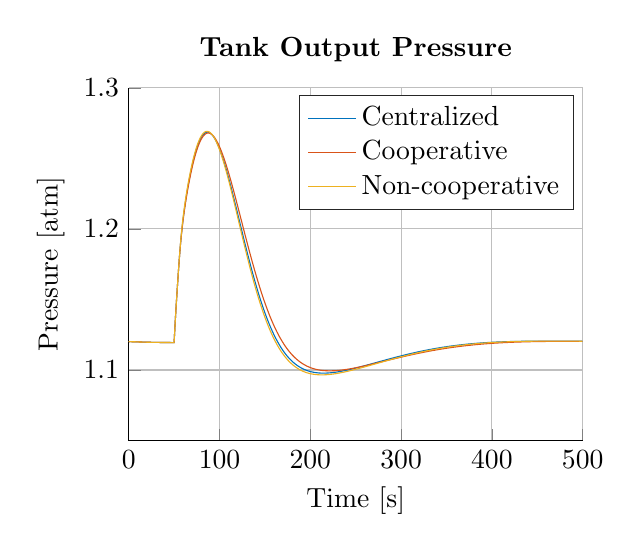
\begin{tikzpicture}

\begin{axis}[%
width=5.766cm,
height=4.479cm,
at={(0cm,0cm)},
scale only axis,
xmin=0,
xmax=500,
xlabel={Time [s]},
xmajorgrids,
ymin=1.05,
ymax=1.3,
ylabel={Pressure [atm]},
ymajorgrids,
axis background/.style={fill=white},
title style={font=\bfseries},
title={Tank Output Pressure},
axis x line*=bottom,
axis y line*=left,
legend style={legend cell align=left,align=left,draw=white!15!black}
]
\addplot [color=mycolor1,solid,forget plot]
  table[row sep=crcr]{%
0	1.12\\
0.5	1.12007\\
1	1.12008\\
1.5	1.12008\\
2	1.12008\\
2.5	1.12008\\
3	1.12008\\
3.5	1.12007\\
4	1.12007\\
4.5	1.12006\\
5	1.12005\\
5.5	1.12004\\
6	1.12003\\
6.5	1.12002\\
7	1.12001\\
7.5	1.12\\
8	1.11999\\
8.5	1.11997\\
9	1.11996\\
9.5	1.11995\\
10	1.11994\\
10.5	1.11992\\
11	1.11991\\
11.5	1.1199\\
12	1.11989\\
12.5	1.11987\\
13	1.11986\\
13.5	1.11985\\
14	1.11984\\
14.5	1.11983\\
15	1.11981\\
15.5	1.1198\\
16	1.11979\\
16.5	1.11978\\
17	1.11977\\
17.5	1.11976\\
18	1.11975\\
18.5	1.11974\\
19	1.11973\\
19.5	1.11973\\
20	1.11972\\
20.5	1.11971\\
21	1.1197\\
21.5	1.11969\\
22	1.11969\\
22.5	1.11968\\
23	1.11967\\
23.5	1.11966\\
24	1.11966\\
24.5	1.11965\\
25	1.11964\\
25.5	1.11964\\
26	1.11963\\
26.5	1.11962\\
27	1.11962\\
27.5	1.11961\\
28	1.11961\\
28.5	1.1196\\
29	1.1196\\
29.5	1.11959\\
30	1.11959\\
30.5	1.11958\\
31	1.11958\\
31.5	1.11957\\
32	1.11957\\
32.5	1.11956\\
33	1.11956\\
33.5	1.11955\\
34	1.11955\\
34.5	1.11954\\
35	1.11954\\
35.5	1.11954\\
36	1.11953\\
36.5	1.11953\\
37	1.11952\\
37.5	1.11952\\
38	1.11952\\
38.5	1.11951\\
39	1.11951\\
39.5	1.11951\\
40	1.1195\\
40.5	1.1195\\
41	1.1195\\
41.5	1.11949\\
42	1.11949\\
42.5	1.11949\\
43	1.11949\\
43.5	1.11948\\
44	1.11948\\
44.5	1.11948\\
45	1.11948\\
45.5	1.11947\\
46	1.11947\\
46.5	1.11947\\
47	1.11947\\
47.5	1.11946\\
48	1.11946\\
48.5	1.11946\\
49	1.11946\\
49.5	1.11946\\
50	1.11945\\
50.5	1.12569\\
51	1.13171\\
51.5	1.13735\\
52	1.14274\\
52.5	1.14794\\
53	1.153\\
53.5	1.15795\\
54	1.1628\\
54.5	1.16756\\
55	1.17229\\
55.5	1.17676\\
56	1.18105\\
56.5	1.18514\\
57	1.189\\
57.5	1.1926\\
58	1.19596\\
58.5	1.19912\\
59	1.2021\\
59.5	1.20491\\
60	1.20757\\
60.5	1.21011\\
61	1.21253\\
61.5	1.21486\\
62	1.21711\\
62.5	1.21928\\
63	1.22138\\
63.5	1.22342\\
64	1.22541\\
64.5	1.22733\\
65	1.22921\\
65.5	1.23103\\
66	1.2328\\
66.5	1.23452\\
67	1.2362\\
67.5	1.23784\\
68	1.23943\\
68.5	1.24099\\
69	1.2425\\
69.5	1.24397\\
70	1.2454\\
70.5	1.24679\\
71	1.24814\\
71.5	1.24944\\
72	1.2507\\
72.5	1.25192\\
73	1.2531\\
73.5	1.25424\\
74	1.25533\\
74.5	1.25637\\
75	1.25738\\
75.5	1.25834\\
76	1.25925\\
76.5	1.26012\\
77	1.26095\\
77.5	1.26174\\
78	1.26248\\
78.5	1.26317\\
79	1.26383\\
79.5	1.26444\\
80	1.26501\\
80.5	1.26553\\
81	1.26602\\
81.5	1.26646\\
82	1.26686\\
82.5	1.26721\\
83	1.26753\\
83.5	1.2678\\
84	1.26804\\
84.5	1.26823\\
85	1.26839\\
85.5	1.2685\\
86	1.26858\\
86.5	1.26861\\
87	1.26861\\
87.5	1.26857\\
88	1.26849\\
88.5	1.26838\\
89	1.26823\\
89.5	1.26804\\
90	1.26782\\
90.5	1.26756\\
91	1.26727\\
91.5	1.26695\\
92	1.26659\\
92.5	1.2662\\
93	1.26577\\
93.5	1.26532\\
94	1.26483\\
94.5	1.26431\\
95	1.26376\\
95.5	1.26318\\
96	1.26258\\
96.5	1.26194\\
97	1.26128\\
97.5	1.26059\\
98	1.25987\\
98.5	1.25913\\
99	1.25836\\
99.5	1.25757\\
100	1.25675\\
100.5	1.25591\\
101	1.25504\\
101.5	1.25415\\
102	1.25324\\
102.5	1.25231\\
103	1.25136\\
103.5	1.25039\\
104	1.2494\\
104.5	1.24839\\
105	1.24736\\
105.5	1.24631\\
106	1.24525\\
106.5	1.24417\\
107	1.24307\\
107.5	1.24196\\
108	1.24083\\
108.5	1.23969\\
109	1.23854\\
109.5	1.23737\\
110	1.23619\\
110.5	1.235\\
111	1.2338\\
111.5	1.23258\\
112	1.23136\\
112.5	1.23012\\
113	1.22888\\
113.5	1.22763\\
114	1.22637\\
114.5	1.2251\\
115	1.22382\\
115.5	1.22254\\
116	1.22126\\
116.5	1.21996\\
117	1.21866\\
117.5	1.21736\\
118	1.21606\\
118.5	1.21474\\
119	1.21343\\
119.5	1.21212\\
120	1.2108\\
120.5	1.20948\\
121	1.20816\\
121.5	1.20683\\
122	1.20551\\
122.5	1.20419\\
123	1.20287\\
123.5	1.20155\\
124	1.20023\\
124.5	1.19891\\
125	1.19759\\
125.5	1.19628\\
126	1.19497\\
126.5	1.19366\\
127	1.19235\\
127.5	1.19105\\
128	1.18976\\
128.5	1.18847\\
129	1.18718\\
129.5	1.1859\\
130	1.18462\\
130.5	1.18335\\
131	1.18208\\
131.5	1.18082\\
132	1.17957\\
132.5	1.17833\\
133	1.17709\\
133.5	1.17586\\
134	1.17464\\
134.5	1.17342\\
135	1.17221\\
135.5	1.17101\\
136	1.16982\\
136.5	1.16864\\
137	1.16747\\
137.5	1.1663\\
138	1.16515\\
138.5	1.164\\
139	1.16287\\
139.5	1.16174\\
140	1.16062\\
140.5	1.15952\\
141	1.15842\\
141.5	1.15734\\
142	1.15626\\
142.5	1.1552\\
143	1.15414\\
143.5	1.1531\\
144	1.15207\\
144.5	1.15104\\
145	1.15003\\
145.5	1.14903\\
146	1.14804\\
146.5	1.14707\\
147	1.1461\\
147.5	1.14514\\
148	1.1442\\
148.5	1.14327\\
149	1.14235\\
149.5	1.14144\\
150	1.14054\\
150.5	1.13965\\
151	1.13878\\
151.5	1.13792\\
152	1.13706\\
152.5	1.13622\\
153	1.13539\\
153.5	1.13458\\
154	1.13377\\
154.5	1.13297\\
155	1.13219\\
155.5	1.13142\\
156	1.13066\\
156.5	1.12991\\
157	1.12917\\
157.5	1.12844\\
158	1.12773\\
158.5	1.12702\\
159	1.12633\\
159.5	1.12565\\
160	1.12498\\
160.5	1.12432\\
161	1.12367\\
161.5	1.12303\\
162	1.1224\\
162.5	1.12178\\
163	1.12117\\
163.5	1.12058\\
164	1.11999\\
164.5	1.11941\\
165	1.11885\\
165.5	1.11829\\
166	1.11775\\
166.5	1.11721\\
167	1.11669\\
167.5	1.11617\\
168	1.11566\\
168.5	1.11517\\
169	1.11468\\
169.5	1.1142\\
170	1.11373\\
170.5	1.11327\\
171	1.11282\\
171.5	1.11238\\
172	1.11195\\
172.5	1.11153\\
173	1.11111\\
173.5	1.11071\\
174	1.11031\\
174.5	1.10992\\
175	1.10954\\
175.5	1.10917\\
176	1.1088\\
176.5	1.10844\\
177	1.1081\\
177.5	1.10775\\
178	1.10742\\
178.5	1.1071\\
179	1.10678\\
179.5	1.10647\\
180	1.10616\\
180.5	1.10587\\
181	1.10558\\
181.5	1.1053\\
182	1.10502\\
182.5	1.10475\\
183	1.10449\\
183.5	1.10423\\
184	1.10399\\
184.5	1.10374\\
185	1.10351\\
185.5	1.10328\\
186	1.10305\\
186.5	1.10284\\
187	1.10262\\
187.5	1.10242\\
188	1.10222\\
188.5	1.10202\\
189	1.10184\\
189.5	1.10165\\
190	1.10147\\
190.5	1.1013\\
191	1.10113\\
191.5	1.10097\\
192	1.10081\\
192.5	1.10066\\
193	1.10051\\
193.5	1.10037\\
194	1.10023\\
194.5	1.1001\\
195	1.09997\\
195.5	1.09985\\
196	1.09973\\
196.5	1.09961\\
197	1.0995\\
197.5	1.09939\\
198	1.09929\\
198.5	1.09919\\
199	1.0991\\
199.5	1.09901\\
200	1.09892\\
200.5	1.09884\\
201	1.09876\\
201.5	1.09868\\
202	1.09861\\
202.5	1.09854\\
203	1.09848\\
203.5	1.09841\\
204	1.09836\\
204.5	1.0983\\
205	1.09825\\
205.5	1.0982\\
206	1.09815\\
206.5	1.09811\\
207	1.09807\\
207.5	1.09803\\
208	1.098\\
208.5	1.09797\\
209	1.09794\\
209.5	1.09791\\
210	1.09789\\
210.5	1.09787\\
211	1.09785\\
211.5	1.09784\\
212	1.09782\\
212.5	1.09781\\
213	1.09781\\
213.5	1.0978\\
214	1.0978\\
214.5	1.0978\\
215	1.0978\\
215.5	1.0978\\
216	1.0978\\
216.5	1.09781\\
217	1.09782\\
217.5	1.09783\\
218	1.09785\\
218.5	1.09786\\
219	1.09788\\
219.5	1.0979\\
220	1.09792\\
220.5	1.09794\\
221	1.09796\\
221.5	1.09799\\
222	1.09802\\
222.5	1.09805\\
223	1.09808\\
223.5	1.09811\\
224	1.09814\\
224.5	1.09818\\
225	1.09822\\
225.5	1.09826\\
226	1.0983\\
226.5	1.09834\\
227	1.09838\\
227.5	1.09842\\
228	1.09847\\
228.5	1.09851\\
229	1.09856\\
229.5	1.09861\\
230	1.09866\\
230.5	1.09871\\
231	1.09876\\
231.5	1.09882\\
232	1.09887\\
232.5	1.09893\\
233	1.09899\\
233.5	1.09904\\
234	1.0991\\
234.5	1.09916\\
235	1.09922\\
235.5	1.09928\\
236	1.09935\\
236.5	1.09941\\
237	1.09947\\
237.5	1.09954\\
238	1.0996\\
238.5	1.09967\\
239	1.09974\\
239.5	1.09981\\
240	1.09988\\
240.5	1.09995\\
241	1.10002\\
241.5	1.10009\\
242	1.10016\\
242.5	1.10023\\
243	1.10031\\
243.5	1.10038\\
244	1.10045\\
244.5	1.10053\\
245	1.1006\\
245.5	1.10068\\
246	1.10076\\
246.5	1.10083\\
247	1.10091\\
247.5	1.10099\\
248	1.10107\\
248.5	1.10115\\
249	1.10123\\
249.5	1.10131\\
250	1.10139\\
};
\addplot [color=mycolor1,solid]
  table[row sep=crcr]{%
250	1.10139\\
250.5	1.10147\\
251	1.10155\\
251.5	1.10163\\
252	1.10172\\
252.5	1.1018\\
253	1.10188\\
253.5	1.10196\\
254	1.10205\\
254.5	1.10213\\
255	1.10222\\
255.5	1.1023\\
256	1.10239\\
256.5	1.10247\\
257	1.10256\\
257.5	1.10264\\
258	1.10273\\
258.5	1.10281\\
259	1.1029\\
259.5	1.10299\\
260	1.10307\\
260.5	1.10316\\
261	1.10325\\
261.5	1.10334\\
262	1.10342\\
262.5	1.10351\\
263	1.1036\\
263.5	1.10369\\
264	1.10378\\
264.5	1.10386\\
265	1.10395\\
265.5	1.10404\\
266	1.10413\\
266.5	1.10422\\
267	1.10431\\
267.5	1.1044\\
268	1.10448\\
268.5	1.10457\\
269	1.10466\\
269.5	1.10475\\
270	1.10484\\
270.5	1.10493\\
271	1.10502\\
271.5	1.10511\\
272	1.1052\\
272.5	1.10529\\
273	1.10538\\
273.5	1.10546\\
274	1.10555\\
274.5	1.10564\\
275	1.10573\\
275.5	1.10582\\
276	1.10591\\
276.5	1.106\\
277	1.10609\\
277.5	1.10618\\
278	1.10627\\
278.5	1.10635\\
279	1.10644\\
279.5	1.10653\\
280	1.10662\\
280.5	1.10671\\
281	1.1068\\
281.5	1.10688\\
282	1.10697\\
282.5	1.10706\\
283	1.10715\\
283.5	1.10724\\
284	1.10732\\
284.5	1.10741\\
285	1.1075\\
285.5	1.10759\\
286	1.10767\\
286.5	1.10776\\
287	1.10785\\
287.5	1.10793\\
288	1.10802\\
288.5	1.1081\\
289	1.10819\\
289.5	1.10828\\
290	1.10836\\
290.5	1.10845\\
291	1.10853\\
291.5	1.10862\\
292	1.1087\\
292.5	1.10879\\
293	1.10887\\
293.5	1.10896\\
294	1.10904\\
294.5	1.10912\\
295	1.10921\\
295.5	1.10929\\
296	1.10937\\
296.5	1.10946\\
297	1.10954\\
297.5	1.10962\\
298	1.1097\\
298.5	1.10979\\
299	1.10987\\
299.5	1.10995\\
300	1.11003\\
300.5	1.11011\\
301	1.11019\\
301.5	1.11027\\
302	1.11035\\
302.5	1.11043\\
303	1.11051\\
303.5	1.11059\\
304	1.11067\\
304.5	1.11075\\
305	1.11083\\
305.5	1.1109\\
306	1.11098\\
306.5	1.11106\\
307	1.11114\\
307.5	1.11121\\
308	1.11129\\
308.5	1.11137\\
309	1.11144\\
309.5	1.11152\\
310	1.11159\\
310.5	1.11167\\
311	1.11174\\
311.5	1.11182\\
312	1.11189\\
312.5	1.11197\\
313	1.11204\\
313.5	1.11211\\
314	1.11219\\
314.5	1.11226\\
315	1.11233\\
315.5	1.1124\\
316	1.11248\\
316.5	1.11255\\
317	1.11262\\
317.5	1.11269\\
318	1.11276\\
318.5	1.11283\\
319	1.1129\\
319.5	1.11297\\
320	1.11304\\
320.5	1.11311\\
321	1.11317\\
321.5	1.11324\\
322	1.11331\\
322.5	1.11338\\
323	1.11344\\
323.5	1.11351\\
324	1.11358\\
324.5	1.11364\\
325	1.11371\\
325.5	1.11377\\
326	1.11384\\
326.5	1.1139\\
327	1.11397\\
327.5	1.11403\\
328	1.11409\\
328.5	1.11416\\
329	1.11422\\
329.5	1.11428\\
330	1.11434\\
330.5	1.11441\\
331	1.11447\\
331.5	1.11453\\
332	1.11459\\
332.5	1.11465\\
333	1.11471\\
333.5	1.11477\\
334	1.11483\\
334.5	1.11489\\
335	1.11494\\
335.5	1.115\\
336	1.11506\\
336.5	1.11512\\
337	1.11517\\
337.5	1.11523\\
338	1.11529\\
338.5	1.11534\\
339	1.1154\\
339.5	1.11545\\
340	1.11551\\
340.5	1.11556\\
341	1.11562\\
341.5	1.11567\\
342	1.11572\\
342.5	1.11578\\
343	1.11583\\
343.5	1.11588\\
344	1.11593\\
344.5	1.11599\\
345	1.11604\\
345.5	1.11609\\
346	1.11614\\
346.5	1.11619\\
347	1.11624\\
347.5	1.11629\\
348	1.11634\\
348.5	1.11639\\
349	1.11643\\
349.5	1.11648\\
350	1.11653\\
350.5	1.11658\\
351	1.11662\\
351.5	1.11667\\
352	1.11672\\
352.5	1.11676\\
353	1.11681\\
353.5	1.11685\\
354	1.1169\\
354.5	1.11694\\
355	1.11699\\
355.5	1.11703\\
356	1.11707\\
356.5	1.11712\\
357	1.11716\\
357.5	1.1172\\
358	1.11724\\
358.5	1.11729\\
359	1.11733\\
359.5	1.11737\\
360	1.11741\\
360.5	1.11745\\
361	1.11749\\
361.5	1.11753\\
362	1.11757\\
362.5	1.11761\\
363	1.11765\\
363.5	1.11768\\
364	1.11772\\
364.5	1.11776\\
365	1.1178\\
365.5	1.11783\\
366	1.11787\\
366.5	1.11791\\
367	1.11794\\
367.5	1.11798\\
368	1.11801\\
368.5	1.11805\\
369	1.11808\\
369.5	1.11812\\
370	1.11815\\
370.5	1.11819\\
371	1.11822\\
371.5	1.11825\\
372	1.11829\\
372.5	1.11832\\
373	1.11835\\
373.5	1.11838\\
374	1.11841\\
374.5	1.11844\\
375	1.11848\\
375.5	1.11851\\
376	1.11854\\
376.5	1.11857\\
377	1.1186\\
377.5	1.11863\\
378	1.11865\\
378.5	1.11868\\
379	1.11871\\
379.5	1.11874\\
380	1.11877\\
380.5	1.1188\\
381	1.11882\\
381.5	1.11885\\
382	1.11888\\
382.5	1.1189\\
383	1.11893\\
383.5	1.11895\\
384	1.11898\\
384.5	1.11901\\
385	1.11903\\
385.5	1.11906\\
386	1.11908\\
386.5	1.1191\\
387	1.11913\\
387.5	1.11915\\
388	1.11917\\
388.5	1.1192\\
389	1.11922\\
389.5	1.11924\\
390	1.11927\\
390.5	1.11929\\
391	1.11931\\
391.5	1.11933\\
392	1.11935\\
392.5	1.11937\\
393	1.11939\\
393.5	1.11941\\
394	1.11943\\
394.5	1.11945\\
395	1.11947\\
395.5	1.11949\\
396	1.11951\\
396.5	1.11953\\
397	1.11955\\
397.5	1.11957\\
398	1.11959\\
398.5	1.11961\\
399	1.11962\\
399.5	1.11964\\
400	1.11966\\
400.5	1.11968\\
401	1.11969\\
401.5	1.11971\\
402	1.11973\\
402.5	1.11974\\
403	1.11976\\
403.5	1.11977\\
404	1.11979\\
404.5	1.1198\\
405	1.11982\\
405.5	1.11983\\
406	1.11985\\
406.5	1.11986\\
407	1.11988\\
407.5	1.11989\\
408	1.11991\\
408.5	1.11992\\
409	1.11993\\
409.5	1.11995\\
410	1.11996\\
410.5	1.11997\\
411	1.11998\\
411.5	1.12\\
412	1.12001\\
412.5	1.12002\\
413	1.12003\\
413.5	1.12004\\
414	1.12006\\
414.5	1.12007\\
415	1.12008\\
415.5	1.12009\\
416	1.1201\\
416.5	1.12011\\
417	1.12012\\
417.5	1.12013\\
418	1.12014\\
418.5	1.12015\\
419	1.12016\\
419.5	1.12017\\
420	1.12018\\
420.5	1.12019\\
421	1.1202\\
421.5	1.12021\\
422	1.12021\\
422.5	1.12022\\
423	1.12023\\
423.5	1.12024\\
424	1.12025\\
424.5	1.12025\\
425	1.12026\\
425.5	1.12027\\
426	1.12028\\
426.5	1.12028\\
427	1.12029\\
427.5	1.1203\\
428	1.12031\\
428.5	1.12031\\
429	1.12032\\
429.5	1.12032\\
430	1.12033\\
430.5	1.12034\\
431	1.12034\\
431.5	1.12035\\
432	1.12035\\
432.5	1.12036\\
433	1.12037\\
433.5	1.12037\\
434	1.12038\\
434.5	1.12038\\
435	1.12039\\
435.5	1.12039\\
436	1.1204\\
436.5	1.1204\\
437	1.1204\\
437.5	1.12041\\
438	1.12041\\
438.5	1.12042\\
439	1.12042\\
439.5	1.12042\\
440	1.12043\\
440.5	1.12043\\
441	1.12044\\
441.5	1.12044\\
442	1.12044\\
442.5	1.12045\\
443	1.12045\\
443.5	1.12045\\
444	1.12045\\
444.5	1.12046\\
445	1.12046\\
445.5	1.12046\\
446	1.12046\\
446.5	1.12047\\
447	1.12047\\
447.5	1.12047\\
448	1.12047\\
448.5	1.12048\\
449	1.12048\\
449.5	1.12048\\
450	1.12048\\
450.5	1.12048\\
451	1.12048\\
451.5	1.12049\\
452	1.12049\\
452.5	1.12049\\
453	1.12049\\
453.5	1.12049\\
454	1.12049\\
454.5	1.12049\\
455	1.12049\\
455.5	1.12049\\
456	1.1205\\
456.5	1.1205\\
457	1.1205\\
457.5	1.1205\\
458	1.1205\\
458.5	1.1205\\
459	1.1205\\
459.5	1.1205\\
460	1.1205\\
460.5	1.1205\\
461	1.1205\\
461.5	1.1205\\
462	1.1205\\
462.5	1.1205\\
463	1.1205\\
463.5	1.1205\\
464	1.1205\\
464.5	1.1205\\
465	1.1205\\
465.5	1.1205\\
466	1.1205\\
466.5	1.1205\\
467	1.1205\\
467.5	1.1205\\
468	1.12049\\
468.5	1.12049\\
469	1.12049\\
469.5	1.12049\\
470	1.12049\\
470.5	1.12049\\
471	1.12049\\
471.5	1.12049\\
472	1.12049\\
472.5	1.12049\\
473	1.12049\\
473.5	1.12048\\
474	1.12048\\
474.5	1.12048\\
475	1.12048\\
475.5	1.12048\\
476	1.12048\\
476.5	1.12048\\
477	1.12047\\
477.5	1.12047\\
478	1.12047\\
478.5	1.12047\\
479	1.12047\\
479.5	1.12047\\
480	1.12046\\
480.5	1.12046\\
481	1.12046\\
481.5	1.12046\\
482	1.12046\\
482.5	1.12046\\
483	1.12045\\
483.5	1.12045\\
484	1.12045\\
484.5	1.12045\\
485	1.12045\\
485.5	1.12044\\
486	1.12044\\
486.5	1.12044\\
487	1.12044\\
487.5	1.12044\\
488	1.12043\\
488.5	1.12043\\
489	1.12043\\
489.5	1.12043\\
490	1.12043\\
490.5	1.12042\\
491	1.12042\\
491.5	1.12042\\
492	1.12042\\
492.5	1.12042\\
493	1.12041\\
493.5	1.12041\\
494	1.12041\\
494.5	1.12041\\
495	1.1204\\
495.5	1.1204\\
496	1.1204\\
496.5	1.1204\\
497	1.12039\\
497.5	1.12039\\
498	1.12039\\
498.5	1.12039\\
499	1.12038\\
499.5	1.12038\\
};
\addlegendentry{Centralized};

\addplot [color=mycolor2,solid,forget plot]
  table[row sep=crcr]{%
0	1.12\\
0.5	1.12007\\
1	1.12008\\
1.5	1.12008\\
2	1.12008\\
2.5	1.12008\\
3	1.12008\\
3.5	1.12007\\
4	1.12006\\
4.5	1.12006\\
5	1.12005\\
5.5	1.12004\\
6	1.12003\\
6.5	1.12002\\
7	1.12001\\
7.5	1.11999\\
8	1.11998\\
8.5	1.11997\\
9	1.11996\\
9.5	1.11994\\
10	1.11993\\
10.5	1.11992\\
11	1.1199\\
11.5	1.11989\\
12	1.11988\\
12.5	1.11987\\
13	1.11985\\
13.5	1.11984\\
14	1.11983\\
14.5	1.11982\\
15	1.11981\\
15.5	1.1198\\
16	1.11979\\
16.5	1.11978\\
17	1.11977\\
17.5	1.11976\\
18	1.11975\\
18.5	1.11974\\
19	1.11973\\
19.5	1.11972\\
20	1.11971\\
20.5	1.1197\\
21	1.11969\\
21.5	1.11969\\
22	1.11968\\
22.5	1.11967\\
23	1.11966\\
23.5	1.11966\\
24	1.11965\\
24.5	1.11964\\
25	1.11964\\
25.5	1.11963\\
26	1.11962\\
26.5	1.11962\\
27	1.11961\\
27.5	1.11961\\
28	1.1196\\
28.5	1.11959\\
29	1.11959\\
29.5	1.11958\\
30	1.11958\\
30.5	1.11957\\
31	1.11957\\
31.5	1.11956\\
32	1.11956\\
32.5	1.11955\\
33	1.11955\\
33.5	1.11955\\
34	1.11954\\
34.5	1.11954\\
35	1.11953\\
35.5	1.11953\\
36	1.11952\\
36.5	1.11952\\
37	1.11952\\
37.5	1.11951\\
38	1.11951\\
38.5	1.11951\\
39	1.1195\\
39.5	1.1195\\
40	1.1195\\
40.5	1.11949\\
41	1.11949\\
41.5	1.11949\\
42	1.11948\\
42.5	1.11948\\
43	1.11948\\
43.5	1.11948\\
44	1.11947\\
44.5	1.11947\\
45	1.11947\\
45.5	1.11947\\
46	1.11946\\
46.5	1.11946\\
47	1.11946\\
47.5	1.11946\\
48	1.11945\\
48.5	1.11945\\
49	1.11945\\
49.5	1.11945\\
50	1.11944\\
50.5	1.12568\\
51	1.1317\\
51.5	1.13734\\
52	1.14274\\
52.5	1.14796\\
53	1.15303\\
53.5	1.15798\\
54	1.16283\\
54.5	1.16759\\
55	1.17228\\
55.5	1.1767\\
56	1.18091\\
56.5	1.18494\\
57	1.1887\\
57.5	1.19219\\
58	1.19546\\
58.5	1.19852\\
59	1.20141\\
59.5	1.20413\\
60	1.20672\\
60.5	1.20919\\
61	1.21156\\
61.5	1.21385\\
62	1.21606\\
62.5	1.2182\\
63	1.22027\\
63.5	1.22229\\
64	1.22426\\
64.5	1.22616\\
65	1.22801\\
65.5	1.2298\\
66	1.23154\\
66.5	1.23324\\
67	1.2349\\
67.5	1.23651\\
68	1.23808\\
68.5	1.23961\\
69	1.24111\\
69.5	1.24256\\
70	1.24398\\
70.5	1.24535\\
71	1.24669\\
71.5	1.24798\\
72	1.24924\\
72.5	1.25045\\
73	1.25162\\
73.5	1.25275\\
74	1.25385\\
74.5	1.25489\\
75	1.2559\\
75.5	1.25687\\
76	1.2578\\
76.5	1.25868\\
77	1.25952\\
77.5	1.26033\\
78	1.26109\\
78.5	1.26181\\
79	1.26248\\
79.5	1.26312\\
80	1.26372\\
80.5	1.26428\\
81	1.26479\\
81.5	1.26527\\
82	1.26571\\
82.5	1.26611\\
83	1.26647\\
83.5	1.26679\\
84	1.26707\\
84.5	1.26731\\
85	1.26752\\
85.5	1.26769\\
86	1.26782\\
86.5	1.26792\\
87	1.26798\\
87.5	1.268\\
88	1.26799\\
88.5	1.26794\\
89	1.26786\\
89.5	1.26775\\
90	1.2676\\
90.5	1.26741\\
91	1.2672\\
91.5	1.26695\\
92	1.26667\\
92.5	1.26636\\
93	1.26602\\
93.5	1.26565\\
94	1.26525\\
94.5	1.26482\\
95	1.26436\\
95.5	1.26387\\
96	1.26335\\
96.5	1.26281\\
97	1.26224\\
97.5	1.26164\\
98	1.26102\\
98.5	1.26037\\
99	1.2597\\
99.5	1.259\\
100	1.25828\\
100.5	1.25754\\
101	1.25678\\
101.5	1.25599\\
102	1.25518\\
102.5	1.25435\\
103	1.2535\\
103.5	1.25263\\
104	1.25174\\
104.5	1.25083\\
105	1.24991\\
105.5	1.24896\\
106	1.248\\
106.5	1.24702\\
107	1.24603\\
107.5	1.24502\\
108	1.24399\\
108.5	1.24295\\
109	1.2419\\
109.5	1.24083\\
110	1.23975\\
110.5	1.23866\\
111	1.23755\\
111.5	1.23644\\
112	1.23531\\
112.5	1.23417\\
113	1.23302\\
113.5	1.23187\\
114	1.2307\\
114.5	1.22953\\
115	1.22834\\
115.5	1.22715\\
116	1.22595\\
116.5	1.22475\\
117	1.22354\\
117.5	1.22232\\
118	1.2211\\
118.5	1.21987\\
119	1.21864\\
119.5	1.21741\\
120	1.21617\\
120.5	1.21493\\
121	1.21368\\
121.5	1.21244\\
122	1.21119\\
122.5	1.20994\\
123	1.20868\\
123.5	1.20743\\
124	1.20618\\
124.5	1.20493\\
125	1.20367\\
125.5	1.20242\\
126	1.20117\\
126.5	1.19992\\
127	1.19867\\
127.5	1.19743\\
128	1.19618\\
128.5	1.19494\\
129	1.19371\\
129.5	1.19247\\
130	1.19124\\
130.5	1.19001\\
131	1.18879\\
131.5	1.18757\\
132	1.18636\\
132.5	1.18515\\
133	1.18395\\
133.5	1.18275\\
134	1.18156\\
134.5	1.18037\\
135	1.17919\\
135.5	1.17802\\
136	1.17685\\
136.5	1.17569\\
137	1.17454\\
137.5	1.1734\\
138	1.17226\\
138.5	1.17113\\
139	1.17001\\
139.5	1.16889\\
140	1.16779\\
140.5	1.16669\\
141	1.1656\\
141.5	1.16452\\
142	1.16345\\
142.5	1.16238\\
143	1.16133\\
143.5	1.16028\\
144	1.15925\\
144.5	1.15822\\
145	1.1572\\
145.5	1.1562\\
146	1.1552\\
146.5	1.15421\\
147	1.15323\\
147.5	1.15226\\
148	1.15131\\
148.5	1.15036\\
149	1.14942\\
149.5	1.14849\\
150	1.14757\\
150.5	1.14667\\
151	1.14577\\
151.5	1.14488\\
152	1.14401\\
152.5	1.14314\\
153	1.14228\\
153.5	1.14144\\
154	1.1406\\
154.5	1.13978\\
155	1.13897\\
155.5	1.13816\\
156	1.13737\\
156.5	1.13659\\
157	1.13581\\
157.5	1.13505\\
158	1.1343\\
158.5	1.13356\\
159	1.13283\\
159.5	1.13211\\
160	1.1314\\
160.5	1.1307\\
161	1.13001\\
161.5	1.12933\\
162	1.12866\\
162.5	1.128\\
163	1.12735\\
163.5	1.12671\\
164	1.12608\\
164.5	1.12546\\
165	1.12485\\
165.5	1.12425\\
166	1.12366\\
166.5	1.12308\\
167	1.1225\\
167.5	1.12194\\
168	1.12139\\
168.5	1.12084\\
169	1.12031\\
169.5	1.11979\\
170	1.11927\\
170.5	1.11876\\
171	1.11826\\
171.5	1.11778\\
172	1.11729\\
172.5	1.11682\\
173	1.11636\\
173.5	1.11591\\
174	1.11546\\
174.5	1.11502\\
175	1.11459\\
175.5	1.11417\\
176	1.11376\\
176.5	1.11335\\
177	1.11295\\
177.5	1.11257\\
178	1.11218\\
178.5	1.11181\\
179	1.11144\\
179.5	1.11108\\
180	1.11073\\
180.5	1.11039\\
181	1.11005\\
181.5	1.10972\\
182	1.1094\\
182.5	1.10908\\
183	1.10877\\
183.5	1.10847\\
184	1.10817\\
184.5	1.10789\\
185	1.1076\\
185.5	1.10733\\
186	1.10706\\
186.5	1.10679\\
187	1.10654\\
187.5	1.10628\\
188	1.10604\\
188.5	1.1058\\
189	1.10557\\
189.5	1.10534\\
190	1.10512\\
190.5	1.1049\\
191	1.10469\\
191.5	1.10448\\
192	1.10428\\
192.5	1.10409\\
193	1.1039\\
193.5	1.10371\\
194	1.10353\\
194.5	1.10336\\
195	1.10319\\
195.5	1.10302\\
196	1.10286\\
196.5	1.1027\\
197	1.10255\\
197.5	1.10241\\
198	1.10226\\
198.5	1.10213\\
199	1.10199\\
199.5	1.10186\\
200	1.10174\\
200.5	1.10161\\
201	1.1015\\
201.5	1.10138\\
202	1.10127\\
202.5	1.10117\\
203	1.10107\\
203.5	1.10097\\
204	1.10087\\
204.5	1.10078\\
205	1.10069\\
205.5	1.10061\\
206	1.10053\\
206.5	1.10045\\
207	1.10038\\
207.5	1.10031\\
208	1.10024\\
208.5	1.10017\\
209	1.10011\\
209.5	1.10005\\
210	1.1\\
210.5	1.09994\\
211	1.09989\\
211.5	1.09985\\
212	1.0998\\
212.5	1.09976\\
213	1.09972\\
213.5	1.09968\\
214	1.09965\\
214.5	1.09962\\
215	1.09959\\
215.5	1.09956\\
216	1.09954\\
216.5	1.09952\\
217	1.0995\\
217.5	1.09948\\
218	1.09946\\
218.5	1.09945\\
219	1.09944\\
219.5	1.09943\\
220	1.09942\\
220.5	1.09942\\
221	1.09941\\
221.5	1.09941\\
222	1.09941\\
222.5	1.09942\\
223	1.09942\\
223.5	1.09943\\
224	1.09944\\
224.5	1.09945\\
225	1.09946\\
225.5	1.09947\\
226	1.09949\\
226.5	1.0995\\
227	1.09952\\
227.5	1.09954\\
228	1.09956\\
228.5	1.09958\\
229	1.09961\\
229.5	1.09963\\
230	1.09966\\
230.5	1.09969\\
231	1.09972\\
231.5	1.09975\\
232	1.09978\\
232.5	1.09981\\
233	1.09985\\
233.5	1.09988\\
234	1.09992\\
234.5	1.09996\\
235	1.1\\
235.5	1.10004\\
236	1.10008\\
236.5	1.10012\\
237	1.10017\\
237.5	1.10021\\
238	1.10026\\
238.5	1.1003\\
239	1.10035\\
239.5	1.1004\\
240	1.10045\\
240.5	1.1005\\
241	1.10055\\
241.5	1.1006\\
242	1.10065\\
242.5	1.10071\\
243	1.10076\\
243.5	1.10082\\
244	1.10087\\
244.5	1.10093\\
245	1.10099\\
245.5	1.10104\\
246	1.1011\\
246.5	1.10116\\
247	1.10122\\
247.5	1.10128\\
248	1.10134\\
248.5	1.10141\\
249	1.10147\\
249.5	1.10153\\
250	1.1016\\
};
\addplot [color=mycolor2,solid]
  table[row sep=crcr]{%
250	1.1016\\
250.5	1.10166\\
251	1.10173\\
251.5	1.10179\\
252	1.10186\\
252.5	1.10192\\
253	1.10199\\
253.5	1.10206\\
254	1.10213\\
254.5	1.10219\\
255	1.10226\\
255.5	1.10233\\
256	1.1024\\
256.5	1.10247\\
257	1.10254\\
257.5	1.10261\\
258	1.10268\\
258.5	1.10276\\
259	1.10283\\
259.5	1.1029\\
260	1.10297\\
260.5	1.10304\\
261	1.10312\\
261.5	1.10319\\
262	1.10326\\
262.5	1.10334\\
263	1.10341\\
263.5	1.10349\\
264	1.10356\\
264.5	1.10364\\
265	1.10371\\
265.5	1.10379\\
266	1.10386\\
266.5	1.10394\\
267	1.10402\\
267.5	1.10409\\
268	1.10417\\
268.5	1.10425\\
269	1.10432\\
269.5	1.1044\\
270	1.10448\\
270.5	1.10455\\
271	1.10463\\
271.5	1.10471\\
272	1.10479\\
272.5	1.10486\\
273	1.10494\\
273.5	1.10502\\
274	1.1051\\
274.5	1.10517\\
275	1.10525\\
275.5	1.10533\\
276	1.10541\\
276.5	1.10549\\
277	1.10557\\
277.5	1.10564\\
278	1.10572\\
278.5	1.1058\\
279	1.10588\\
279.5	1.10596\\
280	1.10604\\
280.5	1.10611\\
281	1.10619\\
281.5	1.10627\\
282	1.10635\\
282.5	1.10643\\
283	1.10651\\
283.5	1.10659\\
284	1.10666\\
284.5	1.10674\\
285	1.10682\\
285.5	1.1069\\
286	1.10698\\
286.5	1.10705\\
287	1.10713\\
287.5	1.10721\\
288	1.10729\\
288.5	1.10737\\
289	1.10744\\
289.5	1.10752\\
290	1.1076\\
290.5	1.10768\\
291	1.10775\\
291.5	1.10783\\
292	1.10791\\
292.5	1.10799\\
293	1.10806\\
293.5	1.10814\\
294	1.10822\\
294.5	1.10829\\
295	1.10837\\
295.5	1.10845\\
296	1.10852\\
296.5	1.1086\\
297	1.10867\\
297.5	1.10875\\
298	1.10883\\
298.5	1.1089\\
299	1.10898\\
299.5	1.10905\\
300	1.10913\\
300.5	1.1092\\
301	1.10928\\
301.5	1.10935\\
302	1.10942\\
302.5	1.1095\\
303	1.10957\\
303.5	1.10965\\
304	1.10972\\
304.5	1.10979\\
305	1.10987\\
305.5	1.10994\\
306	1.11001\\
306.5	1.11008\\
307	1.11016\\
307.5	1.11023\\
308	1.1103\\
308.5	1.11037\\
309	1.11044\\
309.5	1.11051\\
310	1.11059\\
310.5	1.11066\\
311	1.11073\\
311.5	1.1108\\
312	1.11087\\
312.5	1.11094\\
313	1.11101\\
313.5	1.11108\\
314	1.11115\\
314.5	1.11122\\
315	1.11128\\
315.5	1.11135\\
316	1.11142\\
316.5	1.11149\\
317	1.11156\\
317.5	1.11162\\
318	1.11169\\
318.5	1.11176\\
319	1.11183\\
319.5	1.11189\\
320	1.11196\\
320.5	1.11202\\
321	1.11209\\
321.5	1.11216\\
322	1.11222\\
322.5	1.11229\\
323	1.11235\\
323.5	1.11241\\
324	1.11248\\
324.5	1.11254\\
325	1.11261\\
325.5	1.11267\\
326	1.11273\\
326.5	1.1128\\
327	1.11286\\
327.5	1.11292\\
328	1.11298\\
328.5	1.11304\\
329	1.11311\\
329.5	1.11317\\
330	1.11323\\
330.5	1.11329\\
331	1.11335\\
331.5	1.11341\\
332	1.11347\\
332.5	1.11353\\
333	1.11359\\
333.5	1.11365\\
334	1.1137\\
334.5	1.11376\\
335	1.11382\\
335.5	1.11388\\
336	1.11393\\
336.5	1.11399\\
337	1.11405\\
337.5	1.11411\\
338	1.11416\\
338.5	1.11422\\
339	1.11427\\
339.5	1.11433\\
340	1.11438\\
340.5	1.11444\\
341	1.11449\\
341.5	1.11455\\
342	1.1146\\
342.5	1.11465\\
343	1.11471\\
343.5	1.11476\\
344	1.11481\\
344.5	1.11487\\
345	1.11492\\
345.5	1.11497\\
346	1.11502\\
346.5	1.11507\\
347	1.11512\\
347.5	1.11517\\
348	1.11522\\
348.5	1.11527\\
349	1.11532\\
349.5	1.11537\\
350	1.11542\\
350.5	1.11547\\
351	1.11552\\
351.5	1.11557\\
352	1.11562\\
352.5	1.11566\\
353	1.11571\\
353.5	1.11576\\
354	1.1158\\
354.5	1.11585\\
355	1.1159\\
355.5	1.11594\\
356	1.11599\\
356.5	1.11603\\
357	1.11608\\
357.5	1.11612\\
358	1.11617\\
358.5	1.11621\\
359	1.11626\\
359.5	1.1163\\
360	1.11634\\
360.5	1.11638\\
361	1.11643\\
361.5	1.11647\\
362	1.11651\\
362.5	1.11655\\
363	1.11659\\
363.5	1.11664\\
364	1.11668\\
364.5	1.11672\\
365	1.11676\\
365.5	1.1168\\
366	1.11684\\
366.5	1.11688\\
367	1.11692\\
367.5	1.11695\\
368	1.11699\\
368.5	1.11703\\
369	1.11707\\
369.5	1.11711\\
370	1.11714\\
370.5	1.11718\\
371	1.11722\\
371.5	1.11725\\
372	1.11729\\
372.5	1.11733\\
373	1.11736\\
373.5	1.1174\\
374	1.11743\\
374.5	1.11747\\
375	1.1175\\
375.5	1.11754\\
376	1.11757\\
376.5	1.1176\\
377	1.11764\\
377.5	1.11767\\
378	1.1177\\
378.5	1.11774\\
379	1.11777\\
379.5	1.1178\\
380	1.11783\\
380.5	1.11786\\
381	1.1179\\
381.5	1.11793\\
382	1.11796\\
382.5	1.11799\\
383	1.11802\\
383.5	1.11805\\
384	1.11808\\
384.5	1.11811\\
385	1.11814\\
385.5	1.11817\\
386	1.1182\\
386.5	1.11822\\
387	1.11825\\
387.5	1.11828\\
388	1.11831\\
388.5	1.11833\\
389	1.11836\\
389.5	1.11839\\
390	1.11842\\
390.5	1.11844\\
391	1.11847\\
391.5	1.11849\\
392	1.11852\\
392.5	1.11855\\
393	1.11857\\
393.5	1.1186\\
394	1.11862\\
394.5	1.11865\\
395	1.11867\\
395.5	1.11869\\
396	1.11872\\
396.5	1.11874\\
397	1.11876\\
397.5	1.11879\\
398	1.11881\\
398.5	1.11883\\
399	1.11886\\
399.5	1.11888\\
400	1.1189\\
400.5	1.11892\\
401	1.11894\\
401.5	1.11896\\
402	1.11899\\
402.5	1.11901\\
403	1.11903\\
403.5	1.11905\\
404	1.11907\\
404.5	1.11909\\
405	1.11911\\
405.5	1.11913\\
406	1.11915\\
406.5	1.11917\\
407	1.11918\\
407.5	1.1192\\
408	1.11922\\
408.5	1.11924\\
409	1.11926\\
409.5	1.11928\\
410	1.11929\\
410.5	1.11931\\
411	1.11933\\
411.5	1.11935\\
412	1.11936\\
412.5	1.11938\\
413	1.1194\\
413.5	1.11941\\
414	1.11943\\
414.5	1.11945\\
415	1.11946\\
415.5	1.11948\\
416	1.11949\\
416.5	1.11951\\
417	1.11952\\
417.5	1.11954\\
418	1.11955\\
418.5	1.11957\\
419	1.11958\\
419.5	1.11959\\
420	1.11961\\
420.5	1.11962\\
421	1.11964\\
421.5	1.11965\\
422	1.11966\\
422.5	1.11968\\
423	1.11969\\
423.5	1.1197\\
424	1.11971\\
424.5	1.11973\\
425	1.11974\\
425.5	1.11975\\
426	1.11976\\
426.5	1.11977\\
427	1.11979\\
427.5	1.1198\\
428	1.11981\\
428.5	1.11982\\
429	1.11983\\
429.5	1.11984\\
430	1.11985\\
430.5	1.11986\\
431	1.11987\\
431.5	1.11988\\
432	1.11989\\
432.5	1.1199\\
433	1.11991\\
433.5	1.11992\\
434	1.11993\\
434.5	1.11994\\
435	1.11995\\
435.5	1.11996\\
436	1.11997\\
436.5	1.11998\\
437	1.11999\\
437.5	1.12\\
438	1.12\\
438.5	1.12001\\
439	1.12002\\
439.5	1.12003\\
440	1.12004\\
440.5	1.12004\\
441	1.12005\\
441.5	1.12006\\
442	1.12007\\
442.5	1.12007\\
443	1.12008\\
443.5	1.12009\\
444	1.1201\\
444.5	1.1201\\
445	1.12011\\
445.5	1.12012\\
446	1.12012\\
446.5	1.12013\\
447	1.12013\\
447.5	1.12014\\
448	1.12015\\
448.5	1.12015\\
449	1.12016\\
449.5	1.12016\\
450	1.12017\\
450.5	1.12017\\
451	1.12018\\
451.5	1.12019\\
452	1.12019\\
452.5	1.1202\\
453	1.1202\\
453.5	1.12021\\
454	1.12021\\
454.5	1.12021\\
455	1.12022\\
455.5	1.12022\\
456	1.12023\\
456.5	1.12023\\
457	1.12024\\
457.5	1.12024\\
458	1.12024\\
458.5	1.12025\\
459	1.12025\\
459.5	1.12026\\
460	1.12026\\
460.5	1.12026\\
461	1.12027\\
461.5	1.12027\\
462	1.12027\\
462.5	1.12028\\
463	1.12028\\
463.5	1.12028\\
464	1.12029\\
464.5	1.12029\\
465	1.12029\\
465.5	1.12029\\
466	1.1203\\
466.5	1.1203\\
467	1.1203\\
467.5	1.1203\\
468	1.12031\\
468.5	1.12031\\
469	1.12031\\
469.5	1.12031\\
470	1.12032\\
470.5	1.12032\\
471	1.12032\\
471.5	1.12032\\
472	1.12032\\
472.5	1.12033\\
473	1.12033\\
473.5	1.12033\\
474	1.12033\\
474.5	1.12033\\
475	1.12033\\
475.5	1.12033\\
476	1.12034\\
476.5	1.12034\\
477	1.12034\\
477.5	1.12034\\
478	1.12034\\
478.5	1.12034\\
479	1.12034\\
479.5	1.12034\\
480	1.12034\\
480.5	1.12035\\
481	1.12035\\
481.5	1.12035\\
482	1.12035\\
482.5	1.12035\\
483	1.12035\\
483.5	1.12035\\
484	1.12035\\
484.5	1.12035\\
485	1.12035\\
485.5	1.12035\\
486	1.12035\\
486.5	1.12035\\
487	1.12035\\
487.5	1.12035\\
488	1.12035\\
488.5	1.12035\\
489	1.12035\\
489.5	1.12035\\
490	1.12035\\
490.5	1.12035\\
491	1.12035\\
491.5	1.12035\\
492	1.12035\\
492.5	1.12035\\
493	1.12035\\
493.5	1.12035\\
494	1.12035\\
494.5	1.12035\\
495	1.12035\\
495.5	1.12035\\
496	1.12035\\
496.5	1.12035\\
497	1.12035\\
497.5	1.12035\\
498	1.12035\\
498.5	1.12035\\
499	1.12035\\
499.5	1.12034\\
};
\addlegendentry{Cooperative};

\addplot [color=mycolor3,solid,forget plot]
  table[row sep=crcr]{%
0	1.12\\
0.5	1.12007\\
1	1.12008\\
1.5	1.12008\\
2	1.12008\\
2.5	1.12008\\
3	1.12008\\
3.5	1.12007\\
4	1.12007\\
4.5	1.12006\\
5	1.12005\\
5.5	1.12004\\
6	1.12003\\
6.5	1.12002\\
7	1.12001\\
7.5	1.12\\
8	1.11998\\
8.5	1.11997\\
9	1.11996\\
9.5	1.11995\\
10	1.11993\\
10.5	1.11992\\
11	1.11991\\
11.5	1.11989\\
12	1.11988\\
12.5	1.11987\\
13	1.11986\\
13.5	1.11984\\
14	1.11983\\
14.5	1.11982\\
15	1.11981\\
15.5	1.1198\\
16	1.11979\\
16.5	1.11978\\
17	1.11977\\
17.5	1.11976\\
18	1.11975\\
18.5	1.11974\\
19	1.11973\\
19.5	1.11972\\
20	1.11971\\
20.5	1.1197\\
21	1.1197\\
21.5	1.11969\\
22	1.11968\\
22.5	1.11967\\
23	1.11967\\
23.5	1.11966\\
24	1.11965\\
24.5	1.11964\\
25	1.11964\\
25.5	1.11963\\
26	1.11963\\
26.5	1.11962\\
27	1.11961\\
27.5	1.11961\\
28	1.1196\\
28.5	1.1196\\
29	1.11959\\
29.5	1.11959\\
30	1.11958\\
30.5	1.11958\\
31	1.11957\\
31.5	1.11957\\
32	1.11956\\
32.5	1.11956\\
33	1.11955\\
33.5	1.11955\\
34	1.11954\\
34.5	1.11954\\
35	1.11954\\
35.5	1.11953\\
36	1.11953\\
36.5	1.11952\\
37	1.11952\\
37.5	1.11952\\
38	1.11951\\
38.5	1.11951\\
39	1.11951\\
39.5	1.1195\\
40	1.1195\\
40.5	1.1195\\
41	1.11949\\
41.5	1.11949\\
42	1.11949\\
42.5	1.11948\\
43	1.11948\\
43.5	1.11948\\
44	1.11948\\
44.5	1.11947\\
45	1.11947\\
45.5	1.11947\\
46	1.11947\\
46.5	1.11946\\
47	1.11946\\
47.5	1.11946\\
48	1.11946\\
48.5	1.11946\\
49	1.11945\\
49.5	1.11945\\
50	1.11945\\
50.5	1.12569\\
51	1.1317\\
51.5	1.13734\\
52	1.14274\\
52.5	1.14795\\
53	1.15302\\
53.5	1.15798\\
54	1.16285\\
54.5	1.16764\\
55	1.17237\\
55.5	1.177\\
56	1.18138\\
56.5	1.18559\\
57	1.18958\\
57.5	1.19332\\
58	1.19681\\
58.5	1.20009\\
59	1.20317\\
59.5	1.20607\\
60	1.20881\\
60.5	1.21141\\
61	1.21388\\
61.5	1.21625\\
62	1.21853\\
62.5	1.22072\\
63	1.22284\\
63.5	1.2249\\
64	1.22689\\
64.5	1.22882\\
65	1.23069\\
65.5	1.2325\\
66	1.23426\\
66.5	1.23597\\
67	1.23763\\
67.5	1.23925\\
68	1.24083\\
68.5	1.24236\\
69	1.24386\\
69.5	1.24531\\
70	1.24672\\
70.5	1.24809\\
71	1.24942\\
71.5	1.25071\\
72	1.25195\\
72.5	1.25315\\
73	1.25431\\
73.5	1.25543\\
74	1.2565\\
74.5	1.25753\\
75	1.25851\\
75.5	1.25946\\
76	1.26035\\
76.5	1.26121\\
77	1.26201\\
77.5	1.26278\\
78	1.2635\\
78.5	1.26418\\
79	1.26481\\
79.5	1.2654\\
80	1.26594\\
80.5	1.26645\\
81	1.26691\\
81.5	1.26732\\
82	1.2677\\
82.5	1.26803\\
83	1.26832\\
83.5	1.26856\\
84	1.26877\\
84.5	1.26893\\
85	1.26906\\
85.5	1.26914\\
86	1.26918\\
86.5	1.26919\\
87	1.26915\\
87.5	1.26908\\
88	1.26897\\
88.5	1.26882\\
89	1.26863\\
89.5	1.26841\\
90	1.26815\\
90.5	1.26785\\
91	1.26752\\
91.5	1.26716\\
92	1.26676\\
92.5	1.26632\\
93	1.26586\\
93.5	1.26536\\
94	1.26483\\
94.5	1.26426\\
95	1.26367\\
95.5	1.26305\\
96	1.26239\\
96.5	1.26171\\
97	1.261\\
97.5	1.26026\\
98	1.2595\\
98.5	1.25871\\
99	1.25789\\
99.5	1.25705\\
100	1.25618\\
100.5	1.25529\\
101	1.25437\\
101.5	1.25344\\
102	1.25248\\
102.5	1.25149\\
103	1.25049\\
103.5	1.24947\\
104	1.24843\\
104.5	1.24737\\
105	1.24629\\
105.5	1.24519\\
106	1.24407\\
106.5	1.24294\\
107	1.2418\\
107.5	1.24063\\
108	1.23946\\
108.5	1.23827\\
109	1.23706\\
109.5	1.23584\\
110	1.23461\\
110.5	1.23337\\
111	1.23212\\
111.5	1.23086\\
112	1.22959\\
112.5	1.2283\\
113	1.22701\\
113.5	1.22571\\
114	1.22441\\
114.5	1.2231\\
115	1.22178\\
115.5	1.22045\\
116	1.21912\\
116.5	1.21778\\
117	1.21644\\
117.5	1.2151\\
118	1.21375\\
118.5	1.2124\\
119	1.21105\\
119.5	1.20969\\
120	1.20833\\
120.5	1.20698\\
121	1.20562\\
121.5	1.20426\\
122	1.2029\\
122.5	1.20155\\
123	1.20019\\
123.5	1.19884\\
124	1.19749\\
124.5	1.19614\\
125	1.19479\\
125.5	1.19345\\
126	1.19211\\
126.5	1.19078\\
127	1.18944\\
127.5	1.18812\\
128	1.1868\\
128.5	1.18548\\
129	1.18417\\
129.5	1.18287\\
130	1.18157\\
130.5	1.18028\\
131	1.179\\
131.5	1.17772\\
132	1.17645\\
132.5	1.17519\\
133	1.17394\\
133.5	1.17269\\
134	1.17146\\
134.5	1.17023\\
135	1.16901\\
135.5	1.1678\\
136	1.1666\\
136.5	1.16541\\
137	1.16423\\
137.5	1.16306\\
138	1.16189\\
138.5	1.16074\\
139	1.1596\\
139.5	1.15847\\
140	1.15735\\
140.5	1.15625\\
141	1.15515\\
141.5	1.15406\\
142	1.15299\\
142.5	1.15192\\
143	1.15087\\
143.5	1.14983\\
144	1.1488\\
144.5	1.14778\\
145	1.14677\\
145.5	1.14578\\
146	1.1448\\
146.5	1.14383\\
147	1.14287\\
147.5	1.14192\\
148	1.14098\\
148.5	1.14006\\
149	1.13915\\
149.5	1.13825\\
150	1.13736\\
150.5	1.13648\\
151	1.13562\\
151.5	1.13477\\
152	1.13393\\
152.5	1.1331\\
153	1.13229\\
153.5	1.13148\\
154	1.13069\\
154.5	1.12991\\
155	1.12914\\
155.5	1.12838\\
156	1.12764\\
156.5	1.12691\\
157	1.12618\\
157.5	1.12547\\
158	1.12477\\
158.5	1.12409\\
159	1.12341\\
159.5	1.12275\\
160	1.12209\\
160.5	1.12145\\
161	1.12082\\
161.5	1.1202\\
162	1.11959\\
162.5	1.11899\\
163	1.1184\\
163.5	1.11782\\
164	1.11725\\
164.5	1.1167\\
165	1.11615\\
165.5	1.11561\\
166	1.11509\\
166.5	1.11457\\
167	1.11407\\
167.5	1.11357\\
168	1.11308\\
168.5	1.11261\\
169	1.11214\\
169.5	1.11168\\
170	1.11123\\
170.5	1.11079\\
171	1.11036\\
171.5	1.10994\\
172	1.10953\\
172.5	1.10912\\
173	1.10873\\
173.5	1.10834\\
174	1.10797\\
174.5	1.1076\\
175	1.10723\\
175.5	1.10688\\
176	1.10654\\
176.5	1.1062\\
177	1.10587\\
177.5	1.10555\\
178	1.10523\\
178.5	1.10493\\
179	1.10463\\
179.5	1.10433\\
180	1.10405\\
180.5	1.10377\\
181	1.1035\\
181.5	1.10324\\
182	1.10298\\
182.5	1.10273\\
183	1.10248\\
183.5	1.10225\\
184	1.10201\\
184.5	1.10179\\
185	1.10157\\
185.5	1.10136\\
186	1.10115\\
186.5	1.10095\\
187	1.10075\\
187.5	1.10056\\
188	1.10038\\
188.5	1.1002\\
189	1.10003\\
189.5	1.09986\\
190	1.0997\\
190.5	1.09954\\
191	1.09939\\
191.5	1.09924\\
192	1.0991\\
192.5	1.09896\\
193	1.09883\\
193.5	1.0987\\
194	1.09858\\
194.5	1.09846\\
195	1.09834\\
195.5	1.09823\\
196	1.09813\\
196.5	1.09802\\
197	1.09792\\
197.5	1.09783\\
198	1.09774\\
198.5	1.09765\\
199	1.09757\\
199.5	1.09749\\
200	1.09742\\
200.5	1.09735\\
201	1.09728\\
201.5	1.09722\\
202	1.09715\\
202.5	1.0971\\
203	1.09704\\
203.5	1.09699\\
204	1.09694\\
204.5	1.0969\\
205	1.09686\\
205.5	1.09682\\
206	1.09678\\
206.5	1.09675\\
207	1.09672\\
207.5	1.09669\\
208	1.09667\\
208.5	1.09665\\
209	1.09663\\
209.5	1.09661\\
210	1.0966\\
210.5	1.09659\\
211	1.09658\\
211.5	1.09657\\
212	1.09657\\
212.5	1.09657\\
213	1.09657\\
213.5	1.09657\\
214	1.09657\\
214.5	1.09658\\
215	1.09659\\
215.5	1.0966\\
216	1.09661\\
216.5	1.09663\\
217	1.09664\\
217.5	1.09666\\
218	1.09668\\
218.5	1.0967\\
219	1.09673\\
219.5	1.09675\\
220	1.09678\\
220.5	1.09681\\
221	1.09684\\
221.5	1.09687\\
222	1.09691\\
222.5	1.09694\\
223	1.09698\\
223.5	1.09702\\
224	1.09706\\
224.5	1.0971\\
225	1.09714\\
225.5	1.09719\\
226	1.09723\\
226.5	1.09728\\
227	1.09733\\
227.5	1.09737\\
228	1.09742\\
228.5	1.09748\\
229	1.09753\\
229.5	1.09758\\
230	1.09764\\
230.5	1.09769\\
231	1.09775\\
231.5	1.09781\\
232	1.09787\\
232.5	1.09793\\
233	1.09799\\
233.5	1.09805\\
234	1.09811\\
234.5	1.09818\\
235	1.09824\\
235.5	1.09831\\
236	1.09837\\
236.5	1.09844\\
237	1.09851\\
237.5	1.09858\\
238	1.09865\\
238.5	1.09872\\
239	1.09879\\
239.5	1.09886\\
240	1.09893\\
240.5	1.09901\\
241	1.09908\\
241.5	1.09916\\
242	1.09923\\
242.5	1.09931\\
243	1.09938\\
243.5	1.09946\\
244	1.09954\\
244.5	1.09962\\
245	1.0997\\
245.5	1.09977\\
246	1.09985\\
246.5	1.09993\\
247	1.10002\\
247.5	1.1001\\
248	1.10018\\
248.5	1.10026\\
249	1.10034\\
249.5	1.10043\\
250	1.10051\\
};
\addplot [color=mycolor3,solid]
  table[row sep=crcr]{%
250	1.10051\\
250.5	1.10059\\
251	1.10068\\
251.5	1.10076\\
252	1.10085\\
252.5	1.10093\\
253	1.10102\\
253.5	1.1011\\
254	1.10119\\
254.5	1.10128\\
255	1.10136\\
255.5	1.10145\\
256	1.10154\\
256.5	1.10162\\
257	1.10171\\
257.5	1.1018\\
258	1.10189\\
258.5	1.10198\\
259	1.10206\\
259.5	1.10215\\
260	1.10224\\
260.5	1.10233\\
261	1.10242\\
261.5	1.10251\\
262	1.1026\\
262.5	1.10269\\
263	1.10278\\
263.5	1.10287\\
264	1.10296\\
264.5	1.10305\\
265	1.10314\\
265.5	1.10323\\
266	1.10332\\
266.5	1.10341\\
267	1.1035\\
267.5	1.1036\\
268	1.10369\\
268.5	1.10378\\
269	1.10387\\
269.5	1.10396\\
270	1.10405\\
270.5	1.10414\\
271	1.10423\\
271.5	1.10432\\
272	1.10441\\
272.5	1.10451\\
273	1.1046\\
273.5	1.10469\\
274	1.10478\\
274.5	1.10487\\
275	1.10496\\
275.5	1.10505\\
276	1.10514\\
276.5	1.10523\\
277	1.10532\\
277.5	1.10542\\
278	1.10551\\
278.5	1.1056\\
279	1.10569\\
279.5	1.10578\\
280	1.10587\\
280.5	1.10596\\
281	1.10605\\
281.5	1.10614\\
282	1.10623\\
282.5	1.10632\\
283	1.10641\\
283.5	1.1065\\
284	1.10659\\
284.5	1.10668\\
285	1.10677\\
285.5	1.10685\\
286	1.10694\\
286.5	1.10703\\
287	1.10712\\
287.5	1.10721\\
288	1.1073\\
288.5	1.10739\\
289	1.10747\\
289.5	1.10756\\
290	1.10765\\
290.5	1.10774\\
291	1.10782\\
291.5	1.10791\\
292	1.108\\
292.5	1.10808\\
293	1.10817\\
293.5	1.10826\\
294	1.10834\\
294.5	1.10843\\
295	1.10851\\
295.5	1.1086\\
296	1.10868\\
296.5	1.10877\\
297	1.10885\\
297.5	1.10894\\
298	1.10902\\
298.5	1.10911\\
299	1.10919\\
299.5	1.10927\\
300	1.10936\\
300.5	1.10944\\
301	1.10952\\
301.5	1.10961\\
302	1.10969\\
302.5	1.10977\\
303	1.10985\\
303.5	1.10993\\
304	1.11001\\
304.5	1.11009\\
305	1.11018\\
305.5	1.11026\\
306	1.11034\\
306.5	1.11042\\
307	1.11049\\
307.5	1.11057\\
308	1.11065\\
308.5	1.11073\\
309	1.11081\\
309.5	1.11089\\
310	1.11097\\
310.5	1.11104\\
311	1.11112\\
311.5	1.1112\\
312	1.11127\\
312.5	1.11135\\
313	1.11143\\
313.5	1.1115\\
314	1.11158\\
314.5	1.11165\\
315	1.11173\\
315.5	1.1118\\
316	1.11187\\
316.5	1.11195\\
317	1.11202\\
317.5	1.1121\\
318	1.11217\\
318.5	1.11224\\
319	1.11231\\
319.5	1.11238\\
320	1.11246\\
320.5	1.11253\\
321	1.1126\\
321.5	1.11267\\
322	1.11274\\
322.5	1.11281\\
323	1.11288\\
323.5	1.11295\\
324	1.11302\\
324.5	1.11308\\
325	1.11315\\
325.5	1.11322\\
326	1.11329\\
326.5	1.11335\\
327	1.11342\\
327.5	1.11349\\
328	1.11355\\
328.5	1.11362\\
329	1.11368\\
329.5	1.11375\\
330	1.11381\\
330.5	1.11388\\
331	1.11394\\
331.5	1.11401\\
332	1.11407\\
332.5	1.11413\\
333	1.11419\\
333.5	1.11426\\
334	1.11432\\
334.5	1.11438\\
335	1.11444\\
335.5	1.1145\\
336	1.11456\\
336.5	1.11462\\
337	1.11468\\
337.5	1.11474\\
338	1.1148\\
338.5	1.11486\\
339	1.11492\\
339.5	1.11497\\
340	1.11503\\
340.5	1.11509\\
341	1.11515\\
341.5	1.1152\\
342	1.11526\\
342.5	1.11531\\
343	1.11537\\
343.5	1.11542\\
344	1.11548\\
344.5	1.11553\\
345	1.11559\\
345.5	1.11564\\
346	1.11569\\
346.5	1.11575\\
347	1.1158\\
347.5	1.11585\\
348	1.1159\\
348.5	1.11595\\
349	1.11601\\
349.5	1.11606\\
350	1.11611\\
350.5	1.11616\\
351	1.11621\\
351.5	1.11626\\
352	1.1163\\
352.5	1.11635\\
353	1.1164\\
353.5	1.11645\\
354	1.1165\\
354.5	1.11654\\
355	1.11659\\
355.5	1.11664\\
356	1.11668\\
356.5	1.11673\\
357	1.11677\\
357.5	1.11682\\
358	1.11686\\
358.5	1.11691\\
359	1.11695\\
359.5	1.117\\
360	1.11704\\
360.5	1.11708\\
361	1.11713\\
361.5	1.11717\\
362	1.11721\\
362.5	1.11725\\
363	1.11729\\
363.5	1.11733\\
364	1.11737\\
364.5	1.11741\\
365	1.11745\\
365.5	1.11749\\
366	1.11753\\
366.5	1.11757\\
367	1.11761\\
367.5	1.11765\\
368	1.11769\\
368.5	1.11773\\
369	1.11776\\
369.5	1.1178\\
370	1.11784\\
370.5	1.11787\\
371	1.11791\\
371.5	1.11794\\
372	1.11798\\
372.5	1.11801\\
373	1.11805\\
373.5	1.11808\\
374	1.11812\\
374.5	1.11815\\
375	1.11819\\
375.5	1.11822\\
376	1.11825\\
376.5	1.11828\\
377	1.11832\\
377.5	1.11835\\
378	1.11838\\
378.5	1.11841\\
379	1.11844\\
379.5	1.11847\\
380	1.1185\\
380.5	1.11853\\
381	1.11856\\
381.5	1.11859\\
382	1.11862\\
382.5	1.11865\\
383	1.11868\\
383.5	1.11871\\
384	1.11874\\
384.5	1.11876\\
385	1.11879\\
385.5	1.11882\\
386	1.11884\\
386.5	1.11887\\
387	1.1189\\
387.5	1.11892\\
388	1.11895\\
388.5	1.11897\\
389	1.119\\
389.5	1.11902\\
390	1.11905\\
390.5	1.11907\\
391	1.1191\\
391.5	1.11912\\
392	1.11915\\
392.5	1.11917\\
393	1.11919\\
393.5	1.11921\\
394	1.11924\\
394.5	1.11926\\
395	1.11928\\
395.5	1.1193\\
396	1.11932\\
396.5	1.11935\\
397	1.11937\\
397.5	1.11939\\
398	1.11941\\
398.5	1.11943\\
399	1.11945\\
399.5	1.11947\\
400	1.11949\\
400.5	1.11951\\
401	1.11952\\
401.5	1.11954\\
402	1.11956\\
402.5	1.11958\\
403	1.1196\\
403.5	1.11962\\
404	1.11963\\
404.5	1.11965\\
405	1.11967\\
405.5	1.11968\\
406	1.1197\\
406.5	1.11972\\
407	1.11973\\
407.5	1.11975\\
408	1.11977\\
408.5	1.11978\\
409	1.1198\\
409.5	1.11981\\
410	1.11983\\
410.5	1.11984\\
411	1.11986\\
411.5	1.11987\\
412	1.11988\\
412.5	1.1199\\
413	1.11991\\
413.5	1.11992\\
414	1.11994\\
414.5	1.11995\\
415	1.11996\\
415.5	1.11998\\
416	1.11999\\
416.5	1.12\\
417	1.12001\\
417.5	1.12003\\
418	1.12004\\
418.5	1.12005\\
419	1.12006\\
419.5	1.12007\\
420	1.12008\\
420.5	1.12009\\
421	1.1201\\
421.5	1.12011\\
422	1.12012\\
422.5	1.12013\\
423	1.12014\\
423.5	1.12015\\
424	1.12016\\
424.5	1.12017\\
425	1.12018\\
425.5	1.12019\\
426	1.1202\\
426.5	1.12021\\
427	1.12022\\
427.5	1.12023\\
428	1.12023\\
428.5	1.12024\\
429	1.12025\\
429.5	1.12026\\
430	1.12027\\
430.5	1.12027\\
431	1.12028\\
431.5	1.12029\\
432	1.12029\\
432.5	1.1203\\
433	1.12031\\
433.5	1.12031\\
434	1.12032\\
434.5	1.12033\\
435	1.12033\\
435.5	1.12034\\
436	1.12035\\
436.5	1.12035\\
437	1.12036\\
437.5	1.12036\\
438	1.12037\\
438.5	1.12037\\
439	1.12038\\
439.5	1.12038\\
440	1.12039\\
440.5	1.12039\\
441	1.1204\\
441.5	1.1204\\
442	1.12041\\
442.5	1.12041\\
443	1.12041\\
443.5	1.12042\\
444	1.12042\\
444.5	1.12043\\
445	1.12043\\
445.5	1.12043\\
446	1.12044\\
446.5	1.12044\\
447	1.12044\\
447.5	1.12045\\
448	1.12045\\
448.5	1.12045\\
449	1.12046\\
449.5	1.12046\\
450	1.12046\\
450.5	1.12046\\
451	1.12047\\
451.5	1.12047\\
452	1.12047\\
452.5	1.12047\\
453	1.12048\\
453.5	1.12048\\
454	1.12048\\
454.5	1.12048\\
455	1.12048\\
455.5	1.12049\\
456	1.12049\\
456.5	1.12049\\
457	1.12049\\
457.5	1.12049\\
458	1.12049\\
458.5	1.12049\\
459	1.12049\\
459.5	1.1205\\
460	1.1205\\
460.5	1.1205\\
461	1.1205\\
461.5	1.1205\\
462	1.1205\\
462.5	1.1205\\
463	1.1205\\
463.5	1.1205\\
464	1.1205\\
464.5	1.1205\\
465	1.1205\\
465.5	1.1205\\
466	1.1205\\
466.5	1.1205\\
467	1.1205\\
467.5	1.1205\\
468	1.1205\\
468.5	1.1205\\
469	1.1205\\
469.5	1.1205\\
470	1.1205\\
470.5	1.1205\\
471	1.1205\\
471.5	1.1205\\
472	1.1205\\
472.5	1.1205\\
473	1.1205\\
473.5	1.1205\\
474	1.1205\\
474.5	1.1205\\
475	1.1205\\
475.5	1.12049\\
476	1.12049\\
476.5	1.12049\\
477	1.12049\\
477.5	1.12049\\
478	1.12049\\
478.5	1.12049\\
479	1.12049\\
479.5	1.12049\\
480	1.12048\\
480.5	1.12048\\
481	1.12048\\
481.5	1.12048\\
482	1.12048\\
482.5	1.12048\\
483	1.12048\\
483.5	1.12047\\
484	1.12047\\
484.5	1.12047\\
485	1.12047\\
485.5	1.12047\\
486	1.12047\\
486.5	1.12046\\
487	1.12046\\
487.5	1.12046\\
488	1.12046\\
488.5	1.12046\\
489	1.12046\\
489.5	1.12045\\
490	1.12045\\
490.5	1.12045\\
491	1.12045\\
491.5	1.12045\\
492	1.12044\\
492.5	1.12044\\
493	1.12044\\
493.5	1.12044\\
494	1.12044\\
494.5	1.12043\\
495	1.12043\\
495.5	1.12043\\
496	1.12043\\
496.5	1.12042\\
497	1.12042\\
497.5	1.12042\\
498	1.12042\\
498.5	1.12042\\
499	1.12041\\
499.5	1.12041\\
};
\addlegendentry{Non-cooperative};

\end{axis}
\end{tikzpicture}%
    \normalsize
  \end{subfigure}
  \hfill
  \begin{subfigure}{0.48\linewidth}
    \footnotesize
    % This file was created by matlab2tikz.
%
\definecolor{mycolor1}{rgb}{0.00000,0.44700,0.74100}%
\definecolor{mycolor2}{rgb}{0.85000,0.32500,0.09800}%
\definecolor{mycolor3}{rgb}{0.92900,0.69400,0.12500}%
%
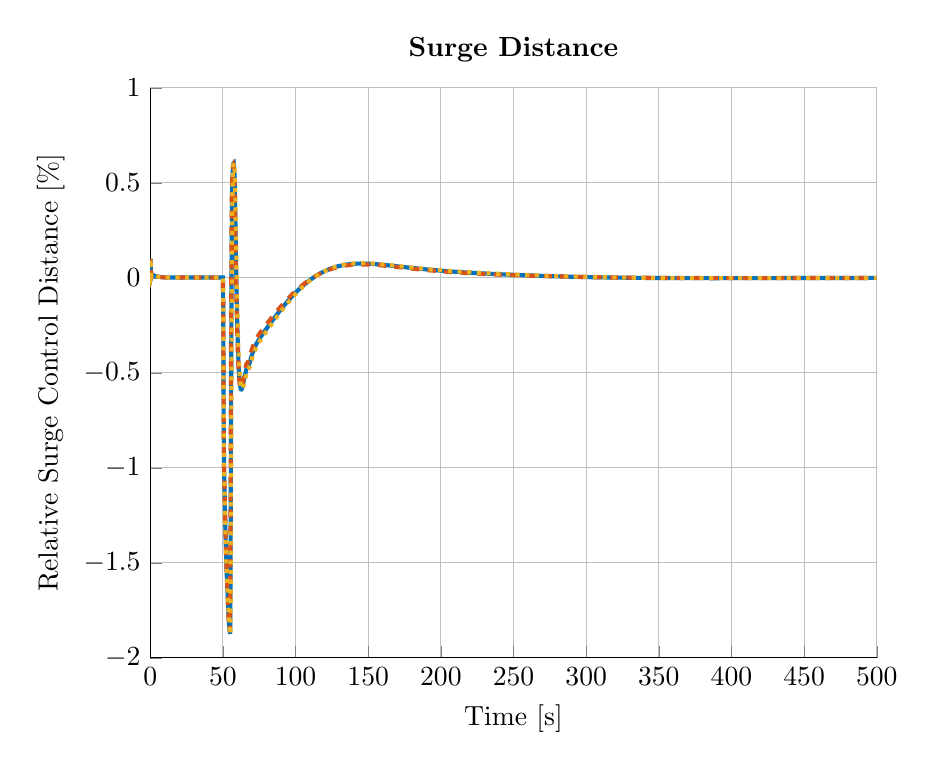
\begin{tikzpicture}

\begin{axis}[%
width=0.761\linewidth,
height=0.597\linewidth,
at={(0\linewidth,0\linewidth)},
scale only axis,
xmin=0,
xmax=500,
xlabel={Time [s]},
xmajorgrids,
ymin=-2,
ymax=1,
ylabel={Relative Surge Control Distance [\%]},
ymajorgrids,
axis background/.style={fill=white},
title style={font=\bfseries},
title={Surge Distance},
axis x line*=bottom,
axis y line*=left
]
\addplot [color=mycolor1,solid,line width=1.5pt,forget plot]
  table[row sep=crcr]{%
0	0.0693700000000002\\
0.25	0.0990399999999996\\
0.5	0.0265199999999997\\
0.75	0.00999999999999979\\
1	0.0180300000000004\\
1.25	0.0180600000000002\\
1.5	0.01539\\
1.75	0.0145999999999997\\
2	0.0142600000000002\\
2.25	0.0136000000000003\\
2.5	0.0129200000000003\\
2.75	0.0122999999999998\\
3	0.0117099999999999\\
3.25	0.0111299999999996\\
3.5	0.0105599999999999\\
3.75	0.0100199999999999\\
4	0.00949000000000044\\
4.25	0.00898999999999983\\
4.5	0.00849999999999973\\
4.75	0.00804000000000027\\
5	0.00759000000000043\\
5.25	0.00717000000000034\\
5.5	0.00677000000000039\\
5.75	0.00638999999999967\\
6	0.00602999999999998\\
6.25	0.00569000000000042\\
6.5	0.00535999999999959\\
6.75	0.00506000000000029\\
7	0.00478000000000023\\
7.25	0.00450999999999979\\
7.5	0.00426000000000037\\
7.75	0.0040300000000002\\
8	0.00380999999999965\\
8.25	0.00361000000000011\\
8.5	0.0034200000000002\\
8.75	0.00325000000000042\\
9	0.00309000000000026\\
9.25	0.00293999999999972\\
9.5	0.0028100000000002\\
9.75	0.00267999999999979\\
10	0.00257000000000041\\
10.25	0.00246999999999975\\
10.5	0.00236999999999998\\
10.75	0.00229000000000035\\
11	0.00220999999999982\\
11.25	0.00215000000000032\\
11.5	0.00208999999999993\\
11.75	0.00203000000000042\\
12	0.00197999999999965\\
12.25	0.00194000000000027\\
12.5	0.00190000000000001\\
12.75	0.00187000000000026\\
13	0.00185000000000013\\
13.25	0.00182000000000038\\
13.5	0.00180000000000025\\
13.75	0.00178999999999974\\
14	0.00178000000000011\\
14.25	0.00176999999999961\\
14.5	0.00175999999999998\\
14.75	0.00175000000000036\\
15	0.00175000000000036\\
15.25	0.00175000000000036\\
15.5	0.00175000000000036\\
15.75	0.00175000000000036\\
16	0.00175999999999998\\
16.25	0.00175999999999998\\
16.5	0.00175999999999998\\
16.75	0.00176999999999961\\
17	0.00178000000000011\\
17.25	0.00178000000000011\\
17.5	0.00178999999999974\\
17.75	0.00180000000000025\\
18	0.00180000000000025\\
18.25	0.00180999999999987\\
18.5	0.00182000000000038\\
18.75	0.00183\\
19	0.00183\\
19.25	0.00183999999999962\\
19.5	0.00185000000000013\\
19.75	0.00185000000000013\\
20	0.00185999999999975\\
20.25	0.00187000000000026\\
20.5	0.00187000000000026\\
20.75	0.00187999999999988\\
21	0.00187999999999988\\
21.25	0.00189000000000039\\
21.5	0.00189000000000039\\
21.75	0.00190000000000001\\
22	0.00190000000000001\\
22.25	0.00190000000000001\\
22.5	0.00190000000000001\\
22.75	0.00190999999999963\\
23	0.00190999999999963\\
23.25	0.00190999999999963\\
23.5	0.00190999999999963\\
23.75	0.00190999999999963\\
24	0.00190999999999963\\
24.25	0.00190999999999963\\
24.5	0.00190999999999963\\
24.75	0.00190999999999963\\
25	0.00190999999999963\\
25.25	0.00190999999999963\\
25.5	0.00190999999999963\\
25.75	0.00190999999999963\\
26	0.00190999999999963\\
26.25	0.00190000000000001\\
26.5	0.00190000000000001\\
26.75	0.00190000000000001\\
27	0.00190000000000001\\
27.25	0.00190000000000001\\
27.5	0.00189000000000039\\
27.75	0.00189000000000039\\
28	0.00189000000000039\\
28.25	0.00187999999999988\\
28.5	0.00187999999999988\\
28.75	0.00187999999999988\\
29	0.00187000000000026\\
29.25	0.00187000000000026\\
29.5	0.00187000000000026\\
29.75	0.00185999999999975\\
30	0.00185999999999975\\
30.25	0.00185999999999975\\
30.5	0.00185000000000013\\
30.75	0.00185000000000013\\
31	0.00183999999999962\\
31.25	0.00183999999999962\\
31.5	0.00183999999999962\\
31.75	0.00183\\
32	0.00183\\
32.25	0.00183\\
32.5	0.00182000000000038\\
32.75	0.00182000000000038\\
33	0.00180999999999987\\
33.25	0.00180999999999987\\
33.5	0.00180999999999987\\
33.75	0.00180000000000025\\
34	0.00180000000000025\\
34.25	0.00180000000000025\\
34.5	0.00178999999999974\\
34.75	0.00178999999999974\\
35	0.00178999999999974\\
35.25	0.00178000000000011\\
35.5	0.00178000000000011\\
35.75	0.00178000000000011\\
36	0.00176999999999961\\
36.25	0.00176999999999961\\
36.5	0.00176999999999961\\
36.75	0.00175999999999998\\
37	0.00175999999999998\\
37.25	0.00175999999999998\\
37.5	0.00175000000000036\\
37.75	0.00175000000000036\\
38	0.00175000000000036\\
38.25	0.00173999999999985\\
38.5	0.00173999999999985\\
38.75	0.00173999999999985\\
39	0.00173999999999985\\
39.25	0.00173000000000023\\
39.5	0.00173000000000023\\
39.75	0.00173000000000023\\
40	0.00171999999999972\\
40.25	0.00171999999999972\\
40.5	0.00171999999999972\\
40.75	0.00171999999999972\\
41	0.0017100000000001\\
41.25	0.0017100000000001\\
41.5	0.0017100000000001\\
41.75	0.0017100000000001\\
42	0.00169999999999959\\
42.25	0.00169999999999959\\
42.5	0.00169999999999959\\
42.75	0.00169999999999959\\
43	0.00169999999999959\\
43.25	0.00168999999999997\\
43.5	0.00168999999999997\\
43.75	0.00168999999999997\\
44	0.00168999999999997\\
44.25	0.00168000000000035\\
44.5	0.00168000000000035\\
44.75	0.00168000000000035\\
45	0.00168000000000035\\
45.25	0.00168000000000035\\
45.5	0.00166999999999984\\
45.75	0.00166999999999984\\
46	0.00166999999999984\\
46.25	0.00166999999999984\\
46.5	0.00166999999999984\\
46.75	0.00166999999999984\\
47	0.00166000000000022\\
47.25	0.00166000000000022\\
47.5	0.00166000000000022\\
47.75	0.00166000000000022\\
48	0.00166000000000022\\
48.25	0.00164999999999971\\
48.5	0.00164999999999971\\
48.75	0.00164999999999971\\
49	0.00164999999999971\\
49.25	0.00164999999999971\\
49.5	0.00164999999999971\\
49.75	0.00164999999999971\\
50	0.00164000000000009\\
50.25	-0.15753\\
50.5	-0.67415\\
50.75	-0.97497\\
51	-1.0645\\
51.25	-1.14641\\
51.5	-1.24849\\
51.75	-1.33687\\
52	-1.40864\\
52.25	-1.47242\\
52.5	-1.52977\\
52.75	-1.57967\\
53	-1.62275\\
53.25	-1.66337\\
53.5	-1.70892\\
53.75	-1.75344\\
54	-1.79266\\
54.25	-1.82558\\
54.5	-1.84848\\
54.75	-1.8633\\
55	-1.87315\\
55.25	-1.55099\\
55.5	-0.9513\\
55.75	-0.43173\\
56	0.0882399999999999\\
56.25	0.40155\\
56.5	0.50932\\
56.75	0.55751\\
57	0.58834\\
57.25	0.60285\\
57.5	0.60479\\
57.75	0.58705\\
58	0.53864\\
58.25	0.45678\\
58.5	0.34801\\
58.75	0.22685\\
59	0.10656\\
59.25	-0.00595999999999997\\
59.5	-0.10799\\
59.75	-0.19842\\
60	-0.27716\\
60.25	-0.34473\\
60.5	-0.40193\\
60.75	-0.4496\\
61	-0.48859\\
61.25	-0.51978\\
61.5	-0.54401\\
61.75	-0.5621\\
62	-0.57478\\
62.25	-0.58273\\
62.5	-0.58661\\
62.75	-0.58702\\
63	-0.58451\\
63.25	-0.57963\\
63.5	-0.57288\\
63.75	-0.56472\\
64	-0.55556\\
64.25	-0.54581\\
64.5	-0.53597\\
64.75	-0.52762\\
65	-0.51988\\
65.25	-0.51137\\
65.5	-0.50264\\
65.75	-0.49434\\
66	-0.48649\\
66.25	-0.47898\\
66.5	-0.47203\\
66.75	-0.46869\\
67	-0.46901\\
67.25	-0.4685\\
67.5	-0.46562\\
67.75	-0.46131\\
68	-0.45617\\
68.25	-0.45034\\
68.5	-0.44403\\
68.75	-0.43748\\
69	-0.43085\\
69.25	-0.42422\\
69.5	-0.41764\\
69.75	-0.41121\\
70	-0.40499\\
70.25	-0.399\\
70.5	-0.39325\\
70.75	-0.38777\\
71	-0.38253\\
71.25	-0.37753\\
71.5	-0.37276\\
71.75	-0.36821\\
72	-0.36386\\
72.25	-0.3597\\
72.5	-0.3557\\
72.75	-0.35187\\
73	-0.34817\\
73.25	-0.3446\\
73.5	-0.34114\\
73.75	-0.33779\\
74	-0.33453\\
74.25	-0.33134\\
74.5	-0.32823\\
74.75	-0.32518\\
75	-0.32218\\
75.25	-0.31923\\
75.5	-0.31633\\
75.75	-0.31346\\
76	-0.31062\\
76.25	-0.3078\\
76.5	-0.30502\\
76.75	-0.30225\\
77	-0.2995\\
77.25	-0.29676\\
77.5	-0.29404\\
77.75	-0.29132\\
78	-0.28862\\
78.25	-0.28592\\
78.5	-0.28324\\
78.75	-0.28055\\
79	-0.27788\\
79.25	-0.2752\\
79.5	-0.27253\\
79.75	-0.26987\\
80	-0.26721\\
80.25	-0.26455\\
80.5	-0.2619\\
80.75	-0.25925\\
81	-0.2566\\
81.25	-0.25396\\
81.5	-0.25132\\
81.75	-0.24869\\
82	-0.24606\\
82.25	-0.24343\\
82.5	-0.24081\\
82.75	-0.23819\\
83	-0.23558\\
83.25	-0.23297\\
83.5	-0.23037\\
83.75	-0.22777\\
84	-0.22518\\
84.25	-0.22259\\
84.5	-0.22001\\
84.75	-0.21744\\
85	-0.21487\\
85.25	-0.21231\\
85.5	-0.20976\\
85.75	-0.20721\\
86	-0.20467\\
86.25	-0.20214\\
86.5	-0.19962\\
86.75	-0.1971\\
87	-0.19459\\
87.25	-0.19209\\
87.5	-0.1896\\
87.75	-0.18712\\
88	-0.18465\\
88.25	-0.18218\\
88.5	-0.17972\\
88.75	-0.17728\\
89	-0.17484\\
89.25	-0.17241\\
89.5	-0.16999\\
89.75	-0.16758\\
90	-0.16518\\
90.25	-0.16279\\
90.5	-0.16041\\
90.75	-0.15804\\
91	-0.15568\\
91.25	-0.15333\\
91.5	-0.15099\\
91.75	-0.14866\\
92	-0.14634\\
92.25	-0.14403\\
92.5	-0.14173\\
92.75	-0.13944\\
93	-0.13717\\
93.25	-0.1349\\
93.5	-0.13265\\
93.75	-0.1304\\
94	-0.12817\\
94.25	-0.12595\\
94.5	-0.12374\\
94.75	-0.12154\\
95	-0.11936\\
95.25	-0.11718\\
95.5	-0.11502\\
95.75	-0.11287\\
96	-0.11073\\
96.25	-0.1086\\
96.5	-0.10648\\
96.75	-0.10438\\
97	-0.10229\\
97.25	-0.10021\\
97.5	-0.0981399999999999\\
97.75	-0.0960900000000002\\
98	-0.0940399999999997\\
98.25	-0.0920100000000001\\
98.5	-0.0899900000000002\\
98.75	-0.0879899999999996\\
99	-0.0859899999999998\\
99.25	-0.0840100000000001\\
99.5	-0.0820400000000001\\
99.75	-0.0800799999999997\\
100	-0.0781400000000003\\
100.25	-0.0762099999999997\\
100.5	-0.0742900000000004\\
100.75	-0.0723799999999999\\
101	-0.0704900000000004\\
101.25	-0.0686099999999996\\
101.5	-0.0667400000000002\\
101.75	-0.0648900000000001\\
102	-0.0630499999999996\\
102.25	-0.0612199999999996\\
102.5	-0.0594000000000001\\
102.75	-0.0575999999999999\\
103	-0.0558100000000001\\
103.25	-0.05403\\
103.5	-0.05227\\
103.75	-0.0505199999999997\\
104	-0.0487799999999998\\
104.25	-0.0470499999999996\\
104.5	-0.0453400000000004\\
104.75	-0.0436399999999999\\
105	-0.0419600000000004\\
105.25	-0.0402899999999997\\
105.5	-0.0386300000000004\\
105.75	-0.0369799999999998\\
106	-0.0353500000000002\\
106.25	-0.0337300000000003\\
106.5	-0.0321199999999999\\
106.75	-0.0305299999999997\\
107	-0.02895\\
107.25	-0.02738\\
107.5	-0.02583\\
107.75	-0.0242899999999997\\
108	-0.0227599999999999\\
108.25	-0.0212500000000002\\
108.5	-0.0197500000000002\\
108.75	-0.0182599999999997\\
109	-0.0167799999999998\\
109.25	-0.01532\\
109.5	-0.0138699999999998\\
109.75	-0.0124399999999998\\
110	-0.0110200000000003\\
110.25	-0.00961000000000034\\
110.5	-0.00821000000000005\\
110.75	-0.00682999999999989\\
111	-0.00546000000000024\\
111.25	-0.00410999999999984\\
111.5	-0.00276999999999994\\
111.75	-0.00143999999999966\\
112	-0.000119999999999898\\
112.25	0.00117999999999974\\
112.5	0.00246999999999975\\
112.75	0.00375000000000014\\
113	0.00502000000000002\\
113.25	0.00626999999999978\\
113.5	0.00750999999999991\\
113.75	0.0087299999999999\\
114	0.00994000000000028\\
114.25	0.0111400000000001\\
114.5	0.0123300000000004\\
114.75	0.0134999999999996\\
115	0.0146600000000001\\
115.25	0.0158100000000001\\
115.5	0.0169499999999996\\
115.75	0.0180699999999998\\
116	0.0191800000000004\\
116.25	0.0202799999999996\\
116.5	0.0213599999999996\\
116.75	0.0224299999999999\\
117	0.0234899999999998\\
117.25	0.02454\\
117.5	0.0255700000000001\\
117.75	0.0265899999999997\\
118	0.0275999999999996\\
118.25	0.0286\\
118.5	0.0295800000000002\\
118.75	0.0305600000000004\\
119	0.0315200000000004\\
119.25	0.0324600000000004\\
119.5	0.0334000000000003\\
119.75	0.0343200000000001\\
120	0.0352300000000003\\
120.25	0.03613\\
120.5	0.0370200000000001\\
120.75	0.03789\\
121	0.0387599999999999\\
121.25	0.0396099999999997\\
121.5	0.0404499999999999\\
121.75	0.0412800000000004\\
122	0.04209\\
122.25	0.0429000000000004\\
122.5	0.0436899999999998\\
122.75	0.0444699999999996\\
123	0.0452399999999997\\
123.25	0.0460000000000003\\
123.5	0.0467399999999998\\
123.75	0.0474800000000002\\
124	0.0481999999999996\\
124.25	0.0489100000000002\\
124.5	0.0496100000000004\\
124.75	0.0503\\
125	0.05098\\
125.25	0.0516500000000004\\
125.5	0.0523100000000003\\
125.75	0.0529500000000001\\
126	0.0535899999999998\\
126.25	0.0542100000000003\\
126.5	0.0548299999999999\\
126.75	0.0554300000000003\\
127	0.0560200000000002\\
127.25	0.0566000000000004\\
127.5	0.0571799999999998\\
127.75	0.0577399999999999\\
128	0.0582900000000004\\
128.25	0.0588300000000004\\
128.5	0.0593599999999999\\
128.75	0.0598799999999997\\
129	0.0603899999999999\\
129.25	0.0608899999999997\\
129.5	0.0613799999999998\\
129.75	0.0618600000000002\\
130	0.0623199999999997\\
130.25	0.0627899999999997\\
130.5	0.0632400000000004\\
130.75	0.0636799999999997\\
131	0.0641100000000003\\
131.25	0.0645300000000004\\
131.5	0.06494\\
131.75	0.06534\\
132	0.0657399999999999\\
132.25	0.0661199999999997\\
132.5	0.0664999999999996\\
132.75	0.0668600000000001\\
133	0.0672199999999998\\
133.25	0.0675699999999999\\
133.5	0.0679100000000004\\
133.75	0.0682400000000003\\
134	0.0685599999999997\\
134.25	0.0688800000000001\\
134.5	0.0691800000000002\\
134.75	0.0694800000000004\\
135	0.0697700000000001\\
135.25	0.0700500000000002\\
135.5	0.0703199999999997\\
135.75	0.0705799999999996\\
136	0.0708399999999996\\
136.25	0.0710800000000003\\
136.5	0.0713200000000001\\
136.75	0.0715500000000002\\
137	0.0717800000000004\\
137.25	0.0719900000000004\\
137.5	0.0721999999999996\\
137.75	0.0724\\
138	0.0725899999999999\\
138.25	0.0727799999999998\\
138.5	0.0729600000000001\\
138.75	0.0731299999999999\\
139	0.0732900000000001\\
139.25	0.0734500000000002\\
139.5	0.0735999999999999\\
139.75	0.0737399999999999\\
140	0.0738799999999999\\
140.25	0.0740100000000004\\
140.5	0.0741300000000003\\
140.75	0.0742500000000001\\
141	0.0743600000000004\\
141.25	0.0744600000000002\\
141.5	0.07456\\
141.75	0.0746500000000001\\
142	0.0747299999999997\\
142.25	0.0748100000000003\\
142.5	0.0748800000000003\\
142.75	0.0749399999999998\\
143	0.0750000000000002\\
143.25	0.0750599999999997\\
143.5	0.0750999999999999\\
143.75	0.0751499999999998\\
144	0.0751799999999996\\
144.25	0.0752100000000002\\
144.5	0.07524\\
144.75	0.0752600000000001\\
145	0.0752699999999997\\
145.25	0.0752800000000002\\
145.5	0.0752899999999999\\
145.75	0.0752899999999999\\
146	0.0752800000000002\\
146.25	0.0752699999999997\\
146.5	0.0752499999999996\\
146.75	0.0752300000000004\\
147	0.0752100000000002\\
147.25	0.0751799999999996\\
147.5	0.0751400000000002\\
147.75	0.0750999999999999\\
148	0.0750599999999997\\
148.25	0.0750099999999998\\
148.5	0.0749599999999999\\
148.75	0.0749000000000004\\
149	0.07484\\
149.25	0.07477\\
149.5	0.0747\\
149.75	0.07463\\
150	0.0745500000000003\\
150.25	0.0744699999999998\\
150.5	0.0743900000000002\\
150.75	0.0743\\
151	0.0742099999999999\\
151.25	0.0741100000000001\\
151.5	0.0740100000000004\\
151.75	0.0739099999999997\\
152	0.0738000000000003\\
152.25	0.07369\\
152.5	0.0735799999999998\\
152.75	0.0734599999999999\\
153	0.0733499999999996\\
153.25	0.0732200000000001\\
153.5	0.0731000000000002\\
153.75	0.0729699999999998\\
154	0.0728400000000002\\
154.25	0.0727000000000002\\
154.5	0.0725699999999998\\
154.75	0.0724299999999998\\
155	0.0722899999999997\\
155.25	0.0721400000000001\\
155.5	0.0719900000000004\\
155.75	0.0718399999999999\\
156	0.0716900000000003\\
156.25	0.0715399999999997\\
156.5	0.0713800000000004\\
156.75	0.0712200000000003\\
157	0.0710600000000001\\
157.25	0.0709\\
157.5	0.0707300000000002\\
157.75	0.0705600000000004\\
158	0.0704000000000002\\
158.25	0.0702199999999999\\
158.5	0.0700500000000002\\
158.75	0.0698800000000004\\
159	0.0697000000000001\\
159.25	0.0695199999999998\\
159.5	0.0693400000000004\\
159.75	0.0691600000000001\\
160	0.0689700000000002\\
160.25	0.0687899999999999\\
160.5	0.0686\\
160.75	0.0684100000000001\\
161	0.0682200000000002\\
161.25	0.0680300000000003\\
161.5	0.0678400000000003\\
161.75	0.0676500000000004\\
162	0.06745\\
162.25	0.0672600000000001\\
162.5	0.0670599999999997\\
162.75	0.0668600000000001\\
163	0.0666599999999997\\
163.25	0.0664600000000002\\
163.5	0.0662599999999998\\
163.75	0.0660600000000002\\
164	0.0658500000000002\\
164.25	0.0656499999999998\\
164.5	0.0654500000000002\\
164.75	0.0652400000000002\\
165	0.0650300000000001\\
165.25	0.0648299999999997\\
165.5	0.0646199999999997\\
165.75	0.0644099999999996\\
166	0.0641999999999996\\
166.25	0.0639900000000004\\
166.5	0.0637800000000004\\
166.75	0.0635700000000003\\
167	0.0633600000000003\\
167.25	0.0631500000000003\\
167.5	0.0629299999999997\\
167.75	0.0627199999999997\\
168	0.0625099999999996\\
168.25	0.06229\\
168.5	0.0620799999999999\\
168.75	0.0618699999999999\\
169	0.0616500000000002\\
169.25	0.0614400000000002\\
169.5	0.0612199999999996\\
169.75	0.0610099999999996\\
170	0.0607899999999999\\
170.25	0.0605799999999999\\
170.5	0.0603600000000002\\
170.75	0.0601500000000001\\
171	0.0599299999999996\\
171.25	0.0597200000000004\\
171.5	0.0594999999999999\\
171.75	0.0592800000000002\\
172	0.0590700000000002\\
172.25	0.0588499999999996\\
172.5	0.0586399999999996\\
172.75	0.0584199999999999\\
173	0.0582099999999999\\
173.25	0.0579900000000002\\
173.5	0.0577800000000002\\
173.75	0.0575599999999996\\
174	0.0573499999999996\\
174.25	0.0571299999999999\\
174.5	0.0569199999999999\\
174.75	0.0567099999999998\\
175	0.0564900000000002\\
175.25	0.0562800000000001\\
175.5	0.0560700000000001\\
175.75	0.0558500000000004\\
176	0.0556400000000004\\
176.25	0.0554300000000003\\
176.5	0.0552200000000003\\
176.75	0.0549999999999997\\
177	0.0547899999999997\\
177.25	0.0545799999999996\\
177.5	0.0543699999999996\\
177.75	0.0541600000000004\\
178	0.0539500000000004\\
178.25	0.0537400000000003\\
178.5	0.0535300000000003\\
178.75	0.0533299999999999\\
179	0.0531199999999998\\
179.25	0.0529099999999998\\
179.5	0.0526999999999997\\
179.75	0.0525000000000002\\
180	0.0522900000000002\\
180.25	0.0520899999999997\\
180.5	0.0518799999999997\\
180.75	0.0516800000000002\\
181	0.0514700000000001\\
181.25	0.0512699999999997\\
181.5	0.0510700000000002\\
181.75	0.0508699999999997\\
182	0.0506700000000002\\
182.25	0.0504600000000002\\
182.5	0.0502599999999997\\
182.75	0.0500600000000002\\
183	0.0498700000000003\\
183.25	0.0496699999999999\\
183.5	0.0494700000000003\\
183.75	0.0492699999999999\\
184	0.04908\\
184.25	0.0488799999999996\\
184.5	0.0486800000000001\\
184.75	0.0484900000000001\\
185	0.0482899999999997\\
185.25	0.0480999999999998\\
185.5	0.0479099999999999\\
185.75	0.04772\\
186	0.0475199999999996\\
186.25	0.0473299999999997\\
186.5	0.0471399999999997\\
186.75	0.0469499999999998\\
187	0.0467599999999999\\
187.25	0.0465799999999996\\
187.5	0.0463899999999997\\
187.75	0.0461999999999998\\
188	0.0460099999999999\\
188.25	0.0458299999999996\\
188.5	0.0456399999999997\\
188.75	0.0454600000000003\\
189	0.04528\\
189.25	0.0450900000000001\\
189.5	0.0449099999999998\\
189.75	0.0447300000000004\\
190	0.0445500000000001\\
190.25	0.0443699999999998\\
190.5	0.0441900000000004\\
190.75	0.0440100000000001\\
191	0.0438299999999998\\
191.25	0.0436500000000004\\
191.5	0.0434799999999997\\
191.75	0.0433000000000003\\
192	0.0431299999999997\\
192.25	0.0429500000000003\\
192.5	0.0427799999999996\\
192.75	0.0426000000000002\\
193	0.0424300000000004\\
193.25	0.0422599999999997\\
193.5	0.04209\\
193.75	0.0419200000000002\\
194	0.0417500000000004\\
194.25	0.0415799999999997\\
194.5	0.0414099999999999\\
194.75	0.0412400000000002\\
195	0.0410700000000004\\
195.25	0.0409100000000002\\
195.5	0.0407400000000004\\
195.75	0.0405699999999998\\
196	0.0404099999999996\\
196.25	0.0402399999999998\\
196.5	0.0400799999999997\\
196.75	0.0399200000000004\\
197	0.0397600000000002\\
197.25	0.0396000000000001\\
197.5	0.0394300000000003\\
197.75	0.0392700000000001\\
198	0.03911\\
198.25	0.0389600000000003\\
198.5	0.0388000000000002\\
198.75	0.03864\\
199	0.0384799999999998\\
199.25	0.0383300000000002\\
199.5	0.03817\\
199.75	0.0380200000000004\\
200	0.0378600000000002\\
200.25	0.0377099999999997\\
200.5	0.0375500000000004\\
200.75	0.0373999999999999\\
201	0.0372500000000002\\
201.25	0.0370999999999997\\
201.5	0.03695\\
201.75	0.0368000000000004\\
202	0.0366499999999998\\
202.25	0.0365000000000002\\
202.5	0.0363499999999997\\
202.75	0.0362\\
203	0.03606\\
203.25	0.0359100000000003\\
203.5	0.0357599999999998\\
203.75	0.0356199999999998\\
204	0.0354700000000001\\
204.25	0.0353300000000001\\
204.5	0.0351900000000001\\
204.75	0.0350400000000004\\
205	0.0349000000000004\\
205.25	0.0347600000000003\\
205.5	0.0346200000000003\\
205.75	0.0344800000000003\\
206	0.0343400000000003\\
206.25	0.0342000000000002\\
206.5	0.0340600000000002\\
206.75	0.0339200000000002\\
207	0.0337800000000001\\
207.25	0.0336400000000001\\
207.5	0.0335099999999997\\
207.75	0.0333699999999997\\
208	0.0332400000000002\\
208.25	0.0331000000000001\\
208.5	0.0329699999999997\\
208.75	0.0328299999999997\\
209	0.0327000000000002\\
209.25	0.0325600000000001\\
209.5	0.0324299999999997\\
209.75	0.0323000000000002\\
210	0.0321699999999998\\
210.25	0.0320400000000003\\
210.5	0.0319099999999999\\
210.75	0.0317800000000004\\
211	0.03165\\
211.25	0.0315200000000004\\
211.5	0.03139\\
211.75	0.0312599999999996\\
212	0.0311300000000001\\
212.25	0.0310100000000002\\
212.5	0.0308799999999998\\
212.75	0.0307500000000003\\
213	0.0306300000000004\\
213.25	0.0305\\
213.5	0.0303800000000001\\
213.75	0.0302499999999997\\
214	0.0301299999999998\\
214.25	0.0300099999999999\\
214.5	0.0298800000000004\\
214.75	0.0297599999999996\\
215	0.0296399999999997\\
215.25	0.0295199999999998\\
215.5	0.0293900000000002\\
215.75	0.0292700000000004\\
216	0.0291499999999996\\
216.25	0.0290299999999997\\
216.5	0.0289099999999998\\
216.75	0.0288000000000004\\
217	0.0286799999999996\\
217.25	0.0285599999999997\\
217.5	0.0284399999999998\\
217.75	0.0283199999999999\\
218	0.0282099999999996\\
218.25	0.0280899999999997\\
218.5	0.0279699999999998\\
218.75	0.0278600000000004\\
219	0.0277399999999997\\
219.25	0.0276300000000003\\
219.5	0.0275100000000004\\
219.75	0.0274000000000001\\
220	0.0272899999999998\\
220.25	0.0271699999999999\\
220.5	0.0270599999999996\\
220.75	0.0269500000000003\\
221	0.02684\\
221.25	0.0267200000000001\\
221.5	0.0266099999999998\\
221.75	0.0265000000000004\\
222	0.0263900000000001\\
222.25	0.0262799999999999\\
222.5	0.0261699999999996\\
222.75	0.0260600000000002\\
223	0.0259499999999999\\
223.25	0.0258399999999996\\
223.5	0.0257399999999999\\
223.75	0.0256299999999996\\
224	0.0255200000000002\\
224.25	0.0254099999999999\\
224.5	0.0253100000000002\\
224.75	0.0251999999999999\\
225	0.0250899999999996\\
225.25	0.0249899999999998\\
225.5	0.0248799999999996\\
225.75	0.0247799999999998\\
226	0.0246700000000004\\
226.25	0.0245699999999998\\
226.5	0.0244600000000004\\
226.75	0.0243599999999997\\
227	0.0242599999999999\\
227.25	0.0241499999999997\\
227.5	0.0240499999999999\\
227.75	0.0239500000000001\\
228	0.0238500000000004\\
228.25	0.0237499999999997\\
228.5	0.0236400000000003\\
228.75	0.0235399999999997\\
229	0.0234399999999999\\
229.25	0.0233400000000001\\
229.5	0.0232400000000004\\
229.75	0.0231399999999997\\
230	0.0230399999999999\\
230.25	0.0229400000000002\\
230.5	0.0228400000000004\\
230.75	0.0227399999999998\\
231	0.0226499999999996\\
231.25	0.0225499999999998\\
231.5	0.0224500000000001\\
231.75	0.0223500000000003\\
232	0.0222600000000002\\
232.25	0.0221600000000004\\
232.5	0.0220599999999997\\
232.75	0.0219699999999996\\
233	0.0218699999999998\\
233.25	0.0217700000000001\\
233.5	0.0216799999999999\\
233.75	0.0215800000000002\\
234	0.02149\\
234.25	0.0213999999999999\\
234.5	0.0213000000000001\\
234.75	0.02121\\
235	0.0211100000000002\\
235.25	0.02102\\
235.5	0.0209299999999999\\
235.75	0.0208300000000001\\
236	0.02074\\
236.25	0.0206499999999998\\
236.5	0.0205599999999997\\
236.75	0.0204700000000004\\
237	0.0203699999999998\\
237.25	0.0202799999999996\\
237.5	0.0201900000000004\\
237.75	0.0201000000000002\\
238	0.0200100000000001\\
238.25	0.0199199999999999\\
238.5	0.0198299999999998\\
238.75	0.0197399999999996\\
239	0.0196500000000004\\
239.25	0.0195600000000002\\
239.5	0.0194700000000001\\
239.75	0.0193899999999996\\
240	0.0193000000000003\\
240.25	0.0192100000000002\\
240.5	0.01912\\
240.75	0.0190299999999999\\
241	0.0189500000000002\\
241.25	0.0188600000000001\\
241.5	0.01877\\
241.75	0.0186900000000003\\
242	0.0186000000000002\\
242.25	0.01851\\
242.5	0.0184300000000004\\
242.75	0.0183400000000002\\
243	0.0182599999999997\\
243.25	0.0181699999999996\\
243.5	0.0180899999999999\\
243.75	0.0179999999999998\\
244	0.0179200000000002\\
244.25	0.01783\\
244.5	0.0177500000000004\\
244.75	0.0176699999999999\\
245	0.0175799999999997\\
245.25	0.0175000000000001\\
245.5	0.0174200000000004\\
245.75	0.0173300000000003\\
246	0.0172499999999998\\
246.25	0.0171700000000001\\
246.5	0.0170899999999996\\
246.75	0.01701\\
247	0.0169199999999998\\
247.25	0.0168400000000002\\
247.5	0.0167599999999997\\
247.75	0.01668\\
248	0.0166000000000004\\
248.25	0.0165199999999999\\
248.5	0.0164400000000002\\
248.75	0.0163599999999997\\
249	0.0162800000000001\\
249.25	0.0162000000000004\\
249.5	0.0161199999999999\\
249.75	0.0160400000000003\\
250	0.0159599999999998\\
250.25	0.0158899999999997\\
250.5	0.0158100000000001\\
250.75	0.0157299999999996\\
251	0.0156499999999999\\
251.25	0.0155700000000003\\
251.5	0.0155000000000003\\
251.75	0.0154199999999998\\
252	0.0153400000000001\\
252.25	0.0152599999999996\\
252.5	0.0151899999999996\\
252.75	0.01511\\
253	0.0150300000000003\\
253.25	0.0149600000000003\\
253.5	0.0148799999999998\\
253.75	0.0148099999999998\\
254	0.0147300000000001\\
254.25	0.0146600000000001\\
254.5	0.0145799999999996\\
254.75	0.0145099999999996\\
255	0.0144299999999999\\
255.25	0.0143599999999999\\
255.5	0.0142800000000003\\
255.75	0.0142100000000003\\
256	0.0141400000000003\\
256.25	0.0140599999999997\\
256.5	0.0139899999999997\\
256.75	0.0139199999999997\\
257	0.0138400000000001\\
257.25	0.0137700000000001\\
257.5	0.0137\\
257.75	0.01363\\
258	0.0135500000000004\\
258.25	0.0134800000000004\\
258.5	0.0134100000000004\\
258.75	0.0133400000000004\\
259	0.0132700000000003\\
259.25	0.0132000000000003\\
259.5	0.0131300000000003\\
259.75	0.0130600000000003\\
260	0.0129900000000003\\
260.25	0.0129200000000003\\
260.5	0.0128500000000003\\
260.75	0.0127800000000002\\
261	0.0127100000000002\\
261.25	0.0126400000000002\\
261.5	0.0125700000000002\\
261.75	0.0125000000000002\\
262	0.0124300000000002\\
262.25	0.0123600000000001\\
262.5	0.0122900000000001\\
262.75	0.0122299999999997\\
263	0.0121599999999997\\
263.25	0.0120899999999997\\
263.5	0.0120199999999997\\
263.75	0.0119499999999997\\
264	0.0118900000000002\\
264.25	0.0118200000000002\\
264.5	0.0117500000000001\\
264.75	0.0116899999999998\\
265	0.0116199999999997\\
265.25	0.0115499999999997\\
265.5	0.0114900000000002\\
265.75	0.0114200000000002\\
266	0.0113599999999998\\
266.25	0.0112899999999998\\
266.5	0.0112300000000003\\
266.75	0.0111600000000003\\
267	0.0110999999999999\\
267.25	0.0110299999999999\\
267.5	0.0109700000000004\\
267.75	0.0109000000000004\\
268	0.01084\\
268.25	0.0107699999999999\\
268.5	0.0107100000000004\\
268.75	0.01065\\
269	0.01058\\
269.25	0.0105199999999996\\
269.5	0.0104600000000001\\
269.75	0.0103999999999997\\
270	0.0103299999999997\\
270.25	0.0102700000000002\\
270.5	0.0102099999999998\\
270.75	0.0101500000000003\\
271	0.0100800000000003\\
271.25	0.0100199999999999\\
271.5	0.00996000000000041\\
271.75	0.00990000000000002\\
272	0.00983999999999963\\
272.25	0.00978000000000012\\
272.5	0.00971999999999973\\
272.75	0.00966000000000022\\
273	0.00959999999999983\\
273.25	0.00954000000000033\\
273.5	0.00947999999999993\\
273.75	0.00942000000000043\\
274	0.00936000000000003\\
274.25	0.00929999999999964\\
274.5	0.00924000000000014\\
274.75	0.00917999999999974\\
275	0.00912000000000024\\
275.25	0.00905999999999985\\
275.5	0.00900999999999996\\
275.75	0.00894999999999957\\
276	0.00889000000000006\\
276.25	0.00882999999999967\\
276.5	0.00877000000000017\\
276.75	0.00872000000000028\\
277	0.00865999999999989\\
277.25	0.00860000000000039\\
277.5	0.00854999999999961\\
277.75	0.00849000000000011\\
278	0.00842999999999972\\
278.25	0.00837999999999983\\
278.5	0.00832000000000033\\
278.75	0.00825999999999993\\
279	0.00821000000000005\\
279.25	0.00814999999999966\\
279.5	0.00809999999999977\\
279.75	0.00804000000000027\\
280	0.00799000000000039\\
280.25	0.00792999999999999\\
280.5	0.00788000000000011\\
280.75	0.00781999999999972\\
281	0.00776999999999983\\
281.25	0.00771999999999995\\
281.5	0.00765999999999956\\
281.75	0.00760999999999967\\
282	0.00755000000000017\\
282.25	0.00750000000000028\\
282.5	0.0074500000000004\\
282.75	0.00739000000000001\\
283	0.00734000000000012\\
283.25	0.00729000000000024\\
283.5	0.00724000000000036\\
283.75	0.00717999999999996\\
284	0.00713000000000008\\
284.25	0.0070800000000002\\
284.5	0.00703000000000031\\
284.75	0.00698000000000043\\
285	0.00692999999999966\\
285.25	0.00687999999999978\\
285.5	0.00682000000000027\\
285.75	0.00677000000000039\\
286	0.00671999999999962\\
286.25	0.00666999999999973\\
286.5	0.00661999999999985\\
286.75	0.00656999999999996\\
287	0.00652000000000008\\
287.25	0.0064700000000002\\
287.5	0.00642000000000031\\
287.75	0.00637000000000043\\
288	0.00631999999999966\\
288.25	0.00628000000000029\\
288.5	0.0062300000000004\\
288.75	0.00617999999999963\\
289	0.00612999999999975\\
289.25	0.00607999999999986\\
289.5	0.00602999999999998\\
289.75	0.00598999999999972\\
290	0.00593999999999983\\
290.25	0.00588999999999995\\
290.5	0.00584000000000007\\
290.75	0.00579999999999981\\
291	0.00574999999999992\\
291.25	0.00570000000000004\\
291.5	0.00565999999999978\\
291.75	0.00560999999999989\\
292	0.00556000000000001\\
292.25	0.00551999999999975\\
292.5	0.00546999999999986\\
292.75	0.00541999999999998\\
293	0.00537999999999972\\
293.25	0.00532999999999983\\
293.5	0.00528999999999957\\
293.75	0.00523999999999969\\
294	0.00520000000000032\\
294.25	0.00515000000000043\\
294.5	0.00511000000000017\\
294.75	0.00506999999999991\\
295	0.00502000000000002\\
295.25	0.00497999999999976\\
295.5	0.00492999999999988\\
295.75	0.00488999999999962\\
296	0.00485000000000024\\
296.25	0.00480000000000036\\
296.5	0.0047600000000001\\
296.75	0.00471999999999984\\
297	0.00466999999999995\\
297.25	0.00462999999999969\\
297.5	0.00459000000000032\\
297.75	0.00455000000000005\\
298	0.00450999999999979\\
298.25	0.00445999999999991\\
298.5	0.00441999999999965\\
298.75	0.00438000000000027\\
299	0.00434000000000001\\
299.25	0.00429999999999975\\
299.5	0.00426000000000037\\
299.75	0.00422000000000011\\
300	0.00417000000000023\\
300.25	0.00412999999999997\\
300.5	0.0040899999999997\\
300.75	0.00405000000000033\\
301	0.00401000000000007\\
301.25	0.00396999999999981\\
301.5	0.00393000000000043\\
301.75	0.00389999999999979\\
302	0.00386000000000042\\
302.25	0.00382000000000016\\
302.5	0.00377999999999989\\
302.75	0.00373999999999963\\
303	0.00370000000000026\\
303.25	0.00366\\
303.5	0.00361999999999973\\
303.75	0.00358999999999998\\
304	0.00354999999999972\\
304.25	0.00351000000000035\\
304.5	0.00347000000000008\\
304.75	0.00342999999999982\\
305	0.00340000000000007\\
305.25	0.00335999999999981\\
305.5	0.00332000000000043\\
305.75	0.00328999999999979\\
306	0.00325000000000042\\
306.25	0.00321000000000016\\
306.5	0.0031800000000004\\
306.75	0.00314000000000014\\
307	0.00311000000000039\\
307.25	0.00307000000000013\\
307.5	0.00302999999999987\\
307.75	0.00300000000000011\\
308	0.00295999999999985\\
308.25	0.0029300000000001\\
308.5	0.00288999999999984\\
308.75	0.00286000000000008\\
309	0.00281999999999982\\
309.25	0.00279000000000007\\
309.5	0.00276000000000032\\
309.75	0.00272000000000006\\
310	0.0026900000000003\\
310.25	0.00265000000000004\\
310.5	0.00262000000000029\\
310.75	0.00258999999999965\\
311	0.00255000000000027\\
311.25	0.00251999999999963\\
311.5	0.00248999999999988\\
311.75	0.00244999999999962\\
312	0.00241999999999987\\
312.25	0.00239000000000011\\
312.5	0.00236000000000036\\
312.75	0.00232999999999972\\
313	0.00229000000000035\\
313.25	0.00225999999999971\\
313.5	0.00222999999999995\\
313.75	0.0022000000000002\\
314	0.00216999999999956\\
314.25	0.00213999999999981\\
314.5	0.00210000000000043\\
314.75	0.00206999999999979\\
315	0.00204000000000004\\
315.25	0.00201000000000029\\
315.5	0.00197999999999965\\
315.75	0.0019499999999999\\
316	0.00192000000000014\\
316.25	0.00189000000000039\\
316.5	0.00185999999999975\\
316.75	0.00183\\
317	0.00180000000000025\\
317.25	0.00176999999999961\\
317.5	0.00173999999999985\\
317.75	0.00171999999999972\\
318	0.00168999999999997\\
318.25	0.00166000000000022\\
318.5	0.00162999999999958\\
318.75	0.00159999999999982\\
319	0.00157000000000007\\
319.25	0.00154999999999994\\
319.5	0.00152000000000019\\
319.75	0.00149000000000044\\
320	0.00145999999999979\\
320.25	0.00143000000000004\\
320.5	0.00140999999999991\\
320.75	0.00138000000000016\\
321	0.00135000000000041\\
321.25	0.00133000000000028\\
321.5	0.00129999999999963\\
321.75	0.00126999999999988\\
322	0.00124999999999975\\
322.25	0.00122\\
322.5	0.00119000000000025\\
322.75	0.00117000000000012\\
323	0.00114000000000036\\
323.25	0.00112000000000023\\
323.5	0.00108999999999959\\
323.75	0.00107000000000035\\
324	0.00103999999999971\\
324.25	0.00101999999999958\\
324.5	0.000989999999999824\\
324.75	0.000969999999999693\\
325	0.000939999999999941\\
325.25	0.00091999999999981\\
325.5	0.000890000000000057\\
325.75	0.000869999999999926\\
326	0.000849999999999795\\
326.25	0.000820000000000043\\
326.5	0.000799999999999912\\
326.75	0.000770000000000159\\
327	0.000750000000000028\\
327.25	0.000729999999999897\\
327.5	0.000700000000000145\\
327.75	0.000680000000000014\\
328	0.000659999999999883\\
328.25	0.000639999999999752\\
328.5	0.000609999999999999\\
328.75	0.000589999999999868\\
329	0.000569999999999737\\
329.25	0.000549999999999606\\
329.5	0.000519999999999854\\
329.75	0.000499999999999723\\
330	0.000479999999999592\\
330.25	0.000460000000000349\\
330.5	0.000440000000000218\\
330.75	0.000420000000000087\\
331	0.000390000000000335\\
331.25	0.000370000000000203\\
331.5	0.000350000000000072\\
331.75	0.000329999999999941\\
332	0.00030999999999981\\
332.25	0.000289999999999679\\
332.5	0.000270000000000437\\
332.75	0.000250000000000306\\
333	0.000230000000000175\\
333.25	0.000210000000000043\\
333.5	0.000189999999999912\\
333.75	0.000169999999999781\\
334	0.00014999999999965\\
334.25	0.000130000000000408\\
334.5	0.000110000000000277\\
334.75	9.00000000001455e-05\\
335	7.00000000000145e-05\\
335.25	6.00000000003931e-05\\
335.5	4.0000000000262e-05\\
335.75	2.0000000000131e-05\\
336	0\\
336.25	-2.0000000000131e-05\\
336.5	-4.0000000000262e-05\\
336.75	-6.00000000003931e-05\\
337	-7.00000000000145e-05\\
337.25	-9.00000000001455e-05\\
337.5	-0.000110000000000277\\
337.75	-0.000130000000000408\\
338	-0.000140000000000029\\
338.25	-0.00016000000000016\\
338.5	-0.000180000000000291\\
338.75	-0.000200000000000422\\
339	-0.000210000000000043\\
339.25	-0.000230000000000175\\
339.5	-0.000250000000000306\\
339.75	-0.000259999999999927\\
340	-0.000280000000000058\\
340.25	-0.000300000000000189\\
340.5	-0.00030999999999981\\
340.75	-0.000329999999999941\\
341	-0.000339999999999563\\
341.25	-0.000359999999999694\\
341.5	-0.000379999999999825\\
341.75	-0.000390000000000335\\
342	-0.000409999999999577\\
342.25	-0.000420000000000087\\
342.5	-0.000440000000000218\\
342.75	-0.000449999999999839\\
343	-0.00046999999999997\\
343.25	-0.000479999999999592\\
343.5	-0.000499999999999723\\
343.75	-0.000510000000000232\\
344	-0.000530000000000364\\
344.25	-0.000539999999999985\\
344.5	-0.000549999999999606\\
344.75	-0.000569999999999737\\
345	-0.000580000000000247\\
345.25	-0.000600000000000378\\
345.5	-0.000609999999999999\\
345.75	-0.000619999999999621\\
346	-0.000639999999999752\\
346.25	-0.000650000000000261\\
346.5	-0.000659999999999883\\
346.75	-0.000680000000000014\\
347	-0.000689999999999635\\
347.25	-0.000700000000000145\\
347.5	-0.000720000000000276\\
347.75	-0.000729999999999897\\
348	-0.000740000000000407\\
348.25	-0.000750000000000028\\
348.5	-0.000770000000000159\\
348.75	-0.000779999999999781\\
349	-0.00079000000000029\\
349.25	-0.000799999999999912\\
349.5	-0.000820000000000043\\
349.75	-0.000829999999999664\\
350	-0.000840000000000174\\
350.25	-0.000849999999999795\\
350.5	-0.000860000000000305\\
350.75	-0.000869999999999926\\
351	-0.000890000000000057\\
351.25	-0.000899999999999679\\
351.5	-0.000910000000000188\\
351.75	-0.00091999999999981\\
352	-0.000930000000000319\\
352.25	-0.000939999999999941\\
352.5	-0.000949999999999562\\
352.75	-0.000960000000000072\\
353	-0.000969999999999693\\
353.25	-0.000980000000000203\\
353.5	-0.000989999999999824\\
353.75	-0.00100000000000033\\
354	-0.00100999999999996\\
354.25	-0.00101999999999958\\
354.5	-0.00103000000000009\\
354.75	-0.00103999999999971\\
355	-0.00105000000000022\\
355.25	-0.00105999999999984\\
355.5	-0.00107000000000035\\
355.75	-0.00107999999999997\\
356	-0.00108999999999959\\
356.25	-0.0011000000000001\\
356.5	-0.00110999999999972\\
356.75	-0.00112000000000023\\
357	-0.00112999999999985\\
357.25	-0.00114000000000036\\
357.5	-0.00114999999999998\\
357.75	-0.00114999999999998\\
358	-0.00115999999999961\\
358.25	-0.00117000000000012\\
358.5	-0.00117999999999974\\
358.75	-0.00119000000000025\\
359	-0.00119999999999987\\
359.25	-0.00119999999999987\\
359.5	-0.00121000000000038\\
359.75	-0.00122\\
360	-0.00122999999999962\\
360.25	-0.00124000000000013\\
360.5	-0.00124000000000013\\
360.75	-0.00124999999999975\\
361	-0.00126000000000026\\
361.25	-0.00126999999999988\\
361.5	-0.00126999999999988\\
361.75	-0.00128000000000039\\
362	-0.00129000000000001\\
362.25	-0.00129000000000001\\
362.5	-0.00129999999999963\\
362.75	-0.00131000000000014\\
363	-0.00131000000000014\\
363.25	-0.00131999999999977\\
363.5	-0.00133000000000028\\
363.75	-0.00133000000000028\\
364	-0.0013399999999999\\
364.25	-0.00135000000000041\\
364.5	-0.00135000000000041\\
364.75	-0.00136000000000003\\
365	-0.00136999999999965\\
365.25	-0.00136999999999965\\
365.5	-0.00138000000000016\\
365.75	-0.00138000000000016\\
366	-0.00138999999999978\\
366.25	-0.00138999999999978\\
366.5	-0.00140000000000029\\
366.75	-0.00140999999999991\\
367	-0.00140999999999991\\
367.25	-0.00142000000000042\\
367.5	-0.00142000000000042\\
367.75	-0.00143000000000004\\
368	-0.00143000000000004\\
368.25	-0.00143999999999966\\
368.5	-0.00143999999999966\\
368.75	-0.00145000000000017\\
369	-0.00145000000000017\\
369.25	-0.00145999999999979\\
369.5	-0.00145999999999979\\
369.75	-0.0014700000000003\\
370	-0.0014700000000003\\
370.25	-0.0014700000000003\\
370.5	-0.00147999999999993\\
370.75	-0.00147999999999993\\
371	-0.00149000000000044\\
371.25	-0.00149000000000044\\
371.5	-0.00150000000000006\\
371.75	-0.00150000000000006\\
372	-0.00150000000000006\\
372.25	-0.00150999999999968\\
372.5	-0.00150999999999968\\
372.75	-0.00150999999999968\\
373	-0.00152000000000019\\
373.25	-0.00152000000000019\\
373.5	-0.00152000000000019\\
373.75	-0.00152999999999981\\
374	-0.00152999999999981\\
374.25	-0.00152999999999981\\
374.5	-0.00154000000000032\\
374.75	-0.00154000000000032\\
375	-0.00154000000000032\\
375.25	-0.00154999999999994\\
375.5	-0.00154999999999994\\
375.75	-0.00154999999999994\\
376	-0.00155999999999956\\
376.25	-0.00155999999999956\\
376.5	-0.00155999999999956\\
376.75	-0.00155999999999956\\
377	-0.00157000000000007\\
377.25	-0.00157000000000007\\
377.5	-0.00157000000000007\\
377.75	-0.00157000000000007\\
378	-0.00157999999999969\\
378.25	-0.00157999999999969\\
378.5	-0.00157999999999969\\
378.75	-0.00157999999999969\\
379	-0.00157999999999969\\
379.25	-0.0015900000000002\\
379.5	-0.0015900000000002\\
379.75	-0.0015900000000002\\
380	-0.0015900000000002\\
380.25	-0.0015900000000002\\
380.5	-0.00159999999999982\\
380.75	-0.00159999999999982\\
381	-0.00159999999999982\\
381.25	-0.00159999999999982\\
381.5	-0.00159999999999982\\
381.75	-0.00159999999999982\\
382	-0.00159999999999982\\
382.25	-0.00161000000000033\\
382.5	-0.00161000000000033\\
382.75	-0.00161000000000033\\
383	-0.00161000000000033\\
383.25	-0.00161000000000033\\
383.5	-0.00161000000000033\\
383.75	-0.00161000000000033\\
384	-0.00161000000000033\\
384.25	-0.00161000000000033\\
384.5	-0.00161000000000033\\
384.75	-0.00161000000000033\\
385	-0.00161999999999995\\
385.25	-0.00161999999999995\\
385.5	-0.00161999999999995\\
385.75	-0.00161999999999995\\
386	-0.00161999999999995\\
386.25	-0.00161999999999995\\
386.5	-0.00161999999999995\\
386.75	-0.00161999999999995\\
387	-0.00161999999999995\\
387.25	-0.00161999999999995\\
387.5	-0.00161999999999995\\
387.75	-0.00161999999999995\\
388	-0.00161999999999995\\
388.25	-0.00161999999999995\\
388.5	-0.00161999999999995\\
388.75	-0.00161999999999995\\
389	-0.00161999999999995\\
389.25	-0.00161999999999995\\
389.5	-0.00161999999999995\\
389.75	-0.00161999999999995\\
390	-0.00161999999999995\\
390.25	-0.00161999999999995\\
390.5	-0.00161999999999995\\
390.75	-0.00161999999999995\\
391	-0.00161999999999995\\
391.25	-0.00161999999999995\\
391.5	-0.00161999999999995\\
391.75	-0.00161000000000033\\
392	-0.00161000000000033\\
392.25	-0.00161000000000033\\
392.5	-0.00161000000000033\\
392.75	-0.00161000000000033\\
393	-0.00161000000000033\\
393.25	-0.00161000000000033\\
393.5	-0.00161000000000033\\
393.75	-0.00161000000000033\\
394	-0.00161000000000033\\
394.25	-0.00161000000000033\\
394.5	-0.00161000000000033\\
394.75	-0.00159999999999982\\
395	-0.00159999999999982\\
395.25	-0.00159999999999982\\
395.5	-0.00159999999999982\\
395.75	-0.00159999999999982\\
396	-0.00159999999999982\\
396.25	-0.00159999999999982\\
396.5	-0.00159999999999982\\
396.75	-0.0015900000000002\\
397	-0.0015900000000002\\
397.25	-0.0015900000000002\\
397.5	-0.0015900000000002\\
397.75	-0.0015900000000002\\
398	-0.0015900000000002\\
398.25	-0.00157999999999969\\
398.5	-0.00157999999999969\\
398.75	-0.00157999999999969\\
399	-0.00157999999999969\\
399.25	-0.00157999999999969\\
399.5	-0.00157999999999969\\
399.75	-0.00157000000000007\\
400	-0.00157000000000007\\
400.25	-0.00157000000000007\\
400.5	-0.00157000000000007\\
400.75	-0.00157000000000007\\
401	-0.00155999999999956\\
401.25	-0.00155999999999956\\
401.5	-0.00155999999999956\\
401.75	-0.00155999999999956\\
402	-0.00155999999999956\\
402.25	-0.00154999999999994\\
402.5	-0.00154999999999994\\
402.75	-0.00154999999999994\\
403	-0.00154999999999994\\
403.25	-0.00154999999999994\\
403.5	-0.00154000000000032\\
403.75	-0.00154000000000032\\
404	-0.00154000000000032\\
404.25	-0.00154000000000032\\
404.5	-0.00152999999999981\\
404.75	-0.00152999999999981\\
405	-0.00152999999999981\\
405.25	-0.00152999999999981\\
405.5	-0.00152000000000019\\
405.75	-0.00152000000000019\\
406	-0.00152000000000019\\
406.25	-0.00152000000000019\\
406.5	-0.00150999999999968\\
406.75	-0.00150999999999968\\
407	-0.00150999999999968\\
407.25	-0.00150999999999968\\
407.5	-0.00150000000000006\\
407.75	-0.00150000000000006\\
408	-0.00150000000000006\\
408.25	-0.00149000000000044\\
408.5	-0.00149000000000044\\
408.75	-0.00149000000000044\\
409	-0.00149000000000044\\
409.25	-0.00147999999999993\\
409.5	-0.00147999999999993\\
409.75	-0.00147999999999993\\
410	-0.0014700000000003\\
410.25	-0.0014700000000003\\
410.5	-0.0014700000000003\\
410.75	-0.0014700000000003\\
411	-0.00145999999999979\\
411.25	-0.00145999999999979\\
411.5	-0.00145999999999979\\
411.75	-0.00145000000000017\\
412	-0.00145000000000017\\
412.25	-0.00145000000000017\\
412.5	-0.00143999999999966\\
412.75	-0.00143999999999966\\
413	-0.00143999999999966\\
413.25	-0.00143000000000004\\
413.5	-0.00143000000000004\\
413.75	-0.00143000000000004\\
414	-0.00142000000000042\\
414.25	-0.00142000000000042\\
414.5	-0.00142000000000042\\
414.75	-0.00140999999999991\\
415	-0.00140999999999991\\
415.25	-0.00140999999999991\\
415.5	-0.00140000000000029\\
415.75	-0.00140000000000029\\
416	-0.00140000000000029\\
416.25	-0.00138999999999978\\
416.5	-0.00138999999999978\\
416.75	-0.00138999999999978\\
417	-0.00138000000000016\\
417.25	-0.00138000000000016\\
417.5	-0.00138000000000016\\
417.75	-0.00136999999999965\\
418	-0.00136999999999965\\
418.25	-0.00136999999999965\\
418.5	-0.00136000000000003\\
418.75	-0.00136000000000003\\
419	-0.00136000000000003\\
419.25	-0.00135000000000041\\
419.5	-0.00135000000000041\\
419.75	-0.0013399999999999\\
420	-0.0013399999999999\\
420.25	-0.0013399999999999\\
420.5	-0.00133000000000028\\
420.75	-0.00133000000000028\\
421	-0.00133000000000028\\
421.25	-0.00131999999999977\\
421.5	-0.00131999999999977\\
421.75	-0.00131999999999977\\
422	-0.00131000000000014\\
422.25	-0.00131000000000014\\
422.5	-0.00129999999999963\\
422.75	-0.00129999999999963\\
423	-0.00129999999999963\\
423.25	-0.00129000000000001\\
423.5	-0.00129000000000001\\
423.75	-0.00129000000000001\\
424	-0.00128000000000039\\
424.25	-0.00128000000000039\\
424.5	-0.00126999999999988\\
424.75	-0.00126999999999988\\
425	-0.00126999999999988\\
425.25	-0.00126000000000026\\
425.5	-0.00126000000000026\\
425.75	-0.00124999999999975\\
426	-0.00124999999999975\\
426.25	-0.00124999999999975\\
426.5	-0.00124000000000013\\
426.75	-0.00124000000000013\\
427	-0.00124000000000013\\
427.25	-0.00122999999999962\\
427.5	-0.00122999999999962\\
427.75	-0.00122\\
428	-0.00122\\
428.25	-0.00122\\
428.5	-0.00121000000000038\\
428.75	-0.00121000000000038\\
429	-0.00119999999999987\\
429.25	-0.00119999999999987\\
429.5	-0.00119999999999987\\
429.75	-0.00119000000000025\\
430	-0.00119000000000025\\
430.25	-0.00117999999999974\\
430.5	-0.00117999999999974\\
430.75	-0.00117999999999974\\
431	-0.00117000000000012\\
431.25	-0.00117000000000012\\
431.5	-0.00115999999999961\\
431.75	-0.00115999999999961\\
432	-0.00115999999999961\\
432.25	-0.00114999999999998\\
432.5	-0.00114999999999998\\
432.75	-0.00114000000000036\\
433	-0.00114000000000036\\
433.25	-0.00114000000000036\\
433.5	-0.00112999999999985\\
433.75	-0.00112999999999985\\
434	-0.00112000000000023\\
434.25	-0.00112000000000023\\
434.5	-0.00112000000000023\\
434.75	-0.00110999999999972\\
435	-0.00110999999999972\\
435.25	-0.0011000000000001\\
435.5	-0.0011000000000001\\
435.75	-0.0011000000000001\\
436	-0.00108999999999959\\
436.25	-0.00108999999999959\\
436.5	-0.00107999999999997\\
436.75	-0.00107999999999997\\
437	-0.00107999999999997\\
437.25	-0.00107000000000035\\
437.5	-0.00107000000000035\\
437.75	-0.00105999999999984\\
438	-0.00105999999999984\\
438.25	-0.00105999999999984\\
438.5	-0.00105000000000022\\
438.75	-0.00105000000000022\\
439	-0.00103999999999971\\
439.25	-0.00103999999999971\\
439.5	-0.00103000000000009\\
439.75	-0.00103000000000009\\
440	-0.00103000000000009\\
440.25	-0.00101999999999958\\
440.5	-0.00101999999999958\\
440.75	-0.00100999999999996\\
441	-0.00100999999999996\\
441.25	-0.00100999999999996\\
441.5	-0.00100000000000033\\
441.75	-0.00100000000000033\\
442	-0.000989999999999824\\
442.25	-0.000989999999999824\\
442.5	-0.000989999999999824\\
442.75	-0.000980000000000203\\
443	-0.000980000000000203\\
443.25	-0.000969999999999693\\
443.5	-0.000969999999999693\\
443.75	-0.000969999999999693\\
444	-0.000960000000000072\\
444.25	-0.000960000000000072\\
444.5	-0.000949999999999562\\
444.75	-0.000949999999999562\\
445	-0.000949999999999562\\
445.25	-0.000939999999999941\\
445.5	-0.000939999999999941\\
445.75	-0.000930000000000319\\
446	-0.000930000000000319\\
446.25	-0.000930000000000319\\
446.5	-0.00091999999999981\\
446.75	-0.00091999999999981\\
447	-0.000910000000000188\\
447.25	-0.000910000000000188\\
447.5	-0.000910000000000188\\
447.75	-0.000899999999999679\\
448	-0.000899999999999679\\
448.25	-0.000890000000000057\\
448.5	-0.000890000000000057\\
448.75	-0.000890000000000057\\
449	-0.000880000000000436\\
449.25	-0.000880000000000436\\
449.5	-0.000869999999999926\\
449.75	-0.000869999999999926\\
450	-0.000869999999999926\\
450.25	-0.000860000000000305\\
450.5	-0.000860000000000305\\
450.75	-0.000849999999999795\\
451	-0.000849999999999795\\
451.25	-0.000849999999999795\\
451.5	-0.000840000000000174\\
451.75	-0.000840000000000174\\
452	-0.000829999999999664\\
452.25	-0.000829999999999664\\
452.5	-0.000829999999999664\\
452.75	-0.000820000000000043\\
453	-0.000820000000000043\\
453.25	-0.000810000000000421\\
453.5	-0.000810000000000421\\
453.75	-0.000810000000000421\\
454	-0.000799999999999912\\
454.25	-0.000799999999999912\\
454.5	-0.000799999999999912\\
454.75	-0.00079000000000029\\
455	-0.00079000000000029\\
455.25	-0.000779999999999781\\
455.5	-0.000779999999999781\\
455.75	-0.000779999999999781\\
456	-0.000770000000000159\\
456.25	-0.000770000000000159\\
456.5	-0.00075999999999965\\
456.75	-0.00075999999999965\\
457	-0.00075999999999965\\
457.25	-0.000750000000000028\\
457.5	-0.000750000000000028\\
457.75	-0.000750000000000028\\
458	-0.000740000000000407\\
458.25	-0.000740000000000407\\
458.5	-0.000729999999999897\\
458.75	-0.000729999999999897\\
459	-0.000729999999999897\\
459.25	-0.000720000000000276\\
459.5	-0.000720000000000276\\
459.75	-0.000720000000000276\\
460	-0.000709999999999766\\
460.25	-0.000709999999999766\\
460.5	-0.000700000000000145\\
460.75	-0.000700000000000145\\
461	-0.000700000000000145\\
461.25	-0.000689999999999635\\
461.5	-0.000689999999999635\\
461.75	-0.000689999999999635\\
462	-0.000680000000000014\\
462.25	-0.000680000000000014\\
462.5	-0.000680000000000014\\
462.75	-0.000670000000000393\\
463	-0.000670000000000393\\
463.25	-0.000659999999999883\\
463.5	-0.000659999999999883\\
463.75	-0.000659999999999883\\
464	-0.000650000000000261\\
464.25	-0.000650000000000261\\
464.5	-0.000650000000000261\\
464.75	-0.000639999999999752\\
465	-0.000639999999999752\\
465.25	-0.000639999999999752\\
465.5	-0.00063000000000013\\
465.75	-0.00063000000000013\\
466	-0.00063000000000013\\
466.25	-0.000619999999999621\\
466.5	-0.000619999999999621\\
466.75	-0.000609999999999999\\
467	-0.000609999999999999\\
467.25	-0.000609999999999999\\
467.5	-0.000600000000000378\\
467.75	-0.000600000000000378\\
468	-0.000600000000000378\\
468.25	-0.000589999999999868\\
468.5	-0.000589999999999868\\
468.75	-0.000589999999999868\\
469	-0.000580000000000247\\
469.25	-0.000580000000000247\\
469.5	-0.000580000000000247\\
469.75	-0.000569999999999737\\
470	-0.000569999999999737\\
470.25	-0.000569999999999737\\
470.5	-0.000560000000000116\\
470.75	-0.000560000000000116\\
471	-0.000560000000000116\\
471.25	-0.000549999999999606\\
471.5	-0.000549999999999606\\
471.75	-0.000549999999999606\\
472	-0.000539999999999985\\
472.25	-0.000539999999999985\\
472.5	-0.000539999999999985\\
472.75	-0.000530000000000364\\
473	-0.000530000000000364\\
473.25	-0.000530000000000364\\
473.5	-0.000519999999999854\\
473.75	-0.000519999999999854\\
474	-0.000519999999999854\\
474.25	-0.000510000000000232\\
474.5	-0.000510000000000232\\
474.75	-0.000510000000000232\\
475	-0.000499999999999723\\
475.25	-0.000499999999999723\\
475.5	-0.000499999999999723\\
475.75	-0.000490000000000101\\
476	-0.000490000000000101\\
476.25	-0.000490000000000101\\
476.5	-0.000490000000000101\\
476.75	-0.000479999999999592\\
477	-0.000479999999999592\\
477.25	-0.000479999999999592\\
477.5	-0.00046999999999997\\
477.75	-0.00046999999999997\\
478	-0.00046999999999997\\
478.25	-0.000460000000000349\\
478.5	-0.000460000000000349\\
478.75	-0.000460000000000349\\
479	-0.000449999999999839\\
479.25	-0.000449999999999839\\
479.5	-0.000449999999999839\\
479.75	-0.000449999999999839\\
480	-0.000440000000000218\\
480.25	-0.000440000000000218\\
480.5	-0.000440000000000218\\
480.75	-0.000429999999999708\\
481	-0.000429999999999708\\
481.25	-0.000429999999999708\\
481.5	-0.000420000000000087\\
481.75	-0.000420000000000087\\
482	-0.000420000000000087\\
482.25	-0.000420000000000087\\
482.5	-0.000409999999999577\\
482.75	-0.000409999999999577\\
483	-0.000409999999999577\\
483.25	-0.000399999999999956\\
483.5	-0.000399999999999956\\
483.75	-0.000399999999999956\\
484	-0.000399999999999956\\
484.25	-0.000390000000000335\\
484.5	-0.000390000000000335\\
484.75	-0.000390000000000335\\
485	-0.000379999999999825\\
485.25	-0.000379999999999825\\
485.5	-0.000379999999999825\\
485.75	-0.000379999999999825\\
486	-0.000370000000000203\\
486.25	-0.000370000000000203\\
486.5	-0.000370000000000203\\
486.75	-0.000370000000000203\\
487	-0.000359999999999694\\
487.25	-0.000359999999999694\\
487.5	-0.000359999999999694\\
487.75	-0.000350000000000072\\
488	-0.000350000000000072\\
488.25	-0.000350000000000072\\
488.5	-0.000350000000000072\\
488.75	-0.000339999999999563\\
489	-0.000339999999999563\\
489.25	-0.000339999999999563\\
489.5	-0.000339999999999563\\
489.75	-0.000329999999999941\\
490	-0.000329999999999941\\
490.25	-0.000329999999999941\\
490.5	-0.000329999999999941\\
490.75	-0.00032000000000032\\
491	-0.00032000000000032\\
491.25	-0.00032000000000032\\
491.5	-0.00032000000000032\\
491.75	-0.00030999999999981\\
492	-0.00030999999999981\\
492.25	-0.00030999999999981\\
492.5	-0.00030999999999981\\
492.75	-0.000300000000000189\\
493	-0.000300000000000189\\
493.25	-0.000300000000000189\\
493.5	-0.000300000000000189\\
493.75	-0.000289999999999679\\
494	-0.000289999999999679\\
494.25	-0.000289999999999679\\
494.5	-0.000289999999999679\\
494.75	-0.000280000000000058\\
495	-0.000280000000000058\\
495.25	-0.000280000000000058\\
495.5	-0.000280000000000058\\
495.75	-0.000270000000000437\\
496	-0.000270000000000437\\
496.25	-0.000270000000000437\\
496.5	-0.000270000000000437\\
496.75	-0.000270000000000437\\
497	-0.000259999999999927\\
497.25	-0.000259999999999927\\
497.5	-0.000259999999999927\\
497.75	-0.000259999999999927\\
498	-0.000250000000000306\\
498.25	-0.000250000000000306\\
498.5	-0.000250000000000306\\
498.75	-0.000250000000000306\\
499	-0.000250000000000306\\
499.25	-0.000239999999999796\\
499.5	-0.000239999999999796\\
499.75	-0.000239999999999796\\
};
\addplot [color=mycolor2,dashed,line width=1.5pt,forget plot]
  table[row sep=crcr]{%
0	0.0693700000000002\\
0.25	0.0990200000000003\\
0.5	0.02644\\
0.75	0.00990000000000002\\
1	0.0179099999999996\\
1.25	0.0179200000000002\\
1.5	0.0152299999999999\\
1.75	0.0144200000000003\\
2	0.0140599999999997\\
2.25	0.0133799999999997\\
2.5	0.0126799999999996\\
2.75	0.0120500000000003\\
3	0.0114400000000003\\
3.25	0.01084\\
3.5	0.0102599999999997\\
3.75	0.00971000000000011\\
4	0.00917000000000012\\
4.25	0.00865999999999989\\
4.5	0.00816999999999979\\
4.75	0.00769999999999982\\
5	0.00724999999999998\\
5.25	0.00682000000000027\\
5.5	0.00642000000000031\\
5.75	0.0060399999999996\\
6	0.00567999999999991\\
6.25	0.00534000000000034\\
6.5	0.00502000000000002\\
6.75	0.00471999999999984\\
7	0.00443000000000016\\
7.25	0.00417000000000023\\
7.5	0.00393000000000043\\
7.75	0.00370000000000026\\
8	0.00349000000000022\\
8.25	0.00328999999999979\\
8.5	0.00311000000000039\\
8.75	0.00293999999999972\\
9	0.00279000000000007\\
9.25	0.00265000000000004\\
9.5	0.00251999999999963\\
9.75	0.00239999999999974\\
10	0.00229999999999997\\
10.25	0.0022000000000002\\
10.5	0.00211999999999968\\
10.75	0.00204000000000004\\
11	0.00197000000000003\\
11.25	0.00190999999999963\\
11.5	0.00185000000000013\\
11.75	0.00180999999999987\\
12	0.00175999999999998\\
12.25	0.00173000000000023\\
12.5	0.00169999999999959\\
12.75	0.00166999999999984\\
13	0.00164999999999971\\
13.25	0.00162999999999958\\
13.5	0.00161999999999995\\
13.75	0.00161000000000033\\
14	0.00159999999999982\\
14.25	0.00159999999999982\\
14.5	0.0015900000000002\\
14.75	0.0015900000000002\\
15	0.0015900000000002\\
15.25	0.0015900000000002\\
15.5	0.00159999999999982\\
15.75	0.00159999999999982\\
16	0.00161000000000033\\
16.25	0.00161999999999995\\
16.5	0.00161999999999995\\
16.75	0.00162999999999958\\
17	0.00164000000000009\\
17.25	0.00164999999999971\\
17.5	0.00164999999999971\\
17.75	0.00166000000000022\\
18	0.00166999999999984\\
18.25	0.00168000000000035\\
18.5	0.00168999999999997\\
18.75	0.00169999999999959\\
19	0.00169999999999959\\
19.25	0.0017100000000001\\
19.5	0.00171999999999972\\
19.75	0.00171999999999972\\
20	0.00173000000000023\\
20.25	0.00173999999999985\\
20.5	0.00173999999999985\\
20.75	0.00175000000000036\\
21	0.00175000000000036\\
21.25	0.00175000000000036\\
21.5	0.00175999999999998\\
21.75	0.00175999999999998\\
22	0.00175999999999998\\
22.25	0.00175999999999998\\
22.5	0.00176999999999961\\
22.75	0.00176999999999961\\
23	0.00176999999999961\\
23.25	0.00176999999999961\\
23.5	0.00176999999999961\\
23.75	0.00176999999999961\\
24	0.00176999999999961\\
24.25	0.00176999999999961\\
24.5	0.00176999999999961\\
24.75	0.00176999999999961\\
25	0.00175999999999998\\
25.25	0.00175999999999998\\
25.5	0.00175999999999998\\
25.75	0.00175999999999998\\
26	0.00175000000000036\\
26.25	0.00175000000000036\\
26.5	0.00175000000000036\\
26.75	0.00173999999999985\\
27	0.00173999999999985\\
27.25	0.00173999999999985\\
27.5	0.00173000000000023\\
27.75	0.00173000000000023\\
28	0.00173000000000023\\
28.25	0.00171999999999972\\
28.5	0.00171999999999972\\
28.75	0.0017100000000001\\
29	0.0017100000000001\\
29.25	0.00169999999999959\\
29.5	0.00169999999999959\\
29.75	0.00169999999999959\\
30	0.00168999999999997\\
30.25	0.00168999999999997\\
30.5	0.00168000000000035\\
30.75	0.00168000000000035\\
31	0.00166999999999984\\
31.25	0.00166999999999984\\
31.5	0.00166000000000022\\
31.75	0.00166000000000022\\
32	0.00166000000000022\\
32.25	0.00164999999999971\\
32.5	0.00164999999999971\\
32.75	0.00164000000000009\\
33	0.00164000000000009\\
33.25	0.00162999999999958\\
33.5	0.00162999999999958\\
33.75	0.00162999999999958\\
34	0.00161999999999995\\
34.25	0.00161999999999995\\
34.5	0.00161000000000033\\
34.75	0.00161000000000033\\
35	0.00161000000000033\\
35.25	0.00159999999999982\\
35.5	0.00159999999999982\\
35.75	0.0015900000000002\\
36	0.0015900000000002\\
36.25	0.0015900000000002\\
36.5	0.00157999999999969\\
36.75	0.00157999999999969\\
37	0.00157999999999969\\
37.25	0.00157000000000007\\
37.5	0.00157000000000007\\
37.75	0.00157000000000007\\
38	0.00155999999999956\\
38.25	0.00155999999999956\\
38.5	0.00155999999999956\\
38.75	0.00154999999999994\\
39	0.00154999999999994\\
39.25	0.00154999999999994\\
39.5	0.00154000000000032\\
39.75	0.00154000000000032\\
40	0.00154000000000032\\
40.25	0.00152999999999981\\
40.5	0.00152999999999981\\
40.75	0.00152999999999981\\
41	0.00152999999999981\\
41.25	0.00152000000000019\\
41.5	0.00152000000000019\\
41.75	0.00152000000000019\\
42	0.00152000000000019\\
42.25	0.00150999999999968\\
42.5	0.00150999999999968\\
42.75	0.00150999999999968\\
43	0.00150999999999968\\
43.25	0.00150000000000006\\
43.5	0.00150000000000006\\
43.75	0.00150000000000006\\
44	0.00150000000000006\\
44.25	0.00149000000000044\\
44.5	0.00149000000000044\\
44.75	0.00149000000000044\\
45	0.00149000000000044\\
45.25	0.00147999999999993\\
45.5	0.00147999999999993\\
45.75	0.00147999999999993\\
46	0.00147999999999993\\
46.25	0.00147999999999993\\
46.5	0.0014700000000003\\
46.75	0.0014700000000003\\
47	0.0014700000000003\\
47.25	0.0014700000000003\\
47.5	0.0014700000000003\\
47.75	0.00145999999999979\\
48	0.00145999999999979\\
48.25	0.00145999999999979\\
48.5	0.00145999999999979\\
48.75	0.00145999999999979\\
49	0.00145000000000017\\
49.25	0.00145000000000017\\
49.5	0.00145000000000017\\
49.75	0.00145000000000017\\
50	0.00145000000000017\\
50.25	-0.15772\\
50.5	-0.67415\\
50.75	-0.97422\\
51	-1.06237\\
51.25	-1.14265\\
51.5	-1.24303\\
51.75	-1.32974\\
52	-1.39993\\
52.25	-1.46242\\
52.5	-1.51888\\
52.75	-1.56845\\
53	-1.61259\\
53.25	-1.65976\\
53.5	-1.71069\\
53.75	-1.75935\\
54	-1.80102\\
54.25	-1.83025\\
54.5	-1.84956\\
54.75	-1.86303\\
55	-1.76165\\
55.25	-1.27135\\
55.5	-0.65872\\
55.75	-0.0391000000000004\\
56	0.34617\\
56.25	0.47927\\
56.5	0.53654\\
56.75	0.57265\\
57	0.58873\\
57.25	0.59323\\
57.5	0.58604\\
57.75	0.55378\\
58	0.48594\\
58.25	0.38499\\
58.5	0.26632\\
58.75	0.14558\\
59	0.03111\\
59.25	-0.07369\\
59.5	-0.16736\\
59.75	-0.24957\\
60	-0.32076\\
60.25	-0.3816\\
60.5	-0.43275\\
60.75	-0.47488\\
61	-0.50874\\
61.25	-0.53516\\
61.5	-0.55495\\
61.75	-0.56888\\
62	-0.57769\\
62.25	-0.58206\\
62.5	-0.58265\\
62.75	-0.58008\\
63	-0.57491\\
63.25	-0.5677\\
63.5	-0.55894\\
63.75	-0.54909\\
64	-0.53859\\
64.25	-0.52904\\
64.5	-0.52076\\
64.75	-0.51123\\
65	-0.50044\\
65.25	-0.48966\\
65.5	-0.47929\\
65.75	-0.46927\\
66	-0.45965\\
66.25	-0.4523\\
66.5	-0.45001\\
66.75	-0.44909\\
67	-0.44632\\
67.25	-0.44198\\
67.5	-0.43688\\
67.75	-0.4312\\
68	-0.42506\\
68.25	-0.41865\\
68.5	-0.41216\\
68.75	-0.40566\\
69	-0.39917\\
69.25	-0.39274\\
69.5	-0.38646\\
69.75	-0.38036\\
70	-0.37448\\
70.25	-0.36882\\
70.5	-0.3634\\
70.75	-0.35821\\
71	-0.35325\\
71.25	-0.34852\\
71.5	-0.34399\\
71.75	-0.33967\\
72	-0.33554\\
72.25	-0.33158\\
72.5	-0.32778\\
72.75	-0.32413\\
73	-0.32061\\
73.25	-0.31722\\
73.5	-0.31393\\
73.75	-0.31074\\
74	-0.30765\\
74.25	-0.30463\\
74.5	-0.30168\\
74.75	-0.29879\\
75	-0.29595\\
75.25	-0.29316\\
75.5	-0.29042\\
75.75	-0.28771\\
76	-0.28503\\
76.25	-0.28238\\
76.5	-0.27975\\
76.75	-0.27715\\
77	-0.27456\\
77.25	-0.27199\\
77.5	-0.26943\\
77.75	-0.26689\\
78	-0.26435\\
78.25	-0.26182\\
78.5	-0.2593\\
78.75	-0.25679\\
79	-0.25428\\
79.25	-0.25179\\
79.5	-0.24929\\
79.75	-0.2468\\
80	-0.24432\\
80.25	-0.24184\\
80.5	-0.23936\\
80.75	-0.23689\\
81	-0.23442\\
81.25	-0.23196\\
81.5	-0.2295\\
81.75	-0.22705\\
82	-0.2246\\
82.25	-0.22216\\
82.5	-0.21972\\
82.75	-0.21729\\
83	-0.21486\\
83.25	-0.21244\\
83.5	-0.21002\\
83.75	-0.20761\\
84	-0.2052\\
84.25	-0.20281\\
84.5	-0.20041\\
84.75	-0.19803\\
85	-0.19565\\
85.25	-0.19328\\
85.5	-0.19091\\
85.75	-0.18855\\
86	-0.1862\\
86.25	-0.18386\\
86.5	-0.18153\\
86.75	-0.1792\\
87	-0.17688\\
87.25	-0.17457\\
87.5	-0.17226\\
87.75	-0.16997\\
88	-0.16768\\
88.25	-0.16541\\
88.5	-0.16314\\
88.75	-0.16088\\
89	-0.15863\\
89.25	-0.15639\\
89.5	-0.15415\\
89.75	-0.15193\\
90	-0.14972\\
90.25	-0.14751\\
90.5	-0.14532\\
90.75	-0.14313\\
91	-0.14096\\
91.25	-0.13879\\
91.5	-0.13664\\
91.75	-0.13449\\
92	-0.13236\\
92.25	-0.13023\\
92.5	-0.12812\\
92.75	-0.12602\\
93	-0.12392\\
93.25	-0.12184\\
93.5	-0.11977\\
93.75	-0.11771\\
94	-0.11566\\
94.25	-0.11362\\
94.5	-0.11159\\
94.75	-0.10957\\
95	-0.10756\\
95.25	-0.10557\\
95.5	-0.10358\\
95.75	-0.10161\\
96	-0.0996499999999996\\
96.25	-0.0976999999999997\\
96.5	-0.0957600000000003\\
96.75	-0.0938299999999996\\
97	-0.0919100000000004\\
97.25	-0.0900100000000004\\
97.5	-0.0881100000000004\\
97.75	-0.0862299999999996\\
98	-0.0843600000000002\\
98.25	-0.0824999999999996\\
98.5	-0.08066\\
98.75	-0.0788200000000003\\
99	-0.077\\
99.25	-0.0751799999999996\\
99.5	-0.0733800000000002\\
99.75	-0.0715899999999996\\
100	-0.06982\\
100.25	-0.0680500000000004\\
100.5	-0.0663\\
100.75	-0.0645600000000002\\
101	-0.0628299999999999\\
101.25	-0.0611100000000002\\
101.5	-0.0594099999999997\\
101.75	-0.0577100000000002\\
102	-0.0560299999999998\\
102.25	-0.05436\\
102.5	-0.0527100000000003\\
102.75	-0.0510599999999997\\
103	-0.0494300000000001\\
103.25	-0.0478100000000001\\
103.5	-0.0461999999999998\\
103.75	-0.0446\\
104	-0.0430200000000003\\
104.25	-0.0414399999999997\\
104.5	-0.0398800000000001\\
104.75	-0.0383399999999998\\
105	-0.0368000000000004\\
105.25	-0.0352800000000002\\
105.5	-0.03376\\
105.75	-0.03226\\
106	-0.03078\\
106.25	-0.0293000000000001\\
106.5	-0.0278400000000003\\
106.75	-0.0263900000000001\\
107	-0.0249499999999996\\
107.25	-0.0235200000000004\\
107.5	-0.0221099999999996\\
107.75	-0.0207100000000002\\
108	-0.0193199999999996\\
108.25	-0.0179400000000003\\
108.5	-0.0165699999999998\\
108.75	-0.0152200000000002\\
109	-0.0138800000000003\\
109.25	-0.0125500000000001\\
109.5	-0.0112300000000003\\
109.75	-0.00992000000000015\\
110	-0.00863000000000014\\
110.25	-0.00734999999999975\\
110.5	-0.00607999999999986\\
110.75	-0.0048199999999996\\
111	-0.00356999999999985\\
111.25	-0.00234000000000023\\
111.5	-0.00112000000000023\\
111.75	9.00000000001455e-05\\
112	0.00129000000000001\\
112.25	0.00248000000000026\\
112.5	0.00365000000000038\\
112.75	0.00480999999999998\\
113	0.00595999999999997\\
113.25	0.00710000000000033\\
113.5	0.00823000000000018\\
113.75	0.0093399999999999\\
114	0.0104499999999996\\
114.25	0.0115400000000001\\
114.5	0.0126200000000001\\
114.75	0.0136900000000004\\
115	0.0147500000000003\\
115.25	0.01579\\
115.5	0.0168299999999997\\
115.75	0.0178500000000001\\
116	0.0188600000000001\\
116.25	0.0198600000000004\\
116.5	0.0208500000000003\\
116.75	0.02182\\
117	0.0227899999999996\\
117.25	0.0237400000000001\\
117.5	0.0246899999999997\\
117.75	0.02562\\
118	0.0265399999999998\\
118.25	0.02745\\
118.5	0.02834\\
118.75	0.0292300000000001\\
119	0.0301099999999996\\
119.25	0.0309699999999999\\
119.5	0.0318300000000002\\
119.75	0.0326700000000004\\
120	0.0335000000000001\\
120.25	0.0343200000000001\\
120.5	0.0351299999999997\\
120.75	0.0359299999999996\\
121	0.0367199999999999\\
121.25	0.0374999999999996\\
121.5	0.0382699999999998\\
121.75	0.0390300000000003\\
122	0.0397699999999999\\
122.25	0.0405100000000003\\
122.5	0.0412299999999997\\
122.75	0.0419499999999999\\
123	0.0426500000000001\\
123.25	0.0433500000000002\\
123.5	0.0440300000000002\\
123.75	0.0447100000000002\\
124	0.0453700000000001\\
124.25	0.04603\\
124.5	0.0466699999999998\\
124.75	0.0472999999999999\\
125	0.04793\\
125.25	0.04854\\
125.5	0.0491400000000004\\
125.75	0.0497399999999999\\
126	0.0503200000000001\\
126.25	0.0509000000000004\\
126.5	0.0514599999999996\\
126.75	0.0520199999999997\\
127	0.0525599999999997\\
127.25	0.0530999999999997\\
127.5	0.0536300000000001\\
127.75	0.0541499999999999\\
128	0.0546499999999996\\
128.25	0.0551500000000003\\
128.5	0.0556400000000004\\
128.75	0.0561199999999999\\
129	0.0566000000000004\\
129.25	0.0570599999999999\\
129.5	0.0575099999999997\\
129.75	0.0579599999999996\\
130	0.0583900000000002\\
130.25	0.0588199999999999\\
130.5	0.05924\\
130.75	0.0596500000000004\\
131	0.0600500000000004\\
131.25	0.0604399999999998\\
131.5	0.0608300000000002\\
131.75	0.0612000000000004\\
132	0.0615699999999997\\
132.25	0.0619300000000003\\
132.5	0.0622800000000003\\
132.75	0.0626199999999999\\
133	0.0629600000000003\\
133.25	0.0632799999999998\\
133.5	0.0636000000000001\\
133.75	0.0639099999999999\\
134	0.0642199999999997\\
134.25	0.0645100000000003\\
134.5	0.0648\\
134.75	0.06508\\
135	0.0653499999999996\\
135.25	0.0656100000000004\\
135.5	0.0658700000000003\\
135.75	0.0661199999999997\\
136	0.0663600000000004\\
136.25	0.0665899999999997\\
136.5	0.0668199999999999\\
136.75	0.0670400000000004\\
137	0.0672600000000001\\
137.25	0.0674599999999996\\
137.5	0.0676600000000001\\
137.75	0.06785\\
138	0.0680399999999999\\
138.25	0.0682200000000002\\
138.5	0.06839\\
138.75	0.0685500000000001\\
139	0.0687100000000003\\
139.25	0.0688599999999999\\
139.5	0.0690099999999996\\
139.75	0.0691499999999996\\
140	0.06928\\
140.25	0.0694100000000004\\
140.5	0.0695300000000003\\
140.75	0.0696399999999997\\
141	0.06975\\
141.25	0.0698499999999997\\
141.5	0.0699500000000004\\
141.75	0.0700399999999997\\
142	0.0701200000000002\\
142.25	0.0701999999999998\\
142.5	0.0702800000000003\\
142.75	0.0703399999999998\\
143	0.0704099999999999\\
143.25	0.0704599999999997\\
143.5	0.0705099999999996\\
143.75	0.0705600000000004\\
144	0.0705999999999998\\
144.25	0.07064\\
144.5	0.0706699999999998\\
144.75	0.0706899999999999\\
145	0.0707100000000001\\
145.25	0.0707300000000002\\
145.5	0.0707399999999998\\
145.75	0.0707399999999998\\
146	0.0707399999999998\\
146.25	0.0707399999999998\\
146.5	0.0707300000000002\\
146.75	0.0707199999999997\\
147	0.0707000000000004\\
147.25	0.0706800000000003\\
147.5	0.0706499999999997\\
147.75	0.0706199999999999\\
148	0.0705799999999996\\
148.25	0.0705400000000003\\
148.5	0.0705\\
148.75	0.0704500000000001\\
149	0.0704000000000002\\
149.25	0.0703500000000004\\
149.5	0.07029\\
149.75	0.0702199999999999\\
150	0.0701599999999996\\
150.25	0.0700799999999999\\
150.5	0.0700099999999999\\
150.75	0.0699300000000003\\
151	0.0698499999999997\\
151.25	0.0697700000000001\\
151.5	0.06968\\
151.75	0.0695800000000002\\
152	0.0694900000000001\\
152.25	0.0693900000000003\\
152.5	0.0692899999999996\\
152.75	0.0691800000000002\\
153	0.0690799999999996\\
153.25	0.0689700000000002\\
153.5	0.0688500000000003\\
153.75	0.06874\\
154	0.0686200000000001\\
154.25	0.0684899999999997\\
154.5	0.0683699999999998\\
154.75	0.0682400000000003\\
155	0.0681099999999999\\
155.25	0.0679800000000004\\
155.5	0.0678400000000003\\
155.75	0.0677000000000003\\
156	0.0675600000000003\\
156.25	0.0674200000000003\\
156.5	0.0672699999999997\\
156.75	0.0671299999999997\\
157	0.06698\\
157.25	0.0668199999999999\\
157.5	0.0666700000000002\\
157.75	0.0665100000000001\\
158	0.0663600000000004\\
158.25	0.0662000000000003\\
158.5	0.0660299999999996\\
158.75	0.0658700000000003\\
159	0.0656999999999996\\
159.25	0.0655400000000004\\
159.5	0.0653699999999997\\
159.75	0.0651900000000003\\
160	0.0650199999999996\\
160.25	0.0648499999999999\\
160.5	0.0646699999999996\\
160.75	0.0644900000000002\\
161	0.0643099999999999\\
161.25	0.0641299999999996\\
161.5	0.0639500000000002\\
161.75	0.0637699999999999\\
162	0.06358\\
162.25	0.0633999999999997\\
162.5	0.0632099999999998\\
162.75	0.0630199999999999\\
163	0.0628299999999999\\
163.25	0.06264\\
163.5	0.0624500000000001\\
163.75	0.0622600000000002\\
164	0.0620599999999998\\
164.25	0.0618699999999999\\
164.5	0.0616700000000003\\
164.75	0.0614800000000004\\
165	0.06128\\
165.25	0.0610799999999996\\
165.5	0.06088\\
165.75	0.0606799999999996\\
166	0.0604800000000001\\
166.25	0.0602799999999997\\
166.5	0.0600800000000001\\
166.75	0.0598700000000001\\
167	0.0596699999999997\\
167.25	0.0594599999999996\\
167.5	0.0592600000000001\\
167.75	0.0590599999999997\\
168	0.0588499999999996\\
168.25	0.0586399999999996\\
168.5	0.05844\\
168.75	0.05823\\
169	0.05802\\
169.25	0.0578200000000004\\
169.5	0.0576100000000004\\
169.75	0.0574000000000003\\
170	0.0571900000000003\\
170.25	0.0569800000000003\\
170.5	0.0567700000000002\\
170.75	0.0565600000000002\\
171	0.0563500000000001\\
171.25	0.0561400000000001\\
171.5	0.05593\\
171.75	0.0557299999999996\\
172	0.0555199999999996\\
172.25	0.0553100000000004\\
172.5	0.0551000000000004\\
172.75	0.0548900000000003\\
173	0.0546800000000003\\
173.25	0.0544700000000002\\
173.5	0.0542600000000002\\
173.75	0.0540500000000002\\
174	0.0538400000000001\\
174.25	0.0536300000000001\\
174.5	0.05342\\
174.75	0.05321\\
175	0.0529999999999999\\
175.25	0.0527899999999999\\
175.5	0.0525799999999998\\
175.75	0.0523699999999998\\
176	0.0521599999999998\\
176.25	0.0519600000000002\\
176.5	0.0517500000000002\\
176.75	0.0515400000000001\\
177	0.0513300000000001\\
177.25	0.0511299999999997\\
177.5	0.0509199999999996\\
177.75	0.0507099999999996\\
178	0.0505100000000001\\
178.25	0.0503\\
178.5	0.0500999999999996\\
178.75	0.0498900000000004\\
179	0.04969\\
179.25	0.04948\\
179.5	0.0492800000000004\\
179.75	0.04908\\
180	0.04887\\
180.25	0.0486700000000004\\
180.5	0.04847\\
180.75	0.0482699999999996\\
181	0.0480700000000001\\
181.25	0.0478699999999996\\
181.5	0.0476700000000001\\
181.75	0.0474699999999997\\
182	0.0472700000000001\\
182.25	0.0470699999999997\\
182.5	0.0468799999999998\\
182.75	0.0466800000000003\\
183	0.0464799999999999\\
183.25	0.0462899999999999\\
183.5	0.0460900000000004\\
183.75	0.0458999999999996\\
184	0.0457000000000001\\
184.25	0.0455100000000002\\
184.5	0.0453099999999997\\
184.75	0.0451199999999998\\
185	0.0449299999999999\\
185.25	0.04474\\
185.5	0.0445500000000001\\
185.75	0.0443600000000002\\
186	0.0441700000000003\\
186.25	0.0439800000000004\\
186.5	0.0437900000000004\\
186.75	0.0436100000000001\\
187	0.0434200000000002\\
187.25	0.0432300000000003\\
187.5	0.04305\\
187.75	0.0428600000000001\\
188	0.0426799999999998\\
188.25	0.0425000000000004\\
188.5	0.0423099999999996\\
188.75	0.0421300000000002\\
189	0.0419499999999999\\
189.25	0.0417699999999996\\
189.5	0.0415900000000002\\
189.75	0.0414099999999999\\
190	0.0412299999999997\\
190.25	0.0410500000000003\\
190.5	0.0408799999999996\\
190.75	0.0407000000000002\\
191	0.0405199999999999\\
191.25	0.0403500000000001\\
191.5	0.0401699999999998\\
191.75	0.04\\
192	0.0398300000000003\\
192.25	0.03965\\
192.5	0.0394800000000002\\
192.75	0.0393100000000004\\
193	0.0391399999999997\\
193.25	0.0389699999999999\\
193.5	0.0388000000000002\\
193.75	0.0386300000000004\\
194	0.0384700000000002\\
194.25	0.0382999999999996\\
194.5	0.0381299999999998\\
194.75	0.0379699999999996\\
195	0.0377999999999998\\
195.25	0.0376399999999997\\
195.5	0.0374800000000004\\
195.75	0.0373099999999997\\
196	0.0371499999999996\\
196.25	0.0369900000000003\\
196.5	0.0368300000000001\\
196.75	0.03667\\
197	0.0365099999999998\\
197.25	0.0363499999999997\\
197.5	0.0362\\
197.75	0.0360399999999998\\
198	0.0358799999999997\\
198.25	0.03573\\
198.5	0.0355699999999999\\
198.75	0.0354200000000002\\
199	0.0352699999999997\\
199.25	0.0351100000000004\\
199.5	0.0349599999999999\\
199.75	0.0348100000000002\\
200	0.0346599999999997\\
200.25	0.03451\\
200.5	0.0343600000000004\\
200.75	0.0342099999999999\\
201	0.0340600000000002\\
201.25	0.0339099999999997\\
201.5	0.0337699999999996\\
201.75	0.03362\\
202	0.03348\\
202.25	0.0333300000000003\\
202.5	0.0331900000000003\\
202.75	0.0330399999999997\\
203	0.0328999999999997\\
203.25	0.0327599999999997\\
203.5	0.0326199999999996\\
203.75	0.0324799999999996\\
204	0.03233\\
204.25	0.0321999999999996\\
204.5	0.0320600000000004\\
204.75	0.0319200000000004\\
205	0.0317800000000004\\
205.25	0.0316400000000003\\
205.5	0.0315099999999999\\
205.75	0.0313699999999999\\
206	0.0312299999999999\\
206.25	0.0311000000000003\\
206.5	0.0309699999999999\\
206.75	0.0308299999999999\\
207	0.0307000000000004\\
207.25	0.03057\\
207.5	0.0304399999999996\\
207.75	0.0303000000000004\\
208	0.03017\\
208.25	0.0300399999999996\\
208.5	0.0299199999999997\\
208.75	0.0297900000000002\\
209	0.0296599999999998\\
209.25	0.0295300000000003\\
209.5	0.0293999999999999\\
209.75	0.02928\\
210	0.0291499999999996\\
210.25	0.0290299999999997\\
210.5	0.0289000000000001\\
210.75	0.0287800000000002\\
211	0.0286499999999998\\
211.25	0.0285299999999999\\
211.5	0.02841\\
211.75	0.0282900000000001\\
212	0.0281599999999997\\
212.25	0.0280399999999998\\
212.5	0.0279199999999999\\
212.75	0.0278\\
213	0.0276800000000001\\
213.25	0.0275699999999999\\
213.5	0.02745\\
213.75	0.0273300000000001\\
214	0.0272100000000002\\
214.25	0.0270999999999999\\
214.5	0.02698\\
214.75	0.0268600000000001\\
215	0.0267499999999998\\
215.25	0.0266299999999999\\
215.5	0.0265199999999997\\
215.75	0.0264100000000003\\
216	0.0262900000000004\\
216.25	0.0261800000000001\\
216.5	0.0260699999999998\\
216.75	0.0259600000000004\\
217	0.0258399999999996\\
217.25	0.0257300000000003\\
217.5	0.02562\\
217.75	0.0255099999999997\\
218	0.0254000000000003\\
218.25	0.0252999999999997\\
218.5	0.0251900000000003\\
218.75	0.02508\\
219	0.0249699999999997\\
219.25	0.0248600000000003\\
219.5	0.0247599999999997\\
219.75	0.0246500000000003\\
220	0.0245499999999996\\
220.25	0.0244400000000002\\
220.5	0.0243399999999996\\
220.75	0.0242300000000002\\
221	0.0241300000000004\\
221.25	0.0240200000000002\\
221.5	0.0239200000000004\\
221.75	0.0238199999999997\\
222	0.02372\\
222.25	0.0236099999999997\\
222.5	0.0235099999999999\\
222.75	0.0234100000000002\\
223	0.0233100000000004\\
223.25	0.0232099999999997\\
223.5	0.02311\\
223.75	0.0230100000000002\\
224	0.0229100000000004\\
224.25	0.0228200000000003\\
224.5	0.0227199999999996\\
224.75	0.0226199999999999\\
225	0.0225200000000001\\
225.25	0.0224200000000003\\
225.5	0.0223300000000002\\
225.75	0.0222300000000004\\
226	0.0221400000000003\\
226.25	0.0220399999999996\\
226.5	0.0219500000000004\\
226.75	0.0218499999999997\\
227	0.0217599999999996\\
227.25	0.0216599999999998\\
227.5	0.0215699999999996\\
227.75	0.0214800000000004\\
228	0.0213799999999997\\
228.25	0.0212899999999996\\
228.5	0.0212000000000003\\
228.75	0.0211100000000002\\
229	0.02102\\
229.25	0.0209200000000003\\
229.5	0.0208300000000001\\
229.75	0.02074\\
230	0.0206499999999998\\
230.25	0.0205599999999997\\
230.5	0.0204700000000004\\
230.75	0.0203899999999999\\
231	0.0202999999999998\\
231.25	0.0202099999999996\\
231.5	0.0201200000000004\\
231.75	0.0200300000000002\\
232	0.0199499999999997\\
232.25	0.0198600000000004\\
232.5	0.0197700000000003\\
232.75	0.0196800000000001\\
233	0.0195999999999996\\
233.25	0.0195100000000004\\
233.5	0.0194299999999998\\
233.75	0.0193399999999997\\
234	0.0192600000000001\\
234.25	0.0191699999999999\\
234.5	0.0190900000000003\\
234.75	0.0190099999999997\\
235	0.0189199999999996\\
235.25	0.01884\\
235.5	0.0187600000000003\\
235.75	0.0186700000000002\\
236	0.0185899999999997\\
236.25	0.01851\\
236.5	0.0184300000000004\\
236.75	0.0183499999999999\\
237	0.0182599999999997\\
237.25	0.0181800000000001\\
237.5	0.0180999999999996\\
237.75	0.0180199999999999\\
238	0.0179400000000003\\
238.25	0.0178599999999998\\
238.5	0.0177800000000001\\
238.75	0.0176999999999996\\
239	0.01762\\
239.25	0.01755\\
239.5	0.0174700000000003\\
239.75	0.0173899999999998\\
240	0.0173100000000002\\
240.25	0.0172299999999996\\
240.5	0.0171599999999996\\
240.75	0.01708\\
241	0.0170000000000003\\
241.25	0.0169300000000003\\
241.5	0.0168499999999998\\
241.75	0.0167700000000002\\
242	0.0167000000000002\\
242.25	0.0166199999999996\\
242.5	0.0165499999999996\\
242.75	0.01647\\
243	0.0164\\
243.25	0.0163200000000003\\
243.5	0.0162500000000003\\
243.75	0.0161800000000003\\
244	0.0160999999999998\\
244.25	0.0160299999999998\\
244.5	0.0159500000000001\\
244.75	0.0158800000000001\\
245	0.0158100000000001\\
245.25	0.0157400000000001\\
245.5	0.0156599999999996\\
245.75	0.0155900000000004\\
246	0.0155200000000004\\
246.25	0.0154500000000004\\
246.5	0.0153800000000004\\
246.75	0.0153100000000004\\
247	0.0152400000000004\\
247.25	0.0151700000000003\\
247.5	0.0151000000000003\\
247.75	0.0150199999999998\\
248	0.0149600000000003\\
248.25	0.0148900000000003\\
248.5	0.0148200000000003\\
248.75	0.0147500000000003\\
249	0.0146800000000002\\
249.25	0.0146100000000002\\
249.5	0.0145400000000002\\
249.75	0.0144700000000002\\
250	0.0144000000000002\\
250.25	0.0143399999999998\\
250.5	0.0142699999999998\\
250.75	0.0141999999999998\\
251	0.0141299999999998\\
251.25	0.0140700000000002\\
251.5	0.0140000000000002\\
251.75	0.0139300000000002\\
252	0.0138699999999998\\
252.25	0.0137999999999998\\
252.5	0.0137299999999998\\
252.75	0.0136700000000003\\
253	0.0136000000000003\\
253.25	0.0135399999999999\\
253.5	0.0134699999999999\\
253.75	0.0134100000000004\\
254	0.0133400000000004\\
254.25	0.01328\\
254.5	0.0132099999999999\\
254.75	0.0131500000000004\\
255	0.01309\\
255.25	0.01302\\
255.5	0.0129599999999996\\
255.75	0.0129000000000001\\
256	0.0128300000000001\\
256.25	0.0127699999999997\\
256.5	0.0127100000000002\\
256.75	0.0126400000000002\\
257	0.0125799999999998\\
257.25	0.0125200000000003\\
257.5	0.0124599999999999\\
257.75	0.0124000000000004\\
258	0.01234\\
258.25	0.01227\\
258.5	0.0122099999999996\\
258.75	0.0121500000000001\\
259	0.0120899999999997\\
259.25	0.0120300000000002\\
259.5	0.0119699999999998\\
259.75	0.0119100000000003\\
260	0.0118499999999999\\
260.25	0.0117900000000004\\
260.5	0.01173\\
260.75	0.0116699999999996\\
261	0.0116100000000001\\
261.25	0.0115499999999997\\
261.5	0.0114900000000002\\
261.75	0.0114400000000003\\
262	0.0113799999999999\\
262.25	0.0113200000000004\\
262.5	0.01126\\
262.75	0.0111999999999997\\
263	0.0111400000000001\\
263.25	0.0110900000000003\\
263.5	0.0110299999999999\\
263.75	0.0109700000000004\\
264	0.0109199999999996\\
264.25	0.0108600000000001\\
264.5	0.0107999999999997\\
264.75	0.0107499999999998\\
265	0.0106900000000003\\
265.25	0.0106299999999999\\
265.5	0.01058\\
265.75	0.0105199999999996\\
266	0.0104699999999998\\
266.25	0.0104100000000003\\
266.5	0.0103499999999999\\
266.75	0.0103\\
267	0.0102399999999996\\
267.25	0.0101899999999997\\
267.5	0.0101300000000002\\
267.75	0.0100800000000003\\
268	0.0100300000000004\\
268.25	0.00997000000000003\\
268.5	0.00992000000000015\\
268.75	0.00985999999999976\\
269	0.00980999999999987\\
269.25	0.00975999999999999\\
269.5	0.0096999999999996\\
269.75	0.00964999999999971\\
270	0.00959999999999983\\
270.25	0.00954999999999995\\
270.5	0.00949000000000044\\
270.75	0.00943999999999967\\
271	0.00938999999999979\\
271.25	0.0093399999999999\\
271.5	0.0092800000000004\\
271.75	0.00922999999999963\\
272	0.00917999999999974\\
272.25	0.00912999999999986\\
272.5	0.00907999999999998\\
272.75	0.00903000000000009\\
273	0.00898000000000021\\
273.25	0.00893000000000033\\
273.5	0.00886999999999993\\
273.75	0.00882000000000005\\
274	0.00877000000000017\\
274.25	0.00872000000000028\\
274.5	0.0086700000000004\\
274.75	0.00861999999999963\\
275	0.00856999999999974\\
275.25	0.00853000000000037\\
275.5	0.0084799999999996\\
275.75	0.00842999999999972\\
276	0.00837999999999983\\
276.25	0.00832999999999995\\
276.5	0.00828000000000007\\
276.75	0.00823000000000018\\
277	0.0081800000000003\\
277.25	0.00813000000000041\\
277.5	0.00809000000000015\\
277.75	0.00804000000000027\\
278	0.00799000000000039\\
278.25	0.00793999999999961\\
278.5	0.00790000000000024\\
278.75	0.00785000000000036\\
279	0.00779999999999959\\
279.25	0.0077499999999997\\
279.5	0.00771000000000033\\
279.75	0.00765999999999956\\
280	0.00760999999999967\\
280.25	0.0075700000000003\\
280.5	0.00752000000000042\\
280.75	0.00748000000000015\\
281	0.00743000000000027\\
281.25	0.00738000000000039\\
281.5	0.00734000000000012\\
281.75	0.00729000000000024\\
282	0.00724999999999998\\
282.25	0.0072000000000001\\
282.5	0.00715999999999983\\
282.75	0.00710999999999995\\
283	0.00706999999999969\\
283.25	0.0070199999999998\\
283.5	0.00698000000000043\\
283.75	0.00694000000000017\\
284	0.00689000000000028\\
284.25	0.00685000000000002\\
284.5	0.00680000000000014\\
284.75	0.00675999999999988\\
285	0.00671999999999962\\
285.25	0.00666999999999973\\
285.5	0.00663000000000036\\
285.75	0.0065900000000001\\
286	0.00654000000000021\\
286.25	0.00649999999999995\\
286.5	0.00645999999999969\\
286.75	0.00642000000000031\\
287	0.00637000000000043\\
287.25	0.00633000000000017\\
287.5	0.00628999999999991\\
287.75	0.00624999999999964\\
288	0.00621000000000027\\
288.25	0.00617000000000001\\
288.5	0.00612000000000013\\
288.75	0.00607999999999986\\
289	0.0060399999999996\\
289.25	0.00600000000000023\\
289.5	0.00595999999999997\\
289.75	0.0059199999999997\\
290	0.00588000000000033\\
290.25	0.00584000000000007\\
290.5	0.00579999999999981\\
290.75	0.00576000000000043\\
291	0.00572000000000017\\
291.25	0.00567999999999991\\
291.5	0.00563999999999965\\
291.75	0.00560000000000027\\
292	0.00556000000000001\\
292.25	0.00551999999999975\\
292.5	0.00548000000000037\\
292.75	0.00544000000000011\\
293	0.00539999999999985\\
293.25	0.00535999999999959\\
293.5	0.00532999999999983\\
293.75	0.00528999999999957\\
294	0.0052500000000002\\
294.25	0.00520999999999994\\
294.5	0.00516999999999967\\
294.75	0.00513999999999992\\
295	0.00509999999999966\\
295.25	0.00506000000000029\\
295.5	0.00502000000000002\\
295.75	0.00499000000000027\\
296	0.00495000000000001\\
296.25	0.00490999999999975\\
296.5	0.00487000000000037\\
296.75	0.00483999999999973\\
297	0.00480000000000036\\
297.25	0.0047600000000001\\
297.5	0.00473000000000035\\
297.75	0.00469000000000008\\
298	0.00466000000000033\\
298.25	0.00462000000000007\\
298.5	0.00457999999999981\\
298.75	0.00455000000000005\\
299	0.00450999999999979\\
299.25	0.00448000000000004\\
299.5	0.00443999999999978\\
299.75	0.00441000000000003\\
300	0.00436999999999976\\
300.25	0.00434000000000001\\
300.5	0.00429999999999975\\
300.75	0.00427\\
301	0.00422999999999973\\
301.25	0.00419999999999998\\
301.5	0.00417000000000023\\
301.75	0.00412999999999997\\
302	0.00410000000000021\\
302.25	0.00405999999999995\\
302.5	0.0040300000000002\\
302.75	0.00399999999999956\\
303	0.00396000000000019\\
303.25	0.00393000000000043\\
303.5	0.00389999999999979\\
303.75	0.00387000000000004\\
304	0.00382999999999978\\
304.25	0.00380000000000003\\
304.5	0.00377000000000027\\
304.75	0.00373999999999963\\
305	0.00370000000000026\\
305.25	0.00366999999999962\\
305.5	0.00363999999999987\\
305.75	0.00361000000000011\\
306	0.00358000000000036\\
306.25	0.0035400000000001\\
306.5	0.00351000000000035\\
306.75	0.00347999999999971\\
307	0.00344999999999995\\
307.25	0.0034200000000002\\
307.5	0.00338999999999956\\
307.75	0.00335999999999981\\
308	0.00333000000000006\\
308.25	0.0033000000000003\\
308.5	0.00326999999999966\\
308.75	0.00323000000000029\\
309	0.00319999999999965\\
309.25	0.0031699999999999\\
309.5	0.00314000000000014\\
309.75	0.00312000000000001\\
310	0.00309000000000026\\
310.25	0.00305999999999962\\
310.5	0.00302999999999987\\
310.75	0.00300000000000011\\
311	0.00297000000000036\\
311.25	0.00293999999999972\\
311.5	0.00290999999999997\\
311.75	0.00288000000000022\\
312	0.00284999999999958\\
312.25	0.00281999999999982\\
312.5	0.00279999999999969\\
312.75	0.00276999999999994\\
313	0.00274000000000019\\
313.25	0.00271000000000043\\
313.5	0.00267999999999979\\
313.75	0.00265999999999966\\
314	0.00262999999999991\\
314.25	0.00260000000000016\\
314.5	0.00257000000000041\\
314.75	0.00255000000000027\\
315	0.00251999999999963\\
315.25	0.00248999999999988\\
315.5	0.00246999999999975\\
315.75	0.00244\\
316	0.00241000000000025\\
316.25	0.00239000000000011\\
316.5	0.00236000000000036\\
316.75	0.00232999999999972\\
317	0.00230999999999959\\
317.25	0.00227999999999984\\
317.5	0.00225000000000009\\
317.75	0.00222999999999995\\
318	0.0022000000000002\\
318.25	0.00218000000000007\\
318.5	0.00215000000000032\\
318.75	0.00213000000000019\\
319	0.00210000000000043\\
319.25	0.0020800000000003\\
319.5	0.00204999999999966\\
319.75	0.00203000000000042\\
320	0.00199999999999978\\
320.25	0.00197999999999965\\
320.5	0.0019499999999999\\
320.75	0.00192999999999977\\
321	0.00190999999999963\\
321.25	0.00187999999999988\\
321.5	0.00185999999999975\\
321.75	0.00183\\
322	0.00180999999999987\\
322.25	0.00178999999999974\\
322.5	0.00175999999999998\\
322.75	0.00173999999999985\\
323	0.00171999999999972\\
323.25	0.00168999999999997\\
323.5	0.00166999999999984\\
323.75	0.00164999999999971\\
324	0.00161999999999995\\
324.25	0.00159999999999982\\
324.5	0.00157999999999969\\
324.75	0.00155999999999956\\
325	0.00152999999999981\\
325.25	0.00150999999999968\\
325.5	0.00149000000000044\\
325.75	0.0014700000000003\\
326	0.00145000000000017\\
326.25	0.00142000000000042\\
326.5	0.00140000000000029\\
326.75	0.00138000000000016\\
327	0.00136000000000003\\
327.25	0.0013399999999999\\
327.5	0.00131999999999977\\
327.75	0.00129999999999963\\
328	0.00126999999999988\\
328.25	0.00124999999999975\\
328.5	0.00122999999999962\\
328.75	0.00121000000000038\\
329	0.00119000000000025\\
329.25	0.00117000000000012\\
329.5	0.00114999999999998\\
329.75	0.00112999999999985\\
330	0.00110999999999972\\
330.25	0.00108999999999959\\
330.5	0.00107000000000035\\
330.75	0.00105000000000022\\
331	0.00103000000000009\\
331.25	0.00100999999999996\\
331.5	0.000989999999999824\\
331.75	0.000969999999999693\\
332	0.000949999999999562\\
332.25	0.000930000000000319\\
332.5	0.00091999999999981\\
332.75	0.000899999999999679\\
333	0.000880000000000436\\
333.25	0.000860000000000305\\
333.5	0.000840000000000174\\
333.75	0.000820000000000043\\
334	0.000799999999999912\\
334.25	0.00079000000000029\\
334.5	0.000770000000000159\\
334.75	0.000750000000000028\\
335	0.000729999999999897\\
335.25	0.000709999999999766\\
335.5	0.000700000000000145\\
335.75	0.000680000000000014\\
336	0.000659999999999883\\
336.25	0.000639999999999752\\
336.5	0.00063000000000013\\
336.75	0.000609999999999999\\
337	0.000589999999999868\\
337.25	0.000569999999999737\\
337.5	0.000560000000000116\\
337.75	0.000539999999999985\\
338	0.000519999999999854\\
338.25	0.000510000000000232\\
338.5	0.000490000000000101\\
338.75	0.00046999999999997\\
339	0.000460000000000349\\
339.25	0.000440000000000218\\
339.5	0.000429999999999708\\
339.75	0.000409999999999577\\
340	0.000390000000000335\\
340.25	0.000379999999999825\\
340.5	0.000359999999999694\\
340.75	0.000350000000000072\\
341	0.000329999999999941\\
341.25	0.00032000000000032\\
341.5	0.000300000000000189\\
341.75	0.000289999999999679\\
342	0.000270000000000437\\
342.25	0.000259999999999927\\
342.5	0.000239999999999796\\
342.75	0.000230000000000175\\
343	0.000210000000000043\\
343.25	0.000200000000000422\\
343.5	0.000180000000000291\\
343.75	0.000169999999999781\\
344	0.00014999999999965\\
344.25	0.000140000000000029\\
344.5	0.000119999999999898\\
344.75	0.000110000000000277\\
345	9.99999999997669e-05\\
345.25	7.99999999996359e-05\\
345.5	7.00000000000145e-05\\
345.75	6.00000000003931e-05\\
346	4.0000000000262e-05\\
346.25	2.99999999997524e-05\\
346.5	2.0000000000131e-05\\
346.75	0\\
347	-9.99999999962142e-06\\
347.25	-2.0000000000131e-05\\
347.5	-4.0000000000262e-05\\
347.75	-4.99999999998835e-05\\
348	-6.00000000003931e-05\\
348.25	-7.99999999996359e-05\\
348.5	-9.00000000001455e-05\\
348.75	-9.99999999997669e-05\\
349	-0.000110000000000277\\
349.25	-0.000130000000000408\\
349.5	-0.000140000000000029\\
349.75	-0.00014999999999965\\
350	-0.00016000000000016\\
350.25	-0.000180000000000291\\
350.5	-0.000189999999999912\\
350.75	-0.000200000000000422\\
351	-0.000210000000000043\\
351.25	-0.000219999999999665\\
351.5	-0.000230000000000175\\
351.75	-0.000250000000000306\\
352	-0.000259999999999927\\
352.25	-0.000270000000000437\\
352.5	-0.000280000000000058\\
352.75	-0.000289999999999679\\
353	-0.000300000000000189\\
353.25	-0.00030999999999981\\
353.5	-0.00032000000000032\\
353.75	-0.000329999999999941\\
354	-0.000350000000000072\\
354.25	-0.000359999999999694\\
354.5	-0.000370000000000203\\
354.75	-0.000379999999999825\\
355	-0.000390000000000335\\
355.25	-0.000399999999999956\\
355.5	-0.000409999999999577\\
355.75	-0.000420000000000087\\
356	-0.000429999999999708\\
356.25	-0.000440000000000218\\
356.5	-0.000449999999999839\\
356.75	-0.000460000000000349\\
357	-0.00046999999999997\\
357.25	-0.000479999999999592\\
357.5	-0.000490000000000101\\
357.75	-0.000499999999999723\\
358	-0.000510000000000232\\
358.25	-0.000519999999999854\\
358.5	-0.000530000000000364\\
358.75	-0.000530000000000364\\
359	-0.000539999999999985\\
359.25	-0.000549999999999606\\
359.5	-0.000560000000000116\\
359.75	-0.000569999999999737\\
360	-0.000580000000000247\\
360.25	-0.000589999999999868\\
360.5	-0.000600000000000378\\
360.75	-0.000609999999999999\\
361	-0.000609999999999999\\
361.25	-0.000619999999999621\\
361.5	-0.00063000000000013\\
361.75	-0.000639999999999752\\
362	-0.000650000000000261\\
362.25	-0.000659999999999883\\
362.5	-0.000659999999999883\\
362.75	-0.000670000000000393\\
363	-0.000680000000000014\\
363.25	-0.000689999999999635\\
363.5	-0.000700000000000145\\
363.75	-0.000700000000000145\\
364	-0.000709999999999766\\
364.25	-0.000720000000000276\\
364.5	-0.000729999999999897\\
364.75	-0.000729999999999897\\
365	-0.000740000000000407\\
365.25	-0.000750000000000028\\
365.5	-0.00075999999999965\\
365.75	-0.00075999999999965\\
366	-0.000770000000000159\\
366.25	-0.000779999999999781\\
366.5	-0.000779999999999781\\
366.75	-0.00079000000000029\\
367	-0.000799999999999912\\
367.25	-0.000799999999999912\\
367.5	-0.000810000000000421\\
367.75	-0.000820000000000043\\
368	-0.000820000000000043\\
368.25	-0.000829999999999664\\
368.5	-0.000840000000000174\\
368.75	-0.000840000000000174\\
369	-0.000849999999999795\\
369.25	-0.000860000000000305\\
369.5	-0.000860000000000305\\
369.75	-0.000869999999999926\\
370	-0.000869999999999926\\
370.25	-0.000880000000000436\\
370.5	-0.000890000000000057\\
370.75	-0.000890000000000057\\
371	-0.000899999999999679\\
371.25	-0.000899999999999679\\
371.5	-0.000910000000000188\\
371.75	-0.000910000000000188\\
372	-0.00091999999999981\\
372.25	-0.000930000000000319\\
372.5	-0.000930000000000319\\
372.75	-0.000939999999999941\\
373	-0.000939999999999941\\
373.25	-0.000949999999999562\\
373.5	-0.000949999999999562\\
373.75	-0.000960000000000072\\
374	-0.000960000000000072\\
374.25	-0.000969999999999693\\
374.5	-0.000969999999999693\\
374.75	-0.000980000000000203\\
375	-0.000980000000000203\\
375.25	-0.000989999999999824\\
375.5	-0.000989999999999824\\
375.75	-0.00100000000000033\\
376	-0.00100000000000033\\
376.25	-0.00100000000000033\\
376.5	-0.00100999999999996\\
376.75	-0.00100999999999996\\
377	-0.00101999999999958\\
377.25	-0.00101999999999958\\
377.5	-0.00103000000000009\\
377.75	-0.00103000000000009\\
378	-0.00103000000000009\\
378.25	-0.00103999999999971\\
378.5	-0.00103999999999971\\
378.75	-0.00105000000000022\\
379	-0.00105000000000022\\
379.25	-0.00105000000000022\\
379.5	-0.00105999999999984\\
379.75	-0.00105999999999984\\
380	-0.00105999999999984\\
380.25	-0.00107000000000035\\
380.5	-0.00107000000000035\\
380.75	-0.00107999999999997\\
381	-0.00107999999999997\\
381.25	-0.00107999999999997\\
381.5	-0.00108999999999959\\
381.75	-0.00108999999999959\\
382	-0.00108999999999959\\
382.25	-0.0011000000000001\\
382.5	-0.0011000000000001\\
382.75	-0.0011000000000001\\
383	-0.0011000000000001\\
383.25	-0.00110999999999972\\
383.5	-0.00110999999999972\\
383.75	-0.00110999999999972\\
384	-0.00112000000000023\\
384.25	-0.00112000000000023\\
384.5	-0.00112000000000023\\
384.75	-0.00112000000000023\\
385	-0.00112999999999985\\
385.25	-0.00112999999999985\\
385.5	-0.00112999999999985\\
385.75	-0.00112999999999985\\
386	-0.00114000000000036\\
386.25	-0.00114000000000036\\
386.5	-0.00114000000000036\\
386.75	-0.00114000000000036\\
387	-0.00114999999999998\\
387.25	-0.00114999999999998\\
387.5	-0.00114999999999998\\
387.75	-0.00114999999999998\\
388	-0.00114999999999998\\
388.25	-0.00115999999999961\\
388.5	-0.00115999999999961\\
388.75	-0.00115999999999961\\
389	-0.00115999999999961\\
389.25	-0.00115999999999961\\
389.5	-0.00117000000000012\\
389.75	-0.00117000000000012\\
390	-0.00117000000000012\\
390.25	-0.00117000000000012\\
390.5	-0.00117000000000012\\
390.75	-0.00117000000000012\\
391	-0.00117999999999974\\
391.25	-0.00117999999999974\\
391.5	-0.00117999999999974\\
391.75	-0.00117999999999974\\
392	-0.00117999999999974\\
392.25	-0.00117999999999974\\
392.5	-0.00117999999999974\\
392.75	-0.00119000000000025\\
393	-0.00119000000000025\\
393.25	-0.00119000000000025\\
393.5	-0.00119000000000025\\
393.75	-0.00119000000000025\\
394	-0.00119000000000025\\
394.25	-0.00119000000000025\\
394.5	-0.00119000000000025\\
394.75	-0.00119000000000025\\
395	-0.00119999999999987\\
395.25	-0.00119999999999987\\
395.5	-0.00119999999999987\\
395.75	-0.00119999999999987\\
396	-0.00119999999999987\\
396.25	-0.00119999999999987\\
396.5	-0.00119999999999987\\
396.75	-0.00119999999999987\\
397	-0.00119999999999987\\
397.25	-0.00119999999999987\\
397.5	-0.00119999999999987\\
397.75	-0.00119999999999987\\
398	-0.00119999999999987\\
398.25	-0.00119999999999987\\
398.5	-0.00119999999999987\\
398.75	-0.00119999999999987\\
399	-0.00119999999999987\\
399.25	-0.00121000000000038\\
399.5	-0.00121000000000038\\
399.75	-0.00121000000000038\\
400	-0.00121000000000038\\
400.25	-0.00121000000000038\\
400.5	-0.00121000000000038\\
400.75	-0.00121000000000038\\
401	-0.00121000000000038\\
401.25	-0.00121000000000038\\
401.5	-0.00121000000000038\\
401.75	-0.00121000000000038\\
402	-0.00121000000000038\\
402.25	-0.00121000000000038\\
402.5	-0.00121000000000038\\
402.75	-0.00121000000000038\\
403	-0.00121000000000038\\
403.25	-0.00121000000000038\\
403.5	-0.00121000000000038\\
403.75	-0.00119999999999987\\
404	-0.00119999999999987\\
404.25	-0.00119999999999987\\
404.5	-0.00119999999999987\\
404.75	-0.00119999999999987\\
405	-0.00119999999999987\\
405.25	-0.00119999999999987\\
405.5	-0.00119999999999987\\
405.75	-0.00119999999999987\\
406	-0.00119999999999987\\
406.25	-0.00119999999999987\\
406.5	-0.00119999999999987\\
406.75	-0.00119999999999987\\
407	-0.00119999999999987\\
407.25	-0.00119999999999987\\
407.5	-0.00119999999999987\\
407.75	-0.00119999999999987\\
408	-0.00119999999999987\\
408.25	-0.00119000000000025\\
408.5	-0.00119000000000025\\
408.75	-0.00119000000000025\\
409	-0.00119000000000025\\
409.25	-0.00119000000000025\\
409.5	-0.00119000000000025\\
409.75	-0.00119000000000025\\
410	-0.00119000000000025\\
410.25	-0.00119000000000025\\
410.5	-0.00119000000000025\\
410.75	-0.00119000000000025\\
411	-0.00117999999999974\\
411.25	-0.00117999999999974\\
411.5	-0.00117999999999974\\
411.75	-0.00117999999999974\\
412	-0.00117999999999974\\
412.25	-0.00117999999999974\\
412.5	-0.00117999999999974\\
412.75	-0.00117999999999974\\
413	-0.00117999999999974\\
413.25	-0.00117000000000012\\
413.5	-0.00117000000000012\\
413.75	-0.00117000000000012\\
414	-0.00117000000000012\\
414.25	-0.00117000000000012\\
414.5	-0.00117000000000012\\
414.75	-0.00117000000000012\\
415	-0.00115999999999961\\
415.25	-0.00115999999999961\\
415.5	-0.00115999999999961\\
415.75	-0.00115999999999961\\
416	-0.00115999999999961\\
416.25	-0.00115999999999961\\
416.5	-0.00115999999999961\\
416.75	-0.00114999999999998\\
417	-0.00114999999999998\\
417.25	-0.00114999999999998\\
417.5	-0.00114999999999998\\
417.75	-0.00114999999999998\\
418	-0.00114999999999998\\
418.25	-0.00114000000000036\\
418.5	-0.00114000000000036\\
418.75	-0.00114000000000036\\
419	-0.00114000000000036\\
419.25	-0.00114000000000036\\
419.5	-0.00114000000000036\\
419.75	-0.00112999999999985\\
420	-0.00112999999999985\\
420.25	-0.00112999999999985\\
420.5	-0.00112999999999985\\
420.75	-0.00112999999999985\\
421	-0.00112000000000023\\
421.25	-0.00112000000000023\\
421.5	-0.00112000000000023\\
421.75	-0.00112000000000023\\
422	-0.00112000000000023\\
422.25	-0.00110999999999972\\
422.5	-0.00110999999999972\\
422.75	-0.00110999999999972\\
423	-0.00110999999999972\\
423.25	-0.00110999999999972\\
423.5	-0.0011000000000001\\
423.75	-0.0011000000000001\\
424	-0.0011000000000001\\
424.25	-0.0011000000000001\\
424.5	-0.0011000000000001\\
424.75	-0.00108999999999959\\
425	-0.00108999999999959\\
425.25	-0.00108999999999959\\
425.5	-0.00108999999999959\\
425.75	-0.00108999999999959\\
426	-0.00107999999999997\\
426.25	-0.00107999999999997\\
426.5	-0.00107999999999997\\
426.75	-0.00107999999999997\\
427	-0.00107999999999997\\
427.25	-0.00107000000000035\\
427.5	-0.00107000000000035\\
427.75	-0.00107000000000035\\
428	-0.00107000000000035\\
428.25	-0.00105999999999984\\
428.5	-0.00105999999999984\\
428.75	-0.00105999999999984\\
429	-0.00105999999999984\\
429.25	-0.00105000000000022\\
429.5	-0.00105000000000022\\
429.75	-0.00105000000000022\\
430	-0.00105000000000022\\
430.25	-0.00105000000000022\\
430.5	-0.00103999999999971\\
430.75	-0.00103999999999971\\
431	-0.00103999999999971\\
431.25	-0.00103999999999971\\
431.5	-0.00103000000000009\\
431.75	-0.00103000000000009\\
432	-0.00103000000000009\\
432.25	-0.00103000000000009\\
432.5	-0.00101999999999958\\
432.75	-0.00101999999999958\\
433	-0.00101999999999958\\
433.25	-0.00101999999999958\\
433.5	-0.00100999999999996\\
433.75	-0.00100999999999996\\
434	-0.00100999999999996\\
434.25	-0.00100999999999996\\
434.5	-0.00100000000000033\\
434.75	-0.00100000000000033\\
435	-0.00100000000000033\\
435.25	-0.00100000000000033\\
435.5	-0.000989999999999824\\
435.75	-0.000989999999999824\\
436	-0.000989999999999824\\
436.25	-0.000989999999999824\\
436.5	-0.000980000000000203\\
436.75	-0.000980000000000203\\
437	-0.000980000000000203\\
437.25	-0.000980000000000203\\
437.5	-0.000969999999999693\\
437.75	-0.000969999999999693\\
438	-0.000969999999999693\\
438.25	-0.000969999999999693\\
438.5	-0.000960000000000072\\
438.75	-0.000960000000000072\\
439	-0.000960000000000072\\
439.25	-0.000949999999999562\\
439.5	-0.000949999999999562\\
439.75	-0.000949999999999562\\
440	-0.000949999999999562\\
440.25	-0.000939999999999941\\
440.5	-0.000939999999999941\\
440.75	-0.000939999999999941\\
441	-0.000939999999999941\\
441.25	-0.000930000000000319\\
441.5	-0.000930000000000319\\
441.75	-0.000930000000000319\\
442	-0.00091999999999981\\
442.25	-0.00091999999999981\\
442.5	-0.00091999999999981\\
442.75	-0.00091999999999981\\
443	-0.000910000000000188\\
443.25	-0.000910000000000188\\
443.5	-0.000910000000000188\\
443.75	-0.000910000000000188\\
444	-0.000899999999999679\\
444.25	-0.000899999999999679\\
444.5	-0.000899999999999679\\
444.75	-0.000890000000000057\\
445	-0.000890000000000057\\
445.25	-0.000890000000000057\\
445.5	-0.000890000000000057\\
445.75	-0.000880000000000436\\
446	-0.000880000000000436\\
446.25	-0.000880000000000436\\
446.5	-0.000880000000000436\\
446.75	-0.000869999999999926\\
447	-0.000869999999999926\\
447.25	-0.000869999999999926\\
447.5	-0.000860000000000305\\
447.75	-0.000860000000000305\\
448	-0.000860000000000305\\
448.25	-0.000860000000000305\\
448.5	-0.000849999999999795\\
448.75	-0.000849999999999795\\
449	-0.000849999999999795\\
449.25	-0.000840000000000174\\
449.5	-0.000840000000000174\\
449.75	-0.000840000000000174\\
450	-0.000840000000000174\\
450.25	-0.000829999999999664\\
450.5	-0.000829999999999664\\
450.75	-0.000829999999999664\\
451	-0.000820000000000043\\
451.25	-0.000820000000000043\\
451.5	-0.000820000000000043\\
451.75	-0.000820000000000043\\
452	-0.000810000000000421\\
452.25	-0.000810000000000421\\
452.5	-0.000810000000000421\\
452.75	-0.000810000000000421\\
453	-0.000799999999999912\\
453.25	-0.000799999999999912\\
453.5	-0.000799999999999912\\
453.75	-0.00079000000000029\\
454	-0.00079000000000029\\
454.25	-0.00079000000000029\\
454.5	-0.00079000000000029\\
454.75	-0.000779999999999781\\
455	-0.000779999999999781\\
455.25	-0.000779999999999781\\
455.5	-0.000770000000000159\\
455.75	-0.000770000000000159\\
456	-0.000770000000000159\\
456.25	-0.000770000000000159\\
456.5	-0.00075999999999965\\
456.75	-0.00075999999999965\\
457	-0.00075999999999965\\
457.25	-0.000750000000000028\\
457.5	-0.000750000000000028\\
457.75	-0.000750000000000028\\
458	-0.000750000000000028\\
458.25	-0.000740000000000407\\
458.5	-0.000740000000000407\\
458.75	-0.000740000000000407\\
459	-0.000729999999999897\\
459.25	-0.000729999999999897\\
459.5	-0.000729999999999897\\
459.75	-0.000729999999999897\\
460	-0.000720000000000276\\
460.25	-0.000720000000000276\\
460.5	-0.000720000000000276\\
460.75	-0.000709999999999766\\
461	-0.000709999999999766\\
461.25	-0.000709999999999766\\
461.5	-0.000709999999999766\\
461.75	-0.000700000000000145\\
462	-0.000700000000000145\\
462.25	-0.000700000000000145\\
462.5	-0.000700000000000145\\
462.75	-0.000689999999999635\\
463	-0.000689999999999635\\
463.25	-0.000689999999999635\\
463.5	-0.000680000000000014\\
463.75	-0.000680000000000014\\
464	-0.000680000000000014\\
464.25	-0.000680000000000014\\
464.5	-0.000670000000000393\\
464.75	-0.000670000000000393\\
465	-0.000670000000000393\\
465.25	-0.000659999999999883\\
465.5	-0.000659999999999883\\
465.75	-0.000659999999999883\\
466	-0.000659999999999883\\
466.25	-0.000650000000000261\\
466.5	-0.000650000000000261\\
466.75	-0.000650000000000261\\
467	-0.000650000000000261\\
467.25	-0.000639999999999752\\
467.5	-0.000639999999999752\\
467.75	-0.000639999999999752\\
468	-0.00063000000000013\\
468.25	-0.00063000000000013\\
468.5	-0.00063000000000013\\
468.75	-0.00063000000000013\\
469	-0.000619999999999621\\
469.25	-0.000619999999999621\\
469.5	-0.000619999999999621\\
469.75	-0.000619999999999621\\
470	-0.000609999999999999\\
470.25	-0.000609999999999999\\
470.5	-0.000609999999999999\\
470.75	-0.000609999999999999\\
471	-0.000600000000000378\\
471.25	-0.000600000000000378\\
471.5	-0.000600000000000378\\
471.75	-0.000589999999999868\\
472	-0.000589999999999868\\
472.25	-0.000589999999999868\\
472.5	-0.000589999999999868\\
472.75	-0.000580000000000247\\
473	-0.000580000000000247\\
473.25	-0.000580000000000247\\
473.5	-0.000580000000000247\\
473.75	-0.000569999999999737\\
474	-0.000569999999999737\\
474.25	-0.000569999999999737\\
474.5	-0.000569999999999737\\
474.75	-0.000560000000000116\\
475	-0.000560000000000116\\
475.25	-0.000560000000000116\\
475.5	-0.000549999999999606\\
475.75	-0.000549999999999606\\
476	-0.000549999999999606\\
476.25	-0.000549999999999606\\
476.5	-0.000539999999999985\\
476.75	-0.000539999999999985\\
477	-0.000539999999999985\\
477.25	-0.000539999999999985\\
477.5	-0.000530000000000364\\
477.75	-0.000530000000000364\\
478	-0.000530000000000364\\
478.25	-0.000530000000000364\\
478.5	-0.000519999999999854\\
478.75	-0.000519999999999854\\
479	-0.000519999999999854\\
479.25	-0.000519999999999854\\
479.5	-0.000510000000000232\\
479.75	-0.000510000000000232\\
480	-0.000510000000000232\\
480.25	-0.000510000000000232\\
480.5	-0.000499999999999723\\
480.75	-0.000499999999999723\\
481	-0.000499999999999723\\
481.25	-0.000499999999999723\\
481.5	-0.000490000000000101\\
481.75	-0.000490000000000101\\
482	-0.000490000000000101\\
482.25	-0.000490000000000101\\
482.5	-0.000479999999999592\\
482.75	-0.000479999999999592\\
483	-0.000479999999999592\\
483.25	-0.000479999999999592\\
483.5	-0.00046999999999997\\
483.75	-0.00046999999999997\\
484	-0.00046999999999997\\
484.25	-0.00046999999999997\\
484.5	-0.000460000000000349\\
484.75	-0.000460000000000349\\
485	-0.000460000000000349\\
485.25	-0.000460000000000349\\
485.5	-0.000460000000000349\\
485.75	-0.000449999999999839\\
486	-0.000449999999999839\\
486.25	-0.000449999999999839\\
486.5	-0.000449999999999839\\
486.75	-0.000440000000000218\\
487	-0.000440000000000218\\
487.25	-0.000440000000000218\\
487.5	-0.000440000000000218\\
487.75	-0.000429999999999708\\
488	-0.000429999999999708\\
488.25	-0.000429999999999708\\
488.5	-0.000429999999999708\\
488.75	-0.000420000000000087\\
489	-0.000420000000000087\\
489.25	-0.000420000000000087\\
489.5	-0.000420000000000087\\
489.75	-0.000420000000000087\\
490	-0.000409999999999577\\
490.25	-0.000409999999999577\\
490.5	-0.000409999999999577\\
490.75	-0.000409999999999577\\
491	-0.000399999999999956\\
491.25	-0.000399999999999956\\
491.5	-0.000399999999999956\\
491.75	-0.000399999999999956\\
492	-0.000399999999999956\\
492.25	-0.000390000000000335\\
492.5	-0.000390000000000335\\
492.75	-0.000390000000000335\\
493	-0.000390000000000335\\
493.25	-0.000379999999999825\\
493.5	-0.000379999999999825\\
493.75	-0.000379999999999825\\
494	-0.000379999999999825\\
494.25	-0.000379999999999825\\
494.5	-0.000370000000000203\\
494.75	-0.000370000000000203\\
495	-0.000370000000000203\\
495.25	-0.000370000000000203\\
495.5	-0.000359999999999694\\
495.75	-0.000359999999999694\\
496	-0.000359999999999694\\
496.25	-0.000359999999999694\\
496.5	-0.000359999999999694\\
496.75	-0.000350000000000072\\
497	-0.000350000000000072\\
497.25	-0.000350000000000072\\
497.5	-0.000350000000000072\\
497.75	-0.000350000000000072\\
498	-0.000339999999999563\\
498.25	-0.000339999999999563\\
498.5	-0.000339999999999563\\
498.75	-0.000339999999999563\\
499	-0.000339999999999563\\
499.25	-0.000329999999999941\\
499.5	-0.000329999999999941\\
499.75	-0.000329999999999941\\
};
\addplot [color=mycolor3,dotted,line width=1.5pt,forget plot]
  table[row sep=crcr]{%
0	0.0693700000000002\\
0.25	0.0990700000000002\\
0.5	0.0265700000000004\\
0.75	0.01004\\
1	0.0180400000000001\\
1.25	0.0180499999999997\\
1.5	0.0153600000000003\\
1.75	0.0145499999999998\\
2	0.0141900000000001\\
2.25	0.0135100000000001\\
2.5	0.01281\\
2.75	0.0121799999999999\\
3	0.0115699999999999\\
3.25	0.0109700000000004\\
3.5	0.0103900000000001\\
3.75	0.00983000000000001\\
4	0.00929000000000002\\
4.25	0.00877000000000017\\
4.5	0.00828000000000007\\
4.75	0.00781000000000009\\
5	0.00736000000000026\\
5.25	0.00692999999999966\\
5.5	0.00652000000000008\\
5.75	0.00614000000000026\\
6	0.00577000000000005\\
6.25	0.0054299999999996\\
6.5	0.00509999999999966\\
6.75	0.00480000000000036\\
7	0.0045200000000003\\
7.25	0.00424999999999986\\
7.5	0.00399999999999956\\
7.75	0.00377000000000027\\
8	0.00356000000000023\\
8.25	0.00335999999999981\\
8.5	0.0031699999999999\\
8.75	0.00300000000000011\\
9	0.00284999999999958\\
9.25	0.00271000000000043\\
9.5	0.00257000000000041\\
9.75	0.00246000000000013\\
10	0.00234999999999985\\
10.25	0.00225000000000009\\
10.5	0.00215999999999994\\
10.75	0.0020800000000003\\
11	0.00201000000000029\\
11.25	0.0019499999999999\\
11.5	0.00189000000000039\\
11.75	0.00183999999999962\\
12	0.00180000000000025\\
12.25	0.00175999999999998\\
12.5	0.00173000000000023\\
12.75	0.00169999999999959\\
13	0.00168000000000035\\
13.25	0.00166000000000022\\
13.5	0.00164000000000009\\
13.75	0.00162999999999958\\
14	0.00161999999999995\\
14.25	0.00161000000000033\\
14.5	0.00161000000000033\\
14.75	0.00161000000000033\\
15	0.00161000000000033\\
15.25	0.00161000000000033\\
15.5	0.00161000000000033\\
15.75	0.00161999999999995\\
16	0.00161999999999995\\
16.25	0.00162999999999958\\
16.5	0.00162999999999958\\
16.75	0.00164000000000009\\
17	0.00164999999999971\\
17.25	0.00166000000000022\\
17.5	0.00166999999999984\\
17.75	0.00168000000000035\\
18	0.00168000000000035\\
18.25	0.00168999999999997\\
18.5	0.00169999999999959\\
18.75	0.0017100000000001\\
19	0.00171999999999972\\
19.25	0.00173000000000023\\
19.5	0.00173000000000023\\
19.75	0.00173999999999985\\
20	0.00175000000000036\\
20.25	0.00175999999999998\\
20.5	0.00175999999999998\\
20.75	0.00176999999999961\\
21	0.00176999999999961\\
21.25	0.00178000000000011\\
21.5	0.00178000000000011\\
21.75	0.00178999999999974\\
22	0.00178999999999974\\
22.25	0.00178999999999974\\
22.5	0.00180000000000025\\
22.75	0.00180000000000025\\
23	0.00180000000000025\\
23.25	0.00180000000000025\\
23.5	0.00180999999999987\\
23.75	0.00180999999999987\\
24	0.00180999999999987\\
24.25	0.00180999999999987\\
24.5	0.00180999999999987\\
24.75	0.00180999999999987\\
25	0.00180999999999987\\
25.25	0.00180999999999987\\
25.5	0.00180999999999987\\
25.75	0.00180999999999987\\
26	0.00180999999999987\\
26.25	0.00180000000000025\\
26.5	0.00180000000000025\\
26.75	0.00180000000000025\\
27	0.00180000000000025\\
27.25	0.00180000000000025\\
27.5	0.00180000000000025\\
27.75	0.00178999999999974\\
28	0.00178999999999974\\
28.25	0.00178999999999974\\
28.5	0.00178999999999974\\
28.75	0.00178000000000011\\
29	0.00178000000000011\\
29.25	0.00178000000000011\\
29.5	0.00176999999999961\\
29.75	0.00176999999999961\\
30	0.00176999999999961\\
30.25	0.00176999999999961\\
30.5	0.00175999999999998\\
30.75	0.00175999999999998\\
31	0.00175999999999998\\
31.25	0.00175000000000036\\
31.5	0.00175000000000036\\
31.75	0.00175000000000036\\
32	0.00173999999999985\\
32.25	0.00173999999999985\\
32.5	0.00173999999999985\\
32.75	0.00173000000000023\\
33	0.00173000000000023\\
33.25	0.00173000000000023\\
33.5	0.00173000000000023\\
33.75	0.00171999999999972\\
34	0.00171999999999972\\
34.25	0.00171999999999972\\
34.5	0.0017100000000001\\
34.75	0.0017100000000001\\
35	0.0017100000000001\\
35.25	0.0017100000000001\\
35.5	0.00169999999999959\\
35.75	0.00169999999999959\\
36	0.00169999999999959\\
36.25	0.00168999999999997\\
36.5	0.00168999999999997\\
36.75	0.00168999999999997\\
37	0.00168999999999997\\
37.25	0.00168000000000035\\
37.5	0.00168000000000035\\
37.75	0.00168000000000035\\
38	0.00168000000000035\\
38.25	0.00166999999999984\\
38.5	0.00166999999999984\\
38.75	0.00166999999999984\\
39	0.00166999999999984\\
39.25	0.00166999999999984\\
39.5	0.00166000000000022\\
39.75	0.00166000000000022\\
40	0.00166000000000022\\
40.25	0.00166000000000022\\
40.5	0.00164999999999971\\
40.75	0.00164999999999971\\
41	0.00164999999999971\\
41.25	0.00164999999999971\\
41.5	0.00164999999999971\\
41.75	0.00164999999999971\\
42	0.00164000000000009\\
42.25	0.00164000000000009\\
42.5	0.00164000000000009\\
42.75	0.00164000000000009\\
43	0.00164000000000009\\
43.25	0.00162999999999958\\
43.5	0.00162999999999958\\
43.75	0.00162999999999958\\
44	0.00162999999999958\\
44.25	0.00162999999999958\\
44.5	0.00162999999999958\\
44.75	0.00161999999999995\\
45	0.00161999999999995\\
45.25	0.00161999999999995\\
45.5	0.00161999999999995\\
45.75	0.00161999999999995\\
46	0.00161999999999995\\
46.25	0.00161999999999995\\
46.5	0.00161000000000033\\
46.75	0.00161000000000033\\
47	0.00161000000000033\\
47.25	0.00161000000000033\\
47.5	0.00161000000000033\\
47.75	0.00161000000000033\\
48	0.00161000000000033\\
48.25	0.00159999999999982\\
48.5	0.00159999999999982\\
48.75	0.00159999999999982\\
49	0.00159999999999982\\
49.25	0.00159999999999982\\
49.5	0.00159999999999982\\
49.75	0.00159999999999982\\
50	0.00159999999999982\\
50.25	-0.15757\\
50.5	-0.67404\\
50.75	-0.97425\\
51	-1.06278\\
51.25	-1.14368\\
51.5	-1.24484\\
51.75	-1.33235\\
52	-1.40333\\
52.25	-1.46645\\
52.5	-1.52325\\
52.75	-1.57273\\
53	-1.61542\\
53.25	-1.65227\\
53.5	-1.68774\\
53.75	-1.73111\\
54	-1.7737\\
54.25	-1.80834\\
54.5	-1.83676\\
54.75	-1.85756\\
55	-1.87006\\
55.25	-1.8769\\
55.5	-1.53907\\
55.75	-0.9148\\
56	-0.36041\\
56.25	0.0371800000000002\\
56.5	0.36855\\
56.75	0.5175\\
57	0.56805\\
57.25	0.59269\\
57.5	0.60364\\
57.75	0.60078\\
58	0.57701\\
58.25	0.52468\\
58.5	0.44468\\
58.75	0.3436\\
59	0.23119\\
59.25	0.11786\\
59.5	0.0104499999999996\\
59.75	-0.0879300000000001\\
60	-0.17608\\
60.25	-0.25371\\
60.5	-0.32107\\
60.75	-0.37877\\
61	-0.42753\\
61.25	-0.46813\\
61.5	-0.50133\\
61.75	-0.5279\\
62	-0.54856\\
62.25	-0.56397\\
62.5	-0.57476\\
62.75	-0.58153\\
63	-0.5848\\
63.25	-0.58509\\
63.5	-0.58289\\
63.75	-0.57865\\
64	-0.57279\\
64.25	-0.5657\\
64.5	-0.55795\\
64.75	-0.55113\\
65	-0.54423\\
65.25	-0.53584\\
65.5	-0.52671\\
65.75	-0.51767\\
66	-0.50881\\
66.25	-0.50015\\
66.5	-0.49202\\
66.75	-0.48776\\
67	-0.48764\\
67.25	-0.48702\\
67.5	-0.48425\\
67.75	-0.48016\\
68	-0.47531\\
68.25	-0.46978\\
68.5	-0.46374\\
68.75	-0.45741\\
69	-0.45096\\
69.25	-0.44445\\
69.5	-0.43793\\
69.75	-0.4315\\
70	-0.42521\\
70.25	-0.4191\\
70.5	-0.4132\\
70.75	-0.40751\\
71	-0.40204\\
71.25	-0.39679\\
71.5	-0.39175\\
71.75	-0.38691\\
72	-0.38227\\
72.25	-0.37782\\
72.5	-0.37354\\
72.75	-0.36942\\
73	-0.36545\\
73.25	-0.36162\\
73.5	-0.35791\\
73.75	-0.35432\\
74	-0.35084\\
74.25	-0.34745\\
74.5	-0.34414\\
74.75	-0.34091\\
75	-0.33776\\
75.25	-0.33466\\
75.5	-0.33162\\
75.75	-0.32862\\
76	-0.32567\\
76.25	-0.32276\\
76.5	-0.31988\\
76.75	-0.31703\\
77	-0.3142\\
77.25	-0.3114\\
77.5	-0.30861\\
77.75	-0.30584\\
78	-0.30309\\
78.25	-0.30034\\
78.5	-0.29761\\
78.75	-0.29489\\
79	-0.29217\\
79.25	-0.28946\\
79.5	-0.28675\\
79.75	-0.28405\\
80	-0.28135\\
80.25	-0.27866\\
80.5	-0.27597\\
80.75	-0.27328\\
81	-0.2706\\
81.25	-0.26791\\
81.5	-0.26523\\
81.75	-0.26255\\
82	-0.25988\\
82.25	-0.25721\\
82.5	-0.25454\\
82.75	-0.25187\\
83	-0.2492\\
83.25	-0.24654\\
83.5	-0.24388\\
83.75	-0.24123\\
84	-0.23858\\
84.25	-0.23593\\
84.5	-0.23329\\
84.75	-0.23065\\
85	-0.22802\\
85.25	-0.22539\\
85.5	-0.22277\\
85.75	-0.22015\\
86	-0.21754\\
86.25	-0.21493\\
86.5	-0.21233\\
86.75	-0.20974\\
87	-0.20715\\
87.25	-0.20457\\
87.5	-0.202\\
87.75	-0.19943\\
88	-0.19687\\
88.25	-0.19432\\
88.5	-0.19178\\
88.75	-0.18924\\
89	-0.18671\\
89.25	-0.18419\\
89.5	-0.18168\\
89.75	-0.17918\\
90	-0.17668\\
90.25	-0.1742\\
90.5	-0.17172\\
90.75	-0.16926\\
91	-0.1668\\
91.25	-0.16435\\
91.5	-0.16191\\
91.75	-0.15948\\
92	-0.15706\\
92.25	-0.15465\\
92.5	-0.15226\\
92.75	-0.14987\\
93	-0.14749\\
93.25	-0.14512\\
93.5	-0.14276\\
93.75	-0.14041\\
94	-0.13808\\
94.25	-0.13575\\
94.5	-0.13344\\
94.75	-0.13113\\
95	-0.12884\\
95.25	-0.12656\\
95.5	-0.12429\\
95.75	-0.12203\\
96	-0.11978\\
96.25	-0.11755\\
96.5	-0.11532\\
96.75	-0.11311\\
97	-0.11091\\
97.25	-0.10872\\
97.5	-0.10655\\
97.75	-0.10438\\
98	-0.10223\\
98.25	-0.10009\\
98.5	-0.0979599999999996\\
98.75	-0.0958500000000004\\
99	-0.0937400000000004\\
99.25	-0.0916499999999996\\
99.5	-0.0895799999999998\\
99.75	-0.08751\\
100	-0.0854600000000003\\
100.25	-0.0834200000000003\\
100.5	-0.0813899999999999\\
100.75	-0.0793799999999996\\
101	-0.0773700000000002\\
101.25	-0.0753899999999996\\
101.5	-0.07341\\
101.75	-0.0714499999999996\\
102	-0.0694999999999997\\
102.25	-0.0675600000000003\\
102.5	-0.0656400000000001\\
102.75	-0.0637299999999996\\
103	-0.0618299999999996\\
103.25	-0.0599499999999997\\
103.5	-0.0580800000000004\\
103.75	-0.0562199999999997\\
104	-0.0543800000000001\\
104.25	-0.0525500000000001\\
104.5	-0.0507299999999997\\
104.75	-0.0489300000000004\\
105	-0.0471399999999997\\
105.25	-0.0453700000000001\\
105.5	-0.0435999999999996\\
105.75	-0.0418500000000002\\
106	-0.0401199999999999\\
106.25	-0.0384000000000002\\
106.5	-0.0366900000000001\\
106.75	-0.0350000000000001\\
107	-0.0333199999999998\\
107.25	-0.03165\\
107.5	-0.0300000000000002\\
107.75	-0.0283600000000002\\
108	-0.0267400000000002\\
108.25	-0.0251200000000003\\
108.5	-0.0235300000000001\\
108.75	-0.0219399999999998\\
109	-0.0203699999999998\\
109.25	-0.0188199999999998\\
109.5	-0.0172800000000004\\
109.75	-0.0157499999999997\\
110	-0.0142300000000004\\
110.25	-0.0127300000000004\\
110.5	-0.0112500000000004\\
110.75	-0.00976999999999961\\
111	-0.00832000000000033\\
111.25	-0.00687000000000015\\
111.5	-0.00544000000000011\\
111.75	-0.00401999999999969\\
112	-0.00262000000000029\\
112.25	-0.00122999999999962\\
112.5	0.00014999999999965\\
112.75	0.00150999999999968\\
113	0.00286000000000008\\
113.25	0.00419000000000036\\
113.5	0.00551000000000013\\
113.75	0.00682000000000027\\
114	0.00811000000000028\\
114.25	0.00938999999999979\\
114.5	0.0106599999999997\\
114.75	0.0119100000000003\\
115	0.0131500000000004\\
115.25	0.0143700000000004\\
115.5	0.0155799999999999\\
115.75	0.0167799999999998\\
116	0.01797\\
116.25	0.0191400000000002\\
116.5	0.0202900000000001\\
116.75	0.0214400000000001\\
117	0.02257\\
117.25	0.0236900000000002\\
117.5	0.0247900000000003\\
117.75	0.0258799999999999\\
118	0.0269599999999999\\
118.25	0.0280199999999997\\
118.5	0.0290699999999999\\
118.75	0.0301099999999996\\
119	0.0311300000000001\\
119.25	0.0321400000000001\\
119.5	0.0331400000000004\\
119.75	0.0341300000000002\\
120	0.0350999999999999\\
120.25	0.03606\\
120.5	0.0369999999999999\\
120.75	0.0379399999999999\\
121	0.0388599999999997\\
121.25	0.0397600000000002\\
121.5	0.0406599999999999\\
121.75	0.0415400000000004\\
122	0.0424100000000003\\
122.25	0.0432699999999997\\
122.5	0.0441099999999999\\
122.75	0.04495\\
123	0.0457700000000001\\
123.25	0.0465799999999996\\
123.5	0.0473699999999999\\
123.75	0.0481499999999997\\
124	0.0489300000000004\\
124.25	0.0496800000000004\\
124.5	0.0504300000000004\\
124.75	0.0511699999999999\\
125	0.0518900000000002\\
125.25	0.0526\\
125.5	0.0533000000000001\\
125.75	0.0539899999999998\\
126	0.0546600000000002\\
126.25	0.0553299999999997\\
126.5	0.0559799999999999\\
126.75	0.0566199999999997\\
127	0.0572499999999998\\
127.25	0.0578700000000003\\
127.5	0.0584800000000003\\
127.75	0.0590799999999998\\
128	0.05966\\
128.25	0.0602400000000003\\
128.5	0.0608000000000004\\
128.75	0.06135\\
129	0.06189\\
129.25	0.06243\\
129.5	0.0629499999999998\\
129.75	0.0634600000000001\\
130	0.0639500000000002\\
130.25	0.0644400000000003\\
130.5	0.0649199999999999\\
130.75	0.0653899999999998\\
131	0.0658500000000002\\
131.25	0.0662900000000004\\
131.5	0.0667299999999997\\
131.75	0.0671600000000003\\
132	0.0675800000000004\\
132.25	0.0679800000000004\\
132.5	0.0683800000000003\\
132.75	0.0687699999999998\\
133	0.0691499999999996\\
133.25	0.0695199999999998\\
133.5	0.0698800000000004\\
133.75	0.0702299999999996\\
134	0.07057\\
134.25	0.0709\\
134.5	0.0712200000000003\\
134.75	0.0715399999999997\\
135	0.0718399999999999\\
135.25	0.0721400000000001\\
135.5	0.0724200000000002\\
135.75	0.0727000000000002\\
136	0.0729699999999998\\
136.25	0.0732299999999997\\
136.5	0.0734899999999996\\
136.75	0.0737300000000003\\
137	0.0739700000000001\\
137.25	0.0742000000000003\\
137.5	0.0744100000000003\\
137.75	0.07463\\
138	0.0748300000000004\\
138.25	0.0750299999999999\\
138.5	0.0752100000000002\\
138.75	0.0753899999999996\\
139	0.0755699999999999\\
139.25	0.0757300000000001\\
139.5	0.0758900000000002\\
139.75	0.0760399999999999\\
140	0.0761799999999999\\
140.25	0.0763199999999999\\
140.5	0.0764500000000004\\
140.75	0.0765700000000002\\
141	0.0766900000000001\\
141.25	0.0768000000000004\\
141.5	0.0769000000000002\\
141.75	0.0769900000000003\\
142	0.0770799999999996\\
142.25	0.0771600000000001\\
142.5	0.0772399999999998\\
142.75	0.0773099999999998\\
143	0.0773700000000002\\
143.25	0.07742\\
143.5	0.0774699999999999\\
143.75	0.0775199999999998\\
144	0.0775600000000001\\
144.25	0.0775899999999998\\
144.5	0.0776199999999996\\
144.75	0.0776399999999997\\
145	0.0776500000000002\\
145.25	0.0776599999999998\\
145.5	0.0776700000000003\\
145.75	0.0776700000000003\\
146	0.0776599999999998\\
146.25	0.0776500000000002\\
146.5	0.0776300000000001\\
146.75	0.07761\\
147	0.0775899999999998\\
147.25	0.0775499999999996\\
147.5	0.0775199999999998\\
147.75	0.0774800000000004\\
148	0.0774299999999997\\
148.25	0.0773799999999998\\
148.5	0.0773299999999999\\
148.75	0.0772700000000004\\
149	0.07721\\
149.25	0.07714\\
149.5	0.07707\\
149.75	0.0769900000000003\\
150	0.0769099999999998\\
150.25	0.0768300000000002\\
150.5	0.07674\\
150.75	0.0766499999999999\\
151	0.0765500000000001\\
151.25	0.0764500000000004\\
151.5	0.0763499999999997\\
151.75	0.0762499999999999\\
152	0.0761399999999997\\
152.25	0.0760199999999998\\
152.5	0.0759100000000004\\
152.75	0.0757899999999996\\
153	0.0756600000000001\\
153.25	0.0755400000000002\\
153.5	0.0754099999999998\\
153.75	0.0752800000000002\\
154	0.0751400000000002\\
154.25	0.0750099999999998\\
154.5	0.0748600000000001\\
154.75	0.0747200000000001\\
155	0.0745800000000001\\
155.25	0.0744300000000004\\
155.5	0.0742799999999999\\
155.75	0.0741199999999997\\
156	0.0739700000000001\\
156.25	0.0738099999999999\\
156.5	0.0736499999999998\\
156.75	0.07348\\
157	0.0733199999999998\\
157.25	0.07315\\
157.5	0.0729800000000003\\
157.75	0.0728099999999996\\
158	0.0726399999999998\\
158.25	0.0724600000000004\\
158.5	0.0722800000000001\\
158.75	0.0720999999999998\\
159	0.0719200000000004\\
159.25	0.0717400000000001\\
159.5	0.0715599999999998\\
159.75	0.0713699999999999\\
160	0.07118\\
160.25	0.0709900000000001\\
160.5	0.0708000000000002\\
160.75	0.0706100000000003\\
161	0.0704200000000004\\
161.25	0.0702199999999999\\
161.5	0.07003\\
161.75	0.0698299999999996\\
162	0.0696300000000001\\
162.25	0.0694299999999997\\
162.5	0.0692300000000001\\
162.75	0.0690299999999997\\
163	0.0688300000000002\\
163.25	0.0686200000000001\\
163.5	0.0684199999999997\\
163.75	0.0682099999999997\\
164	0.0680100000000001\\
164.25	0.0678000000000001\\
164.5	0.06759\\
164.75	0.06738\\
165	0.06717\\
165.25	0.0669599999999999\\
165.5	0.0667499999999999\\
165.75	0.0665399999999998\\
166	0.0663299999999998\\
166.25	0.0661100000000001\\
166.5	0.0659000000000001\\
166.75	0.06569\\
167	0.0654700000000004\\
167.25	0.0652600000000003\\
167.5	0.0650500000000003\\
167.75	0.0648299999999997\\
168	0.0646100000000001\\
168.25	0.0644\\
168.5	0.0641800000000003\\
168.75	0.0639700000000003\\
169	0.0637499999999998\\
169.25	0.0635300000000001\\
169.5	0.06332\\
169.75	0.0631000000000004\\
170	0.0628799999999998\\
170.25	0.0626699999999998\\
170.5	0.0624500000000001\\
170.75	0.0622299999999996\\
171	0.0620200000000004\\
171.25	0.0617999999999999\\
171.5	0.0615800000000002\\
171.75	0.0613700000000001\\
172	0.0611499999999996\\
172.25	0.0609299999999999\\
172.5	0.0607199999999999\\
172.75	0.0605000000000002\\
173	0.0602799999999997\\
173.25	0.0600699999999996\\
173.5	0.05985\\
173.75	0.0596300000000003\\
174	0.0594200000000003\\
174.25	0.0591999999999997\\
174.5	0.0589899999999997\\
174.75	0.05877\\
175	0.0585599999999999\\
175.25	0.0583499999999999\\
175.5	0.0581300000000002\\
175.75	0.0579200000000002\\
176	0.0577100000000002\\
176.25	0.0574899999999996\\
176.5	0.0572800000000004\\
176.75	0.0570700000000004\\
177	0.0568600000000004\\
177.25	0.0566500000000003\\
177.5	0.0564400000000003\\
177.75	0.0562300000000002\\
178	0.0560200000000002\\
178.25	0.0558100000000001\\
178.5	0.0556000000000001\\
178.75	0.0553900000000001\\
179	0.0551899999999996\\
179.25	0.0549799999999996\\
179.5	0.0547700000000004\\
179.75	0.05457\\
180	0.05436\\
180.25	0.0541600000000004\\
180.5	0.0539500000000004\\
180.75	0.05375\\
181	0.0535399999999999\\
181.25	0.0533400000000004\\
181.5	0.05314\\
181.75	0.0529400000000004\\
182	0.05274\\
182.25	0.0525399999999996\\
182.5	0.0523400000000001\\
182.75	0.0521399999999996\\
183	0.0519400000000001\\
183.25	0.0517399999999997\\
183.5	0.0515499999999998\\
183.75	0.0513500000000002\\
184	0.0511499999999998\\
184.25	0.0509599999999999\\
184.5	0.0507600000000004\\
184.75	0.0505699999999996\\
185	0.0503799999999996\\
185.25	0.0501800000000001\\
185.5	0.0499900000000002\\
185.75	0.0498000000000003\\
186	0.0496100000000004\\
186.25	0.0494199999999996\\
186.5	0.0492299999999997\\
186.75	0.0490399999999998\\
187	0.0488600000000003\\
187.25	0.0486700000000004\\
187.5	0.0484799999999996\\
187.75	0.0483000000000002\\
188	0.0481100000000003\\
188.25	0.04793\\
188.5	0.0477400000000001\\
188.75	0.0475599999999998\\
189	0.0473800000000004\\
189.25	0.0472000000000001\\
189.5	0.0470199999999998\\
189.75	0.0468400000000004\\
190	0.0466600000000001\\
190.25	0.0464799999999999\\
190.5	0.0462999999999996\\
190.75	0.0461200000000002\\
191	0.0459399999999999\\
191.25	0.0457700000000001\\
191.5	0.0455899999999998\\
191.75	0.04542\\
192	0.0452399999999997\\
192.25	0.0450699999999999\\
192.5	0.0449000000000002\\
192.75	0.0447300000000004\\
193	0.0445599999999997\\
193.25	0.0443800000000003\\
193.5	0.0442099999999996\\
193.75	0.0440500000000004\\
194	0.0438799999999997\\
194.25	0.0437099999999999\\
194.5	0.0435400000000001\\
194.75	0.04338\\
195	0.0432100000000002\\
195.25	0.0430400000000004\\
195.5	0.0428800000000003\\
195.75	0.0427200000000001\\
196	0.0425500000000003\\
196.25	0.0423900000000001\\
196.5	0.04223\\
196.75	0.0420699999999998\\
197	0.0419099999999997\\
197.25	0.0417500000000004\\
197.5	0.0415900000000002\\
197.75	0.0414300000000001\\
198	0.0412699999999999\\
198.25	0.0411099999999998\\
198.5	0.0409600000000001\\
198.75	0.0407999999999999\\
199	0.0406399999999998\\
199.25	0.0404900000000001\\
199.5	0.0403399999999996\\
199.75	0.0401800000000003\\
200	0.0400299999999998\\
200.25	0.0398800000000001\\
200.5	0.03972\\
200.75	0.0395700000000003\\
201	0.0394199999999998\\
201.25	0.0392700000000001\\
201.5	0.0391199999999996\\
201.75	0.0389799999999996\\
202	0.0388299999999999\\
202.25	0.0386800000000003\\
202.5	0.0385299999999997\\
202.75	0.0383899999999997\\
203	0.0382400000000001\\
203.25	0.0380900000000004\\
203.5	0.0379500000000004\\
203.75	0.0378100000000003\\
204	0.0376599999999998\\
204.25	0.0375199999999998\\
204.5	0.0373799999999997\\
204.75	0.0372399999999997\\
205	0.0370900000000001\\
205.25	0.03695\\
205.5	0.03681\\
205.75	0.03667\\
206	0.03653\\
206.25	0.0364000000000004\\
206.5	0.0362600000000004\\
206.75	0.0361200000000004\\
207	0.0359800000000003\\
207.25	0.0358499999999999\\
207.5	0.0357099999999999\\
207.75	0.0355800000000004\\
208	0.0354400000000004\\
208.25	0.03531\\
208.5	0.0351699999999999\\
208.75	0.0350400000000004\\
209	0.03491\\
209.25	0.03477\\
209.5	0.0346399999999996\\
209.75	0.03451\\
210	0.0343799999999996\\
210.25	0.0342500000000001\\
210.5	0.0341199999999997\\
210.75	0.0339900000000002\\
211	0.0338599999999998\\
211.25	0.0337300000000003\\
211.5	0.0336100000000004\\
211.75	0.03348\\
212	0.0333500000000004\\
212.25	0.03322\\
212.5	0.0331000000000001\\
212.75	0.0329699999999997\\
213	0.0328499999999998\\
213.25	0.0327200000000003\\
213.5	0.0326000000000004\\
213.75	0.0324799999999996\\
214	0.0323500000000001\\
214.25	0.0322300000000002\\
214.5	0.0321100000000003\\
214.75	0.0319799999999999\\
215	0.03186\\
215.25	0.0317400000000001\\
215.5	0.0316200000000002\\
215.75	0.0315000000000003\\
216	0.0313800000000004\\
216.25	0.0312599999999996\\
216.5	0.0311399999999997\\
216.75	0.0310199999999998\\
217	0.0308999999999999\\
217.25	0.0307899999999997\\
217.5	0.0306699999999998\\
217.75	0.0305499999999999\\
218	0.0304399999999996\\
218.25	0.0303199999999997\\
218.5	0.0301999999999998\\
218.75	0.0300900000000004\\
219	0.0299699999999996\\
219.25	0.0298600000000002\\
219.5	0.0297400000000003\\
219.75	0.02963\\
220	0.0295199999999998\\
220.25	0.0293999999999999\\
220.5	0.0292899999999996\\
220.75	0.0291800000000002\\
221	0.0290600000000003\\
221.25	0.02895\\
221.5	0.0288399999999998\\
221.75	0.0287300000000004\\
222	0.0286200000000001\\
222.25	0.0285099999999998\\
222.5	0.0284000000000004\\
222.75	0.0282900000000001\\
223	0.0281799999999999\\
223.25	0.0280699999999996\\
223.5	0.0279600000000002\\
223.75	0.0278499999999999\\
224	0.0277500000000002\\
224.25	0.0276399999999999\\
224.5	0.0275299999999996\\
224.75	0.0274200000000002\\
225	0.0273199999999996\\
225.25	0.0272100000000002\\
225.5	0.0271100000000004\\
225.75	0.0270000000000001\\
226	0.0268899999999999\\
226.25	0.0267900000000001\\
226.5	0.0266799999999998\\
226.75	0.02658\\
227	0.0264800000000003\\
227.25	0.02637\\
227.5	0.0262700000000002\\
227.75	0.0261699999999996\\
228	0.0260600000000002\\
228.25	0.0259600000000004\\
228.5	0.0258599999999998\\
228.75	0.02576\\
229	0.0256499999999997\\
229.25	0.02555\\
229.5	0.0254500000000002\\
229.75	0.0253500000000004\\
230	0.0252499999999998\\
230.25	0.02515\\
230.5	0.0250500000000002\\
230.75	0.0249499999999996\\
231	0.0248499999999998\\
231.25	0.02475\\
231.5	0.0246500000000003\\
231.75	0.0245499999999996\\
232	0.0244600000000004\\
232.25	0.0243599999999997\\
232.5	0.0242599999999999\\
232.75	0.0241600000000002\\
233	0.02407\\
233.25	0.0239700000000003\\
233.5	0.0238699999999996\\
233.75	0.0237800000000004\\
234	0.0236799999999997\\
234.25	0.0235799999999999\\
234.5	0.0234899999999998\\
234.75	0.02339\\
235	0.0232999999999999\\
235.25	0.0232000000000001\\
235.5	0.02311\\
235.75	0.0230199999999998\\
236	0.0229200000000001\\
236.25	0.0228299999999999\\
236.5	0.0227300000000001\\
236.75	0.02264\\
237	0.0225499999999998\\
237.25	0.0224599999999997\\
237.5	0.0223599999999999\\
237.75	0.0222699999999998\\
238	0.0221799999999996\\
238.25	0.0220900000000004\\
238.5	0.0220000000000002\\
238.75	0.0218999999999996\\
239	0.0218100000000003\\
239.25	0.0217200000000002\\
239.5	0.02163\\
239.75	0.0215399999999999\\
240	0.0214499999999997\\
240.25	0.0213599999999996\\
240.5	0.0212700000000003\\
240.75	0.0211800000000002\\
241	0.0210900000000001\\
241.25	0.0209999999999999\\
241.5	0.0209200000000003\\
241.75	0.0208300000000001\\
242	0.02074\\
242.25	0.0206499999999998\\
242.5	0.0205599999999997\\
242.75	0.0204800000000001\\
243	0.0203899999999999\\
243.25	0.0202999999999998\\
243.5	0.0202099999999996\\
243.75	0.02013\\
244	0.0200399999999998\\
244.25	0.0199600000000002\\
244.5	0.0198700000000001\\
244.75	0.0197799999999999\\
245	0.0197000000000003\\
245.25	0.0196100000000001\\
245.5	0.0195299999999996\\
245.75	0.0194400000000003\\
246	0.0193599999999998\\
246.25	0.0192699999999997\\
246.5	0.01919\\
246.75	0.0191100000000004\\
247	0.0190200000000003\\
247.25	0.0189399999999997\\
247.5	0.0188499999999996\\
247.75	0.01877\\
248	0.0186900000000003\\
248.25	0.0186099999999998\\
248.5	0.0185199999999996\\
248.75	0.01844\\
249	0.0183600000000004\\
249.25	0.0182799999999999\\
249.5	0.0182000000000002\\
249.75	0.0181100000000001\\
250	0.0180300000000004\\
250.25	0.0179499999999999\\
250.5	0.0178700000000003\\
250.75	0.0177899999999998\\
251	0.0177100000000001\\
251.25	0.0176299999999996\\
251.5	0.01755\\
251.75	0.0174700000000003\\
252	0.0173899999999998\\
252.25	0.0173100000000002\\
252.5	0.0172299999999996\\
252.75	0.01715\\
253	0.0170700000000004\\
253.25	0.0169899999999998\\
253.5	0.0169100000000002\\
253.75	0.0168400000000002\\
254	0.0167599999999997\\
254.25	0.01668\\
254.5	0.0166000000000004\\
254.75	0.0165300000000004\\
255	0.0164499999999999\\
255.25	0.0163700000000002\\
255.5	0.0162899999999997\\
255.75	0.0162199999999997\\
256	0.01614\\
256.25	0.0160600000000004\\
256.5	0.0159900000000004\\
256.75	0.0159099999999999\\
257	0.0158399999999999\\
257.25	0.0157600000000002\\
257.5	0.0156900000000002\\
257.75	0.0156099999999997\\
258	0.01553\\
258.25	0.01546\\
258.5	0.01539\\
258.75	0.0153100000000004\\
259	0.0152400000000004\\
259.25	0.0151599999999998\\
259.5	0.0150899999999998\\
259.75	0.0150199999999998\\
260	0.0149400000000002\\
260.25	0.0148700000000002\\
260.5	0.0148000000000001\\
260.75	0.0147199999999996\\
261	0.0146499999999996\\
261.25	0.0145799999999996\\
261.5	0.0145\\
261.75	0.0144299999999999\\
262	0.0143599999999999\\
262.25	0.0142899999999999\\
262.5	0.0142199999999999\\
262.75	0.0141499999999999\\
263	0.0140700000000002\\
263.25	0.0140000000000002\\
263.5	0.0139300000000002\\
263.75	0.0138600000000002\\
264	0.0137900000000002\\
264.25	0.0137200000000002\\
264.5	0.0136500000000002\\
264.75	0.0135800000000001\\
265	0.0135100000000001\\
265.25	0.0134400000000001\\
265.5	0.0133700000000001\\
265.75	0.0133000000000001\\
266	0.0132300000000001\\
266.25	0.0131600000000001\\
266.5	0.0130999999999997\\
266.75	0.0130299999999997\\
267	0.0129599999999996\\
267.25	0.0128899999999996\\
267.5	0.0128199999999996\\
267.75	0.0127499999999996\\
268	0.0126900000000001\\
268.25	0.0126200000000001\\
268.5	0.0125500000000001\\
268.75	0.0124899999999997\\
269	0.0124199999999997\\
269.25	0.0123499999999996\\
269.5	0.0122900000000001\\
269.75	0.0122200000000001\\
270	0.0121500000000001\\
270.25	0.0120899999999997\\
270.5	0.0120199999999997\\
270.75	0.0119600000000002\\
271	0.0118900000000002\\
271.25	0.0118200000000002\\
271.5	0.0117599999999998\\
271.75	0.0116899999999998\\
272	0.0116300000000003\\
272.25	0.0115699999999999\\
272.5	0.0114999999999998\\
272.75	0.0114400000000003\\
273	0.0113700000000003\\
273.25	0.0113099999999999\\
273.5	0.0112500000000004\\
273.75	0.0111800000000004\\
274	0.01112\\
274.25	0.0110599999999996\\
274.5	0.0109899999999996\\
274.75	0.0109300000000001\\
275	0.0108699999999997\\
275.25	0.0108100000000002\\
275.5	0.0107400000000002\\
275.75	0.0106799999999998\\
276	0.0106200000000003\\
276.25	0.0105599999999999\\
276.5	0.0105000000000004\\
276.75	0.0104300000000004\\
277	0.01037\\
277.25	0.0103099999999996\\
277.5	0.0102500000000001\\
277.75	0.0101899999999997\\
278	0.0101300000000002\\
278.25	0.0100699999999998\\
278.5	0.0100100000000003\\
278.75	0.0099499999999999\\
279	0.0098900000000004\\
279.25	0.00983000000000001\\
279.5	0.00976999999999961\\
279.75	0.00971000000000011\\
280	0.00964999999999971\\
280.25	0.00959000000000021\\
280.5	0.00954000000000033\\
280.75	0.00947999999999993\\
281	0.00942000000000043\\
281.25	0.00936000000000003\\
281.5	0.00929999999999964\\
281.75	0.00924999999999976\\
282	0.00919000000000025\\
282.25	0.00912999999999986\\
282.5	0.00907000000000036\\
282.75	0.00901999999999958\\
283	0.00896000000000008\\
283.25	0.00889999999999969\\
283.5	0.0088499999999998\\
283.75	0.0087900000000003\\
284	0.0087299999999999\\
284.25	0.00868000000000002\\
284.5	0.00861999999999963\\
284.75	0.00856999999999974\\
285	0.00851000000000024\\
285.25	0.00846000000000036\\
285.5	0.00839999999999996\\
285.75	0.00833999999999957\\
286	0.00828999999999969\\
286.25	0.0082399999999998\\
286.5	0.0081800000000003\\
286.75	0.00813000000000041\\
287	0.00807000000000002\\
287.25	0.00802000000000014\\
287.5	0.00797000000000025\\
287.75	0.00790999999999986\\
288	0.00785999999999998\\
288.25	0.00779999999999959\\
288.5	0.0077499999999997\\
288.75	0.00769999999999982\\
289	0.00764999999999993\\
289.25	0.00759000000000043\\
289.5	0.00753999999999966\\
289.75	0.00748999999999977\\
290	0.00743999999999989\\
290.25	0.00739000000000001\\
290.5	0.00732999999999961\\
290.75	0.00727999999999973\\
291	0.00722999999999985\\
291.25	0.00717999999999996\\
291.5	0.00713000000000008\\
291.75	0.0070800000000002\\
292	0.00703000000000031\\
292.25	0.00698000000000043\\
292.5	0.00692999999999966\\
292.75	0.00687999999999978\\
293	0.00682999999999989\\
293.25	0.00678000000000001\\
293.5	0.00673000000000012\\
293.75	0.00668000000000024\\
294	0.00663000000000036\\
294.25	0.00657999999999959\\
294.5	0.0065299999999997\\
294.75	0.00647999999999982\\
295	0.00642999999999994\\
295.25	0.00638999999999967\\
295.5	0.00633999999999979\\
295.75	0.00628999999999991\\
296	0.00624000000000002\\
296.25	0.00619000000000014\\
296.5	0.00614999999999988\\
296.75	0.00609999999999999\\
297	0.00605000000000011\\
297.25	0.00600999999999985\\
297.5	0.00595999999999997\\
297.75	0.00591000000000008\\
298	0.00586999999999982\\
298.25	0.00581999999999994\\
298.5	0.00577000000000005\\
298.75	0.00572999999999979\\
299	0.00567999999999991\\
299.25	0.00563999999999965\\
299.5	0.00558999999999976\\
299.75	0.00553999999999988\\
300	0.00549999999999962\\
300.25	0.00544999999999973\\
300.5	0.00541000000000036\\
300.75	0.0053700000000001\\
301	0.00532000000000021\\
301.25	0.00527999999999995\\
301.5	0.00523000000000007\\
301.75	0.00518999999999981\\
302	0.00515000000000043\\
302.25	0.00509999999999966\\
302.5	0.00506000000000029\\
302.75	0.00502000000000002\\
303	0.00497000000000014\\
303.25	0.00492999999999988\\
303.5	0.00488999999999962\\
303.75	0.00483999999999973\\
304	0.00480000000000036\\
304.25	0.0047600000000001\\
304.5	0.00471999999999984\\
304.75	0.00467999999999957\\
305	0.00462999999999969\\
305.25	0.00459000000000032\\
305.5	0.00455000000000005\\
305.75	0.00450999999999979\\
306	0.00447000000000042\\
306.25	0.00443000000000016\\
306.5	0.00438999999999989\\
306.75	0.00434999999999963\\
307	0.00431000000000026\\
307.25	0.00427\\
307.5	0.00422999999999973\\
307.75	0.00419000000000036\\
308	0.0041500000000001\\
308.25	0.00410999999999984\\
308.5	0.00406999999999957\\
308.75	0.0040300000000002\\
309	0.00398999999999994\\
309.25	0.00394999999999968\\
309.5	0.0039100000000003\\
309.75	0.00387000000000004\\
310	0.00382999999999978\\
310.25	0.00380000000000003\\
310.5	0.00375999999999976\\
310.75	0.00372000000000039\\
311	0.00368000000000013\\
311.25	0.00365000000000038\\
311.5	0.00361000000000011\\
311.75	0.00356999999999985\\
312	0.00352999999999959\\
312.25	0.00349999999999984\\
312.5	0.00345999999999957\\
312.75	0.0034200000000002\\
313	0.00338999999999956\\
313.25	0.00335000000000019\\
313.5	0.00330999999999992\\
313.75	0.00328000000000017\\
314	0.00323999999999991\\
314.25	0.00321000000000016\\
314.5	0.0031699999999999\\
314.75	0.00314000000000014\\
315	0.00309999999999988\\
315.25	0.00307000000000013\\
315.5	0.00302999999999987\\
315.75	0.00300000000000011\\
316	0.00295999999999985\\
316.25	0.0029300000000001\\
316.5	0.00288999999999984\\
316.75	0.00286000000000008\\
317	0.00283000000000033\\
317.25	0.00279000000000007\\
317.5	0.00276000000000032\\
317.75	0.00272999999999968\\
318	0.0026900000000003\\
318.25	0.00265999999999966\\
318.5	0.00262999999999991\\
318.75	0.00258999999999965\\
319	0.0025599999999999\\
319.25	0.00253000000000014\\
319.5	0.00250000000000039\\
319.75	0.00246000000000013\\
320	0.00243000000000038\\
320.25	0.00239999999999974\\
320.5	0.00236999999999998\\
320.75	0.00234000000000023\\
321	0.00230999999999959\\
321.25	0.00227999999999984\\
321.5	0.00223999999999958\\
321.75	0.00220999999999982\\
322	0.00218000000000007\\
322.25	0.00215000000000032\\
322.5	0.00211999999999968\\
322.75	0.00208999999999993\\
323	0.00206000000000017\\
323.25	0.00203000000000042\\
323.5	0.00199999999999978\\
323.75	0.00197000000000003\\
324	0.00194000000000027\\
324.25	0.00190999999999963\\
324.5	0.00187999999999988\\
324.75	0.00185999999999975\\
325	0.00183\\
325.25	0.00180000000000025\\
325.5	0.00176999999999961\\
325.75	0.00173999999999985\\
326	0.0017100000000001\\
326.25	0.00168000000000035\\
326.5	0.00166000000000022\\
326.75	0.00162999999999958\\
327	0.00159999999999982\\
327.25	0.00157000000000007\\
327.5	0.00154999999999994\\
327.75	0.00152000000000019\\
328	0.00149000000000044\\
328.25	0.0014700000000003\\
328.5	0.00143999999999966\\
328.75	0.00140999999999991\\
329	0.00138999999999978\\
329.25	0.00136000000000003\\
329.5	0.00133000000000028\\
329.75	0.00131000000000014\\
330	0.00128000000000039\\
330.25	0.00126000000000026\\
330.5	0.00122999999999962\\
330.75	0.00119999999999987\\
331	0.00117999999999974\\
331.25	0.00114999999999998\\
331.5	0.00112999999999985\\
331.75	0.0011000000000001\\
332	0.00107999999999997\\
332.25	0.00105000000000022\\
332.5	0.00103000000000009\\
332.75	0.00100999999999996\\
333	0.000980000000000203\\
333.25	0.000960000000000072\\
333.5	0.000930000000000319\\
333.75	0.000910000000000188\\
334	0.000890000000000057\\
334.25	0.000860000000000305\\
334.5	0.000840000000000174\\
334.75	0.000820000000000043\\
335	0.00079000000000029\\
335.25	0.000770000000000159\\
335.5	0.000750000000000028\\
335.75	0.000729999999999897\\
336	0.000700000000000145\\
336.25	0.000680000000000014\\
336.5	0.000659999999999883\\
336.75	0.000639999999999752\\
337	0.000609999999999999\\
337.25	0.000589999999999868\\
337.5	0.000569999999999737\\
337.75	0.000549999999999606\\
338	0.000530000000000364\\
338.25	0.000510000000000232\\
338.5	0.000490000000000101\\
338.75	0.000460000000000349\\
339	0.000440000000000218\\
339.25	0.000420000000000087\\
339.5	0.000399999999999956\\
339.75	0.000379999999999825\\
340	0.000359999999999694\\
340.25	0.000339999999999563\\
340.5	0.00032000000000032\\
340.75	0.000300000000000189\\
341	0.000280000000000058\\
341.25	0.000259999999999927\\
341.5	0.000239999999999796\\
341.75	0.000219999999999665\\
342	0.000200000000000422\\
342.25	0.000180000000000291\\
342.5	0.000169999999999781\\
342.75	0.00014999999999965\\
343	0.000130000000000408\\
343.25	0.000110000000000277\\
343.5	9.00000000001455e-05\\
343.75	7.00000000000145e-05\\
344	4.99999999998835e-05\\
344.25	4.0000000000262e-05\\
344.5	2.0000000000131e-05\\
344.75	0\\
345	-2.0000000000131e-05\\
345.25	-2.99999999997524e-05\\
345.5	-4.99999999998835e-05\\
345.75	-7.00000000000145e-05\\
346	-9.00000000001455e-05\\
346.25	-9.99999999997669e-05\\
346.5	-0.000119999999999898\\
346.75	-0.000140000000000029\\
347	-0.00014999999999965\\
347.25	-0.000169999999999781\\
347.5	-0.000189999999999912\\
347.75	-0.000200000000000422\\
348	-0.000219999999999665\\
348.25	-0.000239999999999796\\
348.5	-0.000250000000000306\\
348.75	-0.000270000000000437\\
349	-0.000280000000000058\\
349.25	-0.000300000000000189\\
349.5	-0.00032000000000032\\
349.75	-0.000329999999999941\\
350	-0.000350000000000072\\
350.25	-0.000359999999999694\\
350.5	-0.000379999999999825\\
350.75	-0.000390000000000335\\
351	-0.000409999999999577\\
351.25	-0.000420000000000087\\
351.5	-0.000440000000000218\\
351.75	-0.000449999999999839\\
352	-0.000460000000000349\\
352.25	-0.000479999999999592\\
352.5	-0.000490000000000101\\
352.75	-0.000510000000000232\\
353	-0.000519999999999854\\
353.25	-0.000530000000000364\\
353.5	-0.000549999999999606\\
353.75	-0.000560000000000116\\
354	-0.000580000000000247\\
354.25	-0.000589999999999868\\
354.5	-0.000600000000000378\\
354.75	-0.000619999999999621\\
355	-0.00063000000000013\\
355.25	-0.000639999999999752\\
355.5	-0.000650000000000261\\
355.75	-0.000670000000000393\\
356	-0.000680000000000014\\
356.25	-0.000689999999999635\\
356.5	-0.000700000000000145\\
356.75	-0.000720000000000276\\
357	-0.000729999999999897\\
357.25	-0.000740000000000407\\
357.5	-0.000750000000000028\\
357.75	-0.00075999999999965\\
358	-0.000779999999999781\\
358.25	-0.00079000000000029\\
358.5	-0.000799999999999912\\
358.75	-0.000810000000000421\\
359	-0.000820000000000043\\
359.25	-0.000829999999999664\\
359.5	-0.000840000000000174\\
359.75	-0.000860000000000305\\
360	-0.000869999999999926\\
360.25	-0.000880000000000436\\
360.5	-0.000890000000000057\\
360.75	-0.000899999999999679\\
361	-0.000910000000000188\\
361.25	-0.00091999999999981\\
361.5	-0.000930000000000319\\
361.75	-0.000939999999999941\\
362	-0.000949999999999562\\
362.25	-0.000960000000000072\\
362.5	-0.000969999999999693\\
362.75	-0.000980000000000203\\
363	-0.000989999999999824\\
363.25	-0.00100000000000033\\
363.5	-0.00100999999999996\\
363.75	-0.00101999999999958\\
364	-0.00103000000000009\\
364.25	-0.00103999999999971\\
364.5	-0.00105000000000022\\
364.75	-0.00105000000000022\\
365	-0.00105999999999984\\
365.25	-0.00107000000000035\\
365.5	-0.00107999999999997\\
365.75	-0.00108999999999959\\
366	-0.0011000000000001\\
366.25	-0.00110999999999972\\
366.5	-0.00112000000000023\\
366.75	-0.00112000000000023\\
367	-0.00112999999999985\\
367.25	-0.00114000000000036\\
367.5	-0.00114999999999998\\
367.75	-0.00115999999999961\\
368	-0.00115999999999961\\
368.25	-0.00117000000000012\\
368.5	-0.00117999999999974\\
368.75	-0.00119000000000025\\
369	-0.00119000000000025\\
369.25	-0.00119999999999987\\
369.5	-0.00121000000000038\\
369.75	-0.00122\\
370	-0.00122\\
370.25	-0.00122999999999962\\
370.5	-0.00124000000000013\\
370.75	-0.00124000000000013\\
371	-0.00124999999999975\\
371.25	-0.00126000000000026\\
371.5	-0.00126000000000026\\
371.75	-0.00126999999999988\\
372	-0.00128000000000039\\
372.25	-0.00128000000000039\\
372.5	-0.00129000000000001\\
372.75	-0.00129999999999963\\
373	-0.00129999999999963\\
373.25	-0.00131000000000014\\
373.5	-0.00131000000000014\\
373.75	-0.00131999999999977\\
374	-0.00133000000000028\\
374.25	-0.00133000000000028\\
374.5	-0.0013399999999999\\
374.75	-0.0013399999999999\\
375	-0.00135000000000041\\
375.25	-0.00135000000000041\\
375.5	-0.00136000000000003\\
375.75	-0.00136000000000003\\
376	-0.00136999999999965\\
376.25	-0.00136999999999965\\
376.5	-0.00138000000000016\\
376.75	-0.00138000000000016\\
377	-0.00138999999999978\\
377.25	-0.00138999999999978\\
377.5	-0.00140000000000029\\
377.75	-0.00140000000000029\\
378	-0.00140999999999991\\
378.25	-0.00140999999999991\\
378.5	-0.00142000000000042\\
378.75	-0.00142000000000042\\
379	-0.00143000000000004\\
379.25	-0.00143000000000004\\
379.5	-0.00143000000000004\\
379.75	-0.00143999999999966\\
380	-0.00143999999999966\\
380.25	-0.00145000000000017\\
380.5	-0.00145000000000017\\
380.75	-0.00145000000000017\\
381	-0.00145999999999979\\
381.25	-0.00145999999999979\\
381.5	-0.00145999999999979\\
381.75	-0.0014700000000003\\
382	-0.0014700000000003\\
382.25	-0.00147999999999993\\
382.5	-0.00147999999999993\\
382.75	-0.00147999999999993\\
383	-0.00149000000000044\\
383.25	-0.00149000000000044\\
383.5	-0.00149000000000044\\
383.75	-0.00149000000000044\\
384	-0.00150000000000006\\
384.25	-0.00150000000000006\\
384.5	-0.00150000000000006\\
384.75	-0.00150999999999968\\
385	-0.00150999999999968\\
385.25	-0.00150999999999968\\
385.5	-0.00150999999999968\\
385.75	-0.00152000000000019\\
386	-0.00152000000000019\\
386.25	-0.00152000000000019\\
386.5	-0.00152000000000019\\
386.75	-0.00152999999999981\\
387	-0.00152999999999981\\
387.25	-0.00152999999999981\\
387.5	-0.00152999999999981\\
387.75	-0.00152999999999981\\
388	-0.00154000000000032\\
388.25	-0.00154000000000032\\
388.5	-0.00154000000000032\\
388.75	-0.00154000000000032\\
389	-0.00154000000000032\\
389.25	-0.00154000000000032\\
389.5	-0.00154999999999994\\
389.75	-0.00154999999999994\\
390	-0.00154999999999994\\
390.25	-0.00154999999999994\\
390.5	-0.00154999999999994\\
390.75	-0.00154999999999994\\
391	-0.00154999999999994\\
391.25	-0.00155999999999956\\
391.5	-0.00155999999999956\\
391.75	-0.00155999999999956\\
392	-0.00155999999999956\\
392.25	-0.00155999999999956\\
392.5	-0.00155999999999956\\
392.75	-0.00155999999999956\\
393	-0.00155999999999956\\
393.25	-0.00155999999999956\\
393.5	-0.00155999999999956\\
393.75	-0.00157000000000007\\
394	-0.00157000000000007\\
394.25	-0.00157000000000007\\
394.5	-0.00157000000000007\\
394.75	-0.00157000000000007\\
395	-0.00157000000000007\\
395.25	-0.00157000000000007\\
395.5	-0.00157000000000007\\
395.75	-0.00157000000000007\\
396	-0.00157000000000007\\
396.25	-0.00157000000000007\\
396.5	-0.00157000000000007\\
396.75	-0.00157000000000007\\
397	-0.00157000000000007\\
397.25	-0.00157000000000007\\
397.5	-0.00157000000000007\\
397.75	-0.00157000000000007\\
398	-0.00157000000000007\\
398.25	-0.00157000000000007\\
398.5	-0.00157000000000007\\
398.75	-0.00157000000000007\\
399	-0.00157000000000007\\
399.25	-0.00157000000000007\\
399.5	-0.00157000000000007\\
399.75	-0.00157000000000007\\
400	-0.00157000000000007\\
400.25	-0.00157000000000007\\
400.5	-0.00157000000000007\\
400.75	-0.00157000000000007\\
401	-0.00155999999999956\\
401.25	-0.00155999999999956\\
401.5	-0.00155999999999956\\
401.75	-0.00155999999999956\\
402	-0.00155999999999956\\
402.25	-0.00155999999999956\\
402.5	-0.00155999999999956\\
402.75	-0.00155999999999956\\
403	-0.00155999999999956\\
403.25	-0.00155999999999956\\
403.5	-0.00155999999999956\\
403.75	-0.00155999999999956\\
404	-0.00154999999999994\\
404.25	-0.00154999999999994\\
404.5	-0.00154999999999994\\
404.75	-0.00154999999999994\\
405	-0.00154999999999994\\
405.25	-0.00154999999999994\\
405.5	-0.00154999999999994\\
405.75	-0.00154999999999994\\
406	-0.00154000000000032\\
406.25	-0.00154000000000032\\
406.5	-0.00154000000000032\\
406.75	-0.00154000000000032\\
407	-0.00154000000000032\\
407.25	-0.00154000000000032\\
407.5	-0.00154000000000032\\
407.75	-0.00152999999999981\\
408	-0.00152999999999981\\
408.25	-0.00152999999999981\\
408.5	-0.00152999999999981\\
408.75	-0.00152999999999981\\
409	-0.00152000000000019\\
409.25	-0.00152000000000019\\
409.5	-0.00152000000000019\\
409.75	-0.00152000000000019\\
410	-0.00152000000000019\\
410.25	-0.00152000000000019\\
410.5	-0.00150999999999968\\
410.75	-0.00150999999999968\\
411	-0.00150999999999968\\
411.25	-0.00150999999999968\\
411.5	-0.00150999999999968\\
411.75	-0.00150000000000006\\
412	-0.00150000000000006\\
412.25	-0.00150000000000006\\
412.5	-0.00150000000000006\\
412.75	-0.00149000000000044\\
413	-0.00149000000000044\\
413.25	-0.00149000000000044\\
413.5	-0.00149000000000044\\
413.75	-0.00149000000000044\\
414	-0.00147999999999993\\
414.25	-0.00147999999999993\\
414.5	-0.00147999999999993\\
414.75	-0.00147999999999993\\
415	-0.0014700000000003\\
415.25	-0.0014700000000003\\
415.5	-0.0014700000000003\\
415.75	-0.0014700000000003\\
416	-0.00145999999999979\\
416.25	-0.00145999999999979\\
416.5	-0.00145999999999979\\
416.75	-0.00145999999999979\\
417	-0.00145000000000017\\
417.25	-0.00145000000000017\\
417.5	-0.00145000000000017\\
417.75	-0.00143999999999966\\
418	-0.00143999999999966\\
418.25	-0.00143999999999966\\
418.5	-0.00143999999999966\\
418.75	-0.00143000000000004\\
419	-0.00143000000000004\\
419.25	-0.00143000000000004\\
419.5	-0.00143000000000004\\
419.75	-0.00142000000000042\\
420	-0.00142000000000042\\
420.25	-0.00142000000000042\\
420.5	-0.00140999999999991\\
420.75	-0.00140999999999991\\
421	-0.00140999999999991\\
421.25	-0.00140000000000029\\
421.5	-0.00140000000000029\\
421.75	-0.00140000000000029\\
422	-0.00140000000000029\\
422.25	-0.00138999999999978\\
422.5	-0.00138999999999978\\
422.75	-0.00138999999999978\\
423	-0.00138000000000016\\
423.25	-0.00138000000000016\\
423.5	-0.00138000000000016\\
423.75	-0.00136999999999965\\
424	-0.00136999999999965\\
424.25	-0.00136999999999965\\
424.5	-0.00136000000000003\\
424.75	-0.00136000000000003\\
425	-0.00136000000000003\\
425.25	-0.00135000000000041\\
425.5	-0.00135000000000041\\
425.75	-0.00135000000000041\\
426	-0.0013399999999999\\
426.25	-0.0013399999999999\\
426.5	-0.0013399999999999\\
426.75	-0.00133000000000028\\
427	-0.00133000000000028\\
427.25	-0.00133000000000028\\
427.5	-0.00131999999999977\\
427.75	-0.00131999999999977\\
428	-0.00131999999999977\\
428.25	-0.00131000000000014\\
428.5	-0.00131000000000014\\
428.75	-0.00131000000000014\\
429	-0.00129999999999963\\
429.25	-0.00129999999999963\\
429.5	-0.00129999999999963\\
429.75	-0.00129000000000001\\
430	-0.00129000000000001\\
430.25	-0.00129000000000001\\
430.5	-0.00128000000000039\\
430.75	-0.00128000000000039\\
431	-0.00128000000000039\\
431.25	-0.00126999999999988\\
431.5	-0.00126999999999988\\
431.75	-0.00126000000000026\\
432	-0.00126000000000026\\
432.25	-0.00126000000000026\\
432.5	-0.00124999999999975\\
432.75	-0.00124999999999975\\
433	-0.00124999999999975\\
433.25	-0.00124000000000013\\
433.5	-0.00124000000000013\\
433.75	-0.00124000000000013\\
434	-0.00122999999999962\\
434.25	-0.00122999999999962\\
434.5	-0.00122\\
434.75	-0.00122\\
435	-0.00122\\
435.25	-0.00121000000000038\\
435.5	-0.00121000000000038\\
435.75	-0.00121000000000038\\
436	-0.00119999999999987\\
436.25	-0.00119999999999987\\
436.5	-0.00119000000000025\\
436.75	-0.00119000000000025\\
437	-0.00119000000000025\\
437.25	-0.00117999999999974\\
437.5	-0.00117999999999974\\
437.75	-0.00117999999999974\\
438	-0.00117000000000012\\
438.25	-0.00117000000000012\\
438.5	-0.00115999999999961\\
438.75	-0.00115999999999961\\
439	-0.00115999999999961\\
439.25	-0.00114999999999998\\
439.5	-0.00114999999999998\\
439.75	-0.00114999999999998\\
440	-0.00114000000000036\\
440.25	-0.00114000000000036\\
440.5	-0.00112999999999985\\
440.75	-0.00112999999999985\\
441	-0.00112999999999985\\
441.25	-0.00112000000000023\\
441.5	-0.00112000000000023\\
441.75	-0.00110999999999972\\
442	-0.00110999999999972\\
442.25	-0.00110999999999972\\
442.5	-0.0011000000000001\\
442.75	-0.0011000000000001\\
443	-0.0011000000000001\\
443.25	-0.00108999999999959\\
443.5	-0.00108999999999959\\
443.75	-0.00107999999999997\\
444	-0.00107999999999997\\
444.25	-0.00107999999999997\\
444.5	-0.00107000000000035\\
444.75	-0.00107000000000035\\
445	-0.00105999999999984\\
445.25	-0.00105999999999984\\
445.5	-0.00105999999999984\\
445.75	-0.00105000000000022\\
446	-0.00105000000000022\\
446.25	-0.00103999999999971\\
446.5	-0.00103999999999971\\
446.75	-0.00103999999999971\\
447	-0.00103000000000009\\
447.25	-0.00103000000000009\\
447.5	-0.00103000000000009\\
447.75	-0.00101999999999958\\
448	-0.00101999999999958\\
448.25	-0.00100999999999996\\
448.5	-0.00100999999999996\\
448.75	-0.00100999999999996\\
449	-0.00100000000000033\\
449.25	-0.00100000000000033\\
449.5	-0.000989999999999824\\
449.75	-0.000989999999999824\\
450	-0.000989999999999824\\
450.25	-0.000980000000000203\\
450.5	-0.000980000000000203\\
450.75	-0.000969999999999693\\
451	-0.000969999999999693\\
451.25	-0.000969999999999693\\
451.5	-0.000960000000000072\\
451.75	-0.000960000000000072\\
452	-0.000960000000000072\\
452.25	-0.000949999999999562\\
452.5	-0.000949999999999562\\
452.75	-0.000939999999999941\\
453	-0.000939999999999941\\
453.25	-0.000939999999999941\\
453.5	-0.000930000000000319\\
453.75	-0.000930000000000319\\
454	-0.00091999999999981\\
454.25	-0.00091999999999981\\
454.5	-0.00091999999999981\\
454.75	-0.000910000000000188\\
455	-0.000910000000000188\\
455.25	-0.000899999999999679\\
455.5	-0.000899999999999679\\
455.75	-0.000899999999999679\\
456	-0.000890000000000057\\
456.25	-0.000890000000000057\\
456.5	-0.000890000000000057\\
456.75	-0.000880000000000436\\
457	-0.000880000000000436\\
457.25	-0.000869999999999926\\
457.5	-0.000869999999999926\\
457.75	-0.000869999999999926\\
458	-0.000860000000000305\\
458.25	-0.000860000000000305\\
458.5	-0.000849999999999795\\
458.75	-0.000849999999999795\\
459	-0.000849999999999795\\
459.25	-0.000840000000000174\\
459.5	-0.000840000000000174\\
459.75	-0.000840000000000174\\
460	-0.000829999999999664\\
460.25	-0.000829999999999664\\
460.5	-0.000820000000000043\\
460.75	-0.000820000000000043\\
461	-0.000820000000000043\\
461.25	-0.000810000000000421\\
461.5	-0.000810000000000421\\
461.75	-0.000810000000000421\\
462	-0.000799999999999912\\
462.25	-0.000799999999999912\\
462.5	-0.00079000000000029\\
462.75	-0.00079000000000029\\
463	-0.00079000000000029\\
463.25	-0.000779999999999781\\
463.5	-0.000779999999999781\\
463.75	-0.000779999999999781\\
464	-0.000770000000000159\\
464.25	-0.000770000000000159\\
464.5	-0.00075999999999965\\
464.75	-0.00075999999999965\\
465	-0.00075999999999965\\
465.25	-0.000750000000000028\\
465.5	-0.000750000000000028\\
465.75	-0.000750000000000028\\
466	-0.000740000000000407\\
466.25	-0.000740000000000407\\
466.5	-0.000729999999999897\\
466.75	-0.000729999999999897\\
467	-0.000729999999999897\\
467.25	-0.000720000000000276\\
467.5	-0.000720000000000276\\
467.75	-0.000720000000000276\\
468	-0.000709999999999766\\
468.25	-0.000709999999999766\\
468.5	-0.000709999999999766\\
468.75	-0.000700000000000145\\
469	-0.000700000000000145\\
469.25	-0.000700000000000145\\
469.5	-0.000689999999999635\\
469.75	-0.000689999999999635\\
470	-0.000680000000000014\\
470.25	-0.000680000000000014\\
470.5	-0.000680000000000014\\
470.75	-0.000670000000000393\\
471	-0.000670000000000393\\
471.25	-0.000670000000000393\\
471.5	-0.000659999999999883\\
471.75	-0.000659999999999883\\
472	-0.000659999999999883\\
472.25	-0.000650000000000261\\
472.5	-0.000650000000000261\\
472.75	-0.000650000000000261\\
473	-0.000639999999999752\\
473.25	-0.000639999999999752\\
473.5	-0.000639999999999752\\
473.75	-0.00063000000000013\\
474	-0.00063000000000013\\
474.25	-0.00063000000000013\\
474.5	-0.000619999999999621\\
474.75	-0.000619999999999621\\
475	-0.000609999999999999\\
475.25	-0.000609999999999999\\
475.5	-0.000609999999999999\\
475.75	-0.000600000000000378\\
476	-0.000600000000000378\\
476.25	-0.000600000000000378\\
476.5	-0.000589999999999868\\
476.75	-0.000589999999999868\\
477	-0.000589999999999868\\
477.25	-0.000580000000000247\\
477.5	-0.000580000000000247\\
477.75	-0.000580000000000247\\
478	-0.000569999999999737\\
478.25	-0.000569999999999737\\
478.5	-0.000569999999999737\\
478.75	-0.000560000000000116\\
479	-0.000560000000000116\\
479.25	-0.000560000000000116\\
479.5	-0.000549999999999606\\
479.75	-0.000549999999999606\\
480	-0.000549999999999606\\
480.25	-0.000549999999999606\\
480.5	-0.000539999999999985\\
480.75	-0.000539999999999985\\
481	-0.000539999999999985\\
481.25	-0.000530000000000364\\
481.5	-0.000530000000000364\\
481.75	-0.000530000000000364\\
482	-0.000519999999999854\\
482.25	-0.000519999999999854\\
482.5	-0.000519999999999854\\
482.75	-0.000510000000000232\\
483	-0.000510000000000232\\
483.25	-0.000510000000000232\\
483.5	-0.000499999999999723\\
483.75	-0.000499999999999723\\
484	-0.000499999999999723\\
484.25	-0.000490000000000101\\
484.5	-0.000490000000000101\\
484.75	-0.000490000000000101\\
485	-0.000490000000000101\\
485.25	-0.000479999999999592\\
485.5	-0.000479999999999592\\
485.75	-0.000479999999999592\\
486	-0.00046999999999997\\
486.25	-0.00046999999999997\\
486.5	-0.00046999999999997\\
486.75	-0.000460000000000349\\
487	-0.000460000000000349\\
487.25	-0.000460000000000349\\
487.5	-0.000460000000000349\\
487.75	-0.000449999999999839\\
488	-0.000449999999999839\\
488.25	-0.000449999999999839\\
488.5	-0.000440000000000218\\
488.75	-0.000440000000000218\\
489	-0.000440000000000218\\
489.25	-0.000440000000000218\\
489.5	-0.000429999999999708\\
489.75	-0.000429999999999708\\
490	-0.000429999999999708\\
490.25	-0.000420000000000087\\
490.5	-0.000420000000000087\\
490.75	-0.000420000000000087\\
491	-0.000420000000000087\\
491.25	-0.000409999999999577\\
491.5	-0.000409999999999577\\
491.75	-0.000409999999999577\\
492	-0.000399999999999956\\
492.25	-0.000399999999999956\\
492.5	-0.000399999999999956\\
492.75	-0.000399999999999956\\
493	-0.000390000000000335\\
493.25	-0.000390000000000335\\
493.5	-0.000390000000000335\\
493.75	-0.000379999999999825\\
494	-0.000379999999999825\\
494.25	-0.000379999999999825\\
494.5	-0.000379999999999825\\
494.75	-0.000370000000000203\\
495	-0.000370000000000203\\
495.25	-0.000370000000000203\\
495.5	-0.000370000000000203\\
495.75	-0.000359999999999694\\
496	-0.000359999999999694\\
496.25	-0.000359999999999694\\
496.5	-0.000359999999999694\\
496.75	-0.000350000000000072\\
497	-0.000350000000000072\\
497.25	-0.000350000000000072\\
497.5	-0.000339999999999563\\
497.75	-0.000339999999999563\\
498	-0.000339999999999563\\
498.25	-0.000339999999999563\\
498.5	-0.000329999999999941\\
498.75	-0.000329999999999941\\
499	-0.000329999999999941\\
499.25	-0.000329999999999941\\
499.5	-0.00032000000000032\\
499.75	-0.00032000000000032\\
};
\end{axis}
\end{tikzpicture}%
    \normalsize
  \end{subfigure}
  \\
  \begin{subfigure}{0.48\linewidth}
    \footnotesize
    % This file was created by matlab2tikz.
%
\definecolor{mycolor1}{rgb}{0.00000,0.44700,0.74100}%
\definecolor{mycolor2}{rgb}{0.85000,0.32500,0.09800}%
\definecolor{mycolor3}{rgb}{0.92900,0.69400,0.12500}%
%
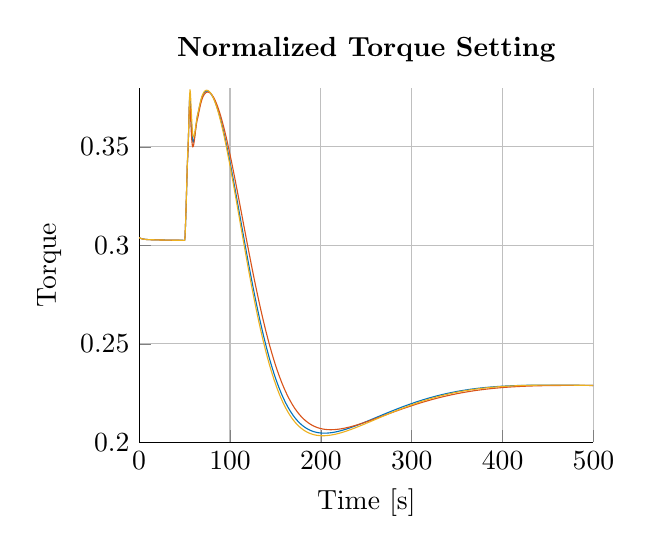
\begin{tikzpicture}

\begin{axis}[%
width=5.77cm,
height=4.5cm,
at={(0cm,0cm)},
scale only axis,
xmin=0,
xmax=500,
xlabel={Time [s]},
xmajorgrids,
ymin=0.2,
ymax=0.38,
ylabel={Torque},
ymajorgrids,
axis background/.style={fill=white},
title style={font=\bfseries},
title={Normalized Torque Setting},
axis x line*=bottom,
axis y line*=left
]
\addplot [color=mycolor1,solid,forget plot]
  table[row sep=crcr]{%
0	0.3039573152\\
0.5	0.303775988\\
1	0.303680777\\
1.5	0.303591625\\
2	0.303511058\\
2.5	0.303437863\\
3	0.303371714\\
3.5	0.303312209\\
4	0.303258903\\
4.5	0.30321133\\
5	0.303169016\\
5.5	0.303131484\\
6	0.30309827\\
6.5	0.303068925\\
7	0.303043022\\
7.5	0.30302016\\
8	0.30299996\\
8.5	0.30298209\\
9	0.30296622\\
9.5	0.30295207\\
10	0.30293939\\
10.5	0.30292794\\
11	0.30291752\\
11.5	0.30290797\\
12	0.30289911\\
12.5	0.30289083\\
13	0.302883\\
13.5	0.30287554\\
14	0.30286837\\
14.5	0.30286141\\
15	0.30285462\\
15.5	0.30284795\\
16	0.30284137\\
16.5	0.30283486\\
17	0.3028284\\
17.5	0.30282197\\
18	0.30281558\\
18.5	0.30280921\\
19	0.30280286\\
19.5	0.30279654\\
20	0.30279025\\
20.5	0.302784\\
21	0.30277779\\
21.5	0.30277162\\
22	0.30276551\\
22.5	0.30275946\\
23	0.30275348\\
23.5	0.30274757\\
24	0.30274173\\
24.5	0.30273598\\
25	0.30273032\\
25.5	0.30272476\\
26	0.30271928\\
26.5	0.30271391\\
27	0.30270864\\
27.5	0.30270347\\
28	0.30269841\\
28.5	0.30269345\\
29	0.3026886\\
29.5	0.30268385\\
30	0.30267921\\
30.5	0.30267467\\
31	0.30267023\\
31.5	0.3026659\\
32	0.30266167\\
32.5	0.30265754\\
33	0.30265351\\
33.5	0.30264957\\
34	0.30264573\\
34.5	0.30264198\\
35	0.30263832\\
35.5	0.30263475\\
36	0.30263126\\
36.5	0.30262786\\
37	0.30262454\\
37.5	0.3026213\\
38	0.30261814\\
38.5	0.30261505\\
39	0.30261204\\
39.5	0.3026091\\
40	0.30260623\\
40.5	0.30260343\\
41	0.30260069\\
41.5	0.30259802\\
42	0.30259541\\
42.5	0.30259287\\
43	0.30259038\\
43.5	0.30258795\\
44	0.30258558\\
44.5	0.30258327\\
45	0.30258101\\
45.5	0.3025788\\
46	0.30257665\\
46.5	0.30257454\\
47	0.30257249\\
47.5	0.30257048\\
48	0.30256852\\
48.5	0.3025666\\
49	0.30256473\\
49.5	0.30256291\\
50	0.30256112\\
50.5	0.304394478\\
51	0.31005118\\
51.5	0.3167577\\
52	0.3244155\\
52.5	0.332599\\
53	0.3409423\\
53.5	0.3457664\\
54	0.3514671\\
54.5	0.3592328\\
55	0.3680617\\
55.5	0.3746969\\
56	0.3750856\\
56.5	0.371095\\
57	0.3662848\\
57.5	0.3615689\\
58	0.3575059\\
58.5	0.3545839\\
59	0.3529578\\
59.5	0.3524559\\
60	0.3528279\\
60.5	0.3538361\\
61	0.3552738\\
61.5	0.356968\\
62	0.358779\\
62.5	0.360597\\
63	0.3623409\\
63.5	0.3639582\\
64	0.3654233\\
64.5	0.3665418\\
65	0.3674821\\
65.5	0.3685874\\
66	0.3696727\\
66.5	0.3707071\\
67	0.3717085\\
67.5	0.3726746\\
68	0.3735685\\
68.5	0.374377\\
69	0.3750961\\
69.5	0.3757275\\
70	0.3762754\\
70.5	0.3767459\\
71	0.3771453\\
71.5	0.3774796\\
72	0.3777542\\
72.5	0.3779738\\
73	0.3781422\\
73.5	0.3782629\\
74	0.3783385\\
74.5	0.3783715\\
75	0.3783635\\
75.5	0.3783164\\
76	0.3782313\\
76.5	0.3781093\\
77	0.3779515\\
77.5	0.3777586\\
78	0.3775314\\
78.5	0.3772706\\
79	0.3769767\\
79.5	0.3766505\\
80	0.3762924\\
80.5	0.3759031\\
81	0.375483\\
81.5	0.3750327\\
82	0.3745528\\
82.5	0.3740438\\
83	0.3735062\\
83.5	0.3729406\\
84	0.3723476\\
84.5	0.3717277\\
85	0.3710814\\
85.5	0.3704093\\
86	0.3697121\\
86.5	0.3689901\\
87	0.3682441\\
87.5	0.3674746\\
88	0.366682\\
88.5	0.3658671\\
89	0.3650303\\
89.5	0.3641722\\
90	0.3632934\\
90.5	0.3623945\\
91	0.3614759\\
91.5	0.3605382\\
92	0.3595821\\
92.5	0.358608\\
93	0.3576164\\
93.5	0.356608\\
94	0.3555833\\
94.5	0.3545428\\
95	0.3534869\\
95.5	0.3524164\\
96	0.3513316\\
96.5	0.3502332\\
97	0.3491215\\
97.5	0.3479972\\
98	0.3468608\\
98.5	0.3457127\\
99	0.3445534\\
99.5	0.3433835\\
100	0.3422035\\
100.5	0.3410137\\
101	0.3398148\\
101.5	0.3386072\\
102	0.3373913\\
102.5	0.3361676\\
103	0.3349366\\
103.5	0.3336988\\
104	0.3324546\\
104.5	0.3312044\\
105	0.3299487\\
105.5	0.3286879\\
106	0.3274225\\
106.5	0.3261529\\
107	0.3248794\\
107.5	0.3236026\\
108	0.3223228\\
108.5	0.3210404\\
109	0.3197558\\
109.5	0.3184695\\
110	0.3171818\\
110.5	0.315893\\
111	0.3146036\\
111.5	0.31331389\\
112	0.31202429\\
112.5	0.31073512\\
113	0.30944674\\
113.5	0.30815949\\
114	0.30687372\\
114.5	0.30558974\\
115	0.304307896\\
115.5	0.303028495\\
116	0.30175185\\
116.5	0.30047828\\
117	0.29920807\\
117.5	0.29794152\\
118	0.29667892\\
118.5	0.29542055\\
119	0.29416668\\
119.5	0.2929176\\
120	0.2916735\\
120.5	0.2904348\\
121	0.2892016\\
121.5	0.2879742\\
122	0.2867528\\
122.5	0.2855377\\
123	0.284329\\
123.5	0.2831271\\
124	0.2819321\\
124.5	0.2807442\\
125	0.2795636\\
125.5	0.2783906\\
126	0.2772252\\
126.5	0.2760678\\
127	0.2749184\\
127.5	0.2737773\\
128	0.2726445\\
128.5	0.2715204\\
129	0.2704049\\
129.5	0.2692983\\
130	0.2682008\\
130.5	0.2671123\\
131	0.2660331\\
131.5	0.2649633\\
132	0.2639031\\
132.5	0.2628524\\
133	0.2618115\\
133.5	0.2607804\\
134	0.2597593\\
134.5	0.2587481\\
135	0.2577471\\
135.5	0.2567562\\
136	0.2557756\\
136.5	0.2548054\\
137	0.2538455\\
137.5	0.2528961\\
138	0.2519572\\
138.5	0.2510288\\
139	0.2501111\\
139.5	0.249204\\
140	0.2483075\\
140.5	0.2474218\\
141	0.2465469\\
141.5	0.2456826\\
142	0.2448292\\
142.5	0.2439866\\
143	0.2431547\\
143.5	0.2423337\\
144	0.2415235\\
144.5	0.2407241\\
145	0.2399355\\
145.5	0.2391576\\
146	0.2383906\\
146.5	0.2376343\\
147	0.2368888\\
147.5	0.236154\\
148	0.2354298\\
148.5	0.2347164\\
149	0.2340135\\
149.5	0.2333212\\
150	0.2326395\\
150.5	0.2319683\\
151	0.2313076\\
151.5	0.2306572\\
152	0.2300172\\
152.5	0.2293876\\
153	0.2287682\\
153.5	0.2281589\\
154	0.2275598\\
154.5	0.2269708\\
155	0.2263918\\
155.5	0.2258227\\
156	0.2252635\\
156.5	0.2247141\\
157	0.2241744\\
157.5	0.2236444\\
158	0.2231239\\
158.5	0.222613\\
159	0.2221114\\
159.5	0.2216193\\
160	0.2211363\\
160.5	0.2206626\\
161	0.2201979\\
161.5	0.2197423\\
162	0.2192955\\
162.5	0.2188577\\
163	0.2184285\\
163.5	0.218008\\
164	0.2175961\\
164.5	0.2171927\\
165	0.2167977\\
165.5	0.2164109\\
166	0.2160324\\
166.5	0.215662\\
167	0.2152996\\
167.5	0.2149451\\
168	0.2145985\\
168.5	0.2142597\\
169	0.2139284\\
169.5	0.2136048\\
170	0.2132886\\
170.5	0.2129798\\
171	0.2126782\\
171.5	0.2123839\\
172	0.2120966\\
172.5	0.2118163\\
173	0.211543\\
173.5	0.2112764\\
174	0.2110166\\
174.5	0.2107634\\
175	0.2105168\\
175.5	0.2102766\\
176	0.2100427\\
176.5	0.2098152\\
177	0.2095938\\
177.5	0.2093784\\
178	0.2091691\\
178.5	0.2089657\\
179	0.2087682\\
179.5	0.2085763\\
180	0.2083902\\
180.5	0.2082095\\
181	0.2080344\\
181.5	0.2078647\\
182	0.2077003\\
182.5	0.2075411\\
183	0.207387\\
183.5	0.2072381\\
184	0.2070941\\
184.5	0.206955\\
185	0.2068208\\
185.5	0.2066913\\
186	0.2065664\\
186.5	0.2064462\\
187	0.2063305\\
187.5	0.2062193\\
188	0.2061124\\
188.5	0.2060098\\
189	0.2059114\\
189.5	0.2058172\\
190	0.2057271\\
190.5	0.205641\\
191	0.2055589\\
191.5	0.2054806\\
192	0.2054062\\
192.5	0.2053354\\
193	0.2052684\\
193.5	0.205205\\
194	0.2051451\\
194.5	0.2050888\\
195	0.2050358\\
195.5	0.2049863\\
196	0.20494\\
196.5	0.204897\\
197	0.2048571\\
197.5	0.2048204\\
198	0.2047868\\
198.5	0.2047562\\
199	0.2047285\\
199.5	0.2047038\\
200	0.2046819\\
200.5	0.2046628\\
201	0.2046464\\
201.5	0.2046328\\
202	0.2046218\\
202.5	0.2046134\\
203	0.2046075\\
203.5	0.2046042\\
204	0.2046033\\
204.5	0.2046048\\
205	0.2046086\\
205.5	0.2046148\\
206	0.2046232\\
206.5	0.2046339\\
207	0.2046467\\
207.5	0.2046617\\
208	0.2046788\\
208.5	0.2046979\\
209	0.204719\\
209.5	0.2047422\\
210	0.2047672\\
210.5	0.2047942\\
211	0.204823\\
211.5	0.2048536\\
212	0.204886\\
212.5	0.2049201\\
213	0.204956\\
213.5	0.2049935\\
214	0.2050327\\
214.5	0.2050735\\
215	0.2051159\\
215.5	0.2051598\\
216	0.2052052\\
216.5	0.2052521\\
217	0.2053004\\
217.5	0.2053502\\
218	0.2054013\\
218.5	0.2054538\\
219	0.2055076\\
219.5	0.2055627\\
220	0.2056191\\
220.5	0.2056767\\
221	0.2057356\\
221.5	0.2057956\\
222	0.2058568\\
222.5	0.2059191\\
223	0.2059825\\
223.5	0.206047\\
224	0.2061126\\
224.5	0.2061792\\
225	0.2062468\\
225.5	0.2063154\\
226	0.2063849\\
226.5	0.2064554\\
227	0.2065268\\
227.5	0.2065991\\
228	0.2066723\\
228.5	0.2067463\\
229	0.2068212\\
229.5	0.2068969\\
230	0.2069734\\
230.5	0.2070506\\
231	0.2071286\\
231.5	0.2072073\\
232	0.2072867\\
232.5	0.2073669\\
233	0.2074477\\
233.5	0.2075291\\
234	0.2076112\\
234.5	0.2076939\\
235	0.2077773\\
235.5	0.2078612\\
236	0.2079456\\
236.5	0.2080307\\
237	0.2081163\\
237.5	0.2082024\\
238	0.208289\\
238.5	0.2083761\\
239	0.2084636\\
239.5	0.2085517\\
240	0.2086401\\
240.5	0.2087291\\
241	0.2088184\\
241.5	0.2089081\\
242	0.2089982\\
242.5	0.2090888\\
243	0.2091796\\
243.5	0.2092708\\
244	0.2093624\\
244.5	0.2094543\\
245	0.2095465\\
245.5	0.209639\\
246	0.2097317\\
246.5	0.2098248\\
247	0.2099181\\
247.5	0.2100117\\
248	0.2101055\\
248.5	0.2101995\\
249	0.2102938\\
249.5	0.2103883\\
250	0.2104829\\
};
\addplot [color=mycolor1,solid,forget plot]
  table[row sep=crcr]{%
250	0.2104829\\
250.5	0.2105778\\
251	0.2106728\\
251.5	0.210768\\
252	0.2108634\\
252.5	0.2109589\\
253	0.2110545\\
253.5	0.2111503\\
254	0.2112462\\
254.5	0.2113422\\
255	0.2114383\\
255.5	0.2115344\\
256	0.2116307\\
256.5	0.211727\\
257	0.2118234\\
257.5	0.2119199\\
258	0.2120164\\
258.5	0.2121129\\
259	0.2122095\\
259.5	0.2123061\\
260	0.2124027\\
260.5	0.2124993\\
261	0.212596\\
261.5	0.2126926\\
262	0.2127892\\
262.5	0.2128857\\
263	0.2129823\\
263.5	0.2130788\\
264	0.2131752\\
264.5	0.2132716\\
265	0.213368\\
265.5	0.2134643\\
266	0.2135605\\
266.5	0.2136566\\
267	0.2137527\\
267.5	0.2138487\\
268	0.2139445\\
268.5	0.2140403\\
269	0.2141359\\
269.5	0.2142315\\
270	0.2143269\\
270.5	0.2144222\\
271	0.2145174\\
271.5	0.2146124\\
272	0.2147073\\
272.5	0.214802\\
273	0.2148966\\
273.5	0.2149911\\
274	0.2150853\\
274.5	0.2151794\\
275	0.2152734\\
275.5	0.2153671\\
276	0.2154607\\
276.5	0.215554\\
277	0.2156472\\
277.5	0.2157402\\
278	0.215833\\
278.5	0.2159256\\
279	0.2160179\\
279.5	0.2161101\\
280	0.216202\\
280.5	0.2162937\\
281	0.2163852\\
281.5	0.2164765\\
282	0.2165675\\
282.5	0.2166583\\
283	0.2167488\\
283.5	0.2168391\\
284	0.2169291\\
284.5	0.2170189\\
285	0.2171084\\
285.5	0.2171977\\
286	0.2172867\\
286.5	0.2173754\\
287	0.2174639\\
287.5	0.2175521\\
288	0.21764\\
288.5	0.2177276\\
289	0.2178149\\
289.5	0.217902\\
290	0.2179887\\
290.5	0.2180752\\
291	0.2181614\\
291.5	0.2182472\\
292	0.2183328\\
292.5	0.2184181\\
293	0.218503\\
293.5	0.2185877\\
294	0.218672\\
294.5	0.218756\\
295	0.2188397\\
295.5	0.2189231\\
296	0.2190061\\
296.5	0.2190889\\
297	0.2191713\\
297.5	0.2192534\\
298	0.2193351\\
298.5	0.2194165\\
299	0.2194976\\
299.5	0.2195783\\
300	0.2196587\\
300.5	0.2197387\\
301	0.2198184\\
301.5	0.2198978\\
302	0.2199768\\
302.5	0.2200555\\
303	0.2201338\\
303.5	0.2202117\\
304	0.2202893\\
304.5	0.2203666\\
305	0.2204435\\
305.5	0.22052\\
306	0.2205962\\
306.5	0.220672\\
307	0.2207474\\
307.5	0.2208225\\
308	0.2208972\\
308.5	0.2209715\\
309	0.2210455\\
309.5	0.2211191\\
310	0.2211923\\
310.5	0.2212652\\
311	0.2213377\\
311.5	0.2214098\\
312	0.2214815\\
312.5	0.2215529\\
313	0.2216238\\
313.5	0.2216944\\
314	0.2217647\\
314.5	0.2218345\\
315	0.221904\\
315.5	0.221973\\
316	0.2220417\\
316.5	0.22211\\
317	0.222178\\
317.5	0.2222455\\
318	0.2223127\\
318.5	0.2223794\\
319	0.2224458\\
319.5	0.2225118\\
320	0.2225774\\
320.5	0.2226426\\
321	0.2227075\\
321.5	0.2227719\\
322	0.222836\\
322.5	0.2228996\\
323	0.2229629\\
323.5	0.2230258\\
324	0.2230883\\
324.5	0.2231504\\
325	0.2232121\\
325.5	0.2232735\\
326	0.2233344\\
326.5	0.2233949\\
327	0.2234551\\
327.5	0.2235149\\
328	0.2235742\\
328.5	0.2236332\\
329	0.2236918\\
329.5	0.22375\\
330	0.2238078\\
330.5	0.2238653\\
331	0.2239223\\
331.5	0.2239789\\
332	0.2240352\\
332.5	0.2240911\\
333	0.2241465\\
333.5	0.2242016\\
334	0.2242563\\
334.5	0.2243106\\
335	0.2243646\\
335.5	0.2244181\\
336	0.2244713\\
336.5	0.224524\\
337	0.2245764\\
337.5	0.2246284\\
338	0.22468\\
338.5	0.2247313\\
339	0.2247821\\
339.5	0.2248326\\
340	0.2248827\\
340.5	0.2249324\\
341	0.2249817\\
341.5	0.2250306\\
342	0.2250792\\
342.5	0.2251274\\
343	0.2251752\\
343.5	0.2252226\\
344	0.2252697\\
344.5	0.2253164\\
345	0.2253627\\
345.5	0.2254086\\
346	0.2254542\\
346.5	0.2254993\\
347	0.2255442\\
347.5	0.2255886\\
348	0.2256327\\
348.5	0.2256764\\
349	0.2257198\\
349.5	0.2257627\\
350	0.2258053\\
350.5	0.2258476\\
351	0.2258895\\
351.5	0.225931\\
352	0.2259722\\
352.5	0.226013\\
353	0.2260534\\
353.5	0.2260935\\
354	0.2261333\\
354.5	0.2261727\\
355	0.2262117\\
355.5	0.2262504\\
356	0.2262887\\
356.5	0.2263267\\
357	0.2263643\\
357.5	0.2264016\\
358	0.2264385\\
358.5	0.2264751\\
359	0.2265114\\
359.5	0.2265473\\
360	0.2265828\\
360.5	0.2266181\\
361	0.2266529\\
361.5	0.2266875\\
362	0.2267217\\
362.5	0.2267556\\
363	0.2267892\\
363.5	0.2268224\\
364	0.2268553\\
364.5	0.2268878\\
365	0.2269201\\
365.5	0.226952\\
366	0.2269836\\
366.5	0.2270148\\
367	0.2270458\\
367.5	0.2270764\\
368	0.2271067\\
368.5	0.2271367\\
369	0.2271664\\
369.5	0.2271958\\
370	0.2272248\\
370.5	0.2272536\\
371	0.227282\\
371.5	0.2273101\\
372	0.2273379\\
372.5	0.2273655\\
373	0.2273927\\
373.5	0.2274196\\
374	0.2274462\\
374.5	0.2274726\\
375	0.2274986\\
375.5	0.2275243\\
376	0.2275498\\
376.5	0.2275749\\
377	0.2275998\\
377.5	0.2276244\\
378	0.2276486\\
378.5	0.2276726\\
379	0.2276964\\
379.5	0.2277198\\
380	0.227743\\
380.5	0.2277659\\
381	0.2277885\\
381.5	0.2278108\\
382	0.2278329\\
382.5	0.2278547\\
383	0.2278762\\
383.5	0.2278975\\
384	0.2279185\\
384.5	0.2279392\\
385	0.2279597\\
385.5	0.2279799\\
386	0.2279998\\
386.5	0.2280195\\
387	0.2280389\\
387.5	0.2280581\\
388	0.2280771\\
388.5	0.2280957\\
389	0.2281142\\
389.5	0.2281324\\
390	0.2281503\\
390.5	0.228168\\
391	0.2281855\\
391.5	0.2282027\\
392	0.2282197\\
392.5	0.2282364\\
393	0.2282529\\
393.5	0.2282692\\
394	0.2282852\\
394.5	0.2283011\\
395	0.2283166\\
395.5	0.228332\\
396	0.2283471\\
396.5	0.2283621\\
397	0.2283768\\
397.5	0.2283912\\
398	0.2284055\\
398.5	0.2284195\\
399	0.2284334\\
399.5	0.228447\\
400	0.2284604\\
400.5	0.2284736\\
401	0.2284866\\
401.5	0.2284994\\
402	0.228512\\
402.5	0.2285243\\
403	0.2285365\\
403.5	0.2285485\\
404	0.2285603\\
404.5	0.2285719\\
405	0.2285833\\
405.5	0.2285945\\
406	0.2286055\\
406.5	0.2286163\\
407	0.228627\\
407.5	0.2286374\\
408	0.2286477\\
408.5	0.2286578\\
409	0.2286677\\
409.5	0.2286774\\
410	0.228687\\
410.5	0.2286963\\
411	0.2287055\\
411.5	0.2287146\\
412	0.2287234\\
412.5	0.2287321\\
413	0.2287407\\
413.5	0.228749\\
414	0.2287572\\
414.5	0.2287652\\
415	0.2287731\\
415.5	0.2287808\\
416	0.2287884\\
416.5	0.2287958\\
417	0.228803\\
417.5	0.2288101\\
418	0.228817\\
418.5	0.2288238\\
419	0.2288305\\
419.5	0.228837\\
420	0.2288433\\
420.5	0.2288495\\
421	0.2288556\\
421.5	0.2288615\\
422	0.2288673\\
422.5	0.2288729\\
423	0.2288784\\
423.5	0.2288838\\
424	0.228889\\
424.5	0.2288941\\
425	0.2288991\\
425.5	0.228904\\
426	0.2289087\\
426.5	0.2289133\\
427	0.2289177\\
427.5	0.2289221\\
428	0.2289263\\
428.5	0.2289304\\
429	0.2289344\\
429.5	0.2289382\\
430	0.228942\\
430.5	0.2289456\\
431	0.2289491\\
431.5	0.2289525\\
432	0.2289558\\
432.5	0.228959\\
433	0.2289621\\
433.5	0.2289651\\
434	0.2289679\\
434.5	0.2289707\\
435	0.2289733\\
435.5	0.2289759\\
436	0.2289783\\
436.5	0.2289807\\
437	0.228983\\
437.5	0.2289851\\
438	0.2289872\\
438.5	0.2289892\\
439	0.228991\\
439.5	0.2289928\\
440	0.2289945\\
440.5	0.2289961\\
441	0.2289976\\
441.5	0.2289991\\
442	0.2290004\\
442.5	0.2290017\\
443	0.2290029\\
443.5	0.2290039\\
444	0.229005\\
444.5	0.2290059\\
445	0.2290068\\
445.5	0.2290075\\
446	0.2290082\\
446.5	0.2290089\\
447	0.2290094\\
447.5	0.2290099\\
448	0.2290103\\
448.5	0.2290106\\
449	0.2290109\\
449.5	0.2290111\\
450	0.2290112\\
450.5	0.2290113\\
451	0.2290113\\
451.5	0.2290112\\
452	0.2290111\\
452.5	0.2290109\\
453	0.2290106\\
453.5	0.2290103\\
454	0.22901\\
454.5	0.2290095\\
455	0.229009\\
455.5	0.2290085\\
456	0.2290079\\
456.5	0.2290072\\
457	0.2290065\\
457.5	0.2290057\\
458	0.2290049\\
458.5	0.2290041\\
459	0.2290031\\
459.5	0.2290022\\
460	0.2290012\\
460.5	0.2290001\\
461	0.228999\\
461.5	0.2289978\\
462	0.2289966\\
462.5	0.2289954\\
463	0.2289941\\
463.5	0.2289928\\
464	0.2289914\\
464.5	0.22899\\
465	0.2289885\\
465.5	0.2289871\\
466	0.2289855\\
466.5	0.228984\\
467	0.2289824\\
467.5	0.2289807\\
468	0.228979\\
468.5	0.2289773\\
469	0.2289756\\
469.5	0.2289738\\
470	0.228972\\
470.5	0.2289702\\
471	0.2289683\\
471.5	0.2289664\\
472	0.2289645\\
472.5	0.2289625\\
473	0.2289605\\
473.5	0.2289585\\
474	0.2289565\\
474.5	0.2289544\\
475	0.2289523\\
475.5	0.2289502\\
476	0.2289481\\
476.5	0.2289459\\
477	0.2289437\\
477.5	0.2289415\\
478	0.2289393\\
478.5	0.2289371\\
479	0.2289348\\
479.5	0.2289325\\
480	0.2289302\\
480.5	0.2289279\\
481	0.2289255\\
481.5	0.2289232\\
482	0.2289208\\
482.5	0.2289184\\
483	0.228916\\
483.5	0.2289136\\
484	0.2289111\\
484.5	0.2289087\\
485	0.2289062\\
485.5	0.2289038\\
486	0.2289013\\
486.5	0.2288988\\
487	0.2288962\\
487.5	0.2288937\\
488	0.2288912\\
488.5	0.2288886\\
489	0.2288861\\
489.5	0.2288835\\
490	0.228881\\
490.5	0.2288784\\
491	0.2288758\\
491.5	0.2288732\\
492	0.2288706\\
492.5	0.228868\\
493	0.2288654\\
493.5	0.2288628\\
494	0.2288601\\
494.5	0.2288575\\
495	0.2288549\\
495.5	0.2288522\\
496	0.2288496\\
496.5	0.2288469\\
497	0.2288443\\
497.5	0.2288416\\
498	0.228839\\
498.5	0.2288363\\
499	0.2288337\\
499.5	0.228831\\
};
\addplot [color=mycolor2,solid,forget plot]
  table[row sep=crcr]{%
0	0.3039552245\\
0.5	0.303765592\\
1	0.303666922\\
1.5	0.303574787\\
2	0.30349186\\
2.5	0.30341683\\
3	0.303349327\\
3.5	0.303288902\\
4	0.303235058\\
4.5	0.303187277\\
5	0.303145034\\
5.5	0.303107805\\
6	0.303075079\\
6.5	0.303046365\\
7	0.303021198\\
7.5	0.30299914\\
8	0.30297979\\
8.5	0.30296278\\
9	0.30294777\\
9.5	0.30293446\\
10	0.30292257\\
10.5	0.30291187\\
11	0.30290214\\
11.5	0.30289321\\
12	0.30288491\\
12.5	0.30287712\\
13	0.30286972\\
13.5	0.30286262\\
14	0.30285574\\
14.5	0.30284902\\
15	0.30284241\\
15.5	0.30283587\\
16	0.30282937\\
16.5	0.3028229\\
17	0.30281644\\
17.5	0.30280998\\
18	0.30280353\\
18.5	0.30279707\\
19	0.30279063\\
19.5	0.30278419\\
20	0.30277777\\
20.5	0.30277137\\
21	0.30276501\\
21.5	0.30275869\\
22	0.30275243\\
22.5	0.30274622\\
23	0.30274008\\
23.5	0.30273401\\
24	0.30272803\\
24.5	0.30272213\\
25	0.30271633\\
25.5	0.30271062\\
26	0.30270501\\
26.5	0.30269951\\
27	0.30269412\\
27.5	0.30268883\\
28	0.30268365\\
28.5	0.30267859\\
29	0.30267363\\
29.5	0.30266878\\
30	0.30266404\\
30.5	0.30265942\\
31	0.30265489\\
31.5	0.30265048\\
32	0.30264617\\
32.5	0.30264196\\
33	0.30263785\\
33.5	0.30263384\\
34	0.30262992\\
34.5	0.3026261\\
35	0.30262237\\
35.5	0.30261874\\
36	0.30261518\\
36.5	0.30261172\\
37	0.30260833\\
37.5	0.30260503\\
38	0.30260181\\
38.5	0.30259866\\
39	0.30259559\\
39.5	0.30259259\\
40	0.30258966\\
40.5	0.3025868\\
41	0.30258401\\
41.5	0.30258128\\
42	0.30257862\\
42.5	0.30257601\\
43	0.30257347\\
43.5	0.30257099\\
44	0.30256857\\
44.5	0.3025662\\
45	0.30256389\\
45.5	0.30256163\\
46	0.30255943\\
46.5	0.30255727\\
47	0.30255516\\
47.5	0.30255311\\
48	0.3025511\\
48.5	0.30254913\\
49	0.30254722\\
49.5	0.30254534\\
50	0.30254351\\
50.5	0.304471449\\
51	0.31042517\\
51.5	0.3174263\\
52	0.325291\\
52.5	0.3334964\\
53	0.3408456\\
53.5	0.3451152\\
54	0.3508922\\
54.5	0.3592195\\
55	0.3683954\\
55.5	0.3736534\\
56	0.3715522\\
56.5	0.3663626\\
57	0.3610624\\
57.5	0.356449\\
58	0.3529859\\
58.5	0.3509046\\
59	0.3500809\\
59.5	0.3502514\\
60	0.3511626\\
60.5	0.3525872\\
61	0.3543252\\
61.5	0.3562077\\
62	0.3580983\\
62.5	0.3598939\\
63	0.3615241\\
63.5	0.3629525\\
64	0.3640551\\
64.5	0.3647738\\
65	0.3659146\\
65.5	0.3671063\\
66	0.3682674\\
66.5	0.3693898\\
67	0.3704737\\
67.5	0.3714837\\
68	0.3724073\\
68.5	0.3732412\\
69	0.3739872\\
69.5	0.3746488\\
70	0.3752313\\
70.5	0.375741\\
71	0.3761835\\
71.5	0.3765645\\
72	0.3768889\\
72.5	0.3771609\\
73	0.3773843\\
73.5	0.3775621\\
74	0.3776969\\
74.5	0.3777909\\
75	0.3778458\\
75.5	0.3778632\\
76	0.3778442\\
76.5	0.37779\\
77	0.3777015\\
77.5	0.3775793\\
78	0.3774244\\
78.5	0.3772372\\
79	0.3770184\\
79.5	0.3767686\\
80	0.3764883\\
80.5	0.376178\\
81	0.3758383\\
81.5	0.3754696\\
82	0.3750724\\
82.5	0.3746474\\
83	0.3741949\\
83.5	0.3737155\\
84	0.3732096\\
84.5	0.3726779\\
85	0.3721207\\
85.5	0.3715386\\
86	0.3709322\\
86.5	0.3703018\\
87	0.3696481\\
87.5	0.3689715\\
88	0.3682725\\
88.5	0.3675517\\
89	0.3668096\\
89.5	0.3660466\\
90	0.3652632\\
90.5	0.36446\\
91	0.3636375\\
91.5	0.3627962\\
92	0.3619365\\
92.5	0.361059\\
93	0.3601641\\
93.5	0.3592523\\
94	0.3583242\\
94.5	0.3573802\\
95	0.3564208\\
95.5	0.3554464\\
96	0.3544576\\
96.5	0.3534548\\
97	0.3524385\\
97.5	0.3514092\\
98	0.3503673\\
98.5	0.3493133\\
99	0.3482476\\
99.5	0.3471707\\
100	0.346083\\
100.5	0.344985\\
101	0.3438772\\
101.5	0.3427599\\
102	0.3416336\\
102.5	0.3404987\\
103	0.3393557\\
103.5	0.3382049\\
104	0.3370469\\
104.5	0.3358819\\
105	0.3347104\\
105.5	0.3335328\\
106	0.3323496\\
106.5	0.331161\\
107	0.3299675\\
107.5	0.3287695\\
108	0.3275673\\
108.5	0.3263614\\
109	0.325152\\
109.5	0.3239397\\
110	0.3227246\\
110.5	0.3215072\\
111	0.3202879\\
111.5	0.3190669\\
112	0.3178446\\
112.5	0.3166214\\
113	0.3153975\\
113.5	0.3141734\\
114	0.31294924\\
114.5	0.31172545\\
115	0.31050231\\
115.5	0.30928011\\
116	0.30805916\\
116.5	0.30683976\\
117	0.30562219\\
117.5	0.304406727\\
118	0.30319366\\
118.5	0.30198326\\
119	0.30077579\\
119.5	0.29957151\\
120	0.29837068\\
120.5	0.29717356\\
121	0.29598038\\
121.5	0.29479139\\
122	0.2936068\\
122.5	0.2924269\\
123	0.2912519\\
123.5	0.2900819\\
124	0.2889173\\
124.5	0.2877582\\
125	0.2866048\\
125.5	0.2854573\\
126	0.284316\\
126.5	0.2831809\\
127	0.2820524\\
127.5	0.2809304\\
128	0.2798154\\
128.5	0.2787073\\
129	0.2776064\\
129.5	0.2765128\\
130	0.2754266\\
130.5	0.2743481\\
131	0.2732773\\
131.5	0.2722144\\
132	0.2711596\\
132.5	0.2701129\\
133	0.2690744\\
133.5	0.2680443\\
134	0.2670228\\
134.5	0.2660098\\
135	0.2650055\\
135.5	0.2640101\\
136	0.2630235\\
136.5	0.2620459\\
137	0.2610774\\
137.5	0.260118\\
138	0.2591678\\
138.5	0.258227\\
139	0.2572954\\
139.5	0.2563733\\
140	0.2554607\\
140.5	0.2545575\\
141	0.253664\\
141.5	0.25278\\
142	0.2519057\\
142.5	0.2510411\\
143	0.2501863\\
143.5	0.2493411\\
144	0.2485058\\
144.5	0.2476802\\
145	0.2468645\\
145.5	0.2460586\\
146	0.2452625\\
146.5	0.2444762\\
147	0.2436998\\
147.5	0.2429333\\
148	0.2421766\\
148.5	0.2414297\\
149	0.2406926\\
149.5	0.2399654\\
150	0.239248\\
150.5	0.2385403\\
151	0.2378424\\
151.5	0.2371542\\
152	0.2364757\\
152.5	0.2358069\\
153	0.2351477\\
153.5	0.2344981\\
154	0.2338581\\
154.5	0.2332276\\
155	0.2326066\\
155.5	0.2319951\\
156	0.2313929\\
156.5	0.2308001\\
157	0.2302165\\
157.5	0.2296422\\
158	0.2290771\\
158.5	0.2285211\\
159	0.2279742\\
159.5	0.2274363\\
160	0.2269074\\
160.5	0.2263873\\
161	0.2258761\\
161.5	0.2253736\\
162	0.2248798\\
162.5	0.2243947\\
163	0.223918\\
163.5	0.2234499\\
164	0.2229902\\
164.5	0.2225388\\
165	0.2220956\\
165.5	0.2216607\\
166	0.2212339\\
166.5	0.2208151\\
167	0.2204042\\
167.5	0.2200013\\
168	0.2196061\\
168.5	0.2192187\\
169	0.2188389\\
169.5	0.2184667\\
170	0.218102\\
170.5	0.2177446\\
171	0.2173946\\
171.5	0.2170519\\
172	0.2167162\\
172.5	0.2163877\\
173	0.2160662\\
173.5	0.2157516\\
174	0.2154438\\
174.5	0.2151427\\
175	0.2148484\\
175.5	0.2145606\\
176	0.2142793\\
176.5	0.2140045\\
177	0.213736\\
177.5	0.2134737\\
178	0.2132177\\
178.5	0.2129677\\
179	0.2127237\\
179.5	0.2124857\\
180	0.2122536\\
180.5	0.2120272\\
181	0.2118065\\
181.5	0.2115914\\
182	0.2113819\\
182.5	0.2111779\\
183	0.2109792\\
183.5	0.2107859\\
184	0.2105978\\
184.5	0.2104148\\
185	0.2102369\\
185.5	0.210064\\
186	0.2098961\\
186.5	0.209733\\
187	0.2095748\\
187.5	0.2094212\\
188	0.2092723\\
188.5	0.2091279\\
189	0.2089881\\
189.5	0.2088527\\
190	0.2087216\\
190.5	0.2085949\\
191	0.2084723\\
191.5	0.208354\\
192	0.2082397\\
192.5	0.2081295\\
193	0.2080232\\
193.5	0.2079208\\
194	0.2078223\\
194.5	0.2077275\\
195	0.2076365\\
195.5	0.2075491\\
196	0.2074653\\
196.5	0.207385\\
197	0.2073082\\
197.5	0.2072349\\
198	0.2071648\\
198.5	0.2070981\\
199	0.2070346\\
199.5	0.2069743\\
200	0.2069172\\
200.5	0.2068631\\
201	0.2068121\\
201.5	0.206764\\
202	0.2067188\\
202.5	0.2066766\\
203	0.2066371\\
203.5	0.2066004\\
204	0.2065664\\
204.5	0.2065352\\
205	0.2065065\\
205.5	0.2064804\\
206	0.2064569\\
206.5	0.2064358\\
207	0.2064172\\
207.5	0.2064009\\
208	0.2063871\\
208.5	0.2063755\\
209	0.2063662\\
209.5	0.2063591\\
210	0.2063543\\
210.5	0.2063515\\
211	0.2063509\\
211.5	0.2063523\\
212	0.2063558\\
212.5	0.2063612\\
213	0.2063686\\
213.5	0.2063779\\
214	0.2063891\\
214.5	0.2064022\\
215	0.206417\\
215.5	0.2064336\\
216	0.206452\\
216.5	0.206472\\
217	0.2064937\\
217.5	0.2065171\\
218	0.206542\\
218.5	0.2065686\\
219	0.2065967\\
219.5	0.2066263\\
220	0.2066573\\
220.5	0.2066898\\
221	0.2067238\\
221.5	0.2067591\\
222	0.2067958\\
222.5	0.2068339\\
223	0.2068732\\
223.5	0.2069139\\
224	0.2069558\\
224.5	0.2069989\\
225	0.2070432\\
225.5	0.2070887\\
226	0.2071354\\
226.5	0.2071832\\
227	0.2072321\\
227.5	0.2072821\\
228	0.2073331\\
228.5	0.2073852\\
229	0.2074383\\
229.5	0.2074924\\
230	0.2075474\\
230.5	0.2076034\\
231	0.2076603\\
231.5	0.2077182\\
232	0.2077769\\
232.5	0.2078365\\
233	0.2078969\\
233.5	0.2079582\\
234	0.2080202\\
234.5	0.2080831\\
235	0.2081467\\
235.5	0.2082111\\
236	0.2082762\\
236.5	0.208342\\
237	0.2084085\\
237.5	0.2084757\\
238	0.2085435\\
238.5	0.2086121\\
239	0.2086812\\
239.5	0.2087509\\
240	0.2088213\\
240.5	0.2088922\\
241	0.2089637\\
241.5	0.2090358\\
242	0.2091084\\
242.5	0.2091815\\
243	0.2092552\\
243.5	0.2093293\\
244	0.2094039\\
244.5	0.209479\\
245	0.2095545\\
245.5	0.2096305\\
246	0.2097069\\
246.5	0.2097837\\
247	0.2098609\\
247.5	0.2099385\\
248	0.2100165\\
248.5	0.2100948\\
249	0.2101735\\
249.5	0.2102526\\
250	0.210332\\
};
\addplot [color=mycolor2,solid,forget plot]
  table[row sep=crcr]{%
250	0.210332\\
250.5	0.2104117\\
251	0.2104917\\
251.5	0.210572\\
252	0.2106526\\
252.5	0.2107334\\
253	0.2108146\\
253.5	0.2108959\\
254	0.2109776\\
254.5	0.2110594\\
255	0.2111415\\
255.5	0.2112238\\
256	0.2113064\\
256.5	0.2113891\\
257	0.211472\\
257.5	0.211555\\
258	0.2116383\\
258.5	0.2117217\\
259	0.2118053\\
259.5	0.211889\\
260	0.2119728\\
260.5	0.2120568\\
261	0.2121408\\
261.5	0.212225\\
262	0.2123093\\
262.5	0.2123937\\
263	0.2124782\\
263.5	0.2125628\\
264	0.2126474\\
264.5	0.2127321\\
265	0.2128168\\
265.5	0.2129016\\
266	0.2129865\\
266.5	0.2130714\\
267	0.2131563\\
267.5	0.2132412\\
268	0.2133262\\
268.5	0.2134111\\
269	0.2134961\\
269.5	0.2135811\\
270	0.213666\\
270.5	0.213751\\
271	0.2138359\\
271.5	0.2139208\\
272	0.2140056\\
272.5	0.2140904\\
273	0.2141752\\
273.5	0.2142599\\
274	0.2143446\\
274.5	0.2144292\\
275	0.2145138\\
275.5	0.2145983\\
276	0.2146826\\
276.5	0.214767\\
277	0.2148512\\
277.5	0.2149353\\
278	0.2150194\\
278.5	0.2151033\\
279	0.2151872\\
279.5	0.2152709\\
280	0.2153545\\
280.5	0.215438\\
281	0.2155214\\
281.5	0.2156046\\
282	0.2156877\\
282.5	0.2157707\\
283	0.2158535\\
283.5	0.2159362\\
284	0.2160187\\
284.5	0.2161011\\
285	0.2161834\\
285.5	0.2162654\\
286	0.2163473\\
286.5	0.2164291\\
287	0.2165106\\
287.5	0.216592\\
288	0.2166732\\
288.5	0.2167543\\
289	0.2168351\\
289.5	0.2169158\\
290	0.2169962\\
290.5	0.2170765\\
291	0.2171566\\
291.5	0.2172364\\
292	0.2173161\\
292.5	0.2173955\\
293	0.2174748\\
293.5	0.2175538\\
294	0.2176326\\
294.5	0.2177112\\
295	0.2177896\\
295.5	0.2178677\\
296	0.2179456\\
296.5	0.2180233\\
297	0.2181008\\
297.5	0.218178\\
298	0.218255\\
298.5	0.2183317\\
299	0.2184082\\
299.5	0.2184845\\
300	0.2185605\\
300.5	0.2186362\\
301	0.2187117\\
301.5	0.218787\\
302	0.218862\\
302.5	0.2189367\\
303	0.2190112\\
303.5	0.2190854\\
304	0.2191593\\
304.5	0.219233\\
305	0.2193064\\
305.5	0.2193795\\
306	0.2194524\\
306.5	0.219525\\
307	0.2195973\\
307.5	0.2196693\\
308	0.2197411\\
308.5	0.2198126\\
309	0.2198838\\
309.5	0.2199547\\
310	0.2200253\\
310.5	0.2200956\\
311	0.2201657\\
311.5	0.2202354\\
312	0.2203049\\
312.5	0.2203741\\
313	0.220443\\
313.5	0.2205115\\
314	0.2205798\\
314.5	0.2206478\\
315	0.2207155\\
315.5	0.2207829\\
316	0.22085\\
316.5	0.2209168\\
317	0.2209833\\
317.5	0.2210494\\
318	0.2211153\\
318.5	0.2211809\\
319	0.2212461\\
319.5	0.2213111\\
320	0.2213757\\
320.5	0.2214401\\
321	0.2215041\\
321.5	0.2215678\\
322	0.2216312\\
322.5	0.2216943\\
323	0.221757\\
323.5	0.2218195\\
324	0.2218816\\
324.5	0.2219435\\
325	0.222005\\
325.5	0.2220661\\
326	0.222127\\
326.5	0.2221876\\
327	0.2222478\\
327.5	0.2223077\\
328	0.2223673\\
328.5	0.2224266\\
329	0.2224856\\
329.5	0.2225442\\
330	0.2226025\\
330.5	0.2226605\\
331	0.2227182\\
331.5	0.2227755\\
332	0.2228326\\
332.5	0.2228893\\
333	0.2229457\\
333.5	0.2230017\\
334	0.2230575\\
334.5	0.2231129\\
335	0.223168\\
335.5	0.2232227\\
336	0.2232772\\
336.5	0.2233313\\
337	0.2233851\\
337.5	0.2234386\\
338	0.2234917\\
338.5	0.2235446\\
339	0.2235971\\
339.5	0.2236493\\
340	0.2237011\\
340.5	0.2237527\\
341	0.2238039\\
341.5	0.2238548\\
342	0.2239054\\
342.5	0.2239556\\
343	0.2240056\\
343.5	0.2240552\\
344	0.2241045\\
344.5	0.2241535\\
345	0.2242021\\
345.5	0.2242504\\
346	0.2242984\\
346.5	0.2243461\\
347	0.2243935\\
347.5	0.2244406\\
348	0.2244873\\
348.5	0.2245337\\
349	0.2245798\\
349.5	0.2246256\\
350	0.2246711\\
350.5	0.2247162\\
351	0.2247611\\
351.5	0.2248056\\
352	0.2248498\\
352.5	0.2248937\\
353	0.2249373\\
353.5	0.2249806\\
354	0.2250235\\
354.5	0.2250662\\
355	0.2251085\\
355.5	0.2251506\\
356	0.2251923\\
356.5	0.2252337\\
357	0.2252748\\
357.5	0.2253156\\
358	0.2253561\\
358.5	0.2253963\\
359	0.2254362\\
359.5	0.2254757\\
360	0.225515\\
360.5	0.225554\\
361	0.2255927\\
361.5	0.225631\\
362	0.2256691\\
362.5	0.2257069\\
363	0.2257444\\
363.5	0.2257816\\
364	0.2258184\\
364.5	0.225855\\
365	0.2258913\\
365.5	0.2259273\\
366	0.225963\\
366.5	0.2259985\\
367	0.2260336\\
367.5	0.2260684\\
368	0.226103\\
368.5	0.2261372\\
369	0.2261712\\
369.5	0.2262049\\
370	0.2262383\\
370.5	0.2262714\\
371	0.2263043\\
371.5	0.2263368\\
372	0.2263691\\
372.5	0.2264011\\
373	0.2264328\\
373.5	0.2264643\\
374	0.2264954\\
374.5	0.2265263\\
375	0.226557\\
375.5	0.2265873\\
376	0.2266174\\
376.5	0.2266472\\
377	0.2266767\\
377.5	0.226706\\
378	0.226735\\
378.5	0.2267637\\
379	0.2267922\\
379.5	0.2268204\\
380	0.2268483\\
380.5	0.226876\\
381	0.2269034\\
381.5	0.2269306\\
382	0.2269575\\
382.5	0.2269841\\
383	0.2270105\\
383.5	0.2270367\\
384	0.2270626\\
384.5	0.2270882\\
385	0.2271136\\
385.5	0.2271387\\
386	0.2271636\\
386.5	0.2271882\\
387	0.2272126\\
387.5	0.2272368\\
388	0.2272607\\
388.5	0.2272844\\
389	0.2273078\\
389.5	0.227331\\
390	0.2273539\\
390.5	0.2273766\\
391	0.2273991\\
391.5	0.2274214\\
392	0.2274434\\
392.5	0.2274652\\
393	0.2274867\\
393.5	0.227508\\
394	0.2275291\\
394.5	0.22755\\
395	0.2275706\\
395.5	0.2275911\\
396	0.2276113\\
396.5	0.2276312\\
397	0.227651\\
397.5	0.2276705\\
398	0.2276898\\
398.5	0.227709\\
399	0.2277278\\
399.5	0.2277465\\
400	0.227765\\
400.5	0.2277832\\
401	0.2278013\\
401.5	0.2278191\\
402	0.2278368\\
402.5	0.2278542\\
403	0.2278714\\
403.5	0.2278884\\
404	0.2279053\\
404.5	0.2279219\\
405	0.2279383\\
405.5	0.2279545\\
406	0.2279706\\
406.5	0.2279864\\
407	0.228002\\
407.5	0.2280175\\
408	0.2280328\\
408.5	0.2280478\\
409	0.2280627\\
409.5	0.2280774\\
410	0.2280919\\
410.5	0.2281062\\
411	0.2281204\\
411.5	0.2281343\\
412	0.2281481\\
412.5	0.2281617\\
413	0.2281752\\
413.5	0.2281884\\
414	0.2282015\\
414.5	0.2282144\\
415	0.2282271\\
415.5	0.2282397\\
416	0.2282521\\
416.5	0.2282643\\
417	0.2282763\\
417.5	0.2282882\\
418	0.2282999\\
418.5	0.2283115\\
419	0.2283229\\
419.5	0.2283341\\
420	0.2283452\\
420.5	0.2283561\\
421	0.2283669\\
421.5	0.2283775\\
422	0.228388\\
422.5	0.2283983\\
423	0.2284084\\
423.5	0.2284184\\
424	0.2284282\\
424.5	0.2284379\\
425	0.2284475\\
425.5	0.2284569\\
426	0.2284662\\
426.5	0.2284753\\
427	0.2284843\\
427.5	0.2284931\\
428	0.2285018\\
428.5	0.2285104\\
429	0.2285188\\
429.5	0.2285271\\
430	0.2285352\\
430.5	0.2285433\\
431	0.2285511\\
431.5	0.2285589\\
432	0.2285665\\
432.5	0.228574\\
433	0.2285814\\
433.5	0.2285886\\
434	0.2285958\\
434.5	0.2286027\\
435	0.2286096\\
435.5	0.2286164\\
436	0.228623\\
436.5	0.2286295\\
437	0.2286359\\
437.5	0.2286422\\
438	0.2286483\\
438.5	0.2286544\\
439	0.2286603\\
439.5	0.2286661\\
440	0.2286718\\
440.5	0.2286774\\
441	0.2286829\\
441.5	0.2286883\\
442	0.2286936\\
442.5	0.2286987\\
443	0.2287038\\
443.5	0.2287088\\
444	0.2287136\\
444.5	0.2287184\\
445	0.228723\\
445.5	0.2287276\\
446	0.228732\\
446.5	0.2287364\\
447	0.2287406\\
447.5	0.2287448\\
448	0.2287489\\
448.5	0.2287529\\
449	0.2287567\\
449.5	0.2287605\\
450	0.2287642\\
450.5	0.2287679\\
451	0.2287714\\
451.5	0.2287748\\
452	0.2287782\\
452.5	0.2287814\\
453	0.2287846\\
453.5	0.2287877\\
454	0.2287907\\
454.5	0.2287937\\
455	0.2287965\\
455.5	0.2287993\\
456	0.228802\\
456.5	0.2288046\\
457	0.2288071\\
457.5	0.2288096\\
458	0.228812\\
458.5	0.2288143\\
459	0.2288165\\
459.5	0.2288187\\
460	0.2288208\\
460.5	0.2288228\\
461	0.2288248\\
461.5	0.2288267\\
462	0.2288285\\
462.5	0.2288303\\
463	0.2288319\\
463.5	0.2288336\\
464	0.2288351\\
464.5	0.2288366\\
465	0.228838\\
465.5	0.2288394\\
466	0.2288407\\
466.5	0.228842\\
467	0.2288432\\
467.5	0.2288443\\
468	0.2288453\\
468.5	0.2288464\\
469	0.2288473\\
469.5	0.2288482\\
470	0.2288491\\
470.5	0.2288499\\
471	0.2288506\\
471.5	0.2288513\\
472	0.2288519\\
472.5	0.2288525\\
473	0.228853\\
473.5	0.2288535\\
474	0.2288539\\
474.5	0.2288543\\
475	0.2288546\\
475.5	0.2288549\\
476	0.2288552\\
476.5	0.2288554\\
477	0.2288555\\
477.5	0.2288556\\
478	0.2288557\\
478.5	0.2288557\\
479	0.2288557\\
479.5	0.2288556\\
480	0.2288555\\
480.5	0.2288554\\
481	0.2288552\\
481.5	0.228855\\
482	0.2288547\\
482.5	0.2288544\\
483	0.2288541\\
483.5	0.2288537\\
484	0.2288533\\
484.5	0.2288529\\
485	0.2288524\\
485.5	0.2288519\\
486	0.2288514\\
486.5	0.2288508\\
487	0.2288502\\
487.5	0.2288495\\
488	0.2288489\\
488.5	0.2288482\\
489	0.2288474\\
489.5	0.2288467\\
490	0.2288459\\
490.5	0.2288451\\
491	0.2288442\\
491.5	0.2288433\\
492	0.2288424\\
492.5	0.2288415\\
493	0.2288406\\
493.5	0.2288396\\
494	0.2288386\\
494.5	0.2288376\\
495	0.2288365\\
495.5	0.2288354\\
496	0.2288343\\
496.5	0.2288332\\
497	0.2288321\\
497.5	0.2288309\\
498	0.2288297\\
498.5	0.2288285\\
499	0.2288273\\
499.5	0.2288261\\
};
\addplot [color=mycolor3,solid,forget plot]
  table[row sep=crcr]{%
0	0.3039595053\\
0.5	0.30377925\\
1	0.303678798\\
1.5	0.303585531\\
2	0.303501536\\
2.5	0.303425625\\
3	0.303357386\\
3.5	0.303296341\\
4	0.303241965\\
4.5	0.303193723\\
5	0.303151069\\
5.5	0.303113468\\
6	0.303080398\\
6.5	0.303051362\\
7	0.303025888\\
7.5	0.303003539\\
8	0.30298391\\
8.5	0.30296662\\
9	0.30295135\\
9.5	0.30293779\\
10	0.30292567\\
10.5	0.30291474\\
11	0.30290482\\
11.5	0.3028957\\
12	0.30288724\\
12.5	0.30287931\\
13	0.30287179\\
13.5	0.30286459\\
14	0.30285763\\
14.5	0.30285086\\
15	0.30284422\\
15.5	0.30283767\\
16	0.30283119\\
16.5	0.30282475\\
17	0.30281835\\
17.5	0.30281196\\
18	0.3028056\\
18.5	0.30279925\\
19	0.30279293\\
19.5	0.30278662\\
20	0.30278035\\
20.5	0.30277411\\
21	0.30276791\\
21.5	0.30276177\\
22	0.30275568\\
22.5	0.30274966\\
23	0.30274371\\
23.5	0.30273783\\
24	0.30273204\\
24.5	0.30272634\\
25	0.30272074\\
25.5	0.30271523\\
26	0.30270982\\
26.5	0.30270451\\
27	0.30269931\\
27.5	0.30269422\\
28	0.30268924\\
28.5	0.30268436\\
29	0.30267959\\
29.5	0.30267493\\
30	0.30267038\\
30.5	0.30266593\\
31	0.30266158\\
31.5	0.30265735\\
32	0.30265321\\
32.5	0.30264917\\
33	0.30264523\\
33.5	0.30264138\\
34	0.30263763\\
34.5	0.30263398\\
35	0.30263041\\
35.5	0.30262692\\
36	0.30262353\\
36.5	0.30262021\\
37	0.30261698\\
37.5	0.30261383\\
38	0.30261075\\
38.5	0.30260775\\
39	0.30260482\\
39.5	0.30260196\\
40	0.30259917\\
40.5	0.30259645\\
41	0.3025938\\
41.5	0.3025912\\
42	0.30258867\\
42.5	0.30258621\\
43	0.30258379\\
43.5	0.30258144\\
44	0.30257915\\
44.5	0.3025769\\
45	0.30257472\\
45.5	0.30257258\\
46	0.30257049\\
46.5	0.30256846\\
47	0.30256647\\
47.5	0.30256453\\
48	0.30256264\\
48.5	0.30256079\\
49	0.30255898\\
49.5	0.30255722\\
50	0.3025555\\
50.5	0.304467514\\
51	0.31031926\\
51.5	0.3171748\\
52	0.3249277\\
52.5	0.3331496\\
53	0.3415121\\
53.5	0.3475699\\
54	0.3528995\\
54.5	0.3592749\\
55	0.3677053\\
55.5	0.3762582\\
56	0.3791736\\
56.5	0.3767679\\
57	0.3719053\\
57.5	0.3668808\\
58	0.3623454\\
58.5	0.3587829\\
59	0.3564478\\
59.5	0.3552889\\
60	0.3550915\\
60.5	0.3556223\\
61	0.3566698\\
61.5	0.3580534\\
62	0.3596241\\
62.5	0.3612628\\
63	0.3628772\\
63.5	0.3644008\\
64	0.3657921\\
64.5	0.366835\\
65	0.3677599\\
65.5	0.3688921\\
66	0.3700111\\
66.5	0.3710743\\
67	0.3720974\\
67.5	0.3730826\\
68	0.3739948\\
68.5	0.3748213\\
69	0.3755575\\
69.5	0.3762042\\
70	0.3767645\\
70.5	0.3772437\\
71	0.3776477\\
71.5	0.3779819\\
72	0.3782519\\
72.5	0.3784622\\
73	0.3786173\\
73.5	0.3787207\\
74	0.3787756\\
74.5	0.3787846\\
75	0.3787502\\
75.5	0.3786741\\
76	0.3785582\\
76.5	0.3784036\\
77	0.3782118\\
77.5	0.3779836\\
78	0.37772\\
78.5	0.3774219\\
79	0.3770899\\
79.5	0.3767248\\
80	0.3763272\\
80.5	0.3758976\\
81	0.3754368\\
81.5	0.3749452\\
82	0.3744235\\
82.5	0.3738722\\
83	0.3732919\\
83.5	0.3726831\\
84	0.3720464\\
84.5	0.3713825\\
85	0.3706917\\
85.5	0.3699748\\
86	0.3692324\\
86.5	0.3684649\\
87	0.367673\\
87.5	0.3668573\\
88	0.3660183\\
88.5	0.3651567\\
89	0.364273\\
89.5	0.3633679\\
90	0.3624418\\
90.5	0.3614954\\
91	0.3605293\\
91.5	0.3595441\\
92	0.3585403\\
92.5	0.3575185\\
93	0.3564793\\
93.5	0.3554232\\
94	0.3543508\\
94.5	0.3532627\\
95	0.3521595\\
95.5	0.3510416\\
96	0.3499097\\
96.5	0.3487642\\
97	0.3476058\\
97.5	0.346435\\
98	0.3452523\\
98.5	0.3440582\\
99	0.3428533\\
99.5	0.341638\\
100	0.3404129\\
100.5	0.3391786\\
101	0.3379354\\
101.5	0.3366839\\
102	0.3354247\\
102.5	0.3341581\\
103	0.3328847\\
103.5	0.3316049\\
104	0.3303193\\
104.5	0.3290282\\
105	0.3277321\\
105.5	0.3264316\\
106	0.325127\\
106.5	0.3238187\\
107	0.3225073\\
107.5	0.3211931\\
108	0.3198766\\
108.5	0.3185582\\
109	0.3172382\\
109.5	0.3159172\\
110	0.3145954\\
110.5	0.31327336\\
111	0.31195136\\
111.5	0.31062981\\
112	0.30930907\\
112.5	0.30798951\\
113	0.30667149\\
113.5	0.30535536\\
114	0.3040414711\\
114.5	0.30273015\\
115	0.30142173\\
115.5	0.30011655\\
116	0.2988149\\
116.5	0.29751712\\
117	0.29622349\\
117.5	0.29493432\\
118	0.2936499\\
118.5	0.2923705\\
119	0.2910964\\
119.5	0.2898279\\
120	0.2885653\\
120.5	0.2873087\\
121	0.2860585\\
121.5	0.2848149\\
122	0.2835781\\
122.5	0.2823484\\
123	0.281126\\
123.5	0.279911\\
124	0.2787038\\
124.5	0.2775044\\
125	0.2763132\\
125.5	0.2751303\\
126	0.2739559\\
126.5	0.2727901\\
127	0.2716331\\
127.5	0.2704852\\
128	0.2693463\\
128.5	0.2682168\\
129	0.2670968\\
129.5	0.2659863\\
130	0.2648855\\
130.5	0.2637946\\
131	0.2627137\\
131.5	0.2616428\\
132	0.2605821\\
132.5	0.2595318\\
133	0.2584918\\
133.5	0.2574623\\
134	0.2564433\\
134.5	0.255435\\
135	0.2544375\\
135.5	0.2534507\\
136	0.2524748\\
136.5	0.2515098\\
137	0.2505557\\
137.5	0.2496127\\
138	0.2486807\\
138.5	0.2477599\\
139	0.2468501\\
139.5	0.2459516\\
140	0.2450642\\
140.5	0.244188\\
141	0.243323\\
141.5	0.2424692\\
142	0.2416267\\
142.5	0.2407954\\
143	0.2399754\\
143.5	0.2391665\\
144	0.2383689\\
144.5	0.2375825\\
145	0.2368072\\
145.5	0.2360431\\
146	0.2352901\\
146.5	0.2345483\\
147	0.2338175\\
147.5	0.2330977\\
148	0.2323889\\
148.5	0.2316911\\
149	0.2310041\\
149.5	0.2303281\\
150	0.2296628\\
150.5	0.2290082\\
151	0.2283644\\
151.5	0.2277312\\
152	0.2271085\\
152.5	0.2264964\\
153	0.2258947\\
153.5	0.2253033\\
154	0.2247223\\
154.5	0.2241514\\
155	0.2235907\\
155.5	0.2230401\\
156	0.2224995\\
156.5	0.2219688\\
157	0.2214479\\
157.5	0.2209367\\
158	0.2204352\\
158.5	0.2199433\\
159	0.2194608\\
159.5	0.2189878\\
160	0.218524\\
160.5	0.2180695\\
161	0.2176241\\
161.5	0.2171877\\
162	0.2167602\\
162.5	0.2163416\\
163	0.2159317\\
163.5	0.2155305\\
164	0.2151378\\
164.5	0.2147536\\
165	0.2143777\\
165.5	0.2140101\\
166	0.2136506\\
166.5	0.2132992\\
167	0.2129558\\
167.5	0.2126202\\
168	0.2122924\\
168.5	0.2119723\\
169	0.2116598\\
169.5	0.2113547\\
170	0.211057\\
170.5	0.2107665\\
171	0.2104833\\
171.5	0.2102071\\
172	0.2099379\\
172.5	0.2096756\\
173	0.2094201\\
173.5	0.2091713\\
174	0.2089291\\
174.5	0.2086933\\
175	0.208464\\
175.5	0.208241\\
176	0.2080243\\
176.5	0.2078136\\
177	0.207609\\
177.5	0.2074104\\
178	0.2072176\\
178.5	0.2070305\\
179	0.2068492\\
179.5	0.2066734\\
180	0.2065031\\
180.5	0.2063382\\
181	0.2061787\\
181.5	0.2060244\\
182	0.2058753\\
182.5	0.2057312\\
183	0.2055921\\
183.5	0.205458\\
184	0.2053286\\
184.5	0.205204\\
185	0.2050841\\
185.5	0.2049688\\
186	0.204858\\
186.5	0.2047516\\
187	0.2046496\\
187.5	0.2045518\\
188	0.2044583\\
188.5	0.2043689\\
189	0.2042836\\
189.5	0.2042022\\
190	0.2041248\\
190.5	0.2040513\\
191	0.203982\\
191.5	0.203915\\
192	0.203853\\
192.5	0.203794\\
193	0.203739\\
193.5	0.203687\\
194	0.203639\\
194.5	0.203594\\
195	0.203552\\
195.5	0.203513\\
196	0.203478\\
196.5	0.203446\\
197	0.203416\\
197.5	0.20339\\
198	0.203367\\
198.5	0.203346\\
199	0.203328\\
199.5	0.203313\\
200	0.203301\\
200.5	0.203292\\
201	0.203285\\
201.5	0.20328\\
202	0.203278\\
202.5	0.203279\\
203	0.203282\\
203.5	0.203287\\
204	0.203295\\
204.5	0.203305\\
205	0.203317\\
205.5	0.203332\\
206	0.203348\\
206.5	0.203367\\
207	0.203387\\
207.5	0.20341\\
208	0.203435\\
208.5	0.203461\\
209	0.20349\\
209.5	0.20352\\
210	0.203553\\
210.5	0.203587\\
211	0.203622\\
211.5	0.20366\\
212	0.203699\\
212.5	0.20374\\
213	0.203782\\
213.5	0.203826\\
214	0.203871\\
214.5	0.203918\\
215	0.203967\\
215.5	0.2040169\\
216	0.2040682\\
216.5	0.2041209\\
217	0.204175\\
217.5	0.2042304\\
218	0.2042871\\
218.5	0.2043451\\
219	0.2044043\\
219.5	0.2044648\\
220	0.2045264\\
220.5	0.2045891\\
221	0.2046531\\
221.5	0.2047181\\
222	0.2047842\\
222.5	0.2048513\\
223	0.2049195\\
223.5	0.2049887\\
224	0.2050589\\
224.5	0.2051301\\
225	0.2052022\\
225.5	0.2052752\\
226	0.2053491\\
226.5	0.2054239\\
227	0.2054995\\
227.5	0.205576\\
228	0.2056533\\
228.5	0.2057313\\
229	0.2058102\\
229.5	0.2058898\\
230	0.2059701\\
230.5	0.2060512\\
231	0.2061329\\
231.5	0.2062154\\
232	0.2062985\\
232.5	0.2063822\\
233	0.2064665\\
233.5	0.2065515\\
234	0.2066371\\
234.5	0.2067232\\
235	0.2068099\\
235.5	0.2068971\\
236	0.2069849\\
236.5	0.2070732\\
237	0.2071619\\
237.5	0.2072512\\
238	0.2073409\\
238.5	0.2074311\\
239	0.2075217\\
239.5	0.2076128\\
240	0.2077042\\
240.5	0.2077961\\
241	0.2078883\\
241.5	0.2079809\\
242	0.2080739\\
242.5	0.2081672\\
243	0.2082608\\
243.5	0.2083548\\
244	0.2084491\\
244.5	0.2085436\\
245	0.2086385\\
245.5	0.2087336\\
246	0.208829\\
246.5	0.2089247\\
247	0.2090206\\
247.5	0.2091167\\
248	0.209213\\
248.5	0.2093095\\
249	0.2094063\\
249.5	0.2095032\\
250	0.2096003\\
};
\addplot [color=mycolor3,solid,forget plot]
  table[row sep=crcr]{%
250	0.2096003\\
250.5	0.2096976\\
251	0.209795\\
251.5	0.2098926\\
252	0.2099903\\
252.5	0.2100882\\
253	0.2101861\\
253.5	0.2102842\\
254	0.2103824\\
254.5	0.2104807\\
255	0.2105791\\
255.5	0.2106775\\
256	0.210776\\
256.5	0.2108746\\
257	0.2109732\\
257.5	0.2110719\\
258	0.2111706\\
258.5	0.2112693\\
259	0.2113681\\
259.5	0.2114669\\
260	0.2115657\\
260.5	0.2116644\\
261	0.2117632\\
261.5	0.211862\\
262	0.2119607\\
262.5	0.2120594\\
263	0.2121581\\
263.5	0.2122567\\
264	0.2123553\\
264.5	0.2124538\\
265	0.2125523\\
265.5	0.2126507\\
266	0.212749\\
266.5	0.2128473\\
267	0.2129454\\
267.5	0.2130435\\
268	0.2131415\\
268.5	0.2132393\\
269	0.2133371\\
269.5	0.2134347\\
270	0.2135323\\
270.5	0.2136297\\
271	0.2137269\\
271.5	0.2138241\\
272	0.2139211\\
272.5	0.2140179\\
273	0.2141146\\
273.5	0.2142111\\
274	0.2143075\\
274.5	0.2144037\\
275	0.2144998\\
275.5	0.2145956\\
276	0.2146913\\
276.5	0.2147868\\
277	0.2148821\\
277.5	0.2149773\\
278	0.2150722\\
278.5	0.2151669\\
279	0.2152614\\
279.5	0.2153557\\
280	0.2154498\\
280.5	0.2155437\\
281	0.2156373\\
281.5	0.2157308\\
282	0.215824\\
282.5	0.2159169\\
283	0.2160097\\
283.5	0.2161021\\
284	0.2161944\\
284.5	0.2162864\\
285	0.2163781\\
285.5	0.2164696\\
286	0.2165608\\
286.5	0.2166518\\
287	0.2167425\\
287.5	0.2168329\\
288	0.2169231\\
288.5	0.217013\\
289	0.2171026\\
289.5	0.2171919\\
290	0.217281\\
290.5	0.2173698\\
291	0.2174582\\
291.5	0.2175464\\
292	0.2176343\\
292.5	0.2177219\\
293	0.2178092\\
293.5	0.2178962\\
294	0.2179829\\
294.5	0.2180692\\
295	0.2181553\\
295.5	0.2182411\\
296	0.2183265\\
296.5	0.2184116\\
297	0.2184964\\
297.5	0.2185809\\
298	0.2186651\\
298.5	0.2187489\\
299	0.2188324\\
299.5	0.2189156\\
300	0.2189984\\
300.5	0.2190809\\
301	0.2191631\\
301.5	0.219245\\
302	0.2193265\\
302.5	0.2194076\\
303	0.2194884\\
303.5	0.2195689\\
304	0.219649\\
304.5	0.2197288\\
305	0.2198082\\
305.5	0.2198873\\
306	0.219966\\
306.5	0.2200444\\
307	0.2201224\\
307.5	0.2202\\
308	0.2202773\\
308.5	0.2203543\\
309	0.2204308\\
309.5	0.220507\\
310	0.2205829\\
310.5	0.2206584\\
311	0.2207335\\
311.5	0.2208082\\
312	0.2208826\\
312.5	0.2209566\\
313	0.2210302\\
313.5	0.2211035\\
314	0.2211764\\
314.5	0.2212489\\
315	0.2213211\\
315.5	0.2213928\\
316	0.2214642\\
316.5	0.2215353\\
317	0.2216059\\
317.5	0.2216762\\
318	0.221746\\
318.5	0.2218155\\
319	0.2218847\\
319.5	0.2219534\\
320	0.2220218\\
320.5	0.2220897\\
321	0.2221573\\
321.5	0.2222245\\
322	0.2222914\\
322.5	0.2223578\\
323	0.2224239\\
323.5	0.2224895\\
324	0.2225548\\
324.5	0.2226197\\
325	0.2226843\\
325.5	0.2227484\\
326	0.2228121\\
326.5	0.2228755\\
327	0.2229385\\
327.5	0.2230011\\
328	0.2230633\\
328.5	0.2231251\\
329	0.2231865\\
329.5	0.2232475\\
330	0.2233082\\
330.5	0.2233685\\
331	0.2234283\\
331.5	0.2234878\\
332	0.2235469\\
332.5	0.2236057\\
333	0.223664\\
333.5	0.2237219\\
334	0.2237795\\
334.5	0.2238367\\
335	0.2238935\\
335.5	0.2239499\\
336	0.2240059\\
336.5	0.2240615\\
337	0.2241168\\
337.5	0.2241717\\
338	0.2242262\\
338.5	0.2242803\\
339	0.224334\\
339.5	0.2243873\\
340	0.2244403\\
340.5	0.2244928\\
341	0.224545\\
341.5	0.2245969\\
342	0.2246483\\
342.5	0.2246993\\
343	0.22475\\
343.5	0.2248003\\
344	0.2248503\\
344.5	0.2248998\\
345	0.224949\\
345.5	0.2249978\\
346	0.2250462\\
346.5	0.2250942\\
347	0.2251419\\
347.5	0.2251892\\
348	0.2252362\\
348.5	0.2252827\\
349	0.2253289\\
349.5	0.2253748\\
350	0.2254202\\
350.5	0.2254653\\
351	0.22551\\
351.5	0.2255544\\
352	0.2255984\\
352.5	0.2256421\\
353	0.2256853\\
353.5	0.2257282\\
354	0.2257708\\
354.5	0.225813\\
355	0.2258548\\
355.5	0.2258963\\
356	0.2259375\\
356.5	0.2259782\\
357	0.2260186\\
357.5	0.2260587\\
358	0.2260984\\
358.5	0.2261378\\
359	0.2261768\\
359.5	0.2262155\\
360	0.2262538\\
360.5	0.2262918\\
361	0.2263294\\
361.5	0.2263667\\
362	0.2264037\\
362.5	0.2264403\\
363	0.2264766\\
363.5	0.2265125\\
364	0.2265481\\
364.5	0.2265834\\
365	0.2266183\\
365.5	0.2266529\\
366	0.2266872\\
366.5	0.2267211\\
367	0.2267548\\
367.5	0.226788\\
368	0.226821\\
368.5	0.2268536\\
369	0.226886\\
369.5	0.226918\\
370	0.2269496\\
370.5	0.226981\\
371	0.227012\\
371.5	0.2270428\\
372	0.2270732\\
372.5	0.2271033\\
373	0.2271331\\
373.5	0.2271625\\
374	0.2271917\\
374.5	0.2272206\\
375	0.2272491\\
375.5	0.2272774\\
376	0.2273054\\
376.5	0.227333\\
377	0.2273604\\
377.5	0.2273874\\
378	0.2274142\\
378.5	0.2274407\\
379	0.2274669\\
379.5	0.2274928\\
380	0.2275184\\
380.5	0.2275437\\
381	0.2275687\\
381.5	0.2275934\\
382	0.2276179\\
382.5	0.2276421\\
383	0.227666\\
383.5	0.2276896\\
384	0.227713\\
384.5	0.227736\\
385	0.2277588\\
385.5	0.2277814\\
386	0.2278036\\
386.5	0.2278256\\
387	0.2278473\\
387.5	0.2278688\\
388	0.22789\\
388.5	0.2279109\\
389	0.2279316\\
389.5	0.227952\\
390	0.2279722\\
390.5	0.2279921\\
391	0.2280117\\
391.5	0.2280311\\
392	0.2280503\\
392.5	0.2280692\\
393	0.2280878\\
393.5	0.2281063\\
394	0.2281244\\
394.5	0.2281424\\
395	0.22816\\
395.5	0.2281775\\
396	0.2281947\\
396.5	0.2282117\\
397	0.2282284\\
397.5	0.2282449\\
398	0.2282612\\
398.5	0.2282773\\
399	0.2282931\\
399.5	0.2283087\\
400	0.2283241\\
400.5	0.2283393\\
401	0.2283542\\
401.5	0.2283689\\
402	0.2283835\\
402.5	0.2283977\\
403	0.2284118\\
403.5	0.2284257\\
404	0.2284394\\
404.5	0.2284528\\
405	0.2284661\\
405.5	0.2284791\\
406	0.2284919\\
406.5	0.2285046\\
407	0.228517\\
407.5	0.2285292\\
408	0.2285413\\
408.5	0.2285531\\
409	0.2285648\\
409.5	0.2285763\\
410	0.2285875\\
410.5	0.2285986\\
411	0.2286095\\
411.5	0.2286202\\
412	0.2286308\\
412.5	0.2286411\\
413	0.2286513\\
413.5	0.2286613\\
414	0.2286711\\
414.5	0.2286807\\
415	0.2286902\\
415.5	0.2286995\\
416	0.2287086\\
416.5	0.2287175\\
417	0.2287263\\
417.5	0.2287349\\
418	0.2287434\\
418.5	0.2287517\\
419	0.2287598\\
419.5	0.2287678\\
420	0.2287756\\
420.5	0.2287832\\
421	0.2287907\\
421.5	0.2287981\\
422	0.2288053\\
422.5	0.2288123\\
423	0.2288192\\
423.5	0.228826\\
424	0.2288326\\
424.5	0.228839\\
425	0.2288453\\
425.5	0.2288515\\
426	0.2288575\\
426.5	0.2288634\\
427	0.2288692\\
427.5	0.2288748\\
428	0.2288803\\
428.5	0.2288856\\
429	0.2288908\\
429.5	0.2288959\\
430	0.2289009\\
430.5	0.2289057\\
431	0.2289104\\
431.5	0.228915\\
432	0.2289195\\
432.5	0.2289238\\
433	0.228928\\
433.5	0.2289321\\
434	0.2289361\\
434.5	0.22894\\
435	0.2289437\\
435.5	0.2289473\\
436	0.2289509\\
436.5	0.2289543\\
437	0.2289576\\
437.5	0.2289608\\
438	0.2289639\\
438.5	0.2289668\\
439	0.2289697\\
439.5	0.2289725\\
440	0.2289752\\
440.5	0.2289777\\
441	0.2289802\\
441.5	0.2289826\\
442	0.2289849\\
442.5	0.228987\\
443	0.2289891\\
443.5	0.2289911\\
444	0.228993\\
444.5	0.2289948\\
445	0.2289966\\
445.5	0.2289982\\
446	0.2289997\\
446.5	0.2290012\\
447	0.2290026\\
447.5	0.2290039\\
448	0.2290051\\
448.5	0.2290062\\
449	0.2290073\\
449.5	0.2290082\\
450	0.2290091\\
450.5	0.2290099\\
451	0.2290107\\
451.5	0.2290113\\
452	0.2290119\\
452.5	0.2290124\\
453	0.2290129\\
453.5	0.2290133\\
454	0.2290136\\
454.5	0.2290138\\
455	0.229014\\
455.5	0.2290141\\
456	0.2290141\\
456.5	0.2290141\\
457	0.229014\\
457.5	0.2290138\\
458	0.2290136\\
458.5	0.2290133\\
459	0.229013\\
459.5	0.2290126\\
460	0.2290122\\
460.5	0.2290117\\
461	0.2290111\\
461.5	0.2290105\\
462	0.2290098\\
462.5	0.2290091\\
463	0.2290083\\
463.5	0.2290075\\
464	0.2290066\\
464.5	0.2290057\\
465	0.2290047\\
465.5	0.2290037\\
466	0.2290026\\
466.5	0.2290015\\
467	0.2290004\\
467.5	0.2289992\\
468	0.2289979\\
468.5	0.2289966\\
469	0.2289953\\
469.5	0.2289939\\
470	0.2289925\\
470.5	0.2289911\\
471	0.2289896\\
471.5	0.2289881\\
472	0.2289865\\
472.5	0.2289849\\
473	0.2289833\\
473.5	0.2289816\\
474	0.2289799\\
474.5	0.2289782\\
475	0.2289764\\
475.5	0.2289746\\
476	0.2289728\\
476.5	0.2289709\\
477	0.228969\\
477.5	0.2289671\\
478	0.2289652\\
478.5	0.2289632\\
479	0.2289612\\
479.5	0.2289592\\
480	0.2289571\\
480.5	0.228955\\
481	0.2289529\\
481.5	0.2289508\\
482	0.2289487\\
482.5	0.2289465\\
483	0.2289443\\
483.5	0.2289421\\
484	0.2289398\\
484.5	0.2289376\\
485	0.2289353\\
485.5	0.228933\\
486	0.2289307\\
486.5	0.2289284\\
487	0.228926\\
487.5	0.2289237\\
488	0.2289213\\
488.5	0.2289189\\
489	0.2289165\\
489.5	0.2289141\\
490	0.2289116\\
490.5	0.2289092\\
491	0.2289067\\
491.5	0.2289042\\
492	0.2289018\\
492.5	0.2288993\\
493	0.2288968\\
493.5	0.2288942\\
494	0.2288917\\
494.5	0.2288892\\
495	0.2288866\\
495.5	0.2288841\\
496	0.2288815\\
496.5	0.2288789\\
497	0.2288763\\
497.5	0.2288737\\
498	0.2288712\\
498.5	0.2288686\\
499	0.2288659\\
499.5	0.2288633\\
};
\end{axis}
\end{tikzpicture}%
    \normalsize
  \end{subfigure}
  \hfill
  \begin{subfigure}{0.48\linewidth}
    \footnotesize
    % This file was created by matlab2tikz.
%
\definecolor{mycolor1}{rgb}{0.00000,0.44700,0.74100}%
\definecolor{mycolor2}{rgb}{0.85000,0.32500,0.09800}%
\definecolor{mycolor3}{rgb}{0.92900,0.69400,0.12500}%
%
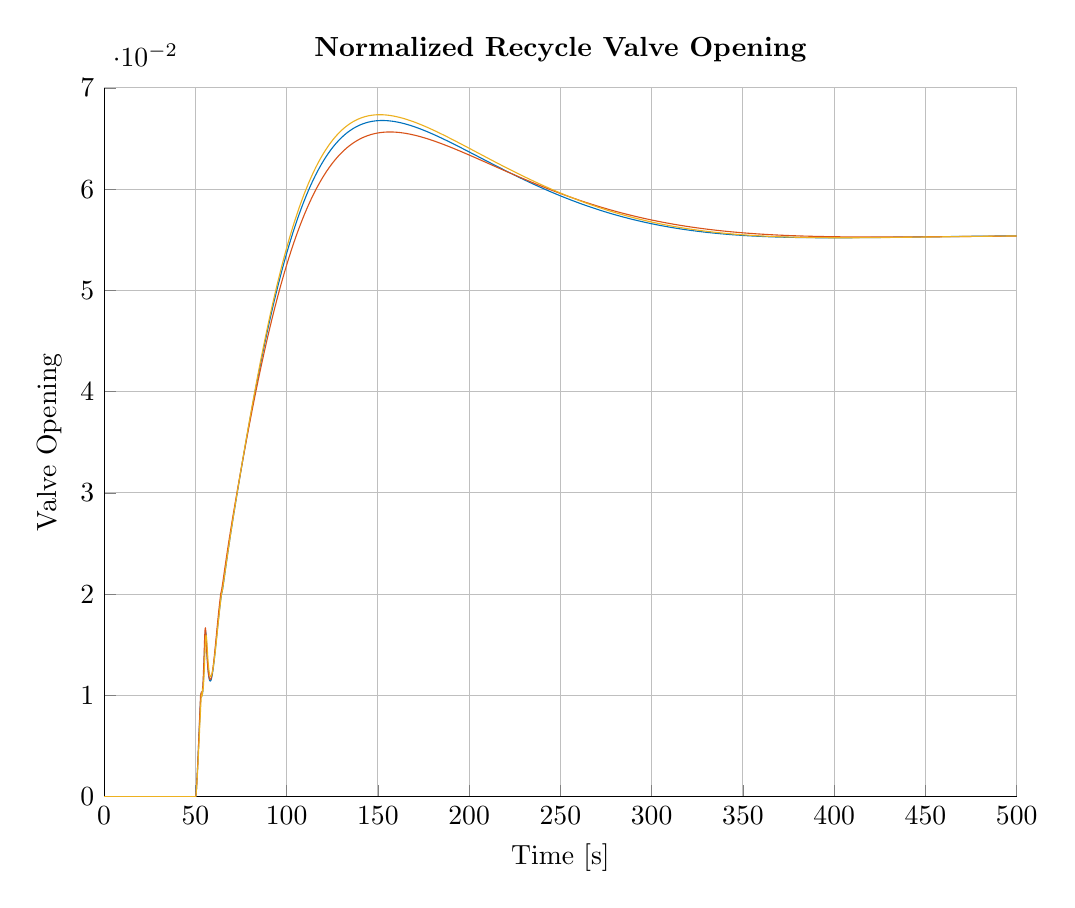
\begin{tikzpicture}

\begin{axis}[%
width=4.563in,
height=3.544in,
at={(0.792in,0.541in)},
scale only axis,
xmin=0,
xmax=500,
xlabel={Time [s]},
xmajorgrids,
ymin=0,
ymax=0.07,
ylabel={Valve Opening},
ymajorgrids,
axis background/.style={fill=white},
title style={font=\bfseries},
title={Normalized Recycle Valve Opening},
axis x line*=bottom,
axis y line*=left
]
\addplot [color=mycolor1,solid,forget plot]
  table[row sep=crcr]{%
0	6.90949e-310\\
0.05	6.90949e-310\\
0.1	6.90949e-310\\
0.15	6.90949e-310\\
0.2	6.90949e-310\\
0.25	6.90949e-310\\
0.3	6.90949e-310\\
0.35	6.90949e-310\\
0.4	6.90949e-310\\
0.45	6.90949e-310\\
0.5	6.90949e-310\\
0.55	6.90949e-310\\
0.6	6.90949e-310\\
0.65	6.90949e-310\\
0.7	6.90949e-310\\
0.75	6.90949e-310\\
0.8	6.90949e-310\\
0.85	6.90949e-310\\
0.9	6.90949e-310\\
0.95	6.90949e-310\\
1	6.90949e-310\\
1.05	6.90949e-310\\
1.1	6.90949e-310\\
1.15	6.90949e-310\\
1.2	6.90949e-310\\
1.25	6.90949e-310\\
1.3	6.90949e-310\\
1.35	6.90949e-310\\
1.4	6.90949e-310\\
1.45	6.90949e-310\\
1.5	6.90949e-310\\
1.55	6.90949e-310\\
1.6	6.90949e-310\\
1.65	6.90949e-310\\
1.7	6.90949e-310\\
1.75	6.90949e-310\\
1.8	6.90949e-310\\
1.85	6.90949e-310\\
1.9	6.90949e-310\\
1.95	6.90949e-310\\
2	6.90949e-310\\
2.05	6.90949e-310\\
2.1	6.90949e-310\\
2.15	6.90949e-310\\
2.2	6.90949e-310\\
2.25	6.90949e-310\\
2.3	6.90949e-310\\
2.35	6.90949e-310\\
2.4	6.90949e-310\\
2.45	6.90949e-310\\
2.5	6.90949e-310\\
2.55	6.90949e-310\\
2.6	6.90949e-310\\
2.65	6.90949e-310\\
2.7	6.90949e-310\\
2.75	6.90949e-310\\
2.8	6.90949e-310\\
2.85	6.90949e-310\\
2.9	6.90949e-310\\
2.95	6.90949e-310\\
3	6.90949e-310\\
3.05	6.90949e-310\\
3.1	6.90949e-310\\
3.15	6.90949e-310\\
3.2	6.90949e-310\\
3.25	6.90949e-310\\
3.3	6.90949e-310\\
3.35	6.90949e-310\\
3.4	6.90949e-310\\
3.45	6.90949e-310\\
3.5	6.90949e-310\\
3.55	6.90949e-310\\
3.6	6.90949e-310\\
3.65	6.90949e-310\\
3.7	6.90949e-310\\
3.75	6.90949e-310\\
3.8	6.90949e-310\\
3.85	6.90949e-310\\
3.9	6.90949e-310\\
3.95	6.90949e-310\\
4	6.90949e-310\\
4.05	6.90949e-310\\
4.1	6.90949e-310\\
4.15	6.90949e-310\\
4.2	6.90949e-310\\
4.25	6.90949e-310\\
4.3	6.90949e-310\\
4.35	6.90949e-310\\
4.4	6.90949e-310\\
4.45	6.90949e-310\\
4.5	6.90949e-310\\
4.55	6.90949e-310\\
4.6	6.90949e-310\\
4.65	6.90949e-310\\
4.7	6.90949e-310\\
4.75	6.90949e-310\\
4.8	6.90949e-310\\
4.85	6.90949e-310\\
4.9	6.90949e-310\\
4.95	6.90949e-310\\
5	6.90949e-310\\
5.05	6.90949e-310\\
5.1	6.90949e-310\\
5.15	6.90949e-310\\
5.2	6.90949e-310\\
5.25	6.90949e-310\\
5.3	6.90949e-310\\
5.35	6.90949e-310\\
5.4	6.90949e-310\\
5.45	6.90949e-310\\
5.5	6.90949e-310\\
5.55	6.90949e-310\\
5.6	6.90949e-310\\
5.65	6.90949e-310\\
5.7	6.90949e-310\\
5.75	6.90949e-310\\
5.8	6.90949e-310\\
5.85	6.90949e-310\\
5.9	6.90949e-310\\
5.95	6.90949e-310\\
6	6.90949e-310\\
6.05	6.90949e-310\\
6.1	6.90949e-310\\
6.15	6.90949e-310\\
6.2	6.90949e-310\\
6.25	6.90949e-310\\
6.3	6.90949e-310\\
6.35	6.90949e-310\\
6.4	6.90949e-310\\
6.45	6.90949e-310\\
6.5	6.90949e-310\\
6.55	6.90949e-310\\
6.6	6.90949e-310\\
6.65	6.90949e-310\\
6.7	6.90949e-310\\
6.75	6.90949e-310\\
6.8	6.90949e-310\\
6.85	6.90949e-310\\
6.9	6.90949e-310\\
6.95	6.90949e-310\\
7	6.90949e-310\\
7.05	6.90949e-310\\
7.1	6.90949e-310\\
7.15	6.90949e-310\\
7.2	6.90949e-310\\
7.25	6.90949e-310\\
7.3	6.90949e-310\\
7.35	6.90949e-310\\
7.4	6.90949e-310\\
7.45	6.90949e-310\\
7.5	6.90949e-310\\
7.55	6.90949e-310\\
7.6	6.90949e-310\\
7.65	6.90949e-310\\
7.7	6.90949e-310\\
7.75	6.90949e-310\\
7.8	6.90949e-310\\
7.85	6.90949e-310\\
7.9	6.90949e-310\\
7.95	6.90949e-310\\
8	6.90949e-310\\
8.05	6.90949e-310\\
8.1	6.90949e-310\\
8.15	6.90949e-310\\
8.2	6.90949e-310\\
8.25	6.90949e-310\\
8.3	6.90949e-310\\
8.35	6.90949e-310\\
8.4	6.90949e-310\\
8.45	6.90949e-310\\
8.5	6.90949e-310\\
8.55	6.90949e-310\\
8.6	6.90949e-310\\
8.65	6.90949e-310\\
8.7	6.90949e-310\\
8.75	6.90949e-310\\
8.8	6.90949e-310\\
8.85	6.90949e-310\\
8.9	6.90949e-310\\
8.95	6.90949e-310\\
9	6.90949e-310\\
9.05	6.90949e-310\\
9.1	6.90949e-310\\
9.15	6.90949e-310\\
9.2	6.90949e-310\\
9.25	6.90949e-310\\
9.3	6.90949e-310\\
9.35	6.90949e-310\\
9.4	6.90949e-310\\
9.45	6.90949e-310\\
9.5	6.90949e-310\\
9.55	6.90949e-310\\
9.6	6.90949e-310\\
9.65	6.90949e-310\\
9.7	6.90949e-310\\
9.75	6.90949e-310\\
9.8	6.90949e-310\\
9.85	6.90949e-310\\
9.9	6.90949e-310\\
9.95	6.90949e-310\\
10	6.90949e-310\\
10.05	6.90949e-310\\
10.1	6.90949e-310\\
10.15	6.90949e-310\\
10.2	6.90949e-310\\
10.25	6.90949e-310\\
10.3	6.90949e-310\\
10.35	6.90949e-310\\
10.4	6.90949e-310\\
10.45	6.90949e-310\\
10.5	6.90949e-310\\
10.55	6.90949e-310\\
10.6	6.90949e-310\\
10.65	6.90949e-310\\
10.7	6.90949e-310\\
10.75	6.90949e-310\\
10.8	6.90949e-310\\
10.85	6.90949e-310\\
10.9	6.90949e-310\\
10.95	6.90949e-310\\
11	6.90949e-310\\
11.05	6.90949e-310\\
11.1	6.90949e-310\\
11.15	6.90949e-310\\
11.2	6.90949e-310\\
11.25	6.90949e-310\\
11.3	6.90949e-310\\
11.35	6.90949e-310\\
11.4	6.90949e-310\\
11.45	6.90949e-310\\
11.5	6.90949e-310\\
11.55	6.90949e-310\\
11.6	6.90949e-310\\
11.65	6.90949e-310\\
11.7	6.90949e-310\\
11.75	6.90949e-310\\
11.8	6.90949e-310\\
11.85	6.90949e-310\\
11.9	6.90949e-310\\
11.95	6.90949e-310\\
12	6.90949e-310\\
12.05	6.90949e-310\\
12.1	6.90949e-310\\
12.15	6.90949e-310\\
12.2	6.90949e-310\\
12.25	6.90949e-310\\
12.3	6.90949e-310\\
12.35	6.90949e-310\\
12.4	6.90949e-310\\
12.45	6.90949e-310\\
12.5	6.90949e-310\\
12.55	6.90949e-310\\
12.6	6.90949e-310\\
12.65	6.90949e-310\\
12.7	6.90949e-310\\
12.75	6.90949e-310\\
12.8	6.90949e-310\\
12.85	6.90949e-310\\
12.9	6.90949e-310\\
12.95	6.90949e-310\\
13	6.90949e-310\\
13.05	6.90949e-310\\
13.1	6.90949e-310\\
13.15	6.90949e-310\\
13.2	6.90949e-310\\
13.25	6.90949e-310\\
13.3	6.90949e-310\\
13.35	6.90949e-310\\
13.4	6.90949e-310\\
13.45	6.90949e-310\\
13.5	6.90949e-310\\
13.55	6.90949e-310\\
13.6	6.90949e-310\\
13.65	6.90949e-310\\
13.7	6.90949e-310\\
13.75	6.90949e-310\\
13.8	6.90949e-310\\
13.85	6.90949e-310\\
13.9	6.90949e-310\\
13.95	6.90949e-310\\
14	6.90949e-310\\
14.05	6.90949e-310\\
14.1	6.90949e-310\\
14.15	6.90949e-310\\
14.2	6.90949e-310\\
14.25	6.90949e-310\\
14.3	6.90949e-310\\
14.35	6.90949e-310\\
14.4	6.90949e-310\\
14.45	6.90949e-310\\
14.5	6.90949e-310\\
14.55	6.90949e-310\\
14.6	6.90949e-310\\
14.65	6.90949e-310\\
14.7	6.90949e-310\\
14.75	6.90949e-310\\
14.8	6.90949e-310\\
14.85	6.90949e-310\\
14.9	6.90949e-310\\
14.95	6.90949e-310\\
15	6.90949e-310\\
15.05	6.90949e-310\\
15.1	6.90949e-310\\
15.15	6.90949e-310\\
15.2	6.90949e-310\\
15.25	6.90949e-310\\
15.3	6.90949e-310\\
15.35	6.90949e-310\\
15.4	6.90949e-310\\
15.45	6.90949e-310\\
15.5	6.90949e-310\\
15.55	6.90949e-310\\
15.6	6.90949e-310\\
15.65	6.90949e-310\\
15.7	6.90949e-310\\
15.75	6.90949e-310\\
15.8	6.90949e-310\\
15.85	6.90949e-310\\
15.9	6.90949e-310\\
15.95	6.90949e-310\\
16	6.90949e-310\\
16.05	6.90949e-310\\
16.1	6.90949e-310\\
16.15	6.90949e-310\\
16.2	6.90949e-310\\
16.25	6.90949e-310\\
16.3	6.90949e-310\\
16.35	6.90949e-310\\
16.4	6.90949e-310\\
16.45	6.90949e-310\\
16.5	6.90949e-310\\
16.55	6.90949e-310\\
16.6	6.90949e-310\\
16.65	6.90949e-310\\
16.7	6.90949e-310\\
16.75	6.90949e-310\\
16.8	6.90949e-310\\
16.85	6.90949e-310\\
16.9	6.90949e-310\\
16.95	6.90949e-310\\
17	6.90949e-310\\
17.05	6.90949e-310\\
17.1	6.90949e-310\\
17.15	6.90949e-310\\
17.2	6.90949e-310\\
17.25	6.90949e-310\\
17.3	6.90949e-310\\
17.35	6.90949e-310\\
17.4	6.90949e-310\\
17.45	6.90949e-310\\
17.5	6.90949e-310\\
17.55	6.90949e-310\\
17.6	6.90949e-310\\
17.65	6.90949e-310\\
17.7	6.90949e-310\\
17.75	6.90949e-310\\
17.8	6.90949e-310\\
17.85	6.90949e-310\\
17.9	6.90949e-310\\
17.95	6.90949e-310\\
18	6.90949e-310\\
18.05	6.90949e-310\\
18.1	6.90949e-310\\
18.15	6.90949e-310\\
18.2	6.90949e-310\\
18.25	6.90949e-310\\
18.3	6.90949e-310\\
18.35	6.90949e-310\\
18.4	6.90949e-310\\
18.45	6.90949e-310\\
18.5	6.90949e-310\\
18.55	6.90949e-310\\
18.6	6.90949e-310\\
18.65	6.90949e-310\\
18.7	6.90949e-310\\
18.75	6.90949e-310\\
18.8	6.90949e-310\\
18.85	6.90949e-310\\
18.9	6.90949e-310\\
18.95	6.90949e-310\\
19	6.90949e-310\\
19.05	6.90949e-310\\
19.1	6.90949e-310\\
19.15	6.90949e-310\\
19.2	6.90949e-310\\
19.25	6.90949e-310\\
19.3	6.90949e-310\\
19.35	6.90949e-310\\
19.4	6.90949e-310\\
19.45	6.90949e-310\\
19.5	6.90949e-310\\
19.55	6.90949e-310\\
19.6	6.90949e-310\\
19.65	6.90949e-310\\
19.7	6.90949e-310\\
19.75	6.90949e-310\\
19.8	6.90949e-310\\
19.85	6.90949e-310\\
19.9	6.90949e-310\\
19.95	6.90949e-310\\
20	6.90949e-310\\
20.05	6.90949e-310\\
20.1	6.90949e-310\\
20.15	6.90949e-310\\
20.2	6.90949e-310\\
20.25	6.90949e-310\\
20.3	6.90949e-310\\
20.35	6.90949e-310\\
20.4	6.90949e-310\\
20.45	6.90949e-310\\
20.5	6.90949e-310\\
20.55	6.90949e-310\\
20.6	6.90949e-310\\
20.65	6.90949e-310\\
20.7	6.90949e-310\\
20.75	6.90949e-310\\
20.8	6.90949e-310\\
20.85	6.90949e-310\\
20.9	6.90949e-310\\
20.95	6.90949e-310\\
21	6.90949e-310\\
21.05	6.90949e-310\\
21.1	6.90949e-310\\
21.15	6.90949e-310\\
21.2	6.90949e-310\\
21.25	6.90949e-310\\
21.3	6.90949e-310\\
21.35	6.90949e-310\\
21.4	6.90949e-310\\
21.45	6.90949e-310\\
21.5	6.90949e-310\\
21.55	6.90949e-310\\
21.6	6.90949e-310\\
21.65	6.90949e-310\\
21.7	6.90949e-310\\
21.75	6.90949e-310\\
21.8	6.90949e-310\\
21.85	6.90949e-310\\
21.9	6.90949e-310\\
21.95	6.90949e-310\\
22	6.90949e-310\\
22.05	6.90949e-310\\
22.1	6.90949e-310\\
22.15	6.90949e-310\\
22.2	6.90949e-310\\
22.25	6.90949e-310\\
22.3	6.90949e-310\\
22.35	6.90949e-310\\
22.4	6.90949e-310\\
22.45	6.90949e-310\\
22.5	6.90949e-310\\
22.55	6.90949e-310\\
22.6	6.90949e-310\\
22.65	6.90949e-310\\
22.7	6.90949e-310\\
22.75	6.90949e-310\\
22.8	6.90949e-310\\
22.85	6.90949e-310\\
22.9	6.90949e-310\\
22.95	6.90949e-310\\
23	6.90949e-310\\
23.05	6.90949e-310\\
23.1	6.90949e-310\\
23.15	6.90949e-310\\
23.2	6.90949e-310\\
23.25	6.90949e-310\\
23.3	6.90949e-310\\
23.35	6.90949e-310\\
23.4	6.90949e-310\\
23.45	6.90949e-310\\
23.5	6.90949e-310\\
23.55	6.90949e-310\\
23.6	6.90949e-310\\
23.65	6.90949e-310\\
23.7	6.90949e-310\\
23.75	6.90949e-310\\
23.8	6.90949e-310\\
23.85	6.90949e-310\\
23.9	6.90949e-310\\
23.95	6.90949e-310\\
24	6.90949e-310\\
24.05	6.90949e-310\\
24.1	6.90949e-310\\
24.15	6.90949e-310\\
24.2	6.90949e-310\\
24.25	6.90949e-310\\
24.3	6.90949e-310\\
24.35	6.90949e-310\\
24.4	6.90949e-310\\
24.45	6.90949e-310\\
24.5	6.90949e-310\\
24.55	6.90949e-310\\
24.6	6.90949e-310\\
24.65	6.90949e-310\\
24.7	6.90949e-310\\
24.75	6.90949e-310\\
24.8	6.90949e-310\\
24.85	6.90949e-310\\
24.9	6.90949e-310\\
24.95	6.90949e-310\\
25	6.90949e-310\\
25.05	6.90949e-310\\
25.1	6.90949e-310\\
25.15	6.90949e-310\\
25.2	6.90949e-310\\
25.25	6.90949e-310\\
25.3	6.90949e-310\\
25.35	6.90949e-310\\
25.4	6.90949e-310\\
25.45	6.90949e-310\\
25.5	6.90949e-310\\
25.55	6.90949e-310\\
25.6	6.90949e-310\\
25.65	6.90949e-310\\
25.7	6.90949e-310\\
25.75	6.90949e-310\\
25.8	6.90949e-310\\
25.85	6.90949e-310\\
25.9	6.90949e-310\\
25.95	6.90949e-310\\
26	6.90949e-310\\
26.05	6.90949e-310\\
26.1	6.90949e-310\\
26.15	6.90949e-310\\
26.2	6.90949e-310\\
26.25	6.90949e-310\\
26.3	6.90949e-310\\
26.35	6.90949e-310\\
26.4	6.90949e-310\\
26.45	6.90949e-310\\
26.5	6.90949e-310\\
26.55	6.90949e-310\\
26.6	6.90949e-310\\
26.65	6.90949e-310\\
26.7	6.90949e-310\\
26.75	6.90949e-310\\
26.8	6.90949e-310\\
26.85	6.90949e-310\\
26.9	6.90949e-310\\
26.95	6.90949e-310\\
27	6.90949e-310\\
27.05	6.90949e-310\\
27.1	6.90949e-310\\
27.15	6.90949e-310\\
27.2	6.90949e-310\\
27.25	6.90949e-310\\
27.3	6.90949e-310\\
27.35	6.90949e-310\\
27.4	6.90949e-310\\
27.45	6.90949e-310\\
27.5	6.90949e-310\\
27.55	6.90949e-310\\
27.6	6.90949e-310\\
27.65	6.90949e-310\\
27.7	6.90949e-310\\
27.75	6.90949e-310\\
27.8	6.90949e-310\\
27.85	6.90949e-310\\
27.9	6.90949e-310\\
27.95	6.90949e-310\\
28	6.90949e-310\\
28.05	6.90949e-310\\
28.1	6.90949e-310\\
28.15	6.90949e-310\\
28.2	6.90949e-310\\
28.25	6.90949e-310\\
28.3	6.90949e-310\\
28.35	6.90949e-310\\
28.4	6.90949e-310\\
28.45	6.90949e-310\\
28.5	6.90949e-310\\
28.55	6.90949e-310\\
28.6	6.90949e-310\\
28.65	6.90949e-310\\
28.7	6.90949e-310\\
28.75	6.90949e-310\\
28.8	6.90949e-310\\
28.85	6.90949e-310\\
28.9	6.90949e-310\\
28.95	6.90949e-310\\
29	6.90949e-310\\
29.05	6.90949e-310\\
29.1	6.90949e-310\\
29.15	6.90949e-310\\
29.2	6.90949e-310\\
29.25	6.90949e-310\\
29.3	6.90949e-310\\
29.35	6.90949e-310\\
29.4	6.90949e-310\\
29.45	6.90949e-310\\
29.5	6.90949e-310\\
29.55	6.90949e-310\\
29.6	6.90949e-310\\
29.65	6.90949e-310\\
29.7	6.90949e-310\\
29.75	6.90949e-310\\
29.8	6.90949e-310\\
29.85	6.90949e-310\\
29.9	6.90949e-310\\
29.95	6.90949e-310\\
30	6.90949e-310\\
30.05	6.90949e-310\\
30.1	6.90949e-310\\
30.15	6.90949e-310\\
30.2	6.90949e-310\\
30.25	6.90949e-310\\
30.3	6.90949e-310\\
30.35	6.90949e-310\\
30.4	6.90949e-310\\
30.45	6.90949e-310\\
30.5	6.90949e-310\\
30.55	6.90949e-310\\
30.6	6.90949e-310\\
30.65	6.90949e-310\\
30.7	6.90949e-310\\
30.75	6.90949e-310\\
30.8	6.90949e-310\\
30.85	6.90949e-310\\
30.9	6.90949e-310\\
30.95	6.90949e-310\\
31	6.90949e-310\\
31.05	6.90949e-310\\
31.1	6.90949e-310\\
31.15	6.90949e-310\\
31.2	6.90949e-310\\
31.25	6.90949e-310\\
31.3	6.90949e-310\\
31.35	6.90949e-310\\
31.4	6.90949e-310\\
31.45	6.90949e-310\\
31.5	6.90949e-310\\
31.55	6.90949e-310\\
31.6	6.90949e-310\\
31.65	6.90949e-310\\
31.7	6.90949e-310\\
31.75	6.90949e-310\\
31.8	6.90949e-310\\
31.85	6.90949e-310\\
31.9	6.90949e-310\\
31.95	6.90949e-310\\
32	6.90949e-310\\
32.05	6.90949e-310\\
32.1	6.90949e-310\\
32.15	6.90949e-310\\
32.2	6.90949e-310\\
32.25	6.90949e-310\\
32.3	6.90949e-310\\
32.35	6.90949e-310\\
32.4	6.90949e-310\\
32.45	6.90949e-310\\
32.5	6.90949e-310\\
32.55	6.90949e-310\\
32.6	6.90949e-310\\
32.65	6.90949e-310\\
32.7	6.90949e-310\\
32.75	6.90949e-310\\
32.8	6.90949e-310\\
32.85	6.90949e-310\\
32.9	6.90949e-310\\
32.95	6.90949e-310\\
33	6.90949e-310\\
33.05	6.90949e-310\\
33.1	6.90949e-310\\
33.15	6.90949e-310\\
33.2	6.90949e-310\\
33.25	6.90949e-310\\
33.3	6.90949e-310\\
33.35	6.90949e-310\\
33.4	6.90949e-310\\
33.45	6.90949e-310\\
33.5	6.90949e-310\\
33.55	6.90949e-310\\
33.6	6.90949e-310\\
33.65	6.90949e-310\\
33.7	6.90949e-310\\
33.75	6.90949e-310\\
33.8	6.90949e-310\\
33.85	6.90949e-310\\
33.9	6.90949e-310\\
33.95	6.90949e-310\\
34	6.90949e-310\\
34.05	6.90949e-310\\
34.1	6.90949e-310\\
34.15	6.90949e-310\\
34.2	6.90949e-310\\
34.25	6.90949e-310\\
34.3	6.90949e-310\\
34.35	6.90949e-310\\
34.4	6.90949e-310\\
34.45	6.90949e-310\\
34.5	6.90949e-310\\
34.55	6.90949e-310\\
34.6	6.90949e-310\\
34.65	6.90949e-310\\
34.7	6.90949e-310\\
34.75	6.90949e-310\\
34.8	6.90949e-310\\
34.85	6.90949e-310\\
34.9	6.90949e-310\\
34.95	6.90949e-310\\
35	6.90949e-310\\
35.05	6.90949e-310\\
35.1	6.90949e-310\\
35.15	6.90949e-310\\
35.2	6.90949e-310\\
35.25	6.90949e-310\\
35.3	6.90949e-310\\
35.35	6.90949e-310\\
35.4	6.90949e-310\\
35.45	6.90949e-310\\
35.5	6.90949e-310\\
35.55	6.90949e-310\\
35.6	6.90949e-310\\
35.65	6.90949e-310\\
35.7	6.90949e-310\\
35.75	6.90949e-310\\
35.8	6.90949e-310\\
35.85	6.90949e-310\\
35.9	6.90949e-310\\
35.95	6.90949e-310\\
36	6.90949e-310\\
36.05	6.90949e-310\\
36.1	6.90949e-310\\
36.15	6.90949e-310\\
36.2	6.90949e-310\\
36.25	6.90949e-310\\
36.3	6.90949e-310\\
36.35	6.90949e-310\\
36.4	6.90949e-310\\
36.45	6.90949e-310\\
36.5	6.90949e-310\\
36.55	6.90949e-310\\
36.6	6.90949e-310\\
36.65	6.90949e-310\\
36.7	6.90949e-310\\
36.75	6.90949e-310\\
36.8	6.90949e-310\\
36.85	6.90949e-310\\
36.9	6.90949e-310\\
36.95	6.90949e-310\\
37	6.90949e-310\\
37.05	6.90949e-310\\
37.1	6.90949e-310\\
37.15	6.90949e-310\\
37.2	6.90949e-310\\
37.25	6.90949e-310\\
37.3	6.90949e-310\\
37.35	6.90949e-310\\
37.4	6.90949e-310\\
37.45	6.90949e-310\\
37.5	6.90949e-310\\
37.55	6.90949e-310\\
37.6	6.90949e-310\\
37.65	6.90949e-310\\
37.7	6.90949e-310\\
37.75	6.90949e-310\\
37.8	6.90949e-310\\
37.85	6.90949e-310\\
37.9	6.90949e-310\\
37.95	6.90949e-310\\
38	6.90949e-310\\
38.05	6.90949e-310\\
38.1	6.90949e-310\\
38.15	6.90949e-310\\
38.2	6.90949e-310\\
38.25	6.90949e-310\\
38.3	6.90949e-310\\
38.35	6.90949e-310\\
38.4	6.90949e-310\\
38.45	6.90949e-310\\
38.5	6.90949e-310\\
38.55	6.90949e-310\\
38.6	6.90949e-310\\
38.65	6.90949e-310\\
38.7	6.90949e-310\\
38.75	6.90949e-310\\
38.8	6.90949e-310\\
38.85	6.90949e-310\\
38.9	6.90949e-310\\
38.95	6.90949e-310\\
39	6.90949e-310\\
39.05	6.90949e-310\\
39.1	6.90949e-310\\
39.15	6.90949e-310\\
39.2	6.90949e-310\\
39.25	6.90949e-310\\
39.3	6.90949e-310\\
39.35	6.90949e-310\\
39.4	6.90949e-310\\
39.45	6.90949e-310\\
39.5	6.90949e-310\\
39.55	6.90949e-310\\
39.6	6.90949e-310\\
39.65	6.90949e-310\\
39.7	6.90949e-310\\
39.75	6.90949e-310\\
39.8	6.90949e-310\\
39.85	6.90949e-310\\
39.9	6.90949e-310\\
39.95	6.90949e-310\\
40	6.90949e-310\\
40.05	6.90949e-310\\
40.1	6.90949e-310\\
40.15	6.90949e-310\\
40.2	6.90949e-310\\
40.25	6.90949e-310\\
40.3	6.90949e-310\\
40.35	6.90949e-310\\
40.4	6.90949e-310\\
40.45	6.90949e-310\\
40.5	6.90949e-310\\
40.55	6.90949e-310\\
40.6	6.90949e-310\\
40.65	6.90949e-310\\
40.7	6.90949e-310\\
40.75	6.90949e-310\\
40.8	6.90949e-310\\
40.85	6.90949e-310\\
40.9	6.90949e-310\\
40.95	6.90949e-310\\
41	6.90949e-310\\
41.05	6.90949e-310\\
41.1	6.90949e-310\\
41.15	6.90949e-310\\
41.2	6.90949e-310\\
41.25	6.90949e-310\\
41.3	6.90949e-310\\
41.35	6.90949e-310\\
41.4	6.90949e-310\\
41.45	6.90949e-310\\
41.5	6.90949e-310\\
41.55	6.90949e-310\\
41.6	6.90949e-310\\
41.65	6.90949e-310\\
41.7	6.90949e-310\\
41.75	6.90949e-310\\
41.8	6.90949e-310\\
41.85	6.90949e-310\\
41.9	6.90949e-310\\
41.95	6.90949e-310\\
42	6.90949e-310\\
42.05	6.90949e-310\\
42.1	6.90949e-310\\
42.15	6.90949e-310\\
42.2	6.90949e-310\\
42.25	6.90949e-310\\
42.3	6.90949e-310\\
42.35	6.90949e-310\\
42.4	6.90949e-310\\
42.45	6.90949e-310\\
42.5	6.90949e-310\\
42.55	6.90949e-310\\
42.6	6.90949e-310\\
42.65	6.90949e-310\\
42.7	6.90949e-310\\
42.75	6.90949e-310\\
42.8	6.90949e-310\\
42.85	6.90949e-310\\
42.9	6.90949e-310\\
42.95	6.90949e-310\\
43	6.90949e-310\\
43.05	6.90949e-310\\
43.1	6.90949e-310\\
43.15	6.90949e-310\\
43.2	6.90949e-310\\
43.25	6.90949e-310\\
43.3	6.90949e-310\\
43.35	6.90949e-310\\
43.4	6.90949e-310\\
43.45	6.90949e-310\\
43.5	6.90949e-310\\
43.55	6.90949e-310\\
43.6	6.90949e-310\\
43.65	6.90949e-310\\
43.7	6.90949e-310\\
43.75	6.90949e-310\\
43.8	6.90949e-310\\
43.85	6.90949e-310\\
43.9	6.90949e-310\\
43.95	6.90949e-310\\
44	6.90949e-310\\
44.05	6.90949e-310\\
44.1	6.90949e-310\\
44.15	6.90949e-310\\
44.2	6.90949e-310\\
44.25	6.90949e-310\\
44.3	6.90949e-310\\
44.35	6.90949e-310\\
44.4	6.90949e-310\\
44.45	6.90949e-310\\
44.5	6.90949e-310\\
44.55	6.90949e-310\\
44.6	6.90949e-310\\
44.65	6.90949e-310\\
44.7	6.90949e-310\\
44.75	6.90949e-310\\
44.8	6.90949e-310\\
44.85	6.90949e-310\\
44.9	6.90949e-310\\
44.95	6.90949e-310\\
45	6.90949e-310\\
45.05	6.90949e-310\\
45.1	6.90949e-310\\
45.15	6.90949e-310\\
45.2	6.90949e-310\\
45.25	6.90949e-310\\
45.3	6.90949e-310\\
45.35	6.90949e-310\\
45.4	6.90949e-310\\
45.45	6.90949e-310\\
45.5	6.90949e-310\\
45.55	6.90949e-310\\
45.6	6.90949e-310\\
45.65	6.90949e-310\\
45.7	6.90949e-310\\
45.75	6.90949e-310\\
45.8	6.90949e-310\\
45.85	6.90949e-310\\
45.9	6.90949e-310\\
45.95	6.90949e-310\\
46	6.90949e-310\\
46.05	6.90949e-310\\
46.1	6.90949e-310\\
46.15	6.90949e-310\\
46.2	6.90949e-310\\
46.25	6.90949e-310\\
46.3	6.90949e-310\\
46.35	6.90949e-310\\
46.4	6.90949e-310\\
46.45	6.90949e-310\\
46.5	6.90949e-310\\
46.55	6.90949e-310\\
46.6	6.90949e-310\\
46.65	6.90949e-310\\
46.7	6.90949e-310\\
46.75	6.90949e-310\\
46.8	6.90949e-310\\
46.85	6.90949e-310\\
46.9	6.90949e-310\\
46.95	6.90949e-310\\
47	6.90949e-310\\
47.05	6.90949e-310\\
47.1	6.90949e-310\\
47.15	6.90949e-310\\
47.2	6.90949e-310\\
47.25	6.90949e-310\\
47.3	6.90949e-310\\
47.35	6.90949e-310\\
47.4	6.90949e-310\\
47.45	6.90949e-310\\
47.5	6.90949e-310\\
47.55	6.90949e-310\\
47.6	6.90949e-310\\
47.65	6.90949e-310\\
47.7	6.90949e-310\\
47.75	6.90949e-310\\
47.8	6.90949e-310\\
47.85	6.90949e-310\\
47.9	6.90949e-310\\
47.95	6.90949e-310\\
48	6.90949e-310\\
48.05	6.90949e-310\\
48.1	6.90949e-310\\
48.15	6.90949e-310\\
48.2	6.90949e-310\\
48.25	6.90949e-310\\
48.3	6.90949e-310\\
48.35	6.90949e-310\\
48.4	6.90949e-310\\
48.45	6.90949e-310\\
48.5	6.90949e-310\\
48.55	6.90949e-310\\
48.6	6.90949e-310\\
48.65	6.90949e-310\\
48.7	6.90949e-310\\
48.75	6.90949e-310\\
48.8	6.90949e-310\\
48.85	6.90949e-310\\
48.9	6.90949e-310\\
48.95	6.90949e-310\\
49	6.90949e-310\\
49.05	6.90949e-310\\
49.1	6.90949e-310\\
49.15	6.90949e-310\\
49.2	6.90949e-310\\
49.25	6.90949e-310\\
49.3	6.90949e-310\\
49.35	6.90949e-310\\
49.4	6.90949e-310\\
49.45	6.90949e-310\\
49.5	6.90949e-310\\
49.55	6.90949e-310\\
49.6	6.90949e-310\\
49.65	6.90949e-310\\
49.7	6.90949e-310\\
49.75	6.90949e-310\\
49.8	6.90949e-310\\
49.85	6.90949e-310\\
49.9	6.90949e-310\\
49.95	6.90949e-310\\
50	6.90949e-310\\
50.05	6.90949e-310\\
50.1	1.70778e-06\\
50.15	1.05264e-05\\
50.2	3.12231e-05\\
50.25	6.733e-05\\
50.3	0.000120942\\
50.35	0.000192783\\
50.4	0.000282421\\
50.45	0.000388554\\
50.5	0.000509304\\
50.55	0.000642488\\
50.6	0.000785864\\
50.65	0.000937311\\
50.7	0.00109497\\
50.75	0.00125732\\
50.8	0.00142322\\
50.85	0.00159189\\
50.9	0.00176289\\
50.95	0.00193604\\
51	0.00211134\\
51.05	0.00228894\\
51.1	0.00246901\\
51.15	0.00265174\\
51.2	0.0028373\\
51.25	0.00302577\\
51.3	0.00321715\\
51.35	0.00341139\\
51.4	0.00360834\\
51.45	0.00380781\\
51.5	0.00400956\\
51.55	0.00421331\\
51.6	0.00441879\\
51.65	0.00462572\\
51.7	0.00483381\\
51.75	0.00504281\\
51.8	0.00525246\\
51.85	0.00546256\\
51.9	0.00567289\\
51.95	0.00588325\\
52	0.00609347\\
52.05	0.00630339\\
52.1	0.00651283\\
52.15	0.00672165\\
52.2	0.00692967\\
52.25	0.00713677\\
52.3	0.0073428\\
52.35	0.00754766\\
52.4	0.00775124\\
52.45	0.0079535\\
52.5	0.00815443\\
52.55	0.00835403\\
52.6	0.00855239\\
52.65	0.00874958\\
52.7	0.00894573\\
52.75	0.00914098\\
52.8	0.00933549\\
52.85	0.00952941\\
52.9	0.0097229\\
52.95	0.0099161\\
53	0.0101092\\
53.05	0.00982871\\
53.1	0.0100238\\
53.15	0.00976125\\
53.2	0.00999392\\
53.25	0.0102592\\
53.3	0.0100459\\
53.35	0.00985418\\
53.4	0.0101992\\
53.45	0.0100502\\
53.5	0.00992427\\
53.55	0.0103668\\
53.6	0.0102812\\
53.65	0.0102134\\
53.7	0.0101644\\
53.75	0.0101356\\
53.8	0.0101285\\
53.85	0.0101434\\
53.9	0.0101803\\
53.95	0.0102384\\
54	0.0103164\\
54.05	0.0104126\\
54.1	0.0105254\\
54.15	0.0106531\\
54.2	0.0107941\\
54.25	0.0109471\\
54.3	0.0111109\\
54.35	0.0112848\\
54.4	0.0114678\\
54.45	0.0116597\\
54.5	0.01186\\
54.55	0.0120684\\
54.6	0.0122847\\
54.65	0.0125087\\
54.7	0.0127403\\
54.75	0.0129794\\
54.8	0.0132258\\
54.85	0.0134794\\
54.9	0.01374\\
54.95	0.0140076\\
55	0.014282\\
55.05	0.0145587\\
55.1	0.0148275\\
55.15	0.0150826\\
55.2	0.0153151\\
55.25	0.0155271\\
55.3	0.0157193\\
55.35	0.0158837\\
55.4	0.0160168\\
55.45	0.0161225\\
55.5	0.0161968\\
55.55	0.0162411\\
55.6	0.0162635\\
55.65	0.0162633\\
55.7	0.0162386\\
55.75	0.0161878\\
55.8	0.0161105\\
55.85	0.0160075\\
55.9	0.0158808\\
55.95	0.0157336\\
56	0.0155694\\
56.05	0.0153925\\
56.1	0.0152069\\
56.15	0.0150162\\
56.2	0.0148236\\
56.25	0.0146319\\
56.3	0.014443\\
56.35	0.0142585\\
56.4	0.0140793\\
56.45	0.0139063\\
56.5	0.0137396\\
56.55	0.0135796\\
56.6	0.0134263\\
56.65	0.0132797\\
56.7	0.0131397\\
56.75	0.0130061\\
56.8	0.012879\\
56.85	0.0127582\\
56.9	0.0126435\\
56.95	0.012535\\
57	0.0124325\\
57.05	0.0123359\\
57.1	0.012245\\
57.15	0.0121598\\
57.2	0.0120801\\
57.25	0.0120057\\
57.3	0.0119366\\
57.35	0.0118724\\
57.4	0.0118132\\
57.45	0.0117586\\
57.5	0.0117086\\
57.55	0.011663\\
57.6	0.0116216\\
57.65	0.0115844\\
57.7	0.0115512\\
57.75	0.0115219\\
57.8	0.0114964\\
57.85	0.0114745\\
57.9	0.0114562\\
57.95	0.0114415\\
58	0.0114301\\
58.05	0.0114221\\
58.1	0.0114173\\
58.15	0.0114157\\
58.2	0.0114172\\
58.25	0.0114217\\
58.3	0.0114293\\
58.35	0.0114396\\
58.4	0.0114529\\
58.45	0.0114689\\
58.5	0.0114875\\
58.55	0.0115088\\
58.6	0.0115327\\
58.65	0.011559\\
58.7	0.0115878\\
58.75	0.0116189\\
58.8	0.0116523\\
58.85	0.0116879\\
58.9	0.0117256\\
58.95	0.0117655\\
59	0.0118074\\
59.05	0.0118513\\
59.1	0.0118971\\
59.15	0.0119448\\
59.2	0.0119943\\
59.25	0.0120456\\
59.3	0.0120987\\
59.35	0.0121534\\
59.4	0.0122097\\
59.45	0.0122677\\
59.5	0.0123271\\
59.55	0.0123881\\
59.6	0.0124506\\
59.65	0.0125145\\
59.7	0.0125797\\
59.75	0.0126463\\
59.8	0.0127142\\
59.85	0.0127833\\
59.9	0.0128537\\
59.95	0.0129252\\
60	0.0129979\\
60.05	0.0130717\\
60.1	0.0131465\\
60.15	0.0132224\\
60.2	0.0132992\\
60.25	0.013377\\
60.3	0.0134556\\
60.35	0.0135352\\
60.4	0.0136156\\
60.45	0.0136968\\
60.5	0.0137787\\
60.55	0.0138613\\
60.6	0.0139447\\
60.65	0.0140286\\
60.7	0.0141132\\
60.75	0.0141984\\
60.8	0.0142841\\
60.85	0.0143703\\
60.9	0.0144569\\
60.95	0.014544\\
61	0.0146315\\
61.05	0.0147193\\
61.1	0.0148075\\
61.15	0.0148959\\
61.2	0.0149846\\
61.25	0.0150735\\
61.3	0.0151626\\
61.35	0.0152519\\
61.4	0.0153412\\
61.45	0.0154307\\
61.5	0.0155202\\
61.55	0.0156097\\
61.6	0.0156992\\
61.65	0.0157887\\
61.7	0.0158781\\
61.75	0.0159674\\
61.8	0.0160566\\
61.85	0.0161456\\
61.9	0.0162345\\
61.95	0.0163231\\
62	0.0164115\\
62.05	0.0164996\\
62.1	0.0165875\\
62.15	0.016675\\
62.2	0.0167622\\
62.25	0.0168491\\
62.3	0.0169356\\
62.35	0.0170217\\
62.4	0.0171074\\
62.45	0.0171927\\
62.5	0.0172775\\
62.55	0.0173619\\
62.6	0.0174458\\
62.65	0.0175293\\
62.7	0.0176122\\
62.75	0.0176947\\
62.8	0.0177767\\
62.85	0.0178582\\
62.9	0.0179391\\
62.95	0.0180195\\
63	0.0180995\\
63.05	0.0181789\\
63.1	0.0182577\\
63.15	0.0183361\\
63.2	0.0184139\\
63.25	0.0184913\\
63.3	0.0185681\\
63.35	0.0186444\\
63.4	0.0187202\\
63.45	0.0187956\\
63.5	0.0188704\\
63.55	0.0189448\\
63.6	0.0190188\\
63.65	0.0190922\\
63.7	0.0191653\\
63.75	0.0192379\\
63.8	0.0193102\\
63.85	0.019382\\
63.9	0.0194534\\
63.95	0.0195245\\
64	0.0195952\\
64.05	0.0196656\\
64.1	0.0197357\\
64.15	0.0198054\\
64.2	0.0198748\\
64.25	0.019944\\
64.3	0.0200129\\
64.35	0.0200409\\
64.4	0.0200692\\
64.45	0.0200987\\
64.5	0.0201304\\
64.55	0.0201647\\
64.6	0.020202\\
64.65	0.0202425\\
64.7	0.0202859\\
64.75	0.0203321\\
64.8	0.0203808\\
64.85	0.0204317\\
64.9	0.0204844\\
64.95	0.0205387\\
65	0.0205944\\
65.05	0.0206512\\
65.1	0.020709\\
65.15	0.0207676\\
65.2	0.0208269\\
65.25	0.0208869\\
65.3	0.0209475\\
65.35	0.0210087\\
65.4	0.0210703\\
65.45	0.0211323\\
65.5	0.0211948\\
65.55	0.0212576\\
65.6	0.0213206\\
65.65	0.021384\\
65.7	0.0214476\\
65.75	0.0215114\\
65.8	0.0215753\\
65.85	0.0216394\\
65.9	0.0217036\\
65.95	0.0217678\\
66	0.0218322\\
66.05	0.0218966\\
66.1	0.021961\\
66.15	0.0220254\\
66.2	0.0220898\\
66.25	0.0221542\\
66.3	0.0222186\\
66.35	0.0222829\\
66.4	0.0223472\\
66.45	0.0224114\\
66.5	0.0224756\\
66.55	0.0225398\\
66.6	0.0226038\\
66.65	0.0226679\\
66.7	0.0227319\\
66.75	0.0227958\\
66.8	0.0228597\\
66.85	0.0229236\\
66.9	0.0229875\\
66.95	0.0230512\\
67	0.023115\\
67.05	0.0231786\\
67.1	0.0232422\\
67.15	0.0233057\\
67.2	0.0233691\\
67.25	0.0234324\\
67.3	0.0234956\\
67.35	0.0235586\\
67.4	0.0236216\\
67.45	0.0236844\\
67.5	0.023747\\
67.55	0.0238096\\
67.6	0.023872\\
67.65	0.0239343\\
67.7	0.0239964\\
67.75	0.0240585\\
67.8	0.0241204\\
67.85	0.0241822\\
67.9	0.0242438\\
67.95	0.0243054\\
68	0.0243668\\
68.05	0.0244281\\
68.1	0.0244892\\
68.15	0.0245503\\
68.2	0.0246112\\
68.25	0.024672\\
68.3	0.0247327\\
68.35	0.0247933\\
68.4	0.0248537\\
68.45	0.0249141\\
68.5	0.0249743\\
68.55	0.0250344\\
68.6	0.0250944\\
68.65	0.0251543\\
68.7	0.0252141\\
68.75	0.0252738\\
68.8	0.0253333\\
68.85	0.0253928\\
68.9	0.0254521\\
68.95	0.0255114\\
69	0.0255706\\
69.05	0.0256296\\
69.1	0.0256886\\
69.15	0.0257474\\
69.2	0.0258062\\
69.25	0.0258649\\
69.3	0.0259235\\
69.35	0.0259819\\
69.4	0.0260403\\
69.45	0.0260986\\
69.5	0.0261569\\
69.55	0.026215\\
69.6	0.026273\\
69.65	0.026331\\
69.7	0.0263889\\
69.75	0.0264467\\
69.8	0.0265044\\
69.85	0.0265621\\
69.9	0.0266196\\
69.95	0.0266771\\
70	0.0267345\\
70.05	0.0267919\\
70.1	0.0268491\\
70.15	0.0269063\\
70.2	0.0269634\\
70.25	0.0270205\\
70.3	0.0270775\\
70.35	0.0271344\\
70.4	0.0271913\\
70.45	0.027248\\
70.5	0.0273048\\
70.55	0.0273614\\
70.6	0.027418\\
70.65	0.0274746\\
70.7	0.027531\\
70.75	0.0275875\\
70.8	0.0276438\\
70.85	0.0277001\\
70.9	0.0277564\\
70.95	0.0278126\\
71	0.0278687\\
71.05	0.0279248\\
71.1	0.0279808\\
71.15	0.0280368\\
71.2	0.0280927\\
71.25	0.0281486\\
71.3	0.0282044\\
71.35	0.0282602\\
71.4	0.0283159\\
71.45	0.0283715\\
71.5	0.0284272\\
71.55	0.0284827\\
71.6	0.0285383\\
71.65	0.0285938\\
71.7	0.0286492\\
71.75	0.0287046\\
71.8	0.0287599\\
71.85	0.0288152\\
71.9	0.0288705\\
71.95	0.0289257\\
72	0.0289809\\
72.05	0.029036\\
72.1	0.0290911\\
72.15	0.0291462\\
72.2	0.0292012\\
72.25	0.0292562\\
72.3	0.0293111\\
72.35	0.029366\\
72.4	0.0294208\\
72.45	0.0294757\\
72.5	0.0295304\\
72.55	0.0295852\\
72.6	0.0296399\\
72.65	0.0296945\\
72.7	0.0297492\\
72.75	0.0298037\\
72.8	0.0298583\\
72.85	0.0299128\\
72.9	0.0299673\\
72.95	0.0300217\\
73	0.0300762\\
73.05	0.0301305\\
73.1	0.0301849\\
73.15	0.0302392\\
73.2	0.0302934\\
73.25	0.0303477\\
73.3	0.0304019\\
73.35	0.030456\\
73.4	0.0305102\\
73.45	0.0305643\\
73.5	0.0306183\\
73.55	0.0306724\\
73.6	0.0307264\\
73.65	0.0307803\\
73.7	0.0308343\\
73.75	0.0308882\\
73.8	0.030942\\
73.85	0.0309959\\
73.9	0.0310497\\
73.95	0.0311035\\
74	0.0311572\\
74.05	0.0312109\\
74.1	0.0312646\\
74.15	0.0313182\\
74.2	0.0313718\\
74.25	0.0314254\\
74.3	0.031479\\
74.35	0.0315325\\
74.4	0.031586\\
74.45	0.0316394\\
74.5	0.0316928\\
74.55	0.0317462\\
74.6	0.0317996\\
74.65	0.0318529\\
74.7	0.0319062\\
74.75	0.0319595\\
74.8	0.0320127\\
74.85	0.0320659\\
74.9	0.032119\\
74.95	0.0321722\\
75	0.0322253\\
75.05	0.0322784\\
75.1	0.0323314\\
75.15	0.0323844\\
75.2	0.0324374\\
75.25	0.0324903\\
75.3	0.0325432\\
75.35	0.0325961\\
75.4	0.032649\\
75.45	0.0327018\\
75.5	0.0327546\\
75.55	0.0328073\\
75.6	0.0328601\\
75.65	0.0329127\\
75.7	0.0329654\\
75.75	0.033018\\
75.8	0.0330706\\
75.85	0.0331232\\
75.9	0.0331757\\
75.95	0.0332282\\
76	0.0332807\\
76.05	0.0333331\\
76.1	0.0333855\\
76.15	0.0334379\\
76.2	0.0334902\\
76.25	0.0335425\\
76.3	0.0335948\\
76.35	0.033647\\
76.4	0.0336992\\
76.45	0.0337514\\
76.5	0.0338035\\
76.55	0.0338556\\
76.6	0.0339077\\
76.65	0.0339598\\
76.7	0.0340118\\
76.75	0.0340637\\
76.8	0.0341157\\
76.85	0.0341676\\
76.9	0.0342194\\
76.95	0.0342713\\
77	0.0343231\\
77.05	0.0343749\\
77.1	0.0344266\\
77.15	0.0344783\\
77.2	0.03453\\
77.25	0.0345816\\
77.3	0.0346332\\
77.35	0.0346848\\
77.4	0.0347363\\
77.45	0.0347878\\
77.5	0.0348393\\
77.55	0.0348907\\
77.6	0.0349421\\
77.65	0.0349934\\
77.7	0.0350448\\
77.75	0.035096\\
77.8	0.0351473\\
77.85	0.0351985\\
77.9	0.0352497\\
77.95	0.0353008\\
78	0.035352\\
78.05	0.035403\\
78.1	0.0354541\\
78.15	0.0355051\\
78.2	0.035556\\
78.25	0.035607\\
78.3	0.0356579\\
78.35	0.0357087\\
78.4	0.0357596\\
78.45	0.0358103\\
78.5	0.0358611\\
78.55	0.0359118\\
78.6	0.0359625\\
78.65	0.0360131\\
78.7	0.0360637\\
78.75	0.0361143\\
78.8	0.0361648\\
78.85	0.0362153\\
78.9	0.0362658\\
78.95	0.0363162\\
79	0.0363666\\
79.05	0.0364169\\
79.1	0.0364672\\
79.15	0.0365175\\
79.2	0.0365678\\
79.25	0.0366179\\
79.3	0.0366681\\
79.35	0.0367182\\
79.4	0.0367683\\
79.45	0.0368184\\
79.5	0.0368684\\
79.55	0.0369183\\
79.6	0.0369683\\
79.65	0.0370181\\
79.7	0.037068\\
79.75	0.0371178\\
79.8	0.0371676\\
79.85	0.0372173\\
79.9	0.037267\\
79.95	0.0373167\\
80	0.0373663\\
80.05	0.0374159\\
80.1	0.0374654\\
80.15	0.0375149\\
80.2	0.0375644\\
80.25	0.0376138\\
80.3	0.0376632\\
80.35	0.0377126\\
80.4	0.0377619\\
80.45	0.0378111\\
80.5	0.0378604\\
80.55	0.0379095\\
80.6	0.0379587\\
80.65	0.0380078\\
80.7	0.0380569\\
80.75	0.0381059\\
80.8	0.0381549\\
80.85	0.0382038\\
80.9	0.0382527\\
80.95	0.0383016\\
81	0.0383504\\
81.05	0.0383992\\
81.1	0.038448\\
81.15	0.0384967\\
81.2	0.0385453\\
81.25	0.038594\\
81.3	0.0386425\\
81.35	0.0386911\\
81.4	0.0387396\\
81.45	0.0387881\\
81.5	0.0388365\\
81.55	0.0388849\\
81.6	0.0389332\\
81.65	0.0389815\\
81.7	0.0390297\\
81.75	0.039078\\
81.8	0.0391261\\
81.85	0.0391743\\
81.9	0.0392223\\
81.95	0.0392704\\
82	0.0393184\\
82.05	0.0393664\\
82.1	0.0394143\\
82.15	0.0394622\\
82.2	0.03951\\
82.25	0.0395578\\
82.3	0.0396055\\
82.35	0.0396533\\
82.4	0.0397009\\
82.45	0.0397486\\
82.5	0.0397961\\
82.55	0.0398437\\
82.6	0.0398912\\
82.65	0.0399386\\
82.7	0.0399861\\
82.75	0.0400334\\
82.8	0.0400808\\
82.85	0.0401281\\
82.9	0.0401753\\
82.95	0.0402225\\
83	0.0402697\\
83.05	0.0403168\\
83.1	0.0403639\\
83.15	0.0404109\\
83.2	0.0404579\\
83.25	0.0405048\\
83.3	0.0405517\\
83.35	0.0405986\\
83.4	0.0406454\\
83.45	0.0406922\\
83.5	0.0407389\\
83.55	0.0407856\\
83.6	0.0408322\\
83.65	0.0408788\\
83.7	0.0409254\\
83.75	0.0409719\\
83.8	0.0410183\\
83.85	0.0410648\\
83.9	0.0411112\\
83.95	0.0411575\\
84	0.0412038\\
84.05	0.04125\\
84.1	0.0412962\\
84.15	0.0413424\\
84.2	0.0413885\\
84.25	0.0414346\\
84.3	0.0414806\\
84.35	0.0415266\\
84.4	0.0415725\\
84.45	0.0416184\\
84.5	0.0416643\\
84.55	0.0417101\\
84.6	0.0417559\\
84.65	0.0418016\\
84.7	0.0418473\\
84.75	0.0418929\\
84.8	0.0419385\\
84.85	0.041984\\
84.9	0.0420295\\
84.95	0.042075\\
85	0.0421204\\
85.05	0.0421657\\
85.1	0.0422111\\
85.15	0.0422563\\
85.2	0.0423016\\
85.25	0.0423467\\
85.3	0.0423919\\
85.35	0.042437\\
85.4	0.042482\\
85.45	0.042527\\
85.5	0.042572\\
85.55	0.0426169\\
85.6	0.0426618\\
85.65	0.0427066\\
85.7	0.0427514\\
85.75	0.0427961\\
85.8	0.0428408\\
85.85	0.0428855\\
85.9	0.0429301\\
85.95	0.0429746\\
86	0.0430191\\
86.05	0.0430636\\
86.1	0.043108\\
86.15	0.0431524\\
86.2	0.0431967\\
86.25	0.043241\\
86.3	0.0432852\\
86.35	0.0433294\\
86.4	0.0433736\\
86.45	0.0434177\\
86.5	0.0434617\\
86.55	0.0435057\\
86.6	0.0435497\\
86.65	0.0435936\\
86.7	0.0436375\\
86.75	0.0436813\\
86.8	0.0437251\\
86.85	0.0437688\\
86.9	0.0438125\\
86.95	0.0438561\\
87	0.0438997\\
87.05	0.0439433\\
87.1	0.0439868\\
87.15	0.0440303\\
87.2	0.0440737\\
87.25	0.044117\\
87.3	0.0441604\\
87.35	0.0442036\\
87.4	0.0442469\\
87.45	0.04429\\
87.5	0.0443332\\
87.55	0.0443763\\
87.6	0.0444193\\
87.65	0.0444623\\
87.7	0.0445053\\
87.75	0.0445482\\
87.8	0.044591\\
87.85	0.0446339\\
87.9	0.0446766\\
87.95	0.0447193\\
88	0.044762\\
88.05	0.0448046\\
88.1	0.0448472\\
88.15	0.0448898\\
88.2	0.0449323\\
88.25	0.0449747\\
88.3	0.0450171\\
88.35	0.0450594\\
88.4	0.0451017\\
88.45	0.045144\\
88.5	0.0451862\\
88.55	0.0452284\\
88.6	0.0452705\\
88.65	0.0453126\\
88.7	0.0453546\\
88.75	0.0453966\\
88.8	0.0454385\\
88.85	0.0454804\\
88.9	0.0455222\\
88.95	0.045564\\
89	0.0456058\\
89.05	0.0456475\\
89.1	0.0456891\\
89.15	0.0457307\\
89.2	0.0457723\\
89.25	0.0458138\\
89.3	0.0458552\\
89.35	0.0458967\\
89.4	0.045938\\
89.45	0.0459794\\
89.5	0.0460206\\
89.55	0.0460619\\
89.6	0.046103\\
89.65	0.0461442\\
89.7	0.0461853\\
89.75	0.0462263\\
89.8	0.0462673\\
89.85	0.0463083\\
89.9	0.0463492\\
89.95	0.04639\\
90	0.0464308\\
90.05	0.0464716\\
90.1	0.0465123\\
90.15	0.046553\\
90.2	0.0465936\\
90.25	0.0466342\\
90.3	0.0466747\\
90.35	0.0467152\\
90.4	0.0467556\\
90.45	0.046796\\
90.5	0.0468363\\
90.55	0.0468766\\
90.6	0.0469169\\
90.65	0.0469571\\
90.7	0.0469972\\
90.75	0.0470373\\
90.8	0.0470774\\
90.85	0.0471174\\
90.9	0.0471573\\
90.95	0.0471972\\
91	0.0472371\\
91.05	0.0472769\\
91.1	0.0473167\\
91.15	0.0473564\\
91.2	0.0473961\\
91.25	0.0474357\\
91.3	0.0474753\\
91.35	0.0475149\\
91.4	0.0475543\\
91.45	0.0475938\\
91.5	0.0476332\\
91.55	0.0476725\\
91.6	0.0477118\\
91.65	0.0477511\\
91.7	0.0477903\\
91.75	0.0478295\\
91.8	0.0478686\\
91.85	0.0479076\\
91.9	0.0479466\\
91.95	0.0479856\\
92	0.0480245\\
92.05	0.0480634\\
92.1	0.0481022\\
92.15	0.048141\\
92.2	0.0481797\\
92.25	0.0482184\\
92.3	0.0482571\\
92.35	0.0482957\\
92.4	0.0483342\\
92.45	0.0483727\\
92.5	0.0484112\\
92.55	0.0484496\\
92.6	0.0484879\\
92.65	0.0485262\\
92.7	0.0485645\\
92.75	0.0486027\\
92.8	0.0486409\\
92.85	0.048679\\
92.9	0.048717\\
92.95	0.0487551\\
93	0.048793\\
93.05	0.048831\\
93.1	0.0488689\\
93.15	0.0489067\\
93.2	0.0489445\\
93.25	0.0489822\\
93.3	0.0490199\\
93.35	0.0490575\\
93.4	0.0490951\\
93.45	0.0491327\\
93.5	0.0491702\\
93.55	0.0492077\\
93.6	0.0492451\\
93.65	0.0492824\\
93.7	0.0493197\\
93.75	0.049357\\
93.8	0.0493942\\
93.85	0.0494314\\
93.9	0.0494685\\
93.95	0.0495056\\
94	0.0495426\\
94.05	0.0495796\\
94.1	0.0496165\\
94.15	0.0496534\\
94.2	0.0496903\\
94.25	0.049727\\
94.3	0.0497638\\
94.35	0.0498005\\
94.4	0.0498371\\
94.45	0.0498737\\
94.5	0.0499103\\
94.55	0.0499468\\
94.6	0.0499833\\
94.65	0.0500197\\
94.7	0.050056\\
94.75	0.0500924\\
94.8	0.0501286\\
94.85	0.0501649\\
94.9	0.050201\\
94.95	0.0502372\\
95	0.0502733\\
95.05	0.0503093\\
95.1	0.0503453\\
95.15	0.0503812\\
95.2	0.0504171\\
95.25	0.050453\\
95.3	0.0504888\\
95.35	0.0505245\\
95.4	0.0505602\\
95.45	0.0505959\\
95.5	0.0506315\\
95.55	0.050667\\
95.6	0.0507026\\
95.65	0.050738\\
95.7	0.0507734\\
95.75	0.0508088\\
95.8	0.0508441\\
95.85	0.0508794\\
95.9	0.0509147\\
95.95	0.0509498\\
96	0.050985\\
96.05	0.0510201\\
96.1	0.0510551\\
96.15	0.0510901\\
96.2	0.0511251\\
96.25	0.05116\\
96.3	0.0511948\\
96.35	0.0512296\\
96.4	0.0512644\\
96.45	0.0512991\\
96.5	0.0513338\\
96.55	0.0513684\\
96.6	0.051403\\
96.65	0.0514375\\
96.7	0.051472\\
96.75	0.0515064\\
96.8	0.0515408\\
96.85	0.0515751\\
96.9	0.0516094\\
96.95	0.0516436\\
97	0.0516778\\
97.05	0.051712\\
97.1	0.0517461\\
97.15	0.0517801\\
97.2	0.0518141\\
97.25	0.0518481\\
97.3	0.051882\\
97.35	0.0519159\\
97.4	0.0519497\\
97.45	0.0519835\\
97.5	0.0520172\\
97.55	0.0520509\\
97.6	0.0520845\\
97.65	0.0521181\\
97.7	0.0521516\\
97.75	0.0521851\\
97.8	0.0522186\\
97.85	0.052252\\
97.9	0.0522853\\
97.95	0.0523186\\
98	0.0523519\\
98.05	0.0523851\\
98.1	0.0524183\\
98.15	0.0524514\\
98.2	0.0524845\\
98.25	0.0525175\\
98.3	0.0525505\\
98.35	0.0525834\\
98.4	0.0526163\\
98.45	0.0526491\\
98.5	0.0526819\\
98.55	0.0527146\\
98.6	0.0527473\\
98.65	0.05278\\
98.7	0.0528126\\
98.75	0.0528451\\
98.8	0.0528777\\
98.85	0.0529101\\
98.9	0.0529425\\
98.95	0.0529749\\
99	0.0530072\\
99.05	0.0530395\\
99.1	0.0530717\\
99.15	0.0531039\\
99.2	0.0531361\\
99.25	0.0531682\\
99.3	0.0532002\\
99.35	0.0532322\\
99.4	0.0532641\\
99.45	0.0532961\\
99.5	0.0533279\\
99.55	0.0533597\\
99.6	0.0533915\\
99.65	0.0534232\\
99.7	0.0534549\\
99.75	0.0534865\\
99.8	0.0535181\\
99.85	0.0535496\\
99.9	0.0535811\\
99.95	0.0536126\\
100	0.0536439\\
100.05	0.0536753\\
100.1	0.0537066\\
100.15	0.0537379\\
100.2	0.0537691\\
100.25	0.0538002\\
100.3	0.0538314\\
100.35	0.0538624\\
100.4	0.0538935\\
100.45	0.0539244\\
100.5	0.0539554\\
100.55	0.0539863\\
100.6	0.0540171\\
100.65	0.0540479\\
100.7	0.0540786\\
100.75	0.0541093\\
100.8	0.05414\\
100.85	0.0541706\\
100.9	0.0542012\\
100.95	0.0542317\\
101	0.0542622\\
101.05	0.0542926\\
101.1	0.054323\\
101.15	0.0543533\\
101.2	0.0543836\\
101.25	0.0544138\\
101.3	0.054444\\
101.35	0.0544742\\
101.4	0.0545043\\
101.45	0.0545344\\
101.5	0.0545644\\
101.55	0.0545944\\
101.6	0.0546243\\
101.65	0.0546542\\
101.7	0.054684\\
101.75	0.0547138\\
101.8	0.0547435\\
101.85	0.0547732\\
101.9	0.0548029\\
101.95	0.0548325\\
102	0.054862\\
102.05	0.0548915\\
102.1	0.054921\\
102.15	0.0549504\\
102.2	0.0549798\\
102.25	0.0550091\\
102.3	0.0550384\\
102.35	0.0550677\\
102.4	0.0550969\\
102.45	0.055126\\
102.5	0.0551551\\
102.55	0.0551842\\
102.6	0.0552132\\
102.65	0.0552421\\
102.7	0.0552711\\
102.75	0.0552999\\
102.8	0.0553288\\
102.85	0.0553576\\
102.9	0.0553863\\
102.95	0.055415\\
103	0.0554437\\
103.05	0.0554723\\
103.1	0.0555008\\
103.15	0.0555293\\
103.2	0.0555578\\
103.25	0.0555862\\
103.3	0.0556146\\
103.35	0.0556429\\
103.4	0.0556712\\
103.45	0.0556995\\
103.5	0.0557277\\
103.55	0.0557558\\
103.6	0.055784\\
103.65	0.055812\\
103.7	0.05584\\
103.75	0.055868\\
103.8	0.0558959\\
103.85	0.0559238\\
103.9	0.0559517\\
103.95	0.0559795\\
104	0.0560072\\
104.05	0.0560349\\
104.1	0.0560626\\
104.15	0.0560902\\
104.2	0.0561178\\
104.25	0.0561453\\
104.3	0.0561728\\
104.35	0.0562002\\
104.4	0.0562276\\
104.45	0.056255\\
104.5	0.0562823\\
104.55	0.0563096\\
104.6	0.0563368\\
104.65	0.0563639\\
104.7	0.0563911\\
104.75	0.0564182\\
104.8	0.0564452\\
104.85	0.0564722\\
104.9	0.0564991\\
104.95	0.056526\\
105	0.0565529\\
105.05	0.0565797\\
105.1	0.0566065\\
105.15	0.0566332\\
105.2	0.0566599\\
105.25	0.0566866\\
105.3	0.0567132\\
105.35	0.0567397\\
105.4	0.0567662\\
105.45	0.0567927\\
105.5	0.0568191\\
105.55	0.0568455\\
105.6	0.0568718\\
105.65	0.0568981\\
105.7	0.0569243\\
105.75	0.0569505\\
105.8	0.0569767\\
105.85	0.0570028\\
105.9	0.0570289\\
105.95	0.0570549\\
106	0.0570809\\
106.05	0.0571068\\
106.1	0.0571327\\
106.15	0.0571586\\
106.2	0.0571844\\
106.25	0.0572101\\
106.3	0.0572359\\
106.35	0.0572615\\
106.4	0.0572872\\
106.45	0.0573128\\
106.5	0.0573383\\
106.55	0.0573638\\
106.6	0.0573893\\
106.65	0.0574147\\
106.7	0.0574401\\
106.75	0.0574654\\
106.8	0.0574907\\
106.85	0.0575159\\
106.9	0.0575411\\
106.95	0.0575663\\
107	0.0575914\\
107.05	0.0576164\\
107.1	0.0576415\\
107.15	0.0576664\\
107.2	0.0576914\\
107.25	0.0577163\\
107.3	0.0577411\\
107.35	0.0577659\\
107.4	0.0577907\\
107.45	0.0578154\\
107.5	0.0578401\\
107.55	0.0578647\\
107.6	0.0578893\\
107.65	0.0579139\\
107.7	0.0579384\\
107.75	0.0579629\\
107.8	0.0579873\\
107.85	0.0580117\\
107.9	0.058036\\
107.95	0.0580603\\
108	0.0580846\\
108.05	0.0581088\\
108.1	0.0581329\\
108.15	0.058157\\
108.2	0.0581811\\
108.25	0.0582052\\
108.3	0.0582292\\
108.35	0.0582531\\
108.4	0.058277\\
108.45	0.0583009\\
108.5	0.0583247\\
108.55	0.0583485\\
108.6	0.0583722\\
108.65	0.0583959\\
108.7	0.0584196\\
108.75	0.0584432\\
108.8	0.0584668\\
108.85	0.0584903\\
108.9	0.0585138\\
108.95	0.0585372\\
109	0.0585606\\
109.05	0.058584\\
109.1	0.0586073\\
109.15	0.0586306\\
109.2	0.0586538\\
109.25	0.058677\\
109.3	0.0587002\\
109.35	0.0587233\\
109.4	0.0587464\\
109.45	0.0587694\\
109.5	0.0587924\\
109.55	0.0588153\\
109.6	0.0588382\\
109.65	0.0588611\\
109.7	0.0588839\\
109.75	0.0589067\\
109.8	0.0589294\\
109.85	0.0589521\\
109.9	0.0589747\\
109.95	0.0589973\\
110	0.0590199\\
110.05	0.0590424\\
110.1	0.0590649\\
110.15	0.0590873\\
110.2	0.0591097\\
110.25	0.0591321\\
110.3	0.0591544\\
110.35	0.0591767\\
110.4	0.0591989\\
110.45	0.0592211\\
110.5	0.0592433\\
110.55	0.0592654\\
110.6	0.0592875\\
110.65	0.0593095\\
110.7	0.0593315\\
110.75	0.0593534\\
110.8	0.0593753\\
110.85	0.0593972\\
110.9	0.059419\\
110.95	0.0594408\\
111	0.0594625\\
111.05	0.0594842\\
111.1	0.0595059\\
111.15	0.0595275\\
111.2	0.0595491\\
111.25	0.0595706\\
111.3	0.0595921\\
111.35	0.0596136\\
111.4	0.059635\\
111.45	0.0596563\\
111.5	0.0596777\\
111.55	0.059699\\
111.6	0.0597202\\
111.65	0.0597414\\
111.7	0.0597626\\
111.75	0.0597837\\
111.8	0.0598048\\
111.85	0.0598259\\
111.9	0.0598469\\
111.95	0.0598679\\
112	0.0598888\\
112.05	0.0599097\\
112.1	0.0599305\\
112.15	0.0599513\\
112.2	0.0599721\\
112.25	0.0599928\\
112.3	0.0600135\\
112.35	0.0600341\\
112.4	0.0600548\\
112.45	0.0600753\\
112.5	0.0600958\\
112.55	0.0601163\\
112.6	0.0601368\\
112.65	0.0601572\\
112.7	0.0601775\\
112.75	0.0601979\\
112.8	0.0602182\\
112.85	0.0602384\\
112.9	0.0602586\\
112.95	0.0602788\\
113	0.0602989\\
113.05	0.060319\\
113.1	0.060339\\
113.15	0.0603591\\
113.2	0.060379\\
113.25	0.060399\\
113.3	0.0604188\\
113.35	0.0604387\\
113.4	0.0604585\\
113.45	0.0604783\\
113.5	0.060498\\
113.55	0.0605177\\
113.6	0.0605374\\
113.65	0.060557\\
113.7	0.0605765\\
113.75	0.0605961\\
113.8	0.0606156\\
113.85	0.060635\\
113.9	0.0606545\\
113.95	0.0606738\\
114	0.0606932\\
114.05	0.0607125\\
114.1	0.0607317\\
114.15	0.060751\\
114.2	0.0607701\\
114.25	0.0607893\\
114.3	0.0608084\\
114.35	0.0608275\\
114.4	0.0608465\\
114.45	0.0608655\\
114.5	0.0608844\\
114.55	0.0609034\\
114.6	0.0609222\\
114.65	0.0609411\\
114.7	0.0609599\\
114.75	0.0609786\\
114.8	0.0609973\\
114.85	0.061016\\
114.9	0.0610347\\
114.95	0.0610533\\
115	0.0610718\\
115.05	0.0610904\\
115.1	0.0611089\\
115.15	0.0611273\\
115.2	0.0611457\\
115.25	0.0611641\\
115.3	0.0611824\\
115.35	0.0612007\\
115.4	0.061219\\
115.45	0.0612372\\
115.5	0.0612554\\
115.55	0.0612736\\
115.6	0.0612917\\
115.65	0.0613097\\
115.7	0.0613278\\
115.75	0.0613458\\
115.8	0.0613637\\
115.85	0.0613816\\
115.9	0.0613995\\
115.95	0.0614174\\
116	0.0614352\\
116.05	0.061453\\
116.1	0.0614707\\
116.15	0.0614884\\
116.2	0.061506\\
116.25	0.0615237\\
116.3	0.0615412\\
116.35	0.0615588\\
116.4	0.0615763\\
116.45	0.0615938\\
116.5	0.0616112\\
116.55	0.0616286\\
116.6	0.0616459\\
116.65	0.0616633\\
116.7	0.0616805\\
116.75	0.0616978\\
116.8	0.061715\\
116.85	0.0617322\\
116.9	0.0617493\\
116.95	0.0617664\\
117	0.0617835\\
117.05	0.0618005\\
117.1	0.0618175\\
117.15	0.0618344\\
117.2	0.0618513\\
117.25	0.0618682\\
117.3	0.0618851\\
117.35	0.0619019\\
117.4	0.0619186\\
117.45	0.0619354\\
117.5	0.0619521\\
117.55	0.0619687\\
117.6	0.0619853\\
117.65	0.0620019\\
117.7	0.0620185\\
117.75	0.062035\\
117.8	0.0620515\\
117.85	0.0620679\\
117.9	0.0620843\\
117.95	0.0621007\\
118	0.062117\\
118.05	0.0621333\\
118.1	0.0621495\\
118.15	0.0621658\\
118.2	0.0621819\\
118.25	0.0621981\\
118.3	0.0622142\\
118.35	0.0622303\\
118.4	0.0622463\\
118.45	0.0622623\\
118.5	0.0622783\\
118.55	0.0622942\\
118.6	0.0623101\\
118.65	0.062326\\
118.7	0.0623418\\
118.75	0.0623576\\
118.8	0.0623734\\
118.85	0.0623891\\
118.9	0.0624048\\
118.95	0.0624204\\
119	0.062436\\
119.05	0.0624516\\
119.1	0.0624671\\
119.15	0.0624826\\
119.2	0.0624981\\
119.25	0.0625136\\
119.3	0.062529\\
119.35	0.0625443\\
119.4	0.0625596\\
119.45	0.0625749\\
119.5	0.0625902\\
119.55	0.0626054\\
119.6	0.0626206\\
119.65	0.0626358\\
119.7	0.0626509\\
119.75	0.062666\\
119.8	0.062681\\
119.85	0.062696\\
119.9	0.062711\\
119.95	0.062726\\
120	0.0627409\\
120.05	0.0627557\\
120.1	0.0627706\\
120.15	0.0627854\\
120.2	0.0628002\\
120.25	0.0628149\\
120.3	0.0628296\\
120.35	0.0628443\\
120.4	0.0628589\\
120.45	0.0628735\\
120.5	0.0628881\\
120.55	0.0629026\\
120.6	0.0629171\\
120.65	0.0629315\\
120.7	0.062946\\
120.75	0.0629604\\
120.8	0.0629747\\
120.85	0.062989\\
120.9	0.0630033\\
120.95	0.0630176\\
121	0.0630318\\
121.05	0.063046\\
121.1	0.0630601\\
121.15	0.0630743\\
121.2	0.0630884\\
121.25	0.0631024\\
121.3	0.0631164\\
121.35	0.0631304\\
121.4	0.0631444\\
121.45	0.0631583\\
121.5	0.0631722\\
121.55	0.063186\\
121.6	0.0631998\\
121.65	0.0632136\\
121.7	0.0632274\\
121.75	0.0632411\\
121.8	0.0632548\\
121.85	0.0632684\\
121.9	0.063282\\
121.95	0.0632956\\
122	0.0633091\\
122.05	0.0633227\\
122.1	0.0633361\\
122.15	0.0633496\\
122.2	0.063363\\
122.25	0.0633764\\
122.3	0.0633897\\
122.35	0.0634031\\
122.4	0.0634163\\
122.45	0.0634296\\
122.5	0.0634428\\
122.55	0.063456\\
122.6	0.0634691\\
122.65	0.0634823\\
122.7	0.0634953\\
122.75	0.0635084\\
122.8	0.0635214\\
122.85	0.0635344\\
122.9	0.0635474\\
122.95	0.0635603\\
123	0.0635732\\
123.05	0.063586\\
123.1	0.0635989\\
123.15	0.0636117\\
123.2	0.0636244\\
123.25	0.0636371\\
123.3	0.0636498\\
123.35	0.0636625\\
123.4	0.0636751\\
123.45	0.0636877\\
123.5	0.0637003\\
123.55	0.0637128\\
123.6	0.0637253\\
123.65	0.0637378\\
123.7	0.0637503\\
123.75	0.0637627\\
123.8	0.063775\\
123.85	0.0637874\\
123.9	0.0637997\\
123.95	0.063812\\
124	0.0638242\\
124.05	0.0638364\\
124.1	0.0638486\\
124.15	0.0638608\\
124.2	0.0638729\\
124.25	0.063885\\
124.3	0.063897\\
124.35	0.0639091\\
124.4	0.0639211\\
124.45	0.063933\\
124.5	0.0639449\\
124.55	0.0639568\\
124.6	0.0639687\\
124.65	0.0639806\\
124.7	0.0639924\\
124.75	0.0640041\\
124.8	0.0640159\\
124.85	0.0640276\\
124.9	0.0640393\\
124.95	0.0640509\\
125	0.0640625\\
125.05	0.0640741\\
125.1	0.0640857\\
125.15	0.0640972\\
125.2	0.0641087\\
125.25	0.0641202\\
125.3	0.0641316\\
125.35	0.064143\\
125.4	0.0641544\\
125.45	0.0641657\\
125.5	0.064177\\
125.55	0.0641883\\
125.6	0.0641996\\
125.65	0.0642108\\
125.7	0.064222\\
125.75	0.0642331\\
125.8	0.0642443\\
125.85	0.0642554\\
125.9	0.0642664\\
125.95	0.0642775\\
126	0.0642885\\
126.05	0.0642995\\
126.1	0.0643104\\
126.15	0.0643213\\
126.2	0.0643322\\
126.25	0.0643431\\
126.3	0.0643539\\
126.35	0.0643647\\
126.4	0.0643755\\
126.45	0.0643862\\
126.5	0.0643969\\
126.55	0.0644076\\
126.6	0.0644182\\
126.65	0.0644288\\
126.7	0.0644394\\
126.75	0.06445\\
126.8	0.0644605\\
126.85	0.064471\\
126.9	0.0644815\\
126.95	0.0644919\\
127	0.0645023\\
127.05	0.0645127\\
127.1	0.0645231\\
127.15	0.0645334\\
127.2	0.0645437\\
127.25	0.0645539\\
127.3	0.0645642\\
127.35	0.0645744\\
127.4	0.0645846\\
127.45	0.0645947\\
127.5	0.0646048\\
127.55	0.0646149\\
127.6	0.064625\\
127.65	0.064635\\
127.7	0.064645\\
127.75	0.064655\\
127.8	0.0646649\\
127.85	0.0646748\\
127.9	0.0646847\\
127.95	0.0646946\\
128	0.0647044\\
128.05	0.0647142\\
128.1	0.064724\\
128.15	0.0647337\\
128.2	0.0647434\\
128.25	0.0647531\\
128.3	0.0647628\\
128.35	0.0647724\\
128.4	0.064782\\
128.45	0.0647916\\
128.5	0.0648011\\
128.55	0.0648106\\
128.6	0.0648201\\
128.65	0.0648296\\
128.7	0.064839\\
128.75	0.0648484\\
128.8	0.0648578\\
128.85	0.0648671\\
128.9	0.0648764\\
128.95	0.0648857\\
129	0.064895\\
129.05	0.0649042\\
129.1	0.0649134\\
129.15	0.0649226\\
129.2	0.0649317\\
129.25	0.0649409\\
129.3	0.06495\\
129.35	0.064959\\
129.4	0.0649681\\
129.45	0.0649771\\
129.5	0.0649861\\
129.55	0.064995\\
129.6	0.0650039\\
129.65	0.0650128\\
129.7	0.0650217\\
129.75	0.0650306\\
129.8	0.0650394\\
129.85	0.0650482\\
129.9	0.0650569\\
129.95	0.0650657\\
130	0.0650744\\
130.05	0.0650831\\
130.1	0.0650917\\
130.15	0.0651003\\
130.2	0.0651089\\
130.25	0.0651175\\
130.3	0.0651261\\
130.35	0.0651346\\
130.4	0.0651431\\
130.45	0.0651515\\
130.5	0.06516\\
130.55	0.0651684\\
130.6	0.0651768\\
130.65	0.0651851\\
130.7	0.0651935\\
130.75	0.0652018\\
130.8	0.0652101\\
130.85	0.0652183\\
130.9	0.0652265\\
130.95	0.0652347\\
131	0.0652429\\
131.05	0.0652511\\
131.1	0.0652592\\
131.15	0.0652673\\
131.2	0.0652753\\
131.25	0.0652834\\
131.3	0.0652914\\
131.35	0.0652994\\
131.4	0.0653073\\
131.45	0.0653153\\
131.5	0.0653232\\
131.55	0.0653311\\
131.6	0.0653389\\
131.65	0.0653468\\
131.7	0.0653546\\
131.75	0.0653624\\
131.8	0.0653701\\
131.85	0.0653778\\
131.9	0.0653855\\
131.95	0.0653932\\
132	0.0654009\\
132.05	0.0654085\\
132.1	0.0654161\\
132.15	0.0654237\\
132.2	0.0654312\\
132.25	0.0654387\\
132.3	0.0654462\\
132.35	0.0654537\\
132.4	0.0654612\\
132.45	0.0654686\\
132.5	0.065476\\
132.55	0.0654833\\
132.6	0.0654907\\
132.65	0.065498\\
132.7	0.0655053\\
132.75	0.0655126\\
132.8	0.0655198\\
132.85	0.065527\\
132.9	0.0655342\\
132.95	0.0655414\\
133	0.0655486\\
133.05	0.0655557\\
133.1	0.0655628\\
133.15	0.0655698\\
133.2	0.0655769\\
133.25	0.0655839\\
133.3	0.0655909\\
133.35	0.0655979\\
133.4	0.0656048\\
133.45	0.0656117\\
133.5	0.0656186\\
133.55	0.0656255\\
133.6	0.0656324\\
133.65	0.0656392\\
133.7	0.065646\\
133.75	0.0656528\\
133.8	0.0656595\\
133.85	0.0656662\\
133.9	0.0656729\\
133.95	0.0656796\\
134	0.0656863\\
134.05	0.0656929\\
134.1	0.0656995\\
134.15	0.0657061\\
134.2	0.0657126\\
134.25	0.0657192\\
134.3	0.0657257\\
134.35	0.0657322\\
134.4	0.0657386\\
134.45	0.0657451\\
134.5	0.0657515\\
134.55	0.0657579\\
134.6	0.0657642\\
134.65	0.0657706\\
134.7	0.0657769\\
134.75	0.0657832\\
134.8	0.0657894\\
134.85	0.0657957\\
134.9	0.0658019\\
134.95	0.0658081\\
135	0.0658143\\
135.05	0.0658204\\
135.1	0.0658266\\
135.15	0.0658327\\
135.2	0.0658388\\
135.25	0.0658448\\
135.3	0.0658508\\
135.35	0.0658569\\
135.4	0.0658628\\
135.45	0.0658688\\
135.5	0.0658748\\
135.55	0.0658807\\
135.6	0.0658866\\
135.65	0.0658924\\
135.7	0.0658983\\
135.75	0.0659041\\
135.8	0.0659099\\
135.85	0.0659157\\
135.9	0.0659215\\
135.95	0.0659272\\
136	0.0659329\\
136.05	0.0659386\\
136.1	0.0659443\\
136.15	0.0659499\\
136.2	0.0659555\\
136.25	0.0659611\\
136.3	0.0659667\\
136.35	0.0659723\\
136.4	0.0659778\\
136.45	0.0659833\\
136.5	0.0659888\\
136.55	0.0659943\\
136.6	0.0659997\\
136.65	0.0660051\\
136.7	0.0660105\\
136.75	0.0660159\\
136.8	0.0660213\\
136.85	0.0660266\\
136.9	0.0660319\\
136.95	0.0660372\\
137	0.0660424\\
137.05	0.0660477\\
137.1	0.0660529\\
137.15	0.0660581\\
137.2	0.0660633\\
137.25	0.0660684\\
137.3	0.0660736\\
137.35	0.0660787\\
137.4	0.0660838\\
137.45	0.0660888\\
137.5	0.0660939\\
137.55	0.0660989\\
137.6	0.0661039\\
137.65	0.0661089\\
137.7	0.0661139\\
137.75	0.0661188\\
137.8	0.0661237\\
137.85	0.0661286\\
137.9	0.0661335\\
137.95	0.0661383\\
138	0.0661432\\
138.05	0.066148\\
138.1	0.0661528\\
138.15	0.0661575\\
138.2	0.0661623\\
138.25	0.066167\\
138.3	0.0661717\\
138.35	0.0661764\\
138.4	0.066181\\
138.45	0.0661857\\
138.5	0.0661903\\
138.55	0.0661949\\
138.6	0.0661995\\
138.65	0.066204\\
138.7	0.0662086\\
138.75	0.0662131\\
138.8	0.0662176\\
138.85	0.066222\\
138.9	0.0662265\\
138.95	0.0662309\\
139	0.0662353\\
139.05	0.0662397\\
139.1	0.0662441\\
139.15	0.0662484\\
139.2	0.0662528\\
139.25	0.0662571\\
139.3	0.0662614\\
139.35	0.0662656\\
139.4	0.0662699\\
139.45	0.0662741\\
139.5	0.0662783\\
139.55	0.0662825\\
139.6	0.0662867\\
139.65	0.0662908\\
139.7	0.0662949\\
139.75	0.066299\\
139.8	0.0663031\\
139.85	0.0663072\\
139.9	0.0663112\\
139.95	0.0663152\\
140	0.0663193\\
140.05	0.0663232\\
140.1	0.0663272\\
140.15	0.0663311\\
140.2	0.0663351\\
140.25	0.066339\\
140.3	0.0663429\\
140.35	0.0663467\\
140.4	0.0663506\\
140.45	0.0663544\\
140.5	0.0663582\\
140.55	0.066362\\
140.6	0.0663658\\
140.65	0.0663695\\
140.7	0.0663732\\
140.75	0.0663769\\
140.8	0.0663806\\
140.85	0.0663843\\
140.9	0.0663879\\
140.95	0.0663916\\
141	0.0663952\\
141.05	0.0663988\\
141.1	0.0664023\\
141.15	0.0664059\\
141.2	0.0664094\\
141.25	0.0664129\\
141.3	0.0664164\\
141.35	0.0664199\\
141.4	0.0664234\\
141.45	0.0664268\\
141.5	0.0664302\\
141.55	0.0664336\\
141.6	0.066437\\
141.65	0.0664404\\
141.7	0.0664437\\
141.75	0.066447\\
141.8	0.0664504\\
141.85	0.0664536\\
141.9	0.0664569\\
141.95	0.0664602\\
142	0.0664634\\
142.05	0.0664666\\
142.1	0.0664698\\
142.15	0.066473\\
142.2	0.0664761\\
142.25	0.0664793\\
142.3	0.0664824\\
142.35	0.0664855\\
142.4	0.0664886\\
142.45	0.0664916\\
142.5	0.0664947\\
142.55	0.0664977\\
142.6	0.0665007\\
142.65	0.0665037\\
142.7	0.0665067\\
142.75	0.0665096\\
142.8	0.0665126\\
142.85	0.0665155\\
142.9	0.0665184\\
142.95	0.0665213\\
143	0.0665241\\
143.05	0.066527\\
143.1	0.0665298\\
143.15	0.0665326\\
143.2	0.0665354\\
143.25	0.0665382\\
143.3	0.0665409\\
143.35	0.0665437\\
143.4	0.0665464\\
143.45	0.0665491\\
143.5	0.0665518\\
143.55	0.0665545\\
143.6	0.0665571\\
143.65	0.0665598\\
143.7	0.0665624\\
143.75	0.066565\\
143.8	0.0665675\\
143.85	0.0665701\\
143.9	0.0665727\\
143.95	0.0665752\\
144	0.0665777\\
144.05	0.0665802\\
144.1	0.0665827\\
144.15	0.0665851\\
144.2	0.0665876\\
144.25	0.06659\\
144.3	0.0665924\\
144.35	0.0665948\\
144.4	0.0665972\\
144.45	0.0665995\\
144.5	0.0666018\\
144.55	0.0666042\\
144.6	0.0666065\\
144.65	0.0666088\\
144.7	0.066611\\
144.75	0.0666133\\
144.8	0.0666155\\
144.85	0.0666177\\
144.9	0.0666199\\
144.95	0.0666221\\
145	0.0666243\\
145.05	0.0666264\\
145.1	0.0666286\\
145.15	0.0666307\\
145.2	0.0666328\\
145.25	0.0666349\\
145.3	0.066637\\
145.35	0.066639\\
145.4	0.066641\\
145.45	0.0666431\\
145.5	0.0666451\\
145.55	0.0666471\\
145.6	0.066649\\
145.65	0.066651\\
145.7	0.0666529\\
145.75	0.0666548\\
145.8	0.0666567\\
145.85	0.0666586\\
145.9	0.0666605\\
145.95	0.0666624\\
146	0.0666642\\
146.05	0.066666\\
146.1	0.0666678\\
146.15	0.0666696\\
146.2	0.0666714\\
146.25	0.0666732\\
146.3	0.0666749\\
146.35	0.0666766\\
146.4	0.0666783\\
146.45	0.06668\\
146.5	0.0666817\\
146.55	0.0666834\\
146.6	0.066685\\
146.65	0.0666867\\
146.7	0.0666883\\
146.75	0.0666899\\
146.8	0.0666915\\
146.85	0.066693\\
146.9	0.0666946\\
146.95	0.0666961\\
147	0.0666976\\
147.05	0.0666992\\
147.1	0.0667006\\
147.15	0.0667021\\
147.2	0.0667036\\
147.25	0.066705\\
147.3	0.0667065\\
147.35	0.0667079\\
147.4	0.0667093\\
147.45	0.0667107\\
147.5	0.066712\\
147.55	0.0667134\\
147.6	0.0667147\\
147.65	0.066716\\
147.7	0.0667173\\
147.75	0.0667186\\
147.8	0.0667199\\
147.85	0.0667212\\
147.9	0.0667224\\
147.95	0.0667237\\
148	0.0667249\\
148.05	0.0667261\\
148.1	0.0667273\\
148.15	0.0667284\\
148.2	0.0667296\\
148.25	0.0667307\\
148.3	0.0667319\\
148.35	0.066733\\
148.4	0.0667341\\
148.45	0.0667352\\
148.5	0.0667362\\
148.55	0.0667373\\
148.6	0.0667383\\
148.65	0.0667393\\
148.7	0.0667404\\
148.75	0.0667414\\
148.8	0.0667423\\
148.85	0.0667433\\
148.9	0.0667443\\
148.95	0.0667452\\
149	0.0667461\\
149.05	0.066747\\
149.1	0.0667479\\
149.15	0.0667488\\
149.2	0.0667497\\
149.25	0.0667505\\
149.3	0.0667513\\
149.35	0.0667522\\
149.4	0.066753\\
149.45	0.0667538\\
149.5	0.0667546\\
149.55	0.0667553\\
149.6	0.0667561\\
149.65	0.0667568\\
149.7	0.0667575\\
149.75	0.0667582\\
149.8	0.0667589\\
149.85	0.0667596\\
149.9	0.0667603\\
149.95	0.0667609\\
150	0.0667616\\
150.05	0.0667622\\
150.1	0.0667628\\
150.15	0.0667634\\
150.2	0.066764\\
150.25	0.0667646\\
150.3	0.0667651\\
150.35	0.0667657\\
150.4	0.0667662\\
150.45	0.0667667\\
150.5	0.0667672\\
150.55	0.0667677\\
150.6	0.0667682\\
150.65	0.0667687\\
150.7	0.0667691\\
150.75	0.0667695\\
150.8	0.06677\\
150.85	0.0667704\\
150.9	0.0667708\\
150.95	0.0667711\\
151	0.0667715\\
151.05	0.0667719\\
151.1	0.0667722\\
151.15	0.0667725\\
151.2	0.0667729\\
151.25	0.0667732\\
151.3	0.0667734\\
151.35	0.0667737\\
151.4	0.066774\\
151.45	0.0667742\\
151.5	0.0667745\\
151.55	0.0667747\\
151.6	0.0667749\\
151.65	0.0667751\\
151.7	0.0667753\\
151.75	0.0667755\\
151.8	0.0667756\\
151.85	0.0667758\\
151.9	0.0667759\\
151.95	0.066776\\
152	0.0667761\\
152.05	0.0667762\\
152.1	0.0667763\\
152.15	0.0667764\\
152.2	0.0667764\\
152.25	0.0667765\\
152.3	0.0667765\\
152.35	0.0667765\\
152.4	0.0667765\\
152.45	0.0667765\\
152.5	0.0667765\\
152.55	0.0667765\\
152.6	0.0667764\\
152.65	0.0667764\\
152.7	0.0667763\\
152.75	0.0667762\\
152.8	0.0667761\\
152.85	0.066776\\
152.9	0.0667759\\
152.95	0.0667757\\
153	0.0667756\\
153.05	0.0667754\\
153.1	0.0667753\\
153.15	0.0667751\\
153.2	0.0667749\\
153.25	0.0667747\\
153.3	0.0667745\\
153.35	0.0667742\\
153.4	0.066774\\
153.45	0.0667738\\
153.5	0.0667735\\
153.55	0.0667732\\
153.6	0.0667729\\
153.65	0.0667726\\
153.7	0.0667723\\
153.75	0.066772\\
153.8	0.0667716\\
153.85	0.0667713\\
153.9	0.0667709\\
153.95	0.0667705\\
154	0.0667702\\
154.05	0.0667698\\
154.1	0.0667694\\
154.15	0.0667689\\
154.2	0.0667685\\
154.25	0.0667681\\
154.3	0.0667676\\
154.35	0.0667671\\
154.4	0.0667667\\
154.45	0.0667662\\
154.5	0.0667657\\
154.55	0.0667651\\
154.6	0.0667646\\
154.65	0.0667641\\
154.7	0.0667635\\
154.75	0.066763\\
154.8	0.0667624\\
154.85	0.0667618\\
154.9	0.0667612\\
154.95	0.0667606\\
155	0.06676\\
155.05	0.0667594\\
155.1	0.0667587\\
155.15	0.0667581\\
155.2	0.0667574\\
155.25	0.0667568\\
155.3	0.0667561\\
155.35	0.0667554\\
155.4	0.0667547\\
155.45	0.0667539\\
155.5	0.0667532\\
155.55	0.0667525\\
155.6	0.0667517\\
155.65	0.066751\\
155.7	0.0667502\\
155.75	0.0667494\\
155.8	0.0667486\\
155.85	0.0667478\\
155.9	0.066747\\
155.95	0.0667462\\
156	0.0667453\\
156.05	0.0667445\\
156.1	0.0667436\\
156.15	0.0667427\\
156.2	0.0667419\\
156.25	0.066741\\
156.3	0.0667401\\
156.35	0.0667391\\
156.4	0.0667382\\
156.45	0.0667373\\
156.5	0.0667363\\
156.55	0.0667354\\
156.6	0.0667344\\
156.65	0.0667334\\
156.7	0.0667324\\
156.75	0.0667314\\
156.8	0.0667304\\
156.85	0.0667294\\
156.9	0.0667284\\
156.95	0.0667273\\
157	0.0667263\\
157.05	0.0667252\\
157.1	0.0667242\\
157.15	0.0667231\\
157.2	0.066722\\
157.25	0.0667209\\
157.3	0.0667198\\
157.35	0.0667186\\
157.4	0.0667175\\
157.45	0.0667164\\
157.5	0.0667152\\
157.55	0.066714\\
157.6	0.0667129\\
157.65	0.0667117\\
157.7	0.0667105\\
157.75	0.0667093\\
157.8	0.0667081\\
157.85	0.0667068\\
157.9	0.0667056\\
157.95	0.0667044\\
158	0.0667031\\
158.05	0.0667018\\
158.1	0.0667006\\
158.15	0.0666993\\
158.2	0.066698\\
158.25	0.0666967\\
158.3	0.0666954\\
158.35	0.066694\\
158.4	0.0666927\\
158.45	0.0666913\\
158.5	0.06669\\
158.55	0.0666886\\
158.6	0.0666873\\
158.65	0.0666859\\
158.7	0.0666845\\
158.75	0.0666831\\
158.8	0.0666817\\
158.85	0.0666802\\
158.9	0.0666788\\
158.95	0.0666774\\
159	0.0666759\\
159.05	0.0666745\\
159.1	0.066673\\
159.15	0.0666715\\
159.2	0.06667\\
159.25	0.0666685\\
159.3	0.066667\\
159.35	0.0666655\\
159.4	0.066664\\
159.45	0.0666624\\
159.5	0.0666609\\
159.55	0.0666593\\
159.6	0.0666578\\
159.65	0.0666562\\
159.7	0.0666546\\
159.75	0.066653\\
159.8	0.0666514\\
159.85	0.0666498\\
159.9	0.0666482\\
159.95	0.0666466\\
160	0.0666449\\
160.05	0.0666433\\
160.1	0.0666416\\
160.15	0.06664\\
160.2	0.0666383\\
160.25	0.0666366\\
160.3	0.0666349\\
160.35	0.0666332\\
160.4	0.0666315\\
160.45	0.0666298\\
160.5	0.066628\\
160.55	0.0666263\\
160.6	0.0666246\\
160.65	0.0666228\\
160.7	0.066621\\
160.75	0.0666193\\
160.8	0.0666175\\
160.85	0.0666157\\
160.9	0.0666139\\
160.95	0.0666121\\
161	0.0666103\\
161.05	0.0666084\\
161.1	0.0666066\\
161.15	0.0666048\\
161.2	0.0666029\\
161.25	0.0666011\\
161.3	0.0665992\\
161.35	0.0665973\\
161.4	0.0665954\\
161.45	0.0665935\\
161.5	0.0665916\\
161.55	0.0665897\\
161.6	0.0665878\\
161.65	0.0665859\\
161.7	0.0665839\\
161.75	0.066582\\
161.8	0.06658\\
161.85	0.0665781\\
161.9	0.0665761\\
161.95	0.0665741\\
162	0.0665721\\
162.05	0.0665701\\
162.1	0.0665681\\
162.15	0.0665661\\
162.2	0.0665641\\
162.25	0.0665621\\
162.3	0.06656\\
162.35	0.066558\\
162.4	0.0665559\\
162.45	0.0665539\\
162.5	0.0665518\\
162.55	0.0665497\\
162.6	0.0665476\\
162.65	0.0665455\\
162.7	0.0665434\\
162.75	0.0665413\\
162.8	0.0665392\\
162.85	0.0665371\\
162.9	0.0665349\\
162.95	0.0665328\\
163	0.0665306\\
163.05	0.0665285\\
163.1	0.0665263\\
163.15	0.0665241\\
163.2	0.066522\\
163.25	0.0665198\\
163.3	0.0665176\\
163.35	0.0665154\\
163.4	0.0665131\\
163.45	0.0665109\\
163.5	0.0665087\\
163.55	0.0665065\\
163.6	0.0665042\\
163.65	0.066502\\
163.7	0.0664997\\
163.75	0.0664974\\
163.8	0.0664951\\
163.85	0.0664929\\
163.9	0.0664906\\
163.95	0.0664883\\
164	0.066486\\
164.05	0.0664837\\
164.1	0.0664813\\
164.15	0.066479\\
164.2	0.0664767\\
164.25	0.0664743\\
164.3	0.066472\\
164.35	0.0664696\\
164.4	0.0664672\\
164.45	0.0664649\\
164.5	0.0664625\\
164.55	0.0664601\\
164.6	0.0664577\\
164.65	0.0664553\\
164.7	0.0664529\\
164.75	0.0664505\\
164.8	0.066448\\
164.85	0.0664456\\
164.9	0.0664431\\
164.95	0.0664407\\
165	0.0664382\\
165.05	0.0664358\\
165.1	0.0664333\\
165.15	0.0664308\\
165.2	0.0664283\\
165.25	0.0664259\\
165.3	0.0664234\\
165.35	0.0664208\\
165.4	0.0664183\\
165.45	0.0664158\\
165.5	0.0664133\\
165.55	0.0664107\\
165.6	0.0664082\\
165.65	0.0664057\\
165.7	0.0664031\\
165.75	0.0664005\\
165.8	0.066398\\
165.85	0.0663954\\
165.9	0.0663928\\
165.95	0.0663902\\
166	0.0663876\\
166.05	0.066385\\
166.1	0.0663824\\
166.15	0.0663798\\
166.2	0.0663772\\
166.25	0.0663745\\
166.3	0.0663719\\
166.35	0.0663692\\
166.4	0.0663666\\
166.45	0.0663639\\
166.5	0.0663613\\
166.55	0.0663586\\
166.6	0.0663559\\
166.65	0.0663532\\
166.7	0.0663505\\
166.75	0.0663478\\
166.8	0.0663451\\
166.85	0.0663424\\
166.9	0.0663397\\
166.95	0.0663369\\
167	0.0663342\\
167.05	0.0663315\\
167.1	0.0663287\\
167.15	0.066326\\
167.2	0.0663232\\
167.25	0.0663204\\
167.3	0.0663177\\
167.35	0.0663149\\
167.4	0.0663121\\
167.45	0.0663093\\
167.5	0.0663065\\
167.55	0.0663037\\
167.6	0.0663009\\
167.65	0.0662981\\
167.7	0.0662953\\
167.75	0.0662924\\
167.8	0.0662896\\
167.85	0.0662867\\
167.9	0.0662839\\
167.95	0.066281\\
168	0.0662782\\
168.05	0.0662753\\
168.1	0.0662724\\
168.15	0.0662695\\
168.2	0.0662667\\
168.25	0.0662638\\
168.3	0.0662609\\
168.35	0.066258\\
168.4	0.066255\\
168.45	0.0662521\\
168.5	0.0662492\\
168.55	0.0662463\\
168.6	0.0662433\\
168.65	0.0662404\\
168.7	0.0662374\\
168.75	0.0662345\\
168.8	0.0662315\\
168.85	0.0662285\\
168.9	0.0662256\\
168.95	0.0662226\\
169	0.0662196\\
169.05	0.0662166\\
169.1	0.0662136\\
169.15	0.0662106\\
169.2	0.0662076\\
169.25	0.0662046\\
169.3	0.0662016\\
169.35	0.0661985\\
169.4	0.0661955\\
169.45	0.0661925\\
169.5	0.0661894\\
169.55	0.0661864\\
169.6	0.0661833\\
169.65	0.0661803\\
169.7	0.0661772\\
169.75	0.0661741\\
169.8	0.066171\\
169.85	0.0661679\\
169.9	0.0661649\\
169.95	0.0661618\\
170	0.0661587\\
170.05	0.0661555\\
170.1	0.0661524\\
170.15	0.0661493\\
170.2	0.0661462\\
170.25	0.0661431\\
170.3	0.0661399\\
170.35	0.0661368\\
170.4	0.0661336\\
170.45	0.0661305\\
170.5	0.0661273\\
170.55	0.0661242\\
170.6	0.066121\\
170.65	0.0661178\\
170.7	0.0661146\\
170.75	0.0661114\\
170.8	0.0661082\\
170.85	0.066105\\
170.9	0.0661018\\
170.95	0.0660986\\
171	0.0660954\\
171.05	0.0660922\\
171.1	0.066089\\
171.15	0.0660857\\
171.2	0.0660825\\
171.25	0.0660793\\
171.3	0.066076\\
171.35	0.0660728\\
171.4	0.0660695\\
171.45	0.0660663\\
171.5	0.066063\\
171.55	0.0660597\\
171.6	0.0660564\\
171.65	0.0660532\\
171.7	0.0660499\\
171.75	0.0660466\\
171.8	0.0660433\\
171.85	0.06604\\
171.9	0.0660367\\
171.95	0.0660333\\
172	0.06603\\
172.05	0.0660267\\
172.1	0.0660234\\
172.15	0.06602\\
172.2	0.0660167\\
172.25	0.0660133\\
172.3	0.06601\\
172.35	0.0660066\\
172.4	0.0660033\\
172.45	0.0659999\\
172.5	0.0659965\\
172.55	0.0659932\\
172.6	0.0659898\\
172.65	0.0659864\\
172.7	0.065983\\
172.75	0.0659796\\
172.8	0.0659762\\
172.85	0.0659728\\
172.9	0.0659694\\
172.95	0.065966\\
173	0.0659626\\
173.05	0.0659591\\
173.1	0.0659557\\
173.15	0.0659523\\
173.2	0.0659488\\
173.25	0.0659454\\
173.3	0.0659419\\
173.35	0.0659385\\
173.4	0.065935\\
173.45	0.0659316\\
173.5	0.0659281\\
173.55	0.0659246\\
173.6	0.0659212\\
173.65	0.0659177\\
173.7	0.0659142\\
173.75	0.0659107\\
173.8	0.0659072\\
173.85	0.0659037\\
173.9	0.0659002\\
173.95	0.0658967\\
174	0.0658932\\
174.05	0.0658896\\
174.1	0.0658861\\
174.15	0.0658826\\
174.2	0.0658791\\
174.25	0.0658755\\
174.3	0.065872\\
174.35	0.0658684\\
174.4	0.0658649\\
174.45	0.0658613\\
174.5	0.0658578\\
174.55	0.0658542\\
174.6	0.0658506\\
174.65	0.0658471\\
174.7	0.0658435\\
174.75	0.0658399\\
174.8	0.0658363\\
174.85	0.0658327\\
174.9	0.0658291\\
174.95	0.0658255\\
175	0.0658219\\
175.05	0.0658183\\
175.1	0.0658147\\
175.15	0.0658111\\
175.2	0.0658075\\
175.25	0.0658038\\
175.3	0.0658002\\
175.35	0.0657966\\
175.4	0.0657929\\
175.45	0.0657893\\
175.5	0.0657856\\
175.55	0.065782\\
175.6	0.0657783\\
175.65	0.0657747\\
175.7	0.065771\\
175.75	0.0657673\\
175.8	0.0657636\\
175.85	0.06576\\
175.9	0.0657563\\
175.95	0.0657526\\
176	0.0657489\\
176.05	0.0657452\\
176.1	0.0657415\\
176.15	0.0657378\\
176.2	0.0657341\\
176.25	0.0657304\\
176.3	0.0657267\\
176.35	0.065723\\
176.4	0.0657192\\
176.45	0.0657155\\
176.5	0.0657118\\
176.55	0.065708\\
176.6	0.0657043\\
176.65	0.0657006\\
176.7	0.0656968\\
176.75	0.0656931\\
176.8	0.0656893\\
176.85	0.0656856\\
176.9	0.0656818\\
176.95	0.065678\\
177	0.0656743\\
177.05	0.0656705\\
177.1	0.0656667\\
177.15	0.0656629\\
177.2	0.0656591\\
177.25	0.0656553\\
177.3	0.0656515\\
177.35	0.0656478\\
177.4	0.0656439\\
177.45	0.0656401\\
177.5	0.0656363\\
177.55	0.0656325\\
177.6	0.0656287\\
177.65	0.0656249\\
177.7	0.0656211\\
177.75	0.0656172\\
177.8	0.0656134\\
177.85	0.0656096\\
177.9	0.0656057\\
177.95	0.0656019\\
178	0.065598\\
178.05	0.0655942\\
178.1	0.0655903\\
178.15	0.0655865\\
178.2	0.0655826\\
178.25	0.0655787\\
178.3	0.0655749\\
178.35	0.065571\\
178.4	0.0655671\\
178.45	0.0655632\\
178.5	0.0655594\\
178.55	0.0655555\\
178.6	0.0655516\\
178.65	0.0655477\\
178.7	0.0655438\\
178.75	0.0655399\\
178.8	0.065536\\
178.85	0.0655321\\
178.9	0.0655282\\
178.95	0.0655243\\
179	0.0655203\\
179.05	0.0655164\\
179.1	0.0655125\\
179.15	0.0655086\\
179.2	0.0655046\\
179.25	0.0655007\\
179.3	0.0654967\\
179.35	0.0654928\\
179.4	0.0654889\\
179.45	0.0654849\\
179.5	0.065481\\
179.55	0.065477\\
179.6	0.065473\\
179.65	0.0654691\\
179.7	0.0654651\\
179.75	0.0654611\\
179.8	0.0654572\\
179.85	0.0654532\\
179.9	0.0654492\\
179.95	0.0654452\\
180	0.0654412\\
180.05	0.0654373\\
180.1	0.0654333\\
180.15	0.0654293\\
180.2	0.0654253\\
180.25	0.0654213\\
180.3	0.0654173\\
180.35	0.0654132\\
180.4	0.0654092\\
180.45	0.0654052\\
180.5	0.0654012\\
180.55	0.0653972\\
180.6	0.0653932\\
180.65	0.0653891\\
180.7	0.0653851\\
180.75	0.0653811\\
180.8	0.065377\\
180.85	0.065373\\
180.9	0.0653689\\
180.95	0.0653649\\
181	0.0653608\\
181.05	0.0653568\\
181.1	0.0653527\\
181.15	0.0653487\\
181.2	0.0653446\\
181.25	0.0653405\\
181.3	0.0653365\\
181.35	0.0653324\\
181.4	0.0653283\\
181.45	0.0653243\\
181.5	0.0653202\\
181.55	0.0653161\\
181.6	0.065312\\
181.65	0.0653079\\
181.7	0.0653038\\
181.75	0.0652997\\
181.8	0.0652956\\
181.85	0.0652915\\
181.9	0.0652874\\
181.95	0.0652833\\
182	0.0652792\\
182.05	0.0652751\\
182.1	0.065271\\
182.15	0.0652669\\
182.2	0.0652627\\
182.25	0.0652586\\
182.3	0.0652545\\
182.35	0.0652504\\
182.4	0.0652462\\
182.45	0.0652421\\
182.5	0.065238\\
182.55	0.0652338\\
182.6	0.0652297\\
182.65	0.0652255\\
182.7	0.0652214\\
182.75	0.0652172\\
182.8	0.0652131\\
182.85	0.0652089\\
182.9	0.0652048\\
182.95	0.0652006\\
183	0.0651964\\
183.05	0.0651923\\
183.1	0.0651881\\
183.15	0.0651839\\
183.2	0.0651797\\
183.25	0.0651756\\
183.3	0.0651714\\
183.35	0.0651672\\
183.4	0.065163\\
183.45	0.0651588\\
183.5	0.0651546\\
183.55	0.0651504\\
183.6	0.0651462\\
183.65	0.065142\\
183.7	0.0651378\\
183.75	0.0651336\\
183.8	0.0651294\\
183.85	0.0651252\\
183.9	0.065121\\
183.95	0.0651168\\
184	0.0651126\\
184.05	0.0651083\\
184.1	0.0651041\\
184.15	0.0650999\\
184.2	0.0650957\\
184.25	0.0650914\\
184.3	0.0650872\\
184.35	0.065083\\
184.4	0.0650787\\
184.45	0.0650745\\
184.5	0.0650702\\
184.55	0.065066\\
184.6	0.0650617\\
184.65	0.0650575\\
184.7	0.0650532\\
184.75	0.065049\\
184.8	0.0650447\\
184.85	0.0650405\\
184.9	0.0650362\\
184.95	0.0650319\\
185	0.0650277\\
185.05	0.0650234\\
185.1	0.0650191\\
185.15	0.0650149\\
185.2	0.0650106\\
185.25	0.0650063\\
185.3	0.065002\\
185.35	0.0649977\\
185.4	0.0649935\\
185.45	0.0649892\\
185.5	0.0649849\\
185.55	0.0649806\\
185.6	0.0649763\\
185.65	0.064972\\
185.7	0.0649677\\
185.75	0.0649634\\
185.8	0.0649591\\
185.85	0.0649548\\
185.9	0.0649505\\
185.95	0.0649462\\
186	0.0649418\\
186.05	0.0649375\\
186.1	0.0649332\\
186.15	0.0649289\\
186.2	0.0649246\\
186.25	0.0649203\\
186.3	0.0649159\\
186.35	0.0649116\\
186.4	0.0649073\\
186.45	0.0649029\\
186.5	0.0648986\\
186.55	0.0648943\\
186.6	0.0648899\\
186.65	0.0648856\\
186.7	0.0648812\\
186.75	0.0648769\\
186.8	0.0648726\\
186.85	0.0648682\\
186.9	0.0648639\\
186.95	0.0648595\\
187	0.0648551\\
187.05	0.0648508\\
187.1	0.0648464\\
187.15	0.0648421\\
187.2	0.0648377\\
187.25	0.0648333\\
187.3	0.064829\\
187.35	0.0648246\\
187.4	0.0648202\\
187.45	0.0648159\\
187.5	0.0648115\\
187.55	0.0648071\\
187.6	0.0648027\\
187.65	0.0647983\\
187.7	0.064794\\
187.75	0.0647896\\
187.8	0.0647852\\
187.85	0.0647808\\
187.9	0.0647764\\
187.95	0.064772\\
188	0.0647676\\
188.05	0.0647632\\
188.1	0.0647588\\
188.15	0.0647544\\
188.2	0.06475\\
188.25	0.0647456\\
188.3	0.0647412\\
188.35	0.0647368\\
188.4	0.0647324\\
188.45	0.064728\\
188.5	0.0647236\\
188.55	0.0647192\\
188.6	0.0647148\\
188.65	0.0647103\\
188.7	0.0647059\\
188.75	0.0647015\\
188.8	0.0646971\\
188.85	0.0646926\\
188.9	0.0646882\\
188.95	0.0646838\\
189	0.0646794\\
189.05	0.0646749\\
189.1	0.0646705\\
189.15	0.0646661\\
189.2	0.0646616\\
189.25	0.0646572\\
189.3	0.0646527\\
189.35	0.0646483\\
189.4	0.0646439\\
189.45	0.0646394\\
189.5	0.064635\\
189.55	0.0646305\\
189.6	0.0646261\\
189.65	0.0646216\\
189.7	0.0646172\\
189.75	0.0646127\\
189.8	0.0646082\\
189.85	0.0646038\\
189.9	0.0645993\\
189.95	0.0645949\\
190	0.0645904\\
190.05	0.0645859\\
190.1	0.0645815\\
190.15	0.064577\\
190.2	0.0645725\\
190.25	0.0645681\\
190.3	0.0645636\\
190.35	0.0645591\\
190.4	0.0645546\\
190.45	0.0645502\\
190.5	0.0645457\\
190.55	0.0645412\\
190.6	0.0645367\\
190.65	0.0645322\\
190.7	0.0645277\\
190.75	0.0645233\\
190.8	0.0645188\\
190.85	0.0645143\\
190.9	0.0645098\\
190.95	0.0645053\\
191	0.0645008\\
191.05	0.0644963\\
191.1	0.0644918\\
191.15	0.0644873\\
191.2	0.0644828\\
191.25	0.0644783\\
191.3	0.0644738\\
191.35	0.0644693\\
191.4	0.0644648\\
191.45	0.0644603\\
191.5	0.0644558\\
191.55	0.0644513\\
191.6	0.0644467\\
191.65	0.0644422\\
191.7	0.0644377\\
191.75	0.0644332\\
191.8	0.0644287\\
191.85	0.0644242\\
191.9	0.0644197\\
191.95	0.0644151\\
192	0.0644106\\
192.05	0.0644061\\
192.1	0.0644016\\
192.15	0.064397\\
192.2	0.0643925\\
192.25	0.064388\\
192.3	0.0643834\\
192.35	0.0643789\\
192.4	0.0643744\\
192.45	0.0643698\\
192.5	0.0643653\\
192.55	0.0643608\\
192.6	0.0643562\\
192.65	0.0643517\\
192.7	0.0643472\\
192.75	0.0643426\\
192.8	0.0643381\\
192.85	0.0643335\\
192.9	0.064329\\
192.95	0.0643244\\
193	0.0643199\\
193.05	0.0643153\\
193.1	0.0643108\\
193.15	0.0643062\\
193.2	0.0643017\\
193.25	0.0642971\\
193.3	0.0642926\\
193.35	0.064288\\
193.4	0.0642835\\
193.45	0.0642789\\
193.5	0.0642743\\
193.55	0.0642698\\
193.6	0.0642652\\
193.65	0.0642607\\
193.7	0.0642561\\
193.75	0.0642515\\
193.8	0.064247\\
193.85	0.0642424\\
193.9	0.0642378\\
193.95	0.0642333\\
194	0.0642287\\
194.05	0.0642241\\
194.1	0.0642195\\
194.15	0.064215\\
194.2	0.0642104\\
194.25	0.0642058\\
194.3	0.0642012\\
194.35	0.0641967\\
194.4	0.0641921\\
194.45	0.0641875\\
194.5	0.0641829\\
194.55	0.0641783\\
194.6	0.0641738\\
194.65	0.0641692\\
194.7	0.0641646\\
194.75	0.06416\\
194.8	0.0641554\\
194.85	0.0641508\\
194.9	0.0641462\\
194.95	0.0641417\\
195	0.0641371\\
195.05	0.0641325\\
195.1	0.0641279\\
195.15	0.0641233\\
195.2	0.0641187\\
195.25	0.0641141\\
195.3	0.0641095\\
195.35	0.0641049\\
195.4	0.0641003\\
195.45	0.0640957\\
195.5	0.0640911\\
195.55	0.0640865\\
195.6	0.0640819\\
195.65	0.0640773\\
195.7	0.0640727\\
195.75	0.0640681\\
195.8	0.0640635\\
195.85	0.0640589\\
195.9	0.0640543\\
195.95	0.0640497\\
196	0.0640451\\
196.05	0.0640404\\
196.1	0.0640358\\
196.15	0.0640312\\
196.2	0.0640266\\
196.25	0.064022\\
196.3	0.0640174\\
196.35	0.0640128\\
196.4	0.0640082\\
196.45	0.0640035\\
196.5	0.0639989\\
196.55	0.0639943\\
196.6	0.0639897\\
196.65	0.0639851\\
196.7	0.0639804\\
196.75	0.0639758\\
196.8	0.0639712\\
196.85	0.0639666\\
196.9	0.063962\\
196.95	0.0639573\\
197	0.0639527\\
197.05	0.0639481\\
197.1	0.0639435\\
197.15	0.0639388\\
197.2	0.0639342\\
197.25	0.0639296\\
197.3	0.0639249\\
197.35	0.0639203\\
197.4	0.0639157\\
197.45	0.063911\\
197.5	0.0639064\\
197.55	0.0639018\\
197.6	0.0638971\\
197.65	0.0638925\\
197.7	0.0638879\\
197.75	0.0638832\\
197.8	0.0638786\\
197.85	0.063874\\
197.9	0.0638693\\
197.95	0.0638647\\
198	0.0638601\\
198.05	0.0638554\\
198.1	0.0638508\\
198.15	0.0638461\\
198.2	0.0638415\\
198.25	0.0638369\\
198.3	0.0638322\\
198.35	0.0638276\\
198.4	0.0638229\\
198.45	0.0638183\\
198.5	0.0638136\\
198.55	0.063809\\
198.6	0.0638043\\
198.65	0.0637997\\
198.7	0.0637951\\
198.75	0.0637904\\
198.8	0.0637858\\
198.85	0.0637811\\
198.9	0.0637765\\
198.95	0.0637718\\
199	0.0637672\\
199.05	0.0637625\\
199.1	0.0637579\\
199.15	0.0637532\\
199.2	0.0637486\\
199.25	0.0637439\\
199.3	0.0637392\\
199.35	0.0637346\\
199.4	0.0637299\\
199.45	0.0637253\\
199.5	0.0637206\\
199.55	0.063716\\
199.6	0.0637113\\
199.65	0.0637067\\
199.7	0.063702\\
199.75	0.0636973\\
199.8	0.0636927\\
199.85	0.063688\\
199.9	0.0636834\\
199.95	0.0636787\\
200	0.0636741\\
};
\addplot [color=mycolor1,solid,forget plot]
  table[row sep=crcr]{%
200	0.0636741\\
200.05	0.0636694\\
200.1	0.0636647\\
200.15	0.0636601\\
200.2	0.0636554\\
200.25	0.0636507\\
200.3	0.0636461\\
200.35	0.0636414\\
200.4	0.0636368\\
200.45	0.0636321\\
200.5	0.0636274\\
200.55	0.0636228\\
200.6	0.0636181\\
200.65	0.0636134\\
200.7	0.0636088\\
200.75	0.0636041\\
200.8	0.0635994\\
200.85	0.0635948\\
200.9	0.0635901\\
200.95	0.0635854\\
201	0.0635808\\
201.05	0.0635761\\
201.1	0.0635714\\
201.15	0.0635668\\
201.2	0.0635621\\
201.25	0.0635574\\
201.3	0.0635528\\
201.35	0.0635481\\
201.4	0.0635434\\
201.45	0.0635387\\
201.5	0.0635341\\
201.55	0.0635294\\
201.6	0.0635247\\
201.65	0.0635201\\
201.7	0.0635154\\
201.75	0.0635107\\
201.8	0.063506\\
201.85	0.0635014\\
201.9	0.0634967\\
201.95	0.063492\\
202	0.0634874\\
202.05	0.0634827\\
202.1	0.063478\\
202.15	0.0634733\\
202.2	0.0634687\\
202.25	0.063464\\
202.3	0.0634593\\
202.35	0.0634546\\
202.4	0.06345\\
202.45	0.0634453\\
202.5	0.0634406\\
202.55	0.0634359\\
202.6	0.0634313\\
202.65	0.0634266\\
202.7	0.0634219\\
202.75	0.0634172\\
202.8	0.0634126\\
202.85	0.0634079\\
202.9	0.0634032\\
202.95	0.0633985\\
203	0.0633938\\
203.05	0.0633892\\
203.1	0.0633845\\
203.15	0.0633798\\
203.2	0.0633751\\
203.25	0.0633705\\
203.3	0.0633658\\
203.35	0.0633611\\
203.4	0.0633564\\
203.45	0.0633517\\
203.5	0.0633471\\
203.55	0.0633424\\
203.6	0.0633377\\
203.65	0.063333\\
203.7	0.0633283\\
203.75	0.0633237\\
203.8	0.063319\\
203.85	0.0633143\\
203.9	0.0633096\\
203.95	0.0633049\\
204	0.0633003\\
204.05	0.0632956\\
204.1	0.0632909\\
204.15	0.0632862\\
204.2	0.0632816\\
204.25	0.0632769\\
204.3	0.0632722\\
204.35	0.0632675\\
204.4	0.0632628\\
204.45	0.0632582\\
204.5	0.0632535\\
204.55	0.0632488\\
204.6	0.0632441\\
204.65	0.0632394\\
204.7	0.0632347\\
204.75	0.0632301\\
204.8	0.0632254\\
204.85	0.0632207\\
204.9	0.063216\\
204.95	0.0632113\\
205	0.0632067\\
205.05	0.063202\\
205.1	0.0631973\\
205.15	0.0631926\\
205.2	0.0631879\\
205.25	0.0631833\\
205.3	0.0631786\\
205.35	0.0631739\\
205.4	0.0631692\\
205.45	0.0631645\\
205.5	0.0631599\\
205.55	0.0631552\\
205.6	0.0631505\\
205.65	0.0631458\\
205.7	0.0631411\\
205.75	0.0631365\\
205.8	0.0631318\\
205.85	0.0631271\\
205.9	0.0631224\\
205.95	0.0631177\\
206	0.0631131\\
206.05	0.0631084\\
206.1	0.0631037\\
206.15	0.063099\\
206.2	0.0630944\\
206.25	0.0630897\\
206.3	0.063085\\
206.35	0.0630803\\
206.4	0.0630756\\
206.45	0.063071\\
206.5	0.0630663\\
206.55	0.0630616\\
206.6	0.0630569\\
206.65	0.0630522\\
206.7	0.0630476\\
206.75	0.0630429\\
206.8	0.0630382\\
206.85	0.0630335\\
206.9	0.0630289\\
206.95	0.0630242\\
207	0.0630195\\
207.05	0.0630148\\
207.1	0.0630102\\
207.15	0.0630055\\
207.2	0.0630008\\
207.25	0.0629961\\
207.3	0.0629914\\
207.35	0.0629868\\
207.4	0.0629821\\
207.45	0.0629774\\
207.5	0.0629727\\
207.55	0.0629681\\
207.6	0.0629634\\
207.65	0.0629587\\
207.7	0.0629541\\
207.75	0.0629494\\
207.8	0.0629447\\
207.85	0.06294\\
207.9	0.0629354\\
207.95	0.0629307\\
208	0.062926\\
208.05	0.0629213\\
208.1	0.0629167\\
208.15	0.062912\\
208.2	0.0629073\\
208.25	0.0629027\\
208.3	0.062898\\
208.35	0.0628933\\
208.4	0.0628886\\
208.45	0.062884\\
208.5	0.0628793\\
208.55	0.0628746\\
208.6	0.06287\\
208.65	0.0628653\\
208.7	0.0628606\\
208.75	0.062856\\
208.8	0.0628513\\
208.85	0.0628466\\
208.9	0.0628419\\
208.95	0.0628373\\
209	0.0628326\\
209.05	0.0628279\\
209.1	0.0628233\\
209.15	0.0628186\\
209.2	0.0628139\\
209.25	0.0628093\\
209.3	0.0628046\\
209.35	0.0628\\
209.4	0.0627953\\
209.45	0.0627906\\
209.5	0.062786\\
209.55	0.0627813\\
209.6	0.0627766\\
209.65	0.062772\\
209.7	0.0627673\\
209.75	0.0627626\\
209.8	0.062758\\
209.85	0.0627533\\
209.9	0.0627487\\
209.95	0.062744\\
210	0.0627393\\
210.05	0.0627347\\
210.1	0.06273\\
210.15	0.0627254\\
210.2	0.0627207\\
210.25	0.062716\\
210.3	0.0627114\\
210.35	0.0627067\\
210.4	0.0627021\\
210.45	0.0626974\\
210.5	0.0626928\\
210.55	0.0626881\\
210.6	0.0626834\\
210.65	0.0626788\\
210.7	0.0626741\\
210.75	0.0626695\\
210.8	0.0626648\\
210.85	0.0626602\\
210.9	0.0626555\\
210.95	0.0626509\\
211	0.0626462\\
211.05	0.0626416\\
211.1	0.0626369\\
211.15	0.0626323\\
211.2	0.0626276\\
211.25	0.062623\\
211.3	0.0626183\\
211.35	0.0626137\\
211.4	0.062609\\
211.45	0.0626044\\
211.5	0.0625997\\
211.55	0.0625951\\
211.6	0.0625904\\
211.65	0.0625858\\
211.7	0.0625811\\
211.75	0.0625765\\
211.8	0.0625718\\
211.85	0.0625672\\
211.9	0.0625626\\
211.95	0.0625579\\
212	0.0625533\\
212.05	0.0625486\\
212.1	0.062544\\
212.15	0.0625393\\
212.2	0.0625347\\
212.25	0.0625301\\
212.3	0.0625254\\
212.35	0.0625208\\
212.4	0.0625161\\
212.45	0.0625115\\
212.5	0.0625069\\
212.55	0.0625022\\
212.6	0.0624976\\
212.65	0.062493\\
212.7	0.0624883\\
212.75	0.0624837\\
212.8	0.0624791\\
212.85	0.0624744\\
212.9	0.0624698\\
212.95	0.0624652\\
213	0.0624605\\
213.05	0.0624559\\
213.1	0.0624513\\
213.15	0.0624466\\
213.2	0.062442\\
213.25	0.0624374\\
213.3	0.0624328\\
213.35	0.0624281\\
213.4	0.0624235\\
213.45	0.0624189\\
213.5	0.0624142\\
213.55	0.0624096\\
213.6	0.062405\\
213.65	0.0624004\\
213.7	0.0623957\\
213.75	0.0623911\\
213.8	0.0623865\\
213.85	0.0623819\\
213.9	0.0623773\\
213.95	0.0623726\\
214	0.062368\\
214.05	0.0623634\\
214.1	0.0623588\\
214.15	0.0623542\\
214.2	0.0623495\\
214.25	0.0623449\\
214.3	0.0623403\\
214.35	0.0623357\\
214.4	0.0623311\\
214.45	0.0623265\\
214.5	0.0623219\\
214.55	0.0623172\\
214.6	0.0623126\\
214.65	0.062308\\
214.7	0.0623034\\
214.75	0.0622988\\
214.8	0.0622942\\
214.85	0.0622896\\
214.9	0.062285\\
214.95	0.0622804\\
215	0.0622758\\
215.05	0.0622712\\
215.1	0.0622665\\
215.15	0.0622619\\
215.2	0.0622573\\
215.25	0.0622527\\
215.3	0.0622481\\
215.35	0.0622435\\
215.4	0.0622389\\
215.45	0.0622343\\
215.5	0.0622297\\
215.55	0.0622251\\
215.6	0.0622205\\
215.65	0.0622159\\
215.7	0.0622113\\
215.75	0.0622067\\
215.8	0.0622021\\
215.85	0.0621976\\
215.9	0.062193\\
215.95	0.0621884\\
216	0.0621838\\
216.05	0.0621792\\
216.1	0.0621746\\
216.15	0.06217\\
216.2	0.0621654\\
216.25	0.0621608\\
216.3	0.0621562\\
216.35	0.0621516\\
216.4	0.0621471\\
216.45	0.0621425\\
216.5	0.0621379\\
216.55	0.0621333\\
216.6	0.0621287\\
216.65	0.0621241\\
216.7	0.0621196\\
216.75	0.062115\\
216.8	0.0621104\\
216.85	0.0621058\\
216.9	0.0621012\\
216.95	0.0620967\\
217	0.0620921\\
217.05	0.0620875\\
217.1	0.0620829\\
217.15	0.0620784\\
217.2	0.0620738\\
217.25	0.0620692\\
217.3	0.0620646\\
217.35	0.0620601\\
217.4	0.0620555\\
217.45	0.0620509\\
217.5	0.0620464\\
217.55	0.0620418\\
217.6	0.0620372\\
217.65	0.0620327\\
217.7	0.0620281\\
217.75	0.0620235\\
217.8	0.062019\\
217.85	0.0620144\\
217.9	0.0620098\\
217.95	0.0620053\\
218	0.0620007\\
218.05	0.0619962\\
218.1	0.0619916\\
218.15	0.061987\\
218.2	0.0619825\\
218.25	0.0619779\\
218.3	0.0619734\\
218.35	0.0619688\\
218.4	0.0619643\\
218.45	0.0619597\\
218.5	0.0619552\\
218.55	0.0619506\\
218.6	0.0619461\\
218.65	0.0619415\\
218.7	0.061937\\
218.75	0.0619324\\
218.8	0.0619279\\
218.85	0.0619233\\
218.9	0.0619188\\
218.95	0.0619142\\
219	0.0619097\\
219.05	0.0619051\\
219.1	0.0619006\\
219.15	0.0618961\\
219.2	0.0618915\\
219.25	0.061887\\
219.3	0.0618824\\
219.35	0.0618779\\
219.4	0.0618734\\
219.45	0.0618688\\
219.5	0.0618643\\
219.55	0.0618598\\
219.6	0.0618552\\
219.65	0.0618507\\
219.7	0.0618462\\
219.75	0.0618416\\
219.8	0.0618371\\
219.85	0.0618326\\
219.9	0.0618281\\
219.95	0.0618235\\
220	0.061819\\
220.05	0.0618145\\
220.1	0.06181\\
220.15	0.0618054\\
220.2	0.0618009\\
220.25	0.0617964\\
220.3	0.0617919\\
220.35	0.0617874\\
220.4	0.0617829\\
220.45	0.0617783\\
220.5	0.0617738\\
220.55	0.0617693\\
220.6	0.0617648\\
220.65	0.0617603\\
220.7	0.0617558\\
220.75	0.0617513\\
220.8	0.0617467\\
220.85	0.0617422\\
220.9	0.0617377\\
220.95	0.0617332\\
221	0.0617287\\
221.05	0.0617242\\
221.1	0.0617197\\
221.15	0.0617152\\
221.2	0.0617107\\
221.25	0.0617062\\
221.3	0.0617017\\
221.35	0.0616972\\
221.4	0.0616927\\
221.45	0.0616882\\
221.5	0.0616837\\
221.55	0.0616792\\
221.6	0.0616747\\
221.65	0.0616702\\
221.7	0.0616657\\
221.75	0.0616613\\
221.8	0.0616568\\
221.85	0.0616523\\
221.9	0.0616478\\
221.95	0.0616433\\
222	0.0616388\\
222.05	0.0616343\\
222.1	0.0616299\\
222.15	0.0616254\\
222.2	0.0616209\\
222.25	0.0616164\\
222.3	0.0616119\\
222.35	0.0616075\\
222.4	0.061603\\
222.45	0.0615985\\
222.5	0.061594\\
222.55	0.0615896\\
222.6	0.0615851\\
222.65	0.0615806\\
222.7	0.0615761\\
222.75	0.0615717\\
222.8	0.0615672\\
222.85	0.0615627\\
222.9	0.0615583\\
222.95	0.0615538\\
223	0.0615493\\
223.05	0.0615449\\
223.1	0.0615404\\
223.15	0.0615359\\
223.2	0.0615315\\
223.25	0.061527\\
223.3	0.0615226\\
223.35	0.0615181\\
223.4	0.0615137\\
223.45	0.0615092\\
223.5	0.0615048\\
223.55	0.0615003\\
223.6	0.0614958\\
223.65	0.0614914\\
223.7	0.0614869\\
223.75	0.0614825\\
223.8	0.0614781\\
223.85	0.0614736\\
223.9	0.0614692\\
223.95	0.0614647\\
224	0.0614603\\
224.05	0.0614558\\
224.1	0.0614514\\
224.15	0.061447\\
224.2	0.0614425\\
224.25	0.0614381\\
224.3	0.0614336\\
224.35	0.0614292\\
224.4	0.0614248\\
224.45	0.0614203\\
224.5	0.0614159\\
224.55	0.0614115\\
224.6	0.0614071\\
224.65	0.0614026\\
224.7	0.0613982\\
224.75	0.0613938\\
224.8	0.0613894\\
224.85	0.0613849\\
224.9	0.0613805\\
224.95	0.0613761\\
225	0.0613717\\
225.05	0.0613673\\
225.1	0.0613628\\
225.15	0.0613584\\
225.2	0.061354\\
225.25	0.0613496\\
225.3	0.0613452\\
225.35	0.0613408\\
225.4	0.0613364\\
225.45	0.0613319\\
225.5	0.0613275\\
225.55	0.0613231\\
225.6	0.0613187\\
225.65	0.0613143\\
225.7	0.0613099\\
225.75	0.0613055\\
225.8	0.0613011\\
225.85	0.0612967\\
225.9	0.0612923\\
225.95	0.0612879\\
226	0.0612835\\
226.05	0.0612791\\
226.1	0.0612747\\
226.15	0.0612703\\
226.2	0.061266\\
226.25	0.0612616\\
226.3	0.0612572\\
226.35	0.0612528\\
226.4	0.0612484\\
226.45	0.061244\\
226.5	0.0612396\\
226.55	0.0612352\\
226.6	0.0612309\\
226.65	0.0612265\\
226.7	0.0612221\\
226.75	0.0612177\\
226.8	0.0612133\\
226.85	0.061209\\
226.9	0.0612046\\
226.95	0.0612002\\
227	0.0611959\\
227.05	0.0611915\\
227.1	0.0611871\\
227.15	0.0611827\\
227.2	0.0611784\\
227.25	0.061174\\
227.3	0.0611696\\
227.35	0.0611653\\
227.4	0.0611609\\
227.45	0.0611566\\
227.5	0.0611522\\
227.55	0.0611478\\
227.6	0.0611435\\
227.65	0.0611391\\
227.7	0.0611348\\
227.75	0.0611304\\
227.8	0.0611261\\
227.85	0.0611217\\
227.9	0.0611174\\
227.95	0.061113\\
228	0.0611087\\
228.05	0.0611043\\
228.1	0.0611\\
228.15	0.0610956\\
228.2	0.0610913\\
228.25	0.061087\\
228.3	0.0610826\\
228.35	0.0610783\\
228.4	0.0610739\\
228.45	0.0610696\\
228.5	0.0610653\\
228.55	0.0610609\\
228.6	0.0610566\\
228.65	0.0610523\\
228.7	0.061048\\
228.75	0.0610436\\
228.8	0.0610393\\
228.85	0.061035\\
228.9	0.0610307\\
228.95	0.0610263\\
229	0.061022\\
229.05	0.0610177\\
229.1	0.0610134\\
229.15	0.0610091\\
229.2	0.0610047\\
229.25	0.0610004\\
229.3	0.0609961\\
229.35	0.0609918\\
229.4	0.0609875\\
229.45	0.0609832\\
229.5	0.0609789\\
229.55	0.0609746\\
229.6	0.0609703\\
229.65	0.0609659\\
229.7	0.0609616\\
229.75	0.0609573\\
229.8	0.060953\\
229.85	0.0609487\\
229.9	0.0609444\\
229.95	0.0609402\\
230	0.0609359\\
230.05	0.0609316\\
230.1	0.0609273\\
230.15	0.060923\\
230.2	0.0609187\\
230.25	0.0609144\\
230.3	0.0609101\\
230.35	0.0609058\\
230.4	0.0609015\\
230.45	0.0608973\\
230.5	0.060893\\
230.55	0.0608887\\
230.6	0.0608844\\
230.65	0.0608801\\
230.7	0.0608759\\
230.75	0.0608716\\
230.8	0.0608673\\
230.85	0.060863\\
230.9	0.0608588\\
230.95	0.0608545\\
231	0.0608502\\
231.05	0.060846\\
231.1	0.0608417\\
231.15	0.0608374\\
231.2	0.0608332\\
231.25	0.0608289\\
231.3	0.0608247\\
231.35	0.0608204\\
231.4	0.0608161\\
231.45	0.0608119\\
231.5	0.0608076\\
231.55	0.0608034\\
231.6	0.0607991\\
231.65	0.0607949\\
231.7	0.0607906\\
231.75	0.0607864\\
231.8	0.0607821\\
231.85	0.0607779\\
231.9	0.0607736\\
231.95	0.0607694\\
232	0.0607652\\
232.05	0.0607609\\
232.1	0.0607567\\
232.15	0.0607524\\
232.2	0.0607482\\
232.25	0.060744\\
232.3	0.0607397\\
232.35	0.0607355\\
232.4	0.0607313\\
232.45	0.0607271\\
232.5	0.0607228\\
232.55	0.0607186\\
232.6	0.0607144\\
232.65	0.0607102\\
232.7	0.0607059\\
232.75	0.0607017\\
232.8	0.0606975\\
232.85	0.0606933\\
232.9	0.0606891\\
232.95	0.0606849\\
233	0.0606806\\
233.05	0.0606764\\
233.1	0.0606722\\
233.15	0.060668\\
233.2	0.0606638\\
233.25	0.0606596\\
233.3	0.0606554\\
233.35	0.0606512\\
233.4	0.060647\\
233.45	0.0606428\\
233.5	0.0606386\\
233.55	0.0606344\\
233.6	0.0606302\\
233.65	0.060626\\
233.7	0.0606218\\
233.75	0.0606176\\
233.8	0.0606134\\
233.85	0.0606093\\
233.9	0.0606051\\
233.95	0.0606009\\
234	0.0605967\\
234.05	0.0605925\\
234.1	0.0605883\\
234.15	0.0605842\\
234.2	0.06058\\
234.25	0.0605758\\
234.3	0.0605716\\
234.35	0.0605675\\
234.4	0.0605633\\
234.45	0.0605591\\
234.5	0.0605549\\
234.55	0.0605508\\
234.6	0.0605466\\
234.65	0.0605424\\
234.7	0.0605383\\
234.75	0.0605341\\
234.8	0.06053\\
234.85	0.0605258\\
234.9	0.0605216\\
234.95	0.0605175\\
235	0.0605133\\
235.05	0.0605092\\
235.1	0.060505\\
235.15	0.0605009\\
235.2	0.0604967\\
235.25	0.0604926\\
235.3	0.0604884\\
235.35	0.0604843\\
235.4	0.0604801\\
235.45	0.060476\\
235.5	0.0604719\\
235.55	0.0604677\\
235.6	0.0604636\\
235.65	0.0604595\\
235.7	0.0604553\\
235.75	0.0604512\\
235.8	0.0604471\\
235.85	0.0604429\\
235.9	0.0604388\\
235.95	0.0604347\\
236	0.0604305\\
236.05	0.0604264\\
236.1	0.0604223\\
236.15	0.0604182\\
236.2	0.0604141\\
236.25	0.0604099\\
236.3	0.0604058\\
236.35	0.0604017\\
236.4	0.0603976\\
236.45	0.0603935\\
236.5	0.0603894\\
236.55	0.0603853\\
236.6	0.0603812\\
236.65	0.0603771\\
236.7	0.060373\\
236.75	0.0603689\\
236.8	0.0603648\\
236.85	0.0603607\\
236.9	0.0603566\\
236.95	0.0603525\\
237	0.0603484\\
237.05	0.0603443\\
237.1	0.0603402\\
237.15	0.0603361\\
237.2	0.060332\\
237.25	0.0603279\\
237.3	0.0603238\\
237.35	0.0603198\\
237.4	0.0603157\\
237.45	0.0603116\\
237.5	0.0603075\\
237.55	0.0603034\\
237.6	0.0602994\\
237.65	0.0602953\\
237.7	0.0602912\\
237.75	0.0602871\\
237.8	0.0602831\\
237.85	0.060279\\
237.9	0.0602749\\
237.95	0.0602709\\
238	0.0602668\\
238.05	0.0602627\\
238.1	0.0602587\\
238.15	0.0602546\\
238.2	0.0602506\\
238.25	0.0602465\\
238.3	0.0602424\\
238.35	0.0602384\\
238.4	0.0602343\\
238.45	0.0602303\\
238.5	0.0602262\\
238.55	0.0602222\\
238.6	0.0602182\\
238.65	0.0602141\\
238.7	0.0602101\\
238.75	0.060206\\
238.8	0.060202\\
238.85	0.060198\\
238.9	0.0601939\\
238.95	0.0601899\\
239	0.0601858\\
239.05	0.0601818\\
239.1	0.0601778\\
239.15	0.0601738\\
239.2	0.0601697\\
239.25	0.0601657\\
239.3	0.0601617\\
239.35	0.0601577\\
239.4	0.0601536\\
239.45	0.0601496\\
239.5	0.0601456\\
239.55	0.0601416\\
239.6	0.0601376\\
239.65	0.0601336\\
239.7	0.0601296\\
239.75	0.0601255\\
239.8	0.0601215\\
239.85	0.0601175\\
239.9	0.0601135\\
239.95	0.0601095\\
240	0.0601055\\
240.05	0.0601015\\
240.1	0.0600975\\
240.15	0.0600935\\
240.2	0.0600895\\
240.25	0.0600855\\
240.3	0.0600816\\
240.35	0.0600776\\
240.4	0.0600736\\
240.45	0.0600696\\
240.5	0.0600656\\
240.55	0.0600616\\
240.6	0.0600576\\
240.65	0.0600537\\
240.7	0.0600497\\
240.75	0.0600457\\
240.8	0.0600417\\
240.85	0.0600378\\
240.9	0.0600338\\
240.95	0.0600298\\
241	0.0600258\\
241.05	0.0600219\\
241.1	0.0600179\\
241.15	0.0600139\\
241.2	0.06001\\
241.25	0.060006\\
241.3	0.0600021\\
241.35	0.0599981\\
241.4	0.0599941\\
241.45	0.0599902\\
241.5	0.0599862\\
241.55	0.0599823\\
241.6	0.0599783\\
241.65	0.0599744\\
241.7	0.0599704\\
241.75	0.0599665\\
241.8	0.0599626\\
241.85	0.0599586\\
241.9	0.0599547\\
241.95	0.0599507\\
242	0.0599468\\
242.05	0.0599429\\
242.1	0.0599389\\
242.15	0.059935\\
242.2	0.0599311\\
242.25	0.0599271\\
242.3	0.0599232\\
242.35	0.0599193\\
242.4	0.0599154\\
242.45	0.0599114\\
242.5	0.0599075\\
242.55	0.0599036\\
242.6	0.0598997\\
242.65	0.0598958\\
242.7	0.0598919\\
242.75	0.0598879\\
242.8	0.059884\\
242.85	0.0598801\\
242.9	0.0598762\\
242.95	0.0598723\\
243	0.0598684\\
243.05	0.0598645\\
243.1	0.0598606\\
243.15	0.0598567\\
243.2	0.0598528\\
243.25	0.0598489\\
243.3	0.059845\\
243.35	0.0598411\\
243.4	0.0598372\\
243.45	0.0598333\\
243.5	0.0598295\\
243.55	0.0598256\\
243.6	0.0598217\\
243.65	0.0598178\\
243.7	0.0598139\\
243.75	0.05981\\
243.8	0.0598062\\
243.85	0.0598023\\
243.9	0.0597984\\
243.95	0.0597945\\
244	0.0597907\\
244.05	0.0597868\\
244.1	0.0597829\\
244.15	0.0597791\\
244.2	0.0597752\\
244.25	0.0597713\\
244.3	0.0597675\\
244.35	0.0597636\\
244.4	0.0597598\\
244.45	0.0597559\\
244.5	0.0597521\\
244.55	0.0597482\\
244.6	0.0597444\\
244.65	0.0597405\\
244.7	0.0597367\\
244.75	0.0597328\\
244.8	0.059729\\
244.85	0.0597251\\
244.9	0.0597213\\
244.95	0.0597174\\
245	0.0597136\\
245.05	0.0597098\\
245.1	0.0597059\\
245.15	0.0597021\\
245.2	0.0596983\\
245.25	0.0596944\\
245.3	0.0596906\\
245.35	0.0596868\\
245.4	0.059683\\
245.45	0.0596791\\
245.5	0.0596753\\
245.55	0.0596715\\
245.6	0.0596677\\
245.65	0.0596639\\
245.7	0.0596601\\
245.75	0.0596562\\
245.8	0.0596524\\
245.85	0.0596486\\
245.9	0.0596448\\
245.95	0.059641\\
246	0.0596372\\
246.05	0.0596334\\
246.1	0.0596296\\
246.15	0.0596258\\
246.2	0.059622\\
246.25	0.0596182\\
246.3	0.0596144\\
246.35	0.0596106\\
246.4	0.0596068\\
246.45	0.0596031\\
246.5	0.0595993\\
246.55	0.0595955\\
246.6	0.0595917\\
246.65	0.0595879\\
246.7	0.0595841\\
246.75	0.0595804\\
246.8	0.0595766\\
246.85	0.0595728\\
246.9	0.059569\\
246.95	0.0595653\\
247	0.0595615\\
247.05	0.0595577\\
247.1	0.059554\\
247.15	0.0595502\\
247.2	0.0595464\\
247.25	0.0595427\\
247.3	0.0595389\\
247.35	0.0595352\\
247.4	0.0595314\\
247.45	0.0595276\\
247.5	0.0595239\\
247.55	0.0595201\\
247.6	0.0595164\\
247.65	0.0595126\\
247.7	0.0595089\\
247.75	0.0595052\\
247.8	0.0595014\\
247.85	0.0594977\\
247.9	0.0594939\\
247.95	0.0594902\\
248	0.0594865\\
248.05	0.0594827\\
248.1	0.059479\\
248.15	0.0594753\\
248.2	0.0594715\\
248.25	0.0594678\\
248.3	0.0594641\\
248.35	0.0594604\\
248.4	0.0594566\\
248.45	0.0594529\\
248.5	0.0594492\\
248.55	0.0594455\\
248.6	0.0594418\\
248.65	0.0594381\\
248.7	0.0594344\\
248.75	0.0594306\\
248.8	0.0594269\\
248.85	0.0594232\\
248.9	0.0594195\\
248.95	0.0594158\\
249	0.0594121\\
249.05	0.0594084\\
249.1	0.0594047\\
249.15	0.059401\\
249.2	0.0593973\\
249.25	0.0593936\\
249.3	0.05939\\
249.35	0.0593863\\
249.4	0.0593826\\
249.45	0.0593789\\
249.5	0.0593752\\
249.55	0.0593715\\
249.6	0.0593678\\
249.65	0.0593642\\
249.7	0.0593605\\
249.75	0.0593568\\
249.8	0.0593531\\
249.85	0.0593495\\
249.9	0.0593458\\
249.95	0.0593421\\
250	0.0593385\\
250.05	0.0593348\\
250.1	0.0593311\\
250.15	0.0593275\\
250.2	0.0593238\\
250.25	0.0593202\\
250.3	0.0593165\\
250.35	0.0593129\\
250.4	0.0593092\\
250.45	0.0593056\\
250.5	0.0593019\\
250.55	0.0592983\\
250.6	0.0592946\\
250.65	0.059291\\
250.7	0.0592873\\
250.75	0.0592837\\
250.8	0.0592801\\
250.85	0.0592764\\
250.9	0.0592728\\
250.95	0.0592692\\
251	0.0592655\\
251.05	0.0592619\\
251.1	0.0592583\\
251.15	0.0592546\\
251.2	0.059251\\
251.25	0.0592474\\
251.3	0.0592438\\
251.35	0.0592402\\
251.4	0.0592365\\
251.45	0.0592329\\
251.5	0.0592293\\
251.55	0.0592257\\
251.6	0.0592221\\
251.65	0.0592185\\
251.7	0.0592149\\
251.75	0.0592113\\
251.8	0.0592077\\
251.85	0.0592041\\
251.9	0.0592005\\
251.95	0.0591969\\
252	0.0591933\\
252.05	0.0591897\\
252.1	0.0591861\\
252.15	0.0591825\\
252.2	0.0591789\\
252.25	0.0591753\\
252.3	0.0591718\\
252.35	0.0591682\\
252.4	0.0591646\\
252.45	0.059161\\
252.5	0.0591574\\
252.55	0.0591539\\
252.6	0.0591503\\
252.65	0.0591467\\
252.7	0.0591431\\
252.75	0.0591396\\
252.8	0.059136\\
252.85	0.0591324\\
252.9	0.0591289\\
252.95	0.0591253\\
253	0.0591218\\
253.05	0.0591182\\
253.1	0.0591146\\
253.15	0.0591111\\
253.2	0.0591075\\
253.25	0.059104\\
253.3	0.0591004\\
253.35	0.0590969\\
253.4	0.0590933\\
253.45	0.0590898\\
253.5	0.0590863\\
253.55	0.0590827\\
253.6	0.0590792\\
253.65	0.0590756\\
253.7	0.0590721\\
253.75	0.0590686\\
253.8	0.059065\\
253.85	0.0590615\\
253.9	0.059058\\
253.95	0.0590545\\
254	0.0590509\\
254.05	0.0590474\\
254.1	0.0590439\\
254.15	0.0590404\\
254.2	0.0590369\\
254.25	0.0590333\\
254.3	0.0590298\\
254.35	0.0590263\\
254.4	0.0590228\\
254.45	0.0590193\\
254.5	0.0590158\\
254.55	0.0590123\\
254.6	0.0590088\\
254.65	0.0590053\\
254.7	0.0590018\\
254.75	0.0589983\\
254.8	0.0589948\\
254.85	0.0589913\\
254.9	0.0589878\\
254.95	0.0589843\\
255	0.0589808\\
255.05	0.0589773\\
255.1	0.0589739\\
255.15	0.0589704\\
255.2	0.0589669\\
255.25	0.0589634\\
255.3	0.0589599\\
255.35	0.0589565\\
255.4	0.058953\\
255.45	0.0589495\\
255.5	0.0589461\\
255.55	0.0589426\\
255.6	0.0589391\\
255.65	0.0589357\\
255.7	0.0589322\\
255.75	0.0589287\\
255.8	0.0589253\\
255.85	0.0589218\\
255.9	0.0589184\\
255.95	0.0589149\\
256	0.0589115\\
256.05	0.058908\\
256.1	0.0589046\\
256.15	0.0589011\\
256.2	0.0588977\\
256.25	0.0588942\\
256.3	0.0588908\\
256.35	0.0588873\\
256.4	0.0588839\\
256.45	0.0588805\\
256.5	0.058877\\
256.55	0.0588736\\
256.6	0.0588702\\
256.65	0.0588667\\
256.7	0.0588633\\
256.75	0.0588599\\
256.8	0.0588565\\
256.85	0.058853\\
256.9	0.0588496\\
256.95	0.0588462\\
257	0.0588428\\
257.05	0.0588394\\
257.1	0.058836\\
257.15	0.0588326\\
257.2	0.0588292\\
257.25	0.0588257\\
257.3	0.0588223\\
257.35	0.0588189\\
257.4	0.0588155\\
257.45	0.0588121\\
257.5	0.0588087\\
257.55	0.0588053\\
257.6	0.0588019\\
257.65	0.0587986\\
257.7	0.0587952\\
257.75	0.0587918\\
257.8	0.0587884\\
257.85	0.058785\\
257.9	0.0587816\\
257.95	0.0587782\\
258	0.0587749\\
258.05	0.0587715\\
258.1	0.0587681\\
258.15	0.0587647\\
258.2	0.0587614\\
258.25	0.058758\\
258.3	0.0587546\\
258.35	0.0587513\\
258.4	0.0587479\\
258.45	0.0587445\\
258.5	0.0587412\\
258.55	0.0587378\\
258.6	0.0587345\\
258.65	0.0587311\\
258.7	0.0587277\\
258.75	0.0587244\\
258.8	0.058721\\
258.85	0.0587177\\
258.9	0.0587143\\
258.95	0.058711\\
259	0.0587077\\
259.05	0.0587043\\
259.1	0.058701\\
259.15	0.0586976\\
259.2	0.0586943\\
259.25	0.058691\\
259.3	0.0586876\\
259.35	0.0586843\\
259.4	0.058681\\
259.45	0.0586777\\
259.5	0.0586743\\
259.55	0.058671\\
259.6	0.0586677\\
259.65	0.0586644\\
259.7	0.0586611\\
259.75	0.0586577\\
259.8	0.0586544\\
259.85	0.0586511\\
259.9	0.0586478\\
259.95	0.0586445\\
260	0.0586412\\
260.05	0.0586379\\
260.1	0.0586346\\
260.15	0.0586313\\
260.2	0.058628\\
260.25	0.0586247\\
260.3	0.0586214\\
260.35	0.0586181\\
260.4	0.0586148\\
260.45	0.0586115\\
260.5	0.0586082\\
260.55	0.0586049\\
260.6	0.0586017\\
260.65	0.0585984\\
260.7	0.0585951\\
260.75	0.0585918\\
260.8	0.0585885\\
260.85	0.0585853\\
260.9	0.058582\\
260.95	0.0585787\\
261	0.0585754\\
261.05	0.0585722\\
261.1	0.0585689\\
261.15	0.0585657\\
261.2	0.0585624\\
261.25	0.0585591\\
261.3	0.0585559\\
261.35	0.0585526\\
261.4	0.0585494\\
261.45	0.0585461\\
261.5	0.0585429\\
261.55	0.0585396\\
261.6	0.0585364\\
261.65	0.0585331\\
261.7	0.0585299\\
261.75	0.0585266\\
261.8	0.0585234\\
261.85	0.0585201\\
261.9	0.0585169\\
261.95	0.0585137\\
262	0.0585104\\
262.05	0.0585072\\
262.1	0.058504\\
262.15	0.0585008\\
262.2	0.0584975\\
262.25	0.0584943\\
262.3	0.0584911\\
262.35	0.0584879\\
262.4	0.0584847\\
262.45	0.0584814\\
262.5	0.0584782\\
262.55	0.058475\\
262.6	0.0584718\\
262.65	0.0584686\\
262.7	0.0584654\\
262.75	0.0584622\\
262.8	0.058459\\
262.85	0.0584558\\
262.9	0.0584526\\
262.95	0.0584494\\
263	0.0584462\\
263.05	0.058443\\
263.1	0.0584398\\
263.15	0.0584366\\
263.2	0.0584334\\
263.25	0.0584302\\
263.3	0.058427\\
263.35	0.0584239\\
263.4	0.0584207\\
263.45	0.0584175\\
263.5	0.0584143\\
263.55	0.0584111\\
263.6	0.058408\\
263.65	0.0584048\\
263.7	0.0584016\\
263.75	0.0583985\\
263.8	0.0583953\\
263.85	0.0583921\\
263.9	0.058389\\
263.95	0.0583858\\
264	0.0583827\\
264.05	0.0583795\\
264.1	0.0583763\\
264.15	0.0583732\\
264.2	0.05837\\
264.25	0.0583669\\
264.3	0.0583637\\
264.35	0.0583606\\
264.4	0.0583574\\
264.45	0.0583543\\
264.5	0.0583512\\
264.55	0.058348\\
264.6	0.0583449\\
264.65	0.0583418\\
264.7	0.0583386\\
264.75	0.0583355\\
264.8	0.0583324\\
264.85	0.0583292\\
264.9	0.0583261\\
264.95	0.058323\\
265	0.0583199\\
265.05	0.0583167\\
265.1	0.0583136\\
265.15	0.0583105\\
265.2	0.0583074\\
265.25	0.0583043\\
265.3	0.0583012\\
265.35	0.0582981\\
265.4	0.058295\\
265.45	0.0582918\\
265.5	0.0582887\\
265.55	0.0582856\\
265.6	0.0582825\\
265.65	0.0582794\\
265.7	0.0582764\\
265.75	0.0582733\\
265.8	0.0582702\\
265.85	0.0582671\\
265.9	0.058264\\
265.95	0.0582609\\
266	0.0582578\\
266.05	0.0582547\\
266.1	0.0582517\\
266.15	0.0582486\\
266.2	0.0582455\\
266.25	0.0582424\\
266.3	0.0582393\\
266.35	0.0582363\\
266.4	0.0582332\\
266.45	0.0582301\\
266.5	0.0582271\\
266.55	0.058224\\
266.6	0.0582209\\
266.65	0.0582179\\
266.7	0.0582148\\
266.75	0.0582118\\
266.8	0.0582087\\
266.85	0.0582057\\
266.9	0.0582026\\
266.95	0.0581996\\
267	0.0581965\\
267.05	0.0581935\\
267.1	0.0581904\\
267.15	0.0581874\\
267.2	0.0581843\\
267.25	0.0581813\\
267.3	0.0581783\\
267.35	0.0581752\\
267.4	0.0581722\\
267.45	0.0581692\\
267.5	0.0581661\\
267.55	0.0581631\\
267.6	0.0581601\\
267.65	0.0581571\\
267.7	0.058154\\
267.75	0.058151\\
267.8	0.058148\\
267.85	0.058145\\
267.9	0.058142\\
267.95	0.058139\\
268	0.0581359\\
268.05	0.0581329\\
268.1	0.0581299\\
268.15	0.0581269\\
268.2	0.0581239\\
268.25	0.0581209\\
268.3	0.0581179\\
268.35	0.0581149\\
268.4	0.0581119\\
268.45	0.0581089\\
268.5	0.0581059\\
268.55	0.0581029\\
268.6	0.0581\\
268.65	0.058097\\
268.7	0.058094\\
268.75	0.058091\\
268.8	0.058088\\
268.85	0.058085\\
268.9	0.0580821\\
268.95	0.0580791\\
269	0.0580761\\
269.05	0.0580731\\
269.1	0.0580702\\
269.15	0.0580672\\
269.2	0.0580642\\
269.25	0.0580613\\
269.3	0.0580583\\
269.35	0.0580554\\
269.4	0.0580524\\
269.45	0.0580494\\
269.5	0.0580465\\
269.55	0.0580435\\
269.6	0.0580406\\
269.65	0.0580376\\
269.7	0.0580347\\
269.75	0.0580317\\
269.8	0.0580288\\
269.85	0.0580259\\
269.9	0.0580229\\
269.95	0.05802\\
270	0.058017\\
270.05	0.0580141\\
270.1	0.0580112\\
270.15	0.0580082\\
270.2	0.0580053\\
270.25	0.0580024\\
270.3	0.0579995\\
270.35	0.0579965\\
270.4	0.0579936\\
270.45	0.0579907\\
270.5	0.0579878\\
270.55	0.0579849\\
270.6	0.0579819\\
270.65	0.057979\\
270.7	0.0579761\\
270.75	0.0579732\\
270.8	0.0579703\\
270.85	0.0579674\\
270.9	0.0579645\\
270.95	0.0579616\\
271	0.0579587\\
271.05	0.0579558\\
271.1	0.0579529\\
271.15	0.05795\\
271.2	0.0579471\\
271.25	0.0579442\\
271.3	0.0579413\\
271.35	0.0579385\\
271.4	0.0579356\\
271.45	0.0579327\\
271.5	0.0579298\\
271.55	0.0579269\\
271.6	0.057924\\
271.65	0.0579212\\
271.7	0.0579183\\
271.75	0.0579154\\
271.8	0.0579126\\
271.85	0.0579097\\
271.9	0.0579068\\
271.95	0.057904\\
272	0.0579011\\
272.05	0.0578982\\
272.1	0.0578954\\
272.15	0.0578925\\
272.2	0.0578897\\
272.25	0.0578868\\
272.3	0.057884\\
272.35	0.0578811\\
272.4	0.0578783\\
272.45	0.0578754\\
272.5	0.0578726\\
272.55	0.0578697\\
272.6	0.0578669\\
272.65	0.0578641\\
272.7	0.0578612\\
272.75	0.0578584\\
272.8	0.0578556\\
272.85	0.0578527\\
272.9	0.0578499\\
272.95	0.0578471\\
273	0.0578442\\
273.05	0.0578414\\
273.1	0.0578386\\
273.15	0.0578358\\
273.2	0.057833\\
273.25	0.0578301\\
273.3	0.0578273\\
273.35	0.0578245\\
273.4	0.0578217\\
273.45	0.0578189\\
273.5	0.0578161\\
273.55	0.0578133\\
273.6	0.0578105\\
273.65	0.0578077\\
273.7	0.0578049\\
273.75	0.0578021\\
273.8	0.0577993\\
273.85	0.0577965\\
273.9	0.0577937\\
273.95	0.0577909\\
274	0.0577881\\
274.05	0.0577853\\
274.1	0.0577826\\
274.15	0.0577798\\
274.2	0.057777\\
274.25	0.0577742\\
274.3	0.0577714\\
274.35	0.0577687\\
274.4	0.0577659\\
274.45	0.0577631\\
274.5	0.0577603\\
274.55	0.0577576\\
274.6	0.0577548\\
274.65	0.057752\\
274.7	0.0577493\\
274.75	0.0577465\\
274.8	0.0577438\\
274.85	0.057741\\
274.9	0.0577382\\
274.95	0.0577355\\
275	0.0577327\\
275.05	0.05773\\
275.1	0.0577272\\
275.15	0.0577245\\
275.2	0.0577218\\
275.25	0.057719\\
275.3	0.0577163\\
275.35	0.0577135\\
275.4	0.0577108\\
275.45	0.0577081\\
275.5	0.0577053\\
275.55	0.0577026\\
275.6	0.0576999\\
275.65	0.0576971\\
275.7	0.0576944\\
275.75	0.0576917\\
275.8	0.057689\\
275.85	0.0576863\\
275.9	0.0576835\\
275.95	0.0576808\\
276	0.0576781\\
276.05	0.0576754\\
276.1	0.0576727\\
276.15	0.05767\\
276.2	0.0576673\\
276.25	0.0576646\\
276.3	0.0576619\\
276.35	0.0576592\\
276.4	0.0576565\\
276.45	0.0576538\\
276.5	0.0576511\\
276.55	0.0576484\\
276.6	0.0576457\\
276.65	0.057643\\
276.7	0.0576403\\
276.75	0.0576376\\
276.8	0.0576349\\
276.85	0.0576322\\
276.9	0.0576296\\
276.95	0.0576269\\
277	0.0576242\\
277.05	0.0576215\\
277.1	0.0576189\\
277.15	0.0576162\\
277.2	0.0576135\\
277.25	0.0576108\\
277.3	0.0576082\\
277.35	0.0576055\\
277.4	0.0576028\\
277.45	0.0576002\\
277.5	0.0575975\\
277.55	0.0575949\\
277.6	0.0575922\\
277.65	0.0575896\\
277.7	0.0575869\\
277.75	0.0575843\\
277.8	0.0575816\\
277.85	0.057579\\
277.9	0.0575763\\
277.95	0.0575737\\
278	0.057571\\
278.05	0.0575684\\
278.1	0.0575658\\
278.15	0.0575631\\
278.2	0.0575605\\
278.25	0.0575579\\
278.3	0.0575552\\
278.35	0.0575526\\
278.4	0.05755\\
278.45	0.0575473\\
278.5	0.0575447\\
278.55	0.0575421\\
278.6	0.0575395\\
278.65	0.0575369\\
278.7	0.0575343\\
278.75	0.0575316\\
278.8	0.057529\\
278.85	0.0575264\\
278.9	0.0575238\\
278.95	0.0575212\\
279	0.0575186\\
279.05	0.057516\\
279.1	0.0575134\\
279.15	0.0575108\\
279.2	0.0575082\\
279.25	0.0575056\\
279.3	0.057503\\
279.35	0.0575004\\
279.4	0.0574978\\
279.45	0.0574952\\
279.5	0.0574927\\
279.55	0.0574901\\
279.6	0.0574875\\
279.65	0.0574849\\
279.7	0.0574823\\
279.75	0.0574798\\
279.8	0.0574772\\
279.85	0.0574746\\
279.9	0.057472\\
279.95	0.0574695\\
280	0.0574669\\
280.05	0.0574643\\
280.1	0.0574618\\
280.15	0.0574592\\
280.2	0.0574566\\
280.25	0.0574541\\
280.3	0.0574515\\
280.35	0.057449\\
280.4	0.0574464\\
280.45	0.0574439\\
280.5	0.0574413\\
280.55	0.0574388\\
280.6	0.0574362\\
280.65	0.0574337\\
280.7	0.0574311\\
280.75	0.0574286\\
280.8	0.0574261\\
280.85	0.0574235\\
280.9	0.057421\\
280.95	0.0574185\\
281	0.0574159\\
281.05	0.0574134\\
281.1	0.0574109\\
281.15	0.0574083\\
281.2	0.0574058\\
281.25	0.0574033\\
281.3	0.0574008\\
281.35	0.0573983\\
281.4	0.0573957\\
281.45	0.0573932\\
281.5	0.0573907\\
281.55	0.0573882\\
281.6	0.0573857\\
281.65	0.0573832\\
281.7	0.0573807\\
281.75	0.0573782\\
281.8	0.0573757\\
281.85	0.0573732\\
281.9	0.0573707\\
281.95	0.0573682\\
282	0.0573657\\
282.05	0.0573632\\
282.1	0.0573607\\
282.15	0.0573582\\
282.2	0.0573557\\
282.25	0.0573532\\
282.3	0.0573507\\
282.35	0.0573483\\
282.4	0.0573458\\
282.45	0.0573433\\
282.5	0.0573408\\
282.55	0.0573384\\
282.6	0.0573359\\
282.65	0.0573334\\
282.7	0.0573309\\
282.75	0.0573285\\
282.8	0.057326\\
282.85	0.0573235\\
282.9	0.0573211\\
282.95	0.0573186\\
283	0.0573162\\
283.05	0.0573137\\
283.1	0.0573112\\
283.15	0.0573088\\
283.2	0.0573063\\
283.25	0.0573039\\
283.3	0.0573014\\
283.35	0.057299\\
283.4	0.0572966\\
283.45	0.0572941\\
283.5	0.0572917\\
283.55	0.0572892\\
283.6	0.0572868\\
283.65	0.0572844\\
283.7	0.0572819\\
283.75	0.0572795\\
283.8	0.0572771\\
283.85	0.0572746\\
283.9	0.0572722\\
283.95	0.0572698\\
284	0.0572674\\
284.05	0.0572649\\
284.1	0.0572625\\
284.15	0.0572601\\
284.2	0.0572577\\
284.25	0.0572553\\
284.3	0.0572529\\
284.35	0.0572505\\
284.4	0.057248\\
284.45	0.0572456\\
284.5	0.0572432\\
284.55	0.0572408\\
284.6	0.0572384\\
284.65	0.057236\\
284.7	0.0572336\\
284.75	0.0572312\\
284.8	0.0572288\\
284.85	0.0572265\\
284.9	0.0572241\\
284.95	0.0572217\\
285	0.0572193\\
285.05	0.0572169\\
285.1	0.0572145\\
285.15	0.0572121\\
285.2	0.0572098\\
285.25	0.0572074\\
285.3	0.057205\\
285.35	0.0572026\\
285.4	0.0572003\\
285.45	0.0571979\\
285.5	0.0571955\\
285.55	0.0571931\\
285.6	0.0571908\\
285.65	0.0571884\\
285.7	0.0571861\\
285.75	0.0571837\\
285.8	0.0571813\\
285.85	0.057179\\
285.9	0.0571766\\
285.95	0.0571743\\
286	0.0571719\\
286.05	0.0571696\\
286.1	0.0571672\\
286.15	0.0571649\\
286.2	0.0571625\\
286.25	0.0571602\\
286.3	0.0571579\\
286.35	0.0571555\\
286.4	0.0571532\\
286.45	0.0571508\\
286.5	0.0571485\\
286.55	0.0571462\\
286.6	0.0571439\\
286.65	0.0571415\\
286.7	0.0571392\\
286.75	0.0571369\\
286.8	0.0571346\\
286.85	0.0571322\\
286.9	0.0571299\\
286.95	0.0571276\\
287	0.0571253\\
287.05	0.057123\\
287.1	0.0571207\\
287.15	0.0571183\\
287.2	0.057116\\
287.25	0.0571137\\
287.3	0.0571114\\
287.35	0.0571091\\
287.4	0.0571068\\
287.45	0.0571045\\
287.5	0.0571022\\
287.55	0.0570999\\
287.6	0.0570976\\
287.65	0.0570953\\
287.7	0.0570931\\
287.75	0.0570908\\
287.8	0.0570885\\
287.85	0.0570862\\
287.9	0.0570839\\
287.95	0.0570816\\
288	0.0570794\\
288.05	0.0570771\\
288.1	0.0570748\\
288.15	0.0570725\\
288.2	0.0570703\\
288.25	0.057068\\
288.3	0.0570657\\
288.35	0.0570634\\
288.4	0.0570612\\
288.45	0.0570589\\
288.5	0.0570567\\
288.55	0.0570544\\
288.6	0.0570521\\
288.65	0.0570499\\
288.7	0.0570476\\
288.75	0.0570454\\
288.8	0.0570431\\
288.85	0.0570409\\
288.9	0.0570386\\
288.95	0.0570364\\
289	0.0570341\\
289.05	0.0570319\\
289.1	0.0570296\\
289.15	0.0570274\\
289.2	0.0570252\\
289.25	0.0570229\\
289.3	0.0570207\\
289.35	0.0570185\\
289.4	0.0570162\\
289.45	0.057014\\
289.5	0.0570118\\
289.55	0.0570096\\
289.6	0.0570073\\
289.65	0.0570051\\
289.7	0.0570029\\
289.75	0.0570007\\
289.8	0.0569985\\
289.85	0.0569962\\
289.9	0.056994\\
289.95	0.0569918\\
290	0.0569896\\
290.05	0.0569874\\
290.1	0.0569852\\
290.15	0.056983\\
290.2	0.0569808\\
290.25	0.0569786\\
290.3	0.0569764\\
290.35	0.0569742\\
290.4	0.056972\\
290.45	0.0569698\\
290.5	0.0569676\\
290.55	0.0569654\\
290.6	0.0569632\\
290.65	0.056961\\
290.7	0.0569589\\
290.75	0.0569567\\
290.8	0.0569545\\
290.85	0.0569523\\
290.9	0.0569501\\
290.95	0.056948\\
291	0.0569458\\
291.05	0.0569436\\
291.1	0.0569415\\
291.15	0.0569393\\
291.2	0.0569371\\
291.25	0.0569349\\
291.3	0.0569328\\
291.35	0.0569306\\
291.4	0.0569285\\
291.45	0.0569263\\
291.5	0.0569241\\
291.55	0.056922\\
291.6	0.0569198\\
291.65	0.0569177\\
291.7	0.0569155\\
291.75	0.0569134\\
291.8	0.0569112\\
291.85	0.0569091\\
291.9	0.056907\\
291.95	0.0569048\\
292	0.0569027\\
292.05	0.0569005\\
292.1	0.0568984\\
292.15	0.0568963\\
292.2	0.0568941\\
292.25	0.056892\\
292.3	0.0568899\\
292.35	0.0568877\\
292.4	0.0568856\\
292.45	0.0568835\\
292.5	0.0568814\\
292.55	0.0568793\\
292.6	0.0568771\\
292.65	0.056875\\
292.7	0.0568729\\
292.75	0.0568708\\
292.8	0.0568687\\
292.85	0.0568666\\
292.9	0.0568645\\
292.95	0.0568624\\
293	0.0568603\\
293.05	0.0568581\\
293.1	0.056856\\
293.15	0.0568539\\
293.2	0.0568518\\
293.25	0.0568498\\
293.3	0.0568477\\
293.35	0.0568456\\
293.4	0.0568435\\
293.45	0.0568414\\
293.5	0.0568393\\
293.55	0.0568372\\
293.6	0.0568351\\
293.65	0.056833\\
293.7	0.056831\\
293.75	0.0568289\\
293.8	0.0568268\\
293.85	0.0568247\\
293.9	0.0568227\\
293.95	0.0568206\\
294	0.0568185\\
294.05	0.0568164\\
294.1	0.0568144\\
294.15	0.0568123\\
294.2	0.0568103\\
294.25	0.0568082\\
294.3	0.0568061\\
294.35	0.0568041\\
294.4	0.056802\\
294.45	0.0568\\
294.5	0.0567979\\
294.55	0.0567959\\
294.6	0.0567938\\
294.65	0.0567918\\
294.7	0.0567897\\
294.75	0.0567877\\
294.8	0.0567856\\
294.85	0.0567836\\
294.9	0.0567815\\
294.95	0.0567795\\
295	0.0567775\\
295.05	0.0567754\\
295.1	0.0567734\\
295.15	0.0567714\\
295.2	0.0567693\\
295.25	0.0567673\\
295.3	0.0567653\\
295.35	0.0567633\\
295.4	0.0567612\\
295.45	0.0567592\\
295.5	0.0567572\\
295.55	0.0567552\\
295.6	0.0567532\\
295.65	0.0567512\\
295.7	0.0567491\\
295.75	0.0567471\\
295.8	0.0567451\\
295.85	0.0567431\\
295.9	0.0567411\\
295.95	0.0567391\\
296	0.0567371\\
296.05	0.0567351\\
296.1	0.0567331\\
296.15	0.0567311\\
296.2	0.0567291\\
296.25	0.0567271\\
296.3	0.0567251\\
296.35	0.0567231\\
296.4	0.0567212\\
296.45	0.0567192\\
296.5	0.0567172\\
296.55	0.0567152\\
296.6	0.0567132\\
296.65	0.0567112\\
296.7	0.0567093\\
296.75	0.0567073\\
296.8	0.0567053\\
296.85	0.0567033\\
296.9	0.0567014\\
296.95	0.0566994\\
297	0.0566974\\
297.05	0.0566955\\
297.1	0.0566935\\
297.15	0.0566915\\
297.2	0.0566896\\
297.25	0.0566876\\
297.3	0.0566856\\
297.35	0.0566837\\
297.4	0.0566817\\
297.45	0.0566798\\
297.5	0.0566778\\
297.55	0.0566759\\
297.6	0.0566739\\
297.65	0.056672\\
297.7	0.05667\\
297.75	0.0566681\\
297.8	0.0566662\\
297.85	0.0566642\\
297.9	0.0566623\\
297.95	0.0566603\\
298	0.0566584\\
298.05	0.0566565\\
298.1	0.0566545\\
298.15	0.0566526\\
298.2	0.0566507\\
298.25	0.0566488\\
298.3	0.0566468\\
298.35	0.0566449\\
298.4	0.056643\\
298.45	0.0566411\\
298.5	0.0566392\\
298.55	0.0566372\\
298.6	0.0566353\\
298.65	0.0566334\\
298.7	0.0566315\\
298.75	0.0566296\\
298.8	0.0566277\\
298.85	0.0566258\\
298.9	0.0566239\\
298.95	0.056622\\
299	0.0566201\\
299.05	0.0566182\\
299.1	0.0566163\\
299.15	0.0566144\\
299.2	0.0566125\\
299.25	0.0566106\\
299.3	0.0566087\\
299.35	0.0566068\\
299.4	0.0566049\\
299.45	0.056603\\
299.5	0.0566011\\
299.55	0.0565993\\
299.6	0.0565974\\
299.65	0.0565955\\
299.7	0.0565936\\
299.75	0.0565918\\
299.8	0.0565899\\
299.85	0.056588\\
299.9	0.0565861\\
299.95	0.0565843\\
300	0.0565824\\
300.05	0.0565805\\
300.1	0.0565787\\
300.15	0.0565768\\
300.2	0.0565749\\
300.25	0.0565731\\
300.3	0.0565712\\
300.35	0.0565694\\
300.4	0.0565675\\
300.45	0.0565657\\
300.5	0.0565638\\
300.55	0.056562\\
300.6	0.0565601\\
300.65	0.0565583\\
300.7	0.0565564\\
300.75	0.0565546\\
300.8	0.0565527\\
300.85	0.0565509\\
300.9	0.056549\\
300.95	0.0565472\\
301	0.0565454\\
301.05	0.0565435\\
301.1	0.0565417\\
301.15	0.0565399\\
301.2	0.0565381\\
301.25	0.0565362\\
301.3	0.0565344\\
301.35	0.0565326\\
301.4	0.0565308\\
301.45	0.0565289\\
301.5	0.0565271\\
301.55	0.0565253\\
301.6	0.0565235\\
301.65	0.0565217\\
301.7	0.0565199\\
301.75	0.056518\\
301.8	0.0565162\\
301.85	0.0565144\\
301.9	0.0565126\\
301.95	0.0565108\\
302	0.056509\\
302.05	0.0565072\\
302.1	0.0565054\\
302.15	0.0565036\\
302.2	0.0565018\\
302.25	0.0565\\
302.3	0.0564982\\
302.35	0.0564964\\
302.4	0.0564947\\
302.45	0.0564929\\
302.5	0.0564911\\
302.55	0.0564893\\
302.6	0.0564875\\
302.65	0.0564857\\
302.7	0.056484\\
302.75	0.0564822\\
302.8	0.0564804\\
302.85	0.0564786\\
302.9	0.0564769\\
302.95	0.0564751\\
303	0.0564733\\
303.05	0.0564715\\
303.1	0.0564698\\
303.15	0.056468\\
303.2	0.0564662\\
303.25	0.0564645\\
303.3	0.0564627\\
303.35	0.056461\\
303.4	0.0564592\\
303.45	0.0564575\\
303.5	0.0564557\\
303.55	0.0564539\\
303.6	0.0564522\\
303.65	0.0564504\\
303.7	0.0564487\\
303.75	0.056447\\
303.8	0.0564452\\
303.85	0.0564435\\
303.9	0.0564417\\
303.95	0.05644\\
304	0.0564382\\
304.05	0.0564365\\
304.1	0.0564348\\
304.15	0.056433\\
304.2	0.0564313\\
304.25	0.0564296\\
304.3	0.0564279\\
304.35	0.0564261\\
304.4	0.0564244\\
304.45	0.0564227\\
304.5	0.056421\\
304.55	0.0564192\\
304.6	0.0564175\\
304.65	0.0564158\\
304.7	0.0564141\\
304.75	0.0564124\\
304.8	0.0564107\\
304.85	0.056409\\
304.9	0.0564072\\
304.95	0.0564055\\
305	0.0564038\\
305.05	0.0564021\\
305.1	0.0564004\\
305.15	0.0563987\\
305.2	0.056397\\
305.25	0.0563953\\
305.3	0.0563936\\
305.35	0.0563919\\
305.4	0.0563902\\
305.45	0.0563885\\
305.5	0.0563869\\
305.55	0.0563852\\
305.6	0.0563835\\
305.65	0.0563818\\
305.7	0.0563801\\
305.75	0.0563784\\
305.8	0.0563767\\
305.85	0.0563751\\
305.9	0.0563734\\
305.95	0.0563717\\
306	0.05637\\
306.05	0.0563684\\
306.1	0.0563667\\
306.15	0.056365\\
306.2	0.0563634\\
306.25	0.0563617\\
306.3	0.05636\\
306.35	0.0563584\\
306.4	0.0563567\\
306.45	0.056355\\
306.5	0.0563534\\
306.55	0.0563517\\
306.6	0.0563501\\
306.65	0.0563484\\
306.7	0.0563468\\
306.75	0.0563451\\
306.8	0.0563435\\
306.85	0.0563418\\
306.9	0.0563402\\
306.95	0.0563385\\
307	0.0563369\\
307.05	0.0563352\\
307.1	0.0563336\\
307.15	0.056332\\
307.2	0.0563303\\
307.25	0.0563287\\
307.3	0.0563271\\
307.35	0.0563254\\
307.4	0.0563238\\
307.45	0.0563222\\
307.5	0.0563205\\
307.55	0.0563189\\
307.6	0.0563173\\
307.65	0.0563157\\
307.7	0.0563141\\
307.75	0.0563124\\
307.8	0.0563108\\
307.85	0.0563092\\
307.9	0.0563076\\
307.95	0.056306\\
308	0.0563044\\
308.05	0.0563028\\
308.1	0.0563011\\
308.15	0.0562995\\
308.2	0.0562979\\
308.25	0.0562963\\
308.3	0.0562947\\
308.35	0.0562931\\
308.4	0.0562915\\
308.45	0.0562899\\
308.5	0.0562883\\
308.55	0.0562867\\
308.6	0.0562851\\
308.65	0.0562836\\
308.7	0.056282\\
308.75	0.0562804\\
308.8	0.0562788\\
308.85	0.0562772\\
308.9	0.0562756\\
308.95	0.056274\\
309	0.0562725\\
309.05	0.0562709\\
309.1	0.0562693\\
309.15	0.0562677\\
309.2	0.0562662\\
309.25	0.0562646\\
309.3	0.056263\\
309.35	0.0562614\\
309.4	0.0562599\\
309.45	0.0562583\\
309.5	0.0562567\\
309.55	0.0562552\\
309.6	0.0562536\\
309.65	0.056252\\
309.7	0.0562505\\
309.75	0.0562489\\
309.8	0.0562474\\
309.85	0.0562458\\
309.9	0.0562443\\
309.95	0.0562427\\
310	0.0562412\\
310.05	0.0562396\\
310.1	0.0562381\\
310.15	0.0562365\\
310.2	0.056235\\
310.25	0.0562334\\
310.3	0.0562319\\
310.35	0.0562304\\
310.4	0.0562288\\
310.45	0.0562273\\
310.5	0.0562258\\
310.55	0.0562242\\
310.6	0.0562227\\
310.65	0.0562212\\
310.7	0.0562196\\
310.75	0.0562181\\
310.8	0.0562166\\
310.85	0.0562151\\
310.9	0.0562135\\
310.95	0.056212\\
311	0.0562105\\
311.05	0.056209\\
311.1	0.0562075\\
311.15	0.0562059\\
311.2	0.0562044\\
311.25	0.0562029\\
311.3	0.0562014\\
311.35	0.0561999\\
311.4	0.0561984\\
311.45	0.0561969\\
311.5	0.0561954\\
311.55	0.0561939\\
311.6	0.0561924\\
311.65	0.0561909\\
311.7	0.0561894\\
311.75	0.0561879\\
311.8	0.0561864\\
311.85	0.0561849\\
311.9	0.0561834\\
311.95	0.0561819\\
312	0.0561804\\
312.05	0.0561789\\
312.1	0.0561774\\
312.15	0.056176\\
312.2	0.0561745\\
312.25	0.056173\\
312.3	0.0561715\\
312.35	0.05617\\
312.4	0.0561685\\
312.45	0.0561671\\
312.5	0.0561656\\
312.55	0.0561641\\
312.6	0.0561627\\
312.65	0.0561612\\
312.7	0.0561597\\
312.75	0.0561582\\
312.8	0.0561568\\
312.85	0.0561553\\
312.9	0.0561539\\
312.95	0.0561524\\
313	0.0561509\\
313.05	0.0561495\\
313.1	0.056148\\
313.15	0.0561466\\
313.2	0.0561451\\
313.25	0.0561437\\
313.3	0.0561422\\
313.35	0.0561408\\
313.4	0.0561393\\
313.45	0.0561379\\
313.5	0.0561364\\
313.55	0.056135\\
313.6	0.0561335\\
313.65	0.0561321\\
313.7	0.0561307\\
313.75	0.0561292\\
313.8	0.0561278\\
313.85	0.0561263\\
313.9	0.0561249\\
313.95	0.0561235\\
314	0.056122\\
314.05	0.0561206\\
314.1	0.0561192\\
314.15	0.0561178\\
314.2	0.0561163\\
314.25	0.0561149\\
314.3	0.0561135\\
314.35	0.0561121\\
314.4	0.0561107\\
314.45	0.0561092\\
314.5	0.0561078\\
314.55	0.0561064\\
314.6	0.056105\\
314.65	0.0561036\\
314.7	0.0561022\\
314.75	0.0561008\\
314.8	0.0560994\\
314.85	0.056098\\
314.9	0.0560966\\
314.95	0.0560952\\
315	0.0560938\\
315.05	0.0560924\\
315.1	0.056091\\
315.15	0.0560896\\
315.2	0.0560882\\
315.25	0.0560868\\
315.3	0.0560854\\
315.35	0.056084\\
315.4	0.0560826\\
315.45	0.0560812\\
315.5	0.0560798\\
315.55	0.0560784\\
315.6	0.0560771\\
315.65	0.0560757\\
315.7	0.0560743\\
315.75	0.0560729\\
315.8	0.0560715\\
315.85	0.0560702\\
315.9	0.0560688\\
315.95	0.0560674\\
316	0.056066\\
316.05	0.0560647\\
316.1	0.0560633\\
316.15	0.0560619\\
316.2	0.0560606\\
316.25	0.0560592\\
316.3	0.0560578\\
316.35	0.0560565\\
316.4	0.0560551\\
316.45	0.0560538\\
316.5	0.0560524\\
316.55	0.056051\\
316.6	0.0560497\\
316.65	0.0560483\\
316.7	0.056047\\
316.75	0.0560456\\
316.8	0.0560443\\
316.85	0.0560429\\
316.9	0.0560416\\
316.95	0.0560402\\
317	0.0560389\\
317.05	0.0560376\\
317.1	0.0560362\\
317.15	0.0560349\\
317.2	0.0560335\\
317.25	0.0560322\\
317.3	0.0560309\\
317.35	0.0560295\\
317.4	0.0560282\\
317.45	0.0560269\\
317.5	0.0560255\\
317.55	0.0560242\\
317.6	0.0560229\\
317.65	0.0560216\\
317.7	0.0560202\\
317.75	0.0560189\\
317.8	0.0560176\\
317.85	0.0560163\\
317.9	0.056015\\
317.95	0.0560136\\
318	0.0560123\\
318.05	0.056011\\
318.1	0.0560097\\
318.15	0.0560084\\
318.2	0.0560071\\
318.25	0.0560058\\
318.3	0.0560045\\
318.35	0.0560032\\
318.4	0.0560019\\
318.45	0.0560006\\
318.5	0.0559993\\
318.55	0.055998\\
318.6	0.0559967\\
318.65	0.0559954\\
318.7	0.0559941\\
318.75	0.0559928\\
318.8	0.0559915\\
318.85	0.0559902\\
318.9	0.0559889\\
318.95	0.0559876\\
319	0.0559863\\
319.05	0.055985\\
319.1	0.0559838\\
319.15	0.0559825\\
319.2	0.0559812\\
319.25	0.0559799\\
319.3	0.0559786\\
319.35	0.0559774\\
319.4	0.0559761\\
319.45	0.0559748\\
319.5	0.0559735\\
319.55	0.0559723\\
319.6	0.055971\\
319.65	0.0559697\\
319.7	0.0559685\\
319.75	0.0559672\\
319.8	0.0559659\\
319.85	0.0559647\\
319.9	0.0559634\\
319.95	0.0559621\\
320	0.0559609\\
320.05	0.0559596\\
320.1	0.0559584\\
320.15	0.0559571\\
320.2	0.0559559\\
320.25	0.0559546\\
320.3	0.0559534\\
320.35	0.0559521\\
320.4	0.0559509\\
320.45	0.0559496\\
320.5	0.0559484\\
320.55	0.0559471\\
320.6	0.0559459\\
320.65	0.0559446\\
320.7	0.0559434\\
320.75	0.0559422\\
320.8	0.0559409\\
320.85	0.0559397\\
320.9	0.0559385\\
320.95	0.0559372\\
321	0.055936\\
321.05	0.0559348\\
321.1	0.0559335\\
321.15	0.0559323\\
321.2	0.0559311\\
321.25	0.0559299\\
321.3	0.0559286\\
321.35	0.0559274\\
321.4	0.0559262\\
321.45	0.055925\\
321.5	0.0559238\\
321.55	0.0559225\\
321.6	0.0559213\\
321.65	0.0559201\\
321.7	0.0559189\\
321.75	0.0559177\\
321.8	0.0559165\\
321.85	0.0559153\\
321.9	0.0559141\\
321.95	0.0559129\\
322	0.0559116\\
322.05	0.0559104\\
322.1	0.0559092\\
322.15	0.055908\\
322.2	0.0559068\\
322.25	0.0559056\\
322.3	0.0559045\\
322.35	0.0559033\\
322.4	0.0559021\\
322.45	0.0559009\\
322.5	0.0558997\\
322.55	0.0558985\\
322.6	0.0558973\\
322.65	0.0558961\\
322.7	0.0558949\\
322.75	0.0558937\\
322.8	0.0558926\\
322.85	0.0558914\\
322.9	0.0558902\\
322.95	0.055889\\
323	0.0558878\\
323.05	0.0558867\\
323.1	0.0558855\\
323.15	0.0558843\\
323.2	0.0558831\\
323.25	0.055882\\
323.3	0.0558808\\
323.35	0.0558796\\
323.4	0.0558785\\
323.45	0.0558773\\
323.5	0.0558761\\
323.55	0.055875\\
323.6	0.0558738\\
323.65	0.0558727\\
323.7	0.0558715\\
323.75	0.0558703\\
323.8	0.0558692\\
323.85	0.055868\\
323.9	0.0558669\\
323.95	0.0558657\\
324	0.0558646\\
324.05	0.0558634\\
324.1	0.0558623\\
324.15	0.0558611\\
324.2	0.05586\\
324.25	0.0558588\\
324.3	0.0558577\\
324.35	0.0558566\\
324.4	0.0558554\\
324.45	0.0558543\\
324.5	0.0558531\\
324.55	0.055852\\
324.6	0.0558509\\
324.65	0.0558497\\
324.7	0.0558486\\
324.75	0.0558475\\
324.8	0.0558463\\
324.85	0.0558452\\
324.9	0.0558441\\
324.95	0.055843\\
325	0.0558418\\
325.05	0.0558407\\
325.1	0.0558396\\
325.15	0.0558385\\
325.2	0.0558373\\
325.25	0.0558362\\
325.3	0.0558351\\
325.35	0.055834\\
325.4	0.0558329\\
325.45	0.0558318\\
325.5	0.0558307\\
325.55	0.0558295\\
325.6	0.0558284\\
325.65	0.0558273\\
325.7	0.0558262\\
325.75	0.0558251\\
325.8	0.055824\\
325.85	0.0558229\\
325.9	0.0558218\\
325.95	0.0558207\\
326	0.0558196\\
326.05	0.0558185\\
326.1	0.0558174\\
326.15	0.0558163\\
326.2	0.0558152\\
326.25	0.0558141\\
326.3	0.055813\\
326.35	0.055812\\
326.4	0.0558109\\
326.45	0.0558098\\
326.5	0.0558087\\
326.55	0.0558076\\
326.6	0.0558065\\
326.65	0.0558054\\
326.7	0.0558044\\
326.75	0.0558033\\
326.8	0.0558022\\
326.85	0.0558011\\
326.9	0.0558001\\
326.95	0.055799\\
327	0.0557979\\
327.05	0.0557968\\
327.1	0.0557958\\
327.15	0.0557947\\
327.2	0.0557936\\
327.25	0.0557926\\
327.3	0.0557915\\
327.35	0.0557904\\
327.4	0.0557894\\
327.45	0.0557883\\
327.5	0.0557872\\
327.55	0.0557862\\
327.6	0.0557851\\
327.65	0.0557841\\
327.7	0.055783\\
327.75	0.055782\\
327.8	0.0557809\\
327.85	0.0557799\\
327.9	0.0557788\\
327.95	0.0557778\\
328	0.0557767\\
328.05	0.0557757\\
328.1	0.0557746\\
328.15	0.0557736\\
328.2	0.0557725\\
328.25	0.0557715\\
328.3	0.0557705\\
328.35	0.0557694\\
328.4	0.0557684\\
328.45	0.0557673\\
328.5	0.0557663\\
328.55	0.0557653\\
328.6	0.0557642\\
328.65	0.0557632\\
328.7	0.0557622\\
328.75	0.0557611\\
328.8	0.0557601\\
328.85	0.0557591\\
328.9	0.0557581\\
328.95	0.055757\\
329	0.055756\\
329.05	0.055755\\
329.1	0.055754\\
329.15	0.055753\\
329.2	0.0557519\\
329.25	0.0557509\\
329.3	0.0557499\\
329.35	0.0557489\\
329.4	0.0557479\\
329.45	0.0557469\\
329.5	0.0557459\\
329.55	0.0557449\\
329.6	0.0557438\\
329.65	0.0557428\\
329.7	0.0557418\\
329.75	0.0557408\\
329.8	0.0557398\\
329.85	0.0557388\\
329.9	0.0557378\\
329.95	0.0557368\\
330	0.0557358\\
330.05	0.0557348\\
330.1	0.0557338\\
330.15	0.0557328\\
330.2	0.0557318\\
330.25	0.0557309\\
330.3	0.0557299\\
330.35	0.0557289\\
330.4	0.0557279\\
330.45	0.0557269\\
330.5	0.0557259\\
330.55	0.0557249\\
330.6	0.0557239\\
330.65	0.055723\\
330.7	0.055722\\
330.75	0.055721\\
330.8	0.05572\\
330.85	0.0557191\\
330.9	0.0557181\\
330.95	0.0557171\\
331	0.0557161\\
331.05	0.0557152\\
331.1	0.0557142\\
331.15	0.0557132\\
331.2	0.0557122\\
331.25	0.0557113\\
331.3	0.0557103\\
331.35	0.0557093\\
331.4	0.0557084\\
331.45	0.0557074\\
331.5	0.0557065\\
331.55	0.0557055\\
331.6	0.0557045\\
331.65	0.0557036\\
331.7	0.0557026\\
331.75	0.0557017\\
331.8	0.0557007\\
331.85	0.0556998\\
331.9	0.0556988\\
331.95	0.0556979\\
332	0.0556969\\
332.05	0.055696\\
332.1	0.055695\\
332.15	0.0556941\\
332.2	0.0556931\\
332.25	0.0556922\\
332.3	0.0556912\\
332.35	0.0556903\\
332.4	0.0556894\\
332.45	0.0556884\\
332.5	0.0556875\\
332.55	0.0556865\\
332.6	0.0556856\\
332.65	0.0556847\\
332.7	0.0556837\\
332.75	0.0556828\\
332.8	0.0556819\\
332.85	0.055681\\
332.9	0.05568\\
332.95	0.0556791\\
333	0.0556782\\
333.05	0.0556772\\
333.1	0.0556763\\
333.15	0.0556754\\
333.2	0.0556745\\
333.25	0.0556736\\
333.3	0.0556726\\
333.35	0.0556717\\
333.4	0.0556708\\
333.45	0.0556699\\
333.5	0.055669\\
333.55	0.0556681\\
333.6	0.0556672\\
333.65	0.0556662\\
333.7	0.0556653\\
333.75	0.0556644\\
333.8	0.0556635\\
333.85	0.0556626\\
333.9	0.0556617\\
333.95	0.0556608\\
334	0.0556599\\
334.05	0.055659\\
334.1	0.0556581\\
334.15	0.0556572\\
334.2	0.0556563\\
334.25	0.0556554\\
334.3	0.0556545\\
334.35	0.0556536\\
334.4	0.0556527\\
334.45	0.0556518\\
334.5	0.0556509\\
334.55	0.0556501\\
334.6	0.0556492\\
334.65	0.0556483\\
334.7	0.0556474\\
334.75	0.0556465\\
334.8	0.0556456\\
334.85	0.0556447\\
334.9	0.0556439\\
334.95	0.055643\\
335	0.0556421\\
335.05	0.0556412\\
335.1	0.0556404\\
335.15	0.0556395\\
335.2	0.0556386\\
335.25	0.0556377\\
335.3	0.0556369\\
335.35	0.055636\\
335.4	0.0556351\\
335.45	0.0556342\\
335.5	0.0556334\\
335.55	0.0556325\\
335.6	0.0556316\\
335.65	0.0556308\\
335.7	0.0556299\\
335.75	0.0556291\\
335.8	0.0556282\\
335.85	0.0556273\\
335.9	0.0556265\\
335.95	0.0556256\\
336	0.0556248\\
336.05	0.0556239\\
336.1	0.0556231\\
336.15	0.0556222\\
336.2	0.0556214\\
336.25	0.0556205\\
336.3	0.0556197\\
336.35	0.0556188\\
336.4	0.055618\\
336.45	0.0556171\\
336.5	0.0556163\\
336.55	0.0556154\\
336.6	0.0556146\\
336.65	0.0556137\\
336.7	0.0556129\\
336.75	0.0556121\\
336.8	0.0556112\\
336.85	0.0556104\\
336.9	0.0556095\\
336.95	0.0556087\\
337	0.0556079\\
337.05	0.055607\\
337.1	0.0556062\\
337.15	0.0556054\\
337.2	0.0556046\\
337.25	0.0556037\\
337.3	0.0556029\\
337.35	0.0556021\\
337.4	0.0556012\\
337.45	0.0556004\\
337.5	0.0555996\\
337.55	0.0555988\\
337.6	0.055598\\
337.65	0.0555971\\
337.7	0.0555963\\
337.75	0.0555955\\
337.8	0.0555947\\
337.85	0.0555939\\
337.9	0.0555931\\
337.95	0.0555922\\
338	0.0555914\\
338.05	0.0555906\\
338.1	0.0555898\\
338.15	0.055589\\
338.2	0.0555882\\
338.25	0.0555874\\
338.3	0.0555866\\
338.35	0.0555858\\
338.4	0.055585\\
338.45	0.0555842\\
338.5	0.0555834\\
338.55	0.0555826\\
338.6	0.0555818\\
338.65	0.055581\\
338.7	0.0555802\\
338.75	0.0555794\\
338.8	0.0555786\\
338.85	0.0555778\\
338.9	0.055577\\
338.95	0.0555762\\
339	0.0555754\\
339.05	0.0555747\\
339.1	0.0555739\\
339.15	0.0555731\\
339.2	0.0555723\\
339.25	0.0555715\\
339.3	0.0555707\\
339.35	0.0555699\\
339.4	0.0555692\\
339.45	0.0555684\\
339.5	0.0555676\\
339.55	0.0555668\\
339.6	0.055566\\
339.65	0.0555653\\
339.7	0.0555645\\
339.75	0.0555637\\
339.8	0.055563\\
339.85	0.0555622\\
339.9	0.0555614\\
339.95	0.0555606\\
340	0.0555599\\
340.05	0.0555591\\
340.1	0.0555583\\
340.15	0.0555576\\
340.2	0.0555568\\
340.25	0.0555561\\
340.3	0.0555553\\
340.35	0.0555545\\
340.4	0.0555538\\
340.45	0.055553\\
340.5	0.0555523\\
340.55	0.0555515\\
340.6	0.0555507\\
340.65	0.05555\\
340.7	0.0555492\\
340.75	0.0555485\\
340.8	0.0555477\\
340.85	0.055547\\
340.9	0.0555462\\
340.95	0.0555455\\
341	0.0555447\\
341.05	0.055544\\
341.1	0.0555432\\
341.15	0.0555425\\
341.2	0.0555418\\
341.25	0.055541\\
341.3	0.0555403\\
341.35	0.0555395\\
341.4	0.0555388\\
341.45	0.0555381\\
341.5	0.0555373\\
341.55	0.0555366\\
341.6	0.0555359\\
341.65	0.0555351\\
341.7	0.0555344\\
341.75	0.0555337\\
341.8	0.0555329\\
341.85	0.0555322\\
341.9	0.0555315\\
341.95	0.0555308\\
342	0.05553\\
342.05	0.0555293\\
342.1	0.0555286\\
342.15	0.0555279\\
342.2	0.0555271\\
342.25	0.0555264\\
342.3	0.0555257\\
342.35	0.055525\\
342.4	0.0555243\\
342.45	0.0555235\\
342.5	0.0555228\\
342.55	0.0555221\\
342.6	0.0555214\\
342.65	0.0555207\\
342.7	0.05552\\
342.75	0.0555193\\
342.8	0.0555186\\
342.85	0.0555178\\
342.9	0.0555171\\
342.95	0.0555164\\
343	0.0555157\\
343.05	0.055515\\
343.1	0.0555143\\
343.15	0.0555136\\
343.2	0.0555129\\
343.25	0.0555122\\
343.3	0.0555115\\
343.35	0.0555108\\
343.4	0.0555101\\
343.45	0.0555094\\
343.5	0.0555087\\
343.55	0.055508\\
343.6	0.0555073\\
343.65	0.0555067\\
343.7	0.055506\\
343.75	0.0555053\\
343.8	0.0555046\\
343.85	0.0555039\\
343.9	0.0555032\\
343.95	0.0555025\\
344	0.0555018\\
344.05	0.0555012\\
344.1	0.0555005\\
344.15	0.0554998\\
344.2	0.0554991\\
344.25	0.0554984\\
344.3	0.0554977\\
344.35	0.0554971\\
344.4	0.0554964\\
344.45	0.0554957\\
344.5	0.055495\\
344.55	0.0554944\\
344.6	0.0554937\\
344.65	0.055493\\
344.7	0.0554924\\
344.75	0.0554917\\
344.8	0.055491\\
344.85	0.0554903\\
344.9	0.0554897\\
344.95	0.055489\\
345	0.0554884\\
345.05	0.0554877\\
345.1	0.055487\\
345.15	0.0554864\\
345.2	0.0554857\\
345.25	0.055485\\
345.3	0.0554844\\
345.35	0.0554837\\
345.4	0.0554831\\
345.45	0.0554824\\
345.5	0.0554818\\
345.55	0.0554811\\
345.6	0.0554805\\
345.65	0.0554798\\
345.7	0.0554791\\
345.75	0.0554785\\
345.8	0.0554778\\
345.85	0.0554772\\
345.9	0.0554766\\
345.95	0.0554759\\
346	0.0554753\\
346.05	0.0554746\\
346.1	0.055474\\
346.15	0.0554733\\
346.2	0.0554727\\
346.25	0.0554721\\
346.3	0.0554714\\
346.35	0.0554708\\
346.4	0.0554701\\
346.45	0.0554695\\
346.5	0.0554689\\
346.55	0.0554682\\
346.6	0.0554676\\
346.65	0.055467\\
346.7	0.0554663\\
346.75	0.0554657\\
346.8	0.0554651\\
346.85	0.0554644\\
346.9	0.0554638\\
346.95	0.0554632\\
347	0.0554626\\
347.05	0.0554619\\
347.1	0.0554613\\
347.15	0.0554607\\
347.2	0.0554601\\
347.25	0.0554594\\
347.3	0.0554588\\
347.35	0.0554582\\
347.4	0.0554576\\
347.45	0.055457\\
347.5	0.0554564\\
347.55	0.0554557\\
347.6	0.0554551\\
347.65	0.0554545\\
347.7	0.0554539\\
347.75	0.0554533\\
347.8	0.0554527\\
347.85	0.0554521\\
347.9	0.0554515\\
347.95	0.0554509\\
348	0.0554503\\
348.05	0.0554496\\
348.1	0.055449\\
348.15	0.0554484\\
348.2	0.0554478\\
348.25	0.0554472\\
348.3	0.0554466\\
348.35	0.055446\\
348.4	0.0554454\\
348.45	0.0554448\\
348.5	0.0554442\\
348.55	0.0554436\\
348.6	0.055443\\
348.65	0.0554424\\
348.7	0.0554419\\
348.75	0.0554413\\
348.8	0.0554407\\
348.85	0.0554401\\
348.9	0.0554395\\
348.95	0.0554389\\
349	0.0554383\\
349.05	0.0554377\\
349.1	0.0554371\\
349.15	0.0554366\\
349.2	0.055436\\
349.25	0.0554354\\
349.3	0.0554348\\
349.35	0.0554342\\
349.4	0.0554336\\
349.45	0.0554331\\
349.5	0.0554325\\
349.55	0.0554319\\
349.6	0.0554313\\
349.65	0.0554308\\
349.7	0.0554302\\
349.75	0.0554296\\
349.8	0.055429\\
349.85	0.0554285\\
349.9	0.0554279\\
349.95	0.0554273\\
350	0.0554268\\
350.05	0.0554262\\
350.1	0.0554256\\
350.15	0.055425\\
350.2	0.0554245\\
350.25	0.0554239\\
350.3	0.0554234\\
350.35	0.0554228\\
350.4	0.0554222\\
350.45	0.0554217\\
350.5	0.0554211\\
350.55	0.0554205\\
350.6	0.05542\\
350.65	0.0554194\\
350.7	0.0554189\\
350.75	0.0554183\\
350.8	0.0554178\\
350.85	0.0554172\\
350.9	0.0554167\\
350.95	0.0554161\\
351	0.0554156\\
351.05	0.055415\\
351.1	0.0554145\\
351.15	0.0554139\\
351.2	0.0554134\\
351.25	0.0554128\\
351.3	0.0554123\\
351.35	0.0554117\\
351.4	0.0554112\\
351.45	0.0554106\\
351.5	0.0554101\\
351.55	0.0554095\\
351.6	0.055409\\
351.65	0.0554085\\
351.7	0.0554079\\
351.75	0.0554074\\
351.8	0.0554069\\
351.85	0.0554063\\
351.9	0.0554058\\
351.95	0.0554053\\
352	0.0554047\\
352.05	0.0554042\\
352.1	0.0554037\\
352.15	0.0554031\\
352.2	0.0554026\\
352.25	0.0554021\\
352.3	0.0554015\\
352.35	0.055401\\
352.4	0.0554005\\
352.45	0.0554\\
352.5	0.0553994\\
352.55	0.0553989\\
352.6	0.0553984\\
352.65	0.0553979\\
352.7	0.0553973\\
352.75	0.0553968\\
352.8	0.0553963\\
352.85	0.0553958\\
352.9	0.0553953\\
352.95	0.0553947\\
353	0.0553942\\
353.05	0.0553937\\
353.1	0.0553932\\
353.15	0.0553927\\
353.2	0.0553922\\
353.25	0.0553917\\
353.3	0.0553912\\
353.35	0.0553906\\
353.4	0.0553901\\
353.45	0.0553896\\
353.5	0.0553891\\
353.55	0.0553886\\
353.6	0.0553881\\
353.65	0.0553876\\
353.7	0.0553871\\
353.75	0.0553866\\
353.8	0.0553861\\
353.85	0.0553856\\
353.9	0.0553851\\
353.95	0.0553846\\
354	0.0553841\\
354.05	0.0553836\\
354.1	0.0553831\\
354.15	0.0553826\\
354.2	0.0553821\\
354.25	0.0553816\\
354.3	0.0553811\\
354.35	0.0553806\\
354.4	0.0553801\\
354.45	0.0553796\\
354.5	0.0553792\\
354.55	0.0553787\\
354.6	0.0553782\\
354.65	0.0553777\\
354.7	0.0553772\\
354.75	0.0553767\\
354.8	0.0553762\\
354.85	0.0553758\\
354.9	0.0553753\\
354.95	0.0553748\\
355	0.0553743\\
355.05	0.0553738\\
355.1	0.0553733\\
355.15	0.0553729\\
355.2	0.0553724\\
355.25	0.0553719\\
355.3	0.0553714\\
355.35	0.055371\\
355.4	0.0553705\\
355.45	0.05537\\
355.5	0.0553695\\
355.55	0.0553691\\
355.6	0.0553686\\
355.65	0.0553681\\
355.7	0.0553676\\
355.75	0.0553672\\
355.8	0.0553667\\
355.85	0.0553662\\
355.9	0.0553658\\
355.95	0.0553653\\
356	0.0553648\\
356.05	0.0553644\\
356.1	0.0553639\\
356.15	0.0553635\\
356.2	0.055363\\
356.25	0.0553625\\
356.3	0.0553621\\
356.35	0.0553616\\
356.4	0.0553612\\
356.45	0.0553607\\
356.5	0.0553602\\
356.55	0.0553598\\
356.6	0.0553593\\
356.65	0.0553589\\
356.7	0.0553584\\
356.75	0.055358\\
356.8	0.0553575\\
356.85	0.0553571\\
356.9	0.0553566\\
356.95	0.0553562\\
357	0.0553557\\
357.05	0.0553553\\
357.1	0.0553548\\
357.15	0.0553544\\
357.2	0.0553539\\
357.25	0.0553535\\
357.3	0.055353\\
357.35	0.0553526\\
357.4	0.0553522\\
357.45	0.0553517\\
357.5	0.0553513\\
357.55	0.0553508\\
357.6	0.0553504\\
357.65	0.05535\\
357.7	0.0553495\\
357.75	0.0553491\\
357.8	0.0553486\\
357.85	0.0553482\\
357.9	0.0553478\\
357.95	0.0553473\\
358	0.0553469\\
358.05	0.0553465\\
358.1	0.055346\\
358.15	0.0553456\\
358.2	0.0553452\\
358.25	0.0553448\\
358.3	0.0553443\\
358.35	0.0553439\\
358.4	0.0553435\\
358.45	0.0553431\\
358.5	0.0553426\\
358.55	0.0553422\\
358.6	0.0553418\\
358.65	0.0553414\\
358.7	0.0553409\\
358.75	0.0553405\\
358.8	0.0553401\\
358.85	0.0553397\\
358.9	0.0553393\\
358.95	0.0553388\\
359	0.0553384\\
359.05	0.055338\\
359.1	0.0553376\\
359.15	0.0553372\\
359.2	0.0553368\\
359.25	0.0553364\\
359.3	0.0553359\\
359.35	0.0553355\\
359.4	0.0553351\\
359.45	0.0553347\\
359.5	0.0553343\\
359.55	0.0553339\\
359.6	0.0553335\\
359.65	0.0553331\\
359.7	0.0553327\\
359.75	0.0553323\\
359.8	0.0553319\\
359.85	0.0553315\\
359.9	0.0553311\\
359.95	0.0553307\\
360	0.0553302\\
360.05	0.0553298\\
360.1	0.0553294\\
360.15	0.055329\\
360.2	0.0553287\\
360.25	0.0553283\\
360.3	0.0553279\\
360.35	0.0553275\\
360.4	0.0553271\\
360.45	0.0553267\\
360.5	0.0553263\\
360.55	0.0553259\\
360.6	0.0553255\\
360.65	0.0553251\\
360.7	0.0553247\\
360.75	0.0553243\\
360.8	0.0553239\\
360.85	0.0553235\\
360.9	0.0553232\\
360.95	0.0553228\\
361	0.0553224\\
361.05	0.055322\\
361.1	0.0553216\\
361.15	0.0553212\\
361.2	0.0553208\\
361.25	0.0553205\\
361.3	0.0553201\\
361.35	0.0553197\\
361.4	0.0553193\\
361.45	0.0553189\\
361.5	0.0553186\\
361.55	0.0553182\\
361.6	0.0553178\\
361.65	0.0553174\\
361.7	0.0553171\\
361.75	0.0553167\\
361.8	0.0553163\\
361.85	0.0553159\\
361.9	0.0553156\\
361.95	0.0553152\\
362	0.0553148\\
362.05	0.0553144\\
362.1	0.0553141\\
362.15	0.0553137\\
362.2	0.0553133\\
362.25	0.055313\\
362.3	0.0553126\\
362.35	0.0553122\\
362.4	0.0553119\\
362.45	0.0553115\\
362.5	0.0553111\\
362.55	0.0553108\\
362.6	0.0553104\\
362.65	0.0553101\\
362.7	0.0553097\\
362.75	0.0553093\\
362.8	0.055309\\
362.85	0.0553086\\
362.9	0.0553083\\
362.95	0.0553079\\
363	0.0553075\\
363.05	0.0553072\\
363.1	0.0553068\\
363.15	0.0553065\\
363.2	0.0553061\\
363.25	0.0553058\\
363.3	0.0553054\\
363.35	0.0553051\\
363.4	0.0553047\\
363.45	0.0553044\\
363.5	0.055304\\
363.55	0.0553037\\
363.6	0.0553033\\
363.65	0.055303\\
363.7	0.0553026\\
363.75	0.0553023\\
363.8	0.0553019\\
363.85	0.0553016\\
363.9	0.0553012\\
363.95	0.0553009\\
364	0.0553006\\
364.05	0.0553002\\
364.1	0.0552999\\
364.15	0.0552995\\
364.2	0.0552992\\
364.25	0.0552989\\
364.3	0.0552985\\
364.35	0.0552982\\
364.4	0.0552978\\
364.45	0.0552975\\
364.5	0.0552972\\
364.55	0.0552968\\
364.6	0.0552965\\
364.65	0.0552962\\
364.7	0.0552958\\
364.75	0.0552955\\
364.8	0.0552952\\
364.85	0.0552948\\
364.9	0.0552945\\
364.95	0.0552942\\
365	0.0552939\\
365.05	0.0552935\\
365.1	0.0552932\\
365.15	0.0552929\\
365.2	0.0552925\\
365.25	0.0552922\\
365.3	0.0552919\\
365.35	0.0552916\\
365.4	0.0552912\\
365.45	0.0552909\\
365.5	0.0552906\\
365.55	0.0552903\\
365.6	0.05529\\
365.65	0.0552896\\
365.7	0.0552893\\
365.75	0.055289\\
365.8	0.0552887\\
365.85	0.0552884\\
365.9	0.0552881\\
365.95	0.0552877\\
366	0.0552874\\
366.05	0.0552871\\
366.1	0.0552868\\
366.15	0.0552865\\
366.2	0.0552862\\
366.25	0.0552859\\
366.3	0.0552856\\
366.35	0.0552852\\
366.4	0.0552849\\
366.45	0.0552846\\
366.5	0.0552843\\
366.55	0.055284\\
366.6	0.0552837\\
366.65	0.0552834\\
366.7	0.0552831\\
366.75	0.0552828\\
366.8	0.0552825\\
366.85	0.0552822\\
366.9	0.0552819\\
366.95	0.0552816\\
367	0.0552813\\
367.05	0.055281\\
367.1	0.0552807\\
367.15	0.0552804\\
367.2	0.0552801\\
367.25	0.0552798\\
367.3	0.0552795\\
367.35	0.0552792\\
367.4	0.0552789\\
367.45	0.0552786\\
367.5	0.0552783\\
367.55	0.055278\\
367.6	0.0552777\\
367.65	0.0552774\\
367.7	0.0552771\\
367.75	0.0552768\\
367.8	0.0552765\\
367.85	0.0552763\\
367.9	0.055276\\
367.95	0.0552757\\
368	0.0552754\\
368.05	0.0552751\\
368.1	0.0552748\\
368.15	0.0552745\\
368.2	0.0552742\\
368.25	0.055274\\
368.3	0.0552737\\
368.35	0.0552734\\
368.4	0.0552731\\
368.45	0.0552728\\
368.5	0.0552725\\
368.55	0.0552723\\
368.6	0.055272\\
368.65	0.0552717\\
368.7	0.0552714\\
368.75	0.0552712\\
368.8	0.0552709\\
368.85	0.0552706\\
368.9	0.0552703\\
368.95	0.05527\\
369	0.0552698\\
369.05	0.0552695\\
369.1	0.0552692\\
369.15	0.0552689\\
369.2	0.0552687\\
369.25	0.0552684\\
369.3	0.0552681\\
369.35	0.0552679\\
369.4	0.0552676\\
369.45	0.0552673\\
369.5	0.0552671\\
369.55	0.0552668\\
369.6	0.0552665\\
369.65	0.0552663\\
369.7	0.055266\\
369.75	0.0552657\\
369.8	0.0552655\\
369.85	0.0552652\\
369.9	0.0552649\\
369.95	0.0552647\\
370	0.0552644\\
370.05	0.0552641\\
370.1	0.0552639\\
370.15	0.0552636\\
370.2	0.0552634\\
370.25	0.0552631\\
370.3	0.0552628\\
370.35	0.0552626\\
370.4	0.0552623\\
370.45	0.0552621\\
370.5	0.0552618\\
370.55	0.0552616\\
370.6	0.0552613\\
370.65	0.055261\\
370.7	0.0552608\\
370.75	0.0552605\\
370.8	0.0552603\\
370.85	0.05526\\
370.9	0.0552598\\
370.95	0.0552595\\
371	0.0552593\\
371.05	0.055259\\
371.1	0.0552588\\
371.15	0.0552585\\
371.2	0.0552583\\
371.25	0.055258\\
371.3	0.0552578\\
371.35	0.0552575\\
371.4	0.0552573\\
371.45	0.0552571\\
371.5	0.0552568\\
371.55	0.0552566\\
371.6	0.0552563\\
371.65	0.0552561\\
371.7	0.0552558\\
371.75	0.0552556\\
371.8	0.0552554\\
371.85	0.0552551\\
371.9	0.0552549\\
371.95	0.0552546\\
372	0.0552544\\
372.05	0.0552542\\
372.1	0.0552539\\
372.15	0.0552537\\
372.2	0.0552535\\
372.25	0.0552532\\
372.3	0.055253\\
372.35	0.0552528\\
372.4	0.0552525\\
372.45	0.0552523\\
372.5	0.0552521\\
372.55	0.0552518\\
372.6	0.0552516\\
372.65	0.0552514\\
372.7	0.0552511\\
372.75	0.0552509\\
372.8	0.0552507\\
372.85	0.0552505\\
372.9	0.0552502\\
372.95	0.05525\\
373	0.0552498\\
373.05	0.0552496\\
373.1	0.0552493\\
373.15	0.0552491\\
373.2	0.0552489\\
373.25	0.0552487\\
373.3	0.0552484\\
373.35	0.0552482\\
373.4	0.055248\\
373.45	0.0552478\\
373.5	0.0552475\\
373.55	0.0552473\\
373.6	0.0552471\\
373.65	0.0552469\\
373.7	0.0552467\\
373.75	0.0552465\\
373.8	0.0552462\\
373.85	0.055246\\
373.9	0.0552458\\
373.95	0.0552456\\
374	0.0552454\\
374.05	0.0552452\\
374.1	0.0552449\\
374.15	0.0552447\\
374.2	0.0552445\\
374.25	0.0552443\\
374.3	0.0552441\\
374.35	0.0552439\\
374.4	0.0552437\\
374.45	0.0552435\\
374.5	0.0552433\\
374.55	0.0552431\\
374.6	0.0552428\\
374.65	0.0552426\\
374.7	0.0552424\\
374.75	0.0552422\\
374.8	0.055242\\
374.85	0.0552418\\
374.9	0.0552416\\
374.95	0.0552414\\
375	0.0552412\\
375.05	0.055241\\
375.1	0.0552408\\
375.15	0.0552406\\
375.2	0.0552404\\
375.25	0.0552402\\
375.3	0.05524\\
375.35	0.0552398\\
375.4	0.0552396\\
375.45	0.0552394\\
375.5	0.0552392\\
375.55	0.055239\\
375.6	0.0552388\\
375.65	0.0552386\\
375.7	0.0552384\\
375.75	0.0552382\\
375.8	0.055238\\
375.85	0.0552378\\
375.9	0.0552376\\
375.95	0.0552375\\
376	0.0552373\\
376.05	0.0552371\\
376.1	0.0552369\\
376.15	0.0552367\\
376.2	0.0552365\\
376.25	0.0552363\\
376.3	0.0552361\\
376.35	0.0552359\\
376.4	0.0552357\\
376.45	0.0552356\\
376.5	0.0552354\\
376.55	0.0552352\\
376.6	0.055235\\
376.65	0.0552348\\
376.7	0.0552346\\
376.75	0.0552344\\
376.8	0.0552343\\
376.85	0.0552341\\
376.9	0.0552339\\
376.95	0.0552337\\
377	0.0552335\\
377.05	0.0552334\\
377.1	0.0552332\\
377.15	0.055233\\
377.2	0.0552328\\
377.25	0.0552326\\
377.3	0.0552325\\
377.35	0.0552323\\
377.4	0.0552321\\
377.45	0.0552319\\
377.5	0.0552318\\
377.55	0.0552316\\
377.6	0.0552314\\
377.65	0.0552312\\
377.7	0.0552311\\
377.75	0.0552309\\
377.8	0.0552307\\
377.85	0.0552305\\
377.9	0.0552304\\
377.95	0.0552302\\
378	0.05523\\
378.05	0.0552299\\
378.1	0.0552297\\
378.15	0.0552295\\
378.2	0.0552293\\
378.25	0.0552292\\
378.3	0.055229\\
378.35	0.0552288\\
378.4	0.0552287\\
378.45	0.0552285\\
378.5	0.0552283\\
378.55	0.0552282\\
378.6	0.055228\\
378.65	0.0552279\\
378.7	0.0552277\\
378.75	0.0552275\\
378.8	0.0552274\\
378.85	0.0552272\\
378.9	0.055227\\
378.95	0.0552269\\
379	0.0552267\\
379.05	0.0552266\\
379.1	0.0552264\\
379.15	0.0552262\\
379.2	0.0552261\\
379.25	0.0552259\\
379.3	0.0552258\\
379.35	0.0552256\\
379.4	0.0552255\\
379.45	0.0552253\\
379.5	0.0552251\\
379.55	0.055225\\
379.6	0.0552248\\
379.65	0.0552247\\
379.7	0.0552245\\
379.75	0.0552244\\
379.8	0.0552242\\
379.85	0.0552241\\
379.9	0.0552239\\
379.95	0.0552238\\
380	0.0552236\\
380.05	0.0552235\\
380.1	0.0552233\\
380.15	0.0552232\\
380.2	0.055223\\
380.25	0.0552229\\
380.3	0.0552227\\
380.35	0.0552226\\
380.4	0.0552224\\
380.45	0.0552223\\
380.5	0.0552221\\
380.55	0.055222\\
380.6	0.0552219\\
380.65	0.0552217\\
380.7	0.0552216\\
380.75	0.0552214\\
380.8	0.0552213\\
380.85	0.0552211\\
380.9	0.055221\\
380.95	0.0552209\\
381	0.0552207\\
381.05	0.0552206\\
381.1	0.0552204\\
381.15	0.0552203\\
381.2	0.0552202\\
381.25	0.05522\\
381.3	0.0552199\\
381.35	0.0552198\\
381.4	0.0552196\\
381.45	0.0552195\\
381.5	0.0552193\\
381.55	0.0552192\\
381.6	0.0552191\\
381.65	0.0552189\\
381.7	0.0552188\\
381.75	0.0552187\\
381.8	0.0552185\\
381.85	0.0552184\\
381.9	0.0552183\\
381.95	0.0552181\\
382	0.055218\\
382.05	0.0552179\\
382.1	0.0552178\\
382.15	0.0552176\\
382.2	0.0552175\\
382.25	0.0552174\\
382.3	0.0552172\\
382.35	0.0552171\\
382.4	0.055217\\
382.45	0.0552169\\
382.5	0.0552167\\
382.55	0.0552166\\
382.6	0.0552165\\
382.65	0.0552164\\
382.7	0.0552162\\
382.75	0.0552161\\
382.8	0.055216\\
382.85	0.0552159\\
382.9	0.0552157\\
382.95	0.0552156\\
383	0.0552155\\
383.05	0.0552154\\
383.1	0.0552153\\
383.15	0.0552151\\
383.2	0.055215\\
383.25	0.0552149\\
383.3	0.0552148\\
383.35	0.0552147\\
383.4	0.0552145\\
383.45	0.0552144\\
383.5	0.0552143\\
383.55	0.0552142\\
383.6	0.0552141\\
383.65	0.055214\\
383.7	0.0552138\\
383.75	0.0552137\\
383.8	0.0552136\\
383.85	0.0552135\\
383.9	0.0552134\\
383.95	0.0552133\\
384	0.0552132\\
384.05	0.0552131\\
384.1	0.0552129\\
384.15	0.0552128\\
384.2	0.0552127\\
384.25	0.0552126\\
384.3	0.0552125\\
384.35	0.0552124\\
384.4	0.0552123\\
384.45	0.0552122\\
384.5	0.0552121\\
384.55	0.055212\\
384.6	0.0552119\\
384.65	0.0552117\\
384.7	0.0552116\\
384.75	0.0552115\\
384.8	0.0552114\\
384.85	0.0552113\\
384.9	0.0552112\\
384.95	0.0552111\\
385	0.055211\\
385.05	0.0552109\\
385.1	0.0552108\\
385.15	0.0552107\\
385.2	0.0552106\\
385.25	0.0552105\\
385.3	0.0552104\\
385.35	0.0552103\\
385.4	0.0552102\\
385.45	0.0552101\\
385.5	0.05521\\
385.55	0.0552099\\
385.6	0.0552098\\
385.65	0.0552097\\
385.7	0.0552096\\
385.75	0.0552095\\
385.8	0.0552094\\
385.85	0.0552093\\
385.9	0.0552092\\
385.95	0.0552091\\
386	0.055209\\
386.05	0.0552089\\
386.1	0.0552089\\
386.15	0.0552088\\
386.2	0.0552087\\
386.25	0.0552086\\
386.3	0.0552085\\
386.35	0.0552084\\
386.4	0.0552083\\
386.45	0.0552082\\
386.5	0.0552081\\
386.55	0.055208\\
386.6	0.0552079\\
386.65	0.0552079\\
386.7	0.0552078\\
386.75	0.0552077\\
386.8	0.0552076\\
386.85	0.0552075\\
386.9	0.0552074\\
386.95	0.0552073\\
387	0.0552072\\
387.05	0.0552072\\
387.1	0.0552071\\
387.15	0.055207\\
387.2	0.0552069\\
387.25	0.0552068\\
387.3	0.0552067\\
387.35	0.0552066\\
387.4	0.0552066\\
387.45	0.0552065\\
387.5	0.0552064\\
387.55	0.0552063\\
387.6	0.0552062\\
387.65	0.0552062\\
387.7	0.0552061\\
387.75	0.055206\\
387.8	0.0552059\\
387.85	0.0552058\\
387.9	0.0552058\\
387.95	0.0552057\\
388	0.0552056\\
388.05	0.0552055\\
388.1	0.0552054\\
388.15	0.0552054\\
388.2	0.0552053\\
388.25	0.0552052\\
388.3	0.0552051\\
388.35	0.0552051\\
388.4	0.055205\\
388.45	0.0552049\\
388.5	0.0552048\\
388.55	0.0552048\\
388.6	0.0552047\\
388.65	0.0552046\\
388.7	0.0552046\\
388.75	0.0552045\\
388.8	0.0552044\\
388.85	0.0552043\\
388.9	0.0552043\\
388.95	0.0552042\\
389	0.0552041\\
389.05	0.0552041\\
389.1	0.055204\\
389.15	0.0552039\\
389.2	0.0552039\\
389.25	0.0552038\\
389.3	0.0552037\\
389.35	0.0552037\\
389.4	0.0552036\\
389.45	0.0552035\\
389.5	0.0552035\\
389.55	0.0552034\\
389.6	0.0552033\\
389.65	0.0552033\\
389.7	0.0552032\\
389.75	0.0552031\\
389.8	0.0552031\\
389.85	0.055203\\
389.9	0.0552029\\
389.95	0.0552029\\
390	0.0552028\\
390.05	0.0552028\\
390.1	0.0552027\\
390.15	0.0552026\\
390.2	0.0552026\\
390.25	0.0552025\\
390.3	0.0552024\\
390.35	0.0552024\\
390.4	0.0552023\\
390.45	0.0552023\\
390.5	0.0552022\\
390.55	0.0552022\\
390.6	0.0552021\\
390.65	0.055202\\
390.7	0.055202\\
390.75	0.0552019\\
390.8	0.0552019\\
390.85	0.0552018\\
390.9	0.0552018\\
390.95	0.0552017\\
391	0.0552017\\
391.05	0.0552016\\
391.1	0.0552015\\
391.15	0.0552015\\
391.2	0.0552014\\
391.25	0.0552014\\
391.3	0.0552013\\
391.35	0.0552013\\
391.4	0.0552012\\
391.45	0.0552012\\
391.5	0.0552011\\
391.55	0.0552011\\
391.6	0.055201\\
391.65	0.055201\\
391.7	0.0552009\\
391.75	0.0552009\\
391.8	0.0552008\\
391.85	0.0552008\\
391.9	0.0552007\\
391.95	0.0552007\\
392	0.0552006\\
392.05	0.0552006\\
392.1	0.0552005\\
392.15	0.0552005\\
392.2	0.0552005\\
392.25	0.0552004\\
392.3	0.0552004\\
392.35	0.0552003\\
392.4	0.0552003\\
392.45	0.0552002\\
392.5	0.0552002\\
392.55	0.0552001\\
392.6	0.0552001\\
392.65	0.0552001\\
392.7	0.0552\\
392.75	0.0552\\
392.8	0.0551999\\
392.85	0.0551999\\
392.9	0.0551999\\
392.95	0.0551998\\
393	0.0551998\\
393.05	0.0551997\\
393.1	0.0551997\\
393.15	0.0551997\\
393.2	0.0551996\\
393.25	0.0551996\\
393.3	0.0551995\\
393.35	0.0551995\\
393.4	0.0551995\\
393.45	0.0551994\\
393.5	0.0551994\\
393.55	0.0551994\\
393.6	0.0551993\\
393.65	0.0551993\\
393.7	0.0551992\\
393.75	0.0551992\\
393.8	0.0551992\\
393.85	0.0551991\\
393.9	0.0551991\\
393.95	0.0551991\\
394	0.055199\\
394.05	0.055199\\
394.1	0.055199\\
394.15	0.0551989\\
394.2	0.0551989\\
394.25	0.0551989\\
394.3	0.0551989\\
394.35	0.0551988\\
394.4	0.0551988\\
394.45	0.0551988\\
394.5	0.0551987\\
394.55	0.0551987\\
394.6	0.0551987\\
394.65	0.0551986\\
394.7	0.0551986\\
394.75	0.0551986\\
394.8	0.0551986\\
394.85	0.0551985\\
394.9	0.0551985\\
394.95	0.0551985\\
395	0.0551985\\
395.05	0.0551984\\
395.1	0.0551984\\
395.15	0.0551984\\
395.2	0.0551984\\
395.25	0.0551983\\
395.3	0.0551983\\
395.35	0.0551983\\
395.4	0.0551983\\
395.45	0.0551982\\
395.5	0.0551982\\
395.55	0.0551982\\
395.6	0.0551982\\
395.65	0.0551981\\
395.7	0.0551981\\
395.75	0.0551981\\
395.8	0.0551981\\
395.85	0.0551981\\
395.9	0.055198\\
395.95	0.055198\\
396	0.055198\\
396.05	0.055198\\
396.1	0.055198\\
396.15	0.0551979\\
396.2	0.0551979\\
396.25	0.0551979\\
396.3	0.0551979\\
396.35	0.0551979\\
396.4	0.0551979\\
396.45	0.0551978\\
396.5	0.0551978\\
396.55	0.0551978\\
396.6	0.0551978\\
396.65	0.0551978\\
396.7	0.0551978\\
396.75	0.0551977\\
396.8	0.0551977\\
396.85	0.0551977\\
396.9	0.0551977\\
396.95	0.0551977\\
397	0.0551977\\
397.05	0.0551977\\
397.1	0.0551976\\
397.15	0.0551976\\
397.2	0.0551976\\
397.25	0.0551976\\
397.3	0.0551976\\
397.35	0.0551976\\
397.4	0.0551976\\
397.45	0.0551976\\
397.5	0.0551976\\
397.55	0.0551975\\
397.6	0.0551975\\
397.65	0.0551975\\
397.7	0.0551975\\
397.75	0.0551975\\
397.8	0.0551975\\
397.85	0.0551975\\
397.9	0.0551975\\
397.95	0.0551975\\
398	0.0551975\\
398.05	0.0551975\\
398.1	0.0551975\\
398.15	0.0551975\\
398.2	0.0551974\\
398.25	0.0551974\\
398.3	0.0551974\\
398.35	0.0551974\\
398.4	0.0551974\\
398.45	0.0551974\\
398.5	0.0551974\\
398.55	0.0551974\\
398.6	0.0551974\\
398.65	0.0551974\\
398.7	0.0551974\\
398.75	0.0551974\\
398.8	0.0551974\\
398.85	0.0551974\\
398.9	0.0551974\\
398.95	0.0551974\\
399	0.0551974\\
399.05	0.0551974\\
399.1	0.0551974\\
399.15	0.0551974\\
399.2	0.0551974\\
399.25	0.0551974\\
399.3	0.0551974\\
399.35	0.0551974\\
399.4	0.0551974\\
399.45	0.0551974\\
399.5	0.0551974\\
399.55	0.0551974\\
399.6	0.0551974\\
399.65	0.0551974\\
399.7	0.0551974\\
399.75	0.0551974\\
399.8	0.0551974\\
399.85	0.0551974\\
399.9	0.0551974\\
399.95	0.0551974\\
400	0.0551974\\
};
\addplot [color=mycolor1,solid,forget plot]
  table[row sep=crcr]{%
400	0.0551974\\
400.05	0.0551974\\
400.1	0.0551974\\
400.15	0.0551974\\
400.2	0.0551975\\
400.25	0.0551975\\
400.3	0.0551975\\
400.35	0.0551975\\
400.4	0.0551975\\
400.45	0.0551975\\
400.5	0.0551975\\
400.55	0.0551975\\
400.6	0.0551975\\
400.65	0.0551975\\
400.7	0.0551975\\
400.75	0.0551975\\
400.8	0.0551975\\
400.85	0.0551976\\
400.9	0.0551976\\
400.95	0.0551976\\
401	0.0551976\\
401.05	0.0551976\\
401.1	0.0551976\\
401.15	0.0551976\\
401.2	0.0551976\\
401.25	0.0551976\\
401.3	0.0551977\\
401.35	0.0551977\\
401.4	0.0551977\\
401.45	0.0551977\\
401.5	0.0551977\\
401.55	0.0551977\\
401.6	0.0551977\\
401.65	0.0551977\\
401.7	0.0551978\\
401.75	0.0551978\\
401.8	0.0551978\\
401.85	0.0551978\\
401.9	0.0551978\\
401.95	0.0551978\\
402	0.0551978\\
402.05	0.0551979\\
402.1	0.0551979\\
402.15	0.0551979\\
402.2	0.0551979\\
402.25	0.0551979\\
402.3	0.0551979\\
402.35	0.055198\\
402.4	0.055198\\
402.45	0.055198\\
402.5	0.055198\\
402.55	0.055198\\
402.6	0.0551981\\
402.65	0.0551981\\
402.7	0.0551981\\
402.75	0.0551981\\
402.8	0.0551981\\
402.85	0.0551982\\
402.9	0.0551982\\
402.95	0.0551982\\
403	0.0551982\\
403.05	0.0551982\\
403.1	0.0551983\\
403.15	0.0551983\\
403.2	0.0551983\\
403.25	0.0551983\\
403.3	0.0551984\\
403.35	0.0551984\\
403.4	0.0551984\\
403.45	0.0551984\\
403.5	0.0551984\\
403.55	0.0551985\\
403.6	0.0551985\\
403.65	0.0551985\\
403.7	0.0551985\\
403.75	0.0551986\\
403.8	0.0551986\\
403.85	0.0551986\\
403.9	0.0551986\\
403.95	0.0551987\\
404	0.0551987\\
404.05	0.0551987\\
404.1	0.0551987\\
404.15	0.0551988\\
404.2	0.0551988\\
404.25	0.0551988\\
404.3	0.0551989\\
404.35	0.0551989\\
404.4	0.0551989\\
404.45	0.0551989\\
404.5	0.055199\\
404.55	0.055199\\
404.6	0.055199\\
404.65	0.0551991\\
404.7	0.0551991\\
404.75	0.0551991\\
404.8	0.0551991\\
404.85	0.0551992\\
404.9	0.0551992\\
404.95	0.0551992\\
405	0.0551993\\
405.05	0.0551993\\
405.1	0.0551993\\
405.15	0.0551994\\
405.2	0.0551994\\
405.25	0.0551994\\
405.3	0.0551995\\
405.35	0.0551995\\
405.4	0.0551995\\
405.45	0.0551996\\
405.5	0.0551996\\
405.55	0.0551996\\
405.6	0.0551997\\
405.65	0.0551997\\
405.7	0.0551997\\
405.75	0.0551998\\
405.8	0.0551998\\
405.85	0.0551998\\
405.9	0.0551999\\
405.95	0.0551999\\
406	0.0551999\\
406.05	0.0552\\
406.1	0.0552\\
406.15	0.0552\\
406.2	0.0552001\\
406.25	0.0552001\\
406.3	0.0552002\\
406.35	0.0552002\\
406.4	0.0552002\\
406.45	0.0552003\\
406.5	0.0552003\\
406.55	0.0552003\\
406.6	0.0552004\\
406.65	0.0552004\\
406.7	0.0552005\\
406.75	0.0552005\\
406.8	0.0552005\\
406.85	0.0552006\\
406.9	0.0552006\\
406.95	0.0552007\\
407	0.0552007\\
407.05	0.0552007\\
407.1	0.0552008\\
407.15	0.0552008\\
407.2	0.0552009\\
407.25	0.0552009\\
407.3	0.0552009\\
407.35	0.055201\\
407.4	0.055201\\
407.45	0.0552011\\
407.5	0.0552011\\
407.55	0.0552012\\
407.6	0.0552012\\
407.65	0.0552012\\
407.7	0.0552013\\
407.75	0.0552013\\
407.8	0.0552014\\
407.85	0.0552014\\
407.9	0.0552015\\
407.95	0.0552015\\
408	0.0552016\\
408.05	0.0552016\\
408.1	0.0552016\\
408.15	0.0552017\\
408.2	0.0552017\\
408.25	0.0552018\\
408.3	0.0552018\\
408.35	0.0552019\\
408.4	0.0552019\\
408.45	0.055202\\
408.5	0.055202\\
408.55	0.0552021\\
408.6	0.0552021\\
408.65	0.0552022\\
408.7	0.0552022\\
408.75	0.0552023\\
408.8	0.0552023\\
408.85	0.0552024\\
408.9	0.0552024\\
408.95	0.0552024\\
409	0.0552025\\
409.05	0.0552025\\
409.1	0.0552026\\
409.15	0.0552026\\
409.2	0.0552027\\
409.25	0.0552027\\
409.3	0.0552028\\
409.35	0.0552028\\
409.4	0.0552029\\
409.45	0.0552029\\
409.5	0.055203\\
409.55	0.055203\\
409.6	0.0552031\\
409.65	0.0552032\\
409.7	0.0552032\\
409.75	0.0552033\\
409.8	0.0552033\\
409.85	0.0552034\\
409.9	0.0552034\\
409.95	0.0552035\\
410	0.0552035\\
410.05	0.0552036\\
410.1	0.0552036\\
410.15	0.0552037\\
410.2	0.0552037\\
410.25	0.0552038\\
410.3	0.0552038\\
410.35	0.0552039\\
410.4	0.055204\\
410.45	0.055204\\
410.5	0.0552041\\
410.55	0.0552041\\
410.6	0.0552042\\
410.65	0.0552042\\
410.7	0.0552043\\
410.75	0.0552043\\
410.8	0.0552044\\
410.85	0.0552045\\
410.9	0.0552045\\
410.95	0.0552046\\
411	0.0552046\\
411.05	0.0552047\\
411.1	0.0552047\\
411.15	0.0552048\\
411.2	0.0552049\\
411.25	0.0552049\\
411.3	0.055205\\
411.35	0.055205\\
411.4	0.0552051\\
411.45	0.0552051\\
411.5	0.0552052\\
411.55	0.0552053\\
411.6	0.0552053\\
411.65	0.0552054\\
411.7	0.0552054\\
411.75	0.0552055\\
411.8	0.0552056\\
411.85	0.0552056\\
411.9	0.0552057\\
411.95	0.0552057\\
412	0.0552058\\
412.05	0.0552059\\
412.1	0.0552059\\
412.15	0.055206\\
412.2	0.0552061\\
412.25	0.0552061\\
412.3	0.0552062\\
412.35	0.0552062\\
412.4	0.0552063\\
412.45	0.0552064\\
412.5	0.0552064\\
412.55	0.0552065\\
412.6	0.0552066\\
412.65	0.0552066\\
412.7	0.0552067\\
412.75	0.0552067\\
412.8	0.0552068\\
412.85	0.0552069\\
412.9	0.0552069\\
412.95	0.055207\\
413	0.0552071\\
413.05	0.0552071\\
413.1	0.0552072\\
413.15	0.0552073\\
413.2	0.0552073\\
413.25	0.0552074\\
413.3	0.0552075\\
413.35	0.0552075\\
413.4	0.0552076\\
413.45	0.0552077\\
413.5	0.0552077\\
413.55	0.0552078\\
413.6	0.0552079\\
413.65	0.0552079\\
413.7	0.055208\\
413.75	0.0552081\\
413.8	0.0552081\\
413.85	0.0552082\\
413.9	0.0552083\\
413.95	0.0552083\\
414	0.0552084\\
414.05	0.0552085\\
414.1	0.0552085\\
414.15	0.0552086\\
414.2	0.0552087\\
414.25	0.0552087\\
414.3	0.0552088\\
414.35	0.0552089\\
414.4	0.0552089\\
414.45	0.055209\\
414.5	0.0552091\\
414.55	0.0552092\\
414.6	0.0552092\\
414.65	0.0552093\\
414.7	0.0552094\\
414.75	0.0552094\\
414.8	0.0552095\\
414.85	0.0552096\\
414.9	0.0552096\\
414.95	0.0552097\\
415	0.0552098\\
415.05	0.0552099\\
415.1	0.0552099\\
415.15	0.05521\\
415.2	0.0552101\\
415.25	0.0552102\\
415.3	0.0552102\\
415.35	0.0552103\\
415.4	0.0552104\\
415.45	0.0552104\\
415.5	0.0552105\\
415.55	0.0552106\\
415.6	0.0552107\\
415.65	0.0552107\\
415.7	0.0552108\\
415.75	0.0552109\\
415.8	0.055211\\
415.85	0.055211\\
415.9	0.0552111\\
415.95	0.0552112\\
416	0.0552113\\
416.05	0.0552113\\
416.1	0.0552114\\
416.15	0.0552115\\
416.2	0.0552116\\
416.25	0.0552116\\
416.3	0.0552117\\
416.35	0.0552118\\
416.4	0.0552119\\
416.45	0.0552119\\
416.5	0.055212\\
416.55	0.0552121\\
416.6	0.0552122\\
416.65	0.0552122\\
416.7	0.0552123\\
416.75	0.0552124\\
416.8	0.0552125\\
416.85	0.0552125\\
416.9	0.0552126\\
416.95	0.0552127\\
417	0.0552128\\
417.05	0.0552129\\
417.1	0.0552129\\
417.15	0.055213\\
417.2	0.0552131\\
417.25	0.0552132\\
417.3	0.0552132\\
417.35	0.0552133\\
417.4	0.0552134\\
417.45	0.0552135\\
417.5	0.0552136\\
417.55	0.0552136\\
417.6	0.0552137\\
417.65	0.0552138\\
417.7	0.0552139\\
417.75	0.055214\\
417.8	0.055214\\
417.85	0.0552141\\
417.9	0.0552142\\
417.95	0.0552143\\
418	0.0552144\\
418.05	0.0552144\\
418.1	0.0552145\\
418.15	0.0552146\\
418.2	0.0552147\\
418.25	0.0552148\\
418.3	0.0552149\\
418.35	0.0552149\\
418.4	0.055215\\
418.45	0.0552151\\
418.5	0.0552152\\
418.55	0.0552153\\
418.6	0.0552153\\
418.65	0.0552154\\
418.7	0.0552155\\
418.75	0.0552156\\
418.8	0.0552157\\
418.85	0.0552158\\
418.9	0.0552158\\
418.95	0.0552159\\
419	0.055216\\
419.05	0.0552161\\
419.1	0.0552162\\
419.15	0.0552163\\
419.2	0.0552163\\
419.25	0.0552164\\
419.3	0.0552165\\
419.35	0.0552166\\
419.4	0.0552167\\
419.45	0.0552168\\
419.5	0.0552169\\
419.55	0.0552169\\
419.6	0.055217\\
419.65	0.0552171\\
419.7	0.0552172\\
419.75	0.0552173\\
419.8	0.0552174\\
419.85	0.0552175\\
419.9	0.0552175\\
419.95	0.0552176\\
420	0.0552177\\
420.05	0.0552178\\
420.1	0.0552179\\
420.15	0.055218\\
420.2	0.0552181\\
420.25	0.0552181\\
420.3	0.0552182\\
420.35	0.0552183\\
420.4	0.0552184\\
420.45	0.0552185\\
420.5	0.0552186\\
420.55	0.0552187\\
420.6	0.0552188\\
420.65	0.0552188\\
420.7	0.0552189\\
420.75	0.055219\\
420.8	0.0552191\\
420.85	0.0552192\\
420.9	0.0552193\\
420.95	0.0552194\\
421	0.0552195\\
421.05	0.0552196\\
421.1	0.0552196\\
421.15	0.0552197\\
421.2	0.0552198\\
421.25	0.0552199\\
421.3	0.05522\\
421.35	0.0552201\\
421.4	0.0552202\\
421.45	0.0552203\\
421.5	0.0552204\\
421.55	0.0552204\\
421.6	0.0552205\\
421.65	0.0552206\\
421.7	0.0552207\\
421.75	0.0552208\\
421.8	0.0552209\\
421.85	0.055221\\
421.9	0.0552211\\
421.95	0.0552212\\
422	0.0552213\\
422.05	0.0552214\\
422.1	0.0552214\\
422.15	0.0552215\\
422.2	0.0552216\\
422.25	0.0552217\\
422.3	0.0552218\\
422.35	0.0552219\\
422.4	0.055222\\
422.45	0.0552221\\
422.5	0.0552222\\
422.55	0.0552223\\
422.6	0.0552224\\
422.65	0.0552225\\
422.7	0.0552226\\
422.75	0.0552226\\
422.8	0.0552227\\
422.85	0.0552228\\
422.9	0.0552229\\
422.95	0.055223\\
423	0.0552231\\
423.05	0.0552232\\
423.1	0.0552233\\
423.15	0.0552234\\
423.2	0.0552235\\
423.25	0.0552236\\
423.3	0.0552237\\
423.35	0.0552238\\
423.4	0.0552239\\
423.45	0.055224\\
423.5	0.0552241\\
423.55	0.0552241\\
423.6	0.0552242\\
423.65	0.0552243\\
423.7	0.0552244\\
423.75	0.0552245\\
423.8	0.0552246\\
423.85	0.0552247\\
423.9	0.0552248\\
423.95	0.0552249\\
424	0.055225\\
424.05	0.0552251\\
424.1	0.0552252\\
424.15	0.0552253\\
424.2	0.0552254\\
424.25	0.0552255\\
424.3	0.0552256\\
424.35	0.0552257\\
424.4	0.0552258\\
424.45	0.0552259\\
424.5	0.055226\\
424.55	0.0552261\\
424.6	0.0552262\\
424.65	0.0552263\\
424.7	0.0552264\\
424.75	0.0552265\\
424.8	0.0552266\\
424.85	0.0552267\\
424.9	0.0552267\\
424.95	0.0552268\\
425	0.0552269\\
425.05	0.055227\\
425.1	0.0552271\\
425.15	0.0552272\\
425.2	0.0552273\\
425.25	0.0552274\\
425.3	0.0552275\\
425.35	0.0552276\\
425.4	0.0552277\\
425.45	0.0552278\\
425.5	0.0552279\\
425.55	0.055228\\
425.6	0.0552281\\
425.65	0.0552282\\
425.7	0.0552283\\
425.75	0.0552284\\
425.8	0.0552285\\
425.85	0.0552286\\
425.9	0.0552287\\
425.95	0.0552288\\
426	0.0552289\\
426.05	0.055229\\
426.1	0.0552291\\
426.15	0.0552292\\
426.2	0.0552293\\
426.25	0.0552294\\
426.3	0.0552295\\
426.35	0.0552296\\
426.4	0.0552297\\
426.45	0.0552298\\
426.5	0.0552299\\
426.55	0.05523\\
426.6	0.0552301\\
426.65	0.0552302\\
426.7	0.0552303\\
426.75	0.0552304\\
426.8	0.0552305\\
426.85	0.0552306\\
426.9	0.0552307\\
426.95	0.0552308\\
427	0.0552309\\
427.05	0.055231\\
427.1	0.0552311\\
427.15	0.0552312\\
427.2	0.0552313\\
427.25	0.0552315\\
427.3	0.0552316\\
427.35	0.0552317\\
427.4	0.0552318\\
427.45	0.0552319\\
427.5	0.055232\\
427.55	0.0552321\\
427.6	0.0552322\\
427.65	0.0552323\\
427.7	0.0552324\\
427.75	0.0552325\\
427.8	0.0552326\\
427.85	0.0552327\\
427.9	0.0552328\\
427.95	0.0552329\\
428	0.055233\\
428.05	0.0552331\\
428.1	0.0552332\\
428.15	0.0552333\\
428.2	0.0552334\\
428.25	0.0552335\\
428.3	0.0552336\\
428.35	0.0552337\\
428.4	0.0552338\\
428.45	0.0552339\\
428.5	0.055234\\
428.55	0.0552341\\
428.6	0.0552342\\
428.65	0.0552343\\
428.7	0.0552345\\
428.75	0.0552346\\
428.8	0.0552347\\
428.85	0.0552348\\
428.9	0.0552349\\
428.95	0.055235\\
429	0.0552351\\
429.05	0.0552352\\
429.1	0.0552353\\
429.15	0.0552354\\
429.2	0.0552355\\
429.25	0.0552356\\
429.3	0.0552357\\
429.35	0.0552358\\
429.4	0.0552359\\
429.45	0.055236\\
429.5	0.0552361\\
429.55	0.0552362\\
429.6	0.0552363\\
429.65	0.0552365\\
429.7	0.0552366\\
429.75	0.0552367\\
429.8	0.0552368\\
429.85	0.0552369\\
429.9	0.055237\\
429.95	0.0552371\\
430	0.0552372\\
430.05	0.0552373\\
430.1	0.0552374\\
430.15	0.0552375\\
430.2	0.0552376\\
430.25	0.0552377\\
430.3	0.0552378\\
430.35	0.0552379\\
430.4	0.0552381\\
430.45	0.0552382\\
430.5	0.0552383\\
430.55	0.0552384\\
430.6	0.0552385\\
430.65	0.0552386\\
430.7	0.0552387\\
430.75	0.0552388\\
430.8	0.0552389\\
430.85	0.055239\\
430.9	0.0552391\\
430.95	0.0552392\\
431	0.0552393\\
431.05	0.0552395\\
431.1	0.0552396\\
431.15	0.0552397\\
431.2	0.0552398\\
431.25	0.0552399\\
431.3	0.05524\\
431.35	0.0552401\\
431.4	0.0552402\\
431.45	0.0552403\\
431.5	0.0552404\\
431.55	0.0552405\\
431.6	0.0552407\\
431.65	0.0552408\\
431.7	0.0552409\\
431.75	0.055241\\
431.8	0.0552411\\
431.85	0.0552412\\
431.9	0.0552413\\
431.95	0.0552414\\
432	0.0552415\\
432.05	0.0552416\\
432.1	0.0552417\\
432.15	0.0552419\\
432.2	0.055242\\
432.25	0.0552421\\
432.3	0.0552422\\
432.35	0.0552423\\
432.4	0.0552424\\
432.45	0.0552425\\
432.5	0.0552426\\
432.55	0.0552427\\
432.6	0.0552428\\
432.65	0.055243\\
432.7	0.0552431\\
432.75	0.0552432\\
432.8	0.0552433\\
432.85	0.0552434\\
432.9	0.0552435\\
432.95	0.0552436\\
433	0.0552437\\
433.05	0.0552438\\
433.1	0.055244\\
433.15	0.0552441\\
433.2	0.0552442\\
433.25	0.0552443\\
433.3	0.0552444\\
433.35	0.0552445\\
433.4	0.0552446\\
433.45	0.0552447\\
433.5	0.0552448\\
433.55	0.055245\\
433.6	0.0552451\\
433.65	0.0552452\\
433.7	0.0552453\\
433.75	0.0552454\\
433.8	0.0552455\\
433.85	0.0552456\\
433.9	0.0552457\\
433.95	0.0552458\\
434	0.055246\\
434.05	0.0552461\\
434.1	0.0552462\\
434.15	0.0552463\\
434.2	0.0552464\\
434.25	0.0552465\\
434.3	0.0552466\\
434.35	0.0552467\\
434.4	0.0552469\\
434.45	0.055247\\
434.5	0.0552471\\
434.55	0.0552472\\
434.6	0.0552473\\
434.65	0.0552474\\
434.7	0.0552475\\
434.75	0.0552476\\
434.8	0.0552478\\
434.85	0.0552479\\
434.9	0.055248\\
434.95	0.0552481\\
435	0.0552482\\
435.05	0.0552483\\
435.1	0.0552484\\
435.15	0.0552485\\
435.2	0.0552487\\
435.25	0.0552488\\
435.3	0.0552489\\
435.35	0.055249\\
435.4	0.0552491\\
435.45	0.0552492\\
435.5	0.0552493\\
435.55	0.0552495\\
435.6	0.0552496\\
435.65	0.0552497\\
435.7	0.0552498\\
435.75	0.0552499\\
435.8	0.05525\\
435.85	0.0552501\\
435.9	0.0552502\\
435.95	0.0552504\\
436	0.0552505\\
436.05	0.0552506\\
436.1	0.0552507\\
436.15	0.0552508\\
436.2	0.0552509\\
436.25	0.055251\\
436.3	0.0552512\\
436.35	0.0552513\\
436.4	0.0552514\\
436.45	0.0552515\\
436.5	0.0552516\\
436.55	0.0552517\\
436.6	0.0552518\\
436.65	0.055252\\
436.7	0.0552521\\
436.75	0.0552522\\
436.8	0.0552523\\
436.85	0.0552524\\
436.9	0.0552525\\
436.95	0.0552527\\
437	0.0552528\\
437.05	0.0552529\\
437.1	0.055253\\
437.15	0.0552531\\
437.2	0.0552532\\
437.25	0.0552533\\
437.3	0.0552535\\
437.35	0.0552536\\
437.4	0.0552537\\
437.45	0.0552538\\
437.5	0.0552539\\
437.55	0.055254\\
437.6	0.0552541\\
437.65	0.0552543\\
437.7	0.0552544\\
437.75	0.0552545\\
437.8	0.0552546\\
437.85	0.0552547\\
437.9	0.0552548\\
437.95	0.055255\\
438	0.0552551\\
438.05	0.0552552\\
438.1	0.0552553\\
438.15	0.0552554\\
438.2	0.0552555\\
438.25	0.0552557\\
438.3	0.0552558\\
438.35	0.0552559\\
438.4	0.055256\\
438.45	0.0552561\\
438.5	0.0552562\\
438.55	0.0552563\\
438.6	0.0552565\\
438.65	0.0552566\\
438.7	0.0552567\\
438.75	0.0552568\\
438.8	0.0552569\\
438.85	0.055257\\
438.9	0.0552572\\
438.95	0.0552573\\
439	0.0552574\\
439.05	0.0552575\\
439.1	0.0552576\\
439.15	0.0552577\\
439.2	0.0552579\\
439.25	0.055258\\
439.3	0.0552581\\
439.35	0.0552582\\
439.4	0.0552583\\
439.45	0.0552584\\
439.5	0.0552586\\
439.55	0.0552587\\
439.6	0.0552588\\
439.65	0.0552589\\
439.7	0.055259\\
439.75	0.0552591\\
439.8	0.0552593\\
439.85	0.0552594\\
439.9	0.0552595\\
439.95	0.0552596\\
440	0.0552597\\
440.05	0.0552598\\
440.1	0.05526\\
440.15	0.0552601\\
440.2	0.0552602\\
440.25	0.0552603\\
440.3	0.0552604\\
440.35	0.0552605\\
440.4	0.0552607\\
440.45	0.0552608\\
440.5	0.0552609\\
440.55	0.055261\\
440.6	0.0552611\\
440.65	0.0552613\\
440.7	0.0552614\\
440.75	0.0552615\\
440.8	0.0552616\\
440.85	0.0552617\\
440.9	0.0552618\\
440.95	0.055262\\
441	0.0552621\\
441.05	0.0552622\\
441.1	0.0552623\\
441.15	0.0552624\\
441.2	0.0552625\\
441.25	0.0552627\\
441.3	0.0552628\\
441.35	0.0552629\\
441.4	0.055263\\
441.45	0.0552631\\
441.5	0.0552633\\
441.55	0.0552634\\
441.6	0.0552635\\
441.65	0.0552636\\
441.7	0.0552637\\
441.75	0.0552638\\
441.8	0.055264\\
441.85	0.0552641\\
441.9	0.0552642\\
441.95	0.0552643\\
442	0.0552644\\
442.05	0.0552646\\
442.1	0.0552647\\
442.15	0.0552648\\
442.2	0.0552649\\
442.25	0.055265\\
442.3	0.0552651\\
442.35	0.0552653\\
442.4	0.0552654\\
442.45	0.0552655\\
442.5	0.0552656\\
442.55	0.0552657\\
442.6	0.0552659\\
442.65	0.055266\\
442.7	0.0552661\\
442.75	0.0552662\\
442.8	0.0552663\\
442.85	0.0552664\\
442.9	0.0552666\\
442.95	0.0552667\\
443	0.0552668\\
443.05	0.0552669\\
443.1	0.055267\\
443.15	0.0552672\\
443.2	0.0552673\\
443.25	0.0552674\\
443.3	0.0552675\\
443.35	0.0552676\\
443.4	0.0552678\\
443.45	0.0552679\\
443.5	0.055268\\
443.55	0.0552681\\
443.6	0.0552682\\
443.65	0.0552683\\
443.7	0.0552685\\
443.75	0.0552686\\
443.8	0.0552687\\
443.85	0.0552688\\
443.9	0.0552689\\
443.95	0.0552691\\
444	0.0552692\\
444.05	0.0552693\\
444.1	0.0552694\\
444.15	0.0552695\\
444.2	0.0552697\\
444.25	0.0552698\\
444.3	0.0552699\\
444.35	0.05527\\
444.4	0.0552701\\
444.45	0.0552702\\
444.5	0.0552704\\
444.55	0.0552705\\
444.6	0.0552706\\
444.65	0.0552707\\
444.7	0.0552708\\
444.75	0.055271\\
444.8	0.0552711\\
444.85	0.0552712\\
444.9	0.0552713\\
444.95	0.0552714\\
445	0.0552716\\
445.05	0.0552717\\
445.1	0.0552718\\
445.15	0.0552719\\
445.2	0.055272\\
445.25	0.0552722\\
445.3	0.0552723\\
445.35	0.0552724\\
445.4	0.0552725\\
445.45	0.0552726\\
445.5	0.0552728\\
445.55	0.0552729\\
445.6	0.055273\\
445.65	0.0552731\\
445.7	0.0552732\\
445.75	0.0552733\\
445.8	0.0552735\\
445.85	0.0552736\\
445.9	0.0552737\\
445.95	0.0552738\\
446	0.0552739\\
446.05	0.0552741\\
446.1	0.0552742\\
446.15	0.0552743\\
446.2	0.0552744\\
446.25	0.0552745\\
446.3	0.0552747\\
446.35	0.0552748\\
446.4	0.0552749\\
446.45	0.055275\\
446.5	0.0552751\\
446.55	0.0552753\\
446.6	0.0552754\\
446.65	0.0552755\\
446.7	0.0552756\\
446.75	0.0552757\\
446.8	0.0552759\\
446.85	0.055276\\
446.9	0.0552761\\
446.95	0.0552762\\
447	0.0552763\\
447.05	0.0552765\\
447.1	0.0552766\\
447.15	0.0552767\\
447.2	0.0552768\\
447.25	0.0552769\\
447.3	0.0552771\\
447.35	0.0552772\\
447.4	0.0552773\\
447.45	0.0552774\\
447.5	0.0552775\\
447.55	0.0552777\\
447.6	0.0552778\\
447.65	0.0552779\\
447.7	0.055278\\
447.75	0.0552781\\
447.8	0.0552783\\
447.85	0.0552784\\
447.9	0.0552785\\
447.95	0.0552786\\
448	0.0552787\\
448.05	0.0552788\\
448.1	0.055279\\
448.15	0.0552791\\
448.2	0.0552792\\
448.25	0.0552793\\
448.3	0.0552794\\
448.35	0.0552796\\
448.4	0.0552797\\
448.45	0.0552798\\
448.5	0.0552799\\
448.55	0.05528\\
448.6	0.0552802\\
448.65	0.0552803\\
448.7	0.0552804\\
448.75	0.0552805\\
448.8	0.0552806\\
448.85	0.0552808\\
448.9	0.0552809\\
448.95	0.055281\\
449	0.0552811\\
449.05	0.0552812\\
449.1	0.0552814\\
449.15	0.0552815\\
449.2	0.0552816\\
449.25	0.0552817\\
449.3	0.0552818\\
449.35	0.055282\\
449.4	0.0552821\\
449.45	0.0552822\\
449.5	0.0552823\\
449.55	0.0552824\\
449.6	0.0552826\\
449.65	0.0552827\\
449.7	0.0552828\\
449.75	0.0552829\\
449.8	0.055283\\
449.85	0.0552832\\
449.9	0.0552833\\
449.95	0.0552834\\
450	0.0552835\\
450.05	0.0552836\\
450.1	0.0552838\\
450.15	0.0552839\\
450.2	0.055284\\
450.25	0.0552841\\
450.3	0.0552842\\
450.35	0.0552844\\
450.4	0.0552845\\
450.45	0.0552846\\
450.5	0.0552847\\
450.55	0.0552848\\
450.6	0.055285\\
450.65	0.0552851\\
450.7	0.0552852\\
450.75	0.0552853\\
450.8	0.0552854\\
450.85	0.0552856\\
450.9	0.0552857\\
450.95	0.0552858\\
451	0.0552859\\
451.05	0.055286\\
451.1	0.0552861\\
451.15	0.0552863\\
451.2	0.0552864\\
451.25	0.0552865\\
451.3	0.0552866\\
451.35	0.0552867\\
451.4	0.0552869\\
451.45	0.055287\\
451.5	0.0552871\\
451.55	0.0552872\\
451.6	0.0552873\\
451.65	0.0552875\\
451.7	0.0552876\\
451.75	0.0552877\\
451.8	0.0552878\\
451.85	0.0552879\\
451.9	0.0552881\\
451.95	0.0552882\\
452	0.0552883\\
452.05	0.0552884\\
452.1	0.0552885\\
452.15	0.0552887\\
452.2	0.0552888\\
452.25	0.0552889\\
452.3	0.055289\\
452.35	0.0552891\\
452.4	0.0552893\\
452.45	0.0552894\\
452.5	0.0552895\\
452.55	0.0552896\\
452.6	0.0552897\\
452.65	0.0552899\\
452.7	0.05529\\
452.75	0.0552901\\
452.8	0.0552902\\
452.85	0.0552903\\
452.9	0.0552904\\
452.95	0.0552906\\
453	0.0552907\\
453.05	0.0552908\\
453.1	0.0552909\\
453.15	0.055291\\
453.2	0.0552912\\
453.25	0.0552913\\
453.3	0.0552914\\
453.35	0.0552915\\
453.4	0.0552916\\
453.45	0.0552918\\
453.5	0.0552919\\
453.55	0.055292\\
453.6	0.0552921\\
453.65	0.0552922\\
453.7	0.0552924\\
453.75	0.0552925\\
453.8	0.0552926\\
453.85	0.0552927\\
453.9	0.0552928\\
453.95	0.055293\\
454	0.0552931\\
454.05	0.0552932\\
454.1	0.0552933\\
454.15	0.0552934\\
454.2	0.0552935\\
454.25	0.0552937\\
454.3	0.0552938\\
454.35	0.0552939\\
454.4	0.055294\\
454.45	0.0552941\\
454.5	0.0552943\\
454.55	0.0552944\\
454.6	0.0552945\\
454.65	0.0552946\\
454.7	0.0552947\\
454.75	0.0552949\\
454.8	0.055295\\
454.85	0.0552951\\
454.9	0.0552952\\
454.95	0.0552953\\
455	0.0552954\\
455.05	0.0552956\\
455.1	0.0552957\\
455.15	0.0552958\\
455.2	0.0552959\\
455.25	0.055296\\
455.3	0.0552962\\
455.35	0.0552963\\
455.4	0.0552964\\
455.45	0.0552965\\
455.5	0.0552966\\
455.55	0.0552968\\
455.6	0.0552969\\
455.65	0.055297\\
455.7	0.0552971\\
455.75	0.0552972\\
455.8	0.0552973\\
455.85	0.0552975\\
455.9	0.0552976\\
455.95	0.0552977\\
456	0.0552978\\
456.05	0.0552979\\
456.1	0.0552981\\
456.15	0.0552982\\
456.2	0.0552983\\
456.25	0.0552984\\
456.3	0.0552985\\
456.35	0.0552986\\
456.4	0.0552988\\
456.45	0.0552989\\
456.5	0.055299\\
456.55	0.0552991\\
456.6	0.0552992\\
456.65	0.0552994\\
456.7	0.0552995\\
456.75	0.0552996\\
456.8	0.0552997\\
456.85	0.0552998\\
456.9	0.0552999\\
456.95	0.0553001\\
457	0.0553002\\
457.05	0.0553003\\
457.1	0.0553004\\
457.15	0.0553005\\
457.2	0.0553007\\
457.25	0.0553008\\
457.3	0.0553009\\
457.35	0.055301\\
457.4	0.0553011\\
457.45	0.0553012\\
457.5	0.0553014\\
457.55	0.0553015\\
457.6	0.0553016\\
457.65	0.0553017\\
457.7	0.0553018\\
457.75	0.0553019\\
457.8	0.0553021\\
457.85	0.0553022\\
457.9	0.0553023\\
457.95	0.0553024\\
458	0.0553025\\
458.05	0.0553027\\
458.1	0.0553028\\
458.15	0.0553029\\
458.2	0.055303\\
458.25	0.0553031\\
458.3	0.0553032\\
458.35	0.0553034\\
458.4	0.0553035\\
458.45	0.0553036\\
458.5	0.0553037\\
458.55	0.0553038\\
458.6	0.0553039\\
458.65	0.0553041\\
458.7	0.0553042\\
458.75	0.0553043\\
458.8	0.0553044\\
458.85	0.0553045\\
458.9	0.0553046\\
458.95	0.0553048\\
459	0.0553049\\
459.05	0.055305\\
459.1	0.0553051\\
459.15	0.0553052\\
459.2	0.0553054\\
459.25	0.0553055\\
459.3	0.0553056\\
459.35	0.0553057\\
459.4	0.0553058\\
459.45	0.0553059\\
459.5	0.0553061\\
459.55	0.0553062\\
459.6	0.0553063\\
459.65	0.0553064\\
459.7	0.0553065\\
459.75	0.0553066\\
459.8	0.0553068\\
459.85	0.0553069\\
459.9	0.055307\\
459.95	0.0553071\\
460	0.0553072\\
460.05	0.0553073\\
460.1	0.0553075\\
460.15	0.0553076\\
460.2	0.0553077\\
460.25	0.0553078\\
460.3	0.0553079\\
460.35	0.055308\\
460.4	0.0553082\\
460.45	0.0553083\\
460.5	0.0553084\\
460.55	0.0553085\\
460.6	0.0553086\\
460.65	0.0553087\\
460.7	0.0553088\\
460.75	0.055309\\
460.8	0.0553091\\
460.85	0.0553092\\
460.9	0.0553093\\
460.95	0.0553094\\
461	0.0553095\\
461.05	0.0553097\\
461.1	0.0553098\\
461.15	0.0553099\\
461.2	0.05531\\
461.25	0.0553101\\
461.3	0.0553102\\
461.35	0.0553104\\
461.4	0.0553105\\
461.45	0.0553106\\
461.5	0.0553107\\
461.55	0.0553108\\
461.6	0.0553109\\
461.65	0.055311\\
461.7	0.0553112\\
461.75	0.0553113\\
461.8	0.0553114\\
461.85	0.0553115\\
461.9	0.0553116\\
461.95	0.0553117\\
462	0.0553119\\
462.05	0.055312\\
462.1	0.0553121\\
462.15	0.0553122\\
462.2	0.0553123\\
462.25	0.0553124\\
462.3	0.0553125\\
462.35	0.0553127\\
462.4	0.0553128\\
462.45	0.0553129\\
462.5	0.055313\\
462.55	0.0553131\\
462.6	0.0553132\\
462.65	0.0553134\\
462.7	0.0553135\\
462.75	0.0553136\\
462.8	0.0553137\\
462.85	0.0553138\\
462.9	0.0553139\\
462.95	0.055314\\
463	0.0553142\\
463.05	0.0553143\\
463.1	0.0553144\\
463.15	0.0553145\\
463.2	0.0553146\\
463.25	0.0553147\\
463.3	0.0553148\\
463.35	0.055315\\
463.4	0.0553151\\
463.45	0.0553152\\
463.5	0.0553153\\
463.55	0.0553154\\
463.6	0.0553155\\
463.65	0.0553156\\
463.7	0.0553158\\
463.75	0.0553159\\
463.8	0.055316\\
463.85	0.0553161\\
463.9	0.0553162\\
463.95	0.0553163\\
464	0.0553164\\
464.05	0.0553166\\
464.1	0.0553167\\
464.15	0.0553168\\
464.2	0.0553169\\
464.25	0.055317\\
464.3	0.0553171\\
464.35	0.0553172\\
464.4	0.0553174\\
464.45	0.0553175\\
464.5	0.0553176\\
464.55	0.0553177\\
464.6	0.0553178\\
464.65	0.0553179\\
464.7	0.055318\\
464.75	0.0553182\\
464.8	0.0553183\\
464.85	0.0553184\\
464.9	0.0553185\\
464.95	0.0553186\\
465	0.0553187\\
465.05	0.0553188\\
465.1	0.0553189\\
465.15	0.0553191\\
465.2	0.0553192\\
465.25	0.0553193\\
465.3	0.0553194\\
465.35	0.0553195\\
465.4	0.0553196\\
465.45	0.0553197\\
465.5	0.0553199\\
465.55	0.05532\\
465.6	0.0553201\\
465.65	0.0553202\\
465.7	0.0553203\\
465.75	0.0553204\\
465.8	0.0553205\\
465.85	0.0553206\\
465.9	0.0553208\\
465.95	0.0553209\\
466	0.055321\\
466.05	0.0553211\\
466.1	0.0553212\\
466.15	0.0553213\\
466.2	0.0553214\\
466.25	0.0553215\\
466.3	0.0553217\\
466.35	0.0553218\\
466.4	0.0553219\\
466.45	0.055322\\
466.5	0.0553221\\
466.55	0.0553222\\
466.6	0.0553223\\
466.65	0.0553224\\
466.7	0.0553226\\
466.75	0.0553227\\
466.8	0.0553228\\
466.85	0.0553229\\
466.9	0.055323\\
466.95	0.0553231\\
467	0.0553232\\
467.05	0.0553233\\
467.1	0.0553234\\
467.15	0.0553236\\
467.2	0.0553237\\
467.25	0.0553238\\
467.3	0.0553239\\
467.35	0.055324\\
467.4	0.0553241\\
467.45	0.0553242\\
467.5	0.0553243\\
467.55	0.0553244\\
467.6	0.0553246\\
467.65	0.0553247\\
467.7	0.0553248\\
467.75	0.0553249\\
467.8	0.055325\\
467.85	0.0553251\\
467.9	0.0553252\\
467.95	0.0553253\\
468	0.0553254\\
468.05	0.0553256\\
468.1	0.0553257\\
468.15	0.0553258\\
468.2	0.0553259\\
468.25	0.055326\\
468.3	0.0553261\\
468.35	0.0553262\\
468.4	0.0553263\\
468.45	0.0553264\\
468.5	0.0553266\\
468.55	0.0553267\\
468.6	0.0553268\\
468.65	0.0553269\\
468.7	0.055327\\
468.75	0.0553271\\
468.8	0.0553272\\
468.85	0.0553273\\
468.9	0.0553274\\
468.95	0.0553276\\
469	0.0553277\\
469.05	0.0553278\\
469.1	0.0553279\\
469.15	0.055328\\
469.2	0.0553281\\
469.25	0.0553282\\
469.3	0.0553283\\
469.35	0.0553284\\
469.4	0.0553285\\
469.45	0.0553287\\
469.5	0.0553288\\
469.55	0.0553289\\
469.6	0.055329\\
469.65	0.0553291\\
469.7	0.0553292\\
469.75	0.0553293\\
469.8	0.0553294\\
469.85	0.0553295\\
469.9	0.0553296\\
469.95	0.0553297\\
470	0.0553299\\
470.05	0.05533\\
470.1	0.0553301\\
470.15	0.0553302\\
470.2	0.0553303\\
470.25	0.0553304\\
470.3	0.0553305\\
470.35	0.0553306\\
470.4	0.0553307\\
470.45	0.0553308\\
470.5	0.0553309\\
470.55	0.0553311\\
470.6	0.0553312\\
470.65	0.0553313\\
470.7	0.0553314\\
470.75	0.0553315\\
470.8	0.0553316\\
470.85	0.0553317\\
470.9	0.0553318\\
470.95	0.0553319\\
471	0.055332\\
471.05	0.0553321\\
471.1	0.0553322\\
471.15	0.0553324\\
471.2	0.0553325\\
471.25	0.0553326\\
471.3	0.0553327\\
471.35	0.0553328\\
471.4	0.0553329\\
471.45	0.055333\\
471.5	0.0553331\\
471.55	0.0553332\\
471.6	0.0553333\\
471.65	0.0553334\\
471.7	0.0553335\\
471.75	0.0553337\\
471.8	0.0553338\\
471.85	0.0553339\\
471.9	0.055334\\
471.95	0.0553341\\
472	0.0553342\\
472.05	0.0553343\\
472.1	0.0553344\\
472.15	0.0553345\\
472.2	0.0553346\\
472.25	0.0553347\\
472.3	0.0553348\\
472.35	0.0553349\\
472.4	0.0553351\\
472.45	0.0553352\\
472.5	0.0553353\\
472.55	0.0553354\\
472.6	0.0553355\\
472.65	0.0553356\\
472.7	0.0553357\\
472.75	0.0553358\\
472.8	0.0553359\\
472.85	0.055336\\
472.9	0.0553361\\
472.95	0.0553362\\
473	0.0553363\\
473.05	0.0553364\\
473.1	0.0553365\\
473.15	0.0553367\\
473.2	0.0553368\\
473.25	0.0553369\\
473.3	0.055337\\
473.35	0.0553371\\
473.4	0.0553372\\
473.45	0.0553373\\
473.5	0.0553374\\
473.55	0.0553375\\
473.6	0.0553376\\
473.65	0.0553377\\
473.7	0.0553378\\
473.75	0.0553379\\
473.8	0.055338\\
473.85	0.0553381\\
473.9	0.0553382\\
473.95	0.0553383\\
474	0.0553385\\
474.05	0.0553386\\
474.1	0.0553387\\
474.15	0.0553388\\
474.2	0.0553389\\
474.25	0.055339\\
474.3	0.0553391\\
474.35	0.0553392\\
474.4	0.0553393\\
474.45	0.0553394\\
474.5	0.0553395\\
474.55	0.0553396\\
474.6	0.0553397\\
474.65	0.0553398\\
474.7	0.0553399\\
474.75	0.05534\\
474.8	0.0553401\\
474.85	0.0553402\\
474.9	0.0553403\\
474.95	0.0553405\\
475	0.0553406\\
475.05	0.0553407\\
475.1	0.0553408\\
475.15	0.0553409\\
475.2	0.055341\\
475.25	0.0553411\\
475.3	0.0553412\\
475.35	0.0553413\\
475.4	0.0553414\\
475.45	0.0553415\\
475.5	0.0553416\\
475.55	0.0553417\\
475.6	0.0553418\\
475.65	0.0553419\\
475.7	0.055342\\
475.75	0.0553421\\
475.8	0.0553422\\
475.85	0.0553423\\
475.9	0.0553424\\
475.95	0.0553425\\
476	0.0553426\\
476.05	0.0553427\\
476.1	0.0553428\\
476.15	0.0553429\\
476.2	0.0553431\\
476.25	0.0553432\\
476.3	0.0553433\\
476.35	0.0553434\\
476.4	0.0553435\\
476.45	0.0553436\\
476.5	0.0553437\\
476.55	0.0553438\\
476.6	0.0553439\\
476.65	0.055344\\
476.7	0.0553441\\
476.75	0.0553442\\
476.8	0.0553443\\
476.85	0.0553444\\
476.9	0.0553445\\
476.95	0.0553446\\
477	0.0553447\\
477.05	0.0553448\\
477.1	0.0553449\\
477.15	0.055345\\
477.2	0.0553451\\
477.25	0.0553452\\
477.3	0.0553453\\
477.35	0.0553454\\
477.4	0.0553455\\
477.45	0.0553456\\
477.5	0.0553457\\
477.55	0.0553458\\
477.6	0.0553459\\
477.65	0.055346\\
477.7	0.0553461\\
477.75	0.0553462\\
477.8	0.0553463\\
477.85	0.0553464\\
477.9	0.0553465\\
477.95	0.0553466\\
478	0.0553467\\
478.05	0.0553468\\
478.1	0.0553469\\
478.15	0.055347\\
478.2	0.0553471\\
478.25	0.0553472\\
478.3	0.0553474\\
478.35	0.0553475\\
478.4	0.0553476\\
478.45	0.0553477\\
478.5	0.0553478\\
478.55	0.0553479\\
478.6	0.055348\\
478.65	0.0553481\\
478.7	0.0553482\\
478.75	0.0553483\\
478.8	0.0553484\\
478.85	0.0553485\\
478.9	0.0553486\\
478.95	0.0553487\\
479	0.0553488\\
479.05	0.0553489\\
479.1	0.055349\\
479.15	0.0553491\\
479.2	0.0553492\\
479.25	0.0553493\\
479.3	0.0553494\\
479.35	0.0553495\\
479.4	0.0553496\\
479.45	0.0553497\\
479.5	0.0553498\\
479.55	0.0553499\\
479.6	0.05535\\
479.65	0.0553501\\
479.7	0.0553502\\
479.75	0.0553503\\
479.8	0.0553504\\
479.85	0.0553505\\
479.9	0.0553506\\
479.95	0.0553507\\
480	0.0553508\\
480.05	0.0553509\\
480.1	0.055351\\
480.15	0.0553511\\
480.2	0.0553512\\
480.25	0.0553513\\
480.3	0.0553514\\
480.35	0.0553515\\
480.4	0.0553516\\
480.45	0.0553517\\
480.5	0.0553518\\
480.55	0.0553519\\
480.6	0.055352\\
480.65	0.055352\\
480.7	0.0553521\\
480.75	0.0553522\\
480.8	0.0553523\\
480.85	0.0553524\\
480.9	0.0553525\\
480.95	0.0553526\\
481	0.0553527\\
481.05	0.0553528\\
481.1	0.0553529\\
481.15	0.055353\\
481.2	0.0553531\\
481.25	0.0553532\\
481.3	0.0553533\\
481.35	0.0553534\\
481.4	0.0553535\\
481.45	0.0553536\\
481.5	0.0553537\\
481.55	0.0553538\\
481.6	0.0553539\\
481.65	0.055354\\
481.7	0.0553541\\
481.75	0.0553542\\
481.8	0.0553543\\
481.85	0.0553544\\
481.9	0.0553545\\
481.95	0.0553546\\
482	0.0553547\\
482.05	0.0553548\\
482.1	0.0553549\\
482.15	0.055355\\
482.2	0.0553551\\
482.25	0.0553552\\
482.3	0.0553553\\
482.35	0.0553554\\
482.4	0.0553555\\
482.45	0.0553556\\
482.5	0.0553557\\
482.55	0.0553558\\
482.6	0.0553559\\
482.65	0.055356\\
482.7	0.0553561\\
482.75	0.0553561\\
482.8	0.0553562\\
482.85	0.0553563\\
482.9	0.0553564\\
482.95	0.0553565\\
483	0.0553566\\
483.05	0.0553567\\
483.1	0.0553568\\
483.15	0.0553569\\
483.2	0.055357\\
483.25	0.0553571\\
483.3	0.0553572\\
483.35	0.0553573\\
483.4	0.0553574\\
483.45	0.0553575\\
483.5	0.0553576\\
483.55	0.0553577\\
483.6	0.0553578\\
483.65	0.0553579\\
483.7	0.055358\\
483.75	0.0553581\\
483.8	0.0553582\\
483.85	0.0553583\\
483.9	0.0553583\\
483.95	0.0553584\\
484	0.0553585\\
484.05	0.0553586\\
484.1	0.0553587\\
484.15	0.0553588\\
484.2	0.0553589\\
484.25	0.055359\\
484.3	0.0553591\\
484.35	0.0553592\\
484.4	0.0553593\\
484.45	0.0553594\\
484.5	0.0553595\\
484.55	0.0553596\\
484.6	0.0553597\\
484.65	0.0553598\\
484.7	0.0553599\\
484.75	0.05536\\
484.8	0.0553601\\
484.85	0.0553601\\
484.9	0.0553602\\
484.95	0.0553603\\
485	0.0553604\\
485.05	0.0553605\\
485.1	0.0553606\\
485.15	0.0553607\\
485.2	0.0553608\\
485.25	0.0553609\\
485.3	0.055361\\
485.35	0.0553611\\
485.4	0.0553612\\
485.45	0.0553613\\
485.5	0.0553614\\
485.55	0.0553615\\
485.6	0.0553616\\
485.65	0.0553616\\
485.7	0.0553617\\
485.75	0.0553618\\
485.8	0.0553619\\
485.85	0.055362\\
485.9	0.0553621\\
485.95	0.0553622\\
486	0.0553623\\
486.05	0.0553624\\
486.1	0.0553625\\
486.15	0.0553626\\
486.2	0.0553627\\
486.25	0.0553628\\
486.3	0.0553628\\
486.35	0.0553629\\
486.4	0.055363\\
486.45	0.0553631\\
486.5	0.0553632\\
486.55	0.0553633\\
486.6	0.0553634\\
486.65	0.0553635\\
486.7	0.0553636\\
486.75	0.0553637\\
486.8	0.0553638\\
486.85	0.0553639\\
486.9	0.055364\\
486.95	0.055364\\
487	0.0553641\\
487.05	0.0553642\\
487.1	0.0553643\\
487.15	0.0553644\\
487.2	0.0553645\\
487.25	0.0553646\\
487.3	0.0553647\\
487.35	0.0553648\\
487.4	0.0553649\\
487.45	0.055365\\
487.5	0.055365\\
487.55	0.0553651\\
487.6	0.0553652\\
487.65	0.0553653\\
487.7	0.0553654\\
487.75	0.0553655\\
487.8	0.0553656\\
487.85	0.0553657\\
487.9	0.0553658\\
487.95	0.0553659\\
488	0.055366\\
488.05	0.055366\\
488.1	0.0553661\\
488.15	0.0553662\\
488.2	0.0553663\\
488.25	0.0553664\\
488.3	0.0553665\\
488.35	0.0553666\\
488.4	0.0553667\\
488.45	0.0553668\\
488.5	0.0553669\\
488.55	0.0553669\\
488.6	0.055367\\
488.65	0.0553671\\
488.7	0.0553672\\
488.75	0.0553673\\
488.8	0.0553674\\
488.85	0.0553675\\
488.9	0.0553676\\
488.95	0.0553677\\
489	0.0553678\\
489.05	0.0553678\\
489.1	0.0553679\\
489.15	0.055368\\
489.2	0.0553681\\
489.25	0.0553682\\
489.3	0.0553683\\
489.35	0.0553684\\
489.4	0.0553685\\
489.45	0.0553686\\
489.5	0.0553686\\
489.55	0.0553687\\
489.6	0.0553688\\
489.65	0.0553689\\
489.7	0.055369\\
489.75	0.0553691\\
489.8	0.0553692\\
489.85	0.0553693\\
489.9	0.0553693\\
489.95	0.0553694\\
490	0.0553695\\
490.05	0.0553696\\
490.1	0.0553697\\
490.15	0.0553698\\
490.2	0.0553699\\
490.25	0.05537\\
490.3	0.0553701\\
490.35	0.0553701\\
490.4	0.0553702\\
490.45	0.0553703\\
490.5	0.0553704\\
490.55	0.0553705\\
490.6	0.0553706\\
490.65	0.0553707\\
490.7	0.0553708\\
490.75	0.0553708\\
490.8	0.0553709\\
490.85	0.055371\\
490.9	0.0553711\\
490.95	0.0553712\\
491	0.0553713\\
491.05	0.0553714\\
491.1	0.0553714\\
491.15	0.0553715\\
491.2	0.0553716\\
491.25	0.0553717\\
491.3	0.0553718\\
491.35	0.0553719\\
491.4	0.055372\\
491.45	0.0553721\\
491.5	0.0553721\\
491.55	0.0553722\\
491.6	0.0553723\\
491.65	0.0553724\\
491.7	0.0553725\\
491.75	0.0553726\\
491.8	0.0553727\\
491.85	0.0553727\\
491.9	0.0553728\\
491.95	0.0553729\\
492	0.055373\\
492.05	0.0553731\\
492.1	0.0553732\\
492.15	0.0553733\\
492.2	0.0553733\\
492.25	0.0553734\\
492.3	0.0553735\\
492.35	0.0553736\\
492.4	0.0553737\\
492.45	0.0553738\\
492.5	0.0553739\\
492.55	0.0553739\\
492.6	0.055374\\
492.65	0.0553741\\
492.7	0.0553742\\
492.75	0.0553743\\
492.8	0.0553744\\
492.85	0.0553744\\
492.9	0.0553745\\
492.95	0.0553746\\
493	0.0553747\\
493.05	0.0553748\\
493.1	0.0553749\\
493.15	0.055375\\
493.2	0.055375\\
493.25	0.0553751\\
493.3	0.0553752\\
493.35	0.0553753\\
493.4	0.0553754\\
493.45	0.0553755\\
493.5	0.0553755\\
493.55	0.0553756\\
493.6	0.0553757\\
493.65	0.0553758\\
493.7	0.0553759\\
493.75	0.055376\\
493.8	0.055376\\
493.85	0.0553761\\
493.9	0.0553762\\
493.95	0.0553763\\
494	0.0553764\\
494.05	0.0553765\\
494.1	0.0553765\\
494.15	0.0553766\\
494.2	0.0553767\\
494.25	0.0553768\\
494.3	0.0553769\\
494.35	0.055377\\
494.4	0.055377\\
494.45	0.0553771\\
494.5	0.0553772\\
494.55	0.0553773\\
494.6	0.0553774\\
494.65	0.0553775\\
494.7	0.0553775\\
494.75	0.0553776\\
494.8	0.0553777\\
494.85	0.0553778\\
494.9	0.0553779\\
494.95	0.055378\\
495	0.055378\\
495.05	0.0553781\\
495.1	0.0553782\\
495.15	0.0553783\\
495.2	0.0553784\\
495.25	0.0553784\\
495.3	0.0553785\\
495.35	0.0553786\\
495.4	0.0553787\\
495.45	0.0553788\\
495.5	0.0553789\\
495.55	0.0553789\\
495.6	0.055379\\
495.65	0.0553791\\
495.7	0.0553792\\
495.75	0.0553793\\
495.8	0.0553793\\
495.85	0.0553794\\
495.9	0.0553795\\
495.95	0.0553796\\
496	0.0553797\\
496.05	0.0553797\\
496.1	0.0553798\\
496.15	0.0553799\\
496.2	0.05538\\
496.25	0.0553801\\
496.3	0.0553801\\
496.35	0.0553802\\
496.4	0.0553803\\
496.45	0.0553804\\
496.5	0.0553805\\
496.55	0.0553805\\
496.6	0.0553806\\
496.65	0.0553807\\
496.7	0.0553808\\
496.75	0.0553809\\
496.8	0.0553809\\
496.85	0.055381\\
496.9	0.0553811\\
496.95	0.0553812\\
497	0.0553813\\
497.05	0.0553813\\
497.1	0.0553814\\
497.15	0.0553815\\
497.2	0.0553816\\
497.25	0.0553817\\
497.3	0.0553817\\
497.35	0.0553818\\
497.4	0.0553819\\
497.45	0.055382\\
497.5	0.0553821\\
497.55	0.0553821\\
497.6	0.0553822\\
497.65	0.0553823\\
497.7	0.0553824\\
497.75	0.0553825\\
497.8	0.0553825\\
497.85	0.0553826\\
497.9	0.0553827\\
497.95	0.0553828\\
498	0.0553828\\
498.05	0.0553829\\
498.1	0.055383\\
498.15	0.0553831\\
498.2	0.0553832\\
498.25	0.0553832\\
498.3	0.0553833\\
498.35	0.0553834\\
498.4	0.0553835\\
498.45	0.0553836\\
498.5	0.0553836\\
498.55	0.0553837\\
498.6	0.0553838\\
498.65	0.0553839\\
498.7	0.0553839\\
498.75	0.055384\\
498.8	0.0553841\\
498.85	0.0553842\\
498.9	0.0553843\\
498.95	0.0553843\\
499	0.0553844\\
499.05	0.0553845\\
499.1	0.0553846\\
499.15	0.0553846\\
499.2	0.0553847\\
499.25	0.0553848\\
499.3	0.0553849\\
499.35	0.0553849\\
499.4	0.055385\\
499.45	0.0553851\\
499.5	0.0553852\\
499.55	0.0553853\\
499.6	0.0553853\\
499.65	0.0553854\\
499.7	0.0553855\\
499.75	0.0553856\\
499.8	0.0553856\\
499.85	0.0553857\\
499.9	0.0553858\\
499.95	0.0553859\\
};
\addplot [color=mycolor2,solid,forget plot]
  table[row sep=crcr]{%
0	6.91844e-310\\
0.05	6.91844e-310\\
0.1	6.91844e-310\\
0.15	6.91844e-310\\
0.2	6.91844e-310\\
0.25	6.91844e-310\\
0.3	6.91844e-310\\
0.35	6.91844e-310\\
0.4	6.91844e-310\\
0.45	6.91844e-310\\
0.5	6.91844e-310\\
0.55	6.91844e-310\\
0.6	6.91844e-310\\
0.65	6.91844e-310\\
0.7	6.91844e-310\\
0.75	6.91844e-310\\
0.8	6.91844e-310\\
0.85	6.91844e-310\\
0.9	6.91844e-310\\
0.95	6.91844e-310\\
1	6.91844e-310\\
1.05	6.91844e-310\\
1.1	6.91844e-310\\
1.15	6.91844e-310\\
1.2	6.91844e-310\\
1.25	6.91844e-310\\
1.3	6.91844e-310\\
1.35	6.91844e-310\\
1.4	6.91844e-310\\
1.45	6.91844e-310\\
1.5	6.91844e-310\\
1.55	6.91844e-310\\
1.6	6.91844e-310\\
1.65	6.91844e-310\\
1.7	6.91844e-310\\
1.75	6.91844e-310\\
1.8	6.91844e-310\\
1.85	6.91844e-310\\
1.9	6.91844e-310\\
1.95	6.91844e-310\\
2	6.91844e-310\\
2.05	6.91844e-310\\
2.1	6.91844e-310\\
2.15	6.91844e-310\\
2.2	6.91844e-310\\
2.25	6.91844e-310\\
2.3	6.91844e-310\\
2.35	6.91844e-310\\
2.4	6.91844e-310\\
2.45	6.91844e-310\\
2.5	6.91844e-310\\
2.55	6.91844e-310\\
2.6	6.91844e-310\\
2.65	6.91844e-310\\
2.7	6.91844e-310\\
2.75	6.91844e-310\\
2.8	6.91844e-310\\
2.85	6.91844e-310\\
2.9	6.91844e-310\\
2.95	6.91844e-310\\
3	6.91844e-310\\
3.05	6.91844e-310\\
3.1	6.91844e-310\\
3.15	6.91844e-310\\
3.2	6.91844e-310\\
3.25	6.91844e-310\\
3.3	6.91844e-310\\
3.35	6.91844e-310\\
3.4	6.91844e-310\\
3.45	6.91844e-310\\
3.5	6.91844e-310\\
3.55	6.91844e-310\\
3.6	6.91844e-310\\
3.65	6.91844e-310\\
3.7	6.91844e-310\\
3.75	6.91844e-310\\
3.8	6.91844e-310\\
3.85	6.91844e-310\\
3.9	6.91844e-310\\
3.95	6.91844e-310\\
4	6.91844e-310\\
4.05	6.91844e-310\\
4.1	6.91844e-310\\
4.15	6.91844e-310\\
4.2	6.91844e-310\\
4.25	6.91844e-310\\
4.3	6.91844e-310\\
4.35	6.91844e-310\\
4.4	6.91844e-310\\
4.45	6.91844e-310\\
4.5	6.91844e-310\\
4.55	6.91844e-310\\
4.6	6.91844e-310\\
4.65	6.91844e-310\\
4.7	6.91844e-310\\
4.75	6.91844e-310\\
4.8	6.91844e-310\\
4.85	6.91844e-310\\
4.9	6.91844e-310\\
4.95	6.91844e-310\\
5	6.91844e-310\\
5.05	6.91844e-310\\
5.1	6.91844e-310\\
5.15	6.91844e-310\\
5.2	6.91844e-310\\
5.25	6.91844e-310\\
5.3	6.91844e-310\\
5.35	6.91844e-310\\
5.4	6.91844e-310\\
5.45	6.91844e-310\\
5.5	6.91844e-310\\
5.55	6.91844e-310\\
5.6	6.91844e-310\\
5.65	6.91844e-310\\
5.7	6.91844e-310\\
5.75	6.91844e-310\\
5.8	6.91844e-310\\
5.85	6.91844e-310\\
5.9	6.91844e-310\\
5.95	6.91844e-310\\
6	6.91844e-310\\
6.05	6.91844e-310\\
6.1	6.91844e-310\\
6.15	6.91844e-310\\
6.2	6.91844e-310\\
6.25	6.91844e-310\\
6.3	6.91844e-310\\
6.35	6.91844e-310\\
6.4	6.91844e-310\\
6.45	6.91844e-310\\
6.5	6.91844e-310\\
6.55	6.91844e-310\\
6.6	6.91844e-310\\
6.65	6.91844e-310\\
6.7	6.91844e-310\\
6.75	6.91844e-310\\
6.8	6.91844e-310\\
6.85	6.91844e-310\\
6.9	6.91844e-310\\
6.95	6.91844e-310\\
7	6.91844e-310\\
7.05	6.91844e-310\\
7.1	6.91844e-310\\
7.15	6.91844e-310\\
7.2	6.91844e-310\\
7.25	6.91844e-310\\
7.3	6.91844e-310\\
7.35	6.91844e-310\\
7.4	6.91844e-310\\
7.45	6.91844e-310\\
7.5	6.91844e-310\\
7.55	6.91844e-310\\
7.6	6.91844e-310\\
7.65	6.91844e-310\\
7.7	6.91844e-310\\
7.75	6.91844e-310\\
7.8	6.91844e-310\\
7.85	6.91844e-310\\
7.9	6.91844e-310\\
7.95	6.91844e-310\\
8	6.91844e-310\\
8.05	6.91844e-310\\
8.1	6.91844e-310\\
8.15	6.91844e-310\\
8.2	6.91844e-310\\
8.25	6.91844e-310\\
8.3	6.91844e-310\\
8.35	6.91844e-310\\
8.4	6.91844e-310\\
8.45	6.91844e-310\\
8.5	6.91844e-310\\
8.55	6.91844e-310\\
8.6	6.91844e-310\\
8.65	6.91844e-310\\
8.7	6.91844e-310\\
8.75	6.91844e-310\\
8.8	6.91844e-310\\
8.85	6.91844e-310\\
8.9	6.91844e-310\\
8.95	6.91844e-310\\
9	6.91844e-310\\
9.05	6.91844e-310\\
9.1	6.91844e-310\\
9.15	6.91844e-310\\
9.2	6.91844e-310\\
9.25	6.91844e-310\\
9.3	6.91844e-310\\
9.35	6.91844e-310\\
9.4	6.91844e-310\\
9.45	6.91844e-310\\
9.5	6.91844e-310\\
9.55	6.91844e-310\\
9.6	6.91844e-310\\
9.65	6.91844e-310\\
9.7	6.91844e-310\\
9.75	6.91844e-310\\
9.8	6.91844e-310\\
9.85	6.91844e-310\\
9.9	6.91844e-310\\
9.95	6.91844e-310\\
10	6.91844e-310\\
10.05	6.91844e-310\\
10.1	6.91844e-310\\
10.15	6.91844e-310\\
10.2	6.91844e-310\\
10.25	6.91844e-310\\
10.3	6.91844e-310\\
10.35	6.91844e-310\\
10.4	6.91844e-310\\
10.45	6.91844e-310\\
10.5	6.91844e-310\\
10.55	6.91844e-310\\
10.6	6.91844e-310\\
10.65	6.91844e-310\\
10.7	6.91844e-310\\
10.75	6.91844e-310\\
10.8	6.91844e-310\\
10.85	6.91844e-310\\
10.9	6.91844e-310\\
10.95	6.91844e-310\\
11	6.91844e-310\\
11.05	6.91844e-310\\
11.1	6.91844e-310\\
11.15	6.91844e-310\\
11.2	6.91844e-310\\
11.25	6.91844e-310\\
11.3	6.91844e-310\\
11.35	6.91844e-310\\
11.4	6.91844e-310\\
11.45	6.91844e-310\\
11.5	6.91844e-310\\
11.55	6.91844e-310\\
11.6	6.91844e-310\\
11.65	6.91844e-310\\
11.7	6.91844e-310\\
11.75	6.91844e-310\\
11.8	6.91844e-310\\
11.85	6.91844e-310\\
11.9	6.91844e-310\\
11.95	6.91844e-310\\
12	6.91844e-310\\
12.05	6.91844e-310\\
12.1	6.91844e-310\\
12.15	6.91844e-310\\
12.2	6.91844e-310\\
12.25	6.91844e-310\\
12.3	6.91844e-310\\
12.35	6.91844e-310\\
12.4	6.91844e-310\\
12.45	6.91844e-310\\
12.5	6.91844e-310\\
12.55	6.91844e-310\\
12.6	6.91844e-310\\
12.65	6.91844e-310\\
12.7	6.91844e-310\\
12.75	6.91844e-310\\
12.8	6.91844e-310\\
12.85	6.91844e-310\\
12.9	6.91844e-310\\
12.95	6.91844e-310\\
13	6.91844e-310\\
13.05	6.91844e-310\\
13.1	6.91844e-310\\
13.15	6.91844e-310\\
13.2	6.91844e-310\\
13.25	6.91844e-310\\
13.3	6.91844e-310\\
13.35	6.91844e-310\\
13.4	6.91844e-310\\
13.45	6.91844e-310\\
13.5	6.91844e-310\\
13.55	6.91844e-310\\
13.6	6.91844e-310\\
13.65	6.91844e-310\\
13.7	6.91844e-310\\
13.75	6.91844e-310\\
13.8	6.91844e-310\\
13.85	6.91844e-310\\
13.9	6.91844e-310\\
13.95	6.91844e-310\\
14	6.91844e-310\\
14.05	6.91844e-310\\
14.1	6.91844e-310\\
14.15	6.91844e-310\\
14.2	6.91844e-310\\
14.25	6.91844e-310\\
14.3	6.91844e-310\\
14.35	6.91844e-310\\
14.4	6.91844e-310\\
14.45	6.91844e-310\\
14.5	6.91844e-310\\
14.55	6.91844e-310\\
14.6	6.91844e-310\\
14.65	6.91844e-310\\
14.7	6.91844e-310\\
14.75	6.91844e-310\\
14.8	6.91844e-310\\
14.85	6.91844e-310\\
14.9	6.91844e-310\\
14.95	6.91844e-310\\
15	6.91844e-310\\
15.05	6.91844e-310\\
15.1	6.91844e-310\\
15.15	6.91844e-310\\
15.2	6.91844e-310\\
15.25	6.91844e-310\\
15.3	6.91844e-310\\
15.35	6.91844e-310\\
15.4	6.91844e-310\\
15.45	6.91844e-310\\
15.5	6.91844e-310\\
15.55	6.91844e-310\\
15.6	6.91844e-310\\
15.65	6.91844e-310\\
15.7	6.91844e-310\\
15.75	6.91844e-310\\
15.8	6.91844e-310\\
15.85	6.91844e-310\\
15.9	6.91844e-310\\
15.95	6.91844e-310\\
16	6.91844e-310\\
16.05	6.91844e-310\\
16.1	6.91844e-310\\
16.15	6.91844e-310\\
16.2	6.91844e-310\\
16.25	6.91844e-310\\
16.3	6.91844e-310\\
16.35	6.91844e-310\\
16.4	6.91844e-310\\
16.45	6.91844e-310\\
16.5	6.91844e-310\\
16.55	6.91844e-310\\
16.6	6.91844e-310\\
16.65	6.91844e-310\\
16.7	6.91844e-310\\
16.75	6.91844e-310\\
16.8	6.91844e-310\\
16.85	6.91844e-310\\
16.9	6.91844e-310\\
16.95	6.91844e-310\\
17	6.91844e-310\\
17.05	6.91844e-310\\
17.1	6.91844e-310\\
17.15	6.91844e-310\\
17.2	6.91844e-310\\
17.25	6.91844e-310\\
17.3	6.91844e-310\\
17.35	6.91844e-310\\
17.4	6.91844e-310\\
17.45	6.91844e-310\\
17.5	6.91844e-310\\
17.55	6.91844e-310\\
17.6	6.91844e-310\\
17.65	6.91844e-310\\
17.7	6.91844e-310\\
17.75	6.91844e-310\\
17.8	6.91844e-310\\
17.85	6.91844e-310\\
17.9	6.91844e-310\\
17.95	6.91844e-310\\
18	6.91844e-310\\
18.05	6.91844e-310\\
18.1	6.91844e-310\\
18.15	6.91844e-310\\
18.2	6.91844e-310\\
18.25	6.91844e-310\\
18.3	6.91844e-310\\
18.35	6.91844e-310\\
18.4	6.91844e-310\\
18.45	6.91844e-310\\
18.5	6.91844e-310\\
18.55	6.91844e-310\\
18.6	6.91844e-310\\
18.65	6.91844e-310\\
18.7	6.91844e-310\\
18.75	6.91844e-310\\
18.8	6.91844e-310\\
18.85	6.91844e-310\\
18.9	6.91844e-310\\
18.95	6.91844e-310\\
19	6.91844e-310\\
19.05	6.91844e-310\\
19.1	6.91844e-310\\
19.15	6.91844e-310\\
19.2	6.91844e-310\\
19.25	6.91844e-310\\
19.3	6.91844e-310\\
19.35	6.91844e-310\\
19.4	6.91844e-310\\
19.45	6.91844e-310\\
19.5	6.91844e-310\\
19.55	6.91844e-310\\
19.6	6.91844e-310\\
19.65	6.91844e-310\\
19.7	6.91844e-310\\
19.75	6.91844e-310\\
19.8	6.91844e-310\\
19.85	6.91844e-310\\
19.9	6.91844e-310\\
19.95	6.91844e-310\\
20	6.91844e-310\\
20.05	6.91844e-310\\
20.1	6.91844e-310\\
20.15	6.91844e-310\\
20.2	6.91844e-310\\
20.25	6.91844e-310\\
20.3	6.91844e-310\\
20.35	6.91844e-310\\
20.4	6.91844e-310\\
20.45	6.91844e-310\\
20.5	6.91844e-310\\
20.55	6.91844e-310\\
20.6	6.91844e-310\\
20.65	6.91844e-310\\
20.7	6.91844e-310\\
20.75	6.91844e-310\\
20.8	6.91844e-310\\
20.85	6.91844e-310\\
20.9	6.91844e-310\\
20.95	6.91844e-310\\
21	6.91844e-310\\
21.05	6.91844e-310\\
21.1	6.91844e-310\\
21.15	6.91844e-310\\
21.2	6.91844e-310\\
21.25	6.91844e-310\\
21.3	6.91844e-310\\
21.35	6.91844e-310\\
21.4	6.91844e-310\\
21.45	6.91844e-310\\
21.5	6.91844e-310\\
21.55	6.91844e-310\\
21.6	6.91844e-310\\
21.65	6.91844e-310\\
21.7	6.91844e-310\\
21.75	6.91844e-310\\
21.8	6.91844e-310\\
21.85	6.91844e-310\\
21.9	6.91844e-310\\
21.95	6.91844e-310\\
22	6.91844e-310\\
22.05	6.91844e-310\\
22.1	6.91844e-310\\
22.15	6.91844e-310\\
22.2	6.91844e-310\\
22.25	6.91844e-310\\
22.3	6.91844e-310\\
22.35	6.91844e-310\\
22.4	6.91844e-310\\
22.45	6.91844e-310\\
22.5	6.91844e-310\\
22.55	6.91844e-310\\
22.6	6.91844e-310\\
22.65	6.91844e-310\\
22.7	6.91844e-310\\
22.75	6.91844e-310\\
22.8	6.91844e-310\\
22.85	6.91844e-310\\
22.9	6.91844e-310\\
22.95	6.91844e-310\\
23	6.91844e-310\\
23.05	6.91844e-310\\
23.1	6.91844e-310\\
23.15	6.91844e-310\\
23.2	6.91844e-310\\
23.25	6.91844e-310\\
23.3	6.91844e-310\\
23.35	6.91844e-310\\
23.4	6.91844e-310\\
23.45	6.91844e-310\\
23.5	6.91844e-310\\
23.55	6.91844e-310\\
23.6	6.91844e-310\\
23.65	6.91844e-310\\
23.7	6.91844e-310\\
23.75	6.91844e-310\\
23.8	6.91844e-310\\
23.85	6.91844e-310\\
23.9	6.91844e-310\\
23.95	6.91844e-310\\
24	6.91844e-310\\
24.05	6.91844e-310\\
24.1	6.91844e-310\\
24.15	6.91844e-310\\
24.2	6.91844e-310\\
24.25	6.91844e-310\\
24.3	6.91844e-310\\
24.35	6.91844e-310\\
24.4	6.91844e-310\\
24.45	6.91844e-310\\
24.5	6.91844e-310\\
24.55	6.91844e-310\\
24.6	6.91844e-310\\
24.65	6.91844e-310\\
24.7	6.91844e-310\\
24.75	6.91844e-310\\
24.8	6.91844e-310\\
24.85	6.91844e-310\\
24.9	6.91844e-310\\
24.95	6.91844e-310\\
25	6.91844e-310\\
25.05	6.91844e-310\\
25.1	6.91844e-310\\
25.15	6.91844e-310\\
25.2	6.91844e-310\\
25.25	6.91844e-310\\
25.3	6.91844e-310\\
25.35	6.91844e-310\\
25.4	6.91844e-310\\
25.45	6.91844e-310\\
25.5	6.91844e-310\\
25.55	6.91844e-310\\
25.6	6.91844e-310\\
25.65	6.91844e-310\\
25.7	6.91844e-310\\
25.75	6.91844e-310\\
25.8	6.91844e-310\\
25.85	6.91844e-310\\
25.9	6.91844e-310\\
25.95	6.91844e-310\\
26	6.91844e-310\\
26.05	6.91844e-310\\
26.1	6.91844e-310\\
26.15	6.91844e-310\\
26.2	6.91844e-310\\
26.25	6.91844e-310\\
26.3	6.91844e-310\\
26.35	6.91844e-310\\
26.4	6.91844e-310\\
26.45	6.91844e-310\\
26.5	6.91844e-310\\
26.55	6.91844e-310\\
26.6	6.91844e-310\\
26.65	6.91844e-310\\
26.7	6.91844e-310\\
26.75	6.91844e-310\\
26.8	6.91844e-310\\
26.85	6.91844e-310\\
26.9	6.91844e-310\\
26.95	6.91844e-310\\
27	6.91844e-310\\
27.05	6.91844e-310\\
27.1	6.91844e-310\\
27.15	6.91844e-310\\
27.2	6.91844e-310\\
27.25	6.91844e-310\\
27.3	6.91844e-310\\
27.35	6.91844e-310\\
27.4	6.91844e-310\\
27.45	6.91844e-310\\
27.5	6.91844e-310\\
27.55	6.91844e-310\\
27.6	6.91844e-310\\
27.65	6.91844e-310\\
27.7	6.91844e-310\\
27.75	6.91844e-310\\
27.8	6.91844e-310\\
27.85	6.91844e-310\\
27.9	6.91844e-310\\
27.95	6.91844e-310\\
28	6.91844e-310\\
28.05	6.91844e-310\\
28.1	6.91844e-310\\
28.15	6.91844e-310\\
28.2	6.91844e-310\\
28.25	6.91844e-310\\
28.3	6.91844e-310\\
28.35	6.91844e-310\\
28.4	6.91844e-310\\
28.45	6.91844e-310\\
28.5	6.91844e-310\\
28.55	6.91844e-310\\
28.6	6.91844e-310\\
28.65	6.91844e-310\\
28.7	6.91844e-310\\
28.75	6.91844e-310\\
28.8	6.91844e-310\\
28.85	6.91844e-310\\
28.9	6.91844e-310\\
28.95	6.91844e-310\\
29	6.91844e-310\\
29.05	6.91844e-310\\
29.1	6.91844e-310\\
29.15	6.91844e-310\\
29.2	6.91844e-310\\
29.25	6.91844e-310\\
29.3	6.91844e-310\\
29.35	6.91844e-310\\
29.4	6.91844e-310\\
29.45	6.91844e-310\\
29.5	6.91844e-310\\
29.55	6.91844e-310\\
29.6	6.91844e-310\\
29.65	6.91844e-310\\
29.7	6.91844e-310\\
29.75	6.91844e-310\\
29.8	6.91844e-310\\
29.85	6.91844e-310\\
29.9	6.91844e-310\\
29.95	6.91844e-310\\
30	6.91844e-310\\
30.05	6.91844e-310\\
30.1	6.91844e-310\\
30.15	6.91844e-310\\
30.2	6.91844e-310\\
30.25	6.91844e-310\\
30.3	6.91844e-310\\
30.35	6.91844e-310\\
30.4	6.91844e-310\\
30.45	6.91844e-310\\
30.5	6.91844e-310\\
30.55	6.91844e-310\\
30.6	6.91844e-310\\
30.65	6.91844e-310\\
30.7	6.91844e-310\\
30.75	6.91844e-310\\
30.8	6.91844e-310\\
30.85	6.91844e-310\\
30.9	6.91844e-310\\
30.95	6.91844e-310\\
31	6.91844e-310\\
31.05	6.91844e-310\\
31.1	6.91844e-310\\
31.15	6.91844e-310\\
31.2	6.91844e-310\\
31.25	6.91844e-310\\
31.3	6.91844e-310\\
31.35	6.91844e-310\\
31.4	6.91844e-310\\
31.45	6.91844e-310\\
31.5	6.91844e-310\\
31.55	6.91844e-310\\
31.6	6.91844e-310\\
31.65	6.91844e-310\\
31.7	6.91844e-310\\
31.75	6.91844e-310\\
31.8	6.91844e-310\\
31.85	6.91844e-310\\
31.9	6.91844e-310\\
31.95	6.91844e-310\\
32	6.91844e-310\\
32.05	6.91844e-310\\
32.1	6.91844e-310\\
32.15	6.91844e-310\\
32.2	6.91844e-310\\
32.25	6.91844e-310\\
32.3	6.91844e-310\\
32.35	6.91844e-310\\
32.4	6.91844e-310\\
32.45	6.91844e-310\\
32.5	6.91844e-310\\
32.55	6.91844e-310\\
32.6	6.91844e-310\\
32.65	6.91844e-310\\
32.7	6.91844e-310\\
32.75	6.91844e-310\\
32.8	6.91844e-310\\
32.85	6.91844e-310\\
32.9	6.91844e-310\\
32.95	6.91844e-310\\
33	6.91844e-310\\
33.05	6.91844e-310\\
33.1	6.91844e-310\\
33.15	6.91844e-310\\
33.2	6.91844e-310\\
33.25	6.91844e-310\\
33.3	6.91844e-310\\
33.35	6.91844e-310\\
33.4	6.91844e-310\\
33.45	6.91844e-310\\
33.5	6.91844e-310\\
33.55	6.91844e-310\\
33.6	6.91844e-310\\
33.65	6.91844e-310\\
33.7	6.91844e-310\\
33.75	6.91844e-310\\
33.8	6.91844e-310\\
33.85	6.91844e-310\\
33.9	6.91844e-310\\
33.95	6.91844e-310\\
34	6.91844e-310\\
34.05	6.91844e-310\\
34.1	6.91844e-310\\
34.15	6.91844e-310\\
34.2	6.91844e-310\\
34.25	6.91844e-310\\
34.3	6.91844e-310\\
34.35	6.91844e-310\\
34.4	6.91844e-310\\
34.45	6.91844e-310\\
34.5	6.91844e-310\\
34.55	6.91844e-310\\
34.6	6.91844e-310\\
34.65	6.91844e-310\\
34.7	6.91844e-310\\
34.75	6.91844e-310\\
34.8	6.91844e-310\\
34.85	6.91844e-310\\
34.9	6.91844e-310\\
34.95	6.91844e-310\\
35	6.91844e-310\\
35.05	6.91844e-310\\
35.1	6.91844e-310\\
35.15	6.91844e-310\\
35.2	6.91844e-310\\
35.25	6.91844e-310\\
35.3	6.91844e-310\\
35.35	6.91844e-310\\
35.4	6.91844e-310\\
35.45	6.91844e-310\\
35.5	6.91844e-310\\
35.55	6.91844e-310\\
35.6	6.91844e-310\\
35.65	6.91844e-310\\
35.7	6.91844e-310\\
35.75	6.91844e-310\\
35.8	6.91844e-310\\
35.85	6.91844e-310\\
35.9	6.91844e-310\\
35.95	6.91844e-310\\
36	6.91844e-310\\
36.05	6.91844e-310\\
36.1	6.91844e-310\\
36.15	6.91844e-310\\
36.2	6.91844e-310\\
36.25	6.91844e-310\\
36.3	6.91844e-310\\
36.35	6.91844e-310\\
36.4	6.91844e-310\\
36.45	6.91844e-310\\
36.5	6.91844e-310\\
36.55	6.91844e-310\\
36.6	6.91844e-310\\
36.65	6.91844e-310\\
36.7	6.91844e-310\\
36.75	6.91844e-310\\
36.8	6.91844e-310\\
36.85	6.91844e-310\\
36.9	6.91844e-310\\
36.95	6.91844e-310\\
37	6.91844e-310\\
37.05	6.91844e-310\\
37.1	6.91844e-310\\
37.15	6.91844e-310\\
37.2	6.91844e-310\\
37.25	6.91844e-310\\
37.3	6.91844e-310\\
37.35	6.91844e-310\\
37.4	6.91844e-310\\
37.45	6.91844e-310\\
37.5	6.91844e-310\\
37.55	6.91844e-310\\
37.6	6.91844e-310\\
37.65	6.91844e-310\\
37.7	6.91844e-310\\
37.75	6.91844e-310\\
37.8	6.91844e-310\\
37.85	6.91844e-310\\
37.9	6.91844e-310\\
37.95	6.91844e-310\\
38	6.91844e-310\\
38.05	6.91844e-310\\
38.1	6.91844e-310\\
38.15	6.91844e-310\\
38.2	6.91844e-310\\
38.25	6.91844e-310\\
38.3	6.91844e-310\\
38.35	6.91844e-310\\
38.4	6.91844e-310\\
38.45	6.91844e-310\\
38.5	6.91844e-310\\
38.55	6.91844e-310\\
38.6	6.91844e-310\\
38.65	6.91844e-310\\
38.7	6.91844e-310\\
38.75	6.91844e-310\\
38.8	6.91844e-310\\
38.85	6.91844e-310\\
38.9	6.91844e-310\\
38.95	6.91844e-310\\
39	6.91844e-310\\
39.05	6.91844e-310\\
39.1	6.91844e-310\\
39.15	6.91844e-310\\
39.2	6.91844e-310\\
39.25	6.91844e-310\\
39.3	6.91844e-310\\
39.35	6.91844e-310\\
39.4	6.91844e-310\\
39.45	6.91844e-310\\
39.5	6.91844e-310\\
39.55	6.91844e-310\\
39.6	6.91844e-310\\
39.65	6.91844e-310\\
39.7	6.91844e-310\\
39.75	6.91844e-310\\
39.8	6.91844e-310\\
39.85	6.91844e-310\\
39.9	6.91844e-310\\
39.95	6.91844e-310\\
40	6.91844e-310\\
40.05	6.91844e-310\\
40.1	6.91844e-310\\
40.15	6.91844e-310\\
40.2	6.91844e-310\\
40.25	6.91844e-310\\
40.3	6.91844e-310\\
40.35	6.91844e-310\\
40.4	6.91844e-310\\
40.45	6.91844e-310\\
40.5	6.91844e-310\\
40.55	6.91844e-310\\
40.6	6.91844e-310\\
40.65	6.91844e-310\\
40.7	6.91844e-310\\
40.75	6.91844e-310\\
40.8	6.91844e-310\\
40.85	6.91844e-310\\
40.9	6.91844e-310\\
40.95	6.91844e-310\\
41	6.91844e-310\\
41.05	6.91844e-310\\
41.1	6.91844e-310\\
41.15	6.91844e-310\\
41.2	6.91844e-310\\
41.25	6.91844e-310\\
41.3	6.91844e-310\\
41.35	6.91844e-310\\
41.4	6.91844e-310\\
41.45	6.91844e-310\\
41.5	6.91844e-310\\
41.55	6.91844e-310\\
41.6	6.91844e-310\\
41.65	6.91844e-310\\
41.7	6.91844e-310\\
41.75	6.91844e-310\\
41.8	6.91844e-310\\
41.85	6.91844e-310\\
41.9	6.91844e-310\\
41.95	6.91844e-310\\
42	6.91844e-310\\
42.05	6.91844e-310\\
42.1	6.91844e-310\\
42.15	6.91844e-310\\
42.2	6.91844e-310\\
42.25	6.91844e-310\\
42.3	6.91844e-310\\
42.35	6.91844e-310\\
42.4	6.91844e-310\\
42.45	6.91844e-310\\
42.5	6.91844e-310\\
42.55	6.91844e-310\\
42.6	6.91844e-310\\
42.65	6.91844e-310\\
42.7	6.91844e-310\\
42.75	6.91844e-310\\
42.8	6.91844e-310\\
42.85	6.91844e-310\\
42.9	6.91844e-310\\
42.95	6.91844e-310\\
43	6.91844e-310\\
43.05	6.91844e-310\\
43.1	6.91844e-310\\
43.15	6.91844e-310\\
43.2	6.91844e-310\\
43.25	6.91844e-310\\
43.3	6.91844e-310\\
43.35	6.91844e-310\\
43.4	6.91844e-310\\
43.45	6.91844e-310\\
43.5	6.91844e-310\\
43.55	6.91844e-310\\
43.6	6.91844e-310\\
43.65	6.91844e-310\\
43.7	6.91844e-310\\
43.75	6.91844e-310\\
43.8	6.91844e-310\\
43.85	6.91844e-310\\
43.9	6.91844e-310\\
43.95	6.91844e-310\\
44	6.91844e-310\\
44.05	6.91844e-310\\
44.1	6.91844e-310\\
44.15	6.91844e-310\\
44.2	6.91844e-310\\
44.25	6.91844e-310\\
44.3	6.91844e-310\\
44.35	6.91844e-310\\
44.4	6.91844e-310\\
44.45	6.91844e-310\\
44.5	6.91844e-310\\
44.55	6.91844e-310\\
44.6	6.91844e-310\\
44.65	6.91844e-310\\
44.7	6.91844e-310\\
44.75	6.91844e-310\\
44.8	6.91844e-310\\
44.85	6.91844e-310\\
44.9	6.91844e-310\\
44.95	6.91844e-310\\
45	6.91844e-310\\
45.05	6.91844e-310\\
45.1	6.91844e-310\\
45.15	6.91844e-310\\
45.2	6.91844e-310\\
45.25	6.91844e-310\\
45.3	6.91844e-310\\
45.35	6.91844e-310\\
45.4	6.91844e-310\\
45.45	6.91844e-310\\
45.5	6.91844e-310\\
45.55	6.91844e-310\\
45.6	6.91844e-310\\
45.65	6.91844e-310\\
45.7	6.91844e-310\\
45.75	6.91844e-310\\
45.8	6.91844e-310\\
45.85	6.91844e-310\\
45.9	6.91844e-310\\
45.95	6.91844e-310\\
46	6.91844e-310\\
46.05	6.91844e-310\\
46.1	6.91844e-310\\
46.15	6.91844e-310\\
46.2	6.91844e-310\\
46.25	6.91844e-310\\
46.3	6.91844e-310\\
46.35	6.91844e-310\\
46.4	6.91844e-310\\
46.45	6.91844e-310\\
46.5	6.91844e-310\\
46.55	6.91844e-310\\
46.6	6.91844e-310\\
46.65	6.91844e-310\\
46.7	6.91844e-310\\
46.75	6.91844e-310\\
46.8	6.91844e-310\\
46.85	6.91844e-310\\
46.9	6.91844e-310\\
46.95	6.91844e-310\\
47	6.91844e-310\\
47.05	6.91844e-310\\
47.1	6.91844e-310\\
47.15	6.91844e-310\\
47.2	6.91844e-310\\
47.25	6.91844e-310\\
47.3	6.91844e-310\\
47.35	6.91844e-310\\
47.4	6.91844e-310\\
47.45	6.91844e-310\\
47.5	6.91844e-310\\
47.55	6.91844e-310\\
47.6	6.91844e-310\\
47.65	6.91844e-310\\
47.7	6.91844e-310\\
47.75	6.91844e-310\\
47.8	6.91844e-310\\
47.85	6.91844e-310\\
47.9	6.91844e-310\\
47.95	6.91844e-310\\
48	6.91844e-310\\
48.05	6.91844e-310\\
48.1	6.91844e-310\\
48.15	6.91844e-310\\
48.2	6.91844e-310\\
48.25	6.91844e-310\\
48.3	6.91844e-310\\
48.35	6.91844e-310\\
48.4	6.91844e-310\\
48.45	6.91844e-310\\
48.5	6.91844e-310\\
48.55	6.91844e-310\\
48.6	6.91844e-310\\
48.65	6.91844e-310\\
48.7	6.91844e-310\\
48.75	6.91844e-310\\
48.8	6.91844e-310\\
48.85	6.91844e-310\\
48.9	6.91844e-310\\
48.95	6.91844e-310\\
49	6.91844e-310\\
49.05	6.91844e-310\\
49.1	6.91844e-310\\
49.15	6.91844e-310\\
49.2	6.91844e-310\\
49.25	6.91844e-310\\
49.3	6.91844e-310\\
49.35	6.91844e-310\\
49.4	6.91844e-310\\
49.45	6.91844e-310\\
49.5	6.91844e-310\\
49.55	6.91844e-310\\
49.6	6.91844e-310\\
49.65	6.91844e-310\\
49.7	6.91844e-310\\
49.75	6.91844e-310\\
49.8	6.91844e-310\\
49.85	6.91844e-310\\
49.9	6.91844e-310\\
49.95	6.91844e-310\\
50	6.91844e-310\\
50.05	6.91844e-310\\
50.1	1.76e-06\\
50.15	1.08175e-05\\
50.2	3.20688e-05\\
50.25	6.91356e-05\\
50.3	0.00012416\\
50.35	0.000197875\\
50.4	0.000289828\\
50.45	0.000398672\\
50.5	0.000522473\\
50.55	0.000658991\\
50.6	0.000805922\\
50.65	0.000961096\\
50.7	0.00112261\\
50.75	0.00128893\\
50.8	0.00145888\\
50.85	0.00163171\\
50.9	0.00180696\\
50.95	0.00198449\\
51	0.00216432\\
51.05	0.00234662\\
51.1	0.0025316\\
51.15	0.00271949\\
51.2	0.00291045\\
51.25	0.00310461\\
51.3	0.00330199\\
51.35	0.00350253\\
51.4	0.00370613\\
51.45	0.00391259\\
51.5	0.00412168\\
51.55	0.00433315\\
51.6	0.00454673\\
51.65	0.00476214\\
51.7	0.00497912\\
51.75	0.00519742\\
51.8	0.00541682\\
51.85	0.00563709\\
51.9	0.00585806\\
51.95	0.00607954\\
52	0.00630136\\
52.05	0.00652338\\
52.1	0.00674544\\
52.15	0.00696739\\
52.2	0.0071891\\
52.25	0.00741042\\
52.3	0.00763122\\
52.35	0.00785139\\
52.4	0.00807085\\
52.45	0.00828952\\
52.5	0.00850739\\
52.55	0.00872444\\
52.6	0.00894072\\
52.65	0.0091563\\
52.7	0.00937125\\
52.75	0.00958568\\
52.8	0.00979971\\
52.85	0.0100135\\
52.9	0.0097383\\
52.95	0.00995516\\
53	0.0101892\\
53.05	0.00993604\\
53.1	0.0102063\\
53.15	0.00998507\\
53.2	0.0103091\\
53.25	0.0101262\\
53.3	0.00996734\\
53.35	0.0103843\\
53.4	0.0102684\\
53.45	0.0101746\\
53.5	0.0101035\\
53.55	0.0100568\\
53.6	0.0100354\\
53.65	0.0100393\\
53.7	0.0100679\\
53.75	0.0101198\\
53.8	0.0101931\\
53.85	0.0102857\\
53.9	0.0103957\\
53.95	0.0105211\\
54	0.0106601\\
54.05	0.0108114\\
54.1	0.0109737\\
54.15	0.0111462\\
54.2	0.0113282\\
54.25	0.0115192\\
54.3	0.0117189\\
54.35	0.011927\\
54.4	0.0121432\\
54.45	0.0123675\\
54.5	0.0125997\\
54.55	0.0128396\\
54.6	0.0130872\\
54.65	0.0133423\\
54.7	0.0136047\\
54.75	0.0138745\\
54.8	0.0141514\\
54.85	0.0144355\\
54.9	0.0147219\\
54.95	0.0150002\\
55	0.0152694\\
55.05	0.0155258\\
55.1	0.0157619\\
55.15	0.0159756\\
55.2	0.0161619\\
55.25	0.0163224\\
55.3	0.0164502\\
55.35	0.0165442\\
55.4	0.016611\\
55.45	0.0166484\\
55.5	0.0166539\\
55.55	0.0166259\\
55.6	0.0165643\\
55.65	0.0164709\\
55.7	0.0163488\\
55.75	0.0162023\\
55.8	0.0160363\\
55.85	0.0158558\\
55.9	0.0156657\\
55.95	0.0154701\\
56	0.0152726\\
56.05	0.0150759\\
56.1	0.0148822\\
56.15	0.0146929\\
56.2	0.0145091\\
56.25	0.0143312\\
56.3	0.0141596\\
56.35	0.0139946\\
56.4	0.013836\\
56.45	0.0136839\\
56.5	0.0135382\\
56.55	0.0133988\\
56.6	0.0132656\\
56.65	0.0131387\\
56.7	0.0130178\\
56.75	0.0129029\\
56.8	0.0127939\\
56.85	0.0126907\\
56.9	0.0125932\\
56.95	0.0125012\\
57	0.0124146\\
57.05	0.0123331\\
57.1	0.0122567\\
57.15	0.0121851\\
57.2	0.0121182\\
57.25	0.0120558\\
57.3	0.0119977\\
57.35	0.0119437\\
57.4	0.0118938\\
57.45	0.0118478\\
57.5	0.0118055\\
57.55	0.011767\\
57.6	0.011732\\
57.65	0.0117005\\
57.7	0.0116725\\
57.75	0.0116479\\
57.8	0.0116266\\
57.85	0.0116086\\
57.9	0.0115938\\
57.95	0.0115823\\
58	0.0115739\\
58.05	0.0115687\\
58.1	0.0115666\\
58.15	0.0115675\\
58.2	0.0115715\\
58.25	0.0115784\\
58.3	0.0115883\\
58.35	0.011601\\
58.4	0.0116165\\
58.45	0.0116348\\
58.5	0.0116558\\
58.55	0.0116793\\
58.6	0.0117055\\
58.65	0.0117341\\
58.7	0.0117651\\
58.75	0.0117986\\
58.8	0.0118343\\
58.85	0.0118723\\
58.9	0.0119125\\
58.95	0.0119549\\
59	0.0119993\\
59.05	0.0120458\\
59.1	0.0120943\\
59.15	0.0121447\\
59.2	0.012197\\
59.25	0.0122512\\
59.3	0.0123072\\
59.35	0.0123649\\
59.4	0.0124244\\
59.45	0.0124855\\
59.5	0.0125482\\
59.55	0.0126125\\
59.6	0.0126784\\
59.65	0.0127458\\
59.7	0.0128146\\
59.75	0.0128848\\
59.8	0.0129563\\
59.85	0.0130292\\
59.9	0.0131034\\
59.95	0.0131789\\
60	0.0132555\\
60.05	0.0133333\\
60.1	0.0134122\\
60.15	0.0134922\\
60.2	0.0135733\\
60.25	0.0136553\\
60.3	0.0137383\\
60.35	0.0138223\\
60.4	0.0139071\\
60.45	0.0139928\\
60.5	0.0140792\\
60.55	0.0141665\\
60.6	0.0142544\\
60.65	0.014343\\
60.7	0.0144323\\
60.75	0.0145222\\
60.8	0.0146127\\
60.85	0.0147037\\
60.9	0.0147952\\
60.95	0.0148871\\
61	0.0149794\\
61.05	0.0150722\\
61.1	0.0151652\\
61.15	0.0152586\\
61.2	0.0153522\\
61.25	0.0154461\\
61.3	0.0155402\\
61.35	0.0156344\\
61.4	0.0157287\\
61.45	0.0158231\\
61.5	0.0159176\\
61.55	0.0160121\\
61.6	0.0161066\\
61.65	0.016201\\
61.7	0.0162954\\
61.75	0.0163896\\
61.8	0.0164837\\
61.85	0.0165776\\
61.9	0.0166713\\
61.95	0.0167648\\
62	0.0168581\\
62.05	0.016951\\
62.1	0.0170436\\
62.15	0.0171359\\
62.2	0.0172279\\
62.25	0.0173194\\
62.3	0.0174106\\
62.35	0.0175013\\
62.4	0.0175916\\
62.45	0.0176814\\
62.5	0.0177707\\
62.55	0.0178596\\
62.6	0.0179479\\
62.65	0.0180357\\
62.7	0.018123\\
62.75	0.0182098\\
62.8	0.018296\\
62.85	0.0183816\\
62.9	0.0184667\\
62.95	0.0185512\\
63	0.0186351\\
63.05	0.0187185\\
63.1	0.0188013\\
63.15	0.0188835\\
63.2	0.0189651\\
63.25	0.0190462\\
63.3	0.0191268\\
63.35	0.0192067\\
63.4	0.0192862\\
63.45	0.0193651\\
63.5	0.0194435\\
63.55	0.0195213\\
63.6	0.0195987\\
63.65	0.0196755\\
63.7	0.0197519\\
63.75	0.0198278\\
63.8	0.0199033\\
63.85	0.0199784\\
63.9	0.020053\\
63.95	0.0200839\\
64	0.0201151\\
64.05	0.0201476\\
64.1	0.020182\\
64.15	0.0202188\\
64.2	0.0202585\\
64.25	0.0203009\\
64.3	0.0203461\\
64.35	0.0203938\\
64.4	0.0204437\\
64.45	0.0204955\\
64.5	0.0205489\\
64.55	0.0206038\\
64.6	0.0206598\\
64.65	0.0207167\\
64.7	0.0207744\\
64.75	0.0208329\\
64.8	0.020892\\
64.85	0.0209516\\
64.9	0.0210116\\
64.95	0.0210721\\
65	0.021133\\
65.05	0.0211942\\
65.1	0.0212557\\
65.15	0.0213174\\
65.2	0.0213794\\
65.25	0.0214416\\
65.3	0.0215039\\
65.35	0.0215663\\
65.4	0.0216289\\
65.45	0.0216915\\
65.5	0.0217541\\
65.55	0.0218168\\
65.6	0.0218795\\
65.65	0.0219422\\
65.7	0.0220049\\
65.75	0.0220675\\
65.8	0.02213\\
65.85	0.0221926\\
65.9	0.022255\\
65.95	0.0223174\\
66	0.0223797\\
66.05	0.0224419\\
66.1	0.022504\\
66.15	0.0225661\\
66.2	0.022628\\
66.25	0.02269\\
66.3	0.0227519\\
66.35	0.0228137\\
66.4	0.0228755\\
66.45	0.0229373\\
66.5	0.0229991\\
66.55	0.0230609\\
66.6	0.0231226\\
66.65	0.0231842\\
66.7	0.0232458\\
66.75	0.0233073\\
66.8	0.0233688\\
66.85	0.0234301\\
66.9	0.0234913\\
66.95	0.0235525\\
67	0.0236135\\
67.05	0.0236744\\
67.1	0.0237352\\
67.15	0.0237959\\
67.2	0.0238564\\
67.25	0.0239168\\
67.3	0.0239772\\
67.35	0.0240373\\
67.4	0.0240974\\
67.45	0.0241574\\
67.5	0.0242172\\
67.55	0.0242769\\
67.6	0.0243365\\
67.65	0.024396\\
67.7	0.0244553\\
67.75	0.0245145\\
67.8	0.0245736\\
67.85	0.0246326\\
67.9	0.0246915\\
67.95	0.0247502\\
68	0.0248089\\
68.05	0.0248674\\
68.1	0.0249258\\
68.15	0.024984\\
68.2	0.0250422\\
68.25	0.0251002\\
68.3	0.0251582\\
68.35	0.025216\\
68.4	0.0252737\\
68.45	0.0253313\\
68.5	0.0253888\\
68.55	0.0254461\\
68.6	0.0255034\\
68.65	0.0255606\\
68.7	0.0256176\\
68.75	0.0256746\\
68.8	0.0257314\\
68.85	0.0257882\\
68.9	0.0258448\\
68.95	0.0259014\\
69	0.0259578\\
69.05	0.0260142\\
69.1	0.0260704\\
69.15	0.0261266\\
69.2	0.0261826\\
69.25	0.0262386\\
69.3	0.0262945\\
69.35	0.0263503\\
69.4	0.026406\\
69.45	0.0264616\\
69.5	0.0265171\\
69.55	0.0265725\\
69.6	0.0266279\\
69.65	0.0266831\\
69.7	0.0267383\\
69.75	0.0267934\\
69.8	0.0268484\\
69.85	0.0269034\\
69.9	0.0269583\\
69.95	0.027013\\
70	0.0270678\\
70.05	0.0271224\\
70.1	0.027177\\
70.15	0.0272314\\
70.2	0.0272859\\
70.25	0.0273402\\
70.3	0.0273945\\
70.35	0.0274487\\
70.4	0.0275028\\
70.45	0.0275569\\
70.5	0.0276109\\
70.55	0.0276649\\
70.6	0.0277188\\
70.65	0.0277726\\
70.7	0.0278263\\
70.75	0.02788\\
70.8	0.0279337\\
70.85	0.0279873\\
70.9	0.0280408\\
70.95	0.0280942\\
71	0.0281477\\
71.05	0.028201\\
71.1	0.0282543\\
71.15	0.0283075\\
71.2	0.0283607\\
71.25	0.0284139\\
71.3	0.0284669\\
71.35	0.02852\\
71.4	0.028573\\
71.45	0.0286259\\
71.5	0.0286788\\
71.55	0.0287316\\
71.6	0.0287844\\
71.65	0.0288371\\
71.7	0.0288898\\
71.75	0.0289424\\
71.8	0.028995\\
71.85	0.0290476\\
71.9	0.0291001\\
71.95	0.0291526\\
72	0.029205\\
72.05	0.0292573\\
72.1	0.0293097\\
72.15	0.029362\\
72.2	0.0294142\\
72.25	0.0294664\\
72.3	0.0295186\\
72.35	0.0295707\\
72.4	0.0296228\\
72.45	0.0296748\\
72.5	0.0297268\\
72.55	0.0297788\\
72.6	0.0298307\\
72.65	0.0298826\\
72.7	0.0299345\\
72.75	0.0299863\\
72.8	0.030038\\
72.85	0.0300898\\
72.9	0.0301415\\
72.95	0.0301931\\
73	0.0302448\\
73.05	0.0302964\\
73.1	0.0303479\\
73.15	0.0303994\\
73.2	0.0304509\\
73.25	0.0305024\\
73.3	0.0305538\\
73.35	0.0306052\\
73.4	0.0306565\\
73.45	0.0307078\\
73.5	0.0307591\\
73.55	0.0308103\\
73.6	0.0308616\\
73.65	0.0309127\\
73.7	0.0309639\\
73.75	0.031015\\
73.8	0.0310661\\
73.85	0.0311171\\
73.9	0.0311681\\
73.95	0.0312191\\
74	0.03127\\
74.05	0.0313209\\
74.1	0.0313718\\
74.15	0.0314227\\
74.2	0.0314735\\
74.25	0.0315243\\
74.3	0.031575\\
74.35	0.0316257\\
74.4	0.0316764\\
74.45	0.0317271\\
74.5	0.0317777\\
74.55	0.0318283\\
74.6	0.0318788\\
74.65	0.0319293\\
74.7	0.0319798\\
74.75	0.0320303\\
74.8	0.0320807\\
74.85	0.0321311\\
74.9	0.0321815\\
74.95	0.0322318\\
75	0.0322821\\
75.05	0.0323324\\
75.1	0.0323826\\
75.15	0.0324328\\
75.2	0.032483\\
75.25	0.0325332\\
75.3	0.0325833\\
75.35	0.0326334\\
75.4	0.0326834\\
75.45	0.0327334\\
75.5	0.0327834\\
75.55	0.0328334\\
75.6	0.0328833\\
75.65	0.0329332\\
75.7	0.032983\\
75.75	0.0330329\\
75.8	0.0330826\\
75.85	0.0331324\\
75.9	0.0331821\\
75.95	0.0332318\\
76	0.0332815\\
76.05	0.0333311\\
76.1	0.0333807\\
76.15	0.0334303\\
76.2	0.0334798\\
76.25	0.0335293\\
76.3	0.0335788\\
76.35	0.0336283\\
76.4	0.0336777\\
76.45	0.033727\\
76.5	0.0337764\\
76.55	0.0338257\\
76.6	0.033875\\
76.65	0.0339242\\
76.7	0.0339734\\
76.75	0.0340226\\
76.8	0.0340717\\
76.85	0.0341208\\
76.9	0.0341699\\
76.95	0.034219\\
77	0.034268\\
77.05	0.034317\\
77.1	0.0343659\\
77.15	0.0344148\\
77.2	0.0344637\\
77.25	0.0345125\\
77.3	0.0345613\\
77.35	0.0346101\\
77.4	0.0346589\\
77.45	0.0347076\\
77.5	0.0347562\\
77.55	0.0348049\\
77.6	0.0348535\\
77.65	0.034902\\
77.7	0.0349506\\
77.75	0.0349991\\
77.8	0.0350476\\
77.85	0.035096\\
77.9	0.0351444\\
77.95	0.0351927\\
78	0.0352411\\
78.05	0.0352894\\
78.1	0.0353376\\
78.15	0.0353859\\
78.2	0.035434\\
78.25	0.0354822\\
78.3	0.0355303\\
78.35	0.0355784\\
78.4	0.0356264\\
78.45	0.0356745\\
78.5	0.0357224\\
78.55	0.0357704\\
78.6	0.0358183\\
78.65	0.0358661\\
78.7	0.035914\\
78.75	0.0359618\\
78.8	0.0360095\\
78.85	0.0360573\\
78.9	0.036105\\
78.95	0.0361526\\
79	0.0362002\\
79.05	0.0362478\\
79.1	0.0362953\\
79.15	0.0363428\\
79.2	0.0363903\\
79.25	0.0364378\\
79.3	0.0364851\\
79.35	0.0365325\\
79.4	0.0365798\\
79.45	0.0366271\\
79.5	0.0366744\\
79.55	0.0367216\\
79.6	0.0367687\\
79.65	0.0368159\\
79.7	0.036863\\
79.75	0.03691\\
79.8	0.0369571\\
79.85	0.0370041\\
79.9	0.037051\\
79.95	0.0370979\\
80	0.0371448\\
80.05	0.0371916\\
80.1	0.0372384\\
80.15	0.0372852\\
80.2	0.0373319\\
80.25	0.0373786\\
80.3	0.0374252\\
80.35	0.0374718\\
80.4	0.0375184\\
80.45	0.0375649\\
80.5	0.0376114\\
80.55	0.0376579\\
80.6	0.0377043\\
80.65	0.0377507\\
80.7	0.037797\\
80.75	0.0378433\\
80.8	0.0378896\\
80.85	0.0379358\\
80.9	0.037982\\
80.95	0.0380281\\
81	0.0380742\\
81.05	0.0381203\\
81.1	0.0381663\\
81.15	0.0382123\\
81.2	0.0382582\\
81.25	0.0383041\\
81.3	0.03835\\
81.35	0.0383958\\
81.4	0.0384416\\
81.45	0.0384874\\
81.5	0.0385331\\
81.55	0.0385788\\
81.6	0.0386244\\
81.65	0.03867\\
81.7	0.0387155\\
81.75	0.038761\\
81.8	0.0388065\\
81.85	0.0388519\\
81.9	0.0388973\\
81.95	0.0389427\\
82	0.038988\\
82.05	0.0390333\\
82.1	0.0390785\\
82.15	0.0391237\\
82.2	0.0391688\\
82.25	0.0392139\\
82.3	0.039259\\
82.35	0.039304\\
82.4	0.039349\\
82.45	0.0393939\\
82.5	0.0394389\\
82.55	0.0394837\\
82.6	0.0395285\\
82.65	0.0395733\\
82.7	0.0396181\\
82.75	0.0396628\\
82.8	0.0397074\\
82.85	0.039752\\
82.9	0.0397966\\
82.95	0.0398412\\
83	0.0398856\\
83.05	0.0399301\\
83.1	0.0399745\\
83.15	0.0400189\\
83.2	0.0400632\\
83.25	0.0401075\\
83.3	0.0401517\\
83.35	0.040196\\
83.4	0.0402401\\
83.45	0.0402842\\
83.5	0.0403283\\
83.55	0.0403724\\
83.6	0.0404164\\
83.65	0.0404603\\
83.7	0.0405042\\
83.75	0.0405481\\
83.8	0.0405919\\
83.85	0.0406357\\
83.9	0.0406795\\
83.95	0.0407232\\
84	0.0407668\\
84.05	0.0408104\\
84.1	0.040854\\
84.15	0.0408976\\
84.2	0.0409411\\
84.25	0.0409845\\
84.3	0.0410279\\
84.35	0.0410713\\
84.4	0.0411146\\
84.45	0.0411579\\
84.5	0.0412011\\
84.55	0.0412443\\
84.6	0.0412875\\
84.65	0.0413306\\
84.7	0.0413737\\
84.75	0.0414167\\
84.8	0.0414597\\
84.85	0.0415026\\
84.9	0.0415455\\
84.95	0.0415884\\
85	0.0416312\\
85.05	0.041674\\
85.1	0.0417167\\
85.15	0.0417594\\
85.2	0.041802\\
85.25	0.0418446\\
85.3	0.0418872\\
85.35	0.0419297\\
85.4	0.0419722\\
85.45	0.0420146\\
85.5	0.042057\\
85.55	0.0420993\\
85.6	0.0421416\\
85.65	0.0421839\\
85.7	0.0422261\\
85.75	0.0422683\\
85.8	0.0423104\\
85.85	0.0423525\\
85.9	0.0423946\\
85.95	0.0424366\\
86	0.0424785\\
86.05	0.0425204\\
86.1	0.0425623\\
86.15	0.0426041\\
86.2	0.0426459\\
86.25	0.0426876\\
86.3	0.0427293\\
86.35	0.042771\\
86.4	0.0428126\\
86.45	0.0428542\\
86.5	0.0428957\\
86.55	0.0429372\\
86.6	0.0429786\\
86.65	0.04302\\
86.7	0.0430614\\
86.75	0.0431027\\
86.8	0.0431439\\
86.85	0.0431852\\
86.9	0.0432263\\
86.95	0.0432675\\
87	0.0433085\\
87.05	0.0433496\\
87.1	0.0433906\\
87.15	0.0434316\\
87.2	0.0434725\\
87.25	0.0435133\\
87.3	0.0435542\\
87.35	0.043595\\
87.4	0.0436357\\
87.45	0.0436764\\
87.5	0.043717\\
87.55	0.0437576\\
87.6	0.0437982\\
87.65	0.0438387\\
87.7	0.0438792\\
87.75	0.0439196\\
87.8	0.04396\\
87.85	0.0440004\\
87.9	0.0440407\\
87.95	0.0440809\\
88	0.0441212\\
88.05	0.0441613\\
88.1	0.0442014\\
88.15	0.0442415\\
88.2	0.0442816\\
88.25	0.0443216\\
88.3	0.0443615\\
88.35	0.0444014\\
88.4	0.0444413\\
88.45	0.0444811\\
88.5	0.0445209\\
88.55	0.0445606\\
88.6	0.0446003\\
88.65	0.0446399\\
88.7	0.0446795\\
88.75	0.0447191\\
88.8	0.0447586\\
88.85	0.0447981\\
88.9	0.0448375\\
88.95	0.0448769\\
89	0.0449162\\
89.05	0.0449555\\
89.1	0.0449947\\
89.15	0.0450339\\
89.2	0.0450731\\
89.25	0.0451122\\
89.3	0.0451513\\
89.35	0.0451903\\
89.4	0.0452293\\
89.45	0.0452682\\
89.5	0.0453071\\
89.55	0.045346\\
89.6	0.0453848\\
89.65	0.0454235\\
89.7	0.0454622\\
89.75	0.0455009\\
89.8	0.0455395\\
89.85	0.0455781\\
89.9	0.0456167\\
89.95	0.0456551\\
90	0.0456936\\
90.05	0.045732\\
90.1	0.0457704\\
90.15	0.0458087\\
90.2	0.045847\\
90.25	0.0458852\\
90.3	0.0459234\\
90.35	0.0459615\\
90.4	0.0459996\\
90.45	0.0460376\\
90.5	0.0460757\\
90.55	0.0461136\\
90.6	0.0461515\\
90.65	0.0461894\\
90.7	0.0462272\\
90.75	0.046265\\
90.8	0.0463028\\
90.85	0.0463405\\
90.9	0.0463781\\
90.95	0.0464157\\
91	0.0464533\\
91.05	0.0464908\\
91.1	0.0465283\\
91.15	0.0465657\\
91.2	0.0466031\\
91.25	0.0466404\\
91.3	0.0466777\\
91.35	0.046715\\
91.4	0.0467522\\
91.45	0.0467894\\
91.5	0.0468265\\
91.55	0.0468636\\
91.6	0.0469006\\
91.65	0.0469376\\
91.7	0.0469745\\
91.75	0.0470114\\
91.8	0.0470483\\
91.85	0.0470851\\
91.9	0.0471219\\
91.95	0.0471586\\
92	0.0471953\\
92.05	0.0472319\\
92.1	0.0472685\\
92.15	0.047305\\
92.2	0.0473415\\
92.25	0.047378\\
92.3	0.0474144\\
92.35	0.0474508\\
92.4	0.0474871\\
92.45	0.0475234\\
92.5	0.0475596\\
92.55	0.0475958\\
92.6	0.0476319\\
92.65	0.047668\\
92.7	0.0477041\\
92.75	0.0477401\\
92.8	0.0477761\\
92.85	0.047812\\
92.9	0.0478479\\
92.95	0.0478837\\
93	0.0479195\\
93.05	0.0479552\\
93.1	0.0479909\\
93.15	0.0480266\\
93.2	0.0480622\\
93.25	0.0480978\\
93.3	0.0481333\\
93.35	0.0481688\\
93.4	0.0482042\\
93.45	0.0482396\\
93.5	0.048275\\
93.55	0.0483103\\
93.6	0.0483455\\
93.65	0.0483808\\
93.7	0.0484159\\
93.75	0.0484511\\
93.8	0.0484861\\
93.85	0.0485212\\
93.9	0.0485562\\
93.95	0.0485911\\
94	0.048626\\
94.05	0.0486609\\
94.1	0.0486957\\
94.15	0.0487305\\
94.2	0.0487652\\
94.25	0.0487999\\
94.3	0.0488346\\
94.35	0.0488692\\
94.4	0.0489037\\
94.45	0.0489382\\
94.5	0.0489727\\
94.55	0.0490071\\
94.6	0.0490415\\
94.65	0.0490758\\
94.7	0.0491101\\
94.75	0.0491444\\
94.8	0.0491786\\
94.85	0.0492127\\
94.9	0.0492468\\
94.95	0.0492809\\
95	0.0493149\\
95.05	0.0493489\\
95.1	0.0493828\\
95.15	0.0494167\\
95.2	0.0494506\\
95.25	0.0494844\\
95.3	0.0495182\\
95.35	0.0495519\\
95.4	0.0495855\\
95.45	0.0496192\\
95.5	0.0496528\\
95.55	0.0496863\\
95.6	0.0497198\\
95.65	0.0497533\\
95.7	0.0497867\\
95.75	0.04982\\
95.8	0.0498534\\
95.85	0.0498866\\
95.9	0.0499199\\
95.95	0.0499531\\
96	0.0499862\\
96.05	0.0500193\\
96.1	0.0500524\\
96.15	0.0500854\\
96.2	0.0501184\\
96.25	0.0501513\\
96.3	0.0501842\\
96.35	0.050217\\
96.4	0.0502498\\
96.45	0.0502826\\
96.5	0.0503153\\
96.55	0.050348\\
96.6	0.0503806\\
96.65	0.0504132\\
96.7	0.0504457\\
96.75	0.0504782\\
96.8	0.0505107\\
96.85	0.0505431\\
96.9	0.0505754\\
96.95	0.0506077\\
97	0.05064\\
97.05	0.0506722\\
97.1	0.0507044\\
97.15	0.0507366\\
97.2	0.0507687\\
97.25	0.0508007\\
97.3	0.0508328\\
97.35	0.0508647\\
97.4	0.0508967\\
97.45	0.0509285\\
97.5	0.0509604\\
97.55	0.0509922\\
97.6	0.0510239\\
97.65	0.0510556\\
97.7	0.0510873\\
97.75	0.0511189\\
97.8	0.0511505\\
97.85	0.0511821\\
97.9	0.0512135\\
97.95	0.051245\\
98	0.0512764\\
98.05	0.0513078\\
98.1	0.0513391\\
98.15	0.0513704\\
98.2	0.0514016\\
98.25	0.0514328\\
98.3	0.0514639\\
98.35	0.0514951\\
98.4	0.0515261\\
98.45	0.0515571\\
98.5	0.0515881\\
98.55	0.051619\\
98.6	0.0516499\\
98.65	0.0516808\\
98.7	0.0517116\\
98.75	0.0517424\\
98.8	0.0517731\\
98.85	0.0518037\\
98.9	0.0518344\\
98.95	0.051865\\
99	0.0518955\\
99.05	0.051926\\
99.1	0.0519565\\
99.15	0.0519869\\
99.2	0.0520173\\
99.25	0.0520476\\
99.3	0.0520779\\
99.35	0.0521081\\
99.4	0.0521383\\
99.45	0.0521685\\
99.5	0.0521986\\
99.55	0.0522287\\
99.6	0.0522587\\
99.65	0.0522887\\
99.7	0.0523187\\
99.75	0.0523486\\
99.8	0.0523784\\
99.85	0.0524083\\
99.9	0.052438\\
99.95	0.0524678\\
100	0.0524975\\
100.05	0.0525271\\
100.1	0.0525567\\
100.15	0.0525863\\
100.2	0.0526158\\
100.25	0.0526453\\
100.3	0.0526747\\
100.35	0.0527041\\
100.4	0.0527335\\
100.45	0.0527628\\
100.5	0.0527921\\
100.55	0.0528213\\
100.6	0.0528505\\
100.65	0.0528796\\
100.7	0.0529087\\
100.75	0.0529378\\
100.8	0.0529668\\
100.85	0.0529957\\
100.9	0.0530247\\
100.95	0.0530536\\
101	0.0530824\\
101.05	0.0531112\\
101.1	0.05314\\
101.15	0.0531687\\
101.2	0.0531974\\
101.25	0.053226\\
101.3	0.0532546\\
101.35	0.0532832\\
101.4	0.0533117\\
101.45	0.0533401\\
101.5	0.0533686\\
101.55	0.0533969\\
101.6	0.0534253\\
101.65	0.0534536\\
101.7	0.0534818\\
101.75	0.05351\\
101.8	0.0535382\\
101.85	0.0535664\\
101.9	0.0535944\\
101.95	0.0536225\\
102	0.0536505\\
102.05	0.0536785\\
102.1	0.0537064\\
102.15	0.0537343\\
102.2	0.0537621\\
102.25	0.0537899\\
102.3	0.0538177\\
102.35	0.0538454\\
102.4	0.0538731\\
102.45	0.0539007\\
102.5	0.0539283\\
102.55	0.0539558\\
102.6	0.0539833\\
102.65	0.0540108\\
102.7	0.0540382\\
102.75	0.0540656\\
102.8	0.0540929\\
102.85	0.0541202\\
102.9	0.0541475\\
102.95	0.0541747\\
103	0.0542019\\
103.05	0.054229\\
103.1	0.0542561\\
103.15	0.0542832\\
103.2	0.0543102\\
103.25	0.0543372\\
103.3	0.0543641\\
103.35	0.054391\\
103.4	0.0544178\\
103.45	0.0544446\\
103.5	0.0544714\\
103.55	0.0544981\\
103.6	0.0545248\\
103.65	0.0545514\\
103.7	0.054578\\
103.75	0.0546046\\
103.8	0.0546311\\
103.85	0.0546576\\
103.9	0.054684\\
103.95	0.0547104\\
104	0.0547368\\
104.05	0.0547631\\
104.1	0.0547894\\
104.15	0.0548156\\
104.2	0.0548418\\
104.25	0.0548679\\
104.3	0.0548941\\
104.35	0.0549201\\
104.4	0.0549462\\
104.45	0.0549721\\
104.5	0.0549981\\
104.55	0.055024\\
104.6	0.0550499\\
104.65	0.0550757\\
104.7	0.0551015\\
104.75	0.0551272\\
104.8	0.0551529\\
104.85	0.0551786\\
104.9	0.0552042\\
104.95	0.0552298\\
105	0.0552553\\
105.05	0.0552808\\
105.1	0.0553063\\
105.15	0.0553317\\
105.2	0.0553571\\
105.25	0.0553825\\
105.3	0.0554078\\
105.35	0.055433\\
105.4	0.0554582\\
105.45	0.0554834\\
105.5	0.0555086\\
105.55	0.0555337\\
105.6	0.0555587\\
105.65	0.0555837\\
105.7	0.0556087\\
105.75	0.0556337\\
105.8	0.0556586\\
105.85	0.0556834\\
105.9	0.0557082\\
105.95	0.055733\\
106	0.0557578\\
106.05	0.0557825\\
106.1	0.0558071\\
106.15	0.0558318\\
106.2	0.0558563\\
106.25	0.0558809\\
106.3	0.0559054\\
106.35	0.0559298\\
106.4	0.0559543\\
106.45	0.0559786\\
106.5	0.056003\\
106.55	0.0560273\\
106.6	0.0560516\\
106.65	0.0560758\\
106.7	0.0561\\
106.75	0.0561241\\
106.8	0.0561482\\
106.85	0.0561723\\
106.9	0.0561963\\
106.95	0.0562203\\
107	0.0562443\\
107.05	0.0562682\\
107.1	0.056292\\
107.15	0.0563159\\
107.2	0.0563397\\
107.25	0.0563634\\
107.3	0.0563871\\
107.35	0.0564108\\
107.4	0.0564344\\
107.45	0.056458\\
107.5	0.0564816\\
107.55	0.0565051\\
107.6	0.0565286\\
107.65	0.056552\\
107.7	0.0565754\\
107.75	0.0565988\\
107.8	0.0566221\\
107.85	0.0566454\\
107.9	0.0566687\\
107.95	0.0566919\\
108	0.056715\\
108.05	0.0567382\\
108.1	0.0567612\\
108.15	0.0567843\\
108.2	0.0568073\\
108.25	0.0568303\\
108.3	0.0568532\\
108.35	0.0568761\\
108.4	0.056899\\
108.45	0.0569218\\
108.5	0.0569446\\
108.55	0.0569673\\
108.6	0.05699\\
108.65	0.0570127\\
108.7	0.0570353\\
108.75	0.0570579\\
108.8	0.0570805\\
108.85	0.057103\\
108.9	0.0571255\\
108.95	0.0571479\\
109	0.0571703\\
109.05	0.0571926\\
109.1	0.057215\\
109.15	0.0572373\\
109.2	0.0572595\\
109.25	0.0572817\\
109.3	0.0573039\\
109.35	0.057326\\
109.4	0.0573481\\
109.45	0.0573702\\
109.5	0.0573922\\
109.55	0.0574142\\
109.6	0.0574361\\
109.65	0.057458\\
109.7	0.0574799\\
109.75	0.0575017\\
109.8	0.0575235\\
109.85	0.0575452\\
109.9	0.0575669\\
109.95	0.0575886\\
110	0.0576103\\
110.05	0.0576319\\
110.1	0.0576534\\
110.15	0.057675\\
110.2	0.0576964\\
110.25	0.0577179\\
110.3	0.0577393\\
110.35	0.0577607\\
110.4	0.057782\\
110.45	0.0578033\\
110.5	0.0578246\\
110.55	0.0578458\\
110.6	0.057867\\
110.65	0.0578882\\
110.7	0.0579093\\
110.75	0.0579303\\
110.8	0.0579514\\
110.85	0.0579724\\
110.9	0.0579934\\
110.95	0.0580143\\
111	0.0580352\\
111.05	0.058056\\
111.1	0.0580768\\
111.15	0.0580976\\
111.2	0.0581184\\
111.25	0.0581391\\
111.3	0.0581597\\
111.35	0.0581804\\
111.4	0.058201\\
111.45	0.0582215\\
111.5	0.0582421\\
111.55	0.0582625\\
111.6	0.058283\\
111.65	0.0583034\\
111.7	0.0583238\\
111.75	0.0583441\\
111.8	0.0583644\\
111.85	0.0583847\\
111.9	0.0584049\\
111.95	0.0584251\\
112	0.0584453\\
112.05	0.0584654\\
112.1	0.0584855\\
112.15	0.0585055\\
112.2	0.0585255\\
112.25	0.0585455\\
112.3	0.0585654\\
112.35	0.0585853\\
112.4	0.0586052\\
112.45	0.058625\\
112.5	0.0586448\\
112.55	0.0586646\\
112.6	0.0586843\\
112.65	0.058704\\
112.7	0.0587236\\
112.75	0.0587432\\
112.8	0.0587628\\
112.85	0.0587824\\
112.9	0.0588019\\
112.95	0.0588213\\
113	0.0588408\\
113.05	0.0588602\\
113.1	0.0588795\\
113.15	0.0588988\\
113.2	0.0589181\\
113.25	0.0589374\\
113.3	0.0589566\\
113.35	0.0589758\\
113.4	0.0589949\\
113.45	0.059014\\
113.5	0.0590331\\
113.55	0.0590521\\
113.6	0.0590712\\
113.65	0.0590901\\
113.7	0.0591091\\
113.75	0.0591279\\
113.8	0.0591468\\
113.85	0.0591656\\
113.9	0.0591844\\
113.95	0.0592032\\
114	0.0592219\\
114.05	0.0592406\\
114.1	0.0592592\\
114.15	0.0592779\\
114.2	0.0592964\\
114.25	0.059315\\
114.3	0.0593335\\
114.35	0.059352\\
114.4	0.0593704\\
114.45	0.0593888\\
114.5	0.0594072\\
114.55	0.0594255\\
114.6	0.0594438\\
114.65	0.0594621\\
114.7	0.0594803\\
114.75	0.0594985\\
114.8	0.0595167\\
114.85	0.0595348\\
114.9	0.0595529\\
114.95	0.0595709\\
115	0.0595889\\
115.05	0.0596069\\
115.1	0.0596249\\
115.15	0.0596428\\
115.2	0.0596607\\
115.25	0.0596785\\
115.3	0.0596963\\
115.35	0.0597141\\
115.4	0.0597319\\
115.45	0.0597496\\
115.5	0.0597673\\
115.55	0.0597849\\
115.6	0.0598025\\
115.65	0.0598201\\
115.7	0.0598376\\
115.75	0.0598551\\
115.8	0.0598726\\
115.85	0.05989\\
115.9	0.0599074\\
115.95	0.0599248\\
116	0.0599421\\
116.05	0.0599594\\
116.1	0.0599767\\
116.15	0.0599939\\
116.2	0.0600111\\
116.25	0.0600283\\
116.3	0.0600454\\
116.35	0.0600625\\
116.4	0.0600796\\
116.45	0.0600966\\
116.5	0.0601136\\
116.55	0.0601306\\
116.6	0.0601475\\
116.65	0.0601644\\
116.7	0.0601812\\
116.75	0.0601981\\
116.8	0.0602149\\
116.85	0.0602316\\
116.9	0.0602484\\
116.95	0.060265\\
117	0.0602817\\
117.05	0.0602983\\
117.1	0.0603149\\
117.15	0.0603315\\
117.2	0.060348\\
117.25	0.0603645\\
117.3	0.060381\\
117.35	0.0603974\\
117.4	0.0604138\\
117.45	0.0604301\\
117.5	0.0604465\\
117.55	0.0604628\\
117.6	0.060479\\
117.65	0.0604953\\
117.7	0.0605115\\
117.75	0.0605276\\
117.8	0.0605437\\
117.85	0.0605598\\
117.9	0.0605759\\
117.95	0.0605919\\
118	0.0606079\\
118.05	0.0606239\\
118.1	0.0606398\\
118.15	0.0606557\\
118.2	0.0606716\\
118.25	0.0606874\\
118.3	0.0607032\\
118.35	0.060719\\
118.4	0.0607347\\
118.45	0.0607505\\
118.5	0.0607661\\
118.55	0.0607818\\
118.6	0.0607974\\
118.65	0.0608129\\
118.7	0.0608285\\
118.75	0.060844\\
118.8	0.0608595\\
118.85	0.0608749\\
118.9	0.0608903\\
118.95	0.0609057\\
119	0.0609211\\
119.05	0.0609364\\
119.1	0.0609517\\
119.15	0.0609669\\
119.2	0.0609822\\
119.25	0.0609973\\
119.3	0.0610125\\
119.35	0.0610276\\
119.4	0.0610427\\
119.45	0.0610578\\
119.5	0.0610728\\
119.55	0.0610878\\
119.6	0.0611028\\
119.65	0.0611177\\
119.7	0.0611326\\
119.75	0.0611475\\
119.8	0.0611623\\
119.85	0.0611771\\
119.9	0.0611919\\
119.95	0.0612067\\
120	0.0612214\\
120.05	0.0612361\\
120.1	0.0612507\\
120.15	0.0612653\\
120.2	0.0612799\\
120.25	0.0612945\\
120.3	0.061309\\
120.35	0.0613235\\
120.4	0.061338\\
120.45	0.0613524\\
120.5	0.0613668\\
120.55	0.0613812\\
120.6	0.0613955\\
120.65	0.0614098\\
120.7	0.0614241\\
120.75	0.0614383\\
120.8	0.0614525\\
120.85	0.0614667\\
120.9	0.0614809\\
120.95	0.061495\\
121	0.0615091\\
121.05	0.0615232\\
121.1	0.0615372\\
121.15	0.0615512\\
121.2	0.0615652\\
121.25	0.0615791\\
121.3	0.061593\\
121.35	0.0616069\\
121.4	0.0616207\\
121.45	0.0616345\\
121.5	0.0616483\\
121.55	0.0616621\\
121.6	0.0616758\\
121.65	0.0616895\\
121.7	0.0617032\\
121.75	0.0617168\\
121.8	0.0617304\\
121.85	0.061744\\
121.9	0.0617575\\
121.95	0.061771\\
122	0.0617845\\
122.05	0.061798\\
122.1	0.0618114\\
122.15	0.0618248\\
122.2	0.0618381\\
122.25	0.0618515\\
122.3	0.0618648\\
122.35	0.061878\\
122.4	0.0618913\\
122.45	0.0619045\\
122.5	0.0619177\\
122.55	0.0619308\\
122.6	0.0619439\\
122.65	0.061957\\
122.7	0.0619701\\
122.75	0.0619831\\
122.8	0.0619961\\
122.85	0.0620091\\
122.9	0.0620221\\
122.95	0.062035\\
123	0.0620479\\
123.05	0.0620607\\
123.1	0.0620735\\
123.15	0.0620863\\
123.2	0.0620991\\
123.25	0.0621119\\
123.3	0.0621246\\
123.35	0.0621372\\
123.4	0.0621499\\
123.45	0.0621625\\
123.5	0.0621751\\
123.55	0.0621877\\
123.6	0.0622002\\
123.65	0.0622127\\
123.7	0.0622252\\
123.75	0.0622376\\
123.8	0.0622501\\
123.85	0.0622624\\
123.9	0.0622748\\
123.95	0.0622871\\
124	0.0622994\\
124.05	0.0623117\\
124.1	0.062324\\
124.15	0.0623362\\
124.2	0.0623484\\
124.25	0.0623605\\
124.3	0.0623726\\
124.35	0.0623848\\
124.4	0.0623968\\
124.45	0.0624089\\
124.5	0.0624209\\
124.55	0.0624329\\
124.6	0.0624448\\
124.65	0.0624568\\
124.7	0.0624687\\
124.75	0.0624805\\
124.8	0.0624924\\
124.85	0.0625042\\
124.9	0.062516\\
124.95	0.0625278\\
125	0.0625395\\
125.05	0.0625512\\
125.1	0.0625629\\
125.15	0.0625745\\
125.2	0.0625861\\
125.25	0.0625977\\
125.3	0.0626093\\
125.35	0.0626208\\
125.4	0.0626323\\
125.45	0.0626438\\
125.5	0.0626553\\
125.55	0.0626667\\
125.6	0.0626781\\
125.65	0.0626895\\
125.7	0.0627008\\
125.75	0.0627121\\
125.8	0.0627234\\
125.85	0.0627347\\
125.9	0.0627459\\
125.95	0.0627571\\
126	0.0627683\\
126.05	0.0627794\\
126.1	0.0627905\\
126.15	0.0628016\\
126.2	0.0628127\\
126.25	0.0628237\\
126.3	0.0628348\\
126.35	0.0628457\\
126.4	0.0628567\\
126.45	0.0628676\\
126.5	0.0628785\\
126.55	0.0628894\\
126.6	0.0629003\\
126.65	0.0629111\\
126.7	0.0629219\\
126.75	0.0629326\\
126.8	0.0629434\\
126.85	0.0629541\\
126.9	0.0629648\\
126.95	0.0629754\\
127	0.0629861\\
127.05	0.0629967\\
127.1	0.0630073\\
127.15	0.0630178\\
127.2	0.0630283\\
127.25	0.0630388\\
127.3	0.0630493\\
127.35	0.0630598\\
127.4	0.0630702\\
127.45	0.0630806\\
127.5	0.0630909\\
127.55	0.0631013\\
127.6	0.0631116\\
127.65	0.0631219\\
127.7	0.0631321\\
127.75	0.0631424\\
127.8	0.0631526\\
127.85	0.0631628\\
127.9	0.0631729\\
127.95	0.063183\\
128	0.0631931\\
128.05	0.0632032\\
128.1	0.0632133\\
128.15	0.0632233\\
128.2	0.0632333\\
128.25	0.0632433\\
128.3	0.0632532\\
128.35	0.0632631\\
128.4	0.063273\\
128.45	0.0632829\\
128.5	0.0632927\\
128.55	0.0633026\\
128.6	0.0633123\\
128.65	0.0633221\\
128.7	0.0633318\\
128.75	0.0633416\\
128.8	0.0633512\\
128.85	0.0633609\\
128.9	0.0633705\\
128.95	0.0633802\\
129	0.0633897\\
129.05	0.0633993\\
129.1	0.0634088\\
129.15	0.0634183\\
129.2	0.0634278\\
129.25	0.0634373\\
129.3	0.0634467\\
129.35	0.0634561\\
129.4	0.0634655\\
129.45	0.0634749\\
129.5	0.0634842\\
129.55	0.0634935\\
129.6	0.0635028\\
129.65	0.063512\\
129.7	0.0635213\\
129.75	0.0635305\\
129.8	0.0635397\\
129.85	0.0635488\\
129.9	0.063558\\
129.95	0.0635671\\
130	0.0635761\\
130.05	0.0635852\\
130.1	0.0635942\\
130.15	0.0636032\\
130.2	0.0636122\\
130.25	0.0636212\\
130.3	0.0636301\\
130.35	0.063639\\
130.4	0.0636479\\
130.45	0.0636568\\
130.5	0.0636656\\
130.55	0.0636744\\
130.6	0.0636832\\
130.65	0.0636919\\
130.7	0.0637007\\
130.75	0.0637094\\
130.8	0.0637181\\
130.85	0.0637267\\
130.9	0.0637354\\
130.95	0.063744\\
131	0.0637526\\
131.05	0.0637612\\
131.1	0.0637697\\
131.15	0.0637782\\
131.2	0.0637867\\
131.25	0.0637952\\
131.3	0.0638036\\
131.35	0.063812\\
131.4	0.0638204\\
131.45	0.0638288\\
131.5	0.0638372\\
131.55	0.0638455\\
131.6	0.0638538\\
131.65	0.0638621\\
131.7	0.0638703\\
131.75	0.0638786\\
131.8	0.0638868\\
131.85	0.063895\\
131.9	0.0639031\\
131.95	0.0639112\\
132	0.0639194\\
132.05	0.0639274\\
132.1	0.0639355\\
132.15	0.0639436\\
132.2	0.0639516\\
132.25	0.0639596\\
132.3	0.0639675\\
132.35	0.0639755\\
132.4	0.0639834\\
132.45	0.0639913\\
132.5	0.0639992\\
132.55	0.064007\\
132.6	0.0640149\\
132.65	0.0640227\\
132.7	0.0640305\\
132.75	0.0640382\\
132.8	0.064046\\
132.85	0.0640537\\
132.9	0.0640614\\
132.95	0.0640691\\
133	0.0640767\\
133.05	0.0640843\\
133.1	0.0640919\\
133.15	0.0640995\\
133.2	0.0641071\\
133.25	0.0641146\\
133.3	0.0641221\\
133.35	0.0641296\\
133.4	0.0641371\\
133.45	0.0641445\\
133.5	0.0641519\\
133.55	0.0641593\\
133.6	0.0641667\\
133.65	0.064174\\
133.7	0.0641814\\
133.75	0.0641887\\
133.8	0.064196\\
133.85	0.0642032\\
133.9	0.0642105\\
133.95	0.0642177\\
134	0.0642249\\
134.05	0.064232\\
134.1	0.0642392\\
134.15	0.0642463\\
134.2	0.0642534\\
134.25	0.0642605\\
134.3	0.0642676\\
134.35	0.0642746\\
134.4	0.0642816\\
134.45	0.0642886\\
134.5	0.0642956\\
134.55	0.0643025\\
134.6	0.0643095\\
134.65	0.0643164\\
134.7	0.0643233\\
134.75	0.0643301\\
134.8	0.064337\\
134.85	0.0643438\\
134.9	0.0643506\\
134.95	0.0643574\\
135	0.0643641\\
135.05	0.0643709\\
135.1	0.0643776\\
135.15	0.0643843\\
135.2	0.0643909\\
135.25	0.0643976\\
135.3	0.0644042\\
135.35	0.0644108\\
135.4	0.0644174\\
135.45	0.0644239\\
135.5	0.0644305\\
135.55	0.064437\\
135.6	0.0644435\\
135.65	0.06445\\
135.7	0.0644564\\
135.75	0.0644629\\
135.8	0.0644693\\
135.85	0.0644757\\
135.9	0.064482\\
135.95	0.0644884\\
136	0.0644947\\
136.05	0.064501\\
136.1	0.0645073\\
136.15	0.0645136\\
136.2	0.0645198\\
136.25	0.064526\\
136.3	0.0645322\\
136.35	0.0645384\\
136.4	0.0645446\\
136.45	0.0645507\\
136.5	0.0645568\\
136.55	0.0645629\\
136.6	0.064569\\
136.65	0.0645751\\
136.7	0.0645811\\
136.75	0.0645871\\
136.8	0.0645931\\
136.85	0.0645991\\
136.9	0.064605\\
136.95	0.064611\\
137	0.0646169\\
137.05	0.0646228\\
137.1	0.0646286\\
137.15	0.0646345\\
137.2	0.0646403\\
137.25	0.0646461\\
137.3	0.0646519\\
137.35	0.0646577\\
137.4	0.0646634\\
137.45	0.0646692\\
137.5	0.0646749\\
137.55	0.0646806\\
137.6	0.0646862\\
137.65	0.0646919\\
137.7	0.0646975\\
137.75	0.0647031\\
137.8	0.0647087\\
137.85	0.0647143\\
137.9	0.0647198\\
137.95	0.0647254\\
138	0.0647309\\
138.05	0.0647364\\
138.1	0.0647418\\
138.15	0.0647473\\
138.2	0.0647527\\
138.25	0.0647581\\
138.3	0.0647635\\
138.35	0.0647689\\
138.4	0.0647742\\
138.45	0.0647796\\
138.5	0.0647849\\
138.55	0.0647902\\
138.6	0.0647955\\
138.65	0.0648007\\
138.7	0.0648059\\
138.75	0.0648112\\
138.8	0.0648164\\
138.85	0.0648215\\
138.9	0.0648267\\
138.95	0.0648318\\
139	0.0648369\\
139.05	0.064842\\
139.1	0.0648471\\
139.15	0.0648522\\
139.2	0.0648572\\
139.25	0.0648623\\
139.3	0.0648673\\
139.35	0.0648722\\
139.4	0.0648772\\
139.45	0.0648822\\
139.5	0.0648871\\
139.55	0.064892\\
139.6	0.0648969\\
139.65	0.0649018\\
139.7	0.0649066\\
139.75	0.0649114\\
139.8	0.0649163\\
139.85	0.0649211\\
139.9	0.0649258\\
139.95	0.0649306\\
140	0.0649353\\
140.05	0.06494\\
140.1	0.0649448\\
140.15	0.0649494\\
140.2	0.0649541\\
140.25	0.0649587\\
140.3	0.0649634\\
140.35	0.064968\\
140.4	0.0649726\\
140.45	0.0649772\\
140.5	0.0649817\\
140.55	0.0649862\\
140.6	0.0649908\\
140.65	0.0649953\\
140.7	0.0649997\\
140.75	0.0650042\\
140.8	0.0650087\\
140.85	0.0650131\\
140.9	0.0650175\\
140.95	0.0650219\\
141	0.0650262\\
141.05	0.0650306\\
141.1	0.0650349\\
141.15	0.0650393\\
141.2	0.0650436\\
141.25	0.0650478\\
141.3	0.0650521\\
141.35	0.0650564\\
141.4	0.0650606\\
141.45	0.0650648\\
141.5	0.065069\\
141.55	0.0650732\\
141.6	0.0650773\\
141.65	0.0650815\\
141.7	0.0650856\\
141.75	0.0650897\\
141.8	0.0650938\\
141.85	0.0650978\\
141.9	0.0651019\\
141.95	0.0651059\\
142	0.06511\\
142.05	0.065114\\
142.1	0.0651179\\
142.15	0.0651219\\
142.2	0.0651258\\
142.25	0.0651298\\
142.3	0.0651337\\
142.35	0.0651376\\
142.4	0.0651415\\
142.45	0.0651453\\
142.5	0.0651492\\
142.55	0.065153\\
142.6	0.0651568\\
142.65	0.0651606\\
142.7	0.0651644\\
142.75	0.0651681\\
142.8	0.0651719\\
142.85	0.0651756\\
142.9	0.0651793\\
142.95	0.065183\\
143	0.0651867\\
143.05	0.0651903\\
143.1	0.065194\\
143.15	0.0651976\\
143.2	0.0652012\\
143.25	0.0652048\\
143.3	0.0652083\\
143.35	0.0652119\\
143.4	0.0652154\\
143.45	0.065219\\
143.5	0.0652225\\
143.55	0.0652259\\
143.6	0.0652294\\
143.65	0.0652329\\
143.7	0.0652363\\
143.75	0.0652397\\
143.8	0.0652431\\
143.85	0.0652465\\
143.9	0.0652499\\
143.95	0.0652533\\
144	0.0652566\\
144.05	0.0652599\\
144.1	0.0652632\\
144.15	0.0652665\\
144.2	0.0652698\\
144.25	0.065273\\
144.3	0.0652763\\
144.35	0.0652795\\
144.4	0.0652827\\
144.45	0.0652859\\
144.5	0.0652891\\
144.55	0.0652923\\
144.6	0.0652954\\
144.65	0.0652985\\
144.7	0.0653016\\
144.75	0.0653047\\
144.8	0.0653078\\
144.85	0.0653109\\
144.9	0.0653139\\
144.95	0.065317\\
145	0.06532\\
145.05	0.065323\\
145.1	0.065326\\
145.15	0.0653289\\
145.2	0.0653319\\
145.25	0.0653348\\
145.3	0.0653378\\
145.35	0.0653407\\
145.4	0.0653436\\
145.45	0.0653464\\
145.5	0.0653493\\
145.55	0.0653521\\
145.6	0.065355\\
145.65	0.0653578\\
145.7	0.0653606\\
145.75	0.0653634\\
145.8	0.0653661\\
145.85	0.0653689\\
145.9	0.0653716\\
145.95	0.0653743\\
146	0.065377\\
146.05	0.0653797\\
146.1	0.0653824\\
146.15	0.0653851\\
146.2	0.0653877\\
146.25	0.0653903\\
146.3	0.0653929\\
146.35	0.0653955\\
146.4	0.0653981\\
146.45	0.0654007\\
146.5	0.0654033\\
146.55	0.0654058\\
146.6	0.0654083\\
146.65	0.0654108\\
146.7	0.0654133\\
146.75	0.0654158\\
146.8	0.0654183\\
146.85	0.0654207\\
146.9	0.0654231\\
146.95	0.0654256\\
147	0.065428\\
147.05	0.0654304\\
147.1	0.0654327\\
147.15	0.0654351\\
147.2	0.0654374\\
147.25	0.0654398\\
147.3	0.0654421\\
147.35	0.0654444\\
147.4	0.0654467\\
147.45	0.0654489\\
147.5	0.0654512\\
147.55	0.0654534\\
147.6	0.0654557\\
147.65	0.0654579\\
147.7	0.0654601\\
147.75	0.0654623\\
147.8	0.0654644\\
147.85	0.0654666\\
147.9	0.0654687\\
147.95	0.0654709\\
148	0.065473\\
148.05	0.0654751\\
148.1	0.0654772\\
148.15	0.0654792\\
148.2	0.0654813\\
148.25	0.0654833\\
148.3	0.0654854\\
148.35	0.0654874\\
148.4	0.0654894\\
148.45	0.0654914\\
148.5	0.0654933\\
148.55	0.0654953\\
148.6	0.0654972\\
148.65	0.0654992\\
148.7	0.0655011\\
148.75	0.065503\\
148.8	0.0655049\\
148.85	0.0655068\\
148.9	0.0655086\\
148.95	0.0655105\\
149	0.0655123\\
149.05	0.0655141\\
149.1	0.0655159\\
149.15	0.0655177\\
149.2	0.0655195\\
149.25	0.0655213\\
149.3	0.065523\\
149.35	0.0655247\\
149.4	0.0655265\\
149.45	0.0655282\\
149.5	0.0655299\\
149.55	0.0655316\\
149.6	0.0655332\\
149.65	0.0655349\\
149.7	0.0655365\\
149.75	0.0655381\\
149.8	0.0655398\\
149.85	0.0655414\\
149.9	0.065543\\
149.95	0.0655445\\
150	0.0655461\\
150.05	0.0655476\\
150.1	0.0655492\\
150.15	0.0655507\\
150.2	0.0655522\\
150.25	0.0655537\\
150.3	0.0655552\\
150.35	0.0655567\\
150.4	0.0655581\\
150.45	0.0655596\\
150.5	0.065561\\
150.55	0.0655624\\
150.6	0.0655638\\
150.65	0.0655652\\
150.7	0.0655666\\
150.75	0.0655679\\
150.8	0.0655693\\
150.85	0.0655706\\
150.9	0.065572\\
150.95	0.0655733\\
151	0.0655746\\
151.05	0.0655759\\
151.1	0.0655771\\
151.15	0.0655784\\
151.2	0.0655796\\
151.25	0.0655809\\
151.3	0.0655821\\
151.35	0.0655833\\
151.4	0.0655845\\
151.45	0.0655857\\
151.5	0.0655869\\
151.55	0.065588\\
151.6	0.0655892\\
151.65	0.0655903\\
151.7	0.0655914\\
151.75	0.0655926\\
151.8	0.0655937\\
151.85	0.0655947\\
151.9	0.0655958\\
151.95	0.0655969\\
152	0.0655979\\
152.05	0.065599\\
152.1	0.0656\\
152.15	0.065601\\
152.2	0.065602\\
152.25	0.065603\\
152.3	0.065604\\
152.35	0.0656049\\
152.4	0.0656059\\
152.45	0.0656068\\
152.5	0.0656077\\
152.55	0.0656087\\
152.6	0.0656096\\
152.65	0.0656104\\
152.7	0.0656113\\
152.75	0.0656122\\
152.8	0.065613\\
152.85	0.0656139\\
152.9	0.0656147\\
152.95	0.0656155\\
153	0.0656163\\
153.05	0.0656171\\
153.1	0.0656179\\
153.15	0.0656187\\
153.2	0.0656194\\
153.25	0.0656202\\
153.3	0.0656209\\
153.35	0.0656216\\
153.4	0.0656224\\
153.45	0.0656231\\
153.5	0.0656237\\
153.55	0.0656244\\
153.6	0.0656251\\
153.65	0.0656257\\
153.7	0.0656264\\
153.75	0.065627\\
153.8	0.0656276\\
153.85	0.0656282\\
153.9	0.0656288\\
153.95	0.0656294\\
154	0.06563\\
154.05	0.0656305\\
154.1	0.0656311\\
154.15	0.0656316\\
154.2	0.0656322\\
154.25	0.0656327\\
154.3	0.0656332\\
154.35	0.0656337\\
154.4	0.0656342\\
154.45	0.0656346\\
154.5	0.0656351\\
154.55	0.0656355\\
154.6	0.065636\\
154.65	0.0656364\\
154.7	0.0656368\\
154.75	0.0656372\\
154.8	0.0656376\\
154.85	0.065638\\
154.9	0.0656383\\
154.95	0.0656387\\
155	0.0656391\\
155.05	0.0656394\\
155.1	0.0656397\\
155.15	0.06564\\
155.2	0.0656403\\
155.25	0.0656406\\
155.3	0.0656409\\
155.35	0.0656412\\
155.4	0.0656414\\
155.45	0.0656417\\
155.5	0.0656419\\
155.55	0.0656421\\
155.6	0.0656424\\
155.65	0.0656426\\
155.7	0.0656428\\
155.75	0.0656429\\
155.8	0.0656431\\
155.85	0.0656433\\
155.9	0.0656434\\
155.95	0.0656436\\
156	0.0656437\\
156.05	0.0656438\\
156.1	0.0656439\\
156.15	0.065644\\
156.2	0.0656441\\
156.25	0.0656442\\
156.3	0.0656443\\
156.35	0.0656443\\
156.4	0.0656444\\
156.45	0.0656444\\
156.5	0.0656444\\
156.55	0.0656444\\
156.6	0.0656444\\
156.65	0.0656444\\
156.7	0.0656444\\
156.75	0.0656444\\
156.8	0.0656444\\
156.85	0.0656443\\
156.9	0.0656443\\
156.95	0.0656442\\
157	0.0656441\\
157.05	0.065644\\
157.1	0.0656439\\
157.15	0.0656438\\
157.2	0.0656437\\
157.25	0.0656436\\
157.3	0.0656434\\
157.35	0.0656433\\
157.4	0.0656431\\
157.45	0.065643\\
157.5	0.0656428\\
157.55	0.0656426\\
157.6	0.0656424\\
157.65	0.0656422\\
157.7	0.065642\\
157.75	0.0656417\\
157.8	0.0656415\\
157.85	0.0656412\\
157.9	0.065641\\
157.95	0.0656407\\
158	0.0656404\\
158.05	0.0656401\\
158.1	0.0656398\\
158.15	0.0656395\\
158.2	0.0656392\\
158.25	0.0656389\\
158.3	0.0656386\\
158.35	0.0656382\\
158.4	0.0656379\\
158.45	0.0656375\\
158.5	0.0656371\\
158.55	0.0656367\\
158.6	0.0656363\\
158.65	0.0656359\\
158.7	0.0656355\\
158.75	0.0656351\\
158.8	0.0656347\\
158.85	0.0656342\\
158.9	0.0656338\\
158.95	0.0656333\\
159	0.0656328\\
159.05	0.0656323\\
159.1	0.0656319\\
159.15	0.0656314\\
159.2	0.0656308\\
159.25	0.0656303\\
159.3	0.0656298\\
159.35	0.0656293\\
159.4	0.0656287\\
159.45	0.0656282\\
159.5	0.0656276\\
159.55	0.065627\\
159.6	0.0656264\\
159.65	0.0656259\\
159.7	0.0656253\\
159.75	0.0656246\\
159.8	0.065624\\
159.85	0.0656234\\
159.9	0.0656228\\
159.95	0.0656221\\
160	0.0656215\\
160.05	0.0656208\\
160.1	0.0656201\\
160.15	0.0656194\\
160.2	0.0656187\\
160.25	0.065618\\
160.3	0.0656173\\
160.35	0.0656166\\
160.4	0.0656159\\
160.45	0.0656151\\
160.5	0.0656144\\
160.55	0.0656136\\
160.6	0.0656129\\
160.65	0.0656121\\
160.7	0.0656113\\
160.75	0.0656105\\
160.8	0.0656097\\
160.85	0.0656089\\
160.9	0.0656081\\
160.95	0.0656073\\
161	0.0656065\\
161.05	0.0656056\\
161.1	0.0656048\\
161.15	0.0656039\\
161.2	0.065603\\
161.25	0.0656022\\
161.3	0.0656013\\
161.35	0.0656004\\
161.4	0.0655995\\
161.45	0.0655986\\
161.5	0.0655976\\
161.55	0.0655967\\
161.6	0.0655958\\
161.65	0.0655948\\
161.7	0.0655939\\
161.75	0.0655929\\
161.8	0.0655919\\
161.85	0.065591\\
161.9	0.06559\\
161.95	0.065589\\
162	0.065588\\
162.05	0.065587\\
162.1	0.0655859\\
162.15	0.0655849\\
162.2	0.0655839\\
162.25	0.0655828\\
162.3	0.0655818\\
162.35	0.0655807\\
162.4	0.0655796\\
162.45	0.0655786\\
162.5	0.0655775\\
162.55	0.0655764\\
162.6	0.0655753\\
162.65	0.0655742\\
162.7	0.065573\\
162.75	0.0655719\\
162.8	0.0655708\\
162.85	0.0655696\\
162.9	0.0655685\\
162.95	0.0655673\\
163	0.0655662\\
163.05	0.065565\\
163.1	0.0655638\\
163.15	0.0655626\\
163.2	0.0655614\\
163.25	0.0655602\\
163.3	0.065559\\
163.35	0.0655578\\
163.4	0.0655565\\
163.45	0.0655553\\
163.5	0.065554\\
163.55	0.0655528\\
163.6	0.0655515\\
163.65	0.0655503\\
163.7	0.065549\\
163.75	0.0655477\\
163.8	0.0655464\\
163.85	0.0655451\\
163.9	0.0655438\\
163.95	0.0655425\\
164	0.0655411\\
164.05	0.0655398\\
164.1	0.0655385\\
164.15	0.0655371\\
164.2	0.0655358\\
164.25	0.0655344\\
164.3	0.065533\\
164.35	0.0655317\\
164.4	0.0655303\\
164.45	0.0655289\\
164.5	0.0655275\\
164.55	0.0655261\\
164.6	0.0655247\\
164.65	0.0655232\\
164.7	0.0655218\\
164.75	0.0655204\\
164.8	0.0655189\\
164.85	0.0655175\\
164.9	0.065516\\
164.95	0.0655145\\
165	0.0655131\\
165.05	0.0655116\\
165.1	0.0655101\\
165.15	0.0655086\\
165.2	0.0655071\\
165.25	0.0655056\\
165.3	0.0655041\\
165.35	0.0655025\\
165.4	0.065501\\
165.45	0.0654995\\
165.5	0.0654979\\
165.55	0.0654964\\
165.6	0.0654948\\
165.65	0.0654932\\
165.7	0.0654916\\
165.75	0.0654901\\
165.8	0.0654885\\
165.85	0.0654869\\
165.9	0.0654853\\
165.95	0.0654837\\
166	0.065482\\
166.05	0.0654804\\
166.1	0.0654788\\
166.15	0.0654771\\
166.2	0.0654755\\
166.25	0.0654738\\
166.3	0.0654722\\
166.35	0.0654705\\
166.4	0.0654688\\
166.45	0.0654672\\
166.5	0.0654655\\
166.55	0.0654638\\
166.6	0.0654621\\
166.65	0.0654604\\
166.7	0.0654586\\
166.75	0.0654569\\
166.8	0.0654552\\
166.85	0.0654534\\
166.9	0.0654517\\
166.95	0.06545\\
167	0.0654482\\
167.05	0.0654464\\
167.1	0.0654447\\
167.15	0.0654429\\
167.2	0.0654411\\
167.25	0.0654393\\
167.3	0.0654375\\
167.35	0.0654357\\
167.4	0.0654339\\
167.45	0.0654321\\
167.5	0.0654303\\
167.55	0.0654284\\
167.6	0.0654266\\
167.65	0.0654247\\
167.7	0.0654229\\
167.75	0.065421\\
167.8	0.0654192\\
167.85	0.0654173\\
167.9	0.0654154\\
167.95	0.0654136\\
168	0.0654117\\
168.05	0.0654098\\
168.1	0.0654079\\
168.15	0.065406\\
168.2	0.065404\\
168.25	0.0654021\\
168.3	0.0654002\\
168.35	0.0653983\\
168.4	0.0653963\\
168.45	0.0653944\\
168.5	0.0653924\\
168.55	0.0653905\\
168.6	0.0653885\\
168.65	0.0653865\\
168.7	0.0653845\\
168.75	0.0653826\\
168.8	0.0653806\\
168.85	0.0653786\\
168.9	0.0653766\\
168.95	0.0653746\\
169	0.0653725\\
169.05	0.0653705\\
169.1	0.0653685\\
169.15	0.0653665\\
169.2	0.0653644\\
169.25	0.0653624\\
169.3	0.0653603\\
169.35	0.0653583\\
169.4	0.0653562\\
169.45	0.0653541\\
169.5	0.0653521\\
169.55	0.06535\\
169.6	0.0653479\\
169.65	0.0653458\\
169.7	0.0653437\\
169.75	0.0653416\\
169.8	0.0653395\\
169.85	0.0653374\\
169.9	0.0653352\\
169.95	0.0653331\\
170	0.065331\\
170.05	0.0653288\\
170.1	0.0653267\\
170.15	0.0653245\\
170.2	0.0653224\\
170.25	0.0653202\\
170.3	0.065318\\
170.35	0.0653159\\
170.4	0.0653137\\
170.45	0.0653115\\
170.5	0.0653093\\
170.55	0.0653071\\
170.6	0.0653049\\
170.65	0.0653027\\
170.7	0.0653005\\
170.75	0.0652982\\
170.8	0.065296\\
170.85	0.0652938\\
170.9	0.0652915\\
170.95	0.0652893\\
171	0.065287\\
171.05	0.0652848\\
171.1	0.0652825\\
171.15	0.0652802\\
171.2	0.065278\\
171.25	0.0652757\\
171.3	0.0652734\\
171.35	0.0652711\\
171.4	0.0652688\\
171.45	0.0652665\\
171.5	0.0652642\\
171.55	0.0652619\\
171.6	0.0652596\\
171.65	0.0652573\\
171.7	0.0652549\\
171.75	0.0652526\\
171.8	0.0652503\\
171.85	0.0652479\\
171.9	0.0652456\\
171.95	0.0652432\\
172	0.0652408\\
172.05	0.0652385\\
172.1	0.0652361\\
172.15	0.0652337\\
172.2	0.0652313\\
172.25	0.065229\\
172.3	0.0652266\\
172.35	0.0652242\\
172.4	0.0652218\\
172.45	0.0652193\\
172.5	0.0652169\\
172.55	0.0652145\\
172.6	0.0652121\\
172.65	0.0652097\\
172.7	0.0652072\\
172.75	0.0652048\\
172.8	0.0652023\\
172.85	0.0651999\\
172.9	0.0651974\\
172.95	0.065195\\
173	0.0651925\\
173.05	0.06519\\
173.1	0.0651876\\
173.15	0.0651851\\
173.2	0.0651826\\
173.25	0.0651801\\
173.3	0.0651776\\
173.35	0.0651751\\
173.4	0.0651726\\
173.45	0.0651701\\
173.5	0.0651676\\
173.55	0.065165\\
173.6	0.0651625\\
173.65	0.06516\\
173.7	0.0651574\\
173.75	0.0651549\\
173.8	0.0651523\\
173.85	0.0651498\\
173.9	0.0651472\\
173.95	0.0651447\\
174	0.0651421\\
174.05	0.0651395\\
174.1	0.065137\\
174.15	0.0651344\\
174.2	0.0651318\\
174.25	0.0651292\\
174.3	0.0651266\\
174.35	0.065124\\
174.4	0.0651214\\
174.45	0.0651188\\
174.5	0.0651162\\
174.55	0.0651136\\
174.6	0.0651109\\
174.65	0.0651083\\
174.7	0.0651057\\
174.75	0.065103\\
174.8	0.0651004\\
174.85	0.0650977\\
174.9	0.0650951\\
174.95	0.0650924\\
175	0.0650898\\
175.05	0.0650871\\
175.1	0.0650844\\
175.15	0.0650818\\
175.2	0.0650791\\
175.25	0.0650764\\
175.3	0.0650737\\
175.35	0.065071\\
175.4	0.0650683\\
175.45	0.0650656\\
175.5	0.0650629\\
175.55	0.0650602\\
175.6	0.0650575\\
175.65	0.0650547\\
175.7	0.065052\\
175.75	0.0650493\\
175.8	0.0650466\\
175.85	0.0650438\\
175.9	0.0650411\\
175.95	0.0650383\\
176	0.0650356\\
176.05	0.0650328\\
176.1	0.06503\\
176.15	0.0650273\\
176.2	0.0650245\\
176.25	0.0650217\\
176.3	0.065019\\
176.35	0.0650162\\
176.4	0.0650134\\
176.45	0.0650106\\
176.5	0.0650078\\
176.55	0.065005\\
176.6	0.0650022\\
176.65	0.0649994\\
176.7	0.0649966\\
176.75	0.0649937\\
176.8	0.0649909\\
176.85	0.0649881\\
176.9	0.0649853\\
176.95	0.0649824\\
177	0.0649796\\
177.05	0.0649767\\
177.1	0.0649739\\
177.15	0.064971\\
177.2	0.0649682\\
177.25	0.0649653\\
177.3	0.0649625\\
177.35	0.0649596\\
177.4	0.0649567\\
177.45	0.0649538\\
177.5	0.064951\\
177.55	0.0649481\\
177.6	0.0649452\\
177.65	0.0649423\\
177.7	0.0649394\\
177.75	0.0649365\\
177.8	0.0649336\\
177.85	0.0649307\\
177.9	0.0649278\\
177.95	0.0649248\\
178	0.0649219\\
178.05	0.064919\\
178.1	0.0649161\\
178.15	0.0649131\\
178.2	0.0649102\\
178.25	0.0649073\\
178.3	0.0649043\\
178.35	0.0649014\\
178.4	0.0648984\\
178.45	0.0648954\\
178.5	0.0648925\\
178.55	0.0648895\\
178.6	0.0648866\\
178.65	0.0648836\\
178.7	0.0648806\\
178.75	0.0648776\\
178.8	0.0648746\\
178.85	0.0648716\\
178.9	0.0648687\\
178.95	0.0648657\\
179	0.0648627\\
179.05	0.0648597\\
179.1	0.0648566\\
179.15	0.0648536\\
179.2	0.0648506\\
179.25	0.0648476\\
179.3	0.0648446\\
179.35	0.0648416\\
179.4	0.0648385\\
179.45	0.0648355\\
179.5	0.0648325\\
179.55	0.0648294\\
179.6	0.0648264\\
179.65	0.0648233\\
179.7	0.0648203\\
179.75	0.0648172\\
179.8	0.0648141\\
179.85	0.0648111\\
179.9	0.064808\\
179.95	0.0648049\\
180	0.0648019\\
180.05	0.0647988\\
180.1	0.0647957\\
180.15	0.0647926\\
180.2	0.0647895\\
180.25	0.0647864\\
180.3	0.0647834\\
180.35	0.0647803\\
180.4	0.0647771\\
180.45	0.064774\\
180.5	0.0647709\\
180.55	0.0647678\\
180.6	0.0647647\\
180.65	0.0647616\\
180.7	0.0647585\\
180.75	0.0647553\\
180.8	0.0647522\\
180.85	0.0647491\\
180.9	0.0647459\\
180.95	0.0647428\\
181	0.0647396\\
181.05	0.0647365\\
181.1	0.0647333\\
181.15	0.0647302\\
181.2	0.064727\\
181.25	0.0647239\\
181.3	0.0647207\\
181.35	0.0647175\\
181.4	0.0647144\\
181.45	0.0647112\\
181.5	0.064708\\
181.55	0.0647048\\
181.6	0.0647016\\
181.65	0.0646984\\
181.7	0.0646953\\
181.75	0.0646921\\
181.8	0.0646889\\
181.85	0.0646857\\
181.9	0.0646825\\
181.95	0.0646792\\
182	0.064676\\
182.05	0.0646728\\
182.1	0.0646696\\
182.15	0.0646664\\
182.2	0.0646632\\
182.25	0.0646599\\
182.3	0.0646567\\
182.35	0.0646535\\
182.4	0.0646502\\
182.45	0.064647\\
182.5	0.0646437\\
182.55	0.0646405\\
182.6	0.0646373\\
182.65	0.064634\\
182.7	0.0646307\\
182.75	0.0646275\\
182.8	0.0646242\\
182.85	0.064621\\
182.9	0.0646177\\
182.95	0.0646144\\
183	0.0646111\\
183.05	0.0646079\\
183.1	0.0646046\\
183.15	0.0646013\\
183.2	0.064598\\
183.25	0.0645947\\
183.3	0.0645914\\
183.35	0.0645881\\
183.4	0.0645848\\
183.45	0.0645815\\
183.5	0.0645782\\
183.55	0.0645749\\
183.6	0.0645716\\
183.65	0.0645683\\
183.7	0.064565\\
183.75	0.0645617\\
183.8	0.0645583\\
183.85	0.064555\\
183.9	0.0645517\\
183.95	0.0645484\\
184	0.064545\\
184.05	0.0645417\\
184.1	0.0645383\\
184.15	0.064535\\
184.2	0.0645316\\
184.25	0.0645283\\
184.3	0.0645249\\
184.35	0.0645216\\
184.4	0.0645182\\
184.45	0.0645149\\
184.5	0.0645115\\
184.55	0.0645081\\
184.6	0.0645048\\
184.65	0.0645014\\
184.7	0.064498\\
184.75	0.0644947\\
184.8	0.0644913\\
184.85	0.0644879\\
184.9	0.0644845\\
184.95	0.0644811\\
185	0.0644777\\
185.05	0.0644743\\
185.1	0.0644709\\
185.15	0.0644675\\
185.2	0.0644641\\
185.25	0.0644607\\
185.3	0.0644573\\
185.35	0.0644539\\
185.4	0.0644505\\
185.45	0.0644471\\
185.5	0.0644437\\
185.55	0.0644403\\
185.6	0.0644368\\
185.65	0.0644334\\
185.7	0.06443\\
185.75	0.0644266\\
185.8	0.0644231\\
185.85	0.0644197\\
185.9	0.0644162\\
185.95	0.0644128\\
186	0.0644094\\
186.05	0.0644059\\
186.1	0.0644025\\
186.15	0.064399\\
186.2	0.0643956\\
186.25	0.0643921\\
186.3	0.0643886\\
186.35	0.0643852\\
186.4	0.0643817\\
186.45	0.0643782\\
186.5	0.0643748\\
186.55	0.0643713\\
186.6	0.0643678\\
186.65	0.0643644\\
186.7	0.0643609\\
186.75	0.0643574\\
186.8	0.0643539\\
186.85	0.0643504\\
186.9	0.0643469\\
186.95	0.0643434\\
187	0.06434\\
187.05	0.0643365\\
187.1	0.064333\\
187.15	0.0643295\\
187.2	0.064326\\
187.25	0.0643224\\
187.3	0.0643189\\
187.35	0.0643154\\
187.4	0.0643119\\
187.45	0.0643084\\
187.5	0.0643049\\
187.55	0.0643014\\
187.6	0.0642978\\
187.65	0.0642943\\
187.7	0.0642908\\
187.75	0.0642873\\
187.8	0.0642837\\
187.85	0.0642802\\
187.9	0.0642767\\
187.95	0.0642731\\
188	0.0642696\\
188.05	0.064266\\
188.1	0.0642625\\
188.15	0.0642589\\
188.2	0.0642554\\
188.25	0.0642518\\
188.3	0.0642483\\
188.35	0.0642447\\
188.4	0.0642412\\
188.45	0.0642376\\
188.5	0.064234\\
188.55	0.0642305\\
188.6	0.0642269\\
188.65	0.0642233\\
188.7	0.0642198\\
188.75	0.0642162\\
188.8	0.0642126\\
188.85	0.064209\\
188.9	0.0642055\\
188.95	0.0642019\\
189	0.0641983\\
189.05	0.0641947\\
189.1	0.0641911\\
189.15	0.0641875\\
189.2	0.0641839\\
189.25	0.0641803\\
189.3	0.0641767\\
189.35	0.0641731\\
189.4	0.0641695\\
189.45	0.0641659\\
189.5	0.0641623\\
189.55	0.0641587\\
189.6	0.0641551\\
189.65	0.0641515\\
189.7	0.0641479\\
189.75	0.0641443\\
189.8	0.0641407\\
189.85	0.064137\\
189.9	0.0641334\\
189.95	0.0641298\\
190	0.0641262\\
190.05	0.0641225\\
190.1	0.0641189\\
190.15	0.0641153\\
190.2	0.0641116\\
190.25	0.064108\\
190.3	0.0641044\\
190.35	0.0641007\\
190.4	0.0640971\\
190.45	0.0640934\\
190.5	0.0640898\\
190.55	0.0640861\\
190.6	0.0640825\\
190.65	0.0640788\\
190.7	0.0640752\\
190.75	0.0640715\\
190.8	0.0640679\\
190.85	0.0640642\\
190.9	0.0640606\\
190.95	0.0640569\\
191	0.0640532\\
191.05	0.0640496\\
191.1	0.0640459\\
191.15	0.0640422\\
191.2	0.0640385\\
191.25	0.0640349\\
191.3	0.0640312\\
191.35	0.0640275\\
191.4	0.0640238\\
191.45	0.0640202\\
191.5	0.0640165\\
191.55	0.0640128\\
191.6	0.0640091\\
191.65	0.0640054\\
191.7	0.0640017\\
191.75	0.063998\\
191.8	0.0639943\\
191.85	0.0639906\\
191.9	0.0639869\\
191.95	0.0639832\\
192	0.0639795\\
192.05	0.0639758\\
192.1	0.0639721\\
192.15	0.0639684\\
192.2	0.0639647\\
192.25	0.063961\\
192.3	0.0639573\\
192.35	0.0639536\\
192.4	0.0639499\\
192.45	0.0639462\\
192.5	0.0639424\\
192.55	0.0639387\\
192.6	0.063935\\
192.65	0.0639313\\
192.7	0.0639276\\
192.75	0.0639238\\
192.8	0.0639201\\
192.85	0.0639164\\
192.9	0.0639126\\
192.95	0.0639089\\
193	0.0639052\\
193.05	0.0639014\\
193.1	0.0638977\\
193.15	0.063894\\
193.2	0.0638902\\
193.25	0.0638865\\
193.3	0.0638827\\
193.35	0.063879\\
193.4	0.0638752\\
193.45	0.0638715\\
193.5	0.0638677\\
193.55	0.063864\\
193.6	0.0638602\\
193.65	0.0638565\\
193.7	0.0638527\\
193.75	0.063849\\
193.8	0.0638452\\
193.85	0.0638414\\
193.9	0.0638377\\
193.95	0.0638339\\
194	0.0638302\\
194.05	0.0638264\\
194.1	0.0638226\\
194.15	0.0638188\\
194.2	0.0638151\\
194.25	0.0638113\\
194.3	0.0638075\\
194.35	0.0638038\\
194.4	0.0638\\
194.45	0.0637962\\
194.5	0.0637924\\
194.55	0.0637886\\
194.6	0.0637849\\
194.65	0.0637811\\
194.7	0.0637773\\
194.75	0.0637735\\
194.8	0.0637697\\
194.85	0.0637659\\
194.9	0.0637621\\
194.95	0.0637583\\
195	0.0637545\\
195.05	0.0637507\\
195.1	0.0637469\\
195.15	0.0637431\\
195.2	0.0637393\\
195.25	0.0637355\\
195.3	0.0637317\\
195.35	0.0637279\\
195.4	0.0637241\\
195.45	0.0637203\\
195.5	0.0637165\\
195.55	0.0637127\\
195.6	0.0637089\\
195.65	0.0637051\\
195.7	0.0637013\\
195.75	0.0636975\\
195.8	0.0636936\\
195.85	0.0636898\\
195.9	0.063686\\
195.95	0.0636822\\
196	0.0636784\\
196.05	0.0636745\\
196.1	0.0636707\\
196.15	0.0636669\\
196.2	0.0636631\\
196.25	0.0636592\\
196.3	0.0636554\\
196.35	0.0636516\\
196.4	0.0636478\\
196.45	0.0636439\\
196.5	0.0636401\\
196.55	0.0636363\\
196.6	0.0636324\\
196.65	0.0636286\\
196.7	0.0636248\\
196.75	0.0636209\\
196.8	0.0636171\\
196.85	0.0636132\\
196.9	0.0636094\\
196.95	0.0636055\\
197	0.0636017\\
197.05	0.0635979\\
197.1	0.063594\\
197.15	0.0635902\\
197.2	0.0635863\\
197.25	0.0635825\\
197.3	0.0635786\\
197.35	0.0635748\\
197.4	0.0635709\\
197.45	0.063567\\
197.5	0.0635632\\
197.55	0.0635593\\
197.6	0.0635555\\
197.65	0.0635516\\
197.7	0.0635478\\
197.75	0.0635439\\
197.8	0.06354\\
197.85	0.0635362\\
197.9	0.0635323\\
197.95	0.0635284\\
198	0.0635246\\
198.05	0.0635207\\
198.1	0.0635168\\
198.15	0.063513\\
198.2	0.0635091\\
198.25	0.0635052\\
198.3	0.0635013\\
198.35	0.0634975\\
198.4	0.0634936\\
198.45	0.0634897\\
198.5	0.0634858\\
198.55	0.063482\\
198.6	0.0634781\\
198.65	0.0634742\\
198.7	0.0634703\\
198.75	0.0634664\\
198.8	0.0634626\\
198.85	0.0634587\\
198.9	0.0634548\\
198.95	0.0634509\\
199	0.063447\\
199.05	0.0634431\\
199.1	0.0634392\\
199.15	0.0634353\\
199.2	0.0634314\\
199.25	0.0634276\\
199.3	0.0634237\\
199.35	0.0634198\\
199.4	0.0634159\\
199.45	0.063412\\
199.5	0.0634081\\
199.55	0.0634042\\
199.6	0.0634003\\
199.65	0.0633964\\
199.7	0.0633925\\
199.75	0.0633886\\
199.8	0.0633847\\
199.85	0.0633808\\
199.9	0.0633769\\
199.95	0.063373\\
200	0.0633691\\
};
\addplot [color=mycolor2,solid,forget plot]
  table[row sep=crcr]{%
200	0.0633691\\
200.05	0.0633652\\
200.1	0.0633613\\
200.15	0.0633573\\
200.2	0.0633534\\
200.25	0.0633495\\
200.3	0.0633456\\
200.35	0.0633417\\
200.4	0.0633378\\
200.45	0.0633339\\
200.5	0.06333\\
200.55	0.0633261\\
200.6	0.0633221\\
200.65	0.0633182\\
200.7	0.0633143\\
200.75	0.0633104\\
200.8	0.0633065\\
200.85	0.0633026\\
200.9	0.0632986\\
200.95	0.0632947\\
201	0.0632908\\
201.05	0.0632869\\
201.1	0.0632829\\
201.15	0.063279\\
201.2	0.0632751\\
201.25	0.0632712\\
201.3	0.0632672\\
201.35	0.0632633\\
201.4	0.0632594\\
201.45	0.0632555\\
201.5	0.0632515\\
201.55	0.0632476\\
201.6	0.0632437\\
201.65	0.0632397\\
201.7	0.0632358\\
201.75	0.0632319\\
201.8	0.0632279\\
201.85	0.063224\\
201.9	0.0632201\\
201.95	0.0632161\\
202	0.0632122\\
202.05	0.0632083\\
202.1	0.0632043\\
202.15	0.0632004\\
202.2	0.0631964\\
202.25	0.0631925\\
202.3	0.0631886\\
202.35	0.0631846\\
202.4	0.0631807\\
202.45	0.0631767\\
202.5	0.0631728\\
202.55	0.0631689\\
202.6	0.0631649\\
202.65	0.063161\\
202.7	0.063157\\
202.75	0.0631531\\
202.8	0.0631491\\
202.85	0.0631452\\
202.9	0.0631412\\
202.95	0.0631373\\
203	0.0631333\\
203.05	0.0631294\\
203.1	0.0631254\\
203.15	0.0631215\\
203.2	0.0631175\\
203.25	0.0631136\\
203.3	0.0631096\\
203.35	0.0631057\\
203.4	0.0631017\\
203.45	0.0630978\\
203.5	0.0630938\\
203.55	0.0630899\\
203.6	0.0630859\\
203.65	0.063082\\
203.7	0.063078\\
203.75	0.063074\\
203.8	0.0630701\\
203.85	0.0630661\\
203.9	0.0630622\\
203.95	0.0630582\\
204	0.0630542\\
204.05	0.0630503\\
204.1	0.0630463\\
204.15	0.0630424\\
204.2	0.0630384\\
204.25	0.0630344\\
204.3	0.0630305\\
204.35	0.0630265\\
204.4	0.0630226\\
204.45	0.0630186\\
204.5	0.0630146\\
204.55	0.0630107\\
204.6	0.0630067\\
204.65	0.0630027\\
204.7	0.0629988\\
204.75	0.0629948\\
204.8	0.0629908\\
204.85	0.0629869\\
204.9	0.0629829\\
204.95	0.0629789\\
205	0.062975\\
205.05	0.062971\\
205.1	0.062967\\
205.15	0.062963\\
205.2	0.0629591\\
205.25	0.0629551\\
205.3	0.0629511\\
205.35	0.0629472\\
205.4	0.0629432\\
205.45	0.0629392\\
205.5	0.0629352\\
205.55	0.0629313\\
205.6	0.0629273\\
205.65	0.0629233\\
205.7	0.0629193\\
205.75	0.0629154\\
205.8	0.0629114\\
205.85	0.0629074\\
205.9	0.0629034\\
205.95	0.0628995\\
206	0.0628955\\
206.05	0.0628915\\
206.1	0.0628875\\
206.15	0.0628836\\
206.2	0.0628796\\
206.25	0.0628756\\
206.3	0.0628716\\
206.35	0.0628676\\
206.4	0.0628637\\
206.45	0.0628597\\
206.5	0.0628557\\
206.55	0.0628517\\
206.6	0.0628477\\
206.65	0.0628438\\
206.7	0.0628398\\
206.75	0.0628358\\
206.8	0.0628318\\
206.85	0.0628278\\
206.9	0.0628239\\
206.95	0.0628199\\
207	0.0628159\\
207.05	0.0628119\\
207.1	0.0628079\\
207.15	0.0628039\\
207.2	0.0628\\
207.25	0.062796\\
207.3	0.062792\\
207.35	0.062788\\
207.4	0.062784\\
207.45	0.06278\\
207.5	0.062776\\
207.55	0.0627721\\
207.6	0.0627681\\
207.65	0.0627641\\
207.7	0.0627601\\
207.75	0.0627561\\
207.8	0.0627521\\
207.85	0.0627481\\
207.9	0.0627442\\
207.95	0.0627402\\
208	0.0627362\\
208.05	0.0627322\\
208.1	0.0627282\\
208.15	0.0627242\\
208.2	0.0627202\\
208.25	0.0627162\\
208.3	0.0627122\\
208.35	0.0627083\\
208.4	0.0627043\\
208.45	0.0627003\\
208.5	0.0626963\\
208.55	0.0626923\\
208.6	0.0626883\\
208.65	0.0626843\\
208.7	0.0626803\\
208.75	0.0626763\\
208.8	0.0626724\\
208.85	0.0626684\\
208.9	0.0626644\\
208.95	0.0626604\\
209	0.0626564\\
209.05	0.0626524\\
209.1	0.0626484\\
209.15	0.0626444\\
209.2	0.0626404\\
209.25	0.0626364\\
209.3	0.0626324\\
209.35	0.0626285\\
209.4	0.0626245\\
209.45	0.0626205\\
209.5	0.0626165\\
209.55	0.0626125\\
209.6	0.0626085\\
209.65	0.0626045\\
209.7	0.0626005\\
209.75	0.0625965\\
209.8	0.0625925\\
209.85	0.0625885\\
209.9	0.0625845\\
209.95	0.0625805\\
210	0.0625766\\
210.05	0.0625726\\
210.1	0.0625686\\
210.15	0.0625646\\
210.2	0.0625606\\
210.25	0.0625566\\
210.3	0.0625526\\
210.35	0.0625486\\
210.4	0.0625446\\
210.45	0.0625406\\
210.5	0.0625366\\
210.55	0.0625326\\
210.6	0.0625286\\
210.65	0.0625246\\
210.7	0.0625206\\
210.75	0.0625167\\
210.8	0.0625127\\
210.85	0.0625087\\
210.9	0.0625047\\
210.95	0.0625007\\
211	0.0624967\\
211.05	0.0624927\\
211.1	0.0624887\\
211.15	0.0624847\\
211.2	0.0624807\\
211.25	0.0624767\\
211.3	0.0624727\\
211.35	0.0624687\\
211.4	0.0624647\\
211.45	0.0624607\\
211.5	0.0624568\\
211.55	0.0624528\\
211.6	0.0624488\\
211.65	0.0624448\\
211.7	0.0624408\\
211.75	0.0624368\\
211.8	0.0624328\\
211.85	0.0624288\\
211.9	0.0624248\\
211.95	0.0624208\\
212	0.0624168\\
212.05	0.0624128\\
212.1	0.0624088\\
212.15	0.0624049\\
212.2	0.0624009\\
212.25	0.0623969\\
212.3	0.0623929\\
212.35	0.0623889\\
212.4	0.0623849\\
212.45	0.0623809\\
212.5	0.0623769\\
212.55	0.0623729\\
212.6	0.0623689\\
212.65	0.0623649\\
212.7	0.0623609\\
212.75	0.062357\\
212.8	0.062353\\
212.85	0.062349\\
212.9	0.062345\\
212.95	0.062341\\
213	0.062337\\
213.05	0.062333\\
213.1	0.062329\\
213.15	0.062325\\
213.2	0.062321\\
213.25	0.062317\\
213.3	0.0623131\\
213.35	0.0623091\\
213.4	0.0623051\\
213.45	0.0623011\\
213.5	0.0622971\\
213.55	0.0622931\\
213.6	0.0622891\\
213.65	0.0622851\\
213.7	0.0622811\\
213.75	0.0622772\\
213.8	0.0622732\\
213.85	0.0622692\\
213.9	0.0622652\\
213.95	0.0622612\\
214	0.0622572\\
214.05	0.0622532\\
214.1	0.0622492\\
214.15	0.0622453\\
214.2	0.0622413\\
214.25	0.0622373\\
214.3	0.0622333\\
214.35	0.0622293\\
214.4	0.0622253\\
214.45	0.0622213\\
214.5	0.0622174\\
214.55	0.0622134\\
214.6	0.0622094\\
214.65	0.0622054\\
214.7	0.0622014\\
214.75	0.0621974\\
214.8	0.0621934\\
214.85	0.0621895\\
214.9	0.0621855\\
214.95	0.0621815\\
215	0.0621775\\
215.05	0.0621735\\
215.1	0.0621695\\
215.15	0.0621656\\
215.2	0.0621616\\
215.25	0.0621576\\
215.3	0.0621536\\
215.35	0.0621496\\
215.4	0.0621457\\
215.45	0.0621417\\
215.5	0.0621377\\
215.55	0.0621337\\
215.6	0.0621297\\
215.65	0.0621258\\
215.7	0.0621218\\
215.75	0.0621178\\
215.8	0.0621138\\
215.85	0.0621098\\
215.9	0.0621059\\
215.95	0.0621019\\
216	0.0620979\\
216.05	0.0620939\\
216.1	0.06209\\
216.15	0.062086\\
216.2	0.062082\\
216.25	0.062078\\
216.3	0.0620741\\
216.35	0.0620701\\
216.4	0.0620661\\
216.45	0.0620621\\
216.5	0.0620582\\
216.55	0.0620542\\
216.6	0.0620502\\
216.65	0.0620462\\
216.7	0.0620423\\
216.75	0.0620383\\
216.8	0.0620343\\
216.85	0.0620303\\
216.9	0.0620264\\
216.95	0.0620224\\
217	0.0620184\\
217.05	0.0620145\\
217.1	0.0620105\\
217.15	0.0620065\\
217.2	0.0620025\\
217.25	0.0619986\\
217.3	0.0619946\\
217.35	0.0619906\\
217.4	0.0619867\\
217.45	0.0619827\\
217.5	0.0619787\\
217.55	0.0619748\\
217.6	0.0619708\\
217.65	0.0619668\\
217.7	0.0619629\\
217.75	0.0619589\\
217.8	0.0619549\\
217.85	0.061951\\
217.9	0.061947\\
217.95	0.061943\\
218	0.0619391\\
218.05	0.0619351\\
218.1	0.0619312\\
218.15	0.0619272\\
218.2	0.0619232\\
218.25	0.0619193\\
218.3	0.0619153\\
218.35	0.0619114\\
218.4	0.0619074\\
218.45	0.0619034\\
218.5	0.0618995\\
218.55	0.0618955\\
218.6	0.0618916\\
218.65	0.0618876\\
218.7	0.0618836\\
218.75	0.0618797\\
218.8	0.0618757\\
218.85	0.0618718\\
218.9	0.0618678\\
218.95	0.0618639\\
219	0.0618599\\
219.05	0.0618559\\
219.1	0.061852\\
219.15	0.061848\\
219.2	0.0618441\\
219.25	0.0618401\\
219.3	0.0618362\\
219.35	0.0618322\\
219.4	0.0618283\\
219.45	0.0618243\\
219.5	0.0618204\\
219.55	0.0618164\\
219.6	0.0618125\\
219.65	0.0618085\\
219.7	0.0618046\\
219.75	0.0618006\\
219.8	0.0617967\\
219.85	0.0617927\\
219.9	0.0617888\\
219.95	0.0617849\\
220	0.0617809\\
220.05	0.061777\\
220.1	0.061773\\
220.15	0.0617691\\
220.2	0.0617651\\
220.25	0.0617612\\
220.3	0.0617572\\
220.35	0.0617533\\
220.4	0.0617494\\
220.45	0.0617454\\
220.5	0.0617415\\
220.55	0.0617375\\
220.6	0.0617336\\
220.65	0.0617297\\
220.7	0.0617257\\
220.75	0.0617218\\
220.8	0.0617179\\
220.85	0.0617139\\
220.9	0.06171\\
220.95	0.061706\\
221	0.0617021\\
221.05	0.0616982\\
221.1	0.0616942\\
221.15	0.0616903\\
221.2	0.0616864\\
221.25	0.0616824\\
221.3	0.0616785\\
221.35	0.0616746\\
221.4	0.0616707\\
221.45	0.0616667\\
221.5	0.0616628\\
221.55	0.0616589\\
221.6	0.0616549\\
221.65	0.061651\\
221.7	0.0616471\\
221.75	0.0616432\\
221.8	0.0616392\\
221.85	0.0616353\\
221.9	0.0616314\\
221.95	0.0616275\\
222	0.0616235\\
222.05	0.0616196\\
222.1	0.0616157\\
222.15	0.0616118\\
222.2	0.0616078\\
222.25	0.0616039\\
222.3	0.0616\\
222.35	0.0615961\\
222.4	0.0615922\\
222.45	0.0615882\\
222.5	0.0615843\\
222.55	0.0615804\\
222.6	0.0615765\\
222.65	0.0615726\\
222.7	0.0615687\\
222.75	0.0615648\\
222.8	0.0615608\\
222.85	0.0615569\\
222.9	0.061553\\
222.95	0.0615491\\
223	0.0615452\\
223.05	0.0615413\\
223.1	0.0615374\\
223.15	0.0615335\\
223.2	0.0615296\\
223.25	0.0615256\\
223.3	0.0615217\\
223.35	0.0615178\\
223.4	0.0615139\\
223.45	0.06151\\
223.5	0.0615061\\
223.55	0.0615022\\
223.6	0.0614983\\
223.65	0.0614944\\
223.7	0.0614905\\
223.75	0.0614866\\
223.8	0.0614827\\
223.85	0.0614788\\
223.9	0.0614749\\
223.95	0.061471\\
224	0.0614671\\
224.05	0.0614632\\
224.1	0.0614593\\
224.15	0.0614554\\
224.2	0.0614515\\
224.25	0.0614476\\
224.3	0.0614437\\
224.35	0.0614398\\
224.4	0.0614359\\
224.45	0.0614321\\
224.5	0.0614282\\
224.55	0.0614243\\
224.6	0.0614204\\
224.65	0.0614165\\
224.7	0.0614126\\
224.75	0.0614087\\
224.8	0.0614048\\
224.85	0.0614009\\
224.9	0.0613971\\
224.95	0.0613932\\
225	0.0613893\\
225.05	0.0613854\\
225.1	0.0613815\\
225.15	0.0613776\\
225.2	0.0613738\\
225.25	0.0613699\\
225.3	0.061366\\
225.35	0.0613621\\
225.4	0.0613582\\
225.45	0.0613544\\
225.5	0.0613505\\
225.55	0.0613466\\
225.6	0.0613427\\
225.65	0.0613389\\
225.7	0.061335\\
225.75	0.0613311\\
225.8	0.0613272\\
225.85	0.0613234\\
225.9	0.0613195\\
225.95	0.0613156\\
226	0.0613118\\
226.05	0.0613079\\
226.1	0.061304\\
226.15	0.0613002\\
226.2	0.0612963\\
226.25	0.0612924\\
226.3	0.0612886\\
226.35	0.0612847\\
226.4	0.0612808\\
226.45	0.061277\\
226.5	0.0612731\\
226.55	0.0612693\\
226.6	0.0612654\\
226.65	0.0612615\\
226.7	0.0612577\\
226.75	0.0612538\\
226.8	0.06125\\
226.85	0.0612461\\
226.9	0.0612422\\
226.95	0.0612384\\
227	0.0612345\\
227.05	0.0612307\\
227.1	0.0612268\\
227.15	0.061223\\
227.2	0.0612191\\
227.25	0.0612153\\
227.3	0.0612114\\
227.35	0.0612076\\
227.4	0.0612037\\
227.45	0.0611999\\
227.5	0.061196\\
227.55	0.0611922\\
227.6	0.0611884\\
227.65	0.0611845\\
227.7	0.0611807\\
227.75	0.0611768\\
227.8	0.061173\\
227.85	0.0611691\\
227.9	0.0611653\\
227.95	0.0611615\\
228	0.0611576\\
228.05	0.0611538\\
228.1	0.06115\\
228.15	0.0611461\\
228.2	0.0611423\\
228.25	0.0611385\\
228.3	0.0611346\\
228.35	0.0611308\\
228.4	0.061127\\
228.45	0.0611231\\
228.5	0.0611193\\
228.55	0.0611155\\
228.6	0.0611116\\
228.65	0.0611078\\
228.7	0.061104\\
228.75	0.0611002\\
228.8	0.0610963\\
228.85	0.0610925\\
228.9	0.0610887\\
228.95	0.0610849\\
229	0.0610811\\
229.05	0.0610772\\
229.1	0.0610734\\
229.15	0.0610696\\
229.2	0.0610658\\
229.25	0.061062\\
229.3	0.0610581\\
229.35	0.0610543\\
229.4	0.0610505\\
229.45	0.0610467\\
229.5	0.0610429\\
229.55	0.0610391\\
229.6	0.0610353\\
229.65	0.0610315\\
229.7	0.0610276\\
229.75	0.0610238\\
229.8	0.06102\\
229.85	0.0610162\\
229.9	0.0610124\\
229.95	0.0610086\\
230	0.0610048\\
230.05	0.061001\\
230.1	0.0609972\\
230.15	0.0609934\\
230.2	0.0609896\\
230.25	0.0609858\\
230.3	0.060982\\
230.35	0.0609782\\
230.4	0.0609744\\
230.45	0.0609706\\
230.5	0.0609668\\
230.55	0.060963\\
230.6	0.0609592\\
230.65	0.0609555\\
230.7	0.0609517\\
230.75	0.0609479\\
230.8	0.0609441\\
230.85	0.0609403\\
230.9	0.0609365\\
230.95	0.0609327\\
231	0.0609289\\
231.05	0.0609252\\
231.1	0.0609214\\
231.15	0.0609176\\
231.2	0.0609138\\
231.25	0.06091\\
231.3	0.0609062\\
231.35	0.0609025\\
231.4	0.0608987\\
231.45	0.0608949\\
231.5	0.0608911\\
231.55	0.0608874\\
231.6	0.0608836\\
231.65	0.0608798\\
231.7	0.060876\\
231.75	0.0608723\\
231.8	0.0608685\\
231.85	0.0608647\\
231.9	0.060861\\
231.95	0.0608572\\
232	0.0608534\\
232.05	0.0608497\\
232.1	0.0608459\\
232.15	0.0608421\\
232.2	0.0608384\\
232.25	0.0608346\\
232.3	0.0608309\\
232.35	0.0608271\\
232.4	0.0608233\\
232.45	0.0608196\\
232.5	0.0608158\\
232.55	0.0608121\\
232.6	0.0608083\\
232.65	0.0608046\\
232.7	0.0608008\\
232.75	0.0607971\\
232.8	0.0607933\\
232.85	0.0607896\\
232.9	0.0607858\\
232.95	0.0607821\\
233	0.0607783\\
233.05	0.0607746\\
233.1	0.0607708\\
233.15	0.0607671\\
233.2	0.0607633\\
233.25	0.0607596\\
233.3	0.0607558\\
233.35	0.0607521\\
233.4	0.0607484\\
233.45	0.0607446\\
233.5	0.0607409\\
233.55	0.0607372\\
233.6	0.0607334\\
233.65	0.0607297\\
233.7	0.060726\\
233.75	0.0607222\\
233.8	0.0607185\\
233.85	0.0607148\\
233.9	0.060711\\
233.95	0.0607073\\
234	0.0607036\\
234.05	0.0606999\\
234.1	0.0606961\\
234.15	0.0606924\\
234.2	0.0606887\\
234.25	0.060685\\
234.3	0.0606812\\
234.35	0.0606775\\
234.4	0.0606738\\
234.45	0.0606701\\
234.5	0.0606664\\
234.55	0.0606627\\
234.6	0.0606589\\
234.65	0.0606552\\
234.7	0.0606515\\
234.75	0.0606478\\
234.8	0.0606441\\
234.85	0.0606404\\
234.9	0.0606367\\
234.95	0.060633\\
235	0.0606293\\
235.05	0.0606256\\
235.1	0.0606218\\
235.15	0.0606181\\
235.2	0.0606144\\
235.25	0.0606107\\
235.3	0.060607\\
235.35	0.0606033\\
235.4	0.0605996\\
235.45	0.0605959\\
235.5	0.0605923\\
235.55	0.0605886\\
235.6	0.0605849\\
235.65	0.0605812\\
235.7	0.0605775\\
235.75	0.0605738\\
235.8	0.0605701\\
235.85	0.0605664\\
235.9	0.0605627\\
235.95	0.060559\\
236	0.0605554\\
236.05	0.0605517\\
236.1	0.060548\\
236.15	0.0605443\\
236.2	0.0605406\\
236.25	0.0605369\\
236.3	0.0605333\\
236.35	0.0605296\\
236.4	0.0605259\\
236.45	0.0605222\\
236.5	0.0605186\\
236.55	0.0605149\\
236.6	0.0605112\\
236.65	0.0605075\\
236.7	0.0605039\\
236.75	0.0605002\\
236.8	0.0604965\\
236.85	0.0604929\\
236.9	0.0604892\\
236.95	0.0604855\\
237	0.0604819\\
237.05	0.0604782\\
237.1	0.0604745\\
237.15	0.0604709\\
237.2	0.0604672\\
237.25	0.0604636\\
237.3	0.0604599\\
237.35	0.0604563\\
237.4	0.0604526\\
237.45	0.0604489\\
237.5	0.0604453\\
237.55	0.0604416\\
237.6	0.060438\\
237.65	0.0604343\\
237.7	0.0604307\\
237.75	0.060427\\
237.8	0.0604234\\
237.85	0.0604198\\
237.9	0.0604161\\
237.95	0.0604125\\
238	0.0604088\\
238.05	0.0604052\\
238.1	0.0604016\\
238.15	0.0603979\\
238.2	0.0603943\\
238.25	0.0603906\\
238.3	0.060387\\
238.35	0.0603834\\
238.4	0.0603797\\
238.45	0.0603761\\
238.5	0.0603725\\
238.55	0.0603688\\
238.6	0.0603652\\
238.65	0.0603616\\
238.7	0.060358\\
238.75	0.0603543\\
238.8	0.0603507\\
238.85	0.0603471\\
238.9	0.0603435\\
238.95	0.0603399\\
239	0.0603362\\
239.05	0.0603326\\
239.1	0.060329\\
239.15	0.0603254\\
239.2	0.0603218\\
239.25	0.0603182\\
239.3	0.0603145\\
239.35	0.0603109\\
239.4	0.0603073\\
239.45	0.0603037\\
239.5	0.0603001\\
239.55	0.0602965\\
239.6	0.0602929\\
239.65	0.0602893\\
239.7	0.0602857\\
239.75	0.0602821\\
239.8	0.0602785\\
239.85	0.0602749\\
239.9	0.0602713\\
239.95	0.0602677\\
240	0.0602641\\
240.05	0.0602605\\
240.1	0.0602569\\
240.15	0.0602533\\
240.2	0.0602497\\
240.25	0.0602461\\
240.3	0.0602425\\
240.35	0.060239\\
240.4	0.0602354\\
240.45	0.0602318\\
240.5	0.0602282\\
240.55	0.0602246\\
240.6	0.060221\\
240.65	0.0602175\\
240.7	0.0602139\\
240.75	0.0602103\\
240.8	0.0602067\\
240.85	0.0602031\\
240.9	0.0601996\\
240.95	0.060196\\
241	0.0601924\\
241.05	0.0601889\\
241.1	0.0601853\\
241.15	0.0601817\\
241.2	0.0601781\\
241.25	0.0601746\\
241.3	0.060171\\
241.35	0.0601674\\
241.4	0.0601639\\
241.45	0.0601603\\
241.5	0.0601568\\
241.55	0.0601532\\
241.6	0.0601496\\
241.65	0.0601461\\
241.7	0.0601425\\
241.75	0.060139\\
241.8	0.0601354\\
241.85	0.0601319\\
241.9	0.0601283\\
241.95	0.0601248\\
242	0.0601212\\
242.05	0.0601177\\
242.1	0.0601141\\
242.15	0.0601106\\
242.2	0.060107\\
242.25	0.0601035\\
242.3	0.0601\\
242.35	0.0600964\\
242.4	0.0600929\\
242.45	0.0600893\\
242.5	0.0600858\\
242.55	0.0600823\\
242.6	0.0600787\\
242.65	0.0600752\\
242.7	0.0600717\\
242.75	0.0600681\\
242.8	0.0600646\\
242.85	0.0600611\\
242.9	0.0600576\\
242.95	0.060054\\
243	0.0600505\\
243.05	0.060047\\
243.1	0.0600435\\
243.15	0.0600399\\
243.2	0.0600364\\
243.25	0.0600329\\
243.3	0.0600294\\
243.35	0.0600259\\
243.4	0.0600224\\
243.45	0.0600188\\
243.5	0.0600153\\
243.55	0.0600118\\
243.6	0.0600083\\
243.65	0.0600048\\
243.7	0.0600013\\
243.75	0.0599978\\
243.8	0.0599943\\
243.85	0.0599908\\
243.9	0.0599873\\
243.95	0.0599838\\
244	0.0599803\\
244.05	0.0599768\\
244.1	0.0599733\\
244.15	0.0599698\\
244.2	0.0599663\\
244.25	0.0599628\\
244.3	0.0599593\\
244.35	0.0599558\\
244.4	0.0599523\\
244.45	0.0599488\\
244.5	0.0599453\\
244.55	0.0599419\\
244.6	0.0599384\\
244.65	0.0599349\\
244.7	0.0599314\\
244.75	0.0599279\\
244.8	0.0599244\\
244.85	0.059921\\
244.9	0.0599175\\
244.95	0.059914\\
245	0.0599105\\
245.05	0.0599071\\
245.1	0.0599036\\
245.15	0.0599001\\
245.2	0.0598967\\
245.25	0.0598932\\
245.3	0.0598897\\
245.35	0.0598863\\
245.4	0.0598828\\
245.45	0.0598793\\
245.5	0.0598759\\
245.55	0.0598724\\
245.6	0.0598689\\
245.65	0.0598655\\
245.7	0.059862\\
245.75	0.0598586\\
245.8	0.0598551\\
245.85	0.0598517\\
245.9	0.0598482\\
245.95	0.0598448\\
246	0.0598413\\
246.05	0.0598379\\
246.1	0.0598344\\
246.15	0.059831\\
246.2	0.0598275\\
246.25	0.0598241\\
246.3	0.0598206\\
246.35	0.0598172\\
246.4	0.0598138\\
246.45	0.0598103\\
246.5	0.0598069\\
246.55	0.0598035\\
246.6	0.0598\\
246.65	0.0597966\\
246.7	0.0597932\\
246.75	0.0597897\\
246.8	0.0597863\\
246.85	0.0597829\\
246.9	0.0597794\\
246.95	0.059776\\
247	0.0597726\\
247.05	0.0597692\\
247.1	0.0597657\\
247.15	0.0597623\\
247.2	0.0597589\\
247.25	0.0597555\\
247.3	0.0597521\\
247.35	0.0597487\\
247.4	0.0597452\\
247.45	0.0597418\\
247.5	0.0597384\\
247.55	0.059735\\
247.6	0.0597316\\
247.65	0.0597282\\
247.7	0.0597248\\
247.75	0.0597214\\
247.8	0.059718\\
247.85	0.0597146\\
247.9	0.0597112\\
247.95	0.0597078\\
248	0.0597044\\
248.05	0.059701\\
248.1	0.0596976\\
248.15	0.0596942\\
248.2	0.0596908\\
248.25	0.0596874\\
248.3	0.059684\\
248.35	0.0596806\\
248.4	0.0596773\\
248.45	0.0596739\\
248.5	0.0596705\\
248.55	0.0596671\\
248.6	0.0596637\\
248.65	0.0596603\\
248.7	0.059657\\
248.75	0.0596536\\
248.8	0.0596502\\
248.85	0.0596468\\
248.9	0.0596435\\
248.95	0.0596401\\
249	0.0596367\\
249.05	0.0596333\\
249.1	0.05963\\
249.15	0.0596266\\
249.2	0.0596232\\
249.25	0.0596199\\
249.3	0.0596165\\
249.35	0.0596132\\
249.4	0.0596098\\
249.45	0.0596064\\
249.5	0.0596031\\
249.55	0.0595997\\
249.6	0.0595964\\
249.65	0.059593\\
249.7	0.0595897\\
249.75	0.0595863\\
249.8	0.059583\\
249.85	0.0595796\\
249.9	0.0595763\\
249.95	0.0595729\\
250	0.0595696\\
250.05	0.0595662\\
250.1	0.0595629\\
250.15	0.0595595\\
250.2	0.0595562\\
250.25	0.0595529\\
250.3	0.0595495\\
250.35	0.0595462\\
250.4	0.0595429\\
250.45	0.0595395\\
250.5	0.0595362\\
250.55	0.0595329\\
250.6	0.0595295\\
250.65	0.0595262\\
250.7	0.0595229\\
250.75	0.0595196\\
250.8	0.0595162\\
250.85	0.0595129\\
250.9	0.0595096\\
250.95	0.0595063\\
251	0.059503\\
251.05	0.0594996\\
251.1	0.0594963\\
251.15	0.059493\\
251.2	0.0594897\\
251.25	0.0594864\\
251.3	0.0594831\\
251.35	0.0594798\\
251.4	0.0594765\\
251.45	0.0594732\\
251.5	0.0594699\\
251.55	0.0594665\\
251.6	0.0594632\\
251.65	0.0594599\\
251.7	0.0594566\\
251.75	0.0594533\\
251.8	0.0594501\\
251.85	0.0594468\\
251.9	0.0594435\\
251.95	0.0594402\\
252	0.0594369\\
252.05	0.0594336\\
252.1	0.0594303\\
252.15	0.059427\\
252.2	0.0594237\\
252.25	0.0594204\\
252.3	0.0594172\\
252.35	0.0594139\\
252.4	0.0594106\\
252.45	0.0594073\\
252.5	0.0594041\\
252.55	0.0594008\\
252.6	0.0593975\\
252.65	0.0593942\\
252.7	0.059391\\
252.75	0.0593877\\
252.8	0.0593844\\
252.85	0.0593812\\
252.9	0.0593779\\
252.95	0.0593746\\
253	0.0593714\\
253.05	0.0593681\\
253.1	0.0593648\\
253.15	0.0593616\\
253.2	0.0593583\\
253.25	0.0593551\\
253.3	0.0593518\\
253.35	0.0593486\\
253.4	0.0593453\\
253.45	0.059342\\
253.5	0.0593388\\
253.55	0.0593356\\
253.6	0.0593323\\
253.65	0.0593291\\
253.7	0.0593258\\
253.75	0.0593226\\
253.8	0.0593193\\
253.85	0.0593161\\
253.9	0.0593129\\
253.95	0.0593096\\
254	0.0593064\\
254.05	0.0593031\\
254.1	0.0592999\\
254.15	0.0592967\\
254.2	0.0592935\\
254.25	0.0592902\\
254.3	0.059287\\
254.35	0.0592838\\
254.4	0.0592805\\
254.45	0.0592773\\
254.5	0.0592741\\
254.55	0.0592709\\
254.6	0.0592677\\
254.65	0.0592644\\
254.7	0.0592612\\
254.75	0.059258\\
254.8	0.0592548\\
254.85	0.0592516\\
254.9	0.0592484\\
254.95	0.0592452\\
255	0.059242\\
255.05	0.0592388\\
255.1	0.0592355\\
255.15	0.0592323\\
255.2	0.0592291\\
255.25	0.0592259\\
255.3	0.0592227\\
255.35	0.0592195\\
255.4	0.0592163\\
255.45	0.0592132\\
255.5	0.05921\\
255.55	0.0592068\\
255.6	0.0592036\\
255.65	0.0592004\\
255.7	0.0591972\\
255.75	0.059194\\
255.8	0.0591908\\
255.85	0.0591876\\
255.9	0.0591845\\
255.95	0.0591813\\
256	0.0591781\\
256.05	0.0591749\\
256.1	0.0591717\\
256.15	0.0591686\\
256.2	0.0591654\\
256.25	0.0591622\\
256.3	0.059159\\
256.35	0.0591559\\
256.4	0.0591527\\
256.45	0.0591495\\
256.5	0.0591464\\
256.55	0.0591432\\
256.6	0.05914\\
256.65	0.0591369\\
256.7	0.0591337\\
256.75	0.0591306\\
256.8	0.0591274\\
256.85	0.0591243\\
256.9	0.0591211\\
256.95	0.0591179\\
257	0.0591148\\
257.05	0.0591116\\
257.1	0.0591085\\
257.15	0.0591054\\
257.2	0.0591022\\
257.25	0.0590991\\
257.3	0.0590959\\
257.35	0.0590928\\
257.4	0.0590896\\
257.45	0.0590865\\
257.5	0.0590834\\
257.55	0.0590802\\
257.6	0.0590771\\
257.65	0.059074\\
257.7	0.0590708\\
257.75	0.0590677\\
257.8	0.0590646\\
257.85	0.0590614\\
257.9	0.0590583\\
257.95	0.0590552\\
258	0.0590521\\
258.05	0.0590489\\
258.1	0.0590458\\
258.15	0.0590427\\
258.2	0.0590396\\
258.25	0.0590365\\
258.3	0.0590334\\
258.35	0.0590302\\
258.4	0.0590271\\
258.45	0.059024\\
258.5	0.0590209\\
258.55	0.0590178\\
258.6	0.0590147\\
258.65	0.0590116\\
258.7	0.0590085\\
258.75	0.0590054\\
258.8	0.0590023\\
258.85	0.0589992\\
258.9	0.0589961\\
258.95	0.058993\\
259	0.0589899\\
259.05	0.0589868\\
259.1	0.0589837\\
259.15	0.0589806\\
259.2	0.0589775\\
259.25	0.0589745\\
259.3	0.0589714\\
259.35	0.0589683\\
259.4	0.0589652\\
259.45	0.0589621\\
259.5	0.058959\\
259.55	0.058956\\
259.6	0.0589529\\
259.65	0.0589498\\
259.7	0.0589467\\
259.75	0.0589437\\
259.8	0.0589406\\
259.85	0.0589375\\
259.9	0.0589344\\
259.95	0.0589314\\
260	0.0589283\\
260.05	0.0589253\\
260.1	0.0589222\\
260.15	0.0589191\\
260.2	0.0589161\\
260.25	0.058913\\
260.3	0.05891\\
260.35	0.0589069\\
260.4	0.0589038\\
260.45	0.0589008\\
260.5	0.0588977\\
260.55	0.0588947\\
260.6	0.0588916\\
260.65	0.0588886\\
260.7	0.0588855\\
260.75	0.0588825\\
260.8	0.0588795\\
260.85	0.0588764\\
260.9	0.0588734\\
260.95	0.0588703\\
261	0.0588673\\
261.05	0.0588643\\
261.1	0.0588612\\
261.15	0.0588582\\
261.2	0.0588552\\
261.25	0.0588521\\
261.3	0.0588491\\
261.35	0.0588461\\
261.4	0.0588431\\
261.45	0.05884\\
261.5	0.058837\\
261.55	0.058834\\
261.6	0.058831\\
261.65	0.058828\\
261.7	0.0588249\\
261.75	0.0588219\\
261.8	0.0588189\\
261.85	0.0588159\\
261.9	0.0588129\\
261.95	0.0588099\\
262	0.0588069\\
262.05	0.0588039\\
262.1	0.0588009\\
262.15	0.0587979\\
262.2	0.0587949\\
262.25	0.0587919\\
262.3	0.0587889\\
262.35	0.0587859\\
262.4	0.0587829\\
262.45	0.0587799\\
262.5	0.0587769\\
262.55	0.0587739\\
262.6	0.0587709\\
262.65	0.0587679\\
262.7	0.0587649\\
262.75	0.0587619\\
262.8	0.0587589\\
262.85	0.058756\\
262.9	0.058753\\
262.95	0.05875\\
263	0.058747\\
263.05	0.058744\\
263.1	0.0587411\\
263.15	0.0587381\\
263.2	0.0587351\\
263.25	0.0587322\\
263.3	0.0587292\\
263.35	0.0587262\\
263.4	0.0587233\\
263.45	0.0587203\\
263.5	0.0587173\\
263.55	0.0587144\\
263.6	0.0587114\\
263.65	0.0587084\\
263.7	0.0587055\\
263.75	0.0587025\\
263.8	0.0586996\\
263.85	0.0586966\\
263.9	0.0586937\\
263.95	0.0586907\\
264	0.0586878\\
264.05	0.0586848\\
264.1	0.0586819\\
264.15	0.0586789\\
264.2	0.058676\\
264.25	0.058673\\
264.3	0.0586701\\
264.35	0.0586672\\
264.4	0.0586642\\
264.45	0.0586613\\
264.5	0.0586584\\
264.55	0.0586554\\
264.6	0.0586525\\
264.65	0.0586496\\
264.7	0.0586466\\
264.75	0.0586437\\
264.8	0.0586408\\
264.85	0.0586379\\
264.9	0.0586349\\
264.95	0.058632\\
265	0.0586291\\
265.05	0.0586262\\
265.1	0.0586233\\
265.15	0.0586203\\
265.2	0.0586174\\
265.25	0.0586145\\
265.3	0.0586116\\
265.35	0.0586087\\
265.4	0.0586058\\
265.45	0.0586029\\
265.5	0.0586\\
265.55	0.0585971\\
265.6	0.0585942\\
265.65	0.0585913\\
265.7	0.0585884\\
265.75	0.0585855\\
265.8	0.0585826\\
265.85	0.0585797\\
265.9	0.0585768\\
265.95	0.0585739\\
266	0.058571\\
266.05	0.0585681\\
266.1	0.0585652\\
266.15	0.0585623\\
266.2	0.0585595\\
266.25	0.0585566\\
266.3	0.0585537\\
266.35	0.0585508\\
266.4	0.0585479\\
266.45	0.0585451\\
266.5	0.0585422\\
266.55	0.0585393\\
266.6	0.0585364\\
266.65	0.0585336\\
266.7	0.0585307\\
266.75	0.0585278\\
266.8	0.058525\\
266.85	0.0585221\\
266.9	0.0585192\\
266.95	0.0585164\\
267	0.0585135\\
267.05	0.0585106\\
267.1	0.0585078\\
267.15	0.0585049\\
267.2	0.0585021\\
267.25	0.0584992\\
267.3	0.0584964\\
267.35	0.0584935\\
267.4	0.0584907\\
267.45	0.0584878\\
267.5	0.058485\\
267.55	0.0584821\\
267.6	0.0584793\\
267.65	0.0584764\\
267.7	0.0584736\\
267.75	0.0584708\\
267.8	0.0584679\\
267.85	0.0584651\\
267.9	0.0584623\\
267.95	0.0584594\\
268	0.0584566\\
268.05	0.0584538\\
268.1	0.0584509\\
268.15	0.0584481\\
268.2	0.0584453\\
268.25	0.0584425\\
268.3	0.0584396\\
268.35	0.0584368\\
268.4	0.058434\\
268.45	0.0584312\\
268.5	0.0584284\\
268.55	0.0584256\\
268.6	0.0584227\\
268.65	0.0584199\\
268.7	0.0584171\\
268.75	0.0584143\\
268.8	0.0584115\\
268.85	0.0584087\\
268.9	0.0584059\\
268.95	0.0584031\\
269	0.0584003\\
269.05	0.0583975\\
269.1	0.0583947\\
269.15	0.0583919\\
269.2	0.0583891\\
269.25	0.0583863\\
269.3	0.0583835\\
269.35	0.0583807\\
269.4	0.0583779\\
269.45	0.0583751\\
269.5	0.0583724\\
269.55	0.0583696\\
269.6	0.0583668\\
269.65	0.058364\\
269.7	0.0583612\\
269.75	0.0583584\\
269.8	0.0583557\\
269.85	0.0583529\\
269.9	0.0583501\\
269.95	0.0583473\\
270	0.0583446\\
270.05	0.0583418\\
270.1	0.058339\\
270.15	0.0583363\\
270.2	0.0583335\\
270.25	0.0583307\\
270.3	0.058328\\
270.35	0.0583252\\
270.4	0.0583225\\
270.45	0.0583197\\
270.5	0.0583169\\
270.55	0.0583142\\
270.6	0.0583114\\
270.65	0.0583087\\
270.7	0.0583059\\
270.75	0.0583032\\
270.8	0.0583004\\
270.85	0.0582977\\
270.9	0.0582949\\
270.95	0.0582922\\
271	0.0582895\\
271.05	0.0582867\\
271.1	0.058284\\
271.15	0.0582812\\
271.2	0.0582785\\
271.25	0.0582758\\
271.3	0.058273\\
271.35	0.0582703\\
271.4	0.0582676\\
271.45	0.0582648\\
271.5	0.0582621\\
271.55	0.0582594\\
271.6	0.0582567\\
271.65	0.0582539\\
271.7	0.0582512\\
271.75	0.0582485\\
271.8	0.0582458\\
271.85	0.0582431\\
271.9	0.0582404\\
271.95	0.0582376\\
272	0.0582349\\
272.05	0.0582322\\
272.1	0.0582295\\
272.15	0.0582268\\
272.2	0.0582241\\
272.25	0.0582214\\
272.3	0.0582187\\
272.35	0.058216\\
272.4	0.0582133\\
272.45	0.0582106\\
272.5	0.0582079\\
272.55	0.0582052\\
272.6	0.0582025\\
272.65	0.0581998\\
272.7	0.0581971\\
272.75	0.0581944\\
272.8	0.0581917\\
272.85	0.0581891\\
272.9	0.0581864\\
272.95	0.0581837\\
273	0.058181\\
273.05	0.0581783\\
273.1	0.0581757\\
273.15	0.058173\\
273.2	0.0581703\\
273.25	0.0581676\\
273.3	0.0581649\\
273.35	0.0581623\\
273.4	0.0581596\\
273.45	0.0581569\\
273.5	0.0581543\\
273.55	0.0581516\\
273.6	0.0581489\\
273.65	0.0581463\\
273.7	0.0581436\\
273.75	0.058141\\
273.8	0.0581383\\
273.85	0.0581356\\
273.9	0.058133\\
273.95	0.0581303\\
274	0.0581277\\
274.05	0.058125\\
274.1	0.0581224\\
274.15	0.0581197\\
274.2	0.0581171\\
274.25	0.0581144\\
274.3	0.0581118\\
274.35	0.0581092\\
274.4	0.0581065\\
274.45	0.0581039\\
274.5	0.0581012\\
274.55	0.0580986\\
274.6	0.058096\\
274.65	0.0580933\\
274.7	0.0580907\\
274.75	0.0580881\\
274.8	0.0580855\\
274.85	0.0580828\\
274.9	0.0580802\\
274.95	0.0580776\\
275	0.058075\\
275.05	0.0580723\\
275.1	0.0580697\\
275.15	0.0580671\\
275.2	0.0580645\\
275.25	0.0580619\\
275.3	0.0580593\\
275.35	0.0580566\\
275.4	0.058054\\
275.45	0.0580514\\
275.5	0.0580488\\
275.55	0.0580462\\
275.6	0.0580436\\
275.65	0.058041\\
275.7	0.0580384\\
275.75	0.0580358\\
275.8	0.0580332\\
275.85	0.0580306\\
275.9	0.058028\\
275.95	0.0580254\\
276	0.0580228\\
276.05	0.0580202\\
276.1	0.0580177\\
276.15	0.0580151\\
276.2	0.0580125\\
276.25	0.0580099\\
276.3	0.0580073\\
276.35	0.0580047\\
276.4	0.0580021\\
276.45	0.0579996\\
276.5	0.057997\\
276.55	0.0579944\\
276.6	0.0579918\\
276.65	0.0579893\\
276.7	0.0579867\\
276.75	0.0579841\\
276.8	0.0579816\\
276.85	0.057979\\
276.9	0.0579764\\
276.95	0.0579739\\
277	0.0579713\\
277.05	0.0579687\\
277.1	0.0579662\\
277.15	0.0579636\\
277.2	0.0579611\\
277.25	0.0579585\\
277.3	0.057956\\
277.35	0.0579534\\
277.4	0.0579509\\
277.45	0.0579483\\
277.5	0.0579458\\
277.55	0.0579432\\
277.6	0.0579407\\
277.65	0.0579381\\
277.7	0.0579356\\
277.75	0.0579331\\
277.8	0.0579305\\
277.85	0.057928\\
277.9	0.0579254\\
277.95	0.0579229\\
278	0.0579204\\
278.05	0.0579178\\
278.1	0.0579153\\
278.15	0.0579128\\
278.2	0.0579103\\
278.25	0.0579077\\
278.3	0.0579052\\
278.35	0.0579027\\
278.4	0.0579002\\
278.45	0.0578977\\
278.5	0.0578951\\
278.55	0.0578926\\
278.6	0.0578901\\
278.65	0.0578876\\
278.7	0.0578851\\
278.75	0.0578826\\
278.8	0.0578801\\
278.85	0.0578776\\
278.9	0.0578751\\
278.95	0.0578725\\
279	0.05787\\
279.05	0.0578675\\
279.1	0.057865\\
279.15	0.0578625\\
279.2	0.0578601\\
279.25	0.0578576\\
279.3	0.0578551\\
279.35	0.0578526\\
279.4	0.0578501\\
279.45	0.0578476\\
279.5	0.0578451\\
279.55	0.0578426\\
279.6	0.0578401\\
279.65	0.0578377\\
279.7	0.0578352\\
279.75	0.0578327\\
279.8	0.0578302\\
279.85	0.0578277\\
279.9	0.0578253\\
279.95	0.0578228\\
280	0.0578203\\
280.05	0.0578178\\
280.1	0.0578154\\
280.15	0.0578129\\
280.2	0.0578104\\
280.25	0.057808\\
280.3	0.0578055\\
280.35	0.057803\\
280.4	0.0578006\\
280.45	0.0577981\\
280.5	0.0577957\\
280.55	0.0577932\\
280.6	0.0577908\\
280.65	0.0577883\\
280.7	0.0577859\\
280.75	0.0577834\\
280.8	0.057781\\
280.85	0.0577785\\
280.9	0.0577761\\
280.95	0.0577736\\
281	0.0577712\\
281.05	0.0577687\\
281.1	0.0577663\\
281.15	0.0577639\\
281.2	0.0577614\\
281.25	0.057759\\
281.3	0.0577566\\
281.35	0.0577541\\
281.4	0.0577517\\
281.45	0.0577493\\
281.5	0.0577468\\
281.55	0.0577444\\
281.6	0.057742\\
281.65	0.0577396\\
281.7	0.0577371\\
281.75	0.0577347\\
281.8	0.0577323\\
281.85	0.0577299\\
281.9	0.0577275\\
281.95	0.0577251\\
282	0.0577226\\
282.05	0.0577202\\
282.1	0.0577178\\
282.15	0.0577154\\
282.2	0.057713\\
282.25	0.0577106\\
282.3	0.0577082\\
282.35	0.0577058\\
282.4	0.0577034\\
282.45	0.057701\\
282.5	0.0576986\\
282.55	0.0576962\\
282.6	0.0576938\\
282.65	0.0576914\\
282.7	0.057689\\
282.75	0.0576866\\
282.8	0.0576842\\
282.85	0.0576819\\
282.9	0.0576795\\
282.95	0.0576771\\
283	0.0576747\\
283.05	0.0576723\\
283.1	0.0576699\\
283.15	0.0576676\\
283.2	0.0576652\\
283.25	0.0576628\\
283.3	0.0576604\\
283.35	0.0576581\\
283.4	0.0576557\\
283.45	0.0576533\\
283.5	0.057651\\
283.55	0.0576486\\
283.6	0.0576462\\
283.65	0.0576439\\
283.7	0.0576415\\
283.75	0.0576391\\
283.8	0.0576368\\
283.85	0.0576344\\
283.9	0.0576321\\
283.95	0.0576297\\
284	0.0576274\\
284.05	0.057625\\
284.1	0.0576227\\
284.15	0.0576203\\
284.2	0.057618\\
284.25	0.0576156\\
284.3	0.0576133\\
284.35	0.0576109\\
284.4	0.0576086\\
284.45	0.0576062\\
284.5	0.0576039\\
284.55	0.0576016\\
284.6	0.0575992\\
284.65	0.0575969\\
284.7	0.0575946\\
284.75	0.0575922\\
284.8	0.0575899\\
284.85	0.0575876\\
284.9	0.0575853\\
284.95	0.0575829\\
285	0.0575806\\
285.05	0.0575783\\
285.1	0.057576\\
285.15	0.0575736\\
285.2	0.0575713\\
285.25	0.057569\\
285.3	0.0575667\\
285.35	0.0575644\\
285.4	0.0575621\\
285.45	0.0575598\\
285.5	0.0575575\\
285.55	0.0575551\\
285.6	0.0575528\\
285.65	0.0575505\\
285.7	0.0575482\\
285.75	0.0575459\\
285.8	0.0575436\\
285.85	0.0575413\\
285.9	0.057539\\
285.95	0.0575367\\
286	0.0575345\\
286.05	0.0575322\\
286.1	0.0575299\\
286.15	0.0575276\\
286.2	0.0575253\\
286.25	0.057523\\
286.3	0.0575207\\
286.35	0.0575184\\
286.4	0.0575162\\
286.45	0.0575139\\
286.5	0.0575116\\
286.55	0.0575093\\
286.6	0.057507\\
286.65	0.0575048\\
286.7	0.0575025\\
286.75	0.0575002\\
286.8	0.057498\\
286.85	0.0574957\\
286.9	0.0574934\\
286.95	0.0574912\\
287	0.0574889\\
287.05	0.0574866\\
287.1	0.0574844\\
287.15	0.0574821\\
287.2	0.0574798\\
287.25	0.0574776\\
287.3	0.0574753\\
287.35	0.0574731\\
287.4	0.0574708\\
287.45	0.0574686\\
287.5	0.0574663\\
287.55	0.0574641\\
287.6	0.0574618\\
287.65	0.0574596\\
287.7	0.0574573\\
287.75	0.0574551\\
287.8	0.0574529\\
287.85	0.0574506\\
287.9	0.0574484\\
287.95	0.0574461\\
288	0.0574439\\
288.05	0.0574417\\
288.1	0.0574394\\
288.15	0.0574372\\
288.2	0.057435\\
288.25	0.0574328\\
288.3	0.0574305\\
288.35	0.0574283\\
288.4	0.0574261\\
288.45	0.0574239\\
288.5	0.0574216\\
288.55	0.0574194\\
288.6	0.0574172\\
288.65	0.057415\\
288.7	0.0574128\\
288.75	0.0574106\\
288.8	0.0574084\\
288.85	0.0574061\\
288.9	0.0574039\\
288.95	0.0574017\\
289	0.0573995\\
289.05	0.0573973\\
289.1	0.0573951\\
289.15	0.0573929\\
289.2	0.0573907\\
289.25	0.0573885\\
289.3	0.0573863\\
289.35	0.0573841\\
289.4	0.0573819\\
289.45	0.0573797\\
289.5	0.0573776\\
289.55	0.0573754\\
289.6	0.0573732\\
289.65	0.057371\\
289.7	0.0573688\\
289.75	0.0573666\\
289.8	0.0573644\\
289.85	0.0573623\\
289.9	0.0573601\\
289.95	0.0573579\\
290	0.0573557\\
290.05	0.0573536\\
290.1	0.0573514\\
290.15	0.0573492\\
290.2	0.057347\\
290.25	0.0573449\\
290.3	0.0573427\\
290.35	0.0573405\\
290.4	0.0573384\\
290.45	0.0573362\\
290.5	0.057334\\
290.55	0.0573319\\
290.6	0.0573297\\
290.65	0.0573276\\
290.7	0.0573254\\
290.75	0.0573233\\
290.8	0.0573211\\
290.85	0.057319\\
290.9	0.0573168\\
290.95	0.0573147\\
291	0.0573125\\
291.05	0.0573104\\
291.1	0.0573082\\
291.15	0.0573061\\
291.2	0.0573039\\
291.25	0.0573018\\
291.3	0.0572997\\
291.35	0.0572975\\
291.4	0.0572954\\
291.45	0.0572933\\
291.5	0.0572911\\
291.55	0.057289\\
291.6	0.0572869\\
291.65	0.0572847\\
291.7	0.0572826\\
291.75	0.0572805\\
291.8	0.0572784\\
291.85	0.0572762\\
291.9	0.0572741\\
291.95	0.057272\\
292	0.0572699\\
292.05	0.0572678\\
292.1	0.0572656\\
292.15	0.0572635\\
292.2	0.0572614\\
292.25	0.0572593\\
292.3	0.0572572\\
292.35	0.0572551\\
292.4	0.057253\\
292.45	0.0572509\\
292.5	0.0572488\\
292.55	0.0572467\\
292.6	0.0572446\\
292.65	0.0572425\\
292.7	0.0572404\\
292.75	0.0572383\\
292.8	0.0572362\\
292.85	0.0572341\\
292.9	0.057232\\
292.95	0.0572299\\
293	0.0572278\\
293.05	0.0572257\\
293.1	0.0572237\\
293.15	0.0572216\\
293.2	0.0572195\\
293.25	0.0572174\\
293.3	0.0572153\\
293.35	0.0572132\\
293.4	0.0572112\\
293.45	0.0572091\\
293.5	0.057207\\
293.55	0.0572049\\
293.6	0.0572029\\
293.65	0.0572008\\
293.7	0.0571987\\
293.75	0.0571967\\
293.8	0.0571946\\
293.85	0.0571925\\
293.9	0.0571905\\
293.95	0.0571884\\
294	0.0571864\\
294.05	0.0571843\\
294.1	0.0571822\\
294.15	0.0571802\\
294.2	0.0571781\\
294.25	0.0571761\\
294.3	0.057174\\
294.35	0.057172\\
294.4	0.0571699\\
294.45	0.0571679\\
294.5	0.0571658\\
294.55	0.0571638\\
294.6	0.0571618\\
294.65	0.0571597\\
294.7	0.0571577\\
294.75	0.0571556\\
294.8	0.0571536\\
294.85	0.0571516\\
294.9	0.0571495\\
294.95	0.0571475\\
295	0.0571455\\
295.05	0.0571434\\
295.1	0.0571414\\
295.15	0.0571394\\
295.2	0.0571374\\
295.25	0.0571353\\
295.3	0.0571333\\
295.35	0.0571313\\
295.4	0.0571293\\
295.45	0.0571272\\
295.5	0.0571252\\
295.55	0.0571232\\
295.6	0.0571212\\
295.65	0.0571192\\
295.7	0.0571172\\
295.75	0.0571152\\
295.8	0.0571132\\
295.85	0.0571112\\
295.9	0.0571092\\
295.95	0.0571071\\
296	0.0571051\\
296.05	0.0571031\\
296.1	0.0571011\\
296.15	0.0570991\\
296.2	0.0570971\\
296.25	0.0570952\\
296.3	0.0570932\\
296.35	0.0570912\\
296.4	0.0570892\\
296.45	0.0570872\\
296.5	0.0570852\\
296.55	0.0570832\\
296.6	0.0570812\\
296.65	0.0570792\\
296.7	0.0570773\\
296.75	0.0570753\\
296.8	0.0570733\\
296.85	0.0570713\\
296.9	0.0570693\\
296.95	0.0570674\\
297	0.0570654\\
297.05	0.0570634\\
297.1	0.0570615\\
297.15	0.0570595\\
297.2	0.0570575\\
297.25	0.0570555\\
297.3	0.0570536\\
297.35	0.0570516\\
297.4	0.0570497\\
297.45	0.0570477\\
297.5	0.0570457\\
297.55	0.0570438\\
297.6	0.0570418\\
297.65	0.0570399\\
297.7	0.0570379\\
297.75	0.057036\\
297.8	0.057034\\
297.85	0.0570321\\
297.9	0.0570301\\
297.95	0.0570282\\
298	0.0570262\\
298.05	0.0570243\\
298.1	0.0570223\\
298.15	0.0570204\\
298.2	0.0570184\\
298.25	0.0570165\\
298.3	0.0570146\\
298.35	0.0570126\\
298.4	0.0570107\\
298.45	0.0570088\\
298.5	0.0570068\\
298.55	0.0570049\\
298.6	0.057003\\
298.65	0.0570011\\
298.7	0.0569991\\
298.75	0.0569972\\
298.8	0.0569953\\
298.85	0.0569934\\
298.9	0.0569914\\
298.95	0.0569895\\
299	0.0569876\\
299.05	0.0569857\\
299.1	0.0569838\\
299.15	0.0569819\\
299.2	0.0569799\\
299.25	0.056978\\
299.3	0.0569761\\
299.35	0.0569742\\
299.4	0.0569723\\
299.45	0.0569704\\
299.5	0.0569685\\
299.55	0.0569666\\
299.6	0.0569647\\
299.65	0.0569628\\
299.7	0.0569609\\
299.75	0.056959\\
299.8	0.0569571\\
299.85	0.0569552\\
299.9	0.0569533\\
299.95	0.0569514\\
300	0.0569496\\
300.05	0.0569477\\
300.1	0.0569458\\
300.15	0.0569439\\
300.2	0.056942\\
300.25	0.0569401\\
300.3	0.0569383\\
300.35	0.0569364\\
300.4	0.0569345\\
300.45	0.0569326\\
300.5	0.0569307\\
300.55	0.0569289\\
300.6	0.056927\\
300.65	0.0569251\\
300.7	0.0569233\\
300.75	0.0569214\\
300.8	0.0569195\\
300.85	0.0569177\\
300.9	0.0569158\\
300.95	0.0569139\\
301	0.0569121\\
301.05	0.0569102\\
301.1	0.0569084\\
301.15	0.0569065\\
301.2	0.0569046\\
301.25	0.0569028\\
301.3	0.0569009\\
301.35	0.0568991\\
301.4	0.0568972\\
301.45	0.0568954\\
301.5	0.0568935\\
301.55	0.0568917\\
301.6	0.0568898\\
301.65	0.056888\\
301.7	0.0568862\\
301.75	0.0568843\\
301.8	0.0568825\\
301.85	0.0568806\\
301.9	0.0568788\\
301.95	0.056877\\
302	0.0568751\\
302.05	0.0568733\\
302.1	0.0568715\\
302.15	0.0568696\\
302.2	0.0568678\\
302.25	0.056866\\
302.3	0.0568642\\
302.35	0.0568623\\
302.4	0.0568605\\
302.45	0.0568587\\
302.5	0.0568569\\
302.55	0.0568551\\
302.6	0.0568532\\
302.65	0.0568514\\
302.7	0.0568496\\
302.75	0.0568478\\
302.8	0.056846\\
302.85	0.0568442\\
302.9	0.0568424\\
302.95	0.0568406\\
303	0.0568388\\
303.05	0.056837\\
303.1	0.0568352\\
303.15	0.0568334\\
303.2	0.0568316\\
303.25	0.0568298\\
303.3	0.056828\\
303.35	0.0568262\\
303.4	0.0568244\\
303.45	0.0568226\\
303.5	0.0568208\\
303.55	0.056819\\
303.6	0.0568172\\
303.65	0.0568154\\
303.7	0.0568136\\
303.75	0.0568118\\
303.8	0.0568101\\
303.85	0.0568083\\
303.9	0.0568065\\
303.95	0.0568047\\
304	0.0568029\\
304.05	0.0568012\\
304.1	0.0567994\\
304.15	0.0567976\\
304.2	0.0567958\\
304.25	0.0567941\\
304.3	0.0567923\\
304.35	0.0567905\\
304.4	0.0567888\\
304.45	0.056787\\
304.5	0.0567852\\
304.55	0.0567835\\
304.6	0.0567817\\
304.65	0.05678\\
304.7	0.0567782\\
304.75	0.0567764\\
304.8	0.0567747\\
304.85	0.0567729\\
304.9	0.0567712\\
304.95	0.0567694\\
305	0.0567677\\
305.05	0.0567659\\
305.1	0.0567642\\
305.15	0.0567624\\
305.2	0.0567607\\
305.25	0.0567589\\
305.3	0.0567572\\
305.35	0.0567555\\
305.4	0.0567537\\
305.45	0.056752\\
305.5	0.0567502\\
305.55	0.0567485\\
305.6	0.0567468\\
305.65	0.056745\\
305.7	0.0567433\\
305.75	0.0567416\\
305.8	0.0567398\\
305.85	0.0567381\\
305.9	0.0567364\\
305.95	0.0567347\\
306	0.0567329\\
306.05	0.0567312\\
306.1	0.0567295\\
306.15	0.0567278\\
306.2	0.0567261\\
306.25	0.0567243\\
306.3	0.0567226\\
306.35	0.0567209\\
306.4	0.0567192\\
306.45	0.0567175\\
306.5	0.0567158\\
306.55	0.0567141\\
306.6	0.0567124\\
306.65	0.0567107\\
306.7	0.056709\\
306.75	0.0567073\\
306.8	0.0567055\\
306.85	0.0567038\\
306.9	0.0567021\\
306.95	0.0567005\\
307	0.0566988\\
307.05	0.0566971\\
307.1	0.0566954\\
307.15	0.0566937\\
307.2	0.056692\\
307.25	0.0566903\\
307.3	0.0566886\\
307.35	0.0566869\\
307.4	0.0566852\\
307.45	0.0566835\\
307.5	0.0566819\\
307.55	0.0566802\\
307.6	0.0566785\\
307.65	0.0566768\\
307.7	0.0566751\\
307.75	0.0566735\\
307.8	0.0566718\\
307.85	0.0566701\\
307.9	0.0566684\\
307.95	0.0566668\\
308	0.0566651\\
308.05	0.0566634\\
308.1	0.0566618\\
308.15	0.0566601\\
308.2	0.0566584\\
308.25	0.0566568\\
308.3	0.0566551\\
308.35	0.0566535\\
308.4	0.0566518\\
308.45	0.0566501\\
308.5	0.0566485\\
308.55	0.0566468\\
308.6	0.0566452\\
308.65	0.0566435\\
308.7	0.0566419\\
308.75	0.0566402\\
308.8	0.0566386\\
308.85	0.0566369\\
308.9	0.0566353\\
308.95	0.0566336\\
309	0.056632\\
309.05	0.0566304\\
309.1	0.0566287\\
309.15	0.0566271\\
309.2	0.0566254\\
309.25	0.0566238\\
309.3	0.0566222\\
309.35	0.0566205\\
309.4	0.0566189\\
309.45	0.0566173\\
309.5	0.0566156\\
309.55	0.056614\\
309.6	0.0566124\\
309.65	0.0566108\\
309.7	0.0566091\\
309.75	0.0566075\\
309.8	0.0566059\\
309.85	0.0566043\\
309.9	0.0566026\\
309.95	0.056601\\
310	0.0565994\\
310.05	0.0565978\\
310.1	0.0565962\\
310.15	0.0565946\\
310.2	0.056593\\
310.25	0.0565914\\
310.3	0.0565897\\
310.35	0.0565881\\
310.4	0.0565865\\
310.45	0.0565849\\
310.5	0.0565833\\
310.55	0.0565817\\
310.6	0.0565801\\
310.65	0.0565785\\
310.7	0.0565769\\
310.75	0.0565753\\
310.8	0.0565737\\
310.85	0.0565721\\
310.9	0.0565705\\
310.95	0.056569\\
311	0.0565674\\
311.05	0.0565658\\
311.1	0.0565642\\
311.15	0.0565626\\
311.2	0.056561\\
311.25	0.0565594\\
311.3	0.0565578\\
311.35	0.0565563\\
311.4	0.0565547\\
311.45	0.0565531\\
311.5	0.0565515\\
311.55	0.05655\\
311.6	0.0565484\\
311.65	0.0565468\\
311.7	0.0565452\\
311.75	0.0565437\\
311.8	0.0565421\\
311.85	0.0565405\\
311.9	0.056539\\
311.95	0.0565374\\
312	0.0565358\\
312.05	0.0565343\\
312.1	0.0565327\\
312.15	0.0565312\\
312.2	0.0565296\\
312.25	0.056528\\
312.3	0.0565265\\
312.35	0.0565249\\
312.4	0.0565234\\
312.45	0.0565218\\
312.5	0.0565203\\
312.55	0.0565187\\
312.6	0.0565172\\
312.65	0.0565156\\
312.7	0.0565141\\
312.75	0.0565125\\
312.8	0.056511\\
312.85	0.0565094\\
312.9	0.0565079\\
312.95	0.0565064\\
313	0.0565048\\
313.05	0.0565033\\
313.1	0.0565018\\
313.15	0.0565002\\
313.2	0.0564987\\
313.25	0.0564972\\
313.3	0.0564956\\
313.35	0.0564941\\
313.4	0.0564926\\
313.45	0.056491\\
313.5	0.0564895\\
313.55	0.056488\\
313.6	0.0564865\\
313.65	0.0564849\\
313.7	0.0564834\\
313.75	0.0564819\\
313.8	0.0564804\\
313.85	0.0564789\\
313.9	0.0564774\\
313.95	0.0564758\\
314	0.0564743\\
314.05	0.0564728\\
314.1	0.0564713\\
314.15	0.0564698\\
314.2	0.0564683\\
314.25	0.0564668\\
314.3	0.0564653\\
314.35	0.0564638\\
314.4	0.0564623\\
314.45	0.0564608\\
314.5	0.0564593\\
314.55	0.0564578\\
314.6	0.0564563\\
314.65	0.0564548\\
314.7	0.0564533\\
314.75	0.0564518\\
314.8	0.0564503\\
314.85	0.0564488\\
314.9	0.0564473\\
314.95	0.0564458\\
315	0.0564444\\
315.05	0.0564429\\
315.1	0.0564414\\
315.15	0.0564399\\
315.2	0.0564384\\
315.25	0.0564369\\
315.3	0.0564355\\
315.35	0.056434\\
315.4	0.0564325\\
315.45	0.056431\\
315.5	0.0564296\\
315.55	0.0564281\\
315.6	0.0564266\\
315.65	0.0564251\\
315.7	0.0564237\\
315.75	0.0564222\\
315.8	0.0564207\\
315.85	0.0564193\\
315.9	0.0564178\\
315.95	0.0564164\\
316	0.0564149\\
316.05	0.0564134\\
316.1	0.056412\\
316.15	0.0564105\\
316.2	0.0564091\\
316.25	0.0564076\\
316.3	0.0564061\\
316.35	0.0564047\\
316.4	0.0564032\\
316.45	0.0564018\\
316.5	0.0564003\\
316.55	0.0563989\\
316.6	0.0563975\\
316.65	0.056396\\
316.7	0.0563946\\
316.75	0.0563931\\
316.8	0.0563917\\
316.85	0.0563902\\
316.9	0.0563888\\
316.95	0.0563874\\
317	0.0563859\\
317.05	0.0563845\\
317.1	0.0563831\\
317.15	0.0563816\\
317.2	0.0563802\\
317.25	0.0563788\\
317.3	0.0563773\\
317.35	0.0563759\\
317.4	0.0563745\\
317.45	0.0563731\\
317.5	0.0563716\\
317.55	0.0563702\\
317.6	0.0563688\\
317.65	0.0563674\\
317.7	0.0563659\\
317.75	0.0563645\\
317.8	0.0563631\\
317.85	0.0563617\\
317.9	0.0563603\\
317.95	0.0563589\\
318	0.0563575\\
318.05	0.0563561\\
318.1	0.0563546\\
318.15	0.0563532\\
318.2	0.0563518\\
318.25	0.0563504\\
318.3	0.056349\\
318.35	0.0563476\\
318.4	0.0563462\\
318.45	0.0563448\\
318.5	0.0563434\\
318.55	0.056342\\
318.6	0.0563406\\
318.65	0.0563392\\
318.7	0.0563378\\
318.75	0.0563364\\
318.8	0.0563351\\
318.85	0.0563337\\
318.9	0.0563323\\
318.95	0.0563309\\
319	0.0563295\\
319.05	0.0563281\\
319.1	0.0563267\\
319.15	0.0563253\\
319.2	0.056324\\
319.25	0.0563226\\
319.3	0.0563212\\
319.35	0.0563198\\
319.4	0.0563184\\
319.45	0.0563171\\
319.5	0.0563157\\
319.55	0.0563143\\
319.6	0.056313\\
319.65	0.0563116\\
319.7	0.0563102\\
319.75	0.0563088\\
319.8	0.0563075\\
319.85	0.0563061\\
319.9	0.0563047\\
319.95	0.0563034\\
320	0.056302\\
320.05	0.0563007\\
320.1	0.0562993\\
320.15	0.0562979\\
320.2	0.0562966\\
320.25	0.0562952\\
320.3	0.0562939\\
320.35	0.0562925\\
320.4	0.0562912\\
320.45	0.0562898\\
320.5	0.0562885\\
320.55	0.0562871\\
320.6	0.0562858\\
320.65	0.0562844\\
320.7	0.0562831\\
320.75	0.0562817\\
320.8	0.0562804\\
320.85	0.0562791\\
320.9	0.0562777\\
320.95	0.0562764\\
321	0.056275\\
321.05	0.0562737\\
321.1	0.0562724\\
321.15	0.056271\\
321.2	0.0562697\\
321.25	0.0562684\\
321.3	0.056267\\
321.35	0.0562657\\
321.4	0.0562644\\
321.45	0.0562631\\
321.5	0.0562617\\
321.55	0.0562604\\
321.6	0.0562591\\
321.65	0.0562578\\
321.7	0.0562564\\
321.75	0.0562551\\
321.8	0.0562538\\
321.85	0.0562525\\
321.9	0.0562512\\
321.95	0.0562499\\
322	0.0562485\\
322.05	0.0562472\\
322.1	0.0562459\\
322.15	0.0562446\\
322.2	0.0562433\\
322.25	0.056242\\
322.3	0.0562407\\
322.35	0.0562394\\
322.4	0.0562381\\
322.45	0.0562368\\
322.5	0.0562355\\
322.55	0.0562342\\
322.6	0.0562329\\
322.65	0.0562316\\
322.7	0.0562303\\
322.75	0.056229\\
322.8	0.0562277\\
322.85	0.0562264\\
322.9	0.0562251\\
322.95	0.0562238\\
323	0.0562225\\
323.05	0.0562212\\
323.1	0.0562199\\
323.15	0.0562187\\
323.2	0.0562174\\
323.25	0.0562161\\
323.3	0.0562148\\
323.35	0.0562135\\
323.4	0.0562122\\
323.45	0.056211\\
323.5	0.0562097\\
323.55	0.0562084\\
323.6	0.0562071\\
323.65	0.0562059\\
323.7	0.0562046\\
323.75	0.0562033\\
323.8	0.056202\\
323.85	0.0562008\\
323.9	0.0561995\\
323.95	0.0561982\\
324	0.056197\\
324.05	0.0561957\\
324.1	0.0561944\\
324.15	0.0561932\\
324.2	0.0561919\\
324.25	0.0561907\\
324.3	0.0561894\\
324.35	0.0561881\\
324.4	0.0561869\\
324.45	0.0561856\\
324.5	0.0561844\\
324.55	0.0561831\\
324.6	0.0561819\\
324.65	0.0561806\\
324.7	0.0561794\\
324.75	0.0561781\\
324.8	0.0561769\\
324.85	0.0561756\\
324.9	0.0561744\\
324.95	0.0561731\\
325	0.0561719\\
325.05	0.0561707\\
325.1	0.0561694\\
325.15	0.0561682\\
325.2	0.0561669\\
325.25	0.0561657\\
325.3	0.0561645\\
325.35	0.0561632\\
325.4	0.056162\\
325.45	0.0561608\\
325.5	0.0561595\\
325.55	0.0561583\\
325.6	0.0561571\\
325.65	0.0561559\\
325.7	0.0561546\\
325.75	0.0561534\\
325.8	0.0561522\\
325.85	0.056151\\
325.9	0.0561497\\
325.95	0.0561485\\
326	0.0561473\\
326.05	0.0561461\\
326.1	0.0561449\\
326.15	0.0561436\\
326.2	0.0561424\\
326.25	0.0561412\\
326.3	0.05614\\
326.35	0.0561388\\
326.4	0.0561376\\
326.45	0.0561364\\
326.5	0.0561352\\
326.55	0.056134\\
326.6	0.0561328\\
326.65	0.0561316\\
326.7	0.0561303\\
326.75	0.0561291\\
326.8	0.0561279\\
326.85	0.0561267\\
326.9	0.0561255\\
326.95	0.0561243\\
327	0.0561232\\
327.05	0.056122\\
327.1	0.0561208\\
327.15	0.0561196\\
327.2	0.0561184\\
327.25	0.0561172\\
327.3	0.056116\\
327.35	0.0561148\\
327.4	0.0561136\\
327.45	0.0561124\\
327.5	0.0561113\\
327.55	0.0561101\\
327.6	0.0561089\\
327.65	0.0561077\\
327.7	0.0561065\\
327.75	0.0561053\\
327.8	0.0561042\\
327.85	0.056103\\
327.9	0.0561018\\
327.95	0.0561006\\
328	0.0560995\\
328.05	0.0560983\\
328.1	0.0560971\\
328.15	0.056096\\
328.2	0.0560948\\
328.25	0.0560936\\
328.3	0.0560925\\
328.35	0.0560913\\
328.4	0.0560901\\
328.45	0.056089\\
328.5	0.0560878\\
328.55	0.0560866\\
328.6	0.0560855\\
328.65	0.0560843\\
328.7	0.0560832\\
328.75	0.056082\\
328.8	0.0560808\\
328.85	0.0560797\\
328.9	0.0560785\\
328.95	0.0560774\\
329	0.0560762\\
329.05	0.0560751\\
329.1	0.0560739\\
329.15	0.0560728\\
329.2	0.0560716\\
329.25	0.0560705\\
329.3	0.0560694\\
329.35	0.0560682\\
329.4	0.0560671\\
329.45	0.0560659\\
329.5	0.0560648\\
329.55	0.0560637\\
329.6	0.0560625\\
329.65	0.0560614\\
329.7	0.0560602\\
329.75	0.0560591\\
329.8	0.056058\\
329.85	0.0560568\\
329.9	0.0560557\\
329.95	0.0560546\\
330	0.0560535\\
330.05	0.0560523\\
330.1	0.0560512\\
330.15	0.0560501\\
330.2	0.056049\\
330.25	0.0560478\\
330.3	0.0560467\\
330.35	0.0560456\\
330.4	0.0560445\\
330.45	0.0560433\\
330.5	0.0560422\\
330.55	0.0560411\\
330.6	0.05604\\
330.65	0.0560389\\
330.7	0.0560378\\
330.75	0.0560367\\
330.8	0.0560355\\
330.85	0.0560344\\
330.9	0.0560333\\
330.95	0.0560322\\
331	0.0560311\\
331.05	0.05603\\
331.1	0.0560289\\
331.15	0.0560278\\
331.2	0.0560267\\
331.25	0.0560256\\
331.3	0.0560245\\
331.35	0.0560234\\
331.4	0.0560223\\
331.45	0.0560212\\
331.5	0.0560201\\
331.55	0.056019\\
331.6	0.0560179\\
331.65	0.0560168\\
331.7	0.0560157\\
331.75	0.0560147\\
331.8	0.0560136\\
331.85	0.0560125\\
331.9	0.0560114\\
331.95	0.0560103\\
332	0.0560092\\
332.05	0.0560081\\
332.1	0.0560071\\
332.15	0.056006\\
332.2	0.0560049\\
332.25	0.0560038\\
332.3	0.0560027\\
332.35	0.0560017\\
332.4	0.0560006\\
332.45	0.0559995\\
332.5	0.0559984\\
332.55	0.0559974\\
332.6	0.0559963\\
332.65	0.0559952\\
332.7	0.0559942\\
332.75	0.0559931\\
332.8	0.055992\\
332.85	0.0559909\\
332.9	0.0559899\\
332.95	0.0559888\\
333	0.0559878\\
333.05	0.0559867\\
333.1	0.0559856\\
333.15	0.0559846\\
333.2	0.0559835\\
333.25	0.0559825\\
333.3	0.0559814\\
333.35	0.0559803\\
333.4	0.0559793\\
333.45	0.0559782\\
333.5	0.0559772\\
333.55	0.0559761\\
333.6	0.0559751\\
333.65	0.055974\\
333.7	0.055973\\
333.75	0.0559719\\
333.8	0.0559709\\
333.85	0.0559699\\
333.9	0.0559688\\
333.95	0.0559678\\
334	0.0559667\\
334.05	0.0559657\\
334.1	0.0559646\\
334.15	0.0559636\\
334.2	0.0559626\\
334.25	0.0559615\\
334.3	0.0559605\\
334.35	0.0559595\\
334.4	0.0559584\\
334.45	0.0559574\\
334.5	0.0559564\\
334.55	0.0559553\\
334.6	0.0559543\\
334.65	0.0559533\\
334.7	0.0559523\\
334.75	0.0559512\\
334.8	0.0559502\\
334.85	0.0559492\\
334.9	0.0559482\\
334.95	0.0559471\\
335	0.0559461\\
335.05	0.0559451\\
335.1	0.0559441\\
335.15	0.0559431\\
335.2	0.0559421\\
335.25	0.055941\\
335.3	0.05594\\
335.35	0.055939\\
335.4	0.055938\\
335.45	0.055937\\
335.5	0.055936\\
335.55	0.055935\\
335.6	0.055934\\
335.65	0.055933\\
335.7	0.0559319\\
335.75	0.0559309\\
335.8	0.0559299\\
335.85	0.0559289\\
335.9	0.0559279\\
335.95	0.0559269\\
336	0.0559259\\
336.05	0.0559249\\
336.1	0.0559239\\
336.15	0.0559229\\
336.2	0.055922\\
336.25	0.055921\\
336.3	0.05592\\
336.35	0.055919\\
336.4	0.055918\\
336.45	0.055917\\
336.5	0.055916\\
336.55	0.055915\\
336.6	0.055914\\
336.65	0.055913\\
336.7	0.0559121\\
336.75	0.0559111\\
336.8	0.0559101\\
336.85	0.0559091\\
336.9	0.0559081\\
336.95	0.0559072\\
337	0.0559062\\
337.05	0.0559052\\
337.1	0.0559042\\
337.15	0.0559032\\
337.2	0.0559023\\
337.25	0.0559013\\
337.3	0.0559003\\
337.35	0.0558994\\
337.4	0.0558984\\
337.45	0.0558974\\
337.5	0.0558964\\
337.55	0.0558955\\
337.6	0.0558945\\
337.65	0.0558935\\
337.7	0.0558926\\
337.75	0.0558916\\
337.8	0.0558907\\
337.85	0.0558897\\
337.9	0.0558887\\
337.95	0.0558878\\
338	0.0558868\\
338.05	0.0558859\\
338.1	0.0558849\\
338.15	0.055884\\
338.2	0.055883\\
338.25	0.055882\\
338.3	0.0558811\\
338.35	0.0558801\\
338.4	0.0558792\\
338.45	0.0558782\\
338.5	0.0558773\\
338.55	0.0558763\\
338.6	0.0558754\\
338.65	0.0558745\\
338.7	0.0558735\\
338.75	0.0558726\\
338.8	0.0558716\\
338.85	0.0558707\\
338.9	0.0558697\\
338.95	0.0558688\\
339	0.0558679\\
339.05	0.0558669\\
339.1	0.055866\\
339.15	0.0558651\\
339.2	0.0558641\\
339.25	0.0558632\\
339.3	0.0558623\\
339.35	0.0558613\\
339.4	0.0558604\\
339.45	0.0558595\\
339.5	0.0558585\\
339.55	0.0558576\\
339.6	0.0558567\\
339.65	0.0558558\\
339.7	0.0558548\\
339.75	0.0558539\\
339.8	0.055853\\
339.85	0.0558521\\
339.9	0.0558512\\
339.95	0.0558502\\
340	0.0558493\\
340.05	0.0558484\\
340.1	0.0558475\\
340.15	0.0558466\\
340.2	0.0558457\\
340.25	0.0558448\\
340.3	0.0558438\\
340.35	0.0558429\\
340.4	0.055842\\
340.45	0.0558411\\
340.5	0.0558402\\
340.55	0.0558393\\
340.6	0.0558384\\
340.65	0.0558375\\
340.7	0.0558366\\
340.75	0.0558357\\
340.8	0.0558348\\
340.85	0.0558339\\
340.9	0.055833\\
340.95	0.0558321\\
341	0.0558312\\
341.05	0.0558303\\
341.1	0.0558294\\
341.15	0.0558285\\
341.2	0.0558276\\
341.25	0.0558267\\
341.3	0.0558258\\
341.35	0.0558249\\
341.4	0.055824\\
341.45	0.0558231\\
341.5	0.0558223\\
341.55	0.0558214\\
341.6	0.0558205\\
341.65	0.0558196\\
341.7	0.0558187\\
341.75	0.0558178\\
341.8	0.055817\\
341.85	0.0558161\\
341.9	0.0558152\\
341.95	0.0558143\\
342	0.0558134\\
342.05	0.0558126\\
342.1	0.0558117\\
342.15	0.0558108\\
342.2	0.0558099\\
342.25	0.0558091\\
342.3	0.0558082\\
342.35	0.0558073\\
342.4	0.0558064\\
342.45	0.0558056\\
342.5	0.0558047\\
342.55	0.0558038\\
342.6	0.055803\\
342.65	0.0558021\\
342.7	0.0558012\\
342.75	0.0558004\\
342.8	0.0557995\\
342.85	0.0557986\\
342.9	0.0557978\\
342.95	0.0557969\\
343	0.0557961\\
343.05	0.0557952\\
343.1	0.0557944\\
343.15	0.0557935\\
343.2	0.0557926\\
343.25	0.0557918\\
343.3	0.0557909\\
343.35	0.0557901\\
343.4	0.0557892\\
343.45	0.0557884\\
343.5	0.0557875\\
343.55	0.0557867\\
343.6	0.0557858\\
343.65	0.055785\\
343.7	0.0557841\\
343.75	0.0557833\\
343.8	0.0557825\\
343.85	0.0557816\\
343.9	0.0557808\\
343.95	0.0557799\\
344	0.0557791\\
344.05	0.0557782\\
344.1	0.0557774\\
344.15	0.0557766\\
344.2	0.0557757\\
344.25	0.0557749\\
344.3	0.0557741\\
344.35	0.0557732\\
344.4	0.0557724\\
344.45	0.0557716\\
344.5	0.0557707\\
344.55	0.0557699\\
344.6	0.0557691\\
344.65	0.0557683\\
344.7	0.0557674\\
344.75	0.0557666\\
344.8	0.0557658\\
344.85	0.055765\\
344.9	0.0557641\\
344.95	0.0557633\\
345	0.0557625\\
345.05	0.0557617\\
345.1	0.0557608\\
345.15	0.05576\\
345.2	0.0557592\\
345.25	0.0557584\\
345.3	0.0557576\\
345.35	0.0557568\\
345.4	0.055756\\
345.45	0.0557551\\
345.5	0.0557543\\
345.55	0.0557535\\
345.6	0.0557527\\
345.65	0.0557519\\
345.7	0.0557511\\
345.75	0.0557503\\
345.8	0.0557495\\
345.85	0.0557487\\
345.9	0.0557479\\
345.95	0.0557471\\
346	0.0557463\\
346.05	0.0557455\\
346.1	0.0557447\\
346.15	0.0557439\\
346.2	0.0557431\\
346.25	0.0557423\\
346.3	0.0557415\\
346.35	0.0557407\\
346.4	0.0557399\\
346.45	0.0557391\\
346.5	0.0557383\\
346.55	0.0557375\\
346.6	0.0557367\\
346.65	0.0557359\\
346.7	0.0557351\\
346.75	0.0557343\\
346.8	0.0557335\\
346.85	0.0557328\\
346.9	0.055732\\
346.95	0.0557312\\
347	0.0557304\\
347.05	0.0557296\\
347.1	0.0557288\\
347.15	0.0557281\\
347.2	0.0557273\\
347.25	0.0557265\\
347.3	0.0557257\\
347.35	0.0557249\\
347.4	0.0557242\\
347.45	0.0557234\\
347.5	0.0557226\\
347.55	0.0557218\\
347.6	0.0557211\\
347.65	0.0557203\\
347.7	0.0557195\\
347.75	0.0557188\\
347.8	0.055718\\
347.85	0.0557172\\
347.9	0.0557165\\
347.95	0.0557157\\
348	0.0557149\\
348.05	0.0557142\\
348.1	0.0557134\\
348.15	0.0557126\\
348.2	0.0557119\\
348.25	0.0557111\\
348.3	0.0557103\\
348.35	0.0557096\\
348.4	0.0557088\\
348.45	0.0557081\\
348.5	0.0557073\\
348.55	0.0557066\\
348.6	0.0557058\\
348.65	0.055705\\
348.7	0.0557043\\
348.75	0.0557035\\
348.8	0.0557028\\
348.85	0.055702\\
348.9	0.0557013\\
348.95	0.0557005\\
349	0.0556998\\
349.05	0.055699\\
349.1	0.0556983\\
349.15	0.0556975\\
349.2	0.0556968\\
349.25	0.0556961\\
349.3	0.0556953\\
349.35	0.0556946\\
349.4	0.0556938\\
349.45	0.0556931\\
349.5	0.0556924\\
349.55	0.0556916\\
349.6	0.0556909\\
349.65	0.0556901\\
349.7	0.0556894\\
349.75	0.0556887\\
349.8	0.0556879\\
349.85	0.0556872\\
349.9	0.0556865\\
349.95	0.0556857\\
350	0.055685\\
350.05	0.0556843\\
350.1	0.0556836\\
350.15	0.0556828\\
350.2	0.0556821\\
350.25	0.0556814\\
350.3	0.0556806\\
350.35	0.0556799\\
350.4	0.0556792\\
350.45	0.0556785\\
350.5	0.0556778\\
350.55	0.055677\\
350.6	0.0556763\\
350.65	0.0556756\\
350.7	0.0556749\\
350.75	0.0556742\\
350.8	0.0556734\\
350.85	0.0556727\\
350.9	0.055672\\
350.95	0.0556713\\
351	0.0556706\\
351.05	0.0556699\\
351.1	0.0556692\\
351.15	0.0556685\\
351.2	0.0556677\\
351.25	0.055667\\
351.3	0.0556663\\
351.35	0.0556656\\
351.4	0.0556649\\
351.45	0.0556642\\
351.5	0.0556635\\
351.55	0.0556628\\
351.6	0.0556621\\
351.65	0.0556614\\
351.7	0.0556607\\
351.75	0.05566\\
351.8	0.0556593\\
351.85	0.0556586\\
351.9	0.0556579\\
351.95	0.0556572\\
352	0.0556565\\
352.05	0.0556558\\
352.1	0.0556551\\
352.15	0.0556544\\
352.2	0.0556537\\
352.25	0.055653\\
352.3	0.0556524\\
352.35	0.0556517\\
352.4	0.055651\\
352.45	0.0556503\\
352.5	0.0556496\\
352.55	0.0556489\\
352.6	0.0556482\\
352.65	0.0556475\\
352.7	0.0556469\\
352.75	0.0556462\\
352.8	0.0556455\\
352.85	0.0556448\\
352.9	0.0556441\\
352.95	0.0556435\\
353	0.0556428\\
353.05	0.0556421\\
353.1	0.0556414\\
353.15	0.0556407\\
353.2	0.0556401\\
353.25	0.0556394\\
353.3	0.0556387\\
353.35	0.055638\\
353.4	0.0556374\\
353.45	0.0556367\\
353.5	0.055636\\
353.55	0.0556354\\
353.6	0.0556347\\
353.65	0.055634\\
353.7	0.0556334\\
353.75	0.0556327\\
353.8	0.055632\\
353.85	0.0556314\\
353.9	0.0556307\\
353.95	0.05563\\
354	0.0556294\\
354.05	0.0556287\\
354.1	0.0556281\\
354.15	0.0556274\\
354.2	0.0556267\\
354.25	0.0556261\\
354.3	0.0556254\\
354.35	0.0556248\\
354.4	0.0556241\\
354.45	0.0556235\\
354.5	0.0556228\\
354.55	0.0556221\\
354.6	0.0556215\\
354.65	0.0556208\\
354.7	0.0556202\\
354.75	0.0556195\\
354.8	0.0556189\\
354.85	0.0556182\\
354.9	0.0556176\\
354.95	0.055617\\
355	0.0556163\\
355.05	0.0556157\\
355.1	0.055615\\
355.15	0.0556144\\
355.2	0.0556137\\
355.25	0.0556131\\
355.3	0.0556125\\
355.35	0.0556118\\
355.4	0.0556112\\
355.45	0.0556105\\
355.5	0.0556099\\
355.55	0.0556093\\
355.6	0.0556086\\
355.65	0.055608\\
355.7	0.0556074\\
355.75	0.0556067\\
355.8	0.0556061\\
355.85	0.0556055\\
355.9	0.0556048\\
355.95	0.0556042\\
356	0.0556036\\
356.05	0.0556029\\
356.1	0.0556023\\
356.15	0.0556017\\
356.2	0.0556011\\
356.25	0.0556004\\
356.3	0.0555998\\
356.35	0.0555992\\
356.4	0.0555986\\
356.45	0.0555979\\
356.5	0.0555973\\
356.55	0.0555967\\
356.6	0.0555961\\
356.65	0.0555955\\
356.7	0.0555948\\
356.75	0.0555942\\
356.8	0.0555936\\
356.85	0.055593\\
356.9	0.0555924\\
356.95	0.0555918\\
357	0.0555911\\
357.05	0.0555905\\
357.1	0.0555899\\
357.15	0.0555893\\
357.2	0.0555887\\
357.25	0.0555881\\
357.3	0.0555875\\
357.35	0.0555869\\
357.4	0.0555863\\
357.45	0.0555857\\
357.5	0.0555851\\
357.55	0.0555845\\
357.6	0.0555839\\
357.65	0.0555832\\
357.7	0.0555826\\
357.75	0.055582\\
357.8	0.0555814\\
357.85	0.0555808\\
357.9	0.0555802\\
357.95	0.0555796\\
358	0.055579\\
358.05	0.0555785\\
358.1	0.0555779\\
358.15	0.0555773\\
358.2	0.0555767\\
358.25	0.0555761\\
358.3	0.0555755\\
358.35	0.0555749\\
358.4	0.0555743\\
358.45	0.0555737\\
358.5	0.0555731\\
358.55	0.0555725\\
358.6	0.0555719\\
358.65	0.0555714\\
358.7	0.0555708\\
358.75	0.0555702\\
358.8	0.0555696\\
358.85	0.055569\\
358.9	0.0555684\\
358.95	0.0555678\\
359	0.0555673\\
359.05	0.0555667\\
359.1	0.0555661\\
359.15	0.0555655\\
359.2	0.0555649\\
359.25	0.0555644\\
359.3	0.0555638\\
359.35	0.0555632\\
359.4	0.0555626\\
359.45	0.0555621\\
359.5	0.0555615\\
359.55	0.0555609\\
359.6	0.0555603\\
359.65	0.0555598\\
359.7	0.0555592\\
359.75	0.0555586\\
359.8	0.0555581\\
359.85	0.0555575\\
359.9	0.0555569\\
359.95	0.0555564\\
360	0.0555558\\
360.05	0.0555552\\
360.1	0.0555547\\
360.15	0.0555541\\
360.2	0.0555535\\
360.25	0.055553\\
360.3	0.0555524\\
360.35	0.0555518\\
360.4	0.0555513\\
360.45	0.0555507\\
360.5	0.0555502\\
360.55	0.0555496\\
360.6	0.055549\\
360.65	0.0555485\\
360.7	0.0555479\\
360.75	0.0555474\\
360.8	0.0555468\\
360.85	0.0555463\\
360.9	0.0555457\\
360.95	0.0555452\\
361	0.0555446\\
361.05	0.0555441\\
361.1	0.0555435\\
361.15	0.055543\\
361.2	0.0555424\\
361.25	0.0555419\\
361.3	0.0555413\\
361.35	0.0555408\\
361.4	0.0555402\\
361.45	0.0555397\\
361.5	0.0555391\\
361.55	0.0555386\\
361.6	0.055538\\
361.65	0.0555375\\
361.7	0.055537\\
361.75	0.0555364\\
361.8	0.0555359\\
361.85	0.0555353\\
361.9	0.0555348\\
361.95	0.0555343\\
362	0.0555337\\
362.05	0.0555332\\
362.1	0.0555327\\
362.15	0.0555321\\
362.2	0.0555316\\
362.25	0.0555311\\
362.3	0.0555305\\
362.35	0.05553\\
362.4	0.0555295\\
362.45	0.0555289\\
362.5	0.0555284\\
362.55	0.0555279\\
362.6	0.0555274\\
362.65	0.0555268\\
362.7	0.0555263\\
362.75	0.0555258\\
362.8	0.0555252\\
362.85	0.0555247\\
362.9	0.0555242\\
362.95	0.0555237\\
363	0.0555232\\
363.05	0.0555226\\
363.1	0.0555221\\
363.15	0.0555216\\
363.2	0.0555211\\
363.25	0.0555206\\
363.3	0.05552\\
363.35	0.0555195\\
363.4	0.055519\\
363.45	0.0555185\\
363.5	0.055518\\
363.55	0.0555175\\
363.6	0.0555169\\
363.65	0.0555164\\
363.7	0.0555159\\
363.75	0.0555154\\
363.8	0.0555149\\
363.85	0.0555144\\
363.9	0.0555139\\
363.95	0.0555134\\
364	0.0555129\\
364.05	0.0555124\\
364.1	0.0555119\\
364.15	0.0555113\\
364.2	0.0555108\\
364.25	0.0555103\\
364.3	0.0555098\\
364.35	0.0555093\\
364.4	0.0555088\\
364.45	0.0555083\\
364.5	0.0555078\\
364.55	0.0555073\\
364.6	0.0555068\\
364.65	0.0555063\\
364.7	0.0555058\\
364.75	0.0555053\\
364.8	0.0555048\\
364.85	0.0555043\\
364.9	0.0555039\\
364.95	0.0555034\\
365	0.0555029\\
365.05	0.0555024\\
365.1	0.0555019\\
365.15	0.0555014\\
365.2	0.0555009\\
365.25	0.0555004\\
365.3	0.0554999\\
365.35	0.0554994\\
365.4	0.0554989\\
365.45	0.0554985\\
365.5	0.055498\\
365.55	0.0554975\\
365.6	0.055497\\
365.65	0.0554965\\
365.7	0.055496\\
365.75	0.0554955\\
365.8	0.0554951\\
365.85	0.0554946\\
365.9	0.0554941\\
365.95	0.0554936\\
366	0.0554931\\
366.05	0.0554927\\
366.1	0.0554922\\
366.15	0.0554917\\
366.2	0.0554912\\
366.25	0.0554908\\
366.3	0.0554903\\
366.35	0.0554898\\
366.4	0.0554893\\
366.45	0.0554889\\
366.5	0.0554884\\
366.55	0.0554879\\
366.6	0.0554874\\
366.65	0.055487\\
366.7	0.0554865\\
366.75	0.055486\\
366.8	0.0554856\\
366.85	0.0554851\\
366.9	0.0554846\\
366.95	0.0554842\\
367	0.0554837\\
367.05	0.0554832\\
367.1	0.0554828\\
367.15	0.0554823\\
367.2	0.0554818\\
367.25	0.0554814\\
367.3	0.0554809\\
367.35	0.0554805\\
367.4	0.05548\\
367.45	0.0554795\\
367.5	0.0554791\\
367.55	0.0554786\\
367.6	0.0554782\\
367.65	0.0554777\\
367.7	0.0554772\\
367.75	0.0554768\\
367.8	0.0554763\\
367.85	0.0554759\\
367.9	0.0554754\\
367.95	0.055475\\
368	0.0554745\\
368.05	0.0554741\\
368.1	0.0554736\\
368.15	0.0554732\\
368.2	0.0554727\\
368.25	0.0554723\\
368.3	0.0554718\\
368.35	0.0554714\\
368.4	0.0554709\\
368.45	0.0554705\\
368.5	0.05547\\
368.55	0.0554696\\
368.6	0.0554691\\
368.65	0.0554687\\
368.7	0.0554683\\
368.75	0.0554678\\
368.8	0.0554674\\
368.85	0.0554669\\
368.9	0.0554665\\
368.95	0.0554661\\
369	0.0554656\\
369.05	0.0554652\\
369.1	0.0554647\\
369.15	0.0554643\\
369.2	0.0554639\\
369.25	0.0554634\\
369.3	0.055463\\
369.35	0.0554626\\
369.4	0.0554621\\
369.45	0.0554617\\
369.5	0.0554613\\
369.55	0.0554608\\
369.6	0.0554604\\
369.65	0.05546\\
369.7	0.0554595\\
369.75	0.0554591\\
369.8	0.0554587\\
369.85	0.0554583\\
369.9	0.0554578\\
369.95	0.0554574\\
370	0.055457\\
370.05	0.0554565\\
370.1	0.0554561\\
370.15	0.0554557\\
370.2	0.0554553\\
370.25	0.0554549\\
370.3	0.0554544\\
370.35	0.055454\\
370.4	0.0554536\\
370.45	0.0554532\\
370.5	0.0554527\\
370.55	0.0554523\\
370.6	0.0554519\\
370.65	0.0554515\\
370.7	0.0554511\\
370.75	0.0554507\\
370.8	0.0554502\\
370.85	0.0554498\\
370.9	0.0554494\\
370.95	0.055449\\
371	0.0554486\\
371.05	0.0554482\\
371.1	0.0554478\\
371.15	0.0554474\\
371.2	0.0554469\\
371.25	0.0554465\\
371.3	0.0554461\\
371.35	0.0554457\\
371.4	0.0554453\\
371.45	0.0554449\\
371.5	0.0554445\\
371.55	0.0554441\\
371.6	0.0554437\\
371.65	0.0554433\\
371.7	0.0554429\\
371.75	0.0554425\\
371.8	0.0554421\\
371.85	0.0554417\\
371.9	0.0554413\\
371.95	0.0554409\\
372	0.0554405\\
372.05	0.0554401\\
372.1	0.0554397\\
372.15	0.0554393\\
372.2	0.0554389\\
372.25	0.0554385\\
372.3	0.0554381\\
372.35	0.0554377\\
372.4	0.0554373\\
372.45	0.0554369\\
372.5	0.0554365\\
372.55	0.0554361\\
372.6	0.0554357\\
372.65	0.0554353\\
372.7	0.0554349\\
372.75	0.0554345\\
372.8	0.0554341\\
372.85	0.0554337\\
372.9	0.0554334\\
372.95	0.055433\\
373	0.0554326\\
373.05	0.0554322\\
373.1	0.0554318\\
373.15	0.0554314\\
373.2	0.055431\\
373.25	0.0554306\\
373.3	0.0554303\\
373.35	0.0554299\\
373.4	0.0554295\\
373.45	0.0554291\\
373.5	0.0554287\\
373.55	0.0554284\\
373.6	0.055428\\
373.65	0.0554276\\
373.7	0.0554272\\
373.75	0.0554268\\
373.8	0.0554265\\
373.85	0.0554261\\
373.9	0.0554257\\
373.95	0.0554253\\
374	0.0554249\\
374.05	0.0554246\\
374.1	0.0554242\\
374.15	0.0554238\\
374.2	0.0554235\\
374.25	0.0554231\\
374.3	0.0554227\\
374.35	0.0554223\\
374.4	0.055422\\
374.45	0.0554216\\
374.5	0.0554212\\
374.55	0.0554209\\
374.6	0.0554205\\
374.65	0.0554201\\
374.7	0.0554197\\
374.75	0.0554194\\
374.8	0.055419\\
374.85	0.0554187\\
374.9	0.0554183\\
374.95	0.0554179\\
375	0.0554176\\
375.05	0.0554172\\
375.1	0.0554168\\
375.15	0.0554165\\
375.2	0.0554161\\
375.25	0.0554157\\
375.3	0.0554154\\
375.35	0.055415\\
375.4	0.0554147\\
375.45	0.0554143\\
375.5	0.055414\\
375.55	0.0554136\\
375.6	0.0554132\\
375.65	0.0554129\\
375.7	0.0554125\\
375.75	0.0554122\\
375.8	0.0554118\\
375.85	0.0554115\\
375.9	0.0554111\\
375.95	0.0554108\\
376	0.0554104\\
376.05	0.0554101\\
376.1	0.0554097\\
376.15	0.0554094\\
376.2	0.055409\\
376.25	0.0554087\\
376.3	0.0554083\\
376.35	0.055408\\
376.4	0.0554076\\
376.45	0.0554073\\
376.5	0.0554069\\
376.55	0.0554066\\
376.6	0.0554062\\
376.65	0.0554059\\
376.7	0.0554055\\
376.75	0.0554052\\
376.8	0.0554048\\
376.85	0.0554045\\
376.9	0.0554042\\
376.95	0.0554038\\
377	0.0554035\\
377.05	0.0554031\\
377.1	0.0554028\\
377.15	0.0554025\\
377.2	0.0554021\\
377.25	0.0554018\\
377.3	0.0554015\\
377.35	0.0554011\\
377.4	0.0554008\\
377.45	0.0554004\\
377.5	0.0554001\\
377.55	0.0553998\\
377.6	0.0553994\\
377.65	0.0553991\\
377.7	0.0553988\\
377.75	0.0553984\\
377.8	0.0553981\\
377.85	0.0553978\\
377.9	0.0553974\\
377.95	0.0553971\\
378	0.0553968\\
378.05	0.0553965\\
378.1	0.0553961\\
378.15	0.0553958\\
378.2	0.0553955\\
378.25	0.0553952\\
378.3	0.0553948\\
378.35	0.0553945\\
378.4	0.0553942\\
378.45	0.0553939\\
378.5	0.0553935\\
378.55	0.0553932\\
378.6	0.0553929\\
378.65	0.0553926\\
378.7	0.0553922\\
378.75	0.0553919\\
378.8	0.0553916\\
378.85	0.0553913\\
378.9	0.055391\\
378.95	0.0553906\\
379	0.0553903\\
379.05	0.05539\\
379.1	0.0553897\\
379.15	0.0553894\\
379.2	0.0553891\\
379.25	0.0553887\\
379.3	0.0553884\\
379.35	0.0553881\\
379.4	0.0553878\\
379.45	0.0553875\\
379.5	0.0553872\\
379.55	0.0553869\\
379.6	0.0553865\\
379.65	0.0553862\\
379.7	0.0553859\\
379.75	0.0553856\\
379.8	0.0553853\\
379.85	0.055385\\
379.9	0.0553847\\
379.95	0.0553844\\
380	0.0553841\\
380.05	0.0553838\\
380.1	0.0553835\\
380.15	0.0553832\\
380.2	0.0553829\\
380.25	0.0553825\\
380.3	0.0553822\\
380.35	0.0553819\\
380.4	0.0553816\\
380.45	0.0553813\\
380.5	0.055381\\
380.55	0.0553807\\
380.6	0.0553804\\
380.65	0.0553801\\
380.7	0.0553798\\
380.75	0.0553795\\
380.8	0.0553792\\
380.85	0.0553789\\
380.9	0.0553786\\
380.95	0.0553783\\
381	0.055378\\
381.05	0.0553778\\
381.1	0.0553775\\
381.15	0.0553772\\
381.2	0.0553769\\
381.25	0.0553766\\
381.3	0.0553763\\
381.35	0.055376\\
381.4	0.0553757\\
381.45	0.0553754\\
381.5	0.0553751\\
381.55	0.0553748\\
381.6	0.0553745\\
381.65	0.0553742\\
381.7	0.055374\\
381.75	0.0553737\\
381.8	0.0553734\\
381.85	0.0553731\\
381.9	0.0553728\\
381.95	0.0553725\\
382	0.0553722\\
382.05	0.0553719\\
382.1	0.0553717\\
382.15	0.0553714\\
382.2	0.0553711\\
382.25	0.0553708\\
382.3	0.0553705\\
382.35	0.0553702\\
382.4	0.05537\\
382.45	0.0553697\\
382.5	0.0553694\\
382.55	0.0553691\\
382.6	0.0553688\\
382.65	0.0553686\\
382.7	0.0553683\\
382.75	0.055368\\
382.8	0.0553677\\
382.85	0.0553675\\
382.9	0.0553672\\
382.95	0.0553669\\
383	0.0553666\\
383.05	0.0553663\\
383.1	0.0553661\\
383.15	0.0553658\\
383.2	0.0553655\\
383.25	0.0553653\\
383.3	0.055365\\
383.35	0.0553647\\
383.4	0.0553644\\
383.45	0.0553642\\
383.5	0.0553639\\
383.55	0.0553636\\
383.6	0.0553634\\
383.65	0.0553631\\
383.7	0.0553628\\
383.75	0.0553625\\
383.8	0.0553623\\
383.85	0.055362\\
383.9	0.0553617\\
383.95	0.0553615\\
384	0.0553612\\
384.05	0.055361\\
384.1	0.0553607\\
384.15	0.0553604\\
384.2	0.0553602\\
384.25	0.0553599\\
384.3	0.0553596\\
384.35	0.0553594\\
384.4	0.0553591\\
384.45	0.0553589\\
384.5	0.0553586\\
384.55	0.0553583\\
384.6	0.0553581\\
384.65	0.0553578\\
384.7	0.0553576\\
384.75	0.0553573\\
384.8	0.055357\\
384.85	0.0553568\\
384.9	0.0553565\\
384.95	0.0553563\\
385	0.055356\\
385.05	0.0553558\\
385.1	0.0553555\\
385.15	0.0553553\\
385.2	0.055355\\
385.25	0.0553547\\
385.3	0.0553545\\
385.35	0.0553542\\
385.4	0.055354\\
385.45	0.0553537\\
385.5	0.0553535\\
385.55	0.0553532\\
385.6	0.055353\\
385.65	0.0553527\\
385.7	0.0553525\\
385.75	0.0553522\\
385.8	0.055352\\
385.85	0.0553517\\
385.9	0.0553515\\
385.95	0.0553513\\
386	0.055351\\
386.05	0.0553508\\
386.1	0.0553505\\
386.15	0.0553503\\
386.2	0.05535\\
386.25	0.0553498\\
386.3	0.0553495\\
386.35	0.0553493\\
386.4	0.0553491\\
386.45	0.0553488\\
386.5	0.0553486\\
386.55	0.0553483\\
386.6	0.0553481\\
386.65	0.0553479\\
386.7	0.0553476\\
386.75	0.0553474\\
386.8	0.0553471\\
386.85	0.0553469\\
386.9	0.0553467\\
386.95	0.0553464\\
387	0.0553462\\
387.05	0.055346\\
387.1	0.0553457\\
387.15	0.0553455\\
387.2	0.0553453\\
387.25	0.055345\\
387.3	0.0553448\\
387.35	0.0553446\\
387.4	0.0553443\\
387.45	0.0553441\\
387.5	0.0553439\\
387.55	0.0553436\\
387.6	0.0553434\\
387.65	0.0553432\\
387.7	0.0553429\\
387.75	0.0553427\\
387.8	0.0553425\\
387.85	0.0553422\\
387.9	0.055342\\
387.95	0.0553418\\
388	0.0553416\\
388.05	0.0553413\\
388.1	0.0553411\\
388.15	0.0553409\\
388.2	0.0553407\\
388.25	0.0553404\\
388.3	0.0553402\\
388.35	0.05534\\
388.4	0.0553398\\
388.45	0.0553395\\
388.5	0.0553393\\
388.55	0.0553391\\
388.6	0.0553389\\
388.65	0.0553387\\
388.7	0.0553384\\
388.75	0.0553382\\
388.8	0.055338\\
388.85	0.0553378\\
388.9	0.0553376\\
388.95	0.0553373\\
389	0.0553371\\
389.05	0.0553369\\
389.1	0.0553367\\
389.15	0.0553365\\
389.2	0.0553363\\
389.25	0.055336\\
389.3	0.0553358\\
389.35	0.0553356\\
389.4	0.0553354\\
389.45	0.0553352\\
389.5	0.055335\\
389.55	0.0553348\\
389.6	0.0553345\\
389.65	0.0553343\\
389.7	0.0553341\\
389.75	0.0553339\\
389.8	0.0553337\\
389.85	0.0553335\\
389.9	0.0553333\\
389.95	0.0553331\\
390	0.0553329\\
390.05	0.0553327\\
390.1	0.0553325\\
390.15	0.0553322\\
390.2	0.055332\\
390.25	0.0553318\\
390.3	0.0553316\\
390.35	0.0553314\\
390.4	0.0553312\\
390.45	0.055331\\
390.5	0.0553308\\
390.55	0.0553306\\
390.6	0.0553304\\
390.65	0.0553302\\
390.7	0.05533\\
390.75	0.0553298\\
390.8	0.0553296\\
390.85	0.0553294\\
390.9	0.0553292\\
390.95	0.055329\\
391	0.0553288\\
391.05	0.0553286\\
391.1	0.0553284\\
391.15	0.0553282\\
391.2	0.055328\\
391.25	0.0553278\\
391.3	0.0553276\\
391.35	0.0553274\\
391.4	0.0553272\\
391.45	0.055327\\
391.5	0.0553268\\
391.55	0.0553266\\
391.6	0.0553264\\
391.65	0.0553262\\
391.7	0.055326\\
391.75	0.0553258\\
391.8	0.0553256\\
391.85	0.0553255\\
391.9	0.0553253\\
391.95	0.0553251\\
392	0.0553249\\
392.05	0.0553247\\
392.1	0.0553245\\
392.15	0.0553243\\
392.2	0.0553241\\
392.25	0.0553239\\
392.3	0.0553237\\
392.35	0.0553236\\
392.4	0.0553234\\
392.45	0.0553232\\
392.5	0.055323\\
392.55	0.0553228\\
392.6	0.0553226\\
392.65	0.0553224\\
392.7	0.0553222\\
392.75	0.0553221\\
392.8	0.0553219\\
392.85	0.0553217\\
392.9	0.0553215\\
392.95	0.0553213\\
393	0.0553211\\
393.05	0.055321\\
393.1	0.0553208\\
393.15	0.0553206\\
393.2	0.0553204\\
393.25	0.0553202\\
393.3	0.0553201\\
393.35	0.0553199\\
393.4	0.0553197\\
393.45	0.0553195\\
393.5	0.0553193\\
393.55	0.0553192\\
393.6	0.055319\\
393.65	0.0553188\\
393.7	0.0553186\\
393.75	0.0553184\\
393.8	0.0553183\\
393.85	0.0553181\\
393.9	0.0553179\\
393.95	0.0553177\\
394	0.0553176\\
394.05	0.0553174\\
394.1	0.0553172\\
394.15	0.055317\\
394.2	0.0553169\\
394.25	0.0553167\\
394.3	0.0553165\\
394.35	0.0553164\\
394.4	0.0553162\\
394.45	0.055316\\
394.5	0.0553158\\
394.55	0.0553157\\
394.6	0.0553155\\
394.65	0.0553153\\
394.7	0.0553152\\
394.75	0.055315\\
394.8	0.0553148\\
394.85	0.0553147\\
394.9	0.0553145\\
394.95	0.0553143\\
395	0.0553142\\
395.05	0.055314\\
395.1	0.0553138\\
395.15	0.0553137\\
395.2	0.0553135\\
395.25	0.0553133\\
395.3	0.0553132\\
395.35	0.055313\\
395.4	0.0553128\\
395.45	0.0553127\\
395.5	0.0553125\\
395.55	0.0553124\\
395.6	0.0553122\\
395.65	0.055312\\
395.7	0.0553119\\
395.75	0.0553117\\
395.8	0.0553116\\
395.85	0.0553114\\
395.9	0.0553112\\
395.95	0.0553111\\
396	0.0553109\\
396.05	0.0553108\\
396.1	0.0553106\\
396.15	0.0553104\\
396.2	0.0553103\\
396.25	0.0553101\\
396.3	0.05531\\
396.35	0.0553098\\
396.4	0.0553097\\
396.45	0.0553095\\
396.5	0.0553093\\
396.55	0.0553092\\
396.6	0.055309\\
396.65	0.0553089\\
396.7	0.0553087\\
396.75	0.0553086\\
396.8	0.0553084\\
396.85	0.0553083\\
396.9	0.0553081\\
396.95	0.055308\\
397	0.0553078\\
397.05	0.0553077\\
397.1	0.0553075\\
397.15	0.0553074\\
397.2	0.0553072\\
397.25	0.0553071\\
397.3	0.0553069\\
397.35	0.0553068\\
397.4	0.0553066\\
397.45	0.0553065\\
397.5	0.0553063\\
397.55	0.0553062\\
397.6	0.055306\\
397.65	0.0553059\\
397.7	0.0553057\\
397.75	0.0553056\\
397.8	0.0553055\\
397.85	0.0553053\\
397.9	0.0553052\\
397.95	0.055305\\
398	0.0553049\\
398.05	0.0553047\\
398.1	0.0553046\\
398.15	0.0553045\\
398.2	0.0553043\\
398.25	0.0553042\\
398.3	0.055304\\
398.35	0.0553039\\
398.4	0.0553037\\
398.45	0.0553036\\
398.5	0.0553035\\
398.55	0.0553033\\
398.6	0.0553032\\
398.65	0.0553031\\
398.7	0.0553029\\
398.75	0.0553028\\
398.8	0.0553026\\
398.85	0.0553025\\
398.9	0.0553024\\
398.95	0.0553022\\
399	0.0553021\\
399.05	0.055302\\
399.1	0.0553018\\
399.15	0.0553017\\
399.2	0.0553015\\
399.25	0.0553014\\
399.3	0.0553013\\
399.35	0.0553011\\
399.4	0.055301\\
399.45	0.0553009\\
399.5	0.0553007\\
399.55	0.0553006\\
399.6	0.0553005\\
399.65	0.0553004\\
399.7	0.0553002\\
399.75	0.0553001\\
399.8	0.0553\\
399.85	0.0552998\\
399.9	0.0552997\\
399.95	0.0552996\\
400	0.0552994\\
};
\addplot [color=mycolor2,solid,forget plot]
  table[row sep=crcr]{%
400	0.0552994\\
400.05	0.0552993\\
400.1	0.0552992\\
400.15	0.0552991\\
400.2	0.0552989\\
400.25	0.0552988\\
400.3	0.0552987\\
400.35	0.0552986\\
400.4	0.0552984\\
400.45	0.0552983\\
400.5	0.0552982\\
400.55	0.0552981\\
400.6	0.0552979\\
400.65	0.0552978\\
400.7	0.0552977\\
400.75	0.0552976\\
400.8	0.0552974\\
400.85	0.0552973\\
400.9	0.0552972\\
400.95	0.0552971\\
401	0.0552969\\
401.05	0.0552968\\
401.1	0.0552967\\
401.15	0.0552966\\
401.2	0.0552965\\
401.25	0.0552963\\
401.3	0.0552962\\
401.35	0.0552961\\
401.4	0.055296\\
401.45	0.0552959\\
401.5	0.0552957\\
401.55	0.0552956\\
401.6	0.0552955\\
401.65	0.0552954\\
401.7	0.0552953\\
401.75	0.0552952\\
401.8	0.055295\\
401.85	0.0552949\\
401.9	0.0552948\\
401.95	0.0552947\\
402	0.0552946\\
402.05	0.0552945\\
402.1	0.0552943\\
402.15	0.0552942\\
402.2	0.0552941\\
402.25	0.055294\\
402.3	0.0552939\\
402.35	0.0552938\\
402.4	0.0552937\\
402.45	0.0552936\\
402.5	0.0552934\\
402.55	0.0552933\\
402.6	0.0552932\\
402.65	0.0552931\\
402.7	0.055293\\
402.75	0.0552929\\
402.8	0.0552928\\
402.85	0.0552927\\
402.9	0.0552926\\
402.95	0.0552925\\
403	0.0552923\\
403.05	0.0552922\\
403.1	0.0552921\\
403.15	0.055292\\
403.2	0.0552919\\
403.25	0.0552918\\
403.3	0.0552917\\
403.35	0.0552916\\
403.4	0.0552915\\
403.45	0.0552914\\
403.5	0.0552913\\
403.55	0.0552912\\
403.6	0.0552911\\
403.65	0.055291\\
403.7	0.0552909\\
403.75	0.0552908\\
403.8	0.0552907\\
403.85	0.0552906\\
403.9	0.0552905\\
403.95	0.0552904\\
404	0.0552903\\
404.05	0.0552902\\
404.1	0.0552901\\
404.15	0.05529\\
404.2	0.0552899\\
404.25	0.0552898\\
404.3	0.0552897\\
404.35	0.0552896\\
404.4	0.0552895\\
404.45	0.0552894\\
404.5	0.0552893\\
404.55	0.0552892\\
404.6	0.0552891\\
404.65	0.055289\\
404.7	0.0552889\\
404.75	0.0552888\\
404.8	0.0552887\\
404.85	0.0552886\\
404.9	0.0552885\\
404.95	0.0552884\\
405	0.0552883\\
405.05	0.0552882\\
405.1	0.0552881\\
405.15	0.055288\\
405.2	0.0552879\\
405.25	0.0552878\\
405.3	0.0552877\\
405.35	0.0552876\\
405.4	0.0552875\\
405.45	0.0552874\\
405.5	0.0552874\\
405.55	0.0552873\\
405.6	0.0552872\\
405.65	0.0552871\\
405.7	0.055287\\
405.75	0.0552869\\
405.8	0.0552868\\
405.85	0.0552867\\
405.9	0.0552866\\
405.95	0.0552865\\
406	0.0552864\\
406.05	0.0552864\\
406.1	0.0552863\\
406.15	0.0552862\\
406.2	0.0552861\\
406.25	0.055286\\
406.3	0.0552859\\
406.35	0.0552858\\
406.4	0.0552857\\
406.45	0.0552857\\
406.5	0.0552856\\
406.55	0.0552855\\
406.6	0.0552854\\
406.65	0.0552853\\
406.7	0.0552852\\
406.75	0.0552851\\
406.8	0.0552851\\
406.85	0.055285\\
406.9	0.0552849\\
406.95	0.0552848\\
407	0.0552847\\
407.05	0.0552846\\
407.1	0.0552846\\
407.15	0.0552845\\
407.2	0.0552844\\
407.25	0.0552843\\
407.3	0.0552842\\
407.35	0.0552842\\
407.4	0.0552841\\
407.45	0.055284\\
407.5	0.0552839\\
407.55	0.0552838\\
407.6	0.0552838\\
407.65	0.0552837\\
407.7	0.0552836\\
407.75	0.0552835\\
407.8	0.0552834\\
407.85	0.0552834\\
407.9	0.0552833\\
407.95	0.0552832\\
408	0.0552831\\
408.05	0.0552831\\
408.1	0.055283\\
408.15	0.0552829\\
408.2	0.0552828\\
408.25	0.0552828\\
408.3	0.0552827\\
408.35	0.0552826\\
408.4	0.0552825\\
408.45	0.0552825\\
408.5	0.0552824\\
408.55	0.0552823\\
408.6	0.0552822\\
408.65	0.0552822\\
408.7	0.0552821\\
408.75	0.055282\\
408.8	0.0552819\\
408.85	0.0552819\\
408.9	0.0552818\\
408.95	0.0552817\\
409	0.0552817\\
409.05	0.0552816\\
409.1	0.0552815\\
409.15	0.0552814\\
409.2	0.0552814\\
409.25	0.0552813\\
409.3	0.0552812\\
409.35	0.0552812\\
409.4	0.0552811\\
409.45	0.055281\\
409.5	0.055281\\
409.55	0.0552809\\
409.6	0.0552808\\
409.65	0.0552808\\
409.7	0.0552807\\
409.75	0.0552806\\
409.8	0.0552806\\
409.85	0.0552805\\
409.9	0.0552804\\
409.95	0.0552804\\
410	0.0552803\\
410.05	0.0552802\\
410.1	0.0552802\\
410.15	0.0552801\\
410.2	0.05528\\
410.25	0.05528\\
410.3	0.0552799\\
410.35	0.0552798\\
410.4	0.0552798\\
410.45	0.0552797\\
410.5	0.0552796\\
410.55	0.0552796\\
410.6	0.0552795\\
410.65	0.0552795\\
410.7	0.0552794\\
410.75	0.0552793\\
410.8	0.0552793\\
410.85	0.0552792\\
410.9	0.0552792\\
410.95	0.0552791\\
411	0.055279\\
411.05	0.055279\\
411.1	0.0552789\\
411.15	0.0552789\\
411.2	0.0552788\\
411.25	0.0552787\\
411.3	0.0552787\\
411.35	0.0552786\\
411.4	0.0552786\\
411.45	0.0552785\\
411.5	0.0552785\\
411.55	0.0552784\\
411.6	0.0552783\\
411.65	0.0552783\\
411.7	0.0552782\\
411.75	0.0552782\\
411.8	0.0552781\\
411.85	0.0552781\\
411.9	0.055278\\
411.95	0.0552779\\
412	0.0552779\\
412.05	0.0552778\\
412.1	0.0552778\\
412.15	0.0552777\\
412.2	0.0552777\\
412.25	0.0552776\\
412.3	0.0552776\\
412.35	0.0552775\\
412.4	0.0552775\\
412.45	0.0552774\\
412.5	0.0552774\\
412.55	0.0552773\\
412.6	0.0552773\\
412.65	0.0552772\\
412.7	0.0552772\\
412.75	0.0552771\\
412.8	0.0552771\\
412.85	0.055277\\
412.9	0.055277\\
412.95	0.0552769\\
413	0.0552769\\
413.05	0.0552768\\
413.1	0.0552768\\
413.15	0.0552767\\
413.2	0.0552767\\
413.25	0.0552766\\
413.3	0.0552766\\
413.35	0.0552765\\
413.4	0.0552765\\
413.45	0.0552764\\
413.5	0.0552764\\
413.55	0.0552763\\
413.6	0.0552763\\
413.65	0.0552762\\
413.7	0.0552762\\
413.75	0.0552761\\
413.8	0.0552761\\
413.85	0.055276\\
413.9	0.055276\\
413.95	0.055276\\
414	0.0552759\\
414.05	0.0552759\\
414.1	0.0552758\\
414.15	0.0552758\\
414.2	0.0552757\\
414.25	0.0552757\\
414.3	0.0552757\\
414.35	0.0552756\\
414.4	0.0552756\\
414.45	0.0552755\\
414.5	0.0552755\\
414.55	0.0552754\\
414.6	0.0552754\\
414.65	0.0552754\\
414.7	0.0552753\\
414.75	0.0552753\\
414.8	0.0552752\\
414.85	0.0552752\\
414.9	0.0552752\\
414.95	0.0552751\\
415	0.0552751\\
415.05	0.055275\\
415.1	0.055275\\
415.15	0.055275\\
415.2	0.0552749\\
415.25	0.0552749\\
415.3	0.0552748\\
415.35	0.0552748\\
415.4	0.0552748\\
415.45	0.0552747\\
415.5	0.0552747\\
415.55	0.0552747\\
415.6	0.0552746\\
415.65	0.0552746\\
415.7	0.0552745\\
415.75	0.0552745\\
415.8	0.0552745\\
415.85	0.0552744\\
415.9	0.0552744\\
415.95	0.0552744\\
416	0.0552743\\
416.05	0.0552743\\
416.1	0.0552743\\
416.15	0.0552742\\
416.2	0.0552742\\
416.25	0.0552742\\
416.3	0.0552741\\
416.35	0.0552741\\
416.4	0.0552741\\
416.45	0.055274\\
416.5	0.055274\\
416.55	0.055274\\
416.6	0.0552739\\
416.65	0.0552739\\
416.7	0.0552739\\
416.75	0.0552738\\
416.8	0.0552738\\
416.85	0.0552738\\
416.9	0.0552737\\
416.95	0.0552737\\
417	0.0552737\\
417.05	0.0552737\\
417.1	0.0552736\\
417.15	0.0552736\\
417.2	0.0552736\\
417.25	0.0552735\\
417.3	0.0552735\\
417.35	0.0552735\\
417.4	0.0552735\\
417.45	0.0552734\\
417.5	0.0552734\\
417.55	0.0552734\\
417.6	0.0552733\\
417.65	0.0552733\\
417.7	0.0552733\\
417.75	0.0552733\\
417.8	0.0552732\\
417.85	0.0552732\\
417.9	0.0552732\\
417.95	0.0552732\\
418	0.0552731\\
418.05	0.0552731\\
418.1	0.0552731\\
418.15	0.0552731\\
418.2	0.055273\\
418.25	0.055273\\
418.3	0.055273\\
418.35	0.055273\\
418.4	0.0552729\\
418.45	0.0552729\\
418.5	0.0552729\\
418.55	0.0552729\\
418.6	0.0552728\\
418.65	0.0552728\\
418.7	0.0552728\\
418.75	0.0552728\\
418.8	0.0552728\\
418.85	0.0552727\\
418.9	0.0552727\\
418.95	0.0552727\\
419	0.0552727\\
419.05	0.0552726\\
419.1	0.0552726\\
419.15	0.0552726\\
419.2	0.0552726\\
419.25	0.0552726\\
419.3	0.0552725\\
419.35	0.0552725\\
419.4	0.0552725\\
419.45	0.0552725\\
419.5	0.0552725\\
419.55	0.0552725\\
419.6	0.0552724\\
419.65	0.0552724\\
419.7	0.0552724\\
419.75	0.0552724\\
419.8	0.0552724\\
419.85	0.0552723\\
419.9	0.0552723\\
419.95	0.0552723\\
420	0.0552723\\
420.05	0.0552723\\
420.1	0.0552723\\
420.15	0.0552722\\
420.2	0.0552722\\
420.25	0.0552722\\
420.3	0.0552722\\
420.35	0.0552722\\
420.4	0.0552722\\
420.45	0.0552722\\
420.5	0.0552721\\
420.55	0.0552721\\
420.6	0.0552721\\
420.65	0.0552721\\
420.7	0.0552721\\
420.75	0.0552721\\
420.8	0.0552721\\
420.85	0.055272\\
420.9	0.055272\\
420.95	0.055272\\
421	0.055272\\
421.05	0.055272\\
421.1	0.055272\\
421.15	0.055272\\
421.2	0.055272\\
421.25	0.0552719\\
421.3	0.0552719\\
421.35	0.0552719\\
421.4	0.0552719\\
421.45	0.0552719\\
421.5	0.0552719\\
421.55	0.0552719\\
421.6	0.0552719\\
421.65	0.0552719\\
421.7	0.0552718\\
421.75	0.0552718\\
421.8	0.0552718\\
421.85	0.0552718\\
421.9	0.0552718\\
421.95	0.0552718\\
422	0.0552718\\
422.05	0.0552718\\
422.1	0.0552718\\
422.15	0.0552718\\
422.2	0.0552718\\
422.25	0.0552717\\
422.3	0.0552717\\
422.35	0.0552717\\
422.4	0.0552717\\
422.45	0.0552717\\
422.5	0.0552717\\
422.55	0.0552717\\
422.6	0.0552717\\
422.65	0.0552717\\
422.7	0.0552717\\
422.75	0.0552717\\
422.8	0.0552717\\
422.85	0.0552717\\
422.9	0.0552717\\
422.95	0.0552717\\
423	0.0552717\\
423.05	0.0552716\\
423.1	0.0552716\\
423.15	0.0552716\\
423.2	0.0552716\\
423.25	0.0552716\\
423.3	0.0552716\\
423.35	0.0552716\\
423.4	0.0552716\\
423.45	0.0552716\\
423.5	0.0552716\\
423.55	0.0552716\\
423.6	0.0552716\\
423.65	0.0552716\\
423.7	0.0552716\\
423.75	0.0552716\\
423.8	0.0552716\\
423.85	0.0552716\\
423.9	0.0552716\\
423.95	0.0552716\\
424	0.0552716\\
424.05	0.0552716\\
424.1	0.0552716\\
424.15	0.0552716\\
424.2	0.0552716\\
424.25	0.0552716\\
424.3	0.0552716\\
424.35	0.0552716\\
424.4	0.0552716\\
424.45	0.0552716\\
424.5	0.0552716\\
424.55	0.0552716\\
424.6	0.0552716\\
424.65	0.0552716\\
424.7	0.0552716\\
424.75	0.0552716\\
424.8	0.0552716\\
424.85	0.0552716\\
424.9	0.0552716\\
424.95	0.0552716\\
425	0.0552716\\
425.05	0.0552716\\
425.1	0.0552716\\
425.15	0.0552716\\
425.2	0.0552716\\
425.25	0.0552716\\
425.3	0.0552716\\
425.35	0.0552716\\
425.4	0.0552716\\
425.45	0.0552716\\
425.5	0.0552717\\
425.55	0.0552717\\
425.6	0.0552717\\
425.65	0.0552717\\
425.7	0.0552717\\
425.75	0.0552717\\
425.8	0.0552717\\
425.85	0.0552717\\
425.9	0.0552717\\
425.95	0.0552717\\
426	0.0552717\\
426.05	0.0552717\\
426.1	0.0552717\\
426.15	0.0552717\\
426.2	0.0552717\\
426.25	0.0552717\\
426.3	0.0552717\\
426.35	0.0552718\\
426.4	0.0552718\\
426.45	0.0552718\\
426.5	0.0552718\\
426.55	0.0552718\\
426.6	0.0552718\\
426.65	0.0552718\\
426.7	0.0552718\\
426.75	0.0552718\\
426.8	0.0552718\\
426.85	0.0552718\\
426.9	0.0552719\\
426.95	0.0552719\\
427	0.0552719\\
427.05	0.0552719\\
427.1	0.0552719\\
427.15	0.0552719\\
427.2	0.0552719\\
427.25	0.0552719\\
427.3	0.0552719\\
427.35	0.0552719\\
427.4	0.055272\\
427.45	0.055272\\
427.5	0.055272\\
427.55	0.055272\\
427.6	0.055272\\
427.65	0.055272\\
427.7	0.055272\\
427.75	0.055272\\
427.8	0.055272\\
427.85	0.0552721\\
427.9	0.0552721\\
427.95	0.0552721\\
428	0.0552721\\
428.05	0.0552721\\
428.1	0.0552721\\
428.15	0.0552721\\
428.2	0.0552722\\
428.25	0.0552722\\
428.3	0.0552722\\
428.35	0.0552722\\
428.4	0.0552722\\
428.45	0.0552722\\
428.5	0.0552722\\
428.55	0.0552723\\
428.6	0.0552723\\
428.65	0.0552723\\
428.7	0.0552723\\
428.75	0.0552723\\
428.8	0.0552723\\
428.85	0.0552723\\
428.9	0.0552724\\
428.95	0.0552724\\
429	0.0552724\\
429.05	0.0552724\\
429.1	0.0552724\\
429.15	0.0552724\\
429.2	0.0552725\\
429.25	0.0552725\\
429.3	0.0552725\\
429.35	0.0552725\\
429.4	0.0552725\\
429.45	0.0552725\\
429.5	0.0552726\\
429.55	0.0552726\\
429.6	0.0552726\\
429.65	0.0552726\\
429.7	0.0552726\\
429.75	0.0552727\\
429.8	0.0552727\\
429.85	0.0552727\\
429.9	0.0552727\\
429.95	0.0552727\\
430	0.0552727\\
430.05	0.0552728\\
430.1	0.0552728\\
430.15	0.0552728\\
430.2	0.0552728\\
430.25	0.0552728\\
430.3	0.0552729\\
430.35	0.0552729\\
430.4	0.0552729\\
430.45	0.0552729\\
430.5	0.055273\\
430.55	0.055273\\
430.6	0.055273\\
430.65	0.055273\\
430.7	0.055273\\
430.75	0.0552731\\
430.8	0.0552731\\
430.85	0.0552731\\
430.9	0.0552731\\
430.95	0.0552731\\
431	0.0552732\\
431.05	0.0552732\\
431.1	0.0552732\\
431.15	0.0552732\\
431.2	0.0552733\\
431.25	0.0552733\\
431.3	0.0552733\\
431.35	0.0552733\\
431.4	0.0552734\\
431.45	0.0552734\\
431.5	0.0552734\\
431.55	0.0552734\\
431.6	0.0552734\\
431.65	0.0552735\\
431.7	0.0552735\\
431.75	0.0552735\\
431.8	0.0552735\\
431.85	0.0552736\\
431.9	0.0552736\\
431.95	0.0552736\\
432	0.0552736\\
432.05	0.0552737\\
432.1	0.0552737\\
432.15	0.0552737\\
432.2	0.0552737\\
432.25	0.0552738\\
432.3	0.0552738\\
432.35	0.0552738\\
432.4	0.0552739\\
432.45	0.0552739\\
432.5	0.0552739\\
432.55	0.0552739\\
432.6	0.055274\\
432.65	0.055274\\
432.7	0.055274\\
432.75	0.055274\\
432.8	0.0552741\\
432.85	0.0552741\\
432.9	0.0552741\\
432.95	0.0552742\\
433	0.0552742\\
433.05	0.0552742\\
433.1	0.0552742\\
433.15	0.0552743\\
433.2	0.0552743\\
433.25	0.0552743\\
433.3	0.0552744\\
433.35	0.0552744\\
433.4	0.0552744\\
433.45	0.0552744\\
433.5	0.0552745\\
433.55	0.0552745\\
433.6	0.0552745\\
433.65	0.0552746\\
433.7	0.0552746\\
433.75	0.0552746\\
433.8	0.0552746\\
433.85	0.0552747\\
433.9	0.0552747\\
433.95	0.0552747\\
434	0.0552748\\
434.05	0.0552748\\
434.1	0.0552748\\
434.15	0.0552749\\
434.2	0.0552749\\
434.25	0.0552749\\
434.3	0.055275\\
434.35	0.055275\\
434.4	0.055275\\
434.45	0.0552751\\
434.5	0.0552751\\
434.55	0.0552751\\
434.6	0.0552752\\
434.65	0.0552752\\
434.7	0.0552752\\
434.75	0.0552752\\
434.8	0.0552753\\
434.85	0.0552753\\
434.9	0.0552753\\
434.95	0.0552754\\
435	0.0552754\\
435.05	0.0552754\\
435.1	0.0552755\\
435.15	0.0552755\\
435.2	0.0552755\\
435.25	0.0552756\\
435.3	0.0552756\\
435.35	0.0552757\\
435.4	0.0552757\\
435.45	0.0552757\\
435.5	0.0552758\\
435.55	0.0552758\\
435.6	0.0552758\\
435.65	0.0552759\\
435.7	0.0552759\\
435.75	0.0552759\\
435.8	0.055276\\
435.85	0.055276\\
435.9	0.055276\\
435.95	0.0552761\\
436	0.0552761\\
436.05	0.0552761\\
436.1	0.0552762\\
436.15	0.0552762\\
436.2	0.0552763\\
436.25	0.0552763\\
436.3	0.0552763\\
436.35	0.0552764\\
436.4	0.0552764\\
436.45	0.0552764\\
436.5	0.0552765\\
436.55	0.0552765\\
436.6	0.0552765\\
436.65	0.0552766\\
436.7	0.0552766\\
436.75	0.0552767\\
436.8	0.0552767\\
436.85	0.0552767\\
436.9	0.0552768\\
436.95	0.0552768\\
437	0.0552769\\
437.05	0.0552769\\
437.1	0.0552769\\
437.15	0.055277\\
437.2	0.055277\\
437.25	0.055277\\
437.3	0.0552771\\
437.35	0.0552771\\
437.4	0.0552772\\
437.45	0.0552772\\
437.5	0.0552772\\
437.55	0.0552773\\
437.6	0.0552773\\
437.65	0.0552774\\
437.7	0.0552774\\
437.75	0.0552774\\
437.8	0.0552775\\
437.85	0.0552775\\
437.9	0.0552776\\
437.95	0.0552776\\
438	0.0552776\\
438.05	0.0552777\\
438.1	0.0552777\\
438.15	0.0552778\\
438.2	0.0552778\\
438.25	0.0552778\\
438.3	0.0552779\\
438.35	0.0552779\\
438.4	0.055278\\
438.45	0.055278\\
438.5	0.0552781\\
438.55	0.0552781\\
438.6	0.0552781\\
438.65	0.0552782\\
438.7	0.0552782\\
438.75	0.0552783\\
438.8	0.0552783\\
438.85	0.0552784\\
438.9	0.0552784\\
438.95	0.0552784\\
439	0.0552785\\
439.05	0.0552785\\
439.1	0.0552786\\
439.15	0.0552786\\
439.2	0.0552787\\
439.25	0.0552787\\
439.3	0.0552787\\
439.35	0.0552788\\
439.4	0.0552788\\
439.45	0.0552789\\
439.5	0.0552789\\
439.55	0.055279\\
439.6	0.055279\\
439.65	0.055279\\
439.7	0.0552791\\
439.75	0.0552791\\
439.8	0.0552792\\
439.85	0.0552792\\
439.9	0.0552793\\
439.95	0.0552793\\
440	0.0552794\\
440.05	0.0552794\\
440.1	0.0552795\\
440.15	0.0552795\\
440.2	0.0552795\\
440.25	0.0552796\\
440.3	0.0552796\\
440.35	0.0552797\\
440.4	0.0552797\\
440.45	0.0552798\\
440.5	0.0552798\\
440.55	0.0552799\\
440.6	0.0552799\\
440.65	0.05528\\
440.7	0.05528\\
440.75	0.05528\\
440.8	0.0552801\\
440.85	0.0552801\\
440.9	0.0552802\\
440.95	0.0552802\\
441	0.0552803\\
441.05	0.0552803\\
441.1	0.0552804\\
441.15	0.0552804\\
441.2	0.0552805\\
441.25	0.0552805\\
441.3	0.0552806\\
441.35	0.0552806\\
441.4	0.0552807\\
441.45	0.0552807\\
441.5	0.0552808\\
441.55	0.0552808\\
441.6	0.0552809\\
441.65	0.0552809\\
441.7	0.055281\\
441.75	0.055281\\
441.8	0.0552811\\
441.85	0.0552811\\
441.9	0.0552811\\
441.95	0.0552812\\
442	0.0552812\\
442.05	0.0552813\\
442.1	0.0552813\\
442.15	0.0552814\\
442.2	0.0552814\\
442.25	0.0552815\\
442.3	0.0552815\\
442.35	0.0552816\\
442.4	0.0552816\\
442.45	0.0552817\\
442.5	0.0552817\\
442.55	0.0552818\\
442.6	0.0552818\\
442.65	0.0552819\\
442.7	0.0552819\\
442.75	0.055282\\
442.8	0.055282\\
442.85	0.0552821\\
442.9	0.0552821\\
442.95	0.0552822\\
443	0.0552822\\
443.05	0.0552823\\
443.1	0.0552824\\
443.15	0.0552824\\
443.2	0.0552825\\
443.25	0.0552825\\
443.3	0.0552826\\
443.35	0.0552826\\
443.4	0.0552827\\
443.45	0.0552827\\
443.5	0.0552828\\
443.55	0.0552828\\
443.6	0.0552829\\
443.65	0.0552829\\
443.7	0.055283\\
443.75	0.055283\\
443.8	0.0552831\\
443.85	0.0552831\\
443.9	0.0552832\\
443.95	0.0552832\\
444	0.0552833\\
444.05	0.0552833\\
444.1	0.0552834\\
444.15	0.0552834\\
444.2	0.0552835\\
444.25	0.0552836\\
444.3	0.0552836\\
444.35	0.0552837\\
444.4	0.0552837\\
444.45	0.0552838\\
444.5	0.0552838\\
444.55	0.0552839\\
444.6	0.0552839\\
444.65	0.055284\\
444.7	0.055284\\
444.75	0.0552841\\
444.8	0.0552841\\
444.85	0.0552842\\
444.9	0.0552843\\
444.95	0.0552843\\
445	0.0552844\\
445.05	0.0552844\\
445.1	0.0552845\\
445.15	0.0552845\\
445.2	0.0552846\\
445.25	0.0552846\\
445.3	0.0552847\\
445.35	0.0552847\\
445.4	0.0552848\\
445.45	0.0552849\\
445.5	0.0552849\\
445.55	0.055285\\
445.6	0.055285\\
445.65	0.0552851\\
445.7	0.0552851\\
445.75	0.0552852\\
445.8	0.0552852\\
445.85	0.0552853\\
445.9	0.0552854\\
445.95	0.0552854\\
446	0.0552855\\
446.05	0.0552855\\
446.1	0.0552856\\
446.15	0.0552856\\
446.2	0.0552857\\
446.25	0.0552858\\
446.3	0.0552858\\
446.35	0.0552859\\
446.4	0.0552859\\
446.45	0.055286\\
446.5	0.055286\\
446.55	0.0552861\\
446.6	0.0552862\\
446.65	0.0552862\\
446.7	0.0552863\\
446.75	0.0552863\\
446.8	0.0552864\\
446.85	0.0552864\\
446.9	0.0552865\\
446.95	0.0552866\\
447	0.0552866\\
447.05	0.0552867\\
447.1	0.0552867\\
447.15	0.0552868\\
447.2	0.0552868\\
447.25	0.0552869\\
447.3	0.055287\\
447.35	0.055287\\
447.4	0.0552871\\
447.45	0.0552871\\
447.5	0.0552872\\
447.55	0.0552873\\
447.6	0.0552873\\
447.65	0.0552874\\
447.7	0.0552874\\
447.75	0.0552875\\
447.8	0.0552875\\
447.85	0.0552876\\
447.9	0.0552877\\
447.95	0.0552877\\
448	0.0552878\\
448.05	0.0552878\\
448.1	0.0552879\\
448.15	0.055288\\
448.2	0.055288\\
448.25	0.0552881\\
448.3	0.0552881\\
448.35	0.0552882\\
448.4	0.0552883\\
448.45	0.0552883\\
448.5	0.0552884\\
448.55	0.0552884\\
448.6	0.0552885\\
448.65	0.0552886\\
448.7	0.0552886\\
448.75	0.0552887\\
448.8	0.0552887\\
448.85	0.0552888\\
448.9	0.0552889\\
448.95	0.0552889\\
449	0.055289\\
449.05	0.055289\\
449.1	0.0552891\\
449.15	0.0552892\\
449.2	0.0552892\\
449.25	0.0552893\\
449.3	0.0552893\\
449.35	0.0552894\\
449.4	0.0552895\\
449.45	0.0552895\\
449.5	0.0552896\\
449.55	0.0552897\\
449.6	0.0552897\\
449.65	0.0552898\\
449.7	0.0552898\\
449.75	0.0552899\\
449.8	0.05529\\
449.85	0.05529\\
449.9	0.0552901\\
449.95	0.0552901\\
450	0.0552902\\
450.05	0.0552903\\
450.1	0.0552903\\
450.15	0.0552904\\
450.2	0.0552905\\
450.25	0.0552905\\
450.3	0.0552906\\
450.35	0.0552906\\
450.4	0.0552907\\
450.45	0.0552908\\
450.5	0.0552908\\
450.55	0.0552909\\
450.6	0.055291\\
450.65	0.055291\\
450.7	0.0552911\\
450.75	0.0552911\\
450.8	0.0552912\\
450.85	0.0552913\\
450.9	0.0552913\\
450.95	0.0552914\\
451	0.0552915\\
451.05	0.0552915\\
451.1	0.0552916\\
451.15	0.0552917\\
451.2	0.0552917\\
451.25	0.0552918\\
451.3	0.0552918\\
451.35	0.0552919\\
451.4	0.055292\\
451.45	0.055292\\
451.5	0.0552921\\
451.55	0.0552922\\
451.6	0.0552922\\
451.65	0.0552923\\
451.7	0.0552924\\
451.75	0.0552924\\
451.8	0.0552925\\
451.85	0.0552926\\
451.9	0.0552926\\
451.95	0.0552927\\
452	0.0552927\\
452.05	0.0552928\\
452.1	0.0552929\\
452.15	0.0552929\\
452.2	0.055293\\
452.25	0.0552931\\
452.3	0.0552931\\
452.35	0.0552932\\
452.4	0.0552933\\
452.45	0.0552933\\
452.5	0.0552934\\
452.55	0.0552935\\
452.6	0.0552935\\
452.65	0.0552936\\
452.7	0.0552937\\
452.75	0.0552937\\
452.8	0.0552938\\
452.85	0.0552939\\
452.9	0.0552939\\
452.95	0.055294\\
453	0.055294\\
453.05	0.0552941\\
453.1	0.0552942\\
453.15	0.0552942\\
453.2	0.0552943\\
453.25	0.0552944\\
453.3	0.0552944\\
453.35	0.0552945\\
453.4	0.0552946\\
453.45	0.0552946\\
453.5	0.0552947\\
453.55	0.0552948\\
453.6	0.0552948\\
453.65	0.0552949\\
453.7	0.055295\\
453.75	0.055295\\
453.8	0.0552951\\
453.85	0.0552952\\
453.9	0.0552952\\
453.95	0.0552953\\
454	0.0552954\\
454.05	0.0552954\\
454.1	0.0552955\\
454.15	0.0552956\\
454.2	0.0552956\\
454.25	0.0552957\\
454.3	0.0552958\\
454.35	0.0552958\\
454.4	0.0552959\\
454.45	0.055296\\
454.5	0.055296\\
454.55	0.0552961\\
454.6	0.0552962\\
454.65	0.0552962\\
454.7	0.0552963\\
454.75	0.0552964\\
454.8	0.0552965\\
454.85	0.0552965\\
454.9	0.0552966\\
454.95	0.0552967\\
455	0.0552967\\
455.05	0.0552968\\
455.1	0.0552969\\
455.15	0.0552969\\
455.2	0.055297\\
455.25	0.0552971\\
455.3	0.0552971\\
455.35	0.0552972\\
455.4	0.0552973\\
455.45	0.0552973\\
455.5	0.0552974\\
455.55	0.0552975\\
455.6	0.0552975\\
455.65	0.0552976\\
455.7	0.0552977\\
455.75	0.0552977\\
455.8	0.0552978\\
455.85	0.0552979\\
455.9	0.055298\\
455.95	0.055298\\
456	0.0552981\\
456.05	0.0552982\\
456.1	0.0552982\\
456.15	0.0552983\\
456.2	0.0552984\\
456.25	0.0552984\\
456.3	0.0552985\\
456.35	0.0552986\\
456.4	0.0552986\\
456.45	0.0552987\\
456.5	0.0552988\\
456.55	0.0552988\\
456.6	0.0552989\\
456.65	0.055299\\
456.7	0.0552991\\
456.75	0.0552991\\
456.8	0.0552992\\
456.85	0.0552993\\
456.9	0.0552993\\
456.95	0.0552994\\
457	0.0552995\\
457.05	0.0552995\\
457.1	0.0552996\\
457.15	0.0552997\\
457.2	0.0552998\\
457.25	0.0552998\\
457.3	0.0552999\\
457.35	0.0553\\
457.4	0.0553\\
457.45	0.0553001\\
457.5	0.0553002\\
457.55	0.0553002\\
457.6	0.0553003\\
457.65	0.0553004\\
457.7	0.0553005\\
457.75	0.0553005\\
457.8	0.0553006\\
457.85	0.0553007\\
457.9	0.0553007\\
457.95	0.0553008\\
458	0.0553009\\
458.05	0.0553009\\
458.1	0.055301\\
458.15	0.0553011\\
458.2	0.0553012\\
458.25	0.0553012\\
458.3	0.0553013\\
458.35	0.0553014\\
458.4	0.0553014\\
458.45	0.0553015\\
458.5	0.0553016\\
458.55	0.0553017\\
458.6	0.0553017\\
458.65	0.0553018\\
458.7	0.0553019\\
458.75	0.0553019\\
458.8	0.055302\\
458.85	0.0553021\\
458.9	0.0553022\\
458.95	0.0553022\\
459	0.0553023\\
459.05	0.0553024\\
459.1	0.0553024\\
459.15	0.0553025\\
459.2	0.0553026\\
459.25	0.0553027\\
459.3	0.0553027\\
459.35	0.0553028\\
459.4	0.0553029\\
459.45	0.0553029\\
459.5	0.055303\\
459.55	0.0553031\\
459.6	0.0553032\\
459.65	0.0553032\\
459.7	0.0553033\\
459.75	0.0553034\\
459.8	0.0553034\\
459.85	0.0553035\\
459.9	0.0553036\\
459.95	0.0553037\\
460	0.0553037\\
460.05	0.0553038\\
460.1	0.0553039\\
460.15	0.0553039\\
460.2	0.055304\\
460.25	0.0553041\\
460.3	0.0553042\\
460.35	0.0553042\\
460.4	0.0553043\\
460.45	0.0553044\\
460.5	0.0553045\\
460.55	0.0553045\\
460.6	0.0553046\\
460.65	0.0553047\\
460.7	0.0553047\\
460.75	0.0553048\\
460.8	0.0553049\\
460.85	0.055305\\
460.9	0.055305\\
460.95	0.0553051\\
461	0.0553052\\
461.05	0.0553053\\
461.1	0.0553053\\
461.15	0.0553054\\
461.2	0.0553055\\
461.25	0.0553055\\
461.3	0.0553056\\
461.35	0.0553057\\
461.4	0.0553058\\
461.45	0.0553058\\
461.5	0.0553059\\
461.55	0.055306\\
461.6	0.0553061\\
461.65	0.0553061\\
461.7	0.0553062\\
461.75	0.0553063\\
461.8	0.0553064\\
461.85	0.0553064\\
461.9	0.0553065\\
461.95	0.0553066\\
462	0.0553066\\
462.05	0.0553067\\
462.1	0.0553068\\
462.15	0.0553069\\
462.2	0.0553069\\
462.25	0.055307\\
462.3	0.0553071\\
462.35	0.0553072\\
462.4	0.0553072\\
462.45	0.0553073\\
462.5	0.0553074\\
462.55	0.0553075\\
462.6	0.0553075\\
462.65	0.0553076\\
462.7	0.0553077\\
462.75	0.0553077\\
462.8	0.0553078\\
462.85	0.0553079\\
462.9	0.055308\\
462.95	0.055308\\
463	0.0553081\\
463.05	0.0553082\\
463.1	0.0553083\\
463.15	0.0553083\\
463.2	0.0553084\\
463.25	0.0553085\\
463.3	0.0553086\\
463.35	0.0553086\\
463.4	0.0553087\\
463.45	0.0553088\\
463.5	0.0553089\\
463.55	0.0553089\\
463.6	0.055309\\
463.65	0.0553091\\
463.7	0.0553092\\
463.75	0.0553092\\
463.8	0.0553093\\
463.85	0.0553094\\
463.9	0.0553095\\
463.95	0.0553095\\
464	0.0553096\\
464.05	0.0553097\\
464.1	0.0553098\\
464.15	0.0553098\\
464.2	0.0553099\\
464.25	0.05531\\
464.3	0.05531\\
464.35	0.0553101\\
464.4	0.0553102\\
464.45	0.0553103\\
464.5	0.0553103\\
464.55	0.0553104\\
464.6	0.0553105\\
464.65	0.0553106\\
464.7	0.0553106\\
464.75	0.0553107\\
464.8	0.0553108\\
464.85	0.0553109\\
464.9	0.0553109\\
464.95	0.055311\\
465	0.0553111\\
465.05	0.0553112\\
465.1	0.0553112\\
465.15	0.0553113\\
465.2	0.0553114\\
465.25	0.0553115\\
465.3	0.0553115\\
465.35	0.0553116\\
465.4	0.0553117\\
465.45	0.0553118\\
465.5	0.0553118\\
465.55	0.0553119\\
465.6	0.055312\\
465.65	0.0553121\\
465.7	0.0553121\\
465.75	0.0553122\\
465.8	0.0553123\\
465.85	0.0553124\\
465.9	0.0553124\\
465.95	0.0553125\\
466	0.0553126\\
466.05	0.0553127\\
466.1	0.0553127\\
466.15	0.0553128\\
466.2	0.0553129\\
466.25	0.055313\\
466.3	0.0553131\\
466.35	0.0553131\\
466.4	0.0553132\\
466.45	0.0553133\\
466.5	0.0553134\\
466.55	0.0553134\\
466.6	0.0553135\\
466.65	0.0553136\\
466.7	0.0553137\\
466.75	0.0553137\\
466.8	0.0553138\\
466.85	0.0553139\\
466.9	0.055314\\
466.95	0.055314\\
467	0.0553141\\
467.05	0.0553142\\
467.1	0.0553143\\
467.15	0.0553143\\
467.2	0.0553144\\
467.25	0.0553145\\
467.3	0.0553146\\
467.35	0.0553146\\
467.4	0.0553147\\
467.45	0.0553148\\
467.5	0.0553149\\
467.55	0.0553149\\
467.6	0.055315\\
467.65	0.0553151\\
467.7	0.0553152\\
467.75	0.0553152\\
467.8	0.0553153\\
467.85	0.0553154\\
467.9	0.0553155\\
467.95	0.0553156\\
468	0.0553156\\
468.05	0.0553157\\
468.1	0.0553158\\
468.15	0.0553159\\
468.2	0.0553159\\
468.25	0.055316\\
468.3	0.0553161\\
468.35	0.0553162\\
468.4	0.0553162\\
468.45	0.0553163\\
468.5	0.0553164\\
468.55	0.0553165\\
468.6	0.0553165\\
468.65	0.0553166\\
468.7	0.0553167\\
468.75	0.0553168\\
468.8	0.0553168\\
468.85	0.0553169\\
468.9	0.055317\\
468.95	0.0553171\\
469	0.0553172\\
469.05	0.0553172\\
469.1	0.0553173\\
469.15	0.0553174\\
469.2	0.0553175\\
469.25	0.0553175\\
469.3	0.0553176\\
469.35	0.0553177\\
469.4	0.0553178\\
469.45	0.0553178\\
469.5	0.0553179\\
469.55	0.055318\\
469.6	0.0553181\\
469.65	0.0553181\\
469.7	0.0553182\\
469.75	0.0553183\\
469.8	0.0553184\\
469.85	0.0553185\\
469.9	0.0553185\\
469.95	0.0553186\\
470	0.0553187\\
470.05	0.0553188\\
470.1	0.0553188\\
470.15	0.0553189\\
470.2	0.055319\\
470.25	0.0553191\\
470.3	0.0553191\\
470.35	0.0553192\\
470.4	0.0553193\\
470.45	0.0553194\\
470.5	0.0553194\\
470.55	0.0553195\\
470.6	0.0553196\\
470.65	0.0553197\\
470.7	0.0553198\\
470.75	0.0553198\\
470.8	0.0553199\\
470.85	0.05532\\
470.9	0.0553201\\
470.95	0.0553201\\
471	0.0553202\\
471.05	0.0553203\\
471.1	0.0553204\\
471.15	0.0553204\\
471.2	0.0553205\\
471.25	0.0553206\\
471.3	0.0553207\\
471.35	0.0553208\\
471.4	0.0553208\\
471.45	0.0553209\\
471.5	0.055321\\
471.55	0.0553211\\
471.6	0.0553211\\
471.65	0.0553212\\
471.7	0.0553213\\
471.75	0.0553214\\
471.8	0.0553214\\
471.85	0.0553215\\
471.9	0.0553216\\
471.95	0.0553217\\
472	0.0553218\\
472.05	0.0553218\\
472.1	0.0553219\\
472.15	0.055322\\
472.2	0.0553221\\
472.25	0.0553221\\
472.3	0.0553222\\
472.35	0.0553223\\
472.4	0.0553224\\
472.45	0.0553224\\
472.5	0.0553225\\
472.55	0.0553226\\
472.6	0.0553227\\
472.65	0.0553228\\
472.7	0.0553228\\
472.75	0.0553229\\
472.8	0.055323\\
472.85	0.0553231\\
472.9	0.0553231\\
472.95	0.0553232\\
473	0.0553233\\
473.05	0.0553234\\
473.1	0.0553234\\
473.15	0.0553235\\
473.2	0.0553236\\
473.25	0.0553237\\
473.3	0.0553238\\
473.35	0.0553238\\
473.4	0.0553239\\
473.45	0.055324\\
473.5	0.0553241\\
473.55	0.0553241\\
473.6	0.0553242\\
473.65	0.0553243\\
473.7	0.0553244\\
473.75	0.0553245\\
473.8	0.0553245\\
473.85	0.0553246\\
473.9	0.0553247\\
473.95	0.0553248\\
474	0.0553248\\
474.05	0.0553249\\
474.1	0.055325\\
474.15	0.0553251\\
474.2	0.0553251\\
474.25	0.0553252\\
474.3	0.0553253\\
474.35	0.0553254\\
474.4	0.0553255\\
474.45	0.0553255\\
474.5	0.0553256\\
474.55	0.0553257\\
474.6	0.0553258\\
474.65	0.0553258\\
474.7	0.0553259\\
474.75	0.055326\\
474.8	0.0553261\\
474.85	0.0553261\\
474.9	0.0553262\\
474.95	0.0553263\\
475	0.0553264\\
475.05	0.0553265\\
475.1	0.0553265\\
475.15	0.0553266\\
475.2	0.0553267\\
475.25	0.0553268\\
475.3	0.0553268\\
475.35	0.0553269\\
475.4	0.055327\\
475.45	0.0553271\\
475.5	0.0553272\\
475.55	0.0553272\\
475.6	0.0553273\\
475.65	0.0553274\\
475.7	0.0553275\\
475.75	0.0553275\\
475.8	0.0553276\\
475.85	0.0553277\\
475.9	0.0553278\\
475.95	0.0553278\\
476	0.0553279\\
476.05	0.055328\\
476.1	0.0553281\\
476.15	0.0553282\\
476.2	0.0553282\\
476.25	0.0553283\\
476.3	0.0553284\\
476.35	0.0553285\\
476.4	0.0553285\\
476.45	0.0553286\\
476.5	0.0553287\\
476.55	0.0553288\\
476.6	0.0553289\\
476.65	0.0553289\\
476.7	0.055329\\
476.75	0.0553291\\
476.8	0.0553292\\
476.85	0.0553292\\
476.9	0.0553293\\
476.95	0.0553294\\
477	0.0553295\\
477.05	0.0553295\\
477.1	0.0553296\\
477.15	0.0553297\\
477.2	0.0553298\\
477.25	0.0553299\\
477.3	0.0553299\\
477.35	0.05533\\
477.4	0.0553301\\
477.45	0.0553302\\
477.5	0.0553302\\
477.55	0.0553303\\
477.6	0.0553304\\
477.65	0.0553305\\
477.7	0.0553305\\
477.75	0.0553306\\
477.8	0.0553307\\
477.85	0.0553308\\
477.9	0.0553309\\
477.95	0.0553309\\
478	0.055331\\
478.05	0.0553311\\
478.1	0.0553312\\
478.15	0.0553312\\
478.2	0.0553313\\
478.25	0.0553314\\
478.3	0.0553315\\
478.35	0.0553316\\
478.4	0.0553316\\
478.45	0.0553317\\
478.5	0.0553318\\
478.55	0.0553319\\
478.6	0.0553319\\
478.65	0.055332\\
478.7	0.0553321\\
478.75	0.0553322\\
478.8	0.0553322\\
478.85	0.0553323\\
478.9	0.0553324\\
478.95	0.0553325\\
479	0.0553326\\
479.05	0.0553326\\
479.1	0.0553327\\
479.15	0.0553328\\
479.2	0.0553329\\
479.25	0.0553329\\
479.3	0.055333\\
479.35	0.0553331\\
479.4	0.0553332\\
479.45	0.0553332\\
479.5	0.0553333\\
479.55	0.0553334\\
479.6	0.0553335\\
479.65	0.0553336\\
479.7	0.0553336\\
479.75	0.0553337\\
479.8	0.0553338\\
479.85	0.0553339\\
479.9	0.0553339\\
479.95	0.055334\\
480	0.0553341\\
480.05	0.0553342\\
480.1	0.0553342\\
480.15	0.0553343\\
480.2	0.0553344\\
480.25	0.0553345\\
480.3	0.0553346\\
480.35	0.0553346\\
480.4	0.0553347\\
480.45	0.0553348\\
480.5	0.0553349\\
480.55	0.0553349\\
480.6	0.055335\\
480.65	0.0553351\\
480.7	0.0553352\\
480.75	0.0553352\\
480.8	0.0553353\\
480.85	0.0553354\\
480.9	0.0553355\\
480.95	0.0553356\\
481	0.0553356\\
481.05	0.0553357\\
481.1	0.0553358\\
481.15	0.0553359\\
481.2	0.0553359\\
481.25	0.055336\\
481.3	0.0553361\\
481.35	0.0553362\\
481.4	0.0553362\\
481.45	0.0553363\\
481.5	0.0553364\\
481.55	0.0553365\\
481.6	0.0553366\\
481.65	0.0553366\\
481.7	0.0553367\\
481.75	0.0553368\\
481.8	0.0553369\\
481.85	0.0553369\\
481.9	0.055337\\
481.95	0.0553371\\
482	0.0553372\\
482.05	0.0553372\\
482.1	0.0553373\\
482.15	0.0553374\\
482.2	0.0553375\\
482.25	0.0553375\\
482.3	0.0553376\\
482.35	0.0553377\\
482.4	0.0553378\\
482.45	0.0553379\\
482.5	0.0553379\\
482.55	0.055338\\
482.6	0.0553381\\
482.65	0.0553382\\
482.7	0.0553382\\
482.75	0.0553383\\
482.8	0.0553384\\
482.85	0.0553385\\
482.9	0.0553385\\
482.95	0.0553386\\
483	0.0553387\\
483.05	0.0553388\\
483.1	0.0553388\\
483.15	0.0553389\\
483.2	0.055339\\
483.25	0.0553391\\
483.3	0.0553392\\
483.35	0.0553392\\
483.4	0.0553393\\
483.45	0.0553394\\
483.5	0.0553395\\
483.55	0.0553395\\
483.6	0.0553396\\
483.65	0.0553397\\
483.7	0.0553398\\
483.75	0.0553398\\
483.8	0.0553399\\
483.85	0.05534\\
483.9	0.0553401\\
483.95	0.0553401\\
484	0.0553402\\
484.05	0.0553403\\
484.1	0.0553404\\
484.15	0.0553404\\
484.2	0.0553405\\
484.25	0.0553406\\
484.3	0.0553407\\
484.35	0.0553408\\
484.4	0.0553408\\
484.45	0.0553409\\
484.5	0.055341\\
484.55	0.0553411\\
484.6	0.0553411\\
484.65	0.0553412\\
484.7	0.0553413\\
484.75	0.0553414\\
484.8	0.0553414\\
484.85	0.0553415\\
484.9	0.0553416\\
484.95	0.0553417\\
485	0.0553417\\
485.05	0.0553418\\
485.1	0.0553419\\
485.15	0.055342\\
485.2	0.055342\\
485.25	0.0553421\\
485.3	0.0553422\\
485.35	0.0553423\\
485.4	0.0553423\\
485.45	0.0553424\\
485.5	0.0553425\\
485.55	0.0553426\\
485.6	0.0553426\\
485.65	0.0553427\\
485.7	0.0553428\\
485.75	0.0553429\\
485.8	0.055343\\
485.85	0.055343\\
485.9	0.0553431\\
485.95	0.0553432\\
486	0.0553433\\
486.05	0.0553433\\
486.1	0.0553434\\
486.15	0.0553435\\
486.2	0.0553436\\
486.25	0.0553436\\
486.3	0.0553437\\
486.35	0.0553438\\
486.4	0.0553439\\
486.45	0.0553439\\
486.5	0.055344\\
486.55	0.0553441\\
486.6	0.0553442\\
486.65	0.0553442\\
486.7	0.0553443\\
486.75	0.0553444\\
486.8	0.0553445\\
486.85	0.0553445\\
486.9	0.0553446\\
486.95	0.0553447\\
487	0.0553448\\
487.05	0.0553448\\
487.1	0.0553449\\
487.15	0.055345\\
487.2	0.0553451\\
487.25	0.0553451\\
487.3	0.0553452\\
487.35	0.0553453\\
487.4	0.0553454\\
487.45	0.0553454\\
487.5	0.0553455\\
487.55	0.0553456\\
487.6	0.0553457\\
487.65	0.0553457\\
487.7	0.0553458\\
487.75	0.0553459\\
487.8	0.055346\\
487.85	0.055346\\
487.9	0.0553461\\
487.95	0.0553462\\
488	0.0553463\\
488.05	0.0553463\\
488.1	0.0553464\\
488.15	0.0553465\\
488.2	0.0553466\\
488.25	0.0553466\\
488.3	0.0553467\\
488.35	0.0553468\\
488.4	0.0553469\\
488.45	0.0553469\\
488.5	0.055347\\
488.55	0.0553471\\
488.6	0.0553472\\
488.65	0.0553472\\
488.7	0.0553473\\
488.75	0.0553474\\
488.8	0.0553475\\
488.85	0.0553475\\
488.9	0.0553476\\
488.95	0.0553477\\
489	0.0553478\\
489.05	0.0553478\\
489.1	0.0553479\\
489.15	0.055348\\
489.2	0.0553481\\
489.25	0.0553481\\
489.3	0.0553482\\
489.35	0.0553483\\
489.4	0.0553484\\
489.45	0.0553484\\
489.5	0.0553485\\
489.55	0.0553486\\
489.6	0.0553487\\
489.65	0.0553487\\
489.7	0.0553488\\
489.75	0.0553489\\
489.8	0.0553489\\
489.85	0.055349\\
489.9	0.0553491\\
489.95	0.0553492\\
490	0.0553492\\
490.05	0.0553493\\
490.1	0.0553494\\
490.15	0.0553495\\
490.2	0.0553495\\
490.25	0.0553496\\
490.3	0.0553497\\
490.35	0.0553498\\
490.4	0.0553498\\
490.45	0.0553499\\
490.5	0.05535\\
490.55	0.0553501\\
490.6	0.0553501\\
490.65	0.0553502\\
490.7	0.0553503\\
490.75	0.0553504\\
490.8	0.0553504\\
490.85	0.0553505\\
490.9	0.0553506\\
490.95	0.0553507\\
491	0.0553507\\
491.05	0.0553508\\
491.1	0.0553509\\
491.15	0.0553509\\
491.2	0.055351\\
491.25	0.0553511\\
491.3	0.0553512\\
491.35	0.0553512\\
491.4	0.0553513\\
491.45	0.0553514\\
491.5	0.0553515\\
491.55	0.0553515\\
491.6	0.0553516\\
491.65	0.0553517\\
491.7	0.0553518\\
491.75	0.0553518\\
491.8	0.0553519\\
491.85	0.055352\\
491.9	0.055352\\
491.95	0.0553521\\
492	0.0553522\\
492.05	0.0553523\\
492.1	0.0553523\\
492.15	0.0553524\\
492.2	0.0553525\\
492.25	0.0553526\\
492.3	0.0553526\\
492.35	0.0553527\\
492.4	0.0553528\\
492.45	0.0553529\\
492.5	0.0553529\\
492.55	0.055353\\
492.6	0.0553531\\
492.65	0.0553531\\
492.7	0.0553532\\
492.75	0.0553533\\
492.8	0.0553534\\
492.85	0.0553534\\
492.9	0.0553535\\
492.95	0.0553536\\
493	0.0553537\\
493.05	0.0553537\\
493.1	0.0553538\\
493.15	0.0553539\\
493.2	0.0553539\\
493.25	0.055354\\
493.3	0.0553541\\
493.35	0.0553542\\
493.4	0.0553542\\
493.45	0.0553543\\
493.5	0.0553544\\
493.55	0.0553545\\
493.6	0.0553545\\
493.65	0.0553546\\
493.7	0.0553547\\
493.75	0.0553547\\
493.8	0.0553548\\
493.85	0.0553549\\
493.9	0.055355\\
493.95	0.055355\\
494	0.0553551\\
494.05	0.0553552\\
494.1	0.0553553\\
494.15	0.0553553\\
494.2	0.0553554\\
494.25	0.0553555\\
494.3	0.0553555\\
494.35	0.0553556\\
494.4	0.0553557\\
494.45	0.0553558\\
494.5	0.0553558\\
494.55	0.0553559\\
494.6	0.055356\\
494.65	0.0553561\\
494.7	0.0553561\\
494.75	0.0553562\\
494.8	0.0553563\\
494.85	0.0553563\\
494.9	0.0553564\\
494.95	0.0553565\\
495	0.0553566\\
495.05	0.0553566\\
495.1	0.0553567\\
495.15	0.0553568\\
495.2	0.0553568\\
495.25	0.0553569\\
495.3	0.055357\\
495.35	0.0553571\\
495.4	0.0553571\\
495.45	0.0553572\\
495.5	0.0553573\\
495.55	0.0553573\\
495.6	0.0553574\\
495.65	0.0553575\\
495.7	0.0553576\\
495.75	0.0553576\\
495.8	0.0553577\\
495.85	0.0553578\\
495.9	0.0553578\\
495.95	0.0553579\\
496	0.055358\\
496.05	0.0553581\\
496.1	0.0553581\\
496.15	0.0553582\\
496.2	0.0553583\\
496.25	0.0553583\\
496.3	0.0553584\\
496.35	0.0553585\\
496.4	0.0553586\\
496.45	0.0553586\\
496.5	0.0553587\\
496.55	0.0553588\\
496.6	0.0553588\\
496.65	0.0553589\\
496.7	0.055359\\
496.75	0.0553591\\
496.8	0.0553591\\
496.85	0.0553592\\
496.9	0.0553593\\
496.95	0.0553593\\
497	0.0553594\\
497.05	0.0553595\\
497.1	0.0553596\\
497.15	0.0553596\\
497.2	0.0553597\\
497.25	0.0553598\\
497.3	0.0553598\\
497.35	0.0553599\\
497.4	0.05536\\
497.45	0.0553601\\
497.5	0.0553601\\
497.55	0.0553602\\
497.6	0.0553603\\
497.65	0.0553603\\
497.7	0.0553604\\
497.75	0.0553605\\
497.8	0.0553605\\
497.85	0.0553606\\
497.9	0.0553607\\
497.95	0.0553608\\
498	0.0553608\\
498.05	0.0553609\\
498.1	0.055361\\
498.15	0.055361\\
498.2	0.0553611\\
498.25	0.0553612\\
498.3	0.0553612\\
498.35	0.0553613\\
498.4	0.0553614\\
498.45	0.0553615\\
498.5	0.0553615\\
498.55	0.0553616\\
498.6	0.0553617\\
498.65	0.0553617\\
498.7	0.0553618\\
498.75	0.0553619\\
498.8	0.0553619\\
498.85	0.055362\\
498.9	0.0553621\\
498.95	0.0553622\\
499	0.0553622\\
499.05	0.0553623\\
499.1	0.0553624\\
499.15	0.0553624\\
499.2	0.0553625\\
499.25	0.0553626\\
499.3	0.0553626\\
499.35	0.0553627\\
499.4	0.0553628\\
499.45	0.0553629\\
499.5	0.0553629\\
499.55	0.055363\\
499.6	0.0553631\\
499.65	0.0553631\\
499.7	0.0553632\\
499.75	0.0553633\\
499.8	0.0553633\\
499.85	0.0553634\\
499.9	0.0553635\\
499.95	0.0553636\\
};
\addplot [color=mycolor3,solid,forget plot]
  table[row sep=crcr]{%
0	6.92442000000001e-310\\
0.05	6.92442000000001e-310\\
0.1	6.92442000000001e-310\\
0.15	6.92442000000001e-310\\
0.2	6.92442000000001e-310\\
0.25	6.92442000000001e-310\\
0.3	6.92442000000001e-310\\
0.35	6.92442000000001e-310\\
0.4	6.92442000000001e-310\\
0.45	6.92442000000001e-310\\
0.5	6.92442000000001e-310\\
0.55	6.92442000000001e-310\\
0.6	6.92442000000001e-310\\
0.65	6.92442000000001e-310\\
0.7	6.92442000000001e-310\\
0.75	6.92442000000001e-310\\
0.8	6.92442000000001e-310\\
0.85	6.92442000000001e-310\\
0.9	6.92442000000001e-310\\
0.95	6.92442000000001e-310\\
1	6.92442000000001e-310\\
1.05	6.92442000000001e-310\\
1.1	6.92442000000001e-310\\
1.15	6.92442000000001e-310\\
1.2	6.92442000000001e-310\\
1.25	6.92442000000001e-310\\
1.3	6.92442000000001e-310\\
1.35	6.92442000000001e-310\\
1.4	6.92442000000001e-310\\
1.45	6.92442000000001e-310\\
1.5	6.92442000000001e-310\\
1.55	6.92442000000001e-310\\
1.6	6.92442000000001e-310\\
1.65	6.92442000000001e-310\\
1.7	6.92442000000001e-310\\
1.75	6.92442000000001e-310\\
1.8	6.92442000000001e-310\\
1.85	6.92442000000001e-310\\
1.9	6.92442000000001e-310\\
1.95	6.92442000000001e-310\\
2	6.92442000000001e-310\\
2.05	6.92442000000001e-310\\
2.1	6.92442000000001e-310\\
2.15	6.92442000000001e-310\\
2.2	6.92442000000001e-310\\
2.25	6.92442000000001e-310\\
2.3	6.92442000000001e-310\\
2.35	6.92442000000001e-310\\
2.4	6.92442000000001e-310\\
2.45	6.92442000000001e-310\\
2.5	6.92442000000001e-310\\
2.55	6.92442000000001e-310\\
2.6	6.92442000000001e-310\\
2.65	6.92442000000001e-310\\
2.7	6.92442000000001e-310\\
2.75	6.92442000000001e-310\\
2.8	6.92442000000001e-310\\
2.85	6.92442000000001e-310\\
2.9	6.92442000000001e-310\\
2.95	6.92442000000001e-310\\
3	6.92442000000001e-310\\
3.05	6.92442000000001e-310\\
3.1	6.92442000000001e-310\\
3.15	6.92442000000001e-310\\
3.2	6.92442000000001e-310\\
3.25	6.92442000000001e-310\\
3.3	6.92442000000001e-310\\
3.35	6.92442000000001e-310\\
3.4	6.92442000000001e-310\\
3.45	6.92442000000001e-310\\
3.5	6.92442000000001e-310\\
3.55	6.92442000000001e-310\\
3.6	6.92442000000001e-310\\
3.65	6.92442000000001e-310\\
3.7	6.92442000000001e-310\\
3.75	6.92442000000001e-310\\
3.8	6.92442000000001e-310\\
3.85	6.92442000000001e-310\\
3.9	6.92442000000001e-310\\
3.95	6.92442000000001e-310\\
4	6.92442000000001e-310\\
4.05	6.92442000000001e-310\\
4.1	6.92442000000001e-310\\
4.15	6.92442000000001e-310\\
4.2	6.92442000000001e-310\\
4.25	6.92442000000001e-310\\
4.3	6.92442000000001e-310\\
4.35	6.92442000000001e-310\\
4.4	6.92442000000001e-310\\
4.45	6.92442000000001e-310\\
4.5	6.92442000000001e-310\\
4.55	6.92442000000001e-310\\
4.6	6.92442000000001e-310\\
4.65	6.92442000000001e-310\\
4.7	6.92442000000001e-310\\
4.75	6.92442000000001e-310\\
4.8	6.92442000000001e-310\\
4.85	6.92442000000001e-310\\
4.9	6.92442000000001e-310\\
4.95	6.92442000000001e-310\\
5	6.92442000000001e-310\\
5.05	6.92442000000001e-310\\
5.1	6.92442000000001e-310\\
5.15	6.92442000000001e-310\\
5.2	6.92442000000001e-310\\
5.25	6.92442000000001e-310\\
5.3	6.92442000000001e-310\\
5.35	6.92442000000001e-310\\
5.4	6.92442000000001e-310\\
5.45	6.92442000000001e-310\\
5.5	6.92442000000001e-310\\
5.55	6.92442000000001e-310\\
5.6	6.92442000000001e-310\\
5.65	6.92442000000001e-310\\
5.7	6.92442000000001e-310\\
5.75	6.92442000000001e-310\\
5.8	6.92442000000001e-310\\
5.85	6.92442000000001e-310\\
5.9	6.92442000000001e-310\\
5.95	6.92442000000001e-310\\
6	6.92442000000001e-310\\
6.05	6.92442000000001e-310\\
6.1	6.92442000000001e-310\\
6.15	6.92442000000001e-310\\
6.2	6.92442000000001e-310\\
6.25	6.92442000000001e-310\\
6.3	6.92442000000001e-310\\
6.35	6.92442000000001e-310\\
6.4	6.92442000000001e-310\\
6.45	6.92442000000001e-310\\
6.5	6.92442000000001e-310\\
6.55	6.92442000000001e-310\\
6.6	6.92442000000001e-310\\
6.65	6.92442000000001e-310\\
6.7	6.92442000000001e-310\\
6.75	6.92442000000001e-310\\
6.8	6.92442000000001e-310\\
6.85	6.92442000000001e-310\\
6.9	6.92442000000001e-310\\
6.95	6.92442000000001e-310\\
7	6.92442000000001e-310\\
7.05	6.92442000000001e-310\\
7.1	6.92442000000001e-310\\
7.15	6.92442000000001e-310\\
7.2	6.92442000000001e-310\\
7.25	6.92442000000001e-310\\
7.3	6.92442000000001e-310\\
7.35	6.92442000000001e-310\\
7.4	6.92442000000001e-310\\
7.45	6.92442000000001e-310\\
7.5	6.92442000000001e-310\\
7.55	6.92442000000001e-310\\
7.6	6.92442000000001e-310\\
7.65	6.92442000000001e-310\\
7.7	6.92442000000001e-310\\
7.75	6.92442000000001e-310\\
7.8	6.92442000000001e-310\\
7.85	6.92442000000001e-310\\
7.9	6.92442000000001e-310\\
7.95	6.92442000000001e-310\\
8	6.92442000000001e-310\\
8.05	6.92442000000001e-310\\
8.1	6.92442000000001e-310\\
8.15	6.92442000000001e-310\\
8.2	6.92442000000001e-310\\
8.25	6.92442000000001e-310\\
8.3	6.92442000000001e-310\\
8.35	6.92442000000001e-310\\
8.4	6.92442000000001e-310\\
8.45	6.92442000000001e-310\\
8.5	6.92442000000001e-310\\
8.55	6.92442000000001e-310\\
8.6	6.92442000000001e-310\\
8.65	6.92442000000001e-310\\
8.7	6.92442000000001e-310\\
8.75	6.92442000000001e-310\\
8.8	6.92442000000001e-310\\
8.85	6.92442000000001e-310\\
8.9	6.92442000000001e-310\\
8.95	6.92442000000001e-310\\
9	6.92442000000001e-310\\
9.05	6.92442000000001e-310\\
9.1	6.92442000000001e-310\\
9.15	6.92442000000001e-310\\
9.2	6.92442000000001e-310\\
9.25	6.92442000000001e-310\\
9.3	6.92442000000001e-310\\
9.35	6.92442000000001e-310\\
9.4	6.92442000000001e-310\\
9.45	6.92442000000001e-310\\
9.5	6.92442000000001e-310\\
9.55	6.92442000000001e-310\\
9.6	6.92442000000001e-310\\
9.65	6.92442000000001e-310\\
9.7	6.92442000000001e-310\\
9.75	6.92442000000001e-310\\
9.8	6.92442000000001e-310\\
9.85	6.92442000000001e-310\\
9.9	6.92442000000001e-310\\
9.95	6.92442000000001e-310\\
10	6.92442000000001e-310\\
10.05	6.92442000000001e-310\\
10.1	6.92442000000001e-310\\
10.15	6.92442000000001e-310\\
10.2	6.92442000000001e-310\\
10.25	6.92442000000001e-310\\
10.3	6.92442000000001e-310\\
10.35	6.92442000000001e-310\\
10.4	6.92442000000001e-310\\
10.45	6.92442000000001e-310\\
10.5	6.92442000000001e-310\\
10.55	6.92442000000001e-310\\
10.6	6.92442000000001e-310\\
10.65	6.92442000000001e-310\\
10.7	6.92442000000001e-310\\
10.75	6.92442000000001e-310\\
10.8	6.92442000000001e-310\\
10.85	6.92442000000001e-310\\
10.9	6.92442000000001e-310\\
10.95	6.92442000000001e-310\\
11	6.92442000000001e-310\\
11.05	6.92442000000001e-310\\
11.1	6.92442000000001e-310\\
11.15	6.92442000000001e-310\\
11.2	6.92442000000001e-310\\
11.25	6.92442000000001e-310\\
11.3	6.92442000000001e-310\\
11.35	6.92442000000001e-310\\
11.4	6.92442000000001e-310\\
11.45	6.92442000000001e-310\\
11.5	6.92442000000001e-310\\
11.55	6.92442000000001e-310\\
11.6	6.92442000000001e-310\\
11.65	6.92442000000001e-310\\
11.7	6.92442000000001e-310\\
11.75	6.92442000000001e-310\\
11.8	6.92442000000001e-310\\
11.85	6.92442000000001e-310\\
11.9	6.92442000000001e-310\\
11.95	6.92442000000001e-310\\
12	6.92442000000001e-310\\
12.05	6.92442000000001e-310\\
12.1	6.92442000000001e-310\\
12.15	6.92442000000001e-310\\
12.2	6.92442000000001e-310\\
12.25	6.92442000000001e-310\\
12.3	6.92442000000001e-310\\
12.35	6.92442000000001e-310\\
12.4	6.92442000000001e-310\\
12.45	6.92442000000001e-310\\
12.5	6.92442000000001e-310\\
12.55	6.92442000000001e-310\\
12.6	6.92442000000001e-310\\
12.65	6.92442000000001e-310\\
12.7	6.92442000000001e-310\\
12.75	6.92442000000001e-310\\
12.8	6.92442000000001e-310\\
12.85	6.92442000000001e-310\\
12.9	6.92442000000001e-310\\
12.95	6.92442000000001e-310\\
13	6.92442000000001e-310\\
13.05	6.92442000000001e-310\\
13.1	6.92442000000001e-310\\
13.15	6.92442000000001e-310\\
13.2	6.92442000000001e-310\\
13.25	6.92442000000001e-310\\
13.3	6.92442000000001e-310\\
13.35	6.92442000000001e-310\\
13.4	6.92442000000001e-310\\
13.45	6.92442000000001e-310\\
13.5	6.92442000000001e-310\\
13.55	6.92442000000001e-310\\
13.6	6.92442000000001e-310\\
13.65	6.92442000000001e-310\\
13.7	6.92442000000001e-310\\
13.75	6.92442000000001e-310\\
13.8	6.92442000000001e-310\\
13.85	6.92442000000001e-310\\
13.9	6.92442000000001e-310\\
13.95	6.92442000000001e-310\\
14	6.92442000000001e-310\\
14.05	6.92442000000001e-310\\
14.1	6.92442000000001e-310\\
14.15	6.92442000000001e-310\\
14.2	6.92442000000001e-310\\
14.25	6.92442000000001e-310\\
14.3	6.92442000000001e-310\\
14.35	6.92442000000001e-310\\
14.4	6.92442000000001e-310\\
14.45	6.92442000000001e-310\\
14.5	6.92442000000001e-310\\
14.55	6.92442000000001e-310\\
14.6	6.92442000000001e-310\\
14.65	6.92442000000001e-310\\
14.7	6.92442000000001e-310\\
14.75	6.92442000000001e-310\\
14.8	6.92442000000001e-310\\
14.85	6.92442000000001e-310\\
14.9	6.92442000000001e-310\\
14.95	6.92442000000001e-310\\
15	6.92442000000001e-310\\
15.05	6.92442000000001e-310\\
15.1	6.92442000000001e-310\\
15.15	6.92442000000001e-310\\
15.2	6.92442000000001e-310\\
15.25	6.92442000000001e-310\\
15.3	6.92442000000001e-310\\
15.35	6.92442000000001e-310\\
15.4	6.92442000000001e-310\\
15.45	6.92442000000001e-310\\
15.5	6.92442000000001e-310\\
15.55	6.92442000000001e-310\\
15.6	6.92442000000001e-310\\
15.65	6.92442000000001e-310\\
15.7	6.92442000000001e-310\\
15.75	6.92442000000001e-310\\
15.8	6.92442000000001e-310\\
15.85	6.92442000000001e-310\\
15.9	6.92442000000001e-310\\
15.95	6.92442000000001e-310\\
16	6.92442000000001e-310\\
16.05	6.92442000000001e-310\\
16.1	6.92442000000001e-310\\
16.15	6.92442000000001e-310\\
16.2	6.92442000000001e-310\\
16.25	6.92442000000001e-310\\
16.3	6.92442000000001e-310\\
16.35	6.92442000000001e-310\\
16.4	6.92442000000001e-310\\
16.45	6.92442000000001e-310\\
16.5	6.92442000000001e-310\\
16.55	6.92442000000001e-310\\
16.6	6.92442000000001e-310\\
16.65	6.92442000000001e-310\\
16.7	6.92442000000001e-310\\
16.75	6.92442000000001e-310\\
16.8	6.92442000000001e-310\\
16.85	6.92442000000001e-310\\
16.9	6.92442000000001e-310\\
16.95	6.92442000000001e-310\\
17	6.92442000000001e-310\\
17.05	6.92442000000001e-310\\
17.1	6.92442000000001e-310\\
17.15	6.92442000000001e-310\\
17.2	6.92442000000001e-310\\
17.25	6.92442000000001e-310\\
17.3	6.92442000000001e-310\\
17.35	6.92442000000001e-310\\
17.4	6.92442000000001e-310\\
17.45	6.92442000000001e-310\\
17.5	6.92442000000001e-310\\
17.55	6.92442000000001e-310\\
17.6	6.92442000000001e-310\\
17.65	6.92442000000001e-310\\
17.7	6.92442000000001e-310\\
17.75	6.92442000000001e-310\\
17.8	6.92442000000001e-310\\
17.85	6.92442000000001e-310\\
17.9	6.92442000000001e-310\\
17.95	6.92442000000001e-310\\
18	6.92442000000001e-310\\
18.05	6.92442000000001e-310\\
18.1	6.92442000000001e-310\\
18.15	6.92442000000001e-310\\
18.2	6.92442000000001e-310\\
18.25	6.92442000000001e-310\\
18.3	6.92442000000001e-310\\
18.35	6.92442000000001e-310\\
18.4	6.92442000000001e-310\\
18.45	6.92442000000001e-310\\
18.5	6.92442000000001e-310\\
18.55	6.92442000000001e-310\\
18.6	6.92442000000001e-310\\
18.65	6.92442000000001e-310\\
18.7	6.92442000000001e-310\\
18.75	6.92442000000001e-310\\
18.8	6.92442000000001e-310\\
18.85	6.92442000000001e-310\\
18.9	6.92442000000001e-310\\
18.95	6.92442000000001e-310\\
19	6.92442000000001e-310\\
19.05	6.92442000000001e-310\\
19.1	6.92442000000001e-310\\
19.15	6.92442000000001e-310\\
19.2	6.92442000000001e-310\\
19.25	6.92442000000001e-310\\
19.3	6.92442000000001e-310\\
19.35	6.92442000000001e-310\\
19.4	6.92442000000001e-310\\
19.45	6.92442000000001e-310\\
19.5	6.92442000000001e-310\\
19.55	6.92442000000001e-310\\
19.6	6.92442000000001e-310\\
19.65	6.92442000000001e-310\\
19.7	6.92442000000001e-310\\
19.75	6.92442000000001e-310\\
19.8	6.92442000000001e-310\\
19.85	6.92442000000001e-310\\
19.9	6.92442000000001e-310\\
19.95	6.92442000000001e-310\\
20	6.92442000000001e-310\\
20.05	6.92442000000001e-310\\
20.1	6.92442000000001e-310\\
20.15	6.92442000000001e-310\\
20.2	6.92442000000001e-310\\
20.25	6.92442000000001e-310\\
20.3	6.92442000000001e-310\\
20.35	6.92442000000001e-310\\
20.4	6.92442000000001e-310\\
20.45	6.92442000000001e-310\\
20.5	6.92442000000001e-310\\
20.55	6.92442000000001e-310\\
20.6	6.92442000000001e-310\\
20.65	6.92442000000001e-310\\
20.7	6.92442000000001e-310\\
20.75	6.92442000000001e-310\\
20.8	6.92442000000001e-310\\
20.85	6.92442000000001e-310\\
20.9	6.92442000000001e-310\\
20.95	6.92442000000001e-310\\
21	6.92442000000001e-310\\
21.05	6.92442000000001e-310\\
21.1	6.92442000000001e-310\\
21.15	6.92442000000001e-310\\
21.2	6.92442000000001e-310\\
21.25	6.92442000000001e-310\\
21.3	6.92442000000001e-310\\
21.35	6.92442000000001e-310\\
21.4	6.92442000000001e-310\\
21.45	6.92442000000001e-310\\
21.5	6.92442000000001e-310\\
21.55	6.92442000000001e-310\\
21.6	6.92442000000001e-310\\
21.65	6.92442000000001e-310\\
21.7	6.92442000000001e-310\\
21.75	6.92442000000001e-310\\
21.8	6.92442000000001e-310\\
21.85	6.92442000000001e-310\\
21.9	6.92442000000001e-310\\
21.95	6.92442000000001e-310\\
22	6.92442000000001e-310\\
22.05	6.92442000000001e-310\\
22.1	6.92442000000001e-310\\
22.15	6.92442000000001e-310\\
22.2	6.92442000000001e-310\\
22.25	6.92442000000001e-310\\
22.3	6.92442000000001e-310\\
22.35	6.92442000000001e-310\\
22.4	6.92442000000001e-310\\
22.45	6.92442000000001e-310\\
22.5	6.92442000000001e-310\\
22.55	6.92442000000001e-310\\
22.6	6.92442000000001e-310\\
22.65	6.92442000000001e-310\\
22.7	6.92442000000001e-310\\
22.75	6.92442000000001e-310\\
22.8	6.92442000000001e-310\\
22.85	6.92442000000001e-310\\
22.9	6.92442000000001e-310\\
22.95	6.92442000000001e-310\\
23	6.92442000000001e-310\\
23.05	6.92442000000001e-310\\
23.1	6.92442000000001e-310\\
23.15	6.92442000000001e-310\\
23.2	6.92442000000001e-310\\
23.25	6.92442000000001e-310\\
23.3	6.92442000000001e-310\\
23.35	6.92442000000001e-310\\
23.4	6.92442000000001e-310\\
23.45	6.92442000000001e-310\\
23.5	6.92442000000001e-310\\
23.55	6.92442000000001e-310\\
23.6	6.92442000000001e-310\\
23.65	6.92442000000001e-310\\
23.7	6.92442000000001e-310\\
23.75	6.92442000000001e-310\\
23.8	6.92442000000001e-310\\
23.85	6.92442000000001e-310\\
23.9	6.92442000000001e-310\\
23.95	6.92442000000001e-310\\
24	6.92442000000001e-310\\
24.05	6.92442000000001e-310\\
24.1	6.92442000000001e-310\\
24.15	6.92442000000001e-310\\
24.2	6.92442000000001e-310\\
24.25	6.92442000000001e-310\\
24.3	6.92442000000001e-310\\
24.35	6.92442000000001e-310\\
24.4	6.92442000000001e-310\\
24.45	6.92442000000001e-310\\
24.5	6.92442000000001e-310\\
24.55	6.92442000000001e-310\\
24.6	6.92442000000001e-310\\
24.65	6.92442000000001e-310\\
24.7	6.92442000000001e-310\\
24.75	6.92442000000001e-310\\
24.8	6.92442000000001e-310\\
24.85	6.92442000000001e-310\\
24.9	6.92442000000001e-310\\
24.95	6.92442000000001e-310\\
25	6.92442000000001e-310\\
25.05	6.92442000000001e-310\\
25.1	6.92442000000001e-310\\
25.15	6.92442000000001e-310\\
25.2	6.92442000000001e-310\\
25.25	6.92442000000001e-310\\
25.3	6.92442000000001e-310\\
25.35	6.92442000000001e-310\\
25.4	6.92442000000001e-310\\
25.45	6.92442000000001e-310\\
25.5	6.92442000000001e-310\\
25.55	6.92442000000001e-310\\
25.6	6.92442000000001e-310\\
25.65	6.92442000000001e-310\\
25.7	6.92442000000001e-310\\
25.75	6.92442000000001e-310\\
25.8	6.92442000000001e-310\\
25.85	6.92442000000001e-310\\
25.9	6.92442000000001e-310\\
25.95	6.92442000000001e-310\\
26	6.92442000000001e-310\\
26.05	6.92442000000001e-310\\
26.1	6.92442000000001e-310\\
26.15	6.92442000000001e-310\\
26.2	6.92442000000001e-310\\
26.25	6.92442000000001e-310\\
26.3	6.92442000000001e-310\\
26.35	6.92442000000001e-310\\
26.4	6.92442000000001e-310\\
26.45	6.92442000000001e-310\\
26.5	6.92442000000001e-310\\
26.55	6.92442000000001e-310\\
26.6	6.92442000000001e-310\\
26.65	6.92442000000001e-310\\
26.7	6.92442000000001e-310\\
26.75	6.92442000000001e-310\\
26.8	6.92442000000001e-310\\
26.85	6.92442000000001e-310\\
26.9	6.92442000000001e-310\\
26.95	6.92442000000001e-310\\
27	6.92442000000001e-310\\
27.05	6.92442000000001e-310\\
27.1	6.92442000000001e-310\\
27.15	6.92442000000001e-310\\
27.2	6.92442000000001e-310\\
27.25	6.92442000000001e-310\\
27.3	6.92442000000001e-310\\
27.35	6.92442000000001e-310\\
27.4	6.92442000000001e-310\\
27.45	6.92442000000001e-310\\
27.5	6.92442000000001e-310\\
27.55	6.92442000000001e-310\\
27.6	6.92442000000001e-310\\
27.65	6.92442000000001e-310\\
27.7	6.92442000000001e-310\\
27.75	6.92442000000001e-310\\
27.8	6.92442000000001e-310\\
27.85	6.92442000000001e-310\\
27.9	6.92442000000001e-310\\
27.95	6.92442000000001e-310\\
28	6.92442000000001e-310\\
28.05	6.92442000000001e-310\\
28.1	6.92442000000001e-310\\
28.15	6.92442000000001e-310\\
28.2	6.92442000000001e-310\\
28.25	6.92442000000001e-310\\
28.3	6.92442000000001e-310\\
28.35	6.92442000000001e-310\\
28.4	6.92442000000001e-310\\
28.45	6.92442000000001e-310\\
28.5	6.92442000000001e-310\\
28.55	6.92442000000001e-310\\
28.6	6.92442000000001e-310\\
28.65	6.92442000000001e-310\\
28.7	6.92442000000001e-310\\
28.75	6.92442000000001e-310\\
28.8	6.92442000000001e-310\\
28.85	6.92442000000001e-310\\
28.9	6.92442000000001e-310\\
28.95	6.92442000000001e-310\\
29	6.92442000000001e-310\\
29.05	6.92442000000001e-310\\
29.1	6.92442000000001e-310\\
29.15	6.92442000000001e-310\\
29.2	6.92442000000001e-310\\
29.25	6.92442000000001e-310\\
29.3	6.92442000000001e-310\\
29.35	6.92442000000001e-310\\
29.4	6.92442000000001e-310\\
29.45	6.92442000000001e-310\\
29.5	6.92442000000001e-310\\
29.55	6.92442000000001e-310\\
29.6	6.92442000000001e-310\\
29.65	6.92442000000001e-310\\
29.7	6.92442000000001e-310\\
29.75	6.92442000000001e-310\\
29.8	6.92442000000001e-310\\
29.85	6.92442000000001e-310\\
29.9	6.92442000000001e-310\\
29.95	6.92442000000001e-310\\
30	6.92442000000001e-310\\
30.05	6.92442000000001e-310\\
30.1	6.92442000000001e-310\\
30.15	6.92442000000001e-310\\
30.2	6.92442000000001e-310\\
30.25	6.92442000000001e-310\\
30.3	6.92442000000001e-310\\
30.35	6.92442000000001e-310\\
30.4	6.92442000000001e-310\\
30.45	6.92442000000001e-310\\
30.5	6.92442000000001e-310\\
30.55	6.92442000000001e-310\\
30.6	6.92442000000001e-310\\
30.65	6.92442000000001e-310\\
30.7	6.92442000000001e-310\\
30.75	6.92442000000001e-310\\
30.8	6.92442000000001e-310\\
30.85	6.92442000000001e-310\\
30.9	6.92442000000001e-310\\
30.95	6.92442000000001e-310\\
31	6.92442000000001e-310\\
31.05	6.92442000000001e-310\\
31.1	6.92442000000001e-310\\
31.15	6.92442000000001e-310\\
31.2	6.92442000000001e-310\\
31.25	6.92442000000001e-310\\
31.3	6.92442000000001e-310\\
31.35	6.92442000000001e-310\\
31.4	6.92442000000001e-310\\
31.45	6.92442000000001e-310\\
31.5	6.92442000000001e-310\\
31.55	6.92442000000001e-310\\
31.6	6.92442000000001e-310\\
31.65	6.92442000000001e-310\\
31.7	6.92442000000001e-310\\
31.75	6.92442000000001e-310\\
31.8	6.92442000000001e-310\\
31.85	6.92442000000001e-310\\
31.9	6.92442000000001e-310\\
31.95	6.92442000000001e-310\\
32	6.92442000000001e-310\\
32.05	6.92442000000001e-310\\
32.1	6.92442000000001e-310\\
32.15	6.92442000000001e-310\\
32.2	6.92442000000001e-310\\
32.25	6.92442000000001e-310\\
32.3	6.92442000000001e-310\\
32.35	6.92442000000001e-310\\
32.4	6.92442000000001e-310\\
32.45	6.92442000000001e-310\\
32.5	6.92442000000001e-310\\
32.55	6.92442000000001e-310\\
32.6	6.92442000000001e-310\\
32.65	6.92442000000001e-310\\
32.7	6.92442000000001e-310\\
32.75	6.92442000000001e-310\\
32.8	6.92442000000001e-310\\
32.85	6.92442000000001e-310\\
32.9	6.92442000000001e-310\\
32.95	6.92442000000001e-310\\
33	6.92442000000001e-310\\
33.05	6.92442000000001e-310\\
33.1	6.92442000000001e-310\\
33.15	6.92442000000001e-310\\
33.2	6.92442000000001e-310\\
33.25	6.92442000000001e-310\\
33.3	6.92442000000001e-310\\
33.35	6.92442000000001e-310\\
33.4	6.92442000000001e-310\\
33.45	6.92442000000001e-310\\
33.5	6.92442000000001e-310\\
33.55	6.92442000000001e-310\\
33.6	6.92442000000001e-310\\
33.65	6.92442000000001e-310\\
33.7	6.92442000000001e-310\\
33.75	6.92442000000001e-310\\
33.8	6.92442000000001e-310\\
33.85	6.92442000000001e-310\\
33.9	6.92442000000001e-310\\
33.95	6.92442000000001e-310\\
34	6.92442000000001e-310\\
34.05	6.92442000000001e-310\\
34.1	6.92442000000001e-310\\
34.15	6.92442000000001e-310\\
34.2	6.92442000000001e-310\\
34.25	6.92442000000001e-310\\
34.3	6.92442000000001e-310\\
34.35	6.92442000000001e-310\\
34.4	6.92442000000001e-310\\
34.45	6.92442000000001e-310\\
34.5	6.92442000000001e-310\\
34.55	6.92442000000001e-310\\
34.6	6.92442000000001e-310\\
34.65	6.92442000000001e-310\\
34.7	6.92442000000001e-310\\
34.75	6.92442000000001e-310\\
34.8	6.92442000000001e-310\\
34.85	6.92442000000001e-310\\
34.9	6.92442000000001e-310\\
34.95	6.92442000000001e-310\\
35	6.92442000000001e-310\\
35.05	6.92442000000001e-310\\
35.1	6.92442000000001e-310\\
35.15	6.92442000000001e-310\\
35.2	6.92442000000001e-310\\
35.25	6.92442000000001e-310\\
35.3	6.92442000000001e-310\\
35.35	6.92442000000001e-310\\
35.4	6.92442000000001e-310\\
35.45	6.92442000000001e-310\\
35.5	6.92442000000001e-310\\
35.55	6.92442000000001e-310\\
35.6	6.92442000000001e-310\\
35.65	6.92442000000001e-310\\
35.7	6.92442000000001e-310\\
35.75	6.92442000000001e-310\\
35.8	6.92442000000001e-310\\
35.85	6.92442000000001e-310\\
35.9	6.92442000000001e-310\\
35.95	6.92442000000001e-310\\
36	6.92442000000001e-310\\
36.05	6.92442000000001e-310\\
36.1	6.92442000000001e-310\\
36.15	6.92442000000001e-310\\
36.2	6.92442000000001e-310\\
36.25	6.92442000000001e-310\\
36.3	6.92442000000001e-310\\
36.35	6.92442000000001e-310\\
36.4	6.92442000000001e-310\\
36.45	6.92442000000001e-310\\
36.5	6.92442000000001e-310\\
36.55	6.92442000000001e-310\\
36.6	6.92442000000001e-310\\
36.65	6.92442000000001e-310\\
36.7	6.92442000000001e-310\\
36.75	6.92442000000001e-310\\
36.8	6.92442000000001e-310\\
36.85	6.92442000000001e-310\\
36.9	6.92442000000001e-310\\
36.95	6.92442000000001e-310\\
37	6.92442000000001e-310\\
37.05	6.92442000000001e-310\\
37.1	6.92442000000001e-310\\
37.15	6.92442000000001e-310\\
37.2	6.92442000000001e-310\\
37.25	6.92442000000001e-310\\
37.3	6.92442000000001e-310\\
37.35	6.92442000000001e-310\\
37.4	6.92442000000001e-310\\
37.45	6.92442000000001e-310\\
37.5	6.92442000000001e-310\\
37.55	6.92442000000001e-310\\
37.6	6.92442000000001e-310\\
37.65	6.92442000000001e-310\\
37.7	6.92442000000001e-310\\
37.75	6.92442000000001e-310\\
37.8	6.92442000000001e-310\\
37.85	6.92442000000001e-310\\
37.9	6.92442000000001e-310\\
37.95	6.92442000000001e-310\\
38	6.92442000000001e-310\\
38.05	6.92442000000001e-310\\
38.1	6.92442000000001e-310\\
38.15	6.92442000000001e-310\\
38.2	6.92442000000001e-310\\
38.25	6.92442000000001e-310\\
38.3	6.92442000000001e-310\\
38.35	6.92442000000001e-310\\
38.4	6.92442000000001e-310\\
38.45	6.92442000000001e-310\\
38.5	6.92442000000001e-310\\
38.55	6.92442000000001e-310\\
38.6	6.92442000000001e-310\\
38.65	6.92442000000001e-310\\
38.7	6.92442000000001e-310\\
38.75	6.92442000000001e-310\\
38.8	6.92442000000001e-310\\
38.85	6.92442000000001e-310\\
38.9	6.92442000000001e-310\\
38.95	6.92442000000001e-310\\
39	6.92442000000001e-310\\
39.05	6.92442000000001e-310\\
39.1	6.92442000000001e-310\\
39.15	6.92442000000001e-310\\
39.2	6.92442000000001e-310\\
39.25	6.92442000000001e-310\\
39.3	6.92442000000001e-310\\
39.35	6.92442000000001e-310\\
39.4	6.92442000000001e-310\\
39.45	6.92442000000001e-310\\
39.5	6.92442000000001e-310\\
39.55	6.92442000000001e-310\\
39.6	6.92442000000001e-310\\
39.65	6.92442000000001e-310\\
39.7	6.92442000000001e-310\\
39.75	6.92442000000001e-310\\
39.8	6.92442000000001e-310\\
39.85	6.92442000000001e-310\\
39.9	6.92442000000001e-310\\
39.95	6.92442000000001e-310\\
40	6.92442000000001e-310\\
40.05	6.92442000000001e-310\\
40.1	6.92442000000001e-310\\
40.15	6.92442000000001e-310\\
40.2	6.92442000000001e-310\\
40.25	6.92442000000001e-310\\
40.3	6.92442000000001e-310\\
40.35	6.92442000000001e-310\\
40.4	6.92442000000001e-310\\
40.45	6.92442000000001e-310\\
40.5	6.92442000000001e-310\\
40.55	6.92442000000001e-310\\
40.6	6.92442000000001e-310\\
40.65	6.92442000000001e-310\\
40.7	6.92442000000001e-310\\
40.75	6.92442000000001e-310\\
40.8	6.92442000000001e-310\\
40.85	6.92442000000001e-310\\
40.9	6.92442000000001e-310\\
40.95	6.92442000000001e-310\\
41	6.92442000000001e-310\\
41.05	6.92442000000001e-310\\
41.1	6.92442000000001e-310\\
41.15	6.92442000000001e-310\\
41.2	6.92442000000001e-310\\
41.25	6.92442000000001e-310\\
41.3	6.92442000000001e-310\\
41.35	6.92442000000001e-310\\
41.4	6.92442000000001e-310\\
41.45	6.92442000000001e-310\\
41.5	6.92442000000001e-310\\
41.55	6.92442000000001e-310\\
41.6	6.92442000000001e-310\\
41.65	6.92442000000001e-310\\
41.7	6.92442000000001e-310\\
41.75	6.92442000000001e-310\\
41.8	6.92442000000001e-310\\
41.85	6.92442000000001e-310\\
41.9	6.92442000000001e-310\\
41.95	6.92442000000001e-310\\
42	6.92442000000001e-310\\
42.05	6.92442000000001e-310\\
42.1	6.92442000000001e-310\\
42.15	6.92442000000001e-310\\
42.2	6.92442000000001e-310\\
42.25	6.92442000000001e-310\\
42.3	6.92442000000001e-310\\
42.35	6.92442000000001e-310\\
42.4	6.92442000000001e-310\\
42.45	6.92442000000001e-310\\
42.5	6.92442000000001e-310\\
42.55	6.92442000000001e-310\\
42.6	6.92442000000001e-310\\
42.65	6.92442000000001e-310\\
42.7	6.92442000000001e-310\\
42.75	6.92442000000001e-310\\
42.8	6.92442000000001e-310\\
42.85	6.92442000000001e-310\\
42.9	6.92442000000001e-310\\
42.95	6.92442000000001e-310\\
43	6.92442000000001e-310\\
43.05	6.92442000000001e-310\\
43.1	6.92442000000001e-310\\
43.15	6.92442000000001e-310\\
43.2	6.92442000000001e-310\\
43.25	6.92442000000001e-310\\
43.3	6.92442000000001e-310\\
43.35	6.92442000000001e-310\\
43.4	6.92442000000001e-310\\
43.45	6.92442000000001e-310\\
43.5	6.92442000000001e-310\\
43.55	6.92442000000001e-310\\
43.6	6.92442000000001e-310\\
43.65	6.92442000000001e-310\\
43.7	6.92442000000001e-310\\
43.75	6.92442000000001e-310\\
43.8	6.92442000000001e-310\\
43.85	6.92442000000001e-310\\
43.9	6.92442000000001e-310\\
43.95	6.92442000000001e-310\\
44	6.92442000000001e-310\\
44.05	6.92442000000001e-310\\
44.1	6.92442000000001e-310\\
44.15	6.92442000000001e-310\\
44.2	6.92442000000001e-310\\
44.25	6.92442000000001e-310\\
44.3	6.92442000000001e-310\\
44.35	6.92442000000001e-310\\
44.4	6.92442000000001e-310\\
44.45	6.92442000000001e-310\\
44.5	6.92442000000001e-310\\
44.55	6.92442000000001e-310\\
44.6	6.92442000000001e-310\\
44.65	6.92442000000001e-310\\
44.7	6.92442000000001e-310\\
44.75	6.92442000000001e-310\\
44.8	6.92442000000001e-310\\
44.85	6.92442000000001e-310\\
44.9	6.92442000000001e-310\\
44.95	6.92442000000001e-310\\
45	6.92442000000001e-310\\
45.05	6.92442000000001e-310\\
45.1	6.92442000000001e-310\\
45.15	6.92442000000001e-310\\
45.2	6.92442000000001e-310\\
45.25	6.92442000000001e-310\\
45.3	6.92442000000001e-310\\
45.35	6.92442000000001e-310\\
45.4	6.92442000000001e-310\\
45.45	6.92442000000001e-310\\
45.5	6.92442000000001e-310\\
45.55	6.92442000000001e-310\\
45.6	6.92442000000001e-310\\
45.65	6.92442000000001e-310\\
45.7	6.92442000000001e-310\\
45.75	6.92442000000001e-310\\
45.8	6.92442000000001e-310\\
45.85	6.92442000000001e-310\\
45.9	6.92442000000001e-310\\
45.95	6.92442000000001e-310\\
46	6.92442000000001e-310\\
46.05	6.92442000000001e-310\\
46.1	6.92442000000001e-310\\
46.15	6.92442000000001e-310\\
46.2	6.92442000000001e-310\\
46.25	6.92442000000001e-310\\
46.3	6.92442000000001e-310\\
46.35	6.92442000000001e-310\\
46.4	6.92442000000001e-310\\
46.45	6.92442000000001e-310\\
46.5	6.92442000000001e-310\\
46.55	6.92442000000001e-310\\
46.6	6.92442000000001e-310\\
46.65	6.92442000000001e-310\\
46.7	6.92442000000001e-310\\
46.75	6.92442000000001e-310\\
46.8	6.92442000000001e-310\\
46.85	6.92442000000001e-310\\
46.9	6.92442000000001e-310\\
46.95	6.92442000000001e-310\\
47	6.92442000000001e-310\\
47.05	6.92442000000001e-310\\
47.1	6.92442000000001e-310\\
47.15	6.92442000000001e-310\\
47.2	6.92442000000001e-310\\
47.25	6.92442000000001e-310\\
47.3	6.92442000000001e-310\\
47.35	6.92442000000001e-310\\
47.4	6.92442000000001e-310\\
47.45	6.92442000000001e-310\\
47.5	6.92442000000001e-310\\
47.55	6.92442000000001e-310\\
47.6	6.92442000000001e-310\\
47.65	6.92442000000001e-310\\
47.7	6.92442000000001e-310\\
47.75	6.92442000000001e-310\\
47.8	6.92442000000001e-310\\
47.85	6.92442000000001e-310\\
47.9	6.92442000000001e-310\\
47.95	6.92442000000001e-310\\
48	6.92442000000001e-310\\
48.05	6.92442000000001e-310\\
48.1	6.92442000000001e-310\\
48.15	6.92442000000001e-310\\
48.2	6.92442000000001e-310\\
48.25	6.92442000000001e-310\\
48.3	6.92442000000001e-310\\
48.35	6.92442000000001e-310\\
48.4	6.92442000000001e-310\\
48.45	6.92442000000001e-310\\
48.5	6.92442000000001e-310\\
48.55	6.92442000000001e-310\\
48.6	6.92442000000001e-310\\
48.65	6.92442000000001e-310\\
48.7	6.92442000000001e-310\\
48.75	6.92442000000001e-310\\
48.8	6.92442000000001e-310\\
48.85	6.92442000000001e-310\\
48.9	6.92442000000001e-310\\
48.95	6.92442000000001e-310\\
49	6.92442000000001e-310\\
49.05	6.92442000000001e-310\\
49.1	6.92442000000001e-310\\
49.15	6.92442000000001e-310\\
49.2	6.92442000000001e-310\\
49.25	6.92442000000001e-310\\
49.3	6.92442000000001e-310\\
49.35	6.92442000000001e-310\\
49.4	6.92442000000001e-310\\
49.45	6.92442000000001e-310\\
49.5	6.92442000000001e-310\\
49.55	6.92442000000001e-310\\
49.6	6.92442000000001e-310\\
49.65	6.92442000000001e-310\\
49.7	6.92442000000001e-310\\
49.75	6.92442000000001e-310\\
49.8	6.92442000000001e-310\\
49.85	6.92442000000001e-310\\
49.9	6.92442000000001e-310\\
49.95	6.92442000000001e-310\\
50	6.92442000000001e-310\\
50.05	6.92442000000001e-310\\
50.1	1.54399e-06\\
50.15	9.39196e-06\\
50.2	2.77499e-05\\
50.25	5.97263e-05\\
50.3	0.000107154\\
50.35	0.000170648\\
50.4	0.000249803\\
50.45	0.00034344\\
50.5	0.000449877\\
50.55	0.000567174\\
50.6	0.000693339\\
50.65	0.000826503\\
50.7	0.000965032\\
50.75	0.0011076\\
50.8	0.00125323\\
50.85	0.00140125\\
50.9	0.0015513\\
50.95	0.00170325\\
51	0.00185714\\
51.05	0.00201309\\
51.1	0.00217132\\
51.15	0.00233201\\
51.2	0.00249532\\
51.25	0.00266135\\
51.3	0.00283013\\
51.35	0.00300163\\
51.4	0.00317575\\
51.45	0.00335234\\
51.5	0.00353122\\
51.55	0.00371218\\
51.6	0.003895\\
51.65	0.00407945\\
51.7	0.00426533\\
51.75	0.00445243\\
51.8	0.00464056\\
51.85	0.00482955\\
51.9	0.00501924\\
51.95	0.0052095\\
52	0.00540019\\
52.05	0.00559117\\
52.1	0.00578233\\
52.15	0.00597354\\
52.2	0.00616468\\
52.25	0.00635564\\
52.3	0.0065463\\
52.35	0.00673658\\
52.4	0.00692639\\
52.45	0.00711567\\
52.5	0.00730441\\
52.55	0.00749259\\
52.6	0.00768025\\
52.65	0.00786743\\
52.7	0.0080542\\
52.75	0.00824064\\
52.8	0.00842685\\
52.85	0.00861291\\
52.9	0.00879892\\
52.95	0.00898496\\
53	0.00917111\\
53.05	0.00935743\\
53.1	0.00954397\\
53.15	0.0097308\\
53.2	0.00991793\\
53.25	0.0101054\\
53.3	0.00986541\\
53.35	0.0100561\\
53.4	0.00983158\\
53.45	0.0100568\\
53.5	0.00986543\\
53.55	0.0101465\\
53.6	0.00999409\\
53.65	0.0103352\\
53.7	0.0102174\\
53.75	0.0101168\\
53.8	0.0100353\\
53.85	0.0099751\\
53.9	0.0104524\\
53.95	0.0104306\\
54	0.0104233\\
54.05	0.0104301\\
54.1	0.0104515\\
54.15	0.0104882\\
54.2	0.0105406\\
54.25	0.0106087\\
54.3	0.0106923\\
54.35	0.0107906\\
54.4	0.0109029\\
54.45	0.0110279\\
54.5	0.0111647\\
54.55	0.0113123\\
54.6	0.0114697\\
54.65	0.0116362\\
54.7	0.011811\\
54.75	0.0119936\\
54.8	0.0121837\\
54.85	0.0123808\\
54.9	0.0125848\\
54.95	0.0127953\\
55	0.0130124\\
55.05	0.0132357\\
55.1	0.0134653\\
55.15	0.0137009\\
55.2	0.0139426\\
55.25	0.0141901\\
55.3	0.0144395\\
55.35	0.0146816\\
55.4	0.0149113\\
55.45	0.0151209\\
55.5	0.0153079\\
55.55	0.0154684\\
55.6	0.0156041\\
55.65	0.015715\\
55.7	0.0158059\\
55.75	0.0158742\\
55.8	0.0159163\\
55.85	0.0159294\\
55.9	0.0159168\\
55.95	0.0158881\\
56	0.0158445\\
56.05	0.0157861\\
56.1	0.0157125\\
56.15	0.0156238\\
56.2	0.0155204\\
56.25	0.0154036\\
56.3	0.0152749\\
56.35	0.0151366\\
56.4	0.014991\\
56.45	0.0148403\\
56.5	0.0146869\\
56.55	0.0145328\\
56.6	0.0143797\\
56.65	0.014229\\
56.7	0.0140817\\
56.75	0.0139387\\
56.8	0.0138005\\
56.85	0.0136673\\
56.9	0.0135395\\
56.95	0.013417\\
57	0.0132998\\
57.05	0.013188\\
57.1	0.0130815\\
57.15	0.0129801\\
57.2	0.012884\\
57.25	0.0127928\\
57.3	0.0127067\\
57.35	0.0126255\\
57.4	0.0125491\\
57.45	0.0124775\\
57.5	0.0124105\\
57.55	0.0123481\\
57.6	0.0122901\\
57.65	0.0122364\\
57.7	0.012187\\
57.75	0.0121417\\
57.8	0.0121004\\
57.85	0.012063\\
57.9	0.0120293\\
57.95	0.0119993\\
58	0.0119729\\
58.05	0.01195\\
58.1	0.0119305\\
58.15	0.0119143\\
58.2	0.0119013\\
58.25	0.0118914\\
58.3	0.0118847\\
58.35	0.0118809\\
58.4	0.0118801\\
58.45	0.0118821\\
58.5	0.0118869\\
58.55	0.0118944\\
58.6	0.0119046\\
58.65	0.0119174\\
58.7	0.0119327\\
58.75	0.0119505\\
58.8	0.0119706\\
58.85	0.0119932\\
58.9	0.012018\\
58.95	0.0120451\\
59	0.0120743\\
59.05	0.0121057\\
59.1	0.0121391\\
59.15	0.0121745\\
59.2	0.0122119\\
59.25	0.0122512\\
59.3	0.0122924\\
59.35	0.0123354\\
59.4	0.0123802\\
59.45	0.0124266\\
59.5	0.0124748\\
59.55	0.0125246\\
59.6	0.0125759\\
59.65	0.0126289\\
59.7	0.0126833\\
59.75	0.0127392\\
59.8	0.0127966\\
59.85	0.0128553\\
59.9	0.0129154\\
59.95	0.0129769\\
60	0.0130396\\
60.05	0.0131036\\
60.1	0.0131688\\
60.15	0.0132352\\
60.2	0.0133027\\
60.25	0.0133714\\
60.3	0.0134411\\
60.35	0.013512\\
60.4	0.0135838\\
60.45	0.0136566\\
60.5	0.0137304\\
60.55	0.0138051\\
60.6	0.0138807\\
60.65	0.0139571\\
60.7	0.0140344\\
60.75	0.0141125\\
60.8	0.0141914\\
60.85	0.0142709\\
60.9	0.0143512\\
60.95	0.0144322\\
61	0.0145138\\
61.05	0.014596\\
61.1	0.0146788\\
61.15	0.0147622\\
61.2	0.0148461\\
61.25	0.0149304\\
61.3	0.0150153\\
61.35	0.0151005\\
61.4	0.0151862\\
61.45	0.0152722\\
61.5	0.0153586\\
61.55	0.0154453\\
61.6	0.0155322\\
61.65	0.0156194\\
61.7	0.0157069\\
61.75	0.0157945\\
61.8	0.0158823\\
61.85	0.0159703\\
61.9	0.0160583\\
61.95	0.0161465\\
62	0.0162347\\
62.05	0.0163229\\
62.1	0.0164111\\
62.15	0.0164993\\
62.2	0.0165875\\
62.25	0.0166756\\
62.3	0.0167636\\
62.35	0.0168515\\
62.4	0.0169392\\
62.45	0.0170268\\
62.5	0.0171141\\
62.55	0.0172013\\
62.6	0.0172883\\
62.65	0.017375\\
62.7	0.0174614\\
62.75	0.0175475\\
62.8	0.0176334\\
62.85	0.0177189\\
62.9	0.0178041\\
62.95	0.0178889\\
63	0.0179734\\
63.05	0.0180575\\
63.1	0.0181412\\
63.15	0.0182245\\
63.2	0.0183074\\
63.25	0.0183899\\
63.3	0.018472\\
63.35	0.0185537\\
63.4	0.0186349\\
63.45	0.0187157\\
63.5	0.018796\\
63.55	0.0188759\\
63.6	0.0189553\\
63.65	0.0190344\\
63.7	0.0191129\\
63.75	0.019191\\
63.8	0.0192687\\
63.85	0.019346\\
63.9	0.0194228\\
63.95	0.0194992\\
64	0.0195752\\
64.05	0.0196508\\
64.1	0.019726\\
64.15	0.0198007\\
64.2	0.0198751\\
64.25	0.0199492\\
64.3	0.0200228\\
64.35	0.0200529\\
64.4	0.0200833\\
64.45	0.0201148\\
64.5	0.0201482\\
64.55	0.0201841\\
64.6	0.0202228\\
64.65	0.0202643\\
64.7	0.0203085\\
64.75	0.0203553\\
64.8	0.0204044\\
64.85	0.0204554\\
64.9	0.0205082\\
64.95	0.0205624\\
65	0.0206177\\
65.05	0.0206742\\
65.1	0.0207315\\
65.15	0.0207896\\
65.2	0.0208483\\
65.25	0.0209077\\
65.3	0.0209677\\
65.35	0.0210281\\
65.4	0.021089\\
65.45	0.0211503\\
65.5	0.021212\\
65.55	0.021274\\
65.6	0.0213364\\
65.65	0.0213989\\
65.7	0.0214617\\
65.75	0.0215247\\
65.8	0.0215879\\
65.85	0.0216512\\
65.9	0.0217146\\
65.95	0.0217781\\
66	0.0218417\\
66.05	0.0219053\\
66.1	0.021969\\
66.15	0.0220327\\
66.2	0.0220964\\
66.25	0.0221602\\
66.3	0.0222239\\
66.35	0.0222875\\
66.4	0.0223512\\
66.45	0.0224148\\
66.5	0.0224784\\
66.55	0.022542\\
66.6	0.0226055\\
66.65	0.022669\\
66.7	0.0227324\\
66.75	0.0227959\\
66.8	0.0228593\\
66.85	0.0229227\\
66.9	0.0229861\\
66.95	0.0230495\\
67	0.0231128\\
67.05	0.0231761\\
67.1	0.0232393\\
67.15	0.0233025\\
67.2	0.0233656\\
67.25	0.0234286\\
67.3	0.0234915\\
67.35	0.0235544\\
67.4	0.0236171\\
67.45	0.0236797\\
67.5	0.0237423\\
67.55	0.0238047\\
67.6	0.023867\\
67.65	0.0239292\\
67.7	0.0239913\\
67.75	0.0240533\\
67.8	0.0241152\\
67.85	0.024177\\
67.9	0.0242387\\
67.95	0.0243003\\
68	0.0243618\\
68.05	0.0244232\\
68.1	0.0244844\\
68.15	0.0245456\\
68.2	0.0246067\\
68.25	0.0246677\\
68.3	0.0247285\\
68.35	0.0247893\\
68.4	0.02485\\
68.45	0.0249105\\
68.5	0.024971\\
68.55	0.0250314\\
68.6	0.0250916\\
68.65	0.0251518\\
68.7	0.0252119\\
68.75	0.0252718\\
68.8	0.0253317\\
68.85	0.0253915\\
68.9	0.0254512\\
68.95	0.0255108\\
69	0.0255703\\
69.05	0.0256297\\
69.1	0.0256891\\
69.15	0.0257483\\
69.2	0.0258075\\
69.25	0.0258665\\
69.3	0.0259255\\
69.35	0.0259844\\
69.4	0.0260432\\
69.45	0.026102\\
69.5	0.0261606\\
69.55	0.0262192\\
69.6	0.0262777\\
69.65	0.0263361\\
69.7	0.0263944\\
69.75	0.0264527\\
69.8	0.0265109\\
69.85	0.026569\\
69.9	0.026627\\
69.95	0.026685\\
70	0.0267428\\
70.05	0.0268007\\
70.1	0.0268584\\
70.15	0.0269161\\
70.2	0.0269737\\
70.25	0.0270313\\
70.3	0.0270887\\
70.35	0.0271461\\
70.4	0.0272035\\
70.45	0.0272608\\
70.5	0.027318\\
70.55	0.0273752\\
70.6	0.0274323\\
70.65	0.0274893\\
70.7	0.0275463\\
70.75	0.0276032\\
70.8	0.0276601\\
70.85	0.0277169\\
70.9	0.0277737\\
70.95	0.0278304\\
71	0.027887\\
71.05	0.0279436\\
71.1	0.0280001\\
71.15	0.0280566\\
71.2	0.028113\\
71.25	0.0281694\\
71.3	0.0282258\\
71.35	0.028282\\
71.4	0.0283383\\
71.45	0.0283945\\
71.5	0.0284506\\
71.55	0.0285067\\
71.6	0.0285627\\
71.65	0.0286187\\
71.7	0.0286747\\
71.75	0.0287306\\
71.8	0.0287864\\
71.85	0.0288422\\
71.9	0.028898\\
71.95	0.0289537\\
72	0.0290094\\
72.05	0.0290651\\
72.1	0.0291207\\
72.15	0.0291762\\
72.2	0.0292318\\
72.25	0.0292872\\
72.3	0.0293427\\
72.35	0.0293981\\
72.4	0.0294534\\
72.45	0.0295088\\
72.5	0.0295641\\
72.55	0.0296193\\
72.6	0.0296745\\
72.65	0.0297297\\
72.7	0.0297848\\
72.75	0.0298399\\
72.8	0.029895\\
72.85	0.02995\\
72.9	0.030005\\
72.95	0.03006\\
73	0.0301149\\
73.05	0.0301698\\
73.1	0.0302246\\
73.15	0.0302794\\
73.2	0.0303342\\
73.25	0.030389\\
73.3	0.0304437\\
73.35	0.0304984\\
73.4	0.030553\\
73.45	0.0306076\\
73.5	0.0306622\\
73.55	0.0307168\\
73.6	0.0307713\\
73.65	0.0308258\\
73.7	0.0308802\\
73.75	0.0309346\\
73.8	0.030989\\
73.85	0.0310434\\
73.9	0.0310977\\
73.95	0.031152\\
74	0.0312063\\
74.05	0.0312605\\
74.1	0.0313147\\
74.15	0.0313689\\
74.2	0.031423\\
74.25	0.0314772\\
74.3	0.0315312\\
74.35	0.0315853\\
74.4	0.0316393\\
74.45	0.0316933\\
74.5	0.0317473\\
74.55	0.0318012\\
74.6	0.0318551\\
74.65	0.031909\\
74.7	0.0319628\\
74.75	0.0320166\\
74.8	0.0320704\\
74.85	0.0321241\\
74.9	0.0321779\\
74.95	0.0322316\\
75	0.0322852\\
75.05	0.0323389\\
75.1	0.0323925\\
75.15	0.032446\\
75.2	0.0324996\\
75.25	0.0325531\\
75.3	0.0326066\\
75.35	0.03266\\
75.4	0.0327135\\
75.45	0.0327669\\
75.5	0.0328202\\
75.55	0.0328736\\
75.6	0.0329269\\
75.65	0.0329801\\
75.7	0.0330334\\
75.75	0.0330866\\
75.8	0.0331398\\
75.85	0.033193\\
75.9	0.0332461\\
75.95	0.0332992\\
76	0.0333523\\
76.05	0.0334053\\
76.1	0.0334583\\
76.15	0.0335113\\
76.2	0.0335643\\
76.25	0.0336172\\
76.3	0.0336701\\
76.35	0.0337229\\
76.4	0.0337758\\
76.45	0.0338286\\
76.5	0.0338813\\
76.55	0.0339341\\
76.6	0.0339868\\
76.65	0.0340395\\
76.7	0.0340921\\
76.75	0.0341447\\
76.8	0.0341973\\
76.85	0.0342499\\
76.9	0.0343024\\
76.95	0.0343549\\
77	0.0344074\\
77.05	0.0344598\\
77.1	0.0345122\\
77.15	0.0345646\\
77.2	0.0346169\\
77.25	0.0346692\\
77.3	0.0347215\\
77.35	0.0347737\\
77.4	0.034826\\
77.45	0.0348781\\
77.5	0.0349303\\
77.55	0.0349824\\
77.6	0.0350345\\
77.65	0.0350866\\
77.7	0.0351386\\
77.75	0.0351906\\
77.8	0.0352425\\
77.85	0.0352945\\
77.9	0.0353464\\
77.95	0.0353982\\
78	0.0354501\\
78.05	0.0355019\\
78.1	0.0355536\\
78.15	0.0356054\\
78.2	0.0356571\\
78.25	0.0357087\\
78.3	0.0357604\\
78.35	0.035812\\
78.4	0.0358635\\
78.45	0.0359151\\
78.5	0.0359666\\
78.55	0.036018\\
78.6	0.0360695\\
78.65	0.0361209\\
78.7	0.0361722\\
78.75	0.0362236\\
78.8	0.0362749\\
78.85	0.0363261\\
78.9	0.0363774\\
78.95	0.0364286\\
79	0.0364797\\
79.05	0.0365309\\
79.1	0.036582\\
79.15	0.036633\\
79.2	0.036684\\
79.25	0.036735\\
79.3	0.036786\\
79.35	0.0368369\\
79.4	0.0368878\\
79.45	0.0369386\\
79.5	0.0369895\\
79.55	0.0370402\\
79.6	0.037091\\
79.65	0.0371417\\
79.7	0.0371924\\
79.75	0.037243\\
79.8	0.0372936\\
79.85	0.0373442\\
79.9	0.0373947\\
79.95	0.0374452\\
80	0.0374956\\
80.05	0.0375461\\
80.1	0.0375965\\
80.15	0.0376468\\
80.2	0.0376971\\
80.25	0.0377474\\
80.3	0.0377976\\
80.35	0.0378478\\
80.4	0.037898\\
80.45	0.0379481\\
80.5	0.0379982\\
80.55	0.0380483\\
80.6	0.0380983\\
80.65	0.0381483\\
80.7	0.0381982\\
80.75	0.0382481\\
80.8	0.038298\\
80.85	0.0383478\\
80.9	0.0383976\\
80.95	0.0384473\\
81	0.0384971\\
81.05	0.0385467\\
81.1	0.0385964\\
81.15	0.038646\\
81.2	0.0386955\\
81.25	0.0387451\\
81.3	0.0387946\\
81.35	0.038844\\
81.4	0.0388934\\
81.45	0.0389428\\
81.5	0.0389921\\
81.55	0.0390414\\
81.6	0.0390907\\
81.65	0.0391399\\
81.7	0.0391891\\
81.75	0.0392382\\
81.8	0.0392873\\
81.85	0.0393364\\
81.9	0.0393854\\
81.95	0.0394344\\
82	0.0394833\\
82.05	0.0395322\\
82.1	0.0395811\\
82.15	0.0396299\\
82.2	0.0396787\\
82.25	0.0397274\\
82.3	0.0397761\\
82.35	0.0398248\\
82.4	0.0398734\\
82.45	0.039922\\
82.5	0.0399705\\
82.55	0.040019\\
82.6	0.0400675\\
82.65	0.0401159\\
82.7	0.0401643\\
82.75	0.0402126\\
82.8	0.0402609\\
82.85	0.0403092\\
82.9	0.0403574\\
82.95	0.0404056\\
83	0.0404537\\
83.05	0.0405018\\
83.1	0.0405499\\
83.15	0.0405979\\
83.2	0.0406459\\
83.25	0.0406938\\
83.3	0.0407417\\
83.35	0.0407895\\
83.4	0.0408373\\
83.45	0.0408851\\
83.5	0.0409328\\
83.55	0.0409805\\
83.6	0.0410281\\
83.65	0.0410757\\
83.7	0.0411233\\
83.75	0.0411708\\
83.8	0.0412183\\
83.85	0.0412657\\
83.9	0.0413131\\
83.95	0.0413605\\
84	0.0414078\\
84.05	0.041455\\
84.1	0.0415022\\
84.15	0.0415494\\
84.2	0.0415966\\
84.25	0.0416436\\
84.3	0.0416907\\
84.35	0.0417377\\
84.4	0.0417847\\
84.45	0.0418316\\
84.5	0.0418785\\
84.55	0.0419253\\
84.6	0.0419721\\
84.65	0.0420188\\
84.7	0.0420656\\
84.75	0.0421122\\
84.8	0.0421588\\
84.85	0.0422054\\
84.9	0.042252\\
84.95	0.0422984\\
85	0.0423449\\
85.05	0.0423913\\
85.1	0.0424377\\
85.15	0.042484\\
85.2	0.0425303\\
85.25	0.0425765\\
85.3	0.0426227\\
85.35	0.0426688\\
85.4	0.0427149\\
85.45	0.042761\\
85.5	0.042807\\
85.55	0.042853\\
85.6	0.0428989\\
85.65	0.0429448\\
85.7	0.0429906\\
85.75	0.0430364\\
85.8	0.0430821\\
85.85	0.0431278\\
85.9	0.0431735\\
85.95	0.0432191\\
86	0.0432647\\
86.05	0.0433102\\
86.1	0.0433557\\
86.15	0.0434011\\
86.2	0.0434465\\
86.25	0.0434919\\
86.3	0.0435372\\
86.35	0.0435824\\
86.4	0.0436277\\
86.45	0.0436728\\
86.5	0.043718\\
86.55	0.043763\\
86.6	0.0438081\\
86.65	0.0438531\\
86.7	0.043898\\
86.75	0.0439429\\
86.8	0.0439878\\
86.85	0.0440326\\
86.9	0.0440774\\
86.95	0.0441221\\
87	0.0441668\\
87.05	0.0442114\\
87.1	0.044256\\
87.15	0.0443005\\
87.2	0.044345\\
87.25	0.0443895\\
87.3	0.0444339\\
87.35	0.0444782\\
87.4	0.0445225\\
87.45	0.0445668\\
87.5	0.044611\\
87.55	0.0446552\\
87.6	0.0446993\\
87.65	0.0447434\\
87.7	0.0447875\\
87.75	0.0448315\\
87.8	0.0448754\\
87.85	0.0449193\\
87.9	0.0449632\\
87.95	0.045007\\
88	0.0450508\\
88.05	0.0450945\\
88.1	0.0451382\\
88.15	0.0451818\\
88.2	0.0452254\\
88.25	0.0452689\\
88.3	0.0453124\\
88.35	0.0453558\\
88.4	0.0453992\\
88.45	0.0454426\\
88.5	0.0454859\\
88.55	0.0455292\\
88.6	0.0455724\\
88.65	0.0456155\\
88.7	0.0456587\\
88.75	0.0457017\\
88.8	0.0457448\\
88.85	0.0457877\\
88.9	0.0458307\\
88.95	0.0458736\\
89	0.0459164\\
89.05	0.0459592\\
89.1	0.046002\\
89.15	0.0460447\\
89.2	0.0460873\\
89.25	0.0461299\\
89.3	0.0461725\\
89.35	0.046215\\
89.4	0.0462575\\
89.45	0.0462999\\
89.5	0.0463423\\
89.55	0.0463846\\
89.6	0.0464269\\
89.65	0.0464691\\
89.7	0.0465113\\
89.75	0.0465535\\
89.8	0.0465955\\
89.85	0.0466376\\
89.9	0.0466796\\
89.95	0.0467216\\
90	0.0467635\\
90.05	0.0468053\\
90.1	0.0468471\\
90.15	0.0468889\\
90.2	0.0469306\\
90.25	0.0469723\\
90.3	0.0470139\\
90.35	0.0470555\\
90.4	0.047097\\
90.45	0.0471385\\
90.5	0.0471799\\
90.55	0.0472213\\
90.6	0.0472627\\
90.65	0.047304\\
90.7	0.0473452\\
90.75	0.0473864\\
90.8	0.0474276\\
90.85	0.0474687\\
90.9	0.0475097\\
90.95	0.0475507\\
91	0.0475917\\
91.05	0.0476326\\
91.1	0.0476735\\
91.15	0.0477143\\
91.2	0.0477551\\
91.25	0.0477958\\
91.3	0.0478365\\
91.35	0.0478771\\
91.4	0.0479177\\
91.45	0.0479582\\
91.5	0.0479987\\
91.55	0.0480392\\
91.6	0.0480796\\
91.65	0.0481199\\
91.7	0.0481602\\
91.75	0.0482005\\
91.8	0.0482407\\
91.85	0.0482808\\
91.9	0.0483209\\
91.95	0.048361\\
92	0.048401\\
92.05	0.048441\\
92.1	0.0484809\\
92.15	0.0485207\\
92.2	0.0485606\\
92.25	0.0486003\\
92.3	0.0486401\\
92.35	0.0486797\\
92.4	0.0487194\\
92.45	0.0487589\\
92.5	0.0487985\\
92.55	0.048838\\
92.6	0.0488774\\
92.65	0.0489168\\
92.7	0.0489561\\
92.75	0.0489954\\
92.8	0.0490347\\
92.85	0.0490739\\
92.9	0.049113\\
92.95	0.0491521\\
93	0.0491912\\
93.05	0.0492302\\
93.1	0.0492691\\
93.15	0.049308\\
93.2	0.0493469\\
93.25	0.0493857\\
93.3	0.0494245\\
93.35	0.0494632\\
93.4	0.0495019\\
93.45	0.0495405\\
93.5	0.049579\\
93.55	0.0496176\\
93.6	0.049656\\
93.65	0.0496945\\
93.7	0.0497329\\
93.75	0.0497712\\
93.8	0.0498095\\
93.85	0.0498477\\
93.9	0.0498859\\
93.95	0.049924\\
94	0.0499621\\
94.05	0.0500002\\
94.1	0.0500381\\
94.15	0.0500761\\
94.2	0.050114\\
94.25	0.0501518\\
94.3	0.0501896\\
94.35	0.0502274\\
94.4	0.0502651\\
94.45	0.0503028\\
94.5	0.0503404\\
94.55	0.0503779\\
94.6	0.0504154\\
94.65	0.0504529\\
94.7	0.0504903\\
94.75	0.0505277\\
94.8	0.050565\\
94.85	0.0506023\\
94.9	0.0506395\\
94.95	0.0506767\\
95	0.0507138\\
95.05	0.0507509\\
95.1	0.0507879\\
95.15	0.0508249\\
95.2	0.0508618\\
95.25	0.0508987\\
95.3	0.0509355\\
95.35	0.0509723\\
95.4	0.051009\\
95.45	0.0510457\\
95.5	0.0510824\\
95.55	0.051119\\
95.6	0.0511555\\
95.65	0.051192\\
95.7	0.0512284\\
95.75	0.0512648\\
95.8	0.0513012\\
95.85	0.0513375\\
95.9	0.0513737\\
95.95	0.05141\\
96	0.0514461\\
96.05	0.0514822\\
96.1	0.0515183\\
96.15	0.0515543\\
96.2	0.0515903\\
96.25	0.0516262\\
96.3	0.051662\\
96.35	0.0516979\\
96.4	0.0517336\\
96.45	0.0517693\\
96.5	0.051805\\
96.55	0.0518406\\
96.6	0.0518762\\
96.65	0.0519117\\
96.7	0.0519472\\
96.75	0.0519827\\
96.8	0.052018\\
96.85	0.0520534\\
96.9	0.0520887\\
96.95	0.0521239\\
97	0.0521591\\
97.05	0.0521942\\
97.1	0.0522293\\
97.15	0.0522644\\
97.2	0.0522993\\
97.25	0.0523343\\
97.3	0.0523692\\
97.35	0.052404\\
97.4	0.0524388\\
97.45	0.0524736\\
97.5	0.0525083\\
97.55	0.052543\\
97.6	0.0525776\\
97.65	0.0526121\\
97.7	0.0526466\\
97.75	0.0526811\\
97.8	0.0527155\\
97.85	0.0527499\\
97.9	0.0527842\\
97.95	0.0528185\\
98	0.0528527\\
98.05	0.0528869\\
98.1	0.052921\\
98.15	0.0529551\\
98.2	0.0529891\\
98.25	0.0530231\\
98.3	0.053057\\
98.35	0.0530909\\
98.4	0.0531247\\
98.45	0.0531585\\
98.5	0.0531923\\
98.55	0.0532259\\
98.6	0.0532596\\
98.65	0.0532932\\
98.7	0.0533267\\
98.75	0.0533602\\
98.8	0.0533937\\
98.85	0.0534271\\
98.9	0.0534604\\
98.95	0.0534937\\
99	0.053527\\
99.05	0.0535602\\
99.1	0.0535934\\
99.15	0.0536265\\
99.2	0.0536595\\
99.25	0.0536925\\
99.3	0.0537255\\
99.35	0.0537584\\
99.4	0.0537913\\
99.45	0.0538241\\
99.5	0.0538569\\
99.55	0.0538896\\
99.6	0.0539223\\
99.65	0.0539549\\
99.7	0.0539875\\
99.75	0.05402\\
99.8	0.0540525\\
99.85	0.054085\\
99.9	0.0541174\\
99.95	0.0541497\\
100	0.054182\\
100.05	0.0542142\\
100.1	0.0542464\\
100.15	0.0542786\\
100.2	0.0543107\\
100.25	0.0543427\\
100.3	0.0543748\\
100.35	0.0544067\\
100.4	0.0544386\\
100.45	0.0544705\\
100.5	0.0545023\\
100.55	0.0545341\\
100.6	0.0545658\\
100.65	0.0545975\\
100.7	0.0546291\\
100.75	0.0546607\\
100.8	0.0546922\\
100.85	0.0547237\\
100.9	0.0547551\\
100.95	0.0547865\\
101	0.0548178\\
101.05	0.0548491\\
101.1	0.0548803\\
101.15	0.0549115\\
101.2	0.0549427\\
101.25	0.0549738\\
101.3	0.0550048\\
101.35	0.0550358\\
101.4	0.0550668\\
101.45	0.0550977\\
101.5	0.0551285\\
101.55	0.0551593\\
101.6	0.0551901\\
101.65	0.0552208\\
101.7	0.0552515\\
101.75	0.0552821\\
101.8	0.0553127\\
101.85	0.0553432\\
101.9	0.0553737\\
101.95	0.0554041\\
102	0.0554345\\
102.05	0.0554648\\
102.1	0.0554951\\
102.15	0.0555254\\
102.2	0.0555556\\
102.25	0.0555857\\
102.3	0.0556158\\
102.35	0.0556459\\
102.4	0.0556759\\
102.45	0.0557058\\
102.5	0.0557357\\
102.55	0.0557656\\
102.6	0.0557954\\
102.65	0.0558252\\
102.7	0.0558549\\
102.75	0.0558846\\
102.8	0.0559142\\
102.85	0.0559438\\
102.9	0.0559733\\
102.95	0.0560028\\
103	0.0560322\\
103.05	0.0560616\\
103.1	0.0560909\\
103.15	0.0561202\\
103.2	0.0561495\\
103.25	0.0561787\\
103.3	0.0562078\\
103.35	0.0562369\\
103.4	0.056266\\
103.45	0.056295\\
103.5	0.056324\\
103.55	0.0563529\\
103.6	0.0563818\\
103.65	0.0564106\\
103.7	0.0564394\\
103.75	0.0564681\\
103.8	0.0564968\\
103.85	0.0565254\\
103.9	0.056554\\
103.95	0.0565825\\
104	0.056611\\
104.05	0.0566395\\
104.1	0.0566679\\
104.15	0.0566962\\
104.2	0.0567245\\
104.25	0.0567528\\
104.3	0.056781\\
104.35	0.0568092\\
104.4	0.0568373\\
104.45	0.0568654\\
104.5	0.0568934\\
104.55	0.0569214\\
104.6	0.0569493\\
104.65	0.0569772\\
104.7	0.0570051\\
104.75	0.0570329\\
104.8	0.0570606\\
104.85	0.0570883\\
104.9	0.057116\\
104.95	0.0571436\\
105	0.0571711\\
105.05	0.0571987\\
105.1	0.0572261\\
105.15	0.0572536\\
105.2	0.0572809\\
105.25	0.0573083\\
105.3	0.0573355\\
105.35	0.0573628\\
105.4	0.05739\\
105.45	0.0574171\\
105.5	0.0574442\\
105.55	0.0574713\\
105.6	0.0574983\\
105.65	0.0575252\\
105.7	0.0575522\\
105.75	0.057579\\
105.8	0.0576059\\
105.85	0.0576326\\
105.9	0.0576594\\
105.95	0.0576861\\
106	0.0577127\\
106.05	0.0577393\\
106.1	0.0577658\\
106.15	0.0577923\\
106.2	0.0578188\\
106.25	0.0578452\\
106.3	0.0578716\\
106.35	0.0578979\\
106.4	0.0579242\\
106.45	0.0579504\\
106.5	0.0579766\\
106.55	0.0580027\\
106.6	0.0580288\\
106.65	0.0580548\\
106.7	0.0580808\\
106.75	0.0581068\\
106.8	0.0581327\\
106.85	0.0581586\\
106.9	0.0581844\\
106.95	0.0582101\\
107	0.0582359\\
107.05	0.0582616\\
107.1	0.0582872\\
107.15	0.0583128\\
107.2	0.0583383\\
107.25	0.0583638\\
107.3	0.0583893\\
107.35	0.0584147\\
107.4	0.05844\\
107.45	0.0584654\\
107.5	0.0584906\\
107.55	0.0585159\\
107.6	0.058541\\
107.65	0.0585662\\
107.7	0.0585913\\
107.75	0.0586163\\
107.8	0.0586413\\
107.85	0.0586663\\
107.9	0.0586912\\
107.95	0.0587161\\
108	0.0587409\\
108.05	0.0587656\\
108.1	0.0587904\\
108.15	0.0588151\\
108.2	0.0588397\\
108.25	0.0588643\\
108.3	0.0588889\\
108.35	0.0589134\\
108.4	0.0589378\\
108.45	0.0589622\\
108.5	0.0589866\\
108.55	0.0590109\\
108.6	0.0590352\\
108.65	0.0590595\\
108.7	0.0590837\\
108.75	0.0591078\\
108.8	0.0591319\\
108.85	0.059156\\
108.9	0.05918\\
108.95	0.059204\\
109	0.0592279\\
109.05	0.0592518\\
109.1	0.0592756\\
109.15	0.0592994\\
109.2	0.0593232\\
109.25	0.0593469\\
109.3	0.0593705\\
109.35	0.0593942\\
109.4	0.0594177\\
109.45	0.0594413\\
109.5	0.0594648\\
109.55	0.0594882\\
109.6	0.0595116\\
109.65	0.0595349\\
109.7	0.0595583\\
109.75	0.0595815\\
109.8	0.0596047\\
109.85	0.0596279\\
109.9	0.0596511\\
109.95	0.0596741\\
110	0.0596972\\
110.05	0.0597202\\
110.1	0.0597432\\
110.15	0.0597661\\
110.2	0.0597889\\
110.25	0.0598118\\
110.3	0.0598346\\
110.35	0.0598573\\
110.4	0.05988\\
110.45	0.0599026\\
110.5	0.0599253\\
110.55	0.0599478\\
110.6	0.0599703\\
110.65	0.0599928\\
110.7	0.0600153\\
110.75	0.0600377\\
110.8	0.06006\\
110.85	0.0600823\\
110.9	0.0601046\\
110.95	0.0601268\\
111	0.060149\\
111.05	0.0601711\\
111.1	0.0601932\\
111.15	0.0602153\\
111.2	0.0602373\\
111.25	0.0602592\\
111.3	0.0602811\\
111.35	0.060303\\
111.4	0.0603248\\
111.45	0.0603466\\
111.5	0.0603684\\
111.55	0.0603901\\
111.6	0.0604117\\
111.65	0.0604334\\
111.7	0.0604549\\
111.75	0.0604765\\
111.8	0.060498\\
111.85	0.0605194\\
111.9	0.0605408\\
111.95	0.0605622\\
112	0.0605835\\
112.05	0.0606048\\
112.1	0.060626\\
112.15	0.0606472\\
112.2	0.0606684\\
112.25	0.0606895\\
112.3	0.0607105\\
112.35	0.0607316\\
112.4	0.0607525\\
112.45	0.0607735\\
112.5	0.0607944\\
112.55	0.0608152\\
112.6	0.060836\\
112.65	0.0608568\\
112.7	0.0608775\\
112.75	0.0608982\\
112.8	0.0609189\\
112.85	0.0609395\\
112.9	0.06096\\
112.95	0.0609806\\
113	0.061001\\
113.05	0.0610215\\
113.1	0.0610419\\
113.15	0.0610622\\
113.2	0.0610825\\
113.25	0.0611028\\
113.3	0.061123\\
113.35	0.0611432\\
113.4	0.0611633\\
113.45	0.0611834\\
113.5	0.0612035\\
113.55	0.0612235\\
113.6	0.0612435\\
113.65	0.0612634\\
113.7	0.0612833\\
113.75	0.0613032\\
113.8	0.061323\\
113.85	0.0613428\\
113.9	0.0613625\\
113.95	0.0613822\\
114	0.0614018\\
114.05	0.0614214\\
114.1	0.061441\\
114.15	0.0614605\\
114.2	0.06148\\
114.25	0.0614994\\
114.3	0.0615188\\
114.35	0.0615382\\
114.4	0.0615575\\
114.45	0.0615768\\
114.5	0.061596\\
114.55	0.0616152\\
114.6	0.0616344\\
114.65	0.0616535\\
114.7	0.0616726\\
114.75	0.0616916\\
114.8	0.0617106\\
114.85	0.0617296\\
114.9	0.0617485\\
114.95	0.0617673\\
115	0.0617862\\
115.05	0.061805\\
115.1	0.0618237\\
115.15	0.0618424\\
115.2	0.0618611\\
115.25	0.0618797\\
115.3	0.0618983\\
115.35	0.0619169\\
115.4	0.0619354\\
115.45	0.0619538\\
115.5	0.0619723\\
115.55	0.0619907\\
115.6	0.062009\\
115.65	0.0620273\\
115.7	0.0620456\\
115.75	0.0620638\\
115.8	0.062082\\
115.85	0.0621002\\
115.9	0.0621183\\
115.95	0.0621363\\
116	0.0621544\\
116.05	0.0621724\\
116.1	0.0621903\\
116.15	0.0622082\\
116.2	0.0622261\\
116.25	0.0622439\\
116.3	0.0622617\\
116.35	0.0622795\\
116.4	0.0622972\\
116.45	0.0623149\\
116.5	0.0623325\\
116.55	0.0623501\\
116.6	0.0623677\\
116.65	0.0623852\\
116.7	0.0624026\\
116.75	0.0624201\\
116.8	0.0624375\\
116.85	0.0624549\\
116.9	0.0624722\\
116.95	0.0624895\\
117	0.0625067\\
117.05	0.0625239\\
117.1	0.0625411\\
117.15	0.0625582\\
117.2	0.0625753\\
117.25	0.0625923\\
117.3	0.0626093\\
117.35	0.0626263\\
117.4	0.0626433\\
117.45	0.0626602\\
117.5	0.062677\\
117.55	0.0626938\\
117.6	0.0627106\\
117.65	0.0627273\\
117.7	0.0627441\\
117.75	0.0627607\\
117.8	0.0627773\\
117.85	0.0627939\\
117.9	0.0628105\\
117.95	0.062827\\
118	0.0628435\\
118.05	0.0628599\\
118.1	0.0628763\\
118.15	0.0628927\\
118.2	0.062909\\
118.25	0.0629253\\
118.3	0.0629415\\
118.35	0.0629577\\
118.4	0.0629739\\
118.45	0.06299\\
118.5	0.0630061\\
118.55	0.0630222\\
118.6	0.0630382\\
118.65	0.0630542\\
118.7	0.0630701\\
118.75	0.063086\\
118.8	0.0631019\\
118.85	0.0631177\\
118.9	0.0631335\\
118.95	0.0631493\\
119	0.063165\\
119.05	0.0631807\\
119.1	0.0631963\\
119.15	0.0632119\\
119.2	0.0632275\\
119.25	0.063243\\
119.3	0.0632585\\
119.35	0.063274\\
119.4	0.0632894\\
119.45	0.0633048\\
119.5	0.0633201\\
119.55	0.0633354\\
119.6	0.0633507\\
119.65	0.0633659\\
119.7	0.0633811\\
119.75	0.0633963\\
119.8	0.0634114\\
119.85	0.0634265\\
119.9	0.0634416\\
119.95	0.0634566\\
120	0.0634716\\
120.05	0.0634865\\
120.1	0.0635014\\
120.15	0.0635163\\
120.2	0.0635311\\
120.25	0.0635459\\
120.3	0.0635607\\
120.35	0.0635754\\
120.4	0.0635901\\
120.45	0.0636047\\
120.5	0.0636194\\
120.55	0.0636339\\
120.6	0.0636485\\
120.65	0.063663\\
120.7	0.0636775\\
120.75	0.0636919\\
120.8	0.0637063\\
120.85	0.0637207\\
120.9	0.063735\\
120.95	0.0637493\\
121	0.0637635\\
121.05	0.0637778\\
121.1	0.0637919\\
121.15	0.0638061\\
121.2	0.0638202\\
121.25	0.0638343\\
121.3	0.0638483\\
121.35	0.0638623\\
121.4	0.0638763\\
121.45	0.0638902\\
121.5	0.0639041\\
121.55	0.063918\\
121.6	0.0639318\\
121.65	0.0639456\\
121.7	0.0639594\\
121.75	0.0639731\\
121.8	0.0639868\\
121.85	0.0640005\\
121.9	0.0640141\\
121.95	0.0640277\\
122	0.0640412\\
122.05	0.0640547\\
122.1	0.0640682\\
122.15	0.0640817\\
122.2	0.0640951\\
122.25	0.0641085\\
122.3	0.0641218\\
122.35	0.0641351\\
122.4	0.0641484\\
122.45	0.0641616\\
122.5	0.0641748\\
122.55	0.064188\\
122.6	0.0642011\\
122.65	0.0642142\\
122.7	0.0642273\\
122.75	0.0642403\\
122.8	0.0642533\\
122.85	0.0642663\\
122.9	0.0642792\\
122.95	0.0642921\\
123	0.064305\\
123.05	0.0643178\\
123.1	0.0643306\\
123.15	0.0643433\\
123.2	0.0643561\\
123.25	0.0643687\\
123.3	0.0643814\\
123.35	0.064394\\
123.4	0.0644066\\
123.45	0.0644192\\
123.5	0.0644317\\
123.55	0.0644442\\
123.6	0.0644566\\
123.65	0.064469\\
123.7	0.0644814\\
123.75	0.0644938\\
123.8	0.0645061\\
123.85	0.0645184\\
123.9	0.0645306\\
123.95	0.0645429\\
124	0.0645551\\
124.05	0.0645672\\
124.1	0.0645793\\
124.15	0.0645914\\
124.2	0.0646035\\
124.25	0.0646155\\
124.3	0.0646275\\
124.35	0.0646394\\
124.4	0.0646513\\
124.45	0.0646632\\
124.5	0.0646751\\
124.55	0.0646869\\
124.6	0.0646987\\
124.65	0.0647105\\
124.7	0.0647222\\
124.75	0.0647339\\
124.8	0.0647455\\
124.85	0.0647572\\
124.9	0.0647688\\
124.95	0.0647803\\
125	0.0647919\\
125.05	0.0648034\\
125.1	0.0648148\\
125.15	0.0648263\\
125.2	0.0648377\\
125.25	0.064849\\
125.3	0.0648604\\
125.35	0.0648717\\
125.4	0.0648829\\
125.45	0.0648942\\
125.5	0.0649054\\
125.55	0.0649166\\
125.6	0.0649277\\
125.65	0.0649388\\
125.7	0.0649499\\
125.75	0.0649609\\
125.8	0.064972\\
125.85	0.0649829\\
125.9	0.0649939\\
125.95	0.0650048\\
126	0.0650157\\
126.05	0.0650266\\
126.1	0.0650374\\
126.15	0.0650482\\
126.2	0.065059\\
126.25	0.0650697\\
126.3	0.0650804\\
126.35	0.0650911\\
126.4	0.0651017\\
126.45	0.0651123\\
126.5	0.0651229\\
126.55	0.0651334\\
126.6	0.0651439\\
126.65	0.0651544\\
126.7	0.0651649\\
126.75	0.0651753\\
126.8	0.0651857\\
126.85	0.065196\\
126.9	0.0652064\\
126.95	0.0652167\\
127	0.0652269\\
127.05	0.0652372\\
127.1	0.0652474\\
127.15	0.0652576\\
127.2	0.0652677\\
127.25	0.0652778\\
127.3	0.0652879\\
127.35	0.0652979\\
127.4	0.065308\\
127.45	0.065318\\
127.5	0.0653279\\
127.55	0.0653379\\
127.6	0.0653478\\
127.65	0.0653576\\
127.7	0.0653675\\
127.75	0.0653773\\
127.8	0.0653871\\
127.85	0.0653968\\
127.9	0.0654065\\
127.95	0.0654162\\
128	0.0654259\\
128.05	0.0654355\\
128.1	0.0654451\\
128.15	0.0654547\\
128.2	0.0654642\\
128.25	0.0654737\\
128.3	0.0654832\\
128.35	0.0654927\\
128.4	0.0655021\\
128.45	0.0655115\\
128.5	0.0655209\\
128.55	0.0655302\\
128.6	0.0655395\\
128.65	0.0655488\\
128.7	0.065558\\
128.75	0.0655672\\
128.8	0.0655764\\
128.85	0.0655856\\
128.9	0.0655947\\
128.95	0.0656038\\
129	0.0656129\\
129.05	0.0656219\\
129.1	0.0656309\\
129.15	0.0656399\\
129.2	0.0656489\\
129.25	0.0656578\\
129.3	0.0656667\\
129.35	0.0656756\\
129.4	0.0656844\\
129.45	0.0656932\\
129.5	0.065702\\
129.55	0.0657108\\
129.6	0.0657195\\
129.65	0.0657282\\
129.7	0.0657369\\
129.75	0.0657455\\
129.8	0.0657541\\
129.85	0.0657627\\
129.9	0.0657712\\
129.95	0.0657798\\
130	0.0657883\\
130.05	0.0657967\\
130.1	0.0658052\\
130.15	0.0658136\\
130.2	0.065822\\
130.25	0.0658303\\
130.3	0.0658387\\
130.35	0.065847\\
130.4	0.0658553\\
130.45	0.0658635\\
130.5	0.0658717\\
130.55	0.0658799\\
130.6	0.0658881\\
130.65	0.0658962\\
130.7	0.0659043\\
130.75	0.0659124\\
130.8	0.0659204\\
130.85	0.0659285\\
130.9	0.0659365\\
130.95	0.0659444\\
131	0.0659524\\
131.05	0.0659603\\
131.1	0.0659682\\
131.15	0.065976\\
131.2	0.0659839\\
131.25	0.0659917\\
131.3	0.0659995\\
131.35	0.0660072\\
131.4	0.0660149\\
131.45	0.0660226\\
131.5	0.0660303\\
131.55	0.066038\\
131.6	0.0660456\\
131.65	0.0660532\\
131.7	0.0660607\\
131.75	0.0660683\\
131.8	0.0660758\\
131.85	0.0660833\\
131.9	0.0660907\\
131.95	0.0660981\\
132	0.0661056\\
132.05	0.0661129\\
132.1	0.0661203\\
132.15	0.0661276\\
132.2	0.0661349\\
132.25	0.0661422\\
132.3	0.0661494\\
132.35	0.0661566\\
132.4	0.0661638\\
132.45	0.066171\\
132.5	0.0661781\\
132.55	0.0661852\\
132.6	0.0661923\\
132.65	0.0661994\\
132.7	0.0662064\\
132.75	0.0662134\\
132.8	0.0662204\\
132.85	0.0662274\\
132.9	0.0662343\\
132.95	0.0662412\\
133	0.0662481\\
133.05	0.066255\\
133.1	0.0662618\\
133.15	0.0662686\\
133.2	0.0662754\\
133.25	0.0662821\\
133.3	0.0662889\\
133.35	0.0662956\\
133.4	0.0663022\\
133.45	0.0663089\\
133.5	0.0663155\\
133.55	0.0663221\\
133.6	0.0663287\\
133.65	0.0663352\\
133.7	0.0663418\\
133.75	0.0663483\\
133.8	0.0663547\\
133.85	0.0663612\\
133.9	0.0663676\\
133.95	0.066374\\
134	0.0663804\\
134.05	0.0663867\\
134.1	0.066393\\
134.15	0.0663993\\
134.2	0.0664056\\
134.25	0.0664119\\
134.3	0.0664181\\
134.35	0.0664243\\
134.4	0.0664305\\
134.45	0.0664366\\
134.5	0.0664428\\
134.55	0.0664489\\
134.6	0.0664549\\
134.65	0.066461\\
134.7	0.066467\\
134.75	0.066473\\
134.8	0.066479\\
134.85	0.066485\\
134.9	0.0664909\\
134.95	0.0664968\\
135	0.0665027\\
135.05	0.0665085\\
135.1	0.0665144\\
135.15	0.0665202\\
135.2	0.066526\\
135.25	0.0665317\\
135.3	0.0665375\\
135.35	0.0665432\\
135.4	0.0665489\\
135.45	0.0665545\\
135.5	0.0665602\\
135.55	0.0665658\\
135.6	0.0665714\\
135.65	0.066577\\
135.7	0.0665825\\
135.75	0.0665881\\
135.8	0.0665936\\
135.85	0.066599\\
135.9	0.0666045\\
135.95	0.0666099\\
136	0.0666153\\
136.05	0.0666207\\
136.1	0.0666261\\
136.15	0.0666314\\
136.2	0.0666367\\
136.25	0.066642\\
136.3	0.0666473\\
136.35	0.0666525\\
136.4	0.0666578\\
136.45	0.066663\\
136.5	0.0666682\\
136.55	0.0666733\\
136.6	0.0666784\\
136.65	0.0666835\\
136.7	0.0666886\\
136.75	0.0666937\\
136.8	0.0666987\\
136.85	0.0667038\\
136.9	0.0667087\\
136.95	0.0667137\\
137	0.0667187\\
137.05	0.0667236\\
137.1	0.0667285\\
137.15	0.0667334\\
137.2	0.0667382\\
137.25	0.0667431\\
137.3	0.0667479\\
137.35	0.0667527\\
137.4	0.0667575\\
137.45	0.0667622\\
137.5	0.0667669\\
137.55	0.0667716\\
137.6	0.0667763\\
137.65	0.066781\\
137.7	0.0667856\\
137.75	0.0667902\\
137.8	0.0667948\\
137.85	0.0667994\\
137.9	0.066804\\
137.95	0.0668085\\
138	0.066813\\
138.05	0.0668175\\
138.1	0.0668219\\
138.15	0.0668264\\
138.2	0.0668308\\
138.25	0.0668352\\
138.3	0.0668396\\
138.35	0.0668439\\
138.4	0.0668483\\
138.45	0.0668526\\
138.5	0.0668569\\
138.55	0.0668611\\
138.6	0.0668654\\
138.65	0.0668696\\
138.7	0.0668738\\
138.75	0.066878\\
138.8	0.0668822\\
138.85	0.0668863\\
138.9	0.0668904\\
138.95	0.0668945\\
139	0.0668986\\
139.05	0.0669026\\
139.1	0.0669067\\
139.15	0.0669107\\
139.2	0.0669147\\
139.25	0.0669187\\
139.3	0.0669226\\
139.35	0.0669265\\
139.4	0.0669305\\
139.45	0.0669344\\
139.5	0.0669382\\
139.55	0.0669421\\
139.6	0.0669459\\
139.65	0.0669497\\
139.7	0.0669535\\
139.75	0.0669573\\
139.8	0.066961\\
139.85	0.0669647\\
139.9	0.0669684\\
139.95	0.0669721\\
140	0.0669758\\
140.05	0.0669794\\
140.1	0.0669831\\
140.15	0.0669867\\
140.2	0.0669902\\
140.25	0.0669938\\
140.3	0.0669973\\
140.35	0.0670009\\
140.4	0.0670044\\
140.45	0.0670079\\
140.5	0.0670113\\
140.55	0.0670148\\
140.6	0.0670182\\
140.65	0.0670216\\
140.7	0.067025\\
140.75	0.0670283\\
140.8	0.0670317\\
140.85	0.067035\\
140.9	0.0670383\\
140.95	0.0670416\\
141	0.0670449\\
141.05	0.0670481\\
141.1	0.0670513\\
141.15	0.0670545\\
141.2	0.0670577\\
141.25	0.0670609\\
141.3	0.0670641\\
141.35	0.0670672\\
141.4	0.0670703\\
141.45	0.0670734\\
141.5	0.0670765\\
141.55	0.0670795\\
141.6	0.0670825\\
141.65	0.0670856\\
141.7	0.0670886\\
141.75	0.0670915\\
141.8	0.0670945\\
141.85	0.0670974\\
141.9	0.0671003\\
141.95	0.0671032\\
142	0.0671061\\
142.05	0.067109\\
142.1	0.0671118\\
142.15	0.0671147\\
142.2	0.0671175\\
142.25	0.0671202\\
142.3	0.067123\\
142.35	0.0671258\\
142.4	0.0671285\\
142.45	0.0671312\\
142.5	0.0671339\\
142.55	0.0671366\\
142.6	0.0671392\\
142.65	0.0671419\\
142.7	0.0671445\\
142.75	0.0671471\\
142.8	0.0671497\\
142.85	0.0671523\\
142.9	0.0671548\\
142.95	0.0671573\\
143	0.0671598\\
143.05	0.0671623\\
143.1	0.0671648\\
143.15	0.0671673\\
143.2	0.0671697\\
143.25	0.0671721\\
143.3	0.0671745\\
143.35	0.0671769\\
143.4	0.0671793\\
143.45	0.0671816\\
143.5	0.067184\\
143.55	0.0671863\\
143.6	0.0671886\\
143.65	0.0671908\\
143.7	0.0671931\\
143.75	0.0671953\\
143.8	0.0671976\\
143.85	0.0671998\\
143.9	0.067202\\
143.95	0.0672041\\
144	0.0672063\\
144.05	0.0672084\\
144.1	0.0672106\\
144.15	0.0672127\\
144.2	0.0672147\\
144.25	0.0672168\\
144.3	0.0672189\\
144.35	0.0672209\\
144.4	0.0672229\\
144.45	0.0672249\\
144.5	0.0672269\\
144.55	0.0672288\\
144.6	0.0672308\\
144.65	0.0672327\\
144.7	0.0672346\\
144.75	0.0672365\\
144.8	0.0672384\\
144.85	0.0672403\\
144.9	0.0672421\\
144.95	0.0672439\\
145	0.0672458\\
145.05	0.0672476\\
145.1	0.0672493\\
145.15	0.0672511\\
145.2	0.0672528\\
145.25	0.0672546\\
145.3	0.0672563\\
145.35	0.067258\\
145.4	0.0672596\\
145.45	0.0672613\\
145.5	0.067263\\
145.55	0.0672646\\
145.6	0.0672662\\
145.65	0.0672678\\
145.7	0.0672694\\
145.75	0.0672709\\
145.8	0.0672725\\
145.85	0.067274\\
145.9	0.0672755\\
145.95	0.067277\\
146	0.0672785\\
146.05	0.06728\\
146.1	0.0672814\\
146.15	0.0672828\\
146.2	0.0672843\\
146.25	0.0672857\\
146.3	0.067287\\
146.35	0.0672884\\
146.4	0.0672898\\
146.45	0.0672911\\
146.5	0.0672924\\
146.55	0.0672937\\
146.6	0.067295\\
146.65	0.0672963\\
146.7	0.0672976\\
146.75	0.0672988\\
146.8	0.0673\\
146.85	0.0673012\\
146.9	0.0673024\\
146.95	0.0673036\\
147	0.0673048\\
147.05	0.0673059\\
147.1	0.0673071\\
147.15	0.0673082\\
147.2	0.0673093\\
147.25	0.0673104\\
147.3	0.0673114\\
147.35	0.0673125\\
147.4	0.0673135\\
147.45	0.0673146\\
147.5	0.0673156\\
147.55	0.0673166\\
147.6	0.0673175\\
147.65	0.0673185\\
147.7	0.0673194\\
147.75	0.0673204\\
147.8	0.0673213\\
147.85	0.0673222\\
147.9	0.0673231\\
147.95	0.067324\\
148	0.0673248\\
148.05	0.0673257\\
148.1	0.0673265\\
148.15	0.0673273\\
148.2	0.0673281\\
148.25	0.0673289\\
148.3	0.0673297\\
148.35	0.0673304\\
148.4	0.0673312\\
148.45	0.0673319\\
148.5	0.0673326\\
148.55	0.0673333\\
148.6	0.067334\\
148.65	0.0673347\\
148.7	0.0673353\\
148.75	0.0673359\\
148.8	0.0673366\\
148.85	0.0673372\\
148.9	0.0673378\\
148.95	0.0673384\\
149	0.0673389\\
149.05	0.0673395\\
149.1	0.06734\\
149.15	0.0673405\\
149.2	0.067341\\
149.25	0.0673415\\
149.3	0.067342\\
149.35	0.0673425\\
149.4	0.0673429\\
149.45	0.0673434\\
149.5	0.0673438\\
149.55	0.0673442\\
149.6	0.0673446\\
149.65	0.067345\\
149.7	0.0673454\\
149.75	0.0673457\\
149.8	0.0673461\\
149.85	0.0673464\\
149.9	0.0673467\\
149.95	0.067347\\
150	0.0673473\\
150.05	0.0673475\\
150.1	0.0673478\\
150.15	0.0673481\\
150.2	0.0673483\\
150.25	0.0673485\\
150.3	0.0673487\\
150.35	0.0673489\\
150.4	0.0673491\\
150.45	0.0673492\\
150.5	0.0673494\\
150.55	0.0673495\\
150.6	0.0673496\\
150.65	0.0673497\\
150.7	0.0673498\\
150.75	0.0673499\\
150.8	0.06735\\
150.85	0.0673501\\
150.9	0.0673501\\
150.95	0.0673501\\
151	0.0673501\\
151.05	0.0673501\\
151.1	0.0673501\\
151.15	0.0673501\\
151.2	0.0673501\\
151.25	0.06735\\
151.3	0.06735\\
151.35	0.0673499\\
151.4	0.0673498\\
151.45	0.0673497\\
151.5	0.0673496\\
151.55	0.0673495\\
151.6	0.0673493\\
151.65	0.0673492\\
151.7	0.067349\\
151.75	0.0673488\\
151.8	0.0673486\\
151.85	0.0673484\\
151.9	0.0673482\\
151.95	0.067348\\
152	0.0673477\\
152.05	0.0673475\\
152.1	0.0673472\\
152.15	0.0673469\\
152.2	0.0673466\\
152.25	0.0673463\\
152.3	0.067346\\
152.35	0.0673457\\
152.4	0.0673453\\
152.45	0.067345\\
152.5	0.0673446\\
152.55	0.0673442\\
152.6	0.0673438\\
152.65	0.0673434\\
152.7	0.067343\\
152.75	0.0673426\\
152.8	0.0673422\\
152.85	0.0673417\\
152.9	0.0673412\\
152.95	0.0673408\\
153	0.0673403\\
153.05	0.0673398\\
153.1	0.0673392\\
153.15	0.0673387\\
153.2	0.0673382\\
153.25	0.0673376\\
153.3	0.0673371\\
153.35	0.0673365\\
153.4	0.0673359\\
153.45	0.0673353\\
153.5	0.0673347\\
153.55	0.0673341\\
153.6	0.0673334\\
153.65	0.0673328\\
153.7	0.0673321\\
153.75	0.0673315\\
153.8	0.0673308\\
153.85	0.0673301\\
153.9	0.0673294\\
153.95	0.0673287\\
154	0.067328\\
154.05	0.0673272\\
154.1	0.0673265\\
154.15	0.0673257\\
154.2	0.0673249\\
154.25	0.0673242\\
154.3	0.0673234\\
154.35	0.0673225\\
154.4	0.0673217\\
154.45	0.0673209\\
154.5	0.0673201\\
154.55	0.0673192\\
154.6	0.0673183\\
154.65	0.0673175\\
154.7	0.0673166\\
154.75	0.0673157\\
154.8	0.0673148\\
154.85	0.0673138\\
154.9	0.0673129\\
154.95	0.067312\\
155	0.067311\\
155.05	0.0673101\\
155.1	0.0673091\\
155.15	0.0673081\\
155.2	0.0673071\\
155.25	0.0673061\\
155.3	0.0673051\\
155.35	0.067304\\
155.4	0.067303\\
155.45	0.0673019\\
155.5	0.0673009\\
155.55	0.0672998\\
155.6	0.0672987\\
155.65	0.0672976\\
155.7	0.0672965\\
155.75	0.0672954\\
155.8	0.0672943\\
155.85	0.0672931\\
155.9	0.067292\\
155.95	0.0672908\\
156	0.0672896\\
156.05	0.0672885\\
156.1	0.0672873\\
156.15	0.0672861\\
156.2	0.0672849\\
156.25	0.0672836\\
156.3	0.0672824\\
156.35	0.0672812\\
156.4	0.0672799\\
156.45	0.0672786\\
156.5	0.0672774\\
156.55	0.0672761\\
156.6	0.0672748\\
156.65	0.0672735\\
156.7	0.0672721\\
156.75	0.0672708\\
156.8	0.0672695\\
156.85	0.0672681\\
156.9	0.0672668\\
156.95	0.0672654\\
157	0.067264\\
157.05	0.0672626\\
157.1	0.0672612\\
157.15	0.0672598\\
157.2	0.0672584\\
157.25	0.067257\\
157.3	0.0672555\\
157.35	0.0672541\\
157.4	0.0672526\\
157.45	0.0672512\\
157.5	0.0672497\\
157.55	0.0672482\\
157.6	0.0672467\\
157.65	0.0672452\\
157.7	0.0672437\\
157.75	0.0672421\\
157.8	0.0672406\\
157.85	0.0672391\\
157.9	0.0672375\\
157.95	0.0672359\\
158	0.0672344\\
158.05	0.0672328\\
158.1	0.0672312\\
158.15	0.0672296\\
158.2	0.0672279\\
158.25	0.0672263\\
158.3	0.0672247\\
158.35	0.067223\\
158.4	0.0672214\\
158.45	0.0672197\\
158.5	0.067218\\
158.55	0.0672164\\
158.6	0.0672147\\
158.65	0.067213\\
158.7	0.0672113\\
158.75	0.0672095\\
158.8	0.0672078\\
158.85	0.0672061\\
158.9	0.0672043\\
158.95	0.0672026\\
159	0.0672008\\
159.05	0.067199\\
159.1	0.0671972\\
159.15	0.0671954\\
159.2	0.0671936\\
159.25	0.0671918\\
159.3	0.06719\\
159.35	0.0671882\\
159.4	0.0671863\\
159.45	0.0671845\\
159.5	0.0671826\\
159.55	0.0671808\\
159.6	0.0671789\\
159.65	0.067177\\
159.7	0.0671751\\
159.75	0.0671732\\
159.8	0.0671713\\
159.85	0.0671694\\
159.9	0.0671674\\
159.95	0.0671655\\
160	0.0671635\\
160.05	0.0671616\\
160.1	0.0671596\\
160.15	0.0671577\\
160.2	0.0671557\\
160.25	0.0671537\\
160.3	0.0671517\\
160.35	0.0671497\\
160.4	0.0671476\\
160.45	0.0671456\\
160.5	0.0671436\\
160.55	0.0671415\\
160.6	0.0671395\\
160.65	0.0671374\\
160.7	0.0671354\\
160.75	0.0671333\\
160.8	0.0671312\\
160.85	0.0671291\\
160.9	0.067127\\
160.95	0.0671249\\
161	0.0671228\\
161.05	0.0671206\\
161.1	0.0671185\\
161.15	0.0671163\\
161.2	0.0671142\\
161.25	0.067112\\
161.3	0.0671099\\
161.35	0.0671077\\
161.4	0.0671055\\
161.45	0.0671033\\
161.5	0.0671011\\
161.55	0.0670989\\
161.6	0.0670967\\
161.65	0.0670944\\
161.7	0.0670922\\
161.75	0.0670899\\
161.8	0.0670877\\
161.85	0.0670854\\
161.9	0.0670832\\
161.95	0.0670809\\
162	0.0670786\\
162.05	0.0670763\\
162.1	0.067074\\
162.15	0.0670717\\
162.2	0.0670694\\
162.25	0.0670671\\
162.3	0.0670647\\
162.35	0.0670624\\
162.4	0.06706\\
162.45	0.0670577\\
162.5	0.0670553\\
162.55	0.0670529\\
162.6	0.0670506\\
162.65	0.0670482\\
162.7	0.0670458\\
162.75	0.0670434\\
162.8	0.067041\\
162.85	0.0670385\\
162.9	0.0670361\\
162.95	0.0670337\\
163	0.0670312\\
163.05	0.0670288\\
163.1	0.0670263\\
163.15	0.0670239\\
163.2	0.0670214\\
163.25	0.0670189\\
163.3	0.0670164\\
163.35	0.0670139\\
163.4	0.0670114\\
163.45	0.0670089\\
163.5	0.0670064\\
163.55	0.0670039\\
163.6	0.0670013\\
163.65	0.0669988\\
163.7	0.0669962\\
163.75	0.0669937\\
163.8	0.0669911\\
163.85	0.0669886\\
163.9	0.066986\\
163.95	0.0669834\\
164	0.0669808\\
164.05	0.0669782\\
164.1	0.0669756\\
164.15	0.066973\\
164.2	0.0669704\\
164.25	0.0669677\\
164.3	0.0669651\\
164.35	0.0669624\\
164.4	0.0669598\\
164.45	0.0669571\\
164.5	0.0669545\\
164.55	0.0669518\\
164.6	0.0669491\\
164.65	0.0669464\\
164.7	0.0669437\\
164.75	0.066941\\
164.8	0.0669383\\
164.85	0.0669356\\
164.9	0.0669329\\
164.95	0.0669302\\
165	0.0669274\\
165.05	0.0669247\\
165.1	0.066922\\
165.15	0.0669192\\
165.2	0.0669164\\
165.25	0.0669137\\
165.3	0.0669109\\
165.35	0.0669081\\
165.4	0.0669053\\
165.45	0.0669025\\
165.5	0.0668997\\
165.55	0.0668969\\
165.6	0.0668941\\
165.65	0.0668913\\
165.7	0.0668884\\
165.75	0.0668856\\
165.8	0.0668828\\
165.85	0.0668799\\
165.9	0.066877\\
165.95	0.0668742\\
166	0.0668713\\
166.05	0.0668684\\
166.1	0.0668656\\
166.15	0.0668627\\
166.2	0.0668598\\
166.25	0.0668569\\
166.3	0.066854\\
166.35	0.066851\\
166.4	0.0668481\\
166.45	0.0668452\\
166.5	0.0668423\\
166.55	0.0668393\\
166.6	0.0668364\\
166.65	0.0668334\\
166.7	0.0668304\\
166.75	0.0668275\\
166.8	0.0668245\\
166.85	0.0668215\\
166.9	0.0668185\\
166.95	0.0668155\\
167	0.0668125\\
167.05	0.0668095\\
167.1	0.0668065\\
167.15	0.0668035\\
167.2	0.0668005\\
167.25	0.0667975\\
167.3	0.0667944\\
167.35	0.0667914\\
167.4	0.0667883\\
167.45	0.0667853\\
167.5	0.0667822\\
167.55	0.0667791\\
167.6	0.0667761\\
167.65	0.066773\\
167.7	0.0667699\\
167.75	0.0667668\\
167.8	0.0667637\\
167.85	0.0667606\\
167.9	0.0667575\\
167.95	0.0667544\\
168	0.0667513\\
168.05	0.0667481\\
168.1	0.066745\\
168.15	0.0667419\\
168.2	0.0667387\\
168.25	0.0667356\\
168.3	0.0667324\\
168.35	0.0667292\\
168.4	0.0667261\\
168.45	0.0667229\\
168.5	0.0667197\\
168.55	0.0667165\\
168.6	0.0667133\\
168.65	0.0667101\\
168.7	0.0667069\\
168.75	0.0667037\\
168.8	0.0667005\\
168.85	0.0666973\\
168.9	0.0666941\\
168.95	0.0666908\\
169	0.0666876\\
169.05	0.0666844\\
169.1	0.0666811\\
169.15	0.0666778\\
169.2	0.0666746\\
169.25	0.0666713\\
169.3	0.066668\\
169.35	0.0666648\\
169.4	0.0666615\\
169.45	0.0666582\\
169.5	0.0666549\\
169.55	0.0666516\\
169.6	0.0666483\\
169.65	0.066645\\
169.7	0.0666417\\
169.75	0.0666384\\
169.8	0.066635\\
169.85	0.0666317\\
169.9	0.0666284\\
169.95	0.066625\\
170	0.0666217\\
170.05	0.0666183\\
170.1	0.066615\\
170.15	0.0666116\\
170.2	0.0666082\\
170.25	0.0666048\\
170.3	0.0666015\\
170.35	0.0665981\\
170.4	0.0665947\\
170.45	0.0665913\\
170.5	0.0665879\\
170.55	0.0665845\\
170.6	0.0665811\\
170.65	0.0665776\\
170.7	0.0665742\\
170.75	0.0665708\\
170.8	0.0665674\\
170.85	0.0665639\\
170.9	0.0665605\\
170.95	0.066557\\
171	0.0665536\\
171.05	0.0665501\\
171.1	0.0665467\\
171.15	0.0665432\\
171.2	0.0665397\\
171.25	0.0665362\\
171.3	0.0665328\\
171.35	0.0665293\\
171.4	0.0665258\\
171.45	0.0665223\\
171.5	0.0665188\\
171.55	0.0665153\\
171.6	0.0665118\\
171.65	0.0665082\\
171.7	0.0665047\\
171.75	0.0665012\\
171.8	0.0664976\\
171.85	0.0664941\\
171.9	0.0664906\\
171.95	0.066487\\
172	0.0664835\\
172.05	0.0664799\\
172.1	0.0664763\\
172.15	0.0664728\\
172.2	0.0664692\\
172.25	0.0664656\\
172.3	0.0664621\\
172.35	0.0664585\\
172.4	0.0664549\\
172.45	0.0664513\\
172.5	0.0664477\\
172.55	0.0664441\\
172.6	0.0664405\\
172.65	0.0664369\\
172.7	0.0664332\\
172.75	0.0664296\\
172.8	0.066426\\
172.85	0.0664224\\
172.9	0.0664187\\
172.95	0.0664151\\
173	0.0664114\\
173.05	0.0664078\\
173.1	0.0664041\\
173.15	0.0664005\\
173.2	0.0663968\\
173.25	0.0663931\\
173.3	0.0663895\\
173.35	0.0663858\\
173.4	0.0663821\\
173.45	0.0663784\\
173.5	0.0663747\\
173.55	0.066371\\
173.6	0.0663673\\
173.65	0.0663636\\
173.7	0.0663599\\
173.75	0.0663562\\
173.8	0.0663525\\
173.85	0.0663487\\
173.9	0.066345\\
173.95	0.0663413\\
174	0.0663376\\
174.05	0.0663338\\
174.1	0.0663301\\
174.15	0.0663263\\
174.2	0.0663226\\
174.25	0.0663188\\
174.3	0.0663151\\
174.35	0.0663113\\
174.4	0.0663075\\
174.45	0.0663037\\
174.5	0.0663\\
174.55	0.0662962\\
174.6	0.0662924\\
174.65	0.0662886\\
174.7	0.0662848\\
174.75	0.066281\\
174.8	0.0662772\\
174.85	0.0662734\\
174.9	0.0662696\\
174.95	0.0662658\\
175	0.066262\\
175.05	0.0662581\\
175.1	0.0662543\\
175.15	0.0662505\\
175.2	0.0662466\\
175.25	0.0662428\\
175.3	0.066239\\
175.35	0.0662351\\
175.4	0.0662313\\
175.45	0.0662274\\
175.5	0.0662235\\
175.55	0.0662197\\
175.6	0.0662158\\
175.65	0.0662119\\
175.7	0.0662081\\
175.75	0.0662042\\
175.8	0.0662003\\
175.85	0.0661964\\
175.9	0.0661925\\
175.95	0.0661886\\
176	0.0661847\\
176.05	0.0661808\\
176.1	0.0661769\\
176.15	0.066173\\
176.2	0.0661691\\
176.25	0.0661652\\
176.3	0.0661613\\
176.35	0.0661573\\
176.4	0.0661534\\
176.45	0.0661495\\
176.5	0.0661455\\
176.55	0.0661416\\
176.6	0.0661377\\
176.65	0.0661337\\
176.7	0.0661298\\
176.75	0.0661258\\
176.8	0.0661219\\
176.85	0.0661179\\
176.9	0.0661139\\
176.95	0.06611\\
177	0.066106\\
177.05	0.066102\\
177.1	0.066098\\
177.15	0.066094\\
177.2	0.0660901\\
177.25	0.0660861\\
177.3	0.0660821\\
177.35	0.0660781\\
177.4	0.0660741\\
177.45	0.0660701\\
177.5	0.0660661\\
177.55	0.066062\\
177.6	0.066058\\
177.65	0.066054\\
177.7	0.06605\\
177.75	0.066046\\
177.8	0.0660419\\
177.85	0.0660379\\
177.9	0.0660339\\
177.95	0.0660298\\
178	0.0660258\\
178.05	0.0660217\\
178.1	0.0660177\\
178.15	0.0660136\\
178.2	0.0660096\\
178.25	0.0660055\\
178.3	0.0660014\\
178.35	0.0659974\\
178.4	0.0659933\\
178.45	0.0659892\\
178.5	0.0659852\\
178.55	0.0659811\\
178.6	0.065977\\
178.65	0.0659729\\
178.7	0.0659688\\
178.75	0.0659647\\
178.8	0.0659606\\
178.85	0.0659565\\
178.9	0.0659524\\
178.95	0.0659483\\
179	0.0659442\\
179.05	0.0659401\\
179.1	0.065936\\
179.15	0.0659319\\
179.2	0.0659277\\
179.25	0.0659236\\
179.3	0.0659195\\
179.35	0.0659154\\
179.4	0.0659112\\
179.45	0.0659071\\
179.5	0.0659029\\
179.55	0.0658988\\
179.6	0.0658946\\
179.65	0.0658905\\
179.7	0.0658863\\
179.75	0.0658822\\
179.8	0.065878\\
179.85	0.0658739\\
179.9	0.0658697\\
179.95	0.0658655\\
180	0.0658614\\
180.05	0.0658572\\
180.1	0.065853\\
180.15	0.0658488\\
180.2	0.0658446\\
180.25	0.0658405\\
180.3	0.0658363\\
180.35	0.0658321\\
180.4	0.0658279\\
180.45	0.0658237\\
180.5	0.0658195\\
180.55	0.0658153\\
180.6	0.0658111\\
180.65	0.0658069\\
180.7	0.0658026\\
180.75	0.0657984\\
180.8	0.0657942\\
180.85	0.06579\\
180.9	0.0657858\\
180.95	0.0657815\\
181	0.0657773\\
181.05	0.0657731\\
181.1	0.0657688\\
181.15	0.0657646\\
181.2	0.0657604\\
181.25	0.0657561\\
181.3	0.0657519\\
181.35	0.0657476\\
181.4	0.0657434\\
181.45	0.0657391\\
181.5	0.0657349\\
181.55	0.0657306\\
181.6	0.0657263\\
181.65	0.0657221\\
181.7	0.0657178\\
181.75	0.0657135\\
181.8	0.0657093\\
181.85	0.065705\\
181.9	0.0657007\\
181.95	0.0656964\\
182	0.0656921\\
182.05	0.0656878\\
182.1	0.0656836\\
182.15	0.0656793\\
182.2	0.065675\\
182.25	0.0656707\\
182.3	0.0656664\\
182.35	0.0656621\\
182.4	0.0656578\\
182.45	0.0656535\\
182.5	0.0656491\\
182.55	0.0656448\\
182.6	0.0656405\\
182.65	0.0656362\\
182.7	0.0656319\\
182.75	0.0656276\\
182.8	0.0656232\\
182.85	0.0656189\\
182.9	0.0656146\\
182.95	0.0656102\\
183	0.0656059\\
183.05	0.0656016\\
183.1	0.0655972\\
183.15	0.0655929\\
183.2	0.0655885\\
183.25	0.0655842\\
183.3	0.0655798\\
183.35	0.0655755\\
183.4	0.0655711\\
183.45	0.0655668\\
183.5	0.0655624\\
183.55	0.0655581\\
183.6	0.0655537\\
183.65	0.0655493\\
183.7	0.065545\\
183.75	0.0655406\\
183.8	0.0655362\\
183.85	0.0655318\\
183.9	0.0655275\\
183.95	0.0655231\\
184	0.0655187\\
184.05	0.0655143\\
184.1	0.0655099\\
184.15	0.0655055\\
184.2	0.0655011\\
184.25	0.0654967\\
184.3	0.0654923\\
184.35	0.065488\\
184.4	0.0654835\\
184.45	0.0654791\\
184.5	0.0654747\\
184.55	0.0654703\\
184.6	0.0654659\\
184.65	0.0654615\\
184.7	0.0654571\\
184.75	0.0654527\\
184.8	0.0654483\\
184.85	0.0654438\\
184.9	0.0654394\\
184.95	0.065435\\
185	0.0654306\\
185.05	0.0654261\\
185.1	0.0654217\\
185.15	0.0654173\\
185.2	0.0654128\\
185.25	0.0654084\\
185.3	0.065404\\
185.35	0.0653995\\
185.4	0.0653951\\
185.45	0.0653906\\
185.5	0.0653862\\
185.55	0.0653817\\
185.6	0.0653773\\
185.65	0.0653728\\
185.7	0.0653684\\
185.75	0.0653639\\
185.8	0.0653595\\
185.85	0.065355\\
185.9	0.0653505\\
185.95	0.0653461\\
186	0.0653416\\
186.05	0.0653371\\
186.1	0.0653327\\
186.15	0.0653282\\
186.2	0.0653237\\
186.25	0.0653192\\
186.3	0.0653147\\
186.35	0.0653103\\
186.4	0.0653058\\
186.45	0.0653013\\
186.5	0.0652968\\
186.55	0.0652923\\
186.6	0.0652878\\
186.65	0.0652833\\
186.7	0.0652788\\
186.75	0.0652743\\
186.8	0.0652698\\
186.85	0.0652653\\
186.9	0.0652608\\
186.95	0.0652563\\
187	0.0652518\\
187.05	0.0652473\\
187.1	0.0652428\\
187.15	0.0652383\\
187.2	0.0652338\\
187.25	0.0652293\\
187.3	0.0652248\\
187.35	0.0652202\\
187.4	0.0652157\\
187.45	0.0652112\\
187.5	0.0652067\\
187.55	0.0652022\\
187.6	0.0651976\\
187.65	0.0651931\\
187.7	0.0651886\\
187.75	0.065184\\
187.8	0.0651795\\
187.85	0.065175\\
187.9	0.0651704\\
187.95	0.0651659\\
188	0.0651613\\
188.05	0.0651568\\
188.1	0.0651523\\
188.15	0.0651477\\
188.2	0.0651432\\
188.25	0.0651386\\
188.3	0.0651341\\
188.35	0.0651295\\
188.4	0.065125\\
188.45	0.0651204\\
188.5	0.0651158\\
188.55	0.0651113\\
188.6	0.0651067\\
188.65	0.0651022\\
188.7	0.0650976\\
188.75	0.065093\\
188.8	0.0650885\\
188.85	0.0650839\\
188.9	0.0650793\\
188.95	0.0650748\\
189	0.0650702\\
189.05	0.0650656\\
189.1	0.065061\\
189.15	0.0650565\\
189.2	0.0650519\\
189.25	0.0650473\\
189.3	0.0650427\\
189.35	0.0650381\\
189.4	0.0650335\\
189.45	0.065029\\
189.5	0.0650244\\
189.55	0.0650198\\
189.6	0.0650152\\
189.65	0.0650106\\
189.7	0.065006\\
189.75	0.0650014\\
189.8	0.0649968\\
189.85	0.0649922\\
189.9	0.0649876\\
189.95	0.064983\\
190	0.0649784\\
190.05	0.0649738\\
190.1	0.0649692\\
190.15	0.0649646\\
190.2	0.06496\\
190.25	0.0649554\\
190.3	0.0649508\\
190.35	0.0649462\\
190.4	0.0649415\\
190.45	0.0649369\\
190.5	0.0649323\\
190.55	0.0649277\\
190.6	0.0649231\\
190.65	0.0649185\\
190.7	0.0649138\\
190.75	0.0649092\\
190.8	0.0649046\\
190.85	0.0649\\
190.9	0.0648953\\
190.95	0.0648907\\
191	0.0648861\\
191.05	0.0648815\\
191.1	0.0648768\\
191.15	0.0648722\\
191.2	0.0648676\\
191.25	0.0648629\\
191.3	0.0648583\\
191.35	0.0648536\\
191.4	0.064849\\
191.45	0.0648444\\
191.5	0.0648397\\
191.55	0.0648351\\
191.6	0.0648304\\
191.65	0.0648258\\
191.7	0.0648211\\
191.75	0.0648165\\
191.8	0.0648119\\
191.85	0.0648072\\
191.9	0.0648026\\
191.95	0.0647979\\
192	0.0647932\\
192.05	0.0647886\\
192.1	0.0647839\\
192.15	0.0647793\\
192.2	0.0647746\\
192.25	0.06477\\
192.3	0.0647653\\
192.35	0.0647606\\
192.4	0.064756\\
192.45	0.0647513\\
192.5	0.0647467\\
192.55	0.064742\\
192.6	0.0647373\\
192.65	0.0647327\\
192.7	0.064728\\
192.75	0.0647233\\
192.8	0.0647186\\
192.85	0.064714\\
192.9	0.0647093\\
192.95	0.0647046\\
193	0.0646999\\
193.05	0.0646953\\
193.1	0.0646906\\
193.15	0.0646859\\
193.2	0.0646812\\
193.25	0.0646766\\
193.3	0.0646719\\
193.35	0.0646672\\
193.4	0.0646625\\
193.45	0.0646578\\
193.5	0.0646531\\
193.55	0.0646485\\
193.6	0.0646438\\
193.65	0.0646391\\
193.7	0.0646344\\
193.75	0.0646297\\
193.8	0.064625\\
193.85	0.0646203\\
193.9	0.0646156\\
193.95	0.0646109\\
194	0.0646062\\
194.05	0.0646015\\
194.1	0.0645968\\
194.15	0.0645921\\
194.2	0.0645875\\
194.25	0.0645828\\
194.3	0.0645781\\
194.35	0.0645734\\
194.4	0.0645686\\
194.45	0.0645639\\
194.5	0.0645592\\
194.55	0.0645545\\
194.6	0.0645498\\
194.65	0.0645451\\
194.7	0.0645404\\
194.75	0.0645357\\
194.8	0.064531\\
194.85	0.0645263\\
194.9	0.0645216\\
194.95	0.0645169\\
195	0.0645122\\
195.05	0.0645075\\
195.1	0.0645027\\
195.15	0.064498\\
195.2	0.0644933\\
195.25	0.0644886\\
195.3	0.0644839\\
195.35	0.0644792\\
195.4	0.0644744\\
195.45	0.0644697\\
195.5	0.064465\\
195.55	0.0644603\\
195.6	0.0644556\\
195.65	0.0644508\\
195.7	0.0644461\\
195.75	0.0644414\\
195.8	0.0644367\\
195.85	0.0644319\\
195.9	0.0644272\\
195.95	0.0644225\\
196	0.0644178\\
196.05	0.064413\\
196.1	0.0644083\\
196.15	0.0644036\\
196.2	0.0643989\\
196.25	0.0643941\\
196.3	0.0643894\\
196.35	0.0643847\\
196.4	0.0643799\\
196.45	0.0643752\\
196.5	0.0643705\\
196.55	0.0643657\\
196.6	0.064361\\
196.65	0.0643563\\
196.7	0.0643515\\
196.75	0.0643468\\
196.8	0.064342\\
196.85	0.0643373\\
196.9	0.0643326\\
196.95	0.0643278\\
197	0.0643231\\
197.05	0.0643184\\
197.1	0.0643136\\
197.15	0.0643089\\
197.2	0.0643041\\
197.25	0.0642994\\
197.3	0.0642946\\
197.35	0.0642899\\
197.4	0.0642852\\
197.45	0.0642804\\
197.5	0.0642757\\
197.55	0.0642709\\
197.6	0.0642662\\
197.65	0.0642614\\
197.7	0.0642567\\
197.75	0.0642519\\
197.8	0.0642472\\
197.85	0.0642424\\
197.9	0.0642377\\
197.95	0.0642329\\
198	0.0642282\\
198.05	0.0642234\\
198.1	0.0642187\\
198.15	0.0642139\\
198.2	0.0642092\\
198.25	0.0642044\\
198.3	0.0641997\\
198.35	0.0641949\\
198.4	0.0641902\\
198.45	0.0641854\\
198.5	0.0641807\\
198.55	0.0641759\\
198.6	0.0641711\\
198.65	0.0641664\\
198.7	0.0641616\\
198.75	0.0641569\\
198.8	0.0641521\\
198.85	0.0641474\\
198.9	0.0641426\\
198.95	0.0641378\\
199	0.0641331\\
199.05	0.0641283\\
199.1	0.0641236\\
199.15	0.0641188\\
199.2	0.064114\\
199.25	0.0641093\\
199.3	0.0641045\\
199.35	0.0640997\\
199.4	0.064095\\
199.45	0.0640902\\
199.5	0.0640855\\
199.55	0.0640807\\
199.6	0.0640759\\
199.65	0.0640712\\
199.7	0.0640664\\
199.75	0.0640616\\
199.8	0.0640569\\
199.85	0.0640521\\
199.9	0.0640473\\
199.95	0.0640426\\
200	0.0640378\\
};
\addplot [color=mycolor3,solid,forget plot]
  table[row sep=crcr]{%
200	0.0640378\\
200.05	0.064033\\
200.1	0.0640283\\
200.15	0.0640235\\
200.2	0.0640187\\
200.25	0.064014\\
200.3	0.0640092\\
200.35	0.0640044\\
200.4	0.0639997\\
200.45	0.0639949\\
200.5	0.0639901\\
200.55	0.0639854\\
200.6	0.0639806\\
200.65	0.0639758\\
200.7	0.063971\\
200.75	0.0639663\\
200.8	0.0639615\\
200.85	0.0639567\\
200.9	0.063952\\
200.95	0.0639472\\
201	0.0639424\\
201.05	0.0639376\\
201.1	0.0639329\\
201.15	0.0639281\\
201.2	0.0639233\\
201.25	0.0639185\\
201.3	0.0639138\\
201.35	0.063909\\
201.4	0.0639042\\
201.45	0.0638995\\
201.5	0.0638947\\
201.55	0.0638899\\
201.6	0.0638851\\
201.65	0.0638804\\
201.7	0.0638756\\
201.75	0.0638708\\
201.8	0.063866\\
201.85	0.0638613\\
201.9	0.0638565\\
201.95	0.0638517\\
202	0.0638469\\
202.05	0.0638422\\
202.1	0.0638374\\
202.15	0.0638326\\
202.2	0.0638278\\
202.25	0.063823\\
202.3	0.0638183\\
202.35	0.0638135\\
202.4	0.0638087\\
202.45	0.0638039\\
202.5	0.0637992\\
202.55	0.0637944\\
202.6	0.0637896\\
202.65	0.0637848\\
202.7	0.0637801\\
202.75	0.0637753\\
202.8	0.0637705\\
202.85	0.0637657\\
202.9	0.0637609\\
202.95	0.0637562\\
203	0.0637514\\
203.05	0.0637466\\
203.1	0.0637418\\
203.15	0.0637371\\
203.2	0.0637323\\
203.25	0.0637275\\
203.3	0.0637227\\
203.35	0.0637179\\
203.4	0.0637132\\
203.45	0.0637084\\
203.5	0.0637036\\
203.55	0.0636988\\
203.6	0.0636941\\
203.65	0.0636893\\
203.7	0.0636845\\
203.75	0.0636797\\
203.8	0.0636749\\
203.85	0.0636702\\
203.9	0.0636654\\
203.95	0.0636606\\
204	0.0636558\\
204.05	0.0636511\\
204.1	0.0636463\\
204.15	0.0636415\\
204.2	0.0636367\\
204.25	0.0636319\\
204.3	0.0636272\\
204.35	0.0636224\\
204.4	0.0636176\\
204.45	0.0636128\\
204.5	0.0636081\\
204.55	0.0636033\\
204.6	0.0635985\\
204.65	0.0635937\\
204.7	0.063589\\
204.75	0.0635842\\
204.8	0.0635794\\
204.85	0.0635746\\
204.9	0.0635698\\
204.95	0.0635651\\
205	0.0635603\\
205.05	0.0635555\\
205.1	0.0635507\\
205.15	0.063546\\
205.2	0.0635412\\
205.25	0.0635364\\
205.3	0.0635316\\
205.35	0.0635269\\
205.4	0.0635221\\
205.45	0.0635173\\
205.5	0.0635125\\
205.55	0.0635078\\
205.6	0.063503\\
205.65	0.0634982\\
205.7	0.0634934\\
205.75	0.0634887\\
205.8	0.0634839\\
205.85	0.0634791\\
205.9	0.0634743\\
205.95	0.0634696\\
206	0.0634648\\
206.05	0.06346\\
206.1	0.0634552\\
206.15	0.0634505\\
206.2	0.0634457\\
206.25	0.0634409\\
206.3	0.0634361\\
206.35	0.0634314\\
206.4	0.0634266\\
206.45	0.0634218\\
206.5	0.0634171\\
206.55	0.0634123\\
206.6	0.0634075\\
206.65	0.0634027\\
206.7	0.063398\\
206.75	0.0633932\\
206.8	0.0633884\\
206.85	0.0633837\\
206.9	0.0633789\\
206.95	0.0633741\\
207	0.0633693\\
207.05	0.0633646\\
207.1	0.0633598\\
207.15	0.063355\\
207.2	0.0633503\\
207.25	0.0633455\\
207.3	0.0633407\\
207.35	0.063336\\
207.4	0.0633312\\
207.45	0.0633264\\
207.5	0.0633217\\
207.55	0.0633169\\
207.6	0.0633121\\
207.65	0.0633074\\
207.7	0.0633026\\
207.75	0.0632978\\
207.8	0.0632931\\
207.85	0.0632883\\
207.9	0.0632835\\
207.95	0.0632788\\
208	0.063274\\
208.05	0.0632692\\
208.1	0.0632645\\
208.15	0.0632597\\
208.2	0.063255\\
208.25	0.0632502\\
208.3	0.0632454\\
208.35	0.0632407\\
208.4	0.0632359\\
208.45	0.0632311\\
208.5	0.0632264\\
208.55	0.0632216\\
208.6	0.0632169\\
208.65	0.0632121\\
208.7	0.0632073\\
208.75	0.0632026\\
208.8	0.0631978\\
208.85	0.0631931\\
208.9	0.0631883\\
208.95	0.0631836\\
209	0.0631788\\
209.05	0.063174\\
209.1	0.0631693\\
209.15	0.0631645\\
209.2	0.0631598\\
209.25	0.063155\\
209.3	0.0631503\\
209.35	0.0631455\\
209.4	0.0631408\\
209.45	0.063136\\
209.5	0.0631312\\
209.55	0.0631265\\
209.6	0.0631217\\
209.65	0.063117\\
209.7	0.0631122\\
209.75	0.0631075\\
209.8	0.0631027\\
209.85	0.063098\\
209.9	0.0630932\\
209.95	0.0630885\\
210	0.0630837\\
210.05	0.063079\\
210.1	0.0630742\\
210.15	0.0630695\\
210.2	0.0630647\\
210.25	0.06306\\
210.3	0.0630552\\
210.35	0.0630505\\
210.4	0.0630458\\
210.45	0.063041\\
210.5	0.0630363\\
210.55	0.0630315\\
210.6	0.0630268\\
210.65	0.063022\\
210.7	0.0630173\\
210.75	0.0630126\\
210.8	0.0630078\\
210.85	0.0630031\\
210.9	0.0629983\\
210.95	0.0629936\\
211	0.0629888\\
211.05	0.0629841\\
211.1	0.0629794\\
211.15	0.0629746\\
211.2	0.0629699\\
211.25	0.0629652\\
211.3	0.0629604\\
211.35	0.0629557\\
211.4	0.062951\\
211.45	0.0629462\\
211.5	0.0629415\\
211.55	0.0629367\\
211.6	0.062932\\
211.65	0.0629273\\
211.7	0.0629225\\
211.75	0.0629178\\
211.8	0.0629131\\
211.85	0.0629084\\
211.9	0.0629036\\
211.95	0.0628989\\
212	0.0628942\\
212.05	0.0628894\\
212.1	0.0628847\\
212.15	0.06288\\
212.2	0.0628753\\
212.25	0.0628705\\
212.3	0.0628658\\
212.35	0.0628611\\
212.4	0.0628564\\
212.45	0.0628516\\
212.5	0.0628469\\
212.55	0.0628422\\
212.6	0.0628375\\
212.65	0.0628327\\
212.7	0.062828\\
212.75	0.0628233\\
212.8	0.0628186\\
212.85	0.0628139\\
212.9	0.0628091\\
212.95	0.0628044\\
213	0.0627997\\
213.05	0.062795\\
213.1	0.0627903\\
213.15	0.0627856\\
213.2	0.0627808\\
213.25	0.0627761\\
213.3	0.0627714\\
213.35	0.0627667\\
213.4	0.062762\\
213.45	0.0627573\\
213.5	0.0627526\\
213.55	0.0627479\\
213.6	0.0627431\\
213.65	0.0627384\\
213.7	0.0627337\\
213.75	0.062729\\
213.8	0.0627243\\
213.85	0.0627196\\
213.9	0.0627149\\
213.95	0.0627102\\
214	0.0627055\\
214.05	0.0627008\\
214.1	0.0626961\\
214.15	0.0626914\\
214.2	0.0626867\\
214.25	0.062682\\
214.3	0.0626773\\
214.35	0.0626726\\
214.4	0.0626679\\
214.45	0.0626632\\
214.5	0.0626585\\
214.55	0.0626538\\
214.6	0.0626491\\
214.65	0.0626444\\
214.7	0.0626397\\
214.75	0.062635\\
214.8	0.0626303\\
214.85	0.0626256\\
214.9	0.0626209\\
214.95	0.0626162\\
215	0.0626115\\
215.05	0.0626069\\
215.1	0.0626022\\
215.15	0.0625975\\
215.2	0.0625928\\
215.25	0.0625881\\
215.3	0.0625834\\
215.35	0.0625787\\
215.4	0.0625741\\
215.45	0.0625694\\
215.5	0.0625647\\
215.55	0.06256\\
215.6	0.0625553\\
215.65	0.0625506\\
215.7	0.062546\\
215.75	0.0625413\\
215.8	0.0625366\\
215.85	0.0625319\\
215.9	0.0625272\\
215.95	0.0625226\\
216	0.0625179\\
216.05	0.0625132\\
216.1	0.0625085\\
216.15	0.0625039\\
216.2	0.0624992\\
216.25	0.0624945\\
216.3	0.0624899\\
216.35	0.0624852\\
216.4	0.0624805\\
216.45	0.0624759\\
216.5	0.0624712\\
216.55	0.0624665\\
216.6	0.0624619\\
216.65	0.0624572\\
216.7	0.0624525\\
216.75	0.0624479\\
216.8	0.0624432\\
216.85	0.0624385\\
216.9	0.0624339\\
216.95	0.0624292\\
217	0.0624246\\
217.05	0.0624199\\
217.1	0.0624152\\
217.15	0.0624106\\
217.2	0.0624059\\
217.25	0.0624013\\
217.3	0.0623966\\
217.35	0.062392\\
217.4	0.0623873\\
217.45	0.0623827\\
217.5	0.062378\\
217.55	0.0623734\\
217.6	0.0623687\\
217.65	0.0623641\\
217.7	0.0623594\\
217.75	0.0623548\\
217.8	0.0623501\\
217.85	0.0623455\\
217.9	0.0623408\\
217.95	0.0623362\\
218	0.0623315\\
218.05	0.0623269\\
218.1	0.0623223\\
218.15	0.0623176\\
218.2	0.062313\\
218.25	0.0623083\\
218.3	0.0623037\\
218.35	0.0622991\\
218.4	0.0622944\\
218.45	0.0622898\\
218.5	0.0622852\\
218.55	0.0622805\\
218.6	0.0622759\\
218.65	0.0622713\\
218.7	0.0622666\\
218.75	0.062262\\
218.8	0.0622574\\
218.85	0.0622528\\
218.9	0.0622481\\
218.95	0.0622435\\
219	0.0622389\\
219.05	0.0622343\\
219.1	0.0622296\\
219.15	0.062225\\
219.2	0.0622204\\
219.25	0.0622158\\
219.3	0.0622111\\
219.35	0.0622065\\
219.4	0.0622019\\
219.45	0.0621973\\
219.5	0.0621927\\
219.55	0.0621881\\
219.6	0.0621835\\
219.65	0.0621788\\
219.7	0.0621742\\
219.75	0.0621696\\
219.8	0.062165\\
219.85	0.0621604\\
219.9	0.0621558\\
219.95	0.0621512\\
220	0.0621466\\
220.05	0.062142\\
220.1	0.0621374\\
220.15	0.0621328\\
220.2	0.0621282\\
220.25	0.0621236\\
220.3	0.062119\\
220.35	0.0621144\\
220.4	0.0621098\\
220.45	0.0621052\\
220.5	0.0621006\\
220.55	0.062096\\
220.6	0.0620914\\
220.65	0.0620868\\
220.7	0.0620822\\
220.75	0.0620776\\
220.8	0.062073\\
220.85	0.0620684\\
220.9	0.0620638\\
220.95	0.0620592\\
221	0.0620547\\
221.05	0.0620501\\
221.1	0.0620455\\
221.15	0.0620409\\
221.2	0.0620363\\
221.25	0.0620317\\
221.3	0.0620272\\
221.35	0.0620226\\
221.4	0.062018\\
221.45	0.0620134\\
221.5	0.0620089\\
221.55	0.0620043\\
221.6	0.0619997\\
221.65	0.0619951\\
221.7	0.0619906\\
221.75	0.061986\\
221.8	0.0619814\\
221.85	0.0619769\\
221.9	0.0619723\\
221.95	0.0619677\\
222	0.0619632\\
222.05	0.0619586\\
222.1	0.061954\\
222.15	0.0619495\\
222.2	0.0619449\\
222.25	0.0619403\\
222.3	0.0619358\\
222.35	0.0619312\\
222.4	0.0619267\\
222.45	0.0619221\\
222.5	0.0619176\\
222.55	0.061913\\
222.6	0.0619084\\
222.65	0.0619039\\
222.7	0.0618993\\
222.75	0.0618948\\
222.8	0.0618902\\
222.85	0.0618857\\
222.9	0.0618811\\
222.95	0.0618766\\
223	0.0618721\\
223.05	0.0618675\\
223.1	0.061863\\
223.15	0.0618584\\
223.2	0.0618539\\
223.25	0.0618493\\
223.3	0.0618448\\
223.35	0.0618403\\
223.4	0.0618357\\
223.45	0.0618312\\
223.5	0.0618267\\
223.55	0.0618221\\
223.6	0.0618176\\
223.65	0.0618131\\
223.7	0.0618085\\
223.75	0.061804\\
223.8	0.0617995\\
223.85	0.061795\\
223.9	0.0617904\\
223.95	0.0617859\\
224	0.0617814\\
224.05	0.0617769\\
224.1	0.0617724\\
224.15	0.0617678\\
224.2	0.0617633\\
224.25	0.0617588\\
224.3	0.0617543\\
224.35	0.0617498\\
224.4	0.0617453\\
224.45	0.0617407\\
224.5	0.0617362\\
224.55	0.0617317\\
224.6	0.0617272\\
224.65	0.0617227\\
224.7	0.0617182\\
224.75	0.0617137\\
224.8	0.0617092\\
224.85	0.0617047\\
224.9	0.0617002\\
224.95	0.0616957\\
225	0.0616912\\
225.05	0.0616867\\
225.1	0.0616822\\
225.15	0.0616777\\
225.2	0.0616732\\
225.25	0.0616687\\
225.3	0.0616642\\
225.35	0.0616597\\
225.4	0.0616552\\
225.45	0.0616507\\
225.5	0.0616462\\
225.55	0.0616418\\
225.6	0.0616373\\
225.65	0.0616328\\
225.7	0.0616283\\
225.75	0.0616238\\
225.8	0.0616193\\
225.85	0.0616149\\
225.9	0.0616104\\
225.95	0.0616059\\
226	0.0616014\\
226.05	0.061597\\
226.1	0.0615925\\
226.15	0.061588\\
226.2	0.0615835\\
226.25	0.0615791\\
226.3	0.0615746\\
226.35	0.0615701\\
226.4	0.0615657\\
226.45	0.0615612\\
226.5	0.0615567\\
226.55	0.0615523\\
226.6	0.0615478\\
226.65	0.0615433\\
226.7	0.0615389\\
226.75	0.0615344\\
226.8	0.06153\\
226.85	0.0615255\\
226.9	0.0615211\\
226.95	0.0615166\\
227	0.0615122\\
227.05	0.0615077\\
227.1	0.0615033\\
227.15	0.0614988\\
227.2	0.0614944\\
227.25	0.0614899\\
227.3	0.0614855\\
227.35	0.061481\\
227.4	0.0614766\\
227.45	0.0614721\\
227.5	0.0614677\\
227.55	0.0614633\\
227.6	0.0614588\\
227.65	0.0614544\\
227.7	0.06145\\
227.75	0.0614455\\
227.8	0.0614411\\
227.85	0.0614367\\
227.9	0.0614322\\
227.95	0.0614278\\
228	0.0614234\\
228.05	0.0614189\\
228.1	0.0614145\\
228.15	0.0614101\\
228.2	0.0614057\\
228.25	0.0614013\\
228.3	0.0613968\\
228.35	0.0613924\\
228.4	0.061388\\
228.45	0.0613836\\
228.5	0.0613792\\
228.55	0.0613748\\
228.6	0.0613703\\
228.65	0.0613659\\
228.7	0.0613615\\
228.75	0.0613571\\
228.8	0.0613527\\
228.85	0.0613483\\
228.9	0.0613439\\
228.95	0.0613395\\
229	0.0613351\\
229.05	0.0613307\\
229.1	0.0613263\\
229.15	0.0613219\\
229.2	0.0613175\\
229.25	0.0613131\\
229.3	0.0613087\\
229.35	0.0613043\\
229.4	0.0612999\\
229.45	0.0612955\\
229.5	0.0612911\\
229.55	0.0612868\\
229.6	0.0612824\\
229.65	0.061278\\
229.7	0.0612736\\
229.75	0.0612692\\
229.8	0.0612648\\
229.85	0.0612605\\
229.9	0.0612561\\
229.95	0.0612517\\
230	0.0612473\\
230.05	0.061243\\
230.1	0.0612386\\
230.15	0.0612342\\
230.2	0.0612298\\
230.25	0.0612255\\
230.3	0.0612211\\
230.35	0.0612167\\
230.4	0.0612124\\
230.45	0.061208\\
230.5	0.0612036\\
230.55	0.0611993\\
230.6	0.0611949\\
230.65	0.0611906\\
230.7	0.0611862\\
230.75	0.0611818\\
230.8	0.0611775\\
230.85	0.0611731\\
230.9	0.0611688\\
230.95	0.0611644\\
231	0.0611601\\
231.05	0.0611557\\
231.1	0.0611514\\
231.15	0.061147\\
231.2	0.0611427\\
231.25	0.0611384\\
231.3	0.061134\\
231.35	0.0611297\\
231.4	0.0611253\\
231.45	0.061121\\
231.5	0.0611167\\
231.55	0.0611123\\
231.6	0.061108\\
231.65	0.0611037\\
231.7	0.0610993\\
231.75	0.061095\\
231.8	0.0610907\\
231.85	0.0610864\\
231.9	0.061082\\
231.95	0.0610777\\
232	0.0610734\\
232.05	0.0610691\\
232.1	0.0610647\\
232.15	0.0610604\\
232.2	0.0610561\\
232.25	0.0610518\\
232.3	0.0610475\\
232.35	0.0610432\\
232.4	0.0610389\\
232.45	0.0610346\\
232.5	0.0610302\\
232.55	0.0610259\\
232.6	0.0610216\\
232.65	0.0610173\\
232.7	0.061013\\
232.75	0.0610087\\
232.8	0.0610044\\
232.85	0.0610001\\
232.9	0.0609958\\
232.95	0.0609915\\
233	0.0609872\\
233.05	0.0609829\\
233.1	0.0609787\\
233.15	0.0609744\\
233.2	0.0609701\\
233.25	0.0609658\\
233.3	0.0609615\\
233.35	0.0609572\\
233.4	0.0609529\\
233.45	0.0609487\\
233.5	0.0609444\\
233.55	0.0609401\\
233.6	0.0609358\\
233.65	0.0609315\\
233.7	0.0609273\\
233.75	0.060923\\
233.8	0.0609187\\
233.85	0.0609145\\
233.9	0.0609102\\
233.95	0.0609059\\
234	0.0609017\\
234.05	0.0608974\\
234.1	0.0608931\\
234.15	0.0608889\\
234.2	0.0608846\\
234.25	0.0608803\\
234.3	0.0608761\\
234.35	0.0608718\\
234.4	0.0608676\\
234.45	0.0608633\\
234.5	0.0608591\\
234.55	0.0608548\\
234.6	0.0608506\\
234.65	0.0608463\\
234.7	0.0608421\\
234.75	0.0608378\\
234.8	0.0608336\\
234.85	0.0608294\\
234.9	0.0608251\\
234.95	0.0608209\\
235	0.0608166\\
235.05	0.0608124\\
235.1	0.0608082\\
235.15	0.0608039\\
235.2	0.0607997\\
235.25	0.0607955\\
235.3	0.0607912\\
235.35	0.060787\\
235.4	0.0607828\\
235.45	0.0607786\\
235.5	0.0607743\\
235.55	0.0607701\\
235.6	0.0607659\\
235.65	0.0607617\\
235.7	0.0607575\\
235.75	0.0607533\\
235.8	0.060749\\
235.85	0.0607448\\
235.9	0.0607406\\
235.95	0.0607364\\
236	0.0607322\\
236.05	0.060728\\
236.1	0.0607238\\
236.15	0.0607196\\
236.2	0.0607154\\
236.25	0.0607112\\
236.3	0.060707\\
236.35	0.0607028\\
236.4	0.0606986\\
236.45	0.0606944\\
236.5	0.0606902\\
236.55	0.060686\\
236.6	0.0606818\\
236.65	0.0606776\\
236.7	0.0606734\\
236.75	0.0606693\\
236.8	0.0606651\\
236.85	0.0606609\\
236.9	0.0606567\\
236.95	0.0606525\\
237	0.0606484\\
237.05	0.0606442\\
237.1	0.06064\\
237.15	0.0606358\\
237.2	0.0606317\\
237.25	0.0606275\\
237.3	0.0606233\\
237.35	0.0606192\\
237.4	0.060615\\
237.45	0.0606108\\
237.5	0.0606067\\
237.55	0.0606025\\
237.6	0.0605983\\
237.65	0.0605942\\
237.7	0.06059\\
237.75	0.0605859\\
237.8	0.0605817\\
237.85	0.0605776\\
237.9	0.0605734\\
237.95	0.0605693\\
238	0.0605651\\
238.05	0.060561\\
238.1	0.0605568\\
238.15	0.0605527\\
238.2	0.0605485\\
238.25	0.0605444\\
238.3	0.0605403\\
238.35	0.0605361\\
238.4	0.060532\\
238.45	0.0605278\\
238.5	0.0605237\\
238.55	0.0605196\\
238.6	0.0605155\\
238.65	0.0605113\\
238.7	0.0605072\\
238.75	0.0605031\\
238.8	0.0604989\\
238.85	0.0604948\\
238.9	0.0604907\\
238.95	0.0604866\\
239	0.0604825\\
239.05	0.0604784\\
239.1	0.0604742\\
239.15	0.0604701\\
239.2	0.060466\\
239.25	0.0604619\\
239.3	0.0604578\\
239.35	0.0604537\\
239.4	0.0604496\\
239.45	0.0604455\\
239.5	0.0604414\\
239.55	0.0604373\\
239.6	0.0604332\\
239.65	0.0604291\\
239.7	0.060425\\
239.75	0.0604209\\
239.8	0.0604168\\
239.85	0.0604127\\
239.9	0.0604086\\
239.95	0.0604045\\
240	0.0604004\\
240.05	0.0603964\\
240.1	0.0603923\\
240.15	0.0603882\\
240.2	0.0603841\\
240.25	0.06038\\
240.3	0.060376\\
240.35	0.0603719\\
240.4	0.0603678\\
240.45	0.0603637\\
240.5	0.0603597\\
240.55	0.0603556\\
240.6	0.0603515\\
240.65	0.0603475\\
240.7	0.0603434\\
240.75	0.0603393\\
240.8	0.0603353\\
240.85	0.0603312\\
240.9	0.0603272\\
240.95	0.0603231\\
241	0.060319\\
241.05	0.060315\\
241.1	0.0603109\\
241.15	0.0603069\\
241.2	0.0603028\\
241.25	0.0602988\\
241.3	0.0602948\\
241.35	0.0602907\\
241.4	0.0602867\\
241.45	0.0602826\\
241.5	0.0602786\\
241.55	0.0602745\\
241.6	0.0602705\\
241.65	0.0602665\\
241.7	0.0602624\\
241.75	0.0602584\\
241.8	0.0602544\\
241.85	0.0602504\\
241.9	0.0602463\\
241.95	0.0602423\\
242	0.0602383\\
242.05	0.0602343\\
242.1	0.0602302\\
242.15	0.0602262\\
242.2	0.0602222\\
242.25	0.0602182\\
242.3	0.0602142\\
242.35	0.0602102\\
242.4	0.0602062\\
242.45	0.0602021\\
242.5	0.0601981\\
242.55	0.0601941\\
242.6	0.0601901\\
242.65	0.0601861\\
242.7	0.0601821\\
242.75	0.0601781\\
242.8	0.0601741\\
242.85	0.0601701\\
242.9	0.0601661\\
242.95	0.0601621\\
243	0.0601582\\
243.05	0.0601542\\
243.1	0.0601502\\
243.15	0.0601462\\
243.2	0.0601422\\
243.25	0.0601382\\
243.3	0.0601342\\
243.35	0.0601303\\
243.4	0.0601263\\
243.45	0.0601223\\
243.5	0.0601183\\
243.55	0.0601144\\
243.6	0.0601104\\
243.65	0.0601064\\
243.7	0.0601024\\
243.75	0.0600985\\
243.8	0.0600945\\
243.85	0.0600906\\
243.9	0.0600866\\
243.95	0.0600826\\
244	0.0600787\\
244.05	0.0600747\\
244.1	0.0600708\\
244.15	0.0600668\\
244.2	0.0600629\\
244.25	0.0600589\\
244.3	0.060055\\
244.35	0.060051\\
244.4	0.0600471\\
244.45	0.0600431\\
244.5	0.0600392\\
244.55	0.0600352\\
244.6	0.0600313\\
244.65	0.0600274\\
244.7	0.0600234\\
244.75	0.0600195\\
244.8	0.0600156\\
244.85	0.0600116\\
244.9	0.0600077\\
244.95	0.0600038\\
245	0.0599998\\
245.05	0.0599959\\
245.1	0.059992\\
245.15	0.0599881\\
245.2	0.0599842\\
245.25	0.0599802\\
245.3	0.0599763\\
245.35	0.0599724\\
245.4	0.0599685\\
245.45	0.0599646\\
245.5	0.0599607\\
245.55	0.0599568\\
245.6	0.0599529\\
245.65	0.059949\\
245.7	0.0599451\\
245.75	0.0599412\\
245.8	0.0599373\\
245.85	0.0599334\\
245.9	0.0599295\\
245.95	0.0599256\\
246	0.0599217\\
246.05	0.0599178\\
246.1	0.0599139\\
246.15	0.05991\\
246.2	0.0599061\\
246.25	0.0599022\\
246.3	0.0598983\\
246.35	0.0598945\\
246.4	0.0598906\\
246.45	0.0598867\\
246.5	0.0598828\\
246.55	0.059879\\
246.6	0.0598751\\
246.65	0.0598712\\
246.7	0.0598673\\
246.75	0.0598635\\
246.8	0.0598596\\
246.85	0.0598557\\
246.9	0.0598519\\
246.95	0.059848\\
247	0.0598442\\
247.05	0.0598403\\
247.1	0.0598364\\
247.15	0.0598326\\
247.2	0.0598287\\
247.25	0.0598249\\
247.3	0.059821\\
247.35	0.0598172\\
247.4	0.0598133\\
247.45	0.0598095\\
247.5	0.0598057\\
247.55	0.0598018\\
247.6	0.059798\\
247.65	0.0597941\\
247.7	0.0597903\\
247.75	0.0597865\\
247.8	0.0597826\\
247.85	0.0597788\\
247.9	0.059775\\
247.95	0.0597712\\
248	0.0597673\\
248.05	0.0597635\\
248.1	0.0597597\\
248.15	0.0597559\\
248.2	0.059752\\
248.25	0.0597482\\
248.3	0.0597444\\
248.35	0.0597406\\
248.4	0.0597368\\
248.45	0.059733\\
248.5	0.0597292\\
248.55	0.0597254\\
248.6	0.0597215\\
248.65	0.0597177\\
248.7	0.0597139\\
248.75	0.0597101\\
248.8	0.0597063\\
248.85	0.0597025\\
248.9	0.0596988\\
248.95	0.059695\\
249	0.0596912\\
249.05	0.0596874\\
249.1	0.0596836\\
249.15	0.0596798\\
249.2	0.059676\\
249.25	0.0596722\\
249.3	0.0596684\\
249.35	0.0596647\\
249.4	0.0596609\\
249.45	0.0596571\\
249.5	0.0596533\\
249.55	0.0596496\\
249.6	0.0596458\\
249.65	0.059642\\
249.7	0.0596383\\
249.75	0.0596345\\
249.8	0.0596307\\
249.85	0.059627\\
249.9	0.0596232\\
249.95	0.0596194\\
250	0.0596157\\
250.05	0.0596119\\
250.1	0.0596082\\
250.15	0.0596044\\
250.2	0.0596007\\
250.25	0.0595969\\
250.3	0.0595932\\
250.35	0.0595894\\
250.4	0.0595857\\
250.45	0.0595819\\
250.5	0.0595782\\
250.55	0.0595745\\
250.6	0.0595707\\
250.65	0.059567\\
250.7	0.0595633\\
250.75	0.0595595\\
250.8	0.0595558\\
250.85	0.0595521\\
250.9	0.0595483\\
250.95	0.0595446\\
251	0.0595409\\
251.05	0.0595372\\
251.1	0.0595334\\
251.15	0.0595297\\
251.2	0.059526\\
251.25	0.0595223\\
251.3	0.0595186\\
251.35	0.0595149\\
251.4	0.0595112\\
251.45	0.0595075\\
251.5	0.0595037\\
251.55	0.0595\\
251.6	0.0594963\\
251.65	0.0594926\\
251.7	0.0594889\\
251.75	0.0594852\\
251.8	0.0594815\\
251.85	0.0594779\\
251.9	0.0594742\\
251.95	0.0594705\\
252	0.0594668\\
252.05	0.0594631\\
252.1	0.0594594\\
252.15	0.0594557\\
252.2	0.059452\\
252.25	0.0594484\\
252.3	0.0594447\\
252.35	0.059441\\
252.4	0.0594373\\
252.45	0.0594337\\
252.5	0.05943\\
252.55	0.0594263\\
252.6	0.0594226\\
252.65	0.059419\\
252.7	0.0594153\\
252.75	0.0594117\\
252.8	0.059408\\
252.85	0.0594043\\
252.9	0.0594007\\
252.95	0.059397\\
253	0.0593934\\
253.05	0.0593897\\
253.1	0.0593861\\
253.15	0.0593824\\
253.2	0.0593788\\
253.25	0.0593751\\
253.3	0.0593715\\
253.35	0.0593678\\
253.4	0.0593642\\
253.45	0.0593606\\
253.5	0.0593569\\
253.55	0.0593533\\
253.6	0.0593497\\
253.65	0.059346\\
253.7	0.0593424\\
253.75	0.0593388\\
253.8	0.0593351\\
253.85	0.0593315\\
253.9	0.0593279\\
253.95	0.0593243\\
254	0.0593207\\
254.05	0.059317\\
254.1	0.0593134\\
254.15	0.0593098\\
254.2	0.0593062\\
254.25	0.0593026\\
254.3	0.059299\\
254.35	0.0592954\\
254.4	0.0592918\\
254.45	0.0592882\\
254.5	0.0592846\\
254.55	0.059281\\
254.6	0.0592774\\
254.65	0.0592738\\
254.7	0.0592702\\
254.75	0.0592666\\
254.8	0.059263\\
254.85	0.0592594\\
254.9	0.0592558\\
254.95	0.0592522\\
255	0.0592486\\
255.05	0.0592451\\
255.1	0.0592415\\
255.15	0.0592379\\
255.2	0.0592343\\
255.25	0.0592307\\
255.3	0.0592272\\
255.35	0.0592236\\
255.4	0.05922\\
255.45	0.0592165\\
255.5	0.0592129\\
255.55	0.0592093\\
255.6	0.0592058\\
255.65	0.0592022\\
255.7	0.0591986\\
255.75	0.0591951\\
255.8	0.0591915\\
255.85	0.059188\\
255.9	0.0591844\\
255.95	0.0591809\\
256	0.0591773\\
256.05	0.0591738\\
256.1	0.0591702\\
256.15	0.0591667\\
256.2	0.0591632\\
256.25	0.0591596\\
256.3	0.0591561\\
256.35	0.0591525\\
256.4	0.059149\\
256.45	0.0591455\\
256.5	0.0591419\\
256.55	0.0591384\\
256.6	0.0591349\\
256.65	0.0591314\\
256.7	0.0591278\\
256.75	0.0591243\\
256.8	0.0591208\\
256.85	0.0591173\\
256.9	0.0591138\\
256.95	0.0591102\\
257	0.0591067\\
257.05	0.0591032\\
257.1	0.0590997\\
257.15	0.0590962\\
257.2	0.0590927\\
257.25	0.0590892\\
257.3	0.0590857\\
257.35	0.0590822\\
257.4	0.0590787\\
257.45	0.0590752\\
257.5	0.0590717\\
257.55	0.0590682\\
257.6	0.0590647\\
257.65	0.0590612\\
257.7	0.0590577\\
257.75	0.0590542\\
257.8	0.0590508\\
257.85	0.0590473\\
257.9	0.0590438\\
257.95	0.0590403\\
258	0.0590368\\
258.05	0.0590334\\
258.1	0.0590299\\
258.15	0.0590264\\
258.2	0.0590229\\
258.25	0.0590195\\
258.3	0.059016\\
258.35	0.0590125\\
258.4	0.0590091\\
258.45	0.0590056\\
258.5	0.0590022\\
258.55	0.0589987\\
258.6	0.0589952\\
258.65	0.0589918\\
258.7	0.0589883\\
258.75	0.0589849\\
258.8	0.0589814\\
258.85	0.058978\\
258.9	0.0589745\\
258.95	0.0589711\\
259	0.0589677\\
259.05	0.0589642\\
259.1	0.0589608\\
259.15	0.0589573\\
259.2	0.0589539\\
259.25	0.0589505\\
259.3	0.058947\\
259.35	0.0589436\\
259.4	0.0589402\\
259.45	0.0589368\\
259.5	0.0589333\\
259.55	0.0589299\\
259.6	0.0589265\\
259.65	0.0589231\\
259.7	0.0589197\\
259.75	0.0589162\\
259.8	0.0589128\\
259.85	0.0589094\\
259.9	0.058906\\
259.95	0.0589026\\
260	0.0588992\\
260.05	0.0588958\\
260.1	0.0588924\\
260.15	0.058889\\
260.2	0.0588856\\
260.25	0.0588822\\
260.3	0.0588788\\
260.35	0.0588754\\
260.4	0.058872\\
260.45	0.0588686\\
260.5	0.0588652\\
260.55	0.0588619\\
260.6	0.0588585\\
260.65	0.0588551\\
260.7	0.0588517\\
260.75	0.0588483\\
260.8	0.0588449\\
260.85	0.0588416\\
260.9	0.0588382\\
260.95	0.0588348\\
261	0.0588315\\
261.05	0.0588281\\
261.1	0.0588247\\
261.15	0.0588214\\
261.2	0.058818\\
261.25	0.0588146\\
261.3	0.0588113\\
261.35	0.0588079\\
261.4	0.0588046\\
261.45	0.0588012\\
261.5	0.0587979\\
261.55	0.0587945\\
261.6	0.0587912\\
261.65	0.0587878\\
261.7	0.0587845\\
261.75	0.0587811\\
261.8	0.0587778\\
261.85	0.0587744\\
261.9	0.0587711\\
261.95	0.0587678\\
262	0.0587644\\
262.05	0.0587611\\
262.1	0.0587578\\
262.15	0.0587544\\
262.2	0.0587511\\
262.25	0.0587478\\
262.3	0.0587445\\
262.35	0.0587411\\
262.4	0.0587378\\
262.45	0.0587345\\
262.5	0.0587312\\
262.55	0.0587279\\
262.6	0.0587246\\
262.65	0.0587213\\
262.7	0.058718\\
262.75	0.0587146\\
262.8	0.0587113\\
262.85	0.058708\\
262.9	0.0587047\\
262.95	0.0587014\\
263	0.0586981\\
263.05	0.0586948\\
263.1	0.0586915\\
263.15	0.0586883\\
263.2	0.058685\\
263.25	0.0586817\\
263.3	0.0586784\\
263.35	0.0586751\\
263.4	0.0586718\\
263.45	0.0586685\\
263.5	0.0586653\\
263.55	0.058662\\
263.6	0.0586587\\
263.65	0.0586554\\
263.7	0.0586522\\
263.75	0.0586489\\
263.8	0.0586456\\
263.85	0.0586424\\
263.9	0.0586391\\
263.95	0.0586358\\
264	0.0586326\\
264.05	0.0586293\\
264.1	0.058626\\
264.15	0.0586228\\
264.2	0.0586195\\
264.25	0.0586163\\
264.3	0.058613\\
264.35	0.0586098\\
264.4	0.0586065\\
264.45	0.0586033\\
264.5	0.0586\\
264.55	0.0585968\\
264.6	0.0585936\\
264.65	0.0585903\\
264.7	0.0585871\\
264.75	0.0585839\\
264.8	0.0585806\\
264.85	0.0585774\\
264.9	0.0585742\\
264.95	0.0585709\\
265	0.0585677\\
265.05	0.0585645\\
265.1	0.0585613\\
265.15	0.058558\\
265.2	0.0585548\\
265.25	0.0585516\\
265.3	0.0585484\\
265.35	0.0585452\\
265.4	0.058542\\
265.45	0.0585388\\
265.5	0.0585356\\
265.55	0.0585324\\
265.6	0.0585291\\
265.65	0.0585259\\
265.7	0.0585227\\
265.75	0.0585195\\
265.8	0.0585164\\
265.85	0.0585132\\
265.9	0.05851\\
265.95	0.0585068\\
266	0.0585036\\
266.05	0.0585004\\
266.1	0.0584972\\
266.15	0.058494\\
266.2	0.0584908\\
266.25	0.0584877\\
266.3	0.0584845\\
266.35	0.0584813\\
266.4	0.0584781\\
266.45	0.058475\\
266.5	0.0584718\\
266.55	0.0584686\\
266.6	0.0584655\\
266.65	0.0584623\\
266.7	0.0584591\\
266.75	0.058456\\
266.8	0.0584528\\
266.85	0.0584497\\
266.9	0.0584465\\
266.95	0.0584433\\
267	0.0584402\\
267.05	0.058437\\
267.1	0.0584339\\
267.15	0.0584307\\
267.2	0.0584276\\
267.25	0.0584245\\
267.3	0.0584213\\
267.35	0.0584182\\
267.4	0.058415\\
267.45	0.0584119\\
267.5	0.0584088\\
267.55	0.0584056\\
267.6	0.0584025\\
267.65	0.0583994\\
267.7	0.0583962\\
267.75	0.0583931\\
267.8	0.05839\\
267.85	0.0583869\\
267.9	0.0583838\\
267.95	0.0583806\\
268	0.0583775\\
268.05	0.0583744\\
268.1	0.0583713\\
268.15	0.0583682\\
268.2	0.0583651\\
268.25	0.058362\\
268.3	0.0583589\\
268.35	0.0583558\\
268.4	0.0583527\\
268.45	0.0583496\\
268.5	0.0583465\\
268.55	0.0583434\\
268.6	0.0583403\\
268.65	0.0583372\\
268.7	0.0583341\\
268.75	0.058331\\
268.8	0.0583279\\
268.85	0.0583248\\
268.9	0.0583217\\
268.95	0.0583187\\
269	0.0583156\\
269.05	0.0583125\\
269.1	0.0583094\\
269.15	0.0583063\\
269.2	0.0583033\\
269.25	0.0583002\\
269.3	0.0582971\\
269.35	0.0582941\\
269.4	0.058291\\
269.45	0.0582879\\
269.5	0.0582849\\
269.55	0.0582818\\
269.6	0.0582788\\
269.65	0.0582757\\
269.7	0.0582727\\
269.75	0.0582696\\
269.8	0.0582665\\
269.85	0.0582635\\
269.9	0.0582605\\
269.95	0.0582574\\
270	0.0582544\\
270.05	0.0582513\\
270.1	0.0582483\\
270.15	0.0582452\\
270.2	0.0582422\\
270.25	0.0582392\\
270.3	0.0582361\\
270.35	0.0582331\\
270.4	0.0582301\\
270.45	0.0582271\\
270.5	0.058224\\
270.55	0.058221\\
270.6	0.058218\\
270.65	0.058215\\
270.7	0.0582119\\
270.75	0.0582089\\
270.8	0.0582059\\
270.85	0.0582029\\
270.9	0.0581999\\
270.95	0.0581969\\
271	0.0581939\\
271.05	0.0581909\\
271.1	0.0581879\\
271.15	0.0581849\\
271.2	0.0581819\\
271.25	0.0581789\\
271.3	0.0581759\\
271.35	0.0581729\\
271.4	0.0581699\\
271.45	0.0581669\\
271.5	0.0581639\\
271.55	0.0581609\\
271.6	0.0581579\\
271.65	0.058155\\
271.7	0.058152\\
271.75	0.058149\\
271.8	0.058146\\
271.85	0.058143\\
271.9	0.0581401\\
271.95	0.0581371\\
272	0.0581341\\
272.05	0.0581312\\
272.1	0.0581282\\
272.15	0.0581252\\
272.2	0.0581223\\
272.25	0.0581193\\
272.3	0.0581163\\
272.35	0.0581134\\
272.4	0.0581104\\
272.45	0.0581075\\
272.5	0.0581045\\
272.55	0.0581016\\
272.6	0.0580986\\
272.65	0.0580957\\
272.7	0.0580927\\
272.75	0.0580898\\
272.8	0.0580868\\
272.85	0.0580839\\
272.9	0.058081\\
272.95	0.058078\\
273	0.0580751\\
273.05	0.0580722\\
273.1	0.0580692\\
273.15	0.0580663\\
273.2	0.0580634\\
273.25	0.0580605\\
273.3	0.0580575\\
273.35	0.0580546\\
273.4	0.0580517\\
273.45	0.0580488\\
273.5	0.0580459\\
273.55	0.0580429\\
273.6	0.05804\\
273.65	0.0580371\\
273.7	0.0580342\\
273.75	0.0580313\\
273.8	0.0580284\\
273.85	0.0580255\\
273.9	0.0580226\\
273.95	0.0580197\\
274	0.0580168\\
274.05	0.0580139\\
274.1	0.058011\\
274.15	0.0580081\\
274.2	0.0580052\\
274.25	0.0580023\\
274.3	0.0579995\\
274.35	0.0579966\\
274.4	0.0579937\\
274.45	0.0579908\\
274.5	0.0579879\\
274.55	0.057985\\
274.6	0.0579822\\
274.65	0.0579793\\
274.7	0.0579764\\
274.75	0.0579736\\
274.8	0.0579707\\
274.85	0.0579678\\
274.9	0.057965\\
274.95	0.0579621\\
275	0.0579592\\
275.05	0.0579564\\
275.1	0.0579535\\
275.15	0.0579507\\
275.2	0.0579478\\
275.25	0.057945\\
275.3	0.0579421\\
275.35	0.0579393\\
275.4	0.0579364\\
275.45	0.0579336\\
275.5	0.0579307\\
275.55	0.0579279\\
275.6	0.057925\\
275.65	0.0579222\\
275.7	0.0579194\\
275.75	0.0579165\\
275.8	0.0579137\\
275.85	0.0579109\\
275.9	0.057908\\
275.95	0.0579052\\
276	0.0579024\\
276.05	0.0578996\\
276.1	0.0578967\\
276.15	0.0578939\\
276.2	0.0578911\\
276.25	0.0578883\\
276.3	0.0578855\\
276.35	0.0578827\\
276.4	0.0578799\\
276.45	0.057877\\
276.5	0.0578742\\
276.55	0.0578714\\
276.6	0.0578686\\
276.65	0.0578658\\
276.7	0.057863\\
276.75	0.0578602\\
276.8	0.0578574\\
276.85	0.0578546\\
276.9	0.0578518\\
276.95	0.0578491\\
277	0.0578463\\
277.05	0.0578435\\
277.1	0.0578407\\
277.15	0.0578379\\
277.2	0.0578351\\
277.25	0.0578324\\
277.3	0.0578296\\
277.35	0.0578268\\
277.4	0.057824\\
277.45	0.0578213\\
277.5	0.0578185\\
277.55	0.0578157\\
277.6	0.0578129\\
277.65	0.0578102\\
277.7	0.0578074\\
277.75	0.0578047\\
277.8	0.0578019\\
277.85	0.0577991\\
277.9	0.0577964\\
277.95	0.0577936\\
278	0.0577909\\
278.05	0.0577881\\
278.1	0.0577854\\
278.15	0.0577826\\
278.2	0.0577799\\
278.25	0.0577771\\
278.3	0.0577744\\
278.35	0.0577717\\
278.4	0.0577689\\
278.45	0.0577662\\
278.5	0.0577635\\
278.55	0.0577607\\
278.6	0.057758\\
278.65	0.0577553\\
278.7	0.0577525\\
278.75	0.0577498\\
278.8	0.0577471\\
278.85	0.0577444\\
278.9	0.0577416\\
278.95	0.0577389\\
279	0.0577362\\
279.05	0.0577335\\
279.1	0.0577308\\
279.15	0.0577281\\
279.2	0.0577254\\
279.25	0.0577227\\
279.3	0.05772\\
279.35	0.0577172\\
279.4	0.0577145\\
279.45	0.0577118\\
279.5	0.0577091\\
279.55	0.0577065\\
279.6	0.0577038\\
279.65	0.0577011\\
279.7	0.0576984\\
279.75	0.0576957\\
279.8	0.057693\\
279.85	0.0576903\\
279.9	0.0576876\\
279.95	0.0576849\\
280	0.0576823\\
280.05	0.0576796\\
280.1	0.0576769\\
280.15	0.0576742\\
280.2	0.0576716\\
280.25	0.0576689\\
280.3	0.0576662\\
280.35	0.0576636\\
280.4	0.0576609\\
280.45	0.0576582\\
280.5	0.0576556\\
280.55	0.0576529\\
280.6	0.0576502\\
280.65	0.0576476\\
280.7	0.0576449\\
280.75	0.0576423\\
280.8	0.0576396\\
280.85	0.057637\\
280.9	0.0576343\\
280.95	0.0576317\\
281	0.057629\\
281.05	0.0576264\\
281.1	0.0576238\\
281.15	0.0576211\\
281.2	0.0576185\\
281.25	0.0576158\\
281.3	0.0576132\\
281.35	0.0576106\\
281.4	0.057608\\
281.45	0.0576053\\
281.5	0.0576027\\
281.55	0.0576001\\
281.6	0.0575974\\
281.65	0.0575948\\
281.7	0.0575922\\
281.75	0.0575896\\
281.8	0.057587\\
281.85	0.0575844\\
281.9	0.0575818\\
281.95	0.0575791\\
282	0.0575765\\
282.05	0.0575739\\
282.1	0.0575713\\
282.15	0.0575687\\
282.2	0.0575661\\
282.25	0.0575635\\
282.3	0.0575609\\
282.35	0.0575583\\
282.4	0.0575557\\
282.45	0.0575531\\
282.5	0.0575506\\
282.55	0.057548\\
282.6	0.0575454\\
282.65	0.0575428\\
282.7	0.0575402\\
282.75	0.0575376\\
282.8	0.057535\\
282.85	0.0575325\\
282.9	0.0575299\\
282.95	0.0575273\\
283	0.0575247\\
283.05	0.0575222\\
283.1	0.0575196\\
283.15	0.057517\\
283.2	0.0575145\\
283.25	0.0575119\\
283.3	0.0575093\\
283.35	0.0575068\\
283.4	0.0575042\\
283.45	0.0575017\\
283.5	0.0574991\\
283.55	0.0574966\\
283.6	0.057494\\
283.65	0.0574915\\
283.7	0.0574889\\
283.75	0.0574864\\
283.8	0.0574838\\
283.85	0.0574813\\
283.9	0.0574787\\
283.95	0.0574762\\
284	0.0574737\\
284.05	0.0574711\\
284.1	0.0574686\\
284.15	0.0574661\\
284.2	0.0574635\\
284.25	0.057461\\
284.3	0.0574585\\
284.35	0.057456\\
284.4	0.0574534\\
284.45	0.0574509\\
284.5	0.0574484\\
284.55	0.0574459\\
284.6	0.0574434\\
284.65	0.0574409\\
284.7	0.0574383\\
284.75	0.0574358\\
284.8	0.0574333\\
284.85	0.0574308\\
284.9	0.0574283\\
284.95	0.0574258\\
285	0.0574233\\
285.05	0.0574208\\
285.1	0.0574183\\
285.15	0.0574158\\
285.2	0.0574133\\
285.25	0.0574108\\
285.3	0.0574083\\
285.35	0.0574059\\
285.4	0.0574034\\
285.45	0.0574009\\
285.5	0.0573984\\
285.55	0.0573959\\
285.6	0.0573934\\
285.65	0.057391\\
285.7	0.0573885\\
285.75	0.057386\\
285.8	0.0573835\\
285.85	0.0573811\\
285.9	0.0573786\\
285.95	0.0573761\\
286	0.0573737\\
286.05	0.0573712\\
286.1	0.0573687\\
286.15	0.0573663\\
286.2	0.0573638\\
286.25	0.0573614\\
286.3	0.0573589\\
286.35	0.0573565\\
286.4	0.057354\\
286.45	0.0573516\\
286.5	0.0573491\\
286.55	0.0573467\\
286.6	0.0573442\\
286.65	0.0573418\\
286.7	0.0573393\\
286.75	0.0573369\\
286.8	0.0573345\\
286.85	0.057332\\
286.9	0.0573296\\
286.95	0.0573272\\
287	0.0573247\\
287.05	0.0573223\\
287.1	0.0573199\\
287.15	0.0573174\\
287.2	0.057315\\
287.25	0.0573126\\
287.3	0.0573102\\
287.35	0.0573078\\
287.4	0.0573053\\
287.45	0.0573029\\
287.5	0.0573005\\
287.55	0.0572981\\
287.6	0.0572957\\
287.65	0.0572933\\
287.7	0.0572909\\
287.75	0.0572885\\
287.8	0.0572861\\
287.85	0.0572837\\
287.9	0.0572813\\
287.95	0.0572789\\
288	0.0572765\\
288.05	0.0572741\\
288.1	0.0572717\\
288.15	0.0572693\\
288.2	0.0572669\\
288.25	0.0572645\\
288.3	0.0572622\\
288.35	0.0572598\\
288.4	0.0572574\\
288.45	0.057255\\
288.5	0.0572526\\
288.55	0.0572503\\
288.6	0.0572479\\
288.65	0.0572455\\
288.7	0.0572431\\
288.75	0.0572408\\
288.8	0.0572384\\
288.85	0.057236\\
288.9	0.0572337\\
288.95	0.0572313\\
289	0.057229\\
289.05	0.0572266\\
289.1	0.0572242\\
289.15	0.0572219\\
289.2	0.0572195\\
289.25	0.0572172\\
289.3	0.0572148\\
289.35	0.0572125\\
289.4	0.0572101\\
289.45	0.0572078\\
289.5	0.0572055\\
289.55	0.0572031\\
289.6	0.0572008\\
289.65	0.0571984\\
289.7	0.0571961\\
289.75	0.0571938\\
289.8	0.0571914\\
289.85	0.0571891\\
289.9	0.0571868\\
289.95	0.0571845\\
290	0.0571821\\
290.05	0.0571798\\
290.1	0.0571775\\
290.15	0.0571752\\
290.2	0.0571728\\
290.25	0.0571705\\
290.3	0.0571682\\
290.35	0.0571659\\
290.4	0.0571636\\
290.45	0.0571613\\
290.5	0.057159\\
290.55	0.0571567\\
290.6	0.0571544\\
290.65	0.0571521\\
290.7	0.0571498\\
290.75	0.0571475\\
290.8	0.0571452\\
290.85	0.0571429\\
290.9	0.0571406\\
290.95	0.0571383\\
291	0.057136\\
291.05	0.0571337\\
291.1	0.0571314\\
291.15	0.0571291\\
291.2	0.0571269\\
291.25	0.0571246\\
291.3	0.0571223\\
291.35	0.05712\\
291.4	0.0571177\\
291.45	0.0571155\\
291.5	0.0571132\\
291.55	0.0571109\\
291.6	0.0571086\\
291.65	0.0571064\\
291.7	0.0571041\\
291.75	0.0571019\\
291.8	0.0570996\\
291.85	0.0570973\\
291.9	0.0570951\\
291.95	0.0570928\\
292	0.0570906\\
292.05	0.0570883\\
292.1	0.0570861\\
292.15	0.0570838\\
292.2	0.0570816\\
292.25	0.0570793\\
292.3	0.0570771\\
292.35	0.0570748\\
292.4	0.0570726\\
292.45	0.0570703\\
292.5	0.0570681\\
292.55	0.0570659\\
292.6	0.0570636\\
292.65	0.0570614\\
292.7	0.0570592\\
292.75	0.0570569\\
292.8	0.0570547\\
292.85	0.0570525\\
292.9	0.0570503\\
292.95	0.057048\\
293	0.0570458\\
293.05	0.0570436\\
293.1	0.0570414\\
293.15	0.0570392\\
293.2	0.0570369\\
293.25	0.0570347\\
293.3	0.0570325\\
293.35	0.0570303\\
293.4	0.0570281\\
293.45	0.0570259\\
293.5	0.0570237\\
293.55	0.0570215\\
293.6	0.0570193\\
293.65	0.0570171\\
293.7	0.0570149\\
293.75	0.0570127\\
293.8	0.0570105\\
293.85	0.0570083\\
293.9	0.0570061\\
293.95	0.0570039\\
294	0.0570017\\
294.05	0.0569996\\
294.1	0.0569974\\
294.15	0.0569952\\
294.2	0.056993\\
294.25	0.0569908\\
294.3	0.0569887\\
294.35	0.0569865\\
294.4	0.0569843\\
294.45	0.0569821\\
294.5	0.05698\\
294.55	0.0569778\\
294.6	0.0569756\\
294.65	0.0569735\\
294.7	0.0569713\\
294.75	0.0569692\\
294.8	0.056967\\
294.85	0.0569648\\
294.9	0.0569627\\
294.95	0.0569605\\
295	0.0569584\\
295.05	0.0569562\\
295.1	0.0569541\\
295.15	0.0569519\\
295.2	0.0569498\\
295.25	0.0569476\\
295.3	0.0569455\\
295.35	0.0569434\\
295.4	0.0569412\\
295.45	0.0569391\\
295.5	0.0569369\\
295.55	0.0569348\\
295.6	0.0569327\\
295.65	0.0569305\\
295.7	0.0569284\\
295.75	0.0569263\\
295.8	0.0569242\\
295.85	0.056922\\
295.9	0.0569199\\
295.95	0.0569178\\
296	0.0569157\\
296.05	0.0569136\\
296.1	0.0569114\\
296.15	0.0569093\\
296.2	0.0569072\\
296.25	0.0569051\\
296.3	0.056903\\
296.35	0.0569009\\
296.4	0.0568988\\
296.45	0.0568967\\
296.5	0.0568946\\
296.55	0.0568925\\
296.6	0.0568904\\
296.65	0.0568883\\
296.7	0.0568862\\
296.75	0.0568841\\
296.8	0.056882\\
296.85	0.0568799\\
296.9	0.0568778\\
296.95	0.0568757\\
297	0.0568737\\
297.05	0.0568716\\
297.1	0.0568695\\
297.15	0.0568674\\
297.2	0.0568653\\
297.25	0.0568633\\
297.3	0.0568612\\
297.35	0.0568591\\
297.4	0.056857\\
297.45	0.056855\\
297.5	0.0568529\\
297.55	0.0568508\\
297.6	0.0568488\\
297.65	0.0568467\\
297.7	0.0568447\\
297.75	0.0568426\\
297.8	0.0568405\\
297.85	0.0568385\\
297.9	0.0568364\\
297.95	0.0568344\\
298	0.0568323\\
298.05	0.0568303\\
298.1	0.0568282\\
298.15	0.0568262\\
298.2	0.0568241\\
298.25	0.0568221\\
298.3	0.05682\\
298.35	0.056818\\
298.4	0.056816\\
298.45	0.0568139\\
298.5	0.0568119\\
298.55	0.0568099\\
298.6	0.0568078\\
298.65	0.0568058\\
298.7	0.0568038\\
298.75	0.0568018\\
298.8	0.0567997\\
298.85	0.0567977\\
298.9	0.0567957\\
298.95	0.0567937\\
299	0.0567916\\
299.05	0.0567896\\
299.1	0.0567876\\
299.15	0.0567856\\
299.2	0.0567836\\
299.25	0.0567816\\
299.3	0.0567796\\
299.35	0.0567776\\
299.4	0.0567756\\
299.45	0.0567736\\
299.5	0.0567716\\
299.55	0.0567696\\
299.6	0.0567676\\
299.65	0.0567656\\
299.7	0.0567636\\
299.75	0.0567616\\
299.8	0.0567596\\
299.85	0.0567576\\
299.9	0.0567556\\
299.95	0.0567536\\
300	0.0567516\\
300.05	0.0567497\\
300.1	0.0567477\\
300.15	0.0567457\\
300.2	0.0567437\\
300.25	0.0567417\\
300.3	0.0567398\\
300.35	0.0567378\\
300.4	0.0567358\\
300.45	0.0567339\\
300.5	0.0567319\\
300.55	0.0567299\\
300.6	0.056728\\
300.65	0.056726\\
300.7	0.056724\\
300.75	0.0567221\\
300.8	0.0567201\\
300.85	0.0567182\\
300.9	0.0567162\\
300.95	0.0567142\\
301	0.0567123\\
301.05	0.0567103\\
301.1	0.0567084\\
301.15	0.0567064\\
301.2	0.0567045\\
301.25	0.0567026\\
301.3	0.0567006\\
301.35	0.0566987\\
301.4	0.0566967\\
301.45	0.0566948\\
301.5	0.0566929\\
301.55	0.0566909\\
301.6	0.056689\\
301.65	0.0566871\\
301.7	0.0566851\\
301.75	0.0566832\\
301.8	0.0566813\\
301.85	0.0566794\\
301.9	0.0566774\\
301.95	0.0566755\\
302	0.0566736\\
302.05	0.0566717\\
302.1	0.0566698\\
302.15	0.0566679\\
302.2	0.0566659\\
302.25	0.056664\\
302.3	0.0566621\\
302.35	0.0566602\\
302.4	0.0566583\\
302.45	0.0566564\\
302.5	0.0566545\\
302.55	0.0566526\\
302.6	0.0566507\\
302.65	0.0566488\\
302.7	0.0566469\\
302.75	0.056645\\
302.8	0.0566431\\
302.85	0.0566412\\
302.9	0.0566393\\
302.95	0.0566375\\
303	0.0566356\\
303.05	0.0566337\\
303.1	0.0566318\\
303.15	0.0566299\\
303.2	0.056628\\
303.25	0.0566262\\
303.3	0.0566243\\
303.35	0.0566224\\
303.4	0.0566205\\
303.45	0.0566187\\
303.5	0.0566168\\
303.55	0.0566149\\
303.6	0.0566131\\
303.65	0.0566112\\
303.7	0.0566093\\
303.75	0.0566075\\
303.8	0.0566056\\
303.85	0.0566037\\
303.9	0.0566019\\
303.95	0.0566\\
304	0.0565982\\
304.05	0.0565963\\
304.1	0.0565945\\
304.15	0.0565926\\
304.2	0.0565908\\
304.25	0.0565889\\
304.3	0.0565871\\
304.35	0.0565852\\
304.4	0.0565834\\
304.45	0.0565816\\
304.5	0.0565797\\
304.55	0.0565779\\
304.6	0.0565761\\
304.65	0.0565742\\
304.7	0.0565724\\
304.75	0.0565706\\
304.8	0.0565687\\
304.85	0.0565669\\
304.9	0.0565651\\
304.95	0.0565633\\
305	0.0565614\\
305.05	0.0565596\\
305.1	0.0565578\\
305.15	0.056556\\
305.2	0.0565542\\
305.25	0.0565524\\
305.3	0.0565505\\
305.35	0.0565487\\
305.4	0.0565469\\
305.45	0.0565451\\
305.5	0.0565433\\
305.55	0.0565415\\
305.6	0.0565397\\
305.65	0.0565379\\
305.7	0.0565361\\
305.75	0.0565343\\
305.8	0.0565325\\
305.85	0.0565307\\
305.9	0.0565289\\
305.95	0.0565271\\
306	0.0565253\\
306.05	0.0565235\\
306.1	0.0565218\\
306.15	0.05652\\
306.2	0.0565182\\
306.25	0.0565164\\
306.3	0.0565146\\
306.35	0.0565129\\
306.4	0.0565111\\
306.45	0.0565093\\
306.5	0.0565075\\
306.55	0.0565058\\
306.6	0.056504\\
306.65	0.0565022\\
306.7	0.0565004\\
306.75	0.0564987\\
306.8	0.0564969\\
306.85	0.0564952\\
306.9	0.0564934\\
306.95	0.0564916\\
307	0.0564899\\
307.05	0.0564881\\
307.1	0.0564864\\
307.15	0.0564846\\
307.2	0.0564829\\
307.25	0.0564811\\
307.3	0.0564794\\
307.35	0.0564776\\
307.4	0.0564759\\
307.45	0.0564741\\
307.5	0.0564724\\
307.55	0.0564706\\
307.6	0.0564689\\
307.65	0.0564672\\
307.7	0.0564654\\
307.75	0.0564637\\
307.8	0.056462\\
307.85	0.0564602\\
307.9	0.0564585\\
307.95	0.0564568\\
308	0.056455\\
308.05	0.0564533\\
308.1	0.0564516\\
308.15	0.0564499\\
308.2	0.0564481\\
308.25	0.0564464\\
308.3	0.0564447\\
308.35	0.056443\\
308.4	0.0564413\\
308.45	0.0564396\\
308.5	0.0564379\\
308.55	0.0564361\\
308.6	0.0564344\\
308.65	0.0564327\\
308.7	0.056431\\
308.75	0.0564293\\
308.8	0.0564276\\
308.85	0.0564259\\
308.9	0.0564242\\
308.95	0.0564225\\
309	0.0564208\\
309.05	0.0564191\\
309.1	0.0564174\\
309.15	0.0564157\\
309.2	0.0564141\\
309.25	0.0564124\\
309.3	0.0564107\\
309.35	0.056409\\
309.4	0.0564073\\
309.45	0.0564056\\
309.5	0.056404\\
309.55	0.0564023\\
309.6	0.0564006\\
309.65	0.0563989\\
309.7	0.0563972\\
309.75	0.0563956\\
309.8	0.0563939\\
309.85	0.0563922\\
309.9	0.0563906\\
309.95	0.0563889\\
310	0.0563872\\
310.05	0.0563856\\
310.1	0.0563839\\
310.15	0.0563823\\
310.2	0.0563806\\
310.25	0.0563789\\
310.3	0.0563773\\
310.35	0.0563756\\
310.4	0.056374\\
310.45	0.0563723\\
310.5	0.0563707\\
310.55	0.056369\\
310.6	0.0563674\\
310.65	0.0563657\\
310.7	0.0563641\\
310.75	0.0563624\\
310.8	0.0563608\\
310.85	0.0563592\\
310.9	0.0563575\\
310.95	0.0563559\\
311	0.0563543\\
311.05	0.0563526\\
311.1	0.056351\\
311.15	0.0563494\\
311.2	0.0563477\\
311.25	0.0563461\\
311.3	0.0563445\\
311.35	0.0563429\\
311.4	0.0563412\\
311.45	0.0563396\\
311.5	0.056338\\
311.55	0.0563364\\
311.6	0.0563348\\
311.65	0.0563332\\
311.7	0.0563315\\
311.75	0.0563299\\
311.8	0.0563283\\
311.85	0.0563267\\
311.9	0.0563251\\
311.95	0.0563235\\
312	0.0563219\\
312.05	0.0563203\\
312.1	0.0563187\\
312.15	0.0563171\\
312.2	0.0563155\\
312.25	0.0563139\\
312.3	0.0563123\\
312.35	0.0563107\\
312.4	0.0563091\\
312.45	0.0563075\\
312.5	0.0563059\\
312.55	0.0563044\\
312.6	0.0563028\\
312.65	0.0563012\\
312.7	0.0562996\\
312.75	0.056298\\
312.8	0.0562964\\
312.85	0.0562949\\
312.9	0.0562933\\
312.95	0.0562917\\
313	0.0562901\\
313.05	0.0562886\\
313.1	0.056287\\
313.15	0.0562854\\
313.2	0.0562839\\
313.25	0.0562823\\
313.3	0.0562807\\
313.35	0.0562792\\
313.4	0.0562776\\
313.45	0.056276\\
313.5	0.0562745\\
313.55	0.0562729\\
313.6	0.0562714\\
313.65	0.0562698\\
313.7	0.0562683\\
313.75	0.0562667\\
313.8	0.0562652\\
313.85	0.0562636\\
313.9	0.0562621\\
313.95	0.0562605\\
314	0.056259\\
314.05	0.0562574\\
314.1	0.0562559\\
314.15	0.0562544\\
314.2	0.0562528\\
314.25	0.0562513\\
314.3	0.0562498\\
314.35	0.0562482\\
314.4	0.0562467\\
314.45	0.0562452\\
314.5	0.0562436\\
314.55	0.0562421\\
314.6	0.0562406\\
314.65	0.0562391\\
314.7	0.0562375\\
314.75	0.056236\\
314.8	0.0562345\\
314.85	0.056233\\
314.9	0.0562315\\
314.95	0.0562299\\
315	0.0562284\\
315.05	0.0562269\\
315.1	0.0562254\\
315.15	0.0562239\\
315.2	0.0562224\\
315.25	0.0562209\\
315.3	0.0562194\\
315.35	0.0562179\\
315.4	0.0562164\\
315.45	0.0562149\\
315.5	0.0562134\\
315.55	0.0562119\\
315.6	0.0562104\\
315.65	0.0562089\\
315.7	0.0562074\\
315.75	0.0562059\\
315.8	0.0562044\\
315.85	0.0562029\\
315.9	0.0562014\\
315.95	0.0561999\\
316	0.0561985\\
316.05	0.056197\\
316.1	0.0561955\\
316.15	0.056194\\
316.2	0.0561925\\
316.25	0.0561911\\
316.3	0.0561896\\
316.35	0.0561881\\
316.4	0.0561866\\
316.45	0.0561852\\
316.5	0.0561837\\
316.55	0.0561822\\
316.6	0.0561808\\
316.65	0.0561793\\
316.7	0.0561778\\
316.75	0.0561764\\
316.8	0.0561749\\
316.85	0.0561734\\
316.9	0.056172\\
316.95	0.0561705\\
317	0.0561691\\
317.05	0.0561676\\
317.1	0.0561662\\
317.15	0.0561647\\
317.2	0.0561633\\
317.25	0.0561618\\
317.3	0.0561604\\
317.35	0.0561589\\
317.4	0.0561575\\
317.45	0.056156\\
317.5	0.0561546\\
317.55	0.0561532\\
317.6	0.0561517\\
317.65	0.0561503\\
317.7	0.0561489\\
317.75	0.0561474\\
317.8	0.056146\\
317.85	0.0561446\\
317.9	0.0561431\\
317.95	0.0561417\\
318	0.0561403\\
318.05	0.0561388\\
318.1	0.0561374\\
318.15	0.056136\\
318.2	0.0561346\\
318.25	0.0561332\\
318.3	0.0561317\\
318.35	0.0561303\\
318.4	0.0561289\\
318.45	0.0561275\\
318.5	0.0561261\\
318.55	0.0561247\\
318.6	0.0561233\\
318.65	0.0561219\\
318.7	0.0561204\\
318.75	0.056119\\
318.8	0.0561176\\
318.85	0.0561162\\
318.9	0.0561148\\
318.95	0.0561134\\
319	0.056112\\
319.05	0.0561106\\
319.1	0.0561092\\
319.15	0.0561079\\
319.2	0.0561065\\
319.25	0.0561051\\
319.3	0.0561037\\
319.35	0.0561023\\
319.4	0.0561009\\
319.45	0.0560995\\
319.5	0.0560981\\
319.55	0.0560968\\
319.6	0.0560954\\
319.65	0.056094\\
319.7	0.0560926\\
319.75	0.0560912\\
319.8	0.0560899\\
319.85	0.0560885\\
319.9	0.0560871\\
319.95	0.0560857\\
320	0.0560844\\
320.05	0.056083\\
320.1	0.0560816\\
320.15	0.0560803\\
320.2	0.0560789\\
320.25	0.0560776\\
320.3	0.0560762\\
320.35	0.0560748\\
320.4	0.0560735\\
320.45	0.0560721\\
320.5	0.0560708\\
320.55	0.0560694\\
320.6	0.0560681\\
320.65	0.0560667\\
320.7	0.0560654\\
320.75	0.056064\\
320.8	0.0560627\\
320.85	0.0560613\\
320.9	0.05606\\
320.95	0.0560586\\
321	0.0560573\\
321.05	0.0560559\\
321.1	0.0560546\\
321.15	0.0560533\\
321.2	0.0560519\\
321.25	0.0560506\\
321.3	0.0560493\\
321.35	0.0560479\\
321.4	0.0560466\\
321.45	0.0560453\\
321.5	0.0560439\\
321.55	0.0560426\\
321.6	0.0560413\\
321.65	0.05604\\
321.7	0.0560386\\
321.75	0.0560373\\
321.8	0.056036\\
321.85	0.0560347\\
321.9	0.0560334\\
321.95	0.0560321\\
322	0.0560307\\
322.05	0.0560294\\
322.1	0.0560281\\
322.15	0.0560268\\
322.2	0.0560255\\
322.25	0.0560242\\
322.3	0.0560229\\
322.35	0.0560216\\
322.4	0.0560203\\
322.45	0.056019\\
322.5	0.0560177\\
322.55	0.0560164\\
322.6	0.0560151\\
322.65	0.0560138\\
322.7	0.0560125\\
322.75	0.0560112\\
322.8	0.0560099\\
322.85	0.0560086\\
322.9	0.0560073\\
322.95	0.056006\\
323	0.0560048\\
323.05	0.0560035\\
323.1	0.0560022\\
323.15	0.0560009\\
323.2	0.0559996\\
323.25	0.0559983\\
323.3	0.0559971\\
323.35	0.0559958\\
323.4	0.0559945\\
323.45	0.0559932\\
323.5	0.055992\\
323.55	0.0559907\\
323.6	0.0559894\\
323.65	0.0559882\\
323.7	0.0559869\\
323.75	0.0559856\\
323.8	0.0559844\\
323.85	0.0559831\\
323.9	0.0559818\\
323.95	0.0559806\\
324	0.0559793\\
324.05	0.0559781\\
324.1	0.0559768\\
324.15	0.0559755\\
324.2	0.0559743\\
324.25	0.055973\\
324.3	0.0559718\\
324.35	0.0559705\\
324.4	0.0559693\\
324.45	0.055968\\
324.5	0.0559668\\
324.55	0.0559655\\
324.6	0.0559643\\
324.65	0.0559631\\
324.7	0.0559618\\
324.75	0.0559606\\
324.8	0.0559593\\
324.85	0.0559581\\
324.9	0.0559569\\
324.95	0.0559556\\
325	0.0559544\\
325.05	0.0559532\\
325.1	0.0559519\\
325.15	0.0559507\\
325.2	0.0559495\\
325.25	0.0559483\\
325.3	0.055947\\
325.35	0.0559458\\
325.4	0.0559446\\
325.45	0.0559434\\
325.5	0.0559422\\
325.55	0.0559409\\
325.6	0.0559397\\
325.65	0.0559385\\
325.7	0.0559373\\
325.75	0.0559361\\
325.8	0.0559349\\
325.85	0.0559337\\
325.9	0.0559325\\
325.95	0.0559312\\
326	0.05593\\
326.05	0.0559288\\
326.1	0.0559276\\
326.15	0.0559264\\
326.2	0.0559252\\
326.25	0.055924\\
326.3	0.0559228\\
326.35	0.0559216\\
326.4	0.0559204\\
326.45	0.0559193\\
326.5	0.0559181\\
326.55	0.0559169\\
326.6	0.0559157\\
326.65	0.0559145\\
326.7	0.0559133\\
326.75	0.0559121\\
326.8	0.0559109\\
326.85	0.0559097\\
326.9	0.0559086\\
326.95	0.0559074\\
327	0.0559062\\
327.05	0.055905\\
327.1	0.0559039\\
327.15	0.0559027\\
327.2	0.0559015\\
327.25	0.0559003\\
327.3	0.0558992\\
327.35	0.055898\\
327.4	0.0558968\\
327.45	0.0558957\\
327.5	0.0558945\\
327.55	0.0558933\\
327.6	0.0558922\\
327.65	0.055891\\
327.7	0.0558898\\
327.75	0.0558887\\
327.8	0.0558875\\
327.85	0.0558864\\
327.9	0.0558852\\
327.95	0.055884\\
328	0.0558829\\
328.05	0.0558817\\
328.1	0.0558806\\
328.15	0.0558794\\
328.2	0.0558783\\
328.25	0.0558771\\
328.3	0.055876\\
328.35	0.0558749\\
328.4	0.0558737\\
328.45	0.0558726\\
328.5	0.0558714\\
328.55	0.0558703\\
328.6	0.0558692\\
328.65	0.055868\\
328.7	0.0558669\\
328.75	0.0558657\\
328.8	0.0558646\\
328.85	0.0558635\\
328.9	0.0558624\\
328.95	0.0558612\\
329	0.0558601\\
329.05	0.055859\\
329.1	0.0558578\\
329.15	0.0558567\\
329.2	0.0558556\\
329.25	0.0558545\\
329.3	0.0558534\\
329.35	0.0558522\\
329.4	0.0558511\\
329.45	0.05585\\
329.5	0.0558489\\
329.55	0.0558478\\
329.6	0.0558467\\
329.65	0.0558456\\
329.7	0.0558444\\
329.75	0.0558433\\
329.8	0.0558422\\
329.85	0.0558411\\
329.9	0.05584\\
329.95	0.0558389\\
330	0.0558378\\
330.05	0.0558367\\
330.1	0.0558356\\
330.15	0.0558345\\
330.2	0.0558334\\
330.25	0.0558323\\
330.3	0.0558312\\
330.35	0.0558301\\
330.4	0.055829\\
330.45	0.055828\\
330.5	0.0558269\\
330.55	0.0558258\\
330.6	0.0558247\\
330.65	0.0558236\\
330.7	0.0558225\\
330.75	0.0558214\\
330.8	0.0558204\\
330.85	0.0558193\\
330.9	0.0558182\\
330.95	0.0558171\\
331	0.055816\\
331.05	0.055815\\
331.1	0.0558139\\
331.15	0.0558128\\
331.2	0.0558117\\
331.25	0.0558107\\
331.3	0.0558096\\
331.35	0.0558085\\
331.4	0.0558075\\
331.45	0.0558064\\
331.5	0.0558053\\
331.55	0.0558043\\
331.6	0.0558032\\
331.65	0.0558021\\
331.7	0.0558011\\
331.75	0.0558\\
331.8	0.055799\\
331.85	0.0557979\\
331.9	0.0557969\\
331.95	0.0557958\\
332	0.0557948\\
332.05	0.0557937\\
332.1	0.0557927\\
332.15	0.0557916\\
332.2	0.0557906\\
332.25	0.0557895\\
332.3	0.0557885\\
332.35	0.0557874\\
332.4	0.0557864\\
332.45	0.0557853\\
332.5	0.0557843\\
332.55	0.0557833\\
332.6	0.0557822\\
332.65	0.0557812\\
332.7	0.0557802\\
332.75	0.0557791\\
332.8	0.0557781\\
332.85	0.0557771\\
332.9	0.055776\\
332.95	0.055775\\
333	0.055774\\
333.05	0.0557729\\
333.1	0.0557719\\
333.15	0.0557709\\
333.2	0.0557699\\
333.25	0.0557689\\
333.3	0.0557678\\
333.35	0.0557668\\
333.4	0.0557658\\
333.45	0.0557648\\
333.5	0.0557638\\
333.55	0.0557628\\
333.6	0.0557617\\
333.65	0.0557607\\
333.7	0.0557597\\
333.75	0.0557587\\
333.8	0.0557577\\
333.85	0.0557567\\
333.9	0.0557557\\
333.95	0.0557547\\
334	0.0557537\\
334.05	0.0557527\\
334.1	0.0557517\\
334.15	0.0557507\\
334.2	0.0557497\\
334.25	0.0557487\\
334.3	0.0557477\\
334.35	0.0557467\\
334.4	0.0557457\\
334.45	0.0557447\\
334.5	0.0557437\\
334.55	0.0557427\\
334.6	0.0557417\\
334.65	0.0557407\\
334.7	0.0557398\\
334.75	0.0557388\\
334.8	0.0557378\\
334.85	0.0557368\\
334.9	0.0557358\\
334.95	0.0557348\\
335	0.0557339\\
335.05	0.0557329\\
335.1	0.0557319\\
335.15	0.0557309\\
335.2	0.05573\\
335.25	0.055729\\
335.3	0.055728\\
335.35	0.055727\\
335.4	0.0557261\\
335.45	0.0557251\\
335.5	0.0557241\\
335.55	0.0557232\\
335.6	0.0557222\\
335.65	0.0557212\\
335.7	0.0557203\\
335.75	0.0557193\\
335.8	0.0557184\\
335.85	0.0557174\\
335.9	0.0557164\\
335.95	0.0557155\\
336	0.0557145\\
336.05	0.0557136\\
336.1	0.0557126\\
336.15	0.0557117\\
336.2	0.0557107\\
336.25	0.0557098\\
336.3	0.0557088\\
336.35	0.0557079\\
336.4	0.0557069\\
336.45	0.055706\\
336.5	0.055705\\
336.55	0.0557041\\
336.6	0.0557032\\
336.65	0.0557022\\
336.7	0.0557013\\
336.75	0.0557003\\
336.8	0.0556994\\
336.85	0.0556985\\
336.9	0.0556975\\
336.95	0.0556966\\
337	0.0556957\\
337.05	0.0556947\\
337.1	0.0556938\\
337.15	0.0556929\\
337.2	0.0556919\\
337.25	0.055691\\
337.3	0.0556901\\
337.35	0.0556892\\
337.4	0.0556882\\
337.45	0.0556873\\
337.5	0.0556864\\
337.55	0.0556855\\
337.6	0.0556846\\
337.65	0.0556836\\
337.7	0.0556827\\
337.75	0.0556818\\
337.8	0.0556809\\
337.85	0.05568\\
337.9	0.0556791\\
337.95	0.0556782\\
338	0.0556773\\
338.05	0.0556763\\
338.1	0.0556754\\
338.15	0.0556745\\
338.2	0.0556736\\
338.25	0.0556727\\
338.3	0.0556718\\
338.35	0.0556709\\
338.4	0.05567\\
338.45	0.0556691\\
338.5	0.0556682\\
338.55	0.0556673\\
338.6	0.0556664\\
338.65	0.0556655\\
338.7	0.0556646\\
338.75	0.0556638\\
338.8	0.0556629\\
338.85	0.055662\\
338.9	0.0556611\\
338.95	0.0556602\\
339	0.0556593\\
339.05	0.0556584\\
339.1	0.0556575\\
339.15	0.0556567\\
339.2	0.0556558\\
339.25	0.0556549\\
339.3	0.055654\\
339.35	0.0556531\\
339.4	0.0556523\\
339.45	0.0556514\\
339.5	0.0556505\\
339.55	0.0556496\\
339.6	0.0556488\\
339.65	0.0556479\\
339.7	0.055647\\
339.75	0.0556462\\
339.8	0.0556453\\
339.85	0.0556444\\
339.9	0.0556435\\
339.95	0.0556427\\
340	0.0556418\\
340.05	0.055641\\
340.1	0.0556401\\
340.15	0.0556392\\
340.2	0.0556384\\
340.25	0.0556375\\
340.3	0.0556367\\
340.35	0.0556358\\
340.4	0.0556349\\
340.45	0.0556341\\
340.5	0.0556332\\
340.55	0.0556324\\
340.6	0.0556315\\
340.65	0.0556307\\
340.7	0.0556298\\
340.75	0.055629\\
340.8	0.0556281\\
340.85	0.0556273\\
340.9	0.0556265\\
340.95	0.0556256\\
341	0.0556248\\
341.05	0.0556239\\
341.1	0.0556231\\
341.15	0.0556223\\
341.2	0.0556214\\
341.25	0.0556206\\
341.3	0.0556197\\
341.35	0.0556189\\
341.4	0.0556181\\
341.45	0.0556172\\
341.5	0.0556164\\
341.55	0.0556156\\
341.6	0.0556148\\
341.65	0.0556139\\
341.7	0.0556131\\
341.75	0.0556123\\
341.8	0.0556115\\
341.85	0.0556106\\
341.9	0.0556098\\
341.95	0.055609\\
342	0.0556082\\
342.05	0.0556073\\
342.1	0.0556065\\
342.15	0.0556057\\
342.2	0.0556049\\
342.25	0.0556041\\
342.3	0.0556033\\
342.35	0.0556025\\
342.4	0.0556016\\
342.45	0.0556008\\
342.5	0.0556\\
342.55	0.0555992\\
342.6	0.0555984\\
342.65	0.0555976\\
342.7	0.0555968\\
342.75	0.055596\\
342.8	0.0555952\\
342.85	0.0555944\\
342.9	0.0555936\\
342.95	0.0555928\\
343	0.055592\\
343.05	0.0555912\\
343.1	0.0555904\\
343.15	0.0555896\\
343.2	0.0555888\\
343.25	0.055588\\
343.3	0.0555872\\
343.35	0.0555864\\
343.4	0.0555856\\
343.45	0.0555849\\
343.5	0.0555841\\
343.55	0.0555833\\
343.6	0.0555825\\
343.65	0.0555817\\
343.7	0.0555809\\
343.75	0.0555801\\
343.8	0.0555794\\
343.85	0.0555786\\
343.9	0.0555778\\
343.95	0.055577\\
344	0.0555762\\
344.05	0.0555755\\
344.1	0.0555747\\
344.15	0.0555739\\
344.2	0.0555732\\
344.25	0.0555724\\
344.3	0.0555716\\
344.35	0.0555708\\
344.4	0.0555701\\
344.45	0.0555693\\
344.5	0.0555685\\
344.55	0.0555678\\
344.6	0.055567\\
344.65	0.0555662\\
344.7	0.0555655\\
344.75	0.0555647\\
344.8	0.055564\\
344.85	0.0555632\\
344.9	0.0555624\\
344.95	0.0555617\\
345	0.0555609\\
345.05	0.0555602\\
345.1	0.0555594\\
345.15	0.0555587\\
345.2	0.0555579\\
345.25	0.0555572\\
345.3	0.0555564\\
345.35	0.0555557\\
345.4	0.0555549\\
345.45	0.0555542\\
345.5	0.0555534\\
345.55	0.0555527\\
345.6	0.0555519\\
345.65	0.0555512\\
345.7	0.0555504\\
345.75	0.0555497\\
345.8	0.055549\\
345.85	0.0555482\\
345.9	0.0555475\\
345.95	0.0555468\\
346	0.055546\\
346.05	0.0555453\\
346.1	0.0555446\\
346.15	0.0555438\\
346.2	0.0555431\\
346.25	0.0555424\\
346.3	0.0555416\\
346.35	0.0555409\\
346.4	0.0555402\\
346.45	0.0555394\\
346.5	0.0555387\\
346.55	0.055538\\
346.6	0.0555373\\
346.65	0.0555366\\
346.7	0.0555358\\
346.75	0.0555351\\
346.8	0.0555344\\
346.85	0.0555337\\
346.9	0.055533\\
346.95	0.0555322\\
347	0.0555315\\
347.05	0.0555308\\
347.1	0.0555301\\
347.15	0.0555294\\
347.2	0.0555287\\
347.25	0.055528\\
347.3	0.0555273\\
347.35	0.0555265\\
347.4	0.0555258\\
347.45	0.0555251\\
347.5	0.0555244\\
347.55	0.0555237\\
347.6	0.055523\\
347.65	0.0555223\\
347.7	0.0555216\\
347.75	0.0555209\\
347.8	0.0555202\\
347.85	0.0555195\\
347.9	0.0555188\\
347.95	0.0555181\\
348	0.0555174\\
348.05	0.0555167\\
348.1	0.055516\\
348.15	0.0555154\\
348.2	0.0555147\\
348.25	0.055514\\
348.3	0.0555133\\
348.35	0.0555126\\
348.4	0.0555119\\
348.45	0.0555112\\
348.5	0.0555105\\
348.55	0.0555098\\
348.6	0.0555092\\
348.65	0.0555085\\
348.7	0.0555078\\
348.75	0.0555071\\
348.8	0.0555064\\
348.85	0.0555058\\
348.9	0.0555051\\
348.95	0.0555044\\
349	0.0555037\\
349.05	0.0555031\\
349.1	0.0555024\\
349.15	0.0555017\\
349.2	0.055501\\
349.25	0.0555004\\
349.3	0.0554997\\
349.35	0.055499\\
349.4	0.0554984\\
349.45	0.0554977\\
349.5	0.055497\\
349.55	0.0554964\\
349.6	0.0554957\\
349.65	0.055495\\
349.7	0.0554944\\
349.75	0.0554937\\
349.8	0.0554931\\
349.85	0.0554924\\
349.9	0.0554917\\
349.95	0.0554911\\
350	0.0554904\\
350.05	0.0554898\\
350.1	0.0554891\\
350.15	0.0554885\\
350.2	0.0554878\\
350.25	0.0554872\\
350.3	0.0554865\\
350.35	0.0554859\\
350.4	0.0554852\\
350.45	0.0554846\\
350.5	0.0554839\\
350.55	0.0554833\\
350.6	0.0554826\\
350.65	0.055482\\
350.7	0.0554813\\
350.75	0.0554807\\
350.8	0.0554801\\
350.85	0.0554794\\
350.9	0.0554788\\
350.95	0.0554782\\
351	0.0554775\\
351.05	0.0554769\\
351.1	0.0554762\\
351.15	0.0554756\\
351.2	0.055475\\
351.25	0.0554743\\
351.3	0.0554737\\
351.35	0.0554731\\
351.4	0.0554725\\
351.45	0.0554718\\
351.5	0.0554712\\
351.55	0.0554706\\
351.6	0.0554699\\
351.65	0.0554693\\
351.7	0.0554687\\
351.75	0.0554681\\
351.8	0.0554675\\
351.85	0.0554668\\
351.9	0.0554662\\
351.95	0.0554656\\
352	0.055465\\
352.05	0.0554644\\
352.1	0.0554637\\
352.15	0.0554631\\
352.2	0.0554625\\
352.25	0.0554619\\
352.3	0.0554613\\
352.35	0.0554607\\
352.4	0.0554601\\
352.45	0.0554595\\
352.5	0.0554588\\
352.55	0.0554582\\
352.6	0.0554576\\
352.65	0.055457\\
352.7	0.0554564\\
352.75	0.0554558\\
352.8	0.0554552\\
352.85	0.0554546\\
352.9	0.055454\\
352.95	0.0554534\\
353	0.0554528\\
353.05	0.0554522\\
353.1	0.0554516\\
353.15	0.055451\\
353.2	0.0554504\\
353.25	0.0554498\\
353.3	0.0554492\\
353.35	0.0554486\\
353.4	0.0554481\\
353.45	0.0554475\\
353.5	0.0554469\\
353.55	0.0554463\\
353.6	0.0554457\\
353.65	0.0554451\\
353.7	0.0554445\\
353.75	0.0554439\\
353.8	0.0554433\\
353.85	0.0554428\\
353.9	0.0554422\\
353.95	0.0554416\\
354	0.055441\\
354.05	0.0554404\\
354.1	0.0554399\\
354.15	0.0554393\\
354.2	0.0554387\\
354.25	0.0554381\\
354.3	0.0554376\\
354.35	0.055437\\
354.4	0.0554364\\
354.45	0.0554358\\
354.5	0.0554353\\
354.55	0.0554347\\
354.6	0.0554341\\
354.65	0.0554335\\
354.7	0.055433\\
354.75	0.0554324\\
354.8	0.0554318\\
354.85	0.0554313\\
354.9	0.0554307\\
354.95	0.0554302\\
355	0.0554296\\
355.05	0.055429\\
355.1	0.0554285\\
355.15	0.0554279\\
355.2	0.0554273\\
355.25	0.0554268\\
355.3	0.0554262\\
355.35	0.0554257\\
355.4	0.0554251\\
355.45	0.0554246\\
355.5	0.055424\\
355.55	0.0554235\\
355.6	0.0554229\\
355.65	0.0554223\\
355.7	0.0554218\\
355.75	0.0554212\\
355.8	0.0554207\\
355.85	0.0554201\\
355.9	0.0554196\\
355.95	0.0554191\\
356	0.0554185\\
356.05	0.055418\\
356.1	0.0554174\\
356.15	0.0554169\\
356.2	0.0554163\\
356.25	0.0554158\\
356.3	0.0554153\\
356.35	0.0554147\\
356.4	0.0554142\\
356.45	0.0554136\\
356.5	0.0554131\\
356.55	0.0554126\\
356.6	0.055412\\
356.65	0.0554115\\
356.7	0.055411\\
356.75	0.0554104\\
356.8	0.0554099\\
356.85	0.0554094\\
356.9	0.0554088\\
356.95	0.0554083\\
357	0.0554078\\
357.05	0.0554073\\
357.1	0.0554067\\
357.15	0.0554062\\
357.2	0.0554057\\
357.25	0.0554052\\
357.3	0.0554046\\
357.35	0.0554041\\
357.4	0.0554036\\
357.45	0.0554031\\
357.5	0.0554026\\
357.55	0.055402\\
357.6	0.0554015\\
357.65	0.055401\\
357.7	0.0554005\\
357.75	0.0554\\
357.8	0.0553995\\
357.85	0.0553989\\
357.9	0.0553984\\
357.95	0.0553979\\
358	0.0553974\\
358.05	0.0553969\\
358.1	0.0553964\\
358.15	0.0553959\\
358.2	0.0553954\\
358.25	0.0553949\\
358.3	0.0553944\\
358.35	0.0553939\\
358.4	0.0553933\\
358.45	0.0553928\\
358.5	0.0553923\\
358.55	0.0553918\\
358.6	0.0553913\\
358.65	0.0553908\\
358.7	0.0553903\\
358.75	0.0553898\\
358.8	0.0553893\\
358.85	0.0553888\\
358.9	0.0553884\\
358.95	0.0553879\\
359	0.0553874\\
359.05	0.0553869\\
359.1	0.0553864\\
359.15	0.0553859\\
359.2	0.0553854\\
359.25	0.0553849\\
359.3	0.0553844\\
359.35	0.0553839\\
359.4	0.0553834\\
359.45	0.055383\\
359.5	0.0553825\\
359.55	0.055382\\
359.6	0.0553815\\
359.65	0.055381\\
359.7	0.0553805\\
359.75	0.05538\\
359.8	0.0553796\\
359.85	0.0553791\\
359.9	0.0553786\\
359.95	0.0553781\\
360	0.0553777\\
360.05	0.0553772\\
360.1	0.0553767\\
360.15	0.0553762\\
360.2	0.0553758\\
360.25	0.0553753\\
360.3	0.0553748\\
360.35	0.0553743\\
360.4	0.0553739\\
360.45	0.0553734\\
360.5	0.0553729\\
360.55	0.0553725\\
360.6	0.055372\\
360.65	0.0553715\\
360.7	0.0553711\\
360.75	0.0553706\\
360.8	0.0553701\\
360.85	0.0553697\\
360.9	0.0553692\\
360.95	0.0553687\\
361	0.0553683\\
361.05	0.0553678\\
361.1	0.0553674\\
361.15	0.0553669\\
361.2	0.0553664\\
361.25	0.055366\\
361.3	0.0553655\\
361.35	0.0553651\\
361.4	0.0553646\\
361.45	0.0553642\\
361.5	0.0553637\\
361.55	0.0553632\\
361.6	0.0553628\\
361.65	0.0553623\\
361.7	0.0553619\\
361.75	0.0553614\\
361.8	0.055361\\
361.85	0.0553605\\
361.9	0.0553601\\
361.95	0.0553597\\
362	0.0553592\\
362.05	0.0553588\\
362.1	0.0553583\\
362.15	0.0553579\\
362.2	0.0553574\\
362.25	0.055357\\
362.3	0.0553566\\
362.35	0.0553561\\
362.4	0.0553557\\
362.45	0.0553552\\
362.5	0.0553548\\
362.55	0.0553544\\
362.6	0.0553539\\
362.65	0.0553535\\
362.7	0.0553531\\
362.75	0.0553526\\
362.8	0.0553522\\
362.85	0.0553518\\
362.9	0.0553513\\
362.95	0.0553509\\
363	0.0553505\\
363.05	0.05535\\
363.1	0.0553496\\
363.15	0.0553492\\
363.2	0.0553488\\
363.25	0.0553483\\
363.3	0.0553479\\
363.35	0.0553475\\
363.4	0.0553471\\
363.45	0.0553466\\
363.5	0.0553462\\
363.55	0.0553458\\
363.6	0.0553454\\
363.65	0.0553449\\
363.7	0.0553445\\
363.75	0.0553441\\
363.8	0.0553437\\
363.85	0.0553433\\
363.9	0.0553429\\
363.95	0.0553424\\
364	0.055342\\
364.05	0.0553416\\
364.1	0.0553412\\
364.15	0.0553408\\
364.2	0.0553404\\
364.25	0.05534\\
364.3	0.0553396\\
364.35	0.0553392\\
364.4	0.0553387\\
364.45	0.0553383\\
364.5	0.0553379\\
364.55	0.0553375\\
364.6	0.0553371\\
364.65	0.0553367\\
364.7	0.0553363\\
364.75	0.0553359\\
364.8	0.0553355\\
364.85	0.0553351\\
364.9	0.0553347\\
364.95	0.0553343\\
365	0.0553339\\
365.05	0.0553335\\
365.1	0.0553331\\
365.15	0.0553327\\
365.2	0.0553323\\
365.25	0.0553319\\
365.3	0.0553315\\
365.35	0.0553311\\
365.4	0.0553307\\
365.45	0.0553303\\
365.5	0.05533\\
365.55	0.0553296\\
365.6	0.0553292\\
365.65	0.0553288\\
365.7	0.0553284\\
365.75	0.055328\\
365.8	0.0553276\\
365.85	0.0553272\\
365.9	0.0553268\\
365.95	0.0553265\\
366	0.0553261\\
366.05	0.0553257\\
366.1	0.0553253\\
366.15	0.0553249\\
366.2	0.0553245\\
366.25	0.0553242\\
366.3	0.0553238\\
366.35	0.0553234\\
366.4	0.055323\\
366.45	0.0553226\\
366.5	0.0553223\\
366.55	0.0553219\\
366.6	0.0553215\\
366.65	0.0553211\\
366.7	0.0553208\\
366.75	0.0553204\\
366.8	0.05532\\
366.85	0.0553196\\
366.9	0.0553193\\
366.95	0.0553189\\
367	0.0553185\\
367.05	0.0553182\\
367.1	0.0553178\\
367.15	0.0553174\\
367.2	0.0553171\\
367.25	0.0553167\\
367.3	0.0553163\\
367.35	0.055316\\
367.4	0.0553156\\
367.45	0.0553152\\
367.5	0.0553149\\
367.55	0.0553145\\
367.6	0.0553142\\
367.65	0.0553138\\
367.7	0.0553134\\
367.75	0.0553131\\
367.8	0.0553127\\
367.85	0.0553124\\
367.9	0.055312\\
367.95	0.0553116\\
368	0.0553113\\
368.05	0.0553109\\
368.1	0.0553106\\
368.15	0.0553102\\
368.2	0.0553099\\
368.25	0.0553095\\
368.3	0.0553092\\
368.35	0.0553088\\
368.4	0.0553085\\
368.45	0.0553081\\
368.5	0.0553078\\
368.55	0.0553074\\
368.6	0.0553071\\
368.65	0.0553067\\
368.7	0.0553064\\
368.75	0.055306\\
368.8	0.0553057\\
368.85	0.0553053\\
368.9	0.055305\\
368.95	0.0553047\\
369	0.0553043\\
369.05	0.055304\\
369.1	0.0553036\\
369.15	0.0553033\\
369.2	0.055303\\
369.25	0.0553026\\
369.3	0.0553023\\
369.35	0.0553019\\
369.4	0.0553016\\
369.45	0.0553013\\
369.5	0.0553009\\
369.55	0.0553006\\
369.6	0.0553003\\
369.65	0.0552999\\
369.7	0.0552996\\
369.75	0.0552993\\
369.8	0.0552989\\
369.85	0.0552986\\
369.9	0.0552983\\
369.95	0.055298\\
370	0.0552976\\
370.05	0.0552973\\
370.1	0.055297\\
370.15	0.0552967\\
370.2	0.0552963\\
370.25	0.055296\\
370.3	0.0552957\\
370.35	0.0552954\\
370.4	0.055295\\
370.45	0.0552947\\
370.5	0.0552944\\
370.55	0.0552941\\
370.6	0.0552937\\
370.65	0.0552934\\
370.7	0.0552931\\
370.75	0.0552928\\
370.8	0.0552925\\
370.85	0.0552922\\
370.9	0.0552918\\
370.95	0.0552915\\
371	0.0552912\\
371.05	0.0552909\\
371.1	0.0552906\\
371.15	0.0552903\\
371.2	0.05529\\
371.25	0.0552897\\
371.3	0.0552893\\
371.35	0.055289\\
371.4	0.0552887\\
371.45	0.0552884\\
371.5	0.0552881\\
371.55	0.0552878\\
371.6	0.0552875\\
371.65	0.0552872\\
371.7	0.0552869\\
371.75	0.0552866\\
371.8	0.0552863\\
371.85	0.055286\\
371.9	0.0552857\\
371.95	0.0552854\\
372	0.0552851\\
372.05	0.0552848\\
372.1	0.0552845\\
372.15	0.0552842\\
372.2	0.0552839\\
372.25	0.0552836\\
372.3	0.0552833\\
372.35	0.055283\\
372.4	0.0552827\\
372.45	0.0552824\\
372.5	0.0552821\\
372.55	0.0552818\\
372.6	0.0552815\\
372.65	0.0552812\\
372.7	0.0552809\\
372.75	0.0552806\\
372.8	0.0552803\\
372.85	0.05528\\
372.9	0.0552798\\
372.95	0.0552795\\
373	0.0552792\\
373.05	0.0552789\\
373.1	0.0552786\\
373.15	0.0552783\\
373.2	0.055278\\
373.25	0.0552777\\
373.3	0.0552775\\
373.35	0.0552772\\
373.4	0.0552769\\
373.45	0.0552766\\
373.5	0.0552763\\
373.55	0.055276\\
373.6	0.0552758\\
373.65	0.0552755\\
373.7	0.0552752\\
373.75	0.0552749\\
373.8	0.0552746\\
373.85	0.0552744\\
373.9	0.0552741\\
373.95	0.0552738\\
374	0.0552735\\
374.05	0.0552733\\
374.1	0.055273\\
374.15	0.0552727\\
374.2	0.0552724\\
374.25	0.0552722\\
374.3	0.0552719\\
374.35	0.0552716\\
374.4	0.0552714\\
374.45	0.0552711\\
374.5	0.0552708\\
374.55	0.0552705\\
374.6	0.0552703\\
374.65	0.05527\\
374.7	0.0552697\\
374.75	0.0552695\\
374.8	0.0552692\\
374.85	0.0552689\\
374.9	0.0552687\\
374.95	0.0552684\\
375	0.0552682\\
375.05	0.0552679\\
375.1	0.0552676\\
375.15	0.0552674\\
375.2	0.0552671\\
375.25	0.0552668\\
375.3	0.0552666\\
375.35	0.0552663\\
375.4	0.0552661\\
375.45	0.0552658\\
375.5	0.0552656\\
375.55	0.0552653\\
375.6	0.055265\\
375.65	0.0552648\\
375.7	0.0552645\\
375.75	0.0552643\\
375.8	0.055264\\
375.85	0.0552638\\
375.9	0.0552635\\
375.95	0.0552633\\
376	0.055263\\
376.05	0.0552628\\
376.1	0.0552625\\
376.15	0.0552623\\
376.2	0.055262\\
376.25	0.0552618\\
376.3	0.0552615\\
376.35	0.0552613\\
376.4	0.055261\\
376.45	0.0552608\\
376.5	0.0552605\\
376.55	0.0552603\\
376.6	0.05526\\
376.65	0.0552598\\
376.7	0.0552596\\
376.75	0.0552593\\
376.8	0.0552591\\
376.85	0.0552588\\
376.9	0.0552586\\
376.95	0.0552584\\
377	0.0552581\\
377.05	0.0552579\\
377.1	0.0552576\\
377.15	0.0552574\\
377.2	0.0552572\\
377.25	0.0552569\\
377.3	0.0552567\\
377.35	0.0552565\\
377.4	0.0552562\\
377.45	0.055256\\
377.5	0.0552558\\
377.55	0.0552555\\
377.6	0.0552553\\
377.65	0.0552551\\
377.7	0.0552548\\
377.75	0.0552546\\
377.8	0.0552544\\
377.85	0.0552541\\
377.9	0.0552539\\
377.95	0.0552537\\
378	0.0552535\\
378.05	0.0552532\\
378.1	0.055253\\
378.15	0.0552528\\
378.2	0.0552526\\
378.25	0.0552523\\
378.3	0.0552521\\
378.35	0.0552519\\
378.4	0.0552517\\
378.45	0.0552514\\
378.5	0.0552512\\
378.55	0.055251\\
378.6	0.0552508\\
378.65	0.0552505\\
378.7	0.0552503\\
378.75	0.0552501\\
378.8	0.0552499\\
378.85	0.0552497\\
378.9	0.0552495\\
378.95	0.0552492\\
379	0.055249\\
379.05	0.0552488\\
379.1	0.0552486\\
379.15	0.0552484\\
379.2	0.0552482\\
379.25	0.0552479\\
379.3	0.0552477\\
379.35	0.0552475\\
379.4	0.0552473\\
379.45	0.0552471\\
379.5	0.0552469\\
379.55	0.0552467\\
379.6	0.0552465\\
379.65	0.0552463\\
379.7	0.0552461\\
379.75	0.0552458\\
379.8	0.0552456\\
379.85	0.0552454\\
379.9	0.0552452\\
379.95	0.055245\\
380	0.0552448\\
380.05	0.0552446\\
380.1	0.0552444\\
380.15	0.0552442\\
380.2	0.055244\\
380.25	0.0552438\\
380.3	0.0552436\\
380.35	0.0552434\\
380.4	0.0552432\\
380.45	0.055243\\
380.5	0.0552428\\
380.55	0.0552426\\
380.6	0.0552424\\
380.65	0.0552422\\
380.7	0.055242\\
380.75	0.0552418\\
380.8	0.0552416\\
380.85	0.0552414\\
380.9	0.0552412\\
380.95	0.055241\\
381	0.0552408\\
381.05	0.0552406\\
381.1	0.0552404\\
381.15	0.0552402\\
381.2	0.0552401\\
381.25	0.0552399\\
381.3	0.0552397\\
381.35	0.0552395\\
381.4	0.0552393\\
381.45	0.0552391\\
381.5	0.0552389\\
381.55	0.0552387\\
381.6	0.0552385\\
381.65	0.0552383\\
381.7	0.0552382\\
381.75	0.055238\\
381.8	0.0552378\\
381.85	0.0552376\\
381.9	0.0552374\\
381.95	0.0552372\\
382	0.0552371\\
382.05	0.0552369\\
382.1	0.0552367\\
382.15	0.0552365\\
382.2	0.0552363\\
382.25	0.0552361\\
382.3	0.055236\\
382.35	0.0552358\\
382.4	0.0552356\\
382.45	0.0552354\\
382.5	0.0552352\\
382.55	0.0552351\\
382.6	0.0552349\\
382.65	0.0552347\\
382.7	0.0552345\\
382.75	0.0552344\\
382.8	0.0552342\\
382.85	0.055234\\
382.9	0.0552338\\
382.95	0.0552337\\
383	0.0552335\\
383.05	0.0552333\\
383.1	0.0552331\\
383.15	0.055233\\
383.2	0.0552328\\
383.25	0.0552326\\
383.3	0.0552325\\
383.35	0.0552323\\
383.4	0.0552321\\
383.45	0.055232\\
383.5	0.0552318\\
383.55	0.0552316\\
383.6	0.0552315\\
383.65	0.0552313\\
383.7	0.0552311\\
383.75	0.055231\\
383.8	0.0552308\\
383.85	0.0552306\\
383.9	0.0552305\\
383.95	0.0552303\\
384	0.0552301\\
384.05	0.05523\\
384.1	0.0552298\\
384.15	0.0552296\\
384.2	0.0552295\\
384.25	0.0552293\\
384.3	0.0552292\\
384.35	0.055229\\
384.4	0.0552288\\
384.45	0.0552287\\
384.5	0.0552285\\
384.55	0.0552284\\
384.6	0.0552282\\
384.65	0.0552281\\
384.7	0.0552279\\
384.75	0.0552277\\
384.8	0.0552276\\
384.85	0.0552274\\
384.9	0.0552273\\
384.95	0.0552271\\
385	0.055227\\
385.05	0.0552268\\
385.1	0.0552267\\
385.15	0.0552265\\
385.2	0.0552264\\
385.25	0.0552262\\
385.3	0.0552261\\
385.35	0.0552259\\
385.4	0.0552258\\
385.45	0.0552256\\
385.5	0.0552255\\
385.55	0.0552253\\
385.6	0.0552252\\
385.65	0.055225\\
385.7	0.0552249\\
385.75	0.0552247\\
385.8	0.0552246\\
385.85	0.0552245\\
385.9	0.0552243\\
385.95	0.0552242\\
386	0.055224\\
386.05	0.0552239\\
386.1	0.0552237\\
386.15	0.0552236\\
386.2	0.0552235\\
386.25	0.0552233\\
386.3	0.0552232\\
386.35	0.055223\\
386.4	0.0552229\\
386.45	0.0552228\\
386.5	0.0552226\\
386.55	0.0552225\\
386.6	0.0552223\\
386.65	0.0552222\\
386.7	0.0552221\\
386.75	0.0552219\\
386.8	0.0552218\\
386.85	0.0552217\\
386.9	0.0552215\\
386.95	0.0552214\\
387	0.0552213\\
387.05	0.0552211\\
387.1	0.055221\\
387.15	0.0552209\\
387.2	0.0552207\\
387.25	0.0552206\\
387.3	0.0552205\\
387.35	0.0552203\\
387.4	0.0552202\\
387.45	0.0552201\\
387.5	0.0552199\\
387.55	0.0552198\\
387.6	0.0552197\\
387.65	0.0552196\\
387.7	0.0552194\\
387.75	0.0552193\\
387.8	0.0552192\\
387.85	0.055219\\
387.9	0.0552189\\
387.95	0.0552188\\
388	0.0552187\\
388.05	0.0552185\\
388.1	0.0552184\\
388.15	0.0552183\\
388.2	0.0552182\\
388.25	0.0552181\\
388.3	0.0552179\\
388.35	0.0552178\\
388.4	0.0552177\\
388.45	0.0552176\\
388.5	0.0552174\\
388.55	0.0552173\\
388.6	0.0552172\\
388.65	0.0552171\\
388.7	0.055217\\
388.75	0.0552169\\
388.8	0.0552167\\
388.85	0.0552166\\
388.9	0.0552165\\
388.95	0.0552164\\
389	0.0552163\\
389.05	0.0552162\\
389.1	0.055216\\
389.15	0.0552159\\
389.2	0.0552158\\
389.25	0.0552157\\
389.3	0.0552156\\
389.35	0.0552155\\
389.4	0.0552154\\
389.45	0.0552153\\
389.5	0.0552151\\
389.55	0.055215\\
389.6	0.0552149\\
389.65	0.0552148\\
389.7	0.0552147\\
389.75	0.0552146\\
389.8	0.0552145\\
389.85	0.0552144\\
389.9	0.0552143\\
389.95	0.0552142\\
390	0.0552141\\
390.05	0.0552139\\
390.1	0.0552138\\
390.15	0.0552137\\
390.2	0.0552136\\
390.25	0.0552135\\
390.3	0.0552134\\
390.35	0.0552133\\
390.4	0.0552132\\
390.45	0.0552131\\
390.5	0.055213\\
390.55	0.0552129\\
390.6	0.0552128\\
390.65	0.0552127\\
390.7	0.0552126\\
390.75	0.0552125\\
390.8	0.0552124\\
390.85	0.0552123\\
390.9	0.0552122\\
390.95	0.0552121\\
391	0.055212\\
391.05	0.0552119\\
391.1	0.0552118\\
391.15	0.0552117\\
391.2	0.0552116\\
391.25	0.0552115\\
391.3	0.0552114\\
391.35	0.0552113\\
391.4	0.0552112\\
391.45	0.0552111\\
391.5	0.055211\\
391.55	0.055211\\
391.6	0.0552109\\
391.65	0.0552108\\
391.7	0.0552107\\
391.75	0.0552106\\
391.8	0.0552105\\
391.85	0.0552104\\
391.9	0.0552103\\
391.95	0.0552102\\
392	0.0552101\\
392.05	0.05521\\
392.1	0.0552099\\
392.15	0.0552099\\
392.2	0.0552098\\
392.25	0.0552097\\
392.3	0.0552096\\
392.35	0.0552095\\
392.4	0.0552094\\
392.45	0.0552093\\
392.5	0.0552092\\
392.55	0.0552092\\
392.6	0.0552091\\
392.65	0.055209\\
392.7	0.0552089\\
392.75	0.0552088\\
392.8	0.0552087\\
392.85	0.0552087\\
392.9	0.0552086\\
392.95	0.0552085\\
393	0.0552084\\
393.05	0.0552083\\
393.1	0.0552083\\
393.15	0.0552082\\
393.2	0.0552081\\
393.25	0.055208\\
393.3	0.0552079\\
393.35	0.0552079\\
393.4	0.0552078\\
393.45	0.0552077\\
393.5	0.0552076\\
393.55	0.0552075\\
393.6	0.0552075\\
393.65	0.0552074\\
393.7	0.0552073\\
393.75	0.0552072\\
393.8	0.0552072\\
393.85	0.0552071\\
393.9	0.055207\\
393.95	0.0552069\\
394	0.0552069\\
394.05	0.0552068\\
394.1	0.0552067\\
394.15	0.0552066\\
394.2	0.0552066\\
394.25	0.0552065\\
394.3	0.0552064\\
394.35	0.0552064\\
394.4	0.0552063\\
394.45	0.0552062\\
394.5	0.0552061\\
394.55	0.0552061\\
394.6	0.055206\\
394.65	0.0552059\\
394.7	0.0552059\\
394.75	0.0552058\\
394.8	0.0552057\\
394.85	0.0552057\\
394.9	0.0552056\\
394.95	0.0552055\\
395	0.0552055\\
395.05	0.0552054\\
395.1	0.0552053\\
395.15	0.0552053\\
395.2	0.0552052\\
395.25	0.0552051\\
395.3	0.0552051\\
395.35	0.055205\\
395.4	0.0552049\\
395.45	0.0552049\\
395.5	0.0552048\\
395.55	0.0552048\\
395.6	0.0552047\\
395.65	0.0552046\\
395.7	0.0552046\\
395.75	0.0552045\\
395.8	0.0552045\\
395.85	0.0552044\\
395.9	0.0552043\\
395.95	0.0552043\\
396	0.0552042\\
396.05	0.0552042\\
396.1	0.0552041\\
396.15	0.055204\\
396.2	0.055204\\
396.25	0.0552039\\
396.3	0.0552039\\
396.35	0.0552038\\
396.4	0.0552038\\
396.45	0.0552037\\
396.5	0.0552037\\
396.55	0.0552036\\
396.6	0.0552035\\
396.65	0.0552035\\
396.7	0.0552034\\
396.75	0.0552034\\
396.8	0.0552033\\
396.85	0.0552033\\
396.9	0.0552032\\
396.95	0.0552032\\
397	0.0552031\\
397.05	0.0552031\\
397.1	0.055203\\
397.15	0.055203\\
397.2	0.0552029\\
397.25	0.0552029\\
397.3	0.0552028\\
397.35	0.0552028\\
397.4	0.0552027\\
397.45	0.0552027\\
397.5	0.0552026\\
397.55	0.0552026\\
397.6	0.0552025\\
397.65	0.0552025\\
397.7	0.0552024\\
397.75	0.0552024\\
397.8	0.0552024\\
397.85	0.0552023\\
397.9	0.0552023\\
397.95	0.0552022\\
398	0.0552022\\
398.05	0.0552021\\
398.1	0.0552021\\
398.15	0.055202\\
398.2	0.055202\\
398.25	0.055202\\
398.3	0.0552019\\
398.35	0.0552019\\
398.4	0.0552018\\
398.45	0.0552018\\
398.5	0.0552018\\
398.55	0.0552017\\
398.6	0.0552017\\
398.65	0.0552016\\
398.7	0.0552016\\
398.75	0.0552016\\
398.8	0.0552015\\
398.85	0.0552015\\
398.9	0.0552014\\
398.95	0.0552014\\
399	0.0552014\\
399.05	0.0552013\\
399.1	0.0552013\\
399.15	0.0552013\\
399.2	0.0552012\\
399.25	0.0552012\\
399.3	0.0552011\\
399.35	0.0552011\\
399.4	0.0552011\\
399.45	0.055201\\
399.5	0.055201\\
399.55	0.055201\\
399.6	0.0552009\\
399.65	0.0552009\\
399.7	0.0552009\\
399.75	0.0552008\\
399.8	0.0552008\\
399.85	0.0552008\\
399.9	0.0552007\\
399.95	0.0552007\\
400	0.0552007\\
};
\addplot [color=mycolor3,solid,forget plot]
  table[row sep=crcr]{%
400	0.0552007\\
400.05	0.0552007\\
400.1	0.0552006\\
400.15	0.0552006\\
400.2	0.0552006\\
400.25	0.0552005\\
400.3	0.0552005\\
400.35	0.0552005\\
400.4	0.0552005\\
400.45	0.0552004\\
400.5	0.0552004\\
400.55	0.0552004\\
400.6	0.0552003\\
400.65	0.0552003\\
400.7	0.0552003\\
400.75	0.0552003\\
400.8	0.0552002\\
400.85	0.0552002\\
400.9	0.0552002\\
400.95	0.0552002\\
401	0.0552001\\
401.05	0.0552001\\
401.1	0.0552001\\
401.15	0.0552001\\
401.2	0.0552001\\
401.25	0.0552\\
401.3	0.0552\\
401.35	0.0552\\
401.4	0.0552\\
401.45	0.0551999\\
401.5	0.0551999\\
401.55	0.0551999\\
401.6	0.0551999\\
401.65	0.0551999\\
401.7	0.0551998\\
401.75	0.0551998\\
401.8	0.0551998\\
401.85	0.0551998\\
401.9	0.0551998\\
401.95	0.0551997\\
402	0.0551997\\
402.05	0.0551997\\
402.1	0.0551997\\
402.15	0.0551997\\
402.2	0.0551997\\
402.25	0.0551996\\
402.3	0.0551996\\
402.35	0.0551996\\
402.4	0.0551996\\
402.45	0.0551996\\
402.5	0.0551996\\
402.55	0.0551996\\
402.6	0.0551995\\
402.65	0.0551995\\
402.7	0.0551995\\
402.75	0.0551995\\
402.8	0.0551995\\
402.85	0.0551995\\
402.9	0.0551995\\
402.95	0.0551995\\
403	0.0551994\\
403.05	0.0551994\\
403.1	0.0551994\\
403.15	0.0551994\\
403.2	0.0551994\\
403.25	0.0551994\\
403.3	0.0551994\\
403.35	0.0551994\\
403.4	0.0551994\\
403.45	0.0551993\\
403.5	0.0551993\\
403.55	0.0551993\\
403.6	0.0551993\\
403.65	0.0551993\\
403.7	0.0551993\\
403.75	0.0551993\\
403.8	0.0551993\\
403.85	0.0551993\\
403.9	0.0551993\\
403.95	0.0551993\\
404	0.0551993\\
404.05	0.0551993\\
404.1	0.0551993\\
404.15	0.0551993\\
404.2	0.0551993\\
404.25	0.0551992\\
404.3	0.0551992\\
404.35	0.0551992\\
404.4	0.0551992\\
404.45	0.0551992\\
404.5	0.0551992\\
404.55	0.0551992\\
404.6	0.0551992\\
404.65	0.0551992\\
404.7	0.0551992\\
404.75	0.0551992\\
404.8	0.0551992\\
404.85	0.0551992\\
404.9	0.0551992\\
404.95	0.0551992\\
405	0.0551992\\
405.05	0.0551992\\
405.1	0.0551992\\
405.15	0.0551992\\
405.2	0.0551992\\
405.25	0.0551992\\
405.3	0.0551992\\
405.35	0.0551992\\
405.4	0.0551992\\
405.45	0.0551992\\
405.5	0.0551992\\
405.55	0.0551992\\
405.6	0.0551992\\
405.65	0.0551992\\
405.7	0.0551993\\
405.75	0.0551993\\
405.8	0.0551993\\
405.85	0.0551993\\
405.9	0.0551993\\
405.95	0.0551993\\
406	0.0551993\\
406.05	0.0551993\\
406.1	0.0551993\\
406.15	0.0551993\\
406.2	0.0551993\\
406.25	0.0551993\\
406.3	0.0551993\\
406.35	0.0551993\\
406.4	0.0551993\\
406.45	0.0551993\\
406.5	0.0551994\\
406.55	0.0551994\\
406.6	0.0551994\\
406.65	0.0551994\\
406.7	0.0551994\\
406.75	0.0551994\\
406.8	0.0551994\\
406.85	0.0551994\\
406.9	0.0551994\\
406.95	0.0551994\\
407	0.0551995\\
407.05	0.0551995\\
407.1	0.0551995\\
407.15	0.0551995\\
407.2	0.0551995\\
407.25	0.0551995\\
407.3	0.0551995\\
407.35	0.0551995\\
407.4	0.0551996\\
407.45	0.0551996\\
407.5	0.0551996\\
407.55	0.0551996\\
407.6	0.0551996\\
407.65	0.0551996\\
407.7	0.0551996\\
407.75	0.0551997\\
407.8	0.0551997\\
407.85	0.0551997\\
407.9	0.0551997\\
407.95	0.0551997\\
408	0.0551997\\
408.05	0.0551998\\
408.1	0.0551998\\
408.15	0.0551998\\
408.2	0.0551998\\
408.25	0.0551998\\
408.3	0.0551998\\
408.35	0.0551999\\
408.4	0.0551999\\
408.45	0.0551999\\
408.5	0.0551999\\
408.55	0.0551999\\
408.6	0.0552\\
408.65	0.0552\\
408.7	0.0552\\
408.75	0.0552\\
408.8	0.0552\\
408.85	0.0552001\\
408.9	0.0552001\\
408.95	0.0552001\\
409	0.0552001\\
409.05	0.0552001\\
409.1	0.0552002\\
409.15	0.0552002\\
409.2	0.0552002\\
409.25	0.0552002\\
409.3	0.0552003\\
409.35	0.0552003\\
409.4	0.0552003\\
409.45	0.0552003\\
409.5	0.0552003\\
409.55	0.0552004\\
409.6	0.0552004\\
409.65	0.0552004\\
409.7	0.0552004\\
409.75	0.0552005\\
409.8	0.0552005\\
409.85	0.0552005\\
409.9	0.0552005\\
409.95	0.0552006\\
410	0.0552006\\
410.05	0.0552006\\
410.1	0.0552007\\
410.15	0.0552007\\
410.2	0.0552007\\
410.25	0.0552007\\
410.3	0.0552008\\
410.35	0.0552008\\
410.4	0.0552008\\
410.45	0.0552008\\
410.5	0.0552009\\
410.55	0.0552009\\
410.6	0.0552009\\
410.65	0.055201\\
410.7	0.055201\\
410.75	0.055201\\
410.8	0.0552011\\
410.85	0.0552011\\
410.9	0.0552011\\
410.95	0.0552011\\
411	0.0552012\\
411.05	0.0552012\\
411.1	0.0552012\\
411.15	0.0552013\\
411.2	0.0552013\\
411.25	0.0552013\\
411.3	0.0552014\\
411.35	0.0552014\\
411.4	0.0552014\\
411.45	0.0552015\\
411.5	0.0552015\\
411.55	0.0552015\\
411.6	0.0552016\\
411.65	0.0552016\\
411.7	0.0552016\\
411.75	0.0552017\\
411.8	0.0552017\\
411.85	0.0552017\\
411.9	0.0552018\\
411.95	0.0552018\\
412	0.0552019\\
412.05	0.0552019\\
412.1	0.0552019\\
412.15	0.055202\\
412.2	0.055202\\
412.25	0.055202\\
412.3	0.0552021\\
412.35	0.0552021\\
412.4	0.0552021\\
412.45	0.0552022\\
412.5	0.0552022\\
412.55	0.0552023\\
412.6	0.0552023\\
412.65	0.0552023\\
412.7	0.0552024\\
412.75	0.0552024\\
412.8	0.0552025\\
412.85	0.0552025\\
412.9	0.0552025\\
412.95	0.0552026\\
413	0.0552026\\
413.05	0.0552027\\
413.1	0.0552027\\
413.15	0.0552027\\
413.2	0.0552028\\
413.25	0.0552028\\
413.3	0.0552029\\
413.35	0.0552029\\
413.4	0.0552029\\
413.45	0.055203\\
413.5	0.055203\\
413.55	0.0552031\\
413.6	0.0552031\\
413.65	0.0552032\\
413.7	0.0552032\\
413.75	0.0552032\\
413.8	0.0552033\\
413.85	0.0552033\\
413.9	0.0552034\\
413.95	0.0552034\\
414	0.0552035\\
414.05	0.0552035\\
414.1	0.0552036\\
414.15	0.0552036\\
414.2	0.0552036\\
414.25	0.0552037\\
414.3	0.0552037\\
414.35	0.0552038\\
414.4	0.0552038\\
414.45	0.0552039\\
414.5	0.0552039\\
414.55	0.055204\\
414.6	0.055204\\
414.65	0.0552041\\
414.7	0.0552041\\
414.75	0.0552042\\
414.8	0.0552042\\
414.85	0.0552043\\
414.9	0.0552043\\
414.95	0.0552044\\
415	0.0552044\\
415.05	0.0552045\\
415.1	0.0552045\\
415.15	0.0552045\\
415.2	0.0552046\\
415.25	0.0552046\\
415.3	0.0552047\\
415.35	0.0552047\\
415.4	0.0552048\\
415.45	0.0552048\\
415.5	0.0552049\\
415.55	0.0552049\\
415.6	0.055205\\
415.65	0.0552051\\
415.7	0.0552051\\
415.75	0.0552052\\
415.8	0.0552052\\
415.85	0.0552053\\
415.9	0.0552053\\
415.95	0.0552054\\
416	0.0552054\\
416.05	0.0552055\\
416.1	0.0552055\\
416.15	0.0552056\\
416.2	0.0552056\\
416.25	0.0552057\\
416.3	0.0552057\\
416.35	0.0552058\\
416.4	0.0552058\\
416.45	0.0552059\\
416.5	0.055206\\
416.55	0.055206\\
416.6	0.0552061\\
416.65	0.0552061\\
416.7	0.0552062\\
416.75	0.0552062\\
416.8	0.0552063\\
416.85	0.0552063\\
416.9	0.0552064\\
416.95	0.0552065\\
417	0.0552065\\
417.05	0.0552066\\
417.1	0.0552066\\
417.15	0.0552067\\
417.2	0.0552067\\
417.25	0.0552068\\
417.3	0.0552069\\
417.35	0.0552069\\
417.4	0.055207\\
417.45	0.055207\\
417.5	0.0552071\\
417.55	0.0552071\\
417.6	0.0552072\\
417.65	0.0552073\\
417.7	0.0552073\\
417.75	0.0552074\\
417.8	0.0552074\\
417.85	0.0552075\\
417.9	0.0552076\\
417.95	0.0552076\\
418	0.0552077\\
418.05	0.0552077\\
418.1	0.0552078\\
418.15	0.0552079\\
418.2	0.0552079\\
418.25	0.055208\\
418.3	0.055208\\
418.35	0.0552081\\
418.4	0.0552082\\
418.45	0.0552082\\
418.5	0.0552083\\
418.55	0.0552084\\
418.6	0.0552084\\
418.65	0.0552085\\
418.7	0.0552085\\
418.75	0.0552086\\
418.8	0.0552087\\
418.85	0.0552087\\
418.9	0.0552088\\
418.95	0.0552089\\
419	0.0552089\\
419.05	0.055209\\
419.1	0.055209\\
419.15	0.0552091\\
419.2	0.0552092\\
419.25	0.0552092\\
419.3	0.0552093\\
419.35	0.0552094\\
419.4	0.0552094\\
419.45	0.0552095\\
419.5	0.0552096\\
419.55	0.0552096\\
419.6	0.0552097\\
419.65	0.0552098\\
419.7	0.0552098\\
419.75	0.0552099\\
419.8	0.05521\\
419.85	0.05521\\
419.9	0.0552101\\
419.95	0.0552102\\
420	0.0552102\\
420.05	0.0552103\\
420.1	0.0552104\\
420.15	0.0552104\\
420.2	0.0552105\\
420.25	0.0552106\\
420.3	0.0552106\\
420.35	0.0552107\\
420.4	0.0552108\\
420.45	0.0552108\\
420.5	0.0552109\\
420.55	0.055211\\
420.6	0.055211\\
420.65	0.0552111\\
420.7	0.0552112\\
420.75	0.0552113\\
420.8	0.0552113\\
420.85	0.0552114\\
420.9	0.0552115\\
420.95	0.0552115\\
421	0.0552116\\
421.05	0.0552117\\
421.1	0.0552117\\
421.15	0.0552118\\
421.2	0.0552119\\
421.25	0.055212\\
421.3	0.055212\\
421.35	0.0552121\\
421.4	0.0552122\\
421.45	0.0552122\\
421.5	0.0552123\\
421.55	0.0552124\\
421.6	0.0552125\\
421.65	0.0552125\\
421.7	0.0552126\\
421.75	0.0552127\\
421.8	0.0552128\\
421.85	0.0552128\\
421.9	0.0552129\\
421.95	0.055213\\
422	0.055213\\
422.05	0.0552131\\
422.1	0.0552132\\
422.15	0.0552133\\
422.2	0.0552133\\
422.25	0.0552134\\
422.3	0.0552135\\
422.35	0.0552136\\
422.4	0.0552136\\
422.45	0.0552137\\
422.5	0.0552138\\
422.55	0.0552139\\
422.6	0.0552139\\
422.65	0.055214\\
422.7	0.0552141\\
422.75	0.0552142\\
422.8	0.0552142\\
422.85	0.0552143\\
422.9	0.0552144\\
422.95	0.0552145\\
423	0.0552145\\
423.05	0.0552146\\
423.1	0.0552147\\
423.15	0.0552148\\
423.2	0.0552149\\
423.25	0.0552149\\
423.3	0.055215\\
423.35	0.0552151\\
423.4	0.0552152\\
423.45	0.0552152\\
423.5	0.0552153\\
423.55	0.0552154\\
423.6	0.0552155\\
423.65	0.0552156\\
423.7	0.0552156\\
423.75	0.0552157\\
423.8	0.0552158\\
423.85	0.0552159\\
423.9	0.055216\\
423.95	0.055216\\
424	0.0552161\\
424.05	0.0552162\\
424.1	0.0552163\\
424.15	0.0552163\\
424.2	0.0552164\\
424.25	0.0552165\\
424.3	0.0552166\\
424.35	0.0552167\\
424.4	0.0552167\\
424.45	0.0552168\\
424.5	0.0552169\\
424.55	0.055217\\
424.6	0.0552171\\
424.65	0.0552172\\
424.7	0.0552172\\
424.75	0.0552173\\
424.8	0.0552174\\
424.85	0.0552175\\
424.9	0.0552176\\
424.95	0.0552176\\
425	0.0552177\\
425.05	0.0552178\\
425.1	0.0552179\\
425.15	0.055218\\
425.2	0.0552181\\
425.25	0.0552181\\
425.3	0.0552182\\
425.35	0.0552183\\
425.4	0.0552184\\
425.45	0.0552185\\
425.5	0.0552186\\
425.55	0.0552186\\
425.6	0.0552187\\
425.65	0.0552188\\
425.7	0.0552189\\
425.75	0.055219\\
425.8	0.0552191\\
425.85	0.0552191\\
425.9	0.0552192\\
425.95	0.0552193\\
426	0.0552194\\
426.05	0.0552195\\
426.1	0.0552196\\
426.15	0.0552197\\
426.2	0.0552197\\
426.25	0.0552198\\
426.3	0.0552199\\
426.35	0.05522\\
426.4	0.0552201\\
426.45	0.0552202\\
426.5	0.0552203\\
426.55	0.0552203\\
426.6	0.0552204\\
426.65	0.0552205\\
426.7	0.0552206\\
426.75	0.0552207\\
426.8	0.0552208\\
426.85	0.0552209\\
426.9	0.0552209\\
426.95	0.055221\\
427	0.0552211\\
427.05	0.0552212\\
427.1	0.0552213\\
427.15	0.0552214\\
427.2	0.0552215\\
427.25	0.0552216\\
427.3	0.0552216\\
427.35	0.0552217\\
427.4	0.0552218\\
427.45	0.0552219\\
427.5	0.055222\\
427.55	0.0552221\\
427.6	0.0552222\\
427.65	0.0552223\\
427.7	0.0552224\\
427.75	0.0552224\\
427.8	0.0552225\\
427.85	0.0552226\\
427.9	0.0552227\\
427.95	0.0552228\\
428	0.0552229\\
428.05	0.055223\\
428.1	0.0552231\\
428.15	0.0552232\\
428.2	0.0552232\\
428.25	0.0552233\\
428.3	0.0552234\\
428.35	0.0552235\\
428.4	0.0552236\\
428.45	0.0552237\\
428.5	0.0552238\\
428.55	0.0552239\\
428.6	0.055224\\
428.65	0.0552241\\
428.7	0.0552242\\
428.75	0.0552242\\
428.8	0.0552243\\
428.85	0.0552244\\
428.9	0.0552245\\
428.95	0.0552246\\
429	0.0552247\\
429.05	0.0552248\\
429.1	0.0552249\\
429.15	0.055225\\
429.2	0.0552251\\
429.25	0.0552252\\
429.3	0.0552253\\
429.35	0.0552254\\
429.4	0.0552254\\
429.45	0.0552255\\
429.5	0.0552256\\
429.55	0.0552257\\
429.6	0.0552258\\
429.65	0.0552259\\
429.7	0.055226\\
429.75	0.0552261\\
429.8	0.0552262\\
429.85	0.0552263\\
429.9	0.0552264\\
429.95	0.0552265\\
430	0.0552266\\
430.05	0.0552267\\
430.1	0.0552268\\
430.15	0.0552268\\
430.2	0.0552269\\
430.25	0.055227\\
430.3	0.0552271\\
430.35	0.0552272\\
430.4	0.0552273\\
430.45	0.0552274\\
430.5	0.0552275\\
430.55	0.0552276\\
430.6	0.0552277\\
430.65	0.0552278\\
430.7	0.0552279\\
430.75	0.055228\\
430.8	0.0552281\\
430.85	0.0552282\\
430.9	0.0552283\\
430.95	0.0552284\\
431	0.0552285\\
431.05	0.0552286\\
431.1	0.0552287\\
431.15	0.0552288\\
431.2	0.0552289\\
431.25	0.0552289\\
431.3	0.055229\\
431.35	0.0552291\\
431.4	0.0552292\\
431.45	0.0552293\\
431.5	0.0552294\\
431.55	0.0552295\\
431.6	0.0552296\\
431.65	0.0552297\\
431.7	0.0552298\\
431.75	0.0552299\\
431.8	0.05523\\
431.85	0.0552301\\
431.9	0.0552302\\
431.95	0.0552303\\
432	0.0552304\\
432.05	0.0552305\\
432.1	0.0552306\\
432.15	0.0552307\\
432.2	0.0552308\\
432.25	0.0552309\\
432.3	0.055231\\
432.35	0.0552311\\
432.4	0.0552312\\
432.45	0.0552313\\
432.5	0.0552314\\
432.55	0.0552315\\
432.6	0.0552316\\
432.65	0.0552317\\
432.7	0.0552318\\
432.75	0.0552319\\
432.8	0.055232\\
432.85	0.0552321\\
432.9	0.0552322\\
432.95	0.0552323\\
433	0.0552324\\
433.05	0.0552325\\
433.1	0.0552326\\
433.15	0.0552327\\
433.2	0.0552328\\
433.25	0.0552329\\
433.3	0.055233\\
433.35	0.0552331\\
433.4	0.0552332\\
433.45	0.0552333\\
433.5	0.0552334\\
433.55	0.0552335\\
433.6	0.0552336\\
433.65	0.0552337\\
433.7	0.0552338\\
433.75	0.0552339\\
433.8	0.055234\\
433.85	0.0552341\\
433.9	0.0552342\\
433.95	0.0552343\\
434	0.0552344\\
434.05	0.0552345\\
434.1	0.0552346\\
434.15	0.0552347\\
434.2	0.0552348\\
434.25	0.0552349\\
434.3	0.055235\\
434.35	0.0552351\\
434.4	0.0552352\\
434.45	0.0552353\\
434.5	0.0552354\\
434.55	0.0552355\\
434.6	0.0552356\\
434.65	0.0552357\\
434.7	0.0552358\\
434.75	0.0552359\\
434.8	0.055236\\
434.85	0.0552361\\
434.9	0.0552362\\
434.95	0.0552363\\
435	0.0552365\\
435.05	0.0552366\\
435.1	0.0552367\\
435.15	0.0552368\\
435.2	0.0552369\\
435.25	0.055237\\
435.3	0.0552371\\
435.35	0.0552372\\
435.4	0.0552373\\
435.45	0.0552374\\
435.5	0.0552375\\
435.55	0.0552376\\
435.6	0.0552377\\
435.65	0.0552378\\
435.7	0.0552379\\
435.75	0.055238\\
435.8	0.0552381\\
435.85	0.0552382\\
435.9	0.0552383\\
435.95	0.0552384\\
436	0.0552385\\
436.05	0.0552386\\
436.1	0.0552387\\
436.15	0.0552388\\
436.2	0.055239\\
436.25	0.0552391\\
436.3	0.0552392\\
436.35	0.0552393\\
436.4	0.0552394\\
436.45	0.0552395\\
436.5	0.0552396\\
436.55	0.0552397\\
436.6	0.0552398\\
436.65	0.0552399\\
436.7	0.05524\\
436.75	0.0552401\\
436.8	0.0552402\\
436.85	0.0552403\\
436.9	0.0552404\\
436.95	0.0552405\\
437	0.0552406\\
437.05	0.0552407\\
437.1	0.0552409\\
437.15	0.055241\\
437.2	0.0552411\\
437.25	0.0552412\\
437.3	0.0552413\\
437.35	0.0552414\\
437.4	0.0552415\\
437.45	0.0552416\\
437.5	0.0552417\\
437.55	0.0552418\\
437.6	0.0552419\\
437.65	0.055242\\
437.7	0.0552421\\
437.75	0.0552422\\
437.8	0.0552423\\
437.85	0.0552425\\
437.9	0.0552426\\
437.95	0.0552427\\
438	0.0552428\\
438.05	0.0552429\\
438.1	0.055243\\
438.15	0.0552431\\
438.2	0.0552432\\
438.25	0.0552433\\
438.3	0.0552434\\
438.35	0.0552435\\
438.4	0.0552436\\
438.45	0.0552437\\
438.5	0.0552439\\
438.55	0.055244\\
438.6	0.0552441\\
438.65	0.0552442\\
438.7	0.0552443\\
438.75	0.0552444\\
438.8	0.0552445\\
438.85	0.0552446\\
438.9	0.0552447\\
438.95	0.0552448\\
439	0.0552449\\
439.05	0.055245\\
439.1	0.0552452\\
439.15	0.0552453\\
439.2	0.0552454\\
439.25	0.0552455\\
439.3	0.0552456\\
439.35	0.0552457\\
439.4	0.0552458\\
439.45	0.0552459\\
439.5	0.055246\\
439.55	0.0552461\\
439.6	0.0552462\\
439.65	0.0552464\\
439.7	0.0552465\\
439.75	0.0552466\\
439.8	0.0552467\\
439.85	0.0552468\\
439.9	0.0552469\\
439.95	0.055247\\
440	0.0552471\\
440.05	0.0552472\\
440.1	0.0552473\\
440.15	0.0552475\\
440.2	0.0552476\\
440.25	0.0552477\\
440.3	0.0552478\\
440.35	0.0552479\\
440.4	0.055248\\
440.45	0.0552481\\
440.5	0.0552482\\
440.55	0.0552483\\
440.6	0.0552484\\
440.65	0.0552486\\
440.7	0.0552487\\
440.75	0.0552488\\
440.8	0.0552489\\
440.85	0.055249\\
440.9	0.0552491\\
440.95	0.0552492\\
441	0.0552493\\
441.05	0.0552494\\
441.1	0.0552496\\
441.15	0.0552497\\
441.2	0.0552498\\
441.25	0.0552499\\
441.3	0.05525\\
441.35	0.0552501\\
441.4	0.0552502\\
441.45	0.0552503\\
441.5	0.0552504\\
441.55	0.0552506\\
441.6	0.0552507\\
441.65	0.0552508\\
441.7	0.0552509\\
441.75	0.055251\\
441.8	0.0552511\\
441.85	0.0552512\\
441.9	0.0552513\\
441.95	0.0552515\\
442	0.0552516\\
442.05	0.0552517\\
442.1	0.0552518\\
442.15	0.0552519\\
442.2	0.055252\\
442.25	0.0552521\\
442.3	0.0552522\\
442.35	0.0552523\\
442.4	0.0552525\\
442.45	0.0552526\\
442.5	0.0552527\\
442.55	0.0552528\\
442.6	0.0552529\\
442.65	0.055253\\
442.7	0.0552531\\
442.75	0.0552532\\
442.8	0.0552534\\
442.85	0.0552535\\
442.9	0.0552536\\
442.95	0.0552537\\
443	0.0552538\\
443.05	0.0552539\\
443.1	0.055254\\
443.15	0.0552541\\
443.2	0.0552543\\
443.25	0.0552544\\
443.3	0.0552545\\
443.35	0.0552546\\
443.4	0.0552547\\
443.45	0.0552548\\
443.5	0.0552549\\
443.55	0.0552551\\
443.6	0.0552552\\
443.65	0.0552553\\
443.7	0.0552554\\
443.75	0.0552555\\
443.8	0.0552556\\
443.85	0.0552557\\
443.9	0.0552558\\
443.95	0.055256\\
444	0.0552561\\
444.05	0.0552562\\
444.1	0.0552563\\
444.15	0.0552564\\
444.2	0.0552565\\
444.25	0.0552566\\
444.3	0.0552568\\
444.35	0.0552569\\
444.4	0.055257\\
444.45	0.0552571\\
444.5	0.0552572\\
444.55	0.0552573\\
444.6	0.0552574\\
444.65	0.0552576\\
444.7	0.0552577\\
444.75	0.0552578\\
444.8	0.0552579\\
444.85	0.055258\\
444.9	0.0552581\\
444.95	0.0552582\\
445	0.0552584\\
445.05	0.0552585\\
445.1	0.0552586\\
445.15	0.0552587\\
445.2	0.0552588\\
445.25	0.0552589\\
445.3	0.055259\\
445.35	0.0552592\\
445.4	0.0552593\\
445.45	0.0552594\\
445.5	0.0552595\\
445.55	0.0552596\\
445.6	0.0552597\\
445.65	0.0552598\\
445.7	0.05526\\
445.75	0.0552601\\
445.8	0.0552602\\
445.85	0.0552603\\
445.9	0.0552604\\
445.95	0.0552605\\
446	0.0552606\\
446.05	0.0552608\\
446.1	0.0552609\\
446.15	0.055261\\
446.2	0.0552611\\
446.25	0.0552612\\
446.3	0.0552613\\
446.35	0.0552615\\
446.4	0.0552616\\
446.45	0.0552617\\
446.5	0.0552618\\
446.55	0.0552619\\
446.6	0.055262\\
446.65	0.0552621\\
446.7	0.0552623\\
446.75	0.0552624\\
446.8	0.0552625\\
446.85	0.0552626\\
446.9	0.0552627\\
446.95	0.0552628\\
447	0.0552629\\
447.05	0.0552631\\
447.1	0.0552632\\
447.15	0.0552633\\
447.2	0.0552634\\
447.25	0.0552635\\
447.3	0.0552636\\
447.35	0.0552638\\
447.4	0.0552639\\
447.45	0.055264\\
447.5	0.0552641\\
447.55	0.0552642\\
447.6	0.0552643\\
447.65	0.0552645\\
447.7	0.0552646\\
447.75	0.0552647\\
447.8	0.0552648\\
447.85	0.0552649\\
447.9	0.055265\\
447.95	0.0552651\\
448	0.0552653\\
448.05	0.0552654\\
448.1	0.0552655\\
448.15	0.0552656\\
448.2	0.0552657\\
448.25	0.0552658\\
448.3	0.055266\\
448.35	0.0552661\\
448.4	0.0552662\\
448.45	0.0552663\\
448.5	0.0552664\\
448.55	0.0552665\\
448.6	0.0552667\\
448.65	0.0552668\\
448.7	0.0552669\\
448.75	0.055267\\
448.8	0.0552671\\
448.85	0.0552672\\
448.9	0.0552674\\
448.95	0.0552675\\
449	0.0552676\\
449.05	0.0552677\\
449.1	0.0552678\\
449.15	0.0552679\\
449.2	0.0552681\\
449.25	0.0552682\\
449.3	0.0552683\\
449.35	0.0552684\\
449.4	0.0552685\\
449.45	0.0552686\\
449.5	0.0552688\\
449.55	0.0552689\\
449.6	0.055269\\
449.65	0.0552691\\
449.7	0.0552692\\
449.75	0.0552693\\
449.8	0.0552695\\
449.85	0.0552696\\
449.9	0.0552697\\
449.95	0.0552698\\
450	0.0552699\\
450.05	0.05527\\
450.1	0.0552702\\
450.15	0.0552703\\
450.2	0.0552704\\
450.25	0.0552705\\
450.3	0.0552706\\
450.35	0.0552707\\
450.4	0.0552709\\
450.45	0.055271\\
450.5	0.0552711\\
450.55	0.0552712\\
450.6	0.0552713\\
450.65	0.0552714\\
450.7	0.0552716\\
450.75	0.0552717\\
450.8	0.0552718\\
450.85	0.0552719\\
450.9	0.055272\\
450.95	0.0552721\\
451	0.0552723\\
451.05	0.0552724\\
451.1	0.0552725\\
451.15	0.0552726\\
451.2	0.0552727\\
451.25	0.0552728\\
451.3	0.055273\\
451.35	0.0552731\\
451.4	0.0552732\\
451.45	0.0552733\\
451.5	0.0552734\\
451.55	0.0552736\\
451.6	0.0552737\\
451.65	0.0552738\\
451.7	0.0552739\\
451.75	0.055274\\
451.8	0.0552741\\
451.85	0.0552743\\
451.9	0.0552744\\
451.95	0.0552745\\
452	0.0552746\\
452.05	0.0552747\\
452.1	0.0552748\\
452.15	0.055275\\
452.2	0.0552751\\
452.25	0.0552752\\
452.3	0.0552753\\
452.35	0.0552754\\
452.4	0.0552755\\
452.45	0.0552757\\
452.5	0.0552758\\
452.55	0.0552759\\
452.6	0.055276\\
452.65	0.0552761\\
452.7	0.0552763\\
452.75	0.0552764\\
452.8	0.0552765\\
452.85	0.0552766\\
452.9	0.0552767\\
452.95	0.0552768\\
453	0.055277\\
453.05	0.0552771\\
453.1	0.0552772\\
453.15	0.0552773\\
453.2	0.0552774\\
453.25	0.0552775\\
453.3	0.0552777\\
453.35	0.0552778\\
453.4	0.0552779\\
453.45	0.055278\\
453.5	0.0552781\\
453.55	0.0552783\\
453.6	0.0552784\\
453.65	0.0552785\\
453.7	0.0552786\\
453.75	0.0552787\\
453.8	0.0552788\\
453.85	0.055279\\
453.9	0.0552791\\
453.95	0.0552792\\
454	0.0552793\\
454.05	0.0552794\\
454.1	0.0552795\\
454.15	0.0552797\\
454.2	0.0552798\\
454.25	0.0552799\\
454.3	0.05528\\
454.35	0.0552801\\
454.4	0.0552802\\
454.45	0.0552804\\
454.5	0.0552805\\
454.55	0.0552806\\
454.6	0.0552807\\
454.65	0.0552808\\
454.7	0.055281\\
454.75	0.0552811\\
454.8	0.0552812\\
454.85	0.0552813\\
454.9	0.0552814\\
454.95	0.0552815\\
455	0.0552817\\
455.05	0.0552818\\
455.1	0.0552819\\
455.15	0.055282\\
455.2	0.0552821\\
455.25	0.0552823\\
455.3	0.0552824\\
455.35	0.0552825\\
455.4	0.0552826\\
455.45	0.0552827\\
455.5	0.0552828\\
455.55	0.055283\\
455.6	0.0552831\\
455.65	0.0552832\\
455.7	0.0552833\\
455.75	0.0552834\\
455.8	0.0552835\\
455.85	0.0552837\\
455.9	0.0552838\\
455.95	0.0552839\\
456	0.055284\\
456.05	0.0552841\\
456.1	0.0552843\\
456.15	0.0552844\\
456.2	0.0552845\\
456.25	0.0552846\\
456.3	0.0552847\\
456.35	0.0552848\\
456.4	0.055285\\
456.45	0.0552851\\
456.5	0.0552852\\
456.55	0.0552853\\
456.6	0.0552854\\
456.65	0.0552855\\
456.7	0.0552857\\
456.75	0.0552858\\
456.8	0.0552859\\
456.85	0.055286\\
456.9	0.0552861\\
456.95	0.0552862\\
457	0.0552864\\
457.05	0.0552865\\
457.1	0.0552866\\
457.15	0.0552867\\
457.2	0.0552868\\
457.25	0.055287\\
457.3	0.0552871\\
457.35	0.0552872\\
457.4	0.0552873\\
457.45	0.0552874\\
457.5	0.0552875\\
457.55	0.0552877\\
457.6	0.0552878\\
457.65	0.0552879\\
457.7	0.055288\\
457.75	0.0552881\\
457.8	0.0552882\\
457.85	0.0552884\\
457.9	0.0552885\\
457.95	0.0552886\\
458	0.0552887\\
458.05	0.0552888\\
458.1	0.055289\\
458.15	0.0552891\\
458.2	0.0552892\\
458.25	0.0552893\\
458.3	0.0552894\\
458.35	0.0552895\\
458.4	0.0552897\\
458.45	0.0552898\\
458.5	0.0552899\\
458.55	0.05529\\
458.6	0.0552901\\
458.65	0.0552902\\
458.7	0.0552904\\
458.75	0.0552905\\
458.8	0.0552906\\
458.85	0.0552907\\
458.9	0.0552908\\
458.95	0.0552909\\
459	0.0552911\\
459.05	0.0552912\\
459.1	0.0552913\\
459.15	0.0552914\\
459.2	0.0552915\\
459.25	0.0552917\\
459.3	0.0552918\\
459.35	0.0552919\\
459.4	0.055292\\
459.45	0.0552921\\
459.5	0.0552922\\
459.55	0.0552924\\
459.6	0.0552925\\
459.65	0.0552926\\
459.7	0.0552927\\
459.75	0.0552928\\
459.8	0.0552929\\
459.85	0.0552931\\
459.9	0.0552932\\
459.95	0.0552933\\
460	0.0552934\\
460.05	0.0552935\\
460.1	0.0552936\\
460.15	0.0552938\\
460.2	0.0552939\\
460.25	0.055294\\
460.3	0.0552941\\
460.35	0.0552942\\
460.4	0.0552943\\
460.45	0.0552945\\
460.5	0.0552946\\
460.55	0.0552947\\
460.6	0.0552948\\
460.65	0.0552949\\
460.7	0.055295\\
460.75	0.0552952\\
460.8	0.0552953\\
460.85	0.0552954\\
460.9	0.0552955\\
460.95	0.0552956\\
461	0.0552957\\
461.05	0.0552959\\
461.1	0.055296\\
461.15	0.0552961\\
461.2	0.0552962\\
461.25	0.0552963\\
461.3	0.0552964\\
461.35	0.0552966\\
461.4	0.0552967\\
461.45	0.0552968\\
461.5	0.0552969\\
461.55	0.055297\\
461.6	0.0552971\\
461.65	0.0552973\\
461.7	0.0552974\\
461.75	0.0552975\\
461.8	0.0552976\\
461.85	0.0552977\\
461.9	0.0552978\\
461.95	0.055298\\
462	0.0552981\\
462.05	0.0552982\\
462.1	0.0552983\\
462.15	0.0552984\\
462.2	0.0552985\\
462.25	0.0552987\\
462.3	0.0552988\\
462.35	0.0552989\\
462.4	0.055299\\
462.45	0.0552991\\
462.5	0.0552992\\
462.55	0.0552994\\
462.6	0.0552995\\
462.65	0.0552996\\
462.7	0.0552997\\
462.75	0.0552998\\
462.8	0.0552999\\
462.85	0.0553001\\
462.9	0.0553002\\
462.95	0.0553003\\
463	0.0553004\\
463.05	0.0553005\\
463.1	0.0553006\\
463.15	0.0553008\\
463.2	0.0553009\\
463.25	0.055301\\
463.3	0.0553011\\
463.35	0.0553012\\
463.4	0.0553013\\
463.45	0.0553015\\
463.5	0.0553016\\
463.55	0.0553017\\
463.6	0.0553018\\
463.65	0.0553019\\
463.7	0.055302\\
463.75	0.0553021\\
463.8	0.0553023\\
463.85	0.0553024\\
463.9	0.0553025\\
463.95	0.0553026\\
464	0.0553027\\
464.05	0.0553028\\
464.1	0.055303\\
464.15	0.0553031\\
464.2	0.0553032\\
464.25	0.0553033\\
464.3	0.0553034\\
464.35	0.0553035\\
464.4	0.0553036\\
464.45	0.0553038\\
464.5	0.0553039\\
464.55	0.055304\\
464.6	0.0553041\\
464.65	0.0553042\\
464.7	0.0553043\\
464.75	0.0553045\\
464.8	0.0553046\\
464.85	0.0553047\\
464.9	0.0553048\\
464.95	0.0553049\\
465	0.055305\\
465.05	0.0553051\\
465.1	0.0553053\\
465.15	0.0553054\\
465.2	0.0553055\\
465.25	0.0553056\\
465.3	0.0553057\\
465.35	0.0553058\\
465.4	0.055306\\
465.45	0.0553061\\
465.5	0.0553062\\
465.55	0.0553063\\
465.6	0.0553064\\
465.65	0.0553065\\
465.7	0.0553066\\
465.75	0.0553068\\
465.8	0.0553069\\
465.85	0.055307\\
465.9	0.0553071\\
465.95	0.0553072\\
466	0.0553073\\
466.05	0.0553074\\
466.1	0.0553076\\
466.15	0.0553077\\
466.2	0.0553078\\
466.25	0.0553079\\
466.3	0.055308\\
466.35	0.0553081\\
466.4	0.0553083\\
466.45	0.0553084\\
466.5	0.0553085\\
466.55	0.0553086\\
466.6	0.0553087\\
466.65	0.0553088\\
466.7	0.0553089\\
466.75	0.0553091\\
466.8	0.0553092\\
466.85	0.0553093\\
466.9	0.0553094\\
466.95	0.0553095\\
467	0.0553096\\
467.05	0.0553097\\
467.1	0.0553099\\
467.15	0.05531\\
467.2	0.0553101\\
467.25	0.0553102\\
467.3	0.0553103\\
467.35	0.0553104\\
467.4	0.0553105\\
467.45	0.0553107\\
467.5	0.0553108\\
467.55	0.0553109\\
467.6	0.055311\\
467.65	0.0553111\\
467.7	0.0553112\\
467.75	0.0553113\\
467.8	0.0553114\\
467.85	0.0553116\\
467.9	0.0553117\\
467.95	0.0553118\\
468	0.0553119\\
468.05	0.055312\\
468.1	0.0553121\\
468.15	0.0553122\\
468.2	0.0553124\\
468.25	0.0553125\\
468.3	0.0553126\\
468.35	0.0553127\\
468.4	0.0553128\\
468.45	0.0553129\\
468.5	0.055313\\
468.55	0.0553132\\
468.6	0.0553133\\
468.65	0.0553134\\
468.7	0.0553135\\
468.75	0.0553136\\
468.8	0.0553137\\
468.85	0.0553138\\
468.9	0.0553139\\
468.95	0.0553141\\
469	0.0553142\\
469.05	0.0553143\\
469.1	0.0553144\\
469.15	0.0553145\\
469.2	0.0553146\\
469.25	0.0553147\\
469.3	0.0553148\\
469.35	0.055315\\
469.4	0.0553151\\
469.45	0.0553152\\
469.5	0.0553153\\
469.55	0.0553154\\
469.6	0.0553155\\
469.65	0.0553156\\
469.7	0.0553157\\
469.75	0.0553159\\
469.8	0.055316\\
469.85	0.0553161\\
469.9	0.0553162\\
469.95	0.0553163\\
470	0.0553164\\
470.05	0.0553165\\
470.1	0.0553166\\
470.15	0.0553168\\
470.2	0.0553169\\
470.25	0.055317\\
470.3	0.0553171\\
470.35	0.0553172\\
470.4	0.0553173\\
470.45	0.0553174\\
470.5	0.0553175\\
470.55	0.0553177\\
470.6	0.0553178\\
470.65	0.0553179\\
470.7	0.055318\\
470.75	0.0553181\\
470.8	0.0553182\\
470.85	0.0553183\\
470.9	0.0553184\\
470.95	0.0553186\\
471	0.0553187\\
471.05	0.0553188\\
471.1	0.0553189\\
471.15	0.055319\\
471.2	0.0553191\\
471.25	0.0553192\\
471.3	0.0553193\\
471.35	0.0553194\\
471.4	0.0553196\\
471.45	0.0553197\\
471.5	0.0553198\\
471.55	0.0553199\\
471.6	0.05532\\
471.65	0.0553201\\
471.7	0.0553202\\
471.75	0.0553203\\
471.8	0.0553204\\
471.85	0.0553206\\
471.9	0.0553207\\
471.95	0.0553208\\
472	0.0553209\\
472.05	0.055321\\
472.1	0.0553211\\
472.15	0.0553212\\
472.2	0.0553213\\
472.25	0.0553214\\
472.3	0.0553216\\
472.35	0.0553217\\
472.4	0.0553218\\
472.45	0.0553219\\
472.5	0.055322\\
472.55	0.0553221\\
472.6	0.0553222\\
472.65	0.0553223\\
472.7	0.0553224\\
472.75	0.0553226\\
472.8	0.0553227\\
472.85	0.0553228\\
472.9	0.0553229\\
472.95	0.055323\\
473	0.0553231\\
473.05	0.0553232\\
473.1	0.0553233\\
473.15	0.0553234\\
473.2	0.0553235\\
473.25	0.0553237\\
473.3	0.0553238\\
473.35	0.0553239\\
473.4	0.055324\\
473.45	0.0553241\\
473.5	0.0553242\\
473.55	0.0553243\\
473.6	0.0553244\\
473.65	0.0553245\\
473.7	0.0553246\\
473.75	0.0553248\\
473.8	0.0553249\\
473.85	0.055325\\
473.9	0.0553251\\
473.95	0.0553252\\
474	0.0553253\\
474.05	0.0553254\\
474.1	0.0553255\\
474.15	0.0553256\\
474.2	0.0553257\\
474.25	0.0553258\\
474.3	0.055326\\
474.35	0.0553261\\
474.4	0.0553262\\
474.45	0.0553263\\
474.5	0.0553264\\
474.55	0.0553265\\
474.6	0.0553266\\
474.65	0.0553267\\
474.7	0.0553268\\
474.75	0.0553269\\
474.8	0.055327\\
474.85	0.0553272\\
474.9	0.0553273\\
474.95	0.0553274\\
475	0.0553275\\
475.05	0.0553276\\
475.1	0.0553277\\
475.15	0.0553278\\
475.2	0.0553279\\
475.25	0.055328\\
475.3	0.0553281\\
475.35	0.0553282\\
475.4	0.0553284\\
475.45	0.0553285\\
475.5	0.0553286\\
475.55	0.0553287\\
475.6	0.0553288\\
475.65	0.0553289\\
475.7	0.055329\\
475.75	0.0553291\\
475.8	0.0553292\\
475.85	0.0553293\\
475.9	0.0553294\\
475.95	0.0553295\\
476	0.0553296\\
476.05	0.0553298\\
476.1	0.0553299\\
476.15	0.05533\\
476.2	0.0553301\\
476.25	0.0553302\\
476.3	0.0553303\\
476.35	0.0553304\\
476.4	0.0553305\\
476.45	0.0553306\\
476.5	0.0553307\\
476.55	0.0553308\\
476.6	0.0553309\\
476.65	0.055331\\
476.7	0.0553312\\
476.75	0.0553313\\
476.8	0.0553314\\
476.85	0.0553315\\
476.9	0.0553316\\
476.95	0.0553317\\
477	0.0553318\\
477.05	0.0553319\\
477.1	0.055332\\
477.15	0.0553321\\
477.2	0.0553322\\
477.25	0.0553323\\
477.3	0.0553324\\
477.35	0.0553325\\
477.4	0.0553327\\
477.45	0.0553328\\
477.5	0.0553329\\
477.55	0.055333\\
477.6	0.0553331\\
477.65	0.0553332\\
477.7	0.0553333\\
477.75	0.0553334\\
477.8	0.0553335\\
477.85	0.0553336\\
477.9	0.0553337\\
477.95	0.0553338\\
478	0.0553339\\
478.05	0.055334\\
478.1	0.0553341\\
478.15	0.0553342\\
478.2	0.0553344\\
478.25	0.0553345\\
478.3	0.0553346\\
478.35	0.0553347\\
478.4	0.0553348\\
478.45	0.0553349\\
478.5	0.055335\\
478.55	0.0553351\\
478.6	0.0553352\\
478.65	0.0553353\\
478.7	0.0553354\\
478.75	0.0553355\\
478.8	0.0553356\\
478.85	0.0553357\\
478.9	0.0553358\\
478.95	0.0553359\\
479	0.055336\\
479.05	0.0553361\\
479.1	0.0553363\\
479.15	0.0553364\\
479.2	0.0553365\\
479.25	0.0553366\\
479.3	0.0553367\\
479.35	0.0553368\\
479.4	0.0553369\\
479.45	0.055337\\
479.5	0.0553371\\
479.55	0.0553372\\
479.6	0.0553373\\
479.65	0.0553374\\
479.7	0.0553375\\
479.75	0.0553376\\
479.8	0.0553377\\
479.85	0.0553378\\
479.9	0.0553379\\
479.95	0.055338\\
480	0.0553381\\
480.05	0.0553382\\
480.1	0.0553383\\
480.15	0.0553385\\
480.2	0.0553386\\
480.25	0.0553387\\
480.3	0.0553388\\
480.35	0.0553389\\
480.4	0.055339\\
480.45	0.0553391\\
480.5	0.0553392\\
480.55	0.0553393\\
480.6	0.0553394\\
480.65	0.0553395\\
480.7	0.0553396\\
480.75	0.0553397\\
480.8	0.0553398\\
480.85	0.0553399\\
480.9	0.05534\\
480.95	0.0553401\\
481	0.0553402\\
481.05	0.0553403\\
481.1	0.0553404\\
481.15	0.0553405\\
481.2	0.0553406\\
481.25	0.0553407\\
481.3	0.0553408\\
481.35	0.0553409\\
481.4	0.055341\\
481.45	0.0553411\\
481.5	0.0553412\\
481.55	0.0553413\\
481.6	0.0553415\\
481.65	0.0553416\\
481.7	0.0553417\\
481.75	0.0553418\\
481.8	0.0553419\\
481.85	0.055342\\
481.9	0.0553421\\
481.95	0.0553422\\
482	0.0553423\\
482.05	0.0553424\\
482.1	0.0553425\\
482.15	0.0553426\\
482.2	0.0553427\\
482.25	0.0553428\\
482.3	0.0553429\\
482.35	0.055343\\
482.4	0.0553431\\
482.45	0.0553432\\
482.5	0.0553433\\
482.55	0.0553434\\
482.6	0.0553435\\
482.65	0.0553436\\
482.7	0.0553437\\
482.75	0.0553438\\
482.8	0.0553439\\
482.85	0.055344\\
482.9	0.0553441\\
482.95	0.0553442\\
483	0.0553443\\
483.05	0.0553444\\
483.1	0.0553445\\
483.15	0.0553446\\
483.2	0.0553447\\
483.25	0.0553448\\
483.3	0.0553449\\
483.35	0.055345\\
483.4	0.0553451\\
483.45	0.0553452\\
483.5	0.0553453\\
483.55	0.0553454\\
483.6	0.0553455\\
483.65	0.0553456\\
483.7	0.0553457\\
483.75	0.0553458\\
483.8	0.0553459\\
483.85	0.055346\\
483.9	0.0553461\\
483.95	0.0553462\\
484	0.0553463\\
484.05	0.0553464\\
484.1	0.0553465\\
484.15	0.0553466\\
484.2	0.0553467\\
484.25	0.0553468\\
484.3	0.0553469\\
484.35	0.055347\\
484.4	0.0553471\\
484.45	0.0553472\\
484.5	0.0553473\\
484.55	0.0553474\\
484.6	0.0553475\\
484.65	0.0553476\\
484.7	0.0553477\\
484.75	0.0553478\\
484.8	0.0553479\\
484.85	0.055348\\
484.9	0.0553481\\
484.95	0.0553482\\
485	0.0553483\\
485.05	0.0553484\\
485.1	0.0553485\\
485.15	0.0553486\\
485.2	0.0553487\\
485.25	0.0553488\\
485.3	0.0553489\\
485.35	0.055349\\
485.4	0.0553491\\
485.45	0.0553492\\
485.5	0.0553493\\
485.55	0.0553494\\
485.6	0.0553495\\
485.65	0.0553496\\
485.7	0.0553497\\
485.75	0.0553498\\
485.8	0.0553499\\
485.85	0.05535\\
485.9	0.0553501\\
485.95	0.0553502\\
486	0.0553503\\
486.05	0.0553504\\
486.1	0.0553505\\
486.15	0.0553506\\
486.2	0.0553507\\
486.25	0.0553508\\
486.3	0.0553509\\
486.35	0.055351\\
486.4	0.0553511\\
486.45	0.0553512\\
486.5	0.0553513\\
486.55	0.0553514\\
486.6	0.0553515\\
486.65	0.0553516\\
486.7	0.0553517\\
486.75	0.0553518\\
486.8	0.0553519\\
486.85	0.055352\\
486.9	0.0553521\\
486.95	0.0553522\\
487	0.0553523\\
487.05	0.0553524\\
487.1	0.0553525\\
487.15	0.0553526\\
487.2	0.0553527\\
487.25	0.0553527\\
487.3	0.0553528\\
487.35	0.0553529\\
487.4	0.055353\\
487.45	0.0553531\\
487.5	0.0553532\\
487.55	0.0553533\\
487.6	0.0553534\\
487.65	0.0553535\\
487.7	0.0553536\\
487.75	0.0553537\\
487.8	0.0553538\\
487.85	0.0553539\\
487.9	0.055354\\
487.95	0.0553541\\
488	0.0553542\\
488.05	0.0553543\\
488.1	0.0553544\\
488.15	0.0553545\\
488.2	0.0553546\\
488.25	0.0553547\\
488.3	0.0553548\\
488.35	0.0553549\\
488.4	0.055355\\
488.45	0.0553551\\
488.5	0.0553552\\
488.55	0.0553553\\
488.6	0.0553553\\
488.65	0.0553554\\
488.7	0.0553555\\
488.75	0.0553556\\
488.8	0.0553557\\
488.85	0.0553558\\
488.9	0.0553559\\
488.95	0.055356\\
489	0.0553561\\
489.05	0.0553562\\
489.1	0.0553563\\
489.15	0.0553564\\
489.2	0.0553565\\
489.25	0.0553566\\
489.3	0.0553567\\
489.35	0.0553568\\
489.4	0.0553569\\
489.45	0.055357\\
489.5	0.0553571\\
489.55	0.0553572\\
489.6	0.0553573\\
489.65	0.0553573\\
489.7	0.0553574\\
489.75	0.0553575\\
489.8	0.0553576\\
489.85	0.0553577\\
489.9	0.0553578\\
489.95	0.0553579\\
490	0.055358\\
490.05	0.0553581\\
490.1	0.0553582\\
490.15	0.0553583\\
490.2	0.0553584\\
490.25	0.0553585\\
490.3	0.0553586\\
490.35	0.0553587\\
490.4	0.0553588\\
490.45	0.0553588\\
490.5	0.0553589\\
490.55	0.055359\\
490.6	0.0553591\\
490.65	0.0553592\\
490.7	0.0553593\\
490.75	0.0553594\\
490.8	0.0553595\\
490.85	0.0553596\\
490.9	0.0553597\\
490.95	0.0553598\\
491	0.0553599\\
491.05	0.05536\\
491.1	0.0553601\\
491.15	0.0553602\\
491.2	0.0553602\\
491.25	0.0553603\\
491.3	0.0553604\\
491.35	0.0553605\\
491.4	0.0553606\\
491.45	0.0553607\\
491.5	0.0553608\\
491.55	0.0553609\\
491.6	0.055361\\
491.65	0.0553611\\
491.7	0.0553612\\
491.75	0.0553613\\
491.8	0.0553614\\
491.85	0.0553614\\
491.9	0.0553615\\
491.95	0.0553616\\
492	0.0553617\\
492.05	0.0553618\\
492.1	0.0553619\\
492.15	0.055362\\
492.2	0.0553621\\
492.25	0.0553622\\
492.3	0.0553623\\
492.35	0.0553624\\
492.4	0.0553625\\
492.45	0.0553625\\
492.5	0.0553626\\
492.55	0.0553627\\
492.6	0.0553628\\
492.65	0.0553629\\
492.7	0.055363\\
492.75	0.0553631\\
492.8	0.0553632\\
492.85	0.0553633\\
492.9	0.0553634\\
492.95	0.0553635\\
493	0.0553636\\
493.05	0.0553636\\
493.1	0.0553637\\
493.15	0.0553638\\
493.2	0.0553639\\
493.25	0.055364\\
493.3	0.0553641\\
493.35	0.0553642\\
493.4	0.0553643\\
493.45	0.0553644\\
493.5	0.0553645\\
493.55	0.0553645\\
493.6	0.0553646\\
493.65	0.0553647\\
493.7	0.0553648\\
493.75	0.0553649\\
493.8	0.055365\\
493.85	0.0553651\\
493.9	0.0553652\\
493.95	0.0553653\\
494	0.0553654\\
494.05	0.0553654\\
494.1	0.0553655\\
494.15	0.0553656\\
494.2	0.0553657\\
494.25	0.0553658\\
494.3	0.0553659\\
494.35	0.055366\\
494.4	0.0553661\\
494.45	0.0553662\\
494.5	0.0553662\\
494.55	0.0553663\\
494.6	0.0553664\\
494.65	0.0553665\\
494.7	0.0553666\\
494.75	0.0553667\\
494.8	0.0553668\\
494.85	0.0553669\\
494.9	0.055367\\
494.95	0.055367\\
495	0.0553671\\
495.05	0.0553672\\
495.1	0.0553673\\
495.15	0.0553674\\
495.2	0.0553675\\
495.25	0.0553676\\
495.3	0.0553677\\
495.35	0.0553678\\
495.4	0.0553678\\
495.45	0.0553679\\
495.5	0.055368\\
495.55	0.0553681\\
495.6	0.0553682\\
495.65	0.0553683\\
495.7	0.0553684\\
495.75	0.0553685\\
495.8	0.0553685\\
495.85	0.0553686\\
495.9	0.0553687\\
495.95	0.0553688\\
496	0.0553689\\
496.05	0.055369\\
496.1	0.0553691\\
496.15	0.0553692\\
496.2	0.0553692\\
496.25	0.0553693\\
496.3	0.0553694\\
496.35	0.0553695\\
496.4	0.0553696\\
496.45	0.0553697\\
496.5	0.0553698\\
496.55	0.0553699\\
496.6	0.0553699\\
496.65	0.05537\\
496.7	0.0553701\\
496.75	0.0553702\\
496.8	0.0553703\\
496.85	0.0553704\\
496.9	0.0553705\\
496.95	0.0553705\\
497	0.0553706\\
497.05	0.0553707\\
497.1	0.0553708\\
497.15	0.0553709\\
497.2	0.055371\\
497.25	0.0553711\\
497.3	0.0553711\\
497.35	0.0553712\\
497.4	0.0553713\\
497.45	0.0553714\\
497.5	0.0553715\\
497.55	0.0553716\\
497.6	0.0553717\\
497.65	0.0553717\\
497.7	0.0553718\\
497.75	0.0553719\\
497.8	0.055372\\
497.85	0.0553721\\
497.9	0.0553722\\
497.95	0.0553723\\
498	0.0553723\\
498.05	0.0553724\\
498.1	0.0553725\\
498.15	0.0553726\\
498.2	0.0553727\\
498.25	0.0553728\\
498.3	0.0553729\\
498.35	0.0553729\\
498.4	0.055373\\
498.45	0.0553731\\
498.5	0.0553732\\
498.55	0.0553733\\
498.6	0.0553734\\
498.65	0.0553734\\
498.7	0.0553735\\
498.75	0.0553736\\
498.8	0.0553737\\
498.85	0.0553738\\
498.9	0.0553739\\
498.95	0.0553739\\
499	0.055374\\
499.05	0.0553741\\
499.1	0.0553742\\
499.15	0.0553743\\
499.2	0.0553744\\
499.25	0.0553745\\
499.3	0.0553745\\
499.35	0.0553746\\
499.4	0.0553747\\
499.45	0.0553748\\
499.5	0.0553749\\
499.55	0.055375\\
499.6	0.055375\\
499.65	0.0553751\\
499.7	0.0553752\\
499.75	0.0553753\\
499.8	0.0553754\\
499.85	0.0553754\\
499.9	0.0553755\\
499.95	0.0553756\\
};
\end{axis}
\end{tikzpicture}%
    \normalsize
  \end{subfigure}
  \caption{Comparison of time responses of centralized and distributed controllers for parallel system. Distributed controllers use 3 solver iterations (no change in performance for increased iterations -- see \sect{results:computation}). Disturbance applied is a closing of the common tank discharge valve from 70\% to 40\% at time \u{50}{s}.}
  \label{fig:res:parallel-timeresp}
\end{figure}

\fi

The disturbance applied has the effect of decreasing the mass flow out of, and increasing the pressure in, the common discharge tank, thus sending both compressors toward surge.
At this point, the recycle valve opens but with a \u{2}{s} delay.
During this delay period, the controller also increases the torque applied to the driver, which increases the mass flow through the compressor, quickly pulling it away from the surge line.

The increased torque from both compressors further increases the pressure in the common discharge tank, though the pressure reacts on a much slower time scale than the surge distance.
Once the recycle valve begins to take effect, the torque applied to both compressors is decreased by the controller in order to bring the discharge pressure back to its setpoint.





\subsection{Serial System}
\label{sec:results:performance:serial}
\makeplotstrue

The time response of the serial system is shown in \fig{res:serial-timeresp}.
In contrast to the parallel case, differences in the controller response and performance can be observed for each of the control approaches.

\ifmakeplots
\begin{figure}
  {\centering\large\textbf{Serial System}\\ Upstream Compressor\\[1em]}
  \begin{subfigure}{0.48\linewidth}
    \footnotesize
    % This file was created by matlab2tikz.
%
\definecolor{mycolor1}{rgb}{0.00000,0.44700,0.74100}%
\definecolor{mycolor2}{rgb}{0.85000,0.32500,0.09800}%
\definecolor{mycolor3}{rgb}{0.92900,0.69400,0.12500}%
%
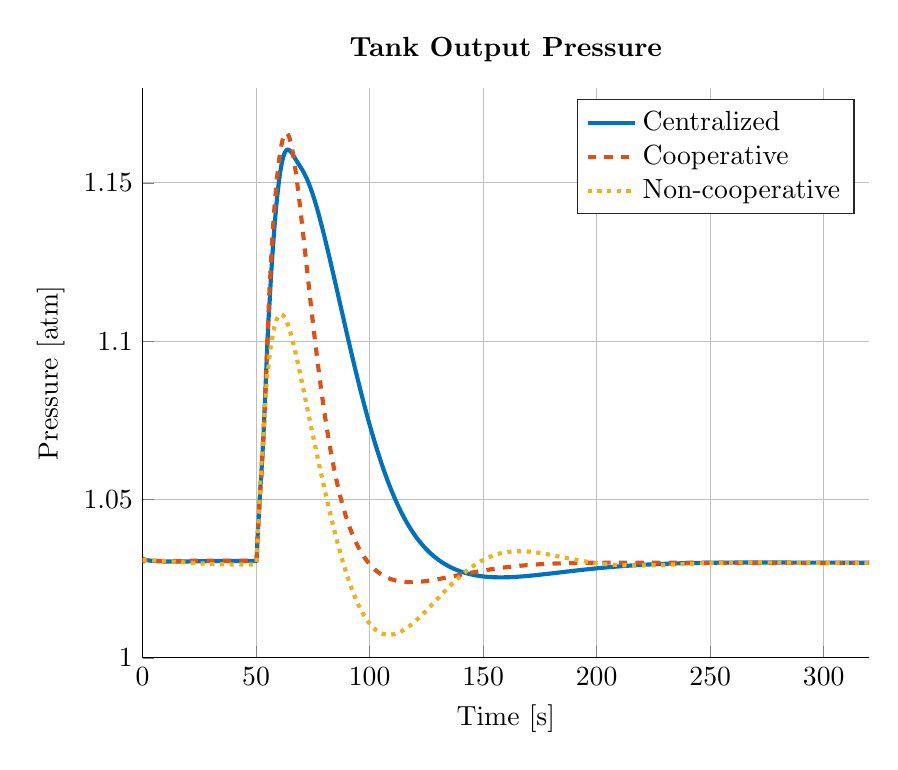
\begin{tikzpicture}

\begin{axis}[%
width=0.761\linewidth,
height=0.597\linewidth,
at={(0\linewidth,0\linewidth)},
scale only axis,
xmin=0,
xmax=320,
xlabel={Time [s]},
xmajorgrids,
ymin=1,
ymax=1.18,
ylabel={Pressure [atm]},
ymajorgrids,
axis background/.style={fill=white},
title style={font=\bfseries},
title={Tank Output Pressure},
axis x line*=bottom,
axis y line*=left,
legend style={legend cell align=left,align=left,draw=white!15!black}
]
\addplot [color=mycolor1,solid,line width=1.5pt]
  table[row sep=crcr]{%
0	1.03\\
0.25	1.03084\\
0.5	1.03105\\
0.75	1.03093\\
1	1.03093\\
1.25	1.03094\\
1.5	1.03091\\
1.75	1.03087\\
2	1.03084\\
2.25	1.03081\\
2.5	1.03079\\
2.75	1.03076\\
3	1.03074\\
3.25	1.03072\\
3.5	1.0307\\
3.75	1.03068\\
4	1.03066\\
4.25	1.03064\\
4.5	1.03062\\
4.75	1.03061\\
5	1.03059\\
5.25	1.03058\\
5.5	1.03057\\
5.75	1.03055\\
6	1.03054\\
6.25	1.03053\\
6.5	1.03052\\
6.75	1.03051\\
7	1.03051\\
7.25	1.0305\\
7.5	1.03049\\
7.75	1.03048\\
8	1.03048\\
8.25	1.03047\\
8.5	1.03046\\
8.75	1.03046\\
9	1.03045\\
9.25	1.03045\\
9.5	1.03045\\
9.75	1.03044\\
10	1.03044\\
10.25	1.03043\\
10.5	1.03043\\
10.75	1.03043\\
11	1.03043\\
11.25	1.03042\\
11.5	1.03042\\
11.75	1.03042\\
12	1.03042\\
12.25	1.03042\\
12.5	1.03042\\
12.75	1.03042\\
13	1.03042\\
13.25	1.03042\\
13.5	1.03042\\
13.75	1.03041\\
14	1.03042\\
14.25	1.03042\\
14.5	1.03042\\
14.75	1.03042\\
15	1.03042\\
15.25	1.03042\\
15.5	1.03042\\
15.75	1.03042\\
16	1.03042\\
16.25	1.03042\\
16.5	1.03042\\
16.75	1.03042\\
17	1.03043\\
17.25	1.03043\\
17.5	1.03043\\
17.75	1.03043\\
18	1.03043\\
18.25	1.03043\\
18.5	1.03044\\
18.75	1.03044\\
19	1.03044\\
19.25	1.03044\\
19.5	1.03045\\
19.75	1.03045\\
20	1.03045\\
20.25	1.03045\\
20.5	1.03046\\
20.75	1.03046\\
21	1.03046\\
21.25	1.03046\\
21.5	1.03047\\
21.75	1.03047\\
22	1.03047\\
22.25	1.03047\\
22.5	1.03048\\
22.75	1.03048\\
23	1.03048\\
23.25	1.03049\\
23.5	1.03049\\
23.75	1.03049\\
24	1.03049\\
24.25	1.0305\\
24.5	1.0305\\
24.75	1.0305\\
25	1.0305\\
25.25	1.03051\\
25.5	1.03051\\
25.75	1.03051\\
26	1.03051\\
26.25	1.03052\\
26.5	1.03052\\
26.75	1.03052\\
27	1.03052\\
27.25	1.03053\\
27.5	1.03053\\
27.75	1.03053\\
28	1.03053\\
28.25	1.03054\\
28.5	1.03054\\
28.75	1.03054\\
29	1.03054\\
29.25	1.03054\\
29.5	1.03055\\
29.75	1.03055\\
30	1.03055\\
30.25	1.03055\\
30.5	1.03055\\
30.75	1.03056\\
31	1.03056\\
31.25	1.03056\\
31.5	1.03056\\
31.75	1.03056\\
32	1.03057\\
32.25	1.03057\\
32.5	1.03057\\
32.75	1.03057\\
33	1.03057\\
33.25	1.03057\\
33.5	1.03057\\
33.75	1.03057\\
34	1.03058\\
34.25	1.03058\\
34.5	1.03058\\
34.75	1.03058\\
35	1.03058\\
35.25	1.03058\\
35.5	1.03058\\
35.75	1.03058\\
36	1.03058\\
36.25	1.03059\\
36.5	1.03059\\
36.75	1.03059\\
37	1.03059\\
37.25	1.03059\\
37.5	1.03059\\
37.75	1.03059\\
38	1.03059\\
38.25	1.03059\\
38.5	1.03059\\
38.75	1.03059\\
39	1.03059\\
39.25	1.03059\\
39.5	1.03059\\
39.75	1.03059\\
40	1.03059\\
40.25	1.03059\\
40.5	1.03059\\
40.75	1.0306\\
41	1.0306\\
41.25	1.0306\\
41.5	1.0306\\
41.75	1.0306\\
42	1.0306\\
42.25	1.0306\\
42.5	1.0306\\
42.75	1.0306\\
43	1.0306\\
43.25	1.0306\\
43.5	1.0306\\
43.75	1.0306\\
44	1.0306\\
44.25	1.0306\\
44.5	1.0306\\
44.75	1.0306\\
45	1.0306\\
45.25	1.03059\\
45.5	1.03059\\
45.75	1.03059\\
46	1.03059\\
46.25	1.03059\\
46.5	1.03059\\
46.75	1.03059\\
47	1.03059\\
47.25	1.03059\\
47.5	1.03059\\
47.75	1.03059\\
48	1.03059\\
48.25	1.03059\\
48.5	1.03059\\
48.75	1.03059\\
49	1.03059\\
49.25	1.03059\\
49.5	1.03059\\
49.75	1.03059\\
50	1.03059\\
50.25	1.03103\\
50.5	1.03504\\
50.75	1.0398\\
51	1.04245\\
51.25	1.04553\\
51.5	1.04912\\
51.75	1.05206\\
52	1.0547\\
52.25	1.0574\\
52.5	1.06051\\
52.75	1.06393\\
53	1.06686\\
53.25	1.0703\\
53.5	1.07423\\
53.75	1.07821\\
54	1.08238\\
54.25	1.08671\\
54.5	1.09105\\
54.75	1.09533\\
55	1.09951\\
55.25	1.10362\\
55.5	1.1072\\
55.75	1.10975\\
56	1.11291\\
56.25	1.11634\\
56.5	1.11944\\
56.75	1.12233\\
57	1.1251\\
57.25	1.12779\\
57.5	1.13037\\
57.75	1.13279\\
58	1.13511\\
58.25	1.13736\\
58.5	1.1395\\
58.75	1.14154\\
59	1.14346\\
59.25	1.14528\\
59.5	1.14698\\
59.75	1.14858\\
60	1.15007\\
60.25	1.15145\\
60.5	1.15272\\
60.75	1.15389\\
61	1.15496\\
61.25	1.15592\\
61.5	1.15678\\
61.75	1.15755\\
62	1.15822\\
62.25	1.15879\\
62.5	1.15927\\
62.75	1.15967\\
63	1.15998\\
63.25	1.16022\\
63.5	1.16038\\
63.75	1.16047\\
64	1.16049\\
64.25	1.16046\\
64.5	1.16038\\
64.75	1.16025\\
65	1.16008\\
65.25	1.15988\\
65.5	1.15965\\
65.75	1.1594\\
66	1.15913\\
66.25	1.15884\\
66.5	1.15855\\
66.75	1.15825\\
67	1.15795\\
67.25	1.15766\\
67.5	1.15736\\
67.75	1.15706\\
68	1.15677\\
68.25	1.15649\\
68.5	1.1562\\
68.75	1.15592\\
69	1.15564\\
69.25	1.15536\\
69.5	1.15507\\
69.75	1.15479\\
70	1.15449\\
70.25	1.15419\\
70.5	1.15389\\
70.75	1.15357\\
71	1.15325\\
71.25	1.15291\\
71.5	1.15256\\
71.75	1.1522\\
72	1.15183\\
72.25	1.15145\\
72.5	1.15105\\
72.75	1.15064\\
73	1.15021\\
73.25	1.14977\\
73.5	1.14931\\
73.75	1.14884\\
74	1.14836\\
74.25	1.14786\\
74.5	1.14735\\
74.75	1.14683\\
75	1.14629\\
75.25	1.14574\\
75.5	1.14517\\
75.75	1.1446\\
76	1.14401\\
76.25	1.14341\\
76.5	1.1428\\
76.75	1.14218\\
77	1.14155\\
77.25	1.14091\\
77.5	1.14026\\
77.75	1.1396\\
78	1.13893\\
78.25	1.13826\\
78.5	1.13758\\
78.75	1.13689\\
79	1.13619\\
79.25	1.13549\\
79.5	1.13478\\
79.75	1.13406\\
80	1.13334\\
80.25	1.13261\\
80.5	1.13188\\
80.75	1.13114\\
81	1.1304\\
81.25	1.12966\\
81.5	1.12891\\
81.75	1.12816\\
82	1.1274\\
82.25	1.12664\\
82.5	1.12588\\
82.75	1.12511\\
83	1.12434\\
83.25	1.12357\\
83.5	1.1228\\
83.75	1.12202\\
84	1.12124\\
84.25	1.12046\\
84.5	1.11968\\
84.75	1.1189\\
85	1.11812\\
85.25	1.11733\\
85.5	1.11654\\
85.75	1.11576\\
86	1.11497\\
86.25	1.11418\\
86.5	1.11339\\
86.75	1.1126\\
87	1.11181\\
87.25	1.11103\\
87.5	1.11024\\
87.75	1.10945\\
88	1.10866\\
88.25	1.10787\\
88.5	1.10709\\
88.75	1.1063\\
89	1.10552\\
89.25	1.10473\\
89.5	1.10395\\
89.75	1.10317\\
90	1.10239\\
90.25	1.10162\\
90.5	1.10084\\
90.75	1.10007\\
91	1.09929\\
91.25	1.09853\\
91.5	1.09776\\
91.75	1.09699\\
92	1.09623\\
92.25	1.09547\\
92.5	1.09471\\
92.75	1.09396\\
93	1.09321\\
93.25	1.09246\\
93.5	1.09171\\
93.75	1.09097\\
94	1.09023\\
94.25	1.0895\\
94.5	1.08877\\
94.75	1.08804\\
95	1.08731\\
95.25	1.08659\\
95.5	1.08587\\
95.75	1.08516\\
96	1.08445\\
96.25	1.08374\\
96.5	1.08304\\
96.75	1.08234\\
97	1.08165\\
97.25	1.08096\\
97.5	1.08027\\
97.75	1.07959\\
98	1.07892\\
98.25	1.07824\\
98.5	1.07758\\
98.75	1.07691\\
99	1.07626\\
99.25	1.0756\\
99.5	1.07495\\
99.75	1.07431\\
100	1.07367\\
100.25	1.07303\\
100.5	1.07241\\
100.75	1.07178\\
101	1.07116\\
101.25	1.07054\\
101.5	1.06993\\
101.75	1.06933\\
102	1.06873\\
102.25	1.06813\\
102.5	1.06754\\
102.75	1.06696\\
103	1.06638\\
103.25	1.0658\\
103.5	1.06523\\
103.75	1.06467\\
104	1.06411\\
104.25	1.06355\\
104.5	1.06301\\
104.75	1.06246\\
105	1.06192\\
105.25	1.06139\\
105.5	1.06086\\
105.75	1.06034\\
106	1.05982\\
106.25	1.0593\\
106.5	1.0588\\
106.75	1.05829\\
107	1.0578\\
107.25	1.0573\\
107.5	1.05682\\
107.75	1.05633\\
108	1.05586\\
108.25	1.05539\\
108.5	1.05492\\
108.75	1.05446\\
109	1.054\\
109.25	1.05355\\
109.5	1.0531\\
109.75	1.05266\\
110	1.05223\\
110.25	1.05179\\
110.5	1.05137\\
110.75	1.05095\\
111	1.05053\\
111.25	1.05012\\
111.5	1.04971\\
111.75	1.04931\\
112	1.04892\\
112.25	1.04853\\
112.5	1.04814\\
112.75	1.04776\\
113	1.04738\\
113.25	1.04701\\
113.5	1.04664\\
113.75	1.04628\\
114	1.04592\\
114.25	1.04557\\
114.5	1.04522\\
114.75	1.04487\\
115	1.04454\\
115.25	1.0442\\
115.5	1.04387\\
115.75	1.04354\\
116	1.04322\\
116.25	1.04291\\
116.5	1.04259\\
116.75	1.04229\\
117	1.04198\\
117.25	1.04168\\
117.5	1.04139\\
117.75	1.0411\\
118	1.04081\\
118.25	1.04053\\
118.5	1.04025\\
118.75	1.03997\\
119	1.0397\\
119.25	1.03944\\
119.5	1.03917\\
119.75	1.03891\\
120	1.03866\\
120.25	1.03841\\
120.5	1.03816\\
120.75	1.03792\\
121	1.03768\\
121.25	1.03744\\
121.5	1.03721\\
121.75	1.03698\\
122	1.03675\\
122.25	1.03653\\
122.5	1.03631\\
122.75	1.0361\\
123	1.03588\\
123.25	1.03567\\
123.5	1.03547\\
123.75	1.03527\\
124	1.03507\\
124.25	1.03487\\
124.5	1.03468\\
124.75	1.03449\\
125	1.0343\\
125.25	1.03412\\
125.5	1.03394\\
125.75	1.03376\\
126	1.03358\\
126.25	1.03341\\
126.5	1.03324\\
126.75	1.03307\\
127	1.03291\\
127.25	1.03275\\
127.5	1.03259\\
127.75	1.03243\\
128	1.03228\\
128.25	1.03213\\
128.5	1.03198\\
128.75	1.03183\\
129	1.03169\\
129.25	1.03154\\
129.5	1.03141\\
129.75	1.03127\\
130	1.03113\\
130.25	1.031\\
130.5	1.03087\\
130.75	1.03074\\
131	1.03062\\
131.25	1.03049\\
131.5	1.03037\\
131.75	1.03025\\
132	1.03013\\
132.25	1.03002\\
132.5	1.02991\\
132.75	1.02979\\
133	1.02969\\
133.25	1.02958\\
133.5	1.02947\\
133.75	1.02937\\
134	1.02927\\
134.25	1.02917\\
134.5	1.02907\\
134.75	1.02897\\
135	1.02888\\
135.25	1.02878\\
135.5	1.02869\\
135.75	1.0286\\
136	1.02851\\
136.25	1.02843\\
136.5	1.02834\\
136.75	1.02826\\
137	1.02818\\
137.25	1.0281\\
137.5	1.02802\\
137.75	1.02794\\
138	1.02787\\
138.25	1.02779\\
138.5	1.02772\\
138.75	1.02765\\
139	1.02758\\
139.25	1.02751\\
139.5	1.02745\\
139.75	1.02738\\
140	1.02732\\
140.25	1.02726\\
140.5	1.02719\\
140.75	1.02713\\
141	1.02708\\
141.25	1.02702\\
141.5	1.02696\\
141.75	1.02691\\
142	1.02685\\
142.25	1.0268\\
142.5	1.02675\\
142.75	1.0267\\
143	1.02665\\
143.25	1.0266\\
143.5	1.02656\\
143.75	1.02651\\
144	1.02647\\
144.25	1.02643\\
144.5	1.02638\\
144.75	1.02634\\
145	1.0263\\
145.25	1.02627\\
145.5	1.02623\\
145.75	1.02619\\
146	1.02616\\
146.25	1.02612\\
146.5	1.02609\\
146.75	1.02606\\
147	1.02602\\
147.25	1.02599\\
147.5	1.02596\\
147.75	1.02593\\
148	1.02591\\
148.25	1.02588\\
148.5	1.02585\\
148.75	1.02583\\
149	1.0258\\
149.25	1.02578\\
149.5	1.02576\\
149.75	1.02574\\
150	1.02572\\
150.25	1.0257\\
150.5	1.02568\\
150.75	1.02566\\
151	1.02564\\
151.25	1.02562\\
151.5	1.02561\\
151.75	1.02559\\
152	1.02558\\
152.25	1.02556\\
152.5	1.02555\\
152.75	1.02554\\
153	1.02553\\
153.25	1.02552\\
153.5	1.02551\\
153.75	1.0255\\
154	1.02549\\
154.25	1.02548\\
154.5	1.02547\\
154.75	1.02546\\
155	1.02546\\
155.25	1.02545\\
155.5	1.02545\\
155.75	1.02544\\
156	1.02544\\
156.25	1.02543\\
156.5	1.02543\\
156.75	1.02543\\
157	1.02543\\
157.25	1.02543\\
157.5	1.02542\\
157.75	1.02542\\
158	1.02542\\
158.25	1.02543\\
158.5	1.02543\\
158.75	1.02543\\
159	1.02543\\
159.25	1.02543\\
159.5	1.02544\\
159.75	1.02544\\
160	1.02544\\
160.25	1.02545\\
160.5	1.02545\\
160.75	1.02546\\
161	1.02546\\
161.25	1.02547\\
161.5	1.02548\\
161.75	1.02548\\
162	1.02549\\
162.25	1.0255\\
162.5	1.02551\\
162.75	1.02552\\
163	1.02553\\
163.25	1.02553\\
163.5	1.02554\\
163.75	1.02555\\
164	1.02556\\
164.25	1.02558\\
164.5	1.02559\\
164.75	1.0256\\
165	1.02561\\
165.25	1.02562\\
165.5	1.02563\\
165.75	1.02564\\
166	1.02566\\
166.25	1.02567\\
166.5	1.02568\\
166.75	1.0257\\
167	1.02571\\
167.25	1.02573\\
167.5	1.02574\\
167.75	1.02575\\
168	1.02577\\
168.25	1.02578\\
168.5	1.0258\\
168.75	1.02581\\
169	1.02583\\
169.25	1.02585\\
169.5	1.02586\\
169.75	1.02588\\
170	1.02589\\
170.25	1.02591\\
170.5	1.02593\\
170.75	1.02594\\
171	1.02596\\
171.25	1.02598\\
171.5	1.026\\
171.75	1.02601\\
172	1.02603\\
172.25	1.02605\\
172.5	1.02607\\
172.75	1.02609\\
173	1.02611\\
173.25	1.02612\\
173.5	1.02614\\
173.75	1.02616\\
174	1.02618\\
174.25	1.0262\\
174.5	1.02622\\
174.75	1.02624\\
175	1.02626\\
175.25	1.02628\\
175.5	1.0263\\
175.75	1.02632\\
176	1.02634\\
176.25	1.02636\\
176.5	1.02638\\
176.75	1.0264\\
177	1.02642\\
177.25	1.02644\\
177.5	1.02646\\
177.75	1.02648\\
178	1.0265\\
178.25	1.02652\\
178.5	1.02654\\
178.75	1.02656\\
179	1.02658\\
179.25	1.0266\\
179.5	1.02662\\
179.75	1.02664\\
180	1.02666\\
180.25	1.02668\\
180.5	1.0267\\
180.75	1.02672\\
181	1.02675\\
181.25	1.02677\\
181.5	1.02679\\
181.75	1.02681\\
182	1.02683\\
182.25	1.02685\\
182.5	1.02687\\
182.75	1.02689\\
183	1.02691\\
183.25	1.02694\\
183.5	1.02696\\
183.75	1.02698\\
184	1.027\\
184.25	1.02702\\
184.5	1.02704\\
184.75	1.02706\\
185	1.02708\\
185.25	1.0271\\
185.5	1.02713\\
185.75	1.02715\\
186	1.02717\\
186.25	1.02719\\
186.5	1.02721\\
186.75	1.02723\\
187	1.02725\\
187.25	1.02727\\
187.5	1.02729\\
187.75	1.02731\\
188	1.02733\\
188.25	1.02736\\
188.5	1.02738\\
188.75	1.0274\\
189	1.02742\\
189.25	1.02744\\
189.5	1.02746\\
189.75	1.02748\\
190	1.0275\\
190.25	1.02752\\
190.5	1.02754\\
190.75	1.02756\\
191	1.02758\\
191.25	1.0276\\
191.5	1.02762\\
191.75	1.02764\\
192	1.02766\\
192.25	1.02768\\
192.5	1.0277\\
192.75	1.02772\\
193	1.02774\\
193.25	1.02776\\
193.5	1.02778\\
193.75	1.0278\\
194	1.02782\\
194.25	1.02784\\
194.5	1.02786\\
194.75	1.02788\\
195	1.0279\\
195.25	1.02792\\
195.5	1.02794\\
195.75	1.02795\\
196	1.02797\\
196.25	1.02799\\
196.5	1.02801\\
196.75	1.02803\\
197	1.02805\\
197.25	1.02807\\
197.5	1.02809\\
197.75	1.0281\\
198	1.02812\\
198.25	1.02814\\
198.5	1.02816\\
198.75	1.02818\\
199	1.0282\\
199.25	1.02821\\
199.5	1.02823\\
199.75	1.02825\\
200	1.02827\\
200.25	1.02828\\
200.5	1.0283\\
200.75	1.02832\\
201	1.02834\\
201.25	1.02835\\
201.5	1.02837\\
201.75	1.02839\\
202	1.0284\\
202.25	1.02842\\
202.5	1.02844\\
202.75	1.02845\\
203	1.02847\\
203.25	1.02849\\
203.5	1.0285\\
203.75	1.02852\\
204	1.02854\\
204.25	1.02855\\
204.5	1.02857\\
204.75	1.02858\\
205	1.0286\\
205.25	1.02862\\
205.5	1.02863\\
205.75	1.02865\\
206	1.02866\\
206.25	1.02868\\
206.5	1.02869\\
206.75	1.02871\\
207	1.02872\\
207.25	1.02874\\
207.5	1.02875\\
207.75	1.02877\\
208	1.02878\\
208.25	1.0288\\
208.5	1.02881\\
208.75	1.02883\\
209	1.02884\\
209.25	1.02885\\
209.5	1.02887\\
209.75	1.02888\\
210	1.0289\\
210.25	1.02891\\
210.5	1.02892\\
210.75	1.02894\\
211	1.02895\\
211.25	1.02896\\
211.5	1.02898\\
211.75	1.02899\\
212	1.029\\
212.25	1.02902\\
212.5	1.02903\\
212.75	1.02904\\
213	1.02905\\
213.25	1.02907\\
213.5	1.02908\\
213.75	1.02909\\
214	1.0291\\
214.25	1.02912\\
214.5	1.02913\\
214.75	1.02914\\
215	1.02915\\
215.25	1.02916\\
215.5	1.02918\\
215.75	1.02919\\
216	1.0292\\
216.25	1.02921\\
216.5	1.02922\\
216.75	1.02923\\
217	1.02924\\
217.25	1.02926\\
217.5	1.02927\\
217.75	1.02928\\
218	1.02929\\
218.25	1.0293\\
218.5	1.02931\\
218.75	1.02932\\
219	1.02933\\
219.25	1.02934\\
219.5	1.02935\\
219.75	1.02936\\
220	1.02937\\
220.25	1.02938\\
220.5	1.02939\\
220.75	1.0294\\
221	1.02941\\
221.25	1.02942\\
221.5	1.02943\\
221.75	1.02944\\
222	1.02945\\
222.25	1.02946\\
222.5	1.02947\\
222.75	1.02947\\
223	1.02948\\
223.25	1.02949\\
223.5	1.0295\\
223.75	1.02951\\
224	1.02952\\
224.25	1.02953\\
224.5	1.02954\\
224.75	1.02954\\
225	1.02955\\
225.25	1.02956\\
225.5	1.02957\\
225.75	1.02958\\
226	1.02958\\
226.25	1.02959\\
226.5	1.0296\\
226.75	1.02961\\
227	1.02962\\
227.25	1.02962\\
227.5	1.02963\\
227.75	1.02964\\
228	1.02965\\
228.25	1.02965\\
228.5	1.02966\\
228.75	1.02967\\
229	1.02967\\
229.25	1.02968\\
229.5	1.02969\\
229.75	1.02969\\
230	1.0297\\
230.25	1.02971\\
230.5	1.02971\\
230.75	1.02972\\
231	1.02973\\
231.25	1.02973\\
231.5	1.02974\\
231.75	1.02975\\
232	1.02975\\
232.25	1.02976\\
232.5	1.02976\\
232.75	1.02977\\
233	1.02978\\
233.25	1.02978\\
233.5	1.02979\\
233.75	1.02979\\
234	1.0298\\
234.25	1.0298\\
234.5	1.02981\\
234.75	1.02981\\
235	1.02982\\
235.25	1.02983\\
235.5	1.02983\\
235.75	1.02984\\
236	1.02984\\
236.25	1.02985\\
236.5	1.02985\\
236.75	1.02986\\
237	1.02986\\
237.25	1.02986\\
237.5	1.02987\\
237.75	1.02987\\
238	1.02988\\
238.25	1.02988\\
238.5	1.02989\\
238.75	1.02989\\
239	1.0299\\
239.25	1.0299\\
239.5	1.0299\\
239.75	1.02991\\
240	1.02991\\
240.25	1.02992\\
240.5	1.02992\\
240.75	1.02992\\
241	1.02993\\
241.25	1.02993\\
241.5	1.02994\\
241.75	1.02994\\
242	1.02994\\
242.25	1.02995\\
242.5	1.02995\\
242.75	1.02995\\
243	1.02996\\
243.25	1.02996\\
243.5	1.02996\\
243.75	1.02997\\
244	1.02997\\
244.25	1.02997\\
244.5	1.02998\\
244.75	1.02998\\
245	1.02998\\
245.25	1.02999\\
245.5	1.02999\\
245.75	1.02999\\
246	1.02999\\
246.25	1.03\\
246.5	1.03\\
246.75	1.03\\
247	1.03001\\
247.25	1.03001\\
247.5	1.03001\\
247.75	1.03001\\
248	1.03002\\
248.25	1.03002\\
248.5	1.03002\\
248.75	1.03002\\
249	1.03002\\
249.25	1.03003\\
249.5	1.03003\\
249.75	1.03003\\
250	1.03003\\
250.25	1.03004\\
250.5	1.03004\\
250.75	1.03004\\
251	1.03004\\
251.25	1.03004\\
251.5	1.03005\\
251.75	1.03005\\
252	1.03005\\
252.25	1.03005\\
252.5	1.03005\\
252.75	1.03005\\
253	1.03006\\
253.25	1.03006\\
253.5	1.03006\\
253.75	1.03006\\
254	1.03006\\
254.25	1.03006\\
254.5	1.03007\\
254.75	1.03007\\
255	1.03007\\
255.25	1.03007\\
255.5	1.03007\\
255.75	1.03007\\
256	1.03007\\
256.25	1.03008\\
256.5	1.03008\\
256.75	1.03008\\
257	1.03008\\
257.25	1.03008\\
257.5	1.03008\\
257.75	1.03008\\
258	1.03008\\
258.25	1.03009\\
258.5	1.03009\\
258.75	1.03009\\
259	1.03009\\
259.25	1.03009\\
259.5	1.03009\\
259.75	1.03009\\
260	1.03009\\
260.25	1.03009\\
260.5	1.03009\\
260.75	1.03009\\
261	1.0301\\
261.25	1.0301\\
261.5	1.0301\\
261.75	1.0301\\
262	1.0301\\
262.25	1.0301\\
262.5	1.0301\\
262.75	1.0301\\
263	1.0301\\
263.25	1.0301\\
263.5	1.0301\\
263.75	1.0301\\
264	1.0301\\
264.25	1.0301\\
264.5	1.0301\\
264.75	1.0301\\
265	1.0301\\
265.25	1.0301\\
265.5	1.03011\\
265.75	1.03011\\
266	1.03011\\
266.25	1.03011\\
266.5	1.03011\\
266.75	1.03011\\
267	1.03011\\
267.25	1.03011\\
267.5	1.03011\\
267.75	1.03011\\
268	1.03011\\
268.25	1.03011\\
268.5	1.03011\\
268.75	1.03011\\
269	1.03011\\
269.25	1.03011\\
269.5	1.03011\\
269.75	1.03011\\
270	1.03011\\
270.25	1.03011\\
270.5	1.03011\\
270.75	1.03011\\
271	1.03011\\
271.25	1.03011\\
271.5	1.03011\\
271.75	1.03011\\
272	1.03011\\
272.25	1.03011\\
272.5	1.03011\\
272.75	1.03011\\
273	1.03011\\
273.25	1.03011\\
273.5	1.03011\\
273.75	1.03011\\
274	1.03011\\
274.25	1.03011\\
274.5	1.03011\\
274.75	1.03011\\
275	1.03011\\
275.25	1.03011\\
275.5	1.03011\\
275.75	1.03011\\
276	1.03011\\
276.25	1.03011\\
276.5	1.03011\\
276.75	1.03011\\
277	1.03011\\
277.25	1.03011\\
277.5	1.03011\\
277.75	1.03011\\
278	1.03011\\
278.25	1.03011\\
278.5	1.03011\\
278.75	1.03011\\
279	1.0301\\
279.25	1.0301\\
279.5	1.0301\\
279.75	1.0301\\
280	1.0301\\
280.25	1.0301\\
280.5	1.0301\\
280.75	1.0301\\
281	1.0301\\
281.25	1.0301\\
281.5	1.0301\\
281.75	1.0301\\
282	1.0301\\
282.25	1.0301\\
282.5	1.0301\\
282.75	1.0301\\
283	1.0301\\
283.25	1.0301\\
283.5	1.0301\\
283.75	1.0301\\
284	1.0301\\
284.25	1.0301\\
284.5	1.0301\\
284.75	1.0301\\
285	1.0301\\
285.25	1.0301\\
285.5	1.03009\\
285.75	1.03009\\
286	1.03009\\
286.25	1.03009\\
286.5	1.03009\\
286.75	1.03009\\
287	1.03009\\
287.25	1.03009\\
287.5	1.03009\\
287.75	1.03009\\
288	1.03009\\
288.25	1.03009\\
288.5	1.03009\\
288.75	1.03009\\
289	1.03009\\
289.25	1.03009\\
289.5	1.03009\\
289.75	1.03009\\
290	1.03009\\
290.25	1.03009\\
290.5	1.03009\\
290.75	1.03009\\
291	1.03008\\
291.25	1.03008\\
291.5	1.03008\\
291.75	1.03008\\
292	1.03008\\
292.25	1.03008\\
292.5	1.03008\\
292.75	1.03008\\
293	1.03008\\
293.25	1.03008\\
293.5	1.03008\\
293.75	1.03008\\
294	1.03008\\
294.25	1.03008\\
294.5	1.03008\\
294.75	1.03008\\
295	1.03008\\
295.25	1.03008\\
295.5	1.03008\\
295.75	1.03007\\
296	1.03007\\
296.25	1.03007\\
296.5	1.03007\\
296.75	1.03007\\
297	1.03007\\
297.25	1.03007\\
297.5	1.03007\\
297.75	1.03007\\
298	1.03007\\
298.25	1.03007\\
298.5	1.03007\\
298.75	1.03007\\
299	1.03007\\
299.25	1.03007\\
299.5	1.03007\\
299.75	1.03007\\
300	1.03007\\
300.25	1.03007\\
300.5	1.03007\\
300.75	1.03006\\
301	1.03006\\
301.25	1.03006\\
301.5	1.03006\\
301.75	1.03006\\
302	1.03006\\
302.25	1.03006\\
302.5	1.03006\\
302.75	1.03006\\
303	1.03006\\
303.25	1.03006\\
303.5	1.03006\\
303.75	1.03006\\
304	1.03006\\
304.25	1.03006\\
304.5	1.03006\\
304.75	1.03006\\
305	1.03006\\
305.25	1.03006\\
305.5	1.03006\\
305.75	1.03005\\
306	1.03005\\
306.25	1.03005\\
306.5	1.03005\\
306.75	1.03005\\
307	1.03005\\
307.25	1.03005\\
307.5	1.03005\\
307.75	1.03005\\
308	1.03005\\
308.25	1.03005\\
308.5	1.03005\\
308.75	1.03005\\
309	1.03005\\
309.25	1.03005\\
309.5	1.03005\\
309.75	1.03005\\
310	1.03005\\
310.25	1.03005\\
310.5	1.03005\\
310.75	1.03005\\
311	1.03004\\
311.25	1.03004\\
311.5	1.03004\\
311.75	1.03004\\
312	1.03004\\
312.25	1.03004\\
312.5	1.03004\\
312.75	1.03004\\
313	1.03004\\
313.25	1.03004\\
313.5	1.03004\\
313.75	1.03004\\
314	1.03004\\
314.25	1.03004\\
314.5	1.03004\\
314.75	1.03004\\
315	1.03004\\
315.25	1.03004\\
315.5	1.03004\\
315.75	1.03004\\
316	1.03004\\
316.25	1.03004\\
316.5	1.03004\\
316.75	1.03004\\
317	1.03003\\
317.25	1.03003\\
317.5	1.03003\\
317.75	1.03003\\
318	1.03003\\
318.25	1.03003\\
318.5	1.03003\\
318.75	1.03003\\
319	1.03003\\
319.25	1.03003\\
319.5	1.03003\\
319.75	1.03003\\
320	1.03003\\
320.25	1.03003\\
320.5	1.03003\\
320.75	1.03003\\
321	1.03003\\
321.25	1.03003\\
321.5	1.03003\\
321.75	1.03003\\
322	1.03003\\
322.25	1.03003\\
322.5	1.03003\\
322.75	1.03003\\
323	1.03003\\
323.25	1.03003\\
323.5	1.03003\\
323.75	1.03003\\
324	1.03002\\
324.25	1.03002\\
324.5	1.03002\\
324.75	1.03002\\
325	1.03002\\
325.25	1.03002\\
325.5	1.03002\\
325.75	1.03002\\
326	1.03002\\
326.25	1.03002\\
326.5	1.03002\\
326.75	1.03002\\
327	1.03002\\
327.25	1.03002\\
327.5	1.03002\\
327.75	1.03002\\
328	1.03002\\
328.25	1.03002\\
328.5	1.03002\\
328.75	1.03002\\
329	1.03002\\
329.25	1.03002\\
329.5	1.03002\\
329.75	1.03002\\
330	1.03002\\
330.25	1.03002\\
330.5	1.03002\\
330.75	1.03002\\
331	1.03002\\
331.25	1.03002\\
331.5	1.03002\\
331.75	1.03002\\
332	1.03002\\
332.25	1.03002\\
332.5	1.03002\\
332.75	1.03001\\
333	1.03001\\
333.25	1.03001\\
333.5	1.03001\\
333.75	1.03001\\
334	1.03001\\
334.25	1.03001\\
334.5	1.03001\\
334.75	1.03001\\
335	1.03001\\
335.25	1.03001\\
335.5	1.03001\\
335.75	1.03001\\
336	1.03001\\
336.25	1.03001\\
336.5	1.03001\\
336.75	1.03001\\
337	1.03001\\
337.25	1.03001\\
337.5	1.03001\\
337.75	1.03001\\
338	1.03001\\
338.25	1.03001\\
338.5	1.03001\\
338.75	1.03001\\
339	1.03001\\
339.25	1.03001\\
339.5	1.03001\\
339.75	1.03001\\
340	1.03001\\
340.25	1.03001\\
340.5	1.03001\\
340.75	1.03001\\
341	1.03001\\
341.25	1.03001\\
341.5	1.03001\\
341.75	1.03001\\
342	1.03001\\
342.25	1.03001\\
342.5	1.03001\\
342.75	1.03001\\
343	1.03001\\
343.25	1.03001\\
343.5	1.03001\\
343.75	1.03001\\
344	1.03001\\
344.25	1.03001\\
344.5	1.03001\\
344.75	1.03001\\
345	1.03001\\
345.25	1.03001\\
345.5	1.03001\\
345.75	1.03001\\
346	1.03001\\
346.25	1.03\\
346.5	1.03\\
346.75	1.03\\
347	1.03\\
347.25	1.03\\
347.5	1.03\\
347.75	1.03\\
348	1.03\\
348.25	1.03\\
348.5	1.03\\
348.75	1.03\\
349	1.03\\
349.25	1.03\\
349.5	1.03\\
349.75	1.03\\
350	1.03\\
350.25	1.03\\
350.5	1.03\\
350.75	1.03\\
351	1.03\\
351.25	1.03\\
351.5	1.03\\
351.75	1.03\\
352	1.03\\
352.25	1.03\\
352.5	1.03\\
352.75	1.03\\
353	1.03\\
353.25	1.03\\
353.5	1.03\\
353.75	1.03\\
354	1.03\\
354.25	1.03\\
354.5	1.03\\
354.75	1.03\\
355	1.03\\
355.25	1.03\\
355.5	1.03\\
355.75	1.03\\
356	1.03\\
356.25	1.03\\
356.5	1.03\\
356.75	1.03\\
357	1.03\\
357.25	1.03\\
357.5	1.03\\
357.75	1.03\\
358	1.03\\
358.25	1.03\\
358.5	1.03\\
358.75	1.03\\
359	1.03\\
359.25	1.03\\
359.5	1.03\\
359.75	1.03\\
360	1.03\\
360.25	1.03\\
360.5	1.03\\
360.75	1.03\\
361	1.03\\
361.25	1.03\\
361.5	1.03\\
361.75	1.03\\
362	1.03\\
362.25	1.03\\
362.5	1.03\\
362.75	1.03\\
363	1.03\\
363.25	1.03\\
363.5	1.03\\
363.75	1.03\\
364	1.03\\
364.25	1.03\\
364.5	1.03\\
364.75	1.03\\
365	1.03\\
365.25	1.03\\
365.5	1.03\\
365.75	1.03\\
366	1.03\\
366.25	1.03\\
366.5	1.03\\
366.75	1.03\\
367	1.03\\
367.25	1.03\\
367.5	1.03\\
367.75	1.03\\
368	1.03\\
368.25	1.03\\
368.5	1.03\\
368.75	1.03\\
369	1.03\\
369.25	1.03\\
369.5	1.03\\
369.75	1.03\\
370	1.03\\
370.25	1.03\\
370.5	1.03\\
370.75	1.03\\
371	1.03\\
371.25	1.03\\
371.5	1.03\\
371.75	1.03\\
372	1.03\\
372.25	1.03\\
372.5	1.03\\
372.75	1.03\\
373	1.03\\
373.25	1.03\\
373.5	1.03\\
373.75	1.03\\
374	1.03\\
374.25	1.03\\
374.5	1.03\\
374.75	1.03\\
375	1.03\\
375.25	1.03\\
375.5	1.03\\
375.75	1.03\\
376	1.03\\
376.25	1.03\\
376.5	1.03\\
376.75	1.03\\
377	1.03\\
377.25	1.03\\
377.5	1.03\\
377.75	1.03\\
378	1.03\\
378.25	1.03\\
378.5	1.03\\
378.75	1.03\\
379	1.03\\
379.25	1.03\\
379.5	1.03\\
379.75	1.03\\
380	1.03\\
380.25	1.03\\
380.5	1.03\\
380.75	1.03\\
381	1.03\\
381.25	1.03\\
381.5	1.03\\
381.75	1.03\\
382	1.03\\
382.25	1.03\\
382.5	1.03\\
382.75	1.03\\
383	1.03\\
383.25	1.03\\
383.5	1.03\\
383.75	1.03\\
384	1.03\\
384.25	1.03\\
384.5	1.03\\
384.75	1.03\\
385	1.03\\
385.25	1.03\\
385.5	1.03\\
385.75	1.03\\
386	1.03\\
386.25	1.03\\
386.5	1.03\\
386.75	1.03\\
387	1.03\\
387.25	1.03\\
387.5	1.03\\
387.75	1.03\\
388	1.03\\
388.25	1.03\\
388.5	1.03\\
388.75	1.03\\
389	1.03\\
389.25	1.03\\
389.5	1.03\\
389.75	1.03\\
390	1.03\\
390.25	1.03\\
390.5	1.03\\
390.75	1.03\\
391	1.03\\
391.25	1.03\\
391.5	1.03\\
391.75	1.03\\
392	1.03\\
392.25	1.03\\
392.5	1.03\\
392.75	1.03\\
393	1.03\\
393.25	1.03\\
393.5	1.03\\
393.75	1.03\\
394	1.03\\
394.25	1.03\\
394.5	1.03\\
394.75	1.03\\
395	1.03\\
395.25	1.03\\
395.5	1.03\\
395.75	1.03\\
396	1.03\\
396.25	1.03\\
396.5	1.03\\
396.75	1.03\\
397	1.03\\
397.25	1.03\\
397.5	1.03\\
397.75	1.03\\
398	1.03\\
398.25	1.03\\
398.5	1.03\\
398.75	1.03\\
399	1.03\\
399.25	1.03\\
399.5	1.03\\
399.75	1.03\\
400	1.03\\
400.25	1.03\\
400.5	1.03\\
400.75	1.03\\
401	1.03\\
401.25	1.03\\
401.5	1.03\\
401.75	1.03\\
402	1.03\\
402.25	1.03\\
402.5	1.03\\
402.75	1.03\\
403	1.03\\
403.25	1.03\\
403.5	1.03\\
403.75	1.03\\
404	1.03\\
404.25	1.03\\
404.5	1.03\\
404.75	1.03\\
405	1.03\\
405.25	1.03\\
405.5	1.03\\
405.75	1.03\\
406	1.03\\
406.25	1.03\\
406.5	1.03\\
406.75	1.03\\
407	1.03\\
407.25	1.03\\
407.5	1.03\\
407.75	1.03\\
408	1.03\\
408.25	1.03\\
408.5	1.03\\
408.75	1.03\\
409	1.03\\
409.25	1.03\\
409.5	1.03\\
409.75	1.03\\
410	1.03\\
410.25	1.03\\
410.5	1.03\\
410.75	1.03\\
411	1.03\\
411.25	1.03\\
411.5	1.03\\
411.75	1.03\\
412	1.03\\
412.25	1.03\\
412.5	1.03\\
412.75	1.03\\
413	1.03\\
413.25	1.03\\
413.5	1.03\\
413.75	1.03\\
414	1.03\\
414.25	1.03\\
414.5	1.03\\
414.75	1.03\\
415	1.03\\
415.25	1.03\\
415.5	1.03\\
415.75	1.03\\
416	1.03\\
416.25	1.03\\
416.5	1.03\\
416.75	1.03\\
417	1.03\\
417.25	1.03\\
417.5	1.03\\
417.75	1.03\\
418	1.03\\
418.25	1.03\\
418.5	1.03\\
418.75	1.03\\
419	1.03\\
419.25	1.03\\
419.5	1.03\\
419.75	1.03\\
420	1.03\\
420.25	1.03\\
420.5	1.03\\
420.75	1.03\\
421	1.03\\
421.25	1.03\\
421.5	1.03\\
421.75	1.03\\
422	1.03\\
422.25	1.03\\
422.5	1.03\\
422.75	1.03\\
423	1.03\\
423.25	1.03\\
423.5	1.03\\
423.75	1.03\\
424	1.03\\
424.25	1.03\\
424.5	1.03\\
424.75	1.03\\
425	1.03\\
425.25	1.03\\
425.5	1.03\\
425.75	1.03\\
426	1.03\\
426.25	1.03\\
426.5	1.03\\
426.75	1.03\\
427	1.03\\
427.25	1.03\\
427.5	1.03\\
427.75	1.03\\
428	1.03\\
428.25	1.03\\
428.5	1.03\\
428.75	1.03\\
429	1.03\\
429.25	1.03\\
429.5	1.03\\
429.75	1.03\\
430	1.03\\
430.25	1.03\\
430.5	1.03\\
430.75	1.03\\
431	1.03\\
431.25	1.03\\
431.5	1.03\\
431.75	1.03\\
432	1.03\\
432.25	1.03\\
432.5	1.03\\
432.75	1.03\\
433	1.03\\
433.25	1.03\\
433.5	1.03\\
433.75	1.03\\
434	1.03\\
434.25	1.03\\
434.5	1.03\\
434.75	1.03\\
435	1.03\\
435.25	1.03\\
435.5	1.03\\
435.75	1.03\\
436	1.03\\
436.25	1.03\\
436.5	1.03\\
436.75	1.03\\
437	1.03\\
437.25	1.03\\
437.5	1.03\\
437.75	1.03\\
438	1.03\\
438.25	1.03\\
438.5	1.03\\
438.75	1.03\\
439	1.03\\
439.25	1.03\\
439.5	1.03\\
439.75	1.03\\
440	1.03\\
440.25	1.03\\
440.5	1.03\\
440.75	1.03\\
441	1.03\\
441.25	1.03\\
441.5	1.03\\
441.75	1.03\\
442	1.03\\
442.25	1.03\\
442.5	1.03\\
442.75	1.03\\
443	1.03\\
443.25	1.03\\
443.5	1.03\\
443.75	1.03\\
444	1.03\\
444.25	1.03\\
444.5	1.03\\
444.75	1.03\\
445	1.03\\
445.25	1.03\\
445.5	1.03\\
445.75	1.03\\
446	1.03\\
446.25	1.03\\
446.5	1.03\\
446.75	1.03\\
447	1.03\\
447.25	1.03\\
447.5	1.03\\
447.75	1.03\\
448	1.03\\
448.25	1.03\\
448.5	1.03\\
448.75	1.03\\
449	1.03\\
449.25	1.03\\
449.5	1.03\\
449.75	1.03\\
450	1.03\\
450.25	1.03\\
450.5	1.03\\
450.75	1.03\\
451	1.03\\
451.25	1.03\\
451.5	1.03\\
451.75	1.03\\
452	1.03\\
452.25	1.03\\
452.5	1.03\\
452.75	1.03\\
453	1.03\\
453.25	1.03\\
453.5	1.03\\
453.75	1.03\\
454	1.03\\
454.25	1.03\\
454.5	1.03\\
454.75	1.03\\
455	1.03\\
455.25	1.03\\
455.5	1.03\\
455.75	1.03\\
456	1.03\\
456.25	1.03\\
456.5	1.03\\
456.75	1.03\\
457	1.03\\
457.25	1.03\\
457.5	1.03\\
457.75	1.03\\
458	1.03\\
458.25	1.03\\
458.5	1.03\\
458.75	1.03\\
459	1.03\\
459.25	1.03\\
459.5	1.03\\
459.75	1.03\\
460	1.03\\
460.25	1.03\\
460.5	1.03\\
460.75	1.03\\
461	1.03\\
461.25	1.03\\
461.5	1.03\\
461.75	1.03\\
462	1.03\\
462.25	1.03\\
462.5	1.03\\
462.75	1.03\\
463	1.03\\
463.25	1.03\\
463.5	1.03\\
463.75	1.03\\
464	1.03\\
464.25	1.03\\
464.5	1.03\\
464.75	1.03\\
465	1.03\\
465.25	1.03\\
465.5	1.03\\
465.75	1.03\\
466	1.03\\
466.25	1.03\\
466.5	1.03\\
466.75	1.03\\
467	1.03\\
467.25	1.03\\
467.5	1.03\\
467.75	1.03\\
468	1.03\\
468.25	1.03\\
468.5	1.03\\
468.75	1.03\\
469	1.03\\
469.25	1.03\\
469.5	1.03\\
469.75	1.03\\
470	1.03\\
470.25	1.03\\
470.5	1.03\\
470.75	1.03\\
471	1.03\\
471.25	1.03\\
471.5	1.03\\
471.75	1.03\\
472	1.03\\
472.25	1.03\\
472.5	1.03\\
472.75	1.03\\
473	1.03\\
473.25	1.03\\
473.5	1.03\\
473.75	1.03\\
474	1.03\\
474.25	1.03\\
474.5	1.03\\
474.75	1.03\\
475	1.03\\
475.25	1.03\\
475.5	1.03\\
475.75	1.03\\
476	1.03\\
476.25	1.03\\
476.5	1.03\\
476.75	1.03\\
477	1.03\\
477.25	1.03\\
477.5	1.03\\
477.75	1.03\\
478	1.03\\
478.25	1.03\\
478.5	1.03\\
478.75	1.03\\
479	1.03\\
479.25	1.03\\
479.5	1.03\\
479.75	1.03\\
480	1.03\\
480.25	1.03\\
480.5	1.03\\
480.75	1.03\\
481	1.03\\
481.25	1.03\\
481.5	1.03\\
481.75	1.03\\
482	1.03\\
482.25	1.03\\
482.5	1.03\\
482.75	1.03\\
483	1.03\\
483.25	1.03\\
483.5	1.03\\
483.75	1.03\\
484	1.03\\
484.25	1.03\\
484.5	1.03\\
484.75	1.03\\
485	1.03\\
485.25	1.03\\
485.5	1.03\\
485.75	1.03\\
486	1.03\\
486.25	1.03\\
486.5	1.03\\
486.75	1.03\\
487	1.03\\
487.25	1.03\\
487.5	1.03\\
487.75	1.03\\
488	1.03\\
488.25	1.03\\
488.5	1.03\\
488.75	1.03\\
489	1.03\\
489.25	1.03\\
489.5	1.03\\
489.75	1.03\\
490	1.03\\
490.25	1.03\\
490.5	1.03\\
490.75	1.03\\
491	1.03\\
491.25	1.03\\
491.5	1.03\\
491.75	1.03\\
492	1.03\\
492.25	1.03\\
492.5	1.03\\
492.75	1.03\\
493	1.03\\
493.25	1.03\\
493.5	1.03\\
493.75	1.03\\
494	1.03\\
494.25	1.03\\
494.5	1.03\\
494.75	1.03\\
495	1.03\\
495.25	1.03\\
495.5	1.03\\
495.75	1.03\\
496	1.03\\
496.25	1.03\\
496.5	1.03\\
496.75	1.03\\
497	1.03\\
497.25	1.03\\
497.5	1.03\\
497.75	1.03\\
498	1.03\\
498.25	1.03\\
498.5	1.03\\
498.75	1.03\\
499	1.03\\
499.25	1.03\\
499.5	1.03\\
499.75	1.03\\
};
\addlegendentry{Centralized};

\addplot [color=mycolor2,dashed,line width=1.5pt]
  table[row sep=crcr]{%
0	1.03\\
0.25	1.03084\\
0.5	1.03106\\
0.75	1.03094\\
1	1.03094\\
1.25	1.03097\\
1.5	1.03094\\
1.75	1.0309\\
2	1.03088\\
2.25	1.03086\\
2.5	1.03084\\
2.75	1.03082\\
3	1.03081\\
3.25	1.03079\\
3.5	1.03077\\
3.75	1.03076\\
4	1.03074\\
4.25	1.03073\\
4.5	1.03072\\
4.75	1.03071\\
5	1.0307\\
5.25	1.03069\\
5.5	1.03068\\
5.75	1.03067\\
6	1.03066\\
6.25	1.03066\\
6.5	1.03065\\
6.75	1.03064\\
7	1.03064\\
7.25	1.03063\\
7.5	1.03063\\
7.75	1.03063\\
8	1.03062\\
8.25	1.03062\\
8.5	1.03062\\
8.75	1.03061\\
9	1.03061\\
9.25	1.03061\\
9.5	1.03061\\
9.75	1.03061\\
10	1.03061\\
10.25	1.03061\\
10.5	1.03061\\
10.75	1.0306\\
11	1.0306\\
11.25	1.0306\\
11.5	1.0306\\
11.75	1.0306\\
12	1.03061\\
12.25	1.03061\\
12.5	1.03061\\
12.75	1.03061\\
13	1.03061\\
13.25	1.03061\\
13.5	1.03061\\
13.75	1.03061\\
14	1.03061\\
14.25	1.03061\\
14.5	1.03061\\
14.75	1.03062\\
15	1.03062\\
15.25	1.03062\\
15.5	1.03062\\
15.75	1.03062\\
16	1.03062\\
16.25	1.03063\\
16.5	1.03063\\
16.75	1.03063\\
17	1.03063\\
17.25	1.03063\\
17.5	1.03063\\
17.75	1.03063\\
18	1.03064\\
18.25	1.03064\\
18.5	1.03064\\
18.75	1.03064\\
19	1.03064\\
19.25	1.03064\\
19.5	1.03065\\
19.75	1.03065\\
20	1.03065\\
20.25	1.03065\\
20.5	1.03065\\
20.75	1.03065\\
21	1.03065\\
21.25	1.03065\\
21.5	1.03066\\
21.75	1.03066\\
22	1.03066\\
22.25	1.03066\\
22.5	1.03066\\
22.75	1.03066\\
23	1.03066\\
23.25	1.03066\\
23.5	1.03066\\
23.75	1.03066\\
24	1.03066\\
24.25	1.03067\\
24.5	1.03067\\
24.75	1.03067\\
25	1.03067\\
25.25	1.03067\\
25.5	1.03067\\
25.75	1.03067\\
26	1.03067\\
26.25	1.03067\\
26.5	1.03067\\
26.75	1.03067\\
27	1.03067\\
27.25	1.03067\\
27.5	1.03067\\
27.75	1.03067\\
28	1.03067\\
28.25	1.03067\\
28.5	1.03067\\
28.75	1.03067\\
29	1.03067\\
29.25	1.03067\\
29.5	1.03067\\
29.75	1.03067\\
30	1.03067\\
30.25	1.03067\\
30.5	1.03067\\
30.75	1.03067\\
31	1.03067\\
31.25	1.03067\\
31.5	1.03066\\
31.75	1.03066\\
32	1.03066\\
32.25	1.03066\\
32.5	1.03066\\
32.75	1.03066\\
33	1.03066\\
33.25	1.03066\\
33.5	1.03066\\
33.75	1.03066\\
34	1.03066\\
34.25	1.03066\\
34.5	1.03066\\
34.75	1.03066\\
35	1.03066\\
35.25	1.03066\\
35.5	1.03066\\
35.75	1.03066\\
36	1.03066\\
36.25	1.03066\\
36.5	1.03066\\
36.75	1.03066\\
37	1.03065\\
37.25	1.03065\\
37.5	1.03065\\
37.75	1.03065\\
38	1.03065\\
38.25	1.03065\\
38.5	1.03065\\
38.75	1.03065\\
39	1.03065\\
39.25	1.03065\\
39.5	1.03065\\
39.75	1.03065\\
40	1.03065\\
40.25	1.03065\\
40.5	1.03065\\
40.75	1.03065\\
41	1.03065\\
41.25	1.03065\\
41.5	1.03065\\
41.75	1.03065\\
42	1.03065\\
42.25	1.03065\\
42.5	1.03065\\
42.75	1.03065\\
43	1.03065\\
43.25	1.03065\\
43.5	1.03065\\
43.75	1.03065\\
44	1.03065\\
44.25	1.03065\\
44.5	1.03065\\
44.75	1.03065\\
45	1.03065\\
45.25	1.03065\\
45.5	1.03065\\
45.75	1.03065\\
46	1.03065\\
46.25	1.03065\\
46.5	1.03065\\
46.75	1.03065\\
47	1.03065\\
47.25	1.03065\\
47.5	1.03065\\
47.75	1.03065\\
48	1.03065\\
48.25	1.03065\\
48.5	1.03065\\
48.75	1.03065\\
49	1.03065\\
49.25	1.03065\\
49.5	1.03065\\
49.75	1.03065\\
50	1.03065\\
50.25	1.0311\\
50.5	1.0351\\
50.75	1.03973\\
51	1.04224\\
51.25	1.04526\\
51.5	1.04876\\
51.75	1.05161\\
52	1.05419\\
52.25	1.05688\\
52.5	1.05962\\
52.75	1.06301\\
53	1.06599\\
53.25	1.06932\\
53.5	1.07337\\
53.75	1.07749\\
54	1.08176\\
54.25	1.08629\\
54.5	1.09099\\
54.75	1.09567\\
55	1.10027\\
55.25	1.10481\\
55.5	1.10928\\
55.75	1.11368\\
56	1.11764\\
56.25	1.12049\\
56.5	1.1238\\
56.75	1.12729\\
57	1.13053\\
57.25	1.13345\\
57.5	1.13624\\
57.75	1.13891\\
58	1.14138\\
58.25	1.14365\\
58.5	1.14579\\
58.75	1.14784\\
59	1.14978\\
59.25	1.15161\\
59.5	1.15332\\
59.75	1.15492\\
60	1.15641\\
60.25	1.15779\\
60.5	1.15905\\
60.75	1.16021\\
61	1.16126\\
61.25	1.1622\\
61.5	1.16303\\
61.75	1.16375\\
62	1.16435\\
62.25	1.16485\\
62.5	1.16524\\
62.75	1.16552\\
63	1.16569\\
63.25	1.16576\\
63.5	1.16572\\
63.75	1.16558\\
64	1.16534\\
64.25	1.16501\\
64.5	1.16457\\
64.75	1.16405\\
65	1.16344\\
65.25	1.16274\\
65.5	1.16197\\
65.75	1.16111\\
66	1.16019\\
66.25	1.15919\\
66.5	1.15813\\
66.75	1.15701\\
67	1.15583\\
67.25	1.1546\\
67.5	1.15331\\
67.75	1.15199\\
68	1.15062\\
68.25	1.14921\\
68.5	1.14777\\
68.75	1.14629\\
69	1.14479\\
69.25	1.14326\\
69.5	1.14171\\
69.75	1.14013\\
70	1.13855\\
70.25	1.13694\\
70.5	1.13533\\
70.75	1.1337\\
71	1.13206\\
71.25	1.13042\\
71.5	1.12878\\
71.75	1.12713\\
72	1.12548\\
72.25	1.12383\\
72.5	1.12218\\
72.75	1.12054\\
73	1.1189\\
73.25	1.11727\\
73.5	1.11564\\
73.75	1.11402\\
74	1.11241\\
74.25	1.11081\\
74.5	1.10922\\
74.75	1.10764\\
75	1.10607\\
75.25	1.10452\\
75.5	1.10297\\
75.75	1.10145\\
76	1.09993\\
76.25	1.09844\\
76.5	1.09695\\
76.75	1.09549\\
77	1.09404\\
77.25	1.09261\\
77.5	1.09119\\
77.75	1.08979\\
78	1.08841\\
78.25	1.08705\\
78.5	1.0857\\
78.75	1.08438\\
79	1.08307\\
79.25	1.08179\\
79.5	1.08052\\
79.75	1.07927\\
80	1.07804\\
80.25	1.07683\\
80.5	1.07564\\
80.75	1.07446\\
81	1.07331\\
81.25	1.07218\\
81.5	1.07107\\
81.75	1.06997\\
82	1.0689\\
82.25	1.06784\\
82.5	1.06681\\
82.75	1.06579\\
83	1.06479\\
83.25	1.06381\\
83.5	1.06285\\
83.75	1.06191\\
84	1.06099\\
84.25	1.06008\\
84.5	1.05919\\
84.75	1.05833\\
85	1.05747\\
85.25	1.05664\\
85.5	1.05582\\
85.75	1.05502\\
86	1.05424\\
86.25	1.05347\\
86.5	1.05272\\
86.75	1.05198\\
87	1.05126\\
87.25	1.05055\\
87.5	1.04987\\
87.75	1.04919\\
88	1.04853\\
88.25	1.04788\\
88.5	1.04725\\
88.75	1.04664\\
89	1.04603\\
89.25	1.04544\\
89.5	1.04486\\
89.75	1.0443\\
90	1.04375\\
90.25	1.04321\\
90.5	1.04268\\
90.75	1.04216\\
91	1.04166\\
91.25	1.04117\\
91.5	1.04068\\
91.75	1.04021\\
92	1.03975\\
92.25	1.0393\\
92.5	1.03887\\
92.75	1.03844\\
93	1.03802\\
93.25	1.03761\\
93.5	1.03721\\
93.75	1.03682\\
94	1.03644\\
94.25	1.03607\\
94.5	1.0357\\
94.75	1.03535\\
95	1.035\\
95.25	1.03466\\
95.5	1.03433\\
95.75	1.03401\\
96	1.0337\\
96.25	1.03339\\
96.5	1.03309\\
96.75	1.0328\\
97	1.03252\\
97.25	1.03224\\
97.5	1.03197\\
97.75	1.0317\\
98	1.03144\\
98.25	1.03119\\
98.5	1.03095\\
98.75	1.03071\\
99	1.03048\\
99.25	1.03025\\
99.5	1.03003\\
99.75	1.02981\\
100	1.0296\\
100.25	1.0294\\
100.5	1.0292\\
100.75	1.02901\\
101	1.02882\\
101.25	1.02863\\
101.5	1.02846\\
101.75	1.02828\\
102	1.02811\\
102.25	1.02795\\
102.5	1.02779\\
102.75	1.02763\\
103	1.02748\\
103.25	1.02734\\
103.5	1.02719\\
103.75	1.02706\\
104	1.02692\\
104.25	1.02679\\
104.5	1.02666\\
104.75	1.02654\\
105	1.02642\\
105.25	1.02631\\
105.5	1.0262\\
105.75	1.02609\\
106	1.02598\\
106.25	1.02588\\
106.5	1.02578\\
106.75	1.02569\\
107	1.0256\\
107.25	1.02551\\
107.5	1.02542\\
107.75	1.02534\\
108	1.02526\\
108.25	1.02518\\
108.5	1.02511\\
108.75	1.02504\\
109	1.02497\\
109.25	1.0249\\
109.5	1.02484\\
109.75	1.02478\\
110	1.02472\\
110.25	1.02467\\
110.5	1.02461\\
110.75	1.02456\\
111	1.02451\\
111.25	1.02447\\
111.5	1.02442\\
111.75	1.02438\\
112	1.02434\\
112.25	1.0243\\
112.5	1.02427\\
112.75	1.02423\\
113	1.0242\\
113.25	1.02417\\
113.5	1.02414\\
113.75	1.02412\\
114	1.02409\\
114.25	1.02407\\
114.5	1.02405\\
114.75	1.02403\\
115	1.02401\\
115.25	1.02399\\
115.5	1.02398\\
115.75	1.02396\\
116	1.02395\\
116.25	1.02394\\
116.5	1.02393\\
116.75	1.02392\\
117	1.02392\\
117.25	1.02391\\
117.5	1.02391\\
117.75	1.02391\\
118	1.02391\\
118.25	1.02391\\
118.5	1.02391\\
118.75	1.02391\\
119	1.02391\\
119.25	1.02392\\
119.5	1.02392\\
119.75	1.02393\\
120	1.02394\\
120.25	1.02395\\
120.5	1.02396\\
120.75	1.02397\\
121	1.02398\\
121.25	1.02399\\
121.5	1.024\\
121.75	1.02402\\
122	1.02403\\
122.25	1.02405\\
122.5	1.02407\\
122.75	1.02408\\
123	1.0241\\
123.25	1.02412\\
123.5	1.02414\\
123.75	1.02416\\
124	1.02418\\
124.25	1.0242\\
124.5	1.02423\\
124.75	1.02425\\
125	1.02427\\
125.25	1.0243\\
125.5	1.02432\\
125.75	1.02435\\
126	1.02437\\
126.25	1.0244\\
126.5	1.02442\\
126.75	1.02445\\
127	1.02448\\
127.25	1.02451\\
127.5	1.02454\\
127.75	1.02456\\
128	1.02459\\
128.25	1.02462\\
128.5	1.02465\\
128.75	1.02468\\
129	1.02471\\
129.25	1.02475\\
129.5	1.02478\\
129.75	1.02481\\
130	1.02484\\
130.25	1.02487\\
130.5	1.02491\\
130.75	1.02494\\
131	1.02497\\
131.25	1.025\\
131.5	1.02504\\
131.75	1.02507\\
132	1.02511\\
132.25	1.02514\\
132.5	1.02517\\
132.75	1.02521\\
133	1.02524\\
133.25	1.02528\\
133.5	1.02531\\
133.75	1.02535\\
134	1.02538\\
134.25	1.02542\\
134.5	1.02545\\
134.75	1.02549\\
135	1.02552\\
135.25	1.02556\\
135.5	1.0256\\
135.75	1.02563\\
136	1.02567\\
136.25	1.0257\\
136.5	1.02574\\
136.75	1.02577\\
137	1.02581\\
137.25	1.02585\\
137.5	1.02588\\
137.75	1.02592\\
138	1.02595\\
138.25	1.02599\\
138.5	1.02603\\
138.75	1.02606\\
139	1.0261\\
139.25	1.02613\\
139.5	1.02617\\
139.75	1.0262\\
140	1.02624\\
140.25	1.02628\\
140.5	1.02631\\
140.75	1.02635\\
141	1.02638\\
141.25	1.02642\\
141.5	1.02645\\
141.75	1.02649\\
142	1.02652\\
142.25	1.02656\\
142.5	1.02659\\
142.75	1.02663\\
143	1.02666\\
143.25	1.0267\\
143.5	1.02673\\
143.75	1.02676\\
144	1.0268\\
144.25	1.02683\\
144.5	1.02687\\
144.75	1.0269\\
145	1.02693\\
145.25	1.02697\\
145.5	1.027\\
145.75	1.02703\\
146	1.02707\\
146.25	1.0271\\
146.5	1.02713\\
146.75	1.02716\\
147	1.0272\\
147.25	1.02723\\
147.5	1.02726\\
147.75	1.02729\\
148	1.02732\\
148.25	1.02735\\
148.5	1.02739\\
148.75	1.02742\\
149	1.02745\\
149.25	1.02748\\
149.5	1.02751\\
149.75	1.02754\\
150	1.02757\\
150.25	1.0276\\
150.5	1.02763\\
150.75	1.02766\\
151	1.02769\\
151.25	1.02772\\
151.5	1.02775\\
151.75	1.02777\\
152	1.0278\\
152.25	1.02783\\
152.5	1.02786\\
152.75	1.02789\\
153	1.02792\\
153.25	1.02794\\
153.5	1.02797\\
153.75	1.028\\
154	1.02802\\
154.25	1.02805\\
154.5	1.02808\\
154.75	1.0281\\
155	1.02813\\
155.25	1.02816\\
155.5	1.02818\\
155.75	1.02821\\
156	1.02823\\
156.25	1.02826\\
156.5	1.02828\\
156.75	1.02831\\
157	1.02833\\
157.25	1.02836\\
157.5	1.02838\\
157.75	1.0284\\
158	1.02843\\
158.25	1.02845\\
158.5	1.02847\\
158.75	1.0285\\
159	1.02852\\
159.25	1.02854\\
159.5	1.02856\\
159.75	1.02859\\
160	1.02861\\
160.25	1.02863\\
160.5	1.02865\\
160.75	1.02867\\
161	1.02869\\
161.25	1.02871\\
161.5	1.02873\\
161.75	1.02875\\
162	1.02877\\
162.25	1.02879\\
162.5	1.02881\\
162.75	1.02883\\
163	1.02885\\
163.25	1.02887\\
163.5	1.02889\\
163.75	1.02891\\
164	1.02893\\
164.25	1.02895\\
164.5	1.02897\\
164.75	1.02898\\
165	1.029\\
165.25	1.02902\\
165.5	1.02904\\
165.75	1.02905\\
166	1.02907\\
166.25	1.02909\\
166.5	1.0291\\
166.75	1.02912\\
167	1.02914\\
167.25	1.02915\\
167.5	1.02917\\
167.75	1.02918\\
168	1.0292\\
168.25	1.02921\\
168.5	1.02923\\
168.75	1.02924\\
169	1.02926\\
169.25	1.02927\\
169.5	1.02929\\
169.75	1.0293\\
170	1.02932\\
170.25	1.02933\\
170.5	1.02934\\
170.75	1.02936\\
171	1.02937\\
171.25	1.02938\\
171.5	1.0294\\
171.75	1.02941\\
172	1.02942\\
172.25	1.02943\\
172.5	1.02945\\
172.75	1.02946\\
173	1.02947\\
173.25	1.02948\\
173.5	1.02949\\
173.75	1.02951\\
174	1.02952\\
174.25	1.02953\\
174.5	1.02954\\
174.75	1.02955\\
175	1.02956\\
175.25	1.02957\\
175.5	1.02958\\
175.75	1.02959\\
176	1.0296\\
176.25	1.02961\\
176.5	1.02962\\
176.75	1.02963\\
177	1.02964\\
177.25	1.02965\\
177.5	1.02966\\
177.75	1.02967\\
178	1.02968\\
178.25	1.02969\\
178.5	1.02969\\
178.75	1.0297\\
179	1.02971\\
179.25	1.02972\\
179.5	1.02973\\
179.75	1.02974\\
180	1.02974\\
180.25	1.02975\\
180.5	1.02976\\
180.75	1.02977\\
181	1.02977\\
181.25	1.02978\\
181.5	1.02979\\
181.75	1.0298\\
182	1.0298\\
182.25	1.02981\\
182.5	1.02982\\
182.75	1.02982\\
183	1.02983\\
183.25	1.02984\\
183.5	1.02984\\
183.75	1.02985\\
184	1.02985\\
184.25	1.02986\\
184.5	1.02987\\
184.75	1.02987\\
185	1.02988\\
185.25	1.02988\\
185.5	1.02989\\
185.75	1.02989\\
186	1.0299\\
186.25	1.0299\\
186.5	1.02991\\
186.75	1.02991\\
187	1.02992\\
187.25	1.02992\\
187.5	1.02993\\
187.75	1.02993\\
188	1.02994\\
188.25	1.02994\\
188.5	1.02995\\
188.75	1.02995\\
189	1.02995\\
189.25	1.02996\\
189.5	1.02996\\
189.75	1.02997\\
190	1.02997\\
190.25	1.02997\\
190.5	1.02998\\
190.75	1.02998\\
191	1.02998\\
191.25	1.02999\\
191.5	1.02999\\
191.75	1.02999\\
192	1.03\\
192.25	1.03\\
192.5	1.03\\
192.75	1.03001\\
193	1.03001\\
193.25	1.03001\\
193.5	1.03002\\
193.75	1.03002\\
194	1.03002\\
194.25	1.03002\\
194.5	1.03003\\
194.75	1.03003\\
195	1.03003\\
195.25	1.03003\\
195.5	1.03004\\
195.75	1.03004\\
196	1.03004\\
196.25	1.03004\\
196.5	1.03004\\
196.75	1.03005\\
197	1.03005\\
197.25	1.03005\\
197.5	1.03005\\
197.75	1.03005\\
198	1.03005\\
198.25	1.03006\\
198.5	1.03006\\
198.75	1.03006\\
199	1.03006\\
199.25	1.03006\\
199.5	1.03006\\
199.75	1.03007\\
200	1.03007\\
200.25	1.03007\\
200.5	1.03007\\
200.75	1.03007\\
201	1.03007\\
201.25	1.03007\\
201.5	1.03007\\
201.75	1.03007\\
202	1.03008\\
202.25	1.03008\\
202.5	1.03008\\
202.75	1.03008\\
203	1.03008\\
203.25	1.03008\\
203.5	1.03008\\
203.75	1.03008\\
204	1.03008\\
204.25	1.03008\\
204.5	1.03008\\
204.75	1.03008\\
205	1.03009\\
205.25	1.03009\\
205.5	1.03009\\
205.75	1.03009\\
206	1.03009\\
206.25	1.03009\\
206.5	1.03009\\
206.75	1.03009\\
207	1.03009\\
207.25	1.03009\\
207.5	1.03009\\
207.75	1.03009\\
208	1.03009\\
208.25	1.03009\\
208.5	1.03009\\
208.75	1.03009\\
209	1.03009\\
209.25	1.03009\\
209.5	1.03009\\
209.75	1.03009\\
210	1.03009\\
210.25	1.03009\\
210.5	1.03009\\
210.75	1.03009\\
211	1.03009\\
211.25	1.03009\\
211.5	1.03009\\
211.75	1.03009\\
212	1.03009\\
212.25	1.03009\\
212.5	1.03009\\
212.75	1.03009\\
213	1.03009\\
213.25	1.03009\\
213.5	1.03009\\
213.75	1.03009\\
214	1.03009\\
214.25	1.03009\\
214.5	1.03009\\
214.75	1.03009\\
215	1.03009\\
215.25	1.03009\\
215.5	1.03009\\
215.75	1.03009\\
216	1.03009\\
216.25	1.03009\\
216.5	1.03009\\
216.75	1.03009\\
217	1.03009\\
217.25	1.03009\\
217.5	1.03009\\
217.75	1.03009\\
218	1.03008\\
218.25	1.03008\\
218.5	1.03008\\
218.75	1.03008\\
219	1.03008\\
219.25	1.03008\\
219.5	1.03008\\
219.75	1.03008\\
220	1.03008\\
220.25	1.03008\\
220.5	1.03008\\
220.75	1.03008\\
221	1.03008\\
221.25	1.03008\\
221.5	1.03008\\
221.75	1.03008\\
222	1.03008\\
222.25	1.03008\\
222.5	1.03008\\
222.75	1.03008\\
223	1.03008\\
223.25	1.03008\\
223.5	1.03007\\
223.75	1.03007\\
224	1.03007\\
224.25	1.03007\\
224.5	1.03007\\
224.75	1.03007\\
225	1.03007\\
225.25	1.03007\\
225.5	1.03007\\
225.75	1.03007\\
226	1.03007\\
226.25	1.03007\\
226.5	1.03007\\
226.75	1.03007\\
227	1.03007\\
227.25	1.03007\\
227.5	1.03007\\
227.75	1.03007\\
228	1.03006\\
228.25	1.03006\\
228.5	1.03006\\
228.75	1.03006\\
229	1.03006\\
229.25	1.03006\\
229.5	1.03006\\
229.75	1.03006\\
230	1.03006\\
230.25	1.03006\\
230.5	1.03006\\
230.75	1.03006\\
231	1.03006\\
231.25	1.03006\\
231.5	1.03006\\
231.75	1.03006\\
232	1.03006\\
232.25	1.03006\\
232.5	1.03005\\
232.75	1.03005\\
233	1.03005\\
233.25	1.03005\\
233.5	1.03005\\
233.75	1.03005\\
234	1.03005\\
234.25	1.03005\\
234.5	1.03005\\
234.75	1.03005\\
235	1.03005\\
235.25	1.03005\\
235.5	1.03005\\
235.75	1.03005\\
236	1.03005\\
236.25	1.03005\\
236.5	1.03005\\
236.75	1.03005\\
237	1.03005\\
237.25	1.03004\\
237.5	1.03004\\
237.75	1.03004\\
238	1.03004\\
238.25	1.03004\\
238.5	1.03004\\
238.75	1.03004\\
239	1.03004\\
239.25	1.03004\\
239.5	1.03004\\
239.75	1.03004\\
240	1.03004\\
240.25	1.03004\\
240.5	1.03004\\
240.75	1.03004\\
241	1.03004\\
241.25	1.03004\\
241.5	1.03004\\
241.75	1.03004\\
242	1.03004\\
242.25	1.03003\\
242.5	1.03003\\
242.75	1.03003\\
243	1.03003\\
243.25	1.03003\\
243.5	1.03003\\
243.75	1.03003\\
244	1.03003\\
244.25	1.03003\\
244.5	1.03003\\
244.75	1.03003\\
245	1.03003\\
245.25	1.03003\\
245.5	1.03003\\
245.75	1.03003\\
246	1.03003\\
246.25	1.03003\\
246.5	1.03003\\
246.75	1.03003\\
247	1.03003\\
247.25	1.03003\\
247.5	1.03003\\
247.75	1.03003\\
248	1.03003\\
248.25	1.03002\\
248.5	1.03002\\
248.75	1.03002\\
249	1.03002\\
249.25	1.03002\\
249.5	1.03002\\
249.75	1.03002\\
250	1.03002\\
250.25	1.03002\\
250.5	1.03002\\
250.75	1.03002\\
251	1.03002\\
251.25	1.03002\\
251.5	1.03002\\
251.75	1.03002\\
252	1.03002\\
252.25	1.03002\\
252.5	1.03002\\
252.75	1.03002\\
253	1.03002\\
253.25	1.03002\\
253.5	1.03002\\
253.75	1.03002\\
254	1.03002\\
254.25	1.03002\\
254.5	1.03002\\
254.75	1.03002\\
255	1.03002\\
255.25	1.03002\\
255.5	1.03002\\
255.75	1.03002\\
256	1.03001\\
256.25	1.03001\\
256.5	1.03001\\
256.75	1.03001\\
257	1.03001\\
257.25	1.03001\\
257.5	1.03001\\
257.75	1.03001\\
258	1.03001\\
258.25	1.03001\\
258.5	1.03001\\
258.75	1.03001\\
259	1.03001\\
259.25	1.03001\\
259.5	1.03001\\
259.75	1.03001\\
260	1.03001\\
260.25	1.03001\\
260.5	1.03001\\
260.75	1.03001\\
261	1.03001\\
261.25	1.03001\\
261.5	1.03001\\
261.75	1.03001\\
262	1.03001\\
262.25	1.03001\\
262.5	1.03001\\
262.75	1.03001\\
263	1.03001\\
263.25	1.03001\\
263.5	1.03001\\
263.75	1.03001\\
264	1.03001\\
264.25	1.03001\\
264.5	1.03001\\
264.75	1.03001\\
265	1.03001\\
265.25	1.03001\\
265.5	1.03001\\
265.75	1.03001\\
266	1.03001\\
266.25	1.03001\\
266.5	1.03001\\
266.75	1.03001\\
267	1.03001\\
267.25	1.03001\\
267.5	1.03001\\
267.75	1.03001\\
268	1.03001\\
268.25	1.03\\
268.5	1.03\\
268.75	1.03\\
269	1.03\\
269.25	1.03\\
269.5	1.03\\
269.75	1.03\\
270	1.03\\
270.25	1.03\\
270.5	1.03\\
270.75	1.03\\
271	1.03\\
271.25	1.03\\
271.5	1.03\\
271.75	1.03\\
272	1.03\\
272.25	1.03\\
272.5	1.03\\
272.75	1.03\\
273	1.03\\
273.25	1.03\\
273.5	1.03\\
273.75	1.03\\
274	1.03\\
274.25	1.03\\
274.5	1.03\\
274.75	1.03\\
275	1.03\\
275.25	1.03\\
275.5	1.03\\
275.75	1.03\\
276	1.03\\
276.25	1.03\\
276.5	1.03\\
276.75	1.03\\
277	1.03\\
277.25	1.03\\
277.5	1.03\\
277.75	1.03\\
278	1.03\\
278.25	1.03\\
278.5	1.03\\
278.75	1.03\\
279	1.03\\
279.25	1.03\\
279.5	1.03\\
279.75	1.03\\
280	1.03\\
280.25	1.03\\
280.5	1.03\\
280.75	1.03\\
281	1.03\\
281.25	1.03\\
281.5	1.03\\
281.75	1.03\\
282	1.03\\
282.25	1.03\\
282.5	1.03\\
282.75	1.03\\
283	1.03\\
283.25	1.03\\
283.5	1.03\\
283.75	1.03\\
284	1.03\\
284.25	1.03\\
284.5	1.03\\
284.75	1.03\\
285	1.03\\
285.25	1.03\\
285.5	1.03\\
285.75	1.03\\
286	1.03\\
286.25	1.03\\
286.5	1.03\\
286.75	1.03\\
287	1.03\\
287.25	1.03\\
287.5	1.03\\
287.75	1.03\\
288	1.03\\
288.25	1.03\\
288.5	1.03\\
288.75	1.03\\
289	1.03\\
289.25	1.03\\
289.5	1.03\\
289.75	1.03\\
290	1.03\\
290.25	1.03\\
290.5	1.03\\
290.75	1.03\\
291	1.03\\
291.25	1.03\\
291.5	1.03\\
291.75	1.03\\
292	1.03\\
292.25	1.03\\
292.5	1.03\\
292.75	1.03\\
293	1.03\\
293.25	1.03\\
293.5	1.03\\
293.75	1.03\\
294	1.03\\
294.25	1.03\\
294.5	1.03\\
294.75	1.03\\
295	1.03\\
295.25	1.03\\
295.5	1.03\\
295.75	1.03\\
296	1.03\\
296.25	1.03\\
296.5	1.03\\
296.75	1.03\\
297	1.03\\
297.25	1.03\\
297.5	1.03\\
297.75	1.03\\
298	1.03\\
298.25	1.03\\
298.5	1.03\\
298.75	1.03\\
299	1.03\\
299.25	1.03\\
299.5	1.03\\
299.75	1.03\\
300	1.03\\
300.25	1.03\\
300.5	1.03\\
300.75	1.03\\
301	1.03\\
301.25	1.03\\
301.5	1.03\\
301.75	1.03\\
302	1.03\\
302.25	1.03\\
302.5	1.03\\
302.75	1.03\\
303	1.03\\
303.25	1.03\\
303.5	1.03\\
303.75	1.03\\
304	1.03\\
304.25	1.03\\
304.5	1.03\\
304.75	1.03\\
305	1.03\\
305.25	1.03\\
305.5	1.03\\
305.75	1.03\\
306	1.03\\
306.25	1.03\\
306.5	1.03\\
306.75	1.03\\
307	1.03\\
307.25	1.03\\
307.5	1.03\\
307.75	1.03\\
308	1.03\\
308.25	1.03\\
308.5	1.03\\
308.75	1.03\\
309	1.03\\
309.25	1.03\\
309.5	1.03\\
309.75	1.03\\
310	1.03\\
310.25	1.03\\
310.5	1.03\\
310.75	1.03\\
311	1.03\\
311.25	1.03\\
311.5	1.03\\
311.75	1.03\\
312	1.03\\
312.25	1.03\\
312.5	1.03\\
312.75	1.03\\
313	1.03\\
313.25	1.03\\
313.5	1.03\\
313.75	1.03\\
314	1.03\\
314.25	1.03\\
314.5	1.03\\
314.75	1.03\\
315	1.03\\
315.25	1.03\\
315.5	1.03\\
315.75	1.03\\
316	1.03\\
316.25	1.03\\
316.5	1.03\\
316.75	1.03\\
317	1.03\\
317.25	1.03\\
317.5	1.03\\
317.75	1.03\\
318	1.03\\
318.25	1.03\\
318.5	1.03\\
318.75	1.03\\
319	1.03\\
319.25	1.03\\
319.5	1.03\\
319.75	1.03\\
320	1.03\\
320.25	1.03\\
320.5	1.03\\
320.75	1.03\\
321	1.03\\
321.25	1.03\\
321.5	1.03\\
321.75	1.03\\
322	1.03\\
322.25	1.03\\
322.5	1.03\\
322.75	1.03\\
323	1.03\\
323.25	1.03\\
323.5	1.03\\
323.75	1.03\\
324	1.03\\
324.25	1.03\\
324.5	1.03\\
324.75	1.03\\
325	1.03\\
325.25	1.03\\
325.5	1.03\\
325.75	1.03\\
326	1.03\\
326.25	1.03\\
326.5	1.03\\
326.75	1.03\\
327	1.03\\
327.25	1.03\\
327.5	1.03\\
327.75	1.03\\
328	1.03\\
328.25	1.03\\
328.5	1.03\\
328.75	1.03\\
329	1.03\\
329.25	1.03\\
329.5	1.03\\
329.75	1.03\\
330	1.03\\
330.25	1.03\\
330.5	1.03\\
330.75	1.03\\
331	1.03\\
331.25	1.03\\
331.5	1.03\\
331.75	1.03\\
332	1.03\\
332.25	1.03\\
332.5	1.03\\
332.75	1.03\\
333	1.03\\
333.25	1.03\\
333.5	1.03\\
333.75	1.03\\
334	1.03\\
334.25	1.03\\
334.5	1.03\\
334.75	1.03\\
335	1.03\\
335.25	1.03\\
335.5	1.03\\
335.75	1.03\\
336	1.03\\
336.25	1.03\\
336.5	1.03\\
336.75	1.03\\
337	1.03\\
337.25	1.03\\
337.5	1.03\\
337.75	1.03\\
338	1.03\\
338.25	1.03\\
338.5	1.03\\
338.75	1.03\\
339	1.03\\
339.25	1.03\\
339.5	1.03\\
339.75	1.03\\
340	1.03\\
340.25	1.03\\
340.5	1.03\\
340.75	1.03\\
341	1.03\\
341.25	1.03\\
341.5	1.03\\
341.75	1.03\\
342	1.03\\
342.25	1.03\\
342.5	1.03\\
342.75	1.03\\
343	1.03\\
343.25	1.03\\
343.5	1.03\\
343.75	1.03\\
344	1.03\\
344.25	1.03\\
344.5	1.03\\
344.75	1.03\\
345	1.03\\
345.25	1.03\\
345.5	1.03\\
345.75	1.03\\
346	1.03\\
346.25	1.03\\
346.5	1.03\\
346.75	1.03\\
347	1.03\\
347.25	1.03\\
347.5	1.03\\
347.75	1.03\\
348	1.03\\
348.25	1.03\\
348.5	1.03\\
348.75	1.03\\
349	1.03\\
349.25	1.03\\
349.5	1.03\\
349.75	1.03\\
350	1.03\\
350.25	1.03\\
350.5	1.03\\
350.75	1.03\\
351	1.03\\
351.25	1.03\\
351.5	1.03\\
351.75	1.03\\
352	1.03\\
352.25	1.03\\
352.5	1.03\\
352.75	1.03\\
353	1.03\\
353.25	1.03\\
353.5	1.03\\
353.75	1.03\\
354	1.03\\
354.25	1.03\\
354.5	1.03\\
354.75	1.03\\
355	1.03\\
355.25	1.03\\
355.5	1.03\\
355.75	1.03\\
356	1.03\\
356.25	1.03\\
356.5	1.03\\
356.75	1.03\\
357	1.03\\
357.25	1.03\\
357.5	1.03\\
357.75	1.03\\
358	1.03\\
358.25	1.03\\
358.5	1.03\\
358.75	1.03\\
359	1.03\\
359.25	1.03\\
359.5	1.03\\
359.75	1.03\\
360	1.03\\
360.25	1.03\\
360.5	1.03\\
360.75	1.03\\
361	1.03\\
361.25	1.03\\
361.5	1.03\\
361.75	1.03\\
362	1.03\\
362.25	1.03\\
362.5	1.03\\
362.75	1.03\\
363	1.03\\
363.25	1.03\\
363.5	1.03\\
363.75	1.03\\
364	1.03\\
364.25	1.03\\
364.5	1.03\\
364.75	1.03\\
365	1.03\\
365.25	1.03\\
365.5	1.03\\
365.75	1.03\\
366	1.03\\
366.25	1.03\\
366.5	1.03\\
366.75	1.03\\
367	1.03\\
367.25	1.03\\
367.5	1.03\\
367.75	1.03\\
368	1.03\\
368.25	1.03\\
368.5	1.03\\
368.75	1.03\\
369	1.03\\
369.25	1.03\\
369.5	1.03\\
369.75	1.03\\
370	1.03\\
370.25	1.03\\
370.5	1.03\\
370.75	1.03\\
371	1.03\\
371.25	1.03\\
371.5	1.03\\
371.75	1.03\\
372	1.03\\
372.25	1.03\\
372.5	1.03\\
372.75	1.03\\
373	1.03\\
373.25	1.03\\
373.5	1.03\\
373.75	1.03\\
374	1.03\\
374.25	1.03\\
374.5	1.03\\
374.75	1.03\\
375	1.03\\
375.25	1.03\\
375.5	1.03\\
375.75	1.03\\
376	1.03\\
376.25	1.03\\
376.5	1.03\\
376.75	1.03\\
377	1.03\\
377.25	1.03\\
377.5	1.03\\
377.75	1.03\\
378	1.03\\
378.25	1.03\\
378.5	1.03\\
378.75	1.03\\
379	1.03\\
379.25	1.03\\
379.5	1.03\\
379.75	1.03\\
380	1.03\\
380.25	1.03\\
380.5	1.03\\
380.75	1.03\\
381	1.03\\
381.25	1.03\\
381.5	1.03\\
381.75	1.03\\
382	1.03\\
382.25	1.03\\
382.5	1.03\\
382.75	1.03\\
383	1.03\\
383.25	1.03\\
383.5	1.03\\
383.75	1.03\\
384	1.03\\
384.25	1.03\\
384.5	1.03\\
384.75	1.03\\
385	1.03\\
385.25	1.03\\
385.5	1.03\\
385.75	1.03\\
386	1.03\\
386.25	1.03\\
386.5	1.03\\
386.75	1.03\\
387	1.03\\
387.25	1.03\\
387.5	1.03\\
387.75	1.03\\
388	1.03\\
388.25	1.03\\
388.5	1.03\\
388.75	1.03\\
389	1.03\\
389.25	1.03\\
389.5	1.03\\
389.75	1.03\\
390	1.03\\
390.25	1.03\\
390.5	1.03\\
390.75	1.03\\
391	1.03\\
391.25	1.03\\
391.5	1.03\\
391.75	1.03\\
392	1.03\\
392.25	1.03\\
392.5	1.03\\
392.75	1.03\\
393	1.03\\
393.25	1.03\\
393.5	1.03\\
393.75	1.03\\
394	1.03\\
394.25	1.03\\
394.5	1.03\\
394.75	1.03\\
395	1.03\\
395.25	1.03\\
395.5	1.03\\
395.75	1.03\\
396	1.03\\
396.25	1.03\\
396.5	1.03\\
396.75	1.03\\
397	1.03\\
397.25	1.03\\
397.5	1.03\\
397.75	1.03\\
398	1.03\\
398.25	1.03\\
398.5	1.03\\
398.75	1.03\\
399	1.03\\
399.25	1.03\\
399.5	1.03\\
399.75	1.03\\
400	1.03\\
400.25	1.03\\
400.5	1.03\\
400.75	1.03\\
401	1.03\\
401.25	1.03\\
401.5	1.03\\
401.75	1.03\\
402	1.03\\
402.25	1.03\\
402.5	1.03\\
402.75	1.03\\
403	1.03\\
403.25	1.03\\
403.5	1.03\\
403.75	1.03\\
404	1.03\\
404.25	1.03\\
404.5	1.03\\
404.75	1.03\\
405	1.03\\
405.25	1.03\\
405.5	1.03\\
405.75	1.03\\
406	1.03\\
406.25	1.03\\
406.5	1.03\\
406.75	1.03\\
407	1.03\\
407.25	1.03\\
407.5	1.03\\
407.75	1.03\\
408	1.03\\
408.25	1.03\\
408.5	1.03\\
408.75	1.03\\
409	1.03\\
409.25	1.03\\
409.5	1.03\\
409.75	1.03\\
410	1.03\\
410.25	1.03\\
410.5	1.03\\
410.75	1.03\\
411	1.03\\
411.25	1.03\\
411.5	1.03\\
411.75	1.03\\
412	1.03\\
412.25	1.03\\
412.5	1.03\\
412.75	1.03\\
413	1.03\\
413.25	1.03\\
413.5	1.03\\
413.75	1.03\\
414	1.03\\
414.25	1.03\\
414.5	1.03\\
414.75	1.03\\
415	1.03\\
415.25	1.03\\
415.5	1.03\\
415.75	1.03\\
416	1.03\\
416.25	1.03\\
416.5	1.03\\
416.75	1.03\\
417	1.03\\
417.25	1.03\\
417.5	1.03\\
417.75	1.03\\
418	1.03\\
418.25	1.03\\
418.5	1.03\\
418.75	1.03\\
419	1.03\\
419.25	1.03\\
419.5	1.03\\
419.75	1.03\\
420	1.03\\
420.25	1.03\\
420.5	1.03\\
420.75	1.03\\
421	1.03\\
421.25	1.03\\
421.5	1.03\\
421.75	1.03\\
422	1.03\\
422.25	1.03\\
422.5	1.03\\
422.75	1.03\\
423	1.03\\
423.25	1.03\\
423.5	1.03\\
423.75	1.03\\
424	1.03\\
424.25	1.03\\
424.5	1.03\\
424.75	1.03\\
425	1.03\\
425.25	1.03\\
425.5	1.03\\
425.75	1.03\\
426	1.03\\
426.25	1.03\\
426.5	1.03\\
426.75	1.03\\
427	1.03\\
427.25	1.03\\
427.5	1.03\\
427.75	1.03\\
428	1.03\\
428.25	1.03\\
428.5	1.03\\
428.75	1.03\\
429	1.03\\
429.25	1.03\\
429.5	1.03\\
429.75	1.03\\
430	1.03\\
430.25	1.03\\
430.5	1.03\\
430.75	1.03\\
431	1.03\\
431.25	1.03\\
431.5	1.03\\
431.75	1.03\\
432	1.03\\
432.25	1.03\\
432.5	1.03\\
432.75	1.03\\
433	1.03\\
433.25	1.03\\
433.5	1.03\\
433.75	1.03\\
434	1.03\\
434.25	1.03\\
434.5	1.03\\
434.75	1.03\\
435	1.03\\
435.25	1.03\\
435.5	1.03\\
435.75	1.03\\
436	1.03\\
436.25	1.03\\
436.5	1.03\\
436.75	1.03\\
437	1.03\\
437.25	1.03\\
437.5	1.03\\
437.75	1.03\\
438	1.03\\
438.25	1.03\\
438.5	1.03\\
438.75	1.03\\
439	1.03\\
439.25	1.03\\
439.5	1.03\\
439.75	1.03\\
440	1.03\\
440.25	1.03\\
440.5	1.03\\
440.75	1.03\\
441	1.03\\
441.25	1.03\\
441.5	1.03\\
441.75	1.03\\
442	1.03\\
442.25	1.03\\
442.5	1.03\\
442.75	1.03\\
443	1.03\\
443.25	1.03\\
443.5	1.03\\
443.75	1.03\\
444	1.03\\
444.25	1.03\\
444.5	1.03\\
444.75	1.03\\
445	1.03\\
445.25	1.03\\
445.5	1.03\\
445.75	1.03\\
446	1.03\\
446.25	1.03\\
446.5	1.03\\
446.75	1.03\\
447	1.03\\
447.25	1.03\\
447.5	1.03\\
447.75	1.03\\
448	1.03\\
448.25	1.03\\
448.5	1.03\\
448.75	1.03\\
449	1.03\\
449.25	1.03\\
449.5	1.03\\
449.75	1.03\\
450	1.03\\
450.25	1.03\\
450.5	1.03\\
450.75	1.03\\
451	1.03\\
451.25	1.03\\
451.5	1.03\\
451.75	1.03\\
452	1.03\\
452.25	1.03\\
452.5	1.03\\
452.75	1.03\\
453	1.03\\
453.25	1.03\\
453.5	1.03\\
453.75	1.03\\
454	1.03\\
454.25	1.03\\
454.5	1.03\\
454.75	1.03\\
455	1.03\\
455.25	1.03\\
455.5	1.03\\
455.75	1.03\\
456	1.03\\
456.25	1.03\\
456.5	1.03\\
456.75	1.03\\
457	1.03\\
457.25	1.03\\
457.5	1.03\\
457.75	1.03\\
458	1.03\\
458.25	1.03\\
458.5	1.03\\
458.75	1.03\\
459	1.03\\
459.25	1.03\\
459.5	1.03\\
459.75	1.03\\
460	1.03\\
460.25	1.03\\
460.5	1.03\\
460.75	1.03\\
461	1.03\\
461.25	1.03\\
461.5	1.03\\
461.75	1.03\\
462	1.03\\
462.25	1.03\\
462.5	1.03\\
462.75	1.03\\
463	1.03\\
463.25	1.03\\
463.5	1.03\\
463.75	1.03\\
464	1.03\\
464.25	1.03\\
464.5	1.03\\
464.75	1.03\\
465	1.03\\
465.25	1.03\\
465.5	1.03\\
465.75	1.03\\
466	1.03\\
466.25	1.03\\
466.5	1.03\\
466.75	1.03\\
467	1.03\\
467.25	1.03\\
467.5	1.03\\
467.75	1.03\\
468	1.03\\
468.25	1.03\\
468.5	1.03\\
468.75	1.03\\
469	1.03\\
469.25	1.03\\
469.5	1.03\\
469.75	1.03\\
470	1.03\\
470.25	1.03\\
470.5	1.03\\
470.75	1.03\\
471	1.03\\
471.25	1.03\\
471.5	1.03\\
471.75	1.03\\
472	1.03\\
472.25	1.03\\
472.5	1.03\\
472.75	1.03\\
473	1.03\\
473.25	1.03\\
473.5	1.03\\
473.75	1.03\\
474	1.03\\
474.25	1.03\\
474.5	1.03\\
474.75	1.03\\
475	1.03\\
475.25	1.03\\
475.5	1.03\\
475.75	1.03\\
476	1.03\\
476.25	1.03\\
476.5	1.03\\
476.75	1.03\\
477	1.03\\
477.25	1.03\\
477.5	1.03\\
477.75	1.03\\
478	1.03\\
478.25	1.03\\
478.5	1.03\\
478.75	1.03\\
479	1.03\\
479.25	1.03\\
479.5	1.03\\
479.75	1.03\\
480	1.03\\
480.25	1.03\\
480.5	1.03\\
480.75	1.03\\
481	1.03\\
481.25	1.03\\
481.5	1.03\\
481.75	1.03\\
482	1.03\\
482.25	1.03\\
482.5	1.03\\
482.75	1.03\\
483	1.03\\
483.25	1.03\\
483.5	1.03\\
483.75	1.03\\
484	1.03\\
484.25	1.03\\
484.5	1.03\\
484.75	1.03\\
485	1.03\\
485.25	1.03\\
485.5	1.03\\
485.75	1.03\\
486	1.03\\
486.25	1.03\\
486.5	1.03\\
486.75	1.03\\
487	1.03\\
487.25	1.03\\
487.5	1.03\\
487.75	1.03\\
488	1.03\\
488.25	1.03\\
488.5	1.03\\
488.75	1.03\\
489	1.03\\
489.25	1.03\\
489.5	1.03\\
489.75	1.03\\
490	1.03\\
490.25	1.03\\
490.5	1.03\\
490.75	1.03\\
491	1.03\\
491.25	1.03\\
491.5	1.03\\
491.75	1.03\\
492	1.03\\
492.25	1.03\\
492.5	1.03\\
492.75	1.03\\
493	1.03\\
493.25	1.03\\
493.5	1.03\\
493.75	1.03\\
494	1.03\\
494.25	1.03\\
494.5	1.03\\
494.75	1.03\\
495	1.03\\
495.25	1.03\\
495.5	1.03\\
495.75	1.03\\
496	1.03\\
496.25	1.03\\
496.5	1.03\\
496.75	1.03\\
497	1.03\\
497.25	1.03\\
497.5	1.03\\
497.75	1.03\\
498	1.03\\
498.25	1.03\\
498.5	1.03\\
498.75	1.03\\
499	1.03\\
499.25	1.03\\
499.5	1.03\\
499.75	1.03\\
};
\addlegendentry{Cooperative};

\addplot [color=mycolor3,dotted,line width=1.5pt]
  table[row sep=crcr]{%
0	1.03083\\
0.25	1.03083\\
0.5	1.03083\\
0.75	1.03083\\
1	1.03083\\
1.25	1.03083\\
1.5	1.03082\\
1.75	1.03082\\
2	1.03082\\
2.25	1.03082\\
2.5	1.03081\\
2.75	1.03081\\
3	1.0308\\
3.25	1.0308\\
3.5	1.03079\\
3.75	1.03079\\
4	1.03078\\
4.25	1.03078\\
4.5	1.03077\\
4.75	1.03076\\
5	1.03076\\
5.25	1.03075\\
5.5	1.03074\\
5.75	1.03073\\
6	1.03073\\
6.25	1.03072\\
6.5	1.03071\\
6.75	1.0307\\
7	1.03069\\
7.25	1.03068\\
7.5	1.03067\\
7.75	1.03066\\
8	1.03065\\
8.25	1.03064\\
8.5	1.03063\\
8.75	1.03062\\
9	1.03061\\
9.25	1.0306\\
9.5	1.03059\\
9.75	1.03058\\
10	1.03057\\
10.25	1.03056\\
10.5	1.03054\\
10.75	1.03053\\
11	1.03052\\
11.25	1.03051\\
11.5	1.0305\\
11.75	1.03049\\
12	1.03047\\
12.25	1.03046\\
12.5	1.03045\\
12.75	1.03044\\
13	1.03043\\
13.25	1.03041\\
13.5	1.0304\\
13.75	1.03039\\
14	1.03038\\
14.25	1.03036\\
14.5	1.03035\\
14.75	1.03034\\
15	1.03033\\
15.25	1.03031\\
15.5	1.0303\\
15.75	1.03029\\
16	1.03027\\
16.25	1.03026\\
16.5	1.03025\\
16.75	1.03024\\
17	1.03022\\
17.25	1.03021\\
17.5	1.0302\\
17.75	1.03019\\
18	1.03017\\
18.25	1.03016\\
18.5	1.03015\\
18.75	1.03014\\
19	1.03012\\
19.25	1.03011\\
19.5	1.0301\\
19.75	1.03009\\
20	1.03008\\
20.25	1.03006\\
20.5	1.03005\\
20.75	1.03004\\
21	1.03003\\
21.25	1.03002\\
21.5	1.03001\\
21.75	1.02999\\
22	1.02998\\
22.25	1.02997\\
22.5	1.02996\\
22.75	1.02995\\
23	1.02994\\
23.25	1.02993\\
23.5	1.02992\\
23.75	1.0299\\
24	1.02989\\
24.25	1.02988\\
24.5	1.02987\\
24.75	1.02986\\
25	1.02985\\
25.25	1.02984\\
25.5	1.02983\\
25.75	1.02982\\
26	1.02981\\
26.25	1.0298\\
26.5	1.02979\\
26.75	1.02978\\
27	1.02978\\
27.25	1.02977\\
27.5	1.02976\\
27.75	1.02975\\
28	1.02974\\
28.25	1.02973\\
28.5	1.02972\\
28.75	1.02972\\
29	1.02971\\
29.25	1.0297\\
29.5	1.02969\\
29.75	1.02968\\
30	1.02968\\
30.25	1.02967\\
30.5	1.02966\\
30.75	1.02966\\
31	1.02965\\
31.25	1.02964\\
31.5	1.02964\\
31.75	1.02963\\
32	1.02962\\
32.25	1.02962\\
32.5	1.02961\\
32.75	1.02961\\
33	1.0296\\
33.25	1.02959\\
33.5	1.02959\\
33.75	1.02958\\
34	1.02958\\
34.25	1.02957\\
34.5	1.02957\\
34.75	1.02956\\
35	1.02956\\
35.25	1.02956\\
35.5	1.02955\\
35.75	1.02955\\
36	1.02954\\
36.25	1.02954\\
36.5	1.02954\\
36.75	1.02953\\
37	1.02953\\
37.25	1.02953\\
37.5	1.02952\\
37.75	1.02952\\
38	1.02952\\
38.25	1.02951\\
38.5	1.02951\\
38.75	1.02951\\
39	1.02951\\
39.25	1.0295\\
39.5	1.0295\\
39.75	1.0295\\
40	1.0295\\
40.25	1.0295\\
40.5	1.02949\\
40.75	1.02949\\
41	1.02949\\
41.25	1.02949\\
41.5	1.02949\\
41.75	1.02949\\
42	1.02949\\
42.25	1.02948\\
42.5	1.02948\\
42.75	1.02948\\
43	1.02948\\
43.25	1.02948\\
43.5	1.02948\\
43.75	1.02948\\
44	1.02948\\
44.25	1.02948\\
44.5	1.02948\\
44.75	1.02948\\
45	1.02948\\
45.25	1.02948\\
45.5	1.02948\\
45.75	1.02948\\
46	1.02948\\
46.25	1.02948\\
46.5	1.02948\\
46.75	1.02948\\
47	1.02948\\
47.25	1.02948\\
47.5	1.02948\\
47.75	1.02948\\
48	1.02948\\
48.25	1.02948\\
48.5	1.02948\\
48.75	1.02948\\
49	1.02948\\
49.25	1.02948\\
49.5	1.02948\\
49.75	1.02948\\
50	1.02948\\
50.25	1.02993\\
50.5	1.03394\\
50.75	1.03914\\
51	1.04245\\
51.25	1.04606\\
51.5	1.05029\\
51.75	1.05384\\
52	1.05699\\
52.25	1.06021\\
52.5	1.06328\\
52.75	1.06607\\
53	1.06877\\
53.25	1.07185\\
53.5	1.07498\\
53.75	1.07743\\
54	1.0801\\
54.25	1.08281\\
54.5	1.08531\\
54.75	1.08777\\
55	1.09022\\
55.25	1.09092\\
55.5	1.09223\\
55.75	1.09423\\
56	1.09582\\
56.25	1.09714\\
56.5	1.09844\\
56.75	1.09965\\
57	1.10075\\
57.25	1.10173\\
57.5	1.10264\\
57.75	1.1035\\
58	1.10429\\
58.25	1.105\\
58.5	1.10564\\
58.75	1.10621\\
59	1.10672\\
59.25	1.10715\\
59.5	1.10753\\
59.75	1.10784\\
60	1.10809\\
60.25	1.10828\\
60.5	1.10841\\
60.75	1.10849\\
61	1.10852\\
61.25	1.10849\\
61.5	1.10841\\
61.75	1.10828\\
62	1.10811\\
62.25	1.10789\\
62.5	1.10763\\
62.75	1.10733\\
63	1.10699\\
63.25	1.10661\\
63.5	1.10619\\
63.75	1.10574\\
64	1.10525\\
64.25	1.10474\\
64.5	1.10419\\
64.75	1.10362\\
65	1.10302\\
65.25	1.1024\\
65.5	1.10175\\
65.75	1.10109\\
66	1.1004\\
66.25	1.09969\\
66.5	1.09897\\
66.75	1.09823\\
67	1.09747\\
67.25	1.09671\\
67.5	1.09593\\
67.75	1.09514\\
68	1.09434\\
68.25	1.09353\\
68.5	1.09271\\
68.75	1.09188\\
69	1.09105\\
69.25	1.09021\\
69.5	1.08937\\
69.75	1.08852\\
70	1.08767\\
70.25	1.08681\\
70.5	1.08595\\
70.75	1.08509\\
71	1.08423\\
71.25	1.08337\\
71.5	1.0825\\
71.75	1.08163\\
72	1.08077\\
72.25	1.0799\\
72.5	1.07903\\
72.75	1.07817\\
73	1.0773\\
73.25	1.07644\\
73.5	1.07557\\
73.75	1.07471\\
74	1.07384\\
74.25	1.07298\\
74.5	1.07212\\
74.75	1.07127\\
75	1.07041\\
75.25	1.06955\\
75.5	1.0687\\
75.75	1.06785\\
76	1.067\\
76.25	1.06616\\
76.5	1.06531\\
76.75	1.06447\\
77	1.06363\\
77.25	1.06279\\
77.5	1.06196\\
77.75	1.06113\\
78	1.0603\\
78.25	1.05948\\
78.5	1.05865\\
78.75	1.05784\\
79	1.05702\\
79.25	1.05621\\
79.5	1.0554\\
79.75	1.05459\\
80	1.05379\\
80.25	1.053\\
80.5	1.0522\\
80.75	1.05141\\
81	1.05063\\
81.25	1.04985\\
81.5	1.04907\\
81.75	1.0483\\
82	1.04753\\
82.25	1.04677\\
82.5	1.04602\\
82.75	1.04527\\
83	1.04452\\
83.25	1.04378\\
83.5	1.04304\\
83.75	1.04231\\
84	1.04159\\
84.25	1.04087\\
84.5	1.04016\\
84.75	1.03945\\
85	1.03875\\
85.25	1.03806\\
85.5	1.03737\\
85.75	1.03669\\
86	1.03602\\
86.25	1.03535\\
86.5	1.03469\\
86.75	1.03404\\
87	1.03339\\
87.25	1.03275\\
87.5	1.03212\\
87.75	1.03149\\
88	1.03088\\
88.25	1.03027\\
88.5	1.02967\\
88.75	1.02907\\
89	1.02849\\
89.25	1.02791\\
89.5	1.02734\\
89.75	1.02677\\
90	1.02622\\
90.25	1.02567\\
90.5	1.02513\\
90.75	1.0246\\
91	1.02408\\
91.25	1.02357\\
91.5	1.02306\\
91.75	1.02256\\
92	1.02208\\
92.25	1.02159\\
92.5	1.02112\\
92.75	1.02066\\
93	1.0202\\
93.25	1.01976\\
93.5	1.01932\\
93.75	1.01889\\
94	1.01847\\
94.25	1.01805\\
94.5	1.01765\\
94.75	1.01725\\
95	1.01686\\
95.25	1.01649\\
95.5	1.01611\\
95.75	1.01575\\
96	1.0154\\
96.25	1.01505\\
96.5	1.01471\\
96.75	1.01439\\
97	1.01406\\
97.25	1.01375\\
97.5	1.01345\\
97.75	1.01315\\
98	1.01286\\
98.25	1.01258\\
98.5	1.01231\\
98.75	1.01205\\
99	1.01179\\
99.25	1.01154\\
99.5	1.0113\\
99.75	1.01107\\
100	1.01084\\
100.25	1.01063\\
100.5	1.01042\\
100.75	1.01022\\
101	1.01002\\
101.25	1.00983\\
101.5	1.00965\\
101.75	1.00948\\
102	1.00932\\
102.25	1.00916\\
102.5	1.00901\\
102.75	1.00886\\
103	1.00872\\
103.25	1.00859\\
103.5	1.00847\\
103.75	1.00835\\
104	1.00824\\
104.25	1.00814\\
104.5	1.00804\\
104.75	1.00795\\
105	1.00787\\
105.25	1.00779\\
105.5	1.00772\\
105.75	1.00765\\
106	1.00759\\
106.25	1.00754\\
106.5	1.00749\\
106.75	1.00745\\
107	1.00741\\
107.25	1.00738\\
107.5	1.00736\\
107.75	1.00734\\
108	1.00732\\
108.25	1.00731\\
108.5	1.00731\\
108.75	1.00731\\
109	1.00732\\
109.25	1.00733\\
109.5	1.00735\\
109.75	1.00737\\
110	1.00739\\
110.25	1.00742\\
110.5	1.00746\\
110.75	1.0075\\
111	1.00754\\
111.25	1.00759\\
111.5	1.00765\\
111.75	1.0077\\
112	1.00776\\
112.25	1.00783\\
112.5	1.0079\\
112.75	1.00797\\
113	1.00805\\
113.25	1.00813\\
113.5	1.00822\\
113.75	1.00831\\
114	1.0084\\
114.25	1.00849\\
114.5	1.00859\\
114.75	1.0087\\
115	1.0088\\
115.25	1.00891\\
115.5	1.00902\\
115.75	1.00914\\
116	1.00926\\
116.25	1.00938\\
116.5	1.0095\\
116.75	1.00963\\
117	1.00976\\
117.25	1.00989\\
117.5	1.01002\\
117.75	1.01016\\
118	1.0103\\
118.25	1.01044\\
118.5	1.01059\\
118.75	1.01073\\
119	1.01088\\
119.25	1.01103\\
119.5	1.01118\\
119.75	1.01134\\
120	1.0115\\
120.25	1.01166\\
120.5	1.01182\\
120.75	1.01198\\
121	1.01214\\
121.25	1.01231\\
121.5	1.01247\\
121.75	1.01264\\
122	1.01281\\
122.25	1.01299\\
122.5	1.01316\\
122.75	1.01333\\
123	1.01351\\
123.25	1.01369\\
123.5	1.01386\\
123.75	1.01404\\
124	1.01422\\
124.25	1.0144\\
124.5	1.01458\\
124.75	1.01477\\
125	1.01495\\
125.25	1.01514\\
125.5	1.01532\\
125.75	1.01551\\
126	1.01569\\
126.25	1.01588\\
126.5	1.01607\\
126.75	1.01625\\
127	1.01644\\
127.25	1.01663\\
127.5	1.01682\\
127.75	1.01701\\
128	1.0172\\
128.25	1.01739\\
128.5	1.01758\\
128.75	1.01777\\
129	1.01796\\
129.25	1.01815\\
129.5	1.01834\\
129.75	1.01853\\
130	1.01872\\
130.25	1.01891\\
130.5	1.0191\\
130.75	1.01929\\
131	1.01948\\
131.25	1.01966\\
131.5	1.01985\\
131.75	1.02004\\
132	1.02023\\
132.25	1.02042\\
132.5	1.0206\\
132.75	1.02079\\
133	1.02097\\
133.25	1.02116\\
133.5	1.02134\\
133.75	1.02153\\
134	1.02171\\
134.25	1.02189\\
134.5	1.02207\\
134.75	1.02225\\
135	1.02243\\
135.25	1.02261\\
135.5	1.02279\\
135.75	1.02297\\
136	1.02315\\
136.25	1.02332\\
136.5	1.0235\\
136.75	1.02367\\
137	1.02384\\
137.25	1.02401\\
137.5	1.02418\\
137.75	1.02435\\
138	1.02452\\
138.25	1.02469\\
138.5	1.02485\\
138.75	1.02502\\
139	1.02518\\
139.25	1.02534\\
139.5	1.0255\\
139.75	1.02566\\
140	1.02582\\
140.25	1.02598\\
140.5	1.02613\\
140.75	1.02629\\
141	1.02644\\
141.25	1.02659\\
141.5	1.02674\\
141.75	1.02689\\
142	1.02704\\
142.25	1.02718\\
142.5	1.02733\\
142.75	1.02747\\
143	1.02761\\
143.25	1.02775\\
143.5	1.02789\\
143.75	1.02802\\
144	1.02816\\
144.25	1.02829\\
144.5	1.02842\\
144.75	1.02855\\
145	1.02868\\
145.25	1.02881\\
145.5	1.02893\\
145.75	1.02906\\
146	1.02918\\
146.25	1.0293\\
146.5	1.02942\\
146.75	1.02953\\
147	1.02965\\
147.25	1.02976\\
147.5	1.02987\\
147.75	1.02998\\
148	1.03009\\
148.25	1.0302\\
148.5	1.0303\\
148.75	1.03041\\
149	1.03051\\
149.25	1.03061\\
149.5	1.03071\\
149.75	1.03081\\
150	1.0309\\
150.25	1.03099\\
150.5	1.03108\\
150.75	1.03117\\
151	1.03126\\
151.25	1.03135\\
151.5	1.03143\\
151.75	1.03152\\
152	1.0316\\
152.25	1.03168\\
152.5	1.03176\\
152.75	1.03183\\
153	1.03191\\
153.25	1.03198\\
153.5	1.03205\\
153.75	1.03212\\
154	1.03219\\
154.25	1.03225\\
154.5	1.03232\\
154.75	1.03238\\
155	1.03244\\
155.25	1.0325\\
155.5	1.03256\\
155.75	1.03262\\
156	1.03267\\
156.25	1.03273\\
156.5	1.03278\\
156.75	1.03283\\
157	1.03288\\
157.25	1.03292\\
157.5	1.03297\\
157.75	1.03301\\
158	1.03306\\
158.25	1.0331\\
158.5	1.03314\\
158.75	1.03317\\
159	1.03321\\
159.25	1.03325\\
159.5	1.03328\\
159.75	1.03331\\
160	1.03334\\
160.25	1.03337\\
160.5	1.0334\\
160.75	1.03343\\
161	1.03345\\
161.25	1.03348\\
161.5	1.0335\\
161.75	1.03352\\
162	1.03354\\
162.25	1.03356\\
162.5	1.03357\\
162.75	1.03359\\
163	1.0336\\
163.25	1.03362\\
163.5	1.03363\\
163.75	1.03364\\
164	1.03365\\
164.25	1.03366\\
164.5	1.03367\\
164.75	1.03367\\
165	1.03368\\
165.25	1.03368\\
165.5	1.03368\\
165.75	1.03369\\
166	1.03369\\
166.25	1.03369\\
166.5	1.03368\\
166.75	1.03368\\
167	1.03368\\
167.25	1.03367\\
167.5	1.03367\\
167.75	1.03366\\
168	1.03365\\
168.25	1.03365\\
168.5	1.03364\\
168.75	1.03363\\
169	1.03362\\
169.25	1.0336\\
169.5	1.03359\\
169.75	1.03358\\
170	1.03356\\
170.25	1.03355\\
170.5	1.03353\\
170.75	1.03352\\
171	1.0335\\
171.25	1.03348\\
171.5	1.03346\\
171.75	1.03344\\
172	1.03342\\
172.25	1.0334\\
172.5	1.03338\\
172.75	1.03335\\
173	1.03333\\
173.25	1.03331\\
173.5	1.03328\\
173.75	1.03326\\
174	1.03323\\
174.25	1.03321\\
174.5	1.03318\\
174.75	1.03315\\
175	1.03313\\
175.25	1.0331\\
175.5	1.03307\\
175.75	1.03304\\
176	1.03301\\
176.25	1.03298\\
176.5	1.03295\\
176.75	1.03292\\
177	1.03289\\
177.25	1.03286\\
177.5	1.03283\\
177.75	1.0328\\
178	1.03276\\
178.25	1.03273\\
178.5	1.0327\\
178.75	1.03267\\
179	1.03263\\
179.25	1.0326\\
179.5	1.03256\\
179.75	1.03253\\
180	1.0325\\
180.25	1.03246\\
180.5	1.03243\\
180.75	1.03239\\
181	1.03236\\
181.25	1.03232\\
181.5	1.03229\\
181.75	1.03225\\
182	1.03221\\
182.25	1.03218\\
182.5	1.03214\\
182.75	1.03211\\
183	1.03207\\
183.25	1.03204\\
183.5	1.032\\
183.75	1.03196\\
184	1.03193\\
184.25	1.03189\\
184.5	1.03185\\
184.75	1.03182\\
185	1.03178\\
185.25	1.03175\\
185.5	1.03171\\
185.75	1.03167\\
186	1.03164\\
186.25	1.0316\\
186.5	1.03157\\
186.75	1.03153\\
187	1.03149\\
187.25	1.03146\\
187.5	1.03142\\
187.75	1.03139\\
188	1.03135\\
188.25	1.03132\\
188.5	1.03128\\
188.75	1.03125\\
189	1.03121\\
189.25	1.03118\\
189.5	1.03114\\
189.75	1.03111\\
190	1.03108\\
190.25	1.03104\\
190.5	1.03101\\
190.75	1.03098\\
191	1.03094\\
191.25	1.03091\\
191.5	1.03088\\
191.75	1.03084\\
192	1.03081\\
192.25	1.03078\\
192.5	1.03075\\
192.75	1.03072\\
193	1.03069\\
193.25	1.03065\\
193.5	1.03062\\
193.75	1.03059\\
194	1.03056\\
194.25	1.03053\\
194.5	1.0305\\
194.75	1.03047\\
195	1.03045\\
195.25	1.03042\\
195.5	1.03039\\
195.75	1.03036\\
196	1.03033\\
196.25	1.0303\\
196.5	1.03028\\
196.75	1.03025\\
197	1.03022\\
197.25	1.0302\\
197.5	1.03017\\
197.75	1.03015\\
198	1.03012\\
198.25	1.0301\\
198.5	1.03007\\
198.75	1.03005\\
199	1.03002\\
199.25	1.03\\
199.5	1.02998\\
199.75	1.02995\\
200	1.02993\\
200.25	1.02991\\
200.5	1.02989\\
200.75	1.02987\\
201	1.02984\\
201.25	1.02982\\
201.5	1.0298\\
201.75	1.02978\\
202	1.02976\\
202.25	1.02974\\
202.5	1.02972\\
202.75	1.02971\\
203	1.02969\\
203.25	1.02967\\
203.5	1.02965\\
203.75	1.02963\\
204	1.02962\\
204.25	1.0296\\
204.5	1.02958\\
204.75	1.02957\\
205	1.02955\\
205.25	1.02954\\
205.5	1.02952\\
205.75	1.02951\\
206	1.02949\\
206.25	1.02948\\
206.5	1.02947\\
206.75	1.02945\\
207	1.02944\\
207.25	1.02943\\
207.5	1.02942\\
207.75	1.0294\\
208	1.02939\\
208.25	1.02938\\
208.5	1.02937\\
208.75	1.02936\\
209	1.02935\\
209.25	1.02934\\
209.5	1.02933\\
209.75	1.02932\\
210	1.02931\\
210.25	1.0293\\
210.5	1.02929\\
210.75	1.02929\\
211	1.02928\\
211.25	1.02927\\
211.5	1.02926\\
211.75	1.02926\\
212	1.02925\\
212.25	1.02925\\
212.5	1.02924\\
212.75	1.02923\\
213	1.02923\\
213.25	1.02922\\
213.5	1.02922\\
213.75	1.02921\\
214	1.02921\\
214.25	1.02921\\
214.5	1.0292\\
214.75	1.0292\\
215	1.0292\\
215.25	1.02919\\
215.5	1.02919\\
215.75	1.02919\\
216	1.02919\\
216.25	1.02918\\
216.5	1.02918\\
216.75	1.02918\\
217	1.02918\\
217.25	1.02918\\
217.5	1.02918\\
217.75	1.02918\\
218	1.02918\\
218.25	1.02918\\
218.5	1.02918\\
218.75	1.02918\\
219	1.02918\\
219.25	1.02918\\
219.5	1.02918\\
219.75	1.02918\\
220	1.02918\\
220.25	1.02919\\
220.5	1.02919\\
220.75	1.02919\\
221	1.02919\\
221.25	1.02919\\
221.5	1.0292\\
221.75	1.0292\\
222	1.0292\\
222.25	1.02921\\
222.5	1.02921\\
222.75	1.02921\\
223	1.02922\\
223.25	1.02922\\
223.5	1.02922\\
223.75	1.02923\\
224	1.02923\\
224.25	1.02924\\
224.5	1.02924\\
224.75	1.02925\\
225	1.02925\\
225.25	1.02926\\
225.5	1.02926\\
225.75	1.02927\\
226	1.02927\\
226.25	1.02928\\
226.5	1.02928\\
226.75	1.02929\\
227	1.02929\\
227.25	1.0293\\
227.5	1.02931\\
227.75	1.02931\\
228	1.02932\\
228.25	1.02933\\
228.5	1.02933\\
228.75	1.02934\\
229	1.02934\\
229.25	1.02935\\
229.5	1.02936\\
229.75	1.02936\\
230	1.02937\\
230.25	1.02938\\
230.5	1.02939\\
230.75	1.02939\\
231	1.0294\\
231.25	1.02941\\
231.5	1.02941\\
231.75	1.02942\\
232	1.02943\\
232.25	1.02944\\
232.5	1.02944\\
232.75	1.02945\\
233	1.02946\\
233.25	1.02947\\
233.5	1.02947\\
233.75	1.02948\\
234	1.02949\\
234.25	1.0295\\
234.5	1.0295\\
234.75	1.02951\\
235	1.02952\\
235.25	1.02953\\
235.5	1.02953\\
235.75	1.02954\\
236	1.02955\\
236.25	1.02956\\
236.5	1.02957\\
236.75	1.02957\\
237	1.02958\\
237.25	1.02959\\
237.5	1.0296\\
237.75	1.0296\\
238	1.02961\\
238.25	1.02962\\
238.5	1.02963\\
238.75	1.02964\\
239	1.02964\\
239.25	1.02965\\
239.5	1.02966\\
239.75	1.02967\\
240	1.02967\\
240.25	1.02968\\
240.5	1.02969\\
240.75	1.0297\\
241	1.0297\\
241.25	1.02971\\
241.5	1.02972\\
241.75	1.02973\\
242	1.02973\\
242.25	1.02974\\
242.5	1.02975\\
242.75	1.02976\\
243	1.02976\\
243.25	1.02977\\
243.5	1.02978\\
243.75	1.02979\\
244	1.02979\\
244.25	1.0298\\
244.5	1.02981\\
244.75	1.02981\\
245	1.02982\\
245.25	1.02983\\
245.5	1.02983\\
245.75	1.02984\\
246	1.02985\\
246.25	1.02985\\
246.5	1.02986\\
246.75	1.02987\\
247	1.02987\\
247.25	1.02988\\
247.5	1.02989\\
247.75	1.02989\\
248	1.0299\\
248.25	1.0299\\
248.5	1.02991\\
248.75	1.02992\\
249	1.02992\\
249.25	1.02993\\
249.5	1.02993\\
249.75	1.02994\\
250	1.02995\\
250.25	1.02995\\
250.5	1.02996\\
250.75	1.02996\\
251	1.02997\\
251.25	1.02997\\
251.5	1.02998\\
251.75	1.02998\\
252	1.02999\\
252.25	1.02999\\
252.5	1.03\\
252.75	1.03\\
253	1.03001\\
253.25	1.03001\\
253.5	1.03002\\
253.75	1.03002\\
254	1.03003\\
254.25	1.03003\\
254.5	1.03003\\
254.75	1.03004\\
255	1.03004\\
255.25	1.03005\\
255.5	1.03005\\
255.75	1.03006\\
256	1.03006\\
256.25	1.03006\\
256.5	1.03007\\
256.75	1.03007\\
257	1.03007\\
257.25	1.03008\\
257.5	1.03008\\
257.75	1.03008\\
258	1.03009\\
258.25	1.03009\\
258.5	1.03009\\
258.75	1.0301\\
259	1.0301\\
259.25	1.0301\\
259.5	1.03011\\
259.75	1.03011\\
260	1.03011\\
260.25	1.03011\\
260.5	1.03012\\
260.75	1.03012\\
261	1.03012\\
261.25	1.03012\\
261.5	1.03013\\
261.75	1.03013\\
262	1.03013\\
262.25	1.03013\\
262.5	1.03014\\
262.75	1.03014\\
263	1.03014\\
263.25	1.03014\\
263.5	1.03014\\
263.75	1.03015\\
264	1.03015\\
264.25	1.03015\\
264.5	1.03015\\
264.75	1.03015\\
265	1.03015\\
265.25	1.03015\\
265.5	1.03016\\
265.75	1.03016\\
266	1.03016\\
266.25	1.03016\\
266.5	1.03016\\
266.75	1.03016\\
267	1.03016\\
267.25	1.03016\\
267.5	1.03016\\
267.75	1.03016\\
268	1.03016\\
268.25	1.03017\\
268.5	1.03017\\
268.75	1.03017\\
269	1.03017\\
269.25	1.03017\\
269.5	1.03017\\
269.75	1.03017\\
270	1.03017\\
270.25	1.03017\\
270.5	1.03017\\
270.75	1.03017\\
271	1.03017\\
271.25	1.03017\\
271.5	1.03017\\
271.75	1.03017\\
272	1.03017\\
272.25	1.03017\\
272.5	1.03017\\
272.75	1.03017\\
273	1.03017\\
273.25	1.03017\\
273.5	1.03017\\
273.75	1.03017\\
274	1.03017\\
274.25	1.03017\\
274.5	1.03017\\
274.75	1.03016\\
275	1.03016\\
275.25	1.03016\\
275.5	1.03016\\
275.75	1.03016\\
276	1.03016\\
276.25	1.03016\\
276.5	1.03016\\
276.75	1.03016\\
277	1.03016\\
277.25	1.03016\\
277.5	1.03016\\
277.75	1.03016\\
278	1.03015\\
278.25	1.03015\\
278.5	1.03015\\
278.75	1.03015\\
279	1.03015\\
279.25	1.03015\\
279.5	1.03015\\
279.75	1.03015\\
280	1.03015\\
280.25	1.03014\\
280.5	1.03014\\
280.75	1.03014\\
281	1.03014\\
281.25	1.03014\\
281.5	1.03014\\
281.75	1.03014\\
282	1.03014\\
282.25	1.03013\\
282.5	1.03013\\
282.75	1.03013\\
283	1.03013\\
283.25	1.03013\\
283.5	1.03013\\
283.75	1.03013\\
284	1.03012\\
284.25	1.03012\\
284.5	1.03012\\
284.75	1.03012\\
285	1.03012\\
285.25	1.03012\\
285.5	1.03011\\
285.75	1.03011\\
286	1.03011\\
286.25	1.03011\\
286.5	1.03011\\
286.75	1.03011\\
287	1.03011\\
287.25	1.0301\\
287.5	1.0301\\
287.75	1.0301\\
288	1.0301\\
288.25	1.0301\\
288.5	1.0301\\
288.75	1.03009\\
289	1.03009\\
289.25	1.03009\\
289.5	1.03009\\
289.75	1.03009\\
290	1.03009\\
290.25	1.03008\\
290.5	1.03008\\
290.75	1.03008\\
291	1.03008\\
291.25	1.03008\\
291.5	1.03008\\
291.75	1.03007\\
292	1.03007\\
292.25	1.03007\\
292.5	1.03007\\
292.75	1.03007\\
293	1.03007\\
293.25	1.03007\\
293.5	1.03006\\
293.75	1.03006\\
294	1.03006\\
294.25	1.03006\\
294.5	1.03006\\
294.75	1.03006\\
295	1.03005\\
295.25	1.03005\\
295.5	1.03005\\
295.75	1.03005\\
296	1.03005\\
296.25	1.03005\\
296.5	1.03005\\
296.75	1.03004\\
297	1.03004\\
297.25	1.03004\\
297.5	1.03004\\
297.75	1.03004\\
298	1.03004\\
298.25	1.03003\\
298.5	1.03003\\
298.75	1.03003\\
299	1.03003\\
299.25	1.03003\\
299.5	1.03003\\
299.75	1.03003\\
300	1.03003\\
300.25	1.03002\\
300.5	1.03002\\
300.75	1.03002\\
301	1.03002\\
301.25	1.03002\\
301.5	1.03002\\
301.75	1.03002\\
302	1.03002\\
302.25	1.03001\\
302.5	1.03001\\
302.75	1.03001\\
303	1.03001\\
303.25	1.03001\\
303.5	1.03001\\
303.75	1.03001\\
304	1.03001\\
304.25	1.03\\
304.5	1.03\\
304.75	1.03\\
305	1.03\\
305.25	1.03\\
305.5	1.03\\
305.75	1.03\\
306	1.03\\
306.25	1.03\\
306.5	1.03\\
306.75	1.02999\\
307	1.02999\\
307.25	1.02999\\
307.5	1.02999\\
307.75	1.02999\\
308	1.02999\\
308.25	1.02999\\
308.5	1.02999\\
308.75	1.02999\\
309	1.02999\\
309.25	1.02999\\
309.5	1.02999\\
309.75	1.02998\\
310	1.02998\\
310.25	1.02998\\
310.5	1.02998\\
310.75	1.02998\\
311	1.02998\\
311.25	1.02998\\
311.5	1.02998\\
311.75	1.02998\\
312	1.02998\\
312.25	1.02998\\
312.5	1.02998\\
312.75	1.02998\\
313	1.02998\\
313.25	1.02998\\
313.5	1.02997\\
313.75	1.02997\\
314	1.02997\\
314.25	1.02997\\
314.5	1.02997\\
314.75	1.02997\\
315	1.02997\\
315.25	1.02997\\
315.5	1.02997\\
315.75	1.02997\\
316	1.02997\\
316.25	1.02997\\
316.5	1.02997\\
316.75	1.02997\\
317	1.02997\\
317.25	1.02997\\
317.5	1.02997\\
317.75	1.02997\\
318	1.02997\\
318.25	1.02997\\
318.5	1.02997\\
318.75	1.02997\\
319	1.02997\\
319.25	1.02997\\
319.5	1.02997\\
319.75	1.02997\\
320	1.02997\\
320.25	1.02997\\
320.5	1.02997\\
320.75	1.02997\\
321	1.02997\\
321.25	1.02997\\
321.5	1.02996\\
321.75	1.02996\\
322	1.02996\\
322.25	1.02996\\
322.5	1.02996\\
322.75	1.02996\\
323	1.02996\\
323.25	1.02996\\
323.5	1.02996\\
323.75	1.02996\\
324	1.02996\\
324.25	1.02996\\
324.5	1.02996\\
324.75	1.02996\\
325	1.02996\\
325.25	1.02996\\
325.5	1.02996\\
325.75	1.02996\\
326	1.02996\\
326.25	1.02996\\
326.5	1.02996\\
326.75	1.02996\\
327	1.02997\\
327.25	1.02997\\
327.5	1.02997\\
327.75	1.02997\\
328	1.02997\\
328.25	1.02997\\
328.5	1.02997\\
328.75	1.02997\\
329	1.02997\\
329.25	1.02997\\
329.5	1.02997\\
329.75	1.02997\\
330	1.02997\\
330.25	1.02997\\
330.5	1.02997\\
330.75	1.02997\\
331	1.02997\\
331.25	1.02997\\
331.5	1.02997\\
331.75	1.02997\\
332	1.02997\\
332.25	1.02997\\
332.5	1.02997\\
332.75	1.02997\\
333	1.02997\\
333.25	1.02997\\
333.5	1.02997\\
333.75	1.02997\\
334	1.02997\\
334.25	1.02997\\
334.5	1.02997\\
334.75	1.02997\\
335	1.02997\\
335.25	1.02997\\
335.5	1.02997\\
335.75	1.02997\\
336	1.02997\\
336.25	1.02997\\
336.5	1.02997\\
336.75	1.02997\\
337	1.02997\\
337.25	1.02997\\
337.5	1.02997\\
337.75	1.02998\\
338	1.02998\\
338.25	1.02998\\
338.5	1.02998\\
338.75	1.02998\\
339	1.02998\\
339.25	1.02998\\
339.5	1.02998\\
339.75	1.02998\\
340	1.02998\\
340.25	1.02998\\
340.5	1.02998\\
340.75	1.02998\\
341	1.02998\\
341.25	1.02998\\
341.5	1.02998\\
341.75	1.02998\\
342	1.02998\\
342.25	1.02998\\
342.5	1.02998\\
342.75	1.02998\\
343	1.02998\\
343.25	1.02998\\
343.5	1.02998\\
343.75	1.02998\\
344	1.02998\\
344.25	1.02998\\
344.5	1.02998\\
344.75	1.02998\\
345	1.02998\\
345.25	1.02999\\
345.5	1.02999\\
345.75	1.02999\\
346	1.02999\\
346.25	1.02999\\
346.5	1.02999\\
346.75	1.02999\\
347	1.02999\\
347.25	1.02999\\
347.5	1.02999\\
347.75	1.02999\\
348	1.02999\\
348.25	1.02999\\
348.5	1.02999\\
348.75	1.02999\\
349	1.02999\\
349.25	1.02999\\
349.5	1.02999\\
349.75	1.02999\\
350	1.02999\\
350.25	1.02999\\
350.5	1.02999\\
350.75	1.02999\\
351	1.02999\\
351.25	1.02999\\
351.5	1.02999\\
351.75	1.02999\\
352	1.02999\\
352.25	1.02999\\
352.5	1.02999\\
352.75	1.02999\\
353	1.02999\\
353.25	1.03\\
353.5	1.03\\
353.75	1.03\\
354	1.03\\
354.25	1.03\\
354.5	1.03\\
354.75	1.03\\
355	1.03\\
355.25	1.03\\
355.5	1.03\\
355.75	1.03\\
356	1.03\\
356.25	1.03\\
356.5	1.03\\
356.75	1.03\\
357	1.03\\
357.25	1.03\\
357.5	1.03\\
357.75	1.03\\
358	1.03\\
358.25	1.03\\
358.5	1.03\\
358.75	1.03\\
359	1.03\\
359.25	1.03\\
359.5	1.03\\
359.75	1.03\\
360	1.03\\
360.25	1.03\\
360.5	1.03\\
360.75	1.03\\
361	1.03\\
361.25	1.03\\
361.5	1.03\\
361.75	1.03\\
362	1.03\\
362.25	1.03\\
362.5	1.03\\
362.75	1.03\\
363	1.03\\
363.25	1.03\\
363.5	1.03\\
363.75	1.03\\
364	1.03\\
364.25	1.03\\
364.5	1.03\\
364.75	1.03\\
365	1.03\\
365.25	1.03\\
365.5	1.03\\
365.75	1.03\\
366	1.03001\\
366.25	1.03001\\
366.5	1.03001\\
366.75	1.03001\\
367	1.03001\\
367.25	1.03001\\
367.5	1.03001\\
367.75	1.03001\\
368	1.03001\\
368.25	1.03001\\
368.5	1.03001\\
368.75	1.03001\\
369	1.03001\\
369.25	1.03001\\
369.5	1.03001\\
369.75	1.03001\\
370	1.03001\\
370.25	1.03001\\
370.5	1.03001\\
370.75	1.03001\\
371	1.03001\\
371.25	1.03001\\
371.5	1.03001\\
371.75	1.03001\\
372	1.03001\\
372.25	1.03001\\
372.5	1.03001\\
372.75	1.03001\\
373	1.03001\\
373.25	1.03001\\
373.5	1.03001\\
373.75	1.03001\\
374	1.03001\\
374.25	1.03001\\
374.5	1.03001\\
374.75	1.03001\\
375	1.03001\\
375.25	1.03001\\
375.5	1.03001\\
375.75	1.03001\\
376	1.03001\\
376.25	1.03001\\
376.5	1.03001\\
376.75	1.03001\\
377	1.03001\\
377.25	1.03001\\
377.5	1.03001\\
377.75	1.03001\\
378	1.03001\\
378.25	1.03001\\
378.5	1.03001\\
378.75	1.03001\\
379	1.03001\\
379.25	1.03001\\
379.5	1.03001\\
379.75	1.03001\\
380	1.03001\\
380.25	1.03001\\
380.5	1.03001\\
380.75	1.03001\\
381	1.03001\\
381.25	1.03001\\
381.5	1.03001\\
381.75	1.03001\\
382	1.03001\\
382.25	1.03001\\
382.5	1.03001\\
382.75	1.03001\\
383	1.03001\\
383.25	1.03001\\
383.5	1.03001\\
383.75	1.03001\\
384	1.03001\\
384.25	1.03001\\
384.5	1.03001\\
384.75	1.03001\\
385	1.03001\\
385.25	1.03001\\
385.5	1.03001\\
385.75	1.03001\\
386	1.03001\\
386.25	1.03001\\
386.5	1.03001\\
386.75	1.03001\\
387	1.03001\\
387.25	1.03001\\
387.5	1.03001\\
387.75	1.03001\\
388	1.03001\\
388.25	1.03001\\
388.5	1.03001\\
388.75	1.03001\\
389	1.03001\\
389.25	1.03001\\
389.5	1.03001\\
389.75	1.03001\\
390	1.03001\\
390.25	1.03001\\
390.5	1.03001\\
390.75	1.03001\\
391	1.03001\\
391.25	1.03001\\
391.5	1.03\\
391.75	1.03\\
392	1.03\\
392.25	1.03\\
392.5	1.03\\
392.75	1.03\\
393	1.03\\
393.25	1.03\\
393.5	1.03\\
393.75	1.03\\
394	1.03\\
394.25	1.03\\
394.5	1.03\\
394.75	1.03\\
395	1.03\\
395.25	1.03\\
395.5	1.03\\
395.75	1.03\\
396	1.03\\
396.25	1.03\\
396.5	1.03\\
396.75	1.03\\
397	1.03\\
397.25	1.03\\
397.5	1.03\\
397.75	1.03\\
398	1.03\\
398.25	1.03\\
398.5	1.03\\
398.75	1.03\\
399	1.03\\
399.25	1.03\\
399.5	1.03\\
399.75	1.03\\
400	1.03\\
400.25	1.03\\
400.5	1.03\\
400.75	1.03\\
401	1.03\\
401.25	1.03\\
401.5	1.03\\
401.75	1.03\\
402	1.03\\
402.25	1.03\\
402.5	1.03\\
402.75	1.03\\
403	1.03\\
403.25	1.03\\
403.5	1.03\\
403.75	1.03\\
404	1.03\\
404.25	1.03\\
404.5	1.03\\
404.75	1.03\\
405	1.03\\
405.25	1.03\\
405.5	1.03\\
405.75	1.03\\
406	1.03\\
406.25	1.03\\
406.5	1.03\\
406.75	1.03\\
407	1.03\\
407.25	1.03\\
407.5	1.03\\
407.75	1.03\\
408	1.03\\
408.25	1.03\\
408.5	1.03\\
408.75	1.03\\
409	1.03\\
409.25	1.03\\
409.5	1.03\\
409.75	1.03\\
410	1.03\\
410.25	1.03\\
410.5	1.03\\
410.75	1.03\\
411	1.03\\
411.25	1.03\\
411.5	1.03\\
411.75	1.03\\
412	1.03\\
412.25	1.03\\
412.5	1.03\\
412.75	1.03\\
413	1.03\\
413.25	1.03\\
413.5	1.03\\
413.75	1.03\\
414	1.03\\
414.25	1.03\\
414.5	1.03\\
414.75	1.03\\
415	1.03\\
415.25	1.03\\
415.5	1.03\\
415.75	1.03\\
416	1.03\\
416.25	1.03\\
416.5	1.03\\
416.75	1.03\\
417	1.03\\
417.25	1.03\\
417.5	1.03\\
417.75	1.03\\
418	1.03\\
418.25	1.03\\
418.5	1.03\\
418.75	1.03\\
419	1.03\\
419.25	1.03\\
419.5	1.03\\
419.75	1.03\\
420	1.03\\
420.25	1.03\\
420.5	1.03\\
420.75	1.03\\
421	1.03\\
421.25	1.03\\
421.5	1.03\\
421.75	1.03\\
422	1.03\\
422.25	1.03\\
422.5	1.03\\
422.75	1.03\\
423	1.03\\
423.25	1.03\\
423.5	1.03\\
423.75	1.03\\
424	1.03\\
424.25	1.03\\
424.5	1.03\\
424.75	1.03\\
425	1.03\\
425.25	1.03\\
425.5	1.03\\
425.75	1.03\\
426	1.03\\
426.25	1.03\\
426.5	1.03\\
426.75	1.03\\
427	1.03\\
427.25	1.03\\
427.5	1.03\\
427.75	1.03\\
428	1.03\\
428.25	1.03\\
428.5	1.03\\
428.75	1.03\\
429	1.03\\
429.25	1.03\\
429.5	1.03\\
429.75	1.03\\
430	1.03\\
430.25	1.03\\
430.5	1.03\\
430.75	1.03\\
431	1.03\\
431.25	1.03\\
431.5	1.03\\
431.75	1.03\\
432	1.03\\
432.25	1.03\\
432.5	1.03\\
432.75	1.03\\
433	1.03\\
433.25	1.03\\
433.5	1.03\\
433.75	1.03\\
434	1.03\\
434.25	1.03\\
434.5	1.03\\
434.75	1.03\\
435	1.03\\
435.25	1.03\\
435.5	1.03\\
435.75	1.03\\
436	1.03\\
436.25	1.03\\
436.5	1.03\\
436.75	1.03\\
437	1.03\\
437.25	1.03\\
437.5	1.03\\
437.75	1.03\\
438	1.03\\
438.25	1.03\\
438.5	1.03\\
438.75	1.03\\
439	1.03\\
439.25	1.03\\
439.5	1.03\\
439.75	1.03\\
440	1.03\\
440.25	1.03\\
440.5	1.03\\
440.75	1.03\\
441	1.03\\
441.25	1.03\\
441.5	1.03\\
441.75	1.03\\
442	1.03\\
442.25	1.03\\
442.5	1.03\\
442.75	1.03\\
443	1.03\\
443.25	1.03\\
443.5	1.03\\
443.75	1.03\\
444	1.03\\
444.25	1.03\\
444.5	1.03\\
444.75	1.03\\
445	1.03\\
445.25	1.03\\
445.5	1.03\\
445.75	1.03\\
446	1.03\\
446.25	1.03\\
446.5	1.03\\
446.75	1.03\\
447	1.03\\
447.25	1.03\\
447.5	1.03\\
447.75	1.03\\
448	1.03\\
448.25	1.03\\
448.5	1.03\\
448.75	1.03\\
449	1.03\\
449.25	1.03\\
449.5	1.03\\
449.75	1.03\\
450	1.03\\
450.25	1.03\\
450.5	1.03\\
450.75	1.03\\
451	1.03\\
451.25	1.03\\
451.5	1.03\\
451.75	1.03\\
452	1.03\\
452.25	1.03\\
452.5	1.03\\
452.75	1.03\\
453	1.03\\
453.25	1.03\\
453.5	1.03\\
453.75	1.03\\
454	1.03\\
454.25	1.03\\
454.5	1.03\\
454.75	1.03\\
455	1.03\\
455.25	1.03\\
455.5	1.03\\
455.75	1.03\\
456	1.03\\
456.25	1.03\\
456.5	1.03\\
456.75	1.03\\
457	1.03\\
457.25	1.03\\
457.5	1.03\\
457.75	1.03\\
458	1.03\\
458.25	1.03\\
458.5	1.03\\
458.75	1.03\\
459	1.03\\
459.25	1.03\\
459.5	1.03\\
459.75	1.03\\
460	1.03\\
460.25	1.03\\
460.5	1.03\\
460.75	1.03\\
461	1.03\\
461.25	1.03\\
461.5	1.03\\
461.75	1.03\\
462	1.03\\
462.25	1.03\\
462.5	1.03\\
462.75	1.03\\
463	1.03\\
463.25	1.03\\
463.5	1.03\\
463.75	1.03\\
464	1.03\\
464.25	1.03\\
464.5	1.03\\
464.75	1.03\\
465	1.03\\
465.25	1.03\\
465.5	1.03\\
465.75	1.03\\
466	1.03\\
466.25	1.03\\
466.5	1.03\\
466.75	1.03\\
467	1.03\\
467.25	1.03\\
467.5	1.03\\
467.75	1.03\\
468	1.03\\
468.25	1.03\\
468.5	1.03\\
468.75	1.03\\
469	1.03\\
469.25	1.03\\
469.5	1.03\\
469.75	1.03\\
470	1.03\\
470.25	1.03\\
470.5	1.03\\
470.75	1.03\\
471	1.03\\
471.25	1.03\\
471.5	1.03\\
471.75	1.03\\
472	1.03\\
472.25	1.03\\
472.5	1.03\\
472.75	1.03\\
473	1.03\\
473.25	1.03\\
473.5	1.03\\
473.75	1.03\\
474	1.03\\
474.25	1.03\\
474.5	1.03\\
474.75	1.03\\
475	1.03\\
475.25	1.03\\
475.5	1.03\\
475.75	1.03\\
476	1.03\\
476.25	1.03\\
476.5	1.03\\
476.75	1.03\\
477	1.03\\
477.25	1.03\\
477.5	1.03\\
477.75	1.03\\
478	1.03\\
478.25	1.03\\
478.5	1.03\\
478.75	1.03\\
479	1.03\\
479.25	1.03\\
479.5	1.03\\
479.75	1.03\\
480	1.03\\
480.25	1.03\\
480.5	1.03\\
480.75	1.03\\
481	1.03\\
481.25	1.03\\
481.5	1.03\\
481.75	1.03\\
482	1.03\\
482.25	1.03\\
482.5	1.03\\
482.75	1.03\\
483	1.03\\
483.25	1.03\\
483.5	1.03\\
483.75	1.03\\
484	1.03\\
484.25	1.03\\
484.5	1.03\\
484.75	1.03\\
485	1.03\\
485.25	1.03\\
485.5	1.03\\
485.75	1.03\\
486	1.03\\
486.25	1.03\\
486.5	1.03\\
486.75	1.03\\
487	1.03\\
487.25	1.03\\
487.5	1.03\\
487.75	1.03\\
488	1.03\\
488.25	1.03\\
488.5	1.03\\
488.75	1.03\\
489	1.03\\
489.25	1.03\\
489.5	1.03\\
489.75	1.03\\
490	1.03\\
490.25	1.03\\
490.5	1.03\\
490.75	1.03\\
491	1.03\\
491.25	1.03\\
491.5	1.03\\
491.75	1.03\\
492	1.03\\
492.25	1.03\\
492.5	1.03\\
492.75	1.03\\
493	1.03\\
493.25	1.03\\
493.5	1.03\\
493.75	1.03\\
494	1.03\\
494.25	1.03\\
494.5	1.03\\
494.75	1.03\\
495	1.03\\
495.25	1.03\\
495.5	1.03\\
495.75	1.03\\
496	1.03\\
496.25	1.03\\
496.5	1.03\\
496.75	1.03\\
497	1.03\\
497.25	1.03\\
497.5	1.03\\
497.75	1.03\\
498	1.03\\
498.25	1.03\\
498.5	1.03\\
498.75	1.03\\
499	1.03\\
499.25	1.03\\
499.5	1.03\\
499.75	1.03\\
};
\addlegendentry{Non-cooperative};

\end{axis}
\end{tikzpicture}%
    \normalsize
  \end{subfigure}
  \hfill
  \begin{subfigure}{0.48\linewidth}
    \footnotesize
    % This file was created by matlab2tikz.
%
\definecolor{mycolor1}{rgb}{0.00000,0.44700,0.74100}%
\definecolor{mycolor2}{rgb}{0.85000,0.32500,0.09800}%
\definecolor{mycolor3}{rgb}{0.92900,0.69400,0.12500}%
%
\begin{tikzpicture}

\begin{axis}[%
width=4.521in,
height=3.5in,
at={(0.758in,0.547in)},
scale only axis,
xmin=0,
xmax=500,
xlabel={Time [s]},
xmajorgrids,
ymin=-2.5,
ymax=1,
ylabel={Relative Surge Control Distance [\%]},
ymajorgrids,
axis background/.style={fill=white},
title style={font=\bfseries},
title={Surge Distance},
axis x line*=bottom,
axis y line*=left
]
\addplot [color=mycolor1,solid,forget plot]
  table[row sep=crcr]{%
0	-0.0335999999999999\\
0.05	0.000700000000000145\\
0.1	0.0135900000000007\\
0.15	0.0111000000000008\\
0.2	-0.00178999999999974\\
0.25	-0.0206199999999992\\
0.3	-0.0413399999999999\\
0.35	-0.0604399999999998\\
0.4	-0.0752600000000001\\
0.45	-0.0840499999999995\\
0.5	-0.0861499999999999\\
0.55	-0.0818199999999987\\
0.6	-0.0720999999999989\\
0.65	-0.0585599999999999\\
0.7	-0.0429699999999986\\
0.75	-0.0270799999999998\\
0.8	-0.0123899999999999\\
0.85	-9.99999999962142e-06\\
0.9	0.00942000000000043\\
0.95	0.0156700000000001\\
1	0.01891\\
1.05	0.0195700000000016\\
1.1	0.0182700000000011\\
1.15	0.0157000000000007\\
1.2	0.0124900000000014\\
1.25	0.00922000000000089\\
1.3	0.0063000000000013\\
1.35	0.00401000000000096\\
1.4	0.00247000000000064\\
1.45	0.00167000000000073\\
1.5	0.00154000000000032\\
1.55	0.00191000000000052\\
1.6	0.00262000000000029\\
1.65	0.0034900000000011\\
1.7	0.00438000000000116\\
1.75	0.00515000000000043\\
1.8	0.00576000000000043\\
1.85	0.00615000000000165\\
1.9	0.00634000000000157\\
1.95	0.00634000000000157\\
2	0.00621000000000116\\
2.05	0.00598000000000098\\
2.1	0.00571000000000055\\
2.15	0.00543000000000049\\
2.2	0.00518000000000107\\
2.25	0.00498000000000154\\
2.3	0.00484000000000151\\
2.35	0.00475000000000136\\
2.4	0.00472000000000072\\
2.45	0.00472000000000072\\
2.5	0.00473999999999997\\
2.55	0.00478000000000023\\
2.6	0.00482000000000049\\
2.65	0.00485000000000113\\
2.7	0.00487000000000037\\
2.75	0.00488\\
2.8	0.00487000000000037\\
2.85	0.00485000000000113\\
2.9	0.00482000000000049\\
2.95	0.00479000000000163\\
3	0.00476000000000099\\
3.05	0.00473000000000035\\
3.1	0.00470000000000148\\
3.15	0.00468000000000046\\
3.2	0.00466000000000122\\
3.25	0.0046500000000016\\
3.3	0.0046500000000016\\
3.35	0.0046400000000002\\
3.4	0.0046500000000016\\
3.45	0.0046500000000016\\
3.5	0.00466000000000122\\
3.55	0.00467000000000084\\
3.6	0.00467000000000084\\
3.65	0.00468000000000046\\
3.7	0.00469000000000008\\
3.75	0.00470000000000148\\
3.8	0.0047100000000011\\
3.85	0.00472000000000072\\
3.9	0.00473000000000035\\
3.95	0.00473999999999997\\
4	0.00476000000000099\\
4.05	0.00477000000000061\\
4.1	0.00479000000000163\\
4.15	0.00481000000000087\\
4.2	0.00483000000000011\\
4.25	0.00485000000000113\\
4.3	0.00487000000000037\\
4.35	0.00489000000000139\\
4.4	0.00492000000000026\\
4.45	0.00494000000000128\\
4.5	0.00497000000000014\\
4.55	0.00499000000000116\\
4.6	0.00502000000000002\\
4.65	0.00504000000000104\\
4.7	0.00506999999999991\\
4.75	0.00509000000000093\\
4.8	0.00512000000000157\\
4.85	0.00515000000000043\\
4.9	0.00517000000000145\\
4.95	0.00520000000000032\\
5	0.00523000000000096\\
5.05	0.0052500000000002\\
5.1	0.00528000000000084\\
5.15	0.00531000000000148\\
5.2	0.00534000000000034\\
5.25	0.00537000000000099\\
5.3	0.00540000000000163\\
5.35	0.00543000000000049\\
5.4	0.00546000000000113\\
5.45	0.00548999999999999\\
5.5	0.00552000000000064\\
5.55	0.00555000000000128\\
5.6	0.00558000000000014\\
5.65	0.0056200000000004\\
5.7	0.00565000000000104\\
5.75	0.00569000000000131\\
5.8	0.00573000000000157\\
5.85	0.00576000000000043\\
5.9	0.00580000000000069\\
5.95	0.00584000000000096\\
6	0.00588000000000122\\
6.05	0.0059300000000011\\
6.1	0.00597000000000136\\
6.15	0.00602000000000125\\
6.2	0.00606000000000151\\
6.25	0.00611000000000139\\
6.3	0.00616000000000128\\
6.35	0.00621000000000116\\
6.4	0.00626000000000104\\
6.45	0.00632000000000055\\
6.5	0.00637000000000043\\
6.55	0.00642999999999994\\
6.6	0.0064800000000016\\
6.65	0.0065400000000011\\
6.7	0.00660000000000061\\
6.75	0.00666000000000011\\
6.8	0.00672000000000139\\
6.85	0.00679000000000052\\
6.9	0.00685000000000002\\
6.95	0.00692000000000093\\
7	0.00698000000000043\\
7.05	0.00705000000000133\\
7.1	0.00711000000000084\\
7.15	0.00717999999999996\\
7.2	0.00725000000000087\\
7.25	0.00731999999999999\\
7.3	0.0073900000000009\\
7.35	0.0074500000000004\\
7.4	0.0075200000000013\\
7.45	0.00759000000000043\\
7.5	0.00766000000000133\\
7.55	0.00773000000000046\\
7.6	0.00780000000000136\\
7.65	0.00787000000000049\\
7.7	0.00794000000000139\\
7.75	0.00801000000000052\\
7.8	0.00808000000000142\\
7.85	0.00815000000000055\\
7.9	0.00822000000000145\\
7.95	0.00828000000000095\\
8	0.00835000000000008\\
8.05	0.00842000000000098\\
8.1	0.00849000000000011\\
8.15	0.00855000000000139\\
8.2	0.00862000000000052\\
8.25	0.00869000000000142\\
8.3	0.00875000000000092\\
8.35	0.00882000000000005\\
8.4	0.00889000000000095\\
8.45	0.00895000000000046\\
8.5	0.00902000000000136\\
8.55	0.00908000000000087\\
8.6	0.00914999999999999\\
8.65	0.00921000000000127\\
8.7	0.0092800000000004\\
8.75	0.0093500000000013\\
8.8	0.00941000000000081\\
8.85	0.00947999999999993\\
8.9	0.00954000000000121\\
8.95	0.00961000000000034\\
9	0.00968000000000124\\
9.05	0.00974000000000075\\
9.1	0.00981000000000165\\
9.15	0.00988000000000078\\
9.2	0.0099499999999999\\
9.25	0.0100200000000008\\
9.3	0.0100899999999999\\
9.35	0.0101600000000008\\
9.4	0.01023\\
9.45	0.0103000000000009\\
9.5	0.01037\\
9.55	0.0104400000000009\\
9.6	0.01051\\
9.65	0.0105800000000009\\
9.7	0.0106600000000014\\
9.75	0.0107300000000006\\
9.8	0.0108000000000015\\
9.85	0.0108800000000002\\
9.9	0.0109500000000011\\
9.95	0.0110300000000016\\
10	0.0111000000000008\\
10.05	0.0111800000000013\\
10.1	0.0112500000000004\\
10.15	0.011330000000001\\
10.2	0.0114000000000001\\
10.25	0.0114800000000006\\
10.3	0.0115500000000015\\
10.35	0.0116300000000003\\
10.4	0.0117000000000012\\
10.45	0.0117700000000003\\
10.5	0.0118500000000008\\
10.55	0.0119199999999999\\
10.6	0.0119900000000008\\
10.65	0.01206\\
10.7	0.0121400000000005\\
10.75	0.0122100000000014\\
10.8	0.0122800000000005\\
10.85	0.0123500000000014\\
10.9	0.0124100000000009\\
10.95	0.01248\\
11	0.0125500000000009\\
11.05	0.0126200000000001\\
11.1	0.0126800000000014\\
11.15	0.0127500000000005\\
11.2	0.01281\\
11.25	0.0128700000000013\\
11.3	0.0129400000000004\\
11.35	0.0129999999999999\\
11.4	0.0130600000000012\\
11.45	0.0131200000000007\\
11.5	0.0131800000000002\\
11.55	0.0132400000000015\\
11.6	0.013300000000001\\
11.65	0.0133600000000005\\
11.7	0.0134100000000004\\
11.75	0.0134700000000016\\
11.8	0.0135300000000012\\
11.85	0.013580000000001\\
11.9	0.0136400000000005\\
11.95	0.0137\\
12	0.0137499999999999\\
12.05	0.0138100000000012\\
12.1	0.0138600000000011\\
12.15	0.0139200000000006\\
12.2	0.0139700000000005\\
12.25	0.01403\\
12.3	0.0140800000000016\\
12.35	0.0141300000000015\\
12.4	0.014190000000001\\
12.45	0.0142400000000009\\
12.5	0.0143000000000004\\
12.55	0.0143500000000003\\
12.6	0.0144100000000016\\
12.65	0.0144600000000015\\
12.7	0.014520000000001\\
12.75	0.0145700000000009\\
12.8	0.0146300000000004\\
12.85	0.0146800000000002\\
12.9	0.0147400000000015\\
12.95	0.0147900000000014\\
13	0.0148400000000013\\
13.05	0.0149000000000008\\
13.1	0.0149500000000007\\
13.15	0.0150100000000002\\
13.2	0.0150600000000001\\
13.25	0.01511\\
13.3	0.0151700000000012\\
13.35	0.0152200000000011\\
13.4	0.015270000000001\\
13.45	0.0153200000000009\\
13.5	0.0153700000000008\\
13.55	0.0154200000000007\\
13.6	0.0154700000000005\\
13.65	0.0155200000000004\\
13.7	0.0155700000000003\\
13.75	0.0156200000000002\\
13.8	0.0156700000000001\\
13.85	0.0157100000000003\\
13.9	0.0157600000000002\\
13.95	0.0158000000000005\\
14	0.0158500000000004\\
14.05	0.0158900000000006\\
14.1	0.0159300000000009\\
14.15	0.0159700000000011\\
14.2	0.0160100000000014\\
14.25	0.0160499999999999\\
14.3	0.0160900000000002\\
14.35	0.0161300000000004\\
14.4	0.0161700000000007\\
14.45	0.0162000000000013\\
14.5	0.0162400000000016\\
14.55	0.0162700000000005\\
14.6	0.0163100000000007\\
14.65	0.0163400000000014\\
14.7	0.0163700000000002\\
14.75	0.0164000000000009\\
14.8	0.0164400000000011\\
14.85	0.01647\\
14.9	0.0165000000000006\\
14.95	0.0165300000000013\\
15	0.0165600000000001\\
15.05	0.0165900000000008\\
15.1	0.01661\\
15.15	0.0166400000000007\\
15.2	0.0166700000000013\\
15.25	0.0167000000000002\\
15.3	0.0167300000000008\\
15.35	0.01675\\
15.4	0.0167800000000007\\
15.45	0.0168100000000013\\
15.5	0.0168400000000002\\
15.55	0.0168600000000012\\
15.6	0.0168900000000001\\
15.65	0.0169200000000007\\
15.7	0.01694\\
15.75	0.0169700000000006\\
15.8	0.0170000000000012\\
15.85	0.0170300000000001\\
15.9	0.0170500000000011\\
15.95	0.01708\\
16	0.017100000000001\\
16.05	0.0171300000000016\\
16.1	0.0171600000000005\\
16.15	0.0171800000000015\\
16.2	0.0172100000000004\\
16.25	0.0172300000000014\\
16.3	0.0172600000000003\\
16.35	0.0172800000000013\\
16.4	0.0173100000000002\\
16.45	0.0173300000000012\\
16.5	0.01736\\
16.55	0.0173800000000011\\
16.6	0.0174000000000003\\
16.65	0.0174300000000009\\
16.7	0.0174500000000002\\
16.75	0.0174700000000012\\
16.8	0.0174900000000004\\
16.85	0.0175100000000015\\
16.9	0.0175300000000007\\
16.95	0.01755\\
17	0.0175600000000014\\
17.05	0.0175800000000006\\
17.1	0.0176000000000016\\
17.15	0.0176100000000012\\
17.2	0.0176300000000005\\
17.25	0.0176400000000001\\
17.3	0.0176600000000011\\
17.35	0.0176700000000007\\
17.4	0.0176800000000004\\
17.45	0.01769\\
17.5	0.0177000000000014\\
17.55	0.017710000000001\\
17.6	0.0177200000000006\\
17.65	0.0177300000000002\\
17.7	0.0177400000000016\\
17.75	0.0177400000000016\\
17.8	0.0177500000000013\\
17.85	0.0177600000000009\\
17.9	0.0177600000000009\\
17.95	0.0177700000000005\\
18	0.0177700000000005\\
18.05	0.0177800000000001\\
18.1	0.0177800000000001\\
18.15	0.0177900000000015\\
18.2	0.0177900000000015\\
18.25	0.0178000000000011\\
18.3	0.0178000000000011\\
18.35	0.0178000000000011\\
18.4	0.0178100000000008\\
18.45	0.0178100000000008\\
18.5	0.0178100000000008\\
18.55	0.0178200000000004\\
18.6	0.0178200000000004\\
18.65	0.0178200000000004\\
18.7	0.01783\\
18.75	0.01783\\
18.8	0.01783\\
18.85	0.0178400000000014\\
18.9	0.0178400000000014\\
18.95	0.0178400000000014\\
19	0.017850000000001\\
19.05	0.017850000000001\\
19.1	0.017850000000001\\
19.15	0.0178600000000007\\
19.2	0.0178600000000007\\
19.25	0.0178600000000007\\
19.3	0.0178600000000007\\
19.35	0.0178700000000003\\
19.4	0.0178700000000003\\
19.45	0.0178700000000003\\
19.5	0.0178799999999999\\
19.55	0.0178799999999999\\
19.6	0.0178799999999999\\
19.65	0.0178799999999999\\
19.7	0.0178799999999999\\
19.75	0.0178799999999999\\
19.8	0.0178799999999999\\
19.85	0.0178799999999999\\
19.9	0.0178799999999999\\
19.95	0.0178799999999999\\
20	0.0178799999999999\\
20.05	0.0178700000000003\\
20.1	0.0178700000000003\\
20.15	0.0178700000000003\\
20.2	0.0178600000000007\\
20.25	0.0178600000000007\\
20.3	0.017850000000001\\
20.35	0.017850000000001\\
20.4	0.0178400000000014\\
20.45	0.0178400000000014\\
20.5	0.01783\\
20.55	0.0178200000000004\\
20.6	0.0178100000000008\\
20.65	0.0178000000000011\\
20.7	0.0177900000000015\\
20.75	0.0177800000000001\\
20.8	0.0177700000000005\\
20.85	0.0177600000000009\\
20.9	0.0177500000000013\\
20.95	0.0177400000000016\\
21	0.0177300000000002\\
21.05	0.0177200000000006\\
21.1	0.017710000000001\\
21.15	0.01769\\
21.2	0.0176800000000004\\
21.25	0.0176700000000007\\
21.3	0.0176600000000011\\
21.35	0.0176400000000001\\
21.4	0.0176300000000005\\
21.45	0.0176200000000009\\
21.5	0.0176100000000012\\
21.55	0.0175900000000002\\
21.6	0.0175800000000006\\
21.65	0.017570000000001\\
21.7	0.0175600000000014\\
21.75	0.0175400000000003\\
21.8	0.0175300000000007\\
21.85	0.0175200000000011\\
21.9	0.0175100000000015\\
21.95	0.0175000000000001\\
22	0.0174900000000004\\
22.05	0.0174700000000012\\
22.1	0.0174600000000016\\
22.15	0.0174500000000002\\
22.2	0.0174400000000006\\
22.25	0.0174300000000009\\
22.3	0.0174200000000013\\
22.35	0.0174099999999999\\
22.4	0.0174000000000003\\
22.45	0.0173900000000007\\
22.5	0.0173800000000011\\
22.55	0.01736\\
22.6	0.0173500000000004\\
22.65	0.0173400000000008\\
22.7	0.0173300000000012\\
22.75	0.0173200000000016\\
22.8	0.0173100000000002\\
22.85	0.0172900000000009\\
22.9	0.0172800000000013\\
22.95	0.0172699999999999\\
23	0.0172500000000007\\
23.05	0.017240000000001\\
23.1	0.0172300000000014\\
23.15	0.0172100000000004\\
23.2	0.0172000000000008\\
23.25	0.0171800000000015\\
23.3	0.0171700000000001\\
23.35	0.0171500000000009\\
23.4	0.0171300000000016\\
23.45	0.0171200000000002\\
23.5	0.017100000000001\\
23.55	0.01708\\
23.6	0.0170600000000007\\
23.65	0.0170400000000015\\
23.7	0.0170300000000001\\
23.75	0.0170100000000009\\
23.8	0.0169900000000016\\
23.85	0.0169700000000006\\
23.9	0.0169500000000014\\
23.95	0.0169300000000003\\
24	0.0169100000000011\\
24.05	0.0168900000000001\\
24.1	0.0168700000000008\\
24.15	0.0168400000000002\\
24.2	0.0168200000000009\\
24.25	0.0167999999999999\\
24.3	0.0167800000000007\\
24.35	0.0167600000000014\\
24.4	0.0167400000000004\\
24.45	0.0167200000000012\\
24.5	0.0167000000000002\\
24.55	0.0166800000000009\\
24.6	0.0166599999999999\\
24.65	0.0166400000000007\\
24.7	0.0166200000000014\\
24.75	0.0166000000000004\\
24.8	0.0165800000000011\\
24.85	0.0165600000000001\\
24.9	0.0165400000000009\\
24.95	0.0165200000000016\\
25	0.0165000000000006\\
25.05	0.0164800000000014\\
25.1	0.0164600000000004\\
25.15	0.0164500000000007\\
25.2	0.0164300000000015\\
25.25	0.0164100000000005\\
25.3	0.0163900000000012\\
25.35	0.0163800000000016\\
25.4	0.0163600000000006\\
25.45	0.0163400000000014\\
25.5	0.0163200000000003\\
25.55	0.0163100000000007\\
25.6	0.0162900000000015\\
25.65	0.0162700000000005\\
25.7	0.0162500000000012\\
25.75	0.0162400000000016\\
25.8	0.0162200000000006\\
25.85	0.0162000000000013\\
25.9	0.0161800000000003\\
25.95	0.0161700000000007\\
26	0.0161500000000014\\
26.05	0.0161300000000004\\
26.1	0.0161100000000012\\
26.15	0.0160900000000002\\
26.2	0.0160700000000009\\
26.25	0.0160499999999999\\
26.3	0.0160300000000007\\
26.35	0.0160100000000014\\
26.4	0.0159900000000004\\
26.45	0.0159700000000011\\
26.5	0.0159500000000001\\
26.55	0.0159300000000009\\
26.6	0.0159100000000016\\
26.65	0.0158900000000006\\
26.7	0.01586\\
26.75	0.0158400000000007\\
26.8	0.0158200000000015\\
26.85	0.0158000000000005\\
26.9	0.0157700000000016\\
26.95	0.0157500000000006\\
27	0.0157300000000014\\
27.05	0.0157000000000007\\
27.1	0.0156800000000015\\
27.15	0.0156600000000005\\
27.2	0.0156300000000016\\
27.25	0.0156100000000006\\
27.3	0.0155799999999999\\
27.35	0.0155600000000007\\
27.4	0.0155400000000014\\
27.45	0.0155100000000008\\
27.5	0.0154900000000016\\
27.55	0.0154700000000005\\
27.6	0.0154399999999999\\
27.65	0.0154200000000007\\
27.7	0.0154000000000014\\
27.75	0.0153800000000004\\
27.8	0.0153600000000012\\
27.85	0.0153300000000005\\
27.9	0.0153100000000013\\
27.95	0.0152900000000002\\
28	0.015270000000001\\
28.05	0.01525\\
28.1	0.0152300000000007\\
28.15	0.0152100000000015\\
28.2	0.0151900000000005\\
28.25	0.0151700000000012\\
28.3	0.0151500000000002\\
28.35	0.015130000000001\\
28.4	0.0151200000000014\\
28.45	0.0151000000000003\\
28.5	0.0150800000000011\\
28.55	0.0150600000000001\\
28.6	0.0150400000000008\\
28.65	0.0150200000000016\\
28.7	0.0150100000000002\\
28.75	0.0149900000000009\\
28.8	0.0149699999999999\\
28.85	0.0149500000000007\\
28.9	0.0149300000000014\\
28.95	0.01492\\
29	0.0149000000000008\\
29.05	0.0148800000000016\\
29.1	0.0148600000000005\\
29.15	0.0148400000000013\\
29.2	0.0148200000000003\\
29.25	0.014800000000001\\
29.3	0.01478\\
29.35	0.0147600000000008\\
29.4	0.0147400000000015\\
29.45	0.0147200000000005\\
29.5	0.0147000000000013\\
29.55	0.0146800000000002\\
29.6	0.014660000000001\\
29.65	0.01464\\
29.7	0.0146200000000007\\
29.75	0.0146000000000015\\
29.8	0.0145700000000009\\
29.85	0.0145500000000016\\
29.9	0.0145300000000006\\
29.95	0.0145100000000014\\
30	0.0144800000000007\\
30.05	0.0144600000000015\\
30.1	0.0144400000000005\\
30.15	0.0144200000000012\\
30.2	0.0143900000000006\\
30.25	0.0143700000000013\\
30.3	0.0143500000000003\\
30.35	0.0143300000000011\\
30.4	0.0143000000000004\\
30.45	0.0142800000000012\\
30.5	0.0142600000000002\\
30.55	0.0142400000000009\\
30.6	0.0142199999999999\\
30.65	0.014190000000001\\
30.7	0.01417\\
30.75	0.0141500000000008\\
30.8	0.0141300000000015\\
30.85	0.0141100000000005\\
30.9	0.0140900000000013\\
30.95	0.0140700000000002\\
31	0.014050000000001\\
31.05	0.01403\\
31.1	0.0140200000000004\\
31.15	0.0140000000000011\\
31.2	0.0139800000000001\\
31.25	0.0139600000000009\\
31.3	0.0139500000000012\\
31.35	0.0139300000000002\\
31.4	0.013910000000001\\
31.45	0.01389\\
31.5	0.0138800000000003\\
31.55	0.0138600000000011\\
31.6	0.0138500000000015\\
31.65	0.0138300000000005\\
31.7	0.0138100000000012\\
31.75	0.0138000000000016\\
31.8	0.0137800000000006\\
31.85	0.0137700000000009\\
31.9	0.0137499999999999\\
31.95	0.0137300000000007\\
32	0.0137200000000011\\
32.05	0.0137\\
32.1	0.0136900000000004\\
32.15	0.0136700000000012\\
32.2	0.0136500000000002\\
32.25	0.0136400000000005\\
32.3	0.0136200000000013\\
32.35	0.0136000000000003\\
32.4	0.0135900000000007\\
32.45	0.0135700000000014\\
32.5	0.0135500000000004\\
32.55	0.0135300000000012\\
32.6	0.0135200000000015\\
32.65	0.0135000000000005\\
32.7	0.0134800000000013\\
32.75	0.0134600000000002\\
32.8	0.013440000000001\\
32.85	0.01342\\
32.9	0.0134000000000007\\
32.95	0.0133800000000015\\
33	0.0133700000000001\\
33.05	0.0133500000000009\\
33.1	0.0133300000000016\\
33.15	0.0133100000000006\\
33.2	0.0132900000000014\\
33.25	0.0132700000000003\\
33.3	0.0132500000000011\\
33.35	0.0132300000000001\\
33.4	0.0132100000000008\\
33.45	0.0131900000000016\\
33.5	0.0131700000000006\\
33.55	0.0131500000000013\\
33.6	0.0131399999999999\\
33.65	0.0131200000000007\\
33.7	0.0131000000000014\\
33.75	0.0130800000000004\\
33.8	0.0130600000000012\\
33.85	0.0130500000000016\\
33.9	0.0130300000000005\\
33.95	0.0130100000000013\\
34	0.0129999999999999\\
34.05	0.0129800000000007\\
34.1	0.012970000000001\\
34.15	0.01295\\
34.2	0.0129400000000004\\
34.25	0.0129200000000012\\
34.3	0.0129100000000015\\
34.35	0.0129000000000001\\
34.4	0.0128800000000009\\
34.45	0.0128700000000013\\
34.5	0.0128600000000016\\
34.55	0.0128400000000006\\
34.6	0.012830000000001\\
34.65	0.0128200000000014\\
34.7	0.01281\\
34.75	0.0128000000000004\\
34.8	0.0127800000000011\\
34.85	0.0127700000000015\\
34.9	0.0127600000000001\\
34.95	0.0127500000000005\\
35	0.0127400000000009\\
35.05	0.0127200000000016\\
35.1	0.0127100000000002\\
35.15	0.0127000000000006\\
35.2	0.012690000000001\\
35.25	0.01267\\
35.3	0.0126600000000003\\
35.35	0.0126500000000007\\
35.4	0.0126400000000011\\
35.45	0.0126200000000001\\
35.5	0.0126100000000005\\
35.55	0.0126000000000008\\
35.6	0.0125800000000016\\
35.65	0.0125700000000002\\
35.7	0.0125500000000009\\
35.75	0.0125400000000013\\
35.8	0.0125200000000003\\
35.85	0.0125100000000007\\
35.9	0.0124900000000014\\
35.95	0.01248\\
36	0.0124600000000008\\
36.05	0.0124500000000012\\
36.1	0.0124300000000002\\
36.15	0.0124200000000005\\
36.2	0.0124000000000013\\
36.25	0.0123899999999999\\
36.3	0.0123700000000007\\
36.35	0.012360000000001\\
36.4	0.01234\\
36.45	0.0123300000000004\\
36.5	0.0123100000000012\\
36.55	0.0123000000000015\\
36.6	0.0122800000000005\\
36.65	0.0122700000000009\\
36.7	0.0122500000000016\\
36.75	0.0122400000000003\\
36.8	0.0122300000000006\\
36.85	0.0122100000000014\\
36.9	0.0122\\
36.95	0.0121900000000004\\
37	0.0121800000000007\\
37.05	0.0121700000000011\\
37.1	0.0121500000000001\\
37.15	0.0121400000000005\\
37.2	0.0121300000000009\\
37.25	0.0121200000000012\\
37.3	0.0121100000000016\\
37.35	0.0121000000000002\\
37.4	0.0120900000000006\\
37.45	0.012080000000001\\
37.5	0.012080000000001\\
37.55	0.0120700000000014\\
37.6	0.01206\\
37.65	0.0120500000000003\\
37.7	0.0120400000000007\\
37.75	0.0120400000000007\\
37.8	0.0120300000000011\\
37.85	0.0120200000000015\\
37.9	0.0120100000000001\\
37.95	0.0120100000000001\\
38	0.0120000000000005\\
38.05	0.0119900000000008\\
38.1	0.0119800000000012\\
38.15	0.0119700000000016\\
38.2	0.0119700000000016\\
38.25	0.0119600000000002\\
38.3	0.0119500000000006\\
38.35	0.0119400000000009\\
38.4	0.0119300000000013\\
38.45	0.0119199999999999\\
38.5	0.0119100000000003\\
38.55	0.0119100000000003\\
38.6	0.0119000000000007\\
38.65	0.0118900000000011\\
38.7	0.0118800000000014\\
38.75	0.01187\\
38.8	0.0118600000000004\\
38.85	0.0118400000000012\\
38.9	0.0118300000000016\\
38.95	0.0118200000000002\\
39	0.0118100000000005\\
39.05	0.0118000000000009\\
39.1	0.0117900000000013\\
39.15	0.0117799999999999\\
39.2	0.0117700000000003\\
39.25	0.0117600000000007\\
39.3	0.0117400000000014\\
39.35	0.01173\\
39.4	0.0117200000000004\\
39.45	0.0117100000000008\\
39.5	0.0117000000000012\\
39.55	0.0116900000000015\\
39.6	0.0116800000000001\\
39.65	0.0116700000000005\\
39.7	0.0116600000000009\\
39.75	0.0116500000000013\\
39.8	0.0116400000000016\\
39.85	0.0116300000000003\\
39.9	0.0116200000000006\\
39.95	0.011610000000001\\
40	0.011610000000001\\
40.05	0.0116000000000014\\
40.1	0.01159\\
40.15	0.0115800000000004\\
40.2	0.0115800000000004\\
40.25	0.0115700000000007\\
40.3	0.0115600000000011\\
40.35	0.0115600000000011\\
40.4	0.0115500000000015\\
40.45	0.0115500000000015\\
40.5	0.0115400000000001\\
40.55	0.0115400000000001\\
40.6	0.0115400000000001\\
40.65	0.0115300000000005\\
40.7	0.0115300000000005\\
40.75	0.0115200000000009\\
40.8	0.0115200000000009\\
40.85	0.0115200000000009\\
40.9	0.0115100000000012\\
40.95	0.0115100000000012\\
41	0.0115100000000012\\
41.05	0.0115000000000016\\
41.1	0.0115000000000016\\
41.15	0.0114900000000002\\
41.2	0.0114900000000002\\
41.25	0.0114900000000002\\
41.3	0.0114800000000006\\
41.35	0.0114800000000006\\
41.4	0.011470000000001\\
41.45	0.011470000000001\\
41.5	0.0114600000000014\\
41.55	0.0114600000000014\\
41.6	0.01145\\
41.65	0.01145\\
41.7	0.0114400000000003\\
41.75	0.0114300000000007\\
41.8	0.0114300000000007\\
41.85	0.0114200000000011\\
41.9	0.0114100000000015\\
41.95	0.0114100000000015\\
42	0.0114000000000001\\
42.05	0.0113900000000005\\
42.1	0.0113800000000008\\
42.15	0.0113800000000008\\
42.2	0.0113700000000012\\
42.25	0.0113600000000016\\
42.3	0.0113500000000002\\
42.35	0.0113500000000002\\
42.4	0.0113400000000006\\
42.45	0.011330000000001\\
42.5	0.0113200000000013\\
42.55	0.0113200000000013\\
42.6	0.0113099999999999\\
42.65	0.0113000000000003\\
42.7	0.0113000000000003\\
42.75	0.0112900000000007\\
42.8	0.0112800000000011\\
42.85	0.0112800000000011\\
42.9	0.0112700000000014\\
42.95	0.0112700000000014\\
43	0.01126\\
43.05	0.01126\\
43.1	0.0112500000000004\\
43.15	0.0112500000000004\\
43.2	0.0112500000000004\\
43.25	0.0112500000000004\\
43.3	0.0112400000000008\\
43.35	0.0112400000000008\\
43.4	0.0112400000000008\\
43.45	0.0112400000000008\\
43.5	0.0112400000000008\\
43.55	0.0112300000000012\\
43.6	0.0112300000000012\\
43.65	0.0112300000000012\\
43.7	0.0112300000000012\\
43.75	0.0112300000000012\\
43.8	0.0112300000000012\\
43.85	0.0112300000000012\\
43.9	0.0112300000000012\\
43.95	0.0112300000000012\\
44	0.0112300000000012\\
44.05	0.0112300000000012\\
44.1	0.0112300000000012\\
44.15	0.0112300000000012\\
44.2	0.0112300000000012\\
44.25	0.0112300000000012\\
44.3	0.0112300000000012\\
44.35	0.0112300000000012\\
44.4	0.0112300000000012\\
44.45	0.0112300000000012\\
44.5	0.0112200000000016\\
44.55	0.0112200000000016\\
44.6	0.0112200000000016\\
44.65	0.0112200000000016\\
44.7	0.0112100000000002\\
44.75	0.0112100000000002\\
44.8	0.0112100000000002\\
44.85	0.0112000000000005\\
44.9	0.0112000000000005\\
44.95	0.0112000000000005\\
45	0.0111900000000009\\
45.05	0.0111900000000009\\
45.1	0.0111800000000013\\
45.15	0.0111800000000013\\
45.2	0.0111699999999999\\
45.25	0.0111699999999999\\
45.3	0.0111600000000003\\
45.35	0.0111600000000003\\
45.4	0.0111500000000007\\
45.45	0.0111500000000007\\
45.5	0.011140000000001\\
45.55	0.011140000000001\\
45.6	0.0111300000000014\\
45.65	0.0111300000000014\\
45.7	0.0111300000000014\\
45.75	0.01112\\
45.8	0.01112\\
45.85	0.01112\\
45.9	0.0111100000000004\\
45.95	0.0111100000000004\\
46	0.0111100000000004\\
46.05	0.0111100000000004\\
46.1	0.0111100000000004\\
46.15	0.0111000000000008\\
46.2	0.0111000000000008\\
46.25	0.0111000000000008\\
46.3	0.0111000000000008\\
46.35	0.0111000000000008\\
46.4	0.0111100000000004\\
46.45	0.0111100000000004\\
46.5	0.0111100000000004\\
46.55	0.0111100000000004\\
46.6	0.0111100000000004\\
46.65	0.0111100000000004\\
46.7	0.01112\\
46.75	0.01112\\
46.8	0.01112\\
46.85	0.01112\\
46.9	0.0111300000000014\\
46.95	0.0111300000000014\\
47	0.0111300000000014\\
47.05	0.0111300000000014\\
47.1	0.011140000000001\\
47.15	0.011140000000001\\
47.2	0.011140000000001\\
47.25	0.011140000000001\\
47.3	0.011140000000001\\
47.35	0.0111500000000007\\
47.4	0.0111500000000007\\
47.45	0.0111500000000007\\
47.5	0.0111500000000007\\
47.55	0.0111500000000007\\
47.6	0.0111500000000007\\
47.65	0.0111500000000007\\
47.7	0.0111500000000007\\
47.75	0.0111500000000007\\
47.8	0.0111500000000007\\
47.85	0.0111500000000007\\
47.9	0.011140000000001\\
47.95	0.011140000000001\\
48	0.011140000000001\\
48.05	0.011140000000001\\
48.1	0.0111300000000014\\
48.15	0.0111300000000014\\
48.2	0.0111300000000014\\
48.25	0.0111300000000014\\
48.3	0.01112\\
48.35	0.01112\\
48.4	0.01112\\
48.45	0.0111100000000004\\
48.5	0.0111100000000004\\
48.55	0.0111100000000004\\
48.6	0.0111100000000004\\
48.65	0.0111000000000008\\
48.7	0.0111000000000008\\
48.75	0.0111000000000008\\
48.8	0.0111000000000008\\
48.85	0.0111000000000008\\
48.9	0.0111000000000008\\
48.95	0.0110900000000012\\
49	0.0110900000000012\\
49.05	0.0110900000000012\\
49.1	0.0111000000000008\\
49.15	0.0111000000000008\\
49.2	0.0111000000000008\\
49.25	0.0111000000000008\\
49.3	0.0111000000000008\\
49.35	0.0111000000000008\\
49.4	0.0111100000000004\\
49.45	0.0111100000000004\\
49.5	0.0111100000000004\\
49.55	0.01112\\
49.6	0.01112\\
49.65	0.01112\\
49.7	0.0111300000000014\\
49.75	0.0111300000000014\\
49.8	0.011140000000001\\
49.85	0.011140000000001\\
49.9	0.0111500000000007\\
49.95	0.0111500000000007\\
50	0.0111600000000003\\
50.05	0.0111600000000003\\
50.1	0.0110600000000005\\
50.15	0.00938000000000017\\
50.2	0.00156000000000134\\
50.25	-0.0194599999999987\\
50.3	-0.0610900000000001\\
50.35	-0.129879999999999\\
50.4	-0.229369999999999\\
50.45	-0.35798\\
50.5	-0.509149999999999\\
50.55	-0.672289999999999\\
50.6	-0.834009999999999\\
50.65	-0.98056\\
50.7	-1.0997\\
50.75	-1.1818\\
50.8	-1.22129\\
50.85	-1.21742\\
50.9	-1.17425\\
50.95	-1.09984\\
51	-1.0049\\
51.05	-0.901089999999999\\
51.1	-0.799359999999999\\
51.15	-0.708669999999999\\
51.2	-0.635089999999999\\
51.25	-0.581519999999999\\
51.3	-0.54787\\
51.35	-0.531619999999999\\
51.4	-0.528599999999999\\
51.45	-0.53377\\
51.5	-0.542039999999999\\
51.55	-0.548849999999999\\
51.6	-0.550649999999999\\
51.65	-0.54515\\
51.7	-0.53138\\
51.75	-0.509579999999999\\
51.8	-0.480969999999999\\
51.85	-0.447399999999999\\
51.9	-0.411099999999999\\
51.95	-0.374299999999999\\
52	-0.33902\\
52.05	-0.306819999999999\\
52.1	-0.278779999999999\\
52.15	-0.255379999999999\\
52.2	-0.236579999999999\\
52.25	-0.221899999999999\\
52.3	-0.21088\\
52.35	-0.204879999999999\\
52.4	-0.206269999999999\\
52.45	-0.216619999999999\\
52.5	-0.235949999999999\\
52.55	-0.262649999999999\\
52.6	-0.294019999999999\\
52.65	-0.326929999999999\\
52.7	-0.358459999999999\\
52.75	-0.386239999999999\\
52.8	-0.40884\\
52.85	-0.425979999999999\\
52.9	-0.43859\\
52.95	-0.448549999999999\\
53	-0.458419999999999\\
53.05	-0.470939999999999\\
53.1	-0.488589999999999\\
53.15	-0.513229999999999\\
53.2	-0.545879999999999\\
53.25	-0.586609999999999\\
53.3	-0.634669999999999\\
53.35	-0.688619999999999\\
53.4	-0.746619999999999\\
53.45	-0.806729999999999\\
53.5	-0.866899999999999\\
53.55	-0.925509999999999\\
53.6	-0.981459999999999\\
53.65	-1.03398\\
53.7	-1.08293\\
53.75	-1.12859\\
53.8	-1.17161\\
53.85	-1.21279\\
53.9	-1.25296\\
53.95	-1.29289\\
54	-1.33319\\
54.05	-1.37428\\
54.1	-1.41639\\
54.15	-1.45958\\
54.2	-1.50374\\
54.25	-1.54868\\
54.3	-1.59414\\
54.35	-1.63981\\
54.4	-1.68542\\
54.45	-1.7307\\
54.5	-1.77541\\
54.55	-1.81936\\
54.6	-1.86238\\
54.65	-1.90433\\
54.7	-1.9451\\
54.75	-1.98459\\
54.8	-2.02275\\
54.85	-2.05955\\
54.9	-2.09503\\
54.95	-2.12932\\
55	-2.16267\\
55.05	-2.19535\\
55.1	-2.22769\\
55.15	-2.25998\\
55.2	-2.29251\\
55.25	-2.32555\\
55.3	-2.35927\\
55.35	-2.39377\\
55.4	-2.4291\\
55.45	-2.45372\\
55.5	-2.45018\\
55.55	-2.42217\\
55.6	-2.35374\\
55.65	-2.2405\\
55.7	-2.0879\\
55.75	-1.90746\\
55.8	-1.71328\\
55.85	-1.51931\\
55.9	-1.33729\\
55.95	-1.17562\\
56	-1.039\\
56.05	-0.928709999999999\\
56.1	-0.84334\\
56.15	-0.779629999999999\\
56.2	-0.73333\\
56.25	-0.699979999999999\\
56.3	-0.675409999999999\\
56.35	-0.65612\\
56.4	-0.639479999999999\\
56.45	-0.623669999999999\\
56.5	-0.607689999999999\\
56.55	-0.591129999999999\\
56.6	-0.574039999999999\\
56.65	-0.556729999999999\\
56.7	-0.539599999999999\\
56.75	-0.523059999999999\\
56.8	-0.507389999999999\\
56.85	-0.49274\\
56.9	-0.479099999999999\\
56.95	-0.466399999999999\\
57	-0.454739999999999\\
57.05	-0.444249999999999\\
57.1	-0.43507\\
57.15	-0.427299999999999\\
57.2	-0.420949999999999\\
57.25	-0.415999999999999\\
57.3	-0.412349999999999\\
57.35	-0.409839999999999\\
57.4	-0.408289999999999\\
57.45	-0.407519999999999\\
57.5	-0.407319999999999\\
57.55	-0.407509999999999\\
57.6	-0.407929999999999\\
57.65	-0.408499999999999\\
57.7	-0.409149999999999\\
57.75	-0.40992\\
57.8	-0.410889999999999\\
57.85	-0.41222\\
57.9	-0.414089999999999\\
57.95	-0.416729999999999\\
58	-0.420339999999999\\
58.05	-0.425119999999999\\
58.1	-0.431219999999999\\
58.15	-0.438709999999999\\
58.2	-0.447629999999999\\
58.25	-0.457939999999999\\
58.3	-0.469539999999999\\
58.35	-0.482309999999999\\
58.4	-0.496099999999999\\
58.45	-0.510749999999999\\
58.5	-0.5261\\
58.55	-0.542009999999999\\
58.6	-0.558389999999999\\
58.65	-0.575139999999999\\
58.7	-0.592209999999999\\
58.75	-0.609559999999999\\
58.8	-0.62717\\
58.85	-0.645039999999999\\
58.9	-0.66316\\
58.95	-0.681539999999999\\
59	-0.700149999999999\\
59.05	-0.718989999999999\\
59.1	-0.738019999999999\\
59.15	-0.757219999999999\\
59.2	-0.776559999999999\\
59.25	-0.795979999999999\\
59.3	-0.815439999999999\\
59.35	-0.834909999999999\\
59.4	-0.85434\\
59.45	-0.873699999999999\\
59.5	-0.89296\\
59.55	-0.912089999999999\\
59.6	-0.931079999999999\\
59.65	-0.949889999999999\\
59.7	-0.968529999999999\\
59.75	-0.98699\\
59.8	-1.00524\\
59.85	-1.0233\\
59.9	-1.04114\\
59.95	-1.05876\\
60	-1.07616\\
60.05	-1.09333\\
60.1	-1.11026\\
60.15	-1.12694\\
60.2	-1.14337\\
60.25	-1.15953\\
60.3	-1.17542\\
60.35	-1.19103\\
60.4	-1.20634\\
60.45	-1.22136\\
60.5	-1.23608\\
60.55	-1.25049\\
60.6	-1.26458\\
60.65	-1.27836\\
60.7	-1.29181\\
60.75	-1.30494\\
60.8	-1.31774\\
60.85	-1.33022\\
60.9	-1.34237\\
60.95	-1.35419\\
61	-1.36568\\
61.05	-1.37685\\
61.1	-1.38769\\
61.15	-1.3982\\
61.2	-1.40839\\
61.25	-1.41825\\
61.3	-1.42778\\
61.35	-1.43698\\
61.4	-1.44586\\
61.45	-1.4544\\
61.5	-1.46262\\
61.55	-1.47052\\
61.6	-1.47808\\
61.65	-1.48532\\
61.7	-1.49222\\
61.75	-1.49881\\
61.8	-1.50506\\
61.85	-1.51099\\
61.9	-1.5166\\
61.95	-1.52188\\
62	-1.52683\\
62.05	-1.53147\\
62.1	-1.53578\\
62.15	-1.53977\\
62.2	-1.54344\\
62.25	-1.54679\\
62.3	-1.54982\\
62.35	-1.55253\\
62.4	-1.55491\\
62.45	-1.55698\\
62.5	-1.55873\\
62.55	-1.56017\\
62.6	-1.56128\\
62.65	-1.56207\\
62.7	-1.56255\\
62.75	-1.56271\\
62.8	-1.56255\\
62.85	-1.56208\\
62.9	-1.56128\\
62.95	-1.56018\\
63	-1.55875\\
63.05	-1.55702\\
63.1	-1.55496\\
63.15	-1.5526\\
63.2	-1.54992\\
63.25	-1.54692\\
63.3	-1.54362\\
63.35	-1.54\\
63.4	-1.53607\\
63.45	-1.53184\\
63.5	-1.52729\\
63.55	-1.52244\\
63.6	-1.51728\\
63.65	-1.51181\\
63.7	-1.50604\\
63.75	-1.49997\\
63.8	-1.49359\\
63.85	-1.48692\\
63.9	-1.47995\\
63.95	-1.47269\\
64	-1.46513\\
64.05	-1.45728\\
64.1	-1.44914\\
64.15	-1.44072\\
64.2	-1.43202\\
64.25	-1.42304\\
64.3	-1.41378\\
64.35	-1.40425\\
64.4	-1.39445\\
64.45	-1.38439\\
64.5	-1.37407\\
64.55	-1.36349\\
64.6	-1.35266\\
64.65	-1.34158\\
64.7	-1.33026\\
64.75	-1.31871\\
64.8	-1.30692\\
64.85	-1.29491\\
64.9	-1.28268\\
64.95	-1.27023\\
65	-1.25758\\
65.05	-1.24473\\
65.1	-1.23168\\
65.15	-1.21844\\
65.2	-1.20502\\
65.25	-1.19142\\
65.3	-1.17766\\
65.35	-1.16374\\
65.4	-1.14966\\
65.45	-1.13544\\
65.5	-1.12109\\
65.55	-1.1066\\
65.6	-1.09199\\
65.65	-1.07727\\
65.7	-1.06244\\
65.75	-1.04751\\
65.8	-1.0325\\
65.85	-1.01741\\
65.9	-1.00224\\
65.95	-0.987009999999999\\
66	-0.971729999999999\\
66.05	-0.956409999999999\\
66.1	-0.941039999999999\\
66.15	-0.925659999999999\\
66.2	-0.91025\\
66.25	-0.894839999999999\\
66.3	-0.87942\\
66.35	-0.864019999999999\\
66.4	-0.84864\\
66.45	-0.833289999999999\\
66.5	-0.817969999999999\\
66.55	-0.802709999999999\\
66.6	-0.787489999999999\\
66.65	-0.772349999999999\\
66.7	-0.757269999999999\\
66.75	-0.742279999999999\\
66.8	-0.72737\\
66.85	-0.712559999999999\\
66.9	-0.697849999999999\\
66.95	-0.683249999999999\\
67	-0.668769999999999\\
67.05	-0.654409999999999\\
67.1	-0.640169999999999\\
67.15	-0.626069999999999\\
67.2	-0.612099999999999\\
67.25	-0.598269999999999\\
67.3	-0.584579999999999\\
67.35	-0.57105\\
67.4	-0.557659999999999\\
67.45	-0.544419999999999\\
67.5	-0.531339999999999\\
67.55	-0.518409999999999\\
67.6	-0.505649999999999\\
67.65	-0.493039999999999\\
67.7	-0.480599999999999\\
67.75	-0.468329999999999\\
67.8	-0.456219999999999\\
67.85	-0.444269999999999\\
67.9	-0.43249\\
67.95	-0.420889999999999\\
68	-0.40945\\
68.05	-0.398179999999999\\
68.1	-0.387079999999999\\
68.15	-0.37616\\
68.2	-0.365399999999999\\
68.25	-0.354819999999999\\
68.3	-0.344409999999999\\
68.35	-0.334169999999999\\
68.4	-0.3241\\
68.45	-0.3142\\
68.5	-0.304469999999999\\
68.55	-0.294919999999999\\
68.6	-0.28553\\
68.65	-0.27631\\
68.7	-0.267259999999999\\
68.75	-0.258379999999999\\
68.8	-0.249669999999999\\
68.85	-0.24112\\
68.9	-0.232729999999999\\
68.95	-0.22451\\
69	-0.216449999999999\\
69.05	-0.208559999999999\\
69.1	-0.200819999999999\\
69.15	-0.193239999999999\\
69.2	-0.185829999999999\\
69.25	-0.178559999999999\\
69.3	-0.171459999999999\\
69.35	-0.164499999999999\\
69.4	-0.157699999999999\\
69.45	-0.151049999999999\\
69.5	-0.144559999999999\\
69.55	-0.138209999999999\\
69.6	-0.131999999999999\\
69.65	-0.12595\\
69.7	-0.120039999999999\\
69.75	-0.114269999999999\\
69.8	-0.108639999999999\\
69.85	-0.103159999999999\\
69.9	-0.0978099999999991\\
69.95	-0.0925999999999991\\
70	-0.0875299999999992\\
70.05	-0.0825999999999993\\
70.1	-0.0777899999999985\\
70.15	-0.0731199999999994\\
70.2	-0.068579999999999\\
70.25	-0.064169999999999\\
70.3	-0.0598899999999993\\
70.35	-0.0557299999999987\\
70.4	-0.0516999999999985\\
70.45	-0.0477799999999995\\
70.5	-0.0439899999999991\\
70.55	-0.0403199999999995\\
70.6	-0.0367699999999989\\
70.65	-0.0333299999999994\\
70.7	-0.030009999999999\\
70.75	-0.0267999999999997\\
70.8	-0.0236999999999998\\
70.85	-0.0207099999999993\\
70.9	-0.0178199999999986\\
70.95	-0.0150499999999987\\
71	-0.0123699999999989\\
71.05	-0.00979999999999848\\
71.1	-0.00731999999999999\\
71.15	-0.0049399999999995\\
71.2	-0.00265999999999877\\
71.25	-0.000479999999999592\\
71.3	0.00162000000000084\\
71.35	0.00363000000000113\\
71.4	0.00554000000000165\\
71.45	0.00737000000000165\\
71.5	0.00912000000000113\\
71.55	0.0107800000000005\\
71.6	0.0123700000000007\\
71.65	0.0138700000000007\\
71.7	0.0153000000000016\\
71.75	0.0166500000000003\\
71.8	0.0179300000000016\\
71.85	0.0191400000000002\\
71.9	0.0202800000000014\\
71.95	0.0213600000000014\\
72	0.0223600000000008\\
72.05	0.0233100000000004\\
72.1	0.0241900000000008\\
72.15	0.02501\\
72.2	0.0257700000000014\\
72.25	0.0264800000000012\\
72.3	0.0271300000000014\\
72.35	0.02773\\
72.4	0.0282800000000005\\
72.45	0.0287800000000011\\
72.5	0.0292300000000001\\
72.55	0.0296300000000009\\
72.6	0.0299900000000015\\
72.65	0.0303000000000004\\
72.7	0.0305800000000005\\
72.75	0.0308100000000007\\
72.8	0.0310100000000002\\
72.85	0.0311700000000013\\
72.9	0.0312900000000003\\
72.95	0.0313800000000004\\
73	0.0314399999999999\\
73.05	0.0314700000000006\\
73.1	0.0314600000000009\\
73.15	0.0314300000000003\\
73.2	0.0313700000000008\\
73.25	0.0312900000000003\\
73.3	0.0311800000000009\\
73.35	0.0310500000000005\\
73.4	0.0309000000000008\\
73.45	0.0307200000000005\\
73.5	0.0305300000000006\\
73.55	0.0303200000000015\\
73.6	0.0300900000000013\\
73.65	0.0298400000000001\\
73.7	0.029580000000001\\
73.75	0.0293100000000006\\
73.8	0.0290200000000009\\
73.85	0.0287300000000013\\
73.9	0.0284200000000006\\
73.95	0.0281000000000002\\
74	0.0277700000000003\\
74.05	0.0274300000000007\\
74.1	0.0270900000000012\\
74.15	0.0267400000000002\\
74.2	0.0263800000000014\\
74.25	0.0260200000000008\\
74.3	0.0256600000000002\\
74.35	0.02529\\
74.4	0.0249200000000016\\
74.45	0.0245500000000014\\
74.5	0.0241800000000012\\
74.55	0.023810000000001\\
74.6	0.0234400000000008\\
74.65	0.0230700000000006\\
74.7	0.0227000000000004\\
74.75	0.0223300000000002\\
74.8	0.02196\\
74.85	0.0216000000000012\\
74.9	0.0212500000000002\\
74.95	0.0208900000000014\\
75	0.0205500000000001\\
75.05	0.0202000000000009\\
75.1	0.0198700000000009\\
75.15	0.019540000000001\\
75.2	0.0192100000000011\\
75.25	0.0188900000000007\\
75.3	0.01858\\
75.35	0.0182800000000007\\
75.4	0.0179900000000011\\
75.45	0.0177000000000014\\
75.5	0.0174200000000013\\
75.55	0.0171600000000005\\
75.6	0.0169000000000015\\
75.65	0.0166500000000003\\
75.7	0.0164100000000005\\
75.75	0.0161800000000003\\
75.8	0.0159600000000015\\
75.85	0.0157500000000006\\
75.9	0.0155500000000011\\
75.95	0.0153700000000008\\
76	0.0151900000000005\\
76.05	0.0150300000000012\\
76.1	0.0148700000000002\\
76.15	0.0147300000000001\\
76.2	0.0146000000000015\\
76.25	0.0144800000000007\\
76.3	0.0143700000000013\\
76.35	0.0142700000000016\\
76.4	0.014190000000001\\
76.45	0.0141200000000001\\
76.5	0.0140600000000006\\
76.55	0.0140100000000007\\
76.6	0.0139700000000005\\
76.65	0.0139500000000012\\
76.7	0.0139400000000016\\
76.75	0.0139400000000016\\
76.8	0.0139500000000012\\
76.85	0.0139800000000001\\
76.9	0.0140100000000007\\
76.95	0.0140600000000006\\
77	0.0141200000000001\\
77.05	0.014190000000001\\
77.1	0.0142800000000012\\
77.15	0.0143800000000009\\
77.2	0.0144800000000007\\
77.25	0.0146000000000015\\
77.3	0.0147400000000015\\
77.35	0.0148800000000016\\
77.4	0.0150400000000008\\
77.45	0.0152000000000001\\
77.5	0.0153800000000004\\
77.55	0.0155700000000003\\
77.6	0.0157700000000016\\
77.65	0.0159800000000008\\
77.7	0.0162100000000009\\
77.75	0.0164400000000011\\
77.8	0.0166900000000005\\
77.85	0.01694\\
77.9	0.0172100000000004\\
77.95	0.0174900000000004\\
78	0.0177700000000005\\
78.05	0.0180700000000016\\
78.1	0.0183800000000005\\
78.15	0.0187000000000008\\
78.2	0.0190300000000008\\
78.25	0.0193600000000007\\
78.3	0.0197099999999999\\
78.35	0.0200700000000005\\
78.4	0.0204300000000011\\
78.45	0.0208100000000009\\
78.5	0.0212000000000003\\
78.55	0.0215900000000016\\
78.6	0.0219900000000006\\
78.65	0.0224000000000011\\
78.7	0.0228200000000012\\
78.75	0.0232500000000009\\
78.8	0.0236900000000002\\
78.85	0.0241400000000009\\
78.9	0.0245900000000017\\
78.95	0.0250500000000002\\
79	0.0255200000000002\\
79.05	0.0260000000000016\\
79.1	0.0264800000000012\\
79.15	0.0269700000000004\\
79.2	0.027470000000001\\
79.25	0.0279800000000012\\
79.3	0.0284900000000015\\
79.35	0.0290100000000013\\
79.4	0.0295400000000008\\
79.45	0.0300800000000017\\
79.5	0.0306200000000008\\
79.55	0.0311600000000016\\
79.6	0.03172\\
79.65	0.0322700000000005\\
79.7	0.0328400000000002\\
79.75	0.0334099999999999\\
79.8	0.0339900000000011\\
79.85	0.0345700000000004\\
79.9	0.0351600000000012\\
79.95	0.0357500000000002\\
80	0.0363500000000005\\
80.05	0.0369500000000009\\
80.1	0.0375600000000009\\
80.15	0.0381800000000005\\
80.2	0.0387900000000005\\
80.25	0.0394200000000016\\
80.3	0.0400500000000008\\
80.35	0.04068\\
80.4	0.0413200000000007\\
80.45	0.0419600000000013\\
80.5	0.0426000000000002\\
80.55	0.0432500000000005\\
80.6	0.0439100000000003\\
80.65	0.0445600000000006\\
80.7	0.0452200000000005\\
80.75	0.04589\\
80.8	0.0465600000000013\\
80.85	0.0472300000000008\\
80.9	0.0479099999999999\\
80.95	0.0485800000000012\\
81	0.0492699999999999\\
81.05	0.0499500000000008\\
81.1	0.0506400000000014\\
81.15	0.0513300000000001\\
81.2	0.0520300000000002\\
81.25	0.0527200000000008\\
81.3	0.0534300000000005\\
81.35	0.0541300000000007\\
81.4	0.0548300000000008\\
81.45	0.0555400000000006\\
81.5	0.0562500000000004\\
81.55	0.0569700000000015\\
81.6	0.0576800000000013\\
81.65	0.0584000000000007\\
81.7	0.0591200000000001\\
81.75	0.0598400000000012\\
81.8	0.0605700000000002\\
81.85	0.061300000000001\\
81.9	0.0620200000000004\\
81.95	0.0627500000000012\\
82	0.0634900000000016\\
82.05	0.0642200000000006\\
82.1	0.064960000000001\\
82.15	0.0657000000000014\\
82.2	0.0664400000000001\\
82.25	0.0671800000000005\\
82.3	0.0679200000000009\\
82.35	0.0686700000000009\\
82.4	0.0694100000000013\\
82.45	0.0701600000000013\\
82.5	0.0709100000000014\\
82.55	0.0716600000000014\\
82.6	0.0724100000000014\\
82.65	0.0731700000000011\\
82.7	0.0739200000000011\\
82.75	0.0746800000000007\\
82.8	0.0754300000000008\\
82.85	0.0761900000000004\\
82.9	0.0769500000000001\\
82.95	0.0777100000000015\\
83	0.0784700000000011\\
83.05	0.0792400000000004\\
83.1	0.0800000000000001\\
83.15	0.0807700000000011\\
83.2	0.0815300000000008\\
83.25	0.0823\\
83.3	0.0830700000000011\\
83.35	0.0838400000000004\\
83.4	0.0846\\
83.45	0.0853700000000011\\
83.5	0.0861499999999999\\
83.55	0.086920000000001\\
83.6	0.0876900000000003\\
83.65	0.0884600000000013\\
83.7	0.0892400000000002\\
83.75	0.0900100000000013\\
83.8	0.0907900000000001\\
83.85	0.0915600000000012\\
83.9	0.0923400000000001\\
83.95	0.0931200000000008\\
84	0.0939000000000014\\
84.05	0.0946800000000003\\
84.1	0.095460000000001\\
84.15	0.0962300000000003\\
84.2	0.0970200000000006\\
84.25	0.0978000000000012\\
84.3	0.0985800000000001\\
84.35	0.0993600000000008\\
84.4	0.100140000000001\\
84.45	0.10092\\
84.5	0.101710000000001\\
84.55	0.102490000000001\\
84.6	0.103280000000002\\
84.65	0.10406\\
84.7	0.104850000000001\\
84.75	0.105630000000001\\
84.8	0.10642\\
84.85	0.107200000000001\\
84.9	0.107990000000001\\
84.95	0.108780000000001\\
85	0.10956\\
85.05	0.11035\\
85.1	0.111140000000001\\
85.15	0.111930000000001\\
85.2	0.112710000000002\\
85.25	0.1135\\
85.3	0.11429\\
85.35	0.115080000000001\\
85.4	0.115870000000001\\
85.45	0.116660000000001\\
85.5	0.117450000000002\\
85.55	0.11824\\
85.6	0.11903\\
85.65	0.119820000000001\\
85.7	0.120610000000001\\
85.75	0.121400000000001\\
85.8	0.122190000000002\\
85.85	0.12298\\
85.9	0.12377\\
85.95	0.124560000000001\\
86	0.125350000000001\\
86.05	0.126140000000001\\
86.1	0.126930000000002\\
86.15	0.12772\\
86.2	0.12851\\
86.25	0.12931\\
86.3	0.130100000000001\\
86.35	0.130890000000001\\
86.4	0.131680000000001\\
86.45	0.132470000000001\\
86.5	0.13326\\
86.55	0.13405\\
86.6	0.134840000000001\\
86.65	0.135630000000001\\
86.7	0.136420000000001\\
86.75	0.137210000000001\\
86.8	0.138\\
86.85	0.13879\\
86.9	0.13958\\
86.95	0.140370000000001\\
87	0.141160000000001\\
87.05	0.141950000000001\\
87.1	0.142740000000002\\
87.15	0.14353\\
87.2	0.14432\\
87.25	0.145110000000001\\
87.3	0.145890000000001\\
87.35	0.14668\\
87.4	0.14747\\
87.45	0.148260000000001\\
87.5	0.149040000000001\\
87.55	0.149830000000001\\
87.6	0.15061\\
87.65	0.151400000000001\\
87.7	0.152180000000001\\
87.75	0.152970000000002\\
87.8	0.15375\\
87.85	0.154540000000001\\
87.9	0.155320000000001\\
87.95	0.1561\\
88	0.156880000000001\\
88.05	0.157670000000001\\
88.1	0.15845\\
88.15	0.159230000000001\\
88.2	0.160010000000002\\
88.25	0.16079\\
88.3	0.161560000000001\\
88.35	0.16234\\
88.4	0.163120000000001\\
88.45	0.1639\\
88.5	0.164670000000001\\
88.55	0.165450000000002\\
88.6	0.166220000000001\\
88.65	0.16699\\
88.7	0.167770000000001\\
88.75	0.16854\\
88.8	0.169310000000001\\
88.85	0.17008\\
88.9	0.170850000000002\\
88.95	0.171620000000001\\
89	0.17238\\
89.05	0.173150000000001\\
89.1	0.173910000000001\\
89.15	0.17468\\
89.2	0.17544\\
89.25	0.176200000000001\\
89.3	0.176960000000001\\
89.35	0.177720000000001\\
89.4	0.17848\\
89.45	0.17924\\
89.5	0.17999\\
89.55	0.180750000000002\\
89.6	0.181500000000002\\
89.65	0.182250000000002\\
89.7	0.183010000000001\\
89.75	0.183750000000002\\
89.8	0.184500000000002\\
89.85	0.18525\\
89.9	0.186\\
89.95	0.18674\\
90	0.187480000000001\\
90.05	0.188220000000001\\
90.1	0.188960000000002\\
90.15	0.1897\\
90.2	0.190440000000001\\
90.25	0.191170000000001\\
90.3	0.19191\\
90.35	0.192640000000001\\
90.4	0.193370000000002\\
90.45	0.194100000000001\\
90.5	0.19482\\
90.55	0.195550000000001\\
90.6	0.19627\\
90.65	0.196990000000001\\
90.7	0.197710000000001\\
90.75	0.19843\\
90.8	0.199140000000002\\
90.85	0.199860000000001\\
90.9	0.200570000000001\\
90.95	0.201280000000001\\
91	0.20199\\
91.05	0.20269\\
91.1	0.2034\\
91.15	0.2041\\
91.2	0.204800000000001\\
91.25	0.205500000000001\\
91.3	0.206190000000001\\
91.35	0.20688\\
91.4	0.20757\\
91.45	0.208260000000001\\
91.5	0.208950000000002\\
91.55	0.209630000000001\\
91.6	0.210310000000002\\
91.65	0.210990000000001\\
91.7	0.211670000000002\\
91.75	0.212340000000001\\
91.8	0.21302\\
91.85	0.213690000000001\\
91.9	0.214350000000001\\
91.95	0.215020000000001\\
92	0.215680000000001\\
92.05	0.216340000000001\\
92.1	0.216990000000001\\
92.15	0.217650000000001\\
92.2	0.218300000000001\\
92.25	0.218950000000001\\
92.3	0.21959\\
92.35	0.22024\\
92.4	0.220880000000001\\
92.45	0.22151\\
92.5	0.222150000000001\\
92.55	0.22278\\
92.6	0.223410000000001\\
92.65	0.224030000000001\\
92.7	0.22466\\
92.75	0.22527\\
92.8	0.225890000000001\\
92.85	0.226500000000001\\
92.9	0.227120000000001\\
92.95	0.227720000000001\\
93	0.228330000000001\\
93.05	0.22893\\
93.1	0.22953\\
93.15	0.230120000000001\\
93.2	0.23071\\
93.25	0.231300000000001\\
93.3	0.23188\\
93.35	0.232470000000001\\
93.4	0.233040000000001\\
93.45	0.23362\\
93.5	0.23419\\
93.55	0.234760000000001\\
93.6	0.235320000000002\\
93.65	0.235880000000002\\
93.7	0.23644\\
93.75	0.23699\\
93.8	0.237540000000001\\
93.85	0.238090000000001\\
93.9	0.238630000000001\\
93.95	0.239170000000001\\
94	0.239710000000001\\
94.05	0.24024\\
94.1	0.240770000000001\\
94.15	0.241290000000001\\
94.2	0.241810000000001\\
94.25	0.242330000000001\\
94.3	0.242840000000001\\
94.35	0.243350000000001\\
94.4	0.243860000000002\\
94.45	0.24436\\
94.5	0.244850000000001\\
94.55	0.24535\\
94.6	0.245840000000001\\
94.65	0.246320000000001\\
94.7	0.2468\\
94.75	0.24728\\
94.8	0.247760000000001\\
94.85	0.248220000000002\\
94.9	0.248690000000002\\
94.95	0.24915\\
95	0.249610000000001\\
95.05	0.250060000000001\\
95.1	0.25051\\
95.15	0.250950000000001\\
95.2	0.251390000000001\\
95.25	0.25183\\
95.3	0.252260000000001\\
95.35	0.252690000000001\\
95.4	0.253110000000001\\
95.45	0.253530000000001\\
95.5	0.253950000000001\\
95.55	0.25436\\
95.6	0.254760000000001\\
95.65	0.25516\\
95.7	0.255560000000001\\
95.75	0.25595\\
95.8	0.256340000000002\\
95.85	0.256720000000001\\
95.9	0.257100000000001\\
95.95	0.257480000000001\\
96	0.257850000000001\\
96.05	0.25821\\
96.1	0.258570000000001\\
96.15	0.258930000000001\\
96.2	0.25928\\
96.25	0.259630000000001\\
96.3	0.259970000000001\\
96.35	0.26031\\
96.4	0.26064\\
96.45	0.26097\\
96.5	0.2613\\
96.55	0.261620000000001\\
96.6	0.261930000000001\\
96.65	0.26224\\
96.7	0.262550000000001\\
96.75	0.26285\\
96.8	0.263150000000001\\
96.85	0.263440000000001\\
96.9	0.263720000000001\\
96.95	0.264010000000001\\
97	0.264280000000001\\
97.05	0.264550000000002\\
97.1	0.26482\\
97.15	0.265080000000001\\
97.2	0.26534\\
97.25	0.265600000000001\\
97.3	0.265840000000001\\
97.35	0.26609\\
97.4	0.26633\\
97.45	0.26656\\
97.5	0.26679\\
97.55	0.267010000000001\\
97.6	0.267230000000001\\
97.65	0.26745\\
97.7	0.267660000000001\\
97.75	0.267860000000001\\
97.8	0.26806\\
97.85	0.268260000000001\\
97.9	0.268450000000001\\
97.95	0.26863\\
98	0.26881\\
98.05	0.268990000000001\\
98.1	0.269160000000001\\
98.15	0.26932\\
98.2	0.269490000000001\\
98.25	0.269640000000001\\
98.3	0.26979\\
98.35	0.26994\\
98.4	0.27008\\
98.45	0.27022\\
98.5	0.270350000000001\\
98.55	0.270470000000001\\
98.6	0.2706\\
98.65	0.270710000000001\\
98.7	0.270820000000001\\
98.75	0.270930000000002\\
98.8	0.271030000000001\\
98.85	0.271130000000001\\
98.9	0.271220000000001\\
98.95	0.271310000000001\\
99	0.27139\\
99.05	0.271470000000001\\
99.1	0.271540000000002\\
99.15	0.271610000000001\\
99.2	0.27168\\
99.25	0.271730000000002\\
99.3	0.271790000000001\\
99.35	0.271840000000001\\
99.4	0.271880000000001\\
99.45	0.271920000000001\\
99.5	0.27196\\
99.55	0.271980000000001\\
99.6	0.272010000000002\\
99.65	0.272030000000001\\
99.7	0.272040000000001\\
99.75	0.272060000000002\\
99.8	0.272060000000002\\
99.85	0.272060000000002\\
99.9	0.272060000000002\\
99.95	0.27205\\
100	0.272040000000001\\
100.05	0.272020000000001\\
100.1	0.272\\
100.15	0.271970000000001\\
100.2	0.271940000000001\\
100.25	0.2719\\
100.3	0.27186\\
100.35	0.27182\\
100.4	0.27177\\
100.45	0.271710000000001\\
100.5	0.271650000000001\\
100.55	0.271590000000002\\
100.6	0.271520000000001\\
100.65	0.271450000000002\\
100.7	0.271370000000001\\
100.75	0.27129\\
100.8	0.2712\\
100.85	0.27111\\
100.9	0.27101\\
100.95	0.270910000000001\\
101	0.270810000000001\\
101.05	0.270700000000001\\
101.1	0.27059\\
101.15	0.270470000000001\\
101.2	0.270350000000001\\
101.25	0.27022\\
101.3	0.270090000000001\\
101.35	0.269960000000001\\
101.4	0.269820000000001\\
101.45	0.269680000000001\\
101.5	0.269530000000001\\
101.55	0.26938\\
101.6	0.269220000000001\\
101.65	0.269060000000001\\
101.7	0.2689\\
101.75	0.268730000000001\\
101.8	0.268560000000001\\
101.85	0.268380000000001\\
101.9	0.2682\\
101.95	0.26802\\
102	0.26783\\
102.05	0.26764\\
102.1	0.267440000000001\\
102.15	0.267240000000001\\
102.2	0.267040000000001\\
102.25	0.266830000000001\\
102.3	0.266620000000001\\
102.35	0.266400000000001\\
102.4	0.26618\\
102.45	0.265960000000002\\
102.5	0.265730000000001\\
102.55	0.265500000000001\\
102.6	0.265270000000001\\
102.65	0.265030000000001\\
102.7	0.264790000000001\\
102.75	0.26454\\
102.8	0.264290000000001\\
102.85	0.264040000000001\\
102.9	0.263780000000001\\
102.95	0.263520000000002\\
103	0.263260000000001\\
103.05	0.26299\\
103.1	0.262720000000002\\
103.15	0.262450000000001\\
103.2	0.262170000000001\\
103.25	0.261890000000001\\
103.3	0.261610000000001\\
103.35	0.261320000000001\\
103.4	0.261030000000002\\
103.45	0.26074\\
103.5	0.260440000000001\\
103.55	0.260140000000002\\
103.6	0.259840000000001\\
103.65	0.259530000000002\\
103.7	0.259220000000001\\
103.75	0.25891\\
103.8	0.258600000000001\\
103.85	0.258280000000001\\
103.9	0.257960000000001\\
103.95	0.257630000000001\\
104	0.25731\\
104.05	0.25698\\
104.1	0.256640000000001\\
104.15	0.256310000000001\\
104.2	0.255970000000001\\
104.25	0.25563\\
104.3	0.255280000000001\\
104.35	0.254940000000001\\
104.4	0.25459\\
104.45	0.254240000000001\\
104.5	0.253880000000001\\
104.55	0.253530000000001\\
104.6	0.253170000000001\\
104.65	0.252800000000001\\
104.7	0.25244\\
104.75	0.252070000000002\\
104.8	0.251700000000001\\
104.85	0.251330000000001\\
104.9	0.250960000000001\\
104.95	0.250580000000001\\
105	0.250200000000001\\
105.05	0.249820000000001\\
105.1	0.249440000000002\\
105.15	0.24905\\
105.2	0.248660000000001\\
105.25	0.248270000000002\\
105.3	0.24788\\
105.35	0.247490000000001\\
105.4	0.24709\\
105.45	0.246690000000001\\
105.5	0.24629\\
105.55	0.245890000000001\\
105.6	0.245480000000001\\
105.65	0.245080000000002\\
105.7	0.244670000000001\\
105.75	0.244260000000001\\
105.8	0.24385\\
105.85	0.243440000000001\\
105.9	0.243020000000001\\
105.95	0.242610000000001\\
106	0.242190000000001\\
106.05	0.241770000000001\\
106.1	0.241350000000001\\
106.15	0.240920000000001\\
106.2	0.240500000000001\\
106.25	0.240070000000001\\
106.3	0.239640000000001\\
106.35	0.239220000000001\\
106.4	0.238790000000002\\
106.45	0.238350000000001\\
106.5	0.237920000000001\\
106.55	0.237490000000001\\
106.6	0.23705\\
106.65	0.236610000000001\\
106.7	0.236180000000001\\
106.75	0.235740000000002\\
106.8	0.235300000000001\\
106.85	0.234850000000002\\
106.9	0.23441\\
106.95	0.233970000000001\\
107	0.23352\\
107.05	0.233080000000001\\
107.1	0.23263\\
107.15	0.232180000000001\\
107.2	0.231730000000001\\
107.25	0.23128\\
107.3	0.230830000000001\\
107.35	0.23038\\
107.4	0.229930000000001\\
107.45	0.229480000000001\\
107.5	0.22902\\
107.55	0.228570000000001\\
107.6	0.228110000000001\\
107.65	0.22766\\
107.7	0.227200000000002\\
107.75	0.226750000000001\\
107.8	0.226290000000001\\
107.85	0.22583\\
107.9	0.225370000000002\\
107.95	0.224910000000001\\
108	0.224450000000001\\
108.05	0.223990000000001\\
108.1	0.22353\\
108.15	0.223070000000002\\
108.2	0.222610000000001\\
108.25	0.222150000000001\\
108.3	0.221690000000001\\
108.35	0.22123\\
108.4	0.22077\\
108.45	0.2203\\
108.5	0.219840000000001\\
108.55	0.219380000000001\\
108.6	0.218920000000001\\
108.65	0.218450000000001\\
108.7	0.21799\\
108.75	0.21753\\
108.8	0.217070000000001\\
108.85	0.216600000000001\\
108.9	0.216140000000001\\
108.95	0.215680000000001\\
109	0.21522\\
109.05	0.21475\\
109.1	0.21429\\
109.15	0.213830000000002\\
109.2	0.213370000000001\\
109.25	0.212910000000001\\
109.3	0.212440000000001\\
109.35	0.211980000000001\\
109.4	0.21152\\
109.45	0.211060000000002\\
109.5	0.210600000000001\\
109.55	0.210140000000001\\
109.6	0.209680000000001\\
109.65	0.20922\\
109.7	0.208760000000002\\
109.75	0.208310000000001\\
109.8	0.207850000000001\\
109.85	0.20739\\
109.9	0.206930000000002\\
109.95	0.206480000000001\\
110	0.206020000000001\\
110.05	0.205570000000002\\
110.1	0.205110000000001\\
110.15	0.204660000000001\\
110.2	0.2042\\
110.25	0.203750000000001\\
110.3	0.2033\\
110.35	0.202850000000002\\
110.4	0.202400000000001\\
110.45	0.20195\\
110.5	0.201500000000001\\
110.55	0.20105\\
110.6	0.200600000000001\\
110.65	0.20016\\
110.7	0.199710000000001\\
110.75	0.19927\\
110.8	0.198820000000001\\
110.85	0.19838\\
110.9	0.197940000000001\\
110.95	0.19749\\
111	0.197050000000001\\
111.05	0.196610000000002\\
111.1	0.19618\\
111.15	0.195740000000001\\
111.2	0.195300000000001\\
111.25	0.194870000000002\\
111.3	0.194430000000001\\
111.35	0.194000000000001\\
111.4	0.193570000000001\\
111.45	0.193140000000001\\
111.5	0.1927\\
111.55	0.19228\\
111.6	0.191850000000001\\
111.65	0.191420000000001\\
111.7	0.191000000000001\\
111.75	0.190570000000001\\
111.8	0.190150000000001\\
111.85	0.189730000000001\\
111.9	0.189300000000001\\
111.95	0.188880000000001\\
112	0.188470000000001\\
112.05	0.18805\\
112.1	0.18763\\
112.15	0.18722\\
112.2	0.186810000000001\\
112.25	0.186390000000001\\
112.3	0.185980000000001\\
112.35	0.18557\\
112.4	0.185160000000002\\
112.45	0.184760000000001\\
112.5	0.18435\\
112.55	0.183950000000001\\
112.6	0.18355\\
112.65	0.183140000000002\\
112.7	0.182740000000001\\
112.75	0.182350000000001\\
112.8	0.181950000000001\\
112.85	0.181550000000001\\
112.9	0.18116\\
112.95	0.180770000000001\\
113	0.18037\\
113.05	0.17998\\
113.1	0.179600000000001\\
113.15	0.179210000000001\\
113.2	0.17882\\
113.25	0.17844\\
113.3	0.17806\\
113.35	0.177680000000001\\
113.4	0.177300000000001\\
113.45	0.176920000000001\\
113.5	0.176540000000001\\
113.55	0.176170000000001\\
113.6	0.175790000000001\\
113.65	0.175420000000001\\
113.7	0.175050000000001\\
113.75	0.17468\\
113.8	0.17431\\
113.85	0.173950000000001\\
113.9	0.173580000000001\\
113.95	0.173220000000001\\
114	0.17286\\
114.05	0.172500000000001\\
114.1	0.172140000000001\\
114.15	0.171790000000001\\
114.2	0.171430000000001\\
114.25	0.17108\\
114.3	0.170730000000001\\
114.35	0.170380000000002\\
114.4	0.170030000000001\\
114.45	0.169680000000001\\
114.5	0.16934\\
114.55	0.168990000000001\\
114.6	0.168650000000001\\
114.65	0.16831\\
114.7	0.16797\\
114.75	0.16764\\
114.8	0.167300000000001\\
114.85	0.166970000000001\\
114.9	0.166630000000001\\
114.95	0.166300000000001\\
115	0.165970000000002\\
115.05	0.165650000000001\\
115.1	0.165320000000001\\
115.15	0.165000000000001\\
115.2	0.164670000000001\\
115.25	0.164350000000001\\
115.3	0.16403\\
115.35	0.163720000000001\\
115.4	0.163400000000001\\
115.45	0.16309\\
115.5	0.16277\\
115.55	0.162460000000001\\
115.6	0.16215\\
115.65	0.161840000000002\\
115.7	0.16154\\
115.75	0.161230000000002\\
115.8	0.16093\\
115.85	0.160630000000001\\
115.9	0.16033\\
115.95	0.160030000000001\\
116	0.159730000000001\\
116.05	0.15944\\
116.1	0.159140000000001\\
116.15	0.158850000000001\\
116.2	0.158560000000001\\
116.25	0.15827\\
116.3	0.157990000000002\\
116.35	0.1577\\
116.4	0.15742\\
116.45	0.15713\\
116.5	0.15685\\
116.55	0.15657\\
116.6	0.15629\\
116.65	0.156020000000002\\
116.7	0.155740000000002\\
116.75	0.155470000000001\\
116.8	0.155200000000001\\
116.85	0.15493\\
116.9	0.154660000000002\\
116.95	0.154390000000001\\
117	0.15413\\
117.05	0.153860000000002\\
117.1	0.153600000000001\\
117.15	0.15334\\
117.2	0.153080000000001\\
117.25	0.15282\\
117.3	0.152570000000001\\
117.35	0.15231\\
117.4	0.152060000000001\\
117.45	0.151810000000001\\
117.5	0.15155\\
117.55	0.15131\\
117.6	0.151060000000001\\
117.65	0.150810000000002\\
117.7	0.15057\\
117.75	0.150320000000001\\
117.8	0.150080000000001\\
117.85	0.149840000000001\\
117.9	0.149600000000001\\
117.95	0.149360000000001\\
118	0.149130000000001\\
118.05	0.148890000000002\\
118.1	0.148660000000001\\
118.15	0.148430000000001\\
118.2	0.148200000000001\\
118.25	0.147970000000001\\
118.3	0.147740000000001\\
118.35	0.14751\\
118.4	0.14729\\
118.45	0.147060000000002\\
118.5	0.146840000000001\\
118.55	0.14662\\
118.6	0.146400000000002\\
118.65	0.146180000000001\\
118.7	0.145960000000001\\
118.75	0.145750000000001\\
118.8	0.145530000000001\\
118.85	0.14532\\
118.9	0.145110000000001\\
118.95	0.14489\\
119	0.144680000000001\\
119.05	0.144480000000001\\
119.1	0.144270000000001\\
119.15	0.144060000000001\\
119.2	0.14386\\
119.25	0.143650000000001\\
119.3	0.143450000000001\\
119.35	0.14325\\
119.4	0.143050000000001\\
119.45	0.142850000000001\\
119.5	0.142650000000001\\
119.55	0.142460000000002\\
119.6	0.14226\\
119.65	0.14207\\
119.7	0.141870000000001\\
119.75	0.141680000000001\\
119.8	0.141490000000001\\
119.85	0.141300000000001\\
119.9	0.141110000000001\\
119.95	0.140920000000001\\
120	0.140740000000001\\
120.05	0.140550000000001\\
120.1	0.140370000000001\\
120.15	0.140180000000001\\
120.2	0.140000000000001\\
120.25	0.13982\\
120.3	0.13964\\
120.35	0.139460000000001\\
120.4	0.139280000000001\\
120.45	0.139100000000001\\
120.5	0.13893\\
120.55	0.13875\\
120.6	0.138580000000001\\
120.65	0.138400000000001\\
120.7	0.13823\\
120.75	0.138060000000001\\
120.8	0.137890000000001\\
120.85	0.137720000000002\\
120.9	0.137550000000001\\
120.95	0.13738\\
121	0.137210000000001\\
121.05	0.13705\\
121.1	0.136880000000001\\
121.15	0.13672\\
121.2	0.136550000000002\\
121.25	0.13639\\
121.3	0.136230000000001\\
121.35	0.13607\\
121.4	0.135900000000001\\
121.45	0.135750000000002\\
121.5	0.135590000000001\\
121.55	0.135430000000001\\
121.6	0.13527\\
121.65	0.135110000000001\\
121.7	0.134960000000001\\
121.75	0.1348\\
121.8	0.134650000000001\\
121.85	0.134500000000001\\
121.9	0.13434\\
121.95	0.13419\\
122	0.134040000000001\\
122.05	0.133890000000001\\
122.1	0.133740000000001\\
122.15	0.133590000000002\\
122.2	0.13344\\
122.25	0.133290000000001\\
122.3	0.133140000000001\\
122.35	0.133000000000001\\
122.4	0.132850000000001\\
122.45	0.132710000000001\\
122.5	0.132560000000002\\
122.55	0.132420000000002\\
122.6	0.13227\\
122.65	0.13213\\
122.7	0.13199\\
122.75	0.13185\\
122.8	0.1317\\
122.85	0.13156\\
122.9	0.13142\\
122.95	0.13128\\
123	0.13114\\
123.05	0.131010000000002\\
123.1	0.130870000000002\\
123.15	0.130730000000002\\
123.2	0.130590000000002\\
123.25	0.130460000000001\\
123.3	0.130320000000001\\
123.35	0.130180000000001\\
123.4	0.130050000000001\\
123.45	0.129910000000001\\
123.5	0.12978\\
123.55	0.12964\\
123.6	0.129510000000002\\
123.65	0.129380000000001\\
123.7	0.129240000000001\\
123.75	0.129110000000001\\
123.8	0.12898\\
123.85	0.12885\\
123.9	0.128720000000001\\
123.95	0.128590000000001\\
124	0.12846\\
124.05	0.12833\\
124.1	0.128200000000001\\
124.15	0.128070000000001\\
124.2	0.127940000000001\\
124.25	0.12781\\
124.3	0.127680000000002\\
124.35	0.127550000000001\\
124.4	0.127420000000001\\
124.45	0.1273\\
124.5	0.127170000000001\\
124.55	0.127040000000001\\
124.6	0.126910000000001\\
124.65	0.126790000000002\\
124.7	0.126660000000001\\
124.75	0.12654\\
124.8	0.12641\\
124.85	0.126280000000001\\
124.9	0.12616\\
124.95	0.12603\\
125	0.125910000000001\\
125.05	0.125780000000001\\
125.1	0.125660000000002\\
125.15	0.125530000000001\\
125.2	0.12541\\
125.25	0.125290000000001\\
125.3	0.125160000000001\\
125.35	0.12504\\
125.4	0.124920000000001\\
125.45	0.124790000000001\\
125.5	0.12467\\
125.55	0.124550000000001\\
125.6	0.124420000000001\\
125.65	0.124300000000002\\
125.7	0.124180000000001\\
125.75	0.12406\\
125.8	0.123930000000001\\
125.85	0.123810000000001\\
125.9	0.123690000000002\\
125.95	0.123570000000001\\
126	0.12344\\
126.05	0.123320000000001\\
126.1	0.123200000000001\\
126.15	0.123080000000002\\
126.2	0.122960000000001\\
126.25	0.12284\\
126.3	0.122710000000001\\
126.35	0.122590000000001\\
126.4	0.122470000000002\\
126.45	0.122350000000001\\
126.5	0.12223\\
126.55	0.122110000000001\\
126.6	0.121980000000001\\
126.65	0.121860000000002\\
126.7	0.121740000000001\\
126.75	0.12162\\
126.8	0.121500000000001\\
126.85	0.12138\\
126.9	0.121260000000001\\
126.95	0.12114\\
127	0.12101\\
127.05	0.120890000000001\\
127.1	0.12077\\
127.15	0.120650000000001\\
127.2	0.12053\\
127.25	0.120410000000001\\
127.3	0.120280000000001\\
127.35	0.12016\\
127.4	0.120040000000001\\
127.45	0.11992\\
127.5	0.119800000000001\\
127.55	0.119680000000001\\
127.6	0.11955\\
127.65	0.119430000000001\\
127.7	0.11931\\
127.75	0.119190000000001\\
127.8	0.119070000000001\\
127.85	0.11894\\
127.9	0.118820000000001\\
127.95	0.1187\\
128	0.118580000000001\\
128.05	0.118450000000001\\
128.1	0.11833\\
128.15	0.118210000000001\\
128.2	0.118080000000001\\
128.25	0.11796\\
128.3	0.117840000000001\\
128.35	0.117710000000001\\
128.4	0.117590000000002\\
128.45	0.117470000000001\\
128.5	0.11734\\
128.55	0.117220000000001\\
128.6	0.117100000000001\\
128.65	0.11697\\
128.7	0.116850000000001\\
128.75	0.116720000000001\\
128.8	0.1166\\
128.85	0.116470000000001\\
128.9	0.116350000000001\\
128.95	0.11622\\
129	0.116100000000001\\
129.05	0.115970000000001\\
129.1	0.11585\\
129.15	0.115720000000001\\
129.2	0.115600000000001\\
129.25	0.11547\\
129.3	0.115340000000002\\
129.35	0.115220000000001\\
129.4	0.11509\\
129.45	0.114970000000001\\
129.5	0.114840000000001\\
129.55	0.114710000000001\\
129.6	0.11458\\
129.65	0.114460000000001\\
129.7	0.114330000000001\\
129.75	0.1142\\
129.8	0.11407\\
129.85	0.113950000000001\\
129.9	0.11382\\
129.95	0.11369\\
130	0.113560000000001\\
130.05	0.113430000000001\\
130.1	0.113300000000001\\
130.15	0.11317\\
130.2	0.113040000000002\\
130.25	0.112910000000001\\
130.3	0.112780000000001\\
130.35	0.11265\\
130.4	0.11252\\
130.45	0.112390000000001\\
130.5	0.112260000000001\\
130.55	0.112130000000001\\
130.6	0.112\\
130.65	0.111870000000001\\
130.7	0.111740000000001\\
130.75	0.111600000000001\\
130.8	0.111470000000001\\
130.85	0.11134\\
130.9	0.111210000000002\\
130.95	0.111080000000001\\
131	0.110940000000001\\
131.05	0.110810000000001\\
131.1	0.11068\\
131.15	0.11054\\
131.2	0.11041\\
131.25	0.110280000000001\\
131.3	0.110140000000001\\
131.35	0.110010000000001\\
131.4	0.109870000000001\\
131.45	0.10974\\
131.5	0.1096\\
131.55	0.10947\\
131.6	0.10933\\
131.65	0.109200000000001\\
131.7	0.109060000000001\\
131.75	0.108920000000001\\
131.8	0.108790000000001\\
131.85	0.108650000000001\\
131.9	0.108510000000001\\
131.95	0.10838\\
132	0.10824\\
132.05	0.1081\\
132.1	0.10797\\
132.15	0.107830000000002\\
132.2	0.107690000000002\\
132.25	0.107550000000002\\
132.3	0.107410000000002\\
132.35	0.107270000000002\\
132.4	0.107140000000001\\
132.45	0.107000000000001\\
132.5	0.106860000000001\\
132.55	0.106720000000001\\
132.6	0.106580000000001\\
132.65	0.106440000000001\\
132.7	0.106300000000001\\
132.75	0.106160000000001\\
132.8	0.106020000000001\\
132.85	0.105880000000001\\
132.9	0.105740000000001\\
132.95	0.105590000000001\\
133	0.105450000000001\\
133.05	0.105310000000001\\
133.1	0.105170000000001\\
133.15	0.105030000000001\\
133.2	0.104880000000001\\
133.25	0.104740000000001\\
133.3	0.104600000000001\\
133.35	0.104460000000001\\
133.4	0.10431\\
133.45	0.104170000000002\\
133.5	0.104030000000002\\
133.55	0.10388\\
133.6	0.10374\\
133.65	0.1036\\
133.7	0.10345\\
133.75	0.10331\\
133.8	0.103160000000001\\
133.85	0.103020000000001\\
133.9	0.102870000000001\\
133.95	0.102730000000001\\
134	0.102580000000001\\
134.05	0.102440000000001\\
134.1	0.10229\\
134.15	0.10214\\
134.2	0.102\\
134.25	0.101850000000001\\
134.3	0.101710000000001\\
134.35	0.101560000000001\\
134.4	0.101410000000001\\
134.45	0.101270000000001\\
134.5	0.101120000000002\\
134.55	0.10097\\
134.6	0.100820000000001\\
134.65	0.100680000000001\\
134.7	0.100530000000001\\
134.75	0.100380000000001\\
134.8	0.100230000000002\\
134.85	0.10008\\
134.9	0.0999300000000005\\
134.95	0.0997900000000005\\
135	0.0996400000000008\\
135.05	0.0994900000000012\\
135.1	0.0993400000000015\\
135.15	0.0991900000000001\\
135.2	0.0990400000000005\\
135.25	0.0988900000000008\\
135.3	0.0987400000000012\\
135.35	0.0985900000000015\\
135.4	0.0984400000000001\\
135.45	0.0982900000000004\\
135.5	0.0981400000000008\\
135.55	0.0979900000000011\\
135.6	0.0978400000000015\\
135.65	0.0976900000000001\\
135.7	0.0975400000000004\\
135.75	0.0973900000000008\\
135.8	0.0972300000000015\\
135.85	0.0970800000000001\\
135.9	0.0969300000000004\\
135.95	0.0967800000000008\\
136	0.0966300000000011\\
136.05	0.0964800000000015\\
136.1	0.0963200000000004\\
136.15	0.0961700000000008\\
136.2	0.0960200000000011\\
136.25	0.0958700000000015\\
136.3	0.09572\\
136.35	0.0955600000000008\\
136.4	0.0954100000000011\\
136.45	0.0952600000000015\\
136.5	0.0951000000000004\\
136.55	0.0949500000000008\\
136.6	0.0948000000000011\\
136.65	0.0946400000000001\\
136.7	0.0944900000000004\\
136.75	0.0943400000000008\\
136.8	0.0941800000000015\\
136.85	0.0940300000000001\\
136.9	0.0938800000000004\\
136.95	0.0937200000000011\\
137	0.0935700000000015\\
137.05	0.0934200000000001\\
137.1	0.0932600000000008\\
137.15	0.0931100000000011\\
137.2	0.0929500000000001\\
137.25	0.0928000000000004\\
137.3	0.0926400000000012\\
137.35	0.0924900000000015\\
137.4	0.0923400000000001\\
137.45	0.0921800000000008\\
137.5	0.0920300000000012\\
137.55	0.0918700000000001\\
137.6	0.0917200000000005\\
137.65	0.0915600000000012\\
137.7	0.0914100000000015\\
137.75	0.0912500000000005\\
137.8	0.0911000000000008\\
137.85	0.0909400000000016\\
137.9	0.0907900000000001\\
137.95	0.0906300000000009\\
138	0.0904800000000012\\
138.05	0.0903200000000002\\
138.1	0.0901700000000005\\
138.15	0.0900100000000013\\
138.2	0.0898500000000002\\
138.25	0.0897000000000006\\
138.3	0.0895400000000013\\
138.35	0.0893900000000016\\
138.4	0.0892300000000006\\
138.45	0.0890800000000009\\
138.5	0.0889200000000017\\
138.55	0.0887700000000002\\
138.6	0.088610000000001\\
138.65	0.0884499999999999\\
138.7	0.0883000000000003\\
138.75	0.088140000000001\\
138.8	0.0879900000000013\\
138.85	0.0878300000000003\\
138.9	0.087670000000001\\
138.95	0.0875200000000014\\
139	0.0873600000000003\\
139.05	0.0872100000000007\\
139.1	0.0870500000000014\\
139.15	0.0868900000000004\\
139.2	0.0867400000000007\\
139.25	0.0865800000000014\\
139.3	0.08643\\
139.35	0.0862700000000007\\
139.4	0.0861100000000015\\
139.45	0.08596\\
139.5	0.0858000000000008\\
139.55	0.0856500000000011\\
139.6	0.0854900000000001\\
139.65	0.0853300000000008\\
139.7	0.0851800000000011\\
139.75	0.0850200000000001\\
139.8	0.0848700000000004\\
139.85	0.0847100000000012\\
139.9	0.0845600000000015\\
139.95	0.0844000000000005\\
140	0.0842400000000012\\
140.05	0.0840900000000016\\
140.1	0.0839300000000005\\
140.15	0.0837800000000009\\
140.2	0.0836200000000016\\
140.25	0.0834600000000005\\
140.3	0.0833100000000009\\
140.35	0.0831500000000016\\
140.4	0.0830000000000002\\
140.45	0.0828400000000009\\
140.5	0.0826900000000013\\
140.55	0.0825300000000002\\
140.6	0.0823800000000006\\
140.65	0.0822200000000013\\
140.7	0.0820700000000016\\
140.75	0.0819100000000006\\
140.8	0.0817500000000013\\
140.85	0.0815999999999999\\
140.9	0.0814400000000006\\
140.95	0.081290000000001\\
141	0.0811299999999999\\
141.05	0.0809800000000003\\
141.1	0.080820000000001\\
141.15	0.0806700000000014\\
141.2	0.0805100000000003\\
141.25	0.0803600000000007\\
141.3	0.080210000000001\\
141.35	0.08005\\
141.4	0.0799000000000003\\
141.45	0.079740000000001\\
141.5	0.0795900000000014\\
141.55	0.0794300000000003\\
141.6	0.0792800000000007\\
141.65	0.0791200000000014\\
141.7	0.07897\\
141.75	0.0788200000000003\\
141.8	0.0786600000000011\\
141.85	0.0785100000000014\\
141.9	0.0783500000000004\\
141.95	0.0782000000000007\\
142	0.0780500000000011\\
142.05	0.07789\\
142.1	0.0777400000000004\\
142.15	0.0775900000000007\\
142.2	0.0774300000000014\\
142.25	0.07728\\
142.3	0.0771300000000004\\
142.35	0.0769700000000011\\
142.4	0.0768200000000014\\
142.45	0.07667\\
142.5	0.0765200000000004\\
142.55	0.0763600000000011\\
142.6	0.0762100000000014\\
142.65	0.07606\\
142.7	0.0759100000000004\\
142.75	0.0757500000000011\\
142.8	0.0756000000000014\\
142.85	0.07545\\
142.9	0.0753000000000004\\
142.95	0.0751500000000007\\
143	0.0749900000000014\\
143.05	0.07484\\
143.1	0.0746900000000004\\
143.15	0.0745400000000007\\
143.2	0.0743900000000011\\
143.25	0.0742400000000014\\
143.3	0.07409\\
143.35	0.0739400000000003\\
143.4	0.0737900000000007\\
143.45	0.0736300000000014\\
143.5	0.07348\\
143.55	0.0733300000000003\\
143.6	0.0731800000000007\\
143.65	0.073030000000001\\
143.7	0.0728800000000014\\
143.75	0.07273\\
143.8	0.0725800000000003\\
143.85	0.0724300000000007\\
143.9	0.072280000000001\\
143.95	0.072140000000001\\
144	0.0719900000000013\\
144.05	0.0718399999999999\\
144.1	0.0716900000000003\\
144.15	0.0715400000000006\\
144.2	0.071390000000001\\
144.25	0.0712400000000013\\
144.3	0.0710900000000017\\
144.35	0.0709500000000016\\
144.4	0.0708000000000002\\
144.45	0.0706500000000005\\
144.5	0.0705000000000009\\
144.55	0.0703500000000012\\
144.6	0.0702100000000012\\
144.65	0.0700600000000016\\
144.7	0.0699100000000001\\
144.75	0.0697600000000005\\
144.8	0.0696200000000005\\
144.85	0.0694700000000008\\
144.9	0.0693200000000012\\
144.95	0.0691800000000011\\
145	0.0690300000000015\\
145.05	0.0688900000000015\\
145.1	0.06874\\
145.15	0.0685900000000004\\
145.2	0.0684500000000003\\
145.25	0.0683000000000007\\
145.3	0.0681600000000007\\
145.35	0.068010000000001\\
145.4	0.067870000000001\\
145.45	0.0677200000000013\\
145.5	0.0675800000000013\\
145.55	0.0674300000000017\\
145.6	0.0672900000000016\\
145.65	0.0671400000000002\\
145.7	0.0670000000000002\\
145.75	0.0668500000000005\\
145.8	0.0667100000000005\\
145.85	0.0665700000000005\\
145.9	0.0664200000000008\\
145.95	0.0662800000000008\\
146	0.0661400000000008\\
146.05	0.0659900000000011\\
146.1	0.0658500000000011\\
146.15	0.065710000000001\\
146.2	0.065570000000001\\
146.25	0.0654200000000014\\
146.3	0.0652800000000013\\
146.35	0.0651400000000013\\
146.4	0.0650000000000013\\
146.45	0.0648600000000012\\
146.5	0.0647100000000016\\
146.55	0.0645700000000016\\
146.6	0.0644300000000015\\
146.65	0.0642900000000015\\
146.7	0.0641500000000015\\
146.75	0.0640100000000015\\
146.8	0.0638700000000014\\
146.85	0.0637300000000014\\
146.9	0.0635900000000014\\
146.95	0.0634500000000013\\
147	0.0633100000000013\\
147.05	0.0631700000000013\\
147.1	0.0630300000000013\\
147.15	0.0628900000000012\\
147.2	0.0627500000000012\\
147.25	0.0626100000000012\\
147.3	0.0624700000000011\\
147.35	0.0623300000000011\\
147.4	0.0622000000000007\\
147.45	0.0620600000000007\\
147.5	0.0619200000000006\\
147.55	0.0617800000000006\\
147.6	0.0616400000000006\\
147.65	0.0615100000000002\\
147.7	0.0613700000000001\\
147.75	0.0612300000000001\\
147.8	0.0611000000000015\\
147.85	0.0609600000000015\\
147.9	0.0608200000000014\\
147.95	0.060690000000001\\
148	0.060550000000001\\
148.05	0.060410000000001\\
148.1	0.0602800000000006\\
148.15	0.0601400000000005\\
148.2	0.0600100000000001\\
148.25	0.0598700000000001\\
148.3	0.0597400000000015\\
148.35	0.0596000000000014\\
148.4	0.059470000000001\\
148.45	0.059330000000001\\
148.5	0.0592000000000006\\
148.55	0.0590600000000006\\
148.6	0.0589300000000001\\
148.65	0.0587900000000001\\
148.7	0.0586600000000015\\
148.75	0.0585300000000011\\
148.8	0.0583900000000011\\
148.85	0.0582600000000006\\
148.9	0.0581300000000002\\
148.95	0.0580000000000016\\
149	0.0578600000000016\\
149.05	0.0577300000000012\\
149.1	0.0576000000000008\\
149.15	0.0574700000000004\\
149.2	0.0573300000000003\\
149.25	0.0571999999999999\\
149.3	0.0570700000000013\\
149.35	0.0569400000000009\\
149.4	0.0568100000000005\\
149.45	0.0566800000000001\\
149.5	0.0565500000000014\\
149.55	0.056420000000001\\
149.6	0.0562900000000006\\
149.65	0.0561600000000002\\
149.7	0.0560300000000016\\
149.75	0.0559000000000012\\
149.8	0.0557700000000008\\
149.85	0.0556400000000004\\
149.9	0.0555099999999999\\
149.95	0.0553800000000013\\
150	0.0552500000000009\\
150.05	0.0551200000000005\\
150.1	0.0549900000000001\\
150.15	0.0548600000000015\\
150.2	0.0547400000000007\\
150.25	0.0546100000000003\\
150.3	0.0544800000000016\\
150.35	0.0543500000000012\\
150.4	0.0542300000000004\\
150.45	0.0541\\
150.5	0.0539700000000014\\
150.55	0.053840000000001\\
150.6	0.0537200000000002\\
150.65	0.0535900000000016\\
150.7	0.0534600000000012\\
150.75	0.0533400000000004\\
150.8	0.05321\\
150.85	0.053090000000001\\
150.9	0.0529600000000006\\
150.95	0.0528400000000016\\
151	0.0527100000000011\\
151.05	0.0525900000000004\\
151.1	0.05246\\
151.15	0.0523400000000009\\
151.2	0.0522100000000005\\
151.25	0.0520900000000015\\
151.3	0.0519600000000011\\
151.35	0.0518400000000003\\
151.4	0.0517200000000013\\
151.45	0.0515900000000009\\
151.5	0.0514700000000001\\
151.55	0.0513500000000011\\
151.6	0.0512200000000007\\
151.65	0.0510999999999999\\
151.7	0.0509800000000009\\
151.75	0.0508600000000001\\
151.8	0.0507300000000015\\
151.85	0.0506100000000007\\
151.9	0.0504899999999999\\
151.95	0.0503700000000009\\
152	0.0502500000000001\\
152.05	0.0501300000000011\\
152.1	0.0500000000000007\\
152.15	0.0498799999999999\\
152.2	0.0497600000000009\\
152.25	0.0496400000000001\\
152.3	0.0495200000000011\\
152.35	0.0494000000000003\\
152.4	0.0492800000000013\\
152.45	0.0491600000000005\\
152.5	0.0490400000000015\\
152.55	0.0489200000000007\\
152.6	0.0488\\
152.65	0.0486800000000009\\
152.7	0.0485700000000016\\
152.75	0.0484500000000008\\
152.8	0.04833\\
152.85	0.048210000000001\\
152.9	0.0480900000000002\\
152.95	0.0479700000000012\\
153	0.04786\\
153.05	0.047740000000001\\
153.1	0.0476200000000002\\
153.15	0.0475000000000012\\
153.2	0.04739\\
153.25	0.047270000000001\\
153.3	0.0471500000000002\\
153.35	0.0470400000000009\\
153.4	0.0469200000000001\\
153.45	0.0468000000000011\\
153.5	0.0466899999999999\\
153.55	0.0465700000000009\\
153.6	0.0464600000000015\\
153.65	0.0463400000000007\\
153.7	0.0462199999999999\\
153.75	0.0461100000000005\\
153.8	0.0459900000000015\\
153.85	0.0458800000000004\\
153.9	0.0457600000000014\\
153.95	0.0456500000000002\\
154	0.0455400000000008\\
154.05	0.04542\\
154.1	0.0453100000000006\\
154.15	0.0451900000000016\\
154.2	0.0450800000000005\\
154.25	0.0449700000000011\\
154.3	0.0448500000000003\\
154.35	0.0447400000000009\\
154.4	0.0446300000000015\\
154.45	0.0445200000000003\\
154.5	0.0444000000000013\\
154.55	0.0442900000000002\\
154.6	0.0441800000000008\\
154.65	0.0440700000000014\\
154.7	0.0439500000000006\\
154.75	0.0438400000000012\\
154.8	0.04373\\
154.85	0.0436200000000007\\
154.9	0.0435100000000013\\
154.95	0.0434000000000001\\
155	0.0432900000000007\\
155.05	0.0431800000000013\\
155.1	0.0430700000000002\\
155.15	0.0429500000000012\\
155.2	0.04284\\
155.25	0.0427300000000006\\
155.3	0.0426300000000008\\
155.35	0.0425200000000014\\
155.4	0.0424100000000003\\
155.45	0.0423000000000009\\
155.5	0.0421900000000015\\
155.55	0.0420800000000003\\
155.6	0.041970000000001\\
155.65	0.0418600000000016\\
155.7	0.0417500000000004\\
155.75	0.041640000000001\\
155.8	0.0415400000000012\\
155.85	0.0414300000000001\\
155.9	0.0413200000000007\\
155.95	0.0412100000000013\\
156	0.0411100000000015\\
156.05	0.0410000000000004\\
156.1	0.040890000000001\\
156.15	0.0407800000000016\\
156.2	0.04068\\
156.25	0.0405700000000007\\
156.3	0.0404600000000013\\
156.35	0.0403600000000015\\
156.4	0.0402500000000003\\
156.45	0.0401500000000006\\
156.5	0.0400400000000012\\
156.55	0.03993\\
156.6	0.0398300000000003\\
156.65	0.0397200000000009\\
156.7	0.0396200000000011\\
156.75	0.0395099999999999\\
156.8	0.0394100000000002\\
156.85	0.0393000000000008\\
156.9	0.039200000000001\\
156.95	0.0390900000000016\\
157	0.0389900000000001\\
157.05	0.0388900000000003\\
157.1	0.0387800000000009\\
157.15	0.0386800000000012\\
157.2	0.0385800000000014\\
157.25	0.0384700000000002\\
157.3	0.0383700000000005\\
157.35	0.0382700000000007\\
157.4	0.0381600000000013\\
157.45	0.0380600000000015\\
157.5	0.03796\\
157.55	0.0378500000000006\\
157.6	0.0377500000000008\\
157.65	0.0376500000000011\\
157.7	0.0375500000000013\\
157.75	0.0374500000000015\\
157.8	0.03735\\
157.85	0.0372400000000006\\
157.9	0.0371400000000008\\
157.95	0.0370400000000011\\
158	0.0369400000000013\\
158.05	0.0368400000000015\\
158.1	0.03674\\
158.15	0.0366400000000002\\
158.2	0.0365400000000005\\
158.25	0.0364400000000007\\
158.3	0.0363400000000009\\
158.35	0.0362400000000012\\
158.4	0.0361400000000014\\
158.45	0.0360400000000016\\
158.5	0.0359400000000001\\
158.55	0.0358400000000003\\
158.6	0.0357400000000005\\
158.65	0.0356400000000008\\
158.7	0.035540000000001\\
158.75	0.0354400000000012\\
158.8	0.0353500000000011\\
158.85	0.0352500000000013\\
158.9	0.0351500000000016\\
158.95	0.03505\\
159	0.0349500000000003\\
159.05	0.0348500000000005\\
159.1	0.0347600000000003\\
159.15	0.0346600000000006\\
159.2	0.0345600000000008\\
159.25	0.0344700000000007\\
159.3	0.0343700000000009\\
159.35	0.0342700000000011\\
159.4	0.0341700000000014\\
159.45	0.0340800000000012\\
159.5	0.0339800000000015\\
159.55	0.0338900000000013\\
159.6	0.0337900000000015\\
159.65	0.03369\\
159.7	0.0336000000000016\\
159.75	0.0335000000000001\\
159.8	0.0334099999999999\\
159.85	0.0333100000000002\\
159.9	0.03322\\
159.95	0.0331200000000003\\
160	0.0330300000000001\\
160.05	0.0329300000000003\\
160.1	0.0328400000000002\\
160.15	0.0327400000000004\\
160.2	0.0326500000000003\\
160.25	0.0325500000000005\\
160.3	0.0324600000000004\\
160.35	0.0323700000000002\\
160.4	0.0322700000000005\\
160.45	0.0321800000000003\\
160.5	0.0320800000000006\\
160.55	0.0319900000000004\\
160.6	0.0319000000000003\\
160.65	0.0318100000000001\\
160.7	0.0317100000000003\\
160.75	0.0316200000000002\\
160.8	0.0315300000000001\\
160.85	0.0314300000000003\\
160.9	0.0313400000000001\\
160.95	0.03125\\
161	0.0311600000000016\\
161.05	0.0310700000000015\\
161.1	0.0309699999999999\\
161.15	0.0308800000000016\\
161.2	0.0307900000000014\\
161.25	0.0307000000000013\\
161.3	0.0306100000000011\\
161.35	0.030520000000001\\
161.4	0.0304300000000008\\
161.45	0.0303400000000007\\
161.5	0.0302500000000006\\
161.55	0.0301600000000004\\
161.6	0.0300700000000003\\
161.65	0.0299800000000001\\
161.7	0.02989\\
161.75	0.0298000000000016\\
161.8	0.0297100000000015\\
161.85	0.0296200000000013\\
161.9	0.0295300000000012\\
161.95	0.029440000000001\\
162	0.0293500000000009\\
162.05	0.0292600000000007\\
162.1	0.0291700000000006\\
162.15	0.0290800000000004\\
162.2	0.0289900000000003\\
162.25	0.0289100000000015\\
162.3	0.0288200000000014\\
162.35	0.0287300000000013\\
162.4	0.0286400000000011\\
162.45	0.028550000000001\\
162.5	0.0284700000000004\\
162.55	0.0283800000000003\\
162.6	0.0282900000000001\\
162.65	0.0282\\
162.7	0.0281200000000013\\
162.75	0.0280300000000011\\
162.8	0.027940000000001\\
162.85	0.0278600000000004\\
162.9	0.0277700000000003\\
162.95	0.0276800000000001\\
163	0.0276000000000014\\
163.05	0.0275100000000013\\
163.1	0.0274200000000011\\
163.15	0.0273400000000006\\
163.2	0.0272500000000004\\
163.25	0.0271699999999999\\
163.3	0.0270800000000015\\
163.35	0.027000000000001\\
163.4	0.0269100000000009\\
163.45	0.0268300000000004\\
163.5	0.0267400000000002\\
163.55	0.0266600000000015\\
163.6	0.0265700000000013\\
163.65	0.0264900000000008\\
163.7	0.0264000000000006\\
163.75	0.0263200000000001\\
163.8	0.02623\\
163.85	0.0261500000000012\\
163.9	0.0260700000000007\\
163.95	0.0259800000000006\\
164	0.0259\\
164.05	0.0258200000000013\\
164.1	0.0257300000000011\\
164.15	0.0256500000000006\\
164.2	0.0255700000000001\\
164.25	0.0254799999999999\\
164.3	0.0254000000000012\\
164.35	0.0253200000000007\\
164.4	0.0252400000000002\\
164.45	0.02515\\
164.5	0.0250700000000013\\
164.55	0.0249900000000007\\
164.6	0.0249100000000002\\
164.65	0.0248300000000015\\
164.7	0.0247500000000009\\
164.75	0.0246600000000008\\
164.8	0.0245800000000003\\
164.85	0.0245000000000015\\
164.9	0.024420000000001\\
164.95	0.0243400000000005\\
165	0.0242599999999999\\
165.05	0.0241800000000012\\
165.1	0.0241000000000007\\
165.15	0.0240200000000002\\
165.2	0.0239400000000014\\
165.25	0.0238600000000009\\
165.3	0.0237800000000004\\
165.35	0.0237000000000016\\
165.4	0.0236200000000011\\
165.45	0.0235400000000006\\
165.5	0.02346\\
165.55	0.0233800000000013\\
165.6	0.0233000000000008\\
165.65	0.0232200000000002\\
165.7	0.0231400000000015\\
165.75	0.023060000000001\\
165.8	0.0229800000000004\\
165.85	0.0229100000000013\\
165.9	0.0228300000000008\\
165.95	0.0227500000000003\\
166	0.0226700000000015\\
166.05	0.022590000000001\\
166.1	0.0225200000000001\\
166.15	0.0224400000000013\\
166.2	0.0223600000000008\\
166.25	0.0222800000000003\\
166.3	0.0222100000000012\\
166.35	0.0221300000000006\\
166.4	0.0220500000000001\\
166.45	0.0219700000000014\\
166.5	0.0219000000000005\\
166.55	0.02182\\
166.6	0.0217400000000012\\
166.65	0.0216700000000003\\
166.7	0.0215900000000016\\
166.75	0.0215200000000006\\
166.8	0.0214400000000001\\
166.85	0.0213600000000014\\
166.9	0.0212900000000005\\
166.95	0.02121\\
167	0.0211400000000008\\
167.05	0.0210600000000003\\
167.1	0.0209900000000012\\
167.15	0.0209100000000007\\
167.2	0.0208400000000015\\
167.25	0.020760000000001\\
167.3	0.0206900000000001\\
167.35	0.0206100000000013\\
167.4	0.0205400000000004\\
167.45	0.0204599999999999\\
167.5	0.0203900000000008\\
167.55	0.0203199999999999\\
167.6	0.0202400000000011\\
167.65	0.0201700000000002\\
167.7	0.0201000000000011\\
167.75	0.0200200000000006\\
167.8	0.0199500000000015\\
167.85	0.0198800000000006\\
167.9	0.0198\\
167.95	0.0197300000000009\\
168	0.01966\\
168.05	0.0195800000000013\\
168.1	0.0195100000000004\\
168.15	0.0194400000000012\\
168.2	0.0193700000000003\\
168.25	0.0192900000000016\\
168.3	0.0192200000000007\\
168.35	0.0191500000000016\\
168.4	0.0190800000000007\\
168.45	0.0190100000000015\\
168.5	0.0189400000000006\\
168.55	0.0188600000000001\\
168.6	0.018790000000001\\
168.65	0.0187200000000001\\
168.7	0.0186500000000009\\
168.75	0.01858\\
168.8	0.0185100000000009\\
168.85	0.01844\\
168.9	0.0183700000000009\\
168.95	0.0183\\
169	0.0182300000000009\\
169.05	0.01816\\
169.1	0.0180900000000008\\
169.15	0.0180199999999999\\
169.2	0.0179500000000008\\
169.25	0.0178799999999999\\
169.3	0.0178100000000008\\
169.35	0.0177400000000016\\
169.4	0.0176700000000007\\
169.45	0.0176000000000016\\
169.5	0.0175300000000007\\
169.55	0.0174700000000012\\
169.6	0.0174000000000003\\
169.65	0.0173300000000012\\
169.7	0.0172600000000003\\
169.75	0.0171900000000011\\
169.8	0.0171200000000002\\
169.85	0.0170600000000007\\
169.9	0.0169900000000016\\
169.95	0.0169200000000007\\
170	0.0168500000000016\\
170.05	0.0167800000000007\\
170.1	0.0167200000000012\\
170.15	0.0166500000000003\\
170.2	0.0165800000000011\\
170.25	0.0165200000000016\\
170.3	0.0164500000000007\\
170.35	0.0163800000000016\\
170.4	0.0163200000000003\\
170.45	0.0162500000000012\\
170.5	0.0161800000000003\\
170.55	0.0161200000000008\\
170.6	0.0160499999999999\\
170.65	0.0159900000000004\\
170.7	0.0159200000000013\\
170.75	0.0158500000000004\\
170.8	0.0157900000000009\\
170.85	0.01572\\
170.9	0.0156600000000005\\
170.95	0.0155900000000013\\
171	0.01553\\
171.05	0.0154600000000009\\
171.1	0.0154000000000014\\
171.15	0.0153300000000005\\
171.2	0.015270000000001\\
171.25	0.0152000000000001\\
171.3	0.0151400000000006\\
171.35	0.0150800000000011\\
171.4	0.0150100000000002\\
171.45	0.0149500000000007\\
171.5	0.0148800000000016\\
171.55	0.0148200000000003\\
171.6	0.0147600000000008\\
171.65	0.0146900000000016\\
171.7	0.0146300000000004\\
171.75	0.0145700000000009\\
171.8	0.0145\\
171.85	0.0144400000000005\\
171.9	0.0143800000000009\\
171.95	0.0143200000000014\\
172	0.0142500000000005\\
172.05	0.014190000000001\\
172.1	0.0141300000000015\\
172.15	0.0140700000000002\\
172.2	0.0140100000000007\\
172.25	0.0139400000000016\\
172.3	0.0138800000000003\\
172.35	0.0138200000000008\\
172.4	0.0137600000000013\\
172.45	0.0137\\
172.5	0.0136400000000005\\
172.55	0.0135700000000014\\
172.6	0.0135100000000001\\
172.65	0.0134500000000006\\
172.7	0.0133900000000011\\
172.75	0.0133300000000016\\
172.8	0.0132700000000003\\
172.85	0.0132100000000008\\
172.9	0.0131500000000013\\
172.95	0.01309\\
173	0.0130300000000005\\
173.05	0.012970000000001\\
173.1	0.0129100000000015\\
173.15	0.0128500000000003\\
173.2	0.0127900000000007\\
173.25	0.0127300000000012\\
173.3	0.01267\\
173.35	0.0126100000000005\\
173.4	0.0125600000000006\\
173.45	0.0125000000000011\\
173.5	0.0124400000000016\\
173.55	0.0123800000000003\\
173.6	0.0123200000000008\\
173.65	0.0122600000000013\\
173.7	0.0122\\
173.75	0.0121500000000001\\
173.8	0.0120900000000006\\
173.85	0.0120300000000011\\
173.9	0.0119700000000016\\
173.95	0.0119100000000003\\
174	0.0118600000000004\\
174.05	0.0118000000000009\\
174.1	0.0117400000000014\\
174.15	0.0116900000000015\\
174.2	0.0116300000000003\\
174.25	0.0115700000000007\\
174.3	0.0115100000000012\\
174.35	0.0114600000000014\\
174.4	0.0114000000000001\\
174.45	0.0113500000000002\\
174.5	0.0112900000000007\\
174.55	0.0112300000000012\\
174.6	0.0111800000000013\\
174.65	0.01112\\
174.7	0.0110600000000005\\
174.75	0.0110100000000006\\
174.8	0.0109500000000011\\
174.85	0.0109000000000012\\
174.9	0.01084\\
174.95	0.0107900000000001\\
175	0.0107300000000006\\
175.05	0.0106800000000007\\
175.1	0.0106200000000012\\
175.15	0.0105700000000013\\
175.2	0.01051\\
175.25	0.0104600000000001\\
175.3	0.0104000000000006\\
175.35	0.0103500000000007\\
175.4	0.0103000000000009\\
175.45	0.0102400000000014\\
175.5	0.0101900000000015\\
175.55	0.0101400000000016\\
175.6	0.0100800000000003\\
175.65	0.0100300000000004\\
175.7	0.00997000000000092\\
175.75	0.00992000000000104\\
175.8	0.00987000000000116\\
175.85	0.00982000000000127\\
175.9	0.00975999999999999\\
175.95	0.00971000000000011\\
176	0.00966000000000022\\
176.05	0.00960000000000072\\
176.1	0.00955000000000084\\
176.15	0.00950000000000095\\
176.2	0.00945000000000107\\
176.25	0.00940000000000119\\
176.3	0.0093399999999999\\
176.35	0.00929000000000002\\
176.4	0.00924000000000014\\
176.45	0.00919000000000025\\
176.5	0.00914000000000037\\
176.55	0.00909000000000049\\
176.6	0.00903000000000098\\
176.65	0.0089800000000011\\
176.7	0.00893000000000121\\
176.75	0.00888000000000133\\
176.8	0.00883000000000145\\
176.85	0.00878000000000156\\
176.9	0.0087299999999999\\
176.95	0.00868000000000002\\
177	0.00863000000000014\\
177.05	0.00858000000000025\\
177.1	0.00853000000000037\\
177.15	0.00848000000000049\\
177.2	0.0084300000000006\\
177.25	0.00838000000000072\\
177.3	0.00833000000000084\\
177.35	0.00828000000000095\\
177.4	0.00823000000000107\\
177.45	0.00818000000000119\\
177.5	0.0081300000000013\\
177.55	0.00808000000000142\\
177.6	0.00803000000000154\\
177.65	0.00799000000000127\\
177.7	0.00794000000000139\\
177.75	0.00789000000000151\\
177.8	0.00784000000000162\\
177.85	0.00778999999999996\\
177.9	0.00774000000000008\\
177.95	0.00770000000000159\\
178	0.00764999999999993\\
178.05	0.00760000000000005\\
178.1	0.00755000000000017\\
178.15	0.00750000000000028\\
178.2	0.00746000000000002\\
178.25	0.00741000000000014\\
178.3	0.00736000000000026\\
178.35	0.00731000000000037\\
178.4	0.00727000000000011\\
178.45	0.00722000000000023\\
178.5	0.00717000000000034\\
178.55	0.00713000000000008\\
178.6	0.0070800000000002\\
178.65	0.00703000000000031\\
178.7	0.00699000000000005\\
178.75	0.00694000000000017\\
178.8	0.00689999999999991\\
178.85	0.00685000000000002\\
178.9	0.00680000000000014\\
178.95	0.00676000000000165\\
179	0.00670999999999999\\
179.05	0.00667000000000151\\
179.1	0.00662000000000162\\
179.15	0.00658000000000136\\
179.2	0.00653000000000148\\
179.25	0.00649000000000122\\
179.3	0.00644000000000133\\
179.35	0.00640000000000107\\
179.4	0.00635000000000119\\
179.45	0.00631000000000093\\
179.5	0.00626000000000104\\
179.55	0.00622000000000078\\
179.6	0.0061700000000009\\
179.65	0.00613000000000063\\
179.7	0.00608000000000075\\
179.75	0.00604000000000049\\
179.8	0.00600000000000023\\
179.85	0.00595000000000034\\
179.9	0.00591000000000008\\
179.95	0.0058600000000002\\
180	0.00581999999999994\\
180.05	0.00578000000000145\\
180.1	0.00573000000000157\\
180.15	0.00569000000000131\\
180.2	0.00565000000000104\\
180.25	0.00561000000000078\\
180.3	0.0055600000000009\\
180.35	0.00552000000000064\\
180.4	0.00548000000000037\\
180.45	0.00544000000000011\\
180.5	0.00539000000000023\\
180.55	0.00534999999999997\\
180.6	0.00531000000000148\\
180.65	0.00527000000000122\\
180.7	0.00522000000000133\\
180.75	0.00518000000000107\\
180.8	0.00514000000000081\\
180.85	0.00510000000000055\\
180.9	0.00506000000000029\\
180.95	0.00502000000000002\\
181	0.00498000000000154\\
181.05	0.00493000000000166\\
181.1	0.00489000000000139\\
181.15	0.00485000000000113\\
181.2	0.00481000000000087\\
181.25	0.00477000000000061\\
181.3	0.00473000000000035\\
181.35	0.00469000000000008\\
181.4	0.0046500000000016\\
181.45	0.00461000000000134\\
181.5	0.00457000000000107\\
181.55	0.00453000000000081\\
181.6	0.00449000000000055\\
181.65	0.00445000000000029\\
181.7	0.00441000000000003\\
181.75	0.00437000000000154\\
181.8	0.00433000000000128\\
181.85	0.00429000000000102\\
181.9	0.00425000000000075\\
181.95	0.00421000000000049\\
182	0.00417000000000023\\
182.05	0.00412999999999997\\
182.1	0.00409000000000148\\
182.15	0.00405000000000122\\
182.2	0.00402000000000058\\
182.25	0.00398000000000032\\
182.3	0.00394000000000005\\
182.35	0.00390000000000157\\
182.4	0.00386000000000131\\
182.45	0.00382000000000104\\
182.5	0.0037900000000004\\
182.55	0.00375000000000014\\
182.6	0.00371000000000166\\
182.65	0.00367000000000139\\
182.7	0.00363000000000113\\
182.75	0.00360000000000049\\
182.8	0.00356000000000023\\
182.85	0.00351999999999997\\
182.9	0.00348000000000148\\
182.95	0.00345000000000084\\
183	0.00341000000000058\\
183.05	0.00337000000000032\\
183.1	0.00334000000000145\\
183.15	0.00330000000000119\\
183.2	0.00326000000000093\\
183.25	0.00323000000000029\\
183.3	0.00319000000000003\\
183.35	0.00315000000000154\\
183.4	0.0031200000000009\\
183.45	0.00308000000000064\\
183.5	0.00304000000000038\\
183.55	0.00301000000000151\\
183.6	0.00297000000000125\\
183.65	0.00294000000000061\\
183.7	0.00290000000000035\\
183.75	0.00287000000000148\\
183.8	0.00283000000000122\\
183.85	0.00279000000000096\\
183.9	0.00276000000000032\\
183.95	0.00272000000000006\\
184	0.00269000000000119\\
184.05	0.00265000000000093\\
184.1	0.00262000000000029\\
184.15	0.00258000000000003\\
184.2	0.00255000000000116\\
184.25	0.0025100000000009\\
184.3	0.00248000000000026\\
184.35	0.0024500000000014\\
184.4	0.00241000000000113\\
184.45	0.00238000000000049\\
184.5	0.00234000000000023\\
184.55	0.00231000000000137\\
184.6	0.00228000000000073\\
184.65	0.00224000000000046\\
184.7	0.0022100000000016\\
184.75	0.00217000000000134\\
184.8	0.0021400000000007\\
184.85	0.00211000000000006\\
184.9	0.00207000000000157\\
184.95	0.00204000000000093\\
185	0.00201000000000029\\
185.05	0.00197000000000003\\
185.1	0.00194000000000116\\
185.15	0.00191000000000052\\
185.2	0.00188000000000166\\
185.25	0.0018400000000014\\
185.3	0.00181000000000076\\
185.35	0.00178000000000011\\
185.4	0.00175000000000125\\
185.45	0.00171000000000099\\
185.5	0.00168000000000035\\
185.55	0.00165000000000148\\
185.6	0.00162000000000084\\
185.65	0.0015900000000002\\
185.7	0.00154999999999994\\
185.75	0.00152000000000108\\
185.8	0.00149000000000044\\
185.85	0.00146000000000157\\
185.9	0.00143000000000093\\
185.95	0.00140000000000029\\
186	0.00136000000000003\\
186.05	0.00133000000000116\\
186.1	0.00130000000000052\\
186.15	0.00127000000000166\\
186.2	0.00124000000000102\\
186.25	0.00121000000000038\\
186.3	0.00118000000000151\\
186.35	0.00115000000000087\\
186.4	0.00112000000000023\\
186.45	0.00109000000000137\\
186.5	0.00106000000000073\\
186.55	0.00103000000000009\\
186.6	0.00100000000000122\\
186.65	0.000970000000000582\\
186.7	0.000939999999999941\\
186.75	0.000910000000001077\\
186.8	0.000880000000000436\\
186.85	0.000850000000001572\\
186.9	0.000820000000000931\\
186.95	0.00079000000000029\\
187	0.000760000000001426\\
187.05	0.000730000000000786\\
187.1	0.000700000000000145\\
187.15	0.000670000000001281\\
187.2	0.00064000000000064\\
187.25	0.000609999999999999\\
187.3	0.000580000000001135\\
187.35	0.000560000000000116\\
187.4	0.000530000000001252\\
187.45	0.000500000000000611\\
187.5	0.00046999999999997\\
187.55	0.000440000000001106\\
187.6	0.000410000000000466\\
187.65	0.000380000000001601\\
187.7	0.000360000000000582\\
187.75	0.000329999999999941\\
187.8	0.000300000000001077\\
187.85	0.000270000000000437\\
187.9	0.000240000000001572\\
187.95	0.000220000000000553\\
188	0.000189999999999912\\
188.05	0.000160000000001048\\
188.1	0.000130000000000408\\
188.15	0.000110000000001165\\
188.2	8.00000000005241e-05\\
188.25	5.00000000016598e-05\\
188.3	3.00000000006406e-05\\
188.35	0\\
188.4	-2.99999999988643e-05\\
188.45	-5.99999999995049e-05\\
188.5	-7.99999999987477e-05\\
188.55	-0.000109999999999388\\
188.6	-0.000140000000000029\\
188.65	-0.000159999999999272\\
188.7	-0.000189999999999912\\
188.75	-0.000209999999999155\\
188.8	-0.000239999999999796\\
188.85	-0.00026999999999866\\
188.9	-0.000289999999999679\\
188.95	-0.000319999999998544\\
189	-0.000349999999999184\\
189.05	-0.000369999999998427\\
189.1	-0.000399999999999068\\
189.15	-0.000420000000000087\\
189.2	-0.000449999999998951\\
189.25	-0.00046999999999997\\
189.3	-0.000499999999998835\\
189.35	-0.000519999999999854\\
189.4	-0.000549999999998718\\
189.45	-0.000569999999999737\\
189.5	-0.000599999999998602\\
189.55	-0.000629999999999242\\
189.6	-0.000649999999998485\\
189.65	-0.000669999999999504\\
189.7	-0.000699999999998369\\
189.75	-0.000719999999999388\\
189.8	-0.000750000000000028\\
189.85	-0.000769999999999271\\
189.9	-0.000799999999999912\\
189.95	-0.000819999999999155\\
190	-0.000849999999999795\\
190.05	-0.000869999999999038\\
190.1	-0.000890000000000057\\
190.15	-0.000919999999998922\\
190.2	-0.000939999999999941\\
190.25	-0.000969999999998805\\
190.3	-0.000989999999999824\\
190.35	-0.00100999999999907\\
190.4	-0.00103999999999971\\
190.45	-0.00105999999999895\\
190.5	-0.00107999999999997\\
190.55	-0.00110999999999883\\
190.6	-0.00112999999999985\\
190.65	-0.0011499999999991\\
190.7	-0.00117999999999974\\
190.75	-0.00119999999999898\\
190.8	-0.00122\\
190.85	-0.00124999999999886\\
190.9	-0.00126999999999988\\
190.95	-0.00128999999999913\\
191	-0.00130999999999837\\
191.05	-0.00133999999999901\\
191.1	-0.00136000000000003\\
191.15	-0.00137999999999927\\
191.2	-0.00139999999999851\\
191.25	-0.00142999999999915\\
191.3	-0.0014499999999984\\
191.35	-0.00146999999999942\\
191.4	-0.00148999999999866\\
191.45	-0.0015199999999993\\
191.5	-0.00153999999999854\\
191.55	-0.00155999999999956\\
191.6	-0.0015799999999988\\
191.65	-0.00159999999999982\\
191.7	-0.00161999999999907\\
191.75	-0.00164999999999971\\
191.8	-0.00166999999999895\\
191.85	-0.00168999999999997\\
191.9	-0.00170999999999921\\
191.95	-0.00172999999999845\\
192	-0.00174999999999947\\
192.05	-0.00176999999999872\\
192.1	-0.00178999999999974\\
192.15	-0.0018199999999986\\
192.2	-0.00183999999999962\\
192.25	-0.00185999999999886\\
192.3	-0.00187999999999988\\
192.35	-0.00189999999999912\\
192.4	-0.00191999999999837\\
192.45	-0.00193999999999939\\
192.5	-0.00195999999999863\\
192.55	-0.00197999999999965\\
192.6	-0.00199999999999889\\
192.65	-0.00201999999999991\\
192.7	-0.00203999999999915\\
192.75	-0.0020599999999984\\
192.8	-0.00207999999999942\\
192.85	-0.00209999999999866\\
192.9	-0.00211999999999968\\
192.95	-0.00213999999999892\\
193	-0.00215999999999994\\
193.05	-0.00217999999999918\\
193.1	-0.00219999999999843\\
193.15	-0.00221999999999944\\
193.2	-0.00223999999999869\\
193.25	-0.00225999999999971\\
193.3	-0.00227999999999895\\
193.35	-0.00228999999999857\\
193.4	-0.00230999999999959\\
193.45	-0.00232999999999883\\
193.5	-0.00234999999999985\\
193.55	-0.0023699999999991\\
193.6	-0.00238999999999834\\
193.65	-0.00240999999999936\\
193.7	-0.0024299999999986\\
193.75	-0.00244999999999962\\
193.8	-0.00245999999999924\\
193.85	-0.00247999999999848\\
193.9	-0.0024999999999995\\
193.95	-0.00251999999999875\\
194	-0.00253999999999976\\
194.05	-0.00255999999999901\\
194.1	-0.00256999999999863\\
194.15	-0.00258999999999965\\
194.2	-0.00260999999999889\\
194.25	-0.00262999999999991\\
194.3	-0.00263999999999953\\
194.35	-0.00265999999999877\\
194.4	-0.00267999999999979\\
194.45	-0.00269999999999904\\
194.5	-0.00272000000000006\\
194.55	-0.00272999999999968\\
194.6	-0.00274999999999892\\
194.65	-0.00276999999999994\\
194.7	-0.00277999999999956\\
194.75	-0.0027999999999988\\
194.8	-0.00281999999999982\\
194.85	-0.00283999999999907\\
194.9	-0.00284999999999869\\
194.95	-0.00286999999999971\\
195	-0.00288999999999895\\
195.05	-0.00289999999999857\\
195.1	-0.00291999999999959\\
195.15	-0.00293999999999883\\
195.2	-0.00294999999999845\\
195.25	-0.00296999999999947\\
195.3	-0.00298999999999872\\
195.35	-0.00299999999999834\\
195.4	-0.00301999999999936\\
195.45	-0.0030399999999986\\
195.5	-0.00305\\
195.55	-0.00306999999999924\\
195.6	-0.00307999999999886\\
195.65	-0.00309999999999988\\
195.7	-0.00311999999999912\\
195.75	-0.00312999999999874\\
195.8	-0.00314999999999976\\
195.85	-0.00315999999999939\\
195.9	-0.00317999999999863\\
195.95	-0.00319000000000003\\
196	-0.00320999999999927\\
196.05	-0.00322999999999851\\
196.1	-0.00323999999999991\\
196.15	-0.00325999999999915\\
196.2	-0.00326999999999877\\
196.25	-0.00328999999999979\\
196.3	-0.00329999999999941\\
196.35	-0.00331999999999866\\
196.4	-0.00333000000000006\\
196.45	-0.0033499999999993\\
196.5	-0.00335999999999892\\
196.55	-0.00337999999999994\\
196.6	-0.00338999999999956\\
196.65	-0.0034099999999988\\
196.7	-0.00341999999999842\\
196.75	-0.00343999999999944\\
196.8	-0.00344999999999906\\
196.85	-0.00345999999999869\\
196.9	-0.00347999999999971\\
196.95	-0.00348999999999933\\
197	-0.00350999999999857\\
197.05	-0.00351999999999997\\
197.1	-0.00353999999999921\\
197.15	-0.00354999999999883\\
197.2	-0.00355999999999845\\
197.25	-0.00357999999999947\\
197.3	-0.00358999999999909\\
197.35	-0.00360999999999834\\
197.4	-0.00361999999999973\\
197.45	-0.00362999999999936\\
197.5	-0.0036499999999986\\
197.55	-0.00366\\
197.6	-0.00366999999999962\\
197.65	-0.00368999999999886\\
197.7	-0.00369999999999848\\
197.75	-0.00370999999999988\\
197.8	-0.00372999999999912\\
197.85	-0.00373999999999874\\
197.9	-0.00374999999999837\\
197.95	-0.00376999999999938\\
198	-0.00377999999999901\\
198.05	-0.00378999999999863\\
198.1	-0.00380999999999965\\
198.15	-0.00381999999999927\\
198.2	-0.00382999999999889\\
198.25	-0.00383999999999851\\
198.3	-0.00385999999999953\\
198.35	-0.00386999999999915\\
198.4	-0.00387999999999877\\
198.45	-0.00388999999999839\\
198.5	-0.00390999999999941\\
198.55	-0.00391999999999904\\
198.6	-0.00392999999999866\\
198.65	-0.00394000000000005\\
198.7	-0.0039599999999993\\
198.75	-0.00396999999999892\\
198.8	-0.00397999999999854\\
198.85	-0.00398999999999994\\
198.9	-0.00399999999999956\\
198.95	-0.0040199999999988\\
199	-0.00402999999999842\\
199.05	-0.00403999999999982\\
199.1	-0.00404999999999944\\
199.15	-0.00405999999999906\\
199.2	-0.00408000000000008\\
199.25	-0.0040899999999997\\
199.3	-0.00409999999999933\\
199.35	-0.00410999999999895\\
199.4	-0.00411999999999857\\
199.45	-0.00412999999999997\\
199.5	-0.00413999999999959\\
199.55	-0.00415999999999883\\
199.6	-0.00416999999999845\\
199.65	-0.00417999999999985\\
199.7	-0.00418999999999947\\
199.75	-0.00419999999999909\\
199.8	-0.00420999999999871\\
199.85	-0.00421999999999834\\
199.9	-0.00422999999999973\\
199.95	-0.00423999999999936\\
200	-0.00424999999999898\\
};
\addplot [color=mycolor1,solid,forget plot]
  table[row sep=crcr]{%
200	-0.00424999999999898\\
200.05	-0.0042599999999986\\
200.1	-0.00427999999999962\\
200.15	-0.00428999999999924\\
200.2	-0.00429999999999886\\
200.25	-0.00430999999999848\\
200.3	-0.00431999999999988\\
200.35	-0.0043299999999995\\
200.4	-0.00433999999999912\\
200.45	-0.00434999999999874\\
200.5	-0.00435999999999837\\
200.55	-0.00436999999999976\\
200.6	-0.00437999999999938\\
200.65	-0.00438999999999901\\
200.7	-0.00439999999999863\\
200.75	-0.00441000000000003\\
200.8	-0.00441999999999965\\
200.85	-0.00442999999999927\\
200.9	-0.00443999999999889\\
200.95	-0.00444999999999851\\
201	-0.00445999999999991\\
201.05	-0.00446999999999953\\
201.1	-0.00447999999999915\\
201.15	-0.00448999999999877\\
201.2	-0.00449999999999839\\
201.25	-0.00450999999999979\\
201.3	-0.00451999999999941\\
201.35	-0.00452999999999903\\
201.4	-0.00452999999999903\\
201.45	-0.00453999999999866\\
201.5	-0.00455000000000005\\
201.55	-0.00455999999999968\\
201.6	-0.0045699999999993\\
201.65	-0.00457999999999892\\
201.7	-0.00458999999999854\\
201.75	-0.00459999999999994\\
201.8	-0.00460999999999956\\
201.85	-0.00461999999999918\\
201.9	-0.00461999999999918\\
201.95	-0.0046299999999988\\
202	-0.00463999999999842\\
202.05	-0.00464999999999982\\
202.1	-0.00465999999999944\\
202.15	-0.00466999999999906\\
202.2	-0.00467999999999869\\
202.25	-0.00467999999999869\\
202.3	-0.00469000000000008\\
202.35	-0.0046999999999997\\
202.4	-0.00470999999999933\\
202.45	-0.00471999999999895\\
202.5	-0.00472999999999857\\
202.55	-0.00472999999999857\\
202.6	-0.00473999999999997\\
202.65	-0.00474999999999959\\
202.7	-0.00475999999999921\\
202.75	-0.00476999999999883\\
202.8	-0.00476999999999883\\
202.85	-0.00477999999999845\\
202.9	-0.00478999999999985\\
202.95	-0.00479999999999947\\
203	-0.00480999999999909\\
203.05	-0.00480999999999909\\
203.1	-0.00481999999999871\\
203.15	-0.00482999999999834\\
203.2	-0.00483999999999973\\
203.25	-0.00483999999999973\\
203.3	-0.00484999999999935\\
203.35	-0.00485999999999898\\
203.4	-0.0048699999999986\\
203.45	-0.0048699999999986\\
203.5	-0.00488\\
203.55	-0.00488999999999962\\
203.6	-0.00488999999999962\\
203.65	-0.00489999999999924\\
203.7	-0.00490999999999886\\
203.75	-0.00491999999999848\\
203.8	-0.00491999999999848\\
203.85	-0.00492999999999988\\
203.9	-0.0049399999999995\\
203.95	-0.0049399999999995\\
204	-0.00494999999999912\\
204.05	-0.00495999999999874\\
204.1	-0.00495999999999874\\
204.15	-0.00496999999999836\\
204.2	-0.00497999999999976\\
204.25	-0.00497999999999976\\
204.3	-0.00498999999999938\\
204.35	-0.00499999999999901\\
204.4	-0.00499999999999901\\
204.45	-0.00500999999999863\\
204.5	-0.00502000000000002\\
204.55	-0.00502000000000002\\
204.6	-0.00502999999999965\\
204.65	-0.00503999999999927\\
204.7	-0.00503999999999927\\
204.75	-0.00504999999999889\\
204.8	-0.00504999999999889\\
204.85	-0.00505999999999851\\
204.9	-0.00506999999999991\\
204.95	-0.00506999999999991\\
205	-0.00507999999999953\\
205.05	-0.00507999999999953\\
205.1	-0.00508999999999915\\
205.15	-0.00509999999999877\\
205.2	-0.00509999999999877\\
205.25	-0.00510999999999839\\
205.3	-0.00510999999999839\\
205.35	-0.00511999999999979\\
205.4	-0.00511999999999979\\
205.45	-0.00512999999999941\\
205.5	-0.00512999999999941\\
205.55	-0.00513999999999903\\
205.6	-0.00514999999999866\\
205.65	-0.00514999999999866\\
205.7	-0.00516000000000005\\
205.75	-0.00516000000000005\\
205.8	-0.00516999999999967\\
205.85	-0.00516999999999967\\
205.9	-0.0051799999999993\\
205.95	-0.0051799999999993\\
206	-0.00518999999999892\\
206.05	-0.00518999999999892\\
206.1	-0.00519999999999854\\
206.15	-0.00519999999999854\\
206.2	-0.00520999999999994\\
206.25	-0.00520999999999994\\
206.3	-0.00521999999999956\\
206.35	-0.00521999999999956\\
206.4	-0.00522999999999918\\
206.45	-0.00522999999999918\\
206.5	-0.0052399999999988\\
206.55	-0.0052399999999988\\
206.6	-0.00524999999999842\\
206.65	-0.00524999999999842\\
206.7	-0.00524999999999842\\
206.75	-0.00525999999999982\\
206.8	-0.00525999999999982\\
206.85	-0.00526999999999944\\
206.9	-0.00526999999999944\\
206.95	-0.00527999999999906\\
207	-0.00527999999999906\\
207.05	-0.00528999999999868\\
207.1	-0.00528999999999868\\
207.15	-0.00528999999999868\\
207.2	-0.00530000000000008\\
207.25	-0.00530000000000008\\
207.3	-0.0053099999999997\\
207.35	-0.0053099999999997\\
207.4	-0.0053099999999997\\
207.45	-0.00531999999999933\\
207.5	-0.00531999999999933\\
207.55	-0.00532999999999895\\
207.6	-0.00532999999999895\\
207.65	-0.00532999999999895\\
207.7	-0.00533999999999857\\
207.75	-0.00533999999999857\\
207.8	-0.00533999999999857\\
207.85	-0.00534999999999997\\
207.9	-0.00534999999999997\\
207.95	-0.00535999999999959\\
208	-0.00535999999999959\\
208.05	-0.00535999999999959\\
208.1	-0.00536999999999921\\
208.15	-0.00536999999999921\\
208.2	-0.00536999999999921\\
208.25	-0.00537999999999883\\
208.3	-0.00537999999999883\\
208.35	-0.00537999999999883\\
208.4	-0.00538999999999845\\
208.45	-0.00538999999999845\\
208.5	-0.00538999999999845\\
208.55	-0.00539999999999985\\
208.6	-0.00539999999999985\\
208.65	-0.00539999999999985\\
208.7	-0.00540999999999947\\
208.75	-0.00540999999999947\\
208.8	-0.00540999999999947\\
208.85	-0.00540999999999947\\
208.9	-0.00541999999999909\\
208.95	-0.00541999999999909\\
209	-0.00541999999999909\\
209.05	-0.00542999999999871\\
209.1	-0.00542999999999871\\
209.15	-0.00542999999999871\\
209.2	-0.00542999999999871\\
209.25	-0.00543999999999834\\
209.3	-0.00543999999999834\\
209.35	-0.00543999999999834\\
209.4	-0.00543999999999834\\
209.45	-0.00544999999999973\\
209.5	-0.00544999999999973\\
209.55	-0.00544999999999973\\
209.6	-0.00544999999999973\\
209.65	-0.00545999999999935\\
209.7	-0.00545999999999935\\
209.75	-0.00545999999999935\\
209.8	-0.00545999999999935\\
209.85	-0.00546999999999898\\
209.9	-0.00546999999999898\\
209.95	-0.00546999999999898\\
210	-0.00546999999999898\\
210.05	-0.00546999999999898\\
210.1	-0.0054799999999986\\
210.15	-0.0054799999999986\\
210.2	-0.0054799999999986\\
210.25	-0.0054799999999986\\
210.3	-0.0054799999999986\\
210.35	-0.00548999999999999\\
210.4	-0.00548999999999999\\
210.45	-0.00548999999999999\\
210.5	-0.00548999999999999\\
210.55	-0.00548999999999999\\
210.6	-0.00549999999999962\\
210.65	-0.00549999999999962\\
210.7	-0.00549999999999962\\
210.75	-0.00549999999999962\\
210.8	-0.00549999999999962\\
210.85	-0.00549999999999962\\
210.9	-0.00550999999999924\\
210.95	-0.00550999999999924\\
211	-0.00550999999999924\\
211.05	-0.00550999999999924\\
211.1	-0.00550999999999924\\
211.15	-0.00550999999999924\\
211.2	-0.00551999999999886\\
211.25	-0.00551999999999886\\
211.3	-0.00551999999999886\\
211.35	-0.00551999999999886\\
211.4	-0.00551999999999886\\
211.45	-0.00551999999999886\\
211.5	-0.00551999999999886\\
211.55	-0.00551999999999886\\
211.6	-0.00552999999999848\\
211.65	-0.00552999999999848\\
211.7	-0.00552999999999848\\
211.75	-0.00552999999999848\\
211.8	-0.00552999999999848\\
211.85	-0.00552999999999848\\
211.9	-0.00552999999999848\\
211.95	-0.00552999999999848\\
212	-0.00552999999999848\\
212.05	-0.00552999999999848\\
212.1	-0.00553999999999988\\
212.15	-0.00553999999999988\\
212.2	-0.00553999999999988\\
212.25	-0.00553999999999988\\
212.3	-0.00553999999999988\\
212.35	-0.00553999999999988\\
212.4	-0.00553999999999988\\
212.45	-0.00553999999999988\\
212.5	-0.00553999999999988\\
212.55	-0.00553999999999988\\
212.6	-0.00553999999999988\\
212.65	-0.00553999999999988\\
212.7	-0.00553999999999988\\
212.75	-0.00553999999999988\\
212.8	-0.0055499999999995\\
212.85	-0.0055499999999995\\
212.9	-0.0055499999999995\\
212.95	-0.0055499999999995\\
213	-0.0055499999999995\\
213.05	-0.0055499999999995\\
213.1	-0.0055499999999995\\
213.15	-0.0055499999999995\\
213.2	-0.0055499999999995\\
213.25	-0.0055499999999995\\
213.3	-0.0055499999999995\\
213.35	-0.0055499999999995\\
213.4	-0.0055499999999995\\
213.45	-0.0055499999999995\\
213.5	-0.0055499999999995\\
213.55	-0.0055499999999995\\
213.6	-0.0055499999999995\\
213.65	-0.0055499999999995\\
213.7	-0.0055499999999995\\
213.75	-0.0055499999999995\\
213.8	-0.0055499999999995\\
213.85	-0.0055499999999995\\
213.9	-0.0055499999999995\\
213.95	-0.0055499999999995\\
214	-0.0055499999999995\\
214.05	-0.0055499999999995\\
214.1	-0.0055499999999995\\
214.15	-0.0055499999999995\\
214.2	-0.0055499999999995\\
214.25	-0.0055499999999995\\
214.3	-0.0055499999999995\\
214.35	-0.0055499999999995\\
214.4	-0.0055499999999995\\
214.45	-0.0055499999999995\\
214.5	-0.0055499999999995\\
214.55	-0.0055499999999995\\
214.6	-0.0055499999999995\\
214.65	-0.00553999999999988\\
214.7	-0.00553999999999988\\
214.75	-0.00553999999999988\\
214.8	-0.00553999999999988\\
214.85	-0.00553999999999988\\
214.9	-0.00553999999999988\\
214.95	-0.00553999999999988\\
215	-0.00553999999999988\\
215.05	-0.00553999999999988\\
215.1	-0.00553999999999988\\
215.15	-0.00553999999999988\\
215.2	-0.00553999999999988\\
215.25	-0.00553999999999988\\
215.3	-0.00553999999999988\\
215.35	-0.00553999999999988\\
215.4	-0.00552999999999848\\
215.45	-0.00552999999999848\\
215.5	-0.00552999999999848\\
215.55	-0.00552999999999848\\
215.6	-0.00552999999999848\\
215.65	-0.00552999999999848\\
215.7	-0.00552999999999848\\
215.75	-0.00552999999999848\\
215.8	-0.00552999999999848\\
215.85	-0.00552999999999848\\
215.9	-0.00552999999999848\\
215.95	-0.00551999999999886\\
216	-0.00551999999999886\\
216.05	-0.00551999999999886\\
216.1	-0.00551999999999886\\
216.15	-0.00551999999999886\\
216.2	-0.00551999999999886\\
216.25	-0.00551999999999886\\
216.3	-0.00551999999999886\\
216.35	-0.00550999999999924\\
216.4	-0.00550999999999924\\
216.45	-0.00550999999999924\\
216.5	-0.00550999999999924\\
216.55	-0.00550999999999924\\
216.6	-0.00550999999999924\\
216.65	-0.00550999999999924\\
216.7	-0.00550999999999924\\
216.75	-0.00549999999999962\\
216.8	-0.00549999999999962\\
216.85	-0.00549999999999962\\
216.9	-0.00549999999999962\\
216.95	-0.00549999999999962\\
217	-0.00549999999999962\\
217.05	-0.00549999999999962\\
217.1	-0.00548999999999999\\
217.15	-0.00548999999999999\\
217.2	-0.00548999999999999\\
217.25	-0.00548999999999999\\
217.3	-0.00548999999999999\\
217.35	-0.00548999999999999\\
217.4	-0.0054799999999986\\
217.45	-0.0054799999999986\\
217.5	-0.0054799999999986\\
217.55	-0.0054799999999986\\
217.6	-0.0054799999999986\\
217.65	-0.00546999999999898\\
217.7	-0.00546999999999898\\
217.75	-0.00546999999999898\\
217.8	-0.00546999999999898\\
217.85	-0.00546999999999898\\
217.9	-0.00546999999999898\\
217.95	-0.00545999999999935\\
218	-0.00545999999999935\\
218.05	-0.00545999999999935\\
218.1	-0.00545999999999935\\
218.15	-0.00545999999999935\\
218.2	-0.00544999999999973\\
218.25	-0.00544999999999973\\
218.3	-0.00544999999999973\\
218.35	-0.00544999999999973\\
218.4	-0.00544999999999973\\
218.45	-0.00543999999999834\\
218.5	-0.00543999999999834\\
218.55	-0.00543999999999834\\
218.6	-0.00543999999999834\\
218.65	-0.00543999999999834\\
218.7	-0.00542999999999871\\
218.75	-0.00542999999999871\\
218.8	-0.00542999999999871\\
218.85	-0.00542999999999871\\
218.9	-0.00541999999999909\\
218.95	-0.00541999999999909\\
219	-0.00541999999999909\\
219.05	-0.00541999999999909\\
219.1	-0.00540999999999947\\
219.15	-0.00540999999999947\\
219.2	-0.00540999999999947\\
219.25	-0.00540999999999947\\
219.3	-0.00540999999999947\\
219.35	-0.00539999999999985\\
219.4	-0.00539999999999985\\
219.45	-0.00539999999999985\\
219.5	-0.00539999999999985\\
219.55	-0.00538999999999845\\
219.6	-0.00538999999999845\\
219.65	-0.00538999999999845\\
219.7	-0.00538999999999845\\
219.75	-0.00537999999999883\\
219.8	-0.00537999999999883\\
219.85	-0.00537999999999883\\
219.9	-0.00536999999999921\\
219.95	-0.00536999999999921\\
220	-0.00536999999999921\\
220.05	-0.00536999999999921\\
220.1	-0.00535999999999959\\
220.15	-0.00535999999999959\\
220.2	-0.00535999999999959\\
220.25	-0.00535999999999959\\
220.3	-0.00534999999999997\\
220.35	-0.00534999999999997\\
220.4	-0.00534999999999997\\
220.45	-0.00534999999999997\\
220.5	-0.00533999999999857\\
220.55	-0.00533999999999857\\
220.6	-0.00533999999999857\\
220.65	-0.00532999999999895\\
220.7	-0.00532999999999895\\
220.75	-0.00532999999999895\\
220.8	-0.00532999999999895\\
220.85	-0.00531999999999933\\
220.9	-0.00531999999999933\\
220.95	-0.00531999999999933\\
221	-0.0053099999999997\\
221.05	-0.0053099999999997\\
221.1	-0.0053099999999997\\
221.15	-0.00530000000000008\\
221.2	-0.00530000000000008\\
221.25	-0.00530000000000008\\
221.3	-0.00530000000000008\\
221.35	-0.00528999999999868\\
221.4	-0.00528999999999868\\
221.45	-0.00528999999999868\\
221.5	-0.00527999999999906\\
221.55	-0.00527999999999906\\
221.6	-0.00527999999999906\\
221.65	-0.00526999999999944\\
221.7	-0.00526999999999944\\
221.75	-0.00526999999999944\\
221.8	-0.00525999999999982\\
221.85	-0.00525999999999982\\
221.9	-0.00525999999999982\\
221.95	-0.00524999999999842\\
222	-0.00524999999999842\\
222.05	-0.00524999999999842\\
222.1	-0.0052399999999988\\
222.15	-0.0052399999999988\\
222.2	-0.0052399999999988\\
222.25	-0.00522999999999918\\
222.3	-0.00522999999999918\\
222.35	-0.00522999999999918\\
222.4	-0.00521999999999956\\
222.45	-0.00521999999999956\\
222.5	-0.00521999999999956\\
222.55	-0.00520999999999994\\
222.6	-0.00520999999999994\\
222.65	-0.00520999999999994\\
222.7	-0.00519999999999854\\
222.75	-0.00519999999999854\\
222.8	-0.00519999999999854\\
222.85	-0.00518999999999892\\
222.9	-0.00518999999999892\\
222.95	-0.00518999999999892\\
223	-0.0051799999999993\\
223.05	-0.0051799999999993\\
223.1	-0.0051799999999993\\
223.15	-0.00516999999999967\\
223.2	-0.00516999999999967\\
223.25	-0.00516999999999967\\
223.3	-0.00516000000000005\\
223.35	-0.00516000000000005\\
223.4	-0.00514999999999866\\
223.45	-0.00514999999999866\\
223.5	-0.00514999999999866\\
223.55	-0.00513999999999903\\
223.6	-0.00513999999999903\\
223.65	-0.00513999999999903\\
223.7	-0.00512999999999941\\
223.75	-0.00512999999999941\\
223.8	-0.00512999999999941\\
223.85	-0.00511999999999979\\
223.9	-0.00511999999999979\\
223.95	-0.00510999999999839\\
224	-0.00510999999999839\\
224.05	-0.00510999999999839\\
224.1	-0.00509999999999877\\
224.15	-0.00509999999999877\\
224.2	-0.00509999999999877\\
224.25	-0.00508999999999915\\
224.3	-0.00508999999999915\\
224.35	-0.00507999999999953\\
224.4	-0.00507999999999953\\
224.45	-0.00507999999999953\\
224.5	-0.00506999999999991\\
224.55	-0.00506999999999991\\
224.6	-0.00505999999999851\\
224.65	-0.00505999999999851\\
224.7	-0.00505999999999851\\
224.75	-0.00504999999999889\\
224.8	-0.00504999999999889\\
224.85	-0.00503999999999927\\
224.9	-0.00503999999999927\\
224.95	-0.00503999999999927\\
225	-0.00502999999999965\\
225.05	-0.00502999999999965\\
225.1	-0.00502000000000002\\
225.15	-0.00502000000000002\\
225.2	-0.00502000000000002\\
225.25	-0.00500999999999863\\
225.3	-0.00500999999999863\\
225.35	-0.00499999999999901\\
225.4	-0.00499999999999901\\
225.45	-0.00499999999999901\\
225.5	-0.00498999999999938\\
225.55	-0.00498999999999938\\
225.6	-0.00497999999999976\\
225.65	-0.00497999999999976\\
225.7	-0.00497999999999976\\
225.75	-0.00496999999999836\\
225.8	-0.00496999999999836\\
225.85	-0.00495999999999874\\
225.9	-0.00495999999999874\\
225.95	-0.00495999999999874\\
226	-0.00494999999999912\\
226.05	-0.00494999999999912\\
226.1	-0.0049399999999995\\
226.15	-0.0049399999999995\\
226.2	-0.00492999999999988\\
226.25	-0.00492999999999988\\
226.3	-0.00492999999999988\\
226.35	-0.00491999999999848\\
226.4	-0.00491999999999848\\
226.45	-0.00490999999999886\\
226.5	-0.00490999999999886\\
226.55	-0.00489999999999924\\
226.6	-0.00489999999999924\\
226.65	-0.00489999999999924\\
226.7	-0.00488999999999962\\
226.75	-0.00488999999999962\\
226.8	-0.00488\\
226.85	-0.00488\\
226.9	-0.0048699999999986\\
226.95	-0.0048699999999986\\
227	-0.0048699999999986\\
227.05	-0.00485999999999898\\
227.1	-0.00485999999999898\\
227.15	-0.00484999999999935\\
227.2	-0.00484999999999935\\
227.25	-0.00483999999999973\\
227.3	-0.00483999999999973\\
227.35	-0.00482999999999834\\
227.4	-0.00482999999999834\\
227.45	-0.00482999999999834\\
227.5	-0.00481999999999871\\
227.55	-0.00481999999999871\\
227.6	-0.00480999999999909\\
227.65	-0.00480999999999909\\
227.7	-0.00479999999999947\\
227.75	-0.00479999999999947\\
227.8	-0.00478999999999985\\
227.85	-0.00478999999999985\\
227.9	-0.00478999999999985\\
227.95	-0.00477999999999845\\
228	-0.00477999999999845\\
228.05	-0.00476999999999883\\
228.1	-0.00476999999999883\\
228.15	-0.00475999999999921\\
228.2	-0.00475999999999921\\
228.25	-0.00474999999999959\\
228.3	-0.00474999999999959\\
228.35	-0.00473999999999997\\
228.4	-0.00473999999999997\\
228.45	-0.00473999999999997\\
228.5	-0.00472999999999857\\
228.55	-0.00472999999999857\\
228.6	-0.00471999999999895\\
228.65	-0.00471999999999895\\
228.7	-0.00470999999999933\\
228.75	-0.00470999999999933\\
228.8	-0.0046999999999997\\
228.85	-0.0046999999999997\\
228.9	-0.00469000000000008\\
228.95	-0.00469000000000008\\
229	-0.00467999999999869\\
229.05	-0.00467999999999869\\
229.1	-0.00466999999999906\\
229.15	-0.00466999999999906\\
229.2	-0.00466999999999906\\
229.25	-0.00465999999999944\\
229.3	-0.00465999999999944\\
229.35	-0.00464999999999982\\
229.4	-0.00464999999999982\\
229.45	-0.00463999999999842\\
229.5	-0.00463999999999842\\
229.55	-0.0046299999999988\\
229.6	-0.0046299999999988\\
229.65	-0.00461999999999918\\
229.7	-0.00461999999999918\\
229.75	-0.00460999999999956\\
229.8	-0.00460999999999956\\
229.85	-0.00459999999999994\\
229.9	-0.00459999999999994\\
229.95	-0.00458999999999854\\
230	-0.00458999999999854\\
230.05	-0.00457999999999892\\
230.1	-0.00457999999999892\\
230.15	-0.00457999999999892\\
230.2	-0.0045699999999993\\
230.25	-0.0045699999999993\\
230.3	-0.00455999999999968\\
230.35	-0.00455999999999968\\
230.4	-0.00455000000000005\\
230.45	-0.00455000000000005\\
230.5	-0.00453999999999866\\
230.55	-0.00453999999999866\\
230.6	-0.00452999999999903\\
230.65	-0.00452999999999903\\
230.7	-0.00451999999999941\\
230.75	-0.00451999999999941\\
230.8	-0.00450999999999979\\
230.85	-0.00450999999999979\\
230.9	-0.00449999999999839\\
230.95	-0.00449999999999839\\
231	-0.00448999999999877\\
231.05	-0.00448999999999877\\
231.1	-0.00447999999999915\\
231.15	-0.00447999999999915\\
231.2	-0.00446999999999953\\
231.25	-0.00446999999999953\\
231.3	-0.00445999999999991\\
231.35	-0.00445999999999991\\
231.4	-0.00444999999999851\\
231.45	-0.00444999999999851\\
231.5	-0.00443999999999889\\
231.55	-0.00443999999999889\\
231.6	-0.00442999999999927\\
231.65	-0.00442999999999927\\
231.7	-0.00441999999999965\\
231.75	-0.00441999999999965\\
231.8	-0.00441000000000003\\
231.85	-0.00441000000000003\\
231.9	-0.00439999999999863\\
231.95	-0.00439999999999863\\
232	-0.00438999999999901\\
232.05	-0.00438999999999901\\
232.1	-0.00437999999999938\\
232.15	-0.00437999999999938\\
232.2	-0.00436999999999976\\
232.25	-0.00436999999999976\\
232.3	-0.00435999999999837\\
232.35	-0.00435999999999837\\
232.4	-0.00434999999999874\\
232.45	-0.00434999999999874\\
232.5	-0.00433999999999912\\
232.55	-0.00433999999999912\\
232.6	-0.0043299999999995\\
232.65	-0.0043299999999995\\
232.7	-0.00431999999999988\\
232.75	-0.00431999999999988\\
232.8	-0.00430999999999848\\
232.85	-0.00430999999999848\\
232.9	-0.00429999999999886\\
232.95	-0.00429999999999886\\
233	-0.00428999999999924\\
233.05	-0.00428999999999924\\
233.1	-0.00427999999999962\\
233.15	-0.00427999999999962\\
233.2	-0.00427\\
233.25	-0.00427\\
233.3	-0.0042599999999986\\
233.35	-0.0042599999999986\\
233.4	-0.00424999999999898\\
233.45	-0.00424999999999898\\
233.5	-0.00423999999999936\\
233.55	-0.00423999999999936\\
233.6	-0.00422999999999973\\
233.65	-0.00422999999999973\\
233.7	-0.00421999999999834\\
233.75	-0.00421999999999834\\
233.8	-0.00420999999999871\\
233.85	-0.00420999999999871\\
233.9	-0.00419999999999909\\
233.95	-0.00419999999999909\\
234	-0.00418999999999947\\
234.05	-0.00418999999999947\\
234.1	-0.00417999999999985\\
234.15	-0.00417999999999985\\
234.2	-0.00416999999999845\\
234.25	-0.00416999999999845\\
234.3	-0.00415999999999883\\
234.35	-0.00415999999999883\\
234.4	-0.00414999999999921\\
234.45	-0.00414999999999921\\
234.5	-0.00413999999999959\\
234.55	-0.00412999999999997\\
234.6	-0.00412999999999997\\
234.65	-0.00411999999999857\\
234.7	-0.00411999999999857\\
234.75	-0.00410999999999895\\
234.8	-0.00410999999999895\\
234.85	-0.00409999999999933\\
234.9	-0.00409999999999933\\
234.95	-0.0040899999999997\\
235	-0.0040899999999997\\
235.05	-0.00408000000000008\\
235.1	-0.00408000000000008\\
235.15	-0.00406999999999869\\
235.2	-0.00406999999999869\\
235.25	-0.00405999999999906\\
235.3	-0.00405999999999906\\
235.35	-0.00404999999999944\\
235.4	-0.00404999999999944\\
235.45	-0.00403999999999982\\
235.5	-0.00403999999999982\\
235.55	-0.00402999999999842\\
235.6	-0.00402999999999842\\
235.65	-0.0040199999999988\\
235.7	-0.0040199999999988\\
235.75	-0.00400999999999918\\
235.8	-0.00400999999999918\\
235.85	-0.00399999999999956\\
235.9	-0.00398999999999994\\
235.95	-0.00398999999999994\\
236	-0.00397999999999854\\
236.05	-0.00397999999999854\\
236.1	-0.00396999999999892\\
236.15	-0.00396999999999892\\
236.2	-0.0039599999999993\\
236.25	-0.0039599999999993\\
236.3	-0.00394999999999968\\
236.35	-0.00394999999999968\\
236.4	-0.00394000000000005\\
236.45	-0.00394000000000005\\
236.5	-0.00392999999999866\\
236.55	-0.00392999999999866\\
236.6	-0.00391999999999904\\
236.65	-0.00391999999999904\\
236.7	-0.00390999999999941\\
236.75	-0.00390999999999941\\
236.8	-0.00389999999999979\\
236.85	-0.00389999999999979\\
236.9	-0.00388999999999839\\
236.95	-0.00388999999999839\\
237	-0.00387999999999877\\
237.05	-0.00386999999999915\\
237.1	-0.00386999999999915\\
237.15	-0.00385999999999953\\
237.2	-0.00385999999999953\\
237.25	-0.00384999999999991\\
237.3	-0.00384999999999991\\
237.35	-0.00383999999999851\\
237.4	-0.00383999999999851\\
237.45	-0.00382999999999889\\
237.5	-0.00382999999999889\\
237.55	-0.00381999999999927\\
237.6	-0.00381999999999927\\
237.65	-0.00380999999999965\\
237.7	-0.00380999999999965\\
237.75	-0.00380000000000003\\
237.8	-0.00380000000000003\\
237.85	-0.00378999999999863\\
237.9	-0.00378999999999863\\
237.95	-0.00377999999999901\\
238	-0.00377999999999901\\
238.05	-0.00376999999999938\\
238.1	-0.00375999999999976\\
238.15	-0.00375999999999976\\
238.2	-0.00374999999999837\\
238.25	-0.00374999999999837\\
238.3	-0.00373999999999874\\
238.35	-0.00373999999999874\\
238.4	-0.00372999999999912\\
238.45	-0.00372999999999912\\
238.5	-0.0037199999999995\\
238.55	-0.0037199999999995\\
238.6	-0.00370999999999988\\
238.65	-0.00370999999999988\\
238.7	-0.00369999999999848\\
238.75	-0.00369999999999848\\
238.8	-0.00368999999999886\\
238.85	-0.00368999999999886\\
238.9	-0.00367999999999924\\
238.95	-0.00367999999999924\\
239	-0.00366999999999962\\
239.05	-0.00366\\
239.1	-0.00366\\
239.15	-0.0036499999999986\\
239.2	-0.0036499999999986\\
239.25	-0.00363999999999898\\
239.3	-0.00363999999999898\\
239.35	-0.00362999999999936\\
239.4	-0.00362999999999936\\
239.45	-0.00361999999999973\\
239.5	-0.00361999999999973\\
239.55	-0.00360999999999834\\
239.6	-0.00360999999999834\\
239.65	-0.00359999999999872\\
239.7	-0.00359999999999872\\
239.75	-0.00358999999999909\\
239.8	-0.00358999999999909\\
239.85	-0.00357999999999947\\
239.9	-0.00357999999999947\\
239.95	-0.00356999999999985\\
240	-0.00356999999999985\\
240.05	-0.00355999999999845\\
240.1	-0.00354999999999883\\
240.15	-0.00354999999999883\\
240.2	-0.00353999999999921\\
240.25	-0.00353999999999921\\
240.3	-0.00352999999999959\\
240.35	-0.00352999999999959\\
240.4	-0.00351999999999997\\
240.45	-0.00351999999999997\\
240.5	-0.00350999999999857\\
240.55	-0.00350999999999857\\
240.6	-0.00349999999999895\\
240.65	-0.00349999999999895\\
240.7	-0.00348999999999933\\
240.75	-0.00348999999999933\\
240.8	-0.00347999999999971\\
240.85	-0.00347999999999971\\
240.9	-0.00347000000000008\\
240.95	-0.00347000000000008\\
241	-0.00345999999999869\\
241.05	-0.00345999999999869\\
241.1	-0.00344999999999906\\
241.15	-0.00343999999999944\\
241.2	-0.00343999999999944\\
241.25	-0.00342999999999982\\
241.3	-0.00342999999999982\\
241.35	-0.00341999999999842\\
241.4	-0.00341999999999842\\
241.45	-0.0034099999999988\\
241.5	-0.0034099999999988\\
241.55	-0.00339999999999918\\
241.6	-0.00339999999999918\\
241.65	-0.00338999999999956\\
241.7	-0.00338999999999956\\
241.75	-0.00337999999999994\\
241.8	-0.00337999999999994\\
241.85	-0.00336999999999854\\
241.9	-0.00336999999999854\\
241.95	-0.00335999999999892\\
242	-0.00335999999999892\\
242.05	-0.0033499999999993\\
242.1	-0.0033499999999993\\
242.15	-0.00333999999999968\\
242.2	-0.00333999999999968\\
242.25	-0.00333000000000006\\
242.3	-0.00331999999999866\\
242.35	-0.00331999999999866\\
242.4	-0.00330999999999904\\
242.45	-0.00330999999999904\\
242.5	-0.00329999999999941\\
242.55	-0.00329999999999941\\
242.6	-0.00328999999999979\\
242.65	-0.00328999999999979\\
242.7	-0.0032799999999984\\
242.75	-0.0032799999999984\\
242.8	-0.00326999999999877\\
242.85	-0.00326999999999877\\
242.9	-0.00325999999999915\\
242.95	-0.00325999999999915\\
243	-0.00324999999999953\\
243.05	-0.00324999999999953\\
243.1	-0.00323999999999991\\
243.15	-0.00323999999999991\\
243.2	-0.00322999999999851\\
243.25	-0.00322999999999851\\
243.3	-0.00321999999999889\\
243.35	-0.00321999999999889\\
243.4	-0.00320999999999927\\
243.45	-0.00320999999999927\\
243.5	-0.00319999999999965\\
243.55	-0.00319999999999965\\
243.6	-0.00319000000000003\\
243.65	-0.00319000000000003\\
243.7	-0.00317999999999863\\
243.75	-0.00316999999999901\\
243.8	-0.00316999999999901\\
243.85	-0.00315999999999939\\
243.9	-0.00315999999999939\\
243.95	-0.00314999999999976\\
244	-0.00314999999999976\\
244.05	-0.00313999999999837\\
244.1	-0.00313999999999837\\
244.15	-0.00312999999999874\\
244.2	-0.00312999999999874\\
244.25	-0.00311999999999912\\
244.3	-0.00311999999999912\\
244.35	-0.0031099999999995\\
244.4	-0.0031099999999995\\
244.45	-0.00309999999999988\\
244.5	-0.00309999999999988\\
244.55	-0.00308999999999848\\
244.6	-0.00308999999999848\\
244.65	-0.00307999999999886\\
244.7	-0.00307999999999886\\
244.75	-0.00306999999999924\\
244.8	-0.00306999999999924\\
244.85	-0.00305999999999962\\
244.9	-0.00305999999999962\\
244.95	-0.00305\\
245	-0.00305\\
245.05	-0.0030399999999986\\
245.1	-0.0030399999999986\\
245.15	-0.00302999999999898\\
245.2	-0.00302999999999898\\
245.25	-0.00301999999999936\\
245.3	-0.00301999999999936\\
245.35	-0.00300999999999974\\
245.4	-0.00300999999999974\\
245.45	-0.00299999999999834\\
245.5	-0.00299999999999834\\
245.55	-0.00298999999999872\\
245.6	-0.00298999999999872\\
245.65	-0.00297999999999909\\
245.7	-0.00297999999999909\\
245.75	-0.00296999999999947\\
245.8	-0.00296999999999947\\
245.85	-0.00295999999999985\\
245.9	-0.00295999999999985\\
245.95	-0.00294999999999845\\
246	-0.00294999999999845\\
246.05	-0.00293999999999883\\
246.1	-0.00293999999999883\\
246.15	-0.00292999999999921\\
246.2	-0.00292999999999921\\
246.25	-0.00291999999999959\\
246.3	-0.00291999999999959\\
246.35	-0.00290999999999997\\
246.4	-0.00290999999999997\\
246.45	-0.00289999999999857\\
246.5	-0.00289999999999857\\
246.55	-0.00288999999999895\\
246.6	-0.00288999999999895\\
246.65	-0.00287999999999933\\
246.7	-0.00287999999999933\\
246.75	-0.00286999999999971\\
246.8	-0.00286999999999971\\
246.85	-0.00286000000000008\\
246.9	-0.00286000000000008\\
246.95	-0.00284999999999869\\
247	-0.00284999999999869\\
247.05	-0.00283999999999907\\
247.1	-0.00283999999999907\\
247.15	-0.00282999999999944\\
247.2	-0.00282999999999944\\
247.25	-0.00281999999999982\\
247.3	-0.00281999999999982\\
247.35	-0.00280999999999842\\
247.4	-0.00280999999999842\\
247.45	-0.0027999999999988\\
247.5	-0.0027999999999988\\
247.55	-0.00278999999999918\\
247.6	-0.00278999999999918\\
247.65	-0.00277999999999956\\
247.7	-0.00277999999999956\\
247.75	-0.00276999999999994\\
247.8	-0.00276999999999994\\
247.85	-0.00275999999999854\\
247.9	-0.00275999999999854\\
247.95	-0.00274999999999892\\
248	-0.00274999999999892\\
248.05	-0.0027399999999993\\
248.1	-0.0027399999999993\\
248.15	-0.00272999999999968\\
248.2	-0.00272999999999968\\
248.25	-0.00272000000000006\\
248.3	-0.00272000000000006\\
248.35	-0.00270999999999866\\
248.4	-0.00270999999999866\\
248.45	-0.00269999999999904\\
248.5	-0.00269999999999904\\
248.55	-0.00268999999999942\\
248.6	-0.00268999999999942\\
248.65	-0.00267999999999979\\
248.7	-0.00267999999999979\\
248.75	-0.0026699999999984\\
248.8	-0.0026699999999984\\
248.85	-0.00265999999999877\\
248.9	-0.00265999999999877\\
248.95	-0.00264999999999915\\
249	-0.00264999999999915\\
249.05	-0.00263999999999953\\
249.1	-0.00263999999999953\\
249.15	-0.00262999999999991\\
249.2	-0.00262999999999991\\
249.25	-0.00262999999999991\\
249.3	-0.00261999999999851\\
249.35	-0.00261999999999851\\
249.4	-0.00260999999999889\\
249.45	-0.00260999999999889\\
249.5	-0.00259999999999927\\
249.55	-0.00259999999999927\\
249.6	-0.00258999999999965\\
249.65	-0.00258999999999965\\
249.7	-0.00258000000000003\\
249.75	-0.00258000000000003\\
249.8	-0.00256999999999863\\
249.85	-0.00256999999999863\\
249.9	-0.00255999999999901\\
249.95	-0.00255999999999901\\
250	-0.00254999999999939\\
250.05	-0.00254999999999939\\
250.1	-0.00253999999999976\\
250.15	-0.00253999999999976\\
250.2	-0.00252999999999837\\
250.25	-0.00252999999999837\\
250.3	-0.00251999999999875\\
250.35	-0.00251999999999875\\
250.4	-0.00251999999999875\\
250.45	-0.00250999999999912\\
250.5	-0.00250999999999912\\
250.55	-0.0024999999999995\\
250.6	-0.0024999999999995\\
250.65	-0.00248999999999988\\
250.7	-0.00248999999999988\\
250.75	-0.00247999999999848\\
250.8	-0.00247999999999848\\
250.85	-0.00246999999999886\\
250.9	-0.00246999999999886\\
250.95	-0.00245999999999924\\
251	-0.00245999999999924\\
251.05	-0.00244999999999962\\
251.1	-0.00244999999999962\\
251.15	-0.00244\\
251.2	-0.00244\\
251.25	-0.00244\\
251.3	-0.0024299999999986\\
251.35	-0.0024299999999986\\
251.4	-0.00241999999999898\\
251.45	-0.00241999999999898\\
251.5	-0.00240999999999936\\
251.55	-0.00240999999999936\\
251.6	-0.00239999999999974\\
251.65	-0.00239999999999974\\
251.7	-0.00238999999999834\\
251.75	-0.00238999999999834\\
251.8	-0.00237999999999872\\
251.85	-0.00237999999999872\\
251.9	-0.00237999999999872\\
251.95	-0.0023699999999991\\
252	-0.0023699999999991\\
252.05	-0.00235999999999947\\
252.1	-0.00235999999999947\\
252.15	-0.00234999999999985\\
252.2	-0.00234999999999985\\
252.25	-0.00233999999999845\\
252.3	-0.00233999999999845\\
252.35	-0.00232999999999883\\
252.4	-0.00232999999999883\\
252.45	-0.00231999999999921\\
252.5	-0.00231999999999921\\
252.55	-0.00231999999999921\\
252.6	-0.00230999999999959\\
252.65	-0.00230999999999959\\
252.7	-0.00229999999999997\\
252.75	-0.00229999999999997\\
252.8	-0.00228999999999857\\
252.85	-0.00228999999999857\\
252.9	-0.00227999999999895\\
252.95	-0.00227999999999895\\
253	-0.00226999999999933\\
253.05	-0.00226999999999933\\
253.1	-0.00226999999999933\\
253.15	-0.00225999999999971\\
253.2	-0.00225999999999971\\
253.25	-0.00225000000000009\\
253.3	-0.00225000000000009\\
253.35	-0.00223999999999869\\
253.4	-0.00223999999999869\\
253.45	-0.00222999999999907\\
253.5	-0.00222999999999907\\
253.55	-0.00222999999999907\\
253.6	-0.00221999999999944\\
253.65	-0.00221999999999944\\
253.7	-0.00220999999999982\\
253.75	-0.00220999999999982\\
253.8	-0.00219999999999843\\
253.85	-0.00219999999999843\\
253.9	-0.0021899999999988\\
253.95	-0.0021899999999988\\
254	-0.0021899999999988\\
254.05	-0.00217999999999918\\
254.1	-0.00217999999999918\\
254.15	-0.00216999999999956\\
254.2	-0.00216999999999956\\
254.25	-0.00215999999999994\\
254.3	-0.00215999999999994\\
254.35	-0.00214999999999854\\
254.4	-0.00214999999999854\\
254.45	-0.00214999999999854\\
254.5	-0.00213999999999892\\
254.55	-0.00213999999999892\\
254.6	-0.0021299999999993\\
254.65	-0.0021299999999993\\
254.7	-0.00211999999999968\\
254.75	-0.00211999999999968\\
254.8	-0.00211000000000006\\
254.85	-0.00211000000000006\\
254.9	-0.00211000000000006\\
254.95	-0.00209999999999866\\
255	-0.00209999999999866\\
255.05	-0.00208999999999904\\
255.1	-0.00208999999999904\\
255.15	-0.00207999999999942\\
255.2	-0.00207999999999942\\
255.25	-0.00207999999999942\\
255.3	-0.00206999999999979\\
255.35	-0.00206999999999979\\
255.4	-0.0020599999999984\\
255.45	-0.0020599999999984\\
255.5	-0.00204999999999878\\
255.55	-0.00204999999999878\\
255.6	-0.00204999999999878\\
255.65	-0.00203999999999915\\
255.7	-0.00203999999999915\\
255.75	-0.00202999999999953\\
255.8	-0.00202999999999953\\
255.85	-0.00201999999999991\\
255.9	-0.00201999999999991\\
255.95	-0.00201999999999991\\
256	-0.00200999999999851\\
256.05	-0.00200999999999851\\
256.1	-0.00199999999999889\\
256.15	-0.00199999999999889\\
256.2	-0.00198999999999927\\
256.25	-0.00198999999999927\\
256.3	-0.00198999999999927\\
256.35	-0.00197999999999965\\
256.4	-0.00197999999999965\\
256.45	-0.00197000000000003\\
256.5	-0.00197000000000003\\
256.55	-0.00195999999999863\\
256.6	-0.00195999999999863\\
256.65	-0.00195999999999863\\
256.7	-0.00194999999999901\\
256.75	-0.00194999999999901\\
256.8	-0.00193999999999939\\
256.85	-0.00193999999999939\\
256.9	-0.00193999999999939\\
256.95	-0.00192999999999977\\
257	-0.00192999999999977\\
257.05	-0.00191999999999837\\
257.1	-0.00191999999999837\\
257.15	-0.00190999999999875\\
257.2	-0.00190999999999875\\
257.25	-0.00190999999999875\\
257.3	-0.00189999999999912\\
257.35	-0.00189999999999912\\
257.4	-0.0018899999999995\\
257.45	-0.0018899999999995\\
257.5	-0.0018899999999995\\
257.55	-0.00187999999999988\\
257.6	-0.00187999999999988\\
257.65	-0.00186999999999848\\
257.7	-0.00186999999999848\\
257.75	-0.00186999999999848\\
257.8	-0.00185999999999886\\
257.85	-0.00185999999999886\\
257.9	-0.00184999999999924\\
257.95	-0.00184999999999924\\
258	-0.00183999999999962\\
258.05	-0.00183999999999962\\
258.1	-0.00183999999999962\\
258.15	-0.00183\\
258.2	-0.00183\\
258.25	-0.0018199999999986\\
258.3	-0.0018199999999986\\
258.35	-0.0018199999999986\\
258.4	-0.00180999999999898\\
258.45	-0.00180999999999898\\
258.5	-0.00179999999999936\\
258.55	-0.00179999999999936\\
258.6	-0.00179999999999936\\
258.65	-0.00178999999999974\\
258.7	-0.00178999999999974\\
258.75	-0.00177999999999834\\
258.8	-0.00177999999999834\\
258.85	-0.00177999999999834\\
258.9	-0.00176999999999872\\
258.95	-0.00176999999999872\\
259	-0.0017599999999991\\
259.05	-0.0017599999999991\\
259.1	-0.0017599999999991\\
259.15	-0.00174999999999947\\
259.2	-0.00174999999999947\\
259.25	-0.00173999999999985\\
259.3	-0.00173999999999985\\
259.35	-0.00173999999999985\\
259.4	-0.00172999999999845\\
259.45	-0.00172999999999845\\
259.5	-0.00171999999999883\\
259.55	-0.00171999999999883\\
259.6	-0.00171999999999883\\
259.65	-0.00170999999999921\\
259.7	-0.00170999999999921\\
259.75	-0.00170999999999921\\
259.8	-0.00169999999999959\\
259.85	-0.00169999999999959\\
259.9	-0.00168999999999997\\
259.95	-0.00168999999999997\\
260	-0.00168999999999997\\
260.05	-0.00167999999999857\\
260.1	-0.00167999999999857\\
260.15	-0.00166999999999895\\
260.2	-0.00166999999999895\\
260.25	-0.00166999999999895\\
260.3	-0.00165999999999933\\
260.35	-0.00165999999999933\\
260.4	-0.00165999999999933\\
260.45	-0.00164999999999971\\
260.5	-0.00164999999999971\\
260.55	-0.00164000000000009\\
260.6	-0.00164000000000009\\
260.65	-0.00164000000000009\\
260.7	-0.00162999999999869\\
260.75	-0.00162999999999869\\
260.8	-0.00161999999999907\\
260.85	-0.00161999999999907\\
260.9	-0.00161999999999907\\
260.95	-0.00160999999999945\\
261	-0.00160999999999945\\
261.05	-0.00160999999999945\\
261.1	-0.00159999999999982\\
261.15	-0.00159999999999982\\
261.2	-0.00158999999999843\\
261.25	-0.00158999999999843\\
261.3	-0.00158999999999843\\
261.35	-0.0015799999999988\\
261.4	-0.0015799999999988\\
261.45	-0.0015799999999988\\
261.5	-0.00156999999999918\\
261.55	-0.00156999999999918\\
261.6	-0.00155999999999956\\
261.65	-0.00155999999999956\\
261.7	-0.00155999999999956\\
261.75	-0.00154999999999994\\
261.8	-0.00154999999999994\\
261.85	-0.00154999999999994\\
261.9	-0.00153999999999854\\
261.95	-0.00153999999999854\\
262	-0.00153999999999854\\
262.05	-0.00152999999999892\\
262.1	-0.00152999999999892\\
262.15	-0.0015199999999993\\
262.2	-0.0015199999999993\\
262.25	-0.0015199999999993\\
262.3	-0.00150999999999968\\
262.35	-0.00150999999999968\\
262.4	-0.00150999999999968\\
262.45	-0.00150000000000006\\
262.5	-0.00150000000000006\\
262.55	-0.00150000000000006\\
262.6	-0.00148999999999866\\
262.65	-0.00148999999999866\\
262.7	-0.00147999999999904\\
262.75	-0.00147999999999904\\
262.8	-0.00147999999999904\\
262.85	-0.00146999999999942\\
262.9	-0.00146999999999942\\
262.95	-0.00146999999999942\\
263	-0.00145999999999979\\
263.05	-0.00145999999999979\\
263.1	-0.00145999999999979\\
263.15	-0.0014499999999984\\
263.2	-0.0014499999999984\\
263.25	-0.00143999999999878\\
263.3	-0.00143999999999878\\
263.35	-0.00143999999999878\\
263.4	-0.00142999999999915\\
263.45	-0.00142999999999915\\
263.5	-0.00142999999999915\\
263.55	-0.00141999999999953\\
263.6	-0.00141999999999953\\
263.65	-0.00141999999999953\\
263.7	-0.00140999999999991\\
263.75	-0.00140999999999991\\
263.8	-0.00140999999999991\\
263.85	-0.00139999999999851\\
263.9	-0.00139999999999851\\
263.95	-0.00139999999999851\\
264	-0.00138999999999889\\
264.05	-0.00138999999999889\\
264.1	-0.00138999999999889\\
264.15	-0.00137999999999927\\
264.2	-0.00137999999999927\\
264.25	-0.00136999999999965\\
264.3	-0.00136999999999965\\
264.35	-0.00136999999999965\\
264.4	-0.00136000000000003\\
264.45	-0.00136000000000003\\
264.5	-0.00136000000000003\\
264.55	-0.00134999999999863\\
264.6	-0.00134999999999863\\
264.65	-0.00134999999999863\\
264.7	-0.00133999999999901\\
264.75	-0.00133999999999901\\
264.8	-0.00133999999999901\\
264.85	-0.00132999999999939\\
264.9	-0.00132999999999939\\
264.95	-0.00132999999999939\\
265	-0.00131999999999977\\
265.05	-0.00131999999999977\\
265.1	-0.00131999999999977\\
265.15	-0.00130999999999837\\
265.2	-0.00130999999999837\\
265.25	-0.00130999999999837\\
265.3	-0.00129999999999875\\
265.35	-0.00129999999999875\\
265.4	-0.00129999999999875\\
265.45	-0.00128999999999913\\
265.5	-0.00128999999999913\\
265.55	-0.00128999999999913\\
265.6	-0.0012799999999995\\
265.65	-0.0012799999999995\\
265.7	-0.0012799999999995\\
265.75	-0.00126999999999988\\
265.8	-0.00126999999999988\\
265.85	-0.00126999999999988\\
265.9	-0.00125999999999848\\
265.95	-0.00125999999999848\\
266	-0.00125999999999848\\
266.05	-0.00124999999999886\\
266.1	-0.00124999999999886\\
266.15	-0.00124999999999886\\
266.2	-0.00123999999999924\\
266.25	-0.00123999999999924\\
266.3	-0.00123999999999924\\
266.35	-0.00122999999999962\\
266.4	-0.00122999999999962\\
266.45	-0.00122999999999962\\
266.5	-0.00122\\
266.55	-0.00122\\
266.6	-0.00122\\
266.65	-0.0012099999999986\\
266.7	-0.0012099999999986\\
266.75	-0.0012099999999986\\
266.8	-0.0012099999999986\\
266.85	-0.00119999999999898\\
266.9	-0.00119999999999898\\
266.95	-0.00119999999999898\\
267	-0.00118999999999936\\
267.05	-0.00118999999999936\\
267.1	-0.00118999999999936\\
267.15	-0.00117999999999974\\
267.2	-0.00117999999999974\\
267.25	-0.00117999999999974\\
267.3	-0.00116999999999834\\
267.35	-0.00116999999999834\\
267.4	-0.00116999999999834\\
267.45	-0.00115999999999872\\
267.5	-0.00115999999999872\\
267.55	-0.00115999999999872\\
267.6	-0.0011499999999991\\
267.65	-0.0011499999999991\\
267.7	-0.0011499999999991\\
267.75	-0.0011499999999991\\
267.8	-0.00113999999999947\\
267.85	-0.00113999999999947\\
267.9	-0.00113999999999947\\
267.95	-0.00112999999999985\\
268	-0.00112999999999985\\
268.05	-0.00112999999999985\\
268.1	-0.00111999999999846\\
268.15	-0.00111999999999846\\
268.2	-0.00111999999999846\\
268.25	-0.00110999999999883\\
268.3	-0.00110999999999883\\
268.35	-0.00110999999999883\\
268.4	-0.00110999999999883\\
268.45	-0.00109999999999921\\
268.5	-0.00109999999999921\\
268.55	-0.00109999999999921\\
268.6	-0.00108999999999959\\
268.65	-0.00108999999999959\\
268.7	-0.00108999999999959\\
268.75	-0.00107999999999997\\
268.8	-0.00107999999999997\\
268.85	-0.00107999999999997\\
268.9	-0.00107999999999997\\
268.95	-0.00106999999999857\\
269	-0.00106999999999857\\
269.05	-0.00106999999999857\\
269.1	-0.00105999999999895\\
269.15	-0.00105999999999895\\
269.2	-0.00105999999999895\\
269.25	-0.00104999999999933\\
269.3	-0.00104999999999933\\
269.35	-0.00104999999999933\\
269.4	-0.00104999999999933\\
269.45	-0.00103999999999971\\
269.5	-0.00103999999999971\\
269.55	-0.00103999999999971\\
269.6	-0.00103000000000009\\
269.65	-0.00103000000000009\\
269.7	-0.00103000000000009\\
269.75	-0.00103000000000009\\
269.8	-0.00101999999999869\\
269.85	-0.00101999999999869\\
269.9	-0.00101999999999869\\
269.95	-0.00100999999999907\\
270	-0.00100999999999907\\
270.05	-0.00100999999999907\\
270.1	-0.000999999999999446\\
270.15	-0.000999999999999446\\
270.2	-0.000999999999999446\\
270.25	-0.000999999999999446\\
270.3	-0.000989999999999824\\
270.35	-0.000989999999999824\\
270.4	-0.000989999999999824\\
270.45	-0.000979999999998427\\
270.5	-0.000979999999998427\\
270.55	-0.000979999999998427\\
270.6	-0.000979999999998427\\
270.65	-0.000969999999998805\\
270.7	-0.000969999999998805\\
270.75	-0.000969999999998805\\
270.8	-0.000969999999998805\\
270.85	-0.000959999999999184\\
270.9	-0.000959999999999184\\
270.95	-0.000959999999999184\\
271	-0.000949999999999562\\
271.05	-0.000949999999999562\\
271.1	-0.000949999999999562\\
271.15	-0.000949999999999562\\
271.2	-0.000939999999999941\\
271.25	-0.000939999999999941\\
271.3	-0.000939999999999941\\
271.35	-0.000929999999998543\\
271.4	-0.000929999999998543\\
271.45	-0.000929999999998543\\
271.5	-0.000929999999998543\\
271.55	-0.000919999999998922\\
271.6	-0.000919999999998922\\
271.65	-0.000919999999998922\\
271.7	-0.000919999999998922\\
271.75	-0.0009099999999993\\
271.8	-0.0009099999999993\\
271.85	-0.0009099999999993\\
271.9	-0.000899999999999679\\
271.95	-0.000899999999999679\\
272	-0.000899999999999679\\
272.05	-0.000899999999999679\\
272.1	-0.000890000000000057\\
272.15	-0.000890000000000057\\
272.2	-0.000890000000000057\\
272.25	-0.000890000000000057\\
272.3	-0.00087999999999866\\
272.35	-0.00087999999999866\\
272.4	-0.00087999999999866\\
272.45	-0.00087999999999866\\
272.5	-0.000869999999999038\\
272.55	-0.000869999999999038\\
272.6	-0.000869999999999038\\
272.65	-0.000859999999999417\\
272.7	-0.000859999999999417\\
272.75	-0.000859999999999417\\
272.8	-0.000859999999999417\\
272.85	-0.000849999999999795\\
272.9	-0.000849999999999795\\
272.95	-0.000849999999999795\\
273	-0.000849999999999795\\
273.05	-0.000839999999998398\\
273.1	-0.000839999999998398\\
273.15	-0.000839999999998398\\
273.2	-0.000839999999998398\\
273.25	-0.000829999999998776\\
273.3	-0.000829999999998776\\
273.35	-0.000829999999998776\\
273.4	-0.000829999999998776\\
273.45	-0.000819999999999155\\
273.5	-0.000819999999999155\\
273.55	-0.000819999999999155\\
273.6	-0.000819999999999155\\
273.65	-0.000809999999999533\\
273.7	-0.000809999999999533\\
273.75	-0.000809999999999533\\
273.8	-0.000809999999999533\\
273.85	-0.000799999999999912\\
273.9	-0.000799999999999912\\
273.95	-0.000799999999999912\\
274	-0.000799999999999912\\
274.05	-0.000789999999998514\\
274.1	-0.000789999999998514\\
274.15	-0.000789999999998514\\
274.2	-0.000789999999998514\\
274.25	-0.000779999999998893\\
274.3	-0.000779999999998893\\
274.35	-0.000779999999998893\\
274.4	-0.000779999999998893\\
274.45	-0.000769999999999271\\
274.5	-0.000769999999999271\\
274.55	-0.000769999999999271\\
274.6	-0.000769999999999271\\
274.65	-0.00075999999999965\\
274.7	-0.00075999999999965\\
274.75	-0.00075999999999965\\
274.8	-0.00075999999999965\\
274.85	-0.000750000000000028\\
274.9	-0.000750000000000028\\
274.95	-0.000750000000000028\\
275	-0.000750000000000028\\
275.05	-0.000739999999998631\\
275.1	-0.000739999999998631\\
275.15	-0.000739999999998631\\
275.2	-0.000739999999998631\\
275.25	-0.000729999999999009\\
275.3	-0.000729999999999009\\
275.35	-0.000729999999999009\\
275.4	-0.000729999999999009\\
275.45	-0.000719999999999388\\
275.5	-0.000719999999999388\\
275.55	-0.000719999999999388\\
275.6	-0.000719999999999388\\
275.65	-0.000709999999999766\\
275.7	-0.000709999999999766\\
275.75	-0.000709999999999766\\
275.8	-0.000709999999999766\\
275.85	-0.000709999999999766\\
275.9	-0.000699999999998369\\
275.95	-0.000699999999998369\\
276	-0.000699999999998369\\
276.05	-0.000699999999998369\\
276.1	-0.000689999999998747\\
276.15	-0.000689999999998747\\
276.2	-0.000689999999998747\\
276.25	-0.000689999999998747\\
276.3	-0.000679999999999126\\
276.35	-0.000679999999999126\\
276.4	-0.000679999999999126\\
276.45	-0.000679999999999126\\
276.5	-0.000679999999999126\\
276.55	-0.000669999999999504\\
276.6	-0.000669999999999504\\
276.65	-0.000669999999999504\\
276.7	-0.000669999999999504\\
276.75	-0.000659999999999883\\
276.8	-0.000659999999999883\\
276.85	-0.000659999999999883\\
276.9	-0.000659999999999883\\
276.95	-0.000649999999998485\\
277	-0.000649999999998485\\
277.05	-0.000649999999998485\\
277.1	-0.000649999999998485\\
277.15	-0.000649999999998485\\
277.2	-0.000639999999998864\\
277.25	-0.000639999999998864\\
277.3	-0.000639999999998864\\
277.35	-0.000639999999998864\\
277.4	-0.000629999999999242\\
277.45	-0.000629999999999242\\
277.5	-0.000629999999999242\\
277.55	-0.000629999999999242\\
277.6	-0.000629999999999242\\
277.65	-0.000619999999999621\\
277.7	-0.000619999999999621\\
277.75	-0.000619999999999621\\
277.8	-0.000619999999999621\\
277.85	-0.000619999999999621\\
277.9	-0.000609999999999999\\
277.95	-0.000609999999999999\\
278	-0.000609999999999999\\
278.05	-0.000609999999999999\\
278.1	-0.000599999999998602\\
278.15	-0.000599999999998602\\
278.2	-0.000599999999998602\\
278.25	-0.000599999999998602\\
278.3	-0.000599999999998602\\
278.35	-0.00058999999999898\\
278.4	-0.00058999999999898\\
278.45	-0.00058999999999898\\
278.5	-0.00058999999999898\\
278.55	-0.00058999999999898\\
278.6	-0.000579999999999359\\
278.65	-0.000579999999999359\\
278.7	-0.000579999999999359\\
278.75	-0.000579999999999359\\
278.8	-0.000569999999999737\\
278.85	-0.000569999999999737\\
278.9	-0.000569999999999737\\
278.95	-0.000569999999999737\\
279	-0.000569999999999737\\
279.05	-0.00055999999999834\\
279.1	-0.00055999999999834\\
279.15	-0.00055999999999834\\
279.2	-0.00055999999999834\\
279.25	-0.00055999999999834\\
279.3	-0.000549999999998718\\
279.35	-0.000549999999998718\\
279.4	-0.000549999999998718\\
279.45	-0.000549999999998718\\
279.5	-0.000549999999998718\\
279.55	-0.000539999999999097\\
279.6	-0.000539999999999097\\
279.65	-0.000539999999999097\\
279.7	-0.000539999999999097\\
279.75	-0.000539999999999097\\
279.8	-0.000529999999999475\\
279.85	-0.000529999999999475\\
279.9	-0.000529999999999475\\
279.95	-0.000529999999999475\\
280	-0.000529999999999475\\
280.05	-0.000519999999999854\\
280.1	-0.000519999999999854\\
280.15	-0.000519999999999854\\
280.2	-0.000519999999999854\\
280.25	-0.000519999999999854\\
280.3	-0.000509999999998456\\
280.35	-0.000509999999998456\\
280.4	-0.000509999999998456\\
280.45	-0.000509999999998456\\
280.5	-0.000509999999998456\\
280.55	-0.000499999999998835\\
280.6	-0.000499999999998835\\
280.65	-0.000499999999998835\\
280.7	-0.000499999999998835\\
280.75	-0.000499999999998835\\
280.8	-0.000489999999999213\\
280.85	-0.000489999999999213\\
280.9	-0.000489999999999213\\
280.95	-0.000489999999999213\\
281	-0.000489999999999213\\
281.05	-0.000489999999999213\\
281.1	-0.000479999999999592\\
281.15	-0.000479999999999592\\
281.2	-0.000479999999999592\\
281.25	-0.000479999999999592\\
281.3	-0.000479999999999592\\
281.35	-0.00046999999999997\\
281.4	-0.00046999999999997\\
281.45	-0.00046999999999997\\
281.5	-0.00046999999999997\\
281.55	-0.00046999999999997\\
281.6	-0.000459999999998573\\
281.65	-0.000459999999998573\\
281.7	-0.000459999999998573\\
281.75	-0.000459999999998573\\
281.8	-0.000459999999998573\\
281.85	-0.000459999999998573\\
281.9	-0.000449999999998951\\
281.95	-0.000449999999998951\\
282	-0.000449999999998951\\
282.05	-0.000449999999998951\\
282.1	-0.000449999999998951\\
282.15	-0.00043999999999933\\
282.2	-0.00043999999999933\\
282.25	-0.00043999999999933\\
282.3	-0.00043999999999933\\
282.35	-0.00043999999999933\\
282.4	-0.00043999999999933\\
282.45	-0.000429999999999708\\
282.5	-0.000429999999999708\\
282.55	-0.000429999999999708\\
282.6	-0.000429999999999708\\
282.65	-0.000429999999999708\\
282.7	-0.000420000000000087\\
282.75	-0.000420000000000087\\
282.8	-0.000420000000000087\\
282.85	-0.000420000000000087\\
282.9	-0.000420000000000087\\
282.95	-0.000420000000000087\\
283	-0.000409999999998689\\
283.05	-0.000409999999998689\\
283.1	-0.000409999999998689\\
283.15	-0.000409999999998689\\
283.2	-0.000409999999998689\\
283.25	-0.000409999999998689\\
283.3	-0.000399999999999068\\
283.35	-0.000399999999999068\\
283.4	-0.000399999999999068\\
283.45	-0.000399999999999068\\
283.5	-0.000399999999999068\\
283.55	-0.000389999999999446\\
283.6	-0.000389999999999446\\
283.65	-0.000389999999999446\\
283.7	-0.000389999999999446\\
283.75	-0.000389999999999446\\
283.8	-0.000389999999999446\\
283.85	-0.000379999999999825\\
283.9	-0.000379999999999825\\
283.95	-0.000379999999999825\\
284	-0.000379999999999825\\
284.05	-0.000379999999999825\\
284.1	-0.000379999999999825\\
284.15	-0.000369999999998427\\
284.2	-0.000369999999998427\\
284.25	-0.000369999999998427\\
284.3	-0.000369999999998427\\
284.35	-0.000369999999998427\\
284.4	-0.000369999999998427\\
284.45	-0.000359999999998806\\
284.5	-0.000359999999998806\\
284.55	-0.000359999999998806\\
284.6	-0.000359999999998806\\
284.65	-0.000359999999998806\\
284.7	-0.000359999999998806\\
284.75	-0.000359999999998806\\
284.8	-0.000349999999999184\\
284.85	-0.000349999999999184\\
284.9	-0.000349999999999184\\
284.95	-0.000349999999999184\\
285	-0.000349999999999184\\
285.05	-0.000349999999999184\\
285.1	-0.000339999999999563\\
285.15	-0.000339999999999563\\
285.2	-0.000339999999999563\\
285.25	-0.000339999999999563\\
285.3	-0.000339999999999563\\
285.35	-0.000339999999999563\\
285.4	-0.000329999999999941\\
285.45	-0.000329999999999941\\
285.5	-0.000329999999999941\\
285.55	-0.000329999999999941\\
285.6	-0.000329999999999941\\
285.65	-0.000329999999999941\\
285.7	-0.000319999999998544\\
285.75	-0.000319999999998544\\
285.8	-0.000319999999998544\\
285.85	-0.000319999999998544\\
285.9	-0.000319999999998544\\
285.95	-0.000319999999998544\\
286	-0.000319999999998544\\
286.05	-0.000309999999998922\\
286.1	-0.000309999999998922\\
286.15	-0.000309999999998922\\
286.2	-0.000309999999998922\\
286.25	-0.000309999999998922\\
286.3	-0.000309999999998922\\
286.35	-0.000309999999998922\\
286.4	-0.000299999999999301\\
286.45	-0.000299999999999301\\
286.5	-0.000299999999999301\\
286.55	-0.000299999999999301\\
286.6	-0.000299999999999301\\
286.65	-0.000299999999999301\\
286.7	-0.000289999999999679\\
286.75	-0.000289999999999679\\
286.8	-0.000289999999999679\\
286.85	-0.000289999999999679\\
286.9	-0.000289999999999679\\
286.95	-0.000289999999999679\\
287	-0.000289999999999679\\
287.05	-0.000280000000000058\\
287.1	-0.000280000000000058\\
287.15	-0.000280000000000058\\
287.2	-0.000280000000000058\\
287.25	-0.000280000000000058\\
287.3	-0.000280000000000058\\
287.35	-0.000280000000000058\\
287.4	-0.00026999999999866\\
287.45	-0.00026999999999866\\
287.5	-0.00026999999999866\\
287.55	-0.00026999999999866\\
287.6	-0.00026999999999866\\
287.65	-0.00026999999999866\\
287.7	-0.00026999999999866\\
287.75	-0.000259999999999039\\
287.8	-0.000259999999999039\\
287.85	-0.000259999999999039\\
287.9	-0.000259999999999039\\
287.95	-0.000259999999999039\\
288	-0.000259999999999039\\
288.05	-0.000259999999999039\\
288.1	-0.000249999999999417\\
288.15	-0.000249999999999417\\
288.2	-0.000249999999999417\\
288.25	-0.000249999999999417\\
288.3	-0.000249999999999417\\
288.35	-0.000249999999999417\\
288.4	-0.000249999999999417\\
288.45	-0.000249999999999417\\
288.5	-0.000239999999999796\\
288.55	-0.000239999999999796\\
288.6	-0.000239999999999796\\
288.65	-0.000239999999999796\\
288.7	-0.000239999999999796\\
288.75	-0.000239999999999796\\
288.8	-0.000239999999999796\\
288.85	-0.000229999999998398\\
288.9	-0.000229999999998398\\
288.95	-0.000229999999998398\\
289	-0.000229999999998398\\
289.05	-0.000229999999998398\\
289.1	-0.000229999999998398\\
289.15	-0.000229999999998398\\
289.2	-0.000229999999998398\\
289.25	-0.000219999999998777\\
289.3	-0.000219999999998777\\
289.35	-0.000219999999998777\\
289.4	-0.000219999999998777\\
289.45	-0.000219999999998777\\
289.5	-0.000219999999998777\\
289.55	-0.000219999999998777\\
289.6	-0.000209999999999155\\
289.65	-0.000209999999999155\\
289.7	-0.000209999999999155\\
289.75	-0.000209999999999155\\
289.8	-0.000209999999999155\\
289.85	-0.000209999999999155\\
289.9	-0.000209999999999155\\
289.95	-0.000209999999999155\\
290	-0.000199999999999534\\
290.05	-0.000199999999999534\\
290.1	-0.000199999999999534\\
290.15	-0.000199999999999534\\
290.2	-0.000199999999999534\\
290.25	-0.000199999999999534\\
290.3	-0.000199999999999534\\
290.35	-0.000199999999999534\\
290.4	-0.000189999999999912\\
290.45	-0.000189999999999912\\
290.5	-0.000189999999999912\\
290.55	-0.000189999999999912\\
290.6	-0.000189999999999912\\
290.65	-0.000189999999999912\\
290.7	-0.000189999999999912\\
290.75	-0.000189999999999912\\
290.8	-0.000189999999999912\\
290.85	-0.000179999999998515\\
290.9	-0.000179999999998515\\
290.95	-0.000179999999998515\\
291	-0.000179999999998515\\
291.05	-0.000179999999998515\\
291.1	-0.000179999999998515\\
291.15	-0.000179999999998515\\
291.2	-0.000179999999998515\\
291.25	-0.000169999999998893\\
291.3	-0.000169999999998893\\
291.35	-0.000169999999998893\\
291.4	-0.000169999999998893\\
291.45	-0.000169999999998893\\
291.5	-0.000169999999998893\\
291.55	-0.000169999999998893\\
291.6	-0.000169999999998893\\
291.65	-0.000169999999998893\\
291.7	-0.000159999999999272\\
291.75	-0.000159999999999272\\
291.8	-0.000159999999999272\\
291.85	-0.000159999999999272\\
291.9	-0.000159999999999272\\
291.95	-0.000159999999999272\\
292	-0.000159999999999272\\
292.05	-0.000159999999999272\\
292.1	-0.00014999999999965\\
292.15	-0.00014999999999965\\
292.2	-0.00014999999999965\\
292.25	-0.00014999999999965\\
292.3	-0.00014999999999965\\
292.35	-0.00014999999999965\\
292.4	-0.00014999999999965\\
292.45	-0.00014999999999965\\
292.5	-0.00014999999999965\\
292.55	-0.000140000000000029\\
292.6	-0.000140000000000029\\
292.65	-0.000140000000000029\\
292.7	-0.000140000000000029\\
292.75	-0.000140000000000029\\
292.8	-0.000140000000000029\\
292.85	-0.000140000000000029\\
292.9	-0.000140000000000029\\
292.95	-0.000140000000000029\\
293	-0.000140000000000029\\
293.05	-0.000129999999998631\\
293.1	-0.000129999999998631\\
293.15	-0.000129999999998631\\
293.2	-0.000129999999998631\\
293.25	-0.000129999999998631\\
293.3	-0.000129999999998631\\
293.35	-0.000129999999998631\\
293.4	-0.000129999999998631\\
293.45	-0.000129999999998631\\
293.5	-0.00011999999999901\\
293.55	-0.00011999999999901\\
293.6	-0.00011999999999901\\
293.65	-0.00011999999999901\\
293.7	-0.00011999999999901\\
293.75	-0.00011999999999901\\
293.8	-0.00011999999999901\\
293.85	-0.00011999999999901\\
293.9	-0.00011999999999901\\
293.95	-0.00011999999999901\\
294	-0.000109999999999388\\
294.05	-0.000109999999999388\\
294.1	-0.000109999999999388\\
294.15	-0.000109999999999388\\
294.2	-0.000109999999999388\\
294.25	-0.000109999999999388\\
294.3	-0.000109999999999388\\
294.35	-0.000109999999999388\\
294.4	-0.000109999999999388\\
294.45	-0.000109999999999388\\
294.5	-9.99999999997669e-05\\
294.55	-9.99999999997669e-05\\
294.6	-9.99999999997669e-05\\
294.65	-9.99999999997669e-05\\
294.7	-9.99999999997669e-05\\
294.75	-9.99999999997669e-05\\
294.8	-9.99999999997669e-05\\
294.85	-9.99999999997669e-05\\
294.9	-9.99999999997669e-05\\
294.95	-9.99999999997669e-05\\
295	-8.99999999983692e-05\\
295.05	-8.99999999983692e-05\\
295.1	-8.99999999983692e-05\\
295.15	-8.99999999983692e-05\\
295.2	-8.99999999983692e-05\\
295.25	-8.99999999983692e-05\\
295.3	-8.99999999983692e-05\\
295.35	-8.99999999983692e-05\\
295.4	-8.99999999983692e-05\\
295.45	-8.99999999983692e-05\\
295.5	-8.99999999983692e-05\\
295.55	-7.99999999987477e-05\\
295.6	-7.99999999987477e-05\\
295.65	-7.99999999987477e-05\\
295.7	-7.99999999987477e-05\\
295.75	-7.99999999987477e-05\\
295.8	-7.99999999987477e-05\\
295.85	-7.99999999987477e-05\\
295.9	-7.99999999987477e-05\\
295.95	-7.99999999987477e-05\\
296	-7.99999999987477e-05\\
296.05	-6.99999999991263e-05\\
296.1	-6.99999999991263e-05\\
296.15	-6.99999999991263e-05\\
296.2	-6.99999999991263e-05\\
296.25	-6.99999999991263e-05\\
296.3	-6.99999999991263e-05\\
296.35	-6.99999999991263e-05\\
296.4	-6.99999999991263e-05\\
296.45	-6.99999999991263e-05\\
296.5	-6.99999999991263e-05\\
296.55	-6.99999999991263e-05\\
296.6	-6.99999999991263e-05\\
296.65	-5.99999999995049e-05\\
296.7	-5.99999999995049e-05\\
296.75	-5.99999999995049e-05\\
296.8	-5.99999999995049e-05\\
296.85	-5.99999999995049e-05\\
296.9	-5.99999999995049e-05\\
296.95	-5.99999999995049e-05\\
297	-5.99999999995049e-05\\
297.05	-5.99999999995049e-05\\
297.1	-5.99999999995049e-05\\
297.15	-5.99999999995049e-05\\
297.2	-4.99999999998835e-05\\
297.25	-4.99999999998835e-05\\
297.3	-4.99999999998835e-05\\
297.35	-4.99999999998835e-05\\
297.4	-4.99999999998835e-05\\
297.45	-4.99999999998835e-05\\
297.5	-4.99999999998835e-05\\
297.55	-4.99999999998835e-05\\
297.6	-4.99999999998835e-05\\
297.65	-4.99999999998835e-05\\
297.7	-4.99999999998835e-05\\
297.75	-4.99999999998835e-05\\
297.8	-3.99999999984857e-05\\
297.85	-3.99999999984857e-05\\
297.9	-3.99999999984857e-05\\
297.95	-3.99999999984857e-05\\
298	-3.99999999984857e-05\\
298.05	-3.99999999984857e-05\\
298.1	-3.99999999984857e-05\\
298.15	-3.99999999984857e-05\\
298.2	-3.99999999984857e-05\\
298.25	-3.99999999984857e-05\\
298.3	-3.99999999984857e-05\\
298.35	-3.99999999984857e-05\\
298.4	-3.99999999984857e-05\\
298.45	-2.99999999988643e-05\\
298.5	-2.99999999988643e-05\\
298.55	-2.99999999988643e-05\\
298.6	-2.99999999988643e-05\\
298.65	-2.99999999988643e-05\\
298.7	-2.99999999988643e-05\\
298.75	-2.99999999988643e-05\\
298.8	-2.99999999988643e-05\\
298.85	-2.99999999988643e-05\\
298.9	-2.99999999988643e-05\\
298.95	-2.99999999988643e-05\\
299	-2.99999999988643e-05\\
299.05	-2.99999999988643e-05\\
299.1	-1.99999999992428e-05\\
299.15	-1.99999999992428e-05\\
299.2	-1.99999999992428e-05\\
299.25	-1.99999999992428e-05\\
299.3	-1.99999999992428e-05\\
299.35	-1.99999999992428e-05\\
299.4	-1.99999999992428e-05\\
299.45	-1.99999999992428e-05\\
299.5	-1.99999999992428e-05\\
299.55	-1.99999999992428e-05\\
299.6	-1.99999999992428e-05\\
299.65	-1.99999999992428e-05\\
299.7	-1.99999999992428e-05\\
299.75	-1.99999999992428e-05\\
299.8	-9.99999999962142e-06\\
299.85	-9.99999999962142e-06\\
299.9	-9.99999999962142e-06\\
299.95	-9.99999999962142e-06\\
300	-9.99999999962142e-06\\
300.05	-9.99999999962142e-06\\
300.1	-9.99999999962142e-06\\
300.15	-9.99999999962142e-06\\
300.2	-9.99999999962142e-06\\
300.25	-9.99999999962142e-06\\
300.3	-9.99999999962142e-06\\
300.35	-9.99999999962142e-06\\
300.4	-9.99999999962142e-06\\
300.45	-9.99999999962142e-06\\
300.5	0\\
300.55	0\\
300.6	0\\
300.65	0\\
300.7	0\\
300.75	0\\
300.8	0\\
300.85	0\\
300.9	0\\
300.95	0\\
301	0\\
301.05	0\\
301.1	0\\
301.15	0\\
301.2	0\\
301.25	1.00000000013978e-05\\
301.3	1.00000000013978e-05\\
301.35	1.00000000013978e-05\\
301.4	1.00000000013978e-05\\
301.45	1.00000000013978e-05\\
301.5	1.00000000013978e-05\\
301.55	1.00000000013978e-05\\
301.6	1.00000000013978e-05\\
301.65	1.00000000013978e-05\\
301.7	1.00000000013978e-05\\
301.75	1.00000000013978e-05\\
301.8	1.00000000013978e-05\\
301.85	1.00000000013978e-05\\
301.9	1.00000000013978e-05\\
301.95	1.00000000013978e-05\\
302	1.00000000013978e-05\\
302.05	2.00000000010192e-05\\
302.1	2.00000000010192e-05\\
302.15	2.00000000010192e-05\\
302.2	2.00000000010192e-05\\
302.25	2.00000000010192e-05\\
302.3	2.00000000010192e-05\\
302.35	2.00000000010192e-05\\
302.4	2.00000000010192e-05\\
302.45	2.00000000010192e-05\\
302.5	2.00000000010192e-05\\
302.55	2.00000000010192e-05\\
302.6	2.00000000010192e-05\\
302.65	2.00000000010192e-05\\
302.7	2.00000000010192e-05\\
302.75	2.00000000010192e-05\\
302.8	2.00000000010192e-05\\
302.85	3.00000000006406e-05\\
302.9	3.00000000006406e-05\\
302.95	3.00000000006406e-05\\
303	3.00000000006406e-05\\
303.05	3.00000000006406e-05\\
303.1	3.00000000006406e-05\\
303.15	3.00000000006406e-05\\
303.2	3.00000000006406e-05\\
303.25	3.00000000006406e-05\\
303.3	3.00000000006406e-05\\
303.35	3.00000000006406e-05\\
303.4	3.00000000006406e-05\\
303.45	3.00000000006406e-05\\
303.5	3.00000000006406e-05\\
303.55	3.00000000006406e-05\\
303.6	3.00000000006406e-05\\
303.65	3.00000000006406e-05\\
303.7	3.00000000006406e-05\\
303.75	4.0000000000262e-05\\
303.8	4.0000000000262e-05\\
303.85	4.0000000000262e-05\\
303.9	4.0000000000262e-05\\
303.95	4.0000000000262e-05\\
304	4.0000000000262e-05\\
304.05	4.0000000000262e-05\\
304.1	4.0000000000262e-05\\
304.15	4.0000000000262e-05\\
304.2	4.0000000000262e-05\\
304.25	4.0000000000262e-05\\
304.3	4.0000000000262e-05\\
304.35	4.0000000000262e-05\\
304.4	4.0000000000262e-05\\
304.45	4.0000000000262e-05\\
304.5	4.0000000000262e-05\\
304.55	4.0000000000262e-05\\
304.6	4.0000000000262e-05\\
304.65	4.0000000000262e-05\\
304.7	5.00000000016598e-05\\
304.75	5.00000000016598e-05\\
304.8	5.00000000016598e-05\\
304.85	5.00000000016598e-05\\
304.9	5.00000000016598e-05\\
304.95	5.00000000016598e-05\\
305	5.00000000016598e-05\\
305.05	5.00000000016598e-05\\
305.1	5.00000000016598e-05\\
305.15	5.00000000016598e-05\\
305.2	5.00000000016598e-05\\
305.25	5.00000000016598e-05\\
305.3	5.00000000016598e-05\\
305.35	5.00000000016598e-05\\
305.4	5.00000000016598e-05\\
305.45	5.00000000016598e-05\\
305.5	5.00000000016598e-05\\
305.55	5.00000000016598e-05\\
305.6	5.00000000016598e-05\\
305.65	5.00000000016598e-05\\
305.7	6.00000000012813e-05\\
305.75	6.00000000012813e-05\\
305.8	6.00000000012813e-05\\
305.85	6.00000000012813e-05\\
305.9	6.00000000012813e-05\\
305.95	6.00000000012813e-05\\
306	6.00000000012813e-05\\
306.05	6.00000000012813e-05\\
306.1	6.00000000012813e-05\\
306.15	6.00000000012813e-05\\
306.2	6.00000000012813e-05\\
306.25	6.00000000012813e-05\\
306.3	6.00000000012813e-05\\
306.35	6.00000000012813e-05\\
306.4	6.00000000012813e-05\\
306.45	6.00000000012813e-05\\
306.5	6.00000000012813e-05\\
306.55	6.00000000012813e-05\\
306.6	6.00000000012813e-05\\
306.65	6.00000000012813e-05\\
306.7	6.00000000012813e-05\\
306.75	6.00000000012813e-05\\
306.8	7.00000000009027e-05\\
306.85	7.00000000009027e-05\\
306.9	7.00000000009027e-05\\
306.95	7.00000000009027e-05\\
307	7.00000000009027e-05\\
307.05	7.00000000009027e-05\\
307.1	7.00000000009027e-05\\
307.15	7.00000000009027e-05\\
307.2	7.00000000009027e-05\\
307.25	7.00000000009027e-05\\
307.3	7.00000000009027e-05\\
307.35	7.00000000009027e-05\\
307.4	7.00000000009027e-05\\
307.45	7.00000000009027e-05\\
307.5	7.00000000009027e-05\\
307.55	7.00000000009027e-05\\
307.6	7.00000000009027e-05\\
307.65	7.00000000009027e-05\\
307.7	7.00000000009027e-05\\
307.75	7.00000000009027e-05\\
307.8	7.00000000009027e-05\\
307.85	7.00000000009027e-05\\
307.9	7.00000000009027e-05\\
307.95	7.00000000009027e-05\\
308	8.00000000005241e-05\\
308.05	8.00000000005241e-05\\
308.1	8.00000000005241e-05\\
308.15	8.00000000005241e-05\\
308.2	8.00000000005241e-05\\
308.25	8.00000000005241e-05\\
308.3	8.00000000005241e-05\\
308.35	8.00000000005241e-05\\
308.4	8.00000000005241e-05\\
308.45	8.00000000005241e-05\\
308.5	8.00000000005241e-05\\
308.55	8.00000000005241e-05\\
308.6	8.00000000005241e-05\\
308.65	8.00000000005241e-05\\
308.7	8.00000000005241e-05\\
308.75	8.00000000005241e-05\\
308.8	8.00000000005241e-05\\
308.85	8.00000000005241e-05\\
308.9	8.00000000005241e-05\\
308.95	8.00000000005241e-05\\
309	8.00000000005241e-05\\
309.05	8.00000000005241e-05\\
309.1	8.00000000005241e-05\\
309.15	8.00000000005241e-05\\
309.2	8.00000000005241e-05\\
309.25	8.00000000005241e-05\\
309.3	8.00000000005241e-05\\
309.35	9.00000000001455e-05\\
309.4	9.00000000001455e-05\\
309.45	9.00000000001455e-05\\
309.5	9.00000000001455e-05\\
309.55	9.00000000001455e-05\\
309.6	9.00000000001455e-05\\
309.65	9.00000000001455e-05\\
309.7	9.00000000001455e-05\\
309.75	9.00000000001455e-05\\
309.8	9.00000000001455e-05\\
309.85	9.00000000001455e-05\\
309.9	9.00000000001455e-05\\
309.95	9.00000000001455e-05\\
310	9.00000000001455e-05\\
310.05	9.00000000001455e-05\\
310.1	9.00000000001455e-05\\
310.15	9.00000000001455e-05\\
310.2	9.00000000001455e-05\\
310.25	9.00000000001455e-05\\
310.3	9.00000000001455e-05\\
310.35	9.00000000001455e-05\\
310.4	9.00000000001455e-05\\
310.45	9.00000000001455e-05\\
310.5	9.00000000001455e-05\\
310.55	9.00000000001455e-05\\
310.6	9.00000000001455e-05\\
310.65	9.00000000001455e-05\\
310.7	9.00000000001455e-05\\
310.75	9.00000000001455e-05\\
310.8	9.00000000001455e-05\\
310.85	0.000100000000001543\\
310.9	0.000100000000001543\\
310.95	0.000100000000001543\\
311	0.000100000000001543\\
311.05	0.000100000000001543\\
311.1	0.000100000000001543\\
311.15	0.000100000000001543\\
311.2	0.000100000000001543\\
311.25	0.000100000000001543\\
311.3	0.000100000000001543\\
311.35	0.000100000000001543\\
311.4	0.000100000000001543\\
311.45	0.000100000000001543\\
311.5	0.000100000000001543\\
311.55	0.000100000000001543\\
311.6	0.000100000000001543\\
311.65	0.000100000000001543\\
311.7	0.000100000000001543\\
311.75	0.000100000000001543\\
311.8	0.000100000000001543\\
311.85	0.000100000000001543\\
311.9	0.000100000000001543\\
311.95	0.000100000000001543\\
312	0.000100000000001543\\
312.05	0.000100000000001543\\
312.1	0.000100000000001543\\
312.15	0.000100000000001543\\
312.2	0.000100000000001543\\
312.25	0.000100000000001543\\
312.3	0.000100000000001543\\
312.35	0.000100000000001543\\
312.4	0.000100000000001543\\
312.45	0.000100000000001543\\
312.5	0.000100000000001543\\
312.55	0.000100000000001543\\
312.6	0.000100000000001543\\
312.65	0.000110000000001165\\
312.7	0.000110000000001165\\
312.75	0.000110000000001165\\
312.8	0.000110000000001165\\
312.85	0.000110000000001165\\
312.9	0.000110000000001165\\
312.95	0.000110000000001165\\
313	0.000110000000001165\\
313.05	0.000110000000001165\\
313.1	0.000110000000001165\\
313.15	0.000110000000001165\\
313.2	0.000110000000001165\\
313.25	0.000110000000001165\\
313.3	0.000110000000001165\\
313.35	0.000110000000001165\\
313.4	0.000110000000001165\\
313.45	0.000110000000001165\\
313.5	0.000110000000001165\\
313.55	0.000110000000001165\\
313.6	0.000110000000001165\\
313.65	0.000110000000001165\\
313.7	0.000110000000001165\\
313.75	0.000110000000001165\\
313.8	0.000110000000001165\\
313.85	0.000110000000001165\\
313.9	0.000110000000001165\\
313.95	0.000110000000001165\\
314	0.000110000000001165\\
314.05	0.000110000000001165\\
314.1	0.000110000000001165\\
314.15	0.000110000000001165\\
314.2	0.000110000000001165\\
314.25	0.000110000000001165\\
314.3	0.000110000000001165\\
314.35	0.000110000000001165\\
314.4	0.000110000000001165\\
314.45	0.000110000000001165\\
314.5	0.000110000000001165\\
314.55	0.000110000000001165\\
314.6	0.000110000000001165\\
314.65	0.000110000000001165\\
314.7	0.000110000000001165\\
314.75	0.000110000000001165\\
314.8	0.000110000000001165\\
314.85	0.000120000000000786\\
314.9	0.000120000000000786\\
314.95	0.000120000000000786\\
315	0.000120000000000786\\
315.05	0.000120000000000786\\
315.1	0.000120000000000786\\
315.15	0.000120000000000786\\
315.2	0.000120000000000786\\
315.25	0.000120000000000786\\
315.3	0.000120000000000786\\
315.35	0.000120000000000786\\
315.4	0.000120000000000786\\
315.45	0.000120000000000786\\
315.5	0.000120000000000786\\
315.55	0.000120000000000786\\
315.6	0.000120000000000786\\
315.65	0.000120000000000786\\
315.7	0.000120000000000786\\
315.75	0.000120000000000786\\
315.8	0.000120000000000786\\
315.85	0.000120000000000786\\
315.9	0.000120000000000786\\
315.95	0.000120000000000786\\
316	0.000120000000000786\\
316.05	0.000120000000000786\\
316.1	0.000120000000000786\\
316.15	0.000120000000000786\\
316.2	0.000120000000000786\\
316.25	0.000120000000000786\\
316.3	0.000120000000000786\\
316.35	0.000120000000000786\\
316.4	0.000120000000000786\\
316.45	0.000120000000000786\\
316.5	0.000120000000000786\\
316.55	0.000120000000000786\\
316.6	0.000120000000000786\\
316.65	0.000120000000000786\\
316.7	0.000120000000000786\\
316.75	0.000120000000000786\\
316.8	0.000120000000000786\\
316.85	0.000120000000000786\\
316.9	0.000120000000000786\\
316.95	0.000120000000000786\\
317	0.000120000000000786\\
317.05	0.000120000000000786\\
317.1	0.000120000000000786\\
317.15	0.000120000000000786\\
317.2	0.000120000000000786\\
317.25	0.000120000000000786\\
317.3	0.000120000000000786\\
317.35	0.000120000000000786\\
317.4	0.000120000000000786\\
317.45	0.000120000000000786\\
317.5	0.000120000000000786\\
317.55	0.000120000000000786\\
317.6	0.000120000000000786\\
317.65	0.000120000000000786\\
317.7	0.000120000000000786\\
317.75	0.000120000000000786\\
317.8	0.000120000000000786\\
317.85	0.000120000000000786\\
317.9	0.000130000000000408\\
317.95	0.000130000000000408\\
318	0.000130000000000408\\
318.05	0.000130000000000408\\
318.1	0.000130000000000408\\
318.15	0.000130000000000408\\
318.2	0.000130000000000408\\
318.25	0.000130000000000408\\
318.3	0.000130000000000408\\
318.35	0.000130000000000408\\
318.4	0.000130000000000408\\
318.45	0.000130000000000408\\
318.5	0.000130000000000408\\
318.55	0.000130000000000408\\
318.6	0.000130000000000408\\
318.65	0.000130000000000408\\
318.7	0.000130000000000408\\
318.75	0.000130000000000408\\
318.8	0.000130000000000408\\
318.85	0.000130000000000408\\
318.9	0.000130000000000408\\
318.95	0.000130000000000408\\
319	0.000130000000000408\\
319.05	0.000130000000000408\\
319.1	0.000130000000000408\\
319.15	0.000130000000000408\\
319.2	0.000130000000000408\\
319.25	0.000130000000000408\\
319.3	0.000130000000000408\\
319.35	0.000130000000000408\\
319.4	0.000130000000000408\\
319.45	0.000130000000000408\\
319.5	0.000130000000000408\\
319.55	0.000130000000000408\\
319.6	0.000130000000000408\\
319.65	0.000130000000000408\\
319.7	0.000130000000000408\\
319.75	0.000130000000000408\\
319.8	0.000130000000000408\\
319.85	0.000130000000000408\\
319.9	0.000130000000000408\\
319.95	0.000130000000000408\\
320	0.000130000000000408\\
320.05	0.000130000000000408\\
320.1	0.000130000000000408\\
320.15	0.000130000000000408\\
320.2	0.000130000000000408\\
320.25	0.000130000000000408\\
320.3	0.000130000000000408\\
320.35	0.000130000000000408\\
320.4	0.000130000000000408\\
320.45	0.000130000000000408\\
320.5	0.000130000000000408\\
320.55	0.000130000000000408\\
320.6	0.000130000000000408\\
320.65	0.000130000000000408\\
320.7	0.000130000000000408\\
320.75	0.000130000000000408\\
320.8	0.000130000000000408\\
320.85	0.000130000000000408\\
320.9	0.000130000000000408\\
320.95	0.000130000000000408\\
321	0.000130000000000408\\
321.05	0.000130000000000408\\
321.1	0.000130000000000408\\
321.15	0.000130000000000408\\
321.2	0.000130000000000408\\
321.25	0.000130000000000408\\
321.3	0.000130000000000408\\
321.35	0.000130000000000408\\
321.4	0.000130000000000408\\
321.45	0.000130000000000408\\
321.5	0.000130000000000408\\
321.55	0.000130000000000408\\
321.6	0.000130000000000408\\
321.65	0.000130000000000408\\
321.7	0.000130000000000408\\
321.75	0.000130000000000408\\
321.8	0.000130000000000408\\
321.85	0.000130000000000408\\
321.9	0.000130000000000408\\
321.95	0.000130000000000408\\
322	0.000130000000000408\\
322.05	0.000130000000000408\\
322.1	0.000130000000000408\\
322.15	0.000130000000000408\\
322.2	0.000130000000000408\\
322.25	0.000130000000000408\\
322.3	0.000130000000000408\\
322.35	0.000130000000000408\\
322.4	0.000130000000000408\\
322.45	0.000130000000000408\\
322.5	0.000130000000000408\\
322.55	0.000130000000000408\\
322.6	0.000130000000000408\\
322.65	0.000130000000000408\\
322.7	0.000130000000000408\\
322.75	0.000130000000000408\\
322.8	0.000130000000000408\\
322.85	0.000130000000000408\\
322.9	0.000130000000000408\\
322.95	0.000130000000000408\\
323	0.000130000000000408\\
323.05	0.000130000000000408\\
323.1	0.000130000000000408\\
323.15	0.000130000000000408\\
323.2	0.000130000000000408\\
323.25	0.000130000000000408\\
323.3	0.000130000000000408\\
323.35	0.000130000000000408\\
323.4	0.000130000000000408\\
323.45	0.000130000000000408\\
323.5	0.000130000000000408\\
323.55	0.000130000000000408\\
323.6	0.000130000000000408\\
323.65	0.000130000000000408\\
323.7	0.000130000000000408\\
323.75	0.000130000000000408\\
323.8	0.000130000000000408\\
323.85	0.000130000000000408\\
323.9	0.000130000000000408\\
323.95	0.000130000000000408\\
324	0.000130000000000408\\
324.05	0.000130000000000408\\
324.1	0.000130000000000408\\
324.15	0.000130000000000408\\
324.2	0.000130000000000408\\
324.25	0.000130000000000408\\
324.3	0.000130000000000408\\
324.35	0.000130000000000408\\
324.4	0.000130000000000408\\
324.45	0.000130000000000408\\
324.5	0.000130000000000408\\
324.55	0.000130000000000408\\
324.6	0.000130000000000408\\
324.65	0.000130000000000408\\
324.7	0.000130000000000408\\
324.75	0.000130000000000408\\
324.8	0.000130000000000408\\
324.85	0.000130000000000408\\
324.9	0.000130000000000408\\
324.95	0.000130000000000408\\
325	0.000130000000000408\\
325.05	0.000130000000000408\\
325.1	0.000130000000000408\\
325.15	0.000130000000000408\\
325.2	0.000130000000000408\\
325.25	0.000130000000000408\\
325.3	0.000130000000000408\\
325.35	0.000130000000000408\\
325.4	0.000130000000000408\\
325.45	0.000130000000000408\\
325.5	0.000130000000000408\\
325.55	0.000130000000000408\\
325.6	0.000130000000000408\\
325.65	0.000130000000000408\\
325.7	0.000130000000000408\\
325.75	0.000130000000000408\\
325.8	0.000130000000000408\\
325.85	0.000130000000000408\\
325.9	0.000130000000000408\\
325.95	0.000130000000000408\\
326	0.000130000000000408\\
326.05	0.000130000000000408\\
326.1	0.000130000000000408\\
326.15	0.000130000000000408\\
326.2	0.000130000000000408\\
326.25	0.000130000000000408\\
326.3	0.000130000000000408\\
326.35	0.000130000000000408\\
326.4	0.000130000000000408\\
326.45	0.000130000000000408\\
326.5	0.000130000000000408\\
326.55	0.000130000000000408\\
326.6	0.000130000000000408\\
326.65	0.000130000000000408\\
326.7	0.000130000000000408\\
326.75	0.000130000000000408\\
326.8	0.000130000000000408\\
326.85	0.000130000000000408\\
326.9	0.000130000000000408\\
326.95	0.000130000000000408\\
327	0.000130000000000408\\
327.05	0.000130000000000408\\
327.1	0.000130000000000408\\
327.15	0.000130000000000408\\
327.2	0.000130000000000408\\
327.25	0.000130000000000408\\
327.3	0.000130000000000408\\
327.35	0.000130000000000408\\
327.4	0.000130000000000408\\
327.45	0.000130000000000408\\
327.5	0.000130000000000408\\
327.55	0.000130000000000408\\
327.6	0.000130000000000408\\
327.65	0.000130000000000408\\
327.7	0.000130000000000408\\
327.75	0.000130000000000408\\
327.8	0.000130000000000408\\
327.85	0.000130000000000408\\
327.9	0.000130000000000408\\
327.95	0.000130000000000408\\
328	0.000130000000000408\\
328.05	0.000130000000000408\\
328.1	0.000130000000000408\\
328.15	0.000130000000000408\\
328.2	0.000130000000000408\\
328.25	0.000130000000000408\\
328.3	0.000130000000000408\\
328.35	0.000130000000000408\\
328.4	0.000130000000000408\\
328.45	0.000130000000000408\\
328.5	0.000130000000000408\\
328.55	0.000130000000000408\\
328.6	0.000130000000000408\\
328.65	0.000130000000000408\\
328.7	0.000130000000000408\\
328.75	0.000130000000000408\\
328.8	0.000130000000000408\\
328.85	0.000130000000000408\\
328.9	0.000130000000000408\\
328.95	0.000130000000000408\\
329	0.000130000000000408\\
329.05	0.000130000000000408\\
329.1	0.000130000000000408\\
329.15	0.000130000000000408\\
329.2	0.000130000000000408\\
329.25	0.000130000000000408\\
329.3	0.000130000000000408\\
329.35	0.000130000000000408\\
329.4	0.000130000000000408\\
329.45	0.000130000000000408\\
329.5	0.000130000000000408\\
329.55	0.000130000000000408\\
329.6	0.000130000000000408\\
329.65	0.000130000000000408\\
329.7	0.000130000000000408\\
329.75	0.000130000000000408\\
329.8	0.000130000000000408\\
329.85	0.000130000000000408\\
329.9	0.000130000000000408\\
329.95	0.000130000000000408\\
330	0.000130000000000408\\
330.05	0.000130000000000408\\
330.1	0.000130000000000408\\
330.15	0.000130000000000408\\
330.2	0.000130000000000408\\
330.25	0.000130000000000408\\
330.3	0.000130000000000408\\
330.35	0.000130000000000408\\
330.4	0.000130000000000408\\
330.45	0.000130000000000408\\
330.5	0.000130000000000408\\
330.55	0.000130000000000408\\
330.6	0.000130000000000408\\
330.65	0.000130000000000408\\
330.7	0.000130000000000408\\
330.75	0.000130000000000408\\
330.8	0.000130000000000408\\
330.85	0.000130000000000408\\
330.9	0.000130000000000408\\
330.95	0.000130000000000408\\
331	0.000130000000000408\\
331.05	0.000130000000000408\\
331.1	0.000130000000000408\\
331.15	0.000130000000000408\\
331.2	0.000130000000000408\\
331.25	0.000130000000000408\\
331.3	0.000130000000000408\\
331.35	0.000130000000000408\\
331.4	0.000130000000000408\\
331.45	0.000130000000000408\\
331.5	0.000130000000000408\\
331.55	0.000130000000000408\\
331.6	0.000130000000000408\\
331.65	0.000130000000000408\\
331.7	0.000130000000000408\\
331.75	0.000130000000000408\\
331.8	0.000130000000000408\\
331.85	0.000130000000000408\\
331.9	0.000130000000000408\\
331.95	0.000130000000000408\\
332	0.000130000000000408\\
332.05	0.000130000000000408\\
332.1	0.000130000000000408\\
332.15	0.000130000000000408\\
332.2	0.000130000000000408\\
332.25	0.000130000000000408\\
332.3	0.000130000000000408\\
332.35	0.000130000000000408\\
332.4	0.000130000000000408\\
332.45	0.000130000000000408\\
332.5	0.000130000000000408\\
332.55	0.000130000000000408\\
332.6	0.000130000000000408\\
332.65	0.000130000000000408\\
332.7	0.000130000000000408\\
332.75	0.000130000000000408\\
332.8	0.000130000000000408\\
332.85	0.000130000000000408\\
332.9	0.000130000000000408\\
332.95	0.000130000000000408\\
333	0.000130000000000408\\
333.05	0.000130000000000408\\
333.1	0.000130000000000408\\
333.15	0.000130000000000408\\
333.2	0.000130000000000408\\
333.25	0.000130000000000408\\
333.3	0.000130000000000408\\
333.35	0.000130000000000408\\
333.4	0.000130000000000408\\
333.45	0.000130000000000408\\
333.5	0.000130000000000408\\
333.55	0.000130000000000408\\
333.6	0.000130000000000408\\
333.65	0.000130000000000408\\
333.7	0.000130000000000408\\
333.75	0.000130000000000408\\
333.8	0.000130000000000408\\
333.85	0.000130000000000408\\
333.9	0.000130000000000408\\
333.95	0.000130000000000408\\
334	0.000130000000000408\\
334.05	0.000130000000000408\\
334.1	0.000130000000000408\\
334.15	0.000130000000000408\\
334.2	0.000130000000000408\\
334.25	0.000130000000000408\\
334.3	0.000130000000000408\\
334.35	0.000130000000000408\\
334.4	0.000130000000000408\\
334.45	0.000130000000000408\\
334.5	0.000130000000000408\\
334.55	0.000130000000000408\\
334.6	0.000130000000000408\\
334.65	0.000130000000000408\\
334.7	0.000130000000000408\\
334.75	0.000130000000000408\\
334.8	0.000130000000000408\\
334.85	0.000130000000000408\\
334.9	0.000130000000000408\\
334.95	0.000130000000000408\\
335	0.000130000000000408\\
335.05	0.000130000000000408\\
335.1	0.000130000000000408\\
335.15	0.000130000000000408\\
335.2	0.000130000000000408\\
335.25	0.000130000000000408\\
335.3	0.000130000000000408\\
335.35	0.000130000000000408\\
335.4	0.000130000000000408\\
335.45	0.000130000000000408\\
335.5	0.000130000000000408\\
335.55	0.000130000000000408\\
335.6	0.000130000000000408\\
335.65	0.000130000000000408\\
335.7	0.000130000000000408\\
335.75	0.000120000000000786\\
335.8	0.000120000000000786\\
335.85	0.000120000000000786\\
335.9	0.000120000000000786\\
335.95	0.000120000000000786\\
336	0.000120000000000786\\
336.05	0.000120000000000786\\
336.1	0.000120000000000786\\
336.15	0.000120000000000786\\
336.2	0.000120000000000786\\
336.25	0.000120000000000786\\
336.3	0.000120000000000786\\
336.35	0.000120000000000786\\
336.4	0.000120000000000786\\
336.45	0.000120000000000786\\
336.5	0.000120000000000786\\
336.55	0.000120000000000786\\
336.6	0.000120000000000786\\
336.65	0.000120000000000786\\
336.7	0.000120000000000786\\
336.75	0.000120000000000786\\
336.8	0.000120000000000786\\
336.85	0.000120000000000786\\
336.9	0.000120000000000786\\
336.95	0.000120000000000786\\
337	0.000120000000000786\\
337.05	0.000120000000000786\\
337.1	0.000120000000000786\\
337.15	0.000120000000000786\\
337.2	0.000120000000000786\\
337.25	0.000120000000000786\\
337.3	0.000120000000000786\\
337.35	0.000120000000000786\\
337.4	0.000120000000000786\\
337.45	0.000120000000000786\\
337.5	0.000120000000000786\\
337.55	0.000120000000000786\\
337.6	0.000120000000000786\\
337.65	0.000120000000000786\\
337.7	0.000120000000000786\\
337.75	0.000120000000000786\\
337.8	0.000120000000000786\\
337.85	0.000120000000000786\\
337.9	0.000120000000000786\\
337.95	0.000120000000000786\\
338	0.000120000000000786\\
338.05	0.000120000000000786\\
338.1	0.000120000000000786\\
338.15	0.000120000000000786\\
338.2	0.000120000000000786\\
338.25	0.000120000000000786\\
338.3	0.000120000000000786\\
338.35	0.000120000000000786\\
338.4	0.000120000000000786\\
338.45	0.000120000000000786\\
338.5	0.000120000000000786\\
338.55	0.000120000000000786\\
338.6	0.000120000000000786\\
338.65	0.000120000000000786\\
338.7	0.000120000000000786\\
338.75	0.000120000000000786\\
338.8	0.000120000000000786\\
338.85	0.000120000000000786\\
338.9	0.000120000000000786\\
338.95	0.000120000000000786\\
339	0.000120000000000786\\
339.05	0.000120000000000786\\
339.1	0.000120000000000786\\
339.15	0.000120000000000786\\
339.2	0.000120000000000786\\
339.25	0.000120000000000786\\
339.3	0.000120000000000786\\
339.35	0.000120000000000786\\
339.4	0.000120000000000786\\
339.45	0.000120000000000786\\
339.5	0.000120000000000786\\
339.55	0.000120000000000786\\
339.6	0.000120000000000786\\
339.65	0.000120000000000786\\
339.7	0.000120000000000786\\
339.75	0.000120000000000786\\
339.8	0.000120000000000786\\
339.85	0.000120000000000786\\
339.9	0.000120000000000786\\
339.95	0.000120000000000786\\
340	0.000120000000000786\\
340.05	0.000120000000000786\\
340.1	0.000120000000000786\\
340.15	0.000120000000000786\\
340.2	0.000120000000000786\\
340.25	0.000120000000000786\\
340.3	0.000120000000000786\\
340.35	0.000120000000000786\\
340.4	0.000120000000000786\\
340.45	0.000120000000000786\\
340.5	0.000120000000000786\\
340.55	0.000120000000000786\\
340.6	0.000120000000000786\\
340.65	0.000120000000000786\\
340.7	0.000110000000001165\\
340.75	0.000110000000001165\\
340.8	0.000110000000001165\\
340.85	0.000110000000001165\\
340.9	0.000110000000001165\\
340.95	0.000110000000001165\\
341	0.000110000000001165\\
341.05	0.000110000000001165\\
341.1	0.000110000000001165\\
341.15	0.000110000000001165\\
341.2	0.000110000000001165\\
341.25	0.000110000000001165\\
341.3	0.000110000000001165\\
341.35	0.000110000000001165\\
341.4	0.000110000000001165\\
341.45	0.000110000000001165\\
341.5	0.000110000000001165\\
341.55	0.000110000000001165\\
341.6	0.000110000000001165\\
341.65	0.000110000000001165\\
341.7	0.000110000000001165\\
341.75	0.000110000000001165\\
341.8	0.000110000000001165\\
341.85	0.000110000000001165\\
341.9	0.000110000000001165\\
341.95	0.000110000000001165\\
342	0.000110000000001165\\
342.05	0.000110000000001165\\
342.1	0.000110000000001165\\
342.15	0.000110000000001165\\
342.2	0.000110000000001165\\
342.25	0.000110000000001165\\
342.3	0.000110000000001165\\
342.35	0.000110000000001165\\
342.4	0.000110000000001165\\
342.45	0.000110000000001165\\
342.5	0.000110000000001165\\
342.55	0.000110000000001165\\
342.6	0.000110000000001165\\
342.65	0.000110000000001165\\
342.7	0.000110000000001165\\
342.75	0.000110000000001165\\
342.8	0.000110000000001165\\
342.85	0.000110000000001165\\
342.9	0.000110000000001165\\
342.95	0.000110000000001165\\
343	0.000110000000001165\\
343.05	0.000110000000001165\\
343.1	0.000110000000001165\\
343.15	0.000110000000001165\\
343.2	0.000110000000001165\\
343.25	0.000110000000001165\\
343.3	0.000110000000001165\\
343.35	0.000110000000001165\\
343.4	0.000110000000001165\\
343.45	0.000110000000001165\\
343.5	0.000110000000001165\\
343.55	0.000110000000001165\\
343.6	0.000110000000001165\\
343.65	0.000110000000001165\\
343.7	0.000110000000001165\\
343.75	0.000110000000001165\\
343.8	0.000110000000001165\\
343.85	0.000110000000001165\\
343.9	0.000110000000001165\\
343.95	0.000110000000001165\\
344	0.000110000000001165\\
344.05	0.000110000000001165\\
344.1	0.000110000000001165\\
344.15	0.000110000000001165\\
344.2	0.000110000000001165\\
344.25	0.000110000000001165\\
344.3	0.000110000000001165\\
344.35	0.000110000000001165\\
344.4	0.000110000000001165\\
344.45	0.000110000000001165\\
344.5	0.000110000000001165\\
344.55	0.000110000000001165\\
344.6	0.000110000000001165\\
344.65	0.000110000000001165\\
344.7	0.000110000000001165\\
344.75	0.000110000000001165\\
344.8	0.000110000000001165\\
344.85	0.000110000000001165\\
344.9	0.000110000000001165\\
344.95	0.000100000000001543\\
345	0.000100000000001543\\
345.05	0.000100000000001543\\
345.1	0.000100000000001543\\
345.15	0.000100000000001543\\
345.2	0.000100000000001543\\
345.25	0.000100000000001543\\
345.3	0.000100000000001543\\
345.35	0.000100000000001543\\
345.4	0.000100000000001543\\
345.45	0.000100000000001543\\
345.5	0.000100000000001543\\
345.55	0.000100000000001543\\
345.6	0.000100000000001543\\
345.65	0.000100000000001543\\
345.7	0.000100000000001543\\
345.75	0.000100000000001543\\
345.8	0.000100000000001543\\
345.85	0.000100000000001543\\
345.9	0.000100000000001543\\
345.95	0.000100000000001543\\
346	0.000100000000001543\\
346.05	0.000100000000001543\\
346.1	0.000100000000001543\\
346.15	0.000100000000001543\\
346.2	0.000100000000001543\\
346.25	0.000100000000001543\\
346.3	0.000100000000001543\\
346.35	0.000100000000001543\\
346.4	0.000100000000001543\\
346.45	0.000100000000001543\\
346.5	0.000100000000001543\\
346.55	0.000100000000001543\\
346.6	0.000100000000001543\\
346.65	0.000100000000001543\\
346.7	0.000100000000001543\\
346.75	0.000100000000001543\\
346.8	0.000100000000001543\\
346.85	0.000100000000001543\\
346.9	0.000100000000001543\\
346.95	0.000100000000001543\\
347	0.000100000000001543\\
347.05	0.000100000000001543\\
347.1	0.000100000000001543\\
347.15	0.000100000000001543\\
347.2	0.000100000000001543\\
347.25	0.000100000000001543\\
347.3	0.000100000000001543\\
347.35	0.000100000000001543\\
347.4	0.000100000000001543\\
347.45	0.000100000000001543\\
347.5	0.000100000000001543\\
347.55	0.000100000000001543\\
347.6	0.000100000000001543\\
347.65	0.000100000000001543\\
347.7	0.000100000000001543\\
347.75	0.000100000000001543\\
347.8	0.000100000000001543\\
347.85	0.000100000000001543\\
347.9	0.000100000000001543\\
347.95	0.000100000000001543\\
348	0.000100000000001543\\
348.05	0.000100000000001543\\
348.1	0.000100000000001543\\
348.15	0.000100000000001543\\
348.2	0.000100000000001543\\
348.25	0.000100000000001543\\
348.3	0.000100000000001543\\
348.35	0.000100000000001543\\
348.4	0.000100000000001543\\
348.45	0.000100000000001543\\
348.5	0.000100000000001543\\
348.55	0.000100000000001543\\
348.6	0.000100000000001543\\
348.65	0.000100000000001543\\
348.7	0.000100000000001543\\
348.75	0.000100000000001543\\
348.8	0.000100000000001543\\
348.85	0.000100000000001543\\
348.9	0.000100000000001543\\
348.95	9.00000000001455e-05\\
349	9.00000000001455e-05\\
349.05	9.00000000001455e-05\\
349.1	9.00000000001455e-05\\
349.15	9.00000000001455e-05\\
349.2	9.00000000001455e-05\\
349.25	9.00000000001455e-05\\
349.3	9.00000000001455e-05\\
349.35	9.00000000001455e-05\\
349.4	9.00000000001455e-05\\
349.45	9.00000000001455e-05\\
349.5	9.00000000001455e-05\\
349.55	9.00000000001455e-05\\
349.6	9.00000000001455e-05\\
349.65	9.00000000001455e-05\\
349.7	9.00000000001455e-05\\
349.75	9.00000000001455e-05\\
349.8	9.00000000001455e-05\\
349.85	9.00000000001455e-05\\
349.9	9.00000000001455e-05\\
349.95	9.00000000001455e-05\\
350	9.00000000001455e-05\\
350.05	9.00000000001455e-05\\
350.1	9.00000000001455e-05\\
350.15	9.00000000001455e-05\\
350.2	9.00000000001455e-05\\
350.25	9.00000000001455e-05\\
350.3	9.00000000001455e-05\\
350.35	9.00000000001455e-05\\
350.4	9.00000000001455e-05\\
350.45	9.00000000001455e-05\\
350.5	9.00000000001455e-05\\
350.55	9.00000000001455e-05\\
350.6	9.00000000001455e-05\\
350.65	9.00000000001455e-05\\
350.7	9.00000000001455e-05\\
350.75	9.00000000001455e-05\\
350.8	9.00000000001455e-05\\
350.85	9.00000000001455e-05\\
350.9	9.00000000001455e-05\\
350.95	9.00000000001455e-05\\
351	9.00000000001455e-05\\
351.05	9.00000000001455e-05\\
351.1	9.00000000001455e-05\\
351.15	9.00000000001455e-05\\
351.2	9.00000000001455e-05\\
351.25	9.00000000001455e-05\\
351.3	9.00000000001455e-05\\
351.35	9.00000000001455e-05\\
351.4	9.00000000001455e-05\\
351.45	9.00000000001455e-05\\
351.5	9.00000000001455e-05\\
351.55	9.00000000001455e-05\\
351.6	9.00000000001455e-05\\
351.65	9.00000000001455e-05\\
351.7	9.00000000001455e-05\\
351.75	9.00000000001455e-05\\
351.8	9.00000000001455e-05\\
351.85	9.00000000001455e-05\\
351.9	9.00000000001455e-05\\
351.95	9.00000000001455e-05\\
352	9.00000000001455e-05\\
352.05	9.00000000001455e-05\\
352.1	9.00000000001455e-05\\
352.15	9.00000000001455e-05\\
352.2	9.00000000001455e-05\\
352.25	9.00000000001455e-05\\
352.3	9.00000000001455e-05\\
352.35	9.00000000001455e-05\\
352.4	9.00000000001455e-05\\
352.45	9.00000000001455e-05\\
352.5	9.00000000001455e-05\\
352.55	9.00000000001455e-05\\
352.6	9.00000000001455e-05\\
352.65	9.00000000001455e-05\\
352.7	9.00000000001455e-05\\
352.75	9.00000000001455e-05\\
352.8	9.00000000001455e-05\\
352.85	9.00000000001455e-05\\
352.9	8.00000000005241e-05\\
352.95	8.00000000005241e-05\\
353	8.00000000005241e-05\\
353.05	8.00000000005241e-05\\
353.1	8.00000000005241e-05\\
353.15	8.00000000005241e-05\\
353.2	8.00000000005241e-05\\
353.25	8.00000000005241e-05\\
353.3	8.00000000005241e-05\\
353.35	8.00000000005241e-05\\
353.4	8.00000000005241e-05\\
353.45	8.00000000005241e-05\\
353.5	8.00000000005241e-05\\
353.55	8.00000000005241e-05\\
353.6	8.00000000005241e-05\\
353.65	8.00000000005241e-05\\
353.7	8.00000000005241e-05\\
353.75	8.00000000005241e-05\\
353.8	8.00000000005241e-05\\
353.85	8.00000000005241e-05\\
353.9	8.00000000005241e-05\\
353.95	8.00000000005241e-05\\
354	8.00000000005241e-05\\
354.05	8.00000000005241e-05\\
354.1	8.00000000005241e-05\\
354.15	8.00000000005241e-05\\
354.2	8.00000000005241e-05\\
354.25	8.00000000005241e-05\\
354.3	8.00000000005241e-05\\
354.35	8.00000000005241e-05\\
354.4	8.00000000005241e-05\\
354.45	8.00000000005241e-05\\
354.5	8.00000000005241e-05\\
354.55	8.00000000005241e-05\\
354.6	8.00000000005241e-05\\
354.65	8.00000000005241e-05\\
354.7	8.00000000005241e-05\\
354.75	8.00000000005241e-05\\
354.8	8.00000000005241e-05\\
354.85	8.00000000005241e-05\\
354.9	8.00000000005241e-05\\
354.95	8.00000000005241e-05\\
355	8.00000000005241e-05\\
355.05	8.00000000005241e-05\\
355.1	8.00000000005241e-05\\
355.15	8.00000000005241e-05\\
355.2	8.00000000005241e-05\\
355.25	8.00000000005241e-05\\
355.3	8.00000000005241e-05\\
355.35	8.00000000005241e-05\\
355.4	8.00000000005241e-05\\
355.45	8.00000000005241e-05\\
355.5	8.00000000005241e-05\\
355.55	8.00000000005241e-05\\
355.6	8.00000000005241e-05\\
355.65	8.00000000005241e-05\\
355.7	8.00000000005241e-05\\
355.75	8.00000000005241e-05\\
355.8	8.00000000005241e-05\\
355.85	8.00000000005241e-05\\
355.9	8.00000000005241e-05\\
355.95	8.00000000005241e-05\\
356	8.00000000005241e-05\\
356.05	8.00000000005241e-05\\
356.1	8.00000000005241e-05\\
356.15	8.00000000005241e-05\\
356.2	8.00000000005241e-05\\
356.25	8.00000000005241e-05\\
356.3	8.00000000005241e-05\\
356.35	8.00000000005241e-05\\
356.4	8.00000000005241e-05\\
356.45	8.00000000005241e-05\\
356.5	8.00000000005241e-05\\
356.55	8.00000000005241e-05\\
356.6	8.00000000005241e-05\\
356.65	8.00000000005241e-05\\
356.7	8.00000000005241e-05\\
356.75	8.00000000005241e-05\\
356.8	8.00000000005241e-05\\
356.85	7.00000000009027e-05\\
356.9	7.00000000009027e-05\\
356.95	7.00000000009027e-05\\
357	7.00000000009027e-05\\
357.05	7.00000000009027e-05\\
357.1	7.00000000009027e-05\\
357.15	7.00000000009027e-05\\
357.2	7.00000000009027e-05\\
357.25	7.00000000009027e-05\\
357.3	7.00000000009027e-05\\
357.35	7.00000000009027e-05\\
357.4	7.00000000009027e-05\\
357.45	7.00000000009027e-05\\
357.5	7.00000000009027e-05\\
357.55	7.00000000009027e-05\\
357.6	7.00000000009027e-05\\
357.65	7.00000000009027e-05\\
357.7	7.00000000009027e-05\\
357.75	7.00000000009027e-05\\
357.8	7.00000000009027e-05\\
357.85	7.00000000009027e-05\\
357.9	7.00000000009027e-05\\
357.95	7.00000000009027e-05\\
358	7.00000000009027e-05\\
358.05	7.00000000009027e-05\\
358.1	7.00000000009027e-05\\
358.15	7.00000000009027e-05\\
358.2	7.00000000009027e-05\\
358.25	7.00000000009027e-05\\
358.3	7.00000000009027e-05\\
358.35	7.00000000009027e-05\\
358.4	7.00000000009027e-05\\
358.45	7.00000000009027e-05\\
358.5	7.00000000009027e-05\\
358.55	7.00000000009027e-05\\
358.6	7.00000000009027e-05\\
358.65	7.00000000009027e-05\\
358.7	7.00000000009027e-05\\
358.75	7.00000000009027e-05\\
358.8	7.00000000009027e-05\\
358.85	7.00000000009027e-05\\
358.9	7.00000000009027e-05\\
358.95	7.00000000009027e-05\\
359	7.00000000009027e-05\\
359.05	7.00000000009027e-05\\
359.1	7.00000000009027e-05\\
359.15	7.00000000009027e-05\\
359.2	7.00000000009027e-05\\
359.25	7.00000000009027e-05\\
359.3	7.00000000009027e-05\\
359.35	7.00000000009027e-05\\
359.4	7.00000000009027e-05\\
359.45	7.00000000009027e-05\\
359.5	7.00000000009027e-05\\
359.55	7.00000000009027e-05\\
359.6	7.00000000009027e-05\\
359.65	7.00000000009027e-05\\
359.7	7.00000000009027e-05\\
359.75	7.00000000009027e-05\\
359.8	7.00000000009027e-05\\
359.85	7.00000000009027e-05\\
359.9	7.00000000009027e-05\\
359.95	7.00000000009027e-05\\
360	7.00000000009027e-05\\
360.05	7.00000000009027e-05\\
360.1	7.00000000009027e-05\\
360.15	7.00000000009027e-05\\
360.2	7.00000000009027e-05\\
360.25	7.00000000009027e-05\\
360.3	7.00000000009027e-05\\
360.35	7.00000000009027e-05\\
360.4	7.00000000009027e-05\\
360.45	7.00000000009027e-05\\
360.5	7.00000000009027e-05\\
360.55	7.00000000009027e-05\\
360.6	7.00000000009027e-05\\
360.65	7.00000000009027e-05\\
360.7	7.00000000009027e-05\\
360.75	7.00000000009027e-05\\
360.8	7.00000000009027e-05\\
360.85	7.00000000009027e-05\\
360.9	7.00000000009027e-05\\
360.95	7.00000000009027e-05\\
361	6.00000000012813e-05\\
361.05	6.00000000012813e-05\\
361.1	6.00000000012813e-05\\
361.15	6.00000000012813e-05\\
361.2	6.00000000012813e-05\\
361.25	6.00000000012813e-05\\
361.3	6.00000000012813e-05\\
361.35	6.00000000012813e-05\\
361.4	6.00000000012813e-05\\
361.45	6.00000000012813e-05\\
361.5	6.00000000012813e-05\\
361.55	6.00000000012813e-05\\
361.6	6.00000000012813e-05\\
361.65	6.00000000012813e-05\\
361.7	6.00000000012813e-05\\
361.75	6.00000000012813e-05\\
361.8	6.00000000012813e-05\\
361.85	6.00000000012813e-05\\
361.9	6.00000000012813e-05\\
361.95	6.00000000012813e-05\\
362	6.00000000012813e-05\\
362.05	6.00000000012813e-05\\
362.1	6.00000000012813e-05\\
362.15	6.00000000012813e-05\\
362.2	6.00000000012813e-05\\
362.25	6.00000000012813e-05\\
362.3	6.00000000012813e-05\\
362.35	6.00000000012813e-05\\
362.4	6.00000000012813e-05\\
362.45	6.00000000012813e-05\\
362.5	6.00000000012813e-05\\
362.55	6.00000000012813e-05\\
362.6	6.00000000012813e-05\\
362.65	6.00000000012813e-05\\
362.7	6.00000000012813e-05\\
362.75	6.00000000012813e-05\\
362.8	6.00000000012813e-05\\
362.85	6.00000000012813e-05\\
362.9	6.00000000012813e-05\\
362.95	6.00000000012813e-05\\
363	6.00000000012813e-05\\
363.05	6.00000000012813e-05\\
363.1	6.00000000012813e-05\\
363.15	6.00000000012813e-05\\
363.2	6.00000000012813e-05\\
363.25	6.00000000012813e-05\\
363.3	6.00000000012813e-05\\
363.35	6.00000000012813e-05\\
363.4	6.00000000012813e-05\\
363.45	6.00000000012813e-05\\
363.5	6.00000000012813e-05\\
363.55	6.00000000012813e-05\\
363.6	6.00000000012813e-05\\
363.65	6.00000000012813e-05\\
363.7	6.00000000012813e-05\\
363.75	6.00000000012813e-05\\
363.8	6.00000000012813e-05\\
363.85	6.00000000012813e-05\\
363.9	6.00000000012813e-05\\
363.95	6.00000000012813e-05\\
364	6.00000000012813e-05\\
364.05	6.00000000012813e-05\\
364.1	6.00000000012813e-05\\
364.15	6.00000000012813e-05\\
364.2	6.00000000012813e-05\\
364.25	6.00000000012813e-05\\
364.3	6.00000000012813e-05\\
364.35	6.00000000012813e-05\\
364.4	6.00000000012813e-05\\
364.45	6.00000000012813e-05\\
364.5	6.00000000012813e-05\\
364.55	6.00000000012813e-05\\
364.6	6.00000000012813e-05\\
364.65	6.00000000012813e-05\\
364.7	6.00000000012813e-05\\
364.75	6.00000000012813e-05\\
364.8	6.00000000012813e-05\\
364.85	6.00000000012813e-05\\
364.9	6.00000000012813e-05\\
364.95	6.00000000012813e-05\\
365	6.00000000012813e-05\\
365.05	6.00000000012813e-05\\
365.1	6.00000000012813e-05\\
365.15	6.00000000012813e-05\\
365.2	6.00000000012813e-05\\
365.25	6.00000000012813e-05\\
365.3	6.00000000012813e-05\\
365.35	6.00000000012813e-05\\
365.4	5.00000000016598e-05\\
365.45	5.00000000016598e-05\\
365.5	5.00000000016598e-05\\
365.55	5.00000000016598e-05\\
365.6	5.00000000016598e-05\\
365.65	5.00000000016598e-05\\
365.7	5.00000000016598e-05\\
365.75	5.00000000016598e-05\\
365.8	5.00000000016598e-05\\
365.85	5.00000000016598e-05\\
365.9	5.00000000016598e-05\\
365.95	5.00000000016598e-05\\
366	5.00000000016598e-05\\
366.05	5.00000000016598e-05\\
366.1	5.00000000016598e-05\\
366.15	5.00000000016598e-05\\
366.2	5.00000000016598e-05\\
366.25	5.00000000016598e-05\\
366.3	5.00000000016598e-05\\
366.35	5.00000000016598e-05\\
366.4	5.00000000016598e-05\\
366.45	5.00000000016598e-05\\
366.5	5.00000000016598e-05\\
366.55	5.00000000016598e-05\\
366.6	5.00000000016598e-05\\
366.65	5.00000000016598e-05\\
366.7	5.00000000016598e-05\\
366.75	5.00000000016598e-05\\
366.8	5.00000000016598e-05\\
366.85	5.00000000016598e-05\\
366.9	5.00000000016598e-05\\
366.95	5.00000000016598e-05\\
367	5.00000000016598e-05\\
367.05	5.00000000016598e-05\\
367.1	5.00000000016598e-05\\
367.15	5.00000000016598e-05\\
367.2	5.00000000016598e-05\\
367.25	5.00000000016598e-05\\
367.3	5.00000000016598e-05\\
367.35	5.00000000016598e-05\\
367.4	5.00000000016598e-05\\
367.45	5.00000000016598e-05\\
367.5	5.00000000016598e-05\\
367.55	5.00000000016598e-05\\
367.6	5.00000000016598e-05\\
367.65	5.00000000016598e-05\\
367.7	5.00000000016598e-05\\
367.75	5.00000000016598e-05\\
367.8	5.00000000016598e-05\\
367.85	5.00000000016598e-05\\
367.9	5.00000000016598e-05\\
367.95	5.00000000016598e-05\\
368	5.00000000016598e-05\\
368.05	5.00000000016598e-05\\
368.1	5.00000000016598e-05\\
368.15	5.00000000016598e-05\\
368.2	5.00000000016598e-05\\
368.25	5.00000000016598e-05\\
368.3	5.00000000016598e-05\\
368.35	5.00000000016598e-05\\
368.4	5.00000000016598e-05\\
368.45	5.00000000016598e-05\\
368.5	5.00000000016598e-05\\
368.55	5.00000000016598e-05\\
368.6	5.00000000016598e-05\\
368.65	5.00000000016598e-05\\
368.7	5.00000000016598e-05\\
368.75	5.00000000016598e-05\\
368.8	5.00000000016598e-05\\
368.85	5.00000000016598e-05\\
368.9	5.00000000016598e-05\\
368.95	5.00000000016598e-05\\
369	5.00000000016598e-05\\
369.05	5.00000000016598e-05\\
369.1	5.00000000016598e-05\\
369.15	5.00000000016598e-05\\
369.2	5.00000000016598e-05\\
369.25	5.00000000016598e-05\\
369.3	5.00000000016598e-05\\
369.35	5.00000000016598e-05\\
369.4	5.00000000016598e-05\\
369.45	5.00000000016598e-05\\
369.5	5.00000000016598e-05\\
369.55	5.00000000016598e-05\\
369.6	5.00000000016598e-05\\
369.65	5.00000000016598e-05\\
369.7	5.00000000016598e-05\\
369.75	5.00000000016598e-05\\
369.8	5.00000000016598e-05\\
369.85	5.00000000016598e-05\\
369.9	5.00000000016598e-05\\
369.95	5.00000000016598e-05\\
370	5.00000000016598e-05\\
370.05	5.00000000016598e-05\\
370.1	5.00000000016598e-05\\
370.15	5.00000000016598e-05\\
370.2	4.0000000000262e-05\\
370.25	4.0000000000262e-05\\
370.3	4.0000000000262e-05\\
370.35	4.0000000000262e-05\\
370.4	4.0000000000262e-05\\
370.45	4.0000000000262e-05\\
370.5	4.0000000000262e-05\\
370.55	4.0000000000262e-05\\
370.6	4.0000000000262e-05\\
370.65	4.0000000000262e-05\\
370.7	4.0000000000262e-05\\
370.75	4.0000000000262e-05\\
370.8	4.0000000000262e-05\\
370.85	4.0000000000262e-05\\
370.9	4.0000000000262e-05\\
370.95	4.0000000000262e-05\\
371	4.0000000000262e-05\\
371.05	4.0000000000262e-05\\
371.1	4.0000000000262e-05\\
371.15	4.0000000000262e-05\\
371.2	4.0000000000262e-05\\
371.25	4.0000000000262e-05\\
371.3	4.0000000000262e-05\\
371.35	4.0000000000262e-05\\
371.4	4.0000000000262e-05\\
371.45	4.0000000000262e-05\\
371.5	4.0000000000262e-05\\
371.55	4.0000000000262e-05\\
371.6	4.0000000000262e-05\\
371.65	4.0000000000262e-05\\
371.7	4.0000000000262e-05\\
371.75	4.0000000000262e-05\\
371.8	4.0000000000262e-05\\
371.85	4.0000000000262e-05\\
371.9	4.0000000000262e-05\\
371.95	4.0000000000262e-05\\
372	4.0000000000262e-05\\
372.05	4.0000000000262e-05\\
372.1	4.0000000000262e-05\\
372.15	4.0000000000262e-05\\
372.2	4.0000000000262e-05\\
372.25	4.0000000000262e-05\\
372.3	4.0000000000262e-05\\
372.35	4.0000000000262e-05\\
372.4	4.0000000000262e-05\\
372.45	4.0000000000262e-05\\
372.5	4.0000000000262e-05\\
372.55	4.0000000000262e-05\\
372.6	4.0000000000262e-05\\
372.65	4.0000000000262e-05\\
372.7	4.0000000000262e-05\\
372.75	4.0000000000262e-05\\
372.8	4.0000000000262e-05\\
372.85	4.0000000000262e-05\\
372.9	4.0000000000262e-05\\
372.95	4.0000000000262e-05\\
373	4.0000000000262e-05\\
373.05	4.0000000000262e-05\\
373.1	4.0000000000262e-05\\
373.15	4.0000000000262e-05\\
373.2	4.0000000000262e-05\\
373.25	4.0000000000262e-05\\
373.3	4.0000000000262e-05\\
373.35	4.0000000000262e-05\\
373.4	4.0000000000262e-05\\
373.45	4.0000000000262e-05\\
373.5	4.0000000000262e-05\\
373.55	4.0000000000262e-05\\
373.6	4.0000000000262e-05\\
373.65	4.0000000000262e-05\\
373.7	4.0000000000262e-05\\
373.75	4.0000000000262e-05\\
373.8	4.0000000000262e-05\\
373.85	4.0000000000262e-05\\
373.9	4.0000000000262e-05\\
373.95	4.0000000000262e-05\\
374	4.0000000000262e-05\\
374.05	4.0000000000262e-05\\
374.1	4.0000000000262e-05\\
374.15	4.0000000000262e-05\\
374.2	4.0000000000262e-05\\
374.25	4.0000000000262e-05\\
374.3	4.0000000000262e-05\\
374.35	4.0000000000262e-05\\
374.4	4.0000000000262e-05\\
374.45	4.0000000000262e-05\\
374.5	4.0000000000262e-05\\
374.55	4.0000000000262e-05\\
374.6	4.0000000000262e-05\\
374.65	4.0000000000262e-05\\
374.7	4.0000000000262e-05\\
374.75	4.0000000000262e-05\\
374.8	4.0000000000262e-05\\
374.85	4.0000000000262e-05\\
374.9	4.0000000000262e-05\\
374.95	4.0000000000262e-05\\
375	4.0000000000262e-05\\
375.05	4.0000000000262e-05\\
375.1	4.0000000000262e-05\\
375.15	4.0000000000262e-05\\
375.2	4.0000000000262e-05\\
375.25	4.0000000000262e-05\\
375.3	4.0000000000262e-05\\
375.35	4.0000000000262e-05\\
375.4	4.0000000000262e-05\\
375.45	4.0000000000262e-05\\
375.5	4.0000000000262e-05\\
375.55	4.0000000000262e-05\\
375.6	3.00000000006406e-05\\
375.65	3.00000000006406e-05\\
375.7	3.00000000006406e-05\\
375.75	3.00000000006406e-05\\
375.8	3.00000000006406e-05\\
375.85	3.00000000006406e-05\\
375.9	3.00000000006406e-05\\
375.95	3.00000000006406e-05\\
376	3.00000000006406e-05\\
376.05	3.00000000006406e-05\\
376.1	3.00000000006406e-05\\
376.15	3.00000000006406e-05\\
376.2	3.00000000006406e-05\\
376.25	3.00000000006406e-05\\
376.3	3.00000000006406e-05\\
376.35	3.00000000006406e-05\\
376.4	3.00000000006406e-05\\
376.45	3.00000000006406e-05\\
376.5	3.00000000006406e-05\\
376.55	3.00000000006406e-05\\
376.6	3.00000000006406e-05\\
376.65	3.00000000006406e-05\\
376.7	3.00000000006406e-05\\
376.75	3.00000000006406e-05\\
376.8	3.00000000006406e-05\\
376.85	3.00000000006406e-05\\
376.9	3.00000000006406e-05\\
376.95	3.00000000006406e-05\\
377	3.00000000006406e-05\\
377.05	3.00000000006406e-05\\
377.1	3.00000000006406e-05\\
377.15	3.00000000006406e-05\\
377.2	3.00000000006406e-05\\
377.25	3.00000000006406e-05\\
377.3	3.00000000006406e-05\\
377.35	3.00000000006406e-05\\
377.4	3.00000000006406e-05\\
377.45	3.00000000006406e-05\\
377.5	3.00000000006406e-05\\
377.55	3.00000000006406e-05\\
377.6	3.00000000006406e-05\\
377.65	3.00000000006406e-05\\
377.7	3.00000000006406e-05\\
377.75	3.00000000006406e-05\\
377.8	3.00000000006406e-05\\
377.85	3.00000000006406e-05\\
377.9	3.00000000006406e-05\\
377.95	3.00000000006406e-05\\
378	3.00000000006406e-05\\
378.05	3.00000000006406e-05\\
378.1	3.00000000006406e-05\\
378.15	3.00000000006406e-05\\
378.2	3.00000000006406e-05\\
378.25	3.00000000006406e-05\\
378.3	3.00000000006406e-05\\
378.35	3.00000000006406e-05\\
378.4	3.00000000006406e-05\\
378.45	3.00000000006406e-05\\
378.5	3.00000000006406e-05\\
378.55	3.00000000006406e-05\\
378.6	3.00000000006406e-05\\
378.65	3.00000000006406e-05\\
378.7	3.00000000006406e-05\\
378.75	3.00000000006406e-05\\
378.8	3.00000000006406e-05\\
378.85	3.00000000006406e-05\\
378.9	3.00000000006406e-05\\
378.95	3.00000000006406e-05\\
379	3.00000000006406e-05\\
379.05	3.00000000006406e-05\\
379.1	3.00000000006406e-05\\
379.15	3.00000000006406e-05\\
379.2	3.00000000006406e-05\\
379.25	3.00000000006406e-05\\
379.3	3.00000000006406e-05\\
379.35	3.00000000006406e-05\\
379.4	3.00000000006406e-05\\
379.45	3.00000000006406e-05\\
379.5	3.00000000006406e-05\\
379.55	3.00000000006406e-05\\
379.6	3.00000000006406e-05\\
379.65	3.00000000006406e-05\\
379.7	3.00000000006406e-05\\
379.75	3.00000000006406e-05\\
379.8	3.00000000006406e-05\\
379.85	3.00000000006406e-05\\
379.9	3.00000000006406e-05\\
379.95	3.00000000006406e-05\\
380	3.00000000006406e-05\\
380.05	3.00000000006406e-05\\
380.1	3.00000000006406e-05\\
380.15	3.00000000006406e-05\\
380.2	3.00000000006406e-05\\
380.25	3.00000000006406e-05\\
380.3	3.00000000006406e-05\\
380.35	3.00000000006406e-05\\
380.4	3.00000000006406e-05\\
380.45	3.00000000006406e-05\\
380.5	3.00000000006406e-05\\
380.55	3.00000000006406e-05\\
380.6	3.00000000006406e-05\\
380.65	3.00000000006406e-05\\
380.7	3.00000000006406e-05\\
380.75	3.00000000006406e-05\\
380.8	3.00000000006406e-05\\
380.85	3.00000000006406e-05\\
380.9	3.00000000006406e-05\\
380.95	3.00000000006406e-05\\
381	3.00000000006406e-05\\
381.05	3.00000000006406e-05\\
381.1	3.00000000006406e-05\\
381.15	3.00000000006406e-05\\
381.2	3.00000000006406e-05\\
381.25	3.00000000006406e-05\\
381.3	3.00000000006406e-05\\
381.35	3.00000000006406e-05\\
381.4	3.00000000006406e-05\\
381.45	3.00000000006406e-05\\
381.5	3.00000000006406e-05\\
381.55	3.00000000006406e-05\\
381.6	3.00000000006406e-05\\
381.65	3.00000000006406e-05\\
381.7	3.00000000006406e-05\\
381.75	3.00000000006406e-05\\
381.8	3.00000000006406e-05\\
381.85	3.00000000006406e-05\\
381.9	3.00000000006406e-05\\
381.95	2.00000000010192e-05\\
382	2.00000000010192e-05\\
382.05	2.00000000010192e-05\\
382.1	2.00000000010192e-05\\
382.15	2.00000000010192e-05\\
382.2	2.00000000010192e-05\\
382.25	2.00000000010192e-05\\
382.3	2.00000000010192e-05\\
382.35	2.00000000010192e-05\\
382.4	2.00000000010192e-05\\
382.45	2.00000000010192e-05\\
382.5	2.00000000010192e-05\\
382.55	2.00000000010192e-05\\
382.6	2.00000000010192e-05\\
382.65	2.00000000010192e-05\\
382.7	2.00000000010192e-05\\
382.75	2.00000000010192e-05\\
382.8	2.00000000010192e-05\\
382.85	2.00000000010192e-05\\
382.9	2.00000000010192e-05\\
382.95	2.00000000010192e-05\\
383	2.00000000010192e-05\\
383.05	2.00000000010192e-05\\
383.1	2.00000000010192e-05\\
383.15	2.00000000010192e-05\\
383.2	2.00000000010192e-05\\
383.25	2.00000000010192e-05\\
383.3	2.00000000010192e-05\\
383.35	2.00000000010192e-05\\
383.4	2.00000000010192e-05\\
383.45	2.00000000010192e-05\\
383.5	2.00000000010192e-05\\
383.55	2.00000000010192e-05\\
383.6	2.00000000010192e-05\\
383.65	2.00000000010192e-05\\
383.7	2.00000000010192e-05\\
383.75	2.00000000010192e-05\\
383.8	2.00000000010192e-05\\
383.85	2.00000000010192e-05\\
383.9	2.00000000010192e-05\\
383.95	2.00000000010192e-05\\
384	2.00000000010192e-05\\
384.05	2.00000000010192e-05\\
384.1	2.00000000010192e-05\\
384.15	2.00000000010192e-05\\
384.2	2.00000000010192e-05\\
384.25	2.00000000010192e-05\\
384.3	2.00000000010192e-05\\
384.35	2.00000000010192e-05\\
384.4	2.00000000010192e-05\\
384.45	2.00000000010192e-05\\
384.5	2.00000000010192e-05\\
384.55	2.00000000010192e-05\\
384.6	2.00000000010192e-05\\
384.65	2.00000000010192e-05\\
384.7	2.00000000010192e-05\\
384.75	2.00000000010192e-05\\
384.8	2.00000000010192e-05\\
384.85	2.00000000010192e-05\\
384.9	2.00000000010192e-05\\
384.95	2.00000000010192e-05\\
385	2.00000000010192e-05\\
385.05	2.00000000010192e-05\\
385.1	2.00000000010192e-05\\
385.15	2.00000000010192e-05\\
385.2	2.00000000010192e-05\\
385.25	2.00000000010192e-05\\
385.3	2.00000000010192e-05\\
385.35	2.00000000010192e-05\\
385.4	2.00000000010192e-05\\
385.45	2.00000000010192e-05\\
385.5	2.00000000010192e-05\\
385.55	2.00000000010192e-05\\
385.6	2.00000000010192e-05\\
385.65	2.00000000010192e-05\\
385.7	2.00000000010192e-05\\
385.75	2.00000000010192e-05\\
385.8	2.00000000010192e-05\\
385.85	2.00000000010192e-05\\
385.9	2.00000000010192e-05\\
385.95	2.00000000010192e-05\\
386	2.00000000010192e-05\\
386.05	2.00000000010192e-05\\
386.1	2.00000000010192e-05\\
386.15	2.00000000010192e-05\\
386.2	2.00000000010192e-05\\
386.25	2.00000000010192e-05\\
386.3	2.00000000010192e-05\\
386.35	2.00000000010192e-05\\
386.4	2.00000000010192e-05\\
386.45	2.00000000010192e-05\\
386.5	2.00000000010192e-05\\
386.55	2.00000000010192e-05\\
386.6	2.00000000010192e-05\\
386.65	2.00000000010192e-05\\
386.7	2.00000000010192e-05\\
386.75	2.00000000010192e-05\\
386.8	2.00000000010192e-05\\
386.85	2.00000000010192e-05\\
386.9	2.00000000010192e-05\\
386.95	2.00000000010192e-05\\
387	2.00000000010192e-05\\
387.05	2.00000000010192e-05\\
387.1	2.00000000010192e-05\\
387.15	2.00000000010192e-05\\
387.2	2.00000000010192e-05\\
387.25	2.00000000010192e-05\\
387.3	2.00000000010192e-05\\
387.35	2.00000000010192e-05\\
387.4	2.00000000010192e-05\\
387.45	2.00000000010192e-05\\
387.5	2.00000000010192e-05\\
387.55	2.00000000010192e-05\\
387.6	2.00000000010192e-05\\
387.65	2.00000000010192e-05\\
387.7	2.00000000010192e-05\\
387.75	2.00000000010192e-05\\
387.8	2.00000000010192e-05\\
387.85	2.00000000010192e-05\\
387.9	2.00000000010192e-05\\
387.95	2.00000000010192e-05\\
388	2.00000000010192e-05\\
388.05	2.00000000010192e-05\\
388.1	2.00000000010192e-05\\
388.15	2.00000000010192e-05\\
388.2	2.00000000010192e-05\\
388.25	2.00000000010192e-05\\
388.3	2.00000000010192e-05\\
388.35	2.00000000010192e-05\\
388.4	2.00000000010192e-05\\
388.45	2.00000000010192e-05\\
388.5	2.00000000010192e-05\\
388.55	2.00000000010192e-05\\
388.6	2.00000000010192e-05\\
388.65	2.00000000010192e-05\\
388.7	2.00000000010192e-05\\
388.75	2.00000000010192e-05\\
388.8	2.00000000010192e-05\\
388.85	2.00000000010192e-05\\
388.9	2.00000000010192e-05\\
388.95	2.00000000010192e-05\\
389	2.00000000010192e-05\\
389.05	2.00000000010192e-05\\
389.1	2.00000000010192e-05\\
389.15	2.00000000010192e-05\\
389.2	2.00000000010192e-05\\
389.25	2.00000000010192e-05\\
389.3	2.00000000010192e-05\\
389.35	2.00000000010192e-05\\
389.4	2.00000000010192e-05\\
389.45	2.00000000010192e-05\\
389.5	2.00000000010192e-05\\
389.55	2.00000000010192e-05\\
389.6	2.00000000010192e-05\\
389.65	2.00000000010192e-05\\
389.7	2.00000000010192e-05\\
389.75	2.00000000010192e-05\\
389.8	2.00000000010192e-05\\
389.85	2.00000000010192e-05\\
389.9	2.00000000010192e-05\\
389.95	2.00000000010192e-05\\
390	2.00000000010192e-05\\
390.05	2.00000000010192e-05\\
390.1	1.00000000013978e-05\\
390.15	1.00000000013978e-05\\
390.2	1.00000000013978e-05\\
390.25	1.00000000013978e-05\\
390.3	1.00000000013978e-05\\
390.35	1.00000000013978e-05\\
390.4	1.00000000013978e-05\\
390.45	1.00000000013978e-05\\
390.5	1.00000000013978e-05\\
390.55	1.00000000013978e-05\\
390.6	1.00000000013978e-05\\
390.65	1.00000000013978e-05\\
390.7	1.00000000013978e-05\\
390.75	1.00000000013978e-05\\
390.8	1.00000000013978e-05\\
390.85	1.00000000013978e-05\\
390.9	1.00000000013978e-05\\
390.95	1.00000000013978e-05\\
391	1.00000000013978e-05\\
391.05	1.00000000013978e-05\\
391.1	1.00000000013978e-05\\
391.15	1.00000000013978e-05\\
391.2	1.00000000013978e-05\\
391.25	1.00000000013978e-05\\
391.3	1.00000000013978e-05\\
391.35	1.00000000013978e-05\\
391.4	1.00000000013978e-05\\
391.45	1.00000000013978e-05\\
391.5	1.00000000013978e-05\\
391.55	1.00000000013978e-05\\
391.6	1.00000000013978e-05\\
391.65	1.00000000013978e-05\\
391.7	1.00000000013978e-05\\
391.75	1.00000000013978e-05\\
391.8	1.00000000013978e-05\\
391.85	1.00000000013978e-05\\
391.9	1.00000000013978e-05\\
391.95	1.00000000013978e-05\\
392	1.00000000013978e-05\\
392.05	1.00000000013978e-05\\
392.1	1.00000000013978e-05\\
392.15	1.00000000013978e-05\\
392.2	1.00000000013978e-05\\
392.25	1.00000000013978e-05\\
392.3	1.00000000013978e-05\\
392.35	1.00000000013978e-05\\
392.4	1.00000000013978e-05\\
392.45	1.00000000013978e-05\\
392.5	1.00000000013978e-05\\
392.55	1.00000000013978e-05\\
392.6	1.00000000013978e-05\\
392.65	1.00000000013978e-05\\
392.7	1.00000000013978e-05\\
392.75	1.00000000013978e-05\\
392.8	1.00000000013978e-05\\
392.85	1.00000000013978e-05\\
392.9	1.00000000013978e-05\\
392.95	1.00000000013978e-05\\
393	1.00000000013978e-05\\
393.05	1.00000000013978e-05\\
393.1	1.00000000013978e-05\\
393.15	1.00000000013978e-05\\
393.2	1.00000000013978e-05\\
393.25	1.00000000013978e-05\\
393.3	1.00000000013978e-05\\
393.35	1.00000000013978e-05\\
393.4	1.00000000013978e-05\\
393.45	1.00000000013978e-05\\
393.5	1.00000000013978e-05\\
393.55	1.00000000013978e-05\\
393.6	1.00000000013978e-05\\
393.65	1.00000000013978e-05\\
393.7	1.00000000013978e-05\\
393.75	1.00000000013978e-05\\
393.8	1.00000000013978e-05\\
393.85	1.00000000013978e-05\\
393.9	1.00000000013978e-05\\
393.95	1.00000000013978e-05\\
394	1.00000000013978e-05\\
394.05	1.00000000013978e-05\\
394.1	1.00000000013978e-05\\
394.15	1.00000000013978e-05\\
394.2	1.00000000013978e-05\\
394.25	1.00000000013978e-05\\
394.3	1.00000000013978e-05\\
394.35	1.00000000013978e-05\\
394.4	1.00000000013978e-05\\
394.45	1.00000000013978e-05\\
394.5	1.00000000013978e-05\\
394.55	1.00000000013978e-05\\
394.6	1.00000000013978e-05\\
394.65	1.00000000013978e-05\\
394.7	1.00000000013978e-05\\
394.75	1.00000000013978e-05\\
394.8	1.00000000013978e-05\\
394.85	1.00000000013978e-05\\
394.9	1.00000000013978e-05\\
394.95	1.00000000013978e-05\\
395	1.00000000013978e-05\\
395.05	1.00000000013978e-05\\
395.1	1.00000000013978e-05\\
395.15	1.00000000013978e-05\\
395.2	1.00000000013978e-05\\
395.25	1.00000000013978e-05\\
395.3	1.00000000013978e-05\\
395.35	1.00000000013978e-05\\
395.4	1.00000000013978e-05\\
395.45	1.00000000013978e-05\\
395.5	1.00000000013978e-05\\
395.55	1.00000000013978e-05\\
395.6	1.00000000013978e-05\\
395.65	1.00000000013978e-05\\
395.7	1.00000000013978e-05\\
395.75	1.00000000013978e-05\\
395.8	1.00000000013978e-05\\
395.85	1.00000000013978e-05\\
395.9	1.00000000013978e-05\\
395.95	1.00000000013978e-05\\
396	1.00000000013978e-05\\
396.05	1.00000000013978e-05\\
396.1	1.00000000013978e-05\\
396.15	1.00000000013978e-05\\
396.2	1.00000000013978e-05\\
396.25	1.00000000013978e-05\\
396.3	1.00000000013978e-05\\
396.35	1.00000000013978e-05\\
396.4	1.00000000013978e-05\\
396.45	1.00000000013978e-05\\
396.5	1.00000000013978e-05\\
396.55	1.00000000013978e-05\\
396.6	1.00000000013978e-05\\
396.65	1.00000000013978e-05\\
396.7	1.00000000013978e-05\\
396.75	1.00000000013978e-05\\
396.8	1.00000000013978e-05\\
396.85	1.00000000013978e-05\\
396.9	1.00000000013978e-05\\
396.95	1.00000000013978e-05\\
397	1.00000000013978e-05\\
397.05	1.00000000013978e-05\\
397.1	1.00000000013978e-05\\
397.15	1.00000000013978e-05\\
397.2	1.00000000013978e-05\\
397.25	1.00000000013978e-05\\
397.3	1.00000000013978e-05\\
397.35	1.00000000013978e-05\\
397.4	1.00000000013978e-05\\
397.45	1.00000000013978e-05\\
397.5	1.00000000013978e-05\\
397.55	1.00000000013978e-05\\
397.6	1.00000000013978e-05\\
397.65	1.00000000013978e-05\\
397.7	1.00000000013978e-05\\
397.75	1.00000000013978e-05\\
397.8	1.00000000013978e-05\\
397.85	1.00000000013978e-05\\
397.9	1.00000000013978e-05\\
397.95	1.00000000013978e-05\\
398	1.00000000013978e-05\\
398.05	1.00000000013978e-05\\
398.1	1.00000000013978e-05\\
398.15	1.00000000013978e-05\\
398.2	1.00000000013978e-05\\
398.25	1.00000000013978e-05\\
398.3	1.00000000013978e-05\\
398.35	1.00000000013978e-05\\
398.4	1.00000000013978e-05\\
398.45	1.00000000013978e-05\\
398.5	1.00000000013978e-05\\
398.55	1.00000000013978e-05\\
398.6	1.00000000013978e-05\\
398.65	1.00000000013978e-05\\
398.7	1.00000000013978e-05\\
398.75	1.00000000013978e-05\\
398.8	1.00000000013978e-05\\
398.85	1.00000000013978e-05\\
398.9	1.00000000013978e-05\\
398.95	1.00000000013978e-05\\
399	1.00000000013978e-05\\
399.05	1.00000000013978e-05\\
399.1	1.00000000013978e-05\\
399.15	1.00000000013978e-05\\
399.2	1.00000000013978e-05\\
399.25	1.00000000013978e-05\\
399.3	1.00000000013978e-05\\
399.35	1.00000000013978e-05\\
399.4	1.00000000013978e-05\\
399.45	1.00000000013978e-05\\
399.5	1.00000000013978e-05\\
399.55	1.00000000013978e-05\\
399.6	1.00000000013978e-05\\
399.65	1.00000000013978e-05\\
399.7	1.00000000013978e-05\\
399.75	1.00000000013978e-05\\
399.8	1.00000000013978e-05\\
399.85	1.00000000013978e-05\\
399.9	1.00000000013978e-05\\
399.95	1.00000000013978e-05\\
400	1.00000000013978e-05\\
};
\addplot [color=mycolor1,solid,forget plot]
  table[row sep=crcr]{%
400	1.00000000013978e-05\\
400.05	1.00000000013978e-05\\
400.1	1.00000000013978e-05\\
400.15	1.00000000013978e-05\\
400.2	1.00000000013978e-05\\
400.25	1.00000000013978e-05\\
400.3	1.00000000013978e-05\\
400.35	1.00000000013978e-05\\
400.4	1.00000000013978e-05\\
400.45	1.00000000013978e-05\\
400.5	1.00000000013978e-05\\
400.55	1.00000000013978e-05\\
400.6	1.00000000013978e-05\\
400.65	1.00000000013978e-05\\
400.7	1.00000000013978e-05\\
400.75	1.00000000013978e-05\\
400.8	1.00000000013978e-05\\
400.85	1.00000000013978e-05\\
400.9	1.00000000013978e-05\\
400.95	1.00000000013978e-05\\
401	1.00000000013978e-05\\
401.05	1.00000000013978e-05\\
401.1	1.00000000013978e-05\\
401.15	1.00000000013978e-05\\
401.2	1.00000000013978e-05\\
401.25	1.00000000013978e-05\\
401.3	1.00000000013978e-05\\
401.35	1.00000000013978e-05\\
401.4	1.00000000013978e-05\\
401.45	1.00000000013978e-05\\
401.5	1.00000000013978e-05\\
401.55	1.00000000013978e-05\\
401.6	1.00000000013978e-05\\
401.65	1.00000000013978e-05\\
401.7	1.00000000013978e-05\\
401.75	1.00000000013978e-05\\
401.8	1.00000000013978e-05\\
401.85	1.00000000013978e-05\\
401.9	1.00000000013978e-05\\
401.95	1.00000000013978e-05\\
402	1.00000000013978e-05\\
402.05	1.00000000013978e-05\\
402.1	1.00000000013978e-05\\
402.15	1.00000000013978e-05\\
402.2	0\\
402.25	0\\
402.3	0\\
402.35	0\\
402.4	0\\
402.45	0\\
402.5	0\\
402.55	0\\
402.6	0\\
402.65	0\\
402.7	0\\
402.75	0\\
402.8	0\\
402.85	0\\
402.9	0\\
402.95	0\\
403	0\\
403.05	0\\
403.1	0\\
403.15	0\\
403.2	0\\
403.25	0\\
403.3	0\\
403.35	0\\
403.4	0\\
403.45	0\\
403.5	0\\
403.55	0\\
403.6	0\\
403.65	0\\
403.7	0\\
403.75	0\\
403.8	0\\
403.85	0\\
403.9	0\\
403.95	0\\
404	0\\
404.05	0\\
404.1	0\\
404.15	0\\
404.2	0\\
404.25	0\\
404.3	0\\
404.35	0\\
404.4	0\\
404.45	0\\
404.5	0\\
404.55	0\\
404.6	0\\
404.65	0\\
404.7	0\\
404.75	0\\
404.8	0\\
404.85	0\\
404.9	0\\
404.95	0\\
405	0\\
405.05	0\\
405.1	0\\
405.15	0\\
405.2	0\\
405.25	0\\
405.3	0\\
405.35	0\\
405.4	0\\
405.45	0\\
405.5	0\\
405.55	0\\
405.6	0\\
405.65	0\\
405.7	0\\
405.75	0\\
405.8	0\\
405.85	0\\
405.9	0\\
405.95	0\\
406	0\\
406.05	0\\
406.1	0\\
406.15	0\\
406.2	0\\
406.25	0\\
406.3	0\\
406.35	0\\
406.4	0\\
406.45	0\\
406.5	0\\
406.55	0\\
406.6	0\\
406.65	0\\
406.7	0\\
406.75	0\\
406.8	0\\
406.85	0\\
406.9	0\\
406.95	0\\
407	0\\
407.05	0\\
407.1	0\\
407.15	0\\
407.2	0\\
407.25	0\\
407.3	0\\
407.35	0\\
407.4	0\\
407.45	0\\
407.5	0\\
407.55	0\\
407.6	0\\
407.65	0\\
407.7	0\\
407.75	0\\
407.8	0\\
407.85	0\\
407.9	0\\
407.95	0\\
408	0\\
408.05	0\\
408.1	0\\
408.15	0\\
408.2	0\\
408.25	0\\
408.3	0\\
408.35	0\\
408.4	0\\
408.45	0\\
408.5	0\\
408.55	0\\
408.6	0\\
408.65	0\\
408.7	0\\
408.75	0\\
408.8	0\\
408.85	0\\
408.9	0\\
408.95	0\\
409	0\\
409.05	0\\
409.1	0\\
409.15	0\\
409.2	0\\
409.25	0\\
409.3	0\\
409.35	0\\
409.4	0\\
409.45	0\\
409.5	0\\
409.55	0\\
409.6	0\\
409.65	0\\
409.7	0\\
409.75	0\\
409.8	0\\
409.85	0\\
409.9	0\\
409.95	0\\
410	0\\
410.05	0\\
410.1	0\\
410.15	0\\
410.2	0\\
410.25	0\\
410.3	0\\
410.35	0\\
410.4	0\\
410.45	0\\
410.5	0\\
410.55	0\\
410.6	0\\
410.65	0\\
410.7	0\\
410.75	0\\
410.8	0\\
410.85	0\\
410.9	0\\
410.95	0\\
411	0\\
411.05	0\\
411.1	0\\
411.15	0\\
411.2	0\\
411.25	0\\
411.3	0\\
411.35	0\\
411.4	0\\
411.45	0\\
411.5	0\\
411.55	0\\
411.6	0\\
411.65	0\\
411.7	0\\
411.75	0\\
411.8	0\\
411.85	0\\
411.9	0\\
411.95	0\\
412	0\\
412.05	0\\
412.1	0\\
412.15	0\\
412.2	0\\
412.25	0\\
412.3	0\\
412.35	0\\
412.4	0\\
412.45	0\\
412.5	0\\
412.55	0\\
412.6	0\\
412.65	0\\
412.7	0\\
412.75	0\\
412.8	0\\
412.85	0\\
412.9	0\\
412.95	0\\
413	0\\
413.05	0\\
413.1	0\\
413.15	0\\
413.2	0\\
413.25	0\\
413.3	0\\
413.35	0\\
413.4	0\\
413.45	0\\
413.5	0\\
413.55	0\\
413.6	0\\
413.65	0\\
413.7	0\\
413.75	0\\
413.8	0\\
413.85	0\\
413.9	0\\
413.95	0\\
414	0\\
414.05	0\\
414.1	0\\
414.15	0\\
414.2	0\\
414.25	0\\
414.3	0\\
414.35	0\\
414.4	0\\
414.45	0\\
414.5	0\\
414.55	0\\
414.6	0\\
414.65	0\\
414.7	0\\
414.75	0\\
414.8	0\\
414.85	0\\
414.9	0\\
414.95	0\\
415	0\\
415.05	0\\
415.1	0\\
415.15	0\\
415.2	0\\
415.25	0\\
415.3	0\\
415.35	0\\
415.4	0\\
415.45	0\\
415.5	0\\
415.55	0\\
415.6	0\\
415.65	0\\
415.7	0\\
415.75	0\\
415.8	0\\
415.85	0\\
415.9	0\\
415.95	0\\
416	0\\
416.05	0\\
416.1	0\\
416.15	0\\
416.2	0\\
416.25	0\\
416.3	0\\
416.35	0\\
416.4	0\\
416.45	0\\
416.5	0\\
416.55	0\\
416.6	0\\
416.65	0\\
416.7	0\\
416.75	0\\
416.8	0\\
416.85	0\\
416.9	0\\
416.95	0\\
417	0\\
417.05	0\\
417.1	0\\
417.15	0\\
417.2	0\\
417.25	0\\
417.3	0\\
417.35	0\\
417.4	0\\
417.45	0\\
417.5	0\\
417.55	0\\
417.6	0\\
417.65	0\\
417.7	0\\
417.75	0\\
417.8	0\\
417.85	0\\
417.9	0\\
417.95	0\\
418	0\\
418.05	0\\
418.1	0\\
418.15	0\\
418.2	0\\
418.25	0\\
418.3	0\\
418.35	0\\
418.4	0\\
418.45	0\\
418.5	0\\
418.55	0\\
418.6	0\\
418.65	0\\
418.7	0\\
418.75	0\\
418.8	0\\
418.85	0\\
418.9	0\\
418.95	0\\
419	0\\
419.05	0\\
419.1	0\\
419.15	0\\
419.2	0\\
419.25	0\\
419.3	0\\
419.35	0\\
419.4	0\\
419.45	0\\
419.5	0\\
419.55	0\\
419.6	0\\
419.65	0\\
419.7	0\\
419.75	0\\
419.8	0\\
419.85	0\\
419.9	0\\
419.95	0\\
420	0\\
420.05	0\\
420.1	0\\
420.15	0\\
420.2	0\\
420.25	0\\
420.3	0\\
420.35	0\\
420.4	0\\
420.45	0\\
420.5	0\\
420.55	0\\
420.6	0\\
420.65	0\\
420.7	0\\
420.75	0\\
420.8	0\\
420.85	0\\
420.9	0\\
420.95	0\\
421	0\\
421.05	0\\
421.1	0\\
421.15	0\\
421.2	0\\
421.25	0\\
421.3	0\\
421.35	0\\
421.4	0\\
421.45	0\\
421.5	0\\
421.55	0\\
421.6	0\\
421.65	0\\
421.7	0\\
421.75	0\\
421.8	0\\
421.85	0\\
421.9	0\\
421.95	0\\
422	0\\
422.05	0\\
422.1	0\\
422.15	0\\
422.2	0\\
422.25	0\\
422.3	0\\
422.35	0\\
422.4	0\\
422.45	0\\
422.5	0\\
422.55	0\\
422.6	0\\
422.65	0\\
422.7	0\\
422.75	0\\
422.8	0\\
422.85	0\\
422.9	0\\
422.95	0\\
423	0\\
423.05	0\\
423.1	0\\
423.15	0\\
423.2	0\\
423.25	0\\
423.3	0\\
423.35	0\\
423.4	0\\
423.45	0\\
423.5	0\\
423.55	0\\
423.6	0\\
423.65	0\\
423.7	0\\
423.75	0\\
423.8	0\\
423.85	0\\
423.9	0\\
423.95	0\\
424	0\\
424.05	0\\
424.1	0\\
424.15	0\\
424.2	0\\
424.25	0\\
424.3	0\\
424.35	0\\
424.4	0\\
424.45	0\\
424.5	0\\
424.55	0\\
424.6	0\\
424.65	0\\
424.7	0\\
424.75	0\\
424.8	0\\
424.85	0\\
424.9	0\\
424.95	0\\
425	0\\
425.05	0\\
425.1	0\\
425.15	0\\
425.2	0\\
425.25	0\\
425.3	0\\
425.35	0\\
425.4	0\\
425.45	0\\
425.5	0\\
425.55	0\\
425.6	0\\
425.65	0\\
425.7	0\\
425.75	0\\
425.8	0\\
425.85	0\\
425.9	0\\
425.95	0\\
426	0\\
426.05	0\\
426.1	0\\
426.15	0\\
426.2	0\\
426.25	0\\
426.3	0\\
426.35	0\\
426.4	0\\
426.45	0\\
426.5	0\\
426.55	0\\
426.6	0\\
426.65	0\\
426.7	0\\
426.75	0\\
426.8	0\\
426.85	0\\
426.9	0\\
426.95	0\\
427	0\\
427.05	0\\
427.1	0\\
427.15	0\\
427.2	0\\
427.25	0\\
427.3	0\\
427.35	0\\
427.4	0\\
427.45	0\\
427.5	0\\
427.55	0\\
427.6	0\\
427.65	0\\
427.7	0\\
427.75	0\\
427.8	0\\
427.85	0\\
427.9	0\\
427.95	0\\
428	0\\
428.05	0\\
428.1	0\\
428.15	0\\
428.2	0\\
428.25	0\\
428.3	0\\
428.35	0\\
428.4	0\\
428.45	0\\
428.5	0\\
428.55	0\\
428.6	0\\
428.65	0\\
428.7	0\\
428.75	0\\
428.8	0\\
428.85	0\\
428.9	0\\
428.95	0\\
429	0\\
429.05	0\\
429.1	0\\
429.15	0\\
429.2	0\\
429.25	0\\
429.3	0\\
429.35	0\\
429.4	0\\
429.45	0\\
429.5	0\\
429.55	0\\
429.6	0\\
429.65	0\\
429.7	0\\
429.75	0\\
429.8	0\\
429.85	0\\
429.9	0\\
429.95	0\\
430	0\\
430.05	0\\
430.1	0\\
430.15	0\\
430.2	0\\
430.25	0\\
430.3	0\\
430.35	0\\
430.4	0\\
430.45	0\\
430.5	0\\
430.55	0\\
430.6	0\\
430.65	0\\
430.7	0\\
430.75	0\\
430.8	0\\
430.85	0\\
430.9	0\\
430.95	0\\
431	0\\
431.05	0\\
431.1	0\\
431.15	0\\
431.2	0\\
431.25	0\\
431.3	0\\
431.35	0\\
431.4	0\\
431.45	0\\
431.5	0\\
431.55	0\\
431.6	0\\
431.65	0\\
431.7	0\\
431.75	0\\
431.8	0\\
431.85	0\\
431.9	0\\
431.95	0\\
432	0\\
432.05	0\\
432.1	0\\
432.15	0\\
432.2	0\\
432.25	0\\
432.3	0\\
432.35	0\\
432.4	0\\
432.45	0\\
432.5	0\\
432.55	0\\
432.6	0\\
432.65	0\\
432.7	0\\
432.75	0\\
432.8	0\\
432.85	0\\
432.9	0\\
432.95	0\\
433	0\\
433.05	0\\
433.1	0\\
433.15	0\\
433.2	0\\
433.25	0\\
433.3	0\\
433.35	0\\
433.4	0\\
433.45	0\\
433.5	0\\
433.55	0\\
433.6	0\\
433.65	0\\
433.7	0\\
433.75	0\\
433.8	0\\
433.85	0\\
433.9	0\\
433.95	0\\
434	0\\
434.05	0\\
434.1	0\\
434.15	0\\
434.2	0\\
434.25	0\\
434.3	0\\
434.35	0\\
434.4	0\\
434.45	0\\
434.5	0\\
434.55	0\\
434.6	0\\
434.65	0\\
434.7	0\\
434.75	0\\
434.8	0\\
434.85	0\\
434.9	0\\
434.95	0\\
435	0\\
435.05	0\\
435.1	0\\
435.15	0\\
435.2	0\\
435.25	0\\
435.3	0\\
435.35	0\\
435.4	0\\
435.45	0\\
435.5	0\\
435.55	0\\
435.6	0\\
435.65	0\\
435.7	0\\
435.75	0\\
435.8	0\\
435.85	0\\
435.9	0\\
435.95	0\\
436	0\\
436.05	0\\
436.1	0\\
436.15	0\\
436.2	0\\
436.25	0\\
436.3	0\\
436.35	0\\
436.4	0\\
436.45	0\\
436.5	0\\
436.55	0\\
436.6	0\\
436.65	0\\
436.7	0\\
436.75	0\\
436.8	0\\
436.85	0\\
436.9	0\\
436.95	0\\
437	0\\
437.05	0\\
437.1	0\\
437.15	0\\
437.2	0\\
437.25	0\\
437.3	0\\
437.35	0\\
437.4	0\\
437.45	0\\
437.5	0\\
437.55	0\\
437.6	0\\
437.65	0\\
437.7	0\\
437.75	0\\
437.8	0\\
437.85	0\\
437.9	0\\
437.95	0\\
438	0\\
438.05	0\\
438.1	0\\
438.15	0\\
438.2	0\\
438.25	0\\
438.3	0\\
438.35	0\\
438.4	0\\
438.45	0\\
438.5	0\\
438.55	0\\
438.6	0\\
438.65	0\\
438.7	0\\
438.75	0\\
438.8	0\\
438.85	0\\
438.9	0\\
438.95	0\\
439	0\\
439.05	0\\
439.1	0\\
439.15	0\\
439.2	0\\
439.25	0\\
439.3	0\\
439.35	0\\
439.4	0\\
439.45	0\\
439.5	0\\
439.55	0\\
439.6	0\\
439.65	0\\
439.7	0\\
439.75	0\\
439.8	0\\
439.85	0\\
439.9	0\\
439.95	0\\
440	0\\
440.05	0\\
440.1	0\\
440.15	0\\
440.2	0\\
440.25	0\\
440.3	0\\
440.35	0\\
440.4	0\\
440.45	0\\
440.5	0\\
440.55	0\\
440.6	0\\
440.65	0\\
440.7	0\\
440.75	0\\
440.8	0\\
440.85	0\\
440.9	0\\
440.95	0\\
441	0\\
441.05	0\\
441.1	0\\
441.15	0\\
441.2	0\\
441.25	0\\
441.3	0\\
441.35	0\\
441.4	0\\
441.45	0\\
441.5	0\\
441.55	0\\
441.6	0\\
441.65	0\\
441.7	0\\
441.75	0\\
441.8	0\\
441.85	0\\
441.9	0\\
441.95	0\\
442	0\\
442.05	0\\
442.1	0\\
442.15	0\\
442.2	0\\
442.25	0\\
442.3	0\\
442.35	0\\
442.4	0\\
442.45	0\\
442.5	0\\
442.55	0\\
442.6	0\\
442.65	0\\
442.7	0\\
442.75	0\\
442.8	0\\
442.85	0\\
442.9	0\\
442.95	0\\
443	0\\
443.05	0\\
443.1	0\\
443.15	0\\
443.2	0\\
443.25	0\\
443.3	0\\
443.35	0\\
443.4	0\\
443.45	0\\
443.5	0\\
443.55	0\\
443.6	0\\
443.65	0\\
443.7	0\\
443.75	0\\
443.8	0\\
443.85	0\\
443.9	0\\
443.95	0\\
444	0\\
444.05	0\\
444.1	0\\
444.15	0\\
444.2	0\\
444.25	0\\
444.3	0\\
444.35	0\\
444.4	0\\
444.45	0\\
444.5	0\\
444.55	0\\
444.6	0\\
444.65	0\\
444.7	0\\
444.75	0\\
444.8	0\\
444.85	0\\
444.9	0\\
444.95	0\\
445	0\\
445.05	0\\
445.1	0\\
445.15	0\\
445.2	0\\
445.25	0\\
445.3	0\\
445.35	0\\
445.4	0\\
445.45	0\\
445.5	0\\
445.55	0\\
445.6	0\\
445.65	0\\
445.7	0\\
445.75	0\\
445.8	0\\
445.85	0\\
445.9	0\\
445.95	0\\
446	0\\
446.05	0\\
446.1	0\\
446.15	0\\
446.2	0\\
446.25	0\\
446.3	0\\
446.35	0\\
446.4	0\\
446.45	0\\
446.5	0\\
446.55	0\\
446.6	0\\
446.65	0\\
446.7	0\\
446.75	0\\
446.8	0\\
446.85	0\\
446.9	0\\
446.95	0\\
447	0\\
447.05	0\\
447.1	0\\
447.15	0\\
447.2	0\\
447.25	0\\
447.3	0\\
447.35	0\\
447.4	0\\
447.45	0\\
447.5	0\\
447.55	0\\
447.6	0\\
447.65	0\\
447.7	0\\
447.75	0\\
447.8	0\\
447.85	0\\
447.9	0\\
447.95	0\\
448	0\\
448.05	0\\
448.1	0\\
448.15	0\\
448.2	0\\
448.25	0\\
448.3	0\\
448.35	0\\
448.4	0\\
448.45	0\\
448.5	0\\
448.55	0\\
448.6	0\\
448.65	0\\
448.7	0\\
448.75	0\\
448.8	0\\
448.85	0\\
448.9	0\\
448.95	0\\
449	0\\
449.05	0\\
449.1	0\\
449.15	0\\
449.2	0\\
449.25	0\\
449.3	0\\
449.35	0\\
449.4	0\\
449.45	0\\
449.5	0\\
449.55	0\\
449.6	0\\
449.65	0\\
449.7	0\\
449.75	0\\
449.8	0\\
449.85	0\\
449.9	0\\
449.95	0\\
450	0\\
450.05	0\\
450.1	0\\
450.15	0\\
450.2	0\\
450.25	0\\
450.3	0\\
450.35	0\\
450.4	0\\
450.45	0\\
450.5	0\\
450.55	0\\
450.6	0\\
450.65	0\\
450.7	0\\
450.75	0\\
450.8	0\\
450.85	0\\
450.9	0\\
450.95	0\\
451	0\\
451.05	0\\
451.1	0\\
451.15	0\\
451.2	0\\
451.25	0\\
451.3	0\\
451.35	0\\
451.4	0\\
451.45	0\\
451.5	0\\
451.55	0\\
451.6	0\\
451.65	0\\
451.7	0\\
451.75	0\\
451.8	0\\
451.85	0\\
451.9	0\\
451.95	0\\
452	0\\
452.05	0\\
452.1	0\\
452.15	0\\
452.2	0\\
452.25	0\\
452.3	0\\
452.35	0\\
452.4	0\\
452.45	0\\
452.5	0\\
452.55	0\\
452.6	0\\
452.65	0\\
452.7	0\\
452.75	0\\
452.8	0\\
452.85	0\\
452.9	0\\
452.95	0\\
453	0\\
453.05	0\\
453.1	0\\
453.15	0\\
453.2	0\\
453.25	0\\
453.3	0\\
453.35	0\\
453.4	0\\
453.45	0\\
453.5	0\\
453.55	0\\
453.6	0\\
453.65	0\\
453.7	0\\
453.75	0\\
453.8	0\\
453.85	0\\
453.9	0\\
453.95	0\\
454	0\\
454.05	0\\
454.1	0\\
454.15	0\\
454.2	0\\
454.25	0\\
454.3	0\\
454.35	0\\
454.4	0\\
454.45	0\\
454.5	0\\
454.55	0\\
454.6	0\\
454.65	0\\
454.7	0\\
454.75	0\\
454.8	0\\
454.85	0\\
454.9	0\\
454.95	0\\
455	0\\
455.05	0\\
455.1	0\\
455.15	0\\
455.2	0\\
455.25	0\\
455.3	0\\
455.35	0\\
455.4	0\\
455.45	0\\
455.5	0\\
455.55	0\\
455.6	0\\
455.65	0\\
455.7	0\\
455.75	0\\
455.8	0\\
455.85	0\\
455.9	0\\
455.95	0\\
456	0\\
456.05	0\\
456.1	0\\
456.15	0\\
456.2	0\\
456.25	0\\
456.3	0\\
456.35	0\\
456.4	0\\
456.45	0\\
456.5	0\\
456.55	0\\
456.6	0\\
456.65	0\\
456.7	0\\
456.75	0\\
456.8	0\\
456.85	0\\
456.9	0\\
456.95	0\\
457	0\\
457.05	0\\
457.1	0\\
457.15	0\\
457.2	0\\
457.25	0\\
457.3	0\\
457.35	0\\
457.4	0\\
457.45	0\\
457.5	0\\
457.55	0\\
457.6	0\\
457.65	0\\
457.7	0\\
457.75	0\\
457.8	0\\
457.85	0\\
457.9	0\\
457.95	0\\
458	0\\
458.05	0\\
458.1	0\\
458.15	0\\
458.2	0\\
458.25	0\\
458.3	0\\
458.35	0\\
458.4	0\\
458.45	0\\
458.5	0\\
458.55	0\\
458.6	0\\
458.65	0\\
458.7	0\\
458.75	0\\
458.8	0\\
458.85	0\\
458.9	0\\
458.95	0\\
459	0\\
459.05	0\\
459.1	0\\
459.15	0\\
459.2	0\\
459.25	0\\
459.3	0\\
459.35	0\\
459.4	0\\
459.45	0\\
459.5	0\\
459.55	0\\
459.6	0\\
459.65	0\\
459.7	0\\
459.75	0\\
459.8	0\\
459.85	0\\
459.9	0\\
459.95	0\\
460	0\\
460.05	0\\
460.1	0\\
460.15	0\\
460.2	0\\
460.25	0\\
460.3	0\\
460.35	0\\
460.4	0\\
460.45	0\\
460.5	0\\
460.55	0\\
460.6	0\\
460.65	0\\
460.7	0\\
460.75	0\\
460.8	0\\
460.85	0\\
460.9	0\\
460.95	0\\
461	0\\
461.05	0\\
461.1	0\\
461.15	0\\
461.2	0\\
461.25	0\\
461.3	0\\
461.35	0\\
461.4	0\\
461.45	0\\
461.5	0\\
461.55	0\\
461.6	0\\
461.65	0\\
461.7	0\\
461.75	0\\
461.8	0\\
461.85	0\\
461.9	0\\
461.95	0\\
462	0\\
462.05	0\\
462.1	0\\
462.15	0\\
462.2	0\\
462.25	0\\
462.3	0\\
462.35	0\\
462.4	0\\
462.45	0\\
462.5	0\\
462.55	0\\
462.6	0\\
462.65	0\\
462.7	0\\
462.75	0\\
462.8	0\\
462.85	0\\
462.9	0\\
462.95	0\\
463	0\\
463.05	0\\
463.1	0\\
463.15	0\\
463.2	0\\
463.25	0\\
463.3	0\\
463.35	0\\
463.4	0\\
463.45	0\\
463.5	0\\
463.55	0\\
463.6	0\\
463.65	0\\
463.7	0\\
463.75	0\\
463.8	0\\
463.85	0\\
463.9	0\\
463.95	0\\
464	0\\
464.05	0\\
464.1	0\\
464.15	0\\
464.2	0\\
464.25	0\\
464.3	0\\
464.35	0\\
464.4	0\\
464.45	0\\
464.5	0\\
464.55	0\\
464.6	0\\
464.65	0\\
464.7	0\\
464.75	0\\
464.8	0\\
464.85	0\\
464.9	0\\
464.95	0\\
465	0\\
465.05	0\\
465.1	0\\
465.15	0\\
465.2	0\\
465.25	0\\
465.3	0\\
465.35	0\\
465.4	0\\
465.45	0\\
465.5	0\\
465.55	0\\
465.6	0\\
465.65	0\\
465.7	0\\
465.75	0\\
465.8	0\\
465.85	0\\
465.9	0\\
465.95	0\\
466	0\\
466.05	0\\
466.1	0\\
466.15	0\\
466.2	0\\
466.25	0\\
466.3	0\\
466.35	0\\
466.4	0\\
466.45	0\\
466.5	0\\
466.55	0\\
466.6	0\\
466.65	0\\
466.7	0\\
466.75	0\\
466.8	0\\
466.85	0\\
466.9	0\\
466.95	0\\
467	0\\
467.05	0\\
467.1	0\\
467.15	0\\
467.2	0\\
467.25	0\\
467.3	0\\
467.35	0\\
467.4	0\\
467.45	0\\
467.5	0\\
467.55	0\\
467.6	0\\
467.65	0\\
467.7	0\\
467.75	0\\
467.8	0\\
467.85	0\\
467.9	0\\
467.95	0\\
468	0\\
468.05	0\\
468.1	0\\
468.15	0\\
468.2	0\\
468.25	0\\
468.3	0\\
468.35	0\\
468.4	0\\
468.45	0\\
468.5	0\\
468.55	0\\
468.6	0\\
468.65	0\\
468.7	0\\
468.75	0\\
468.8	0\\
468.85	0\\
468.9	0\\
468.95	0\\
469	0\\
469.05	0\\
469.1	0\\
469.15	0\\
469.2	0\\
469.25	0\\
469.3	0\\
469.35	0\\
469.4	0\\
469.45	0\\
469.5	0\\
469.55	0\\
469.6	0\\
469.65	0\\
469.7	0\\
469.75	0\\
469.8	0\\
469.85	0\\
469.9	0\\
469.95	0\\
470	0\\
470.05	0\\
470.1	0\\
470.15	0\\
470.2	0\\
470.25	0\\
470.3	0\\
470.35	0\\
470.4	0\\
470.45	0\\
470.5	0\\
470.55	0\\
470.6	0\\
470.65	0\\
470.7	0\\
470.75	0\\
470.8	0\\
470.85	0\\
470.9	0\\
470.95	0\\
471	0\\
471.05	0\\
471.1	0\\
471.15	0\\
471.2	0\\
471.25	0\\
471.3	0\\
471.35	0\\
471.4	0\\
471.45	0\\
471.5	0\\
471.55	0\\
471.6	0\\
471.65	0\\
471.7	0\\
471.75	0\\
471.8	0\\
471.85	0\\
471.9	0\\
471.95	0\\
472	0\\
472.05	0\\
472.1	0\\
472.15	0\\
472.2	0\\
472.25	0\\
472.3	0\\
472.35	0\\
472.4	0\\
472.45	0\\
472.5	0\\
472.55	0\\
472.6	0\\
472.65	0\\
472.7	0\\
472.75	0\\
472.8	0\\
472.85	0\\
472.9	0\\
472.95	0\\
473	0\\
473.05	0\\
473.1	0\\
473.15	0\\
473.2	0\\
473.25	0\\
473.3	0\\
473.35	0\\
473.4	0\\
473.45	0\\
473.5	0\\
473.55	0\\
473.6	0\\
473.65	0\\
473.7	0\\
473.75	0\\
473.8	0\\
473.85	0\\
473.9	0\\
473.95	0\\
474	0\\
474.05	0\\
474.1	0\\
474.15	0\\
474.2	0\\
474.25	0\\
474.3	0\\
474.35	0\\
474.4	0\\
474.45	0\\
474.5	0\\
474.55	0\\
474.6	0\\
474.65	0\\
474.7	0\\
474.75	0\\
474.8	0\\
474.85	0\\
474.9	0\\
474.95	0\\
475	0\\
475.05	0\\
475.1	0\\
475.15	0\\
475.2	0\\
475.25	0\\
475.3	0\\
475.35	0\\
475.4	0\\
475.45	0\\
475.5	0\\
475.55	0\\
475.6	0\\
475.65	0\\
475.7	0\\
475.75	0\\
475.8	0\\
475.85	0\\
475.9	0\\
475.95	0\\
476	0\\
476.05	0\\
476.1	0\\
476.15	0\\
476.2	0\\
476.25	0\\
476.3	0\\
476.35	0\\
476.4	0\\
476.45	0\\
476.5	0\\
476.55	0\\
476.6	0\\
476.65	0\\
476.7	0\\
476.75	0\\
476.8	0\\
476.85	0\\
476.9	0\\
476.95	0\\
477	0\\
477.05	0\\
477.1	0\\
477.15	0\\
477.2	0\\
477.25	0\\
477.3	0\\
477.35	0\\
477.4	0\\
477.45	0\\
477.5	0\\
477.55	0\\
477.6	0\\
477.65	0\\
477.7	0\\
477.75	0\\
477.8	0\\
477.85	0\\
477.9	0\\
477.95	0\\
478	0\\
478.05	0\\
478.1	0\\
478.15	0\\
478.2	0\\
478.25	0\\
478.3	0\\
478.35	0\\
478.4	0\\
478.45	0\\
478.5	0\\
478.55	0\\
478.6	0\\
478.65	0\\
478.7	0\\
478.75	0\\
478.8	0\\
478.85	0\\
478.9	0\\
478.95	0\\
479	0\\
479.05	0\\
479.1	0\\
479.15	0\\
479.2	0\\
479.25	0\\
479.3	0\\
479.35	0\\
479.4	0\\
479.45	0\\
479.5	0\\
479.55	0\\
479.6	0\\
479.65	0\\
479.7	0\\
479.75	0\\
479.8	0\\
479.85	0\\
479.9	0\\
479.95	0\\
480	0\\
480.05	0\\
480.1	0\\
480.15	0\\
480.2	0\\
480.25	0\\
480.3	0\\
480.35	0\\
480.4	0\\
480.45	0\\
480.5	0\\
480.55	0\\
480.6	0\\
480.65	0\\
480.7	0\\
480.75	0\\
480.8	0\\
480.85	0\\
480.9	0\\
480.95	0\\
481	0\\
481.05	0\\
481.1	0\\
481.15	0\\
481.2	0\\
481.25	0\\
481.3	0\\
481.35	0\\
481.4	0\\
481.45	0\\
481.5	0\\
481.55	0\\
481.6	0\\
481.65	0\\
481.7	0\\
481.75	0\\
481.8	0\\
481.85	0\\
481.9	0\\
481.95	0\\
482	0\\
482.05	0\\
482.1	0\\
482.15	0\\
482.2	0\\
482.25	0\\
482.3	0\\
482.35	0\\
482.4	0\\
482.45	0\\
482.5	0\\
482.55	0\\
482.6	0\\
482.65	0\\
482.7	0\\
482.75	0\\
482.8	0\\
482.85	0\\
482.9	0\\
482.95	0\\
483	0\\
483.05	0\\
483.1	0\\
483.15	0\\
483.2	0\\
483.25	0\\
483.3	0\\
483.35	0\\
483.4	0\\
483.45	0\\
483.5	0\\
483.55	0\\
483.6	0\\
483.65	0\\
483.7	0\\
483.75	0\\
483.8	0\\
483.85	0\\
483.9	0\\
483.95	0\\
484	0\\
484.05	0\\
484.1	0\\
484.15	0\\
484.2	0\\
484.25	0\\
484.3	0\\
484.35	0\\
484.4	0\\
484.45	0\\
484.5	0\\
484.55	0\\
484.6	0\\
484.65	0\\
484.7	0\\
484.75	0\\
484.8	0\\
484.85	0\\
484.9	0\\
484.95	0\\
485	0\\
485.05	0\\
485.1	0\\
485.15	0\\
485.2	0\\
485.25	0\\
485.3	0\\
485.35	0\\
485.4	0\\
485.45	0\\
485.5	0\\
485.55	0\\
485.6	0\\
485.65	0\\
485.7	0\\
485.75	0\\
485.8	0\\
485.85	0\\
485.9	0\\
485.95	0\\
486	0\\
486.05	0\\
486.1	0\\
486.15	0\\
486.2	0\\
486.25	0\\
486.3	0\\
486.35	0\\
486.4	0\\
486.45	0\\
486.5	0\\
486.55	0\\
486.6	0\\
486.65	0\\
486.7	0\\
486.75	0\\
486.8	0\\
486.85	0\\
486.9	0\\
486.95	0\\
487	0\\
487.05	0\\
487.1	0\\
487.15	0\\
487.2	0\\
487.25	0\\
487.3	0\\
487.35	0\\
487.4	0\\
487.45	0\\
487.5	0\\
487.55	0\\
487.6	0\\
487.65	0\\
487.7	0\\
487.75	0\\
487.8	0\\
487.85	0\\
487.9	0\\
487.95	0\\
488	0\\
488.05	0\\
488.1	0\\
488.15	0\\
488.2	0\\
488.25	0\\
488.3	0\\
488.35	0\\
488.4	0\\
488.45	0\\
488.5	0\\
488.55	0\\
488.6	0\\
488.65	0\\
488.7	0\\
488.75	0\\
488.8	0\\
488.85	0\\
488.9	0\\
488.95	0\\
489	0\\
489.05	0\\
489.1	0\\
489.15	0\\
489.2	0\\
489.25	0\\
489.3	0\\
489.35	0\\
489.4	0\\
489.45	0\\
489.5	0\\
489.55	0\\
489.6	0\\
489.65	0\\
489.7	0\\
489.75	0\\
489.8	0\\
489.85	0\\
489.9	0\\
489.95	0\\
490	0\\
490.05	0\\
490.1	0\\
490.15	0\\
490.2	0\\
490.25	0\\
490.3	0\\
490.35	0\\
490.4	0\\
490.45	0\\
490.5	0\\
490.55	0\\
490.6	0\\
490.65	0\\
490.7	0\\
490.75	0\\
490.8	0\\
490.85	0\\
490.9	0\\
490.95	0\\
491	0\\
491.05	0\\
491.1	0\\
491.15	0\\
491.2	0\\
491.25	0\\
491.3	0\\
491.35	0\\
491.4	0\\
491.45	0\\
491.5	0\\
491.55	0\\
491.6	0\\
491.65	0\\
491.7	0\\
491.75	0\\
491.8	0\\
491.85	0\\
491.9	0\\
491.95	0\\
492	0\\
492.05	0\\
492.1	0\\
492.15	0\\
492.2	0\\
492.25	0\\
492.3	0\\
492.35	0\\
492.4	0\\
492.45	0\\
492.5	0\\
492.55	0\\
492.6	0\\
492.65	0\\
492.7	0\\
492.75	0\\
492.8	0\\
492.85	0\\
492.9	0\\
492.95	0\\
493	0\\
493.05	0\\
493.1	0\\
493.15	0\\
493.2	0\\
493.25	0\\
493.3	0\\
493.35	0\\
493.4	0\\
493.45	0\\
493.5	0\\
493.55	0\\
493.6	0\\
493.65	0\\
493.7	0\\
493.75	0\\
493.8	0\\
493.85	0\\
493.9	0\\
493.95	0\\
494	0\\
494.05	0\\
494.1	0\\
494.15	0\\
494.2	0\\
494.25	0\\
494.3	0\\
494.35	0\\
494.4	0\\
494.45	0\\
494.5	0\\
494.55	0\\
494.6	0\\
494.65	0\\
494.7	0\\
494.75	0\\
494.8	0\\
494.85	0\\
494.9	0\\
494.95	0\\
495	0\\
495.05	0\\
495.1	0\\
495.15	0\\
495.2	0\\
495.25	0\\
495.3	0\\
495.35	0\\
495.4	0\\
495.45	0\\
495.5	0\\
495.55	0\\
495.6	0\\
495.65	0\\
495.7	0\\
495.75	0\\
495.8	0\\
495.85	0\\
495.9	0\\
495.95	0\\
496	0\\
496.05	0\\
496.1	0\\
496.15	0\\
496.2	0\\
496.25	0\\
496.3	0\\
496.35	0\\
496.4	0\\
496.45	0\\
496.5	0\\
496.55	0\\
496.6	0\\
496.65	0\\
496.7	0\\
496.75	0\\
496.8	0\\
496.85	0\\
496.9	0\\
496.95	0\\
497	0\\
497.05	0\\
497.1	0\\
497.15	0\\
497.2	0\\
497.25	0\\
497.3	0\\
497.35	0\\
497.4	0\\
497.45	0\\
497.5	0\\
497.55	0\\
497.6	0\\
497.65	0\\
497.7	0\\
497.75	0\\
497.8	0\\
497.85	0\\
497.9	0\\
497.95	0\\
498	0\\
498.05	0\\
498.1	0\\
498.15	0\\
498.2	0\\
498.25	0\\
498.3	0\\
498.35	0\\
498.4	0\\
498.45	0\\
498.5	0\\
498.55	0\\
498.6	0\\
498.65	0\\
498.7	0\\
498.75	0\\
498.8	0\\
498.85	0\\
498.9	0\\
498.95	0\\
499	0\\
499.05	0\\
499.1	0\\
499.15	0\\
499.2	0\\
499.25	0\\
499.3	0\\
499.35	0\\
499.4	0\\
499.45	0\\
499.5	0\\
499.55	0\\
499.6	0\\
499.65	0\\
499.7	0\\
499.75	0\\
499.8	0\\
499.85	0\\
499.9	0\\
499.95	0\\
};
\addplot [color=mycolor2,solid,forget plot]
  table[row sep=crcr]{%
0	-0.0335999999999999\\
0.05	0.000700000000000145\\
0.1	0.0136000000000003\\
0.15	0.0111500000000007\\
0.2	-0.00166999999999895\\
0.25	-0.020389999999999\\
0.3	-0.0409699999999997\\
0.35	-0.0599099999999986\\
0.4	-0.0745499999999986\\
0.45	-0.0831699999999991\\
0.5	-0.0850999999999988\\
0.55	-0.0806199999999997\\
0.6	-0.0707799999999992\\
0.65	-0.057129999999999\\
0.7	-0.0414599999999989\\
0.75	-0.0254999999999992\\
0.8	-0.0107499999999998\\
0.85	0.00168999999999997\\
0.9	0.0111699999999999\\
0.95	0.0174800000000008\\
1	0.0207700000000006\\
1.05	0.0214800000000004\\
1.1	0.0202400000000011\\
1.15	0.017710000000001\\
1.2	0.0145600000000012\\
1.25	0.0113200000000013\\
1.3	0.00844000000000023\\
1.35	0.0061700000000009\\
1.4	0.0046500000000016\\
1.45	0.00387000000000093\\
1.5	0.00375000000000014\\
1.55	0.00412999999999997\\
1.6	0.00485000000000113\\
1.65	0.00573000000000157\\
1.7	0.00662000000000162\\
1.75	0.00740000000000052\\
1.8	0.00801000000000052\\
1.85	0.00841000000000136\\
1.9	0.00860000000000127\\
1.95	0.00861000000000089\\
2	0.00847000000000087\\
2.05	0.00824000000000069\\
2.1	0.00796000000000063\\
2.15	0.00767000000000095\\
2.2	0.00741000000000014\\
2.25	0.00719000000000136\\
2.3	0.00703000000000031\\
2.35	0.00692000000000093\\
2.4	0.00685000000000002\\
2.45	0.00683000000000078\\
2.5	0.00683000000000078\\
2.55	0.00683000000000078\\
2.6	0.0068400000000004\\
2.65	0.0068400000000004\\
2.7	0.00682000000000116\\
2.75	0.00679000000000052\\
2.8	0.00675000000000026\\
2.85	0.00669000000000075\\
2.9	0.00662000000000162\\
2.95	0.0065400000000011\\
3	0.00646000000000058\\
3.05	0.00638000000000005\\
3.1	0.0063000000000013\\
3.15	0.0062300000000004\\
3.2	0.00616000000000128\\
3.25	0.00609000000000037\\
3.3	0.00602000000000125\\
3.35	0.00595999999999997\\
3.4	0.00590000000000046\\
3.45	0.00584000000000096\\
3.5	0.00579000000000107\\
3.55	0.00573000000000157\\
3.6	0.00567000000000029\\
3.65	0.00560000000000116\\
3.7	0.00554000000000165\\
3.75	0.00548000000000037\\
3.8	0.00542000000000087\\
3.85	0.00534999999999997\\
3.9	0.00529000000000046\\
3.95	0.00523000000000096\\
4	0.00516000000000005\\
4.05	0.00510000000000055\\
4.1	0.00504000000000104\\
4.15	0.00498000000000154\\
4.2	0.00493000000000166\\
4.25	0.00487000000000037\\
4.3	0.00481000000000087\\
4.35	0.00476000000000099\\
4.4	0.00470000000000148\\
4.45	0.0046500000000016\\
4.5	0.00459000000000032\\
4.55	0.00454000000000043\\
4.6	0.00449000000000055\\
4.65	0.00444000000000067\\
4.7	0.00439000000000078\\
4.75	0.0043400000000009\\
4.8	0.00429000000000102\\
4.85	0.00425000000000075\\
4.9	0.00420000000000087\\
4.95	0.00416000000000061\\
5	0.00411000000000072\\
5.05	0.00407000000000046\\
5.1	0.0040300000000002\\
5.15	0.00398999999999994\\
5.2	0.00395000000000145\\
5.25	0.00392000000000081\\
5.3	0.00388000000000055\\
5.35	0.00384999999999991\\
5.4	0.00381000000000142\\
5.45	0.00378000000000078\\
5.5	0.00375000000000014\\
5.55	0.00372000000000128\\
5.6	0.00369000000000064\\
5.65	0.00366\\
5.7	0.00364000000000075\\
5.75	0.00361000000000011\\
5.8	0.00359000000000087\\
5.85	0.00357000000000163\\
5.9	0.00354000000000099\\
5.95	0.00351999999999997\\
6	0.00350000000000072\\
6.05	0.00348000000000148\\
6.1	0.00347000000000008\\
6.15	0.00345000000000084\\
6.2	0.0034300000000016\\
6.25	0.0034200000000002\\
6.3	0.00340000000000096\\
6.35	0.00339000000000134\\
6.4	0.00337999999999994\\
6.45	0.00337000000000032\\
6.5	0.0033600000000007\\
6.55	0.00335000000000107\\
6.6	0.00334000000000145\\
6.65	0.00333000000000006\\
6.7	0.00332000000000043\\
6.75	0.00331000000000081\\
6.8	0.00331000000000081\\
6.85	0.00330000000000119\\
6.9	0.00330000000000119\\
6.95	0.00329000000000157\\
7	0.00329000000000157\\
7.05	0.00328000000000017\\
7.1	0.00328000000000017\\
7.15	0.00328000000000017\\
7.2	0.00328000000000017\\
7.25	0.00328000000000017\\
7.3	0.00328000000000017\\
7.35	0.00328000000000017\\
7.4	0.00328000000000017\\
7.45	0.00329000000000157\\
7.5	0.00329000000000157\\
7.55	0.00329000000000157\\
7.6	0.00330000000000119\\
7.65	0.00330000000000119\\
7.7	0.00331000000000081\\
7.75	0.00332000000000043\\
7.8	0.00332000000000043\\
7.85	0.00333000000000006\\
7.9	0.00334000000000145\\
7.95	0.00335000000000107\\
8	0.0033600000000007\\
8.05	0.00337000000000032\\
8.1	0.00337999999999994\\
8.15	0.00340000000000096\\
8.2	0.00341000000000058\\
8.25	0.0034200000000002\\
8.3	0.00344000000000122\\
8.35	0.00345000000000084\\
8.4	0.00347000000000008\\
8.45	0.0034900000000011\\
8.5	0.00350000000000072\\
8.55	0.00351999999999997\\
8.6	0.00354000000000099\\
8.65	0.00356000000000023\\
8.7	0.00358000000000125\\
8.75	0.00360000000000049\\
8.8	0.00362000000000151\\
8.85	0.00364000000000075\\
8.9	0.00367000000000139\\
8.95	0.00369000000000064\\
9	0.00371000000000166\\
9.05	0.00374000000000052\\
9.1	0.00376000000000154\\
9.15	0.0037900000000004\\
9.2	0.00381000000000142\\
9.25	0.00384000000000029\\
9.3	0.00386000000000131\\
9.35	0.00389000000000017\\
9.4	0.00392000000000081\\
9.45	0.00394000000000005\\
9.5	0.0039700000000007\\
9.55	0.00400000000000134\\
9.6	0.0040300000000002\\
9.65	0.00406000000000084\\
9.7	0.00409000000000148\\
9.75	0.00411000000000072\\
9.8	0.00414000000000136\\
9.85	0.00417000000000023\\
9.9	0.00420000000000087\\
9.95	0.00423000000000151\\
10	0.00426000000000037\\
10.05	0.00429000000000102\\
10.1	0.00432000000000166\\
10.15	0.00436000000000014\\
10.2	0.00439000000000078\\
10.25	0.00442000000000142\\
10.3	0.00445000000000029\\
10.35	0.00448000000000093\\
10.4	0.00451000000000157\\
10.45	0.00454000000000043\\
10.5	0.00457000000000107\\
10.55	0.00461000000000134\\
10.6	0.0046400000000002\\
10.65	0.00467000000000084\\
10.7	0.00470000000000148\\
10.75	0.00473000000000035\\
10.8	0.00477000000000061\\
10.85	0.00480000000000125\\
10.9	0.00483000000000011\\
10.95	0.00486000000000075\\
11	0.00489000000000139\\
11.05	0.00493000000000166\\
11.1	0.00496000000000052\\
11.15	0.00499000000000116\\
11.2	0.00502000000000002\\
11.25	0.00506000000000029\\
11.3	0.00509000000000093\\
11.35	0.00512000000000157\\
11.4	0.00515000000000043\\
11.45	0.00519000000000069\\
11.5	0.00522000000000133\\
11.55	0.0052500000000002\\
11.6	0.00529000000000046\\
11.65	0.0053200000000011\\
11.7	0.00534999999999997\\
11.75	0.00538000000000061\\
11.8	0.00542000000000087\\
11.85	0.00545000000000151\\
11.9	0.00548000000000037\\
11.95	0.00552000000000064\\
12	0.00555000000000128\\
12.05	0.00558000000000014\\
12.1	0.00561000000000078\\
12.15	0.00565000000000104\\
12.2	0.00567999999999991\\
12.25	0.00571000000000055\\
12.3	0.00575000000000081\\
12.35	0.00578000000000145\\
12.4	0.00581000000000031\\
12.45	0.00584000000000096\\
12.5	0.0058700000000016\\
12.55	0.00591000000000008\\
12.6	0.00594000000000072\\
12.65	0.00597000000000136\\
12.7	0.00600000000000023\\
12.75	0.00603000000000087\\
12.8	0.00607000000000113\\
12.85	0.00609999999999999\\
12.9	0.00613000000000063\\
12.95	0.00616000000000128\\
13	0.00619000000000014\\
13.05	0.00622000000000078\\
13.1	0.00625000000000142\\
13.15	0.00628000000000029\\
13.2	0.00631000000000093\\
13.25	0.00634000000000157\\
13.3	0.00637000000000043\\
13.35	0.00640000000000107\\
13.4	0.00642999999999994\\
13.45	0.00646000000000058\\
13.5	0.00649000000000122\\
13.55	0.00652000000000008\\
13.6	0.00655000000000072\\
13.65	0.00656999999999996\\
13.7	0.00660000000000061\\
13.75	0.00663000000000125\\
13.8	0.00666000000000011\\
13.85	0.00668000000000113\\
13.9	0.00670999999999999\\
13.95	0.00674000000000063\\
14	0.00676000000000165\\
14.05	0.00679000000000052\\
14.1	0.00682000000000116\\
14.15	0.0068400000000004\\
14.2	0.00687000000000104\\
14.25	0.00689000000000028\\
14.3	0.00692000000000093\\
14.35	0.00694000000000017\\
14.4	0.00696000000000119\\
14.45	0.00699000000000005\\
14.5	0.00701000000000107\\
14.55	0.00703999999999994\\
14.6	0.00706000000000095\\
14.65	0.0070800000000002\\
14.7	0.00711000000000084\\
14.75	0.00713000000000008\\
14.8	0.0071500000000011\\
14.85	0.00717000000000034\\
14.9	0.00719000000000136\\
14.95	0.00722000000000023\\
15	0.00724000000000125\\
15.05	0.00726000000000049\\
15.1	0.00728000000000151\\
15.15	0.00730000000000075\\
15.2	0.00731999999999999\\
15.25	0.00734000000000101\\
15.3	0.00736000000000026\\
15.35	0.00738000000000127\\
15.4	0.00740000000000052\\
15.45	0.00742000000000154\\
15.5	0.00744000000000078\\
15.55	0.0074500000000004\\
15.6	0.00747000000000142\\
15.65	0.00749000000000066\\
15.7	0.00750999999999991\\
15.75	0.00753000000000092\\
15.8	0.00754000000000055\\
15.85	0.00756000000000157\\
15.9	0.00758000000000081\\
15.95	0.00759000000000043\\
16	0.00761000000000145\\
16.05	0.00763000000000069\\
16.1	0.00764000000000031\\
16.15	0.00766000000000133\\
16.2	0.00767000000000095\\
16.25	0.0076900000000002\\
16.3	0.00770000000000159\\
16.35	0.00772000000000084\\
16.4	0.00773000000000046\\
16.45	0.00774000000000008\\
16.5	0.0077600000000011\\
16.55	0.00777000000000072\\
16.6	0.00778000000000034\\
16.65	0.00780000000000136\\
16.7	0.00781000000000098\\
16.75	0.0078200000000006\\
16.8	0.00783000000000023\\
16.85	0.00784000000000162\\
16.9	0.00785000000000124\\
16.95	0.00787000000000049\\
17	0.00788000000000011\\
17.05	0.00789000000000151\\
17.1	0.00790000000000113\\
17.15	0.00791000000000075\\
17.2	0.00792000000000037\\
17.25	0.00792999999999999\\
17.3	0.00792999999999999\\
17.35	0.00794000000000139\\
17.4	0.00795000000000101\\
17.45	0.00796000000000063\\
17.5	0.00797000000000025\\
17.55	0.00798000000000165\\
17.6	0.00798000000000165\\
17.65	0.00799000000000127\\
17.7	0.0080000000000009\\
17.75	0.0080000000000009\\
17.8	0.00801000000000052\\
17.85	0.00802000000000014\\
17.9	0.00802000000000014\\
17.95	0.00803000000000154\\
18	0.00803000000000154\\
18.05	0.00804000000000116\\
18.1	0.00804000000000116\\
18.15	0.00805000000000078\\
18.2	0.00805000000000078\\
18.25	0.0080600000000004\\
18.3	0.0080600000000004\\
18.35	0.00807000000000002\\
18.4	0.00807000000000002\\
18.45	0.00807000000000002\\
18.5	0.00808000000000142\\
18.55	0.00808000000000142\\
18.6	0.00808000000000142\\
18.65	0.00808000000000142\\
18.7	0.00809000000000104\\
18.75	0.00809000000000104\\
18.8	0.00809000000000104\\
18.85	0.00809000000000104\\
18.9	0.00809000000000104\\
18.95	0.00809000000000104\\
19	0.00810000000000066\\
19.05	0.00810000000000066\\
19.1	0.00810000000000066\\
19.15	0.00810000000000066\\
19.2	0.00810000000000066\\
19.25	0.00810000000000066\\
19.3	0.00810000000000066\\
19.35	0.00810000000000066\\
19.4	0.00810000000000066\\
19.45	0.00810000000000066\\
19.5	0.00810000000000066\\
19.55	0.00810000000000066\\
19.6	0.00809000000000104\\
19.65	0.00809000000000104\\
19.7	0.00809000000000104\\
19.75	0.00809000000000104\\
19.8	0.00809000000000104\\
19.85	0.00809000000000104\\
19.9	0.00808000000000142\\
19.95	0.00808000000000142\\
20	0.00808000000000142\\
20.05	0.00808000000000142\\
20.1	0.00807000000000002\\
20.15	0.00807000000000002\\
20.2	0.00807000000000002\\
20.25	0.0080600000000004\\
20.3	0.0080600000000004\\
20.35	0.0080600000000004\\
20.4	0.00805000000000078\\
20.45	0.00805000000000078\\
20.5	0.00804000000000116\\
20.55	0.00804000000000116\\
20.6	0.00803000000000154\\
20.65	0.00803000000000154\\
20.7	0.00802000000000014\\
20.75	0.00802000000000014\\
20.8	0.00801000000000052\\
20.85	0.00801000000000052\\
20.9	0.0080000000000009\\
20.95	0.0080000000000009\\
21	0.00799000000000127\\
21.05	0.00799000000000127\\
21.1	0.00798000000000165\\
21.15	0.00797000000000025\\
21.2	0.00797000000000025\\
21.25	0.00796000000000063\\
21.3	0.00795000000000101\\
21.35	0.00795000000000101\\
21.4	0.00794000000000139\\
21.45	0.00792999999999999\\
21.5	0.00792999999999999\\
21.55	0.00792000000000037\\
21.6	0.00791000000000075\\
21.65	0.00791000000000075\\
21.7	0.00790000000000113\\
21.75	0.00789000000000151\\
21.8	0.00788000000000011\\
21.85	0.00788000000000011\\
21.9	0.00787000000000049\\
21.95	0.00786000000000087\\
22	0.00785000000000124\\
22.05	0.00784000000000162\\
22.1	0.00784000000000162\\
22.15	0.00783000000000023\\
22.2	0.0078200000000006\\
22.25	0.00781000000000098\\
22.3	0.00780000000000136\\
22.35	0.00778999999999996\\
22.4	0.00778999999999996\\
22.45	0.00778000000000034\\
22.5	0.00777000000000072\\
22.55	0.0077600000000011\\
22.6	0.00775000000000148\\
22.65	0.00774000000000008\\
22.7	0.00773000000000046\\
22.75	0.00772000000000084\\
22.8	0.00771000000000122\\
22.85	0.00770000000000159\\
22.9	0.00770000000000159\\
22.95	0.0076900000000002\\
23	0.00768000000000058\\
23.05	0.00767000000000095\\
23.1	0.00766000000000133\\
23.15	0.00764999999999993\\
23.2	0.00764000000000031\\
23.25	0.00763000000000069\\
23.3	0.00762000000000107\\
23.35	0.00761000000000145\\
23.4	0.00760000000000005\\
23.45	0.00759000000000043\\
23.5	0.00758000000000081\\
23.55	0.00757000000000119\\
23.6	0.00756000000000157\\
23.65	0.00755000000000017\\
23.7	0.00754000000000055\\
23.75	0.00753000000000092\\
23.8	0.0075200000000013\\
23.85	0.00750999999999991\\
23.9	0.00750000000000028\\
23.95	0.00749000000000066\\
24	0.00748000000000104\\
24.05	0.00747000000000142\\
24.1	0.00746000000000002\\
24.15	0.0074500000000004\\
24.2	0.00744000000000078\\
24.25	0.00743000000000116\\
24.3	0.00742000000000154\\
24.35	0.00741000000000014\\
24.4	0.00740000000000052\\
24.45	0.0073900000000009\\
24.5	0.00738000000000127\\
24.55	0.00737000000000165\\
24.6	0.00736000000000026\\
24.65	0.00734000000000101\\
24.7	0.00733000000000139\\
24.75	0.00731999999999999\\
24.8	0.00731000000000037\\
24.85	0.00730000000000075\\
24.9	0.00729000000000113\\
24.95	0.00728000000000151\\
25	0.00727000000000011\\
25.05	0.00726000000000049\\
25.1	0.00725000000000087\\
25.15	0.00724000000000125\\
25.2	0.00723000000000162\\
25.25	0.00722000000000023\\
25.3	0.0072100000000006\\
25.35	0.00720000000000098\\
25.4	0.00719000000000136\\
25.45	0.00717999999999996\\
25.5	0.00717000000000034\\
25.55	0.00716000000000072\\
25.6	0.0071500000000011\\
25.65	0.00714000000000148\\
25.7	0.00713000000000008\\
25.75	0.00712000000000046\\
25.8	0.00711000000000084\\
25.85	0.00710000000000122\\
25.9	0.0070900000000016\\
25.95	0.0070800000000002\\
26	0.00707000000000058\\
26.05	0.00706000000000095\\
26.1	0.00705000000000133\\
26.15	0.00703999999999994\\
26.2	0.00703000000000031\\
26.25	0.00702000000000069\\
26.3	0.00701000000000107\\
26.35	0.00700000000000145\\
26.4	0.00699000000000005\\
26.45	0.00698000000000043\\
26.5	0.00697000000000081\\
26.55	0.00696000000000119\\
26.6	0.00695000000000157\\
26.65	0.00694000000000017\\
26.7	0.00693000000000055\\
26.75	0.00692000000000093\\
26.8	0.0069100000000013\\
26.85	0.00689999999999991\\
26.9	0.00689000000000028\\
26.95	0.00688000000000066\\
27	0.00687000000000104\\
27.05	0.00686000000000142\\
27.1	0.00685000000000002\\
27.15	0.0068400000000004\\
27.2	0.00683000000000078\\
27.25	0.00682000000000116\\
27.3	0.00682000000000116\\
27.35	0.00681000000000154\\
27.4	0.00680000000000014\\
27.45	0.00679000000000052\\
27.5	0.0067800000000009\\
27.55	0.00677000000000127\\
27.6	0.00676000000000165\\
27.65	0.00675000000000026\\
27.7	0.00674000000000063\\
27.75	0.00674000000000063\\
27.8	0.00673000000000101\\
27.85	0.00672000000000139\\
27.9	0.00670999999999999\\
27.95	0.00670000000000037\\
28	0.00669000000000075\\
28.05	0.00668000000000113\\
28.1	0.00668000000000113\\
28.15	0.00667000000000151\\
28.2	0.00666000000000011\\
28.25	0.00665000000000049\\
28.3	0.00664000000000087\\
28.35	0.00664000000000087\\
28.4	0.00663000000000125\\
28.45	0.00662000000000162\\
28.5	0.00661000000000023\\
28.55	0.00660000000000061\\
28.6	0.00660000000000061\\
28.65	0.00659000000000098\\
28.7	0.00658000000000136\\
28.75	0.00656999999999996\\
28.8	0.00656999999999996\\
28.85	0.00656000000000034\\
28.9	0.00655000000000072\\
28.95	0.00655000000000072\\
29	0.0065400000000011\\
29.05	0.00653000000000148\\
29.1	0.00652000000000008\\
29.15	0.00652000000000008\\
29.2	0.00651000000000046\\
29.25	0.00650000000000084\\
29.3	0.00650000000000084\\
29.35	0.00649000000000122\\
29.4	0.0064800000000016\\
29.45	0.0064800000000016\\
29.5	0.0064700000000002\\
29.55	0.00646000000000058\\
29.6	0.00646000000000058\\
29.65	0.00645000000000095\\
29.7	0.00645000000000095\\
29.75	0.00644000000000133\\
29.8	0.00642999999999994\\
29.85	0.00642999999999994\\
29.9	0.00642000000000031\\
29.95	0.00642000000000031\\
30	0.00641000000000069\\
30.05	0.00641000000000069\\
30.1	0.00640000000000107\\
30.15	0.00639000000000145\\
30.2	0.00639000000000145\\
30.25	0.00638000000000005\\
30.3	0.00638000000000005\\
30.35	0.00637000000000043\\
30.4	0.00637000000000043\\
30.45	0.00636000000000081\\
30.5	0.00636000000000081\\
30.55	0.00635000000000119\\
30.6	0.00635000000000119\\
30.65	0.00634000000000157\\
30.7	0.00634000000000157\\
30.75	0.00633000000000017\\
30.8	0.00633000000000017\\
30.85	0.00632000000000055\\
30.9	0.00632000000000055\\
30.95	0.00632000000000055\\
31	0.00631000000000093\\
31.05	0.00631000000000093\\
31.1	0.0063000000000013\\
31.15	0.0063000000000013\\
31.2	0.00628999999999991\\
31.25	0.00628999999999991\\
31.3	0.00628999999999991\\
31.35	0.00628000000000029\\
31.4	0.00628000000000029\\
31.45	0.00628000000000029\\
31.5	0.00627000000000066\\
31.55	0.00627000000000066\\
31.6	0.00627000000000066\\
31.65	0.00626000000000104\\
31.7	0.00626000000000104\\
31.75	0.00626000000000104\\
31.8	0.00625000000000142\\
31.85	0.00625000000000142\\
31.9	0.00625000000000142\\
31.95	0.00624000000000002\\
32	0.00624000000000002\\
32.05	0.00624000000000002\\
32.1	0.0062300000000004\\
32.15	0.0062300000000004\\
32.2	0.0062300000000004\\
32.25	0.0062300000000004\\
32.3	0.00622000000000078\\
32.35	0.00622000000000078\\
32.4	0.00622000000000078\\
32.45	0.00622000000000078\\
32.5	0.00621000000000116\\
32.55	0.00621000000000116\\
32.6	0.00621000000000116\\
32.65	0.00621000000000116\\
32.7	0.00621000000000116\\
32.75	0.00620000000000154\\
32.8	0.00620000000000154\\
32.85	0.00620000000000154\\
32.9	0.00620000000000154\\
32.95	0.00620000000000154\\
33	0.00620000000000154\\
33.05	0.00619000000000014\\
33.1	0.00619000000000014\\
33.15	0.00619000000000014\\
33.2	0.00619000000000014\\
33.25	0.00619000000000014\\
33.3	0.00619000000000014\\
33.35	0.00619000000000014\\
33.4	0.00619000000000014\\
33.45	0.00619000000000014\\
33.5	0.00618000000000052\\
33.55	0.00618000000000052\\
33.6	0.00618000000000052\\
33.65	0.00618000000000052\\
33.7	0.00618000000000052\\
33.75	0.00618000000000052\\
33.8	0.00618000000000052\\
33.85	0.00618000000000052\\
33.9	0.00618000000000052\\
33.95	0.00618000000000052\\
34	0.00618000000000052\\
34.05	0.00618000000000052\\
34.1	0.00618000000000052\\
34.15	0.00618000000000052\\
34.2	0.00618000000000052\\
34.25	0.00618000000000052\\
34.3	0.00618000000000052\\
34.35	0.00618000000000052\\
34.4	0.00618000000000052\\
34.45	0.00618000000000052\\
34.5	0.00618000000000052\\
34.55	0.00618000000000052\\
34.6	0.00618000000000052\\
34.65	0.00618000000000052\\
34.7	0.00618000000000052\\
34.75	0.00618000000000052\\
34.8	0.00618000000000052\\
34.85	0.00618000000000052\\
34.9	0.00618000000000052\\
34.95	0.00618000000000052\\
35	0.00618000000000052\\
35.05	0.00618000000000052\\
35.1	0.00618000000000052\\
35.15	0.00619000000000014\\
35.2	0.00619000000000014\\
35.25	0.00619000000000014\\
35.3	0.00619000000000014\\
35.35	0.00619000000000014\\
35.4	0.00619000000000014\\
35.45	0.00619000000000014\\
35.5	0.00619000000000014\\
35.55	0.00619000000000014\\
35.6	0.00620000000000154\\
35.65	0.00620000000000154\\
35.7	0.00620000000000154\\
35.75	0.00620000000000154\\
35.8	0.00620000000000154\\
35.85	0.00620000000000154\\
35.9	0.00620000000000154\\
35.95	0.00621000000000116\\
36	0.00621000000000116\\
36.05	0.00621000000000116\\
36.1	0.00621000000000116\\
36.15	0.00621000000000116\\
36.2	0.00621000000000116\\
36.25	0.00622000000000078\\
36.3	0.00622000000000078\\
36.35	0.00622000000000078\\
36.4	0.00622000000000078\\
36.45	0.00622000000000078\\
36.5	0.00622000000000078\\
36.55	0.0062300000000004\\
36.6	0.0062300000000004\\
36.65	0.0062300000000004\\
36.7	0.0062300000000004\\
36.75	0.00624000000000002\\
36.8	0.00624000000000002\\
36.85	0.00624000000000002\\
36.9	0.00624000000000002\\
36.95	0.00624000000000002\\
37	0.00625000000000142\\
37.05	0.00625000000000142\\
37.1	0.00625000000000142\\
37.15	0.00625000000000142\\
37.2	0.00626000000000104\\
37.25	0.00626000000000104\\
37.3	0.00626000000000104\\
37.35	0.00626000000000104\\
37.4	0.00627000000000066\\
37.45	0.00627000000000066\\
37.5	0.00627000000000066\\
37.55	0.00627000000000066\\
37.6	0.00628000000000029\\
37.65	0.00628000000000029\\
37.7	0.00628000000000029\\
37.75	0.00628000000000029\\
37.8	0.00628999999999991\\
37.85	0.00628999999999991\\
37.9	0.00628999999999991\\
37.95	0.0063000000000013\\
38	0.0063000000000013\\
38.05	0.0063000000000013\\
38.1	0.0063000000000013\\
38.15	0.00631000000000093\\
38.2	0.00631000000000093\\
38.25	0.00631000000000093\\
38.3	0.00631000000000093\\
38.35	0.00632000000000055\\
38.4	0.00632000000000055\\
38.45	0.00632000000000055\\
38.5	0.00633000000000017\\
38.55	0.00633000000000017\\
38.6	0.00633000000000017\\
38.65	0.00634000000000157\\
38.7	0.00634000000000157\\
38.75	0.00634000000000157\\
38.8	0.00634000000000157\\
38.85	0.00635000000000119\\
38.9	0.00635000000000119\\
38.95	0.00635000000000119\\
39	0.00636000000000081\\
39.05	0.00636000000000081\\
39.1	0.00636000000000081\\
39.15	0.00637000000000043\\
39.2	0.00637000000000043\\
39.25	0.00637000000000043\\
39.3	0.00638000000000005\\
39.35	0.00638000000000005\\
39.4	0.00638000000000005\\
39.45	0.00639000000000145\\
39.5	0.00639000000000145\\
39.55	0.00639000000000145\\
39.6	0.00640000000000107\\
39.65	0.00640000000000107\\
39.7	0.00640000000000107\\
39.75	0.00640000000000107\\
39.8	0.00641000000000069\\
39.85	0.00641000000000069\\
39.9	0.00641000000000069\\
39.95	0.00642000000000031\\
40	0.00642000000000031\\
40.05	0.00642000000000031\\
40.1	0.00642999999999994\\
40.15	0.00642999999999994\\
40.2	0.00642999999999994\\
40.25	0.00644000000000133\\
40.3	0.00644000000000133\\
40.35	0.00644000000000133\\
40.4	0.00645000000000095\\
40.45	0.00645000000000095\\
40.5	0.00645000000000095\\
40.55	0.00646000000000058\\
40.6	0.00646000000000058\\
40.65	0.00646000000000058\\
40.7	0.0064700000000002\\
40.75	0.0064700000000002\\
40.8	0.0064700000000002\\
40.85	0.0064800000000016\\
40.9	0.0064800000000016\\
40.95	0.0064800000000016\\
41	0.00649000000000122\\
41.05	0.00649000000000122\\
41.1	0.00649000000000122\\
41.15	0.00650000000000084\\
41.2	0.00650000000000084\\
41.25	0.00650000000000084\\
41.3	0.00651000000000046\\
41.35	0.00651000000000046\\
41.4	0.00651000000000046\\
41.45	0.00651000000000046\\
41.5	0.00652000000000008\\
41.55	0.00652000000000008\\
41.6	0.00652000000000008\\
41.65	0.00653000000000148\\
41.7	0.00653000000000148\\
41.75	0.00653000000000148\\
41.8	0.0065400000000011\\
41.85	0.0065400000000011\\
41.9	0.0065400000000011\\
41.95	0.00655000000000072\\
42	0.00655000000000072\\
42.05	0.00655000000000072\\
42.1	0.00656000000000034\\
42.15	0.00656000000000034\\
42.2	0.00656000000000034\\
42.25	0.00656000000000034\\
42.3	0.00656999999999996\\
42.35	0.00656999999999996\\
42.4	0.00656999999999996\\
42.45	0.00658000000000136\\
42.5	0.00658000000000136\\
42.55	0.00658000000000136\\
42.6	0.00659000000000098\\
42.65	0.00659000000000098\\
42.7	0.00659000000000098\\
42.75	0.00659000000000098\\
42.8	0.00660000000000061\\
42.85	0.00660000000000061\\
42.9	0.00660000000000061\\
42.95	0.00661000000000023\\
43	0.00661000000000023\\
43.05	0.00661000000000023\\
43.1	0.00661000000000023\\
43.15	0.00662000000000162\\
43.2	0.00662000000000162\\
43.25	0.00662000000000162\\
43.3	0.00663000000000125\\
43.35	0.00663000000000125\\
43.4	0.00663000000000125\\
43.45	0.00663000000000125\\
43.5	0.00664000000000087\\
43.55	0.00664000000000087\\
43.6	0.00664000000000087\\
43.65	0.00664000000000087\\
43.7	0.00665000000000049\\
43.75	0.00665000000000049\\
43.8	0.00665000000000049\\
43.85	0.00665000000000049\\
43.9	0.00666000000000011\\
43.95	0.00666000000000011\\
44	0.00666000000000011\\
44.05	0.00666000000000011\\
44.1	0.00667000000000151\\
44.15	0.00667000000000151\\
44.2	0.00667000000000151\\
44.25	0.00667000000000151\\
44.3	0.00668000000000113\\
44.35	0.00668000000000113\\
44.4	0.00668000000000113\\
44.45	0.00668000000000113\\
44.5	0.00669000000000075\\
44.55	0.00669000000000075\\
44.6	0.00669000000000075\\
44.65	0.00669000000000075\\
44.7	0.00669000000000075\\
44.75	0.00670000000000037\\
44.8	0.00670000000000037\\
44.85	0.00670000000000037\\
44.9	0.00670000000000037\\
44.95	0.00670999999999999\\
45	0.00670999999999999\\
45.05	0.00670999999999999\\
45.1	0.00670999999999999\\
45.15	0.00670999999999999\\
45.2	0.00672000000000139\\
45.25	0.00672000000000139\\
45.3	0.00672000000000139\\
45.35	0.00672000000000139\\
45.4	0.00672000000000139\\
45.45	0.00673000000000101\\
45.5	0.00673000000000101\\
45.55	0.00673000000000101\\
45.6	0.00673000000000101\\
45.65	0.00673000000000101\\
45.7	0.00673000000000101\\
45.75	0.00674000000000063\\
45.8	0.00674000000000063\\
45.85	0.00674000000000063\\
45.9	0.00674000000000063\\
45.95	0.00674000000000063\\
46	0.00674000000000063\\
46.05	0.00675000000000026\\
46.1	0.00675000000000026\\
46.15	0.00675000000000026\\
46.2	0.00675000000000026\\
46.25	0.00675000000000026\\
46.3	0.00675000000000026\\
46.35	0.00676000000000165\\
46.4	0.00676000000000165\\
46.45	0.00676000000000165\\
46.5	0.00676000000000165\\
46.55	0.00676000000000165\\
46.6	0.00676000000000165\\
46.65	0.00676000000000165\\
46.7	0.00677000000000127\\
46.75	0.00677000000000127\\
46.8	0.00677000000000127\\
46.85	0.00677000000000127\\
46.9	0.00677000000000127\\
46.95	0.00677000000000127\\
47	0.00677000000000127\\
47.05	0.00677000000000127\\
47.1	0.0067800000000009\\
47.15	0.0067800000000009\\
47.2	0.0067800000000009\\
47.25	0.0067800000000009\\
47.3	0.0067800000000009\\
47.35	0.0067800000000009\\
47.4	0.0067800000000009\\
47.45	0.0067800000000009\\
47.5	0.0067800000000009\\
47.55	0.00679000000000052\\
47.6	0.00679000000000052\\
47.65	0.00679000000000052\\
47.7	0.00679000000000052\\
47.75	0.00679000000000052\\
47.8	0.00679000000000052\\
47.85	0.00679000000000052\\
47.9	0.00679000000000052\\
47.95	0.00679000000000052\\
48	0.00679000000000052\\
48.05	0.00679000000000052\\
48.1	0.00680000000000014\\
48.15	0.00680000000000014\\
48.2	0.00680000000000014\\
48.25	0.00680000000000014\\
48.3	0.00680000000000014\\
48.35	0.00680000000000014\\
48.4	0.00680000000000014\\
48.45	0.00680000000000014\\
48.5	0.00680000000000014\\
48.55	0.00680000000000014\\
48.6	0.00680000000000014\\
48.65	0.00680000000000014\\
48.7	0.00680000000000014\\
48.75	0.00680000000000014\\
48.8	0.00680000000000014\\
48.85	0.00680000000000014\\
48.9	0.00680000000000014\\
48.95	0.00681000000000154\\
49	0.00681000000000154\\
49.05	0.00681000000000154\\
49.1	0.00681000000000154\\
49.15	0.00681000000000154\\
49.2	0.00681000000000154\\
49.25	0.00681000000000154\\
49.3	0.00681000000000154\\
49.35	0.00681000000000154\\
49.4	0.00681000000000154\\
49.45	0.00681000000000154\\
49.5	0.00681000000000154\\
49.55	0.00681000000000154\\
49.6	0.00681000000000154\\
49.65	0.00681000000000154\\
49.7	0.00681000000000154\\
49.75	0.00681000000000154\\
49.8	0.00681000000000154\\
49.85	0.00681000000000154\\
49.9	0.00681000000000154\\
49.95	0.00681000000000154\\
50	0.00681000000000154\\
50.05	0.00681000000000154\\
50.1	0.00670999999999999\\
50.15	0.00494000000000128\\
50.2	-0.00336999999999854\\
50.25	-0.0258599999999998\\
50.3	-0.0707599999999999\\
50.35	-0.144609999999999\\
50.4	-0.25034\\
50.45	-0.386829999999999\\
50.5	-0.548389999999999\\
50.55	-0.724669999999999\\
50.6	-0.902439999999999\\
50.65	-1.06759\\
50.7	-1.20715\\
50.75	-1.31105\\
50.8	-1.37335\\
50.85	-1.39299\\
50.9	-1.37362\\
50.95	-1.3228\\
51	-1.25062\\
51.05	-1.16813\\
51.1	-1.08574\\
51.15	-1.01201\\
51.2	-0.952859999999999\\
51.25	-0.911239999999999\\
51.3	-0.88735\\
51.35	-0.879049999999999\\
51.4	-0.882609999999999\\
51.45	-0.89343\\
51.5	-0.906779999999999\\
51.55	-0.918399999999999\\
51.6	-0.924949999999999\\
51.65	-0.924259999999999\\
51.7	-0.915419999999999\\
51.75	-0.898639999999999\\
51.8	-0.87508\\
51.85	-0.846499999999999\\
51.9	-0.814969999999999\\
51.95	-0.782499999999999\\
52	-0.750849999999999\\
52.05	-0.721309999999999\\
52.1	-0.69462\\
52.15	-0.671009999999999\\
52.2	-0.650219999999999\\
52.25	-0.631659999999999\\
52.3	-0.614509999999999\\
52.35	-0.597899999999999\\
52.4	-0.581389999999999\\
52.45	-0.566809999999999\\
52.5	-0.557299999999999\\
52.55	-0.555339999999999\\
52.6	-0.561659999999999\\
52.65	-0.575089999999999\\
52.7	-0.593039999999999\\
52.75	-0.61218\\
52.8	-0.629219999999999\\
52.85	-0.641609999999999\\
52.9	-0.648029999999999\\
52.95	-0.648649999999999\\
53	-0.645009999999999\\
53.05	-0.639629999999999\\
53.1	-0.635539999999999\\
53.15	-0.635699999999999\\
53.2	-0.642509999999999\\
53.25	-0.657459999999999\\
53.3	-0.680969999999999\\
53.35	-0.712469999999999\\
53.4	-0.750509999999999\\
53.45	-0.793069999999999\\
53.5	-0.837929999999999\\
53.55	-0.882919999999999\\
53.6	-0.926209999999999\\
53.65	-0.96651\\
53.7	-1.00314\\
53.75	-1.036\\
53.8	-1.0655\\
53.85	-1.09241\\
53.9	-1.11767\\
53.95	-1.14226\\
54	-1.16683\\
54.05	-1.19176\\
54.1	-1.21765\\
54.15	-1.24498\\
54.2	-1.27389\\
54.25	-1.30444\\
54.3	-1.33674\\
54.35	-1.37067\\
54.4	-1.40571\\
54.45	-1.44132\\
54.5	-1.47696\\
54.55	-1.51217\\
54.6	-1.54661\\
54.65	-1.58008\\
54.7	-1.6125\\
54.75	-1.64388\\
54.8	-1.67431\\
54.85	-1.70394\\
54.9	-1.73291\\
54.95	-1.76138\\
55	-1.78946\\
55.05	-1.81729\\
55.1	-1.84495\\
55.15	-1.87252\\
55.2	-1.90006\\
55.25	-1.92768\\
55.3	-1.95552\\
55.35	-1.9837\\
55.4	-2.01231\\
55.45	-2.04134\\
55.5	-2.07077\\
55.55	-2.10053\\
55.6	-2.13049\\
55.65	-2.16054\\
55.7	-2.19055\\
55.75	-2.2204\\
55.8	-2.24998\\
55.85	-2.27924\\
55.9	-2.30813\\
55.95	-2.32496\\
56	-2.30047\\
56.05	-2.23289\\
56.1	-2.13991\\
56.15	-2.01518\\
56.2	-1.8602\\
56.25	-1.69455\\
56.3	-1.54627\\
56.35	-1.41009\\
56.4	-1.28213\\
56.45	-1.16107\\
56.5	-1.04697\\
56.55	-0.940549999999999\\
56.6	-0.84261\\
56.65	-0.753699999999999\\
56.7	-0.67402\\
56.75	-0.60331\\
56.8	-0.540999999999999\\
56.85	-0.486219999999999\\
56.9	-0.437969999999999\\
56.95	-0.395149999999999\\
57	-0.35669\\
57.05	-0.32159\\
57.1	-0.288939999999999\\
57.15	-0.257929999999999\\
57.2	-0.22784\\
57.25	-0.19821\\
57.3	-0.169039999999999\\
57.35	-0.140629999999999\\
57.4	-0.11342\\
57.45	-0.0878199999999989\\
57.5	-0.0641599999999993\\
57.55	-0.0426199999999994\\
57.6	-0.0232299999999999\\
57.65	-0.00589999999999868\\
57.7	0.00960000000000072\\
57.75	0.0235400000000006\\
57.8	0.0362600000000004\\
57.85	0.0480800000000006\\
57.9	0.05931\\
57.95	0.0702100000000012\\
58	0.0810100000000009\\
58.05	0.0918500000000009\\
58.1	0.102830000000001\\
58.15	0.113930000000002\\
58.2	0.125060000000001\\
58.25	0.13607\\
58.3	0.146730000000002\\
58.35	0.156770000000002\\
58.4	0.165920000000002\\
58.45	0.173950000000001\\
58.5	0.180630000000001\\
58.55	0.18581\\
58.6	0.189400000000001\\
58.65	0.191330000000001\\
58.7	0.191610000000001\\
58.75	0.19026\\
58.8	0.18736\\
58.85	0.182970000000001\\
58.9	0.177190000000001\\
58.95	0.170110000000001\\
59	0.161840000000002\\
59.05	0.152460000000001\\
59.1	0.142060000000001\\
59.15	0.13072\\
59.2	0.118510000000001\\
59.25	0.10552\\
59.3	0.091800000000001\\
59.35	0.0774300000000014\\
59.4	0.0624500000000001\\
59.45	0.0469400000000011\\
59.5	0.0309500000000007\\
59.55	0.0145400000000002\\
59.6	-0.00222999999999907\\
59.65	-0.0193199999999987\\
59.7	-0.0366599999999995\\
59.75	-0.054219999999999\\
59.8	-0.0719399999999997\\
59.85	-0.0897799999999993\\
59.9	-0.10769\\
59.95	-0.125649999999999\\
60	-0.143619999999999\\
60.05	-0.161559999999999\\
60.1	-0.179459999999999\\
60.15	-0.197289999999999\\
60.2	-0.215019999999999\\
60.25	-0.23265\\
60.3	-0.250159999999999\\
60.35	-0.267539999999999\\
60.4	-0.28478\\
60.45	-0.301869999999999\\
60.5	-0.318789999999999\\
60.55	-0.33555\\
60.6	-0.352119999999999\\
60.65	-0.368509999999999\\
60.7	-0.3847\\
60.75	-0.400669999999999\\
60.8	-0.416429999999999\\
60.85	-0.43195\\
60.9	-0.447219999999999\\
60.95	-0.46224\\
61	-0.476979999999999\\
61.05	-0.491439999999999\\
61.1	-0.505609999999999\\
61.15	-0.519479999999999\\
61.2	-0.533049999999999\\
61.25	-0.5463\\
61.3	-0.559229999999999\\
61.35	-0.571839999999999\\
61.4	-0.58412\\
61.45	-0.596069999999999\\
61.5	-0.607699999999999\\
61.55	-0.618989999999999\\
61.6	-0.629949999999999\\
61.65	-0.640579999999999\\
61.7	-0.650869999999999\\
61.75	-0.660839999999999\\
61.8	-0.670459999999999\\
61.85	-0.679759999999999\\
61.9	-0.688719999999999\\
61.95	-0.697349999999999\\
62	-0.705649999999999\\
62.05	-0.713609999999999\\
62.1	-0.72125\\
62.15	-0.728559999999999\\
62.2	-0.735549999999999\\
62.25	-0.742209999999999\\
62.3	-0.748549999999999\\
62.35	-0.754569999999999\\
62.4	-0.760269999999999\\
62.45	-0.76566\\
62.5	-0.770739999999999\\
62.55	-0.775509999999999\\
62.6	-0.779979999999999\\
62.65	-0.784139999999999\\
62.7	-0.788009999999999\\
62.75	-0.791579999999999\\
62.8	-0.794859999999999\\
62.85	-0.797839999999999\\
62.9	-0.800549999999999\\
62.95	-0.802969999999999\\
63	-0.805109999999999\\
63.05	-0.806969999999999\\
63.1	-0.80857\\
63.15	-0.809889999999999\\
63.2	-0.810949999999999\\
63.25	-0.811749999999999\\
63.3	-0.812289999999999\\
63.35	-0.81258\\
63.4	-0.812619999999999\\
63.45	-0.812419999999999\\
63.5	-0.81197\\
63.55	-0.81129\\
63.6	-0.810379999999999\\
63.65	-0.80925\\
63.7	-0.80789\\
63.75	-0.806309999999999\\
63.8	-0.804519999999999\\
63.85	-0.802519999999999\\
63.9	-0.800329999999999\\
63.95	-0.797929999999999\\
64	-0.795339999999999\\
64.05	-0.792559999999999\\
64.1	-0.78959\\
64.15	-0.786449999999999\\
64.2	-0.78314\\
64.25	-0.779649999999999\\
64.3	-0.775999999999999\\
64.35	-0.772199999999999\\
64.4	-0.768229999999999\\
64.45	-0.764119999999999\\
64.5	-0.759869999999999\\
64.55	-0.755469999999999\\
64.6	-0.750939999999999\\
64.65	-0.746269999999999\\
64.7	-0.741479999999999\\
64.75	-0.73657\\
64.8	-0.731539999999999\\
64.85	-0.726399999999999\\
64.9	-0.721149999999999\\
64.95	-0.715789999999999\\
65	-0.71034\\
65.05	-0.704789999999999\\
65.1	-0.699139999999999\\
65.15	-0.693409999999999\\
65.2	-0.687599999999999\\
65.25	-0.681699999999999\\
65.3	-0.675729999999999\\
65.35	-0.669689999999999\\
65.4	-0.66358\\
65.45	-0.657399999999999\\
65.5	-0.651159999999999\\
65.55	-0.64486\\
65.6	-0.638509999999999\\
65.65	-0.632109999999999\\
65.7	-0.625649999999999\\
65.75	-0.619159999999999\\
65.8	-0.612619999999999\\
65.85	-0.606039999999999\\
65.9	-0.599429999999999\\
65.95	-0.592779999999999\\
66	-0.586099999999999\\
66.05	-0.579389999999999\\
66.1	-0.572659999999999\\
66.15	-0.565909999999999\\
66.2	-0.559129999999999\\
66.25	-0.552339999999999\\
66.3	-0.545539999999999\\
66.35	-0.53872\\
66.4	-0.531889999999999\\
66.45	-0.525049999999999\\
66.5	-0.518199999999999\\
66.55	-0.511349999999999\\
66.6	-0.504499999999999\\
66.65	-0.497649999999999\\
66.7	-0.490799999999999\\
66.75	-0.483949999999999\\
66.8	-0.477109999999999\\
66.85	-0.470279999999999\\
66.9	-0.463449999999999\\
66.95	-0.45663\\
67	-0.44983\\
67.05	-0.443039999999999\\
67.1	-0.436259999999999\\
67.15	-0.429499999999999\\
67.2	-0.422759999999999\\
67.25	-0.416029999999999\\
67.3	-0.409319999999999\\
67.35	-0.402639999999999\\
67.4	-0.395979999999999\\
67.45	-0.389339999999999\\
67.5	-0.38273\\
67.55	-0.376139999999999\\
67.6	-0.36957\\
67.65	-0.363039999999999\\
67.7	-0.356529999999999\\
67.75	-0.350059999999999\\
67.8	-0.343609999999999\\
67.85	-0.33719\\
67.9	-0.33081\\
67.95	-0.324459999999999\\
68	-0.31814\\
68.05	-0.311849999999999\\
68.1	-0.305599999999999\\
68.15	-0.299389999999999\\
68.2	-0.293209999999999\\
68.25	-0.287069999999999\\
68.3	-0.280959999999999\\
68.35	-0.274889999999999\\
68.4	-0.268859999999999\\
68.45	-0.262869999999999\\
68.5	-0.25691\\
68.55	-0.250999999999999\\
68.6	-0.245119999999999\\
68.65	-0.23929\\
68.7	-0.233489999999999\\
68.75	-0.227729999999999\\
68.8	-0.22202\\
68.85	-0.216339999999999\\
68.9	-0.210709999999999\\
68.95	-0.205119999999999\\
69	-0.19957\\
69.05	-0.194059999999999\\
69.1	-0.18859\\
69.15	-0.18317\\
69.2	-0.177789999999999\\
69.25	-0.17245\\
69.3	-0.167149999999999\\
69.35	-0.16189\\
69.4	-0.156679999999999\\
69.45	-0.151509999999999\\
69.5	-0.146379999999999\\
69.55	-0.141289999999999\\
69.6	-0.13625\\
69.65	-0.13125\\
69.7	-0.126289999999999\\
69.75	-0.121379999999999\\
69.8	-0.116499999999998\\
69.85	-0.111669999999998\\
69.9	-0.106879999999999\\
69.95	-0.102139999999999\\
70	-0.0974299999999992\\
70.05	-0.0927699999999998\\
70.1	-0.0881499999999988\\
70.15	-0.0835699999999999\\
70.2	-0.0790299999999995\\
70.25	-0.0745399999999989\\
70.3	-0.070079999999999\\
70.35	-0.065669999999999\\
70.4	-0.0612999999999992\\
70.45	-0.0569599999999983\\
70.5	-0.0526699999999991\\
70.55	-0.0484199999999984\\
70.6	-0.0442099999999996\\
70.65	-0.040049999999999\\
70.7	-0.0359199999999991\\
70.75	-0.0318299999999994\\
70.8	-0.0277799999999999\\
70.85	-0.0237599999999993\\
70.9	-0.0197899999999986\\
70.95	-0.01586\\
71	-0.0119699999999998\\
71.05	-0.00810999999999851\\
71.1	-0.00428999999999924\\
71.15	-0.000509999999998456\\
71.2	0.00323000000000029\\
71.25	0.00693000000000055\\
71.3	0.0106000000000002\\
71.35	0.0142300000000013\\
71.4	0.0178200000000004\\
71.45	0.0213800000000006\\
71.5	0.0249000000000006\\
71.55	0.0283800000000003\\
71.6	0.0318300000000011\\
71.65	0.0352399999999999\\
71.7	0.0386200000000017\\
71.75	0.0419600000000013\\
71.8	0.0452700000000004\\
71.85	0.0485400000000009\\
71.9	0.0517800000000008\\
71.95	0.0549800000000005\\
72	0.0581500000000013\\
72.05	0.0612900000000014\\
72.1	0.0643900000000013\\
72.15	0.0674600000000005\\
72.2	0.0705000000000009\\
72.25	0.0735100000000006\\
72.3	0.0764800000000001\\
72.35	0.0794200000000007\\
72.4	0.0823300000000007\\
72.45	0.08521\\
72.5	0.0880500000000008\\
72.55	0.0908700000000007\\
72.6	0.0936500000000002\\
72.65	0.0964000000000009\\
72.7	0.0991300000000006\\
72.75	0.10182\\
72.8	0.104480000000001\\
72.85	0.10712\\
72.9	0.109720000000001\\
72.95	0.112300000000001\\
73	0.114840000000001\\
73.05	0.117360000000001\\
73.1	0.119850000000001\\
73.15	0.122310000000001\\
73.2	0.124740000000001\\
73.25	0.12715\\
73.3	0.129520000000001\\
73.35	0.131870000000001\\
73.4	0.134200000000002\\
73.45	0.13649\\
73.5	0.138760000000001\\
73.55	0.141\\
73.6	0.143220000000001\\
73.65	0.14541\\
73.7	0.14757\\
73.75	0.149710000000001\\
73.8	0.15183\\
73.85	0.153910000000002\\
73.9	0.155980000000001\\
73.95	0.158010000000001\\
74	0.160030000000001\\
74.05	0.16202\\
74.1	0.16398\\
74.15	0.165920000000002\\
74.2	0.16784\\
74.25	0.169730000000001\\
74.3	0.171600000000002\\
74.35	0.173440000000001\\
74.4	0.175260000000002\\
74.45	0.177060000000001\\
74.5	0.178840000000001\\
74.55	0.18059\\
74.6	0.182320000000001\\
74.65	0.18403\\
74.7	0.18571\\
74.75	0.187370000000001\\
74.8	0.189020000000001\\
74.85	0.190630000000001\\
74.9	0.19223\\
74.95	0.193810000000001\\
75	0.195360000000001\\
75.05	0.196900000000001\\
75.1	0.198410000000001\\
75.15	0.199900000000001\\
75.2	0.201370000000001\\
75.25	0.202820000000001\\
75.3	0.20425\\
75.35	0.20566\\
75.4	0.207050000000001\\
75.45	0.208410000000001\\
75.5	0.209760000000001\\
75.55	0.21109\\
75.6	0.212400000000001\\
75.65	0.213690000000001\\
75.7	0.214960000000001\\
75.75	0.21621\\
75.8	0.217440000000002\\
75.85	0.21865\\
75.9	0.219840000000001\\
75.95	0.221010000000001\\
76	0.22217\\
76.05	0.2233\\
76.1	0.22442\\
76.15	0.225520000000001\\
76.2	0.226600000000001\\
76.25	0.22766\\
76.3	0.2287\\
76.35	0.22973\\
76.4	0.230740000000001\\
76.45	0.231730000000001\\
76.5	0.232700000000001\\
76.55	0.233650000000001\\
76.6	0.234590000000001\\
76.65	0.235510000000001\\
76.7	0.236410000000001\\
76.75	0.237300000000001\\
76.8	0.238160000000001\\
76.85	0.23901\\
76.9	0.239850000000001\\
76.95	0.24066\\
77	0.24146\\
77.05	0.24225\\
77.1	0.24301\\
77.15	0.243770000000001\\
77.2	0.2445\\
77.25	0.245220000000002\\
77.3	0.24592\\
77.35	0.246600000000001\\
77.4	0.24727\\
77.45	0.24793\\
77.5	0.248560000000001\\
77.55	0.249180000000001\\
77.6	0.249790000000001\\
77.65	0.250380000000002\\
77.7	0.250960000000001\\
77.75	0.251520000000001\\
77.8	0.25206\\
77.85	0.252590000000001\\
77.9	0.253100000000002\\
77.95	0.2536\\
78	0.254090000000001\\
78.05	0.25455\\
78.1	0.25501\\
78.15	0.255450000000002\\
78.2	0.255870000000002\\
78.25	0.25628\\
78.3	0.256680000000001\\
78.35	0.257060000000001\\
78.4	0.257430000000001\\
78.45	0.25778\\
78.5	0.25812\\
78.55	0.258450000000002\\
78.6	0.258760000000001\\
78.65	0.259060000000002\\
78.7	0.25934\\
78.75	0.25961\\
78.8	0.259870000000001\\
78.85	0.260110000000001\\
78.9	0.260340000000001\\
78.95	0.26056\\
79	0.260760000000001\\
79.05	0.260950000000001\\
79.1	0.261130000000001\\
79.15	0.261290000000001\\
79.2	0.26144\\
79.25	0.26158\\
79.3	0.261710000000001\\
79.35	0.26182\\
79.4	0.26192\\
79.45	0.26201\\
79.5	0.262080000000001\\
79.55	0.26215\\
79.6	0.2622\\
79.65	0.26224\\
79.7	0.262270000000001\\
79.75	0.262280000000001\\
79.8	0.26229\\
79.85	0.262280000000001\\
79.9	0.262260000000001\\
79.95	0.262230000000001\\
80	0.26219\\
80.05	0.262130000000001\\
80.1	0.262070000000001\\
80.15	0.261990000000001\\
80.2	0.261900000000001\\
80.25	0.261810000000001\\
80.3	0.261700000000001\\
80.35	0.26158\\
80.4	0.26145\\
80.45	0.26131\\
80.5	0.26116\\
80.55	0.260990000000001\\
80.6	0.260820000000001\\
80.65	0.26064\\
80.7	0.260450000000001\\
80.75	0.260240000000001\\
80.8	0.26003\\
80.85	0.259810000000002\\
80.9	0.259580000000001\\
80.95	0.25934\\
81	0.25909\\
81.05	0.258830000000001\\
81.1	0.258560000000001\\
81.15	0.258280000000001\\
81.2	0.257990000000001\\
81.25	0.25769\\
81.3	0.257390000000001\\
81.35	0.257070000000001\\
81.4	0.25675\\
81.45	0.25642\\
81.5	0.256070000000001\\
81.55	0.25572\\
81.6	0.255370000000001\\
81.65	0.255000000000001\\
81.7	0.254630000000001\\
81.75	0.254240000000001\\
81.8	0.25385\\
81.85	0.25346\\
81.9	0.25305\\
81.95	0.252640000000001\\
82	0.252220000000001\\
82.05	0.251790000000002\\
82.1	0.25135\\
82.15	0.250910000000001\\
82.2	0.25046\\
82.25	0.25\\
82.3	0.249540000000001\\
82.35	0.24906\\
82.4	0.24859\\
82.45	0.248100000000001\\
82.5	0.247610000000002\\
82.55	0.247110000000001\\
82.6	0.24661\\
82.65	0.2461\\
82.7	0.24558\\
82.75	0.24506\\
82.8	0.244530000000001\\
82.85	0.244000000000002\\
82.9	0.243460000000001\\
82.95	0.24291\\
83	0.242360000000001\\
83.05	0.241800000000001\\
83.1	0.241240000000001\\
83.15	0.240670000000001\\
83.2	0.2401\\
83.25	0.239520000000001\\
83.3	0.238940000000001\\
83.35	0.238350000000001\\
83.4	0.23775\\
83.45	0.237160000000001\\
83.5	0.236550000000001\\
83.55	0.235950000000001\\
83.6	0.235340000000001\\
83.65	0.234720000000001\\
83.7	0.234100000000002\\
83.75	0.23348\\
83.8	0.232850000000001\\
83.85	0.232220000000002\\
83.9	0.231580000000001\\
83.95	0.23094\\
84	0.230300000000002\\
84.05	0.229650000000001\\
84.1	0.229000000000001\\
84.15	0.228350000000001\\
84.2	0.227690000000001\\
84.25	0.227030000000001\\
84.3	0.226370000000001\\
84.35	0.225700000000002\\
84.4	0.22504\\
84.45	0.224360000000001\\
84.5	0.223690000000001\\
84.55	0.22301\\
84.6	0.222330000000001\\
84.65	0.22165\\
84.7	0.220960000000002\\
84.75	0.220280000000001\\
84.8	0.21959\\
84.85	0.218900000000001\\
84.9	0.218200000000001\\
84.95	0.217510000000001\\
85	0.216810000000001\\
85.05	0.21611\\
85.1	0.21541\\
85.15	0.21471\\
85.2	0.21401\\
85.25	0.2133\\
85.3	0.212590000000001\\
85.35	0.21189\\
85.4	0.211180000000001\\
85.45	0.210470000000001\\
85.5	0.209760000000001\\
85.55	0.209040000000002\\
85.6	0.20833\\
85.65	0.20762\\
85.7	0.206900000000001\\
85.75	0.206190000000001\\
85.8	0.20547\\
85.85	0.204750000000001\\
85.9	0.204040000000001\\
85.95	0.203320000000001\\
86	0.2026\\
86.05	0.201890000000001\\
86.1	0.201170000000001\\
86.15	0.20045\\
86.2	0.199730000000001\\
86.25	0.199010000000001\\
86.3	0.198300000000001\\
86.35	0.19758\\
86.4	0.196860000000001\\
86.45	0.196150000000001\\
86.5	0.19543\\
86.55	0.194710000000001\\
86.6	0.194000000000001\\
86.65	0.193280000000001\\
86.7	0.19257\\
86.75	0.19186\\
86.8	0.191140000000001\\
86.85	0.190430000000001\\
86.9	0.189720000000001\\
86.95	0.189010000000001\\
87	0.1883\\
87.05	0.18759\\
87.1	0.18689\\
87.15	0.18618\\
87.2	0.18548\\
87.25	0.18478\\
87.3	0.184080000000002\\
87.35	0.183380000000001\\
87.4	0.182680000000001\\
87.45	0.181980000000001\\
87.5	0.181280000000001\\
87.55	0.18059\\
87.6	0.1799\\
87.65	0.179210000000001\\
87.7	0.178520000000001\\
87.75	0.17783\\
87.8	0.177150000000001\\
87.85	0.17647\\
87.9	0.175790000000001\\
87.95	0.17511\\
88	0.174430000000001\\
88.05	0.173760000000001\\
88.1	0.173080000000001\\
88.15	0.172410000000001\\
88.2	0.171740000000002\\
88.25	0.17108\\
88.3	0.17042\\
88.35	0.169750000000001\\
88.4	0.1691\\
88.45	0.16844\\
88.5	0.16779\\
88.55	0.16713\\
88.6	0.16648\\
88.65	0.165840000000001\\
88.7	0.165190000000001\\
88.75	0.16455\\
88.8	0.163910000000001\\
88.85	0.16328\\
88.9	0.162650000000001\\
88.95	0.16202\\
89	0.161390000000001\\
89.05	0.160760000000002\\
89.1	0.16014\\
89.15	0.159520000000001\\
89.2	0.158910000000001\\
89.25	0.158290000000001\\
89.3	0.157680000000001\\
89.35	0.157070000000001\\
89.4	0.156470000000001\\
89.45	0.15587\\
89.5	0.155270000000002\\
89.55	0.154670000000001\\
89.6	0.15408\\
89.65	0.153490000000001\\
89.7	0.15291\\
89.75	0.152320000000001\\
89.8	0.15174\\
89.85	0.15117\\
89.9	0.150590000000001\\
89.95	0.150020000000001\\
90	0.149450000000002\\
90.05	0.148890000000002\\
90.1	0.148330000000001\\
90.15	0.147770000000001\\
90.2	0.147220000000001\\
90.25	0.14667\\
90.3	0.146120000000002\\
90.35	0.145570000000001\\
90.4	0.14503\\
90.45	0.144490000000001\\
90.5	0.143960000000002\\
90.55	0.14343\\
90.6	0.142900000000001\\
90.65	0.142370000000001\\
90.7	0.141850000000002\\
90.75	0.14133\\
90.8	0.140820000000001\\
90.85	0.140310000000001\\
90.9	0.139800000000001\\
90.95	0.139290000000001\\
91	0.13879\\
91.05	0.138290000000001\\
91.1	0.1378\\
91.15	0.137310000000001\\
91.2	0.13682\\
91.25	0.136330000000001\\
91.3	0.135850000000001\\
91.35	0.13537\\
91.4	0.1349\\
91.45	0.13443\\
91.5	0.13396\\
91.55	0.13349\\
91.6	0.133030000000002\\
91.65	0.132570000000001\\
91.7	0.13212\\
91.75	0.131670000000002\\
91.8	0.131220000000001\\
91.85	0.13077\\
91.9	0.130330000000001\\
91.95	0.129890000000001\\
92	0.12946\\
92.05	0.12903\\
92.1	0.1286\\
92.15	0.128170000000001\\
92.2	0.127750000000001\\
92.25	0.127330000000001\\
92.3	0.126910000000001\\
92.35	0.1265\\
92.4	0.126090000000001\\
92.45	0.125690000000001\\
92.5	0.12528\\
92.55	0.124880000000001\\
92.6	0.124490000000002\\
92.65	0.124090000000001\\
92.7	0.123700000000001\\
92.75	0.12331\\
92.8	0.12293\\
92.85	0.12255\\
92.9	0.122170000000001\\
92.95	0.1218\\
93	0.121420000000001\\
93.05	0.12105\\
93.1	0.120690000000002\\
93.15	0.120320000000001\\
93.2	0.119960000000001\\
93.25	0.119610000000002\\
93.3	0.119250000000001\\
93.35	0.1189\\
93.4	0.118550000000001\\
93.45	0.118210000000001\\
93.5	0.11786\\
93.55	0.117520000000001\\
93.6	0.117190000000001\\
93.65	0.116850000000001\\
93.7	0.116520000000001\\
93.75	0.116190000000001\\
93.8	0.115870000000001\\
93.85	0.115540000000001\\
93.9	0.115220000000001\\
93.95	0.11491\\
94	0.114590000000002\\
94.05	0.114280000000001\\
94.1	0.11397\\
94.15	0.113660000000001\\
94.2	0.11336\\
94.25	0.113060000000001\\
94.3	0.112760000000002\\
94.35	0.11246\\
94.4	0.112160000000001\\
94.45	0.111870000000001\\
94.5	0.11158\\
94.55	0.1113\\
94.6	0.11101\\
94.65	0.11073\\
94.7	0.11045\\
94.75	0.11017\\
94.8	0.109900000000001\\
94.85	0.109630000000001\\
94.9	0.109360000000001\\
94.95	0.10909\\
95	0.108820000000001\\
95.05	0.108560000000001\\
95.1	0.108300000000002\\
95.15	0.108040000000001\\
95.2	0.10778\\
95.25	0.107530000000001\\
95.3	0.107270000000002\\
95.35	0.10702\\
95.4	0.106780000000001\\
95.45	0.106530000000001\\
95.5	0.10628\\
95.55	0.10604\\
95.6	0.1058\\
95.65	0.105560000000001\\
95.7	0.10533\\
95.75	0.105090000000001\\
95.8	0.10486\\
95.85	0.10463\\
95.9	0.1044\\
95.95	0.104180000000001\\
96	0.103950000000001\\
96.05	0.103730000000001\\
96.1	0.10351\\
96.15	0.103290000000001\\
96.2	0.103070000000001\\
96.25	0.10285\\
96.3	0.102640000000001\\
96.35	0.10242\\
96.4	0.102210000000001\\
96.45	0.102\\
96.5	0.101800000000001\\
96.55	0.101590000000002\\
96.6	0.101380000000001\\
96.65	0.101180000000001\\
96.7	0.100980000000002\\
96.75	0.10078\\
96.8	0.100580000000001\\
96.85	0.100380000000001\\
96.9	0.100190000000001\\
96.95	0.09999\\
97	0.0998000000000001\\
97.05	0.0996100000000002\\
97.1	0.0994200000000003\\
97.15	0.0992300000000004\\
97.2	0.0990400000000005\\
97.25	0.0988600000000002\\
97.3	0.0986700000000003\\
97.35	0.09849\\
97.4	0.0983000000000001\\
97.45	0.0981200000000015\\
97.5	0.0979400000000012\\
97.55	0.097760000000001\\
97.6	0.0975900000000003\\
97.65	0.09741\\
97.7	0.0972300000000015\\
97.75	0.0970600000000008\\
97.8	0.0968900000000001\\
97.85	0.0967100000000016\\
97.9	0.096540000000001\\
97.95	0.0963700000000003\\
98	0.0962000000000014\\
98.05	0.0960400000000003\\
98.1	0.0958700000000015\\
98.15	0.0957000000000008\\
98.2	0.0955400000000015\\
98.25	0.0953700000000008\\
98.3	0.0952100000000016\\
98.35	0.0950500000000005\\
98.4	0.0948900000000013\\
98.45	0.0947200000000006\\
98.5	0.0945600000000013\\
98.55	0.0944100000000017\\
98.6	0.0942500000000006\\
98.65	0.0940900000000013\\
98.7	0.0939300000000003\\
98.75	0.0937800000000006\\
98.8	0.0936200000000014\\
98.85	0.0934699999999999\\
98.9	0.0933100000000007\\
98.95	0.093160000000001\\
99	0.0930100000000014\\
99.05	0.0928599999999999\\
99.1	0.0927000000000007\\
99.15	0.092550000000001\\
99.2	0.0924000000000014\\
99.25	0.0922499999999999\\
99.3	0.0921099999999999\\
99.35	0.0919600000000003\\
99.4	0.0918100000000006\\
99.45	0.091660000000001\\
99.5	0.0915200000000009\\
99.55	0.0913700000000013\\
99.6	0.0912200000000016\\
99.65	0.0910800000000016\\
99.7	0.0909400000000016\\
99.75	0.0907900000000001\\
99.8	0.0906500000000001\\
99.85	0.0905000000000005\\
99.9	0.0903600000000004\\
99.95	0.0902200000000004\\
100	0.0900800000000004\\
100.05	0.0899400000000004\\
100.1	0.0898000000000003\\
100.15	0.0896500000000007\\
100.2	0.0895100000000006\\
100.25	0.0893700000000006\\
100.3	0.0892300000000006\\
100.35	0.0891000000000002\\
100.4	0.0889600000000002\\
100.45	0.0888200000000001\\
100.5	0.0886800000000001\\
100.55	0.0885400000000001\\
100.6	0.0884\\
100.65	0.0882700000000014\\
100.7	0.0881300000000014\\
100.75	0.0879900000000013\\
100.8	0.0878500000000013\\
100.85	0.0877200000000009\\
100.9	0.0875800000000009\\
100.95	0.0874400000000009\\
101	0.0873100000000004\\
101.05	0.0871700000000004\\
101.1	0.08704\\
101.15	0.0869\\
101.2	0.0867700000000013\\
101.25	0.0866300000000013\\
101.3	0.0865000000000009\\
101.35	0.0863600000000009\\
101.4	0.0862300000000005\\
101.45	0.0860900000000004\\
101.5	0.08596\\
101.55	0.08582\\
101.6	0.0856900000000014\\
101.65	0.085560000000001\\
101.7	0.0854200000000009\\
101.75	0.0852900000000005\\
101.8	0.0851500000000005\\
101.85	0.0850200000000001\\
101.9	0.0848900000000015\\
101.95	0.0847500000000014\\
102	0.084620000000001\\
102.05	0.0844900000000006\\
102.1	0.0843500000000006\\
102.15	0.0842200000000002\\
102.2	0.0840900000000016\\
102.25	0.0839500000000015\\
102.3	0.0838200000000011\\
102.35	0.0836800000000011\\
102.4	0.0835500000000007\\
102.45	0.0834200000000003\\
102.5	0.0832800000000002\\
102.55	0.0831500000000016\\
102.6	0.0830200000000012\\
102.65	0.0828800000000012\\
102.7	0.0827500000000008\\
102.75	0.0826200000000004\\
102.8	0.0824800000000003\\
102.85	0.0823499999999999\\
102.9	0.0822200000000013\\
102.95	0.0820800000000013\\
103	0.0819500000000009\\
103.05	0.0818200000000004\\
103.1	0.0816800000000004\\
103.15	0.08155\\
103.2	0.0814200000000014\\
103.25	0.0812800000000014\\
103.3	0.0811500000000009\\
103.35	0.0810100000000009\\
103.4	0.0808800000000005\\
103.45	0.0807500000000001\\
103.5	0.0806100000000001\\
103.55	0.0804800000000014\\
103.6	0.0803400000000014\\
103.65	0.080210000000001\\
103.7	0.080070000000001\\
103.75	0.0799400000000006\\
103.8	0.0798100000000002\\
103.85	0.0796700000000001\\
103.9	0.0795400000000015\\
103.95	0.0794000000000015\\
104	0.0792700000000011\\
104.05	0.079130000000001\\
104.1	0.0790000000000006\\
104.15	0.0788600000000006\\
104.2	0.0787300000000002\\
104.25	0.0785900000000002\\
104.3	0.0784500000000001\\
104.35	0.0783200000000015\\
104.4	0.0781800000000015\\
104.45	0.0780500000000011\\
104.5	0.077910000000001\\
104.55	0.0777800000000006\\
104.6	0.0776400000000006\\
104.65	0.0775000000000006\\
104.7	0.0773700000000002\\
104.75	0.0772300000000001\\
104.8	0.0770900000000001\\
104.85	0.0769600000000015\\
104.9	0.0768200000000014\\
104.95	0.0766800000000014\\
105	0.076550000000001\\
105.05	0.076410000000001\\
105.1	0.0762700000000009\\
105.15	0.0761400000000005\\
105.2	0.0760000000000005\\
105.25	0.0758600000000005\\
105.3	0.0757200000000005\\
105.35	0.07559\\
105.4	0.07545\\
105.45	0.07531\\
105.5	0.07517\\
105.55	0.0750299999999999\\
105.6	0.0749000000000013\\
105.65	0.0747600000000013\\
105.7	0.0746200000000012\\
105.75	0.0744800000000012\\
105.8	0.0743400000000012\\
105.85	0.0742000000000012\\
105.9	0.0740600000000011\\
105.95	0.0739300000000007\\
106	0.0737900000000007\\
106.05	0.0736500000000007\\
106.1	0.0735100000000006\\
106.15	0.0733700000000006\\
106.2	0.0732300000000006\\
106.25	0.0730900000000005\\
106.3	0.0729500000000005\\
106.35	0.0728100000000005\\
106.4	0.0726700000000005\\
106.45	0.0725300000000004\\
106.5	0.0723900000000004\\
106.55	0.0722500000000004\\
106.6	0.0721100000000003\\
106.65	0.0719700000000003\\
106.7	0.0718300000000003\\
106.75	0.0716900000000003\\
106.8	0.0715500000000002\\
106.85	0.0714100000000002\\
106.9	0.0712700000000002\\
106.95	0.0711300000000001\\
107	0.0709900000000001\\
107.05	0.0708500000000001\\
107.1	0.0707100000000001\\
107.15	0.07057\\
107.2	0.07043\\
107.25	0.07029\\
107.3	0.0701499999999999\\
107.35	0.0700099999999999\\
107.4	0.0698700000000017\\
107.45	0.0697200000000002\\
107.5	0.0695800000000002\\
107.55	0.0694400000000002\\
107.6	0.0693000000000001\\
107.65	0.0691600000000001\\
107.7	0.0690200000000001\\
107.75	0.0688800000000001\\
107.8	0.06874\\
107.85	0.0685900000000004\\
107.9	0.0684500000000003\\
107.95	0.0683100000000003\\
108	0.0681700000000003\\
108.05	0.0680300000000003\\
108.1	0.0678900000000002\\
108.15	0.0677500000000002\\
108.2	0.0676000000000005\\
108.25	0.0674600000000005\\
108.3	0.0673200000000005\\
108.35	0.0671800000000005\\
108.4	0.0670400000000004\\
108.45	0.0669000000000004\\
108.5	0.0667500000000008\\
108.55	0.0666100000000007\\
108.6	0.0664700000000007\\
108.65	0.0663300000000007\\
108.7	0.0661900000000006\\
108.75	0.0660500000000006\\
108.8	0.0659100000000006\\
108.85	0.0657600000000009\\
108.9	0.0656200000000009\\
108.95	0.0654800000000009\\
109	0.0653400000000008\\
109.05	0.0652000000000008\\
109.1	0.0650600000000008\\
109.15	0.0649100000000011\\
109.2	0.0647700000000011\\
109.25	0.0646300000000011\\
109.3	0.064490000000001\\
109.35	0.064350000000001\\
109.4	0.064210000000001\\
109.45	0.064070000000001\\
109.5	0.0639200000000013\\
109.55	0.0637800000000013\\
109.6	0.0636400000000013\\
109.65	0.0635000000000012\\
109.7	0.0633600000000012\\
109.75	0.0632200000000012\\
109.8	0.0630800000000011\\
109.85	0.0629400000000011\\
109.9	0.0627900000000015\\
109.95	0.0626500000000014\\
110	0.0625100000000014\\
110.05	0.0623700000000014\\
110.1	0.0622300000000013\\
110.15	0.0620900000000013\\
110.2	0.0619500000000013\\
110.25	0.0618100000000013\\
110.3	0.0616700000000012\\
110.35	0.0615300000000012\\
110.4	0.0613900000000012\\
110.45	0.0612500000000011\\
110.5	0.0611100000000011\\
110.55	0.0609700000000011\\
110.6	0.060830000000001\\
110.65	0.060690000000001\\
110.7	0.060550000000001\\
110.75	0.060410000000001\\
110.8	0.0602700000000009\\
110.85	0.0601300000000009\\
110.9	0.0599900000000009\\
110.95	0.0598500000000008\\
111	0.0597100000000008\\
111.05	0.0595700000000008\\
111.1	0.0594300000000008\\
111.15	0.0592900000000007\\
111.2	0.0591500000000007\\
111.25	0.0590100000000007\\
111.3	0.0588700000000006\\
111.35	0.0587300000000006\\
111.4	0.0585900000000006\\
111.45	0.0584600000000002\\
111.5	0.0583200000000001\\
111.55	0.0581800000000001\\
111.6	0.0580400000000001\\
111.65	0.0579000000000001\\
111.7	0.05776\\
111.75	0.0576300000000014\\
111.8	0.0574900000000014\\
111.85	0.0573500000000013\\
111.9	0.0572100000000013\\
111.95	0.0570800000000009\\
112	0.0569400000000009\\
112.05	0.0568000000000008\\
112.1	0.0566600000000008\\
112.15	0.0565300000000004\\
112.2	0.0563900000000004\\
112.25	0.0562500000000004\\
112.3	0.0561199999999999\\
112.35	0.0559799999999999\\
112.4	0.0558400000000017\\
112.45	0.0557100000000013\\
112.5	0.0555700000000012\\
112.55	0.0554300000000012\\
112.6	0.0553000000000008\\
112.65	0.0551600000000008\\
112.7	0.0550300000000004\\
112.75	0.0548900000000003\\
112.8	0.0547599999999999\\
112.85	0.0546200000000017\\
112.9	0.0544900000000013\\
112.95	0.0543500000000012\\
113	0.0542200000000008\\
113.05	0.0540800000000008\\
113.1	0.0539500000000004\\
113.15	0.0538100000000004\\
113.2	0.0536799999999999\\
113.25	0.0535500000000013\\
113.3	0.0534100000000013\\
113.35	0.0532800000000009\\
113.4	0.0531400000000009\\
113.45	0.0530100000000004\\
113.5	0.05288\\
113.55	0.05274\\
113.6	0.0526100000000014\\
113.65	0.052480000000001\\
113.7	0.0523500000000006\\
113.75	0.0522100000000005\\
113.8	0.0520800000000001\\
113.85	0.0519500000000015\\
113.9	0.0518200000000011\\
113.95	0.0516900000000007\\
114	0.0515500000000007\\
114.05	0.0514200000000002\\
114.1	0.0512900000000016\\
114.15	0.0511600000000012\\
114.2	0.0510300000000008\\
114.25	0.0509000000000004\\
114.3	0.05077\\
114.35	0.0506400000000014\\
114.4	0.0505100000000009\\
114.45	0.0503800000000005\\
114.5	0.0502500000000001\\
114.55	0.0501200000000015\\
114.6	0.0499900000000011\\
114.65	0.0498600000000007\\
114.7	0.0497300000000003\\
114.75	0.0496000000000016\\
114.8	0.0494700000000012\\
114.85	0.0493400000000008\\
114.9	0.0492100000000004\\
114.95	0.0490900000000014\\
115	0.048960000000001\\
115.05	0.0488300000000006\\
115.1	0.0487000000000002\\
115.15	0.0485700000000016\\
115.2	0.0484500000000008\\
115.25	0.0483200000000004\\
115.3	0.04819\\
115.35	0.0480700000000009\\
115.4	0.0479400000000005\\
115.45	0.0478100000000001\\
115.5	0.0476900000000011\\
115.55	0.0475600000000007\\
115.6	0.0474300000000003\\
115.65	0.0473100000000013\\
115.7	0.0471800000000009\\
115.75	0.0470600000000001\\
115.8	0.0469300000000015\\
115.85	0.0468100000000007\\
115.9	0.0466800000000003\\
115.95	0.0465600000000013\\
116	0.0464300000000009\\
116.05	0.0463100000000001\\
116.1	0.0461900000000011\\
116.15	0.0460600000000007\\
116.2	0.0459400000000016\\
116.25	0.0458100000000012\\
116.3	0.0456900000000005\\
116.35	0.0455700000000014\\
116.4	0.045440000000001\\
116.45	0.0453200000000002\\
116.5	0.0452000000000012\\
116.55	0.0450800000000005\\
116.6	0.0449600000000014\\
116.65	0.044830000000001\\
116.7	0.0447100000000002\\
116.75	0.0445900000000012\\
116.8	0.0444700000000005\\
116.85	0.0443500000000014\\
116.9	0.0442300000000007\\
116.95	0.0441100000000016\\
117	0.0439800000000012\\
117.05	0.0438600000000005\\
117.1	0.0437400000000014\\
117.15	0.0436200000000007\\
117.2	0.0435000000000016\\
117.25	0.0433800000000009\\
117.3	0.0432700000000015\\
117.35	0.0431500000000007\\
117.4	0.0430299999999999\\
117.45	0.0429100000000009\\
117.5	0.0427900000000001\\
117.55	0.0426700000000011\\
117.6	0.0425500000000003\\
117.65	0.0424400000000009\\
117.7	0.0423200000000001\\
117.75	0.0422000000000011\\
117.8	0.0420800000000003\\
117.85	0.0419600000000013\\
117.9	0.0418500000000002\\
117.95	0.0417300000000012\\
118	0.0416100000000004\\
118.05	0.041500000000001\\
118.1	0.0413800000000002\\
118.15	0.0412700000000008\\
118.2	0.04115\\
118.25	0.041030000000001\\
118.3	0.0409200000000016\\
118.35	0.0408000000000008\\
118.4	0.0406900000000014\\
118.45	0.0405700000000007\\
118.5	0.0404600000000013\\
118.55	0.0403400000000005\\
118.6	0.0402300000000011\\
118.65	0.0401199999999999\\
118.7	0.0400000000000009\\
118.75	0.0398900000000015\\
118.8	0.0397700000000007\\
118.85	0.0396600000000014\\
118.9	0.0395500000000002\\
118.95	0.0394300000000012\\
119	0.03932\\
119.05	0.0392100000000006\\
119.1	0.0391000000000012\\
119.15	0.0389900000000001\\
119.2	0.0388700000000011\\
119.25	0.0387599999999999\\
119.3	0.0386500000000005\\
119.35	0.0385400000000011\\
119.4	0.03843\\
119.45	0.0383200000000006\\
119.5	0.0382100000000012\\
119.55	0.0381\\
119.6	0.037980000000001\\
119.65	0.0378700000000016\\
119.7	0.0377600000000005\\
119.75	0.0376500000000011\\
119.8	0.0375500000000013\\
119.85	0.0374400000000001\\
119.9	0.0373300000000008\\
119.95	0.0372200000000014\\
120	0.0371100000000002\\
120.05	0.0370000000000008\\
120.1	0.0368900000000014\\
120.15	0.0367800000000003\\
120.2	0.0366800000000005\\
120.25	0.0365700000000011\\
120.3	0.0364599999999999\\
120.35	0.0363500000000005\\
120.4	0.0362500000000008\\
120.45	0.0361400000000014\\
120.5	0.0360300000000002\\
120.55	0.0359200000000008\\
120.6	0.0358200000000011\\
120.65	0.0357099999999999\\
120.7	0.0356100000000001\\
120.75	0.0355000000000008\\
120.8	0.0353900000000014\\
120.85	0.0352900000000016\\
120.9	0.0351800000000004\\
120.95	0.0350800000000007\\
121	0.0349700000000013\\
121.05	0.0348700000000015\\
121.1	0.0347600000000003\\
121.15	0.0346600000000006\\
121.2	0.0345600000000008\\
121.25	0.0344500000000014\\
121.3	0.0343500000000017\\
121.35	0.0342400000000005\\
121.4	0.0341400000000007\\
121.45	0.034040000000001\\
121.5	0.0339400000000012\\
121.55	0.03383\\
121.6	0.0337300000000003\\
121.65	0.0336300000000005\\
121.7	0.0335300000000007\\
121.75	0.0334200000000013\\
121.8	0.0333200000000016\\
121.85	0.03322\\
121.9	0.0331200000000003\\
121.95	0.0330200000000005\\
122	0.0329200000000007\\
122.05	0.0328100000000013\\
122.1	0.0327100000000016\\
122.15	0.03261\\
122.2	0.0325100000000003\\
122.25	0.0324100000000005\\
122.3	0.0323100000000007\\
122.35	0.032210000000001\\
122.4	0.0321100000000012\\
122.45	0.0320100000000014\\
122.5	0.0319100000000017\\
122.55	0.0318200000000015\\
122.6	0.03172\\
122.65	0.0316200000000002\\
122.7	0.0315200000000004\\
122.75	0.0314200000000007\\
122.8	0.0313200000000009\\
122.85	0.0312300000000008\\
122.9	0.031130000000001\\
122.95	0.0310300000000012\\
123	0.0309300000000015\\
123.05	0.0308400000000013\\
123.1	0.0307400000000015\\
123.15	0.03064\\
123.2	0.0305500000000016\\
123.25	0.0304500000000001\\
123.3	0.0303500000000003\\
123.35	0.0302600000000002\\
123.4	0.0301600000000004\\
123.45	0.0300700000000003\\
123.5	0.0299700000000005\\
123.55	0.0298700000000007\\
123.6	0.0297800000000006\\
123.65	0.0296800000000008\\
123.7	0.0295900000000007\\
123.75	0.0295000000000005\\
123.8	0.0294000000000008\\
123.85	0.0293100000000006\\
123.9	0.0292100000000008\\
123.95	0.0291200000000007\\
124	0.0290200000000009\\
124.05	0.0289300000000008\\
124.1	0.0288400000000006\\
124.15	0.0287400000000009\\
124.2	0.0286500000000007\\
124.25	0.0285600000000006\\
124.3	0.0284700000000004\\
124.35	0.0283700000000007\\
124.4	0.0282800000000005\\
124.45	0.0281900000000004\\
124.5	0.0281000000000002\\
124.55	0.0280100000000001\\
124.6	0.0279100000000003\\
124.65	0.0278200000000002\\
124.7	0.02773\\
124.75	0.0276400000000017\\
124.8	0.0275500000000015\\
124.85	0.0274600000000014\\
124.9	0.0273700000000012\\
124.95	0.0272800000000011\\
125	0.0271900000000009\\
125.05	0.0271000000000008\\
125.1	0.0270100000000006\\
125.15	0.0269200000000005\\
125.2	0.0268300000000004\\
125.25	0.0267400000000002\\
125.3	0.0266500000000001\\
125.35	0.0265599999999999\\
125.4	0.0264800000000012\\
125.45	0.026390000000001\\
125.5	0.0263000000000009\\
125.55	0.0262100000000007\\
125.6	0.0261200000000006\\
125.65	0.0260300000000004\\
125.7	0.0259499999999999\\
125.75	0.0258600000000015\\
125.8	0.0257700000000014\\
125.85	0.0256900000000009\\
125.9	0.0256000000000007\\
125.95	0.0255100000000006\\
126	0.0254300000000001\\
126.05	0.0253399999999999\\
126.1	0.0252500000000015\\
126.15	0.025170000000001\\
126.2	0.0250800000000009\\
126.25	0.0250000000000004\\
126.3	0.0249100000000002\\
126.35	0.0248200000000001\\
126.4	0.0247400000000013\\
126.45	0.0246500000000012\\
126.5	0.0245700000000006\\
126.55	0.0244800000000005\\
126.6	0.0244\\
126.65	0.0243200000000012\\
126.7	0.0242300000000011\\
126.75	0.0241500000000006\\
126.8	0.0240600000000004\\
126.85	0.0239800000000017\\
126.9	0.0239000000000011\\
126.95	0.023810000000001\\
127	0.0237300000000005\\
127.05	0.0236499999999999\\
127.1	0.0235700000000012\\
127.15	0.0234800000000011\\
127.2	0.0234000000000005\\
127.25	0.02332\\
127.3	0.0232400000000013\\
127.35	0.0231500000000011\\
127.4	0.0230700000000006\\
127.45	0.0229900000000001\\
127.5	0.0229100000000013\\
127.55	0.0228300000000008\\
127.6	0.0227500000000003\\
127.65	0.0226700000000015\\
127.7	0.022590000000001\\
127.75	0.0225100000000005\\
127.8	0.0224299999999999\\
127.85	0.0223500000000012\\
127.9	0.0222700000000007\\
127.95	0.0221900000000002\\
128	0.0221100000000014\\
128.05	0.0220300000000009\\
128.1	0.0219500000000004\\
128.15	0.0218700000000016\\
128.2	0.0217900000000011\\
128.25	0.0217100000000006\\
128.3	0.02163\\
128.35	0.0215500000000013\\
128.4	0.0214700000000008\\
128.45	0.0214000000000016\\
128.5	0.0213200000000011\\
128.55	0.0212400000000006\\
128.6	0.0211600000000001\\
128.65	0.0210900000000009\\
128.7	0.0210100000000004\\
128.75	0.0209300000000017\\
128.8	0.0208500000000011\\
128.85	0.0207800000000002\\
128.9	0.0207000000000015\\
128.95	0.020620000000001\\
129	0.0205500000000001\\
129.05	0.0204700000000013\\
129.1	0.0204000000000004\\
129.15	0.0203199999999999\\
129.2	0.0202400000000011\\
129.25	0.0201700000000002\\
129.3	0.0200900000000015\\
129.35	0.0200200000000006\\
129.4	0.0199400000000001\\
129.45	0.0198700000000009\\
129.5	0.0197900000000004\\
129.55	0.0197200000000013\\
129.6	0.0196400000000008\\
129.65	0.0195700000000016\\
129.7	0.0195000000000007\\
129.75	0.0194200000000002\\
129.8	0.0193500000000011\\
129.85	0.0192800000000002\\
129.9	0.0192000000000014\\
129.95	0.0191300000000005\\
130	0.0190600000000014\\
130.05	0.0189800000000009\\
130.1	0.01891\\
130.15	0.0188400000000009\\
130.2	0.01877\\
130.25	0.0186900000000012\\
130.3	0.0186200000000003\\
130.35	0.0185500000000012\\
130.4	0.0184800000000003\\
130.45	0.0184100000000011\\
130.5	0.0183300000000006\\
130.55	0.0182600000000015\\
130.6	0.0181900000000006\\
130.65	0.0181200000000015\\
130.7	0.0180500000000006\\
130.75	0.0179800000000014\\
130.8	0.0179100000000005\\
130.85	0.0178400000000014\\
130.9	0.0177700000000005\\
130.95	0.0177000000000014\\
131	0.0176300000000005\\
131.05	0.0175600000000014\\
131.1	0.0174900000000004\\
131.15	0.0174200000000013\\
131.2	0.0173500000000004\\
131.25	0.0172800000000013\\
131.3	0.0172100000000004\\
131.35	0.0171500000000009\\
131.4	0.01708\\
131.45	0.0170100000000009\\
131.5	0.01694\\
131.55	0.0168700000000008\\
131.6	0.0167999999999999\\
131.65	0.0167400000000004\\
131.7	0.0166700000000013\\
131.75	0.0166000000000004\\
131.8	0.0165300000000013\\
131.85	0.01647\\
131.9	0.0164000000000009\\
131.95	0.01633\\
132	0.0162700000000005\\
132.05	0.0162000000000013\\
132.1	0.0161300000000004\\
132.15	0.0160700000000009\\
132.2	0.016\\
132.25	0.0159400000000005\\
132.3	0.0158700000000014\\
132.35	0.0158000000000005\\
132.4	0.015740000000001\\
132.45	0.0156700000000001\\
132.5	0.0156100000000006\\
132.55	0.0155400000000014\\
132.6	0.0154800000000002\\
132.65	0.015410000000001\\
132.7	0.0153500000000015\\
132.75	0.0152900000000002\\
132.8	0.0152200000000011\\
132.85	0.0151600000000016\\
132.9	0.0150900000000007\\
132.95	0.0150300000000012\\
133	0.0149699999999999\\
133.05	0.0149000000000008\\
133.1	0.0148400000000013\\
133.15	0.01478\\
133.2	0.0147100000000009\\
133.25	0.0146500000000014\\
133.3	0.0145900000000001\\
133.35	0.0145300000000006\\
133.4	0.0144600000000015\\
133.45	0.0144000000000002\\
133.5	0.0143400000000007\\
133.55	0.0142800000000012\\
133.6	0.0142100000000003\\
133.65	0.0141500000000008\\
133.7	0.0140900000000013\\
133.75	0.01403\\
133.8	0.0139700000000005\\
133.85	0.013910000000001\\
133.9	0.0138500000000015\\
133.95	0.0137900000000002\\
134	0.0137300000000007\\
134.05	0.0136700000000012\\
134.1	0.0136099999999999\\
134.15	0.0135500000000004\\
134.2	0.0134900000000009\\
134.25	0.0134300000000014\\
134.3	0.0133700000000001\\
134.35	0.0133100000000006\\
134.4	0.0132500000000011\\
134.45	0.0131900000000016\\
134.5	0.0131300000000003\\
134.55	0.0130700000000008\\
134.6	0.0130100000000013\\
134.65	0.01295\\
134.7	0.0128900000000005\\
134.75	0.0128400000000006\\
134.8	0.0127800000000011\\
134.85	0.0127200000000016\\
134.9	0.0126600000000003\\
134.95	0.0126000000000008\\
135	0.0125500000000009\\
135.05	0.0124900000000014\\
135.1	0.0124300000000002\\
135.15	0.0123800000000003\\
135.2	0.0123200000000008\\
135.25	0.0122600000000013\\
135.3	0.0122100000000014\\
135.35	0.0121500000000001\\
135.4	0.0120900000000006\\
135.45	0.0120400000000007\\
135.5	0.0119800000000012\\
135.55	0.0119199999999999\\
135.6	0.01187\\
135.65	0.0118100000000005\\
135.7	0.0117600000000007\\
135.75	0.0117000000000012\\
135.8	0.0116500000000013\\
135.85	0.01159\\
135.9	0.0115400000000001\\
135.95	0.0114800000000006\\
136	0.0114300000000007\\
136.05	0.0113700000000012\\
136.1	0.0113200000000013\\
136.15	0.01126\\
136.2	0.0112100000000002\\
136.25	0.0111600000000003\\
136.3	0.0111000000000008\\
136.35	0.0110500000000009\\
136.4	0.0109900000000014\\
136.45	0.0109400000000015\\
136.5	0.0108900000000016\\
136.55	0.01084\\
136.6	0.0107800000000005\\
136.65	0.0107300000000006\\
136.7	0.0106800000000007\\
136.75	0.0106200000000012\\
136.8	0.0105700000000013\\
136.85	0.0105200000000014\\
136.9	0.0104700000000015\\
136.95	0.0104200000000017\\
137	0.0103600000000004\\
137.05	0.0103100000000005\\
137.1	0.0102600000000006\\
137.15	0.0102100000000007\\
137.2	0.0101600000000008\\
137.25	0.010110000000001\\
137.3	0.0100600000000011\\
137.35	0.0100000000000016\\
137.4	0.0099499999999999\\
137.45	0.00990000000000002\\
137.5	0.00985000000000014\\
137.55	0.00980000000000025\\
137.6	0.00975000000000037\\
137.65	0.00970000000000049\\
137.7	0.0096500000000006\\
137.75	0.00960000000000072\\
137.8	0.00955000000000084\\
137.85	0.00950000000000095\\
137.9	0.00945000000000107\\
137.95	0.00941000000000081\\
138	0.00936000000000092\\
138.05	0.00931000000000104\\
138.1	0.00926000000000116\\
138.15	0.00921000000000127\\
138.2	0.00916000000000139\\
138.25	0.00911000000000151\\
138.3	0.00906000000000162\\
138.35	0.00902000000000136\\
138.4	0.00897000000000148\\
138.45	0.00892000000000159\\
138.5	0.00886999999999993\\
138.55	0.00883000000000145\\
138.6	0.00878000000000156\\
138.65	0.0087299999999999\\
138.7	0.00868000000000002\\
138.75	0.00864000000000154\\
138.8	0.00859000000000165\\
138.85	0.00853999999999999\\
138.9	0.00850000000000151\\
138.95	0.00845000000000162\\
139	0.00839999999999996\\
139.05	0.00836000000000148\\
139.1	0.00831000000000159\\
139.15	0.00825999999999993\\
139.2	0.00822000000000145\\
139.25	0.00817000000000156\\
139.3	0.0081300000000013\\
139.35	0.00808000000000142\\
139.4	0.00804000000000116\\
139.45	0.00799000000000127\\
139.5	0.00795000000000101\\
139.55	0.00790000000000113\\
139.6	0.00786000000000087\\
139.65	0.00781000000000098\\
139.7	0.00777000000000072\\
139.75	0.00772000000000084\\
139.8	0.00768000000000058\\
139.85	0.00763000000000069\\
139.9	0.00759000000000043\\
139.95	0.00755000000000017\\
140	0.00750000000000028\\
140.05	0.00746000000000002\\
140.1	0.00742000000000154\\
140.15	0.00737000000000165\\
140.2	0.00733000000000139\\
140.25	0.00729000000000113\\
140.3	0.00724000000000125\\
140.35	0.00720000000000098\\
140.4	0.00716000000000072\\
140.45	0.00711000000000084\\
140.5	0.00707000000000058\\
140.55	0.00703000000000031\\
140.6	0.00699000000000005\\
140.65	0.00695000000000157\\
140.7	0.00689999999999991\\
140.75	0.00686000000000142\\
140.8	0.00682000000000116\\
140.85	0.0067800000000009\\
140.9	0.00674000000000063\\
140.95	0.00670000000000037\\
141	0.00665000000000049\\
141.05	0.00661000000000023\\
141.1	0.00656999999999996\\
141.15	0.00653000000000148\\
141.2	0.00649000000000122\\
141.25	0.00645000000000095\\
141.3	0.00641000000000069\\
141.35	0.00637000000000043\\
141.4	0.00633000000000017\\
141.45	0.00628999999999991\\
141.5	0.00625000000000142\\
141.55	0.00621000000000116\\
141.6	0.0061700000000009\\
141.65	0.00613000000000063\\
141.7	0.00609000000000037\\
141.75	0.00605000000000011\\
141.8	0.00601000000000163\\
141.85	0.00597000000000136\\
141.9	0.0059300000000011\\
141.95	0.00589000000000084\\
142	0.0058600000000002\\
142.05	0.00581999999999994\\
142.1	0.00578000000000145\\
142.15	0.00574000000000119\\
142.2	0.00570000000000093\\
142.25	0.00566000000000066\\
142.3	0.0056200000000004\\
142.35	0.00559000000000154\\
142.4	0.00555000000000128\\
142.45	0.00551000000000101\\
142.5	0.00547000000000075\\
142.55	0.00544000000000011\\
142.6	0.00540000000000163\\
142.65	0.00536000000000136\\
142.7	0.0053200000000011\\
142.75	0.00529000000000046\\
142.8	0.0052500000000002\\
142.85	0.00520999999999994\\
142.9	0.00518000000000107\\
142.95	0.00514000000000081\\
143	0.00510000000000055\\
143.05	0.00506999999999991\\
143.1	0.00503000000000142\\
143.15	0.00500000000000078\\
143.2	0.00496000000000052\\
143.25	0.00492000000000026\\
143.3	0.00489000000000139\\
143.35	0.00485000000000113\\
143.4	0.00482000000000049\\
143.45	0.00478000000000023\\
143.5	0.00475000000000136\\
143.55	0.0047100000000011\\
143.6	0.00468000000000046\\
143.65	0.0046400000000002\\
143.7	0.00461000000000134\\
143.75	0.00457000000000107\\
143.8	0.00454000000000043\\
143.85	0.00450000000000017\\
143.9	0.00447000000000131\\
143.95	0.00443000000000104\\
144	0.0044000000000004\\
144.05	0.00437000000000154\\
144.1	0.00433000000000128\\
144.15	0.00430000000000064\\
144.2	0.00426000000000037\\
144.25	0.00423000000000151\\
144.3	0.00420000000000087\\
144.35	0.00416000000000061\\
144.4	0.00412999999999997\\
144.45	0.0041000000000011\\
144.5	0.00406000000000084\\
144.55	0.0040300000000002\\
144.6	0.00400000000000134\\
144.65	0.0039700000000007\\
144.7	0.00393000000000043\\
144.75	0.00390000000000157\\
144.8	0.00387000000000093\\
144.85	0.00384000000000029\\
144.9	0.00380000000000003\\
144.95	0.00377000000000116\\
145	0.00374000000000052\\
145.05	0.00371000000000166\\
145.1	0.00368000000000102\\
145.15	0.00364000000000075\\
145.2	0.00361000000000011\\
145.25	0.00358000000000125\\
145.3	0.00355000000000061\\
145.35	0.00351999999999997\\
145.4	0.0034900000000011\\
145.45	0.00346000000000046\\
145.5	0.0034300000000016\\
145.55	0.00340000000000096\\
145.6	0.0033600000000007\\
145.65	0.00333000000000006\\
145.7	0.00330000000000119\\
145.75	0.00327000000000055\\
145.8	0.00323999999999991\\
145.85	0.00321000000000105\\
145.9	0.0031800000000004\\
145.95	0.00315000000000154\\
146	0.0031200000000009\\
146.05	0.00309000000000026\\
146.1	0.00306000000000139\\
146.15	0.00303000000000075\\
146.2	0.00301000000000151\\
146.25	0.00298000000000087\\
146.3	0.00295000000000023\\
146.35	0.00292000000000137\\
146.4	0.00289000000000073\\
146.45	0.00286000000000008\\
146.5	0.00283000000000122\\
146.55	0.00280000000000058\\
146.6	0.00276999999999994\\
146.65	0.0027500000000007\\
146.7	0.00272000000000006\\
146.75	0.00269000000000119\\
146.8	0.00266000000000055\\
146.85	0.00262999999999991\\
146.9	0.00260000000000105\\
146.95	0.00258000000000003\\
147	0.00255000000000116\\
147.05	0.00252000000000052\\
147.1	0.00249000000000166\\
147.15	0.00247000000000064\\
147.2	0.00244\\
147.25	0.00241000000000113\\
147.3	0.00238000000000049\\
147.35	0.00236000000000125\\
147.4	0.00233000000000061\\
147.45	0.00229999999999997\\
147.5	0.00228000000000073\\
147.55	0.00225000000000009\\
147.6	0.00222000000000122\\
147.65	0.0022000000000002\\
147.7	0.00217000000000134\\
147.75	0.0021400000000007\\
147.8	0.00212000000000145\\
147.85	0.00209000000000081\\
147.9	0.00207000000000157\\
147.95	0.00204000000000093\\
148	0.00201000000000029\\
148.05	0.00199000000000105\\
148.1	0.00196000000000041\\
148.15	0.00194000000000116\\
148.2	0.00191000000000052\\
148.25	0.00189000000000128\\
148.3	0.00186000000000064\\
148.35	0.0018400000000014\\
148.4	0.00181000000000076\\
148.45	0.00179000000000151\\
148.5	0.00176000000000087\\
148.55	0.00174000000000163\\
148.6	0.00171000000000099\\
148.65	0.00168999999999997\\
148.7	0.00166000000000111\\
148.75	0.00164000000000009\\
148.8	0.00161000000000122\\
148.85	0.0015900000000002\\
148.9	0.00157000000000096\\
148.95	0.00154000000000032\\
149	0.00152000000000108\\
149.05	0.00149000000000044\\
149.1	0.00147000000000119\\
149.15	0.00145000000000017\\
149.2	0.00142000000000131\\
149.25	0.00140000000000029\\
149.3	0.00138000000000105\\
149.35	0.00135000000000041\\
149.4	0.00133000000000116\\
149.45	0.00131000000000014\\
149.5	0.00128000000000128\\
149.55	0.00126000000000026\\
149.6	0.00124000000000102\\
149.65	0.00121000000000038\\
149.7	0.00119000000000113\\
149.75	0.00117000000000012\\
149.8	0.00115000000000087\\
149.85	0.00112000000000023\\
149.9	0.00110000000000099\\
149.95	0.00107999999999997\\
150	0.00106000000000073\\
150.05	0.00104000000000148\\
150.1	0.00101000000000084\\
150.15	0.000990000000001601\\
150.2	0.000970000000000582\\
150.25	0.000950000000001339\\
150.3	0.000930000000000319\\
150.35	0.000910000000001077\\
150.4	0.000880000000000436\\
150.45	0.000860000000001193\\
150.5	0.000840000000000174\\
150.55	0.000820000000000931\\
150.6	0.000799999999999912\\
150.65	0.000780000000000669\\
150.7	0.000760000000001426\\
150.75	0.000740000000000407\\
150.8	0.000720000000001164\\
150.85	0.000690000000000524\\
150.9	0.000670000000001281\\
150.95	0.000650000000000261\\
151	0.000630000000001019\\
151.05	0.000609999999999999\\
151.1	0.000590000000000757\\
151.15	0.000570000000001514\\
151.2	0.000550000000000495\\
151.25	0.000530000000001252\\
151.3	0.000510000000000232\\
151.35	0.00049000000000099\\
151.4	0.00046999999999997\\
151.45	0.000450000000000728\\
151.5	0.000430000000001485\\
151.55	0.000410000000000466\\
151.6	0.000390000000001223\\
151.65	0.000380000000001601\\
151.7	0.000360000000000582\\
151.75	0.000340000000001339\\
151.8	0.00032000000000032\\
151.85	0.000300000000001077\\
151.9	0.000280000000000058\\
151.95	0.000260000000000815\\
152	0.000240000000001572\\
152.05	0.000220000000000553\\
152.1	0.000210000000000932\\
152.15	0.000189999999999912\\
152.2	0.00017000000000067\\
152.25	0.000150000000001427\\
152.3	0.000130000000000408\\
152.35	0.000110000000001165\\
152.4	0.000100000000001543\\
152.45	8.00000000005241e-05\\
152.5	6.00000000012813e-05\\
152.55	4.0000000000262e-05\\
152.6	2.00000000010192e-05\\
152.65	1.00000000013978e-05\\
152.7	-9.99999999962142e-06\\
152.75	-2.99999999988643e-05\\
152.8	-4.99999999998835e-05\\
152.85	-5.99999999995049e-05\\
152.9	-7.99999999987477e-05\\
152.95	-9.99999999997669e-05\\
153	-0.00011999999999901\\
153.05	-0.000129999999998631\\
153.1	-0.00014999999999965\\
153.15	-0.000169999999998893\\
153.2	-0.000179999999998515\\
153.25	-0.000199999999999534\\
153.3	-0.000219999999998777\\
153.35	-0.000229999999998398\\
153.4	-0.000249999999999417\\
153.45	-0.00026999999999866\\
153.5	-0.000280000000000058\\
153.55	-0.000299999999999301\\
153.6	-0.000319999999998544\\
153.65	-0.000329999999999941\\
153.7	-0.000349999999999184\\
153.75	-0.000369999999998427\\
153.8	-0.000379999999999825\\
153.85	-0.000399999999999068\\
153.9	-0.000409999999998689\\
153.95	-0.000429999999999708\\
154	-0.00043999999999933\\
154.05	-0.000459999999998573\\
154.1	-0.000479999999999592\\
154.15	-0.000489999999999213\\
154.2	-0.000509999999998456\\
154.25	-0.000519999999999854\\
154.3	-0.000539999999999097\\
154.35	-0.000549999999998718\\
154.4	-0.000569999999999737\\
154.45	-0.000579999999999359\\
154.5	-0.000599999999998602\\
154.55	-0.000609999999999999\\
154.6	-0.000629999999999242\\
154.65	-0.000639999999998864\\
154.7	-0.000659999999999883\\
154.75	-0.000669999999999504\\
154.8	-0.000689999999998747\\
154.85	-0.000699999999998369\\
154.9	-0.000719999999999388\\
154.95	-0.000729999999999009\\
155	-0.000739999999998631\\
155.05	-0.00075999999999965\\
155.1	-0.000769999999999271\\
155.15	-0.000789999999998514\\
155.2	-0.000799999999999912\\
155.25	-0.000809999999999533\\
155.3	-0.000829999999998776\\
155.35	-0.000839999999998398\\
155.4	-0.000859999999999417\\
155.45	-0.000869999999999038\\
155.5	-0.00087999999999866\\
155.55	-0.000899999999999679\\
155.6	-0.0009099999999993\\
155.65	-0.000919999999998922\\
155.7	-0.000939999999999941\\
155.75	-0.000949999999999562\\
155.8	-0.000959999999999184\\
155.85	-0.000979999999998427\\
155.9	-0.000989999999999824\\
155.95	-0.000999999999999446\\
156	-0.00101999999999869\\
156.05	-0.00103000000000009\\
156.1	-0.00103999999999971\\
156.15	-0.00104999999999933\\
156.2	-0.00106999999999857\\
156.25	-0.00107999999999997\\
156.3	-0.00108999999999959\\
156.35	-0.00109999999999921\\
156.4	-0.00111999999999846\\
156.45	-0.00112999999999985\\
156.5	-0.00113999999999947\\
156.55	-0.0011499999999991\\
156.6	-0.00116999999999834\\
156.65	-0.00117999999999974\\
156.7	-0.00118999999999936\\
156.75	-0.00119999999999898\\
156.8	-0.0012099999999986\\
156.85	-0.00122999999999962\\
156.9	-0.00123999999999924\\
156.95	-0.00124999999999886\\
157	-0.00125999999999848\\
157.05	-0.00126999999999988\\
157.1	-0.0012799999999995\\
157.15	-0.00129999999999875\\
157.2	-0.00130999999999837\\
157.25	-0.00131999999999977\\
157.3	-0.00132999999999939\\
157.35	-0.00133999999999901\\
157.4	-0.00134999999999863\\
157.45	-0.00136000000000003\\
157.5	-0.00136999999999965\\
157.55	-0.00138999999999889\\
157.6	-0.00139999999999851\\
157.65	-0.00140999999999991\\
157.7	-0.00141999999999953\\
157.75	-0.00142999999999915\\
157.8	-0.00143999999999878\\
157.85	-0.0014499999999984\\
157.9	-0.00145999999999979\\
157.95	-0.00146999999999942\\
158	-0.00147999999999904\\
158.05	-0.00148999999999866\\
158.1	-0.00150000000000006\\
158.15	-0.00150999999999968\\
158.2	-0.0015199999999993\\
158.25	-0.00152999999999892\\
158.3	-0.00153999999999854\\
158.35	-0.00154999999999994\\
158.4	-0.00155999999999956\\
158.45	-0.00156999999999918\\
158.5	-0.0015799999999988\\
158.55	-0.00158999999999843\\
158.6	-0.00159999999999982\\
158.65	-0.00160999999999945\\
158.7	-0.00161999999999907\\
158.75	-0.00162999999999869\\
158.8	-0.00164000000000009\\
158.85	-0.00164999999999971\\
158.9	-0.00165999999999933\\
158.95	-0.00166999999999895\\
159	-0.00167999999999857\\
159.05	-0.00168999999999997\\
159.1	-0.00169999999999959\\
159.15	-0.00170999999999921\\
159.2	-0.00171999999999883\\
159.25	-0.00172999999999845\\
159.3	-0.00172999999999845\\
159.35	-0.00173999999999985\\
159.4	-0.00174999999999947\\
159.45	-0.0017599999999991\\
159.5	-0.00176999999999872\\
159.55	-0.00177999999999834\\
159.6	-0.00178999999999974\\
159.65	-0.00179999999999936\\
159.7	-0.00180999999999898\\
159.75	-0.00180999999999898\\
159.8	-0.0018199999999986\\
159.85	-0.00183\\
159.9	-0.00183999999999962\\
159.95	-0.00184999999999924\\
160	-0.00185999999999886\\
160.05	-0.00185999999999886\\
160.1	-0.00186999999999848\\
160.15	-0.00187999999999988\\
160.2	-0.0018899999999995\\
160.25	-0.00189999999999912\\
160.3	-0.00189999999999912\\
160.35	-0.00190999999999875\\
160.4	-0.00191999999999837\\
160.45	-0.00192999999999977\\
160.5	-0.00193999999999939\\
160.55	-0.00193999999999939\\
160.6	-0.00194999999999901\\
160.65	-0.00195999999999863\\
160.7	-0.00197000000000003\\
160.75	-0.00197000000000003\\
160.8	-0.00197999999999965\\
160.85	-0.00198999999999927\\
160.9	-0.00199999999999889\\
160.95	-0.00199999999999889\\
161	-0.00200999999999851\\
161.05	-0.00201999999999991\\
161.1	-0.00201999999999991\\
161.15	-0.00202999999999953\\
161.2	-0.00203999999999915\\
161.25	-0.00204999999999878\\
161.3	-0.00204999999999878\\
161.35	-0.0020599999999984\\
161.4	-0.00206999999999979\\
161.45	-0.00206999999999979\\
161.5	-0.00207999999999942\\
161.55	-0.00208999999999904\\
161.6	-0.00208999999999904\\
161.65	-0.00209999999999866\\
161.7	-0.00211000000000006\\
161.75	-0.00211000000000006\\
161.8	-0.00211999999999968\\
161.85	-0.0021299999999993\\
161.9	-0.0021299999999993\\
161.95	-0.00213999999999892\\
162	-0.00214999999999854\\
162.05	-0.00214999999999854\\
162.1	-0.00215999999999994\\
162.15	-0.00215999999999994\\
162.2	-0.00216999999999956\\
162.25	-0.00217999999999918\\
162.3	-0.00217999999999918\\
162.35	-0.0021899999999988\\
162.4	-0.0021899999999988\\
162.45	-0.00219999999999843\\
162.5	-0.00220999999999982\\
162.55	-0.00220999999999982\\
162.6	-0.00221999999999944\\
162.65	-0.00221999999999944\\
162.7	-0.00222999999999907\\
162.75	-0.00223999999999869\\
162.8	-0.00223999999999869\\
162.85	-0.00225000000000009\\
162.9	-0.00225000000000009\\
162.95	-0.00225999999999971\\
163	-0.00225999999999971\\
163.05	-0.00226999999999933\\
163.1	-0.00226999999999933\\
163.15	-0.00227999999999895\\
163.2	-0.00227999999999895\\
163.25	-0.00228999999999857\\
163.3	-0.00228999999999857\\
163.35	-0.00229999999999997\\
163.4	-0.00229999999999997\\
163.45	-0.00230999999999959\\
163.5	-0.00230999999999959\\
163.55	-0.00231999999999921\\
163.6	-0.00231999999999921\\
163.65	-0.00232999999999883\\
163.7	-0.00232999999999883\\
163.75	-0.00233999999999845\\
163.8	-0.00233999999999845\\
163.85	-0.00234999999999985\\
163.9	-0.00234999999999985\\
163.95	-0.00235999999999947\\
164	-0.00235999999999947\\
164.05	-0.0023699999999991\\
164.1	-0.0023699999999991\\
164.15	-0.00237999999999872\\
164.2	-0.00237999999999872\\
164.25	-0.00238999999999834\\
164.3	-0.00238999999999834\\
164.35	-0.00238999999999834\\
164.4	-0.00239999999999974\\
164.45	-0.00239999999999974\\
164.5	-0.00240999999999936\\
164.55	-0.00240999999999936\\
164.6	-0.00240999999999936\\
164.65	-0.00241999999999898\\
164.7	-0.00241999999999898\\
164.75	-0.0024299999999986\\
164.8	-0.0024299999999986\\
164.85	-0.0024299999999986\\
164.9	-0.00244\\
164.95	-0.00244\\
165	-0.00244999999999962\\
165.05	-0.00244999999999962\\
165.1	-0.00244999999999962\\
165.15	-0.00245999999999924\\
165.2	-0.00245999999999924\\
165.25	-0.00246999999999886\\
165.3	-0.00246999999999886\\
165.35	-0.00246999999999886\\
165.4	-0.00247999999999848\\
165.45	-0.00247999999999848\\
165.5	-0.00247999999999848\\
165.55	-0.00248999999999988\\
165.6	-0.00248999999999988\\
165.65	-0.00248999999999988\\
165.7	-0.0024999999999995\\
165.75	-0.0024999999999995\\
165.8	-0.0024999999999995\\
165.85	-0.00250999999999912\\
165.9	-0.00250999999999912\\
165.95	-0.00250999999999912\\
166	-0.00251999999999875\\
166.05	-0.00251999999999875\\
166.1	-0.00251999999999875\\
166.15	-0.00251999999999875\\
166.2	-0.00252999999999837\\
166.25	-0.00252999999999837\\
166.3	-0.00252999999999837\\
166.35	-0.00253999999999976\\
166.4	-0.00253999999999976\\
166.45	-0.00253999999999976\\
166.5	-0.00253999999999976\\
166.55	-0.00254999999999939\\
166.6	-0.00254999999999939\\
166.65	-0.00254999999999939\\
166.7	-0.00255999999999901\\
166.75	-0.00255999999999901\\
166.8	-0.00255999999999901\\
166.85	-0.00255999999999901\\
166.9	-0.00256999999999863\\
166.95	-0.00256999999999863\\
167	-0.00256999999999863\\
167.05	-0.00256999999999863\\
167.1	-0.00258000000000003\\
167.15	-0.00258000000000003\\
167.2	-0.00258000000000003\\
167.25	-0.00258000000000003\\
167.3	-0.00258000000000003\\
167.35	-0.00258999999999965\\
167.4	-0.00258999999999965\\
167.45	-0.00258999999999965\\
167.5	-0.00258999999999965\\
167.55	-0.00259999999999927\\
167.6	-0.00259999999999927\\
167.65	-0.00259999999999927\\
167.7	-0.00259999999999927\\
167.75	-0.00259999999999927\\
167.8	-0.00260999999999889\\
167.85	-0.00260999999999889\\
167.9	-0.00260999999999889\\
167.95	-0.00260999999999889\\
168	-0.00260999999999889\\
168.05	-0.00261999999999851\\
168.1	-0.00261999999999851\\
168.15	-0.00261999999999851\\
168.2	-0.00261999999999851\\
168.25	-0.00261999999999851\\
168.3	-0.00261999999999851\\
168.35	-0.00262999999999991\\
168.4	-0.00262999999999991\\
168.45	-0.00262999999999991\\
168.5	-0.00262999999999991\\
168.55	-0.00262999999999991\\
168.6	-0.00262999999999991\\
168.65	-0.00262999999999991\\
168.7	-0.00263999999999953\\
168.75	-0.00263999999999953\\
168.8	-0.00263999999999953\\
168.85	-0.00263999999999953\\
168.9	-0.00263999999999953\\
168.95	-0.00263999999999953\\
169	-0.00263999999999953\\
169.05	-0.00264999999999915\\
169.1	-0.00264999999999915\\
169.15	-0.00264999999999915\\
169.2	-0.00264999999999915\\
169.25	-0.00264999999999915\\
169.3	-0.00264999999999915\\
169.35	-0.00264999999999915\\
169.4	-0.00264999999999915\\
169.45	-0.00264999999999915\\
169.5	-0.00264999999999915\\
169.55	-0.00265999999999877\\
169.6	-0.00265999999999877\\
169.65	-0.00265999999999877\\
169.7	-0.00265999999999877\\
169.75	-0.00265999999999877\\
169.8	-0.00265999999999877\\
169.85	-0.00265999999999877\\
169.9	-0.00265999999999877\\
169.95	-0.00265999999999877\\
170	-0.00265999999999877\\
170.05	-0.00265999999999877\\
170.1	-0.00265999999999877\\
170.15	-0.0026699999999984\\
170.2	-0.0026699999999984\\
170.25	-0.0026699999999984\\
170.3	-0.0026699999999984\\
170.35	-0.0026699999999984\\
170.4	-0.0026699999999984\\
170.45	-0.0026699999999984\\
170.5	-0.0026699999999984\\
170.55	-0.0026699999999984\\
170.6	-0.0026699999999984\\
170.65	-0.0026699999999984\\
170.7	-0.0026699999999984\\
170.75	-0.0026699999999984\\
170.8	-0.0026699999999984\\
170.85	-0.0026699999999984\\
170.9	-0.0026699999999984\\
170.95	-0.0026699999999984\\
171	-0.0026699999999984\\
171.05	-0.0026699999999984\\
171.1	-0.0026699999999984\\
171.15	-0.0026699999999984\\
171.2	-0.0026699999999984\\
171.25	-0.0026699999999984\\
171.3	-0.0026699999999984\\
171.35	-0.0026699999999984\\
171.4	-0.0026699999999984\\
171.45	-0.0026699999999984\\
171.5	-0.0026699999999984\\
171.55	-0.0026699999999984\\
171.6	-0.0026699999999984\\
171.65	-0.0026699999999984\\
171.7	-0.0026699999999984\\
171.75	-0.0026699999999984\\
171.8	-0.0026699999999984\\
171.85	-0.0026699999999984\\
171.9	-0.0026699999999984\\
171.95	-0.0026699999999984\\
172	-0.0026699999999984\\
172.05	-0.0026699999999984\\
172.1	-0.0026699999999984\\
172.15	-0.0026699999999984\\
172.2	-0.0026699999999984\\
172.25	-0.0026699999999984\\
172.3	-0.0026699999999984\\
172.35	-0.0026699999999984\\
172.4	-0.0026699999999984\\
172.45	-0.0026699999999984\\
172.5	-0.0026699999999984\\
172.55	-0.0026699999999984\\
172.6	-0.0026699999999984\\
172.65	-0.0026699999999984\\
172.7	-0.0026699999999984\\
172.75	-0.0026699999999984\\
172.8	-0.0026699999999984\\
172.85	-0.0026699999999984\\
172.9	-0.0026699999999984\\
172.95	-0.0026699999999984\\
173	-0.00265999999999877\\
173.05	-0.00265999999999877\\
173.1	-0.00265999999999877\\
173.15	-0.00265999999999877\\
173.2	-0.00265999999999877\\
173.25	-0.00265999999999877\\
173.3	-0.00265999999999877\\
173.35	-0.00265999999999877\\
173.4	-0.00265999999999877\\
173.45	-0.00265999999999877\\
173.5	-0.00265999999999877\\
173.55	-0.00265999999999877\\
173.6	-0.00265999999999877\\
173.65	-0.00265999999999877\\
173.7	-0.00264999999999915\\
173.75	-0.00264999999999915\\
173.8	-0.00264999999999915\\
173.85	-0.00264999999999915\\
173.9	-0.00264999999999915\\
173.95	-0.00264999999999915\\
174	-0.00264999999999915\\
174.05	-0.00264999999999915\\
174.1	-0.00264999999999915\\
174.15	-0.00264999999999915\\
174.2	-0.00263999999999953\\
174.25	-0.00263999999999953\\
174.3	-0.00263999999999953\\
174.35	-0.00263999999999953\\
174.4	-0.00263999999999953\\
174.45	-0.00263999999999953\\
174.5	-0.00263999999999953\\
174.55	-0.00263999999999953\\
174.6	-0.00263999999999953\\
174.65	-0.00262999999999991\\
174.7	-0.00262999999999991\\
174.75	-0.00262999999999991\\
174.8	-0.00262999999999991\\
174.85	-0.00262999999999991\\
174.9	-0.00262999999999991\\
174.95	-0.00262999999999991\\
175	-0.00262999999999991\\
175.05	-0.00261999999999851\\
175.1	-0.00261999999999851\\
175.15	-0.00261999999999851\\
175.2	-0.00261999999999851\\
175.25	-0.00261999999999851\\
175.3	-0.00261999999999851\\
175.35	-0.00261999999999851\\
175.4	-0.00260999999999889\\
175.45	-0.00260999999999889\\
175.5	-0.00260999999999889\\
175.55	-0.00260999999999889\\
175.6	-0.00260999999999889\\
175.65	-0.00260999999999889\\
175.7	-0.00260999999999889\\
175.75	-0.00259999999999927\\
175.8	-0.00259999999999927\\
175.85	-0.00259999999999927\\
175.9	-0.00259999999999927\\
175.95	-0.00259999999999927\\
176	-0.00259999999999927\\
176.05	-0.00258999999999965\\
176.1	-0.00258999999999965\\
176.15	-0.00258999999999965\\
176.2	-0.00258999999999965\\
176.25	-0.00258999999999965\\
176.3	-0.00258999999999965\\
176.35	-0.00258000000000003\\
176.4	-0.00258000000000003\\
176.45	-0.00258000000000003\\
176.5	-0.00258000000000003\\
176.55	-0.00258000000000003\\
176.6	-0.00258000000000003\\
176.65	-0.00256999999999863\\
176.7	-0.00256999999999863\\
176.75	-0.00256999999999863\\
176.8	-0.00256999999999863\\
176.85	-0.00256999999999863\\
176.9	-0.00256999999999863\\
176.95	-0.00255999999999901\\
177	-0.00255999999999901\\
177.05	-0.00255999999999901\\
177.1	-0.00255999999999901\\
177.15	-0.00255999999999901\\
177.2	-0.00254999999999939\\
177.25	-0.00254999999999939\\
177.3	-0.00254999999999939\\
177.35	-0.00254999999999939\\
177.4	-0.00254999999999939\\
177.45	-0.00253999999999976\\
177.5	-0.00253999999999976\\
177.55	-0.00253999999999976\\
177.6	-0.00253999999999976\\
177.65	-0.00253999999999976\\
177.7	-0.00252999999999837\\
177.75	-0.00252999999999837\\
177.8	-0.00252999999999837\\
177.85	-0.00252999999999837\\
177.9	-0.00252999999999837\\
177.95	-0.00251999999999875\\
178	-0.00251999999999875\\
178.05	-0.00251999999999875\\
178.1	-0.00251999999999875\\
178.15	-0.00250999999999912\\
178.2	-0.00250999999999912\\
178.25	-0.00250999999999912\\
178.3	-0.00250999999999912\\
178.35	-0.00250999999999912\\
178.4	-0.0024999999999995\\
178.45	-0.0024999999999995\\
178.5	-0.0024999999999995\\
178.55	-0.0024999999999995\\
178.6	-0.0024999999999995\\
178.65	-0.00248999999999988\\
178.7	-0.00248999999999988\\
178.75	-0.00248999999999988\\
178.8	-0.00248999999999988\\
178.85	-0.00247999999999848\\
178.9	-0.00247999999999848\\
178.95	-0.00247999999999848\\
179	-0.00247999999999848\\
179.05	-0.00246999999999886\\
179.1	-0.00246999999999886\\
179.15	-0.00246999999999886\\
179.2	-0.00246999999999886\\
179.25	-0.00245999999999924\\
179.3	-0.00245999999999924\\
179.35	-0.00245999999999924\\
179.4	-0.00245999999999924\\
179.45	-0.00245999999999924\\
179.5	-0.00244999999999962\\
179.55	-0.00244999999999962\\
179.6	-0.00244999999999962\\
179.65	-0.00244999999999962\\
179.7	-0.00244\\
179.75	-0.00244\\
179.8	-0.00244\\
179.85	-0.00244\\
179.9	-0.0024299999999986\\
179.95	-0.0024299999999986\\
180	-0.0024299999999986\\
180.05	-0.0024299999999986\\
180.1	-0.00241999999999898\\
180.15	-0.00241999999999898\\
180.2	-0.00241999999999898\\
180.25	-0.00241999999999898\\
180.3	-0.00240999999999936\\
180.35	-0.00240999999999936\\
180.4	-0.00240999999999936\\
180.45	-0.00240999999999936\\
180.5	-0.00239999999999974\\
180.55	-0.00239999999999974\\
180.6	-0.00239999999999974\\
180.65	-0.00238999999999834\\
180.7	-0.00238999999999834\\
180.75	-0.00238999999999834\\
180.8	-0.00238999999999834\\
180.85	-0.00237999999999872\\
180.9	-0.00237999999999872\\
180.95	-0.00237999999999872\\
181	-0.00237999999999872\\
181.05	-0.0023699999999991\\
181.1	-0.0023699999999991\\
181.15	-0.0023699999999991\\
181.2	-0.0023699999999991\\
181.25	-0.00235999999999947\\
181.3	-0.00235999999999947\\
181.35	-0.00235999999999947\\
181.4	-0.00234999999999985\\
181.45	-0.00234999999999985\\
181.5	-0.00234999999999985\\
181.55	-0.00234999999999985\\
181.6	-0.00233999999999845\\
181.65	-0.00233999999999845\\
181.7	-0.00233999999999845\\
181.75	-0.00233999999999845\\
181.8	-0.00232999999999883\\
181.85	-0.00232999999999883\\
181.9	-0.00232999999999883\\
181.95	-0.00231999999999921\\
182	-0.00231999999999921\\
182.05	-0.00231999999999921\\
182.1	-0.00231999999999921\\
182.15	-0.00230999999999959\\
182.2	-0.00230999999999959\\
182.25	-0.00230999999999959\\
182.3	-0.00229999999999997\\
182.35	-0.00229999999999997\\
182.4	-0.00229999999999997\\
182.45	-0.00229999999999997\\
182.5	-0.00228999999999857\\
182.55	-0.00228999999999857\\
182.6	-0.00228999999999857\\
182.65	-0.00227999999999895\\
182.7	-0.00227999999999895\\
182.75	-0.00227999999999895\\
182.8	-0.00227999999999895\\
182.85	-0.00226999999999933\\
182.9	-0.00226999999999933\\
182.95	-0.00226999999999933\\
183	-0.00225999999999971\\
183.05	-0.00225999999999971\\
183.1	-0.00225999999999971\\
183.15	-0.00225000000000009\\
183.2	-0.00225000000000009\\
183.25	-0.00225000000000009\\
183.3	-0.00225000000000009\\
183.35	-0.00223999999999869\\
183.4	-0.00223999999999869\\
183.45	-0.00223999999999869\\
183.5	-0.00222999999999907\\
183.55	-0.00222999999999907\\
183.6	-0.00222999999999907\\
183.65	-0.00221999999999944\\
183.7	-0.00221999999999944\\
183.75	-0.00221999999999944\\
183.8	-0.00221999999999944\\
183.85	-0.00220999999999982\\
183.9	-0.00220999999999982\\
183.95	-0.00220999999999982\\
184	-0.00219999999999843\\
184.05	-0.00219999999999843\\
184.1	-0.00219999999999843\\
184.15	-0.0021899999999988\\
184.2	-0.0021899999999988\\
184.25	-0.0021899999999988\\
184.3	-0.0021899999999988\\
184.35	-0.00217999999999918\\
184.4	-0.00217999999999918\\
184.45	-0.00217999999999918\\
184.5	-0.00216999999999956\\
184.55	-0.00216999999999956\\
184.6	-0.00216999999999956\\
184.65	-0.00215999999999994\\
184.7	-0.00215999999999994\\
184.75	-0.00215999999999994\\
184.8	-0.00214999999999854\\
184.85	-0.00214999999999854\\
184.9	-0.00214999999999854\\
184.95	-0.00214999999999854\\
185	-0.00213999999999892\\
185.05	-0.00213999999999892\\
185.1	-0.00213999999999892\\
185.15	-0.0021299999999993\\
185.2	-0.0021299999999993\\
185.25	-0.0021299999999993\\
185.3	-0.00211999999999968\\
185.35	-0.00211999999999968\\
185.4	-0.00211999999999968\\
185.45	-0.00211000000000006\\
185.5	-0.00211000000000006\\
185.55	-0.00211000000000006\\
185.6	-0.00209999999999866\\
185.65	-0.00209999999999866\\
185.7	-0.00209999999999866\\
185.75	-0.00208999999999904\\
185.8	-0.00208999999999904\\
185.85	-0.00208999999999904\\
185.9	-0.00208999999999904\\
185.95	-0.00207999999999942\\
186	-0.00207999999999942\\
186.05	-0.00207999999999942\\
186.1	-0.00206999999999979\\
186.15	-0.00206999999999979\\
186.2	-0.00206999999999979\\
186.25	-0.0020599999999984\\
186.3	-0.0020599999999984\\
186.35	-0.0020599999999984\\
186.4	-0.00204999999999878\\
186.45	-0.00204999999999878\\
186.5	-0.00204999999999878\\
186.55	-0.00203999999999915\\
186.6	-0.00203999999999915\\
186.65	-0.00203999999999915\\
186.7	-0.00202999999999953\\
186.75	-0.00202999999999953\\
186.8	-0.00202999999999953\\
186.85	-0.00201999999999991\\
186.9	-0.00201999999999991\\
186.95	-0.00201999999999991\\
187	-0.00200999999999851\\
187.05	-0.00200999999999851\\
187.1	-0.00200999999999851\\
187.15	-0.00199999999999889\\
187.2	-0.00199999999999889\\
187.25	-0.00199999999999889\\
187.3	-0.00199999999999889\\
187.35	-0.00198999999999927\\
187.4	-0.00198999999999927\\
187.45	-0.00198999999999927\\
187.5	-0.00197999999999965\\
187.55	-0.00197999999999965\\
187.6	-0.00197999999999965\\
187.65	-0.00197000000000003\\
187.7	-0.00197000000000003\\
187.75	-0.00197000000000003\\
187.8	-0.00195999999999863\\
187.85	-0.00195999999999863\\
187.9	-0.00195999999999863\\
187.95	-0.00194999999999901\\
188	-0.00194999999999901\\
188.05	-0.00194999999999901\\
188.1	-0.00193999999999939\\
188.15	-0.00193999999999939\\
188.2	-0.00193999999999939\\
188.25	-0.00192999999999977\\
188.3	-0.00192999999999977\\
188.35	-0.00192999999999977\\
188.4	-0.00191999999999837\\
188.45	-0.00191999999999837\\
188.5	-0.00191999999999837\\
188.55	-0.00190999999999875\\
188.6	-0.00190999999999875\\
188.65	-0.00190999999999875\\
188.7	-0.00189999999999912\\
188.75	-0.00189999999999912\\
188.8	-0.00189999999999912\\
188.85	-0.0018899999999995\\
188.9	-0.0018899999999995\\
188.95	-0.0018899999999995\\
189	-0.00187999999999988\\
189.05	-0.00187999999999988\\
189.1	-0.00187999999999988\\
189.15	-0.00186999999999848\\
189.2	-0.00186999999999848\\
189.25	-0.00186999999999848\\
189.3	-0.00185999999999886\\
189.35	-0.00185999999999886\\
189.4	-0.00185999999999886\\
189.45	-0.00184999999999924\\
189.5	-0.00184999999999924\\
189.55	-0.00184999999999924\\
189.6	-0.00183999999999962\\
189.65	-0.00183999999999962\\
189.7	-0.00183999999999962\\
189.75	-0.00183\\
189.8	-0.00183\\
189.85	-0.00183\\
189.9	-0.00183\\
189.95	-0.0018199999999986\\
190	-0.0018199999999986\\
190.05	-0.0018199999999986\\
190.1	-0.00180999999999898\\
190.15	-0.00180999999999898\\
190.2	-0.00180999999999898\\
190.25	-0.00179999999999936\\
190.3	-0.00179999999999936\\
190.35	-0.00179999999999936\\
190.4	-0.00178999999999974\\
190.45	-0.00178999999999974\\
190.5	-0.00178999999999974\\
190.55	-0.00177999999999834\\
190.6	-0.00177999999999834\\
190.65	-0.00177999999999834\\
190.7	-0.00176999999999872\\
190.75	-0.00176999999999872\\
190.8	-0.00176999999999872\\
190.85	-0.0017599999999991\\
190.9	-0.0017599999999991\\
190.95	-0.0017599999999991\\
191	-0.00174999999999947\\
191.05	-0.00174999999999947\\
191.1	-0.00174999999999947\\
191.15	-0.00173999999999985\\
191.2	-0.00173999999999985\\
191.25	-0.00173999999999985\\
191.3	-0.00172999999999845\\
191.35	-0.00172999999999845\\
191.4	-0.00172999999999845\\
191.45	-0.00171999999999883\\
191.5	-0.00171999999999883\\
191.55	-0.00171999999999883\\
191.6	-0.00170999999999921\\
191.65	-0.00170999999999921\\
191.7	-0.00170999999999921\\
191.75	-0.00169999999999959\\
191.8	-0.00169999999999959\\
191.85	-0.00169999999999959\\
191.9	-0.00168999999999997\\
191.95	-0.00168999999999997\\
192	-0.00168999999999997\\
192.05	-0.00167999999999857\\
192.1	-0.00167999999999857\\
192.15	-0.00167999999999857\\
192.2	-0.00166999999999895\\
192.25	-0.00166999999999895\\
192.3	-0.00166999999999895\\
192.35	-0.00165999999999933\\
192.4	-0.00165999999999933\\
192.45	-0.00165999999999933\\
192.5	-0.00164999999999971\\
192.55	-0.00164999999999971\\
192.6	-0.00164999999999971\\
192.65	-0.00164000000000009\\
192.7	-0.00164000000000009\\
192.75	-0.00164000000000009\\
192.8	-0.00162999999999869\\
192.85	-0.00162999999999869\\
192.9	-0.00162999999999869\\
192.95	-0.00162999999999869\\
193	-0.00161999999999907\\
193.05	-0.00161999999999907\\
193.1	-0.00161999999999907\\
193.15	-0.00160999999999945\\
193.2	-0.00160999999999945\\
193.25	-0.00160999999999945\\
193.3	-0.00159999999999982\\
193.35	-0.00159999999999982\\
193.4	-0.00159999999999982\\
193.45	-0.00158999999999843\\
193.5	-0.00158999999999843\\
193.55	-0.00158999999999843\\
193.6	-0.0015799999999988\\
193.65	-0.0015799999999988\\
193.7	-0.0015799999999988\\
193.75	-0.00156999999999918\\
193.8	-0.00156999999999918\\
193.85	-0.00156999999999918\\
193.9	-0.00155999999999956\\
193.95	-0.00155999999999956\\
194	-0.00155999999999956\\
194.05	-0.00154999999999994\\
194.1	-0.00154999999999994\\
194.15	-0.00154999999999994\\
194.2	-0.00153999999999854\\
194.25	-0.00153999999999854\\
194.3	-0.00153999999999854\\
194.35	-0.00152999999999892\\
194.4	-0.00152999999999892\\
194.45	-0.00152999999999892\\
194.5	-0.00152999999999892\\
194.55	-0.0015199999999993\\
194.6	-0.0015199999999993\\
194.65	-0.0015199999999993\\
194.7	-0.00150999999999968\\
194.75	-0.00150999999999968\\
194.8	-0.00150999999999968\\
194.85	-0.00150000000000006\\
194.9	-0.00150000000000006\\
194.95	-0.00150000000000006\\
195	-0.00148999999999866\\
195.05	-0.00148999999999866\\
195.1	-0.00148999999999866\\
195.15	-0.00147999999999904\\
195.2	-0.00147999999999904\\
195.25	-0.00147999999999904\\
195.3	-0.00146999999999942\\
195.35	-0.00146999999999942\\
195.4	-0.00146999999999942\\
195.45	-0.00145999999999979\\
195.5	-0.00145999999999979\\
195.55	-0.00145999999999979\\
195.6	-0.00145999999999979\\
195.65	-0.0014499999999984\\
195.7	-0.0014499999999984\\
195.75	-0.0014499999999984\\
195.8	-0.00143999999999878\\
195.85	-0.00143999999999878\\
195.9	-0.00143999999999878\\
195.95	-0.00142999999999915\\
196	-0.00142999999999915\\
196.05	-0.00142999999999915\\
196.1	-0.00141999999999953\\
196.15	-0.00141999999999953\\
196.2	-0.00141999999999953\\
196.25	-0.00140999999999991\\
196.3	-0.00140999999999991\\
196.35	-0.00140999999999991\\
196.4	-0.00139999999999851\\
196.45	-0.00139999999999851\\
196.5	-0.00139999999999851\\
196.55	-0.00139999999999851\\
196.6	-0.00138999999999889\\
196.65	-0.00138999999999889\\
196.7	-0.00138999999999889\\
196.75	-0.00137999999999927\\
196.8	-0.00137999999999927\\
196.85	-0.00137999999999927\\
196.9	-0.00136999999999965\\
196.95	-0.00136999999999965\\
197	-0.00136999999999965\\
197.05	-0.00136000000000003\\
197.1	-0.00136000000000003\\
197.15	-0.00136000000000003\\
197.2	-0.00136000000000003\\
197.25	-0.00134999999999863\\
197.3	-0.00134999999999863\\
197.35	-0.00134999999999863\\
197.4	-0.00133999999999901\\
197.45	-0.00133999999999901\\
197.5	-0.00133999999999901\\
197.55	-0.00132999999999939\\
197.6	-0.00132999999999939\\
197.65	-0.00132999999999939\\
197.7	-0.00131999999999977\\
197.75	-0.00131999999999977\\
197.8	-0.00131999999999977\\
197.85	-0.00131999999999977\\
197.9	-0.00130999999999837\\
197.95	-0.00130999999999837\\
198	-0.00130999999999837\\
198.05	-0.00129999999999875\\
198.1	-0.00129999999999875\\
198.15	-0.00129999999999875\\
198.2	-0.00128999999999913\\
198.25	-0.00128999999999913\\
198.3	-0.00128999999999913\\
198.35	-0.00128999999999913\\
198.4	-0.0012799999999995\\
198.45	-0.0012799999999995\\
198.5	-0.0012799999999995\\
198.55	-0.00126999999999988\\
198.6	-0.00126999999999988\\
198.65	-0.00126999999999988\\
198.7	-0.00125999999999848\\
198.75	-0.00125999999999848\\
198.8	-0.00125999999999848\\
198.85	-0.00125999999999848\\
198.9	-0.00124999999999886\\
198.95	-0.00124999999999886\\
199	-0.00124999999999886\\
199.05	-0.00123999999999924\\
199.1	-0.00123999999999924\\
199.15	-0.00123999999999924\\
199.2	-0.00123999999999924\\
199.25	-0.00122999999999962\\
199.3	-0.00122999999999962\\
199.35	-0.00122999999999962\\
199.4	-0.00122\\
199.45	-0.00122\\
199.5	-0.00122\\
199.55	-0.0012099999999986\\
199.6	-0.0012099999999986\\
199.65	-0.0012099999999986\\
199.7	-0.0012099999999986\\
199.75	-0.00119999999999898\\
199.8	-0.00119999999999898\\
199.85	-0.00119999999999898\\
199.9	-0.00118999999999936\\
199.95	-0.00118999999999936\\
200	-0.00118999999999936\\
};
\addplot [color=mycolor2,solid,forget plot]
  table[row sep=crcr]{%
200	-0.00118999999999936\\
200.05	-0.00118999999999936\\
200.1	-0.00117999999999974\\
200.15	-0.00117999999999974\\
200.2	-0.00117999999999974\\
200.25	-0.00116999999999834\\
200.3	-0.00116999999999834\\
200.35	-0.00116999999999834\\
200.4	-0.00116999999999834\\
200.45	-0.00115999999999872\\
200.5	-0.00115999999999872\\
200.55	-0.00115999999999872\\
200.6	-0.0011499999999991\\
200.65	-0.0011499999999991\\
200.7	-0.0011499999999991\\
200.75	-0.0011499999999991\\
200.8	-0.00113999999999947\\
200.85	-0.00113999999999947\\
200.9	-0.00113999999999947\\
200.95	-0.00112999999999985\\
201	-0.00112999999999985\\
201.05	-0.00112999999999985\\
201.1	-0.00112999999999985\\
201.15	-0.00111999999999846\\
201.2	-0.00111999999999846\\
201.25	-0.00111999999999846\\
201.3	-0.00110999999999883\\
201.35	-0.00110999999999883\\
201.4	-0.00110999999999883\\
201.45	-0.00110999999999883\\
201.5	-0.00109999999999921\\
201.55	-0.00109999999999921\\
201.6	-0.00109999999999921\\
201.65	-0.00108999999999959\\
201.7	-0.00108999999999959\\
201.75	-0.00108999999999959\\
201.8	-0.00108999999999959\\
201.85	-0.00107999999999997\\
201.9	-0.00107999999999997\\
201.95	-0.00107999999999997\\
202	-0.00107999999999997\\
202.05	-0.00106999999999857\\
202.1	-0.00106999999999857\\
202.15	-0.00106999999999857\\
202.2	-0.00105999999999895\\
202.25	-0.00105999999999895\\
202.3	-0.00105999999999895\\
202.35	-0.00105999999999895\\
202.4	-0.00104999999999933\\
202.45	-0.00104999999999933\\
202.5	-0.00104999999999933\\
202.55	-0.00104999999999933\\
202.6	-0.00103999999999971\\
202.65	-0.00103999999999971\\
202.7	-0.00103999999999971\\
202.75	-0.00103000000000009\\
202.8	-0.00103000000000009\\
202.85	-0.00103000000000009\\
202.9	-0.00103000000000009\\
202.95	-0.00101999999999869\\
203	-0.00101999999999869\\
203.05	-0.00101999999999869\\
203.1	-0.00101999999999869\\
203.15	-0.00100999999999907\\
203.2	-0.00100999999999907\\
203.25	-0.00100999999999907\\
203.3	-0.000999999999999446\\
203.35	-0.000999999999999446\\
203.4	-0.000999999999999446\\
203.45	-0.000999999999999446\\
203.5	-0.000989999999999824\\
203.55	-0.000989999999999824\\
203.6	-0.000989999999999824\\
203.65	-0.000989999999999824\\
203.7	-0.000979999999998427\\
203.75	-0.000979999999998427\\
203.8	-0.000979999999998427\\
203.85	-0.000979999999998427\\
203.9	-0.000969999999998805\\
203.95	-0.000969999999998805\\
204	-0.000969999999998805\\
204.05	-0.000969999999998805\\
204.1	-0.000959999999999184\\
204.15	-0.000959999999999184\\
204.2	-0.000959999999999184\\
204.25	-0.000949999999999562\\
204.3	-0.000949999999999562\\
204.35	-0.000949999999999562\\
204.4	-0.000949999999999562\\
204.45	-0.000939999999999941\\
204.5	-0.000939999999999941\\
204.55	-0.000939999999999941\\
204.6	-0.000939999999999941\\
204.65	-0.000929999999998543\\
204.7	-0.000929999999998543\\
204.75	-0.000929999999998543\\
204.8	-0.000929999999998543\\
204.85	-0.000919999999998922\\
204.9	-0.000919999999998922\\
204.95	-0.000919999999998922\\
205	-0.000919999999998922\\
205.05	-0.0009099999999993\\
205.1	-0.0009099999999993\\
205.15	-0.0009099999999993\\
205.2	-0.0009099999999993\\
205.25	-0.000899999999999679\\
205.3	-0.000899999999999679\\
205.35	-0.000899999999999679\\
205.4	-0.000899999999999679\\
205.45	-0.000890000000000057\\
205.5	-0.000890000000000057\\
205.55	-0.000890000000000057\\
205.6	-0.000890000000000057\\
205.65	-0.00087999999999866\\
205.7	-0.00087999999999866\\
205.75	-0.00087999999999866\\
205.8	-0.00087999999999866\\
205.85	-0.000869999999999038\\
205.9	-0.000869999999999038\\
205.95	-0.000869999999999038\\
206	-0.000869999999999038\\
206.05	-0.000859999999999417\\
206.1	-0.000859999999999417\\
206.15	-0.000859999999999417\\
206.2	-0.000859999999999417\\
206.25	-0.000849999999999795\\
206.3	-0.000849999999999795\\
206.35	-0.000849999999999795\\
206.4	-0.000849999999999795\\
206.45	-0.000849999999999795\\
206.5	-0.000839999999998398\\
206.55	-0.000839999999998398\\
206.6	-0.000839999999998398\\
206.65	-0.000839999999998398\\
206.7	-0.000829999999998776\\
206.75	-0.000829999999998776\\
206.8	-0.000829999999998776\\
206.85	-0.000829999999998776\\
206.9	-0.000819999999999155\\
206.95	-0.000819999999999155\\
207	-0.000819999999999155\\
207.05	-0.000819999999999155\\
207.1	-0.000809999999999533\\
207.15	-0.000809999999999533\\
207.2	-0.000809999999999533\\
207.25	-0.000809999999999533\\
207.3	-0.000799999999999912\\
207.35	-0.000799999999999912\\
207.4	-0.000799999999999912\\
207.45	-0.000799999999999912\\
207.5	-0.000799999999999912\\
207.55	-0.000789999999998514\\
207.6	-0.000789999999998514\\
207.65	-0.000789999999998514\\
207.7	-0.000789999999998514\\
207.75	-0.000779999999998893\\
207.8	-0.000779999999998893\\
207.85	-0.000779999999998893\\
207.9	-0.000779999999998893\\
207.95	-0.000769999999999271\\
208	-0.000769999999999271\\
208.05	-0.000769999999999271\\
208.1	-0.000769999999999271\\
208.15	-0.000769999999999271\\
208.2	-0.00075999999999965\\
208.25	-0.00075999999999965\\
208.3	-0.00075999999999965\\
208.35	-0.00075999999999965\\
208.4	-0.000750000000000028\\
208.45	-0.000750000000000028\\
208.5	-0.000750000000000028\\
208.55	-0.000750000000000028\\
208.6	-0.000750000000000028\\
208.65	-0.000739999999998631\\
208.7	-0.000739999999998631\\
208.75	-0.000739999999998631\\
208.8	-0.000739999999998631\\
208.85	-0.000729999999999009\\
208.9	-0.000729999999999009\\
208.95	-0.000729999999999009\\
209	-0.000729999999999009\\
209.05	-0.000729999999999009\\
209.1	-0.000719999999999388\\
209.15	-0.000719999999999388\\
209.2	-0.000719999999999388\\
209.25	-0.000719999999999388\\
209.3	-0.000709999999999766\\
209.35	-0.000709999999999766\\
209.4	-0.000709999999999766\\
209.45	-0.000709999999999766\\
209.5	-0.000709999999999766\\
209.55	-0.000699999999998369\\
209.6	-0.000699999999998369\\
209.65	-0.000699999999998369\\
209.7	-0.000699999999998369\\
209.75	-0.000689999999998747\\
209.8	-0.000689999999998747\\
209.85	-0.000689999999998747\\
209.9	-0.000689999999998747\\
209.95	-0.000689999999998747\\
210	-0.000679999999999126\\
210.05	-0.000679999999999126\\
210.1	-0.000679999999999126\\
210.15	-0.000679999999999126\\
210.2	-0.000679999999999126\\
210.25	-0.000669999999999504\\
210.3	-0.000669999999999504\\
210.35	-0.000669999999999504\\
210.4	-0.000669999999999504\\
210.45	-0.000669999999999504\\
210.5	-0.000659999999999883\\
210.55	-0.000659999999999883\\
210.6	-0.000659999999999883\\
210.65	-0.000659999999999883\\
210.7	-0.000649999999998485\\
210.75	-0.000649999999998485\\
210.8	-0.000649999999998485\\
210.85	-0.000649999999998485\\
210.9	-0.000649999999998485\\
210.95	-0.000639999999998864\\
211	-0.000639999999998864\\
211.05	-0.000639999999998864\\
211.1	-0.000639999999998864\\
211.15	-0.000639999999998864\\
211.2	-0.000629999999999242\\
211.25	-0.000629999999999242\\
211.3	-0.000629999999999242\\
211.35	-0.000629999999999242\\
211.4	-0.000629999999999242\\
211.45	-0.000619999999999621\\
211.5	-0.000619999999999621\\
211.55	-0.000619999999999621\\
211.6	-0.000619999999999621\\
211.65	-0.000619999999999621\\
211.7	-0.000609999999999999\\
211.75	-0.000609999999999999\\
211.8	-0.000609999999999999\\
211.85	-0.000609999999999999\\
211.9	-0.000609999999999999\\
211.95	-0.000599999999998602\\
212	-0.000599999999998602\\
212.05	-0.000599999999998602\\
212.1	-0.000599999999998602\\
212.15	-0.000599999999998602\\
212.2	-0.00058999999999898\\
212.25	-0.00058999999999898\\
212.3	-0.00058999999999898\\
212.35	-0.00058999999999898\\
212.4	-0.00058999999999898\\
212.45	-0.00058999999999898\\
212.5	-0.000579999999999359\\
212.55	-0.000579999999999359\\
212.6	-0.000579999999999359\\
212.65	-0.000579999999999359\\
212.7	-0.000579999999999359\\
212.75	-0.000569999999999737\\
212.8	-0.000569999999999737\\
212.85	-0.000569999999999737\\
212.9	-0.000569999999999737\\
212.95	-0.000569999999999737\\
213	-0.00055999999999834\\
213.05	-0.00055999999999834\\
213.1	-0.00055999999999834\\
213.15	-0.00055999999999834\\
213.2	-0.00055999999999834\\
213.25	-0.000549999999998718\\
213.3	-0.000549999999998718\\
213.35	-0.000549999999998718\\
213.4	-0.000549999999998718\\
213.45	-0.000549999999998718\\
213.5	-0.000549999999998718\\
213.55	-0.000539999999999097\\
213.6	-0.000539999999999097\\
213.65	-0.000539999999999097\\
213.7	-0.000539999999999097\\
213.75	-0.000539999999999097\\
213.8	-0.000529999999999475\\
213.85	-0.000529999999999475\\
213.9	-0.000529999999999475\\
213.95	-0.000529999999999475\\
214	-0.000529999999999475\\
214.05	-0.000529999999999475\\
214.1	-0.000519999999999854\\
214.15	-0.000519999999999854\\
214.2	-0.000519999999999854\\
214.25	-0.000519999999999854\\
214.3	-0.000519999999999854\\
214.35	-0.000509999999998456\\
214.4	-0.000509999999998456\\
214.45	-0.000509999999998456\\
214.5	-0.000509999999998456\\
214.55	-0.000509999999998456\\
214.6	-0.000509999999998456\\
214.65	-0.000499999999998835\\
214.7	-0.000499999999998835\\
214.75	-0.000499999999998835\\
214.8	-0.000499999999998835\\
214.85	-0.000499999999998835\\
214.9	-0.000499999999998835\\
214.95	-0.000489999999999213\\
215	-0.000489999999999213\\
215.05	-0.000489999999999213\\
215.1	-0.000489999999999213\\
215.15	-0.000489999999999213\\
215.2	-0.000489999999999213\\
215.25	-0.000479999999999592\\
215.3	-0.000479999999999592\\
215.35	-0.000479999999999592\\
215.4	-0.000479999999999592\\
215.45	-0.000479999999999592\\
215.5	-0.00046999999999997\\
215.55	-0.00046999999999997\\
215.6	-0.00046999999999997\\
215.65	-0.00046999999999997\\
215.7	-0.00046999999999997\\
215.75	-0.00046999999999997\\
215.8	-0.000459999999998573\\
215.85	-0.000459999999998573\\
215.9	-0.000459999999998573\\
215.95	-0.000459999999998573\\
216	-0.000459999999998573\\
216.05	-0.000459999999998573\\
216.1	-0.000449999999998951\\
216.15	-0.000449999999998951\\
216.2	-0.000449999999998951\\
216.25	-0.000449999999998951\\
216.3	-0.000449999999998951\\
216.35	-0.000449999999998951\\
216.4	-0.000449999999998951\\
216.45	-0.00043999999999933\\
216.5	-0.00043999999999933\\
216.55	-0.00043999999999933\\
216.6	-0.00043999999999933\\
216.65	-0.00043999999999933\\
216.7	-0.00043999999999933\\
216.75	-0.000429999999999708\\
216.8	-0.000429999999999708\\
216.85	-0.000429999999999708\\
216.9	-0.000429999999999708\\
216.95	-0.000429999999999708\\
217	-0.000429999999999708\\
217.05	-0.000420000000000087\\
217.1	-0.000420000000000087\\
217.15	-0.000420000000000087\\
217.2	-0.000420000000000087\\
217.25	-0.000420000000000087\\
217.3	-0.000420000000000087\\
217.35	-0.000409999999998689\\
217.4	-0.000409999999998689\\
217.45	-0.000409999999998689\\
217.5	-0.000409999999998689\\
217.55	-0.000409999999998689\\
217.6	-0.000409999999998689\\
217.65	-0.000409999999998689\\
217.7	-0.000399999999999068\\
217.75	-0.000399999999999068\\
217.8	-0.000399999999999068\\
217.85	-0.000399999999999068\\
217.9	-0.000399999999999068\\
217.95	-0.000399999999999068\\
218	-0.000399999999999068\\
218.05	-0.000389999999999446\\
218.1	-0.000389999999999446\\
218.15	-0.000389999999999446\\
218.2	-0.000389999999999446\\
218.25	-0.000389999999999446\\
218.3	-0.000389999999999446\\
218.35	-0.000379999999999825\\
218.4	-0.000379999999999825\\
218.45	-0.000379999999999825\\
218.5	-0.000379999999999825\\
218.55	-0.000379999999999825\\
218.6	-0.000379999999999825\\
218.65	-0.000379999999999825\\
218.7	-0.000369999999998427\\
218.75	-0.000369999999998427\\
218.8	-0.000369999999998427\\
218.85	-0.000369999999998427\\
218.9	-0.000369999999998427\\
218.95	-0.000369999999998427\\
219	-0.000369999999998427\\
219.05	-0.000359999999998806\\
219.1	-0.000359999999998806\\
219.15	-0.000359999999998806\\
219.2	-0.000359999999998806\\
219.25	-0.000359999999998806\\
219.3	-0.000359999999998806\\
219.35	-0.000359999999998806\\
219.4	-0.000349999999999184\\
219.45	-0.000349999999999184\\
219.5	-0.000349999999999184\\
219.55	-0.000349999999999184\\
219.6	-0.000349999999999184\\
219.65	-0.000349999999999184\\
219.7	-0.000349999999999184\\
219.75	-0.000339999999999563\\
219.8	-0.000339999999999563\\
219.85	-0.000339999999999563\\
219.9	-0.000339999999999563\\
219.95	-0.000339999999999563\\
220	-0.000339999999999563\\
220.05	-0.000339999999999563\\
220.1	-0.000339999999999563\\
220.15	-0.000329999999999941\\
220.2	-0.000329999999999941\\
220.25	-0.000329999999999941\\
220.3	-0.000329999999999941\\
220.35	-0.000329999999999941\\
220.4	-0.000329999999999941\\
220.45	-0.000329999999999941\\
220.5	-0.000319999999998544\\
220.55	-0.000319999999998544\\
220.6	-0.000319999999998544\\
220.65	-0.000319999999998544\\
220.7	-0.000319999999998544\\
220.75	-0.000319999999998544\\
220.8	-0.000319999999998544\\
220.85	-0.000319999999998544\\
220.9	-0.000309999999998922\\
220.95	-0.000309999999998922\\
221	-0.000309999999998922\\
221.05	-0.000309999999998922\\
221.1	-0.000309999999998922\\
221.15	-0.000309999999998922\\
221.2	-0.000309999999998922\\
221.25	-0.000299999999999301\\
221.3	-0.000299999999999301\\
221.35	-0.000299999999999301\\
221.4	-0.000299999999999301\\
221.45	-0.000299999999999301\\
221.5	-0.000299999999999301\\
221.55	-0.000299999999999301\\
221.6	-0.000299999999999301\\
221.65	-0.000289999999999679\\
221.7	-0.000289999999999679\\
221.75	-0.000289999999999679\\
221.8	-0.000289999999999679\\
221.85	-0.000289999999999679\\
221.9	-0.000289999999999679\\
221.95	-0.000289999999999679\\
222	-0.000289999999999679\\
222.05	-0.000280000000000058\\
222.1	-0.000280000000000058\\
222.15	-0.000280000000000058\\
222.2	-0.000280000000000058\\
222.25	-0.000280000000000058\\
222.3	-0.000280000000000058\\
222.35	-0.000280000000000058\\
222.4	-0.000280000000000058\\
222.45	-0.000280000000000058\\
222.5	-0.00026999999999866\\
222.55	-0.00026999999999866\\
222.6	-0.00026999999999866\\
222.65	-0.00026999999999866\\
222.7	-0.00026999999999866\\
222.75	-0.00026999999999866\\
222.8	-0.00026999999999866\\
222.85	-0.00026999999999866\\
222.9	-0.000259999999999039\\
222.95	-0.000259999999999039\\
223	-0.000259999999999039\\
223.05	-0.000259999999999039\\
223.1	-0.000259999999999039\\
223.15	-0.000259999999999039\\
223.2	-0.000259999999999039\\
223.25	-0.000259999999999039\\
223.3	-0.000259999999999039\\
223.35	-0.000249999999999417\\
223.4	-0.000249999999999417\\
223.45	-0.000249999999999417\\
223.5	-0.000249999999999417\\
223.55	-0.000249999999999417\\
223.6	-0.000249999999999417\\
223.65	-0.000249999999999417\\
223.7	-0.000249999999999417\\
223.75	-0.000249999999999417\\
223.8	-0.000239999999999796\\
223.85	-0.000239999999999796\\
223.9	-0.000239999999999796\\
223.95	-0.000239999999999796\\
224	-0.000239999999999796\\
224.05	-0.000239999999999796\\
224.1	-0.000239999999999796\\
224.15	-0.000239999999999796\\
224.2	-0.000239999999999796\\
224.25	-0.000229999999998398\\
224.3	-0.000229999999998398\\
224.35	-0.000229999999998398\\
224.4	-0.000229999999998398\\
224.45	-0.000229999999998398\\
224.5	-0.000229999999998398\\
224.55	-0.000229999999998398\\
224.6	-0.000229999999998398\\
224.65	-0.000229999999998398\\
224.7	-0.000219999999998777\\
224.75	-0.000219999999998777\\
224.8	-0.000219999999998777\\
224.85	-0.000219999999998777\\
224.9	-0.000219999999998777\\
224.95	-0.000219999999998777\\
225	-0.000219999999998777\\
225.05	-0.000219999999998777\\
225.1	-0.000219999999998777\\
225.15	-0.000219999999998777\\
225.2	-0.000209999999999155\\
225.25	-0.000209999999999155\\
225.3	-0.000209999999999155\\
225.35	-0.000209999999999155\\
225.4	-0.000209999999999155\\
225.45	-0.000209999999999155\\
225.5	-0.000209999999999155\\
225.55	-0.000209999999999155\\
225.6	-0.000209999999999155\\
225.65	-0.000199999999999534\\
225.7	-0.000199999999999534\\
225.75	-0.000199999999999534\\
225.8	-0.000199999999999534\\
225.85	-0.000199999999999534\\
225.9	-0.000199999999999534\\
225.95	-0.000199999999999534\\
226	-0.000199999999999534\\
226.05	-0.000199999999999534\\
226.1	-0.000199999999999534\\
226.15	-0.000189999999999912\\
226.2	-0.000189999999999912\\
226.25	-0.000189999999999912\\
226.3	-0.000189999999999912\\
226.35	-0.000189999999999912\\
226.4	-0.000189999999999912\\
226.45	-0.000189999999999912\\
226.5	-0.000189999999999912\\
226.55	-0.000189999999999912\\
226.6	-0.000189999999999912\\
226.65	-0.000189999999999912\\
226.7	-0.000179999999998515\\
226.75	-0.000179999999998515\\
226.8	-0.000179999999998515\\
226.85	-0.000179999999998515\\
226.9	-0.000179999999998515\\
226.95	-0.000179999999998515\\
227	-0.000179999999998515\\
227.05	-0.000179999999998515\\
227.1	-0.000179999999998515\\
227.15	-0.000179999999998515\\
227.2	-0.000179999999998515\\
227.25	-0.000169999999998893\\
227.3	-0.000169999999998893\\
227.35	-0.000169999999998893\\
227.4	-0.000169999999998893\\
227.45	-0.000169999999998893\\
227.5	-0.000169999999998893\\
227.55	-0.000169999999998893\\
227.6	-0.000169999999998893\\
227.65	-0.000169999999998893\\
227.7	-0.000169999999998893\\
227.75	-0.000169999999998893\\
227.8	-0.000159999999999272\\
227.85	-0.000159999999999272\\
227.9	-0.000159999999999272\\
227.95	-0.000159999999999272\\
228	-0.000159999999999272\\
228.05	-0.000159999999999272\\
228.1	-0.000159999999999272\\
228.15	-0.000159999999999272\\
228.2	-0.000159999999999272\\
228.25	-0.000159999999999272\\
228.3	-0.000159999999999272\\
228.35	-0.00014999999999965\\
228.4	-0.00014999999999965\\
228.45	-0.00014999999999965\\
228.5	-0.00014999999999965\\
228.55	-0.00014999999999965\\
228.6	-0.00014999999999965\\
228.65	-0.00014999999999965\\
228.7	-0.00014999999999965\\
228.75	-0.00014999999999965\\
228.8	-0.00014999999999965\\
228.85	-0.00014999999999965\\
228.9	-0.00014999999999965\\
228.95	-0.000140000000000029\\
229	-0.000140000000000029\\
229.05	-0.000140000000000029\\
229.1	-0.000140000000000029\\
229.15	-0.000140000000000029\\
229.2	-0.000140000000000029\\
229.25	-0.000140000000000029\\
229.3	-0.000140000000000029\\
229.35	-0.000140000000000029\\
229.4	-0.000140000000000029\\
229.45	-0.000140000000000029\\
229.5	-0.000140000000000029\\
229.55	-0.000140000000000029\\
229.6	-0.000129999999998631\\
229.65	-0.000129999999998631\\
229.7	-0.000129999999998631\\
229.75	-0.000129999999998631\\
229.8	-0.000129999999998631\\
229.85	-0.000129999999998631\\
229.9	-0.000129999999998631\\
229.95	-0.000129999999998631\\
230	-0.000129999999998631\\
230.05	-0.000129999999998631\\
230.1	-0.000129999999998631\\
230.15	-0.000129999999998631\\
230.2	-0.00011999999999901\\
230.25	-0.00011999999999901\\
230.3	-0.00011999999999901\\
230.35	-0.00011999999999901\\
230.4	-0.00011999999999901\\
230.45	-0.00011999999999901\\
230.5	-0.00011999999999901\\
230.55	-0.00011999999999901\\
230.6	-0.00011999999999901\\
230.65	-0.00011999999999901\\
230.7	-0.00011999999999901\\
230.75	-0.00011999999999901\\
230.8	-0.00011999999999901\\
230.85	-0.00011999999999901\\
230.9	-0.000109999999999388\\
230.95	-0.000109999999999388\\
231	-0.000109999999999388\\
231.05	-0.000109999999999388\\
231.1	-0.000109999999999388\\
231.15	-0.000109999999999388\\
231.2	-0.000109999999999388\\
231.25	-0.000109999999999388\\
231.3	-0.000109999999999388\\
231.35	-0.000109999999999388\\
231.4	-0.000109999999999388\\
231.45	-0.000109999999999388\\
231.5	-0.000109999999999388\\
231.55	-0.000109999999999388\\
231.6	-9.99999999997669e-05\\
231.65	-9.99999999997669e-05\\
231.7	-9.99999999997669e-05\\
231.75	-9.99999999997669e-05\\
231.8	-9.99999999997669e-05\\
231.85	-9.99999999997669e-05\\
231.9	-9.99999999997669e-05\\
231.95	-9.99999999997669e-05\\
232	-9.99999999997669e-05\\
232.05	-9.99999999997669e-05\\
232.1	-9.99999999997669e-05\\
232.15	-9.99999999997669e-05\\
232.2	-9.99999999997669e-05\\
232.25	-9.99999999997669e-05\\
232.3	-9.99999999997669e-05\\
232.35	-8.99999999983692e-05\\
232.4	-8.99999999983692e-05\\
232.45	-8.99999999983692e-05\\
232.5	-8.99999999983692e-05\\
232.55	-8.99999999983692e-05\\
232.6	-8.99999999983692e-05\\
232.65	-8.99999999983692e-05\\
232.7	-8.99999999983692e-05\\
232.75	-8.99999999983692e-05\\
232.8	-8.99999999983692e-05\\
232.85	-8.99999999983692e-05\\
232.9	-8.99999999983692e-05\\
232.95	-8.99999999983692e-05\\
233	-8.99999999983692e-05\\
233.05	-8.99999999983692e-05\\
233.1	-7.99999999987477e-05\\
233.15	-7.99999999987477e-05\\
233.2	-7.99999999987477e-05\\
233.25	-7.99999999987477e-05\\
233.3	-7.99999999987477e-05\\
233.35	-7.99999999987477e-05\\
233.4	-7.99999999987477e-05\\
233.45	-7.99999999987477e-05\\
233.5	-7.99999999987477e-05\\
233.55	-7.99999999987477e-05\\
233.6	-7.99999999987477e-05\\
233.65	-7.99999999987477e-05\\
233.7	-7.99999999987477e-05\\
233.75	-7.99999999987477e-05\\
233.8	-7.99999999987477e-05\\
233.85	-7.99999999987477e-05\\
233.9	-7.99999999987477e-05\\
233.95	-6.99999999991263e-05\\
234	-6.99999999991263e-05\\
234.05	-6.99999999991263e-05\\
234.1	-6.99999999991263e-05\\
234.15	-6.99999999991263e-05\\
234.2	-6.99999999991263e-05\\
234.25	-6.99999999991263e-05\\
234.3	-6.99999999991263e-05\\
234.35	-6.99999999991263e-05\\
234.4	-6.99999999991263e-05\\
234.45	-6.99999999991263e-05\\
234.5	-6.99999999991263e-05\\
234.55	-6.99999999991263e-05\\
234.6	-6.99999999991263e-05\\
234.65	-6.99999999991263e-05\\
234.7	-6.99999999991263e-05\\
234.75	-6.99999999991263e-05\\
234.8	-5.99999999995049e-05\\
234.85	-5.99999999995049e-05\\
234.9	-5.99999999995049e-05\\
234.95	-5.99999999995049e-05\\
235	-5.99999999995049e-05\\
235.05	-5.99999999995049e-05\\
235.1	-5.99999999995049e-05\\
235.15	-5.99999999995049e-05\\
235.2	-5.99999999995049e-05\\
235.25	-5.99999999995049e-05\\
235.3	-5.99999999995049e-05\\
235.35	-5.99999999995049e-05\\
235.4	-5.99999999995049e-05\\
235.45	-5.99999999995049e-05\\
235.5	-5.99999999995049e-05\\
235.55	-5.99999999995049e-05\\
235.6	-5.99999999995049e-05\\
235.65	-5.99999999995049e-05\\
235.7	-5.99999999995049e-05\\
235.75	-4.99999999998835e-05\\
235.8	-4.99999999998835e-05\\
235.85	-4.99999999998835e-05\\
235.9	-4.99999999998835e-05\\
235.95	-4.99999999998835e-05\\
236	-4.99999999998835e-05\\
236.05	-4.99999999998835e-05\\
236.1	-4.99999999998835e-05\\
236.15	-4.99999999998835e-05\\
236.2	-4.99999999998835e-05\\
236.25	-4.99999999998835e-05\\
236.3	-4.99999999998835e-05\\
236.35	-4.99999999998835e-05\\
236.4	-4.99999999998835e-05\\
236.45	-4.99999999998835e-05\\
236.5	-4.99999999998835e-05\\
236.55	-4.99999999998835e-05\\
236.6	-4.99999999998835e-05\\
236.65	-4.99999999998835e-05\\
236.7	-4.99999999998835e-05\\
236.75	-3.99999999984857e-05\\
236.8	-3.99999999984857e-05\\
236.85	-3.99999999984857e-05\\
236.9	-3.99999999984857e-05\\
236.95	-3.99999999984857e-05\\
237	-3.99999999984857e-05\\
237.05	-3.99999999984857e-05\\
237.1	-3.99999999984857e-05\\
237.15	-3.99999999984857e-05\\
237.2	-3.99999999984857e-05\\
237.25	-3.99999999984857e-05\\
237.3	-3.99999999984857e-05\\
237.35	-3.99999999984857e-05\\
237.4	-3.99999999984857e-05\\
237.45	-3.99999999984857e-05\\
237.5	-3.99999999984857e-05\\
237.55	-3.99999999984857e-05\\
237.6	-3.99999999984857e-05\\
237.65	-3.99999999984857e-05\\
237.7	-3.99999999984857e-05\\
237.75	-3.99999999984857e-05\\
237.8	-3.99999999984857e-05\\
237.85	-2.99999999988643e-05\\
237.9	-2.99999999988643e-05\\
237.95	-2.99999999988643e-05\\
238	-2.99999999988643e-05\\
238.05	-2.99999999988643e-05\\
238.1	-2.99999999988643e-05\\
238.15	-2.99999999988643e-05\\
238.2	-2.99999999988643e-05\\
238.25	-2.99999999988643e-05\\
238.3	-2.99999999988643e-05\\
238.35	-2.99999999988643e-05\\
238.4	-2.99999999988643e-05\\
238.45	-2.99999999988643e-05\\
238.5	-2.99999999988643e-05\\
238.55	-2.99999999988643e-05\\
238.6	-2.99999999988643e-05\\
238.65	-2.99999999988643e-05\\
238.7	-2.99999999988643e-05\\
238.75	-2.99999999988643e-05\\
238.8	-2.99999999988643e-05\\
238.85	-2.99999999988643e-05\\
238.9	-2.99999999988643e-05\\
238.95	-2.99999999988643e-05\\
239	-1.99999999992428e-05\\
239.05	-1.99999999992428e-05\\
239.1	-1.99999999992428e-05\\
239.15	-1.99999999992428e-05\\
239.2	-1.99999999992428e-05\\
239.25	-1.99999999992428e-05\\
239.3	-1.99999999992428e-05\\
239.35	-1.99999999992428e-05\\
239.4	-1.99999999992428e-05\\
239.45	-1.99999999992428e-05\\
239.5	-1.99999999992428e-05\\
239.55	-1.99999999992428e-05\\
239.6	-1.99999999992428e-05\\
239.65	-1.99999999992428e-05\\
239.7	-1.99999999992428e-05\\
239.75	-1.99999999992428e-05\\
239.8	-1.99999999992428e-05\\
239.85	-1.99999999992428e-05\\
239.9	-1.99999999992428e-05\\
239.95	-1.99999999992428e-05\\
240	-1.99999999992428e-05\\
240.05	-1.99999999992428e-05\\
240.1	-1.99999999992428e-05\\
240.15	-1.99999999992428e-05\\
240.2	-1.99999999992428e-05\\
240.25	-1.99999999992428e-05\\
240.3	-1.99999999992428e-05\\
240.35	-9.99999999962142e-06\\
240.4	-9.99999999962142e-06\\
240.45	-9.99999999962142e-06\\
240.5	-9.99999999962142e-06\\
240.55	-9.99999999962142e-06\\
240.6	-9.99999999962142e-06\\
240.65	-9.99999999962142e-06\\
240.7	-9.99999999962142e-06\\
240.75	-9.99999999962142e-06\\
240.8	-9.99999999962142e-06\\
240.85	-9.99999999962142e-06\\
240.9	-9.99999999962142e-06\\
240.95	-9.99999999962142e-06\\
241	-9.99999999962142e-06\\
241.05	-9.99999999962142e-06\\
241.1	-9.99999999962142e-06\\
241.15	-9.99999999962142e-06\\
241.2	-9.99999999962142e-06\\
241.25	-9.99999999962142e-06\\
241.3	-9.99999999962142e-06\\
241.35	-9.99999999962142e-06\\
241.4	-9.99999999962142e-06\\
241.45	-9.99999999962142e-06\\
241.5	-9.99999999962142e-06\\
241.55	-9.99999999962142e-06\\
241.6	-9.99999999962142e-06\\
241.65	-9.99999999962142e-06\\
241.7	-9.99999999962142e-06\\
241.75	-9.99999999962142e-06\\
241.8	0\\
241.85	0\\
241.9	0\\
241.95	0\\
242	0\\
242.05	0\\
242.1	0\\
242.15	0\\
242.2	0\\
242.25	0\\
242.3	0\\
242.35	0\\
242.4	0\\
242.45	0\\
242.5	0\\
242.55	0\\
242.6	0\\
242.65	0\\
242.7	0\\
242.75	0\\
242.8	0\\
242.85	0\\
242.9	0\\
242.95	0\\
243	0\\
243.05	0\\
243.1	0\\
243.15	0\\
243.2	0\\
243.25	0\\
243.3	0\\
243.35	0\\
243.4	0\\
243.45	0\\
243.5	1.00000000013978e-05\\
243.55	1.00000000013978e-05\\
243.6	1.00000000013978e-05\\
243.65	1.00000000013978e-05\\
243.7	1.00000000013978e-05\\
243.75	1.00000000013978e-05\\
243.8	1.00000000013978e-05\\
243.85	1.00000000013978e-05\\
243.9	1.00000000013978e-05\\
243.95	1.00000000013978e-05\\
244	1.00000000013978e-05\\
244.05	1.00000000013978e-05\\
244.1	1.00000000013978e-05\\
244.15	1.00000000013978e-05\\
244.2	1.00000000013978e-05\\
244.25	1.00000000013978e-05\\
244.3	1.00000000013978e-05\\
244.35	1.00000000013978e-05\\
244.4	1.00000000013978e-05\\
244.45	1.00000000013978e-05\\
244.5	1.00000000013978e-05\\
244.55	1.00000000013978e-05\\
244.6	1.00000000013978e-05\\
244.65	1.00000000013978e-05\\
244.7	1.00000000013978e-05\\
244.75	1.00000000013978e-05\\
244.8	1.00000000013978e-05\\
244.85	1.00000000013978e-05\\
244.9	1.00000000013978e-05\\
244.95	1.00000000013978e-05\\
245	1.00000000013978e-05\\
245.05	1.00000000013978e-05\\
245.1	1.00000000013978e-05\\
245.15	1.00000000013978e-05\\
245.2	1.00000000013978e-05\\
245.25	1.00000000013978e-05\\
245.3	1.00000000013978e-05\\
245.35	1.00000000013978e-05\\
245.4	1.00000000013978e-05\\
245.45	1.00000000013978e-05\\
245.5	1.00000000013978e-05\\
245.55	2.00000000010192e-05\\
245.6	2.00000000010192e-05\\
245.65	2.00000000010192e-05\\
245.7	2.00000000010192e-05\\
245.75	2.00000000010192e-05\\
245.8	2.00000000010192e-05\\
245.85	2.00000000010192e-05\\
245.9	2.00000000010192e-05\\
245.95	2.00000000010192e-05\\
246	2.00000000010192e-05\\
246.05	2.00000000010192e-05\\
246.1	2.00000000010192e-05\\
246.15	2.00000000010192e-05\\
246.2	2.00000000010192e-05\\
246.25	2.00000000010192e-05\\
246.3	2.00000000010192e-05\\
246.35	2.00000000010192e-05\\
246.4	2.00000000010192e-05\\
246.45	2.00000000010192e-05\\
246.5	2.00000000010192e-05\\
246.55	2.00000000010192e-05\\
246.6	2.00000000010192e-05\\
246.65	2.00000000010192e-05\\
246.7	2.00000000010192e-05\\
246.75	2.00000000010192e-05\\
246.8	2.00000000010192e-05\\
246.85	2.00000000010192e-05\\
246.9	2.00000000010192e-05\\
246.95	2.00000000010192e-05\\
247	2.00000000010192e-05\\
247.05	2.00000000010192e-05\\
247.1	2.00000000010192e-05\\
247.15	2.00000000010192e-05\\
247.2	2.00000000010192e-05\\
247.25	2.00000000010192e-05\\
247.3	2.00000000010192e-05\\
247.35	2.00000000010192e-05\\
247.4	2.00000000010192e-05\\
247.45	2.00000000010192e-05\\
247.5	2.00000000010192e-05\\
247.55	2.00000000010192e-05\\
247.6	2.00000000010192e-05\\
247.65	2.00000000010192e-05\\
247.7	2.00000000010192e-05\\
247.75	2.00000000010192e-05\\
247.8	2.00000000010192e-05\\
247.85	2.00000000010192e-05\\
247.9	2.00000000010192e-05\\
247.95	2.00000000010192e-05\\
248	2.00000000010192e-05\\
248.05	2.00000000010192e-05\\
248.1	2.00000000010192e-05\\
248.15	3.00000000006406e-05\\
248.2	3.00000000006406e-05\\
248.25	3.00000000006406e-05\\
248.3	3.00000000006406e-05\\
248.35	3.00000000006406e-05\\
248.4	3.00000000006406e-05\\
248.45	3.00000000006406e-05\\
248.5	3.00000000006406e-05\\
248.55	3.00000000006406e-05\\
248.6	3.00000000006406e-05\\
248.65	3.00000000006406e-05\\
248.7	3.00000000006406e-05\\
248.75	3.00000000006406e-05\\
248.8	3.00000000006406e-05\\
248.85	3.00000000006406e-05\\
248.9	3.00000000006406e-05\\
248.95	3.00000000006406e-05\\
249	3.00000000006406e-05\\
249.05	3.00000000006406e-05\\
249.1	3.00000000006406e-05\\
249.15	3.00000000006406e-05\\
249.2	3.00000000006406e-05\\
249.25	3.00000000006406e-05\\
249.3	3.00000000006406e-05\\
249.35	3.00000000006406e-05\\
249.4	3.00000000006406e-05\\
249.45	3.00000000006406e-05\\
249.5	3.00000000006406e-05\\
249.55	3.00000000006406e-05\\
249.6	3.00000000006406e-05\\
249.65	3.00000000006406e-05\\
249.7	3.00000000006406e-05\\
249.75	3.00000000006406e-05\\
249.8	3.00000000006406e-05\\
249.85	3.00000000006406e-05\\
249.9	3.00000000006406e-05\\
249.95	3.00000000006406e-05\\
250	3.00000000006406e-05\\
250.05	3.00000000006406e-05\\
250.1	3.00000000006406e-05\\
250.15	3.00000000006406e-05\\
250.2	3.00000000006406e-05\\
250.25	3.00000000006406e-05\\
250.3	3.00000000006406e-05\\
250.35	3.00000000006406e-05\\
250.4	3.00000000006406e-05\\
250.45	3.00000000006406e-05\\
250.5	3.00000000006406e-05\\
250.55	3.00000000006406e-05\\
250.6	3.00000000006406e-05\\
250.65	3.00000000006406e-05\\
250.7	3.00000000006406e-05\\
250.75	3.00000000006406e-05\\
250.8	3.00000000006406e-05\\
250.85	3.00000000006406e-05\\
250.9	3.00000000006406e-05\\
250.95	3.00000000006406e-05\\
251	3.00000000006406e-05\\
251.05	3.00000000006406e-05\\
251.1	3.00000000006406e-05\\
251.15	3.00000000006406e-05\\
251.2	3.00000000006406e-05\\
251.25	3.00000000006406e-05\\
251.3	3.00000000006406e-05\\
251.35	3.00000000006406e-05\\
251.4	3.00000000006406e-05\\
251.45	3.00000000006406e-05\\
251.5	3.00000000006406e-05\\
251.55	3.00000000006406e-05\\
251.6	3.00000000006406e-05\\
251.65	3.00000000006406e-05\\
251.7	3.00000000006406e-05\\
251.75	3.00000000006406e-05\\
251.8	3.00000000006406e-05\\
251.85	3.00000000006406e-05\\
251.9	4.0000000000262e-05\\
251.95	4.0000000000262e-05\\
252	4.0000000000262e-05\\
252.05	4.0000000000262e-05\\
252.1	4.0000000000262e-05\\
252.15	4.0000000000262e-05\\
252.2	4.0000000000262e-05\\
252.25	4.0000000000262e-05\\
252.3	4.0000000000262e-05\\
252.35	4.0000000000262e-05\\
252.4	4.0000000000262e-05\\
252.45	4.0000000000262e-05\\
252.5	4.0000000000262e-05\\
252.55	4.0000000000262e-05\\
252.6	4.0000000000262e-05\\
252.65	4.0000000000262e-05\\
252.7	4.0000000000262e-05\\
252.75	4.0000000000262e-05\\
252.8	4.0000000000262e-05\\
252.85	4.0000000000262e-05\\
252.9	4.0000000000262e-05\\
252.95	4.0000000000262e-05\\
253	4.0000000000262e-05\\
253.05	4.0000000000262e-05\\
253.1	4.0000000000262e-05\\
253.15	4.0000000000262e-05\\
253.2	4.0000000000262e-05\\
253.25	4.0000000000262e-05\\
253.3	4.0000000000262e-05\\
253.35	4.0000000000262e-05\\
253.4	4.0000000000262e-05\\
253.45	4.0000000000262e-05\\
253.5	4.0000000000262e-05\\
253.55	4.0000000000262e-05\\
253.6	4.0000000000262e-05\\
253.65	4.0000000000262e-05\\
253.7	4.0000000000262e-05\\
253.75	4.0000000000262e-05\\
253.8	4.0000000000262e-05\\
253.85	4.0000000000262e-05\\
253.9	4.0000000000262e-05\\
253.95	4.0000000000262e-05\\
254	4.0000000000262e-05\\
254.05	4.0000000000262e-05\\
254.1	4.0000000000262e-05\\
254.15	4.0000000000262e-05\\
254.2	4.0000000000262e-05\\
254.25	4.0000000000262e-05\\
254.3	4.0000000000262e-05\\
254.35	4.0000000000262e-05\\
254.4	4.0000000000262e-05\\
254.45	4.0000000000262e-05\\
254.5	4.0000000000262e-05\\
254.55	4.0000000000262e-05\\
254.6	4.0000000000262e-05\\
254.65	4.0000000000262e-05\\
254.7	4.0000000000262e-05\\
254.75	4.0000000000262e-05\\
254.8	4.0000000000262e-05\\
254.85	4.0000000000262e-05\\
254.9	4.0000000000262e-05\\
254.95	4.0000000000262e-05\\
255	4.0000000000262e-05\\
255.05	4.0000000000262e-05\\
255.1	4.0000000000262e-05\\
255.15	4.0000000000262e-05\\
255.2	4.0000000000262e-05\\
255.25	4.0000000000262e-05\\
255.3	4.0000000000262e-05\\
255.35	4.0000000000262e-05\\
255.4	4.0000000000262e-05\\
255.45	4.0000000000262e-05\\
255.5	4.0000000000262e-05\\
255.55	4.0000000000262e-05\\
255.6	4.0000000000262e-05\\
255.65	4.0000000000262e-05\\
255.7	4.0000000000262e-05\\
255.75	4.0000000000262e-05\\
255.8	4.0000000000262e-05\\
255.85	4.0000000000262e-05\\
255.9	4.0000000000262e-05\\
255.95	4.0000000000262e-05\\
256	4.0000000000262e-05\\
256.05	4.0000000000262e-05\\
256.1	4.0000000000262e-05\\
256.15	4.0000000000262e-05\\
256.2	4.0000000000262e-05\\
256.25	4.0000000000262e-05\\
256.3	4.0000000000262e-05\\
256.35	4.0000000000262e-05\\
256.4	4.0000000000262e-05\\
256.45	4.0000000000262e-05\\
256.5	4.0000000000262e-05\\
256.55	4.0000000000262e-05\\
256.6	4.0000000000262e-05\\
256.65	4.0000000000262e-05\\
256.7	4.0000000000262e-05\\
256.75	4.0000000000262e-05\\
256.8	4.0000000000262e-05\\
256.85	4.0000000000262e-05\\
256.9	4.0000000000262e-05\\
256.95	4.0000000000262e-05\\
257	4.0000000000262e-05\\
257.05	4.0000000000262e-05\\
257.1	4.0000000000262e-05\\
257.15	4.0000000000262e-05\\
257.2	4.0000000000262e-05\\
257.25	4.0000000000262e-05\\
257.3	4.0000000000262e-05\\
257.35	4.0000000000262e-05\\
257.4	4.0000000000262e-05\\
257.45	4.0000000000262e-05\\
257.5	4.0000000000262e-05\\
257.55	4.0000000000262e-05\\
257.6	4.0000000000262e-05\\
257.65	4.0000000000262e-05\\
257.7	4.0000000000262e-05\\
257.75	4.0000000000262e-05\\
257.8	4.0000000000262e-05\\
257.85	4.0000000000262e-05\\
257.9	4.0000000000262e-05\\
257.95	4.0000000000262e-05\\
258	4.0000000000262e-05\\
258.05	4.0000000000262e-05\\
258.1	4.0000000000262e-05\\
258.15	4.0000000000262e-05\\
258.2	4.0000000000262e-05\\
258.25	4.0000000000262e-05\\
258.3	4.0000000000262e-05\\
258.35	4.0000000000262e-05\\
258.4	4.0000000000262e-05\\
258.45	4.0000000000262e-05\\
258.5	4.0000000000262e-05\\
258.55	4.0000000000262e-05\\
258.6	4.0000000000262e-05\\
258.65	4.0000000000262e-05\\
258.7	4.0000000000262e-05\\
258.75	4.0000000000262e-05\\
258.8	4.0000000000262e-05\\
258.85	4.0000000000262e-05\\
258.9	4.0000000000262e-05\\
258.95	4.0000000000262e-05\\
259	4.0000000000262e-05\\
259.05	4.0000000000262e-05\\
259.1	4.0000000000262e-05\\
259.15	4.0000000000262e-05\\
259.2	4.0000000000262e-05\\
259.25	4.0000000000262e-05\\
259.3	4.0000000000262e-05\\
259.35	4.0000000000262e-05\\
259.4	4.0000000000262e-05\\
259.45	4.0000000000262e-05\\
259.5	4.0000000000262e-05\\
259.55	4.0000000000262e-05\\
259.6	4.0000000000262e-05\\
259.65	4.0000000000262e-05\\
259.7	4.0000000000262e-05\\
259.75	4.0000000000262e-05\\
259.8	4.0000000000262e-05\\
259.85	4.0000000000262e-05\\
259.9	4.0000000000262e-05\\
259.95	4.0000000000262e-05\\
260	4.0000000000262e-05\\
260.05	4.0000000000262e-05\\
260.1	4.0000000000262e-05\\
260.15	4.0000000000262e-05\\
260.2	4.0000000000262e-05\\
260.25	4.0000000000262e-05\\
260.3	4.0000000000262e-05\\
260.35	4.0000000000262e-05\\
260.4	4.0000000000262e-05\\
260.45	4.0000000000262e-05\\
260.5	4.0000000000262e-05\\
260.55	4.0000000000262e-05\\
260.6	4.0000000000262e-05\\
260.65	4.0000000000262e-05\\
260.7	4.0000000000262e-05\\
260.75	4.0000000000262e-05\\
260.8	4.0000000000262e-05\\
260.85	4.0000000000262e-05\\
260.9	4.0000000000262e-05\\
260.95	4.0000000000262e-05\\
261	4.0000000000262e-05\\
261.05	4.0000000000262e-05\\
261.1	4.0000000000262e-05\\
261.15	4.0000000000262e-05\\
261.2	4.0000000000262e-05\\
261.25	4.0000000000262e-05\\
261.3	4.0000000000262e-05\\
261.35	4.0000000000262e-05\\
261.4	4.0000000000262e-05\\
261.45	4.0000000000262e-05\\
261.5	4.0000000000262e-05\\
261.55	4.0000000000262e-05\\
261.6	4.0000000000262e-05\\
261.65	4.0000000000262e-05\\
261.7	4.0000000000262e-05\\
261.75	4.0000000000262e-05\\
261.8	4.0000000000262e-05\\
261.85	4.0000000000262e-05\\
261.9	4.0000000000262e-05\\
261.95	4.0000000000262e-05\\
262	4.0000000000262e-05\\
262.05	4.0000000000262e-05\\
262.1	4.0000000000262e-05\\
262.15	4.0000000000262e-05\\
262.2	4.0000000000262e-05\\
262.25	4.0000000000262e-05\\
262.3	4.0000000000262e-05\\
262.35	4.0000000000262e-05\\
262.4	4.0000000000262e-05\\
262.45	4.0000000000262e-05\\
262.5	4.0000000000262e-05\\
262.55	4.0000000000262e-05\\
262.6	4.0000000000262e-05\\
262.65	4.0000000000262e-05\\
262.7	4.0000000000262e-05\\
262.75	4.0000000000262e-05\\
262.8	4.0000000000262e-05\\
262.85	4.0000000000262e-05\\
262.9	4.0000000000262e-05\\
262.95	4.0000000000262e-05\\
263	4.0000000000262e-05\\
263.05	4.0000000000262e-05\\
263.1	4.0000000000262e-05\\
263.15	4.0000000000262e-05\\
263.2	4.0000000000262e-05\\
263.25	4.0000000000262e-05\\
263.3	4.0000000000262e-05\\
263.35	4.0000000000262e-05\\
263.4	4.0000000000262e-05\\
263.45	4.0000000000262e-05\\
263.5	4.0000000000262e-05\\
263.55	4.0000000000262e-05\\
263.6	4.0000000000262e-05\\
263.65	4.0000000000262e-05\\
263.7	4.0000000000262e-05\\
263.75	4.0000000000262e-05\\
263.8	4.0000000000262e-05\\
263.85	4.0000000000262e-05\\
263.9	4.0000000000262e-05\\
263.95	4.0000000000262e-05\\
264	4.0000000000262e-05\\
264.05	4.0000000000262e-05\\
264.1	4.0000000000262e-05\\
264.15	4.0000000000262e-05\\
264.2	4.0000000000262e-05\\
264.25	4.0000000000262e-05\\
264.3	4.0000000000262e-05\\
264.35	4.0000000000262e-05\\
264.4	4.0000000000262e-05\\
264.45	4.0000000000262e-05\\
264.5	4.0000000000262e-05\\
264.55	4.0000000000262e-05\\
264.6	4.0000000000262e-05\\
264.65	4.0000000000262e-05\\
264.7	4.0000000000262e-05\\
264.75	4.0000000000262e-05\\
264.8	4.0000000000262e-05\\
264.85	4.0000000000262e-05\\
264.9	4.0000000000262e-05\\
264.95	4.0000000000262e-05\\
265	4.0000000000262e-05\\
265.05	4.0000000000262e-05\\
265.1	4.0000000000262e-05\\
265.15	4.0000000000262e-05\\
265.2	4.0000000000262e-05\\
265.25	4.0000000000262e-05\\
265.3	4.0000000000262e-05\\
265.35	4.0000000000262e-05\\
265.4	4.0000000000262e-05\\
265.45	4.0000000000262e-05\\
265.5	4.0000000000262e-05\\
265.55	4.0000000000262e-05\\
265.6	4.0000000000262e-05\\
265.65	4.0000000000262e-05\\
265.7	4.0000000000262e-05\\
265.75	4.0000000000262e-05\\
265.8	4.0000000000262e-05\\
265.85	4.0000000000262e-05\\
265.9	4.0000000000262e-05\\
265.95	4.0000000000262e-05\\
266	4.0000000000262e-05\\
266.05	4.0000000000262e-05\\
266.1	4.0000000000262e-05\\
266.15	4.0000000000262e-05\\
266.2	4.0000000000262e-05\\
266.25	4.0000000000262e-05\\
266.3	4.0000000000262e-05\\
266.35	4.0000000000262e-05\\
266.4	4.0000000000262e-05\\
266.45	4.0000000000262e-05\\
266.5	4.0000000000262e-05\\
266.55	4.0000000000262e-05\\
266.6	4.0000000000262e-05\\
266.65	4.0000000000262e-05\\
266.7	4.0000000000262e-05\\
266.75	4.0000000000262e-05\\
266.8	4.0000000000262e-05\\
266.85	4.0000000000262e-05\\
266.9	4.0000000000262e-05\\
266.95	4.0000000000262e-05\\
267	4.0000000000262e-05\\
267.05	4.0000000000262e-05\\
267.1	4.0000000000262e-05\\
267.15	4.0000000000262e-05\\
267.2	4.0000000000262e-05\\
267.25	4.0000000000262e-05\\
267.3	4.0000000000262e-05\\
267.35	4.0000000000262e-05\\
267.4	4.0000000000262e-05\\
267.45	4.0000000000262e-05\\
267.5	4.0000000000262e-05\\
267.55	4.0000000000262e-05\\
267.6	4.0000000000262e-05\\
267.65	4.0000000000262e-05\\
267.7	4.0000000000262e-05\\
267.75	4.0000000000262e-05\\
267.8	4.0000000000262e-05\\
267.85	4.0000000000262e-05\\
267.9	4.0000000000262e-05\\
267.95	4.0000000000262e-05\\
268	4.0000000000262e-05\\
268.05	4.0000000000262e-05\\
268.1	4.0000000000262e-05\\
268.15	4.0000000000262e-05\\
268.2	4.0000000000262e-05\\
268.25	4.0000000000262e-05\\
268.3	4.0000000000262e-05\\
268.35	4.0000000000262e-05\\
268.4	4.0000000000262e-05\\
268.45	4.0000000000262e-05\\
268.5	4.0000000000262e-05\\
268.55	4.0000000000262e-05\\
268.6	4.0000000000262e-05\\
268.65	4.0000000000262e-05\\
268.7	4.0000000000262e-05\\
268.75	4.0000000000262e-05\\
268.8	4.0000000000262e-05\\
268.85	4.0000000000262e-05\\
268.9	4.0000000000262e-05\\
268.95	4.0000000000262e-05\\
269	4.0000000000262e-05\\
269.05	4.0000000000262e-05\\
269.1	4.0000000000262e-05\\
269.15	4.0000000000262e-05\\
269.2	4.0000000000262e-05\\
269.25	4.0000000000262e-05\\
269.3	4.0000000000262e-05\\
269.35	4.0000000000262e-05\\
269.4	4.0000000000262e-05\\
269.45	4.0000000000262e-05\\
269.5	4.0000000000262e-05\\
269.55	4.0000000000262e-05\\
269.6	4.0000000000262e-05\\
269.65	4.0000000000262e-05\\
269.7	4.0000000000262e-05\\
269.75	4.0000000000262e-05\\
269.8	4.0000000000262e-05\\
269.85	4.0000000000262e-05\\
269.9	4.0000000000262e-05\\
269.95	4.0000000000262e-05\\
270	4.0000000000262e-05\\
270.05	4.0000000000262e-05\\
270.1	4.0000000000262e-05\\
270.15	4.0000000000262e-05\\
270.2	4.0000000000262e-05\\
270.25	4.0000000000262e-05\\
270.3	4.0000000000262e-05\\
270.35	4.0000000000262e-05\\
270.4	4.0000000000262e-05\\
270.45	4.0000000000262e-05\\
270.5	4.0000000000262e-05\\
270.55	4.0000000000262e-05\\
270.6	4.0000000000262e-05\\
270.65	4.0000000000262e-05\\
270.7	4.0000000000262e-05\\
270.75	4.0000000000262e-05\\
270.8	4.0000000000262e-05\\
270.85	4.0000000000262e-05\\
270.9	4.0000000000262e-05\\
270.95	4.0000000000262e-05\\
271	4.0000000000262e-05\\
271.05	4.0000000000262e-05\\
271.1	4.0000000000262e-05\\
271.15	4.0000000000262e-05\\
271.2	4.0000000000262e-05\\
271.25	4.0000000000262e-05\\
271.3	4.0000000000262e-05\\
271.35	4.0000000000262e-05\\
271.4	4.0000000000262e-05\\
271.45	4.0000000000262e-05\\
271.5	4.0000000000262e-05\\
271.55	4.0000000000262e-05\\
271.6	4.0000000000262e-05\\
271.65	4.0000000000262e-05\\
271.7	4.0000000000262e-05\\
271.75	4.0000000000262e-05\\
271.8	4.0000000000262e-05\\
271.85	4.0000000000262e-05\\
271.9	4.0000000000262e-05\\
271.95	4.0000000000262e-05\\
272	4.0000000000262e-05\\
272.05	4.0000000000262e-05\\
272.1	4.0000000000262e-05\\
272.15	4.0000000000262e-05\\
272.2	4.0000000000262e-05\\
272.25	4.0000000000262e-05\\
272.3	4.0000000000262e-05\\
272.35	4.0000000000262e-05\\
272.4	4.0000000000262e-05\\
272.45	4.0000000000262e-05\\
272.5	4.0000000000262e-05\\
272.55	4.0000000000262e-05\\
272.6	4.0000000000262e-05\\
272.65	4.0000000000262e-05\\
272.7	4.0000000000262e-05\\
272.75	4.0000000000262e-05\\
272.8	4.0000000000262e-05\\
272.85	4.0000000000262e-05\\
272.9	4.0000000000262e-05\\
272.95	4.0000000000262e-05\\
273	4.0000000000262e-05\\
273.05	4.0000000000262e-05\\
273.1	4.0000000000262e-05\\
273.15	4.0000000000262e-05\\
273.2	4.0000000000262e-05\\
273.25	4.0000000000262e-05\\
273.3	4.0000000000262e-05\\
273.35	4.0000000000262e-05\\
273.4	4.0000000000262e-05\\
273.45	4.0000000000262e-05\\
273.5	4.0000000000262e-05\\
273.55	4.0000000000262e-05\\
273.6	4.0000000000262e-05\\
273.65	4.0000000000262e-05\\
273.7	4.0000000000262e-05\\
273.75	4.0000000000262e-05\\
273.8	4.0000000000262e-05\\
273.85	4.0000000000262e-05\\
273.9	4.0000000000262e-05\\
273.95	4.0000000000262e-05\\
274	4.0000000000262e-05\\
274.05	4.0000000000262e-05\\
274.1	4.0000000000262e-05\\
274.15	4.0000000000262e-05\\
274.2	4.0000000000262e-05\\
274.25	4.0000000000262e-05\\
274.3	4.0000000000262e-05\\
274.35	3.00000000006406e-05\\
274.4	3.00000000006406e-05\\
274.45	3.00000000006406e-05\\
274.5	3.00000000006406e-05\\
274.55	3.00000000006406e-05\\
274.6	3.00000000006406e-05\\
274.65	3.00000000006406e-05\\
274.7	3.00000000006406e-05\\
274.75	3.00000000006406e-05\\
274.8	3.00000000006406e-05\\
274.85	3.00000000006406e-05\\
274.9	3.00000000006406e-05\\
274.95	3.00000000006406e-05\\
275	3.00000000006406e-05\\
275.05	3.00000000006406e-05\\
275.1	3.00000000006406e-05\\
275.15	3.00000000006406e-05\\
275.2	3.00000000006406e-05\\
275.25	3.00000000006406e-05\\
275.3	3.00000000006406e-05\\
275.35	3.00000000006406e-05\\
275.4	3.00000000006406e-05\\
275.45	3.00000000006406e-05\\
275.5	3.00000000006406e-05\\
275.55	3.00000000006406e-05\\
275.6	3.00000000006406e-05\\
275.65	3.00000000006406e-05\\
275.7	3.00000000006406e-05\\
275.75	3.00000000006406e-05\\
275.8	3.00000000006406e-05\\
275.85	3.00000000006406e-05\\
275.9	3.00000000006406e-05\\
275.95	3.00000000006406e-05\\
276	3.00000000006406e-05\\
276.05	3.00000000006406e-05\\
276.1	3.00000000006406e-05\\
276.15	3.00000000006406e-05\\
276.2	3.00000000006406e-05\\
276.25	3.00000000006406e-05\\
276.3	3.00000000006406e-05\\
276.35	3.00000000006406e-05\\
276.4	3.00000000006406e-05\\
276.45	3.00000000006406e-05\\
276.5	3.00000000006406e-05\\
276.55	3.00000000006406e-05\\
276.6	3.00000000006406e-05\\
276.65	3.00000000006406e-05\\
276.7	3.00000000006406e-05\\
276.75	3.00000000006406e-05\\
276.8	3.00000000006406e-05\\
276.85	3.00000000006406e-05\\
276.9	3.00000000006406e-05\\
276.95	3.00000000006406e-05\\
277	3.00000000006406e-05\\
277.05	3.00000000006406e-05\\
277.1	3.00000000006406e-05\\
277.15	3.00000000006406e-05\\
277.2	3.00000000006406e-05\\
277.25	3.00000000006406e-05\\
277.3	3.00000000006406e-05\\
277.35	3.00000000006406e-05\\
277.4	3.00000000006406e-05\\
277.45	3.00000000006406e-05\\
277.5	3.00000000006406e-05\\
277.55	3.00000000006406e-05\\
277.6	3.00000000006406e-05\\
277.65	3.00000000006406e-05\\
277.7	3.00000000006406e-05\\
277.75	3.00000000006406e-05\\
277.8	3.00000000006406e-05\\
277.85	3.00000000006406e-05\\
277.9	3.00000000006406e-05\\
277.95	3.00000000006406e-05\\
278	3.00000000006406e-05\\
278.05	3.00000000006406e-05\\
278.1	3.00000000006406e-05\\
278.15	3.00000000006406e-05\\
278.2	3.00000000006406e-05\\
278.25	3.00000000006406e-05\\
278.3	3.00000000006406e-05\\
278.35	3.00000000006406e-05\\
278.4	3.00000000006406e-05\\
278.45	3.00000000006406e-05\\
278.5	3.00000000006406e-05\\
278.55	3.00000000006406e-05\\
278.6	3.00000000006406e-05\\
278.65	3.00000000006406e-05\\
278.7	3.00000000006406e-05\\
278.75	3.00000000006406e-05\\
278.8	3.00000000006406e-05\\
278.85	3.00000000006406e-05\\
278.9	3.00000000006406e-05\\
278.95	3.00000000006406e-05\\
279	3.00000000006406e-05\\
279.05	3.00000000006406e-05\\
279.1	3.00000000006406e-05\\
279.15	3.00000000006406e-05\\
279.2	3.00000000006406e-05\\
279.25	3.00000000006406e-05\\
279.3	3.00000000006406e-05\\
279.35	3.00000000006406e-05\\
279.4	3.00000000006406e-05\\
279.45	3.00000000006406e-05\\
279.5	3.00000000006406e-05\\
279.55	3.00000000006406e-05\\
279.6	3.00000000006406e-05\\
279.65	3.00000000006406e-05\\
279.7	3.00000000006406e-05\\
279.75	3.00000000006406e-05\\
279.8	3.00000000006406e-05\\
279.85	3.00000000006406e-05\\
279.9	3.00000000006406e-05\\
279.95	3.00000000006406e-05\\
280	3.00000000006406e-05\\
280.05	3.00000000006406e-05\\
280.1	3.00000000006406e-05\\
280.15	3.00000000006406e-05\\
280.2	3.00000000006406e-05\\
280.25	3.00000000006406e-05\\
280.3	3.00000000006406e-05\\
280.35	3.00000000006406e-05\\
280.4	3.00000000006406e-05\\
280.45	3.00000000006406e-05\\
280.5	3.00000000006406e-05\\
280.55	3.00000000006406e-05\\
280.6	3.00000000006406e-05\\
280.65	3.00000000006406e-05\\
280.7	3.00000000006406e-05\\
280.75	3.00000000006406e-05\\
280.8	3.00000000006406e-05\\
280.85	3.00000000006406e-05\\
280.9	3.00000000006406e-05\\
280.95	3.00000000006406e-05\\
281	3.00000000006406e-05\\
281.05	3.00000000006406e-05\\
281.1	3.00000000006406e-05\\
281.15	3.00000000006406e-05\\
281.2	3.00000000006406e-05\\
281.25	3.00000000006406e-05\\
281.3	3.00000000006406e-05\\
281.35	3.00000000006406e-05\\
281.4	3.00000000006406e-05\\
281.45	3.00000000006406e-05\\
281.5	3.00000000006406e-05\\
281.55	3.00000000006406e-05\\
281.6	3.00000000006406e-05\\
281.65	3.00000000006406e-05\\
281.7	3.00000000006406e-05\\
281.75	3.00000000006406e-05\\
281.8	3.00000000006406e-05\\
281.85	3.00000000006406e-05\\
281.9	3.00000000006406e-05\\
281.95	3.00000000006406e-05\\
282	3.00000000006406e-05\\
282.05	3.00000000006406e-05\\
282.1	3.00000000006406e-05\\
282.15	3.00000000006406e-05\\
282.2	3.00000000006406e-05\\
282.25	3.00000000006406e-05\\
282.3	3.00000000006406e-05\\
282.35	3.00000000006406e-05\\
282.4	3.00000000006406e-05\\
282.45	3.00000000006406e-05\\
282.5	3.00000000006406e-05\\
282.55	3.00000000006406e-05\\
282.6	3.00000000006406e-05\\
282.65	3.00000000006406e-05\\
282.7	3.00000000006406e-05\\
282.75	3.00000000006406e-05\\
282.8	3.00000000006406e-05\\
282.85	3.00000000006406e-05\\
282.9	3.00000000006406e-05\\
282.95	3.00000000006406e-05\\
283	3.00000000006406e-05\\
283.05	3.00000000006406e-05\\
283.1	3.00000000006406e-05\\
283.15	3.00000000006406e-05\\
283.2	3.00000000006406e-05\\
283.25	3.00000000006406e-05\\
283.3	3.00000000006406e-05\\
283.35	3.00000000006406e-05\\
283.4	3.00000000006406e-05\\
283.45	3.00000000006406e-05\\
283.5	3.00000000006406e-05\\
283.55	3.00000000006406e-05\\
283.6	3.00000000006406e-05\\
283.65	3.00000000006406e-05\\
283.7	3.00000000006406e-05\\
283.75	3.00000000006406e-05\\
283.8	3.00000000006406e-05\\
283.85	3.00000000006406e-05\\
283.9	2.00000000010192e-05\\
283.95	2.00000000010192e-05\\
284	2.00000000010192e-05\\
284.05	2.00000000010192e-05\\
284.1	2.00000000010192e-05\\
284.15	2.00000000010192e-05\\
284.2	2.00000000010192e-05\\
284.25	2.00000000010192e-05\\
284.3	2.00000000010192e-05\\
284.35	2.00000000010192e-05\\
284.4	2.00000000010192e-05\\
284.45	2.00000000010192e-05\\
284.5	2.00000000010192e-05\\
284.55	2.00000000010192e-05\\
284.6	2.00000000010192e-05\\
284.65	2.00000000010192e-05\\
284.7	2.00000000010192e-05\\
284.75	2.00000000010192e-05\\
284.8	2.00000000010192e-05\\
284.85	2.00000000010192e-05\\
284.9	2.00000000010192e-05\\
284.95	2.00000000010192e-05\\
285	2.00000000010192e-05\\
285.05	2.00000000010192e-05\\
285.1	2.00000000010192e-05\\
285.15	2.00000000010192e-05\\
285.2	2.00000000010192e-05\\
285.25	2.00000000010192e-05\\
285.3	2.00000000010192e-05\\
285.35	2.00000000010192e-05\\
285.4	2.00000000010192e-05\\
285.45	2.00000000010192e-05\\
285.5	2.00000000010192e-05\\
285.55	2.00000000010192e-05\\
285.6	2.00000000010192e-05\\
285.65	2.00000000010192e-05\\
285.7	2.00000000010192e-05\\
285.75	2.00000000010192e-05\\
285.8	2.00000000010192e-05\\
285.85	2.00000000010192e-05\\
285.9	2.00000000010192e-05\\
285.95	2.00000000010192e-05\\
286	2.00000000010192e-05\\
286.05	2.00000000010192e-05\\
286.1	2.00000000010192e-05\\
286.15	2.00000000010192e-05\\
286.2	2.00000000010192e-05\\
286.25	2.00000000010192e-05\\
286.3	2.00000000010192e-05\\
286.35	2.00000000010192e-05\\
286.4	2.00000000010192e-05\\
286.45	2.00000000010192e-05\\
286.5	2.00000000010192e-05\\
286.55	2.00000000010192e-05\\
286.6	2.00000000010192e-05\\
286.65	2.00000000010192e-05\\
286.7	2.00000000010192e-05\\
286.75	2.00000000010192e-05\\
286.8	2.00000000010192e-05\\
286.85	2.00000000010192e-05\\
286.9	2.00000000010192e-05\\
286.95	2.00000000010192e-05\\
287	2.00000000010192e-05\\
287.05	2.00000000010192e-05\\
287.1	2.00000000010192e-05\\
287.15	2.00000000010192e-05\\
287.2	2.00000000010192e-05\\
287.25	2.00000000010192e-05\\
287.3	2.00000000010192e-05\\
287.35	2.00000000010192e-05\\
287.4	2.00000000010192e-05\\
287.45	2.00000000010192e-05\\
287.5	2.00000000010192e-05\\
287.55	2.00000000010192e-05\\
287.6	2.00000000010192e-05\\
287.65	2.00000000010192e-05\\
287.7	2.00000000010192e-05\\
287.75	2.00000000010192e-05\\
287.8	2.00000000010192e-05\\
287.85	2.00000000010192e-05\\
287.9	2.00000000010192e-05\\
287.95	2.00000000010192e-05\\
288	2.00000000010192e-05\\
288.05	2.00000000010192e-05\\
288.1	2.00000000010192e-05\\
288.15	2.00000000010192e-05\\
288.2	2.00000000010192e-05\\
288.25	2.00000000010192e-05\\
288.3	2.00000000010192e-05\\
288.35	2.00000000010192e-05\\
288.4	2.00000000010192e-05\\
288.45	2.00000000010192e-05\\
288.5	2.00000000010192e-05\\
288.55	2.00000000010192e-05\\
288.6	2.00000000010192e-05\\
288.65	2.00000000010192e-05\\
288.7	2.00000000010192e-05\\
288.75	2.00000000010192e-05\\
288.8	2.00000000010192e-05\\
288.85	2.00000000010192e-05\\
288.9	2.00000000010192e-05\\
288.95	2.00000000010192e-05\\
289	2.00000000010192e-05\\
289.05	2.00000000010192e-05\\
289.1	2.00000000010192e-05\\
289.15	2.00000000010192e-05\\
289.2	2.00000000010192e-05\\
289.25	2.00000000010192e-05\\
289.3	2.00000000010192e-05\\
289.35	2.00000000010192e-05\\
289.4	2.00000000010192e-05\\
289.45	2.00000000010192e-05\\
289.5	2.00000000010192e-05\\
289.55	2.00000000010192e-05\\
289.6	2.00000000010192e-05\\
289.65	2.00000000010192e-05\\
289.7	2.00000000010192e-05\\
289.75	2.00000000010192e-05\\
289.8	2.00000000010192e-05\\
289.85	2.00000000010192e-05\\
289.9	2.00000000010192e-05\\
289.95	2.00000000010192e-05\\
290	2.00000000010192e-05\\
290.05	2.00000000010192e-05\\
290.1	2.00000000010192e-05\\
290.15	2.00000000010192e-05\\
290.2	2.00000000010192e-05\\
290.25	2.00000000010192e-05\\
290.3	2.00000000010192e-05\\
290.35	2.00000000010192e-05\\
290.4	2.00000000010192e-05\\
290.45	2.00000000010192e-05\\
290.5	2.00000000010192e-05\\
290.55	2.00000000010192e-05\\
290.6	2.00000000010192e-05\\
290.65	2.00000000010192e-05\\
290.7	2.00000000010192e-05\\
290.75	2.00000000010192e-05\\
290.8	2.00000000010192e-05\\
290.85	2.00000000010192e-05\\
290.9	2.00000000010192e-05\\
290.95	2.00000000010192e-05\\
291	2.00000000010192e-05\\
291.05	2.00000000010192e-05\\
291.1	2.00000000010192e-05\\
291.15	2.00000000010192e-05\\
291.2	2.00000000010192e-05\\
291.25	2.00000000010192e-05\\
291.3	2.00000000010192e-05\\
291.35	2.00000000010192e-05\\
291.4	2.00000000010192e-05\\
291.45	2.00000000010192e-05\\
291.5	2.00000000010192e-05\\
291.55	2.00000000010192e-05\\
291.6	2.00000000010192e-05\\
291.65	2.00000000010192e-05\\
291.7	2.00000000010192e-05\\
291.75	2.00000000010192e-05\\
291.8	2.00000000010192e-05\\
291.85	2.00000000010192e-05\\
291.9	2.00000000010192e-05\\
291.95	2.00000000010192e-05\\
292	2.00000000010192e-05\\
292.05	2.00000000010192e-05\\
292.1	2.00000000010192e-05\\
292.15	2.00000000010192e-05\\
292.2	2.00000000010192e-05\\
292.25	2.00000000010192e-05\\
292.3	2.00000000010192e-05\\
292.35	2.00000000010192e-05\\
292.4	2.00000000010192e-05\\
292.45	2.00000000010192e-05\\
292.5	2.00000000010192e-05\\
292.55	2.00000000010192e-05\\
292.6	2.00000000010192e-05\\
292.65	2.00000000010192e-05\\
292.7	2.00000000010192e-05\\
292.75	2.00000000010192e-05\\
292.8	2.00000000010192e-05\\
292.85	2.00000000010192e-05\\
292.9	2.00000000010192e-05\\
292.95	2.00000000010192e-05\\
293	2.00000000010192e-05\\
293.05	2.00000000010192e-05\\
293.1	2.00000000010192e-05\\
293.15	2.00000000010192e-05\\
293.2	2.00000000010192e-05\\
293.25	2.00000000010192e-05\\
293.3	2.00000000010192e-05\\
293.35	2.00000000010192e-05\\
293.4	2.00000000010192e-05\\
293.45	2.00000000010192e-05\\
293.5	2.00000000010192e-05\\
293.55	2.00000000010192e-05\\
293.6	2.00000000010192e-05\\
293.65	2.00000000010192e-05\\
293.7	2.00000000010192e-05\\
293.75	2.00000000010192e-05\\
293.8	2.00000000010192e-05\\
293.85	2.00000000010192e-05\\
293.9	2.00000000010192e-05\\
293.95	2.00000000010192e-05\\
294	2.00000000010192e-05\\
294.05	2.00000000010192e-05\\
294.1	2.00000000010192e-05\\
294.15	2.00000000010192e-05\\
294.2	2.00000000010192e-05\\
294.25	2.00000000010192e-05\\
294.3	2.00000000010192e-05\\
294.35	2.00000000010192e-05\\
294.4	2.00000000010192e-05\\
294.45	2.00000000010192e-05\\
294.5	1.00000000013978e-05\\
294.55	1.00000000013978e-05\\
294.6	1.00000000013978e-05\\
294.65	1.00000000013978e-05\\
294.7	1.00000000013978e-05\\
294.75	1.00000000013978e-05\\
294.8	1.00000000013978e-05\\
294.85	1.00000000013978e-05\\
294.9	1.00000000013978e-05\\
294.95	1.00000000013978e-05\\
295	1.00000000013978e-05\\
295.05	1.00000000013978e-05\\
295.1	1.00000000013978e-05\\
295.15	1.00000000013978e-05\\
295.2	1.00000000013978e-05\\
295.25	1.00000000013978e-05\\
295.3	1.00000000013978e-05\\
295.35	1.00000000013978e-05\\
295.4	1.00000000013978e-05\\
295.45	1.00000000013978e-05\\
295.5	1.00000000013978e-05\\
295.55	1.00000000013978e-05\\
295.6	1.00000000013978e-05\\
295.65	1.00000000013978e-05\\
295.7	1.00000000013978e-05\\
295.75	1.00000000013978e-05\\
295.8	1.00000000013978e-05\\
295.85	1.00000000013978e-05\\
295.9	1.00000000013978e-05\\
295.95	1.00000000013978e-05\\
296	1.00000000013978e-05\\
296.05	1.00000000013978e-05\\
296.1	1.00000000013978e-05\\
296.15	1.00000000013978e-05\\
296.2	1.00000000013978e-05\\
296.25	1.00000000013978e-05\\
296.3	1.00000000013978e-05\\
296.35	1.00000000013978e-05\\
296.4	1.00000000013978e-05\\
296.45	1.00000000013978e-05\\
296.5	1.00000000013978e-05\\
296.55	1.00000000013978e-05\\
296.6	1.00000000013978e-05\\
296.65	1.00000000013978e-05\\
296.7	1.00000000013978e-05\\
296.75	1.00000000013978e-05\\
296.8	1.00000000013978e-05\\
296.85	1.00000000013978e-05\\
296.9	1.00000000013978e-05\\
296.95	1.00000000013978e-05\\
297	1.00000000013978e-05\\
297.05	1.00000000013978e-05\\
297.1	1.00000000013978e-05\\
297.15	1.00000000013978e-05\\
297.2	1.00000000013978e-05\\
297.25	1.00000000013978e-05\\
297.3	1.00000000013978e-05\\
297.35	1.00000000013978e-05\\
297.4	1.00000000013978e-05\\
297.45	1.00000000013978e-05\\
297.5	1.00000000013978e-05\\
297.55	1.00000000013978e-05\\
297.6	1.00000000013978e-05\\
297.65	1.00000000013978e-05\\
297.7	1.00000000013978e-05\\
297.75	1.00000000013978e-05\\
297.8	1.00000000013978e-05\\
297.85	1.00000000013978e-05\\
297.9	1.00000000013978e-05\\
297.95	1.00000000013978e-05\\
298	1.00000000013978e-05\\
298.05	1.00000000013978e-05\\
298.1	1.00000000013978e-05\\
298.15	1.00000000013978e-05\\
298.2	1.00000000013978e-05\\
298.25	1.00000000013978e-05\\
298.3	1.00000000013978e-05\\
298.35	1.00000000013978e-05\\
298.4	1.00000000013978e-05\\
298.45	1.00000000013978e-05\\
298.5	1.00000000013978e-05\\
298.55	1.00000000013978e-05\\
298.6	1.00000000013978e-05\\
298.65	1.00000000013978e-05\\
298.7	1.00000000013978e-05\\
298.75	1.00000000013978e-05\\
298.8	1.00000000013978e-05\\
298.85	1.00000000013978e-05\\
298.9	1.00000000013978e-05\\
298.95	1.00000000013978e-05\\
299	1.00000000013978e-05\\
299.05	1.00000000013978e-05\\
299.1	1.00000000013978e-05\\
299.15	1.00000000013978e-05\\
299.2	1.00000000013978e-05\\
299.25	1.00000000013978e-05\\
299.3	1.00000000013978e-05\\
299.35	1.00000000013978e-05\\
299.4	1.00000000013978e-05\\
299.45	1.00000000013978e-05\\
299.5	1.00000000013978e-05\\
299.55	1.00000000013978e-05\\
299.6	1.00000000013978e-05\\
299.65	1.00000000013978e-05\\
299.7	1.00000000013978e-05\\
299.75	1.00000000013978e-05\\
299.8	1.00000000013978e-05\\
299.85	1.00000000013978e-05\\
299.9	1.00000000013978e-05\\
299.95	1.00000000013978e-05\\
300	1.00000000013978e-05\\
300.05	1.00000000013978e-05\\
300.1	1.00000000013978e-05\\
300.15	1.00000000013978e-05\\
300.2	1.00000000013978e-05\\
300.25	1.00000000013978e-05\\
300.3	1.00000000013978e-05\\
300.35	1.00000000013978e-05\\
300.4	1.00000000013978e-05\\
300.45	1.00000000013978e-05\\
300.5	1.00000000013978e-05\\
300.55	1.00000000013978e-05\\
300.6	1.00000000013978e-05\\
300.65	1.00000000013978e-05\\
300.7	1.00000000013978e-05\\
300.75	1.00000000013978e-05\\
300.8	1.00000000013978e-05\\
300.85	1.00000000013978e-05\\
300.9	1.00000000013978e-05\\
300.95	1.00000000013978e-05\\
301	1.00000000013978e-05\\
301.05	1.00000000013978e-05\\
301.1	1.00000000013978e-05\\
301.15	1.00000000013978e-05\\
301.2	1.00000000013978e-05\\
301.25	1.00000000013978e-05\\
301.3	1.00000000013978e-05\\
301.35	1.00000000013978e-05\\
301.4	1.00000000013978e-05\\
301.45	1.00000000013978e-05\\
301.5	1.00000000013978e-05\\
301.55	1.00000000013978e-05\\
301.6	1.00000000013978e-05\\
301.65	1.00000000013978e-05\\
301.7	1.00000000013978e-05\\
301.75	1.00000000013978e-05\\
301.8	1.00000000013978e-05\\
301.85	1.00000000013978e-05\\
301.9	1.00000000013978e-05\\
301.95	1.00000000013978e-05\\
302	1.00000000013978e-05\\
302.05	1.00000000013978e-05\\
302.1	1.00000000013978e-05\\
302.15	1.00000000013978e-05\\
302.2	1.00000000013978e-05\\
302.25	1.00000000013978e-05\\
302.3	1.00000000013978e-05\\
302.35	1.00000000013978e-05\\
302.4	1.00000000013978e-05\\
302.45	1.00000000013978e-05\\
302.5	1.00000000013978e-05\\
302.55	1.00000000013978e-05\\
302.6	1.00000000013978e-05\\
302.65	1.00000000013978e-05\\
302.7	1.00000000013978e-05\\
302.75	1.00000000013978e-05\\
302.8	1.00000000013978e-05\\
302.85	1.00000000013978e-05\\
302.9	1.00000000013978e-05\\
302.95	1.00000000013978e-05\\
303	1.00000000013978e-05\\
303.05	1.00000000013978e-05\\
303.1	1.00000000013978e-05\\
303.15	1.00000000013978e-05\\
303.2	1.00000000013978e-05\\
303.25	1.00000000013978e-05\\
303.3	1.00000000013978e-05\\
303.35	1.00000000013978e-05\\
303.4	1.00000000013978e-05\\
303.45	1.00000000013978e-05\\
303.5	1.00000000013978e-05\\
303.55	1.00000000013978e-05\\
303.6	1.00000000013978e-05\\
303.65	1.00000000013978e-05\\
303.7	1.00000000013978e-05\\
303.75	1.00000000013978e-05\\
303.8	1.00000000013978e-05\\
303.85	1.00000000013978e-05\\
303.9	1.00000000013978e-05\\
303.95	1.00000000013978e-05\\
304	1.00000000013978e-05\\
304.05	1.00000000013978e-05\\
304.1	1.00000000013978e-05\\
304.15	1.00000000013978e-05\\
304.2	1.00000000013978e-05\\
304.25	1.00000000013978e-05\\
304.3	1.00000000013978e-05\\
304.35	1.00000000013978e-05\\
304.4	1.00000000013978e-05\\
304.45	1.00000000013978e-05\\
304.5	1.00000000013978e-05\\
304.55	1.00000000013978e-05\\
304.6	1.00000000013978e-05\\
304.65	1.00000000013978e-05\\
304.7	1.00000000013978e-05\\
304.75	1.00000000013978e-05\\
304.8	1.00000000013978e-05\\
304.85	1.00000000013978e-05\\
304.9	1.00000000013978e-05\\
304.95	1.00000000013978e-05\\
305	1.00000000013978e-05\\
305.05	1.00000000013978e-05\\
305.1	1.00000000013978e-05\\
305.15	1.00000000013978e-05\\
305.2	1.00000000013978e-05\\
305.25	1.00000000013978e-05\\
305.3	1.00000000013978e-05\\
305.35	1.00000000013978e-05\\
305.4	1.00000000013978e-05\\
305.45	1.00000000013978e-05\\
305.5	1.00000000013978e-05\\
305.55	1.00000000013978e-05\\
305.6	1.00000000013978e-05\\
305.65	1.00000000013978e-05\\
305.7	1.00000000013978e-05\\
305.75	1.00000000013978e-05\\
305.8	1.00000000013978e-05\\
305.85	1.00000000013978e-05\\
305.9	1.00000000013978e-05\\
305.95	1.00000000013978e-05\\
306	1.00000000013978e-05\\
306.05	1.00000000013978e-05\\
306.1	1.00000000013978e-05\\
306.15	1.00000000013978e-05\\
306.2	1.00000000013978e-05\\
306.25	1.00000000013978e-05\\
306.3	1.00000000013978e-05\\
306.35	1.00000000013978e-05\\
306.4	1.00000000013978e-05\\
306.45	1.00000000013978e-05\\
306.5	1.00000000013978e-05\\
306.55	1.00000000013978e-05\\
306.6	1.00000000013978e-05\\
306.65	1.00000000013978e-05\\
306.7	1.00000000013978e-05\\
306.75	1.00000000013978e-05\\
306.8	1.00000000013978e-05\\
306.85	1.00000000013978e-05\\
306.9	1.00000000013978e-05\\
306.95	1.00000000013978e-05\\
307	1.00000000013978e-05\\
307.05	1.00000000013978e-05\\
307.1	1.00000000013978e-05\\
307.15	1.00000000013978e-05\\
307.2	1.00000000013978e-05\\
307.25	1.00000000013978e-05\\
307.3	1.00000000013978e-05\\
307.35	1.00000000013978e-05\\
307.4	1.00000000013978e-05\\
307.45	1.00000000013978e-05\\
307.5	1.00000000013978e-05\\
307.55	1.00000000013978e-05\\
307.6	1.00000000013978e-05\\
307.65	1.00000000013978e-05\\
307.7	1.00000000013978e-05\\
307.75	1.00000000013978e-05\\
307.8	1.00000000013978e-05\\
307.85	1.00000000013978e-05\\
307.9	1.00000000013978e-05\\
307.95	1.00000000013978e-05\\
308	1.00000000013978e-05\\
308.05	1.00000000013978e-05\\
308.1	1.00000000013978e-05\\
308.15	1.00000000013978e-05\\
308.2	1.00000000013978e-05\\
308.25	1.00000000013978e-05\\
308.3	1.00000000013978e-05\\
308.35	1.00000000013978e-05\\
308.4	1.00000000013978e-05\\
308.45	1.00000000013978e-05\\
308.5	1.00000000013978e-05\\
308.55	1.00000000013978e-05\\
308.6	1.00000000013978e-05\\
308.65	1.00000000013978e-05\\
308.7	1.00000000013978e-05\\
308.75	1.00000000013978e-05\\
308.8	1.00000000013978e-05\\
308.85	1.00000000013978e-05\\
308.9	1.00000000013978e-05\\
308.95	1.00000000013978e-05\\
309	1.00000000013978e-05\\
309.05	1.00000000013978e-05\\
309.1	1.00000000013978e-05\\
309.15	1.00000000013978e-05\\
309.2	1.00000000013978e-05\\
309.25	1.00000000013978e-05\\
309.3	1.00000000013978e-05\\
309.35	1.00000000013978e-05\\
309.4	1.00000000013978e-05\\
309.45	1.00000000013978e-05\\
309.5	1.00000000013978e-05\\
309.55	1.00000000013978e-05\\
309.6	1.00000000013978e-05\\
309.65	1.00000000013978e-05\\
309.7	1.00000000013978e-05\\
309.75	1.00000000013978e-05\\
309.8	1.00000000013978e-05\\
309.85	1.00000000013978e-05\\
309.9	1.00000000013978e-05\\
309.95	1.00000000013978e-05\\
310	1.00000000013978e-05\\
310.05	1.00000000013978e-05\\
310.1	1.00000000013978e-05\\
310.15	1.00000000013978e-05\\
310.2	1.00000000013978e-05\\
310.25	1.00000000013978e-05\\
310.3	1.00000000013978e-05\\
310.35	1.00000000013978e-05\\
310.4	1.00000000013978e-05\\
310.45	1.00000000013978e-05\\
310.5	1.00000000013978e-05\\
310.55	1.00000000013978e-05\\
310.6	1.00000000013978e-05\\
310.65	1.00000000013978e-05\\
310.7	1.00000000013978e-05\\
310.75	1.00000000013978e-05\\
310.8	1.00000000013978e-05\\
310.85	0\\
310.9	0\\
310.95	0\\
311	0\\
311.05	0\\
311.1	0\\
311.15	0\\
311.2	0\\
311.25	0\\
311.3	0\\
311.35	0\\
311.4	0\\
311.45	0\\
311.5	0\\
311.55	0\\
311.6	0\\
311.65	0\\
311.7	0\\
311.75	0\\
311.8	0\\
311.85	0\\
311.9	0\\
311.95	0\\
312	0\\
312.05	0\\
312.1	0\\
312.15	0\\
312.2	0\\
312.25	0\\
312.3	0\\
312.35	0\\
312.4	0\\
312.45	0\\
312.5	0\\
312.55	0\\
312.6	0\\
312.65	0\\
312.7	0\\
312.75	0\\
312.8	0\\
312.85	0\\
312.9	0\\
312.95	0\\
313	0\\
313.05	0\\
313.1	0\\
313.15	0\\
313.2	0\\
313.25	0\\
313.3	0\\
313.35	0\\
313.4	0\\
313.45	0\\
313.5	0\\
313.55	0\\
313.6	0\\
313.65	0\\
313.7	0\\
313.75	0\\
313.8	0\\
313.85	0\\
313.9	0\\
313.95	0\\
314	0\\
314.05	0\\
314.1	0\\
314.15	0\\
314.2	0\\
314.25	0\\
314.3	0\\
314.35	0\\
314.4	0\\
314.45	0\\
314.5	0\\
314.55	0\\
314.6	0\\
314.65	0\\
314.7	0\\
314.75	0\\
314.8	0\\
314.85	0\\
314.9	0\\
314.95	0\\
315	0\\
315.05	0\\
315.1	0\\
315.15	0\\
315.2	0\\
315.25	0\\
315.3	0\\
315.35	0\\
315.4	0\\
315.45	0\\
315.5	0\\
315.55	0\\
315.6	0\\
315.65	0\\
315.7	0\\
315.75	0\\
315.8	0\\
315.85	0\\
315.9	0\\
315.95	0\\
316	0\\
316.05	0\\
316.1	0\\
316.15	0\\
316.2	0\\
316.25	0\\
316.3	0\\
316.35	0\\
316.4	0\\
316.45	0\\
316.5	0\\
316.55	0\\
316.6	0\\
316.65	0\\
316.7	0\\
316.75	0\\
316.8	0\\
316.85	0\\
316.9	0\\
316.95	0\\
317	0\\
317.05	0\\
317.1	0\\
317.15	0\\
317.2	0\\
317.25	0\\
317.3	0\\
317.35	0\\
317.4	0\\
317.45	0\\
317.5	0\\
317.55	0\\
317.6	0\\
317.65	0\\
317.7	0\\
317.75	0\\
317.8	0\\
317.85	0\\
317.9	0\\
317.95	0\\
318	0\\
318.05	0\\
318.1	0\\
318.15	0\\
318.2	0\\
318.25	0\\
318.3	0\\
318.35	0\\
318.4	0\\
318.45	0\\
318.5	0\\
318.55	0\\
318.6	0\\
318.65	0\\
318.7	0\\
318.75	0\\
318.8	0\\
318.85	0\\
318.9	0\\
318.95	0\\
319	0\\
319.05	0\\
319.1	0\\
319.15	0\\
319.2	0\\
319.25	0\\
319.3	0\\
319.35	0\\
319.4	0\\
319.45	0\\
319.5	0\\
319.55	0\\
319.6	0\\
319.65	0\\
319.7	0\\
319.75	0\\
319.8	0\\
319.85	0\\
319.9	0\\
319.95	0\\
320	0\\
320.05	0\\
320.1	0\\
320.15	0\\
320.2	0\\
320.25	0\\
320.3	0\\
320.35	0\\
320.4	0\\
320.45	0\\
320.5	0\\
320.55	0\\
320.6	0\\
320.65	0\\
320.7	0\\
320.75	0\\
320.8	0\\
320.85	0\\
320.9	0\\
320.95	0\\
321	0\\
321.05	0\\
321.1	0\\
321.15	0\\
321.2	0\\
321.25	0\\
321.3	0\\
321.35	0\\
321.4	0\\
321.45	0\\
321.5	0\\
321.55	0\\
321.6	0\\
321.65	0\\
321.7	0\\
321.75	0\\
321.8	0\\
321.85	0\\
321.9	0\\
321.95	0\\
322	0\\
322.05	0\\
322.1	0\\
322.15	0\\
322.2	0\\
322.25	0\\
322.3	0\\
322.35	0\\
322.4	0\\
322.45	0\\
322.5	0\\
322.55	0\\
322.6	0\\
322.65	0\\
322.7	0\\
322.75	0\\
322.8	0\\
322.85	0\\
322.9	0\\
322.95	0\\
323	0\\
323.05	0\\
323.1	0\\
323.15	0\\
323.2	0\\
323.25	0\\
323.3	0\\
323.35	0\\
323.4	0\\
323.45	0\\
323.5	0\\
323.55	0\\
323.6	0\\
323.65	0\\
323.7	0\\
323.75	0\\
323.8	0\\
323.85	0\\
323.9	0\\
323.95	0\\
324	0\\
324.05	0\\
324.1	0\\
324.15	0\\
324.2	0\\
324.25	0\\
324.3	0\\
324.35	0\\
324.4	0\\
324.45	0\\
324.5	0\\
324.55	0\\
324.6	0\\
324.65	0\\
324.7	0\\
324.75	0\\
324.8	0\\
324.85	0\\
324.9	0\\
324.95	0\\
325	0\\
325.05	0\\
325.1	0\\
325.15	0\\
325.2	0\\
325.25	0\\
325.3	0\\
325.35	0\\
325.4	0\\
325.45	0\\
325.5	0\\
325.55	0\\
325.6	0\\
325.65	0\\
325.7	0\\
325.75	0\\
325.8	0\\
325.85	0\\
325.9	0\\
325.95	0\\
326	0\\
326.05	0\\
326.1	0\\
326.15	0\\
326.2	0\\
326.25	0\\
326.3	0\\
326.35	0\\
326.4	0\\
326.45	0\\
326.5	0\\
326.55	0\\
326.6	0\\
326.65	0\\
326.7	0\\
326.75	0\\
326.8	0\\
326.85	0\\
326.9	0\\
326.95	0\\
327	0\\
327.05	0\\
327.1	0\\
327.15	0\\
327.2	0\\
327.25	0\\
327.3	0\\
327.35	0\\
327.4	0\\
327.45	0\\
327.5	0\\
327.55	0\\
327.6	0\\
327.65	0\\
327.7	0\\
327.75	0\\
327.8	0\\
327.85	0\\
327.9	0\\
327.95	0\\
328	0\\
328.05	0\\
328.1	0\\
328.15	0\\
328.2	0\\
328.25	0\\
328.3	0\\
328.35	0\\
328.4	0\\
328.45	0\\
328.5	0\\
328.55	0\\
328.6	0\\
328.65	0\\
328.7	0\\
328.75	0\\
328.8	0\\
328.85	0\\
328.9	0\\
328.95	0\\
329	0\\
329.05	0\\
329.1	0\\
329.15	0\\
329.2	0\\
329.25	0\\
329.3	0\\
329.35	0\\
329.4	0\\
329.45	0\\
329.5	0\\
329.55	0\\
329.6	0\\
329.65	0\\
329.7	0\\
329.75	0\\
329.8	0\\
329.85	0\\
329.9	0\\
329.95	0\\
330	0\\
330.05	0\\
330.1	0\\
330.15	0\\
330.2	0\\
330.25	0\\
330.3	0\\
330.35	0\\
330.4	0\\
330.45	0\\
330.5	0\\
330.55	0\\
330.6	0\\
330.65	0\\
330.7	0\\
330.75	0\\
330.8	0\\
330.85	0\\
330.9	0\\
330.95	0\\
331	0\\
331.05	0\\
331.1	0\\
331.15	0\\
331.2	0\\
331.25	0\\
331.3	0\\
331.35	0\\
331.4	0\\
331.45	0\\
331.5	0\\
331.55	0\\
331.6	0\\
331.65	0\\
331.7	0\\
331.75	0\\
331.8	0\\
331.85	0\\
331.9	0\\
331.95	0\\
332	0\\
332.05	0\\
332.1	0\\
332.15	0\\
332.2	0\\
332.25	0\\
332.3	0\\
332.35	0\\
332.4	0\\
332.45	0\\
332.5	0\\
332.55	0\\
332.6	0\\
332.65	0\\
332.7	0\\
332.75	0\\
332.8	0\\
332.85	0\\
332.9	0\\
332.95	0\\
333	0\\
333.05	0\\
333.1	0\\
333.15	0\\
333.2	0\\
333.25	0\\
333.3	0\\
333.35	0\\
333.4	0\\
333.45	0\\
333.5	0\\
333.55	0\\
333.6	0\\
333.65	0\\
333.7	0\\
333.75	0\\
333.8	0\\
333.85	0\\
333.9	0\\
333.95	0\\
334	0\\
334.05	0\\
334.1	0\\
334.15	0\\
334.2	0\\
334.25	0\\
334.3	0\\
334.35	0\\
334.4	0\\
334.45	0\\
334.5	0\\
334.55	0\\
334.6	0\\
334.65	0\\
334.7	0\\
334.75	0\\
334.8	0\\
334.85	0\\
334.9	0\\
334.95	0\\
335	0\\
335.05	0\\
335.1	0\\
335.15	0\\
335.2	0\\
335.25	0\\
335.3	0\\
335.35	0\\
335.4	0\\
335.45	0\\
335.5	0\\
335.55	0\\
335.6	0\\
335.65	0\\
335.7	0\\
335.75	0\\
335.8	0\\
335.85	0\\
335.9	0\\
335.95	0\\
336	0\\
336.05	0\\
336.1	0\\
336.15	0\\
336.2	0\\
336.25	0\\
336.3	0\\
336.35	0\\
336.4	0\\
336.45	0\\
336.5	0\\
336.55	0\\
336.6	0\\
336.65	0\\
336.7	0\\
336.75	0\\
336.8	0\\
336.85	0\\
336.9	0\\
336.95	0\\
337	0\\
337.05	0\\
337.1	0\\
337.15	0\\
337.2	0\\
337.25	0\\
337.3	0\\
337.35	0\\
337.4	0\\
337.45	0\\
337.5	0\\
337.55	0\\
337.6	0\\
337.65	0\\
337.7	0\\
337.75	0\\
337.8	0\\
337.85	0\\
337.9	0\\
337.95	0\\
338	0\\
338.05	0\\
338.1	0\\
338.15	0\\
338.2	0\\
338.25	0\\
338.3	0\\
338.35	0\\
338.4	0\\
338.45	0\\
338.5	0\\
338.55	0\\
338.6	0\\
338.65	0\\
338.7	0\\
338.75	0\\
338.8	0\\
338.85	0\\
338.9	0\\
338.95	0\\
339	0\\
339.05	0\\
339.1	0\\
339.15	0\\
339.2	0\\
339.25	0\\
339.3	0\\
339.35	0\\
339.4	0\\
339.45	0\\
339.5	0\\
339.55	0\\
339.6	0\\
339.65	0\\
339.7	0\\
339.75	0\\
339.8	0\\
339.85	0\\
339.9	0\\
339.95	0\\
340	0\\
340.05	0\\
340.1	0\\
340.15	0\\
340.2	0\\
340.25	0\\
340.3	0\\
340.35	0\\
340.4	0\\
340.45	0\\
340.5	0\\
340.55	0\\
340.6	0\\
340.65	0\\
340.7	0\\
340.75	0\\
340.8	0\\
340.85	0\\
340.9	0\\
340.95	0\\
341	0\\
341.05	0\\
341.1	0\\
341.15	0\\
341.2	0\\
341.25	0\\
341.3	0\\
341.35	0\\
341.4	0\\
341.45	0\\
341.5	0\\
341.55	0\\
341.6	0\\
341.65	0\\
341.7	0\\
341.75	0\\
341.8	0\\
341.85	0\\
341.9	0\\
341.95	0\\
342	0\\
342.05	0\\
342.1	0\\
342.15	0\\
342.2	0\\
342.25	0\\
342.3	0\\
342.35	0\\
342.4	0\\
342.45	0\\
342.5	0\\
342.55	0\\
342.6	0\\
342.65	0\\
342.7	0\\
342.75	0\\
342.8	0\\
342.85	0\\
342.9	0\\
342.95	0\\
343	0\\
343.05	0\\
343.1	0\\
343.15	0\\
343.2	0\\
343.25	0\\
343.3	0\\
343.35	0\\
343.4	0\\
343.45	0\\
343.5	0\\
343.55	0\\
343.6	0\\
343.65	0\\
343.7	0\\
343.75	0\\
343.8	0\\
343.85	0\\
343.9	0\\
343.95	0\\
344	0\\
344.05	0\\
344.1	0\\
344.15	0\\
344.2	0\\
344.25	0\\
344.3	0\\
344.35	0\\
344.4	0\\
344.45	0\\
344.5	0\\
344.55	0\\
344.6	0\\
344.65	0\\
344.7	0\\
344.75	0\\
344.8	0\\
344.85	0\\
344.9	0\\
344.95	0\\
345	0\\
345.05	0\\
345.1	0\\
345.15	0\\
345.2	0\\
345.25	0\\
345.3	0\\
345.35	0\\
345.4	0\\
345.45	0\\
345.5	0\\
345.55	0\\
345.6	0\\
345.65	0\\
345.7	0\\
345.75	0\\
345.8	0\\
345.85	0\\
345.9	0\\
345.95	0\\
346	0\\
346.05	0\\
346.1	0\\
346.15	0\\
346.2	0\\
346.25	0\\
346.3	0\\
346.35	0\\
346.4	0\\
346.45	0\\
346.5	0\\
346.55	0\\
346.6	0\\
346.65	0\\
346.7	0\\
346.75	0\\
346.8	0\\
346.85	0\\
346.9	0\\
346.95	0\\
347	0\\
347.05	0\\
347.1	0\\
347.15	0\\
347.2	0\\
347.25	0\\
347.3	0\\
347.35	0\\
347.4	0\\
347.45	0\\
347.5	0\\
347.55	0\\
347.6	0\\
347.65	0\\
347.7	0\\
347.75	0\\
347.8	0\\
347.85	0\\
347.9	0\\
347.95	0\\
348	0\\
348.05	0\\
348.1	0\\
348.15	0\\
348.2	0\\
348.25	0\\
348.3	0\\
348.35	0\\
348.4	0\\
348.45	0\\
348.5	0\\
348.55	0\\
348.6	0\\
348.65	0\\
348.7	0\\
348.75	0\\
348.8	0\\
348.85	0\\
348.9	0\\
348.95	0\\
349	0\\
349.05	0\\
349.1	0\\
349.15	0\\
349.2	0\\
349.25	0\\
349.3	0\\
349.35	0\\
349.4	0\\
349.45	0\\
349.5	0\\
349.55	0\\
349.6	0\\
349.65	0\\
349.7	0\\
349.75	0\\
349.8	0\\
349.85	0\\
349.9	0\\
349.95	0\\
350	0\\
350.05	0\\
350.1	0\\
350.15	0\\
350.2	0\\
350.25	0\\
350.3	0\\
350.35	0\\
350.4	0\\
350.45	0\\
350.5	0\\
350.55	0\\
350.6	0\\
350.65	0\\
350.7	0\\
350.75	0\\
350.8	0\\
350.85	0\\
350.9	0\\
350.95	0\\
351	0\\
351.05	0\\
351.1	0\\
351.15	0\\
351.2	0\\
351.25	0\\
351.3	0\\
351.35	0\\
351.4	0\\
351.45	0\\
351.5	0\\
351.55	0\\
351.6	0\\
351.65	0\\
351.7	0\\
351.75	0\\
351.8	0\\
351.85	0\\
351.9	0\\
351.95	0\\
352	0\\
352.05	0\\
352.1	0\\
352.15	0\\
352.2	0\\
352.25	0\\
352.3	0\\
352.35	0\\
352.4	0\\
352.45	0\\
352.5	0\\
352.55	0\\
352.6	0\\
352.65	0\\
352.7	0\\
352.75	0\\
352.8	0\\
352.85	0\\
352.9	0\\
352.95	0\\
353	0\\
353.05	0\\
353.1	0\\
353.15	0\\
353.2	0\\
353.25	0\\
353.3	0\\
353.35	0\\
353.4	0\\
353.45	0\\
353.5	0\\
353.55	0\\
353.6	0\\
353.65	0\\
353.7	0\\
353.75	0\\
353.8	0\\
353.85	0\\
353.9	0\\
353.95	0\\
354	0\\
354.05	0\\
354.1	0\\
354.15	0\\
354.2	0\\
354.25	0\\
354.3	0\\
354.35	0\\
354.4	0\\
354.45	0\\
354.5	0\\
354.55	0\\
354.6	0\\
354.65	0\\
354.7	0\\
354.75	0\\
354.8	0\\
354.85	0\\
354.9	0\\
354.95	0\\
355	0\\
355.05	0\\
355.1	0\\
355.15	0\\
355.2	0\\
355.25	0\\
355.3	0\\
355.35	0\\
355.4	0\\
355.45	0\\
355.5	0\\
355.55	0\\
355.6	0\\
355.65	0\\
355.7	0\\
355.75	0\\
355.8	0\\
355.85	0\\
355.9	0\\
355.95	0\\
356	0\\
356.05	0\\
356.1	0\\
356.15	0\\
356.2	0\\
356.25	0\\
356.3	0\\
356.35	0\\
356.4	0\\
356.45	0\\
356.5	0\\
356.55	0\\
356.6	0\\
356.65	0\\
356.7	0\\
356.75	0\\
356.8	0\\
356.85	0\\
356.9	0\\
356.95	0\\
357	0\\
357.05	0\\
357.1	0\\
357.15	0\\
357.2	0\\
357.25	0\\
357.3	0\\
357.35	0\\
357.4	0\\
357.45	0\\
357.5	0\\
357.55	0\\
357.6	0\\
357.65	0\\
357.7	0\\
357.75	0\\
357.8	0\\
357.85	0\\
357.9	0\\
357.95	0\\
358	0\\
358.05	0\\
358.1	0\\
358.15	0\\
358.2	0\\
358.25	0\\
358.3	0\\
358.35	0\\
358.4	0\\
358.45	0\\
358.5	0\\
358.55	0\\
358.6	0\\
358.65	0\\
358.7	0\\
358.75	0\\
358.8	0\\
358.85	0\\
358.9	0\\
358.95	0\\
359	0\\
359.05	0\\
359.1	0\\
359.15	0\\
359.2	0\\
359.25	0\\
359.3	0\\
359.35	0\\
359.4	0\\
359.45	0\\
359.5	0\\
359.55	0\\
359.6	0\\
359.65	0\\
359.7	0\\
359.75	0\\
359.8	0\\
359.85	0\\
359.9	0\\
359.95	0\\
360	0\\
360.05	0\\
360.1	0\\
360.15	0\\
360.2	0\\
360.25	0\\
360.3	0\\
360.35	0\\
360.4	0\\
360.45	0\\
360.5	0\\
360.55	0\\
360.6	0\\
360.65	0\\
360.7	0\\
360.75	0\\
360.8	0\\
360.85	0\\
360.9	0\\
360.95	0\\
361	0\\
361.05	0\\
361.1	0\\
361.15	0\\
361.2	0\\
361.25	0\\
361.3	0\\
361.35	0\\
361.4	0\\
361.45	0\\
361.5	0\\
361.55	0\\
361.6	0\\
361.65	0\\
361.7	0\\
361.75	0\\
361.8	0\\
361.85	0\\
361.9	0\\
361.95	0\\
362	0\\
362.05	0\\
362.1	0\\
362.15	0\\
362.2	0\\
362.25	0\\
362.3	0\\
362.35	0\\
362.4	0\\
362.45	0\\
362.5	0\\
362.55	0\\
362.6	0\\
362.65	0\\
362.7	0\\
362.75	0\\
362.8	0\\
362.85	0\\
362.9	0\\
362.95	0\\
363	0\\
363.05	0\\
363.1	0\\
363.15	0\\
363.2	0\\
363.25	0\\
363.3	0\\
363.35	0\\
363.4	0\\
363.45	0\\
363.5	0\\
363.55	0\\
363.6	0\\
363.65	0\\
363.7	0\\
363.75	0\\
363.8	0\\
363.85	0\\
363.9	0\\
363.95	0\\
364	0\\
364.05	0\\
364.1	0\\
364.15	0\\
364.2	0\\
364.25	0\\
364.3	0\\
364.35	0\\
364.4	0\\
364.45	0\\
364.5	0\\
364.55	0\\
364.6	0\\
364.65	0\\
364.7	0\\
364.75	0\\
364.8	0\\
364.85	0\\
364.9	0\\
364.95	0\\
365	0\\
365.05	0\\
365.1	0\\
365.15	0\\
365.2	0\\
365.25	0\\
365.3	0\\
365.35	0\\
365.4	0\\
365.45	0\\
365.5	0\\
365.55	0\\
365.6	0\\
365.65	0\\
365.7	0\\
365.75	0\\
365.8	0\\
365.85	0\\
365.9	0\\
365.95	0\\
366	0\\
366.05	0\\
366.1	0\\
366.15	0\\
366.2	0\\
366.25	0\\
366.3	0\\
366.35	0\\
366.4	0\\
366.45	0\\
366.5	0\\
366.55	0\\
366.6	0\\
366.65	0\\
366.7	0\\
366.75	0\\
366.8	0\\
366.85	0\\
366.9	0\\
366.95	0\\
367	0\\
367.05	0\\
367.1	0\\
367.15	0\\
367.2	0\\
367.25	0\\
367.3	0\\
367.35	0\\
367.4	0\\
367.45	0\\
367.5	0\\
367.55	0\\
367.6	0\\
367.65	0\\
367.7	0\\
367.75	0\\
367.8	0\\
367.85	0\\
367.9	0\\
367.95	0\\
368	0\\
368.05	0\\
368.1	0\\
368.15	0\\
368.2	0\\
368.25	0\\
368.3	0\\
368.35	0\\
368.4	0\\
368.45	0\\
368.5	0\\
368.55	0\\
368.6	0\\
368.65	0\\
368.7	0\\
368.75	0\\
368.8	0\\
368.85	0\\
368.9	0\\
368.95	0\\
369	0\\
369.05	0\\
369.1	0\\
369.15	0\\
369.2	0\\
369.25	0\\
369.3	0\\
369.35	0\\
369.4	0\\
369.45	0\\
369.5	0\\
369.55	0\\
369.6	0\\
369.65	0\\
369.7	0\\
369.75	0\\
369.8	0\\
369.85	0\\
369.9	0\\
369.95	0\\
370	0\\
370.05	0\\
370.1	0\\
370.15	0\\
370.2	0\\
370.25	0\\
370.3	0\\
370.35	0\\
370.4	0\\
370.45	0\\
370.5	0\\
370.55	0\\
370.6	0\\
370.65	0\\
370.7	0\\
370.75	0\\
370.8	0\\
370.85	0\\
370.9	0\\
370.95	0\\
371	0\\
371.05	0\\
371.1	0\\
371.15	0\\
371.2	0\\
371.25	0\\
371.3	0\\
371.35	0\\
371.4	0\\
371.45	0\\
371.5	0\\
371.55	0\\
371.6	0\\
371.65	0\\
371.7	0\\
371.75	0\\
371.8	0\\
371.85	0\\
371.9	0\\
371.95	0\\
372	0\\
372.05	0\\
372.1	0\\
372.15	0\\
372.2	0\\
372.25	0\\
372.3	0\\
372.35	0\\
372.4	0\\
372.45	0\\
372.5	0\\
372.55	0\\
372.6	0\\
372.65	0\\
372.7	0\\
372.75	0\\
372.8	0\\
372.85	0\\
372.9	0\\
372.95	0\\
373	0\\
373.05	0\\
373.1	0\\
373.15	0\\
373.2	0\\
373.25	0\\
373.3	0\\
373.35	0\\
373.4	0\\
373.45	0\\
373.5	0\\
373.55	0\\
373.6	0\\
373.65	0\\
373.7	0\\
373.75	0\\
373.8	0\\
373.85	0\\
373.9	0\\
373.95	0\\
374	0\\
374.05	0\\
374.1	0\\
374.15	0\\
374.2	0\\
374.25	0\\
374.3	0\\
374.35	0\\
374.4	0\\
374.45	0\\
374.5	0\\
374.55	0\\
374.6	0\\
374.65	0\\
374.7	0\\
374.75	0\\
374.8	0\\
374.85	0\\
374.9	0\\
374.95	0\\
375	0\\
375.05	0\\
375.1	0\\
375.15	0\\
375.2	0\\
375.25	0\\
375.3	0\\
375.35	0\\
375.4	0\\
375.45	0\\
375.5	0\\
375.55	0\\
375.6	0\\
375.65	0\\
375.7	0\\
375.75	0\\
375.8	0\\
375.85	0\\
375.9	0\\
375.95	0\\
376	0\\
376.05	0\\
376.1	0\\
376.15	0\\
376.2	0\\
376.25	0\\
376.3	0\\
376.35	0\\
376.4	0\\
376.45	0\\
376.5	0\\
376.55	0\\
376.6	0\\
376.65	0\\
376.7	0\\
376.75	0\\
376.8	0\\
376.85	0\\
376.9	0\\
376.95	0\\
377	0\\
377.05	0\\
377.1	0\\
377.15	0\\
377.2	0\\
377.25	0\\
377.3	0\\
377.35	0\\
377.4	0\\
377.45	0\\
377.5	0\\
377.55	0\\
377.6	0\\
377.65	0\\
377.7	0\\
377.75	0\\
377.8	0\\
377.85	0\\
377.9	0\\
377.95	0\\
378	0\\
378.05	0\\
378.1	0\\
378.15	0\\
378.2	0\\
378.25	0\\
378.3	0\\
378.35	0\\
378.4	0\\
378.45	0\\
378.5	0\\
378.55	0\\
378.6	0\\
378.65	0\\
378.7	0\\
378.75	0\\
378.8	0\\
378.85	0\\
378.9	0\\
378.95	0\\
379	0\\
379.05	0\\
379.1	0\\
379.15	0\\
379.2	0\\
379.25	0\\
379.3	0\\
379.35	0\\
379.4	0\\
379.45	0\\
379.5	0\\
379.55	0\\
379.6	0\\
379.65	0\\
379.7	0\\
379.75	0\\
379.8	0\\
379.85	0\\
379.9	0\\
379.95	0\\
380	0\\
380.05	0\\
380.1	0\\
380.15	0\\
380.2	0\\
380.25	0\\
380.3	0\\
380.35	0\\
380.4	0\\
380.45	0\\
380.5	0\\
380.55	0\\
380.6	0\\
380.65	0\\
380.7	0\\
380.75	0\\
380.8	0\\
380.85	0\\
380.9	0\\
380.95	0\\
381	0\\
381.05	0\\
381.1	0\\
381.15	0\\
381.2	0\\
381.25	0\\
381.3	0\\
381.35	0\\
381.4	0\\
381.45	0\\
381.5	0\\
381.55	0\\
381.6	0\\
381.65	0\\
381.7	0\\
381.75	0\\
381.8	0\\
381.85	0\\
381.9	0\\
381.95	0\\
382	0\\
382.05	0\\
382.1	0\\
382.15	0\\
382.2	0\\
382.25	0\\
382.3	0\\
382.35	0\\
382.4	0\\
382.45	0\\
382.5	0\\
382.55	0\\
382.6	0\\
382.65	0\\
382.7	0\\
382.75	0\\
382.8	0\\
382.85	0\\
382.9	0\\
382.95	0\\
383	0\\
383.05	0\\
383.1	0\\
383.15	0\\
383.2	0\\
383.25	0\\
383.3	0\\
383.35	0\\
383.4	0\\
383.45	0\\
383.5	0\\
383.55	0\\
383.6	0\\
383.65	0\\
383.7	0\\
383.75	0\\
383.8	0\\
383.85	0\\
383.9	0\\
383.95	0\\
384	0\\
384.05	0\\
384.1	0\\
384.15	0\\
384.2	0\\
384.25	0\\
384.3	0\\
384.35	0\\
384.4	0\\
384.45	0\\
384.5	0\\
384.55	0\\
384.6	0\\
384.65	0\\
384.7	0\\
384.75	0\\
384.8	0\\
384.85	0\\
384.9	0\\
384.95	0\\
385	0\\
385.05	0\\
385.1	0\\
385.15	0\\
385.2	0\\
385.25	0\\
385.3	0\\
385.35	0\\
385.4	0\\
385.45	0\\
385.5	0\\
385.55	0\\
385.6	0\\
385.65	0\\
385.7	0\\
385.75	0\\
385.8	0\\
385.85	0\\
385.9	0\\
385.95	0\\
386	0\\
386.05	0\\
386.1	0\\
386.15	0\\
386.2	0\\
386.25	0\\
386.3	0\\
386.35	0\\
386.4	0\\
386.45	0\\
386.5	0\\
386.55	0\\
386.6	0\\
386.65	0\\
386.7	0\\
386.75	0\\
386.8	0\\
386.85	0\\
386.9	0\\
386.95	0\\
387	0\\
387.05	0\\
387.1	0\\
387.15	0\\
387.2	0\\
387.25	0\\
387.3	0\\
387.35	0\\
387.4	0\\
387.45	0\\
387.5	0\\
387.55	0\\
387.6	0\\
387.65	0\\
387.7	0\\
387.75	0\\
387.8	0\\
387.85	0\\
387.9	0\\
387.95	0\\
388	0\\
388.05	0\\
388.1	0\\
388.15	0\\
388.2	0\\
388.25	0\\
388.3	0\\
388.35	0\\
388.4	0\\
388.45	0\\
388.5	0\\
388.55	0\\
388.6	0\\
388.65	0\\
388.7	0\\
388.75	0\\
388.8	0\\
388.85	0\\
388.9	0\\
388.95	0\\
389	0\\
389.05	0\\
389.1	0\\
389.15	0\\
389.2	0\\
389.25	0\\
389.3	0\\
389.35	0\\
389.4	0\\
389.45	0\\
389.5	0\\
389.55	0\\
389.6	0\\
389.65	0\\
389.7	0\\
389.75	0\\
389.8	0\\
389.85	0\\
389.9	0\\
389.95	0\\
390	0\\
390.05	0\\
390.1	0\\
390.15	0\\
390.2	0\\
390.25	0\\
390.3	0\\
390.35	0\\
390.4	0\\
390.45	0\\
390.5	0\\
390.55	0\\
390.6	0\\
390.65	0\\
390.7	0\\
390.75	0\\
390.8	0\\
390.85	0\\
390.9	0\\
390.95	0\\
391	0\\
391.05	0\\
391.1	0\\
391.15	0\\
391.2	0\\
391.25	0\\
391.3	0\\
391.35	0\\
391.4	0\\
391.45	0\\
391.5	0\\
391.55	0\\
391.6	0\\
391.65	0\\
391.7	0\\
391.75	0\\
391.8	0\\
391.85	0\\
391.9	0\\
391.95	0\\
392	0\\
392.05	0\\
392.1	0\\
392.15	0\\
392.2	0\\
392.25	0\\
392.3	0\\
392.35	0\\
392.4	0\\
392.45	0\\
392.5	0\\
392.55	0\\
392.6	0\\
392.65	0\\
392.7	0\\
392.75	0\\
392.8	0\\
392.85	0\\
392.9	0\\
392.95	0\\
393	0\\
393.05	0\\
393.1	0\\
393.15	0\\
393.2	0\\
393.25	0\\
393.3	0\\
393.35	0\\
393.4	0\\
393.45	0\\
393.5	0\\
393.55	0\\
393.6	0\\
393.65	0\\
393.7	0\\
393.75	0\\
393.8	0\\
393.85	0\\
393.9	0\\
393.95	0\\
394	0\\
394.05	0\\
394.1	0\\
394.15	0\\
394.2	0\\
394.25	0\\
394.3	0\\
394.35	0\\
394.4	0\\
394.45	0\\
394.5	0\\
394.55	0\\
394.6	0\\
394.65	0\\
394.7	0\\
394.75	0\\
394.8	0\\
394.85	0\\
394.9	0\\
394.95	0\\
395	0\\
395.05	0\\
395.1	0\\
395.15	0\\
395.2	0\\
395.25	0\\
395.3	0\\
395.35	0\\
395.4	0\\
395.45	0\\
395.5	0\\
395.55	0\\
395.6	0\\
395.65	0\\
395.7	0\\
395.75	0\\
395.8	0\\
395.85	0\\
395.9	0\\
395.95	0\\
396	0\\
396.05	0\\
396.1	0\\
396.15	0\\
396.2	0\\
396.25	0\\
396.3	0\\
396.35	0\\
396.4	0\\
396.45	0\\
396.5	0\\
396.55	0\\
396.6	0\\
396.65	0\\
396.7	0\\
396.75	0\\
396.8	0\\
396.85	0\\
396.9	0\\
396.95	0\\
397	0\\
397.05	0\\
397.1	0\\
397.15	0\\
397.2	0\\
397.25	0\\
397.3	0\\
397.35	0\\
397.4	0\\
397.45	0\\
397.5	0\\
397.55	0\\
397.6	0\\
397.65	0\\
397.7	0\\
397.75	0\\
397.8	0\\
397.85	0\\
397.9	0\\
397.95	0\\
398	0\\
398.05	0\\
398.1	0\\
398.15	0\\
398.2	0\\
398.25	0\\
398.3	0\\
398.35	0\\
398.4	0\\
398.45	0\\
398.5	0\\
398.55	0\\
398.6	0\\
398.65	0\\
398.7	0\\
398.75	0\\
398.8	0\\
398.85	0\\
398.9	0\\
398.95	0\\
399	0\\
399.05	0\\
399.1	0\\
399.15	0\\
399.2	0\\
399.25	0\\
399.3	0\\
399.35	0\\
399.4	0\\
399.45	0\\
399.5	0\\
399.55	0\\
399.6	0\\
399.65	0\\
399.7	0\\
399.75	0\\
399.8	0\\
399.85	0\\
399.9	0\\
399.95	0\\
400	0\\
};
\addplot [color=mycolor2,solid,forget plot]
  table[row sep=crcr]{%
400	0\\
400.05	0\\
400.1	0\\
400.15	0\\
400.2	0\\
400.25	0\\
400.3	0\\
400.35	0\\
400.4	0\\
400.45	0\\
400.5	0\\
400.55	0\\
400.6	0\\
400.65	0\\
400.7	0\\
400.75	0\\
400.8	0\\
400.85	0\\
400.9	0\\
400.95	0\\
401	0\\
401.05	0\\
401.1	0\\
401.15	0\\
401.2	0\\
401.25	0\\
401.3	0\\
401.35	0\\
401.4	0\\
401.45	0\\
401.5	0\\
401.55	0\\
401.6	0\\
401.65	0\\
401.7	0\\
401.75	0\\
401.8	0\\
401.85	0\\
401.9	0\\
401.95	0\\
402	0\\
402.05	0\\
402.1	0\\
402.15	0\\
402.2	0\\
402.25	0\\
402.3	0\\
402.35	0\\
402.4	0\\
402.45	0\\
402.5	0\\
402.55	0\\
402.6	0\\
402.65	0\\
402.7	0\\
402.75	0\\
402.8	0\\
402.85	0\\
402.9	0\\
402.95	0\\
403	0\\
403.05	0\\
403.1	0\\
403.15	0\\
403.2	0\\
403.25	0\\
403.3	0\\
403.35	0\\
403.4	0\\
403.45	0\\
403.5	0\\
403.55	0\\
403.6	0\\
403.65	0\\
403.7	0\\
403.75	0\\
403.8	0\\
403.85	0\\
403.9	0\\
403.95	0\\
404	0\\
404.05	0\\
404.1	0\\
404.15	0\\
404.2	0\\
404.25	0\\
404.3	0\\
404.35	0\\
404.4	0\\
404.45	0\\
404.5	0\\
404.55	0\\
404.6	0\\
404.65	0\\
404.7	0\\
404.75	0\\
404.8	0\\
404.85	0\\
404.9	0\\
404.95	0\\
405	0\\
405.05	0\\
405.1	0\\
405.15	0\\
405.2	0\\
405.25	0\\
405.3	0\\
405.35	0\\
405.4	0\\
405.45	0\\
405.5	0\\
405.55	0\\
405.6	0\\
405.65	0\\
405.7	0\\
405.75	0\\
405.8	0\\
405.85	0\\
405.9	0\\
405.95	0\\
406	0\\
406.05	0\\
406.1	0\\
406.15	0\\
406.2	0\\
406.25	0\\
406.3	0\\
406.35	0\\
406.4	0\\
406.45	0\\
406.5	0\\
406.55	0\\
406.6	0\\
406.65	0\\
406.7	0\\
406.75	0\\
406.8	0\\
406.85	0\\
406.9	0\\
406.95	0\\
407	0\\
407.05	0\\
407.1	0\\
407.15	0\\
407.2	0\\
407.25	0\\
407.3	0\\
407.35	0\\
407.4	0\\
407.45	0\\
407.5	0\\
407.55	0\\
407.6	0\\
407.65	0\\
407.7	0\\
407.75	0\\
407.8	0\\
407.85	0\\
407.9	0\\
407.95	0\\
408	0\\
408.05	0\\
408.1	0\\
408.15	0\\
408.2	0\\
408.25	0\\
408.3	0\\
408.35	0\\
408.4	0\\
408.45	0\\
408.5	0\\
408.55	0\\
408.6	0\\
408.65	0\\
408.7	0\\
408.75	0\\
408.8	0\\
408.85	0\\
408.9	0\\
408.95	0\\
409	0\\
409.05	0\\
409.1	0\\
409.15	0\\
409.2	0\\
409.25	0\\
409.3	0\\
409.35	0\\
409.4	0\\
409.45	0\\
409.5	0\\
409.55	0\\
409.6	0\\
409.65	0\\
409.7	0\\
409.75	0\\
409.8	0\\
409.85	0\\
409.9	0\\
409.95	0\\
410	0\\
410.05	0\\
410.1	0\\
410.15	0\\
410.2	0\\
410.25	0\\
410.3	0\\
410.35	0\\
410.4	0\\
410.45	0\\
410.5	0\\
410.55	0\\
410.6	0\\
410.65	0\\
410.7	0\\
410.75	0\\
410.8	0\\
410.85	0\\
410.9	0\\
410.95	0\\
411	0\\
411.05	0\\
411.1	0\\
411.15	0\\
411.2	0\\
411.25	0\\
411.3	0\\
411.35	0\\
411.4	0\\
411.45	0\\
411.5	0\\
411.55	0\\
411.6	0\\
411.65	0\\
411.7	0\\
411.75	0\\
411.8	0\\
411.85	0\\
411.9	0\\
411.95	0\\
412	0\\
412.05	0\\
412.1	0\\
412.15	0\\
412.2	0\\
412.25	0\\
412.3	0\\
412.35	0\\
412.4	0\\
412.45	0\\
412.5	0\\
412.55	0\\
412.6	0\\
412.65	0\\
412.7	0\\
412.75	0\\
412.8	0\\
412.85	0\\
412.9	0\\
412.95	0\\
413	0\\
413.05	0\\
413.1	0\\
413.15	0\\
413.2	0\\
413.25	0\\
413.3	0\\
413.35	0\\
413.4	0\\
413.45	0\\
413.5	0\\
413.55	0\\
413.6	0\\
413.65	0\\
413.7	0\\
413.75	0\\
413.8	0\\
413.85	0\\
413.9	0\\
413.95	0\\
414	0\\
414.05	0\\
414.1	0\\
414.15	0\\
414.2	0\\
414.25	0\\
414.3	0\\
414.35	0\\
414.4	0\\
414.45	0\\
414.5	0\\
414.55	0\\
414.6	0\\
414.65	0\\
414.7	0\\
414.75	0\\
414.8	0\\
414.85	0\\
414.9	0\\
414.95	0\\
415	0\\
415.05	0\\
415.1	0\\
415.15	0\\
415.2	0\\
415.25	0\\
415.3	0\\
415.35	0\\
415.4	0\\
415.45	0\\
415.5	0\\
415.55	0\\
415.6	0\\
415.65	0\\
415.7	0\\
415.75	0\\
415.8	0\\
415.85	0\\
415.9	0\\
415.95	0\\
416	0\\
416.05	0\\
416.1	0\\
416.15	0\\
416.2	0\\
416.25	0\\
416.3	0\\
416.35	0\\
416.4	0\\
416.45	0\\
416.5	0\\
416.55	0\\
416.6	0\\
416.65	0\\
416.7	0\\
416.75	0\\
416.8	0\\
416.85	0\\
416.9	0\\
416.95	0\\
417	0\\
417.05	0\\
417.1	0\\
417.15	0\\
417.2	0\\
417.25	0\\
417.3	0\\
417.35	0\\
417.4	0\\
417.45	0\\
417.5	0\\
417.55	0\\
417.6	0\\
417.65	0\\
417.7	0\\
417.75	0\\
417.8	0\\
417.85	0\\
417.9	0\\
417.95	0\\
418	0\\
418.05	0\\
418.1	0\\
418.15	0\\
418.2	0\\
418.25	0\\
418.3	0\\
418.35	0\\
418.4	0\\
418.45	0\\
418.5	0\\
418.55	0\\
418.6	0\\
418.65	0\\
418.7	0\\
418.75	0\\
418.8	0\\
418.85	0\\
418.9	0\\
418.95	0\\
419	0\\
419.05	0\\
419.1	0\\
419.15	0\\
419.2	0\\
419.25	0\\
419.3	0\\
419.35	0\\
419.4	0\\
419.45	0\\
419.5	0\\
419.55	0\\
419.6	0\\
419.65	0\\
419.7	0\\
419.75	0\\
419.8	0\\
419.85	0\\
419.9	0\\
419.95	0\\
420	0\\
420.05	0\\
420.1	0\\
420.15	0\\
420.2	0\\
420.25	0\\
420.3	0\\
420.35	0\\
420.4	0\\
420.45	0\\
420.5	0\\
420.55	0\\
420.6	0\\
420.65	0\\
420.7	0\\
420.75	0\\
420.8	0\\
420.85	0\\
420.9	0\\
420.95	0\\
421	0\\
421.05	0\\
421.1	0\\
421.15	0\\
421.2	0\\
421.25	0\\
421.3	0\\
421.35	0\\
421.4	0\\
421.45	0\\
421.5	0\\
421.55	0\\
421.6	0\\
421.65	0\\
421.7	0\\
421.75	0\\
421.8	0\\
421.85	0\\
421.9	0\\
421.95	0\\
422	0\\
422.05	0\\
422.1	0\\
422.15	0\\
422.2	0\\
422.25	0\\
422.3	0\\
422.35	0\\
422.4	0\\
422.45	0\\
422.5	0\\
422.55	0\\
422.6	0\\
422.65	0\\
422.7	0\\
422.75	0\\
422.8	0\\
422.85	0\\
422.9	0\\
422.95	0\\
423	0\\
423.05	0\\
423.1	0\\
423.15	0\\
423.2	0\\
423.25	0\\
423.3	0\\
423.35	0\\
423.4	0\\
423.45	0\\
423.5	0\\
423.55	0\\
423.6	0\\
423.65	0\\
423.7	0\\
423.75	0\\
423.8	0\\
423.85	0\\
423.9	0\\
423.95	0\\
424	0\\
424.05	0\\
424.1	0\\
424.15	0\\
424.2	0\\
424.25	0\\
424.3	0\\
424.35	0\\
424.4	0\\
424.45	0\\
424.5	0\\
424.55	0\\
424.6	0\\
424.65	0\\
424.7	0\\
424.75	0\\
424.8	0\\
424.85	0\\
424.9	0\\
424.95	0\\
425	0\\
425.05	0\\
425.1	0\\
425.15	0\\
425.2	0\\
425.25	0\\
425.3	0\\
425.35	0\\
425.4	0\\
425.45	0\\
425.5	0\\
425.55	0\\
425.6	0\\
425.65	0\\
425.7	0\\
425.75	0\\
425.8	0\\
425.85	0\\
425.9	0\\
425.95	0\\
426	0\\
426.05	0\\
426.1	0\\
426.15	0\\
426.2	0\\
426.25	0\\
426.3	0\\
426.35	0\\
426.4	0\\
426.45	0\\
426.5	0\\
426.55	0\\
426.6	0\\
426.65	0\\
426.7	0\\
426.75	0\\
426.8	0\\
426.85	0\\
426.9	0\\
426.95	0\\
427	0\\
427.05	0\\
427.1	0\\
427.15	0\\
427.2	0\\
427.25	0\\
427.3	0\\
427.35	0\\
427.4	0\\
427.45	0\\
427.5	0\\
427.55	0\\
427.6	0\\
427.65	0\\
427.7	0\\
427.75	0\\
427.8	0\\
427.85	0\\
427.9	0\\
427.95	0\\
428	0\\
428.05	0\\
428.1	0\\
428.15	0\\
428.2	0\\
428.25	0\\
428.3	0\\
428.35	0\\
428.4	0\\
428.45	0\\
428.5	0\\
428.55	0\\
428.6	0\\
428.65	0\\
428.7	0\\
428.75	0\\
428.8	0\\
428.85	0\\
428.9	0\\
428.95	0\\
429	0\\
429.05	0\\
429.1	0\\
429.15	0\\
429.2	0\\
429.25	0\\
429.3	0\\
429.35	0\\
429.4	0\\
429.45	0\\
429.5	0\\
429.55	0\\
429.6	0\\
429.65	0\\
429.7	0\\
429.75	0\\
429.8	0\\
429.85	0\\
429.9	0\\
429.95	0\\
430	0\\
430.05	0\\
430.1	0\\
430.15	0\\
430.2	0\\
430.25	0\\
430.3	0\\
430.35	0\\
430.4	0\\
430.45	0\\
430.5	0\\
430.55	0\\
430.6	0\\
430.65	0\\
430.7	0\\
430.75	0\\
430.8	0\\
430.85	0\\
430.9	0\\
430.95	0\\
431	0\\
431.05	0\\
431.1	0\\
431.15	0\\
431.2	0\\
431.25	0\\
431.3	0\\
431.35	0\\
431.4	0\\
431.45	0\\
431.5	0\\
431.55	0\\
431.6	0\\
431.65	0\\
431.7	0\\
431.75	0\\
431.8	0\\
431.85	0\\
431.9	0\\
431.95	0\\
432	0\\
432.05	0\\
432.1	0\\
432.15	0\\
432.2	0\\
432.25	0\\
432.3	0\\
432.35	0\\
432.4	0\\
432.45	0\\
432.5	0\\
432.55	0\\
432.6	0\\
432.65	0\\
432.7	0\\
432.75	0\\
432.8	0\\
432.85	0\\
432.9	0\\
432.95	0\\
433	0\\
433.05	0\\
433.1	0\\
433.15	0\\
433.2	0\\
433.25	0\\
433.3	0\\
433.35	0\\
433.4	0\\
433.45	0\\
433.5	0\\
433.55	0\\
433.6	0\\
433.65	0\\
433.7	0\\
433.75	0\\
433.8	0\\
433.85	0\\
433.9	0\\
433.95	0\\
434	0\\
434.05	0\\
434.1	0\\
434.15	0\\
434.2	0\\
434.25	0\\
434.3	0\\
434.35	0\\
434.4	0\\
434.45	0\\
434.5	0\\
434.55	0\\
434.6	0\\
434.65	0\\
434.7	0\\
434.75	0\\
434.8	0\\
434.85	0\\
434.9	0\\
434.95	0\\
435	0\\
435.05	0\\
435.1	0\\
435.15	0\\
435.2	0\\
435.25	0\\
435.3	0\\
435.35	0\\
435.4	0\\
435.45	0\\
435.5	0\\
435.55	0\\
435.6	0\\
435.65	0\\
435.7	0\\
435.75	0\\
435.8	0\\
435.85	0\\
435.9	0\\
435.95	0\\
436	0\\
436.05	0\\
436.1	0\\
436.15	0\\
436.2	0\\
436.25	0\\
436.3	0\\
436.35	0\\
436.4	0\\
436.45	0\\
436.5	0\\
436.55	0\\
436.6	0\\
436.65	0\\
436.7	0\\
436.75	0\\
436.8	0\\
436.85	0\\
436.9	0\\
436.95	0\\
437	0\\
437.05	0\\
437.1	0\\
437.15	0\\
437.2	0\\
437.25	0\\
437.3	0\\
437.35	0\\
437.4	0\\
437.45	0\\
437.5	0\\
437.55	0\\
437.6	0\\
437.65	0\\
437.7	0\\
437.75	0\\
437.8	0\\
437.85	0\\
437.9	0\\
437.95	0\\
438	0\\
438.05	0\\
438.1	0\\
438.15	0\\
438.2	0\\
438.25	0\\
438.3	0\\
438.35	0\\
438.4	0\\
438.45	0\\
438.5	0\\
438.55	0\\
438.6	0\\
438.65	0\\
438.7	0\\
438.75	0\\
438.8	0\\
438.85	0\\
438.9	0\\
438.95	0\\
439	0\\
439.05	0\\
439.1	0\\
439.15	0\\
439.2	0\\
439.25	0\\
439.3	0\\
439.35	0\\
439.4	0\\
439.45	0\\
439.5	0\\
439.55	0\\
439.6	0\\
439.65	0\\
439.7	0\\
439.75	0\\
439.8	0\\
439.85	0\\
439.9	0\\
439.95	0\\
440	0\\
440.05	0\\
440.1	0\\
440.15	0\\
440.2	0\\
440.25	0\\
440.3	0\\
440.35	0\\
440.4	0\\
440.45	0\\
440.5	0\\
440.55	0\\
440.6	0\\
440.65	0\\
440.7	0\\
440.75	0\\
440.8	0\\
440.85	0\\
440.9	0\\
440.95	0\\
441	0\\
441.05	0\\
441.1	0\\
441.15	0\\
441.2	0\\
441.25	0\\
441.3	0\\
441.35	0\\
441.4	0\\
441.45	0\\
441.5	0\\
441.55	0\\
441.6	0\\
441.65	0\\
441.7	0\\
441.75	0\\
441.8	0\\
441.85	0\\
441.9	0\\
441.95	0\\
442	0\\
442.05	0\\
442.1	0\\
442.15	0\\
442.2	0\\
442.25	0\\
442.3	0\\
442.35	0\\
442.4	0\\
442.45	0\\
442.5	0\\
442.55	0\\
442.6	0\\
442.65	0\\
442.7	0\\
442.75	0\\
442.8	0\\
442.85	0\\
442.9	0\\
442.95	0\\
443	0\\
443.05	0\\
443.1	0\\
443.15	0\\
443.2	0\\
443.25	0\\
443.3	0\\
443.35	0\\
443.4	0\\
443.45	0\\
443.5	0\\
443.55	0\\
443.6	0\\
443.65	0\\
443.7	0\\
443.75	0\\
443.8	0\\
443.85	0\\
443.9	0\\
443.95	0\\
444	0\\
444.05	0\\
444.1	0\\
444.15	0\\
444.2	0\\
444.25	0\\
444.3	0\\
444.35	0\\
444.4	0\\
444.45	0\\
444.5	0\\
444.55	0\\
444.6	0\\
444.65	0\\
444.7	0\\
444.75	0\\
444.8	0\\
444.85	0\\
444.9	0\\
444.95	0\\
445	0\\
445.05	0\\
445.1	0\\
445.15	0\\
445.2	0\\
445.25	0\\
445.3	0\\
445.35	0\\
445.4	0\\
445.45	0\\
445.5	0\\
445.55	0\\
445.6	0\\
445.65	0\\
445.7	0\\
445.75	0\\
445.8	0\\
445.85	0\\
445.9	0\\
445.95	0\\
446	0\\
446.05	0\\
446.1	0\\
446.15	0\\
446.2	0\\
446.25	0\\
446.3	0\\
446.35	0\\
446.4	0\\
446.45	0\\
446.5	0\\
446.55	0\\
446.6	0\\
446.65	0\\
446.7	0\\
446.75	0\\
446.8	0\\
446.85	0\\
446.9	0\\
446.95	0\\
447	0\\
447.05	0\\
447.1	0\\
447.15	0\\
447.2	0\\
447.25	0\\
447.3	0\\
447.35	0\\
447.4	0\\
447.45	0\\
447.5	0\\
447.55	0\\
447.6	0\\
447.65	0\\
447.7	0\\
447.75	0\\
447.8	0\\
447.85	0\\
447.9	0\\
447.95	0\\
448	0\\
448.05	0\\
448.1	0\\
448.15	0\\
448.2	0\\
448.25	0\\
448.3	0\\
448.35	0\\
448.4	0\\
448.45	0\\
448.5	0\\
448.55	0\\
448.6	0\\
448.65	0\\
448.7	0\\
448.75	0\\
448.8	0\\
448.85	0\\
448.9	0\\
448.95	0\\
449	0\\
449.05	0\\
449.1	0\\
449.15	0\\
449.2	0\\
449.25	0\\
449.3	0\\
449.35	0\\
449.4	0\\
449.45	0\\
449.5	0\\
449.55	0\\
449.6	0\\
449.65	0\\
449.7	0\\
449.75	0\\
449.8	0\\
449.85	0\\
449.9	0\\
449.95	0\\
450	0\\
450.05	0\\
450.1	0\\
450.15	0\\
450.2	0\\
450.25	0\\
450.3	0\\
450.35	0\\
450.4	0\\
450.45	0\\
450.5	0\\
450.55	0\\
450.6	0\\
450.65	0\\
450.7	0\\
450.75	0\\
450.8	0\\
450.85	0\\
450.9	0\\
450.95	0\\
451	0\\
451.05	0\\
451.1	0\\
451.15	0\\
451.2	0\\
451.25	0\\
451.3	0\\
451.35	0\\
451.4	0\\
451.45	0\\
451.5	0\\
451.55	0\\
451.6	0\\
451.65	0\\
451.7	0\\
451.75	0\\
451.8	0\\
451.85	0\\
451.9	0\\
451.95	0\\
452	0\\
452.05	0\\
452.1	0\\
452.15	0\\
452.2	0\\
452.25	0\\
452.3	0\\
452.35	0\\
452.4	0\\
452.45	0\\
452.5	0\\
452.55	0\\
452.6	0\\
452.65	0\\
452.7	0\\
452.75	0\\
452.8	0\\
452.85	0\\
452.9	0\\
452.95	0\\
453	0\\
453.05	0\\
453.1	0\\
453.15	0\\
453.2	0\\
453.25	0\\
453.3	0\\
453.35	0\\
453.4	0\\
453.45	0\\
453.5	0\\
453.55	0\\
453.6	0\\
453.65	0\\
453.7	0\\
453.75	0\\
453.8	0\\
453.85	0\\
453.9	0\\
453.95	0\\
454	0\\
454.05	0\\
454.1	0\\
454.15	0\\
454.2	0\\
454.25	0\\
454.3	0\\
454.35	0\\
454.4	0\\
454.45	0\\
454.5	0\\
454.55	0\\
454.6	0\\
454.65	0\\
454.7	0\\
454.75	0\\
454.8	0\\
454.85	0\\
454.9	0\\
454.95	0\\
455	0\\
455.05	0\\
455.1	0\\
455.15	0\\
455.2	0\\
455.25	0\\
455.3	0\\
455.35	0\\
455.4	0\\
455.45	0\\
455.5	0\\
455.55	0\\
455.6	0\\
455.65	0\\
455.7	0\\
455.75	0\\
455.8	0\\
455.85	0\\
455.9	0\\
455.95	0\\
456	0\\
456.05	0\\
456.1	0\\
456.15	0\\
456.2	0\\
456.25	0\\
456.3	0\\
456.35	0\\
456.4	0\\
456.45	0\\
456.5	0\\
456.55	0\\
456.6	0\\
456.65	0\\
456.7	0\\
456.75	0\\
456.8	0\\
456.85	0\\
456.9	0\\
456.95	0\\
457	0\\
457.05	0\\
457.1	0\\
457.15	0\\
457.2	0\\
457.25	0\\
457.3	0\\
457.35	0\\
457.4	0\\
457.45	0\\
457.5	0\\
457.55	0\\
457.6	0\\
457.65	0\\
457.7	0\\
457.75	0\\
457.8	0\\
457.85	0\\
457.9	0\\
457.95	0\\
458	0\\
458.05	0\\
458.1	0\\
458.15	0\\
458.2	0\\
458.25	0\\
458.3	0\\
458.35	0\\
458.4	0\\
458.45	0\\
458.5	0\\
458.55	0\\
458.6	0\\
458.65	0\\
458.7	0\\
458.75	0\\
458.8	0\\
458.85	0\\
458.9	0\\
458.95	0\\
459	0\\
459.05	0\\
459.1	0\\
459.15	0\\
459.2	0\\
459.25	0\\
459.3	0\\
459.35	0\\
459.4	0\\
459.45	0\\
459.5	0\\
459.55	0\\
459.6	0\\
459.65	0\\
459.7	0\\
459.75	0\\
459.8	0\\
459.85	0\\
459.9	0\\
459.95	0\\
460	0\\
460.05	0\\
460.1	0\\
460.15	0\\
460.2	0\\
460.25	0\\
460.3	0\\
460.35	0\\
460.4	0\\
460.45	0\\
460.5	0\\
460.55	0\\
460.6	0\\
460.65	0\\
460.7	0\\
460.75	0\\
460.8	0\\
460.85	0\\
460.9	0\\
460.95	0\\
461	0\\
461.05	0\\
461.1	0\\
461.15	0\\
461.2	0\\
461.25	0\\
461.3	0\\
461.35	0\\
461.4	0\\
461.45	0\\
461.5	0\\
461.55	0\\
461.6	0\\
461.65	0\\
461.7	0\\
461.75	0\\
461.8	0\\
461.85	0\\
461.9	0\\
461.95	0\\
462	0\\
462.05	0\\
462.1	0\\
462.15	0\\
462.2	0\\
462.25	0\\
462.3	0\\
462.35	0\\
462.4	0\\
462.45	0\\
462.5	0\\
462.55	0\\
462.6	0\\
462.65	0\\
462.7	0\\
462.75	0\\
462.8	0\\
462.85	0\\
462.9	0\\
462.95	0\\
463	0\\
463.05	0\\
463.1	0\\
463.15	0\\
463.2	0\\
463.25	0\\
463.3	0\\
463.35	0\\
463.4	0\\
463.45	0\\
463.5	0\\
463.55	0\\
463.6	0\\
463.65	0\\
463.7	0\\
463.75	0\\
463.8	0\\
463.85	0\\
463.9	0\\
463.95	0\\
464	0\\
464.05	0\\
464.1	0\\
464.15	0\\
464.2	0\\
464.25	0\\
464.3	0\\
464.35	0\\
464.4	0\\
464.45	0\\
464.5	0\\
464.55	0\\
464.6	0\\
464.65	0\\
464.7	0\\
464.75	0\\
464.8	0\\
464.85	0\\
464.9	0\\
464.95	0\\
465	0\\
465.05	0\\
465.1	0\\
465.15	0\\
465.2	0\\
465.25	0\\
465.3	0\\
465.35	0\\
465.4	0\\
465.45	0\\
465.5	0\\
465.55	0\\
465.6	0\\
465.65	0\\
465.7	0\\
465.75	0\\
465.8	0\\
465.85	0\\
465.9	0\\
465.95	0\\
466	0\\
466.05	0\\
466.1	0\\
466.15	0\\
466.2	0\\
466.25	0\\
466.3	0\\
466.35	0\\
466.4	0\\
466.45	0\\
466.5	0\\
466.55	0\\
466.6	0\\
466.65	0\\
466.7	0\\
466.75	0\\
466.8	0\\
466.85	0\\
466.9	0\\
466.95	0\\
467	0\\
467.05	0\\
467.1	0\\
467.15	0\\
467.2	0\\
467.25	0\\
467.3	0\\
467.35	0\\
467.4	0\\
467.45	0\\
467.5	0\\
467.55	0\\
467.6	0\\
467.65	0\\
467.7	0\\
467.75	0\\
467.8	0\\
467.85	0\\
467.9	0\\
467.95	0\\
468	0\\
468.05	0\\
468.1	0\\
468.15	0\\
468.2	0\\
468.25	0\\
468.3	0\\
468.35	0\\
468.4	0\\
468.45	0\\
468.5	0\\
468.55	0\\
468.6	0\\
468.65	0\\
468.7	0\\
468.75	0\\
468.8	0\\
468.85	0\\
468.9	0\\
468.95	0\\
469	0\\
469.05	0\\
469.1	0\\
469.15	0\\
469.2	0\\
469.25	0\\
469.3	0\\
469.35	0\\
469.4	0\\
469.45	0\\
469.5	0\\
469.55	0\\
469.6	0\\
469.65	0\\
469.7	0\\
469.75	0\\
469.8	0\\
469.85	0\\
469.9	0\\
469.95	0\\
470	0\\
470.05	0\\
470.1	0\\
470.15	0\\
470.2	0\\
470.25	0\\
470.3	0\\
470.35	0\\
470.4	0\\
470.45	0\\
470.5	0\\
470.55	0\\
470.6	0\\
470.65	0\\
470.7	0\\
470.75	0\\
470.8	0\\
470.85	0\\
470.9	0\\
470.95	0\\
471	0\\
471.05	0\\
471.1	0\\
471.15	0\\
471.2	0\\
471.25	0\\
471.3	0\\
471.35	0\\
471.4	0\\
471.45	0\\
471.5	0\\
471.55	0\\
471.6	0\\
471.65	0\\
471.7	0\\
471.75	0\\
471.8	0\\
471.85	0\\
471.9	0\\
471.95	0\\
472	0\\
472.05	0\\
472.1	0\\
472.15	0\\
472.2	0\\
472.25	0\\
472.3	0\\
472.35	0\\
472.4	0\\
472.45	0\\
472.5	0\\
472.55	0\\
472.6	0\\
472.65	0\\
472.7	0\\
472.75	0\\
472.8	0\\
472.85	0\\
472.9	0\\
472.95	0\\
473	0\\
473.05	0\\
473.1	0\\
473.15	0\\
473.2	0\\
473.25	0\\
473.3	0\\
473.35	0\\
473.4	0\\
473.45	0\\
473.5	0\\
473.55	0\\
473.6	0\\
473.65	0\\
473.7	0\\
473.75	0\\
473.8	0\\
473.85	0\\
473.9	0\\
473.95	0\\
474	0\\
474.05	0\\
474.1	0\\
474.15	0\\
474.2	0\\
474.25	0\\
474.3	0\\
474.35	0\\
474.4	0\\
474.45	0\\
474.5	0\\
474.55	0\\
474.6	0\\
474.65	0\\
474.7	0\\
474.75	0\\
474.8	0\\
474.85	0\\
474.9	0\\
474.95	0\\
475	0\\
475.05	0\\
475.1	0\\
475.15	0\\
475.2	0\\
475.25	0\\
475.3	0\\
475.35	0\\
475.4	0\\
475.45	0\\
475.5	0\\
475.55	0\\
475.6	0\\
475.65	0\\
475.7	0\\
475.75	0\\
475.8	0\\
475.85	0\\
475.9	0\\
475.95	0\\
476	0\\
476.05	0\\
476.1	0\\
476.15	0\\
476.2	0\\
476.25	0\\
476.3	0\\
476.35	0\\
476.4	0\\
476.45	0\\
476.5	0\\
476.55	0\\
476.6	0\\
476.65	0\\
476.7	0\\
476.75	0\\
476.8	0\\
476.85	0\\
476.9	0\\
476.95	0\\
477	0\\
477.05	0\\
477.1	0\\
477.15	0\\
477.2	0\\
477.25	0\\
477.3	0\\
477.35	0\\
477.4	0\\
477.45	0\\
477.5	0\\
477.55	0\\
477.6	0\\
477.65	0\\
477.7	0\\
477.75	0\\
477.8	0\\
477.85	0\\
477.9	0\\
477.95	0\\
478	0\\
478.05	0\\
478.1	0\\
478.15	0\\
478.2	0\\
478.25	0\\
478.3	0\\
478.35	0\\
478.4	0\\
478.45	0\\
478.5	0\\
478.55	0\\
478.6	0\\
478.65	0\\
478.7	0\\
478.75	0\\
478.8	0\\
478.85	0\\
478.9	0\\
478.95	0\\
479	0\\
479.05	0\\
479.1	0\\
479.15	0\\
479.2	0\\
479.25	0\\
479.3	0\\
479.35	0\\
479.4	0\\
479.45	0\\
479.5	0\\
479.55	0\\
479.6	0\\
479.65	0\\
479.7	0\\
479.75	0\\
479.8	0\\
479.85	0\\
479.9	0\\
479.95	0\\
480	0\\
480.05	0\\
480.1	0\\
480.15	0\\
480.2	0\\
480.25	0\\
480.3	0\\
480.35	0\\
480.4	0\\
480.45	0\\
480.5	0\\
480.55	0\\
480.6	0\\
480.65	0\\
480.7	0\\
480.75	0\\
480.8	0\\
480.85	0\\
480.9	0\\
480.95	0\\
481	0\\
481.05	0\\
481.1	0\\
481.15	0\\
481.2	0\\
481.25	0\\
481.3	0\\
481.35	0\\
481.4	0\\
481.45	0\\
481.5	0\\
481.55	0\\
481.6	0\\
481.65	0\\
481.7	0\\
481.75	0\\
481.8	0\\
481.85	0\\
481.9	0\\
481.95	0\\
482	0\\
482.05	0\\
482.1	0\\
482.15	0\\
482.2	0\\
482.25	0\\
482.3	0\\
482.35	0\\
482.4	0\\
482.45	0\\
482.5	0\\
482.55	0\\
482.6	0\\
482.65	0\\
482.7	0\\
482.75	0\\
482.8	0\\
482.85	0\\
482.9	0\\
482.95	0\\
483	0\\
483.05	0\\
483.1	0\\
483.15	0\\
483.2	0\\
483.25	0\\
483.3	0\\
483.35	0\\
483.4	0\\
483.45	0\\
483.5	0\\
483.55	0\\
483.6	0\\
483.65	0\\
483.7	0\\
483.75	0\\
483.8	0\\
483.85	0\\
483.9	0\\
483.95	0\\
484	0\\
484.05	0\\
484.1	0\\
484.15	0\\
484.2	0\\
484.25	0\\
484.3	0\\
484.35	0\\
484.4	0\\
484.45	0\\
484.5	0\\
484.55	0\\
484.6	0\\
484.65	0\\
484.7	0\\
484.75	0\\
484.8	0\\
484.85	0\\
484.9	0\\
484.95	0\\
485	0\\
485.05	0\\
485.1	0\\
485.15	0\\
485.2	0\\
485.25	0\\
485.3	0\\
485.35	0\\
485.4	0\\
485.45	0\\
485.5	0\\
485.55	0\\
485.6	0\\
485.65	0\\
485.7	0\\
485.75	0\\
485.8	0\\
485.85	0\\
485.9	0\\
485.95	0\\
486	0\\
486.05	0\\
486.1	0\\
486.15	0\\
486.2	0\\
486.25	0\\
486.3	0\\
486.35	0\\
486.4	0\\
486.45	0\\
486.5	0\\
486.55	0\\
486.6	0\\
486.65	0\\
486.7	0\\
486.75	0\\
486.8	0\\
486.85	0\\
486.9	0\\
486.95	0\\
487	0\\
487.05	0\\
487.1	0\\
487.15	0\\
487.2	0\\
487.25	0\\
487.3	0\\
487.35	0\\
487.4	0\\
487.45	0\\
487.5	0\\
487.55	0\\
487.6	0\\
487.65	0\\
487.7	0\\
487.75	0\\
487.8	0\\
487.85	0\\
487.9	0\\
487.95	0\\
488	0\\
488.05	0\\
488.1	0\\
488.15	0\\
488.2	0\\
488.25	0\\
488.3	0\\
488.35	0\\
488.4	0\\
488.45	0\\
488.5	0\\
488.55	0\\
488.6	0\\
488.65	0\\
488.7	0\\
488.75	0\\
488.8	0\\
488.85	0\\
488.9	0\\
488.95	0\\
489	0\\
489.05	0\\
489.1	0\\
489.15	0\\
489.2	0\\
489.25	0\\
489.3	0\\
489.35	0\\
489.4	0\\
489.45	0\\
489.5	0\\
489.55	0\\
489.6	0\\
489.65	0\\
489.7	0\\
489.75	0\\
489.8	0\\
489.85	0\\
489.9	0\\
489.95	0\\
490	0\\
490.05	0\\
490.1	0\\
490.15	0\\
490.2	0\\
490.25	0\\
490.3	0\\
490.35	0\\
490.4	0\\
490.45	0\\
490.5	0\\
490.55	0\\
490.6	0\\
490.65	0\\
490.7	0\\
490.75	0\\
490.8	0\\
490.85	0\\
490.9	0\\
490.95	0\\
491	0\\
491.05	0\\
491.1	0\\
491.15	0\\
491.2	0\\
491.25	0\\
491.3	0\\
491.35	0\\
491.4	0\\
491.45	0\\
491.5	0\\
491.55	0\\
491.6	0\\
491.65	0\\
491.7	0\\
491.75	0\\
491.8	0\\
491.85	0\\
491.9	0\\
491.95	0\\
492	0\\
492.05	0\\
492.1	0\\
492.15	0\\
492.2	0\\
492.25	0\\
492.3	0\\
492.35	0\\
492.4	0\\
492.45	0\\
492.5	0\\
492.55	0\\
492.6	0\\
492.65	0\\
492.7	0\\
492.75	0\\
492.8	0\\
492.85	0\\
492.9	0\\
492.95	0\\
493	0\\
493.05	0\\
493.1	0\\
493.15	0\\
493.2	0\\
493.25	0\\
493.3	0\\
493.35	0\\
493.4	0\\
493.45	0\\
493.5	0\\
493.55	0\\
493.6	0\\
493.65	0\\
493.7	0\\
493.75	0\\
493.8	0\\
493.85	0\\
493.9	0\\
493.95	0\\
494	0\\
494.05	0\\
494.1	0\\
494.15	0\\
494.2	0\\
494.25	0\\
494.3	0\\
494.35	0\\
494.4	0\\
494.45	0\\
494.5	0\\
494.55	0\\
494.6	0\\
494.65	0\\
494.7	0\\
494.75	0\\
494.8	0\\
494.85	0\\
494.9	0\\
494.95	0\\
495	0\\
495.05	0\\
495.1	0\\
495.15	0\\
495.2	0\\
495.25	0\\
495.3	0\\
495.35	0\\
495.4	0\\
495.45	0\\
495.5	0\\
495.55	0\\
495.6	0\\
495.65	0\\
495.7	0\\
495.75	0\\
495.8	0\\
495.85	0\\
495.9	0\\
495.95	0\\
496	0\\
496.05	0\\
496.1	0\\
496.15	0\\
496.2	0\\
496.25	0\\
496.3	0\\
496.35	0\\
496.4	0\\
496.45	0\\
496.5	0\\
496.55	0\\
496.6	0\\
496.65	0\\
496.7	0\\
496.75	0\\
496.8	0\\
496.85	0\\
496.9	0\\
496.95	0\\
497	0\\
497.05	0\\
497.1	0\\
497.15	0\\
497.2	0\\
497.25	0\\
497.3	0\\
497.35	0\\
497.4	0\\
497.45	0\\
497.5	0\\
497.55	0\\
497.6	0\\
497.65	0\\
497.7	0\\
497.75	0\\
497.8	0\\
497.85	0\\
497.9	0\\
497.95	0\\
498	0\\
498.05	0\\
498.1	0\\
498.15	0\\
498.2	0\\
498.25	0\\
498.3	0\\
498.35	0\\
498.4	0\\
498.45	0\\
498.5	0\\
498.55	0\\
498.6	0\\
498.65	0\\
498.7	0\\
498.75	0\\
498.8	0\\
498.85	0\\
498.9	0\\
498.95	0\\
499	0\\
499.05	0\\
499.1	0\\
499.15	0\\
499.2	0\\
499.25	0\\
499.3	0\\
499.35	0\\
499.4	0\\
499.45	0\\
499.5	0\\
499.55	0\\
499.6	0\\
499.65	0\\
499.7	0\\
499.75	0\\
499.8	0\\
499.85	0\\
499.9	0\\
499.95	0\\
};
\addplot [color=mycolor3,solid,forget plot]
  table[row sep=crcr]{%
0	-0.0335999999999999\\
0.05	0.000710000000001543\\
0.1	0.0136500000000002\\
0.15	0.0113099999999999\\
0.2	-0.00131999999999977\\
0.25	-0.0197399999999988\\
0.3	-0.0398799999999984\\
0.35	-0.0582699999999985\\
0.4	-0.072239999999999\\
0.45	-0.0801099999999995\\
0.5	-0.0812599999999986\\
0.55	-0.0759999999999987\\
0.6	-0.0654299999999992\\
0.65	-0.0511399999999984\\
0.7	-0.0349499999999985\\
0.75	-0.0185999999999993\\
0.8	-0.00358999999999909\\
0.85	0.0089800000000011\\
0.9	0.0184899999999999\\
0.95	0.0247299999999999\\
1	0.0279000000000007\\
1.05	0.0284700000000004\\
1.1	0.0270800000000015\\
1.15	0.0244100000000014\\
1.2	0.0211400000000008\\
1.25	0.0178200000000004\\
1.3	0.0148700000000002\\
1.35	0.0125700000000002\\
1.4	0.0110300000000016\\
1.45	0.010250000000001\\
1.5	0.0101200000000006\\
1.55	0.0105000000000004\\
1.6	0.0111900000000009\\
1.65	0.0120300000000011\\
1.7	0.0128700000000013\\
1.75	0.013580000000001\\
1.8	0.0141100000000005\\
1.85	0.0144100000000016\\
1.9	0.0145\\
1.95	0.0144000000000002\\
2	0.0141500000000008\\
2.05	0.0138100000000012\\
2.1	0.01342\\
2.15	0.0130300000000005\\
2.2	0.01267\\
2.25	0.0123500000000014\\
2.3	0.012080000000001\\
2.35	0.01187\\
2.4	0.0117100000000008\\
2.45	0.0115800000000004\\
2.5	0.011470000000001\\
2.55	0.0113700000000012\\
2.6	0.01126\\
2.65	0.0111500000000007\\
2.7	0.0110100000000006\\
2.75	0.0108700000000006\\
2.8	0.0106999999999999\\
2.85	0.0105200000000014\\
2.9	0.0103300000000015\\
2.95	0.0101300000000002\\
3	0.00993000000000066\\
3.05	0.00973000000000113\\
3.1	0.00953000000000159\\
3.15	0.00933000000000028\\
3.2	0.00914000000000037\\
3.25	0.00895000000000046\\
3.3	0.00876000000000055\\
3.35	0.00858000000000025\\
3.4	0.00839999999999996\\
3.45	0.00822000000000145\\
3.5	0.00804000000000116\\
3.55	0.00786000000000087\\
3.6	0.00768000000000058\\
3.65	0.00750000000000028\\
3.7	0.00731000000000037\\
3.75	0.00713000000000008\\
3.8	0.00695000000000157\\
3.85	0.00677000000000127\\
3.9	0.00659000000000098\\
3.95	0.00641000000000069\\
4	0.0062300000000004\\
4.05	0.00606000000000151\\
4.1	0.00588000000000122\\
4.15	0.00571000000000055\\
4.2	0.00554000000000165\\
4.25	0.00537000000000099\\
4.3	0.00520000000000032\\
4.35	0.00503000000000142\\
4.4	0.00487000000000037\\
4.45	0.00470000000000148\\
4.5	0.00454000000000043\\
4.55	0.00438000000000116\\
4.6	0.00422000000000011\\
4.65	0.00406000000000084\\
4.7	0.00391000000000119\\
4.75	0.00375000000000014\\
4.8	0.00360000000000049\\
4.85	0.00345000000000084\\
4.9	0.00330000000000119\\
4.95	0.00316000000000116\\
5	0.00301000000000151\\
5.05	0.00287000000000148\\
5.1	0.00273000000000145\\
5.15	0.00259000000000142\\
5.2	0.00246000000000102\\
5.25	0.00232000000000099\\
5.3	0.00219000000000058\\
5.35	0.00206000000000017\\
5.4	0.00193000000000154\\
5.45	0.00181000000000076\\
5.5	0.00168000000000035\\
5.55	0.00156000000000134\\
5.6	0.00144000000000055\\
5.65	0.00132000000000154\\
5.7	0.00121000000000038\\
5.75	0.00110000000000099\\
5.8	0.000990000000001601\\
5.85	0.000880000000000436\\
5.9	0.000770000000001048\\
5.95	0.000670000000001281\\
6	0.000570000000001514\\
6.05	0.00046999999999997\\
6.1	0.000370000000000203\\
6.15	0.000280000000000058\\
6.2	0.000180000000000291\\
6.25	9.00000000001455e-05\\
6.3	0\\
6.35	-7.99999999987477e-05\\
6.4	-0.000169999999998893\\
6.45	-0.000249999999999417\\
6.5	-0.000329999999999941\\
6.55	-0.000399999999999068\\
6.6	-0.000479999999999592\\
6.65	-0.000549999999998718\\
6.7	-0.000619999999999621\\
6.75	-0.000689999999998747\\
6.8	-0.00075999999999965\\
6.85	-0.000819999999999155\\
6.9	-0.000890000000000057\\
6.95	-0.000949999999999562\\
7	-0.00100999999999907\\
7.05	-0.00105999999999895\\
7.1	-0.00111999999999846\\
7.15	-0.00116999999999834\\
7.2	-0.00122\\
7.25	-0.00126999999999988\\
7.3	-0.00131999999999977\\
7.35	-0.00136999999999965\\
7.4	-0.00140999999999991\\
7.45	-0.0014499999999984\\
7.5	-0.00150000000000006\\
7.55	-0.00153999999999854\\
7.6	-0.00156999999999918\\
7.65	-0.00160999999999945\\
7.7	-0.00164999999999971\\
7.75	-0.00167999999999857\\
7.8	-0.00170999999999921\\
7.85	-0.00173999999999985\\
7.9	-0.00176999999999872\\
7.95	-0.00179999999999936\\
8	-0.00183\\
8.05	-0.00185999999999886\\
8.1	-0.00187999999999988\\
8.15	-0.00189999999999912\\
8.2	-0.00192999999999977\\
8.25	-0.00194999999999901\\
8.3	-0.00197000000000003\\
8.35	-0.00198999999999927\\
8.4	-0.00199999999999889\\
8.45	-0.00201999999999991\\
8.5	-0.00202999999999953\\
8.55	-0.00204999999999878\\
8.6	-0.0020599999999984\\
8.65	-0.00207999999999942\\
8.7	-0.00208999999999904\\
8.75	-0.00209999999999866\\
8.8	-0.00211000000000006\\
8.85	-0.00211000000000006\\
8.9	-0.00211999999999968\\
8.95	-0.0021299999999993\\
9	-0.0021299999999993\\
9.05	-0.00213999999999892\\
9.1	-0.00213999999999892\\
9.15	-0.00214999999999854\\
9.2	-0.00214999999999854\\
9.25	-0.00214999999999854\\
9.3	-0.00214999999999854\\
9.35	-0.00214999999999854\\
9.4	-0.00214999999999854\\
9.45	-0.00214999999999854\\
9.5	-0.00214999999999854\\
9.55	-0.00213999999999892\\
9.6	-0.00213999999999892\\
9.65	-0.0021299999999993\\
9.7	-0.0021299999999993\\
9.75	-0.00211999999999968\\
9.8	-0.00211000000000006\\
9.85	-0.00211000000000006\\
9.9	-0.00209999999999866\\
9.95	-0.00208999999999904\\
10	-0.00207999999999942\\
10.05	-0.00206999999999979\\
10.1	-0.0020599999999984\\
10.15	-0.00204999999999878\\
10.2	-0.00202999999999953\\
10.25	-0.00201999999999991\\
10.3	-0.00200999999999851\\
10.35	-0.00198999999999927\\
10.4	-0.00197999999999965\\
10.45	-0.00197000000000003\\
10.5	-0.00194999999999901\\
10.55	-0.00193999999999939\\
10.6	-0.00191999999999837\\
10.65	-0.00189999999999912\\
10.7	-0.0018899999999995\\
10.75	-0.00186999999999848\\
10.8	-0.00185999999999886\\
10.85	-0.00183999999999962\\
10.9	-0.0018199999999986\\
10.95	-0.00179999999999936\\
11	-0.00178999999999974\\
11.05	-0.00176999999999872\\
11.1	-0.00174999999999947\\
11.15	-0.00172999999999845\\
11.2	-0.00170999999999921\\
11.25	-0.00168999999999997\\
11.3	-0.00166999999999895\\
11.35	-0.00164999999999971\\
11.4	-0.00164000000000009\\
11.45	-0.00161999999999907\\
11.5	-0.00159999999999982\\
11.55	-0.0015799999999988\\
11.6	-0.00155999999999956\\
11.65	-0.00153999999999854\\
11.7	-0.0015199999999993\\
11.75	-0.00150000000000006\\
11.8	-0.00147999999999904\\
11.85	-0.00145999999999979\\
11.9	-0.00143999999999878\\
11.95	-0.00141999999999953\\
12	-0.00139999999999851\\
12.05	-0.00136999999999965\\
12.1	-0.00134999999999863\\
12.15	-0.00132999999999939\\
12.2	-0.00130999999999837\\
12.25	-0.00128999999999913\\
12.3	-0.00126999999999988\\
12.35	-0.00124999999999886\\
12.4	-0.00122999999999962\\
12.45	-0.0012099999999986\\
12.5	-0.00118999999999936\\
12.55	-0.00116999999999834\\
12.6	-0.0011499999999991\\
12.65	-0.00112999999999985\\
12.7	-0.00110999999999883\\
12.75	-0.00108999999999959\\
12.8	-0.00106999999999857\\
12.85	-0.00104999999999933\\
12.9	-0.00103000000000009\\
12.95	-0.00100999999999907\\
13	-0.000989999999999824\\
13.05	-0.000969999999998805\\
13.1	-0.000949999999999562\\
13.15	-0.000929999999998543\\
13.2	-0.0009099999999993\\
13.25	-0.000890000000000057\\
13.3	-0.00087999999999866\\
13.35	-0.000859999999999417\\
13.4	-0.000839999999998398\\
13.45	-0.000819999999999155\\
13.5	-0.000799999999999912\\
13.55	-0.000779999999998893\\
13.6	-0.00075999999999965\\
13.65	-0.000750000000000028\\
13.7	-0.000729999999999009\\
13.75	-0.000709999999999766\\
13.8	-0.000689999999998747\\
13.85	-0.000669999999999504\\
13.9	-0.000659999999999883\\
13.95	-0.000639999999998864\\
14	-0.000619999999999621\\
14.05	-0.000609999999999999\\
14.1	-0.00058999999999898\\
14.15	-0.000569999999999737\\
14.2	-0.00055999999999834\\
14.25	-0.000539999999999097\\
14.3	-0.000529999999999475\\
14.35	-0.000509999999998456\\
14.4	-0.000499999999998835\\
14.45	-0.000479999999999592\\
14.5	-0.00046999999999997\\
14.55	-0.000449999999998951\\
14.6	-0.00043999999999933\\
14.65	-0.000420000000000087\\
14.7	-0.000409999999998689\\
14.75	-0.000399999999999068\\
14.8	-0.000379999999999825\\
14.85	-0.000369999999998427\\
14.9	-0.000359999999998806\\
14.95	-0.000349999999999184\\
15	-0.000329999999999941\\
15.05	-0.000319999999998544\\
15.1	-0.000309999999998922\\
15.15	-0.000299999999999301\\
15.2	-0.000289999999999679\\
15.25	-0.000280000000000058\\
15.3	-0.00026999999999866\\
15.35	-0.000259999999999039\\
15.4	-0.000249999999999417\\
15.45	-0.000239999999999796\\
15.5	-0.000229999999998398\\
15.55	-0.000219999999998777\\
15.6	-0.000209999999999155\\
15.65	-0.000199999999999534\\
15.7	-0.000189999999999912\\
15.75	-0.000179999999998515\\
15.8	-0.000179999999998515\\
15.85	-0.000169999999998893\\
15.9	-0.000159999999999272\\
15.95	-0.00014999999999965\\
16	-0.00014999999999965\\
16.05	-0.000140000000000029\\
16.1	-0.000129999999998631\\
16.15	-0.000129999999998631\\
16.2	-0.00011999999999901\\
16.25	-0.000109999999999388\\
16.3	-0.000109999999999388\\
16.35	-9.99999999997669e-05\\
16.4	-9.99999999997669e-05\\
16.45	-8.99999999983692e-05\\
16.5	-7.99999999987477e-05\\
16.55	-7.99999999987477e-05\\
16.6	-6.99999999991263e-05\\
16.65	-6.99999999991263e-05\\
16.7	-5.99999999995049e-05\\
16.75	-5.99999999995049e-05\\
16.8	-5.99999999995049e-05\\
16.85	-4.99999999998835e-05\\
16.9	-4.99999999998835e-05\\
16.95	-3.99999999984857e-05\\
17	-3.99999999984857e-05\\
17.05	-3.99999999984857e-05\\
17.1	-2.99999999988643e-05\\
17.15	-2.99999999988643e-05\\
17.2	-2.99999999988643e-05\\
17.25	-1.99999999992428e-05\\
17.3	-1.99999999992428e-05\\
17.35	-1.99999999992428e-05\\
17.4	-1.99999999992428e-05\\
17.45	-9.99999999962142e-06\\
17.5	-9.99999999962142e-06\\
17.55	-9.99999999962142e-06\\
17.6	-9.99999999962142e-06\\
17.65	-9.99999999962142e-06\\
17.7	0\\
17.75	0\\
17.8	0\\
17.85	0\\
17.9	0\\
17.95	0\\
18	0\\
18.05	0\\
18.1	0\\
18.15	1.00000000013978e-05\\
18.2	1.00000000013978e-05\\
18.25	1.00000000013978e-05\\
18.3	1.00000000013978e-05\\
18.35	1.00000000013978e-05\\
18.4	1.00000000013978e-05\\
18.45	0\\
18.5	0\\
18.55	0\\
18.6	0\\
18.65	0\\
18.7	0\\
18.75	0\\
18.8	0\\
18.85	0\\
18.9	0\\
18.95	0\\
19	-9.99999999962142e-06\\
19.05	-9.99999999962142e-06\\
19.1	-9.99999999962142e-06\\
19.15	-9.99999999962142e-06\\
19.2	-9.99999999962142e-06\\
19.25	-9.99999999962142e-06\\
19.3	-1.99999999992428e-05\\
19.35	-1.99999999992428e-05\\
19.4	-1.99999999992428e-05\\
19.45	-1.99999999992428e-05\\
19.5	-1.99999999992428e-05\\
19.55	-2.99999999988643e-05\\
19.6	-2.99999999988643e-05\\
19.65	-2.99999999988643e-05\\
19.7	-2.99999999988643e-05\\
19.75	-3.99999999984857e-05\\
19.8	-3.99999999984857e-05\\
19.85	-3.99999999984857e-05\\
19.9	-3.99999999984857e-05\\
19.95	-4.99999999998835e-05\\
20	-4.99999999998835e-05\\
20.05	-4.99999999998835e-05\\
20.1	-4.99999999998835e-05\\
20.15	-5.99999999995049e-05\\
20.2	-5.99999999995049e-05\\
20.25	-5.99999999995049e-05\\
20.3	-5.99999999995049e-05\\
20.35	-6.99999999991263e-05\\
20.4	-6.99999999991263e-05\\
20.45	-6.99999999991263e-05\\
20.5	-6.99999999991263e-05\\
20.55	-7.99999999987477e-05\\
20.6	-7.99999999987477e-05\\
20.65	-7.99999999987477e-05\\
20.7	-8.99999999983692e-05\\
20.75	-8.99999999983692e-05\\
20.8	-8.99999999983692e-05\\
20.85	-8.99999999983692e-05\\
20.9	-9.99999999997669e-05\\
20.95	-9.99999999997669e-05\\
21	-9.99999999997669e-05\\
21.05	-9.99999999997669e-05\\
21.1	-0.000109999999999388\\
21.15	-0.000109999999999388\\
21.2	-0.000109999999999388\\
21.25	-0.00011999999999901\\
21.3	-0.00011999999999901\\
21.35	-0.00011999999999901\\
21.4	-0.000129999999998631\\
21.45	-0.000129999999998631\\
21.5	-0.000129999999998631\\
21.55	-0.000129999999998631\\
21.6	-0.000140000000000029\\
21.65	-0.000140000000000029\\
21.7	-0.000140000000000029\\
21.75	-0.00014999999999965\\
21.8	-0.00014999999999965\\
21.85	-0.00014999999999965\\
21.9	-0.000159999999999272\\
21.95	-0.000159999999999272\\
22	-0.000159999999999272\\
22.05	-0.000159999999999272\\
22.1	-0.000169999999998893\\
22.15	-0.000169999999998893\\
22.2	-0.000169999999998893\\
22.25	-0.000179999999998515\\
22.3	-0.000179999999998515\\
22.35	-0.000179999999998515\\
22.4	-0.000189999999999912\\
22.45	-0.000189999999999912\\
22.5	-0.000189999999999912\\
22.55	-0.000189999999999912\\
22.6	-0.000199999999999534\\
22.65	-0.000199999999999534\\
22.7	-0.000199999999999534\\
22.75	-0.000209999999999155\\
22.8	-0.000209999999999155\\
22.85	-0.000209999999999155\\
22.9	-0.000209999999999155\\
22.95	-0.000219999999998777\\
23	-0.000219999999998777\\
23.05	-0.000219999999998777\\
23.1	-0.000229999999998398\\
23.15	-0.000229999999998398\\
23.2	-0.000229999999998398\\
23.25	-0.000229999999998398\\
23.3	-0.000239999999999796\\
23.35	-0.000239999999999796\\
23.4	-0.000239999999999796\\
23.45	-0.000239999999999796\\
23.5	-0.000249999999999417\\
23.55	-0.000249999999999417\\
23.6	-0.000249999999999417\\
23.65	-0.000249999999999417\\
23.7	-0.000259999999999039\\
23.75	-0.000259999999999039\\
23.8	-0.000259999999999039\\
23.85	-0.000259999999999039\\
23.9	-0.00026999999999866\\
23.95	-0.00026999999999866\\
24	-0.00026999999999866\\
24.05	-0.00026999999999866\\
24.1	-0.000280000000000058\\
24.15	-0.000280000000000058\\
24.2	-0.000280000000000058\\
24.25	-0.000280000000000058\\
24.3	-0.000289999999999679\\
24.35	-0.000289999999999679\\
24.4	-0.000289999999999679\\
24.45	-0.000289999999999679\\
24.5	-0.000289999999999679\\
24.55	-0.000299999999999301\\
24.6	-0.000299999999999301\\
24.65	-0.000299999999999301\\
24.7	-0.000299999999999301\\
24.75	-0.000299999999999301\\
24.8	-0.000309999999998922\\
24.85	-0.000309999999998922\\
24.9	-0.000309999999998922\\
24.95	-0.000309999999998922\\
25	-0.000319999999998544\\
25.05	-0.000319999999998544\\
25.1	-0.000319999999998544\\
25.15	-0.000319999999998544\\
25.2	-0.000319999999998544\\
25.25	-0.000329999999999941\\
25.3	-0.000329999999999941\\
25.35	-0.000329999999999941\\
25.4	-0.000329999999999941\\
25.45	-0.000329999999999941\\
25.5	-0.000329999999999941\\
25.55	-0.000339999999999563\\
25.6	-0.000339999999999563\\
25.65	-0.000339999999999563\\
25.7	-0.000339999999999563\\
25.75	-0.000339999999999563\\
25.8	-0.000349999999999184\\
25.85	-0.000349999999999184\\
25.9	-0.000349999999999184\\
25.95	-0.000349999999999184\\
26	-0.000349999999999184\\
26.05	-0.000359999999998806\\
26.1	-0.000359999999998806\\
26.15	-0.000359999999998806\\
26.2	-0.000359999999998806\\
26.25	-0.000359999999998806\\
26.3	-0.000359999999998806\\
26.35	-0.000369999999998427\\
26.4	-0.000369999999998427\\
26.45	-0.000369999999998427\\
26.5	-0.000369999999998427\\
26.55	-0.000369999999998427\\
26.6	-0.000369999999998427\\
26.65	-0.000379999999999825\\
26.7	-0.000379999999999825\\
26.75	-0.000379999999999825\\
26.8	-0.000379999999999825\\
26.85	-0.000379999999999825\\
26.9	-0.000379999999999825\\
26.95	-0.000379999999999825\\
27	-0.000389999999999446\\
27.05	-0.000389999999999446\\
27.1	-0.000389999999999446\\
27.15	-0.000389999999999446\\
27.2	-0.000389999999999446\\
27.25	-0.000389999999999446\\
27.3	-0.000399999999999068\\
27.35	-0.000399999999999068\\
27.4	-0.000399999999999068\\
27.45	-0.000399999999999068\\
27.5	-0.000399999999999068\\
27.55	-0.000399999999999068\\
27.6	-0.000399999999999068\\
27.65	-0.000409999999998689\\
27.7	-0.000409999999998689\\
27.75	-0.000409999999998689\\
27.8	-0.000409999999998689\\
27.85	-0.000409999999998689\\
27.9	-0.000409999999998689\\
27.95	-0.000409999999998689\\
28	-0.000420000000000087\\
28.05	-0.000420000000000087\\
28.1	-0.000420000000000087\\
28.15	-0.000420000000000087\\
28.2	-0.000420000000000087\\
28.25	-0.000420000000000087\\
28.3	-0.000420000000000087\\
28.35	-0.000429999999999708\\
28.4	-0.000429999999999708\\
28.45	-0.000429999999999708\\
28.5	-0.000429999999999708\\
28.55	-0.000429999999999708\\
28.6	-0.000429999999999708\\
28.65	-0.000429999999999708\\
28.7	-0.00043999999999933\\
28.75	-0.00043999999999933\\
28.8	-0.00043999999999933\\
28.85	-0.00043999999999933\\
28.9	-0.00043999999999933\\
28.95	-0.00043999999999933\\
29	-0.00043999999999933\\
29.05	-0.000449999999998951\\
29.1	-0.000449999999998951\\
29.15	-0.000449999999998951\\
29.2	-0.000449999999998951\\
29.25	-0.000449999999998951\\
29.3	-0.000449999999998951\\
29.35	-0.000449999999998951\\
29.4	-0.000459999999998573\\
29.45	-0.000459999999998573\\
29.5	-0.000459999999998573\\
29.55	-0.000459999999998573\\
29.6	-0.000459999999998573\\
29.65	-0.000459999999998573\\
29.7	-0.000459999999998573\\
29.75	-0.00046999999999997\\
29.8	-0.00046999999999997\\
29.85	-0.00046999999999997\\
29.9	-0.00046999999999997\\
29.95	-0.00046999999999997\\
30	-0.00046999999999997\\
30.05	-0.00046999999999997\\
30.1	-0.000479999999999592\\
30.15	-0.000479999999999592\\
30.2	-0.000479999999999592\\
30.25	-0.000479999999999592\\
30.3	-0.000479999999999592\\
30.35	-0.000479999999999592\\
30.4	-0.000479999999999592\\
30.45	-0.000489999999999213\\
30.5	-0.000489999999999213\\
30.55	-0.000489999999999213\\
30.6	-0.000489999999999213\\
30.65	-0.000489999999999213\\
30.7	-0.000489999999999213\\
30.75	-0.000489999999999213\\
30.8	-0.000499999999998835\\
30.85	-0.000499999999998835\\
30.9	-0.000499999999998835\\
30.95	-0.000499999999998835\\
31	-0.000499999999998835\\
31.05	-0.000499999999998835\\
31.1	-0.000509999999998456\\
31.15	-0.000509999999998456\\
31.2	-0.000509999999998456\\
31.25	-0.000509999999998456\\
31.3	-0.000509999999998456\\
31.35	-0.000509999999998456\\
31.4	-0.000519999999999854\\
31.45	-0.000519999999999854\\
31.5	-0.000519999999999854\\
31.55	-0.000519999999999854\\
31.6	-0.000519999999999854\\
31.65	-0.000519999999999854\\
31.7	-0.000529999999999475\\
31.75	-0.000529999999999475\\
31.8	-0.000529999999999475\\
31.85	-0.000529999999999475\\
31.9	-0.000529999999999475\\
31.95	-0.000529999999999475\\
32	-0.000539999999999097\\
32.05	-0.000539999999999097\\
32.1	-0.000539999999999097\\
32.15	-0.000539999999999097\\
32.2	-0.000539999999999097\\
32.25	-0.000539999999999097\\
32.3	-0.000549999999998718\\
32.35	-0.000549999999998718\\
32.4	-0.000549999999998718\\
32.45	-0.000549999999998718\\
32.5	-0.000549999999998718\\
32.55	-0.000549999999998718\\
32.6	-0.00055999999999834\\
32.65	-0.00055999999999834\\
32.7	-0.00055999999999834\\
32.75	-0.00055999999999834\\
32.8	-0.00055999999999834\\
32.85	-0.000569999999999737\\
32.9	-0.000569999999999737\\
32.95	-0.000569999999999737\\
33	-0.000569999999999737\\
33.05	-0.000569999999999737\\
33.1	-0.000579999999999359\\
33.15	-0.000579999999999359\\
33.2	-0.000579999999999359\\
33.25	-0.000579999999999359\\
33.3	-0.000579999999999359\\
33.35	-0.000579999999999359\\
33.4	-0.00058999999999898\\
33.45	-0.00058999999999898\\
33.5	-0.00058999999999898\\
33.55	-0.00058999999999898\\
33.6	-0.00058999999999898\\
33.65	-0.000599999999998602\\
33.7	-0.000599999999998602\\
33.75	-0.000599999999998602\\
33.8	-0.000599999999998602\\
33.85	-0.000599999999998602\\
33.9	-0.000609999999999999\\
33.95	-0.000609999999999999\\
34	-0.000609999999999999\\
34.05	-0.000609999999999999\\
34.1	-0.000609999999999999\\
34.15	-0.000619999999999621\\
34.2	-0.000619999999999621\\
34.25	-0.000619999999999621\\
34.3	-0.000619999999999621\\
34.35	-0.000629999999999242\\
34.4	-0.000629999999999242\\
34.45	-0.000629999999999242\\
34.5	-0.000629999999999242\\
34.55	-0.000629999999999242\\
34.6	-0.000639999999998864\\
34.65	-0.000639999999998864\\
34.7	-0.000639999999998864\\
34.75	-0.000639999999998864\\
34.8	-0.000639999999998864\\
34.85	-0.000649999999998485\\
34.9	-0.000649999999998485\\
34.95	-0.000649999999998485\\
35	-0.000649999999998485\\
35.05	-0.000659999999999883\\
35.1	-0.000659999999999883\\
35.15	-0.000659999999999883\\
35.2	-0.000659999999999883\\
35.25	-0.000659999999999883\\
35.3	-0.000669999999999504\\
35.35	-0.000669999999999504\\
35.4	-0.000669999999999504\\
35.45	-0.000669999999999504\\
35.5	-0.000679999999999126\\
35.55	-0.000679999999999126\\
35.6	-0.000679999999999126\\
35.65	-0.000679999999999126\\
35.7	-0.000689999999998747\\
35.75	-0.000689999999998747\\
35.8	-0.000689999999998747\\
35.85	-0.000689999999998747\\
35.9	-0.000699999999998369\\
35.95	-0.000699999999998369\\
36	-0.000699999999998369\\
36.05	-0.000699999999998369\\
36.1	-0.000709999999999766\\
36.15	-0.000709999999999766\\
36.2	-0.000709999999999766\\
36.25	-0.000709999999999766\\
36.3	-0.000719999999999388\\
36.35	-0.000719999999999388\\
36.4	-0.000719999999999388\\
36.45	-0.000719999999999388\\
36.5	-0.000719999999999388\\
36.55	-0.000729999999999009\\
36.6	-0.000729999999999009\\
36.65	-0.000729999999999009\\
36.7	-0.000739999999998631\\
36.75	-0.000739999999998631\\
36.8	-0.000739999999998631\\
36.85	-0.000739999999998631\\
36.9	-0.000750000000000028\\
36.95	-0.000750000000000028\\
37	-0.000750000000000028\\
37.05	-0.000750000000000028\\
37.1	-0.00075999999999965\\
37.15	-0.00075999999999965\\
37.2	-0.00075999999999965\\
37.25	-0.00075999999999965\\
37.3	-0.000769999999999271\\
37.35	-0.000769999999999271\\
37.4	-0.000769999999999271\\
37.45	-0.000769999999999271\\
37.5	-0.000779999999998893\\
37.55	-0.000779999999998893\\
37.6	-0.000779999999998893\\
37.65	-0.000789999999998514\\
37.7	-0.000789999999998514\\
37.75	-0.000789999999998514\\
37.8	-0.000789999999998514\\
37.85	-0.000799999999999912\\
37.9	-0.000799999999999912\\
37.95	-0.000799999999999912\\
38	-0.000799999999999912\\
38.05	-0.000809999999999533\\
38.1	-0.000809999999999533\\
38.15	-0.000809999999999533\\
38.2	-0.000819999999999155\\
38.25	-0.000819999999999155\\
38.3	-0.000819999999999155\\
38.35	-0.000819999999999155\\
38.4	-0.000829999999998776\\
38.45	-0.000829999999998776\\
38.5	-0.000829999999998776\\
38.55	-0.000839999999998398\\
38.6	-0.000839999999998398\\
38.65	-0.000839999999998398\\
38.7	-0.000839999999998398\\
38.75	-0.000849999999999795\\
38.8	-0.000849999999999795\\
38.85	-0.000849999999999795\\
38.9	-0.000859999999999417\\
38.95	-0.000859999999999417\\
39	-0.000859999999999417\\
39.05	-0.000869999999999038\\
39.1	-0.000869999999999038\\
39.15	-0.000869999999999038\\
39.2	-0.000869999999999038\\
39.25	-0.00087999999999866\\
39.3	-0.00087999999999866\\
39.35	-0.00087999999999866\\
39.4	-0.000890000000000057\\
39.45	-0.000890000000000057\\
39.5	-0.000890000000000057\\
39.55	-0.000899999999999679\\
39.6	-0.000899999999999679\\
39.65	-0.000899999999999679\\
39.7	-0.0009099999999993\\
39.75	-0.0009099999999993\\
39.8	-0.0009099999999993\\
39.85	-0.0009099999999993\\
39.9	-0.000919999999998922\\
39.95	-0.000919999999998922\\
40	-0.000919999999998922\\
40.05	-0.000929999999998543\\
40.1	-0.000929999999998543\\
40.15	-0.000929999999998543\\
40.2	-0.000939999999999941\\
40.25	-0.000939999999999941\\
40.3	-0.000939999999999941\\
40.35	-0.000949999999999562\\
40.4	-0.000949999999999562\\
40.45	-0.000949999999999562\\
40.5	-0.000959999999999184\\
40.55	-0.000959999999999184\\
40.6	-0.000959999999999184\\
40.65	-0.000969999999998805\\
40.7	-0.000969999999998805\\
40.75	-0.000969999999998805\\
40.8	-0.000979999999998427\\
40.85	-0.000979999999998427\\
40.9	-0.000979999999998427\\
40.95	-0.000989999999999824\\
41	-0.000989999999999824\\
41.05	-0.000989999999999824\\
41.1	-0.000999999999999446\\
41.15	-0.000999999999999446\\
41.2	-0.000999999999999446\\
41.25	-0.00100999999999907\\
41.3	-0.00100999999999907\\
41.35	-0.00100999999999907\\
41.4	-0.00101999999999869\\
41.45	-0.00101999999999869\\
41.5	-0.00103000000000009\\
41.55	-0.00103000000000009\\
41.6	-0.00103000000000009\\
41.65	-0.00103999999999971\\
41.7	-0.00103999999999971\\
41.75	-0.00103999999999971\\
41.8	-0.00104999999999933\\
41.85	-0.00104999999999933\\
41.9	-0.00104999999999933\\
41.95	-0.00105999999999895\\
42	-0.00105999999999895\\
42.05	-0.00105999999999895\\
42.1	-0.00106999999999857\\
42.15	-0.00106999999999857\\
42.2	-0.00107999999999997\\
42.25	-0.00107999999999997\\
42.3	-0.00107999999999997\\
42.35	-0.00108999999999959\\
42.4	-0.00108999999999959\\
42.45	-0.00108999999999959\\
42.5	-0.00109999999999921\\
42.55	-0.00109999999999921\\
42.6	-0.00110999999999883\\
42.65	-0.00110999999999883\\
42.7	-0.00110999999999883\\
42.75	-0.00111999999999846\\
42.8	-0.00111999999999846\\
42.85	-0.00112999999999985\\
42.9	-0.00112999999999985\\
42.95	-0.00112999999999985\\
43	-0.00113999999999947\\
43.05	-0.00113999999999947\\
43.1	-0.00113999999999947\\
43.15	-0.0011499999999991\\
43.2	-0.0011499999999991\\
43.25	-0.00115999999999872\\
43.3	-0.00115999999999872\\
43.35	-0.00115999999999872\\
43.4	-0.00116999999999834\\
43.45	-0.00116999999999834\\
43.5	-0.00117999999999974\\
43.55	-0.00117999999999974\\
43.6	-0.00117999999999974\\
43.65	-0.00118999999999936\\
43.7	-0.00118999999999936\\
43.75	-0.00119999999999898\\
43.8	-0.00119999999999898\\
43.85	-0.00119999999999898\\
43.9	-0.0012099999999986\\
43.95	-0.0012099999999986\\
44	-0.00122\\
44.05	-0.00122\\
44.1	-0.00122999999999962\\
44.15	-0.00122999999999962\\
44.2	-0.00122999999999962\\
44.25	-0.00123999999999924\\
44.3	-0.00123999999999924\\
44.35	-0.00124999999999886\\
44.4	-0.00124999999999886\\
44.45	-0.00125999999999848\\
44.5	-0.00125999999999848\\
44.55	-0.00125999999999848\\
44.6	-0.00126999999999988\\
44.65	-0.00126999999999988\\
44.7	-0.0012799999999995\\
44.75	-0.0012799999999995\\
44.8	-0.00128999999999913\\
44.85	-0.00128999999999913\\
44.9	-0.00128999999999913\\
44.95	-0.00129999999999875\\
45	-0.00129999999999875\\
45.05	-0.00130999999999837\\
45.1	-0.00130999999999837\\
45.15	-0.00131999999999977\\
45.2	-0.00131999999999977\\
45.25	-0.00132999999999939\\
45.3	-0.00132999999999939\\
45.35	-0.00132999999999939\\
45.4	-0.00133999999999901\\
45.45	-0.00133999999999901\\
45.5	-0.00134999999999863\\
45.55	-0.00134999999999863\\
45.6	-0.00136000000000003\\
45.65	-0.00136000000000003\\
45.7	-0.00136999999999965\\
45.75	-0.00136999999999965\\
45.8	-0.00137999999999927\\
45.85	-0.00137999999999927\\
45.9	-0.00138999999999889\\
45.95	-0.00138999999999889\\
46	-0.00139999999999851\\
46.05	-0.00139999999999851\\
46.1	-0.00139999999999851\\
46.15	-0.00140999999999991\\
46.2	-0.00140999999999991\\
46.25	-0.00141999999999953\\
46.3	-0.00141999999999953\\
46.35	-0.00142999999999915\\
46.4	-0.00142999999999915\\
46.45	-0.00143999999999878\\
46.5	-0.00143999999999878\\
46.55	-0.0014499999999984\\
46.6	-0.0014499999999984\\
46.65	-0.00145999999999979\\
46.7	-0.00145999999999979\\
46.75	-0.00146999999999942\\
46.8	-0.00146999999999942\\
46.85	-0.00147999999999904\\
46.9	-0.00147999999999904\\
46.95	-0.00148999999999866\\
47	-0.00148999999999866\\
47.05	-0.00150000000000006\\
47.1	-0.00150000000000006\\
47.15	-0.00150999999999968\\
47.2	-0.00150999999999968\\
47.25	-0.0015199999999993\\
47.3	-0.0015199999999993\\
47.35	-0.00152999999999892\\
47.4	-0.00152999999999892\\
47.45	-0.00153999999999854\\
47.5	-0.00154999999999994\\
47.55	-0.00154999999999994\\
47.6	-0.00155999999999956\\
47.65	-0.00155999999999956\\
47.7	-0.00156999999999918\\
47.75	-0.00156999999999918\\
47.8	-0.0015799999999988\\
47.85	-0.0015799999999988\\
47.9	-0.00158999999999843\\
47.95	-0.00158999999999843\\
48	-0.00159999999999982\\
48.05	-0.00159999999999982\\
48.1	-0.00160999999999945\\
48.15	-0.00161999999999907\\
48.2	-0.00161999999999907\\
48.25	-0.00162999999999869\\
48.3	-0.00162999999999869\\
48.35	-0.00164000000000009\\
48.4	-0.00164000000000009\\
48.45	-0.00164999999999971\\
48.5	-0.00164999999999971\\
48.55	-0.00165999999999933\\
48.6	-0.00166999999999895\\
48.65	-0.00166999999999895\\
48.7	-0.00167999999999857\\
48.75	-0.00167999999999857\\
48.8	-0.00168999999999997\\
48.85	-0.00168999999999997\\
48.9	-0.00169999999999959\\
48.95	-0.00170999999999921\\
49	-0.00170999999999921\\
49.05	-0.00171999999999883\\
49.1	-0.00171999999999883\\
49.15	-0.00172999999999845\\
49.2	-0.00172999999999845\\
49.25	-0.00173999999999985\\
49.3	-0.00174999999999947\\
49.35	-0.00174999999999947\\
49.4	-0.0017599999999991\\
49.45	-0.0017599999999991\\
49.5	-0.00176999999999872\\
49.55	-0.00177999999999834\\
49.6	-0.00177999999999834\\
49.65	-0.00178999999999974\\
49.7	-0.00178999999999974\\
49.75	-0.00179999999999936\\
49.8	-0.00180999999999898\\
49.85	-0.00180999999999898\\
49.9	-0.0018199999999986\\
49.95	-0.0018199999999986\\
50	-0.00183\\
50.05	-0.00183\\
50.1	-0.00193999999999939\\
50.15	-0.00391999999999904\\
50.2	-0.0132199999999987\\
50.25	-0.0382599999999993\\
50.3	-0.0880299999999998\\
50.35	-0.169269999999999\\
50.4	-0.28431\\
50.45	-0.429889999999999\\
50.5	-0.597499999999999\\
50.55	-0.774639999999999\\
50.6	-0.94685\\
50.65	-1.09982\\
50.7	-1.22146\\
50.75	-1.30346\\
50.8	-1.34235\\
50.85	-1.33965\\
50.9	-1.30133\\
50.95	-1.23669\\
51	-1.15674\\
51.05	-1.07264\\
51.1	-0.99417\\
51.15	-0.928769999999999\\
51.2	-0.880909999999999\\
51.25	-0.85209\\
51.3	-0.841139999999999\\
51.35	-0.844889999999999\\
51.4	-0.858899999999999\\
51.45	-0.878259999999999\\
51.5	-0.898359999999999\\
51.55	-0.915389999999999\\
51.6	-0.926729999999999\\
51.65	-0.931089999999999\\
51.7	-0.928379999999999\\
51.75	-0.919589999999999\\
51.8	-0.90638\\
51.85	-0.890769999999999\\
51.9	-0.8748\\
51.95	-0.87928\\
52	-0.916299999999999\\
52.05	-0.974209999999999\\
52.1	-1.04217\\
52.15	-1.11113\\
52.2	-1.1857\\
52.25	-1.26796\\
52.3	-1.34834\\
52.35	-1.42587\\
52.4	-1.50214\\
52.45	-1.57805\\
52.5	-1.65488\\
52.55	-1.73067\\
52.6	-1.80277\\
52.65	-1.86796\\
52.7	-1.92279\\
52.75	-1.9642\\
52.8	-1.99024\\
52.85	-2.00035\\
52.9	-1.99551\\
52.95	-1.97811\\
53	-1.95164\\
53.05	-1.92017\\
53.1	-1.88776\\
53.15	-1.85798\\
53.2	-1.83354\\
53.25	-1.81613\\
53.3	-1.80632\\
53.35	-1.80373\\
53.4	-1.80721\\
53.45	-1.81514\\
53.5	-1.82567\\
53.55	-1.83697\\
53.6	-1.8475\\
53.65	-1.85617\\
53.7	-1.86244\\
53.75	-1.86633\\
53.8	-1.86835\\
53.85	-1.86941\\
53.9	-1.86001\\
53.95	-1.82557\\
54	-1.78192\\
54.05	-1.74177\\
54.1	-1.71282\\
54.15	-1.68788\\
54.2	-1.65158\\
54.25	-1.61722\\
54.3	-1.58323\\
54.35	-1.538\\
54.4	-1.48658\\
54.45	-1.42381\\
54.5	-1.35879\\
54.55	-1.2778\\
54.6	-1.18595\\
54.65	-1.09979\\
54.7	-1.00902\\
54.75	-0.908619999999999\\
54.8	-0.809189999999999\\
54.85	-0.728409999999999\\
54.9	-0.654189999999999\\
54.95	-0.578389999999999\\
55	-0.49764\\
55.05	-0.411779999999999\\
55.1	-0.322579999999999\\
55.15	-0.232729999999999\\
55.2	-0.145159999999999\\
55.25	-0.0624699999999994\\
55.3	0.0133600000000005\\
55.35	0.0810900000000014\\
55.4	0.140210000000002\\
55.45	0.190910000000001\\
55.5	0.23386\\
55.55	0.27013\\
55.6	0.300980000000001\\
55.65	0.327760000000001\\
55.7	0.351800000000001\\
55.75	0.374320000000001\\
55.8	0.396450000000002\\
55.85	0.419\\
55.9	0.442110000000001\\
55.95	0.465480000000001\\
56	0.4886\\
56.05	0.51084\\
56.1	0.531640000000001\\
56.15	0.550540000000002\\
56.2	0.567250000000001\\
56.25	0.581620000000001\\
56.3	0.593660000000002\\
56.35	0.603490000000001\\
56.4	0.611320000000001\\
56.45	0.617360000000001\\
56.5	0.621880000000001\\
56.55	0.625060000000001\\
56.6	0.627070000000002\\
56.65	0.62799\\
56.7	0.627870000000001\\
56.75	0.62668\\
56.8	0.624370000000001\\
56.85	0.620840000000001\\
56.9	0.616020000000001\\
56.95	0.609810000000001\\
57	0.602170000000001\\
57.05	0.593070000000001\\
57.1	0.582510000000001\\
57.15	0.570510000000001\\
57.2	0.5571\\
57.25	0.542330000000002\\
57.3	0.52623\\
57.35	0.508850000000001\\
57.4	0.49023\\
57.45	0.470420000000001\\
57.5	0.449470000000002\\
57.55	0.427440000000001\\
57.6	0.404430000000001\\
57.65	0.380510000000001\\
57.7	0.3558\\
57.75	0.33042\\
57.8	0.30447\\
57.85	0.278090000000001\\
57.9	0.2514\\
57.95	0.22451\\
58	0.197520000000001\\
58.05	0.170530000000001\\
58.1	0.143610000000001\\
58.15	0.116850000000001\\
58.2	0.0903000000000009\\
58.25	0.0640100000000015\\
58.3	0.0380500000000001\\
58.35	0.0124700000000004\\
58.4	-0.0126899999999992\\
58.45	-0.0373699999999992\\
58.5	-0.0615199999999998\\
58.55	-0.0850899999999992\\
58.6	-0.108029999999999\\
58.65	-0.13029\\
58.7	-0.15185\\
58.75	-0.17266\\
58.8	-0.192699999999999\\
58.85	-0.211939999999999\\
58.9	-0.230389999999999\\
58.95	-0.248019999999999\\
59	-0.264849999999999\\
59.05	-0.280869999999999\\
59.1	-0.296099999999999\\
59.15	-0.31054\\
59.2	-0.324189999999999\\
59.25	-0.337079999999999\\
59.3	-0.349209999999999\\
59.35	-0.360589999999999\\
59.4	-0.371239999999999\\
59.45	-0.381159999999999\\
59.5	-0.390359999999999\\
59.55	-0.39887\\
59.6	-0.406689999999999\\
59.65	-0.413849999999999\\
59.7	-0.420349999999999\\
59.75	-0.426219999999999\\
59.8	-0.43148\\
59.85	-0.436139999999999\\
59.9	-0.440239999999999\\
59.95	-0.443779999999999\\
60	-0.4468\\
60.05	-0.44931\\
60.1	-0.451339999999999\\
60.15	-0.452909999999999\\
60.2	-0.454029999999999\\
60.25	-0.454739999999999\\
60.3	-0.455039999999999\\
60.35	-0.454969999999999\\
60.4	-0.454539999999999\\
60.45	-0.45377\\
60.5	-0.452679999999999\\
60.55	-0.451279999999999\\
60.6	-0.449599999999999\\
60.65	-0.447649999999999\\
60.7	-0.445449999999999\\
60.75	-0.443\\
60.8	-0.440339999999999\\
60.85	-0.437459999999999\\
60.9	-0.434379999999999\\
60.95	-0.431119999999999\\
61	-0.42768\\
61.05	-0.42409\\
61.1	-0.420339999999999\\
61.15	-0.416459999999999\\
61.2	-0.412449999999999\\
61.25	-0.408319999999999\\
61.3	-0.404089999999999\\
61.35	-0.399759999999999\\
61.4	-0.39533\\
61.45	-0.390829999999999\\
61.5	-0.386239999999999\\
61.55	-0.381589999999999\\
61.6	-0.376879999999999\\
61.65	-0.372119999999999\\
61.7	-0.367299999999999\\
61.75	-0.362449999999999\\
61.8	-0.357549999999999\\
61.85	-0.35263\\
61.9	-0.347669999999999\\
61.95	-0.342699999999999\\
62	-0.337699999999999\\
62.05	-0.332699999999999\\
62.1	-0.327679999999999\\
62.15	-0.322659999999999\\
62.2	-0.317639999999999\\
62.25	-0.312619999999999\\
62.3	-0.307609999999999\\
62.35	-0.30261\\
62.4	-0.297619999999999\\
62.45	-0.29264\\
62.5	-0.28769\\
62.55	-0.282749999999999\\
62.6	-0.277839999999999\\
62.65	-0.272959999999999\\
62.7	-0.2681\\
62.75	-0.263269999999999\\
62.8	-0.25848\\
62.85	-0.25372\\
62.9	-0.248999999999999\\
62.95	-0.24431\\
63	-0.239669999999999\\
63.05	-0.235069999999999\\
63.1	-0.230499999999999\\
63.15	-0.225979999999999\\
63.2	-0.221509999999999\\
63.25	-0.217079999999999\\
63.3	-0.212699999999999\\
63.35	-0.20837\\
63.4	-0.204079999999999\\
63.45	-0.19985\\
63.5	-0.195659999999999\\
63.55	-0.191529999999999\\
63.6	-0.187449999999999\\
63.65	-0.183419999999999\\
63.7	-0.17944\\
63.75	-0.175509999999999\\
63.8	-0.17163\\
63.85	-0.167809999999999\\
63.9	-0.164039999999999\\
63.95	-0.16032\\
64	-0.15666\\
64.05	-0.153049999999999\\
64.1	-0.149489999999999\\
64.15	-0.145989999999999\\
64.2	-0.142529999999999\\
64.25	-0.139129999999999\\
64.3	-0.135789999999999\\
64.35	-0.132489999999999\\
64.4	-0.129239999999999\\
64.45	-0.126049999999999\\
64.5	-0.1229\\
64.55	-0.119809999999999\\
64.6	-0.116769999999999\\
64.65	-0.113769999999999\\
64.7	-0.11083\\
64.75	-0.10793\\
64.8	-0.105079999999999\\
64.85	-0.102269999999999\\
64.9	-0.0995200000000001\\
64.95	-0.0968099999999996\\
65	-0.0941399999999994\\
65.05	-0.0915199999999992\\
65.1	-0.0889399999999991\\
65.15	-0.086409999999999\\
65.2	-0.0839199999999991\\
65.25	-0.0814699999999995\\
65.3	-0.0790599999999984\\
65.35	-0.0766899999999993\\
65.4	-0.0743599999999986\\
65.45	-0.0720799999999997\\
65.5	-0.0698299999999996\\
65.55	-0.0676099999999984\\
65.6	-0.0654399999999988\\
65.65	-0.0632999999999999\\
65.7	-0.0611899999999999\\
65.75	-0.0591200000000001\\
65.8	-0.0570899999999988\\
65.85	-0.0550899999999999\\
65.9	-0.0531199999999998\\
65.95	-0.0511799999999987\\
66	-0.0492799999999995\\
66.05	-0.0473999999999997\\
66.1	-0.04556\\
66.15	-0.0437399999999997\\
66.2	-0.0419599999999996\\
66.25	-0.0401999999999987\\
66.3	-0.0384699999999984\\
66.35	-0.0367599999999992\\
66.4	-0.0350899999999985\\
66.45	-0.0334299999999992\\
66.5	-0.0318099999999983\\
66.55	-0.0301999999999989\\
66.6	-0.0286200000000001\\
66.65	-0.0270699999999984\\
66.7	-0.0255299999999998\\
66.75	-0.0240199999999984\\
66.8	-0.0225299999999997\\
66.85	-0.0210599999999985\\
66.9	-0.0196199999999997\\
66.95	-0.0181899999999988\\
67	-0.0167799999999989\\
67.05	-0.01539\\
67.1	-0.0140199999999986\\
67.15	-0.01267\\
67.2	-0.0113299999999992\\
67.25	-0.0100099999999994\\
67.3	-0.00870999999999889\\
67.35	-0.00741999999999976\\
67.4	-0.0061599999999995\\
67.45	-0.00489999999999924\\
67.5	-0.00366\\
67.55	-0.00244\\
67.6	-0.00122999999999962\\
67.65	-3.99999999984857e-05\\
67.7	0.00114000000000125\\
67.75	0.00231000000000137\\
67.8	0.00347000000000008\\
67.85	0.00461000000000134\\
67.9	0.00574000000000119\\
67.95	0.00685000000000002\\
68	0.00796000000000063\\
68.05	0.00905000000000022\\
68.1	0.0101300000000002\\
68.15	0.0112000000000005\\
68.2	0.0122600000000013\\
68.25	0.013300000000001\\
68.3	0.0143400000000007\\
68.35	0.0153700000000008\\
68.4	0.0163800000000016\\
68.45	0.0173900000000007\\
68.5	0.0183800000000005\\
68.55	0.0193700000000003\\
68.6	0.0203500000000005\\
68.65	0.0213100000000015\\
68.7	0.0222700000000007\\
68.75	0.0232200000000002\\
68.8	0.0241600000000002\\
68.85	0.0250900000000005\\
68.9	0.0260100000000012\\
68.95	0.0269200000000005\\
69	0.0278300000000016\\
69.05	0.0287200000000016\\
69.1	0.0296099999999999\\
69.15	0.0304900000000004\\
69.2	0.0313600000000012\\
69.25	0.0322200000000006\\
69.3	0.03308\\
69.35	0.0339200000000002\\
69.4	0.0347600000000003\\
69.45	0.0355900000000009\\
69.5	0.0364100000000001\\
69.55	0.037230000000001\\
69.6	0.0380400000000005\\
69.65	0.0388300000000008\\
69.7	0.0396300000000007\\
69.75	0.0404100000000014\\
69.8	0.0411800000000007\\
69.85	0.0419499999999999\\
69.9	0.0427100000000014\\
69.95	0.043470000000001\\
70	0.0442100000000014\\
70.05	0.04495\\
70.1	0.0456800000000008\\
70.15	0.0464000000000002\\
70.2	0.0471200000000014\\
70.25	0.0478300000000011\\
70.3	0.0485300000000013\\
70.35	0.04922\\
70.4	0.0499100000000006\\
70.45	0.0505800000000001\\
70.5	0.0512500000000014\\
70.55	0.0519200000000009\\
70.6	0.0525700000000011\\
70.65	0.0532200000000014\\
70.7	0.0538600000000002\\
70.75	0.0544900000000013\\
70.8	0.0551200000000005\\
70.85	0.0557400000000001\\
70.9	0.0563500000000001\\
70.95	0.0569500000000005\\
71	0.0575500000000009\\
71.05	0.0581400000000016\\
71.1	0.058720000000001\\
71.15	0.0592900000000007\\
71.2	0.0598600000000005\\
71.25	0.0604200000000006\\
71.3	0.0609700000000011\\
71.35	0.0615200000000016\\
71.4	0.062050000000001\\
71.45	0.0625800000000005\\
71.5	0.0631000000000004\\
71.55	0.0636200000000002\\
71.6	0.0641300000000005\\
71.65	0.0646300000000011\\
71.7	0.0651200000000003\\
71.75	0.0656100000000013\\
71.8	0.0660800000000012\\
71.85	0.0665600000000008\\
71.9	0.0670200000000012\\
71.95	0.0674800000000015\\
72	0.0679200000000009\\
72.05	0.0683700000000016\\
72.1	0.0688000000000013\\
72.15	0.069230000000001\\
72.2	0.0696500000000011\\
72.25	0.0700600000000016\\
72.3	0.0704700000000003\\
72.35	0.0708700000000011\\
72.4	0.0712600000000005\\
72.45	0.07165\\
72.5	0.0720200000000002\\
72.55	0.0723900000000004\\
72.6	0.0727600000000006\\
72.65	0.0731200000000012\\
72.7	0.0734700000000004\\
72.75	0.0738099999999999\\
72.8	0.0741500000000013\\
72.85	0.0744800000000012\\
72.9	0.0748000000000015\\
72.95	0.0751200000000001\\
73	0.0754300000000008\\
73.05	0.0757300000000001\\
73.1	0.0760300000000012\\
73.15	0.0763200000000008\\
73.2	0.0766000000000009\\
73.25	0.0768800000000009\\
73.3	0.0771500000000014\\
73.35	0.0774100000000004\\
73.4	0.0776700000000012\\
73.45	0.0779200000000007\\
73.5	0.0781700000000001\\
73.55	0.0784100000000016\\
73.6	0.07864\\
73.65	0.0788700000000002\\
73.7	0.0790900000000008\\
73.75	0.0793100000000013\\
73.8	0.0795200000000005\\
73.85	0.07972\\
73.9	0.0799200000000013\\
73.95	0.0801100000000012\\
74	0.0803000000000011\\
74.05	0.0804800000000014\\
74.1	0.08066\\
74.15	0.0808300000000006\\
74.2	0.0809899999999999\\
74.25	0.0811500000000009\\
74.3	0.0813100000000002\\
74.35	0.0814600000000016\\
74.4	0.0815999999999999\\
74.45	0.0817399999999999\\
74.5	0.0818700000000003\\
74.55	0.0820000000000007\\
74.6	0.0821300000000011\\
74.65	0.0822400000000005\\
74.7	0.0823600000000013\\
74.75	0.0824700000000007\\
74.8	0.0825700000000005\\
74.85	0.0826700000000002\\
74.9	0.08277\\
74.95	0.0828600000000002\\
75	0.0829400000000007\\
75.05	0.0830300000000008\\
75.1	0.0831\\
75.15	0.0831800000000005\\
75.2	0.08324\\
75.25	0.0833100000000009\\
75.3	0.0833700000000004\\
75.35	0.0834300000000017\\
75.4	0.0834800000000016\\
75.45	0.0835300000000014\\
75.5	0.0835699999999999\\
75.55	0.0836100000000002\\
75.6	0.0836500000000004\\
75.65	0.0836800000000011\\
75.7	0.08371\\
75.75	0.0837400000000006\\
75.8	0.0837600000000016\\
75.85	0.0837800000000009\\
75.9	0.0838000000000001\\
75.95	0.0838100000000015\\
76	0.0838200000000011\\
76.05	0.0838200000000011\\
76.1	0.0838300000000007\\
76.15	0.0838300000000007\\
76.2	0.0838200000000011\\
76.25	0.0838100000000015\\
76.3	0.0838000000000001\\
76.35	0.0837900000000005\\
76.4	0.0837800000000009\\
76.45	0.0837600000000016\\
76.5	0.0837400000000006\\
76.55	0.08371\\
76.6	0.0836900000000007\\
76.65	0.0836600000000001\\
76.7	0.0836200000000016\\
76.75	0.0835900000000009\\
76.8	0.0835500000000007\\
76.85	0.0835100000000004\\
76.9	0.0834700000000002\\
76.95	0.0834300000000017\\
77	0.08338\\
77.05	0.0833300000000001\\
77.1	0.0832800000000002\\
77.15	0.0832300000000004\\
77.2	0.0831700000000009\\
77.25	0.0831100000000013\\
77.3	0.0830500000000001\\
77.35	0.0829900000000006\\
77.4	0.0829300000000011\\
77.45	0.0828600000000002\\
77.5	0.0828000000000007\\
77.55	0.0827300000000015\\
77.6	0.0826600000000006\\
77.65	0.0825800000000001\\
77.7	0.082510000000001\\
77.75	0.0824300000000004\\
77.8	0.0823499999999999\\
77.85	0.0822700000000012\\
77.9	0.0821900000000007\\
77.95	0.0821100000000001\\
78	0.0820300000000014\\
78.05	0.0819400000000012\\
78.1	0.0818500000000011\\
78.15	0.0817600000000009\\
78.2	0.0816700000000008\\
78.25	0.0815800000000007\\
78.3	0.0814900000000005\\
78.35	0.0813900000000007\\
78.4	0.0813000000000006\\
78.45	0.0812000000000008\\
78.5	0.0811000000000011\\
78.55	0.0810100000000009\\
78.6	0.0809000000000015\\
78.65	0.0808\\
78.7	0.0807000000000002\\
78.75	0.0806000000000004\\
78.8	0.0804900000000011\\
78.85	0.0803900000000013\\
78.9	0.0802800000000001\\
78.95	0.0801700000000007\\
79	0.0800600000000014\\
79.05	0.0799500000000002\\
79.1	0.0798400000000008\\
79.15	0.0797300000000014\\
79.2	0.0796200000000002\\
79.25	0.0795000000000012\\
79.3	0.0793900000000001\\
79.35	0.0792800000000007\\
79.4	0.0791599999999999\\
79.45	0.0790400000000009\\
79.5	0.0789300000000015\\
79.55	0.0788100000000007\\
79.6	0.0786899999999999\\
79.65	0.0785700000000009\\
79.7	0.0784500000000001\\
79.75	0.0783300000000011\\
79.8	0.0782100000000003\\
79.85	0.0780900000000013\\
79.9	0.0779600000000009\\
79.95	0.0778400000000001\\
80	0.0777200000000011\\
80.05	0.0775900000000007\\
80.1	0.0774699999999999\\
80.15	0.0773400000000013\\
80.2	0.0772200000000005\\
80.25	0.0770900000000001\\
80.3	0.0769600000000015\\
80.35	0.0768400000000007\\
80.4	0.0767100000000003\\
80.45	0.0765800000000016\\
80.5	0.0764500000000012\\
80.55	0.0763200000000008\\
80.6	0.0761900000000004\\
80.65	0.07606\\
80.7	0.0759300000000014\\
80.75	0.075800000000001\\
80.8	0.0756700000000006\\
80.85	0.0755400000000002\\
80.9	0.0754100000000015\\
80.95	0.0752800000000011\\
81	0.0751500000000007\\
81.05	0.0750200000000003\\
81.1	0.0748800000000003\\
81.15	0.0747500000000016\\
81.2	0.0746200000000012\\
81.25	0.0744800000000012\\
81.3	0.0743500000000008\\
81.35	0.0742200000000004\\
81.4	0.0740800000000004\\
81.45	0.07395\\
81.5	0.0738099999999999\\
81.55	0.0736800000000013\\
81.6	0.0735500000000009\\
81.65	0.0734100000000009\\
81.7	0.0732800000000005\\
81.75	0.0731400000000004\\
81.8	0.0730000000000004\\
81.85	0.07287\\
81.9	0.07273\\
81.95	0.0726000000000013\\
82	0.0724600000000013\\
82.05	0.0723300000000009\\
82.1	0.0721900000000009\\
82.15	0.0720600000000005\\
82.2	0.0719200000000004\\
82.25	0.0717800000000004\\
82.3	0.07165\\
82.35	0.07151\\
82.4	0.0713699999999999\\
82.45	0.0712400000000013\\
82.5	0.0711000000000013\\
82.55	0.0709700000000009\\
82.6	0.0708300000000008\\
82.65	0.0706900000000008\\
82.7	0.0705600000000004\\
82.75	0.0704200000000004\\
82.8	0.0702800000000003\\
82.85	0.0701499999999999\\
82.9	0.0700099999999999\\
82.95	0.0698700000000017\\
83	0.0697400000000012\\
83.05	0.0696000000000012\\
83.1	0.0694700000000008\\
83.15	0.0693300000000008\\
83.2	0.0691900000000008\\
83.25	0.0690600000000003\\
83.3	0.0689200000000003\\
83.35	0.0687800000000003\\
83.4	0.0686500000000017\\
83.45	0.0685100000000016\\
83.5	0.0683800000000012\\
83.55	0.0682400000000012\\
83.6	0.0681100000000008\\
83.65	0.0679700000000008\\
83.7	0.0678300000000007\\
83.75	0.0677000000000003\\
83.8	0.0675600000000003\\
83.85	0.0674300000000017\\
83.9	0.0672900000000016\\
83.95	0.0671600000000012\\
84	0.0670200000000012\\
84.05	0.0668900000000008\\
84.1	0.0667500000000008\\
84.15	0.0666200000000003\\
84.2	0.0664899999999999\\
84.25	0.0663499999999999\\
84.3	0.0662200000000013\\
84.35	0.0660800000000012\\
84.4	0.0659500000000008\\
84.45	0.0658200000000004\\
84.5	0.0656800000000004\\
84.55	0.06555\\
84.6	0.0654200000000014\\
84.65	0.0652800000000013\\
84.7	0.0651500000000009\\
84.75	0.0650200000000005\\
84.8	0.0648900000000001\\
84.85	0.0647500000000001\\
84.9	0.0646200000000015\\
84.95	0.064490000000001\\
85	0.0643600000000006\\
85.05	0.0642300000000002\\
85.1	0.0640900000000002\\
85.15	0.0639600000000016\\
85.2	0.0638300000000012\\
85.25	0.0637000000000008\\
85.3	0.0635700000000003\\
85.35	0.0634399999999999\\
85.4	0.0633100000000013\\
85.45	0.0631800000000009\\
85.5	0.0630500000000005\\
85.55	0.0629200000000001\\
85.6	0.0627900000000015\\
85.65	0.062660000000001\\
85.7	0.0625300000000006\\
85.75	0.0624000000000002\\
85.8	0.0622800000000012\\
85.85	0.0621500000000008\\
85.9	0.0620200000000004\\
85.95	0.06189\\
86	0.0617600000000014\\
86.05	0.0616400000000006\\
86.1	0.0615100000000002\\
86.15	0.0613800000000015\\
86.2	0.0612500000000011\\
86.25	0.0611300000000004\\
86.3	0.0609999999999999\\
86.35	0.0608800000000009\\
86.4	0.0607500000000005\\
86.45	0.0606200000000001\\
86.5	0.0605000000000011\\
86.55	0.0603700000000007\\
86.6	0.0602499999999999\\
86.65	0.0601200000000013\\
86.7	0.0600000000000005\\
86.75	0.0598700000000001\\
86.8	0.0597500000000011\\
86.85	0.0596300000000003\\
86.9	0.0595000000000017\\
86.95	0.0593800000000009\\
87	0.0592600000000001\\
87.05	0.0591300000000015\\
87.1	0.0590100000000007\\
87.15	0.0588900000000017\\
87.2	0.0587700000000009\\
87.25	0.0586500000000001\\
87.3	0.0585200000000015\\
87.35	0.0584000000000007\\
87.4	0.0582800000000017\\
87.45	0.0581600000000009\\
87.5	0.0580400000000001\\
87.55	0.0579200000000011\\
87.6	0.0578000000000003\\
87.65	0.0576800000000013\\
87.7	0.0575600000000005\\
87.75	0.0574400000000015\\
87.8	0.0573200000000007\\
87.85	0.0572100000000013\\
87.9	0.0570900000000005\\
87.95	0.0569700000000015\\
88	0.0568500000000007\\
88.05	0.0567299999999999\\
88.1	0.0566200000000006\\
88.15	0.0565000000000015\\
88.2	0.0563800000000008\\
88.25	0.0562700000000014\\
88.3	0.0561500000000006\\
88.35	0.0560300000000016\\
88.4	0.0559200000000004\\
88.45	0.0558000000000014\\
88.5	0.0556900000000002\\
88.55	0.0555700000000012\\
88.6	0.0554600000000001\\
88.65	0.0553400000000011\\
88.7	0.0552300000000017\\
88.75	0.0551100000000009\\
88.8	0.0550000000000015\\
88.85	0.0548900000000003\\
88.9	0.0547700000000013\\
88.95	0.0546600000000002\\
89	0.0545500000000008\\
89.05	0.0544400000000014\\
89.1	0.0543200000000006\\
89.15	0.0542100000000012\\
89.2	0.0541\\
89.25	0.0539900000000006\\
89.3	0.0538800000000013\\
89.35	0.0537700000000001\\
89.4	0.0536600000000007\\
89.45	0.0535500000000013\\
89.5	0.0534400000000002\\
89.55	0.0533300000000008\\
89.6	0.0532200000000014\\
89.65	0.0531100000000002\\
89.7	0.0530000000000008\\
89.75	0.0528900000000014\\
89.8	0.0527800000000003\\
89.85	0.0526700000000009\\
89.9	0.0525700000000011\\
89.95	0.05246\\
90	0.0523500000000006\\
90.05	0.0522400000000012\\
90.1	0.0521400000000014\\
90.15	0.0520300000000002\\
90.2	0.0519200000000009\\
90.25	0.0518200000000011\\
90.3	0.0517099999999999\\
90.35	0.0516000000000005\\
90.4	0.0515000000000008\\
90.45	0.0513900000000014\\
90.5	0.0512900000000016\\
90.55	0.0511800000000004\\
90.6	0.0510800000000007\\
90.65	0.0509800000000009\\
90.7	0.0508700000000015\\
90.75	0.05077\\
90.8	0.0506600000000006\\
90.85	0.0505600000000008\\
90.9	0.0504600000000011\\
90.95	0.0503600000000013\\
91	0.0502500000000001\\
91.05	0.0501500000000004\\
91.1	0.0500500000000006\\
91.15	0.0499500000000008\\
91.2	0.0498500000000011\\
91.25	0.0497399999999999\\
91.3	0.0496400000000001\\
91.35	0.0495400000000004\\
91.4	0.0494400000000006\\
91.45	0.0493400000000008\\
91.5	0.0492400000000011\\
91.55	0.0491400000000013\\
91.6	0.0490400000000015\\
91.65	0.04894\\
91.7	0.0488400000000002\\
91.75	0.0487500000000001\\
91.8	0.0486500000000003\\
91.85	0.0485500000000005\\
91.9	0.0484500000000008\\
91.95	0.048350000000001\\
92	0.0482500000000012\\
92.05	0.0481600000000011\\
92.1	0.0480600000000013\\
92.15	0.0479600000000016\\
92.2	0.0478700000000014\\
92.25	0.0477700000000016\\
92.3	0.0476700000000001\\
92.35	0.04758\\
92.4	0.0474800000000002\\
92.45	0.04739\\
92.5	0.0472900000000003\\
92.55	0.0472000000000001\\
92.6	0.0471000000000004\\
92.65	0.0470100000000002\\
92.7	0.0469100000000005\\
92.75	0.0468200000000003\\
92.8	0.0467200000000005\\
92.85	0.0466300000000004\\
92.9	0.0465300000000006\\
92.95	0.0464400000000005\\
93	0.0463500000000003\\
93.05	0.0462500000000006\\
93.1	0.0461600000000004\\
93.15	0.0460700000000003\\
93.2	0.0459800000000001\\
93.25	0.0458800000000004\\
93.3	0.0457900000000002\\
93.35	0.0457000000000001\\
93.4	0.0456099999999999\\
93.45	0.0455200000000016\\
93.5	0.0454300000000014\\
93.55	0.0453400000000013\\
93.6	0.0452500000000011\\
93.65	0.0451500000000014\\
93.7	0.0450600000000012\\
93.75	0.0449700000000011\\
93.8	0.0448800000000009\\
93.85	0.0447900000000008\\
93.9	0.0447100000000002\\
93.95	0.0446200000000001\\
94	0.04453\\
94.05	0.0444400000000016\\
94.1	0.0443500000000014\\
94.15	0.0442600000000013\\
94.2	0.0441700000000012\\
94.25	0.044080000000001\\
94.3	0.0440000000000005\\
94.35	0.0439100000000003\\
94.4	0.0438200000000002\\
94.45	0.04373\\
94.5	0.0436500000000013\\
94.55	0.0435600000000012\\
94.6	0.043470000000001\\
94.65	0.0433900000000005\\
94.7	0.0433000000000003\\
94.75	0.0432100000000002\\
94.8	0.0431300000000014\\
94.85	0.0430400000000013\\
94.9	0.0429600000000008\\
94.95	0.0428700000000006\\
95	0.0427800000000005\\
95.05	0.0427\\
95.1	0.0426100000000016\\
95.15	0.0425300000000011\\
95.2	0.0424400000000009\\
95.25	0.0423600000000004\\
95.3	0.0422800000000016\\
95.35	0.0421900000000015\\
95.4	0.042110000000001\\
95.45	0.0420200000000008\\
95.5	0.0419400000000003\\
95.55	0.0418600000000016\\
95.6	0.0417700000000014\\
95.65	0.0416900000000009\\
95.7	0.0416100000000004\\
95.75	0.0415300000000016\\
95.8	0.0414400000000015\\
95.85	0.041360000000001\\
95.9	0.0412800000000004\\
95.95	0.0411999999999999\\
96	0.0411100000000015\\
96.05	0.041030000000001\\
96.1	0.0409500000000005\\
96.15	0.04087\\
96.2	0.0407900000000012\\
96.25	0.0407100000000007\\
96.3	0.0406300000000002\\
96.35	0.0405500000000014\\
96.4	0.0404700000000009\\
96.45	0.0403900000000004\\
96.5	0.0403100000000016\\
96.55	0.0402300000000011\\
96.6	0.0401500000000006\\
96.65	0.0400700000000001\\
96.7	0.0399900000000013\\
96.75	0.0399100000000008\\
96.8	0.0398300000000003\\
96.85	0.0397500000000015\\
96.9	0.039670000000001\\
96.95	0.0395900000000005\\
97	0.0395099999999999\\
97.05	0.0394300000000012\\
97.1	0.0393500000000007\\
97.15	0.0392800000000015\\
97.2	0.039200000000001\\
97.25	0.0391200000000005\\
97.3	0.03904\\
97.35	0.0389700000000008\\
97.4	0.0388900000000003\\
97.45	0.0388100000000016\\
97.5	0.038730000000001\\
97.55	0.0386600000000001\\
97.6	0.0385800000000014\\
97.65	0.0385000000000009\\
97.7	0.03843\\
97.75	0.0383500000000012\\
97.8	0.0382700000000007\\
97.85	0.0382000000000016\\
97.9	0.038120000000001\\
97.95	0.0380500000000001\\
98	0.0379700000000014\\
98.05	0.0378900000000009\\
98.1	0.03782\\
98.15	0.0377400000000012\\
98.2	0.0376700000000003\\
98.25	0.0375900000000016\\
98.3	0.0375200000000007\\
98.35	0.0374400000000001\\
98.4	0.037370000000001\\
98.45	0.0372900000000005\\
98.5	0.0372200000000014\\
98.55	0.0371500000000005\\
98.6	0.0370699999999999\\
98.65	0.0370000000000008\\
98.7	0.0369200000000003\\
98.75	0.0368500000000012\\
98.8	0.0367800000000003\\
98.85	0.0367000000000015\\
98.9	0.0366300000000006\\
98.95	0.0365600000000015\\
99	0.036480000000001\\
99.05	0.0364100000000001\\
99.1	0.0363400000000009\\
99.15	0.0362600000000004\\
99.2	0.0361900000000013\\
99.25	0.0361200000000004\\
99.3	0.0360500000000012\\
99.35	0.0359700000000007\\
99.4	0.0359000000000016\\
99.45	0.0358300000000007\\
99.5	0.0357600000000016\\
99.55	0.0356900000000007\\
99.6	0.0356200000000015\\
99.65	0.035540000000001\\
99.7	0.0354700000000001\\
99.75	0.035400000000001\\
99.8	0.0353300000000001\\
99.85	0.035260000000001\\
99.9	0.0351900000000001\\
99.95	0.0351200000000009\\
100	0.03505\\
100.05	0.0349800000000009\\
100.1	0.03491\\
100.15	0.0348400000000009\\
100.2	0.03477\\
100.25	0.0347000000000008\\
100.3	0.0346299999999999\\
100.35	0.0345600000000008\\
100.4	0.0344899999999999\\
100.45	0.0344200000000008\\
100.5	0.0343500000000017\\
100.55	0.0342800000000008\\
100.6	0.0342100000000016\\
100.65	0.0341400000000007\\
100.7	0.0340700000000016\\
100.75	0.0340000000000007\\
100.8	0.0339300000000016\\
100.85	0.0338600000000007\\
100.9	0.0338000000000012\\
100.95	0.0337300000000003\\
101	0.0336600000000011\\
101.05	0.0335900000000002\\
101.1	0.0335200000000011\\
101.15	0.0334600000000016\\
101.2	0.0333900000000007\\
101.25	0.0333200000000016\\
101.3	0.0332500000000007\\
101.35	0.0331800000000015\\
101.4	0.0331200000000003\\
101.45	0.0330500000000011\\
101.5	0.0329800000000002\\
101.55	0.0329200000000007\\
101.6	0.0328500000000016\\
101.65	0.0327800000000007\\
101.7	0.0327100000000016\\
101.75	0.0326500000000003\\
101.8	0.0325800000000012\\
101.85	0.0325100000000003\\
101.9	0.0324500000000008\\
101.95	0.0323800000000016\\
102	0.0323200000000003\\
102.05	0.0322500000000012\\
102.1	0.0321800000000003\\
102.15	0.0321200000000008\\
102.2	0.0320499999999999\\
102.25	0.0319900000000004\\
102.3	0.0319200000000013\\
102.35	0.0318500000000004\\
102.4	0.0317900000000009\\
102.45	0.03172\\
102.5	0.0316600000000005\\
102.55	0.0315900000000013\\
102.6	0.0315300000000001\\
102.65	0.0314600000000009\\
102.7	0.0314000000000014\\
102.75	0.0313300000000005\\
102.8	0.031270000000001\\
102.85	0.0312000000000001\\
102.9	0.0311400000000006\\
102.95	0.0310800000000011\\
103	0.0310100000000002\\
103.05	0.0309500000000007\\
103.1	0.0308800000000016\\
103.15	0.0308200000000003\\
103.2	0.0307600000000008\\
103.25	0.0306900000000017\\
103.3	0.0306300000000004\\
103.35	0.0305600000000013\\
103.4	0.0305\\
103.45	0.0304400000000005\\
103.5	0.0303700000000013\\
103.55	0.0303100000000001\\
103.6	0.0302500000000006\\
103.65	0.0301800000000014\\
103.7	0.0301200000000001\\
103.75	0.0300600000000006\\
103.8	0.0300000000000011\\
103.85	0.0299300000000002\\
103.9	0.0298700000000007\\
103.95	0.0298100000000012\\
104	0.0297499999999999\\
104.05	0.0296800000000008\\
104.1	0.0296200000000013\\
104.15	0.02956\\
104.2	0.0295000000000005\\
104.25	0.0294300000000014\\
104.3	0.0293700000000001\\
104.35	0.0293100000000006\\
104.4	0.0292500000000011\\
104.45	0.0291900000000016\\
104.5	0.0291300000000003\\
104.55	0.0290600000000012\\
104.6	0.0289999999999999\\
104.65	0.0289400000000004\\
104.7	0.0288800000000009\\
104.75	0.0288200000000014\\
104.8	0.0287600000000001\\
104.85	0.0287000000000006\\
104.9	0.0286400000000011\\
104.95	0.0285800000000016\\
105	0.0285200000000003\\
105.05	0.0284500000000012\\
105.1	0.0283899999999999\\
105.15	0.0283300000000004\\
105.2	0.0282700000000009\\
105.25	0.0282100000000014\\
105.3	0.0281500000000001\\
105.35	0.0280900000000006\\
105.4	0.0280300000000011\\
105.45	0.0279700000000016\\
105.5	0.0279100000000003\\
105.55	0.0278500000000008\\
105.6	0.0277900000000013\\
105.65	0.02773\\
105.7	0.0276700000000005\\
105.75	0.027610000000001\\
105.8	0.0275600000000011\\
105.85	0.0275000000000016\\
105.9	0.0274400000000004\\
105.95	0.0273800000000008\\
106	0.0273200000000013\\
106.05	0.0272600000000001\\
106.1	0.0272000000000006\\
106.15	0.0271400000000011\\
106.2	0.0270800000000015\\
106.25	0.0270200000000003\\
106.3	0.0269700000000004\\
106.35	0.0269100000000009\\
106.4	0.0268500000000014\\
106.45	0.0267900000000001\\
106.5	0.0267300000000006\\
106.55	0.0266700000000011\\
106.6	0.0266200000000012\\
106.65	0.0265599999999999\\
106.7	0.0265000000000004\\
106.75	0.0264400000000009\\
106.8	0.0263800000000014\\
106.85	0.0263300000000015\\
106.9	0.0262700000000002\\
106.95	0.0262100000000007\\
107	0.0261500000000012\\
107.05	0.0261000000000013\\
107.1	0.0260400000000001\\
107.15	0.0259800000000006\\
107.2	0.0259200000000011\\
107.25	0.0258700000000012\\
107.3	0.0258100000000017\\
107.35	0.0257500000000004\\
107.4	0.0257000000000005\\
107.45	0.025640000000001\\
107.5	0.0255800000000015\\
107.55	0.0255300000000016\\
107.6	0.0254700000000003\\
107.65	0.0254100000000008\\
107.7	0.0253600000000009\\
107.75	0.0253000000000014\\
107.8	0.0252400000000002\\
107.85	0.0251900000000003\\
107.9	0.0251300000000008\\
107.95	0.0250700000000013\\
108	0.0250200000000014\\
108.05	0.0249600000000001\\
108.1	0.0249100000000002\\
108.15	0.0248500000000007\\
108.2	0.0248000000000008\\
108.25	0.0247400000000013\\
108.3	0.02468\\
108.35	0.0246300000000002\\
108.4	0.0245700000000006\\
108.45	0.0245200000000008\\
108.5	0.0244600000000013\\
108.55	0.0244100000000014\\
108.6	0.0243500000000001\\
108.65	0.0243000000000002\\
108.7	0.0242400000000007\\
108.75	0.0241900000000008\\
108.8	0.0241300000000013\\
108.85	0.0240800000000014\\
108.9	0.0240200000000002\\
108.95	0.0239700000000003\\
109	0.0239100000000008\\
109.05	0.0238600000000009\\
109.1	0.0238000000000014\\
109.15	0.0237500000000015\\
109.2	0.0236900000000002\\
109.25	0.0236400000000003\\
109.3	0.0235900000000004\\
109.35	0.0235300000000009\\
109.4	0.0234800000000011\\
109.45	0.0234200000000016\\
109.5	0.0233700000000017\\
109.55	0.02332\\
109.6	0.0232600000000005\\
109.65	0.0232100000000006\\
109.7	0.0231500000000011\\
109.75	0.0231000000000012\\
109.8	0.0230500000000013\\
109.85	0.0229900000000001\\
109.9	0.0229400000000002\\
109.95	0.0228900000000003\\
110	0.0228300000000008\\
110.05	0.0227800000000009\\
110.1	0.022730000000001\\
110.15	0.0226700000000015\\
110.2	0.0226200000000016\\
110.25	0.02257\\
110.3	0.0225200000000001\\
110.35	0.0224600000000006\\
110.4	0.0224100000000007\\
110.45	0.0223600000000008\\
110.5	0.0223100000000009\\
110.55	0.0222500000000014\\
110.6	0.0222000000000016\\
110.65	0.0221500000000017\\
110.7	0.0221\\
110.75	0.0220400000000005\\
110.8	0.0219900000000006\\
110.85	0.0219400000000007\\
110.9	0.0218900000000009\\
110.95	0.0218300000000013\\
111	0.0217800000000015\\
111.05	0.0217300000000016\\
111.1	0.0216799999999999\\
111.15	0.02163\\
111.2	0.0215800000000002\\
111.25	0.0215200000000006\\
111.3	0.0214700000000008\\
111.35	0.0214200000000009\\
111.4	0.021370000000001\\
111.45	0.0213200000000011\\
111.5	0.0212700000000012\\
111.55	0.0212200000000013\\
111.6	0.0211600000000001\\
111.65	0.0211100000000002\\
111.7	0.0210600000000003\\
111.75	0.0210100000000004\\
111.8	0.0209600000000005\\
111.85	0.0209100000000007\\
111.9	0.0208600000000008\\
111.95	0.0208100000000009\\
112	0.020760000000001\\
112.05	0.0207100000000011\\
112.1	0.0206600000000012\\
112.15	0.0206100000000013\\
112.2	0.0205600000000015\\
112.25	0.0205000000000002\\
112.3	0.0204500000000003\\
112.35	0.0204000000000004\\
112.4	0.0203500000000005\\
112.45	0.0203000000000007\\
112.5	0.0202500000000008\\
112.55	0.0202000000000009\\
112.6	0.020150000000001\\
112.65	0.0201000000000011\\
112.7	0.0200500000000012\\
112.75	0.0200000000000014\\
112.8	0.0199500000000015\\
112.85	0.0199100000000012\\
112.9	0.0198600000000013\\
112.95	0.0198100000000014\\
113	0.0197600000000016\\
113.05	0.0197099999999999\\
113.1	0.01966\\
113.15	0.0196100000000001\\
113.2	0.0195600000000002\\
113.25	0.0195100000000004\\
113.3	0.0194600000000005\\
113.35	0.0194100000000006\\
113.4	0.0193600000000007\\
113.45	0.0193100000000008\\
113.5	0.0192700000000006\\
113.55	0.0192200000000007\\
113.6	0.0191700000000008\\
113.65	0.0191200000000009\\
113.7	0.019070000000001\\
113.75	0.0190200000000011\\
113.8	0.0189700000000013\\
113.85	0.0189200000000014\\
113.9	0.0188800000000011\\
113.95	0.0188300000000012\\
114	0.0187800000000014\\
114.05	0.0187300000000015\\
114.1	0.0186800000000016\\
114.15	0.0186400000000013\\
114.2	0.0185900000000014\\
114.25	0.0185400000000016\\
114.3	0.0184899999999999\\
114.35	0.01844\\
114.4	0.0184000000000015\\
114.45	0.0183500000000016\\
114.5	0.0183\\
114.55	0.0182500000000001\\
114.6	0.0182100000000016\\
114.65	0.01816\\
114.7	0.0181100000000001\\
114.75	0.0180600000000002\\
114.8	0.0180199999999999\\
114.85	0.01797\\
114.9	0.0179200000000002\\
114.95	0.0178700000000003\\
115	0.01783\\
115.05	0.0177800000000001\\
115.1	0.0177300000000002\\
115.15	0.01769\\
115.2	0.0176400000000001\\
115.25	0.0175900000000002\\
115.3	0.01755\\
115.35	0.0175000000000001\\
115.4	0.0174500000000002\\
115.45	0.0174099999999999\\
115.5	0.01736\\
115.55	0.0173100000000002\\
115.6	0.0172699999999999\\
115.65	0.01722\\
115.7	0.0171700000000001\\
115.75	0.0171300000000016\\
115.8	0.01708\\
115.85	0.0170400000000015\\
115.9	0.0169900000000016\\
115.95	0.01694\\
116	0.0169000000000015\\
116.05	0.0168500000000016\\
116.1	0.0168100000000013\\
116.15	0.0167600000000014\\
116.2	0.0167100000000016\\
116.25	0.0166700000000013\\
116.3	0.0166200000000014\\
116.35	0.0165800000000011\\
116.4	0.0165300000000013\\
116.45	0.016490000000001\\
116.5	0.0164400000000011\\
116.55	0.0164000000000009\\
116.6	0.016350000000001\\
116.65	0.0163000000000011\\
116.7	0.0162600000000008\\
116.75	0.0162100000000009\\
116.8	0.0161700000000007\\
116.85	0.0161200000000008\\
116.9	0.0160800000000005\\
116.95	0.0160300000000007\\
117	0.0159900000000004\\
117.05	0.0159400000000005\\
117.1	0.0159000000000002\\
117.15	0.01586\\
117.2	0.0158100000000001\\
117.25	0.0157700000000016\\
117.3	0.01572\\
117.35	0.0156800000000015\\
117.4	0.0156300000000016\\
117.45	0.0155900000000013\\
117.5	0.0155400000000014\\
117.55	0.0155000000000012\\
117.6	0.0154600000000009\\
117.65	0.015410000000001\\
117.7	0.0153700000000008\\
117.75	0.0153200000000009\\
117.8	0.0152800000000006\\
117.85	0.0152400000000004\\
117.9	0.0151900000000005\\
117.95	0.0151500000000002\\
118	0.0151000000000003\\
118.05	0.0150600000000001\\
118.1	0.0150200000000016\\
118.15	0.0149699999999999\\
118.2	0.0149300000000014\\
118.25	0.0148900000000012\\
118.3	0.0148400000000013\\
118.35	0.014800000000001\\
118.4	0.0147600000000008\\
118.45	0.0147100000000009\\
118.5	0.0146700000000006\\
118.55	0.0146300000000004\\
118.6	0.0145800000000005\\
118.65	0.0145400000000002\\
118.7	0.0145\\
118.75	0.0144500000000001\\
118.8	0.0144100000000016\\
118.85	0.0143700000000013\\
118.9	0.0143300000000011\\
118.95	0.0142800000000012\\
119	0.0142400000000009\\
119.05	0.0142000000000007\\
119.1	0.0141500000000008\\
119.15	0.0141100000000005\\
119.2	0.0140700000000002\\
119.25	0.01403\\
119.3	0.0139800000000001\\
119.35	0.0139400000000016\\
119.4	0.0139000000000014\\
119.45	0.0138600000000011\\
119.5	0.0138200000000008\\
119.55	0.0137700000000009\\
119.6	0.0137300000000007\\
119.65	0.0136900000000004\\
119.7	0.0136500000000002\\
119.75	0.0136099999999999\\
119.8	0.01356\\
119.85	0.0135200000000015\\
119.9	0.0134800000000013\\
119.95	0.013440000000001\\
120	0.0134000000000007\\
120.05	0.0133500000000009\\
120.1	0.0133100000000006\\
120.15	0.0132700000000003\\
120.2	0.0132300000000001\\
120.25	0.0131900000000016\\
120.3	0.0131500000000013\\
120.35	0.0131100000000011\\
120.4	0.0130600000000012\\
120.45	0.0130200000000009\\
120.5	0.0129800000000007\\
120.55	0.0129400000000004\\
120.6	0.0129000000000001\\
120.65	0.0128600000000016\\
120.7	0.0128200000000014\\
120.75	0.0127800000000011\\
120.8	0.0127400000000009\\
120.85	0.0127000000000006\\
120.9	0.0126500000000007\\
120.95	0.0126100000000005\\
121	0.0125700000000002\\
121.05	0.0125299999999999\\
121.1	0.0124900000000014\\
121.15	0.0124500000000012\\
121.2	0.0124100000000009\\
121.25	0.0123700000000007\\
121.3	0.0123300000000004\\
121.35	0.0122900000000001\\
121.4	0.0122500000000016\\
121.45	0.0122100000000014\\
121.5	0.0121700000000011\\
121.55	0.0121300000000009\\
121.6	0.0120900000000006\\
121.65	0.0120500000000003\\
121.7	0.0120100000000001\\
121.75	0.0119700000000016\\
121.8	0.0119300000000013\\
121.85	0.0118900000000011\\
121.9	0.0118500000000008\\
121.95	0.0118100000000005\\
122	0.0117700000000003\\
122.05	0.01173\\
122.1	0.0116900000000015\\
122.15	0.0116500000000013\\
122.2	0.011610000000001\\
122.25	0.0115700000000007\\
122.3	0.0115300000000005\\
122.35	0.0114900000000002\\
122.4	0.0114600000000014\\
122.45	0.0114200000000011\\
122.5	0.0113800000000008\\
122.55	0.0113400000000006\\
122.6	0.0113000000000003\\
122.65	0.01126\\
122.7	0.0112200000000016\\
122.75	0.0111800000000013\\
122.8	0.011140000000001\\
122.85	0.0111000000000008\\
122.9	0.0110700000000001\\
122.95	0.0110300000000016\\
123	0.0109900000000014\\
123.05	0.0109500000000011\\
123.1	0.0109100000000009\\
123.15	0.0108700000000006\\
123.2	0.0108300000000003\\
123.25	0.0108000000000015\\
123.3	0.0107600000000012\\
123.35	0.010720000000001\\
123.4	0.0106800000000007\\
123.45	0.0106400000000004\\
123.5	0.0106000000000002\\
123.55	0.0105700000000013\\
123.6	0.010530000000001\\
123.65	0.0104900000000008\\
123.7	0.0104500000000005\\
123.75	0.0104100000000003\\
123.8	0.0103800000000014\\
123.85	0.0103400000000011\\
123.9	0.0103000000000009\\
123.95	0.0102600000000006\\
124	0.0102200000000003\\
124.05	0.0101900000000015\\
124.1	0.0101500000000012\\
124.15	0.010110000000001\\
124.2	0.0100700000000007\\
124.25	0.01004\\
124.3	0.0100000000000016\\
124.35	0.0099600000000013\\
124.4	0.00992000000000104\\
124.45	0.0098900000000004\\
124.5	0.00985000000000014\\
124.55	0.00981000000000165\\
124.6	0.00978000000000101\\
124.65	0.00974000000000075\\
124.7	0.00970000000000049\\
124.75	0.00966000000000022\\
124.8	0.00963000000000136\\
124.85	0.0095900000000011\\
124.9	0.00955000000000084\\
124.95	0.00952000000000019\\
125	0.00947999999999993\\
125.05	0.00944000000000145\\
125.1	0.00941000000000081\\
125.15	0.00937000000000054\\
125.2	0.00933000000000028\\
125.25	0.00930000000000142\\
125.3	0.00926000000000116\\
125.35	0.00922000000000089\\
125.4	0.00919000000000025\\
125.45	0.00914999999999999\\
125.5	0.00911000000000151\\
125.55	0.00908000000000087\\
125.6	0.0090400000000006\\
125.65	0.00900999999999996\\
125.7	0.00897000000000148\\
125.75	0.00893000000000121\\
125.8	0.00890000000000057\\
125.85	0.00886000000000031\\
125.9	0.00883000000000145\\
125.95	0.00879000000000119\\
126	0.00875000000000092\\
126.05	0.00872000000000028\\
126.1	0.00868000000000002\\
126.15	0.00865000000000116\\
126.2	0.00861000000000089\\
126.25	0.00858000000000025\\
126.3	0.00853999999999999\\
126.35	0.00850000000000151\\
126.4	0.00847000000000087\\
126.45	0.0084300000000006\\
126.5	0.00839999999999996\\
126.55	0.00836000000000148\\
126.6	0.00833000000000084\\
126.65	0.00829000000000057\\
126.7	0.00825999999999993\\
126.75	0.00822000000000145\\
126.8	0.00819000000000081\\
126.85	0.00815000000000055\\
126.9	0.00811999999999991\\
126.95	0.00808000000000142\\
127	0.00805000000000078\\
127.05	0.00801000000000052\\
127.1	0.00798000000000165\\
127.15	0.00794000000000139\\
127.2	0.00791000000000075\\
127.25	0.00787000000000049\\
127.3	0.00784000000000162\\
127.35	0.00780000000000136\\
127.4	0.00777000000000072\\
127.45	0.00773000000000046\\
127.5	0.00770000000000159\\
127.55	0.00767000000000095\\
127.6	0.00763000000000069\\
127.65	0.00760000000000005\\
127.7	0.00756000000000157\\
127.75	0.00753000000000092\\
127.8	0.00749000000000066\\
127.85	0.00746000000000002\\
127.9	0.00743000000000116\\
127.95	0.0073900000000009\\
128	0.00736000000000026\\
128.05	0.00731999999999999\\
128.1	0.00729000000000113\\
128.15	0.00726000000000049\\
128.2	0.00722000000000023\\
128.25	0.00719000000000136\\
128.3	0.0071500000000011\\
128.35	0.00712000000000046\\
128.4	0.0070900000000016\\
128.45	0.00705000000000133\\
128.5	0.00702000000000069\\
128.55	0.00699000000000005\\
128.6	0.00695000000000157\\
128.65	0.00692000000000093\\
128.7	0.00689000000000028\\
128.75	0.00685000000000002\\
128.8	0.00682000000000116\\
128.85	0.00679000000000052\\
128.9	0.00675000000000026\\
128.95	0.00672000000000139\\
129	0.00669000000000075\\
129.05	0.00665000000000049\\
129.1	0.00662000000000162\\
129.15	0.00659000000000098\\
129.2	0.00655000000000072\\
129.25	0.00652000000000008\\
129.3	0.00649000000000122\\
129.35	0.00646000000000058\\
129.4	0.00642000000000031\\
129.45	0.00639000000000145\\
129.5	0.00636000000000081\\
129.55	0.00632000000000055\\
129.6	0.00628999999999991\\
129.65	0.00626000000000104\\
129.7	0.0062300000000004\\
129.75	0.00619000000000014\\
129.8	0.00616000000000128\\
129.85	0.00613000000000063\\
129.9	0.00609999999999999\\
129.95	0.00606000000000151\\
130	0.00603000000000087\\
130.05	0.00600000000000023\\
130.1	0.00597000000000136\\
130.15	0.00594000000000072\\
130.2	0.00590000000000046\\
130.25	0.0058700000000016\\
130.3	0.00584000000000096\\
130.35	0.00581000000000031\\
130.4	0.00578000000000145\\
130.45	0.00574000000000119\\
130.5	0.00571000000000055\\
130.55	0.00567999999999991\\
130.6	0.00565000000000104\\
130.65	0.0056200000000004\\
130.7	0.00559000000000154\\
130.75	0.00555000000000128\\
130.8	0.00552000000000064\\
130.85	0.00548999999999999\\
130.9	0.00546000000000113\\
130.95	0.00543000000000049\\
131	0.00540000000000163\\
131.05	0.00536000000000136\\
131.1	0.00533000000000072\\
131.15	0.00530000000000008\\
131.2	0.00527000000000122\\
131.25	0.00524000000000058\\
131.3	0.00520999999999994\\
131.35	0.00518000000000107\\
131.4	0.00515000000000043\\
131.45	0.00512000000000157\\
131.5	0.00508000000000131\\
131.55	0.00505000000000067\\
131.6	0.00502000000000002\\
131.65	0.00499000000000116\\
131.7	0.00496000000000052\\
131.75	0.00493000000000166\\
131.8	0.00490000000000101\\
131.85	0.00487000000000037\\
131.9	0.00484000000000151\\
131.95	0.00481000000000087\\
132	0.00478000000000023\\
132.05	0.00475000000000136\\
132.1	0.00472000000000072\\
132.15	0.00469000000000008\\
132.2	0.00466000000000122\\
132.25	0.00462000000000096\\
132.3	0.00459000000000032\\
132.35	0.00456000000000145\\
132.4	0.00453000000000081\\
132.45	0.00450000000000017\\
132.5	0.00447000000000131\\
132.55	0.00444000000000067\\
132.6	0.00441000000000003\\
132.65	0.00438000000000116\\
132.7	0.00435000000000052\\
132.75	0.00432000000000166\\
132.8	0.00429000000000102\\
132.85	0.00426000000000037\\
132.9	0.00423000000000151\\
132.95	0.00420000000000087\\
133	0.00417000000000023\\
133.05	0.00415000000000099\\
133.1	0.00412000000000035\\
133.15	0.00409000000000148\\
133.2	0.00406000000000084\\
133.25	0.0040300000000002\\
133.3	0.00400000000000134\\
133.35	0.0039700000000007\\
133.4	0.00394000000000005\\
133.45	0.00391000000000119\\
133.5	0.00388000000000055\\
133.55	0.00384999999999991\\
133.6	0.00382000000000104\\
133.65	0.0037900000000004\\
133.7	0.00376000000000154\\
133.75	0.0037300000000009\\
133.8	0.00371000000000166\\
133.85	0.00368000000000102\\
133.9	0.00365000000000038\\
133.95	0.00362000000000151\\
134	0.00359000000000087\\
134.05	0.00356000000000023\\
134.1	0.00353000000000137\\
134.15	0.00350000000000072\\
134.2	0.00347000000000008\\
134.25	0.00345000000000084\\
134.3	0.0034200000000002\\
134.35	0.00339000000000134\\
134.4	0.0033600000000007\\
134.45	0.00333000000000006\\
134.5	0.00330000000000119\\
134.55	0.00327000000000055\\
134.6	0.00325000000000131\\
134.65	0.00322000000000067\\
134.7	0.00319000000000003\\
134.75	0.00316000000000116\\
134.8	0.00313000000000052\\
134.85	0.00310000000000166\\
134.9	0.00308000000000064\\
134.95	0.00305\\
135	0.00302000000000113\\
135.05	0.00299000000000049\\
135.1	0.00296000000000163\\
135.15	0.00294000000000061\\
135.2	0.00290999999999997\\
135.25	0.0028800000000011\\
135.3	0.00285000000000046\\
135.35	0.0028200000000016\\
135.4	0.00280000000000058\\
135.45	0.00276999999999994\\
135.5	0.00274000000000107\\
135.55	0.00271000000000043\\
135.6	0.00269000000000119\\
135.65	0.00266000000000055\\
135.7	0.00262999999999991\\
135.75	0.00260000000000105\\
135.8	0.00258000000000003\\
135.85	0.00255000000000116\\
135.9	0.00252000000000052\\
135.95	0.00249000000000166\\
136	0.00247000000000064\\
136.05	0.00244\\
136.1	0.00241000000000113\\
136.15	0.00239000000000011\\
136.2	0.00236000000000125\\
136.25	0.00233000000000061\\
136.3	0.00229999999999997\\
136.35	0.00228000000000073\\
136.4	0.00225000000000009\\
136.45	0.00222000000000122\\
136.5	0.0022000000000002\\
136.55	0.00217000000000134\\
136.6	0.0021400000000007\\
136.65	0.00212000000000145\\
136.7	0.00209000000000081\\
136.75	0.00206000000000017\\
136.8	0.00204000000000093\\
136.85	0.00201000000000029\\
136.9	0.00198000000000143\\
136.95	0.00196000000000041\\
137	0.00193000000000154\\
137.05	0.0019000000000009\\
137.1	0.00188000000000166\\
137.15	0.00185000000000102\\
137.2	0.00183\\
137.25	0.00180000000000113\\
137.3	0.00177000000000049\\
137.35	0.00175000000000125\\
137.4	0.00172000000000061\\
137.45	0.00168999999999997\\
137.5	0.00167000000000073\\
137.55	0.00164000000000009\\
137.6	0.00162000000000084\\
137.65	0.0015900000000002\\
137.7	0.00156000000000134\\
137.75	0.00154000000000032\\
137.8	0.00151000000000145\\
137.85	0.00149000000000044\\
137.9	0.00146000000000157\\
137.95	0.00144000000000055\\
138	0.00140999999999991\\
138.05	0.00138000000000105\\
138.1	0.00136000000000003\\
138.15	0.00133000000000116\\
138.2	0.00131000000000014\\
138.25	0.00128000000000128\\
138.3	0.00126000000000026\\
138.35	0.0012300000000014\\
138.4	0.00121000000000038\\
138.45	0.00118000000000151\\
138.5	0.00116000000000049\\
138.55	0.00113000000000163\\
138.6	0.00110000000000099\\
138.65	0.00107999999999997\\
138.7	0.00105000000000111\\
138.75	0.00103000000000009\\
138.8	0.00100000000000122\\
138.85	0.000980000000000203\\
138.9	0.000950000000001339\\
138.95	0.000930000000000319\\
139	0.000900000000001455\\
139.05	0.000880000000000436\\
139.1	0.000850000000001572\\
139.15	0.000830000000000553\\
139.2	0.00081000000000131\\
139.25	0.000780000000000669\\
139.3	0.000760000000001426\\
139.35	0.000730000000000786\\
139.4	0.000710000000001543\\
139.45	0.000680000000000902\\
139.5	0.000660000000001659\\
139.55	0.000630000000001019\\
139.6	0.000609999999999999\\
139.65	0.000580000000001135\\
139.7	0.000560000000000116\\
139.75	0.000540000000000873\\
139.8	0.000510000000000232\\
139.85	0.00049000000000099\\
139.9	0.000460000000000349\\
139.95	0.000440000000001106\\
140	0.000410000000000466\\
140.05	0.000390000000001223\\
140.1	0.000370000000000203\\
140.15	0.000340000000001339\\
140.2	0.00032000000000032\\
140.25	0.000290000000001456\\
140.3	0.000270000000000437\\
140.35	0.000250000000001194\\
140.4	0.000220000000000553\\
140.45	0.00020000000000131\\
140.5	0.000180000000000291\\
140.55	0.000150000000001427\\
140.6	0.000130000000000408\\
140.65	0.000100000000001543\\
140.7	8.00000000005241e-05\\
140.75	6.00000000012813e-05\\
140.8	3.00000000006406e-05\\
140.85	1.00000000013978e-05\\
140.9	-9.99999999962142e-06\\
140.95	-3.99999999984857e-05\\
141	-5.99999999995049e-05\\
141.05	-7.99999999987477e-05\\
141.1	-0.000109999999999388\\
141.15	-0.000129999999998631\\
141.2	-0.00014999999999965\\
141.25	-0.000179999999998515\\
141.3	-0.000199999999999534\\
141.35	-0.000219999999998777\\
141.4	-0.000249999999999417\\
141.45	-0.00026999999999866\\
141.5	-0.000289999999999679\\
141.55	-0.000309999999998922\\
141.6	-0.000339999999999563\\
141.65	-0.000359999999998806\\
141.7	-0.000379999999999825\\
141.75	-0.000409999999998689\\
141.8	-0.000429999999999708\\
141.85	-0.000449999999998951\\
141.9	-0.00046999999999997\\
141.95	-0.000499999999998835\\
142	-0.000519999999999854\\
142.05	-0.000539999999999097\\
142.1	-0.00055999999999834\\
142.15	-0.00058999999999898\\
142.2	-0.000609999999999999\\
142.25	-0.000629999999999242\\
142.3	-0.000649999999998485\\
142.35	-0.000679999999999126\\
142.4	-0.000699999999998369\\
142.45	-0.000719999999999388\\
142.5	-0.000739999999998631\\
142.55	-0.000769999999999271\\
142.6	-0.000789999999998514\\
142.65	-0.000809999999999533\\
142.7	-0.000829999999998776\\
142.75	-0.000849999999999795\\
142.8	-0.00087999999999866\\
142.85	-0.000899999999999679\\
142.9	-0.000919999999998922\\
142.95	-0.000939999999999941\\
143	-0.000959999999999184\\
143.05	-0.000989999999999824\\
143.1	-0.00100999999999907\\
143.15	-0.00103000000000009\\
143.2	-0.00104999999999933\\
143.25	-0.00106999999999857\\
143.3	-0.00108999999999959\\
143.35	-0.00111999999999846\\
143.4	-0.00113999999999947\\
143.45	-0.00115999999999872\\
143.5	-0.00117999999999974\\
143.55	-0.00119999999999898\\
143.6	-0.00122\\
143.65	-0.00124999999999886\\
143.7	-0.00126999999999988\\
143.75	-0.00128999999999913\\
143.8	-0.00130999999999837\\
143.85	-0.00132999999999939\\
143.9	-0.00134999999999863\\
143.95	-0.00136999999999965\\
144	-0.00138999999999889\\
144.05	-0.00141999999999953\\
144.1	-0.00143999999999878\\
144.15	-0.00145999999999979\\
144.2	-0.00147999999999904\\
144.25	-0.00150000000000006\\
144.3	-0.0015199999999993\\
144.35	-0.00153999999999854\\
144.4	-0.00155999999999956\\
144.45	-0.0015799999999988\\
144.5	-0.00159999999999982\\
144.55	-0.00161999999999907\\
144.6	-0.00164000000000009\\
144.65	-0.00166999999999895\\
144.7	-0.00168999999999997\\
144.75	-0.00170999999999921\\
144.8	-0.00172999999999845\\
144.85	-0.00174999999999947\\
144.9	-0.00176999999999872\\
144.95	-0.00178999999999974\\
145	-0.00180999999999898\\
145.05	-0.00183\\
145.1	-0.00184999999999924\\
145.15	-0.00186999999999848\\
145.2	-0.0018899999999995\\
145.25	-0.00190999999999875\\
145.3	-0.00192999999999977\\
145.35	-0.00194999999999901\\
145.4	-0.00197000000000003\\
145.45	-0.00198999999999927\\
145.5	-0.00200999999999851\\
145.55	-0.00202999999999953\\
145.6	-0.00204999999999878\\
145.65	-0.00206999999999979\\
145.7	-0.00208999999999904\\
145.75	-0.00211000000000006\\
145.8	-0.0021299999999993\\
145.85	-0.00214999999999854\\
145.9	-0.00216999999999956\\
145.95	-0.0021899999999988\\
146	-0.00220999999999982\\
146.05	-0.00222999999999907\\
146.1	-0.00225000000000009\\
146.15	-0.00226999999999933\\
146.2	-0.00228999999999857\\
146.25	-0.00230999999999959\\
146.3	-0.00232999999999883\\
146.35	-0.00234999999999985\\
146.4	-0.0023699999999991\\
146.45	-0.00238999999999834\\
146.5	-0.00240999999999936\\
146.55	-0.0024299999999986\\
146.6	-0.00244\\
146.65	-0.00245999999999924\\
146.7	-0.00247999999999848\\
146.75	-0.0024999999999995\\
146.8	-0.00251999999999875\\
146.85	-0.00253999999999976\\
146.9	-0.00255999999999901\\
146.95	-0.00258000000000003\\
147	-0.00259999999999927\\
147.05	-0.00261999999999851\\
147.1	-0.00263999999999953\\
147.15	-0.00264999999999915\\
147.2	-0.0026699999999984\\
147.25	-0.00268999999999942\\
147.3	-0.00270999999999866\\
147.35	-0.00272999999999968\\
147.4	-0.00274999999999892\\
147.45	-0.00276999999999994\\
147.5	-0.00278999999999918\\
147.55	-0.00280999999999842\\
147.6	-0.00281999999999982\\
147.65	-0.00283999999999907\\
147.7	-0.00286000000000008\\
147.75	-0.00287999999999933\\
147.8	-0.00289999999999857\\
147.85	-0.00291999999999959\\
147.9	-0.00292999999999921\\
147.95	-0.00294999999999845\\
148	-0.00296999999999947\\
148.05	-0.00298999999999872\\
148.1	-0.00300999999999974\\
148.15	-0.00302999999999898\\
148.2	-0.0030399999999986\\
148.25	-0.00305999999999962\\
148.3	-0.00307999999999886\\
148.35	-0.00309999999999988\\
148.4	-0.00311999999999912\\
148.45	-0.00313999999999837\\
148.5	-0.00314999999999976\\
148.55	-0.00316999999999901\\
148.6	-0.00319000000000003\\
148.65	-0.00320999999999927\\
148.7	-0.00321999999999889\\
148.75	-0.00323999999999991\\
148.8	-0.00325999999999915\\
148.85	-0.0032799999999984\\
148.9	-0.00329999999999941\\
148.95	-0.00330999999999904\\
149	-0.00333000000000006\\
149.05	-0.0033499999999993\\
149.1	-0.00336999999999854\\
149.15	-0.00337999999999994\\
149.2	-0.00339999999999918\\
149.25	-0.00341999999999842\\
149.3	-0.00343999999999944\\
149.35	-0.00344999999999906\\
149.4	-0.00347000000000008\\
149.45	-0.00348999999999933\\
149.5	-0.00350999999999857\\
149.55	-0.00351999999999997\\
149.6	-0.00353999999999921\\
149.65	-0.00355999999999845\\
149.7	-0.00357999999999947\\
149.75	-0.00358999999999909\\
149.8	-0.00360999999999834\\
149.85	-0.00362999999999936\\
149.9	-0.00363999999999898\\
149.95	-0.00366\\
150	-0.00367999999999924\\
150.05	-0.00368999999999886\\
150.1	-0.00370999999999988\\
150.15	-0.00372999999999912\\
150.2	-0.00374999999999837\\
150.25	-0.00375999999999976\\
150.3	-0.00377999999999901\\
150.35	-0.00380000000000003\\
150.4	-0.00380999999999965\\
150.45	-0.00382999999999889\\
150.5	-0.00384999999999991\\
150.55	-0.00385999999999953\\
150.6	-0.00387999999999877\\
150.65	-0.00389999999999979\\
150.7	-0.00390999999999941\\
150.75	-0.00392999999999866\\
150.8	-0.00394999999999968\\
150.85	-0.0039599999999993\\
150.9	-0.00397999999999854\\
150.95	-0.00398999999999994\\
151	-0.00400999999999918\\
151.05	-0.00402999999999842\\
151.1	-0.00403999999999982\\
151.15	-0.00405999999999906\\
151.2	-0.00408000000000008\\
151.25	-0.0040899999999997\\
151.3	-0.00410999999999895\\
151.35	-0.00411999999999857\\
151.4	-0.00413999999999959\\
151.45	-0.00415999999999883\\
151.5	-0.00416999999999845\\
151.55	-0.00418999999999947\\
151.6	-0.00419999999999909\\
151.65	-0.00421999999999834\\
151.7	-0.00423999999999936\\
151.75	-0.00424999999999898\\
151.8	-0.00427\\
151.85	-0.00427999999999962\\
151.9	-0.00429999999999886\\
151.95	-0.00431999999999988\\
152	-0.0043299999999995\\
152.05	-0.00434999999999874\\
152.1	-0.00435999999999837\\
152.15	-0.00437999999999938\\
152.2	-0.00438999999999901\\
152.25	-0.00441000000000003\\
152.3	-0.00441999999999965\\
152.35	-0.00443999999999889\\
152.4	-0.00445999999999991\\
152.45	-0.00446999999999953\\
152.5	-0.00448999999999877\\
152.55	-0.00449999999999839\\
152.6	-0.00451999999999941\\
152.65	-0.00452999999999903\\
152.7	-0.00455000000000005\\
152.75	-0.00455999999999968\\
152.8	-0.00457999999999892\\
152.85	-0.00458999999999854\\
152.9	-0.00460999999999956\\
152.95	-0.00461999999999918\\
153	-0.00463999999999842\\
153.05	-0.00464999999999982\\
153.1	-0.00466999999999906\\
153.15	-0.00467999999999869\\
153.2	-0.0046999999999997\\
153.25	-0.00470999999999933\\
153.3	-0.00472999999999857\\
153.35	-0.00473999999999997\\
153.4	-0.00475999999999921\\
153.45	-0.00476999999999883\\
153.5	-0.00478999999999985\\
153.55	-0.00479999999999947\\
153.6	-0.00481999999999871\\
153.65	-0.00482999999999834\\
153.7	-0.00484999999999935\\
153.75	-0.00485999999999898\\
153.8	-0.00488\\
153.85	-0.00488999999999962\\
153.9	-0.00489999999999924\\
153.95	-0.00491999999999848\\
154	-0.00492999999999988\\
154.05	-0.00494999999999912\\
154.1	-0.00495999999999874\\
154.15	-0.00497999999999976\\
154.2	-0.00498999999999938\\
154.25	-0.00500999999999863\\
154.3	-0.00502000000000002\\
154.35	-0.00502999999999965\\
154.4	-0.00504999999999889\\
154.45	-0.00505999999999851\\
154.5	-0.00507999999999953\\
154.55	-0.00508999999999915\\
154.6	-0.00509999999999877\\
154.65	-0.00511999999999979\\
154.7	-0.00512999999999941\\
154.75	-0.00514999999999866\\
154.8	-0.00516000000000005\\
154.85	-0.00516999999999967\\
154.9	-0.00518999999999892\\
154.95	-0.00519999999999854\\
155	-0.00521999999999956\\
155.05	-0.00522999999999918\\
155.1	-0.0052399999999988\\
155.15	-0.00525999999999982\\
155.2	-0.00526999999999944\\
155.25	-0.00527999999999906\\
155.3	-0.00530000000000008\\
155.35	-0.0053099999999997\\
155.4	-0.00532999999999895\\
155.45	-0.00533999999999857\\
155.5	-0.00534999999999997\\
155.55	-0.00536999999999921\\
155.6	-0.00537999999999883\\
155.65	-0.00538999999999845\\
155.7	-0.00540999999999947\\
155.75	-0.00541999999999909\\
155.8	-0.00542999999999871\\
155.85	-0.00544999999999973\\
155.9	-0.00545999999999935\\
155.95	-0.00546999999999898\\
156	-0.00548999999999999\\
156.05	-0.00549999999999962\\
156.1	-0.00550999999999924\\
156.15	-0.00552999999999848\\
156.2	-0.00553999999999988\\
156.25	-0.0055499999999995\\
156.3	-0.00556999999999874\\
156.35	-0.00557999999999836\\
156.4	-0.00558999999999976\\
156.45	-0.00559999999999938\\
156.5	-0.00561999999999863\\
156.55	-0.00563000000000002\\
156.6	-0.00563999999999965\\
156.65	-0.00565999999999889\\
156.7	-0.00566999999999851\\
156.75	-0.00567999999999991\\
156.8	-0.00568999999999953\\
156.85	-0.00570999999999877\\
156.9	-0.00571999999999839\\
156.95	-0.00572999999999979\\
157	-0.00573999999999941\\
157.05	-0.00575999999999866\\
157.1	-0.00577000000000005\\
157.15	-0.00577999999999967\\
157.2	-0.00579999999999892\\
157.25	-0.00580999999999854\\
157.3	-0.00581999999999994\\
157.35	-0.00582999999999956\\
157.4	-0.00583999999999918\\
157.45	-0.00585999999999842\\
157.5	-0.00586999999999982\\
157.55	-0.00587999999999944\\
157.6	-0.00588999999999906\\
157.65	-0.00591000000000008\\
157.7	-0.0059199999999997\\
157.75	-0.00592999999999932\\
157.8	-0.00593999999999895\\
157.85	-0.00595999999999997\\
157.9	-0.00596999999999959\\
157.95	-0.00597999999999921\\
158	-0.00598999999999883\\
158.05	-0.00599999999999845\\
158.1	-0.00601999999999947\\
158.15	-0.00602999999999909\\
158.2	-0.00603999999999871\\
158.25	-0.00604999999999833\\
158.3	-0.00605999999999973\\
158.35	-0.00607999999999898\\
158.4	-0.0060899999999986\\
158.45	-0.00609999999999999\\
158.5	-0.00610999999999962\\
158.55	-0.00611999999999924\\
158.6	-0.00612999999999886\\
158.65	-0.00614999999999988\\
158.7	-0.0061599999999995\\
158.75	-0.00616999999999912\\
158.8	-0.00617999999999874\\
158.85	-0.00618999999999836\\
158.9	-0.00619999999999976\\
158.95	-0.006219999999999\\
159	-0.00622999999999863\\
159.05	-0.00624000000000002\\
159.1	-0.00624999999999964\\
159.15	-0.00625999999999927\\
159.2	-0.00626999999999889\\
159.25	-0.00627999999999851\\
159.3	-0.00629999999999953\\
159.35	-0.00630999999999915\\
159.4	-0.00631999999999877\\
159.45	-0.00632999999999839\\
159.5	-0.00633999999999979\\
159.55	-0.00634999999999941\\
159.6	-0.00635999999999903\\
159.65	-0.00636999999999865\\
159.7	-0.00638999999999967\\
159.75	-0.0063999999999993\\
159.8	-0.00640999999999892\\
159.85	-0.00641999999999854\\
159.9	-0.00642999999999994\\
159.95	-0.00643999999999956\\
160	-0.00644999999999918\\
160.05	-0.0064599999999988\\
160.1	-0.00646999999999842\\
160.15	-0.00647999999999982\\
160.2	-0.00648999999999944\\
160.25	-0.00650999999999868\\
160.3	-0.00652000000000008\\
160.35	-0.0065299999999997\\
160.4	-0.00653999999999932\\
160.45	-0.00654999999999895\\
160.5	-0.00655999999999857\\
160.55	-0.00656999999999996\\
160.6	-0.00657999999999959\\
160.65	-0.00658999999999921\\
160.7	-0.00659999999999883\\
160.75	-0.00660999999999845\\
160.8	-0.00661999999999985\\
160.85	-0.00662999999999947\\
160.9	-0.00663999999999909\\
160.95	-0.00664999999999871\\
161	-0.00665999999999833\\
161.05	-0.00666999999999973\\
161.1	-0.00668999999999897\\
161.15	-0.0066999999999986\\
161.2	-0.00670999999999999\\
161.25	-0.00671999999999962\\
161.3	-0.00672999999999924\\
161.35	-0.00673999999999886\\
161.4	-0.00674999999999848\\
161.45	-0.00675999999999988\\
161.5	-0.0067699999999995\\
161.55	-0.00677999999999912\\
161.6	-0.00678999999999874\\
161.65	-0.00679999999999836\\
161.7	-0.00680999999999976\\
161.75	-0.00681999999999938\\
161.8	-0.006829999999999\\
161.85	-0.00683999999999862\\
161.9	-0.00685000000000002\\
161.95	-0.00685999999999964\\
162	-0.00686999999999927\\
162.05	-0.00687999999999889\\
162.1	-0.00688999999999851\\
162.15	-0.00689999999999991\\
162.2	-0.00690999999999953\\
162.25	-0.00691999999999915\\
162.3	-0.00692999999999877\\
162.35	-0.00693999999999839\\
162.4	-0.00694999999999979\\
162.45	-0.00694999999999979\\
162.5	-0.00695999999999941\\
162.55	-0.00696999999999903\\
162.6	-0.00697999999999865\\
162.65	-0.00699000000000005\\
162.7	-0.00699999999999967\\
162.75	-0.00700999999999929\\
162.8	-0.00701999999999892\\
162.85	-0.00702999999999854\\
162.9	-0.00703999999999994\\
162.95	-0.00704999999999956\\
163	-0.00705999999999918\\
163.05	-0.0070699999999988\\
163.1	-0.00707999999999842\\
163.15	-0.00708999999999982\\
163.2	-0.00709999999999944\\
163.25	-0.00710999999999906\\
163.3	-0.00710999999999906\\
163.35	-0.00711999999999868\\
163.4	-0.00713000000000008\\
163.45	-0.0071399999999997\\
163.5	-0.00714999999999932\\
163.55	-0.00715999999999894\\
163.6	-0.00716999999999857\\
163.65	-0.00717999999999996\\
163.7	-0.00718999999999959\\
163.75	-0.00719999999999921\\
163.8	-0.00720999999999883\\
163.85	-0.00720999999999883\\
163.9	-0.00721999999999845\\
163.95	-0.00722999999999985\\
164	-0.00723999999999947\\
164.05	-0.00724999999999909\\
164.1	-0.00725999999999871\\
164.15	-0.00726999999999833\\
164.2	-0.00727999999999973\\
164.25	-0.00727999999999973\\
164.3	-0.00728999999999935\\
164.35	-0.00729999999999897\\
164.4	-0.0073099999999986\\
164.45	-0.00731999999999999\\
164.5	-0.00732999999999961\\
164.55	-0.00733999999999924\\
164.6	-0.00734999999999886\\
164.65	-0.00734999999999886\\
164.7	-0.00735999999999848\\
164.75	-0.00736999999999988\\
164.8	-0.0073799999999995\\
164.85	-0.00738999999999912\\
164.9	-0.00739999999999874\\
164.95	-0.00739999999999874\\
165	-0.00740999999999836\\
165.05	-0.00741999999999976\\
165.1	-0.00742999999999938\\
165.15	-0.007439999999999\\
165.2	-0.00744999999999862\\
165.25	-0.00744999999999862\\
165.3	-0.00746000000000002\\
165.35	-0.00746999999999964\\
165.4	-0.00747999999999927\\
165.45	-0.00748999999999889\\
165.5	-0.00748999999999889\\
165.55	-0.00749999999999851\\
165.6	-0.00750999999999991\\
165.65	-0.00751999999999953\\
165.7	-0.00752999999999915\\
165.75	-0.00752999999999915\\
165.8	-0.00753999999999877\\
165.85	-0.00754999999999839\\
165.9	-0.00755999999999979\\
165.95	-0.00756999999999941\\
166	-0.00756999999999941\\
166.05	-0.00757999999999903\\
166.1	-0.00758999999999865\\
166.15	-0.00760000000000005\\
166.2	-0.00760999999999967\\
166.25	-0.00760999999999967\\
166.3	-0.00761999999999929\\
166.35	-0.00762999999999892\\
166.4	-0.00763999999999854\\
166.45	-0.00763999999999854\\
166.5	-0.00764999999999993\\
166.55	-0.00765999999999956\\
166.6	-0.00766999999999918\\
166.65	-0.00766999999999918\\
166.7	-0.0076799999999988\\
166.75	-0.00768999999999842\\
166.8	-0.00769999999999982\\
166.85	-0.00769999999999982\\
166.9	-0.00770999999999944\\
166.95	-0.00771999999999906\\
167	-0.00772999999999868\\
167.05	-0.00772999999999868\\
167.1	-0.00774000000000008\\
167.15	-0.0077499999999997\\
167.2	-0.00775999999999932\\
167.25	-0.00775999999999932\\
167.3	-0.00776999999999894\\
167.35	-0.00777999999999857\\
167.4	-0.00778999999999996\\
167.45	-0.00778999999999996\\
167.5	-0.00779999999999959\\
167.55	-0.00780999999999921\\
167.6	-0.00780999999999921\\
167.65	-0.00781999999999883\\
167.7	-0.00782999999999845\\
167.75	-0.00783999999999985\\
167.8	-0.00783999999999985\\
167.85	-0.00784999999999947\\
167.9	-0.00785999999999909\\
167.95	-0.00785999999999909\\
168	-0.00786999999999871\\
168.05	-0.00787999999999833\\
168.1	-0.00787999999999833\\
168.15	-0.00788999999999973\\
168.2	-0.00789999999999935\\
168.25	-0.00789999999999935\\
168.3	-0.00790999999999897\\
168.35	-0.00791999999999859\\
168.4	-0.00791999999999859\\
168.45	-0.00792999999999999\\
168.5	-0.00793999999999961\\
168.55	-0.00793999999999961\\
168.6	-0.00794999999999924\\
168.65	-0.00795999999999886\\
168.7	-0.00795999999999886\\
168.75	-0.00796999999999848\\
168.8	-0.00797999999999988\\
168.85	-0.00797999999999988\\
168.9	-0.0079899999999995\\
168.95	-0.00799999999999912\\
169	-0.00799999999999912\\
169.05	-0.00800999999999874\\
169.1	-0.00801999999999836\\
169.15	-0.00801999999999836\\
169.2	-0.00802999999999976\\
169.25	-0.00803999999999938\\
169.3	-0.00803999999999938\\
169.35	-0.008049999999999\\
169.4	-0.00805999999999862\\
169.45	-0.00805999999999862\\
169.5	-0.00807000000000002\\
169.55	-0.00807000000000002\\
169.6	-0.00807999999999964\\
169.65	-0.00808999999999926\\
169.7	-0.00808999999999926\\
169.75	-0.00809999999999889\\
169.8	-0.00810999999999851\\
169.85	-0.00810999999999851\\
169.9	-0.00811999999999991\\
169.95	-0.00811999999999991\\
170	-0.00812999999999953\\
170.05	-0.00813999999999915\\
170.1	-0.00813999999999915\\
170.15	-0.00814999999999877\\
170.2	-0.00814999999999877\\
170.25	-0.00815999999999839\\
170.3	-0.00816999999999979\\
170.35	-0.00816999999999979\\
170.4	-0.00817999999999941\\
170.45	-0.00817999999999941\\
170.5	-0.00818999999999903\\
170.55	-0.00818999999999903\\
170.6	-0.00819999999999865\\
170.65	-0.00821000000000005\\
170.7	-0.00821000000000005\\
170.75	-0.00821999999999967\\
170.8	-0.00821999999999967\\
170.85	-0.00822999999999929\\
170.9	-0.00822999999999929\\
170.95	-0.00823999999999891\\
171	-0.00824999999999854\\
171.05	-0.00824999999999854\\
171.1	-0.00825999999999993\\
171.15	-0.00825999999999993\\
171.2	-0.00826999999999956\\
171.25	-0.00826999999999956\\
171.3	-0.00827999999999918\\
171.35	-0.0082899999999988\\
171.4	-0.0082899999999988\\
171.45	-0.00829999999999842\\
171.5	-0.00829999999999842\\
171.55	-0.00830999999999982\\
171.6	-0.00830999999999982\\
171.65	-0.00831999999999944\\
171.7	-0.00831999999999944\\
171.75	-0.00832999999999906\\
171.8	-0.00832999999999906\\
171.85	-0.00833999999999868\\
171.9	-0.00833999999999868\\
171.95	-0.00835000000000008\\
172	-0.00835000000000008\\
172.05	-0.0083599999999997\\
172.1	-0.0083599999999997\\
172.15	-0.00836999999999932\\
172.2	-0.00837999999999894\\
172.25	-0.00837999999999894\\
172.3	-0.00838999999999857\\
172.35	-0.00838999999999857\\
172.4	-0.00839999999999996\\
172.45	-0.00839999999999996\\
172.5	-0.00840999999999958\\
172.55	-0.00840999999999958\\
172.6	-0.00841999999999921\\
172.65	-0.00841999999999921\\
172.7	-0.00842999999999883\\
172.75	-0.00842999999999883\\
172.8	-0.00843999999999845\\
172.85	-0.00843999999999845\\
172.9	-0.00844999999999985\\
172.95	-0.00844999999999985\\
173	-0.00844999999999985\\
173.05	-0.00845999999999947\\
173.1	-0.00845999999999947\\
173.15	-0.00846999999999909\\
173.2	-0.00846999999999909\\
173.25	-0.00847999999999871\\
173.3	-0.00847999999999871\\
173.35	-0.00848999999999833\\
173.4	-0.00848999999999833\\
173.45	-0.00849999999999973\\
173.5	-0.00849999999999973\\
173.55	-0.00850999999999935\\
173.6	-0.00850999999999935\\
173.65	-0.00851999999999897\\
173.7	-0.00851999999999897\\
173.75	-0.00851999999999897\\
173.8	-0.00852999999999859\\
173.85	-0.00852999999999859\\
173.9	-0.00853999999999999\\
173.95	-0.00853999999999999\\
174	-0.00854999999999961\\
174.05	-0.00854999999999961\\
174.1	-0.00855999999999923\\
174.15	-0.00855999999999923\\
174.2	-0.00855999999999923\\
174.25	-0.00856999999999886\\
174.3	-0.00856999999999886\\
174.35	-0.00857999999999848\\
174.4	-0.00857999999999848\\
174.45	-0.00858999999999988\\
174.5	-0.00858999999999988\\
174.55	-0.00858999999999988\\
174.6	-0.0085999999999995\\
174.65	-0.0085999999999995\\
174.7	-0.00860999999999912\\
174.75	-0.00860999999999912\\
174.8	-0.00861999999999874\\
174.85	-0.00861999999999874\\
174.9	-0.00861999999999874\\
174.95	-0.00862999999999836\\
175	-0.00862999999999836\\
175.05	-0.00863999999999976\\
175.1	-0.00863999999999976\\
175.15	-0.00863999999999976\\
175.2	-0.00864999999999938\\
175.25	-0.00864999999999938\\
175.3	-0.008659999999999\\
175.35	-0.008659999999999\\
175.4	-0.008659999999999\\
175.45	-0.00866999999999862\\
175.5	-0.00866999999999862\\
175.55	-0.00868000000000002\\
175.6	-0.00868000000000002\\
175.65	-0.00868000000000002\\
175.7	-0.00868999999999964\\
175.75	-0.00868999999999964\\
175.8	-0.00868999999999964\\
175.85	-0.00869999999999926\\
175.9	-0.00869999999999926\\
175.95	-0.00870999999999889\\
176	-0.00870999999999889\\
176.05	-0.00870999999999889\\
176.1	-0.00871999999999851\\
176.15	-0.00871999999999851\\
176.2	-0.00871999999999851\\
176.25	-0.0087299999999999\\
176.3	-0.0087299999999999\\
176.35	-0.0087299999999999\\
176.4	-0.00873999999999953\\
176.45	-0.00873999999999953\\
176.5	-0.00874999999999915\\
176.55	-0.00874999999999915\\
176.6	-0.00874999999999915\\
176.65	-0.00875999999999877\\
176.7	-0.00875999999999877\\
176.75	-0.00875999999999877\\
176.8	-0.00876999999999839\\
176.85	-0.00876999999999839\\
176.9	-0.00876999999999839\\
176.95	-0.00877999999999979\\
177	-0.00877999999999979\\
177.05	-0.00877999999999979\\
177.1	-0.00878999999999941\\
177.15	-0.00878999999999941\\
177.2	-0.00878999999999941\\
177.25	-0.00879999999999903\\
177.3	-0.00879999999999903\\
177.35	-0.00879999999999903\\
177.4	-0.00880999999999865\\
177.45	-0.00880999999999865\\
177.5	-0.00880999999999865\\
177.55	-0.00880999999999865\\
177.6	-0.00882000000000005\\
177.65	-0.00882000000000005\\
177.7	-0.00882000000000005\\
177.75	-0.00882999999999967\\
177.8	-0.00882999999999967\\
177.85	-0.00882999999999967\\
177.9	-0.00883999999999929\\
177.95	-0.00883999999999929\\
178	-0.00883999999999929\\
178.05	-0.00884999999999891\\
178.1	-0.00884999999999891\\
178.15	-0.00884999999999891\\
178.2	-0.00884999999999891\\
178.25	-0.00885999999999854\\
178.3	-0.00885999999999854\\
178.35	-0.00885999999999854\\
178.4	-0.00886999999999993\\
178.45	-0.00886999999999993\\
178.5	-0.00886999999999993\\
178.55	-0.00886999999999993\\
178.6	-0.00887999999999955\\
178.65	-0.00887999999999955\\
178.7	-0.00887999999999955\\
178.75	-0.00888999999999918\\
178.8	-0.00888999999999918\\
178.85	-0.00888999999999918\\
178.9	-0.00888999999999918\\
178.95	-0.0088999999999988\\
179	-0.0088999999999988\\
179.05	-0.0088999999999988\\
179.1	-0.0088999999999988\\
179.15	-0.00890999999999842\\
179.2	-0.00890999999999842\\
179.25	-0.00890999999999842\\
179.3	-0.00890999999999842\\
179.35	-0.00891999999999982\\
179.4	-0.00891999999999982\\
179.45	-0.00891999999999982\\
179.5	-0.00891999999999982\\
179.55	-0.00892999999999944\\
179.6	-0.00892999999999944\\
179.65	-0.00892999999999944\\
179.7	-0.00892999999999944\\
179.75	-0.00893999999999906\\
179.8	-0.00893999999999906\\
179.85	-0.00893999999999906\\
179.9	-0.00893999999999906\\
179.95	-0.00894999999999868\\
180	-0.00894999999999868\\
180.05	-0.00894999999999868\\
180.1	-0.00894999999999868\\
180.15	-0.00896000000000008\\
180.2	-0.00896000000000008\\
180.25	-0.00896000000000008\\
180.3	-0.00896000000000008\\
180.35	-0.00896000000000008\\
180.4	-0.0089699999999997\\
180.45	-0.0089699999999997\\
180.5	-0.0089699999999997\\
180.55	-0.0089699999999997\\
180.6	-0.00897999999999932\\
180.65	-0.00897999999999932\\
180.7	-0.00897999999999932\\
180.75	-0.00897999999999932\\
180.8	-0.00897999999999932\\
180.85	-0.00898999999999894\\
180.9	-0.00898999999999894\\
180.95	-0.00898999999999894\\
181	-0.00898999999999894\\
181.05	-0.00898999999999894\\
181.1	-0.00899999999999856\\
181.15	-0.00899999999999856\\
181.2	-0.00899999999999856\\
181.25	-0.00899999999999856\\
181.3	-0.00899999999999856\\
181.35	-0.00900999999999996\\
181.4	-0.00900999999999996\\
181.45	-0.00900999999999996\\
181.5	-0.00900999999999996\\
181.55	-0.00900999999999996\\
181.6	-0.00901999999999958\\
181.65	-0.00901999999999958\\
181.7	-0.00901999999999958\\
181.75	-0.00901999999999958\\
181.8	-0.00901999999999958\\
181.85	-0.00901999999999958\\
181.9	-0.00902999999999921\\
181.95	-0.00902999999999921\\
182	-0.00902999999999921\\
182.05	-0.00902999999999921\\
182.1	-0.00902999999999921\\
182.15	-0.00903999999999883\\
182.2	-0.00903999999999883\\
182.25	-0.00903999999999883\\
182.3	-0.00903999999999883\\
182.35	-0.00903999999999883\\
182.4	-0.00903999999999883\\
182.45	-0.00904999999999845\\
182.5	-0.00904999999999845\\
182.55	-0.00904999999999845\\
182.6	-0.00904999999999845\\
182.65	-0.00904999999999845\\
182.7	-0.00904999999999845\\
182.75	-0.00904999999999845\\
182.8	-0.00905999999999985\\
182.85	-0.00905999999999985\\
182.9	-0.00905999999999985\\
182.95	-0.00905999999999985\\
183	-0.00905999999999985\\
183.05	-0.00905999999999985\\
183.1	-0.00905999999999985\\
183.15	-0.00906999999999947\\
183.2	-0.00906999999999947\\
183.25	-0.00906999999999947\\
183.3	-0.00906999999999947\\
183.35	-0.00906999999999947\\
183.4	-0.00906999999999947\\
183.45	-0.00906999999999947\\
183.5	-0.00907999999999909\\
183.55	-0.00907999999999909\\
183.6	-0.00907999999999909\\
183.65	-0.00907999999999909\\
183.7	-0.00907999999999909\\
183.75	-0.00907999999999909\\
183.8	-0.00907999999999909\\
183.85	-0.00907999999999909\\
183.9	-0.00908999999999871\\
183.95	-0.00908999999999871\\
184	-0.00908999999999871\\
184.05	-0.00908999999999871\\
184.1	-0.00908999999999871\\
184.15	-0.00908999999999871\\
184.2	-0.00908999999999871\\
184.25	-0.00908999999999871\\
184.3	-0.00908999999999871\\
184.35	-0.00909999999999833\\
184.4	-0.00909999999999833\\
184.45	-0.00909999999999833\\
184.5	-0.00909999999999833\\
184.55	-0.00909999999999833\\
184.6	-0.00909999999999833\\
184.65	-0.00909999999999833\\
184.7	-0.00909999999999833\\
184.75	-0.00909999999999833\\
184.8	-0.00910999999999973\\
184.85	-0.00910999999999973\\
184.9	-0.00910999999999973\\
184.95	-0.00910999999999973\\
185	-0.00910999999999973\\
185.05	-0.00910999999999973\\
185.1	-0.00910999999999973\\
185.15	-0.00910999999999973\\
185.2	-0.00910999999999973\\
185.25	-0.00910999999999973\\
185.3	-0.00910999999999973\\
185.35	-0.00910999999999973\\
185.4	-0.00911999999999935\\
185.45	-0.00911999999999935\\
185.5	-0.00911999999999935\\
185.55	-0.00911999999999935\\
185.6	-0.00911999999999935\\
185.65	-0.00911999999999935\\
185.7	-0.00911999999999935\\
185.75	-0.00911999999999935\\
185.8	-0.00911999999999935\\
185.85	-0.00911999999999935\\
185.9	-0.00911999999999935\\
185.95	-0.00911999999999935\\
186	-0.00911999999999935\\
186.05	-0.00911999999999935\\
186.1	-0.00912999999999897\\
186.15	-0.00912999999999897\\
186.2	-0.00912999999999897\\
186.25	-0.00912999999999897\\
186.3	-0.00912999999999897\\
186.35	-0.00912999999999897\\
186.4	-0.00912999999999897\\
186.45	-0.00912999999999897\\
186.5	-0.00912999999999897\\
186.55	-0.00912999999999897\\
186.6	-0.00912999999999897\\
186.65	-0.00912999999999897\\
186.7	-0.00912999999999897\\
186.75	-0.00912999999999897\\
186.8	-0.00912999999999897\\
186.85	-0.00912999999999897\\
186.9	-0.00912999999999897\\
186.95	-0.00912999999999897\\
187	-0.00912999999999897\\
187.05	-0.00913999999999859\\
187.1	-0.00913999999999859\\
187.15	-0.00913999999999859\\
187.2	-0.00913999999999859\\
187.25	-0.00913999999999859\\
187.3	-0.00913999999999859\\
187.35	-0.00913999999999859\\
187.4	-0.00913999999999859\\
187.45	-0.00913999999999859\\
187.5	-0.00913999999999859\\
187.55	-0.00913999999999859\\
187.6	-0.00913999999999859\\
187.65	-0.00913999999999859\\
187.7	-0.00913999999999859\\
187.75	-0.00913999999999859\\
187.8	-0.00913999999999859\\
187.85	-0.00913999999999859\\
187.9	-0.00913999999999859\\
187.95	-0.00913999999999859\\
188	-0.00913999999999859\\
188.05	-0.00913999999999859\\
188.1	-0.00913999999999859\\
188.15	-0.00913999999999859\\
188.2	-0.00913999999999859\\
188.25	-0.00913999999999859\\
188.3	-0.00913999999999859\\
188.35	-0.00913999999999859\\
188.4	-0.00913999999999859\\
188.45	-0.00913999999999859\\
188.5	-0.00913999999999859\\
188.55	-0.00913999999999859\\
188.6	-0.00913999999999859\\
188.65	-0.00913999999999859\\
188.7	-0.00913999999999859\\
188.75	-0.00913999999999859\\
188.8	-0.00913999999999859\\
188.85	-0.00913999999999859\\
188.9	-0.00913999999999859\\
188.95	-0.00913999999999859\\
189	-0.00913999999999859\\
189.05	-0.00913999999999859\\
189.1	-0.00913999999999859\\
189.15	-0.00913999999999859\\
189.2	-0.00913999999999859\\
189.25	-0.00913999999999859\\
189.3	-0.00913999999999859\\
189.35	-0.00913999999999859\\
189.4	-0.00913999999999859\\
189.45	-0.00913999999999859\\
189.5	-0.00913999999999859\\
189.55	-0.00913999999999859\\
189.6	-0.00913999999999859\\
189.65	-0.00913999999999859\\
189.7	-0.00913999999999859\\
189.75	-0.00913999999999859\\
189.8	-0.00913999999999859\\
189.85	-0.00913999999999859\\
189.9	-0.00913999999999859\\
189.95	-0.00913999999999859\\
190	-0.00913999999999859\\
190.05	-0.00913999999999859\\
190.1	-0.00913999999999859\\
190.15	-0.00913999999999859\\
190.2	-0.00913999999999859\\
190.25	-0.00913999999999859\\
190.3	-0.00913999999999859\\
190.35	-0.00913999999999859\\
190.4	-0.00913999999999859\\
190.45	-0.00913999999999859\\
190.5	-0.00912999999999897\\
190.55	-0.00912999999999897\\
190.6	-0.00912999999999897\\
190.65	-0.00912999999999897\\
190.7	-0.00912999999999897\\
190.75	-0.00912999999999897\\
190.8	-0.00912999999999897\\
190.85	-0.00912999999999897\\
190.9	-0.00912999999999897\\
190.95	-0.00912999999999897\\
191	-0.00912999999999897\\
191.05	-0.00912999999999897\\
191.1	-0.00912999999999897\\
191.15	-0.00912999999999897\\
191.2	-0.00912999999999897\\
191.25	-0.00912999999999897\\
191.3	-0.00912999999999897\\
191.35	-0.00912999999999897\\
191.4	-0.00912999999999897\\
191.45	-0.00912999999999897\\
191.5	-0.00912999999999897\\
191.55	-0.00911999999999935\\
191.6	-0.00911999999999935\\
191.65	-0.00911999999999935\\
191.7	-0.00911999999999935\\
191.75	-0.00911999999999935\\
191.8	-0.00911999999999935\\
191.85	-0.00911999999999935\\
191.9	-0.00911999999999935\\
191.95	-0.00911999999999935\\
192	-0.00911999999999935\\
192.05	-0.00911999999999935\\
192.1	-0.00911999999999935\\
192.15	-0.00911999999999935\\
192.2	-0.00911999999999935\\
192.25	-0.00911999999999935\\
192.3	-0.00910999999999973\\
192.35	-0.00910999999999973\\
192.4	-0.00910999999999973\\
192.45	-0.00910999999999973\\
192.5	-0.00910999999999973\\
192.55	-0.00910999999999973\\
192.6	-0.00910999999999973\\
192.65	-0.00910999999999973\\
192.7	-0.00910999999999973\\
192.75	-0.00910999999999973\\
192.8	-0.00910999999999973\\
192.85	-0.00910999999999973\\
192.9	-0.00910999999999973\\
192.95	-0.00909999999999833\\
193	-0.00909999999999833\\
193.05	-0.00909999999999833\\
193.1	-0.00909999999999833\\
193.15	-0.00909999999999833\\
193.2	-0.00909999999999833\\
193.25	-0.00909999999999833\\
193.3	-0.00909999999999833\\
193.35	-0.00909999999999833\\
193.4	-0.00909999999999833\\
193.45	-0.00909999999999833\\
193.5	-0.00908999999999871\\
193.55	-0.00908999999999871\\
193.6	-0.00908999999999871\\
193.65	-0.00908999999999871\\
193.7	-0.00908999999999871\\
193.75	-0.00908999999999871\\
193.8	-0.00908999999999871\\
193.85	-0.00908999999999871\\
193.9	-0.00908999999999871\\
193.95	-0.00908999999999871\\
194	-0.00907999999999909\\
194.05	-0.00907999999999909\\
194.1	-0.00907999999999909\\
194.15	-0.00907999999999909\\
194.2	-0.00907999999999909\\
194.25	-0.00907999999999909\\
194.3	-0.00907999999999909\\
194.35	-0.00907999999999909\\
194.4	-0.00907999999999909\\
194.45	-0.00906999999999947\\
194.5	-0.00906999999999947\\
194.55	-0.00906999999999947\\
194.6	-0.00906999999999947\\
194.65	-0.00906999999999947\\
194.7	-0.00906999999999947\\
194.75	-0.00906999999999947\\
194.8	-0.00906999999999947\\
194.85	-0.00905999999999985\\
194.9	-0.00905999999999985\\
194.95	-0.00905999999999985\\
195	-0.00905999999999985\\
195.05	-0.00905999999999985\\
195.1	-0.00905999999999985\\
195.15	-0.00905999999999985\\
195.2	-0.00905999999999985\\
195.25	-0.00904999999999845\\
195.3	-0.00904999999999845\\
195.35	-0.00904999999999845\\
195.4	-0.00904999999999845\\
195.45	-0.00904999999999845\\
195.5	-0.00904999999999845\\
195.55	-0.00904999999999845\\
195.6	-0.00904999999999845\\
195.65	-0.00903999999999883\\
195.7	-0.00903999999999883\\
195.75	-0.00903999999999883\\
195.8	-0.00903999999999883\\
195.85	-0.00903999999999883\\
195.9	-0.00903999999999883\\
195.95	-0.00903999999999883\\
196	-0.00903999999999883\\
196.05	-0.00902999999999921\\
196.1	-0.00902999999999921\\
196.15	-0.00902999999999921\\
196.2	-0.00902999999999921\\
196.25	-0.00902999999999921\\
196.3	-0.00902999999999921\\
196.35	-0.00902999999999921\\
196.4	-0.00901999999999958\\
196.45	-0.00901999999999958\\
196.5	-0.00901999999999958\\
196.55	-0.00901999999999958\\
196.6	-0.00901999999999958\\
196.65	-0.00901999999999958\\
196.7	-0.00900999999999996\\
196.75	-0.00900999999999996\\
196.8	-0.00900999999999996\\
196.85	-0.00900999999999996\\
196.9	-0.00900999999999996\\
196.95	-0.00900999999999996\\
197	-0.00900999999999996\\
197.05	-0.00899999999999856\\
197.1	-0.00899999999999856\\
197.15	-0.00899999999999856\\
197.2	-0.00899999999999856\\
197.25	-0.00899999999999856\\
197.3	-0.00899999999999856\\
197.35	-0.00898999999999894\\
197.4	-0.00898999999999894\\
197.45	-0.00898999999999894\\
197.5	-0.00898999999999894\\
197.55	-0.00898999999999894\\
197.6	-0.00898999999999894\\
197.65	-0.00897999999999932\\
197.7	-0.00897999999999932\\
197.75	-0.00897999999999932\\
197.8	-0.00897999999999932\\
197.85	-0.00897999999999932\\
197.9	-0.00897999999999932\\
197.95	-0.0089699999999997\\
198	-0.0089699999999997\\
198.05	-0.0089699999999997\\
198.1	-0.0089699999999997\\
198.15	-0.0089699999999997\\
198.2	-0.0089699999999997\\
198.25	-0.00896000000000008\\
198.3	-0.00896000000000008\\
198.35	-0.00896000000000008\\
198.4	-0.00896000000000008\\
198.45	-0.00896000000000008\\
198.5	-0.00896000000000008\\
198.55	-0.00894999999999868\\
198.6	-0.00894999999999868\\
198.65	-0.00894999999999868\\
198.7	-0.00894999999999868\\
198.75	-0.00894999999999868\\
198.8	-0.00893999999999906\\
198.85	-0.00893999999999906\\
198.9	-0.00893999999999906\\
198.95	-0.00893999999999906\\
199	-0.00893999999999906\\
199.05	-0.00893999999999906\\
199.1	-0.00892999999999944\\
199.15	-0.00892999999999944\\
199.2	-0.00892999999999944\\
199.25	-0.00892999999999944\\
199.3	-0.00892999999999944\\
199.35	-0.00891999999999982\\
199.4	-0.00891999999999982\\
199.45	-0.00891999999999982\\
199.5	-0.00891999999999982\\
199.55	-0.00891999999999982\\
199.6	-0.00891999999999982\\
199.65	-0.00890999999999842\\
199.7	-0.00890999999999842\\
199.75	-0.00890999999999842\\
199.8	-0.00890999999999842\\
199.85	-0.00890999999999842\\
199.9	-0.0088999999999988\\
199.95	-0.0088999999999988\\
200	-0.0088999999999988\\
};
\addplot [color=mycolor3,solid,forget plot]
  table[row sep=crcr]{%
200	-0.0088999999999988\\
200.05	-0.0088999999999988\\
200.1	-0.0088999999999988\\
200.15	-0.00888999999999918\\
200.2	-0.00888999999999918\\
200.25	-0.00888999999999918\\
200.3	-0.00888999999999918\\
200.35	-0.00888999999999918\\
200.4	-0.00887999999999955\\
200.45	-0.00887999999999955\\
200.5	-0.00887999999999955\\
200.55	-0.00887999999999955\\
200.6	-0.00887999999999955\\
200.65	-0.00886999999999993\\
200.7	-0.00886999999999993\\
200.75	-0.00886999999999993\\
200.8	-0.00886999999999993\\
200.85	-0.00886999999999993\\
200.9	-0.00885999999999854\\
200.95	-0.00885999999999854\\
201	-0.00885999999999854\\
201.05	-0.00885999999999854\\
201.1	-0.00884999999999891\\
201.15	-0.00884999999999891\\
201.2	-0.00884999999999891\\
201.25	-0.00884999999999891\\
201.3	-0.00884999999999891\\
201.35	-0.00883999999999929\\
201.4	-0.00883999999999929\\
201.45	-0.00883999999999929\\
201.5	-0.00883999999999929\\
201.55	-0.00883999999999929\\
201.6	-0.00882999999999967\\
201.65	-0.00882999999999967\\
201.7	-0.00882999999999967\\
201.75	-0.00882999999999967\\
201.8	-0.00882000000000005\\
201.85	-0.00882000000000005\\
201.9	-0.00882000000000005\\
201.95	-0.00882000000000005\\
202	-0.00882000000000005\\
202.05	-0.00880999999999865\\
202.1	-0.00880999999999865\\
202.15	-0.00880999999999865\\
202.2	-0.00880999999999865\\
202.25	-0.00879999999999903\\
202.3	-0.00879999999999903\\
202.35	-0.00879999999999903\\
202.4	-0.00879999999999903\\
202.45	-0.00879999999999903\\
202.5	-0.00878999999999941\\
202.55	-0.00878999999999941\\
202.6	-0.00878999999999941\\
202.65	-0.00878999999999941\\
202.7	-0.00877999999999979\\
202.75	-0.00877999999999979\\
202.8	-0.00877999999999979\\
202.85	-0.00877999999999979\\
202.9	-0.00876999999999839\\
202.95	-0.00876999999999839\\
203	-0.00876999999999839\\
203.05	-0.00876999999999839\\
203.1	-0.00876999999999839\\
203.15	-0.00875999999999877\\
203.2	-0.00875999999999877\\
203.25	-0.00875999999999877\\
203.3	-0.00875999999999877\\
203.35	-0.00874999999999915\\
203.4	-0.00874999999999915\\
203.45	-0.00874999999999915\\
203.5	-0.00874999999999915\\
203.55	-0.00873999999999953\\
203.6	-0.00873999999999953\\
203.65	-0.00873999999999953\\
203.7	-0.00873999999999953\\
203.75	-0.0087299999999999\\
203.8	-0.0087299999999999\\
203.85	-0.0087299999999999\\
203.9	-0.0087299999999999\\
203.95	-0.00871999999999851\\
204	-0.00871999999999851\\
204.05	-0.00871999999999851\\
204.1	-0.00871999999999851\\
204.15	-0.00870999999999889\\
204.2	-0.00870999999999889\\
204.25	-0.00870999999999889\\
204.3	-0.00870999999999889\\
204.35	-0.00869999999999926\\
204.4	-0.00869999999999926\\
204.45	-0.00869999999999926\\
204.5	-0.00869999999999926\\
204.55	-0.00868999999999964\\
204.6	-0.00868999999999964\\
204.65	-0.00868999999999964\\
204.7	-0.00868999999999964\\
204.75	-0.00868000000000002\\
204.8	-0.00868000000000002\\
204.85	-0.00868000000000002\\
204.9	-0.00868000000000002\\
204.95	-0.00866999999999862\\
205	-0.00866999999999862\\
205.05	-0.00866999999999862\\
205.1	-0.00866999999999862\\
205.15	-0.008659999999999\\
205.2	-0.008659999999999\\
205.25	-0.008659999999999\\
205.3	-0.008659999999999\\
205.35	-0.00864999999999938\\
205.4	-0.00864999999999938\\
205.45	-0.00864999999999938\\
205.5	-0.00864999999999938\\
205.55	-0.00863999999999976\\
205.6	-0.00863999999999976\\
205.65	-0.00863999999999976\\
205.7	-0.00863999999999976\\
205.75	-0.00862999999999836\\
205.8	-0.00862999999999836\\
205.85	-0.00862999999999836\\
205.9	-0.00862999999999836\\
205.95	-0.00861999999999874\\
206	-0.00861999999999874\\
206.05	-0.00861999999999874\\
206.1	-0.00861999999999874\\
206.15	-0.00860999999999912\\
206.2	-0.00860999999999912\\
206.25	-0.00860999999999912\\
206.3	-0.0085999999999995\\
206.35	-0.0085999999999995\\
206.4	-0.0085999999999995\\
206.45	-0.0085999999999995\\
206.5	-0.00858999999999988\\
206.55	-0.00858999999999988\\
206.6	-0.00858999999999988\\
206.65	-0.00858999999999988\\
206.7	-0.00857999999999848\\
206.75	-0.00857999999999848\\
206.8	-0.00857999999999848\\
206.85	-0.00856999999999886\\
206.9	-0.00856999999999886\\
206.95	-0.00856999999999886\\
207	-0.00856999999999886\\
207.05	-0.00855999999999923\\
207.1	-0.00855999999999923\\
207.15	-0.00855999999999923\\
207.2	-0.00855999999999923\\
207.25	-0.00854999999999961\\
207.3	-0.00854999999999961\\
207.35	-0.00854999999999961\\
207.4	-0.00853999999999999\\
207.45	-0.00853999999999999\\
207.5	-0.00853999999999999\\
207.55	-0.00853999999999999\\
207.6	-0.00852999999999859\\
207.65	-0.00852999999999859\\
207.7	-0.00852999999999859\\
207.75	-0.00852999999999859\\
207.8	-0.00851999999999897\\
207.85	-0.00851999999999897\\
207.9	-0.00851999999999897\\
207.95	-0.00850999999999935\\
208	-0.00850999999999935\\
208.05	-0.00850999999999935\\
208.1	-0.00850999999999935\\
208.15	-0.00849999999999973\\
208.2	-0.00849999999999973\\
208.25	-0.00849999999999973\\
208.3	-0.00848999999999833\\
208.35	-0.00848999999999833\\
208.4	-0.00848999999999833\\
208.45	-0.00848999999999833\\
208.5	-0.00847999999999871\\
208.55	-0.00847999999999871\\
208.6	-0.00847999999999871\\
208.65	-0.00846999999999909\\
208.7	-0.00846999999999909\\
208.75	-0.00846999999999909\\
208.8	-0.00846999999999909\\
208.85	-0.00845999999999947\\
208.9	-0.00845999999999947\\
208.95	-0.00845999999999947\\
209	-0.00844999999999985\\
209.05	-0.00844999999999985\\
209.1	-0.00844999999999985\\
209.15	-0.00844999999999985\\
209.2	-0.00843999999999845\\
209.25	-0.00843999999999845\\
209.3	-0.00843999999999845\\
209.35	-0.00842999999999883\\
209.4	-0.00842999999999883\\
209.45	-0.00842999999999883\\
209.5	-0.00842999999999883\\
209.55	-0.00841999999999921\\
209.6	-0.00841999999999921\\
209.65	-0.00841999999999921\\
209.7	-0.00840999999999958\\
209.75	-0.00840999999999958\\
209.8	-0.00840999999999958\\
209.85	-0.00839999999999996\\
209.9	-0.00839999999999996\\
209.95	-0.00839999999999996\\
210	-0.00839999999999996\\
210.05	-0.00838999999999857\\
210.1	-0.00838999999999857\\
210.15	-0.00838999999999857\\
210.2	-0.00837999999999894\\
210.25	-0.00837999999999894\\
210.3	-0.00837999999999894\\
210.35	-0.00837999999999894\\
210.4	-0.00836999999999932\\
210.45	-0.00836999999999932\\
210.5	-0.00836999999999932\\
210.55	-0.0083599999999997\\
210.6	-0.0083599999999997\\
210.65	-0.0083599999999997\\
210.7	-0.00835000000000008\\
210.75	-0.00835000000000008\\
210.8	-0.00835000000000008\\
210.85	-0.00835000000000008\\
210.9	-0.00833999999999868\\
210.95	-0.00833999999999868\\
211	-0.00833999999999868\\
211.05	-0.00832999999999906\\
211.1	-0.00832999999999906\\
211.15	-0.00832999999999906\\
211.2	-0.00831999999999944\\
211.25	-0.00831999999999944\\
211.3	-0.00831999999999944\\
211.35	-0.00830999999999982\\
211.4	-0.00830999999999982\\
211.45	-0.00830999999999982\\
211.5	-0.00830999999999982\\
211.55	-0.00829999999999842\\
211.6	-0.00829999999999842\\
211.65	-0.00829999999999842\\
211.7	-0.0082899999999988\\
211.75	-0.0082899999999988\\
211.8	-0.0082899999999988\\
211.85	-0.00827999999999918\\
211.9	-0.00827999999999918\\
211.95	-0.00827999999999918\\
212	-0.00826999999999956\\
212.05	-0.00826999999999956\\
212.1	-0.00826999999999956\\
212.15	-0.00826999999999956\\
212.2	-0.00825999999999993\\
212.25	-0.00825999999999993\\
212.3	-0.00825999999999993\\
212.35	-0.00824999999999854\\
212.4	-0.00824999999999854\\
212.45	-0.00824999999999854\\
212.5	-0.00823999999999891\\
212.55	-0.00823999999999891\\
212.6	-0.00823999999999891\\
212.65	-0.00822999999999929\\
212.7	-0.00822999999999929\\
212.75	-0.00822999999999929\\
212.8	-0.00821999999999967\\
212.85	-0.00821999999999967\\
212.9	-0.00821999999999967\\
212.95	-0.00821999999999967\\
213	-0.00821000000000005\\
213.05	-0.00821000000000005\\
213.1	-0.00821000000000005\\
213.15	-0.00819999999999865\\
213.2	-0.00819999999999865\\
213.25	-0.00819999999999865\\
213.3	-0.00818999999999903\\
213.35	-0.00818999999999903\\
213.4	-0.00818999999999903\\
213.45	-0.00817999999999941\\
213.5	-0.00817999999999941\\
213.55	-0.00817999999999941\\
213.6	-0.00816999999999979\\
213.65	-0.00816999999999979\\
213.7	-0.00816999999999979\\
213.75	-0.00815999999999839\\
213.8	-0.00815999999999839\\
213.85	-0.00815999999999839\\
213.9	-0.00815999999999839\\
213.95	-0.00814999999999877\\
214	-0.00814999999999877\\
214.05	-0.00814999999999877\\
214.1	-0.00813999999999915\\
214.15	-0.00813999999999915\\
214.2	-0.00813999999999915\\
214.25	-0.00812999999999953\\
214.3	-0.00812999999999953\\
214.35	-0.00812999999999953\\
214.4	-0.00811999999999991\\
214.45	-0.00811999999999991\\
214.5	-0.00811999999999991\\
214.55	-0.00810999999999851\\
214.6	-0.00810999999999851\\
214.65	-0.00810999999999851\\
214.7	-0.00809999999999889\\
214.75	-0.00809999999999889\\
214.8	-0.00809999999999889\\
214.85	-0.00808999999999926\\
214.9	-0.00808999999999926\\
214.95	-0.00808999999999926\\
215	-0.00807999999999964\\
215.05	-0.00807999999999964\\
215.1	-0.00807999999999964\\
215.15	-0.00807000000000002\\
215.2	-0.00807000000000002\\
215.25	-0.00807000000000002\\
215.3	-0.00805999999999862\\
215.35	-0.00805999999999862\\
215.4	-0.00805999999999862\\
215.45	-0.008049999999999\\
215.5	-0.008049999999999\\
215.55	-0.008049999999999\\
215.6	-0.008049999999999\\
215.65	-0.00803999999999938\\
215.7	-0.00803999999999938\\
215.75	-0.00803999999999938\\
215.8	-0.00802999999999976\\
215.85	-0.00802999999999976\\
215.9	-0.00802999999999976\\
215.95	-0.00801999999999836\\
216	-0.00801999999999836\\
216.05	-0.00801999999999836\\
216.1	-0.00800999999999874\\
216.15	-0.00800999999999874\\
216.2	-0.00800999999999874\\
216.25	-0.00799999999999912\\
216.3	-0.00799999999999912\\
216.35	-0.00799999999999912\\
216.4	-0.0079899999999995\\
216.45	-0.0079899999999995\\
216.5	-0.0079899999999995\\
216.55	-0.00797999999999988\\
216.6	-0.00797999999999988\\
216.65	-0.00797999999999988\\
216.7	-0.00796999999999848\\
216.75	-0.00796999999999848\\
216.8	-0.00796999999999848\\
216.85	-0.00795999999999886\\
216.9	-0.00795999999999886\\
216.95	-0.00795999999999886\\
217	-0.00794999999999924\\
217.05	-0.00794999999999924\\
217.1	-0.00794999999999924\\
217.15	-0.00793999999999961\\
217.2	-0.00793999999999961\\
217.25	-0.00793999999999961\\
217.3	-0.00792999999999999\\
217.35	-0.00792999999999999\\
217.4	-0.00792999999999999\\
217.45	-0.00791999999999859\\
217.5	-0.00791999999999859\\
217.55	-0.00791999999999859\\
217.6	-0.00790999999999897\\
217.65	-0.00790999999999897\\
217.7	-0.00790999999999897\\
217.75	-0.00789999999999935\\
217.8	-0.00789999999999935\\
217.85	-0.00789999999999935\\
217.9	-0.00788999999999973\\
217.95	-0.00788999999999973\\
218	-0.00788999999999973\\
218.05	-0.00787999999999833\\
218.1	-0.00787999999999833\\
218.15	-0.00787999999999833\\
218.2	-0.00786999999999871\\
218.25	-0.00786999999999871\\
218.3	-0.00786999999999871\\
218.35	-0.00785999999999909\\
218.4	-0.00785999999999909\\
218.45	-0.00784999999999947\\
218.5	-0.00784999999999947\\
218.55	-0.00784999999999947\\
218.6	-0.00783999999999985\\
218.65	-0.00783999999999985\\
218.7	-0.00783999999999985\\
218.75	-0.00782999999999845\\
218.8	-0.00782999999999845\\
218.85	-0.00782999999999845\\
218.9	-0.00781999999999883\\
218.95	-0.00781999999999883\\
219	-0.00781999999999883\\
219.05	-0.00780999999999921\\
219.1	-0.00780999999999921\\
219.15	-0.00780999999999921\\
219.2	-0.00779999999999959\\
219.25	-0.00779999999999959\\
219.3	-0.00779999999999959\\
219.35	-0.00778999999999996\\
219.4	-0.00778999999999996\\
219.45	-0.00778999999999996\\
219.5	-0.00777999999999857\\
219.55	-0.00777999999999857\\
219.6	-0.00777999999999857\\
219.65	-0.00776999999999894\\
219.7	-0.00776999999999894\\
219.75	-0.00776999999999894\\
219.8	-0.00775999999999932\\
219.85	-0.00775999999999932\\
219.9	-0.00775999999999932\\
219.95	-0.0077499999999997\\
220	-0.0077499999999997\\
220.05	-0.0077499999999997\\
220.1	-0.00774000000000008\\
220.15	-0.00774000000000008\\
220.2	-0.00774000000000008\\
220.25	-0.00772999999999868\\
220.3	-0.00772999999999868\\
220.35	-0.00772999999999868\\
220.4	-0.00771999999999906\\
220.45	-0.00771999999999906\\
220.5	-0.00770999999999944\\
220.55	-0.00770999999999944\\
220.6	-0.00770999999999944\\
220.65	-0.00769999999999982\\
220.7	-0.00769999999999982\\
220.75	-0.00769999999999982\\
220.8	-0.00768999999999842\\
220.85	-0.00768999999999842\\
220.9	-0.00768999999999842\\
220.95	-0.0076799999999988\\
221	-0.0076799999999988\\
221.05	-0.0076799999999988\\
221.1	-0.00766999999999918\\
221.15	-0.00766999999999918\\
221.2	-0.00766999999999918\\
221.25	-0.00765999999999956\\
221.3	-0.00765999999999956\\
221.35	-0.00765999999999956\\
221.4	-0.00764999999999993\\
221.45	-0.00764999999999993\\
221.5	-0.00764999999999993\\
221.55	-0.00763999999999854\\
221.6	-0.00763999999999854\\
221.65	-0.00763999999999854\\
221.7	-0.00762999999999892\\
221.75	-0.00762999999999892\\
221.8	-0.00761999999999929\\
221.85	-0.00761999999999929\\
221.9	-0.00761999999999929\\
221.95	-0.00760999999999967\\
222	-0.00760999999999967\\
222.05	-0.00760999999999967\\
222.1	-0.00760000000000005\\
222.15	-0.00760000000000005\\
222.2	-0.00760000000000005\\
222.25	-0.00758999999999865\\
222.3	-0.00758999999999865\\
222.35	-0.00758999999999865\\
222.4	-0.00757999999999903\\
222.45	-0.00757999999999903\\
222.5	-0.00757999999999903\\
222.55	-0.00756999999999941\\
222.6	-0.00756999999999941\\
222.65	-0.00756999999999941\\
222.7	-0.00755999999999979\\
222.75	-0.00755999999999979\\
222.8	-0.00754999999999839\\
222.85	-0.00754999999999839\\
222.9	-0.00754999999999839\\
222.95	-0.00753999999999877\\
223	-0.00753999999999877\\
223.05	-0.00753999999999877\\
223.1	-0.00752999999999915\\
223.15	-0.00752999999999915\\
223.2	-0.00752999999999915\\
223.25	-0.00751999999999953\\
223.3	-0.00751999999999953\\
223.35	-0.00751999999999953\\
223.4	-0.00750999999999991\\
223.45	-0.00750999999999991\\
223.5	-0.00750999999999991\\
223.55	-0.00749999999999851\\
223.6	-0.00749999999999851\\
223.65	-0.00749999999999851\\
223.7	-0.00748999999999889\\
223.75	-0.00748999999999889\\
223.8	-0.00747999999999927\\
223.85	-0.00747999999999927\\
223.9	-0.00747999999999927\\
223.95	-0.00746999999999964\\
224	-0.00746999999999964\\
224.05	-0.00746999999999964\\
224.1	-0.00746000000000002\\
224.15	-0.00746000000000002\\
224.2	-0.00746000000000002\\
224.25	-0.00744999999999862\\
224.3	-0.00744999999999862\\
224.35	-0.00744999999999862\\
224.4	-0.007439999999999\\
224.45	-0.007439999999999\\
224.5	-0.007439999999999\\
224.55	-0.00742999999999938\\
224.6	-0.00742999999999938\\
224.65	-0.00741999999999976\\
224.7	-0.00741999999999976\\
224.75	-0.00741999999999976\\
224.8	-0.00740999999999836\\
224.85	-0.00740999999999836\\
224.9	-0.00740999999999836\\
224.95	-0.00739999999999874\\
225	-0.00739999999999874\\
225.05	-0.00739999999999874\\
225.1	-0.00738999999999912\\
225.15	-0.00738999999999912\\
225.2	-0.00738999999999912\\
225.25	-0.0073799999999995\\
225.3	-0.0073799999999995\\
225.35	-0.0073799999999995\\
225.4	-0.00736999999999988\\
225.45	-0.00736999999999988\\
225.5	-0.00735999999999848\\
225.55	-0.00735999999999848\\
225.6	-0.00735999999999848\\
225.65	-0.00734999999999886\\
225.7	-0.00734999999999886\\
225.75	-0.00734999999999886\\
225.8	-0.00733999999999924\\
225.85	-0.00733999999999924\\
225.9	-0.00733999999999924\\
225.95	-0.00732999999999961\\
226	-0.00732999999999961\\
226.05	-0.00732999999999961\\
226.1	-0.00731999999999999\\
226.15	-0.00731999999999999\\
226.2	-0.0073099999999986\\
226.25	-0.0073099999999986\\
226.3	-0.0073099999999986\\
226.35	-0.00729999999999897\\
226.4	-0.00729999999999897\\
226.45	-0.00729999999999897\\
226.5	-0.00728999999999935\\
226.55	-0.00728999999999935\\
226.6	-0.00728999999999935\\
226.65	-0.00727999999999973\\
226.7	-0.00727999999999973\\
226.75	-0.00727999999999973\\
226.8	-0.00726999999999833\\
226.85	-0.00726999999999833\\
226.9	-0.00726999999999833\\
226.95	-0.00725999999999871\\
227	-0.00725999999999871\\
227.05	-0.00724999999999909\\
227.1	-0.00724999999999909\\
227.15	-0.00724999999999909\\
227.2	-0.00723999999999947\\
227.25	-0.00723999999999947\\
227.3	-0.00723999999999947\\
227.35	-0.00722999999999985\\
227.4	-0.00722999999999985\\
227.45	-0.00722999999999985\\
227.5	-0.00721999999999845\\
227.55	-0.00721999999999845\\
227.6	-0.00721999999999845\\
227.65	-0.00720999999999883\\
227.7	-0.00720999999999883\\
227.75	-0.00719999999999921\\
227.8	-0.00719999999999921\\
227.85	-0.00719999999999921\\
227.9	-0.00718999999999959\\
227.95	-0.00718999999999959\\
228	-0.00718999999999959\\
228.05	-0.00717999999999996\\
228.1	-0.00717999999999996\\
228.15	-0.00717999999999996\\
228.2	-0.00716999999999857\\
228.25	-0.00716999999999857\\
228.3	-0.00716999999999857\\
228.35	-0.00715999999999894\\
228.4	-0.00715999999999894\\
228.45	-0.00714999999999932\\
228.5	-0.00714999999999932\\
228.55	-0.00714999999999932\\
228.6	-0.0071399999999997\\
228.65	-0.0071399999999997\\
228.7	-0.0071399999999997\\
228.75	-0.00713000000000008\\
228.8	-0.00713000000000008\\
228.85	-0.00713000000000008\\
228.9	-0.00711999999999868\\
228.95	-0.00711999999999868\\
229	-0.00711999999999868\\
229.05	-0.00710999999999906\\
229.1	-0.00710999999999906\\
229.15	-0.00709999999999944\\
229.2	-0.00709999999999944\\
229.25	-0.00709999999999944\\
229.3	-0.00708999999999982\\
229.35	-0.00708999999999982\\
229.4	-0.00708999999999982\\
229.45	-0.00707999999999842\\
229.5	-0.00707999999999842\\
229.55	-0.00707999999999842\\
229.6	-0.0070699999999988\\
229.65	-0.0070699999999988\\
229.7	-0.0070699999999988\\
229.75	-0.00705999999999918\\
229.8	-0.00705999999999918\\
229.85	-0.00704999999999956\\
229.9	-0.00704999999999956\\
229.95	-0.00704999999999956\\
230	-0.00703999999999994\\
230.05	-0.00703999999999994\\
230.1	-0.00703999999999994\\
230.15	-0.00702999999999854\\
230.2	-0.00702999999999854\\
230.25	-0.00702999999999854\\
230.3	-0.00701999999999892\\
230.35	-0.00701999999999892\\
230.4	-0.00701999999999892\\
230.45	-0.00700999999999929\\
230.5	-0.00700999999999929\\
230.55	-0.00700999999999929\\
230.6	-0.00699999999999967\\
230.65	-0.00699999999999967\\
230.7	-0.00699000000000005\\
230.75	-0.00699000000000005\\
230.8	-0.00699000000000005\\
230.85	-0.00697999999999865\\
230.9	-0.00697999999999865\\
230.95	-0.00697999999999865\\
231	-0.00696999999999903\\
231.05	-0.00696999999999903\\
231.1	-0.00696999999999903\\
231.15	-0.00695999999999941\\
231.2	-0.00695999999999941\\
231.25	-0.00695999999999941\\
231.3	-0.00694999999999979\\
231.35	-0.00694999999999979\\
231.4	-0.00693999999999839\\
231.45	-0.00693999999999839\\
231.5	-0.00693999999999839\\
231.55	-0.00692999999999877\\
231.6	-0.00692999999999877\\
231.65	-0.00692999999999877\\
231.7	-0.00691999999999915\\
231.75	-0.00691999999999915\\
231.8	-0.00691999999999915\\
231.85	-0.00690999999999953\\
231.9	-0.00690999999999953\\
231.95	-0.00690999999999953\\
232	-0.00689999999999991\\
232.05	-0.00689999999999991\\
232.1	-0.00688999999999851\\
232.15	-0.00688999999999851\\
232.2	-0.00688999999999851\\
232.25	-0.00687999999999889\\
232.3	-0.00687999999999889\\
232.35	-0.00687999999999889\\
232.4	-0.00686999999999927\\
232.45	-0.00686999999999927\\
232.5	-0.00686999999999927\\
232.55	-0.00685999999999964\\
232.6	-0.00685999999999964\\
232.65	-0.00685999999999964\\
232.7	-0.00685000000000002\\
232.75	-0.00685000000000002\\
232.8	-0.00683999999999862\\
232.85	-0.00683999999999862\\
232.9	-0.00683999999999862\\
232.95	-0.006829999999999\\
233	-0.006829999999999\\
233.05	-0.006829999999999\\
233.1	-0.00681999999999938\\
233.15	-0.00681999999999938\\
233.2	-0.00681999999999938\\
233.25	-0.00680999999999976\\
233.3	-0.00680999999999976\\
233.35	-0.00680999999999976\\
233.4	-0.00679999999999836\\
233.45	-0.00679999999999836\\
233.5	-0.00678999999999874\\
233.55	-0.00678999999999874\\
233.6	-0.00678999999999874\\
233.65	-0.00677999999999912\\
233.7	-0.00677999999999912\\
233.75	-0.00677999999999912\\
233.8	-0.0067699999999995\\
233.85	-0.0067699999999995\\
233.9	-0.0067699999999995\\
233.95	-0.00675999999999988\\
234	-0.00675999999999988\\
234.05	-0.00675999999999988\\
234.1	-0.00674999999999848\\
234.15	-0.00674999999999848\\
234.2	-0.00673999999999886\\
234.25	-0.00673999999999886\\
234.3	-0.00673999999999886\\
234.35	-0.00672999999999924\\
234.4	-0.00672999999999924\\
234.45	-0.00672999999999924\\
234.5	-0.00671999999999962\\
234.55	-0.00671999999999962\\
234.6	-0.00671999999999962\\
234.65	-0.00670999999999999\\
234.7	-0.00670999999999999\\
234.75	-0.00670999999999999\\
234.8	-0.0066999999999986\\
234.85	-0.0066999999999986\\
234.9	-0.0066999999999986\\
234.95	-0.00668999999999897\\
235	-0.00668999999999897\\
235.05	-0.00667999999999935\\
235.1	-0.00667999999999935\\
235.15	-0.00667999999999935\\
235.2	-0.00666999999999973\\
235.25	-0.00666999999999973\\
235.3	-0.00666999999999973\\
235.35	-0.00665999999999833\\
235.4	-0.00665999999999833\\
235.45	-0.00665999999999833\\
235.5	-0.00664999999999871\\
235.55	-0.00664999999999871\\
235.6	-0.00664999999999871\\
235.65	-0.00663999999999909\\
235.7	-0.00663999999999909\\
235.75	-0.00663999999999909\\
235.8	-0.00662999999999947\\
235.85	-0.00662999999999947\\
235.9	-0.00661999999999985\\
235.95	-0.00661999999999985\\
236	-0.00661999999999985\\
236.05	-0.00660999999999845\\
236.1	-0.00660999999999845\\
236.15	-0.00660999999999845\\
236.2	-0.00659999999999883\\
236.25	-0.00659999999999883\\
236.3	-0.00659999999999883\\
236.35	-0.00658999999999921\\
236.4	-0.00658999999999921\\
236.45	-0.00658999999999921\\
236.5	-0.00657999999999959\\
236.55	-0.00657999999999959\\
236.6	-0.00656999999999996\\
236.65	-0.00656999999999996\\
236.7	-0.00656999999999996\\
236.75	-0.00655999999999857\\
236.8	-0.00655999999999857\\
236.85	-0.00655999999999857\\
236.9	-0.00654999999999895\\
236.95	-0.00654999999999895\\
237	-0.00654999999999895\\
237.05	-0.00653999999999932\\
237.1	-0.00653999999999932\\
237.15	-0.00653999999999932\\
237.2	-0.0065299999999997\\
237.25	-0.0065299999999997\\
237.3	-0.0065299999999997\\
237.35	-0.00652000000000008\\
237.4	-0.00652000000000008\\
237.45	-0.00652000000000008\\
237.5	-0.00650999999999868\\
237.55	-0.00650999999999868\\
237.6	-0.00649999999999906\\
237.65	-0.00649999999999906\\
237.7	-0.00649999999999906\\
237.75	-0.00648999999999944\\
237.8	-0.00648999999999944\\
237.85	-0.00648999999999944\\
237.9	-0.00647999999999982\\
237.95	-0.00647999999999982\\
238	-0.00647999999999982\\
238.05	-0.00646999999999842\\
238.1	-0.00646999999999842\\
238.15	-0.00646999999999842\\
238.2	-0.0064599999999988\\
238.25	-0.0064599999999988\\
238.3	-0.0064599999999988\\
238.35	-0.00644999999999918\\
238.4	-0.00644999999999918\\
238.45	-0.00643999999999956\\
238.5	-0.00643999999999956\\
238.55	-0.00643999999999956\\
238.6	-0.00642999999999994\\
238.65	-0.00642999999999994\\
238.7	-0.00642999999999994\\
238.75	-0.00641999999999854\\
238.8	-0.00641999999999854\\
238.85	-0.00641999999999854\\
238.9	-0.00640999999999892\\
238.95	-0.00640999999999892\\
239	-0.00640999999999892\\
239.05	-0.0063999999999993\\
239.1	-0.0063999999999993\\
239.15	-0.0063999999999993\\
239.2	-0.00638999999999967\\
239.25	-0.00638999999999967\\
239.3	-0.00638999999999967\\
239.35	-0.00638000000000005\\
239.4	-0.00638000000000005\\
239.45	-0.00636999999999865\\
239.5	-0.00636999999999865\\
239.55	-0.00636999999999865\\
239.6	-0.00635999999999903\\
239.65	-0.00635999999999903\\
239.7	-0.00635999999999903\\
239.75	-0.00634999999999941\\
239.8	-0.00634999999999941\\
239.85	-0.00634999999999941\\
239.9	-0.00633999999999979\\
239.95	-0.00633999999999979\\
240	-0.00633999999999979\\
240.05	-0.00632999999999839\\
240.1	-0.00632999999999839\\
240.15	-0.00632999999999839\\
240.2	-0.00631999999999877\\
240.25	-0.00631999999999877\\
240.3	-0.00631999999999877\\
240.35	-0.00630999999999915\\
240.4	-0.00630999999999915\\
240.45	-0.00630999999999915\\
240.5	-0.00629999999999953\\
240.55	-0.00629999999999953\\
240.6	-0.00628999999999991\\
240.65	-0.00628999999999991\\
240.7	-0.00628999999999991\\
240.75	-0.00627999999999851\\
240.8	-0.00627999999999851\\
240.85	-0.00627999999999851\\
240.9	-0.00626999999999889\\
240.95	-0.00626999999999889\\
241	-0.00626999999999889\\
241.05	-0.00625999999999927\\
241.1	-0.00625999999999927\\
241.15	-0.00625999999999927\\
241.2	-0.00624999999999964\\
241.25	-0.00624999999999964\\
241.3	-0.00624999999999964\\
241.35	-0.00624000000000002\\
241.4	-0.00624000000000002\\
241.45	-0.00624000000000002\\
241.5	-0.00622999999999863\\
241.55	-0.00622999999999863\\
241.6	-0.00622999999999863\\
241.65	-0.006219999999999\\
241.7	-0.006219999999999\\
241.75	-0.00620999999999938\\
241.8	-0.00620999999999938\\
241.85	-0.00620999999999938\\
241.9	-0.00619999999999976\\
241.95	-0.00619999999999976\\
242	-0.00619999999999976\\
242.05	-0.00618999999999836\\
242.1	-0.00618999999999836\\
242.15	-0.00618999999999836\\
242.2	-0.00617999999999874\\
242.25	-0.00617999999999874\\
242.3	-0.00617999999999874\\
242.35	-0.00616999999999912\\
242.4	-0.00616999999999912\\
242.45	-0.00616999999999912\\
242.5	-0.0061599999999995\\
242.55	-0.0061599999999995\\
242.6	-0.0061599999999995\\
242.65	-0.00614999999999988\\
242.7	-0.00614999999999988\\
242.75	-0.00614999999999988\\
242.8	-0.00613999999999848\\
242.85	-0.00613999999999848\\
242.9	-0.00613999999999848\\
242.95	-0.00612999999999886\\
243	-0.00612999999999886\\
243.05	-0.00612999999999886\\
243.1	-0.00611999999999924\\
243.15	-0.00611999999999924\\
243.2	-0.00611999999999924\\
243.25	-0.00610999999999962\\
243.3	-0.00610999999999962\\
243.35	-0.00609999999999999\\
243.4	-0.00609999999999999\\
243.45	-0.00609999999999999\\
243.5	-0.0060899999999986\\
243.55	-0.0060899999999986\\
243.6	-0.0060899999999986\\
243.65	-0.00607999999999898\\
243.7	-0.00607999999999898\\
243.75	-0.00607999999999898\\
243.8	-0.00606999999999935\\
243.85	-0.00606999999999935\\
243.9	-0.00606999999999935\\
243.95	-0.00605999999999973\\
244	-0.00605999999999973\\
244.05	-0.00605999999999973\\
244.1	-0.00604999999999833\\
244.15	-0.00604999999999833\\
244.2	-0.00604999999999833\\
244.25	-0.00603999999999871\\
244.3	-0.00603999999999871\\
244.35	-0.00603999999999871\\
244.4	-0.00602999999999909\\
244.45	-0.00602999999999909\\
244.5	-0.00602999999999909\\
244.55	-0.00601999999999947\\
244.6	-0.00601999999999947\\
244.65	-0.00601999999999947\\
244.7	-0.00600999999999985\\
244.75	-0.00600999999999985\\
244.8	-0.00600999999999985\\
244.85	-0.00599999999999845\\
244.9	-0.00599999999999845\\
244.95	-0.00599999999999845\\
245	-0.00598999999999883\\
245.05	-0.00598999999999883\\
245.1	-0.00598999999999883\\
245.15	-0.00597999999999921\\
245.2	-0.00597999999999921\\
245.25	-0.00597999999999921\\
245.3	-0.00596999999999959\\
245.35	-0.00596999999999959\\
245.4	-0.00596999999999959\\
245.45	-0.00595999999999997\\
245.5	-0.00595999999999997\\
245.55	-0.00594999999999857\\
245.6	-0.00594999999999857\\
245.65	-0.00594999999999857\\
245.7	-0.00593999999999895\\
245.75	-0.00593999999999895\\
245.8	-0.00593999999999895\\
245.85	-0.00592999999999932\\
245.9	-0.00592999999999932\\
245.95	-0.00592999999999932\\
246	-0.0059199999999997\\
246.05	-0.0059199999999997\\
246.1	-0.0059199999999997\\
246.15	-0.00591000000000008\\
246.2	-0.00591000000000008\\
246.25	-0.00591000000000008\\
246.3	-0.00589999999999868\\
246.35	-0.00589999999999868\\
246.4	-0.00589999999999868\\
246.45	-0.00588999999999906\\
246.5	-0.00588999999999906\\
246.55	-0.00588999999999906\\
246.6	-0.00587999999999944\\
246.65	-0.00587999999999944\\
246.7	-0.00587999999999944\\
246.75	-0.00586999999999982\\
246.8	-0.00586999999999982\\
246.85	-0.00586999999999982\\
246.9	-0.00585999999999842\\
246.95	-0.00585999999999842\\
247	-0.00585999999999842\\
247.05	-0.0058499999999988\\
247.1	-0.0058499999999988\\
247.15	-0.0058499999999988\\
247.2	-0.00583999999999918\\
247.25	-0.00583999999999918\\
247.3	-0.00583999999999918\\
247.35	-0.00582999999999956\\
247.4	-0.00582999999999956\\
247.45	-0.00582999999999956\\
247.5	-0.00581999999999994\\
247.55	-0.00581999999999994\\
247.6	-0.00581999999999994\\
247.65	-0.00580999999999854\\
247.7	-0.00580999999999854\\
247.75	-0.00580999999999854\\
247.8	-0.00579999999999892\\
247.85	-0.00579999999999892\\
247.9	-0.00579999999999892\\
247.95	-0.0057899999999993\\
248	-0.0057899999999993\\
248.05	-0.0057899999999993\\
248.1	-0.00577999999999967\\
248.15	-0.00577999999999967\\
248.2	-0.00577999999999967\\
248.25	-0.00577000000000005\\
248.3	-0.00577000000000005\\
248.35	-0.00577000000000005\\
248.4	-0.00575999999999866\\
248.45	-0.00575999999999866\\
248.5	-0.00575999999999866\\
248.55	-0.00574999999999903\\
248.6	-0.00574999999999903\\
248.65	-0.00574999999999903\\
248.7	-0.00573999999999941\\
248.75	-0.00573999999999941\\
248.8	-0.00573999999999941\\
248.85	-0.00572999999999979\\
248.9	-0.00572999999999979\\
248.95	-0.00572999999999979\\
249	-0.00571999999999839\\
249.05	-0.00571999999999839\\
249.1	-0.00571999999999839\\
249.15	-0.00570999999999877\\
249.2	-0.00570999999999877\\
249.25	-0.00570999999999877\\
249.3	-0.00569999999999915\\
249.35	-0.00569999999999915\\
249.4	-0.00569999999999915\\
249.45	-0.00568999999999953\\
249.5	-0.00568999999999953\\
249.55	-0.00568999999999953\\
249.6	-0.00567999999999991\\
249.65	-0.00567999999999991\\
249.7	-0.00567999999999991\\
249.75	-0.00566999999999851\\
249.8	-0.00566999999999851\\
249.85	-0.00566999999999851\\
249.9	-0.00565999999999889\\
249.95	-0.00565999999999889\\
250	-0.00565999999999889\\
250.05	-0.00565999999999889\\
250.1	-0.00564999999999927\\
250.15	-0.00564999999999927\\
250.2	-0.00564999999999927\\
250.25	-0.00563999999999965\\
250.3	-0.00563999999999965\\
250.35	-0.00563999999999965\\
250.4	-0.00563000000000002\\
250.45	-0.00563000000000002\\
250.5	-0.00563000000000002\\
250.55	-0.00561999999999863\\
250.6	-0.00561999999999863\\
250.65	-0.00561999999999863\\
250.7	-0.005609999999999\\
250.75	-0.005609999999999\\
250.8	-0.005609999999999\\
250.85	-0.00559999999999938\\
250.9	-0.00559999999999938\\
250.95	-0.00559999999999938\\
251	-0.00558999999999976\\
251.05	-0.00558999999999976\\
251.1	-0.00558999999999976\\
251.15	-0.00557999999999836\\
251.2	-0.00557999999999836\\
251.25	-0.00557999999999836\\
251.3	-0.00556999999999874\\
251.35	-0.00556999999999874\\
251.4	-0.00556999999999874\\
251.45	-0.00555999999999912\\
251.5	-0.00555999999999912\\
251.55	-0.00555999999999912\\
251.6	-0.0055499999999995\\
251.65	-0.0055499999999995\\
251.7	-0.0055499999999995\\
251.75	-0.00553999999999988\\
251.8	-0.00553999999999988\\
251.85	-0.00553999999999988\\
251.9	-0.00552999999999848\\
251.95	-0.00552999999999848\\
252	-0.00552999999999848\\
252.05	-0.00551999999999886\\
252.1	-0.00551999999999886\\
252.15	-0.00551999999999886\\
252.2	-0.00551999999999886\\
252.25	-0.00550999999999924\\
252.3	-0.00550999999999924\\
252.35	-0.00550999999999924\\
252.4	-0.00549999999999962\\
252.45	-0.00549999999999962\\
252.5	-0.00549999999999962\\
252.55	-0.00548999999999999\\
252.6	-0.00548999999999999\\
252.65	-0.00548999999999999\\
252.7	-0.0054799999999986\\
252.75	-0.0054799999999986\\
252.8	-0.0054799999999986\\
252.85	-0.00546999999999898\\
252.9	-0.00546999999999898\\
252.95	-0.00546999999999898\\
253	-0.00545999999999935\\
253.05	-0.00545999999999935\\
253.1	-0.00545999999999935\\
253.15	-0.00544999999999973\\
253.2	-0.00544999999999973\\
253.25	-0.00544999999999973\\
253.3	-0.00543999999999834\\
253.35	-0.00543999999999834\\
253.4	-0.00543999999999834\\
253.45	-0.00542999999999871\\
253.5	-0.00542999999999871\\
253.55	-0.00542999999999871\\
253.6	-0.00542999999999871\\
253.65	-0.00541999999999909\\
253.7	-0.00541999999999909\\
253.75	-0.00541999999999909\\
253.8	-0.00540999999999947\\
253.85	-0.00540999999999947\\
253.9	-0.00540999999999947\\
253.95	-0.00539999999999985\\
254	-0.00539999999999985\\
254.05	-0.00539999999999985\\
254.1	-0.00538999999999845\\
254.15	-0.00538999999999845\\
254.2	-0.00538999999999845\\
254.25	-0.00537999999999883\\
254.3	-0.00537999999999883\\
254.35	-0.00537999999999883\\
254.4	-0.00536999999999921\\
254.45	-0.00536999999999921\\
254.5	-0.00536999999999921\\
254.55	-0.00535999999999959\\
254.6	-0.00535999999999959\\
254.65	-0.00535999999999959\\
254.7	-0.00535999999999959\\
254.75	-0.00534999999999997\\
254.8	-0.00534999999999997\\
254.85	-0.00534999999999997\\
254.9	-0.00533999999999857\\
254.95	-0.00533999999999857\\
255	-0.00533999999999857\\
255.05	-0.00532999999999895\\
255.1	-0.00532999999999895\\
255.15	-0.00532999999999895\\
255.2	-0.00531999999999933\\
255.25	-0.00531999999999933\\
255.3	-0.00531999999999933\\
255.35	-0.0053099999999997\\
255.4	-0.0053099999999997\\
255.45	-0.0053099999999997\\
255.5	-0.0053099999999997\\
255.55	-0.00530000000000008\\
255.6	-0.00530000000000008\\
255.65	-0.00530000000000008\\
255.7	-0.00528999999999868\\
255.75	-0.00528999999999868\\
255.8	-0.00528999999999868\\
255.85	-0.00527999999999906\\
255.9	-0.00527999999999906\\
255.95	-0.00527999999999906\\
256	-0.00526999999999944\\
256.05	-0.00526999999999944\\
256.1	-0.00526999999999944\\
256.15	-0.00525999999999982\\
256.2	-0.00525999999999982\\
256.25	-0.00525999999999982\\
256.3	-0.00525999999999982\\
256.35	-0.00524999999999842\\
256.4	-0.00524999999999842\\
256.45	-0.00524999999999842\\
256.5	-0.0052399999999988\\
256.55	-0.0052399999999988\\
256.6	-0.0052399999999988\\
256.65	-0.00522999999999918\\
256.7	-0.00522999999999918\\
256.75	-0.00522999999999918\\
256.8	-0.00521999999999956\\
256.85	-0.00521999999999956\\
256.9	-0.00521999999999956\\
256.95	-0.00520999999999994\\
257	-0.00520999999999994\\
257.05	-0.00520999999999994\\
257.1	-0.00520999999999994\\
257.15	-0.00519999999999854\\
257.2	-0.00519999999999854\\
257.25	-0.00519999999999854\\
257.3	-0.00518999999999892\\
257.35	-0.00518999999999892\\
257.4	-0.00518999999999892\\
257.45	-0.0051799999999993\\
257.5	-0.0051799999999993\\
257.55	-0.0051799999999993\\
257.6	-0.00516999999999967\\
257.65	-0.00516999999999967\\
257.7	-0.00516999999999967\\
257.75	-0.00516999999999967\\
257.8	-0.00516000000000005\\
257.85	-0.00516000000000005\\
257.9	-0.00516000000000005\\
257.95	-0.00514999999999866\\
258	-0.00514999999999866\\
258.05	-0.00514999999999866\\
258.1	-0.00513999999999903\\
258.15	-0.00513999999999903\\
258.2	-0.00513999999999903\\
258.25	-0.00512999999999941\\
258.3	-0.00512999999999941\\
258.35	-0.00512999999999941\\
258.4	-0.00512999999999941\\
258.45	-0.00511999999999979\\
258.5	-0.00511999999999979\\
258.55	-0.00511999999999979\\
258.6	-0.00510999999999839\\
258.65	-0.00510999999999839\\
258.7	-0.00510999999999839\\
258.75	-0.00509999999999877\\
258.8	-0.00509999999999877\\
258.85	-0.00509999999999877\\
258.9	-0.00508999999999915\\
258.95	-0.00508999999999915\\
259	-0.00508999999999915\\
259.05	-0.00508999999999915\\
259.1	-0.00507999999999953\\
259.15	-0.00507999999999953\\
259.2	-0.00507999999999953\\
259.25	-0.00506999999999991\\
259.3	-0.00506999999999991\\
259.35	-0.00506999999999991\\
259.4	-0.00505999999999851\\
259.45	-0.00505999999999851\\
259.5	-0.00505999999999851\\
259.55	-0.00505999999999851\\
259.6	-0.00504999999999889\\
259.65	-0.00504999999999889\\
259.7	-0.00504999999999889\\
259.75	-0.00503999999999927\\
259.8	-0.00503999999999927\\
259.85	-0.00503999999999927\\
259.9	-0.00502999999999965\\
259.95	-0.00502999999999965\\
260	-0.00502999999999965\\
260.05	-0.00502000000000002\\
260.1	-0.00502000000000002\\
260.15	-0.00502000000000002\\
260.2	-0.00502000000000002\\
260.25	-0.00500999999999863\\
260.3	-0.00500999999999863\\
260.35	-0.00500999999999863\\
260.4	-0.00499999999999901\\
260.45	-0.00499999999999901\\
260.5	-0.00499999999999901\\
260.55	-0.00498999999999938\\
260.6	-0.00498999999999938\\
260.65	-0.00498999999999938\\
260.7	-0.00498999999999938\\
260.75	-0.00497999999999976\\
260.8	-0.00497999999999976\\
260.85	-0.00497999999999976\\
260.9	-0.00496999999999836\\
260.95	-0.00496999999999836\\
261	-0.00496999999999836\\
261.05	-0.00495999999999874\\
261.1	-0.00495999999999874\\
261.15	-0.00495999999999874\\
261.2	-0.00495999999999874\\
261.25	-0.00494999999999912\\
261.3	-0.00494999999999912\\
261.35	-0.00494999999999912\\
261.4	-0.0049399999999995\\
261.45	-0.0049399999999995\\
261.5	-0.0049399999999995\\
261.55	-0.0049399999999995\\
261.6	-0.00492999999999988\\
261.65	-0.00492999999999988\\
261.7	-0.00492999999999988\\
261.75	-0.00491999999999848\\
261.8	-0.00491999999999848\\
261.85	-0.00491999999999848\\
261.9	-0.00490999999999886\\
261.95	-0.00490999999999886\\
262	-0.00490999999999886\\
262.05	-0.00490999999999886\\
262.1	-0.00489999999999924\\
262.15	-0.00489999999999924\\
262.2	-0.00489999999999924\\
262.25	-0.00488999999999962\\
262.3	-0.00488999999999962\\
262.35	-0.00488999999999962\\
262.4	-0.00488\\
262.45	-0.00488\\
262.5	-0.00488\\
262.55	-0.00488\\
262.6	-0.0048699999999986\\
262.65	-0.0048699999999986\\
262.7	-0.0048699999999986\\
262.75	-0.00485999999999898\\
262.8	-0.00485999999999898\\
262.85	-0.00485999999999898\\
262.9	-0.00485999999999898\\
262.95	-0.00484999999999935\\
263	-0.00484999999999935\\
263.05	-0.00484999999999935\\
263.1	-0.00483999999999973\\
263.15	-0.00483999999999973\\
263.2	-0.00483999999999973\\
263.25	-0.00482999999999834\\
263.3	-0.00482999999999834\\
263.35	-0.00482999999999834\\
263.4	-0.00482999999999834\\
263.45	-0.00481999999999871\\
263.5	-0.00481999999999871\\
263.55	-0.00481999999999871\\
263.6	-0.00480999999999909\\
263.65	-0.00480999999999909\\
263.7	-0.00480999999999909\\
263.75	-0.00480999999999909\\
263.8	-0.00479999999999947\\
263.85	-0.00479999999999947\\
263.9	-0.00479999999999947\\
263.95	-0.00478999999999985\\
264	-0.00478999999999985\\
264.05	-0.00478999999999985\\
264.1	-0.00478999999999985\\
264.15	-0.00477999999999845\\
264.2	-0.00477999999999845\\
264.25	-0.00477999999999845\\
264.3	-0.00476999999999883\\
264.35	-0.00476999999999883\\
264.4	-0.00476999999999883\\
264.45	-0.00476999999999883\\
264.5	-0.00475999999999921\\
264.55	-0.00475999999999921\\
264.6	-0.00475999999999921\\
264.65	-0.00474999999999959\\
264.7	-0.00474999999999959\\
264.75	-0.00474999999999959\\
264.8	-0.00473999999999997\\
264.85	-0.00473999999999997\\
264.9	-0.00473999999999997\\
264.95	-0.00473999999999997\\
265	-0.00472999999999857\\
265.05	-0.00472999999999857\\
265.1	-0.00472999999999857\\
265.15	-0.00471999999999895\\
265.2	-0.00471999999999895\\
265.25	-0.00471999999999895\\
265.3	-0.00471999999999895\\
265.35	-0.00470999999999933\\
265.4	-0.00470999999999933\\
265.45	-0.00470999999999933\\
265.5	-0.0046999999999997\\
265.55	-0.0046999999999997\\
265.6	-0.0046999999999997\\
265.65	-0.0046999999999997\\
265.7	-0.00469000000000008\\
265.75	-0.00469000000000008\\
265.8	-0.00469000000000008\\
265.85	-0.00467999999999869\\
265.9	-0.00467999999999869\\
265.95	-0.00467999999999869\\
266	-0.00467999999999869\\
266.05	-0.00466999999999906\\
266.1	-0.00466999999999906\\
266.15	-0.00466999999999906\\
266.2	-0.00465999999999944\\
266.25	-0.00465999999999944\\
266.3	-0.00465999999999944\\
266.35	-0.00465999999999944\\
266.4	-0.00464999999999982\\
266.45	-0.00464999999999982\\
266.5	-0.00464999999999982\\
266.55	-0.00463999999999842\\
266.6	-0.00463999999999842\\
266.65	-0.00463999999999842\\
266.7	-0.00463999999999842\\
266.75	-0.0046299999999988\\
266.8	-0.0046299999999988\\
266.85	-0.0046299999999988\\
266.9	-0.0046299999999988\\
266.95	-0.00461999999999918\\
267	-0.00461999999999918\\
267.05	-0.00461999999999918\\
267.1	-0.00460999999999956\\
267.15	-0.00460999999999956\\
267.2	-0.00460999999999956\\
267.25	-0.00460999999999956\\
267.3	-0.00459999999999994\\
267.35	-0.00459999999999994\\
267.4	-0.00459999999999994\\
267.45	-0.00458999999999854\\
267.5	-0.00458999999999854\\
267.55	-0.00458999999999854\\
267.6	-0.00458999999999854\\
267.65	-0.00457999999999892\\
267.7	-0.00457999999999892\\
267.75	-0.00457999999999892\\
267.8	-0.0045699999999993\\
267.85	-0.0045699999999993\\
267.9	-0.0045699999999993\\
267.95	-0.0045699999999993\\
268	-0.00455999999999968\\
268.05	-0.00455999999999968\\
268.1	-0.00455999999999968\\
268.15	-0.00455999999999968\\
268.2	-0.00455000000000005\\
268.25	-0.00455000000000005\\
268.3	-0.00455000000000005\\
268.35	-0.00453999999999866\\
268.4	-0.00453999999999866\\
268.45	-0.00453999999999866\\
268.5	-0.00453999999999866\\
268.55	-0.00452999999999903\\
268.6	-0.00452999999999903\\
268.65	-0.00452999999999903\\
268.7	-0.00451999999999941\\
268.75	-0.00451999999999941\\
268.8	-0.00451999999999941\\
268.85	-0.00451999999999941\\
268.9	-0.00450999999999979\\
268.95	-0.00450999999999979\\
269	-0.00450999999999979\\
269.05	-0.00450999999999979\\
269.1	-0.00449999999999839\\
269.15	-0.00449999999999839\\
269.2	-0.00449999999999839\\
269.25	-0.00448999999999877\\
269.3	-0.00448999999999877\\
269.35	-0.00448999999999877\\
269.4	-0.00448999999999877\\
269.45	-0.00447999999999915\\
269.5	-0.00447999999999915\\
269.55	-0.00447999999999915\\
269.6	-0.00446999999999953\\
269.65	-0.00446999999999953\\
269.7	-0.00446999999999953\\
269.75	-0.00446999999999953\\
269.8	-0.00445999999999991\\
269.85	-0.00445999999999991\\
269.9	-0.00445999999999991\\
269.95	-0.00445999999999991\\
270	-0.00444999999999851\\
270.05	-0.00444999999999851\\
270.1	-0.00444999999999851\\
270.15	-0.00443999999999889\\
270.2	-0.00443999999999889\\
270.25	-0.00443999999999889\\
270.3	-0.00443999999999889\\
270.35	-0.00442999999999927\\
270.4	-0.00442999999999927\\
270.45	-0.00442999999999927\\
270.5	-0.00442999999999927\\
270.55	-0.00441999999999965\\
270.6	-0.00441999999999965\\
270.65	-0.00441999999999965\\
270.7	-0.00441000000000003\\
270.75	-0.00441000000000003\\
270.8	-0.00441000000000003\\
270.85	-0.00441000000000003\\
270.9	-0.00439999999999863\\
270.95	-0.00439999999999863\\
271	-0.00439999999999863\\
271.05	-0.00439999999999863\\
271.1	-0.00438999999999901\\
271.15	-0.00438999999999901\\
271.2	-0.00438999999999901\\
271.25	-0.00438999999999901\\
271.3	-0.00437999999999938\\
271.35	-0.00437999999999938\\
271.4	-0.00437999999999938\\
271.45	-0.00436999999999976\\
271.5	-0.00436999999999976\\
271.55	-0.00436999999999976\\
271.6	-0.00436999999999976\\
271.65	-0.00435999999999837\\
271.7	-0.00435999999999837\\
271.75	-0.00435999999999837\\
271.8	-0.00435999999999837\\
271.85	-0.00434999999999874\\
271.9	-0.00434999999999874\\
271.95	-0.00434999999999874\\
272	-0.00433999999999912\\
272.05	-0.00433999999999912\\
272.1	-0.00433999999999912\\
272.15	-0.00433999999999912\\
272.2	-0.0043299999999995\\
272.25	-0.0043299999999995\\
272.3	-0.0043299999999995\\
272.35	-0.0043299999999995\\
272.4	-0.00431999999999988\\
272.45	-0.00431999999999988\\
272.5	-0.00431999999999988\\
272.55	-0.00431999999999988\\
272.6	-0.00430999999999848\\
272.65	-0.00430999999999848\\
272.7	-0.00430999999999848\\
272.75	-0.00429999999999886\\
272.8	-0.00429999999999886\\
272.85	-0.00429999999999886\\
272.9	-0.00429999999999886\\
272.95	-0.00428999999999924\\
273	-0.00428999999999924\\
273.05	-0.00428999999999924\\
273.1	-0.00428999999999924\\
273.15	-0.00427999999999962\\
273.2	-0.00427999999999962\\
273.25	-0.00427999999999962\\
273.3	-0.00427999999999962\\
273.35	-0.00427\\
273.4	-0.00427\\
273.45	-0.00427\\
273.5	-0.00427\\
273.55	-0.0042599999999986\\
273.6	-0.0042599999999986\\
273.65	-0.0042599999999986\\
273.7	-0.00424999999999898\\
273.75	-0.00424999999999898\\
273.8	-0.00424999999999898\\
273.85	-0.00424999999999898\\
273.9	-0.00423999999999936\\
273.95	-0.00423999999999936\\
274	-0.00423999999999936\\
274.05	-0.00423999999999936\\
274.1	-0.00422999999999973\\
274.15	-0.00422999999999973\\
274.2	-0.00422999999999973\\
274.25	-0.00422999999999973\\
274.3	-0.00421999999999834\\
274.35	-0.00421999999999834\\
274.4	-0.00421999999999834\\
274.45	-0.00421999999999834\\
274.5	-0.00420999999999871\\
274.55	-0.00420999999999871\\
274.6	-0.00420999999999871\\
274.65	-0.00420999999999871\\
274.7	-0.00419999999999909\\
274.75	-0.00419999999999909\\
274.8	-0.00419999999999909\\
274.85	-0.00418999999999947\\
274.9	-0.00418999999999947\\
274.95	-0.00418999999999947\\
275	-0.00418999999999947\\
275.05	-0.00417999999999985\\
275.1	-0.00417999999999985\\
275.15	-0.00417999999999985\\
275.2	-0.00417999999999985\\
275.25	-0.00416999999999845\\
275.3	-0.00416999999999845\\
275.35	-0.00416999999999845\\
275.4	-0.00416999999999845\\
275.45	-0.00415999999999883\\
275.5	-0.00415999999999883\\
275.55	-0.00415999999999883\\
275.6	-0.00415999999999883\\
275.65	-0.00414999999999921\\
275.7	-0.00414999999999921\\
275.75	-0.00414999999999921\\
275.8	-0.00414999999999921\\
275.85	-0.00413999999999959\\
275.9	-0.00413999999999959\\
275.95	-0.00413999999999959\\
276	-0.00413999999999959\\
276.05	-0.00412999999999997\\
276.1	-0.00412999999999997\\
276.15	-0.00412999999999997\\
276.2	-0.00412999999999997\\
276.25	-0.00411999999999857\\
276.3	-0.00411999999999857\\
276.35	-0.00411999999999857\\
276.4	-0.00410999999999895\\
276.45	-0.00410999999999895\\
276.5	-0.00410999999999895\\
276.55	-0.00410999999999895\\
276.6	-0.00409999999999933\\
276.65	-0.00409999999999933\\
276.7	-0.00409999999999933\\
276.75	-0.00409999999999933\\
276.8	-0.0040899999999997\\
276.85	-0.0040899999999997\\
276.9	-0.0040899999999997\\
276.95	-0.0040899999999997\\
277	-0.00408000000000008\\
277.05	-0.00408000000000008\\
277.1	-0.00408000000000008\\
277.15	-0.00408000000000008\\
277.2	-0.00406999999999869\\
277.25	-0.00406999999999869\\
277.3	-0.00406999999999869\\
277.35	-0.00406999999999869\\
277.4	-0.00405999999999906\\
277.45	-0.00405999999999906\\
277.5	-0.00405999999999906\\
277.55	-0.00405999999999906\\
277.6	-0.00404999999999944\\
277.65	-0.00404999999999944\\
277.7	-0.00404999999999944\\
277.75	-0.00404999999999944\\
277.8	-0.00403999999999982\\
277.85	-0.00403999999999982\\
277.9	-0.00403999999999982\\
277.95	-0.00403999999999982\\
278	-0.00402999999999842\\
278.05	-0.00402999999999842\\
278.1	-0.00402999999999842\\
278.15	-0.00402999999999842\\
278.2	-0.0040199999999988\\
278.25	-0.0040199999999988\\
278.3	-0.0040199999999988\\
278.35	-0.0040199999999988\\
278.4	-0.00400999999999918\\
278.45	-0.00400999999999918\\
278.5	-0.00400999999999918\\
278.55	-0.00400999999999918\\
278.6	-0.00399999999999956\\
278.65	-0.00399999999999956\\
278.7	-0.00399999999999956\\
278.75	-0.00399999999999956\\
278.8	-0.00398999999999994\\
278.85	-0.00398999999999994\\
278.9	-0.00398999999999994\\
278.95	-0.00398999999999994\\
279	-0.00397999999999854\\
279.05	-0.00397999999999854\\
279.1	-0.00397999999999854\\
279.15	-0.00397999999999854\\
279.2	-0.00396999999999892\\
279.25	-0.00396999999999892\\
279.3	-0.00396999999999892\\
279.35	-0.00396999999999892\\
279.4	-0.0039599999999993\\
279.45	-0.0039599999999993\\
279.5	-0.0039599999999993\\
279.55	-0.0039599999999993\\
279.6	-0.00394999999999968\\
279.65	-0.00394999999999968\\
279.7	-0.00394999999999968\\
279.75	-0.00394999999999968\\
279.8	-0.00394000000000005\\
279.85	-0.00394000000000005\\
279.9	-0.00394000000000005\\
279.95	-0.00394000000000005\\
280	-0.00394000000000005\\
280.05	-0.00392999999999866\\
280.1	-0.00392999999999866\\
280.15	-0.00392999999999866\\
280.2	-0.00392999999999866\\
280.25	-0.00391999999999904\\
280.3	-0.00391999999999904\\
280.35	-0.00391999999999904\\
280.4	-0.00391999999999904\\
280.45	-0.00390999999999941\\
280.5	-0.00390999999999941\\
280.55	-0.00390999999999941\\
280.6	-0.00390999999999941\\
280.65	-0.00389999999999979\\
280.7	-0.00389999999999979\\
280.75	-0.00389999999999979\\
280.8	-0.00389999999999979\\
280.85	-0.00388999999999839\\
280.9	-0.00388999999999839\\
280.95	-0.00388999999999839\\
281	-0.00388999999999839\\
281.05	-0.00387999999999877\\
281.1	-0.00387999999999877\\
281.15	-0.00387999999999877\\
281.2	-0.00387999999999877\\
281.25	-0.00386999999999915\\
281.3	-0.00386999999999915\\
281.35	-0.00386999999999915\\
281.4	-0.00386999999999915\\
281.45	-0.00385999999999953\\
281.5	-0.00385999999999953\\
281.55	-0.00385999999999953\\
281.6	-0.00385999999999953\\
281.65	-0.00384999999999991\\
281.7	-0.00384999999999991\\
281.75	-0.00384999999999991\\
281.8	-0.00384999999999991\\
281.85	-0.00384999999999991\\
281.9	-0.00383999999999851\\
281.95	-0.00383999999999851\\
282	-0.00383999999999851\\
282.05	-0.00383999999999851\\
282.1	-0.00382999999999889\\
282.15	-0.00382999999999889\\
282.2	-0.00382999999999889\\
282.25	-0.00382999999999889\\
282.3	-0.00381999999999927\\
282.35	-0.00381999999999927\\
282.4	-0.00381999999999927\\
282.45	-0.00381999999999927\\
282.5	-0.00380999999999965\\
282.55	-0.00380999999999965\\
282.6	-0.00380999999999965\\
282.65	-0.00380999999999965\\
282.7	-0.00380000000000003\\
282.75	-0.00380000000000003\\
282.8	-0.00380000000000003\\
282.85	-0.00380000000000003\\
282.9	-0.00380000000000003\\
282.95	-0.00378999999999863\\
283	-0.00378999999999863\\
283.05	-0.00378999999999863\\
283.1	-0.00378999999999863\\
283.15	-0.00377999999999901\\
283.2	-0.00377999999999901\\
283.25	-0.00377999999999901\\
283.3	-0.00377999999999901\\
283.35	-0.00376999999999938\\
283.4	-0.00376999999999938\\
283.45	-0.00376999999999938\\
283.5	-0.00376999999999938\\
283.55	-0.00375999999999976\\
283.6	-0.00375999999999976\\
283.65	-0.00375999999999976\\
283.7	-0.00375999999999976\\
283.75	-0.00375999999999976\\
283.8	-0.00374999999999837\\
283.85	-0.00374999999999837\\
283.9	-0.00374999999999837\\
283.95	-0.00374999999999837\\
284	-0.00373999999999874\\
284.05	-0.00373999999999874\\
284.1	-0.00373999999999874\\
284.15	-0.00373999999999874\\
284.2	-0.00372999999999912\\
284.25	-0.00372999999999912\\
284.3	-0.00372999999999912\\
284.35	-0.00372999999999912\\
284.4	-0.0037199999999995\\
284.45	-0.0037199999999995\\
284.5	-0.0037199999999995\\
284.55	-0.0037199999999995\\
284.6	-0.0037199999999995\\
284.65	-0.00370999999999988\\
284.7	-0.00370999999999988\\
284.75	-0.00370999999999988\\
284.8	-0.00370999999999988\\
284.85	-0.00369999999999848\\
284.9	-0.00369999999999848\\
284.95	-0.00369999999999848\\
285	-0.00369999999999848\\
285.05	-0.00368999999999886\\
285.1	-0.00368999999999886\\
285.15	-0.00368999999999886\\
285.2	-0.00368999999999886\\
285.25	-0.00368999999999886\\
285.3	-0.00367999999999924\\
285.35	-0.00367999999999924\\
285.4	-0.00367999999999924\\
285.45	-0.00367999999999924\\
285.5	-0.00366999999999962\\
285.55	-0.00366999999999962\\
285.6	-0.00366999999999962\\
285.65	-0.00366999999999962\\
285.7	-0.00366\\
285.75	-0.00366\\
285.8	-0.00366\\
285.85	-0.00366\\
285.9	-0.00366\\
285.95	-0.0036499999999986\\
286	-0.0036499999999986\\
286.05	-0.0036499999999986\\
286.1	-0.0036499999999986\\
286.15	-0.00363999999999898\\
286.2	-0.00363999999999898\\
286.25	-0.00363999999999898\\
286.3	-0.00363999999999898\\
286.35	-0.00362999999999936\\
286.4	-0.00362999999999936\\
286.45	-0.00362999999999936\\
286.5	-0.00362999999999936\\
286.55	-0.00362999999999936\\
286.6	-0.00361999999999973\\
286.65	-0.00361999999999973\\
286.7	-0.00361999999999973\\
286.75	-0.00361999999999973\\
286.8	-0.00360999999999834\\
286.85	-0.00360999999999834\\
286.9	-0.00360999999999834\\
286.95	-0.00360999999999834\\
287	-0.00360999999999834\\
287.05	-0.00359999999999872\\
287.1	-0.00359999999999872\\
287.15	-0.00359999999999872\\
287.2	-0.00359999999999872\\
287.25	-0.00358999999999909\\
287.3	-0.00358999999999909\\
287.35	-0.00358999999999909\\
287.4	-0.00358999999999909\\
287.45	-0.00358999999999909\\
287.5	-0.00357999999999947\\
287.55	-0.00357999999999947\\
287.6	-0.00357999999999947\\
287.65	-0.00357999999999947\\
287.7	-0.00356999999999985\\
287.75	-0.00356999999999985\\
287.8	-0.00356999999999985\\
287.85	-0.00356999999999985\\
287.9	-0.00356999999999985\\
287.95	-0.00355999999999845\\
288	-0.00355999999999845\\
288.05	-0.00355999999999845\\
288.1	-0.00355999999999845\\
288.15	-0.00354999999999883\\
288.2	-0.00354999999999883\\
288.25	-0.00354999999999883\\
288.3	-0.00354999999999883\\
288.35	-0.00353999999999921\\
288.4	-0.00353999999999921\\
288.45	-0.00353999999999921\\
288.5	-0.00353999999999921\\
288.55	-0.00353999999999921\\
288.6	-0.00352999999999959\\
288.65	-0.00352999999999959\\
288.7	-0.00352999999999959\\
288.75	-0.00352999999999959\\
288.8	-0.00351999999999997\\
288.85	-0.00351999999999997\\
288.9	-0.00351999999999997\\
288.95	-0.00351999999999997\\
289	-0.00351999999999997\\
289.05	-0.00350999999999857\\
289.1	-0.00350999999999857\\
289.15	-0.00350999999999857\\
289.2	-0.00350999999999857\\
289.25	-0.00350999999999857\\
289.3	-0.00349999999999895\\
289.35	-0.00349999999999895\\
289.4	-0.00349999999999895\\
289.45	-0.00349999999999895\\
289.5	-0.00348999999999933\\
289.55	-0.00348999999999933\\
289.6	-0.00348999999999933\\
289.65	-0.00348999999999933\\
289.7	-0.00348999999999933\\
289.75	-0.00347999999999971\\
289.8	-0.00347999999999971\\
289.85	-0.00347999999999971\\
289.9	-0.00347999999999971\\
289.95	-0.00347000000000008\\
290	-0.00347000000000008\\
290.05	-0.00347000000000008\\
290.1	-0.00347000000000008\\
290.15	-0.00347000000000008\\
290.2	-0.00345999999999869\\
290.25	-0.00345999999999869\\
290.3	-0.00345999999999869\\
290.35	-0.00345999999999869\\
290.4	-0.00344999999999906\\
290.45	-0.00344999999999906\\
290.5	-0.00344999999999906\\
290.55	-0.00344999999999906\\
290.6	-0.00344999999999906\\
290.65	-0.00343999999999944\\
290.7	-0.00343999999999944\\
290.75	-0.00343999999999944\\
290.8	-0.00343999999999944\\
290.85	-0.00343999999999944\\
290.9	-0.00342999999999982\\
290.95	-0.00342999999999982\\
291	-0.00342999999999982\\
291.05	-0.00342999999999982\\
291.1	-0.00341999999999842\\
291.15	-0.00341999999999842\\
291.2	-0.00341999999999842\\
291.25	-0.00341999999999842\\
291.3	-0.00341999999999842\\
291.35	-0.0034099999999988\\
291.4	-0.0034099999999988\\
291.45	-0.0034099999999988\\
291.5	-0.0034099999999988\\
291.55	-0.0034099999999988\\
291.6	-0.00339999999999918\\
291.65	-0.00339999999999918\\
291.7	-0.00339999999999918\\
291.75	-0.00339999999999918\\
291.8	-0.00338999999999956\\
291.85	-0.00338999999999956\\
291.9	-0.00338999999999956\\
291.95	-0.00338999999999956\\
292	-0.00338999999999956\\
292.05	-0.00337999999999994\\
292.1	-0.00337999999999994\\
292.15	-0.00337999999999994\\
292.2	-0.00337999999999994\\
292.25	-0.00337999999999994\\
292.3	-0.00336999999999854\\
292.35	-0.00336999999999854\\
292.4	-0.00336999999999854\\
292.45	-0.00336999999999854\\
292.5	-0.00335999999999892\\
292.55	-0.00335999999999892\\
292.6	-0.00335999999999892\\
292.65	-0.00335999999999892\\
292.7	-0.00335999999999892\\
292.75	-0.0033499999999993\\
292.8	-0.0033499999999993\\
292.85	-0.0033499999999993\\
292.9	-0.0033499999999993\\
292.95	-0.0033499999999993\\
293	-0.00333999999999968\\
293.05	-0.00333999999999968\\
293.1	-0.00333999999999968\\
293.15	-0.00333999999999968\\
293.2	-0.00333999999999968\\
293.25	-0.00333000000000006\\
293.3	-0.00333000000000006\\
293.35	-0.00333000000000006\\
293.4	-0.00333000000000006\\
293.45	-0.00331999999999866\\
293.5	-0.00331999999999866\\
293.55	-0.00331999999999866\\
293.6	-0.00331999999999866\\
293.65	-0.00331999999999866\\
293.7	-0.00330999999999904\\
293.75	-0.00330999999999904\\
293.8	-0.00330999999999904\\
293.85	-0.00330999999999904\\
293.9	-0.00330999999999904\\
293.95	-0.00329999999999941\\
294	-0.00329999999999941\\
294.05	-0.00329999999999941\\
294.1	-0.00329999999999941\\
294.15	-0.00329999999999941\\
294.2	-0.00328999999999979\\
294.25	-0.00328999999999979\\
294.3	-0.00328999999999979\\
294.35	-0.00328999999999979\\
294.4	-0.00328999999999979\\
294.45	-0.0032799999999984\\
294.5	-0.0032799999999984\\
294.55	-0.0032799999999984\\
294.6	-0.0032799999999984\\
294.65	-0.00326999999999877\\
294.7	-0.00326999999999877\\
294.75	-0.00326999999999877\\
294.8	-0.00326999999999877\\
294.85	-0.00326999999999877\\
294.9	-0.00325999999999915\\
294.95	-0.00325999999999915\\
295	-0.00325999999999915\\
295.05	-0.00325999999999915\\
295.1	-0.00325999999999915\\
295.15	-0.00324999999999953\\
295.2	-0.00324999999999953\\
295.25	-0.00324999999999953\\
295.3	-0.00324999999999953\\
295.35	-0.00324999999999953\\
295.4	-0.00323999999999991\\
295.45	-0.00323999999999991\\
295.5	-0.00323999999999991\\
295.55	-0.00323999999999991\\
295.6	-0.00323999999999991\\
295.65	-0.00322999999999851\\
295.7	-0.00322999999999851\\
295.75	-0.00322999999999851\\
295.8	-0.00322999999999851\\
295.85	-0.00322999999999851\\
295.9	-0.00321999999999889\\
295.95	-0.00321999999999889\\
296	-0.00321999999999889\\
296.05	-0.00321999999999889\\
296.1	-0.00321999999999889\\
296.15	-0.00320999999999927\\
296.2	-0.00320999999999927\\
296.25	-0.00320999999999927\\
296.3	-0.00320999999999927\\
296.35	-0.00320999999999927\\
296.4	-0.00319999999999965\\
296.45	-0.00319999999999965\\
296.5	-0.00319999999999965\\
296.55	-0.00319999999999965\\
296.6	-0.00319999999999965\\
296.65	-0.00319000000000003\\
296.7	-0.00319000000000003\\
296.75	-0.00319000000000003\\
296.8	-0.00319000000000003\\
296.85	-0.00319000000000003\\
296.9	-0.00317999999999863\\
296.95	-0.00317999999999863\\
297	-0.00317999999999863\\
297.05	-0.00317999999999863\\
297.1	-0.00317999999999863\\
297.15	-0.00316999999999901\\
297.2	-0.00316999999999901\\
297.25	-0.00316999999999901\\
297.3	-0.00316999999999901\\
297.35	-0.00316999999999901\\
297.4	-0.00315999999999939\\
297.45	-0.00315999999999939\\
297.5	-0.00315999999999939\\
297.55	-0.00315999999999939\\
297.6	-0.00315999999999939\\
297.65	-0.00314999999999976\\
297.7	-0.00314999999999976\\
297.75	-0.00314999999999976\\
297.8	-0.00314999999999976\\
297.85	-0.00314999999999976\\
297.9	-0.00313999999999837\\
297.95	-0.00313999999999837\\
298	-0.00313999999999837\\
298.05	-0.00313999999999837\\
298.1	-0.00313999999999837\\
298.15	-0.00312999999999874\\
298.2	-0.00312999999999874\\
298.25	-0.00312999999999874\\
298.3	-0.00312999999999874\\
298.35	-0.00312999999999874\\
298.4	-0.00311999999999912\\
298.45	-0.00311999999999912\\
298.5	-0.00311999999999912\\
298.55	-0.00311999999999912\\
298.6	-0.00311999999999912\\
298.65	-0.0031099999999995\\
298.7	-0.0031099999999995\\
298.75	-0.0031099999999995\\
298.8	-0.0031099999999995\\
298.85	-0.0031099999999995\\
298.9	-0.00309999999999988\\
298.95	-0.00309999999999988\\
299	-0.00309999999999988\\
299.05	-0.00309999999999988\\
299.1	-0.00309999999999988\\
299.15	-0.00308999999999848\\
299.2	-0.00308999999999848\\
299.25	-0.00308999999999848\\
299.3	-0.00308999999999848\\
299.35	-0.00308999999999848\\
299.4	-0.00307999999999886\\
299.45	-0.00307999999999886\\
299.5	-0.00307999999999886\\
299.55	-0.00307999999999886\\
299.6	-0.00307999999999886\\
299.65	-0.00306999999999924\\
299.7	-0.00306999999999924\\
299.75	-0.00306999999999924\\
299.8	-0.00306999999999924\\
299.85	-0.00306999999999924\\
299.9	-0.00305999999999962\\
299.95	-0.00305999999999962\\
300	-0.00305999999999962\\
300.05	-0.00305999999999962\\
300.1	-0.00305999999999962\\
300.15	-0.00305999999999962\\
300.2	-0.00305\\
300.25	-0.00305\\
300.3	-0.00305\\
300.35	-0.00305\\
300.4	-0.00305\\
300.45	-0.0030399999999986\\
300.5	-0.0030399999999986\\
300.55	-0.0030399999999986\\
300.6	-0.0030399999999986\\
300.65	-0.0030399999999986\\
300.7	-0.00302999999999898\\
300.75	-0.00302999999999898\\
300.8	-0.00302999999999898\\
300.85	-0.00302999999999898\\
300.9	-0.00302999999999898\\
300.95	-0.00301999999999936\\
301	-0.00301999999999936\\
301.05	-0.00301999999999936\\
301.1	-0.00301999999999936\\
301.15	-0.00301999999999936\\
301.2	-0.00300999999999974\\
301.25	-0.00300999999999974\\
301.3	-0.00300999999999974\\
301.35	-0.00300999999999974\\
301.4	-0.00300999999999974\\
301.45	-0.00300999999999974\\
301.5	-0.00299999999999834\\
301.55	-0.00299999999999834\\
301.6	-0.00299999999999834\\
301.65	-0.00299999999999834\\
301.7	-0.00299999999999834\\
301.75	-0.00298999999999872\\
301.8	-0.00298999999999872\\
301.85	-0.00298999999999872\\
301.9	-0.00298999999999872\\
301.95	-0.00298999999999872\\
302	-0.00297999999999909\\
302.05	-0.00297999999999909\\
302.1	-0.00297999999999909\\
302.15	-0.00297999999999909\\
302.2	-0.00297999999999909\\
302.25	-0.00297999999999909\\
302.3	-0.00296999999999947\\
302.35	-0.00296999999999947\\
302.4	-0.00296999999999947\\
302.45	-0.00296999999999947\\
302.5	-0.00296999999999947\\
302.55	-0.00295999999999985\\
302.6	-0.00295999999999985\\
302.65	-0.00295999999999985\\
302.7	-0.00295999999999985\\
302.75	-0.00295999999999985\\
302.8	-0.00294999999999845\\
302.85	-0.00294999999999845\\
302.9	-0.00294999999999845\\
302.95	-0.00294999999999845\\
303	-0.00294999999999845\\
303.05	-0.00294999999999845\\
303.1	-0.00293999999999883\\
303.15	-0.00293999999999883\\
303.2	-0.00293999999999883\\
303.25	-0.00293999999999883\\
303.3	-0.00293999999999883\\
303.35	-0.00292999999999921\\
303.4	-0.00292999999999921\\
303.45	-0.00292999999999921\\
303.5	-0.00292999999999921\\
303.55	-0.00292999999999921\\
303.6	-0.00291999999999959\\
303.65	-0.00291999999999959\\
303.7	-0.00291999999999959\\
303.75	-0.00291999999999959\\
303.8	-0.00291999999999959\\
303.85	-0.00291999999999959\\
303.9	-0.00290999999999997\\
303.95	-0.00290999999999997\\
304	-0.00290999999999997\\
304.05	-0.00290999999999997\\
304.1	-0.00290999999999997\\
304.15	-0.00289999999999857\\
304.2	-0.00289999999999857\\
304.25	-0.00289999999999857\\
304.3	-0.00289999999999857\\
304.35	-0.00289999999999857\\
304.4	-0.00289999999999857\\
304.45	-0.00288999999999895\\
304.5	-0.00288999999999895\\
304.55	-0.00288999999999895\\
304.6	-0.00288999999999895\\
304.65	-0.00288999999999895\\
304.7	-0.00287999999999933\\
304.75	-0.00287999999999933\\
304.8	-0.00287999999999933\\
304.85	-0.00287999999999933\\
304.9	-0.00287999999999933\\
304.95	-0.00287999999999933\\
305	-0.00286999999999971\\
305.05	-0.00286999999999971\\
305.1	-0.00286999999999971\\
305.15	-0.00286999999999971\\
305.2	-0.00286999999999971\\
305.25	-0.00286000000000008\\
305.3	-0.00286000000000008\\
305.35	-0.00286000000000008\\
305.4	-0.00286000000000008\\
305.45	-0.00286000000000008\\
305.5	-0.00286000000000008\\
305.55	-0.00284999999999869\\
305.6	-0.00284999999999869\\
305.65	-0.00284999999999869\\
305.7	-0.00284999999999869\\
305.75	-0.00284999999999869\\
305.8	-0.00283999999999907\\
305.85	-0.00283999999999907\\
305.9	-0.00283999999999907\\
305.95	-0.00283999999999907\\
306	-0.00283999999999907\\
306.05	-0.00283999999999907\\
306.1	-0.00282999999999944\\
306.15	-0.00282999999999944\\
306.2	-0.00282999999999944\\
306.25	-0.00282999999999944\\
306.3	-0.00282999999999944\\
306.35	-0.00281999999999982\\
306.4	-0.00281999999999982\\
306.45	-0.00281999999999982\\
306.5	-0.00281999999999982\\
306.55	-0.00281999999999982\\
306.6	-0.00281999999999982\\
306.65	-0.00280999999999842\\
306.7	-0.00280999999999842\\
306.75	-0.00280999999999842\\
306.8	-0.00280999999999842\\
306.85	-0.00280999999999842\\
306.9	-0.0027999999999988\\
306.95	-0.0027999999999988\\
307	-0.0027999999999988\\
307.05	-0.0027999999999988\\
307.1	-0.0027999999999988\\
307.15	-0.0027999999999988\\
307.2	-0.00278999999999918\\
307.25	-0.00278999999999918\\
307.3	-0.00278999999999918\\
307.35	-0.00278999999999918\\
307.4	-0.00278999999999918\\
307.45	-0.00278999999999918\\
307.5	-0.00277999999999956\\
307.55	-0.00277999999999956\\
307.6	-0.00277999999999956\\
307.65	-0.00277999999999956\\
307.7	-0.00277999999999956\\
307.75	-0.00276999999999994\\
307.8	-0.00276999999999994\\
307.85	-0.00276999999999994\\
307.9	-0.00276999999999994\\
307.95	-0.00276999999999994\\
308	-0.00276999999999994\\
308.05	-0.00275999999999854\\
308.1	-0.00275999999999854\\
308.15	-0.00275999999999854\\
308.2	-0.00275999999999854\\
308.25	-0.00275999999999854\\
308.3	-0.00275999999999854\\
308.35	-0.00274999999999892\\
308.4	-0.00274999999999892\\
308.45	-0.00274999999999892\\
308.5	-0.00274999999999892\\
308.55	-0.00274999999999892\\
308.6	-0.00274999999999892\\
308.65	-0.0027399999999993\\
308.7	-0.0027399999999993\\
308.75	-0.0027399999999993\\
308.8	-0.0027399999999993\\
308.85	-0.0027399999999993\\
308.9	-0.00272999999999968\\
308.95	-0.00272999999999968\\
309	-0.00272999999999968\\
309.05	-0.00272999999999968\\
309.1	-0.00272999999999968\\
309.15	-0.00272999999999968\\
309.2	-0.00272000000000006\\
309.25	-0.00272000000000006\\
309.3	-0.00272000000000006\\
309.35	-0.00272000000000006\\
309.4	-0.00272000000000006\\
309.45	-0.00272000000000006\\
309.5	-0.00270999999999866\\
309.55	-0.00270999999999866\\
309.6	-0.00270999999999866\\
309.65	-0.00270999999999866\\
309.7	-0.00270999999999866\\
309.75	-0.00270999999999866\\
309.8	-0.00269999999999904\\
309.85	-0.00269999999999904\\
309.9	-0.00269999999999904\\
309.95	-0.00269999999999904\\
310	-0.00269999999999904\\
310.05	-0.00269999999999904\\
310.1	-0.00268999999999942\\
310.15	-0.00268999999999942\\
310.2	-0.00268999999999942\\
310.25	-0.00268999999999942\\
310.3	-0.00268999999999942\\
310.35	-0.00267999999999979\\
310.4	-0.00267999999999979\\
310.45	-0.00267999999999979\\
310.5	-0.00267999999999979\\
310.55	-0.00267999999999979\\
310.6	-0.00267999999999979\\
310.65	-0.0026699999999984\\
310.7	-0.0026699999999984\\
310.75	-0.0026699999999984\\
310.8	-0.0026699999999984\\
310.85	-0.0026699999999984\\
310.9	-0.0026699999999984\\
310.95	-0.00265999999999877\\
311	-0.00265999999999877\\
311.05	-0.00265999999999877\\
311.1	-0.00265999999999877\\
311.15	-0.00265999999999877\\
311.2	-0.00265999999999877\\
311.25	-0.00264999999999915\\
311.3	-0.00264999999999915\\
311.35	-0.00264999999999915\\
311.4	-0.00264999999999915\\
311.45	-0.00264999999999915\\
311.5	-0.00264999999999915\\
311.55	-0.00263999999999953\\
311.6	-0.00263999999999953\\
311.65	-0.00263999999999953\\
311.7	-0.00263999999999953\\
311.75	-0.00263999999999953\\
311.8	-0.00263999999999953\\
311.85	-0.00262999999999991\\
311.9	-0.00262999999999991\\
311.95	-0.00262999999999991\\
312	-0.00262999999999991\\
312.05	-0.00262999999999991\\
312.1	-0.00262999999999991\\
312.15	-0.00261999999999851\\
312.2	-0.00261999999999851\\
312.25	-0.00261999999999851\\
312.3	-0.00261999999999851\\
312.35	-0.00261999999999851\\
312.4	-0.00261999999999851\\
312.45	-0.00260999999999889\\
312.5	-0.00260999999999889\\
312.55	-0.00260999999999889\\
312.6	-0.00260999999999889\\
312.65	-0.00260999999999889\\
312.7	-0.00260999999999889\\
312.75	-0.00259999999999927\\
312.8	-0.00259999999999927\\
312.85	-0.00259999999999927\\
312.9	-0.00259999999999927\\
312.95	-0.00259999999999927\\
313	-0.00259999999999927\\
313.05	-0.00258999999999965\\
313.1	-0.00258999999999965\\
313.15	-0.00258999999999965\\
313.2	-0.00258999999999965\\
313.25	-0.00258999999999965\\
313.3	-0.00258999999999965\\
313.35	-0.00258000000000003\\
313.4	-0.00258000000000003\\
313.45	-0.00258000000000003\\
313.5	-0.00258000000000003\\
313.55	-0.00258000000000003\\
313.6	-0.00258000000000003\\
313.65	-0.00256999999999863\\
313.7	-0.00256999999999863\\
313.75	-0.00256999999999863\\
313.8	-0.00256999999999863\\
313.85	-0.00256999999999863\\
313.9	-0.00256999999999863\\
313.95	-0.00255999999999901\\
314	-0.00255999999999901\\
314.05	-0.00255999999999901\\
314.1	-0.00255999999999901\\
314.15	-0.00255999999999901\\
314.2	-0.00255999999999901\\
314.25	-0.00255999999999901\\
314.3	-0.00254999999999939\\
314.35	-0.00254999999999939\\
314.4	-0.00254999999999939\\
314.45	-0.00254999999999939\\
314.5	-0.00254999999999939\\
314.55	-0.00254999999999939\\
314.6	-0.00253999999999976\\
314.65	-0.00253999999999976\\
314.7	-0.00253999999999976\\
314.75	-0.00253999999999976\\
314.8	-0.00253999999999976\\
314.85	-0.00253999999999976\\
314.9	-0.00252999999999837\\
314.95	-0.00252999999999837\\
315	-0.00252999999999837\\
315.05	-0.00252999999999837\\
315.1	-0.00252999999999837\\
315.15	-0.00252999999999837\\
315.2	-0.00251999999999875\\
315.25	-0.00251999999999875\\
315.3	-0.00251999999999875\\
315.35	-0.00251999999999875\\
315.4	-0.00251999999999875\\
315.45	-0.00251999999999875\\
315.5	-0.00250999999999912\\
315.55	-0.00250999999999912\\
315.6	-0.00250999999999912\\
315.65	-0.00250999999999912\\
315.7	-0.00250999999999912\\
315.75	-0.00250999999999912\\
315.8	-0.00250999999999912\\
315.85	-0.0024999999999995\\
315.9	-0.0024999999999995\\
315.95	-0.0024999999999995\\
316	-0.0024999999999995\\
316.05	-0.0024999999999995\\
316.1	-0.0024999999999995\\
316.15	-0.00248999999999988\\
316.2	-0.00248999999999988\\
316.25	-0.00248999999999988\\
316.3	-0.00248999999999988\\
316.35	-0.00248999999999988\\
316.4	-0.00248999999999988\\
316.45	-0.00247999999999848\\
316.5	-0.00247999999999848\\
316.55	-0.00247999999999848\\
316.6	-0.00247999999999848\\
316.65	-0.00247999999999848\\
316.7	-0.00247999999999848\\
316.75	-0.00247999999999848\\
316.8	-0.00246999999999886\\
316.85	-0.00246999999999886\\
316.9	-0.00246999999999886\\
316.95	-0.00246999999999886\\
317	-0.00246999999999886\\
317.05	-0.00246999999999886\\
317.1	-0.00245999999999924\\
317.15	-0.00245999999999924\\
317.2	-0.00245999999999924\\
317.25	-0.00245999999999924\\
317.3	-0.00245999999999924\\
317.35	-0.00245999999999924\\
317.4	-0.00244999999999962\\
317.45	-0.00244999999999962\\
317.5	-0.00244999999999962\\
317.55	-0.00244999999999962\\
317.6	-0.00244999999999962\\
317.65	-0.00244999999999962\\
317.7	-0.00244999999999962\\
317.75	-0.00244\\
317.8	-0.00244\\
317.85	-0.00244\\
317.9	-0.00244\\
317.95	-0.00244\\
318	-0.00244\\
318.05	-0.0024299999999986\\
318.1	-0.0024299999999986\\
318.15	-0.0024299999999986\\
318.2	-0.0024299999999986\\
318.25	-0.0024299999999986\\
318.3	-0.0024299999999986\\
318.35	-0.0024299999999986\\
318.4	-0.00241999999999898\\
318.45	-0.00241999999999898\\
318.5	-0.00241999999999898\\
318.55	-0.00241999999999898\\
318.6	-0.00241999999999898\\
318.65	-0.00241999999999898\\
318.7	-0.00240999999999936\\
318.75	-0.00240999999999936\\
318.8	-0.00240999999999936\\
318.85	-0.00240999999999936\\
318.9	-0.00240999999999936\\
318.95	-0.00240999999999936\\
319	-0.00240999999999936\\
319.05	-0.00239999999999974\\
319.1	-0.00239999999999974\\
319.15	-0.00239999999999974\\
319.2	-0.00239999999999974\\
319.25	-0.00239999999999974\\
319.3	-0.00239999999999974\\
319.35	-0.00238999999999834\\
319.4	-0.00238999999999834\\
319.45	-0.00238999999999834\\
319.5	-0.00238999999999834\\
319.55	-0.00238999999999834\\
319.6	-0.00238999999999834\\
319.65	-0.00238999999999834\\
319.7	-0.00237999999999872\\
319.75	-0.00237999999999872\\
319.8	-0.00237999999999872\\
319.85	-0.00237999999999872\\
319.9	-0.00237999999999872\\
319.95	-0.00237999999999872\\
320	-0.0023699999999991\\
320.05	-0.0023699999999991\\
320.1	-0.0023699999999991\\
320.15	-0.0023699999999991\\
320.2	-0.0023699999999991\\
320.25	-0.0023699999999991\\
320.3	-0.0023699999999991\\
320.35	-0.00235999999999947\\
320.4	-0.00235999999999947\\
320.45	-0.00235999999999947\\
320.5	-0.00235999999999947\\
320.55	-0.00235999999999947\\
320.6	-0.00235999999999947\\
320.65	-0.00235999999999947\\
320.7	-0.00234999999999985\\
320.75	-0.00234999999999985\\
320.8	-0.00234999999999985\\
320.85	-0.00234999999999985\\
320.9	-0.00234999999999985\\
320.95	-0.00234999999999985\\
321	-0.00233999999999845\\
321.05	-0.00233999999999845\\
321.1	-0.00233999999999845\\
321.15	-0.00233999999999845\\
321.2	-0.00233999999999845\\
321.25	-0.00233999999999845\\
321.3	-0.00233999999999845\\
321.35	-0.00232999999999883\\
321.4	-0.00232999999999883\\
321.45	-0.00232999999999883\\
321.5	-0.00232999999999883\\
321.55	-0.00232999999999883\\
321.6	-0.00232999999999883\\
321.65	-0.00232999999999883\\
321.7	-0.00231999999999921\\
321.75	-0.00231999999999921\\
321.8	-0.00231999999999921\\
321.85	-0.00231999999999921\\
321.9	-0.00231999999999921\\
321.95	-0.00231999999999921\\
322	-0.00231999999999921\\
322.05	-0.00230999999999959\\
322.1	-0.00230999999999959\\
322.15	-0.00230999999999959\\
322.2	-0.00230999999999959\\
322.25	-0.00230999999999959\\
322.3	-0.00230999999999959\\
322.35	-0.00229999999999997\\
322.4	-0.00229999999999997\\
322.45	-0.00229999999999997\\
322.5	-0.00229999999999997\\
322.55	-0.00229999999999997\\
322.6	-0.00229999999999997\\
322.65	-0.00229999999999997\\
322.7	-0.00228999999999857\\
322.75	-0.00228999999999857\\
322.8	-0.00228999999999857\\
322.85	-0.00228999999999857\\
322.9	-0.00228999999999857\\
322.95	-0.00228999999999857\\
323	-0.00228999999999857\\
323.05	-0.00227999999999895\\
323.1	-0.00227999999999895\\
323.15	-0.00227999999999895\\
323.2	-0.00227999999999895\\
323.25	-0.00227999999999895\\
323.3	-0.00227999999999895\\
323.35	-0.00227999999999895\\
323.4	-0.00226999999999933\\
323.45	-0.00226999999999933\\
323.5	-0.00226999999999933\\
323.55	-0.00226999999999933\\
323.6	-0.00226999999999933\\
323.65	-0.00226999999999933\\
323.7	-0.00226999999999933\\
323.75	-0.00225999999999971\\
323.8	-0.00225999999999971\\
323.85	-0.00225999999999971\\
323.9	-0.00225999999999971\\
323.95	-0.00225999999999971\\
324	-0.00225999999999971\\
324.05	-0.00225999999999971\\
324.1	-0.00225000000000009\\
324.15	-0.00225000000000009\\
324.2	-0.00225000000000009\\
324.25	-0.00225000000000009\\
324.3	-0.00225000000000009\\
324.35	-0.00225000000000009\\
324.4	-0.00225000000000009\\
324.45	-0.00223999999999869\\
324.5	-0.00223999999999869\\
324.55	-0.00223999999999869\\
324.6	-0.00223999999999869\\
324.65	-0.00223999999999869\\
324.7	-0.00223999999999869\\
324.75	-0.00223999999999869\\
324.8	-0.00222999999999907\\
324.85	-0.00222999999999907\\
324.9	-0.00222999999999907\\
324.95	-0.00222999999999907\\
325	-0.00222999999999907\\
325.05	-0.00222999999999907\\
325.1	-0.00222999999999907\\
325.15	-0.00221999999999944\\
325.2	-0.00221999999999944\\
325.25	-0.00221999999999944\\
325.3	-0.00221999999999944\\
325.35	-0.00221999999999944\\
325.4	-0.00221999999999944\\
325.45	-0.00221999999999944\\
325.5	-0.00220999999999982\\
325.55	-0.00220999999999982\\
325.6	-0.00220999999999982\\
325.65	-0.00220999999999982\\
325.7	-0.00220999999999982\\
325.75	-0.00220999999999982\\
325.8	-0.00220999999999982\\
325.85	-0.00219999999999843\\
325.9	-0.00219999999999843\\
325.95	-0.00219999999999843\\
326	-0.00219999999999843\\
326.05	-0.00219999999999843\\
326.1	-0.00219999999999843\\
326.15	-0.00219999999999843\\
326.2	-0.0021899999999988\\
326.25	-0.0021899999999988\\
326.3	-0.0021899999999988\\
326.35	-0.0021899999999988\\
326.4	-0.0021899999999988\\
326.45	-0.0021899999999988\\
326.5	-0.0021899999999988\\
326.55	-0.00217999999999918\\
326.6	-0.00217999999999918\\
326.65	-0.00217999999999918\\
326.7	-0.00217999999999918\\
326.75	-0.00217999999999918\\
326.8	-0.00217999999999918\\
326.85	-0.00217999999999918\\
326.9	-0.00217999999999918\\
326.95	-0.00216999999999956\\
327	-0.00216999999999956\\
327.05	-0.00216999999999956\\
327.1	-0.00216999999999956\\
327.15	-0.00216999999999956\\
327.2	-0.00216999999999956\\
327.25	-0.00216999999999956\\
327.3	-0.00215999999999994\\
327.35	-0.00215999999999994\\
327.4	-0.00215999999999994\\
327.45	-0.00215999999999994\\
327.5	-0.00215999999999994\\
327.55	-0.00215999999999994\\
327.6	-0.00215999999999994\\
327.65	-0.00214999999999854\\
327.7	-0.00214999999999854\\
327.75	-0.00214999999999854\\
327.8	-0.00214999999999854\\
327.85	-0.00214999999999854\\
327.9	-0.00214999999999854\\
327.95	-0.00214999999999854\\
328	-0.00213999999999892\\
328.05	-0.00213999999999892\\
328.1	-0.00213999999999892\\
328.15	-0.00213999999999892\\
328.2	-0.00213999999999892\\
328.25	-0.00213999999999892\\
328.3	-0.00213999999999892\\
328.35	-0.00213999999999892\\
328.4	-0.0021299999999993\\
328.45	-0.0021299999999993\\
328.5	-0.0021299999999993\\
328.55	-0.0021299999999993\\
328.6	-0.0021299999999993\\
328.65	-0.0021299999999993\\
328.7	-0.0021299999999993\\
328.75	-0.00211999999999968\\
328.8	-0.00211999999999968\\
328.85	-0.00211999999999968\\
328.9	-0.00211999999999968\\
328.95	-0.00211999999999968\\
329	-0.00211999999999968\\
329.05	-0.00211999999999968\\
329.1	-0.00211999999999968\\
329.15	-0.00211000000000006\\
329.2	-0.00211000000000006\\
329.25	-0.00211000000000006\\
329.3	-0.00211000000000006\\
329.35	-0.00211000000000006\\
329.4	-0.00211000000000006\\
329.45	-0.00211000000000006\\
329.5	-0.00209999999999866\\
329.55	-0.00209999999999866\\
329.6	-0.00209999999999866\\
329.65	-0.00209999999999866\\
329.7	-0.00209999999999866\\
329.75	-0.00209999999999866\\
329.8	-0.00209999999999866\\
329.85	-0.00208999999999904\\
329.9	-0.00208999999999904\\
329.95	-0.00208999999999904\\
330	-0.00208999999999904\\
330.05	-0.00208999999999904\\
330.1	-0.00208999999999904\\
330.15	-0.00208999999999904\\
330.2	-0.00208999999999904\\
330.25	-0.00207999999999942\\
330.3	-0.00207999999999942\\
330.35	-0.00207999999999942\\
330.4	-0.00207999999999942\\
330.45	-0.00207999999999942\\
330.5	-0.00207999999999942\\
330.55	-0.00207999999999942\\
330.6	-0.00206999999999979\\
330.65	-0.00206999999999979\\
330.7	-0.00206999999999979\\
330.75	-0.00206999999999979\\
330.8	-0.00206999999999979\\
330.85	-0.00206999999999979\\
330.9	-0.00206999999999979\\
330.95	-0.00206999999999979\\
331	-0.0020599999999984\\
331.05	-0.0020599999999984\\
331.1	-0.0020599999999984\\
331.15	-0.0020599999999984\\
331.2	-0.0020599999999984\\
331.25	-0.0020599999999984\\
331.3	-0.0020599999999984\\
331.35	-0.0020599999999984\\
331.4	-0.00204999999999878\\
331.45	-0.00204999999999878\\
331.5	-0.00204999999999878\\
331.55	-0.00204999999999878\\
331.6	-0.00204999999999878\\
331.65	-0.00204999999999878\\
331.7	-0.00204999999999878\\
331.75	-0.00203999999999915\\
331.8	-0.00203999999999915\\
331.85	-0.00203999999999915\\
331.9	-0.00203999999999915\\
331.95	-0.00203999999999915\\
332	-0.00203999999999915\\
332.05	-0.00203999999999915\\
332.1	-0.00203999999999915\\
332.15	-0.00202999999999953\\
332.2	-0.00202999999999953\\
332.25	-0.00202999999999953\\
332.3	-0.00202999999999953\\
332.35	-0.00202999999999953\\
332.4	-0.00202999999999953\\
332.45	-0.00202999999999953\\
332.5	-0.00202999999999953\\
332.55	-0.00201999999999991\\
332.6	-0.00201999999999991\\
332.65	-0.00201999999999991\\
332.7	-0.00201999999999991\\
332.75	-0.00201999999999991\\
332.8	-0.00201999999999991\\
332.85	-0.00201999999999991\\
332.9	-0.00201999999999991\\
332.95	-0.00200999999999851\\
333	-0.00200999999999851\\
333.05	-0.00200999999999851\\
333.1	-0.00200999999999851\\
333.15	-0.00200999999999851\\
333.2	-0.00200999999999851\\
333.25	-0.00200999999999851\\
333.3	-0.00199999999999889\\
333.35	-0.00199999999999889\\
333.4	-0.00199999999999889\\
333.45	-0.00199999999999889\\
333.5	-0.00199999999999889\\
333.55	-0.00199999999999889\\
333.6	-0.00199999999999889\\
333.65	-0.00199999999999889\\
333.7	-0.00198999999999927\\
333.75	-0.00198999999999927\\
333.8	-0.00198999999999927\\
333.85	-0.00198999999999927\\
333.9	-0.00198999999999927\\
333.95	-0.00198999999999927\\
334	-0.00198999999999927\\
334.05	-0.00198999999999927\\
334.1	-0.00197999999999965\\
334.15	-0.00197999999999965\\
334.2	-0.00197999999999965\\
334.25	-0.00197999999999965\\
334.3	-0.00197999999999965\\
334.35	-0.00197999999999965\\
334.4	-0.00197999999999965\\
334.45	-0.00197999999999965\\
334.5	-0.00197000000000003\\
334.55	-0.00197000000000003\\
334.6	-0.00197000000000003\\
334.65	-0.00197000000000003\\
334.7	-0.00197000000000003\\
334.75	-0.00197000000000003\\
334.8	-0.00197000000000003\\
334.85	-0.00197000000000003\\
334.9	-0.00195999999999863\\
334.95	-0.00195999999999863\\
335	-0.00195999999999863\\
335.05	-0.00195999999999863\\
335.1	-0.00195999999999863\\
335.15	-0.00195999999999863\\
335.2	-0.00195999999999863\\
335.25	-0.00195999999999863\\
335.3	-0.00194999999999901\\
335.35	-0.00194999999999901\\
335.4	-0.00194999999999901\\
335.45	-0.00194999999999901\\
335.5	-0.00194999999999901\\
335.55	-0.00194999999999901\\
335.6	-0.00194999999999901\\
335.65	-0.00194999999999901\\
335.7	-0.00193999999999939\\
335.75	-0.00193999999999939\\
335.8	-0.00193999999999939\\
335.85	-0.00193999999999939\\
335.9	-0.00193999999999939\\
335.95	-0.00193999999999939\\
336	-0.00193999999999939\\
336.05	-0.00193999999999939\\
336.1	-0.00192999999999977\\
336.15	-0.00192999999999977\\
336.2	-0.00192999999999977\\
336.25	-0.00192999999999977\\
336.3	-0.00192999999999977\\
336.35	-0.00192999999999977\\
336.4	-0.00192999999999977\\
336.45	-0.00192999999999977\\
336.5	-0.00191999999999837\\
336.55	-0.00191999999999837\\
336.6	-0.00191999999999837\\
336.65	-0.00191999999999837\\
336.7	-0.00191999999999837\\
336.75	-0.00191999999999837\\
336.8	-0.00191999999999837\\
336.85	-0.00191999999999837\\
336.9	-0.00190999999999875\\
336.95	-0.00190999999999875\\
337	-0.00190999999999875\\
337.05	-0.00190999999999875\\
337.1	-0.00190999999999875\\
337.15	-0.00190999999999875\\
337.2	-0.00190999999999875\\
337.25	-0.00190999999999875\\
337.3	-0.00190999999999875\\
337.35	-0.00189999999999912\\
337.4	-0.00189999999999912\\
337.45	-0.00189999999999912\\
337.5	-0.00189999999999912\\
337.55	-0.00189999999999912\\
337.6	-0.00189999999999912\\
337.65	-0.00189999999999912\\
337.7	-0.00189999999999912\\
337.75	-0.0018899999999995\\
337.8	-0.0018899999999995\\
337.85	-0.0018899999999995\\
337.9	-0.0018899999999995\\
337.95	-0.0018899999999995\\
338	-0.0018899999999995\\
338.05	-0.0018899999999995\\
338.1	-0.0018899999999995\\
338.15	-0.00187999999999988\\
338.2	-0.00187999999999988\\
338.25	-0.00187999999999988\\
338.3	-0.00187999999999988\\
338.35	-0.00187999999999988\\
338.4	-0.00187999999999988\\
338.45	-0.00187999999999988\\
338.5	-0.00187999999999988\\
338.55	-0.00186999999999848\\
338.6	-0.00186999999999848\\
338.65	-0.00186999999999848\\
338.7	-0.00186999999999848\\
338.75	-0.00186999999999848\\
338.8	-0.00186999999999848\\
338.85	-0.00186999999999848\\
338.9	-0.00186999999999848\\
338.95	-0.00186999999999848\\
339	-0.00185999999999886\\
339.05	-0.00185999999999886\\
339.1	-0.00185999999999886\\
339.15	-0.00185999999999886\\
339.2	-0.00185999999999886\\
339.25	-0.00185999999999886\\
339.3	-0.00185999999999886\\
339.35	-0.00185999999999886\\
339.4	-0.00184999999999924\\
339.45	-0.00184999999999924\\
339.5	-0.00184999999999924\\
339.55	-0.00184999999999924\\
339.6	-0.00184999999999924\\
339.65	-0.00184999999999924\\
339.7	-0.00184999999999924\\
339.75	-0.00184999999999924\\
339.8	-0.00184999999999924\\
339.85	-0.00183999999999962\\
339.9	-0.00183999999999962\\
339.95	-0.00183999999999962\\
340	-0.00183999999999962\\
340.05	-0.00183999999999962\\
340.1	-0.00183999999999962\\
340.15	-0.00183999999999962\\
340.2	-0.00183999999999962\\
340.25	-0.00183\\
340.3	-0.00183\\
340.35	-0.00183\\
340.4	-0.00183\\
340.45	-0.00183\\
340.5	-0.00183\\
340.55	-0.00183\\
340.6	-0.00183\\
340.65	-0.00183\\
340.7	-0.0018199999999986\\
340.75	-0.0018199999999986\\
340.8	-0.0018199999999986\\
340.85	-0.0018199999999986\\
340.9	-0.0018199999999986\\
340.95	-0.0018199999999986\\
341	-0.0018199999999986\\
341.05	-0.0018199999999986\\
341.1	-0.00180999999999898\\
341.15	-0.00180999999999898\\
341.2	-0.00180999999999898\\
341.25	-0.00180999999999898\\
341.3	-0.00180999999999898\\
341.35	-0.00180999999999898\\
341.4	-0.00180999999999898\\
341.45	-0.00180999999999898\\
341.5	-0.00180999999999898\\
341.55	-0.00179999999999936\\
341.6	-0.00179999999999936\\
341.65	-0.00179999999999936\\
341.7	-0.00179999999999936\\
341.75	-0.00179999999999936\\
341.8	-0.00179999999999936\\
341.85	-0.00179999999999936\\
341.9	-0.00179999999999936\\
341.95	-0.00179999999999936\\
342	-0.00178999999999974\\
342.05	-0.00178999999999974\\
342.1	-0.00178999999999974\\
342.15	-0.00178999999999974\\
342.2	-0.00178999999999974\\
342.25	-0.00178999999999974\\
342.3	-0.00178999999999974\\
342.35	-0.00178999999999974\\
342.4	-0.00178999999999974\\
342.45	-0.00177999999999834\\
342.5	-0.00177999999999834\\
342.55	-0.00177999999999834\\
342.6	-0.00177999999999834\\
342.65	-0.00177999999999834\\
342.7	-0.00177999999999834\\
342.75	-0.00177999999999834\\
342.8	-0.00177999999999834\\
342.85	-0.00176999999999872\\
342.9	-0.00176999999999872\\
342.95	-0.00176999999999872\\
343	-0.00176999999999872\\
343.05	-0.00176999999999872\\
343.1	-0.00176999999999872\\
343.15	-0.00176999999999872\\
343.2	-0.00176999999999872\\
343.25	-0.00176999999999872\\
343.3	-0.0017599999999991\\
343.35	-0.0017599999999991\\
343.4	-0.0017599999999991\\
343.45	-0.0017599999999991\\
343.5	-0.0017599999999991\\
343.55	-0.0017599999999991\\
343.6	-0.0017599999999991\\
343.65	-0.0017599999999991\\
343.7	-0.0017599999999991\\
343.75	-0.00174999999999947\\
343.8	-0.00174999999999947\\
343.85	-0.00174999999999947\\
343.9	-0.00174999999999947\\
343.95	-0.00174999999999947\\
344	-0.00174999999999947\\
344.05	-0.00174999999999947\\
344.1	-0.00174999999999947\\
344.15	-0.00174999999999947\\
344.2	-0.00173999999999985\\
344.25	-0.00173999999999985\\
344.3	-0.00173999999999985\\
344.35	-0.00173999999999985\\
344.4	-0.00173999999999985\\
344.45	-0.00173999999999985\\
344.5	-0.00173999999999985\\
344.55	-0.00173999999999985\\
344.6	-0.00173999999999985\\
344.65	-0.00172999999999845\\
344.7	-0.00172999999999845\\
344.75	-0.00172999999999845\\
344.8	-0.00172999999999845\\
344.85	-0.00172999999999845\\
344.9	-0.00172999999999845\\
344.95	-0.00172999999999845\\
345	-0.00172999999999845\\
345.05	-0.00172999999999845\\
345.1	-0.00171999999999883\\
345.15	-0.00171999999999883\\
345.2	-0.00171999999999883\\
345.25	-0.00171999999999883\\
345.3	-0.00171999999999883\\
345.35	-0.00171999999999883\\
345.4	-0.00171999999999883\\
345.45	-0.00171999999999883\\
345.5	-0.00171999999999883\\
345.55	-0.00170999999999921\\
345.6	-0.00170999999999921\\
345.65	-0.00170999999999921\\
345.7	-0.00170999999999921\\
345.75	-0.00170999999999921\\
345.8	-0.00170999999999921\\
345.85	-0.00170999999999921\\
345.9	-0.00170999999999921\\
345.95	-0.00170999999999921\\
346	-0.00169999999999959\\
346.05	-0.00169999999999959\\
346.1	-0.00169999999999959\\
346.15	-0.00169999999999959\\
346.2	-0.00169999999999959\\
346.25	-0.00169999999999959\\
346.3	-0.00169999999999959\\
346.35	-0.00169999999999959\\
346.4	-0.00169999999999959\\
346.45	-0.00169999999999959\\
346.5	-0.00168999999999997\\
346.55	-0.00168999999999997\\
346.6	-0.00168999999999997\\
346.65	-0.00168999999999997\\
346.7	-0.00168999999999997\\
346.75	-0.00168999999999997\\
346.8	-0.00168999999999997\\
346.85	-0.00168999999999997\\
346.9	-0.00168999999999997\\
346.95	-0.00167999999999857\\
347	-0.00167999999999857\\
347.05	-0.00167999999999857\\
347.1	-0.00167999999999857\\
347.15	-0.00167999999999857\\
347.2	-0.00167999999999857\\
347.25	-0.00167999999999857\\
347.3	-0.00167999999999857\\
347.35	-0.00167999999999857\\
347.4	-0.00166999999999895\\
347.45	-0.00166999999999895\\
347.5	-0.00166999999999895\\
347.55	-0.00166999999999895\\
347.6	-0.00166999999999895\\
347.65	-0.00166999999999895\\
347.7	-0.00166999999999895\\
347.75	-0.00166999999999895\\
347.8	-0.00166999999999895\\
347.85	-0.00166999999999895\\
347.9	-0.00165999999999933\\
347.95	-0.00165999999999933\\
348	-0.00165999999999933\\
348.05	-0.00165999999999933\\
348.1	-0.00165999999999933\\
348.15	-0.00165999999999933\\
348.2	-0.00165999999999933\\
348.25	-0.00165999999999933\\
348.3	-0.00165999999999933\\
348.35	-0.00164999999999971\\
348.4	-0.00164999999999971\\
348.45	-0.00164999999999971\\
348.5	-0.00164999999999971\\
348.55	-0.00164999999999971\\
348.6	-0.00164999999999971\\
348.65	-0.00164999999999971\\
348.7	-0.00164999999999971\\
348.75	-0.00164999999999971\\
348.8	-0.00164000000000009\\
348.85	-0.00164000000000009\\
348.9	-0.00164000000000009\\
348.95	-0.00164000000000009\\
349	-0.00164000000000009\\
349.05	-0.00164000000000009\\
349.1	-0.00164000000000009\\
349.15	-0.00164000000000009\\
349.2	-0.00164000000000009\\
349.25	-0.00164000000000009\\
349.3	-0.00162999999999869\\
349.35	-0.00162999999999869\\
349.4	-0.00162999999999869\\
349.45	-0.00162999999999869\\
349.5	-0.00162999999999869\\
349.55	-0.00162999999999869\\
349.6	-0.00162999999999869\\
349.65	-0.00162999999999869\\
349.7	-0.00162999999999869\\
349.75	-0.00162999999999869\\
349.8	-0.00161999999999907\\
349.85	-0.00161999999999907\\
349.9	-0.00161999999999907\\
349.95	-0.00161999999999907\\
350	-0.00161999999999907\\
350.05	-0.00161999999999907\\
350.1	-0.00161999999999907\\
350.15	-0.00161999999999907\\
350.2	-0.00161999999999907\\
350.25	-0.00160999999999945\\
350.3	-0.00160999999999945\\
350.35	-0.00160999999999945\\
350.4	-0.00160999999999945\\
350.45	-0.00160999999999945\\
350.5	-0.00160999999999945\\
350.55	-0.00160999999999945\\
350.6	-0.00160999999999945\\
350.65	-0.00160999999999945\\
350.7	-0.00160999999999945\\
350.75	-0.00159999999999982\\
350.8	-0.00159999999999982\\
350.85	-0.00159999999999982\\
350.9	-0.00159999999999982\\
350.95	-0.00159999999999982\\
351	-0.00159999999999982\\
351.05	-0.00159999999999982\\
351.1	-0.00159999999999982\\
351.15	-0.00159999999999982\\
351.2	-0.00159999999999982\\
351.25	-0.00158999999999843\\
351.3	-0.00158999999999843\\
351.35	-0.00158999999999843\\
351.4	-0.00158999999999843\\
351.45	-0.00158999999999843\\
351.5	-0.00158999999999843\\
351.55	-0.00158999999999843\\
351.6	-0.00158999999999843\\
351.65	-0.00158999999999843\\
351.7	-0.00158999999999843\\
351.75	-0.0015799999999988\\
351.8	-0.0015799999999988\\
351.85	-0.0015799999999988\\
351.9	-0.0015799999999988\\
351.95	-0.0015799999999988\\
352	-0.0015799999999988\\
352.05	-0.0015799999999988\\
352.1	-0.0015799999999988\\
352.15	-0.0015799999999988\\
352.2	-0.0015799999999988\\
352.25	-0.00156999999999918\\
352.3	-0.00156999999999918\\
352.35	-0.00156999999999918\\
352.4	-0.00156999999999918\\
352.45	-0.00156999999999918\\
352.5	-0.00156999999999918\\
352.55	-0.00156999999999918\\
352.6	-0.00156999999999918\\
352.65	-0.00156999999999918\\
352.7	-0.00156999999999918\\
352.75	-0.00155999999999956\\
352.8	-0.00155999999999956\\
352.85	-0.00155999999999956\\
352.9	-0.00155999999999956\\
352.95	-0.00155999999999956\\
353	-0.00155999999999956\\
353.05	-0.00155999999999956\\
353.1	-0.00155999999999956\\
353.15	-0.00155999999999956\\
353.2	-0.00155999999999956\\
353.25	-0.00154999999999994\\
353.3	-0.00154999999999994\\
353.35	-0.00154999999999994\\
353.4	-0.00154999999999994\\
353.45	-0.00154999999999994\\
353.5	-0.00154999999999994\\
353.55	-0.00154999999999994\\
353.6	-0.00154999999999994\\
353.65	-0.00154999999999994\\
353.7	-0.00154999999999994\\
353.75	-0.00153999999999854\\
353.8	-0.00153999999999854\\
353.85	-0.00153999999999854\\
353.9	-0.00153999999999854\\
353.95	-0.00153999999999854\\
354	-0.00153999999999854\\
354.05	-0.00153999999999854\\
354.1	-0.00153999999999854\\
354.15	-0.00153999999999854\\
354.2	-0.00153999999999854\\
354.25	-0.00152999999999892\\
354.3	-0.00152999999999892\\
354.35	-0.00152999999999892\\
354.4	-0.00152999999999892\\
354.45	-0.00152999999999892\\
354.5	-0.00152999999999892\\
354.55	-0.00152999999999892\\
354.6	-0.00152999999999892\\
354.65	-0.00152999999999892\\
354.7	-0.00152999999999892\\
354.75	-0.0015199999999993\\
354.8	-0.0015199999999993\\
354.85	-0.0015199999999993\\
354.9	-0.0015199999999993\\
354.95	-0.0015199999999993\\
355	-0.0015199999999993\\
355.05	-0.0015199999999993\\
355.1	-0.0015199999999993\\
355.15	-0.0015199999999993\\
355.2	-0.0015199999999993\\
355.25	-0.00150999999999968\\
355.3	-0.00150999999999968\\
355.35	-0.00150999999999968\\
355.4	-0.00150999999999968\\
355.45	-0.00150999999999968\\
355.5	-0.00150999999999968\\
355.55	-0.00150999999999968\\
355.6	-0.00150999999999968\\
355.65	-0.00150999999999968\\
355.7	-0.00150999999999968\\
355.75	-0.00150999999999968\\
355.8	-0.00150000000000006\\
355.85	-0.00150000000000006\\
355.9	-0.00150000000000006\\
355.95	-0.00150000000000006\\
356	-0.00150000000000006\\
356.05	-0.00150000000000006\\
356.1	-0.00150000000000006\\
356.15	-0.00150000000000006\\
356.2	-0.00150000000000006\\
356.25	-0.00150000000000006\\
356.3	-0.00148999999999866\\
356.35	-0.00148999999999866\\
356.4	-0.00148999999999866\\
356.45	-0.00148999999999866\\
356.5	-0.00148999999999866\\
356.55	-0.00148999999999866\\
356.6	-0.00148999999999866\\
356.65	-0.00148999999999866\\
356.7	-0.00148999999999866\\
356.75	-0.00148999999999866\\
356.8	-0.00148999999999866\\
356.85	-0.00147999999999904\\
356.9	-0.00147999999999904\\
356.95	-0.00147999999999904\\
357	-0.00147999999999904\\
357.05	-0.00147999999999904\\
357.1	-0.00147999999999904\\
357.15	-0.00147999999999904\\
357.2	-0.00147999999999904\\
357.25	-0.00147999999999904\\
357.3	-0.00147999999999904\\
357.35	-0.00146999999999942\\
357.4	-0.00146999999999942\\
357.45	-0.00146999999999942\\
357.5	-0.00146999999999942\\
357.55	-0.00146999999999942\\
357.6	-0.00146999999999942\\
357.65	-0.00146999999999942\\
357.7	-0.00146999999999942\\
357.75	-0.00146999999999942\\
357.8	-0.00146999999999942\\
357.85	-0.00146999999999942\\
357.9	-0.00145999999999979\\
357.95	-0.00145999999999979\\
358	-0.00145999999999979\\
358.05	-0.00145999999999979\\
358.1	-0.00145999999999979\\
358.15	-0.00145999999999979\\
358.2	-0.00145999999999979\\
358.25	-0.00145999999999979\\
358.3	-0.00145999999999979\\
358.35	-0.00145999999999979\\
358.4	-0.00145999999999979\\
358.45	-0.0014499999999984\\
358.5	-0.0014499999999984\\
358.55	-0.0014499999999984\\
358.6	-0.0014499999999984\\
358.65	-0.0014499999999984\\
358.7	-0.0014499999999984\\
358.75	-0.0014499999999984\\
358.8	-0.0014499999999984\\
358.85	-0.0014499999999984\\
358.9	-0.0014499999999984\\
358.95	-0.00143999999999878\\
359	-0.00143999999999878\\
359.05	-0.00143999999999878\\
359.1	-0.00143999999999878\\
359.15	-0.00143999999999878\\
359.2	-0.00143999999999878\\
359.25	-0.00143999999999878\\
359.3	-0.00143999999999878\\
359.35	-0.00143999999999878\\
359.4	-0.00143999999999878\\
359.45	-0.00143999999999878\\
359.5	-0.00142999999999915\\
359.55	-0.00142999999999915\\
359.6	-0.00142999999999915\\
359.65	-0.00142999999999915\\
359.7	-0.00142999999999915\\
359.75	-0.00142999999999915\\
359.8	-0.00142999999999915\\
359.85	-0.00142999999999915\\
359.9	-0.00142999999999915\\
359.95	-0.00142999999999915\\
360	-0.00142999999999915\\
360.05	-0.00141999999999953\\
360.1	-0.00141999999999953\\
360.15	-0.00141999999999953\\
360.2	-0.00141999999999953\\
360.25	-0.00141999999999953\\
360.3	-0.00141999999999953\\
360.35	-0.00141999999999953\\
360.4	-0.00141999999999953\\
360.45	-0.00141999999999953\\
360.5	-0.00141999999999953\\
360.55	-0.00141999999999953\\
360.6	-0.00140999999999991\\
360.65	-0.00140999999999991\\
360.7	-0.00140999999999991\\
360.75	-0.00140999999999991\\
360.8	-0.00140999999999991\\
360.85	-0.00140999999999991\\
360.9	-0.00140999999999991\\
360.95	-0.00140999999999991\\
361	-0.00140999999999991\\
361.05	-0.00140999999999991\\
361.1	-0.00140999999999991\\
361.15	-0.00139999999999851\\
361.2	-0.00139999999999851\\
361.25	-0.00139999999999851\\
361.3	-0.00139999999999851\\
361.35	-0.00139999999999851\\
361.4	-0.00139999999999851\\
361.45	-0.00139999999999851\\
361.5	-0.00139999999999851\\
361.55	-0.00139999999999851\\
361.6	-0.00139999999999851\\
361.65	-0.00139999999999851\\
361.7	-0.00138999999999889\\
361.75	-0.00138999999999889\\
361.8	-0.00138999999999889\\
361.85	-0.00138999999999889\\
361.9	-0.00138999999999889\\
361.95	-0.00138999999999889\\
362	-0.00138999999999889\\
362.05	-0.00138999999999889\\
362.1	-0.00138999999999889\\
362.15	-0.00138999999999889\\
362.2	-0.00138999999999889\\
362.25	-0.00138999999999889\\
362.3	-0.00137999999999927\\
362.35	-0.00137999999999927\\
362.4	-0.00137999999999927\\
362.45	-0.00137999999999927\\
362.5	-0.00137999999999927\\
362.55	-0.00137999999999927\\
362.6	-0.00137999999999927\\
362.65	-0.00137999999999927\\
362.7	-0.00137999999999927\\
362.75	-0.00137999999999927\\
362.8	-0.00137999999999927\\
362.85	-0.00136999999999965\\
362.9	-0.00136999999999965\\
362.95	-0.00136999999999965\\
363	-0.00136999999999965\\
363.05	-0.00136999999999965\\
363.1	-0.00136999999999965\\
363.15	-0.00136999999999965\\
363.2	-0.00136999999999965\\
363.25	-0.00136999999999965\\
363.3	-0.00136999999999965\\
363.35	-0.00136999999999965\\
363.4	-0.00136999999999965\\
363.45	-0.00136000000000003\\
363.5	-0.00136000000000003\\
363.55	-0.00136000000000003\\
363.6	-0.00136000000000003\\
363.65	-0.00136000000000003\\
363.7	-0.00136000000000003\\
363.75	-0.00136000000000003\\
363.8	-0.00136000000000003\\
363.85	-0.00136000000000003\\
363.9	-0.00136000000000003\\
363.95	-0.00136000000000003\\
364	-0.00134999999999863\\
364.05	-0.00134999999999863\\
364.1	-0.00134999999999863\\
364.15	-0.00134999999999863\\
364.2	-0.00134999999999863\\
364.25	-0.00134999999999863\\
364.3	-0.00134999999999863\\
364.35	-0.00134999999999863\\
364.4	-0.00134999999999863\\
364.45	-0.00134999999999863\\
364.5	-0.00134999999999863\\
364.55	-0.00134999999999863\\
364.6	-0.00133999999999901\\
364.65	-0.00133999999999901\\
364.7	-0.00133999999999901\\
364.75	-0.00133999999999901\\
364.8	-0.00133999999999901\\
364.85	-0.00133999999999901\\
364.9	-0.00133999999999901\\
364.95	-0.00133999999999901\\
365	-0.00133999999999901\\
365.05	-0.00133999999999901\\
365.1	-0.00133999999999901\\
365.15	-0.00132999999999939\\
365.2	-0.00132999999999939\\
365.25	-0.00132999999999939\\
365.3	-0.00132999999999939\\
365.35	-0.00132999999999939\\
365.4	-0.00132999999999939\\
365.45	-0.00132999999999939\\
365.5	-0.00132999999999939\\
365.55	-0.00132999999999939\\
365.6	-0.00132999999999939\\
365.65	-0.00132999999999939\\
365.7	-0.00132999999999939\\
365.75	-0.00131999999999977\\
365.8	-0.00131999999999977\\
365.85	-0.00131999999999977\\
365.9	-0.00131999999999977\\
365.95	-0.00131999999999977\\
366	-0.00131999999999977\\
366.05	-0.00131999999999977\\
366.1	-0.00131999999999977\\
366.15	-0.00131999999999977\\
366.2	-0.00131999999999977\\
366.25	-0.00131999999999977\\
366.3	-0.00131999999999977\\
366.35	-0.00130999999999837\\
366.4	-0.00130999999999837\\
366.45	-0.00130999999999837\\
366.5	-0.00130999999999837\\
366.55	-0.00130999999999837\\
366.6	-0.00130999999999837\\
366.65	-0.00130999999999837\\
366.7	-0.00130999999999837\\
366.75	-0.00130999999999837\\
366.8	-0.00130999999999837\\
366.85	-0.00130999999999837\\
366.9	-0.00130999999999837\\
366.95	-0.00129999999999875\\
367	-0.00129999999999875\\
367.05	-0.00129999999999875\\
367.1	-0.00129999999999875\\
367.15	-0.00129999999999875\\
367.2	-0.00129999999999875\\
367.25	-0.00129999999999875\\
367.3	-0.00129999999999875\\
367.35	-0.00129999999999875\\
367.4	-0.00129999999999875\\
367.45	-0.00129999999999875\\
367.5	-0.00129999999999875\\
367.55	-0.00128999999999913\\
367.6	-0.00128999999999913\\
367.65	-0.00128999999999913\\
367.7	-0.00128999999999913\\
367.75	-0.00128999999999913\\
367.8	-0.00128999999999913\\
367.85	-0.00128999999999913\\
367.9	-0.00128999999999913\\
367.95	-0.00128999999999913\\
368	-0.00128999999999913\\
368.05	-0.00128999999999913\\
368.1	-0.00128999999999913\\
368.15	-0.0012799999999995\\
368.2	-0.0012799999999995\\
368.25	-0.0012799999999995\\
368.3	-0.0012799999999995\\
368.35	-0.0012799999999995\\
368.4	-0.0012799999999995\\
368.45	-0.0012799999999995\\
368.5	-0.0012799999999995\\
368.55	-0.0012799999999995\\
368.6	-0.0012799999999995\\
368.65	-0.0012799999999995\\
368.7	-0.0012799999999995\\
368.75	-0.00126999999999988\\
368.8	-0.00126999999999988\\
368.85	-0.00126999999999988\\
368.9	-0.00126999999999988\\
368.95	-0.00126999999999988\\
369	-0.00126999999999988\\
369.05	-0.00126999999999988\\
369.1	-0.00126999999999988\\
369.15	-0.00126999999999988\\
369.2	-0.00126999999999988\\
369.25	-0.00126999999999988\\
369.3	-0.00126999999999988\\
369.35	-0.00126999999999988\\
369.4	-0.00125999999999848\\
369.45	-0.00125999999999848\\
369.5	-0.00125999999999848\\
369.55	-0.00125999999999848\\
369.6	-0.00125999999999848\\
369.65	-0.00125999999999848\\
369.7	-0.00125999999999848\\
369.75	-0.00125999999999848\\
369.8	-0.00125999999999848\\
369.85	-0.00125999999999848\\
369.9	-0.00125999999999848\\
369.95	-0.00125999999999848\\
370	-0.00124999999999886\\
370.05	-0.00124999999999886\\
370.1	-0.00124999999999886\\
370.15	-0.00124999999999886\\
370.2	-0.00124999999999886\\
370.25	-0.00124999999999886\\
370.3	-0.00124999999999886\\
370.35	-0.00124999999999886\\
370.4	-0.00124999999999886\\
370.45	-0.00124999999999886\\
370.5	-0.00124999999999886\\
370.55	-0.00124999999999886\\
370.6	-0.00123999999999924\\
370.65	-0.00123999999999924\\
370.7	-0.00123999999999924\\
370.75	-0.00123999999999924\\
370.8	-0.00123999999999924\\
370.85	-0.00123999999999924\\
370.9	-0.00123999999999924\\
370.95	-0.00123999999999924\\
371	-0.00123999999999924\\
371.05	-0.00123999999999924\\
371.1	-0.00123999999999924\\
371.15	-0.00123999999999924\\
371.2	-0.00123999999999924\\
371.25	-0.00122999999999962\\
371.3	-0.00122999999999962\\
371.35	-0.00122999999999962\\
371.4	-0.00122999999999962\\
371.45	-0.00122999999999962\\
371.5	-0.00122999999999962\\
371.55	-0.00122999999999962\\
371.6	-0.00122999999999962\\
371.65	-0.00122999999999962\\
371.7	-0.00122999999999962\\
371.75	-0.00122999999999962\\
371.8	-0.00122999999999962\\
371.85	-0.00122999999999962\\
371.9	-0.00122\\
371.95	-0.00122\\
372	-0.00122\\
372.05	-0.00122\\
372.1	-0.00122\\
372.15	-0.00122\\
372.2	-0.00122\\
372.25	-0.00122\\
372.3	-0.00122\\
372.35	-0.00122\\
372.4	-0.00122\\
372.45	-0.00122\\
372.5	-0.00122\\
372.55	-0.0012099999999986\\
372.6	-0.0012099999999986\\
372.65	-0.0012099999999986\\
372.7	-0.0012099999999986\\
372.75	-0.0012099999999986\\
372.8	-0.0012099999999986\\
372.85	-0.0012099999999986\\
372.9	-0.0012099999999986\\
372.95	-0.0012099999999986\\
373	-0.0012099999999986\\
373.05	-0.0012099999999986\\
373.1	-0.0012099999999986\\
373.15	-0.0012099999999986\\
373.2	-0.00119999999999898\\
373.25	-0.00119999999999898\\
373.3	-0.00119999999999898\\
373.35	-0.00119999999999898\\
373.4	-0.00119999999999898\\
373.45	-0.00119999999999898\\
373.5	-0.00119999999999898\\
373.55	-0.00119999999999898\\
373.6	-0.00119999999999898\\
373.65	-0.00119999999999898\\
373.7	-0.00119999999999898\\
373.75	-0.00119999999999898\\
373.8	-0.00119999999999898\\
373.85	-0.00118999999999936\\
373.9	-0.00118999999999936\\
373.95	-0.00118999999999936\\
374	-0.00118999999999936\\
374.05	-0.00118999999999936\\
374.1	-0.00118999999999936\\
374.15	-0.00118999999999936\\
374.2	-0.00118999999999936\\
374.25	-0.00118999999999936\\
374.3	-0.00118999999999936\\
374.35	-0.00118999999999936\\
374.4	-0.00118999999999936\\
374.45	-0.00118999999999936\\
374.5	-0.00117999999999974\\
374.55	-0.00117999999999974\\
374.6	-0.00117999999999974\\
374.65	-0.00117999999999974\\
374.7	-0.00117999999999974\\
374.75	-0.00117999999999974\\
374.8	-0.00117999999999974\\
374.85	-0.00117999999999974\\
374.9	-0.00117999999999974\\
374.95	-0.00117999999999974\\
375	-0.00117999999999974\\
375.05	-0.00117999999999974\\
375.1	-0.00117999999999974\\
375.15	-0.00116999999999834\\
375.2	-0.00116999999999834\\
375.25	-0.00116999999999834\\
375.3	-0.00116999999999834\\
375.35	-0.00116999999999834\\
375.4	-0.00116999999999834\\
375.45	-0.00116999999999834\\
375.5	-0.00116999999999834\\
375.55	-0.00116999999999834\\
375.6	-0.00116999999999834\\
375.65	-0.00116999999999834\\
375.7	-0.00116999999999834\\
375.75	-0.00116999999999834\\
375.8	-0.00115999999999872\\
375.85	-0.00115999999999872\\
375.9	-0.00115999999999872\\
375.95	-0.00115999999999872\\
376	-0.00115999999999872\\
376.05	-0.00115999999999872\\
376.1	-0.00115999999999872\\
376.15	-0.00115999999999872\\
376.2	-0.00115999999999872\\
376.25	-0.00115999999999872\\
376.3	-0.00115999999999872\\
376.35	-0.00115999999999872\\
376.4	-0.00115999999999872\\
376.45	-0.00115999999999872\\
376.5	-0.0011499999999991\\
376.55	-0.0011499999999991\\
376.6	-0.0011499999999991\\
376.65	-0.0011499999999991\\
376.7	-0.0011499999999991\\
376.75	-0.0011499999999991\\
376.8	-0.0011499999999991\\
376.85	-0.0011499999999991\\
376.9	-0.0011499999999991\\
376.95	-0.0011499999999991\\
377	-0.0011499999999991\\
377.05	-0.0011499999999991\\
377.1	-0.0011499999999991\\
377.15	-0.00113999999999947\\
377.2	-0.00113999999999947\\
377.25	-0.00113999999999947\\
377.3	-0.00113999999999947\\
377.35	-0.00113999999999947\\
377.4	-0.00113999999999947\\
377.45	-0.00113999999999947\\
377.5	-0.00113999999999947\\
377.55	-0.00113999999999947\\
377.6	-0.00113999999999947\\
377.65	-0.00113999999999947\\
377.7	-0.00113999999999947\\
377.75	-0.00113999999999947\\
377.8	-0.00113999999999947\\
377.85	-0.00112999999999985\\
377.9	-0.00112999999999985\\
377.95	-0.00112999999999985\\
378	-0.00112999999999985\\
378.05	-0.00112999999999985\\
378.1	-0.00112999999999985\\
378.15	-0.00112999999999985\\
378.2	-0.00112999999999985\\
378.25	-0.00112999999999985\\
378.3	-0.00112999999999985\\
378.35	-0.00112999999999985\\
378.4	-0.00112999999999985\\
378.45	-0.00112999999999985\\
378.5	-0.00112999999999985\\
378.55	-0.00111999999999846\\
378.6	-0.00111999999999846\\
378.65	-0.00111999999999846\\
378.7	-0.00111999999999846\\
378.75	-0.00111999999999846\\
378.8	-0.00111999999999846\\
378.85	-0.00111999999999846\\
378.9	-0.00111999999999846\\
378.95	-0.00111999999999846\\
379	-0.00111999999999846\\
379.05	-0.00111999999999846\\
379.1	-0.00111999999999846\\
379.15	-0.00111999999999846\\
379.2	-0.00111999999999846\\
379.25	-0.00110999999999883\\
379.3	-0.00110999999999883\\
379.35	-0.00110999999999883\\
379.4	-0.00110999999999883\\
379.45	-0.00110999999999883\\
379.5	-0.00110999999999883\\
379.55	-0.00110999999999883\\
379.6	-0.00110999999999883\\
379.65	-0.00110999999999883\\
379.7	-0.00110999999999883\\
379.75	-0.00110999999999883\\
379.8	-0.00110999999999883\\
379.85	-0.00110999999999883\\
379.9	-0.00110999999999883\\
379.95	-0.00109999999999921\\
380	-0.00109999999999921\\
380.05	-0.00109999999999921\\
380.1	-0.00109999999999921\\
380.15	-0.00109999999999921\\
380.2	-0.00109999999999921\\
380.25	-0.00109999999999921\\
380.3	-0.00109999999999921\\
380.35	-0.00109999999999921\\
380.4	-0.00109999999999921\\
380.45	-0.00109999999999921\\
380.5	-0.00109999999999921\\
380.55	-0.00109999999999921\\
380.6	-0.00109999999999921\\
380.65	-0.00108999999999959\\
380.7	-0.00108999999999959\\
380.75	-0.00108999999999959\\
380.8	-0.00108999999999959\\
380.85	-0.00108999999999959\\
380.9	-0.00108999999999959\\
380.95	-0.00108999999999959\\
381	-0.00108999999999959\\
381.05	-0.00108999999999959\\
381.1	-0.00108999999999959\\
381.15	-0.00108999999999959\\
381.2	-0.00108999999999959\\
381.25	-0.00108999999999959\\
381.3	-0.00108999999999959\\
381.35	-0.00108999999999959\\
381.4	-0.00107999999999997\\
381.45	-0.00107999999999997\\
381.5	-0.00107999999999997\\
381.55	-0.00107999999999997\\
381.6	-0.00107999999999997\\
381.65	-0.00107999999999997\\
381.7	-0.00107999999999997\\
381.75	-0.00107999999999997\\
381.8	-0.00107999999999997\\
381.85	-0.00107999999999997\\
381.9	-0.00107999999999997\\
381.95	-0.00107999999999997\\
382	-0.00107999999999997\\
382.05	-0.00107999999999997\\
382.1	-0.00106999999999857\\
382.15	-0.00106999999999857\\
382.2	-0.00106999999999857\\
382.25	-0.00106999999999857\\
382.3	-0.00106999999999857\\
382.35	-0.00106999999999857\\
382.4	-0.00106999999999857\\
382.45	-0.00106999999999857\\
382.5	-0.00106999999999857\\
382.55	-0.00106999999999857\\
382.6	-0.00106999999999857\\
382.65	-0.00106999999999857\\
382.7	-0.00106999999999857\\
382.75	-0.00106999999999857\\
382.8	-0.00106999999999857\\
382.85	-0.00105999999999895\\
382.9	-0.00105999999999895\\
382.95	-0.00105999999999895\\
383	-0.00105999999999895\\
383.05	-0.00105999999999895\\
383.1	-0.00105999999999895\\
383.15	-0.00105999999999895\\
383.2	-0.00105999999999895\\
383.25	-0.00105999999999895\\
383.3	-0.00105999999999895\\
383.35	-0.00105999999999895\\
383.4	-0.00105999999999895\\
383.45	-0.00105999999999895\\
383.5	-0.00105999999999895\\
383.55	-0.00104999999999933\\
383.6	-0.00104999999999933\\
383.65	-0.00104999999999933\\
383.7	-0.00104999999999933\\
383.75	-0.00104999999999933\\
383.8	-0.00104999999999933\\
383.85	-0.00104999999999933\\
383.9	-0.00104999999999933\\
383.95	-0.00104999999999933\\
384	-0.00104999999999933\\
384.05	-0.00104999999999933\\
384.1	-0.00104999999999933\\
384.15	-0.00104999999999933\\
384.2	-0.00104999999999933\\
384.25	-0.00104999999999933\\
384.3	-0.00103999999999971\\
384.35	-0.00103999999999971\\
384.4	-0.00103999999999971\\
384.45	-0.00103999999999971\\
384.5	-0.00103999999999971\\
384.55	-0.00103999999999971\\
384.6	-0.00103999999999971\\
384.65	-0.00103999999999971\\
384.7	-0.00103999999999971\\
384.75	-0.00103999999999971\\
384.8	-0.00103999999999971\\
384.85	-0.00103999999999971\\
384.9	-0.00103999999999971\\
384.95	-0.00103999999999971\\
385	-0.00103999999999971\\
385.05	-0.00103000000000009\\
385.1	-0.00103000000000009\\
385.15	-0.00103000000000009\\
385.2	-0.00103000000000009\\
385.25	-0.00103000000000009\\
385.3	-0.00103000000000009\\
385.35	-0.00103000000000009\\
385.4	-0.00103000000000009\\
385.45	-0.00103000000000009\\
385.5	-0.00103000000000009\\
385.55	-0.00103000000000009\\
385.6	-0.00103000000000009\\
385.65	-0.00103000000000009\\
385.7	-0.00103000000000009\\
385.75	-0.00103000000000009\\
385.8	-0.00101999999999869\\
385.85	-0.00101999999999869\\
385.9	-0.00101999999999869\\
385.95	-0.00101999999999869\\
386	-0.00101999999999869\\
386.05	-0.00101999999999869\\
386.1	-0.00101999999999869\\
386.15	-0.00101999999999869\\
386.2	-0.00101999999999869\\
386.25	-0.00101999999999869\\
386.3	-0.00101999999999869\\
386.35	-0.00101999999999869\\
386.4	-0.00101999999999869\\
386.45	-0.00101999999999869\\
386.5	-0.00101999999999869\\
386.55	-0.00101999999999869\\
386.6	-0.00100999999999907\\
386.65	-0.00100999999999907\\
386.7	-0.00100999999999907\\
386.75	-0.00100999999999907\\
386.8	-0.00100999999999907\\
386.85	-0.00100999999999907\\
386.9	-0.00100999999999907\\
386.95	-0.00100999999999907\\
387	-0.00100999999999907\\
387.05	-0.00100999999999907\\
387.1	-0.00100999999999907\\
387.15	-0.00100999999999907\\
387.2	-0.00100999999999907\\
387.25	-0.00100999999999907\\
387.3	-0.00100999999999907\\
387.35	-0.000999999999999446\\
387.4	-0.000999999999999446\\
387.45	-0.000999999999999446\\
387.5	-0.000999999999999446\\
387.55	-0.000999999999999446\\
387.6	-0.000999999999999446\\
387.65	-0.000999999999999446\\
387.7	-0.000999999999999446\\
387.75	-0.000999999999999446\\
387.8	-0.000999999999999446\\
387.85	-0.000999999999999446\\
387.9	-0.000999999999999446\\
387.95	-0.000999999999999446\\
388	-0.000999999999999446\\
388.05	-0.000999999999999446\\
388.1	-0.000999999999999446\\
388.15	-0.000989999999999824\\
388.2	-0.000989999999999824\\
388.25	-0.000989999999999824\\
388.3	-0.000989999999999824\\
388.35	-0.000989999999999824\\
388.4	-0.000989999999999824\\
388.45	-0.000989999999999824\\
388.5	-0.000989999999999824\\
388.55	-0.000989999999999824\\
388.6	-0.000989999999999824\\
388.65	-0.000989999999999824\\
388.7	-0.000989999999999824\\
388.75	-0.000989999999999824\\
388.8	-0.000989999999999824\\
388.85	-0.000989999999999824\\
388.9	-0.000989999999999824\\
388.95	-0.000979999999998427\\
389	-0.000979999999998427\\
389.05	-0.000979999999998427\\
389.1	-0.000979999999998427\\
389.15	-0.000979999999998427\\
389.2	-0.000979999999998427\\
389.25	-0.000979999999998427\\
389.3	-0.000979999999998427\\
389.35	-0.000979999999998427\\
389.4	-0.000979999999998427\\
389.45	-0.000979999999998427\\
389.5	-0.000979999999998427\\
389.55	-0.000979999999998427\\
389.6	-0.000979999999998427\\
389.65	-0.000979999999998427\\
389.7	-0.000979999999998427\\
389.75	-0.000969999999998805\\
389.8	-0.000969999999998805\\
389.85	-0.000969999999998805\\
389.9	-0.000969999999998805\\
389.95	-0.000969999999998805\\
390	-0.000969999999998805\\
390.05	-0.000969999999998805\\
390.1	-0.000969999999998805\\
390.15	-0.000969999999998805\\
390.2	-0.000969999999998805\\
390.25	-0.000969999999998805\\
390.3	-0.000969999999998805\\
390.35	-0.000969999999998805\\
390.4	-0.000969999999998805\\
390.45	-0.000969999999998805\\
390.5	-0.000969999999998805\\
390.55	-0.000959999999999184\\
390.6	-0.000959999999999184\\
390.65	-0.000959999999999184\\
390.7	-0.000959999999999184\\
390.75	-0.000959999999999184\\
390.8	-0.000959999999999184\\
390.85	-0.000959999999999184\\
390.9	-0.000959999999999184\\
390.95	-0.000959999999999184\\
391	-0.000959999999999184\\
391.05	-0.000959999999999184\\
391.1	-0.000959999999999184\\
391.15	-0.000959999999999184\\
391.2	-0.000959999999999184\\
391.25	-0.000959999999999184\\
391.3	-0.000959999999999184\\
391.35	-0.000949999999999562\\
391.4	-0.000949999999999562\\
391.45	-0.000949999999999562\\
391.5	-0.000949999999999562\\
391.55	-0.000949999999999562\\
391.6	-0.000949999999999562\\
391.65	-0.000949999999999562\\
391.7	-0.000949999999999562\\
391.75	-0.000949999999999562\\
391.8	-0.000949999999999562\\
391.85	-0.000949999999999562\\
391.9	-0.000949999999999562\\
391.95	-0.000949999999999562\\
392	-0.000949999999999562\\
392.05	-0.000949999999999562\\
392.1	-0.000949999999999562\\
392.15	-0.000939999999999941\\
392.2	-0.000939999999999941\\
392.25	-0.000939999999999941\\
392.3	-0.000939999999999941\\
392.35	-0.000939999999999941\\
392.4	-0.000939999999999941\\
392.45	-0.000939999999999941\\
392.5	-0.000939999999999941\\
392.55	-0.000939999999999941\\
392.6	-0.000939999999999941\\
392.65	-0.000939999999999941\\
392.7	-0.000939999999999941\\
392.75	-0.000939999999999941\\
392.8	-0.000939999999999941\\
392.85	-0.000939999999999941\\
392.9	-0.000939999999999941\\
392.95	-0.000939999999999941\\
393	-0.000929999999998543\\
393.05	-0.000929999999998543\\
393.1	-0.000929999999998543\\
393.15	-0.000929999999998543\\
393.2	-0.000929999999998543\\
393.25	-0.000929999999998543\\
393.3	-0.000929999999998543\\
393.35	-0.000929999999998543\\
393.4	-0.000929999999998543\\
393.45	-0.000929999999998543\\
393.5	-0.000929999999998543\\
393.55	-0.000929999999998543\\
393.6	-0.000929999999998543\\
393.65	-0.000929999999998543\\
393.7	-0.000929999999998543\\
393.75	-0.000929999999998543\\
393.8	-0.000929999999998543\\
393.85	-0.000919999999998922\\
393.9	-0.000919999999998922\\
393.95	-0.000919999999998922\\
394	-0.000919999999998922\\
394.05	-0.000919999999998922\\
394.1	-0.000919999999998922\\
394.15	-0.000919999999998922\\
394.2	-0.000919999999998922\\
394.25	-0.000919999999998922\\
394.3	-0.000919999999998922\\
394.35	-0.000919999999998922\\
394.4	-0.000919999999998922\\
394.45	-0.000919999999998922\\
394.5	-0.000919999999998922\\
394.55	-0.000919999999998922\\
394.6	-0.000919999999998922\\
394.65	-0.000919999999998922\\
394.7	-0.0009099999999993\\
394.75	-0.0009099999999993\\
394.8	-0.0009099999999993\\
394.85	-0.0009099999999993\\
394.9	-0.0009099999999993\\
394.95	-0.0009099999999993\\
395	-0.0009099999999993\\
395.05	-0.0009099999999993\\
395.1	-0.0009099999999993\\
395.15	-0.0009099999999993\\
395.2	-0.0009099999999993\\
395.25	-0.0009099999999993\\
395.3	-0.0009099999999993\\
395.35	-0.0009099999999993\\
395.4	-0.0009099999999993\\
395.45	-0.0009099999999993\\
395.5	-0.0009099999999993\\
395.55	-0.000899999999999679\\
395.6	-0.000899999999999679\\
395.65	-0.000899999999999679\\
395.7	-0.000899999999999679\\
395.75	-0.000899999999999679\\
395.8	-0.000899999999999679\\
395.85	-0.000899999999999679\\
395.9	-0.000899999999999679\\
395.95	-0.000899999999999679\\
396	-0.000899999999999679\\
396.05	-0.000899999999999679\\
396.1	-0.000899999999999679\\
396.15	-0.000899999999999679\\
396.2	-0.000899999999999679\\
396.25	-0.000899999999999679\\
396.3	-0.000899999999999679\\
396.35	-0.000899999999999679\\
396.4	-0.000890000000000057\\
396.45	-0.000890000000000057\\
396.5	-0.000890000000000057\\
396.55	-0.000890000000000057\\
396.6	-0.000890000000000057\\
396.65	-0.000890000000000057\\
396.7	-0.000890000000000057\\
396.75	-0.000890000000000057\\
396.8	-0.000890000000000057\\
396.85	-0.000890000000000057\\
396.9	-0.000890000000000057\\
396.95	-0.000890000000000057\\
397	-0.000890000000000057\\
397.05	-0.000890000000000057\\
397.1	-0.000890000000000057\\
397.15	-0.000890000000000057\\
397.2	-0.000890000000000057\\
397.25	-0.000890000000000057\\
397.3	-0.00087999999999866\\
397.35	-0.00087999999999866\\
397.4	-0.00087999999999866\\
397.45	-0.00087999999999866\\
397.5	-0.00087999999999866\\
397.55	-0.00087999999999866\\
397.6	-0.00087999999999866\\
397.65	-0.00087999999999866\\
397.7	-0.00087999999999866\\
397.75	-0.00087999999999866\\
397.8	-0.00087999999999866\\
397.85	-0.00087999999999866\\
397.9	-0.00087999999999866\\
397.95	-0.00087999999999866\\
398	-0.00087999999999866\\
398.05	-0.00087999999999866\\
398.1	-0.00087999999999866\\
398.15	-0.00087999999999866\\
398.2	-0.000869999999999038\\
398.25	-0.000869999999999038\\
398.3	-0.000869999999999038\\
398.35	-0.000869999999999038\\
398.4	-0.000869999999999038\\
398.45	-0.000869999999999038\\
398.5	-0.000869999999999038\\
398.55	-0.000869999999999038\\
398.6	-0.000869999999999038\\
398.65	-0.000869999999999038\\
398.7	-0.000869999999999038\\
398.75	-0.000869999999999038\\
398.8	-0.000869999999999038\\
398.85	-0.000869999999999038\\
398.9	-0.000869999999999038\\
398.95	-0.000869999999999038\\
399	-0.000869999999999038\\
399.05	-0.000869999999999038\\
399.1	-0.000859999999999417\\
399.15	-0.000859999999999417\\
399.2	-0.000859999999999417\\
399.25	-0.000859999999999417\\
399.3	-0.000859999999999417\\
399.35	-0.000859999999999417\\
399.4	-0.000859999999999417\\
399.45	-0.000859999999999417\\
399.5	-0.000859999999999417\\
399.55	-0.000859999999999417\\
399.6	-0.000859999999999417\\
399.65	-0.000859999999999417\\
399.7	-0.000859999999999417\\
399.75	-0.000859999999999417\\
399.8	-0.000859999999999417\\
399.85	-0.000859999999999417\\
399.9	-0.000859999999999417\\
399.95	-0.000859999999999417\\
400	-0.000849999999999795\\
};
\addplot [color=mycolor3,solid,forget plot]
  table[row sep=crcr]{%
400	-0.000849999999999795\\
400.05	-0.000849999999999795\\
400.1	-0.000849999999999795\\
400.15	-0.000849999999999795\\
400.2	-0.000849999999999795\\
400.25	-0.000849999999999795\\
400.3	-0.000849999999999795\\
400.35	-0.000849999999999795\\
400.4	-0.000849999999999795\\
400.45	-0.000849999999999795\\
400.5	-0.000849999999999795\\
400.55	-0.000849999999999795\\
400.6	-0.000849999999999795\\
400.65	-0.000849999999999795\\
400.7	-0.000849999999999795\\
400.75	-0.000849999999999795\\
400.8	-0.000849999999999795\\
400.85	-0.000849999999999795\\
400.9	-0.000839999999998398\\
400.95	-0.000839999999998398\\
401	-0.000839999999998398\\
401.05	-0.000839999999998398\\
401.1	-0.000839999999998398\\
401.15	-0.000839999999998398\\
401.2	-0.000839999999998398\\
401.25	-0.000839999999998398\\
401.3	-0.000839999999998398\\
401.35	-0.000839999999998398\\
401.4	-0.000839999999998398\\
401.45	-0.000839999999998398\\
401.5	-0.000839999999998398\\
401.55	-0.000839999999998398\\
401.6	-0.000839999999998398\\
401.65	-0.000839999999998398\\
401.7	-0.000839999999998398\\
401.75	-0.000839999999998398\\
401.8	-0.000839999999998398\\
401.85	-0.000829999999998776\\
401.9	-0.000829999999998776\\
401.95	-0.000829999999998776\\
402	-0.000829999999998776\\
402.05	-0.000829999999998776\\
402.1	-0.000829999999998776\\
402.15	-0.000829999999998776\\
402.2	-0.000829999999998776\\
402.25	-0.000829999999998776\\
402.3	-0.000829999999998776\\
402.35	-0.000829999999998776\\
402.4	-0.000829999999998776\\
402.45	-0.000829999999998776\\
402.5	-0.000829999999998776\\
402.55	-0.000829999999998776\\
402.6	-0.000829999999998776\\
402.65	-0.000829999999998776\\
402.7	-0.000829999999998776\\
402.75	-0.000829999999998776\\
402.8	-0.000819999999999155\\
402.85	-0.000819999999999155\\
402.9	-0.000819999999999155\\
402.95	-0.000819999999999155\\
403	-0.000819999999999155\\
403.05	-0.000819999999999155\\
403.1	-0.000819999999999155\\
403.15	-0.000819999999999155\\
403.2	-0.000819999999999155\\
403.25	-0.000819999999999155\\
403.3	-0.000819999999999155\\
403.35	-0.000819999999999155\\
403.4	-0.000819999999999155\\
403.45	-0.000819999999999155\\
403.5	-0.000819999999999155\\
403.55	-0.000819999999999155\\
403.6	-0.000819999999999155\\
403.65	-0.000819999999999155\\
403.7	-0.000819999999999155\\
403.75	-0.000809999999999533\\
403.8	-0.000809999999999533\\
403.85	-0.000809999999999533\\
403.9	-0.000809999999999533\\
403.95	-0.000809999999999533\\
404	-0.000809999999999533\\
404.05	-0.000809999999999533\\
404.1	-0.000809999999999533\\
404.15	-0.000809999999999533\\
404.2	-0.000809999999999533\\
404.25	-0.000809999999999533\\
404.3	-0.000809999999999533\\
404.35	-0.000809999999999533\\
404.4	-0.000809999999999533\\
404.45	-0.000809999999999533\\
404.5	-0.000809999999999533\\
404.55	-0.000809999999999533\\
404.6	-0.000809999999999533\\
404.65	-0.000809999999999533\\
404.7	-0.000799999999999912\\
404.75	-0.000799999999999912\\
404.8	-0.000799999999999912\\
404.85	-0.000799999999999912\\
404.9	-0.000799999999999912\\
404.95	-0.000799999999999912\\
405	-0.000799999999999912\\
405.05	-0.000799999999999912\\
405.1	-0.000799999999999912\\
405.15	-0.000799999999999912\\
405.2	-0.000799999999999912\\
405.25	-0.000799999999999912\\
405.3	-0.000799999999999912\\
405.35	-0.000799999999999912\\
405.4	-0.000799999999999912\\
405.45	-0.000799999999999912\\
405.5	-0.000799999999999912\\
405.55	-0.000799999999999912\\
405.6	-0.000799999999999912\\
405.65	-0.000789999999998514\\
405.7	-0.000789999999998514\\
405.75	-0.000789999999998514\\
405.8	-0.000789999999998514\\
405.85	-0.000789999999998514\\
405.9	-0.000789999999998514\\
405.95	-0.000789999999998514\\
406	-0.000789999999998514\\
406.05	-0.000789999999998514\\
406.1	-0.000789999999998514\\
406.15	-0.000789999999998514\\
406.2	-0.000789999999998514\\
406.25	-0.000789999999998514\\
406.3	-0.000789999999998514\\
406.35	-0.000789999999998514\\
406.4	-0.000789999999998514\\
406.45	-0.000789999999998514\\
406.5	-0.000789999999998514\\
406.55	-0.000789999999998514\\
406.6	-0.000789999999998514\\
406.65	-0.000779999999998893\\
406.7	-0.000779999999998893\\
406.75	-0.000779999999998893\\
406.8	-0.000779999999998893\\
406.85	-0.000779999999998893\\
406.9	-0.000779999999998893\\
406.95	-0.000779999999998893\\
407	-0.000779999999998893\\
407.05	-0.000779999999998893\\
407.1	-0.000779999999998893\\
407.15	-0.000779999999998893\\
407.2	-0.000779999999998893\\
407.25	-0.000779999999998893\\
407.3	-0.000779999999998893\\
407.35	-0.000779999999998893\\
407.4	-0.000779999999998893\\
407.45	-0.000779999999998893\\
407.5	-0.000779999999998893\\
407.55	-0.000779999999998893\\
407.6	-0.000779999999998893\\
407.65	-0.000769999999999271\\
407.7	-0.000769999999999271\\
407.75	-0.000769999999999271\\
407.8	-0.000769999999999271\\
407.85	-0.000769999999999271\\
407.9	-0.000769999999999271\\
407.95	-0.000769999999999271\\
408	-0.000769999999999271\\
408.05	-0.000769999999999271\\
408.1	-0.000769999999999271\\
408.15	-0.000769999999999271\\
408.2	-0.000769999999999271\\
408.25	-0.000769999999999271\\
408.3	-0.000769999999999271\\
408.35	-0.000769999999999271\\
408.4	-0.000769999999999271\\
408.45	-0.000769999999999271\\
408.5	-0.000769999999999271\\
408.55	-0.000769999999999271\\
408.6	-0.000769999999999271\\
408.65	-0.000769999999999271\\
408.7	-0.00075999999999965\\
408.75	-0.00075999999999965\\
408.8	-0.00075999999999965\\
408.85	-0.00075999999999965\\
408.9	-0.00075999999999965\\
408.95	-0.00075999999999965\\
409	-0.00075999999999965\\
409.05	-0.00075999999999965\\
409.1	-0.00075999999999965\\
409.15	-0.00075999999999965\\
409.2	-0.00075999999999965\\
409.25	-0.00075999999999965\\
409.3	-0.00075999999999965\\
409.35	-0.00075999999999965\\
409.4	-0.00075999999999965\\
409.45	-0.00075999999999965\\
409.5	-0.00075999999999965\\
409.55	-0.00075999999999965\\
409.6	-0.00075999999999965\\
409.65	-0.00075999999999965\\
409.7	-0.000750000000000028\\
409.75	-0.000750000000000028\\
409.8	-0.000750000000000028\\
409.85	-0.000750000000000028\\
409.9	-0.000750000000000028\\
409.95	-0.000750000000000028\\
410	-0.000750000000000028\\
410.05	-0.000750000000000028\\
410.1	-0.000750000000000028\\
410.15	-0.000750000000000028\\
410.2	-0.000750000000000028\\
410.25	-0.000750000000000028\\
410.3	-0.000750000000000028\\
410.35	-0.000750000000000028\\
410.4	-0.000750000000000028\\
410.45	-0.000750000000000028\\
410.5	-0.000750000000000028\\
410.55	-0.000750000000000028\\
410.6	-0.000750000000000028\\
410.65	-0.000750000000000028\\
410.7	-0.000750000000000028\\
410.75	-0.000739999999998631\\
410.8	-0.000739999999998631\\
410.85	-0.000739999999998631\\
410.9	-0.000739999999998631\\
410.95	-0.000739999999998631\\
411	-0.000739999999998631\\
411.05	-0.000739999999998631\\
411.1	-0.000739999999998631\\
411.15	-0.000739999999998631\\
411.2	-0.000739999999998631\\
411.25	-0.000739999999998631\\
411.3	-0.000739999999998631\\
411.35	-0.000739999999998631\\
411.4	-0.000739999999998631\\
411.45	-0.000739999999998631\\
411.5	-0.000739999999998631\\
411.55	-0.000739999999998631\\
411.6	-0.000739999999998631\\
411.65	-0.000739999999998631\\
411.7	-0.000739999999998631\\
411.75	-0.000739999999998631\\
411.8	-0.000729999999999009\\
411.85	-0.000729999999999009\\
411.9	-0.000729999999999009\\
411.95	-0.000729999999999009\\
412	-0.000729999999999009\\
412.05	-0.000729999999999009\\
412.1	-0.000729999999999009\\
412.15	-0.000729999999999009\\
412.2	-0.000729999999999009\\
412.25	-0.000729999999999009\\
412.3	-0.000729999999999009\\
412.35	-0.000729999999999009\\
412.4	-0.000729999999999009\\
412.45	-0.000729999999999009\\
412.5	-0.000729999999999009\\
412.55	-0.000729999999999009\\
412.6	-0.000729999999999009\\
412.65	-0.000729999999999009\\
412.7	-0.000729999999999009\\
412.75	-0.000729999999999009\\
412.8	-0.000729999999999009\\
412.85	-0.000719999999999388\\
412.9	-0.000719999999999388\\
412.95	-0.000719999999999388\\
413	-0.000719999999999388\\
413.05	-0.000719999999999388\\
413.1	-0.000719999999999388\\
413.15	-0.000719999999999388\\
413.2	-0.000719999999999388\\
413.25	-0.000719999999999388\\
413.3	-0.000719999999999388\\
413.35	-0.000719999999999388\\
413.4	-0.000719999999999388\\
413.45	-0.000719999999999388\\
413.5	-0.000719999999999388\\
413.55	-0.000719999999999388\\
413.6	-0.000719999999999388\\
413.65	-0.000719999999999388\\
413.7	-0.000719999999999388\\
413.75	-0.000719999999999388\\
413.8	-0.000719999999999388\\
413.85	-0.000719999999999388\\
413.9	-0.000719999999999388\\
413.95	-0.000709999999999766\\
414	-0.000709999999999766\\
414.05	-0.000709999999999766\\
414.1	-0.000709999999999766\\
414.15	-0.000709999999999766\\
414.2	-0.000709999999999766\\
414.25	-0.000709999999999766\\
414.3	-0.000709999999999766\\
414.35	-0.000709999999999766\\
414.4	-0.000709999999999766\\
414.45	-0.000709999999999766\\
414.5	-0.000709999999999766\\
414.55	-0.000709999999999766\\
414.6	-0.000709999999999766\\
414.65	-0.000709999999999766\\
414.7	-0.000709999999999766\\
414.75	-0.000709999999999766\\
414.8	-0.000709999999999766\\
414.85	-0.000709999999999766\\
414.9	-0.000709999999999766\\
414.95	-0.000709999999999766\\
415	-0.000709999999999766\\
415.05	-0.000699999999998369\\
415.1	-0.000699999999998369\\
415.15	-0.000699999999998369\\
415.2	-0.000699999999998369\\
415.25	-0.000699999999998369\\
415.3	-0.000699999999998369\\
415.35	-0.000699999999998369\\
415.4	-0.000699999999998369\\
415.45	-0.000699999999998369\\
415.5	-0.000699999999998369\\
415.55	-0.000699999999998369\\
415.6	-0.000699999999998369\\
415.65	-0.000699999999998369\\
415.7	-0.000699999999998369\\
415.75	-0.000699999999998369\\
415.8	-0.000699999999998369\\
415.85	-0.000699999999998369\\
415.9	-0.000699999999998369\\
415.95	-0.000699999999998369\\
416	-0.000699999999998369\\
416.05	-0.000699999999998369\\
416.1	-0.000699999999998369\\
416.15	-0.000689999999998747\\
416.2	-0.000689999999998747\\
416.25	-0.000689999999998747\\
416.3	-0.000689999999998747\\
416.35	-0.000689999999998747\\
416.4	-0.000689999999998747\\
416.45	-0.000689999999998747\\
416.5	-0.000689999999998747\\
416.55	-0.000689999999998747\\
416.6	-0.000689999999998747\\
416.65	-0.000689999999998747\\
416.7	-0.000689999999998747\\
416.75	-0.000689999999998747\\
416.8	-0.000689999999998747\\
416.85	-0.000689999999998747\\
416.9	-0.000689999999998747\\
416.95	-0.000689999999998747\\
417	-0.000689999999998747\\
417.05	-0.000689999999998747\\
417.1	-0.000689999999998747\\
417.15	-0.000689999999998747\\
417.2	-0.000689999999998747\\
417.25	-0.000689999999998747\\
417.3	-0.000679999999999126\\
417.35	-0.000679999999999126\\
417.4	-0.000679999999999126\\
417.45	-0.000679999999999126\\
417.5	-0.000679999999999126\\
417.55	-0.000679999999999126\\
417.6	-0.000679999999999126\\
417.65	-0.000679999999999126\\
417.7	-0.000679999999999126\\
417.75	-0.000679999999999126\\
417.8	-0.000679999999999126\\
417.85	-0.000679999999999126\\
417.9	-0.000679999999999126\\
417.95	-0.000679999999999126\\
418	-0.000679999999999126\\
418.05	-0.000679999999999126\\
418.1	-0.000679999999999126\\
418.15	-0.000679999999999126\\
418.2	-0.000679999999999126\\
418.25	-0.000679999999999126\\
418.3	-0.000679999999999126\\
418.35	-0.000679999999999126\\
418.4	-0.000679999999999126\\
418.45	-0.000669999999999504\\
418.5	-0.000669999999999504\\
418.55	-0.000669999999999504\\
418.6	-0.000669999999999504\\
418.65	-0.000669999999999504\\
418.7	-0.000669999999999504\\
418.75	-0.000669999999999504\\
418.8	-0.000669999999999504\\
418.85	-0.000669999999999504\\
418.9	-0.000669999999999504\\
418.95	-0.000669999999999504\\
419	-0.000669999999999504\\
419.05	-0.000669999999999504\\
419.1	-0.000669999999999504\\
419.15	-0.000669999999999504\\
419.2	-0.000669999999999504\\
419.25	-0.000669999999999504\\
419.3	-0.000669999999999504\\
419.35	-0.000669999999999504\\
419.4	-0.000669999999999504\\
419.45	-0.000669999999999504\\
419.5	-0.000669999999999504\\
419.55	-0.000669999999999504\\
419.6	-0.000659999999999883\\
419.65	-0.000659999999999883\\
419.7	-0.000659999999999883\\
419.75	-0.000659999999999883\\
419.8	-0.000659999999999883\\
419.85	-0.000659999999999883\\
419.9	-0.000659999999999883\\
419.95	-0.000659999999999883\\
420	-0.000659999999999883\\
420.05	-0.000659999999999883\\
420.1	-0.000659999999999883\\
420.15	-0.000659999999999883\\
420.2	-0.000659999999999883\\
420.25	-0.000659999999999883\\
420.3	-0.000659999999999883\\
420.35	-0.000659999999999883\\
420.4	-0.000659999999999883\\
420.45	-0.000659999999999883\\
420.5	-0.000659999999999883\\
420.55	-0.000659999999999883\\
420.6	-0.000659999999999883\\
420.65	-0.000659999999999883\\
420.7	-0.000659999999999883\\
420.75	-0.000659999999999883\\
420.8	-0.000649999999998485\\
420.85	-0.000649999999998485\\
420.9	-0.000649999999998485\\
420.95	-0.000649999999998485\\
421	-0.000649999999998485\\
421.05	-0.000649999999998485\\
421.1	-0.000649999999998485\\
421.15	-0.000649999999998485\\
421.2	-0.000649999999998485\\
421.25	-0.000649999999998485\\
421.3	-0.000649999999998485\\
421.35	-0.000649999999998485\\
421.4	-0.000649999999998485\\
421.45	-0.000649999999998485\\
421.5	-0.000649999999998485\\
421.55	-0.000649999999998485\\
421.6	-0.000649999999998485\\
421.65	-0.000649999999998485\\
421.7	-0.000649999999998485\\
421.75	-0.000649999999998485\\
421.8	-0.000649999999998485\\
421.85	-0.000649999999998485\\
421.9	-0.000649999999998485\\
421.95	-0.000649999999998485\\
422	-0.000639999999998864\\
422.05	-0.000639999999998864\\
422.1	-0.000639999999998864\\
422.15	-0.000639999999998864\\
422.2	-0.000639999999998864\\
422.25	-0.000639999999998864\\
422.3	-0.000639999999998864\\
422.35	-0.000639999999998864\\
422.4	-0.000639999999998864\\
422.45	-0.000639999999998864\\
422.5	-0.000639999999998864\\
422.55	-0.000639999999998864\\
422.6	-0.000639999999998864\\
422.65	-0.000639999999998864\\
422.7	-0.000639999999998864\\
422.75	-0.000639999999998864\\
422.8	-0.000639999999998864\\
422.85	-0.000639999999998864\\
422.9	-0.000639999999998864\\
422.95	-0.000639999999998864\\
423	-0.000639999999998864\\
423.05	-0.000639999999998864\\
423.1	-0.000639999999998864\\
423.15	-0.000639999999998864\\
423.2	-0.000629999999999242\\
423.25	-0.000629999999999242\\
423.3	-0.000629999999999242\\
423.35	-0.000629999999999242\\
423.4	-0.000629999999999242\\
423.45	-0.000629999999999242\\
423.5	-0.000629999999999242\\
423.55	-0.000629999999999242\\
423.6	-0.000629999999999242\\
423.65	-0.000629999999999242\\
423.7	-0.000629999999999242\\
423.75	-0.000629999999999242\\
423.8	-0.000629999999999242\\
423.85	-0.000629999999999242\\
423.9	-0.000629999999999242\\
423.95	-0.000629999999999242\\
424	-0.000629999999999242\\
424.05	-0.000629999999999242\\
424.1	-0.000629999999999242\\
424.15	-0.000629999999999242\\
424.2	-0.000629999999999242\\
424.25	-0.000629999999999242\\
424.3	-0.000629999999999242\\
424.35	-0.000629999999999242\\
424.4	-0.000629999999999242\\
424.45	-0.000619999999999621\\
424.5	-0.000619999999999621\\
424.55	-0.000619999999999621\\
424.6	-0.000619999999999621\\
424.65	-0.000619999999999621\\
424.7	-0.000619999999999621\\
424.75	-0.000619999999999621\\
424.8	-0.000619999999999621\\
424.85	-0.000619999999999621\\
424.9	-0.000619999999999621\\
424.95	-0.000619999999999621\\
425	-0.000619999999999621\\
425.05	-0.000619999999999621\\
425.1	-0.000619999999999621\\
425.15	-0.000619999999999621\\
425.2	-0.000619999999999621\\
425.25	-0.000619999999999621\\
425.3	-0.000619999999999621\\
425.35	-0.000619999999999621\\
425.4	-0.000619999999999621\\
425.45	-0.000619999999999621\\
425.5	-0.000619999999999621\\
425.55	-0.000619999999999621\\
425.6	-0.000619999999999621\\
425.65	-0.000619999999999621\\
425.7	-0.000609999999999999\\
425.75	-0.000609999999999999\\
425.8	-0.000609999999999999\\
425.85	-0.000609999999999999\\
425.9	-0.000609999999999999\\
425.95	-0.000609999999999999\\
426	-0.000609999999999999\\
426.05	-0.000609999999999999\\
426.1	-0.000609999999999999\\
426.15	-0.000609999999999999\\
426.2	-0.000609999999999999\\
426.25	-0.000609999999999999\\
426.3	-0.000609999999999999\\
426.35	-0.000609999999999999\\
426.4	-0.000609999999999999\\
426.45	-0.000609999999999999\\
426.5	-0.000609999999999999\\
426.55	-0.000609999999999999\\
426.6	-0.000609999999999999\\
426.65	-0.000609999999999999\\
426.7	-0.000609999999999999\\
426.75	-0.000609999999999999\\
426.8	-0.000609999999999999\\
426.85	-0.000609999999999999\\
426.9	-0.000609999999999999\\
426.95	-0.000609999999999999\\
427	-0.000599999999998602\\
427.05	-0.000599999999998602\\
427.1	-0.000599999999998602\\
427.15	-0.000599999999998602\\
427.2	-0.000599999999998602\\
427.25	-0.000599999999998602\\
427.3	-0.000599999999998602\\
427.35	-0.000599999999998602\\
427.4	-0.000599999999998602\\
427.45	-0.000599999999998602\\
427.5	-0.000599999999998602\\
427.55	-0.000599999999998602\\
427.6	-0.000599999999998602\\
427.65	-0.000599999999998602\\
427.7	-0.000599999999998602\\
427.75	-0.000599999999998602\\
427.8	-0.000599999999998602\\
427.85	-0.000599999999998602\\
427.9	-0.000599999999998602\\
427.95	-0.000599999999998602\\
428	-0.000599999999998602\\
428.05	-0.000599999999998602\\
428.1	-0.000599999999998602\\
428.15	-0.000599999999998602\\
428.2	-0.000599999999998602\\
428.25	-0.000599999999998602\\
428.3	-0.00058999999999898\\
428.35	-0.00058999999999898\\
428.4	-0.00058999999999898\\
428.45	-0.00058999999999898\\
428.5	-0.00058999999999898\\
428.55	-0.00058999999999898\\
428.6	-0.00058999999999898\\
428.65	-0.00058999999999898\\
428.7	-0.00058999999999898\\
428.75	-0.00058999999999898\\
428.8	-0.00058999999999898\\
428.85	-0.00058999999999898\\
428.9	-0.00058999999999898\\
428.95	-0.00058999999999898\\
429	-0.00058999999999898\\
429.05	-0.00058999999999898\\
429.1	-0.00058999999999898\\
429.15	-0.00058999999999898\\
429.2	-0.00058999999999898\\
429.25	-0.00058999999999898\\
429.3	-0.00058999999999898\\
429.35	-0.00058999999999898\\
429.4	-0.00058999999999898\\
429.45	-0.00058999999999898\\
429.5	-0.00058999999999898\\
429.55	-0.00058999999999898\\
429.6	-0.000579999999999359\\
429.65	-0.000579999999999359\\
429.7	-0.000579999999999359\\
429.75	-0.000579999999999359\\
429.8	-0.000579999999999359\\
429.85	-0.000579999999999359\\
429.9	-0.000579999999999359\\
429.95	-0.000579999999999359\\
430	-0.000579999999999359\\
430.05	-0.000579999999999359\\
430.1	-0.000579999999999359\\
430.15	-0.000579999999999359\\
430.2	-0.000579999999999359\\
430.25	-0.000579999999999359\\
430.3	-0.000579999999999359\\
430.35	-0.000579999999999359\\
430.4	-0.000579999999999359\\
430.45	-0.000579999999999359\\
430.5	-0.000579999999999359\\
430.55	-0.000579999999999359\\
430.6	-0.000579999999999359\\
430.65	-0.000579999999999359\\
430.7	-0.000579999999999359\\
430.75	-0.000579999999999359\\
430.8	-0.000579999999999359\\
430.85	-0.000579999999999359\\
430.9	-0.000579999999999359\\
430.95	-0.000569999999999737\\
431	-0.000569999999999737\\
431.05	-0.000569999999999737\\
431.1	-0.000569999999999737\\
431.15	-0.000569999999999737\\
431.2	-0.000569999999999737\\
431.25	-0.000569999999999737\\
431.3	-0.000569999999999737\\
431.35	-0.000569999999999737\\
431.4	-0.000569999999999737\\
431.45	-0.000569999999999737\\
431.5	-0.000569999999999737\\
431.55	-0.000569999999999737\\
431.6	-0.000569999999999737\\
431.65	-0.000569999999999737\\
431.7	-0.000569999999999737\\
431.75	-0.000569999999999737\\
431.8	-0.000569999999999737\\
431.85	-0.000569999999999737\\
431.9	-0.000569999999999737\\
431.95	-0.000569999999999737\\
432	-0.000569999999999737\\
432.05	-0.000569999999999737\\
432.1	-0.000569999999999737\\
432.15	-0.000569999999999737\\
432.2	-0.000569999999999737\\
432.25	-0.000569999999999737\\
432.3	-0.000569999999999737\\
432.35	-0.00055999999999834\\
432.4	-0.00055999999999834\\
432.45	-0.00055999999999834\\
432.5	-0.00055999999999834\\
432.55	-0.00055999999999834\\
432.6	-0.00055999999999834\\
432.65	-0.00055999999999834\\
432.7	-0.00055999999999834\\
432.75	-0.00055999999999834\\
432.8	-0.00055999999999834\\
432.85	-0.00055999999999834\\
432.9	-0.00055999999999834\\
432.95	-0.00055999999999834\\
433	-0.00055999999999834\\
433.05	-0.00055999999999834\\
433.1	-0.00055999999999834\\
433.15	-0.00055999999999834\\
433.2	-0.00055999999999834\\
433.25	-0.00055999999999834\\
433.3	-0.00055999999999834\\
433.35	-0.00055999999999834\\
433.4	-0.00055999999999834\\
433.45	-0.00055999999999834\\
433.5	-0.00055999999999834\\
433.55	-0.00055999999999834\\
433.6	-0.00055999999999834\\
433.65	-0.00055999999999834\\
433.7	-0.00055999999999834\\
433.75	-0.000549999999998718\\
433.8	-0.000549999999998718\\
433.85	-0.000549999999998718\\
433.9	-0.000549999999998718\\
433.95	-0.000549999999998718\\
434	-0.000549999999998718\\
434.05	-0.000549999999998718\\
434.1	-0.000549999999998718\\
434.15	-0.000549999999998718\\
434.2	-0.000549999999998718\\
434.25	-0.000549999999998718\\
434.3	-0.000549999999998718\\
434.35	-0.000549999999998718\\
434.4	-0.000549999999998718\\
434.45	-0.000549999999998718\\
434.5	-0.000549999999998718\\
434.55	-0.000549999999998718\\
434.6	-0.000549999999998718\\
434.65	-0.000549999999998718\\
434.7	-0.000549999999998718\\
434.75	-0.000549999999998718\\
434.8	-0.000549999999998718\\
434.85	-0.000549999999998718\\
434.9	-0.000549999999998718\\
434.95	-0.000549999999998718\\
435	-0.000549999999998718\\
435.05	-0.000549999999998718\\
435.1	-0.000549999999998718\\
435.15	-0.000539999999999097\\
435.2	-0.000539999999999097\\
435.25	-0.000539999999999097\\
435.3	-0.000539999999999097\\
435.35	-0.000539999999999097\\
435.4	-0.000539999999999097\\
435.45	-0.000539999999999097\\
435.5	-0.000539999999999097\\
435.55	-0.000539999999999097\\
435.6	-0.000539999999999097\\
435.65	-0.000539999999999097\\
435.7	-0.000539999999999097\\
435.75	-0.000539999999999097\\
435.8	-0.000539999999999097\\
435.85	-0.000539999999999097\\
435.9	-0.000539999999999097\\
435.95	-0.000539999999999097\\
436	-0.000539999999999097\\
436.05	-0.000539999999999097\\
436.1	-0.000539999999999097\\
436.15	-0.000539999999999097\\
436.2	-0.000539999999999097\\
436.25	-0.000539999999999097\\
436.3	-0.000539999999999097\\
436.35	-0.000539999999999097\\
436.4	-0.000539999999999097\\
436.45	-0.000539999999999097\\
436.5	-0.000539999999999097\\
436.55	-0.000539999999999097\\
436.6	-0.000529999999999475\\
436.65	-0.000529999999999475\\
436.7	-0.000529999999999475\\
436.75	-0.000529999999999475\\
436.8	-0.000529999999999475\\
436.85	-0.000529999999999475\\
436.9	-0.000529999999999475\\
436.95	-0.000529999999999475\\
437	-0.000529999999999475\\
437.05	-0.000529999999999475\\
437.1	-0.000529999999999475\\
437.15	-0.000529999999999475\\
437.2	-0.000529999999999475\\
437.25	-0.000529999999999475\\
437.3	-0.000529999999999475\\
437.35	-0.000529999999999475\\
437.4	-0.000529999999999475\\
437.45	-0.000529999999999475\\
437.5	-0.000529999999999475\\
437.55	-0.000529999999999475\\
437.6	-0.000529999999999475\\
437.65	-0.000529999999999475\\
437.7	-0.000529999999999475\\
437.75	-0.000529999999999475\\
437.8	-0.000529999999999475\\
437.85	-0.000529999999999475\\
437.9	-0.000529999999999475\\
437.95	-0.000529999999999475\\
438	-0.000529999999999475\\
438.05	-0.000519999999999854\\
438.1	-0.000519999999999854\\
438.15	-0.000519999999999854\\
438.2	-0.000519999999999854\\
438.25	-0.000519999999999854\\
438.3	-0.000519999999999854\\
438.35	-0.000519999999999854\\
438.4	-0.000519999999999854\\
438.45	-0.000519999999999854\\
438.5	-0.000519999999999854\\
438.55	-0.000519999999999854\\
438.6	-0.000519999999999854\\
438.65	-0.000519999999999854\\
438.7	-0.000519999999999854\\
438.75	-0.000519999999999854\\
438.8	-0.000519999999999854\\
438.85	-0.000519999999999854\\
438.9	-0.000519999999999854\\
438.95	-0.000519999999999854\\
439	-0.000519999999999854\\
439.05	-0.000519999999999854\\
439.1	-0.000519999999999854\\
439.15	-0.000519999999999854\\
439.2	-0.000519999999999854\\
439.25	-0.000519999999999854\\
439.3	-0.000519999999999854\\
439.35	-0.000519999999999854\\
439.4	-0.000519999999999854\\
439.45	-0.000519999999999854\\
439.5	-0.000519999999999854\\
439.55	-0.000509999999998456\\
439.6	-0.000509999999998456\\
439.65	-0.000509999999998456\\
439.7	-0.000509999999998456\\
439.75	-0.000509999999998456\\
439.8	-0.000509999999998456\\
439.85	-0.000509999999998456\\
439.9	-0.000509999999998456\\
439.95	-0.000509999999998456\\
440	-0.000509999999998456\\
440.05	-0.000509999999998456\\
440.1	-0.000509999999998456\\
440.15	-0.000509999999998456\\
440.2	-0.000509999999998456\\
440.25	-0.000509999999998456\\
440.3	-0.000509999999998456\\
440.35	-0.000509999999998456\\
440.4	-0.000509999999998456\\
440.45	-0.000509999999998456\\
440.5	-0.000509999999998456\\
440.55	-0.000509999999998456\\
440.6	-0.000509999999998456\\
440.65	-0.000509999999998456\\
440.7	-0.000509999999998456\\
440.75	-0.000509999999998456\\
440.8	-0.000509999999998456\\
440.85	-0.000509999999998456\\
440.9	-0.000509999999998456\\
440.95	-0.000509999999998456\\
441	-0.000509999999998456\\
441.05	-0.000509999999998456\\
441.1	-0.000499999999998835\\
441.15	-0.000499999999998835\\
441.2	-0.000499999999998835\\
441.25	-0.000499999999998835\\
441.3	-0.000499999999998835\\
441.35	-0.000499999999998835\\
441.4	-0.000499999999998835\\
441.45	-0.000499999999998835\\
441.5	-0.000499999999998835\\
441.55	-0.000499999999998835\\
441.6	-0.000499999999998835\\
441.65	-0.000499999999998835\\
441.7	-0.000499999999998835\\
441.75	-0.000499999999998835\\
441.8	-0.000499999999998835\\
441.85	-0.000499999999998835\\
441.9	-0.000499999999998835\\
441.95	-0.000499999999998835\\
442	-0.000499999999998835\\
442.05	-0.000499999999998835\\
442.1	-0.000499999999998835\\
442.15	-0.000499999999998835\\
442.2	-0.000499999999998835\\
442.25	-0.000499999999998835\\
442.3	-0.000499999999998835\\
442.35	-0.000499999999998835\\
442.4	-0.000499999999998835\\
442.45	-0.000499999999998835\\
442.5	-0.000499999999998835\\
442.55	-0.000499999999998835\\
442.6	-0.000499999999998835\\
442.65	-0.000489999999999213\\
442.7	-0.000489999999999213\\
442.75	-0.000489999999999213\\
442.8	-0.000489999999999213\\
442.85	-0.000489999999999213\\
442.9	-0.000489999999999213\\
442.95	-0.000489999999999213\\
443	-0.000489999999999213\\
443.05	-0.000489999999999213\\
443.1	-0.000489999999999213\\
443.15	-0.000489999999999213\\
443.2	-0.000489999999999213\\
443.25	-0.000489999999999213\\
443.3	-0.000489999999999213\\
443.35	-0.000489999999999213\\
443.4	-0.000489999999999213\\
443.45	-0.000489999999999213\\
443.5	-0.000489999999999213\\
443.55	-0.000489999999999213\\
443.6	-0.000489999999999213\\
443.65	-0.000489999999999213\\
443.7	-0.000489999999999213\\
443.75	-0.000489999999999213\\
443.8	-0.000489999999999213\\
443.85	-0.000489999999999213\\
443.9	-0.000489999999999213\\
443.95	-0.000489999999999213\\
444	-0.000489999999999213\\
444.05	-0.000489999999999213\\
444.1	-0.000489999999999213\\
444.15	-0.000489999999999213\\
444.2	-0.000489999999999213\\
444.25	-0.000479999999999592\\
444.3	-0.000479999999999592\\
444.35	-0.000479999999999592\\
444.4	-0.000479999999999592\\
444.45	-0.000479999999999592\\
444.5	-0.000479999999999592\\
444.55	-0.000479999999999592\\
444.6	-0.000479999999999592\\
444.65	-0.000479999999999592\\
444.7	-0.000479999999999592\\
444.75	-0.000479999999999592\\
444.8	-0.000479999999999592\\
444.85	-0.000479999999999592\\
444.9	-0.000479999999999592\\
444.95	-0.000479999999999592\\
445	-0.000479999999999592\\
445.05	-0.000479999999999592\\
445.1	-0.000479999999999592\\
445.15	-0.000479999999999592\\
445.2	-0.000479999999999592\\
445.25	-0.000479999999999592\\
445.3	-0.000479999999999592\\
445.35	-0.000479999999999592\\
445.4	-0.000479999999999592\\
445.45	-0.000479999999999592\\
445.5	-0.000479999999999592\\
445.55	-0.000479999999999592\\
445.6	-0.000479999999999592\\
445.65	-0.000479999999999592\\
445.7	-0.000479999999999592\\
445.75	-0.000479999999999592\\
445.8	-0.000479999999999592\\
445.85	-0.000479999999999592\\
445.9	-0.00046999999999997\\
445.95	-0.00046999999999997\\
446	-0.00046999999999997\\
446.05	-0.00046999999999997\\
446.1	-0.00046999999999997\\
446.15	-0.00046999999999997\\
446.2	-0.00046999999999997\\
446.25	-0.00046999999999997\\
446.3	-0.00046999999999997\\
446.35	-0.00046999999999997\\
446.4	-0.00046999999999997\\
446.45	-0.00046999999999997\\
446.5	-0.00046999999999997\\
446.55	-0.00046999999999997\\
446.6	-0.00046999999999997\\
446.65	-0.00046999999999997\\
446.7	-0.00046999999999997\\
446.75	-0.00046999999999997\\
446.8	-0.00046999999999997\\
446.85	-0.00046999999999997\\
446.9	-0.00046999999999997\\
446.95	-0.00046999999999997\\
447	-0.00046999999999997\\
447.05	-0.00046999999999997\\
447.1	-0.00046999999999997\\
447.15	-0.00046999999999997\\
447.2	-0.00046999999999997\\
447.25	-0.00046999999999997\\
447.3	-0.00046999999999997\\
447.35	-0.00046999999999997\\
447.4	-0.00046999999999997\\
447.45	-0.00046999999999997\\
447.5	-0.00046999999999997\\
447.55	-0.000459999999998573\\
447.6	-0.000459999999998573\\
447.65	-0.000459999999998573\\
447.7	-0.000459999999998573\\
447.75	-0.000459999999998573\\
447.8	-0.000459999999998573\\
447.85	-0.000459999999998573\\
447.9	-0.000459999999998573\\
447.95	-0.000459999999998573\\
448	-0.000459999999998573\\
448.05	-0.000459999999998573\\
448.1	-0.000459999999998573\\
448.15	-0.000459999999998573\\
448.2	-0.000459999999998573\\
448.25	-0.000459999999998573\\
448.3	-0.000459999999998573\\
448.35	-0.000459999999998573\\
448.4	-0.000459999999998573\\
448.45	-0.000459999999998573\\
448.5	-0.000459999999998573\\
448.55	-0.000459999999998573\\
448.6	-0.000459999999998573\\
448.65	-0.000459999999998573\\
448.7	-0.000459999999998573\\
448.75	-0.000459999999998573\\
448.8	-0.000459999999998573\\
448.85	-0.000459999999998573\\
448.9	-0.000459999999998573\\
448.95	-0.000459999999998573\\
449	-0.000459999999998573\\
449.05	-0.000459999999998573\\
449.1	-0.000459999999998573\\
449.15	-0.000459999999998573\\
449.2	-0.000459999999998573\\
449.25	-0.000449999999998951\\
449.3	-0.000449999999998951\\
449.35	-0.000449999999998951\\
449.4	-0.000449999999998951\\
449.45	-0.000449999999998951\\
449.5	-0.000449999999998951\\
449.55	-0.000449999999998951\\
449.6	-0.000449999999998951\\
449.65	-0.000449999999998951\\
449.7	-0.000449999999998951\\
449.75	-0.000449999999998951\\
449.8	-0.000449999999998951\\
449.85	-0.000449999999998951\\
449.9	-0.000449999999998951\\
449.95	-0.000449999999998951\\
450	-0.000449999999998951\\
450.05	-0.000449999999998951\\
450.1	-0.000449999999998951\\
450.15	-0.000449999999998951\\
450.2	-0.000449999999998951\\
450.25	-0.000449999999998951\\
450.3	-0.000449999999998951\\
450.35	-0.000449999999998951\\
450.4	-0.000449999999998951\\
450.45	-0.000449999999998951\\
450.5	-0.000449999999998951\\
450.55	-0.000449999999998951\\
450.6	-0.000449999999998951\\
450.65	-0.000449999999998951\\
450.7	-0.000449999999998951\\
450.75	-0.000449999999998951\\
450.8	-0.000449999999998951\\
450.85	-0.000449999999998951\\
450.9	-0.000449999999998951\\
450.95	-0.00043999999999933\\
451	-0.00043999999999933\\
451.05	-0.00043999999999933\\
451.1	-0.00043999999999933\\
451.15	-0.00043999999999933\\
451.2	-0.00043999999999933\\
451.25	-0.00043999999999933\\
451.3	-0.00043999999999933\\
451.35	-0.00043999999999933\\
451.4	-0.00043999999999933\\
451.45	-0.00043999999999933\\
451.5	-0.00043999999999933\\
451.55	-0.00043999999999933\\
451.6	-0.00043999999999933\\
451.65	-0.00043999999999933\\
451.7	-0.00043999999999933\\
451.75	-0.00043999999999933\\
451.8	-0.00043999999999933\\
451.85	-0.00043999999999933\\
451.9	-0.00043999999999933\\
451.95	-0.00043999999999933\\
452	-0.00043999999999933\\
452.05	-0.00043999999999933\\
452.1	-0.00043999999999933\\
452.15	-0.00043999999999933\\
452.2	-0.00043999999999933\\
452.25	-0.00043999999999933\\
452.3	-0.00043999999999933\\
452.35	-0.00043999999999933\\
452.4	-0.00043999999999933\\
452.45	-0.00043999999999933\\
452.5	-0.00043999999999933\\
452.55	-0.00043999999999933\\
452.6	-0.00043999999999933\\
452.65	-0.00043999999999933\\
452.7	-0.00043999999999933\\
452.75	-0.000429999999999708\\
452.8	-0.000429999999999708\\
452.85	-0.000429999999999708\\
452.9	-0.000429999999999708\\
452.95	-0.000429999999999708\\
453	-0.000429999999999708\\
453.05	-0.000429999999999708\\
453.1	-0.000429999999999708\\
453.15	-0.000429999999999708\\
453.2	-0.000429999999999708\\
453.25	-0.000429999999999708\\
453.3	-0.000429999999999708\\
453.35	-0.000429999999999708\\
453.4	-0.000429999999999708\\
453.45	-0.000429999999999708\\
453.5	-0.000429999999999708\\
453.55	-0.000429999999999708\\
453.6	-0.000429999999999708\\
453.65	-0.000429999999999708\\
453.7	-0.000429999999999708\\
453.75	-0.000429999999999708\\
453.8	-0.000429999999999708\\
453.85	-0.000429999999999708\\
453.9	-0.000429999999999708\\
453.95	-0.000429999999999708\\
454	-0.000429999999999708\\
454.05	-0.000429999999999708\\
454.1	-0.000429999999999708\\
454.15	-0.000429999999999708\\
454.2	-0.000429999999999708\\
454.25	-0.000429999999999708\\
454.3	-0.000429999999999708\\
454.35	-0.000429999999999708\\
454.4	-0.000429999999999708\\
454.45	-0.000429999999999708\\
454.5	-0.000429999999999708\\
454.55	-0.000420000000000087\\
454.6	-0.000420000000000087\\
454.65	-0.000420000000000087\\
454.7	-0.000420000000000087\\
454.75	-0.000420000000000087\\
454.8	-0.000420000000000087\\
454.85	-0.000420000000000087\\
454.9	-0.000420000000000087\\
454.95	-0.000420000000000087\\
455	-0.000420000000000087\\
455.05	-0.000420000000000087\\
455.1	-0.000420000000000087\\
455.15	-0.000420000000000087\\
455.2	-0.000420000000000087\\
455.25	-0.000420000000000087\\
455.3	-0.000420000000000087\\
455.35	-0.000420000000000087\\
455.4	-0.000420000000000087\\
455.45	-0.000420000000000087\\
455.5	-0.000420000000000087\\
455.55	-0.000420000000000087\\
455.6	-0.000420000000000087\\
455.65	-0.000420000000000087\\
455.7	-0.000420000000000087\\
455.75	-0.000420000000000087\\
455.8	-0.000420000000000087\\
455.85	-0.000420000000000087\\
455.9	-0.000420000000000087\\
455.95	-0.000420000000000087\\
456	-0.000420000000000087\\
456.05	-0.000420000000000087\\
456.1	-0.000420000000000087\\
456.15	-0.000420000000000087\\
456.2	-0.000420000000000087\\
456.25	-0.000420000000000087\\
456.3	-0.000420000000000087\\
456.35	-0.000420000000000087\\
456.4	-0.000409999999998689\\
456.45	-0.000409999999998689\\
456.5	-0.000409999999998689\\
456.55	-0.000409999999998689\\
456.6	-0.000409999999998689\\
456.65	-0.000409999999998689\\
456.7	-0.000409999999998689\\
456.75	-0.000409999999998689\\
456.8	-0.000409999999998689\\
456.85	-0.000409999999998689\\
456.9	-0.000409999999998689\\
456.95	-0.000409999999998689\\
457	-0.000409999999998689\\
457.05	-0.000409999999998689\\
457.1	-0.000409999999998689\\
457.15	-0.000409999999998689\\
457.2	-0.000409999999998689\\
457.25	-0.000409999999998689\\
457.3	-0.000409999999998689\\
457.35	-0.000409999999998689\\
457.4	-0.000409999999998689\\
457.45	-0.000409999999998689\\
457.5	-0.000409999999998689\\
457.55	-0.000409999999998689\\
457.6	-0.000409999999998689\\
457.65	-0.000409999999998689\\
457.7	-0.000409999999998689\\
457.75	-0.000409999999998689\\
457.8	-0.000409999999998689\\
457.85	-0.000409999999998689\\
457.9	-0.000409999999998689\\
457.95	-0.000409999999998689\\
458	-0.000409999999998689\\
458.05	-0.000409999999998689\\
458.1	-0.000409999999998689\\
458.15	-0.000409999999998689\\
458.2	-0.000409999999998689\\
458.25	-0.000409999999998689\\
458.3	-0.000399999999999068\\
458.35	-0.000399999999999068\\
458.4	-0.000399999999999068\\
458.45	-0.000399999999999068\\
458.5	-0.000399999999999068\\
458.55	-0.000399999999999068\\
458.6	-0.000399999999999068\\
458.65	-0.000399999999999068\\
458.7	-0.000399999999999068\\
458.75	-0.000399999999999068\\
458.8	-0.000399999999999068\\
458.85	-0.000399999999999068\\
458.9	-0.000399999999999068\\
458.95	-0.000399999999999068\\
459	-0.000399999999999068\\
459.05	-0.000399999999999068\\
459.1	-0.000399999999999068\\
459.15	-0.000399999999999068\\
459.2	-0.000399999999999068\\
459.25	-0.000399999999999068\\
459.3	-0.000399999999999068\\
459.35	-0.000399999999999068\\
459.4	-0.000399999999999068\\
459.45	-0.000399999999999068\\
459.5	-0.000399999999999068\\
459.55	-0.000399999999999068\\
459.6	-0.000399999999999068\\
459.65	-0.000399999999999068\\
459.7	-0.000399999999999068\\
459.75	-0.000399999999999068\\
459.8	-0.000399999999999068\\
459.85	-0.000399999999999068\\
459.9	-0.000399999999999068\\
459.95	-0.000399999999999068\\
460	-0.000399999999999068\\
460.05	-0.000399999999999068\\
460.1	-0.000399999999999068\\
460.15	-0.000399999999999068\\
460.2	-0.000399999999999068\\
460.25	-0.000389999999999446\\
460.3	-0.000389999999999446\\
460.35	-0.000389999999999446\\
460.4	-0.000389999999999446\\
460.45	-0.000389999999999446\\
460.5	-0.000389999999999446\\
460.55	-0.000389999999999446\\
460.6	-0.000389999999999446\\
460.65	-0.000389999999999446\\
460.7	-0.000389999999999446\\
460.75	-0.000389999999999446\\
460.8	-0.000389999999999446\\
460.85	-0.000389999999999446\\
460.9	-0.000389999999999446\\
460.95	-0.000389999999999446\\
461	-0.000389999999999446\\
461.05	-0.000389999999999446\\
461.1	-0.000389999999999446\\
461.15	-0.000389999999999446\\
461.2	-0.000389999999999446\\
461.25	-0.000389999999999446\\
461.3	-0.000389999999999446\\
461.35	-0.000389999999999446\\
461.4	-0.000389999999999446\\
461.45	-0.000389999999999446\\
461.5	-0.000389999999999446\\
461.55	-0.000389999999999446\\
461.6	-0.000389999999999446\\
461.65	-0.000389999999999446\\
461.7	-0.000389999999999446\\
461.75	-0.000389999999999446\\
461.8	-0.000389999999999446\\
461.85	-0.000389999999999446\\
461.9	-0.000389999999999446\\
461.95	-0.000389999999999446\\
462	-0.000389999999999446\\
462.05	-0.000389999999999446\\
462.1	-0.000389999999999446\\
462.15	-0.000389999999999446\\
462.2	-0.000389999999999446\\
462.25	-0.000379999999999825\\
462.3	-0.000379999999999825\\
462.35	-0.000379999999999825\\
462.4	-0.000379999999999825\\
462.45	-0.000379999999999825\\
462.5	-0.000379999999999825\\
462.55	-0.000379999999999825\\
462.6	-0.000379999999999825\\
462.65	-0.000379999999999825\\
462.7	-0.000379999999999825\\
462.75	-0.000379999999999825\\
462.8	-0.000379999999999825\\
462.85	-0.000379999999999825\\
462.9	-0.000379999999999825\\
462.95	-0.000379999999999825\\
463	-0.000379999999999825\\
463.05	-0.000379999999999825\\
463.1	-0.000379999999999825\\
463.15	-0.000379999999999825\\
463.2	-0.000379999999999825\\
463.25	-0.000379999999999825\\
463.3	-0.000379999999999825\\
463.35	-0.000379999999999825\\
463.4	-0.000379999999999825\\
463.45	-0.000379999999999825\\
463.5	-0.000379999999999825\\
463.55	-0.000379999999999825\\
463.6	-0.000379999999999825\\
463.65	-0.000379999999999825\\
463.7	-0.000379999999999825\\
463.75	-0.000379999999999825\\
463.8	-0.000379999999999825\\
463.85	-0.000379999999999825\\
463.9	-0.000379999999999825\\
463.95	-0.000379999999999825\\
464	-0.000379999999999825\\
464.05	-0.000379999999999825\\
464.1	-0.000379999999999825\\
464.15	-0.000379999999999825\\
464.2	-0.000379999999999825\\
464.25	-0.000379999999999825\\
464.3	-0.000369999999998427\\
464.35	-0.000369999999998427\\
464.4	-0.000369999999998427\\
464.45	-0.000369999999998427\\
464.5	-0.000369999999998427\\
464.55	-0.000369999999998427\\
464.6	-0.000369999999998427\\
464.65	-0.000369999999998427\\
464.7	-0.000369999999998427\\
464.75	-0.000369999999998427\\
464.8	-0.000369999999998427\\
464.85	-0.000369999999998427\\
464.9	-0.000369999999998427\\
464.95	-0.000369999999998427\\
465	-0.000369999999998427\\
465.05	-0.000369999999998427\\
465.1	-0.000369999999998427\\
465.15	-0.000369999999998427\\
465.2	-0.000369999999998427\\
465.25	-0.000369999999998427\\
465.3	-0.000369999999998427\\
465.35	-0.000369999999998427\\
465.4	-0.000369999999998427\\
465.45	-0.000369999999998427\\
465.5	-0.000369999999998427\\
465.55	-0.000369999999998427\\
465.6	-0.000369999999998427\\
465.65	-0.000369999999998427\\
465.7	-0.000369999999998427\\
465.75	-0.000369999999998427\\
465.8	-0.000369999999998427\\
465.85	-0.000369999999998427\\
465.9	-0.000369999999998427\\
465.95	-0.000369999999998427\\
466	-0.000369999999998427\\
466.05	-0.000369999999998427\\
466.1	-0.000369999999998427\\
466.15	-0.000369999999998427\\
466.2	-0.000369999999998427\\
466.25	-0.000369999999998427\\
466.3	-0.000369999999998427\\
466.35	-0.000369999999998427\\
466.4	-0.000369999999998427\\
466.45	-0.000359999999998806\\
466.5	-0.000359999999998806\\
466.55	-0.000359999999998806\\
466.6	-0.000359999999998806\\
466.65	-0.000359999999998806\\
466.7	-0.000359999999998806\\
466.75	-0.000359999999998806\\
466.8	-0.000359999999998806\\
466.85	-0.000359999999998806\\
466.9	-0.000359999999998806\\
466.95	-0.000359999999998806\\
467	-0.000359999999998806\\
467.05	-0.000359999999998806\\
467.1	-0.000359999999998806\\
467.15	-0.000359999999998806\\
467.2	-0.000359999999998806\\
467.25	-0.000359999999998806\\
467.3	-0.000359999999998806\\
467.35	-0.000359999999998806\\
467.4	-0.000359999999998806\\
467.45	-0.000359999999998806\\
467.5	-0.000359999999998806\\
467.55	-0.000359999999998806\\
467.6	-0.000359999999998806\\
467.65	-0.000359999999998806\\
467.7	-0.000359999999998806\\
467.75	-0.000359999999998806\\
467.8	-0.000359999999998806\\
467.85	-0.000359999999998806\\
467.9	-0.000359999999998806\\
467.95	-0.000359999999998806\\
468	-0.000359999999998806\\
468.05	-0.000359999999998806\\
468.1	-0.000359999999998806\\
468.15	-0.000359999999998806\\
468.2	-0.000359999999998806\\
468.25	-0.000359999999998806\\
468.3	-0.000359999999998806\\
468.35	-0.000359999999998806\\
468.4	-0.000359999999998806\\
468.45	-0.000359999999998806\\
468.5	-0.000359999999998806\\
468.55	-0.000359999999998806\\
468.6	-0.000349999999999184\\
468.65	-0.000349999999999184\\
468.7	-0.000349999999999184\\
468.75	-0.000349999999999184\\
468.8	-0.000349999999999184\\
468.85	-0.000349999999999184\\
468.9	-0.000349999999999184\\
468.95	-0.000349999999999184\\
469	-0.000349999999999184\\
469.05	-0.000349999999999184\\
469.1	-0.000349999999999184\\
469.15	-0.000349999999999184\\
469.2	-0.000349999999999184\\
469.25	-0.000349999999999184\\
469.3	-0.000349999999999184\\
469.35	-0.000349999999999184\\
469.4	-0.000349999999999184\\
469.45	-0.000349999999999184\\
469.5	-0.000349999999999184\\
469.55	-0.000349999999999184\\
469.6	-0.000349999999999184\\
469.65	-0.000349999999999184\\
469.7	-0.000349999999999184\\
469.75	-0.000349999999999184\\
469.8	-0.000349999999999184\\
469.85	-0.000349999999999184\\
469.9	-0.000349999999999184\\
469.95	-0.000349999999999184\\
470	-0.000349999999999184\\
470.05	-0.000349999999999184\\
470.1	-0.000349999999999184\\
470.15	-0.000349999999999184\\
470.2	-0.000349999999999184\\
470.25	-0.000349999999999184\\
470.3	-0.000349999999999184\\
470.35	-0.000349999999999184\\
470.4	-0.000349999999999184\\
470.45	-0.000349999999999184\\
470.5	-0.000349999999999184\\
470.55	-0.000349999999999184\\
470.6	-0.000349999999999184\\
470.65	-0.000349999999999184\\
470.7	-0.000349999999999184\\
470.75	-0.000349999999999184\\
470.8	-0.000339999999999563\\
470.85	-0.000339999999999563\\
470.9	-0.000339999999999563\\
470.95	-0.000339999999999563\\
471	-0.000339999999999563\\
471.05	-0.000339999999999563\\
471.1	-0.000339999999999563\\
471.15	-0.000339999999999563\\
471.2	-0.000339999999999563\\
471.25	-0.000339999999999563\\
471.3	-0.000339999999999563\\
471.35	-0.000339999999999563\\
471.4	-0.000339999999999563\\
471.45	-0.000339999999999563\\
471.5	-0.000339999999999563\\
471.55	-0.000339999999999563\\
471.6	-0.000339999999999563\\
471.65	-0.000339999999999563\\
471.7	-0.000339999999999563\\
471.75	-0.000339999999999563\\
471.8	-0.000339999999999563\\
471.85	-0.000339999999999563\\
471.9	-0.000339999999999563\\
471.95	-0.000339999999999563\\
472	-0.000339999999999563\\
472.05	-0.000339999999999563\\
472.1	-0.000339999999999563\\
472.15	-0.000339999999999563\\
472.2	-0.000339999999999563\\
472.25	-0.000339999999999563\\
472.3	-0.000339999999999563\\
472.35	-0.000339999999999563\\
472.4	-0.000339999999999563\\
472.45	-0.000339999999999563\\
472.5	-0.000339999999999563\\
472.55	-0.000339999999999563\\
472.6	-0.000339999999999563\\
472.65	-0.000339999999999563\\
472.7	-0.000339999999999563\\
472.75	-0.000339999999999563\\
472.8	-0.000339999999999563\\
472.85	-0.000339999999999563\\
472.9	-0.000339999999999563\\
472.95	-0.000339999999999563\\
473	-0.000339999999999563\\
473.05	-0.000339999999999563\\
473.1	-0.000329999999999941\\
473.15	-0.000329999999999941\\
473.2	-0.000329999999999941\\
473.25	-0.000329999999999941\\
473.3	-0.000329999999999941\\
473.35	-0.000329999999999941\\
473.4	-0.000329999999999941\\
473.45	-0.000329999999999941\\
473.5	-0.000329999999999941\\
473.55	-0.000329999999999941\\
473.6	-0.000329999999999941\\
473.65	-0.000329999999999941\\
473.7	-0.000329999999999941\\
473.75	-0.000329999999999941\\
473.8	-0.000329999999999941\\
473.85	-0.000329999999999941\\
473.9	-0.000329999999999941\\
473.95	-0.000329999999999941\\
474	-0.000329999999999941\\
474.05	-0.000329999999999941\\
474.1	-0.000329999999999941\\
474.15	-0.000329999999999941\\
474.2	-0.000329999999999941\\
474.25	-0.000329999999999941\\
474.3	-0.000329999999999941\\
474.35	-0.000329999999999941\\
474.4	-0.000329999999999941\\
474.45	-0.000329999999999941\\
474.5	-0.000329999999999941\\
474.55	-0.000329999999999941\\
474.6	-0.000329999999999941\\
474.65	-0.000329999999999941\\
474.7	-0.000329999999999941\\
474.75	-0.000329999999999941\\
474.8	-0.000329999999999941\\
474.85	-0.000329999999999941\\
474.9	-0.000329999999999941\\
474.95	-0.000329999999999941\\
475	-0.000329999999999941\\
475.05	-0.000329999999999941\\
475.1	-0.000329999999999941\\
475.15	-0.000329999999999941\\
475.2	-0.000329999999999941\\
475.25	-0.000329999999999941\\
475.3	-0.000329999999999941\\
475.35	-0.000329999999999941\\
475.4	-0.000329999999999941\\
475.45	-0.000329999999999941\\
475.5	-0.000319999999998544\\
475.55	-0.000319999999998544\\
475.6	-0.000319999999998544\\
475.65	-0.000319999999998544\\
475.7	-0.000319999999998544\\
475.75	-0.000319999999998544\\
475.8	-0.000319999999998544\\
475.85	-0.000319999999998544\\
475.9	-0.000319999999998544\\
475.95	-0.000319999999998544\\
476	-0.000319999999998544\\
476.05	-0.000319999999998544\\
476.1	-0.000319999999998544\\
476.15	-0.000319999999998544\\
476.2	-0.000319999999998544\\
476.25	-0.000319999999998544\\
476.3	-0.000319999999998544\\
476.35	-0.000319999999998544\\
476.4	-0.000319999999998544\\
476.45	-0.000319999999998544\\
476.5	-0.000319999999998544\\
476.55	-0.000319999999998544\\
476.6	-0.000319999999998544\\
476.65	-0.000319999999998544\\
476.7	-0.000319999999998544\\
476.75	-0.000319999999998544\\
476.8	-0.000319999999998544\\
476.85	-0.000319999999998544\\
476.9	-0.000319999999998544\\
476.95	-0.000319999999998544\\
477	-0.000319999999998544\\
477.05	-0.000319999999998544\\
477.1	-0.000319999999998544\\
477.15	-0.000319999999998544\\
477.2	-0.000319999999998544\\
477.25	-0.000319999999998544\\
477.3	-0.000319999999998544\\
477.35	-0.000319999999998544\\
477.4	-0.000319999999998544\\
477.45	-0.000319999999998544\\
477.5	-0.000319999999998544\\
477.55	-0.000319999999998544\\
477.6	-0.000319999999998544\\
477.65	-0.000319999999998544\\
477.7	-0.000319999999998544\\
477.75	-0.000319999999998544\\
477.8	-0.000319999999998544\\
477.85	-0.000319999999998544\\
477.9	-0.000309999999998922\\
477.95	-0.000309999999998922\\
478	-0.000309999999998922\\
478.05	-0.000309999999998922\\
478.1	-0.000309999999998922\\
478.15	-0.000309999999998922\\
478.2	-0.000309999999998922\\
478.25	-0.000309999999998922\\
478.3	-0.000309999999998922\\
478.35	-0.000309999999998922\\
478.4	-0.000309999999998922\\
478.45	-0.000309999999998922\\
478.5	-0.000309999999998922\\
478.55	-0.000309999999998922\\
478.6	-0.000309999999998922\\
478.65	-0.000309999999998922\\
478.7	-0.000309999999998922\\
478.75	-0.000309999999998922\\
478.8	-0.000309999999998922\\
478.85	-0.000309999999998922\\
478.9	-0.000309999999998922\\
478.95	-0.000309999999998922\\
479	-0.000309999999998922\\
479.05	-0.000309999999998922\\
479.1	-0.000309999999998922\\
479.15	-0.000309999999998922\\
479.2	-0.000309999999998922\\
479.25	-0.000309999999998922\\
479.3	-0.000309999999998922\\
479.35	-0.000309999999998922\\
479.4	-0.000309999999998922\\
479.45	-0.000309999999998922\\
479.5	-0.000309999999998922\\
479.55	-0.000309999999998922\\
479.6	-0.000309999999998922\\
479.65	-0.000309999999998922\\
479.7	-0.000309999999998922\\
479.75	-0.000309999999998922\\
479.8	-0.000309999999998922\\
479.85	-0.000309999999998922\\
479.9	-0.000309999999998922\\
479.95	-0.000309999999998922\\
480	-0.000309999999998922\\
480.05	-0.000309999999998922\\
480.1	-0.000309999999998922\\
480.15	-0.000309999999998922\\
480.2	-0.000309999999998922\\
480.25	-0.000309999999998922\\
480.3	-0.000309999999998922\\
480.35	-0.000309999999998922\\
480.4	-0.000309999999998922\\
480.45	-0.000299999999999301\\
480.5	-0.000299999999999301\\
480.55	-0.000299999999999301\\
480.6	-0.000299999999999301\\
480.65	-0.000299999999999301\\
480.7	-0.000299999999999301\\
480.75	-0.000299999999999301\\
480.8	-0.000299999999999301\\
480.85	-0.000299999999999301\\
480.9	-0.000299999999999301\\
480.95	-0.000299999999999301\\
481	-0.000299999999999301\\
481.05	-0.000299999999999301\\
481.1	-0.000299999999999301\\
481.15	-0.000299999999999301\\
481.2	-0.000299999999999301\\
481.25	-0.000299999999999301\\
481.3	-0.000299999999999301\\
481.35	-0.000299999999999301\\
481.4	-0.000299999999999301\\
481.45	-0.000299999999999301\\
481.5	-0.000299999999999301\\
481.55	-0.000299999999999301\\
481.6	-0.000299999999999301\\
481.65	-0.000299999999999301\\
481.7	-0.000299999999999301\\
481.75	-0.000299999999999301\\
481.8	-0.000299999999999301\\
481.85	-0.000299999999999301\\
481.9	-0.000299999999999301\\
481.95	-0.000299999999999301\\
482	-0.000299999999999301\\
482.05	-0.000299999999999301\\
482.1	-0.000299999999999301\\
482.15	-0.000299999999999301\\
482.2	-0.000299999999999301\\
482.25	-0.000299999999999301\\
482.3	-0.000299999999999301\\
482.35	-0.000299999999999301\\
482.4	-0.000299999999999301\\
482.45	-0.000299999999999301\\
482.5	-0.000299999999999301\\
482.55	-0.000299999999999301\\
482.6	-0.000299999999999301\\
482.65	-0.000299999999999301\\
482.7	-0.000299999999999301\\
482.75	-0.000299999999999301\\
482.8	-0.000299999999999301\\
482.85	-0.000299999999999301\\
482.9	-0.000299999999999301\\
482.95	-0.000299999999999301\\
483	-0.000299999999999301\\
483.05	-0.000289999999999679\\
483.1	-0.000289999999999679\\
483.15	-0.000289999999999679\\
483.2	-0.000289999999999679\\
483.25	-0.000289999999999679\\
483.3	-0.000289999999999679\\
483.35	-0.000289999999999679\\
483.4	-0.000289999999999679\\
483.45	-0.000289999999999679\\
483.5	-0.000289999999999679\\
483.55	-0.000289999999999679\\
483.6	-0.000289999999999679\\
483.65	-0.000289999999999679\\
483.7	-0.000289999999999679\\
483.75	-0.000289999999999679\\
483.8	-0.000289999999999679\\
483.85	-0.000289999999999679\\
483.9	-0.000289999999999679\\
483.95	-0.000289999999999679\\
484	-0.000289999999999679\\
484.05	-0.000289999999999679\\
484.1	-0.000289999999999679\\
484.15	-0.000289999999999679\\
484.2	-0.000289999999999679\\
484.25	-0.000289999999999679\\
484.3	-0.000289999999999679\\
484.35	-0.000289999999999679\\
484.4	-0.000289999999999679\\
484.45	-0.000289999999999679\\
484.5	-0.000289999999999679\\
484.55	-0.000289999999999679\\
484.6	-0.000289999999999679\\
484.65	-0.000289999999999679\\
484.7	-0.000289999999999679\\
484.75	-0.000289999999999679\\
484.8	-0.000289999999999679\\
484.85	-0.000289999999999679\\
484.9	-0.000289999999999679\\
484.95	-0.000289999999999679\\
485	-0.000289999999999679\\
485.05	-0.000289999999999679\\
485.1	-0.000289999999999679\\
485.15	-0.000289999999999679\\
485.2	-0.000289999999999679\\
485.25	-0.000289999999999679\\
485.3	-0.000289999999999679\\
485.35	-0.000289999999999679\\
485.4	-0.000289999999999679\\
485.45	-0.000289999999999679\\
485.5	-0.000289999999999679\\
485.55	-0.000289999999999679\\
485.6	-0.000289999999999679\\
485.65	-0.000289999999999679\\
485.7	-0.000280000000000058\\
485.75	-0.000280000000000058\\
485.8	-0.000280000000000058\\
485.85	-0.000280000000000058\\
485.9	-0.000280000000000058\\
485.95	-0.000280000000000058\\
486	-0.000280000000000058\\
486.05	-0.000280000000000058\\
486.1	-0.000280000000000058\\
486.15	-0.000280000000000058\\
486.2	-0.000280000000000058\\
486.25	-0.000280000000000058\\
486.3	-0.000280000000000058\\
486.35	-0.000280000000000058\\
486.4	-0.000280000000000058\\
486.45	-0.000280000000000058\\
486.5	-0.000280000000000058\\
486.55	-0.000280000000000058\\
486.6	-0.000280000000000058\\
486.65	-0.000280000000000058\\
486.7	-0.000280000000000058\\
486.75	-0.000280000000000058\\
486.8	-0.000280000000000058\\
486.85	-0.000280000000000058\\
486.9	-0.000280000000000058\\
486.95	-0.000280000000000058\\
487	-0.000280000000000058\\
487.05	-0.000280000000000058\\
487.1	-0.000280000000000058\\
487.15	-0.000280000000000058\\
487.2	-0.000280000000000058\\
487.25	-0.000280000000000058\\
487.3	-0.000280000000000058\\
487.35	-0.000280000000000058\\
487.4	-0.000280000000000058\\
487.45	-0.000280000000000058\\
487.5	-0.000280000000000058\\
487.55	-0.000280000000000058\\
487.6	-0.000280000000000058\\
487.65	-0.000280000000000058\\
487.7	-0.000280000000000058\\
487.75	-0.000280000000000058\\
487.8	-0.000280000000000058\\
487.85	-0.000280000000000058\\
487.9	-0.000280000000000058\\
487.95	-0.000280000000000058\\
488	-0.000280000000000058\\
488.05	-0.000280000000000058\\
488.1	-0.000280000000000058\\
488.15	-0.000280000000000058\\
488.2	-0.000280000000000058\\
488.25	-0.000280000000000058\\
488.3	-0.000280000000000058\\
488.35	-0.000280000000000058\\
488.4	-0.000280000000000058\\
488.45	-0.000280000000000058\\
488.5	-0.00026999999999866\\
488.55	-0.00026999999999866\\
488.6	-0.00026999999999866\\
488.65	-0.00026999999999866\\
488.7	-0.00026999999999866\\
488.75	-0.00026999999999866\\
488.8	-0.00026999999999866\\
488.85	-0.00026999999999866\\
488.9	-0.00026999999999866\\
488.95	-0.00026999999999866\\
489	-0.00026999999999866\\
489.05	-0.00026999999999866\\
489.1	-0.00026999999999866\\
489.15	-0.00026999999999866\\
489.2	-0.00026999999999866\\
489.25	-0.00026999999999866\\
489.3	-0.00026999999999866\\
489.35	-0.00026999999999866\\
489.4	-0.00026999999999866\\
489.45	-0.00026999999999866\\
489.5	-0.00026999999999866\\
489.55	-0.00026999999999866\\
489.6	-0.00026999999999866\\
489.65	-0.00026999999999866\\
489.7	-0.00026999999999866\\
489.75	-0.00026999999999866\\
489.8	-0.00026999999999866\\
489.85	-0.00026999999999866\\
489.9	-0.00026999999999866\\
489.95	-0.00026999999999866\\
490	-0.00026999999999866\\
490.05	-0.00026999999999866\\
490.1	-0.00026999999999866\\
490.15	-0.00026999999999866\\
490.2	-0.00026999999999866\\
490.25	-0.00026999999999866\\
490.3	-0.00026999999999866\\
490.35	-0.00026999999999866\\
490.4	-0.00026999999999866\\
490.45	-0.00026999999999866\\
490.5	-0.00026999999999866\\
490.55	-0.00026999999999866\\
490.6	-0.00026999999999866\\
490.65	-0.00026999999999866\\
490.7	-0.00026999999999866\\
490.75	-0.00026999999999866\\
490.8	-0.00026999999999866\\
490.85	-0.00026999999999866\\
490.9	-0.00026999999999866\\
490.95	-0.00026999999999866\\
491	-0.00026999999999866\\
491.05	-0.00026999999999866\\
491.1	-0.00026999999999866\\
491.15	-0.00026999999999866\\
491.2	-0.00026999999999866\\
491.25	-0.00026999999999866\\
491.3	-0.00026999999999866\\
491.35	-0.00026999999999866\\
491.4	-0.000259999999999039\\
491.45	-0.000259999999999039\\
491.5	-0.000259999999999039\\
491.55	-0.000259999999999039\\
491.6	-0.000259999999999039\\
491.65	-0.000259999999999039\\
491.7	-0.000259999999999039\\
491.75	-0.000259999999999039\\
491.8	-0.000259999999999039\\
491.85	-0.000259999999999039\\
491.9	-0.000259999999999039\\
491.95	-0.000259999999999039\\
492	-0.000259999999999039\\
492.05	-0.000259999999999039\\
492.1	-0.000259999999999039\\
492.15	-0.000259999999999039\\
492.2	-0.000259999999999039\\
492.25	-0.000259999999999039\\
492.3	-0.000259999999999039\\
492.35	-0.000259999999999039\\
492.4	-0.000259999999999039\\
492.45	-0.000259999999999039\\
492.5	-0.000259999999999039\\
492.55	-0.000259999999999039\\
492.6	-0.000259999999999039\\
492.65	-0.000259999999999039\\
492.7	-0.000259999999999039\\
492.75	-0.000259999999999039\\
492.8	-0.000259999999999039\\
492.85	-0.000259999999999039\\
492.9	-0.000259999999999039\\
492.95	-0.000259999999999039\\
493	-0.000259999999999039\\
493.05	-0.000259999999999039\\
493.1	-0.000259999999999039\\
493.15	-0.000259999999999039\\
493.2	-0.000259999999999039\\
493.25	-0.000259999999999039\\
493.3	-0.000259999999999039\\
493.35	-0.000259999999999039\\
493.4	-0.000259999999999039\\
493.45	-0.000259999999999039\\
493.5	-0.000259999999999039\\
493.55	-0.000259999999999039\\
493.6	-0.000259999999999039\\
493.65	-0.000259999999999039\\
493.7	-0.000259999999999039\\
493.75	-0.000259999999999039\\
493.8	-0.000259999999999039\\
493.85	-0.000259999999999039\\
493.9	-0.000259999999999039\\
493.95	-0.000259999999999039\\
494	-0.000259999999999039\\
494.05	-0.000259999999999039\\
494.1	-0.000259999999999039\\
494.15	-0.000259999999999039\\
494.2	-0.000259999999999039\\
494.25	-0.000259999999999039\\
494.3	-0.000259999999999039\\
494.35	-0.000259999999999039\\
494.4	-0.000249999999999417\\
494.45	-0.000249999999999417\\
494.5	-0.000249999999999417\\
494.55	-0.000249999999999417\\
494.6	-0.000249999999999417\\
494.65	-0.000249999999999417\\
494.7	-0.000249999999999417\\
494.75	-0.000249999999999417\\
494.8	-0.000249999999999417\\
494.85	-0.000249999999999417\\
494.9	-0.000249999999999417\\
494.95	-0.000249999999999417\\
495	-0.000249999999999417\\
495.05	-0.000249999999999417\\
495.1	-0.000249999999999417\\
495.15	-0.000249999999999417\\
495.2	-0.000249999999999417\\
495.25	-0.000249999999999417\\
495.3	-0.000249999999999417\\
495.35	-0.000249999999999417\\
495.4	-0.000249999999999417\\
495.45	-0.000249999999999417\\
495.5	-0.000249999999999417\\
495.55	-0.000249999999999417\\
495.6	-0.000249999999999417\\
495.65	-0.000249999999999417\\
495.7	-0.000249999999999417\\
495.75	-0.000249999999999417\\
495.8	-0.000249999999999417\\
495.85	-0.000249999999999417\\
495.9	-0.000249999999999417\\
495.95	-0.000249999999999417\\
496	-0.000249999999999417\\
496.05	-0.000249999999999417\\
496.1	-0.000249999999999417\\
496.15	-0.000249999999999417\\
496.2	-0.000249999999999417\\
496.25	-0.000249999999999417\\
496.3	-0.000249999999999417\\
496.35	-0.000249999999999417\\
496.4	-0.000249999999999417\\
496.45	-0.000249999999999417\\
496.5	-0.000249999999999417\\
496.55	-0.000249999999999417\\
496.6	-0.000249999999999417\\
496.65	-0.000249999999999417\\
496.7	-0.000249999999999417\\
496.75	-0.000249999999999417\\
496.8	-0.000249999999999417\\
496.85	-0.000249999999999417\\
496.9	-0.000249999999999417\\
496.95	-0.000249999999999417\\
497	-0.000249999999999417\\
497.05	-0.000249999999999417\\
497.1	-0.000249999999999417\\
497.15	-0.000249999999999417\\
497.2	-0.000249999999999417\\
497.25	-0.000249999999999417\\
497.3	-0.000249999999999417\\
497.35	-0.000249999999999417\\
497.4	-0.000249999999999417\\
497.45	-0.000249999999999417\\
497.5	-0.000239999999999796\\
497.55	-0.000239999999999796\\
497.6	-0.000239999999999796\\
497.65	-0.000239999999999796\\
497.7	-0.000239999999999796\\
497.75	-0.000239999999999796\\
497.8	-0.000239999999999796\\
497.85	-0.000239999999999796\\
497.9	-0.000239999999999796\\
497.95	-0.000239999999999796\\
498	-0.000239999999999796\\
498.05	-0.000239999999999796\\
498.1	-0.000239999999999796\\
498.15	-0.000239999999999796\\
498.2	-0.000239999999999796\\
498.25	-0.000239999999999796\\
498.3	-0.000239999999999796\\
498.35	-0.000239999999999796\\
498.4	-0.000239999999999796\\
498.45	-0.000239999999999796\\
498.5	-0.000239999999999796\\
498.55	-0.000239999999999796\\
498.6	-0.000239999999999796\\
498.65	-0.000239999999999796\\
498.7	-0.000239999999999796\\
498.75	-0.000239999999999796\\
498.8	-0.000239999999999796\\
498.85	-0.000239999999999796\\
498.9	-0.000239999999999796\\
498.95	-0.000239999999999796\\
499	-0.000239999999999796\\
499.05	-0.000239999999999796\\
499.1	-0.000239999999999796\\
499.15	-0.000239999999999796\\
499.2	-0.000239999999999796\\
499.25	-0.000239999999999796\\
499.3	-0.000239999999999796\\
499.35	-0.000239999999999796\\
499.4	-0.000239999999999796\\
499.45	-0.000239999999999796\\
499.5	-0.000239999999999796\\
499.55	-0.000239999999999796\\
499.6	-0.000239999999999796\\
499.65	-0.000239999999999796\\
499.7	-0.000239999999999796\\
499.75	-0.000239999999999796\\
499.8	-0.000239999999999796\\
499.85	-0.000239999999999796\\
499.9	-0.000239999999999796\\
499.95	-0.000239999999999796\\
};
\end{axis}
\end{tikzpicture}%
    \normalsize
  \end{subfigure}
  \\
  \begin{subfigure}{0.48\linewidth}
    \footnotesize
    % This file was created by matlab2tikz.
%
\definecolor{mycolor1}{rgb}{0.00000,0.44700,0.74100}%
\definecolor{mycolor2}{rgb}{0.85000,0.32500,0.09800}%
\definecolor{mycolor3}{rgb}{0.92900,0.69400,0.12500}%
%
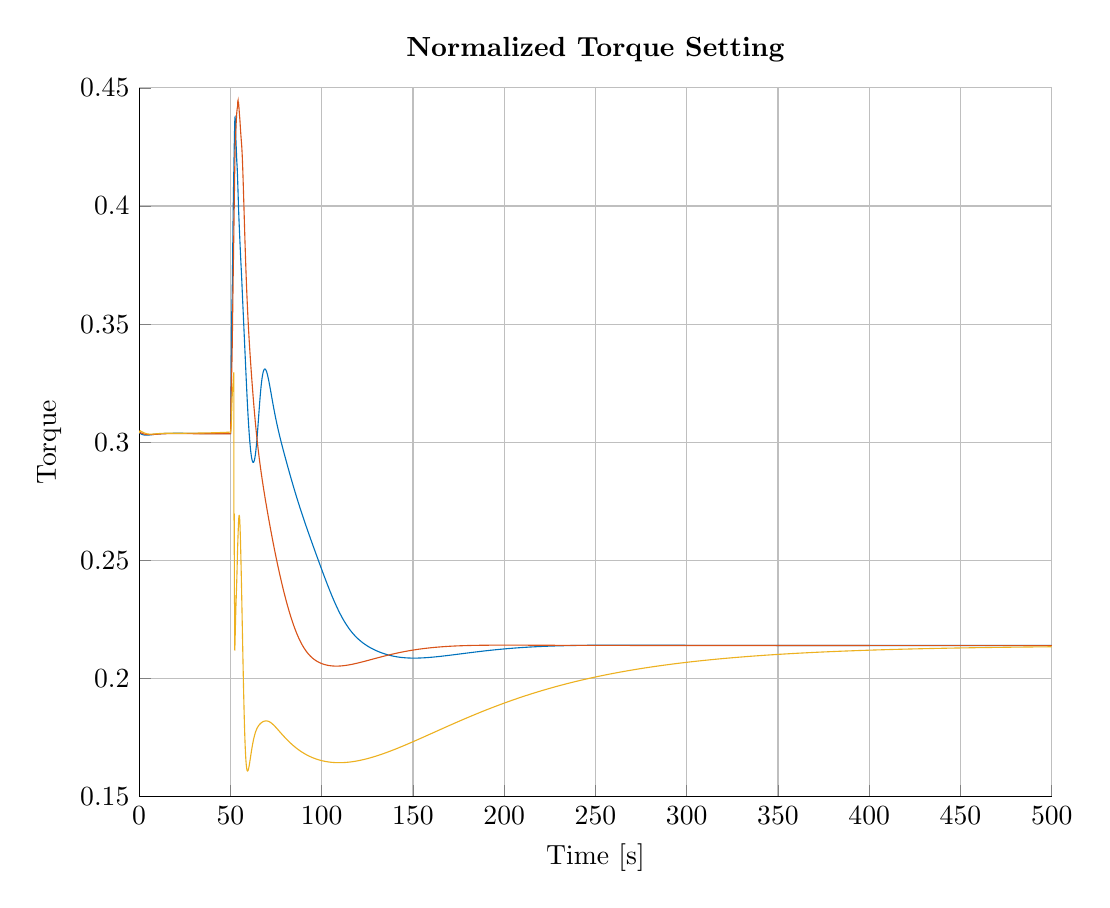
\begin{tikzpicture}

\begin{axis}[%
width=4.563in,
height=3.544in,
at={(0.792in,0.541in)},
scale only axis,
xmin=0,
xmax=500,
xlabel={Time [s]},
xmajorgrids,
ymin=0.15,
ymax=0.45,
ylabel={Torque},
ymajorgrids,
axis background/.style={fill=white},
title style={font=\bfseries},
title={Normalized Torque Setting},
axis x line*=bottom,
axis y line*=left
]
\addplot [color=mycolor1,solid,forget plot]
  table[row sep=crcr]{%
0	0.30400000722465\\
0.05	0.3039802061\\
0.1	0.3039491763\\
0.15	0.3039149109\\
0.2	0.303883203\\
0.25	0.303857271\\
0.3	0.303837982\\
0.35	0.303824461\\
0.4	0.303814832\\
0.45	0.303806867\\
0.5	0.303798455\\
0.55	0.303787909\\
0.6	0.303774112\\
0.65	0.303756551\\
0.7	0.303735266\\
0.75	0.30371074\\
0.8	0.303683762\\
0.85	0.303655274\\
0.9	0.303626196\\
0.95	0.303597362\\
1	0.303569457\\
1.05	0.303542947\\
1.1	0.303518078\\
1.15	0.303494898\\
1.2	0.303473302\\
1.25	0.303453082\\
1.3	0.303433977\\
1.35	0.303415721\\
1.4	0.303398076\\
1.45	0.303380855\\
1.5	0.303363929\\
1.55	0.30334723\\
1.6	0.303330745\\
1.65	0.303314502\\
1.7	0.303298554\\
1.75	0.303282968\\
1.8	0.303267812\\
1.85	0.303253143\\
1.9	0.303239006\\
1.95	0.303225427\\
2	0.303212415\\
2.05	0.303199963\\
2.1	0.303188053\\
2.15	0.303176659\\
2.2	0.303165752\\
2.25	0.303155301\\
2.3	0.303145286\\
2.35	0.303135695\\
2.4	0.303126511\\
2.45	0.30311772\\
2.5	0.303109324\\
2.55	0.303101327\\
2.6	0.303093735\\
2.65	0.303086554\\
2.7	0.303079791\\
2.75	0.303073449\\
2.8	0.303067528\\
2.85	0.303062028\\
2.9	0.303056944\\
2.95	0.30305227\\
3	0.303047996\\
3.05	0.303044111\\
3.1	0.303040605\\
3.15	0.303037465\\
3.2	0.303034677\\
3.25	0.303032229\\
3.3	0.303030108\\
3.35	0.3030283\\
3.4	0.303026793\\
3.45	0.303025575\\
3.5	0.303024632\\
3.55	0.303023953\\
3.6	0.303023525\\
3.65	0.303023335\\
3.7	0.303023371\\
3.75	0.303023621\\
3.8	0.303024071\\
3.85	0.303024709\\
3.9	0.303025521\\
3.95	0.303026495\\
4	0.303027617\\
4.05	0.303028874\\
4.1	0.303030252\\
4.15	0.303031738\\
4.2	0.303033318\\
4.25	0.303034979\\
4.3	0.303036706\\
4.35	0.303038487\\
4.4	0.303040309\\
4.45	0.303042161\\
4.5	0.303044034\\
4.55	0.303045918\\
4.6	0.303047807\\
4.65	0.303049697\\
4.7	0.303051585\\
4.75	0.303053469\\
4.8	0.30305535\\
4.85	0.30305723\\
4.9	0.303059113\\
4.95	0.303061004\\
5	0.30306291\\
5.05	0.303064837\\
5.1	0.303066794\\
5.15	0.303068789\\
5.2	0.303070832\\
5.25	0.303072932\\
5.3	0.303075098\\
5.35	0.303077339\\
5.4	0.303079664\\
5.45	0.303082083\\
5.5	0.303084603\\
5.55	0.303087232\\
5.6	0.303089978\\
5.65	0.303092848\\
5.7	0.303095848\\
5.75	0.303098983\\
5.8	0.303102257\\
5.85	0.303105676\\
5.9	0.30310924\\
5.95	0.303112954\\
6	0.303116817\\
6.05	0.30312083\\
6.1	0.303124992\\
6.15	0.303129302\\
6.2	0.303133756\\
6.25	0.303138353\\
6.3	0.303143086\\
6.35	0.30314795\\
6.4	0.303152941\\
6.45	0.30315805\\
6.5	0.303163269\\
6.55	0.303168591\\
6.6	0.303174006\\
6.65	0.303179505\\
6.7	0.303185077\\
6.75	0.303190711\\
6.8	0.303196398\\
6.85	0.303202124\\
6.9	0.303207879\\
6.95	0.303213651\\
7	0.303219429\\
7.05	0.303225202\\
7.1	0.303230957\\
7.15	0.303236685\\
7.2	0.303242375\\
7.25	0.303248018\\
7.3	0.303253604\\
7.35	0.303259126\\
7.4	0.303264575\\
7.45	0.303269945\\
7.5	0.30327523\\
7.55	0.303280426\\
7.6	0.303285529\\
7.65	0.303290536\\
7.7	0.303295445\\
7.75	0.303300257\\
7.8	0.303304971\\
7.85	0.303309588\\
7.9	0.303314111\\
7.95	0.303318543\\
8	0.303322888\\
8.05	0.303327151\\
8.1	0.303331337\\
8.15	0.303335453\\
8.2	0.303339504\\
8.25	0.303343499\\
8.3	0.303347445\\
8.35	0.30335135\\
8.4	0.303355223\\
8.45	0.30335907\\
8.5	0.303362901\\
8.55	0.303366725\\
8.6	0.303370548\\
8.65	0.30337438\\
8.7	0.303378228\\
8.75	0.303382099\\
8.8	0.303386\\
8.85	0.303389936\\
8.9	0.303393915\\
8.95	0.303397941\\
9	0.303402018\\
9.05	0.30340615\\
9.1	0.303410339\\
9.15	0.303414587\\
9.2	0.303418897\\
9.25	0.303423267\\
9.3	0.303427697\\
9.35	0.303432186\\
9.4	0.303436731\\
9.45	0.30344133\\
9.5	0.303445979\\
9.55	0.303450672\\
9.6	0.303455405\\
9.65	0.303460171\\
9.7	0.303464965\\
9.75	0.303469779\\
9.8	0.303474605\\
9.85	0.303479436\\
9.9	0.303484263\\
9.95	0.303489079\\
10	0.303493874\\
10.05	0.303498641\\
10.1	0.30350337\\
10.15	0.303508055\\
10.2	0.303512686\\
10.25	0.303517255\\
10.3	0.303521756\\
10.35	0.303526182\\
10.4	0.303530526\\
10.45	0.303534782\\
10.5	0.303538945\\
10.55	0.303543011\\
10.6	0.303546975\\
10.65	0.303550836\\
10.7	0.30355459\\
10.75	0.303558236\\
10.8	0.303561774\\
10.85	0.303565204\\
10.9	0.303568527\\
10.95	0.303571744\\
11	0.303574858\\
11.05	0.303577873\\
11.1	0.303580792\\
11.15	0.30358362\\
11.2	0.303586363\\
11.25	0.303589026\\
11.3	0.303591615\\
11.35	0.303594137\\
11.4	0.303596599\\
11.45	0.303599008\\
11.5	0.303601372\\
11.55	0.303603699\\
11.6	0.303605996\\
11.65	0.30360827\\
11.7	0.30361053\\
11.75	0.303612782\\
11.8	0.303615034\\
11.85	0.303617292\\
11.9	0.303619562\\
11.95	0.303621851\\
12	0.303624164\\
12.05	0.303626505\\
12.1	0.303628878\\
12.15	0.303631288\\
12.2	0.303633736\\
12.25	0.303636226\\
12.3	0.303638758\\
12.35	0.303641333\\
12.4	0.303643951\\
12.45	0.30364661\\
12.5	0.303649311\\
12.55	0.303652049\\
12.6	0.303654823\\
12.65	0.303657629\\
12.7	0.303660463\\
12.75	0.303663319\\
12.8	0.303666193\\
12.85	0.303669079\\
12.9	0.303671972\\
12.95	0.303674864\\
13	0.30367775\\
13.05	0.303680622\\
13.1	0.303683474\\
13.15	0.303686298\\
13.2	0.303689089\\
13.25	0.303691839\\
13.3	0.303694542\\
13.35	0.303697192\\
13.4	0.303699782\\
13.45	0.303702308\\
13.5	0.303704763\\
13.55	0.303707144\\
13.6	0.303709446\\
13.65	0.303711666\\
13.7	0.303713801\\
13.75	0.303715849\\
13.8	0.303717807\\
13.85	0.303719676\\
13.9	0.303721454\\
13.95	0.303723144\\
14	0.303724744\\
14.05	0.303726258\\
14.1	0.303727688\\
14.15	0.303729038\\
14.2	0.303730309\\
14.25	0.303731508\\
14.3	0.303732639\\
14.35	0.303733706\\
14.4	0.303734717\\
14.45	0.303735675\\
14.5	0.303736589\\
14.55	0.303737464\\
14.6	0.303738306\\
14.65	0.303739124\\
14.7	0.303739922\\
14.75	0.303740709\\
14.8	0.30374149\\
14.85	0.303742272\\
14.9	0.303743061\\
14.95	0.303743864\\
15	0.303744684\\
15.05	0.303745528\\
15.1	0.3037464\\
15.15	0.303747304\\
15.2	0.303748244\\
15.25	0.303749222\\
15.3	0.303750241\\
15.35	0.303751303\\
15.4	0.303752409\\
15.45	0.303753559\\
15.5	0.303754753\\
15.55	0.30375599\\
15.6	0.303757269\\
15.65	0.303758588\\
15.7	0.303759943\\
15.75	0.303761333\\
15.8	0.303762752\\
15.85	0.303764197\\
15.9	0.303765664\\
15.95	0.303767147\\
16	0.303768641\\
16.05	0.30377014\\
16.1	0.303771639\\
16.15	0.303773131\\
16.2	0.303774611\\
16.25	0.303776073\\
16.3	0.303777511\\
16.35	0.303778919\\
16.4	0.303780291\\
16.45	0.303781622\\
16.5	0.303782907\\
16.55	0.303784141\\
16.6	0.303785319\\
16.65	0.303786438\\
16.7	0.303787495\\
16.75	0.303788486\\
16.8	0.303789408\\
16.85	0.303790261\\
16.9	0.303791043\\
16.95	0.303791754\\
17	0.303792393\\
17.05	0.30379296\\
17.1	0.303793458\\
17.15	0.303793889\\
17.2	0.303794253\\
17.25	0.303794555\\
17.3	0.303794798\\
17.35	0.303794985\\
17.4	0.303795121\\
17.45	0.303795212\\
17.5	0.303795261\\
17.55	0.303795274\\
17.6	0.303795257\\
17.65	0.303795216\\
17.7	0.303795156\\
17.75	0.303795084\\
17.8	0.303795005\\
17.85	0.303794926\\
17.9	0.303794851\\
17.95	0.303794787\\
18	0.303794739\\
18.05	0.303794712\\
18.1	0.30379471\\
18.15	0.303794738\\
18.2	0.3037948\\
18.25	0.303794899\\
18.3	0.303795038\\
18.35	0.30379522\\
18.4	0.303795446\\
18.45	0.303795717\\
18.5	0.303796034\\
18.55	0.303796398\\
18.6	0.303796807\\
18.65	0.303797262\\
18.7	0.303797759\\
18.75	0.303798297\\
18.8	0.303798873\\
18.85	0.303799484\\
18.9	0.303800127\\
18.95	0.303800797\\
19	0.30380149\\
19.05	0.303802202\\
19.1	0.303802927\\
19.15	0.30380366\\
19.2	0.303804396\\
19.25	0.30380513\\
19.3	0.303805856\\
19.35	0.303806568\\
19.4	0.303807262\\
19.45	0.303807931\\
19.5	0.303808571\\
19.55	0.303809178\\
19.6	0.303809746\\
19.65	0.303810271\\
19.7	0.30381075\\
19.75	0.303811179\\
19.8	0.303811555\\
19.85	0.303811876\\
19.9	0.303812139\\
19.95	0.303812345\\
20	0.303812491\\
20.05	0.303812577\\
20.1	0.303812603\\
20.15	0.303812572\\
20.2	0.303812482\\
20.25	0.303812338\\
20.3	0.30381214\\
20.35	0.303811893\\
20.4	0.303811598\\
20.45	0.303811261\\
20.5	0.303810885\\
20.55	0.303810474\\
20.6	0.303810034\\
20.65	0.303809568\\
20.7	0.303809084\\
20.75	0.303808585\\
20.8	0.303808077\\
20.85	0.303807566\\
20.9	0.303807057\\
20.95	0.303806554\\
21	0.303806065\\
21.05	0.303805592\\
21.1	0.303805141\\
21.15	0.303804717\\
21.2	0.303804323\\
21.25	0.303803962\\
21.3	0.30380364\\
21.35	0.303803357\\
21.4	0.303803116\\
21.45	0.30380292\\
21.5	0.303802769\\
21.55	0.303802664\\
21.6	0.303802606\\
21.65	0.303802594\\
21.7	0.303802627\\
21.75	0.303802704\\
21.8	0.303802823\\
21.85	0.303802982\\
21.9	0.303803178\\
21.95	0.303803408\\
22	0.303803668\\
22.05	0.303803954\\
22.1	0.303804262\\
22.15	0.303804587\\
22.2	0.303804924\\
22.25	0.303805269\\
22.3	0.303805617\\
22.35	0.303805962\\
22.4	0.3038063\\
22.45	0.303806624\\
22.5	0.303806931\\
22.55	0.303807216\\
22.6	0.303807473\\
22.65	0.303807699\\
22.7	0.30380789\\
22.75	0.303808042\\
22.8	0.303808151\\
22.85	0.303808215\\
22.9	0.303808231\\
22.95	0.303808197\\
23	0.303808112\\
23.05	0.303807975\\
23.1	0.303807785\\
23.15	0.303807543\\
23.2	0.303807249\\
23.25	0.303806904\\
23.3	0.30380651\\
23.35	0.303806068\\
23.4	0.303805582\\
23.45	0.303805054\\
23.5	0.303804488\\
23.55	0.303803888\\
23.6	0.303803257\\
23.65	0.303802599\\
23.7	0.303801921\\
23.75	0.303801225\\
23.8	0.303800518\\
23.85	0.303799804\\
23.9	0.303799088\\
23.95	0.303798376\\
24	0.303797671\\
24.05	0.30379698\\
24.1	0.303796306\\
24.15	0.303795655\\
24.2	0.30379503\\
24.25	0.303794435\\
24.3	0.303793873\\
24.35	0.303793349\\
24.4	0.303792864\\
24.45	0.30379242\\
24.5	0.30379202\\
24.55	0.303791665\\
24.6	0.303791356\\
24.65	0.303791093\\
24.7	0.303790875\\
24.75	0.303790702\\
24.8	0.303790573\\
24.85	0.303790487\\
24.9	0.30379044\\
24.95	0.30379043\\
25	0.303790455\\
25.05	0.303790511\\
25.1	0.303790594\\
25.15	0.303790701\\
25.2	0.303790826\\
25.25	0.303790965\\
25.3	0.303791115\\
25.35	0.303791269\\
25.4	0.303791423\\
25.45	0.303791573\\
25.5	0.303791713\\
25.55	0.303791838\\
25.6	0.303791945\\
25.65	0.303792028\\
25.7	0.303792084\\
25.75	0.303792108\\
25.8	0.303792097\\
25.85	0.303792048\\
25.9	0.303791958\\
25.95	0.303791824\\
26	0.303791645\\
26.05	0.303791419\\
26.1	0.303791146\\
26.15	0.303790823\\
26.2	0.303790453\\
26.25	0.303790034\\
26.3	0.303789568\\
26.35	0.303789057\\
26.4	0.303788503\\
26.45	0.303787907\\
26.5	0.303787273\\
26.55	0.303786603\\
26.6	0.303785902\\
26.65	0.303785173\\
26.7	0.303784421\\
26.75	0.303783649\\
26.8	0.303782862\\
26.85	0.303782066\\
26.9	0.303781264\\
26.95	0.303780462\\
27	0.303779664\\
27.05	0.303778875\\
27.1	0.3037781\\
27.15	0.303777344\\
27.2	0.30377661\\
27.25	0.303775902\\
27.3	0.303775225\\
27.35	0.303774581\\
27.4	0.303773975\\
27.45	0.303773407\\
27.5	0.303772881\\
27.55	0.303772398\\
27.6	0.30377196\\
27.65	0.303771567\\
27.7	0.30377122\\
27.75	0.303770918\\
27.8	0.303770661\\
27.85	0.303770447\\
27.9	0.303770275\\
27.95	0.303770144\\
28	0.30377005\\
28.05	0.30376999\\
28.1	0.303769961\\
28.15	0.30376996\\
28.2	0.303769983\\
28.25	0.303770025\\
28.3	0.303770082\\
28.35	0.30377015\\
28.4	0.303770224\\
28.45	0.303770299\\
28.5	0.303770371\\
28.55	0.303770434\\
28.6	0.303770485\\
28.65	0.303770518\\
28.7	0.30377053\\
28.75	0.303770516\\
28.8	0.303770473\\
28.85	0.303770397\\
28.9	0.303770284\\
28.95	0.303770133\\
29	0.303769941\\
29.05	0.303769706\\
29.1	0.303769426\\
29.15	0.303769101\\
29.2	0.303768729\\
29.25	0.303768312\\
29.3	0.30376785\\
29.35	0.303767342\\
29.4	0.303766792\\
29.45	0.303766201\\
29.5	0.30376557\\
29.55	0.303764904\\
29.6	0.303764204\\
29.65	0.303763475\\
29.7	0.30376272\\
29.75	0.303761944\\
29.8	0.30376115\\
29.85	0.303760343\\
29.9	0.303759527\\
29.95	0.303758708\\
30	0.303757891\\
30.05	0.303757078\\
30.1	0.303756277\\
30.15	0.30375549\\
30.2	0.303754722\\
30.25	0.303753978\\
30.3	0.303753262\\
30.35	0.303752576\\
30.4	0.303751925\\
30.45	0.303751311\\
30.5	0.303750737\\
30.55	0.303750204\\
30.6	0.303749716\\
30.65	0.303749272\\
30.7	0.303748874\\
30.75	0.303748521\\
30.8	0.303748214\\
30.85	0.303747952\\
30.9	0.303747733\\
30.95	0.303747557\\
31	0.30374742\\
31.05	0.303747321\\
31.1	0.303747256\\
31.15	0.303747223\\
31.2	0.303747216\\
31.25	0.303747234\\
31.3	0.303747271\\
31.35	0.303747324\\
31.4	0.303747387\\
31.45	0.303747456\\
31.5	0.303747526\\
31.55	0.303747594\\
31.6	0.303747653\\
31.65	0.3037477\\
31.7	0.30374773\\
31.75	0.303747739\\
31.8	0.303747722\\
31.85	0.303747677\\
31.9	0.3037476\\
31.95	0.303747487\\
32	0.303747336\\
32.05	0.303747145\\
32.1	0.303746912\\
32.15	0.303746635\\
32.2	0.303746314\\
32.25	0.303745948\\
32.3	0.303745537\\
32.35	0.303745082\\
32.4	0.303744584\\
32.45	0.303744044\\
32.5	0.303743464\\
32.55	0.303742847\\
32.6	0.303742196\\
32.65	0.303741513\\
32.7	0.303740802\\
32.75	0.303740067\\
32.8	0.303739312\\
32.85	0.303738541\\
32.9	0.303737759\\
32.95	0.30373697\\
33	0.303736179\\
33.05	0.303735391\\
33.1	0.30373461\\
33.15	0.303733842\\
33.2	0.30373309\\
33.25	0.303732358\\
33.3	0.303731652\\
33.35	0.303730975\\
33.4	0.30373033\\
33.45	0.30372972\\
33.5	0.303729149\\
33.55	0.303728619\\
33.6	0.303728132\\
33.65	0.30372769\\
33.7	0.303727293\\
33.75	0.303726942\\
33.8	0.303726638\\
33.85	0.30372638\\
33.9	0.303726167\\
33.95	0.303725998\\
34	0.303725871\\
34.05	0.303725784\\
34.1	0.303725735\\
34.15	0.30372572\\
34.2	0.303725735\\
34.25	0.303725778\\
34.3	0.303725845\\
34.35	0.30372593\\
34.4	0.30372603\\
34.45	0.30372614\\
34.5	0.303726256\\
34.55	0.303726372\\
34.6	0.303726484\\
34.65	0.303726587\\
34.7	0.303726678\\
34.75	0.30372675\\
34.8	0.303726801\\
34.85	0.303726825\\
34.9	0.303726821\\
34.95	0.303726783\\
35	0.303726709\\
35.05	0.303726597\\
35.1	0.303726444\\
35.15	0.303726248\\
35.2	0.303726009\\
35.25	0.303725726\\
35.3	0.303725397\\
35.35	0.303725024\\
35.4	0.303724607\\
35.45	0.303724147\\
35.5	0.303723646\\
35.55	0.303723106\\
35.6	0.303722529\\
35.65	0.303721919\\
35.7	0.303721278\\
35.75	0.303720611\\
35.8	0.303719921\\
35.85	0.303719212\\
35.9	0.303718489\\
35.95	0.303717757\\
36	0.30371702\\
36.05	0.303716282\\
36.1	0.30371555\\
36.15	0.303714826\\
36.2	0.303714117\\
36.25	0.303713426\\
36.3	0.303712759\\
36.35	0.303712118\\
36.4	0.303711508\\
36.45	0.303710932\\
36.5	0.303710394\\
36.55	0.303709897\\
36.6	0.303709441\\
36.65	0.303709031\\
36.7	0.303708666\\
36.75	0.303708349\\
36.8	0.303708079\\
36.85	0.303707856\\
36.9	0.30370768\\
36.95	0.303707551\\
37	0.303707465\\
37.05	0.303707422\\
37.1	0.30370742\\
37.15	0.303707454\\
37.2	0.303707522\\
37.25	0.303707621\\
37.3	0.303707747\\
37.35	0.303707895\\
37.4	0.303708061\\
37.45	0.303708241\\
37.5	0.303708429\\
37.55	0.303708621\\
37.6	0.303708812\\
37.65	0.303708998\\
37.7	0.303709173\\
37.75	0.303709333\\
37.8	0.303709473\\
37.85	0.30370959\\
37.9	0.303709679\\
37.95	0.303709736\\
38	0.303709758\\
38.05	0.303709743\\
38.1	0.303709687\\
38.15	0.30370959\\
38.2	0.303709448\\
38.25	0.303709261\\
38.3	0.303709028\\
38.35	0.30370875\\
38.4	0.303708426\\
38.45	0.303708058\\
38.5	0.303707646\\
38.55	0.303707193\\
38.6	0.303706701\\
38.65	0.303706173\\
38.7	0.303705612\\
38.75	0.303705021\\
38.8	0.303704404\\
38.85	0.303703766\\
38.9	0.303703111\\
38.95	0.303702443\\
39	0.303701767\\
39.05	0.303701089\\
39.1	0.303700413\\
39.15	0.303699743\\
39.2	0.303699086\\
39.25	0.303698445\\
39.3	0.303697825\\
39.35	0.303697231\\
39.4	0.303696666\\
39.45	0.303696135\\
39.5	0.303695641\\
39.55	0.303695187\\
39.6	0.303694776\\
39.65	0.303694409\\
39.7	0.30369409\\
39.75	0.303693819\\
39.8	0.303693596\\
39.85	0.303693423\\
39.9	0.303693299\\
39.95	0.303693222\\
40	0.303693193\\
40.05	0.303693209\\
40.1	0.303693267\\
40.15	0.303693366\\
40.2	0.303693502\\
40.25	0.303693672\\
40.3	0.303693871\\
40.35	0.303694096\\
40.4	0.303694342\\
40.45	0.303694604\\
40.5	0.303694878\\
40.55	0.303695158\\
40.6	0.303695441\\
40.65	0.30369572\\
40.7	0.30369599\\
40.75	0.303696247\\
40.8	0.303696486\\
40.85	0.303696703\\
40.9	0.303696892\\
40.95	0.303697051\\
41	0.303697175\\
41.05	0.303697262\\
41.1	0.303697307\\
41.15	0.30369731\\
41.2	0.303697267\\
41.25	0.303697178\\
41.3	0.303697041\\
41.35	0.303696857\\
41.4	0.303696625\\
41.45	0.303696345\\
41.5	0.30369602\\
41.55	0.303695651\\
41.6	0.303695239\\
41.65	0.303694788\\
41.7	0.303694301\\
41.75	0.303693781\\
41.8	0.303693232\\
41.85	0.303692658\\
41.9	0.303692064\\
41.95	0.303691455\\
42	0.303690834\\
42.05	0.303690209\\
42.1	0.303689582\\
42.15	0.303688961\\
42.2	0.303688349\\
42.25	0.303687753\\
42.3	0.303687176\\
42.35	0.303686623\\
42.4	0.3036861\\
42.45	0.30368561\\
42.5	0.303685156\\
42.55	0.303684744\\
42.6	0.303684374\\
42.65	0.303684051\\
42.7	0.303683776\\
42.75	0.30368355\\
42.8	0.303683376\\
42.85	0.303683253\\
42.9	0.303683181\\
42.95	0.30368316\\
43	0.303683189\\
43.05	0.303683266\\
43.1	0.303683389\\
43.15	0.303683555\\
43.2	0.303683762\\
43.25	0.303684005\\
43.3	0.303684281\\
43.35	0.303684586\\
43.4	0.303684915\\
43.45	0.303685263\\
43.5	0.303685626\\
43.55	0.303685997\\
43.6	0.303686373\\
43.65	0.303686746\\
43.7	0.303687113\\
43.75	0.303687468\\
43.8	0.303687805\\
43.85	0.30368812\\
43.9	0.303688409\\
43.95	0.303688666\\
44	0.303688888\\
44.05	0.303689072\\
44.1	0.303689213\\
44.15	0.303689309\\
44.2	0.303689358\\
44.25	0.303689359\\
44.3	0.303689309\\
44.35	0.303689208\\
44.4	0.303689057\\
44.45	0.303688855\\
44.5	0.303688603\\
44.55	0.303688304\\
44.6	0.303687959\\
44.65	0.303687571\\
44.7	0.303687142\\
44.75	0.303686677\\
44.8	0.30368618\\
44.85	0.303685654\\
44.9	0.303685105\\
44.95	0.303684537\\
45	0.303683955\\
45.05	0.303683366\\
45.1	0.303682773\\
45.15	0.303682183\\
45.2	0.303681602\\
45.25	0.303681034\\
45.3	0.303680485\\
45.35	0.30367996\\
45.4	0.303679464\\
45.45	0.303679001\\
45.5	0.303678576\\
45.55	0.303678192\\
45.6	0.303677854\\
45.65	0.303677563\\
45.7	0.303677323\\
45.75	0.303677135\\
45.8	0.303677\\
45.85	0.30367692\\
45.9	0.303676894\\
45.95	0.303676923\\
46	0.303677005\\
46.05	0.303677138\\
46.1	0.303677322\\
46.15	0.303677552\\
46.2	0.303677826\\
46.25	0.303678141\\
46.3	0.303678492\\
46.35	0.303678874\\
46.4	0.303679284\\
46.45	0.303679716\\
46.5	0.303680165\\
46.55	0.303680624\\
46.6	0.30368109\\
46.65	0.303681555\\
46.7	0.303682014\\
46.75	0.303682462\\
46.8	0.303682893\\
46.85	0.303683301\\
46.9	0.303683682\\
46.95	0.30368403\\
47	0.303684342\\
47.05	0.303684613\\
47.1	0.30368484\\
47.15	0.303685019\\
47.2	0.303685147\\
47.25	0.303685224\\
47.3	0.303685246\\
47.35	0.303685214\\
47.4	0.303685127\\
47.45	0.303684984\\
47.5	0.303684789\\
47.55	0.30368454\\
47.6	0.303684242\\
47.65	0.303683895\\
47.7	0.303683505\\
47.75	0.303683073\\
47.8	0.303682605\\
47.85	0.303682105\\
47.9	0.303681577\\
47.95	0.303681028\\
48	0.303680462\\
48.05	0.303679886\\
48.1	0.303679304\\
48.15	0.303678724\\
48.2	0.30367815\\
48.25	0.303677589\\
48.3	0.303677047\\
48.35	0.303676529\\
48.4	0.303676041\\
48.45	0.303675587\\
48.5	0.303675172\\
48.55	0.303674801\\
48.6	0.303674478\\
48.65	0.303674205\\
48.7	0.303673985\\
48.75	0.303673822\\
48.8	0.303673715\\
48.85	0.303673667\\
48.9	0.303673678\\
48.95	0.303673748\\
49	0.303673875\\
49.05	0.303674058\\
49.1	0.303674296\\
49.15	0.303674585\\
49.2	0.303674922\\
49.25	0.303675303\\
49.3	0.303675725\\
49.35	0.303676182\\
49.4	0.30367667\\
49.45	0.303677182\\
49.5	0.303677713\\
49.55	0.303678258\\
49.6	0.30367881\\
49.65	0.303679363\\
49.7	0.30367991\\
49.75	0.303680446\\
49.8	0.303680965\\
49.85	0.30368146\\
49.9	0.303681926\\
49.95	0.303682357\\
50	0.30368275\\
50.05	0.3036831\\
50.1	0.304632036\\
50.15	0.3070638\\
50.2	0.31114159\\
50.25	0.3168462\\
50.3	0.3200992\\
50.35	0.3241073\\
50.4	0.3287118\\
50.45	0.3336527\\
50.5	0.3388353\\
50.55	0.3444599\\
50.6	0.3478649\\
50.65	0.3507498\\
50.7	0.353158\\
50.75	0.3552172\\
50.8	0.3570776\\
50.85	0.3588956\\
50.9	0.3608071\\
50.95	0.3629117\\
51	0.3652667\\
51.05	0.3679014\\
51.1	0.3707981\\
51.15	0.3739468\\
51.2	0.3773266\\
51.25	0.3808332\\
51.3	0.384364\\
51.35	0.3878275\\
51.4	0.3911544\\
51.45	0.3943029\\
51.5	0.3972577\\
51.55	0.4000266\\
51.6	0.4026345\\
51.65	0.405116\\
51.7	0.407509\\
51.75	0.409844\\
51.8	0.412148\\
51.85	0.414433\\
51.9	0.416707\\
51.95	0.418963\\
52	0.421189\\
52.05	0.423367\\
52.1	0.425488\\
52.15	0.427545\\
52.2	0.429524\\
52.25	0.43142\\
52.3	0.433206\\
52.35	0.434796\\
52.4	0.436097\\
52.45	0.43703\\
52.5	0.437547\\
52.55	0.43763\\
52.6	0.437283\\
52.65	0.436505\\
52.7	0.43544\\
52.75	0.434214\\
52.8	0.43293\\
52.85	0.43166\\
52.9	0.43045\\
52.95	0.429319\\
53	0.428266\\
53.05	0.427274\\
53.1	0.426322\\
53.15	0.425383\\
53.2	0.424434\\
53.25	0.423458\\
53.3	0.422442\\
53.35	0.421384\\
53.4	0.420288\\
53.45	0.419879\\
53.5	0.41867\\
53.55	0.418157\\
53.6	0.417564\\
53.65	0.416893\\
53.7	0.416143\\
53.75	0.41531\\
53.8	0.414396\\
53.85	0.413407\\
53.9	0.412349\\
53.95	0.411235\\
54	0.410077\\
54.05	0.408888\\
54.1	0.407679\\
54.15	0.406461\\
54.2	0.405242\\
54.25	0.404028\\
54.3	0.4028244\\
54.35	0.4016339\\
54.4	0.4004619\\
54.45	0.399313\\
54.5	0.3981912\\
54.55	0.3971001\\
54.6	0.3960431\\
54.65	0.3950232\\
54.7	0.3940432\\
54.75	0.3931054\\
54.8	0.3922117\\
54.85	0.3913631\\
54.9	0.3904122\\
54.95	0.3894874\\
55	0.3885861\\
55.05	0.3877038\\
55.1	0.3868351\\
55.15	0.3859748\\
55.2	0.3851186\\
55.25	0.3842637\\
55.3	0.383409\\
55.35	0.3825545\\
55.4	0.3817016\\
55.45	0.3808506\\
55.5	0.3800031\\
55.55	0.379165\\
55.6	0.3783382\\
55.65	0.3775262\\
55.7	0.3767322\\
55.75	0.3759574\\
55.8	0.3751994\\
55.85	0.3744532\\
55.9	0.3737111\\
55.95	0.3729645\\
56	0.3722052\\
56.05	0.3714264\\
56.1	0.3706239\\
56.15	0.3697962\\
56.2	0.3689446\\
56.25	0.3680725\\
56.3	0.3671849\\
56.35	0.3662874\\
56.4	0.3653857\\
56.45	0.3644846\\
56.5	0.3635879\\
56.55	0.362698\\
56.6	0.3618163\\
56.65	0.3609427\\
56.7	0.3600763\\
56.75	0.3592159\\
56.8	0.3583597\\
56.85	0.3575061\\
56.9	0.3566537\\
56.95	0.3558015\\
57	0.3549486\\
57.05	0.354095\\
57.1	0.3532405\\
57.15	0.3523855\\
57.2	0.3515302\\
57.25	0.350675\\
57.3	0.3498202\\
57.35	0.3489661\\
57.4	0.3481127\\
57.45	0.3472601\\
57.5	0.3464082\\
57.55	0.3455567\\
57.6	0.3447056\\
57.65	0.3438545\\
57.7	0.3430032\\
57.75	0.3421516\\
57.8	0.3412996\\
57.85	0.3404469\\
57.9	0.3395936\\
57.95	0.3387396\\
58	0.3378848\\
58.05	0.3370294\\
58.1	0.3361733\\
58.15	0.3353169\\
58.2	0.3344602\\
58.25	0.3336036\\
58.3	0.3327475\\
58.35	0.3318922\\
58.4	0.3310383\\
58.45	0.3301864\\
58.5	0.3293369\\
58.55	0.3284904\\
58.6	0.3276475\\
58.65	0.3268086\\
58.7	0.3259743\\
58.75	0.325145\\
58.8	0.3243211\\
58.85	0.3235029\\
58.9	0.3226909\\
58.95	0.3218852\\
59	0.3210862\\
59.05	0.3202942\\
59.1	0.3195094\\
59.15	0.3187322\\
59.2	0.3179629\\
59.25	0.3172016\\
59.3	0.3164488\\
59.35	0.3157046\\
59.4	0.3149694\\
59.45	0.3142434\\
59.5	0.31352675\\
59.55	0.3128198\\
59.6	0.31212271\\
59.65	0.31143569\\
59.7	0.31075891\\
59.75	0.31009255\\
59.8	0.30943674\\
59.85	0.30879163\\
59.9	0.30815736\\
59.95	0.30753404\\
60	0.30692179\\
60.05	0.30632071\\
60.1	0.3057309\\
60.15	0.30515246\\
60.2	0.304585463\\
60.25	0.3040299947\\
60.3	0.303486127\\
60.35	0.30295393\\
60.4	0.30243345\\
60.45	0.30192477\\
60.5	0.30142791\\
60.55	0.30094293\\
60.6	0.30046987\\
60.65	0.30000876\\
60.7	0.29955964\\
60.75	0.29912252\\
60.8	0.29869743\\
60.85	0.29828439\\
60.9	0.29788342\\
60.95	0.29749454\\
61	0.29711774\\
61.05	0.29675305\\
61.1	0.29640047\\
61.15	0.29606001\\
61.2	0.29573168\\
61.25	0.29541548\\
61.3	0.29511142\\
61.35	0.29481951\\
61.4	0.29453975\\
61.45	0.29427214\\
61.5	0.2940167\\
61.55	0.2937734\\
61.6	0.2935424\\
61.65	0.2933235\\
61.7	0.2931168\\
61.75	0.2929223\\
61.8	0.29274\\
61.85	0.29257\\
61.9	0.2924122\\
61.95	0.2922666\\
62	0.2921334\\
62.05	0.2920124\\
62.1	0.2919037\\
62.15	0.2918074\\
62.2	0.2917234\\
62.25	0.2916517\\
62.3	0.2915925\\
62.35	0.2915456\\
62.4	0.2915111\\
62.45	0.2914891\\
62.5	0.2914795\\
62.55	0.2914824\\
62.6	0.2914978\\
62.65	0.2915257\\
62.7	0.2915661\\
62.75	0.291619\\
62.8	0.2916844\\
62.85	0.2917624\\
62.9	0.291853\\
62.95	0.291956\\
63	0.2920716\\
63.05	0.2921997\\
63.1	0.2923404\\
63.15	0.2924935\\
63.2	0.2926591\\
63.25	0.2928372\\
63.3	0.2930276\\
63.35	0.2932304\\
63.4	0.2934455\\
63.45	0.2936728\\
63.5	0.2939123\\
63.55	0.2941639\\
63.6	0.29442749\\
63.65	0.29470298\\
63.7	0.29499027\\
63.75	0.29528922\\
63.8	0.29559972\\
63.85	0.29592161\\
63.9	0.29625474\\
63.95	0.29659895\\
64	0.29695404\\
64.05	0.29731983\\
64.1	0.29769611\\
64.15	0.29808265\\
64.2	0.29847924\\
64.25	0.29888561\\
64.3	0.2993015\\
64.35	0.29972665\\
64.4	0.30016076\\
64.45	0.30060354\\
64.5	0.30105467\\
64.55	0.30151382\\
64.6	0.30198066\\
64.65	0.30245482\\
64.7	0.30293596\\
64.75	0.303423696\\
64.8	0.3039176404\\
64.85	0.304417398\\
64.9	0.304922564\\
64.95	0.30543272\\
65	0.30594745\\
65.05	0.3064663\\
65.1	0.30698885\\
65.15	0.30751465\\
65.2	0.30804323\\
65.25	0.30857414\\
65.3	0.3091069\\
65.35	0.30964105\\
65.4	0.3101761\\
65.45	0.31071157\\
65.5	0.31124699\\
65.55	0.31178186\\
65.6	0.31231569\\
65.65	0.31284799\\
65.7	0.31337828\\
65.75	0.31390607\\
65.8	0.3144309\\
65.85	0.3149522\\
65.9	0.3154696\\
65.95	0.3159826\\
66	0.3164908\\
66.05	0.3169936\\
66.1	0.3174908\\
66.15	0.3179818\\
66.2	0.3184662\\
66.25	0.3189438\\
66.3	0.3194141\\
66.35	0.3198767\\
66.4	0.3203315\\
66.45	0.320778\\
66.5	0.321216\\
66.55	0.3216453\\
66.6	0.3220656\\
66.65	0.3224767\\
66.7	0.3228785\\
66.75	0.3232708\\
66.8	0.3236534\\
66.85	0.3240263\\
66.9	0.3243893\\
66.95	0.3247423\\
67	0.3250854\\
67.05	0.3254183\\
67.1	0.3257412\\
67.15	0.3260539\\
67.2	0.3263564\\
67.25	0.3266489\\
67.3	0.3269311\\
67.35	0.3272033\\
67.4	0.3274654\\
67.45	0.3277174\\
67.5	0.3279594\\
67.55	0.3281915\\
67.6	0.3284137\\
67.65	0.328626\\
67.7	0.3288286\\
67.75	0.3290216\\
67.8	0.3292049\\
67.85	0.3293787\\
67.9	0.329543\\
67.95	0.329698\\
68	0.3298438\\
68.05	0.3299804\\
68.1	0.330108\\
68.15	0.3302266\\
68.2	0.3303364\\
68.25	0.3304375\\
68.3	0.3305299\\
68.35	0.3306138\\
68.4	0.3306893\\
68.45	0.3307565\\
68.5	0.3308156\\
68.55	0.3308666\\
68.6	0.3309096\\
68.65	0.3309449\\
68.7	0.3309724\\
68.75	0.3309924\\
68.8	0.3310049\\
68.85	0.33101\\
68.9	0.331008\\
68.95	0.3309989\\
69	0.3309828\\
69.05	0.3309599\\
69.1	0.3309303\\
69.15	0.3308941\\
69.2	0.3308515\\
69.25	0.3308025\\
69.3	0.3307474\\
69.35	0.3306861\\
69.4	0.330619\\
69.45	0.330546\\
69.5	0.3304673\\
69.55	0.3303831\\
69.6	0.3302934\\
69.65	0.3301985\\
69.7	0.3300984\\
69.75	0.3299932\\
69.8	0.3298831\\
69.85	0.3297682\\
69.9	0.3296487\\
69.95	0.3295246\\
70	0.3293961\\
70.05	0.3292632\\
70.1	0.3291263\\
70.15	0.3289852\\
70.2	0.3288403\\
70.25	0.3286915\\
70.3	0.328539\\
70.35	0.328383\\
70.4	0.3282235\\
70.45	0.3280607\\
70.5	0.3278946\\
70.55	0.3277254\\
70.6	0.3275533\\
70.65	0.3273782\\
70.7	0.3272003\\
70.75	0.3270198\\
70.8	0.3268367\\
70.85	0.3266512\\
70.9	0.3264633\\
70.95	0.3262731\\
71	0.3260808\\
71.05	0.3258864\\
71.1	0.3256901\\
71.15	0.3254918\\
71.2	0.3252919\\
71.25	0.3250902\\
71.3	0.3248869\\
71.35	0.3246821\\
71.4	0.3244759\\
71.45	0.3242684\\
71.5	0.3240596\\
71.55	0.3238496\\
71.6	0.3236386\\
71.65	0.3234265\\
71.7	0.3232135\\
71.75	0.3229996\\
71.8	0.3227849\\
71.85	0.3225695\\
71.9	0.3223535\\
71.95	0.3221368\\
72	0.3219197\\
72.05	0.321702\\
72.1	0.321484\\
72.15	0.3212656\\
72.2	0.321047\\
72.25	0.3208281\\
72.3	0.320609\\
72.35	0.3203898\\
72.4	0.3201706\\
72.45	0.3199513\\
72.5	0.3197321\\
72.55	0.3195129\\
72.6	0.3192939\\
72.65	0.319075\\
72.7	0.3188563\\
72.75	0.3186379\\
72.8	0.3184197\\
72.85	0.3182019\\
72.9	0.3179844\\
72.95	0.3177673\\
73	0.3175506\\
73.05	0.3173344\\
73.1	0.3171186\\
73.15	0.3169034\\
73.2	0.3166887\\
73.25	0.3164745\\
73.3	0.316261\\
73.35	0.316048\\
73.4	0.3158357\\
73.45	0.3156241\\
73.5	0.3154131\\
73.55	0.3152028\\
73.6	0.3149932\\
73.65	0.3147843\\
73.7	0.3145762\\
73.75	0.3143688\\
73.8	0.3141622\\
73.85	0.31395641\\
73.9	0.31375137\\
73.95	0.31354714\\
74	0.31334371\\
74.05	0.3131411\\
74.1	0.31293932\\
74.15	0.31273837\\
74.2	0.31253825\\
74.25	0.31233898\\
74.3	0.31214056\\
74.35	0.31194299\\
74.4	0.31174627\\
74.45	0.3115504\\
74.5	0.3113554\\
74.55	0.31116125\\
74.6	0.31096796\\
74.65	0.31077553\\
74.7	0.31058395\\
74.75	0.31039323\\
74.8	0.31020337\\
74.85	0.31001435\\
74.9	0.30982618\\
74.95	0.30963886\\
75	0.30945237\\
75.05	0.30926672\\
75.1	0.30908191\\
75.15	0.30889791\\
75.2	0.30871474\\
75.25	0.30853238\\
75.3	0.30835083\\
75.35	0.30817008\\
75.4	0.30799012\\
75.45	0.30781095\\
75.5	0.30763255\\
75.55	0.30745493\\
75.6	0.30727807\\
75.65	0.30710197\\
75.7	0.30692661\\
75.75	0.30675199\\
75.8	0.3065781\\
75.85	0.30640493\\
75.9	0.30623247\\
75.95	0.30606072\\
76	0.30588965\\
76.05	0.30571927\\
76.1	0.30554956\\
76.15	0.30538052\\
76.2	0.30521213\\
76.25	0.30504438\\
76.3	0.304877268\\
76.35	0.30471078\\
76.4	0.304544907\\
76.45	0.304379638\\
76.5	0.304214964\\
76.55	0.3040508741\\
76.6	0.303887359\\
76.65	0.303724409\\
76.7	0.303562014\\
76.75	0.303400163\\
76.8	0.303238848\\
76.85	0.303078058\\
76.9	0.30291778\\
76.95	0.30275802\\
77	0.30259874\\
77.05	0.30243996\\
77.1	0.30228165\\
77.15	0.30212381\\
77.2	0.30196643\\
77.25	0.3018095\\
77.3	0.301653\\
77.35	0.30149694\\
77.4	0.3013413\\
77.45	0.30118608\\
77.5	0.30103126\\
77.55	0.30087683\\
77.6	0.3007228\\
77.65	0.30056914\\
77.7	0.30041586\\
77.75	0.30026294\\
77.8	0.30011037\\
77.85	0.29995815\\
77.9	0.29980627\\
77.95	0.29965473\\
78	0.2995035\\
78.05	0.2993526\\
78.1	0.29920201\\
78.15	0.29905172\\
78.2	0.29890172\\
78.25	0.29875202\\
78.3	0.2986026\\
78.35	0.29845346\\
78.4	0.29830459\\
78.45	0.29815598\\
78.5	0.29800763\\
78.55	0.29785954\\
78.6	0.29771169\\
78.65	0.29756409\\
78.7	0.29741672\\
78.75	0.29726958\\
78.8	0.29712267\\
78.85	0.29697598\\
78.9	0.2968295\\
78.95	0.29668324\\
79	0.29653718\\
79.05	0.29639133\\
79.1	0.29624567\\
79.15	0.29610021\\
79.2	0.29595494\\
79.25	0.29580986\\
79.3	0.29566495\\
79.35	0.29552023\\
79.4	0.29537568\\
79.45	0.29523131\\
79.5	0.2950871\\
79.55	0.29494306\\
79.6	0.29479918\\
79.65	0.29465546\\
79.7	0.2945119\\
79.75	0.2943685\\
79.8	0.29422524\\
79.85	0.29408213\\
79.9	0.2939392\\
79.95	0.2937964\\
80	0.2936537\\
80.05	0.2935112\\
80.1	0.2933688\\
80.15	0.2932265\\
80.2	0.2930844\\
80.25	0.2929424\\
80.3	0.2928006\\
80.35	0.2926588\\
80.4	0.2925172\\
80.45	0.2923758\\
80.5	0.2922344\\
80.55	0.2920932\\
80.6	0.2919521\\
80.65	0.2918112\\
80.7	0.2916703\\
80.75	0.2915296\\
80.8	0.291389\\
80.85	0.2912485\\
80.9	0.2911082\\
80.95	0.2909679\\
81	0.2908278\\
81.05	0.2906878\\
81.1	0.2905479\\
81.15	0.2904082\\
81.2	0.2902685\\
81.25	0.290129\\
81.3	0.2899896\\
81.35	0.2898503\\
81.4	0.2897111\\
81.45	0.2895721\\
81.5	0.2894331\\
81.55	0.2892943\\
81.6	0.2891556\\
81.65	0.289017\\
81.7	0.2888786\\
81.75	0.2887402\\
81.8	0.288602\\
81.85	0.2884639\\
81.9	0.2883259\\
81.95	0.288188\\
82	0.2880502\\
82.05	0.2879126\\
82.1	0.2877751\\
82.15	0.2876377\\
82.2	0.2875004\\
82.25	0.2873633\\
82.3	0.2872262\\
82.35	0.2870893\\
82.4	0.2869526\\
82.45	0.2868159\\
82.5	0.2866794\\
82.55	0.286543\\
82.6	0.2864067\\
82.65	0.2862705\\
82.7	0.2861345\\
82.75	0.2859986\\
82.8	0.2858629\\
82.85	0.2857272\\
82.9	0.2855917\\
82.95	0.2854563\\
83	0.2853211\\
83.05	0.285186\\
83.1	0.285051\\
83.15	0.2849161\\
83.2	0.2847814\\
83.25	0.2846469\\
83.3	0.2845124\\
83.35	0.2843781\\
83.4	0.2842439\\
83.45	0.2841099\\
83.5	0.283976\\
83.55	0.2838422\\
83.6	0.2837086\\
83.65	0.2835752\\
83.7	0.2834418\\
83.75	0.2833086\\
83.8	0.2831756\\
83.85	0.2830427\\
83.9	0.2829099\\
83.95	0.2827773\\
84	0.2826448\\
84.05	0.2825124\\
84.1	0.2823803\\
84.15	0.2822482\\
84.2	0.2821163\\
84.25	0.2819846\\
84.3	0.281853\\
84.35	0.2817215\\
84.4	0.2815902\\
84.45	0.281459\\
84.5	0.281328\\
84.55	0.2811972\\
84.6	0.2810665\\
84.65	0.2809359\\
84.7	0.2808055\\
84.75	0.2806752\\
84.8	0.2805451\\
84.85	0.2804152\\
84.9	0.2802854\\
84.95	0.2801558\\
85	0.2800263\\
85.05	0.2798969\\
85.1	0.2797677\\
85.15	0.2796387\\
85.2	0.2795098\\
85.25	0.2793811\\
85.3	0.2792525\\
85.35	0.2791241\\
85.4	0.2789959\\
85.45	0.2788678\\
85.5	0.2787398\\
85.55	0.2786121\\
85.6	0.2784844\\
85.65	0.2783569\\
85.7	0.2782296\\
85.75	0.2781025\\
85.8	0.2779755\\
85.85	0.2778486\\
85.9	0.2777219\\
85.95	0.2775954\\
86	0.277469\\
86.05	0.2773428\\
86.1	0.2772167\\
86.15	0.2770908\\
86.2	0.2769651\\
86.25	0.2768395\\
86.3	0.276714\\
86.35	0.2765887\\
86.4	0.2764636\\
86.45	0.2763386\\
86.5	0.2762138\\
86.55	0.2760892\\
86.6	0.2759647\\
86.65	0.2758403\\
86.7	0.2757161\\
86.75	0.2755921\\
86.8	0.2754682\\
86.85	0.2753445\\
86.9	0.2752209\\
86.95	0.2750975\\
87	0.2749742\\
87.05	0.2748511\\
87.1	0.2747282\\
87.15	0.2746053\\
87.2	0.2744827\\
87.25	0.2743602\\
87.3	0.2742378\\
87.35	0.2741157\\
87.4	0.2739936\\
87.45	0.2738717\\
87.5	0.27375\\
87.55	0.2736284\\
87.6	0.2735069\\
87.65	0.2733856\\
87.7	0.2732645\\
87.75	0.2731435\\
87.8	0.2730226\\
87.85	0.2729019\\
87.9	0.2727814\\
87.95	0.272661\\
88	0.2725407\\
88.05	0.2724206\\
88.1	0.2723006\\
88.15	0.2721808\\
88.2	0.2720611\\
88.25	0.2719416\\
88.3	0.2718222\\
88.35	0.2717029\\
88.4	0.2715838\\
88.45	0.2714648\\
88.5	0.271346\\
88.55	0.2712273\\
88.6	0.2711087\\
88.65	0.2709903\\
88.7	0.270872\\
88.75	0.2707539\\
88.8	0.2706359\\
88.85	0.270518\\
88.9	0.2704003\\
88.95	0.2702827\\
89	0.2701652\\
89.05	0.2700478\\
89.1	0.2699306\\
89.15	0.2698136\\
89.2	0.2696966\\
89.25	0.2695798\\
89.3	0.2694631\\
89.35	0.2693466\\
89.4	0.2692301\\
89.45	0.2691138\\
89.5	0.2689976\\
89.55	0.2688816\\
89.6	0.2687657\\
89.65	0.2686499\\
89.7	0.2685342\\
89.75	0.2684186\\
89.8	0.2683032\\
89.85	0.2681879\\
89.9	0.2680727\\
89.95	0.2679576\\
90	0.2678426\\
90.05	0.2677278\\
90.1	0.267613\\
90.15	0.2674984\\
90.2	0.2673839\\
90.25	0.2672696\\
90.3	0.2671553\\
90.35	0.2670411\\
90.4	0.2669271\\
90.45	0.2668131\\
90.5	0.2666993\\
90.55	0.2665856\\
90.6	0.266472\\
90.65	0.2663585\\
90.7	0.2662451\\
90.75	0.2661318\\
90.8	0.2660186\\
90.85	0.2659055\\
90.9	0.2657925\\
90.95	0.2656796\\
91	0.2655668\\
91.05	0.2654541\\
91.1	0.2653416\\
91.15	0.2652291\\
91.2	0.2651167\\
91.25	0.2650044\\
91.3	0.2648922\\
91.35	0.2647801\\
91.4	0.2646681\\
91.45	0.2645561\\
91.5	0.2644443\\
91.55	0.2643326\\
91.6	0.2642209\\
91.65	0.2641094\\
91.7	0.2639979\\
91.75	0.2638865\\
91.8	0.2637752\\
91.85	0.263664\\
91.9	0.2635529\\
91.95	0.2634418\\
92	0.2633308\\
92.05	0.26322\\
92.1	0.2631092\\
92.15	0.2629984\\
92.2	0.2628878\\
92.25	0.2627772\\
92.3	0.2626667\\
92.35	0.2625563\\
92.4	0.262446\\
92.45	0.2623357\\
92.5	0.2622256\\
92.55	0.2621154\\
92.6	0.2620054\\
92.65	0.2618954\\
92.7	0.2617855\\
92.75	0.2616757\\
92.8	0.2615659\\
92.85	0.2614562\\
92.9	0.2613466\\
92.95	0.261237\\
93	0.2611275\\
93.05	0.2610181\\
93.1	0.2609087\\
93.15	0.2607994\\
93.2	0.2606902\\
93.25	0.260581\\
93.3	0.2604719\\
93.35	0.2603628\\
93.4	0.2602538\\
93.45	0.2601449\\
93.5	0.260036\\
93.55	0.2599271\\
93.6	0.2598184\\
93.65	0.2597096\\
93.7	0.259601\\
93.75	0.2594924\\
93.8	0.2593838\\
93.85	0.2592753\\
93.9	0.2591668\\
93.95	0.2590584\\
94	0.2589501\\
94.05	0.2588417\\
94.1	0.2587335\\
94.15	0.2586253\\
94.2	0.2585171\\
94.25	0.258409\\
94.3	0.2583009\\
94.35	0.2581929\\
94.4	0.2580849\\
94.45	0.257977\\
94.5	0.2578691\\
94.55	0.2577612\\
94.6	0.2576534\\
94.65	0.2575456\\
94.7	0.2574379\\
94.75	0.2573302\\
94.8	0.2572225\\
94.85	0.2571149\\
94.9	0.2570074\\
94.95	0.2568998\\
95	0.2567923\\
95.05	0.2566849\\
95.1	0.2565774\\
95.15	0.2564701\\
95.2	0.2563627\\
95.25	0.2562554\\
95.3	0.2561481\\
95.35	0.2560409\\
95.4	0.2559337\\
95.45	0.2558265\\
95.5	0.2557193\\
95.55	0.2556122\\
95.6	0.2555051\\
95.65	0.2553981\\
95.7	0.2552911\\
95.75	0.2551841\\
95.8	0.2550771\\
95.85	0.2549702\\
95.9	0.2548633\\
95.95	0.2547564\\
96	0.2546496\\
96.05	0.2545428\\
96.1	0.254436\\
96.15	0.2543292\\
96.2	0.2542225\\
96.25	0.2541158\\
96.3	0.2540092\\
96.35	0.2539025\\
96.4	0.2537959\\
96.45	0.2536893\\
96.5	0.2535828\\
96.55	0.2534762\\
96.6	0.2533697\\
96.65	0.2532633\\
96.7	0.2531568\\
96.75	0.2530504\\
96.8	0.252944\\
96.85	0.2528376\\
96.9	0.2527313\\
96.95	0.2526249\\
97	0.2525186\\
97.05	0.2524124\\
97.1	0.2523061\\
97.15	0.2521999\\
97.2	0.2520937\\
97.25	0.2519876\\
97.3	0.2518814\\
97.35	0.2517753\\
97.4	0.2516692\\
97.45	0.2515632\\
97.5	0.2514571\\
97.55	0.2513511\\
97.6	0.2512451\\
97.65	0.2511392\\
97.7	0.2510333\\
97.75	0.2509274\\
97.8	0.2508215\\
97.85	0.2507156\\
97.9	0.2506098\\
97.95	0.250504\\
98	0.2503983\\
98.05	0.2502925\\
98.1	0.2501868\\
98.15	0.2500811\\
98.2	0.2499755\\
98.25	0.2498698\\
98.3	0.2497643\\
98.35	0.2496587\\
98.4	0.2495532\\
98.45	0.2494476\\
98.5	0.2493422\\
98.55	0.2492367\\
98.6	0.2491313\\
98.65	0.2490259\\
98.7	0.2489206\\
98.75	0.2488153\\
98.8	0.24871\\
98.85	0.2486047\\
98.9	0.2484995\\
98.95	0.2483943\\
99	0.2482892\\
99.05	0.2481841\\
99.1	0.248079\\
99.15	0.247974\\
99.2	0.247869\\
99.25	0.247764\\
99.3	0.2476591\\
99.35	0.2475542\\
99.4	0.2474493\\
99.45	0.2473445\\
99.5	0.2472397\\
99.55	0.247135\\
99.6	0.2470303\\
99.65	0.2469256\\
99.7	0.246821\\
99.75	0.2467165\\
99.8	0.2466119\\
99.85	0.2465075\\
99.9	0.246403\\
99.95	0.2462986\\
100	0.2461943\\
100.05	0.24609\\
100.1	0.2459858\\
100.15	0.2458816\\
100.2	0.2457774\\
100.25	0.2456733\\
100.3	0.2455693\\
100.35	0.2454653\\
100.4	0.2453613\\
100.45	0.2452574\\
100.5	0.2451536\\
100.55	0.2450498\\
100.6	0.2449461\\
100.65	0.2448424\\
100.7	0.2447388\\
100.75	0.2446352\\
100.8	0.2445317\\
100.85	0.2444283\\
100.9	0.2443249\\
100.95	0.2442216\\
101	0.2441183\\
101.05	0.2440151\\
101.1	0.243912\\
101.15	0.2438089\\
101.2	0.2437059\\
101.25	0.243603\\
101.3	0.2435001\\
101.35	0.2433973\\
101.4	0.2432946\\
101.45	0.243192\\
101.5	0.2430894\\
101.55	0.2429869\\
101.6	0.2428844\\
101.65	0.2427821\\
101.7	0.2426798\\
101.75	0.2425776\\
101.8	0.2424754\\
101.85	0.2423734\\
101.9	0.2422714\\
101.95	0.2421695\\
102	0.2420677\\
102.05	0.2419659\\
102.1	0.2418643\\
102.15	0.2417627\\
102.2	0.2416613\\
102.25	0.2415599\\
102.3	0.2414586\\
102.35	0.2413573\\
102.4	0.2412562\\
102.45	0.2411552\\
102.5	0.2410542\\
102.55	0.2409534\\
102.6	0.2408526\\
102.65	0.240752\\
102.7	0.2406514\\
102.75	0.2405509\\
102.8	0.2404505\\
102.85	0.2403503\\
102.9	0.2402501\\
102.95	0.24015\\
103	0.2400501\\
103.05	0.2399502\\
103.1	0.2398504\\
103.15	0.2397508\\
103.2	0.2396513\\
103.25	0.2395518\\
103.3	0.2394525\\
103.35	0.2393533\\
103.4	0.2392542\\
103.45	0.2391552\\
103.5	0.2390563\\
103.55	0.2389575\\
103.6	0.2388589\\
103.65	0.2387604\\
103.7	0.238662\\
103.75	0.2385637\\
103.8	0.2384655\\
103.85	0.2383675\\
103.9	0.2382695\\
103.95	0.2381717\\
104	0.2380741\\
104.05	0.2379765\\
104.1	0.2378791\\
104.15	0.2377818\\
104.2	0.2376846\\
104.25	0.2375876\\
104.3	0.2374907\\
104.35	0.2373939\\
104.4	0.2372973\\
104.45	0.2372008\\
104.5	0.2371044\\
104.55	0.2370082\\
104.6	0.2369121\\
104.65	0.2368162\\
104.7	0.2367204\\
104.75	0.2366247\\
104.8	0.2365292\\
104.85	0.2364338\\
104.9	0.2363386\\
104.95	0.2362435\\
105	0.2361486\\
105.05	0.2360538\\
105.1	0.2359592\\
105.15	0.2358647\\
105.2	0.2357704\\
105.25	0.2356762\\
105.3	0.2355822\\
105.35	0.2354883\\
105.4	0.2353946\\
105.45	0.235301\\
105.5	0.2352076\\
105.55	0.2351144\\
105.6	0.2350213\\
105.65	0.2349284\\
105.7	0.2348356\\
105.75	0.234743\\
105.8	0.2346506\\
105.85	0.2345584\\
105.9	0.2344663\\
105.95	0.2343743\\
106	0.2342826\\
106.05	0.234191\\
106.1	0.2340996\\
106.15	0.2340083\\
106.2	0.2339173\\
106.25	0.2338264\\
106.3	0.2337356\\
106.35	0.2336451\\
106.4	0.2335547\\
106.45	0.2334645\\
106.5	0.2333745\\
106.55	0.2332847\\
106.6	0.233195\\
106.65	0.2331056\\
106.7	0.2330163\\
106.75	0.2329272\\
106.8	0.2328382\\
106.85	0.2327495\\
106.9	0.2326609\\
106.95	0.2325726\\
107	0.2324844\\
107.05	0.2323964\\
107.1	0.2323086\\
107.15	0.232221\\
107.2	0.2321336\\
107.25	0.2320463\\
107.3	0.2319593\\
107.35	0.2318724\\
107.4	0.2317858\\
107.45	0.2316993\\
107.5	0.2316131\\
107.55	0.231527\\
107.6	0.2314412\\
107.65	0.2313555\\
107.7	0.23127\\
107.75	0.2311848\\
107.8	0.2310997\\
107.85	0.2310148\\
107.9	0.2309302\\
107.95	0.2308457\\
108	0.2307614\\
108.05	0.2306774\\
108.1	0.2305935\\
108.15	0.2305099\\
108.2	0.2304264\\
108.25	0.2303432\\
108.3	0.2302602\\
108.35	0.2301774\\
108.4	0.2300948\\
108.45	0.2300124\\
108.5	0.2299302\\
108.55	0.2298482\\
108.6	0.2297664\\
108.65	0.2296849\\
108.7	0.2296035\\
108.75	0.2295224\\
108.8	0.2294415\\
108.85	0.2293608\\
108.9	0.2292803\\
108.95	0.2292\\
109	0.22912\\
109.05	0.2290401\\
109.1	0.2289605\\
109.15	0.2288811\\
109.2	0.2288019\\
109.25	0.2287229\\
109.3	0.2286442\\
109.35	0.2285656\\
109.4	0.2284873\\
109.45	0.2284092\\
109.5	0.2283313\\
109.55	0.2282537\\
109.6	0.2281762\\
109.65	0.228099\\
109.7	0.228022\\
109.75	0.2279453\\
109.8	0.2278687\\
109.85	0.2277924\\
109.9	0.2277163\\
109.95	0.2276404\\
110	0.2275647\\
110.05	0.2274893\\
110.1	0.2274141\\
110.15	0.2273391\\
110.2	0.2272644\\
110.25	0.2271898\\
110.3	0.2271155\\
110.35	0.2270414\\
110.4	0.2269676\\
110.45	0.2268939\\
110.5	0.2268205\\
110.55	0.2267474\\
110.6	0.2266744\\
110.65	0.2266017\\
110.7	0.2265292\\
110.75	0.2264569\\
110.8	0.2263849\\
110.85	0.226313\\
110.9	0.2262415\\
110.95	0.2261701\\
111	0.226099\\
111.05	0.2260281\\
111.1	0.2259574\\
111.15	0.2258869\\
111.2	0.2258167\\
111.25	0.2257467\\
111.3	0.225677\\
111.35	0.2256074\\
111.4	0.2255381\\
111.45	0.225469\\
111.5	0.2254002\\
111.55	0.2253316\\
111.6	0.2252632\\
111.65	0.225195\\
111.7	0.2251271\\
111.75	0.2250593\\
111.8	0.2249919\\
111.85	0.2249246\\
111.9	0.2248576\\
111.95	0.2247908\\
112	0.2247242\\
112.05	0.2246579\\
112.1	0.2245918\\
112.15	0.2245259\\
112.2	0.2244602\\
112.25	0.2243948\\
112.3	0.2243296\\
112.35	0.2242646\\
112.4	0.2241999\\
112.45	0.2241354\\
112.5	0.2240711\\
112.55	0.224007\\
112.6	0.2239432\\
112.65	0.2238795\\
112.7	0.2238162\\
112.75	0.223753\\
112.8	0.2236901\\
112.85	0.2236273\\
112.9	0.2235649\\
112.95	0.2235026\\
113	0.2234406\\
113.05	0.2233787\\
113.1	0.2233172\\
113.15	0.2232558\\
113.2	0.2231947\\
113.25	0.2231337\\
113.3	0.223073\\
113.35	0.2230126\\
113.4	0.2229523\\
113.45	0.2228923\\
113.5	0.2228325\\
113.55	0.2227729\\
113.6	0.2227135\\
113.65	0.2226544\\
113.7	0.2225955\\
113.75	0.2225368\\
113.8	0.2224783\\
113.85	0.22242\\
113.9	0.222362\\
113.95	0.2223042\\
114	0.2222466\\
114.05	0.2221892\\
114.1	0.222132\\
114.15	0.222075\\
114.2	0.2220183\\
114.25	0.2219618\\
114.3	0.2219055\\
114.35	0.2218494\\
114.4	0.2217935\\
114.45	0.2217378\\
114.5	0.2216824\\
114.55	0.2216271\\
114.6	0.2215721\\
114.65	0.2215173\\
114.7	0.2214627\\
114.75	0.2214083\\
114.8	0.2213541\\
114.85	0.2213002\\
114.9	0.2212464\\
114.95	0.2211929\\
115	0.2211395\\
115.05	0.2210864\\
115.1	0.2210335\\
115.15	0.2209808\\
115.2	0.2209283\\
115.25	0.2208759\\
115.3	0.2208239\\
115.35	0.220772\\
115.4	0.2207203\\
115.45	0.2206688\\
115.5	0.2206175\\
115.55	0.2205664\\
115.6	0.2205156\\
115.65	0.2204649\\
115.7	0.2204144\\
115.75	0.2203641\\
115.8	0.2203141\\
115.85	0.2202642\\
115.9	0.2202145\\
115.95	0.2201651\\
116	0.2201158\\
116.05	0.2200667\\
116.1	0.2200178\\
116.15	0.2199691\\
116.2	0.2199206\\
116.25	0.2198723\\
116.3	0.2198242\\
116.35	0.2197763\\
116.4	0.2197286\\
116.45	0.2196811\\
116.5	0.2196337\\
116.55	0.2195866\\
116.6	0.2195396\\
116.65	0.2194929\\
116.7	0.2194463\\
116.75	0.2193999\\
116.8	0.2193537\\
116.85	0.2193077\\
116.9	0.2192619\\
116.95	0.2192162\\
117	0.2191708\\
117.05	0.2191255\\
117.1	0.2190804\\
117.15	0.2190355\\
117.2	0.2189908\\
117.25	0.2189462\\
117.3	0.2189019\\
117.35	0.2188577\\
117.4	0.2188137\\
117.45	0.2187699\\
117.5	0.2187262\\
117.55	0.2186828\\
117.6	0.2186395\\
117.65	0.2185964\\
117.7	0.2185534\\
117.75	0.2185107\\
117.8	0.2184681\\
117.85	0.2184257\\
117.9	0.2183834\\
117.95	0.2183413\\
118	0.2182994\\
118.05	0.2182577\\
118.1	0.2182162\\
118.15	0.2181748\\
118.2	0.2181335\\
118.25	0.2180925\\
118.3	0.2180516\\
118.35	0.2180109\\
118.4	0.2179703\\
118.45	0.2179299\\
118.5	0.2178897\\
118.55	0.2178497\\
118.6	0.2178098\\
118.65	0.21777\\
118.7	0.2177304\\
118.75	0.217691\\
118.8	0.2176518\\
118.85	0.2176127\\
118.9	0.2175738\\
118.95	0.217535\\
119	0.2174964\\
119.05	0.2174579\\
119.1	0.2174196\\
119.15	0.2173814\\
119.2	0.2173434\\
119.25	0.2173056\\
119.3	0.2172679\\
119.35	0.2172304\\
119.4	0.217193\\
119.45	0.2171558\\
119.5	0.2171187\\
119.55	0.2170817\\
119.6	0.217045\\
119.65	0.2170083\\
119.7	0.2169718\\
119.75	0.2169355\\
119.8	0.2168993\\
119.85	0.2168633\\
119.9	0.2168274\\
119.95	0.2167916\\
120	0.216756\\
120.05	0.2167205\\
120.1	0.2166852\\
120.15	0.21665\\
120.2	0.2166149\\
120.25	0.21658\\
120.3	0.2165453\\
120.35	0.2165106\\
120.4	0.2164762\\
120.45	0.2164418\\
120.5	0.2164076\\
120.55	0.2163735\\
120.6	0.2163396\\
120.65	0.2163058\\
120.7	0.2162721\\
120.75	0.2162386\\
120.8	0.2162051\\
120.85	0.2161719\\
120.9	0.2161387\\
120.95	0.2161057\\
121	0.2160728\\
121.05	0.2160401\\
121.1	0.2160075\\
121.15	0.215975\\
121.2	0.2159426\\
121.25	0.2159104\\
121.3	0.2158783\\
121.35	0.2158463\\
121.4	0.2158144\\
121.45	0.2157827\\
121.5	0.2157511\\
121.55	0.2157196\\
121.6	0.2156882\\
121.65	0.215657\\
121.7	0.2156259\\
121.75	0.2155949\\
121.8	0.215564\\
121.85	0.2155332\\
121.9	0.2155026\\
121.95	0.2154721\\
122	0.2154417\\
122.05	0.2154114\\
122.1	0.2153812\\
122.15	0.2153512\\
122.2	0.2153212\\
122.25	0.2152914\\
122.3	0.2152617\\
122.35	0.2152321\\
122.4	0.2152026\\
122.45	0.2151733\\
122.5	0.215144\\
122.55	0.2151149\\
122.6	0.2150858\\
122.65	0.2150569\\
122.7	0.2150281\\
122.75	0.2149994\\
122.8	0.2149708\\
122.85	0.2149423\\
122.9	0.2149139\\
122.95	0.2148857\\
123	0.2148575\\
123.05	0.2148295\\
123.1	0.2148015\\
123.15	0.2147737\\
123.2	0.2147459\\
123.25	0.2147183\\
123.3	0.2146907\\
123.35	0.2146633\\
123.4	0.214636\\
123.45	0.2146088\\
123.5	0.2145816\\
123.55	0.2145546\\
123.6	0.2145277\\
123.65	0.2145009\\
123.7	0.2144741\\
123.75	0.2144475\\
123.8	0.214421\\
123.85	0.2143946\\
123.9	0.2143682\\
123.95	0.214342\\
124	0.2143159\\
124.05	0.2142898\\
124.1	0.2142639\\
124.15	0.214238\\
124.2	0.2142123\\
124.25	0.2141866\\
124.3	0.214161\\
124.35	0.2141356\\
124.4	0.2141102\\
124.45	0.2140849\\
124.5	0.2140597\\
124.55	0.2140346\\
124.6	0.2140096\\
124.65	0.2139846\\
124.7	0.2139598\\
124.75	0.213935\\
124.8	0.2139104\\
124.85	0.2138858\\
124.9	0.2138613\\
124.95	0.2138369\\
125	0.2138126\\
125.05	0.2137884\\
125.1	0.2137643\\
125.15	0.2137402\\
125.2	0.2137163\\
125.25	0.2136924\\
125.3	0.2136686\\
125.35	0.2136449\\
125.4	0.2136213\\
125.45	0.2135977\\
125.5	0.2135743\\
125.55	0.2135509\\
125.6	0.2135276\\
125.65	0.2135044\\
125.7	0.2134813\\
125.75	0.2134583\\
125.8	0.2134353\\
125.85	0.2134124\\
125.9	0.2133896\\
125.95	0.2133669\\
126	0.2133442\\
126.05	0.2133217\\
126.1	0.2132992\\
126.15	0.2132768\\
126.2	0.2132545\\
126.25	0.2132322\\
126.3	0.21321\\
126.35	0.213188\\
126.4	0.2131659\\
126.45	0.213144\\
126.5	0.2131221\\
126.55	0.2131003\\
126.6	0.2130786\\
126.65	0.213057\\
126.7	0.2130354\\
126.75	0.2130139\\
126.8	0.2129925\\
126.85	0.2129712\\
126.9	0.2129499\\
126.95	0.2129287\\
127	0.2129076\\
127.05	0.2128865\\
127.1	0.2128656\\
127.15	0.2128447\\
127.2	0.2128238\\
127.25	0.2128031\\
127.3	0.2127824\\
127.35	0.2127618\\
127.4	0.2127412\\
127.45	0.2127207\\
127.5	0.2127003\\
127.55	0.21268\\
127.6	0.2126597\\
127.65	0.2126395\\
127.7	0.2126194\\
127.75	0.2125993\\
127.8	0.2125793\\
127.85	0.2125594\\
127.9	0.2125395\\
127.95	0.2125198\\
128	0.2125\\
128.05	0.2124804\\
128.1	0.2124608\\
128.15	0.2124413\\
128.2	0.2124218\\
128.25	0.2124024\\
128.3	0.2123831\\
128.35	0.2123638\\
128.4	0.2123446\\
128.45	0.2123255\\
128.5	0.2123065\\
128.55	0.2122875\\
128.6	0.2122685\\
128.65	0.2122497\\
128.7	0.2122308\\
128.75	0.2122121\\
128.8	0.2121934\\
128.85	0.2121748\\
128.9	0.2121563\\
128.95	0.2121378\\
129	0.2121193\\
129.05	0.212101\\
129.1	0.2120827\\
129.15	0.2120644\\
129.2	0.2120463\\
129.25	0.2120282\\
129.3	0.2120101\\
129.35	0.2119921\\
129.4	0.2119742\\
129.45	0.2119563\\
129.5	0.2119385\\
129.55	0.2119207\\
129.6	0.2119031\\
129.65	0.2118854\\
129.7	0.2118679\\
129.75	0.2118504\\
129.8	0.2118329\\
129.85	0.2118155\\
129.9	0.2117982\\
129.95	0.2117809\\
130	0.2117637\\
130.05	0.2117466\\
130.1	0.2117295\\
130.15	0.2117124\\
130.2	0.2116955\\
130.25	0.2116785\\
130.3	0.2116617\\
130.35	0.2116449\\
130.4	0.2116281\\
130.45	0.2116114\\
130.5	0.2115948\\
130.55	0.2115782\\
130.6	0.2115617\\
130.65	0.2115453\\
130.7	0.2115289\\
130.75	0.2115125\\
130.8	0.2114962\\
130.85	0.21148\\
130.9	0.2114638\\
130.95	0.2114477\\
131	0.2114316\\
131.05	0.2114156\\
131.1	0.2113997\\
131.15	0.2113838\\
131.2	0.2113679\\
131.25	0.2113522\\
131.3	0.2113364\\
131.35	0.2113207\\
131.4	0.2113051\\
131.45	0.2112896\\
131.5	0.211274\\
131.55	0.2112586\\
131.6	0.2112432\\
131.65	0.2112278\\
131.7	0.2112126\\
131.75	0.2111973\\
131.8	0.2111821\\
131.85	0.211167\\
131.9	0.2111519\\
131.95	0.2111369\\
132	0.2111219\\
132.05	0.211107\\
132.1	0.2110921\\
132.15	0.2110773\\
132.2	0.2110626\\
132.25	0.2110479\\
132.3	0.2110332\\
132.35	0.2110186\\
132.4	0.2110041\\
132.45	0.2109896\\
132.5	0.2109751\\
132.55	0.2109608\\
132.6	0.2109464\\
132.65	0.2109321\\
132.7	0.2109179\\
132.75	0.2109037\\
132.8	0.2108896\\
132.85	0.2108755\\
132.9	0.2108615\\
132.95	0.2108475\\
133	0.2108336\\
133.05	0.2108197\\
133.1	0.2108059\\
133.15	0.2107921\\
133.2	0.2107784\\
133.25	0.2107648\\
133.3	0.2107512\\
133.35	0.2107376\\
133.4	0.2107241\\
133.45	0.2107106\\
133.5	0.2106972\\
133.55	0.2106838\\
133.6	0.2106705\\
133.65	0.2106573\\
133.7	0.2106441\\
133.75	0.2106309\\
133.8	0.2106178\\
133.85	0.2106048\\
133.9	0.2105917\\
133.95	0.2105788\\
134	0.2105659\\
134.05	0.210553\\
134.1	0.2105402\\
134.15	0.2105275\\
134.2	0.2105148\\
134.25	0.2105021\\
134.3	0.2104895\\
134.35	0.2104769\\
134.4	0.2104644\\
134.45	0.210452\\
134.5	0.2104395\\
134.55	0.2104272\\
134.6	0.2104149\\
134.65	0.2104026\\
134.7	0.2103904\\
134.75	0.2103782\\
134.8	0.2103661\\
134.85	0.210354\\
134.9	0.210342\\
134.95	0.2103301\\
135	0.2103181\\
135.05	0.2103063\\
135.1	0.2102944\\
135.15	0.2102827\\
135.2	0.2102709\\
135.25	0.2102592\\
135.3	0.2102476\\
135.35	0.210236\\
135.4	0.2102245\\
135.45	0.210213\\
135.5	0.2102016\\
135.55	0.2101902\\
135.6	0.2101788\\
135.65	0.2101675\\
135.7	0.2101563\\
135.75	0.2101451\\
135.8	0.2101339\\
135.85	0.2101228\\
135.9	0.2101118\\
135.95	0.2101008\\
136	0.2100898\\
136.05	0.2100789\\
136.1	0.210068\\
136.15	0.2100572\\
136.2	0.2100464\\
136.25	0.2100357\\
136.3	0.210025\\
136.35	0.2100144\\
136.4	0.2100038\\
136.45	0.2099932\\
136.5	0.2099828\\
136.55	0.2099723\\
136.6	0.2099619\\
136.65	0.2099516\\
136.7	0.2099412\\
136.75	0.209931\\
136.8	0.2099208\\
136.85	0.2099106\\
136.9	0.2099005\\
136.95	0.2098904\\
137	0.2098804\\
137.05	0.2098704\\
137.1	0.2098605\\
137.15	0.2098506\\
137.2	0.2098407\\
137.25	0.2098309\\
137.3	0.2098212\\
137.35	0.2098115\\
137.4	0.2098018\\
137.45	0.2097922\\
137.5	0.2097826\\
137.55	0.2097731\\
137.6	0.2097636\\
137.65	0.2097542\\
137.7	0.2097448\\
137.75	0.2097355\\
137.8	0.2097262\\
137.85	0.2097169\\
137.9	0.2097077\\
137.95	0.2096986\\
138	0.2096894\\
138.05	0.2096804\\
138.1	0.2096714\\
138.15	0.2096624\\
138.2	0.2096534\\
138.25	0.2096445\\
138.3	0.2096357\\
138.35	0.2096269\\
138.4	0.2096181\\
138.45	0.2096094\\
138.5	0.2096008\\
138.55	0.2095921\\
138.6	0.2095836\\
138.65	0.209575\\
138.7	0.2095665\\
138.75	0.2095581\\
138.8	0.2095497\\
138.85	0.2095413\\
138.9	0.209533\\
138.95	0.2095248\\
139	0.2095165\\
139.05	0.2095084\\
139.1	0.2095002\\
139.15	0.2094921\\
139.2	0.2094841\\
139.25	0.2094761\\
139.3	0.2094681\\
139.35	0.2094602\\
139.4	0.2094523\\
139.45	0.2094445\\
139.5	0.2094367\\
139.55	0.209429\\
139.6	0.2094213\\
139.65	0.2094136\\
139.7	0.209406\\
139.75	0.2093984\\
139.8	0.2093909\\
139.85	0.2093834\\
139.9	0.209376\\
139.95	0.2093686\\
140	0.2093612\\
140.05	0.2093539\\
140.1	0.2093466\\
140.15	0.2093394\\
140.2	0.2093322\\
140.25	0.2093251\\
140.3	0.209318\\
140.35	0.2093109\\
140.4	0.2093039\\
140.45	0.2092969\\
140.5	0.20929\\
140.55	0.2092831\\
140.6	0.2092762\\
140.65	0.2092694\\
140.7	0.2092627\\
140.75	0.2092559\\
140.8	0.2092493\\
140.85	0.2092426\\
140.9	0.209236\\
140.95	0.2092295\\
141	0.2092229\\
141.05	0.2092165\\
141.1	0.20921\\
141.15	0.2092036\\
141.2	0.2091973\\
141.25	0.209191\\
141.3	0.2091847\\
141.35	0.2091785\\
141.4	0.2091723\\
141.45	0.2091662\\
141.5	0.2091601\\
141.55	0.209154\\
141.6	0.209148\\
141.65	0.209142\\
141.7	0.209136\\
141.75	0.2091301\\
141.8	0.2091243\\
141.85	0.2091185\\
141.9	0.2091127\\
141.95	0.2091069\\
142	0.2091012\\
142.05	0.2090956\\
142.1	0.20909\\
142.15	0.2090844\\
142.2	0.2090789\\
142.25	0.2090734\\
142.3	0.2090679\\
142.35	0.2090625\\
142.4	0.2090571\\
142.45	0.2090517\\
142.5	0.2090464\\
142.55	0.2090412\\
142.6	0.209036\\
142.65	0.2090308\\
142.7	0.2090256\\
142.75	0.2090205\\
142.8	0.2090155\\
142.85	0.2090104\\
142.9	0.2090054\\
142.95	0.2090005\\
143	0.2089956\\
143.05	0.2089907\\
143.1	0.2089859\\
143.15	0.2089811\\
143.2	0.2089763\\
143.25	0.2089716\\
143.3	0.2089669\\
143.35	0.2089623\\
143.4	0.2089576\\
143.45	0.2089531\\
143.5	0.2089485\\
143.55	0.2089441\\
143.6	0.2089396\\
143.65	0.2089352\\
143.7	0.2089308\\
143.75	0.2089265\\
143.8	0.2089222\\
143.85	0.2089179\\
143.9	0.2089137\\
143.95	0.2089095\\
144	0.2089053\\
144.05	0.2089012\\
144.1	0.2088971\\
144.15	0.2088931\\
144.2	0.2088891\\
144.25	0.2088851\\
144.3	0.2088811\\
144.35	0.2088772\\
144.4	0.2088734\\
144.45	0.2088696\\
144.5	0.2088658\\
144.55	0.208862\\
144.6	0.2088583\\
144.65	0.2088546\\
144.7	0.208851\\
144.75	0.2088474\\
144.8	0.2088438\\
144.85	0.2088402\\
144.9	0.2088367\\
144.95	0.2088333\\
145	0.2088298\\
145.05	0.2088264\\
145.1	0.2088231\\
145.15	0.2088198\\
145.2	0.2088165\\
145.25	0.2088132\\
145.3	0.20881\\
145.35	0.2088068\\
145.4	0.2088036\\
145.45	0.2088005\\
145.5	0.2087974\\
145.55	0.2087944\\
145.6	0.2087914\\
145.65	0.2087884\\
145.7	0.2087855\\
145.75	0.2087825\\
145.8	0.2087797\\
145.85	0.2087768\\
145.9	0.208774\\
145.95	0.2087712\\
146	0.2087685\\
146.05	0.2087658\\
146.1	0.2087631\\
146.15	0.2087605\\
146.2	0.2087579\\
146.25	0.2087553\\
146.3	0.2087527\\
146.35	0.2087502\\
146.4	0.2087478\\
146.45	0.2087453\\
146.5	0.2087429\\
146.55	0.2087405\\
146.6	0.2087382\\
146.65	0.2087359\\
146.7	0.2087336\\
146.75	0.2087314\\
146.8	0.2087291\\
146.85	0.208727\\
146.9	0.2087248\\
146.95	0.2087227\\
147	0.2087206\\
147.05	0.2087185\\
147.1	0.2087165\\
147.15	0.2087145\\
147.2	0.2087126\\
147.25	0.2087106\\
147.3	0.2087088\\
147.35	0.2087069\\
147.4	0.2087051\\
147.45	0.2087032\\
147.5	0.2087015\\
147.55	0.2086997\\
147.6	0.208698\\
147.65	0.2086963\\
147.7	0.2086947\\
147.75	0.2086931\\
147.8	0.2086915\\
147.85	0.2086899\\
147.9	0.2086884\\
147.95	0.2086869\\
148	0.2086854\\
148.05	0.208684\\
148.1	0.2086826\\
148.15	0.2086812\\
148.2	0.2086799\\
148.25	0.2086786\\
148.3	0.2086773\\
148.35	0.208676\\
148.4	0.2086748\\
148.45	0.2086736\\
148.5	0.2086724\\
148.55	0.2086713\\
148.6	0.2086702\\
148.65	0.2086691\\
148.7	0.208668\\
148.75	0.208667\\
148.8	0.208666\\
148.85	0.208665\\
148.9	0.2086641\\
148.95	0.2086632\\
149	0.2086623\\
149.05	0.2086615\\
149.1	0.2086606\\
149.15	0.2086598\\
149.2	0.2086591\\
149.25	0.2086583\\
149.3	0.2086576\\
149.35	0.2086569\\
149.4	0.2086563\\
149.45	0.2086556\\
149.5	0.208655\\
149.55	0.2086545\\
149.6	0.2086539\\
149.65	0.2086534\\
149.7	0.2086529\\
149.75	0.2086524\\
149.8	0.208652\\
149.85	0.2086516\\
149.9	0.2086512\\
149.95	0.2086508\\
150	0.2086505\\
150.05	0.2086502\\
150.1	0.2086499\\
150.15	0.2086496\\
150.2	0.2086494\\
150.25	0.2086492\\
150.3	0.208649\\
150.35	0.2086489\\
150.4	0.2086488\\
150.45	0.2086487\\
150.5	0.2086486\\
150.55	0.2086485\\
150.6	0.2086485\\
150.65	0.2086485\\
150.7	0.2086486\\
150.75	0.2086486\\
150.8	0.2086487\\
150.85	0.2086488\\
150.9	0.2086489\\
150.95	0.2086491\\
151	0.2086492\\
151.05	0.2086495\\
151.1	0.2086497\\
151.15	0.2086499\\
151.2	0.2086502\\
151.25	0.2086505\\
151.3	0.2086508\\
151.35	0.2086512\\
151.4	0.2086516\\
151.45	0.208652\\
151.5	0.2086524\\
151.55	0.2086528\\
151.6	0.2086533\\
151.65	0.2086538\\
151.7	0.2086543\\
151.75	0.2086548\\
151.8	0.2086554\\
151.85	0.208656\\
151.9	0.2086566\\
151.95	0.2086572\\
152	0.2086579\\
152.05	0.2086586\\
152.1	0.2086593\\
152.15	0.20866\\
152.2	0.2086607\\
152.25	0.2086615\\
152.3	0.2086623\\
152.35	0.2086631\\
152.4	0.208664\\
152.45	0.2086648\\
152.5	0.2086657\\
152.55	0.2086666\\
152.6	0.2086675\\
152.65	0.2086685\\
152.7	0.2086694\\
152.75	0.2086704\\
152.8	0.2086714\\
152.85	0.2086725\\
152.9	0.2086735\\
152.95	0.2086746\\
153	0.2086757\\
153.05	0.2086768\\
153.1	0.208678\\
153.15	0.2086791\\
153.2	0.2086803\\
153.25	0.2086815\\
153.3	0.2086828\\
153.35	0.208684\\
153.4	0.2086853\\
153.45	0.2086866\\
153.5	0.2086879\\
153.55	0.2086892\\
153.6	0.2086905\\
153.65	0.2086919\\
153.7	0.2086933\\
153.75	0.2086947\\
153.8	0.2086961\\
153.85	0.2086976\\
153.9	0.2086991\\
153.95	0.2087005\\
154	0.2087021\\
154.05	0.2087036\\
154.1	0.2087051\\
154.15	0.2087067\\
154.2	0.2087083\\
154.25	0.2087099\\
154.3	0.2087115\\
154.35	0.2087132\\
154.4	0.2087148\\
154.45	0.2087165\\
154.5	0.2087182\\
154.55	0.2087199\\
154.6	0.2087217\\
154.65	0.2087234\\
154.7	0.2087252\\
154.75	0.208727\\
154.8	0.2087288\\
154.85	0.2087307\\
154.9	0.2087325\\
154.95	0.2087344\\
155	0.2087363\\
155.05	0.2087382\\
155.1	0.2087401\\
155.15	0.208742\\
155.2	0.208744\\
155.25	0.208746\\
155.3	0.208748\\
155.35	0.20875\\
155.4	0.208752\\
155.45	0.2087541\\
155.5	0.2087561\\
155.55	0.2087582\\
155.6	0.2087603\\
155.65	0.2087624\\
155.7	0.2087646\\
155.75	0.2087667\\
155.8	0.2087689\\
155.85	0.2087711\\
155.9	0.2087733\\
155.95	0.2087755\\
156	0.2087777\\
156.05	0.20878\\
156.1	0.2087822\\
156.15	0.2087845\\
156.2	0.2087868\\
156.25	0.2087892\\
156.3	0.2087915\\
156.35	0.2087938\\
156.4	0.2087962\\
156.45	0.2087986\\
156.5	0.208801\\
156.55	0.2088034\\
156.6	0.2088058\\
156.65	0.2088083\\
156.7	0.2088107\\
156.75	0.2088132\\
156.8	0.2088157\\
156.85	0.2088182\\
156.9	0.2088207\\
156.95	0.2088233\\
157	0.2088258\\
157.05	0.2088284\\
157.1	0.208831\\
157.15	0.2088336\\
157.2	0.2088362\\
157.25	0.2088388\\
157.3	0.2088415\\
157.35	0.2088442\\
157.4	0.2088468\\
157.45	0.2088495\\
157.5	0.2088522\\
157.55	0.2088549\\
157.6	0.2088577\\
157.65	0.2088604\\
157.7	0.2088632\\
157.75	0.208866\\
157.8	0.2088688\\
157.85	0.2088716\\
157.9	0.2088744\\
157.95	0.2088772\\
158	0.2088801\\
158.05	0.2088829\\
158.1	0.2088858\\
158.15	0.2088887\\
158.2	0.2088916\\
158.25	0.2088945\\
158.3	0.2088974\\
158.35	0.2089004\\
158.4	0.2089033\\
158.45	0.2089063\\
158.5	0.2089093\\
158.55	0.2089123\\
158.6	0.2089153\\
158.65	0.2089183\\
158.7	0.2089214\\
158.75	0.2089244\\
158.8	0.2089275\\
158.85	0.2089305\\
158.9	0.2089336\\
158.95	0.2089367\\
159	0.2089399\\
159.05	0.208943\\
159.1	0.2089461\\
159.15	0.2089493\\
159.2	0.2089524\\
159.25	0.2089556\\
159.3	0.2089588\\
159.35	0.208962\\
159.4	0.2089652\\
159.45	0.2089684\\
159.5	0.2089717\\
159.55	0.2089749\\
159.6	0.2089782\\
159.65	0.2089815\\
159.7	0.2089848\\
159.75	0.2089881\\
159.8	0.2089914\\
159.85	0.2089947\\
159.9	0.208998\\
159.95	0.2090014\\
160	0.2090047\\
160.05	0.2090081\\
160.1	0.2090115\\
160.15	0.2090149\\
160.2	0.2090183\\
160.25	0.2090217\\
160.3	0.2090251\\
160.35	0.2090285\\
160.4	0.209032\\
160.45	0.2090354\\
160.5	0.2090389\\
160.55	0.2090424\\
160.6	0.2090459\\
160.65	0.2090494\\
160.7	0.2090529\\
160.75	0.2090564\\
160.8	0.2090599\\
160.85	0.2090635\\
160.9	0.209067\\
160.95	0.2090706\\
161	0.2090742\\
161.05	0.2090778\\
161.1	0.2090814\\
161.15	0.209085\\
161.2	0.2090886\\
161.25	0.2090922\\
161.3	0.2090959\\
161.35	0.2090995\\
161.4	0.2091032\\
161.45	0.2091068\\
161.5	0.2091105\\
161.55	0.2091142\\
161.6	0.2091179\\
161.65	0.2091216\\
161.7	0.2091253\\
161.75	0.2091291\\
161.8	0.2091328\\
161.85	0.2091365\\
161.9	0.2091403\\
161.95	0.2091441\\
162	0.2091478\\
162.05	0.2091516\\
162.1	0.2091554\\
162.15	0.2091592\\
162.2	0.209163\\
162.25	0.2091669\\
162.3	0.2091707\\
162.35	0.2091745\\
162.4	0.2091784\\
162.45	0.2091822\\
162.5	0.2091861\\
162.55	0.20919\\
162.6	0.2091939\\
162.65	0.2091977\\
162.7	0.2092017\\
162.75	0.2092056\\
162.8	0.2092095\\
162.85	0.2092134\\
162.9	0.2092173\\
162.95	0.2092213\\
163	0.2092252\\
163.05	0.2092292\\
163.1	0.2092332\\
163.15	0.2092372\\
163.2	0.2092411\\
163.25	0.2092451\\
163.3	0.2092491\\
163.35	0.2092532\\
163.4	0.2092572\\
163.45	0.2092612\\
163.5	0.2092652\\
163.55	0.2092693\\
163.6	0.2092733\\
163.65	0.2092774\\
163.7	0.2092815\\
163.75	0.2092855\\
163.8	0.2092896\\
163.85	0.2092937\\
163.9	0.2092978\\
163.95	0.2093019\\
164	0.209306\\
164.05	0.2093102\\
164.1	0.2093143\\
164.15	0.2093184\\
164.2	0.2093226\\
164.25	0.2093267\\
164.3	0.2093309\\
164.35	0.209335\\
164.4	0.2093392\\
164.45	0.2093434\\
164.5	0.2093476\\
164.55	0.2093518\\
164.6	0.209356\\
164.65	0.2093602\\
164.7	0.2093644\\
164.75	0.2093686\\
164.8	0.2093729\\
164.85	0.2093771\\
164.9	0.2093813\\
164.95	0.2093856\\
165	0.2093898\\
165.05	0.2093941\\
165.1	0.2093984\\
165.15	0.2094027\\
165.2	0.2094069\\
165.25	0.2094112\\
165.3	0.2094155\\
165.35	0.2094198\\
165.4	0.2094241\\
165.45	0.2094285\\
165.5	0.2094328\\
165.55	0.2094371\\
165.6	0.2094414\\
165.65	0.2094458\\
165.7	0.2094501\\
165.75	0.2094545\\
165.8	0.2094588\\
165.85	0.2094632\\
165.9	0.2094676\\
165.95	0.209472\\
166	0.2094763\\
166.05	0.2094807\\
166.1	0.2094851\\
166.15	0.2094895\\
166.2	0.2094939\\
166.25	0.2094983\\
166.3	0.2095028\\
166.35	0.2095072\\
166.4	0.2095116\\
166.45	0.2095161\\
166.5	0.2095205\\
166.55	0.2095249\\
166.6	0.2095294\\
166.65	0.2095338\\
166.7	0.2095383\\
166.75	0.2095428\\
166.8	0.2095473\\
166.85	0.2095517\\
166.9	0.2095562\\
166.95	0.2095607\\
167	0.2095652\\
167.05	0.2095697\\
167.1	0.2095742\\
167.15	0.2095787\\
167.2	0.2095832\\
167.25	0.2095878\\
167.3	0.2095923\\
167.35	0.2095968\\
167.4	0.2096013\\
167.45	0.2096059\\
167.5	0.2096104\\
167.55	0.209615\\
167.6	0.2096195\\
167.65	0.2096241\\
167.7	0.2096287\\
167.75	0.2096332\\
167.8	0.2096378\\
167.85	0.2096424\\
167.9	0.209647\\
167.95	0.2096516\\
168	0.2096561\\
168.05	0.2096607\\
168.1	0.2096653\\
168.15	0.2096699\\
168.2	0.2096746\\
168.25	0.2096792\\
168.3	0.2096838\\
168.35	0.2096884\\
168.4	0.209693\\
168.45	0.2096977\\
168.5	0.2097023\\
168.55	0.2097069\\
168.6	0.2097116\\
168.65	0.2097162\\
168.7	0.2097209\\
168.75	0.2097255\\
168.8	0.2097302\\
168.85	0.2097349\\
168.9	0.2097395\\
168.95	0.2097442\\
169	0.2097489\\
169.05	0.2097536\\
169.1	0.2097582\\
169.15	0.2097629\\
169.2	0.2097676\\
169.25	0.2097723\\
169.3	0.209777\\
169.35	0.2097817\\
169.4	0.2097864\\
169.45	0.2097911\\
169.5	0.2097958\\
169.55	0.2098006\\
169.6	0.2098053\\
169.65	0.20981\\
169.7	0.2098147\\
169.75	0.2098195\\
169.8	0.2098242\\
169.85	0.2098289\\
169.9	0.2098337\\
169.95	0.2098384\\
170	0.2098432\\
170.05	0.2098479\\
170.1	0.2098527\\
170.15	0.2098574\\
170.2	0.2098622\\
170.25	0.2098669\\
170.3	0.2098717\\
170.35	0.2098765\\
170.4	0.2098812\\
170.45	0.209886\\
170.5	0.2098908\\
170.55	0.2098956\\
170.6	0.2099003\\
170.65	0.2099051\\
170.7	0.2099099\\
170.75	0.2099147\\
170.8	0.2099195\\
170.85	0.2099243\\
170.9	0.2099291\\
170.95	0.2099339\\
171	0.2099387\\
171.05	0.2099435\\
171.1	0.2099483\\
171.15	0.2099531\\
171.2	0.209958\\
171.25	0.2099628\\
171.3	0.2099676\\
171.35	0.2099724\\
171.4	0.2099772\\
171.45	0.2099821\\
171.5	0.2099869\\
171.55	0.2099917\\
171.6	0.2099966\\
171.65	0.2100014\\
171.7	0.2100062\\
171.75	0.2100111\\
171.8	0.2100159\\
171.85	0.2100208\\
171.9	0.2100256\\
171.95	0.2100305\\
172	0.2100353\\
172.05	0.2100402\\
172.1	0.210045\\
172.15	0.2100499\\
172.2	0.2100547\\
172.25	0.2100596\\
172.3	0.2100645\\
172.35	0.2100693\\
172.4	0.2100742\\
172.45	0.2100791\\
172.5	0.2100839\\
172.55	0.2100888\\
172.6	0.2100937\\
172.65	0.2100986\\
172.7	0.2101035\\
172.75	0.2101083\\
172.8	0.2101132\\
172.85	0.2101181\\
172.9	0.210123\\
172.95	0.2101279\\
173	0.2101328\\
173.05	0.2101376\\
173.1	0.2101425\\
173.15	0.2101474\\
173.2	0.2101523\\
173.25	0.2101572\\
173.3	0.2101621\\
173.35	0.210167\\
173.4	0.2101719\\
173.45	0.2101768\\
173.5	0.2101817\\
173.55	0.2101866\\
173.6	0.2101915\\
173.65	0.2101964\\
173.7	0.2102013\\
173.75	0.2102063\\
173.8	0.2102112\\
173.85	0.2102161\\
173.9	0.210221\\
173.95	0.2102259\\
174	0.2102308\\
174.05	0.2102357\\
174.1	0.2102407\\
174.15	0.2102456\\
174.2	0.2102505\\
174.25	0.2102554\\
174.3	0.2102603\\
174.35	0.2102652\\
174.4	0.2102702\\
174.45	0.2102751\\
174.5	0.21028\\
174.55	0.2102849\\
174.6	0.2102899\\
174.65	0.2102948\\
174.7	0.2102997\\
174.75	0.2103047\\
174.8	0.2103096\\
174.85	0.2103145\\
174.9	0.2103194\\
174.95	0.2103244\\
175	0.2103293\\
175.05	0.2103342\\
175.1	0.2103392\\
175.15	0.2103441\\
175.2	0.210349\\
175.25	0.210354\\
175.3	0.2103589\\
175.35	0.2103638\\
175.4	0.2103688\\
175.45	0.2103737\\
175.5	0.2103786\\
175.55	0.2103836\\
175.6	0.2103885\\
175.65	0.2103935\\
175.7	0.2103984\\
175.75	0.2104033\\
175.8	0.2104083\\
175.85	0.2104132\\
175.9	0.2104181\\
175.95	0.2104231\\
176	0.210428\\
176.05	0.210433\\
176.1	0.2104379\\
176.15	0.2104428\\
176.2	0.2104478\\
176.25	0.2104527\\
176.3	0.2104577\\
176.35	0.2104626\\
176.4	0.2104675\\
176.45	0.2104725\\
176.5	0.2104774\\
176.55	0.2104823\\
176.6	0.2104873\\
176.65	0.2104922\\
176.7	0.2104972\\
176.75	0.2105021\\
176.8	0.210507\\
176.85	0.210512\\
176.9	0.2105169\\
176.95	0.2105219\\
177	0.2105268\\
177.05	0.2105317\\
177.1	0.2105367\\
177.15	0.2105416\\
177.2	0.2105465\\
177.25	0.2105515\\
177.3	0.2105564\\
177.35	0.2105613\\
177.4	0.2105663\\
177.45	0.2105712\\
177.5	0.2105761\\
177.55	0.2105811\\
177.6	0.210586\\
177.65	0.2105909\\
177.7	0.2105959\\
177.75	0.2106008\\
177.8	0.2106057\\
177.85	0.2106107\\
177.9	0.2106156\\
177.95	0.2106205\\
178	0.2106255\\
178.05	0.2106304\\
178.1	0.2106353\\
178.15	0.2106402\\
178.2	0.2106452\\
178.25	0.2106501\\
178.3	0.210655\\
178.35	0.2106599\\
178.4	0.2106648\\
178.45	0.2106698\\
178.5	0.2106747\\
178.55	0.2106796\\
178.6	0.2106845\\
178.65	0.2106894\\
178.7	0.2106944\\
178.75	0.2106993\\
178.8	0.2107042\\
178.85	0.2107091\\
178.9	0.210714\\
178.95	0.2107189\\
179	0.2107238\\
179.05	0.2107287\\
179.1	0.2107337\\
179.15	0.2107386\\
179.2	0.2107435\\
179.25	0.2107484\\
179.3	0.2107533\\
179.35	0.2107582\\
179.4	0.2107631\\
179.45	0.210768\\
179.5	0.2107729\\
179.55	0.2107778\\
179.6	0.2107827\\
179.65	0.2107876\\
179.7	0.2107925\\
179.75	0.2107974\\
179.8	0.2108023\\
179.85	0.2108071\\
179.9	0.210812\\
179.95	0.2108169\\
180	0.2108218\\
180.05	0.2108267\\
180.1	0.2108316\\
180.15	0.2108365\\
180.2	0.2108413\\
180.25	0.2108462\\
180.3	0.2108511\\
180.35	0.210856\\
180.4	0.2108608\\
180.45	0.2108657\\
180.5	0.2108706\\
180.55	0.2108755\\
180.6	0.2108803\\
180.65	0.2108852\\
180.7	0.2108901\\
180.75	0.2108949\\
180.8	0.2108998\\
180.85	0.2109046\\
180.9	0.2109095\\
180.95	0.2109144\\
181	0.2109192\\
181.05	0.2109241\\
181.1	0.2109289\\
181.15	0.2109338\\
181.2	0.2109386\\
181.25	0.2109435\\
181.3	0.2109483\\
181.35	0.2109531\\
181.4	0.210958\\
181.45	0.2109628\\
181.5	0.2109677\\
181.55	0.2109725\\
181.6	0.2109773\\
181.65	0.2109822\\
181.7	0.210987\\
181.75	0.2109918\\
181.8	0.2109966\\
181.85	0.2110015\\
181.9	0.2110063\\
181.95	0.2110111\\
182	0.2110159\\
182.05	0.2110207\\
182.1	0.2110256\\
182.15	0.2110304\\
182.2	0.2110352\\
182.25	0.21104\\
182.3	0.2110448\\
182.35	0.2110496\\
182.4	0.2110544\\
182.45	0.2110592\\
182.5	0.211064\\
182.55	0.2110688\\
182.6	0.2110736\\
182.65	0.2110784\\
182.7	0.2110831\\
182.75	0.2110879\\
182.8	0.2110927\\
182.85	0.2110975\\
182.9	0.2111023\\
182.95	0.211107\\
183	0.2111118\\
183.05	0.2111166\\
183.1	0.2111214\\
183.15	0.2111261\\
183.2	0.2111309\\
183.25	0.2111356\\
183.3	0.2111404\\
183.35	0.2111452\\
183.4	0.2111499\\
183.45	0.2111547\\
183.5	0.2111594\\
183.55	0.2111642\\
183.6	0.2111689\\
183.65	0.2111736\\
183.7	0.2111784\\
183.75	0.2111831\\
183.8	0.2111879\\
183.85	0.2111926\\
183.9	0.2111973\\
183.95	0.211202\\
184	0.2112068\\
184.05	0.2112115\\
184.1	0.2112162\\
184.15	0.2112209\\
184.2	0.2112256\\
184.25	0.2112304\\
184.3	0.2112351\\
184.35	0.2112398\\
184.4	0.2112445\\
184.45	0.2112492\\
184.5	0.2112539\\
184.55	0.2112586\\
184.6	0.2112633\\
184.65	0.2112679\\
184.7	0.2112726\\
184.75	0.2112773\\
184.8	0.211282\\
184.85	0.2112867\\
184.9	0.2112913\\
184.95	0.211296\\
185	0.2113007\\
185.05	0.2113054\\
185.1	0.21131\\
185.15	0.2113147\\
185.2	0.2113193\\
185.25	0.211324\\
185.3	0.2113286\\
185.35	0.2113333\\
185.4	0.2113379\\
185.45	0.2113426\\
185.5	0.2113472\\
185.55	0.2113519\\
185.6	0.2113565\\
185.65	0.2113611\\
185.7	0.2113658\\
185.75	0.2113704\\
185.8	0.211375\\
185.85	0.2113796\\
185.9	0.2113842\\
185.95	0.2113889\\
186	0.2113935\\
186.05	0.2113981\\
186.1	0.2114027\\
186.15	0.2114073\\
186.2	0.2114119\\
186.25	0.2114165\\
186.3	0.2114211\\
186.35	0.2114256\\
186.4	0.2114302\\
186.45	0.2114348\\
186.5	0.2114394\\
186.55	0.211444\\
186.6	0.2114485\\
186.65	0.2114531\\
186.7	0.2114577\\
186.75	0.2114622\\
186.8	0.2114668\\
186.85	0.2114714\\
186.9	0.2114759\\
186.95	0.2114805\\
187	0.211485\\
187.05	0.2114896\\
187.1	0.2114941\\
187.15	0.2114986\\
187.2	0.2115032\\
187.25	0.2115077\\
187.3	0.2115122\\
187.35	0.2115167\\
187.4	0.2115213\\
187.45	0.2115258\\
187.5	0.2115303\\
187.55	0.2115348\\
187.6	0.2115393\\
187.65	0.2115438\\
187.7	0.2115483\\
187.75	0.2115528\\
187.8	0.2115573\\
187.85	0.2115618\\
187.9	0.2115663\\
187.95	0.2115708\\
188	0.2115752\\
188.05	0.2115797\\
188.1	0.2115842\\
188.15	0.2115887\\
188.2	0.2115931\\
188.25	0.2115976\\
188.3	0.211602\\
188.35	0.2116065\\
188.4	0.2116109\\
188.45	0.2116154\\
188.5	0.2116198\\
188.55	0.2116243\\
188.6	0.2116287\\
188.65	0.2116331\\
188.7	0.2116376\\
188.75	0.211642\\
188.8	0.2116464\\
188.85	0.2116508\\
188.9	0.2116553\\
188.95	0.2116597\\
189	0.2116641\\
189.05	0.2116685\\
189.1	0.2116729\\
189.15	0.2116773\\
189.2	0.2116817\\
189.25	0.2116861\\
189.3	0.2116904\\
189.35	0.2116948\\
189.4	0.2116992\\
189.45	0.2117036\\
189.5	0.2117079\\
189.55	0.2117123\\
189.6	0.2117167\\
189.65	0.211721\\
189.7	0.2117254\\
189.75	0.2117297\\
189.8	0.2117341\\
189.85	0.2117384\\
189.9	0.2117428\\
189.95	0.2117471\\
190	0.2117514\\
190.05	0.2117558\\
190.1	0.2117601\\
190.15	0.2117644\\
190.2	0.2117687\\
190.25	0.2117731\\
190.3	0.2117774\\
190.35	0.2117817\\
190.4	0.211786\\
190.45	0.2117903\\
190.5	0.2117946\\
190.55	0.2117989\\
190.6	0.2118031\\
190.65	0.2118074\\
190.7	0.2118117\\
190.75	0.211816\\
190.8	0.2118203\\
190.85	0.2118245\\
190.9	0.2118288\\
190.95	0.211833\\
191	0.2118373\\
191.05	0.2118416\\
191.1	0.2118458\\
191.15	0.21185\\
191.2	0.2118543\\
191.25	0.2118585\\
191.3	0.2118627\\
191.35	0.211867\\
191.4	0.2118712\\
191.45	0.2118754\\
191.5	0.2118796\\
191.55	0.2118838\\
191.6	0.2118881\\
191.65	0.2118923\\
191.7	0.2118965\\
191.75	0.2119007\\
191.8	0.2119048\\
191.85	0.211909\\
191.9	0.2119132\\
191.95	0.2119174\\
192	0.2119216\\
192.05	0.2119257\\
192.1	0.2119299\\
192.15	0.2119341\\
192.2	0.2119382\\
192.25	0.2119424\\
192.3	0.2119465\\
192.35	0.2119507\\
192.4	0.2119548\\
192.45	0.211959\\
192.5	0.2119631\\
192.55	0.2119672\\
192.6	0.2119714\\
192.65	0.2119755\\
192.7	0.2119796\\
192.75	0.2119837\\
192.8	0.2119878\\
192.85	0.2119919\\
192.9	0.211996\\
192.95	0.2120001\\
193	0.2120042\\
193.05	0.2120083\\
193.1	0.2120124\\
193.15	0.2120165\\
193.2	0.2120205\\
193.25	0.2120246\\
193.3	0.2120287\\
193.35	0.2120327\\
193.4	0.2120368\\
193.45	0.2120409\\
193.5	0.2120449\\
193.55	0.212049\\
193.6	0.212053\\
193.65	0.212057\\
193.7	0.2120611\\
193.75	0.2120651\\
193.8	0.2120691\\
193.85	0.2120731\\
193.9	0.2120772\\
193.95	0.2120812\\
194	0.2120852\\
194.05	0.2120892\\
194.1	0.2120932\\
194.15	0.2120972\\
194.2	0.2121012\\
194.25	0.2121052\\
194.3	0.2121091\\
194.35	0.2121131\\
194.4	0.2121171\\
194.45	0.2121211\\
194.5	0.212125\\
194.55	0.212129\\
194.6	0.2121329\\
194.65	0.2121369\\
194.7	0.2121408\\
194.75	0.2121448\\
194.8	0.2121487\\
194.85	0.2121527\\
194.9	0.2121566\\
194.95	0.2121605\\
195	0.2121644\\
195.05	0.2121684\\
195.1	0.2121723\\
195.15	0.2121762\\
195.2	0.2121801\\
195.25	0.212184\\
195.3	0.2121879\\
195.35	0.2121918\\
195.4	0.2121957\\
195.45	0.2121995\\
195.5	0.2122034\\
195.55	0.2122073\\
195.6	0.2122112\\
195.65	0.212215\\
195.7	0.2122189\\
195.75	0.2122227\\
195.8	0.2122266\\
195.85	0.2122304\\
195.9	0.2122343\\
195.95	0.2122381\\
196	0.212242\\
196.05	0.2122458\\
196.1	0.2122496\\
196.15	0.2122534\\
196.2	0.2122573\\
196.25	0.2122611\\
196.3	0.2122649\\
196.35	0.2122687\\
196.4	0.2122725\\
196.45	0.2122763\\
196.5	0.2122801\\
196.55	0.2122838\\
196.6	0.2122876\\
196.65	0.2122914\\
196.7	0.2122952\\
196.75	0.2122989\\
196.8	0.2123027\\
196.85	0.2123065\\
196.9	0.2123102\\
196.95	0.212314\\
197	0.2123177\\
197.05	0.2123214\\
197.1	0.2123252\\
197.15	0.2123289\\
197.2	0.2123326\\
197.25	0.2123364\\
197.3	0.2123401\\
197.35	0.2123438\\
197.4	0.2123475\\
197.45	0.2123512\\
197.5	0.2123549\\
197.55	0.2123586\\
197.6	0.2123623\\
197.65	0.212366\\
197.7	0.2123697\\
197.75	0.2123733\\
197.8	0.212377\\
197.85	0.2123807\\
197.9	0.2123843\\
197.95	0.212388\\
198	0.2123917\\
198.05	0.2123953\\
198.1	0.212399\\
198.15	0.2124026\\
198.2	0.2124062\\
198.25	0.2124099\\
198.3	0.2124135\\
198.35	0.2124171\\
198.4	0.2124207\\
198.45	0.2124243\\
198.5	0.212428\\
198.55	0.2124316\\
198.6	0.2124352\\
198.65	0.2124388\\
198.7	0.2124423\\
198.75	0.2124459\\
198.8	0.2124495\\
198.85	0.2124531\\
198.9	0.2124567\\
198.95	0.2124602\\
199	0.2124638\\
199.05	0.2124674\\
199.1	0.2124709\\
199.15	0.2124745\\
199.2	0.212478\\
199.25	0.2124816\\
199.3	0.2124851\\
199.35	0.2124886\\
199.4	0.2124921\\
199.45	0.2124957\\
199.5	0.2124992\\
199.55	0.2125027\\
199.6	0.2125062\\
199.65	0.2125097\\
199.7	0.2125132\\
199.75	0.2125167\\
199.8	0.2125202\\
199.85	0.2125237\\
199.9	0.2125272\\
199.95	0.2125306\\
200	0.2125341\\
};
\addplot [color=mycolor1,solid,forget plot]
  table[row sep=crcr]{%
200	0.2125341\\
200.05	0.2125376\\
200.1	0.2125411\\
200.15	0.2125445\\
200.2	0.212548\\
200.25	0.2125514\\
200.3	0.2125549\\
200.35	0.2125583\\
200.4	0.2125617\\
200.45	0.2125652\\
200.5	0.2125686\\
200.55	0.212572\\
200.6	0.2125754\\
200.65	0.2125788\\
200.7	0.2125823\\
200.75	0.2125857\\
200.8	0.2125891\\
200.85	0.2125924\\
200.9	0.2125958\\
200.95	0.2125992\\
201	0.2126026\\
201.05	0.212606\\
201.1	0.2126094\\
201.15	0.2126127\\
201.2	0.2126161\\
201.25	0.2126194\\
201.3	0.2126228\\
201.35	0.2126261\\
201.4	0.2126295\\
201.45	0.2126328\\
201.5	0.2126362\\
201.55	0.2126395\\
201.6	0.2126428\\
201.65	0.2126461\\
201.7	0.2126495\\
201.75	0.2126528\\
201.8	0.2126561\\
201.85	0.2126594\\
201.9	0.2126627\\
201.95	0.212666\\
202	0.2126693\\
202.05	0.2126725\\
202.1	0.2126758\\
202.15	0.2126791\\
202.2	0.2126824\\
202.25	0.2126856\\
202.3	0.2126889\\
202.35	0.2126921\\
202.4	0.2126954\\
202.45	0.2126986\\
202.5	0.2127019\\
202.55	0.2127051\\
202.6	0.2127084\\
202.65	0.2127116\\
202.7	0.2127148\\
202.75	0.212718\\
202.8	0.2127212\\
202.85	0.2127245\\
202.9	0.2127277\\
202.95	0.2127309\\
203	0.2127341\\
203.05	0.2127373\\
203.1	0.2127404\\
203.15	0.2127436\\
203.2	0.2127468\\
203.25	0.21275\\
203.3	0.2127531\\
203.35	0.2127563\\
203.4	0.2127595\\
203.45	0.2127626\\
203.5	0.2127658\\
203.55	0.2127689\\
203.6	0.2127721\\
203.65	0.2127752\\
203.7	0.2127783\\
203.75	0.2127815\\
203.8	0.2127846\\
203.85	0.2127877\\
203.9	0.2127908\\
203.95	0.2127939\\
204	0.212797\\
204.05	0.2128001\\
204.1	0.2128032\\
204.15	0.2128063\\
204.2	0.2128094\\
204.25	0.2128125\\
204.3	0.2128156\\
204.35	0.2128186\\
204.4	0.2128217\\
204.45	0.2128248\\
204.5	0.2128278\\
204.55	0.2128309\\
204.6	0.2128339\\
204.65	0.212837\\
204.7	0.21284\\
204.75	0.212843\\
204.8	0.2128461\\
204.85	0.2128491\\
204.9	0.2128521\\
204.95	0.2128551\\
205	0.2128582\\
205.05	0.2128612\\
205.1	0.2128642\\
205.15	0.2128672\\
205.2	0.2128702\\
205.25	0.2128732\\
205.3	0.2128761\\
205.35	0.2128791\\
205.4	0.2128821\\
205.45	0.2128851\\
205.5	0.212888\\
205.55	0.212891\\
205.6	0.212894\\
205.65	0.2128969\\
205.7	0.2128999\\
205.75	0.2129028\\
205.8	0.2129057\\
205.85	0.2129087\\
205.9	0.2129116\\
205.95	0.2129145\\
206	0.2129175\\
206.05	0.2129204\\
206.1	0.2129233\\
206.15	0.2129262\\
206.2	0.2129291\\
206.25	0.212932\\
206.3	0.2129349\\
206.35	0.2129378\\
206.4	0.2129407\\
206.45	0.2129436\\
206.5	0.2129464\\
206.55	0.2129493\\
206.6	0.2129522\\
206.65	0.212955\\
206.7	0.2129579\\
206.75	0.2129607\\
206.8	0.2129636\\
206.85	0.2129664\\
206.9	0.2129693\\
206.95	0.2129721\\
207	0.2129749\\
207.05	0.2129778\\
207.1	0.2129806\\
207.15	0.2129834\\
207.2	0.2129862\\
207.25	0.212989\\
207.3	0.2129918\\
207.35	0.2129946\\
207.4	0.2129974\\
207.45	0.2130002\\
207.5	0.213003\\
207.55	0.2130058\\
207.6	0.2130086\\
207.65	0.2130113\\
207.7	0.2130141\\
207.75	0.2130169\\
207.8	0.2130196\\
207.85	0.2130224\\
207.9	0.2130251\\
207.95	0.2130279\\
208	0.2130306\\
208.05	0.2130334\\
208.1	0.2130361\\
208.15	0.2130388\\
208.2	0.2130416\\
208.25	0.2130443\\
208.3	0.213047\\
208.35	0.2130497\\
208.4	0.2130524\\
208.45	0.2130551\\
208.5	0.2130578\\
208.55	0.2130605\\
208.6	0.2130632\\
208.65	0.2130659\\
208.7	0.2130685\\
208.75	0.2130712\\
208.8	0.2130739\\
208.85	0.2130766\\
208.9	0.2130792\\
208.95	0.2130819\\
209	0.2130845\\
209.05	0.2130872\\
209.1	0.2130898\\
209.15	0.2130925\\
209.2	0.2130951\\
209.25	0.2130977\\
209.3	0.2131003\\
209.35	0.213103\\
209.4	0.2131056\\
209.45	0.2131082\\
209.5	0.2131108\\
209.55	0.2131134\\
209.6	0.213116\\
209.65	0.2131186\\
209.7	0.2131212\\
209.75	0.2131238\\
209.8	0.2131264\\
209.85	0.2131289\\
209.9	0.2131315\\
209.95	0.2131341\\
210	0.2131366\\
210.05	0.2131392\\
210.1	0.2131418\\
210.15	0.2131443\\
210.2	0.2131469\\
210.25	0.2131494\\
210.3	0.2131519\\
210.35	0.2131545\\
210.4	0.213157\\
210.45	0.2131595\\
210.5	0.213162\\
210.55	0.2131646\\
210.6	0.2131671\\
210.65	0.2131696\\
210.7	0.2131721\\
210.75	0.2131746\\
210.8	0.2131771\\
210.85	0.2131796\\
210.9	0.213182\\
210.95	0.2131845\\
211	0.213187\\
211.05	0.2131895\\
211.1	0.2131919\\
211.15	0.2131944\\
211.2	0.2131969\\
211.25	0.2131993\\
211.3	0.2132018\\
211.35	0.2132042\\
211.4	0.2132067\\
211.45	0.2132091\\
211.5	0.2132115\\
211.55	0.213214\\
211.6	0.2132164\\
211.65	0.2132188\\
211.7	0.2132212\\
211.75	0.2132236\\
211.8	0.2132261\\
211.85	0.2132285\\
211.9	0.2132309\\
211.95	0.2132333\\
212	0.2132356\\
212.05	0.213238\\
212.1	0.2132404\\
212.15	0.2132428\\
212.2	0.2132452\\
212.25	0.2132475\\
212.3	0.2132499\\
212.35	0.2132523\\
212.4	0.2132546\\
212.45	0.213257\\
212.5	0.2132593\\
212.55	0.2132617\\
212.6	0.213264\\
212.65	0.2132663\\
212.7	0.2132687\\
212.75	0.213271\\
212.8	0.2132733\\
212.85	0.2132756\\
212.9	0.2132779\\
212.95	0.2132803\\
213	0.2132826\\
213.05	0.2132849\\
213.1	0.2132872\\
213.15	0.2132895\\
213.2	0.2132917\\
213.25	0.213294\\
213.3	0.2132963\\
213.35	0.2132986\\
213.4	0.2133009\\
213.45	0.2133031\\
213.5	0.2133054\\
213.55	0.2133077\\
213.6	0.2133099\\
213.65	0.2133122\\
213.7	0.2133144\\
213.75	0.2133167\\
213.8	0.2133189\\
213.85	0.2133211\\
213.9	0.2133234\\
213.95	0.2133256\\
214	0.2133278\\
214.05	0.21333\\
214.1	0.2133322\\
214.15	0.2133344\\
214.2	0.2133367\\
214.25	0.2133389\\
214.3	0.2133411\\
214.35	0.2133432\\
214.4	0.2133454\\
214.45	0.2133476\\
214.5	0.2133498\\
214.55	0.213352\\
214.6	0.2133542\\
214.65	0.2133563\\
214.7	0.2133585\\
214.75	0.2133606\\
214.8	0.2133628\\
214.85	0.213365\\
214.9	0.2133671\\
214.95	0.2133692\\
215	0.2133714\\
215.05	0.2133735\\
215.1	0.2133757\\
215.15	0.2133778\\
215.2	0.2133799\\
215.25	0.213382\\
215.3	0.2133841\\
215.35	0.2133863\\
215.4	0.2133884\\
215.45	0.2133905\\
215.5	0.2133926\\
215.55	0.2133947\\
215.6	0.2133967\\
215.65	0.2133988\\
215.7	0.2134009\\
215.75	0.213403\\
215.8	0.2134051\\
215.85	0.2134071\\
215.9	0.2134092\\
215.95	0.2134113\\
216	0.2134133\\
216.05	0.2134154\\
216.1	0.2134174\\
216.15	0.2134195\\
216.2	0.2134215\\
216.25	0.2134236\\
216.3	0.2134256\\
216.35	0.2134276\\
216.4	0.2134297\\
216.45	0.2134317\\
216.5	0.2134337\\
216.55	0.2134357\\
216.6	0.2134377\\
216.65	0.2134397\\
216.7	0.2134417\\
216.75	0.2134437\\
216.8	0.2134457\\
216.85	0.2134477\\
216.9	0.2134497\\
216.95	0.2134517\\
217	0.2134537\\
217.05	0.2134557\\
217.1	0.2134576\\
217.15	0.2134596\\
217.2	0.2134616\\
217.25	0.2134635\\
217.3	0.2134655\\
217.35	0.2134674\\
217.4	0.2134694\\
217.45	0.2134713\\
217.5	0.2134733\\
217.55	0.2134752\\
217.6	0.2134771\\
217.65	0.2134791\\
217.7	0.213481\\
217.75	0.2134829\\
217.8	0.2134848\\
217.85	0.2134867\\
217.9	0.2134886\\
217.95	0.2134905\\
218	0.2134924\\
218.05	0.2134943\\
218.1	0.2134962\\
218.15	0.2134981\\
218.2	0.2135\\
218.25	0.2135019\\
218.3	0.2135038\\
218.35	0.2135056\\
218.4	0.2135075\\
218.45	0.2135094\\
218.5	0.2135112\\
218.55	0.2135131\\
218.6	0.213515\\
218.65	0.2135168\\
218.7	0.2135187\\
218.75	0.2135205\\
218.8	0.2135223\\
218.85	0.2135242\\
218.9	0.213526\\
218.95	0.2135278\\
219	0.2135297\\
219.05	0.2135315\\
219.1	0.2135333\\
219.15	0.2135351\\
219.2	0.2135369\\
219.25	0.2135387\\
219.3	0.2135405\\
219.35	0.2135423\\
219.4	0.2135441\\
219.45	0.2135459\\
219.5	0.2135477\\
219.55	0.2135495\\
219.6	0.2135513\\
219.65	0.213553\\
219.7	0.2135548\\
219.75	0.2135566\\
219.8	0.2135584\\
219.85	0.2135601\\
219.9	0.2135619\\
219.95	0.2135636\\
220	0.2135654\\
220.05	0.2135671\\
220.1	0.2135689\\
220.15	0.2135706\\
220.2	0.2135723\\
220.25	0.2135741\\
220.3	0.2135758\\
220.35	0.2135775\\
220.4	0.2135792\\
220.45	0.213581\\
220.5	0.2135827\\
220.55	0.2135844\\
220.6	0.2135861\\
220.65	0.2135878\\
220.7	0.2135895\\
220.75	0.2135912\\
220.8	0.2135929\\
220.85	0.2135946\\
220.9	0.2135962\\
220.95	0.2135979\\
221	0.2135996\\
221.05	0.2136013\\
221.1	0.2136029\\
221.15	0.2136046\\
221.2	0.2136063\\
221.25	0.2136079\\
221.3	0.2136096\\
221.35	0.2136112\\
221.4	0.2136129\\
221.45	0.2136145\\
221.5	0.2136162\\
221.55	0.2136178\\
221.6	0.2136194\\
221.65	0.2136211\\
221.7	0.2136227\\
221.75	0.2136243\\
221.8	0.2136259\\
221.85	0.2136276\\
221.9	0.2136292\\
221.95	0.2136308\\
222	0.2136324\\
222.05	0.213634\\
222.1	0.2136356\\
222.15	0.2136372\\
222.2	0.2136388\\
222.25	0.2136404\\
222.3	0.2136419\\
222.35	0.2136435\\
222.4	0.2136451\\
222.45	0.2136467\\
222.5	0.2136482\\
222.55	0.2136498\\
222.6	0.2136514\\
222.65	0.2136529\\
222.7	0.2136545\\
222.75	0.213656\\
222.8	0.2136576\\
222.85	0.2136591\\
222.9	0.2136607\\
222.95	0.2136622\\
223	0.2136638\\
223.05	0.2136653\\
223.1	0.2136668\\
223.15	0.2136683\\
223.2	0.2136699\\
223.25	0.2136714\\
223.3	0.2136729\\
223.35	0.2136744\\
223.4	0.2136759\\
223.45	0.2136774\\
223.5	0.2136789\\
223.55	0.2136804\\
223.6	0.2136819\\
223.65	0.2136834\\
223.7	0.2136849\\
223.75	0.2136864\\
223.8	0.2136878\\
223.85	0.2136893\\
223.9	0.2136908\\
223.95	0.2136923\\
224	0.2136937\\
224.05	0.2136952\\
224.1	0.2136967\\
224.15	0.2136981\\
224.2	0.2136996\\
224.25	0.213701\\
224.3	0.2137025\\
224.35	0.2137039\\
224.4	0.2137053\\
224.45	0.2137068\\
224.5	0.2137082\\
224.55	0.2137096\\
224.6	0.2137111\\
224.65	0.2137125\\
224.7	0.2137139\\
224.75	0.2137153\\
224.8	0.2137167\\
224.85	0.2137182\\
224.9	0.2137196\\
224.95	0.213721\\
225	0.2137224\\
225.05	0.2137238\\
225.1	0.2137252\\
225.15	0.2137265\\
225.2	0.2137279\\
225.25	0.2137293\\
225.3	0.2137307\\
225.35	0.2137321\\
225.4	0.2137334\\
225.45	0.2137348\\
225.5	0.2137362\\
225.55	0.2137375\\
225.6	0.2137389\\
225.65	0.2137403\\
225.7	0.2137416\\
225.75	0.213743\\
225.8	0.2137443\\
225.85	0.2137457\\
225.9	0.213747\\
225.95	0.2137483\\
226	0.2137497\\
226.05	0.213751\\
226.1	0.2137523\\
226.15	0.2137537\\
226.2	0.213755\\
226.25	0.2137563\\
226.3	0.2137576\\
226.35	0.2137589\\
226.4	0.2137602\\
226.45	0.2137616\\
226.5	0.2137629\\
226.55	0.2137642\\
226.6	0.2137655\\
226.65	0.2137667\\
226.7	0.213768\\
226.75	0.2137693\\
226.8	0.2137706\\
226.85	0.2137719\\
226.9	0.2137732\\
226.95	0.2137744\\
227	0.2137757\\
227.05	0.213777\\
227.1	0.2137783\\
227.15	0.2137795\\
227.2	0.2137808\\
227.25	0.213782\\
227.3	0.2137833\\
227.35	0.2137845\\
227.4	0.2137858\\
227.45	0.213787\\
227.5	0.2137883\\
227.55	0.2137895\\
227.6	0.2137907\\
227.65	0.213792\\
227.7	0.2137932\\
227.75	0.2137944\\
227.8	0.2137957\\
227.85	0.2137969\\
227.9	0.2137981\\
227.95	0.2137993\\
228	0.2138005\\
228.05	0.2138017\\
228.1	0.2138029\\
228.15	0.2138041\\
228.2	0.2138053\\
228.25	0.2138065\\
228.3	0.2138077\\
228.35	0.2138089\\
228.4	0.2138101\\
228.45	0.2138113\\
228.5	0.2138125\\
228.55	0.2138136\\
228.6	0.2138148\\
228.65	0.213816\\
228.7	0.2138171\\
228.75	0.2138183\\
228.8	0.2138195\\
228.85	0.2138206\\
228.9	0.2138218\\
228.95	0.2138229\\
229	0.2138241\\
229.05	0.2138252\\
229.1	0.2138264\\
229.15	0.2138275\\
229.2	0.2138287\\
229.25	0.2138298\\
229.3	0.2138309\\
229.35	0.2138321\\
229.4	0.2138332\\
229.45	0.2138343\\
229.5	0.2138354\\
229.55	0.2138366\\
229.6	0.2138377\\
229.65	0.2138388\\
229.7	0.2138399\\
229.75	0.213841\\
229.8	0.2138421\\
229.85	0.2138432\\
229.9	0.2138443\\
229.95	0.2138454\\
230	0.2138465\\
230.05	0.2138476\\
230.1	0.2138487\\
230.15	0.2138498\\
230.2	0.2138508\\
230.25	0.2138519\\
230.3	0.213853\\
230.35	0.2138541\\
230.4	0.2138551\\
230.45	0.2138562\\
230.5	0.2138573\\
230.55	0.2138583\\
230.6	0.2138594\\
230.65	0.2138604\\
230.7	0.2138615\\
230.75	0.2138625\\
230.8	0.2138636\\
230.85	0.2138646\\
230.9	0.2138657\\
230.95	0.2138667\\
231	0.2138678\\
231.05	0.2138688\\
231.1	0.2138698\\
231.15	0.2138708\\
231.2	0.2138719\\
231.25	0.2138729\\
231.3	0.2138739\\
231.35	0.2138749\\
231.4	0.2138759\\
231.45	0.213877\\
231.5	0.213878\\
231.55	0.213879\\
231.6	0.21388\\
231.65	0.213881\\
231.7	0.213882\\
231.75	0.213883\\
231.8	0.213884\\
231.85	0.213885\\
231.9	0.2138859\\
231.95	0.2138869\\
232	0.2138879\\
232.05	0.2138889\\
232.1	0.2138899\\
232.15	0.2138908\\
232.2	0.2138918\\
232.25	0.2138928\\
232.3	0.2138937\\
232.35	0.2138947\\
232.4	0.2138957\\
232.45	0.2138966\\
232.5	0.2138976\\
232.55	0.2138985\\
232.6	0.2138995\\
232.65	0.2139004\\
232.7	0.2139014\\
232.75	0.2139023\\
232.8	0.2139033\\
232.85	0.2139042\\
232.9	0.2139051\\
232.95	0.2139061\\
233	0.213907\\
233.05	0.2139079\\
233.1	0.2139088\\
233.15	0.2139098\\
233.2	0.2139107\\
233.25	0.2139116\\
233.3	0.2139125\\
233.35	0.2139134\\
233.4	0.2139143\\
233.45	0.2139152\\
233.5	0.2139161\\
233.55	0.213917\\
233.6	0.2139179\\
233.65	0.2139188\\
233.7	0.2139197\\
233.75	0.2139206\\
233.8	0.2139215\\
233.85	0.2139224\\
233.9	0.2139233\\
233.95	0.2139242\\
234	0.213925\\
234.05	0.2139259\\
234.1	0.2139268\\
234.15	0.2139276\\
234.2	0.2139285\\
234.25	0.2139294\\
234.3	0.2139302\\
234.35	0.2139311\\
234.4	0.213932\\
234.45	0.2139328\\
234.5	0.2139337\\
234.55	0.2139345\\
234.6	0.2139354\\
234.65	0.2139362\\
234.7	0.2139371\\
234.75	0.2139379\\
234.8	0.2139387\\
234.85	0.2139396\\
234.9	0.2139404\\
234.95	0.2139412\\
235	0.2139421\\
235.05	0.2139429\\
235.1	0.2139437\\
235.15	0.2139445\\
235.2	0.2139454\\
235.25	0.2139462\\
235.3	0.213947\\
235.35	0.2139478\\
235.4	0.2139486\\
235.45	0.2139494\\
235.5	0.2139502\\
235.55	0.213951\\
235.6	0.2139518\\
235.65	0.2139526\\
235.7	0.2139534\\
235.75	0.2139542\\
235.8	0.213955\\
235.85	0.2139558\\
235.9	0.2139566\\
235.95	0.2139573\\
236	0.2139581\\
236.05	0.2139589\\
236.1	0.2139597\\
236.15	0.2139605\\
236.2	0.2139612\\
236.25	0.213962\\
236.3	0.2139628\\
236.35	0.2139635\\
236.4	0.2139643\\
236.45	0.213965\\
236.5	0.2139658\\
236.55	0.2139666\\
236.6	0.2139673\\
236.65	0.2139681\\
236.7	0.2139688\\
236.75	0.2139696\\
236.8	0.2139703\\
236.85	0.213971\\
236.9	0.2139718\\
236.95	0.2139725\\
237	0.2139732\\
237.05	0.213974\\
237.1	0.2139747\\
237.15	0.2139754\\
237.2	0.2139762\\
237.25	0.2139769\\
237.3	0.2139776\\
237.35	0.2139783\\
237.4	0.213979\\
237.45	0.2139798\\
237.5	0.2139805\\
237.55	0.2139812\\
237.6	0.2139819\\
237.65	0.2139826\\
237.7	0.2139833\\
237.75	0.213984\\
237.8	0.2139847\\
237.85	0.2139854\\
237.9	0.2139861\\
237.95	0.2139868\\
238	0.2139875\\
238.05	0.2139881\\
238.1	0.2139888\\
238.15	0.2139895\\
238.2	0.2139902\\
238.25	0.2139909\\
238.3	0.2139916\\
238.35	0.2139922\\
238.4	0.2139929\\
238.45	0.2139936\\
238.5	0.2139942\\
238.55	0.2139949\\
238.6	0.2139956\\
238.65	0.2139962\\
238.7	0.2139969\\
238.75	0.2139975\\
238.8	0.2139982\\
238.85	0.2139989\\
238.9	0.2139995\\
238.95	0.2140002\\
239	0.2140008\\
239.05	0.2140014\\
239.1	0.2140021\\
239.15	0.2140027\\
239.2	0.2140034\\
239.25	0.214004\\
239.3	0.2140046\\
239.35	0.2140053\\
239.4	0.2140059\\
239.45	0.2140065\\
239.5	0.2140071\\
239.55	0.2140078\\
239.6	0.2140084\\
239.65	0.214009\\
239.7	0.2140096\\
239.75	0.2140102\\
239.8	0.2140109\\
239.85	0.2140115\\
239.9	0.2140121\\
239.95	0.2140127\\
240	0.2140133\\
240.05	0.2140139\\
240.1	0.2140145\\
240.15	0.2140151\\
240.2	0.2140157\\
240.25	0.2140163\\
240.3	0.2140169\\
240.35	0.2140175\\
240.4	0.2140181\\
240.45	0.2140186\\
240.5	0.2140192\\
240.55	0.2140198\\
240.6	0.2140204\\
240.65	0.214021\\
240.7	0.2140216\\
240.75	0.2140221\\
240.8	0.2140227\\
240.85	0.2140233\\
240.9	0.2140238\\
240.95	0.2140244\\
241	0.214025\\
241.05	0.2140255\\
241.1	0.2140261\\
241.15	0.2140267\\
241.2	0.2140272\\
241.25	0.2140278\\
241.3	0.2140283\\
241.35	0.2140289\\
241.4	0.2140294\\
241.45	0.21403\\
241.5	0.2140305\\
241.55	0.2140311\\
241.6	0.2140316\\
241.65	0.2140321\\
241.7	0.2140327\\
241.75	0.2140332\\
241.8	0.2140338\\
241.85	0.2140343\\
241.9	0.2140348\\
241.95	0.2140353\\
242	0.2140359\\
242.05	0.2140364\\
242.1	0.2140369\\
242.15	0.2140374\\
242.2	0.214038\\
242.25	0.2140385\\
242.3	0.214039\\
242.35	0.2140395\\
242.4	0.21404\\
242.45	0.2140405\\
242.5	0.214041\\
242.55	0.2140415\\
242.6	0.2140421\\
242.65	0.2140426\\
242.7	0.2140431\\
242.75	0.2140436\\
242.8	0.2140441\\
242.85	0.2140446\\
242.9	0.214045\\
242.95	0.2140455\\
243	0.214046\\
243.05	0.2140465\\
243.1	0.214047\\
243.15	0.2140475\\
243.2	0.214048\\
243.25	0.2140484\\
243.3	0.2140489\\
243.35	0.2140494\\
243.4	0.2140499\\
243.45	0.2140504\\
243.5	0.2140508\\
243.55	0.2140513\\
243.6	0.2140518\\
243.65	0.2140522\\
243.7	0.2140527\\
243.75	0.2140532\\
243.8	0.2140536\\
243.85	0.2140541\\
243.9	0.2140545\\
243.95	0.214055\\
244	0.2140555\\
244.05	0.2140559\\
244.1	0.2140564\\
244.15	0.2140568\\
244.2	0.2140573\\
244.25	0.2140577\\
244.3	0.2140581\\
244.35	0.2140586\\
244.4	0.214059\\
244.45	0.2140595\\
244.5	0.2140599\\
244.55	0.2140603\\
244.6	0.2140608\\
244.65	0.2140612\\
244.7	0.2140616\\
244.75	0.2140621\\
244.8	0.2140625\\
244.85	0.2140629\\
244.9	0.2140633\\
244.95	0.2140638\\
245	0.2140642\\
245.05	0.2140646\\
245.1	0.214065\\
245.15	0.2140654\\
245.2	0.2140659\\
245.25	0.2140663\\
245.3	0.2140667\\
245.35	0.2140671\\
245.4	0.2140675\\
245.45	0.2140679\\
245.5	0.2140683\\
245.55	0.2140687\\
245.6	0.2140691\\
245.65	0.2140695\\
245.7	0.2140699\\
245.75	0.2140703\\
245.8	0.2140707\\
245.85	0.2140711\\
245.9	0.2140715\\
245.95	0.2140719\\
246	0.2140723\\
246.05	0.2140726\\
246.1	0.214073\\
246.15	0.2140734\\
246.2	0.2140738\\
246.25	0.2140742\\
246.3	0.2140746\\
246.35	0.2140749\\
246.4	0.2140753\\
246.45	0.2140757\\
246.5	0.2140761\\
246.55	0.2140764\\
246.6	0.2140768\\
246.65	0.2140772\\
246.7	0.2140775\\
246.75	0.2140779\\
246.8	0.2140783\\
246.85	0.2140786\\
246.9	0.214079\\
246.95	0.2140793\\
247	0.2140797\\
247.05	0.21408\\
247.1	0.2140804\\
247.15	0.2140808\\
247.2	0.2140811\\
247.25	0.2140815\\
247.3	0.2140818\\
247.35	0.2140821\\
247.4	0.2140825\\
247.45	0.2140828\\
247.5	0.2140832\\
247.55	0.2140835\\
247.6	0.2140839\\
247.65	0.2140842\\
247.7	0.2140845\\
247.75	0.2140849\\
247.8	0.2140852\\
247.85	0.2140855\\
247.9	0.2140859\\
247.95	0.2140862\\
248	0.2140865\\
248.05	0.2140868\\
248.1	0.2140872\\
248.15	0.2140875\\
248.2	0.2140878\\
248.25	0.2140881\\
248.3	0.2140885\\
248.35	0.2140888\\
248.4	0.2140891\\
248.45	0.2140894\\
248.5	0.2140897\\
248.55	0.21409\\
248.6	0.2140903\\
248.65	0.2140906\\
248.7	0.2140909\\
248.75	0.2140913\\
248.8	0.2140916\\
248.85	0.2140919\\
248.9	0.2140922\\
248.95	0.2140925\\
249	0.2140928\\
249.05	0.2140931\\
249.1	0.2140934\\
249.15	0.2140936\\
249.2	0.2140939\\
249.25	0.2140942\\
249.3	0.2140945\\
249.35	0.2140948\\
249.4	0.2140951\\
249.45	0.2140954\\
249.5	0.2140957\\
249.55	0.214096\\
249.6	0.2140962\\
249.65	0.2140965\\
249.7	0.2140968\\
249.75	0.2140971\\
249.8	0.2140974\\
249.85	0.2140976\\
249.9	0.2140979\\
249.95	0.2140982\\
250	0.2140984\\
250.05	0.2140987\\
250.1	0.214099\\
250.15	0.2140993\\
250.2	0.2140995\\
250.25	0.2140998\\
250.3	0.2141\\
250.35	0.2141003\\
250.4	0.2141006\\
250.45	0.2141008\\
250.5	0.2141011\\
250.55	0.2141013\\
250.6	0.2141016\\
250.65	0.2141019\\
250.7	0.2141021\\
250.75	0.2141024\\
250.8	0.2141026\\
250.85	0.2141029\\
250.9	0.2141031\\
250.95	0.2141034\\
251	0.2141036\\
251.05	0.2141038\\
251.1	0.2141041\\
251.15	0.2141043\\
251.2	0.2141046\\
251.25	0.2141048\\
251.3	0.214105\\
251.35	0.2141053\\
251.4	0.2141055\\
251.45	0.2141057\\
251.5	0.214106\\
251.55	0.2141062\\
251.6	0.2141064\\
251.65	0.2141067\\
251.7	0.2141069\\
251.75	0.2141071\\
251.8	0.2141074\\
251.85	0.2141076\\
251.9	0.2141078\\
251.95	0.214108\\
252	0.2141082\\
252.05	0.2141085\\
252.1	0.2141087\\
252.15	0.2141089\\
252.2	0.2141091\\
252.25	0.2141093\\
252.3	0.2141095\\
252.35	0.2141098\\
252.4	0.21411\\
252.45	0.2141102\\
252.5	0.2141104\\
252.55	0.2141106\\
252.6	0.2141108\\
252.65	0.214111\\
252.7	0.2141112\\
252.75	0.2141114\\
252.8	0.2141116\\
252.85	0.2141118\\
252.9	0.214112\\
252.95	0.2141122\\
253	0.2141124\\
253.05	0.2141126\\
253.1	0.2141128\\
253.15	0.214113\\
253.2	0.2141132\\
253.25	0.2141134\\
253.3	0.2141136\\
253.35	0.2141138\\
253.4	0.2141139\\
253.45	0.2141141\\
253.5	0.2141143\\
253.55	0.2141145\\
253.6	0.2141147\\
253.65	0.2141149\\
253.7	0.214115\\
253.75	0.2141152\\
253.8	0.2141154\\
253.85	0.2141156\\
253.9	0.2141158\\
253.95	0.2141159\\
254	0.2141161\\
254.05	0.2141163\\
254.1	0.2141165\\
254.15	0.2141166\\
254.2	0.2141168\\
254.25	0.214117\\
254.3	0.2141171\\
254.35	0.2141173\\
254.4	0.2141175\\
254.45	0.2141176\\
254.5	0.2141178\\
254.55	0.214118\\
254.6	0.2141181\\
254.65	0.2141183\\
254.7	0.2141184\\
254.75	0.2141186\\
254.8	0.2141188\\
254.85	0.2141189\\
254.9	0.2141191\\
254.95	0.2141192\\
255	0.2141194\\
255.05	0.2141195\\
255.1	0.2141197\\
255.15	0.2141198\\
255.2	0.21412\\
255.25	0.2141201\\
255.3	0.2141203\\
255.35	0.2141204\\
255.4	0.2141206\\
255.45	0.2141207\\
255.5	0.2141209\\
255.55	0.214121\\
255.6	0.2141211\\
255.65	0.2141213\\
255.7	0.2141214\\
255.75	0.2141216\\
255.8	0.2141217\\
255.85	0.2141218\\
255.9	0.214122\\
255.95	0.2141221\\
256	0.2141222\\
256.05	0.2141224\\
256.1	0.2141225\\
256.15	0.2141226\\
256.2	0.2141227\\
256.25	0.2141229\\
256.3	0.214123\\
256.35	0.2141231\\
256.4	0.2141233\\
256.45	0.2141234\\
256.5	0.2141235\\
256.55	0.2141236\\
256.6	0.2141237\\
256.65	0.2141239\\
256.7	0.214124\\
256.75	0.2141241\\
256.8	0.2141242\\
256.85	0.2141243\\
256.9	0.2141245\\
256.95	0.2141246\\
257	0.2141247\\
257.05	0.2141248\\
257.1	0.2141249\\
257.15	0.214125\\
257.2	0.2141251\\
257.25	0.2141252\\
257.3	0.2141253\\
257.35	0.2141255\\
257.4	0.2141256\\
257.45	0.2141257\\
257.5	0.2141258\\
257.55	0.2141259\\
257.6	0.214126\\
257.65	0.2141261\\
257.7	0.2141262\\
257.75	0.2141263\\
257.8	0.2141264\\
257.85	0.2141265\\
257.9	0.2141266\\
257.95	0.2141267\\
258	0.2141268\\
258.05	0.2141269\\
258.1	0.214127\\
258.15	0.2141271\\
258.2	0.2141271\\
258.25	0.2141272\\
258.3	0.2141273\\
258.35	0.2141274\\
258.4	0.2141275\\
258.45	0.2141276\\
258.5	0.2141277\\
258.55	0.2141278\\
258.6	0.2141279\\
258.65	0.2141279\\
258.7	0.214128\\
258.75	0.2141281\\
258.8	0.2141282\\
258.85	0.2141283\\
258.9	0.2141283\\
258.95	0.2141284\\
259	0.2141285\\
259.05	0.2141286\\
259.1	0.2141287\\
259.15	0.2141287\\
259.2	0.2141288\\
259.25	0.2141289\\
259.3	0.214129\\
259.35	0.214129\\
259.4	0.2141291\\
259.45	0.2141292\\
259.5	0.2141292\\
259.55	0.2141293\\
259.6	0.2141294\\
259.65	0.2141294\\
259.7	0.2141295\\
259.75	0.2141296\\
259.8	0.2141296\\
259.85	0.2141297\\
259.9	0.2141298\\
259.95	0.2141298\\
260	0.2141299\\
260.05	0.21413\\
260.1	0.21413\\
260.15	0.2141301\\
260.2	0.2141301\\
260.25	0.2141302\\
260.3	0.2141303\\
260.35	0.2141303\\
260.4	0.2141304\\
260.45	0.2141304\\
260.5	0.2141305\\
260.55	0.2141305\\
260.6	0.2141306\\
260.65	0.2141306\\
260.7	0.2141307\\
260.75	0.2141307\\
260.8	0.2141308\\
260.85	0.2141308\\
260.9	0.2141309\\
260.95	0.2141309\\
261	0.214131\\
261.05	0.214131\\
261.1	0.2141311\\
261.15	0.2141311\\
261.2	0.2141312\\
261.25	0.2141312\\
261.3	0.2141313\\
261.35	0.2141313\\
261.4	0.2141313\\
261.45	0.2141314\\
261.5	0.2141314\\
261.55	0.2141315\\
261.6	0.2141315\\
261.65	0.2141315\\
261.7	0.2141316\\
261.75	0.2141316\\
261.8	0.2141316\\
261.85	0.2141317\\
261.9	0.2141317\\
261.95	0.2141317\\
262	0.2141318\\
262.05	0.2141318\\
262.1	0.2141318\\
262.15	0.2141319\\
262.2	0.2141319\\
262.25	0.2141319\\
262.3	0.214132\\
262.35	0.214132\\
262.4	0.214132\\
262.45	0.214132\\
262.5	0.2141321\\
262.55	0.2141321\\
262.6	0.2141321\\
262.65	0.2141321\\
262.7	0.2141322\\
262.75	0.2141322\\
262.8	0.2141322\\
262.85	0.2141322\\
262.9	0.2141322\\
262.95	0.2141323\\
263	0.2141323\\
263.05	0.2141323\\
263.1	0.2141323\\
263.15	0.2141323\\
263.2	0.2141324\\
263.25	0.2141324\\
263.3	0.2141324\\
263.35	0.2141324\\
263.4	0.2141324\\
263.45	0.2141324\\
263.5	0.2141324\\
263.55	0.2141324\\
263.6	0.2141325\\
263.65	0.2141325\\
263.7	0.2141325\\
263.75	0.2141325\\
263.8	0.2141325\\
263.85	0.2141325\\
263.9	0.2141325\\
263.95	0.2141325\\
264	0.2141325\\
264.05	0.2141325\\
264.1	0.2141325\\
264.15	0.2141325\\
264.2	0.2141325\\
264.25	0.2141326\\
264.3	0.2141326\\
264.35	0.2141326\\
264.4	0.2141326\\
264.45	0.2141326\\
264.5	0.2141326\\
264.55	0.2141326\\
264.6	0.2141326\\
264.65	0.2141326\\
264.7	0.2141326\\
264.75	0.2141326\\
264.8	0.2141325\\
264.85	0.2141325\\
264.9	0.2141325\\
264.95	0.2141325\\
265	0.2141325\\
265.05	0.2141325\\
265.1	0.2141325\\
265.15	0.2141325\\
265.2	0.2141325\\
265.25	0.2141325\\
265.3	0.2141325\\
265.35	0.2141325\\
265.4	0.2141325\\
265.45	0.2141325\\
265.5	0.2141324\\
265.55	0.2141324\\
265.6	0.2141324\\
265.65	0.2141324\\
265.7	0.2141324\\
265.75	0.2141324\\
265.8	0.2141324\\
265.85	0.2141323\\
265.9	0.2141323\\
265.95	0.2141323\\
266	0.2141323\\
266.05	0.2141323\\
266.1	0.2141323\\
266.15	0.2141322\\
266.2	0.2141322\\
266.25	0.2141322\\
266.3	0.2141322\\
266.35	0.2141322\\
266.4	0.2141321\\
266.45	0.2141321\\
266.5	0.2141321\\
266.55	0.2141321\\
266.6	0.2141321\\
266.65	0.214132\\
266.7	0.214132\\
266.75	0.214132\\
266.8	0.214132\\
266.85	0.2141319\\
266.9	0.2141319\\
266.95	0.2141319\\
267	0.2141319\\
267.05	0.2141318\\
267.1	0.2141318\\
267.15	0.2141318\\
267.2	0.2141317\\
267.25	0.2141317\\
267.3	0.2141317\\
267.35	0.2141317\\
267.4	0.2141316\\
267.45	0.2141316\\
267.5	0.2141316\\
267.55	0.2141315\\
267.6	0.2141315\\
267.65	0.2141315\\
267.7	0.2141314\\
267.75	0.2141314\\
267.8	0.2141314\\
267.85	0.2141313\\
267.9	0.2141313\\
267.95	0.2141313\\
268	0.2141312\\
268.05	0.2141312\\
268.1	0.2141311\\
268.15	0.2141311\\
268.2	0.2141311\\
268.25	0.214131\\
268.3	0.214131\\
268.35	0.2141309\\
268.4	0.2141309\\
268.45	0.2141309\\
268.5	0.2141308\\
268.55	0.2141308\\
268.6	0.2141307\\
268.65	0.2141307\\
268.7	0.2141307\\
268.75	0.2141306\\
268.8	0.2141306\\
268.85	0.2141305\\
268.9	0.2141305\\
268.95	0.2141304\\
269	0.2141304\\
269.05	0.2141303\\
269.1	0.2141303\\
269.15	0.2141302\\
269.2	0.2141302\\
269.25	0.2141302\\
269.3	0.2141301\\
269.35	0.2141301\\
269.4	0.21413\\
269.45	0.21413\\
269.5	0.2141299\\
269.55	0.2141299\\
269.6	0.2141298\\
269.65	0.2141298\\
269.7	0.2141297\\
269.75	0.2141296\\
269.8	0.2141296\\
269.85	0.2141295\\
269.9	0.2141295\\
269.95	0.2141294\\
270	0.2141294\\
270.05	0.2141293\\
270.1	0.2141293\\
270.15	0.2141292\\
270.2	0.2141292\\
270.25	0.2141291\\
270.3	0.214129\\
270.35	0.214129\\
270.4	0.2141289\\
270.45	0.2141289\\
270.5	0.2141288\\
270.55	0.2141288\\
270.6	0.2141287\\
270.65	0.2141286\\
270.7	0.2141286\\
270.75	0.2141285\\
270.8	0.2141285\\
270.85	0.2141284\\
270.9	0.2141283\\
270.95	0.2141283\\
271	0.2141282\\
271.05	0.2141282\\
271.1	0.2141281\\
271.15	0.214128\\
271.2	0.214128\\
271.25	0.2141279\\
271.3	0.2141278\\
271.35	0.2141278\\
271.4	0.2141277\\
271.45	0.2141276\\
271.5	0.2141276\\
271.55	0.2141275\\
271.6	0.2141275\\
271.65	0.2141274\\
271.7	0.2141273\\
271.75	0.2141273\\
271.8	0.2141272\\
271.85	0.2141271\\
271.9	0.214127\\
271.95	0.214127\\
272	0.2141269\\
272.05	0.2141268\\
272.1	0.2141268\\
272.15	0.2141267\\
272.2	0.2141266\\
272.25	0.2141266\\
272.3	0.2141265\\
272.35	0.2141264\\
272.4	0.2141263\\
272.45	0.2141263\\
272.5	0.2141262\\
272.55	0.2141261\\
272.6	0.2141261\\
272.65	0.214126\\
272.7	0.2141259\\
272.75	0.2141258\\
272.8	0.2141258\\
272.85	0.2141257\\
272.9	0.2141256\\
272.95	0.2141255\\
273	0.2141255\\
273.05	0.2141254\\
273.1	0.2141253\\
273.15	0.2141252\\
273.2	0.2141252\\
273.25	0.2141251\\
273.3	0.214125\\
273.35	0.2141249\\
273.4	0.2141249\\
273.45	0.2141248\\
273.5	0.2141247\\
273.55	0.2141246\\
273.6	0.2141245\\
273.65	0.2141245\\
273.7	0.2141244\\
273.75	0.2141243\\
273.8	0.2141242\\
273.85	0.2141241\\
273.9	0.2141241\\
273.95	0.214124\\
274	0.2141239\\
274.05	0.2141238\\
274.1	0.2141237\\
274.15	0.2141236\\
274.2	0.2141236\\
274.25	0.2141235\\
274.3	0.2141234\\
274.35	0.2141233\\
274.4	0.2141232\\
274.45	0.2141232\\
274.5	0.2141231\\
274.55	0.214123\\
274.6	0.2141229\\
274.65	0.2141228\\
274.7	0.2141227\\
274.75	0.2141226\\
274.8	0.2141226\\
274.85	0.2141225\\
274.9	0.2141224\\
274.95	0.2141223\\
275	0.2141222\\
275.05	0.2141221\\
275.1	0.214122\\
275.15	0.2141219\\
275.2	0.2141219\\
275.25	0.2141218\\
275.3	0.2141217\\
275.35	0.2141216\\
275.4	0.2141215\\
275.45	0.2141214\\
275.5	0.2141213\\
275.55	0.2141212\\
275.6	0.2141212\\
275.65	0.2141211\\
275.7	0.214121\\
275.75	0.2141209\\
275.8	0.2141208\\
275.85	0.2141207\\
275.9	0.2141206\\
275.95	0.2141205\\
276	0.2141204\\
276.05	0.2141203\\
276.1	0.2141202\\
276.15	0.2141201\\
276.2	0.2141201\\
276.25	0.21412\\
276.3	0.2141199\\
276.35	0.2141198\\
276.4	0.2141197\\
276.45	0.2141196\\
276.5	0.2141195\\
276.55	0.2141194\\
276.6	0.2141193\\
276.65	0.2141192\\
276.7	0.2141191\\
276.75	0.214119\\
276.8	0.2141189\\
276.85	0.2141188\\
276.9	0.2141187\\
276.95	0.2141186\\
277	0.2141185\\
277.05	0.2141184\\
277.1	0.2141184\\
277.15	0.2141183\\
277.2	0.2141182\\
277.25	0.2141181\\
277.3	0.214118\\
277.35	0.2141179\\
277.4	0.2141178\\
277.45	0.2141177\\
277.5	0.2141176\\
277.55	0.2141175\\
277.6	0.2141174\\
277.65	0.2141173\\
277.7	0.2141172\\
277.75	0.2141171\\
277.8	0.214117\\
277.85	0.2141169\\
277.9	0.2141168\\
277.95	0.2141167\\
278	0.2141166\\
278.05	0.2141165\\
278.1	0.2141164\\
278.15	0.2141163\\
278.2	0.2141162\\
278.25	0.2141161\\
278.3	0.214116\\
278.35	0.2141159\\
278.4	0.2141158\\
278.45	0.2141157\\
278.5	0.2141156\\
278.55	0.2141155\\
278.6	0.2141154\\
278.65	0.2141153\\
278.7	0.2141152\\
278.75	0.2141151\\
278.8	0.214115\\
278.85	0.2141149\\
278.9	0.2141147\\
278.95	0.2141146\\
279	0.2141145\\
279.05	0.2141144\\
279.1	0.2141143\\
279.15	0.2141142\\
279.2	0.2141141\\
279.25	0.214114\\
279.3	0.2141139\\
279.35	0.2141138\\
279.4	0.2141137\\
279.45	0.2141136\\
279.5	0.2141135\\
279.55	0.2141134\\
279.6	0.2141133\\
279.65	0.2141132\\
279.7	0.2141131\\
279.75	0.214113\\
279.8	0.2141129\\
279.85	0.2141128\\
279.9	0.2141127\\
279.95	0.2141125\\
280	0.2141124\\
280.05	0.2141123\\
280.1	0.2141122\\
280.15	0.2141121\\
280.2	0.214112\\
280.25	0.2141119\\
280.3	0.2141118\\
280.35	0.2141117\\
280.4	0.2141116\\
280.45	0.2141115\\
280.5	0.2141114\\
280.55	0.2141113\\
280.6	0.2141111\\
280.65	0.214111\\
280.7	0.2141109\\
280.75	0.2141108\\
280.8	0.2141107\\
280.85	0.2141106\\
280.9	0.2141105\\
280.95	0.2141104\\
281	0.2141103\\
281.05	0.2141102\\
281.1	0.2141101\\
281.15	0.2141099\\
281.2	0.2141098\\
281.25	0.2141097\\
281.3	0.2141096\\
281.35	0.2141095\\
281.4	0.2141094\\
281.45	0.2141093\\
281.5	0.2141092\\
281.55	0.2141091\\
281.6	0.214109\\
281.65	0.2141088\\
281.7	0.2141087\\
281.75	0.2141086\\
281.8	0.2141085\\
281.85	0.2141084\\
281.9	0.2141083\\
281.95	0.2141082\\
282	0.2141081\\
282.05	0.2141079\\
282.1	0.2141078\\
282.15	0.2141077\\
282.2	0.2141076\\
282.25	0.2141075\\
282.3	0.2141074\\
282.35	0.2141073\\
282.4	0.2141072\\
282.45	0.214107\\
282.5	0.2141069\\
282.55	0.2141068\\
282.6	0.2141067\\
282.65	0.2141066\\
282.7	0.2141065\\
282.75	0.2141064\\
282.8	0.2141063\\
282.85	0.2141061\\
282.9	0.214106\\
282.95	0.2141059\\
283	0.2141058\\
283.05	0.2141057\\
283.1	0.2141056\\
283.15	0.2141055\\
283.2	0.2141053\\
283.25	0.2141052\\
283.3	0.2141051\\
283.35	0.214105\\
283.4	0.2141049\\
283.45	0.2141048\\
283.5	0.2141047\\
283.55	0.2141045\\
283.6	0.2141044\\
283.65	0.2141043\\
283.7	0.2141042\\
283.75	0.2141041\\
283.8	0.214104\\
283.85	0.2141039\\
283.9	0.2141037\\
283.95	0.2141036\\
284	0.2141035\\
284.05	0.2141034\\
284.1	0.2141033\\
284.15	0.2141032\\
284.2	0.214103\\
284.25	0.2141029\\
284.3	0.2141028\\
284.35	0.2141027\\
284.4	0.2141026\\
284.45	0.2141025\\
284.5	0.2141023\\
284.55	0.2141022\\
284.6	0.2141021\\
284.65	0.214102\\
284.7	0.2141019\\
284.75	0.2141018\\
284.8	0.2141016\\
284.85	0.2141015\\
284.9	0.2141014\\
284.95	0.2141013\\
285	0.2141012\\
285.05	0.2141011\\
285.1	0.2141009\\
285.15	0.2141008\\
285.2	0.2141007\\
285.25	0.2141006\\
285.3	0.2141005\\
285.35	0.2141004\\
285.4	0.2141002\\
285.45	0.2141001\\
285.5	0.2141\\
285.55	0.2140999\\
285.6	0.2140998\\
285.65	0.2140997\\
285.7	0.2140995\\
285.75	0.2140994\\
285.8	0.2140993\\
285.85	0.2140992\\
285.9	0.2140991\\
285.95	0.214099\\
286	0.2140988\\
286.05	0.2140987\\
286.1	0.2140986\\
286.15	0.2140985\\
286.2	0.2140984\\
286.25	0.2140982\\
286.3	0.2140981\\
286.35	0.214098\\
286.4	0.2140979\\
286.45	0.2140978\\
286.5	0.2140977\\
286.55	0.2140975\\
286.6	0.2140974\\
286.65	0.2140973\\
286.7	0.2140972\\
286.75	0.2140971\\
286.8	0.2140969\\
286.85	0.2140968\\
286.9	0.2140967\\
286.95	0.2140966\\
287	0.2140965\\
287.05	0.2140963\\
287.1	0.2140962\\
287.15	0.2140961\\
287.2	0.214096\\
287.25	0.2140959\\
287.3	0.2140958\\
287.35	0.2140956\\
287.4	0.2140955\\
287.45	0.2140954\\
287.5	0.2140953\\
287.55	0.2140952\\
287.6	0.214095\\
287.65	0.2140949\\
287.7	0.2140948\\
287.75	0.2140947\\
287.8	0.2140946\\
287.85	0.2140944\\
287.9	0.2140943\\
287.95	0.2140942\\
288	0.2140941\\
288.05	0.214094\\
288.1	0.2140939\\
288.15	0.2140937\\
288.2	0.2140936\\
288.25	0.2140935\\
288.3	0.2140934\\
288.35	0.2140933\\
288.4	0.2140931\\
288.45	0.214093\\
288.5	0.2140929\\
288.55	0.2140928\\
288.6	0.2140927\\
288.65	0.2140925\\
288.7	0.2140924\\
288.75	0.2140923\\
288.8	0.2140922\\
288.85	0.2140921\\
288.9	0.2140919\\
288.95	0.2140918\\
289	0.2140917\\
289.05	0.2140916\\
289.1	0.2140915\\
289.15	0.2140913\\
289.2	0.2140912\\
289.25	0.2140911\\
289.3	0.214091\\
289.35	0.2140909\\
289.4	0.2140907\\
289.45	0.2140906\\
289.5	0.2140905\\
289.55	0.2140904\\
289.6	0.2140903\\
289.65	0.2140901\\
289.7	0.21409\\
289.75	0.2140899\\
289.8	0.2140898\\
289.85	0.2140897\\
289.9	0.2140896\\
289.95	0.2140894\\
290	0.2140893\\
290.05	0.2140892\\
290.1	0.2140891\\
290.15	0.214089\\
290.2	0.2140888\\
290.25	0.2140887\\
290.3	0.2140886\\
290.35	0.2140885\\
290.4	0.2140884\\
290.45	0.2140882\\
290.5	0.2140881\\
290.55	0.214088\\
290.6	0.2140879\\
290.65	0.2140878\\
290.7	0.2140876\\
290.75	0.2140875\\
290.8	0.2140874\\
290.85	0.2140873\\
290.9	0.2140872\\
290.95	0.214087\\
291	0.2140869\\
291.05	0.2140868\\
291.1	0.2140867\\
291.15	0.2140866\\
291.2	0.2140864\\
291.25	0.2140863\\
291.3	0.2140862\\
291.35	0.2140861\\
291.4	0.214086\\
291.45	0.2140859\\
291.5	0.2140857\\
291.55	0.2140856\\
291.6	0.2140855\\
291.65	0.2140854\\
291.7	0.2140853\\
291.75	0.2140851\\
291.8	0.214085\\
291.85	0.2140849\\
291.9	0.2140848\\
291.95	0.2140847\\
292	0.2140845\\
292.05	0.2140844\\
292.1	0.2140843\\
292.15	0.2140842\\
292.2	0.2140841\\
292.25	0.214084\\
292.3	0.2140838\\
292.35	0.2140837\\
292.4	0.2140836\\
292.45	0.2140835\\
292.5	0.2140834\\
292.55	0.2140832\\
292.6	0.2140831\\
292.65	0.214083\\
292.7	0.2140829\\
292.75	0.2140828\\
292.8	0.2140826\\
292.85	0.2140825\\
292.9	0.2140824\\
292.95	0.2140823\\
293	0.2140822\\
293.05	0.2140821\\
293.1	0.2140819\\
293.15	0.2140818\\
293.2	0.2140817\\
293.25	0.2140816\\
293.3	0.2140815\\
293.35	0.2140813\\
293.4	0.2140812\\
293.45	0.2140811\\
293.5	0.214081\\
293.55	0.2140809\\
293.6	0.2140808\\
293.65	0.2140806\\
293.7	0.2140805\\
293.75	0.2140804\\
293.8	0.2140803\\
293.85	0.2140802\\
293.9	0.2140801\\
293.95	0.2140799\\
294	0.2140798\\
294.05	0.2140797\\
294.1	0.2140796\\
294.15	0.2140795\\
294.2	0.2140793\\
294.25	0.2140792\\
294.3	0.2140791\\
294.35	0.214079\\
294.4	0.2140789\\
294.45	0.2140788\\
294.5	0.2140786\\
294.55	0.2140785\\
294.6	0.2140784\\
294.65	0.2140783\\
294.7	0.2140782\\
294.75	0.2140781\\
294.8	0.2140779\\
294.85	0.2140778\\
294.9	0.2140777\\
294.95	0.2140776\\
295	0.2140775\\
295.05	0.2140774\\
295.1	0.2140772\\
295.15	0.2140771\\
295.2	0.214077\\
295.25	0.2140769\\
295.3	0.2140768\\
295.35	0.2140767\\
295.4	0.2140765\\
295.45	0.2140764\\
295.5	0.2140763\\
295.55	0.2140762\\
295.6	0.2140761\\
295.65	0.214076\\
295.7	0.2140759\\
295.75	0.2140757\\
295.8	0.2140756\\
295.85	0.2140755\\
295.9	0.2140754\\
295.95	0.2140753\\
296	0.2140752\\
296.05	0.214075\\
296.1	0.2140749\\
296.15	0.2140748\\
296.2	0.2140747\\
296.25	0.2140746\\
296.3	0.2140745\\
296.35	0.2140744\\
296.4	0.2140742\\
296.45	0.2140741\\
296.5	0.214074\\
296.55	0.2140739\\
296.6	0.2140738\\
296.65	0.2140737\\
296.7	0.2140735\\
296.75	0.2140734\\
296.8	0.2140733\\
296.85	0.2140732\\
296.9	0.2140731\\
296.95	0.214073\\
297	0.2140729\\
297.05	0.2140727\\
297.1	0.2140726\\
297.15	0.2140725\\
297.2	0.2140724\\
297.25	0.2140723\\
297.3	0.2140722\\
297.35	0.2140721\\
297.4	0.2140719\\
297.45	0.2140718\\
297.5	0.2140717\\
297.55	0.2140716\\
297.6	0.2140715\\
297.65	0.2140714\\
297.7	0.2140713\\
297.75	0.2140712\\
297.8	0.214071\\
297.85	0.2140709\\
297.9	0.2140708\\
297.95	0.2140707\\
298	0.2140706\\
298.05	0.2140705\\
298.1	0.2140704\\
298.15	0.2140703\\
298.2	0.2140701\\
298.25	0.21407\\
298.3	0.2140699\\
298.35	0.2140698\\
298.4	0.2140697\\
298.45	0.2140696\\
298.5	0.2140695\\
298.55	0.2140694\\
298.6	0.2140692\\
298.65	0.2140691\\
298.7	0.214069\\
298.75	0.2140689\\
298.8	0.2140688\\
298.85	0.2140687\\
298.9	0.2140686\\
298.95	0.2140685\\
299	0.2140683\\
299.05	0.2140682\\
299.1	0.2140681\\
299.15	0.214068\\
299.2	0.2140679\\
299.25	0.2140678\\
299.3	0.2140677\\
299.35	0.2140676\\
299.4	0.2140675\\
299.45	0.2140673\\
299.5	0.2140672\\
299.55	0.2140671\\
299.6	0.214067\\
299.65	0.2140669\\
299.7	0.2140668\\
299.75	0.2140667\\
299.8	0.2140666\\
299.85	0.2140665\\
299.9	0.2140664\\
299.95	0.2140662\\
300	0.2140661\\
300.05	0.214066\\
300.1	0.2140659\\
300.15	0.2140658\\
300.2	0.2140657\\
300.25	0.2140656\\
300.3	0.2140655\\
300.35	0.2140654\\
300.4	0.2140653\\
300.45	0.2140652\\
300.5	0.214065\\
300.55	0.2140649\\
300.6	0.2140648\\
300.65	0.2140647\\
300.7	0.2140646\\
300.75	0.2140645\\
300.8	0.2140644\\
300.85	0.2140643\\
300.9	0.2140642\\
300.95	0.2140641\\
301	0.214064\\
301.05	0.2140638\\
301.1	0.2140637\\
301.15	0.2140636\\
301.2	0.2140635\\
301.25	0.2140634\\
301.3	0.2140633\\
301.35	0.2140632\\
301.4	0.2140631\\
301.45	0.214063\\
301.5	0.2140629\\
301.55	0.2140628\\
301.6	0.2140627\\
301.65	0.2140626\\
301.7	0.2140625\\
301.75	0.2140623\\
301.8	0.2140622\\
301.85	0.2140621\\
301.9	0.214062\\
301.95	0.2140619\\
302	0.2140618\\
302.05	0.2140617\\
302.1	0.2140616\\
302.15	0.2140615\\
302.2	0.2140614\\
302.25	0.2140613\\
302.3	0.2140612\\
302.35	0.2140611\\
302.4	0.214061\\
302.45	0.2140609\\
302.5	0.2140608\\
302.55	0.2140606\\
302.6	0.2140605\\
302.65	0.2140604\\
302.7	0.2140603\\
302.75	0.2140602\\
302.8	0.2140601\\
302.85	0.21406\\
302.9	0.2140599\\
302.95	0.2140598\\
303	0.2140597\\
303.05	0.2140596\\
303.1	0.2140595\\
303.15	0.2140594\\
303.2	0.2140593\\
303.25	0.2140592\\
303.3	0.2140591\\
303.35	0.214059\\
303.4	0.2140589\\
303.45	0.2140588\\
303.5	0.2140587\\
303.55	0.2140586\\
303.6	0.2140585\\
303.65	0.2140584\\
303.7	0.2140583\\
303.75	0.2140581\\
303.8	0.214058\\
303.85	0.2140579\\
303.9	0.2140578\\
303.95	0.2140577\\
304	0.2140576\\
304.05	0.2140575\\
304.1	0.2140574\\
304.15	0.2140573\\
304.2	0.2140572\\
304.25	0.2140571\\
304.3	0.214057\\
304.35	0.2140569\\
304.4	0.2140568\\
304.45	0.2140567\\
304.5	0.2140566\\
304.55	0.2140565\\
304.6	0.2140564\\
304.65	0.2140563\\
304.7	0.2140562\\
304.75	0.2140561\\
304.8	0.214056\\
304.85	0.2140559\\
304.9	0.2140558\\
304.95	0.2140557\\
305	0.2140556\\
305.05	0.2140555\\
305.1	0.2140554\\
305.15	0.2140553\\
305.2	0.2140552\\
305.25	0.2140551\\
305.3	0.214055\\
305.35	0.2140549\\
305.4	0.2140548\\
305.45	0.2140547\\
305.5	0.2140546\\
305.55	0.2140545\\
305.6	0.2140544\\
305.65	0.2140543\\
305.7	0.2140542\\
305.75	0.2140541\\
305.8	0.214054\\
305.85	0.2140539\\
305.9	0.2140538\\
305.95	0.2140537\\
306	0.2140536\\
306.05	0.2140535\\
306.1	0.2140534\\
306.15	0.2140533\\
306.2	0.2140532\\
306.25	0.2140531\\
306.3	0.214053\\
306.35	0.2140529\\
306.4	0.2140528\\
306.45	0.2140527\\
306.5	0.2140526\\
306.55	0.2140525\\
306.6	0.2140524\\
306.65	0.2140523\\
306.7	0.2140522\\
306.75	0.2140521\\
306.8	0.214052\\
306.85	0.214052\\
306.9	0.2140519\\
306.95	0.2140518\\
307	0.2140517\\
307.05	0.2140516\\
307.1	0.2140515\\
307.15	0.2140514\\
307.2	0.2140513\\
307.25	0.2140512\\
307.3	0.2140511\\
307.35	0.214051\\
307.4	0.2140509\\
307.45	0.2140508\\
307.5	0.2140507\\
307.55	0.2140506\\
307.6	0.2140505\\
307.65	0.2140504\\
307.7	0.2140503\\
307.75	0.2140502\\
307.8	0.2140501\\
307.85	0.21405\\
307.9	0.2140499\\
307.95	0.2140498\\
308	0.2140498\\
308.05	0.2140497\\
308.1	0.2140496\\
308.15	0.2140495\\
308.2	0.2140494\\
308.25	0.2140493\\
308.3	0.2140492\\
308.35	0.2140491\\
308.4	0.214049\\
308.45	0.2140489\\
308.5	0.2140488\\
308.55	0.2140487\\
308.6	0.2140486\\
308.65	0.2140485\\
308.7	0.2140484\\
308.75	0.2140484\\
308.8	0.2140483\\
308.85	0.2140482\\
308.9	0.2140481\\
308.95	0.214048\\
309	0.2140479\\
309.05	0.2140478\\
309.1	0.2140477\\
309.15	0.2140476\\
309.2	0.2140475\\
309.25	0.2140474\\
309.3	0.2140473\\
309.35	0.2140472\\
309.4	0.2140472\\
309.45	0.2140471\\
309.5	0.214047\\
309.55	0.2140469\\
309.6	0.2140468\\
309.65	0.2140467\\
309.7	0.2140466\\
309.75	0.2140465\\
309.8	0.2140464\\
309.85	0.2140463\\
309.9	0.2140463\\
309.95	0.2140462\\
310	0.2140461\\
310.05	0.214046\\
310.1	0.2140459\\
310.15	0.2140458\\
310.2	0.2140457\\
310.25	0.2140456\\
310.3	0.2140455\\
310.35	0.2140454\\
310.4	0.2140454\\
310.45	0.2140453\\
310.5	0.2140452\\
310.55	0.2140451\\
310.6	0.214045\\
310.65	0.2140449\\
310.7	0.2140448\\
310.75	0.2140447\\
310.8	0.2140446\\
310.85	0.2140446\\
310.9	0.2140445\\
310.95	0.2140444\\
311	0.2140443\\
311.05	0.2140442\\
311.1	0.2140441\\
311.15	0.214044\\
311.2	0.2140439\\
311.25	0.2140439\\
311.3	0.2140438\\
311.35	0.2140437\\
311.4	0.2140436\\
311.45	0.2140435\\
311.5	0.2140434\\
311.55	0.2140433\\
311.6	0.2140432\\
311.65	0.2140432\\
311.7	0.2140431\\
311.75	0.214043\\
311.8	0.2140429\\
311.85	0.2140428\\
311.9	0.2140427\\
311.95	0.2140426\\
312	0.2140426\\
312.05	0.2140425\\
312.1	0.2140424\\
312.15	0.2140423\\
312.2	0.2140422\\
312.25	0.2140421\\
312.3	0.2140421\\
312.35	0.214042\\
312.4	0.2140419\\
312.45	0.2140418\\
312.5	0.2140417\\
312.55	0.2140416\\
312.6	0.2140415\\
312.65	0.2140415\\
312.7	0.2140414\\
312.75	0.2140413\\
312.8	0.2140412\\
312.85	0.2140411\\
312.9	0.214041\\
312.95	0.214041\\
313	0.2140409\\
313.05	0.2140408\\
313.1	0.2140407\\
313.15	0.2140406\\
313.2	0.2140405\\
313.25	0.2140405\\
313.3	0.2140404\\
313.35	0.2140403\\
313.4	0.2140402\\
313.45	0.2140401\\
313.5	0.21404\\
313.55	0.21404\\
313.6	0.2140399\\
313.65	0.2140398\\
313.7	0.2140397\\
313.75	0.2140396\\
313.8	0.2140396\\
313.85	0.2140395\\
313.9	0.2140394\\
313.95	0.2140393\\
314	0.2140392\\
314.05	0.2140392\\
314.1	0.2140391\\
314.15	0.214039\\
314.2	0.2140389\\
314.25	0.2140388\\
314.3	0.2140387\\
314.35	0.2140387\\
314.4	0.2140386\\
314.45	0.2140385\\
314.5	0.2140384\\
314.55	0.2140383\\
314.6	0.2140383\\
314.65	0.2140382\\
314.7	0.2140381\\
314.75	0.214038\\
314.8	0.214038\\
314.85	0.2140379\\
314.9	0.2140378\\
314.95	0.2140377\\
315	0.2140376\\
315.05	0.2140376\\
315.1	0.2140375\\
315.15	0.2140374\\
315.2	0.2140373\\
315.25	0.2140372\\
315.3	0.2140372\\
315.35	0.2140371\\
315.4	0.214037\\
315.45	0.2140369\\
315.5	0.2140369\\
315.55	0.2140368\\
315.6	0.2140367\\
315.65	0.2140366\\
315.7	0.2140365\\
315.75	0.2140365\\
315.8	0.2140364\\
315.85	0.2140363\\
315.9	0.2140362\\
315.95	0.2140362\\
316	0.2140361\\
316.05	0.214036\\
316.1	0.2140359\\
316.15	0.2140359\\
316.2	0.2140358\\
316.25	0.2140357\\
316.3	0.2140356\\
316.35	0.2140356\\
316.4	0.2140355\\
316.45	0.2140354\\
316.5	0.2140353\\
316.55	0.2140352\\
316.6	0.2140352\\
316.65	0.2140351\\
316.7	0.214035\\
316.75	0.2140349\\
316.8	0.2140349\\
316.85	0.2140348\\
316.9	0.2140347\\
316.95	0.2140347\\
317	0.2140346\\
317.05	0.2140345\\
317.1	0.2140344\\
317.15	0.2140344\\
317.2	0.2140343\\
317.25	0.2140342\\
317.3	0.2140341\\
317.35	0.2140341\\
317.4	0.214034\\
317.45	0.2140339\\
317.5	0.2140338\\
317.55	0.2140338\\
317.6	0.2140337\\
317.65	0.2140336\\
317.7	0.2140335\\
317.75	0.2140335\\
317.8	0.2140334\\
317.85	0.2140333\\
317.9	0.2140333\\
317.95	0.2140332\\
318	0.2140331\\
318.05	0.214033\\
318.1	0.214033\\
318.15	0.2140329\\
318.2	0.2140328\\
318.25	0.2140328\\
318.3	0.2140327\\
318.35	0.2140326\\
318.4	0.2140325\\
318.45	0.2140325\\
318.5	0.2140324\\
318.55	0.2140323\\
318.6	0.2140323\\
318.65	0.2140322\\
318.7	0.2140321\\
318.75	0.214032\\
318.8	0.214032\\
318.85	0.2140319\\
318.9	0.2140318\\
318.95	0.2140318\\
319	0.2140317\\
319.05	0.2140316\\
319.1	0.2140316\\
319.15	0.2140315\\
319.2	0.2140314\\
319.25	0.2140314\\
319.3	0.2140313\\
319.35	0.2140312\\
319.4	0.2140311\\
319.45	0.2140311\\
319.5	0.214031\\
319.55	0.2140309\\
319.6	0.2140309\\
319.65	0.2140308\\
319.7	0.2140307\\
319.75	0.2140307\\
319.8	0.2140306\\
319.85	0.2140305\\
319.9	0.2140305\\
319.95	0.2140304\\
320	0.2140303\\
320.05	0.2140303\\
320.1	0.2140302\\
320.15	0.2140301\\
320.2	0.2140301\\
320.25	0.21403\\
320.3	0.2140299\\
320.35	0.2140299\\
320.4	0.2140298\\
320.45	0.2140297\\
320.5	0.2140297\\
320.55	0.2140296\\
320.6	0.2140295\\
320.65	0.2140295\\
320.7	0.2140294\\
320.75	0.2140293\\
320.8	0.2140293\\
320.85	0.2140292\\
320.9	0.2140291\\
320.95	0.2140291\\
321	0.214029\\
321.05	0.2140289\\
321.1	0.2140289\\
321.15	0.2140288\\
321.2	0.2140287\\
321.25	0.2140287\\
321.3	0.2140286\\
321.35	0.2140285\\
321.4	0.2140285\\
321.45	0.2140284\\
321.5	0.2140283\\
321.55	0.2140283\\
321.6	0.2140282\\
321.65	0.2140282\\
321.7	0.2140281\\
321.75	0.214028\\
321.8	0.214028\\
321.85	0.2140279\\
321.9	0.2140278\\
321.95	0.2140278\\
322	0.2140277\\
322.05	0.2140276\\
322.1	0.2140276\\
322.15	0.2140275\\
322.2	0.2140275\\
322.25	0.2140274\\
322.3	0.2140273\\
322.35	0.2140273\\
322.4	0.2140272\\
322.45	0.2140271\\
322.5	0.2140271\\
322.55	0.214027\\
322.6	0.214027\\
322.65	0.2140269\\
322.7	0.2140268\\
322.75	0.2140268\\
322.8	0.2140267\\
322.85	0.2140267\\
322.9	0.2140266\\
322.95	0.2140265\\
323	0.2140265\\
323.05	0.2140264\\
323.1	0.2140263\\
323.15	0.2140263\\
323.2	0.2140262\\
323.25	0.2140262\\
323.3	0.2140261\\
323.35	0.214026\\
323.4	0.214026\\
323.45	0.2140259\\
323.5	0.2140259\\
323.55	0.2140258\\
323.6	0.2140257\\
323.65	0.2140257\\
323.7	0.2140256\\
323.75	0.2140256\\
323.8	0.2140255\\
323.85	0.2140254\\
323.9	0.2140254\\
323.95	0.2140253\\
324	0.2140253\\
324.05	0.2140252\\
324.1	0.2140252\\
324.15	0.2140251\\
324.2	0.214025\\
324.25	0.214025\\
324.3	0.2140249\\
324.35	0.2140249\\
324.4	0.2140248\\
324.45	0.2140247\\
324.5	0.2140247\\
324.55	0.2140246\\
324.6	0.2140246\\
324.65	0.2140245\\
324.7	0.2140245\\
324.75	0.2140244\\
324.8	0.2140243\\
324.85	0.2140243\\
324.9	0.2140242\\
324.95	0.2140242\\
325	0.2140241\\
325.05	0.2140241\\
325.1	0.214024\\
325.15	0.2140239\\
325.2	0.2140239\\
325.25	0.2140238\\
325.3	0.2140238\\
325.35	0.2140237\\
325.4	0.2140237\\
325.45	0.2140236\\
325.5	0.2140236\\
325.55	0.2140235\\
325.6	0.2140234\\
325.65	0.2140234\\
325.7	0.2140233\\
325.75	0.2140233\\
325.8	0.2140232\\
325.85	0.2140232\\
325.9	0.2140231\\
325.95	0.2140231\\
326	0.214023\\
326.05	0.2140229\\
326.1	0.2140229\\
326.15	0.2140228\\
326.2	0.2140228\\
326.25	0.2140227\\
326.3	0.2140227\\
326.35	0.2140226\\
326.4	0.2140226\\
326.45	0.2140225\\
326.5	0.2140225\\
326.55	0.2140224\\
326.6	0.2140223\\
326.65	0.2140223\\
326.7	0.2140222\\
326.75	0.2140222\\
326.8	0.2140221\\
326.85	0.2140221\\
326.9	0.214022\\
326.95	0.214022\\
327	0.2140219\\
327.05	0.2140219\\
327.1	0.2140218\\
327.15	0.2140218\\
327.2	0.2140217\\
327.25	0.2140217\\
327.3	0.2140216\\
327.35	0.2140216\\
327.4	0.2140215\\
327.45	0.2140215\\
327.5	0.2140214\\
327.55	0.2140214\\
327.6	0.2140213\\
327.65	0.2140212\\
327.7	0.2140212\\
327.75	0.2140211\\
327.8	0.2140211\\
327.85	0.214021\\
327.9	0.214021\\
327.95	0.2140209\\
328	0.2140209\\
328.05	0.2140208\\
328.1	0.2140208\\
328.15	0.2140207\\
328.2	0.2140207\\
328.25	0.2140206\\
328.3	0.2140206\\
328.35	0.2140205\\
328.4	0.2140205\\
328.45	0.2140204\\
328.5	0.2140204\\
328.55	0.2140203\\
328.6	0.2140203\\
328.65	0.2140202\\
328.7	0.2140202\\
328.75	0.2140201\\
328.8	0.2140201\\
328.85	0.21402\\
328.9	0.21402\\
328.95	0.2140199\\
329	0.2140199\\
329.05	0.2140198\\
329.1	0.2140198\\
329.15	0.2140197\\
329.2	0.2140197\\
329.25	0.2140197\\
329.3	0.2140196\\
329.35	0.2140196\\
329.4	0.2140195\\
329.45	0.2140195\\
329.5	0.2140194\\
329.55	0.2140194\\
329.6	0.2140193\\
329.65	0.2140193\\
329.7	0.2140192\\
329.75	0.2140192\\
329.8	0.2140191\\
329.85	0.2140191\\
329.9	0.214019\\
329.95	0.214019\\
330	0.2140189\\
330.05	0.2140189\\
330.1	0.2140188\\
330.15	0.2140188\\
330.2	0.2140188\\
330.25	0.2140187\\
330.3	0.2140187\\
330.35	0.2140186\\
330.4	0.2140186\\
330.45	0.2140185\\
330.5	0.2140185\\
330.55	0.2140184\\
330.6	0.2140184\\
330.65	0.2140183\\
330.7	0.2140183\\
330.75	0.2140182\\
330.8	0.2140182\\
330.85	0.2140182\\
330.9	0.2140181\\
330.95	0.2140181\\
331	0.214018\\
331.05	0.214018\\
331.1	0.2140179\\
331.15	0.2140179\\
331.2	0.2140178\\
331.25	0.2140178\\
331.3	0.2140178\\
331.35	0.2140177\\
331.4	0.2140177\\
331.45	0.2140176\\
331.5	0.2140176\\
331.55	0.2140175\\
331.6	0.2140175\\
331.65	0.2140174\\
331.7	0.2140174\\
331.75	0.2140174\\
331.8	0.2140173\\
331.85	0.2140173\\
331.9	0.2140172\\
331.95	0.2140172\\
332	0.2140171\\
332.05	0.2140171\\
332.1	0.2140171\\
332.15	0.214017\\
332.2	0.214017\\
332.25	0.2140169\\
332.3	0.2140169\\
332.35	0.2140168\\
332.4	0.2140168\\
332.45	0.2140168\\
332.5	0.2140167\\
332.55	0.2140167\\
332.6	0.2140166\\
332.65	0.2140166\\
332.7	0.2140165\\
332.75	0.2140165\\
332.8	0.2140165\\
332.85	0.2140164\\
332.9	0.2140164\\
332.95	0.2140163\\
333	0.2140163\\
333.05	0.2140163\\
333.1	0.2140162\\
333.15	0.2140162\\
333.2	0.2140161\\
333.25	0.2140161\\
333.3	0.2140161\\
333.35	0.214016\\
333.4	0.214016\\
333.45	0.2140159\\
333.5	0.2140159\\
333.55	0.2140158\\
333.6	0.2140158\\
333.65	0.2140158\\
333.7	0.2140157\\
333.75	0.2140157\\
333.8	0.2140156\\
333.85	0.2140156\\
333.9	0.2140156\\
333.95	0.2140155\\
334	0.2140155\\
334.05	0.2140155\\
334.1	0.2140154\\
334.15	0.2140154\\
334.2	0.2140153\\
334.25	0.2140153\\
334.3	0.2140153\\
334.35	0.2140152\\
334.4	0.2140152\\
334.45	0.2140151\\
334.5	0.2140151\\
334.55	0.2140151\\
334.6	0.214015\\
334.65	0.214015\\
334.7	0.2140149\\
334.75	0.2140149\\
334.8	0.2140149\\
334.85	0.2140148\\
334.9	0.2140148\\
334.95	0.2140148\\
335	0.2140147\\
335.05	0.2140147\\
335.1	0.2140146\\
335.15	0.2140146\\
335.2	0.2140146\\
335.25	0.2140145\\
335.3	0.2140145\\
335.35	0.2140145\\
335.4	0.2140144\\
335.45	0.2140144\\
335.5	0.2140143\\
335.55	0.2140143\\
335.6	0.2140143\\
335.65	0.2140142\\
335.7	0.2140142\\
335.75	0.2140142\\
335.8	0.2140141\\
335.85	0.2140141\\
335.9	0.214014\\
335.95	0.214014\\
336	0.214014\\
336.05	0.2140139\\
336.1	0.2140139\\
336.15	0.2140139\\
336.2	0.2140138\\
336.25	0.2140138\\
336.3	0.2140138\\
336.35	0.2140137\\
336.4	0.2140137\\
336.45	0.2140137\\
336.5	0.2140136\\
336.55	0.2140136\\
336.6	0.2140135\\
336.65	0.2140135\\
336.7	0.2140135\\
336.75	0.2140134\\
336.8	0.2140134\\
336.85	0.2140134\\
336.9	0.2140133\\
336.95	0.2140133\\
337	0.2140133\\
337.05	0.2140132\\
337.1	0.2140132\\
337.15	0.2140132\\
337.2	0.2140131\\
337.25	0.2140131\\
337.3	0.2140131\\
337.35	0.214013\\
337.4	0.214013\\
337.45	0.214013\\
337.5	0.2140129\\
337.55	0.2140129\\
337.6	0.2140129\\
337.65	0.2140128\\
337.7	0.2140128\\
337.75	0.2140128\\
337.8	0.2140127\\
337.85	0.2140127\\
337.9	0.2140127\\
337.95	0.2140126\\
338	0.2140126\\
338.05	0.2140126\\
338.1	0.2140125\\
338.15	0.2140125\\
338.2	0.2140125\\
338.25	0.2140124\\
338.3	0.2140124\\
338.35	0.2140124\\
338.4	0.2140123\\
338.45	0.2140123\\
338.5	0.2140123\\
338.55	0.2140122\\
338.6	0.2140122\\
338.65	0.2140122\\
338.7	0.2140121\\
338.75	0.2140121\\
338.8	0.2140121\\
338.85	0.2140121\\
338.9	0.214012\\
338.95	0.214012\\
339	0.214012\\
339.05	0.2140119\\
339.1	0.2140119\\
339.15	0.2140119\\
339.2	0.2140118\\
339.25	0.2140118\\
339.3	0.2140118\\
339.35	0.2140117\\
339.4	0.2140117\\
339.45	0.2140117\\
339.5	0.2140116\\
339.55	0.2140116\\
339.6	0.2140116\\
339.65	0.2140116\\
339.7	0.2140115\\
339.75	0.2140115\\
339.8	0.2140115\\
339.85	0.2140114\\
339.9	0.2140114\\
339.95	0.2140114\\
340	0.2140113\\
340.05	0.2140113\\
340.1	0.2140113\\
340.15	0.2140113\\
340.2	0.2140112\\
340.25	0.2140112\\
340.3	0.2140112\\
340.35	0.2140111\\
340.4	0.2140111\\
340.45	0.2140111\\
340.5	0.2140111\\
340.55	0.214011\\
340.6	0.214011\\
340.65	0.214011\\
340.7	0.2140109\\
340.75	0.2140109\\
340.8	0.2140109\\
340.85	0.2140108\\
340.9	0.2140108\\
340.95	0.2140108\\
341	0.2140108\\
341.05	0.2140107\\
341.1	0.2140107\\
341.15	0.2140107\\
341.2	0.2140107\\
341.25	0.2140106\\
341.3	0.2140106\\
341.35	0.2140106\\
341.4	0.2140105\\
341.45	0.2140105\\
341.5	0.2140105\\
341.55	0.2140105\\
341.6	0.2140104\\
341.65	0.2140104\\
341.7	0.2140104\\
341.75	0.2140103\\
341.8	0.2140103\\
341.85	0.2140103\\
341.9	0.2140103\\
341.95	0.2140102\\
342	0.2140102\\
342.05	0.2140102\\
342.1	0.2140102\\
342.15	0.2140101\\
342.2	0.2140101\\
342.25	0.2140101\\
342.3	0.2140101\\
342.35	0.21401\\
342.4	0.21401\\
342.45	0.21401\\
342.5	0.2140099\\
342.55	0.2140099\\
342.6	0.2140099\\
342.65	0.2140099\\
342.7	0.2140098\\
342.75	0.2140098\\
342.8	0.2140098\\
342.85	0.2140098\\
342.9	0.2140097\\
342.95	0.2140097\\
343	0.2140097\\
343.05	0.2140097\\
343.1	0.2140096\\
343.15	0.2140096\\
343.2	0.2140096\\
343.25	0.2140096\\
343.3	0.2140095\\
343.35	0.2140095\\
343.4	0.2140095\\
343.45	0.2140095\\
343.5	0.2140094\\
343.55	0.2140094\\
343.6	0.2140094\\
343.65	0.2140094\\
343.7	0.2140093\\
343.75	0.2140093\\
343.8	0.2140093\\
343.85	0.2140093\\
343.9	0.2140092\\
343.95	0.2140092\\
344	0.2140092\\
344.05	0.2140092\\
344.1	0.2140091\\
344.15	0.2140091\\
344.2	0.2140091\\
344.25	0.2140091\\
344.3	0.214009\\
344.35	0.214009\\
344.4	0.214009\\
344.45	0.214009\\
344.5	0.214009\\
344.55	0.2140089\\
344.6	0.2140089\\
344.65	0.2140089\\
344.7	0.2140089\\
344.75	0.2140088\\
344.8	0.2140088\\
344.85	0.2140088\\
344.9	0.2140088\\
344.95	0.2140087\\
345	0.2140087\\
345.05	0.2140087\\
345.1	0.2140087\\
345.15	0.2140086\\
345.2	0.2140086\\
345.25	0.2140086\\
345.3	0.2140086\\
345.35	0.2140086\\
345.4	0.2140085\\
345.45	0.2140085\\
345.5	0.2140085\\
345.55	0.2140085\\
345.6	0.2140084\\
345.65	0.2140084\\
345.7	0.2140084\\
345.75	0.2140084\\
345.8	0.2140084\\
345.85	0.2140083\\
345.9	0.2140083\\
345.95	0.2140083\\
346	0.2140083\\
346.05	0.2140083\\
346.1	0.2140082\\
346.15	0.2140082\\
346.2	0.2140082\\
346.25	0.2140082\\
346.3	0.2140081\\
346.35	0.2140081\\
346.4	0.2140081\\
346.45	0.2140081\\
346.5	0.2140081\\
346.55	0.214008\\
346.6	0.214008\\
346.65	0.214008\\
346.7	0.214008\\
346.75	0.214008\\
346.8	0.2140079\\
346.85	0.2140079\\
346.9	0.2140079\\
346.95	0.2140079\\
347	0.2140079\\
347.05	0.2140078\\
347.1	0.2140078\\
347.15	0.2140078\\
347.2	0.2140078\\
347.25	0.2140078\\
347.3	0.2140077\\
347.35	0.2140077\\
347.4	0.2140077\\
347.45	0.2140077\\
347.5	0.2140077\\
347.55	0.2140076\\
347.6	0.2140076\\
347.65	0.2140076\\
347.7	0.2140076\\
347.75	0.2140076\\
347.8	0.2140075\\
347.85	0.2140075\\
347.9	0.2140075\\
347.95	0.2140075\\
348	0.2140075\\
348.05	0.2140074\\
348.1	0.2140074\\
348.15	0.2140074\\
348.2	0.2140074\\
348.25	0.2140074\\
348.3	0.2140073\\
348.35	0.2140073\\
348.4	0.2140073\\
348.45	0.2140073\\
348.5	0.2140073\\
348.55	0.2140072\\
348.6	0.2140072\\
348.65	0.2140072\\
348.7	0.2140072\\
348.75	0.2140072\\
348.8	0.2140072\\
348.85	0.2140071\\
348.9	0.2140071\\
348.95	0.2140071\\
349	0.2140071\\
349.05	0.2140071\\
349.1	0.214007\\
349.15	0.214007\\
349.2	0.214007\\
349.25	0.214007\\
349.3	0.214007\\
349.35	0.214007\\
349.4	0.2140069\\
349.45	0.2140069\\
349.5	0.2140069\\
349.55	0.2140069\\
349.6	0.2140069\\
349.65	0.2140069\\
349.7	0.2140068\\
349.75	0.2140068\\
349.8	0.2140068\\
349.85	0.2140068\\
349.9	0.2140068\\
349.95	0.2140067\\
350	0.2140067\\
350.05	0.2140067\\
350.1	0.2140067\\
350.15	0.2140067\\
350.2	0.2140067\\
350.25	0.2140066\\
350.3	0.2140066\\
350.35	0.2140066\\
350.4	0.2140066\\
350.45	0.2140066\\
350.5	0.2140066\\
350.55	0.2140065\\
350.6	0.2140065\\
350.65	0.2140065\\
350.7	0.2140065\\
350.75	0.2140065\\
350.8	0.2140065\\
350.85	0.2140065\\
350.9	0.2140064\\
350.95	0.2140064\\
351	0.2140064\\
351.05	0.2140064\\
351.1	0.2140064\\
351.15	0.2140064\\
351.2	0.2140063\\
351.25	0.2140063\\
351.3	0.2140063\\
351.35	0.2140063\\
351.4	0.2140063\\
351.45	0.2140063\\
351.5	0.2140062\\
351.55	0.2140062\\
351.6	0.2140062\\
351.65	0.2140062\\
351.7	0.2140062\\
351.75	0.2140062\\
351.8	0.2140062\\
351.85	0.2140061\\
351.9	0.2140061\\
351.95	0.2140061\\
352	0.2140061\\
352.05	0.2140061\\
352.1	0.2140061\\
352.15	0.214006\\
352.2	0.214006\\
352.25	0.214006\\
352.3	0.214006\\
352.35	0.214006\\
352.4	0.214006\\
352.45	0.214006\\
352.5	0.2140059\\
352.55	0.2140059\\
352.6	0.2140059\\
352.65	0.2140059\\
352.7	0.2140059\\
352.75	0.2140059\\
352.8	0.2140059\\
352.85	0.2140058\\
352.9	0.2140058\\
352.95	0.2140058\\
353	0.2140058\\
353.05	0.2140058\\
353.1	0.2140058\\
353.15	0.2140058\\
353.2	0.2140058\\
353.25	0.2140057\\
353.3	0.2140057\\
353.35	0.2140057\\
353.4	0.2140057\\
353.45	0.2140057\\
353.5	0.2140057\\
353.55	0.2140057\\
353.6	0.2140056\\
353.65	0.2140056\\
353.7	0.2140056\\
353.75	0.2140056\\
353.8	0.2140056\\
353.85	0.2140056\\
353.9	0.2140056\\
353.95	0.2140055\\
354	0.2140055\\
354.05	0.2140055\\
354.1	0.2140055\\
354.15	0.2140055\\
354.2	0.2140055\\
354.25	0.2140055\\
354.3	0.2140055\\
354.35	0.2140054\\
354.4	0.2140054\\
354.45	0.2140054\\
354.5	0.2140054\\
354.55	0.2140054\\
354.6	0.2140054\\
354.65	0.2140054\\
354.7	0.2140054\\
354.75	0.2140053\\
354.8	0.2140053\\
354.85	0.2140053\\
354.9	0.2140053\\
354.95	0.2140053\\
355	0.2140053\\
355.05	0.2140053\\
355.1	0.2140053\\
355.15	0.2140052\\
355.2	0.2140052\\
355.25	0.2140052\\
355.3	0.2140052\\
355.35	0.2140052\\
355.4	0.2140052\\
355.45	0.2140052\\
355.5	0.2140052\\
355.55	0.2140052\\
355.6	0.2140051\\
355.65	0.2140051\\
355.7	0.2140051\\
355.75	0.2140051\\
355.8	0.2140051\\
355.85	0.2140051\\
355.9	0.2140051\\
355.95	0.2140051\\
356	0.2140051\\
356.05	0.214005\\
356.1	0.214005\\
356.15	0.214005\\
356.2	0.214005\\
356.25	0.214005\\
356.3	0.214005\\
356.35	0.214005\\
356.4	0.214005\\
356.45	0.214005\\
356.5	0.2140049\\
356.55	0.2140049\\
356.6	0.2140049\\
356.65	0.2140049\\
356.7	0.2140049\\
356.75	0.2140049\\
356.8	0.2140049\\
356.85	0.2140049\\
356.9	0.2140049\\
356.95	0.2140048\\
357	0.2140048\\
357.05	0.2140048\\
357.1	0.2140048\\
357.15	0.2140048\\
357.2	0.2140048\\
357.25	0.2140048\\
357.3	0.2140048\\
357.35	0.2140048\\
357.4	0.2140048\\
357.45	0.2140047\\
357.5	0.2140047\\
357.55	0.2140047\\
357.6	0.2140047\\
357.65	0.2140047\\
357.7	0.2140047\\
357.75	0.2140047\\
357.8	0.2140047\\
357.85	0.2140047\\
357.9	0.2140047\\
357.95	0.2140046\\
358	0.2140046\\
358.05	0.2140046\\
358.1	0.2140046\\
358.15	0.2140046\\
358.2	0.2140046\\
358.25	0.2140046\\
358.3	0.2140046\\
358.35	0.2140046\\
358.4	0.2140046\\
358.45	0.2140046\\
358.5	0.2140045\\
358.55	0.2140045\\
358.6	0.2140045\\
358.65	0.2140045\\
358.7	0.2140045\\
358.75	0.2140045\\
358.8	0.2140045\\
358.85	0.2140045\\
358.9	0.2140045\\
358.95	0.2140045\\
359	0.2140045\\
359.05	0.2140044\\
359.1	0.2140044\\
359.15	0.2140044\\
359.2	0.2140044\\
359.25	0.2140044\\
359.3	0.2140044\\
359.35	0.2140044\\
359.4	0.2140044\\
359.45	0.2140044\\
359.5	0.2140044\\
359.55	0.2140044\\
359.6	0.2140043\\
359.65	0.2140043\\
359.7	0.2140043\\
359.75	0.2140043\\
359.8	0.2140043\\
359.85	0.2140043\\
359.9	0.2140043\\
359.95	0.2140043\\
360	0.2140043\\
360.05	0.2140043\\
360.1	0.2140043\\
360.15	0.2140043\\
360.2	0.2140043\\
360.25	0.2140042\\
360.3	0.2140042\\
360.35	0.2140042\\
360.4	0.2140042\\
360.45	0.2140042\\
360.5	0.2140042\\
360.55	0.2140042\\
360.6	0.2140042\\
360.65	0.2140042\\
360.7	0.2140042\\
360.75	0.2140042\\
360.8	0.2140042\\
360.85	0.2140042\\
360.9	0.2140041\\
360.95	0.2140041\\
361	0.2140041\\
361.05	0.2140041\\
361.1	0.2140041\\
361.15	0.2140041\\
361.2	0.2140041\\
361.25	0.2140041\\
361.3	0.2140041\\
361.35	0.2140041\\
361.4	0.2140041\\
361.45	0.2140041\\
361.5	0.2140041\\
361.55	0.214004\\
361.6	0.214004\\
361.65	0.214004\\
361.7	0.214004\\
361.75	0.214004\\
361.8	0.214004\\
361.85	0.214004\\
361.9	0.214004\\
361.95	0.214004\\
362	0.214004\\
362.05	0.214004\\
362.1	0.214004\\
362.15	0.214004\\
362.2	0.214004\\
362.25	0.214004\\
362.3	0.2140039\\
362.35	0.2140039\\
362.4	0.2140039\\
362.45	0.2140039\\
362.5	0.2140039\\
362.55	0.2140039\\
362.6	0.2140039\\
362.65	0.2140039\\
362.7	0.2140039\\
362.75	0.2140039\\
362.8	0.2140039\\
362.85	0.2140039\\
362.9	0.2140039\\
362.95	0.2140039\\
363	0.2140039\\
363.05	0.2140039\\
363.1	0.2140038\\
363.15	0.2140038\\
363.2	0.2140038\\
363.25	0.2140038\\
363.3	0.2140038\\
363.35	0.2140038\\
363.4	0.2140038\\
363.45	0.2140038\\
363.5	0.2140038\\
363.55	0.2140038\\
363.6	0.2140038\\
363.65	0.2140038\\
363.7	0.2140038\\
363.75	0.2140038\\
363.8	0.2140038\\
363.85	0.2140038\\
363.9	0.2140038\\
363.95	0.2140037\\
364	0.2140037\\
364.05	0.2140037\\
364.1	0.2140037\\
364.15	0.2140037\\
364.2	0.2140037\\
364.25	0.2140037\\
364.3	0.2140037\\
364.35	0.2140037\\
364.4	0.2140037\\
364.45	0.2140037\\
364.5	0.2140037\\
364.55	0.2140037\\
364.6	0.2140037\\
364.65	0.2140037\\
364.7	0.2140037\\
364.75	0.2140037\\
364.8	0.2140037\\
364.85	0.2140037\\
364.9	0.2140037\\
364.95	0.2140036\\
365	0.2140036\\
365.05	0.2140036\\
365.1	0.2140036\\
365.15	0.2140036\\
365.2	0.2140036\\
365.25	0.2140036\\
365.3	0.2140036\\
365.35	0.2140036\\
365.4	0.2140036\\
365.45	0.2140036\\
365.5	0.2140036\\
365.55	0.2140036\\
365.6	0.2140036\\
365.65	0.2140036\\
365.7	0.2140036\\
365.75	0.2140036\\
365.8	0.2140036\\
365.85	0.2140036\\
365.9	0.2140036\\
365.95	0.2140036\\
366	0.2140035\\
366.05	0.2140035\\
366.1	0.2140035\\
366.15	0.2140035\\
366.2	0.2140035\\
366.25	0.2140035\\
366.3	0.2140035\\
366.35	0.2140035\\
366.4	0.2140035\\
366.45	0.2140035\\
366.5	0.2140035\\
366.55	0.2140035\\
366.6	0.2140035\\
366.65	0.2140035\\
366.7	0.2140035\\
366.75	0.2140035\\
366.8	0.2140035\\
366.85	0.2140035\\
366.9	0.2140035\\
366.95	0.2140035\\
367	0.2140035\\
367.05	0.2140035\\
367.1	0.2140035\\
367.15	0.2140035\\
367.2	0.2140035\\
367.25	0.2140034\\
367.3	0.2140034\\
367.35	0.2140034\\
367.4	0.2140034\\
367.45	0.2140034\\
367.5	0.2140034\\
367.55	0.2140034\\
367.6	0.2140034\\
367.65	0.2140034\\
367.7	0.2140034\\
367.75	0.2140034\\
367.8	0.2140034\\
367.85	0.2140034\\
367.9	0.2140034\\
367.95	0.2140034\\
368	0.2140034\\
368.05	0.2140034\\
368.1	0.2140034\\
368.15	0.2140034\\
368.2	0.2140034\\
368.25	0.2140034\\
368.3	0.2140034\\
368.35	0.2140034\\
368.4	0.2140034\\
368.45	0.2140034\\
368.5	0.2140034\\
368.55	0.2140034\\
368.6	0.2140034\\
368.65	0.2140034\\
368.7	0.2140034\\
368.75	0.2140033\\
368.8	0.2140033\\
368.85	0.2140033\\
368.9	0.2140033\\
368.95	0.2140033\\
369	0.2140033\\
369.05	0.2140033\\
369.1	0.2140033\\
369.15	0.2140033\\
369.2	0.2140033\\
369.25	0.2140033\\
369.3	0.2140033\\
369.35	0.2140033\\
369.4	0.2140033\\
369.45	0.2140033\\
369.5	0.2140033\\
369.55	0.2140033\\
369.6	0.2140033\\
369.65	0.2140033\\
369.7	0.2140033\\
369.75	0.2140033\\
369.8	0.2140033\\
369.85	0.2140033\\
369.9	0.2140033\\
369.95	0.2140033\\
370	0.2140033\\
370.05	0.2140033\\
370.1	0.2140033\\
370.15	0.2140033\\
370.2	0.2140033\\
370.25	0.2140033\\
370.3	0.2140033\\
370.35	0.2140033\\
370.4	0.2140033\\
370.45	0.2140033\\
370.5	0.2140033\\
370.55	0.2140033\\
370.6	0.2140033\\
370.65	0.2140033\\
370.7	0.2140033\\
370.75	0.2140032\\
370.8	0.2140032\\
370.85	0.2140032\\
370.9	0.2140032\\
370.95	0.2140032\\
371	0.2140032\\
371.05	0.2140032\\
371.1	0.2140032\\
371.15	0.2140032\\
371.2	0.2140032\\
371.25	0.2140032\\
371.3	0.2140032\\
371.35	0.2140032\\
371.4	0.2140032\\
371.45	0.2140032\\
371.5	0.2140032\\
371.55	0.2140032\\
371.6	0.2140032\\
371.65	0.2140032\\
371.7	0.2140032\\
371.75	0.2140032\\
371.8	0.2140032\\
371.85	0.2140032\\
371.9	0.2140032\\
371.95	0.2140032\\
372	0.2140032\\
372.05	0.2140032\\
372.1	0.2140032\\
372.15	0.2140032\\
372.2	0.2140032\\
372.25	0.2140032\\
372.3	0.2140032\\
372.35	0.2140032\\
372.4	0.2140032\\
372.45	0.2140032\\
372.5	0.2140032\\
372.55	0.2140032\\
372.6	0.2140032\\
372.65	0.2140032\\
372.7	0.2140032\\
372.75	0.2140032\\
372.8	0.2140032\\
372.85	0.2140032\\
372.9	0.2140032\\
372.95	0.2140032\\
373	0.2140032\\
373.05	0.2140032\\
373.1	0.2140032\\
373.15	0.2140032\\
373.2	0.2140032\\
373.25	0.2140032\\
373.3	0.2140032\\
373.35	0.2140032\\
373.4	0.2140032\\
373.45	0.2140032\\
373.5	0.2140032\\
373.55	0.2140032\\
373.6	0.2140032\\
373.65	0.2140032\\
373.7	0.2140032\\
373.75	0.2140032\\
373.8	0.2140032\\
373.85	0.2140032\\
373.9	0.2140032\\
373.95	0.2140032\\
374	0.2140032\\
374.05	0.2140032\\
374.1	0.2140032\\
374.15	0.2140032\\
374.2	0.2140032\\
374.25	0.2140032\\
374.3	0.2140031\\
374.35	0.2140031\\
374.4	0.2140031\\
374.45	0.2140031\\
374.5	0.2140031\\
374.55	0.2140031\\
374.6	0.2140031\\
374.65	0.2140031\\
374.7	0.2140031\\
374.75	0.2140031\\
374.8	0.2140031\\
374.85	0.2140031\\
374.9	0.2140031\\
374.95	0.2140031\\
375	0.2140031\\
375.05	0.2140031\\
375.1	0.2140031\\
375.15	0.2140031\\
375.2	0.2140031\\
375.25	0.2140031\\
375.3	0.2140031\\
375.35	0.2140031\\
375.4	0.2140031\\
375.45	0.2140031\\
375.5	0.2140031\\
375.55	0.2140031\\
375.6	0.2140031\\
375.65	0.2140031\\
375.7	0.2140031\\
375.75	0.2140031\\
375.8	0.2140031\\
375.85	0.2140031\\
375.9	0.2140031\\
375.95	0.2140031\\
376	0.2140031\\
376.05	0.2140031\\
376.1	0.2140031\\
376.15	0.2140031\\
376.2	0.2140031\\
376.25	0.2140031\\
376.3	0.2140031\\
376.35	0.2140031\\
376.4	0.2140031\\
376.45	0.2140031\\
376.5	0.2140031\\
376.55	0.2140031\\
376.6	0.2140031\\
376.65	0.2140031\\
376.7	0.2140031\\
376.75	0.2140031\\
376.8	0.2140031\\
376.85	0.2140031\\
376.9	0.2140031\\
376.95	0.2140031\\
377	0.2140031\\
377.05	0.2140031\\
377.1	0.2140031\\
377.15	0.2140031\\
377.2	0.2140031\\
377.25	0.2140031\\
377.3	0.2140031\\
377.35	0.2140031\\
377.4	0.2140031\\
377.45	0.2140031\\
377.5	0.2140031\\
377.55	0.2140031\\
377.6	0.2140031\\
377.65	0.2140031\\
377.7	0.2140031\\
377.75	0.2140031\\
377.8	0.2140031\\
377.85	0.2140031\\
377.9	0.2140031\\
377.95	0.2140031\\
378	0.2140031\\
378.05	0.2140031\\
378.1	0.2140031\\
378.15	0.2140031\\
378.2	0.2140031\\
378.25	0.2140031\\
378.3	0.2140031\\
378.35	0.2140031\\
378.4	0.2140031\\
378.45	0.2140031\\
378.5	0.2140031\\
378.55	0.2140031\\
378.6	0.2140031\\
378.65	0.2140031\\
378.7	0.2140031\\
378.75	0.2140031\\
378.8	0.2140031\\
378.85	0.2140031\\
378.9	0.2140031\\
378.95	0.2140031\\
379	0.2140031\\
379.05	0.2140031\\
379.1	0.2140031\\
379.15	0.2140031\\
379.2	0.2140032\\
379.25	0.2140032\\
379.3	0.2140032\\
379.35	0.2140032\\
379.4	0.2140032\\
379.45	0.2140032\\
379.5	0.2140032\\
379.55	0.2140032\\
379.6	0.2140032\\
379.65	0.2140032\\
379.7	0.2140032\\
379.75	0.2140032\\
379.8	0.2140032\\
379.85	0.2140032\\
379.9	0.2140032\\
379.95	0.2140032\\
380	0.2140032\\
380.05	0.2140032\\
380.1	0.2140032\\
380.15	0.2140032\\
380.2	0.2140032\\
380.25	0.2140032\\
380.3	0.2140032\\
380.35	0.2140032\\
380.4	0.2140032\\
380.45	0.2140032\\
380.5	0.2140032\\
380.55	0.2140032\\
380.6	0.2140032\\
380.65	0.2140032\\
380.7	0.2140032\\
380.75	0.2140032\\
380.8	0.2140032\\
380.85	0.2140032\\
380.9	0.2140032\\
380.95	0.2140032\\
381	0.2140032\\
381.05	0.2140032\\
381.1	0.2140032\\
381.15	0.2140032\\
381.2	0.2140032\\
381.25	0.2140032\\
381.3	0.2140032\\
381.35	0.2140032\\
381.4	0.2140032\\
381.45	0.2140032\\
381.5	0.2140032\\
381.55	0.2140032\\
381.6	0.2140032\\
381.65	0.2140032\\
381.7	0.2140032\\
381.75	0.2140032\\
381.8	0.2140032\\
381.85	0.2140032\\
381.9	0.2140032\\
381.95	0.2140032\\
382	0.2140032\\
382.05	0.2140032\\
382.1	0.2140032\\
382.15	0.2140032\\
382.2	0.2140032\\
382.25	0.2140032\\
382.3	0.2140032\\
382.35	0.2140032\\
382.4	0.2140032\\
382.45	0.2140032\\
382.5	0.2140032\\
382.55	0.2140032\\
382.6	0.2140032\\
382.65	0.2140032\\
382.7	0.2140032\\
382.75	0.2140032\\
382.8	0.2140032\\
382.85	0.2140032\\
382.9	0.2140032\\
382.95	0.2140032\\
383	0.2140032\\
383.05	0.2140032\\
383.1	0.2140032\\
383.15	0.2140032\\
383.2	0.2140032\\
383.25	0.2140032\\
383.3	0.2140032\\
383.35	0.2140032\\
383.4	0.2140032\\
383.45	0.2140032\\
383.5	0.2140032\\
383.55	0.2140033\\
383.6	0.2140033\\
383.65	0.2140033\\
383.7	0.2140033\\
383.75	0.2140033\\
383.8	0.2140033\\
383.85	0.2140033\\
383.9	0.2140033\\
383.95	0.2140033\\
384	0.2140033\\
384.05	0.2140033\\
384.1	0.2140033\\
384.15	0.2140033\\
384.2	0.2140033\\
384.25	0.2140033\\
384.3	0.2140033\\
384.35	0.2140033\\
384.4	0.2140033\\
384.45	0.2140033\\
384.5	0.2140033\\
384.55	0.2140033\\
384.6	0.2140033\\
384.65	0.2140033\\
384.7	0.2140033\\
384.75	0.2140033\\
384.8	0.2140033\\
384.85	0.2140033\\
384.9	0.2140033\\
384.95	0.2140033\\
385	0.2140033\\
385.05	0.2140033\\
385.1	0.2140033\\
385.15	0.2140033\\
385.2	0.2140033\\
385.25	0.2140033\\
385.3	0.2140033\\
385.35	0.2140033\\
385.4	0.2140033\\
385.45	0.2140033\\
385.5	0.2140033\\
385.55	0.2140033\\
385.6	0.2140033\\
385.65	0.2140033\\
385.7	0.2140033\\
385.75	0.2140033\\
385.8	0.2140033\\
385.85	0.2140033\\
385.9	0.2140033\\
385.95	0.2140033\\
386	0.2140033\\
386.05	0.2140033\\
386.1	0.2140033\\
386.15	0.2140033\\
386.2	0.2140033\\
386.25	0.2140033\\
386.3	0.2140033\\
386.35	0.2140034\\
386.4	0.2140034\\
386.45	0.2140034\\
386.5	0.2140034\\
386.55	0.2140034\\
386.6	0.2140034\\
386.65	0.2140034\\
386.7	0.2140034\\
386.75	0.2140034\\
386.8	0.2140034\\
386.85	0.2140034\\
386.9	0.2140034\\
386.95	0.2140034\\
387	0.2140034\\
387.05	0.2140034\\
387.1	0.2140034\\
387.15	0.2140034\\
387.2	0.2140034\\
387.25	0.2140034\\
387.3	0.2140034\\
387.35	0.2140034\\
387.4	0.2140034\\
387.45	0.2140034\\
387.5	0.2140034\\
387.55	0.2140034\\
387.6	0.2140034\\
387.65	0.2140034\\
387.7	0.2140034\\
387.75	0.2140034\\
387.8	0.2140034\\
387.85	0.2140034\\
387.9	0.2140034\\
387.95	0.2140034\\
388	0.2140034\\
388.05	0.2140034\\
388.1	0.2140034\\
388.15	0.2140034\\
388.2	0.2140034\\
388.25	0.2140034\\
388.3	0.2140034\\
388.35	0.2140034\\
388.4	0.2140034\\
388.45	0.2140034\\
388.5	0.2140034\\
388.55	0.2140034\\
388.6	0.2140034\\
388.65	0.2140035\\
388.7	0.2140035\\
388.75	0.2140035\\
388.8	0.2140035\\
388.85	0.2140035\\
388.9	0.2140035\\
388.95	0.2140035\\
389	0.2140035\\
389.05	0.2140035\\
389.1	0.2140035\\
389.15	0.2140035\\
389.2	0.2140035\\
389.25	0.2140035\\
389.3	0.2140035\\
389.35	0.2140035\\
389.4	0.2140035\\
389.45	0.2140035\\
389.5	0.2140035\\
389.55	0.2140035\\
389.6	0.2140035\\
389.65	0.2140035\\
389.7	0.2140035\\
389.75	0.2140035\\
389.8	0.2140035\\
389.85	0.2140035\\
389.9	0.2140035\\
389.95	0.2140035\\
390	0.2140035\\
390.05	0.2140035\\
390.1	0.2140035\\
390.15	0.2140035\\
390.2	0.2140035\\
390.25	0.2140035\\
390.3	0.2140035\\
390.35	0.2140035\\
390.4	0.2140035\\
390.45	0.2140035\\
390.5	0.2140035\\
390.55	0.2140035\\
390.6	0.2140035\\
390.65	0.2140035\\
390.7	0.2140035\\
390.75	0.2140036\\
390.8	0.2140036\\
390.85	0.2140036\\
390.9	0.2140036\\
390.95	0.2140036\\
391	0.2140036\\
391.05	0.2140036\\
391.1	0.2140036\\
391.15	0.2140036\\
391.2	0.2140036\\
391.25	0.2140036\\
391.3	0.2140036\\
391.35	0.2140036\\
391.4	0.2140036\\
391.45	0.2140036\\
391.5	0.2140036\\
391.55	0.2140036\\
391.6	0.2140036\\
391.65	0.2140036\\
391.7	0.2140036\\
391.75	0.2140036\\
391.8	0.2140036\\
391.85	0.2140036\\
391.9	0.2140036\\
391.95	0.2140036\\
392	0.2140036\\
392.05	0.2140036\\
392.1	0.2140036\\
392.15	0.2140036\\
392.2	0.2140036\\
392.25	0.2140036\\
392.3	0.2140036\\
392.35	0.2140036\\
392.4	0.2140036\\
392.45	0.2140036\\
392.5	0.2140036\\
392.55	0.2140036\\
392.6	0.2140036\\
392.65	0.2140036\\
392.7	0.2140037\\
392.75	0.2140037\\
392.8	0.2140037\\
392.85	0.2140037\\
392.9	0.2140037\\
392.95	0.2140037\\
393	0.2140037\\
393.05	0.2140037\\
393.1	0.2140037\\
393.15	0.2140037\\
393.2	0.2140037\\
393.25	0.2140037\\
393.3	0.2140037\\
393.35	0.2140037\\
393.4	0.2140037\\
393.45	0.2140037\\
393.5	0.2140037\\
393.55	0.2140037\\
393.6	0.2140037\\
393.65	0.2140037\\
393.7	0.2140037\\
393.75	0.2140037\\
393.8	0.2140037\\
393.85	0.2140037\\
393.9	0.2140037\\
393.95	0.2140037\\
394	0.2140037\\
394.05	0.2140037\\
394.1	0.2140037\\
394.15	0.2140037\\
394.2	0.2140037\\
394.25	0.2140037\\
394.3	0.2140037\\
394.35	0.2140037\\
394.4	0.2140037\\
394.45	0.2140037\\
394.5	0.2140037\\
394.55	0.2140038\\
394.6	0.2140038\\
394.65	0.2140038\\
394.7	0.2140038\\
394.75	0.2140038\\
394.8	0.2140038\\
394.85	0.2140038\\
394.9	0.2140038\\
394.95	0.2140038\\
395	0.2140038\\
395.05	0.2140038\\
395.1	0.2140038\\
395.15	0.2140038\\
395.2	0.2140038\\
395.25	0.2140038\\
395.3	0.2140038\\
395.35	0.2140038\\
395.4	0.2140038\\
395.45	0.2140038\\
395.5	0.2140038\\
395.55	0.2140038\\
395.6	0.2140038\\
395.65	0.2140038\\
395.7	0.2140038\\
395.75	0.2140038\\
395.8	0.2140038\\
395.85	0.2140038\\
395.9	0.2140038\\
395.95	0.2140038\\
396	0.2140038\\
396.05	0.2140038\\
396.1	0.2140038\\
396.15	0.2140038\\
396.2	0.2140038\\
396.25	0.2140038\\
396.3	0.2140038\\
396.35	0.2140039\\
396.4	0.2140039\\
396.45	0.2140039\\
396.5	0.2140039\\
396.55	0.2140039\\
396.6	0.2140039\\
396.65	0.2140039\\
396.7	0.2140039\\
396.75	0.2140039\\
396.8	0.2140039\\
396.85	0.2140039\\
396.9	0.2140039\\
396.95	0.2140039\\
397	0.2140039\\
397.05	0.2140039\\
397.1	0.2140039\\
397.15	0.2140039\\
397.2	0.2140039\\
397.25	0.2140039\\
397.3	0.2140039\\
397.35	0.2140039\\
397.4	0.2140039\\
397.45	0.2140039\\
397.5	0.2140039\\
397.55	0.2140039\\
397.6	0.2140039\\
397.65	0.2140039\\
397.7	0.2140039\\
397.75	0.2140039\\
397.8	0.2140039\\
397.85	0.2140039\\
397.9	0.2140039\\
397.95	0.2140039\\
398	0.2140039\\
398.05	0.2140039\\
398.1	0.214004\\
398.15	0.214004\\
398.2	0.214004\\
398.25	0.214004\\
398.3	0.214004\\
398.35	0.214004\\
398.4	0.214004\\
398.45	0.214004\\
398.5	0.214004\\
398.55	0.214004\\
398.6	0.214004\\
398.65	0.214004\\
398.7	0.214004\\
398.75	0.214004\\
398.8	0.214004\\
398.85	0.214004\\
398.9	0.214004\\
398.95	0.214004\\
399	0.214004\\
399.05	0.214004\\
399.1	0.214004\\
399.15	0.214004\\
399.2	0.214004\\
399.25	0.214004\\
399.3	0.214004\\
399.35	0.214004\\
399.4	0.214004\\
399.45	0.214004\\
399.5	0.214004\\
399.55	0.214004\\
399.6	0.214004\\
399.65	0.214004\\
399.7	0.214004\\
399.75	0.214004\\
399.8	0.2140041\\
399.85	0.2140041\\
399.9	0.2140041\\
399.95	0.2140041\\
400	0.2140041\\
};
\addplot [color=mycolor1,solid,forget plot]
  table[row sep=crcr]{%
400	0.2140041\\
400.05	0.2140041\\
400.1	0.2140041\\
400.15	0.2140041\\
400.2	0.2140041\\
400.25	0.2140041\\
400.3	0.2140041\\
400.35	0.2140041\\
400.4	0.2140041\\
400.45	0.2140041\\
400.5	0.2140041\\
400.55	0.2140041\\
400.6	0.2140041\\
400.65	0.2140041\\
400.7	0.2140041\\
400.75	0.2140041\\
400.8	0.2140041\\
400.85	0.2140041\\
400.9	0.2140041\\
400.95	0.2140041\\
401	0.2140041\\
401.05	0.2140041\\
401.1	0.2140041\\
401.15	0.2140041\\
401.2	0.2140041\\
401.25	0.2140041\\
401.3	0.2140041\\
401.35	0.2140041\\
401.4	0.2140041\\
401.45	0.2140041\\
401.5	0.2140041\\
401.55	0.2140042\\
401.6	0.2140042\\
401.65	0.2140042\\
401.7	0.2140042\\
401.75	0.2140042\\
401.8	0.2140042\\
401.85	0.2140042\\
401.9	0.2140042\\
401.95	0.2140042\\
402	0.2140042\\
402.05	0.2140042\\
402.1	0.2140042\\
402.15	0.2140042\\
402.2	0.2140042\\
402.25	0.2140042\\
402.3	0.2140042\\
402.35	0.2140042\\
402.4	0.2140042\\
402.45	0.2140042\\
402.5	0.2140042\\
402.55	0.2140042\\
402.6	0.2140042\\
402.65	0.2140042\\
402.7	0.2140042\\
402.75	0.2140042\\
402.8	0.2140042\\
402.85	0.2140042\\
402.9	0.2140042\\
402.95	0.2140042\\
403	0.2140042\\
403.05	0.2140042\\
403.1	0.2140042\\
403.15	0.2140042\\
403.2	0.2140042\\
403.25	0.2140043\\
403.3	0.2140043\\
403.35	0.2140043\\
403.4	0.2140043\\
403.45	0.2140043\\
403.5	0.2140043\\
403.55	0.2140043\\
403.6	0.2140043\\
403.65	0.2140043\\
403.7	0.2140043\\
403.75	0.2140043\\
403.8	0.2140043\\
403.85	0.2140043\\
403.9	0.2140043\\
403.95	0.2140043\\
404	0.2140043\\
404.05	0.2140043\\
404.1	0.2140043\\
404.15	0.2140043\\
404.2	0.2140043\\
404.25	0.2140043\\
404.3	0.2140043\\
404.35	0.2140043\\
404.4	0.2140043\\
404.45	0.2140043\\
404.5	0.2140043\\
404.55	0.2140043\\
404.6	0.2140043\\
404.65	0.2140043\\
404.7	0.2140043\\
404.75	0.2140043\\
404.8	0.2140043\\
404.85	0.2140043\\
404.9	0.2140043\\
404.95	0.2140044\\
405	0.2140044\\
405.05	0.2140044\\
405.1	0.2140044\\
405.15	0.2140044\\
405.2	0.2140044\\
405.25	0.2140044\\
405.3	0.2140044\\
405.35	0.2140044\\
405.4	0.2140044\\
405.45	0.2140044\\
405.5	0.2140044\\
405.55	0.2140044\\
405.6	0.2140044\\
405.65	0.2140044\\
405.7	0.2140044\\
405.75	0.2140044\\
405.8	0.2140044\\
405.85	0.2140044\\
405.9	0.2140044\\
405.95	0.2140044\\
406	0.2140044\\
406.05	0.2140044\\
406.1	0.2140044\\
406.15	0.2140044\\
406.2	0.2140044\\
406.25	0.2140044\\
406.3	0.2140044\\
406.35	0.2140044\\
406.4	0.2140044\\
406.45	0.2140044\\
406.5	0.2140044\\
406.55	0.2140044\\
406.6	0.2140044\\
406.65	0.2140044\\
406.7	0.2140045\\
406.75	0.2140045\\
406.8	0.2140045\\
406.85	0.2140045\\
406.9	0.2140045\\
406.95	0.2140045\\
407	0.2140045\\
407.05	0.2140045\\
407.1	0.2140045\\
407.15	0.2140045\\
407.2	0.2140045\\
407.25	0.2140045\\
407.3	0.2140045\\
407.35	0.2140045\\
407.4	0.2140045\\
407.45	0.2140045\\
407.5	0.2140045\\
407.55	0.2140045\\
407.6	0.2140045\\
407.65	0.2140045\\
407.7	0.2140045\\
407.75	0.2140045\\
407.8	0.2140045\\
407.85	0.2140045\\
407.9	0.2140045\\
407.95	0.2140045\\
408	0.2140045\\
408.05	0.2140045\\
408.1	0.2140045\\
408.15	0.2140045\\
408.2	0.2140045\\
408.25	0.2140045\\
408.3	0.2140045\\
408.35	0.2140045\\
408.4	0.2140045\\
408.45	0.2140046\\
408.5	0.2140046\\
408.55	0.2140046\\
408.6	0.2140046\\
408.65	0.2140046\\
408.7	0.2140046\\
408.75	0.2140046\\
408.8	0.2140046\\
408.85	0.2140046\\
408.9	0.2140046\\
408.95	0.2140046\\
409	0.2140046\\
409.05	0.2140046\\
409.1	0.2140046\\
409.15	0.2140046\\
409.2	0.2140046\\
409.25	0.2140046\\
409.3	0.2140046\\
409.35	0.2140046\\
409.4	0.2140046\\
409.45	0.2140046\\
409.5	0.2140046\\
409.55	0.2140046\\
409.6	0.2140046\\
409.65	0.2140046\\
409.7	0.2140046\\
409.75	0.2140046\\
409.8	0.2140046\\
409.85	0.2140046\\
409.9	0.2140046\\
409.95	0.2140046\\
410	0.2140046\\
410.05	0.2140046\\
410.1	0.2140046\\
410.15	0.2140046\\
410.2	0.2140046\\
410.25	0.2140047\\
410.3	0.2140047\\
410.35	0.2140047\\
410.4	0.2140047\\
410.45	0.2140047\\
410.5	0.2140047\\
410.55	0.2140047\\
410.6	0.2140047\\
410.65	0.2140047\\
410.7	0.2140047\\
410.75	0.2140047\\
410.8	0.2140047\\
410.85	0.2140047\\
410.9	0.2140047\\
410.95	0.2140047\\
411	0.2140047\\
411.05	0.2140047\\
411.1	0.2140047\\
411.15	0.2140047\\
411.2	0.2140047\\
411.25	0.2140047\\
411.3	0.2140047\\
411.35	0.2140047\\
411.4	0.2140047\\
411.45	0.2140047\\
411.5	0.2140047\\
411.55	0.2140047\\
411.6	0.2140047\\
411.65	0.2140047\\
411.7	0.2140047\\
411.75	0.2140047\\
411.8	0.2140047\\
411.85	0.2140047\\
411.9	0.2140047\\
411.95	0.2140047\\
412	0.2140047\\
412.05	0.2140047\\
412.1	0.2140048\\
412.15	0.2140048\\
412.2	0.2140048\\
412.25	0.2140048\\
412.3	0.2140048\\
412.35	0.2140048\\
412.4	0.2140048\\
412.45	0.2140048\\
412.5	0.2140048\\
412.55	0.2140048\\
412.6	0.2140048\\
412.65	0.2140048\\
412.7	0.2140048\\
412.75	0.2140048\\
412.8	0.2140048\\
412.85	0.2140048\\
412.9	0.2140048\\
412.95	0.2140048\\
413	0.2140048\\
413.05	0.2140048\\
413.1	0.2140048\\
413.15	0.2140048\\
413.2	0.2140048\\
413.25	0.2140048\\
413.3	0.2140048\\
413.35	0.2140048\\
413.4	0.2140048\\
413.45	0.2140048\\
413.5	0.2140048\\
413.55	0.2140048\\
413.6	0.2140048\\
413.65	0.2140048\\
413.7	0.2140048\\
413.75	0.2140048\\
413.8	0.2140048\\
413.85	0.2140048\\
413.9	0.2140048\\
413.95	0.2140048\\
414	0.2140049\\
414.05	0.2140049\\
414.1	0.2140049\\
414.15	0.2140049\\
414.2	0.2140049\\
414.25	0.2140049\\
414.3	0.2140049\\
414.35	0.2140049\\
414.4	0.2140049\\
414.45	0.2140049\\
414.5	0.2140049\\
414.55	0.2140049\\
414.6	0.2140049\\
414.65	0.2140049\\
414.7	0.2140049\\
414.75	0.2140049\\
414.8	0.2140049\\
414.85	0.2140049\\
414.9	0.2140049\\
414.95	0.2140049\\
415	0.2140049\\
415.05	0.2140049\\
415.1	0.2140049\\
415.15	0.2140049\\
415.2	0.2140049\\
415.25	0.2140049\\
415.3	0.2140049\\
415.35	0.2140049\\
415.4	0.2140049\\
415.45	0.2140049\\
415.5	0.2140049\\
415.55	0.2140049\\
415.6	0.2140049\\
415.65	0.2140049\\
415.7	0.2140049\\
415.75	0.2140049\\
415.8	0.2140049\\
415.85	0.2140049\\
415.9	0.2140049\\
415.95	0.214005\\
416	0.214005\\
416.05	0.214005\\
416.1	0.214005\\
416.15	0.214005\\
416.2	0.214005\\
416.25	0.214005\\
416.3	0.214005\\
416.35	0.214005\\
416.4	0.214005\\
416.45	0.214005\\
416.5	0.214005\\
416.55	0.214005\\
416.6	0.214005\\
416.65	0.214005\\
416.7	0.214005\\
416.75	0.214005\\
416.8	0.214005\\
416.85	0.214005\\
416.9	0.214005\\
416.95	0.214005\\
417	0.214005\\
417.05	0.214005\\
417.1	0.214005\\
417.15	0.214005\\
417.2	0.214005\\
417.25	0.214005\\
417.3	0.214005\\
417.35	0.214005\\
417.4	0.214005\\
417.45	0.214005\\
417.5	0.214005\\
417.55	0.214005\\
417.6	0.214005\\
417.65	0.214005\\
417.7	0.214005\\
417.75	0.214005\\
417.8	0.214005\\
417.85	0.214005\\
417.9	0.214005\\
417.95	0.2140051\\
418	0.2140051\\
418.05	0.2140051\\
418.1	0.2140051\\
418.15	0.2140051\\
418.2	0.2140051\\
418.25	0.2140051\\
418.3	0.2140051\\
418.35	0.2140051\\
418.4	0.2140051\\
418.45	0.2140051\\
418.5	0.2140051\\
418.55	0.2140051\\
418.6	0.2140051\\
418.65	0.2140051\\
418.7	0.2140051\\
418.75	0.2140051\\
418.8	0.2140051\\
418.85	0.2140051\\
418.9	0.2140051\\
418.95	0.2140051\\
419	0.2140051\\
419.05	0.2140051\\
419.1	0.2140051\\
419.15	0.2140051\\
419.2	0.2140051\\
419.25	0.2140051\\
419.3	0.2140051\\
419.35	0.2140051\\
419.4	0.2140051\\
419.45	0.2140051\\
419.5	0.2140051\\
419.55	0.2140051\\
419.6	0.2140051\\
419.65	0.2140051\\
419.7	0.2140051\\
419.75	0.2140051\\
419.8	0.2140051\\
419.85	0.2140051\\
419.9	0.2140051\\
419.95	0.2140051\\
420	0.2140051\\
420.05	0.2140051\\
420.1	0.2140052\\
420.15	0.2140052\\
420.2	0.2140052\\
420.25	0.2140052\\
420.3	0.2140052\\
420.35	0.2140052\\
420.4	0.2140052\\
420.45	0.2140052\\
420.5	0.2140052\\
420.55	0.2140052\\
420.6	0.2140052\\
420.65	0.2140052\\
420.7	0.2140052\\
420.75	0.2140052\\
420.8	0.2140052\\
420.85	0.2140052\\
420.9	0.2140052\\
420.95	0.2140052\\
421	0.2140052\\
421.05	0.2140052\\
421.1	0.2140052\\
421.15	0.2140052\\
421.2	0.2140052\\
421.25	0.2140052\\
421.3	0.2140052\\
421.35	0.2140052\\
421.4	0.2140052\\
421.45	0.2140052\\
421.5	0.2140052\\
421.55	0.2140052\\
421.6	0.2140052\\
421.65	0.2140052\\
421.7	0.2140052\\
421.75	0.2140052\\
421.8	0.2140052\\
421.85	0.2140052\\
421.9	0.2140052\\
421.95	0.2140052\\
422	0.2140052\\
422.05	0.2140052\\
422.1	0.2140052\\
422.15	0.2140052\\
422.2	0.2140052\\
422.25	0.2140052\\
422.3	0.2140053\\
422.35	0.2140053\\
422.4	0.2140053\\
422.45	0.2140053\\
422.5	0.2140053\\
422.55	0.2140053\\
422.6	0.2140053\\
422.65	0.2140053\\
422.7	0.2140053\\
422.75	0.2140053\\
422.8	0.2140053\\
422.85	0.2140053\\
422.9	0.2140053\\
422.95	0.2140053\\
423	0.2140053\\
423.05	0.2140053\\
423.1	0.2140053\\
423.15	0.2140053\\
423.2	0.2140053\\
423.25	0.2140053\\
423.3	0.2140053\\
423.35	0.2140053\\
423.4	0.2140053\\
423.45	0.2140053\\
423.5	0.2140053\\
423.55	0.2140053\\
423.6	0.2140053\\
423.65	0.2140053\\
423.7	0.2140053\\
423.75	0.2140053\\
423.8	0.2140053\\
423.85	0.2140053\\
423.9	0.2140053\\
423.95	0.2140053\\
424	0.2140053\\
424.05	0.2140053\\
424.1	0.2140053\\
424.15	0.2140053\\
424.2	0.2140053\\
424.25	0.2140053\\
424.3	0.2140053\\
424.35	0.2140053\\
424.4	0.2140053\\
424.45	0.2140053\\
424.5	0.2140053\\
424.55	0.2140053\\
424.6	0.2140053\\
424.65	0.2140054\\
424.7	0.2140054\\
424.75	0.2140054\\
424.8	0.2140054\\
424.85	0.2140054\\
424.9	0.2140054\\
424.95	0.2140054\\
425	0.2140054\\
425.05	0.2140054\\
425.1	0.2140054\\
425.15	0.2140054\\
425.2	0.2140054\\
425.25	0.2140054\\
425.3	0.2140054\\
425.35	0.2140054\\
425.4	0.2140054\\
425.45	0.2140054\\
425.5	0.2140054\\
425.55	0.2140054\\
425.6	0.2140054\\
425.65	0.2140054\\
425.7	0.2140054\\
425.75	0.2140054\\
425.8	0.2140054\\
425.85	0.2140054\\
425.9	0.2140054\\
425.95	0.2140054\\
426	0.2140054\\
426.05	0.2140054\\
426.1	0.2140054\\
426.15	0.2140054\\
426.2	0.2140054\\
426.25	0.2140054\\
426.3	0.2140054\\
426.35	0.2140054\\
426.4	0.2140054\\
426.45	0.2140054\\
426.5	0.2140054\\
426.55	0.2140054\\
426.6	0.2140054\\
426.65	0.2140054\\
426.7	0.2140054\\
426.75	0.2140054\\
426.8	0.2140054\\
426.85	0.2140054\\
426.9	0.2140054\\
426.95	0.2140054\\
427	0.2140054\\
427.05	0.2140054\\
427.1	0.2140054\\
427.15	0.2140055\\
427.2	0.2140055\\
427.25	0.2140055\\
427.3	0.2140055\\
427.35	0.2140055\\
427.4	0.2140055\\
427.45	0.2140055\\
427.5	0.2140055\\
427.55	0.2140055\\
427.6	0.2140055\\
427.65	0.2140055\\
427.7	0.2140055\\
427.75	0.2140055\\
427.8	0.2140055\\
427.85	0.2140055\\
427.9	0.2140055\\
427.95	0.2140055\\
428	0.2140055\\
428.05	0.2140055\\
428.1	0.2140055\\
428.15	0.2140055\\
428.2	0.2140055\\
428.25	0.2140055\\
428.3	0.2140055\\
428.35	0.2140055\\
428.4	0.2140055\\
428.45	0.2140055\\
428.5	0.2140055\\
428.55	0.2140055\\
428.6	0.2140055\\
428.65	0.2140055\\
428.7	0.2140055\\
428.75	0.2140055\\
428.8	0.2140055\\
428.85	0.2140055\\
428.9	0.2140055\\
428.95	0.2140055\\
429	0.2140055\\
429.05	0.2140055\\
429.1	0.2140055\\
429.15	0.2140055\\
429.2	0.2140055\\
429.25	0.2140055\\
429.3	0.2140055\\
429.35	0.2140055\\
429.4	0.2140055\\
429.45	0.2140055\\
429.5	0.2140055\\
429.55	0.2140055\\
429.6	0.2140055\\
429.65	0.2140055\\
429.7	0.2140055\\
429.75	0.2140055\\
429.8	0.2140055\\
429.85	0.2140056\\
429.9	0.2140056\\
429.95	0.2140056\\
430	0.2140056\\
430.05	0.2140056\\
430.1	0.2140056\\
430.15	0.2140056\\
430.2	0.2140056\\
430.25	0.2140056\\
430.3	0.2140056\\
430.35	0.2140056\\
430.4	0.2140056\\
430.45	0.2140056\\
430.5	0.2140056\\
430.55	0.2140056\\
430.6	0.2140056\\
430.65	0.2140056\\
430.7	0.2140056\\
430.75	0.2140056\\
430.8	0.2140056\\
430.85	0.2140056\\
430.9	0.2140056\\
430.95	0.2140056\\
431	0.2140056\\
431.05	0.2140056\\
431.1	0.2140056\\
431.15	0.2140056\\
431.2	0.2140056\\
431.25	0.2140056\\
431.3	0.2140056\\
431.35	0.2140056\\
431.4	0.2140056\\
431.45	0.2140056\\
431.5	0.2140056\\
431.55	0.2140056\\
431.6	0.2140056\\
431.65	0.2140056\\
431.7	0.2140056\\
431.75	0.2140056\\
431.8	0.2140056\\
431.85	0.2140056\\
431.9	0.2140056\\
431.95	0.2140056\\
432	0.2140056\\
432.05	0.2140056\\
432.1	0.2140056\\
432.15	0.2140056\\
432.2	0.2140056\\
432.25	0.2140056\\
432.3	0.2140056\\
432.35	0.2140056\\
432.4	0.2140056\\
432.45	0.2140056\\
432.5	0.2140056\\
432.55	0.2140056\\
432.6	0.2140056\\
432.65	0.2140056\\
432.7	0.2140056\\
432.75	0.2140056\\
432.8	0.2140057\\
432.85	0.2140057\\
432.9	0.2140057\\
432.95	0.2140057\\
433	0.2140057\\
433.05	0.2140057\\
433.1	0.2140057\\
433.15	0.2140057\\
433.2	0.2140057\\
433.25	0.2140057\\
433.3	0.2140057\\
433.35	0.2140057\\
433.4	0.2140057\\
433.45	0.2140057\\
433.5	0.2140057\\
433.55	0.2140057\\
433.6	0.2140057\\
433.65	0.2140057\\
433.7	0.2140057\\
433.75	0.2140057\\
433.8	0.2140057\\
433.85	0.2140057\\
433.9	0.2140057\\
433.95	0.2140057\\
434	0.2140057\\
434.05	0.2140057\\
434.1	0.2140057\\
434.15	0.2140057\\
434.2	0.2140057\\
434.25	0.2140057\\
434.3	0.2140057\\
434.35	0.2140057\\
434.4	0.2140057\\
434.45	0.2140057\\
434.5	0.2140057\\
434.55	0.2140057\\
434.6	0.2140057\\
434.65	0.2140057\\
434.7	0.2140057\\
434.75	0.2140057\\
434.8	0.2140057\\
434.85	0.2140057\\
434.9	0.2140057\\
434.95	0.2140057\\
435	0.2140057\\
435.05	0.2140057\\
435.1	0.2140057\\
435.15	0.2140057\\
435.2	0.2140057\\
435.25	0.2140057\\
435.3	0.2140057\\
435.35	0.2140057\\
435.4	0.2140057\\
435.45	0.2140057\\
435.5	0.2140057\\
435.55	0.2140057\\
435.6	0.2140057\\
435.65	0.2140057\\
435.7	0.2140057\\
435.75	0.2140057\\
435.8	0.2140057\\
435.85	0.2140057\\
435.9	0.2140057\\
435.95	0.2140057\\
436	0.2140057\\
436.05	0.2140058\\
436.1	0.2140058\\
436.15	0.2140058\\
436.2	0.2140058\\
436.25	0.2140058\\
436.3	0.2140058\\
436.35	0.2140058\\
436.4	0.2140058\\
436.45	0.2140058\\
436.5	0.2140058\\
436.55	0.2140058\\
436.6	0.2140058\\
436.65	0.2140058\\
436.7	0.2140058\\
436.75	0.2140058\\
436.8	0.2140058\\
436.85	0.2140058\\
436.9	0.2140058\\
436.95	0.2140058\\
437	0.2140058\\
437.05	0.2140058\\
437.1	0.2140058\\
437.15	0.2140058\\
437.2	0.2140058\\
437.25	0.2140058\\
437.3	0.2140058\\
437.35	0.2140058\\
437.4	0.2140058\\
437.45	0.2140058\\
437.5	0.2140058\\
437.55	0.2140058\\
437.6	0.2140058\\
437.65	0.2140058\\
437.7	0.2140058\\
437.75	0.2140058\\
437.8	0.2140058\\
437.85	0.2140058\\
437.9	0.2140058\\
437.95	0.2140058\\
438	0.2140058\\
438.05	0.2140058\\
438.1	0.2140058\\
438.15	0.2140058\\
438.2	0.2140058\\
438.25	0.2140058\\
438.3	0.2140058\\
438.35	0.2140058\\
438.4	0.2140058\\
438.45	0.2140058\\
438.5	0.2140058\\
438.55	0.2140058\\
438.6	0.2140058\\
438.65	0.2140058\\
438.7	0.2140058\\
438.75	0.2140058\\
438.8	0.2140058\\
438.85	0.2140058\\
438.9	0.2140058\\
438.95	0.2140058\\
439	0.2140058\\
439.05	0.2140058\\
439.1	0.2140058\\
439.15	0.2140058\\
439.2	0.2140058\\
439.25	0.2140058\\
439.3	0.2140058\\
439.35	0.2140058\\
439.4	0.2140058\\
439.45	0.2140058\\
439.5	0.2140058\\
439.55	0.2140058\\
439.6	0.2140058\\
439.65	0.2140058\\
439.7	0.2140058\\
439.75	0.2140059\\
439.8	0.2140059\\
439.85	0.2140059\\
439.9	0.2140059\\
439.95	0.2140059\\
440	0.2140059\\
440.05	0.2140059\\
440.1	0.2140059\\
440.15	0.2140059\\
440.2	0.2140059\\
440.25	0.2140059\\
440.3	0.2140059\\
440.35	0.2140059\\
440.4	0.2140059\\
440.45	0.2140059\\
440.5	0.2140059\\
440.55	0.2140059\\
440.6	0.2140059\\
440.65	0.2140059\\
440.7	0.2140059\\
440.75	0.2140059\\
440.8	0.2140059\\
440.85	0.2140059\\
440.9	0.2140059\\
440.95	0.2140059\\
441	0.2140059\\
441.05	0.2140059\\
441.1	0.2140059\\
441.15	0.2140059\\
441.2	0.2140059\\
441.25	0.2140059\\
441.3	0.2140059\\
441.35	0.2140059\\
441.4	0.2140059\\
441.45	0.2140059\\
441.5	0.2140059\\
441.55	0.2140059\\
441.6	0.2140059\\
441.65	0.2140059\\
441.7	0.2140059\\
441.75	0.2140059\\
441.8	0.2140059\\
441.85	0.2140059\\
441.9	0.2140059\\
441.95	0.2140059\\
442	0.2140059\\
442.05	0.2140059\\
442.1	0.2140059\\
442.15	0.2140059\\
442.2	0.2140059\\
442.25	0.2140059\\
442.3	0.2140059\\
442.35	0.2140059\\
442.4	0.2140059\\
442.45	0.2140059\\
442.5	0.2140059\\
442.55	0.2140059\\
442.6	0.2140059\\
442.65	0.2140059\\
442.7	0.2140059\\
442.75	0.2140059\\
442.8	0.2140059\\
442.85	0.2140059\\
442.9	0.2140059\\
442.95	0.2140059\\
443	0.2140059\\
443.05	0.2140059\\
443.1	0.2140059\\
443.15	0.2140059\\
443.2	0.2140059\\
443.25	0.2140059\\
443.3	0.2140059\\
443.35	0.2140059\\
443.4	0.2140059\\
443.45	0.2140059\\
443.5	0.2140059\\
443.55	0.2140059\\
443.6	0.2140059\\
443.65	0.2140059\\
443.7	0.2140059\\
443.75	0.2140059\\
443.8	0.2140059\\
443.85	0.2140059\\
443.9	0.2140059\\
443.95	0.2140059\\
444	0.2140059\\
444.05	0.214006\\
444.1	0.214006\\
444.15	0.214006\\
444.2	0.214006\\
444.25	0.214006\\
444.3	0.214006\\
444.35	0.214006\\
444.4	0.214006\\
444.45	0.214006\\
444.5	0.214006\\
444.55	0.214006\\
444.6	0.214006\\
444.65	0.214006\\
444.7	0.214006\\
444.75	0.214006\\
444.8	0.214006\\
444.85	0.214006\\
444.9	0.214006\\
444.95	0.214006\\
445	0.214006\\
445.05	0.214006\\
445.1	0.214006\\
445.15	0.214006\\
445.2	0.214006\\
445.25	0.214006\\
445.3	0.214006\\
445.35	0.214006\\
445.4	0.214006\\
445.45	0.214006\\
445.5	0.214006\\
445.55	0.214006\\
445.6	0.214006\\
445.65	0.214006\\
445.7	0.214006\\
445.75	0.214006\\
445.8	0.214006\\
445.85	0.214006\\
445.9	0.214006\\
445.95	0.214006\\
446	0.214006\\
446.05	0.214006\\
446.1	0.214006\\
446.15	0.214006\\
446.2	0.214006\\
446.25	0.214006\\
446.3	0.214006\\
446.35	0.214006\\
446.4	0.214006\\
446.45	0.214006\\
446.5	0.214006\\
446.55	0.214006\\
446.6	0.214006\\
446.65	0.214006\\
446.7	0.214006\\
446.75	0.214006\\
446.8	0.214006\\
446.85	0.214006\\
446.9	0.214006\\
446.95	0.214006\\
447	0.214006\\
447.05	0.214006\\
447.1	0.214006\\
447.15	0.214006\\
447.2	0.214006\\
447.25	0.214006\\
447.3	0.214006\\
447.35	0.214006\\
447.4	0.214006\\
447.45	0.214006\\
447.5	0.214006\\
447.55	0.214006\\
447.6	0.214006\\
447.65	0.214006\\
447.7	0.214006\\
447.75	0.214006\\
447.8	0.214006\\
447.85	0.214006\\
447.9	0.214006\\
447.95	0.214006\\
448	0.214006\\
448.05	0.214006\\
448.1	0.214006\\
448.15	0.214006\\
448.2	0.214006\\
448.25	0.214006\\
448.3	0.214006\\
448.35	0.214006\\
448.4	0.214006\\
448.45	0.214006\\
448.5	0.214006\\
448.55	0.214006\\
448.6	0.214006\\
448.65	0.214006\\
448.7	0.214006\\
448.75	0.214006\\
448.8	0.214006\\
448.85	0.214006\\
448.9	0.214006\\
448.95	0.214006\\
449	0.214006\\
449.05	0.214006\\
449.1	0.214006\\
449.15	0.214006\\
449.2	0.214006\\
449.25	0.214006\\
449.3	0.214006\\
449.35	0.2140061\\
449.4	0.2140061\\
449.45	0.2140061\\
449.5	0.2140061\\
449.55	0.2140061\\
449.6	0.2140061\\
449.65	0.2140061\\
449.7	0.2140061\\
449.75	0.2140061\\
449.8	0.2140061\\
449.85	0.2140061\\
449.9	0.2140061\\
449.95	0.2140061\\
450	0.2140061\\
450.05	0.2140061\\
450.1	0.2140061\\
450.15	0.2140061\\
450.2	0.2140061\\
450.25	0.2140061\\
450.3	0.2140061\\
450.35	0.2140061\\
450.4	0.2140061\\
450.45	0.2140061\\
450.5	0.2140061\\
450.55	0.2140061\\
450.6	0.2140061\\
450.65	0.2140061\\
450.7	0.2140061\\
450.75	0.2140061\\
450.8	0.2140061\\
450.85	0.2140061\\
450.9	0.2140061\\
450.95	0.2140061\\
451	0.2140061\\
451.05	0.2140061\\
451.1	0.2140061\\
451.15	0.2140061\\
451.2	0.2140061\\
451.25	0.2140061\\
451.3	0.2140061\\
451.35	0.2140061\\
451.4	0.2140061\\
451.45	0.2140061\\
451.5	0.2140061\\
451.55	0.2140061\\
451.6	0.2140061\\
451.65	0.2140061\\
451.7	0.2140061\\
451.75	0.2140061\\
451.8	0.2140061\\
451.85	0.2140061\\
451.9	0.2140061\\
451.95	0.2140061\\
452	0.2140061\\
452.05	0.2140061\\
452.1	0.2140061\\
452.15	0.2140061\\
452.2	0.2140061\\
452.25	0.2140061\\
452.3	0.2140061\\
452.35	0.2140061\\
452.4	0.2140061\\
452.45	0.2140061\\
452.5	0.2140061\\
452.55	0.2140061\\
452.6	0.2140061\\
452.65	0.2140061\\
452.7	0.2140061\\
452.75	0.2140061\\
452.8	0.2140061\\
452.85	0.2140061\\
452.9	0.2140061\\
452.95	0.2140061\\
453	0.2140061\\
453.05	0.2140061\\
453.1	0.2140061\\
453.15	0.2140061\\
453.2	0.2140061\\
453.25	0.2140061\\
453.3	0.2140061\\
453.35	0.2140061\\
453.4	0.2140061\\
453.45	0.2140061\\
453.5	0.2140061\\
453.55	0.2140061\\
453.6	0.2140061\\
453.65	0.2140061\\
453.7	0.2140061\\
453.75	0.2140061\\
453.8	0.2140061\\
453.85	0.2140061\\
453.9	0.2140061\\
453.95	0.2140061\\
454	0.2140061\\
454.05	0.2140061\\
454.1	0.2140061\\
454.15	0.2140061\\
454.2	0.2140061\\
454.25	0.2140061\\
454.3	0.2140061\\
454.35	0.2140061\\
454.4	0.2140061\\
454.45	0.2140061\\
454.5	0.2140061\\
454.55	0.2140061\\
454.6	0.2140061\\
454.65	0.2140061\\
454.7	0.2140061\\
454.75	0.2140061\\
454.8	0.2140061\\
454.85	0.2140061\\
454.9	0.2140061\\
454.95	0.2140061\\
455	0.2140061\\
455.05	0.2140061\\
455.1	0.2140061\\
455.15	0.2140061\\
455.2	0.2140061\\
455.25	0.2140061\\
455.3	0.2140061\\
455.35	0.2140061\\
455.4	0.2140061\\
455.45	0.2140061\\
455.5	0.2140061\\
455.55	0.2140061\\
455.6	0.2140061\\
455.65	0.2140061\\
455.7	0.2140061\\
455.75	0.2140061\\
455.8	0.2140061\\
455.85	0.2140061\\
455.9	0.2140061\\
455.95	0.2140061\\
456	0.2140061\\
456.05	0.2140061\\
456.1	0.2140061\\
456.15	0.2140061\\
456.2	0.2140061\\
456.25	0.2140061\\
456.3	0.2140061\\
456.35	0.2140061\\
456.4	0.2140061\\
456.45	0.2140062\\
456.5	0.2140062\\
456.55	0.2140062\\
456.6	0.2140062\\
456.65	0.2140062\\
456.7	0.2140062\\
456.75	0.2140062\\
456.8	0.2140062\\
456.85	0.2140062\\
456.9	0.2140062\\
456.95	0.2140062\\
457	0.2140062\\
457.05	0.2140062\\
457.1	0.2140062\\
457.15	0.2140062\\
457.2	0.2140062\\
457.25	0.2140062\\
457.3	0.2140062\\
457.35	0.2140062\\
457.4	0.2140062\\
457.45	0.2140062\\
457.5	0.2140062\\
457.55	0.2140062\\
457.6	0.2140062\\
457.65	0.2140062\\
457.7	0.2140062\\
457.75	0.2140062\\
457.8	0.2140062\\
457.85	0.2140062\\
457.9	0.2140062\\
457.95	0.2140062\\
458	0.2140062\\
458.05	0.2140062\\
458.1	0.2140062\\
458.15	0.2140062\\
458.2	0.2140062\\
458.25	0.2140062\\
458.3	0.2140062\\
458.35	0.2140062\\
458.4	0.2140062\\
458.45	0.2140062\\
458.5	0.2140062\\
458.55	0.2140062\\
458.6	0.2140062\\
458.65	0.2140062\\
458.7	0.2140062\\
458.75	0.2140062\\
458.8	0.2140062\\
458.85	0.2140062\\
458.9	0.2140062\\
458.95	0.2140062\\
459	0.2140062\\
459.05	0.2140062\\
459.1	0.2140062\\
459.15	0.2140062\\
459.2	0.2140062\\
459.25	0.2140062\\
459.3	0.2140062\\
459.35	0.2140062\\
459.4	0.2140062\\
459.45	0.2140062\\
459.5	0.2140062\\
459.55	0.2140062\\
459.6	0.2140062\\
459.65	0.2140062\\
459.7	0.2140062\\
459.75	0.2140062\\
459.8	0.2140062\\
459.85	0.2140062\\
459.9	0.2140062\\
459.95	0.2140062\\
460	0.2140062\\
460.05	0.2140062\\
460.1	0.2140062\\
460.15	0.2140062\\
460.2	0.2140062\\
460.25	0.2140062\\
460.3	0.2140062\\
460.35	0.2140062\\
460.4	0.2140062\\
460.45	0.2140062\\
460.5	0.2140062\\
460.55	0.2140062\\
460.6	0.2140062\\
460.65	0.2140062\\
460.7	0.2140062\\
460.75	0.2140062\\
460.8	0.2140062\\
460.85	0.2140062\\
460.9	0.2140062\\
460.95	0.2140062\\
461	0.2140062\\
461.05	0.2140062\\
461.1	0.2140062\\
461.15	0.2140062\\
461.2	0.2140062\\
461.25	0.2140062\\
461.3	0.2140062\\
461.35	0.2140062\\
461.4	0.2140062\\
461.45	0.2140062\\
461.5	0.2140062\\
461.55	0.2140062\\
461.6	0.2140062\\
461.65	0.2140062\\
461.7	0.2140062\\
461.75	0.2140062\\
461.8	0.2140062\\
461.85	0.2140062\\
461.9	0.2140062\\
461.95	0.2140062\\
462	0.2140062\\
462.05	0.2140062\\
462.1	0.2140062\\
462.15	0.2140062\\
462.2	0.2140062\\
462.25	0.2140062\\
462.3	0.2140062\\
462.35	0.2140062\\
462.4	0.2140062\\
462.45	0.2140062\\
462.5	0.2140062\\
462.55	0.2140062\\
462.6	0.2140062\\
462.65	0.2140062\\
462.7	0.2140062\\
462.75	0.2140062\\
462.8	0.2140062\\
462.85	0.2140062\\
462.9	0.2140062\\
462.95	0.2140062\\
463	0.2140062\\
463.05	0.2140062\\
463.1	0.2140062\\
463.15	0.2140062\\
463.2	0.2140062\\
463.25	0.2140062\\
463.3	0.2140062\\
463.35	0.2140062\\
463.4	0.2140062\\
463.45	0.2140062\\
463.5	0.2140062\\
463.55	0.2140062\\
463.6	0.2140062\\
463.65	0.2140062\\
463.7	0.2140062\\
463.75	0.2140062\\
463.8	0.2140062\\
463.85	0.2140062\\
463.9	0.2140062\\
463.95	0.2140062\\
464	0.2140062\\
464.05	0.2140062\\
464.1	0.2140062\\
464.15	0.2140062\\
464.2	0.2140062\\
464.25	0.2140062\\
464.3	0.2140062\\
464.35	0.2140062\\
464.4	0.2140062\\
464.45	0.2140062\\
464.5	0.2140062\\
464.55	0.2140062\\
464.6	0.2140062\\
464.65	0.2140062\\
464.7	0.2140062\\
464.75	0.2140062\\
464.8	0.2140062\\
464.85	0.2140062\\
464.9	0.2140062\\
464.95	0.2140062\\
465	0.2140062\\
465.05	0.2140062\\
465.1	0.2140062\\
465.15	0.2140062\\
465.2	0.2140062\\
465.25	0.2140062\\
465.3	0.2140062\\
465.35	0.2140062\\
465.4	0.2140062\\
465.45	0.2140062\\
465.5	0.2140062\\
465.55	0.2140062\\
465.6	0.2140062\\
465.65	0.2140062\\
465.7	0.2140062\\
465.75	0.2140062\\
465.8	0.2140062\\
465.85	0.2140062\\
465.9	0.2140062\\
465.95	0.2140062\\
466	0.2140062\\
466.05	0.2140062\\
466.1	0.2140062\\
466.15	0.2140062\\
466.2	0.2140062\\
466.25	0.2140062\\
466.3	0.2140062\\
466.35	0.2140062\\
466.4	0.2140062\\
466.45	0.2140062\\
466.5	0.2140062\\
466.55	0.2140062\\
466.6	0.2140062\\
466.65	0.2140062\\
466.7	0.2140062\\
466.75	0.2140062\\
466.8	0.2140062\\
466.85	0.2140062\\
466.9	0.2140062\\
466.95	0.2140062\\
467	0.2140062\\
467.05	0.2140062\\
467.1	0.2140062\\
467.15	0.2140062\\
467.2	0.2140062\\
467.25	0.2140062\\
467.3	0.2140062\\
467.35	0.2140062\\
467.4	0.2140062\\
467.45	0.2140062\\
467.5	0.2140062\\
467.55	0.2140062\\
467.6	0.2140062\\
467.65	0.2140062\\
467.7	0.2140062\\
467.75	0.2140062\\
467.8	0.2140062\\
467.85	0.2140062\\
467.9	0.2140062\\
467.95	0.2140062\\
468	0.2140062\\
468.05	0.2140062\\
468.1	0.2140062\\
468.15	0.2140062\\
468.2	0.2140062\\
468.25	0.2140062\\
468.3	0.2140062\\
468.35	0.2140062\\
468.4	0.2140062\\
468.45	0.2140062\\
468.5	0.2140063\\
468.55	0.2140063\\
468.6	0.2140063\\
468.65	0.2140063\\
468.7	0.2140063\\
468.75	0.2140063\\
468.8	0.2140063\\
468.85	0.2140063\\
468.9	0.2140063\\
468.95	0.2140063\\
469	0.2140063\\
469.05	0.2140063\\
469.1	0.2140063\\
469.15	0.2140063\\
469.2	0.2140063\\
469.25	0.2140063\\
469.3	0.2140063\\
469.35	0.2140063\\
469.4	0.2140063\\
469.45	0.2140063\\
469.5	0.2140063\\
469.55	0.2140063\\
469.6	0.2140063\\
469.65	0.2140063\\
469.7	0.2140063\\
469.75	0.2140063\\
469.8	0.2140063\\
469.85	0.2140063\\
469.9	0.2140063\\
469.95	0.2140063\\
470	0.2140063\\
470.05	0.2140063\\
470.1	0.2140063\\
470.15	0.2140063\\
470.2	0.2140063\\
470.25	0.2140063\\
470.3	0.2140063\\
470.35	0.2140063\\
470.4	0.2140063\\
470.45	0.2140063\\
470.5	0.2140063\\
470.55	0.2140063\\
470.6	0.2140063\\
470.65	0.2140063\\
470.7	0.2140063\\
470.75	0.2140063\\
470.8	0.2140063\\
470.85	0.2140063\\
470.9	0.2140063\\
470.95	0.2140063\\
471	0.2140063\\
471.05	0.2140063\\
471.1	0.2140063\\
471.15	0.2140063\\
471.2	0.2140063\\
471.25	0.2140063\\
471.3	0.2140063\\
471.35	0.2140063\\
471.4	0.2140063\\
471.45	0.2140063\\
471.5	0.2140063\\
471.55	0.2140063\\
471.6	0.2140063\\
471.65	0.2140063\\
471.7	0.2140063\\
471.75	0.2140063\\
471.8	0.2140063\\
471.85	0.2140063\\
471.9	0.2140063\\
471.95	0.2140063\\
472	0.2140063\\
472.05	0.2140063\\
472.1	0.2140063\\
472.15	0.2140063\\
472.2	0.2140063\\
472.25	0.2140063\\
472.3	0.2140063\\
472.35	0.2140063\\
472.4	0.2140063\\
472.45	0.2140063\\
472.5	0.2140063\\
472.55	0.2140063\\
472.6	0.2140063\\
472.65	0.2140063\\
472.7	0.2140063\\
472.75	0.2140063\\
472.8	0.2140063\\
472.85	0.2140063\\
472.9	0.2140063\\
472.95	0.2140063\\
473	0.2140063\\
473.05	0.2140063\\
473.1	0.2140063\\
473.15	0.2140063\\
473.2	0.2140063\\
473.25	0.2140063\\
473.3	0.2140063\\
473.35	0.2140063\\
473.4	0.2140063\\
473.45	0.2140063\\
473.5	0.2140063\\
473.55	0.2140063\\
473.6	0.2140063\\
473.65	0.2140063\\
473.7	0.2140063\\
473.75	0.2140063\\
473.8	0.2140063\\
473.85	0.2140063\\
473.9	0.2140063\\
473.95	0.2140063\\
474	0.2140063\\
474.05	0.2140063\\
474.1	0.2140063\\
474.15	0.2140063\\
474.2	0.2140063\\
474.25	0.2140063\\
474.3	0.2140063\\
474.35	0.2140063\\
474.4	0.2140063\\
474.45	0.2140063\\
474.5	0.2140063\\
474.55	0.2140063\\
474.6	0.2140063\\
474.65	0.2140063\\
474.7	0.2140063\\
474.75	0.2140063\\
474.8	0.2140063\\
474.85	0.2140063\\
474.9	0.2140063\\
474.95	0.2140063\\
475	0.2140063\\
475.05	0.2140063\\
475.1	0.2140063\\
475.15	0.2140063\\
475.2	0.2140063\\
475.25	0.2140063\\
475.3	0.2140063\\
475.35	0.2140063\\
475.4	0.2140063\\
475.45	0.2140063\\
475.5	0.2140063\\
475.55	0.2140063\\
475.6	0.2140063\\
475.65	0.2140063\\
475.7	0.2140063\\
475.75	0.2140063\\
475.8	0.2140063\\
475.85	0.2140063\\
475.9	0.2140063\\
475.95	0.2140063\\
476	0.2140063\\
476.05	0.2140063\\
476.1	0.2140063\\
476.15	0.2140063\\
476.2	0.2140063\\
476.25	0.2140063\\
476.3	0.2140063\\
476.35	0.2140063\\
476.4	0.2140063\\
476.45	0.2140063\\
476.5	0.2140063\\
476.55	0.2140063\\
476.6	0.2140063\\
476.65	0.2140063\\
476.7	0.2140063\\
476.75	0.2140063\\
476.8	0.2140063\\
476.85	0.2140063\\
476.9	0.2140063\\
476.95	0.2140063\\
477	0.2140063\\
477.05	0.2140063\\
477.1	0.2140063\\
477.15	0.2140063\\
477.2	0.2140063\\
477.25	0.2140063\\
477.3	0.2140063\\
477.35	0.2140063\\
477.4	0.2140063\\
477.45	0.2140063\\
477.5	0.2140063\\
477.55	0.2140063\\
477.6	0.2140063\\
477.65	0.2140063\\
477.7	0.2140063\\
477.75	0.2140063\\
477.8	0.2140063\\
477.85	0.2140063\\
477.9	0.2140063\\
477.95	0.2140063\\
478	0.2140063\\
478.05	0.2140063\\
478.1	0.2140063\\
478.15	0.2140063\\
478.2	0.2140063\\
478.25	0.2140063\\
478.3	0.2140063\\
478.35	0.2140063\\
478.4	0.2140063\\
478.45	0.2140063\\
478.5	0.2140063\\
478.55	0.2140063\\
478.6	0.2140063\\
478.65	0.2140063\\
478.7	0.2140063\\
478.75	0.2140063\\
478.8	0.2140063\\
478.85	0.2140063\\
478.9	0.2140063\\
478.95	0.2140063\\
479	0.2140063\\
479.05	0.2140063\\
479.1	0.2140063\\
479.15	0.2140063\\
479.2	0.2140063\\
479.25	0.2140063\\
479.3	0.2140063\\
479.35	0.2140063\\
479.4	0.2140063\\
479.45	0.2140063\\
479.5	0.2140063\\
479.55	0.2140063\\
479.6	0.2140063\\
479.65	0.2140063\\
479.7	0.2140063\\
479.75	0.2140063\\
479.8	0.2140063\\
479.85	0.2140063\\
479.9	0.2140063\\
479.95	0.2140063\\
480	0.2140063\\
480.05	0.2140063\\
480.1	0.2140063\\
480.15	0.2140063\\
480.2	0.2140063\\
480.25	0.2140063\\
480.3	0.2140063\\
480.35	0.2140063\\
480.4	0.2140063\\
480.45	0.2140063\\
480.5	0.2140063\\
480.55	0.2140063\\
480.6	0.2140063\\
480.65	0.2140063\\
480.7	0.2140063\\
480.75	0.2140063\\
480.8	0.2140063\\
480.85	0.2140063\\
480.9	0.2140063\\
480.95	0.2140063\\
481	0.2140063\\
481.05	0.2140063\\
481.1	0.2140063\\
481.15	0.2140063\\
481.2	0.2140063\\
481.25	0.2140063\\
481.3	0.2140063\\
481.35	0.2140063\\
481.4	0.2140063\\
481.45	0.2140063\\
481.5	0.2140063\\
481.55	0.2140063\\
481.6	0.2140063\\
481.65	0.2140063\\
481.7	0.2140063\\
481.75	0.2140063\\
481.8	0.2140063\\
481.85	0.2140063\\
481.9	0.2140063\\
481.95	0.2140063\\
482	0.2140063\\
482.05	0.2140063\\
482.1	0.2140063\\
482.15	0.2140063\\
482.2	0.2140063\\
482.25	0.2140063\\
482.3	0.2140063\\
482.35	0.2140063\\
482.4	0.2140063\\
482.45	0.2140063\\
482.5	0.2140063\\
482.55	0.2140063\\
482.6	0.2140063\\
482.65	0.2140063\\
482.7	0.2140063\\
482.75	0.2140063\\
482.8	0.2140063\\
482.85	0.2140063\\
482.9	0.2140063\\
482.95	0.2140063\\
483	0.2140063\\
483.05	0.2140063\\
483.1	0.2140063\\
483.15	0.2140063\\
483.2	0.2140063\\
483.25	0.2140063\\
483.3	0.2140063\\
483.35	0.2140063\\
483.4	0.2140063\\
483.45	0.2140063\\
483.5	0.2140063\\
483.55	0.2140063\\
483.6	0.2140063\\
483.65	0.2140063\\
483.7	0.2140063\\
483.75	0.2140063\\
483.8	0.2140063\\
483.85	0.2140063\\
483.9	0.2140063\\
483.95	0.2140063\\
484	0.2140063\\
484.05	0.2140063\\
484.1	0.2140063\\
484.15	0.2140063\\
484.2	0.2140063\\
484.25	0.2140063\\
484.3	0.2140063\\
484.35	0.2140063\\
484.4	0.2140063\\
484.45	0.2140063\\
484.5	0.2140063\\
484.55	0.2140063\\
484.6	0.2140063\\
484.65	0.2140063\\
484.7	0.2140063\\
484.75	0.2140063\\
484.8	0.2140063\\
484.85	0.2140063\\
484.9	0.2140063\\
484.95	0.2140063\\
485	0.2140063\\
485.05	0.2140063\\
485.1	0.2140063\\
485.15	0.2140063\\
485.2	0.2140063\\
485.25	0.2140063\\
485.3	0.2140063\\
485.35	0.2140063\\
485.4	0.2140063\\
485.45	0.2140063\\
485.5	0.2140063\\
485.55	0.2140063\\
485.6	0.2140063\\
485.65	0.2140063\\
485.7	0.2140063\\
485.75	0.2140063\\
485.8	0.2140063\\
485.85	0.2140063\\
485.9	0.2140063\\
485.95	0.2140063\\
486	0.2140063\\
486.05	0.2140063\\
486.1	0.2140063\\
486.15	0.2140063\\
486.2	0.2140063\\
486.25	0.2140063\\
486.3	0.2140063\\
486.35	0.2140063\\
486.4	0.2140063\\
486.45	0.2140063\\
486.5	0.2140063\\
486.55	0.2140063\\
486.6	0.2140063\\
486.65	0.2140063\\
486.7	0.2140063\\
486.75	0.2140063\\
486.8	0.2140063\\
486.85	0.2140063\\
486.9	0.2140063\\
486.95	0.2140063\\
487	0.2140063\\
487.05	0.2140063\\
487.1	0.2140063\\
487.15	0.2140063\\
487.2	0.2140063\\
487.25	0.2140063\\
487.3	0.2140063\\
487.35	0.2140063\\
487.4	0.2140063\\
487.45	0.2140063\\
487.5	0.2140063\\
487.55	0.2140063\\
487.6	0.2140063\\
487.65	0.2140063\\
487.7	0.2140063\\
487.75	0.2140063\\
487.8	0.2140063\\
487.85	0.2140063\\
487.9	0.2140063\\
487.95	0.2140063\\
488	0.2140063\\
488.05	0.2140063\\
488.1	0.2140063\\
488.15	0.2140063\\
488.2	0.2140063\\
488.25	0.2140063\\
488.3	0.2140063\\
488.35	0.2140063\\
488.4	0.2140063\\
488.45	0.2140063\\
488.5	0.2140063\\
488.55	0.2140063\\
488.6	0.2140063\\
488.65	0.2140063\\
488.7	0.2140063\\
488.75	0.2140063\\
488.8	0.2140063\\
488.85	0.2140063\\
488.9	0.2140063\\
488.95	0.2140063\\
489	0.2140063\\
489.05	0.2140063\\
489.1	0.2140063\\
489.15	0.2140063\\
489.2	0.2140063\\
489.25	0.2140063\\
489.3	0.2140063\\
489.35	0.2140063\\
489.4	0.2140063\\
489.45	0.2140063\\
489.5	0.2140063\\
489.55	0.2140063\\
489.6	0.2140063\\
489.65	0.2140063\\
489.7	0.2140063\\
489.75	0.2140063\\
489.8	0.2140063\\
489.85	0.2140063\\
489.9	0.2140063\\
489.95	0.2140063\\
490	0.2140063\\
490.05	0.2140063\\
490.1	0.2140063\\
490.15	0.2140063\\
490.2	0.2140063\\
490.25	0.2140063\\
490.3	0.2140063\\
490.35	0.2140063\\
490.4	0.2140063\\
490.45	0.2140063\\
490.5	0.2140063\\
490.55	0.2140063\\
490.6	0.2140063\\
490.65	0.2140063\\
490.7	0.2140063\\
490.75	0.2140063\\
490.8	0.2140063\\
490.85	0.2140063\\
490.9	0.2140063\\
490.95	0.2140063\\
491	0.2140063\\
491.05	0.2140063\\
491.1	0.2140063\\
491.15	0.2140063\\
491.2	0.2140063\\
491.25	0.2140063\\
491.3	0.2140063\\
491.35	0.2140063\\
491.4	0.2140063\\
491.45	0.2140063\\
491.5	0.2140063\\
491.55	0.2140063\\
491.6	0.2140063\\
491.65	0.2140063\\
491.7	0.2140063\\
491.75	0.2140063\\
491.8	0.2140063\\
491.85	0.2140063\\
491.9	0.2140063\\
491.95	0.2140063\\
492	0.2140063\\
492.05	0.2140063\\
492.1	0.2140063\\
492.15	0.2140063\\
492.2	0.2140063\\
492.25	0.2140063\\
492.3	0.2140063\\
492.35	0.2140063\\
492.4	0.2140063\\
492.45	0.2140063\\
492.5	0.2140063\\
492.55	0.2140063\\
492.6	0.2140063\\
492.65	0.2140063\\
492.7	0.2140063\\
492.75	0.2140063\\
492.8	0.2140063\\
492.85	0.2140063\\
492.9	0.2140063\\
492.95	0.2140063\\
493	0.2140063\\
493.05	0.2140063\\
493.1	0.2140063\\
493.15	0.2140063\\
493.2	0.2140063\\
493.25	0.2140063\\
493.3	0.2140063\\
493.35	0.2140063\\
493.4	0.2140063\\
493.45	0.2140063\\
493.5	0.2140063\\
493.55	0.2140063\\
493.6	0.2140063\\
493.65	0.2140063\\
493.7	0.2140063\\
493.75	0.2140063\\
493.8	0.2140063\\
493.85	0.2140063\\
493.9	0.2140063\\
493.95	0.2140063\\
494	0.2140063\\
494.05	0.2140063\\
494.1	0.2140063\\
494.15	0.2140063\\
494.2	0.2140063\\
494.25	0.2140063\\
494.3	0.2140063\\
494.35	0.2140063\\
494.4	0.2140063\\
494.45	0.2140063\\
494.5	0.2140063\\
494.55	0.2140063\\
494.6	0.2140063\\
494.65	0.2140063\\
494.7	0.2140063\\
494.75	0.2140063\\
494.8	0.2140063\\
494.85	0.2140063\\
494.9	0.2140063\\
494.95	0.2140063\\
495	0.2140063\\
495.05	0.2140063\\
495.1	0.2140063\\
495.15	0.2140063\\
495.2	0.2140063\\
495.25	0.2140063\\
495.3	0.2140063\\
495.35	0.2140063\\
495.4	0.2140063\\
495.45	0.2140063\\
495.5	0.2140063\\
495.55	0.2140063\\
495.6	0.2140063\\
495.65	0.2140063\\
495.7	0.2140063\\
495.75	0.2140063\\
495.8	0.2140063\\
495.85	0.2140063\\
495.9	0.2140063\\
495.95	0.2140063\\
496	0.2140063\\
496.05	0.2140063\\
496.1	0.2140063\\
496.15	0.2140063\\
496.2	0.2140063\\
496.25	0.2140063\\
496.3	0.2140063\\
496.35	0.2140063\\
496.4	0.2140063\\
496.45	0.2140063\\
496.5	0.2140063\\
496.55	0.2140063\\
496.6	0.2140063\\
496.65	0.2140063\\
496.7	0.2140063\\
496.75	0.2140063\\
496.8	0.2140063\\
496.85	0.2140063\\
496.9	0.2140063\\
496.95	0.2140063\\
497	0.2140063\\
497.05	0.2140063\\
497.1	0.2140063\\
497.15	0.2140063\\
497.2	0.2140063\\
497.25	0.2140063\\
497.3	0.2140063\\
497.35	0.2140063\\
497.4	0.2140063\\
497.45	0.2140063\\
497.5	0.2140063\\
497.55	0.2140063\\
497.6	0.2140063\\
497.65	0.2140063\\
497.7	0.2140063\\
497.75	0.2140063\\
497.8	0.2140063\\
497.85	0.2140063\\
497.9	0.2140063\\
497.95	0.2140063\\
498	0.2140063\\
498.05	0.2140063\\
498.1	0.2140063\\
498.15	0.2140063\\
498.2	0.2140063\\
498.25	0.2140063\\
498.3	0.2140063\\
498.35	0.2140063\\
498.4	0.2140063\\
498.45	0.2140063\\
498.5	0.2140063\\
498.55	0.2140063\\
498.6	0.2140063\\
498.65	0.2140063\\
498.7	0.2140063\\
498.75	0.2140063\\
498.8	0.2140063\\
498.85	0.2140063\\
498.9	0.2140063\\
498.95	0.2140063\\
499	0.2140063\\
499.05	0.2140063\\
499.1	0.2140063\\
499.15	0.2140063\\
499.2	0.2140063\\
499.25	0.2140063\\
499.3	0.2140063\\
499.35	0.2140063\\
499.4	0.2140063\\
499.45	0.2140063\\
499.5	0.2140063\\
499.55	0.2140063\\
499.6	0.2140063\\
499.65	0.2140063\\
499.7	0.2140063\\
499.75	0.2140063\\
499.8	0.2140063\\
499.85	0.2140063\\
499.9	0.2140063\\
499.95	0.2140063\\
};
\addplot [color=mycolor2,solid,forget plot]
  table[row sep=crcr]{%
0	0.30400950945\\
0.05	0.3040151294\\
0.1	0.3040209821\\
0.15	0.3040301289\\
0.2	0.3040438782\\
0.25	0.3040619062\\
0.3	0.3040826212\\
0.35	0.304103699\\
0.4	0.304122637\\
0.45	0.304137216\\
0.5	0.30414581\\
0.55	0.304147532\\
0.6	0.304142248\\
0.65	0.304130471\\
0.7	0.304113188\\
0.75	0.3040917167\\
0.8	0.3040674948\\
0.85	0.3040419109\\
0.9	0.3040161756\\
0.95	0.30399123615\\
1	0.3039677365\\
1.05	0.3039460187\\
1.1	0.3039261575\\
1.15	0.3039080168\\
1.2	0.303891318\\
1.25	0.303875708\\
1.3	0.30386082\\
1.35	0.303846323\\
1.4	0.30383195\\
1.45	0.30381752\\
1.5	0.3038029\\
1.55	0.303788061\\
1.6	0.303773039\\
1.65	0.303757912\\
1.7	0.30374278\\
1.75	0.303727747\\
1.8	0.303712908\\
1.85	0.303698339\\
1.9	0.303684094\\
1.95	0.303670201\\
2	0.303656665\\
2.05	0.303643475\\
2.1	0.303630609\\
2.15	0.303618036\\
2.2	0.303605726\\
2.25	0.303593649\\
2.3	0.303581785\\
2.35	0.303570116\\
2.4	0.303558635\\
2.45	0.303547338\\
2.5	0.303536229\\
2.55	0.303525314\\
2.6	0.3035146\\
2.65	0.303504094\\
2.7	0.303493802\\
2.75	0.30348373\\
2.8	0.303473879\\
2.85	0.303464248\\
2.9	0.303454836\\
2.95	0.303445639\\
3	0.303436651\\
3.05	0.303427869\\
3.1	0.303419286\\
3.15	0.303410898\\
3.2	0.303402702\\
3.25	0.303394696\\
3.3	0.303386877\\
3.35	0.303379246\\
3.4	0.303371802\\
3.45	0.303364547\\
3.5	0.30335748\\
3.55	0.303350603\\
3.6	0.303343917\\
3.65	0.303337422\\
3.7	0.303331119\\
3.75	0.303325007\\
3.8	0.303319088\\
3.85	0.303313361\\
3.9	0.303307824\\
3.95	0.303302478\\
4	0.303297322\\
4.05	0.303292356\\
4.1	0.303287578\\
4.15	0.303282988\\
4.2	0.303278585\\
4.25	0.303274369\\
4.3	0.30327034\\
4.35	0.303266495\\
4.4	0.303262835\\
4.45	0.303259358\\
4.5	0.303256064\\
4.55	0.303252952\\
4.6	0.303250019\\
4.65	0.303247266\\
4.7	0.30324469\\
4.75	0.30324229\\
4.8	0.303240064\\
4.85	0.303238011\\
4.9	0.303236127\\
4.95	0.303234411\\
5	0.30323286\\
5.05	0.30323147\\
5.1	0.303230238\\
5.15	0.30322916\\
5.2	0.303228232\\
5.25	0.303227449\\
5.3	0.303226808\\
5.35	0.303226303\\
5.4	0.30322593\\
5.45	0.303225685\\
5.5	0.303225562\\
5.55	0.303225557\\
5.6	0.303225666\\
5.65	0.303225882\\
5.7	0.303226203\\
5.75	0.303226624\\
5.8	0.303227139\\
5.85	0.303227746\\
5.9	0.303228439\\
5.95	0.303229216\\
6	0.303230071\\
6.05	0.303231002\\
6.1	0.303232004\\
6.15	0.303233075\\
6.2	0.303234211\\
6.25	0.303235409\\
6.3	0.303236666\\
6.35	0.303237981\\
6.4	0.303239349\\
6.45	0.30324077\\
6.5	0.30324224\\
6.55	0.303243758\\
6.6	0.303245322\\
6.65	0.303246931\\
6.7	0.303248583\\
6.75	0.303250277\\
6.8	0.303252012\\
6.85	0.303253787\\
6.9	0.303255601\\
6.95	0.303257454\\
7	0.303259344\\
7.05	0.303261272\\
7.1	0.303263236\\
7.15	0.303265238\\
7.2	0.303267276\\
7.25	0.303269352\\
7.3	0.303271463\\
7.35	0.303273611\\
7.4	0.303275796\\
7.45	0.303278018\\
7.5	0.303280276\\
7.55	0.303282571\\
7.6	0.303284902\\
7.65	0.30328727\\
7.7	0.303289675\\
7.75	0.303292116\\
7.8	0.303294593\\
7.85	0.303297106\\
7.9	0.303299654\\
7.95	0.303302236\\
8	0.303304853\\
8.05	0.303307504\\
8.1	0.303310188\\
8.15	0.303312903\\
8.2	0.30331565\\
8.25	0.303318426\\
8.3	0.303321231\\
8.35	0.303324064\\
8.4	0.303326924\\
8.45	0.303329808\\
8.5	0.303332716\\
8.55	0.303335646\\
8.6	0.303338596\\
8.65	0.303341566\\
8.7	0.303344553\\
8.75	0.303347555\\
8.8	0.303350571\\
8.85	0.3033536\\
8.9	0.303356639\\
8.95	0.303359687\\
9	0.303362741\\
9.05	0.303365801\\
9.1	0.303368865\\
9.15	0.303371931\\
9.2	0.303374996\\
9.25	0.303378061\\
9.3	0.303381123\\
9.35	0.303384181\\
9.4	0.303387233\\
9.45	0.303390278\\
9.5	0.303393314\\
9.55	0.303396341\\
9.6	0.303399358\\
9.65	0.303402363\\
9.7	0.303405356\\
9.75	0.303408335\\
9.8	0.3034113\\
9.85	0.30341425\\
9.9	0.303417185\\
9.95	0.303420104\\
10	0.303423006\\
10.05	0.303425892\\
10.1	0.303428762\\
10.15	0.303431613\\
10.2	0.303434448\\
10.25	0.303437266\\
10.3	0.303440066\\
10.35	0.30344285\\
10.4	0.303445616\\
10.45	0.303448366\\
10.5	0.303451099\\
10.55	0.303453815\\
10.6	0.303456516\\
10.65	0.303459201\\
10.7	0.303461871\\
10.75	0.303464525\\
10.8	0.303467165\\
10.85	0.303469791\\
10.9	0.303472402\\
10.95	0.303475\\
11	0.303477585\\
11.05	0.303480156\\
11.1	0.303482715\\
11.15	0.303485261\\
11.2	0.303487795\\
11.25	0.303490317\\
11.3	0.303492826\\
11.35	0.303495324\\
11.4	0.30349781\\
11.45	0.303500284\\
11.5	0.303502746\\
11.55	0.303505196\\
11.6	0.303507634\\
11.65	0.303510061\\
11.7	0.303512474\\
11.75	0.303514876\\
11.8	0.303517264\\
11.85	0.303519639\\
11.9	0.303522001\\
11.95	0.303524349\\
12	0.303526683\\
12.05	0.303529003\\
12.1	0.303531307\\
12.15	0.303533596\\
12.2	0.303535869\\
12.25	0.303538126\\
12.3	0.303540366\\
12.35	0.303542589\\
12.4	0.303544793\\
12.45	0.30354698\\
12.5	0.303549148\\
12.55	0.303551297\\
12.6	0.303553426\\
12.65	0.303555535\\
12.7	0.303557623\\
12.75	0.303559691\\
12.8	0.303561738\\
12.85	0.303563764\\
12.9	0.303565768\\
12.95	0.303567749\\
13	0.303569709\\
13.05	0.303571646\\
13.1	0.303573561\\
13.15	0.303575454\\
13.2	0.303577323\\
13.25	0.30357917\\
13.3	0.303580995\\
13.35	0.303582796\\
13.4	0.303584575\\
13.45	0.303586332\\
13.5	0.303588066\\
13.55	0.303589779\\
13.6	0.303591469\\
13.65	0.303593138\\
13.7	0.303594785\\
13.75	0.303596411\\
13.8	0.303598016\\
13.85	0.3035996\\
13.9	0.303601164\\
13.95	0.303602709\\
14	0.303604233\\
14.05	0.303605739\\
14.1	0.303607225\\
14.15	0.303608693\\
14.2	0.303610143\\
14.25	0.303611575\\
14.3	0.30361299\\
14.35	0.303614387\\
14.4	0.303615768\\
14.45	0.303617132\\
14.5	0.30361848\\
14.55	0.303619812\\
14.6	0.303621128\\
14.65	0.303622429\\
14.7	0.303623715\\
14.75	0.303624986\\
14.8	0.303626242\\
14.85	0.303627483\\
14.9	0.303628711\\
14.95	0.303629923\\
15	0.303631122\\
15.05	0.303632306\\
15.1	0.303633476\\
15.15	0.303634633\\
15.2	0.303635775\\
15.25	0.303636903\\
15.3	0.303638017\\
15.35	0.303639117\\
15.4	0.303640204\\
15.45	0.303641276\\
15.5	0.303642333\\
15.55	0.303643377\\
15.6	0.303644406\\
15.65	0.303645421\\
15.7	0.303646421\\
15.75	0.303647406\\
15.8	0.303648377\\
15.85	0.303649333\\
15.9	0.303650274\\
15.95	0.3036512\\
16	0.303652111\\
16.05	0.303653007\\
16.1	0.303653888\\
16.15	0.303654754\\
16.2	0.303655604\\
16.25	0.303656439\\
16.3	0.303657259\\
16.35	0.303658063\\
16.4	0.303658852\\
16.45	0.303659626\\
16.5	0.303660384\\
16.55	0.303661127\\
16.6	0.303661855\\
16.65	0.303662568\\
16.7	0.303663266\\
16.75	0.30366395\\
16.8	0.303664618\\
16.85	0.303665272\\
16.9	0.303665912\\
16.95	0.303666537\\
17	0.303667149\\
17.05	0.303667746\\
17.1	0.30366833\\
17.15	0.3036689\\
17.2	0.303669457\\
17.25	0.303670001\\
17.3	0.303670532\\
17.35	0.303671051\\
17.4	0.303671557\\
17.45	0.303672051\\
17.5	0.303672533\\
17.55	0.303673004\\
17.6	0.303673463\\
17.65	0.303673911\\
17.7	0.303674348\\
17.75	0.303674774\\
17.8	0.303675189\\
17.85	0.303675595\\
17.9	0.30367599\\
17.95	0.303676375\\
18	0.30367675\\
18.05	0.303677115\\
18.1	0.303677471\\
18.15	0.303677818\\
18.2	0.303678155\\
18.25	0.303678484\\
18.3	0.303678803\\
18.35	0.303679113\\
18.4	0.303679415\\
18.45	0.303679708\\
18.5	0.303679992\\
18.55	0.303680267\\
18.6	0.303680534\\
18.65	0.303680793\\
18.7	0.303681043\\
18.75	0.303681285\\
18.8	0.303681518\\
18.85	0.303681743\\
18.9	0.303681959\\
18.95	0.303682167\\
19	0.303682367\\
19.05	0.303682558\\
19.1	0.30368274\\
19.15	0.303682915\\
19.2	0.303683081\\
19.25	0.303683238\\
19.3	0.303683387\\
19.35	0.303683528\\
19.4	0.30368366\\
19.45	0.303683784\\
19.5	0.303683899\\
19.55	0.303684006\\
19.6	0.303684105\\
19.65	0.303684195\\
19.7	0.303684277\\
19.75	0.30368435\\
19.8	0.303684415\\
19.85	0.303684472\\
19.9	0.303684521\\
19.95	0.303684562\\
20	0.303684595\\
20.05	0.303684619\\
20.1	0.303684636\\
20.15	0.303684645\\
20.2	0.303684646\\
20.25	0.30368464\\
20.3	0.303684626\\
20.35	0.303684605\\
20.4	0.303684577\\
20.45	0.303684541\\
20.5	0.303684498\\
20.55	0.303684448\\
20.6	0.303684392\\
20.65	0.303684329\\
20.7	0.303684259\\
20.75	0.303684183\\
20.8	0.303684101\\
20.85	0.303684012\\
20.9	0.303683918\\
20.95	0.303683817\\
21	0.303683711\\
21.05	0.303683599\\
21.1	0.303683482\\
21.15	0.30368336\\
21.2	0.303683232\\
21.25	0.303683099\\
21.3	0.303682961\\
21.35	0.303682818\\
21.4	0.30368267\\
21.45	0.303682517\\
21.5	0.30368236\\
21.55	0.303682198\\
21.6	0.303682032\\
21.65	0.303681861\\
21.7	0.303681686\\
21.75	0.303681507\\
21.8	0.303681324\\
21.85	0.303681136\\
21.9	0.303680944\\
21.95	0.303680749\\
22	0.303680549\\
22.05	0.303680345\\
22.1	0.303680138\\
22.15	0.303679926\\
22.2	0.303679711\\
22.25	0.303679491\\
22.3	0.303679268\\
22.35	0.303679041\\
22.4	0.30367881\\
22.45	0.303678576\\
22.5	0.303678338\\
22.55	0.303678095\\
22.6	0.30367785\\
22.65	0.3036776\\
22.7	0.303677347\\
22.75	0.30367709\\
22.8	0.30367683\\
22.85	0.303676565\\
22.9	0.303676298\\
22.95	0.303676026\\
23	0.303675751\\
23.05	0.303675473\\
23.1	0.303675191\\
23.15	0.303674906\\
23.2	0.303674617\\
23.25	0.303674325\\
23.3	0.303674029\\
23.35	0.30367373\\
23.4	0.303673428\\
23.45	0.303673123\\
23.5	0.303672815\\
23.55	0.303672504\\
23.6	0.303672189\\
23.65	0.303671872\\
23.7	0.303671552\\
23.75	0.303671229\\
23.8	0.303670904\\
23.85	0.303670575\\
23.9	0.303670245\\
23.95	0.303669911\\
24	0.303669576\\
24.05	0.303669238\\
24.1	0.303668898\\
24.15	0.303668555\\
24.2	0.303668211\\
24.25	0.303667865\\
24.3	0.303667516\\
24.35	0.303667166\\
24.4	0.303666814\\
24.45	0.303666461\\
24.5	0.303666105\\
24.55	0.303665749\\
24.6	0.30366539\\
24.65	0.303665031\\
24.7	0.30366467\\
24.75	0.303664308\\
24.8	0.303663944\\
24.85	0.30366358\\
24.9	0.303663214\\
24.95	0.303662848\\
25	0.30366248\\
25.05	0.303662111\\
25.1	0.303661742\\
25.15	0.303661372\\
25.2	0.303661001\\
25.25	0.303660629\\
25.3	0.303660256\\
25.35	0.303659883\\
25.4	0.303659509\\
25.45	0.303659135\\
25.5	0.30365876\\
25.55	0.303658384\\
25.6	0.303658008\\
25.65	0.303657631\\
25.7	0.303657254\\
25.75	0.303656876\\
25.8	0.303656498\\
25.85	0.30365612\\
25.9	0.303655741\\
25.95	0.303655361\\
26	0.303654982\\
26.05	0.303654602\\
26.1	0.303654221\\
26.15	0.303653841\\
26.2	0.30365346\\
26.25	0.303653079\\
26.3	0.303652697\\
26.35	0.303652316\\
26.4	0.303651934\\
26.45	0.303651552\\
26.5	0.30365117\\
26.55	0.303650788\\
26.6	0.303650406\\
26.65	0.303650024\\
26.7	0.303649642\\
26.75	0.30364926\\
26.8	0.303648878\\
26.85	0.303648496\\
26.9	0.303648114\\
26.95	0.303647733\\
27	0.303647352\\
27.05	0.303646971\\
27.1	0.30364659\\
27.15	0.30364621\\
27.2	0.30364583\\
27.25	0.303645451\\
27.3	0.303645072\\
27.35	0.303644694\\
27.4	0.303644316\\
27.45	0.30364394\\
27.5	0.303643563\\
27.55	0.303643188\\
27.6	0.303642813\\
27.65	0.303642439\\
27.7	0.303642066\\
27.75	0.303641694\\
27.8	0.303641324\\
27.85	0.303640954\\
27.9	0.303640585\\
27.95	0.303640217\\
28	0.30363985\\
28.05	0.303639485\\
28.1	0.303639121\\
28.15	0.303638758\\
28.2	0.303638396\\
28.25	0.303638036\\
28.3	0.303637677\\
28.35	0.303637319\\
28.4	0.303636963\\
28.45	0.303636609\\
28.5	0.303636256\\
28.55	0.303635904\\
28.6	0.303635554\\
28.65	0.303635205\\
28.7	0.303634858\\
28.75	0.303634513\\
28.8	0.303634169\\
28.85	0.303633827\\
28.9	0.303633486\\
28.95	0.303633148\\
29	0.30363281\\
29.05	0.303632475\\
29.1	0.303632141\\
29.15	0.303631809\\
29.2	0.303631479\\
29.25	0.30363115\\
29.3	0.303630823\\
29.35	0.303630498\\
29.4	0.303630175\\
29.45	0.303629853\\
29.5	0.303629534\\
29.55	0.303629216\\
29.6	0.3036289\\
29.65	0.303628585\\
29.7	0.303628273\\
29.75	0.303627962\\
29.8	0.303627654\\
29.85	0.303627347\\
29.9	0.303627042\\
29.95	0.303626739\\
30	0.303626438\\
30.05	0.303626139\\
30.1	0.303625842\\
30.15	0.303625547\\
30.2	0.303625254\\
30.25	0.303624963\\
30.3	0.303624674\\
30.35	0.303624387\\
30.4	0.303624102\\
30.45	0.303623819\\
30.5	0.303623538\\
30.55	0.303623259\\
30.6	0.303622983\\
30.65	0.303622709\\
30.7	0.303622436\\
30.75	0.303622166\\
30.8	0.303621899\\
30.85	0.303621633\\
30.9	0.30362137\\
30.95	0.303621109\\
31	0.303620851\\
31.05	0.303620594\\
31.1	0.30362034\\
31.15	0.303620089\\
31.2	0.30361984\\
31.25	0.303619593\\
31.3	0.303619348\\
31.35	0.303619106\\
31.4	0.303618867\\
31.45	0.30361863\\
31.5	0.303618395\\
31.55	0.303618163\\
31.6	0.303617933\\
31.65	0.303617706\\
31.7	0.303617481\\
31.75	0.303617258\\
31.8	0.303617039\\
31.85	0.303616821\\
31.9	0.303616607\\
31.95	0.303616394\\
32	0.303616185\\
32.05	0.303615977\\
32.1	0.303615773\\
32.15	0.303615571\\
32.2	0.303615371\\
32.25	0.303615174\\
32.3	0.303614979\\
32.35	0.303614787\\
32.4	0.303614598\\
32.45	0.303614411\\
32.5	0.303614226\\
32.55	0.303614044\\
32.6	0.303613865\\
32.65	0.303613688\\
32.7	0.303613514\\
32.75	0.303613342\\
32.8	0.303613172\\
32.85	0.303613005\\
32.9	0.303612841\\
32.95	0.303612679\\
33	0.30361252\\
33.05	0.303612363\\
33.1	0.303612208\\
33.15	0.303612056\\
33.2	0.303611907\\
33.25	0.30361176\\
33.3	0.303611615\\
33.35	0.303611473\\
33.4	0.303611333\\
33.45	0.303611196\\
33.5	0.303611061\\
33.55	0.303610929\\
33.6	0.303610799\\
33.65	0.303610671\\
33.7	0.303610546\\
33.75	0.303610424\\
33.8	0.303610303\\
33.85	0.303610186\\
33.9	0.30361007\\
33.95	0.303609958\\
34	0.303609847\\
34.05	0.303609739\\
34.1	0.303609633\\
34.15	0.30360953\\
34.2	0.30360943\\
34.25	0.303609331\\
34.3	0.303609235\\
34.35	0.303609142\\
34.4	0.303609051\\
34.45	0.303608962\\
34.5	0.303608875\\
34.55	0.303608792\\
34.6	0.30360871\\
34.65	0.303608631\\
34.7	0.303608554\\
34.75	0.30360848\\
34.8	0.303608407\\
34.85	0.303608338\\
34.9	0.30360827\\
34.95	0.303608205\\
35	0.303608143\\
35.05	0.303608082\\
35.1	0.303608024\\
35.15	0.303607968\\
35.2	0.303607915\\
35.25	0.303607864\\
35.3	0.303607815\\
35.35	0.303607768\\
35.4	0.303607724\\
35.45	0.303607682\\
35.5	0.303607642\\
35.55	0.303607604\\
35.6	0.303607568\\
35.65	0.303607535\\
35.7	0.303607504\\
35.75	0.303607475\\
35.8	0.303607448\\
35.85	0.303607423\\
35.9	0.303607401\\
35.95	0.30360738\\
36	0.303607362\\
36.05	0.303607345\\
36.1	0.303607331\\
36.15	0.303607319\\
36.2	0.303607308\\
36.25	0.3036073\\
36.3	0.303607294\\
36.35	0.303607289\\
36.4	0.303607287\\
36.45	0.303607286\\
36.5	0.303607288\\
36.55	0.303607291\\
36.6	0.303607297\\
36.65	0.303607304\\
36.7	0.303607313\\
36.75	0.303607324\\
36.8	0.303607336\\
36.85	0.303607351\\
36.9	0.303607367\\
36.95	0.303607385\\
37	0.303607405\\
37.05	0.303607427\\
37.1	0.30360745\\
37.15	0.303607476\\
37.2	0.303607503\\
37.25	0.303607531\\
37.3	0.303607561\\
37.35	0.303607593\\
37.4	0.303607627\\
37.45	0.303607662\\
37.5	0.303607699\\
37.55	0.303607738\\
37.6	0.303607778\\
37.65	0.30360782\\
37.7	0.303607863\\
37.75	0.303607908\\
37.8	0.303607954\\
37.85	0.303608002\\
37.9	0.303608052\\
37.95	0.303608103\\
38	0.303608155\\
38.05	0.303608209\\
38.1	0.303608265\\
38.15	0.303608322\\
38.2	0.30360838\\
38.25	0.30360844\\
38.3	0.303608501\\
38.35	0.303608564\\
38.4	0.303608627\\
38.45	0.303608693\\
38.5	0.303608759\\
38.55	0.303608827\\
38.6	0.303608896\\
38.65	0.303608967\\
38.7	0.303609039\\
38.75	0.303609112\\
38.8	0.303609186\\
38.85	0.303609261\\
38.9	0.303609338\\
38.95	0.303609416\\
39	0.303609494\\
39.05	0.303609575\\
39.1	0.303609656\\
39.15	0.303609738\\
39.2	0.303609821\\
39.25	0.303609906\\
39.3	0.303609991\\
39.35	0.303610078\\
39.4	0.303610166\\
39.45	0.303610254\\
39.5	0.303610344\\
39.55	0.303610434\\
39.6	0.303610525\\
39.65	0.303610618\\
39.7	0.303610711\\
39.75	0.303610805\\
39.8	0.3036109\\
39.85	0.303610996\\
39.9	0.303611093\\
39.95	0.30361119\\
40	0.303611288\\
40.05	0.303611387\\
40.1	0.303611487\\
40.15	0.303611588\\
40.2	0.303611689\\
40.25	0.303611791\\
40.3	0.303611894\\
40.35	0.303611997\\
40.4	0.303612101\\
40.45	0.303612206\\
40.5	0.303612311\\
40.55	0.303612417\\
40.6	0.303612524\\
40.65	0.303612631\\
40.7	0.303612739\\
40.75	0.303612847\\
40.8	0.303612956\\
40.85	0.303613065\\
40.9	0.303613175\\
40.95	0.303613285\\
41	0.303613396\\
41.05	0.303613507\\
41.1	0.303613619\\
41.15	0.303613731\\
41.2	0.303613844\\
41.25	0.303613957\\
41.3	0.30361407\\
41.35	0.303614184\\
41.4	0.303614298\\
41.45	0.303614413\\
41.5	0.303614528\\
41.55	0.303614643\\
41.6	0.303614758\\
41.65	0.303614874\\
41.7	0.30361499\\
41.75	0.303615106\\
41.8	0.303615223\\
41.85	0.303615339\\
41.9	0.303615456\\
41.95	0.303615574\\
42	0.303615691\\
42.05	0.303615808\\
42.1	0.303615926\\
42.15	0.303616044\\
42.2	0.303616162\\
42.25	0.30361628\\
42.3	0.303616398\\
42.35	0.303616516\\
42.4	0.303616635\\
42.45	0.303616753\\
42.5	0.303616871\\
42.55	0.30361699\\
42.6	0.303617108\\
42.65	0.303617227\\
42.7	0.303617345\\
42.75	0.303617463\\
42.8	0.303617582\\
42.85	0.3036177\\
42.9	0.303617818\\
42.95	0.303617936\\
43	0.303618055\\
43.05	0.303618172\\
43.1	0.30361829\\
43.15	0.303618408\\
43.2	0.303618526\\
43.25	0.303618643\\
43.3	0.30361876\\
43.35	0.303618877\\
43.4	0.303618994\\
43.45	0.303619111\\
43.5	0.303619227\\
43.55	0.303619343\\
43.6	0.303619459\\
43.65	0.303619575\\
43.7	0.30361969\\
43.75	0.303619805\\
43.8	0.30361992\\
43.85	0.303620035\\
43.9	0.303620149\\
43.95	0.303620263\\
44	0.303620377\\
44.05	0.30362049\\
44.1	0.303620603\\
44.15	0.303620716\\
44.2	0.303620828\\
44.25	0.30362094\\
44.3	0.303621051\\
44.35	0.303621162\\
44.4	0.303621273\\
44.45	0.303621383\\
44.5	0.303621493\\
44.55	0.303621603\\
44.6	0.303621712\\
44.65	0.30362182\\
44.7	0.303621928\\
44.75	0.303622036\\
44.8	0.303622143\\
44.85	0.30362225\\
44.9	0.303622356\\
44.95	0.303622462\\
45	0.303622567\\
45.05	0.303622672\\
45.1	0.303622776\\
45.15	0.303622879\\
45.2	0.303622983\\
45.25	0.303623085\\
45.3	0.303623187\\
45.35	0.303623289\\
45.4	0.30362339\\
45.45	0.30362349\\
45.5	0.30362359\\
45.55	0.303623689\\
45.6	0.303623788\\
45.65	0.303623886\\
45.7	0.303623983\\
45.75	0.30362408\\
45.8	0.303624176\\
45.85	0.303624271\\
45.9	0.303624366\\
45.95	0.303624461\\
46	0.303624554\\
46.05	0.303624647\\
46.1	0.30362474\\
46.15	0.303624831\\
46.2	0.303624922\\
46.25	0.303625013\\
46.3	0.303625102\\
46.35	0.303625191\\
46.4	0.303625279\\
46.45	0.303625367\\
46.5	0.303625454\\
46.55	0.30362554\\
46.6	0.303625626\\
46.65	0.30362571\\
46.7	0.303625794\\
46.75	0.303625878\\
46.8	0.30362596\\
46.85	0.303626042\\
46.9	0.303626123\\
46.95	0.303626204\\
47	0.303626283\\
47.05	0.303626362\\
47.1	0.30362644\\
47.15	0.303626518\\
47.2	0.303626595\\
47.25	0.30362667\\
47.3	0.303626746\\
47.35	0.30362682\\
47.4	0.303626894\\
47.45	0.303626967\\
47.5	0.303627039\\
47.55	0.30362711\\
47.6	0.303627181\\
47.65	0.30362725\\
47.7	0.303627319\\
47.75	0.303627388\\
47.8	0.303627455\\
47.85	0.303627522\\
47.9	0.303627588\\
47.95	0.303627653\\
48	0.303627717\\
48.05	0.303627781\\
48.1	0.303627844\\
48.15	0.303627906\\
48.2	0.303627967\\
48.25	0.303628027\\
48.3	0.303628087\\
48.35	0.303628146\\
48.4	0.303628204\\
48.45	0.303628261\\
48.5	0.303628317\\
48.55	0.303628373\\
48.6	0.303628428\\
48.65	0.303628482\\
48.7	0.303628535\\
48.75	0.303628588\\
48.8	0.30362864\\
48.85	0.30362869\\
48.9	0.303628741\\
48.95	0.30362879\\
49	0.303628838\\
49.05	0.303628886\\
49.1	0.303628933\\
49.15	0.303628979\\
49.2	0.303629025\\
49.25	0.303629069\\
49.3	0.303629113\\
49.35	0.303629156\\
49.4	0.303629198\\
49.45	0.30362924\\
49.5	0.303629281\\
49.55	0.30362932\\
49.6	0.30362936\\
49.65	0.303629398\\
49.7	0.303629435\\
49.75	0.303629472\\
49.8	0.303629508\\
49.85	0.303629543\\
49.9	0.303629578\\
49.95	0.303629611\\
50	0.303629644\\
50.05	0.303629677\\
50.1	0.304279215\\
50.15	0.30584928\\
50.2	0.30828811\\
50.25	0.31149011\\
50.3	0.3152264\\
50.35	0.3192149\\
50.4	0.3208147\\
50.45	0.3226763\\
50.5	0.3243706\\
50.55	0.3258934\\
50.6	0.3272219\\
50.65	0.3283811\\
50.7	0.3297215\\
50.75	0.3312131\\
50.8	0.3328453\\
50.85	0.334652\\
50.9	0.3366502\\
50.95	0.338862\\
51	0.3412875\\
51.05	0.343901\\
51.1	0.3466654\\
51.15	0.3495375\\
51.2	0.3524714\\
51.25	0.3554155\\
51.3	0.3583339\\
51.35	0.3612001\\
51.4	0.3639984\\
51.45	0.3667246\\
51.5	0.3693842\\
51.55	0.3719906\\
51.6	0.3745615\\
51.65	0.3771163\\
51.7	0.3796728\\
51.75	0.3822452\\
51.8	0.3848433\\
51.85	0.3874713\\
51.9	0.3901288\\
51.95	0.3928116\\
52	0.3955125\\
52.05	0.398223\\
52.1	0.4009346\\
52.15	0.4036397\\
52.2	0.406332\\
52.25	0.409007\\
52.3	0.411661\\
52.35	0.414291\\
52.4	0.416871\\
52.45	0.419326\\
52.5	0.421582\\
52.55	0.42358\\
52.6	0.425284\\
52.65	0.426675\\
52.7	0.427796\\
52.75	0.428724\\
52.8	0.429527\\
52.85	0.430269\\
52.9	0.430997\\
52.95	0.431741\\
53	0.432515\\
53.05	0.43332\\
53.1	0.434144\\
53.15	0.434971\\
53.2	0.435784\\
53.25	0.436563\\
53.3	0.437296\\
53.35	0.437971\\
53.4	0.438585\\
53.45	0.439138\\
53.5	0.439634\\
53.55	0.440077\\
53.6	0.440476\\
53.65	0.440835\\
53.7	0.441158\\
53.75	0.441448\\
53.8	0.441704\\
53.85	0.441925\\
53.9	0.442107\\
53.95	0.442904\\
54	0.443594\\
54.05	0.443472\\
54.1	0.443974\\
54.15	0.444341\\
54.2	0.444543\\
54.25	0.444006\\
54.3	0.444074\\
54.35	0.444033\\
54.4	0.443872\\
54.45	0.443619\\
54.5	0.443287\\
54.55	0.442889\\
54.6	0.442437\\
54.65	0.441944\\
54.7	0.441421\\
54.75	0.440877\\
54.8	0.440324\\
54.85	0.43977\\
54.9	0.439223\\
54.95	0.438693\\
55	0.438185\\
55.05	0.437705\\
55.1	0.43726\\
55.15	0.436854\\
55.2	0.43628\\
55.25	0.435683\\
55.3	0.435078\\
55.35	0.434468\\
55.4	0.433859\\
55.45	0.433252\\
55.5	0.43265\\
55.55	0.432053\\
55.6	0.431465\\
55.65	0.430888\\
55.7	0.430323\\
55.75	0.429775\\
55.8	0.429245\\
55.85	0.428737\\
55.9	0.428253\\
55.95	0.427787\\
56	0.427319\\
56.05	0.426838\\
56.1	0.426342\\
56.15	0.425813\\
56.2	0.42524\\
56.25	0.42462\\
56.3	0.423959\\
56.35	0.423253\\
56.4	0.422495\\
56.45	0.421684\\
56.5	0.42082\\
56.55	0.419903\\
56.6	0.418938\\
56.65	0.417928\\
56.7	0.416877\\
56.75	0.415791\\
56.8	0.414673\\
56.85	0.413526\\
56.9	0.412355\\
56.95	0.411162\\
57	0.409949\\
57.05	0.408718\\
57.1	0.407472\\
57.15	0.406212\\
57.2	0.40494\\
57.25	0.4036571\\
57.3	0.4023657\\
57.35	0.4010673\\
57.4	0.399764\\
57.45	0.3984577\\
57.5	0.3971502\\
57.55	0.3958436\\
57.6	0.3945395\\
57.65	0.3932398\\
57.7	0.3919459\\
57.75	0.3906593\\
57.8	0.3893812\\
57.85	0.3881127\\
57.9	0.3868548\\
57.95	0.3856084\\
58	0.3843743\\
58.05	0.3831533\\
58.1	0.3819462\\
58.15	0.3807535\\
58.2	0.3795759\\
58.25	0.3784139\\
58.3	0.3772678\\
58.35	0.3761379\\
58.4	0.3750241\\
58.45	0.3739264\\
58.5	0.3728447\\
58.55	0.3717789\\
58.6	0.3707287\\
58.65	0.3696939\\
58.7	0.3686745\\
58.75	0.3676701\\
58.8	0.3666807\\
58.85	0.3657061\\
58.9	0.3647463\\
58.95	0.363801\\
59	0.3628703\\
59.05	0.3619538\\
59.1	0.3610515\\
59.15	0.3601632\\
59.2	0.3592887\\
59.25	0.3584277\\
59.3	0.3575801\\
59.35	0.3567455\\
59.4	0.3559237\\
59.45	0.3551144\\
59.5	0.3543172\\
59.55	0.3535319\\
59.6	0.352758\\
59.65	0.3519952\\
59.7	0.3512433\\
59.75	0.3505018\\
59.8	0.3497704\\
59.85	0.3490487\\
59.9	0.3483366\\
59.95	0.3476335\\
60	0.3469393\\
60.05	0.3462536\\
60.1	0.3455762\\
60.15	0.3449068\\
60.2	0.3442451\\
60.25	0.3435908\\
60.3	0.3429437\\
60.35	0.3423034\\
60.4	0.3416699\\
60.45	0.3410427\\
60.5	0.3404216\\
60.55	0.3398064\\
60.6	0.3391968\\
60.65	0.3385926\\
60.7	0.3379936\\
60.75	0.3373994\\
60.8	0.3368099\\
60.85	0.336225\\
60.9	0.3356443\\
60.95	0.3350678\\
61	0.3344952\\
61.05	0.3339264\\
61.1	0.3333613\\
61.15	0.3327998\\
61.2	0.3322416\\
61.25	0.3316868\\
61.3	0.3311353\\
61.35	0.3305868\\
61.4	0.3300415\\
61.45	0.3294991\\
61.5	0.3289598\\
61.55	0.3284233\\
61.6	0.3278897\\
61.65	0.327359\\
61.7	0.326831\\
61.75	0.3263059\\
61.8	0.3257836\\
61.85	0.325264\\
61.9	0.3247473\\
61.95	0.3242332\\
62	0.323722\\
62.05	0.3232136\\
62.1	0.3227079\\
62.15	0.3222051\\
62.2	0.321705\\
62.25	0.3212078\\
62.3	0.3207134\\
62.35	0.3202219\\
62.4	0.3197333\\
62.45	0.3192475\\
62.5	0.3187646\\
62.55	0.3182846\\
62.6	0.3178076\\
62.65	0.3173335\\
62.7	0.3168624\\
62.75	0.3163942\\
62.8	0.3159289\\
62.85	0.3154667\\
62.9	0.3150075\\
62.95	0.3145512\\
63	0.314098\\
63.05	0.31364772\\
63.1	0.31320049\\
63.15	0.31275628\\
63.2	0.31231508\\
63.25	0.31187689\\
63.3	0.31144172\\
63.35	0.31100955\\
63.4	0.31058039\\
63.45	0.31015423\\
63.5	0.30973106\\
63.55	0.30931087\\
63.6	0.30889367\\
63.65	0.30847943\\
63.7	0.30806814\\
63.75	0.30765979\\
63.8	0.30725438\\
63.85	0.30685188\\
63.9	0.30645227\\
63.95	0.30605555\\
64	0.3056617\\
64.05	0.3052707\\
64.1	0.304882523\\
64.15	0.304497158\\
64.2	0.304114583\\
64.25	0.303734777\\
64.3	0.303357719\\
64.35	0.30298339\\
64.4	0.30261176\\
64.45	0.30224281\\
64.5	0.30187651\\
64.55	0.30151285\\
64.6	0.30115179\\
64.65	0.30079332\\
64.7	0.3004374\\
64.75	0.30008401\\
64.8	0.29973312\\
64.85	0.29938471\\
64.9	0.29903875\\
64.95	0.29869522\\
65	0.29835408\\
65.05	0.2980153\\
65.1	0.29767887\\
65.15	0.29734474\\
65.2	0.2970129\\
65.25	0.29668331\\
65.3	0.29635595\\
65.35	0.29603078\\
65.4	0.29570778\\
65.45	0.29538692\\
65.5	0.29506817\\
65.55	0.2947515\\
65.6	0.29443688\\
65.65	0.29412428\\
65.7	0.2938137\\
65.75	0.293505\\
65.8	0.2931983\\
65.85	0.2928935\\
65.9	0.2925906\\
65.95	0.2922895\\
66	0.2919902\\
66.05	0.2916928\\
66.1	0.291397\\
66.15	0.2911031\\
66.2	0.2908108\\
66.25	0.2905202\\
66.3	0.2902312\\
66.35	0.2899438\\
66.4	0.2896581\\
66.45	0.2893739\\
66.5	0.2890912\\
66.55	0.2888101\\
66.6	0.2885304\\
66.65	0.2882522\\
66.7	0.2879754\\
66.75	0.2877\\
66.8	0.287426\\
66.85	0.2871533\\
66.9	0.2868819\\
66.95	0.2866119\\
67	0.2863431\\
67.05	0.2860756\\
67.1	0.2858093\\
67.15	0.2855442\\
67.2	0.2852803\\
67.25	0.2850175\\
67.3	0.2847559\\
67.35	0.2844953\\
67.4	0.2842359\\
67.45	0.2839775\\
67.5	0.2837202\\
67.55	0.2834639\\
67.6	0.2832086\\
67.65	0.2829543\\
67.7	0.2827009\\
67.75	0.2824485\\
67.8	0.2821971\\
67.85	0.2819465\\
67.9	0.2816968\\
67.95	0.281448\\
68	0.2812\\
68.05	0.2809529\\
68.1	0.2807066\\
68.15	0.2804611\\
68.2	0.2802164\\
68.25	0.2799724\\
68.3	0.2797293\\
68.35	0.2794868\\
68.4	0.2792451\\
68.45	0.2790041\\
68.5	0.2787638\\
68.55	0.2785242\\
68.6	0.2782853\\
68.65	0.278047\\
68.7	0.2778094\\
68.75	0.2775724\\
68.8	0.2773361\\
68.85	0.2771003\\
68.9	0.2768652\\
68.95	0.2766307\\
69	0.2763967\\
69.05	0.2761634\\
69.1	0.2759306\\
69.15	0.2756983\\
69.2	0.2754666\\
69.25	0.2752354\\
69.3	0.2750048\\
69.35	0.2747747\\
69.4	0.2745451\\
69.45	0.274316\\
69.5	0.2740874\\
69.55	0.2738593\\
69.6	0.2736317\\
69.65	0.2734046\\
69.7	0.2731779\\
69.75	0.2729517\\
69.8	0.272726\\
69.85	0.2725007\\
69.9	0.2722759\\
69.95	0.2720515\\
70	0.2718276\\
70.05	0.2716041\\
70.1	0.271381\\
70.15	0.2711584\\
70.2	0.2709362\\
70.25	0.2707144\\
70.3	0.270493\\
70.35	0.270272\\
70.4	0.2700515\\
70.45	0.2698313\\
70.5	0.2696116\\
70.55	0.2693922\\
70.6	0.2691733\\
70.65	0.2689547\\
70.7	0.2687366\\
70.75	0.2685188\\
70.8	0.2683014\\
70.85	0.2680844\\
70.9	0.2678678\\
70.95	0.2676515\\
71	0.2674356\\
71.05	0.2672202\\
71.1	0.267005\\
71.15	0.2667903\\
71.2	0.2665759\\
71.25	0.2663619\\
71.3	0.2661483\\
71.35	0.2659351\\
71.4	0.2657222\\
71.45	0.2655096\\
71.5	0.2652975\\
71.55	0.2650857\\
71.6	0.2648743\\
71.65	0.2646632\\
71.7	0.2644525\\
71.75	0.2642421\\
71.8	0.2640321\\
71.85	0.2638225\\
71.9	0.2636132\\
71.95	0.2634043\\
72	0.2631958\\
72.05	0.2629876\\
72.1	0.2627797\\
72.15	0.2625723\\
72.2	0.2623651\\
72.25	0.2621584\\
72.3	0.261952\\
72.35	0.2617459\\
72.4	0.2615402\\
72.45	0.2613349\\
72.5	0.2611299\\
72.55	0.2609253\\
72.6	0.260721\\
72.65	0.2605171\\
72.7	0.2603135\\
72.75	0.2601103\\
72.8	0.2599075\\
72.85	0.259705\\
72.9	0.2595028\\
72.95	0.2593011\\
73	0.2590996\\
73.05	0.2588986\\
73.1	0.2586979\\
73.15	0.2584975\\
73.2	0.2582975\\
73.25	0.2580979\\
73.3	0.2578986\\
73.35	0.2576996\\
73.4	0.2575011\\
73.45	0.2573029\\
73.5	0.257105\\
73.55	0.2569075\\
73.6	0.2567104\\
73.65	0.2565136\\
73.7	0.2563171\\
73.75	0.2561211\\
73.8	0.2559254\\
73.85	0.25573\\
73.9	0.255535\\
73.95	0.2553404\\
74	0.2551461\\
74.05	0.2549522\\
74.1	0.2547587\\
74.15	0.2545655\\
74.2	0.2543727\\
74.25	0.2541802\\
74.3	0.2539881\\
74.35	0.2537963\\
74.4	0.253605\\
74.45	0.2534139\\
74.5	0.2532233\\
74.55	0.253033\\
74.6	0.252843\\
74.65	0.2526535\\
74.7	0.2524643\\
74.75	0.2522754\\
74.8	0.2520869\\
74.85	0.2518988\\
74.9	0.2517111\\
74.95	0.2515237\\
75	0.2513367\\
75.05	0.25115\\
75.1	0.2509637\\
75.15	0.2507778\\
75.2	0.2505922\\
75.25	0.2504071\\
75.3	0.2502222\\
75.35	0.2500378\\
75.4	0.2498537\\
75.45	0.24967\\
75.5	0.2494866\\
75.55	0.2493036\\
75.6	0.249121\\
75.65	0.2489388\\
75.7	0.2487569\\
75.75	0.2485754\\
75.8	0.2483942\\
75.85	0.2482135\\
75.9	0.2480331\\
75.95	0.247853\\
76	0.2476734\\
76.05	0.2474941\\
76.1	0.2473152\\
76.15	0.2471366\\
76.2	0.2469585\\
76.25	0.2467807\\
76.3	0.2466033\\
76.35	0.2464262\\
76.4	0.2462495\\
76.45	0.2460732\\
76.5	0.2458973\\
76.55	0.2457218\\
76.6	0.2455466\\
76.65	0.2453718\\
76.7	0.2451974\\
76.75	0.2450233\\
76.8	0.2448496\\
76.85	0.2446763\\
76.9	0.2445034\\
76.95	0.2443309\\
77	0.2441587\\
77.05	0.2439869\\
77.1	0.2438155\\
77.15	0.2436445\\
77.2	0.2434738\\
77.25	0.2433036\\
77.3	0.2431337\\
77.35	0.2429642\\
77.4	0.2427951\\
77.45	0.2426263\\
77.5	0.2424579\\
77.55	0.24229\\
77.6	0.2421224\\
77.65	0.2419551\\
77.7	0.2417883\\
77.75	0.2416218\\
77.8	0.2414558\\
77.85	0.2412901\\
77.9	0.2411248\\
77.95	0.2409599\\
78	0.2407954\\
78.05	0.2406312\\
78.1	0.2404674\\
78.15	0.2403041\\
78.2	0.2401411\\
78.25	0.2399785\\
78.3	0.2398163\\
78.35	0.2396545\\
78.4	0.239493\\
78.45	0.239332\\
78.5	0.2391713\\
78.55	0.2390111\\
78.6	0.2388512\\
78.65	0.2386917\\
78.7	0.2385326\\
78.75	0.2383739\\
78.8	0.2382156\\
78.85	0.2380577\\
78.9	0.2379001\\
78.95	0.237743\\
79	0.2375863\\
79.05	0.2374299\\
79.1	0.237274\\
79.15	0.2371184\\
79.2	0.2369632\\
79.25	0.2368085\\
79.3	0.2366541\\
79.35	0.2365001\\
79.4	0.2363465\\
79.45	0.2361934\\
79.5	0.2360406\\
79.55	0.2358882\\
79.6	0.2357362\\
79.65	0.2355846\\
79.7	0.2354334\\
79.75	0.2352826\\
79.8	0.2351323\\
79.85	0.2349823\\
79.9	0.2348327\\
79.95	0.2346835\\
80	0.2345347\\
80.05	0.2343863\\
80.1	0.2342384\\
80.15	0.2340908\\
80.2	0.2339436\\
80.25	0.2337969\\
80.3	0.2336505\\
80.35	0.2335045\\
80.4	0.233359\\
80.45	0.2332139\\
80.5	0.2330691\\
80.55	0.2329248\\
80.6	0.2327809\\
80.65	0.2326374\\
80.7	0.2324943\\
80.75	0.2323516\\
80.8	0.2322093\\
80.85	0.2320674\\
80.9	0.231926\\
80.95	0.2317849\\
81	0.2316443\\
81.05	0.231504\\
81.1	0.2313642\\
81.15	0.2312248\\
81.2	0.2310858\\
81.25	0.2309473\\
81.3	0.2308091\\
81.35	0.2306714\\
81.4	0.230534\\
81.45	0.2303971\\
81.5	0.2302606\\
81.55	0.2301246\\
81.6	0.2299889\\
81.65	0.2298537\\
81.7	0.2297188\\
81.75	0.2295844\\
81.8	0.2294505\\
81.85	0.2293169\\
81.9	0.2291838\\
81.95	0.229051\\
82	0.2289187\\
82.05	0.2287869\\
82.1	0.2286554\\
82.15	0.2285244\\
82.2	0.2283938\\
82.25	0.2282636\\
82.3	0.2281338\\
82.35	0.2280045\\
82.4	0.2278756\\
82.45	0.2277471\\
82.5	0.2276191\\
82.55	0.2274914\\
82.6	0.2273642\\
82.65	0.2272375\\
82.7	0.2271111\\
82.75	0.2269852\\
82.8	0.2268597\\
82.85	0.2267347\\
82.9	0.22661\\
82.95	0.2264858\\
83	0.2263621\\
83.05	0.2262387\\
83.1	0.2261158\\
83.15	0.2259934\\
83.2	0.2258713\\
83.25	0.2257497\\
83.3	0.2256286\\
83.35	0.2255078\\
83.4	0.2253875\\
83.45	0.2252677\\
83.5	0.2251482\\
83.55	0.2250292\\
83.6	0.2249107\\
83.65	0.2247926\\
83.7	0.2246749\\
83.75	0.2245576\\
83.8	0.2244408\\
83.85	0.2243244\\
83.9	0.2242085\\
83.95	0.224093\\
84	0.2239779\\
84.05	0.2238633\\
84.1	0.2237491\\
84.15	0.2236354\\
84.2	0.2235221\\
84.25	0.2234092\\
84.3	0.2232968\\
84.35	0.2231848\\
84.4	0.2230732\\
84.45	0.2229621\\
84.5	0.2228515\\
84.55	0.2227412\\
84.6	0.2226315\\
84.65	0.2225221\\
84.7	0.2224132\\
84.75	0.2223048\\
84.8	0.2221968\\
84.85	0.2220892\\
84.9	0.2219821\\
84.95	0.2218754\\
85	0.2217691\\
85.05	0.2216633\\
85.1	0.221558\\
85.15	0.2214531\\
85.2	0.2213486\\
85.25	0.2212445\\
85.3	0.221141\\
85.35	0.2210378\\
85.4	0.2209351\\
85.45	0.2208329\\
85.5	0.220731\\
85.55	0.2206297\\
85.6	0.2205287\\
85.65	0.2204283\\
85.7	0.2203282\\
85.75	0.2202286\\
85.8	0.2201294\\
85.85	0.2200307\\
85.9	0.2199325\\
85.95	0.2198346\\
86	0.2197372\\
86.05	0.2196403\\
86.1	0.2195438\\
86.15	0.2194477\\
86.2	0.2193521\\
86.25	0.2192569\\
86.3	0.2191622\\
86.35	0.2190679\\
86.4	0.218974\\
86.45	0.2188806\\
86.5	0.2187876\\
86.55	0.2186951\\
86.6	0.2186029\\
86.65	0.2185113\\
86.7	0.2184201\\
86.75	0.2183293\\
86.8	0.2182389\\
86.85	0.218149\\
86.9	0.2180595\\
86.95	0.2179705\\
87	0.2178819\\
87.05	0.2177937\\
87.1	0.217706\\
87.15	0.2176187\\
87.2	0.2175318\\
87.25	0.2174454\\
87.3	0.2173594\\
87.35	0.2172738\\
87.4	0.2171887\\
87.45	0.217104\\
87.5	0.2170197\\
87.55	0.2169358\\
87.6	0.2168524\\
87.65	0.2167694\\
87.7	0.2166869\\
87.75	0.2166048\\
87.8	0.2165231\\
87.85	0.2164418\\
87.9	0.2163609\\
87.95	0.2162805\\
88	0.2162005\\
88.05	0.2161209\\
88.1	0.2160417\\
88.15	0.215963\\
88.2	0.2158847\\
88.25	0.2158068\\
88.3	0.2157293\\
88.35	0.2156522\\
88.4	0.2155756\\
88.45	0.2154994\\
88.5	0.2154236\\
88.55	0.2153482\\
88.6	0.2152732\\
88.65	0.2151986\\
88.7	0.2151244\\
88.75	0.2150507\\
88.8	0.2149774\\
88.85	0.2149044\\
88.9	0.2148319\\
88.95	0.2147598\\
89	0.2146881\\
89.05	0.2146168\\
89.1	0.2145459\\
89.15	0.2144754\\
89.2	0.2144053\\
89.25	0.2143356\\
89.3	0.2142663\\
89.35	0.2141974\\
89.4	0.2141289\\
89.45	0.2140607\\
89.5	0.213993\\
89.55	0.2139257\\
89.6	0.2138588\\
89.65	0.2137922\\
89.7	0.2137261\\
89.75	0.2136603\\
89.8	0.213595\\
89.85	0.21353\\
89.9	0.2134654\\
89.95	0.2134012\\
90	0.2133373\\
90.05	0.2132739\\
90.1	0.2132108\\
90.15	0.2131481\\
90.2	0.2130858\\
90.25	0.2130239\\
90.3	0.2129623\\
90.35	0.2129011\\
90.4	0.2128403\\
90.45	0.2127799\\
90.5	0.2127198\\
90.55	0.2126601\\
90.6	0.2126007\\
90.65	0.2125418\\
90.7	0.2124831\\
90.75	0.2124249\\
90.8	0.212367\\
90.85	0.2123095\\
90.9	0.2122523\\
90.95	0.2121955\\
91	0.212139\\
91.05	0.2120829\\
91.1	0.2120272\\
91.15	0.2119718\\
91.2	0.2119167\\
91.25	0.211862\\
91.3	0.2118077\\
91.35	0.2117537\\
91.4	0.2117\\
91.45	0.2116467\\
91.5	0.2115937\\
91.55	0.2115411\\
91.6	0.2114888\\
91.65	0.2114368\\
91.7	0.2113852\\
91.75	0.2113339\\
91.8	0.2112829\\
91.85	0.2112323\\
91.9	0.211182\\
91.95	0.211132\\
92	0.2110823\\
92.05	0.211033\\
92.1	0.210984\\
92.15	0.2109353\\
92.2	0.210887\\
92.25	0.2108389\\
92.3	0.2107912\\
92.35	0.2107438\\
92.4	0.2106967\\
92.45	0.2106499\\
92.5	0.2106034\\
92.55	0.2105573\\
92.6	0.2105114\\
92.65	0.2104659\\
92.7	0.2104206\\
92.75	0.2103757\\
92.8	0.210331\\
92.85	0.2102867\\
92.9	0.2102427\\
92.95	0.2101989\\
93	0.2101555\\
93.05	0.2101123\\
93.1	0.2100695\\
93.15	0.2100269\\
93.2	0.2099846\\
93.25	0.2099426\\
93.3	0.2099009\\
93.35	0.2098595\\
93.4	0.2098184\\
93.45	0.2097775\\
93.5	0.2097369\\
93.55	0.2096966\\
93.6	0.2096566\\
93.65	0.2096169\\
93.7	0.2095774\\
93.75	0.2095382\\
93.8	0.2094993\\
93.85	0.2094606\\
93.9	0.2094222\\
93.95	0.2093841\\
94	0.2093463\\
94.05	0.2093087\\
94.1	0.2092713\\
94.15	0.2092343\\
94.2	0.2091975\\
94.25	0.2091609\\
94.3	0.2091246\\
94.35	0.2090886\\
94.4	0.2090528\\
94.45	0.2090173\\
94.5	0.208982\\
94.55	0.208947\\
94.6	0.2089122\\
94.65	0.2088776\\
94.7	0.2088434\\
94.75	0.2088093\\
94.8	0.2087755\\
94.85	0.2087419\\
94.9	0.2087086\\
94.95	0.2086755\\
95	0.2086427\\
95.05	0.20861\\
95.1	0.2085777\\
95.15	0.2085455\\
95.2	0.2085136\\
95.25	0.2084819\\
95.3	0.2084504\\
95.35	0.2084192\\
95.4	0.2083882\\
95.45	0.2083574\\
95.5	0.2083268\\
95.55	0.2082965\\
95.6	0.2082664\\
95.65	0.2082365\\
95.7	0.2082068\\
95.75	0.2081773\\
95.8	0.2081481\\
95.85	0.208119\\
95.9	0.2080902\\
95.95	0.2080616\\
96	0.2080332\\
96.05	0.208005\\
96.1	0.207977\\
96.15	0.2079492\\
96.2	0.2079216\\
96.25	0.2078943\\
96.3	0.2078671\\
96.35	0.2078401\\
96.4	0.2078133\\
96.45	0.2077868\\
96.5	0.2077604\\
96.55	0.2077342\\
96.6	0.2077082\\
96.65	0.2076824\\
96.7	0.2076569\\
96.75	0.2076314\\
96.8	0.2076062\\
96.85	0.2075812\\
96.9	0.2075564\\
96.95	0.2075317\\
97	0.2075073\\
97.05	0.207483\\
97.1	0.2074589\\
97.15	0.207435\\
97.2	0.2074112\\
97.25	0.2073877\\
97.3	0.2073643\\
97.35	0.2073411\\
97.4	0.2073181\\
97.45	0.2072953\\
97.5	0.2072726\\
97.55	0.2072501\\
97.6	0.2072278\\
97.65	0.2072056\\
97.7	0.2071837\\
97.75	0.2071619\\
97.8	0.2071402\\
97.85	0.2071188\\
97.9	0.2070975\\
97.95	0.2070763\\
98	0.2070554\\
98.05	0.2070345\\
98.1	0.2070139\\
98.15	0.2069934\\
98.2	0.2069731\\
98.25	0.2069529\\
98.3	0.2069329\\
98.35	0.2069131\\
98.4	0.2068934\\
98.45	0.2068739\\
98.5	0.2068545\\
98.55	0.2068353\\
98.6	0.2068162\\
98.65	0.2067973\\
98.7	0.2067786\\
98.75	0.20676\\
98.8	0.2067415\\
98.85	0.2067232\\
98.9	0.206705\\
98.95	0.206687\\
99	0.2066692\\
99.05	0.2066514\\
99.1	0.2066339\\
99.15	0.2066164\\
99.2	0.2065991\\
99.25	0.206582\\
99.3	0.206565\\
99.35	0.2065481\\
99.4	0.2065314\\
99.45	0.2065148\\
99.5	0.2064984\\
99.55	0.2064821\\
99.6	0.2064659\\
99.65	0.2064499\\
99.7	0.206434\\
99.75	0.2064183\\
99.8	0.2064026\\
99.85	0.2063872\\
99.9	0.2063718\\
99.95	0.2063566\\
100	0.2063415\\
100.05	0.2063265\\
100.1	0.2063117\\
100.15	0.206297\\
100.2	0.2062824\\
100.25	0.206268\\
100.3	0.2062537\\
100.35	0.2062395\\
100.4	0.2062254\\
100.45	0.2062115\\
100.5	0.2061977\\
100.55	0.206184\\
100.6	0.2061704\\
100.65	0.206157\\
100.7	0.2061437\\
100.75	0.2061305\\
100.8	0.2061174\\
100.85	0.2061044\\
100.9	0.2060916\\
100.95	0.2060789\\
101	0.2060663\\
101.05	0.2060538\\
101.1	0.2060414\\
101.15	0.2060292\\
101.2	0.2060171\\
101.25	0.2060051\\
101.3	0.2059932\\
101.35	0.2059814\\
101.4	0.2059697\\
101.45	0.2059582\\
101.5	0.2059467\\
101.55	0.2059354\\
101.6	0.2059242\\
101.65	0.2059131\\
101.7	0.2059021\\
101.75	0.2058912\\
101.8	0.2058804\\
101.85	0.2058697\\
101.9	0.2058592\\
101.95	0.2058487\\
102	0.2058384\\
102.05	0.2058282\\
102.1	0.205818\\
102.15	0.205808\\
102.2	0.2057981\\
102.25	0.2057883\\
102.3	0.2057786\\
102.35	0.205769\\
102.4	0.2057595\\
102.45	0.2057501\\
102.5	0.2057408\\
102.55	0.2057316\\
102.6	0.2057226\\
102.65	0.2057136\\
102.7	0.2057047\\
102.75	0.2056959\\
102.8	0.2056872\\
102.85	0.2056787\\
102.9	0.2056702\\
102.95	0.2056618\\
103	0.2056535\\
103.05	0.2056453\\
103.1	0.2056373\\
103.15	0.2056293\\
103.2	0.2056214\\
103.25	0.2056136\\
103.3	0.2056059\\
103.35	0.2055983\\
103.4	0.2055908\\
103.45	0.2055834\\
103.5	0.2055761\\
103.55	0.2055688\\
103.6	0.2055617\\
103.65	0.2055547\\
103.7	0.2055477\\
103.75	0.2055409\\
103.8	0.2055341\\
103.85	0.2055275\\
103.9	0.2055209\\
103.95	0.2055144\\
104	0.205508\\
104.05	0.2055017\\
104.1	0.2054955\\
104.15	0.2054894\\
104.2	0.2054834\\
104.25	0.2054774\\
104.3	0.2054716\\
104.35	0.2054658\\
104.4	0.2054601\\
104.45	0.2054545\\
104.5	0.205449\\
104.55	0.2054436\\
104.6	0.2054383\\
104.65	0.205433\\
104.7	0.2054279\\
104.75	0.2054228\\
104.8	0.2054178\\
104.85	0.2054129\\
104.9	0.2054081\\
104.95	0.2054034\\
105	0.2053987\\
105.05	0.2053942\\
105.1	0.2053897\\
105.15	0.2053853\\
105.2	0.205381\\
105.25	0.2053767\\
105.3	0.2053726\\
105.35	0.2053685\\
105.4	0.2053645\\
105.45	0.2053606\\
105.5	0.2053568\\
105.55	0.2053531\\
105.6	0.2053494\\
105.65	0.2053458\\
105.7	0.2053423\\
105.75	0.2053389\\
105.8	0.2053355\\
105.85	0.2053323\\
105.9	0.2053291\\
105.95	0.205326\\
106	0.2053229\\
106.05	0.20532\\
106.1	0.2053171\\
106.15	0.2053143\\
106.2	0.2053116\\
106.25	0.2053089\\
106.3	0.2053063\\
106.35	0.2053038\\
106.4	0.2053014\\
106.45	0.2052991\\
106.5	0.2052968\\
106.55	0.2052946\\
106.6	0.2052925\\
106.65	0.2052904\\
106.7	0.2052884\\
106.75	0.2052865\\
106.8	0.2052847\\
106.85	0.2052829\\
106.9	0.2052812\\
106.95	0.2052796\\
107	0.2052781\\
107.05	0.2052766\\
107.1	0.2052752\\
107.15	0.2052739\\
107.2	0.2052726\\
107.25	0.2052715\\
107.3	0.2052703\\
107.35	0.2052693\\
107.4	0.2052683\\
107.45	0.2052674\\
107.5	0.2052666\\
107.55	0.2052658\\
107.6	0.2052651\\
107.65	0.2052645\\
107.7	0.2052639\\
107.75	0.2052634\\
107.8	0.205263\\
107.85	0.2052627\\
107.9	0.2052624\\
107.95	0.2052621\\
108	0.205262\\
108.05	0.2052619\\
108.1	0.2052619\\
108.15	0.2052619\\
108.2	0.205262\\
108.25	0.2052622\\
108.3	0.2052624\\
108.35	0.2052627\\
108.4	0.2052631\\
108.45	0.2052635\\
108.5	0.205264\\
108.55	0.2052646\\
108.6	0.2052652\\
108.65	0.2052659\\
108.7	0.2052667\\
108.75	0.2052675\\
108.8	0.2052683\\
108.85	0.2052693\\
108.9	0.2052703\\
108.95	0.2052713\\
109	0.2052725\\
109.05	0.2052737\\
109.1	0.2052749\\
109.15	0.2052762\\
109.2	0.2052776\\
109.25	0.205279\\
109.3	0.2052805\\
109.35	0.205282\\
109.4	0.2052836\\
109.45	0.2052853\\
109.5	0.205287\\
109.55	0.2052888\\
109.6	0.2052907\\
109.65	0.2052926\\
109.7	0.2052945\\
109.75	0.2052966\\
109.8	0.2052986\\
109.85	0.2053008\\
109.9	0.205303\\
109.95	0.2053052\\
110	0.2053075\\
110.05	0.2053099\\
110.1	0.2053123\\
110.15	0.2053148\\
110.2	0.2053173\\
110.25	0.2053199\\
110.3	0.2053225\\
110.35	0.2053252\\
110.4	0.2053279\\
110.45	0.2053308\\
110.5	0.2053336\\
110.55	0.2053365\\
110.6	0.2053395\\
110.65	0.2053425\\
110.7	0.2053456\\
110.75	0.2053487\\
110.8	0.2053519\\
110.85	0.2053551\\
110.9	0.2053584\\
110.95	0.2053617\\
111	0.2053651\\
111.05	0.2053686\\
111.1	0.2053721\\
111.15	0.2053756\\
111.2	0.2053792\\
111.25	0.2053828\\
111.3	0.2053865\\
111.35	0.2053903\\
111.4	0.2053941\\
111.45	0.2053979\\
111.5	0.2054018\\
111.55	0.2054057\\
111.6	0.2054097\\
111.65	0.2054138\\
111.7	0.2054179\\
111.75	0.205422\\
111.8	0.2054262\\
111.85	0.2054304\\
111.9	0.2054347\\
111.95	0.205439\\
112	0.2054434\\
112.05	0.2054479\\
112.1	0.2054523\\
112.15	0.2054568\\
112.2	0.2054614\\
112.25	0.205466\\
112.3	0.2054707\\
112.35	0.2054754\\
112.4	0.2054801\\
112.45	0.2054849\\
112.5	0.2054898\\
112.55	0.2054946\\
112.6	0.2054996\\
112.65	0.2055045\\
112.7	0.2055096\\
112.75	0.2055146\\
112.8	0.2055197\\
112.85	0.2055249\\
112.9	0.2055301\\
112.95	0.2055353\\
113	0.2055406\\
113.05	0.2055459\\
113.1	0.2055513\\
113.15	0.2055567\\
113.2	0.2055621\\
113.25	0.2055676\\
113.3	0.2055731\\
113.35	0.2055787\\
113.4	0.2055843\\
113.45	0.20559\\
113.5	0.2055957\\
113.55	0.2056014\\
113.6	0.2056072\\
113.65	0.205613\\
113.7	0.2056188\\
113.75	0.2056247\\
113.8	0.2056307\\
113.85	0.2056366\\
113.9	0.2056426\\
113.95	0.2056487\\
114	0.2056548\\
114.05	0.2056609\\
114.1	0.2056671\\
114.15	0.2056733\\
114.2	0.2056795\\
114.25	0.2056858\\
114.3	0.2056921\\
114.35	0.2056985\\
114.4	0.2057048\\
114.45	0.2057113\\
114.5	0.2057177\\
114.55	0.2057242\\
114.6	0.2057308\\
114.65	0.2057373\\
114.7	0.2057439\\
114.75	0.2057506\\
114.8	0.2057573\\
114.85	0.205764\\
114.9	0.2057707\\
114.95	0.2057775\\
115	0.2057843\\
115.05	0.2057912\\
115.1	0.205798\\
115.15	0.205805\\
115.2	0.2058119\\
115.25	0.2058189\\
115.3	0.2058259\\
115.35	0.205833\\
115.4	0.20584\\
115.45	0.2058472\\
115.5	0.2058543\\
115.55	0.2058615\\
115.6	0.2058687\\
115.65	0.2058759\\
115.7	0.2058832\\
115.75	0.2058905\\
115.8	0.2058979\\
115.85	0.2059052\\
115.9	0.2059126\\
115.95	0.20592\\
116	0.2059275\\
116.05	0.205935\\
116.1	0.2059425\\
116.15	0.2059501\\
116.2	0.2059577\\
116.25	0.2059653\\
116.3	0.2059729\\
116.35	0.2059806\\
116.4	0.2059883\\
116.45	0.205996\\
116.5	0.2060037\\
116.55	0.2060115\\
116.6	0.2060193\\
116.65	0.2060272\\
116.7	0.206035\\
116.75	0.2060429\\
116.8	0.2060509\\
116.85	0.2060588\\
116.9	0.2060668\\
116.95	0.2060748\\
117	0.2060828\\
117.05	0.2060909\\
117.1	0.2060989\\
117.15	0.2061071\\
117.2	0.2061152\\
117.25	0.2061233\\
117.3	0.2061315\\
117.35	0.2061397\\
117.4	0.206148\\
117.45	0.2061562\\
117.5	0.2061645\\
117.55	0.2061728\\
117.6	0.2061812\\
117.65	0.2061895\\
117.7	0.2061979\\
117.75	0.2062063\\
117.8	0.2062148\\
117.85	0.2062232\\
117.9	0.2062317\\
117.95	0.2062402\\
118	0.2062487\\
118.05	0.2062573\\
118.1	0.2062658\\
118.15	0.2062744\\
118.2	0.206283\\
118.25	0.2062917\\
118.3	0.2063003\\
118.35	0.206309\\
118.4	0.2063177\\
118.45	0.2063264\\
118.5	0.2063352\\
118.55	0.206344\\
118.6	0.2063527\\
118.65	0.2063616\\
118.7	0.2063704\\
118.75	0.2063792\\
118.8	0.2063881\\
118.85	0.206397\\
118.9	0.2064059\\
118.95	0.2064148\\
119	0.2064238\\
119.05	0.2064328\\
119.1	0.2064418\\
119.15	0.2064508\\
119.2	0.2064598\\
119.25	0.2064688\\
119.3	0.2064779\\
119.35	0.206487\\
119.4	0.2064961\\
119.45	0.2065052\\
119.5	0.2065144\\
119.55	0.2065235\\
119.6	0.2065327\\
119.65	0.2065419\\
119.7	0.2065511\\
119.75	0.2065603\\
119.8	0.2065696\\
119.85	0.2065788\\
119.9	0.2065881\\
119.95	0.2065974\\
120	0.2066067\\
120.05	0.2066161\\
120.1	0.2066254\\
120.15	0.2066348\\
120.2	0.2066442\\
120.25	0.2066535\\
120.3	0.206663\\
120.35	0.2066724\\
120.4	0.2066818\\
120.45	0.2066913\\
120.5	0.2067008\\
120.55	0.2067102\\
120.6	0.2067197\\
120.65	0.2067293\\
120.7	0.2067388\\
120.75	0.2067483\\
120.8	0.2067579\\
120.85	0.2067675\\
120.9	0.2067771\\
120.95	0.2067867\\
121	0.2067963\\
121.05	0.2068059\\
121.1	0.2068156\\
121.15	0.2068252\\
121.2	0.2068349\\
121.25	0.2068446\\
121.3	0.2068543\\
121.35	0.206864\\
121.4	0.2068737\\
121.45	0.2068834\\
121.5	0.2068932\\
121.55	0.2069029\\
121.6	0.2069127\\
121.65	0.2069225\\
121.7	0.2069323\\
121.75	0.2069421\\
121.8	0.2069519\\
121.85	0.2069618\\
121.9	0.2069716\\
121.95	0.2069815\\
122	0.2069913\\
122.05	0.2070012\\
122.1	0.2070111\\
122.15	0.207021\\
122.2	0.2070309\\
122.25	0.2070408\\
122.3	0.2070507\\
122.35	0.2070607\\
122.4	0.2070706\\
122.45	0.2070806\\
122.5	0.2070905\\
122.55	0.2071005\\
122.6	0.2071105\\
122.65	0.2071205\\
122.7	0.2071305\\
122.75	0.2071405\\
122.8	0.2071505\\
122.85	0.2071606\\
122.9	0.2071706\\
122.95	0.2071807\\
123	0.2071907\\
123.05	0.2072008\\
123.1	0.2072109\\
123.15	0.207221\\
123.2	0.2072311\\
123.25	0.2072412\\
123.3	0.2072513\\
123.35	0.2072614\\
123.4	0.2072715\\
123.45	0.2072816\\
123.5	0.2072918\\
123.55	0.2073019\\
123.6	0.2073121\\
123.65	0.2073222\\
123.7	0.2073324\\
123.75	0.2073426\\
123.8	0.2073528\\
123.85	0.207363\\
123.9	0.2073732\\
123.95	0.2073834\\
124	0.2073936\\
124.05	0.2074038\\
124.1	0.207414\\
124.15	0.2074242\\
124.2	0.2074345\\
124.25	0.2074447\\
124.3	0.2074549\\
124.35	0.2074652\\
124.4	0.2074755\\
124.45	0.2074857\\
124.5	0.207496\\
124.55	0.2075063\\
124.6	0.2075165\\
124.65	0.2075268\\
124.7	0.2075371\\
124.75	0.2075474\\
124.8	0.2075577\\
124.85	0.207568\\
124.9	0.2075783\\
124.95	0.2075886\\
125	0.2075989\\
125.05	0.2076092\\
125.1	0.2076195\\
125.15	0.2076299\\
125.2	0.2076402\\
125.25	0.2076505\\
125.3	0.2076609\\
125.35	0.2076712\\
125.4	0.2076816\\
125.45	0.2076919\\
125.5	0.2077023\\
125.55	0.2077126\\
125.6	0.207723\\
125.65	0.2077333\\
125.7	0.2077437\\
125.75	0.207754\\
125.8	0.2077644\\
125.85	0.2077748\\
125.9	0.2077852\\
125.95	0.2077955\\
126	0.2078059\\
126.05	0.2078163\\
126.1	0.2078267\\
126.15	0.2078371\\
126.2	0.2078474\\
126.25	0.2078578\\
126.3	0.2078682\\
126.35	0.2078786\\
126.4	0.207889\\
126.45	0.2078994\\
126.5	0.2079098\\
126.55	0.2079202\\
126.6	0.2079306\\
126.65	0.207941\\
126.7	0.2079514\\
126.75	0.2079618\\
126.8	0.2079722\\
126.85	0.2079826\\
126.9	0.207993\\
126.95	0.2080034\\
127	0.2080138\\
127.05	0.2080242\\
127.1	0.2080346\\
127.15	0.208045\\
127.2	0.2080555\\
127.25	0.2080659\\
127.3	0.2080763\\
127.35	0.2080867\\
127.4	0.2080971\\
127.45	0.2081075\\
127.5	0.2081179\\
127.55	0.2081283\\
127.6	0.2081387\\
127.65	0.2081491\\
127.7	0.2081595\\
127.75	0.2081699\\
127.8	0.2081803\\
127.85	0.2081907\\
127.9	0.2082011\\
127.95	0.2082115\\
128	0.2082219\\
128.05	0.2082323\\
128.1	0.2082427\\
128.15	0.2082531\\
128.2	0.2082635\\
128.25	0.2082739\\
128.3	0.2082843\\
128.35	0.2082947\\
128.4	0.2083051\\
128.45	0.2083155\\
128.5	0.2083259\\
128.55	0.2083363\\
128.6	0.2083466\\
128.65	0.208357\\
128.7	0.2083674\\
128.75	0.2083778\\
128.8	0.2083881\\
128.85	0.2083985\\
128.9	0.2084089\\
128.95	0.2084193\\
129	0.2084296\\
129.05	0.20844\\
129.1	0.2084503\\
129.15	0.2084607\\
129.2	0.2084711\\
129.25	0.2084814\\
129.3	0.2084918\\
129.35	0.2085021\\
129.4	0.2085124\\
129.45	0.2085228\\
129.5	0.2085331\\
129.55	0.2085434\\
129.6	0.2085538\\
129.65	0.2085641\\
129.7	0.2085744\\
129.75	0.2085847\\
129.8	0.2085951\\
129.85	0.2086054\\
129.9	0.2086157\\
129.95	0.208626\\
130	0.2086363\\
130.05	0.2086466\\
130.1	0.2086569\\
130.15	0.2086672\\
130.2	0.2086775\\
130.25	0.2086877\\
130.3	0.208698\\
130.35	0.2087083\\
130.4	0.2087185\\
130.45	0.2087288\\
130.5	0.2087391\\
130.55	0.2087493\\
130.6	0.2087596\\
130.65	0.2087698\\
130.7	0.2087801\\
130.75	0.2087903\\
130.8	0.2088005\\
130.85	0.2088108\\
130.9	0.208821\\
130.95	0.2088312\\
131	0.2088414\\
131.05	0.2088516\\
131.1	0.2088618\\
131.15	0.208872\\
131.2	0.2088822\\
131.25	0.2088924\\
131.3	0.2089026\\
131.35	0.2089128\\
131.4	0.2089229\\
131.45	0.2089331\\
131.5	0.2089432\\
131.55	0.2089534\\
131.6	0.2089635\\
131.65	0.2089737\\
131.7	0.2089838\\
131.75	0.208994\\
131.8	0.2090041\\
131.85	0.2090142\\
131.9	0.2090243\\
131.95	0.2090344\\
132	0.2090445\\
132.05	0.2090546\\
132.1	0.2090647\\
132.15	0.2090748\\
132.2	0.2090849\\
132.25	0.2090949\\
132.3	0.209105\\
132.35	0.209115\\
132.4	0.2091251\\
132.45	0.2091351\\
132.5	0.2091452\\
132.55	0.2091552\\
132.6	0.2091652\\
132.65	0.2091752\\
132.7	0.2091853\\
132.75	0.2091953\\
132.8	0.2092053\\
132.85	0.2092152\\
132.9	0.2092252\\
132.95	0.2092352\\
133	0.2092452\\
133.05	0.2092551\\
133.1	0.2092651\\
133.15	0.209275\\
133.2	0.209285\\
133.25	0.2092949\\
133.3	0.2093048\\
133.35	0.2093148\\
133.4	0.2093247\\
133.45	0.2093346\\
133.5	0.2093445\\
133.55	0.2093543\\
133.6	0.2093642\\
133.65	0.2093741\\
133.7	0.209384\\
133.75	0.2093938\\
133.8	0.2094037\\
133.85	0.2094135\\
133.9	0.2094233\\
133.95	0.2094332\\
134	0.209443\\
134.05	0.2094528\\
134.1	0.2094626\\
134.15	0.2094724\\
134.2	0.2094822\\
134.25	0.209492\\
134.3	0.2095017\\
134.35	0.2095115\\
134.4	0.2095212\\
134.45	0.209531\\
134.5	0.2095407\\
134.55	0.2095505\\
134.6	0.2095602\\
134.65	0.2095699\\
134.7	0.2095796\\
134.75	0.2095893\\
134.8	0.209599\\
134.85	0.2096086\\
134.9	0.2096183\\
134.95	0.209628\\
135	0.2096376\\
135.05	0.2096473\\
135.1	0.2096569\\
135.15	0.2096665\\
135.2	0.2096761\\
135.25	0.2096858\\
135.3	0.2096953\\
135.35	0.2097049\\
135.4	0.2097145\\
135.45	0.2097241\\
135.5	0.2097337\\
135.55	0.2097432\\
135.6	0.2097527\\
135.65	0.2097623\\
135.7	0.2097718\\
135.75	0.2097813\\
135.8	0.2097908\\
135.85	0.2098003\\
135.9	0.2098098\\
135.95	0.2098193\\
136	0.2098288\\
136.05	0.2098382\\
136.1	0.2098477\\
136.15	0.2098571\\
136.2	0.2098666\\
136.25	0.209876\\
136.3	0.2098854\\
136.35	0.2098948\\
136.4	0.2099042\\
136.45	0.2099136\\
136.5	0.2099229\\
136.55	0.2099323\\
136.6	0.2099417\\
136.65	0.209951\\
136.7	0.2099603\\
136.75	0.2099697\\
136.8	0.209979\\
136.85	0.2099883\\
136.9	0.2099976\\
136.95	0.2100069\\
137	0.2100162\\
137.05	0.2100254\\
137.1	0.2100347\\
137.15	0.2100439\\
137.2	0.2100532\\
137.25	0.2100624\\
137.3	0.2100716\\
137.35	0.2100808\\
137.4	0.21009\\
137.45	0.2100992\\
137.5	0.2101084\\
137.55	0.2101175\\
137.6	0.2101267\\
137.65	0.2101358\\
137.7	0.210145\\
137.75	0.2101541\\
137.8	0.2101632\\
137.85	0.2101723\\
137.9	0.2101814\\
137.95	0.2101905\\
138	0.2101995\\
138.05	0.2102086\\
138.1	0.2102176\\
138.15	0.2102267\\
138.2	0.2102357\\
138.25	0.2102447\\
138.3	0.2102537\\
138.35	0.2102627\\
138.4	0.2102717\\
138.45	0.2102807\\
138.5	0.2102897\\
138.55	0.2102986\\
138.6	0.2103076\\
138.65	0.2103165\\
138.7	0.2103254\\
138.75	0.2103343\\
138.8	0.2103432\\
138.85	0.2103521\\
138.9	0.210361\\
138.95	0.2103698\\
139	0.2103787\\
139.05	0.2103876\\
139.1	0.2103964\\
139.15	0.2104052\\
139.2	0.210414\\
139.25	0.2104228\\
139.3	0.2104316\\
139.35	0.2104404\\
139.4	0.2104492\\
139.45	0.2104579\\
139.5	0.2104667\\
139.55	0.2104754\\
139.6	0.2104841\\
139.65	0.2104928\\
139.7	0.2105015\\
139.75	0.2105102\\
139.8	0.2105189\\
139.85	0.2105276\\
139.9	0.2105362\\
139.95	0.2105449\\
140	0.2105535\\
140.05	0.2105621\\
140.1	0.2105707\\
140.15	0.2105793\\
140.2	0.2105879\\
140.25	0.2105965\\
140.3	0.2106051\\
140.35	0.2106136\\
140.4	0.2106221\\
140.45	0.2106307\\
140.5	0.2106392\\
140.55	0.2106477\\
140.6	0.2106562\\
140.65	0.2106647\\
140.7	0.2106732\\
140.75	0.2106816\\
140.8	0.2106901\\
140.85	0.2106985\\
140.9	0.2107069\\
140.95	0.2107153\\
141	0.2107237\\
141.05	0.2107321\\
141.1	0.2107405\\
141.15	0.2107489\\
141.2	0.2107572\\
141.25	0.2107656\\
141.3	0.2107739\\
141.35	0.2107822\\
141.4	0.2107906\\
141.45	0.2107988\\
141.5	0.2108071\\
141.55	0.2108154\\
141.6	0.2108237\\
141.65	0.2108319\\
141.7	0.2108402\\
141.75	0.2108484\\
141.8	0.2108566\\
141.85	0.2108648\\
141.9	0.210873\\
141.95	0.2108812\\
142	0.2108893\\
142.05	0.2108975\\
142.1	0.2109056\\
142.15	0.2109138\\
142.2	0.2109219\\
142.25	0.21093\\
142.3	0.2109381\\
142.35	0.2109462\\
142.4	0.2109543\\
142.45	0.2109623\\
142.5	0.2109704\\
142.55	0.2109784\\
142.6	0.2109864\\
142.65	0.2109944\\
142.7	0.2110024\\
142.75	0.2110104\\
142.8	0.2110184\\
142.85	0.2110264\\
142.9	0.2110343\\
142.95	0.2110423\\
143	0.2110502\\
143.05	0.2110581\\
143.1	0.211066\\
143.15	0.2110739\\
143.2	0.2110818\\
143.25	0.2110896\\
143.3	0.2110975\\
143.35	0.2111053\\
143.4	0.2111132\\
143.45	0.211121\\
143.5	0.2111288\\
143.55	0.2111366\\
143.6	0.2111444\\
143.65	0.2111521\\
143.7	0.2111599\\
143.75	0.2111676\\
143.8	0.2111754\\
143.85	0.2111831\\
143.9	0.2111908\\
143.95	0.2111985\\
144	0.2112062\\
144.05	0.2112139\\
144.1	0.2112215\\
144.15	0.2112292\\
144.2	0.2112368\\
144.25	0.2112444\\
144.3	0.211252\\
144.35	0.2112596\\
144.4	0.2112672\\
144.45	0.2112748\\
144.5	0.2112824\\
144.55	0.2112899\\
144.6	0.2112974\\
144.65	0.211305\\
144.7	0.2113125\\
144.75	0.21132\\
144.8	0.2113275\\
144.85	0.2113349\\
144.9	0.2113424\\
144.95	0.2113499\\
145	0.2113573\\
145.05	0.2113647\\
145.1	0.2113721\\
145.15	0.2113795\\
145.2	0.2113869\\
145.25	0.2113943\\
145.3	0.2114017\\
145.35	0.211409\\
145.4	0.2114164\\
145.45	0.2114237\\
145.5	0.211431\\
145.55	0.2114383\\
145.6	0.2114456\\
145.65	0.2114529\\
145.7	0.2114601\\
145.75	0.2114674\\
145.8	0.2114746\\
145.85	0.2114819\\
145.9	0.2114891\\
145.95	0.2114963\\
146	0.2115035\\
146.05	0.2115107\\
146.1	0.2115178\\
146.15	0.211525\\
146.2	0.2115321\\
146.25	0.2115393\\
146.3	0.2115464\\
146.35	0.2115535\\
146.4	0.2115606\\
146.45	0.2115677\\
146.5	0.2115747\\
146.55	0.2115818\\
146.6	0.2115888\\
146.65	0.2115958\\
146.7	0.2116029\\
146.75	0.2116099\\
146.8	0.2116169\\
146.85	0.2116238\\
146.9	0.2116308\\
146.95	0.2116378\\
147	0.2116447\\
147.05	0.2116516\\
147.1	0.2116586\\
147.15	0.2116655\\
147.2	0.2116724\\
147.25	0.2116793\\
147.3	0.2116861\\
147.35	0.211693\\
147.4	0.2116998\\
147.45	0.2117067\\
147.5	0.2117135\\
147.55	0.2117203\\
147.6	0.2117271\\
147.65	0.2117339\\
147.7	0.2117406\\
147.75	0.2117474\\
147.8	0.2117541\\
147.85	0.2117609\\
147.9	0.2117676\\
147.95	0.2117743\\
148	0.211781\\
148.05	0.2117877\\
148.1	0.2117944\\
148.15	0.211801\\
148.2	0.2118077\\
148.25	0.2118143\\
148.3	0.2118209\\
148.35	0.2118275\\
148.4	0.2118341\\
148.45	0.2118407\\
148.5	0.2118473\\
148.55	0.2118538\\
148.6	0.2118604\\
148.65	0.2118669\\
148.7	0.2118735\\
148.75	0.21188\\
148.8	0.2118865\\
148.85	0.2118929\\
148.9	0.2118994\\
148.95	0.2119059\\
149	0.2119123\\
149.05	0.2119188\\
149.1	0.2119252\\
149.15	0.2119316\\
149.2	0.211938\\
149.25	0.2119444\\
149.3	0.2119508\\
149.35	0.2119571\\
149.4	0.2119635\\
149.45	0.2119698\\
149.5	0.2119762\\
149.55	0.2119825\\
149.6	0.2119888\\
149.65	0.2119951\\
149.7	0.2120013\\
149.75	0.2120076\\
149.8	0.2120139\\
149.85	0.2120201\\
149.9	0.2120263\\
149.95	0.2120326\\
150	0.2120388\\
150.05	0.2120449\\
150.1	0.2120511\\
150.15	0.2120573\\
150.2	0.2120635\\
150.25	0.2120696\\
150.3	0.2120757\\
150.35	0.2120818\\
150.4	0.212088\\
150.45	0.212094\\
150.5	0.2121001\\
150.55	0.2121062\\
150.6	0.2121123\\
150.65	0.2121183\\
150.7	0.2121243\\
150.75	0.2121304\\
150.8	0.2121364\\
150.85	0.2121424\\
150.9	0.2121484\\
150.95	0.2121543\\
151	0.2121603\\
151.05	0.2121662\\
151.1	0.2121722\\
151.15	0.2121781\\
151.2	0.212184\\
151.25	0.2121899\\
151.3	0.2121958\\
151.35	0.2122017\\
151.4	0.2122076\\
151.45	0.2122134\\
151.5	0.2122193\\
151.55	0.2122251\\
151.6	0.2122309\\
151.65	0.2122367\\
151.7	0.2122425\\
151.75	0.2122483\\
151.8	0.212254\\
151.85	0.2122598\\
151.9	0.2122656\\
151.95	0.2122713\\
152	0.212277\\
152.05	0.2122827\\
152.1	0.2122884\\
152.15	0.2122941\\
152.2	0.2122998\\
152.25	0.2123054\\
152.3	0.2123111\\
152.35	0.2123167\\
152.4	0.2123224\\
152.45	0.212328\\
152.5	0.2123336\\
152.55	0.2123392\\
152.6	0.2123447\\
152.65	0.2123503\\
152.7	0.2123559\\
152.75	0.2123614\\
152.8	0.2123669\\
152.85	0.2123725\\
152.9	0.212378\\
152.95	0.2123835\\
153	0.2123889\\
153.05	0.2123944\\
153.1	0.2123999\\
153.15	0.2124053\\
153.2	0.2124108\\
153.25	0.2124162\\
153.3	0.2124216\\
153.35	0.212427\\
153.4	0.2124324\\
153.45	0.2124378\\
153.5	0.2124431\\
153.55	0.2124485\\
153.6	0.2124538\\
153.65	0.2124592\\
153.7	0.2124645\\
153.75	0.2124698\\
153.8	0.2124751\\
153.85	0.2124804\\
153.9	0.2124857\\
153.95	0.2124909\\
154	0.2124962\\
154.05	0.2125014\\
154.1	0.2125066\\
154.15	0.2125119\\
154.2	0.2125171\\
154.25	0.2125223\\
154.3	0.2125274\\
154.35	0.2125326\\
154.4	0.2125378\\
154.45	0.2125429\\
154.5	0.2125481\\
154.55	0.2125532\\
154.6	0.2125583\\
154.65	0.2125634\\
154.7	0.2125685\\
154.75	0.2125736\\
154.8	0.2125786\\
154.85	0.2125837\\
154.9	0.2125887\\
154.95	0.2125938\\
155	0.2125988\\
155.05	0.2126038\\
155.1	0.2126088\\
155.15	0.2126138\\
155.2	0.2126188\\
155.25	0.2126237\\
155.3	0.2126287\\
155.35	0.2126336\\
155.4	0.2126386\\
155.45	0.2126435\\
155.5	0.2126484\\
155.55	0.2126533\\
155.6	0.2126582\\
155.65	0.212663\\
155.7	0.2126679\\
155.75	0.2126728\\
155.8	0.2126776\\
155.85	0.2126824\\
155.9	0.2126872\\
155.95	0.2126921\\
156	0.2126969\\
156.05	0.2127016\\
156.1	0.2127064\\
156.15	0.2127112\\
156.2	0.2127159\\
156.25	0.2127207\\
156.3	0.2127254\\
156.35	0.2127301\\
156.4	0.2127348\\
156.45	0.2127395\\
156.5	0.2127442\\
156.55	0.2127489\\
156.6	0.2127535\\
156.65	0.2127582\\
156.7	0.2127628\\
156.75	0.2127675\\
156.8	0.2127721\\
156.85	0.2127767\\
156.9	0.2127813\\
156.95	0.2127859\\
157	0.2127905\\
157.05	0.212795\\
157.1	0.2127996\\
157.15	0.2128041\\
157.2	0.2128087\\
157.25	0.2128132\\
157.3	0.2128177\\
157.35	0.2128222\\
157.4	0.2128267\\
157.45	0.2128312\\
157.5	0.2128356\\
157.55	0.2128401\\
157.6	0.2128445\\
157.65	0.212849\\
157.7	0.2128534\\
157.75	0.2128578\\
157.8	0.2128622\\
157.85	0.2128666\\
157.9	0.212871\\
157.95	0.2128754\\
158	0.2128797\\
158.05	0.2128841\\
158.1	0.2128884\\
158.15	0.2128927\\
158.2	0.2128971\\
158.25	0.2129014\\
158.3	0.2129057\\
158.35	0.2129099\\
158.4	0.2129142\\
158.45	0.2129185\\
158.5	0.2129227\\
158.55	0.212927\\
158.6	0.2129312\\
158.65	0.2129354\\
158.7	0.2129397\\
158.75	0.2129439\\
158.8	0.2129481\\
158.85	0.2129522\\
158.9	0.2129564\\
158.95	0.2129606\\
159	0.2129647\\
159.05	0.2129689\\
159.1	0.212973\\
159.15	0.2129771\\
159.2	0.2129812\\
159.25	0.2129853\\
159.3	0.2129894\\
159.35	0.2129935\\
159.4	0.2129976\\
159.45	0.2130016\\
159.5	0.2130057\\
159.55	0.2130097\\
159.6	0.2130137\\
159.65	0.2130177\\
159.7	0.2130217\\
159.75	0.2130257\\
159.8	0.2130297\\
159.85	0.2130337\\
159.9	0.2130377\\
159.95	0.2130416\\
160	0.2130456\\
160.05	0.2130495\\
160.1	0.2130534\\
160.15	0.2130573\\
160.2	0.2130613\\
160.25	0.2130651\\
160.3	0.213069\\
160.35	0.2130729\\
160.4	0.2130768\\
160.45	0.2130806\\
160.5	0.2130845\\
160.55	0.2130883\\
160.6	0.2130921\\
160.65	0.2130959\\
160.7	0.2130998\\
160.75	0.2131035\\
160.8	0.2131073\\
160.85	0.2131111\\
160.9	0.2131149\\
160.95	0.2131186\\
161	0.2131224\\
161.05	0.2131261\\
161.1	0.2131298\\
161.15	0.2131336\\
161.2	0.2131373\\
161.25	0.213141\\
161.3	0.2131446\\
161.35	0.2131483\\
161.4	0.213152\\
161.45	0.2131557\\
161.5	0.2131593\\
161.55	0.2131629\\
161.6	0.2131666\\
161.65	0.2131702\\
161.7	0.2131738\\
161.75	0.2131774\\
161.8	0.213181\\
161.85	0.2131846\\
161.9	0.2131881\\
161.95	0.2131917\\
162	0.2131953\\
162.05	0.2131988\\
162.1	0.2132023\\
162.15	0.2132059\\
162.2	0.2132094\\
162.25	0.2132129\\
162.3	0.2132164\\
162.35	0.2132199\\
162.4	0.2132233\\
162.45	0.2132268\\
162.5	0.2132303\\
162.55	0.2132337\\
162.6	0.2132371\\
162.65	0.2132406\\
162.7	0.213244\\
162.75	0.2132474\\
162.8	0.2132508\\
162.85	0.2132542\\
162.9	0.2132576\\
162.95	0.213261\\
163	0.2132643\\
163.05	0.2132677\\
163.1	0.213271\\
163.15	0.2132744\\
163.2	0.2132777\\
163.25	0.213281\\
163.3	0.2132843\\
163.35	0.2132876\\
163.4	0.2132909\\
163.45	0.2132942\\
163.5	0.2132975\\
163.55	0.2133007\\
163.6	0.213304\\
163.65	0.2133072\\
163.7	0.2133105\\
163.75	0.2133137\\
163.8	0.2133169\\
163.85	0.2133201\\
163.9	0.2133233\\
163.95	0.2133265\\
164	0.2133297\\
164.05	0.2133329\\
164.1	0.213336\\
164.15	0.2133392\\
164.2	0.2133423\\
164.25	0.2133455\\
164.3	0.2133486\\
164.35	0.2133517\\
164.4	0.2133548\\
164.45	0.2133579\\
164.5	0.213361\\
164.55	0.2133641\\
164.6	0.2133672\\
164.65	0.2133702\\
164.7	0.2133733\\
164.75	0.2133764\\
164.8	0.2133794\\
164.85	0.2133824\\
164.9	0.2133854\\
164.95	0.2133885\\
165	0.2133915\\
165.05	0.2133945\\
165.1	0.2133975\\
165.15	0.2134004\\
165.2	0.2134034\\
165.25	0.2134064\\
165.3	0.2134093\\
165.35	0.2134123\\
165.4	0.2134152\\
165.45	0.2134181\\
165.5	0.2134211\\
165.55	0.213424\\
165.6	0.2134269\\
165.65	0.2134298\\
165.7	0.2134326\\
165.75	0.2134355\\
165.8	0.2134384\\
165.85	0.2134413\\
165.9	0.2134441\\
165.95	0.213447\\
166	0.2134498\\
166.05	0.2134526\\
166.1	0.2134554\\
166.15	0.2134582\\
166.2	0.213461\\
166.25	0.2134638\\
166.3	0.2134666\\
166.35	0.2134694\\
166.4	0.2134722\\
166.45	0.2134749\\
166.5	0.2134777\\
166.55	0.2134804\\
166.6	0.2134832\\
166.65	0.2134859\\
166.7	0.2134886\\
166.75	0.2134913\\
166.8	0.213494\\
166.85	0.2134967\\
166.9	0.2134994\\
166.95	0.2135021\\
167	0.2135048\\
167.05	0.2135074\\
167.1	0.2135101\\
167.15	0.2135127\\
167.2	0.2135154\\
167.25	0.213518\\
167.3	0.2135206\\
167.35	0.2135232\\
167.4	0.2135258\\
167.45	0.2135284\\
167.5	0.213531\\
167.55	0.2135336\\
167.6	0.2135362\\
167.65	0.2135388\\
167.7	0.2135413\\
167.75	0.2135439\\
167.8	0.2135464\\
167.85	0.2135489\\
167.9	0.2135515\\
167.95	0.213554\\
168	0.2135565\\
168.05	0.213559\\
168.1	0.2135615\\
168.15	0.213564\\
168.2	0.2135665\\
168.25	0.213569\\
168.3	0.2135714\\
168.35	0.2135739\\
168.4	0.2135763\\
168.45	0.2135788\\
168.5	0.2135812\\
168.55	0.2135836\\
168.6	0.2135861\\
168.65	0.2135885\\
168.7	0.2135909\\
168.75	0.2135933\\
168.8	0.2135957\\
168.85	0.213598\\
168.9	0.2136004\\
168.95	0.2136028\\
169	0.2136052\\
169.05	0.2136075\\
169.1	0.2136098\\
169.15	0.2136122\\
169.2	0.2136145\\
169.25	0.2136168\\
169.3	0.2136192\\
169.35	0.2136215\\
169.4	0.2136238\\
169.45	0.2136261\\
169.5	0.2136283\\
169.55	0.2136306\\
169.6	0.2136329\\
169.65	0.2136352\\
169.7	0.2136374\\
169.75	0.2136397\\
169.8	0.2136419\\
169.85	0.2136441\\
169.9	0.2136464\\
169.95	0.2136486\\
170	0.2136508\\
170.05	0.213653\\
170.1	0.2136552\\
170.15	0.2136574\\
170.2	0.2136596\\
170.25	0.2136618\\
170.3	0.2136639\\
170.35	0.2136661\\
170.4	0.2136683\\
170.45	0.2136704\\
170.5	0.2136725\\
170.55	0.2136747\\
170.6	0.2136768\\
170.65	0.2136789\\
170.7	0.213681\\
170.75	0.2136832\\
170.8	0.2136853\\
170.85	0.2136873\\
170.9	0.2136894\\
170.95	0.2136915\\
171	0.2136936\\
171.05	0.2136957\\
171.1	0.2136977\\
171.15	0.2136998\\
171.2	0.2137018\\
171.25	0.2137038\\
171.3	0.2137059\\
171.35	0.2137079\\
171.4	0.2137099\\
171.45	0.2137119\\
171.5	0.2137139\\
171.55	0.2137159\\
171.6	0.2137179\\
171.65	0.2137199\\
171.7	0.2137219\\
171.75	0.2137239\\
171.8	0.2137258\\
171.85	0.2137278\\
171.9	0.2137297\\
171.95	0.2137317\\
172	0.2137336\\
172.05	0.2137355\\
172.1	0.2137375\\
172.15	0.2137394\\
172.2	0.2137413\\
172.25	0.2137432\\
172.3	0.2137451\\
172.35	0.213747\\
172.4	0.2137489\\
172.45	0.2137508\\
172.5	0.2137526\\
172.55	0.2137545\\
172.6	0.2137563\\
172.65	0.2137582\\
172.7	0.21376\\
172.75	0.2137619\\
172.8	0.2137637\\
172.85	0.2137655\\
172.9	0.2137674\\
172.95	0.2137692\\
173	0.213771\\
173.05	0.2137728\\
173.1	0.2137746\\
173.15	0.2137764\\
173.2	0.2137782\\
173.25	0.2137799\\
173.3	0.2137817\\
173.35	0.2137835\\
173.4	0.2137852\\
173.45	0.213787\\
173.5	0.2137887\\
173.55	0.2137905\\
173.6	0.2137922\\
173.65	0.2137939\\
173.7	0.2137956\\
173.75	0.2137974\\
173.8	0.2137991\\
173.85	0.2138008\\
173.9	0.2138025\\
173.95	0.2138042\\
174	0.2138058\\
174.05	0.2138075\\
174.1	0.2138092\\
174.15	0.2138109\\
174.2	0.2138125\\
174.25	0.2138142\\
174.3	0.2138158\\
174.35	0.2138175\\
174.4	0.2138191\\
174.45	0.2138207\\
174.5	0.2138224\\
174.55	0.213824\\
174.6	0.2138256\\
174.65	0.2138272\\
174.7	0.2138288\\
174.75	0.2138304\\
174.8	0.213832\\
174.85	0.2138336\\
174.9	0.2138351\\
174.95	0.2138367\\
175	0.2138383\\
175.05	0.2138398\\
175.1	0.2138414\\
175.15	0.2138429\\
175.2	0.2138445\\
175.25	0.213846\\
175.3	0.2138476\\
175.35	0.2138491\\
175.4	0.2138506\\
175.45	0.2138521\\
175.5	0.2138536\\
175.55	0.2138551\\
175.6	0.2138566\\
175.65	0.2138581\\
175.7	0.2138596\\
175.75	0.2138611\\
175.8	0.2138626\\
175.85	0.213864\\
175.9	0.2138655\\
175.95	0.213867\\
176	0.2138684\\
176.05	0.2138699\\
176.1	0.2138713\\
176.15	0.2138727\\
176.2	0.2138742\\
176.25	0.2138756\\
176.3	0.213877\\
176.35	0.2138784\\
176.4	0.2138798\\
176.45	0.2138812\\
176.5	0.2138826\\
176.55	0.213884\\
176.6	0.2138854\\
176.65	0.2138868\\
176.7	0.2138882\\
176.75	0.2138896\\
176.8	0.2138909\\
176.85	0.2138923\\
176.9	0.2138936\\
176.95	0.213895\\
177	0.2138963\\
177.05	0.2138977\\
177.1	0.213899\\
177.15	0.2139003\\
177.2	0.2139017\\
177.25	0.213903\\
177.3	0.2139043\\
177.35	0.2139056\\
177.4	0.2139069\\
177.45	0.2139082\\
177.5	0.2139095\\
177.55	0.2139108\\
177.6	0.2139121\\
177.65	0.2139134\\
177.7	0.2139146\\
177.75	0.2139159\\
177.8	0.2139172\\
177.85	0.2139184\\
177.9	0.2139197\\
177.95	0.2139209\\
178	0.2139222\\
178.05	0.2139234\\
178.1	0.2139246\\
178.15	0.2139259\\
178.2	0.2139271\\
178.25	0.2139283\\
178.3	0.2139295\\
178.35	0.2139307\\
178.4	0.2139319\\
178.45	0.2139331\\
178.5	0.2139343\\
178.55	0.2139355\\
178.6	0.2139367\\
178.65	0.2139379\\
178.7	0.213939\\
178.75	0.2139402\\
178.8	0.2139414\\
178.85	0.2139425\\
178.9	0.2139437\\
178.95	0.2139448\\
179	0.213946\\
179.05	0.2139471\\
179.1	0.2139483\\
179.15	0.2139494\\
179.2	0.2139505\\
179.25	0.2139516\\
179.3	0.2139528\\
179.35	0.2139539\\
179.4	0.213955\\
179.45	0.2139561\\
179.5	0.2139572\\
179.55	0.2139583\\
179.6	0.2139594\\
179.65	0.2139604\\
179.7	0.2139615\\
179.75	0.2139626\\
179.8	0.2139637\\
179.85	0.2139647\\
179.9	0.2139658\\
179.95	0.2139669\\
180	0.2139679\\
180.05	0.213969\\
180.1	0.21397\\
180.15	0.213971\\
180.2	0.2139721\\
180.25	0.2139731\\
180.3	0.2139741\\
180.35	0.2139752\\
180.4	0.2139762\\
180.45	0.2139772\\
180.5	0.2139782\\
180.55	0.2139792\\
180.6	0.2139802\\
180.65	0.2139812\\
180.7	0.2139822\\
180.75	0.2139832\\
180.8	0.2139842\\
180.85	0.2139851\\
180.9	0.2139861\\
180.95	0.2139871\\
181	0.213988\\
181.05	0.213989\\
181.1	0.21399\\
181.15	0.2139909\\
181.2	0.2139919\\
181.25	0.2139928\\
181.3	0.2139937\\
181.35	0.2139947\\
181.4	0.2139956\\
181.45	0.2139965\\
181.5	0.2139975\\
181.55	0.2139984\\
181.6	0.2139993\\
181.65	0.2140002\\
181.7	0.2140011\\
181.75	0.214002\\
181.8	0.2140029\\
181.85	0.2140038\\
181.9	0.2140047\\
181.95	0.2140056\\
182	0.2140065\\
182.05	0.2140073\\
182.1	0.2140082\\
182.15	0.2140091\\
182.2	0.21401\\
182.25	0.2140108\\
182.3	0.2140117\\
182.35	0.2140125\\
182.4	0.2140134\\
182.45	0.2140142\\
182.5	0.2140151\\
182.55	0.2140159\\
182.6	0.2140167\\
182.65	0.2140176\\
182.7	0.2140184\\
182.75	0.2140192\\
182.8	0.21402\\
182.85	0.2140208\\
182.9	0.2140217\\
182.95	0.2140225\\
183	0.2140233\\
183.05	0.2140241\\
183.1	0.2140249\\
183.15	0.2140257\\
183.2	0.2140264\\
183.25	0.2140272\\
183.3	0.214028\\
183.35	0.2140288\\
183.4	0.2140296\\
183.45	0.2140303\\
183.5	0.2140311\\
183.55	0.2140319\\
183.6	0.2140326\\
183.65	0.2140334\\
183.7	0.2140341\\
183.75	0.2140349\\
183.8	0.2140356\\
183.85	0.2140363\\
183.9	0.2140371\\
183.95	0.2140378\\
184	0.2140385\\
184.05	0.2140393\\
184.1	0.21404\\
184.15	0.2140407\\
184.2	0.2140414\\
184.25	0.2140421\\
184.3	0.2140428\\
184.35	0.2140435\\
184.4	0.2140442\\
184.45	0.2140449\\
184.5	0.2140456\\
184.55	0.2140463\\
184.6	0.214047\\
184.65	0.2140477\\
184.7	0.2140484\\
184.75	0.2140491\\
184.8	0.2140497\\
184.85	0.2140504\\
184.9	0.2140511\\
184.95	0.2140517\\
185	0.2140524\\
185.05	0.214053\\
185.1	0.2140537\\
185.15	0.2140543\\
185.2	0.214055\\
185.25	0.2140556\\
185.3	0.2140563\\
185.35	0.2140569\\
185.4	0.2140575\\
185.45	0.2140582\\
185.5	0.2140588\\
185.55	0.2140594\\
185.6	0.21406\\
185.65	0.2140606\\
185.7	0.2140612\\
185.75	0.2140619\\
185.8	0.2140625\\
185.85	0.2140631\\
185.9	0.2140637\\
185.95	0.2140643\\
186	0.2140649\\
186.05	0.2140654\\
186.1	0.214066\\
186.15	0.2140666\\
186.2	0.2140672\\
186.25	0.2140678\\
186.3	0.2140683\\
186.35	0.2140689\\
186.4	0.2140695\\
186.45	0.21407\\
186.5	0.2140706\\
186.55	0.2140712\\
186.6	0.2140717\\
186.65	0.2140723\\
186.7	0.2140728\\
186.75	0.2140734\\
186.8	0.2140739\\
186.85	0.2140744\\
186.9	0.214075\\
186.95	0.2140755\\
187	0.214076\\
187.05	0.2140766\\
187.1	0.2140771\\
187.15	0.2140776\\
187.2	0.2140781\\
187.25	0.2140787\\
187.3	0.2140792\\
187.35	0.2140797\\
187.4	0.2140802\\
187.45	0.2140807\\
187.5	0.2140812\\
187.55	0.2140817\\
187.6	0.2140822\\
187.65	0.2140827\\
187.7	0.2140832\\
187.75	0.2140836\\
187.8	0.2140841\\
187.85	0.2140846\\
187.9	0.2140851\\
187.95	0.2140856\\
188	0.214086\\
188.05	0.2140865\\
188.1	0.214087\\
188.15	0.2140874\\
188.2	0.2140879\\
188.25	0.2140883\\
188.3	0.2140888\\
188.35	0.2140893\\
188.4	0.2140897\\
188.45	0.2140902\\
188.5	0.2140906\\
188.55	0.214091\\
188.6	0.2140915\\
188.65	0.2140919\\
188.7	0.2140923\\
188.75	0.2140928\\
188.8	0.2140932\\
188.85	0.2140936\\
188.9	0.2140941\\
188.95	0.2140945\\
189	0.2140949\\
189.05	0.2140953\\
189.1	0.2140957\\
189.15	0.2140961\\
189.2	0.2140965\\
189.25	0.2140969\\
189.3	0.2140973\\
189.35	0.2140977\\
189.4	0.2140981\\
189.45	0.2140985\\
189.5	0.2140989\\
189.55	0.2140993\\
189.6	0.2140997\\
189.65	0.2141001\\
189.7	0.2141005\\
189.75	0.2141008\\
189.8	0.2141012\\
189.85	0.2141016\\
189.9	0.214102\\
189.95	0.2141023\\
190	0.2141027\\
190.05	0.214103\\
190.1	0.2141034\\
190.15	0.2141038\\
190.2	0.2141041\\
190.25	0.2141045\\
190.3	0.2141048\\
190.35	0.2141052\\
190.4	0.2141055\\
190.45	0.2141059\\
190.5	0.2141062\\
190.55	0.2141065\\
190.6	0.2141069\\
190.65	0.2141072\\
190.7	0.2141075\\
190.75	0.2141079\\
190.8	0.2141082\\
190.85	0.2141085\\
190.9	0.2141089\\
190.95	0.2141092\\
191	0.2141095\\
191.05	0.2141098\\
191.1	0.2141101\\
191.15	0.2141104\\
191.2	0.2141107\\
191.25	0.214111\\
191.3	0.2141113\\
191.35	0.2141117\\
191.4	0.2141119\\
191.45	0.2141122\\
191.5	0.2141125\\
191.55	0.2141128\\
191.6	0.2141131\\
191.65	0.2141134\\
191.7	0.2141137\\
191.75	0.214114\\
191.8	0.2141143\\
191.85	0.2141145\\
191.9	0.2141148\\
191.95	0.2141151\\
192	0.2141154\\
192.05	0.2141156\\
192.1	0.2141159\\
192.15	0.2141162\\
192.2	0.2141164\\
192.25	0.2141167\\
192.3	0.214117\\
192.35	0.2141172\\
192.4	0.2141175\\
192.45	0.2141177\\
192.5	0.214118\\
192.55	0.2141182\\
192.6	0.2141185\\
192.65	0.2141187\\
192.7	0.214119\\
192.75	0.2141192\\
192.8	0.2141194\\
192.85	0.2141197\\
192.9	0.2141199\\
192.95	0.2141202\\
193	0.2141204\\
193.05	0.2141206\\
193.1	0.2141208\\
193.15	0.2141211\\
193.2	0.2141213\\
193.25	0.2141215\\
193.3	0.2141217\\
193.35	0.2141219\\
193.4	0.2141222\\
193.45	0.2141224\\
193.5	0.2141226\\
193.55	0.2141228\\
193.6	0.214123\\
193.65	0.2141232\\
193.7	0.2141234\\
193.75	0.2141236\\
193.8	0.2141238\\
193.85	0.214124\\
193.9	0.2141242\\
193.95	0.2141244\\
194	0.2141246\\
194.05	0.2141248\\
194.1	0.214125\\
194.15	0.2141252\\
194.2	0.2141253\\
194.25	0.2141255\\
194.3	0.2141257\\
194.35	0.2141259\\
194.4	0.2141261\\
194.45	0.2141262\\
194.5	0.2141264\\
194.55	0.2141266\\
194.6	0.2141268\\
194.65	0.2141269\\
194.7	0.2141271\\
194.75	0.2141273\\
194.8	0.2141274\\
194.85	0.2141276\\
194.9	0.2141277\\
194.95	0.2141279\\
195	0.2141281\\
195.05	0.2141282\\
195.1	0.2141284\\
195.15	0.2141285\\
195.2	0.2141287\\
195.25	0.2141288\\
195.3	0.214129\\
195.35	0.2141291\\
195.4	0.2141292\\
195.45	0.2141294\\
195.5	0.2141295\\
195.55	0.2141297\\
195.6	0.2141298\\
195.65	0.2141299\\
195.7	0.2141301\\
195.75	0.2141302\\
195.8	0.2141303\\
195.85	0.2141305\\
195.9	0.2141306\\
195.95	0.2141307\\
196	0.2141308\\
196.05	0.214131\\
196.1	0.2141311\\
196.15	0.2141312\\
196.2	0.2141313\\
196.25	0.2141314\\
196.3	0.2141315\\
196.35	0.2141316\\
196.4	0.2141318\\
196.45	0.2141319\\
196.5	0.214132\\
196.55	0.2141321\\
196.6	0.2141322\\
196.65	0.2141323\\
196.7	0.2141324\\
196.75	0.2141325\\
196.8	0.2141326\\
196.85	0.2141327\\
196.9	0.2141328\\
196.95	0.2141329\\
197	0.214133\\
197.05	0.2141331\\
197.1	0.2141331\\
197.15	0.2141332\\
197.2	0.2141333\\
197.25	0.2141334\\
197.3	0.2141335\\
197.35	0.2141336\\
197.4	0.2141336\\
197.45	0.2141337\\
197.5	0.2141338\\
197.55	0.2141339\\
197.6	0.214134\\
197.65	0.214134\\
197.7	0.2141341\\
197.75	0.2141342\\
197.8	0.2141342\\
197.85	0.2141343\\
197.9	0.2141344\\
197.95	0.2141344\\
198	0.2141345\\
198.05	0.2141346\\
198.1	0.2141346\\
198.15	0.2141347\\
198.2	0.2141347\\
198.25	0.2141348\\
198.3	0.2141349\\
198.35	0.2141349\\
198.4	0.214135\\
198.45	0.214135\\
198.5	0.2141351\\
198.55	0.2141351\\
198.6	0.2141352\\
198.65	0.2141352\\
198.7	0.2141353\\
198.75	0.2141353\\
198.8	0.2141353\\
198.85	0.2141354\\
198.9	0.2141354\\
198.95	0.2141355\\
199	0.2141355\\
199.05	0.2141355\\
199.1	0.2141356\\
199.15	0.2141356\\
199.2	0.2141356\\
199.25	0.2141357\\
199.3	0.2141357\\
199.35	0.2141357\\
199.4	0.2141358\\
199.45	0.2141358\\
199.5	0.2141358\\
199.55	0.2141358\\
199.6	0.2141359\\
199.65	0.2141359\\
199.7	0.2141359\\
199.75	0.2141359\\
199.8	0.2141359\\
199.85	0.2141359\\
199.9	0.214136\\
199.95	0.214136\\
200	0.214136\\
};
\addplot [color=mycolor2,solid,forget plot]
  table[row sep=crcr]{%
200	0.214136\\
200.05	0.214136\\
200.1	0.214136\\
200.15	0.214136\\
200.2	0.214136\\
200.25	0.214136\\
200.3	0.2141361\\
200.35	0.2141361\\
200.4	0.2141361\\
200.45	0.2141361\\
200.5	0.2141361\\
200.55	0.2141361\\
200.6	0.2141361\\
200.65	0.2141361\\
200.7	0.2141361\\
200.75	0.2141361\\
200.8	0.2141361\\
200.85	0.2141361\\
200.9	0.214136\\
200.95	0.214136\\
201	0.214136\\
201.05	0.214136\\
201.1	0.214136\\
201.15	0.214136\\
201.2	0.214136\\
201.25	0.214136\\
201.3	0.214136\\
201.35	0.2141359\\
201.4	0.2141359\\
201.45	0.2141359\\
201.5	0.2141359\\
201.55	0.2141359\\
201.6	0.2141359\\
201.65	0.2141358\\
201.7	0.2141358\\
201.75	0.2141358\\
201.8	0.2141358\\
201.85	0.2141357\\
201.9	0.2141357\\
201.95	0.2141357\\
202	0.2141357\\
202.05	0.2141356\\
202.1	0.2141356\\
202.15	0.2141356\\
202.2	0.2141355\\
202.25	0.2141355\\
202.3	0.2141355\\
202.35	0.2141354\\
202.4	0.2141354\\
202.45	0.2141354\\
202.5	0.2141353\\
202.55	0.2141353\\
202.6	0.2141352\\
202.65	0.2141352\\
202.7	0.2141352\\
202.75	0.2141351\\
202.8	0.2141351\\
202.85	0.214135\\
202.9	0.214135\\
202.95	0.2141349\\
203	0.2141349\\
203.05	0.2141348\\
203.1	0.2141348\\
203.15	0.2141347\\
203.2	0.2141347\\
203.25	0.2141346\\
203.3	0.2141346\\
203.35	0.2141345\\
203.4	0.2141345\\
203.45	0.2141344\\
203.5	0.2141344\\
203.55	0.2141343\\
203.6	0.2141343\\
203.65	0.2141342\\
203.7	0.2141342\\
203.75	0.2141341\\
203.8	0.214134\\
203.85	0.214134\\
203.9	0.2141339\\
203.95	0.2141339\\
204	0.2141338\\
204.05	0.2141337\\
204.1	0.2141337\\
204.15	0.2141336\\
204.2	0.2141335\\
204.25	0.2141335\\
204.3	0.2141334\\
204.35	0.2141333\\
204.4	0.2141333\\
204.45	0.2141332\\
204.5	0.2141331\\
204.55	0.2141331\\
204.6	0.214133\\
204.65	0.2141329\\
204.7	0.2141328\\
204.75	0.2141328\\
204.8	0.2141327\\
204.85	0.2141326\\
204.9	0.2141325\\
204.95	0.2141325\\
205	0.2141324\\
205.05	0.2141323\\
205.1	0.2141322\\
205.15	0.2141321\\
205.2	0.2141321\\
205.25	0.214132\\
205.3	0.2141319\\
205.35	0.2141318\\
205.4	0.2141317\\
205.45	0.2141316\\
205.5	0.2141316\\
205.55	0.2141315\\
205.6	0.2141314\\
205.65	0.2141313\\
205.7	0.2141312\\
205.75	0.2141311\\
205.8	0.214131\\
205.85	0.214131\\
205.9	0.2141309\\
205.95	0.2141308\\
206	0.2141307\\
206.05	0.2141306\\
206.1	0.2141305\\
206.15	0.2141304\\
206.2	0.2141303\\
206.25	0.2141302\\
206.3	0.2141301\\
206.35	0.21413\\
206.4	0.2141299\\
206.45	0.2141298\\
206.5	0.2141297\\
206.55	0.2141296\\
206.6	0.2141296\\
206.65	0.2141295\\
206.7	0.2141294\\
206.75	0.2141293\\
206.8	0.2141292\\
206.85	0.2141291\\
206.9	0.214129\\
206.95	0.2141289\\
207	0.2141287\\
207.05	0.2141286\\
207.1	0.2141285\\
207.15	0.2141284\\
207.2	0.2141283\\
207.25	0.2141282\\
207.3	0.2141281\\
207.35	0.214128\\
207.4	0.2141279\\
207.45	0.2141278\\
207.5	0.2141277\\
207.55	0.2141276\\
207.6	0.2141275\\
207.65	0.2141274\\
207.7	0.2141273\\
207.75	0.2141271\\
207.8	0.214127\\
207.85	0.2141269\\
207.9	0.2141268\\
207.95	0.2141267\\
208	0.2141266\\
208.05	0.2141265\\
208.1	0.2141264\\
208.15	0.2141262\\
208.2	0.2141261\\
208.25	0.214126\\
208.3	0.2141259\\
208.35	0.2141258\\
208.4	0.2141257\\
208.45	0.2141256\\
208.5	0.2141254\\
208.55	0.2141253\\
208.6	0.2141252\\
208.65	0.2141251\\
208.7	0.214125\\
208.75	0.2141248\\
208.8	0.2141247\\
208.85	0.2141246\\
208.9	0.2141245\\
208.95	0.2141244\\
209	0.2141242\\
209.05	0.2141241\\
209.1	0.214124\\
209.15	0.2141239\\
209.2	0.2141237\\
209.25	0.2141236\\
209.3	0.2141235\\
209.35	0.2141234\\
209.4	0.2141232\\
209.45	0.2141231\\
209.5	0.214123\\
209.55	0.2141229\\
209.6	0.2141227\\
209.65	0.2141226\\
209.7	0.2141225\\
209.75	0.2141224\\
209.8	0.2141222\\
209.85	0.2141221\\
209.9	0.214122\\
209.95	0.2141218\\
210	0.2141217\\
210.05	0.2141216\\
210.1	0.2141214\\
210.15	0.2141213\\
210.2	0.2141212\\
210.25	0.2141211\\
210.3	0.2141209\\
210.35	0.2141208\\
210.4	0.2141207\\
210.45	0.2141205\\
210.5	0.2141204\\
210.55	0.2141203\\
210.6	0.2141201\\
210.65	0.21412\\
210.7	0.2141199\\
210.75	0.2141197\\
210.8	0.2141196\\
210.85	0.2141194\\
210.9	0.2141193\\
210.95	0.2141192\\
211	0.214119\\
211.05	0.2141189\\
211.1	0.2141188\\
211.15	0.2141186\\
211.2	0.2141185\\
211.25	0.2141184\\
211.3	0.2141182\\
211.35	0.2141181\\
211.4	0.2141179\\
211.45	0.2141178\\
211.5	0.2141177\\
211.55	0.2141175\\
211.6	0.2141174\\
211.65	0.2141172\\
211.7	0.2141171\\
211.75	0.214117\\
211.8	0.2141168\\
211.85	0.2141167\\
211.9	0.2141165\\
211.95	0.2141164\\
212	0.2141162\\
212.05	0.2141161\\
212.1	0.214116\\
212.15	0.2141158\\
212.2	0.2141157\\
212.25	0.2141155\\
212.3	0.2141154\\
212.35	0.2141152\\
212.4	0.2141151\\
212.45	0.2141149\\
212.5	0.2141148\\
212.55	0.2141147\\
212.6	0.2141145\\
212.65	0.2141144\\
212.7	0.2141142\\
212.75	0.2141141\\
212.8	0.2141139\\
212.85	0.2141138\\
212.9	0.2141136\\
212.95	0.2141135\\
213	0.2141133\\
213.05	0.2141132\\
213.1	0.214113\\
213.15	0.2141129\\
213.2	0.2141127\\
213.25	0.2141126\\
213.3	0.2141125\\
213.35	0.2141123\\
213.4	0.2141122\\
213.45	0.214112\\
213.5	0.2141119\\
213.55	0.2141117\\
213.6	0.2141116\\
213.65	0.2141114\\
213.7	0.2141113\\
213.75	0.2141111\\
213.8	0.214111\\
213.85	0.2141108\\
213.9	0.2141107\\
213.95	0.2141105\\
214	0.2141104\\
214.05	0.2141102\\
214.1	0.21411\\
214.15	0.2141099\\
214.2	0.2141097\\
214.25	0.2141096\\
214.3	0.2141094\\
214.35	0.2141093\\
214.4	0.2141091\\
214.45	0.214109\\
214.5	0.2141088\\
214.55	0.2141087\\
214.6	0.2141085\\
214.65	0.2141084\\
214.7	0.2141082\\
214.75	0.2141081\\
214.8	0.2141079\\
214.85	0.2141078\\
214.9	0.2141076\\
214.95	0.2141074\\
215	0.2141073\\
215.05	0.2141071\\
215.1	0.214107\\
215.15	0.2141068\\
215.2	0.2141067\\
215.25	0.2141065\\
215.3	0.2141064\\
215.35	0.2141062\\
215.4	0.2141061\\
215.45	0.2141059\\
215.5	0.2141057\\
215.55	0.2141056\\
215.6	0.2141054\\
215.65	0.2141053\\
215.7	0.2141051\\
215.75	0.214105\\
215.8	0.2141048\\
215.85	0.2141047\\
215.9	0.2141045\\
215.95	0.2141043\\
216	0.2141042\\
216.05	0.214104\\
216.1	0.2141039\\
216.15	0.2141037\\
216.2	0.2141036\\
216.25	0.2141034\\
216.3	0.2141032\\
216.35	0.2141031\\
216.4	0.2141029\\
216.45	0.2141028\\
216.5	0.2141026\\
216.55	0.2141025\\
216.6	0.2141023\\
216.65	0.2141021\\
216.7	0.214102\\
216.75	0.2141018\\
216.8	0.2141017\\
216.85	0.2141015\\
216.9	0.2141013\\
216.95	0.2141012\\
217	0.214101\\
217.05	0.2141009\\
217.1	0.2141007\\
217.15	0.2141006\\
217.2	0.2141004\\
217.25	0.2141002\\
217.3	0.2141001\\
217.35	0.2140999\\
217.4	0.2140998\\
217.45	0.2140996\\
217.5	0.2140994\\
217.55	0.2140993\\
217.6	0.2140991\\
217.65	0.214099\\
217.7	0.2140988\\
217.75	0.2140986\\
217.8	0.2140985\\
217.85	0.2140983\\
217.9	0.2140982\\
217.95	0.214098\\
218	0.2140979\\
218.05	0.2140977\\
218.1	0.2140975\\
218.15	0.2140974\\
218.2	0.2140972\\
218.25	0.2140971\\
218.3	0.2140969\\
218.35	0.2140967\\
218.4	0.2140966\\
218.45	0.2140964\\
218.5	0.2140963\\
218.55	0.2140961\\
218.6	0.2140959\\
218.65	0.2140958\\
218.7	0.2140956\\
218.75	0.2140955\\
218.8	0.2140953\\
218.85	0.2140951\\
218.9	0.214095\\
218.95	0.2140948\\
219	0.2140947\\
219.05	0.2140945\\
219.1	0.2140943\\
219.15	0.2140942\\
219.2	0.214094\\
219.25	0.2140939\\
219.3	0.2140937\\
219.35	0.2140935\\
219.4	0.2140934\\
219.45	0.2140932\\
219.5	0.2140931\\
219.55	0.2140929\\
219.6	0.2140927\\
219.65	0.2140926\\
219.7	0.2140924\\
219.75	0.2140923\\
219.8	0.2140921\\
219.85	0.2140919\\
219.9	0.2140918\\
219.95	0.2140916\\
220	0.2140915\\
220.05	0.2140913\\
220.1	0.2140912\\
220.15	0.214091\\
220.2	0.2140908\\
220.25	0.2140907\\
220.3	0.2140905\\
220.35	0.2140904\\
220.4	0.2140902\\
220.45	0.21409\\
220.5	0.2140899\\
220.55	0.2140897\\
220.6	0.2140896\\
220.65	0.2140894\\
220.7	0.2140892\\
220.75	0.2140891\\
220.8	0.2140889\\
220.85	0.2140888\\
220.9	0.2140886\\
220.95	0.2140884\\
221	0.2140883\\
221.05	0.2140881\\
221.1	0.214088\\
221.15	0.2140878\\
221.2	0.2140877\\
221.25	0.2140875\\
221.3	0.2140873\\
221.35	0.2140872\\
221.4	0.214087\\
221.45	0.2140869\\
221.5	0.2140867\\
221.55	0.2140865\\
221.6	0.2140864\\
221.65	0.2140862\\
221.7	0.2140861\\
221.75	0.2140859\\
221.8	0.2140858\\
221.85	0.2140856\\
221.9	0.2140854\\
221.95	0.2140853\\
222	0.2140851\\
222.05	0.214085\\
222.1	0.2140848\\
222.15	0.2140846\\
222.2	0.2140845\\
222.25	0.2140843\\
222.3	0.2140842\\
222.35	0.214084\\
222.4	0.2140839\\
222.45	0.2140837\\
222.5	0.2140835\\
222.55	0.2140834\\
222.6	0.2140832\\
222.65	0.2140831\\
222.7	0.2140829\\
222.75	0.2140828\\
222.8	0.2140826\\
222.85	0.2140824\\
222.9	0.2140823\\
222.95	0.2140821\\
223	0.214082\\
223.05	0.2140818\\
223.1	0.2140817\\
223.15	0.2140815\\
223.2	0.2140814\\
223.25	0.2140812\\
223.3	0.214081\\
223.35	0.2140809\\
223.4	0.2140807\\
223.45	0.2140806\\
223.5	0.2140804\\
223.55	0.2140803\\
223.6	0.2140801\\
223.65	0.21408\\
223.7	0.2140798\\
223.75	0.2140796\\
223.8	0.2140795\\
223.85	0.2140793\\
223.9	0.2140792\\
223.95	0.214079\\
224	0.2140789\\
224.05	0.2140787\\
224.1	0.2140786\\
224.15	0.2140784\\
224.2	0.2140783\\
224.25	0.2140781\\
224.3	0.2140779\\
224.35	0.2140778\\
224.4	0.2140776\\
224.45	0.2140775\\
224.5	0.2140773\\
224.55	0.2140772\\
224.6	0.214077\\
224.65	0.2140769\\
224.7	0.2140767\\
224.75	0.2140766\\
224.8	0.2140764\\
224.85	0.2140763\\
224.9	0.2140761\\
224.95	0.214076\\
225	0.2140758\\
225.05	0.2140757\\
225.1	0.2140755\\
225.15	0.2140754\\
225.2	0.2140752\\
225.25	0.214075\\
225.3	0.2140749\\
225.35	0.2140747\\
225.4	0.2140746\\
225.45	0.2140744\\
225.5	0.2140743\\
225.55	0.2140741\\
225.6	0.214074\\
225.65	0.2140738\\
225.7	0.2140737\\
225.75	0.2140735\\
225.8	0.2140734\\
225.85	0.2140732\\
225.9	0.2140731\\
225.95	0.2140729\\
226	0.2140728\\
226.05	0.2140726\\
226.1	0.2140725\\
226.15	0.2140723\\
226.2	0.2140722\\
226.25	0.214072\\
226.3	0.2140719\\
226.35	0.2140717\\
226.4	0.2140716\\
226.45	0.2140714\\
226.5	0.2140713\\
226.55	0.2140712\\
226.6	0.214071\\
226.65	0.2140709\\
226.7	0.2140707\\
226.75	0.2140706\\
226.8	0.2140704\\
226.85	0.2140703\\
226.9	0.2140701\\
226.95	0.21407\\
227	0.2140698\\
227.05	0.2140697\\
227.1	0.2140695\\
227.15	0.2140694\\
227.2	0.2140692\\
227.25	0.2140691\\
227.3	0.2140689\\
227.35	0.2140688\\
227.4	0.2140687\\
227.45	0.2140685\\
227.5	0.2140684\\
227.55	0.2140682\\
227.6	0.2140681\\
227.65	0.2140679\\
227.7	0.2140678\\
227.75	0.2140676\\
227.8	0.2140675\\
227.85	0.2140674\\
227.9	0.2140672\\
227.95	0.2140671\\
228	0.2140669\\
228.05	0.2140668\\
228.1	0.2140666\\
228.15	0.2140665\\
228.2	0.2140663\\
228.25	0.2140662\\
228.3	0.2140661\\
228.35	0.2140659\\
228.4	0.2140658\\
228.45	0.2140656\\
228.5	0.2140655\\
228.55	0.2140653\\
228.6	0.2140652\\
228.65	0.2140651\\
228.7	0.2140649\\
228.75	0.2140648\\
228.8	0.2140646\\
228.85	0.2140645\\
228.9	0.2140644\\
228.95	0.2140642\\
229	0.2140641\\
229.05	0.2140639\\
229.1	0.2140638\\
229.15	0.2140637\\
229.2	0.2140635\\
229.25	0.2140634\\
229.3	0.2140632\\
229.35	0.2140631\\
229.4	0.214063\\
229.45	0.2140628\\
229.5	0.2140627\\
229.55	0.2140625\\
229.6	0.2140624\\
229.65	0.2140623\\
229.7	0.2140621\\
229.75	0.214062\\
229.8	0.2140618\\
229.85	0.2140617\\
229.9	0.2140616\\
229.95	0.2140614\\
230	0.2140613\\
230.05	0.2140612\\
230.1	0.214061\\
230.15	0.2140609\\
230.2	0.2140607\\
230.25	0.2140606\\
230.3	0.2140605\\
230.35	0.2140603\\
230.4	0.2140602\\
230.45	0.2140601\\
230.5	0.2140599\\
230.55	0.2140598\\
230.6	0.2140597\\
230.65	0.2140595\\
230.7	0.2140594\\
230.75	0.2140593\\
230.8	0.2140591\\
230.85	0.214059\\
230.9	0.2140588\\
230.95	0.2140587\\
231	0.2140586\\
231.05	0.2140584\\
231.1	0.2140583\\
231.15	0.2140582\\
231.2	0.214058\\
231.25	0.2140579\\
231.3	0.2140578\\
231.35	0.2140576\\
231.4	0.2140575\\
231.45	0.2140574\\
231.5	0.2140573\\
231.55	0.2140571\\
231.6	0.214057\\
231.65	0.2140569\\
231.7	0.2140567\\
231.75	0.2140566\\
231.8	0.2140565\\
231.85	0.2140563\\
231.9	0.2140562\\
231.95	0.2140561\\
232	0.2140559\\
232.05	0.2140558\\
232.1	0.2140557\\
232.15	0.2140555\\
232.2	0.2140554\\
232.25	0.2140553\\
232.3	0.2140552\\
232.35	0.214055\\
232.4	0.2140549\\
232.45	0.2140548\\
232.5	0.2140546\\
232.55	0.2140545\\
232.6	0.2140544\\
232.65	0.2140543\\
232.7	0.2140541\\
232.75	0.214054\\
232.8	0.2140539\\
232.85	0.2140538\\
232.9	0.2140536\\
232.95	0.2140535\\
233	0.2140534\\
233.05	0.2140532\\
233.1	0.2140531\\
233.15	0.214053\\
233.2	0.2140529\\
233.25	0.2140527\\
233.3	0.2140526\\
233.35	0.2140525\\
233.4	0.2140524\\
233.45	0.2140522\\
233.5	0.2140521\\
233.55	0.214052\\
233.6	0.2140519\\
233.65	0.2140517\\
233.7	0.2140516\\
233.75	0.2140515\\
233.8	0.2140514\\
233.85	0.2140512\\
233.9	0.2140511\\
233.95	0.214051\\
234	0.2140509\\
234.05	0.2140508\\
234.1	0.2140506\\
234.15	0.2140505\\
234.2	0.2140504\\
234.25	0.2140503\\
234.3	0.2140501\\
234.35	0.21405\\
234.4	0.2140499\\
234.45	0.2140498\\
234.5	0.2140497\\
234.55	0.2140495\\
234.6	0.2140494\\
234.65	0.2140493\\
234.7	0.2140492\\
234.75	0.2140491\\
234.8	0.2140489\\
234.85	0.2140488\\
234.9	0.2140487\\
234.95	0.2140486\\
235	0.2140485\\
235.05	0.2140483\\
235.1	0.2140482\\
235.15	0.2140481\\
235.2	0.214048\\
235.25	0.2140479\\
235.3	0.2140478\\
235.35	0.2140476\\
235.4	0.2140475\\
235.45	0.2140474\\
235.5	0.2140473\\
235.55	0.2140472\\
235.6	0.2140471\\
235.65	0.2140469\\
235.7	0.2140468\\
235.75	0.2140467\\
235.8	0.2140466\\
235.85	0.2140465\\
235.9	0.2140464\\
235.95	0.2140462\\
236	0.2140461\\
236.05	0.214046\\
236.1	0.2140459\\
236.15	0.2140458\\
236.2	0.2140457\\
236.25	0.2140456\\
236.3	0.2140454\\
236.35	0.2140453\\
236.4	0.2140452\\
236.45	0.2140451\\
236.5	0.214045\\
236.55	0.2140449\\
236.6	0.2140448\\
236.65	0.2140446\\
236.7	0.2140445\\
236.75	0.2140444\\
236.8	0.2140443\\
236.85	0.2140442\\
236.9	0.2140441\\
236.95	0.214044\\
237	0.2140439\\
237.05	0.2140438\\
237.1	0.2140436\\
237.15	0.2140435\\
237.2	0.2140434\\
237.25	0.2140433\\
237.3	0.2140432\\
237.35	0.2140431\\
237.4	0.214043\\
237.45	0.2140429\\
237.5	0.2140428\\
237.55	0.2140427\\
237.6	0.2140425\\
237.65	0.2140424\\
237.7	0.2140423\\
237.75	0.2140422\\
237.8	0.2140421\\
237.85	0.214042\\
237.9	0.2140419\\
237.95	0.2140418\\
238	0.2140417\\
238.05	0.2140416\\
238.1	0.2140415\\
238.15	0.2140414\\
238.2	0.2140413\\
238.25	0.2140411\\
238.3	0.214041\\
238.35	0.2140409\\
238.4	0.2140408\\
238.45	0.2140407\\
238.5	0.2140406\\
238.55	0.2140405\\
238.6	0.2140404\\
238.65	0.2140403\\
238.7	0.2140402\\
238.75	0.2140401\\
238.8	0.21404\\
238.85	0.2140399\\
238.9	0.2140398\\
238.95	0.2140397\\
239	0.2140396\\
239.05	0.2140395\\
239.1	0.2140394\\
239.15	0.2140393\\
239.2	0.2140392\\
239.25	0.2140391\\
239.3	0.214039\\
239.35	0.2140389\\
239.4	0.2140388\\
239.45	0.2140387\\
239.5	0.2140386\\
239.55	0.2140385\\
239.6	0.2140384\\
239.65	0.2140383\\
239.7	0.2140382\\
239.75	0.2140381\\
239.8	0.214038\\
239.85	0.2140379\\
239.9	0.2140378\\
239.95	0.2140377\\
240	0.2140376\\
240.05	0.2140375\\
240.1	0.2140374\\
240.15	0.2140373\\
240.2	0.2140372\\
240.25	0.2140371\\
240.3	0.214037\\
240.35	0.2140369\\
240.4	0.2140368\\
240.45	0.2140367\\
240.5	0.2140366\\
240.55	0.2140365\\
240.6	0.2140364\\
240.65	0.2140363\\
240.7	0.2140362\\
240.75	0.2140361\\
240.8	0.214036\\
240.85	0.2140359\\
240.9	0.2140358\\
240.95	0.2140357\\
241	0.2140356\\
241.05	0.2140355\\
241.1	0.2140354\\
241.15	0.2140353\\
241.2	0.2140352\\
241.25	0.2140351\\
241.3	0.214035\\
241.35	0.2140349\\
241.4	0.2140348\\
241.45	0.2140348\\
241.5	0.2140347\\
241.55	0.2140346\\
241.6	0.2140345\\
241.65	0.2140344\\
241.7	0.2140343\\
241.75	0.2140342\\
241.8	0.2140341\\
241.85	0.214034\\
241.9	0.2140339\\
241.95	0.2140338\\
242	0.2140337\\
242.05	0.2140336\\
242.1	0.2140336\\
242.15	0.2140335\\
242.2	0.2140334\\
242.25	0.2140333\\
242.3	0.2140332\\
242.35	0.2140331\\
242.4	0.214033\\
242.45	0.2140329\\
242.5	0.2140328\\
242.55	0.2140327\\
242.6	0.2140327\\
242.65	0.2140326\\
242.7	0.2140325\\
242.75	0.2140324\\
242.8	0.2140323\\
242.85	0.2140322\\
242.9	0.2140321\\
242.95	0.214032\\
243	0.2140319\\
243.05	0.2140319\\
243.1	0.2140318\\
243.15	0.2140317\\
243.2	0.2140316\\
243.25	0.2140315\\
243.3	0.2140314\\
243.35	0.2140313\\
243.4	0.2140312\\
243.45	0.2140312\\
243.5	0.2140311\\
243.55	0.214031\\
243.6	0.2140309\\
243.65	0.2140308\\
243.7	0.2140307\\
243.75	0.2140306\\
243.8	0.2140306\\
243.85	0.2140305\\
243.9	0.2140304\\
243.95	0.2140303\\
244	0.2140302\\
244.05	0.2140301\\
244.1	0.2140301\\
244.15	0.21403\\
244.2	0.2140299\\
244.25	0.2140298\\
244.3	0.2140297\\
244.35	0.2140296\\
244.4	0.2140296\\
244.45	0.2140295\\
244.5	0.2140294\\
244.55	0.2140293\\
244.6	0.2140292\\
244.65	0.2140291\\
244.7	0.2140291\\
244.75	0.214029\\
244.8	0.2140289\\
244.85	0.2140288\\
244.9	0.2140287\\
244.95	0.2140287\\
245	0.2140286\\
245.05	0.2140285\\
245.1	0.2140284\\
245.15	0.2140283\\
245.2	0.2140283\\
245.25	0.2140282\\
245.3	0.2140281\\
245.35	0.214028\\
245.4	0.2140279\\
245.45	0.2140279\\
245.5	0.2140278\\
245.55	0.2140277\\
245.6	0.2140276\\
245.65	0.2140276\\
245.7	0.2140275\\
245.75	0.2140274\\
245.8	0.2140273\\
245.85	0.2140272\\
245.9	0.2140272\\
245.95	0.2140271\\
246	0.214027\\
246.05	0.2140269\\
246.1	0.2140269\\
246.15	0.2140268\\
246.2	0.2140267\\
246.25	0.2140266\\
246.3	0.2140266\\
246.35	0.2140265\\
246.4	0.2140264\\
246.45	0.2140263\\
246.5	0.2140263\\
246.55	0.2140262\\
246.6	0.2140261\\
246.65	0.214026\\
246.7	0.214026\\
246.75	0.2140259\\
246.8	0.2140258\\
246.85	0.2140257\\
246.9	0.2140257\\
246.95	0.2140256\\
247	0.2140255\\
247.05	0.2140254\\
247.1	0.2140254\\
247.15	0.2140253\\
247.2	0.2140252\\
247.25	0.2140251\\
247.3	0.2140251\\
247.35	0.214025\\
247.4	0.2140249\\
247.45	0.2140249\\
247.5	0.2140248\\
247.55	0.2140247\\
247.6	0.2140246\\
247.65	0.2140246\\
247.7	0.2140245\\
247.75	0.2140244\\
247.8	0.2140244\\
247.85	0.2140243\\
247.9	0.2140242\\
247.95	0.2140242\\
248	0.2140241\\
248.05	0.214024\\
248.1	0.2140239\\
248.15	0.2140239\\
248.2	0.2140238\\
248.25	0.2140237\\
248.3	0.2140237\\
248.35	0.2140236\\
248.4	0.2140235\\
248.45	0.2140235\\
248.5	0.2140234\\
248.55	0.2140233\\
248.6	0.2140233\\
248.65	0.2140232\\
248.7	0.2140231\\
248.75	0.2140231\\
248.8	0.214023\\
248.85	0.2140229\\
248.9	0.2140229\\
248.95	0.2140228\\
249	0.2140227\\
249.05	0.2140227\\
249.1	0.2140226\\
249.15	0.2140225\\
249.2	0.2140225\\
249.25	0.2140224\\
249.3	0.2140223\\
249.35	0.2140223\\
249.4	0.2140222\\
249.45	0.2140221\\
249.5	0.2140221\\
249.55	0.214022\\
249.6	0.2140219\\
249.65	0.2140219\\
249.7	0.2140218\\
249.75	0.2140217\\
249.8	0.2140217\\
249.85	0.2140216\\
249.9	0.2140216\\
249.95	0.2140215\\
250	0.2140214\\
250.05	0.2140214\\
250.1	0.2140213\\
250.15	0.2140212\\
250.2	0.2140212\\
250.25	0.2140211\\
250.3	0.2140211\\
250.35	0.214021\\
250.4	0.2140209\\
250.45	0.2140209\\
250.5	0.2140208\\
250.55	0.2140207\\
250.6	0.2140207\\
250.65	0.2140206\\
250.7	0.2140206\\
250.75	0.2140205\\
250.8	0.2140204\\
250.85	0.2140204\\
250.9	0.2140203\\
250.95	0.2140203\\
251	0.2140202\\
251.05	0.2140201\\
251.1	0.2140201\\
251.15	0.21402\\
251.2	0.21402\\
251.25	0.2140199\\
251.3	0.2140198\\
251.35	0.2140198\\
251.4	0.2140197\\
251.45	0.2140197\\
251.5	0.2140196\\
251.55	0.2140196\\
251.6	0.2140195\\
251.65	0.2140194\\
251.7	0.2140194\\
251.75	0.2140193\\
251.8	0.2140193\\
251.85	0.2140192\\
251.9	0.2140191\\
251.95	0.2140191\\
252	0.214019\\
252.05	0.214019\\
252.1	0.2140189\\
252.15	0.2140189\\
252.2	0.2140188\\
252.25	0.2140188\\
252.3	0.2140187\\
252.35	0.2140186\\
252.4	0.2140186\\
252.45	0.2140185\\
252.5	0.2140185\\
252.55	0.2140184\\
252.6	0.2140184\\
252.65	0.2140183\\
252.7	0.2140183\\
252.75	0.2140182\\
252.8	0.2140181\\
252.85	0.2140181\\
252.9	0.214018\\
252.95	0.214018\\
253	0.2140179\\
253.05	0.2140179\\
253.1	0.2140178\\
253.15	0.2140178\\
253.2	0.2140177\\
253.25	0.2140177\\
253.3	0.2140176\\
253.35	0.2140176\\
253.4	0.2140175\\
253.45	0.2140175\\
253.5	0.2140174\\
253.55	0.2140173\\
253.6	0.2140173\\
253.65	0.2140172\\
253.7	0.2140172\\
253.75	0.2140171\\
253.8	0.2140171\\
253.85	0.214017\\
253.9	0.214017\\
253.95	0.2140169\\
254	0.2140169\\
254.05	0.2140168\\
254.1	0.2140168\\
254.15	0.2140167\\
254.2	0.2140167\\
254.25	0.2140166\\
254.3	0.2140166\\
254.35	0.2140165\\
254.4	0.2140165\\
254.45	0.2140164\\
254.5	0.2140164\\
254.55	0.2140163\\
254.6	0.2140163\\
254.65	0.2140162\\
254.7	0.2140162\\
254.75	0.2140161\\
254.8	0.2140161\\
254.85	0.214016\\
254.9	0.214016\\
254.95	0.2140159\\
255	0.2140159\\
255.05	0.2140159\\
255.1	0.2140158\\
255.15	0.2140158\\
255.2	0.2140157\\
255.25	0.2140157\\
255.3	0.2140156\\
255.35	0.2140156\\
255.4	0.2140155\\
255.45	0.2140155\\
255.5	0.2140154\\
255.55	0.2140154\\
255.6	0.2140153\\
255.65	0.2140153\\
255.7	0.2140152\\
255.75	0.2140152\\
255.8	0.2140152\\
255.85	0.2140151\\
255.9	0.2140151\\
255.95	0.214015\\
256	0.214015\\
256.05	0.2140149\\
256.1	0.2140149\\
256.15	0.2140148\\
256.2	0.2140148\\
256.25	0.2140147\\
256.3	0.2140147\\
256.35	0.2140147\\
256.4	0.2140146\\
256.45	0.2140146\\
256.5	0.2140145\\
256.55	0.2140145\\
256.6	0.2140144\\
256.65	0.2140144\\
256.7	0.2140143\\
256.75	0.2140143\\
256.8	0.2140143\\
256.85	0.2140142\\
256.9	0.2140142\\
256.95	0.2140141\\
257	0.2140141\\
257.05	0.214014\\
257.1	0.214014\\
257.15	0.214014\\
257.2	0.2140139\\
257.25	0.2140139\\
257.3	0.2140138\\
257.35	0.2140138\\
257.4	0.2140138\\
257.45	0.2140137\\
257.5	0.2140137\\
257.55	0.2140136\\
257.6	0.2140136\\
257.65	0.2140135\\
257.7	0.2140135\\
257.75	0.2140135\\
257.8	0.2140134\\
257.85	0.2140134\\
257.9	0.2140133\\
257.95	0.2140133\\
258	0.2140133\\
258.05	0.2140132\\
258.1	0.2140132\\
258.15	0.2140131\\
258.2	0.2140131\\
258.25	0.2140131\\
258.3	0.214013\\
258.35	0.214013\\
258.4	0.214013\\
258.45	0.2140129\\
258.5	0.2140129\\
258.55	0.2140128\\
258.6	0.2140128\\
258.65	0.2140128\\
258.7	0.2140127\\
258.75	0.2140127\\
258.8	0.2140126\\
258.85	0.2140126\\
258.9	0.2140126\\
258.95	0.2140125\\
259	0.2140125\\
259.05	0.2140125\\
259.1	0.2140124\\
259.15	0.2140124\\
259.2	0.2140123\\
259.25	0.2140123\\
259.3	0.2140123\\
259.35	0.2140122\\
259.4	0.2140122\\
259.45	0.2140122\\
259.5	0.2140121\\
259.55	0.2140121\\
259.6	0.214012\\
259.65	0.214012\\
259.7	0.214012\\
259.75	0.2140119\\
259.8	0.2140119\\
259.85	0.2140119\\
259.9	0.2140118\\
259.95	0.2140118\\
260	0.2140118\\
260.05	0.2140117\\
260.1	0.2140117\\
260.15	0.2140117\\
260.2	0.2140116\\
260.25	0.2140116\\
260.3	0.2140116\\
260.35	0.2140115\\
260.4	0.2140115\\
260.45	0.2140115\\
260.5	0.2140114\\
260.55	0.2140114\\
260.6	0.2140114\\
260.65	0.2140113\\
260.7	0.2140113\\
260.75	0.2140112\\
260.8	0.2140112\\
260.85	0.2140112\\
260.9	0.2140111\\
260.95	0.2140111\\
261	0.2140111\\
261.05	0.2140111\\
261.1	0.214011\\
261.15	0.214011\\
261.2	0.214011\\
261.25	0.2140109\\
261.3	0.2140109\\
261.35	0.2140109\\
261.4	0.2140108\\
261.45	0.2140108\\
261.5	0.2140108\\
261.55	0.2140107\\
261.6	0.2140107\\
261.65	0.2140107\\
261.7	0.2140106\\
261.75	0.2140106\\
261.8	0.2140106\\
261.85	0.2140105\\
261.9	0.2140105\\
261.95	0.2140105\\
262	0.2140104\\
262.05	0.2140104\\
262.1	0.2140104\\
262.15	0.2140104\\
262.2	0.2140103\\
262.25	0.2140103\\
262.3	0.2140103\\
262.35	0.2140102\\
262.4	0.2140102\\
262.45	0.2140102\\
262.5	0.2140101\\
262.55	0.2140101\\
262.6	0.2140101\\
262.65	0.2140101\\
262.7	0.21401\\
262.75	0.21401\\
262.8	0.21401\\
262.85	0.2140099\\
262.9	0.2140099\\
262.95	0.2140099\\
263	0.2140099\\
263.05	0.2140098\\
263.1	0.2140098\\
263.15	0.2140098\\
263.2	0.2140097\\
263.25	0.2140097\\
263.3	0.2140097\\
263.35	0.2140097\\
263.4	0.2140096\\
263.45	0.2140096\\
263.5	0.2140096\\
263.55	0.2140095\\
263.6	0.2140095\\
263.65	0.2140095\\
263.7	0.2140095\\
263.75	0.2140094\\
263.8	0.2140094\\
263.85	0.2140094\\
263.9	0.2140094\\
263.95	0.2140093\\
264	0.2140093\\
264.05	0.2140093\\
264.1	0.2140092\\
264.15	0.2140092\\
264.2	0.2140092\\
264.25	0.2140092\\
264.3	0.2140091\\
264.35	0.2140091\\
264.4	0.2140091\\
264.45	0.2140091\\
264.5	0.214009\\
264.55	0.214009\\
264.6	0.214009\\
264.65	0.214009\\
264.7	0.2140089\\
264.75	0.2140089\\
264.8	0.2140089\\
264.85	0.2140089\\
264.9	0.2140088\\
264.95	0.2140088\\
265	0.2140088\\
265.05	0.2140088\\
265.1	0.2140087\\
265.15	0.2140087\\
265.2	0.2140087\\
265.25	0.2140087\\
265.3	0.2140086\\
265.35	0.2140086\\
265.4	0.2140086\\
265.45	0.2140086\\
265.5	0.2140085\\
265.55	0.2140085\\
265.6	0.2140085\\
265.65	0.2140085\\
265.7	0.2140084\\
265.75	0.2140084\\
265.8	0.2140084\\
265.85	0.2140084\\
265.9	0.2140084\\
265.95	0.2140083\\
266	0.2140083\\
266.05	0.2140083\\
266.1	0.2140083\\
266.15	0.2140082\\
266.2	0.2140082\\
266.25	0.2140082\\
266.3	0.2140082\\
266.35	0.2140081\\
266.4	0.2140081\\
266.45	0.2140081\\
266.5	0.2140081\\
266.55	0.2140081\\
266.6	0.214008\\
266.65	0.214008\\
266.7	0.214008\\
266.75	0.214008\\
266.8	0.2140079\\
266.85	0.2140079\\
266.9	0.2140079\\
266.95	0.2140079\\
267	0.2140079\\
267.05	0.2140078\\
267.1	0.2140078\\
267.15	0.2140078\\
267.2	0.2140078\\
267.25	0.2140078\\
267.3	0.2140077\\
267.35	0.2140077\\
267.4	0.2140077\\
267.45	0.2140077\\
267.5	0.2140077\\
267.55	0.2140076\\
267.6	0.2140076\\
267.65	0.2140076\\
267.7	0.2140076\\
267.75	0.2140076\\
267.8	0.2140075\\
267.85	0.2140075\\
267.9	0.2140075\\
267.95	0.2140075\\
268	0.2140075\\
268.05	0.2140074\\
268.1	0.2140074\\
268.15	0.2140074\\
268.2	0.2140074\\
268.25	0.2140074\\
268.3	0.2140073\\
268.35	0.2140073\\
268.4	0.2140073\\
268.45	0.2140073\\
268.5	0.2140073\\
268.55	0.2140072\\
268.6	0.2140072\\
268.65	0.2140072\\
268.7	0.2140072\\
268.75	0.2140072\\
268.8	0.2140072\\
268.85	0.2140071\\
268.9	0.2140071\\
268.95	0.2140071\\
269	0.2140071\\
269.05	0.2140071\\
269.1	0.214007\\
269.15	0.214007\\
269.2	0.214007\\
269.25	0.214007\\
269.3	0.214007\\
269.35	0.214007\\
269.4	0.2140069\\
269.45	0.2140069\\
269.5	0.2140069\\
269.55	0.2140069\\
269.6	0.2140069\\
269.65	0.2140068\\
269.7	0.2140068\\
269.75	0.2140068\\
269.8	0.2140068\\
269.85	0.2140068\\
269.9	0.2140068\\
269.95	0.2140067\\
270	0.2140067\\
270.05	0.2140067\\
270.1	0.2140067\\
270.15	0.2140067\\
270.2	0.2140067\\
270.25	0.2140066\\
270.3	0.2140066\\
270.35	0.2140066\\
270.4	0.2140066\\
270.45	0.2140066\\
270.5	0.2140066\\
270.55	0.2140066\\
270.6	0.2140065\\
270.65	0.2140065\\
270.7	0.2140065\\
270.75	0.2140065\\
270.8	0.2140065\\
270.85	0.2140065\\
270.9	0.2140064\\
270.95	0.2140064\\
271	0.2140064\\
271.05	0.2140064\\
271.1	0.2140064\\
271.15	0.2140064\\
271.2	0.2140064\\
271.25	0.2140063\\
271.3	0.2140063\\
271.35	0.2140063\\
271.4	0.2140063\\
271.45	0.2140063\\
271.5	0.2140063\\
271.55	0.2140063\\
271.6	0.2140062\\
271.65	0.2140062\\
271.7	0.2140062\\
271.75	0.2140062\\
271.8	0.2140062\\
271.85	0.2140062\\
271.9	0.2140062\\
271.95	0.2140061\\
272	0.2140061\\
272.05	0.2140061\\
272.1	0.2140061\\
272.15	0.2140061\\
272.2	0.2140061\\
272.25	0.2140061\\
272.3	0.214006\\
272.35	0.214006\\
272.4	0.214006\\
272.45	0.214006\\
272.5	0.214006\\
272.55	0.214006\\
272.6	0.214006\\
272.65	0.2140059\\
272.7	0.2140059\\
272.75	0.2140059\\
272.8	0.2140059\\
272.85	0.2140059\\
272.9	0.2140059\\
272.95	0.2140059\\
273	0.2140059\\
273.05	0.2140058\\
273.1	0.2140058\\
273.15	0.2140058\\
273.2	0.2140058\\
273.25	0.2140058\\
273.3	0.2140058\\
273.35	0.2140058\\
273.4	0.2140058\\
273.45	0.2140057\\
273.5	0.2140057\\
273.55	0.2140057\\
273.6	0.2140057\\
273.65	0.2140057\\
273.7	0.2140057\\
273.75	0.2140057\\
273.8	0.2140057\\
273.85	0.2140057\\
273.9	0.2140056\\
273.95	0.2140056\\
274	0.2140056\\
274.05	0.2140056\\
274.1	0.2140056\\
274.15	0.2140056\\
274.2	0.2140056\\
274.25	0.2140056\\
274.3	0.2140056\\
274.35	0.2140055\\
274.4	0.2140055\\
274.45	0.2140055\\
274.5	0.2140055\\
274.55	0.2140055\\
274.6	0.2140055\\
274.65	0.2140055\\
274.7	0.2140055\\
274.75	0.2140055\\
274.8	0.2140054\\
274.85	0.2140054\\
274.9	0.2140054\\
274.95	0.2140054\\
275	0.2140054\\
275.05	0.2140054\\
275.1	0.2140054\\
275.15	0.2140054\\
275.2	0.2140054\\
275.25	0.2140053\\
275.3	0.2140053\\
275.35	0.2140053\\
275.4	0.2140053\\
275.45	0.2140053\\
275.5	0.2140053\\
275.55	0.2140053\\
275.6	0.2140053\\
275.65	0.2140053\\
275.7	0.2140053\\
275.75	0.2140053\\
275.8	0.2140052\\
275.85	0.2140052\\
275.9	0.2140052\\
275.95	0.2140052\\
276	0.2140052\\
276.05	0.2140052\\
276.1	0.2140052\\
276.15	0.2140052\\
276.2	0.2140052\\
276.25	0.2140052\\
276.3	0.2140052\\
276.35	0.2140051\\
276.4	0.2140051\\
276.45	0.2140051\\
276.5	0.2140051\\
276.55	0.2140051\\
276.6	0.2140051\\
276.65	0.2140051\\
276.7	0.2140051\\
276.75	0.2140051\\
276.8	0.2140051\\
276.85	0.2140051\\
276.9	0.214005\\
276.95	0.214005\\
277	0.214005\\
277.05	0.214005\\
277.1	0.214005\\
277.15	0.214005\\
277.2	0.214005\\
277.25	0.214005\\
277.3	0.214005\\
277.35	0.214005\\
277.4	0.214005\\
277.45	0.214005\\
277.5	0.2140049\\
277.55	0.2140049\\
277.6	0.2140049\\
277.65	0.2140049\\
277.7	0.2140049\\
277.75	0.2140049\\
277.8	0.2140049\\
277.85	0.2140049\\
277.9	0.2140049\\
277.95	0.2140049\\
278	0.2140049\\
278.05	0.2140049\\
278.1	0.2140049\\
278.15	0.2140049\\
278.2	0.2140048\\
278.25	0.2140048\\
278.3	0.2140048\\
278.35	0.2140048\\
278.4	0.2140048\\
278.45	0.2140048\\
278.5	0.2140048\\
278.55	0.2140048\\
278.6	0.2140048\\
278.65	0.2140048\\
278.7	0.2140048\\
278.75	0.2140048\\
278.8	0.2140048\\
278.85	0.2140048\\
278.9	0.2140047\\
278.95	0.2140047\\
279	0.2140047\\
279.05	0.2140047\\
279.1	0.2140047\\
279.15	0.2140047\\
279.2	0.2140047\\
279.25	0.2140047\\
279.3	0.2140047\\
279.35	0.2140047\\
279.4	0.2140047\\
279.45	0.2140047\\
279.5	0.2140047\\
279.55	0.2140047\\
279.6	0.2140047\\
279.65	0.2140047\\
279.7	0.2140046\\
279.75	0.2140046\\
279.8	0.2140046\\
279.85	0.2140046\\
279.9	0.2140046\\
279.95	0.2140046\\
280	0.2140046\\
280.05	0.2140046\\
280.1	0.2140046\\
280.15	0.2140046\\
280.2	0.2140046\\
280.25	0.2140046\\
280.3	0.2140046\\
280.35	0.2140046\\
280.4	0.2140046\\
280.45	0.2140046\\
280.5	0.2140046\\
280.55	0.2140046\\
280.6	0.2140045\\
280.65	0.2140045\\
280.7	0.2140045\\
280.75	0.2140045\\
280.8	0.2140045\\
280.85	0.2140045\\
280.9	0.2140045\\
280.95	0.2140045\\
281	0.2140045\\
281.05	0.2140045\\
281.1	0.2140045\\
281.15	0.2140045\\
281.2	0.2140045\\
281.25	0.2140045\\
281.3	0.2140045\\
281.35	0.2140045\\
281.4	0.2140045\\
281.45	0.2140045\\
281.5	0.2140045\\
281.55	0.2140045\\
281.6	0.2140045\\
281.65	0.2140044\\
281.7	0.2140044\\
281.75	0.2140044\\
281.8	0.2140044\\
281.85	0.2140044\\
281.9	0.2140044\\
281.95	0.2140044\\
282	0.2140044\\
282.05	0.2140044\\
282.1	0.2140044\\
282.15	0.2140044\\
282.2	0.2140044\\
282.25	0.2140044\\
282.3	0.2140044\\
282.35	0.2140044\\
282.4	0.2140044\\
282.45	0.2140044\\
282.5	0.2140044\\
282.55	0.2140044\\
282.6	0.2140044\\
282.65	0.2140044\\
282.7	0.2140044\\
282.75	0.2140044\\
282.8	0.2140044\\
282.85	0.2140044\\
282.9	0.2140043\\
282.95	0.2140043\\
283	0.2140043\\
283.05	0.2140043\\
283.1	0.2140043\\
283.15	0.2140043\\
283.2	0.2140043\\
283.25	0.2140043\\
283.3	0.2140043\\
283.35	0.2140043\\
283.4	0.2140043\\
283.45	0.2140043\\
283.5	0.2140043\\
283.55	0.2140043\\
283.6	0.2140043\\
283.65	0.2140043\\
283.7	0.2140043\\
283.75	0.2140043\\
283.8	0.2140043\\
283.85	0.2140043\\
283.9	0.2140043\\
283.95	0.2140043\\
284	0.2140043\\
284.05	0.2140043\\
284.1	0.2140043\\
284.15	0.2140043\\
284.2	0.2140043\\
284.25	0.2140043\\
284.3	0.2140043\\
284.35	0.2140043\\
284.4	0.2140043\\
284.45	0.2140043\\
284.5	0.2140042\\
284.55	0.2140042\\
284.6	0.2140042\\
284.65	0.2140042\\
284.7	0.2140042\\
284.75	0.2140042\\
284.8	0.2140042\\
284.85	0.2140042\\
284.9	0.2140042\\
284.95	0.2140042\\
285	0.2140042\\
285.05	0.2140042\\
285.1	0.2140042\\
285.15	0.2140042\\
285.2	0.2140042\\
285.25	0.2140042\\
285.3	0.2140042\\
285.35	0.2140042\\
285.4	0.2140042\\
285.45	0.2140042\\
285.5	0.2140042\\
285.55	0.2140042\\
285.6	0.2140042\\
285.65	0.2140042\\
285.7	0.2140042\\
285.75	0.2140042\\
285.8	0.2140042\\
285.85	0.2140042\\
285.9	0.2140042\\
285.95	0.2140042\\
286	0.2140042\\
286.05	0.2140042\\
286.1	0.2140042\\
286.15	0.2140042\\
286.2	0.2140042\\
286.25	0.2140042\\
286.3	0.2140042\\
286.35	0.2140042\\
286.4	0.2140042\\
286.45	0.2140042\\
286.5	0.2140042\\
286.55	0.2140042\\
286.6	0.2140042\\
286.65	0.2140042\\
286.7	0.2140042\\
286.75	0.2140042\\
286.8	0.2140042\\
286.85	0.2140042\\
286.9	0.2140042\\
286.95	0.2140042\\
287	0.2140042\\
287.05	0.2140042\\
287.1	0.2140041\\
287.15	0.2140041\\
287.2	0.2140041\\
287.25	0.2140041\\
287.3	0.2140041\\
287.35	0.2140041\\
287.4	0.2140041\\
287.45	0.2140041\\
287.5	0.2140041\\
287.55	0.2140041\\
287.6	0.2140041\\
287.65	0.2140041\\
287.7	0.2140041\\
287.75	0.2140041\\
287.8	0.2140041\\
287.85	0.2140041\\
287.9	0.2140041\\
287.95	0.2140041\\
288	0.2140041\\
288.05	0.2140041\\
288.1	0.2140041\\
288.15	0.2140041\\
288.2	0.2140041\\
288.25	0.2140041\\
288.3	0.2140041\\
288.35	0.2140041\\
288.4	0.2140041\\
288.45	0.2140041\\
288.5	0.2140041\\
288.55	0.2140041\\
288.6	0.2140041\\
288.65	0.2140041\\
288.7	0.2140041\\
288.75	0.2140041\\
288.8	0.2140041\\
288.85	0.2140041\\
288.9	0.2140041\\
288.95	0.2140041\\
289	0.2140041\\
289.05	0.2140041\\
289.1	0.2140041\\
289.15	0.2140041\\
289.2	0.2140041\\
289.25	0.2140041\\
289.3	0.2140041\\
289.35	0.2140041\\
289.4	0.2140041\\
289.45	0.2140041\\
289.5	0.2140041\\
289.55	0.2140041\\
289.6	0.2140041\\
289.65	0.2140041\\
289.7	0.2140041\\
289.75	0.2140041\\
289.8	0.2140041\\
289.85	0.2140041\\
289.9	0.2140041\\
289.95	0.2140041\\
290	0.2140041\\
290.05	0.2140041\\
290.1	0.2140041\\
290.15	0.2140041\\
290.2	0.2140041\\
290.25	0.2140041\\
290.3	0.2140041\\
290.35	0.2140041\\
290.4	0.2140041\\
290.45	0.2140041\\
290.5	0.2140041\\
290.55	0.2140041\\
290.6	0.2140041\\
290.65	0.2140041\\
290.7	0.2140041\\
290.75	0.2140041\\
290.8	0.2140041\\
290.85	0.2140041\\
290.9	0.2140041\\
290.95	0.2140041\\
291	0.2140041\\
291.05	0.2140041\\
291.1	0.2140041\\
291.15	0.2140041\\
291.2	0.2140041\\
291.25	0.2140041\\
291.3	0.2140041\\
291.35	0.2140041\\
291.4	0.2140041\\
291.45	0.2140041\\
291.5	0.2140041\\
291.55	0.2140041\\
291.6	0.2140041\\
291.65	0.2140041\\
291.7	0.2140041\\
291.75	0.2140041\\
291.8	0.2140041\\
291.85	0.2140041\\
291.9	0.2140041\\
291.95	0.2140041\\
292	0.2140041\\
292.05	0.2140041\\
292.1	0.2140041\\
292.15	0.2140041\\
292.2	0.2140041\\
292.25	0.2140041\\
292.3	0.2140041\\
292.35	0.2140041\\
292.4	0.2140041\\
292.45	0.2140041\\
292.5	0.2140041\\
292.55	0.2140041\\
292.6	0.2140041\\
292.65	0.2140041\\
292.7	0.2140041\\
292.75	0.2140041\\
292.8	0.2140041\\
292.85	0.2140041\\
292.9	0.2140041\\
292.95	0.2140041\\
293	0.2140041\\
293.05	0.2140041\\
293.1	0.2140041\\
293.15	0.2140041\\
293.2	0.2140041\\
293.25	0.2140041\\
293.3	0.2140041\\
293.35	0.2140041\\
293.4	0.2140041\\
293.45	0.2140041\\
293.5	0.2140041\\
293.55	0.2140041\\
293.6	0.2140041\\
293.65	0.2140041\\
293.7	0.2140041\\
293.75	0.2140041\\
293.8	0.2140042\\
293.85	0.2140042\\
293.9	0.2140042\\
293.95	0.2140042\\
294	0.2140042\\
294.05	0.2140042\\
294.1	0.2140042\\
294.15	0.2140042\\
294.2	0.2140042\\
294.25	0.2140042\\
294.3	0.2140042\\
294.35	0.2140042\\
294.4	0.2140042\\
294.45	0.2140042\\
294.5	0.2140042\\
294.55	0.2140042\\
294.6	0.2140042\\
294.65	0.2140042\\
294.7	0.2140042\\
294.75	0.2140042\\
294.8	0.2140042\\
294.85	0.2140042\\
294.9	0.2140042\\
294.95	0.2140042\\
295	0.2140042\\
295.05	0.2140042\\
295.1	0.2140042\\
295.15	0.2140042\\
295.2	0.2140042\\
295.25	0.2140042\\
295.3	0.2140042\\
295.35	0.2140042\\
295.4	0.2140042\\
295.45	0.2140042\\
295.5	0.2140042\\
295.55	0.2140042\\
295.6	0.2140042\\
295.65	0.2140042\\
295.7	0.2140042\\
295.75	0.2140042\\
295.8	0.2140042\\
295.85	0.2140042\\
295.9	0.2140042\\
295.95	0.2140042\\
296	0.2140042\\
296.05	0.2140042\\
296.1	0.2140042\\
296.15	0.2140042\\
296.2	0.2140042\\
296.25	0.2140042\\
296.3	0.2140042\\
296.35	0.2140042\\
296.4	0.2140042\\
296.45	0.2140042\\
296.5	0.2140042\\
296.55	0.2140042\\
296.6	0.2140042\\
296.65	0.2140042\\
296.7	0.2140042\\
296.75	0.2140042\\
296.8	0.2140042\\
296.85	0.2140042\\
296.9	0.2140042\\
296.95	0.2140042\\
297	0.2140042\\
297.05	0.2140042\\
297.1	0.2140042\\
297.15	0.2140042\\
297.2	0.2140042\\
297.25	0.2140042\\
297.3	0.2140043\\
297.35	0.2140043\\
297.4	0.2140043\\
297.45	0.2140043\\
297.5	0.2140043\\
297.55	0.2140043\\
297.6	0.2140043\\
297.65	0.2140043\\
297.7	0.2140043\\
297.75	0.2140043\\
297.8	0.2140043\\
297.85	0.2140043\\
297.9	0.2140043\\
297.95	0.2140043\\
298	0.2140043\\
298.05	0.2140043\\
298.1	0.2140043\\
298.15	0.2140043\\
298.2	0.2140043\\
298.25	0.2140043\\
298.3	0.2140043\\
298.35	0.2140043\\
298.4	0.2140043\\
298.45	0.2140043\\
298.5	0.2140043\\
298.55	0.2140043\\
298.6	0.2140043\\
298.65	0.2140043\\
298.7	0.2140043\\
298.75	0.2140043\\
298.8	0.2140043\\
298.85	0.2140043\\
298.9	0.2140043\\
298.95	0.2140043\\
299	0.2140043\\
299.05	0.2140043\\
299.1	0.2140043\\
299.15	0.2140043\\
299.2	0.2140043\\
299.25	0.2140043\\
299.3	0.2140043\\
299.35	0.2140043\\
299.4	0.2140043\\
299.45	0.2140043\\
299.5	0.2140043\\
299.55	0.2140043\\
299.6	0.2140043\\
299.65	0.2140043\\
299.7	0.2140043\\
299.75	0.2140043\\
299.8	0.2140043\\
299.85	0.2140044\\
299.9	0.2140044\\
299.95	0.2140044\\
300	0.2140044\\
300.05	0.2140044\\
300.1	0.2140044\\
300.15	0.2140044\\
300.2	0.2140044\\
300.25	0.2140044\\
300.3	0.2140044\\
300.35	0.2140044\\
300.4	0.2140044\\
300.45	0.2140044\\
300.5	0.2140044\\
300.55	0.2140044\\
300.6	0.2140044\\
300.65	0.2140044\\
300.7	0.2140044\\
300.75	0.2140044\\
300.8	0.2140044\\
300.85	0.2140044\\
300.9	0.2140044\\
300.95	0.2140044\\
301	0.2140044\\
301.05	0.2140044\\
301.1	0.2140044\\
301.15	0.2140044\\
301.2	0.2140044\\
301.25	0.2140044\\
301.3	0.2140044\\
301.35	0.2140044\\
301.4	0.2140044\\
301.45	0.2140044\\
301.5	0.2140044\\
301.55	0.2140044\\
301.6	0.2140044\\
301.65	0.2140044\\
301.7	0.2140044\\
301.75	0.2140044\\
301.8	0.2140044\\
301.85	0.2140044\\
301.9	0.2140044\\
301.95	0.2140044\\
302	0.2140044\\
302.05	0.2140045\\
302.1	0.2140045\\
302.15	0.2140045\\
302.2	0.2140045\\
302.25	0.2140045\\
302.3	0.2140045\\
302.35	0.2140045\\
302.4	0.2140045\\
302.45	0.2140045\\
302.5	0.2140045\\
302.55	0.2140045\\
302.6	0.2140045\\
302.65	0.2140045\\
302.7	0.2140045\\
302.75	0.2140045\\
302.8	0.2140045\\
302.85	0.2140045\\
302.9	0.2140045\\
302.95	0.2140045\\
303	0.2140045\\
303.05	0.2140045\\
303.1	0.2140045\\
303.15	0.2140045\\
303.2	0.2140045\\
303.25	0.2140045\\
303.3	0.2140045\\
303.35	0.2140045\\
303.4	0.2140045\\
303.45	0.2140045\\
303.5	0.2140045\\
303.55	0.2140045\\
303.6	0.2140045\\
303.65	0.2140045\\
303.7	0.2140045\\
303.75	0.2140045\\
303.8	0.2140045\\
303.85	0.2140045\\
303.9	0.2140045\\
303.95	0.2140045\\
304	0.2140045\\
304.05	0.2140045\\
304.1	0.2140045\\
304.15	0.2140046\\
304.2	0.2140046\\
304.25	0.2140046\\
304.3	0.2140046\\
304.35	0.2140046\\
304.4	0.2140046\\
304.45	0.2140046\\
304.5	0.2140046\\
304.55	0.2140046\\
304.6	0.2140046\\
304.65	0.2140046\\
304.7	0.2140046\\
304.75	0.2140046\\
304.8	0.2140046\\
304.85	0.2140046\\
304.9	0.2140046\\
304.95	0.2140046\\
305	0.2140046\\
305.05	0.2140046\\
305.1	0.2140046\\
305.15	0.2140046\\
305.2	0.2140046\\
305.25	0.2140046\\
305.3	0.2140046\\
305.35	0.2140046\\
305.4	0.2140046\\
305.45	0.2140046\\
305.5	0.2140046\\
305.55	0.2140046\\
305.6	0.2140046\\
305.65	0.2140046\\
305.7	0.2140046\\
305.75	0.2140046\\
305.8	0.2140046\\
305.85	0.2140046\\
305.9	0.2140046\\
305.95	0.2140046\\
306	0.2140046\\
306.05	0.2140046\\
306.1	0.2140047\\
306.15	0.2140047\\
306.2	0.2140047\\
306.25	0.2140047\\
306.3	0.2140047\\
306.35	0.2140047\\
306.4	0.2140047\\
306.45	0.2140047\\
306.5	0.2140047\\
306.55	0.2140047\\
306.6	0.2140047\\
306.65	0.2140047\\
306.7	0.2140047\\
306.75	0.2140047\\
306.8	0.2140047\\
306.85	0.2140047\\
306.9	0.2140047\\
306.95	0.2140047\\
307	0.2140047\\
307.05	0.2140047\\
307.1	0.2140047\\
307.15	0.2140047\\
307.2	0.2140047\\
307.25	0.2140047\\
307.3	0.2140047\\
307.35	0.2140047\\
307.4	0.2140047\\
307.45	0.2140047\\
307.5	0.2140047\\
307.55	0.2140047\\
307.6	0.2140047\\
307.65	0.2140047\\
307.7	0.2140047\\
307.75	0.2140047\\
307.8	0.2140047\\
307.85	0.2140047\\
307.9	0.2140047\\
307.95	0.2140047\\
308	0.2140047\\
308.05	0.2140048\\
308.1	0.2140048\\
308.15	0.2140048\\
308.2	0.2140048\\
308.25	0.2140048\\
308.3	0.2140048\\
308.35	0.2140048\\
308.4	0.2140048\\
308.45	0.2140048\\
308.5	0.2140048\\
308.55	0.2140048\\
308.6	0.2140048\\
308.65	0.2140048\\
308.7	0.2140048\\
308.75	0.2140048\\
308.8	0.2140048\\
308.85	0.2140048\\
308.9	0.2140048\\
308.95	0.2140048\\
309	0.2140048\\
309.05	0.2140048\\
309.1	0.2140048\\
309.15	0.2140048\\
309.2	0.2140048\\
309.25	0.2140048\\
309.3	0.2140048\\
309.35	0.2140048\\
309.4	0.2140048\\
309.45	0.2140048\\
309.5	0.2140048\\
309.55	0.2140048\\
309.6	0.2140048\\
309.65	0.2140048\\
309.7	0.2140048\\
309.75	0.2140048\\
309.8	0.2140048\\
309.85	0.2140048\\
309.9	0.2140048\\
309.95	0.2140048\\
310	0.2140049\\
310.05	0.2140049\\
310.1	0.2140049\\
310.15	0.2140049\\
310.2	0.2140049\\
310.25	0.2140049\\
310.3	0.2140049\\
310.35	0.2140049\\
310.4	0.2140049\\
310.45	0.2140049\\
310.5	0.2140049\\
310.55	0.2140049\\
310.6	0.2140049\\
310.65	0.2140049\\
310.7	0.2140049\\
310.75	0.2140049\\
310.8	0.2140049\\
310.85	0.2140049\\
310.9	0.2140049\\
310.95	0.2140049\\
311	0.2140049\\
311.05	0.2140049\\
311.1	0.2140049\\
311.15	0.2140049\\
311.2	0.2140049\\
311.25	0.2140049\\
311.3	0.2140049\\
311.35	0.2140049\\
311.4	0.2140049\\
311.45	0.2140049\\
311.5	0.2140049\\
311.55	0.2140049\\
311.6	0.2140049\\
311.65	0.2140049\\
311.7	0.2140049\\
311.75	0.2140049\\
311.8	0.2140049\\
311.85	0.2140049\\
311.9	0.2140049\\
311.95	0.214005\\
312	0.214005\\
312.05	0.214005\\
312.1	0.214005\\
312.15	0.214005\\
312.2	0.214005\\
312.25	0.214005\\
312.3	0.214005\\
312.35	0.214005\\
312.4	0.214005\\
312.45	0.214005\\
312.5	0.214005\\
312.55	0.214005\\
312.6	0.214005\\
312.65	0.214005\\
312.7	0.214005\\
312.75	0.214005\\
312.8	0.214005\\
312.85	0.214005\\
312.9	0.214005\\
312.95	0.214005\\
313	0.214005\\
313.05	0.214005\\
313.1	0.214005\\
313.15	0.214005\\
313.2	0.214005\\
313.25	0.214005\\
313.3	0.214005\\
313.35	0.214005\\
313.4	0.214005\\
313.45	0.214005\\
313.5	0.214005\\
313.55	0.214005\\
313.6	0.214005\\
313.65	0.214005\\
313.7	0.214005\\
313.75	0.214005\\
313.8	0.214005\\
313.85	0.214005\\
313.9	0.2140051\\
313.95	0.2140051\\
314	0.2140051\\
314.05	0.2140051\\
314.1	0.2140051\\
314.15	0.2140051\\
314.2	0.2140051\\
314.25	0.2140051\\
314.3	0.2140051\\
314.35	0.2140051\\
314.4	0.2140051\\
314.45	0.2140051\\
314.5	0.2140051\\
314.55	0.2140051\\
314.6	0.2140051\\
314.65	0.2140051\\
314.7	0.2140051\\
314.75	0.2140051\\
314.8	0.2140051\\
314.85	0.2140051\\
314.9	0.2140051\\
314.95	0.2140051\\
315	0.2140051\\
315.05	0.2140051\\
315.1	0.2140051\\
315.15	0.2140051\\
315.2	0.2140051\\
315.25	0.2140051\\
315.3	0.2140051\\
315.35	0.2140051\\
315.4	0.2140051\\
315.45	0.2140051\\
315.5	0.2140051\\
315.55	0.2140051\\
315.6	0.2140051\\
315.65	0.2140051\\
315.7	0.2140051\\
315.75	0.2140051\\
315.8	0.2140051\\
315.85	0.2140051\\
315.9	0.2140051\\
315.95	0.2140052\\
316	0.2140052\\
316.05	0.2140052\\
316.1	0.2140052\\
316.15	0.2140052\\
316.2	0.2140052\\
316.25	0.2140052\\
316.3	0.2140052\\
316.35	0.2140052\\
316.4	0.2140052\\
316.45	0.2140052\\
316.5	0.2140052\\
316.55	0.2140052\\
316.6	0.2140052\\
316.65	0.2140052\\
316.7	0.2140052\\
316.75	0.2140052\\
316.8	0.2140052\\
316.85	0.2140052\\
316.9	0.2140052\\
316.95	0.2140052\\
317	0.2140052\\
317.05	0.2140052\\
317.1	0.2140052\\
317.15	0.2140052\\
317.2	0.2140052\\
317.25	0.2140052\\
317.3	0.2140052\\
317.35	0.2140052\\
317.4	0.2140052\\
317.45	0.2140052\\
317.5	0.2140052\\
317.55	0.2140052\\
317.6	0.2140052\\
317.65	0.2140052\\
317.7	0.2140052\\
317.75	0.2140052\\
317.8	0.2140052\\
317.85	0.2140052\\
317.9	0.2140052\\
317.95	0.2140052\\
318	0.2140052\\
318.05	0.2140053\\
318.1	0.2140053\\
318.15	0.2140053\\
318.2	0.2140053\\
318.25	0.2140053\\
318.3	0.2140053\\
318.35	0.2140053\\
318.4	0.2140053\\
318.45	0.2140053\\
318.5	0.2140053\\
318.55	0.2140053\\
318.6	0.2140053\\
318.65	0.2140053\\
318.7	0.2140053\\
318.75	0.2140053\\
318.8	0.2140053\\
318.85	0.2140053\\
318.9	0.2140053\\
318.95	0.2140053\\
319	0.2140053\\
319.05	0.2140053\\
319.1	0.2140053\\
319.15	0.2140053\\
319.2	0.2140053\\
319.25	0.2140053\\
319.3	0.2140053\\
319.35	0.2140053\\
319.4	0.2140053\\
319.45	0.2140053\\
319.5	0.2140053\\
319.55	0.2140053\\
319.6	0.2140053\\
319.65	0.2140053\\
319.7	0.2140053\\
319.75	0.2140053\\
319.8	0.2140053\\
319.85	0.2140053\\
319.9	0.2140053\\
319.95	0.2140053\\
320	0.2140053\\
320.05	0.2140053\\
320.1	0.2140053\\
320.15	0.2140053\\
320.2	0.2140053\\
320.25	0.2140054\\
320.3	0.2140054\\
320.35	0.2140054\\
320.4	0.2140054\\
320.45	0.2140054\\
320.5	0.2140054\\
320.55	0.2140054\\
320.6	0.2140054\\
320.65	0.2140054\\
320.7	0.2140054\\
320.75	0.2140054\\
320.8	0.2140054\\
320.85	0.2140054\\
320.9	0.2140054\\
320.95	0.2140054\\
321	0.2140054\\
321.05	0.2140054\\
321.1	0.2140054\\
321.15	0.2140054\\
321.2	0.2140054\\
321.25	0.2140054\\
321.3	0.2140054\\
321.35	0.2140054\\
321.4	0.2140054\\
321.45	0.2140054\\
321.5	0.2140054\\
321.55	0.2140054\\
321.6	0.2140054\\
321.65	0.2140054\\
321.7	0.2140054\\
321.75	0.2140054\\
321.8	0.2140054\\
321.85	0.2140054\\
321.9	0.2140054\\
321.95	0.2140054\\
322	0.2140054\\
322.05	0.2140054\\
322.1	0.2140054\\
322.15	0.2140054\\
322.2	0.2140054\\
322.25	0.2140054\\
322.3	0.2140054\\
322.35	0.2140054\\
322.4	0.2140054\\
322.45	0.2140054\\
322.5	0.2140054\\
322.55	0.2140054\\
322.6	0.2140055\\
322.65	0.2140055\\
322.7	0.2140055\\
322.75	0.2140055\\
322.8	0.2140055\\
322.85	0.2140055\\
322.9	0.2140055\\
322.95	0.2140055\\
323	0.2140055\\
323.05	0.2140055\\
323.1	0.2140055\\
323.15	0.2140055\\
323.2	0.2140055\\
323.25	0.2140055\\
323.3	0.2140055\\
323.35	0.2140055\\
323.4	0.2140055\\
323.45	0.2140055\\
323.5	0.2140055\\
323.55	0.2140055\\
323.6	0.2140055\\
323.65	0.2140055\\
323.7	0.2140055\\
323.75	0.2140055\\
323.8	0.2140055\\
323.85	0.2140055\\
323.9	0.2140055\\
323.95	0.2140055\\
324	0.2140055\\
324.05	0.2140055\\
324.1	0.2140055\\
324.15	0.2140055\\
324.2	0.2140055\\
324.25	0.2140055\\
324.3	0.2140055\\
324.35	0.2140055\\
324.4	0.2140055\\
324.45	0.2140055\\
324.5	0.2140055\\
324.55	0.2140055\\
324.6	0.2140055\\
324.65	0.2140055\\
324.7	0.2140055\\
324.75	0.2140055\\
324.8	0.2140055\\
324.85	0.2140055\\
324.9	0.2140055\\
324.95	0.2140055\\
325	0.2140055\\
325.05	0.2140055\\
325.1	0.2140055\\
325.15	0.2140056\\
325.2	0.2140056\\
325.25	0.2140056\\
325.3	0.2140056\\
325.35	0.2140056\\
325.4	0.2140056\\
325.45	0.2140056\\
325.5	0.2140056\\
325.55	0.2140056\\
325.6	0.2140056\\
325.65	0.2140056\\
325.7	0.2140056\\
325.75	0.2140056\\
325.8	0.2140056\\
325.85	0.2140056\\
325.9	0.2140056\\
325.95	0.2140056\\
326	0.2140056\\
326.05	0.2140056\\
326.1	0.2140056\\
326.15	0.2140056\\
326.2	0.2140056\\
326.25	0.2140056\\
326.3	0.2140056\\
326.35	0.2140056\\
326.4	0.2140056\\
326.45	0.2140056\\
326.5	0.2140056\\
326.55	0.2140056\\
326.6	0.2140056\\
326.65	0.2140056\\
326.7	0.2140056\\
326.75	0.2140056\\
326.8	0.2140056\\
326.85	0.2140056\\
326.9	0.2140056\\
326.95	0.2140056\\
327	0.2140056\\
327.05	0.2140056\\
327.1	0.2140056\\
327.15	0.2140056\\
327.2	0.2140056\\
327.25	0.2140056\\
327.3	0.2140056\\
327.35	0.2140056\\
327.4	0.2140056\\
327.45	0.2140056\\
327.5	0.2140056\\
327.55	0.2140056\\
327.6	0.2140056\\
327.65	0.2140056\\
327.7	0.2140056\\
327.75	0.2140056\\
327.8	0.2140056\\
327.85	0.2140056\\
327.9	0.2140057\\
327.95	0.2140057\\
328	0.2140057\\
328.05	0.2140057\\
328.1	0.2140057\\
328.15	0.2140057\\
328.2	0.2140057\\
328.25	0.2140057\\
328.3	0.2140057\\
328.35	0.2140057\\
328.4	0.2140057\\
328.45	0.2140057\\
328.5	0.2140057\\
328.55	0.2140057\\
328.6	0.2140057\\
328.65	0.2140057\\
328.7	0.2140057\\
328.75	0.2140057\\
328.8	0.2140057\\
328.85	0.2140057\\
328.9	0.2140057\\
328.95	0.2140057\\
329	0.2140057\\
329.05	0.2140057\\
329.1	0.2140057\\
329.15	0.2140057\\
329.2	0.2140057\\
329.25	0.2140057\\
329.3	0.2140057\\
329.35	0.2140057\\
329.4	0.2140057\\
329.45	0.2140057\\
329.5	0.2140057\\
329.55	0.2140057\\
329.6	0.2140057\\
329.65	0.2140057\\
329.7	0.2140057\\
329.75	0.2140057\\
329.8	0.2140057\\
329.85	0.2140057\\
329.9	0.2140057\\
329.95	0.2140057\\
330	0.2140057\\
330.05	0.2140057\\
330.1	0.2140057\\
330.15	0.2140057\\
330.2	0.2140057\\
330.25	0.2140057\\
330.3	0.2140057\\
330.35	0.2140057\\
330.4	0.2140057\\
330.45	0.2140057\\
330.5	0.2140057\\
330.55	0.2140057\\
330.6	0.2140057\\
330.65	0.2140057\\
330.7	0.2140057\\
330.75	0.2140057\\
330.8	0.2140057\\
330.85	0.2140057\\
330.9	0.2140057\\
330.95	0.2140058\\
331	0.2140058\\
331.05	0.2140058\\
331.1	0.2140058\\
331.15	0.2140058\\
331.2	0.2140058\\
331.25	0.2140058\\
331.3	0.2140058\\
331.35	0.2140058\\
331.4	0.2140058\\
331.45	0.2140058\\
331.5	0.2140058\\
331.55	0.2140058\\
331.6	0.2140058\\
331.65	0.2140058\\
331.7	0.2140058\\
331.75	0.2140058\\
331.8	0.2140058\\
331.85	0.2140058\\
331.9	0.2140058\\
331.95	0.2140058\\
332	0.2140058\\
332.05	0.2140058\\
332.1	0.2140058\\
332.15	0.2140058\\
332.2	0.2140058\\
332.25	0.2140058\\
332.3	0.2140058\\
332.35	0.2140058\\
332.4	0.2140058\\
332.45	0.2140058\\
332.5	0.2140058\\
332.55	0.2140058\\
332.6	0.2140058\\
332.65	0.2140058\\
332.7	0.2140058\\
332.75	0.2140058\\
332.8	0.2140058\\
332.85	0.2140058\\
332.9	0.2140058\\
332.95	0.2140058\\
333	0.2140058\\
333.05	0.2140058\\
333.1	0.2140058\\
333.15	0.2140058\\
333.2	0.2140058\\
333.25	0.2140058\\
333.3	0.2140058\\
333.35	0.2140058\\
333.4	0.2140058\\
333.45	0.2140058\\
333.5	0.2140058\\
333.55	0.2140058\\
333.6	0.2140058\\
333.65	0.2140058\\
333.7	0.2140058\\
333.75	0.2140058\\
333.8	0.2140058\\
333.85	0.2140058\\
333.9	0.2140058\\
333.95	0.2140058\\
334	0.2140058\\
334.05	0.2140058\\
334.1	0.2140058\\
334.15	0.2140058\\
334.2	0.2140058\\
334.25	0.2140058\\
334.3	0.2140058\\
334.35	0.2140058\\
334.4	0.2140058\\
334.45	0.2140059\\
334.5	0.2140059\\
334.55	0.2140059\\
334.6	0.2140059\\
334.65	0.2140059\\
334.7	0.2140059\\
334.75	0.2140059\\
334.8	0.2140059\\
334.85	0.2140059\\
334.9	0.2140059\\
334.95	0.2140059\\
335	0.2140059\\
335.05	0.2140059\\
335.1	0.2140059\\
335.15	0.2140059\\
335.2	0.2140059\\
335.25	0.2140059\\
335.3	0.2140059\\
335.35	0.2140059\\
335.4	0.2140059\\
335.45	0.2140059\\
335.5	0.2140059\\
335.55	0.2140059\\
335.6	0.2140059\\
335.65	0.2140059\\
335.7	0.2140059\\
335.75	0.2140059\\
335.8	0.2140059\\
335.85	0.2140059\\
335.9	0.2140059\\
335.95	0.2140059\\
336	0.2140059\\
336.05	0.2140059\\
336.1	0.2140059\\
336.15	0.2140059\\
336.2	0.2140059\\
336.25	0.2140059\\
336.3	0.2140059\\
336.35	0.2140059\\
336.4	0.2140059\\
336.45	0.2140059\\
336.5	0.2140059\\
336.55	0.2140059\\
336.6	0.2140059\\
336.65	0.2140059\\
336.7	0.2140059\\
336.75	0.2140059\\
336.8	0.2140059\\
336.85	0.2140059\\
336.9	0.2140059\\
336.95	0.2140059\\
337	0.2140059\\
337.05	0.2140059\\
337.1	0.2140059\\
337.15	0.2140059\\
337.2	0.2140059\\
337.25	0.2140059\\
337.3	0.2140059\\
337.35	0.2140059\\
337.4	0.2140059\\
337.45	0.2140059\\
337.5	0.2140059\\
337.55	0.2140059\\
337.6	0.2140059\\
337.65	0.2140059\\
337.7	0.2140059\\
337.75	0.2140059\\
337.8	0.2140059\\
337.85	0.2140059\\
337.9	0.2140059\\
337.95	0.2140059\\
338	0.2140059\\
338.05	0.2140059\\
338.1	0.2140059\\
338.15	0.2140059\\
338.2	0.2140059\\
338.25	0.2140059\\
338.3	0.2140059\\
338.35	0.2140059\\
338.4	0.2140059\\
338.45	0.2140059\\
338.5	0.2140059\\
338.55	0.2140059\\
338.6	0.214006\\
338.65	0.214006\\
338.7	0.214006\\
338.75	0.214006\\
338.8	0.214006\\
338.85	0.214006\\
338.9	0.214006\\
338.95	0.214006\\
339	0.214006\\
339.05	0.214006\\
339.1	0.214006\\
339.15	0.214006\\
339.2	0.214006\\
339.25	0.214006\\
339.3	0.214006\\
339.35	0.214006\\
339.4	0.214006\\
339.45	0.214006\\
339.5	0.214006\\
339.55	0.214006\\
339.6	0.214006\\
339.65	0.214006\\
339.7	0.214006\\
339.75	0.214006\\
339.8	0.214006\\
339.85	0.214006\\
339.9	0.214006\\
339.95	0.214006\\
340	0.214006\\
340.05	0.214006\\
340.1	0.214006\\
340.15	0.214006\\
340.2	0.214006\\
340.25	0.214006\\
340.3	0.214006\\
340.35	0.214006\\
340.4	0.214006\\
340.45	0.214006\\
340.5	0.214006\\
340.55	0.214006\\
340.6	0.214006\\
340.65	0.214006\\
340.7	0.214006\\
340.75	0.214006\\
340.8	0.214006\\
340.85	0.214006\\
340.9	0.214006\\
340.95	0.214006\\
341	0.214006\\
341.05	0.214006\\
341.1	0.214006\\
341.15	0.214006\\
341.2	0.214006\\
341.25	0.214006\\
341.3	0.214006\\
341.35	0.214006\\
341.4	0.214006\\
341.45	0.214006\\
341.5	0.214006\\
341.55	0.214006\\
341.6	0.214006\\
341.65	0.214006\\
341.7	0.214006\\
341.75	0.214006\\
341.8	0.214006\\
341.85	0.214006\\
341.9	0.214006\\
341.95	0.214006\\
342	0.214006\\
342.05	0.214006\\
342.1	0.214006\\
342.15	0.214006\\
342.2	0.214006\\
342.25	0.214006\\
342.3	0.214006\\
342.35	0.214006\\
342.4	0.214006\\
342.45	0.214006\\
342.5	0.214006\\
342.55	0.214006\\
342.6	0.214006\\
342.65	0.214006\\
342.7	0.214006\\
342.75	0.214006\\
342.8	0.214006\\
342.85	0.214006\\
342.9	0.214006\\
342.95	0.214006\\
343	0.214006\\
343.05	0.214006\\
343.1	0.214006\\
343.15	0.214006\\
343.2	0.214006\\
343.25	0.214006\\
343.3	0.214006\\
343.35	0.214006\\
343.4	0.214006\\
343.45	0.214006\\
343.5	0.214006\\
343.55	0.214006\\
343.6	0.214006\\
343.65	0.214006\\
343.7	0.214006\\
343.75	0.214006\\
343.8	0.214006\\
343.85	0.214006\\
343.9	0.2140061\\
343.95	0.2140061\\
344	0.2140061\\
344.05	0.2140061\\
344.1	0.2140061\\
344.15	0.2140061\\
344.2	0.2140061\\
344.25	0.2140061\\
344.3	0.2140061\\
344.35	0.2140061\\
344.4	0.2140061\\
344.45	0.2140061\\
344.5	0.2140061\\
344.55	0.2140061\\
344.6	0.2140061\\
344.65	0.2140061\\
344.7	0.2140061\\
344.75	0.2140061\\
344.8	0.2140061\\
344.85	0.2140061\\
344.9	0.2140061\\
344.95	0.2140061\\
345	0.2140061\\
345.05	0.2140061\\
345.1	0.2140061\\
345.15	0.2140061\\
345.2	0.2140061\\
345.25	0.2140061\\
345.3	0.2140061\\
345.35	0.2140061\\
345.4	0.2140061\\
345.45	0.2140061\\
345.5	0.2140061\\
345.55	0.2140061\\
345.6	0.2140061\\
345.65	0.2140061\\
345.7	0.2140061\\
345.75	0.2140061\\
345.8	0.2140061\\
345.85	0.2140061\\
345.9	0.2140061\\
345.95	0.2140061\\
346	0.2140061\\
346.05	0.2140061\\
346.1	0.2140061\\
346.15	0.2140061\\
346.2	0.2140061\\
346.25	0.2140061\\
346.3	0.2140061\\
346.35	0.2140061\\
346.4	0.2140061\\
346.45	0.2140061\\
346.5	0.2140061\\
346.55	0.2140061\\
346.6	0.2140061\\
346.65	0.2140061\\
346.7	0.2140061\\
346.75	0.2140061\\
346.8	0.2140061\\
346.85	0.2140061\\
346.9	0.2140061\\
346.95	0.2140061\\
347	0.2140061\\
347.05	0.2140061\\
347.1	0.2140061\\
347.15	0.2140061\\
347.2	0.2140061\\
347.25	0.2140061\\
347.3	0.2140061\\
347.35	0.2140061\\
347.4	0.2140061\\
347.45	0.2140061\\
347.5	0.2140061\\
347.55	0.2140061\\
347.6	0.2140061\\
347.65	0.2140061\\
347.7	0.2140061\\
347.75	0.2140061\\
347.8	0.2140061\\
347.85	0.2140061\\
347.9	0.2140061\\
347.95	0.2140061\\
348	0.2140061\\
348.05	0.2140061\\
348.1	0.2140061\\
348.15	0.2140061\\
348.2	0.2140061\\
348.25	0.2140061\\
348.3	0.2140061\\
348.35	0.2140061\\
348.4	0.2140061\\
348.45	0.2140061\\
348.5	0.2140061\\
348.55	0.2140061\\
348.6	0.2140061\\
348.65	0.2140061\\
348.7	0.2140061\\
348.75	0.2140061\\
348.8	0.2140061\\
348.85	0.2140061\\
348.9	0.2140061\\
348.95	0.2140061\\
349	0.2140061\\
349.05	0.2140061\\
349.1	0.2140061\\
349.15	0.2140061\\
349.2	0.2140061\\
349.25	0.2140061\\
349.3	0.2140061\\
349.35	0.2140061\\
349.4	0.2140061\\
349.45	0.2140061\\
349.5	0.2140061\\
349.55	0.2140061\\
349.6	0.2140061\\
349.65	0.2140061\\
349.7	0.2140061\\
349.75	0.2140061\\
349.8	0.2140061\\
349.85	0.2140061\\
349.9	0.2140061\\
349.95	0.2140061\\
350	0.2140061\\
350.05	0.2140061\\
350.1	0.2140061\\
350.15	0.2140061\\
350.2	0.2140061\\
350.25	0.2140061\\
350.3	0.2140061\\
350.35	0.2140061\\
350.4	0.2140061\\
350.45	0.2140061\\
350.5	0.2140061\\
350.55	0.2140061\\
350.6	0.2140061\\
350.65	0.2140061\\
350.7	0.2140061\\
350.75	0.2140061\\
350.8	0.2140061\\
350.85	0.2140061\\
350.9	0.2140061\\
350.95	0.2140061\\
351	0.2140061\\
351.05	0.2140061\\
351.1	0.2140061\\
351.15	0.2140061\\
351.2	0.2140061\\
351.25	0.2140061\\
351.3	0.2140061\\
351.35	0.2140061\\
351.4	0.2140061\\
351.45	0.2140061\\
351.5	0.2140061\\
351.55	0.2140061\\
351.6	0.2140062\\
351.65	0.2140062\\
351.7	0.2140062\\
351.75	0.2140062\\
351.8	0.2140062\\
351.85	0.2140062\\
351.9	0.2140062\\
351.95	0.2140062\\
352	0.2140062\\
352.05	0.2140062\\
352.1	0.2140062\\
352.15	0.2140062\\
352.2	0.2140062\\
352.25	0.2140062\\
352.3	0.2140062\\
352.35	0.2140062\\
352.4	0.2140062\\
352.45	0.2140062\\
352.5	0.2140062\\
352.55	0.2140062\\
352.6	0.2140062\\
352.65	0.2140062\\
352.7	0.2140062\\
352.75	0.2140062\\
352.8	0.2140062\\
352.85	0.2140062\\
352.9	0.2140062\\
352.95	0.2140062\\
353	0.2140062\\
353.05	0.2140062\\
353.1	0.2140062\\
353.15	0.2140062\\
353.2	0.2140062\\
353.25	0.2140062\\
353.3	0.2140062\\
353.35	0.2140062\\
353.4	0.2140062\\
353.45	0.2140062\\
353.5	0.2140062\\
353.55	0.2140062\\
353.6	0.2140062\\
353.65	0.2140062\\
353.7	0.2140062\\
353.75	0.2140062\\
353.8	0.2140062\\
353.85	0.2140062\\
353.9	0.2140062\\
353.95	0.2140062\\
354	0.2140062\\
354.05	0.2140062\\
354.1	0.2140062\\
354.15	0.2140062\\
354.2	0.2140062\\
354.25	0.2140062\\
354.3	0.2140062\\
354.35	0.2140062\\
354.4	0.2140062\\
354.45	0.2140062\\
354.5	0.2140062\\
354.55	0.2140062\\
354.6	0.2140062\\
354.65	0.2140062\\
354.7	0.2140062\\
354.75	0.2140062\\
354.8	0.2140062\\
354.85	0.2140062\\
354.9	0.2140062\\
354.95	0.2140062\\
355	0.2140062\\
355.05	0.2140062\\
355.1	0.2140062\\
355.15	0.2140062\\
355.2	0.2140062\\
355.25	0.2140062\\
355.3	0.2140062\\
355.35	0.2140062\\
355.4	0.2140062\\
355.45	0.2140062\\
355.5	0.2140062\\
355.55	0.2140062\\
355.6	0.2140062\\
355.65	0.2140062\\
355.7	0.2140062\\
355.75	0.2140062\\
355.8	0.2140062\\
355.85	0.2140062\\
355.9	0.2140062\\
355.95	0.2140062\\
356	0.2140062\\
356.05	0.2140062\\
356.1	0.2140062\\
356.15	0.2140062\\
356.2	0.2140062\\
356.25	0.2140062\\
356.3	0.2140062\\
356.35	0.2140062\\
356.4	0.2140062\\
356.45	0.2140062\\
356.5	0.2140062\\
356.55	0.2140062\\
356.6	0.2140062\\
356.65	0.2140062\\
356.7	0.2140062\\
356.75	0.2140062\\
356.8	0.2140062\\
356.85	0.2140062\\
356.9	0.2140062\\
356.95	0.2140062\\
357	0.2140062\\
357.05	0.2140062\\
357.1	0.2140062\\
357.15	0.2140062\\
357.2	0.2140062\\
357.25	0.2140062\\
357.3	0.2140062\\
357.35	0.2140062\\
357.4	0.2140062\\
357.45	0.2140062\\
357.5	0.2140062\\
357.55	0.2140062\\
357.6	0.2140062\\
357.65	0.2140062\\
357.7	0.2140062\\
357.75	0.2140062\\
357.8	0.2140062\\
357.85	0.2140062\\
357.9	0.2140062\\
357.95	0.2140062\\
358	0.2140062\\
358.05	0.2140062\\
358.1	0.2140062\\
358.15	0.2140062\\
358.2	0.2140062\\
358.25	0.2140062\\
358.3	0.2140062\\
358.35	0.2140062\\
358.4	0.2140062\\
358.45	0.2140062\\
358.5	0.2140062\\
358.55	0.2140062\\
358.6	0.2140062\\
358.65	0.2140062\\
358.7	0.2140062\\
358.75	0.2140062\\
358.8	0.2140062\\
358.85	0.2140062\\
358.9	0.2140062\\
358.95	0.2140062\\
359	0.2140062\\
359.05	0.2140062\\
359.1	0.2140062\\
359.15	0.2140062\\
359.2	0.2140062\\
359.25	0.2140062\\
359.3	0.2140062\\
359.35	0.2140062\\
359.4	0.2140062\\
359.45	0.2140062\\
359.5	0.2140062\\
359.55	0.2140062\\
359.6	0.2140062\\
359.65	0.2140062\\
359.7	0.2140062\\
359.75	0.2140062\\
359.8	0.2140062\\
359.85	0.2140062\\
359.9	0.2140062\\
359.95	0.2140062\\
360	0.2140062\\
360.05	0.2140062\\
360.1	0.2140062\\
360.15	0.2140062\\
360.2	0.2140062\\
360.25	0.2140062\\
360.3	0.2140062\\
360.35	0.2140062\\
360.4	0.2140062\\
360.45	0.2140062\\
360.5	0.2140062\\
360.55	0.2140062\\
360.6	0.2140062\\
360.65	0.2140062\\
360.7	0.2140062\\
360.75	0.2140062\\
360.8	0.2140062\\
360.85	0.2140062\\
360.9	0.2140062\\
360.95	0.2140062\\
361	0.2140062\\
361.05	0.2140062\\
361.1	0.2140062\\
361.15	0.2140062\\
361.2	0.2140062\\
361.25	0.2140062\\
361.3	0.2140062\\
361.35	0.2140062\\
361.4	0.2140062\\
361.45	0.2140062\\
361.5	0.2140062\\
361.55	0.2140062\\
361.6	0.2140062\\
361.65	0.2140062\\
361.7	0.2140062\\
361.75	0.2140062\\
361.8	0.2140062\\
361.85	0.2140062\\
361.9	0.2140062\\
361.95	0.2140062\\
362	0.2140062\\
362.05	0.2140062\\
362.1	0.2140062\\
362.15	0.2140062\\
362.2	0.2140062\\
362.25	0.2140062\\
362.3	0.2140062\\
362.35	0.2140062\\
362.4	0.2140062\\
362.45	0.2140062\\
362.5	0.2140062\\
362.55	0.2140062\\
362.6	0.2140062\\
362.65	0.2140062\\
362.7	0.2140062\\
362.75	0.2140062\\
362.8	0.2140062\\
362.85	0.2140062\\
362.9	0.2140062\\
362.95	0.2140062\\
363	0.2140062\\
363.05	0.2140062\\
363.1	0.2140062\\
363.15	0.2140062\\
363.2	0.2140062\\
363.25	0.2140062\\
363.3	0.2140062\\
363.35	0.2140062\\
363.4	0.2140062\\
363.45	0.2140062\\
363.5	0.2140062\\
363.55	0.2140062\\
363.6	0.2140062\\
363.65	0.2140062\\
363.7	0.2140062\\
363.75	0.2140062\\
363.8	0.2140062\\
363.85	0.2140062\\
363.9	0.2140062\\
363.95	0.2140062\\
364	0.2140062\\
364.05	0.2140062\\
364.1	0.2140062\\
364.15	0.2140062\\
364.2	0.2140062\\
364.25	0.2140062\\
364.3	0.2140062\\
364.35	0.2140062\\
364.4	0.2140062\\
364.45	0.2140062\\
364.5	0.2140062\\
364.55	0.2140062\\
364.6	0.2140062\\
364.65	0.2140062\\
364.7	0.2140062\\
364.75	0.2140062\\
364.8	0.2140062\\
364.85	0.2140062\\
364.9	0.2140062\\
364.95	0.2140062\\
365	0.2140062\\
365.05	0.2140062\\
365.1	0.2140062\\
365.15	0.2140062\\
365.2	0.2140062\\
365.25	0.2140062\\
365.3	0.2140062\\
365.35	0.2140062\\
365.4	0.2140062\\
365.45	0.2140062\\
365.5	0.2140062\\
365.55	0.2140062\\
365.6	0.2140062\\
365.65	0.2140062\\
365.7	0.2140062\\
365.75	0.2140062\\
365.8	0.2140062\\
365.85	0.2140062\\
365.9	0.2140062\\
365.95	0.2140062\\
366	0.2140062\\
366.05	0.2140062\\
366.1	0.2140062\\
366.15	0.2140062\\
366.2	0.2140062\\
366.25	0.2140062\\
366.3	0.2140062\\
366.35	0.2140062\\
366.4	0.2140062\\
366.45	0.2140062\\
366.5	0.2140062\\
366.55	0.2140062\\
366.6	0.2140062\\
366.65	0.2140062\\
366.7	0.2140062\\
366.75	0.2140062\\
366.8	0.2140062\\
366.85	0.2140062\\
366.9	0.2140062\\
366.95	0.2140062\\
367	0.2140062\\
367.05	0.2140062\\
367.1	0.2140062\\
367.15	0.2140062\\
367.2	0.2140062\\
367.25	0.2140062\\
367.3	0.2140062\\
367.35	0.2140062\\
367.4	0.2140062\\
367.45	0.2140062\\
367.5	0.2140062\\
367.55	0.2140062\\
367.6	0.2140062\\
367.65	0.2140062\\
367.7	0.2140062\\
367.75	0.2140062\\
367.8	0.2140062\\
367.85	0.2140062\\
367.9	0.2140062\\
367.95	0.2140062\\
368	0.2140062\\
368.05	0.2140062\\
368.1	0.2140062\\
368.15	0.2140062\\
368.2	0.2140062\\
368.25	0.2140062\\
368.3	0.2140062\\
368.35	0.2140062\\
368.4	0.2140062\\
368.45	0.2140062\\
368.5	0.2140062\\
368.55	0.2140062\\
368.6	0.2140062\\
368.65	0.2140062\\
368.7	0.2140062\\
368.75	0.2140062\\
368.8	0.2140062\\
368.85	0.2140062\\
368.9	0.2140062\\
368.95	0.2140062\\
369	0.2140062\\
369.05	0.2140062\\
369.1	0.2140062\\
369.15	0.2140062\\
369.2	0.2140062\\
369.25	0.2140062\\
369.3	0.2140062\\
369.35	0.2140062\\
369.4	0.2140062\\
369.45	0.2140062\\
369.5	0.2140062\\
369.55	0.2140062\\
369.6	0.2140062\\
369.65	0.2140062\\
369.7	0.2140062\\
369.75	0.2140062\\
369.8	0.2140062\\
369.85	0.2140062\\
369.9	0.2140062\\
369.95	0.2140062\\
370	0.2140062\\
370.05	0.2140062\\
370.1	0.2140062\\
370.15	0.2140062\\
370.2	0.2140062\\
370.25	0.2140062\\
370.3	0.2140062\\
370.35	0.2140062\\
370.4	0.2140062\\
370.45	0.2140062\\
370.5	0.2140062\\
370.55	0.2140062\\
370.6	0.2140062\\
370.65	0.2140062\\
370.7	0.2140062\\
370.75	0.2140062\\
370.8	0.2140062\\
370.85	0.2140062\\
370.9	0.2140062\\
370.95	0.2140062\\
371	0.2140062\\
371.05	0.2140062\\
371.1	0.2140062\\
371.15	0.2140062\\
371.2	0.2140062\\
371.25	0.2140062\\
371.3	0.2140062\\
371.35	0.2140062\\
371.4	0.2140062\\
371.45	0.2140062\\
371.5	0.2140062\\
371.55	0.2140062\\
371.6	0.2140062\\
371.65	0.2140062\\
371.7	0.2140062\\
371.75	0.2140062\\
371.8	0.2140062\\
371.85	0.2140062\\
371.9	0.2140062\\
371.95	0.2140062\\
372	0.2140062\\
372.05	0.2140062\\
372.1	0.2140062\\
372.15	0.2140062\\
372.2	0.2140063\\
372.25	0.2140063\\
372.3	0.2140063\\
372.35	0.2140063\\
372.4	0.2140063\\
372.45	0.2140063\\
372.5	0.2140063\\
372.55	0.2140063\\
372.6	0.2140063\\
372.65	0.2140063\\
372.7	0.2140063\\
372.75	0.2140063\\
372.8	0.2140063\\
372.85	0.2140063\\
372.9	0.2140063\\
372.95	0.2140063\\
373	0.2140063\\
373.05	0.2140063\\
373.1	0.2140063\\
373.15	0.2140063\\
373.2	0.2140063\\
373.25	0.2140063\\
373.3	0.2140063\\
373.35	0.2140063\\
373.4	0.2140063\\
373.45	0.2140063\\
373.5	0.2140063\\
373.55	0.2140063\\
373.6	0.2140063\\
373.65	0.2140063\\
373.7	0.2140063\\
373.75	0.2140063\\
373.8	0.2140063\\
373.85	0.2140063\\
373.9	0.2140063\\
373.95	0.2140063\\
374	0.2140063\\
374.05	0.2140063\\
374.1	0.2140063\\
374.15	0.2140063\\
374.2	0.2140063\\
374.25	0.2140063\\
374.3	0.2140063\\
374.35	0.2140063\\
374.4	0.2140063\\
374.45	0.2140063\\
374.5	0.2140063\\
374.55	0.2140063\\
374.6	0.2140063\\
374.65	0.2140063\\
374.7	0.2140063\\
374.75	0.2140063\\
374.8	0.2140063\\
374.85	0.2140063\\
374.9	0.2140063\\
374.95	0.2140063\\
375	0.2140063\\
375.05	0.2140063\\
375.1	0.2140063\\
375.15	0.2140063\\
375.2	0.2140063\\
375.25	0.2140063\\
375.3	0.2140063\\
375.35	0.2140063\\
375.4	0.2140063\\
375.45	0.2140063\\
375.5	0.2140063\\
375.55	0.2140063\\
375.6	0.2140063\\
375.65	0.2140063\\
375.7	0.2140063\\
375.75	0.2140063\\
375.8	0.2140063\\
375.85	0.2140063\\
375.9	0.2140063\\
375.95	0.2140063\\
376	0.2140063\\
376.05	0.2140063\\
376.1	0.2140063\\
376.15	0.2140063\\
376.2	0.2140063\\
376.25	0.2140063\\
376.3	0.2140063\\
376.35	0.2140063\\
376.4	0.2140063\\
376.45	0.2140063\\
376.5	0.2140063\\
376.55	0.2140063\\
376.6	0.2140063\\
376.65	0.2140063\\
376.7	0.2140063\\
376.75	0.2140063\\
376.8	0.2140063\\
376.85	0.2140063\\
376.9	0.2140063\\
376.95	0.2140063\\
377	0.2140063\\
377.05	0.2140063\\
377.1	0.2140063\\
377.15	0.2140063\\
377.2	0.2140063\\
377.25	0.2140063\\
377.3	0.2140063\\
377.35	0.2140063\\
377.4	0.2140063\\
377.45	0.2140063\\
377.5	0.2140063\\
377.55	0.2140063\\
377.6	0.2140063\\
377.65	0.2140063\\
377.7	0.2140063\\
377.75	0.2140063\\
377.8	0.2140063\\
377.85	0.2140063\\
377.9	0.2140063\\
377.95	0.2140063\\
378	0.2140063\\
378.05	0.2140063\\
378.1	0.2140063\\
378.15	0.2140063\\
378.2	0.2140063\\
378.25	0.2140063\\
378.3	0.2140063\\
378.35	0.2140063\\
378.4	0.2140063\\
378.45	0.2140063\\
378.5	0.2140063\\
378.55	0.2140063\\
378.6	0.2140063\\
378.65	0.2140063\\
378.7	0.2140063\\
378.75	0.2140063\\
378.8	0.2140063\\
378.85	0.2140063\\
378.9	0.2140063\\
378.95	0.2140063\\
379	0.2140063\\
379.05	0.2140063\\
379.1	0.2140063\\
379.15	0.2140063\\
379.2	0.2140063\\
379.25	0.2140063\\
379.3	0.2140063\\
379.35	0.2140063\\
379.4	0.2140063\\
379.45	0.2140063\\
379.5	0.2140063\\
379.55	0.2140063\\
379.6	0.2140063\\
379.65	0.2140063\\
379.7	0.2140063\\
379.75	0.2140063\\
379.8	0.2140063\\
379.85	0.2140063\\
379.9	0.2140063\\
379.95	0.2140063\\
380	0.2140063\\
380.05	0.2140063\\
380.1	0.2140063\\
380.15	0.2140063\\
380.2	0.2140063\\
380.25	0.2140063\\
380.3	0.2140063\\
380.35	0.2140063\\
380.4	0.2140063\\
380.45	0.2140063\\
380.5	0.2140063\\
380.55	0.2140063\\
380.6	0.2140063\\
380.65	0.2140063\\
380.7	0.2140063\\
380.75	0.2140063\\
380.8	0.2140063\\
380.85	0.2140063\\
380.9	0.2140063\\
380.95	0.2140063\\
381	0.2140063\\
381.05	0.2140063\\
381.1	0.2140063\\
381.15	0.2140063\\
381.2	0.2140063\\
381.25	0.2140063\\
381.3	0.2140063\\
381.35	0.2140063\\
381.4	0.2140063\\
381.45	0.2140063\\
381.5	0.2140063\\
381.55	0.2140063\\
381.6	0.2140063\\
381.65	0.2140063\\
381.7	0.2140063\\
381.75	0.2140063\\
381.8	0.2140063\\
381.85	0.2140063\\
381.9	0.2140063\\
381.95	0.2140063\\
382	0.2140063\\
382.05	0.2140063\\
382.1	0.2140063\\
382.15	0.2140063\\
382.2	0.2140063\\
382.25	0.2140063\\
382.3	0.2140063\\
382.35	0.2140063\\
382.4	0.2140063\\
382.45	0.2140063\\
382.5	0.2140063\\
382.55	0.2140063\\
382.6	0.2140063\\
382.65	0.2140063\\
382.7	0.2140063\\
382.75	0.2140063\\
382.8	0.2140063\\
382.85	0.2140063\\
382.9	0.2140063\\
382.95	0.2140063\\
383	0.2140063\\
383.05	0.2140063\\
383.1	0.2140063\\
383.15	0.2140063\\
383.2	0.2140063\\
383.25	0.2140063\\
383.3	0.2140063\\
383.35	0.2140063\\
383.4	0.2140063\\
383.45	0.2140063\\
383.5	0.2140063\\
383.55	0.2140063\\
383.6	0.2140063\\
383.65	0.2140063\\
383.7	0.2140063\\
383.75	0.2140063\\
383.8	0.2140063\\
383.85	0.2140063\\
383.9	0.2140063\\
383.95	0.2140063\\
384	0.2140063\\
384.05	0.2140063\\
384.1	0.2140063\\
384.15	0.2140063\\
384.2	0.2140063\\
384.25	0.2140063\\
384.3	0.2140063\\
384.35	0.2140063\\
384.4	0.2140063\\
384.45	0.2140063\\
384.5	0.2140063\\
384.55	0.2140063\\
384.6	0.2140063\\
384.65	0.2140063\\
384.7	0.2140063\\
384.75	0.2140063\\
384.8	0.2140063\\
384.85	0.2140063\\
384.9	0.2140063\\
384.95	0.2140063\\
385	0.2140063\\
385.05	0.2140063\\
385.1	0.2140063\\
385.15	0.2140063\\
385.2	0.2140063\\
385.25	0.2140063\\
385.3	0.2140063\\
385.35	0.2140063\\
385.4	0.2140063\\
385.45	0.2140063\\
385.5	0.2140063\\
385.55	0.2140063\\
385.6	0.2140063\\
385.65	0.2140063\\
385.7	0.2140063\\
385.75	0.2140063\\
385.8	0.2140063\\
385.85	0.2140063\\
385.9	0.2140063\\
385.95	0.2140063\\
386	0.2140063\\
386.05	0.2140063\\
386.1	0.2140063\\
386.15	0.2140063\\
386.2	0.2140063\\
386.25	0.2140063\\
386.3	0.2140063\\
386.35	0.2140063\\
386.4	0.2140063\\
386.45	0.2140063\\
386.5	0.2140063\\
386.55	0.2140063\\
386.6	0.2140063\\
386.65	0.2140063\\
386.7	0.2140063\\
386.75	0.2140063\\
386.8	0.2140063\\
386.85	0.2140063\\
386.9	0.2140063\\
386.95	0.2140063\\
387	0.2140063\\
387.05	0.2140063\\
387.1	0.2140063\\
387.15	0.2140063\\
387.2	0.2140063\\
387.25	0.2140063\\
387.3	0.2140063\\
387.35	0.2140063\\
387.4	0.2140063\\
387.45	0.2140063\\
387.5	0.2140063\\
387.55	0.2140063\\
387.6	0.2140063\\
387.65	0.2140063\\
387.7	0.2140063\\
387.75	0.2140063\\
387.8	0.2140063\\
387.85	0.2140063\\
387.9	0.2140063\\
387.95	0.2140063\\
388	0.2140063\\
388.05	0.2140063\\
388.1	0.2140063\\
388.15	0.2140063\\
388.2	0.2140063\\
388.25	0.2140063\\
388.3	0.2140063\\
388.35	0.2140063\\
388.4	0.2140063\\
388.45	0.2140063\\
388.5	0.2140063\\
388.55	0.2140063\\
388.6	0.2140063\\
388.65	0.2140063\\
388.7	0.2140063\\
388.75	0.2140063\\
388.8	0.2140063\\
388.85	0.2140063\\
388.9	0.2140063\\
388.95	0.2140063\\
389	0.2140063\\
389.05	0.2140063\\
389.1	0.2140063\\
389.15	0.2140063\\
389.2	0.2140063\\
389.25	0.2140063\\
389.3	0.2140063\\
389.35	0.2140063\\
389.4	0.2140063\\
389.45	0.2140063\\
389.5	0.2140063\\
389.55	0.2140063\\
389.6	0.2140063\\
389.65	0.2140063\\
389.7	0.2140063\\
389.75	0.2140063\\
389.8	0.2140063\\
389.85	0.2140063\\
389.9	0.2140063\\
389.95	0.2140063\\
390	0.2140063\\
390.05	0.2140063\\
390.1	0.2140063\\
390.15	0.2140063\\
390.2	0.2140062\\
390.25	0.2140062\\
390.3	0.2140062\\
390.35	0.2140062\\
390.4	0.2140062\\
390.45	0.2140062\\
390.5	0.2140062\\
390.55	0.2140062\\
390.6	0.2140062\\
390.65	0.2140062\\
390.7	0.2140062\\
390.75	0.2140062\\
390.8	0.2140062\\
390.85	0.2140062\\
390.9	0.2140062\\
390.95	0.2140062\\
391	0.2140062\\
391.05	0.2140062\\
391.1	0.2140062\\
391.15	0.2140062\\
391.2	0.2140062\\
391.25	0.2140062\\
391.3	0.2140062\\
391.35	0.2140062\\
391.4	0.2140062\\
391.45	0.2140062\\
391.5	0.2140062\\
391.55	0.2140062\\
391.6	0.2140062\\
391.65	0.2140062\\
391.7	0.2140062\\
391.75	0.2140062\\
391.8	0.2140062\\
391.85	0.2140062\\
391.9	0.2140062\\
391.95	0.2140062\\
392	0.2140062\\
392.05	0.2140062\\
392.1	0.2140062\\
392.15	0.2140062\\
392.2	0.2140062\\
392.25	0.2140062\\
392.3	0.2140062\\
392.35	0.2140062\\
392.4	0.2140062\\
392.45	0.2140062\\
392.5	0.2140062\\
392.55	0.2140062\\
392.6	0.2140062\\
392.65	0.2140062\\
392.7	0.2140062\\
392.75	0.2140062\\
392.8	0.2140062\\
392.85	0.2140062\\
392.9	0.2140062\\
392.95	0.2140062\\
393	0.2140062\\
393.05	0.2140062\\
393.1	0.2140062\\
393.15	0.2140062\\
393.2	0.2140062\\
393.25	0.2140062\\
393.3	0.2140062\\
393.35	0.2140062\\
393.4	0.2140062\\
393.45	0.2140062\\
393.5	0.2140062\\
393.55	0.2140062\\
393.6	0.2140062\\
393.65	0.2140062\\
393.7	0.2140062\\
393.75	0.2140062\\
393.8	0.2140062\\
393.85	0.2140062\\
393.9	0.2140062\\
393.95	0.2140062\\
394	0.2140062\\
394.05	0.2140062\\
394.1	0.2140062\\
394.15	0.2140062\\
394.2	0.2140062\\
394.25	0.2140062\\
394.3	0.2140062\\
394.35	0.2140062\\
394.4	0.2140062\\
394.45	0.2140062\\
394.5	0.2140062\\
394.55	0.2140062\\
394.6	0.2140062\\
394.65	0.2140062\\
394.7	0.2140062\\
394.75	0.2140062\\
394.8	0.2140062\\
394.85	0.2140062\\
394.9	0.2140062\\
394.95	0.2140062\\
395	0.2140062\\
395.05	0.2140062\\
395.1	0.2140062\\
395.15	0.2140062\\
395.2	0.2140062\\
395.25	0.2140062\\
395.3	0.2140062\\
395.35	0.2140062\\
395.4	0.2140062\\
395.45	0.2140062\\
395.5	0.2140062\\
395.55	0.2140062\\
395.6	0.2140062\\
395.65	0.2140062\\
395.7	0.2140062\\
395.75	0.2140062\\
395.8	0.2140062\\
395.85	0.2140062\\
395.9	0.2140062\\
395.95	0.2140062\\
396	0.2140062\\
396.05	0.2140062\\
396.1	0.2140062\\
396.15	0.2140062\\
396.2	0.2140062\\
396.25	0.2140062\\
396.3	0.2140062\\
396.35	0.2140062\\
396.4	0.2140062\\
396.45	0.2140062\\
396.5	0.2140062\\
396.55	0.2140062\\
396.6	0.2140062\\
396.65	0.2140062\\
396.7	0.2140062\\
396.75	0.2140062\\
396.8	0.2140062\\
396.85	0.2140062\\
396.9	0.2140062\\
396.95	0.2140062\\
397	0.2140062\\
397.05	0.2140062\\
397.1	0.2140062\\
397.15	0.2140062\\
397.2	0.2140062\\
397.25	0.2140062\\
397.3	0.2140062\\
397.35	0.2140062\\
397.4	0.2140062\\
397.45	0.2140062\\
397.5	0.2140062\\
397.55	0.2140062\\
397.6	0.2140062\\
397.65	0.2140062\\
397.7	0.2140062\\
397.75	0.2140062\\
397.8	0.2140062\\
397.85	0.2140062\\
397.9	0.2140062\\
397.95	0.2140062\\
398	0.2140062\\
398.05	0.2140062\\
398.1	0.2140062\\
398.15	0.2140062\\
398.2	0.2140062\\
398.25	0.2140062\\
398.3	0.2140062\\
398.35	0.2140062\\
398.4	0.2140062\\
398.45	0.2140062\\
398.5	0.2140062\\
398.55	0.2140062\\
398.6	0.2140062\\
398.65	0.2140062\\
398.7	0.2140062\\
398.75	0.2140062\\
398.8	0.2140062\\
398.85	0.2140062\\
398.9	0.2140062\\
398.95	0.2140062\\
399	0.2140062\\
399.05	0.2140062\\
399.1	0.2140062\\
399.15	0.2140062\\
399.2	0.2140062\\
399.25	0.2140062\\
399.3	0.2140062\\
399.35	0.2140062\\
399.4	0.2140062\\
399.45	0.2140062\\
399.5	0.2140062\\
399.55	0.2140062\\
399.6	0.2140062\\
399.65	0.2140062\\
399.7	0.2140062\\
399.75	0.2140062\\
399.8	0.2140062\\
399.85	0.2140062\\
399.9	0.2140062\\
399.95	0.2140062\\
400	0.2140062\\
};
\addplot [color=mycolor2,solid,forget plot]
  table[row sep=crcr]{%
400	0.2140062\\
400.05	0.2140062\\
400.1	0.2140062\\
400.15	0.2140062\\
400.2	0.2140062\\
400.25	0.2140062\\
400.3	0.2140062\\
400.35	0.2140062\\
400.4	0.2140062\\
400.45	0.2140062\\
400.5	0.2140062\\
400.55	0.2140062\\
400.6	0.2140062\\
400.65	0.2140062\\
400.7	0.2140062\\
400.75	0.2140062\\
400.8	0.2140062\\
400.85	0.2140062\\
400.9	0.2140062\\
400.95	0.2140062\\
401	0.2140062\\
401.05	0.2140062\\
401.1	0.2140062\\
401.15	0.2140062\\
401.2	0.2140062\\
401.25	0.2140062\\
401.3	0.2140062\\
401.35	0.2140062\\
401.4	0.2140062\\
401.45	0.2140062\\
401.5	0.2140062\\
401.55	0.2140062\\
401.6	0.2140062\\
401.65	0.2140062\\
401.7	0.2140062\\
401.75	0.2140062\\
401.8	0.2140062\\
401.85	0.2140062\\
401.9	0.2140062\\
401.95	0.2140062\\
402	0.2140062\\
402.05	0.2140062\\
402.1	0.2140062\\
402.15	0.2140062\\
402.2	0.2140062\\
402.25	0.2140062\\
402.3	0.2140062\\
402.35	0.2140062\\
402.4	0.2140062\\
402.45	0.2140062\\
402.5	0.2140062\\
402.55	0.2140062\\
402.6	0.2140062\\
402.65	0.2140062\\
402.7	0.2140062\\
402.75	0.2140062\\
402.8	0.2140062\\
402.85	0.2140062\\
402.9	0.2140062\\
402.95	0.2140062\\
403	0.2140062\\
403.05	0.2140062\\
403.1	0.2140062\\
403.15	0.2140062\\
403.2	0.2140062\\
403.25	0.2140062\\
403.3	0.2140062\\
403.35	0.2140062\\
403.4	0.2140062\\
403.45	0.2140062\\
403.5	0.2140062\\
403.55	0.2140062\\
403.6	0.2140062\\
403.65	0.2140062\\
403.7	0.2140062\\
403.75	0.2140062\\
403.8	0.2140062\\
403.85	0.2140062\\
403.9	0.2140062\\
403.95	0.2140062\\
404	0.2140062\\
404.05	0.2140062\\
404.1	0.2140062\\
404.15	0.2140062\\
404.2	0.2140062\\
404.25	0.2140062\\
404.3	0.2140062\\
404.35	0.2140062\\
404.4	0.2140062\\
404.45	0.2140062\\
404.5	0.2140062\\
404.55	0.2140062\\
404.6	0.2140062\\
404.65	0.2140062\\
404.7	0.2140062\\
404.75	0.2140062\\
404.8	0.2140062\\
404.85	0.2140062\\
404.9	0.2140062\\
404.95	0.2140062\\
405	0.2140062\\
405.05	0.2140062\\
405.1	0.2140062\\
405.15	0.2140062\\
405.2	0.2140062\\
405.25	0.2140062\\
405.3	0.2140062\\
405.35	0.2140062\\
405.4	0.2140062\\
405.45	0.2140062\\
405.5	0.2140062\\
405.55	0.2140062\\
405.6	0.2140062\\
405.65	0.2140062\\
405.7	0.2140062\\
405.75	0.2140062\\
405.8	0.2140062\\
405.85	0.2140062\\
405.9	0.2140062\\
405.95	0.2140062\\
406	0.2140062\\
406.05	0.2140062\\
406.1	0.2140062\\
406.15	0.2140062\\
406.2	0.2140062\\
406.25	0.2140062\\
406.3	0.2140062\\
406.35	0.2140062\\
406.4	0.2140062\\
406.45	0.2140062\\
406.5	0.2140062\\
406.55	0.2140062\\
406.6	0.2140062\\
406.65	0.2140062\\
406.7	0.2140062\\
406.75	0.2140062\\
406.8	0.2140062\\
406.85	0.2140062\\
406.9	0.2140062\\
406.95	0.2140062\\
407	0.2140062\\
407.05	0.2140062\\
407.1	0.2140062\\
407.15	0.2140062\\
407.2	0.2140062\\
407.25	0.2140062\\
407.3	0.2140062\\
407.35	0.2140062\\
407.4	0.2140062\\
407.45	0.2140062\\
407.5	0.2140062\\
407.55	0.2140062\\
407.6	0.2140062\\
407.65	0.2140062\\
407.7	0.2140062\\
407.75	0.2140062\\
407.8	0.2140062\\
407.85	0.2140062\\
407.9	0.2140062\\
407.95	0.2140062\\
408	0.2140062\\
408.05	0.2140062\\
408.1	0.2140062\\
408.15	0.2140062\\
408.2	0.2140062\\
408.25	0.2140062\\
408.3	0.2140062\\
408.35	0.2140062\\
408.4	0.2140062\\
408.45	0.2140062\\
408.5	0.2140062\\
408.55	0.2140062\\
408.6	0.2140062\\
408.65	0.2140062\\
408.7	0.2140062\\
408.75	0.2140062\\
408.8	0.2140062\\
408.85	0.2140062\\
408.9	0.2140062\\
408.95	0.2140062\\
409	0.2140062\\
409.05	0.2140062\\
409.1	0.2140062\\
409.15	0.2140062\\
409.2	0.2140062\\
409.25	0.2140062\\
409.3	0.2140062\\
409.35	0.2140062\\
409.4	0.2140062\\
409.45	0.2140062\\
409.5	0.2140062\\
409.55	0.2140062\\
409.6	0.2140062\\
409.65	0.2140062\\
409.7	0.2140062\\
409.75	0.2140062\\
409.8	0.2140062\\
409.85	0.2140062\\
409.9	0.2140062\\
409.95	0.2140062\\
410	0.2140062\\
410.05	0.2140062\\
410.1	0.2140062\\
410.15	0.2140062\\
410.2	0.2140062\\
410.25	0.2140062\\
410.3	0.2140062\\
410.35	0.2140062\\
410.4	0.2140062\\
410.45	0.2140062\\
410.5	0.2140062\\
410.55	0.2140062\\
410.6	0.2140062\\
410.65	0.2140062\\
410.7	0.2140062\\
410.75	0.2140062\\
410.8	0.2140062\\
410.85	0.2140062\\
410.9	0.2140062\\
410.95	0.2140062\\
411	0.2140062\\
411.05	0.2140062\\
411.1	0.2140062\\
411.15	0.2140062\\
411.2	0.2140062\\
411.25	0.2140062\\
411.3	0.2140062\\
411.35	0.2140062\\
411.4	0.2140062\\
411.45	0.2140062\\
411.5	0.2140062\\
411.55	0.2140062\\
411.6	0.2140062\\
411.65	0.2140062\\
411.7	0.2140062\\
411.75	0.2140062\\
411.8	0.2140062\\
411.85	0.2140062\\
411.9	0.2140062\\
411.95	0.2140062\\
412	0.2140062\\
412.05	0.2140062\\
412.1	0.2140062\\
412.15	0.2140062\\
412.2	0.2140062\\
412.25	0.2140062\\
412.3	0.2140062\\
412.35	0.2140062\\
412.4	0.2140062\\
412.45	0.2140062\\
412.5	0.2140062\\
412.55	0.2140062\\
412.6	0.2140062\\
412.65	0.2140062\\
412.7	0.2140062\\
412.75	0.2140062\\
412.8	0.2140062\\
412.85	0.2140062\\
412.9	0.2140062\\
412.95	0.2140062\\
413	0.2140062\\
413.05	0.2140062\\
413.1	0.2140062\\
413.15	0.2140062\\
413.2	0.2140062\\
413.25	0.2140062\\
413.3	0.2140062\\
413.35	0.2140062\\
413.4	0.2140062\\
413.45	0.2140062\\
413.5	0.2140062\\
413.55	0.2140062\\
413.6	0.2140062\\
413.65	0.2140062\\
413.7	0.2140062\\
413.75	0.2140062\\
413.8	0.2140062\\
413.85	0.2140062\\
413.9	0.2140062\\
413.95	0.2140062\\
414	0.2140062\\
414.05	0.2140062\\
414.1	0.2140062\\
414.15	0.2140062\\
414.2	0.2140062\\
414.25	0.2140062\\
414.3	0.2140062\\
414.35	0.2140062\\
414.4	0.2140062\\
414.45	0.2140062\\
414.5	0.2140062\\
414.55	0.2140062\\
414.6	0.2140062\\
414.65	0.2140062\\
414.7	0.2140062\\
414.75	0.2140062\\
414.8	0.2140062\\
414.85	0.2140062\\
414.9	0.2140062\\
414.95	0.2140062\\
415	0.2140062\\
415.05	0.2140062\\
415.1	0.2140062\\
415.15	0.2140062\\
415.2	0.2140062\\
415.25	0.2140062\\
415.3	0.2140062\\
415.35	0.2140062\\
415.4	0.2140062\\
415.45	0.2140062\\
415.5	0.2140062\\
415.55	0.2140062\\
415.6	0.2140062\\
415.65	0.2140062\\
415.7	0.2140062\\
415.75	0.2140062\\
415.8	0.2140062\\
415.85	0.2140062\\
415.9	0.2140062\\
415.95	0.2140062\\
416	0.2140062\\
416.05	0.2140062\\
416.1	0.2140062\\
416.15	0.2140062\\
416.2	0.2140062\\
416.25	0.2140062\\
416.3	0.2140062\\
416.35	0.2140062\\
416.4	0.2140062\\
416.45	0.2140062\\
416.5	0.2140062\\
416.55	0.2140062\\
416.6	0.2140062\\
416.65	0.2140062\\
416.7	0.2140062\\
416.75	0.2140062\\
416.8	0.2140062\\
416.85	0.2140062\\
416.9	0.2140062\\
416.95	0.2140062\\
417	0.2140062\\
417.05	0.2140062\\
417.1	0.2140062\\
417.15	0.2140062\\
417.2	0.2140062\\
417.25	0.2140062\\
417.3	0.2140062\\
417.35	0.2140062\\
417.4	0.2140062\\
417.45	0.2140062\\
417.5	0.2140062\\
417.55	0.2140062\\
417.6	0.2140062\\
417.65	0.2140062\\
417.7	0.2140062\\
417.75	0.2140062\\
417.8	0.2140062\\
417.85	0.2140062\\
417.9	0.2140062\\
417.95	0.2140062\\
418	0.2140062\\
418.05	0.2140062\\
418.1	0.2140062\\
418.15	0.2140062\\
418.2	0.2140062\\
418.25	0.2140062\\
418.3	0.2140062\\
418.35	0.2140062\\
418.4	0.2140062\\
418.45	0.2140062\\
418.5	0.2140062\\
418.55	0.2140062\\
418.6	0.2140062\\
418.65	0.2140062\\
418.7	0.2140062\\
418.75	0.2140062\\
418.8	0.2140062\\
418.85	0.2140062\\
418.9	0.2140062\\
418.95	0.2140062\\
419	0.2140062\\
419.05	0.2140062\\
419.1	0.2140062\\
419.15	0.2140062\\
419.2	0.2140062\\
419.25	0.2140062\\
419.3	0.2140062\\
419.35	0.2140062\\
419.4	0.2140062\\
419.45	0.2140062\\
419.5	0.2140062\\
419.55	0.2140062\\
419.6	0.2140062\\
419.65	0.2140062\\
419.7	0.2140062\\
419.75	0.2140062\\
419.8	0.2140062\\
419.85	0.2140062\\
419.9	0.2140062\\
419.95	0.2140062\\
420	0.2140062\\
420.05	0.2140062\\
420.1	0.2140062\\
420.15	0.2140062\\
420.2	0.2140062\\
420.25	0.2140062\\
420.3	0.2140062\\
420.35	0.2140062\\
420.4	0.2140062\\
420.45	0.2140062\\
420.5	0.2140062\\
420.55	0.2140062\\
420.6	0.2140062\\
420.65	0.2140062\\
420.7	0.2140062\\
420.75	0.2140062\\
420.8	0.2140062\\
420.85	0.2140062\\
420.9	0.2140062\\
420.95	0.2140062\\
421	0.2140062\\
421.05	0.2140062\\
421.1	0.2140062\\
421.15	0.2140062\\
421.2	0.2140062\\
421.25	0.2140062\\
421.3	0.2140062\\
421.35	0.2140062\\
421.4	0.2140062\\
421.45	0.2140062\\
421.5	0.2140062\\
421.55	0.2140062\\
421.6	0.2140062\\
421.65	0.2140062\\
421.7	0.2140062\\
421.75	0.2140062\\
421.8	0.2140062\\
421.85	0.2140062\\
421.9	0.2140062\\
421.95	0.2140062\\
422	0.2140062\\
422.05	0.2140062\\
422.1	0.2140062\\
422.15	0.2140062\\
422.2	0.2140062\\
422.25	0.2140062\\
422.3	0.2140062\\
422.35	0.2140062\\
422.4	0.2140062\\
422.45	0.2140062\\
422.5	0.2140062\\
422.55	0.2140062\\
422.6	0.2140062\\
422.65	0.2140062\\
422.7	0.2140062\\
422.75	0.2140062\\
422.8	0.2140062\\
422.85	0.2140062\\
422.9	0.2140062\\
422.95	0.2140062\\
423	0.2140062\\
423.05	0.2140062\\
423.1	0.2140062\\
423.15	0.2140062\\
423.2	0.2140062\\
423.25	0.2140062\\
423.3	0.2140062\\
423.35	0.2140062\\
423.4	0.2140062\\
423.45	0.2140062\\
423.5	0.2140062\\
423.55	0.2140062\\
423.6	0.2140062\\
423.65	0.2140062\\
423.7	0.2140062\\
423.75	0.2140062\\
423.8	0.2140062\\
423.85	0.2140062\\
423.9	0.2140062\\
423.95	0.2140062\\
424	0.2140062\\
424.05	0.2140062\\
424.1	0.2140062\\
424.15	0.2140062\\
424.2	0.2140062\\
424.25	0.2140062\\
424.3	0.2140062\\
424.35	0.2140062\\
424.4	0.2140062\\
424.45	0.2140062\\
424.5	0.2140062\\
424.55	0.2140062\\
424.6	0.2140062\\
424.65	0.2140062\\
424.7	0.2140062\\
424.75	0.2140062\\
424.8	0.2140062\\
424.85	0.2140062\\
424.9	0.2140062\\
424.95	0.2140062\\
425	0.2140062\\
425.05	0.2140062\\
425.1	0.2140062\\
425.15	0.2140062\\
425.2	0.2140062\\
425.25	0.2140062\\
425.3	0.2140062\\
425.35	0.2140062\\
425.4	0.2140062\\
425.45	0.2140062\\
425.5	0.2140062\\
425.55	0.2140062\\
425.6	0.2140062\\
425.65	0.2140062\\
425.7	0.2140062\\
425.75	0.2140062\\
425.8	0.2140062\\
425.85	0.2140062\\
425.9	0.2140062\\
425.95	0.2140062\\
426	0.2140062\\
426.05	0.2140062\\
426.1	0.2140062\\
426.15	0.2140062\\
426.2	0.2140062\\
426.25	0.2140062\\
426.3	0.2140062\\
426.35	0.2140062\\
426.4	0.2140062\\
426.45	0.2140062\\
426.5	0.2140062\\
426.55	0.2140062\\
426.6	0.2140062\\
426.65	0.2140062\\
426.7	0.2140062\\
426.75	0.2140062\\
426.8	0.2140062\\
426.85	0.2140062\\
426.9	0.2140062\\
426.95	0.2140062\\
427	0.2140062\\
427.05	0.2140062\\
427.1	0.2140062\\
427.15	0.2140062\\
427.2	0.2140062\\
427.25	0.2140062\\
427.3	0.2140062\\
427.35	0.2140062\\
427.4	0.2140062\\
427.45	0.2140062\\
427.5	0.2140062\\
427.55	0.2140062\\
427.6	0.2140062\\
427.65	0.2140062\\
427.7	0.2140062\\
427.75	0.2140062\\
427.8	0.2140062\\
427.85	0.2140062\\
427.9	0.2140062\\
427.95	0.2140062\\
428	0.2140062\\
428.05	0.2140062\\
428.1	0.2140062\\
428.15	0.2140062\\
428.2	0.2140062\\
428.25	0.2140062\\
428.3	0.2140062\\
428.35	0.2140062\\
428.4	0.2140062\\
428.45	0.2140062\\
428.5	0.2140062\\
428.55	0.2140062\\
428.6	0.2140062\\
428.65	0.2140062\\
428.7	0.2140062\\
428.75	0.2140062\\
428.8	0.2140062\\
428.85	0.2140062\\
428.9	0.2140062\\
428.95	0.2140062\\
429	0.2140062\\
429.05	0.2140062\\
429.1	0.2140062\\
429.15	0.2140062\\
429.2	0.2140062\\
429.25	0.2140062\\
429.3	0.2140062\\
429.35	0.2140062\\
429.4	0.2140062\\
429.45	0.2140062\\
429.5	0.2140062\\
429.55	0.2140062\\
429.6	0.2140062\\
429.65	0.2140062\\
429.7	0.2140062\\
429.75	0.2140062\\
429.8	0.2140062\\
429.85	0.2140062\\
429.9	0.2140062\\
429.95	0.2140062\\
430	0.2140062\\
430.05	0.2140062\\
430.1	0.2140062\\
430.15	0.2140062\\
430.2	0.2140062\\
430.25	0.2140062\\
430.3	0.2140062\\
430.35	0.2140062\\
430.4	0.2140062\\
430.45	0.2140062\\
430.5	0.2140062\\
430.55	0.2140062\\
430.6	0.2140062\\
430.65	0.2140062\\
430.7	0.2140062\\
430.75	0.2140062\\
430.8	0.2140062\\
430.85	0.2140062\\
430.9	0.2140062\\
430.95	0.2140062\\
431	0.2140062\\
431.05	0.2140062\\
431.1	0.2140062\\
431.15	0.2140062\\
431.2	0.2140062\\
431.25	0.2140062\\
431.3	0.2140062\\
431.35	0.2140062\\
431.4	0.2140062\\
431.45	0.2140062\\
431.5	0.2140062\\
431.55	0.2140062\\
431.6	0.2140062\\
431.65	0.2140062\\
431.7	0.2140062\\
431.75	0.2140062\\
431.8	0.2140062\\
431.85	0.2140062\\
431.9	0.2140062\\
431.95	0.2140062\\
432	0.2140062\\
432.05	0.2140062\\
432.1	0.2140062\\
432.15	0.2140062\\
432.2	0.2140062\\
432.25	0.2140062\\
432.3	0.2140062\\
432.35	0.2140062\\
432.4	0.2140062\\
432.45	0.2140062\\
432.5	0.2140062\\
432.55	0.2140062\\
432.6	0.2140062\\
432.65	0.2140062\\
432.7	0.2140062\\
432.75	0.2140062\\
432.8	0.2140062\\
432.85	0.2140062\\
432.9	0.2140062\\
432.95	0.2140062\\
433	0.2140062\\
433.05	0.2140062\\
433.1	0.2140062\\
433.15	0.2140062\\
433.2	0.2140062\\
433.25	0.2140062\\
433.3	0.2140062\\
433.35	0.2140062\\
433.4	0.2140062\\
433.45	0.2140062\\
433.5	0.2140062\\
433.55	0.2140062\\
433.6	0.2140062\\
433.65	0.2140062\\
433.7	0.2140062\\
433.75	0.2140062\\
433.8	0.2140062\\
433.85	0.2140062\\
433.9	0.2140062\\
433.95	0.2140062\\
434	0.2140062\\
434.05	0.2140062\\
434.1	0.2140062\\
434.15	0.2140062\\
434.2	0.2140062\\
434.25	0.2140062\\
434.3	0.2140062\\
434.35	0.2140062\\
434.4	0.2140062\\
434.45	0.2140062\\
434.5	0.2140062\\
434.55	0.2140062\\
434.6	0.2140062\\
434.65	0.2140062\\
434.7	0.2140062\\
434.75	0.2140062\\
434.8	0.2140062\\
434.85	0.2140062\\
434.9	0.2140062\\
434.95	0.2140062\\
435	0.2140062\\
435.05	0.2140062\\
435.1	0.2140062\\
435.15	0.2140062\\
435.2	0.2140062\\
435.25	0.2140062\\
435.3	0.2140062\\
435.35	0.2140062\\
435.4	0.2140062\\
435.45	0.2140062\\
435.5	0.2140062\\
435.55	0.2140062\\
435.6	0.2140062\\
435.65	0.2140062\\
435.7	0.2140062\\
435.75	0.2140062\\
435.8	0.2140062\\
435.85	0.2140062\\
435.9	0.2140062\\
435.95	0.2140062\\
436	0.2140062\\
436.05	0.2140062\\
436.1	0.2140062\\
436.15	0.2140062\\
436.2	0.2140062\\
436.25	0.2140062\\
436.3	0.2140062\\
436.35	0.2140062\\
436.4	0.2140062\\
436.45	0.2140062\\
436.5	0.2140062\\
436.55	0.2140062\\
436.6	0.2140062\\
436.65	0.2140062\\
436.7	0.2140062\\
436.75	0.2140062\\
436.8	0.2140062\\
436.85	0.2140062\\
436.9	0.2140062\\
436.95	0.2140062\\
437	0.2140062\\
437.05	0.2140062\\
437.1	0.2140062\\
437.15	0.2140062\\
437.2	0.2140062\\
437.25	0.2140062\\
437.3	0.2140062\\
437.35	0.2140062\\
437.4	0.2140062\\
437.45	0.2140062\\
437.5	0.2140062\\
437.55	0.2140062\\
437.6	0.2140062\\
437.65	0.2140062\\
437.7	0.2140062\\
437.75	0.2140062\\
437.8	0.2140062\\
437.85	0.2140062\\
437.9	0.2140062\\
437.95	0.2140062\\
438	0.2140062\\
438.05	0.2140062\\
438.1	0.2140062\\
438.15	0.2140062\\
438.2	0.2140062\\
438.25	0.2140062\\
438.3	0.2140062\\
438.35	0.2140062\\
438.4	0.2140062\\
438.45	0.2140062\\
438.5	0.2140062\\
438.55	0.2140062\\
438.6	0.2140062\\
438.65	0.2140062\\
438.7	0.2140062\\
438.75	0.2140062\\
438.8	0.2140062\\
438.85	0.2140062\\
438.9	0.2140062\\
438.95	0.2140062\\
439	0.2140062\\
439.05	0.2140062\\
439.1	0.2140062\\
439.15	0.2140062\\
439.2	0.2140062\\
439.25	0.2140062\\
439.3	0.2140062\\
439.35	0.2140062\\
439.4	0.2140062\\
439.45	0.2140062\\
439.5	0.2140062\\
439.55	0.2140062\\
439.6	0.2140062\\
439.65	0.2140062\\
439.7	0.2140062\\
439.75	0.2140062\\
439.8	0.2140062\\
439.85	0.2140062\\
439.9	0.2140062\\
439.95	0.2140062\\
440	0.2140062\\
440.05	0.2140062\\
440.1	0.2140062\\
440.15	0.2140062\\
440.2	0.2140062\\
440.25	0.2140062\\
440.3	0.2140062\\
440.35	0.2140062\\
440.4	0.2140062\\
440.45	0.2140062\\
440.5	0.2140062\\
440.55	0.2140062\\
440.6	0.2140062\\
440.65	0.2140062\\
440.7	0.2140062\\
440.75	0.2140062\\
440.8	0.2140062\\
440.85	0.2140062\\
440.9	0.2140062\\
440.95	0.2140062\\
441	0.2140062\\
441.05	0.2140062\\
441.1	0.2140062\\
441.15	0.2140062\\
441.2	0.2140062\\
441.25	0.2140062\\
441.3	0.2140062\\
441.35	0.2140062\\
441.4	0.2140062\\
441.45	0.2140062\\
441.5	0.2140062\\
441.55	0.2140062\\
441.6	0.2140062\\
441.65	0.2140062\\
441.7	0.2140062\\
441.75	0.2140062\\
441.8	0.2140062\\
441.85	0.2140062\\
441.9	0.2140062\\
441.95	0.2140062\\
442	0.2140062\\
442.05	0.2140062\\
442.1	0.2140062\\
442.15	0.2140062\\
442.2	0.2140062\\
442.25	0.2140062\\
442.3	0.2140062\\
442.35	0.2140062\\
442.4	0.2140062\\
442.45	0.2140062\\
442.5	0.2140062\\
442.55	0.2140062\\
442.6	0.2140062\\
442.65	0.2140062\\
442.7	0.2140062\\
442.75	0.2140062\\
442.8	0.2140062\\
442.85	0.2140062\\
442.9	0.2140062\\
442.95	0.2140062\\
443	0.2140062\\
443.05	0.2140062\\
443.1	0.2140062\\
443.15	0.2140062\\
443.2	0.2140062\\
443.25	0.2140062\\
443.3	0.2140062\\
443.35	0.2140062\\
443.4	0.2140062\\
443.45	0.2140062\\
443.5	0.2140062\\
443.55	0.2140062\\
443.6	0.2140062\\
443.65	0.2140062\\
443.7	0.2140062\\
443.75	0.2140062\\
443.8	0.2140062\\
443.85	0.2140062\\
443.9	0.2140062\\
443.95	0.2140062\\
444	0.2140062\\
444.05	0.2140062\\
444.1	0.2140062\\
444.15	0.2140062\\
444.2	0.2140062\\
444.25	0.2140062\\
444.3	0.2140062\\
444.35	0.2140062\\
444.4	0.2140062\\
444.45	0.2140062\\
444.5	0.2140062\\
444.55	0.2140062\\
444.6	0.2140062\\
444.65	0.2140062\\
444.7	0.2140062\\
444.75	0.2140062\\
444.8	0.2140062\\
444.85	0.2140062\\
444.9	0.2140062\\
444.95	0.2140062\\
445	0.2140062\\
445.05	0.2140062\\
445.1	0.2140062\\
445.15	0.2140062\\
445.2	0.2140062\\
445.25	0.2140062\\
445.3	0.2140062\\
445.35	0.2140062\\
445.4	0.2140062\\
445.45	0.2140062\\
445.5	0.2140062\\
445.55	0.2140062\\
445.6	0.2140062\\
445.65	0.2140062\\
445.7	0.2140062\\
445.75	0.2140062\\
445.8	0.2140062\\
445.85	0.2140062\\
445.9	0.2140062\\
445.95	0.2140062\\
446	0.2140062\\
446.05	0.2140062\\
446.1	0.2140062\\
446.15	0.2140062\\
446.2	0.2140062\\
446.25	0.2140062\\
446.3	0.2140062\\
446.35	0.2140062\\
446.4	0.2140062\\
446.45	0.2140062\\
446.5	0.2140062\\
446.55	0.2140062\\
446.6	0.2140062\\
446.65	0.2140062\\
446.7	0.2140062\\
446.75	0.2140062\\
446.8	0.2140062\\
446.85	0.2140062\\
446.9	0.2140062\\
446.95	0.2140062\\
447	0.2140062\\
447.05	0.2140062\\
447.1	0.2140062\\
447.15	0.2140062\\
447.2	0.2140062\\
447.25	0.2140062\\
447.3	0.2140062\\
447.35	0.2140062\\
447.4	0.2140062\\
447.45	0.2140062\\
447.5	0.2140062\\
447.55	0.2140062\\
447.6	0.2140062\\
447.65	0.2140062\\
447.7	0.2140062\\
447.75	0.2140062\\
447.8	0.2140062\\
447.85	0.2140062\\
447.9	0.2140062\\
447.95	0.2140062\\
448	0.2140062\\
448.05	0.2140062\\
448.1	0.2140062\\
448.15	0.2140062\\
448.2	0.2140062\\
448.25	0.2140062\\
448.3	0.2140062\\
448.35	0.2140062\\
448.4	0.2140062\\
448.45	0.2140062\\
448.5	0.2140062\\
448.55	0.2140062\\
448.6	0.2140062\\
448.65	0.2140062\\
448.7	0.2140062\\
448.75	0.2140062\\
448.8	0.2140062\\
448.85	0.2140062\\
448.9	0.2140062\\
448.95	0.2140062\\
449	0.2140062\\
449.05	0.2140062\\
449.1	0.2140062\\
449.15	0.2140062\\
449.2	0.2140062\\
449.25	0.2140062\\
449.3	0.2140062\\
449.35	0.2140062\\
449.4	0.2140062\\
449.45	0.2140062\\
449.5	0.2140062\\
449.55	0.2140062\\
449.6	0.2140062\\
449.65	0.2140062\\
449.7	0.2140062\\
449.75	0.2140062\\
449.8	0.2140062\\
449.85	0.2140062\\
449.9	0.2140062\\
449.95	0.2140062\\
450	0.2140062\\
450.05	0.2140062\\
450.1	0.2140062\\
450.15	0.2140062\\
450.2	0.2140062\\
450.25	0.2140062\\
450.3	0.2140062\\
450.35	0.2140062\\
450.4	0.2140062\\
450.45	0.2140062\\
450.5	0.2140062\\
450.55	0.2140062\\
450.6	0.2140062\\
450.65	0.2140062\\
450.7	0.2140062\\
450.75	0.2140062\\
450.8	0.2140062\\
450.85	0.2140062\\
450.9	0.2140062\\
450.95	0.2140062\\
451	0.2140062\\
451.05	0.2140062\\
451.1	0.2140062\\
451.15	0.2140062\\
451.2	0.2140062\\
451.25	0.2140062\\
451.3	0.2140062\\
451.35	0.2140062\\
451.4	0.2140062\\
451.45	0.2140062\\
451.5	0.2140062\\
451.55	0.2140062\\
451.6	0.2140062\\
451.65	0.2140062\\
451.7	0.2140062\\
451.75	0.2140062\\
451.8	0.2140062\\
451.85	0.2140062\\
451.9	0.2140062\\
451.95	0.2140062\\
452	0.2140062\\
452.05	0.2140062\\
452.1	0.2140062\\
452.15	0.2140062\\
452.2	0.2140062\\
452.25	0.2140062\\
452.3	0.2140062\\
452.35	0.2140062\\
452.4	0.2140062\\
452.45	0.2140062\\
452.5	0.2140062\\
452.55	0.2140062\\
452.6	0.2140062\\
452.65	0.2140062\\
452.7	0.2140062\\
452.75	0.2140062\\
452.8	0.2140062\\
452.85	0.2140062\\
452.9	0.2140062\\
452.95	0.2140062\\
453	0.2140062\\
453.05	0.2140062\\
453.1	0.2140062\\
453.15	0.2140062\\
453.2	0.2140062\\
453.25	0.2140062\\
453.3	0.2140062\\
453.35	0.2140062\\
453.4	0.2140062\\
453.45	0.2140062\\
453.5	0.2140062\\
453.55	0.2140062\\
453.6	0.2140062\\
453.65	0.2140062\\
453.7	0.2140062\\
453.75	0.2140062\\
453.8	0.2140062\\
453.85	0.2140062\\
453.9	0.2140062\\
453.95	0.2140062\\
454	0.2140062\\
454.05	0.2140062\\
454.1	0.2140062\\
454.15	0.2140062\\
454.2	0.2140062\\
454.25	0.2140062\\
454.3	0.2140062\\
454.35	0.2140062\\
454.4	0.2140062\\
454.45	0.2140062\\
454.5	0.2140062\\
454.55	0.2140062\\
454.6	0.2140062\\
454.65	0.2140062\\
454.7	0.2140062\\
454.75	0.2140062\\
454.8	0.2140062\\
454.85	0.2140062\\
454.9	0.2140062\\
454.95	0.2140062\\
455	0.2140062\\
455.05	0.2140062\\
455.1	0.2140062\\
455.15	0.2140062\\
455.2	0.2140062\\
455.25	0.2140062\\
455.3	0.2140062\\
455.35	0.2140062\\
455.4	0.2140062\\
455.45	0.2140062\\
455.5	0.2140062\\
455.55	0.2140062\\
455.6	0.2140062\\
455.65	0.2140062\\
455.7	0.2140062\\
455.75	0.2140062\\
455.8	0.2140062\\
455.85	0.2140062\\
455.9	0.2140062\\
455.95	0.2140062\\
456	0.2140062\\
456.05	0.2140062\\
456.1	0.2140062\\
456.15	0.2140062\\
456.2	0.2140062\\
456.25	0.2140062\\
456.3	0.2140062\\
456.35	0.2140062\\
456.4	0.2140062\\
456.45	0.2140062\\
456.5	0.2140062\\
456.55	0.2140062\\
456.6	0.2140062\\
456.65	0.2140062\\
456.7	0.2140062\\
456.75	0.2140062\\
456.8	0.2140062\\
456.85	0.2140062\\
456.9	0.2140062\\
456.95	0.2140062\\
457	0.2140062\\
457.05	0.2140062\\
457.1	0.2140062\\
457.15	0.2140062\\
457.2	0.2140062\\
457.25	0.2140062\\
457.3	0.2140062\\
457.35	0.2140062\\
457.4	0.2140062\\
457.45	0.2140062\\
457.5	0.2140062\\
457.55	0.2140062\\
457.6	0.2140062\\
457.65	0.2140062\\
457.7	0.2140062\\
457.75	0.2140062\\
457.8	0.2140062\\
457.85	0.2140062\\
457.9	0.2140062\\
457.95	0.2140062\\
458	0.2140062\\
458.05	0.2140062\\
458.1	0.2140062\\
458.15	0.2140062\\
458.2	0.2140062\\
458.25	0.2140062\\
458.3	0.2140062\\
458.35	0.2140062\\
458.4	0.2140062\\
458.45	0.2140062\\
458.5	0.2140062\\
458.55	0.2140062\\
458.6	0.2140062\\
458.65	0.2140062\\
458.7	0.2140062\\
458.75	0.2140062\\
458.8	0.2140062\\
458.85	0.2140062\\
458.9	0.2140062\\
458.95	0.2140062\\
459	0.2140062\\
459.05	0.2140062\\
459.1	0.2140062\\
459.15	0.2140062\\
459.2	0.2140062\\
459.25	0.2140062\\
459.3	0.2140062\\
459.35	0.2140062\\
459.4	0.2140062\\
459.45	0.2140062\\
459.5	0.2140062\\
459.55	0.2140062\\
459.6	0.2140062\\
459.65	0.2140062\\
459.7	0.2140062\\
459.75	0.2140062\\
459.8	0.2140062\\
459.85	0.2140062\\
459.9	0.2140062\\
459.95	0.2140062\\
460	0.2140062\\
460.05	0.2140062\\
460.1	0.2140062\\
460.15	0.2140062\\
460.2	0.2140062\\
460.25	0.2140062\\
460.3	0.2140062\\
460.35	0.2140062\\
460.4	0.2140062\\
460.45	0.2140062\\
460.5	0.2140062\\
460.55	0.2140062\\
460.6	0.2140062\\
460.65	0.2140062\\
460.7	0.2140062\\
460.75	0.2140062\\
460.8	0.2140062\\
460.85	0.2140062\\
460.9	0.2140062\\
460.95	0.2140062\\
461	0.2140062\\
461.05	0.2140062\\
461.1	0.2140062\\
461.15	0.2140062\\
461.2	0.2140062\\
461.25	0.2140062\\
461.3	0.2140062\\
461.35	0.2140062\\
461.4	0.2140062\\
461.45	0.2140062\\
461.5	0.2140062\\
461.55	0.2140062\\
461.6	0.2140062\\
461.65	0.2140062\\
461.7	0.2140062\\
461.75	0.2140062\\
461.8	0.2140062\\
461.85	0.2140062\\
461.9	0.2140062\\
461.95	0.2140062\\
462	0.2140062\\
462.05	0.2140062\\
462.1	0.2140062\\
462.15	0.2140062\\
462.2	0.2140062\\
462.25	0.2140062\\
462.3	0.2140062\\
462.35	0.2140062\\
462.4	0.2140062\\
462.45	0.2140062\\
462.5	0.2140062\\
462.55	0.2140062\\
462.6	0.2140062\\
462.65	0.2140062\\
462.7	0.2140062\\
462.75	0.2140062\\
462.8	0.2140062\\
462.85	0.2140062\\
462.9	0.2140062\\
462.95	0.2140062\\
463	0.2140062\\
463.05	0.2140062\\
463.1	0.2140062\\
463.15	0.2140062\\
463.2	0.2140062\\
463.25	0.2140062\\
463.3	0.2140062\\
463.35	0.2140062\\
463.4	0.2140062\\
463.45	0.2140062\\
463.5	0.2140062\\
463.55	0.2140062\\
463.6	0.2140062\\
463.65	0.2140062\\
463.7	0.2140062\\
463.75	0.2140062\\
463.8	0.2140062\\
463.85	0.2140062\\
463.9	0.2140062\\
463.95	0.2140062\\
464	0.2140062\\
464.05	0.2140062\\
464.1	0.2140062\\
464.15	0.2140062\\
464.2	0.2140062\\
464.25	0.2140062\\
464.3	0.2140062\\
464.35	0.2140062\\
464.4	0.2140062\\
464.45	0.2140062\\
464.5	0.2140062\\
464.55	0.2140062\\
464.6	0.2140062\\
464.65	0.2140062\\
464.7	0.2140062\\
464.75	0.2140062\\
464.8	0.2140062\\
464.85	0.2140062\\
464.9	0.2140062\\
464.95	0.2140062\\
465	0.2140062\\
465.05	0.2140062\\
465.1	0.2140062\\
465.15	0.2140062\\
465.2	0.2140062\\
465.25	0.2140062\\
465.3	0.2140062\\
465.35	0.2140062\\
465.4	0.2140062\\
465.45	0.2140062\\
465.5	0.2140062\\
465.55	0.2140062\\
465.6	0.2140062\\
465.65	0.2140062\\
465.7	0.2140062\\
465.75	0.2140062\\
465.8	0.2140062\\
465.85	0.2140062\\
465.9	0.2140062\\
465.95	0.2140062\\
466	0.2140062\\
466.05	0.2140062\\
466.1	0.2140062\\
466.15	0.2140062\\
466.2	0.2140062\\
466.25	0.2140062\\
466.3	0.2140062\\
466.35	0.2140062\\
466.4	0.2140062\\
466.45	0.2140062\\
466.5	0.2140062\\
466.55	0.2140062\\
466.6	0.2140062\\
466.65	0.2140062\\
466.7	0.2140062\\
466.75	0.2140062\\
466.8	0.2140062\\
466.85	0.2140062\\
466.9	0.2140062\\
466.95	0.2140062\\
467	0.2140062\\
467.05	0.2140062\\
467.1	0.2140062\\
467.15	0.2140062\\
467.2	0.2140062\\
467.25	0.2140062\\
467.3	0.2140062\\
467.35	0.2140062\\
467.4	0.2140062\\
467.45	0.2140062\\
467.5	0.2140062\\
467.55	0.2140062\\
467.6	0.2140062\\
467.65	0.2140062\\
467.7	0.2140062\\
467.75	0.2140062\\
467.8	0.2140062\\
467.85	0.2140062\\
467.9	0.2140062\\
467.95	0.2140062\\
468	0.2140062\\
468.05	0.2140062\\
468.1	0.2140062\\
468.15	0.2140062\\
468.2	0.2140062\\
468.25	0.2140062\\
468.3	0.2140062\\
468.35	0.2140062\\
468.4	0.2140062\\
468.45	0.2140062\\
468.5	0.2140062\\
468.55	0.2140062\\
468.6	0.2140062\\
468.65	0.2140062\\
468.7	0.2140062\\
468.75	0.2140062\\
468.8	0.2140062\\
468.85	0.2140062\\
468.9	0.2140062\\
468.95	0.2140062\\
469	0.2140062\\
469.05	0.2140062\\
469.1	0.2140062\\
469.15	0.2140062\\
469.2	0.2140062\\
469.25	0.2140062\\
469.3	0.2140062\\
469.35	0.2140062\\
469.4	0.2140062\\
469.45	0.2140062\\
469.5	0.2140062\\
469.55	0.2140062\\
469.6	0.2140062\\
469.65	0.2140062\\
469.7	0.2140062\\
469.75	0.2140062\\
469.8	0.2140062\\
469.85	0.2140062\\
469.9	0.2140062\\
469.95	0.2140062\\
470	0.2140062\\
470.05	0.2140062\\
470.1	0.2140062\\
470.15	0.2140062\\
470.2	0.2140062\\
470.25	0.2140062\\
470.3	0.2140062\\
470.35	0.2140062\\
470.4	0.2140062\\
470.45	0.2140062\\
470.5	0.2140062\\
470.55	0.2140062\\
470.6	0.2140062\\
470.65	0.2140062\\
470.7	0.2140062\\
470.75	0.2140062\\
470.8	0.2140062\\
470.85	0.2140062\\
470.9	0.2140062\\
470.95	0.2140062\\
471	0.2140062\\
471.05	0.2140062\\
471.1	0.2140062\\
471.15	0.2140062\\
471.2	0.2140062\\
471.25	0.2140062\\
471.3	0.2140062\\
471.35	0.2140062\\
471.4	0.2140062\\
471.45	0.2140062\\
471.5	0.2140062\\
471.55	0.2140062\\
471.6	0.2140062\\
471.65	0.2140062\\
471.7	0.2140062\\
471.75	0.2140062\\
471.8	0.2140062\\
471.85	0.2140062\\
471.9	0.2140062\\
471.95	0.2140062\\
472	0.2140062\\
472.05	0.2140062\\
472.1	0.2140062\\
472.15	0.2140062\\
472.2	0.2140062\\
472.25	0.2140062\\
472.3	0.2140062\\
472.35	0.2140062\\
472.4	0.2140062\\
472.45	0.2140062\\
472.5	0.2140062\\
472.55	0.2140062\\
472.6	0.2140062\\
472.65	0.2140062\\
472.7	0.2140062\\
472.75	0.2140062\\
472.8	0.2140062\\
472.85	0.2140062\\
472.9	0.2140062\\
472.95	0.2140062\\
473	0.2140062\\
473.05	0.2140062\\
473.1	0.2140062\\
473.15	0.2140062\\
473.2	0.2140062\\
473.25	0.2140062\\
473.3	0.2140062\\
473.35	0.2140062\\
473.4	0.2140062\\
473.45	0.2140062\\
473.5	0.2140062\\
473.55	0.2140062\\
473.6	0.2140062\\
473.65	0.2140062\\
473.7	0.2140062\\
473.75	0.2140062\\
473.8	0.2140062\\
473.85	0.2140062\\
473.9	0.2140062\\
473.95	0.2140062\\
474	0.2140062\\
474.05	0.2140062\\
474.1	0.2140062\\
474.15	0.2140062\\
474.2	0.2140062\\
474.25	0.2140062\\
474.3	0.2140062\\
474.35	0.2140062\\
474.4	0.2140062\\
474.45	0.2140062\\
474.5	0.2140062\\
474.55	0.2140062\\
474.6	0.2140062\\
474.65	0.2140062\\
474.7	0.2140062\\
474.75	0.2140062\\
474.8	0.2140062\\
474.85	0.2140062\\
474.9	0.2140062\\
474.95	0.2140062\\
475	0.2140062\\
475.05	0.2140062\\
475.1	0.2140062\\
475.15	0.2140062\\
475.2	0.2140062\\
475.25	0.2140062\\
475.3	0.2140062\\
475.35	0.2140062\\
475.4	0.2140062\\
475.45	0.2140062\\
475.5	0.2140062\\
475.55	0.2140062\\
475.6	0.2140062\\
475.65	0.2140062\\
475.7	0.2140062\\
475.75	0.2140062\\
475.8	0.2140062\\
475.85	0.2140062\\
475.9	0.2140062\\
475.95	0.2140062\\
476	0.2140062\\
476.05	0.2140062\\
476.1	0.2140062\\
476.15	0.2140062\\
476.2	0.2140062\\
476.25	0.2140062\\
476.3	0.2140062\\
476.35	0.2140062\\
476.4	0.2140062\\
476.45	0.2140062\\
476.5	0.2140062\\
476.55	0.2140062\\
476.6	0.2140062\\
476.65	0.2140062\\
476.7	0.2140062\\
476.75	0.2140062\\
476.8	0.2140062\\
476.85	0.2140062\\
476.9	0.2140062\\
476.95	0.2140062\\
477	0.2140062\\
477.05	0.2140062\\
477.1	0.2140062\\
477.15	0.2140062\\
477.2	0.2140062\\
477.25	0.2140062\\
477.3	0.2140062\\
477.35	0.2140062\\
477.4	0.2140062\\
477.45	0.2140062\\
477.5	0.2140062\\
477.55	0.2140062\\
477.6	0.2140062\\
477.65	0.2140062\\
477.7	0.2140062\\
477.75	0.2140062\\
477.8	0.2140062\\
477.85	0.2140062\\
477.9	0.2140062\\
477.95	0.2140062\\
478	0.2140062\\
478.05	0.2140062\\
478.1	0.2140062\\
478.15	0.2140062\\
478.2	0.2140062\\
478.25	0.2140062\\
478.3	0.2140062\\
478.35	0.2140062\\
478.4	0.2140062\\
478.45	0.2140062\\
478.5	0.2140062\\
478.55	0.2140062\\
478.6	0.2140062\\
478.65	0.2140062\\
478.7	0.2140062\\
478.75	0.2140062\\
478.8	0.2140062\\
478.85	0.2140062\\
478.9	0.2140062\\
478.95	0.2140062\\
479	0.2140062\\
479.05	0.2140062\\
479.1	0.2140062\\
479.15	0.2140062\\
479.2	0.2140062\\
479.25	0.2140062\\
479.3	0.2140062\\
479.35	0.2140062\\
479.4	0.2140062\\
479.45	0.2140062\\
479.5	0.2140062\\
479.55	0.2140062\\
479.6	0.2140062\\
479.65	0.2140062\\
479.7	0.2140062\\
479.75	0.2140062\\
479.8	0.2140062\\
479.85	0.2140062\\
479.9	0.2140062\\
479.95	0.2140062\\
480	0.2140062\\
480.05	0.2140062\\
480.1	0.2140062\\
480.15	0.2140062\\
480.2	0.2140062\\
480.25	0.2140062\\
480.3	0.2140062\\
480.35	0.2140062\\
480.4	0.2140062\\
480.45	0.2140062\\
480.5	0.2140062\\
480.55	0.2140062\\
480.6	0.2140062\\
480.65	0.2140062\\
480.7	0.2140062\\
480.75	0.2140062\\
480.8	0.2140062\\
480.85	0.2140062\\
480.9	0.2140062\\
480.95	0.2140062\\
481	0.2140062\\
481.05	0.2140062\\
481.1	0.2140062\\
481.15	0.2140062\\
481.2	0.2140062\\
481.25	0.2140062\\
481.3	0.2140062\\
481.35	0.2140062\\
481.4	0.2140062\\
481.45	0.2140062\\
481.5	0.2140062\\
481.55	0.2140062\\
481.6	0.2140062\\
481.65	0.2140062\\
481.7	0.2140062\\
481.75	0.2140062\\
481.8	0.2140062\\
481.85	0.2140062\\
481.9	0.2140062\\
481.95	0.2140062\\
482	0.2140062\\
482.05	0.2140062\\
482.1	0.2140062\\
482.15	0.2140062\\
482.2	0.2140062\\
482.25	0.2140062\\
482.3	0.2140062\\
482.35	0.2140062\\
482.4	0.2140062\\
482.45	0.2140062\\
482.5	0.2140062\\
482.55	0.2140062\\
482.6	0.2140062\\
482.65	0.2140062\\
482.7	0.2140062\\
482.75	0.2140062\\
482.8	0.2140062\\
482.85	0.2140062\\
482.9	0.2140062\\
482.95	0.2140062\\
483	0.2140062\\
483.05	0.2140062\\
483.1	0.2140062\\
483.15	0.2140062\\
483.2	0.2140062\\
483.25	0.2140062\\
483.3	0.2140062\\
483.35	0.2140062\\
483.4	0.2140062\\
483.45	0.2140062\\
483.5	0.2140062\\
483.55	0.2140062\\
483.6	0.2140062\\
483.65	0.2140062\\
483.7	0.2140062\\
483.75	0.2140062\\
483.8	0.2140062\\
483.85	0.2140062\\
483.9	0.2140062\\
483.95	0.2140062\\
484	0.2140062\\
484.05	0.2140062\\
484.1	0.2140062\\
484.15	0.2140062\\
484.2	0.2140062\\
484.25	0.2140062\\
484.3	0.2140062\\
484.35	0.2140062\\
484.4	0.2140062\\
484.45	0.2140062\\
484.5	0.2140062\\
484.55	0.2140062\\
484.6	0.2140062\\
484.65	0.2140062\\
484.7	0.2140062\\
484.75	0.2140062\\
484.8	0.2140062\\
484.85	0.2140062\\
484.9	0.2140062\\
484.95	0.2140062\\
485	0.2140062\\
485.05	0.2140062\\
485.1	0.2140062\\
485.15	0.2140062\\
485.2	0.2140062\\
485.25	0.2140062\\
485.3	0.2140062\\
485.35	0.2140062\\
485.4	0.2140062\\
485.45	0.2140062\\
485.5	0.2140062\\
485.55	0.2140062\\
485.6	0.2140062\\
485.65	0.2140062\\
485.7	0.2140062\\
485.75	0.2140062\\
485.8	0.2140062\\
485.85	0.2140062\\
485.9	0.2140062\\
485.95	0.2140062\\
486	0.2140062\\
486.05	0.2140062\\
486.1	0.2140062\\
486.15	0.2140062\\
486.2	0.2140062\\
486.25	0.2140062\\
486.3	0.2140062\\
486.35	0.2140062\\
486.4	0.2140062\\
486.45	0.2140062\\
486.5	0.2140062\\
486.55	0.2140062\\
486.6	0.2140062\\
486.65	0.2140062\\
486.7	0.2140062\\
486.75	0.2140062\\
486.8	0.2140062\\
486.85	0.2140062\\
486.9	0.2140062\\
486.95	0.2140062\\
487	0.2140062\\
487.05	0.2140062\\
487.1	0.2140062\\
487.15	0.2140062\\
487.2	0.2140062\\
487.25	0.2140062\\
487.3	0.2140062\\
487.35	0.2140062\\
487.4	0.2140062\\
487.45	0.2140062\\
487.5	0.2140062\\
487.55	0.2140062\\
487.6	0.2140062\\
487.65	0.2140062\\
487.7	0.2140062\\
487.75	0.2140062\\
487.8	0.2140062\\
487.85	0.2140062\\
487.9	0.2140062\\
487.95	0.2140062\\
488	0.2140062\\
488.05	0.2140062\\
488.1	0.2140062\\
488.15	0.2140062\\
488.2	0.2140062\\
488.25	0.2140062\\
488.3	0.2140062\\
488.35	0.2140062\\
488.4	0.2140062\\
488.45	0.2140062\\
488.5	0.2140062\\
488.55	0.2140062\\
488.6	0.2140062\\
488.65	0.2140062\\
488.7	0.2140062\\
488.75	0.2140062\\
488.8	0.2140062\\
488.85	0.2140062\\
488.9	0.2140062\\
488.95	0.2140062\\
489	0.2140062\\
489.05	0.2140062\\
489.1	0.2140062\\
489.15	0.2140062\\
489.2	0.2140062\\
489.25	0.2140062\\
489.3	0.2140062\\
489.35	0.2140062\\
489.4	0.2140062\\
489.45	0.2140062\\
489.5	0.2140062\\
489.55	0.2140062\\
489.6	0.2140062\\
489.65	0.2140062\\
489.7	0.2140062\\
489.75	0.2140062\\
489.8	0.2140062\\
489.85	0.2140062\\
489.9	0.2140062\\
489.95	0.2140062\\
490	0.2140062\\
490.05	0.2140062\\
490.1	0.2140062\\
490.15	0.2140062\\
490.2	0.2140062\\
490.25	0.2140062\\
490.3	0.2140062\\
490.35	0.2140062\\
490.4	0.2140062\\
490.45	0.2140062\\
490.5	0.2140062\\
490.55	0.2140062\\
490.6	0.2140062\\
490.65	0.2140062\\
490.7	0.2140062\\
490.75	0.2140062\\
490.8	0.2140062\\
490.85	0.2140062\\
490.9	0.2140062\\
490.95	0.2140062\\
491	0.2140062\\
491.05	0.2140062\\
491.1	0.2140062\\
491.15	0.2140062\\
491.2	0.2140062\\
491.25	0.2140062\\
491.3	0.2140062\\
491.35	0.2140062\\
491.4	0.2140062\\
491.45	0.2140062\\
491.5	0.2140062\\
491.55	0.2140062\\
491.6	0.2140062\\
491.65	0.2140062\\
491.7	0.2140062\\
491.75	0.2140062\\
491.8	0.2140062\\
491.85	0.2140062\\
491.9	0.2140062\\
491.95	0.2140062\\
492	0.2140062\\
492.05	0.2140062\\
492.1	0.2140062\\
492.15	0.2140062\\
492.2	0.2140062\\
492.25	0.2140062\\
492.3	0.2140062\\
492.35	0.2140062\\
492.4	0.2140062\\
492.45	0.2140062\\
492.5	0.2140062\\
492.55	0.2140062\\
492.6	0.2140062\\
492.65	0.2140062\\
492.7	0.2140062\\
492.75	0.2140062\\
492.8	0.2140062\\
492.85	0.2140062\\
492.9	0.2140062\\
492.95	0.2140062\\
493	0.2140062\\
493.05	0.2140062\\
493.1	0.2140062\\
493.15	0.2140062\\
493.2	0.2140062\\
493.25	0.2140062\\
493.3	0.2140062\\
493.35	0.2140062\\
493.4	0.2140062\\
493.45	0.2140062\\
493.5	0.2140062\\
493.55	0.2140062\\
493.6	0.2140062\\
493.65	0.2140062\\
493.7	0.2140062\\
493.75	0.2140062\\
493.8	0.2140062\\
493.85	0.2140062\\
493.9	0.2140062\\
493.95	0.2140062\\
494	0.2140062\\
494.05	0.2140062\\
494.1	0.2140062\\
494.15	0.2140062\\
494.2	0.2140062\\
494.25	0.2140062\\
494.3	0.2140062\\
494.35	0.2140062\\
494.4	0.2140062\\
494.45	0.2140062\\
494.5	0.2140062\\
494.55	0.2140062\\
494.6	0.2140062\\
494.65	0.2140062\\
494.7	0.2140062\\
494.75	0.2140062\\
494.8	0.2140062\\
494.85	0.2140062\\
494.9	0.2140062\\
494.95	0.2140062\\
495	0.2140062\\
495.05	0.2140062\\
495.1	0.2140062\\
495.15	0.2140062\\
495.2	0.2140062\\
495.25	0.2140062\\
495.3	0.2140062\\
495.35	0.2140062\\
495.4	0.2140062\\
495.45	0.2140062\\
495.5	0.2140062\\
495.55	0.2140062\\
495.6	0.2140062\\
495.65	0.2140062\\
495.7	0.2140062\\
495.75	0.2140062\\
495.8	0.2140062\\
495.85	0.2140062\\
495.9	0.2140062\\
495.95	0.2140062\\
496	0.2140062\\
496.05	0.2140062\\
496.1	0.2140062\\
496.15	0.2140062\\
496.2	0.2140062\\
496.25	0.2140062\\
496.3	0.2140062\\
496.35	0.2140062\\
496.4	0.2140062\\
496.45	0.2140062\\
496.5	0.2140062\\
496.55	0.2140062\\
496.6	0.2140062\\
496.65	0.2140062\\
496.7	0.2140062\\
496.75	0.2140062\\
496.8	0.2140062\\
496.85	0.2140062\\
496.9	0.2140062\\
496.95	0.2140062\\
497	0.2140062\\
497.05	0.2140062\\
497.1	0.2140062\\
497.15	0.2140062\\
497.2	0.2140062\\
497.25	0.2140062\\
497.3	0.2140062\\
497.35	0.2140062\\
497.4	0.2140062\\
497.45	0.2140062\\
497.5	0.2140062\\
497.55	0.2140062\\
497.6	0.2140062\\
497.65	0.2140062\\
497.7	0.2140062\\
497.75	0.2140062\\
497.8	0.2140062\\
497.85	0.2140062\\
497.9	0.2140062\\
497.95	0.2140062\\
498	0.2140062\\
498.05	0.2140062\\
498.1	0.2140062\\
498.15	0.2140062\\
498.2	0.2140062\\
498.25	0.2140062\\
498.3	0.2140062\\
498.35	0.2140062\\
498.4	0.2140062\\
498.45	0.2140062\\
498.5	0.2140062\\
498.55	0.2140062\\
498.6	0.2140062\\
498.65	0.2140062\\
498.7	0.2140062\\
498.75	0.2140062\\
498.8	0.2140062\\
498.85	0.2140062\\
498.9	0.2140062\\
498.95	0.2140062\\
499	0.2140062\\
499.05	0.2140062\\
499.1	0.2140062\\
499.15	0.2140062\\
499.2	0.2140062\\
499.25	0.2140062\\
499.3	0.2140062\\
499.35	0.2140062\\
499.4	0.2140062\\
499.45	0.2140062\\
499.5	0.2140062\\
499.55	0.2140062\\
499.6	0.2140062\\
499.65	0.2140062\\
499.7	0.2140062\\
499.75	0.2140062\\
499.8	0.2140062\\
499.85	0.2140062\\
499.9	0.2140062\\
499.95	0.2140062\\
};
\addplot [color=mycolor3,solid,forget plot]
  table[row sep=crcr]{%
0	0.3040404576\\
0.05	0.304102725\\
0.1	0.304186322\\
0.15	0.304287415\\
0.2	0.304399567\\
0.25	0.304514991\\
0.3	0.304625702\\
0.35	0.304724538\\
0.4	0.304805955\\
0.45	0.30486649\\
0.5	0.304904905\\
0.55	0.304922015\\
0.6	0.304920291\\
0.65	0.304903319\\
0.7	0.304875232\\
0.75	0.30484018\\
0.8	0.304801913\\
0.85	0.304763491\\
0.9	0.304727131\\
0.95	0.304694186\\
1	0.304665218\\
1.05	0.304640137\\
1.1	0.304618389\\
1.15	0.304599141\\
1.2	0.30458146\\
1.25	0.30456445\\
1.3	0.304547362\\
1.35	0.304529647\\
1.4	0.30451098\\
1.45	0.304491243\\
1.5	0.304470493\\
1.55	0.304448909\\
1.6	0.304426746\\
1.65	0.304404279\\
1.7	0.304381773\\
1.75	0.304359446\\
1.8	0.304337462\\
1.85	0.30431592\\
1.9	0.304294863\\
1.95	0.304274283\\
2	0.304254142\\
2.05	0.304234378\\
2.1	0.304214925\\
2.15	0.30419572\\
2.2	0.304176713\\
2.25	0.304157867\\
2.3	0.304139164\\
2.35	0.3041206\\
2.4	0.304102183\\
2.45	0.304083932\\
2.5	0.3040658676\\
2.55	0.3040480135\\
2.6	0.3040303853\\
2.65	0.3040129995\\
2.7	0.30399586949\\
2.75	0.3039790039\\
2.8	0.3039624068\\
2.85	0.3039460789\\
2.9	0.3039300181\\
2.95	0.3039142204\\
3	0.303898681\\
3.05	0.303883432\\
3.1	0.303868471\\
3.15	0.303853794\\
3.2	0.3038394\\
3.25	0.303825288\\
3.3	0.30381146\\
3.35	0.303797916\\
3.4	0.303784656\\
3.45	0.303771681\\
3.5	0.303758993\\
3.55	0.303746591\\
3.6	0.303734474\\
3.65	0.303722643\\
3.7	0.303711095\\
3.75	0.303699829\\
3.8	0.303688844\\
3.85	0.303678137\\
3.9	0.303667707\\
3.95	0.303657551\\
4	0.303647667\\
4.05	0.303638053\\
4.1	0.303628707\\
4.15	0.303619626\\
4.2	0.30361081\\
4.25	0.303602254\\
4.3	0.303593959\\
4.35	0.30358592\\
4.4	0.303578136\\
4.45	0.303570604\\
4.5	0.303563322\\
4.55	0.303556287\\
4.6	0.303549496\\
4.65	0.303542947\\
4.7	0.303536637\\
4.75	0.303530562\\
4.8	0.30352472\\
4.85	0.303519108\\
4.9	0.303513723\\
4.95	0.303508564\\
5	0.303503627\\
5.05	0.303498911\\
5.1	0.303494413\\
5.15	0.303490131\\
5.2	0.303486062\\
5.25	0.303482205\\
5.3	0.303478557\\
5.35	0.303475114\\
5.4	0.303471875\\
5.45	0.303468837\\
5.5	0.303465997\\
5.55	0.303463351\\
5.6	0.303460898\\
5.65	0.303458634\\
5.7	0.303456556\\
5.75	0.303454661\\
5.8	0.303452946\\
5.85	0.303451408\\
5.9	0.303450045\\
5.95	0.303448852\\
6	0.303447828\\
6.05	0.303446968\\
6.1	0.30344627\\
6.15	0.303445731\\
6.2	0.303445347\\
6.25	0.303445115\\
6.3	0.303445033\\
6.35	0.303445096\\
6.4	0.303445303\\
6.45	0.303445649\\
6.5	0.303446132\\
6.55	0.303446748\\
6.6	0.303447494\\
6.65	0.303448367\\
6.7	0.303449363\\
6.75	0.303450479\\
6.8	0.30345171\\
6.85	0.303453052\\
6.9	0.303454501\\
6.95	0.303456052\\
7	0.303457701\\
7.05	0.303459443\\
7.1	0.303461274\\
7.15	0.303463188\\
7.2	0.303465183\\
7.25	0.303467254\\
7.3	0.303469396\\
7.35	0.303471607\\
7.4	0.303473882\\
7.45	0.303476218\\
7.5	0.303478612\\
7.55	0.303481061\\
7.6	0.303483561\\
7.65	0.303486109\\
7.7	0.303488704\\
7.75	0.303491341\\
7.8	0.303494019\\
7.85	0.303496734\\
7.9	0.303499486\\
7.95	0.303502271\\
8	0.303505087\\
8.05	0.303507933\\
8.1	0.303510807\\
8.15	0.303513707\\
8.2	0.303516631\\
8.25	0.303519579\\
8.3	0.303522547\\
8.35	0.303525537\\
8.4	0.303528545\\
8.45	0.303531572\\
8.5	0.303534616\\
8.55	0.303537676\\
8.6	0.303540752\\
8.65	0.303543842\\
8.7	0.303546947\\
8.75	0.303550064\\
8.8	0.303553194\\
8.85	0.303556337\\
8.9	0.303559491\\
8.95	0.303562656\\
9	0.303565832\\
9.05	0.303569018\\
9.1	0.303572214\\
9.15	0.303575419\\
9.2	0.303578632\\
9.25	0.303581853\\
9.3	0.30358508\\
9.35	0.303588312\\
9.4	0.303591551\\
9.45	0.303594796\\
9.5	0.303598046\\
9.55	0.303601301\\
9.6	0.303604559\\
9.65	0.303607819\\
9.7	0.303611081\\
9.75	0.303614341\\
9.8	0.303617601\\
9.85	0.303620857\\
9.9	0.303624109\\
9.95	0.303627355\\
10	0.303630593\\
10.05	0.303633823\\
10.1	0.303637043\\
10.15	0.303640251\\
10.2	0.303643446\\
10.25	0.303646627\\
10.3	0.303649792\\
10.35	0.303652939\\
10.4	0.303656067\\
10.45	0.303659175\\
10.5	0.30366226\\
10.55	0.303665323\\
10.6	0.30366836\\
10.65	0.303671372\\
10.7	0.303674356\\
10.75	0.303677311\\
10.8	0.303680237\\
10.85	0.303683132\\
10.9	0.303685995\\
10.95	0.303688825\\
11	0.303691622\\
11.05	0.303694384\\
11.1	0.30369711\\
11.15	0.303699801\\
11.2	0.303702454\\
11.25	0.303705071\\
11.3	0.303707649\\
11.35	0.30371019\\
11.4	0.303712692\\
11.45	0.303715155\\
11.5	0.303717579\\
11.55	0.303719965\\
11.6	0.303722312\\
11.65	0.303724622\\
11.7	0.303726894\\
11.75	0.303729128\\
11.8	0.303731327\\
11.85	0.303733489\\
11.9	0.303735617\\
11.95	0.303737709\\
12	0.303739768\\
12.05	0.303741793\\
12.1	0.303743786\\
12.15	0.303745747\\
12.2	0.303747676\\
12.25	0.303749575\\
12.3	0.303751444\\
12.35	0.303753283\\
12.4	0.303755094\\
12.45	0.303756876\\
12.5	0.30375863\\
12.55	0.303760357\\
12.6	0.303762058\\
12.65	0.303763732\\
12.7	0.30376538\\
12.75	0.303767002\\
12.8	0.303768599\\
12.85	0.30377017\\
12.9	0.303771717\\
12.95	0.303773238\\
13	0.303774735\\
13.05	0.303776207\\
13.1	0.303777654\\
13.15	0.303779076\\
13.2	0.303780472\\
13.25	0.303781844\\
13.3	0.303783189\\
13.35	0.303784509\\
13.4	0.303785803\\
13.45	0.30378707\\
13.5	0.303788311\\
13.55	0.303789525\\
13.6	0.303790712\\
13.65	0.30379187\\
13.7	0.303793001\\
13.75	0.303794104\\
13.8	0.303795179\\
13.85	0.303796225\\
13.9	0.303797242\\
13.95	0.30379823\\
14	0.30379919\\
14.05	0.303800121\\
14.1	0.303801022\\
14.15	0.303801895\\
14.2	0.303802739\\
14.25	0.303803554\\
14.3	0.303804341\\
14.35	0.3038051\\
14.4	0.303805831\\
14.45	0.303806534\\
14.5	0.30380721\\
14.55	0.303807858\\
14.6	0.303808481\\
14.65	0.303809077\\
14.7	0.303809648\\
14.75	0.303810194\\
14.8	0.303810716\\
14.85	0.303811214\\
14.9	0.303811689\\
14.95	0.303812142\\
15	0.303812573\\
15.05	0.303812984\\
15.1	0.303813374\\
15.15	0.303813745\\
15.2	0.303814097\\
15.25	0.303814431\\
15.3	0.303814748\\
15.35	0.303815049\\
15.4	0.303815334\\
15.45	0.303815604\\
15.5	0.303815861\\
15.55	0.303816103\\
15.6	0.303816333\\
15.65	0.303816551\\
15.7	0.303816758\\
15.75	0.303816953\\
15.8	0.303817138\\
15.85	0.303817314\\
15.9	0.30381748\\
15.95	0.303817637\\
16	0.303817787\\
16.05	0.303817928\\
16.1	0.303818061\\
16.15	0.303818188\\
16.2	0.303818307\\
16.25	0.30381842\\
16.3	0.303818526\\
16.35	0.303818626\\
16.4	0.303818719\\
16.45	0.303818807\\
16.5	0.303818889\\
16.55	0.303818965\\
16.6	0.303819035\\
16.65	0.3038191\\
16.7	0.303819158\\
16.75	0.303819212\\
16.8	0.303819259\\
16.85	0.303819301\\
16.9	0.303819336\\
16.95	0.303819367\\
17	0.303819391\\
17.05	0.30381941\\
17.1	0.303819422\\
17.15	0.303819429\\
17.2	0.30381943\\
17.25	0.303819426\\
17.3	0.303819415\\
17.35	0.303819399\\
17.4	0.303819376\\
17.45	0.303819349\\
17.5	0.303819315\\
17.55	0.303819276\\
17.6	0.303819232\\
17.65	0.303819182\\
17.7	0.303819128\\
17.75	0.303819068\\
17.8	0.303819004\\
17.85	0.303818935\\
17.9	0.303818862\\
17.95	0.303818785\\
18	0.303818704\\
18.05	0.30381862\\
18.1	0.303818533\\
18.15	0.303818442\\
18.2	0.30381835\\
18.25	0.303818255\\
18.3	0.303818158\\
18.35	0.30381806\\
18.4	0.303817961\\
18.45	0.303817862\\
18.5	0.303817761\\
18.55	0.303817661\\
18.6	0.303817561\\
18.65	0.303817462\\
18.7	0.303817364\\
18.75	0.303817268\\
18.8	0.303817173\\
18.85	0.30381708\\
18.9	0.30381699\\
18.95	0.303816902\\
19	0.303816817\\
19.05	0.303816735\\
19.1	0.303816657\\
19.15	0.303816582\\
19.2	0.303816511\\
19.25	0.303816444\\
19.3	0.303816381\\
19.35	0.303816323\\
19.4	0.303816269\\
19.45	0.303816219\\
19.5	0.303816174\\
19.55	0.303816134\\
19.6	0.303816098\\
19.65	0.303816067\\
19.7	0.303816041\\
19.75	0.303816019\\
19.8	0.303816002\\
19.85	0.30381599\\
19.9	0.303815982\\
19.95	0.303815978\\
20	0.303815979\\
20.05	0.303815984\\
20.1	0.303815994\\
20.15	0.303816008\\
20.2	0.303816025\\
20.25	0.303816047\\
20.3	0.303816072\\
20.35	0.303816101\\
20.4	0.303816133\\
20.45	0.303816169\\
20.5	0.303816209\\
20.55	0.303816251\\
20.6	0.303816297\\
20.65	0.303816346\\
20.7	0.303816397\\
20.75	0.303816452\\
20.8	0.30381651\\
20.85	0.30381657\\
20.9	0.303816633\\
20.95	0.303816699\\
21	0.303816768\\
21.05	0.30381684\\
21.1	0.303816914\\
21.15	0.303816991\\
21.2	0.303817071\\
21.25	0.303817153\\
21.3	0.303817239\\
21.35	0.303817327\\
21.4	0.303817418\\
21.45	0.303817513\\
21.5	0.30381761\\
21.55	0.303817711\\
21.6	0.303817815\\
21.65	0.303817923\\
21.7	0.303818034\\
21.75	0.303818149\\
21.8	0.303818267\\
21.85	0.303818389\\
21.9	0.303818516\\
21.95	0.303818646\\
22	0.30381878\\
22.05	0.303818919\\
22.1	0.303819062\\
22.15	0.303819209\\
22.2	0.303819361\\
22.25	0.303819517\\
22.3	0.303819678\\
22.35	0.303819843\\
22.4	0.303820014\\
22.45	0.303820189\\
22.5	0.303820369\\
22.55	0.303820553\\
22.6	0.303820743\\
22.65	0.303820937\\
22.7	0.303821136\\
22.75	0.30382134\\
22.8	0.303821549\\
22.85	0.303821762\\
22.9	0.30382198\\
22.95	0.303822203\\
23	0.303822431\\
23.05	0.303822662\\
23.1	0.303822899\\
23.15	0.303823139\\
23.2	0.303823384\\
23.25	0.303823633\\
23.3	0.303823886\\
23.35	0.303824143\\
23.4	0.303824404\\
23.45	0.303824668\\
23.5	0.303824937\\
23.55	0.303825208\\
23.6	0.303825483\\
23.65	0.303825762\\
23.7	0.303826043\\
23.75	0.303826328\\
23.8	0.303826615\\
23.85	0.303826906\\
23.9	0.303827199\\
23.95	0.303827495\\
24	0.303827793\\
24.05	0.303828094\\
24.1	0.303828397\\
24.15	0.303828703\\
24.2	0.303829011\\
24.25	0.303829321\\
24.3	0.303829634\\
24.35	0.303829948\\
24.4	0.303830265\\
24.45	0.303830584\\
24.5	0.303830904\\
24.55	0.303831227\\
24.6	0.303831552\\
24.65	0.303831879\\
24.7	0.303832208\\
24.75	0.303832539\\
24.8	0.303832873\\
24.85	0.303833208\\
24.9	0.303833545\\
24.95	0.303833885\\
25	0.303834226\\
25.05	0.30383457\\
25.1	0.303834916\\
25.15	0.303835264\\
25.2	0.303835615\\
25.25	0.303835968\\
25.3	0.303836323\\
25.35	0.30383668\\
25.4	0.30383704\\
25.45	0.303837403\\
25.5	0.303837768\\
25.55	0.303838135\\
25.6	0.303838505\\
25.65	0.303838877\\
25.7	0.303839252\\
25.75	0.303839629\\
25.8	0.303840009\\
25.85	0.303840392\\
25.9	0.303840777\\
25.95	0.303841165\\
26	0.303841555\\
26.05	0.303841948\\
26.1	0.303842343\\
26.15	0.30384274\\
26.2	0.30384314\\
26.25	0.303843543\\
26.3	0.303843948\\
26.35	0.303844355\\
26.4	0.303844764\\
26.45	0.303845176\\
26.5	0.303845589\\
26.55	0.303846005\\
26.6	0.303846423\\
26.65	0.303846843\\
26.7	0.303847265\\
26.75	0.303847689\\
26.8	0.303848114\\
26.85	0.303848542\\
26.9	0.303848971\\
26.95	0.303849402\\
27	0.303849834\\
27.05	0.303850268\\
27.1	0.303850703\\
27.15	0.30385114\\
27.2	0.303851578\\
27.25	0.303852018\\
27.3	0.303852458\\
27.35	0.3038529\\
27.4	0.303853344\\
27.45	0.303853788\\
27.5	0.303854234\\
27.55	0.303854681\\
27.6	0.303855129\\
27.65	0.303855578\\
27.7	0.303856028\\
27.75	0.303856479\\
27.8	0.303856931\\
27.85	0.303857384\\
27.9	0.303857839\\
27.95	0.303858294\\
28	0.303858751\\
28.05	0.303859208\\
28.1	0.303859667\\
28.15	0.303860127\\
28.2	0.303860588\\
28.25	0.30386105\\
28.3	0.303861514\\
28.35	0.303861978\\
28.4	0.303862444\\
28.45	0.303862911\\
28.5	0.30386338\\
28.55	0.30386385\\
28.6	0.303864321\\
28.65	0.303864794\\
28.7	0.303865268\\
28.75	0.303865743\\
28.8	0.30386622\\
28.85	0.303866699\\
28.9	0.303867179\\
28.95	0.30386766\\
29	0.303868143\\
29.05	0.303868628\\
29.1	0.303869114\\
29.15	0.303869602\\
29.2	0.303870092\\
29.25	0.303870583\\
29.3	0.303871076\\
29.35	0.30387157\\
29.4	0.303872066\\
29.45	0.303872564\\
29.5	0.303873063\\
29.55	0.303873564\\
29.6	0.303874067\\
29.65	0.303874571\\
29.7	0.303875077\\
29.75	0.303875584\\
29.8	0.303876093\\
29.85	0.303876603\\
29.9	0.303877115\\
29.95	0.303877629\\
30	0.303878144\\
30.05	0.303878661\\
30.1	0.303879179\\
30.15	0.303879698\\
30.2	0.303880219\\
30.25	0.303880741\\
30.3	0.303881265\\
30.35	0.30388179\\
30.4	0.303882316\\
30.45	0.303882844\\
30.5	0.303883373\\
30.55	0.303883904\\
30.6	0.303884435\\
30.65	0.303884968\\
30.7	0.303885503\\
30.75	0.303886038\\
30.8	0.303886575\\
30.85	0.303887113\\
30.9	0.303887653\\
30.95	0.303888193\\
31	0.303888735\\
31.05	0.303889279\\
31.1	0.303889823\\
31.15	0.303890369\\
31.2	0.303890916\\
31.25	0.303891465\\
31.3	0.303892015\\
31.35	0.303892566\\
31.4	0.303893119\\
31.45	0.303893673\\
31.5	0.303894228\\
31.55	0.303894785\\
31.6	0.303895344\\
31.65	0.303895904\\
31.7	0.303896465\\
31.75	0.303897028\\
31.8	0.303897593\\
31.85	0.303898159\\
31.9	0.303898727\\
31.95	0.303899297\\
32	0.303899868\\
32.05	0.303900441\\
32.1	0.3039010157\\
32.15	0.3039015921\\
32.2	0.3039021704\\
32.25	0.3039027504\\
32.3	0.3039033323\\
32.35	0.303903916\\
32.4	0.3039045016\\
32.45	0.303905089\\
32.5	0.3039056784\\
32.55	0.3039062696\\
32.6	0.3039068628\\
32.65	0.3039074579\\
32.7	0.3039080549\\
32.75	0.3039086539\\
32.8	0.3039092548\\
32.85	0.3039098577\\
32.9	0.3039104626\\
32.95	0.3039110695\\
33	0.3039116783\\
33.05	0.3039122891\\
33.1	0.3039129018\\
33.15	0.3039135166\\
33.2	0.3039141333\\
33.25	0.303914752\\
33.3	0.3039153727\\
33.35	0.3039159953\\
33.4	0.3039166199\\
33.45	0.3039172465\\
33.5	0.303917875\\
33.55	0.3039185055\\
33.6	0.3039191379\\
33.65	0.3039197723\\
33.7	0.3039204087\\
33.75	0.303921047\\
33.8	0.3039216872\\
33.85	0.3039223294\\
33.9	0.3039229736\\
33.95	0.3039236197\\
34	0.3039242678\\
34.05	0.3039249178\\
34.1	0.3039255698\\
34.15	0.3039262238\\
34.2	0.3039268797\\
34.25	0.3039275377\\
34.3	0.3039281976\\
34.35	0.3039288596\\
34.4	0.3039295235\\
34.45	0.3039301895\\
34.5	0.3039308575\\
34.55	0.3039315276\\
34.6	0.3039321998\\
34.65	0.3039328741\\
34.7	0.3039335504\\
34.75	0.3039342289\\
34.8	0.3039349095\\
34.85	0.3039355923\\
34.9	0.3039362772\\
34.95	0.3039369644\\
35	0.3039376537\\
35.05	0.3039383453\\
35.1	0.3039390392\\
35.15	0.3039397353\\
35.2	0.3039404337\\
35.25	0.3039411344\\
35.3	0.3039418375\\
35.35	0.3039425429\\
35.4	0.3039432507\\
35.45	0.3039439609\\
35.5	0.3039446734\\
35.55	0.3039453884\\
35.6	0.3039461058\\
35.65	0.3039468257\\
35.7	0.3039475481\\
35.75	0.3039482729\\
35.8	0.3039490002\\
35.85	0.3039497301\\
35.9	0.3039504624\\
35.95	0.3039511973\\
36	0.3039519348\\
36.05	0.3039526748\\
36.1	0.3039534173\\
36.15	0.3039541624\\
36.2	0.3039549101\\
36.25	0.3039556604\\
36.3	0.3039564133\\
36.35	0.3039571688\\
36.4	0.3039579268\\
36.45	0.3039586875\\
36.5	0.3039594508\\
36.55	0.3039602167\\
36.6	0.3039609852\\
36.65	0.3039617563\\
36.7	0.3039625301\\
36.75	0.3039633065\\
36.8	0.3039640855\\
36.85	0.3039648672\\
36.9	0.3039656515\\
36.95	0.3039664384\\
37	0.303967228\\
37.05	0.3039680202\\
37.1	0.3039688151\\
37.15	0.3039696126\\
37.2	0.3039704128\\
37.25	0.3039712157\\
37.3	0.3039720213\\
37.35	0.3039728295\\
37.4	0.3039736404\\
37.45	0.303974454\\
37.5	0.3039752704\\
37.55	0.3039760894\\
37.6	0.3039769112\\
37.65	0.3039777357\\
37.7	0.3039785629\\
37.75	0.3039793929\\
37.8	0.3039802257\\
37.85	0.3039810612\\
37.9	0.3039818995\\
37.95	0.3039827407\\
38	0.3039835846\\
38.05	0.3039844314\\
38.1	0.3039852811\\
38.15	0.3039861336\\
38.2	0.303986989\\
38.25	0.3039878472\\
38.3	0.3039887084\\
38.35	0.3039895725\\
38.4	0.30399043957\\
38.45	0.30399130957\\
38.5	0.30399218254\\
38.55	0.30399305849\\
38.6	0.30399393744\\
38.65	0.30399481942\\
38.7	0.30399570442\\
38.75	0.30399659247\\
38.8	0.30399748357\\
38.85	0.30399837776\\
38.9	0.303999275029\\
38.95	0.304000175403\\
39	0.30400107889\\
39.05	0.30400198551\\
39.1	0.30400289527\\
39.15	0.30400380818\\
39.2	0.30400472426\\
39.25	0.30400564351\\
39.3	0.30400656595\\
39.35	0.30400749158\\
39.4	0.30400842043\\
39.45	0.30400935249\\
39.5	0.3040102878\\
39.55	0.3040112263\\
39.6	0.3040121681\\
39.65	0.3040131131\\
39.7	0.3040140614\\
39.75	0.3040150129\\
39.8	0.3040159677\\
39.85	0.3040169258\\
39.9	0.3040178872\\
39.95	0.3040188519\\
40	0.3040198199\\
40.05	0.3040207912\\
40.1	0.3040217659\\
40.15	0.3040227438\\
40.2	0.3040237251\\
40.25	0.3040247098\\
40.3	0.3040256978\\
40.35	0.3040266891\\
40.4	0.3040276838\\
40.45	0.3040286819\\
40.5	0.3040296834\\
40.55	0.3040306882\\
40.6	0.3040316965\\
40.65	0.3040327082\\
40.7	0.3040337233\\
40.75	0.3040347418\\
40.8	0.3040357638\\
40.85	0.3040367892\\
40.9	0.3040378181\\
40.95	0.3040388504\\
41	0.3040398863\\
41.05	0.3040409256\\
41.1	0.3040419685\\
41.15	0.3040430149\\
41.2	0.3040440648\\
41.25	0.3040451182\\
41.3	0.3040461753\\
41.35	0.3040472359\\
41.4	0.3040483001\\
41.45	0.3040493679\\
41.5	0.3040504394\\
41.55	0.3040515145\\
41.6	0.3040525932\\
41.65	0.3040536756\\
41.7	0.3040547617\\
41.75	0.3040558515\\
41.8	0.3040569449\\
41.85	0.3040580422\\
41.9	0.3040591431\\
41.95	0.3040602479\\
42	0.3040613564\\
42.05	0.3040624687\\
42.1	0.3040635848\\
42.15	0.3040647047\\
42.2	0.3040658284\\
42.25	0.304066956\\
42.3	0.3040680875\\
42.35	0.3040692228\\
42.4	0.304070362\\
42.45	0.3040715052\\
42.5	0.3040726522\\
42.55	0.3040738032\\
42.6	0.3040749581\\
42.65	0.304076117\\
42.7	0.3040772798\\
42.75	0.3040784466\\
42.8	0.3040796175\\
42.85	0.3040807923\\
42.9	0.3040819712\\
42.95	0.304083154\\
43	0.304084341\\
43.05	0.3040855319\\
43.1	0.304086727\\
43.15	0.3040879261\\
43.2	0.3040891293\\
43.25	0.3040903366\\
43.3	0.3040915481\\
43.35	0.3040927636\\
43.4	0.3040939833\\
43.45	0.3040952072\\
43.5	0.3040964352\\
43.55	0.3040976673\\
43.6	0.3040989037\\
43.65	0.304100144\\
43.7	0.304101389\\
43.75	0.304102638\\
43.8	0.304103891\\
43.85	0.304105149\\
43.9	0.30410641\\
43.95	0.304107676\\
44	0.304108947\\
44.05	0.304110221\\
44.1	0.3041115\\
44.15	0.304112783\\
44.2	0.304114071\\
44.25	0.304115363\\
44.3	0.304116659\\
44.35	0.30411796\\
44.4	0.304119265\\
44.45	0.304120575\\
44.5	0.304121889\\
44.55	0.304123207\\
44.6	0.30412453\\
44.65	0.304125857\\
44.7	0.304127189\\
44.75	0.304128526\\
44.8	0.304129867\\
44.85	0.304131212\\
44.9	0.304132562\\
44.95	0.304133917\\
45	0.304135276\\
45.05	0.30413664\\
45.1	0.304138008\\
45.15	0.304139381\\
45.2	0.304140759\\
45.25	0.304142142\\
45.3	0.304143529\\
45.35	0.304144921\\
45.4	0.304146318\\
45.45	0.304147719\\
45.5	0.304149125\\
45.55	0.304150537\\
45.6	0.304151952\\
45.65	0.304153373\\
45.7	0.304154799\\
45.75	0.304156229\\
45.8	0.304157664\\
45.85	0.304159104\\
45.9	0.30416055\\
45.95	0.304162\\
46	0.304163455\\
46.05	0.304164914\\
46.1	0.304166379\\
46.15	0.304167849\\
46.2	0.304169324\\
46.25	0.304170804\\
46.3	0.304172289\\
46.35	0.304173779\\
46.4	0.304175274\\
46.45	0.304176775\\
46.5	0.30417828\\
46.55	0.30417979\\
46.6	0.304181306\\
46.65	0.304182827\\
46.7	0.304184353\\
46.75	0.304185884\\
46.8	0.30418742\\
46.85	0.304188962\\
46.9	0.304190509\\
46.95	0.304192061\\
47	0.304193618\\
47.05	0.304195181\\
47.1	0.304196749\\
47.15	0.304198322\\
47.2	0.304199901\\
47.25	0.304201485\\
47.3	0.304203075\\
47.35	0.304204669\\
47.4	0.30420627\\
47.45	0.304207875\\
47.5	0.304209487\\
47.55	0.304211103\\
47.6	0.304212725\\
47.65	0.304214353\\
47.7	0.304215986\\
47.75	0.304217625\\
47.8	0.304219269\\
47.85	0.304220919\\
47.9	0.304222575\\
47.95	0.304224236\\
48	0.304225903\\
48.05	0.304227575\\
48.1	0.304229253\\
48.15	0.304230937\\
48.2	0.304232627\\
48.25	0.304234322\\
48.3	0.304236024\\
48.35	0.304237731\\
48.4	0.304239443\\
48.45	0.304241162\\
48.5	0.304242887\\
48.55	0.304244617\\
48.6	0.304246353\\
48.65	0.304248096\\
48.7	0.304249844\\
48.75	0.304251598\\
48.8	0.304253358\\
48.85	0.304255125\\
48.9	0.304256897\\
48.95	0.304258675\\
49	0.304260459\\
49.05	0.30426225\\
49.1	0.304264046\\
49.15	0.304265849\\
49.2	0.304267658\\
49.25	0.304269473\\
49.3	0.304271294\\
49.35	0.304273122\\
49.4	0.304274956\\
49.45	0.304276796\\
49.5	0.304278642\\
49.55	0.304280495\\
49.6	0.304282354\\
49.65	0.304284219\\
49.7	0.304286091\\
49.75	0.304287969\\
49.8	0.304289853\\
49.85	0.304291744\\
49.9	0.304293642\\
49.95	0.304295546\\
50	0.304297456\\
50.05	0.304299363\\
50.1	0.304253776\\
50.15	0.304286334\\
50.2	0.304407581\\
50.25	0.304666056\\
50.3	0.30510682\\
50.35	0.30564661\\
50.4	0.30633825\\
50.45	0.30719668\\
50.5	0.30822303\\
50.55	0.30940194\\
50.6	0.31068715\\
50.65	0.3120309\\
50.7	0.31338615\\
50.75	0.314711\\
50.8	0.3159805\\
50.85	0.3171587\\
50.9	0.3182251\\
50.95	0.3191688\\
51	0.3199816\\
51.05	0.3206804\\
51.1	0.3212917\\
51.15	0.3218423\\
51.2	0.3223588\\
51.25	0.3228645\\
51.3	0.3233775\\
51.35	0.3239092\\
51.4	0.3244642\\
51.45	0.3250416\\
51.5	0.3256356\\
51.55	0.3262378\\
51.6	0.3268382\\
51.65	0.3274276\\
51.7	0.327998\\
51.75	0.328544\\
51.8	0.329063\\
51.85	0.3295551\\
51.9	0.266954\\
51.95	0.2674981\\
52	0.2681535\\
52.05	0.2689314\\
52.1	0.2698264\\
52.15	0.2330792\\
52.2	0.2341012\\
52.25	0.2352872\\
52.3	0.2175126\\
52.35	0.2187897\\
52.4	0.2117902\\
52.45	0.2131763\\
52.5	0.2147997\\
52.55	0.2163382\\
52.6	0.2177988\\
52.65	0.2194863\\
52.7	0.2210844\\
52.75	0.2225923\\
52.8	0.2241815\\
52.85	0.2258242\\
52.9	0.2273665\\
52.95	0.2287993\\
53	0.2301329\\
53.05	0.2313841\\
53.1	0.2325742\\
53.15	0.2337255\\
53.2	0.2348598\\
53.25	0.2359959\\
53.3	0.2371496\\
53.35	0.2383325\\
53.4	0.2395526\\
53.45	0.2408145\\
53.5	0.242122\\
53.55	0.2434784\\
53.6	0.244888\\
53.65	0.2463581\\
53.7	0.2479014\\
53.75	0.2495394\\
53.8	0.2510155\\
53.85	0.2524693\\
53.9	0.2538831\\
53.95	0.2552109\\
54	0.256468\\
54.05	0.2576814\\
54.1	0.2588811\\
54.15	0.2600659\\
54.2	0.2612\\
54.25	0.2623044\\
54.3	0.2633774\\
54.35	0.2643874\\
54.4	0.2653322\\
54.45	0.2661881\\
54.5	0.2669641\\
54.55	0.2676181\\
54.6	0.2681405\\
54.65	0.2685608\\
54.7	0.2688574\\
54.75	0.269008\\
54.8	0.2690267\\
54.85	0.2689633\\
54.9	0.2688103\\
54.95	0.2685544\\
55	0.2681835\\
55.05	0.2676895\\
55.1	0.2670691\\
55.15	0.2663237\\
55.2	0.265459\\
55.25	0.2644834\\
55.3	0.2634074\\
55.35	0.2622419\\
55.4	0.2609975\\
55.45	0.2596835\\
55.5	0.2583079\\
55.55	0.2568767\\
55.6	0.2553943\\
55.65	0.2538637\\
55.7	0.2522869\\
55.75	0.2506652\\
55.8	0.2489998\\
55.85	0.2472918\\
55.9	0.245543\\
55.95	0.2437556\\
56	0.2419324\\
56.05	0.2400767\\
56.1	0.238192\\
56.15	0.2362823\\
56.2	0.2343511\\
56.25	0.2324023\\
56.3	0.2304393\\
56.35	0.2284652\\
56.4	0.226483\\
56.45	0.2244952\\
56.5	0.2225043\\
56.55	0.2205126\\
56.6	0.2185223\\
56.65	0.2165356\\
56.7	0.214555\\
56.75	0.2125827\\
56.8	0.2106214\\
56.85	0.2086737\\
56.9	0.2067424\\
56.95	0.2048302\\
57	0.20294\\
57.05	0.201075\\
57.1	0.199237\\
57.15	0.197429\\
57.2	0.195653\\
57.25	0.193912\\
57.3	0.192209\\
57.35	0.190544\\
57.4	0.18892\\
57.45	0.187339\\
57.5	0.185803\\
57.55	0.184312\\
57.6	0.182867\\
57.65	0.181471\\
57.7	0.180124\\
57.75	0.178826\\
57.8	0.177578\\
57.85	0.17638\\
57.9	0.175232\\
57.95	0.174135\\
58	0.173087\\
58.05	0.172089\\
58.1	0.17114\\
58.15	0.17024\\
58.2	0.169388\\
58.25	0.168584\\
58.3	0.167826\\
58.35	0.167114\\
58.4	0.166447\\
58.45	0.165825\\
58.5	0.165245\\
58.55	0.164708\\
58.6	0.164212\\
58.65	0.163756\\
58.7	0.163338\\
58.75	0.162957\\
58.8	0.162613\\
58.85	0.162304\\
58.9	0.162028\\
58.95	0.161784\\
59	0.161571\\
59.05	0.161388\\
59.1	0.161234\\
59.15	0.161107\\
59.2	0.161006\\
59.25	0.16093\\
59.3	0.160878\\
59.35	0.160848\\
59.4	0.16084\\
59.45	0.160853\\
59.5	0.160885\\
59.55	0.160935\\
59.6	0.161003\\
59.65	0.161086\\
59.7	0.161186\\
59.75	0.161299\\
59.8	0.161426\\
59.85	0.161566\\
59.9	0.161717\\
59.95	0.16188\\
60	0.162052\\
60.05	0.162234\\
60.1	0.162425\\
60.15	0.162623\\
60.2	0.162829\\
60.25	0.163042\\
60.3	0.163261\\
60.35	0.163485\\
60.4	0.163714\\
60.45	0.163948\\
60.5	0.164186\\
60.55	0.164427\\
60.6	0.164671\\
60.65	0.164918\\
60.7	0.165167\\
60.75	0.165418\\
60.8	0.165671\\
60.85	0.165925\\
60.9	0.166179\\
60.95	0.166434\\
61	0.16669\\
61.05	0.166945\\
61.1	0.1672\\
61.15	0.167454\\
61.2	0.167708\\
61.25	0.167961\\
61.3	0.168212\\
61.35	0.168462\\
61.4	0.168711\\
61.45	0.168958\\
61.5	0.169203\\
61.55	0.169447\\
61.6	0.169688\\
61.65	0.169927\\
61.7	0.170163\\
61.75	0.170397\\
61.8	0.170629\\
61.85	0.170858\\
61.9	0.171084\\
61.95	0.171308\\
62	0.171529\\
62.05	0.171746\\
62.1	0.171961\\
62.15	0.172173\\
62.2	0.172382\\
62.25	0.172587\\
62.3	0.17279\\
62.35	0.172989\\
62.4	0.173186\\
62.45	0.173379\\
62.5	0.173569\\
62.55	0.173756\\
62.6	0.173939\\
62.65	0.17412\\
62.7	0.174297\\
62.75	0.174471\\
62.8	0.174642\\
62.85	0.174809\\
62.9	0.174974\\
62.95	0.175136\\
63	0.175294\\
63.05	0.175449\\
63.1	0.175602\\
63.15	0.175751\\
63.2	0.175897\\
63.25	0.176041\\
63.3	0.176181\\
63.35	0.176319\\
63.4	0.176453\\
63.45	0.176585\\
63.5	0.176714\\
63.55	0.176841\\
63.6	0.176965\\
63.65	0.177086\\
63.7	0.177204\\
63.75	0.17732\\
63.8	0.177434\\
63.85	0.177545\\
63.9	0.177653\\
63.95	0.177759\\
64	0.177863\\
64.05	0.177965\\
64.1	0.178064\\
64.15	0.178161\\
64.2	0.178256\\
64.25	0.178349\\
64.3	0.17844\\
64.35	0.178529\\
64.4	0.178616\\
64.45	0.178701\\
64.5	0.178784\\
64.55	0.178865\\
64.6	0.178945\\
64.65	0.179022\\
64.7	0.179099\\
64.75	0.179173\\
64.8	0.179246\\
64.85	0.179317\\
64.9	0.179386\\
64.95	0.179454\\
65	0.179521\\
65.05	0.179586\\
65.1	0.17965\\
65.15	0.179712\\
65.2	0.179774\\
65.25	0.179833\\
65.3	0.179892\\
65.35	0.179949\\
65.4	0.180005\\
65.45	0.18006\\
65.5	0.180114\\
65.55	0.180167\\
65.6	0.180219\\
65.65	0.180269\\
65.7	0.180319\\
65.75	0.180367\\
65.8	0.180415\\
65.85	0.180462\\
65.9	0.180508\\
65.95	0.180552\\
66	0.180596\\
66.05	0.180639\\
66.1	0.180682\\
66.15	0.180723\\
66.2	0.180764\\
66.25	0.180803\\
66.3	0.180843\\
66.35	0.180881\\
66.4	0.180918\\
66.45	0.180955\\
66.5	0.180991\\
66.55	0.181027\\
66.6	0.181061\\
66.65	0.181095\\
66.7	0.181129\\
66.75	0.181161\\
66.8	0.181193\\
66.85	0.181225\\
66.9	0.181256\\
66.95	0.181286\\
67	0.181315\\
67.05	0.181344\\
67.1	0.181372\\
67.15	0.1814\\
67.2	0.181427\\
67.25	0.181454\\
67.3	0.18148\\
67.35	0.181505\\
67.4	0.18153\\
67.45	0.181554\\
67.5	0.181578\\
67.55	0.181601\\
67.6	0.181623\\
67.65	0.181645\\
67.7	0.181667\\
67.75	0.181687\\
67.8	0.181708\\
67.85	0.181727\\
67.9	0.181747\\
67.95	0.181765\\
68	0.181783\\
68.05	0.181801\\
68.1	0.181817\\
68.15	0.181834\\
68.2	0.18185\\
68.25	0.181865\\
68.3	0.18188\\
68.35	0.181894\\
68.4	0.181907\\
68.45	0.18192\\
68.5	0.181933\\
68.55	0.181944\\
68.6	0.181956\\
68.65	0.181966\\
68.7	0.181977\\
68.75	0.181986\\
68.8	0.181995\\
68.85	0.182004\\
68.9	0.182011\\
68.95	0.182019\\
69	0.182025\\
69.05	0.182031\\
69.1	0.182037\\
69.15	0.182042\\
69.2	0.182046\\
69.25	0.18205\\
69.3	0.182053\\
69.35	0.182056\\
69.4	0.182058\\
69.45	0.18206\\
69.5	0.182061\\
69.55	0.182061\\
69.6	0.182061\\
69.65	0.18206\\
69.7	0.182058\\
69.75	0.182056\\
69.8	0.182054\\
69.85	0.18205\\
69.9	0.182047\\
69.95	0.182042\\
70	0.182037\\
70.05	0.182032\\
70.1	0.182026\\
70.15	0.182019\\
70.2	0.182012\\
70.25	0.182004\\
70.3	0.181996\\
70.35	0.181987\\
70.4	0.181977\\
70.45	0.181967\\
70.5	0.181957\\
70.55	0.181945\\
70.6	0.181934\\
70.65	0.181921\\
70.7	0.181908\\
70.75	0.181895\\
70.8	0.181881\\
70.85	0.181867\\
70.9	0.181852\\
70.95	0.181836\\
71	0.18182\\
71.05	0.181803\\
71.1	0.181786\\
71.15	0.181768\\
71.2	0.18175\\
71.25	0.181731\\
71.3	0.181712\\
71.35	0.181692\\
71.4	0.181672\\
71.45	0.181651\\
71.5	0.18163\\
71.55	0.181608\\
71.6	0.181586\\
71.65	0.181563\\
71.7	0.18154\\
71.75	0.181517\\
71.8	0.181493\\
71.85	0.181468\\
71.9	0.181443\\
71.95	0.181418\\
72	0.181392\\
72.05	0.181365\\
72.1	0.181339\\
72.15	0.181311\\
72.2	0.181284\\
72.25	0.181256\\
72.3	0.181227\\
72.35	0.181199\\
72.4	0.181169\\
72.45	0.18114\\
72.5	0.18111\\
72.55	0.181079\\
72.6	0.181048\\
72.65	0.181017\\
72.7	0.180986\\
72.75	0.180954\\
72.8	0.180922\\
72.85	0.180889\\
72.9	0.180856\\
72.95	0.180823\\
73	0.18079\\
73.05	0.180756\\
73.1	0.180722\\
73.15	0.180687\\
73.2	0.180652\\
73.25	0.180617\\
73.3	0.180582\\
73.35	0.180546\\
73.4	0.18051\\
73.45	0.180474\\
73.5	0.180437\\
73.55	0.180401\\
73.6	0.180363\\
73.65	0.180326\\
73.7	0.180289\\
73.75	0.180251\\
73.8	0.180213\\
73.85	0.180175\\
73.9	0.180136\\
73.95	0.180097\\
74	0.180059\\
74.05	0.180019\\
74.1	0.17998\\
74.15	0.179941\\
74.2	0.179901\\
74.25	0.179861\\
74.3	0.179821\\
74.35	0.179781\\
74.4	0.17974\\
74.45	0.1797\\
74.5	0.179659\\
74.55	0.179618\\
74.6	0.179577\\
74.65	0.179536\\
74.7	0.179494\\
74.75	0.179453\\
74.8	0.179411\\
74.85	0.179369\\
74.9	0.179328\\
74.95	0.179286\\
75	0.179243\\
75.05	0.179201\\
75.1	0.179159\\
75.15	0.179116\\
75.2	0.179074\\
75.25	0.179031\\
75.3	0.178988\\
75.35	0.178945\\
75.4	0.178903\\
75.45	0.17886\\
75.5	0.178816\\
75.55	0.178773\\
75.6	0.17873\\
75.65	0.178687\\
75.7	0.178643\\
75.75	0.1786\\
75.8	0.178557\\
75.85	0.178513\\
75.9	0.178469\\
75.95	0.178426\\
76	0.178382\\
76.05	0.178338\\
76.1	0.178295\\
76.15	0.178251\\
76.2	0.178207\\
76.25	0.178163\\
76.3	0.178119\\
76.35	0.178075\\
76.4	0.178031\\
76.45	0.177988\\
76.5	0.177944\\
76.55	0.1779\\
76.6	0.177856\\
76.65	0.177812\\
76.7	0.177768\\
76.75	0.177724\\
76.8	0.17768\\
76.85	0.177636\\
76.9	0.177592\\
76.95	0.177548\\
77	0.177504\\
77.05	0.17746\\
77.1	0.177416\\
77.15	0.177372\\
77.2	0.177328\\
77.25	0.177284\\
77.3	0.17724\\
77.35	0.177196\\
77.4	0.177152\\
77.45	0.177109\\
77.5	0.177065\\
77.55	0.177021\\
77.6	0.176977\\
77.65	0.176934\\
77.7	0.17689\\
77.75	0.176846\\
77.8	0.176803\\
77.85	0.176759\\
77.9	0.176716\\
77.95	0.176672\\
78	0.176629\\
78.05	0.176585\\
78.1	0.176542\\
78.15	0.176499\\
78.2	0.176455\\
78.25	0.176412\\
78.3	0.176369\\
78.35	0.176326\\
78.4	0.176283\\
78.45	0.17624\\
78.5	0.176197\\
78.55	0.176154\\
78.6	0.176111\\
78.65	0.176068\\
78.7	0.176025\\
78.75	0.175983\\
78.8	0.17594\\
78.85	0.175898\\
78.9	0.175855\\
78.95	0.175813\\
79	0.17577\\
79.05	0.175728\\
79.1	0.175686\\
79.15	0.175644\\
79.2	0.175601\\
79.25	0.175559\\
79.3	0.175517\\
79.35	0.175475\\
79.4	0.175434\\
79.45	0.175392\\
79.5	0.17535\\
79.55	0.175308\\
79.6	0.175267\\
79.65	0.175225\\
79.7	0.175184\\
79.75	0.175142\\
79.8	0.175101\\
79.85	0.17506\\
79.9	0.175019\\
79.95	0.174978\\
80	0.174937\\
80.05	0.174896\\
80.1	0.174855\\
80.15	0.174814\\
80.2	0.174773\\
80.25	0.174733\\
80.3	0.174692\\
80.35	0.174652\\
80.4	0.174611\\
80.45	0.174571\\
80.5	0.174531\\
80.55	0.174491\\
80.6	0.174451\\
80.65	0.174411\\
80.7	0.174371\\
80.75	0.174331\\
80.8	0.174291\\
80.85	0.174252\\
80.9	0.174212\\
80.95	0.174173\\
81	0.174133\\
81.05	0.174094\\
81.1	0.174055\\
81.15	0.174015\\
81.2	0.173976\\
81.25	0.173937\\
81.3	0.173898\\
81.35	0.173859\\
81.4	0.173821\\
81.45	0.173782\\
81.5	0.173744\\
81.55	0.173705\\
81.6	0.173667\\
81.65	0.173628\\
81.7	0.17359\\
81.75	0.173552\\
81.8	0.173514\\
81.85	0.173476\\
81.9	0.173438\\
81.95	0.1734\\
82	0.173362\\
82.05	0.173325\\
82.1	0.173287\\
82.15	0.17325\\
82.2	0.173212\\
82.25	0.173175\\
82.3	0.173138\\
82.35	0.173101\\
82.4	0.173064\\
82.45	0.173027\\
82.5	0.17299\\
82.55	0.172953\\
82.6	0.172917\\
82.65	0.17288\\
82.7	0.172844\\
82.75	0.172807\\
82.8	0.172771\\
82.85	0.172735\\
82.9	0.172699\\
82.95	0.172663\\
83	0.172627\\
83.05	0.172591\\
83.1	0.172555\\
83.15	0.172519\\
83.2	0.172484\\
83.25	0.172448\\
83.3	0.172413\\
83.35	0.172377\\
83.4	0.172342\\
83.45	0.172307\\
83.5	0.172272\\
83.55	0.172237\\
83.6	0.172202\\
83.65	0.172168\\
83.7	0.172133\\
83.75	0.172098\\
83.8	0.172064\\
83.85	0.172029\\
83.9	0.171995\\
83.95	0.171961\\
84	0.171927\\
84.05	0.171893\\
84.1	0.171859\\
84.15	0.171825\\
84.2	0.171791\\
84.25	0.171757\\
84.3	0.171724\\
84.35	0.17169\\
84.4	0.171657\\
84.45	0.171624\\
84.5	0.17159\\
84.55	0.171557\\
84.6	0.171524\\
84.65	0.171491\\
84.7	0.171458\\
84.75	0.171426\\
84.8	0.171393\\
84.85	0.17136\\
84.9	0.171328\\
84.95	0.171295\\
85	0.171263\\
85.05	0.171231\\
85.1	0.171199\\
85.15	0.171167\\
85.2	0.171135\\
85.25	0.171103\\
85.3	0.171071\\
85.35	0.171039\\
85.4	0.171008\\
85.45	0.170976\\
85.5	0.170945\\
85.55	0.170914\\
85.6	0.170882\\
85.65	0.170851\\
85.7	0.17082\\
85.75	0.170789\\
85.8	0.170759\\
85.85	0.170728\\
85.9	0.170697\\
85.95	0.170667\\
86	0.170636\\
86.05	0.170606\\
86.1	0.170575\\
86.15	0.170545\\
86.2	0.170515\\
86.25	0.170485\\
86.3	0.170455\\
86.35	0.170425\\
86.4	0.170395\\
86.45	0.170366\\
86.5	0.170336\\
86.55	0.170307\\
86.6	0.170277\\
86.65	0.170248\\
86.7	0.170219\\
86.75	0.17019\\
86.8	0.17016\\
86.85	0.170132\\
86.9	0.170103\\
86.95	0.170074\\
87	0.170045\\
87.05	0.170017\\
87.1	0.169988\\
87.15	0.16996\\
87.2	0.169931\\
87.25	0.169903\\
87.3	0.169875\\
87.35	0.169847\\
87.4	0.169819\\
87.45	0.169791\\
87.5	0.169763\\
87.55	0.169735\\
87.6	0.169708\\
87.65	0.16968\\
87.7	0.169653\\
87.75	0.169625\\
87.8	0.169598\\
87.85	0.169571\\
87.9	0.169544\\
87.95	0.169517\\
88	0.16949\\
88.05	0.169463\\
88.1	0.169436\\
88.15	0.16941\\
88.2	0.169383\\
88.25	0.169357\\
88.3	0.16933\\
88.35	0.169304\\
88.4	0.169278\\
88.45	0.169252\\
88.5	0.169225\\
88.55	0.1692\\
88.6	0.169174\\
88.65	0.169148\\
88.7	0.169122\\
88.75	0.169096\\
88.8	0.169071\\
88.85	0.169045\\
88.9	0.16902\\
88.95	0.168995\\
89	0.16897\\
89.05	0.168944\\
89.1	0.168919\\
89.15	0.168894\\
89.2	0.16887\\
89.25	0.168845\\
89.3	0.16882\\
89.35	0.168796\\
89.4	0.168771\\
89.45	0.168747\\
89.5	0.168722\\
89.55	0.168698\\
89.6	0.168674\\
89.65	0.16865\\
89.7	0.168626\\
89.75	0.168602\\
89.8	0.168578\\
89.85	0.168554\\
89.9	0.16853\\
89.95	0.168507\\
90	0.168483\\
90.05	0.16846\\
90.1	0.168436\\
90.15	0.168413\\
90.2	0.16839\\
90.25	0.168367\\
90.3	0.168344\\
90.35	0.168321\\
90.4	0.168298\\
90.45	0.168275\\
90.5	0.168252\\
90.55	0.16823\\
90.6	0.168207\\
90.65	0.168185\\
90.7	0.168162\\
90.75	0.16814\\
90.8	0.168118\\
90.85	0.168096\\
90.9	0.168074\\
90.95	0.168052\\
91	0.16803\\
91.05	0.168008\\
91.1	0.167986\\
91.15	0.167964\\
91.2	0.167943\\
91.25	0.167921\\
91.3	0.1679\\
91.35	0.167878\\
91.4	0.167857\\
91.45	0.167836\\
91.5	0.167815\\
91.55	0.167794\\
91.6	0.167773\\
91.65	0.167752\\
91.7	0.167731\\
91.75	0.16771\\
91.8	0.16769\\
91.85	0.167669\\
91.9	0.167649\\
91.95	0.167628\\
92	0.167608\\
92.05	0.167588\\
92.1	0.167567\\
92.15	0.167547\\
92.2	0.167527\\
92.25	0.167507\\
92.3	0.167487\\
92.35	0.167468\\
92.4	0.167448\\
92.45	0.167428\\
92.5	0.167409\\
92.55	0.167389\\
92.6	0.16737\\
92.65	0.16735\\
92.7	0.167331\\
92.75	0.167312\\
92.8	0.167293\\
92.85	0.167274\\
92.9	0.167255\\
92.95	0.167236\\
93	0.167217\\
93.05	0.167198\\
93.1	0.167179\\
93.15	0.167161\\
93.2	0.167142\\
93.25	0.167124\\
93.3	0.167105\\
93.35	0.167087\\
93.4	0.167069\\
93.45	0.167051\\
93.5	0.167033\\
93.55	0.167015\\
93.6	0.166997\\
93.65	0.166979\\
93.7	0.166961\\
93.75	0.166943\\
93.8	0.166926\\
93.85	0.166908\\
93.9	0.16689\\
93.95	0.166873\\
94	0.166856\\
94.05	0.166838\\
94.1	0.166821\\
94.15	0.166804\\
94.2	0.166787\\
94.25	0.16677\\
94.3	0.166753\\
94.35	0.166736\\
94.4	0.166719\\
94.45	0.166702\\
94.5	0.166686\\
94.55	0.166669\\
94.6	0.166653\\
94.65	0.166636\\
94.7	0.16662\\
94.75	0.166604\\
94.8	0.166587\\
94.85	0.166571\\
94.9	0.166555\\
94.95	0.166539\\
95	0.166523\\
95.05	0.166507\\
95.1	0.166491\\
95.15	0.166476\\
95.2	0.16646\\
95.25	0.166444\\
95.3	0.166429\\
95.35	0.166413\\
95.4	0.166398\\
95.45	0.166382\\
95.5	0.166367\\
95.55	0.166352\\
95.6	0.166337\\
95.65	0.166322\\
95.7	0.166307\\
95.75	0.166292\\
95.8	0.166277\\
95.85	0.166262\\
95.9	0.166247\\
95.95	0.166233\\
96	0.166218\\
96.05	0.166203\\
96.1	0.166189\\
96.15	0.166175\\
96.2	0.16616\\
96.25	0.166146\\
96.3	0.166132\\
96.35	0.166118\\
96.4	0.166104\\
96.45	0.16609\\
96.5	0.166076\\
96.55	0.166062\\
96.6	0.166048\\
96.65	0.166034\\
96.7	0.16602\\
96.75	0.166007\\
96.8	0.165993\\
96.85	0.16598\\
96.9	0.165966\\
96.95	0.165953\\
97	0.16594\\
97.05	0.165927\\
97.1	0.165913\\
97.15	0.1659\\
97.2	0.165887\\
97.25	0.165874\\
97.3	0.165861\\
97.35	0.165848\\
97.4	0.165836\\
97.45	0.165823\\
97.5	0.16581\\
97.55	0.165798\\
97.6	0.165785\\
97.65	0.165773\\
97.7	0.16576\\
97.75	0.165748\\
97.8	0.165736\\
97.85	0.165724\\
97.9	0.165711\\
97.95	0.165699\\
98	0.165687\\
98.05	0.165675\\
98.1	0.165663\\
98.15	0.165652\\
98.2	0.16564\\
98.25	0.165628\\
98.3	0.165616\\
98.35	0.165605\\
98.4	0.165593\\
98.45	0.165582\\
98.5	0.16557\\
98.55	0.165559\\
98.6	0.165548\\
98.65	0.165537\\
98.7	0.165525\\
98.75	0.165514\\
98.8	0.165503\\
98.85	0.165492\\
98.9	0.165481\\
98.95	0.165471\\
99	0.16546\\
99.05	0.165449\\
99.1	0.165438\\
99.15	0.165428\\
99.2	0.165417\\
99.25	0.165407\\
99.3	0.165396\\
99.35	0.165386\\
99.4	0.165375\\
99.45	0.165365\\
99.5	0.165355\\
99.55	0.165345\\
99.6	0.165335\\
99.65	0.165325\\
99.7	0.165315\\
99.75	0.165305\\
99.8	0.165295\\
99.85	0.165285\\
99.9	0.165276\\
99.95	0.165266\\
100	0.165256\\
100.05	0.165247\\
100.1	0.165237\\
100.15	0.165228\\
100.2	0.165218\\
100.25	0.165209\\
100.3	0.1652\\
100.35	0.165191\\
100.4	0.165181\\
100.45	0.165172\\
100.5	0.165163\\
100.55	0.165154\\
100.6	0.165145\\
100.65	0.165137\\
100.7	0.165128\\
100.75	0.165119\\
100.8	0.16511\\
100.85	0.165102\\
100.9	0.165093\\
100.95	0.165085\\
101	0.165076\\
101.05	0.165068\\
101.1	0.165059\\
101.15	0.165051\\
101.2	0.165043\\
101.25	0.165035\\
101.3	0.165027\\
101.35	0.165018\\
101.4	0.16501\\
101.45	0.165002\\
101.5	0.164995\\
101.55	0.164987\\
101.6	0.164979\\
101.65	0.164971\\
101.7	0.164964\\
101.75	0.164956\\
101.8	0.164948\\
101.85	0.164941\\
101.9	0.164933\\
101.95	0.164926\\
102	0.164919\\
102.05	0.164911\\
102.1	0.164904\\
102.15	0.164897\\
102.2	0.16489\\
102.25	0.164883\\
102.3	0.164876\\
102.35	0.164869\\
102.4	0.164862\\
102.45	0.164855\\
102.5	0.164848\\
102.55	0.164841\\
102.6	0.164835\\
102.65	0.164828\\
102.7	0.164821\\
102.75	0.164815\\
102.8	0.164808\\
102.85	0.164802\\
102.9	0.164795\\
102.95	0.164789\\
103	0.164783\\
103.05	0.164777\\
103.1	0.16477\\
103.15	0.164764\\
103.2	0.164758\\
103.25	0.164752\\
103.3	0.164746\\
103.35	0.16474\\
103.4	0.164735\\
103.45	0.164729\\
103.5	0.164723\\
103.55	0.164717\\
103.6	0.164712\\
103.65	0.164706\\
103.7	0.164701\\
103.75	0.164695\\
103.8	0.16469\\
103.85	0.164684\\
103.9	0.164679\\
103.95	0.164674\\
104	0.164668\\
104.05	0.164663\\
104.1	0.164658\\
104.15	0.164653\\
104.2	0.164648\\
104.25	0.164643\\
104.3	0.164638\\
104.35	0.164633\\
104.4	0.164628\\
104.45	0.164624\\
104.5	0.164619\\
104.55	0.164614\\
104.6	0.164609\\
104.65	0.164605\\
104.7	0.1646\\
104.75	0.164596\\
104.8	0.164591\\
104.85	0.164587\\
104.9	0.164583\\
104.95	0.164579\\
105	0.164574\\
105.05	0.16457\\
105.1	0.164566\\
105.15	0.164562\\
105.2	0.164558\\
105.25	0.164554\\
105.3	0.16455\\
105.35	0.164546\\
105.4	0.164542\\
105.45	0.164538\\
105.5	0.164535\\
105.55	0.164531\\
105.6	0.164527\\
105.65	0.164524\\
105.7	0.16452\\
105.75	0.164517\\
105.8	0.164513\\
105.85	0.16451\\
105.9	0.164507\\
105.95	0.164503\\
106	0.1645\\
106.05	0.164497\\
106.1	0.164494\\
106.15	0.164491\\
106.2	0.164488\\
106.25	0.164485\\
106.3	0.164482\\
106.35	0.164479\\
106.4	0.164476\\
106.45	0.164473\\
106.5	0.16447\\
106.55	0.164467\\
106.6	0.164465\\
106.65	0.164462\\
106.7	0.16446\\
106.75	0.164457\\
106.8	0.164455\\
106.85	0.164452\\
106.9	0.16445\\
106.95	0.164447\\
107	0.164445\\
107.05	0.164443\\
107.1	0.164441\\
107.15	0.164438\\
107.2	0.164436\\
107.25	0.164434\\
107.3	0.164432\\
107.35	0.16443\\
107.4	0.164428\\
107.45	0.164426\\
107.5	0.164425\\
107.55	0.164423\\
107.6	0.164421\\
107.65	0.164419\\
107.7	0.164418\\
107.75	0.164416\\
107.8	0.164414\\
107.85	0.164413\\
107.9	0.164411\\
107.95	0.16441\\
108	0.164409\\
108.05	0.164407\\
108.1	0.164406\\
108.15	0.164405\\
108.2	0.164404\\
108.25	0.164402\\
108.3	0.164401\\
108.35	0.1644\\
108.4	0.164399\\
108.45	0.164398\\
108.5	0.164397\\
108.55	0.164396\\
108.6	0.164395\\
108.65	0.164395\\
108.7	0.164394\\
108.75	0.164393\\
108.8	0.164393\\
108.85	0.164392\\
108.9	0.164391\\
108.95	0.164391\\
109	0.16439\\
109.05	0.16439\\
109.1	0.164389\\
109.15	0.164389\\
109.2	0.164389\\
109.25	0.164388\\
109.3	0.164388\\
109.35	0.164388\\
109.4	0.164388\\
109.45	0.164388\\
109.5	0.164388\\
109.55	0.164388\\
109.6	0.164388\\
109.65	0.164388\\
109.7	0.164388\\
109.75	0.164388\\
109.8	0.164388\\
109.85	0.164388\\
109.9	0.164389\\
109.95	0.164389\\
110	0.164389\\
110.05	0.16439\\
110.1	0.16439\\
110.15	0.164391\\
110.2	0.164391\\
110.25	0.164392\\
110.3	0.164392\\
110.35	0.164393\\
110.4	0.164394\\
110.45	0.164394\\
110.5	0.164395\\
110.55	0.164396\\
110.6	0.164397\\
110.65	0.164398\\
110.7	0.164399\\
110.75	0.1644\\
110.8	0.164401\\
110.85	0.164402\\
110.9	0.164403\\
110.95	0.164404\\
111	0.164405\\
111.05	0.164406\\
111.1	0.164408\\
111.15	0.164409\\
111.2	0.16441\\
111.25	0.164412\\
111.3	0.164413\\
111.35	0.164415\\
111.4	0.164416\\
111.45	0.164418\\
111.5	0.164419\\
111.55	0.164421\\
111.6	0.164423\\
111.65	0.164424\\
111.7	0.164426\\
111.75	0.164428\\
111.8	0.16443\\
111.85	0.164431\\
111.9	0.164433\\
111.95	0.164435\\
112	0.164437\\
112.05	0.164439\\
112.1	0.164441\\
112.15	0.164444\\
112.2	0.164446\\
112.25	0.164448\\
112.3	0.16445\\
112.35	0.164452\\
112.4	0.164455\\
112.45	0.164457\\
112.5	0.164459\\
112.55	0.164462\\
112.6	0.164464\\
112.65	0.164467\\
112.7	0.164469\\
112.75	0.164472\\
112.8	0.164474\\
112.85	0.164477\\
112.9	0.16448\\
112.95	0.164482\\
113	0.164485\\
113.05	0.164488\\
113.1	0.164491\\
113.15	0.164494\\
113.2	0.164497\\
113.25	0.1645\\
113.3	0.164503\\
113.35	0.164506\\
113.4	0.164509\\
113.45	0.164512\\
113.5	0.164515\\
113.55	0.164518\\
113.6	0.164521\\
113.65	0.164525\\
113.7	0.164528\\
113.75	0.164531\\
113.8	0.164535\\
113.85	0.164538\\
113.9	0.164541\\
113.95	0.164545\\
114	0.164548\\
114.05	0.164552\\
114.1	0.164555\\
114.15	0.164559\\
114.2	0.164563\\
114.25	0.164566\\
114.3	0.16457\\
114.35	0.164574\\
114.4	0.164578\\
114.45	0.164582\\
114.5	0.164585\\
114.55	0.164589\\
114.6	0.164593\\
114.65	0.164597\\
114.7	0.164601\\
114.75	0.164605\\
114.8	0.164609\\
114.85	0.164614\\
114.9	0.164618\\
114.95	0.164622\\
115	0.164626\\
115.05	0.16463\\
115.1	0.164635\\
115.15	0.164639\\
115.2	0.164643\\
115.25	0.164648\\
115.3	0.164652\\
115.35	0.164657\\
115.4	0.164661\\
115.45	0.164666\\
115.5	0.16467\\
115.55	0.164675\\
115.6	0.16468\\
115.65	0.164684\\
115.7	0.164689\\
115.75	0.164694\\
115.8	0.164699\\
115.85	0.164704\\
115.9	0.164708\\
115.95	0.164713\\
116	0.164718\\
116.05	0.164723\\
116.1	0.164728\\
116.15	0.164733\\
116.2	0.164738\\
116.25	0.164743\\
116.3	0.164748\\
116.35	0.164754\\
116.4	0.164759\\
116.45	0.164764\\
116.5	0.164769\\
116.55	0.164775\\
116.6	0.16478\\
116.65	0.164785\\
116.7	0.164791\\
116.75	0.164796\\
116.8	0.164802\\
116.85	0.164807\\
116.9	0.164813\\
116.95	0.164818\\
117	0.164824\\
117.05	0.16483\\
117.1	0.164835\\
117.15	0.164841\\
117.2	0.164847\\
117.25	0.164852\\
117.3	0.164858\\
117.35	0.164864\\
117.4	0.16487\\
117.45	0.164876\\
117.5	0.164882\\
117.55	0.164888\\
117.6	0.164894\\
117.65	0.1649\\
117.7	0.164906\\
117.75	0.164912\\
117.8	0.164918\\
117.85	0.164924\\
117.9	0.16493\\
117.95	0.164936\\
118	0.164943\\
118.05	0.164949\\
118.1	0.164955\\
118.15	0.164962\\
118.2	0.164968\\
118.25	0.164974\\
118.3	0.164981\\
118.35	0.164987\\
118.4	0.164994\\
118.45	0.165\\
118.5	0.165007\\
118.55	0.165014\\
118.6	0.16502\\
118.65	0.165027\\
118.7	0.165034\\
118.75	0.16504\\
118.8	0.165047\\
118.85	0.165054\\
118.9	0.165061\\
118.95	0.165067\\
119	0.165074\\
119.05	0.165081\\
119.1	0.165088\\
119.15	0.165095\\
119.2	0.165102\\
119.25	0.165109\\
119.3	0.165116\\
119.35	0.165123\\
119.4	0.16513\\
119.45	0.165138\\
119.5	0.165145\\
119.55	0.165152\\
119.6	0.165159\\
119.65	0.165166\\
119.7	0.165174\\
119.75	0.165181\\
119.8	0.165188\\
119.85	0.165196\\
119.9	0.165203\\
119.95	0.165211\\
120	0.165218\\
120.05	0.165226\\
120.1	0.165233\\
120.15	0.165241\\
120.2	0.165248\\
120.25	0.165256\\
120.3	0.165264\\
120.35	0.165271\\
120.4	0.165279\\
120.45	0.165287\\
120.5	0.165294\\
120.55	0.165302\\
120.6	0.16531\\
120.65	0.165318\\
120.7	0.165326\\
120.75	0.165334\\
120.8	0.165342\\
120.85	0.16535\\
120.9	0.165358\\
120.95	0.165366\\
121	0.165374\\
121.05	0.165382\\
121.1	0.16539\\
121.15	0.165398\\
121.2	0.165406\\
121.25	0.165414\\
121.3	0.165423\\
121.35	0.165431\\
121.4	0.165439\\
121.45	0.165447\\
121.5	0.165456\\
121.55	0.165464\\
121.6	0.165472\\
121.65	0.165481\\
121.7	0.165489\\
121.75	0.165498\\
121.8	0.165506\\
121.85	0.165515\\
121.9	0.165523\\
121.95	0.165532\\
122	0.16554\\
122.05	0.165549\\
122.1	0.165558\\
122.15	0.165566\\
122.2	0.165575\\
122.25	0.165584\\
122.3	0.165593\\
122.35	0.165601\\
122.4	0.16561\\
122.45	0.165619\\
122.5	0.165628\\
122.55	0.165637\\
122.6	0.165646\\
122.65	0.165655\\
122.7	0.165664\\
122.75	0.165673\\
122.8	0.165682\\
122.85	0.165691\\
122.9	0.1657\\
122.95	0.165709\\
123	0.165718\\
123.05	0.165727\\
123.1	0.165737\\
123.15	0.165746\\
123.2	0.165755\\
123.25	0.165764\\
123.3	0.165774\\
123.35	0.165783\\
123.4	0.165792\\
123.45	0.165802\\
123.5	0.165811\\
123.55	0.16582\\
123.6	0.16583\\
123.65	0.165839\\
123.7	0.165849\\
123.75	0.165858\\
123.8	0.165868\\
123.85	0.165877\\
123.9	0.165887\\
123.95	0.165897\\
124	0.165906\\
124.05	0.165916\\
124.1	0.165926\\
124.15	0.165935\\
124.2	0.165945\\
124.25	0.165955\\
124.3	0.165965\\
124.35	0.165975\\
124.4	0.165984\\
124.45	0.165994\\
124.5	0.166004\\
124.55	0.166014\\
124.6	0.166024\\
124.65	0.166034\\
124.7	0.166044\\
124.75	0.166054\\
124.8	0.166064\\
124.85	0.166074\\
124.9	0.166084\\
124.95	0.166094\\
125	0.166105\\
125.05	0.166115\\
125.1	0.166125\\
125.15	0.166135\\
125.2	0.166145\\
125.25	0.166156\\
125.3	0.166166\\
125.35	0.166176\\
125.4	0.166186\\
125.45	0.166197\\
125.5	0.166207\\
125.55	0.166218\\
125.6	0.166228\\
125.65	0.166238\\
125.7	0.166249\\
125.75	0.166259\\
125.8	0.16627\\
125.85	0.16628\\
125.9	0.166291\\
125.95	0.166302\\
126	0.166312\\
126.05	0.166323\\
126.1	0.166334\\
126.15	0.166344\\
126.2	0.166355\\
126.25	0.166366\\
126.3	0.166376\\
126.35	0.166387\\
126.4	0.166398\\
126.45	0.166409\\
126.5	0.16642\\
126.55	0.16643\\
126.6	0.166441\\
126.65	0.166452\\
126.7	0.166463\\
126.75	0.166474\\
126.8	0.166485\\
126.85	0.166496\\
126.9	0.166507\\
126.95	0.166518\\
127	0.166529\\
127.05	0.16654\\
127.1	0.166551\\
127.15	0.166562\\
127.2	0.166574\\
127.25	0.166585\\
127.3	0.166596\\
127.35	0.166607\\
127.4	0.166618\\
127.45	0.16663\\
127.5	0.166641\\
127.55	0.166652\\
127.6	0.166664\\
127.65	0.166675\\
127.7	0.166686\\
127.75	0.166698\\
127.8	0.166709\\
127.85	0.16672\\
127.9	0.166732\\
127.95	0.166743\\
128	0.166755\\
128.05	0.166766\\
128.1	0.166778\\
128.15	0.166789\\
128.2	0.166801\\
128.25	0.166813\\
128.3	0.166824\\
128.35	0.166836\\
128.4	0.166848\\
128.45	0.166859\\
128.5	0.166871\\
128.55	0.166883\\
128.6	0.166894\\
128.65	0.166906\\
128.7	0.166918\\
128.75	0.16693\\
128.8	0.166942\\
128.85	0.166953\\
128.9	0.166965\\
128.95	0.166977\\
129	0.166989\\
129.05	0.167001\\
129.1	0.167013\\
129.15	0.167025\\
129.2	0.167037\\
129.25	0.167049\\
129.3	0.167061\\
129.35	0.167073\\
129.4	0.167085\\
129.45	0.167097\\
129.5	0.167109\\
129.55	0.167121\\
129.6	0.167133\\
129.65	0.167145\\
129.7	0.167158\\
129.75	0.16717\\
129.8	0.167182\\
129.85	0.167194\\
129.9	0.167207\\
129.95	0.167219\\
130	0.167231\\
130.05	0.167243\\
130.1	0.167256\\
130.15	0.167268\\
130.2	0.16728\\
130.25	0.167293\\
130.3	0.167305\\
130.35	0.167318\\
130.4	0.16733\\
130.45	0.167343\\
130.5	0.167355\\
130.55	0.167368\\
130.6	0.16738\\
130.65	0.167393\\
130.7	0.167405\\
130.75	0.167418\\
130.8	0.16743\\
130.85	0.167443\\
130.9	0.167456\\
130.95	0.167468\\
131	0.167481\\
131.05	0.167494\\
131.1	0.167506\\
131.15	0.167519\\
131.2	0.167532\\
131.25	0.167544\\
131.3	0.167557\\
131.35	0.16757\\
131.4	0.167583\\
131.45	0.167596\\
131.5	0.167609\\
131.55	0.167621\\
131.6	0.167634\\
131.65	0.167647\\
131.7	0.16766\\
131.75	0.167673\\
131.8	0.167686\\
131.85	0.167699\\
131.9	0.167712\\
131.95	0.167725\\
132	0.167738\\
132.05	0.167751\\
132.1	0.167764\\
132.15	0.167777\\
132.2	0.16779\\
132.25	0.167803\\
132.3	0.167816\\
132.35	0.16783\\
132.4	0.167843\\
132.45	0.167856\\
132.5	0.167869\\
132.55	0.167882\\
132.6	0.167896\\
132.65	0.167909\\
132.7	0.167922\\
132.75	0.167935\\
132.8	0.167949\\
132.85	0.167962\\
132.9	0.167975\\
132.95	0.167989\\
133	0.168002\\
133.05	0.168015\\
133.1	0.168029\\
133.15	0.168042\\
133.2	0.168056\\
133.25	0.168069\\
133.3	0.168082\\
133.35	0.168096\\
133.4	0.168109\\
133.45	0.168123\\
133.5	0.168136\\
133.55	0.16815\\
133.6	0.168164\\
133.65	0.168177\\
133.7	0.168191\\
133.75	0.168204\\
133.8	0.168218\\
133.85	0.168232\\
133.9	0.168245\\
133.95	0.168259\\
134	0.168273\\
134.05	0.168286\\
134.1	0.1683\\
134.15	0.168314\\
134.2	0.168327\\
134.25	0.168341\\
134.3	0.168355\\
134.35	0.168369\\
134.4	0.168383\\
134.45	0.168396\\
134.5	0.16841\\
134.55	0.168424\\
134.6	0.168438\\
134.65	0.168452\\
134.7	0.168466\\
134.75	0.16848\\
134.8	0.168494\\
134.85	0.168507\\
134.9	0.168521\\
134.95	0.168535\\
135	0.168549\\
135.05	0.168563\\
135.1	0.168577\\
135.15	0.168591\\
135.2	0.168605\\
135.25	0.16862\\
135.3	0.168634\\
135.35	0.168648\\
135.4	0.168662\\
135.45	0.168676\\
135.5	0.16869\\
135.55	0.168704\\
135.6	0.168718\\
135.65	0.168733\\
135.7	0.168747\\
135.75	0.168761\\
135.8	0.168775\\
135.85	0.168789\\
135.9	0.168804\\
135.95	0.168818\\
136	0.168832\\
136.05	0.168846\\
136.1	0.168861\\
136.15	0.168875\\
136.2	0.168889\\
136.25	0.168904\\
136.3	0.168918\\
136.35	0.168932\\
136.4	0.168947\\
136.45	0.168961\\
136.5	0.168976\\
136.55	0.16899\\
136.6	0.169005\\
136.65	0.169019\\
136.7	0.169033\\
136.75	0.169048\\
136.8	0.169062\\
136.85	0.169077\\
136.9	0.169091\\
136.95	0.169106\\
137	0.169121\\
137.05	0.169135\\
137.1	0.16915\\
137.15	0.169164\\
137.2	0.169179\\
137.25	0.169193\\
137.3	0.169208\\
137.35	0.169223\\
137.4	0.169237\\
137.45	0.169252\\
137.5	0.169267\\
137.55	0.169281\\
137.6	0.169296\\
137.65	0.169311\\
137.7	0.169326\\
137.75	0.16934\\
137.8	0.169355\\
137.85	0.16937\\
137.9	0.169385\\
137.95	0.169399\\
138	0.169414\\
138.05	0.169429\\
138.1	0.169444\\
138.15	0.169459\\
138.2	0.169474\\
138.25	0.169488\\
138.3	0.169503\\
138.35	0.169518\\
138.4	0.169533\\
138.45	0.169548\\
138.5	0.169563\\
138.55	0.169578\\
138.6	0.169593\\
138.65	0.169608\\
138.7	0.169623\\
138.75	0.169638\\
138.8	0.169653\\
138.85	0.169668\\
138.9	0.169683\\
138.95	0.169698\\
139	0.169713\\
139.05	0.169728\\
139.1	0.169743\\
139.15	0.169758\\
139.2	0.169773\\
139.25	0.169788\\
139.3	0.169803\\
139.35	0.169819\\
139.4	0.169834\\
139.45	0.169849\\
139.5	0.169864\\
139.55	0.169879\\
139.6	0.169894\\
139.65	0.16991\\
139.7	0.169925\\
139.75	0.16994\\
139.8	0.169955\\
139.85	0.169971\\
139.9	0.169986\\
139.95	0.170001\\
140	0.170016\\
140.05	0.170032\\
140.1	0.170047\\
140.15	0.170062\\
140.2	0.170078\\
140.25	0.170093\\
140.3	0.170108\\
140.35	0.170124\\
140.4	0.170139\\
140.45	0.170154\\
140.5	0.17017\\
140.55	0.170185\\
140.6	0.1702\\
140.65	0.170216\\
140.7	0.170231\\
140.75	0.170247\\
140.8	0.170262\\
140.85	0.170278\\
140.9	0.170293\\
140.95	0.170309\\
141	0.170324\\
141.05	0.17034\\
141.1	0.170355\\
141.15	0.170371\\
141.2	0.170386\\
141.25	0.170402\\
141.3	0.170417\\
141.35	0.170433\\
141.4	0.170448\\
141.45	0.170464\\
141.5	0.17048\\
141.55	0.170495\\
141.6	0.170511\\
141.65	0.170526\\
141.7	0.170542\\
141.75	0.170558\\
141.8	0.170573\\
141.85	0.170589\\
141.9	0.170605\\
141.95	0.17062\\
142	0.170636\\
142.05	0.170652\\
142.1	0.170667\\
142.15	0.170683\\
142.2	0.170699\\
142.25	0.170715\\
142.3	0.17073\\
142.35	0.170746\\
142.4	0.170762\\
142.45	0.170778\\
142.5	0.170793\\
142.55	0.170809\\
142.6	0.170825\\
142.65	0.170841\\
142.7	0.170857\\
142.75	0.170873\\
142.8	0.170888\\
142.85	0.170904\\
142.9	0.17092\\
142.95	0.170936\\
143	0.170952\\
143.05	0.170968\\
143.1	0.170984\\
143.15	0.171\\
143.2	0.171015\\
143.25	0.171031\\
143.3	0.171047\\
143.35	0.171063\\
143.4	0.171079\\
143.45	0.171095\\
143.5	0.171111\\
143.55	0.171127\\
143.6	0.171143\\
143.65	0.171159\\
143.7	0.171175\\
143.75	0.171191\\
143.8	0.171207\\
143.85	0.171223\\
143.9	0.171239\\
143.95	0.171255\\
144	0.171271\\
144.05	0.171287\\
144.1	0.171303\\
144.15	0.171319\\
144.2	0.171336\\
144.25	0.171352\\
144.3	0.171368\\
144.35	0.171384\\
144.4	0.1714\\
144.45	0.171416\\
144.5	0.171432\\
144.55	0.171448\\
144.6	0.171464\\
144.65	0.171481\\
144.7	0.171497\\
144.75	0.171513\\
144.8	0.171529\\
144.85	0.171545\\
144.9	0.171562\\
144.95	0.171578\\
145	0.171594\\
145.05	0.17161\\
145.1	0.171626\\
145.15	0.171643\\
145.2	0.171659\\
145.25	0.171675\\
145.3	0.171691\\
145.35	0.171708\\
145.4	0.171724\\
145.45	0.17174\\
145.5	0.171757\\
145.55	0.171773\\
145.6	0.171789\\
145.65	0.171805\\
145.7	0.171822\\
145.75	0.171838\\
145.8	0.171854\\
145.85	0.171871\\
145.9	0.171887\\
145.95	0.171903\\
146	0.17192\\
146.05	0.171936\\
146.1	0.171953\\
146.15	0.171969\\
146.2	0.171985\\
146.25	0.172002\\
146.3	0.172018\\
146.35	0.172035\\
146.4	0.172051\\
146.45	0.172067\\
146.5	0.172084\\
146.55	0.1721\\
146.6	0.172117\\
146.65	0.172133\\
146.7	0.17215\\
146.75	0.172166\\
146.8	0.172183\\
146.85	0.172199\\
146.9	0.172216\\
146.95	0.172232\\
147	0.172249\\
147.05	0.172265\\
147.1	0.172282\\
147.15	0.172298\\
147.2	0.172315\\
147.25	0.172331\\
147.3	0.172348\\
147.35	0.172364\\
147.4	0.172381\\
147.45	0.172397\\
147.5	0.172414\\
147.55	0.17243\\
147.6	0.172447\\
147.65	0.172464\\
147.7	0.17248\\
147.75	0.172497\\
147.8	0.172513\\
147.85	0.17253\\
147.9	0.172547\\
147.95	0.172563\\
148	0.17258\\
148.05	0.172596\\
148.1	0.172613\\
148.15	0.17263\\
148.2	0.172646\\
148.25	0.172663\\
148.3	0.17268\\
148.35	0.172696\\
148.4	0.172713\\
148.45	0.17273\\
148.5	0.172746\\
148.55	0.172763\\
148.6	0.17278\\
148.65	0.172796\\
148.7	0.172813\\
148.75	0.17283\\
148.8	0.172847\\
148.85	0.172863\\
148.9	0.17288\\
148.95	0.172897\\
149	0.172914\\
149.05	0.17293\\
149.1	0.172947\\
149.15	0.172964\\
149.2	0.172981\\
149.25	0.172997\\
149.3	0.173014\\
149.35	0.173031\\
149.4	0.173048\\
149.45	0.173064\\
149.5	0.173081\\
149.55	0.173098\\
149.6	0.173115\\
149.65	0.173132\\
149.7	0.173148\\
149.75	0.173165\\
149.8	0.173182\\
149.85	0.173199\\
149.9	0.173216\\
149.95	0.173233\\
150	0.173249\\
150.05	0.173266\\
150.1	0.173283\\
150.15	0.1733\\
150.2	0.173317\\
150.25	0.173334\\
150.3	0.173351\\
150.35	0.173367\\
150.4	0.173384\\
150.45	0.173401\\
150.5	0.173418\\
150.55	0.173435\\
150.6	0.173452\\
150.65	0.173469\\
150.7	0.173486\\
150.75	0.173503\\
150.8	0.17352\\
150.85	0.173536\\
150.9	0.173553\\
150.95	0.17357\\
151	0.173587\\
151.05	0.173604\\
151.1	0.173621\\
151.15	0.173638\\
151.2	0.173655\\
151.25	0.173672\\
151.3	0.173689\\
151.35	0.173706\\
151.4	0.173723\\
151.45	0.17374\\
151.5	0.173757\\
151.55	0.173774\\
151.6	0.173791\\
151.65	0.173808\\
151.7	0.173825\\
151.75	0.173842\\
151.8	0.173859\\
151.85	0.173876\\
151.9	0.173893\\
151.95	0.17391\\
152	0.173927\\
152.05	0.173944\\
152.1	0.173961\\
152.15	0.173978\\
152.2	0.173995\\
152.25	0.174012\\
152.3	0.174029\\
152.35	0.174046\\
152.4	0.174063\\
152.45	0.17408\\
152.5	0.174097\\
152.55	0.174114\\
152.6	0.174131\\
152.65	0.174148\\
152.7	0.174165\\
152.75	0.174183\\
152.8	0.1742\\
152.85	0.174217\\
152.9	0.174234\\
152.95	0.174251\\
153	0.174268\\
153.05	0.174285\\
153.1	0.174302\\
153.15	0.174319\\
153.2	0.174336\\
153.25	0.174353\\
153.3	0.174371\\
153.35	0.174388\\
153.4	0.174405\\
153.45	0.174422\\
153.5	0.174439\\
153.55	0.174456\\
153.6	0.174473\\
153.65	0.17449\\
153.7	0.174508\\
153.75	0.174525\\
153.8	0.174542\\
153.85	0.174559\\
153.9	0.174576\\
153.95	0.174593\\
154	0.17461\\
154.05	0.174628\\
154.1	0.174645\\
154.15	0.174662\\
154.2	0.174679\\
154.25	0.174696\\
154.3	0.174713\\
154.35	0.174731\\
154.4	0.174748\\
154.45	0.174765\\
154.5	0.174782\\
154.55	0.174799\\
154.6	0.174817\\
154.65	0.174834\\
154.7	0.174851\\
154.75	0.174868\\
154.8	0.174885\\
154.85	0.174903\\
154.9	0.17492\\
154.95	0.174937\\
155	0.174954\\
155.05	0.174971\\
155.1	0.174989\\
155.15	0.175006\\
155.2	0.175023\\
155.25	0.17504\\
155.3	0.175057\\
155.35	0.175075\\
155.4	0.175092\\
155.45	0.175109\\
155.5	0.175126\\
155.55	0.175144\\
155.6	0.175161\\
155.65	0.175178\\
155.7	0.175195\\
155.75	0.175213\\
155.8	0.17523\\
155.85	0.175247\\
155.9	0.175264\\
155.95	0.175282\\
156	0.175299\\
156.05	0.175316\\
156.1	0.175333\\
156.15	0.175351\\
156.2	0.175368\\
156.25	0.175385\\
156.3	0.175402\\
156.35	0.17542\\
156.4	0.175437\\
156.45	0.175454\\
156.5	0.175471\\
156.55	0.175489\\
156.6	0.175506\\
156.65	0.175523\\
156.7	0.17554\\
156.75	0.175558\\
156.8	0.175575\\
156.85	0.175592\\
156.9	0.17561\\
156.95	0.175627\\
157	0.175644\\
157.05	0.175661\\
157.1	0.175679\\
157.15	0.175696\\
157.2	0.175713\\
157.25	0.175731\\
157.3	0.175748\\
157.35	0.175765\\
157.4	0.175783\\
157.45	0.1758\\
157.5	0.175817\\
157.55	0.175834\\
157.6	0.175852\\
157.65	0.175869\\
157.7	0.175886\\
157.75	0.175904\\
157.8	0.175921\\
157.85	0.175938\\
157.9	0.175956\\
157.95	0.175973\\
158	0.17599\\
158.05	0.176008\\
158.1	0.176025\\
158.15	0.176042\\
158.2	0.17606\\
158.25	0.176077\\
158.3	0.176094\\
158.35	0.176112\\
158.4	0.176129\\
158.45	0.176146\\
158.5	0.176164\\
158.55	0.176181\\
158.6	0.176198\\
158.65	0.176216\\
158.7	0.176233\\
158.75	0.17625\\
158.8	0.176268\\
158.85	0.176285\\
158.9	0.176302\\
158.95	0.17632\\
159	0.176337\\
159.05	0.176354\\
159.1	0.176372\\
159.15	0.176389\\
159.2	0.176406\\
159.25	0.176424\\
159.3	0.176441\\
159.35	0.176458\\
159.4	0.176476\\
159.45	0.176493\\
159.5	0.17651\\
159.55	0.176528\\
159.6	0.176545\\
159.65	0.176562\\
159.7	0.17658\\
159.75	0.176597\\
159.8	0.176614\\
159.85	0.176632\\
159.9	0.176649\\
159.95	0.176666\\
160	0.176684\\
160.05	0.176701\\
160.1	0.176718\\
160.15	0.176736\\
160.2	0.176753\\
160.25	0.17677\\
160.3	0.176788\\
160.35	0.176805\\
160.4	0.176823\\
160.45	0.17684\\
160.5	0.176857\\
160.55	0.176875\\
160.6	0.176892\\
160.65	0.176909\\
160.7	0.176927\\
160.75	0.176944\\
160.8	0.176961\\
160.85	0.176979\\
160.9	0.176996\\
160.95	0.177013\\
161	0.177031\\
161.05	0.177048\\
161.1	0.177065\\
161.15	0.177083\\
161.2	0.1771\\
161.25	0.177118\\
161.3	0.177135\\
161.35	0.177152\\
161.4	0.17717\\
161.45	0.177187\\
161.5	0.177204\\
161.55	0.177222\\
161.6	0.177239\\
161.65	0.177256\\
161.7	0.177274\\
161.75	0.177291\\
161.8	0.177308\\
161.85	0.177326\\
161.9	0.177343\\
161.95	0.17736\\
162	0.177378\\
162.05	0.177395\\
162.1	0.177413\\
162.15	0.17743\\
162.2	0.177447\\
162.25	0.177465\\
162.3	0.177482\\
162.35	0.177499\\
162.4	0.177517\\
162.45	0.177534\\
162.5	0.177551\\
162.55	0.177569\\
162.6	0.177586\\
162.65	0.177603\\
162.7	0.177621\\
162.75	0.177638\\
162.8	0.177655\\
162.85	0.177673\\
162.9	0.17769\\
162.95	0.177707\\
163	0.177725\\
163.05	0.177742\\
163.1	0.177759\\
163.15	0.177777\\
163.2	0.177794\\
163.25	0.177811\\
163.3	0.177829\\
163.35	0.177846\\
163.4	0.177863\\
163.45	0.177881\\
163.5	0.177898\\
163.55	0.177916\\
163.6	0.177933\\
163.65	0.17795\\
163.7	0.177967\\
163.75	0.177985\\
163.8	0.178002\\
163.85	0.178019\\
163.9	0.178037\\
163.95	0.178054\\
164	0.178071\\
164.05	0.178089\\
164.1	0.178106\\
164.15	0.178123\\
164.2	0.178141\\
164.25	0.178158\\
164.3	0.178175\\
164.35	0.178193\\
164.4	0.17821\\
164.45	0.178227\\
164.5	0.178245\\
164.55	0.178262\\
164.6	0.178279\\
164.65	0.178297\\
164.7	0.178314\\
164.75	0.178331\\
164.8	0.178349\\
164.85	0.178366\\
164.9	0.178383\\
164.95	0.1784\\
165	0.178418\\
165.05	0.178435\\
165.1	0.178452\\
165.15	0.17847\\
165.2	0.178487\\
165.25	0.178504\\
165.3	0.178522\\
165.35	0.178539\\
165.4	0.178556\\
165.45	0.178573\\
165.5	0.178591\\
165.55	0.178608\\
165.6	0.178625\\
165.65	0.178643\\
165.7	0.17866\\
165.75	0.178677\\
165.8	0.178694\\
165.85	0.178712\\
165.9	0.178729\\
165.95	0.178746\\
166	0.178764\\
166.05	0.178781\\
166.1	0.178798\\
166.15	0.178815\\
166.2	0.178833\\
166.25	0.17885\\
166.3	0.178867\\
166.35	0.178884\\
166.4	0.178902\\
166.45	0.178919\\
166.5	0.178936\\
166.55	0.178953\\
166.6	0.178971\\
166.65	0.178988\\
166.7	0.179005\\
166.75	0.179022\\
166.8	0.17904\\
166.85	0.179057\\
166.9	0.179074\\
166.95	0.179091\\
167	0.179109\\
167.05	0.179126\\
167.1	0.179143\\
167.15	0.17916\\
167.2	0.179178\\
167.25	0.179195\\
167.3	0.179212\\
167.35	0.179229\\
167.4	0.179247\\
167.45	0.179264\\
167.5	0.179281\\
167.55	0.179298\\
167.6	0.179315\\
167.65	0.179333\\
167.7	0.17935\\
167.75	0.179367\\
167.8	0.179384\\
167.85	0.179401\\
167.9	0.179419\\
167.95	0.179436\\
168	0.179453\\
168.05	0.17947\\
168.1	0.179487\\
168.15	0.179505\\
168.2	0.179522\\
168.25	0.179539\\
168.3	0.179556\\
168.35	0.179573\\
168.4	0.179591\\
168.45	0.179608\\
168.5	0.179625\\
168.55	0.179642\\
168.6	0.179659\\
168.65	0.179676\\
168.7	0.179694\\
168.75	0.179711\\
168.8	0.179728\\
168.85	0.179745\\
168.9	0.179762\\
168.95	0.179779\\
169	0.179797\\
169.05	0.179814\\
169.1	0.179831\\
169.15	0.179848\\
169.2	0.179865\\
169.25	0.179882\\
169.3	0.179899\\
169.35	0.179917\\
169.4	0.179934\\
169.45	0.179951\\
169.5	0.179968\\
169.55	0.179985\\
169.6	0.180002\\
169.65	0.180019\\
169.7	0.180037\\
169.75	0.180054\\
169.8	0.180071\\
169.85	0.180088\\
169.9	0.180105\\
169.95	0.180122\\
170	0.180139\\
170.05	0.180156\\
170.1	0.180173\\
170.15	0.18019\\
170.2	0.180208\\
170.25	0.180225\\
170.3	0.180242\\
170.35	0.180259\\
170.4	0.180276\\
170.45	0.180293\\
170.5	0.18031\\
170.55	0.180327\\
170.6	0.180344\\
170.65	0.180361\\
170.7	0.180378\\
170.75	0.180395\\
170.8	0.180412\\
170.85	0.18043\\
170.9	0.180447\\
170.95	0.180464\\
171	0.180481\\
171.05	0.180498\\
171.1	0.180515\\
171.15	0.180532\\
171.2	0.180549\\
171.25	0.180566\\
171.3	0.180583\\
171.35	0.1806\\
171.4	0.180617\\
171.45	0.180634\\
171.5	0.180651\\
171.55	0.180668\\
171.6	0.180685\\
171.65	0.180702\\
171.7	0.180719\\
171.75	0.180736\\
171.8	0.180753\\
171.85	0.18077\\
171.9	0.180787\\
171.95	0.180804\\
172	0.180821\\
172.05	0.180838\\
172.1	0.180855\\
172.15	0.180872\\
172.2	0.180889\\
172.25	0.180906\\
172.3	0.180923\\
172.35	0.18094\\
172.4	0.180957\\
172.45	0.180974\\
172.5	0.180991\\
172.55	0.181008\\
172.6	0.181025\\
172.65	0.181042\\
172.7	0.181059\\
172.75	0.181075\\
172.8	0.181092\\
172.85	0.181109\\
172.9	0.181126\\
172.95	0.181143\\
173	0.18116\\
173.05	0.181177\\
173.1	0.181194\\
173.15	0.181211\\
173.2	0.181228\\
173.25	0.181245\\
173.3	0.181262\\
173.35	0.181278\\
173.4	0.181295\\
173.45	0.181312\\
173.5	0.181329\\
173.55	0.181346\\
173.6	0.181363\\
173.65	0.18138\\
173.7	0.181397\\
173.75	0.181414\\
173.8	0.18143\\
173.85	0.181447\\
173.9	0.181464\\
173.95	0.181481\\
174	0.181498\\
174.05	0.181515\\
174.1	0.181532\\
174.15	0.181548\\
174.2	0.181565\\
174.25	0.181582\\
174.3	0.181599\\
174.35	0.181616\\
174.4	0.181633\\
174.45	0.181649\\
174.5	0.181666\\
174.55	0.181683\\
174.6	0.1817\\
174.65	0.181717\\
174.7	0.181733\\
174.75	0.18175\\
174.8	0.181767\\
174.85	0.181784\\
174.9	0.181801\\
174.95	0.181817\\
175	0.181834\\
175.05	0.181851\\
175.1	0.181868\\
175.15	0.181884\\
175.2	0.181901\\
175.25	0.181918\\
175.3	0.181935\\
175.35	0.181951\\
175.4	0.181968\\
175.45	0.181985\\
175.5	0.182002\\
175.55	0.182018\\
175.6	0.182035\\
175.65	0.182052\\
175.7	0.182069\\
175.75	0.182085\\
175.8	0.182102\\
175.85	0.182119\\
175.9	0.182136\\
175.95	0.182152\\
176	0.182169\\
176.05	0.182186\\
176.1	0.182202\\
176.15	0.182219\\
176.2	0.182236\\
176.25	0.182252\\
176.3	0.182269\\
176.35	0.182286\\
176.4	0.182302\\
176.45	0.182319\\
176.5	0.182336\\
176.55	0.182352\\
176.6	0.182369\\
176.65	0.182386\\
176.7	0.182402\\
176.75	0.182419\\
176.8	0.182436\\
176.85	0.182452\\
176.9	0.182469\\
176.95	0.182486\\
177	0.182502\\
177.05	0.182519\\
177.1	0.182535\\
177.15	0.182552\\
177.2	0.182569\\
177.25	0.182585\\
177.3	0.182602\\
177.35	0.182618\\
177.4	0.182635\\
177.45	0.182652\\
177.5	0.182668\\
177.55	0.182685\\
177.6	0.182701\\
177.65	0.182718\\
177.7	0.182734\\
177.75	0.182751\\
177.8	0.182767\\
177.85	0.182784\\
177.9	0.182801\\
177.95	0.182817\\
178	0.182834\\
178.05	0.18285\\
178.1	0.182867\\
178.15	0.182883\\
178.2	0.1829\\
178.25	0.182916\\
178.3	0.182933\\
178.35	0.182949\\
178.4	0.182966\\
178.45	0.182982\\
178.5	0.182999\\
178.55	0.183015\\
178.6	0.183032\\
178.65	0.183048\\
178.7	0.183065\\
178.75	0.183081\\
178.8	0.183098\\
178.85	0.183114\\
178.9	0.183131\\
178.95	0.183147\\
179	0.183163\\
179.05	0.18318\\
179.1	0.183196\\
179.15	0.183213\\
179.2	0.183229\\
179.25	0.183246\\
179.3	0.183262\\
179.35	0.183279\\
179.4	0.183295\\
179.45	0.183311\\
179.5	0.183328\\
179.55	0.183344\\
179.6	0.183361\\
179.65	0.183377\\
179.7	0.183393\\
179.75	0.18341\\
179.8	0.183426\\
179.85	0.183442\\
179.9	0.183459\\
179.95	0.183475\\
180	0.183492\\
180.05	0.183508\\
180.1	0.183524\\
180.15	0.183541\\
180.2	0.183557\\
180.25	0.183573\\
180.3	0.18359\\
180.35	0.183606\\
180.4	0.183622\\
180.45	0.183639\\
180.5	0.183655\\
180.55	0.183671\\
180.6	0.183687\\
180.65	0.183704\\
180.7	0.18372\\
180.75	0.183736\\
180.8	0.183753\\
180.85	0.183769\\
180.9	0.183785\\
180.95	0.183801\\
181	0.183818\\
181.05	0.183834\\
181.1	0.18385\\
181.15	0.183866\\
181.2	0.183883\\
181.25	0.183899\\
181.3	0.183915\\
181.35	0.183931\\
181.4	0.183948\\
181.45	0.183964\\
181.5	0.18398\\
181.55	0.183996\\
181.6	0.184012\\
181.65	0.184029\\
181.7	0.184045\\
181.75	0.184061\\
181.8	0.184077\\
181.85	0.184093\\
181.9	0.18411\\
181.95	0.184126\\
182	0.184142\\
182.05	0.184158\\
182.1	0.184174\\
182.15	0.18419\\
182.2	0.184207\\
182.25	0.184223\\
182.3	0.184239\\
182.35	0.184255\\
182.4	0.184271\\
182.45	0.184287\\
182.5	0.184303\\
182.55	0.184319\\
182.6	0.184336\\
182.65	0.184352\\
182.7	0.184368\\
182.75	0.184384\\
182.8	0.1844\\
182.85	0.184416\\
182.9	0.184432\\
182.95	0.184448\\
183	0.184464\\
183.05	0.18448\\
183.1	0.184496\\
183.15	0.184512\\
183.2	0.184528\\
183.25	0.184544\\
183.3	0.184561\\
183.35	0.184577\\
183.4	0.184593\\
183.45	0.184609\\
183.5	0.184625\\
183.55	0.184641\\
183.6	0.184657\\
183.65	0.184673\\
183.7	0.184689\\
183.75	0.184705\\
183.8	0.184721\\
183.85	0.184737\\
183.9	0.184753\\
183.95	0.184769\\
184	0.184785\\
184.05	0.1848\\
184.1	0.184816\\
184.15	0.184832\\
184.2	0.184848\\
184.25	0.184864\\
184.3	0.18488\\
184.35	0.184896\\
184.4	0.184912\\
184.45	0.184928\\
184.5	0.184944\\
184.55	0.18496\\
184.6	0.184976\\
184.65	0.184992\\
184.7	0.185007\\
184.75	0.185023\\
184.8	0.185039\\
184.85	0.185055\\
184.9	0.185071\\
184.95	0.185087\\
185	0.185103\\
185.05	0.185119\\
185.1	0.185134\\
185.15	0.18515\\
185.2	0.185166\\
185.25	0.185182\\
185.3	0.185198\\
185.35	0.185214\\
185.4	0.185229\\
185.45	0.185245\\
185.5	0.185261\\
185.55	0.185277\\
185.6	0.185293\\
185.65	0.185308\\
185.7	0.185324\\
185.75	0.18534\\
185.8	0.185356\\
185.85	0.185372\\
185.9	0.185387\\
185.95	0.185403\\
186	0.185419\\
186.05	0.185435\\
186.1	0.18545\\
186.15	0.185466\\
186.2	0.185482\\
186.25	0.185497\\
186.3	0.185513\\
186.35	0.185529\\
186.4	0.185545\\
186.45	0.18556\\
186.5	0.185576\\
186.55	0.185592\\
186.6	0.185607\\
186.65	0.185623\\
186.7	0.185639\\
186.75	0.185654\\
186.8	0.18567\\
186.85	0.185686\\
186.9	0.185701\\
186.95	0.185717\\
187	0.185733\\
187.05	0.185748\\
187.1	0.185764\\
187.15	0.18578\\
187.2	0.185795\\
187.25	0.185811\\
187.3	0.185826\\
187.35	0.185842\\
187.4	0.185858\\
187.45	0.185873\\
187.5	0.185889\\
187.55	0.185904\\
187.6	0.18592\\
187.65	0.185936\\
187.7	0.185951\\
187.75	0.185967\\
187.8	0.185982\\
187.85	0.185998\\
187.9	0.186013\\
187.95	0.186029\\
188	0.186044\\
188.05	0.18606\\
188.1	0.186076\\
188.15	0.186091\\
188.2	0.186107\\
188.25	0.186122\\
188.3	0.186138\\
188.35	0.186153\\
188.4	0.186169\\
188.45	0.186184\\
188.5	0.1862\\
188.55	0.186215\\
188.6	0.18623\\
188.65	0.186246\\
188.7	0.186261\\
188.75	0.186277\\
188.8	0.186292\\
188.85	0.186308\\
188.9	0.186323\\
188.95	0.186339\\
189	0.186354\\
189.05	0.186369\\
189.1	0.186385\\
189.15	0.1864\\
189.2	0.186416\\
189.25	0.186431\\
189.3	0.186446\\
189.35	0.186462\\
189.4	0.186477\\
189.45	0.186493\\
189.5	0.186508\\
189.55	0.186523\\
189.6	0.186539\\
189.65	0.186554\\
189.7	0.186569\\
189.75	0.186585\\
189.8	0.1866\\
189.85	0.186615\\
189.9	0.186631\\
189.95	0.186646\\
190	0.186661\\
190.05	0.186677\\
190.1	0.186692\\
190.15	0.186707\\
190.2	0.186722\\
190.25	0.186738\\
190.3	0.186753\\
190.35	0.186768\\
190.4	0.186783\\
190.45	0.186799\\
190.5	0.186814\\
190.55	0.186829\\
190.6	0.186844\\
190.65	0.18686\\
190.7	0.186875\\
190.75	0.18689\\
190.8	0.186905\\
190.85	0.186921\\
190.9	0.186936\\
190.95	0.186951\\
191	0.186966\\
191.05	0.186981\\
191.1	0.186997\\
191.15	0.187012\\
191.2	0.187027\\
191.25	0.187042\\
191.3	0.187057\\
191.35	0.187072\\
191.4	0.187087\\
191.45	0.187103\\
191.5	0.187118\\
191.55	0.187133\\
191.6	0.187148\\
191.65	0.187163\\
191.7	0.187178\\
191.75	0.187193\\
191.8	0.187208\\
191.85	0.187224\\
191.9	0.187239\\
191.95	0.187254\\
192	0.187269\\
192.05	0.187284\\
192.1	0.187299\\
192.15	0.187314\\
192.2	0.187329\\
192.25	0.187344\\
192.3	0.187359\\
192.35	0.187374\\
192.4	0.187389\\
192.45	0.187404\\
192.5	0.187419\\
192.55	0.187434\\
192.6	0.187449\\
192.65	0.187464\\
192.7	0.187479\\
192.75	0.187494\\
192.8	0.187509\\
192.85	0.187524\\
192.9	0.187539\\
192.95	0.187554\\
193	0.187569\\
193.05	0.187584\\
193.1	0.187599\\
193.15	0.187614\\
193.2	0.187629\\
193.25	0.187644\\
193.3	0.187659\\
193.35	0.187674\\
193.4	0.187688\\
193.45	0.187703\\
193.5	0.187718\\
193.55	0.187733\\
193.6	0.187748\\
193.65	0.187763\\
193.7	0.187778\\
193.75	0.187793\\
193.8	0.187808\\
193.85	0.187822\\
193.9	0.187837\\
193.95	0.187852\\
194	0.187867\\
194.05	0.187882\\
194.1	0.187897\\
194.15	0.187911\\
194.2	0.187926\\
194.25	0.187941\\
194.3	0.187956\\
194.35	0.187971\\
194.4	0.187985\\
194.45	0.188\\
194.5	0.188015\\
194.55	0.18803\\
194.6	0.188044\\
194.65	0.188059\\
194.7	0.188074\\
194.75	0.188089\\
194.8	0.188103\\
194.85	0.188118\\
194.9	0.188133\\
194.95	0.188148\\
195	0.188162\\
195.05	0.188177\\
195.1	0.188192\\
195.15	0.188206\\
195.2	0.188221\\
195.25	0.188236\\
195.3	0.188251\\
195.35	0.188265\\
195.4	0.18828\\
195.45	0.188295\\
195.5	0.188309\\
195.55	0.188324\\
195.6	0.188338\\
195.65	0.188353\\
195.7	0.188368\\
195.75	0.188382\\
195.8	0.188397\\
195.85	0.188412\\
195.9	0.188426\\
195.95	0.188441\\
196	0.188455\\
196.05	0.18847\\
196.1	0.188485\\
196.15	0.188499\\
196.2	0.188514\\
196.25	0.188528\\
196.3	0.188543\\
196.35	0.188557\\
196.4	0.188572\\
196.45	0.188586\\
196.5	0.188601\\
196.55	0.188616\\
196.6	0.18863\\
196.65	0.188645\\
196.7	0.188659\\
196.75	0.188674\\
196.8	0.188688\\
196.85	0.188703\\
196.9	0.188717\\
196.95	0.188732\\
197	0.188746\\
197.05	0.18876\\
197.1	0.188775\\
197.15	0.188789\\
197.2	0.188804\\
197.25	0.188818\\
197.3	0.188833\\
197.35	0.188847\\
197.4	0.188862\\
197.45	0.188876\\
197.5	0.18889\\
197.55	0.188905\\
197.6	0.188919\\
197.65	0.188934\\
197.7	0.188948\\
197.75	0.188962\\
197.8	0.188977\\
197.85	0.188991\\
197.9	0.189005\\
197.95	0.18902\\
198	0.189034\\
198.05	0.189049\\
198.1	0.189063\\
198.15	0.189077\\
198.2	0.189092\\
198.25	0.189106\\
198.3	0.18912\\
198.35	0.189134\\
198.4	0.189149\\
198.45	0.189163\\
198.5	0.189177\\
198.55	0.189192\\
198.6	0.189206\\
198.65	0.18922\\
198.7	0.189234\\
198.75	0.189249\\
198.8	0.189263\\
198.85	0.189277\\
198.9	0.189291\\
198.95	0.189306\\
199	0.18932\\
199.05	0.189334\\
199.1	0.189348\\
199.15	0.189362\\
199.2	0.189377\\
199.25	0.189391\\
199.3	0.189405\\
199.35	0.189419\\
199.4	0.189433\\
199.45	0.189448\\
199.5	0.189462\\
199.55	0.189476\\
199.6	0.18949\\
199.65	0.189504\\
199.7	0.189518\\
199.75	0.189532\\
199.8	0.189547\\
199.85	0.189561\\
199.9	0.189575\\
199.95	0.189589\\
200	0.189603\\
};
\addplot [color=mycolor3,solid,forget plot]
  table[row sep=crcr]{%
200	0.189603\\
200.05	0.189617\\
200.1	0.189631\\
200.15	0.189645\\
200.2	0.189659\\
200.25	0.189673\\
200.3	0.189687\\
200.35	0.189702\\
200.4	0.189716\\
200.45	0.18973\\
200.5	0.189744\\
200.55	0.189758\\
200.6	0.189772\\
200.65	0.189786\\
200.7	0.1898\\
200.75	0.189814\\
200.8	0.189828\\
200.85	0.189842\\
200.9	0.189856\\
200.95	0.18987\\
201	0.189884\\
201.05	0.189898\\
201.1	0.189912\\
201.15	0.189926\\
201.2	0.18994\\
201.25	0.189953\\
201.3	0.189967\\
201.35	0.189981\\
201.4	0.189995\\
201.45	0.190009\\
201.5	0.190023\\
201.55	0.190037\\
201.6	0.190051\\
201.65	0.190065\\
201.7	0.190079\\
201.75	0.190093\\
201.8	0.190106\\
201.85	0.19012\\
201.9	0.190134\\
201.95	0.190148\\
202	0.190162\\
202.05	0.190176\\
202.1	0.19019\\
202.15	0.190203\\
202.2	0.190217\\
202.25	0.190231\\
202.3	0.190245\\
202.35	0.190259\\
202.4	0.190272\\
202.45	0.190286\\
202.5	0.1903\\
202.55	0.190314\\
202.6	0.190328\\
202.65	0.190341\\
202.7	0.190355\\
202.75	0.190369\\
202.8	0.190383\\
202.85	0.190396\\
202.9	0.19041\\
202.95	0.190424\\
203	0.190438\\
203.05	0.190451\\
203.1	0.190465\\
203.15	0.190479\\
203.2	0.190492\\
203.25	0.190506\\
203.3	0.19052\\
203.35	0.190533\\
203.4	0.190547\\
203.45	0.190561\\
203.5	0.190574\\
203.55	0.190588\\
203.6	0.190602\\
203.65	0.190615\\
203.7	0.190629\\
203.75	0.190643\\
203.8	0.190656\\
203.85	0.19067\\
203.9	0.190683\\
203.95	0.190697\\
204	0.190711\\
204.05	0.190724\\
204.1	0.190738\\
204.15	0.190751\\
204.2	0.190765\\
204.25	0.190779\\
204.3	0.190792\\
204.35	0.190806\\
204.4	0.190819\\
204.45	0.190833\\
204.5	0.190846\\
204.55	0.19086\\
204.6	0.190873\\
204.65	0.190887\\
204.7	0.1909\\
204.75	0.190914\\
204.8	0.190927\\
204.85	0.190941\\
204.9	0.190954\\
204.95	0.190968\\
205	0.190981\\
205.05	0.190995\\
205.1	0.191008\\
205.15	0.191022\\
205.2	0.191035\\
205.25	0.191049\\
205.3	0.191062\\
205.35	0.191075\\
205.4	0.191089\\
205.45	0.191102\\
205.5	0.191116\\
205.55	0.191129\\
205.6	0.191142\\
205.65	0.191156\\
205.7	0.191169\\
205.75	0.191183\\
205.8	0.191196\\
205.85	0.191209\\
205.9	0.191223\\
205.95	0.191236\\
206	0.191249\\
206.05	0.191263\\
206.1	0.191276\\
206.15	0.191289\\
206.2	0.191303\\
206.25	0.191316\\
206.3	0.191329\\
206.35	0.191343\\
206.4	0.191356\\
206.45	0.191369\\
206.5	0.191382\\
206.55	0.191396\\
206.6	0.191409\\
206.65	0.191422\\
206.7	0.191436\\
206.75	0.191449\\
206.8	0.191462\\
206.85	0.191475\\
206.9	0.191488\\
206.95	0.191502\\
207	0.191515\\
207.05	0.191528\\
207.1	0.191541\\
207.15	0.191555\\
207.2	0.191568\\
207.25	0.191581\\
207.3	0.191594\\
207.35	0.191607\\
207.4	0.19162\\
207.45	0.191634\\
207.5	0.191647\\
207.55	0.19166\\
207.6	0.191673\\
207.65	0.191686\\
207.7	0.191699\\
207.75	0.191712\\
207.8	0.191726\\
207.85	0.191739\\
207.9	0.191752\\
207.95	0.191765\\
208	0.191778\\
208.05	0.191791\\
208.1	0.191804\\
208.15	0.191817\\
208.2	0.19183\\
208.25	0.191843\\
208.3	0.191856\\
208.35	0.191869\\
208.4	0.191882\\
208.45	0.191895\\
208.5	0.191908\\
208.55	0.191922\\
208.6	0.191935\\
208.65	0.191948\\
208.7	0.191961\\
208.75	0.191974\\
208.8	0.191987\\
208.85	0.192\\
208.9	0.192012\\
208.95	0.192025\\
209	0.192038\\
209.05	0.192051\\
209.1	0.192064\\
209.15	0.192077\\
209.2	0.19209\\
209.25	0.192103\\
209.3	0.192116\\
209.35	0.192129\\
209.4	0.192142\\
209.45	0.192155\\
209.5	0.192168\\
209.55	0.192181\\
209.6	0.192194\\
209.65	0.192206\\
209.7	0.192219\\
209.75	0.192232\\
209.8	0.192245\\
209.85	0.192258\\
209.9	0.192271\\
209.95	0.192284\\
210	0.192296\\
210.05	0.192309\\
210.1	0.192322\\
210.15	0.192335\\
210.2	0.192348\\
210.25	0.19236\\
210.3	0.192373\\
210.35	0.192386\\
210.4	0.192399\\
210.45	0.192412\\
210.5	0.192424\\
210.55	0.192437\\
210.6	0.19245\\
210.65	0.192463\\
210.7	0.192475\\
210.75	0.192488\\
210.8	0.192501\\
210.85	0.192514\\
210.9	0.192526\\
210.95	0.192539\\
211	0.192552\\
211.05	0.192565\\
211.1	0.192577\\
211.15	0.19259\\
211.2	0.192603\\
211.25	0.192615\\
211.3	0.192628\\
211.35	0.192641\\
211.4	0.192653\\
211.45	0.192666\\
211.5	0.192679\\
211.55	0.192691\\
211.6	0.192704\\
211.65	0.192716\\
211.7	0.192729\\
211.75	0.192742\\
211.8	0.192754\\
211.85	0.192767\\
211.9	0.19278\\
211.95	0.192792\\
212	0.192805\\
212.05	0.192817\\
212.1	0.19283\\
212.15	0.192842\\
212.2	0.192855\\
212.25	0.192868\\
212.3	0.19288\\
212.35	0.192893\\
212.4	0.192905\\
212.45	0.192918\\
212.5	0.19293\\
212.55	0.192943\\
212.6	0.192955\\
212.65	0.192968\\
212.7	0.19298\\
212.75	0.192993\\
212.8	0.193005\\
212.85	0.193018\\
212.9	0.19303\\
212.95	0.193043\\
213	0.193055\\
213.05	0.193068\\
213.1	0.19308\\
213.15	0.193092\\
213.2	0.193105\\
213.25	0.193117\\
213.3	0.19313\\
213.35	0.193142\\
213.4	0.193155\\
213.45	0.193167\\
213.5	0.193179\\
213.55	0.193192\\
213.6	0.193204\\
213.65	0.193216\\
213.7	0.193229\\
213.75	0.193241\\
213.8	0.193254\\
213.85	0.193266\\
213.9	0.193278\\
213.95	0.193291\\
214	0.193303\\
214.05	0.193315\\
214.1	0.193328\\
214.15	0.19334\\
214.2	0.193352\\
214.25	0.193365\\
214.3	0.193377\\
214.35	0.193389\\
214.4	0.193401\\
214.45	0.193414\\
214.5	0.193426\\
214.55	0.193438\\
214.6	0.19345\\
214.65	0.193463\\
214.7	0.193475\\
214.75	0.193487\\
214.8	0.193499\\
214.85	0.193512\\
214.9	0.193524\\
214.95	0.193536\\
215	0.193548\\
215.05	0.193561\\
215.1	0.193573\\
215.15	0.193585\\
215.2	0.193597\\
215.25	0.193609\\
215.3	0.193621\\
215.35	0.193634\\
215.4	0.193646\\
215.45	0.193658\\
215.5	0.19367\\
215.55	0.193682\\
215.6	0.193694\\
215.65	0.193706\\
215.7	0.193719\\
215.75	0.193731\\
215.8	0.193743\\
215.85	0.193755\\
215.9	0.193767\\
215.95	0.193779\\
216	0.193791\\
216.05	0.193803\\
216.1	0.193815\\
216.15	0.193827\\
216.2	0.193839\\
216.25	0.193852\\
216.3	0.193864\\
216.35	0.193876\\
216.4	0.193888\\
216.45	0.1939\\
216.5	0.193912\\
216.55	0.193924\\
216.6	0.193936\\
216.65	0.193948\\
216.7	0.19396\\
216.75	0.193972\\
216.8	0.193984\\
216.85	0.193996\\
216.9	0.194008\\
216.95	0.19402\\
217	0.194032\\
217.05	0.194044\\
217.1	0.194055\\
217.15	0.194067\\
217.2	0.194079\\
217.25	0.194091\\
217.3	0.194103\\
217.35	0.194115\\
217.4	0.194127\\
217.45	0.194139\\
217.5	0.194151\\
217.55	0.194163\\
217.6	0.194175\\
217.65	0.194186\\
217.7	0.194198\\
217.75	0.19421\\
217.8	0.194222\\
217.85	0.194234\\
217.9	0.194246\\
217.95	0.194258\\
218	0.194269\\
218.05	0.194281\\
218.1	0.194293\\
218.15	0.194305\\
218.2	0.194317\\
218.25	0.194329\\
218.3	0.19434\\
218.35	0.194352\\
218.4	0.194364\\
218.45	0.194376\\
218.5	0.194387\\
218.55	0.194399\\
218.6	0.194411\\
218.65	0.194423\\
218.7	0.194435\\
218.75	0.194446\\
218.8	0.194458\\
218.85	0.19447\\
218.9	0.194481\\
218.95	0.194493\\
219	0.194505\\
219.05	0.194517\\
219.1	0.194528\\
219.15	0.19454\\
219.2	0.194552\\
219.25	0.194563\\
219.3	0.194575\\
219.35	0.194587\\
219.4	0.194598\\
219.45	0.19461\\
219.5	0.194622\\
219.55	0.194633\\
219.6	0.194645\\
219.65	0.194657\\
219.7	0.194668\\
219.75	0.19468\\
219.8	0.194691\\
219.85	0.194703\\
219.9	0.194715\\
219.95	0.194726\\
220	0.194738\\
220.05	0.194749\\
220.1	0.194761\\
220.15	0.194773\\
220.2	0.194784\\
220.25	0.194796\\
220.3	0.194807\\
220.35	0.194819\\
220.4	0.19483\\
220.45	0.194842\\
220.5	0.194853\\
220.55	0.194865\\
220.6	0.194876\\
220.65	0.194888\\
220.7	0.194899\\
220.75	0.194911\\
220.8	0.194922\\
220.85	0.194934\\
220.9	0.194945\\
220.95	0.194957\\
221	0.194968\\
221.05	0.19498\\
221.1	0.194991\\
221.15	0.195003\\
221.2	0.195014\\
221.25	0.195026\\
221.3	0.195037\\
221.35	0.195048\\
221.4	0.19506\\
221.45	0.195071\\
221.5	0.195083\\
221.55	0.195094\\
221.6	0.195105\\
221.65	0.195117\\
221.7	0.195128\\
221.75	0.19514\\
221.8	0.195151\\
221.85	0.195162\\
221.9	0.195174\\
221.95	0.195185\\
222	0.195196\\
222.05	0.195208\\
222.1	0.195219\\
222.15	0.19523\\
222.2	0.195242\\
222.25	0.195253\\
222.3	0.195264\\
222.35	0.195276\\
222.4	0.195287\\
222.45	0.195298\\
222.5	0.19531\\
222.55	0.195321\\
222.6	0.195332\\
222.65	0.195343\\
222.7	0.195355\\
222.75	0.195366\\
222.8	0.195377\\
222.85	0.195388\\
222.9	0.1954\\
222.95	0.195411\\
223	0.195422\\
223.05	0.195433\\
223.1	0.195445\\
223.15	0.195456\\
223.2	0.195467\\
223.25	0.195478\\
223.3	0.195489\\
223.35	0.1955\\
223.4	0.195512\\
223.45	0.195523\\
223.5	0.195534\\
223.55	0.195545\\
223.6	0.195556\\
223.65	0.195567\\
223.7	0.195579\\
223.75	0.19559\\
223.8	0.195601\\
223.85	0.195612\\
223.9	0.195623\\
223.95	0.195634\\
224	0.195645\\
224.05	0.195656\\
224.1	0.195668\\
224.15	0.195679\\
224.2	0.19569\\
224.25	0.195701\\
224.3	0.195712\\
224.35	0.195723\\
224.4	0.195734\\
224.45	0.195745\\
224.5	0.195756\\
224.55	0.195767\\
224.6	0.195778\\
224.65	0.195789\\
224.7	0.1958\\
224.75	0.195811\\
224.8	0.195822\\
224.85	0.195833\\
224.9	0.195844\\
224.95	0.195855\\
225	0.195866\\
225.05	0.195877\\
225.1	0.195888\\
225.15	0.195899\\
225.2	0.19591\\
225.25	0.195921\\
225.3	0.195932\\
225.35	0.195943\\
225.4	0.195954\\
225.45	0.195965\\
225.5	0.195976\\
225.55	0.195987\\
225.6	0.195998\\
225.65	0.196008\\
225.7	0.196019\\
225.75	0.19603\\
225.8	0.196041\\
225.85	0.196052\\
225.9	0.196063\\
225.95	0.196074\\
226	0.196085\\
226.05	0.196095\\
226.1	0.196106\\
226.15	0.196117\\
226.2	0.196128\\
226.25	0.196139\\
226.3	0.19615\\
226.35	0.196161\\
226.4	0.196171\\
226.45	0.196182\\
226.5	0.196193\\
226.55	0.196204\\
226.6	0.196215\\
226.65	0.196225\\
226.7	0.196236\\
226.75	0.196247\\
226.8	0.196258\\
226.85	0.196268\\
226.9	0.196279\\
226.95	0.19629\\
227	0.196301\\
227.05	0.196311\\
227.1	0.196322\\
227.15	0.196333\\
227.2	0.196344\\
227.25	0.196354\\
227.3	0.196365\\
227.35	0.196376\\
227.4	0.196386\\
227.45	0.196397\\
227.5	0.196408\\
227.55	0.196419\\
227.6	0.196429\\
227.65	0.19644\\
227.7	0.196451\\
227.75	0.196461\\
227.8	0.196472\\
227.85	0.196483\\
227.9	0.196493\\
227.95	0.196504\\
228	0.196514\\
228.05	0.196525\\
228.1	0.196536\\
228.15	0.196546\\
228.2	0.196557\\
228.25	0.196568\\
228.3	0.196578\\
228.35	0.196589\\
228.4	0.196599\\
228.45	0.19661\\
228.5	0.19662\\
228.55	0.196631\\
228.6	0.196642\\
228.65	0.196652\\
228.7	0.196663\\
228.75	0.196673\\
228.8	0.196684\\
228.85	0.196694\\
228.9	0.196705\\
228.95	0.196715\\
229	0.196726\\
229.05	0.196736\\
229.1	0.196747\\
229.15	0.196757\\
229.2	0.196768\\
229.25	0.196778\\
229.3	0.196789\\
229.35	0.196799\\
229.4	0.19681\\
229.45	0.19682\\
229.5	0.196831\\
229.55	0.196841\\
229.6	0.196852\\
229.65	0.196862\\
229.7	0.196872\\
229.75	0.196883\\
229.8	0.196893\\
229.85	0.196904\\
229.9	0.196914\\
229.95	0.196925\\
230	0.196935\\
230.05	0.196945\\
230.1	0.196956\\
230.15	0.196966\\
230.2	0.196976\\
230.25	0.196987\\
230.3	0.196997\\
230.35	0.197008\\
230.4	0.197018\\
230.45	0.197028\\
230.5	0.197039\\
230.55	0.197049\\
230.6	0.197059\\
230.65	0.19707\\
230.7	0.19708\\
230.75	0.19709\\
230.8	0.197101\\
230.85	0.197111\\
230.9	0.197121\\
230.95	0.197131\\
231	0.197142\\
231.05	0.197152\\
231.1	0.197162\\
231.15	0.197173\\
231.2	0.197183\\
231.25	0.197193\\
231.3	0.197203\\
231.35	0.197214\\
231.4	0.197224\\
231.45	0.197234\\
231.5	0.197244\\
231.55	0.197254\\
231.6	0.197265\\
231.65	0.197275\\
231.7	0.197285\\
231.75	0.197295\\
231.8	0.197305\\
231.85	0.197316\\
231.9	0.197326\\
231.95	0.197336\\
232	0.197346\\
232.05	0.197356\\
232.1	0.197366\\
232.15	0.197377\\
232.2	0.197387\\
232.25	0.197397\\
232.3	0.197407\\
232.35	0.197417\\
232.4	0.197427\\
232.45	0.197437\\
232.5	0.197448\\
232.55	0.197458\\
232.6	0.197468\\
232.65	0.197478\\
232.7	0.197488\\
232.75	0.197498\\
232.8	0.197508\\
232.85	0.197518\\
232.9	0.197528\\
232.95	0.197538\\
233	0.197548\\
233.05	0.197558\\
233.1	0.197568\\
233.15	0.197578\\
233.2	0.197589\\
233.25	0.197599\\
233.3	0.197609\\
233.35	0.197619\\
233.4	0.197629\\
233.45	0.197639\\
233.5	0.197649\\
233.55	0.197659\\
233.6	0.197669\\
233.65	0.197679\\
233.7	0.197689\\
233.75	0.197699\\
233.8	0.197709\\
233.85	0.197718\\
233.9	0.197728\\
233.95	0.197738\\
234	0.197748\\
234.05	0.197758\\
234.1	0.197768\\
234.15	0.197778\\
234.2	0.197788\\
234.25	0.197798\\
234.3	0.197808\\
234.35	0.197818\\
234.4	0.197828\\
234.45	0.197838\\
234.5	0.197847\\
234.55	0.197857\\
234.6	0.197867\\
234.65	0.197877\\
234.7	0.197887\\
234.75	0.197897\\
234.8	0.197907\\
234.85	0.197917\\
234.9	0.197926\\
234.95	0.197936\\
235	0.197946\\
235.05	0.197956\\
235.1	0.197966\\
235.15	0.197975\\
235.2	0.197985\\
235.25	0.197995\\
235.3	0.198005\\
235.35	0.198015\\
235.4	0.198024\\
235.45	0.198034\\
235.5	0.198044\\
235.55	0.198054\\
235.6	0.198064\\
235.65	0.198073\\
235.7	0.198083\\
235.75	0.198093\\
235.8	0.198103\\
235.85	0.198112\\
235.9	0.198122\\
235.95	0.198132\\
236	0.198142\\
236.05	0.198151\\
236.1	0.198161\\
236.15	0.198171\\
236.2	0.19818\\
236.25	0.19819\\
236.3	0.1982\\
236.35	0.198209\\
236.4	0.198219\\
236.45	0.198229\\
236.5	0.198238\\
236.55	0.198248\\
236.6	0.198258\\
236.65	0.198267\\
236.7	0.198277\\
236.75	0.198287\\
236.8	0.198296\\
236.85	0.198306\\
236.9	0.198316\\
236.95	0.198325\\
237	0.198335\\
237.05	0.198344\\
237.1	0.198354\\
237.15	0.198364\\
237.2	0.198373\\
237.25	0.198383\\
237.3	0.198392\\
237.35	0.198402\\
237.4	0.198411\\
237.45	0.198421\\
237.5	0.198431\\
237.55	0.19844\\
237.6	0.19845\\
237.65	0.198459\\
237.7	0.198469\\
237.75	0.198478\\
237.8	0.198488\\
237.85	0.198497\\
237.9	0.198507\\
237.95	0.198516\\
238	0.198526\\
238.05	0.198535\\
238.1	0.198545\\
238.15	0.198554\\
238.2	0.198564\\
238.25	0.198573\\
238.3	0.198583\\
238.35	0.198592\\
238.4	0.198602\\
238.45	0.198611\\
238.5	0.198621\\
238.55	0.19863\\
238.6	0.198639\\
238.65	0.198649\\
238.7	0.198658\\
238.75	0.198668\\
238.8	0.198677\\
238.85	0.198687\\
238.9	0.198696\\
238.95	0.198705\\
239	0.198715\\
239.05	0.198724\\
239.1	0.198734\\
239.15	0.198743\\
239.2	0.198752\\
239.25	0.198762\\
239.3	0.198771\\
239.35	0.19878\\
239.4	0.19879\\
239.45	0.198799\\
239.5	0.198808\\
239.55	0.198818\\
239.6	0.198827\\
239.65	0.198836\\
239.7	0.198846\\
239.75	0.198855\\
239.8	0.198864\\
239.85	0.198874\\
239.9	0.198883\\
239.95	0.198892\\
240	0.198902\\
240.05	0.198911\\
240.1	0.19892\\
240.15	0.198929\\
240.2	0.198939\\
240.25	0.198948\\
240.3	0.198957\\
240.35	0.198966\\
240.4	0.198976\\
240.45	0.198985\\
240.5	0.198994\\
240.55	0.199003\\
240.6	0.199013\\
240.65	0.199022\\
240.7	0.199031\\
240.75	0.19904\\
240.8	0.199049\\
240.85	0.199059\\
240.9	0.199068\\
240.95	0.199077\\
241	0.199086\\
241.05	0.199095\\
241.1	0.199105\\
241.15	0.199114\\
241.2	0.199123\\
241.25	0.199132\\
241.3	0.199141\\
241.35	0.19915\\
241.4	0.199159\\
241.45	0.199169\\
241.5	0.199178\\
241.55	0.199187\\
241.6	0.199196\\
241.65	0.199205\\
241.7	0.199214\\
241.75	0.199223\\
241.8	0.199232\\
241.85	0.199242\\
241.9	0.199251\\
241.95	0.19926\\
242	0.199269\\
242.05	0.199278\\
242.1	0.199287\\
242.15	0.199296\\
242.2	0.199305\\
242.25	0.199314\\
242.3	0.199323\\
242.35	0.199332\\
242.4	0.199341\\
242.45	0.19935\\
242.5	0.199359\\
242.55	0.199368\\
242.6	0.199377\\
242.65	0.199386\\
242.7	0.199395\\
242.75	0.199404\\
242.8	0.199413\\
242.85	0.199422\\
242.9	0.199431\\
242.95	0.19944\\
243	0.199449\\
243.05	0.199458\\
243.1	0.199467\\
243.15	0.199476\\
243.2	0.199485\\
243.25	0.199494\\
243.3	0.199503\\
243.35	0.199512\\
243.4	0.199521\\
243.45	0.19953\\
243.5	0.199539\\
243.55	0.199548\\
243.6	0.199556\\
243.65	0.199565\\
243.7	0.199574\\
243.75	0.199583\\
243.8	0.199592\\
243.85	0.199601\\
243.9	0.19961\\
243.95	0.199619\\
244	0.199628\\
244.05	0.199636\\
244.1	0.199645\\
244.15	0.199654\\
244.2	0.199663\\
244.25	0.199672\\
244.3	0.199681\\
244.35	0.19969\\
244.4	0.199698\\
244.45	0.199707\\
244.5	0.199716\\
244.55	0.199725\\
244.6	0.199734\\
244.65	0.199742\\
244.7	0.199751\\
244.75	0.19976\\
244.8	0.199769\\
244.85	0.199778\\
244.9	0.199786\\
244.95	0.199795\\
245	0.199804\\
245.05	0.199813\\
245.1	0.199821\\
245.15	0.19983\\
245.2	0.199839\\
245.25	0.199848\\
245.3	0.199856\\
245.35	0.199865\\
245.4	0.199874\\
245.45	0.199883\\
245.5	0.199891\\
245.55	0.1999\\
245.6	0.199909\\
245.65	0.199917\\
245.7	0.199926\\
245.75	0.199935\\
245.8	0.199943\\
245.85	0.199952\\
245.9	0.199961\\
245.95	0.199969\\
246	0.199978\\
246.05	0.199987\\
246.1	0.199995\\
246.15	0.200004\\
246.2	0.200013\\
246.25	0.200021\\
246.3	0.20003\\
246.35	0.200039\\
246.4	0.200047\\
246.45	0.200056\\
246.5	0.200065\\
246.55	0.200073\\
246.6	0.200082\\
246.65	0.20009\\
246.7	0.200099\\
246.75	0.200108\\
246.8	0.200116\\
246.85	0.200125\\
246.9	0.200133\\
246.95	0.200142\\
247	0.20015\\
247.05	0.200159\\
247.1	0.200168\\
247.15	0.200176\\
247.2	0.200185\\
247.25	0.200193\\
247.3	0.200202\\
247.35	0.20021\\
247.4	0.200219\\
247.45	0.200227\\
247.5	0.200236\\
247.55	0.200244\\
247.6	0.200253\\
247.65	0.200261\\
247.7	0.20027\\
247.75	0.200278\\
247.8	0.200287\\
247.85	0.200295\\
247.9	0.200304\\
247.95	0.200312\\
248	0.200321\\
248.05	0.200329\\
248.1	0.200338\\
248.15	0.200346\\
248.2	0.200354\\
248.25	0.200363\\
248.3	0.200371\\
248.35	0.20038\\
248.4	0.200388\\
248.45	0.200397\\
248.5	0.200405\\
248.55	0.200413\\
248.6	0.200422\\
248.65	0.20043\\
248.7	0.200439\\
248.75	0.200447\\
248.8	0.200455\\
248.85	0.200464\\
248.9	0.200472\\
248.95	0.200481\\
249	0.200489\\
249.05	0.200497\\
249.1	0.200506\\
249.15	0.200514\\
249.2	0.200522\\
249.25	0.200531\\
249.3	0.200539\\
249.35	0.200547\\
249.4	0.200556\\
249.45	0.200564\\
249.5	0.200572\\
249.55	0.200581\\
249.6	0.200589\\
249.65	0.200597\\
249.7	0.200606\\
249.75	0.200614\\
249.8	0.200622\\
249.85	0.20063\\
249.9	0.200639\\
249.95	0.200647\\
250	0.200655\\
250.05	0.200663\\
250.1	0.200672\\
250.15	0.20068\\
250.2	0.200688\\
250.25	0.200696\\
250.3	0.200705\\
250.35	0.200713\\
250.4	0.200721\\
250.45	0.200729\\
250.5	0.200738\\
250.55	0.200746\\
250.6	0.200754\\
250.65	0.200762\\
250.7	0.20077\\
250.75	0.200779\\
250.8	0.200787\\
250.85	0.200795\\
250.9	0.200803\\
250.95	0.200811\\
251	0.20082\\
251.05	0.200828\\
251.1	0.200836\\
251.15	0.200844\\
251.2	0.200852\\
251.25	0.20086\\
251.3	0.200869\\
251.35	0.200877\\
251.4	0.200885\\
251.45	0.200893\\
251.5	0.200901\\
251.55	0.200909\\
251.6	0.200917\\
251.65	0.200925\\
251.7	0.200933\\
251.75	0.200942\\
251.8	0.20095\\
251.85	0.200958\\
251.9	0.200966\\
251.95	0.200974\\
252	0.200982\\
252.05	0.20099\\
252.1	0.200998\\
252.15	0.201006\\
252.2	0.201014\\
252.25	0.201022\\
252.3	0.20103\\
252.35	0.201038\\
252.4	0.201046\\
252.45	0.201054\\
252.5	0.201063\\
252.55	0.201071\\
252.6	0.201079\\
252.65	0.201087\\
252.7	0.201095\\
252.75	0.201103\\
252.8	0.201111\\
252.85	0.201119\\
252.9	0.201127\\
252.95	0.201135\\
253	0.201143\\
253.05	0.201151\\
253.1	0.201158\\
253.15	0.201166\\
253.2	0.201174\\
253.25	0.201182\\
253.3	0.20119\\
253.35	0.201198\\
253.4	0.201206\\
253.45	0.201214\\
253.5	0.201222\\
253.55	0.20123\\
253.6	0.201238\\
253.65	0.201246\\
253.7	0.201254\\
253.75	0.201262\\
253.8	0.20127\\
253.85	0.201278\\
253.9	0.201285\\
253.95	0.201293\\
254	0.201301\\
254.05	0.201309\\
254.1	0.201317\\
254.15	0.201325\\
254.2	0.201333\\
254.25	0.201341\\
254.3	0.201348\\
254.35	0.201356\\
254.4	0.201364\\
254.45	0.201372\\
254.5	0.20138\\
254.55	0.201388\\
254.6	0.201395\\
254.65	0.201403\\
254.7	0.201411\\
254.75	0.201419\\
254.8	0.201427\\
254.85	0.201435\\
254.9	0.201442\\
254.95	0.20145\\
255	0.201458\\
255.05	0.201466\\
255.1	0.201474\\
255.15	0.201481\\
255.2	0.201489\\
255.25	0.201497\\
255.3	0.201505\\
255.35	0.201512\\
255.4	0.20152\\
255.45	0.201528\\
255.5	0.201536\\
255.55	0.201543\\
255.6	0.201551\\
255.65	0.201559\\
255.7	0.201567\\
255.75	0.201574\\
255.8	0.201582\\
255.85	0.20159\\
255.9	0.201597\\
255.95	0.201605\\
256	0.201613\\
256.05	0.201621\\
256.1	0.201628\\
256.15	0.201636\\
256.2	0.201644\\
256.25	0.201651\\
256.3	0.201659\\
256.35	0.201667\\
256.4	0.201674\\
256.45	0.201682\\
256.5	0.20169\\
256.55	0.201697\\
256.6	0.201705\\
256.65	0.201713\\
256.7	0.20172\\
256.75	0.201728\\
256.8	0.201736\\
256.85	0.201743\\
256.9	0.201751\\
256.95	0.201758\\
257	0.201766\\
257.05	0.201774\\
257.1	0.201781\\
257.15	0.201789\\
257.2	0.201796\\
257.25	0.201804\\
257.3	0.201812\\
257.35	0.201819\\
257.4	0.201827\\
257.45	0.201834\\
257.5	0.201842\\
257.55	0.201849\\
257.6	0.201857\\
257.65	0.201865\\
257.7	0.201872\\
257.75	0.20188\\
257.8	0.201887\\
257.85	0.201895\\
257.9	0.201902\\
257.95	0.20191\\
258	0.201917\\
258.05	0.201925\\
258.1	0.201932\\
258.15	0.20194\\
258.2	0.201947\\
258.25	0.201955\\
258.3	0.201962\\
258.35	0.20197\\
258.4	0.201977\\
258.45	0.201985\\
258.5	0.201992\\
258.55	0.202\\
258.6	0.202007\\
258.65	0.202015\\
258.7	0.202022\\
258.75	0.20203\\
258.8	0.202037\\
258.85	0.202044\\
258.9	0.202052\\
258.95	0.202059\\
259	0.202067\\
259.05	0.202074\\
259.1	0.202082\\
259.15	0.202089\\
259.2	0.202096\\
259.25	0.202104\\
259.3	0.202111\\
259.35	0.202119\\
259.4	0.202126\\
259.45	0.202133\\
259.5	0.202141\\
259.55	0.202148\\
259.6	0.202156\\
259.65	0.202163\\
259.7	0.20217\\
259.75	0.202178\\
259.8	0.202185\\
259.85	0.202192\\
259.9	0.2022\\
259.95	0.202207\\
260	0.202214\\
260.05	0.202222\\
260.1	0.202229\\
260.15	0.202236\\
260.2	0.202244\\
260.25	0.202251\\
260.3	0.202258\\
260.35	0.202266\\
260.4	0.202273\\
260.45	0.20228\\
260.5	0.202288\\
260.55	0.202295\\
260.6	0.202302\\
260.65	0.20231\\
260.7	0.202317\\
260.75	0.202324\\
260.8	0.202331\\
260.85	0.202339\\
260.9	0.202346\\
260.95	0.202353\\
261	0.20236\\
261.05	0.202368\\
261.1	0.202375\\
261.15	0.202382\\
261.2	0.202389\\
261.25	0.202397\\
261.3	0.202404\\
261.35	0.202411\\
261.4	0.202418\\
261.45	0.202426\\
261.5	0.202433\\
261.55	0.20244\\
261.6	0.202447\\
261.65	0.202454\\
261.7	0.202462\\
261.75	0.202469\\
261.8	0.202476\\
261.85	0.202483\\
261.9	0.20249\\
261.95	0.202497\\
262	0.202505\\
262.05	0.202512\\
262.1	0.202519\\
262.15	0.202526\\
262.2	0.202533\\
262.25	0.20254\\
262.3	0.202548\\
262.35	0.202555\\
262.4	0.202562\\
262.45	0.202569\\
262.5	0.202576\\
262.55	0.202583\\
262.6	0.20259\\
262.65	0.202597\\
262.7	0.202605\\
262.75	0.202612\\
262.8	0.202619\\
262.85	0.202626\\
262.9	0.202633\\
262.95	0.20264\\
263	0.202647\\
263.05	0.202654\\
263.1	0.202661\\
263.15	0.202668\\
263.2	0.202675\\
263.25	0.202683\\
263.3	0.20269\\
263.35	0.202697\\
263.4	0.202704\\
263.45	0.202711\\
263.5	0.202718\\
263.55	0.202725\\
263.6	0.202732\\
263.65	0.202739\\
263.7	0.202746\\
263.75	0.202753\\
263.8	0.20276\\
263.85	0.202767\\
263.9	0.202774\\
263.95	0.202781\\
264	0.202788\\
264.05	0.202795\\
264.1	0.202802\\
264.15	0.202809\\
264.2	0.202816\\
264.25	0.202823\\
264.3	0.20283\\
264.35	0.202837\\
264.4	0.202844\\
264.45	0.202851\\
264.5	0.202858\\
264.55	0.202865\\
264.6	0.202872\\
264.65	0.202879\\
264.7	0.202886\\
264.75	0.202892\\
264.8	0.202899\\
264.85	0.202906\\
264.9	0.202913\\
264.95	0.20292\\
265	0.202927\\
265.05	0.202934\\
265.1	0.202941\\
265.15	0.202948\\
265.2	0.202955\\
265.25	0.202962\\
265.3	0.202968\\
265.35	0.202975\\
265.4	0.202982\\
265.45	0.202989\\
265.5	0.202996\\
265.55	0.203003\\
265.6	0.20301\\
265.65	0.203017\\
265.7	0.203023\\
265.75	0.20303\\
265.8	0.203037\\
265.85	0.203044\\
265.9	0.203051\\
265.95	0.203058\\
266	0.203065\\
266.05	0.203071\\
266.1	0.203078\\
266.15	0.203085\\
266.2	0.203092\\
266.25	0.203099\\
266.3	0.203105\\
266.35	0.203112\\
266.4	0.203119\\
266.45	0.203126\\
266.5	0.203133\\
266.55	0.203139\\
266.6	0.203146\\
266.65	0.203153\\
266.7	0.20316\\
266.75	0.203167\\
266.8	0.203173\\
266.85	0.20318\\
266.9	0.203187\\
266.95	0.203194\\
267	0.2032\\
267.05	0.203207\\
267.1	0.203214\\
267.15	0.203221\\
267.2	0.203227\\
267.25	0.203234\\
267.3	0.203241\\
267.35	0.203247\\
267.4	0.203254\\
267.45	0.203261\\
267.5	0.203268\\
267.55	0.203274\\
267.6	0.203281\\
267.65	0.203288\\
267.7	0.203294\\
267.75	0.203301\\
267.8	0.203308\\
267.85	0.203314\\
267.9	0.203321\\
267.95	0.203328\\
268	0.203335\\
268.05	0.203341\\
268.1	0.203348\\
268.15	0.203355\\
268.2	0.203361\\
268.25	0.203368\\
268.3	0.203374\\
268.35	0.203381\\
268.4	0.203388\\
268.45	0.203394\\
268.5	0.203401\\
268.55	0.203408\\
268.6	0.203414\\
268.65	0.203421\\
268.7	0.203427\\
268.75	0.203434\\
268.8	0.203441\\
268.85	0.203447\\
268.9	0.203454\\
268.95	0.20346\\
269	0.203467\\
269.05	0.203474\\
269.1	0.20348\\
269.15	0.203487\\
269.2	0.203493\\
269.25	0.2035\\
269.3	0.203507\\
269.35	0.203513\\
269.4	0.20352\\
269.45	0.203526\\
269.5	0.203533\\
269.55	0.203539\\
269.6	0.203546\\
269.65	0.203552\\
269.7	0.203559\\
269.75	0.203565\\
269.8	0.203572\\
269.85	0.203579\\
269.9	0.203585\\
269.95	0.203592\\
270	0.203598\\
270.05	0.203605\\
270.1	0.203611\\
270.15	0.203618\\
270.2	0.203624\\
270.25	0.203631\\
270.3	0.203637\\
270.35	0.203644\\
270.4	0.20365\\
270.45	0.203656\\
270.5	0.203663\\
270.55	0.203669\\
270.6	0.203676\\
270.65	0.203682\\
270.7	0.203689\\
270.75	0.203695\\
270.8	0.203702\\
270.85	0.203708\\
270.9	0.203715\\
270.95	0.203721\\
271	0.203727\\
271.05	0.203734\\
271.1	0.20374\\
271.15	0.203747\\
271.2	0.203753\\
271.25	0.20376\\
271.3	0.203766\\
271.35	0.203772\\
271.4	0.203779\\
271.45	0.203785\\
271.5	0.203792\\
271.55	0.203798\\
271.6	0.203804\\
271.65	0.203811\\
271.7	0.203817\\
271.75	0.203823\\
271.8	0.20383\\
271.85	0.203836\\
271.9	0.203843\\
271.95	0.203849\\
272	0.203855\\
272.05	0.203862\\
272.1	0.203868\\
272.15	0.203874\\
272.2	0.203881\\
272.25	0.203887\\
272.3	0.203893\\
272.35	0.2039\\
272.4	0.203906\\
272.45	0.203912\\
272.5	0.203919\\
272.55	0.203925\\
272.6	0.203931\\
272.65	0.203938\\
272.7	0.203944\\
272.75	0.20395\\
272.8	0.203956\\
272.85	0.203963\\
272.9	0.203969\\
272.95	0.203975\\
273	0.203982\\
273.05	0.203988\\
273.1	0.203994\\
273.15	0.2040004\\
273.2	0.2040066\\
273.25	0.2040129\\
273.3	0.2040191\\
273.35	0.2040254\\
273.4	0.2040316\\
273.45	0.2040379\\
273.5	0.2040441\\
273.55	0.2040504\\
273.6	0.2040566\\
273.65	0.2040628\\
273.7	0.2040691\\
273.75	0.2040753\\
273.8	0.2040815\\
273.85	0.2040877\\
273.9	0.2040939\\
273.95	0.2041001\\
274	0.2041063\\
274.05	0.2041125\\
274.1	0.2041187\\
274.15	0.2041249\\
274.2	0.2041311\\
274.25	0.2041373\\
274.3	0.2041435\\
274.35	0.2041496\\
274.4	0.2041558\\
274.45	0.204162\\
274.5	0.2041681\\
274.55	0.2041743\\
274.6	0.2041805\\
274.65	0.2041866\\
274.7	0.2041928\\
274.75	0.2041989\\
274.8	0.204205\\
274.85	0.2042112\\
274.9	0.2042173\\
274.95	0.2042234\\
275	0.2042296\\
275.05	0.2042357\\
275.1	0.2042418\\
275.15	0.2042479\\
275.2	0.204254\\
275.25	0.2042602\\
275.3	0.2042663\\
275.35	0.2042724\\
275.4	0.2042785\\
275.45	0.2042846\\
275.5	0.2042906\\
275.55	0.2042967\\
275.6	0.2043028\\
275.65	0.2043089\\
275.7	0.204315\\
275.75	0.204321\\
275.8	0.2043271\\
275.85	0.2043332\\
275.9	0.2043392\\
275.95	0.2043453\\
276	0.2043513\\
276.05	0.2043574\\
276.1	0.2043634\\
276.15	0.2043695\\
276.2	0.2043755\\
276.25	0.2043816\\
276.3	0.2043876\\
276.35	0.2043936\\
276.4	0.2043996\\
276.45	0.2044057\\
276.5	0.2044117\\
276.55	0.2044177\\
276.6	0.2044237\\
276.65	0.2044297\\
276.7	0.2044357\\
276.75	0.2044417\\
276.8	0.2044477\\
276.85	0.2044537\\
276.9	0.2044597\\
276.95	0.2044657\\
277	0.2044716\\
277.05	0.2044776\\
277.1	0.2044836\\
277.15	0.2044895\\
277.2	0.2044955\\
277.25	0.2045015\\
277.3	0.2045074\\
277.35	0.2045134\\
277.4	0.2045193\\
277.45	0.2045253\\
277.5	0.2045312\\
277.55	0.2045372\\
277.6	0.2045431\\
277.65	0.204549\\
277.7	0.204555\\
277.75	0.2045609\\
277.8	0.2045668\\
277.85	0.2045727\\
277.9	0.2045786\\
277.95	0.2045846\\
278	0.2045905\\
278.05	0.2045964\\
278.1	0.2046023\\
278.15	0.2046082\\
278.2	0.2046141\\
278.25	0.2046199\\
278.3	0.2046258\\
278.35	0.2046317\\
278.4	0.2046376\\
278.45	0.2046435\\
278.5	0.2046493\\
278.55	0.2046552\\
278.6	0.2046611\\
278.65	0.2046669\\
278.7	0.2046728\\
278.75	0.2046786\\
278.8	0.2046845\\
278.85	0.2046903\\
278.9	0.2046962\\
278.95	0.204702\\
279	0.2047078\\
279.05	0.2047137\\
279.1	0.2047195\\
279.15	0.2047253\\
279.2	0.2047312\\
279.25	0.204737\\
279.3	0.2047428\\
279.35	0.2047486\\
279.4	0.2047544\\
279.45	0.2047602\\
279.5	0.204766\\
279.55	0.2047718\\
279.6	0.2047776\\
279.65	0.2047834\\
279.7	0.2047892\\
279.75	0.204795\\
279.8	0.2048007\\
279.85	0.2048065\\
279.9	0.2048123\\
279.95	0.204818\\
280	0.2048238\\
280.05	0.2048296\\
280.1	0.2048353\\
280.15	0.2048411\\
280.2	0.2048468\\
280.25	0.2048526\\
280.3	0.2048583\\
280.35	0.2048641\\
280.4	0.2048698\\
280.45	0.2048755\\
280.5	0.2048813\\
280.55	0.204887\\
280.6	0.2048927\\
280.65	0.2048984\\
280.7	0.2049041\\
280.75	0.2049099\\
280.8	0.2049156\\
280.85	0.2049213\\
280.9	0.204927\\
280.95	0.2049327\\
281	0.2049384\\
281.05	0.2049441\\
281.1	0.2049497\\
281.15	0.2049554\\
281.2	0.2049611\\
281.25	0.2049668\\
281.3	0.2049725\\
281.35	0.2049781\\
281.4	0.2049838\\
281.45	0.2049895\\
281.5	0.2049951\\
281.55	0.2050008\\
281.6	0.2050064\\
281.65	0.2050121\\
281.7	0.2050177\\
281.75	0.2050234\\
281.8	0.205029\\
281.85	0.2050346\\
281.9	0.2050403\\
281.95	0.2050459\\
282	0.2050515\\
282.05	0.2050571\\
282.1	0.2050628\\
282.15	0.2050684\\
282.2	0.205074\\
282.25	0.2050796\\
282.3	0.2050852\\
282.35	0.2050908\\
282.4	0.2050964\\
282.45	0.205102\\
282.5	0.2051076\\
282.55	0.2051132\\
282.6	0.2051188\\
282.65	0.2051243\\
282.7	0.2051299\\
282.75	0.2051355\\
282.8	0.2051411\\
282.85	0.2051466\\
282.9	0.2051522\\
282.95	0.2051577\\
283	0.2051633\\
283.05	0.2051689\\
283.1	0.2051744\\
283.15	0.20518\\
283.2	0.2051855\\
283.25	0.205191\\
283.3	0.2051966\\
283.35	0.2052021\\
283.4	0.2052076\\
283.45	0.2052132\\
283.5	0.2052187\\
283.55	0.2052242\\
283.6	0.2052297\\
283.65	0.2052352\\
283.7	0.2052407\\
283.75	0.2052462\\
283.8	0.2052517\\
283.85	0.2052572\\
283.9	0.2052627\\
283.95	0.2052682\\
284	0.2052737\\
284.05	0.2052792\\
284.1	0.2052847\\
284.15	0.2052902\\
284.2	0.2052956\\
284.25	0.2053011\\
284.3	0.2053066\\
284.35	0.2053121\\
284.4	0.2053175\\
284.45	0.205323\\
284.5	0.2053284\\
284.55	0.2053339\\
284.6	0.2053393\\
284.65	0.2053448\\
284.7	0.2053502\\
284.75	0.2053557\\
284.8	0.2053611\\
284.85	0.2053665\\
284.9	0.205372\\
284.95	0.2053774\\
285	0.2053828\\
285.05	0.2053882\\
285.1	0.2053936\\
285.15	0.205399\\
285.2	0.2054045\\
285.25	0.2054099\\
285.3	0.2054153\\
285.35	0.2054207\\
285.4	0.2054261\\
285.45	0.2054314\\
285.5	0.2054368\\
285.55	0.2054422\\
285.6	0.2054476\\
285.65	0.205453\\
285.7	0.2054584\\
285.75	0.2054637\\
285.8	0.2054691\\
285.85	0.2054745\\
285.9	0.2054798\\
285.95	0.2054852\\
286	0.2054905\\
286.05	0.2054959\\
286.1	0.2055012\\
286.15	0.2055066\\
286.2	0.2055119\\
286.25	0.2055173\\
286.3	0.2055226\\
286.35	0.2055279\\
286.4	0.2055333\\
286.45	0.2055386\\
286.5	0.2055439\\
286.55	0.2055492\\
286.6	0.2055546\\
286.65	0.2055599\\
286.7	0.2055652\\
286.75	0.2055705\\
286.8	0.2055758\\
286.85	0.2055811\\
286.9	0.2055864\\
286.95	0.2055917\\
287	0.205597\\
287.05	0.2056023\\
287.1	0.2056075\\
287.15	0.2056128\\
287.2	0.2056181\\
287.25	0.2056234\\
287.3	0.2056286\\
287.35	0.2056339\\
287.4	0.2056392\\
287.45	0.2056444\\
287.5	0.2056497\\
287.55	0.2056549\\
287.6	0.2056602\\
287.65	0.2056654\\
287.7	0.2056707\\
287.75	0.2056759\\
287.8	0.2056812\\
287.85	0.2056864\\
287.9	0.2056916\\
287.95	0.2056969\\
288	0.2057021\\
288.05	0.2057073\\
288.1	0.2057125\\
288.15	0.2057177\\
288.2	0.205723\\
288.25	0.2057282\\
288.3	0.2057334\\
288.35	0.2057386\\
288.4	0.2057438\\
288.45	0.205749\\
288.5	0.2057542\\
288.55	0.2057594\\
288.6	0.2057645\\
288.65	0.2057697\\
288.7	0.2057749\\
288.75	0.2057801\\
288.8	0.2057853\\
288.85	0.2057904\\
288.9	0.2057956\\
288.95	0.2058008\\
289	0.2058059\\
289.05	0.2058111\\
289.1	0.2058162\\
289.15	0.2058214\\
289.2	0.2058265\\
289.25	0.2058317\\
289.3	0.2058368\\
289.35	0.205842\\
289.4	0.2058471\\
289.45	0.2058522\\
289.5	0.2058574\\
289.55	0.2058625\\
289.6	0.2058676\\
289.65	0.2058727\\
289.7	0.2058779\\
289.75	0.205883\\
289.8	0.2058881\\
289.85	0.2058932\\
289.9	0.2058983\\
289.95	0.2059034\\
290	0.2059085\\
290.05	0.2059136\\
290.1	0.2059187\\
290.15	0.2059238\\
290.2	0.2059289\\
290.25	0.2059339\\
290.3	0.205939\\
290.35	0.2059441\\
290.4	0.2059492\\
290.45	0.2059542\\
290.5	0.2059593\\
290.55	0.2059644\\
290.6	0.2059694\\
290.65	0.2059745\\
290.7	0.2059796\\
290.75	0.2059846\\
290.8	0.2059897\\
290.85	0.2059947\\
290.9	0.2059997\\
290.95	0.2060048\\
291	0.2060098\\
291.05	0.2060148\\
291.1	0.2060199\\
291.15	0.2060249\\
291.2	0.2060299\\
291.25	0.2060349\\
291.3	0.20604\\
291.35	0.206045\\
291.4	0.20605\\
291.45	0.206055\\
291.5	0.20606\\
291.55	0.206065\\
291.6	0.20607\\
291.65	0.206075\\
291.7	0.20608\\
291.75	0.206085\\
291.8	0.20609\\
291.85	0.206095\\
291.9	0.2060999\\
291.95	0.2061049\\
292	0.2061099\\
292.05	0.2061149\\
292.1	0.2061198\\
292.15	0.2061248\\
292.2	0.2061298\\
292.25	0.2061347\\
292.3	0.2061397\\
292.35	0.2061446\\
292.4	0.2061496\\
292.45	0.2061545\\
292.5	0.2061595\\
292.55	0.2061644\\
292.6	0.2061693\\
292.65	0.2061743\\
292.7	0.2061792\\
292.75	0.2061841\\
292.8	0.2061891\\
292.85	0.206194\\
292.9	0.2061989\\
292.95	0.2062038\\
293	0.2062087\\
293.05	0.2062136\\
293.1	0.2062185\\
293.15	0.2062235\\
293.2	0.2062284\\
293.25	0.2062333\\
293.3	0.2062381\\
293.35	0.206243\\
293.4	0.2062479\\
293.45	0.2062528\\
293.5	0.2062577\\
293.55	0.2062626\\
293.6	0.2062675\\
293.65	0.2062723\\
293.7	0.2062772\\
293.75	0.2062821\\
293.8	0.2062869\\
293.85	0.2062918\\
293.9	0.2062967\\
293.95	0.2063015\\
294	0.2063064\\
294.05	0.2063112\\
294.1	0.2063161\\
294.15	0.2063209\\
294.2	0.2063257\\
294.25	0.2063306\\
294.3	0.2063354\\
294.35	0.2063403\\
294.4	0.2063451\\
294.45	0.2063499\\
294.5	0.2063547\\
294.55	0.2063596\\
294.6	0.2063644\\
294.65	0.2063692\\
294.7	0.206374\\
294.75	0.2063788\\
294.8	0.2063836\\
294.85	0.2063884\\
294.9	0.2063932\\
294.95	0.206398\\
295	0.2064028\\
295.05	0.2064076\\
295.1	0.2064124\\
295.15	0.2064172\\
295.2	0.2064219\\
295.25	0.2064267\\
295.3	0.2064315\\
295.35	0.2064363\\
295.4	0.206441\\
295.45	0.2064458\\
295.5	0.2064506\\
295.55	0.2064553\\
295.6	0.2064601\\
295.65	0.2064648\\
295.7	0.2064696\\
295.75	0.2064743\\
295.8	0.2064791\\
295.85	0.2064838\\
295.9	0.2064886\\
295.95	0.2064933\\
296	0.206498\\
296.05	0.2065028\\
296.1	0.2065075\\
296.15	0.2065122\\
296.2	0.206517\\
296.25	0.2065217\\
296.3	0.2065264\\
296.35	0.2065311\\
296.4	0.2065358\\
296.45	0.2065405\\
296.5	0.2065452\\
296.55	0.2065499\\
296.6	0.2065546\\
296.65	0.2065593\\
296.7	0.206564\\
296.75	0.2065687\\
296.8	0.2065734\\
296.85	0.2065781\\
296.9	0.2065828\\
296.95	0.2065875\\
297	0.2065921\\
297.05	0.2065968\\
297.1	0.2066015\\
297.15	0.2066061\\
297.2	0.2066108\\
297.25	0.2066155\\
297.3	0.2066201\\
297.35	0.2066248\\
297.4	0.2066294\\
297.45	0.2066341\\
297.5	0.2066387\\
297.55	0.2066434\\
297.6	0.206648\\
297.65	0.2066527\\
297.7	0.2066573\\
297.75	0.2066619\\
297.8	0.2066666\\
297.85	0.2066712\\
297.9	0.2066758\\
297.95	0.2066804\\
298	0.206685\\
298.05	0.2066897\\
298.1	0.2066943\\
298.15	0.2066989\\
298.2	0.2067035\\
298.25	0.2067081\\
298.3	0.2067127\\
298.35	0.2067173\\
298.4	0.2067219\\
298.45	0.2067265\\
298.5	0.2067311\\
298.55	0.2067357\\
298.6	0.2067403\\
298.65	0.2067448\\
298.7	0.2067494\\
298.75	0.206754\\
298.8	0.2067586\\
298.85	0.2067631\\
298.9	0.2067677\\
298.95	0.2067723\\
299	0.2067768\\
299.05	0.2067814\\
299.1	0.2067859\\
299.15	0.2067905\\
299.2	0.206795\\
299.25	0.2067996\\
299.3	0.2068041\\
299.35	0.2068087\\
299.4	0.2068132\\
299.45	0.2068178\\
299.5	0.2068223\\
299.55	0.2068268\\
299.6	0.2068314\\
299.65	0.2068359\\
299.7	0.2068404\\
299.75	0.2068449\\
299.8	0.2068494\\
299.85	0.206854\\
299.9	0.2068585\\
299.95	0.206863\\
300	0.2068675\\
300.05	0.206872\\
300.1	0.2068765\\
300.15	0.206881\\
300.2	0.2068855\\
300.25	0.20689\\
300.3	0.2068945\\
300.35	0.2068989\\
300.4	0.2069034\\
300.45	0.2069079\\
300.5	0.2069124\\
300.55	0.2069169\\
300.6	0.2069213\\
300.65	0.2069258\\
300.7	0.2069303\\
300.75	0.2069347\\
300.8	0.2069392\\
300.85	0.2069437\\
300.9	0.2069481\\
300.95	0.2069526\\
301	0.206957\\
301.05	0.2069615\\
301.1	0.2069659\\
301.15	0.2069703\\
301.2	0.2069748\\
301.25	0.2069792\\
301.3	0.2069837\\
301.35	0.2069881\\
301.4	0.2069925\\
301.45	0.2069969\\
301.5	0.2070014\\
301.55	0.2070058\\
301.6	0.2070102\\
301.65	0.2070146\\
301.7	0.207019\\
301.75	0.2070234\\
301.8	0.2070278\\
301.85	0.2070322\\
301.9	0.2070366\\
301.95	0.207041\\
302	0.2070454\\
302.05	0.2070498\\
302.1	0.2070542\\
302.15	0.2070586\\
302.2	0.207063\\
302.25	0.2070674\\
302.3	0.2070718\\
302.35	0.2070761\\
302.4	0.2070805\\
302.45	0.2070849\\
302.5	0.2070892\\
302.55	0.2070936\\
302.6	0.207098\\
302.65	0.2071023\\
302.7	0.2071067\\
302.75	0.207111\\
302.8	0.2071154\\
302.85	0.2071197\\
302.9	0.2071241\\
302.95	0.2071284\\
303	0.2071328\\
303.05	0.2071371\\
303.1	0.2071415\\
303.15	0.2071458\\
303.2	0.2071501\\
303.25	0.2071544\\
303.3	0.2071588\\
303.35	0.2071631\\
303.4	0.2071674\\
303.45	0.2071717\\
303.5	0.207176\\
303.55	0.2071804\\
303.6	0.2071847\\
303.65	0.207189\\
303.7	0.2071933\\
303.75	0.2071976\\
303.8	0.2072019\\
303.85	0.2072062\\
303.9	0.2072105\\
303.95	0.2072148\\
304	0.207219\\
304.05	0.2072233\\
304.1	0.2072276\\
304.15	0.2072319\\
304.2	0.2072362\\
304.25	0.2072404\\
304.3	0.2072447\\
304.35	0.207249\\
304.4	0.2072532\\
304.45	0.2072575\\
304.5	0.2072618\\
304.55	0.207266\\
304.6	0.2072703\\
304.65	0.2072745\\
304.7	0.2072788\\
304.75	0.207283\\
304.8	0.2072873\\
304.85	0.2072915\\
304.9	0.2072958\\
304.95	0.2073\\
305	0.2073042\\
305.05	0.2073085\\
305.1	0.2073127\\
305.15	0.2073169\\
305.2	0.2073212\\
305.25	0.2073254\\
305.3	0.2073296\\
305.35	0.2073338\\
305.4	0.207338\\
305.45	0.2073422\\
305.5	0.2073464\\
305.55	0.2073506\\
305.6	0.2073549\\
305.65	0.2073591\\
305.7	0.2073632\\
305.75	0.2073674\\
305.8	0.2073716\\
305.85	0.2073758\\
305.9	0.20738\\
305.95	0.2073842\\
306	0.2073884\\
306.05	0.2073926\\
306.1	0.2073967\\
306.15	0.2074009\\
306.2	0.2074051\\
306.25	0.2074093\\
306.3	0.2074134\\
306.35	0.2074176\\
306.4	0.2074217\\
306.45	0.2074259\\
306.5	0.2074301\\
306.55	0.2074342\\
306.6	0.2074384\\
306.65	0.2074425\\
306.7	0.2074467\\
306.75	0.2074508\\
306.8	0.207455\\
306.85	0.2074591\\
306.9	0.2074632\\
306.95	0.2074674\\
307	0.2074715\\
307.05	0.2074756\\
307.1	0.2074797\\
307.15	0.2074839\\
307.2	0.207488\\
307.25	0.2074921\\
307.3	0.2074962\\
307.35	0.2075003\\
307.4	0.2075044\\
307.45	0.2075086\\
307.5	0.2075127\\
307.55	0.2075168\\
307.6	0.2075209\\
307.65	0.207525\\
307.7	0.2075291\\
307.75	0.2075331\\
307.8	0.2075372\\
307.85	0.2075413\\
307.9	0.2075454\\
307.95	0.2075495\\
308	0.2075536\\
308.05	0.2075576\\
308.1	0.2075617\\
308.15	0.2075658\\
308.2	0.2075699\\
308.25	0.2075739\\
308.3	0.207578\\
308.35	0.2075821\\
308.4	0.2075861\\
308.45	0.2075902\\
308.5	0.2075942\\
308.55	0.2075983\\
308.6	0.2076023\\
308.65	0.2076064\\
308.7	0.2076104\\
308.75	0.2076145\\
308.8	0.2076185\\
308.85	0.2076225\\
308.9	0.2076266\\
308.95	0.2076306\\
309	0.2076346\\
309.05	0.2076387\\
309.1	0.2076427\\
309.15	0.2076467\\
309.2	0.2076507\\
309.25	0.2076547\\
309.3	0.2076588\\
309.35	0.2076628\\
309.4	0.2076668\\
309.45	0.2076708\\
309.5	0.2076748\\
309.55	0.2076788\\
309.6	0.2076828\\
309.65	0.2076868\\
309.7	0.2076908\\
309.75	0.2076948\\
309.8	0.2076988\\
309.85	0.2077027\\
309.9	0.2077067\\
309.95	0.2077107\\
310	0.2077147\\
310.05	0.2077187\\
310.1	0.2077226\\
310.15	0.2077266\\
310.2	0.2077306\\
310.25	0.2077346\\
310.3	0.2077385\\
310.35	0.2077425\\
310.4	0.2077464\\
310.45	0.2077504\\
310.5	0.2077544\\
310.55	0.2077583\\
310.6	0.2077623\\
310.65	0.2077662\\
310.7	0.2077701\\
310.75	0.2077741\\
310.8	0.207778\\
310.85	0.207782\\
310.9	0.2077859\\
310.95	0.2077898\\
311	0.2077938\\
311.05	0.2077977\\
311.1	0.2078016\\
311.15	0.2078055\\
311.2	0.2078095\\
311.25	0.2078134\\
311.3	0.2078173\\
311.35	0.2078212\\
311.4	0.2078251\\
311.45	0.207829\\
311.5	0.2078329\\
311.55	0.2078368\\
311.6	0.2078407\\
311.65	0.2078446\\
311.7	0.2078485\\
311.75	0.2078524\\
311.8	0.2078563\\
311.85	0.2078602\\
311.9	0.2078641\\
311.95	0.207868\\
312	0.2078719\\
312.05	0.2078757\\
312.1	0.2078796\\
312.15	0.2078835\\
312.2	0.2078874\\
312.25	0.2078912\\
312.3	0.2078951\\
312.35	0.207899\\
312.4	0.2079028\\
312.45	0.2079067\\
312.5	0.2079105\\
312.55	0.2079144\\
312.6	0.2079182\\
312.65	0.2079221\\
312.7	0.2079259\\
312.75	0.2079298\\
312.8	0.2079336\\
312.85	0.2079375\\
312.9	0.2079413\\
312.95	0.2079451\\
313	0.207949\\
313.05	0.2079528\\
313.1	0.2079566\\
313.15	0.2079605\\
313.2	0.2079643\\
313.25	0.2079681\\
313.3	0.2079719\\
313.35	0.2079757\\
313.4	0.2079796\\
313.45	0.2079834\\
313.5	0.2079872\\
313.55	0.207991\\
313.6	0.2079948\\
313.65	0.2079986\\
313.7	0.2080024\\
313.75	0.2080062\\
313.8	0.20801\\
313.85	0.2080138\\
313.9	0.2080176\\
313.95	0.2080214\\
314	0.2080252\\
314.05	0.2080289\\
314.1	0.2080327\\
314.15	0.2080365\\
314.2	0.2080403\\
314.25	0.208044\\
314.3	0.2080478\\
314.35	0.2080516\\
314.4	0.2080554\\
314.45	0.2080591\\
314.5	0.2080629\\
314.55	0.2080666\\
314.6	0.2080704\\
314.65	0.2080742\\
314.7	0.2080779\\
314.75	0.2080817\\
314.8	0.2080854\\
314.85	0.2080892\\
314.9	0.2080929\\
314.95	0.2080966\\
315	0.2081004\\
315.05	0.2081041\\
315.1	0.2081078\\
315.15	0.2081116\\
315.2	0.2081153\\
315.25	0.208119\\
315.3	0.2081228\\
315.35	0.2081265\\
315.4	0.2081302\\
315.45	0.2081339\\
315.5	0.2081376\\
315.55	0.2081414\\
315.6	0.2081451\\
315.65	0.2081488\\
315.7	0.2081525\\
315.75	0.2081562\\
315.8	0.2081599\\
315.85	0.2081636\\
315.9	0.2081673\\
315.95	0.208171\\
316	0.2081747\\
316.05	0.2081784\\
316.1	0.208182\\
316.15	0.2081857\\
316.2	0.2081894\\
316.25	0.2081931\\
316.3	0.2081968\\
316.35	0.2082005\\
316.4	0.2082041\\
316.45	0.2082078\\
316.5	0.2082115\\
316.55	0.2082151\\
316.6	0.2082188\\
316.65	0.2082225\\
316.7	0.2082261\\
316.75	0.2082298\\
316.8	0.2082334\\
316.85	0.2082371\\
316.9	0.2082407\\
316.95	0.2082444\\
317	0.208248\\
317.05	0.2082517\\
317.1	0.2082553\\
317.15	0.208259\\
317.2	0.2082626\\
317.25	0.2082662\\
317.3	0.2082699\\
317.35	0.2082735\\
317.4	0.2082771\\
317.45	0.2082808\\
317.5	0.2082844\\
317.55	0.208288\\
317.6	0.2082916\\
317.65	0.2082952\\
317.7	0.2082989\\
317.75	0.2083025\\
317.8	0.2083061\\
317.85	0.2083097\\
317.9	0.2083133\\
317.95	0.2083169\\
318	0.2083205\\
318.05	0.2083241\\
318.1	0.2083277\\
318.15	0.2083313\\
318.2	0.2083349\\
318.25	0.2083385\\
318.3	0.2083421\\
318.35	0.2083456\\
318.4	0.2083492\\
318.45	0.2083528\\
318.5	0.2083564\\
318.55	0.20836\\
318.6	0.2083635\\
318.65	0.2083671\\
318.7	0.2083707\\
318.75	0.2083743\\
318.8	0.2083778\\
318.85	0.2083814\\
318.9	0.2083849\\
318.95	0.2083885\\
319	0.2083921\\
319.05	0.2083956\\
319.1	0.2083992\\
319.15	0.2084027\\
319.2	0.2084063\\
319.25	0.2084098\\
319.3	0.2084134\\
319.35	0.2084169\\
319.4	0.2084204\\
319.45	0.208424\\
319.5	0.2084275\\
319.55	0.208431\\
319.6	0.2084346\\
319.65	0.2084381\\
319.7	0.2084416\\
319.75	0.2084451\\
319.8	0.2084487\\
319.85	0.2084522\\
319.9	0.2084557\\
319.95	0.2084592\\
320	0.2084627\\
320.05	0.2084662\\
320.1	0.2084698\\
320.15	0.2084733\\
320.2	0.2084768\\
320.25	0.2084803\\
320.3	0.2084838\\
320.35	0.2084873\\
320.4	0.2084908\\
320.45	0.2084942\\
320.5	0.2084977\\
320.55	0.2085012\\
320.6	0.2085047\\
320.65	0.2085082\\
320.7	0.2085117\\
320.75	0.2085152\\
320.8	0.2085186\\
320.85	0.2085221\\
320.9	0.2085256\\
320.95	0.2085291\\
321	0.2085325\\
321.05	0.208536\\
321.1	0.2085395\\
321.15	0.2085429\\
321.2	0.2085464\\
321.25	0.2085498\\
321.3	0.2085533\\
321.35	0.2085568\\
321.4	0.2085602\\
321.45	0.2085637\\
321.5	0.2085671\\
321.55	0.2085705\\
321.6	0.208574\\
321.65	0.2085774\\
321.7	0.2085809\\
321.75	0.2085843\\
321.8	0.2085877\\
321.85	0.2085912\\
321.9	0.2085946\\
321.95	0.208598\\
322	0.2086015\\
322.05	0.2086049\\
322.1	0.2086083\\
322.15	0.2086117\\
322.2	0.2086151\\
322.25	0.2086186\\
322.3	0.208622\\
322.35	0.2086254\\
322.4	0.2086288\\
322.45	0.2086322\\
322.5	0.2086356\\
322.55	0.208639\\
322.6	0.2086424\\
322.65	0.2086458\\
322.7	0.2086492\\
322.75	0.2086526\\
322.8	0.208656\\
322.85	0.2086594\\
322.9	0.2086628\\
322.95	0.2086661\\
323	0.2086695\\
323.05	0.2086729\\
323.1	0.2086763\\
323.15	0.2086797\\
323.2	0.208683\\
323.25	0.2086864\\
323.3	0.2086898\\
323.35	0.2086931\\
323.4	0.2086965\\
323.45	0.2086999\\
323.5	0.2087032\\
323.55	0.2087066\\
323.6	0.20871\\
323.65	0.2087133\\
323.7	0.2087167\\
323.75	0.20872\\
323.8	0.2087234\\
323.85	0.2087267\\
323.9	0.2087301\\
323.95	0.2087334\\
324	0.2087367\\
324.05	0.2087401\\
324.1	0.2087434\\
324.15	0.2087468\\
324.2	0.2087501\\
324.25	0.2087534\\
324.3	0.2087568\\
324.35	0.2087601\\
324.4	0.2087634\\
324.45	0.2087667\\
324.5	0.20877\\
324.55	0.2087734\\
324.6	0.2087767\\
324.65	0.20878\\
324.7	0.2087833\\
324.75	0.2087866\\
324.8	0.2087899\\
324.85	0.2087932\\
324.9	0.2087965\\
324.95	0.2087998\\
325	0.2088031\\
325.05	0.2088064\\
325.1	0.2088097\\
325.15	0.208813\\
325.2	0.2088163\\
325.25	0.2088196\\
325.3	0.2088229\\
325.35	0.2088262\\
325.4	0.2088295\\
325.45	0.2088327\\
325.5	0.208836\\
325.55	0.2088393\\
325.6	0.2088426\\
325.65	0.2088458\\
325.7	0.2088491\\
325.75	0.2088524\\
325.8	0.2088557\\
325.85	0.2088589\\
325.9	0.2088622\\
325.95	0.2088654\\
326	0.2088687\\
326.05	0.208872\\
326.1	0.2088752\\
326.15	0.2088785\\
326.2	0.2088817\\
326.25	0.208885\\
326.3	0.2088882\\
326.35	0.2088915\\
326.4	0.2088947\\
326.45	0.2088979\\
326.5	0.2089012\\
326.55	0.2089044\\
326.6	0.2089076\\
326.65	0.2089109\\
326.7	0.2089141\\
326.75	0.2089173\\
326.8	0.2089206\\
326.85	0.2089238\\
326.9	0.208927\\
326.95	0.2089302\\
327	0.2089334\\
327.05	0.2089367\\
327.1	0.2089399\\
327.15	0.2089431\\
327.2	0.2089463\\
327.25	0.2089495\\
327.3	0.2089527\\
327.35	0.2089559\\
327.4	0.2089591\\
327.45	0.2089623\\
327.5	0.2089655\\
327.55	0.2089687\\
327.6	0.2089719\\
327.65	0.2089751\\
327.7	0.2089783\\
327.75	0.2089815\\
327.8	0.2089847\\
327.85	0.2089878\\
327.9	0.208991\\
327.95	0.2089942\\
328	0.2089974\\
328.05	0.2090006\\
328.1	0.2090037\\
328.15	0.2090069\\
328.2	0.2090101\\
328.25	0.2090132\\
328.3	0.2090164\\
328.35	0.2090196\\
328.4	0.2090227\\
328.45	0.2090259\\
328.5	0.2090291\\
328.55	0.2090322\\
328.6	0.2090354\\
328.65	0.2090385\\
328.7	0.2090417\\
328.75	0.2090448\\
328.8	0.209048\\
328.85	0.2090511\\
328.9	0.2090542\\
328.95	0.2090574\\
329	0.2090605\\
329.05	0.2090637\\
329.1	0.2090668\\
329.15	0.2090699\\
329.2	0.2090731\\
329.25	0.2090762\\
329.3	0.2090793\\
329.35	0.2090824\\
329.4	0.2090856\\
329.45	0.2090887\\
329.5	0.2090918\\
329.55	0.2090949\\
329.6	0.209098\\
329.65	0.2091011\\
329.7	0.2091043\\
329.75	0.2091074\\
329.8	0.2091105\\
329.85	0.2091136\\
329.9	0.2091167\\
329.95	0.2091198\\
330	0.2091229\\
330.05	0.209126\\
330.1	0.2091291\\
330.15	0.2091322\\
330.2	0.2091353\\
330.25	0.2091383\\
330.3	0.2091414\\
330.35	0.2091445\\
330.4	0.2091476\\
330.45	0.2091507\\
330.5	0.2091538\\
330.55	0.2091568\\
330.6	0.2091599\\
330.65	0.209163\\
330.7	0.2091661\\
330.75	0.2091691\\
330.8	0.2091722\\
330.85	0.2091753\\
330.9	0.2091783\\
330.95	0.2091814\\
331	0.2091845\\
331.05	0.2091875\\
331.1	0.2091906\\
331.15	0.2091936\\
331.2	0.2091967\\
331.25	0.2091997\\
331.3	0.2092028\\
331.35	0.2092058\\
331.4	0.2092089\\
331.45	0.2092119\\
331.5	0.209215\\
331.55	0.209218\\
331.6	0.209221\\
331.65	0.2092241\\
331.7	0.2092271\\
331.75	0.2092301\\
331.8	0.2092332\\
331.85	0.2092362\\
331.9	0.2092392\\
331.95	0.2092422\\
332	0.2092453\\
332.05	0.2092483\\
332.1	0.2092513\\
332.15	0.2092543\\
332.2	0.2092573\\
332.25	0.2092604\\
332.3	0.2092634\\
332.35	0.2092664\\
332.4	0.2092694\\
332.45	0.2092724\\
332.5	0.2092754\\
332.55	0.2092784\\
332.6	0.2092814\\
332.65	0.2092844\\
332.7	0.2092874\\
332.75	0.2092904\\
332.8	0.2092934\\
332.85	0.2092964\\
332.9	0.2092994\\
332.95	0.2093023\\
333	0.2093053\\
333.05	0.2093083\\
333.1	0.2093113\\
333.15	0.2093143\\
333.2	0.2093172\\
333.25	0.2093202\\
333.3	0.2093232\\
333.35	0.2093262\\
333.4	0.2093291\\
333.45	0.2093321\\
333.5	0.2093351\\
333.55	0.209338\\
333.6	0.209341\\
333.65	0.209344\\
333.7	0.2093469\\
333.75	0.2093499\\
333.8	0.2093528\\
333.85	0.2093558\\
333.9	0.2093587\\
333.95	0.2093617\\
334	0.2093646\\
334.05	0.2093676\\
334.1	0.2093705\\
334.15	0.2093735\\
334.2	0.2093764\\
334.25	0.2093793\\
334.3	0.2093823\\
334.35	0.2093852\\
334.4	0.2093881\\
334.45	0.2093911\\
334.5	0.209394\\
334.55	0.2093969\\
334.6	0.2093999\\
334.65	0.2094028\\
334.7	0.2094057\\
334.75	0.2094086\\
334.8	0.2094115\\
334.85	0.2094145\\
334.9	0.2094174\\
334.95	0.2094203\\
335	0.2094232\\
335.05	0.2094261\\
335.1	0.209429\\
335.15	0.2094319\\
335.2	0.2094348\\
335.25	0.2094377\\
335.3	0.2094406\\
335.35	0.2094435\\
335.4	0.2094464\\
335.45	0.2094493\\
335.5	0.2094522\\
335.55	0.2094551\\
335.6	0.209458\\
335.65	0.2094609\\
335.7	0.2094637\\
335.75	0.2094666\\
335.8	0.2094695\\
335.85	0.2094724\\
335.9	0.2094753\\
335.95	0.2094781\\
336	0.209481\\
336.05	0.2094839\\
336.1	0.2094868\\
336.15	0.2094896\\
336.2	0.2094925\\
336.25	0.2094954\\
336.3	0.2094982\\
336.35	0.2095011\\
336.4	0.209504\\
336.45	0.2095068\\
336.5	0.2095097\\
336.55	0.2095125\\
336.6	0.2095154\\
336.65	0.2095182\\
336.7	0.2095211\\
336.75	0.2095239\\
336.8	0.2095268\\
336.85	0.2095296\\
336.9	0.2095325\\
336.95	0.2095353\\
337	0.2095381\\
337.05	0.209541\\
337.1	0.2095438\\
337.15	0.2095466\\
337.2	0.2095495\\
337.25	0.2095523\\
337.3	0.2095551\\
337.35	0.209558\\
337.4	0.2095608\\
337.45	0.2095636\\
337.5	0.2095664\\
337.55	0.2095692\\
337.6	0.2095721\\
337.65	0.2095749\\
337.7	0.2095777\\
337.75	0.2095805\\
337.8	0.2095833\\
337.85	0.2095861\\
337.9	0.2095889\\
337.95	0.2095917\\
338	0.2095945\\
338.05	0.2095973\\
338.1	0.2096001\\
338.15	0.2096029\\
338.2	0.2096057\\
338.25	0.2096085\\
338.3	0.2096113\\
338.35	0.2096141\\
338.4	0.2096169\\
338.45	0.2096197\\
338.5	0.2096225\\
338.55	0.2096252\\
338.6	0.209628\\
338.65	0.2096308\\
338.7	0.2096336\\
338.75	0.2096364\\
338.8	0.2096391\\
338.85	0.2096419\\
338.9	0.2096447\\
338.95	0.2096475\\
339	0.2096502\\
339.05	0.209653\\
339.1	0.2096558\\
339.15	0.2096585\\
339.2	0.2096613\\
339.25	0.209664\\
339.3	0.2096668\\
339.35	0.2096695\\
339.4	0.2096723\\
339.45	0.2096751\\
339.5	0.2096778\\
339.55	0.2096806\\
339.6	0.2096833\\
339.65	0.209686\\
339.7	0.2096888\\
339.75	0.2096915\\
339.8	0.2096943\\
339.85	0.209697\\
339.9	0.2096998\\
339.95	0.2097025\\
340	0.2097052\\
340.05	0.209708\\
340.1	0.2097107\\
340.15	0.2097134\\
340.2	0.2097161\\
340.25	0.2097189\\
340.3	0.2097216\\
340.35	0.2097243\\
340.4	0.209727\\
340.45	0.2097297\\
340.5	0.2097325\\
340.55	0.2097352\\
340.6	0.2097379\\
340.65	0.2097406\\
340.7	0.2097433\\
340.75	0.209746\\
340.8	0.2097487\\
340.85	0.2097514\\
340.9	0.2097541\\
340.95	0.2097568\\
341	0.2097595\\
341.05	0.2097622\\
341.1	0.2097649\\
341.15	0.2097676\\
341.2	0.2097703\\
341.25	0.209773\\
341.3	0.2097757\\
341.35	0.2097784\\
341.4	0.2097811\\
341.45	0.2097837\\
341.5	0.2097864\\
341.55	0.2097891\\
341.6	0.2097918\\
341.65	0.2097945\\
341.7	0.2097971\\
341.75	0.2097998\\
341.8	0.2098025\\
341.85	0.2098052\\
341.9	0.2098078\\
341.95	0.2098105\\
342	0.2098132\\
342.05	0.2098158\\
342.1	0.2098185\\
342.15	0.2098211\\
342.2	0.2098238\\
342.25	0.2098265\\
342.3	0.2098291\\
342.35	0.2098318\\
342.4	0.2098344\\
342.45	0.2098371\\
342.5	0.2098397\\
342.55	0.2098424\\
342.6	0.209845\\
342.65	0.2098477\\
342.7	0.2098503\\
342.75	0.2098529\\
342.8	0.2098556\\
342.85	0.2098582\\
342.9	0.2098609\\
342.95	0.2098635\\
343	0.2098661\\
343.05	0.2098687\\
343.1	0.2098714\\
343.15	0.209874\\
343.2	0.2098766\\
343.25	0.2098793\\
343.3	0.2098819\\
343.35	0.2098845\\
343.4	0.2098871\\
343.45	0.2098897\\
343.5	0.2098923\\
343.55	0.209895\\
343.6	0.2098976\\
343.65	0.2099002\\
343.7	0.2099028\\
343.75	0.2099054\\
343.8	0.209908\\
343.85	0.2099106\\
343.9	0.2099132\\
343.95	0.2099158\\
344	0.2099184\\
344.05	0.209921\\
344.1	0.2099236\\
344.15	0.2099262\\
344.2	0.2099288\\
344.25	0.2099314\\
344.3	0.209934\\
344.35	0.2099366\\
344.4	0.2099392\\
344.45	0.2099417\\
344.5	0.2099443\\
344.55	0.2099469\\
344.6	0.2099495\\
344.65	0.2099521\\
344.7	0.2099546\\
344.75	0.2099572\\
344.8	0.2099598\\
344.85	0.2099624\\
344.9	0.2099649\\
344.95	0.2099675\\
345	0.2099701\\
345.05	0.2099726\\
345.1	0.2099752\\
345.15	0.2099777\\
345.2	0.2099803\\
345.25	0.2099829\\
345.3	0.2099854\\
345.35	0.209988\\
345.4	0.2099905\\
345.45	0.2099931\\
345.5	0.2099956\\
345.55	0.2099982\\
345.6	0.2100007\\
345.65	0.2100033\\
345.7	0.2100058\\
345.75	0.2100084\\
345.8	0.2100109\\
345.85	0.2100134\\
345.9	0.210016\\
345.95	0.2100185\\
346	0.2100211\\
346.05	0.2100236\\
346.1	0.2100261\\
346.15	0.2100286\\
346.2	0.2100312\\
346.25	0.2100337\\
346.3	0.2100362\\
346.35	0.2100388\\
346.4	0.2100413\\
346.45	0.2100438\\
346.5	0.2100463\\
346.55	0.2100488\\
346.6	0.2100513\\
346.65	0.2100539\\
346.7	0.2100564\\
346.75	0.2100589\\
346.8	0.2100614\\
346.85	0.2100639\\
346.9	0.2100664\\
346.95	0.2100689\\
347	0.2100714\\
347.05	0.2100739\\
347.1	0.2100764\\
347.15	0.2100789\\
347.2	0.2100814\\
347.25	0.2100839\\
347.3	0.2100864\\
347.35	0.2100889\\
347.4	0.2100914\\
347.45	0.2100939\\
347.5	0.2100964\\
347.55	0.2100988\\
347.6	0.2101013\\
347.65	0.2101038\\
347.7	0.2101063\\
347.75	0.2101088\\
347.8	0.2101112\\
347.85	0.2101137\\
347.9	0.2101162\\
347.95	0.2101187\\
348	0.2101211\\
348.05	0.2101236\\
348.1	0.2101261\\
348.15	0.2101285\\
348.2	0.210131\\
348.25	0.2101335\\
348.3	0.2101359\\
348.35	0.2101384\\
348.4	0.2101409\\
348.45	0.2101433\\
348.5	0.2101458\\
348.55	0.2101482\\
348.6	0.2101507\\
348.65	0.2101531\\
348.7	0.2101556\\
348.75	0.210158\\
348.8	0.2101605\\
348.85	0.2101629\\
348.9	0.2101654\\
348.95	0.2101678\\
349	0.2101702\\
349.05	0.2101727\\
349.1	0.2101751\\
349.15	0.2101776\\
349.2	0.21018\\
349.25	0.2101824\\
349.3	0.2101849\\
349.35	0.2101873\\
349.4	0.2101897\\
349.45	0.2101921\\
349.5	0.2101946\\
349.55	0.210197\\
349.6	0.2101994\\
349.65	0.2102018\\
349.7	0.2102043\\
349.75	0.2102067\\
349.8	0.2102091\\
349.85	0.2102115\\
349.9	0.2102139\\
349.95	0.2102163\\
350	0.2102187\\
350.05	0.2102211\\
350.1	0.2102236\\
350.15	0.210226\\
350.2	0.2102284\\
350.25	0.2102308\\
350.3	0.2102332\\
350.35	0.2102356\\
350.4	0.210238\\
350.45	0.2102404\\
350.5	0.2102428\\
350.55	0.2102451\\
350.6	0.2102475\\
350.65	0.2102499\\
350.7	0.2102523\\
350.75	0.2102547\\
350.8	0.2102571\\
350.85	0.2102595\\
350.9	0.2102619\\
350.95	0.2102642\\
351	0.2102666\\
351.05	0.210269\\
351.1	0.2102714\\
351.15	0.2102737\\
351.2	0.2102761\\
351.25	0.2102785\\
351.3	0.2102809\\
351.35	0.2102832\\
351.4	0.2102856\\
351.45	0.210288\\
351.5	0.2102903\\
351.55	0.2102927\\
351.6	0.2102951\\
351.65	0.2102974\\
351.7	0.2102998\\
351.75	0.2103021\\
351.8	0.2103045\\
351.85	0.2103068\\
351.9	0.2103092\\
351.95	0.2103115\\
352	0.2103139\\
352.05	0.2103162\\
352.1	0.2103186\\
352.15	0.2103209\\
352.2	0.2103233\\
352.25	0.2103256\\
352.3	0.210328\\
352.35	0.2103303\\
352.4	0.2103326\\
352.45	0.210335\\
352.5	0.2103373\\
352.55	0.2103397\\
352.6	0.210342\\
352.65	0.2103443\\
352.7	0.2103466\\
352.75	0.210349\\
352.8	0.2103513\\
352.85	0.2103536\\
352.9	0.2103559\\
352.95	0.2103583\\
353	0.2103606\\
353.05	0.2103629\\
353.1	0.2103652\\
353.15	0.2103675\\
353.2	0.2103699\\
353.25	0.2103722\\
353.3	0.2103745\\
353.35	0.2103768\\
353.4	0.2103791\\
353.45	0.2103814\\
353.5	0.2103837\\
353.55	0.210386\\
353.6	0.2103883\\
353.65	0.2103906\\
353.7	0.2103929\\
353.75	0.2103952\\
353.8	0.2103975\\
353.85	0.2103998\\
353.9	0.2104021\\
353.95	0.2104044\\
354	0.2104067\\
354.05	0.210409\\
354.1	0.2104113\\
354.15	0.2104136\\
354.2	0.2104158\\
354.25	0.2104181\\
354.3	0.2104204\\
354.35	0.2104227\\
354.4	0.210425\\
354.45	0.2104272\\
354.5	0.2104295\\
354.55	0.2104318\\
354.6	0.2104341\\
354.65	0.2104363\\
354.7	0.2104386\\
354.75	0.2104409\\
354.8	0.2104432\\
354.85	0.2104454\\
354.9	0.2104477\\
354.95	0.21045\\
355	0.2104522\\
355.05	0.2104545\\
355.1	0.2104567\\
355.15	0.210459\\
355.2	0.2104613\\
355.25	0.2104635\\
355.3	0.2104658\\
355.35	0.210468\\
355.4	0.2104703\\
355.45	0.2104725\\
355.5	0.2104748\\
355.55	0.210477\\
355.6	0.2104793\\
355.65	0.2104815\\
355.7	0.2104837\\
355.75	0.210486\\
355.8	0.2104882\\
355.85	0.2104905\\
355.9	0.2104927\\
355.95	0.2104949\\
356	0.2104972\\
356.05	0.2104994\\
356.1	0.2105016\\
356.15	0.2105039\\
356.2	0.2105061\\
356.25	0.2105083\\
356.3	0.2105105\\
356.35	0.2105128\\
356.4	0.210515\\
356.45	0.2105172\\
356.5	0.2105194\\
356.55	0.2105217\\
356.6	0.2105239\\
356.65	0.2105261\\
356.7	0.2105283\\
356.75	0.2105305\\
356.8	0.2105327\\
356.85	0.2105349\\
356.9	0.2105371\\
356.95	0.2105394\\
357	0.2105416\\
357.05	0.2105438\\
357.1	0.210546\\
357.15	0.2105482\\
357.2	0.2105504\\
357.25	0.2105526\\
357.3	0.2105548\\
357.35	0.210557\\
357.4	0.2105592\\
357.45	0.2105614\\
357.5	0.2105635\\
357.55	0.2105657\\
357.6	0.2105679\\
357.65	0.2105701\\
357.7	0.2105723\\
357.75	0.2105745\\
357.8	0.2105767\\
357.85	0.2105789\\
357.9	0.210581\\
357.95	0.2105832\\
358	0.2105854\\
358.05	0.2105876\\
358.1	0.2105898\\
358.15	0.2105919\\
358.2	0.2105941\\
358.25	0.2105963\\
358.3	0.2105984\\
358.35	0.2106006\\
358.4	0.2106028\\
358.45	0.2106049\\
358.5	0.2106071\\
358.55	0.2106093\\
358.6	0.2106114\\
358.65	0.2106136\\
358.7	0.2106158\\
358.75	0.2106179\\
358.8	0.2106201\\
358.85	0.2106222\\
358.9	0.2106244\\
358.95	0.2106265\\
359	0.2106287\\
359.05	0.2106308\\
359.1	0.210633\\
359.15	0.2106351\\
359.2	0.2106373\\
359.25	0.2106394\\
359.3	0.2106416\\
359.35	0.2106437\\
359.4	0.2106458\\
359.45	0.210648\\
359.5	0.2106501\\
359.55	0.2106523\\
359.6	0.2106544\\
359.65	0.2106565\\
359.7	0.2106587\\
359.75	0.2106608\\
359.8	0.2106629\\
359.85	0.210665\\
359.9	0.2106672\\
359.95	0.2106693\\
360	0.2106714\\
360.05	0.2106735\\
360.1	0.2106757\\
360.15	0.2106778\\
360.2	0.2106799\\
360.25	0.210682\\
360.3	0.2106841\\
360.35	0.2106863\\
360.4	0.2106884\\
360.45	0.2106905\\
360.5	0.2106926\\
360.55	0.2106947\\
360.6	0.2106968\\
360.65	0.2106989\\
360.7	0.210701\\
360.75	0.2107031\\
360.8	0.2107052\\
360.85	0.2107073\\
360.9	0.2107094\\
360.95	0.2107115\\
361	0.2107136\\
361.05	0.2107157\\
361.1	0.2107178\\
361.15	0.2107199\\
361.2	0.210722\\
361.25	0.2107241\\
361.3	0.2107262\\
361.35	0.2107283\\
361.4	0.2107304\\
361.45	0.2107324\\
361.5	0.2107345\\
361.55	0.2107366\\
361.6	0.2107387\\
361.65	0.2107408\\
361.7	0.2107429\\
361.75	0.2107449\\
361.8	0.210747\\
361.85	0.2107491\\
361.9	0.2107512\\
361.95	0.2107532\\
362	0.2107553\\
362.05	0.2107574\\
362.1	0.2107594\\
362.15	0.2107615\\
362.2	0.2107636\\
362.25	0.2107656\\
362.3	0.2107677\\
362.35	0.2107698\\
362.4	0.2107718\\
362.45	0.2107739\\
362.5	0.2107759\\
362.55	0.210778\\
362.6	0.2107801\\
362.65	0.2107821\\
362.7	0.2107842\\
362.75	0.2107862\\
362.8	0.2107883\\
362.85	0.2107903\\
362.9	0.2107924\\
362.95	0.2107944\\
363	0.2107964\\
363.05	0.2107985\\
363.1	0.2108005\\
363.15	0.2108026\\
363.2	0.2108046\\
363.25	0.2108067\\
363.3	0.2108087\\
363.35	0.2108107\\
363.4	0.2108128\\
363.45	0.2108148\\
363.5	0.2108168\\
363.55	0.2108189\\
363.6	0.2108209\\
363.65	0.2108229\\
363.7	0.2108249\\
363.75	0.210827\\
363.8	0.210829\\
363.85	0.210831\\
363.9	0.210833\\
363.95	0.2108351\\
364	0.2108371\\
364.05	0.2108391\\
364.1	0.2108411\\
364.15	0.2108431\\
364.2	0.2108451\\
364.25	0.2108472\\
364.3	0.2108492\\
364.35	0.2108512\\
364.4	0.2108532\\
364.45	0.2108552\\
364.5	0.2108572\\
364.55	0.2108592\\
364.6	0.2108612\\
364.65	0.2108632\\
364.7	0.2108652\\
364.75	0.2108672\\
364.8	0.2108692\\
364.85	0.2108712\\
364.9	0.2108732\\
364.95	0.2108752\\
365	0.2108772\\
365.05	0.2108792\\
365.1	0.2108812\\
365.15	0.2108832\\
365.2	0.2108852\\
365.25	0.2108872\\
365.3	0.2108891\\
365.35	0.2108911\\
365.4	0.2108931\\
365.45	0.2108951\\
365.5	0.2108971\\
365.55	0.2108991\\
365.6	0.210901\\
365.65	0.210903\\
365.7	0.210905\\
365.75	0.210907\\
365.8	0.2109089\\
365.85	0.2109109\\
365.9	0.2109129\\
365.95	0.2109149\\
366	0.2109168\\
366.05	0.2109188\\
366.1	0.2109208\\
366.15	0.2109227\\
366.2	0.2109247\\
366.25	0.2109266\\
366.3	0.2109286\\
366.35	0.2109306\\
366.4	0.2109325\\
366.45	0.2109345\\
366.5	0.2109364\\
366.55	0.2109384\\
366.6	0.2109404\\
366.65	0.2109423\\
366.7	0.2109443\\
366.75	0.2109462\\
366.8	0.2109482\\
366.85	0.2109501\\
366.9	0.2109521\\
366.95	0.210954\\
367	0.2109559\\
367.05	0.2109579\\
367.1	0.2109598\\
367.15	0.2109618\\
367.2	0.2109637\\
367.25	0.2109656\\
367.3	0.2109676\\
367.35	0.2109695\\
367.4	0.2109715\\
367.45	0.2109734\\
367.5	0.2109753\\
367.55	0.2109772\\
367.6	0.2109792\\
367.65	0.2109811\\
367.7	0.210983\\
367.75	0.210985\\
367.8	0.2109869\\
367.85	0.2109888\\
367.9	0.2109907\\
367.95	0.2109926\\
368	0.2109946\\
368.05	0.2109965\\
368.1	0.2109984\\
368.15	0.2110003\\
368.2	0.2110022\\
368.25	0.2110042\\
368.3	0.2110061\\
368.35	0.211008\\
368.4	0.2110099\\
368.45	0.2110118\\
368.5	0.2110137\\
368.55	0.2110156\\
368.6	0.2110175\\
368.65	0.2110194\\
368.7	0.2110213\\
368.75	0.2110232\\
368.8	0.2110251\\
368.85	0.211027\\
368.9	0.2110289\\
368.95	0.2110308\\
369	0.2110327\\
369.05	0.2110346\\
369.1	0.2110365\\
369.15	0.2110384\\
369.2	0.2110403\\
369.25	0.2110422\\
369.3	0.2110441\\
369.35	0.2110459\\
369.4	0.2110478\\
369.45	0.2110497\\
369.5	0.2110516\\
369.55	0.2110535\\
369.6	0.2110554\\
369.65	0.2110572\\
369.7	0.2110591\\
369.75	0.211061\\
369.8	0.2110629\\
369.85	0.2110648\\
369.9	0.2110666\\
369.95	0.2110685\\
370	0.2110704\\
370.05	0.2110722\\
370.1	0.2110741\\
370.15	0.211076\\
370.2	0.2110779\\
370.25	0.2110797\\
370.3	0.2110816\\
370.35	0.2110834\\
370.4	0.2110853\\
370.45	0.2110872\\
370.5	0.211089\\
370.55	0.2110909\\
370.6	0.2110927\\
370.65	0.2110946\\
370.7	0.2110965\\
370.75	0.2110983\\
370.8	0.2111002\\
370.85	0.211102\\
370.9	0.2111039\\
370.95	0.2111057\\
371	0.2111076\\
371.05	0.2111094\\
371.1	0.2111113\\
371.15	0.2111131\\
371.2	0.2111149\\
371.25	0.2111168\\
371.3	0.2111186\\
371.35	0.2111205\\
371.4	0.2111223\\
371.45	0.2111241\\
371.5	0.211126\\
371.55	0.2111278\\
371.6	0.2111297\\
371.65	0.2111315\\
371.7	0.2111333\\
371.75	0.2111351\\
371.8	0.211137\\
371.85	0.2111388\\
371.9	0.2111406\\
371.95	0.2111425\\
372	0.2111443\\
372.05	0.2111461\\
372.1	0.2111479\\
372.15	0.2111498\\
372.2	0.2111516\\
372.25	0.2111534\\
372.3	0.2111552\\
372.35	0.211157\\
372.4	0.2111588\\
372.45	0.2111607\\
372.5	0.2111625\\
372.55	0.2111643\\
372.6	0.2111661\\
372.65	0.2111679\\
372.7	0.2111697\\
372.75	0.2111715\\
372.8	0.2111733\\
372.85	0.2111751\\
372.9	0.2111769\\
372.95	0.2111787\\
373	0.2111805\\
373.05	0.2111823\\
373.1	0.2111841\\
373.15	0.2111859\\
373.2	0.2111877\\
373.25	0.2111895\\
373.3	0.2111913\\
373.35	0.2111931\\
373.4	0.2111949\\
373.45	0.2111967\\
373.5	0.2111985\\
373.55	0.2112003\\
373.6	0.2112021\\
373.65	0.2112039\\
373.7	0.2112057\\
373.75	0.2112074\\
373.8	0.2112092\\
373.85	0.211211\\
373.9	0.2112128\\
373.95	0.2112146\\
374	0.2112163\\
374.05	0.2112181\\
374.1	0.2112199\\
374.15	0.2112217\\
374.2	0.2112235\\
374.25	0.2112252\\
374.3	0.211227\\
374.35	0.2112288\\
374.4	0.2112305\\
374.45	0.2112323\\
374.5	0.2112341\\
374.55	0.2112358\\
374.6	0.2112376\\
374.65	0.2112394\\
374.7	0.2112411\\
374.75	0.2112429\\
374.8	0.2112447\\
374.85	0.2112464\\
374.9	0.2112482\\
374.95	0.2112499\\
375	0.2112517\\
375.05	0.2112535\\
375.1	0.2112552\\
375.15	0.211257\\
375.2	0.2112587\\
375.25	0.2112605\\
375.3	0.2112622\\
375.35	0.211264\\
375.4	0.2112657\\
375.45	0.2112675\\
375.5	0.2112692\\
375.55	0.211271\\
375.6	0.2112727\\
375.65	0.2112744\\
375.7	0.2112762\\
375.75	0.2112779\\
375.8	0.2112797\\
375.85	0.2112814\\
375.9	0.2112831\\
375.95	0.2112849\\
376	0.2112866\\
376.05	0.2112883\\
376.1	0.2112901\\
376.15	0.2112918\\
376.2	0.2112935\\
376.25	0.2112953\\
376.3	0.211297\\
376.35	0.2112987\\
376.4	0.2113004\\
376.45	0.2113022\\
376.5	0.2113039\\
376.55	0.2113056\\
376.6	0.2113073\\
376.65	0.2113091\\
376.7	0.2113108\\
376.75	0.2113125\\
376.8	0.2113142\\
376.85	0.2113159\\
376.9	0.2113176\\
376.95	0.2113194\\
377	0.2113211\\
377.05	0.2113228\\
377.1	0.2113245\\
377.15	0.2113262\\
377.2	0.2113279\\
377.25	0.2113296\\
377.3	0.2113313\\
377.35	0.211333\\
377.4	0.2113347\\
377.45	0.2113364\\
377.5	0.2113381\\
377.55	0.2113398\\
377.6	0.2113415\\
377.65	0.2113432\\
377.7	0.2113449\\
377.75	0.2113466\\
377.8	0.2113483\\
377.85	0.21135\\
377.9	0.2113517\\
377.95	0.2113534\\
378	0.2113551\\
378.05	0.2113568\\
378.1	0.2113585\\
378.15	0.2113602\\
378.2	0.2113619\\
378.25	0.2113635\\
378.3	0.2113652\\
378.35	0.2113669\\
378.4	0.2113686\\
378.45	0.2113703\\
378.5	0.211372\\
378.55	0.2113736\\
378.6	0.2113753\\
378.65	0.211377\\
378.7	0.2113787\\
378.75	0.2113803\\
378.8	0.211382\\
378.85	0.2113837\\
378.9	0.2113854\\
378.95	0.211387\\
379	0.2113887\\
379.05	0.2113904\\
379.1	0.211392\\
379.15	0.2113937\\
379.2	0.2113954\\
379.25	0.211397\\
379.3	0.2113987\\
379.35	0.2114004\\
379.4	0.211402\\
379.45	0.2114037\\
379.5	0.2114054\\
379.55	0.211407\\
379.6	0.2114087\\
379.65	0.2114103\\
379.7	0.211412\\
379.75	0.2114136\\
379.8	0.2114153\\
379.85	0.2114169\\
379.9	0.2114186\\
379.95	0.2114202\\
380	0.2114219\\
380.05	0.2114235\\
380.1	0.2114252\\
380.15	0.2114268\\
380.2	0.2114285\\
380.25	0.2114301\\
380.3	0.2114318\\
380.35	0.2114334\\
380.4	0.211435\\
380.45	0.2114367\\
380.5	0.2114383\\
380.55	0.21144\\
380.6	0.2114416\\
380.65	0.2114432\\
380.7	0.2114449\\
380.75	0.2114465\\
380.8	0.2114481\\
380.85	0.2114498\\
380.9	0.2114514\\
380.95	0.211453\\
381	0.2114547\\
381.05	0.2114563\\
381.1	0.2114579\\
381.15	0.2114595\\
381.2	0.2114612\\
381.25	0.2114628\\
381.3	0.2114644\\
381.35	0.211466\\
381.4	0.2114676\\
381.45	0.2114693\\
381.5	0.2114709\\
381.55	0.2114725\\
381.6	0.2114741\\
381.65	0.2114757\\
381.7	0.2114773\\
381.75	0.211479\\
381.8	0.2114806\\
381.85	0.2114822\\
381.9	0.2114838\\
381.95	0.2114854\\
382	0.211487\\
382.05	0.2114886\\
382.1	0.2114902\\
382.15	0.2114918\\
382.2	0.2114934\\
382.25	0.211495\\
382.3	0.2114966\\
382.35	0.2114982\\
382.4	0.2114998\\
382.45	0.2115014\\
382.5	0.211503\\
382.55	0.2115046\\
382.6	0.2115062\\
382.65	0.2115078\\
382.7	0.2115094\\
382.75	0.211511\\
382.8	0.2115126\\
382.85	0.2115142\\
382.9	0.2115158\\
382.95	0.2115174\\
383	0.2115189\\
383.05	0.2115205\\
383.1	0.2115221\\
383.15	0.2115237\\
383.2	0.2115253\\
383.25	0.2115269\\
383.3	0.2115284\\
383.35	0.21153\\
383.4	0.2115316\\
383.45	0.2115332\\
383.5	0.2115348\\
383.55	0.2115363\\
383.6	0.2115379\\
383.65	0.2115395\\
383.7	0.2115411\\
383.75	0.2115426\\
383.8	0.2115442\\
383.85	0.2115458\\
383.9	0.2115473\\
383.95	0.2115489\\
384	0.2115505\\
384.05	0.2115521\\
384.1	0.2115536\\
384.15	0.2115552\\
384.2	0.2115567\\
384.25	0.2115583\\
384.3	0.2115599\\
384.35	0.2115614\\
384.4	0.211563\\
384.45	0.2115645\\
384.5	0.2115661\\
384.55	0.2115677\\
384.6	0.2115692\\
384.65	0.2115708\\
384.7	0.2115723\\
384.75	0.2115739\\
384.8	0.2115754\\
384.85	0.211577\\
384.9	0.2115785\\
384.95	0.2115801\\
385	0.2115816\\
385.05	0.2115832\\
385.1	0.2115847\\
385.15	0.2115863\\
385.2	0.2115878\\
385.25	0.2115893\\
385.3	0.2115909\\
385.35	0.2115924\\
385.4	0.211594\\
385.45	0.2115955\\
385.5	0.211597\\
385.55	0.2115986\\
385.6	0.2116001\\
385.65	0.2116017\\
385.7	0.2116032\\
385.75	0.2116047\\
385.8	0.2116063\\
385.85	0.2116078\\
385.9	0.2116093\\
385.95	0.2116108\\
386	0.2116124\\
386.05	0.2116139\\
386.1	0.2116154\\
386.15	0.211617\\
386.2	0.2116185\\
386.25	0.21162\\
386.3	0.2116215\\
386.35	0.211623\\
386.4	0.2116246\\
386.45	0.2116261\\
386.5	0.2116276\\
386.55	0.2116291\\
386.6	0.2116306\\
386.65	0.2116322\\
386.7	0.2116337\\
386.75	0.2116352\\
386.8	0.2116367\\
386.85	0.2116382\\
386.9	0.2116397\\
386.95	0.2116412\\
387	0.2116427\\
387.05	0.2116442\\
387.1	0.2116458\\
387.15	0.2116473\\
387.2	0.2116488\\
387.25	0.2116503\\
387.3	0.2116518\\
387.35	0.2116533\\
387.4	0.2116548\\
387.45	0.2116563\\
387.5	0.2116578\\
387.55	0.2116593\\
387.6	0.2116608\\
387.65	0.2116623\\
387.7	0.2116638\\
387.75	0.2116653\\
387.8	0.2116667\\
387.85	0.2116682\\
387.9	0.2116697\\
387.95	0.2116712\\
388	0.2116727\\
388.05	0.2116742\\
388.1	0.2116757\\
388.15	0.2116772\\
388.2	0.2116787\\
388.25	0.2116802\\
388.3	0.2116816\\
388.35	0.2116831\\
388.4	0.2116846\\
388.45	0.2116861\\
388.5	0.2116876\\
388.55	0.211689\\
388.6	0.2116905\\
388.65	0.211692\\
388.7	0.2116935\\
388.75	0.211695\\
388.8	0.2116964\\
388.85	0.2116979\\
388.9	0.2116994\\
388.95	0.2117008\\
389	0.2117023\\
389.05	0.2117038\\
389.1	0.2117053\\
389.15	0.2117067\\
389.2	0.2117082\\
389.25	0.2117097\\
389.3	0.2117111\\
389.35	0.2117126\\
389.4	0.2117141\\
389.45	0.2117155\\
389.5	0.211717\\
389.55	0.2117184\\
389.6	0.2117199\\
389.65	0.2117214\\
389.7	0.2117228\\
389.75	0.2117243\\
389.8	0.2117257\\
389.85	0.2117272\\
389.9	0.2117286\\
389.95	0.2117301\\
390	0.2117315\\
390.05	0.211733\\
390.1	0.2117344\\
390.15	0.2117359\\
390.2	0.2117373\\
390.25	0.2117388\\
390.3	0.2117402\\
390.35	0.2117417\\
390.4	0.2117431\\
390.45	0.2117446\\
390.5	0.211746\\
390.55	0.2117475\\
390.6	0.2117489\\
390.65	0.2117503\\
390.7	0.2117518\\
390.75	0.2117532\\
390.8	0.2117547\\
390.85	0.2117561\\
390.9	0.2117575\\
390.95	0.211759\\
391	0.2117604\\
391.05	0.2117618\\
391.1	0.2117633\\
391.15	0.2117647\\
391.2	0.2117661\\
391.25	0.2117676\\
391.3	0.211769\\
391.35	0.2117704\\
391.4	0.2117718\\
391.45	0.2117733\\
391.5	0.2117747\\
391.55	0.2117761\\
391.6	0.2117775\\
391.65	0.211779\\
391.7	0.2117804\\
391.75	0.2117818\\
391.8	0.2117832\\
391.85	0.2117846\\
391.9	0.2117861\\
391.95	0.2117875\\
392	0.2117889\\
392.05	0.2117903\\
392.1	0.2117917\\
392.15	0.2117931\\
392.2	0.2117945\\
392.25	0.211796\\
392.3	0.2117974\\
392.35	0.2117988\\
392.4	0.2118002\\
392.45	0.2118016\\
392.5	0.211803\\
392.55	0.2118044\\
392.6	0.2118058\\
392.65	0.2118072\\
392.7	0.2118086\\
392.75	0.21181\\
392.8	0.2118114\\
392.85	0.2118128\\
392.9	0.2118142\\
392.95	0.2118156\\
393	0.211817\\
393.05	0.2118184\\
393.1	0.2118198\\
393.15	0.2118212\\
393.2	0.2118226\\
393.25	0.211824\\
393.3	0.2118254\\
393.35	0.2118268\\
393.4	0.2118282\\
393.45	0.2118296\\
393.5	0.211831\\
393.55	0.2118323\\
393.6	0.2118337\\
393.65	0.2118351\\
393.7	0.2118365\\
393.75	0.2118379\\
393.8	0.2118393\\
393.85	0.2118407\\
393.9	0.211842\\
393.95	0.2118434\\
394	0.2118448\\
394.05	0.2118462\\
394.1	0.2118476\\
394.15	0.2118489\\
394.2	0.2118503\\
394.25	0.2118517\\
394.3	0.2118531\\
394.35	0.2118544\\
394.4	0.2118558\\
394.45	0.2118572\\
394.5	0.2118586\\
394.55	0.2118599\\
394.6	0.2118613\\
394.65	0.2118627\\
394.7	0.211864\\
394.75	0.2118654\\
394.8	0.2118668\\
394.85	0.2118681\\
394.9	0.2118695\\
394.95	0.2118709\\
395	0.2118722\\
395.05	0.2118736\\
395.1	0.211875\\
395.15	0.2118763\\
395.2	0.2118777\\
395.25	0.211879\\
395.3	0.2118804\\
395.35	0.2118818\\
395.4	0.2118831\\
395.45	0.2118845\\
395.5	0.2118858\\
395.55	0.2118872\\
395.6	0.2118885\\
395.65	0.2118899\\
395.7	0.2118912\\
395.75	0.2118926\\
395.8	0.2118939\\
395.85	0.2118953\\
395.9	0.2118966\\
395.95	0.211898\\
396	0.2118993\\
396.05	0.2119007\\
396.1	0.211902\\
396.15	0.2119033\\
396.2	0.2119047\\
396.25	0.211906\\
396.3	0.2119074\\
396.35	0.2119087\\
396.4	0.2119101\\
396.45	0.2119114\\
396.5	0.2119127\\
396.55	0.2119141\\
396.6	0.2119154\\
396.65	0.2119167\\
396.7	0.2119181\\
396.75	0.2119194\\
396.8	0.2119207\\
396.85	0.2119221\\
396.9	0.2119234\\
396.95	0.2119247\\
397	0.2119261\\
397.05	0.2119274\\
397.1	0.2119287\\
397.15	0.21193\\
397.2	0.2119314\\
397.25	0.2119327\\
397.3	0.211934\\
397.35	0.2119353\\
397.4	0.2119367\\
397.45	0.211938\\
397.5	0.2119393\\
397.55	0.2119406\\
397.6	0.2119419\\
397.65	0.2119433\\
397.7	0.2119446\\
397.75	0.2119459\\
397.8	0.2119472\\
397.85	0.2119485\\
397.9	0.2119498\\
397.95	0.2119511\\
398	0.2119525\\
398.05	0.2119538\\
398.1	0.2119551\\
398.15	0.2119564\\
398.2	0.2119577\\
398.25	0.211959\\
398.3	0.2119603\\
398.35	0.2119616\\
398.4	0.2119629\\
398.45	0.2119642\\
398.5	0.2119655\\
398.55	0.2119668\\
398.6	0.2119681\\
398.65	0.2119694\\
398.7	0.2119707\\
398.75	0.211972\\
398.8	0.2119733\\
398.85	0.2119746\\
398.9	0.2119759\\
398.95	0.2119772\\
399	0.2119785\\
399.05	0.2119798\\
399.1	0.2119811\\
399.15	0.2119824\\
399.2	0.2119837\\
399.25	0.211985\\
399.3	0.2119863\\
399.35	0.2119876\\
399.4	0.2119889\\
399.45	0.2119902\\
399.5	0.2119914\\
399.55	0.2119927\\
399.6	0.211994\\
399.65	0.2119953\\
399.7	0.2119966\\
399.75	0.2119979\\
399.8	0.2119991\\
399.85	0.2120004\\
399.9	0.2120017\\
399.95	0.212003\\
400	0.2120043\\
};
\addplot [color=mycolor3,solid,forget plot]
  table[row sep=crcr]{%
400	0.2120043\\
400.05	0.2120055\\
400.1	0.2120068\\
400.15	0.2120081\\
400.2	0.2120094\\
400.25	0.2120106\\
400.3	0.2120119\\
400.35	0.2120132\\
400.4	0.2120145\\
400.45	0.2120157\\
400.5	0.212017\\
400.55	0.2120183\\
400.6	0.2120196\\
400.65	0.2120208\\
400.7	0.2120221\\
400.75	0.2120234\\
400.8	0.2120246\\
400.85	0.2120259\\
400.9	0.2120272\\
400.95	0.2120284\\
401	0.2120297\\
401.05	0.2120309\\
401.1	0.2120322\\
401.15	0.2120335\\
401.2	0.2120347\\
401.25	0.212036\\
401.3	0.2120372\\
401.35	0.2120385\\
401.4	0.2120398\\
401.45	0.212041\\
401.5	0.2120423\\
401.55	0.2120435\\
401.6	0.2120448\\
401.65	0.212046\\
401.7	0.2120473\\
401.75	0.2120485\\
401.8	0.2120498\\
401.85	0.212051\\
401.9	0.2120523\\
401.95	0.2120535\\
402	0.2120548\\
402.05	0.212056\\
402.1	0.2120573\\
402.15	0.2120585\\
402.2	0.2120598\\
402.25	0.212061\\
402.3	0.2120622\\
402.35	0.2120635\\
402.4	0.2120647\\
402.45	0.212066\\
402.5	0.2120672\\
402.55	0.2120684\\
402.6	0.2120697\\
402.65	0.2120709\\
402.7	0.2120721\\
402.75	0.2120734\\
402.8	0.2120746\\
402.85	0.2120759\\
402.9	0.2120771\\
402.95	0.2120783\\
403	0.2120795\\
403.05	0.2120808\\
403.1	0.212082\\
403.15	0.2120832\\
403.2	0.2120845\\
403.25	0.2120857\\
403.3	0.2120869\\
403.35	0.2120881\\
403.4	0.2120894\\
403.45	0.2120906\\
403.5	0.2120918\\
403.55	0.212093\\
403.6	0.2120943\\
403.65	0.2120955\\
403.7	0.2120967\\
403.75	0.2120979\\
403.8	0.2120991\\
403.85	0.2121004\\
403.9	0.2121016\\
403.95	0.2121028\\
404	0.212104\\
404.05	0.2121052\\
404.1	0.2121064\\
404.15	0.2121077\\
404.2	0.2121089\\
404.25	0.2121101\\
404.3	0.2121113\\
404.35	0.2121125\\
404.4	0.2121137\\
404.45	0.2121149\\
404.5	0.2121161\\
404.55	0.2121173\\
404.6	0.2121185\\
404.65	0.2121197\\
404.7	0.212121\\
404.75	0.2121222\\
404.8	0.2121234\\
404.85	0.2121246\\
404.9	0.2121258\\
404.95	0.212127\\
405	0.2121282\\
405.05	0.2121294\\
405.1	0.2121306\\
405.15	0.2121318\\
405.2	0.212133\\
405.25	0.2121342\\
405.3	0.2121354\\
405.35	0.2121365\\
405.4	0.2121377\\
405.45	0.2121389\\
405.5	0.2121401\\
405.55	0.2121413\\
405.6	0.2121425\\
405.65	0.2121437\\
405.7	0.2121449\\
405.75	0.2121461\\
405.8	0.2121473\\
405.85	0.2121485\\
405.9	0.2121496\\
405.95	0.2121508\\
406	0.212152\\
406.05	0.2121532\\
406.1	0.2121544\\
406.15	0.2121556\\
406.2	0.2121567\\
406.25	0.2121579\\
406.3	0.2121591\\
406.35	0.2121603\\
406.4	0.2121615\\
406.45	0.2121626\\
406.5	0.2121638\\
406.55	0.212165\\
406.6	0.2121662\\
406.65	0.2121674\\
406.7	0.2121685\\
406.75	0.2121697\\
406.8	0.2121709\\
406.85	0.212172\\
406.9	0.2121732\\
406.95	0.2121744\\
407	0.2121756\\
407.05	0.2121767\\
407.1	0.2121779\\
407.15	0.2121791\\
407.2	0.2121802\\
407.25	0.2121814\\
407.3	0.2121826\\
407.35	0.2121837\\
407.4	0.2121849\\
407.45	0.2121861\\
407.5	0.2121872\\
407.55	0.2121884\\
407.6	0.2121895\\
407.65	0.2121907\\
407.7	0.2121919\\
407.75	0.212193\\
407.8	0.2121942\\
407.85	0.2121953\\
407.9	0.2121965\\
407.95	0.2121977\\
408	0.2121988\\
408.05	0.2122\\
408.1	0.2122011\\
408.15	0.2122023\\
408.2	0.2122034\\
408.25	0.2122046\\
408.3	0.2122057\\
408.35	0.2122069\\
408.4	0.212208\\
408.45	0.2122092\\
408.5	0.2122103\\
408.55	0.2122115\\
408.6	0.2122126\\
408.65	0.2122138\\
408.7	0.2122149\\
408.75	0.2122161\\
408.8	0.2122172\\
408.85	0.2122183\\
408.9	0.2122195\\
408.95	0.2122206\\
409	0.2122218\\
409.05	0.2122229\\
409.1	0.212224\\
409.15	0.2122252\\
409.2	0.2122263\\
409.25	0.2122275\\
409.3	0.2122286\\
409.35	0.2122297\\
409.4	0.2122309\\
409.45	0.212232\\
409.5	0.2122331\\
409.55	0.2122343\\
409.6	0.2122354\\
409.65	0.2122365\\
409.7	0.2122377\\
409.75	0.2122388\\
409.8	0.2122399\\
409.85	0.212241\\
409.9	0.2122422\\
409.95	0.2122433\\
410	0.2122444\\
410.05	0.2122456\\
410.1	0.2122467\\
410.15	0.2122478\\
410.2	0.2122489\\
410.25	0.21225\\
410.3	0.2122512\\
410.35	0.2122523\\
410.4	0.2122534\\
410.45	0.2122545\\
410.5	0.2122557\\
410.55	0.2122568\\
410.6	0.2122579\\
410.65	0.212259\\
410.7	0.2122601\\
410.75	0.2122612\\
410.8	0.2122624\\
410.85	0.2122635\\
410.9	0.2122646\\
410.95	0.2122657\\
411	0.2122668\\
411.05	0.2122679\\
411.1	0.212269\\
411.15	0.2122701\\
411.2	0.2122712\\
411.25	0.2122724\\
411.3	0.2122735\\
411.35	0.2122746\\
411.4	0.2122757\\
411.45	0.2122768\\
411.5	0.2122779\\
411.55	0.212279\\
411.6	0.2122801\\
411.65	0.2122812\\
411.7	0.2122823\\
411.75	0.2122834\\
411.8	0.2122845\\
411.85	0.2122856\\
411.9	0.2122867\\
411.95	0.2122878\\
412	0.2122889\\
412.05	0.21229\\
412.1	0.2122911\\
412.15	0.2122922\\
412.2	0.2122933\\
412.25	0.2122944\\
412.3	0.2122955\\
412.35	0.2122966\\
412.4	0.2122977\\
412.45	0.2122988\\
412.5	0.2122998\\
412.55	0.2123009\\
412.6	0.212302\\
412.65	0.2123031\\
412.7	0.2123042\\
412.75	0.2123053\\
412.8	0.2123064\\
412.85	0.2123075\\
412.9	0.2123085\\
412.95	0.2123096\\
413	0.2123107\\
413.05	0.2123118\\
413.1	0.2123129\\
413.15	0.212314\\
413.2	0.212315\\
413.25	0.2123161\\
413.3	0.2123172\\
413.35	0.2123183\\
413.4	0.2123194\\
413.45	0.2123204\\
413.5	0.2123215\\
413.55	0.2123226\\
413.6	0.2123237\\
413.65	0.2123247\\
413.7	0.2123258\\
413.75	0.2123269\\
413.8	0.212328\\
413.85	0.212329\\
413.9	0.2123301\\
413.95	0.2123312\\
414	0.2123323\\
414.05	0.2123333\\
414.1	0.2123344\\
414.15	0.2123355\\
414.2	0.2123365\\
414.25	0.2123376\\
414.3	0.2123387\\
414.35	0.2123397\\
414.4	0.2123408\\
414.45	0.2123419\\
414.5	0.2123429\\
414.55	0.212344\\
414.6	0.212345\\
414.65	0.2123461\\
414.7	0.2123472\\
414.75	0.2123482\\
414.8	0.2123493\\
414.85	0.2123503\\
414.9	0.2123514\\
414.95	0.2123525\\
415	0.2123535\\
415.05	0.2123546\\
415.1	0.2123556\\
415.15	0.2123567\\
415.2	0.2123577\\
415.25	0.2123588\\
415.3	0.2123598\\
415.35	0.2123609\\
415.4	0.212362\\
415.45	0.212363\\
415.5	0.2123641\\
415.55	0.2123651\\
415.6	0.2123662\\
415.65	0.2123672\\
415.7	0.2123682\\
415.75	0.2123693\\
415.8	0.2123703\\
415.85	0.2123714\\
415.9	0.2123724\\
415.95	0.2123735\\
416	0.2123745\\
416.05	0.2123756\\
416.1	0.2123766\\
416.15	0.2123776\\
416.2	0.2123787\\
416.25	0.2123797\\
416.3	0.2123808\\
416.35	0.2123818\\
416.4	0.2123828\\
416.45	0.2123839\\
416.5	0.2123849\\
416.55	0.212386\\
416.6	0.212387\\
416.65	0.212388\\
416.7	0.2123891\\
416.75	0.2123901\\
416.8	0.2123911\\
416.85	0.2123922\\
416.9	0.2123932\\
416.95	0.2123942\\
417	0.2123952\\
417.05	0.2123963\\
417.1	0.2123973\\
417.15	0.2123983\\
417.2	0.2123994\\
417.25	0.2124004\\
417.3	0.2124014\\
417.35	0.2124024\\
417.4	0.2124035\\
417.45	0.2124045\\
417.5	0.2124055\\
417.55	0.2124065\\
417.6	0.2124076\\
417.65	0.2124086\\
417.7	0.2124096\\
417.75	0.2124106\\
417.8	0.2124116\\
417.85	0.2124127\\
417.9	0.2124137\\
417.95	0.2124147\\
418	0.2124157\\
418.05	0.2124167\\
418.1	0.2124178\\
418.15	0.2124188\\
418.2	0.2124198\\
418.25	0.2124208\\
418.3	0.2124218\\
418.35	0.2124228\\
418.4	0.2124238\\
418.45	0.2124248\\
418.5	0.2124259\\
418.55	0.2124269\\
418.6	0.2124279\\
418.65	0.2124289\\
418.7	0.2124299\\
418.75	0.2124309\\
418.8	0.2124319\\
418.85	0.2124329\\
418.9	0.2124339\\
418.95	0.2124349\\
419	0.2124359\\
419.05	0.2124369\\
419.1	0.2124379\\
419.15	0.2124389\\
419.2	0.2124399\\
419.25	0.2124409\\
419.3	0.2124419\\
419.35	0.2124429\\
419.4	0.2124439\\
419.45	0.2124449\\
419.5	0.2124459\\
419.55	0.2124469\\
419.6	0.2124479\\
419.65	0.2124489\\
419.7	0.2124499\\
419.75	0.2124509\\
419.8	0.2124519\\
419.85	0.2124529\\
419.9	0.2124539\\
419.95	0.2124549\\
420	0.2124559\\
420.05	0.2124569\\
420.1	0.2124579\\
420.15	0.2124589\\
420.2	0.2124598\\
420.25	0.2124608\\
420.3	0.2124618\\
420.35	0.2124628\\
420.4	0.2124638\\
420.45	0.2124648\\
420.5	0.2124658\\
420.55	0.2124667\\
420.6	0.2124677\\
420.65	0.2124687\\
420.7	0.2124697\\
420.75	0.2124707\\
420.8	0.2124717\\
420.85	0.2124726\\
420.9	0.2124736\\
420.95	0.2124746\\
421	0.2124756\\
421.05	0.2124766\\
421.1	0.2124775\\
421.15	0.2124785\\
421.2	0.2124795\\
421.25	0.2124805\\
421.3	0.2124814\\
421.35	0.2124824\\
421.4	0.2124834\\
421.45	0.2124844\\
421.5	0.2124853\\
421.55	0.2124863\\
421.6	0.2124873\\
421.65	0.2124883\\
421.7	0.2124892\\
421.75	0.2124902\\
421.8	0.2124912\\
421.85	0.2124921\\
421.9	0.2124931\\
421.95	0.2124941\\
422	0.212495\\
422.05	0.212496\\
422.1	0.212497\\
422.15	0.2124979\\
422.2	0.2124989\\
422.25	0.2124999\\
422.3	0.2125008\\
422.35	0.2125018\\
422.4	0.2125027\\
422.45	0.2125037\\
422.5	0.2125047\\
422.55	0.2125056\\
422.6	0.2125066\\
422.65	0.2125075\\
422.7	0.2125085\\
422.75	0.2125095\\
422.8	0.2125104\\
422.85	0.2125114\\
422.9	0.2125123\\
422.95	0.2125133\\
423	0.2125142\\
423.05	0.2125152\\
423.1	0.2125161\\
423.15	0.2125171\\
423.2	0.2125181\\
423.25	0.212519\\
423.3	0.21252\\
423.35	0.2125209\\
423.4	0.2125219\\
423.45	0.2125228\\
423.5	0.2125238\\
423.55	0.2125247\\
423.6	0.2125256\\
423.65	0.2125266\\
423.7	0.2125275\\
423.75	0.2125285\\
423.8	0.2125294\\
423.85	0.2125304\\
423.9	0.2125313\\
423.95	0.2125323\\
424	0.2125332\\
424.05	0.2125341\\
424.1	0.2125351\\
424.15	0.212536\\
424.2	0.212537\\
424.25	0.2125379\\
424.3	0.2125388\\
424.35	0.2125398\\
424.4	0.2125407\\
424.45	0.2125417\\
424.5	0.2125426\\
424.55	0.2125435\\
424.6	0.2125445\\
424.65	0.2125454\\
424.7	0.2125463\\
424.75	0.2125473\\
424.8	0.2125482\\
424.85	0.2125491\\
424.9	0.2125501\\
424.95	0.212551\\
425	0.2125519\\
425.05	0.2125529\\
425.1	0.2125538\\
425.15	0.2125547\\
425.2	0.2125556\\
425.25	0.2125566\\
425.3	0.2125575\\
425.35	0.2125584\\
425.4	0.2125593\\
425.45	0.2125603\\
425.5	0.2125612\\
425.55	0.2125621\\
425.6	0.212563\\
425.65	0.212564\\
425.7	0.2125649\\
425.75	0.2125658\\
425.8	0.2125667\\
425.85	0.2125677\\
425.9	0.2125686\\
425.95	0.2125695\\
426	0.2125704\\
426.05	0.2125713\\
426.1	0.2125722\\
426.15	0.2125732\\
426.2	0.2125741\\
426.25	0.212575\\
426.3	0.2125759\\
426.35	0.2125768\\
426.4	0.2125777\\
426.45	0.2125787\\
426.5	0.2125796\\
426.55	0.2125805\\
426.6	0.2125814\\
426.65	0.2125823\\
426.7	0.2125832\\
426.75	0.2125841\\
426.8	0.212585\\
426.85	0.2125859\\
426.9	0.2125868\\
426.95	0.2125878\\
427	0.2125887\\
427.05	0.2125896\\
427.1	0.2125905\\
427.15	0.2125914\\
427.2	0.2125923\\
427.25	0.2125932\\
427.3	0.2125941\\
427.35	0.212595\\
427.4	0.2125959\\
427.45	0.2125968\\
427.5	0.2125977\\
427.55	0.2125986\\
427.6	0.2125995\\
427.65	0.2126004\\
427.7	0.2126013\\
427.75	0.2126022\\
427.8	0.2126031\\
427.85	0.212604\\
427.9	0.2126049\\
427.95	0.2126058\\
428	0.2126067\\
428.05	0.2126076\\
428.1	0.2126085\\
428.15	0.2126094\\
428.2	0.2126103\\
428.25	0.2126112\\
428.3	0.212612\\
428.35	0.2126129\\
428.4	0.2126138\\
428.45	0.2126147\\
428.5	0.2126156\\
428.55	0.2126165\\
428.6	0.2126174\\
428.65	0.2126183\\
428.7	0.2126192\\
428.75	0.21262\\
428.8	0.2126209\\
428.85	0.2126218\\
428.9	0.2126227\\
428.95	0.2126236\\
429	0.2126245\\
429.05	0.2126254\\
429.1	0.2126262\\
429.15	0.2126271\\
429.2	0.212628\\
429.25	0.2126289\\
429.3	0.2126298\\
429.35	0.2126306\\
429.4	0.2126315\\
429.45	0.2126324\\
429.5	0.2126333\\
429.55	0.2126342\\
429.6	0.212635\\
429.65	0.2126359\\
429.7	0.2126368\\
429.75	0.2126377\\
429.8	0.2126385\\
429.85	0.2126394\\
429.9	0.2126403\\
429.95	0.2126412\\
430	0.212642\\
430.05	0.2126429\\
430.1	0.2126438\\
430.15	0.2126447\\
430.2	0.2126455\\
430.25	0.2126464\\
430.3	0.2126473\\
430.35	0.2126481\\
430.4	0.212649\\
430.45	0.2126499\\
430.5	0.2126507\\
430.55	0.2126516\\
430.6	0.2126525\\
430.65	0.2126533\\
430.7	0.2126542\\
430.75	0.2126551\\
430.8	0.2126559\\
430.85	0.2126568\\
430.9	0.2126577\\
430.95	0.2126585\\
431	0.2126594\\
431.05	0.2126602\\
431.1	0.2126611\\
431.15	0.212662\\
431.2	0.2126628\\
431.25	0.2126637\\
431.3	0.2126645\\
431.35	0.2126654\\
431.4	0.2126663\\
431.45	0.2126671\\
431.5	0.212668\\
431.55	0.2126688\\
431.6	0.2126697\\
431.65	0.2126705\\
431.7	0.2126714\\
431.75	0.2126722\\
431.8	0.2126731\\
431.85	0.212674\\
431.9	0.2126748\\
431.95	0.2126757\\
432	0.2126765\\
432.05	0.2126774\\
432.1	0.2126782\\
432.15	0.2126791\\
432.2	0.2126799\\
432.25	0.2126808\\
432.3	0.2126816\\
432.35	0.2126824\\
432.4	0.2126833\\
432.45	0.2126841\\
432.5	0.212685\\
432.55	0.2126858\\
432.6	0.2126867\\
432.65	0.2126875\\
432.7	0.2126884\\
432.75	0.2126892\\
432.8	0.21269\\
432.85	0.2126909\\
432.9	0.2126917\\
432.95	0.2126926\\
433	0.2126934\\
433.05	0.2126943\\
433.1	0.2126951\\
433.15	0.2126959\\
433.2	0.2126968\\
433.25	0.2126976\\
433.3	0.2126984\\
433.35	0.2126993\\
433.4	0.2127001\\
433.45	0.212701\\
433.5	0.2127018\\
433.55	0.2127026\\
433.6	0.2127035\\
433.65	0.2127043\\
433.7	0.2127051\\
433.75	0.212706\\
433.8	0.2127068\\
433.85	0.2127076\\
433.9	0.2127084\\
433.95	0.2127093\\
434	0.2127101\\
434.05	0.2127109\\
434.1	0.2127118\\
434.15	0.2127126\\
434.2	0.2127134\\
434.25	0.2127142\\
434.3	0.2127151\\
434.35	0.2127159\\
434.4	0.2127167\\
434.45	0.2127175\\
434.5	0.2127184\\
434.55	0.2127192\\
434.6	0.21272\\
434.65	0.2127208\\
434.7	0.2127217\\
434.75	0.2127225\\
434.8	0.2127233\\
434.85	0.2127241\\
434.9	0.2127249\\
434.95	0.2127258\\
435	0.2127266\\
435.05	0.2127274\\
435.1	0.2127282\\
435.15	0.212729\\
435.2	0.2127299\\
435.25	0.2127307\\
435.3	0.2127315\\
435.35	0.2127323\\
435.4	0.2127331\\
435.45	0.2127339\\
435.5	0.2127347\\
435.55	0.2127356\\
435.6	0.2127364\\
435.65	0.2127372\\
435.7	0.212738\\
435.75	0.2127388\\
435.8	0.2127396\\
435.85	0.2127404\\
435.9	0.2127412\\
435.95	0.212742\\
436	0.2127429\\
436.05	0.2127437\\
436.1	0.2127445\\
436.15	0.2127453\\
436.2	0.2127461\\
436.25	0.2127469\\
436.3	0.2127477\\
436.35	0.2127485\\
436.4	0.2127493\\
436.45	0.2127501\\
436.5	0.2127509\\
436.55	0.2127517\\
436.6	0.2127525\\
436.65	0.2127533\\
436.7	0.2127541\\
436.75	0.2127549\\
436.8	0.2127557\\
436.85	0.2127565\\
436.9	0.2127573\\
436.95	0.2127581\\
437	0.2127589\\
437.05	0.2127597\\
437.1	0.2127605\\
437.15	0.2127613\\
437.2	0.2127621\\
437.25	0.2127629\\
437.3	0.2127637\\
437.35	0.2127645\\
437.4	0.2127653\\
437.45	0.2127661\\
437.5	0.2127669\\
437.55	0.2127677\\
437.6	0.2127685\\
437.65	0.2127693\\
437.7	0.21277\\
437.75	0.2127708\\
437.8	0.2127716\\
437.85	0.2127724\\
437.9	0.2127732\\
437.95	0.212774\\
438	0.2127748\\
438.05	0.2127756\\
438.1	0.2127764\\
438.15	0.2127771\\
438.2	0.2127779\\
438.25	0.2127787\\
438.3	0.2127795\\
438.35	0.2127803\\
438.4	0.2127811\\
438.45	0.2127819\\
438.5	0.2127826\\
438.55	0.2127834\\
438.6	0.2127842\\
438.65	0.212785\\
438.7	0.2127858\\
438.75	0.2127865\\
438.8	0.2127873\\
438.85	0.2127881\\
438.9	0.2127889\\
438.95	0.2127897\\
439	0.2127904\\
439.05	0.2127912\\
439.1	0.212792\\
439.15	0.2127928\\
439.2	0.2127936\\
439.25	0.2127943\\
439.3	0.2127951\\
439.35	0.2127959\\
439.4	0.2127967\\
439.45	0.2127974\\
439.5	0.2127982\\
439.55	0.212799\\
439.6	0.2127997\\
439.65	0.2128005\\
439.7	0.2128013\\
439.75	0.2128021\\
439.8	0.2128028\\
439.85	0.2128036\\
439.9	0.2128044\\
439.95	0.2128051\\
440	0.2128059\\
440.05	0.2128067\\
440.1	0.2128074\\
440.15	0.2128082\\
440.2	0.212809\\
440.25	0.2128097\\
440.3	0.2128105\\
440.35	0.2128113\\
440.4	0.212812\\
440.45	0.2128128\\
440.5	0.2128136\\
440.55	0.2128143\\
440.6	0.2128151\\
440.65	0.2128159\\
440.7	0.2128166\\
440.75	0.2128174\\
440.8	0.2128181\\
440.85	0.2128189\\
440.9	0.2128197\\
440.95	0.2128204\\
441	0.2128212\\
441.05	0.2128219\\
441.1	0.2128227\\
441.15	0.2128234\\
441.2	0.2128242\\
441.25	0.212825\\
441.3	0.2128257\\
441.35	0.2128265\\
441.4	0.2128272\\
441.45	0.212828\\
441.5	0.2128287\\
441.55	0.2128295\\
441.6	0.2128302\\
441.65	0.212831\\
441.7	0.2128317\\
441.75	0.2128325\\
441.8	0.2128332\\
441.85	0.212834\\
441.9	0.2128347\\
441.95	0.2128355\\
442	0.2128362\\
442.05	0.212837\\
442.1	0.2128377\\
442.15	0.2128385\\
442.2	0.2128392\\
442.25	0.21284\\
442.3	0.2128407\\
442.35	0.2128415\\
442.4	0.2128422\\
442.45	0.212843\\
442.5	0.2128437\\
442.55	0.2128445\\
442.6	0.2128452\\
442.65	0.2128459\\
442.7	0.2128467\\
442.75	0.2128474\\
442.8	0.2128482\\
442.85	0.2128489\\
442.9	0.2128496\\
442.95	0.2128504\\
443	0.2128511\\
443.05	0.2128519\\
443.1	0.2128526\\
443.15	0.2128533\\
443.2	0.2128541\\
443.25	0.2128548\\
443.3	0.2128556\\
443.35	0.2128563\\
443.4	0.212857\\
443.45	0.2128578\\
443.5	0.2128585\\
443.55	0.2128592\\
443.6	0.21286\\
443.65	0.2128607\\
443.7	0.2128614\\
443.75	0.2128622\\
443.8	0.2128629\\
443.85	0.2128636\\
443.9	0.2128644\\
443.95	0.2128651\\
444	0.2128658\\
444.05	0.2128665\\
444.1	0.2128673\\
444.15	0.212868\\
444.2	0.2128687\\
444.25	0.2128695\\
444.3	0.2128702\\
444.35	0.2128709\\
444.4	0.2128716\\
444.45	0.2128724\\
444.5	0.2128731\\
444.55	0.2128738\\
444.6	0.2128745\\
444.65	0.2128753\\
444.7	0.212876\\
444.75	0.2128767\\
444.8	0.2128774\\
444.85	0.2128782\\
444.9	0.2128789\\
444.95	0.2128796\\
445	0.2128803\\
445.05	0.212881\\
445.1	0.2128818\\
445.15	0.2128825\\
445.2	0.2128832\\
445.25	0.2128839\\
445.3	0.2128846\\
445.35	0.2128854\\
445.4	0.2128861\\
445.45	0.2128868\\
445.5	0.2128875\\
445.55	0.2128882\\
445.6	0.2128889\\
445.65	0.2128897\\
445.7	0.2128904\\
445.75	0.2128911\\
445.8	0.2128918\\
445.85	0.2128925\\
445.9	0.2128932\\
445.95	0.2128939\\
446	0.2128946\\
446.05	0.2128954\\
446.1	0.2128961\\
446.15	0.2128968\\
446.2	0.2128975\\
446.25	0.2128982\\
446.3	0.2128989\\
446.35	0.2128996\\
446.4	0.2129003\\
446.45	0.212901\\
446.5	0.2129017\\
446.55	0.2129024\\
446.6	0.2129032\\
446.65	0.2129039\\
446.7	0.2129046\\
446.75	0.2129053\\
446.8	0.212906\\
446.85	0.2129067\\
446.9	0.2129074\\
446.95	0.2129081\\
447	0.2129088\\
447.05	0.2129095\\
447.1	0.2129102\\
447.15	0.2129109\\
447.2	0.2129116\\
447.25	0.2129123\\
447.3	0.212913\\
447.35	0.2129137\\
447.4	0.2129144\\
447.45	0.2129151\\
447.5	0.2129158\\
447.55	0.2129165\\
447.6	0.2129172\\
447.65	0.2129179\\
447.7	0.2129186\\
447.75	0.2129193\\
447.8	0.21292\\
447.85	0.2129207\\
447.9	0.2129214\\
447.95	0.2129221\\
448	0.2129227\\
448.05	0.2129234\\
448.1	0.2129241\\
448.15	0.2129248\\
448.2	0.2129255\\
448.25	0.2129262\\
448.3	0.2129269\\
448.35	0.2129276\\
448.4	0.2129283\\
448.45	0.212929\\
448.5	0.2129297\\
448.55	0.2129304\\
448.6	0.212931\\
448.65	0.2129317\\
448.7	0.2129324\\
448.75	0.2129331\\
448.8	0.2129338\\
448.85	0.2129345\\
448.9	0.2129352\\
448.95	0.2129358\\
449	0.2129365\\
449.05	0.2129372\\
449.1	0.2129379\\
449.15	0.2129386\\
449.2	0.2129393\\
449.25	0.2129399\\
449.3	0.2129406\\
449.35	0.2129413\\
449.4	0.212942\\
449.45	0.2129427\\
449.5	0.2129434\\
449.55	0.212944\\
449.6	0.2129447\\
449.65	0.2129454\\
449.7	0.2129461\\
449.75	0.2129468\\
449.8	0.2129474\\
449.85	0.2129481\\
449.9	0.2129488\\
449.95	0.2129495\\
450	0.2129501\\
450.05	0.2129508\\
450.1	0.2129515\\
450.15	0.2129522\\
450.2	0.2129528\\
450.25	0.2129535\\
450.3	0.2129542\\
450.35	0.2129549\\
450.4	0.2129555\\
450.45	0.2129562\\
450.5	0.2129569\\
450.55	0.2129576\\
450.6	0.2129582\\
450.65	0.2129589\\
450.7	0.2129596\\
450.75	0.2129602\\
450.8	0.2129609\\
450.85	0.2129616\\
450.9	0.2129622\\
450.95	0.2129629\\
451	0.2129636\\
451.05	0.2129642\\
451.1	0.2129649\\
451.15	0.2129656\\
451.2	0.2129662\\
451.25	0.2129669\\
451.3	0.2129676\\
451.35	0.2129682\\
451.4	0.2129689\\
451.45	0.2129696\\
451.5	0.2129702\\
451.55	0.2129709\\
451.6	0.2129716\\
451.65	0.2129722\\
451.7	0.2129729\\
451.75	0.2129735\\
451.8	0.2129742\\
451.85	0.2129749\\
451.9	0.2129755\\
451.95	0.2129762\\
452	0.2129768\\
452.05	0.2129775\\
452.1	0.2129782\\
452.15	0.2129788\\
452.2	0.2129795\\
452.25	0.2129801\\
452.3	0.2129808\\
452.35	0.2129814\\
452.4	0.2129821\\
452.45	0.2129828\\
452.5	0.2129834\\
452.55	0.2129841\\
452.6	0.2129847\\
452.65	0.2129854\\
452.7	0.212986\\
452.75	0.2129867\\
452.8	0.2129873\\
452.85	0.212988\\
452.9	0.2129886\\
452.95	0.2129893\\
453	0.2129899\\
453.05	0.2129906\\
453.1	0.2129912\\
453.15	0.2129919\\
453.2	0.2129925\\
453.25	0.2129932\\
453.3	0.2129938\\
453.35	0.2129945\\
453.4	0.2129951\\
453.45	0.2129958\\
453.5	0.2129964\\
453.55	0.2129971\\
453.6	0.2129977\\
453.65	0.2129984\\
453.7	0.212999\\
453.75	0.2129997\\
453.8	0.2130003\\
453.85	0.2130009\\
453.9	0.2130016\\
453.95	0.2130022\\
454	0.2130029\\
454.05	0.2130035\\
454.1	0.2130042\\
454.15	0.2130048\\
454.2	0.2130054\\
454.25	0.2130061\\
454.3	0.2130067\\
454.35	0.2130074\\
454.4	0.213008\\
454.45	0.2130086\\
454.5	0.2130093\\
454.55	0.2130099\\
454.6	0.2130105\\
454.65	0.2130112\\
454.7	0.2130118\\
454.75	0.2130125\\
454.8	0.2130131\\
454.85	0.2130137\\
454.9	0.2130144\\
454.95	0.213015\\
455	0.2130156\\
455.05	0.2130163\\
455.1	0.2130169\\
455.15	0.2130175\\
455.2	0.2130182\\
455.25	0.2130188\\
455.3	0.2130194\\
455.35	0.2130201\\
455.4	0.2130207\\
455.45	0.2130213\\
455.5	0.213022\\
455.55	0.2130226\\
455.6	0.2130232\\
455.65	0.2130238\\
455.7	0.2130245\\
455.75	0.2130251\\
455.8	0.2130257\\
455.85	0.2130264\\
455.9	0.213027\\
455.95	0.2130276\\
456	0.2130282\\
456.05	0.2130289\\
456.1	0.2130295\\
456.15	0.2130301\\
456.2	0.2130307\\
456.25	0.2130314\\
456.3	0.213032\\
456.35	0.2130326\\
456.4	0.2130332\\
456.45	0.2130339\\
456.5	0.2130345\\
456.55	0.2130351\\
456.6	0.2130357\\
456.65	0.2130363\\
456.7	0.213037\\
456.75	0.2130376\\
456.8	0.2130382\\
456.85	0.2130388\\
456.9	0.2130394\\
456.95	0.2130401\\
457	0.2130407\\
457.05	0.2130413\\
457.1	0.2130419\\
457.15	0.2130425\\
457.2	0.2130432\\
457.25	0.2130438\\
457.3	0.2130444\\
457.35	0.213045\\
457.4	0.2130456\\
457.45	0.2130462\\
457.5	0.2130468\\
457.55	0.2130475\\
457.6	0.2130481\\
457.65	0.2130487\\
457.7	0.2130493\\
457.75	0.2130499\\
457.8	0.2130505\\
457.85	0.2130511\\
457.9	0.2130518\\
457.95	0.2130524\\
458	0.213053\\
458.05	0.2130536\\
458.1	0.2130542\\
458.15	0.2130548\\
458.2	0.2130554\\
458.25	0.213056\\
458.3	0.2130566\\
458.35	0.2130572\\
458.4	0.2130578\\
458.45	0.2130584\\
458.5	0.2130591\\
458.55	0.2130597\\
458.6	0.2130603\\
458.65	0.2130609\\
458.7	0.2130615\\
458.75	0.2130621\\
458.8	0.2130627\\
458.85	0.2130633\\
458.9	0.2130639\\
458.95	0.2130645\\
459	0.2130651\\
459.05	0.2130657\\
459.1	0.2130663\\
459.15	0.2130669\\
459.2	0.2130675\\
459.25	0.2130681\\
459.3	0.2130687\\
459.35	0.2130693\\
459.4	0.2130699\\
459.45	0.2130705\\
459.5	0.2130711\\
459.55	0.2130717\\
459.6	0.2130723\\
459.65	0.2130729\\
459.7	0.2130735\\
459.75	0.2130741\\
459.8	0.2130747\\
459.85	0.2130753\\
459.9	0.2130759\\
459.95	0.2130765\\
460	0.2130771\\
460.05	0.2130777\\
460.1	0.2130783\\
460.15	0.2130789\\
460.2	0.2130795\\
460.25	0.21308\\
460.3	0.2130806\\
460.35	0.2130812\\
460.4	0.2130818\\
460.45	0.2130824\\
460.5	0.213083\\
460.55	0.2130836\\
460.6	0.2130842\\
460.65	0.2130848\\
460.7	0.2130854\\
460.75	0.213086\\
460.8	0.2130866\\
460.85	0.2130871\\
460.9	0.2130877\\
460.95	0.2130883\\
461	0.2130889\\
461.05	0.2130895\\
461.1	0.2130901\\
461.15	0.2130907\\
461.2	0.2130913\\
461.25	0.2130918\\
461.3	0.2130924\\
461.35	0.213093\\
461.4	0.2130936\\
461.45	0.2130942\\
461.5	0.2130948\\
461.55	0.2130953\\
461.6	0.2130959\\
461.65	0.2130965\\
461.7	0.2130971\\
461.75	0.2130977\\
461.8	0.2130983\\
461.85	0.2130988\\
461.9	0.2130994\\
461.95	0.2131\\
462	0.2131006\\
462.05	0.2131012\\
462.1	0.2131017\\
462.15	0.2131023\\
462.2	0.2131029\\
462.25	0.2131035\\
462.3	0.2131041\\
462.35	0.2131046\\
462.4	0.2131052\\
462.45	0.2131058\\
462.5	0.2131064\\
462.55	0.2131069\\
462.6	0.2131075\\
462.65	0.2131081\\
462.7	0.2131087\\
462.75	0.2131092\\
462.8	0.2131098\\
462.85	0.2131104\\
462.9	0.213111\\
462.95	0.2131115\\
463	0.2131121\\
463.05	0.2131127\\
463.1	0.2131132\\
463.15	0.2131138\\
463.2	0.2131144\\
463.25	0.213115\\
463.3	0.2131155\\
463.35	0.2131161\\
463.4	0.2131167\\
463.45	0.2131172\\
463.5	0.2131178\\
463.55	0.2131184\\
463.6	0.2131189\\
463.65	0.2131195\\
463.7	0.2131201\\
463.75	0.2131207\\
463.8	0.2131212\\
463.85	0.2131218\\
463.9	0.2131224\\
463.95	0.2131229\\
464	0.2131235\\
464.05	0.213124\\
464.1	0.2131246\\
464.15	0.2131252\\
464.2	0.2131257\\
464.25	0.2131263\\
464.3	0.2131269\\
464.35	0.2131274\\
464.4	0.213128\\
464.45	0.2131286\\
464.5	0.2131291\\
464.55	0.2131297\\
464.6	0.2131302\\
464.65	0.2131308\\
464.7	0.2131314\\
464.75	0.2131319\\
464.8	0.2131325\\
464.85	0.213133\\
464.9	0.2131336\\
464.95	0.2131342\\
465	0.2131347\\
465.05	0.2131353\\
465.1	0.2131358\\
465.15	0.2131364\\
465.2	0.2131369\\
465.25	0.2131375\\
465.3	0.2131381\\
465.35	0.2131386\\
465.4	0.2131392\\
465.45	0.2131397\\
465.5	0.2131403\\
465.55	0.2131408\\
465.6	0.2131414\\
465.65	0.2131419\\
465.7	0.2131425\\
465.75	0.2131431\\
465.8	0.2131436\\
465.85	0.2131442\\
465.9	0.2131447\\
465.95	0.2131453\\
466	0.2131458\\
466.05	0.2131464\\
466.1	0.2131469\\
466.15	0.2131475\\
466.2	0.213148\\
466.25	0.2131486\\
466.3	0.2131491\\
466.35	0.2131497\\
466.4	0.2131502\\
466.45	0.2131508\\
466.5	0.2131513\\
466.55	0.2131519\\
466.6	0.2131524\\
466.65	0.2131529\\
466.7	0.2131535\\
466.75	0.213154\\
466.8	0.2131546\\
466.85	0.2131551\\
466.9	0.2131557\\
466.95	0.2131562\\
467	0.2131568\\
467.05	0.2131573\\
467.1	0.2131579\\
467.15	0.2131584\\
467.2	0.2131589\\
467.25	0.2131595\\
467.3	0.21316\\
467.35	0.2131606\\
467.4	0.2131611\\
467.45	0.2131616\\
467.5	0.2131622\\
467.55	0.2131627\\
467.6	0.2131633\\
467.65	0.2131638\\
467.7	0.2131643\\
467.75	0.2131649\\
467.8	0.2131654\\
467.85	0.213166\\
467.9	0.2131665\\
467.95	0.213167\\
468	0.2131676\\
468.05	0.2131681\\
468.1	0.2131686\\
468.15	0.2131692\\
468.2	0.2131697\\
468.25	0.2131703\\
468.3	0.2131708\\
468.35	0.2131713\\
468.4	0.2131719\\
468.45	0.2131724\\
468.5	0.2131729\\
468.55	0.2131735\\
468.6	0.213174\\
468.65	0.2131745\\
468.7	0.2131751\\
468.75	0.2131756\\
468.8	0.2131761\\
468.85	0.2131767\\
468.9	0.2131772\\
468.95	0.2131777\\
469	0.2131783\\
469.05	0.2131788\\
469.1	0.2131793\\
469.15	0.2131798\\
469.2	0.2131804\\
469.25	0.2131809\\
469.3	0.2131814\\
469.35	0.213182\\
469.4	0.2131825\\
469.45	0.213183\\
469.5	0.2131835\\
469.55	0.2131841\\
469.6	0.2131846\\
469.65	0.2131851\\
469.7	0.2131856\\
469.75	0.2131862\\
469.8	0.2131867\\
469.85	0.2131872\\
469.9	0.2131877\\
469.95	0.2131883\\
470	0.2131888\\
470.05	0.2131893\\
470.1	0.2131898\\
470.15	0.2131904\\
470.2	0.2131909\\
470.25	0.2131914\\
470.3	0.2131919\\
470.35	0.2131924\\
470.4	0.213193\\
470.45	0.2131935\\
470.5	0.213194\\
470.55	0.2131945\\
470.6	0.213195\\
470.65	0.2131956\\
470.7	0.2131961\\
470.75	0.2131966\\
470.8	0.2131971\\
470.85	0.2131976\\
470.9	0.2131982\\
470.95	0.2131987\\
471	0.2131992\\
471.05	0.2131997\\
471.1	0.2132002\\
471.15	0.2132007\\
471.2	0.2132013\\
471.25	0.2132018\\
471.3	0.2132023\\
471.35	0.2132028\\
471.4	0.2132033\\
471.45	0.2132038\\
471.5	0.2132043\\
471.55	0.2132049\\
471.6	0.2132054\\
471.65	0.2132059\\
471.7	0.2132064\\
471.75	0.2132069\\
471.8	0.2132074\\
471.85	0.2132079\\
471.9	0.2132084\\
471.95	0.213209\\
472	0.2132095\\
472.05	0.21321\\
472.1	0.2132105\\
472.15	0.213211\\
472.2	0.2132115\\
472.25	0.213212\\
472.3	0.2132125\\
472.35	0.213213\\
472.4	0.2132135\\
472.45	0.213214\\
472.5	0.2132146\\
472.55	0.2132151\\
472.6	0.2132156\\
472.65	0.2132161\\
472.7	0.2132166\\
472.75	0.2132171\\
472.8	0.2132176\\
472.85	0.2132181\\
472.9	0.2132186\\
472.95	0.2132191\\
473	0.2132196\\
473.05	0.2132201\\
473.1	0.2132206\\
473.15	0.2132211\\
473.2	0.2132216\\
473.25	0.2132221\\
473.3	0.2132226\\
473.35	0.2132231\\
473.4	0.2132236\\
473.45	0.2132241\\
473.5	0.2132246\\
473.55	0.2132251\\
473.6	0.2132256\\
473.65	0.2132261\\
473.7	0.2132266\\
473.75	0.2132271\\
473.8	0.2132276\\
473.85	0.2132281\\
473.9	0.2132286\\
473.95	0.2132291\\
474	0.2132296\\
474.05	0.2132301\\
474.1	0.2132306\\
474.15	0.2132311\\
474.2	0.2132316\\
474.25	0.2132321\\
474.3	0.2132326\\
474.35	0.2132331\\
474.4	0.2132336\\
474.45	0.2132341\\
474.5	0.2132346\\
474.55	0.2132351\\
474.6	0.2132356\\
474.65	0.2132361\\
474.7	0.2132366\\
474.75	0.2132371\\
474.8	0.2132375\\
474.85	0.213238\\
474.9	0.2132385\\
474.95	0.213239\\
475	0.2132395\\
475.05	0.21324\\
475.1	0.2132405\\
475.15	0.213241\\
475.2	0.2132415\\
475.25	0.213242\\
475.3	0.2132425\\
475.35	0.2132429\\
475.4	0.2132434\\
475.45	0.2132439\\
475.5	0.2132444\\
475.55	0.2132449\\
475.6	0.2132454\\
475.65	0.2132459\\
475.7	0.2132464\\
475.75	0.2132468\\
475.8	0.2132473\\
475.85	0.2132478\\
475.9	0.2132483\\
475.95	0.2132488\\
476	0.2132493\\
476.05	0.2132498\\
476.1	0.2132502\\
476.15	0.2132507\\
476.2	0.2132512\\
476.25	0.2132517\\
476.3	0.2132522\\
476.35	0.2132527\\
476.4	0.2132531\\
476.45	0.2132536\\
476.5	0.2132541\\
476.55	0.2132546\\
476.6	0.2132551\\
476.65	0.2132556\\
476.7	0.213256\\
476.75	0.2132565\\
476.8	0.213257\\
476.85	0.2132575\\
476.9	0.213258\\
476.95	0.2132584\\
477	0.2132589\\
477.05	0.2132594\\
477.1	0.2132599\\
477.15	0.2132603\\
477.2	0.2132608\\
477.25	0.2132613\\
477.3	0.2132618\\
477.35	0.2132623\\
477.4	0.2132627\\
477.45	0.2132632\\
477.5	0.2132637\\
477.55	0.2132642\\
477.6	0.2132646\\
477.65	0.2132651\\
477.7	0.2132656\\
477.75	0.2132661\\
477.8	0.2132665\\
477.85	0.213267\\
477.9	0.2132675\\
477.95	0.213268\\
478	0.2132684\\
478.05	0.2132689\\
478.1	0.2132694\\
478.15	0.2132698\\
478.2	0.2132703\\
478.25	0.2132708\\
478.3	0.2132713\\
478.35	0.2132717\\
478.4	0.2132722\\
478.45	0.2132727\\
478.5	0.2132731\\
478.55	0.2132736\\
478.6	0.2132741\\
478.65	0.2132745\\
478.7	0.213275\\
478.75	0.2132755\\
478.8	0.2132759\\
478.85	0.2132764\\
478.9	0.2132769\\
478.95	0.2132774\\
479	0.2132778\\
479.05	0.2132783\\
479.1	0.2132788\\
479.15	0.2132792\\
479.2	0.2132797\\
479.25	0.2132801\\
479.3	0.2132806\\
479.35	0.2132811\\
479.4	0.2132815\\
479.45	0.213282\\
479.5	0.2132825\\
479.55	0.2132829\\
479.6	0.2132834\\
479.65	0.2132839\\
479.7	0.2132843\\
479.75	0.2132848\\
479.8	0.2132852\\
479.85	0.2132857\\
479.9	0.2132862\\
479.95	0.2132866\\
480	0.2132871\\
480.05	0.2132876\\
480.1	0.213288\\
480.15	0.2132885\\
480.2	0.2132889\\
480.25	0.2132894\\
480.3	0.2132899\\
480.35	0.2132903\\
480.4	0.2132908\\
480.45	0.2132912\\
480.5	0.2132917\\
480.55	0.2132921\\
480.6	0.2132926\\
480.65	0.2132931\\
480.7	0.2132935\\
480.75	0.213294\\
480.8	0.2132944\\
480.85	0.2132949\\
480.9	0.2132953\\
480.95	0.2132958\\
481	0.2132962\\
481.05	0.2132967\\
481.1	0.2132972\\
481.15	0.2132976\\
481.2	0.2132981\\
481.25	0.2132985\\
481.3	0.213299\\
481.35	0.2132994\\
481.4	0.2132999\\
481.45	0.2133003\\
481.5	0.2133008\\
481.55	0.2133012\\
481.6	0.2133017\\
481.65	0.2133021\\
481.7	0.2133026\\
481.75	0.213303\\
481.8	0.2133035\\
481.85	0.2133039\\
481.9	0.2133044\\
481.95	0.2133048\\
482	0.2133053\\
482.05	0.2133057\\
482.1	0.2133062\\
482.15	0.2133066\\
482.2	0.2133071\\
482.25	0.2133075\\
482.3	0.213308\\
482.35	0.2133084\\
482.4	0.2133089\\
482.45	0.2133093\\
482.5	0.2133098\\
482.55	0.2133102\\
482.6	0.2133107\\
482.65	0.2133111\\
482.7	0.2133115\\
482.75	0.213312\\
482.8	0.2133124\\
482.85	0.2133129\\
482.9	0.2133133\\
482.95	0.2133138\\
483	0.2133142\\
483.05	0.2133147\\
483.1	0.2133151\\
483.15	0.2133155\\
483.2	0.213316\\
483.25	0.2133164\\
483.3	0.2133169\\
483.35	0.2133173\\
483.4	0.2133178\\
483.45	0.2133182\\
483.5	0.2133186\\
483.55	0.2133191\\
483.6	0.2133195\\
483.65	0.21332\\
483.7	0.2133204\\
483.75	0.2133208\\
483.8	0.2133213\\
483.85	0.2133217\\
483.9	0.2133221\\
483.95	0.2133226\\
484	0.213323\\
484.05	0.2133235\\
484.1	0.2133239\\
484.15	0.2133243\\
484.2	0.2133248\\
484.25	0.2133252\\
484.3	0.2133256\\
484.35	0.2133261\\
484.4	0.2133265\\
484.45	0.213327\\
484.5	0.2133274\\
484.55	0.2133278\\
484.6	0.2133283\\
484.65	0.2133287\\
484.7	0.2133291\\
484.75	0.2133296\\
484.8	0.21333\\
484.85	0.2133304\\
484.9	0.2133309\\
484.95	0.2133313\\
485	0.2133317\\
485.05	0.2133322\\
485.1	0.2133326\\
485.15	0.213333\\
485.2	0.2133335\\
485.25	0.2133339\\
485.3	0.2133343\\
485.35	0.2133347\\
485.4	0.2133352\\
485.45	0.2133356\\
485.5	0.213336\\
485.55	0.2133365\\
485.6	0.2133369\\
485.65	0.2133373\\
485.7	0.2133377\\
485.75	0.2133382\\
485.8	0.2133386\\
485.85	0.213339\\
485.9	0.2133395\\
485.95	0.2133399\\
486	0.2133403\\
486.05	0.2133407\\
486.1	0.2133412\\
486.15	0.2133416\\
486.2	0.213342\\
486.25	0.2133424\\
486.3	0.2133429\\
486.35	0.2133433\\
486.4	0.2133437\\
486.45	0.2133441\\
486.5	0.2133446\\
486.55	0.213345\\
486.6	0.2133454\\
486.65	0.2133458\\
486.7	0.2133463\\
486.75	0.2133467\\
486.8	0.2133471\\
486.85	0.2133475\\
486.9	0.2133479\\
486.95	0.2133484\\
487	0.2133488\\
487.05	0.2133492\\
487.1	0.2133496\\
487.15	0.2133501\\
487.2	0.2133505\\
487.25	0.2133509\\
487.3	0.2133513\\
487.35	0.2133517\\
487.4	0.2133522\\
487.45	0.2133526\\
487.5	0.213353\\
487.55	0.2133534\\
487.6	0.2133538\\
487.65	0.2133542\\
487.7	0.2133547\\
487.75	0.2133551\\
487.8	0.2133555\\
487.85	0.2133559\\
487.9	0.2133563\\
487.95	0.2133567\\
488	0.2133572\\
488.05	0.2133576\\
488.1	0.213358\\
488.15	0.2133584\\
488.2	0.2133588\\
488.25	0.2133592\\
488.3	0.2133597\\
488.35	0.2133601\\
488.4	0.2133605\\
488.45	0.2133609\\
488.5	0.2133613\\
488.55	0.2133617\\
488.6	0.2133621\\
488.65	0.2133625\\
488.7	0.213363\\
488.75	0.2133634\\
488.8	0.2133638\\
488.85	0.2133642\\
488.9	0.2133646\\
488.95	0.213365\\
489	0.2133654\\
489.05	0.2133658\\
489.1	0.2133663\\
489.15	0.2133667\\
489.2	0.2133671\\
489.25	0.2133675\\
489.3	0.2133679\\
489.35	0.2133683\\
489.4	0.2133687\\
489.45	0.2133691\\
489.5	0.2133695\\
489.55	0.2133699\\
489.6	0.2133703\\
489.65	0.2133707\\
489.7	0.2133712\\
489.75	0.2133716\\
489.8	0.213372\\
489.85	0.2133724\\
489.9	0.2133728\\
489.95	0.2133732\\
490	0.2133736\\
490.05	0.213374\\
490.1	0.2133744\\
490.15	0.2133748\\
490.2	0.2133752\\
490.25	0.2133756\\
490.3	0.213376\\
490.35	0.2133764\\
490.4	0.2133768\\
490.45	0.2133772\\
490.5	0.2133776\\
490.55	0.213378\\
490.6	0.2133784\\
490.65	0.2133788\\
490.7	0.2133792\\
490.75	0.2133796\\
490.8	0.21338\\
490.85	0.2133804\\
490.9	0.2133808\\
490.95	0.2133812\\
491	0.2133816\\
491.05	0.213382\\
491.1	0.2133824\\
491.15	0.2133828\\
491.2	0.2133832\\
491.25	0.2133836\\
491.3	0.213384\\
491.35	0.2133844\\
491.4	0.2133848\\
491.45	0.2133852\\
491.5	0.2133856\\
491.55	0.213386\\
491.6	0.2133864\\
491.65	0.2133868\\
491.7	0.2133872\\
491.75	0.2133876\\
491.8	0.213388\\
491.85	0.2133884\\
491.9	0.2133888\\
491.95	0.2133892\\
492	0.2133896\\
492.05	0.21339\\
492.1	0.2133904\\
492.15	0.2133908\\
492.2	0.2133912\\
492.25	0.2133916\\
492.3	0.213392\\
492.35	0.2133924\\
492.4	0.2133928\\
492.45	0.2133931\\
492.5	0.2133935\\
492.55	0.2133939\\
492.6	0.2133943\\
492.65	0.2133947\\
492.7	0.2133951\\
492.75	0.2133955\\
492.8	0.2133959\\
492.85	0.2133963\\
492.9	0.2133967\\
492.95	0.2133971\\
493	0.2133975\\
493.05	0.2133978\\
493.1	0.2133982\\
493.15	0.2133986\\
493.2	0.213399\\
493.25	0.2133994\\
493.3	0.2133998\\
493.35	0.2134002\\
493.4	0.2134006\\
493.45	0.213401\\
493.5	0.2134013\\
493.55	0.2134017\\
493.6	0.2134021\\
493.65	0.2134025\\
493.7	0.2134029\\
493.75	0.2134033\\
493.8	0.2134037\\
493.85	0.213404\\
493.9	0.2134044\\
493.95	0.2134048\\
494	0.2134052\\
494.05	0.2134056\\
494.1	0.213406\\
494.15	0.2134064\\
494.2	0.2134067\\
494.25	0.2134071\\
494.3	0.2134075\\
494.35	0.2134079\\
494.4	0.2134083\\
494.45	0.2134087\\
494.5	0.213409\\
494.55	0.2134094\\
494.6	0.2134098\\
494.65	0.2134102\\
494.7	0.2134106\\
494.75	0.213411\\
494.8	0.2134113\\
494.85	0.2134117\\
494.9	0.2134121\\
494.95	0.2134125\\
495	0.2134129\\
495.05	0.2134132\\
495.1	0.2134136\\
495.15	0.213414\\
495.2	0.2134144\\
495.25	0.2134148\\
495.3	0.2134151\\
495.35	0.2134155\\
495.4	0.2134159\\
495.45	0.2134163\\
495.5	0.2134167\\
495.55	0.213417\\
495.6	0.2134174\\
495.65	0.2134178\\
495.7	0.2134182\\
495.75	0.2134185\\
495.8	0.2134189\\
495.85	0.2134193\\
495.9	0.2134197\\
495.95	0.21342\\
496	0.2134204\\
496.05	0.2134208\\
496.1	0.2134212\\
496.15	0.2134215\\
496.2	0.2134219\\
496.25	0.2134223\\
496.3	0.2134227\\
496.35	0.213423\\
496.4	0.2134234\\
496.45	0.2134238\\
496.5	0.2134242\\
496.55	0.2134245\\
496.6	0.2134249\\
496.65	0.2134253\\
496.7	0.2134257\\
496.75	0.213426\\
496.8	0.2134264\\
496.85	0.2134268\\
496.9	0.2134271\\
496.95	0.2134275\\
497	0.2134279\\
497.05	0.2134282\\
497.1	0.2134286\\
497.15	0.213429\\
497.2	0.2134294\\
497.25	0.2134297\\
497.3	0.2134301\\
497.35	0.2134305\\
497.4	0.2134308\\
497.45	0.2134312\\
497.5	0.2134316\\
497.55	0.2134319\\
497.6	0.2134323\\
497.65	0.2134327\\
497.7	0.213433\\
497.75	0.2134334\\
497.8	0.2134338\\
497.85	0.2134341\\
497.9	0.2134345\\
497.95	0.2134349\\
498	0.2134352\\
498.05	0.2134356\\
498.1	0.213436\\
498.15	0.2134363\\
498.2	0.2134367\\
498.25	0.2134371\\
498.3	0.2134374\\
498.35	0.2134378\\
498.4	0.2134382\\
498.45	0.2134385\\
498.5	0.2134389\\
498.55	0.2134393\\
498.6	0.2134396\\
498.65	0.21344\\
498.7	0.2134403\\
498.75	0.2134407\\
498.8	0.2134411\\
498.85	0.2134414\\
498.9	0.2134418\\
498.95	0.2134422\\
499	0.2134425\\
499.05	0.2134429\\
499.1	0.2134432\\
499.15	0.2134436\\
499.2	0.213444\\
499.25	0.2134443\\
499.3	0.2134447\\
499.35	0.213445\\
499.4	0.2134454\\
499.45	0.2134458\\
499.5	0.2134461\\
499.55	0.2134465\\
499.6	0.2134468\\
499.65	0.2134472\\
499.7	0.2134476\\
499.75	0.2134479\\
499.8	0.2134483\\
499.85	0.2134486\\
499.9	0.213449\\
499.95	0.2134493\\
};
\end{axis}
\end{tikzpicture}%
    \normalsize
  \end{subfigure}
  \hfill
  \begin{subfigure}{0.48\linewidth}
    \footnotesize
    % This file was created by matlab2tikz.
%
\definecolor{mycolor1}{rgb}{0.00000,0.44700,0.74100}%
\definecolor{mycolor2}{rgb}{0.85000,0.32500,0.09800}%
\definecolor{mycolor3}{rgb}{0.92900,0.69400,0.12500}%
%
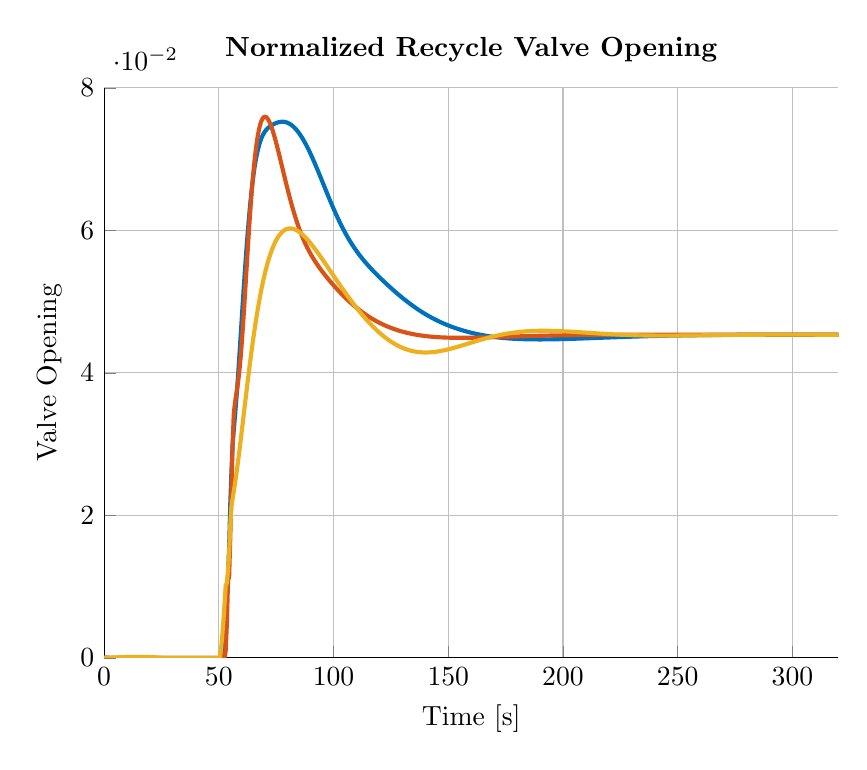
\begin{tikzpicture}

\begin{axis}[%
width=0.769\linewidth,
height=0.597\linewidth,
at={(0\linewidth,0\linewidth)},
scale only axis,
xmin=0,
xmax=320,
xlabel={Time [s]},
xmajorgrids,
ymin=0,
ymax=0.08,
ylabel={Valve Opening},
ymajorgrids,
axis background/.style={fill=white},
title style={font=\bfseries},
title={Normalized Recycle Valve Opening},
axis x line*=bottom,
axis y line*=left
]
\addplot [color=mycolor1,solid,line width=1.5pt,forget plot]
  table[row sep=crcr]{%
0	1.30651e-06\\
0.5	1.05998e-05\\
1	1.46601e-05\\
1.5	1.42539e-05\\
2	9.51022e-06\\
2.5	7.24745e-07\\
3	0\\
3.5	0\\
4	0\\
4.5	0\\
5	0\\
5.5	0\\
6	0\\
6.5	0\\
7	0\\
7.5	0\\
8	0\\
8.5	0\\
9	0\\
9.5	0\\
10	0\\
10.5	0\\
11	0\\
11.5	0\\
12	0\\
12.5	0\\
13	0\\
13.5	0\\
14	0\\
14.5	0\\
15	0\\
15.5	0\\
16	0\\
16.5	0\\
17	0\\
17.5	0\\
18	0\\
18.5	0\\
19	0\\
19.5	0\\
20	0\\
20.5	0\\
21	0\\
21.5	0\\
22	0\\
22.5	0\\
23	0\\
23.5	0\\
24	0\\
24.5	0\\
25	0\\
25.5	0\\
26	0\\
26.5	0\\
27	0\\
27.5	0\\
28	0\\
28.5	0\\
29	0\\
29.5	0\\
30	0\\
30.5	0\\
31	0\\
31.5	0\\
32	0\\
32.5	0\\
33	0\\
33.5	0\\
34	0\\
34.5	0\\
35	0\\
35.5	0\\
36	0\\
36.5	0\\
37	0\\
37.5	0\\
38	0\\
38.5	0\\
39	0\\
39.5	0\\
40	0\\
40.5	0\\
41	0\\
41.5	0\\
42	0\\
42.5	0\\
43	0\\
43.5	0\\
44	0\\
44.5	0\\
45	0\\
45.5	0\\
46	0\\
46.5	0\\
47	0\\
47.5	0\\
48	0\\
48.5	0\\
49	0\\
49.5	0\\
50	0\\
50.5	0\\
51	0.000407362\\
51.5	0\\
52	0.000176293\\
52.5	0.000992407\\
53	0.00554674\\
53.5	0.0100218\\
54	0.0114346\\
54.5	0.0156487\\
55	0.0216522\\
55.5	0.0262732\\
56	0.0298673\\
56.5	0.0319204\\
57	0.0337897\\
57.5	0.0357447\\
58	0.0378773\\
58.5	0.0401793\\
59	0.0426192\\
59.5	0.0451331\\
60	0.0476651\\
60.5	0.0501673\\
61	0.0526033\\
61.5	0.0549464\\
62	0.057178\\
62.5	0.0592848\\
63	0.0612554\\
63.5	0.0630781\\
64	0.0647406\\
64.5	0.0662327\\
65	0.0675499\\
65.5	0.068697\\
66	0.0696861\\
66.5	0.0705345\\
67	0.0712644\\
67.5	0.0718933\\
68	0.0724304\\
68.5	0.0728827\\
69	0.0732594\\
69.5	0.0735716\\
70	0.0738307\\
70.5	0.0740469\\
71	0.0742292\\
71.5	0.0743849\\
72	0.0745198\\
72.5	0.0746385\\
73	0.074744\\
73.5	0.0748385\\
74	0.0749233\\
74.5	0.074999\\
75	0.0750655\\
75.5	0.0751227\\
76	0.0751699\\
76.5	0.0752063\\
77	0.0752311\\
77.5	0.0752436\\
78	0.0752428\\
78.5	0.0752282\\
79	0.0751991\\
79.5	0.0751549\\
80	0.0750954\\
80.5	0.0750201\\
81	0.0749289\\
81.5	0.0748216\\
82	0.0746984\\
82.5	0.074559\\
83	0.0744038\\
83.5	0.0742327\\
84	0.0740461\\
84.5	0.0738442\\
85	0.0736273\\
85.5	0.0733957\\
86	0.0731498\\
86.5	0.07289\\
87	0.0726168\\
87.5	0.0723307\\
88	0.0720322\\
88.5	0.0717219\\
89	0.0714005\\
89.5	0.0710685\\
90	0.0707266\\
90.5	0.0703756\\
91	0.0700163\\
91.5	0.0696494\\
92	0.0692757\\
92.5	0.068896\\
93	0.0685112\\
93.5	0.0681221\\
94	0.0677296\\
94.5	0.0673345\\
95	0.0669377\\
95.5	0.06654\\
96	0.0661422\\
96.5	0.0657452\\
97	0.0653496\\
97.5	0.0649563\\
98	0.064566\\
98.5	0.0641793\\
99	0.0637968\\
99.5	0.0634192\\
100	0.063047\\
100.5	0.0626806\\
101	0.0623205\\
101.5	0.0619671\\
102	0.0616207\\
102.5	0.0612815\\
103	0.0609499\\
103.5	0.0606259\\
104	0.0603097\\
104.5	0.0600014\\
105	0.0597009\\
105.5	0.0594083\\
106	0.0591235\\
106.5	0.0588464\\
107	0.0585769\\
107.5	0.0583148\\
108	0.0580598\\
108.5	0.0578119\\
109	0.0575708\\
109.5	0.0573361\\
110	0.0571077\\
110.5	0.0568852\\
111	0.0566683\\
111.5	0.0564569\\
112	0.0562505\\
112.5	0.0560489\\
113	0.0558518\\
113.5	0.0556589\\
114	0.0554699\\
114.5	0.0552846\\
115	0.0551027\\
115.5	0.054924\\
116	0.0547483\\
116.5	0.0545752\\
117	0.0544047\\
117.5	0.0542365\\
118	0.0540704\\
118.5	0.0539064\\
119	0.0537443\\
119.5	0.0535839\\
120	0.0534252\\
120.5	0.053268\\
121	0.0531123\\
121.5	0.0529579\\
122	0.052805\\
122.5	0.0526533\\
123	0.0525029\\
123.5	0.0523537\\
124	0.0522058\\
124.5	0.0520592\\
125	0.0519137\\
125.5	0.0517696\\
126	0.0516266\\
126.5	0.051485\\
127	0.0513447\\
127.5	0.0512057\\
128	0.0510681\\
128.5	0.0509318\\
129	0.050797\\
129.5	0.0506637\\
130	0.0505318\\
130.5	0.0504015\\
131	0.0502728\\
131.5	0.0501456\\
132	0.0500201\\
132.5	0.0498962\\
133	0.049774\\
133.5	0.0496535\\
134	0.0495348\\
134.5	0.0494178\\
135	0.0493025\\
135.5	0.049189\\
136	0.0490773\\
136.5	0.0489674\\
137	0.0488593\\
137.5	0.048753\\
138	0.0486485\\
138.5	0.0485459\\
139	0.048445\\
139.5	0.0483459\\
140	0.0482486\\
140.5	0.0481531\\
141	0.0480594\\
141.5	0.0479674\\
142	0.0478772\\
142.5	0.0477887\\
143	0.0477019\\
143.5	0.0476168\\
144	0.0475334\\
144.5	0.0474517\\
145	0.0473716\\
145.5	0.0472931\\
146	0.0472162\\
146.5	0.047141\\
147	0.0470672\\
147.5	0.046995\\
148	0.0469244\\
148.5	0.0468552\\
149	0.0467875\\
149.5	0.0467213\\
150	0.0466565\\
150.5	0.0465931\\
151	0.0465312\\
151.5	0.0464706\\
152	0.0464113\\
152.5	0.0463534\\
153	0.0462969\\
153.5	0.0462416\\
154	0.0461876\\
154.5	0.0461349\\
155	0.0460834\\
155.5	0.0460332\\
156	0.0459842\\
156.5	0.0459363\\
157	0.0458897\\
157.5	0.0458442\\
158	0.0457999\\
158.5	0.0457567\\
159	0.0457147\\
159.5	0.0456737\\
160	0.0456338\\
160.5	0.045595\\
161	0.0455573\\
161.5	0.0455206\\
162	0.0454849\\
162.5	0.0454503\\
163	0.0454166\\
163.5	0.0453839\\
164	0.0453522\\
164.5	0.0453215\\
165	0.0452917\\
165.5	0.0452628\\
166	0.0452348\\
166.5	0.0452077\\
167	0.0451815\\
167.5	0.0451562\\
168	0.0451317\\
168.5	0.0451081\\
169	0.0450853\\
169.5	0.0450633\\
170	0.0450421\\
170.5	0.0450216\\
171	0.045002\\
171.5	0.0449831\\
172	0.0449649\\
172.5	0.0449475\\
173	0.0449308\\
173.5	0.0449147\\
174	0.0448994\\
174.5	0.0448847\\
175	0.0448707\\
175.5	0.0448573\\
176	0.0448446\\
176.5	0.0448325\\
177	0.0448209\\
177.5	0.04481\\
178	0.0447996\\
178.5	0.0447898\\
179	0.0447806\\
179.5	0.0447719\\
180	0.0447637\\
180.5	0.044756\\
181	0.0447488\\
181.5	0.0447422\\
182	0.044736\\
182.5	0.0447302\\
183	0.0447249\\
183.5	0.0447201\\
184	0.0447156\\
184.5	0.0447116\\
185	0.044708\\
185.5	0.0447048\\
186	0.044702\\
186.5	0.0446996\\
187	0.0446975\\
187.5	0.0446958\\
188	0.0446944\\
188.5	0.0446934\\
189	0.0446926\\
189.5	0.0446922\\
190	0.0446921\\
190.5	0.0446923\\
191	0.0446928\\
191.5	0.0446935\\
192	0.0446945\\
192.5	0.0446958\\
193	0.0446973\\
193.5	0.0446991\\
194	0.0447011\\
194.5	0.0447033\\
195	0.0447058\\
195.5	0.0447084\\
196	0.0447113\\
196.5	0.0447143\\
197	0.0447176\\
197.5	0.044721\\
198	0.0447246\\
198.5	0.0447283\\
199	0.0447322\\
199.5	0.0447363\\
200	0.0447405\\
200.5	0.0447448\\
201	0.0447493\\
201.5	0.0447539\\
202	0.0447586\\
202.5	0.0447635\\
203	0.0447684\\
203.5	0.0447735\\
204	0.0447786\\
204.5	0.0447838\\
205	0.0447892\\
205.5	0.0447946\\
206	0.0448\\
206.5	0.0448056\\
207	0.0448112\\
207.5	0.0448169\\
208	0.0448226\\
208.5	0.0448284\\
209	0.0448342\\
209.5	0.0448401\\
210	0.044846\\
210.5	0.044852\\
211	0.044858\\
211.5	0.044864\\
212	0.04487\\
212.5	0.0448761\\
213	0.0448821\\
213.5	0.0448882\\
214	0.0448943\\
214.5	0.0449004\\
215	0.0449066\\
215.5	0.0449127\\
216	0.0449188\\
216.5	0.0449249\\
217	0.044931\\
217.5	0.0449371\\
218	0.0449432\\
218.5	0.0449493\\
219	0.0449553\\
219.5	0.0449613\\
220	0.0449674\\
220.5	0.0449733\\
221	0.0449793\\
221.5	0.0449853\\
222	0.0449912\\
222.5	0.044997\\
223	0.0450029\\
223.5	0.0450087\\
224	0.0450145\\
224.5	0.0450202\\
225	0.0450259\\
225.5	0.0450316\\
226	0.0450372\\
226.5	0.0450428\\
227	0.0450483\\
227.5	0.0450538\\
228	0.0450593\\
228.5	0.0450646\\
229	0.04507\\
229.5	0.0450753\\
230	0.0450805\\
230.5	0.0450857\\
231	0.0450909\\
231.5	0.045096\\
232	0.045101\\
232.5	0.045106\\
233	0.045111\\
233.5	0.0451158\\
234	0.0451207\\
234.5	0.0451254\\
235	0.0451302\\
235.5	0.0451348\\
236	0.0451394\\
236.5	0.045144\\
237	0.0451485\\
237.5	0.0451529\\
238	0.0451573\\
238.5	0.0451616\\
239	0.0451658\\
239.5	0.04517\\
240	0.0451742\\
240.5	0.0451783\\
241	0.0451823\\
241.5	0.0451863\\
242	0.0451902\\
242.5	0.045194\\
243	0.0451978\\
243.5	0.0452016\\
244	0.0452053\\
244.5	0.0452089\\
245	0.0452124\\
245.5	0.045216\\
246	0.0452194\\
246.5	0.0452228\\
247	0.0452262\\
247.5	0.0452294\\
248	0.0452327\\
248.5	0.0452358\\
249	0.045239\\
249.5	0.045242\\
250	0.045245\\
250.5	0.045248\\
251	0.0452509\\
251.5	0.0452537\\
252	0.0452565\\
252.5	0.0452593\\
253	0.045262\\
253.5	0.0452646\\
254	0.0452672\\
254.5	0.0452698\\
255	0.0452723\\
255.5	0.0452747\\
256	0.0452771\\
256.5	0.0452794\\
257	0.0452817\\
257.5	0.045284\\
258	0.0452862\\
258.5	0.0452883\\
259	0.0452904\\
259.5	0.0452925\\
260	0.0452945\\
260.5	0.0452965\\
261	0.0452984\\
261.5	0.0453003\\
262	0.0453022\\
262.5	0.045304\\
263	0.0453057\\
263.5	0.0453074\\
264	0.0453091\\
264.5	0.0453108\\
265	0.0453124\\
265.5	0.0453139\\
266	0.0453154\\
266.5	0.0453169\\
267	0.0453184\\
267.5	0.0453198\\
268	0.0453212\\
268.5	0.0453225\\
269	0.0453238\\
269.5	0.0453251\\
270	0.0453263\\
270.5	0.0453275\\
271	0.0453287\\
271.5	0.0453298\\
272	0.0453309\\
272.5	0.045332\\
273	0.045333\\
273.5	0.045334\\
274	0.045335\\
274.5	0.045336\\
275	0.0453369\\
275.5	0.0453378\\
276	0.0453386\\
276.5	0.0453395\\
277	0.0453403\\
277.5	0.0453411\\
278	0.0453418\\
278.5	0.0453426\\
279	0.0453433\\
279.5	0.045344\\
280	0.0453446\\
280.5	0.0453453\\
281	0.0453459\\
281.5	0.0453465\\
282	0.0453471\\
282.5	0.0453476\\
283	0.0453481\\
283.5	0.0453486\\
284	0.0453491\\
284.5	0.0453496\\
285	0.0453501\\
285.5	0.0453505\\
286	0.0453509\\
286.5	0.0453513\\
287	0.0453517\\
287.5	0.045352\\
288	0.0453524\\
288.5	0.0453527\\
289	0.045353\\
289.5	0.0453533\\
290	0.0453536\\
290.5	0.0453538\\
291	0.0453541\\
291.5	0.0453543\\
292	0.0453545\\
292.5	0.0453547\\
293	0.0453549\\
293.5	0.0453551\\
294	0.0453553\\
294.5	0.0453554\\
295	0.0453556\\
295.5	0.0453557\\
296	0.0453558\\
296.5	0.045356\\
297	0.0453561\\
297.5	0.0453561\\
298	0.0453562\\
298.5	0.0453563\\
299	0.0453564\\
299.5	0.0453564\\
300	0.0453565\\
300.5	0.0453565\\
301	0.0453565\\
301.5	0.0453565\\
302	0.0453565\\
302.5	0.0453565\\
303	0.0453565\\
303.5	0.0453565\\
304	0.0453565\\
304.5	0.0453565\\
305	0.0453564\\
305.5	0.0453564\\
306	0.0453564\\
306.5	0.0453563\\
307	0.0453563\\
307.5	0.0453562\\
308	0.0453561\\
308.5	0.0453561\\
309	0.045356\\
309.5	0.0453559\\
310	0.0453558\\
310.5	0.0453557\\
311	0.0453556\\
311.5	0.0453555\\
312	0.0453554\\
312.5	0.0453553\\
313	0.0453552\\
313.5	0.0453551\\
314	0.045355\\
314.5	0.0453549\\
315	0.0453548\\
315.5	0.0453546\\
316	0.0453545\\
316.5	0.0453544\\
317	0.0453543\\
317.5	0.0453541\\
318	0.045354\\
318.5	0.0453539\\
319	0.0453537\\
319.5	0.0453536\\
320	0.0453535\\
320.5	0.0453533\\
321	0.0453532\\
321.5	0.045353\\
322	0.0453529\\
322.5	0.0453527\\
323	0.0453526\\
323.5	0.0453525\\
324	0.0453523\\
324.5	0.0453522\\
325	0.045352\\
325.5	0.0453519\\
326	0.0453517\\
326.5	0.0453516\\
327	0.0453514\\
327.5	0.0453513\\
328	0.0453511\\
328.5	0.045351\\
329	0.0453508\\
329.5	0.0453507\\
330	0.0453505\\
330.5	0.0453504\\
331	0.0453502\\
331.5	0.0453501\\
332	0.0453499\\
332.5	0.0453498\\
333	0.0453496\\
333.5	0.0453495\\
334	0.0453494\\
334.5	0.0453492\\
335	0.0453491\\
335.5	0.0453489\\
336	0.0453488\\
336.5	0.0453486\\
337	0.0453485\\
337.5	0.0453484\\
338	0.0453482\\
338.5	0.0453481\\
339	0.045348\\
339.5	0.0453478\\
340	0.0453477\\
340.5	0.0453476\\
341	0.0453474\\
341.5	0.0453473\\
342	0.0453472\\
342.5	0.045347\\
343	0.0453469\\
343.5	0.0453468\\
344	0.0453467\\
344.5	0.0453466\\
345	0.0453464\\
345.5	0.0453463\\
346	0.0453462\\
346.5	0.0453461\\
347	0.045346\\
347.5	0.0453459\\
348	0.0453457\\
348.5	0.0453456\\
349	0.0453455\\
349.5	0.0453454\\
350	0.0453453\\
350.5	0.0453452\\
351	0.0453451\\
351.5	0.045345\\
352	0.0453449\\
352.5	0.0453448\\
353	0.0453447\\
353.5	0.0453446\\
354	0.0453445\\
354.5	0.0453444\\
355	0.0453443\\
355.5	0.0453442\\
356	0.0453441\\
356.5	0.045344\\
357	0.045344\\
357.5	0.0453439\\
358	0.0453438\\
358.5	0.0453437\\
359	0.0453436\\
359.5	0.0453435\\
360	0.0453435\\
360.5	0.0453434\\
361	0.0453433\\
361.5	0.0453432\\
362	0.0453432\\
362.5	0.0453431\\
363	0.045343\\
363.5	0.0453429\\
364	0.0453429\\
364.5	0.0453428\\
365	0.0453427\\
365.5	0.0453427\\
366	0.0453426\\
366.5	0.0453425\\
367	0.0453425\\
367.5	0.0453424\\
368	0.0453424\\
368.5	0.0453423\\
369	0.0453423\\
369.5	0.0453422\\
370	0.0453421\\
370.5	0.0453421\\
371	0.045342\\
371.5	0.045342\\
372	0.0453419\\
372.5	0.0453419\\
373	0.0453418\\
373.5	0.0453418\\
374	0.0453417\\
374.5	0.0453417\\
375	0.0453417\\
375.5	0.0453416\\
376	0.0453416\\
376.5	0.0453415\\
377	0.0453415\\
377.5	0.0453415\\
378	0.0453414\\
378.5	0.0453414\\
379	0.0453413\\
379.5	0.0453413\\
380	0.0453413\\
380.5	0.0453412\\
381	0.0453412\\
381.5	0.0453412\\
382	0.0453412\\
382.5	0.0453411\\
383	0.0453411\\
383.5	0.0453411\\
384	0.045341\\
384.5	0.045341\\
385	0.045341\\
385.5	0.045341\\
386	0.0453409\\
386.5	0.0453409\\
387	0.0453409\\
387.5	0.0453409\\
388	0.0453408\\
388.5	0.0453408\\
389	0.0453408\\
389.5	0.0453408\\
390	0.0453408\\
390.5	0.0453408\\
391	0.0453407\\
391.5	0.0453407\\
392	0.0453407\\
392.5	0.0453407\\
393	0.0453407\\
393.5	0.0453407\\
394	0.0453406\\
394.5	0.0453406\\
395	0.0453406\\
395.5	0.0453406\\
396	0.0453406\\
396.5	0.0453406\\
397	0.0453406\\
397.5	0.0453406\\
398	0.0453405\\
398.5	0.0453405\\
399	0.0453405\\
399.5	0.0453405\\
400	0.0453405\\
400.5	0.0453405\\
401	0.0453405\\
401.5	0.0453405\\
402	0.0453405\\
402.5	0.0453405\\
403	0.0453405\\
403.5	0.0453405\\
404	0.0453405\\
404.5	0.0453404\\
405	0.0453404\\
405.5	0.0453404\\
406	0.0453404\\
406.5	0.0453404\\
407	0.0453404\\
407.5	0.0453404\\
408	0.0453404\\
408.5	0.0453404\\
409	0.0453404\\
409.5	0.0453404\\
410	0.0453404\\
410.5	0.0453404\\
411	0.0453404\\
411.5	0.0453404\\
412	0.0453404\\
412.5	0.0453404\\
413	0.0453404\\
413.5	0.0453404\\
414	0.0453404\\
414.5	0.0453404\\
415	0.0453404\\
415.5	0.0453404\\
416	0.0453404\\
416.5	0.0453404\\
417	0.0453404\\
417.5	0.0453404\\
418	0.0453404\\
418.5	0.0453404\\
419	0.0453404\\
419.5	0.0453404\\
420	0.0453404\\
420.5	0.0453404\\
421	0.0453404\\
421.5	0.0453404\\
422	0.0453404\\
422.5	0.0453404\\
423	0.0453404\\
423.5	0.0453404\\
424	0.0453404\\
424.5	0.0453404\\
425	0.0453404\\
425.5	0.0453404\\
426	0.0453404\\
426.5	0.0453404\\
427	0.0453404\\
427.5	0.0453404\\
428	0.0453405\\
428.5	0.0453405\\
429	0.0453405\\
429.5	0.0453405\\
430	0.0453405\\
430.5	0.0453405\\
431	0.0453405\\
431.5	0.0453405\\
432	0.0453405\\
432.5	0.0453405\\
433	0.0453405\\
433.5	0.0453405\\
434	0.0453405\\
434.5	0.0453405\\
435	0.0453405\\
435.5	0.0453405\\
436	0.0453405\\
436.5	0.0453405\\
437	0.0453405\\
437.5	0.0453405\\
438	0.0453405\\
438.5	0.0453405\\
439	0.0453405\\
439.5	0.0453405\\
440	0.0453405\\
440.5	0.0453405\\
441	0.0453405\\
441.5	0.0453405\\
442	0.0453405\\
442.5	0.0453406\\
443	0.0453406\\
443.5	0.0453406\\
444	0.0453406\\
444.5	0.0453406\\
445	0.0453406\\
445.5	0.0453406\\
446	0.0453406\\
446.5	0.0453406\\
447	0.0453406\\
447.5	0.0453406\\
448	0.0453406\\
448.5	0.0453406\\
449	0.0453406\\
449.5	0.0453406\\
450	0.0453406\\
450.5	0.0453406\\
451	0.0453406\\
451.5	0.0453406\\
452	0.0453406\\
452.5	0.0453406\\
453	0.0453406\\
453.5	0.0453406\\
454	0.0453406\\
454.5	0.0453406\\
455	0.0453406\\
455.5	0.0453406\\
456	0.0453406\\
456.5	0.0453406\\
457	0.0453406\\
457.5	0.0453407\\
458	0.0453407\\
458.5	0.0453407\\
459	0.0453407\\
459.5	0.0453407\\
460	0.0453407\\
460.5	0.0453407\\
461	0.0453407\\
461.5	0.0453407\\
462	0.0453407\\
462.5	0.0453407\\
463	0.0453407\\
463.5	0.0453407\\
464	0.0453407\\
464.5	0.0453407\\
465	0.0453407\\
465.5	0.0453407\\
466	0.0453407\\
466.5	0.0453407\\
467	0.0453407\\
467.5	0.0453407\\
468	0.0453407\\
468.5	0.0453407\\
469	0.0453407\\
469.5	0.0453407\\
470	0.0453407\\
470.5	0.0453407\\
471	0.0453407\\
471.5	0.0453407\\
472	0.0453407\\
472.5	0.0453407\\
473	0.0453407\\
473.5	0.0453407\\
474	0.0453407\\
474.5	0.0453407\\
475	0.0453407\\
475.5	0.0453407\\
476	0.0453407\\
476.5	0.0453407\\
477	0.0453407\\
477.5	0.0453407\\
478	0.0453407\\
478.5	0.0453407\\
479	0.0453407\\
479.5	0.0453407\\
480	0.0453407\\
480.5	0.0453407\\
481	0.0453408\\
481.5	0.0453408\\
482	0.0453408\\
482.5	0.0453408\\
483	0.0453408\\
483.5	0.0453408\\
484	0.0453408\\
484.5	0.0453408\\
485	0.0453408\\
485.5	0.0453408\\
486	0.0453408\\
486.5	0.0453408\\
487	0.0453408\\
487.5	0.0453408\\
488	0.0453408\\
488.5	0.0453408\\
489	0.0453408\\
489.5	0.0453408\\
490	0.0453408\\
490.5	0.0453408\\
491	0.0453408\\
491.5	0.0453408\\
492	0.0453408\\
492.5	0.0453408\\
493	0.0453408\\
493.5	0.0453408\\
494	0.0453408\\
494.5	0.0453408\\
495	0.0453408\\
495.5	0.0453408\\
496	0.0453408\\
496.5	0.0453408\\
497	0.0453408\\
497.5	0.0453408\\
498	0.0453408\\
498.5	0.0453408\\
499	0.0453408\\
499.5	0.0453408\\
};
\addplot [color=mycolor2,solid,line width=1.5pt,forget plot]
  table[row sep=crcr]{%
0	1.15805e-06\\
0.5	8.79271e-06\\
1	4.91879e-06\\
1.5	0\\
2	0\\
2.5	0\\
3	0\\
3.5	0\\
4	0\\
4.5	0\\
5	0\\
5.5	0\\
6	0\\
6.5	0\\
7	0\\
7.5	0\\
8	0\\
8.5	0\\
9	0\\
9.5	0\\
10	0\\
10.5	0\\
11	0\\
11.5	0\\
12	0\\
12.5	0\\
13	0\\
13.5	0\\
14	0\\
14.5	0\\
15	0\\
15.5	0\\
16	0\\
16.5	0\\
17	0\\
17.5	0\\
18	0\\
18.5	0\\
19	0\\
19.5	0\\
20	0\\
20.5	0\\
21	0\\
21.5	0\\
22	0\\
22.5	0\\
23	0\\
23.5	0\\
24	0\\
24.5	0\\
25	0\\
25.5	0\\
26	0\\
26.5	0\\
27	0\\
27.5	0\\
28	0\\
28.5	0\\
29	0\\
29.5	0\\
30	0\\
30.5	0\\
31	0\\
31.5	0\\
32	0\\
32.5	0\\
33	0\\
33.5	0\\
34	0\\
34.5	0\\
35	0\\
35.5	0\\
36	0\\
36.5	0\\
37	0\\
37.5	0\\
38	0\\
38.5	0\\
39	0\\
39.5	0\\
40	0\\
40.5	0\\
41	0\\
41.5	0\\
42	0\\
42.5	0\\
43	0\\
43.5	0\\
44	0\\
44.5	0\\
45	0\\
45.5	0\\
46	0\\
46.5	0\\
47	0\\
47.5	0\\
48	0\\
48.5	0\\
49	0\\
49.5	0\\
50	0\\
50.5	0\\
51	0.000716488\\
51.5	0\\
52	0\\
52.5	0\\
53	0.00103895\\
53.5	0.00470309\\
54	0.0107935\\
54.5	0.0114171\\
55	0.017038\\
55.5	0.0235933\\
56	0.0298378\\
56.5	0.0341844\\
57	0.0357491\\
57.5	0.036757\\
58	0.0377925\\
58.5	0.0389789\\
59	0.0404036\\
59.5	0.0421501\\
60	0.0441855\\
60.5	0.0464636\\
61	0.048928\\
61.5	0.0515184\\
62	0.0541633\\
62.5	0.0567917\\
63	0.0593413\\
63.5	0.0617627\\
64	0.0640195\\
64.5	0.0660866\\
65	0.0679495\\
65.5	0.0696011\\
66	0.0710408\\
66.5	0.0722728\\
67	0.0733047\\
67.5	0.0741466\\
68	0.0748103\\
68.5	0.0753087\\
69	0.075655\\
69.5	0.0758625\\
70	0.0759442\\
70.5	0.0759128\\
71	0.0757802\\
71.5	0.0755577\\
72	0.0752559\\
72.5	0.0748844\\
73	0.0744525\\
73.5	0.0739683\\
74	0.0734397\\
74.5	0.0728738\\
75	0.072277\\
75.5	0.0716555\\
76	0.0710149\\
76.5	0.0703602\\
77	0.0696962\\
77.5	0.0690272\\
78	0.0683572\\
78.5	0.0676898\\
79	0.0670283\\
79.5	0.0663754\\
80	0.0657338\\
80.5	0.0651056\\
81	0.0644929\\
81.5	0.0638971\\
82	0.0633195\\
82.5	0.0627612\\
83	0.0622228\\
83.5	0.0617048\\
84	0.0612074\\
84.5	0.0607305\\
85	0.0602741\\
85.5	0.0598376\\
86	0.0594206\\
86.5	0.0590224\\
87	0.0586423\\
87.5	0.0582793\\
88	0.0579325\\
88.5	0.0576011\\
89	0.057284\\
89.5	0.0569802\\
90	0.0566887\\
90.5	0.0564085\\
91	0.0561387\\
91.5	0.0558784\\
92	0.0556268\\
92.5	0.055383\\
93	0.0551462\\
93.5	0.0549159\\
94	0.0546913\\
94.5	0.0544719\\
95	0.0542572\\
95.5	0.0540467\\
96	0.0538402\\
96.5	0.0536371\\
97	0.0534373\\
97.5	0.0532406\\
98	0.0530467\\
98.5	0.0528554\\
99	0.0526668\\
99.5	0.0524806\\
100	0.0522968\\
100.5	0.0521154\\
101	0.0519364\\
101.5	0.0517598\\
102	0.0515855\\
102.5	0.0514136\\
103	0.0512441\\
103.5	0.0510771\\
104	0.0509125\\
104.5	0.0507505\\
105	0.050591\\
105.5	0.0504341\\
106	0.0502798\\
106.5	0.0501281\\
107	0.0499791\\
107.5	0.0498328\\
108	0.0496891\\
108.5	0.0495482\\
109	0.04941\\
109.5	0.0492745\\
110	0.0491418\\
110.5	0.0490117\\
111	0.0488843\\
111.5	0.0487597\\
112	0.0486377\\
112.5	0.0485183\\
113	0.0484016\\
113.5	0.0482875\\
114	0.048176\\
114.5	0.048067\\
115	0.0479606\\
115.5	0.0478566\\
116	0.0477552\\
116.5	0.0476561\\
117	0.0475595\\
117.5	0.0474653\\
118	0.0473734\\
118.5	0.0472838\\
119	0.0471965\\
119.5	0.0471114\\
120	0.0470286\\
120.5	0.0469479\\
121	0.0468694\\
121.5	0.046793\\
122	0.0467186\\
122.5	0.0466464\\
123	0.0465761\\
123.5	0.0465079\\
124	0.0464416\\
124.5	0.0463772\\
125	0.0463147\\
125.5	0.046254\\
126	0.0461952\\
126.5	0.0461382\\
127	0.046083\\
127.5	0.0460295\\
128	0.0459777\\
128.5	0.0459276\\
129	0.0458791\\
129.5	0.0458322\\
130	0.0457869\\
130.5	0.0457432\\
131	0.0457009\\
131.5	0.0456602\\
132	0.0456209\\
132.5	0.0455831\\
133	0.0455466\\
133.5	0.0455116\\
134	0.0454778\\
134.5	0.0454454\\
135	0.0454143\\
135.5	0.0453844\\
136	0.0453557\\
136.5	0.0453283\\
137	0.045302\\
137.5	0.0452768\\
138	0.0452528\\
138.5	0.0452298\\
139	0.0452079\\
139.5	0.045187\\
140	0.0451671\\
140.5	0.0451483\\
141	0.0451303\\
141.5	0.0451133\\
142	0.0450972\\
142.5	0.045082\\
143	0.0450676\\
143.5	0.045054\\
144	0.0450413\\
144.5	0.0450293\\
145	0.0450181\\
145.5	0.0450076\\
146	0.0449978\\
146.5	0.0449887\\
147	0.0449803\\
147.5	0.0449725\\
148	0.0449654\\
148.5	0.0449588\\
149	0.0449528\\
149.5	0.0449474\\
150	0.0449426\\
150.5	0.0449382\\
151	0.0449344\\
151.5	0.0449311\\
152	0.0449282\\
152.5	0.0449258\\
153	0.0449238\\
153.5	0.0449222\\
154	0.044921\\
154.5	0.0449202\\
155	0.0449198\\
155.5	0.0449198\\
156	0.04492\\
156.5	0.0449206\\
157	0.0449215\\
157.5	0.0449227\\
158	0.0449242\\
158.5	0.0449259\\
159	0.0449279\\
159.5	0.0449302\\
160	0.0449326\\
160.5	0.0449353\\
161	0.0449382\\
161.5	0.0449413\\
162	0.0449446\\
162.5	0.0449481\\
163	0.0449517\\
163.5	0.0449554\\
164	0.0449593\\
164.5	0.0449634\\
165	0.0449675\\
165.5	0.0449718\\
166	0.0449762\\
166.5	0.0449807\\
167	0.0449853\\
167.5	0.04499\\
168	0.0449947\\
168.5	0.0449995\\
169	0.0450044\\
169.5	0.0450093\\
170	0.0450143\\
170.5	0.0450193\\
171	0.0450244\\
171.5	0.0450294\\
172	0.0450345\\
172.5	0.0450397\\
173	0.0450448\\
173.5	0.04505\\
174	0.0450552\\
174.5	0.0450603\\
175	0.0450655\\
175.5	0.0450706\\
176	0.0450758\\
176.5	0.0450809\\
177	0.045086\\
177.5	0.0450911\\
178	0.0450962\\
178.5	0.0451012\\
179	0.0451062\\
179.5	0.0451112\\
180	0.0451161\\
180.5	0.045121\\
181	0.0451259\\
181.5	0.0451307\\
182	0.0451355\\
182.5	0.0451402\\
183	0.0451449\\
183.5	0.0451495\\
184	0.0451541\\
184.5	0.0451586\\
185	0.0451631\\
185.5	0.0451675\\
186	0.0451718\\
186.5	0.0451761\\
187	0.0451804\\
187.5	0.0451846\\
188	0.0451887\\
188.5	0.0451927\\
189	0.0451967\\
189.5	0.0452007\\
190	0.0452045\\
190.5	0.0452084\\
191	0.0452121\\
191.5	0.0452158\\
192	0.0452194\\
192.5	0.045223\\
193	0.0452265\\
193.5	0.0452299\\
194	0.0452333\\
194.5	0.0452366\\
195	0.0452398\\
195.5	0.045243\\
196	0.0452461\\
196.5	0.0452491\\
197	0.0452521\\
197.5	0.0452551\\
198	0.0452579\\
198.5	0.0452607\\
199	0.0452635\\
199.5	0.0452661\\
200	0.0452688\\
200.5	0.0452713\\
201	0.0452738\\
201.5	0.0452763\\
202	0.0452787\\
202.5	0.045281\\
203	0.0452833\\
203.5	0.0452855\\
204	0.0452877\\
204.5	0.0452898\\
205	0.0452919\\
205.5	0.0452939\\
206	0.0452958\\
206.5	0.0452977\\
207	0.0452996\\
207.5	0.0453014\\
208	0.0453031\\
208.5	0.0453048\\
209	0.0453065\\
209.5	0.0453081\\
210	0.0453097\\
210.5	0.0453112\\
211	0.0453127\\
211.5	0.0453141\\
212	0.0453155\\
212.5	0.0453168\\
213	0.0453182\\
213.5	0.0453194\\
214	0.0453207\\
214.5	0.0453218\\
215	0.045323\\
215.5	0.0453241\\
216	0.0453252\\
216.5	0.0453262\\
217	0.0453272\\
217.5	0.0453282\\
218	0.0453291\\
218.5	0.0453301\\
219	0.0453309\\
219.5	0.0453318\\
220	0.0453326\\
220.5	0.0453334\\
221	0.0453341\\
221.5	0.0453348\\
222	0.0453355\\
222.5	0.0453362\\
223	0.0453369\\
223.5	0.0453375\\
224	0.0453381\\
224.5	0.0453386\\
225	0.0453392\\
225.5	0.0453397\\
226	0.0453402\\
226.5	0.0453407\\
227	0.0453411\\
227.5	0.0453416\\
228	0.045342\\
228.5	0.0453424\\
229	0.0453428\\
229.5	0.0453431\\
230	0.0453435\\
230.5	0.0453438\\
231	0.0453441\\
231.5	0.0453444\\
232	0.0453446\\
232.5	0.0453449\\
233	0.0453451\\
233.5	0.0453454\\
234	0.0453456\\
234.5	0.0453458\\
235	0.045346\\
235.5	0.0453462\\
236	0.0453463\\
236.5	0.0453465\\
237	0.0453466\\
237.5	0.0453467\\
238	0.0453469\\
238.5	0.045347\\
239	0.0453471\\
239.5	0.0453471\\
240	0.0453472\\
240.5	0.0453473\\
241	0.0453474\\
241.5	0.0453474\\
242	0.0453475\\
242.5	0.0453475\\
243	0.0453475\\
243.5	0.0453476\\
244	0.0453476\\
244.5	0.0453476\\
245	0.0453476\\
245.5	0.0453476\\
246	0.0453476\\
246.5	0.0453476\\
247	0.0453476\\
247.5	0.0453475\\
248	0.0453475\\
248.5	0.0453475\\
249	0.0453474\\
249.5	0.0453474\\
250	0.0453474\\
250.5	0.0453473\\
251	0.0453473\\
251.5	0.0453472\\
252	0.0453472\\
252.5	0.0453471\\
253	0.045347\\
253.5	0.045347\\
254	0.0453469\\
254.5	0.0453469\\
255	0.0453468\\
255.5	0.0453467\\
256	0.0453466\\
256.5	0.0453466\\
257	0.0453465\\
257.5	0.0453464\\
258	0.0453463\\
258.5	0.0453463\\
259	0.0453462\\
259.5	0.0453461\\
260	0.045346\\
260.5	0.0453459\\
261	0.0453459\\
261.5	0.0453458\\
262	0.0453457\\
262.5	0.0453456\\
263	0.0453455\\
263.5	0.0453454\\
264	0.0453454\\
264.5	0.0453453\\
265	0.0453452\\
265.5	0.0453451\\
266	0.045345\\
266.5	0.0453449\\
267	0.0453449\\
267.5	0.0453448\\
268	0.0453447\\
268.5	0.0453446\\
269	0.0453445\\
269.5	0.0453445\\
270	0.0453444\\
270.5	0.0453443\\
271	0.0453442\\
271.5	0.0453441\\
272	0.0453441\\
272.5	0.045344\\
273	0.0453439\\
273.5	0.0453438\\
274	0.0453438\\
274.5	0.0453437\\
275	0.0453436\\
275.5	0.0453435\\
276	0.0453435\\
276.5	0.0453434\\
277	0.0453433\\
277.5	0.0453433\\
278	0.0453432\\
278.5	0.0453431\\
279	0.0453431\\
279.5	0.045343\\
280	0.045343\\
280.5	0.0453429\\
281	0.0453428\\
281.5	0.0453428\\
282	0.0453427\\
282.5	0.0453427\\
283	0.0453426\\
283.5	0.0453425\\
284	0.0453425\\
284.5	0.0453424\\
285	0.0453424\\
285.5	0.0453423\\
286	0.0453423\\
286.5	0.0453422\\
287	0.0453422\\
287.5	0.0453421\\
288	0.0453421\\
288.5	0.0453421\\
289	0.045342\\
289.5	0.045342\\
290	0.0453419\\
290.5	0.0453419\\
291	0.0453418\\
291.5	0.0453418\\
292	0.0453418\\
292.5	0.0453417\\
293	0.0453417\\
293.5	0.0453417\\
294	0.0453416\\
294.5	0.0453416\\
295	0.0453416\\
295.5	0.0453415\\
296	0.0453415\\
296.5	0.0453415\\
297	0.0453414\\
297.5	0.0453414\\
298	0.0453414\\
298.5	0.0453414\\
299	0.0453413\\
299.5	0.0453413\\
300	0.0453413\\
300.5	0.0453413\\
301	0.0453412\\
301.5	0.0453412\\
302	0.0453412\\
302.5	0.0453412\\
303	0.0453411\\
303.5	0.0453411\\
304	0.0453411\\
304.5	0.0453411\\
305	0.0453411\\
305.5	0.045341\\
306	0.045341\\
306.5	0.045341\\
307	0.045341\\
307.5	0.045341\\
308	0.045341\\
308.5	0.045341\\
309	0.0453409\\
309.5	0.0453409\\
310	0.0453409\\
310.5	0.0453409\\
311	0.0453409\\
311.5	0.0453409\\
312	0.0453409\\
312.5	0.0453409\\
313	0.0453408\\
313.5	0.0453408\\
314	0.0453408\\
314.5	0.0453408\\
315	0.0453408\\
315.5	0.0453408\\
316	0.0453408\\
316.5	0.0453408\\
317	0.0453408\\
317.5	0.0453408\\
318	0.0453408\\
318.5	0.0453408\\
319	0.0453408\\
319.5	0.0453407\\
320	0.0453407\\
320.5	0.0453407\\
321	0.0453407\\
321.5	0.0453407\\
322	0.0453407\\
322.5	0.0453407\\
323	0.0453407\\
323.5	0.0453407\\
324	0.0453407\\
324.5	0.0453407\\
325	0.0453407\\
325.5	0.0453407\\
326	0.0453407\\
326.5	0.0453407\\
327	0.0453407\\
327.5	0.0453407\\
328	0.0453407\\
328.5	0.0453407\\
329	0.0453407\\
329.5	0.0453407\\
330	0.0453407\\
330.5	0.0453407\\
331	0.0453407\\
331.5	0.0453407\\
332	0.0453407\\
332.5	0.0453407\\
333	0.0453407\\
333.5	0.0453407\\
334	0.0453407\\
334.5	0.0453407\\
335	0.0453407\\
335.5	0.0453407\\
336	0.0453407\\
336.5	0.0453407\\
337	0.0453407\\
337.5	0.0453407\\
338	0.0453407\\
338.5	0.0453407\\
339	0.0453407\\
339.5	0.0453407\\
340	0.0453407\\
340.5	0.0453407\\
341	0.0453407\\
341.5	0.0453407\\
342	0.0453407\\
342.5	0.0453407\\
343	0.0453407\\
343.5	0.0453407\\
344	0.0453407\\
344.5	0.0453407\\
345	0.0453407\\
345.5	0.0453407\\
346	0.0453407\\
346.5	0.0453407\\
347	0.0453407\\
347.5	0.0453407\\
348	0.0453407\\
348.5	0.0453407\\
349	0.0453407\\
349.5	0.0453407\\
350	0.0453407\\
350.5	0.0453407\\
351	0.0453407\\
351.5	0.0453407\\
352	0.0453407\\
352.5	0.0453407\\
353	0.0453407\\
353.5	0.0453407\\
354	0.0453407\\
354.5	0.0453407\\
355	0.0453407\\
355.5	0.0453407\\
356	0.0453407\\
356.5	0.0453407\\
357	0.0453407\\
357.5	0.0453407\\
358	0.0453407\\
358.5	0.0453407\\
359	0.0453407\\
359.5	0.0453407\\
360	0.0453407\\
360.5	0.0453407\\
361	0.0453407\\
361.5	0.0453407\\
362	0.0453407\\
362.5	0.0453407\\
363	0.0453407\\
363.5	0.0453407\\
364	0.0453407\\
364.5	0.0453407\\
365	0.0453407\\
365.5	0.0453407\\
366	0.0453407\\
366.5	0.0453407\\
367	0.0453407\\
367.5	0.0453407\\
368	0.0453407\\
368.5	0.0453407\\
369	0.0453408\\
369.5	0.0453408\\
370	0.0453408\\
370.5	0.0453408\\
371	0.0453408\\
371.5	0.0453408\\
372	0.0453408\\
372.5	0.0453408\\
373	0.0453408\\
373.5	0.0453408\\
374	0.0453408\\
374.5	0.0453408\\
375	0.0453408\\
375.5	0.0453408\\
376	0.0453408\\
376.5	0.0453408\\
377	0.0453408\\
377.5	0.0453408\\
378	0.0453408\\
378.5	0.0453408\\
379	0.0453408\\
379.5	0.0453408\\
380	0.0453408\\
380.5	0.0453408\\
381	0.0453408\\
381.5	0.0453408\\
382	0.0453408\\
382.5	0.0453408\\
383	0.0453408\\
383.5	0.0453408\\
384	0.0453408\\
384.5	0.0453408\\
385	0.0453408\\
385.5	0.0453408\\
386	0.0453408\\
386.5	0.0453408\\
387	0.0453408\\
387.5	0.0453408\\
388	0.0453408\\
388.5	0.0453408\\
389	0.0453408\\
389.5	0.0453408\\
390	0.0453408\\
390.5	0.0453408\\
391	0.0453408\\
391.5	0.0453408\\
392	0.0453408\\
392.5	0.0453408\\
393	0.0453408\\
393.5	0.0453408\\
394	0.0453408\\
394.5	0.0453408\\
395	0.0453408\\
395.5	0.0453408\\
396	0.0453408\\
396.5	0.0453408\\
397	0.0453408\\
397.5	0.0453408\\
398	0.0453408\\
398.5	0.0453408\\
399	0.0453408\\
399.5	0.0453408\\
400	0.0453408\\
400.5	0.0453408\\
401	0.0453408\\
401.5	0.0453408\\
402	0.0453408\\
402.5	0.0453408\\
403	0.0453408\\
403.5	0.0453408\\
404	0.0453408\\
404.5	0.0453408\\
405	0.0453408\\
405.5	0.0453408\\
406	0.0453408\\
406.5	0.0453408\\
407	0.0453408\\
407.5	0.0453408\\
408	0.0453408\\
408.5	0.0453408\\
409	0.0453408\\
409.5	0.0453408\\
410	0.0453408\\
410.5	0.0453408\\
411	0.0453408\\
411.5	0.0453408\\
412	0.0453408\\
412.5	0.0453408\\
413	0.0453408\\
413.5	0.0453408\\
414	0.0453408\\
414.5	0.0453408\\
415	0.0453408\\
415.5	0.0453408\\
416	0.0453408\\
416.5	0.0453408\\
417	0.0453408\\
417.5	0.0453408\\
418	0.0453408\\
418.5	0.0453408\\
419	0.0453408\\
419.5	0.0453408\\
420	0.0453408\\
420.5	0.0453408\\
421	0.0453408\\
421.5	0.0453408\\
422	0.0453408\\
422.5	0.0453408\\
423	0.0453408\\
423.5	0.0453408\\
424	0.0453408\\
424.5	0.0453408\\
425	0.0453408\\
425.5	0.0453408\\
426	0.0453408\\
426.5	0.0453408\\
427	0.0453408\\
427.5	0.0453408\\
428	0.0453408\\
428.5	0.0453408\\
429	0.0453408\\
429.5	0.0453408\\
430	0.0453408\\
430.5	0.0453408\\
431	0.0453408\\
431.5	0.0453408\\
432	0.0453408\\
432.5	0.0453408\\
433	0.0453408\\
433.5	0.0453408\\
434	0.0453408\\
434.5	0.0453408\\
435	0.0453408\\
435.5	0.0453408\\
436	0.0453408\\
436.5	0.0453408\\
437	0.0453408\\
437.5	0.0453408\\
438	0.0453408\\
438.5	0.0453408\\
439	0.0453408\\
439.5	0.0453408\\
440	0.0453408\\
440.5	0.0453408\\
441	0.0453408\\
441.5	0.0453408\\
442	0.0453408\\
442.5	0.0453408\\
443	0.0453408\\
443.5	0.0453408\\
444	0.0453408\\
444.5	0.0453408\\
445	0.0453408\\
445.5	0.0453408\\
446	0.0453408\\
446.5	0.0453408\\
447	0.0453408\\
447.5	0.0453408\\
448	0.0453408\\
448.5	0.0453408\\
449	0.0453408\\
449.5	0.0453408\\
450	0.0453408\\
450.5	0.0453408\\
451	0.0453408\\
451.5	0.0453408\\
452	0.0453408\\
452.5	0.0453408\\
453	0.0453408\\
453.5	0.0453408\\
454	0.0453408\\
454.5	0.0453408\\
455	0.0453408\\
455.5	0.0453408\\
456	0.0453408\\
456.5	0.0453408\\
457	0.0453408\\
457.5	0.0453408\\
458	0.0453408\\
458.5	0.0453408\\
459	0.0453408\\
459.5	0.0453408\\
460	0.0453408\\
460.5	0.0453408\\
461	0.0453408\\
461.5	0.0453408\\
462	0.0453408\\
462.5	0.0453408\\
463	0.0453408\\
463.5	0.0453408\\
464	0.0453408\\
464.5	0.0453408\\
465	0.0453408\\
465.5	0.0453408\\
466	0.0453408\\
466.5	0.0453408\\
467	0.0453408\\
467.5	0.0453408\\
468	0.0453408\\
468.5	0.0453408\\
469	0.0453408\\
469.5	0.0453408\\
470	0.0453408\\
470.5	0.0453408\\
471	0.0453408\\
471.5	0.0453408\\
472	0.0453408\\
472.5	0.0453408\\
473	0.0453408\\
473.5	0.0453408\\
474	0.0453408\\
474.5	0.0453408\\
475	0.0453408\\
475.5	0.0453408\\
476	0.0453408\\
476.5	0.0453408\\
477	0.0453408\\
477.5	0.0453408\\
478	0.0453408\\
478.5	0.0453408\\
479	0.0453408\\
479.5	0.0453408\\
480	0.0453408\\
480.5	0.0453408\\
481	0.0453408\\
481.5	0.0453408\\
482	0.0453408\\
482.5	0.0453408\\
483	0.0453408\\
483.5	0.0453408\\
484	0.0453408\\
484.5	0.0453408\\
485	0.0453408\\
485.5	0.0453408\\
486	0.0453408\\
486.5	0.0453408\\
487	0.0453408\\
487.5	0.0453408\\
488	0.0453408\\
488.5	0.0453408\\
489	0.0453408\\
489.5	0.0453408\\
490	0.0453408\\
490.5	0.0453408\\
491	0.0453408\\
491.5	0.0453408\\
492	0.0453408\\
492.5	0.0453408\\
493	0.0453408\\
493.5	0.0453408\\
494	0.0453408\\
494.5	0.0453408\\
495	0.0453408\\
495.5	0.0453408\\
496	0.0453408\\
496.5	0.0453408\\
497	0.0453408\\
497.5	0.0453408\\
498	0.0453408\\
498.5	0.0453408\\
499	0.0453408\\
499.5	0.0453408\\
};
\addplot [color=mycolor3,solid,line width=1.5pt,forget plot]
  table[row sep=crcr]{%
0	5.08729e-07\\
0.5	5.82153e-06\\
1	1.13938e-05\\
1.5	1.70923e-05\\
2	2.28445e-05\\
2.5	2.86191e-05\\
3	3.44833e-05\\
3.5	4.04622e-05\\
4	4.65382e-05\\
4.5	5.26769e-05\\
5	5.88381e-05\\
5.5	6.49816e-05\\
6	7.10695e-05\\
6.5	7.70658e-05\\
7	8.29354e-05\\
7.5	8.86442e-05\\
8	9.4159e-05\\
8.5	9.94471e-05\\
9	0.000104477\\
9.5	0.000109219\\
10	0.000113642\\
10.5	0.00011772\\
11	0.000121426\\
11.5	0.000124735\\
12	0.000127622\\
12.5	0.000130066\\
13	0.000132047\\
13.5	0.000133545\\
14	0.000134542\\
14.5	0.000135022\\
15	0.000134972\\
15.5	0.000134377\\
16	0.000133228\\
16.5	0.000131513\\
17	0.000129226\\
17.5	0.000126357\\
18	0.000122904\\
18.5	0.00011886\\
19	0.000114225\\
19.5	0.000108995\\
20	0.000103172\\
20.5	9.67559e-05\\
21	8.97496e-05\\
21.5	8.21563e-05\\
22	7.39804e-05\\
22.5	6.52275e-05\\
23	5.5904e-05\\
23.5	4.60164e-05\\
24	3.54006e-05\\
24.5	2.39204e-05\\
25	1.15746e-05\\
25.5	0\\
26	0\\
26.5	0\\
27	0\\
27.5	0\\
28	0\\
28.5	0\\
29	0\\
29.5	0\\
30	0\\
30.5	0\\
31	0\\
31.5	0\\
32	0\\
32.5	0\\
33	0\\
33.5	0\\
34	0\\
34.5	0\\
35	0\\
35.5	0\\
36	0\\
36.5	0\\
37	0\\
37.5	0\\
38	0\\
38.5	0\\
39	0\\
39.5	0\\
40	0\\
40.5	0\\
41	0\\
41.5	0\\
42	0\\
42.5	0\\
43	0\\
43.5	0\\
44	0\\
44.5	0\\
45	0\\
45.5	0\\
46	0\\
46.5	0\\
47	0\\
47.5	0\\
48	0\\
48.5	0\\
49	0\\
49.5	0\\
50	0\\
50.5	0.000102975\\
51	0.00134881\\
51.5	0.00311184\\
52	0.00519297\\
52.5	0.00760264\\
53	0.0101891\\
53.5	0.0104909\\
54	0.0122473\\
54.5	0.0149157\\
55	0.0186359\\
55.5	0.021251\\
56	0.0223054\\
56.5	0.0233228\\
57	0.0243662\\
57.5	0.0254684\\
58	0.0266349\\
58.5	0.027864\\
59	0.0291443\\
59.5	0.0304639\\
60	0.0318108\\
60.5	0.0331739\\
61	0.0345429\\
61.5	0.0359084\\
62	0.0372623\\
62.5	0.0385971\\
63	0.0399066\\
63.5	0.0411852\\
64	0.0424285\\
64.5	0.0436328\\
65	0.044795\\
65.5	0.0459129\\
66	0.0469848\\
66.5	0.0480097\\
67	0.0489869\\
67.5	0.0499162\\
68	0.0507978\\
68.5	0.0516319\\
69	0.0524193\\
69.5	0.0531608\\
70	0.0538573\\
70.5	0.05451\\
71	0.0551199\\
71.5	0.0556884\\
72	0.0562166\\
72.5	0.0567059\\
73	0.0571575\\
73.5	0.0575728\\
74	0.057953\\
74.5	0.0582994\\
75	0.0586132\\
75.5	0.0588957\\
76	0.0591482\\
76.5	0.0593718\\
77	0.0595676\\
77.5	0.0597369\\
78	0.0598807\\
78.5	0.0600002\\
79	0.0600964\\
79.5	0.0601704\\
80	0.0602232\\
80.5	0.0602558\\
81	0.0602692\\
81.5	0.0602643\\
82	0.0602421\\
82.5	0.0602034\\
83	0.0601491\\
83.5	0.06008\\
84	0.0599971\\
84.5	0.059901\\
85	0.0597926\\
85.5	0.0596726\\
86	0.0595417\\
86.5	0.0594006\\
87	0.05925\\
87.5	0.0590904\\
88	0.0589227\\
88.5	0.0587472\\
89	0.0585647\\
89.5	0.0583756\\
90	0.0581805\\
90.5	0.0579798\\
91	0.0577741\\
91.5	0.0575638\\
92	0.0573493\\
92.5	0.057131\\
93	0.0569094\\
93.5	0.0566848\\
94	0.0564575\\
94.5	0.0562279\\
95	0.0559964\\
95.5	0.0557631\\
96	0.0555284\\
96.5	0.0552925\\
97	0.0550558\\
97.5	0.0548183\\
98	0.0545805\\
98.5	0.0543424\\
99	0.0541042\\
99.5	0.0538662\\
100	0.0536286\\
100.5	0.0533914\\
101	0.0531549\\
101.5	0.0529192\\
102	0.0526844\\
102.5	0.0524507\\
103	0.0522182\\
103.5	0.0519869\\
104	0.0517572\\
104.5	0.0515289\\
105	0.0513023\\
105.5	0.0510774\\
106	0.0508543\\
106.5	0.0506331\\
107	0.050414\\
107.5	0.0501969\\
108	0.0499819\\
108.5	0.0497692\\
109	0.0495588\\
109.5	0.0493508\\
110	0.0491452\\
110.5	0.0489421\\
111	0.0487416\\
111.5	0.0485437\\
112	0.0483485\\
112.5	0.0481561\\
113	0.0479666\\
113.5	0.0477798\\
114	0.0475961\\
114.5	0.0474153\\
115	0.0472375\\
115.5	0.0470629\\
116	0.0468914\\
116.5	0.0467231\\
117	0.046558\\
117.5	0.0463963\\
118	0.0462378\\
118.5	0.0460828\\
119	0.0459312\\
119.5	0.045783\\
120	0.0456383\\
120.5	0.0454972\\
121	0.0453597\\
121.5	0.0452257\\
122	0.0450954\\
122.5	0.0449688\\
123	0.0448458\\
123.5	0.0447266\\
124	0.0446111\\
124.5	0.0444993\\
125	0.0443913\\
125.5	0.0442871\\
126	0.0441867\\
126.5	0.0440901\\
127	0.0439973\\
127.5	0.0439083\\
128	0.0438231\\
128.5	0.0437417\\
129	0.043664\\
129.5	0.0435902\\
130	0.0435201\\
130.5	0.0434538\\
131	0.0433912\\
131.5	0.0433323\\
132	0.0432771\\
132.5	0.0432255\\
133	0.0431776\\
133.5	0.0431332\\
134	0.0430924\\
134.5	0.0430551\\
135	0.0430212\\
135.5	0.0429907\\
136	0.0429636\\
136.5	0.0429399\\
137	0.0429193\\
137.5	0.042902\\
138	0.0428878\\
138.5	0.0428767\\
139	0.0428686\\
139.5	0.0428635\\
140	0.0428612\\
140.5	0.0428617\\
141	0.042865\\
141.5	0.042871\\
142	0.0428795\\
142.5	0.0428906\\
143	0.042904\\
143.5	0.0429199\\
144	0.042938\\
144.5	0.0429584\\
145	0.0429808\\
145.5	0.0430053\\
146	0.0430318\\
146.5	0.0430601\\
147	0.0430903\\
147.5	0.0431221\\
148	0.0431556\\
148.5	0.0431906\\
149	0.0432271\\
149.5	0.0432649\\
150	0.0433041\\
150.5	0.0433445\\
151	0.043386\\
151.5	0.0434286\\
152	0.0434721\\
152.5	0.0435166\\
153	0.0435619\\
153.5	0.0436079\\
154	0.0436547\\
154.5	0.043702\\
155	0.0437498\\
155.5	0.0437982\\
156	0.0438469\\
156.5	0.0438959\\
157	0.0439452\\
157.5	0.0439946\\
158	0.0440442\\
158.5	0.0440939\\
159	0.0441436\\
159.5	0.0441932\\
160	0.0442427\\
160.5	0.044292\\
161	0.0443411\\
161.5	0.04439\\
162	0.0444385\\
162.5	0.0444867\\
163	0.0445345\\
163.5	0.0445818\\
164	0.0446286\\
164.5	0.0446749\\
165	0.0447206\\
165.5	0.0447657\\
166	0.0448101\\
166.5	0.0448539\\
167	0.044897\\
167.5	0.0449393\\
168	0.0449809\\
168.5	0.0450216\\
169	0.0450616\\
169.5	0.0451007\\
170	0.045139\\
170.5	0.0451764\\
171	0.0452129\\
171.5	0.0452485\\
172	0.0452831\\
172.5	0.0453169\\
173	0.0453497\\
173.5	0.0453815\\
174	0.0454124\\
174.5	0.0454423\\
175	0.0454713\\
175.5	0.0454992\\
176	0.0455262\\
176.5	0.0455522\\
177	0.0455772\\
177.5	0.0456013\\
178	0.0456243\\
178.5	0.0456464\\
179	0.0456675\\
179.5	0.0456877\\
180	0.0457069\\
180.5	0.0457251\\
181	0.0457424\\
181.5	0.0457587\\
182	0.0457742\\
182.5	0.0457887\\
183	0.0458023\\
183.5	0.045815\\
184	0.0458268\\
184.5	0.0458378\\
185	0.0458479\\
185.5	0.0458572\\
186	0.0458656\\
186.5	0.0458733\\
187	0.0458801\\
187.5	0.0458862\\
188	0.0458915\\
188.5	0.045896\\
189	0.0458998\\
189.5	0.045903\\
190	0.0459054\\
190.5	0.0459071\\
191	0.0459082\\
191.5	0.0459087\\
192	0.0459085\\
192.5	0.0459078\\
193	0.0459064\\
193.5	0.0459045\\
194	0.045902\\
194.5	0.045899\\
195	0.0458955\\
195.5	0.0458916\\
196	0.0458871\\
196.5	0.0458822\\
197	0.0458769\\
197.5	0.0458711\\
198	0.0458649\\
198.5	0.0458584\\
199	0.0458515\\
199.5	0.0458443\\
200	0.0458367\\
200.5	0.0458288\\
201	0.0458207\\
201.5	0.0458123\\
202	0.0458036\\
202.5	0.0457946\\
203	0.0457855\\
203.5	0.0457761\\
204	0.0457666\\
204.5	0.0457569\\
205	0.045747\\
205.5	0.045737\\
206	0.0457268\\
206.5	0.0457166\\
207	0.0457062\\
207.5	0.0456958\\
208	0.0456852\\
208.5	0.0456747\\
209	0.045664\\
209.5	0.0456534\\
210	0.0456427\\
210.5	0.045632\\
211	0.0456213\\
211.5	0.0456106\\
212	0.0456\\
212.5	0.0455894\\
213	0.0455788\\
213.5	0.0455683\\
214	0.0455578\\
214.5	0.0455474\\
215	0.0455371\\
215.5	0.0455269\\
216	0.0455168\\
216.5	0.0455068\\
217	0.045497\\
217.5	0.0454872\\
218	0.0454776\\
218.5	0.0454681\\
219	0.0454587\\
219.5	0.0454495\\
220	0.0454404\\
220.5	0.0454316\\
221	0.0454228\\
221.5	0.0454143\\
222	0.0454059\\
222.5	0.0453976\\
223	0.0453896\\
223.5	0.0453817\\
224	0.0453741\\
224.5	0.0453666\\
225	0.0453593\\
225.5	0.0453522\\
226	0.0453453\\
226.5	0.0453386\\
227	0.0453321\\
227.5	0.0453258\\
228	0.0453197\\
228.5	0.0453138\\
229	0.0453081\\
229.5	0.0453026\\
230	0.0452973\\
230.5	0.0452922\\
231	0.0452873\\
231.5	0.0452826\\
232	0.0452781\\
232.5	0.0452738\\
233	0.0452697\\
233.5	0.0452658\\
234	0.0452621\\
234.5	0.0452586\\
235	0.0452553\\
235.5	0.0452522\\
236	0.0452492\\
236.5	0.0452465\\
237	0.0452439\\
237.5	0.0452415\\
238	0.0452393\\
238.5	0.0452373\\
239	0.0452354\\
239.5	0.0452337\\
240	0.0452322\\
240.5	0.0452308\\
241	0.0452296\\
241.5	0.0452285\\
242	0.0452276\\
242.5	0.0452269\\
243	0.0452263\\
243.5	0.0452258\\
244	0.0452255\\
244.5	0.0452253\\
245	0.0452253\\
245.5	0.0452253\\
246	0.0452255\\
246.5	0.0452258\\
247	0.0452263\\
247.5	0.0452268\\
248	0.0452274\\
248.5	0.0452282\\
249	0.0452291\\
249.5	0.04523\\
250	0.0452311\\
250.5	0.0452322\\
251	0.0452334\\
251.5	0.0452347\\
252	0.0452361\\
252.5	0.0452375\\
253	0.0452391\\
253.5	0.0452407\\
254	0.0452423\\
254.5	0.045244\\
255	0.0452458\\
255.5	0.0452476\\
256	0.0452495\\
256.5	0.0452514\\
257	0.0452533\\
257.5	0.0452553\\
258	0.0452574\\
258.5	0.0452594\\
259	0.0452615\\
259.5	0.0452636\\
260	0.0452658\\
260.5	0.0452679\\
261	0.0452701\\
261.5	0.0452723\\
262	0.0452745\\
262.5	0.0452767\\
263	0.0452789\\
263.5	0.0452811\\
264	0.0452833\\
264.5	0.0452855\\
265	0.0452877\\
265.5	0.0452899\\
266	0.0452921\\
266.5	0.0452943\\
267	0.0452965\\
267.5	0.0452986\\
268	0.0453008\\
268.5	0.0453029\\
269	0.045305\\
269.5	0.0453071\\
270	0.0453091\\
270.5	0.0453112\\
271	0.0453132\\
271.5	0.0453151\\
272	0.0453171\\
272.5	0.045319\\
273	0.0453209\\
273.5	0.0453227\\
274	0.0453245\\
274.5	0.0453263\\
275	0.045328\\
275.5	0.0453298\\
276	0.0453314\\
276.5	0.0453331\\
277	0.0453346\\
277.5	0.0453362\\
278	0.0453377\\
278.5	0.0453392\\
279	0.0453406\\
279.5	0.045342\\
280	0.0453433\\
280.5	0.0453446\\
281	0.0453459\\
281.5	0.0453471\\
282	0.0453483\\
282.5	0.0453494\\
283	0.0453505\\
283.5	0.0453516\\
284	0.0453526\\
284.5	0.0453536\\
285	0.0453545\\
285.5	0.0453554\\
286	0.0453562\\
286.5	0.045357\\
287	0.0453578\\
287.5	0.0453585\\
288	0.0453592\\
288.5	0.0453598\\
289	0.0453604\\
289.5	0.045361\\
290	0.0453615\\
290.5	0.045362\\
291	0.0453624\\
291.5	0.0453628\\
292	0.0453632\\
292.5	0.0453635\\
293	0.0453639\\
293.5	0.0453641\\
294	0.0453644\\
294.5	0.0453646\\
295	0.0453647\\
295.5	0.0453649\\
296	0.045365\\
296.5	0.0453651\\
297	0.0453651\\
297.5	0.0453652\\
298	0.0453652\\
298.5	0.0453651\\
299	0.0453651\\
299.5	0.045365\\
300	0.0453649\\
300.5	0.0453648\\
301	0.0453646\\
301.5	0.0453645\\
302	0.0453643\\
302.5	0.0453641\\
303	0.0453638\\
303.5	0.0453636\\
304	0.0453633\\
304.5	0.0453631\\
305	0.0453628\\
305.5	0.0453624\\
306	0.0453621\\
306.5	0.0453618\\
307	0.0453614\\
307.5	0.0453611\\
308	0.0453607\\
308.5	0.0453603\\
309	0.0453599\\
309.5	0.0453595\\
310	0.0453591\\
310.5	0.0453587\\
311	0.0453582\\
311.5	0.0453578\\
312	0.0453574\\
312.5	0.0453569\\
313	0.0453565\\
313.5	0.045356\\
314	0.0453556\\
314.5	0.0453551\\
315	0.0453546\\
315.5	0.0453542\\
316	0.0453537\\
316.5	0.0453532\\
317	0.0453528\\
317.5	0.0453523\\
318	0.0453518\\
318.5	0.0453514\\
319	0.0453509\\
319.5	0.0453505\\
320	0.04535\\
320.5	0.0453496\\
321	0.0453491\\
321.5	0.0453487\\
322	0.0453482\\
322.5	0.0453478\\
323	0.0453474\\
323.5	0.0453469\\
324	0.0453465\\
324.5	0.0453461\\
325	0.0453457\\
325.5	0.0453453\\
326	0.0453449\\
326.5	0.0453445\\
327	0.0453441\\
327.5	0.0453438\\
328	0.0453434\\
328.5	0.0453431\\
329	0.0453427\\
329.5	0.0453424\\
330	0.045342\\
330.5	0.0453417\\
331	0.0453414\\
331.5	0.0453411\\
332	0.0453408\\
332.5	0.0453405\\
333	0.0453402\\
333.5	0.0453399\\
334	0.0453397\\
334.5	0.0453394\\
335	0.0453392\\
335.5	0.0453389\\
336	0.0453387\\
336.5	0.0453385\\
337	0.0453383\\
337.5	0.0453381\\
338	0.0453379\\
338.5	0.0453377\\
339	0.0453375\\
339.5	0.0453374\\
340	0.0453372\\
340.5	0.0453371\\
341	0.0453369\\
341.5	0.0453368\\
342	0.0453367\\
342.5	0.0453366\\
343	0.0453364\\
343.5	0.0453363\\
344	0.0453363\\
344.5	0.0453362\\
345	0.0453361\\
345.5	0.045336\\
346	0.045336\\
346.5	0.0453359\\
347	0.0453359\\
347.5	0.0453358\\
348	0.0453358\\
348.5	0.0453357\\
349	0.0453357\\
349.5	0.0453357\\
350	0.0453357\\
350.5	0.0453357\\
351	0.0453357\\
351.5	0.0453357\\
352	0.0453357\\
352.5	0.0453357\\
353	0.0453357\\
353.5	0.0453358\\
354	0.0453358\\
354.5	0.0453358\\
355	0.0453359\\
355.5	0.0453359\\
356	0.045336\\
356.5	0.045336\\
357	0.0453361\\
357.5	0.0453361\\
358	0.0453362\\
358.5	0.0453363\\
359	0.0453363\\
359.5	0.0453364\\
360	0.0453365\\
360.5	0.0453366\\
361	0.0453366\\
361.5	0.0453367\\
362	0.0453368\\
362.5	0.0453369\\
363	0.045337\\
363.5	0.0453371\\
364	0.0453372\\
364.5	0.0453372\\
365	0.0453373\\
365.5	0.0453374\\
366	0.0453375\\
366.5	0.0453376\\
367	0.0453377\\
367.5	0.0453378\\
368	0.0453379\\
368.5	0.045338\\
369	0.0453381\\
369.5	0.0453382\\
370	0.0453383\\
370.5	0.0453384\\
371	0.0453385\\
371.5	0.0453386\\
372	0.0453387\\
372.5	0.0453388\\
373	0.0453389\\
373.5	0.045339\\
374	0.0453391\\
374.5	0.0453392\\
375	0.0453393\\
375.5	0.0453393\\
376	0.0453394\\
376.5	0.0453395\\
377	0.0453396\\
377.5	0.0453397\\
378	0.0453398\\
378.5	0.0453399\\
379	0.0453399\\
379.5	0.04534\\
380	0.0453401\\
380.5	0.0453402\\
381	0.0453403\\
381.5	0.0453403\\
382	0.0453404\\
382.5	0.0453405\\
383	0.0453405\\
383.5	0.0453406\\
384	0.0453407\\
384.5	0.0453407\\
385	0.0453408\\
385.5	0.0453409\\
386	0.0453409\\
386.5	0.045341\\
387	0.045341\\
387.5	0.0453411\\
388	0.0453411\\
388.5	0.0453412\\
389	0.0453412\\
389.5	0.0453413\\
390	0.0453413\\
390.5	0.0453414\\
391	0.0453414\\
391.5	0.0453414\\
392	0.0453415\\
392.5	0.0453415\\
393	0.0453415\\
393.5	0.0453416\\
394	0.0453416\\
394.5	0.0453416\\
395	0.0453417\\
395.5	0.0453417\\
396	0.0453417\\
396.5	0.0453417\\
397	0.0453417\\
397.5	0.0453418\\
398	0.0453418\\
398.5	0.0453418\\
399	0.0453418\\
399.5	0.0453418\\
400	0.0453418\\
400.5	0.0453418\\
401	0.0453418\\
401.5	0.0453418\\
402	0.0453418\\
402.5	0.0453419\\
403	0.0453419\\
403.5	0.0453419\\
404	0.0453419\\
404.5	0.0453419\\
405	0.0453419\\
405.5	0.0453418\\
406	0.0453418\\
406.5	0.0453418\\
407	0.0453418\\
407.5	0.0453418\\
408	0.0453418\\
408.5	0.0453418\\
409	0.0453418\\
409.5	0.0453418\\
410	0.0453418\\
410.5	0.0453418\\
411	0.0453417\\
411.5	0.0453417\\
412	0.0453417\\
412.5	0.0453417\\
413	0.0453417\\
413.5	0.0453417\\
414	0.0453417\\
414.5	0.0453416\\
415	0.0453416\\
415.5	0.0453416\\
416	0.0453416\\
416.5	0.0453416\\
417	0.0453415\\
417.5	0.0453415\\
418	0.0453415\\
418.5	0.0453415\\
419	0.0453415\\
419.5	0.0453414\\
420	0.0453414\\
420.5	0.0453414\\
421	0.0453414\\
421.5	0.0453414\\
422	0.0453413\\
422.5	0.0453413\\
423	0.0453413\\
423.5	0.0453413\\
424	0.0453413\\
424.5	0.0453412\\
425	0.0453412\\
425.5	0.0453412\\
426	0.0453412\\
426.5	0.0453412\\
427	0.0453411\\
427.5	0.0453411\\
428	0.0453411\\
428.5	0.0453411\\
429	0.0453411\\
429.5	0.045341\\
430	0.045341\\
430.5	0.045341\\
431	0.045341\\
431.5	0.045341\\
432	0.045341\\
432.5	0.0453409\\
433	0.0453409\\
433.5	0.0453409\\
434	0.0453409\\
434.5	0.0453409\\
435	0.0453409\\
435.5	0.0453408\\
436	0.0453408\\
436.5	0.0453408\\
437	0.0453408\\
437.5	0.0453408\\
438	0.0453408\\
438.5	0.0453408\\
439	0.0453408\\
439.5	0.0453407\\
440	0.0453407\\
440.5	0.0453407\\
441	0.0453407\\
441.5	0.0453407\\
442	0.0453407\\
442.5	0.0453407\\
443	0.0453407\\
443.5	0.0453407\\
444	0.0453407\\
444.5	0.0453406\\
445	0.0453406\\
445.5	0.0453406\\
446	0.0453406\\
446.5	0.0453406\\
447	0.0453406\\
447.5	0.0453406\\
448	0.0453406\\
448.5	0.0453406\\
449	0.0453406\\
449.5	0.0453406\\
450	0.0453406\\
450.5	0.0453406\\
451	0.0453406\\
451.5	0.0453406\\
452	0.0453406\\
452.5	0.0453406\\
453	0.0453406\\
453.5	0.0453406\\
454	0.0453406\\
454.5	0.0453406\\
455	0.0453406\\
455.5	0.0453406\\
456	0.0453406\\
456.5	0.0453406\\
457	0.0453406\\
457.5	0.0453406\\
458	0.0453406\\
458.5	0.0453406\\
459	0.0453406\\
459.5	0.0453406\\
460	0.0453406\\
460.5	0.0453406\\
461	0.0453406\\
461.5	0.0453406\\
462	0.0453406\\
462.5	0.0453406\\
463	0.0453406\\
463.5	0.0453406\\
464	0.0453406\\
464.5	0.0453406\\
465	0.0453406\\
465.5	0.0453406\\
466	0.0453406\\
466.5	0.0453406\\
467	0.0453406\\
467.5	0.0453406\\
468	0.0453406\\
468.5	0.0453406\\
469	0.0453406\\
469.5	0.0453406\\
470	0.0453406\\
470.5	0.0453406\\
471	0.0453406\\
471.5	0.0453406\\
472	0.0453406\\
472.5	0.0453407\\
473	0.0453407\\
473.5	0.0453407\\
474	0.0453407\\
474.5	0.0453407\\
475	0.0453407\\
475.5	0.0453407\\
476	0.0453407\\
476.5	0.0453407\\
477	0.0453407\\
477.5	0.0453407\\
478	0.0453407\\
478.5	0.0453407\\
479	0.0453407\\
479.5	0.0453407\\
480	0.0453407\\
480.5	0.0453407\\
481	0.0453407\\
481.5	0.0453407\\
482	0.0453407\\
482.5	0.0453407\\
483	0.0453407\\
483.5	0.0453407\\
484	0.0453407\\
484.5	0.0453407\\
485	0.0453408\\
485.5	0.0453408\\
486	0.0453408\\
486.5	0.0453408\\
487	0.0453408\\
487.5	0.0453408\\
488	0.0453408\\
488.5	0.0453408\\
489	0.0453408\\
489.5	0.0453408\\
490	0.0453408\\
490.5	0.0453408\\
491	0.0453408\\
491.5	0.0453408\\
492	0.0453408\\
492.5	0.0453408\\
493	0.0453408\\
493.5	0.0453408\\
494	0.0453408\\
494.5	0.0453408\\
495	0.0453408\\
495.5	0.0453408\\
496	0.0453408\\
496.5	0.0453408\\
497	0.0453408\\
497.5	0.0453408\\
498	0.0453408\\
498.5	0.0453408\\
499	0.0453408\\
499.5	0.0453408\\
};
\end{axis}
\end{tikzpicture}%
    \normalsize
  \end{subfigure}
\end{figure}

\begin{figure}
  \ContinuedFloat
  {\centering\large\textbf{Serial System}\\ Downstream Compressor\\[1em]}
  \begin{subfigure}{0.48\linewidth}
    \footnotesize
    % This file was created by matlab2tikz.
%
\definecolor{mycolor1}{rgb}{0.00000,0.44700,0.74100}%
\definecolor{mycolor2}{rgb}{0.85000,0.32500,0.09800}%
\definecolor{mycolor3}{rgb}{0.92900,0.69400,0.12500}%
%
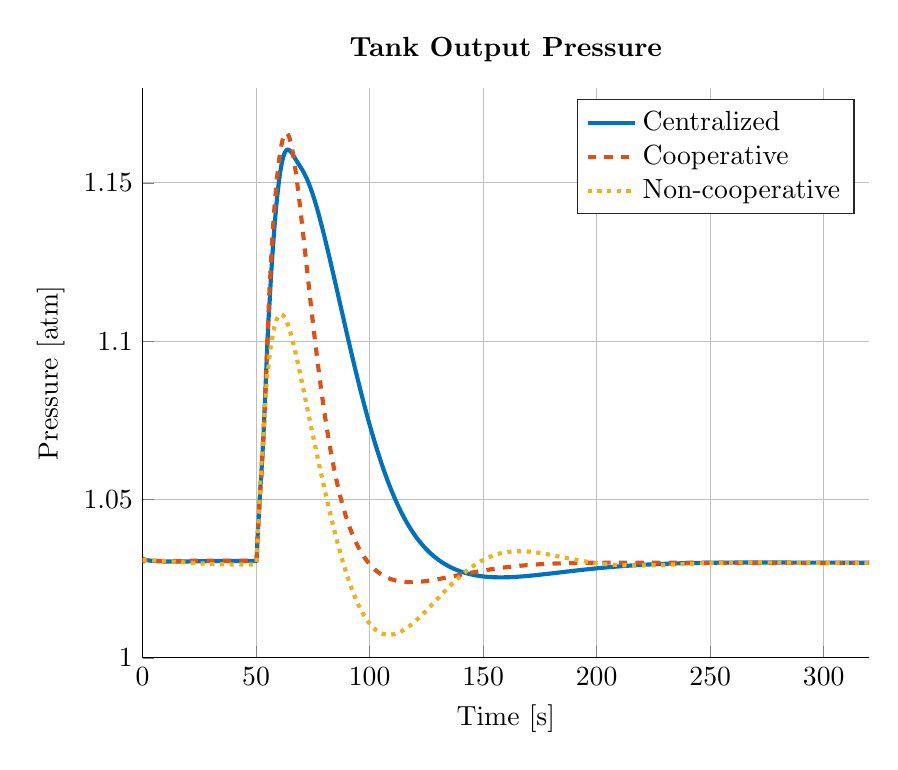
\begin{tikzpicture}

\begin{axis}[%
width=0.761\linewidth,
height=0.597\linewidth,
at={(0\linewidth,0\linewidth)},
scale only axis,
xmin=0,
xmax=320,
xlabel={Time [s]},
xmajorgrids,
ymin=1,
ymax=1.18,
ylabel={Pressure [atm]},
ymajorgrids,
axis background/.style={fill=white},
title style={font=\bfseries},
title={Tank Output Pressure},
axis x line*=bottom,
axis y line*=left,
legend style={legend cell align=left,align=left,draw=white!15!black}
]
\addplot [color=mycolor1,solid,line width=1.5pt]
  table[row sep=crcr]{%
0	1.03\\
0.25	1.03084\\
0.5	1.03105\\
0.75	1.03093\\
1	1.03093\\
1.25	1.03094\\
1.5	1.03091\\
1.75	1.03087\\
2	1.03084\\
2.25	1.03081\\
2.5	1.03079\\
2.75	1.03076\\
3	1.03074\\
3.25	1.03072\\
3.5	1.0307\\
3.75	1.03068\\
4	1.03066\\
4.25	1.03064\\
4.5	1.03062\\
4.75	1.03061\\
5	1.03059\\
5.25	1.03058\\
5.5	1.03057\\
5.75	1.03055\\
6	1.03054\\
6.25	1.03053\\
6.5	1.03052\\
6.75	1.03051\\
7	1.03051\\
7.25	1.0305\\
7.5	1.03049\\
7.75	1.03048\\
8	1.03048\\
8.25	1.03047\\
8.5	1.03046\\
8.75	1.03046\\
9	1.03045\\
9.25	1.03045\\
9.5	1.03045\\
9.75	1.03044\\
10	1.03044\\
10.25	1.03043\\
10.5	1.03043\\
10.75	1.03043\\
11	1.03043\\
11.25	1.03042\\
11.5	1.03042\\
11.75	1.03042\\
12	1.03042\\
12.25	1.03042\\
12.5	1.03042\\
12.75	1.03042\\
13	1.03042\\
13.25	1.03042\\
13.5	1.03042\\
13.75	1.03041\\
14	1.03042\\
14.25	1.03042\\
14.5	1.03042\\
14.75	1.03042\\
15	1.03042\\
15.25	1.03042\\
15.5	1.03042\\
15.75	1.03042\\
16	1.03042\\
16.25	1.03042\\
16.5	1.03042\\
16.75	1.03042\\
17	1.03043\\
17.25	1.03043\\
17.5	1.03043\\
17.75	1.03043\\
18	1.03043\\
18.25	1.03043\\
18.5	1.03044\\
18.75	1.03044\\
19	1.03044\\
19.25	1.03044\\
19.5	1.03045\\
19.75	1.03045\\
20	1.03045\\
20.25	1.03045\\
20.5	1.03046\\
20.75	1.03046\\
21	1.03046\\
21.25	1.03046\\
21.5	1.03047\\
21.75	1.03047\\
22	1.03047\\
22.25	1.03047\\
22.5	1.03048\\
22.75	1.03048\\
23	1.03048\\
23.25	1.03049\\
23.5	1.03049\\
23.75	1.03049\\
24	1.03049\\
24.25	1.0305\\
24.5	1.0305\\
24.75	1.0305\\
25	1.0305\\
25.25	1.03051\\
25.5	1.03051\\
25.75	1.03051\\
26	1.03051\\
26.25	1.03052\\
26.5	1.03052\\
26.75	1.03052\\
27	1.03052\\
27.25	1.03053\\
27.5	1.03053\\
27.75	1.03053\\
28	1.03053\\
28.25	1.03054\\
28.5	1.03054\\
28.75	1.03054\\
29	1.03054\\
29.25	1.03054\\
29.5	1.03055\\
29.75	1.03055\\
30	1.03055\\
30.25	1.03055\\
30.5	1.03055\\
30.75	1.03056\\
31	1.03056\\
31.25	1.03056\\
31.5	1.03056\\
31.75	1.03056\\
32	1.03057\\
32.25	1.03057\\
32.5	1.03057\\
32.75	1.03057\\
33	1.03057\\
33.25	1.03057\\
33.5	1.03057\\
33.75	1.03057\\
34	1.03058\\
34.25	1.03058\\
34.5	1.03058\\
34.75	1.03058\\
35	1.03058\\
35.25	1.03058\\
35.5	1.03058\\
35.75	1.03058\\
36	1.03058\\
36.25	1.03059\\
36.5	1.03059\\
36.75	1.03059\\
37	1.03059\\
37.25	1.03059\\
37.5	1.03059\\
37.75	1.03059\\
38	1.03059\\
38.25	1.03059\\
38.5	1.03059\\
38.75	1.03059\\
39	1.03059\\
39.25	1.03059\\
39.5	1.03059\\
39.75	1.03059\\
40	1.03059\\
40.25	1.03059\\
40.5	1.03059\\
40.75	1.0306\\
41	1.0306\\
41.25	1.0306\\
41.5	1.0306\\
41.75	1.0306\\
42	1.0306\\
42.25	1.0306\\
42.5	1.0306\\
42.75	1.0306\\
43	1.0306\\
43.25	1.0306\\
43.5	1.0306\\
43.75	1.0306\\
44	1.0306\\
44.25	1.0306\\
44.5	1.0306\\
44.75	1.0306\\
45	1.0306\\
45.25	1.03059\\
45.5	1.03059\\
45.75	1.03059\\
46	1.03059\\
46.25	1.03059\\
46.5	1.03059\\
46.75	1.03059\\
47	1.03059\\
47.25	1.03059\\
47.5	1.03059\\
47.75	1.03059\\
48	1.03059\\
48.25	1.03059\\
48.5	1.03059\\
48.75	1.03059\\
49	1.03059\\
49.25	1.03059\\
49.5	1.03059\\
49.75	1.03059\\
50	1.03059\\
50.25	1.03103\\
50.5	1.03504\\
50.75	1.0398\\
51	1.04245\\
51.25	1.04553\\
51.5	1.04912\\
51.75	1.05206\\
52	1.0547\\
52.25	1.0574\\
52.5	1.06051\\
52.75	1.06393\\
53	1.06686\\
53.25	1.0703\\
53.5	1.07423\\
53.75	1.07821\\
54	1.08238\\
54.25	1.08671\\
54.5	1.09105\\
54.75	1.09533\\
55	1.09951\\
55.25	1.10362\\
55.5	1.1072\\
55.75	1.10975\\
56	1.11291\\
56.25	1.11634\\
56.5	1.11944\\
56.75	1.12233\\
57	1.1251\\
57.25	1.12779\\
57.5	1.13037\\
57.75	1.13279\\
58	1.13511\\
58.25	1.13736\\
58.5	1.1395\\
58.75	1.14154\\
59	1.14346\\
59.25	1.14528\\
59.5	1.14698\\
59.75	1.14858\\
60	1.15007\\
60.25	1.15145\\
60.5	1.15272\\
60.75	1.15389\\
61	1.15496\\
61.25	1.15592\\
61.5	1.15678\\
61.75	1.15755\\
62	1.15822\\
62.25	1.15879\\
62.5	1.15927\\
62.75	1.15967\\
63	1.15998\\
63.25	1.16022\\
63.5	1.16038\\
63.75	1.16047\\
64	1.16049\\
64.25	1.16046\\
64.5	1.16038\\
64.75	1.16025\\
65	1.16008\\
65.25	1.15988\\
65.5	1.15965\\
65.75	1.1594\\
66	1.15913\\
66.25	1.15884\\
66.5	1.15855\\
66.75	1.15825\\
67	1.15795\\
67.25	1.15766\\
67.5	1.15736\\
67.75	1.15706\\
68	1.15677\\
68.25	1.15649\\
68.5	1.1562\\
68.75	1.15592\\
69	1.15564\\
69.25	1.15536\\
69.5	1.15507\\
69.75	1.15479\\
70	1.15449\\
70.25	1.15419\\
70.5	1.15389\\
70.75	1.15357\\
71	1.15325\\
71.25	1.15291\\
71.5	1.15256\\
71.75	1.1522\\
72	1.15183\\
72.25	1.15145\\
72.5	1.15105\\
72.75	1.15064\\
73	1.15021\\
73.25	1.14977\\
73.5	1.14931\\
73.75	1.14884\\
74	1.14836\\
74.25	1.14786\\
74.5	1.14735\\
74.75	1.14683\\
75	1.14629\\
75.25	1.14574\\
75.5	1.14517\\
75.75	1.1446\\
76	1.14401\\
76.25	1.14341\\
76.5	1.1428\\
76.75	1.14218\\
77	1.14155\\
77.25	1.14091\\
77.5	1.14026\\
77.75	1.1396\\
78	1.13893\\
78.25	1.13826\\
78.5	1.13758\\
78.75	1.13689\\
79	1.13619\\
79.25	1.13549\\
79.5	1.13478\\
79.75	1.13406\\
80	1.13334\\
80.25	1.13261\\
80.5	1.13188\\
80.75	1.13114\\
81	1.1304\\
81.25	1.12966\\
81.5	1.12891\\
81.75	1.12816\\
82	1.1274\\
82.25	1.12664\\
82.5	1.12588\\
82.75	1.12511\\
83	1.12434\\
83.25	1.12357\\
83.5	1.1228\\
83.75	1.12202\\
84	1.12124\\
84.25	1.12046\\
84.5	1.11968\\
84.75	1.1189\\
85	1.11812\\
85.25	1.11733\\
85.5	1.11654\\
85.75	1.11576\\
86	1.11497\\
86.25	1.11418\\
86.5	1.11339\\
86.75	1.1126\\
87	1.11181\\
87.25	1.11103\\
87.5	1.11024\\
87.75	1.10945\\
88	1.10866\\
88.25	1.10787\\
88.5	1.10709\\
88.75	1.1063\\
89	1.10552\\
89.25	1.10473\\
89.5	1.10395\\
89.75	1.10317\\
90	1.10239\\
90.25	1.10162\\
90.5	1.10084\\
90.75	1.10007\\
91	1.09929\\
91.25	1.09853\\
91.5	1.09776\\
91.75	1.09699\\
92	1.09623\\
92.25	1.09547\\
92.5	1.09471\\
92.75	1.09396\\
93	1.09321\\
93.25	1.09246\\
93.5	1.09171\\
93.75	1.09097\\
94	1.09023\\
94.25	1.0895\\
94.5	1.08877\\
94.75	1.08804\\
95	1.08731\\
95.25	1.08659\\
95.5	1.08587\\
95.75	1.08516\\
96	1.08445\\
96.25	1.08374\\
96.5	1.08304\\
96.75	1.08234\\
97	1.08165\\
97.25	1.08096\\
97.5	1.08027\\
97.75	1.07959\\
98	1.07892\\
98.25	1.07824\\
98.5	1.07758\\
98.75	1.07691\\
99	1.07626\\
99.25	1.0756\\
99.5	1.07495\\
99.75	1.07431\\
100	1.07367\\
100.25	1.07303\\
100.5	1.07241\\
100.75	1.07178\\
101	1.07116\\
101.25	1.07054\\
101.5	1.06993\\
101.75	1.06933\\
102	1.06873\\
102.25	1.06813\\
102.5	1.06754\\
102.75	1.06696\\
103	1.06638\\
103.25	1.0658\\
103.5	1.06523\\
103.75	1.06467\\
104	1.06411\\
104.25	1.06355\\
104.5	1.06301\\
104.75	1.06246\\
105	1.06192\\
105.25	1.06139\\
105.5	1.06086\\
105.75	1.06034\\
106	1.05982\\
106.25	1.0593\\
106.5	1.0588\\
106.75	1.05829\\
107	1.0578\\
107.25	1.0573\\
107.5	1.05682\\
107.75	1.05633\\
108	1.05586\\
108.25	1.05539\\
108.5	1.05492\\
108.75	1.05446\\
109	1.054\\
109.25	1.05355\\
109.5	1.0531\\
109.75	1.05266\\
110	1.05223\\
110.25	1.05179\\
110.5	1.05137\\
110.75	1.05095\\
111	1.05053\\
111.25	1.05012\\
111.5	1.04971\\
111.75	1.04931\\
112	1.04892\\
112.25	1.04853\\
112.5	1.04814\\
112.75	1.04776\\
113	1.04738\\
113.25	1.04701\\
113.5	1.04664\\
113.75	1.04628\\
114	1.04592\\
114.25	1.04557\\
114.5	1.04522\\
114.75	1.04487\\
115	1.04454\\
115.25	1.0442\\
115.5	1.04387\\
115.75	1.04354\\
116	1.04322\\
116.25	1.04291\\
116.5	1.04259\\
116.75	1.04229\\
117	1.04198\\
117.25	1.04168\\
117.5	1.04139\\
117.75	1.0411\\
118	1.04081\\
118.25	1.04053\\
118.5	1.04025\\
118.75	1.03997\\
119	1.0397\\
119.25	1.03944\\
119.5	1.03917\\
119.75	1.03891\\
120	1.03866\\
120.25	1.03841\\
120.5	1.03816\\
120.75	1.03792\\
121	1.03768\\
121.25	1.03744\\
121.5	1.03721\\
121.75	1.03698\\
122	1.03675\\
122.25	1.03653\\
122.5	1.03631\\
122.75	1.0361\\
123	1.03588\\
123.25	1.03567\\
123.5	1.03547\\
123.75	1.03527\\
124	1.03507\\
124.25	1.03487\\
124.5	1.03468\\
124.75	1.03449\\
125	1.0343\\
125.25	1.03412\\
125.5	1.03394\\
125.75	1.03376\\
126	1.03358\\
126.25	1.03341\\
126.5	1.03324\\
126.75	1.03307\\
127	1.03291\\
127.25	1.03275\\
127.5	1.03259\\
127.75	1.03243\\
128	1.03228\\
128.25	1.03213\\
128.5	1.03198\\
128.75	1.03183\\
129	1.03169\\
129.25	1.03154\\
129.5	1.03141\\
129.75	1.03127\\
130	1.03113\\
130.25	1.031\\
130.5	1.03087\\
130.75	1.03074\\
131	1.03062\\
131.25	1.03049\\
131.5	1.03037\\
131.75	1.03025\\
132	1.03013\\
132.25	1.03002\\
132.5	1.02991\\
132.75	1.02979\\
133	1.02969\\
133.25	1.02958\\
133.5	1.02947\\
133.75	1.02937\\
134	1.02927\\
134.25	1.02917\\
134.5	1.02907\\
134.75	1.02897\\
135	1.02888\\
135.25	1.02878\\
135.5	1.02869\\
135.75	1.0286\\
136	1.02851\\
136.25	1.02843\\
136.5	1.02834\\
136.75	1.02826\\
137	1.02818\\
137.25	1.0281\\
137.5	1.02802\\
137.75	1.02794\\
138	1.02787\\
138.25	1.02779\\
138.5	1.02772\\
138.75	1.02765\\
139	1.02758\\
139.25	1.02751\\
139.5	1.02745\\
139.75	1.02738\\
140	1.02732\\
140.25	1.02726\\
140.5	1.02719\\
140.75	1.02713\\
141	1.02708\\
141.25	1.02702\\
141.5	1.02696\\
141.75	1.02691\\
142	1.02685\\
142.25	1.0268\\
142.5	1.02675\\
142.75	1.0267\\
143	1.02665\\
143.25	1.0266\\
143.5	1.02656\\
143.75	1.02651\\
144	1.02647\\
144.25	1.02643\\
144.5	1.02638\\
144.75	1.02634\\
145	1.0263\\
145.25	1.02627\\
145.5	1.02623\\
145.75	1.02619\\
146	1.02616\\
146.25	1.02612\\
146.5	1.02609\\
146.75	1.02606\\
147	1.02602\\
147.25	1.02599\\
147.5	1.02596\\
147.75	1.02593\\
148	1.02591\\
148.25	1.02588\\
148.5	1.02585\\
148.75	1.02583\\
149	1.0258\\
149.25	1.02578\\
149.5	1.02576\\
149.75	1.02574\\
150	1.02572\\
150.25	1.0257\\
150.5	1.02568\\
150.75	1.02566\\
151	1.02564\\
151.25	1.02562\\
151.5	1.02561\\
151.75	1.02559\\
152	1.02558\\
152.25	1.02556\\
152.5	1.02555\\
152.75	1.02554\\
153	1.02553\\
153.25	1.02552\\
153.5	1.02551\\
153.75	1.0255\\
154	1.02549\\
154.25	1.02548\\
154.5	1.02547\\
154.75	1.02546\\
155	1.02546\\
155.25	1.02545\\
155.5	1.02545\\
155.75	1.02544\\
156	1.02544\\
156.25	1.02543\\
156.5	1.02543\\
156.75	1.02543\\
157	1.02543\\
157.25	1.02543\\
157.5	1.02542\\
157.75	1.02542\\
158	1.02542\\
158.25	1.02543\\
158.5	1.02543\\
158.75	1.02543\\
159	1.02543\\
159.25	1.02543\\
159.5	1.02544\\
159.75	1.02544\\
160	1.02544\\
160.25	1.02545\\
160.5	1.02545\\
160.75	1.02546\\
161	1.02546\\
161.25	1.02547\\
161.5	1.02548\\
161.75	1.02548\\
162	1.02549\\
162.25	1.0255\\
162.5	1.02551\\
162.75	1.02552\\
163	1.02553\\
163.25	1.02553\\
163.5	1.02554\\
163.75	1.02555\\
164	1.02556\\
164.25	1.02558\\
164.5	1.02559\\
164.75	1.0256\\
165	1.02561\\
165.25	1.02562\\
165.5	1.02563\\
165.75	1.02564\\
166	1.02566\\
166.25	1.02567\\
166.5	1.02568\\
166.75	1.0257\\
167	1.02571\\
167.25	1.02573\\
167.5	1.02574\\
167.75	1.02575\\
168	1.02577\\
168.25	1.02578\\
168.5	1.0258\\
168.75	1.02581\\
169	1.02583\\
169.25	1.02585\\
169.5	1.02586\\
169.75	1.02588\\
170	1.02589\\
170.25	1.02591\\
170.5	1.02593\\
170.75	1.02594\\
171	1.02596\\
171.25	1.02598\\
171.5	1.026\\
171.75	1.02601\\
172	1.02603\\
172.25	1.02605\\
172.5	1.02607\\
172.75	1.02609\\
173	1.02611\\
173.25	1.02612\\
173.5	1.02614\\
173.75	1.02616\\
174	1.02618\\
174.25	1.0262\\
174.5	1.02622\\
174.75	1.02624\\
175	1.02626\\
175.25	1.02628\\
175.5	1.0263\\
175.75	1.02632\\
176	1.02634\\
176.25	1.02636\\
176.5	1.02638\\
176.75	1.0264\\
177	1.02642\\
177.25	1.02644\\
177.5	1.02646\\
177.75	1.02648\\
178	1.0265\\
178.25	1.02652\\
178.5	1.02654\\
178.75	1.02656\\
179	1.02658\\
179.25	1.0266\\
179.5	1.02662\\
179.75	1.02664\\
180	1.02666\\
180.25	1.02668\\
180.5	1.0267\\
180.75	1.02672\\
181	1.02675\\
181.25	1.02677\\
181.5	1.02679\\
181.75	1.02681\\
182	1.02683\\
182.25	1.02685\\
182.5	1.02687\\
182.75	1.02689\\
183	1.02691\\
183.25	1.02694\\
183.5	1.02696\\
183.75	1.02698\\
184	1.027\\
184.25	1.02702\\
184.5	1.02704\\
184.75	1.02706\\
185	1.02708\\
185.25	1.0271\\
185.5	1.02713\\
185.75	1.02715\\
186	1.02717\\
186.25	1.02719\\
186.5	1.02721\\
186.75	1.02723\\
187	1.02725\\
187.25	1.02727\\
187.5	1.02729\\
187.75	1.02731\\
188	1.02733\\
188.25	1.02736\\
188.5	1.02738\\
188.75	1.0274\\
189	1.02742\\
189.25	1.02744\\
189.5	1.02746\\
189.75	1.02748\\
190	1.0275\\
190.25	1.02752\\
190.5	1.02754\\
190.75	1.02756\\
191	1.02758\\
191.25	1.0276\\
191.5	1.02762\\
191.75	1.02764\\
192	1.02766\\
192.25	1.02768\\
192.5	1.0277\\
192.75	1.02772\\
193	1.02774\\
193.25	1.02776\\
193.5	1.02778\\
193.75	1.0278\\
194	1.02782\\
194.25	1.02784\\
194.5	1.02786\\
194.75	1.02788\\
195	1.0279\\
195.25	1.02792\\
195.5	1.02794\\
195.75	1.02795\\
196	1.02797\\
196.25	1.02799\\
196.5	1.02801\\
196.75	1.02803\\
197	1.02805\\
197.25	1.02807\\
197.5	1.02809\\
197.75	1.0281\\
198	1.02812\\
198.25	1.02814\\
198.5	1.02816\\
198.75	1.02818\\
199	1.0282\\
199.25	1.02821\\
199.5	1.02823\\
199.75	1.02825\\
200	1.02827\\
200.25	1.02828\\
200.5	1.0283\\
200.75	1.02832\\
201	1.02834\\
201.25	1.02835\\
201.5	1.02837\\
201.75	1.02839\\
202	1.0284\\
202.25	1.02842\\
202.5	1.02844\\
202.75	1.02845\\
203	1.02847\\
203.25	1.02849\\
203.5	1.0285\\
203.75	1.02852\\
204	1.02854\\
204.25	1.02855\\
204.5	1.02857\\
204.75	1.02858\\
205	1.0286\\
205.25	1.02862\\
205.5	1.02863\\
205.75	1.02865\\
206	1.02866\\
206.25	1.02868\\
206.5	1.02869\\
206.75	1.02871\\
207	1.02872\\
207.25	1.02874\\
207.5	1.02875\\
207.75	1.02877\\
208	1.02878\\
208.25	1.0288\\
208.5	1.02881\\
208.75	1.02883\\
209	1.02884\\
209.25	1.02885\\
209.5	1.02887\\
209.75	1.02888\\
210	1.0289\\
210.25	1.02891\\
210.5	1.02892\\
210.75	1.02894\\
211	1.02895\\
211.25	1.02896\\
211.5	1.02898\\
211.75	1.02899\\
212	1.029\\
212.25	1.02902\\
212.5	1.02903\\
212.75	1.02904\\
213	1.02905\\
213.25	1.02907\\
213.5	1.02908\\
213.75	1.02909\\
214	1.0291\\
214.25	1.02912\\
214.5	1.02913\\
214.75	1.02914\\
215	1.02915\\
215.25	1.02916\\
215.5	1.02918\\
215.75	1.02919\\
216	1.0292\\
216.25	1.02921\\
216.5	1.02922\\
216.75	1.02923\\
217	1.02924\\
217.25	1.02926\\
217.5	1.02927\\
217.75	1.02928\\
218	1.02929\\
218.25	1.0293\\
218.5	1.02931\\
218.75	1.02932\\
219	1.02933\\
219.25	1.02934\\
219.5	1.02935\\
219.75	1.02936\\
220	1.02937\\
220.25	1.02938\\
220.5	1.02939\\
220.75	1.0294\\
221	1.02941\\
221.25	1.02942\\
221.5	1.02943\\
221.75	1.02944\\
222	1.02945\\
222.25	1.02946\\
222.5	1.02947\\
222.75	1.02947\\
223	1.02948\\
223.25	1.02949\\
223.5	1.0295\\
223.75	1.02951\\
224	1.02952\\
224.25	1.02953\\
224.5	1.02954\\
224.75	1.02954\\
225	1.02955\\
225.25	1.02956\\
225.5	1.02957\\
225.75	1.02958\\
226	1.02958\\
226.25	1.02959\\
226.5	1.0296\\
226.75	1.02961\\
227	1.02962\\
227.25	1.02962\\
227.5	1.02963\\
227.75	1.02964\\
228	1.02965\\
228.25	1.02965\\
228.5	1.02966\\
228.75	1.02967\\
229	1.02967\\
229.25	1.02968\\
229.5	1.02969\\
229.75	1.02969\\
230	1.0297\\
230.25	1.02971\\
230.5	1.02971\\
230.75	1.02972\\
231	1.02973\\
231.25	1.02973\\
231.5	1.02974\\
231.75	1.02975\\
232	1.02975\\
232.25	1.02976\\
232.5	1.02976\\
232.75	1.02977\\
233	1.02978\\
233.25	1.02978\\
233.5	1.02979\\
233.75	1.02979\\
234	1.0298\\
234.25	1.0298\\
234.5	1.02981\\
234.75	1.02981\\
235	1.02982\\
235.25	1.02983\\
235.5	1.02983\\
235.75	1.02984\\
236	1.02984\\
236.25	1.02985\\
236.5	1.02985\\
236.75	1.02986\\
237	1.02986\\
237.25	1.02986\\
237.5	1.02987\\
237.75	1.02987\\
238	1.02988\\
238.25	1.02988\\
238.5	1.02989\\
238.75	1.02989\\
239	1.0299\\
239.25	1.0299\\
239.5	1.0299\\
239.75	1.02991\\
240	1.02991\\
240.25	1.02992\\
240.5	1.02992\\
240.75	1.02992\\
241	1.02993\\
241.25	1.02993\\
241.5	1.02994\\
241.75	1.02994\\
242	1.02994\\
242.25	1.02995\\
242.5	1.02995\\
242.75	1.02995\\
243	1.02996\\
243.25	1.02996\\
243.5	1.02996\\
243.75	1.02997\\
244	1.02997\\
244.25	1.02997\\
244.5	1.02998\\
244.75	1.02998\\
245	1.02998\\
245.25	1.02999\\
245.5	1.02999\\
245.75	1.02999\\
246	1.02999\\
246.25	1.03\\
246.5	1.03\\
246.75	1.03\\
247	1.03001\\
247.25	1.03001\\
247.5	1.03001\\
247.75	1.03001\\
248	1.03002\\
248.25	1.03002\\
248.5	1.03002\\
248.75	1.03002\\
249	1.03002\\
249.25	1.03003\\
249.5	1.03003\\
249.75	1.03003\\
250	1.03003\\
250.25	1.03004\\
250.5	1.03004\\
250.75	1.03004\\
251	1.03004\\
251.25	1.03004\\
251.5	1.03005\\
251.75	1.03005\\
252	1.03005\\
252.25	1.03005\\
252.5	1.03005\\
252.75	1.03005\\
253	1.03006\\
253.25	1.03006\\
253.5	1.03006\\
253.75	1.03006\\
254	1.03006\\
254.25	1.03006\\
254.5	1.03007\\
254.75	1.03007\\
255	1.03007\\
255.25	1.03007\\
255.5	1.03007\\
255.75	1.03007\\
256	1.03007\\
256.25	1.03008\\
256.5	1.03008\\
256.75	1.03008\\
257	1.03008\\
257.25	1.03008\\
257.5	1.03008\\
257.75	1.03008\\
258	1.03008\\
258.25	1.03009\\
258.5	1.03009\\
258.75	1.03009\\
259	1.03009\\
259.25	1.03009\\
259.5	1.03009\\
259.75	1.03009\\
260	1.03009\\
260.25	1.03009\\
260.5	1.03009\\
260.75	1.03009\\
261	1.0301\\
261.25	1.0301\\
261.5	1.0301\\
261.75	1.0301\\
262	1.0301\\
262.25	1.0301\\
262.5	1.0301\\
262.75	1.0301\\
263	1.0301\\
263.25	1.0301\\
263.5	1.0301\\
263.75	1.0301\\
264	1.0301\\
264.25	1.0301\\
264.5	1.0301\\
264.75	1.0301\\
265	1.0301\\
265.25	1.0301\\
265.5	1.03011\\
265.75	1.03011\\
266	1.03011\\
266.25	1.03011\\
266.5	1.03011\\
266.75	1.03011\\
267	1.03011\\
267.25	1.03011\\
267.5	1.03011\\
267.75	1.03011\\
268	1.03011\\
268.25	1.03011\\
268.5	1.03011\\
268.75	1.03011\\
269	1.03011\\
269.25	1.03011\\
269.5	1.03011\\
269.75	1.03011\\
270	1.03011\\
270.25	1.03011\\
270.5	1.03011\\
270.75	1.03011\\
271	1.03011\\
271.25	1.03011\\
271.5	1.03011\\
271.75	1.03011\\
272	1.03011\\
272.25	1.03011\\
272.5	1.03011\\
272.75	1.03011\\
273	1.03011\\
273.25	1.03011\\
273.5	1.03011\\
273.75	1.03011\\
274	1.03011\\
274.25	1.03011\\
274.5	1.03011\\
274.75	1.03011\\
275	1.03011\\
275.25	1.03011\\
275.5	1.03011\\
275.75	1.03011\\
276	1.03011\\
276.25	1.03011\\
276.5	1.03011\\
276.75	1.03011\\
277	1.03011\\
277.25	1.03011\\
277.5	1.03011\\
277.75	1.03011\\
278	1.03011\\
278.25	1.03011\\
278.5	1.03011\\
278.75	1.03011\\
279	1.0301\\
279.25	1.0301\\
279.5	1.0301\\
279.75	1.0301\\
280	1.0301\\
280.25	1.0301\\
280.5	1.0301\\
280.75	1.0301\\
281	1.0301\\
281.25	1.0301\\
281.5	1.0301\\
281.75	1.0301\\
282	1.0301\\
282.25	1.0301\\
282.5	1.0301\\
282.75	1.0301\\
283	1.0301\\
283.25	1.0301\\
283.5	1.0301\\
283.75	1.0301\\
284	1.0301\\
284.25	1.0301\\
284.5	1.0301\\
284.75	1.0301\\
285	1.0301\\
285.25	1.0301\\
285.5	1.03009\\
285.75	1.03009\\
286	1.03009\\
286.25	1.03009\\
286.5	1.03009\\
286.75	1.03009\\
287	1.03009\\
287.25	1.03009\\
287.5	1.03009\\
287.75	1.03009\\
288	1.03009\\
288.25	1.03009\\
288.5	1.03009\\
288.75	1.03009\\
289	1.03009\\
289.25	1.03009\\
289.5	1.03009\\
289.75	1.03009\\
290	1.03009\\
290.25	1.03009\\
290.5	1.03009\\
290.75	1.03009\\
291	1.03008\\
291.25	1.03008\\
291.5	1.03008\\
291.75	1.03008\\
292	1.03008\\
292.25	1.03008\\
292.5	1.03008\\
292.75	1.03008\\
293	1.03008\\
293.25	1.03008\\
293.5	1.03008\\
293.75	1.03008\\
294	1.03008\\
294.25	1.03008\\
294.5	1.03008\\
294.75	1.03008\\
295	1.03008\\
295.25	1.03008\\
295.5	1.03008\\
295.75	1.03007\\
296	1.03007\\
296.25	1.03007\\
296.5	1.03007\\
296.75	1.03007\\
297	1.03007\\
297.25	1.03007\\
297.5	1.03007\\
297.75	1.03007\\
298	1.03007\\
298.25	1.03007\\
298.5	1.03007\\
298.75	1.03007\\
299	1.03007\\
299.25	1.03007\\
299.5	1.03007\\
299.75	1.03007\\
300	1.03007\\
300.25	1.03007\\
300.5	1.03007\\
300.75	1.03006\\
301	1.03006\\
301.25	1.03006\\
301.5	1.03006\\
301.75	1.03006\\
302	1.03006\\
302.25	1.03006\\
302.5	1.03006\\
302.75	1.03006\\
303	1.03006\\
303.25	1.03006\\
303.5	1.03006\\
303.75	1.03006\\
304	1.03006\\
304.25	1.03006\\
304.5	1.03006\\
304.75	1.03006\\
305	1.03006\\
305.25	1.03006\\
305.5	1.03006\\
305.75	1.03005\\
306	1.03005\\
306.25	1.03005\\
306.5	1.03005\\
306.75	1.03005\\
307	1.03005\\
307.25	1.03005\\
307.5	1.03005\\
307.75	1.03005\\
308	1.03005\\
308.25	1.03005\\
308.5	1.03005\\
308.75	1.03005\\
309	1.03005\\
309.25	1.03005\\
309.5	1.03005\\
309.75	1.03005\\
310	1.03005\\
310.25	1.03005\\
310.5	1.03005\\
310.75	1.03005\\
311	1.03004\\
311.25	1.03004\\
311.5	1.03004\\
311.75	1.03004\\
312	1.03004\\
312.25	1.03004\\
312.5	1.03004\\
312.75	1.03004\\
313	1.03004\\
313.25	1.03004\\
313.5	1.03004\\
313.75	1.03004\\
314	1.03004\\
314.25	1.03004\\
314.5	1.03004\\
314.75	1.03004\\
315	1.03004\\
315.25	1.03004\\
315.5	1.03004\\
315.75	1.03004\\
316	1.03004\\
316.25	1.03004\\
316.5	1.03004\\
316.75	1.03004\\
317	1.03003\\
317.25	1.03003\\
317.5	1.03003\\
317.75	1.03003\\
318	1.03003\\
318.25	1.03003\\
318.5	1.03003\\
318.75	1.03003\\
319	1.03003\\
319.25	1.03003\\
319.5	1.03003\\
319.75	1.03003\\
320	1.03003\\
320.25	1.03003\\
320.5	1.03003\\
320.75	1.03003\\
321	1.03003\\
321.25	1.03003\\
321.5	1.03003\\
321.75	1.03003\\
322	1.03003\\
322.25	1.03003\\
322.5	1.03003\\
322.75	1.03003\\
323	1.03003\\
323.25	1.03003\\
323.5	1.03003\\
323.75	1.03003\\
324	1.03002\\
324.25	1.03002\\
324.5	1.03002\\
324.75	1.03002\\
325	1.03002\\
325.25	1.03002\\
325.5	1.03002\\
325.75	1.03002\\
326	1.03002\\
326.25	1.03002\\
326.5	1.03002\\
326.75	1.03002\\
327	1.03002\\
327.25	1.03002\\
327.5	1.03002\\
327.75	1.03002\\
328	1.03002\\
328.25	1.03002\\
328.5	1.03002\\
328.75	1.03002\\
329	1.03002\\
329.25	1.03002\\
329.5	1.03002\\
329.75	1.03002\\
330	1.03002\\
330.25	1.03002\\
330.5	1.03002\\
330.75	1.03002\\
331	1.03002\\
331.25	1.03002\\
331.5	1.03002\\
331.75	1.03002\\
332	1.03002\\
332.25	1.03002\\
332.5	1.03002\\
332.75	1.03001\\
333	1.03001\\
333.25	1.03001\\
333.5	1.03001\\
333.75	1.03001\\
334	1.03001\\
334.25	1.03001\\
334.5	1.03001\\
334.75	1.03001\\
335	1.03001\\
335.25	1.03001\\
335.5	1.03001\\
335.75	1.03001\\
336	1.03001\\
336.25	1.03001\\
336.5	1.03001\\
336.75	1.03001\\
337	1.03001\\
337.25	1.03001\\
337.5	1.03001\\
337.75	1.03001\\
338	1.03001\\
338.25	1.03001\\
338.5	1.03001\\
338.75	1.03001\\
339	1.03001\\
339.25	1.03001\\
339.5	1.03001\\
339.75	1.03001\\
340	1.03001\\
340.25	1.03001\\
340.5	1.03001\\
340.75	1.03001\\
341	1.03001\\
341.25	1.03001\\
341.5	1.03001\\
341.75	1.03001\\
342	1.03001\\
342.25	1.03001\\
342.5	1.03001\\
342.75	1.03001\\
343	1.03001\\
343.25	1.03001\\
343.5	1.03001\\
343.75	1.03001\\
344	1.03001\\
344.25	1.03001\\
344.5	1.03001\\
344.75	1.03001\\
345	1.03001\\
345.25	1.03001\\
345.5	1.03001\\
345.75	1.03001\\
346	1.03001\\
346.25	1.03\\
346.5	1.03\\
346.75	1.03\\
347	1.03\\
347.25	1.03\\
347.5	1.03\\
347.75	1.03\\
348	1.03\\
348.25	1.03\\
348.5	1.03\\
348.75	1.03\\
349	1.03\\
349.25	1.03\\
349.5	1.03\\
349.75	1.03\\
350	1.03\\
350.25	1.03\\
350.5	1.03\\
350.75	1.03\\
351	1.03\\
351.25	1.03\\
351.5	1.03\\
351.75	1.03\\
352	1.03\\
352.25	1.03\\
352.5	1.03\\
352.75	1.03\\
353	1.03\\
353.25	1.03\\
353.5	1.03\\
353.75	1.03\\
354	1.03\\
354.25	1.03\\
354.5	1.03\\
354.75	1.03\\
355	1.03\\
355.25	1.03\\
355.5	1.03\\
355.75	1.03\\
356	1.03\\
356.25	1.03\\
356.5	1.03\\
356.75	1.03\\
357	1.03\\
357.25	1.03\\
357.5	1.03\\
357.75	1.03\\
358	1.03\\
358.25	1.03\\
358.5	1.03\\
358.75	1.03\\
359	1.03\\
359.25	1.03\\
359.5	1.03\\
359.75	1.03\\
360	1.03\\
360.25	1.03\\
360.5	1.03\\
360.75	1.03\\
361	1.03\\
361.25	1.03\\
361.5	1.03\\
361.75	1.03\\
362	1.03\\
362.25	1.03\\
362.5	1.03\\
362.75	1.03\\
363	1.03\\
363.25	1.03\\
363.5	1.03\\
363.75	1.03\\
364	1.03\\
364.25	1.03\\
364.5	1.03\\
364.75	1.03\\
365	1.03\\
365.25	1.03\\
365.5	1.03\\
365.75	1.03\\
366	1.03\\
366.25	1.03\\
366.5	1.03\\
366.75	1.03\\
367	1.03\\
367.25	1.03\\
367.5	1.03\\
367.75	1.03\\
368	1.03\\
368.25	1.03\\
368.5	1.03\\
368.75	1.03\\
369	1.03\\
369.25	1.03\\
369.5	1.03\\
369.75	1.03\\
370	1.03\\
370.25	1.03\\
370.5	1.03\\
370.75	1.03\\
371	1.03\\
371.25	1.03\\
371.5	1.03\\
371.75	1.03\\
372	1.03\\
372.25	1.03\\
372.5	1.03\\
372.75	1.03\\
373	1.03\\
373.25	1.03\\
373.5	1.03\\
373.75	1.03\\
374	1.03\\
374.25	1.03\\
374.5	1.03\\
374.75	1.03\\
375	1.03\\
375.25	1.03\\
375.5	1.03\\
375.75	1.03\\
376	1.03\\
376.25	1.03\\
376.5	1.03\\
376.75	1.03\\
377	1.03\\
377.25	1.03\\
377.5	1.03\\
377.75	1.03\\
378	1.03\\
378.25	1.03\\
378.5	1.03\\
378.75	1.03\\
379	1.03\\
379.25	1.03\\
379.5	1.03\\
379.75	1.03\\
380	1.03\\
380.25	1.03\\
380.5	1.03\\
380.75	1.03\\
381	1.03\\
381.25	1.03\\
381.5	1.03\\
381.75	1.03\\
382	1.03\\
382.25	1.03\\
382.5	1.03\\
382.75	1.03\\
383	1.03\\
383.25	1.03\\
383.5	1.03\\
383.75	1.03\\
384	1.03\\
384.25	1.03\\
384.5	1.03\\
384.75	1.03\\
385	1.03\\
385.25	1.03\\
385.5	1.03\\
385.75	1.03\\
386	1.03\\
386.25	1.03\\
386.5	1.03\\
386.75	1.03\\
387	1.03\\
387.25	1.03\\
387.5	1.03\\
387.75	1.03\\
388	1.03\\
388.25	1.03\\
388.5	1.03\\
388.75	1.03\\
389	1.03\\
389.25	1.03\\
389.5	1.03\\
389.75	1.03\\
390	1.03\\
390.25	1.03\\
390.5	1.03\\
390.75	1.03\\
391	1.03\\
391.25	1.03\\
391.5	1.03\\
391.75	1.03\\
392	1.03\\
392.25	1.03\\
392.5	1.03\\
392.75	1.03\\
393	1.03\\
393.25	1.03\\
393.5	1.03\\
393.75	1.03\\
394	1.03\\
394.25	1.03\\
394.5	1.03\\
394.75	1.03\\
395	1.03\\
395.25	1.03\\
395.5	1.03\\
395.75	1.03\\
396	1.03\\
396.25	1.03\\
396.5	1.03\\
396.75	1.03\\
397	1.03\\
397.25	1.03\\
397.5	1.03\\
397.75	1.03\\
398	1.03\\
398.25	1.03\\
398.5	1.03\\
398.75	1.03\\
399	1.03\\
399.25	1.03\\
399.5	1.03\\
399.75	1.03\\
400	1.03\\
400.25	1.03\\
400.5	1.03\\
400.75	1.03\\
401	1.03\\
401.25	1.03\\
401.5	1.03\\
401.75	1.03\\
402	1.03\\
402.25	1.03\\
402.5	1.03\\
402.75	1.03\\
403	1.03\\
403.25	1.03\\
403.5	1.03\\
403.75	1.03\\
404	1.03\\
404.25	1.03\\
404.5	1.03\\
404.75	1.03\\
405	1.03\\
405.25	1.03\\
405.5	1.03\\
405.75	1.03\\
406	1.03\\
406.25	1.03\\
406.5	1.03\\
406.75	1.03\\
407	1.03\\
407.25	1.03\\
407.5	1.03\\
407.75	1.03\\
408	1.03\\
408.25	1.03\\
408.5	1.03\\
408.75	1.03\\
409	1.03\\
409.25	1.03\\
409.5	1.03\\
409.75	1.03\\
410	1.03\\
410.25	1.03\\
410.5	1.03\\
410.75	1.03\\
411	1.03\\
411.25	1.03\\
411.5	1.03\\
411.75	1.03\\
412	1.03\\
412.25	1.03\\
412.5	1.03\\
412.75	1.03\\
413	1.03\\
413.25	1.03\\
413.5	1.03\\
413.75	1.03\\
414	1.03\\
414.25	1.03\\
414.5	1.03\\
414.75	1.03\\
415	1.03\\
415.25	1.03\\
415.5	1.03\\
415.75	1.03\\
416	1.03\\
416.25	1.03\\
416.5	1.03\\
416.75	1.03\\
417	1.03\\
417.25	1.03\\
417.5	1.03\\
417.75	1.03\\
418	1.03\\
418.25	1.03\\
418.5	1.03\\
418.75	1.03\\
419	1.03\\
419.25	1.03\\
419.5	1.03\\
419.75	1.03\\
420	1.03\\
420.25	1.03\\
420.5	1.03\\
420.75	1.03\\
421	1.03\\
421.25	1.03\\
421.5	1.03\\
421.75	1.03\\
422	1.03\\
422.25	1.03\\
422.5	1.03\\
422.75	1.03\\
423	1.03\\
423.25	1.03\\
423.5	1.03\\
423.75	1.03\\
424	1.03\\
424.25	1.03\\
424.5	1.03\\
424.75	1.03\\
425	1.03\\
425.25	1.03\\
425.5	1.03\\
425.75	1.03\\
426	1.03\\
426.25	1.03\\
426.5	1.03\\
426.75	1.03\\
427	1.03\\
427.25	1.03\\
427.5	1.03\\
427.75	1.03\\
428	1.03\\
428.25	1.03\\
428.5	1.03\\
428.75	1.03\\
429	1.03\\
429.25	1.03\\
429.5	1.03\\
429.75	1.03\\
430	1.03\\
430.25	1.03\\
430.5	1.03\\
430.75	1.03\\
431	1.03\\
431.25	1.03\\
431.5	1.03\\
431.75	1.03\\
432	1.03\\
432.25	1.03\\
432.5	1.03\\
432.75	1.03\\
433	1.03\\
433.25	1.03\\
433.5	1.03\\
433.75	1.03\\
434	1.03\\
434.25	1.03\\
434.5	1.03\\
434.75	1.03\\
435	1.03\\
435.25	1.03\\
435.5	1.03\\
435.75	1.03\\
436	1.03\\
436.25	1.03\\
436.5	1.03\\
436.75	1.03\\
437	1.03\\
437.25	1.03\\
437.5	1.03\\
437.75	1.03\\
438	1.03\\
438.25	1.03\\
438.5	1.03\\
438.75	1.03\\
439	1.03\\
439.25	1.03\\
439.5	1.03\\
439.75	1.03\\
440	1.03\\
440.25	1.03\\
440.5	1.03\\
440.75	1.03\\
441	1.03\\
441.25	1.03\\
441.5	1.03\\
441.75	1.03\\
442	1.03\\
442.25	1.03\\
442.5	1.03\\
442.75	1.03\\
443	1.03\\
443.25	1.03\\
443.5	1.03\\
443.75	1.03\\
444	1.03\\
444.25	1.03\\
444.5	1.03\\
444.75	1.03\\
445	1.03\\
445.25	1.03\\
445.5	1.03\\
445.75	1.03\\
446	1.03\\
446.25	1.03\\
446.5	1.03\\
446.75	1.03\\
447	1.03\\
447.25	1.03\\
447.5	1.03\\
447.75	1.03\\
448	1.03\\
448.25	1.03\\
448.5	1.03\\
448.75	1.03\\
449	1.03\\
449.25	1.03\\
449.5	1.03\\
449.75	1.03\\
450	1.03\\
450.25	1.03\\
450.5	1.03\\
450.75	1.03\\
451	1.03\\
451.25	1.03\\
451.5	1.03\\
451.75	1.03\\
452	1.03\\
452.25	1.03\\
452.5	1.03\\
452.75	1.03\\
453	1.03\\
453.25	1.03\\
453.5	1.03\\
453.75	1.03\\
454	1.03\\
454.25	1.03\\
454.5	1.03\\
454.75	1.03\\
455	1.03\\
455.25	1.03\\
455.5	1.03\\
455.75	1.03\\
456	1.03\\
456.25	1.03\\
456.5	1.03\\
456.75	1.03\\
457	1.03\\
457.25	1.03\\
457.5	1.03\\
457.75	1.03\\
458	1.03\\
458.25	1.03\\
458.5	1.03\\
458.75	1.03\\
459	1.03\\
459.25	1.03\\
459.5	1.03\\
459.75	1.03\\
460	1.03\\
460.25	1.03\\
460.5	1.03\\
460.75	1.03\\
461	1.03\\
461.25	1.03\\
461.5	1.03\\
461.75	1.03\\
462	1.03\\
462.25	1.03\\
462.5	1.03\\
462.75	1.03\\
463	1.03\\
463.25	1.03\\
463.5	1.03\\
463.75	1.03\\
464	1.03\\
464.25	1.03\\
464.5	1.03\\
464.75	1.03\\
465	1.03\\
465.25	1.03\\
465.5	1.03\\
465.75	1.03\\
466	1.03\\
466.25	1.03\\
466.5	1.03\\
466.75	1.03\\
467	1.03\\
467.25	1.03\\
467.5	1.03\\
467.75	1.03\\
468	1.03\\
468.25	1.03\\
468.5	1.03\\
468.75	1.03\\
469	1.03\\
469.25	1.03\\
469.5	1.03\\
469.75	1.03\\
470	1.03\\
470.25	1.03\\
470.5	1.03\\
470.75	1.03\\
471	1.03\\
471.25	1.03\\
471.5	1.03\\
471.75	1.03\\
472	1.03\\
472.25	1.03\\
472.5	1.03\\
472.75	1.03\\
473	1.03\\
473.25	1.03\\
473.5	1.03\\
473.75	1.03\\
474	1.03\\
474.25	1.03\\
474.5	1.03\\
474.75	1.03\\
475	1.03\\
475.25	1.03\\
475.5	1.03\\
475.75	1.03\\
476	1.03\\
476.25	1.03\\
476.5	1.03\\
476.75	1.03\\
477	1.03\\
477.25	1.03\\
477.5	1.03\\
477.75	1.03\\
478	1.03\\
478.25	1.03\\
478.5	1.03\\
478.75	1.03\\
479	1.03\\
479.25	1.03\\
479.5	1.03\\
479.75	1.03\\
480	1.03\\
480.25	1.03\\
480.5	1.03\\
480.75	1.03\\
481	1.03\\
481.25	1.03\\
481.5	1.03\\
481.75	1.03\\
482	1.03\\
482.25	1.03\\
482.5	1.03\\
482.75	1.03\\
483	1.03\\
483.25	1.03\\
483.5	1.03\\
483.75	1.03\\
484	1.03\\
484.25	1.03\\
484.5	1.03\\
484.75	1.03\\
485	1.03\\
485.25	1.03\\
485.5	1.03\\
485.75	1.03\\
486	1.03\\
486.25	1.03\\
486.5	1.03\\
486.75	1.03\\
487	1.03\\
487.25	1.03\\
487.5	1.03\\
487.75	1.03\\
488	1.03\\
488.25	1.03\\
488.5	1.03\\
488.75	1.03\\
489	1.03\\
489.25	1.03\\
489.5	1.03\\
489.75	1.03\\
490	1.03\\
490.25	1.03\\
490.5	1.03\\
490.75	1.03\\
491	1.03\\
491.25	1.03\\
491.5	1.03\\
491.75	1.03\\
492	1.03\\
492.25	1.03\\
492.5	1.03\\
492.75	1.03\\
493	1.03\\
493.25	1.03\\
493.5	1.03\\
493.75	1.03\\
494	1.03\\
494.25	1.03\\
494.5	1.03\\
494.75	1.03\\
495	1.03\\
495.25	1.03\\
495.5	1.03\\
495.75	1.03\\
496	1.03\\
496.25	1.03\\
496.5	1.03\\
496.75	1.03\\
497	1.03\\
497.25	1.03\\
497.5	1.03\\
497.75	1.03\\
498	1.03\\
498.25	1.03\\
498.5	1.03\\
498.75	1.03\\
499	1.03\\
499.25	1.03\\
499.5	1.03\\
499.75	1.03\\
};
\addlegendentry{Centralized};

\addplot [color=mycolor2,dashed,line width=1.5pt]
  table[row sep=crcr]{%
0	1.03\\
0.25	1.03084\\
0.5	1.03106\\
0.75	1.03094\\
1	1.03094\\
1.25	1.03097\\
1.5	1.03094\\
1.75	1.0309\\
2	1.03088\\
2.25	1.03086\\
2.5	1.03084\\
2.75	1.03082\\
3	1.03081\\
3.25	1.03079\\
3.5	1.03077\\
3.75	1.03076\\
4	1.03074\\
4.25	1.03073\\
4.5	1.03072\\
4.75	1.03071\\
5	1.0307\\
5.25	1.03069\\
5.5	1.03068\\
5.75	1.03067\\
6	1.03066\\
6.25	1.03066\\
6.5	1.03065\\
6.75	1.03064\\
7	1.03064\\
7.25	1.03063\\
7.5	1.03063\\
7.75	1.03063\\
8	1.03062\\
8.25	1.03062\\
8.5	1.03062\\
8.75	1.03061\\
9	1.03061\\
9.25	1.03061\\
9.5	1.03061\\
9.75	1.03061\\
10	1.03061\\
10.25	1.03061\\
10.5	1.03061\\
10.75	1.0306\\
11	1.0306\\
11.25	1.0306\\
11.5	1.0306\\
11.75	1.0306\\
12	1.03061\\
12.25	1.03061\\
12.5	1.03061\\
12.75	1.03061\\
13	1.03061\\
13.25	1.03061\\
13.5	1.03061\\
13.75	1.03061\\
14	1.03061\\
14.25	1.03061\\
14.5	1.03061\\
14.75	1.03062\\
15	1.03062\\
15.25	1.03062\\
15.5	1.03062\\
15.75	1.03062\\
16	1.03062\\
16.25	1.03063\\
16.5	1.03063\\
16.75	1.03063\\
17	1.03063\\
17.25	1.03063\\
17.5	1.03063\\
17.75	1.03063\\
18	1.03064\\
18.25	1.03064\\
18.5	1.03064\\
18.75	1.03064\\
19	1.03064\\
19.25	1.03064\\
19.5	1.03065\\
19.75	1.03065\\
20	1.03065\\
20.25	1.03065\\
20.5	1.03065\\
20.75	1.03065\\
21	1.03065\\
21.25	1.03065\\
21.5	1.03066\\
21.75	1.03066\\
22	1.03066\\
22.25	1.03066\\
22.5	1.03066\\
22.75	1.03066\\
23	1.03066\\
23.25	1.03066\\
23.5	1.03066\\
23.75	1.03066\\
24	1.03066\\
24.25	1.03067\\
24.5	1.03067\\
24.75	1.03067\\
25	1.03067\\
25.25	1.03067\\
25.5	1.03067\\
25.75	1.03067\\
26	1.03067\\
26.25	1.03067\\
26.5	1.03067\\
26.75	1.03067\\
27	1.03067\\
27.25	1.03067\\
27.5	1.03067\\
27.75	1.03067\\
28	1.03067\\
28.25	1.03067\\
28.5	1.03067\\
28.75	1.03067\\
29	1.03067\\
29.25	1.03067\\
29.5	1.03067\\
29.75	1.03067\\
30	1.03067\\
30.25	1.03067\\
30.5	1.03067\\
30.75	1.03067\\
31	1.03067\\
31.25	1.03067\\
31.5	1.03066\\
31.75	1.03066\\
32	1.03066\\
32.25	1.03066\\
32.5	1.03066\\
32.75	1.03066\\
33	1.03066\\
33.25	1.03066\\
33.5	1.03066\\
33.75	1.03066\\
34	1.03066\\
34.25	1.03066\\
34.5	1.03066\\
34.75	1.03066\\
35	1.03066\\
35.25	1.03066\\
35.5	1.03066\\
35.75	1.03066\\
36	1.03066\\
36.25	1.03066\\
36.5	1.03066\\
36.75	1.03066\\
37	1.03065\\
37.25	1.03065\\
37.5	1.03065\\
37.75	1.03065\\
38	1.03065\\
38.25	1.03065\\
38.5	1.03065\\
38.75	1.03065\\
39	1.03065\\
39.25	1.03065\\
39.5	1.03065\\
39.75	1.03065\\
40	1.03065\\
40.25	1.03065\\
40.5	1.03065\\
40.75	1.03065\\
41	1.03065\\
41.25	1.03065\\
41.5	1.03065\\
41.75	1.03065\\
42	1.03065\\
42.25	1.03065\\
42.5	1.03065\\
42.75	1.03065\\
43	1.03065\\
43.25	1.03065\\
43.5	1.03065\\
43.75	1.03065\\
44	1.03065\\
44.25	1.03065\\
44.5	1.03065\\
44.75	1.03065\\
45	1.03065\\
45.25	1.03065\\
45.5	1.03065\\
45.75	1.03065\\
46	1.03065\\
46.25	1.03065\\
46.5	1.03065\\
46.75	1.03065\\
47	1.03065\\
47.25	1.03065\\
47.5	1.03065\\
47.75	1.03065\\
48	1.03065\\
48.25	1.03065\\
48.5	1.03065\\
48.75	1.03065\\
49	1.03065\\
49.25	1.03065\\
49.5	1.03065\\
49.75	1.03065\\
50	1.03065\\
50.25	1.0311\\
50.5	1.0351\\
50.75	1.03973\\
51	1.04224\\
51.25	1.04526\\
51.5	1.04876\\
51.75	1.05161\\
52	1.05419\\
52.25	1.05688\\
52.5	1.05962\\
52.75	1.06301\\
53	1.06599\\
53.25	1.06932\\
53.5	1.07337\\
53.75	1.07749\\
54	1.08176\\
54.25	1.08629\\
54.5	1.09099\\
54.75	1.09567\\
55	1.10027\\
55.25	1.10481\\
55.5	1.10928\\
55.75	1.11368\\
56	1.11764\\
56.25	1.12049\\
56.5	1.1238\\
56.75	1.12729\\
57	1.13053\\
57.25	1.13345\\
57.5	1.13624\\
57.75	1.13891\\
58	1.14138\\
58.25	1.14365\\
58.5	1.14579\\
58.75	1.14784\\
59	1.14978\\
59.25	1.15161\\
59.5	1.15332\\
59.75	1.15492\\
60	1.15641\\
60.25	1.15779\\
60.5	1.15905\\
60.75	1.16021\\
61	1.16126\\
61.25	1.1622\\
61.5	1.16303\\
61.75	1.16375\\
62	1.16435\\
62.25	1.16485\\
62.5	1.16524\\
62.75	1.16552\\
63	1.16569\\
63.25	1.16576\\
63.5	1.16572\\
63.75	1.16558\\
64	1.16534\\
64.25	1.16501\\
64.5	1.16457\\
64.75	1.16405\\
65	1.16344\\
65.25	1.16274\\
65.5	1.16197\\
65.75	1.16111\\
66	1.16019\\
66.25	1.15919\\
66.5	1.15813\\
66.75	1.15701\\
67	1.15583\\
67.25	1.1546\\
67.5	1.15331\\
67.75	1.15199\\
68	1.15062\\
68.25	1.14921\\
68.5	1.14777\\
68.75	1.14629\\
69	1.14479\\
69.25	1.14326\\
69.5	1.14171\\
69.75	1.14013\\
70	1.13855\\
70.25	1.13694\\
70.5	1.13533\\
70.75	1.1337\\
71	1.13206\\
71.25	1.13042\\
71.5	1.12878\\
71.75	1.12713\\
72	1.12548\\
72.25	1.12383\\
72.5	1.12218\\
72.75	1.12054\\
73	1.1189\\
73.25	1.11727\\
73.5	1.11564\\
73.75	1.11402\\
74	1.11241\\
74.25	1.11081\\
74.5	1.10922\\
74.75	1.10764\\
75	1.10607\\
75.25	1.10452\\
75.5	1.10297\\
75.75	1.10145\\
76	1.09993\\
76.25	1.09844\\
76.5	1.09695\\
76.75	1.09549\\
77	1.09404\\
77.25	1.09261\\
77.5	1.09119\\
77.75	1.08979\\
78	1.08841\\
78.25	1.08705\\
78.5	1.0857\\
78.75	1.08438\\
79	1.08307\\
79.25	1.08179\\
79.5	1.08052\\
79.75	1.07927\\
80	1.07804\\
80.25	1.07683\\
80.5	1.07564\\
80.75	1.07446\\
81	1.07331\\
81.25	1.07218\\
81.5	1.07107\\
81.75	1.06997\\
82	1.0689\\
82.25	1.06784\\
82.5	1.06681\\
82.75	1.06579\\
83	1.06479\\
83.25	1.06381\\
83.5	1.06285\\
83.75	1.06191\\
84	1.06099\\
84.25	1.06008\\
84.5	1.05919\\
84.75	1.05833\\
85	1.05747\\
85.25	1.05664\\
85.5	1.05582\\
85.75	1.05502\\
86	1.05424\\
86.25	1.05347\\
86.5	1.05272\\
86.75	1.05198\\
87	1.05126\\
87.25	1.05055\\
87.5	1.04987\\
87.75	1.04919\\
88	1.04853\\
88.25	1.04788\\
88.5	1.04725\\
88.75	1.04664\\
89	1.04603\\
89.25	1.04544\\
89.5	1.04486\\
89.75	1.0443\\
90	1.04375\\
90.25	1.04321\\
90.5	1.04268\\
90.75	1.04216\\
91	1.04166\\
91.25	1.04117\\
91.5	1.04068\\
91.75	1.04021\\
92	1.03975\\
92.25	1.0393\\
92.5	1.03887\\
92.75	1.03844\\
93	1.03802\\
93.25	1.03761\\
93.5	1.03721\\
93.75	1.03682\\
94	1.03644\\
94.25	1.03607\\
94.5	1.0357\\
94.75	1.03535\\
95	1.035\\
95.25	1.03466\\
95.5	1.03433\\
95.75	1.03401\\
96	1.0337\\
96.25	1.03339\\
96.5	1.03309\\
96.75	1.0328\\
97	1.03252\\
97.25	1.03224\\
97.5	1.03197\\
97.75	1.0317\\
98	1.03144\\
98.25	1.03119\\
98.5	1.03095\\
98.75	1.03071\\
99	1.03048\\
99.25	1.03025\\
99.5	1.03003\\
99.75	1.02981\\
100	1.0296\\
100.25	1.0294\\
100.5	1.0292\\
100.75	1.02901\\
101	1.02882\\
101.25	1.02863\\
101.5	1.02846\\
101.75	1.02828\\
102	1.02811\\
102.25	1.02795\\
102.5	1.02779\\
102.75	1.02763\\
103	1.02748\\
103.25	1.02734\\
103.5	1.02719\\
103.75	1.02706\\
104	1.02692\\
104.25	1.02679\\
104.5	1.02666\\
104.75	1.02654\\
105	1.02642\\
105.25	1.02631\\
105.5	1.0262\\
105.75	1.02609\\
106	1.02598\\
106.25	1.02588\\
106.5	1.02578\\
106.75	1.02569\\
107	1.0256\\
107.25	1.02551\\
107.5	1.02542\\
107.75	1.02534\\
108	1.02526\\
108.25	1.02518\\
108.5	1.02511\\
108.75	1.02504\\
109	1.02497\\
109.25	1.0249\\
109.5	1.02484\\
109.75	1.02478\\
110	1.02472\\
110.25	1.02467\\
110.5	1.02461\\
110.75	1.02456\\
111	1.02451\\
111.25	1.02447\\
111.5	1.02442\\
111.75	1.02438\\
112	1.02434\\
112.25	1.0243\\
112.5	1.02427\\
112.75	1.02423\\
113	1.0242\\
113.25	1.02417\\
113.5	1.02414\\
113.75	1.02412\\
114	1.02409\\
114.25	1.02407\\
114.5	1.02405\\
114.75	1.02403\\
115	1.02401\\
115.25	1.02399\\
115.5	1.02398\\
115.75	1.02396\\
116	1.02395\\
116.25	1.02394\\
116.5	1.02393\\
116.75	1.02392\\
117	1.02392\\
117.25	1.02391\\
117.5	1.02391\\
117.75	1.02391\\
118	1.02391\\
118.25	1.02391\\
118.5	1.02391\\
118.75	1.02391\\
119	1.02391\\
119.25	1.02392\\
119.5	1.02392\\
119.75	1.02393\\
120	1.02394\\
120.25	1.02395\\
120.5	1.02396\\
120.75	1.02397\\
121	1.02398\\
121.25	1.02399\\
121.5	1.024\\
121.75	1.02402\\
122	1.02403\\
122.25	1.02405\\
122.5	1.02407\\
122.75	1.02408\\
123	1.0241\\
123.25	1.02412\\
123.5	1.02414\\
123.75	1.02416\\
124	1.02418\\
124.25	1.0242\\
124.5	1.02423\\
124.75	1.02425\\
125	1.02427\\
125.25	1.0243\\
125.5	1.02432\\
125.75	1.02435\\
126	1.02437\\
126.25	1.0244\\
126.5	1.02442\\
126.75	1.02445\\
127	1.02448\\
127.25	1.02451\\
127.5	1.02454\\
127.75	1.02456\\
128	1.02459\\
128.25	1.02462\\
128.5	1.02465\\
128.75	1.02468\\
129	1.02471\\
129.25	1.02475\\
129.5	1.02478\\
129.75	1.02481\\
130	1.02484\\
130.25	1.02487\\
130.5	1.02491\\
130.75	1.02494\\
131	1.02497\\
131.25	1.025\\
131.5	1.02504\\
131.75	1.02507\\
132	1.02511\\
132.25	1.02514\\
132.5	1.02517\\
132.75	1.02521\\
133	1.02524\\
133.25	1.02528\\
133.5	1.02531\\
133.75	1.02535\\
134	1.02538\\
134.25	1.02542\\
134.5	1.02545\\
134.75	1.02549\\
135	1.02552\\
135.25	1.02556\\
135.5	1.0256\\
135.75	1.02563\\
136	1.02567\\
136.25	1.0257\\
136.5	1.02574\\
136.75	1.02577\\
137	1.02581\\
137.25	1.02585\\
137.5	1.02588\\
137.75	1.02592\\
138	1.02595\\
138.25	1.02599\\
138.5	1.02603\\
138.75	1.02606\\
139	1.0261\\
139.25	1.02613\\
139.5	1.02617\\
139.75	1.0262\\
140	1.02624\\
140.25	1.02628\\
140.5	1.02631\\
140.75	1.02635\\
141	1.02638\\
141.25	1.02642\\
141.5	1.02645\\
141.75	1.02649\\
142	1.02652\\
142.25	1.02656\\
142.5	1.02659\\
142.75	1.02663\\
143	1.02666\\
143.25	1.0267\\
143.5	1.02673\\
143.75	1.02676\\
144	1.0268\\
144.25	1.02683\\
144.5	1.02687\\
144.75	1.0269\\
145	1.02693\\
145.25	1.02697\\
145.5	1.027\\
145.75	1.02703\\
146	1.02707\\
146.25	1.0271\\
146.5	1.02713\\
146.75	1.02716\\
147	1.0272\\
147.25	1.02723\\
147.5	1.02726\\
147.75	1.02729\\
148	1.02732\\
148.25	1.02735\\
148.5	1.02739\\
148.75	1.02742\\
149	1.02745\\
149.25	1.02748\\
149.5	1.02751\\
149.75	1.02754\\
150	1.02757\\
150.25	1.0276\\
150.5	1.02763\\
150.75	1.02766\\
151	1.02769\\
151.25	1.02772\\
151.5	1.02775\\
151.75	1.02777\\
152	1.0278\\
152.25	1.02783\\
152.5	1.02786\\
152.75	1.02789\\
153	1.02792\\
153.25	1.02794\\
153.5	1.02797\\
153.75	1.028\\
154	1.02802\\
154.25	1.02805\\
154.5	1.02808\\
154.75	1.0281\\
155	1.02813\\
155.25	1.02816\\
155.5	1.02818\\
155.75	1.02821\\
156	1.02823\\
156.25	1.02826\\
156.5	1.02828\\
156.75	1.02831\\
157	1.02833\\
157.25	1.02836\\
157.5	1.02838\\
157.75	1.0284\\
158	1.02843\\
158.25	1.02845\\
158.5	1.02847\\
158.75	1.0285\\
159	1.02852\\
159.25	1.02854\\
159.5	1.02856\\
159.75	1.02859\\
160	1.02861\\
160.25	1.02863\\
160.5	1.02865\\
160.75	1.02867\\
161	1.02869\\
161.25	1.02871\\
161.5	1.02873\\
161.75	1.02875\\
162	1.02877\\
162.25	1.02879\\
162.5	1.02881\\
162.75	1.02883\\
163	1.02885\\
163.25	1.02887\\
163.5	1.02889\\
163.75	1.02891\\
164	1.02893\\
164.25	1.02895\\
164.5	1.02897\\
164.75	1.02898\\
165	1.029\\
165.25	1.02902\\
165.5	1.02904\\
165.75	1.02905\\
166	1.02907\\
166.25	1.02909\\
166.5	1.0291\\
166.75	1.02912\\
167	1.02914\\
167.25	1.02915\\
167.5	1.02917\\
167.75	1.02918\\
168	1.0292\\
168.25	1.02921\\
168.5	1.02923\\
168.75	1.02924\\
169	1.02926\\
169.25	1.02927\\
169.5	1.02929\\
169.75	1.0293\\
170	1.02932\\
170.25	1.02933\\
170.5	1.02934\\
170.75	1.02936\\
171	1.02937\\
171.25	1.02938\\
171.5	1.0294\\
171.75	1.02941\\
172	1.02942\\
172.25	1.02943\\
172.5	1.02945\\
172.75	1.02946\\
173	1.02947\\
173.25	1.02948\\
173.5	1.02949\\
173.75	1.02951\\
174	1.02952\\
174.25	1.02953\\
174.5	1.02954\\
174.75	1.02955\\
175	1.02956\\
175.25	1.02957\\
175.5	1.02958\\
175.75	1.02959\\
176	1.0296\\
176.25	1.02961\\
176.5	1.02962\\
176.75	1.02963\\
177	1.02964\\
177.25	1.02965\\
177.5	1.02966\\
177.75	1.02967\\
178	1.02968\\
178.25	1.02969\\
178.5	1.02969\\
178.75	1.0297\\
179	1.02971\\
179.25	1.02972\\
179.5	1.02973\\
179.75	1.02974\\
180	1.02974\\
180.25	1.02975\\
180.5	1.02976\\
180.75	1.02977\\
181	1.02977\\
181.25	1.02978\\
181.5	1.02979\\
181.75	1.0298\\
182	1.0298\\
182.25	1.02981\\
182.5	1.02982\\
182.75	1.02982\\
183	1.02983\\
183.25	1.02984\\
183.5	1.02984\\
183.75	1.02985\\
184	1.02985\\
184.25	1.02986\\
184.5	1.02987\\
184.75	1.02987\\
185	1.02988\\
185.25	1.02988\\
185.5	1.02989\\
185.75	1.02989\\
186	1.0299\\
186.25	1.0299\\
186.5	1.02991\\
186.75	1.02991\\
187	1.02992\\
187.25	1.02992\\
187.5	1.02993\\
187.75	1.02993\\
188	1.02994\\
188.25	1.02994\\
188.5	1.02995\\
188.75	1.02995\\
189	1.02995\\
189.25	1.02996\\
189.5	1.02996\\
189.75	1.02997\\
190	1.02997\\
190.25	1.02997\\
190.5	1.02998\\
190.75	1.02998\\
191	1.02998\\
191.25	1.02999\\
191.5	1.02999\\
191.75	1.02999\\
192	1.03\\
192.25	1.03\\
192.5	1.03\\
192.75	1.03001\\
193	1.03001\\
193.25	1.03001\\
193.5	1.03002\\
193.75	1.03002\\
194	1.03002\\
194.25	1.03002\\
194.5	1.03003\\
194.75	1.03003\\
195	1.03003\\
195.25	1.03003\\
195.5	1.03004\\
195.75	1.03004\\
196	1.03004\\
196.25	1.03004\\
196.5	1.03004\\
196.75	1.03005\\
197	1.03005\\
197.25	1.03005\\
197.5	1.03005\\
197.75	1.03005\\
198	1.03005\\
198.25	1.03006\\
198.5	1.03006\\
198.75	1.03006\\
199	1.03006\\
199.25	1.03006\\
199.5	1.03006\\
199.75	1.03007\\
200	1.03007\\
200.25	1.03007\\
200.5	1.03007\\
200.75	1.03007\\
201	1.03007\\
201.25	1.03007\\
201.5	1.03007\\
201.75	1.03007\\
202	1.03008\\
202.25	1.03008\\
202.5	1.03008\\
202.75	1.03008\\
203	1.03008\\
203.25	1.03008\\
203.5	1.03008\\
203.75	1.03008\\
204	1.03008\\
204.25	1.03008\\
204.5	1.03008\\
204.75	1.03008\\
205	1.03009\\
205.25	1.03009\\
205.5	1.03009\\
205.75	1.03009\\
206	1.03009\\
206.25	1.03009\\
206.5	1.03009\\
206.75	1.03009\\
207	1.03009\\
207.25	1.03009\\
207.5	1.03009\\
207.75	1.03009\\
208	1.03009\\
208.25	1.03009\\
208.5	1.03009\\
208.75	1.03009\\
209	1.03009\\
209.25	1.03009\\
209.5	1.03009\\
209.75	1.03009\\
210	1.03009\\
210.25	1.03009\\
210.5	1.03009\\
210.75	1.03009\\
211	1.03009\\
211.25	1.03009\\
211.5	1.03009\\
211.75	1.03009\\
212	1.03009\\
212.25	1.03009\\
212.5	1.03009\\
212.75	1.03009\\
213	1.03009\\
213.25	1.03009\\
213.5	1.03009\\
213.75	1.03009\\
214	1.03009\\
214.25	1.03009\\
214.5	1.03009\\
214.75	1.03009\\
215	1.03009\\
215.25	1.03009\\
215.5	1.03009\\
215.75	1.03009\\
216	1.03009\\
216.25	1.03009\\
216.5	1.03009\\
216.75	1.03009\\
217	1.03009\\
217.25	1.03009\\
217.5	1.03009\\
217.75	1.03009\\
218	1.03008\\
218.25	1.03008\\
218.5	1.03008\\
218.75	1.03008\\
219	1.03008\\
219.25	1.03008\\
219.5	1.03008\\
219.75	1.03008\\
220	1.03008\\
220.25	1.03008\\
220.5	1.03008\\
220.75	1.03008\\
221	1.03008\\
221.25	1.03008\\
221.5	1.03008\\
221.75	1.03008\\
222	1.03008\\
222.25	1.03008\\
222.5	1.03008\\
222.75	1.03008\\
223	1.03008\\
223.25	1.03008\\
223.5	1.03007\\
223.75	1.03007\\
224	1.03007\\
224.25	1.03007\\
224.5	1.03007\\
224.75	1.03007\\
225	1.03007\\
225.25	1.03007\\
225.5	1.03007\\
225.75	1.03007\\
226	1.03007\\
226.25	1.03007\\
226.5	1.03007\\
226.75	1.03007\\
227	1.03007\\
227.25	1.03007\\
227.5	1.03007\\
227.75	1.03007\\
228	1.03006\\
228.25	1.03006\\
228.5	1.03006\\
228.75	1.03006\\
229	1.03006\\
229.25	1.03006\\
229.5	1.03006\\
229.75	1.03006\\
230	1.03006\\
230.25	1.03006\\
230.5	1.03006\\
230.75	1.03006\\
231	1.03006\\
231.25	1.03006\\
231.5	1.03006\\
231.75	1.03006\\
232	1.03006\\
232.25	1.03006\\
232.5	1.03005\\
232.75	1.03005\\
233	1.03005\\
233.25	1.03005\\
233.5	1.03005\\
233.75	1.03005\\
234	1.03005\\
234.25	1.03005\\
234.5	1.03005\\
234.75	1.03005\\
235	1.03005\\
235.25	1.03005\\
235.5	1.03005\\
235.75	1.03005\\
236	1.03005\\
236.25	1.03005\\
236.5	1.03005\\
236.75	1.03005\\
237	1.03005\\
237.25	1.03004\\
237.5	1.03004\\
237.75	1.03004\\
238	1.03004\\
238.25	1.03004\\
238.5	1.03004\\
238.75	1.03004\\
239	1.03004\\
239.25	1.03004\\
239.5	1.03004\\
239.75	1.03004\\
240	1.03004\\
240.25	1.03004\\
240.5	1.03004\\
240.75	1.03004\\
241	1.03004\\
241.25	1.03004\\
241.5	1.03004\\
241.75	1.03004\\
242	1.03004\\
242.25	1.03003\\
242.5	1.03003\\
242.75	1.03003\\
243	1.03003\\
243.25	1.03003\\
243.5	1.03003\\
243.75	1.03003\\
244	1.03003\\
244.25	1.03003\\
244.5	1.03003\\
244.75	1.03003\\
245	1.03003\\
245.25	1.03003\\
245.5	1.03003\\
245.75	1.03003\\
246	1.03003\\
246.25	1.03003\\
246.5	1.03003\\
246.75	1.03003\\
247	1.03003\\
247.25	1.03003\\
247.5	1.03003\\
247.75	1.03003\\
248	1.03003\\
248.25	1.03002\\
248.5	1.03002\\
248.75	1.03002\\
249	1.03002\\
249.25	1.03002\\
249.5	1.03002\\
249.75	1.03002\\
250	1.03002\\
250.25	1.03002\\
250.5	1.03002\\
250.75	1.03002\\
251	1.03002\\
251.25	1.03002\\
251.5	1.03002\\
251.75	1.03002\\
252	1.03002\\
252.25	1.03002\\
252.5	1.03002\\
252.75	1.03002\\
253	1.03002\\
253.25	1.03002\\
253.5	1.03002\\
253.75	1.03002\\
254	1.03002\\
254.25	1.03002\\
254.5	1.03002\\
254.75	1.03002\\
255	1.03002\\
255.25	1.03002\\
255.5	1.03002\\
255.75	1.03002\\
256	1.03001\\
256.25	1.03001\\
256.5	1.03001\\
256.75	1.03001\\
257	1.03001\\
257.25	1.03001\\
257.5	1.03001\\
257.75	1.03001\\
258	1.03001\\
258.25	1.03001\\
258.5	1.03001\\
258.75	1.03001\\
259	1.03001\\
259.25	1.03001\\
259.5	1.03001\\
259.75	1.03001\\
260	1.03001\\
260.25	1.03001\\
260.5	1.03001\\
260.75	1.03001\\
261	1.03001\\
261.25	1.03001\\
261.5	1.03001\\
261.75	1.03001\\
262	1.03001\\
262.25	1.03001\\
262.5	1.03001\\
262.75	1.03001\\
263	1.03001\\
263.25	1.03001\\
263.5	1.03001\\
263.75	1.03001\\
264	1.03001\\
264.25	1.03001\\
264.5	1.03001\\
264.75	1.03001\\
265	1.03001\\
265.25	1.03001\\
265.5	1.03001\\
265.75	1.03001\\
266	1.03001\\
266.25	1.03001\\
266.5	1.03001\\
266.75	1.03001\\
267	1.03001\\
267.25	1.03001\\
267.5	1.03001\\
267.75	1.03001\\
268	1.03001\\
268.25	1.03\\
268.5	1.03\\
268.75	1.03\\
269	1.03\\
269.25	1.03\\
269.5	1.03\\
269.75	1.03\\
270	1.03\\
270.25	1.03\\
270.5	1.03\\
270.75	1.03\\
271	1.03\\
271.25	1.03\\
271.5	1.03\\
271.75	1.03\\
272	1.03\\
272.25	1.03\\
272.5	1.03\\
272.75	1.03\\
273	1.03\\
273.25	1.03\\
273.5	1.03\\
273.75	1.03\\
274	1.03\\
274.25	1.03\\
274.5	1.03\\
274.75	1.03\\
275	1.03\\
275.25	1.03\\
275.5	1.03\\
275.75	1.03\\
276	1.03\\
276.25	1.03\\
276.5	1.03\\
276.75	1.03\\
277	1.03\\
277.25	1.03\\
277.5	1.03\\
277.75	1.03\\
278	1.03\\
278.25	1.03\\
278.5	1.03\\
278.75	1.03\\
279	1.03\\
279.25	1.03\\
279.5	1.03\\
279.75	1.03\\
280	1.03\\
280.25	1.03\\
280.5	1.03\\
280.75	1.03\\
281	1.03\\
281.25	1.03\\
281.5	1.03\\
281.75	1.03\\
282	1.03\\
282.25	1.03\\
282.5	1.03\\
282.75	1.03\\
283	1.03\\
283.25	1.03\\
283.5	1.03\\
283.75	1.03\\
284	1.03\\
284.25	1.03\\
284.5	1.03\\
284.75	1.03\\
285	1.03\\
285.25	1.03\\
285.5	1.03\\
285.75	1.03\\
286	1.03\\
286.25	1.03\\
286.5	1.03\\
286.75	1.03\\
287	1.03\\
287.25	1.03\\
287.5	1.03\\
287.75	1.03\\
288	1.03\\
288.25	1.03\\
288.5	1.03\\
288.75	1.03\\
289	1.03\\
289.25	1.03\\
289.5	1.03\\
289.75	1.03\\
290	1.03\\
290.25	1.03\\
290.5	1.03\\
290.75	1.03\\
291	1.03\\
291.25	1.03\\
291.5	1.03\\
291.75	1.03\\
292	1.03\\
292.25	1.03\\
292.5	1.03\\
292.75	1.03\\
293	1.03\\
293.25	1.03\\
293.5	1.03\\
293.75	1.03\\
294	1.03\\
294.25	1.03\\
294.5	1.03\\
294.75	1.03\\
295	1.03\\
295.25	1.03\\
295.5	1.03\\
295.75	1.03\\
296	1.03\\
296.25	1.03\\
296.5	1.03\\
296.75	1.03\\
297	1.03\\
297.25	1.03\\
297.5	1.03\\
297.75	1.03\\
298	1.03\\
298.25	1.03\\
298.5	1.03\\
298.75	1.03\\
299	1.03\\
299.25	1.03\\
299.5	1.03\\
299.75	1.03\\
300	1.03\\
300.25	1.03\\
300.5	1.03\\
300.75	1.03\\
301	1.03\\
301.25	1.03\\
301.5	1.03\\
301.75	1.03\\
302	1.03\\
302.25	1.03\\
302.5	1.03\\
302.75	1.03\\
303	1.03\\
303.25	1.03\\
303.5	1.03\\
303.75	1.03\\
304	1.03\\
304.25	1.03\\
304.5	1.03\\
304.75	1.03\\
305	1.03\\
305.25	1.03\\
305.5	1.03\\
305.75	1.03\\
306	1.03\\
306.25	1.03\\
306.5	1.03\\
306.75	1.03\\
307	1.03\\
307.25	1.03\\
307.5	1.03\\
307.75	1.03\\
308	1.03\\
308.25	1.03\\
308.5	1.03\\
308.75	1.03\\
309	1.03\\
309.25	1.03\\
309.5	1.03\\
309.75	1.03\\
310	1.03\\
310.25	1.03\\
310.5	1.03\\
310.75	1.03\\
311	1.03\\
311.25	1.03\\
311.5	1.03\\
311.75	1.03\\
312	1.03\\
312.25	1.03\\
312.5	1.03\\
312.75	1.03\\
313	1.03\\
313.25	1.03\\
313.5	1.03\\
313.75	1.03\\
314	1.03\\
314.25	1.03\\
314.5	1.03\\
314.75	1.03\\
315	1.03\\
315.25	1.03\\
315.5	1.03\\
315.75	1.03\\
316	1.03\\
316.25	1.03\\
316.5	1.03\\
316.75	1.03\\
317	1.03\\
317.25	1.03\\
317.5	1.03\\
317.75	1.03\\
318	1.03\\
318.25	1.03\\
318.5	1.03\\
318.75	1.03\\
319	1.03\\
319.25	1.03\\
319.5	1.03\\
319.75	1.03\\
320	1.03\\
320.25	1.03\\
320.5	1.03\\
320.75	1.03\\
321	1.03\\
321.25	1.03\\
321.5	1.03\\
321.75	1.03\\
322	1.03\\
322.25	1.03\\
322.5	1.03\\
322.75	1.03\\
323	1.03\\
323.25	1.03\\
323.5	1.03\\
323.75	1.03\\
324	1.03\\
324.25	1.03\\
324.5	1.03\\
324.75	1.03\\
325	1.03\\
325.25	1.03\\
325.5	1.03\\
325.75	1.03\\
326	1.03\\
326.25	1.03\\
326.5	1.03\\
326.75	1.03\\
327	1.03\\
327.25	1.03\\
327.5	1.03\\
327.75	1.03\\
328	1.03\\
328.25	1.03\\
328.5	1.03\\
328.75	1.03\\
329	1.03\\
329.25	1.03\\
329.5	1.03\\
329.75	1.03\\
330	1.03\\
330.25	1.03\\
330.5	1.03\\
330.75	1.03\\
331	1.03\\
331.25	1.03\\
331.5	1.03\\
331.75	1.03\\
332	1.03\\
332.25	1.03\\
332.5	1.03\\
332.75	1.03\\
333	1.03\\
333.25	1.03\\
333.5	1.03\\
333.75	1.03\\
334	1.03\\
334.25	1.03\\
334.5	1.03\\
334.75	1.03\\
335	1.03\\
335.25	1.03\\
335.5	1.03\\
335.75	1.03\\
336	1.03\\
336.25	1.03\\
336.5	1.03\\
336.75	1.03\\
337	1.03\\
337.25	1.03\\
337.5	1.03\\
337.75	1.03\\
338	1.03\\
338.25	1.03\\
338.5	1.03\\
338.75	1.03\\
339	1.03\\
339.25	1.03\\
339.5	1.03\\
339.75	1.03\\
340	1.03\\
340.25	1.03\\
340.5	1.03\\
340.75	1.03\\
341	1.03\\
341.25	1.03\\
341.5	1.03\\
341.75	1.03\\
342	1.03\\
342.25	1.03\\
342.5	1.03\\
342.75	1.03\\
343	1.03\\
343.25	1.03\\
343.5	1.03\\
343.75	1.03\\
344	1.03\\
344.25	1.03\\
344.5	1.03\\
344.75	1.03\\
345	1.03\\
345.25	1.03\\
345.5	1.03\\
345.75	1.03\\
346	1.03\\
346.25	1.03\\
346.5	1.03\\
346.75	1.03\\
347	1.03\\
347.25	1.03\\
347.5	1.03\\
347.75	1.03\\
348	1.03\\
348.25	1.03\\
348.5	1.03\\
348.75	1.03\\
349	1.03\\
349.25	1.03\\
349.5	1.03\\
349.75	1.03\\
350	1.03\\
350.25	1.03\\
350.5	1.03\\
350.75	1.03\\
351	1.03\\
351.25	1.03\\
351.5	1.03\\
351.75	1.03\\
352	1.03\\
352.25	1.03\\
352.5	1.03\\
352.75	1.03\\
353	1.03\\
353.25	1.03\\
353.5	1.03\\
353.75	1.03\\
354	1.03\\
354.25	1.03\\
354.5	1.03\\
354.75	1.03\\
355	1.03\\
355.25	1.03\\
355.5	1.03\\
355.75	1.03\\
356	1.03\\
356.25	1.03\\
356.5	1.03\\
356.75	1.03\\
357	1.03\\
357.25	1.03\\
357.5	1.03\\
357.75	1.03\\
358	1.03\\
358.25	1.03\\
358.5	1.03\\
358.75	1.03\\
359	1.03\\
359.25	1.03\\
359.5	1.03\\
359.75	1.03\\
360	1.03\\
360.25	1.03\\
360.5	1.03\\
360.75	1.03\\
361	1.03\\
361.25	1.03\\
361.5	1.03\\
361.75	1.03\\
362	1.03\\
362.25	1.03\\
362.5	1.03\\
362.75	1.03\\
363	1.03\\
363.25	1.03\\
363.5	1.03\\
363.75	1.03\\
364	1.03\\
364.25	1.03\\
364.5	1.03\\
364.75	1.03\\
365	1.03\\
365.25	1.03\\
365.5	1.03\\
365.75	1.03\\
366	1.03\\
366.25	1.03\\
366.5	1.03\\
366.75	1.03\\
367	1.03\\
367.25	1.03\\
367.5	1.03\\
367.75	1.03\\
368	1.03\\
368.25	1.03\\
368.5	1.03\\
368.75	1.03\\
369	1.03\\
369.25	1.03\\
369.5	1.03\\
369.75	1.03\\
370	1.03\\
370.25	1.03\\
370.5	1.03\\
370.75	1.03\\
371	1.03\\
371.25	1.03\\
371.5	1.03\\
371.75	1.03\\
372	1.03\\
372.25	1.03\\
372.5	1.03\\
372.75	1.03\\
373	1.03\\
373.25	1.03\\
373.5	1.03\\
373.75	1.03\\
374	1.03\\
374.25	1.03\\
374.5	1.03\\
374.75	1.03\\
375	1.03\\
375.25	1.03\\
375.5	1.03\\
375.75	1.03\\
376	1.03\\
376.25	1.03\\
376.5	1.03\\
376.75	1.03\\
377	1.03\\
377.25	1.03\\
377.5	1.03\\
377.75	1.03\\
378	1.03\\
378.25	1.03\\
378.5	1.03\\
378.75	1.03\\
379	1.03\\
379.25	1.03\\
379.5	1.03\\
379.75	1.03\\
380	1.03\\
380.25	1.03\\
380.5	1.03\\
380.75	1.03\\
381	1.03\\
381.25	1.03\\
381.5	1.03\\
381.75	1.03\\
382	1.03\\
382.25	1.03\\
382.5	1.03\\
382.75	1.03\\
383	1.03\\
383.25	1.03\\
383.5	1.03\\
383.75	1.03\\
384	1.03\\
384.25	1.03\\
384.5	1.03\\
384.75	1.03\\
385	1.03\\
385.25	1.03\\
385.5	1.03\\
385.75	1.03\\
386	1.03\\
386.25	1.03\\
386.5	1.03\\
386.75	1.03\\
387	1.03\\
387.25	1.03\\
387.5	1.03\\
387.75	1.03\\
388	1.03\\
388.25	1.03\\
388.5	1.03\\
388.75	1.03\\
389	1.03\\
389.25	1.03\\
389.5	1.03\\
389.75	1.03\\
390	1.03\\
390.25	1.03\\
390.5	1.03\\
390.75	1.03\\
391	1.03\\
391.25	1.03\\
391.5	1.03\\
391.75	1.03\\
392	1.03\\
392.25	1.03\\
392.5	1.03\\
392.75	1.03\\
393	1.03\\
393.25	1.03\\
393.5	1.03\\
393.75	1.03\\
394	1.03\\
394.25	1.03\\
394.5	1.03\\
394.75	1.03\\
395	1.03\\
395.25	1.03\\
395.5	1.03\\
395.75	1.03\\
396	1.03\\
396.25	1.03\\
396.5	1.03\\
396.75	1.03\\
397	1.03\\
397.25	1.03\\
397.5	1.03\\
397.75	1.03\\
398	1.03\\
398.25	1.03\\
398.5	1.03\\
398.75	1.03\\
399	1.03\\
399.25	1.03\\
399.5	1.03\\
399.75	1.03\\
400	1.03\\
400.25	1.03\\
400.5	1.03\\
400.75	1.03\\
401	1.03\\
401.25	1.03\\
401.5	1.03\\
401.75	1.03\\
402	1.03\\
402.25	1.03\\
402.5	1.03\\
402.75	1.03\\
403	1.03\\
403.25	1.03\\
403.5	1.03\\
403.75	1.03\\
404	1.03\\
404.25	1.03\\
404.5	1.03\\
404.75	1.03\\
405	1.03\\
405.25	1.03\\
405.5	1.03\\
405.75	1.03\\
406	1.03\\
406.25	1.03\\
406.5	1.03\\
406.75	1.03\\
407	1.03\\
407.25	1.03\\
407.5	1.03\\
407.75	1.03\\
408	1.03\\
408.25	1.03\\
408.5	1.03\\
408.75	1.03\\
409	1.03\\
409.25	1.03\\
409.5	1.03\\
409.75	1.03\\
410	1.03\\
410.25	1.03\\
410.5	1.03\\
410.75	1.03\\
411	1.03\\
411.25	1.03\\
411.5	1.03\\
411.75	1.03\\
412	1.03\\
412.25	1.03\\
412.5	1.03\\
412.75	1.03\\
413	1.03\\
413.25	1.03\\
413.5	1.03\\
413.75	1.03\\
414	1.03\\
414.25	1.03\\
414.5	1.03\\
414.75	1.03\\
415	1.03\\
415.25	1.03\\
415.5	1.03\\
415.75	1.03\\
416	1.03\\
416.25	1.03\\
416.5	1.03\\
416.75	1.03\\
417	1.03\\
417.25	1.03\\
417.5	1.03\\
417.75	1.03\\
418	1.03\\
418.25	1.03\\
418.5	1.03\\
418.75	1.03\\
419	1.03\\
419.25	1.03\\
419.5	1.03\\
419.75	1.03\\
420	1.03\\
420.25	1.03\\
420.5	1.03\\
420.75	1.03\\
421	1.03\\
421.25	1.03\\
421.5	1.03\\
421.75	1.03\\
422	1.03\\
422.25	1.03\\
422.5	1.03\\
422.75	1.03\\
423	1.03\\
423.25	1.03\\
423.5	1.03\\
423.75	1.03\\
424	1.03\\
424.25	1.03\\
424.5	1.03\\
424.75	1.03\\
425	1.03\\
425.25	1.03\\
425.5	1.03\\
425.75	1.03\\
426	1.03\\
426.25	1.03\\
426.5	1.03\\
426.75	1.03\\
427	1.03\\
427.25	1.03\\
427.5	1.03\\
427.75	1.03\\
428	1.03\\
428.25	1.03\\
428.5	1.03\\
428.75	1.03\\
429	1.03\\
429.25	1.03\\
429.5	1.03\\
429.75	1.03\\
430	1.03\\
430.25	1.03\\
430.5	1.03\\
430.75	1.03\\
431	1.03\\
431.25	1.03\\
431.5	1.03\\
431.75	1.03\\
432	1.03\\
432.25	1.03\\
432.5	1.03\\
432.75	1.03\\
433	1.03\\
433.25	1.03\\
433.5	1.03\\
433.75	1.03\\
434	1.03\\
434.25	1.03\\
434.5	1.03\\
434.75	1.03\\
435	1.03\\
435.25	1.03\\
435.5	1.03\\
435.75	1.03\\
436	1.03\\
436.25	1.03\\
436.5	1.03\\
436.75	1.03\\
437	1.03\\
437.25	1.03\\
437.5	1.03\\
437.75	1.03\\
438	1.03\\
438.25	1.03\\
438.5	1.03\\
438.75	1.03\\
439	1.03\\
439.25	1.03\\
439.5	1.03\\
439.75	1.03\\
440	1.03\\
440.25	1.03\\
440.5	1.03\\
440.75	1.03\\
441	1.03\\
441.25	1.03\\
441.5	1.03\\
441.75	1.03\\
442	1.03\\
442.25	1.03\\
442.5	1.03\\
442.75	1.03\\
443	1.03\\
443.25	1.03\\
443.5	1.03\\
443.75	1.03\\
444	1.03\\
444.25	1.03\\
444.5	1.03\\
444.75	1.03\\
445	1.03\\
445.25	1.03\\
445.5	1.03\\
445.75	1.03\\
446	1.03\\
446.25	1.03\\
446.5	1.03\\
446.75	1.03\\
447	1.03\\
447.25	1.03\\
447.5	1.03\\
447.75	1.03\\
448	1.03\\
448.25	1.03\\
448.5	1.03\\
448.75	1.03\\
449	1.03\\
449.25	1.03\\
449.5	1.03\\
449.75	1.03\\
450	1.03\\
450.25	1.03\\
450.5	1.03\\
450.75	1.03\\
451	1.03\\
451.25	1.03\\
451.5	1.03\\
451.75	1.03\\
452	1.03\\
452.25	1.03\\
452.5	1.03\\
452.75	1.03\\
453	1.03\\
453.25	1.03\\
453.5	1.03\\
453.75	1.03\\
454	1.03\\
454.25	1.03\\
454.5	1.03\\
454.75	1.03\\
455	1.03\\
455.25	1.03\\
455.5	1.03\\
455.75	1.03\\
456	1.03\\
456.25	1.03\\
456.5	1.03\\
456.75	1.03\\
457	1.03\\
457.25	1.03\\
457.5	1.03\\
457.75	1.03\\
458	1.03\\
458.25	1.03\\
458.5	1.03\\
458.75	1.03\\
459	1.03\\
459.25	1.03\\
459.5	1.03\\
459.75	1.03\\
460	1.03\\
460.25	1.03\\
460.5	1.03\\
460.75	1.03\\
461	1.03\\
461.25	1.03\\
461.5	1.03\\
461.75	1.03\\
462	1.03\\
462.25	1.03\\
462.5	1.03\\
462.75	1.03\\
463	1.03\\
463.25	1.03\\
463.5	1.03\\
463.75	1.03\\
464	1.03\\
464.25	1.03\\
464.5	1.03\\
464.75	1.03\\
465	1.03\\
465.25	1.03\\
465.5	1.03\\
465.75	1.03\\
466	1.03\\
466.25	1.03\\
466.5	1.03\\
466.75	1.03\\
467	1.03\\
467.25	1.03\\
467.5	1.03\\
467.75	1.03\\
468	1.03\\
468.25	1.03\\
468.5	1.03\\
468.75	1.03\\
469	1.03\\
469.25	1.03\\
469.5	1.03\\
469.75	1.03\\
470	1.03\\
470.25	1.03\\
470.5	1.03\\
470.75	1.03\\
471	1.03\\
471.25	1.03\\
471.5	1.03\\
471.75	1.03\\
472	1.03\\
472.25	1.03\\
472.5	1.03\\
472.75	1.03\\
473	1.03\\
473.25	1.03\\
473.5	1.03\\
473.75	1.03\\
474	1.03\\
474.25	1.03\\
474.5	1.03\\
474.75	1.03\\
475	1.03\\
475.25	1.03\\
475.5	1.03\\
475.75	1.03\\
476	1.03\\
476.25	1.03\\
476.5	1.03\\
476.75	1.03\\
477	1.03\\
477.25	1.03\\
477.5	1.03\\
477.75	1.03\\
478	1.03\\
478.25	1.03\\
478.5	1.03\\
478.75	1.03\\
479	1.03\\
479.25	1.03\\
479.5	1.03\\
479.75	1.03\\
480	1.03\\
480.25	1.03\\
480.5	1.03\\
480.75	1.03\\
481	1.03\\
481.25	1.03\\
481.5	1.03\\
481.75	1.03\\
482	1.03\\
482.25	1.03\\
482.5	1.03\\
482.75	1.03\\
483	1.03\\
483.25	1.03\\
483.5	1.03\\
483.75	1.03\\
484	1.03\\
484.25	1.03\\
484.5	1.03\\
484.75	1.03\\
485	1.03\\
485.25	1.03\\
485.5	1.03\\
485.75	1.03\\
486	1.03\\
486.25	1.03\\
486.5	1.03\\
486.75	1.03\\
487	1.03\\
487.25	1.03\\
487.5	1.03\\
487.75	1.03\\
488	1.03\\
488.25	1.03\\
488.5	1.03\\
488.75	1.03\\
489	1.03\\
489.25	1.03\\
489.5	1.03\\
489.75	1.03\\
490	1.03\\
490.25	1.03\\
490.5	1.03\\
490.75	1.03\\
491	1.03\\
491.25	1.03\\
491.5	1.03\\
491.75	1.03\\
492	1.03\\
492.25	1.03\\
492.5	1.03\\
492.75	1.03\\
493	1.03\\
493.25	1.03\\
493.5	1.03\\
493.75	1.03\\
494	1.03\\
494.25	1.03\\
494.5	1.03\\
494.75	1.03\\
495	1.03\\
495.25	1.03\\
495.5	1.03\\
495.75	1.03\\
496	1.03\\
496.25	1.03\\
496.5	1.03\\
496.75	1.03\\
497	1.03\\
497.25	1.03\\
497.5	1.03\\
497.75	1.03\\
498	1.03\\
498.25	1.03\\
498.5	1.03\\
498.75	1.03\\
499	1.03\\
499.25	1.03\\
499.5	1.03\\
499.75	1.03\\
};
\addlegendentry{Cooperative};

\addplot [color=mycolor3,dotted,line width=1.5pt]
  table[row sep=crcr]{%
0	1.03083\\
0.25	1.03083\\
0.5	1.03083\\
0.75	1.03083\\
1	1.03083\\
1.25	1.03083\\
1.5	1.03082\\
1.75	1.03082\\
2	1.03082\\
2.25	1.03082\\
2.5	1.03081\\
2.75	1.03081\\
3	1.0308\\
3.25	1.0308\\
3.5	1.03079\\
3.75	1.03079\\
4	1.03078\\
4.25	1.03078\\
4.5	1.03077\\
4.75	1.03076\\
5	1.03076\\
5.25	1.03075\\
5.5	1.03074\\
5.75	1.03073\\
6	1.03073\\
6.25	1.03072\\
6.5	1.03071\\
6.75	1.0307\\
7	1.03069\\
7.25	1.03068\\
7.5	1.03067\\
7.75	1.03066\\
8	1.03065\\
8.25	1.03064\\
8.5	1.03063\\
8.75	1.03062\\
9	1.03061\\
9.25	1.0306\\
9.5	1.03059\\
9.75	1.03058\\
10	1.03057\\
10.25	1.03056\\
10.5	1.03054\\
10.75	1.03053\\
11	1.03052\\
11.25	1.03051\\
11.5	1.0305\\
11.75	1.03049\\
12	1.03047\\
12.25	1.03046\\
12.5	1.03045\\
12.75	1.03044\\
13	1.03043\\
13.25	1.03041\\
13.5	1.0304\\
13.75	1.03039\\
14	1.03038\\
14.25	1.03036\\
14.5	1.03035\\
14.75	1.03034\\
15	1.03033\\
15.25	1.03031\\
15.5	1.0303\\
15.75	1.03029\\
16	1.03027\\
16.25	1.03026\\
16.5	1.03025\\
16.75	1.03024\\
17	1.03022\\
17.25	1.03021\\
17.5	1.0302\\
17.75	1.03019\\
18	1.03017\\
18.25	1.03016\\
18.5	1.03015\\
18.75	1.03014\\
19	1.03012\\
19.25	1.03011\\
19.5	1.0301\\
19.75	1.03009\\
20	1.03008\\
20.25	1.03006\\
20.5	1.03005\\
20.75	1.03004\\
21	1.03003\\
21.25	1.03002\\
21.5	1.03001\\
21.75	1.02999\\
22	1.02998\\
22.25	1.02997\\
22.5	1.02996\\
22.75	1.02995\\
23	1.02994\\
23.25	1.02993\\
23.5	1.02992\\
23.75	1.0299\\
24	1.02989\\
24.25	1.02988\\
24.5	1.02987\\
24.75	1.02986\\
25	1.02985\\
25.25	1.02984\\
25.5	1.02983\\
25.75	1.02982\\
26	1.02981\\
26.25	1.0298\\
26.5	1.02979\\
26.75	1.02978\\
27	1.02978\\
27.25	1.02977\\
27.5	1.02976\\
27.75	1.02975\\
28	1.02974\\
28.25	1.02973\\
28.5	1.02972\\
28.75	1.02972\\
29	1.02971\\
29.25	1.0297\\
29.5	1.02969\\
29.75	1.02968\\
30	1.02968\\
30.25	1.02967\\
30.5	1.02966\\
30.75	1.02966\\
31	1.02965\\
31.25	1.02964\\
31.5	1.02964\\
31.75	1.02963\\
32	1.02962\\
32.25	1.02962\\
32.5	1.02961\\
32.75	1.02961\\
33	1.0296\\
33.25	1.02959\\
33.5	1.02959\\
33.75	1.02958\\
34	1.02958\\
34.25	1.02957\\
34.5	1.02957\\
34.75	1.02956\\
35	1.02956\\
35.25	1.02956\\
35.5	1.02955\\
35.75	1.02955\\
36	1.02954\\
36.25	1.02954\\
36.5	1.02954\\
36.75	1.02953\\
37	1.02953\\
37.25	1.02953\\
37.5	1.02952\\
37.75	1.02952\\
38	1.02952\\
38.25	1.02951\\
38.5	1.02951\\
38.75	1.02951\\
39	1.02951\\
39.25	1.0295\\
39.5	1.0295\\
39.75	1.0295\\
40	1.0295\\
40.25	1.0295\\
40.5	1.02949\\
40.75	1.02949\\
41	1.02949\\
41.25	1.02949\\
41.5	1.02949\\
41.75	1.02949\\
42	1.02949\\
42.25	1.02948\\
42.5	1.02948\\
42.75	1.02948\\
43	1.02948\\
43.25	1.02948\\
43.5	1.02948\\
43.75	1.02948\\
44	1.02948\\
44.25	1.02948\\
44.5	1.02948\\
44.75	1.02948\\
45	1.02948\\
45.25	1.02948\\
45.5	1.02948\\
45.75	1.02948\\
46	1.02948\\
46.25	1.02948\\
46.5	1.02948\\
46.75	1.02948\\
47	1.02948\\
47.25	1.02948\\
47.5	1.02948\\
47.75	1.02948\\
48	1.02948\\
48.25	1.02948\\
48.5	1.02948\\
48.75	1.02948\\
49	1.02948\\
49.25	1.02948\\
49.5	1.02948\\
49.75	1.02948\\
50	1.02948\\
50.25	1.02993\\
50.5	1.03394\\
50.75	1.03914\\
51	1.04245\\
51.25	1.04606\\
51.5	1.05029\\
51.75	1.05384\\
52	1.05699\\
52.25	1.06021\\
52.5	1.06328\\
52.75	1.06607\\
53	1.06877\\
53.25	1.07185\\
53.5	1.07498\\
53.75	1.07743\\
54	1.0801\\
54.25	1.08281\\
54.5	1.08531\\
54.75	1.08777\\
55	1.09022\\
55.25	1.09092\\
55.5	1.09223\\
55.75	1.09423\\
56	1.09582\\
56.25	1.09714\\
56.5	1.09844\\
56.75	1.09965\\
57	1.10075\\
57.25	1.10173\\
57.5	1.10264\\
57.75	1.1035\\
58	1.10429\\
58.25	1.105\\
58.5	1.10564\\
58.75	1.10621\\
59	1.10672\\
59.25	1.10715\\
59.5	1.10753\\
59.75	1.10784\\
60	1.10809\\
60.25	1.10828\\
60.5	1.10841\\
60.75	1.10849\\
61	1.10852\\
61.25	1.10849\\
61.5	1.10841\\
61.75	1.10828\\
62	1.10811\\
62.25	1.10789\\
62.5	1.10763\\
62.75	1.10733\\
63	1.10699\\
63.25	1.10661\\
63.5	1.10619\\
63.75	1.10574\\
64	1.10525\\
64.25	1.10474\\
64.5	1.10419\\
64.75	1.10362\\
65	1.10302\\
65.25	1.1024\\
65.5	1.10175\\
65.75	1.10109\\
66	1.1004\\
66.25	1.09969\\
66.5	1.09897\\
66.75	1.09823\\
67	1.09747\\
67.25	1.09671\\
67.5	1.09593\\
67.75	1.09514\\
68	1.09434\\
68.25	1.09353\\
68.5	1.09271\\
68.75	1.09188\\
69	1.09105\\
69.25	1.09021\\
69.5	1.08937\\
69.75	1.08852\\
70	1.08767\\
70.25	1.08681\\
70.5	1.08595\\
70.75	1.08509\\
71	1.08423\\
71.25	1.08337\\
71.5	1.0825\\
71.75	1.08163\\
72	1.08077\\
72.25	1.0799\\
72.5	1.07903\\
72.75	1.07817\\
73	1.0773\\
73.25	1.07644\\
73.5	1.07557\\
73.75	1.07471\\
74	1.07384\\
74.25	1.07298\\
74.5	1.07212\\
74.75	1.07127\\
75	1.07041\\
75.25	1.06955\\
75.5	1.0687\\
75.75	1.06785\\
76	1.067\\
76.25	1.06616\\
76.5	1.06531\\
76.75	1.06447\\
77	1.06363\\
77.25	1.06279\\
77.5	1.06196\\
77.75	1.06113\\
78	1.0603\\
78.25	1.05948\\
78.5	1.05865\\
78.75	1.05784\\
79	1.05702\\
79.25	1.05621\\
79.5	1.0554\\
79.75	1.05459\\
80	1.05379\\
80.25	1.053\\
80.5	1.0522\\
80.75	1.05141\\
81	1.05063\\
81.25	1.04985\\
81.5	1.04907\\
81.75	1.0483\\
82	1.04753\\
82.25	1.04677\\
82.5	1.04602\\
82.75	1.04527\\
83	1.04452\\
83.25	1.04378\\
83.5	1.04304\\
83.75	1.04231\\
84	1.04159\\
84.25	1.04087\\
84.5	1.04016\\
84.75	1.03945\\
85	1.03875\\
85.25	1.03806\\
85.5	1.03737\\
85.75	1.03669\\
86	1.03602\\
86.25	1.03535\\
86.5	1.03469\\
86.75	1.03404\\
87	1.03339\\
87.25	1.03275\\
87.5	1.03212\\
87.75	1.03149\\
88	1.03088\\
88.25	1.03027\\
88.5	1.02967\\
88.75	1.02907\\
89	1.02849\\
89.25	1.02791\\
89.5	1.02734\\
89.75	1.02677\\
90	1.02622\\
90.25	1.02567\\
90.5	1.02513\\
90.75	1.0246\\
91	1.02408\\
91.25	1.02357\\
91.5	1.02306\\
91.75	1.02256\\
92	1.02208\\
92.25	1.02159\\
92.5	1.02112\\
92.75	1.02066\\
93	1.0202\\
93.25	1.01976\\
93.5	1.01932\\
93.75	1.01889\\
94	1.01847\\
94.25	1.01805\\
94.5	1.01765\\
94.75	1.01725\\
95	1.01686\\
95.25	1.01649\\
95.5	1.01611\\
95.75	1.01575\\
96	1.0154\\
96.25	1.01505\\
96.5	1.01471\\
96.75	1.01439\\
97	1.01406\\
97.25	1.01375\\
97.5	1.01345\\
97.75	1.01315\\
98	1.01286\\
98.25	1.01258\\
98.5	1.01231\\
98.75	1.01205\\
99	1.01179\\
99.25	1.01154\\
99.5	1.0113\\
99.75	1.01107\\
100	1.01084\\
100.25	1.01063\\
100.5	1.01042\\
100.75	1.01022\\
101	1.01002\\
101.25	1.00983\\
101.5	1.00965\\
101.75	1.00948\\
102	1.00932\\
102.25	1.00916\\
102.5	1.00901\\
102.75	1.00886\\
103	1.00872\\
103.25	1.00859\\
103.5	1.00847\\
103.75	1.00835\\
104	1.00824\\
104.25	1.00814\\
104.5	1.00804\\
104.75	1.00795\\
105	1.00787\\
105.25	1.00779\\
105.5	1.00772\\
105.75	1.00765\\
106	1.00759\\
106.25	1.00754\\
106.5	1.00749\\
106.75	1.00745\\
107	1.00741\\
107.25	1.00738\\
107.5	1.00736\\
107.75	1.00734\\
108	1.00732\\
108.25	1.00731\\
108.5	1.00731\\
108.75	1.00731\\
109	1.00732\\
109.25	1.00733\\
109.5	1.00735\\
109.75	1.00737\\
110	1.00739\\
110.25	1.00742\\
110.5	1.00746\\
110.75	1.0075\\
111	1.00754\\
111.25	1.00759\\
111.5	1.00765\\
111.75	1.0077\\
112	1.00776\\
112.25	1.00783\\
112.5	1.0079\\
112.75	1.00797\\
113	1.00805\\
113.25	1.00813\\
113.5	1.00822\\
113.75	1.00831\\
114	1.0084\\
114.25	1.00849\\
114.5	1.00859\\
114.75	1.0087\\
115	1.0088\\
115.25	1.00891\\
115.5	1.00902\\
115.75	1.00914\\
116	1.00926\\
116.25	1.00938\\
116.5	1.0095\\
116.75	1.00963\\
117	1.00976\\
117.25	1.00989\\
117.5	1.01002\\
117.75	1.01016\\
118	1.0103\\
118.25	1.01044\\
118.5	1.01059\\
118.75	1.01073\\
119	1.01088\\
119.25	1.01103\\
119.5	1.01118\\
119.75	1.01134\\
120	1.0115\\
120.25	1.01166\\
120.5	1.01182\\
120.75	1.01198\\
121	1.01214\\
121.25	1.01231\\
121.5	1.01247\\
121.75	1.01264\\
122	1.01281\\
122.25	1.01299\\
122.5	1.01316\\
122.75	1.01333\\
123	1.01351\\
123.25	1.01369\\
123.5	1.01386\\
123.75	1.01404\\
124	1.01422\\
124.25	1.0144\\
124.5	1.01458\\
124.75	1.01477\\
125	1.01495\\
125.25	1.01514\\
125.5	1.01532\\
125.75	1.01551\\
126	1.01569\\
126.25	1.01588\\
126.5	1.01607\\
126.75	1.01625\\
127	1.01644\\
127.25	1.01663\\
127.5	1.01682\\
127.75	1.01701\\
128	1.0172\\
128.25	1.01739\\
128.5	1.01758\\
128.75	1.01777\\
129	1.01796\\
129.25	1.01815\\
129.5	1.01834\\
129.75	1.01853\\
130	1.01872\\
130.25	1.01891\\
130.5	1.0191\\
130.75	1.01929\\
131	1.01948\\
131.25	1.01966\\
131.5	1.01985\\
131.75	1.02004\\
132	1.02023\\
132.25	1.02042\\
132.5	1.0206\\
132.75	1.02079\\
133	1.02097\\
133.25	1.02116\\
133.5	1.02134\\
133.75	1.02153\\
134	1.02171\\
134.25	1.02189\\
134.5	1.02207\\
134.75	1.02225\\
135	1.02243\\
135.25	1.02261\\
135.5	1.02279\\
135.75	1.02297\\
136	1.02315\\
136.25	1.02332\\
136.5	1.0235\\
136.75	1.02367\\
137	1.02384\\
137.25	1.02401\\
137.5	1.02418\\
137.75	1.02435\\
138	1.02452\\
138.25	1.02469\\
138.5	1.02485\\
138.75	1.02502\\
139	1.02518\\
139.25	1.02534\\
139.5	1.0255\\
139.75	1.02566\\
140	1.02582\\
140.25	1.02598\\
140.5	1.02613\\
140.75	1.02629\\
141	1.02644\\
141.25	1.02659\\
141.5	1.02674\\
141.75	1.02689\\
142	1.02704\\
142.25	1.02718\\
142.5	1.02733\\
142.75	1.02747\\
143	1.02761\\
143.25	1.02775\\
143.5	1.02789\\
143.75	1.02802\\
144	1.02816\\
144.25	1.02829\\
144.5	1.02842\\
144.75	1.02855\\
145	1.02868\\
145.25	1.02881\\
145.5	1.02893\\
145.75	1.02906\\
146	1.02918\\
146.25	1.0293\\
146.5	1.02942\\
146.75	1.02953\\
147	1.02965\\
147.25	1.02976\\
147.5	1.02987\\
147.75	1.02998\\
148	1.03009\\
148.25	1.0302\\
148.5	1.0303\\
148.75	1.03041\\
149	1.03051\\
149.25	1.03061\\
149.5	1.03071\\
149.75	1.03081\\
150	1.0309\\
150.25	1.03099\\
150.5	1.03108\\
150.75	1.03117\\
151	1.03126\\
151.25	1.03135\\
151.5	1.03143\\
151.75	1.03152\\
152	1.0316\\
152.25	1.03168\\
152.5	1.03176\\
152.75	1.03183\\
153	1.03191\\
153.25	1.03198\\
153.5	1.03205\\
153.75	1.03212\\
154	1.03219\\
154.25	1.03225\\
154.5	1.03232\\
154.75	1.03238\\
155	1.03244\\
155.25	1.0325\\
155.5	1.03256\\
155.75	1.03262\\
156	1.03267\\
156.25	1.03273\\
156.5	1.03278\\
156.75	1.03283\\
157	1.03288\\
157.25	1.03292\\
157.5	1.03297\\
157.75	1.03301\\
158	1.03306\\
158.25	1.0331\\
158.5	1.03314\\
158.75	1.03317\\
159	1.03321\\
159.25	1.03325\\
159.5	1.03328\\
159.75	1.03331\\
160	1.03334\\
160.25	1.03337\\
160.5	1.0334\\
160.75	1.03343\\
161	1.03345\\
161.25	1.03348\\
161.5	1.0335\\
161.75	1.03352\\
162	1.03354\\
162.25	1.03356\\
162.5	1.03357\\
162.75	1.03359\\
163	1.0336\\
163.25	1.03362\\
163.5	1.03363\\
163.75	1.03364\\
164	1.03365\\
164.25	1.03366\\
164.5	1.03367\\
164.75	1.03367\\
165	1.03368\\
165.25	1.03368\\
165.5	1.03368\\
165.75	1.03369\\
166	1.03369\\
166.25	1.03369\\
166.5	1.03368\\
166.75	1.03368\\
167	1.03368\\
167.25	1.03367\\
167.5	1.03367\\
167.75	1.03366\\
168	1.03365\\
168.25	1.03365\\
168.5	1.03364\\
168.75	1.03363\\
169	1.03362\\
169.25	1.0336\\
169.5	1.03359\\
169.75	1.03358\\
170	1.03356\\
170.25	1.03355\\
170.5	1.03353\\
170.75	1.03352\\
171	1.0335\\
171.25	1.03348\\
171.5	1.03346\\
171.75	1.03344\\
172	1.03342\\
172.25	1.0334\\
172.5	1.03338\\
172.75	1.03335\\
173	1.03333\\
173.25	1.03331\\
173.5	1.03328\\
173.75	1.03326\\
174	1.03323\\
174.25	1.03321\\
174.5	1.03318\\
174.75	1.03315\\
175	1.03313\\
175.25	1.0331\\
175.5	1.03307\\
175.75	1.03304\\
176	1.03301\\
176.25	1.03298\\
176.5	1.03295\\
176.75	1.03292\\
177	1.03289\\
177.25	1.03286\\
177.5	1.03283\\
177.75	1.0328\\
178	1.03276\\
178.25	1.03273\\
178.5	1.0327\\
178.75	1.03267\\
179	1.03263\\
179.25	1.0326\\
179.5	1.03256\\
179.75	1.03253\\
180	1.0325\\
180.25	1.03246\\
180.5	1.03243\\
180.75	1.03239\\
181	1.03236\\
181.25	1.03232\\
181.5	1.03229\\
181.75	1.03225\\
182	1.03221\\
182.25	1.03218\\
182.5	1.03214\\
182.75	1.03211\\
183	1.03207\\
183.25	1.03204\\
183.5	1.032\\
183.75	1.03196\\
184	1.03193\\
184.25	1.03189\\
184.5	1.03185\\
184.75	1.03182\\
185	1.03178\\
185.25	1.03175\\
185.5	1.03171\\
185.75	1.03167\\
186	1.03164\\
186.25	1.0316\\
186.5	1.03157\\
186.75	1.03153\\
187	1.03149\\
187.25	1.03146\\
187.5	1.03142\\
187.75	1.03139\\
188	1.03135\\
188.25	1.03132\\
188.5	1.03128\\
188.75	1.03125\\
189	1.03121\\
189.25	1.03118\\
189.5	1.03114\\
189.75	1.03111\\
190	1.03108\\
190.25	1.03104\\
190.5	1.03101\\
190.75	1.03098\\
191	1.03094\\
191.25	1.03091\\
191.5	1.03088\\
191.75	1.03084\\
192	1.03081\\
192.25	1.03078\\
192.5	1.03075\\
192.75	1.03072\\
193	1.03069\\
193.25	1.03065\\
193.5	1.03062\\
193.75	1.03059\\
194	1.03056\\
194.25	1.03053\\
194.5	1.0305\\
194.75	1.03047\\
195	1.03045\\
195.25	1.03042\\
195.5	1.03039\\
195.75	1.03036\\
196	1.03033\\
196.25	1.0303\\
196.5	1.03028\\
196.75	1.03025\\
197	1.03022\\
197.25	1.0302\\
197.5	1.03017\\
197.75	1.03015\\
198	1.03012\\
198.25	1.0301\\
198.5	1.03007\\
198.75	1.03005\\
199	1.03002\\
199.25	1.03\\
199.5	1.02998\\
199.75	1.02995\\
200	1.02993\\
200.25	1.02991\\
200.5	1.02989\\
200.75	1.02987\\
201	1.02984\\
201.25	1.02982\\
201.5	1.0298\\
201.75	1.02978\\
202	1.02976\\
202.25	1.02974\\
202.5	1.02972\\
202.75	1.02971\\
203	1.02969\\
203.25	1.02967\\
203.5	1.02965\\
203.75	1.02963\\
204	1.02962\\
204.25	1.0296\\
204.5	1.02958\\
204.75	1.02957\\
205	1.02955\\
205.25	1.02954\\
205.5	1.02952\\
205.75	1.02951\\
206	1.02949\\
206.25	1.02948\\
206.5	1.02947\\
206.75	1.02945\\
207	1.02944\\
207.25	1.02943\\
207.5	1.02942\\
207.75	1.0294\\
208	1.02939\\
208.25	1.02938\\
208.5	1.02937\\
208.75	1.02936\\
209	1.02935\\
209.25	1.02934\\
209.5	1.02933\\
209.75	1.02932\\
210	1.02931\\
210.25	1.0293\\
210.5	1.02929\\
210.75	1.02929\\
211	1.02928\\
211.25	1.02927\\
211.5	1.02926\\
211.75	1.02926\\
212	1.02925\\
212.25	1.02925\\
212.5	1.02924\\
212.75	1.02923\\
213	1.02923\\
213.25	1.02922\\
213.5	1.02922\\
213.75	1.02921\\
214	1.02921\\
214.25	1.02921\\
214.5	1.0292\\
214.75	1.0292\\
215	1.0292\\
215.25	1.02919\\
215.5	1.02919\\
215.75	1.02919\\
216	1.02919\\
216.25	1.02918\\
216.5	1.02918\\
216.75	1.02918\\
217	1.02918\\
217.25	1.02918\\
217.5	1.02918\\
217.75	1.02918\\
218	1.02918\\
218.25	1.02918\\
218.5	1.02918\\
218.75	1.02918\\
219	1.02918\\
219.25	1.02918\\
219.5	1.02918\\
219.75	1.02918\\
220	1.02918\\
220.25	1.02919\\
220.5	1.02919\\
220.75	1.02919\\
221	1.02919\\
221.25	1.02919\\
221.5	1.0292\\
221.75	1.0292\\
222	1.0292\\
222.25	1.02921\\
222.5	1.02921\\
222.75	1.02921\\
223	1.02922\\
223.25	1.02922\\
223.5	1.02922\\
223.75	1.02923\\
224	1.02923\\
224.25	1.02924\\
224.5	1.02924\\
224.75	1.02925\\
225	1.02925\\
225.25	1.02926\\
225.5	1.02926\\
225.75	1.02927\\
226	1.02927\\
226.25	1.02928\\
226.5	1.02928\\
226.75	1.02929\\
227	1.02929\\
227.25	1.0293\\
227.5	1.02931\\
227.75	1.02931\\
228	1.02932\\
228.25	1.02933\\
228.5	1.02933\\
228.75	1.02934\\
229	1.02934\\
229.25	1.02935\\
229.5	1.02936\\
229.75	1.02936\\
230	1.02937\\
230.25	1.02938\\
230.5	1.02939\\
230.75	1.02939\\
231	1.0294\\
231.25	1.02941\\
231.5	1.02941\\
231.75	1.02942\\
232	1.02943\\
232.25	1.02944\\
232.5	1.02944\\
232.75	1.02945\\
233	1.02946\\
233.25	1.02947\\
233.5	1.02947\\
233.75	1.02948\\
234	1.02949\\
234.25	1.0295\\
234.5	1.0295\\
234.75	1.02951\\
235	1.02952\\
235.25	1.02953\\
235.5	1.02953\\
235.75	1.02954\\
236	1.02955\\
236.25	1.02956\\
236.5	1.02957\\
236.75	1.02957\\
237	1.02958\\
237.25	1.02959\\
237.5	1.0296\\
237.75	1.0296\\
238	1.02961\\
238.25	1.02962\\
238.5	1.02963\\
238.75	1.02964\\
239	1.02964\\
239.25	1.02965\\
239.5	1.02966\\
239.75	1.02967\\
240	1.02967\\
240.25	1.02968\\
240.5	1.02969\\
240.75	1.0297\\
241	1.0297\\
241.25	1.02971\\
241.5	1.02972\\
241.75	1.02973\\
242	1.02973\\
242.25	1.02974\\
242.5	1.02975\\
242.75	1.02976\\
243	1.02976\\
243.25	1.02977\\
243.5	1.02978\\
243.75	1.02979\\
244	1.02979\\
244.25	1.0298\\
244.5	1.02981\\
244.75	1.02981\\
245	1.02982\\
245.25	1.02983\\
245.5	1.02983\\
245.75	1.02984\\
246	1.02985\\
246.25	1.02985\\
246.5	1.02986\\
246.75	1.02987\\
247	1.02987\\
247.25	1.02988\\
247.5	1.02989\\
247.75	1.02989\\
248	1.0299\\
248.25	1.0299\\
248.5	1.02991\\
248.75	1.02992\\
249	1.02992\\
249.25	1.02993\\
249.5	1.02993\\
249.75	1.02994\\
250	1.02995\\
250.25	1.02995\\
250.5	1.02996\\
250.75	1.02996\\
251	1.02997\\
251.25	1.02997\\
251.5	1.02998\\
251.75	1.02998\\
252	1.02999\\
252.25	1.02999\\
252.5	1.03\\
252.75	1.03\\
253	1.03001\\
253.25	1.03001\\
253.5	1.03002\\
253.75	1.03002\\
254	1.03003\\
254.25	1.03003\\
254.5	1.03003\\
254.75	1.03004\\
255	1.03004\\
255.25	1.03005\\
255.5	1.03005\\
255.75	1.03006\\
256	1.03006\\
256.25	1.03006\\
256.5	1.03007\\
256.75	1.03007\\
257	1.03007\\
257.25	1.03008\\
257.5	1.03008\\
257.75	1.03008\\
258	1.03009\\
258.25	1.03009\\
258.5	1.03009\\
258.75	1.0301\\
259	1.0301\\
259.25	1.0301\\
259.5	1.03011\\
259.75	1.03011\\
260	1.03011\\
260.25	1.03011\\
260.5	1.03012\\
260.75	1.03012\\
261	1.03012\\
261.25	1.03012\\
261.5	1.03013\\
261.75	1.03013\\
262	1.03013\\
262.25	1.03013\\
262.5	1.03014\\
262.75	1.03014\\
263	1.03014\\
263.25	1.03014\\
263.5	1.03014\\
263.75	1.03015\\
264	1.03015\\
264.25	1.03015\\
264.5	1.03015\\
264.75	1.03015\\
265	1.03015\\
265.25	1.03015\\
265.5	1.03016\\
265.75	1.03016\\
266	1.03016\\
266.25	1.03016\\
266.5	1.03016\\
266.75	1.03016\\
267	1.03016\\
267.25	1.03016\\
267.5	1.03016\\
267.75	1.03016\\
268	1.03016\\
268.25	1.03017\\
268.5	1.03017\\
268.75	1.03017\\
269	1.03017\\
269.25	1.03017\\
269.5	1.03017\\
269.75	1.03017\\
270	1.03017\\
270.25	1.03017\\
270.5	1.03017\\
270.75	1.03017\\
271	1.03017\\
271.25	1.03017\\
271.5	1.03017\\
271.75	1.03017\\
272	1.03017\\
272.25	1.03017\\
272.5	1.03017\\
272.75	1.03017\\
273	1.03017\\
273.25	1.03017\\
273.5	1.03017\\
273.75	1.03017\\
274	1.03017\\
274.25	1.03017\\
274.5	1.03017\\
274.75	1.03016\\
275	1.03016\\
275.25	1.03016\\
275.5	1.03016\\
275.75	1.03016\\
276	1.03016\\
276.25	1.03016\\
276.5	1.03016\\
276.75	1.03016\\
277	1.03016\\
277.25	1.03016\\
277.5	1.03016\\
277.75	1.03016\\
278	1.03015\\
278.25	1.03015\\
278.5	1.03015\\
278.75	1.03015\\
279	1.03015\\
279.25	1.03015\\
279.5	1.03015\\
279.75	1.03015\\
280	1.03015\\
280.25	1.03014\\
280.5	1.03014\\
280.75	1.03014\\
281	1.03014\\
281.25	1.03014\\
281.5	1.03014\\
281.75	1.03014\\
282	1.03014\\
282.25	1.03013\\
282.5	1.03013\\
282.75	1.03013\\
283	1.03013\\
283.25	1.03013\\
283.5	1.03013\\
283.75	1.03013\\
284	1.03012\\
284.25	1.03012\\
284.5	1.03012\\
284.75	1.03012\\
285	1.03012\\
285.25	1.03012\\
285.5	1.03011\\
285.75	1.03011\\
286	1.03011\\
286.25	1.03011\\
286.5	1.03011\\
286.75	1.03011\\
287	1.03011\\
287.25	1.0301\\
287.5	1.0301\\
287.75	1.0301\\
288	1.0301\\
288.25	1.0301\\
288.5	1.0301\\
288.75	1.03009\\
289	1.03009\\
289.25	1.03009\\
289.5	1.03009\\
289.75	1.03009\\
290	1.03009\\
290.25	1.03008\\
290.5	1.03008\\
290.75	1.03008\\
291	1.03008\\
291.25	1.03008\\
291.5	1.03008\\
291.75	1.03007\\
292	1.03007\\
292.25	1.03007\\
292.5	1.03007\\
292.75	1.03007\\
293	1.03007\\
293.25	1.03007\\
293.5	1.03006\\
293.75	1.03006\\
294	1.03006\\
294.25	1.03006\\
294.5	1.03006\\
294.75	1.03006\\
295	1.03005\\
295.25	1.03005\\
295.5	1.03005\\
295.75	1.03005\\
296	1.03005\\
296.25	1.03005\\
296.5	1.03005\\
296.75	1.03004\\
297	1.03004\\
297.25	1.03004\\
297.5	1.03004\\
297.75	1.03004\\
298	1.03004\\
298.25	1.03003\\
298.5	1.03003\\
298.75	1.03003\\
299	1.03003\\
299.25	1.03003\\
299.5	1.03003\\
299.75	1.03003\\
300	1.03003\\
300.25	1.03002\\
300.5	1.03002\\
300.75	1.03002\\
301	1.03002\\
301.25	1.03002\\
301.5	1.03002\\
301.75	1.03002\\
302	1.03002\\
302.25	1.03001\\
302.5	1.03001\\
302.75	1.03001\\
303	1.03001\\
303.25	1.03001\\
303.5	1.03001\\
303.75	1.03001\\
304	1.03001\\
304.25	1.03\\
304.5	1.03\\
304.75	1.03\\
305	1.03\\
305.25	1.03\\
305.5	1.03\\
305.75	1.03\\
306	1.03\\
306.25	1.03\\
306.5	1.03\\
306.75	1.02999\\
307	1.02999\\
307.25	1.02999\\
307.5	1.02999\\
307.75	1.02999\\
308	1.02999\\
308.25	1.02999\\
308.5	1.02999\\
308.75	1.02999\\
309	1.02999\\
309.25	1.02999\\
309.5	1.02999\\
309.75	1.02998\\
310	1.02998\\
310.25	1.02998\\
310.5	1.02998\\
310.75	1.02998\\
311	1.02998\\
311.25	1.02998\\
311.5	1.02998\\
311.75	1.02998\\
312	1.02998\\
312.25	1.02998\\
312.5	1.02998\\
312.75	1.02998\\
313	1.02998\\
313.25	1.02998\\
313.5	1.02997\\
313.75	1.02997\\
314	1.02997\\
314.25	1.02997\\
314.5	1.02997\\
314.75	1.02997\\
315	1.02997\\
315.25	1.02997\\
315.5	1.02997\\
315.75	1.02997\\
316	1.02997\\
316.25	1.02997\\
316.5	1.02997\\
316.75	1.02997\\
317	1.02997\\
317.25	1.02997\\
317.5	1.02997\\
317.75	1.02997\\
318	1.02997\\
318.25	1.02997\\
318.5	1.02997\\
318.75	1.02997\\
319	1.02997\\
319.25	1.02997\\
319.5	1.02997\\
319.75	1.02997\\
320	1.02997\\
320.25	1.02997\\
320.5	1.02997\\
320.75	1.02997\\
321	1.02997\\
321.25	1.02997\\
321.5	1.02996\\
321.75	1.02996\\
322	1.02996\\
322.25	1.02996\\
322.5	1.02996\\
322.75	1.02996\\
323	1.02996\\
323.25	1.02996\\
323.5	1.02996\\
323.75	1.02996\\
324	1.02996\\
324.25	1.02996\\
324.5	1.02996\\
324.75	1.02996\\
325	1.02996\\
325.25	1.02996\\
325.5	1.02996\\
325.75	1.02996\\
326	1.02996\\
326.25	1.02996\\
326.5	1.02996\\
326.75	1.02996\\
327	1.02997\\
327.25	1.02997\\
327.5	1.02997\\
327.75	1.02997\\
328	1.02997\\
328.25	1.02997\\
328.5	1.02997\\
328.75	1.02997\\
329	1.02997\\
329.25	1.02997\\
329.5	1.02997\\
329.75	1.02997\\
330	1.02997\\
330.25	1.02997\\
330.5	1.02997\\
330.75	1.02997\\
331	1.02997\\
331.25	1.02997\\
331.5	1.02997\\
331.75	1.02997\\
332	1.02997\\
332.25	1.02997\\
332.5	1.02997\\
332.75	1.02997\\
333	1.02997\\
333.25	1.02997\\
333.5	1.02997\\
333.75	1.02997\\
334	1.02997\\
334.25	1.02997\\
334.5	1.02997\\
334.75	1.02997\\
335	1.02997\\
335.25	1.02997\\
335.5	1.02997\\
335.75	1.02997\\
336	1.02997\\
336.25	1.02997\\
336.5	1.02997\\
336.75	1.02997\\
337	1.02997\\
337.25	1.02997\\
337.5	1.02997\\
337.75	1.02998\\
338	1.02998\\
338.25	1.02998\\
338.5	1.02998\\
338.75	1.02998\\
339	1.02998\\
339.25	1.02998\\
339.5	1.02998\\
339.75	1.02998\\
340	1.02998\\
340.25	1.02998\\
340.5	1.02998\\
340.75	1.02998\\
341	1.02998\\
341.25	1.02998\\
341.5	1.02998\\
341.75	1.02998\\
342	1.02998\\
342.25	1.02998\\
342.5	1.02998\\
342.75	1.02998\\
343	1.02998\\
343.25	1.02998\\
343.5	1.02998\\
343.75	1.02998\\
344	1.02998\\
344.25	1.02998\\
344.5	1.02998\\
344.75	1.02998\\
345	1.02998\\
345.25	1.02999\\
345.5	1.02999\\
345.75	1.02999\\
346	1.02999\\
346.25	1.02999\\
346.5	1.02999\\
346.75	1.02999\\
347	1.02999\\
347.25	1.02999\\
347.5	1.02999\\
347.75	1.02999\\
348	1.02999\\
348.25	1.02999\\
348.5	1.02999\\
348.75	1.02999\\
349	1.02999\\
349.25	1.02999\\
349.5	1.02999\\
349.75	1.02999\\
350	1.02999\\
350.25	1.02999\\
350.5	1.02999\\
350.75	1.02999\\
351	1.02999\\
351.25	1.02999\\
351.5	1.02999\\
351.75	1.02999\\
352	1.02999\\
352.25	1.02999\\
352.5	1.02999\\
352.75	1.02999\\
353	1.02999\\
353.25	1.03\\
353.5	1.03\\
353.75	1.03\\
354	1.03\\
354.25	1.03\\
354.5	1.03\\
354.75	1.03\\
355	1.03\\
355.25	1.03\\
355.5	1.03\\
355.75	1.03\\
356	1.03\\
356.25	1.03\\
356.5	1.03\\
356.75	1.03\\
357	1.03\\
357.25	1.03\\
357.5	1.03\\
357.75	1.03\\
358	1.03\\
358.25	1.03\\
358.5	1.03\\
358.75	1.03\\
359	1.03\\
359.25	1.03\\
359.5	1.03\\
359.75	1.03\\
360	1.03\\
360.25	1.03\\
360.5	1.03\\
360.75	1.03\\
361	1.03\\
361.25	1.03\\
361.5	1.03\\
361.75	1.03\\
362	1.03\\
362.25	1.03\\
362.5	1.03\\
362.75	1.03\\
363	1.03\\
363.25	1.03\\
363.5	1.03\\
363.75	1.03\\
364	1.03\\
364.25	1.03\\
364.5	1.03\\
364.75	1.03\\
365	1.03\\
365.25	1.03\\
365.5	1.03\\
365.75	1.03\\
366	1.03001\\
366.25	1.03001\\
366.5	1.03001\\
366.75	1.03001\\
367	1.03001\\
367.25	1.03001\\
367.5	1.03001\\
367.75	1.03001\\
368	1.03001\\
368.25	1.03001\\
368.5	1.03001\\
368.75	1.03001\\
369	1.03001\\
369.25	1.03001\\
369.5	1.03001\\
369.75	1.03001\\
370	1.03001\\
370.25	1.03001\\
370.5	1.03001\\
370.75	1.03001\\
371	1.03001\\
371.25	1.03001\\
371.5	1.03001\\
371.75	1.03001\\
372	1.03001\\
372.25	1.03001\\
372.5	1.03001\\
372.75	1.03001\\
373	1.03001\\
373.25	1.03001\\
373.5	1.03001\\
373.75	1.03001\\
374	1.03001\\
374.25	1.03001\\
374.5	1.03001\\
374.75	1.03001\\
375	1.03001\\
375.25	1.03001\\
375.5	1.03001\\
375.75	1.03001\\
376	1.03001\\
376.25	1.03001\\
376.5	1.03001\\
376.75	1.03001\\
377	1.03001\\
377.25	1.03001\\
377.5	1.03001\\
377.75	1.03001\\
378	1.03001\\
378.25	1.03001\\
378.5	1.03001\\
378.75	1.03001\\
379	1.03001\\
379.25	1.03001\\
379.5	1.03001\\
379.75	1.03001\\
380	1.03001\\
380.25	1.03001\\
380.5	1.03001\\
380.75	1.03001\\
381	1.03001\\
381.25	1.03001\\
381.5	1.03001\\
381.75	1.03001\\
382	1.03001\\
382.25	1.03001\\
382.5	1.03001\\
382.75	1.03001\\
383	1.03001\\
383.25	1.03001\\
383.5	1.03001\\
383.75	1.03001\\
384	1.03001\\
384.25	1.03001\\
384.5	1.03001\\
384.75	1.03001\\
385	1.03001\\
385.25	1.03001\\
385.5	1.03001\\
385.75	1.03001\\
386	1.03001\\
386.25	1.03001\\
386.5	1.03001\\
386.75	1.03001\\
387	1.03001\\
387.25	1.03001\\
387.5	1.03001\\
387.75	1.03001\\
388	1.03001\\
388.25	1.03001\\
388.5	1.03001\\
388.75	1.03001\\
389	1.03001\\
389.25	1.03001\\
389.5	1.03001\\
389.75	1.03001\\
390	1.03001\\
390.25	1.03001\\
390.5	1.03001\\
390.75	1.03001\\
391	1.03001\\
391.25	1.03001\\
391.5	1.03\\
391.75	1.03\\
392	1.03\\
392.25	1.03\\
392.5	1.03\\
392.75	1.03\\
393	1.03\\
393.25	1.03\\
393.5	1.03\\
393.75	1.03\\
394	1.03\\
394.25	1.03\\
394.5	1.03\\
394.75	1.03\\
395	1.03\\
395.25	1.03\\
395.5	1.03\\
395.75	1.03\\
396	1.03\\
396.25	1.03\\
396.5	1.03\\
396.75	1.03\\
397	1.03\\
397.25	1.03\\
397.5	1.03\\
397.75	1.03\\
398	1.03\\
398.25	1.03\\
398.5	1.03\\
398.75	1.03\\
399	1.03\\
399.25	1.03\\
399.5	1.03\\
399.75	1.03\\
400	1.03\\
400.25	1.03\\
400.5	1.03\\
400.75	1.03\\
401	1.03\\
401.25	1.03\\
401.5	1.03\\
401.75	1.03\\
402	1.03\\
402.25	1.03\\
402.5	1.03\\
402.75	1.03\\
403	1.03\\
403.25	1.03\\
403.5	1.03\\
403.75	1.03\\
404	1.03\\
404.25	1.03\\
404.5	1.03\\
404.75	1.03\\
405	1.03\\
405.25	1.03\\
405.5	1.03\\
405.75	1.03\\
406	1.03\\
406.25	1.03\\
406.5	1.03\\
406.75	1.03\\
407	1.03\\
407.25	1.03\\
407.5	1.03\\
407.75	1.03\\
408	1.03\\
408.25	1.03\\
408.5	1.03\\
408.75	1.03\\
409	1.03\\
409.25	1.03\\
409.5	1.03\\
409.75	1.03\\
410	1.03\\
410.25	1.03\\
410.5	1.03\\
410.75	1.03\\
411	1.03\\
411.25	1.03\\
411.5	1.03\\
411.75	1.03\\
412	1.03\\
412.25	1.03\\
412.5	1.03\\
412.75	1.03\\
413	1.03\\
413.25	1.03\\
413.5	1.03\\
413.75	1.03\\
414	1.03\\
414.25	1.03\\
414.5	1.03\\
414.75	1.03\\
415	1.03\\
415.25	1.03\\
415.5	1.03\\
415.75	1.03\\
416	1.03\\
416.25	1.03\\
416.5	1.03\\
416.75	1.03\\
417	1.03\\
417.25	1.03\\
417.5	1.03\\
417.75	1.03\\
418	1.03\\
418.25	1.03\\
418.5	1.03\\
418.75	1.03\\
419	1.03\\
419.25	1.03\\
419.5	1.03\\
419.75	1.03\\
420	1.03\\
420.25	1.03\\
420.5	1.03\\
420.75	1.03\\
421	1.03\\
421.25	1.03\\
421.5	1.03\\
421.75	1.03\\
422	1.03\\
422.25	1.03\\
422.5	1.03\\
422.75	1.03\\
423	1.03\\
423.25	1.03\\
423.5	1.03\\
423.75	1.03\\
424	1.03\\
424.25	1.03\\
424.5	1.03\\
424.75	1.03\\
425	1.03\\
425.25	1.03\\
425.5	1.03\\
425.75	1.03\\
426	1.03\\
426.25	1.03\\
426.5	1.03\\
426.75	1.03\\
427	1.03\\
427.25	1.03\\
427.5	1.03\\
427.75	1.03\\
428	1.03\\
428.25	1.03\\
428.5	1.03\\
428.75	1.03\\
429	1.03\\
429.25	1.03\\
429.5	1.03\\
429.75	1.03\\
430	1.03\\
430.25	1.03\\
430.5	1.03\\
430.75	1.03\\
431	1.03\\
431.25	1.03\\
431.5	1.03\\
431.75	1.03\\
432	1.03\\
432.25	1.03\\
432.5	1.03\\
432.75	1.03\\
433	1.03\\
433.25	1.03\\
433.5	1.03\\
433.75	1.03\\
434	1.03\\
434.25	1.03\\
434.5	1.03\\
434.75	1.03\\
435	1.03\\
435.25	1.03\\
435.5	1.03\\
435.75	1.03\\
436	1.03\\
436.25	1.03\\
436.5	1.03\\
436.75	1.03\\
437	1.03\\
437.25	1.03\\
437.5	1.03\\
437.75	1.03\\
438	1.03\\
438.25	1.03\\
438.5	1.03\\
438.75	1.03\\
439	1.03\\
439.25	1.03\\
439.5	1.03\\
439.75	1.03\\
440	1.03\\
440.25	1.03\\
440.5	1.03\\
440.75	1.03\\
441	1.03\\
441.25	1.03\\
441.5	1.03\\
441.75	1.03\\
442	1.03\\
442.25	1.03\\
442.5	1.03\\
442.75	1.03\\
443	1.03\\
443.25	1.03\\
443.5	1.03\\
443.75	1.03\\
444	1.03\\
444.25	1.03\\
444.5	1.03\\
444.75	1.03\\
445	1.03\\
445.25	1.03\\
445.5	1.03\\
445.75	1.03\\
446	1.03\\
446.25	1.03\\
446.5	1.03\\
446.75	1.03\\
447	1.03\\
447.25	1.03\\
447.5	1.03\\
447.75	1.03\\
448	1.03\\
448.25	1.03\\
448.5	1.03\\
448.75	1.03\\
449	1.03\\
449.25	1.03\\
449.5	1.03\\
449.75	1.03\\
450	1.03\\
450.25	1.03\\
450.5	1.03\\
450.75	1.03\\
451	1.03\\
451.25	1.03\\
451.5	1.03\\
451.75	1.03\\
452	1.03\\
452.25	1.03\\
452.5	1.03\\
452.75	1.03\\
453	1.03\\
453.25	1.03\\
453.5	1.03\\
453.75	1.03\\
454	1.03\\
454.25	1.03\\
454.5	1.03\\
454.75	1.03\\
455	1.03\\
455.25	1.03\\
455.5	1.03\\
455.75	1.03\\
456	1.03\\
456.25	1.03\\
456.5	1.03\\
456.75	1.03\\
457	1.03\\
457.25	1.03\\
457.5	1.03\\
457.75	1.03\\
458	1.03\\
458.25	1.03\\
458.5	1.03\\
458.75	1.03\\
459	1.03\\
459.25	1.03\\
459.5	1.03\\
459.75	1.03\\
460	1.03\\
460.25	1.03\\
460.5	1.03\\
460.75	1.03\\
461	1.03\\
461.25	1.03\\
461.5	1.03\\
461.75	1.03\\
462	1.03\\
462.25	1.03\\
462.5	1.03\\
462.75	1.03\\
463	1.03\\
463.25	1.03\\
463.5	1.03\\
463.75	1.03\\
464	1.03\\
464.25	1.03\\
464.5	1.03\\
464.75	1.03\\
465	1.03\\
465.25	1.03\\
465.5	1.03\\
465.75	1.03\\
466	1.03\\
466.25	1.03\\
466.5	1.03\\
466.75	1.03\\
467	1.03\\
467.25	1.03\\
467.5	1.03\\
467.75	1.03\\
468	1.03\\
468.25	1.03\\
468.5	1.03\\
468.75	1.03\\
469	1.03\\
469.25	1.03\\
469.5	1.03\\
469.75	1.03\\
470	1.03\\
470.25	1.03\\
470.5	1.03\\
470.75	1.03\\
471	1.03\\
471.25	1.03\\
471.5	1.03\\
471.75	1.03\\
472	1.03\\
472.25	1.03\\
472.5	1.03\\
472.75	1.03\\
473	1.03\\
473.25	1.03\\
473.5	1.03\\
473.75	1.03\\
474	1.03\\
474.25	1.03\\
474.5	1.03\\
474.75	1.03\\
475	1.03\\
475.25	1.03\\
475.5	1.03\\
475.75	1.03\\
476	1.03\\
476.25	1.03\\
476.5	1.03\\
476.75	1.03\\
477	1.03\\
477.25	1.03\\
477.5	1.03\\
477.75	1.03\\
478	1.03\\
478.25	1.03\\
478.5	1.03\\
478.75	1.03\\
479	1.03\\
479.25	1.03\\
479.5	1.03\\
479.75	1.03\\
480	1.03\\
480.25	1.03\\
480.5	1.03\\
480.75	1.03\\
481	1.03\\
481.25	1.03\\
481.5	1.03\\
481.75	1.03\\
482	1.03\\
482.25	1.03\\
482.5	1.03\\
482.75	1.03\\
483	1.03\\
483.25	1.03\\
483.5	1.03\\
483.75	1.03\\
484	1.03\\
484.25	1.03\\
484.5	1.03\\
484.75	1.03\\
485	1.03\\
485.25	1.03\\
485.5	1.03\\
485.75	1.03\\
486	1.03\\
486.25	1.03\\
486.5	1.03\\
486.75	1.03\\
487	1.03\\
487.25	1.03\\
487.5	1.03\\
487.75	1.03\\
488	1.03\\
488.25	1.03\\
488.5	1.03\\
488.75	1.03\\
489	1.03\\
489.25	1.03\\
489.5	1.03\\
489.75	1.03\\
490	1.03\\
490.25	1.03\\
490.5	1.03\\
490.75	1.03\\
491	1.03\\
491.25	1.03\\
491.5	1.03\\
491.75	1.03\\
492	1.03\\
492.25	1.03\\
492.5	1.03\\
492.75	1.03\\
493	1.03\\
493.25	1.03\\
493.5	1.03\\
493.75	1.03\\
494	1.03\\
494.25	1.03\\
494.5	1.03\\
494.75	1.03\\
495	1.03\\
495.25	1.03\\
495.5	1.03\\
495.75	1.03\\
496	1.03\\
496.25	1.03\\
496.5	1.03\\
496.75	1.03\\
497	1.03\\
497.25	1.03\\
497.5	1.03\\
497.75	1.03\\
498	1.03\\
498.25	1.03\\
498.5	1.03\\
498.75	1.03\\
499	1.03\\
499.25	1.03\\
499.5	1.03\\
499.75	1.03\\
};
\addlegendentry{Non-cooperative};

\end{axis}
\end{tikzpicture}%
    \normalsize
  \end{subfigure}
  \hfill
  \begin{subfigure}{0.48\linewidth}
    \footnotesize
    % This file was created by matlab2tikz.
%
\definecolor{mycolor1}{rgb}{0.00000,0.44700,0.74100}%
\definecolor{mycolor2}{rgb}{0.85000,0.32500,0.09800}%
\definecolor{mycolor3}{rgb}{0.92900,0.69400,0.12500}%
%
\begin{tikzpicture}

\begin{axis}[%
width=4.521in,
height=3.5in,
at={(0.758in,0.547in)},
scale only axis,
xmin=0,
xmax=500,
xlabel={Time [s]},
xmajorgrids,
ymin=-2.5,
ymax=1,
ylabel={Relative Surge Control Distance [\%]},
ymajorgrids,
axis background/.style={fill=white},
title style={font=\bfseries},
title={Surge Distance},
axis x line*=bottom,
axis y line*=left
]
\addplot [color=mycolor1,solid,forget plot]
  table[row sep=crcr]{%
0	-0.0335999999999999\\
0.05	0.000700000000000145\\
0.1	0.0135900000000007\\
0.15	0.0111000000000008\\
0.2	-0.00178999999999974\\
0.25	-0.0206199999999992\\
0.3	-0.0413399999999999\\
0.35	-0.0604399999999998\\
0.4	-0.0752600000000001\\
0.45	-0.0840499999999995\\
0.5	-0.0861499999999999\\
0.55	-0.0818199999999987\\
0.6	-0.0720999999999989\\
0.65	-0.0585599999999999\\
0.7	-0.0429699999999986\\
0.75	-0.0270799999999998\\
0.8	-0.0123899999999999\\
0.85	-9.99999999962142e-06\\
0.9	0.00942000000000043\\
0.95	0.0156700000000001\\
1	0.01891\\
1.05	0.0195700000000016\\
1.1	0.0182700000000011\\
1.15	0.0157000000000007\\
1.2	0.0124900000000014\\
1.25	0.00922000000000089\\
1.3	0.0063000000000013\\
1.35	0.00401000000000096\\
1.4	0.00247000000000064\\
1.45	0.00167000000000073\\
1.5	0.00154000000000032\\
1.55	0.00191000000000052\\
1.6	0.00262000000000029\\
1.65	0.0034900000000011\\
1.7	0.00438000000000116\\
1.75	0.00515000000000043\\
1.8	0.00576000000000043\\
1.85	0.00615000000000165\\
1.9	0.00634000000000157\\
1.95	0.00634000000000157\\
2	0.00621000000000116\\
2.05	0.00598000000000098\\
2.1	0.00571000000000055\\
2.15	0.00543000000000049\\
2.2	0.00518000000000107\\
2.25	0.00498000000000154\\
2.3	0.00484000000000151\\
2.35	0.00475000000000136\\
2.4	0.00472000000000072\\
2.45	0.00472000000000072\\
2.5	0.00473999999999997\\
2.55	0.00478000000000023\\
2.6	0.00482000000000049\\
2.65	0.00485000000000113\\
2.7	0.00487000000000037\\
2.75	0.00488\\
2.8	0.00487000000000037\\
2.85	0.00485000000000113\\
2.9	0.00482000000000049\\
2.95	0.00479000000000163\\
3	0.00476000000000099\\
3.05	0.00473000000000035\\
3.1	0.00470000000000148\\
3.15	0.00468000000000046\\
3.2	0.00466000000000122\\
3.25	0.0046500000000016\\
3.3	0.0046500000000016\\
3.35	0.0046400000000002\\
3.4	0.0046500000000016\\
3.45	0.0046500000000016\\
3.5	0.00466000000000122\\
3.55	0.00467000000000084\\
3.6	0.00467000000000084\\
3.65	0.00468000000000046\\
3.7	0.00469000000000008\\
3.75	0.00470000000000148\\
3.8	0.0047100000000011\\
3.85	0.00472000000000072\\
3.9	0.00473000000000035\\
3.95	0.00473999999999997\\
4	0.00476000000000099\\
4.05	0.00477000000000061\\
4.1	0.00479000000000163\\
4.15	0.00481000000000087\\
4.2	0.00483000000000011\\
4.25	0.00485000000000113\\
4.3	0.00487000000000037\\
4.35	0.00489000000000139\\
4.4	0.00492000000000026\\
4.45	0.00494000000000128\\
4.5	0.00497000000000014\\
4.55	0.00499000000000116\\
4.6	0.00502000000000002\\
4.65	0.00504000000000104\\
4.7	0.00506999999999991\\
4.75	0.00509000000000093\\
4.8	0.00512000000000157\\
4.85	0.00515000000000043\\
4.9	0.00517000000000145\\
4.95	0.00520000000000032\\
5	0.00523000000000096\\
5.05	0.0052500000000002\\
5.1	0.00528000000000084\\
5.15	0.00531000000000148\\
5.2	0.00534000000000034\\
5.25	0.00537000000000099\\
5.3	0.00540000000000163\\
5.35	0.00543000000000049\\
5.4	0.00546000000000113\\
5.45	0.00548999999999999\\
5.5	0.00552000000000064\\
5.55	0.00555000000000128\\
5.6	0.00558000000000014\\
5.65	0.0056200000000004\\
5.7	0.00565000000000104\\
5.75	0.00569000000000131\\
5.8	0.00573000000000157\\
5.85	0.00576000000000043\\
5.9	0.00580000000000069\\
5.95	0.00584000000000096\\
6	0.00588000000000122\\
6.05	0.0059300000000011\\
6.1	0.00597000000000136\\
6.15	0.00602000000000125\\
6.2	0.00606000000000151\\
6.25	0.00611000000000139\\
6.3	0.00616000000000128\\
6.35	0.00621000000000116\\
6.4	0.00626000000000104\\
6.45	0.00632000000000055\\
6.5	0.00637000000000043\\
6.55	0.00642999999999994\\
6.6	0.0064800000000016\\
6.65	0.0065400000000011\\
6.7	0.00660000000000061\\
6.75	0.00666000000000011\\
6.8	0.00672000000000139\\
6.85	0.00679000000000052\\
6.9	0.00685000000000002\\
6.95	0.00692000000000093\\
7	0.00698000000000043\\
7.05	0.00705000000000133\\
7.1	0.00711000000000084\\
7.15	0.00717999999999996\\
7.2	0.00725000000000087\\
7.25	0.00731999999999999\\
7.3	0.0073900000000009\\
7.35	0.0074500000000004\\
7.4	0.0075200000000013\\
7.45	0.00759000000000043\\
7.5	0.00766000000000133\\
7.55	0.00773000000000046\\
7.6	0.00780000000000136\\
7.65	0.00787000000000049\\
7.7	0.00794000000000139\\
7.75	0.00801000000000052\\
7.8	0.00808000000000142\\
7.85	0.00815000000000055\\
7.9	0.00822000000000145\\
7.95	0.00828000000000095\\
8	0.00835000000000008\\
8.05	0.00842000000000098\\
8.1	0.00849000000000011\\
8.15	0.00855000000000139\\
8.2	0.00862000000000052\\
8.25	0.00869000000000142\\
8.3	0.00875000000000092\\
8.35	0.00882000000000005\\
8.4	0.00889000000000095\\
8.45	0.00895000000000046\\
8.5	0.00902000000000136\\
8.55	0.00908000000000087\\
8.6	0.00914999999999999\\
8.65	0.00921000000000127\\
8.7	0.0092800000000004\\
8.75	0.0093500000000013\\
8.8	0.00941000000000081\\
8.85	0.00947999999999993\\
8.9	0.00954000000000121\\
8.95	0.00961000000000034\\
9	0.00968000000000124\\
9.05	0.00974000000000075\\
9.1	0.00981000000000165\\
9.15	0.00988000000000078\\
9.2	0.0099499999999999\\
9.25	0.0100200000000008\\
9.3	0.0100899999999999\\
9.35	0.0101600000000008\\
9.4	0.01023\\
9.45	0.0103000000000009\\
9.5	0.01037\\
9.55	0.0104400000000009\\
9.6	0.01051\\
9.65	0.0105800000000009\\
9.7	0.0106600000000014\\
9.75	0.0107300000000006\\
9.8	0.0108000000000015\\
9.85	0.0108800000000002\\
9.9	0.0109500000000011\\
9.95	0.0110300000000016\\
10	0.0111000000000008\\
10.05	0.0111800000000013\\
10.1	0.0112500000000004\\
10.15	0.011330000000001\\
10.2	0.0114000000000001\\
10.25	0.0114800000000006\\
10.3	0.0115500000000015\\
10.35	0.0116300000000003\\
10.4	0.0117000000000012\\
10.45	0.0117700000000003\\
10.5	0.0118500000000008\\
10.55	0.0119199999999999\\
10.6	0.0119900000000008\\
10.65	0.01206\\
10.7	0.0121400000000005\\
10.75	0.0122100000000014\\
10.8	0.0122800000000005\\
10.85	0.0123500000000014\\
10.9	0.0124100000000009\\
10.95	0.01248\\
11	0.0125500000000009\\
11.05	0.0126200000000001\\
11.1	0.0126800000000014\\
11.15	0.0127500000000005\\
11.2	0.01281\\
11.25	0.0128700000000013\\
11.3	0.0129400000000004\\
11.35	0.0129999999999999\\
11.4	0.0130600000000012\\
11.45	0.0131200000000007\\
11.5	0.0131800000000002\\
11.55	0.0132400000000015\\
11.6	0.013300000000001\\
11.65	0.0133600000000005\\
11.7	0.0134100000000004\\
11.75	0.0134700000000016\\
11.8	0.0135300000000012\\
11.85	0.013580000000001\\
11.9	0.0136400000000005\\
11.95	0.0137\\
12	0.0137499999999999\\
12.05	0.0138100000000012\\
12.1	0.0138600000000011\\
12.15	0.0139200000000006\\
12.2	0.0139700000000005\\
12.25	0.01403\\
12.3	0.0140800000000016\\
12.35	0.0141300000000015\\
12.4	0.014190000000001\\
12.45	0.0142400000000009\\
12.5	0.0143000000000004\\
12.55	0.0143500000000003\\
12.6	0.0144100000000016\\
12.65	0.0144600000000015\\
12.7	0.014520000000001\\
12.75	0.0145700000000009\\
12.8	0.0146300000000004\\
12.85	0.0146800000000002\\
12.9	0.0147400000000015\\
12.95	0.0147900000000014\\
13	0.0148400000000013\\
13.05	0.0149000000000008\\
13.1	0.0149500000000007\\
13.15	0.0150100000000002\\
13.2	0.0150600000000001\\
13.25	0.01511\\
13.3	0.0151700000000012\\
13.35	0.0152200000000011\\
13.4	0.015270000000001\\
13.45	0.0153200000000009\\
13.5	0.0153700000000008\\
13.55	0.0154200000000007\\
13.6	0.0154700000000005\\
13.65	0.0155200000000004\\
13.7	0.0155700000000003\\
13.75	0.0156200000000002\\
13.8	0.0156700000000001\\
13.85	0.0157100000000003\\
13.9	0.0157600000000002\\
13.95	0.0158000000000005\\
14	0.0158500000000004\\
14.05	0.0158900000000006\\
14.1	0.0159300000000009\\
14.15	0.0159700000000011\\
14.2	0.0160100000000014\\
14.25	0.0160499999999999\\
14.3	0.0160900000000002\\
14.35	0.0161300000000004\\
14.4	0.0161700000000007\\
14.45	0.0162000000000013\\
14.5	0.0162400000000016\\
14.55	0.0162700000000005\\
14.6	0.0163100000000007\\
14.65	0.0163400000000014\\
14.7	0.0163700000000002\\
14.75	0.0164000000000009\\
14.8	0.0164400000000011\\
14.85	0.01647\\
14.9	0.0165000000000006\\
14.95	0.0165300000000013\\
15	0.0165600000000001\\
15.05	0.0165900000000008\\
15.1	0.01661\\
15.15	0.0166400000000007\\
15.2	0.0166700000000013\\
15.25	0.0167000000000002\\
15.3	0.0167300000000008\\
15.35	0.01675\\
15.4	0.0167800000000007\\
15.45	0.0168100000000013\\
15.5	0.0168400000000002\\
15.55	0.0168600000000012\\
15.6	0.0168900000000001\\
15.65	0.0169200000000007\\
15.7	0.01694\\
15.75	0.0169700000000006\\
15.8	0.0170000000000012\\
15.85	0.0170300000000001\\
15.9	0.0170500000000011\\
15.95	0.01708\\
16	0.017100000000001\\
16.05	0.0171300000000016\\
16.1	0.0171600000000005\\
16.15	0.0171800000000015\\
16.2	0.0172100000000004\\
16.25	0.0172300000000014\\
16.3	0.0172600000000003\\
16.35	0.0172800000000013\\
16.4	0.0173100000000002\\
16.45	0.0173300000000012\\
16.5	0.01736\\
16.55	0.0173800000000011\\
16.6	0.0174000000000003\\
16.65	0.0174300000000009\\
16.7	0.0174500000000002\\
16.75	0.0174700000000012\\
16.8	0.0174900000000004\\
16.85	0.0175100000000015\\
16.9	0.0175300000000007\\
16.95	0.01755\\
17	0.0175600000000014\\
17.05	0.0175800000000006\\
17.1	0.0176000000000016\\
17.15	0.0176100000000012\\
17.2	0.0176300000000005\\
17.25	0.0176400000000001\\
17.3	0.0176600000000011\\
17.35	0.0176700000000007\\
17.4	0.0176800000000004\\
17.45	0.01769\\
17.5	0.0177000000000014\\
17.55	0.017710000000001\\
17.6	0.0177200000000006\\
17.65	0.0177300000000002\\
17.7	0.0177400000000016\\
17.75	0.0177400000000016\\
17.8	0.0177500000000013\\
17.85	0.0177600000000009\\
17.9	0.0177600000000009\\
17.95	0.0177700000000005\\
18	0.0177700000000005\\
18.05	0.0177800000000001\\
18.1	0.0177800000000001\\
18.15	0.0177900000000015\\
18.2	0.0177900000000015\\
18.25	0.0178000000000011\\
18.3	0.0178000000000011\\
18.35	0.0178000000000011\\
18.4	0.0178100000000008\\
18.45	0.0178100000000008\\
18.5	0.0178100000000008\\
18.55	0.0178200000000004\\
18.6	0.0178200000000004\\
18.65	0.0178200000000004\\
18.7	0.01783\\
18.75	0.01783\\
18.8	0.01783\\
18.85	0.0178400000000014\\
18.9	0.0178400000000014\\
18.95	0.0178400000000014\\
19	0.017850000000001\\
19.05	0.017850000000001\\
19.1	0.017850000000001\\
19.15	0.0178600000000007\\
19.2	0.0178600000000007\\
19.25	0.0178600000000007\\
19.3	0.0178600000000007\\
19.35	0.0178700000000003\\
19.4	0.0178700000000003\\
19.45	0.0178700000000003\\
19.5	0.0178799999999999\\
19.55	0.0178799999999999\\
19.6	0.0178799999999999\\
19.65	0.0178799999999999\\
19.7	0.0178799999999999\\
19.75	0.0178799999999999\\
19.8	0.0178799999999999\\
19.85	0.0178799999999999\\
19.9	0.0178799999999999\\
19.95	0.0178799999999999\\
20	0.0178799999999999\\
20.05	0.0178700000000003\\
20.1	0.0178700000000003\\
20.15	0.0178700000000003\\
20.2	0.0178600000000007\\
20.25	0.0178600000000007\\
20.3	0.017850000000001\\
20.35	0.017850000000001\\
20.4	0.0178400000000014\\
20.45	0.0178400000000014\\
20.5	0.01783\\
20.55	0.0178200000000004\\
20.6	0.0178100000000008\\
20.65	0.0178000000000011\\
20.7	0.0177900000000015\\
20.75	0.0177800000000001\\
20.8	0.0177700000000005\\
20.85	0.0177600000000009\\
20.9	0.0177500000000013\\
20.95	0.0177400000000016\\
21	0.0177300000000002\\
21.05	0.0177200000000006\\
21.1	0.017710000000001\\
21.15	0.01769\\
21.2	0.0176800000000004\\
21.25	0.0176700000000007\\
21.3	0.0176600000000011\\
21.35	0.0176400000000001\\
21.4	0.0176300000000005\\
21.45	0.0176200000000009\\
21.5	0.0176100000000012\\
21.55	0.0175900000000002\\
21.6	0.0175800000000006\\
21.65	0.017570000000001\\
21.7	0.0175600000000014\\
21.75	0.0175400000000003\\
21.8	0.0175300000000007\\
21.85	0.0175200000000011\\
21.9	0.0175100000000015\\
21.95	0.0175000000000001\\
22	0.0174900000000004\\
22.05	0.0174700000000012\\
22.1	0.0174600000000016\\
22.15	0.0174500000000002\\
22.2	0.0174400000000006\\
22.25	0.0174300000000009\\
22.3	0.0174200000000013\\
22.35	0.0174099999999999\\
22.4	0.0174000000000003\\
22.45	0.0173900000000007\\
22.5	0.0173800000000011\\
22.55	0.01736\\
22.6	0.0173500000000004\\
22.65	0.0173400000000008\\
22.7	0.0173300000000012\\
22.75	0.0173200000000016\\
22.8	0.0173100000000002\\
22.85	0.0172900000000009\\
22.9	0.0172800000000013\\
22.95	0.0172699999999999\\
23	0.0172500000000007\\
23.05	0.017240000000001\\
23.1	0.0172300000000014\\
23.15	0.0172100000000004\\
23.2	0.0172000000000008\\
23.25	0.0171800000000015\\
23.3	0.0171700000000001\\
23.35	0.0171500000000009\\
23.4	0.0171300000000016\\
23.45	0.0171200000000002\\
23.5	0.017100000000001\\
23.55	0.01708\\
23.6	0.0170600000000007\\
23.65	0.0170400000000015\\
23.7	0.0170300000000001\\
23.75	0.0170100000000009\\
23.8	0.0169900000000016\\
23.85	0.0169700000000006\\
23.9	0.0169500000000014\\
23.95	0.0169300000000003\\
24	0.0169100000000011\\
24.05	0.0168900000000001\\
24.1	0.0168700000000008\\
24.15	0.0168400000000002\\
24.2	0.0168200000000009\\
24.25	0.0167999999999999\\
24.3	0.0167800000000007\\
24.35	0.0167600000000014\\
24.4	0.0167400000000004\\
24.45	0.0167200000000012\\
24.5	0.0167000000000002\\
24.55	0.0166800000000009\\
24.6	0.0166599999999999\\
24.65	0.0166400000000007\\
24.7	0.0166200000000014\\
24.75	0.0166000000000004\\
24.8	0.0165800000000011\\
24.85	0.0165600000000001\\
24.9	0.0165400000000009\\
24.95	0.0165200000000016\\
25	0.0165000000000006\\
25.05	0.0164800000000014\\
25.1	0.0164600000000004\\
25.15	0.0164500000000007\\
25.2	0.0164300000000015\\
25.25	0.0164100000000005\\
25.3	0.0163900000000012\\
25.35	0.0163800000000016\\
25.4	0.0163600000000006\\
25.45	0.0163400000000014\\
25.5	0.0163200000000003\\
25.55	0.0163100000000007\\
25.6	0.0162900000000015\\
25.65	0.0162700000000005\\
25.7	0.0162500000000012\\
25.75	0.0162400000000016\\
25.8	0.0162200000000006\\
25.85	0.0162000000000013\\
25.9	0.0161800000000003\\
25.95	0.0161700000000007\\
26	0.0161500000000014\\
26.05	0.0161300000000004\\
26.1	0.0161100000000012\\
26.15	0.0160900000000002\\
26.2	0.0160700000000009\\
26.25	0.0160499999999999\\
26.3	0.0160300000000007\\
26.35	0.0160100000000014\\
26.4	0.0159900000000004\\
26.45	0.0159700000000011\\
26.5	0.0159500000000001\\
26.55	0.0159300000000009\\
26.6	0.0159100000000016\\
26.65	0.0158900000000006\\
26.7	0.01586\\
26.75	0.0158400000000007\\
26.8	0.0158200000000015\\
26.85	0.0158000000000005\\
26.9	0.0157700000000016\\
26.95	0.0157500000000006\\
27	0.0157300000000014\\
27.05	0.0157000000000007\\
27.1	0.0156800000000015\\
27.15	0.0156600000000005\\
27.2	0.0156300000000016\\
27.25	0.0156100000000006\\
27.3	0.0155799999999999\\
27.35	0.0155600000000007\\
27.4	0.0155400000000014\\
27.45	0.0155100000000008\\
27.5	0.0154900000000016\\
27.55	0.0154700000000005\\
27.6	0.0154399999999999\\
27.65	0.0154200000000007\\
27.7	0.0154000000000014\\
27.75	0.0153800000000004\\
27.8	0.0153600000000012\\
27.85	0.0153300000000005\\
27.9	0.0153100000000013\\
27.95	0.0152900000000002\\
28	0.015270000000001\\
28.05	0.01525\\
28.1	0.0152300000000007\\
28.15	0.0152100000000015\\
28.2	0.0151900000000005\\
28.25	0.0151700000000012\\
28.3	0.0151500000000002\\
28.35	0.015130000000001\\
28.4	0.0151200000000014\\
28.45	0.0151000000000003\\
28.5	0.0150800000000011\\
28.55	0.0150600000000001\\
28.6	0.0150400000000008\\
28.65	0.0150200000000016\\
28.7	0.0150100000000002\\
28.75	0.0149900000000009\\
28.8	0.0149699999999999\\
28.85	0.0149500000000007\\
28.9	0.0149300000000014\\
28.95	0.01492\\
29	0.0149000000000008\\
29.05	0.0148800000000016\\
29.1	0.0148600000000005\\
29.15	0.0148400000000013\\
29.2	0.0148200000000003\\
29.25	0.014800000000001\\
29.3	0.01478\\
29.35	0.0147600000000008\\
29.4	0.0147400000000015\\
29.45	0.0147200000000005\\
29.5	0.0147000000000013\\
29.55	0.0146800000000002\\
29.6	0.014660000000001\\
29.65	0.01464\\
29.7	0.0146200000000007\\
29.75	0.0146000000000015\\
29.8	0.0145700000000009\\
29.85	0.0145500000000016\\
29.9	0.0145300000000006\\
29.95	0.0145100000000014\\
30	0.0144800000000007\\
30.05	0.0144600000000015\\
30.1	0.0144400000000005\\
30.15	0.0144200000000012\\
30.2	0.0143900000000006\\
30.25	0.0143700000000013\\
30.3	0.0143500000000003\\
30.35	0.0143300000000011\\
30.4	0.0143000000000004\\
30.45	0.0142800000000012\\
30.5	0.0142600000000002\\
30.55	0.0142400000000009\\
30.6	0.0142199999999999\\
30.65	0.014190000000001\\
30.7	0.01417\\
30.75	0.0141500000000008\\
30.8	0.0141300000000015\\
30.85	0.0141100000000005\\
30.9	0.0140900000000013\\
30.95	0.0140700000000002\\
31	0.014050000000001\\
31.05	0.01403\\
31.1	0.0140200000000004\\
31.15	0.0140000000000011\\
31.2	0.0139800000000001\\
31.25	0.0139600000000009\\
31.3	0.0139500000000012\\
31.35	0.0139300000000002\\
31.4	0.013910000000001\\
31.45	0.01389\\
31.5	0.0138800000000003\\
31.55	0.0138600000000011\\
31.6	0.0138500000000015\\
31.65	0.0138300000000005\\
31.7	0.0138100000000012\\
31.75	0.0138000000000016\\
31.8	0.0137800000000006\\
31.85	0.0137700000000009\\
31.9	0.0137499999999999\\
31.95	0.0137300000000007\\
32	0.0137200000000011\\
32.05	0.0137\\
32.1	0.0136900000000004\\
32.15	0.0136700000000012\\
32.2	0.0136500000000002\\
32.25	0.0136400000000005\\
32.3	0.0136200000000013\\
32.35	0.0136000000000003\\
32.4	0.0135900000000007\\
32.45	0.0135700000000014\\
32.5	0.0135500000000004\\
32.55	0.0135300000000012\\
32.6	0.0135200000000015\\
32.65	0.0135000000000005\\
32.7	0.0134800000000013\\
32.75	0.0134600000000002\\
32.8	0.013440000000001\\
32.85	0.01342\\
32.9	0.0134000000000007\\
32.95	0.0133800000000015\\
33	0.0133700000000001\\
33.05	0.0133500000000009\\
33.1	0.0133300000000016\\
33.15	0.0133100000000006\\
33.2	0.0132900000000014\\
33.25	0.0132700000000003\\
33.3	0.0132500000000011\\
33.35	0.0132300000000001\\
33.4	0.0132100000000008\\
33.45	0.0131900000000016\\
33.5	0.0131700000000006\\
33.55	0.0131500000000013\\
33.6	0.0131399999999999\\
33.65	0.0131200000000007\\
33.7	0.0131000000000014\\
33.75	0.0130800000000004\\
33.8	0.0130600000000012\\
33.85	0.0130500000000016\\
33.9	0.0130300000000005\\
33.95	0.0130100000000013\\
34	0.0129999999999999\\
34.05	0.0129800000000007\\
34.1	0.012970000000001\\
34.15	0.01295\\
34.2	0.0129400000000004\\
34.25	0.0129200000000012\\
34.3	0.0129100000000015\\
34.35	0.0129000000000001\\
34.4	0.0128800000000009\\
34.45	0.0128700000000013\\
34.5	0.0128600000000016\\
34.55	0.0128400000000006\\
34.6	0.012830000000001\\
34.65	0.0128200000000014\\
34.7	0.01281\\
34.75	0.0128000000000004\\
34.8	0.0127800000000011\\
34.85	0.0127700000000015\\
34.9	0.0127600000000001\\
34.95	0.0127500000000005\\
35	0.0127400000000009\\
35.05	0.0127200000000016\\
35.1	0.0127100000000002\\
35.15	0.0127000000000006\\
35.2	0.012690000000001\\
35.25	0.01267\\
35.3	0.0126600000000003\\
35.35	0.0126500000000007\\
35.4	0.0126400000000011\\
35.45	0.0126200000000001\\
35.5	0.0126100000000005\\
35.55	0.0126000000000008\\
35.6	0.0125800000000016\\
35.65	0.0125700000000002\\
35.7	0.0125500000000009\\
35.75	0.0125400000000013\\
35.8	0.0125200000000003\\
35.85	0.0125100000000007\\
35.9	0.0124900000000014\\
35.95	0.01248\\
36	0.0124600000000008\\
36.05	0.0124500000000012\\
36.1	0.0124300000000002\\
36.15	0.0124200000000005\\
36.2	0.0124000000000013\\
36.25	0.0123899999999999\\
36.3	0.0123700000000007\\
36.35	0.012360000000001\\
36.4	0.01234\\
36.45	0.0123300000000004\\
36.5	0.0123100000000012\\
36.55	0.0123000000000015\\
36.6	0.0122800000000005\\
36.65	0.0122700000000009\\
36.7	0.0122500000000016\\
36.75	0.0122400000000003\\
36.8	0.0122300000000006\\
36.85	0.0122100000000014\\
36.9	0.0122\\
36.95	0.0121900000000004\\
37	0.0121800000000007\\
37.05	0.0121700000000011\\
37.1	0.0121500000000001\\
37.15	0.0121400000000005\\
37.2	0.0121300000000009\\
37.25	0.0121200000000012\\
37.3	0.0121100000000016\\
37.35	0.0121000000000002\\
37.4	0.0120900000000006\\
37.45	0.012080000000001\\
37.5	0.012080000000001\\
37.55	0.0120700000000014\\
37.6	0.01206\\
37.65	0.0120500000000003\\
37.7	0.0120400000000007\\
37.75	0.0120400000000007\\
37.8	0.0120300000000011\\
37.85	0.0120200000000015\\
37.9	0.0120100000000001\\
37.95	0.0120100000000001\\
38	0.0120000000000005\\
38.05	0.0119900000000008\\
38.1	0.0119800000000012\\
38.15	0.0119700000000016\\
38.2	0.0119700000000016\\
38.25	0.0119600000000002\\
38.3	0.0119500000000006\\
38.35	0.0119400000000009\\
38.4	0.0119300000000013\\
38.45	0.0119199999999999\\
38.5	0.0119100000000003\\
38.55	0.0119100000000003\\
38.6	0.0119000000000007\\
38.65	0.0118900000000011\\
38.7	0.0118800000000014\\
38.75	0.01187\\
38.8	0.0118600000000004\\
38.85	0.0118400000000012\\
38.9	0.0118300000000016\\
38.95	0.0118200000000002\\
39	0.0118100000000005\\
39.05	0.0118000000000009\\
39.1	0.0117900000000013\\
39.15	0.0117799999999999\\
39.2	0.0117700000000003\\
39.25	0.0117600000000007\\
39.3	0.0117400000000014\\
39.35	0.01173\\
39.4	0.0117200000000004\\
39.45	0.0117100000000008\\
39.5	0.0117000000000012\\
39.55	0.0116900000000015\\
39.6	0.0116800000000001\\
39.65	0.0116700000000005\\
39.7	0.0116600000000009\\
39.75	0.0116500000000013\\
39.8	0.0116400000000016\\
39.85	0.0116300000000003\\
39.9	0.0116200000000006\\
39.95	0.011610000000001\\
40	0.011610000000001\\
40.05	0.0116000000000014\\
40.1	0.01159\\
40.15	0.0115800000000004\\
40.2	0.0115800000000004\\
40.25	0.0115700000000007\\
40.3	0.0115600000000011\\
40.35	0.0115600000000011\\
40.4	0.0115500000000015\\
40.45	0.0115500000000015\\
40.5	0.0115400000000001\\
40.55	0.0115400000000001\\
40.6	0.0115400000000001\\
40.65	0.0115300000000005\\
40.7	0.0115300000000005\\
40.75	0.0115200000000009\\
40.8	0.0115200000000009\\
40.85	0.0115200000000009\\
40.9	0.0115100000000012\\
40.95	0.0115100000000012\\
41	0.0115100000000012\\
41.05	0.0115000000000016\\
41.1	0.0115000000000016\\
41.15	0.0114900000000002\\
41.2	0.0114900000000002\\
41.25	0.0114900000000002\\
41.3	0.0114800000000006\\
41.35	0.0114800000000006\\
41.4	0.011470000000001\\
41.45	0.011470000000001\\
41.5	0.0114600000000014\\
41.55	0.0114600000000014\\
41.6	0.01145\\
41.65	0.01145\\
41.7	0.0114400000000003\\
41.75	0.0114300000000007\\
41.8	0.0114300000000007\\
41.85	0.0114200000000011\\
41.9	0.0114100000000015\\
41.95	0.0114100000000015\\
42	0.0114000000000001\\
42.05	0.0113900000000005\\
42.1	0.0113800000000008\\
42.15	0.0113800000000008\\
42.2	0.0113700000000012\\
42.25	0.0113600000000016\\
42.3	0.0113500000000002\\
42.35	0.0113500000000002\\
42.4	0.0113400000000006\\
42.45	0.011330000000001\\
42.5	0.0113200000000013\\
42.55	0.0113200000000013\\
42.6	0.0113099999999999\\
42.65	0.0113000000000003\\
42.7	0.0113000000000003\\
42.75	0.0112900000000007\\
42.8	0.0112800000000011\\
42.85	0.0112800000000011\\
42.9	0.0112700000000014\\
42.95	0.0112700000000014\\
43	0.01126\\
43.05	0.01126\\
43.1	0.0112500000000004\\
43.15	0.0112500000000004\\
43.2	0.0112500000000004\\
43.25	0.0112500000000004\\
43.3	0.0112400000000008\\
43.35	0.0112400000000008\\
43.4	0.0112400000000008\\
43.45	0.0112400000000008\\
43.5	0.0112400000000008\\
43.55	0.0112300000000012\\
43.6	0.0112300000000012\\
43.65	0.0112300000000012\\
43.7	0.0112300000000012\\
43.75	0.0112300000000012\\
43.8	0.0112300000000012\\
43.85	0.0112300000000012\\
43.9	0.0112300000000012\\
43.95	0.0112300000000012\\
44	0.0112300000000012\\
44.05	0.0112300000000012\\
44.1	0.0112300000000012\\
44.15	0.0112300000000012\\
44.2	0.0112300000000012\\
44.25	0.0112300000000012\\
44.3	0.0112300000000012\\
44.35	0.0112300000000012\\
44.4	0.0112300000000012\\
44.45	0.0112300000000012\\
44.5	0.0112200000000016\\
44.55	0.0112200000000016\\
44.6	0.0112200000000016\\
44.65	0.0112200000000016\\
44.7	0.0112100000000002\\
44.75	0.0112100000000002\\
44.8	0.0112100000000002\\
44.85	0.0112000000000005\\
44.9	0.0112000000000005\\
44.95	0.0112000000000005\\
45	0.0111900000000009\\
45.05	0.0111900000000009\\
45.1	0.0111800000000013\\
45.15	0.0111800000000013\\
45.2	0.0111699999999999\\
45.25	0.0111699999999999\\
45.3	0.0111600000000003\\
45.35	0.0111600000000003\\
45.4	0.0111500000000007\\
45.45	0.0111500000000007\\
45.5	0.011140000000001\\
45.55	0.011140000000001\\
45.6	0.0111300000000014\\
45.65	0.0111300000000014\\
45.7	0.0111300000000014\\
45.75	0.01112\\
45.8	0.01112\\
45.85	0.01112\\
45.9	0.0111100000000004\\
45.95	0.0111100000000004\\
46	0.0111100000000004\\
46.05	0.0111100000000004\\
46.1	0.0111100000000004\\
46.15	0.0111000000000008\\
46.2	0.0111000000000008\\
46.25	0.0111000000000008\\
46.3	0.0111000000000008\\
46.35	0.0111000000000008\\
46.4	0.0111100000000004\\
46.45	0.0111100000000004\\
46.5	0.0111100000000004\\
46.55	0.0111100000000004\\
46.6	0.0111100000000004\\
46.65	0.0111100000000004\\
46.7	0.01112\\
46.75	0.01112\\
46.8	0.01112\\
46.85	0.01112\\
46.9	0.0111300000000014\\
46.95	0.0111300000000014\\
47	0.0111300000000014\\
47.05	0.0111300000000014\\
47.1	0.011140000000001\\
47.15	0.011140000000001\\
47.2	0.011140000000001\\
47.25	0.011140000000001\\
47.3	0.011140000000001\\
47.35	0.0111500000000007\\
47.4	0.0111500000000007\\
47.45	0.0111500000000007\\
47.5	0.0111500000000007\\
47.55	0.0111500000000007\\
47.6	0.0111500000000007\\
47.65	0.0111500000000007\\
47.7	0.0111500000000007\\
47.75	0.0111500000000007\\
47.8	0.0111500000000007\\
47.85	0.0111500000000007\\
47.9	0.011140000000001\\
47.95	0.011140000000001\\
48	0.011140000000001\\
48.05	0.011140000000001\\
48.1	0.0111300000000014\\
48.15	0.0111300000000014\\
48.2	0.0111300000000014\\
48.25	0.0111300000000014\\
48.3	0.01112\\
48.35	0.01112\\
48.4	0.01112\\
48.45	0.0111100000000004\\
48.5	0.0111100000000004\\
48.55	0.0111100000000004\\
48.6	0.0111100000000004\\
48.65	0.0111000000000008\\
48.7	0.0111000000000008\\
48.75	0.0111000000000008\\
48.8	0.0111000000000008\\
48.85	0.0111000000000008\\
48.9	0.0111000000000008\\
48.95	0.0110900000000012\\
49	0.0110900000000012\\
49.05	0.0110900000000012\\
49.1	0.0111000000000008\\
49.15	0.0111000000000008\\
49.2	0.0111000000000008\\
49.25	0.0111000000000008\\
49.3	0.0111000000000008\\
49.35	0.0111000000000008\\
49.4	0.0111100000000004\\
49.45	0.0111100000000004\\
49.5	0.0111100000000004\\
49.55	0.01112\\
49.6	0.01112\\
49.65	0.01112\\
49.7	0.0111300000000014\\
49.75	0.0111300000000014\\
49.8	0.011140000000001\\
49.85	0.011140000000001\\
49.9	0.0111500000000007\\
49.95	0.0111500000000007\\
50	0.0111600000000003\\
50.05	0.0111600000000003\\
50.1	0.0110600000000005\\
50.15	0.00938000000000017\\
50.2	0.00156000000000134\\
50.25	-0.0194599999999987\\
50.3	-0.0610900000000001\\
50.35	-0.129879999999999\\
50.4	-0.229369999999999\\
50.45	-0.35798\\
50.5	-0.509149999999999\\
50.55	-0.672289999999999\\
50.6	-0.834009999999999\\
50.65	-0.98056\\
50.7	-1.0997\\
50.75	-1.1818\\
50.8	-1.22129\\
50.85	-1.21742\\
50.9	-1.17425\\
50.95	-1.09984\\
51	-1.0049\\
51.05	-0.901089999999999\\
51.1	-0.799359999999999\\
51.15	-0.708669999999999\\
51.2	-0.635089999999999\\
51.25	-0.581519999999999\\
51.3	-0.54787\\
51.35	-0.531619999999999\\
51.4	-0.528599999999999\\
51.45	-0.53377\\
51.5	-0.542039999999999\\
51.55	-0.548849999999999\\
51.6	-0.550649999999999\\
51.65	-0.54515\\
51.7	-0.53138\\
51.75	-0.509579999999999\\
51.8	-0.480969999999999\\
51.85	-0.447399999999999\\
51.9	-0.411099999999999\\
51.95	-0.374299999999999\\
52	-0.33902\\
52.05	-0.306819999999999\\
52.1	-0.278779999999999\\
52.15	-0.255379999999999\\
52.2	-0.236579999999999\\
52.25	-0.221899999999999\\
52.3	-0.21088\\
52.35	-0.204879999999999\\
52.4	-0.206269999999999\\
52.45	-0.216619999999999\\
52.5	-0.235949999999999\\
52.55	-0.262649999999999\\
52.6	-0.294019999999999\\
52.65	-0.326929999999999\\
52.7	-0.358459999999999\\
52.75	-0.386239999999999\\
52.8	-0.40884\\
52.85	-0.425979999999999\\
52.9	-0.43859\\
52.95	-0.448549999999999\\
53	-0.458419999999999\\
53.05	-0.470939999999999\\
53.1	-0.488589999999999\\
53.15	-0.513229999999999\\
53.2	-0.545879999999999\\
53.25	-0.586609999999999\\
53.3	-0.634669999999999\\
53.35	-0.688619999999999\\
53.4	-0.746619999999999\\
53.45	-0.806729999999999\\
53.5	-0.866899999999999\\
53.55	-0.925509999999999\\
53.6	-0.981459999999999\\
53.65	-1.03398\\
53.7	-1.08293\\
53.75	-1.12859\\
53.8	-1.17161\\
53.85	-1.21279\\
53.9	-1.25296\\
53.95	-1.29289\\
54	-1.33319\\
54.05	-1.37428\\
54.1	-1.41639\\
54.15	-1.45958\\
54.2	-1.50374\\
54.25	-1.54868\\
54.3	-1.59414\\
54.35	-1.63981\\
54.4	-1.68542\\
54.45	-1.7307\\
54.5	-1.77541\\
54.55	-1.81936\\
54.6	-1.86238\\
54.65	-1.90433\\
54.7	-1.9451\\
54.75	-1.98459\\
54.8	-2.02275\\
54.85	-2.05955\\
54.9	-2.09503\\
54.95	-2.12932\\
55	-2.16267\\
55.05	-2.19535\\
55.1	-2.22769\\
55.15	-2.25998\\
55.2	-2.29251\\
55.25	-2.32555\\
55.3	-2.35927\\
55.35	-2.39377\\
55.4	-2.4291\\
55.45	-2.45372\\
55.5	-2.45018\\
55.55	-2.42217\\
55.6	-2.35374\\
55.65	-2.2405\\
55.7	-2.0879\\
55.75	-1.90746\\
55.8	-1.71328\\
55.85	-1.51931\\
55.9	-1.33729\\
55.95	-1.17562\\
56	-1.039\\
56.05	-0.928709999999999\\
56.1	-0.84334\\
56.15	-0.779629999999999\\
56.2	-0.73333\\
56.25	-0.699979999999999\\
56.3	-0.675409999999999\\
56.35	-0.65612\\
56.4	-0.639479999999999\\
56.45	-0.623669999999999\\
56.5	-0.607689999999999\\
56.55	-0.591129999999999\\
56.6	-0.574039999999999\\
56.65	-0.556729999999999\\
56.7	-0.539599999999999\\
56.75	-0.523059999999999\\
56.8	-0.507389999999999\\
56.85	-0.49274\\
56.9	-0.479099999999999\\
56.95	-0.466399999999999\\
57	-0.454739999999999\\
57.05	-0.444249999999999\\
57.1	-0.43507\\
57.15	-0.427299999999999\\
57.2	-0.420949999999999\\
57.25	-0.415999999999999\\
57.3	-0.412349999999999\\
57.35	-0.409839999999999\\
57.4	-0.408289999999999\\
57.45	-0.407519999999999\\
57.5	-0.407319999999999\\
57.55	-0.407509999999999\\
57.6	-0.407929999999999\\
57.65	-0.408499999999999\\
57.7	-0.409149999999999\\
57.75	-0.40992\\
57.8	-0.410889999999999\\
57.85	-0.41222\\
57.9	-0.414089999999999\\
57.95	-0.416729999999999\\
58	-0.420339999999999\\
58.05	-0.425119999999999\\
58.1	-0.431219999999999\\
58.15	-0.438709999999999\\
58.2	-0.447629999999999\\
58.25	-0.457939999999999\\
58.3	-0.469539999999999\\
58.35	-0.482309999999999\\
58.4	-0.496099999999999\\
58.45	-0.510749999999999\\
58.5	-0.5261\\
58.55	-0.542009999999999\\
58.6	-0.558389999999999\\
58.65	-0.575139999999999\\
58.7	-0.592209999999999\\
58.75	-0.609559999999999\\
58.8	-0.62717\\
58.85	-0.645039999999999\\
58.9	-0.66316\\
58.95	-0.681539999999999\\
59	-0.700149999999999\\
59.05	-0.718989999999999\\
59.1	-0.738019999999999\\
59.15	-0.757219999999999\\
59.2	-0.776559999999999\\
59.25	-0.795979999999999\\
59.3	-0.815439999999999\\
59.35	-0.834909999999999\\
59.4	-0.85434\\
59.45	-0.873699999999999\\
59.5	-0.89296\\
59.55	-0.912089999999999\\
59.6	-0.931079999999999\\
59.65	-0.949889999999999\\
59.7	-0.968529999999999\\
59.75	-0.98699\\
59.8	-1.00524\\
59.85	-1.0233\\
59.9	-1.04114\\
59.95	-1.05876\\
60	-1.07616\\
60.05	-1.09333\\
60.1	-1.11026\\
60.15	-1.12694\\
60.2	-1.14337\\
60.25	-1.15953\\
60.3	-1.17542\\
60.35	-1.19103\\
60.4	-1.20634\\
60.45	-1.22136\\
60.5	-1.23608\\
60.55	-1.25049\\
60.6	-1.26458\\
60.65	-1.27836\\
60.7	-1.29181\\
60.75	-1.30494\\
60.8	-1.31774\\
60.85	-1.33022\\
60.9	-1.34237\\
60.95	-1.35419\\
61	-1.36568\\
61.05	-1.37685\\
61.1	-1.38769\\
61.15	-1.3982\\
61.2	-1.40839\\
61.25	-1.41825\\
61.3	-1.42778\\
61.35	-1.43698\\
61.4	-1.44586\\
61.45	-1.4544\\
61.5	-1.46262\\
61.55	-1.47052\\
61.6	-1.47808\\
61.65	-1.48532\\
61.7	-1.49222\\
61.75	-1.49881\\
61.8	-1.50506\\
61.85	-1.51099\\
61.9	-1.5166\\
61.95	-1.52188\\
62	-1.52683\\
62.05	-1.53147\\
62.1	-1.53578\\
62.15	-1.53977\\
62.2	-1.54344\\
62.25	-1.54679\\
62.3	-1.54982\\
62.35	-1.55253\\
62.4	-1.55491\\
62.45	-1.55698\\
62.5	-1.55873\\
62.55	-1.56017\\
62.6	-1.56128\\
62.65	-1.56207\\
62.7	-1.56255\\
62.75	-1.56271\\
62.8	-1.56255\\
62.85	-1.56208\\
62.9	-1.56128\\
62.95	-1.56018\\
63	-1.55875\\
63.05	-1.55702\\
63.1	-1.55496\\
63.15	-1.5526\\
63.2	-1.54992\\
63.25	-1.54692\\
63.3	-1.54362\\
63.35	-1.54\\
63.4	-1.53607\\
63.45	-1.53184\\
63.5	-1.52729\\
63.55	-1.52244\\
63.6	-1.51728\\
63.65	-1.51181\\
63.7	-1.50604\\
63.75	-1.49997\\
63.8	-1.49359\\
63.85	-1.48692\\
63.9	-1.47995\\
63.95	-1.47269\\
64	-1.46513\\
64.05	-1.45728\\
64.1	-1.44914\\
64.15	-1.44072\\
64.2	-1.43202\\
64.25	-1.42304\\
64.3	-1.41378\\
64.35	-1.40425\\
64.4	-1.39445\\
64.45	-1.38439\\
64.5	-1.37407\\
64.55	-1.36349\\
64.6	-1.35266\\
64.65	-1.34158\\
64.7	-1.33026\\
64.75	-1.31871\\
64.8	-1.30692\\
64.85	-1.29491\\
64.9	-1.28268\\
64.95	-1.27023\\
65	-1.25758\\
65.05	-1.24473\\
65.1	-1.23168\\
65.15	-1.21844\\
65.2	-1.20502\\
65.25	-1.19142\\
65.3	-1.17766\\
65.35	-1.16374\\
65.4	-1.14966\\
65.45	-1.13544\\
65.5	-1.12109\\
65.55	-1.1066\\
65.6	-1.09199\\
65.65	-1.07727\\
65.7	-1.06244\\
65.75	-1.04751\\
65.8	-1.0325\\
65.85	-1.01741\\
65.9	-1.00224\\
65.95	-0.987009999999999\\
66	-0.971729999999999\\
66.05	-0.956409999999999\\
66.1	-0.941039999999999\\
66.15	-0.925659999999999\\
66.2	-0.91025\\
66.25	-0.894839999999999\\
66.3	-0.87942\\
66.35	-0.864019999999999\\
66.4	-0.84864\\
66.45	-0.833289999999999\\
66.5	-0.817969999999999\\
66.55	-0.802709999999999\\
66.6	-0.787489999999999\\
66.65	-0.772349999999999\\
66.7	-0.757269999999999\\
66.75	-0.742279999999999\\
66.8	-0.72737\\
66.85	-0.712559999999999\\
66.9	-0.697849999999999\\
66.95	-0.683249999999999\\
67	-0.668769999999999\\
67.05	-0.654409999999999\\
67.1	-0.640169999999999\\
67.15	-0.626069999999999\\
67.2	-0.612099999999999\\
67.25	-0.598269999999999\\
67.3	-0.584579999999999\\
67.35	-0.57105\\
67.4	-0.557659999999999\\
67.45	-0.544419999999999\\
67.5	-0.531339999999999\\
67.55	-0.518409999999999\\
67.6	-0.505649999999999\\
67.65	-0.493039999999999\\
67.7	-0.480599999999999\\
67.75	-0.468329999999999\\
67.8	-0.456219999999999\\
67.85	-0.444269999999999\\
67.9	-0.43249\\
67.95	-0.420889999999999\\
68	-0.40945\\
68.05	-0.398179999999999\\
68.1	-0.387079999999999\\
68.15	-0.37616\\
68.2	-0.365399999999999\\
68.25	-0.354819999999999\\
68.3	-0.344409999999999\\
68.35	-0.334169999999999\\
68.4	-0.3241\\
68.45	-0.3142\\
68.5	-0.304469999999999\\
68.55	-0.294919999999999\\
68.6	-0.28553\\
68.65	-0.27631\\
68.7	-0.267259999999999\\
68.75	-0.258379999999999\\
68.8	-0.249669999999999\\
68.85	-0.24112\\
68.9	-0.232729999999999\\
68.95	-0.22451\\
69	-0.216449999999999\\
69.05	-0.208559999999999\\
69.1	-0.200819999999999\\
69.15	-0.193239999999999\\
69.2	-0.185829999999999\\
69.25	-0.178559999999999\\
69.3	-0.171459999999999\\
69.35	-0.164499999999999\\
69.4	-0.157699999999999\\
69.45	-0.151049999999999\\
69.5	-0.144559999999999\\
69.55	-0.138209999999999\\
69.6	-0.131999999999999\\
69.65	-0.12595\\
69.7	-0.120039999999999\\
69.75	-0.114269999999999\\
69.8	-0.108639999999999\\
69.85	-0.103159999999999\\
69.9	-0.0978099999999991\\
69.95	-0.0925999999999991\\
70	-0.0875299999999992\\
70.05	-0.0825999999999993\\
70.1	-0.0777899999999985\\
70.15	-0.0731199999999994\\
70.2	-0.068579999999999\\
70.25	-0.064169999999999\\
70.3	-0.0598899999999993\\
70.35	-0.0557299999999987\\
70.4	-0.0516999999999985\\
70.45	-0.0477799999999995\\
70.5	-0.0439899999999991\\
70.55	-0.0403199999999995\\
70.6	-0.0367699999999989\\
70.65	-0.0333299999999994\\
70.7	-0.030009999999999\\
70.75	-0.0267999999999997\\
70.8	-0.0236999999999998\\
70.85	-0.0207099999999993\\
70.9	-0.0178199999999986\\
70.95	-0.0150499999999987\\
71	-0.0123699999999989\\
71.05	-0.00979999999999848\\
71.1	-0.00731999999999999\\
71.15	-0.0049399999999995\\
71.2	-0.00265999999999877\\
71.25	-0.000479999999999592\\
71.3	0.00162000000000084\\
71.35	0.00363000000000113\\
71.4	0.00554000000000165\\
71.45	0.00737000000000165\\
71.5	0.00912000000000113\\
71.55	0.0107800000000005\\
71.6	0.0123700000000007\\
71.65	0.0138700000000007\\
71.7	0.0153000000000016\\
71.75	0.0166500000000003\\
71.8	0.0179300000000016\\
71.85	0.0191400000000002\\
71.9	0.0202800000000014\\
71.95	0.0213600000000014\\
72	0.0223600000000008\\
72.05	0.0233100000000004\\
72.1	0.0241900000000008\\
72.15	0.02501\\
72.2	0.0257700000000014\\
72.25	0.0264800000000012\\
72.3	0.0271300000000014\\
72.35	0.02773\\
72.4	0.0282800000000005\\
72.45	0.0287800000000011\\
72.5	0.0292300000000001\\
72.55	0.0296300000000009\\
72.6	0.0299900000000015\\
72.65	0.0303000000000004\\
72.7	0.0305800000000005\\
72.75	0.0308100000000007\\
72.8	0.0310100000000002\\
72.85	0.0311700000000013\\
72.9	0.0312900000000003\\
72.95	0.0313800000000004\\
73	0.0314399999999999\\
73.05	0.0314700000000006\\
73.1	0.0314600000000009\\
73.15	0.0314300000000003\\
73.2	0.0313700000000008\\
73.25	0.0312900000000003\\
73.3	0.0311800000000009\\
73.35	0.0310500000000005\\
73.4	0.0309000000000008\\
73.45	0.0307200000000005\\
73.5	0.0305300000000006\\
73.55	0.0303200000000015\\
73.6	0.0300900000000013\\
73.65	0.0298400000000001\\
73.7	0.029580000000001\\
73.75	0.0293100000000006\\
73.8	0.0290200000000009\\
73.85	0.0287300000000013\\
73.9	0.0284200000000006\\
73.95	0.0281000000000002\\
74	0.0277700000000003\\
74.05	0.0274300000000007\\
74.1	0.0270900000000012\\
74.15	0.0267400000000002\\
74.2	0.0263800000000014\\
74.25	0.0260200000000008\\
74.3	0.0256600000000002\\
74.35	0.02529\\
74.4	0.0249200000000016\\
74.45	0.0245500000000014\\
74.5	0.0241800000000012\\
74.55	0.023810000000001\\
74.6	0.0234400000000008\\
74.65	0.0230700000000006\\
74.7	0.0227000000000004\\
74.75	0.0223300000000002\\
74.8	0.02196\\
74.85	0.0216000000000012\\
74.9	0.0212500000000002\\
74.95	0.0208900000000014\\
75	0.0205500000000001\\
75.05	0.0202000000000009\\
75.1	0.0198700000000009\\
75.15	0.019540000000001\\
75.2	0.0192100000000011\\
75.25	0.0188900000000007\\
75.3	0.01858\\
75.35	0.0182800000000007\\
75.4	0.0179900000000011\\
75.45	0.0177000000000014\\
75.5	0.0174200000000013\\
75.55	0.0171600000000005\\
75.6	0.0169000000000015\\
75.65	0.0166500000000003\\
75.7	0.0164100000000005\\
75.75	0.0161800000000003\\
75.8	0.0159600000000015\\
75.85	0.0157500000000006\\
75.9	0.0155500000000011\\
75.95	0.0153700000000008\\
76	0.0151900000000005\\
76.05	0.0150300000000012\\
76.1	0.0148700000000002\\
76.15	0.0147300000000001\\
76.2	0.0146000000000015\\
76.25	0.0144800000000007\\
76.3	0.0143700000000013\\
76.35	0.0142700000000016\\
76.4	0.014190000000001\\
76.45	0.0141200000000001\\
76.5	0.0140600000000006\\
76.55	0.0140100000000007\\
76.6	0.0139700000000005\\
76.65	0.0139500000000012\\
76.7	0.0139400000000016\\
76.75	0.0139400000000016\\
76.8	0.0139500000000012\\
76.85	0.0139800000000001\\
76.9	0.0140100000000007\\
76.95	0.0140600000000006\\
77	0.0141200000000001\\
77.05	0.014190000000001\\
77.1	0.0142800000000012\\
77.15	0.0143800000000009\\
77.2	0.0144800000000007\\
77.25	0.0146000000000015\\
77.3	0.0147400000000015\\
77.35	0.0148800000000016\\
77.4	0.0150400000000008\\
77.45	0.0152000000000001\\
77.5	0.0153800000000004\\
77.55	0.0155700000000003\\
77.6	0.0157700000000016\\
77.65	0.0159800000000008\\
77.7	0.0162100000000009\\
77.75	0.0164400000000011\\
77.8	0.0166900000000005\\
77.85	0.01694\\
77.9	0.0172100000000004\\
77.95	0.0174900000000004\\
78	0.0177700000000005\\
78.05	0.0180700000000016\\
78.1	0.0183800000000005\\
78.15	0.0187000000000008\\
78.2	0.0190300000000008\\
78.25	0.0193600000000007\\
78.3	0.0197099999999999\\
78.35	0.0200700000000005\\
78.4	0.0204300000000011\\
78.45	0.0208100000000009\\
78.5	0.0212000000000003\\
78.55	0.0215900000000016\\
78.6	0.0219900000000006\\
78.65	0.0224000000000011\\
78.7	0.0228200000000012\\
78.75	0.0232500000000009\\
78.8	0.0236900000000002\\
78.85	0.0241400000000009\\
78.9	0.0245900000000017\\
78.95	0.0250500000000002\\
79	0.0255200000000002\\
79.05	0.0260000000000016\\
79.1	0.0264800000000012\\
79.15	0.0269700000000004\\
79.2	0.027470000000001\\
79.25	0.0279800000000012\\
79.3	0.0284900000000015\\
79.35	0.0290100000000013\\
79.4	0.0295400000000008\\
79.45	0.0300800000000017\\
79.5	0.0306200000000008\\
79.55	0.0311600000000016\\
79.6	0.03172\\
79.65	0.0322700000000005\\
79.7	0.0328400000000002\\
79.75	0.0334099999999999\\
79.8	0.0339900000000011\\
79.85	0.0345700000000004\\
79.9	0.0351600000000012\\
79.95	0.0357500000000002\\
80	0.0363500000000005\\
80.05	0.0369500000000009\\
80.1	0.0375600000000009\\
80.15	0.0381800000000005\\
80.2	0.0387900000000005\\
80.25	0.0394200000000016\\
80.3	0.0400500000000008\\
80.35	0.04068\\
80.4	0.0413200000000007\\
80.45	0.0419600000000013\\
80.5	0.0426000000000002\\
80.55	0.0432500000000005\\
80.6	0.0439100000000003\\
80.65	0.0445600000000006\\
80.7	0.0452200000000005\\
80.75	0.04589\\
80.8	0.0465600000000013\\
80.85	0.0472300000000008\\
80.9	0.0479099999999999\\
80.95	0.0485800000000012\\
81	0.0492699999999999\\
81.05	0.0499500000000008\\
81.1	0.0506400000000014\\
81.15	0.0513300000000001\\
81.2	0.0520300000000002\\
81.25	0.0527200000000008\\
81.3	0.0534300000000005\\
81.35	0.0541300000000007\\
81.4	0.0548300000000008\\
81.45	0.0555400000000006\\
81.5	0.0562500000000004\\
81.55	0.0569700000000015\\
81.6	0.0576800000000013\\
81.65	0.0584000000000007\\
81.7	0.0591200000000001\\
81.75	0.0598400000000012\\
81.8	0.0605700000000002\\
81.85	0.061300000000001\\
81.9	0.0620200000000004\\
81.95	0.0627500000000012\\
82	0.0634900000000016\\
82.05	0.0642200000000006\\
82.1	0.064960000000001\\
82.15	0.0657000000000014\\
82.2	0.0664400000000001\\
82.25	0.0671800000000005\\
82.3	0.0679200000000009\\
82.35	0.0686700000000009\\
82.4	0.0694100000000013\\
82.45	0.0701600000000013\\
82.5	0.0709100000000014\\
82.55	0.0716600000000014\\
82.6	0.0724100000000014\\
82.65	0.0731700000000011\\
82.7	0.0739200000000011\\
82.75	0.0746800000000007\\
82.8	0.0754300000000008\\
82.85	0.0761900000000004\\
82.9	0.0769500000000001\\
82.95	0.0777100000000015\\
83	0.0784700000000011\\
83.05	0.0792400000000004\\
83.1	0.0800000000000001\\
83.15	0.0807700000000011\\
83.2	0.0815300000000008\\
83.25	0.0823\\
83.3	0.0830700000000011\\
83.35	0.0838400000000004\\
83.4	0.0846\\
83.45	0.0853700000000011\\
83.5	0.0861499999999999\\
83.55	0.086920000000001\\
83.6	0.0876900000000003\\
83.65	0.0884600000000013\\
83.7	0.0892400000000002\\
83.75	0.0900100000000013\\
83.8	0.0907900000000001\\
83.85	0.0915600000000012\\
83.9	0.0923400000000001\\
83.95	0.0931200000000008\\
84	0.0939000000000014\\
84.05	0.0946800000000003\\
84.1	0.095460000000001\\
84.15	0.0962300000000003\\
84.2	0.0970200000000006\\
84.25	0.0978000000000012\\
84.3	0.0985800000000001\\
84.35	0.0993600000000008\\
84.4	0.100140000000001\\
84.45	0.10092\\
84.5	0.101710000000001\\
84.55	0.102490000000001\\
84.6	0.103280000000002\\
84.65	0.10406\\
84.7	0.104850000000001\\
84.75	0.105630000000001\\
84.8	0.10642\\
84.85	0.107200000000001\\
84.9	0.107990000000001\\
84.95	0.108780000000001\\
85	0.10956\\
85.05	0.11035\\
85.1	0.111140000000001\\
85.15	0.111930000000001\\
85.2	0.112710000000002\\
85.25	0.1135\\
85.3	0.11429\\
85.35	0.115080000000001\\
85.4	0.115870000000001\\
85.45	0.116660000000001\\
85.5	0.117450000000002\\
85.55	0.11824\\
85.6	0.11903\\
85.65	0.119820000000001\\
85.7	0.120610000000001\\
85.75	0.121400000000001\\
85.8	0.122190000000002\\
85.85	0.12298\\
85.9	0.12377\\
85.95	0.124560000000001\\
86	0.125350000000001\\
86.05	0.126140000000001\\
86.1	0.126930000000002\\
86.15	0.12772\\
86.2	0.12851\\
86.25	0.12931\\
86.3	0.130100000000001\\
86.35	0.130890000000001\\
86.4	0.131680000000001\\
86.45	0.132470000000001\\
86.5	0.13326\\
86.55	0.13405\\
86.6	0.134840000000001\\
86.65	0.135630000000001\\
86.7	0.136420000000001\\
86.75	0.137210000000001\\
86.8	0.138\\
86.85	0.13879\\
86.9	0.13958\\
86.95	0.140370000000001\\
87	0.141160000000001\\
87.05	0.141950000000001\\
87.1	0.142740000000002\\
87.15	0.14353\\
87.2	0.14432\\
87.25	0.145110000000001\\
87.3	0.145890000000001\\
87.35	0.14668\\
87.4	0.14747\\
87.45	0.148260000000001\\
87.5	0.149040000000001\\
87.55	0.149830000000001\\
87.6	0.15061\\
87.65	0.151400000000001\\
87.7	0.152180000000001\\
87.75	0.152970000000002\\
87.8	0.15375\\
87.85	0.154540000000001\\
87.9	0.155320000000001\\
87.95	0.1561\\
88	0.156880000000001\\
88.05	0.157670000000001\\
88.1	0.15845\\
88.15	0.159230000000001\\
88.2	0.160010000000002\\
88.25	0.16079\\
88.3	0.161560000000001\\
88.35	0.16234\\
88.4	0.163120000000001\\
88.45	0.1639\\
88.5	0.164670000000001\\
88.55	0.165450000000002\\
88.6	0.166220000000001\\
88.65	0.16699\\
88.7	0.167770000000001\\
88.75	0.16854\\
88.8	0.169310000000001\\
88.85	0.17008\\
88.9	0.170850000000002\\
88.95	0.171620000000001\\
89	0.17238\\
89.05	0.173150000000001\\
89.1	0.173910000000001\\
89.15	0.17468\\
89.2	0.17544\\
89.25	0.176200000000001\\
89.3	0.176960000000001\\
89.35	0.177720000000001\\
89.4	0.17848\\
89.45	0.17924\\
89.5	0.17999\\
89.55	0.180750000000002\\
89.6	0.181500000000002\\
89.65	0.182250000000002\\
89.7	0.183010000000001\\
89.75	0.183750000000002\\
89.8	0.184500000000002\\
89.85	0.18525\\
89.9	0.186\\
89.95	0.18674\\
90	0.187480000000001\\
90.05	0.188220000000001\\
90.1	0.188960000000002\\
90.15	0.1897\\
90.2	0.190440000000001\\
90.25	0.191170000000001\\
90.3	0.19191\\
90.35	0.192640000000001\\
90.4	0.193370000000002\\
90.45	0.194100000000001\\
90.5	0.19482\\
90.55	0.195550000000001\\
90.6	0.19627\\
90.65	0.196990000000001\\
90.7	0.197710000000001\\
90.75	0.19843\\
90.8	0.199140000000002\\
90.85	0.199860000000001\\
90.9	0.200570000000001\\
90.95	0.201280000000001\\
91	0.20199\\
91.05	0.20269\\
91.1	0.2034\\
91.15	0.2041\\
91.2	0.204800000000001\\
91.25	0.205500000000001\\
91.3	0.206190000000001\\
91.35	0.20688\\
91.4	0.20757\\
91.45	0.208260000000001\\
91.5	0.208950000000002\\
91.55	0.209630000000001\\
91.6	0.210310000000002\\
91.65	0.210990000000001\\
91.7	0.211670000000002\\
91.75	0.212340000000001\\
91.8	0.21302\\
91.85	0.213690000000001\\
91.9	0.214350000000001\\
91.95	0.215020000000001\\
92	0.215680000000001\\
92.05	0.216340000000001\\
92.1	0.216990000000001\\
92.15	0.217650000000001\\
92.2	0.218300000000001\\
92.25	0.218950000000001\\
92.3	0.21959\\
92.35	0.22024\\
92.4	0.220880000000001\\
92.45	0.22151\\
92.5	0.222150000000001\\
92.55	0.22278\\
92.6	0.223410000000001\\
92.65	0.224030000000001\\
92.7	0.22466\\
92.75	0.22527\\
92.8	0.225890000000001\\
92.85	0.226500000000001\\
92.9	0.227120000000001\\
92.95	0.227720000000001\\
93	0.228330000000001\\
93.05	0.22893\\
93.1	0.22953\\
93.15	0.230120000000001\\
93.2	0.23071\\
93.25	0.231300000000001\\
93.3	0.23188\\
93.35	0.232470000000001\\
93.4	0.233040000000001\\
93.45	0.23362\\
93.5	0.23419\\
93.55	0.234760000000001\\
93.6	0.235320000000002\\
93.65	0.235880000000002\\
93.7	0.23644\\
93.75	0.23699\\
93.8	0.237540000000001\\
93.85	0.238090000000001\\
93.9	0.238630000000001\\
93.95	0.239170000000001\\
94	0.239710000000001\\
94.05	0.24024\\
94.1	0.240770000000001\\
94.15	0.241290000000001\\
94.2	0.241810000000001\\
94.25	0.242330000000001\\
94.3	0.242840000000001\\
94.35	0.243350000000001\\
94.4	0.243860000000002\\
94.45	0.24436\\
94.5	0.244850000000001\\
94.55	0.24535\\
94.6	0.245840000000001\\
94.65	0.246320000000001\\
94.7	0.2468\\
94.75	0.24728\\
94.8	0.247760000000001\\
94.85	0.248220000000002\\
94.9	0.248690000000002\\
94.95	0.24915\\
95	0.249610000000001\\
95.05	0.250060000000001\\
95.1	0.25051\\
95.15	0.250950000000001\\
95.2	0.251390000000001\\
95.25	0.25183\\
95.3	0.252260000000001\\
95.35	0.252690000000001\\
95.4	0.253110000000001\\
95.45	0.253530000000001\\
95.5	0.253950000000001\\
95.55	0.25436\\
95.6	0.254760000000001\\
95.65	0.25516\\
95.7	0.255560000000001\\
95.75	0.25595\\
95.8	0.256340000000002\\
95.85	0.256720000000001\\
95.9	0.257100000000001\\
95.95	0.257480000000001\\
96	0.257850000000001\\
96.05	0.25821\\
96.1	0.258570000000001\\
96.15	0.258930000000001\\
96.2	0.25928\\
96.25	0.259630000000001\\
96.3	0.259970000000001\\
96.35	0.26031\\
96.4	0.26064\\
96.45	0.26097\\
96.5	0.2613\\
96.55	0.261620000000001\\
96.6	0.261930000000001\\
96.65	0.26224\\
96.7	0.262550000000001\\
96.75	0.26285\\
96.8	0.263150000000001\\
96.85	0.263440000000001\\
96.9	0.263720000000001\\
96.95	0.264010000000001\\
97	0.264280000000001\\
97.05	0.264550000000002\\
97.1	0.26482\\
97.15	0.265080000000001\\
97.2	0.26534\\
97.25	0.265600000000001\\
97.3	0.265840000000001\\
97.35	0.26609\\
97.4	0.26633\\
97.45	0.26656\\
97.5	0.26679\\
97.55	0.267010000000001\\
97.6	0.267230000000001\\
97.65	0.26745\\
97.7	0.267660000000001\\
97.75	0.267860000000001\\
97.8	0.26806\\
97.85	0.268260000000001\\
97.9	0.268450000000001\\
97.95	0.26863\\
98	0.26881\\
98.05	0.268990000000001\\
98.1	0.269160000000001\\
98.15	0.26932\\
98.2	0.269490000000001\\
98.25	0.269640000000001\\
98.3	0.26979\\
98.35	0.26994\\
98.4	0.27008\\
98.45	0.27022\\
98.5	0.270350000000001\\
98.55	0.270470000000001\\
98.6	0.2706\\
98.65	0.270710000000001\\
98.7	0.270820000000001\\
98.75	0.270930000000002\\
98.8	0.271030000000001\\
98.85	0.271130000000001\\
98.9	0.271220000000001\\
98.95	0.271310000000001\\
99	0.27139\\
99.05	0.271470000000001\\
99.1	0.271540000000002\\
99.15	0.271610000000001\\
99.2	0.27168\\
99.25	0.271730000000002\\
99.3	0.271790000000001\\
99.35	0.271840000000001\\
99.4	0.271880000000001\\
99.45	0.271920000000001\\
99.5	0.27196\\
99.55	0.271980000000001\\
99.6	0.272010000000002\\
99.65	0.272030000000001\\
99.7	0.272040000000001\\
99.75	0.272060000000002\\
99.8	0.272060000000002\\
99.85	0.272060000000002\\
99.9	0.272060000000002\\
99.95	0.27205\\
100	0.272040000000001\\
100.05	0.272020000000001\\
100.1	0.272\\
100.15	0.271970000000001\\
100.2	0.271940000000001\\
100.25	0.2719\\
100.3	0.27186\\
100.35	0.27182\\
100.4	0.27177\\
100.45	0.271710000000001\\
100.5	0.271650000000001\\
100.55	0.271590000000002\\
100.6	0.271520000000001\\
100.65	0.271450000000002\\
100.7	0.271370000000001\\
100.75	0.27129\\
100.8	0.2712\\
100.85	0.27111\\
100.9	0.27101\\
100.95	0.270910000000001\\
101	0.270810000000001\\
101.05	0.270700000000001\\
101.1	0.27059\\
101.15	0.270470000000001\\
101.2	0.270350000000001\\
101.25	0.27022\\
101.3	0.270090000000001\\
101.35	0.269960000000001\\
101.4	0.269820000000001\\
101.45	0.269680000000001\\
101.5	0.269530000000001\\
101.55	0.26938\\
101.6	0.269220000000001\\
101.65	0.269060000000001\\
101.7	0.2689\\
101.75	0.268730000000001\\
101.8	0.268560000000001\\
101.85	0.268380000000001\\
101.9	0.2682\\
101.95	0.26802\\
102	0.26783\\
102.05	0.26764\\
102.1	0.267440000000001\\
102.15	0.267240000000001\\
102.2	0.267040000000001\\
102.25	0.266830000000001\\
102.3	0.266620000000001\\
102.35	0.266400000000001\\
102.4	0.26618\\
102.45	0.265960000000002\\
102.5	0.265730000000001\\
102.55	0.265500000000001\\
102.6	0.265270000000001\\
102.65	0.265030000000001\\
102.7	0.264790000000001\\
102.75	0.26454\\
102.8	0.264290000000001\\
102.85	0.264040000000001\\
102.9	0.263780000000001\\
102.95	0.263520000000002\\
103	0.263260000000001\\
103.05	0.26299\\
103.1	0.262720000000002\\
103.15	0.262450000000001\\
103.2	0.262170000000001\\
103.25	0.261890000000001\\
103.3	0.261610000000001\\
103.35	0.261320000000001\\
103.4	0.261030000000002\\
103.45	0.26074\\
103.5	0.260440000000001\\
103.55	0.260140000000002\\
103.6	0.259840000000001\\
103.65	0.259530000000002\\
103.7	0.259220000000001\\
103.75	0.25891\\
103.8	0.258600000000001\\
103.85	0.258280000000001\\
103.9	0.257960000000001\\
103.95	0.257630000000001\\
104	0.25731\\
104.05	0.25698\\
104.1	0.256640000000001\\
104.15	0.256310000000001\\
104.2	0.255970000000001\\
104.25	0.25563\\
104.3	0.255280000000001\\
104.35	0.254940000000001\\
104.4	0.25459\\
104.45	0.254240000000001\\
104.5	0.253880000000001\\
104.55	0.253530000000001\\
104.6	0.253170000000001\\
104.65	0.252800000000001\\
104.7	0.25244\\
104.75	0.252070000000002\\
104.8	0.251700000000001\\
104.85	0.251330000000001\\
104.9	0.250960000000001\\
104.95	0.250580000000001\\
105	0.250200000000001\\
105.05	0.249820000000001\\
105.1	0.249440000000002\\
105.15	0.24905\\
105.2	0.248660000000001\\
105.25	0.248270000000002\\
105.3	0.24788\\
105.35	0.247490000000001\\
105.4	0.24709\\
105.45	0.246690000000001\\
105.5	0.24629\\
105.55	0.245890000000001\\
105.6	0.245480000000001\\
105.65	0.245080000000002\\
105.7	0.244670000000001\\
105.75	0.244260000000001\\
105.8	0.24385\\
105.85	0.243440000000001\\
105.9	0.243020000000001\\
105.95	0.242610000000001\\
106	0.242190000000001\\
106.05	0.241770000000001\\
106.1	0.241350000000001\\
106.15	0.240920000000001\\
106.2	0.240500000000001\\
106.25	0.240070000000001\\
106.3	0.239640000000001\\
106.35	0.239220000000001\\
106.4	0.238790000000002\\
106.45	0.238350000000001\\
106.5	0.237920000000001\\
106.55	0.237490000000001\\
106.6	0.23705\\
106.65	0.236610000000001\\
106.7	0.236180000000001\\
106.75	0.235740000000002\\
106.8	0.235300000000001\\
106.85	0.234850000000002\\
106.9	0.23441\\
106.95	0.233970000000001\\
107	0.23352\\
107.05	0.233080000000001\\
107.1	0.23263\\
107.15	0.232180000000001\\
107.2	0.231730000000001\\
107.25	0.23128\\
107.3	0.230830000000001\\
107.35	0.23038\\
107.4	0.229930000000001\\
107.45	0.229480000000001\\
107.5	0.22902\\
107.55	0.228570000000001\\
107.6	0.228110000000001\\
107.65	0.22766\\
107.7	0.227200000000002\\
107.75	0.226750000000001\\
107.8	0.226290000000001\\
107.85	0.22583\\
107.9	0.225370000000002\\
107.95	0.224910000000001\\
108	0.224450000000001\\
108.05	0.223990000000001\\
108.1	0.22353\\
108.15	0.223070000000002\\
108.2	0.222610000000001\\
108.25	0.222150000000001\\
108.3	0.221690000000001\\
108.35	0.22123\\
108.4	0.22077\\
108.45	0.2203\\
108.5	0.219840000000001\\
108.55	0.219380000000001\\
108.6	0.218920000000001\\
108.65	0.218450000000001\\
108.7	0.21799\\
108.75	0.21753\\
108.8	0.217070000000001\\
108.85	0.216600000000001\\
108.9	0.216140000000001\\
108.95	0.215680000000001\\
109	0.21522\\
109.05	0.21475\\
109.1	0.21429\\
109.15	0.213830000000002\\
109.2	0.213370000000001\\
109.25	0.212910000000001\\
109.3	0.212440000000001\\
109.35	0.211980000000001\\
109.4	0.21152\\
109.45	0.211060000000002\\
109.5	0.210600000000001\\
109.55	0.210140000000001\\
109.6	0.209680000000001\\
109.65	0.20922\\
109.7	0.208760000000002\\
109.75	0.208310000000001\\
109.8	0.207850000000001\\
109.85	0.20739\\
109.9	0.206930000000002\\
109.95	0.206480000000001\\
110	0.206020000000001\\
110.05	0.205570000000002\\
110.1	0.205110000000001\\
110.15	0.204660000000001\\
110.2	0.2042\\
110.25	0.203750000000001\\
110.3	0.2033\\
110.35	0.202850000000002\\
110.4	0.202400000000001\\
110.45	0.20195\\
110.5	0.201500000000001\\
110.55	0.20105\\
110.6	0.200600000000001\\
110.65	0.20016\\
110.7	0.199710000000001\\
110.75	0.19927\\
110.8	0.198820000000001\\
110.85	0.19838\\
110.9	0.197940000000001\\
110.95	0.19749\\
111	0.197050000000001\\
111.05	0.196610000000002\\
111.1	0.19618\\
111.15	0.195740000000001\\
111.2	0.195300000000001\\
111.25	0.194870000000002\\
111.3	0.194430000000001\\
111.35	0.194000000000001\\
111.4	0.193570000000001\\
111.45	0.193140000000001\\
111.5	0.1927\\
111.55	0.19228\\
111.6	0.191850000000001\\
111.65	0.191420000000001\\
111.7	0.191000000000001\\
111.75	0.190570000000001\\
111.8	0.190150000000001\\
111.85	0.189730000000001\\
111.9	0.189300000000001\\
111.95	0.188880000000001\\
112	0.188470000000001\\
112.05	0.18805\\
112.1	0.18763\\
112.15	0.18722\\
112.2	0.186810000000001\\
112.25	0.186390000000001\\
112.3	0.185980000000001\\
112.35	0.18557\\
112.4	0.185160000000002\\
112.45	0.184760000000001\\
112.5	0.18435\\
112.55	0.183950000000001\\
112.6	0.18355\\
112.65	0.183140000000002\\
112.7	0.182740000000001\\
112.75	0.182350000000001\\
112.8	0.181950000000001\\
112.85	0.181550000000001\\
112.9	0.18116\\
112.95	0.180770000000001\\
113	0.18037\\
113.05	0.17998\\
113.1	0.179600000000001\\
113.15	0.179210000000001\\
113.2	0.17882\\
113.25	0.17844\\
113.3	0.17806\\
113.35	0.177680000000001\\
113.4	0.177300000000001\\
113.45	0.176920000000001\\
113.5	0.176540000000001\\
113.55	0.176170000000001\\
113.6	0.175790000000001\\
113.65	0.175420000000001\\
113.7	0.175050000000001\\
113.75	0.17468\\
113.8	0.17431\\
113.85	0.173950000000001\\
113.9	0.173580000000001\\
113.95	0.173220000000001\\
114	0.17286\\
114.05	0.172500000000001\\
114.1	0.172140000000001\\
114.15	0.171790000000001\\
114.2	0.171430000000001\\
114.25	0.17108\\
114.3	0.170730000000001\\
114.35	0.170380000000002\\
114.4	0.170030000000001\\
114.45	0.169680000000001\\
114.5	0.16934\\
114.55	0.168990000000001\\
114.6	0.168650000000001\\
114.65	0.16831\\
114.7	0.16797\\
114.75	0.16764\\
114.8	0.167300000000001\\
114.85	0.166970000000001\\
114.9	0.166630000000001\\
114.95	0.166300000000001\\
115	0.165970000000002\\
115.05	0.165650000000001\\
115.1	0.165320000000001\\
115.15	0.165000000000001\\
115.2	0.164670000000001\\
115.25	0.164350000000001\\
115.3	0.16403\\
115.35	0.163720000000001\\
115.4	0.163400000000001\\
115.45	0.16309\\
115.5	0.16277\\
115.55	0.162460000000001\\
115.6	0.16215\\
115.65	0.161840000000002\\
115.7	0.16154\\
115.75	0.161230000000002\\
115.8	0.16093\\
115.85	0.160630000000001\\
115.9	0.16033\\
115.95	0.160030000000001\\
116	0.159730000000001\\
116.05	0.15944\\
116.1	0.159140000000001\\
116.15	0.158850000000001\\
116.2	0.158560000000001\\
116.25	0.15827\\
116.3	0.157990000000002\\
116.35	0.1577\\
116.4	0.15742\\
116.45	0.15713\\
116.5	0.15685\\
116.55	0.15657\\
116.6	0.15629\\
116.65	0.156020000000002\\
116.7	0.155740000000002\\
116.75	0.155470000000001\\
116.8	0.155200000000001\\
116.85	0.15493\\
116.9	0.154660000000002\\
116.95	0.154390000000001\\
117	0.15413\\
117.05	0.153860000000002\\
117.1	0.153600000000001\\
117.15	0.15334\\
117.2	0.153080000000001\\
117.25	0.15282\\
117.3	0.152570000000001\\
117.35	0.15231\\
117.4	0.152060000000001\\
117.45	0.151810000000001\\
117.5	0.15155\\
117.55	0.15131\\
117.6	0.151060000000001\\
117.65	0.150810000000002\\
117.7	0.15057\\
117.75	0.150320000000001\\
117.8	0.150080000000001\\
117.85	0.149840000000001\\
117.9	0.149600000000001\\
117.95	0.149360000000001\\
118	0.149130000000001\\
118.05	0.148890000000002\\
118.1	0.148660000000001\\
118.15	0.148430000000001\\
118.2	0.148200000000001\\
118.25	0.147970000000001\\
118.3	0.147740000000001\\
118.35	0.14751\\
118.4	0.14729\\
118.45	0.147060000000002\\
118.5	0.146840000000001\\
118.55	0.14662\\
118.6	0.146400000000002\\
118.65	0.146180000000001\\
118.7	0.145960000000001\\
118.75	0.145750000000001\\
118.8	0.145530000000001\\
118.85	0.14532\\
118.9	0.145110000000001\\
118.95	0.14489\\
119	0.144680000000001\\
119.05	0.144480000000001\\
119.1	0.144270000000001\\
119.15	0.144060000000001\\
119.2	0.14386\\
119.25	0.143650000000001\\
119.3	0.143450000000001\\
119.35	0.14325\\
119.4	0.143050000000001\\
119.45	0.142850000000001\\
119.5	0.142650000000001\\
119.55	0.142460000000002\\
119.6	0.14226\\
119.65	0.14207\\
119.7	0.141870000000001\\
119.75	0.141680000000001\\
119.8	0.141490000000001\\
119.85	0.141300000000001\\
119.9	0.141110000000001\\
119.95	0.140920000000001\\
120	0.140740000000001\\
120.05	0.140550000000001\\
120.1	0.140370000000001\\
120.15	0.140180000000001\\
120.2	0.140000000000001\\
120.25	0.13982\\
120.3	0.13964\\
120.35	0.139460000000001\\
120.4	0.139280000000001\\
120.45	0.139100000000001\\
120.5	0.13893\\
120.55	0.13875\\
120.6	0.138580000000001\\
120.65	0.138400000000001\\
120.7	0.13823\\
120.75	0.138060000000001\\
120.8	0.137890000000001\\
120.85	0.137720000000002\\
120.9	0.137550000000001\\
120.95	0.13738\\
121	0.137210000000001\\
121.05	0.13705\\
121.1	0.136880000000001\\
121.15	0.13672\\
121.2	0.136550000000002\\
121.25	0.13639\\
121.3	0.136230000000001\\
121.35	0.13607\\
121.4	0.135900000000001\\
121.45	0.135750000000002\\
121.5	0.135590000000001\\
121.55	0.135430000000001\\
121.6	0.13527\\
121.65	0.135110000000001\\
121.7	0.134960000000001\\
121.75	0.1348\\
121.8	0.134650000000001\\
121.85	0.134500000000001\\
121.9	0.13434\\
121.95	0.13419\\
122	0.134040000000001\\
122.05	0.133890000000001\\
122.1	0.133740000000001\\
122.15	0.133590000000002\\
122.2	0.13344\\
122.25	0.133290000000001\\
122.3	0.133140000000001\\
122.35	0.133000000000001\\
122.4	0.132850000000001\\
122.45	0.132710000000001\\
122.5	0.132560000000002\\
122.55	0.132420000000002\\
122.6	0.13227\\
122.65	0.13213\\
122.7	0.13199\\
122.75	0.13185\\
122.8	0.1317\\
122.85	0.13156\\
122.9	0.13142\\
122.95	0.13128\\
123	0.13114\\
123.05	0.131010000000002\\
123.1	0.130870000000002\\
123.15	0.130730000000002\\
123.2	0.130590000000002\\
123.25	0.130460000000001\\
123.3	0.130320000000001\\
123.35	0.130180000000001\\
123.4	0.130050000000001\\
123.45	0.129910000000001\\
123.5	0.12978\\
123.55	0.12964\\
123.6	0.129510000000002\\
123.65	0.129380000000001\\
123.7	0.129240000000001\\
123.75	0.129110000000001\\
123.8	0.12898\\
123.85	0.12885\\
123.9	0.128720000000001\\
123.95	0.128590000000001\\
124	0.12846\\
124.05	0.12833\\
124.1	0.128200000000001\\
124.15	0.128070000000001\\
124.2	0.127940000000001\\
124.25	0.12781\\
124.3	0.127680000000002\\
124.35	0.127550000000001\\
124.4	0.127420000000001\\
124.45	0.1273\\
124.5	0.127170000000001\\
124.55	0.127040000000001\\
124.6	0.126910000000001\\
124.65	0.126790000000002\\
124.7	0.126660000000001\\
124.75	0.12654\\
124.8	0.12641\\
124.85	0.126280000000001\\
124.9	0.12616\\
124.95	0.12603\\
125	0.125910000000001\\
125.05	0.125780000000001\\
125.1	0.125660000000002\\
125.15	0.125530000000001\\
125.2	0.12541\\
125.25	0.125290000000001\\
125.3	0.125160000000001\\
125.35	0.12504\\
125.4	0.124920000000001\\
125.45	0.124790000000001\\
125.5	0.12467\\
125.55	0.124550000000001\\
125.6	0.124420000000001\\
125.65	0.124300000000002\\
125.7	0.124180000000001\\
125.75	0.12406\\
125.8	0.123930000000001\\
125.85	0.123810000000001\\
125.9	0.123690000000002\\
125.95	0.123570000000001\\
126	0.12344\\
126.05	0.123320000000001\\
126.1	0.123200000000001\\
126.15	0.123080000000002\\
126.2	0.122960000000001\\
126.25	0.12284\\
126.3	0.122710000000001\\
126.35	0.122590000000001\\
126.4	0.122470000000002\\
126.45	0.122350000000001\\
126.5	0.12223\\
126.55	0.122110000000001\\
126.6	0.121980000000001\\
126.65	0.121860000000002\\
126.7	0.121740000000001\\
126.75	0.12162\\
126.8	0.121500000000001\\
126.85	0.12138\\
126.9	0.121260000000001\\
126.95	0.12114\\
127	0.12101\\
127.05	0.120890000000001\\
127.1	0.12077\\
127.15	0.120650000000001\\
127.2	0.12053\\
127.25	0.120410000000001\\
127.3	0.120280000000001\\
127.35	0.12016\\
127.4	0.120040000000001\\
127.45	0.11992\\
127.5	0.119800000000001\\
127.55	0.119680000000001\\
127.6	0.11955\\
127.65	0.119430000000001\\
127.7	0.11931\\
127.75	0.119190000000001\\
127.8	0.119070000000001\\
127.85	0.11894\\
127.9	0.118820000000001\\
127.95	0.1187\\
128	0.118580000000001\\
128.05	0.118450000000001\\
128.1	0.11833\\
128.15	0.118210000000001\\
128.2	0.118080000000001\\
128.25	0.11796\\
128.3	0.117840000000001\\
128.35	0.117710000000001\\
128.4	0.117590000000002\\
128.45	0.117470000000001\\
128.5	0.11734\\
128.55	0.117220000000001\\
128.6	0.117100000000001\\
128.65	0.11697\\
128.7	0.116850000000001\\
128.75	0.116720000000001\\
128.8	0.1166\\
128.85	0.116470000000001\\
128.9	0.116350000000001\\
128.95	0.11622\\
129	0.116100000000001\\
129.05	0.115970000000001\\
129.1	0.11585\\
129.15	0.115720000000001\\
129.2	0.115600000000001\\
129.25	0.11547\\
129.3	0.115340000000002\\
129.35	0.115220000000001\\
129.4	0.11509\\
129.45	0.114970000000001\\
129.5	0.114840000000001\\
129.55	0.114710000000001\\
129.6	0.11458\\
129.65	0.114460000000001\\
129.7	0.114330000000001\\
129.75	0.1142\\
129.8	0.11407\\
129.85	0.113950000000001\\
129.9	0.11382\\
129.95	0.11369\\
130	0.113560000000001\\
130.05	0.113430000000001\\
130.1	0.113300000000001\\
130.15	0.11317\\
130.2	0.113040000000002\\
130.25	0.112910000000001\\
130.3	0.112780000000001\\
130.35	0.11265\\
130.4	0.11252\\
130.45	0.112390000000001\\
130.5	0.112260000000001\\
130.55	0.112130000000001\\
130.6	0.112\\
130.65	0.111870000000001\\
130.7	0.111740000000001\\
130.75	0.111600000000001\\
130.8	0.111470000000001\\
130.85	0.11134\\
130.9	0.111210000000002\\
130.95	0.111080000000001\\
131	0.110940000000001\\
131.05	0.110810000000001\\
131.1	0.11068\\
131.15	0.11054\\
131.2	0.11041\\
131.25	0.110280000000001\\
131.3	0.110140000000001\\
131.35	0.110010000000001\\
131.4	0.109870000000001\\
131.45	0.10974\\
131.5	0.1096\\
131.55	0.10947\\
131.6	0.10933\\
131.65	0.109200000000001\\
131.7	0.109060000000001\\
131.75	0.108920000000001\\
131.8	0.108790000000001\\
131.85	0.108650000000001\\
131.9	0.108510000000001\\
131.95	0.10838\\
132	0.10824\\
132.05	0.1081\\
132.1	0.10797\\
132.15	0.107830000000002\\
132.2	0.107690000000002\\
132.25	0.107550000000002\\
132.3	0.107410000000002\\
132.35	0.107270000000002\\
132.4	0.107140000000001\\
132.45	0.107000000000001\\
132.5	0.106860000000001\\
132.55	0.106720000000001\\
132.6	0.106580000000001\\
132.65	0.106440000000001\\
132.7	0.106300000000001\\
132.75	0.106160000000001\\
132.8	0.106020000000001\\
132.85	0.105880000000001\\
132.9	0.105740000000001\\
132.95	0.105590000000001\\
133	0.105450000000001\\
133.05	0.105310000000001\\
133.1	0.105170000000001\\
133.15	0.105030000000001\\
133.2	0.104880000000001\\
133.25	0.104740000000001\\
133.3	0.104600000000001\\
133.35	0.104460000000001\\
133.4	0.10431\\
133.45	0.104170000000002\\
133.5	0.104030000000002\\
133.55	0.10388\\
133.6	0.10374\\
133.65	0.1036\\
133.7	0.10345\\
133.75	0.10331\\
133.8	0.103160000000001\\
133.85	0.103020000000001\\
133.9	0.102870000000001\\
133.95	0.102730000000001\\
134	0.102580000000001\\
134.05	0.102440000000001\\
134.1	0.10229\\
134.15	0.10214\\
134.2	0.102\\
134.25	0.101850000000001\\
134.3	0.101710000000001\\
134.35	0.101560000000001\\
134.4	0.101410000000001\\
134.45	0.101270000000001\\
134.5	0.101120000000002\\
134.55	0.10097\\
134.6	0.100820000000001\\
134.65	0.100680000000001\\
134.7	0.100530000000001\\
134.75	0.100380000000001\\
134.8	0.100230000000002\\
134.85	0.10008\\
134.9	0.0999300000000005\\
134.95	0.0997900000000005\\
135	0.0996400000000008\\
135.05	0.0994900000000012\\
135.1	0.0993400000000015\\
135.15	0.0991900000000001\\
135.2	0.0990400000000005\\
135.25	0.0988900000000008\\
135.3	0.0987400000000012\\
135.35	0.0985900000000015\\
135.4	0.0984400000000001\\
135.45	0.0982900000000004\\
135.5	0.0981400000000008\\
135.55	0.0979900000000011\\
135.6	0.0978400000000015\\
135.65	0.0976900000000001\\
135.7	0.0975400000000004\\
135.75	0.0973900000000008\\
135.8	0.0972300000000015\\
135.85	0.0970800000000001\\
135.9	0.0969300000000004\\
135.95	0.0967800000000008\\
136	0.0966300000000011\\
136.05	0.0964800000000015\\
136.1	0.0963200000000004\\
136.15	0.0961700000000008\\
136.2	0.0960200000000011\\
136.25	0.0958700000000015\\
136.3	0.09572\\
136.35	0.0955600000000008\\
136.4	0.0954100000000011\\
136.45	0.0952600000000015\\
136.5	0.0951000000000004\\
136.55	0.0949500000000008\\
136.6	0.0948000000000011\\
136.65	0.0946400000000001\\
136.7	0.0944900000000004\\
136.75	0.0943400000000008\\
136.8	0.0941800000000015\\
136.85	0.0940300000000001\\
136.9	0.0938800000000004\\
136.95	0.0937200000000011\\
137	0.0935700000000015\\
137.05	0.0934200000000001\\
137.1	0.0932600000000008\\
137.15	0.0931100000000011\\
137.2	0.0929500000000001\\
137.25	0.0928000000000004\\
137.3	0.0926400000000012\\
137.35	0.0924900000000015\\
137.4	0.0923400000000001\\
137.45	0.0921800000000008\\
137.5	0.0920300000000012\\
137.55	0.0918700000000001\\
137.6	0.0917200000000005\\
137.65	0.0915600000000012\\
137.7	0.0914100000000015\\
137.75	0.0912500000000005\\
137.8	0.0911000000000008\\
137.85	0.0909400000000016\\
137.9	0.0907900000000001\\
137.95	0.0906300000000009\\
138	0.0904800000000012\\
138.05	0.0903200000000002\\
138.1	0.0901700000000005\\
138.15	0.0900100000000013\\
138.2	0.0898500000000002\\
138.25	0.0897000000000006\\
138.3	0.0895400000000013\\
138.35	0.0893900000000016\\
138.4	0.0892300000000006\\
138.45	0.0890800000000009\\
138.5	0.0889200000000017\\
138.55	0.0887700000000002\\
138.6	0.088610000000001\\
138.65	0.0884499999999999\\
138.7	0.0883000000000003\\
138.75	0.088140000000001\\
138.8	0.0879900000000013\\
138.85	0.0878300000000003\\
138.9	0.087670000000001\\
138.95	0.0875200000000014\\
139	0.0873600000000003\\
139.05	0.0872100000000007\\
139.1	0.0870500000000014\\
139.15	0.0868900000000004\\
139.2	0.0867400000000007\\
139.25	0.0865800000000014\\
139.3	0.08643\\
139.35	0.0862700000000007\\
139.4	0.0861100000000015\\
139.45	0.08596\\
139.5	0.0858000000000008\\
139.55	0.0856500000000011\\
139.6	0.0854900000000001\\
139.65	0.0853300000000008\\
139.7	0.0851800000000011\\
139.75	0.0850200000000001\\
139.8	0.0848700000000004\\
139.85	0.0847100000000012\\
139.9	0.0845600000000015\\
139.95	0.0844000000000005\\
140	0.0842400000000012\\
140.05	0.0840900000000016\\
140.1	0.0839300000000005\\
140.15	0.0837800000000009\\
140.2	0.0836200000000016\\
140.25	0.0834600000000005\\
140.3	0.0833100000000009\\
140.35	0.0831500000000016\\
140.4	0.0830000000000002\\
140.45	0.0828400000000009\\
140.5	0.0826900000000013\\
140.55	0.0825300000000002\\
140.6	0.0823800000000006\\
140.65	0.0822200000000013\\
140.7	0.0820700000000016\\
140.75	0.0819100000000006\\
140.8	0.0817500000000013\\
140.85	0.0815999999999999\\
140.9	0.0814400000000006\\
140.95	0.081290000000001\\
141	0.0811299999999999\\
141.05	0.0809800000000003\\
141.1	0.080820000000001\\
141.15	0.0806700000000014\\
141.2	0.0805100000000003\\
141.25	0.0803600000000007\\
141.3	0.080210000000001\\
141.35	0.08005\\
141.4	0.0799000000000003\\
141.45	0.079740000000001\\
141.5	0.0795900000000014\\
141.55	0.0794300000000003\\
141.6	0.0792800000000007\\
141.65	0.0791200000000014\\
141.7	0.07897\\
141.75	0.0788200000000003\\
141.8	0.0786600000000011\\
141.85	0.0785100000000014\\
141.9	0.0783500000000004\\
141.95	0.0782000000000007\\
142	0.0780500000000011\\
142.05	0.07789\\
142.1	0.0777400000000004\\
142.15	0.0775900000000007\\
142.2	0.0774300000000014\\
142.25	0.07728\\
142.3	0.0771300000000004\\
142.35	0.0769700000000011\\
142.4	0.0768200000000014\\
142.45	0.07667\\
142.5	0.0765200000000004\\
142.55	0.0763600000000011\\
142.6	0.0762100000000014\\
142.65	0.07606\\
142.7	0.0759100000000004\\
142.75	0.0757500000000011\\
142.8	0.0756000000000014\\
142.85	0.07545\\
142.9	0.0753000000000004\\
142.95	0.0751500000000007\\
143	0.0749900000000014\\
143.05	0.07484\\
143.1	0.0746900000000004\\
143.15	0.0745400000000007\\
143.2	0.0743900000000011\\
143.25	0.0742400000000014\\
143.3	0.07409\\
143.35	0.0739400000000003\\
143.4	0.0737900000000007\\
143.45	0.0736300000000014\\
143.5	0.07348\\
143.55	0.0733300000000003\\
143.6	0.0731800000000007\\
143.65	0.073030000000001\\
143.7	0.0728800000000014\\
143.75	0.07273\\
143.8	0.0725800000000003\\
143.85	0.0724300000000007\\
143.9	0.072280000000001\\
143.95	0.072140000000001\\
144	0.0719900000000013\\
144.05	0.0718399999999999\\
144.1	0.0716900000000003\\
144.15	0.0715400000000006\\
144.2	0.071390000000001\\
144.25	0.0712400000000013\\
144.3	0.0710900000000017\\
144.35	0.0709500000000016\\
144.4	0.0708000000000002\\
144.45	0.0706500000000005\\
144.5	0.0705000000000009\\
144.55	0.0703500000000012\\
144.6	0.0702100000000012\\
144.65	0.0700600000000016\\
144.7	0.0699100000000001\\
144.75	0.0697600000000005\\
144.8	0.0696200000000005\\
144.85	0.0694700000000008\\
144.9	0.0693200000000012\\
144.95	0.0691800000000011\\
145	0.0690300000000015\\
145.05	0.0688900000000015\\
145.1	0.06874\\
145.15	0.0685900000000004\\
145.2	0.0684500000000003\\
145.25	0.0683000000000007\\
145.3	0.0681600000000007\\
145.35	0.068010000000001\\
145.4	0.067870000000001\\
145.45	0.0677200000000013\\
145.5	0.0675800000000013\\
145.55	0.0674300000000017\\
145.6	0.0672900000000016\\
145.65	0.0671400000000002\\
145.7	0.0670000000000002\\
145.75	0.0668500000000005\\
145.8	0.0667100000000005\\
145.85	0.0665700000000005\\
145.9	0.0664200000000008\\
145.95	0.0662800000000008\\
146	0.0661400000000008\\
146.05	0.0659900000000011\\
146.1	0.0658500000000011\\
146.15	0.065710000000001\\
146.2	0.065570000000001\\
146.25	0.0654200000000014\\
146.3	0.0652800000000013\\
146.35	0.0651400000000013\\
146.4	0.0650000000000013\\
146.45	0.0648600000000012\\
146.5	0.0647100000000016\\
146.55	0.0645700000000016\\
146.6	0.0644300000000015\\
146.65	0.0642900000000015\\
146.7	0.0641500000000015\\
146.75	0.0640100000000015\\
146.8	0.0638700000000014\\
146.85	0.0637300000000014\\
146.9	0.0635900000000014\\
146.95	0.0634500000000013\\
147	0.0633100000000013\\
147.05	0.0631700000000013\\
147.1	0.0630300000000013\\
147.15	0.0628900000000012\\
147.2	0.0627500000000012\\
147.25	0.0626100000000012\\
147.3	0.0624700000000011\\
147.35	0.0623300000000011\\
147.4	0.0622000000000007\\
147.45	0.0620600000000007\\
147.5	0.0619200000000006\\
147.55	0.0617800000000006\\
147.6	0.0616400000000006\\
147.65	0.0615100000000002\\
147.7	0.0613700000000001\\
147.75	0.0612300000000001\\
147.8	0.0611000000000015\\
147.85	0.0609600000000015\\
147.9	0.0608200000000014\\
147.95	0.060690000000001\\
148	0.060550000000001\\
148.05	0.060410000000001\\
148.1	0.0602800000000006\\
148.15	0.0601400000000005\\
148.2	0.0600100000000001\\
148.25	0.0598700000000001\\
148.3	0.0597400000000015\\
148.35	0.0596000000000014\\
148.4	0.059470000000001\\
148.45	0.059330000000001\\
148.5	0.0592000000000006\\
148.55	0.0590600000000006\\
148.6	0.0589300000000001\\
148.65	0.0587900000000001\\
148.7	0.0586600000000015\\
148.75	0.0585300000000011\\
148.8	0.0583900000000011\\
148.85	0.0582600000000006\\
148.9	0.0581300000000002\\
148.95	0.0580000000000016\\
149	0.0578600000000016\\
149.05	0.0577300000000012\\
149.1	0.0576000000000008\\
149.15	0.0574700000000004\\
149.2	0.0573300000000003\\
149.25	0.0571999999999999\\
149.3	0.0570700000000013\\
149.35	0.0569400000000009\\
149.4	0.0568100000000005\\
149.45	0.0566800000000001\\
149.5	0.0565500000000014\\
149.55	0.056420000000001\\
149.6	0.0562900000000006\\
149.65	0.0561600000000002\\
149.7	0.0560300000000016\\
149.75	0.0559000000000012\\
149.8	0.0557700000000008\\
149.85	0.0556400000000004\\
149.9	0.0555099999999999\\
149.95	0.0553800000000013\\
150	0.0552500000000009\\
150.05	0.0551200000000005\\
150.1	0.0549900000000001\\
150.15	0.0548600000000015\\
150.2	0.0547400000000007\\
150.25	0.0546100000000003\\
150.3	0.0544800000000016\\
150.35	0.0543500000000012\\
150.4	0.0542300000000004\\
150.45	0.0541\\
150.5	0.0539700000000014\\
150.55	0.053840000000001\\
150.6	0.0537200000000002\\
150.65	0.0535900000000016\\
150.7	0.0534600000000012\\
150.75	0.0533400000000004\\
150.8	0.05321\\
150.85	0.053090000000001\\
150.9	0.0529600000000006\\
150.95	0.0528400000000016\\
151	0.0527100000000011\\
151.05	0.0525900000000004\\
151.1	0.05246\\
151.15	0.0523400000000009\\
151.2	0.0522100000000005\\
151.25	0.0520900000000015\\
151.3	0.0519600000000011\\
151.35	0.0518400000000003\\
151.4	0.0517200000000013\\
151.45	0.0515900000000009\\
151.5	0.0514700000000001\\
151.55	0.0513500000000011\\
151.6	0.0512200000000007\\
151.65	0.0510999999999999\\
151.7	0.0509800000000009\\
151.75	0.0508600000000001\\
151.8	0.0507300000000015\\
151.85	0.0506100000000007\\
151.9	0.0504899999999999\\
151.95	0.0503700000000009\\
152	0.0502500000000001\\
152.05	0.0501300000000011\\
152.1	0.0500000000000007\\
152.15	0.0498799999999999\\
152.2	0.0497600000000009\\
152.25	0.0496400000000001\\
152.3	0.0495200000000011\\
152.35	0.0494000000000003\\
152.4	0.0492800000000013\\
152.45	0.0491600000000005\\
152.5	0.0490400000000015\\
152.55	0.0489200000000007\\
152.6	0.0488\\
152.65	0.0486800000000009\\
152.7	0.0485700000000016\\
152.75	0.0484500000000008\\
152.8	0.04833\\
152.85	0.048210000000001\\
152.9	0.0480900000000002\\
152.95	0.0479700000000012\\
153	0.04786\\
153.05	0.047740000000001\\
153.1	0.0476200000000002\\
153.15	0.0475000000000012\\
153.2	0.04739\\
153.25	0.047270000000001\\
153.3	0.0471500000000002\\
153.35	0.0470400000000009\\
153.4	0.0469200000000001\\
153.45	0.0468000000000011\\
153.5	0.0466899999999999\\
153.55	0.0465700000000009\\
153.6	0.0464600000000015\\
153.65	0.0463400000000007\\
153.7	0.0462199999999999\\
153.75	0.0461100000000005\\
153.8	0.0459900000000015\\
153.85	0.0458800000000004\\
153.9	0.0457600000000014\\
153.95	0.0456500000000002\\
154	0.0455400000000008\\
154.05	0.04542\\
154.1	0.0453100000000006\\
154.15	0.0451900000000016\\
154.2	0.0450800000000005\\
154.25	0.0449700000000011\\
154.3	0.0448500000000003\\
154.35	0.0447400000000009\\
154.4	0.0446300000000015\\
154.45	0.0445200000000003\\
154.5	0.0444000000000013\\
154.55	0.0442900000000002\\
154.6	0.0441800000000008\\
154.65	0.0440700000000014\\
154.7	0.0439500000000006\\
154.75	0.0438400000000012\\
154.8	0.04373\\
154.85	0.0436200000000007\\
154.9	0.0435100000000013\\
154.95	0.0434000000000001\\
155	0.0432900000000007\\
155.05	0.0431800000000013\\
155.1	0.0430700000000002\\
155.15	0.0429500000000012\\
155.2	0.04284\\
155.25	0.0427300000000006\\
155.3	0.0426300000000008\\
155.35	0.0425200000000014\\
155.4	0.0424100000000003\\
155.45	0.0423000000000009\\
155.5	0.0421900000000015\\
155.55	0.0420800000000003\\
155.6	0.041970000000001\\
155.65	0.0418600000000016\\
155.7	0.0417500000000004\\
155.75	0.041640000000001\\
155.8	0.0415400000000012\\
155.85	0.0414300000000001\\
155.9	0.0413200000000007\\
155.95	0.0412100000000013\\
156	0.0411100000000015\\
156.05	0.0410000000000004\\
156.1	0.040890000000001\\
156.15	0.0407800000000016\\
156.2	0.04068\\
156.25	0.0405700000000007\\
156.3	0.0404600000000013\\
156.35	0.0403600000000015\\
156.4	0.0402500000000003\\
156.45	0.0401500000000006\\
156.5	0.0400400000000012\\
156.55	0.03993\\
156.6	0.0398300000000003\\
156.65	0.0397200000000009\\
156.7	0.0396200000000011\\
156.75	0.0395099999999999\\
156.8	0.0394100000000002\\
156.85	0.0393000000000008\\
156.9	0.039200000000001\\
156.95	0.0390900000000016\\
157	0.0389900000000001\\
157.05	0.0388900000000003\\
157.1	0.0387800000000009\\
157.15	0.0386800000000012\\
157.2	0.0385800000000014\\
157.25	0.0384700000000002\\
157.3	0.0383700000000005\\
157.35	0.0382700000000007\\
157.4	0.0381600000000013\\
157.45	0.0380600000000015\\
157.5	0.03796\\
157.55	0.0378500000000006\\
157.6	0.0377500000000008\\
157.65	0.0376500000000011\\
157.7	0.0375500000000013\\
157.75	0.0374500000000015\\
157.8	0.03735\\
157.85	0.0372400000000006\\
157.9	0.0371400000000008\\
157.95	0.0370400000000011\\
158	0.0369400000000013\\
158.05	0.0368400000000015\\
158.1	0.03674\\
158.15	0.0366400000000002\\
158.2	0.0365400000000005\\
158.25	0.0364400000000007\\
158.3	0.0363400000000009\\
158.35	0.0362400000000012\\
158.4	0.0361400000000014\\
158.45	0.0360400000000016\\
158.5	0.0359400000000001\\
158.55	0.0358400000000003\\
158.6	0.0357400000000005\\
158.65	0.0356400000000008\\
158.7	0.035540000000001\\
158.75	0.0354400000000012\\
158.8	0.0353500000000011\\
158.85	0.0352500000000013\\
158.9	0.0351500000000016\\
158.95	0.03505\\
159	0.0349500000000003\\
159.05	0.0348500000000005\\
159.1	0.0347600000000003\\
159.15	0.0346600000000006\\
159.2	0.0345600000000008\\
159.25	0.0344700000000007\\
159.3	0.0343700000000009\\
159.35	0.0342700000000011\\
159.4	0.0341700000000014\\
159.45	0.0340800000000012\\
159.5	0.0339800000000015\\
159.55	0.0338900000000013\\
159.6	0.0337900000000015\\
159.65	0.03369\\
159.7	0.0336000000000016\\
159.75	0.0335000000000001\\
159.8	0.0334099999999999\\
159.85	0.0333100000000002\\
159.9	0.03322\\
159.95	0.0331200000000003\\
160	0.0330300000000001\\
160.05	0.0329300000000003\\
160.1	0.0328400000000002\\
160.15	0.0327400000000004\\
160.2	0.0326500000000003\\
160.25	0.0325500000000005\\
160.3	0.0324600000000004\\
160.35	0.0323700000000002\\
160.4	0.0322700000000005\\
160.45	0.0321800000000003\\
160.5	0.0320800000000006\\
160.55	0.0319900000000004\\
160.6	0.0319000000000003\\
160.65	0.0318100000000001\\
160.7	0.0317100000000003\\
160.75	0.0316200000000002\\
160.8	0.0315300000000001\\
160.85	0.0314300000000003\\
160.9	0.0313400000000001\\
160.95	0.03125\\
161	0.0311600000000016\\
161.05	0.0310700000000015\\
161.1	0.0309699999999999\\
161.15	0.0308800000000016\\
161.2	0.0307900000000014\\
161.25	0.0307000000000013\\
161.3	0.0306100000000011\\
161.35	0.030520000000001\\
161.4	0.0304300000000008\\
161.45	0.0303400000000007\\
161.5	0.0302500000000006\\
161.55	0.0301600000000004\\
161.6	0.0300700000000003\\
161.65	0.0299800000000001\\
161.7	0.02989\\
161.75	0.0298000000000016\\
161.8	0.0297100000000015\\
161.85	0.0296200000000013\\
161.9	0.0295300000000012\\
161.95	0.029440000000001\\
162	0.0293500000000009\\
162.05	0.0292600000000007\\
162.1	0.0291700000000006\\
162.15	0.0290800000000004\\
162.2	0.0289900000000003\\
162.25	0.0289100000000015\\
162.3	0.0288200000000014\\
162.35	0.0287300000000013\\
162.4	0.0286400000000011\\
162.45	0.028550000000001\\
162.5	0.0284700000000004\\
162.55	0.0283800000000003\\
162.6	0.0282900000000001\\
162.65	0.0282\\
162.7	0.0281200000000013\\
162.75	0.0280300000000011\\
162.8	0.027940000000001\\
162.85	0.0278600000000004\\
162.9	0.0277700000000003\\
162.95	0.0276800000000001\\
163	0.0276000000000014\\
163.05	0.0275100000000013\\
163.1	0.0274200000000011\\
163.15	0.0273400000000006\\
163.2	0.0272500000000004\\
163.25	0.0271699999999999\\
163.3	0.0270800000000015\\
163.35	0.027000000000001\\
163.4	0.0269100000000009\\
163.45	0.0268300000000004\\
163.5	0.0267400000000002\\
163.55	0.0266600000000015\\
163.6	0.0265700000000013\\
163.65	0.0264900000000008\\
163.7	0.0264000000000006\\
163.75	0.0263200000000001\\
163.8	0.02623\\
163.85	0.0261500000000012\\
163.9	0.0260700000000007\\
163.95	0.0259800000000006\\
164	0.0259\\
164.05	0.0258200000000013\\
164.1	0.0257300000000011\\
164.15	0.0256500000000006\\
164.2	0.0255700000000001\\
164.25	0.0254799999999999\\
164.3	0.0254000000000012\\
164.35	0.0253200000000007\\
164.4	0.0252400000000002\\
164.45	0.02515\\
164.5	0.0250700000000013\\
164.55	0.0249900000000007\\
164.6	0.0249100000000002\\
164.65	0.0248300000000015\\
164.7	0.0247500000000009\\
164.75	0.0246600000000008\\
164.8	0.0245800000000003\\
164.85	0.0245000000000015\\
164.9	0.024420000000001\\
164.95	0.0243400000000005\\
165	0.0242599999999999\\
165.05	0.0241800000000012\\
165.1	0.0241000000000007\\
165.15	0.0240200000000002\\
165.2	0.0239400000000014\\
165.25	0.0238600000000009\\
165.3	0.0237800000000004\\
165.35	0.0237000000000016\\
165.4	0.0236200000000011\\
165.45	0.0235400000000006\\
165.5	0.02346\\
165.55	0.0233800000000013\\
165.6	0.0233000000000008\\
165.65	0.0232200000000002\\
165.7	0.0231400000000015\\
165.75	0.023060000000001\\
165.8	0.0229800000000004\\
165.85	0.0229100000000013\\
165.9	0.0228300000000008\\
165.95	0.0227500000000003\\
166	0.0226700000000015\\
166.05	0.022590000000001\\
166.1	0.0225200000000001\\
166.15	0.0224400000000013\\
166.2	0.0223600000000008\\
166.25	0.0222800000000003\\
166.3	0.0222100000000012\\
166.35	0.0221300000000006\\
166.4	0.0220500000000001\\
166.45	0.0219700000000014\\
166.5	0.0219000000000005\\
166.55	0.02182\\
166.6	0.0217400000000012\\
166.65	0.0216700000000003\\
166.7	0.0215900000000016\\
166.75	0.0215200000000006\\
166.8	0.0214400000000001\\
166.85	0.0213600000000014\\
166.9	0.0212900000000005\\
166.95	0.02121\\
167	0.0211400000000008\\
167.05	0.0210600000000003\\
167.1	0.0209900000000012\\
167.15	0.0209100000000007\\
167.2	0.0208400000000015\\
167.25	0.020760000000001\\
167.3	0.0206900000000001\\
167.35	0.0206100000000013\\
167.4	0.0205400000000004\\
167.45	0.0204599999999999\\
167.5	0.0203900000000008\\
167.55	0.0203199999999999\\
167.6	0.0202400000000011\\
167.65	0.0201700000000002\\
167.7	0.0201000000000011\\
167.75	0.0200200000000006\\
167.8	0.0199500000000015\\
167.85	0.0198800000000006\\
167.9	0.0198\\
167.95	0.0197300000000009\\
168	0.01966\\
168.05	0.0195800000000013\\
168.1	0.0195100000000004\\
168.15	0.0194400000000012\\
168.2	0.0193700000000003\\
168.25	0.0192900000000016\\
168.3	0.0192200000000007\\
168.35	0.0191500000000016\\
168.4	0.0190800000000007\\
168.45	0.0190100000000015\\
168.5	0.0189400000000006\\
168.55	0.0188600000000001\\
168.6	0.018790000000001\\
168.65	0.0187200000000001\\
168.7	0.0186500000000009\\
168.75	0.01858\\
168.8	0.0185100000000009\\
168.85	0.01844\\
168.9	0.0183700000000009\\
168.95	0.0183\\
169	0.0182300000000009\\
169.05	0.01816\\
169.1	0.0180900000000008\\
169.15	0.0180199999999999\\
169.2	0.0179500000000008\\
169.25	0.0178799999999999\\
169.3	0.0178100000000008\\
169.35	0.0177400000000016\\
169.4	0.0176700000000007\\
169.45	0.0176000000000016\\
169.5	0.0175300000000007\\
169.55	0.0174700000000012\\
169.6	0.0174000000000003\\
169.65	0.0173300000000012\\
169.7	0.0172600000000003\\
169.75	0.0171900000000011\\
169.8	0.0171200000000002\\
169.85	0.0170600000000007\\
169.9	0.0169900000000016\\
169.95	0.0169200000000007\\
170	0.0168500000000016\\
170.05	0.0167800000000007\\
170.1	0.0167200000000012\\
170.15	0.0166500000000003\\
170.2	0.0165800000000011\\
170.25	0.0165200000000016\\
170.3	0.0164500000000007\\
170.35	0.0163800000000016\\
170.4	0.0163200000000003\\
170.45	0.0162500000000012\\
170.5	0.0161800000000003\\
170.55	0.0161200000000008\\
170.6	0.0160499999999999\\
170.65	0.0159900000000004\\
170.7	0.0159200000000013\\
170.75	0.0158500000000004\\
170.8	0.0157900000000009\\
170.85	0.01572\\
170.9	0.0156600000000005\\
170.95	0.0155900000000013\\
171	0.01553\\
171.05	0.0154600000000009\\
171.1	0.0154000000000014\\
171.15	0.0153300000000005\\
171.2	0.015270000000001\\
171.25	0.0152000000000001\\
171.3	0.0151400000000006\\
171.35	0.0150800000000011\\
171.4	0.0150100000000002\\
171.45	0.0149500000000007\\
171.5	0.0148800000000016\\
171.55	0.0148200000000003\\
171.6	0.0147600000000008\\
171.65	0.0146900000000016\\
171.7	0.0146300000000004\\
171.75	0.0145700000000009\\
171.8	0.0145\\
171.85	0.0144400000000005\\
171.9	0.0143800000000009\\
171.95	0.0143200000000014\\
172	0.0142500000000005\\
172.05	0.014190000000001\\
172.1	0.0141300000000015\\
172.15	0.0140700000000002\\
172.2	0.0140100000000007\\
172.25	0.0139400000000016\\
172.3	0.0138800000000003\\
172.35	0.0138200000000008\\
172.4	0.0137600000000013\\
172.45	0.0137\\
172.5	0.0136400000000005\\
172.55	0.0135700000000014\\
172.6	0.0135100000000001\\
172.65	0.0134500000000006\\
172.7	0.0133900000000011\\
172.75	0.0133300000000016\\
172.8	0.0132700000000003\\
172.85	0.0132100000000008\\
172.9	0.0131500000000013\\
172.95	0.01309\\
173	0.0130300000000005\\
173.05	0.012970000000001\\
173.1	0.0129100000000015\\
173.15	0.0128500000000003\\
173.2	0.0127900000000007\\
173.25	0.0127300000000012\\
173.3	0.01267\\
173.35	0.0126100000000005\\
173.4	0.0125600000000006\\
173.45	0.0125000000000011\\
173.5	0.0124400000000016\\
173.55	0.0123800000000003\\
173.6	0.0123200000000008\\
173.65	0.0122600000000013\\
173.7	0.0122\\
173.75	0.0121500000000001\\
173.8	0.0120900000000006\\
173.85	0.0120300000000011\\
173.9	0.0119700000000016\\
173.95	0.0119100000000003\\
174	0.0118600000000004\\
174.05	0.0118000000000009\\
174.1	0.0117400000000014\\
174.15	0.0116900000000015\\
174.2	0.0116300000000003\\
174.25	0.0115700000000007\\
174.3	0.0115100000000012\\
174.35	0.0114600000000014\\
174.4	0.0114000000000001\\
174.45	0.0113500000000002\\
174.5	0.0112900000000007\\
174.55	0.0112300000000012\\
174.6	0.0111800000000013\\
174.65	0.01112\\
174.7	0.0110600000000005\\
174.75	0.0110100000000006\\
174.8	0.0109500000000011\\
174.85	0.0109000000000012\\
174.9	0.01084\\
174.95	0.0107900000000001\\
175	0.0107300000000006\\
175.05	0.0106800000000007\\
175.1	0.0106200000000012\\
175.15	0.0105700000000013\\
175.2	0.01051\\
175.25	0.0104600000000001\\
175.3	0.0104000000000006\\
175.35	0.0103500000000007\\
175.4	0.0103000000000009\\
175.45	0.0102400000000014\\
175.5	0.0101900000000015\\
175.55	0.0101400000000016\\
175.6	0.0100800000000003\\
175.65	0.0100300000000004\\
175.7	0.00997000000000092\\
175.75	0.00992000000000104\\
175.8	0.00987000000000116\\
175.85	0.00982000000000127\\
175.9	0.00975999999999999\\
175.95	0.00971000000000011\\
176	0.00966000000000022\\
176.05	0.00960000000000072\\
176.1	0.00955000000000084\\
176.15	0.00950000000000095\\
176.2	0.00945000000000107\\
176.25	0.00940000000000119\\
176.3	0.0093399999999999\\
176.35	0.00929000000000002\\
176.4	0.00924000000000014\\
176.45	0.00919000000000025\\
176.5	0.00914000000000037\\
176.55	0.00909000000000049\\
176.6	0.00903000000000098\\
176.65	0.0089800000000011\\
176.7	0.00893000000000121\\
176.75	0.00888000000000133\\
176.8	0.00883000000000145\\
176.85	0.00878000000000156\\
176.9	0.0087299999999999\\
176.95	0.00868000000000002\\
177	0.00863000000000014\\
177.05	0.00858000000000025\\
177.1	0.00853000000000037\\
177.15	0.00848000000000049\\
177.2	0.0084300000000006\\
177.25	0.00838000000000072\\
177.3	0.00833000000000084\\
177.35	0.00828000000000095\\
177.4	0.00823000000000107\\
177.45	0.00818000000000119\\
177.5	0.0081300000000013\\
177.55	0.00808000000000142\\
177.6	0.00803000000000154\\
177.65	0.00799000000000127\\
177.7	0.00794000000000139\\
177.75	0.00789000000000151\\
177.8	0.00784000000000162\\
177.85	0.00778999999999996\\
177.9	0.00774000000000008\\
177.95	0.00770000000000159\\
178	0.00764999999999993\\
178.05	0.00760000000000005\\
178.1	0.00755000000000017\\
178.15	0.00750000000000028\\
178.2	0.00746000000000002\\
178.25	0.00741000000000014\\
178.3	0.00736000000000026\\
178.35	0.00731000000000037\\
178.4	0.00727000000000011\\
178.45	0.00722000000000023\\
178.5	0.00717000000000034\\
178.55	0.00713000000000008\\
178.6	0.0070800000000002\\
178.65	0.00703000000000031\\
178.7	0.00699000000000005\\
178.75	0.00694000000000017\\
178.8	0.00689999999999991\\
178.85	0.00685000000000002\\
178.9	0.00680000000000014\\
178.95	0.00676000000000165\\
179	0.00670999999999999\\
179.05	0.00667000000000151\\
179.1	0.00662000000000162\\
179.15	0.00658000000000136\\
179.2	0.00653000000000148\\
179.25	0.00649000000000122\\
179.3	0.00644000000000133\\
179.35	0.00640000000000107\\
179.4	0.00635000000000119\\
179.45	0.00631000000000093\\
179.5	0.00626000000000104\\
179.55	0.00622000000000078\\
179.6	0.0061700000000009\\
179.65	0.00613000000000063\\
179.7	0.00608000000000075\\
179.75	0.00604000000000049\\
179.8	0.00600000000000023\\
179.85	0.00595000000000034\\
179.9	0.00591000000000008\\
179.95	0.0058600000000002\\
180	0.00581999999999994\\
180.05	0.00578000000000145\\
180.1	0.00573000000000157\\
180.15	0.00569000000000131\\
180.2	0.00565000000000104\\
180.25	0.00561000000000078\\
180.3	0.0055600000000009\\
180.35	0.00552000000000064\\
180.4	0.00548000000000037\\
180.45	0.00544000000000011\\
180.5	0.00539000000000023\\
180.55	0.00534999999999997\\
180.6	0.00531000000000148\\
180.65	0.00527000000000122\\
180.7	0.00522000000000133\\
180.75	0.00518000000000107\\
180.8	0.00514000000000081\\
180.85	0.00510000000000055\\
180.9	0.00506000000000029\\
180.95	0.00502000000000002\\
181	0.00498000000000154\\
181.05	0.00493000000000166\\
181.1	0.00489000000000139\\
181.15	0.00485000000000113\\
181.2	0.00481000000000087\\
181.25	0.00477000000000061\\
181.3	0.00473000000000035\\
181.35	0.00469000000000008\\
181.4	0.0046500000000016\\
181.45	0.00461000000000134\\
181.5	0.00457000000000107\\
181.55	0.00453000000000081\\
181.6	0.00449000000000055\\
181.65	0.00445000000000029\\
181.7	0.00441000000000003\\
181.75	0.00437000000000154\\
181.8	0.00433000000000128\\
181.85	0.00429000000000102\\
181.9	0.00425000000000075\\
181.95	0.00421000000000049\\
182	0.00417000000000023\\
182.05	0.00412999999999997\\
182.1	0.00409000000000148\\
182.15	0.00405000000000122\\
182.2	0.00402000000000058\\
182.25	0.00398000000000032\\
182.3	0.00394000000000005\\
182.35	0.00390000000000157\\
182.4	0.00386000000000131\\
182.45	0.00382000000000104\\
182.5	0.0037900000000004\\
182.55	0.00375000000000014\\
182.6	0.00371000000000166\\
182.65	0.00367000000000139\\
182.7	0.00363000000000113\\
182.75	0.00360000000000049\\
182.8	0.00356000000000023\\
182.85	0.00351999999999997\\
182.9	0.00348000000000148\\
182.95	0.00345000000000084\\
183	0.00341000000000058\\
183.05	0.00337000000000032\\
183.1	0.00334000000000145\\
183.15	0.00330000000000119\\
183.2	0.00326000000000093\\
183.25	0.00323000000000029\\
183.3	0.00319000000000003\\
183.35	0.00315000000000154\\
183.4	0.0031200000000009\\
183.45	0.00308000000000064\\
183.5	0.00304000000000038\\
183.55	0.00301000000000151\\
183.6	0.00297000000000125\\
183.65	0.00294000000000061\\
183.7	0.00290000000000035\\
183.75	0.00287000000000148\\
183.8	0.00283000000000122\\
183.85	0.00279000000000096\\
183.9	0.00276000000000032\\
183.95	0.00272000000000006\\
184	0.00269000000000119\\
184.05	0.00265000000000093\\
184.1	0.00262000000000029\\
184.15	0.00258000000000003\\
184.2	0.00255000000000116\\
184.25	0.0025100000000009\\
184.3	0.00248000000000026\\
184.35	0.0024500000000014\\
184.4	0.00241000000000113\\
184.45	0.00238000000000049\\
184.5	0.00234000000000023\\
184.55	0.00231000000000137\\
184.6	0.00228000000000073\\
184.65	0.00224000000000046\\
184.7	0.0022100000000016\\
184.75	0.00217000000000134\\
184.8	0.0021400000000007\\
184.85	0.00211000000000006\\
184.9	0.00207000000000157\\
184.95	0.00204000000000093\\
185	0.00201000000000029\\
185.05	0.00197000000000003\\
185.1	0.00194000000000116\\
185.15	0.00191000000000052\\
185.2	0.00188000000000166\\
185.25	0.0018400000000014\\
185.3	0.00181000000000076\\
185.35	0.00178000000000011\\
185.4	0.00175000000000125\\
185.45	0.00171000000000099\\
185.5	0.00168000000000035\\
185.55	0.00165000000000148\\
185.6	0.00162000000000084\\
185.65	0.0015900000000002\\
185.7	0.00154999999999994\\
185.75	0.00152000000000108\\
185.8	0.00149000000000044\\
185.85	0.00146000000000157\\
185.9	0.00143000000000093\\
185.95	0.00140000000000029\\
186	0.00136000000000003\\
186.05	0.00133000000000116\\
186.1	0.00130000000000052\\
186.15	0.00127000000000166\\
186.2	0.00124000000000102\\
186.25	0.00121000000000038\\
186.3	0.00118000000000151\\
186.35	0.00115000000000087\\
186.4	0.00112000000000023\\
186.45	0.00109000000000137\\
186.5	0.00106000000000073\\
186.55	0.00103000000000009\\
186.6	0.00100000000000122\\
186.65	0.000970000000000582\\
186.7	0.000939999999999941\\
186.75	0.000910000000001077\\
186.8	0.000880000000000436\\
186.85	0.000850000000001572\\
186.9	0.000820000000000931\\
186.95	0.00079000000000029\\
187	0.000760000000001426\\
187.05	0.000730000000000786\\
187.1	0.000700000000000145\\
187.15	0.000670000000001281\\
187.2	0.00064000000000064\\
187.25	0.000609999999999999\\
187.3	0.000580000000001135\\
187.35	0.000560000000000116\\
187.4	0.000530000000001252\\
187.45	0.000500000000000611\\
187.5	0.00046999999999997\\
187.55	0.000440000000001106\\
187.6	0.000410000000000466\\
187.65	0.000380000000001601\\
187.7	0.000360000000000582\\
187.75	0.000329999999999941\\
187.8	0.000300000000001077\\
187.85	0.000270000000000437\\
187.9	0.000240000000001572\\
187.95	0.000220000000000553\\
188	0.000189999999999912\\
188.05	0.000160000000001048\\
188.1	0.000130000000000408\\
188.15	0.000110000000001165\\
188.2	8.00000000005241e-05\\
188.25	5.00000000016598e-05\\
188.3	3.00000000006406e-05\\
188.35	0\\
188.4	-2.99999999988643e-05\\
188.45	-5.99999999995049e-05\\
188.5	-7.99999999987477e-05\\
188.55	-0.000109999999999388\\
188.6	-0.000140000000000029\\
188.65	-0.000159999999999272\\
188.7	-0.000189999999999912\\
188.75	-0.000209999999999155\\
188.8	-0.000239999999999796\\
188.85	-0.00026999999999866\\
188.9	-0.000289999999999679\\
188.95	-0.000319999999998544\\
189	-0.000349999999999184\\
189.05	-0.000369999999998427\\
189.1	-0.000399999999999068\\
189.15	-0.000420000000000087\\
189.2	-0.000449999999998951\\
189.25	-0.00046999999999997\\
189.3	-0.000499999999998835\\
189.35	-0.000519999999999854\\
189.4	-0.000549999999998718\\
189.45	-0.000569999999999737\\
189.5	-0.000599999999998602\\
189.55	-0.000629999999999242\\
189.6	-0.000649999999998485\\
189.65	-0.000669999999999504\\
189.7	-0.000699999999998369\\
189.75	-0.000719999999999388\\
189.8	-0.000750000000000028\\
189.85	-0.000769999999999271\\
189.9	-0.000799999999999912\\
189.95	-0.000819999999999155\\
190	-0.000849999999999795\\
190.05	-0.000869999999999038\\
190.1	-0.000890000000000057\\
190.15	-0.000919999999998922\\
190.2	-0.000939999999999941\\
190.25	-0.000969999999998805\\
190.3	-0.000989999999999824\\
190.35	-0.00100999999999907\\
190.4	-0.00103999999999971\\
190.45	-0.00105999999999895\\
190.5	-0.00107999999999997\\
190.55	-0.00110999999999883\\
190.6	-0.00112999999999985\\
190.65	-0.0011499999999991\\
190.7	-0.00117999999999974\\
190.75	-0.00119999999999898\\
190.8	-0.00122\\
190.85	-0.00124999999999886\\
190.9	-0.00126999999999988\\
190.95	-0.00128999999999913\\
191	-0.00130999999999837\\
191.05	-0.00133999999999901\\
191.1	-0.00136000000000003\\
191.15	-0.00137999999999927\\
191.2	-0.00139999999999851\\
191.25	-0.00142999999999915\\
191.3	-0.0014499999999984\\
191.35	-0.00146999999999942\\
191.4	-0.00148999999999866\\
191.45	-0.0015199999999993\\
191.5	-0.00153999999999854\\
191.55	-0.00155999999999956\\
191.6	-0.0015799999999988\\
191.65	-0.00159999999999982\\
191.7	-0.00161999999999907\\
191.75	-0.00164999999999971\\
191.8	-0.00166999999999895\\
191.85	-0.00168999999999997\\
191.9	-0.00170999999999921\\
191.95	-0.00172999999999845\\
192	-0.00174999999999947\\
192.05	-0.00176999999999872\\
192.1	-0.00178999999999974\\
192.15	-0.0018199999999986\\
192.2	-0.00183999999999962\\
192.25	-0.00185999999999886\\
192.3	-0.00187999999999988\\
192.35	-0.00189999999999912\\
192.4	-0.00191999999999837\\
192.45	-0.00193999999999939\\
192.5	-0.00195999999999863\\
192.55	-0.00197999999999965\\
192.6	-0.00199999999999889\\
192.65	-0.00201999999999991\\
192.7	-0.00203999999999915\\
192.75	-0.0020599999999984\\
192.8	-0.00207999999999942\\
192.85	-0.00209999999999866\\
192.9	-0.00211999999999968\\
192.95	-0.00213999999999892\\
193	-0.00215999999999994\\
193.05	-0.00217999999999918\\
193.1	-0.00219999999999843\\
193.15	-0.00221999999999944\\
193.2	-0.00223999999999869\\
193.25	-0.00225999999999971\\
193.3	-0.00227999999999895\\
193.35	-0.00228999999999857\\
193.4	-0.00230999999999959\\
193.45	-0.00232999999999883\\
193.5	-0.00234999999999985\\
193.55	-0.0023699999999991\\
193.6	-0.00238999999999834\\
193.65	-0.00240999999999936\\
193.7	-0.0024299999999986\\
193.75	-0.00244999999999962\\
193.8	-0.00245999999999924\\
193.85	-0.00247999999999848\\
193.9	-0.0024999999999995\\
193.95	-0.00251999999999875\\
194	-0.00253999999999976\\
194.05	-0.00255999999999901\\
194.1	-0.00256999999999863\\
194.15	-0.00258999999999965\\
194.2	-0.00260999999999889\\
194.25	-0.00262999999999991\\
194.3	-0.00263999999999953\\
194.35	-0.00265999999999877\\
194.4	-0.00267999999999979\\
194.45	-0.00269999999999904\\
194.5	-0.00272000000000006\\
194.55	-0.00272999999999968\\
194.6	-0.00274999999999892\\
194.65	-0.00276999999999994\\
194.7	-0.00277999999999956\\
194.75	-0.0027999999999988\\
194.8	-0.00281999999999982\\
194.85	-0.00283999999999907\\
194.9	-0.00284999999999869\\
194.95	-0.00286999999999971\\
195	-0.00288999999999895\\
195.05	-0.00289999999999857\\
195.1	-0.00291999999999959\\
195.15	-0.00293999999999883\\
195.2	-0.00294999999999845\\
195.25	-0.00296999999999947\\
195.3	-0.00298999999999872\\
195.35	-0.00299999999999834\\
195.4	-0.00301999999999936\\
195.45	-0.0030399999999986\\
195.5	-0.00305\\
195.55	-0.00306999999999924\\
195.6	-0.00307999999999886\\
195.65	-0.00309999999999988\\
195.7	-0.00311999999999912\\
195.75	-0.00312999999999874\\
195.8	-0.00314999999999976\\
195.85	-0.00315999999999939\\
195.9	-0.00317999999999863\\
195.95	-0.00319000000000003\\
196	-0.00320999999999927\\
196.05	-0.00322999999999851\\
196.1	-0.00323999999999991\\
196.15	-0.00325999999999915\\
196.2	-0.00326999999999877\\
196.25	-0.00328999999999979\\
196.3	-0.00329999999999941\\
196.35	-0.00331999999999866\\
196.4	-0.00333000000000006\\
196.45	-0.0033499999999993\\
196.5	-0.00335999999999892\\
196.55	-0.00337999999999994\\
196.6	-0.00338999999999956\\
196.65	-0.0034099999999988\\
196.7	-0.00341999999999842\\
196.75	-0.00343999999999944\\
196.8	-0.00344999999999906\\
196.85	-0.00345999999999869\\
196.9	-0.00347999999999971\\
196.95	-0.00348999999999933\\
197	-0.00350999999999857\\
197.05	-0.00351999999999997\\
197.1	-0.00353999999999921\\
197.15	-0.00354999999999883\\
197.2	-0.00355999999999845\\
197.25	-0.00357999999999947\\
197.3	-0.00358999999999909\\
197.35	-0.00360999999999834\\
197.4	-0.00361999999999973\\
197.45	-0.00362999999999936\\
197.5	-0.0036499999999986\\
197.55	-0.00366\\
197.6	-0.00366999999999962\\
197.65	-0.00368999999999886\\
197.7	-0.00369999999999848\\
197.75	-0.00370999999999988\\
197.8	-0.00372999999999912\\
197.85	-0.00373999999999874\\
197.9	-0.00374999999999837\\
197.95	-0.00376999999999938\\
198	-0.00377999999999901\\
198.05	-0.00378999999999863\\
198.1	-0.00380999999999965\\
198.15	-0.00381999999999927\\
198.2	-0.00382999999999889\\
198.25	-0.00383999999999851\\
198.3	-0.00385999999999953\\
198.35	-0.00386999999999915\\
198.4	-0.00387999999999877\\
198.45	-0.00388999999999839\\
198.5	-0.00390999999999941\\
198.55	-0.00391999999999904\\
198.6	-0.00392999999999866\\
198.65	-0.00394000000000005\\
198.7	-0.0039599999999993\\
198.75	-0.00396999999999892\\
198.8	-0.00397999999999854\\
198.85	-0.00398999999999994\\
198.9	-0.00399999999999956\\
198.95	-0.0040199999999988\\
199	-0.00402999999999842\\
199.05	-0.00403999999999982\\
199.1	-0.00404999999999944\\
199.15	-0.00405999999999906\\
199.2	-0.00408000000000008\\
199.25	-0.0040899999999997\\
199.3	-0.00409999999999933\\
199.35	-0.00410999999999895\\
199.4	-0.00411999999999857\\
199.45	-0.00412999999999997\\
199.5	-0.00413999999999959\\
199.55	-0.00415999999999883\\
199.6	-0.00416999999999845\\
199.65	-0.00417999999999985\\
199.7	-0.00418999999999947\\
199.75	-0.00419999999999909\\
199.8	-0.00420999999999871\\
199.85	-0.00421999999999834\\
199.9	-0.00422999999999973\\
199.95	-0.00423999999999936\\
200	-0.00424999999999898\\
};
\addplot [color=mycolor1,solid,forget plot]
  table[row sep=crcr]{%
200	-0.00424999999999898\\
200.05	-0.0042599999999986\\
200.1	-0.00427999999999962\\
200.15	-0.00428999999999924\\
200.2	-0.00429999999999886\\
200.25	-0.00430999999999848\\
200.3	-0.00431999999999988\\
200.35	-0.0043299999999995\\
200.4	-0.00433999999999912\\
200.45	-0.00434999999999874\\
200.5	-0.00435999999999837\\
200.55	-0.00436999999999976\\
200.6	-0.00437999999999938\\
200.65	-0.00438999999999901\\
200.7	-0.00439999999999863\\
200.75	-0.00441000000000003\\
200.8	-0.00441999999999965\\
200.85	-0.00442999999999927\\
200.9	-0.00443999999999889\\
200.95	-0.00444999999999851\\
201	-0.00445999999999991\\
201.05	-0.00446999999999953\\
201.1	-0.00447999999999915\\
201.15	-0.00448999999999877\\
201.2	-0.00449999999999839\\
201.25	-0.00450999999999979\\
201.3	-0.00451999999999941\\
201.35	-0.00452999999999903\\
201.4	-0.00452999999999903\\
201.45	-0.00453999999999866\\
201.5	-0.00455000000000005\\
201.55	-0.00455999999999968\\
201.6	-0.0045699999999993\\
201.65	-0.00457999999999892\\
201.7	-0.00458999999999854\\
201.75	-0.00459999999999994\\
201.8	-0.00460999999999956\\
201.85	-0.00461999999999918\\
201.9	-0.00461999999999918\\
201.95	-0.0046299999999988\\
202	-0.00463999999999842\\
202.05	-0.00464999999999982\\
202.1	-0.00465999999999944\\
202.15	-0.00466999999999906\\
202.2	-0.00467999999999869\\
202.25	-0.00467999999999869\\
202.3	-0.00469000000000008\\
202.35	-0.0046999999999997\\
202.4	-0.00470999999999933\\
202.45	-0.00471999999999895\\
202.5	-0.00472999999999857\\
202.55	-0.00472999999999857\\
202.6	-0.00473999999999997\\
202.65	-0.00474999999999959\\
202.7	-0.00475999999999921\\
202.75	-0.00476999999999883\\
202.8	-0.00476999999999883\\
202.85	-0.00477999999999845\\
202.9	-0.00478999999999985\\
202.95	-0.00479999999999947\\
203	-0.00480999999999909\\
203.05	-0.00480999999999909\\
203.1	-0.00481999999999871\\
203.15	-0.00482999999999834\\
203.2	-0.00483999999999973\\
203.25	-0.00483999999999973\\
203.3	-0.00484999999999935\\
203.35	-0.00485999999999898\\
203.4	-0.0048699999999986\\
203.45	-0.0048699999999986\\
203.5	-0.00488\\
203.55	-0.00488999999999962\\
203.6	-0.00488999999999962\\
203.65	-0.00489999999999924\\
203.7	-0.00490999999999886\\
203.75	-0.00491999999999848\\
203.8	-0.00491999999999848\\
203.85	-0.00492999999999988\\
203.9	-0.0049399999999995\\
203.95	-0.0049399999999995\\
204	-0.00494999999999912\\
204.05	-0.00495999999999874\\
204.1	-0.00495999999999874\\
204.15	-0.00496999999999836\\
204.2	-0.00497999999999976\\
204.25	-0.00497999999999976\\
204.3	-0.00498999999999938\\
204.35	-0.00499999999999901\\
204.4	-0.00499999999999901\\
204.45	-0.00500999999999863\\
204.5	-0.00502000000000002\\
204.55	-0.00502000000000002\\
204.6	-0.00502999999999965\\
204.65	-0.00503999999999927\\
204.7	-0.00503999999999927\\
204.75	-0.00504999999999889\\
204.8	-0.00504999999999889\\
204.85	-0.00505999999999851\\
204.9	-0.00506999999999991\\
204.95	-0.00506999999999991\\
205	-0.00507999999999953\\
205.05	-0.00507999999999953\\
205.1	-0.00508999999999915\\
205.15	-0.00509999999999877\\
205.2	-0.00509999999999877\\
205.25	-0.00510999999999839\\
205.3	-0.00510999999999839\\
205.35	-0.00511999999999979\\
205.4	-0.00511999999999979\\
205.45	-0.00512999999999941\\
205.5	-0.00512999999999941\\
205.55	-0.00513999999999903\\
205.6	-0.00514999999999866\\
205.65	-0.00514999999999866\\
205.7	-0.00516000000000005\\
205.75	-0.00516000000000005\\
205.8	-0.00516999999999967\\
205.85	-0.00516999999999967\\
205.9	-0.0051799999999993\\
205.95	-0.0051799999999993\\
206	-0.00518999999999892\\
206.05	-0.00518999999999892\\
206.1	-0.00519999999999854\\
206.15	-0.00519999999999854\\
206.2	-0.00520999999999994\\
206.25	-0.00520999999999994\\
206.3	-0.00521999999999956\\
206.35	-0.00521999999999956\\
206.4	-0.00522999999999918\\
206.45	-0.00522999999999918\\
206.5	-0.0052399999999988\\
206.55	-0.0052399999999988\\
206.6	-0.00524999999999842\\
206.65	-0.00524999999999842\\
206.7	-0.00524999999999842\\
206.75	-0.00525999999999982\\
206.8	-0.00525999999999982\\
206.85	-0.00526999999999944\\
206.9	-0.00526999999999944\\
206.95	-0.00527999999999906\\
207	-0.00527999999999906\\
207.05	-0.00528999999999868\\
207.1	-0.00528999999999868\\
207.15	-0.00528999999999868\\
207.2	-0.00530000000000008\\
207.25	-0.00530000000000008\\
207.3	-0.0053099999999997\\
207.35	-0.0053099999999997\\
207.4	-0.0053099999999997\\
207.45	-0.00531999999999933\\
207.5	-0.00531999999999933\\
207.55	-0.00532999999999895\\
207.6	-0.00532999999999895\\
207.65	-0.00532999999999895\\
207.7	-0.00533999999999857\\
207.75	-0.00533999999999857\\
207.8	-0.00533999999999857\\
207.85	-0.00534999999999997\\
207.9	-0.00534999999999997\\
207.95	-0.00535999999999959\\
208	-0.00535999999999959\\
208.05	-0.00535999999999959\\
208.1	-0.00536999999999921\\
208.15	-0.00536999999999921\\
208.2	-0.00536999999999921\\
208.25	-0.00537999999999883\\
208.3	-0.00537999999999883\\
208.35	-0.00537999999999883\\
208.4	-0.00538999999999845\\
208.45	-0.00538999999999845\\
208.5	-0.00538999999999845\\
208.55	-0.00539999999999985\\
208.6	-0.00539999999999985\\
208.65	-0.00539999999999985\\
208.7	-0.00540999999999947\\
208.75	-0.00540999999999947\\
208.8	-0.00540999999999947\\
208.85	-0.00540999999999947\\
208.9	-0.00541999999999909\\
208.95	-0.00541999999999909\\
209	-0.00541999999999909\\
209.05	-0.00542999999999871\\
209.1	-0.00542999999999871\\
209.15	-0.00542999999999871\\
209.2	-0.00542999999999871\\
209.25	-0.00543999999999834\\
209.3	-0.00543999999999834\\
209.35	-0.00543999999999834\\
209.4	-0.00543999999999834\\
209.45	-0.00544999999999973\\
209.5	-0.00544999999999973\\
209.55	-0.00544999999999973\\
209.6	-0.00544999999999973\\
209.65	-0.00545999999999935\\
209.7	-0.00545999999999935\\
209.75	-0.00545999999999935\\
209.8	-0.00545999999999935\\
209.85	-0.00546999999999898\\
209.9	-0.00546999999999898\\
209.95	-0.00546999999999898\\
210	-0.00546999999999898\\
210.05	-0.00546999999999898\\
210.1	-0.0054799999999986\\
210.15	-0.0054799999999986\\
210.2	-0.0054799999999986\\
210.25	-0.0054799999999986\\
210.3	-0.0054799999999986\\
210.35	-0.00548999999999999\\
210.4	-0.00548999999999999\\
210.45	-0.00548999999999999\\
210.5	-0.00548999999999999\\
210.55	-0.00548999999999999\\
210.6	-0.00549999999999962\\
210.65	-0.00549999999999962\\
210.7	-0.00549999999999962\\
210.75	-0.00549999999999962\\
210.8	-0.00549999999999962\\
210.85	-0.00549999999999962\\
210.9	-0.00550999999999924\\
210.95	-0.00550999999999924\\
211	-0.00550999999999924\\
211.05	-0.00550999999999924\\
211.1	-0.00550999999999924\\
211.15	-0.00550999999999924\\
211.2	-0.00551999999999886\\
211.25	-0.00551999999999886\\
211.3	-0.00551999999999886\\
211.35	-0.00551999999999886\\
211.4	-0.00551999999999886\\
211.45	-0.00551999999999886\\
211.5	-0.00551999999999886\\
211.55	-0.00551999999999886\\
211.6	-0.00552999999999848\\
211.65	-0.00552999999999848\\
211.7	-0.00552999999999848\\
211.75	-0.00552999999999848\\
211.8	-0.00552999999999848\\
211.85	-0.00552999999999848\\
211.9	-0.00552999999999848\\
211.95	-0.00552999999999848\\
212	-0.00552999999999848\\
212.05	-0.00552999999999848\\
212.1	-0.00553999999999988\\
212.15	-0.00553999999999988\\
212.2	-0.00553999999999988\\
212.25	-0.00553999999999988\\
212.3	-0.00553999999999988\\
212.35	-0.00553999999999988\\
212.4	-0.00553999999999988\\
212.45	-0.00553999999999988\\
212.5	-0.00553999999999988\\
212.55	-0.00553999999999988\\
212.6	-0.00553999999999988\\
212.65	-0.00553999999999988\\
212.7	-0.00553999999999988\\
212.75	-0.00553999999999988\\
212.8	-0.0055499999999995\\
212.85	-0.0055499999999995\\
212.9	-0.0055499999999995\\
212.95	-0.0055499999999995\\
213	-0.0055499999999995\\
213.05	-0.0055499999999995\\
213.1	-0.0055499999999995\\
213.15	-0.0055499999999995\\
213.2	-0.0055499999999995\\
213.25	-0.0055499999999995\\
213.3	-0.0055499999999995\\
213.35	-0.0055499999999995\\
213.4	-0.0055499999999995\\
213.45	-0.0055499999999995\\
213.5	-0.0055499999999995\\
213.55	-0.0055499999999995\\
213.6	-0.0055499999999995\\
213.65	-0.0055499999999995\\
213.7	-0.0055499999999995\\
213.75	-0.0055499999999995\\
213.8	-0.0055499999999995\\
213.85	-0.0055499999999995\\
213.9	-0.0055499999999995\\
213.95	-0.0055499999999995\\
214	-0.0055499999999995\\
214.05	-0.0055499999999995\\
214.1	-0.0055499999999995\\
214.15	-0.0055499999999995\\
214.2	-0.0055499999999995\\
214.25	-0.0055499999999995\\
214.3	-0.0055499999999995\\
214.35	-0.0055499999999995\\
214.4	-0.0055499999999995\\
214.45	-0.0055499999999995\\
214.5	-0.0055499999999995\\
214.55	-0.0055499999999995\\
214.6	-0.0055499999999995\\
214.65	-0.00553999999999988\\
214.7	-0.00553999999999988\\
214.75	-0.00553999999999988\\
214.8	-0.00553999999999988\\
214.85	-0.00553999999999988\\
214.9	-0.00553999999999988\\
214.95	-0.00553999999999988\\
215	-0.00553999999999988\\
215.05	-0.00553999999999988\\
215.1	-0.00553999999999988\\
215.15	-0.00553999999999988\\
215.2	-0.00553999999999988\\
215.25	-0.00553999999999988\\
215.3	-0.00553999999999988\\
215.35	-0.00553999999999988\\
215.4	-0.00552999999999848\\
215.45	-0.00552999999999848\\
215.5	-0.00552999999999848\\
215.55	-0.00552999999999848\\
215.6	-0.00552999999999848\\
215.65	-0.00552999999999848\\
215.7	-0.00552999999999848\\
215.75	-0.00552999999999848\\
215.8	-0.00552999999999848\\
215.85	-0.00552999999999848\\
215.9	-0.00552999999999848\\
215.95	-0.00551999999999886\\
216	-0.00551999999999886\\
216.05	-0.00551999999999886\\
216.1	-0.00551999999999886\\
216.15	-0.00551999999999886\\
216.2	-0.00551999999999886\\
216.25	-0.00551999999999886\\
216.3	-0.00551999999999886\\
216.35	-0.00550999999999924\\
216.4	-0.00550999999999924\\
216.45	-0.00550999999999924\\
216.5	-0.00550999999999924\\
216.55	-0.00550999999999924\\
216.6	-0.00550999999999924\\
216.65	-0.00550999999999924\\
216.7	-0.00550999999999924\\
216.75	-0.00549999999999962\\
216.8	-0.00549999999999962\\
216.85	-0.00549999999999962\\
216.9	-0.00549999999999962\\
216.95	-0.00549999999999962\\
217	-0.00549999999999962\\
217.05	-0.00549999999999962\\
217.1	-0.00548999999999999\\
217.15	-0.00548999999999999\\
217.2	-0.00548999999999999\\
217.25	-0.00548999999999999\\
217.3	-0.00548999999999999\\
217.35	-0.00548999999999999\\
217.4	-0.0054799999999986\\
217.45	-0.0054799999999986\\
217.5	-0.0054799999999986\\
217.55	-0.0054799999999986\\
217.6	-0.0054799999999986\\
217.65	-0.00546999999999898\\
217.7	-0.00546999999999898\\
217.75	-0.00546999999999898\\
217.8	-0.00546999999999898\\
217.85	-0.00546999999999898\\
217.9	-0.00546999999999898\\
217.95	-0.00545999999999935\\
218	-0.00545999999999935\\
218.05	-0.00545999999999935\\
218.1	-0.00545999999999935\\
218.15	-0.00545999999999935\\
218.2	-0.00544999999999973\\
218.25	-0.00544999999999973\\
218.3	-0.00544999999999973\\
218.35	-0.00544999999999973\\
218.4	-0.00544999999999973\\
218.45	-0.00543999999999834\\
218.5	-0.00543999999999834\\
218.55	-0.00543999999999834\\
218.6	-0.00543999999999834\\
218.65	-0.00543999999999834\\
218.7	-0.00542999999999871\\
218.75	-0.00542999999999871\\
218.8	-0.00542999999999871\\
218.85	-0.00542999999999871\\
218.9	-0.00541999999999909\\
218.95	-0.00541999999999909\\
219	-0.00541999999999909\\
219.05	-0.00541999999999909\\
219.1	-0.00540999999999947\\
219.15	-0.00540999999999947\\
219.2	-0.00540999999999947\\
219.25	-0.00540999999999947\\
219.3	-0.00540999999999947\\
219.35	-0.00539999999999985\\
219.4	-0.00539999999999985\\
219.45	-0.00539999999999985\\
219.5	-0.00539999999999985\\
219.55	-0.00538999999999845\\
219.6	-0.00538999999999845\\
219.65	-0.00538999999999845\\
219.7	-0.00538999999999845\\
219.75	-0.00537999999999883\\
219.8	-0.00537999999999883\\
219.85	-0.00537999999999883\\
219.9	-0.00536999999999921\\
219.95	-0.00536999999999921\\
220	-0.00536999999999921\\
220.05	-0.00536999999999921\\
220.1	-0.00535999999999959\\
220.15	-0.00535999999999959\\
220.2	-0.00535999999999959\\
220.25	-0.00535999999999959\\
220.3	-0.00534999999999997\\
220.35	-0.00534999999999997\\
220.4	-0.00534999999999997\\
220.45	-0.00534999999999997\\
220.5	-0.00533999999999857\\
220.55	-0.00533999999999857\\
220.6	-0.00533999999999857\\
220.65	-0.00532999999999895\\
220.7	-0.00532999999999895\\
220.75	-0.00532999999999895\\
220.8	-0.00532999999999895\\
220.85	-0.00531999999999933\\
220.9	-0.00531999999999933\\
220.95	-0.00531999999999933\\
221	-0.0053099999999997\\
221.05	-0.0053099999999997\\
221.1	-0.0053099999999997\\
221.15	-0.00530000000000008\\
221.2	-0.00530000000000008\\
221.25	-0.00530000000000008\\
221.3	-0.00530000000000008\\
221.35	-0.00528999999999868\\
221.4	-0.00528999999999868\\
221.45	-0.00528999999999868\\
221.5	-0.00527999999999906\\
221.55	-0.00527999999999906\\
221.6	-0.00527999999999906\\
221.65	-0.00526999999999944\\
221.7	-0.00526999999999944\\
221.75	-0.00526999999999944\\
221.8	-0.00525999999999982\\
221.85	-0.00525999999999982\\
221.9	-0.00525999999999982\\
221.95	-0.00524999999999842\\
222	-0.00524999999999842\\
222.05	-0.00524999999999842\\
222.1	-0.0052399999999988\\
222.15	-0.0052399999999988\\
222.2	-0.0052399999999988\\
222.25	-0.00522999999999918\\
222.3	-0.00522999999999918\\
222.35	-0.00522999999999918\\
222.4	-0.00521999999999956\\
222.45	-0.00521999999999956\\
222.5	-0.00521999999999956\\
222.55	-0.00520999999999994\\
222.6	-0.00520999999999994\\
222.65	-0.00520999999999994\\
222.7	-0.00519999999999854\\
222.75	-0.00519999999999854\\
222.8	-0.00519999999999854\\
222.85	-0.00518999999999892\\
222.9	-0.00518999999999892\\
222.95	-0.00518999999999892\\
223	-0.0051799999999993\\
223.05	-0.0051799999999993\\
223.1	-0.0051799999999993\\
223.15	-0.00516999999999967\\
223.2	-0.00516999999999967\\
223.25	-0.00516999999999967\\
223.3	-0.00516000000000005\\
223.35	-0.00516000000000005\\
223.4	-0.00514999999999866\\
223.45	-0.00514999999999866\\
223.5	-0.00514999999999866\\
223.55	-0.00513999999999903\\
223.6	-0.00513999999999903\\
223.65	-0.00513999999999903\\
223.7	-0.00512999999999941\\
223.75	-0.00512999999999941\\
223.8	-0.00512999999999941\\
223.85	-0.00511999999999979\\
223.9	-0.00511999999999979\\
223.95	-0.00510999999999839\\
224	-0.00510999999999839\\
224.05	-0.00510999999999839\\
224.1	-0.00509999999999877\\
224.15	-0.00509999999999877\\
224.2	-0.00509999999999877\\
224.25	-0.00508999999999915\\
224.3	-0.00508999999999915\\
224.35	-0.00507999999999953\\
224.4	-0.00507999999999953\\
224.45	-0.00507999999999953\\
224.5	-0.00506999999999991\\
224.55	-0.00506999999999991\\
224.6	-0.00505999999999851\\
224.65	-0.00505999999999851\\
224.7	-0.00505999999999851\\
224.75	-0.00504999999999889\\
224.8	-0.00504999999999889\\
224.85	-0.00503999999999927\\
224.9	-0.00503999999999927\\
224.95	-0.00503999999999927\\
225	-0.00502999999999965\\
225.05	-0.00502999999999965\\
225.1	-0.00502000000000002\\
225.15	-0.00502000000000002\\
225.2	-0.00502000000000002\\
225.25	-0.00500999999999863\\
225.3	-0.00500999999999863\\
225.35	-0.00499999999999901\\
225.4	-0.00499999999999901\\
225.45	-0.00499999999999901\\
225.5	-0.00498999999999938\\
225.55	-0.00498999999999938\\
225.6	-0.00497999999999976\\
225.65	-0.00497999999999976\\
225.7	-0.00497999999999976\\
225.75	-0.00496999999999836\\
225.8	-0.00496999999999836\\
225.85	-0.00495999999999874\\
225.9	-0.00495999999999874\\
225.95	-0.00495999999999874\\
226	-0.00494999999999912\\
226.05	-0.00494999999999912\\
226.1	-0.0049399999999995\\
226.15	-0.0049399999999995\\
226.2	-0.00492999999999988\\
226.25	-0.00492999999999988\\
226.3	-0.00492999999999988\\
226.35	-0.00491999999999848\\
226.4	-0.00491999999999848\\
226.45	-0.00490999999999886\\
226.5	-0.00490999999999886\\
226.55	-0.00489999999999924\\
226.6	-0.00489999999999924\\
226.65	-0.00489999999999924\\
226.7	-0.00488999999999962\\
226.75	-0.00488999999999962\\
226.8	-0.00488\\
226.85	-0.00488\\
226.9	-0.0048699999999986\\
226.95	-0.0048699999999986\\
227	-0.0048699999999986\\
227.05	-0.00485999999999898\\
227.1	-0.00485999999999898\\
227.15	-0.00484999999999935\\
227.2	-0.00484999999999935\\
227.25	-0.00483999999999973\\
227.3	-0.00483999999999973\\
227.35	-0.00482999999999834\\
227.4	-0.00482999999999834\\
227.45	-0.00482999999999834\\
227.5	-0.00481999999999871\\
227.55	-0.00481999999999871\\
227.6	-0.00480999999999909\\
227.65	-0.00480999999999909\\
227.7	-0.00479999999999947\\
227.75	-0.00479999999999947\\
227.8	-0.00478999999999985\\
227.85	-0.00478999999999985\\
227.9	-0.00478999999999985\\
227.95	-0.00477999999999845\\
228	-0.00477999999999845\\
228.05	-0.00476999999999883\\
228.1	-0.00476999999999883\\
228.15	-0.00475999999999921\\
228.2	-0.00475999999999921\\
228.25	-0.00474999999999959\\
228.3	-0.00474999999999959\\
228.35	-0.00473999999999997\\
228.4	-0.00473999999999997\\
228.45	-0.00473999999999997\\
228.5	-0.00472999999999857\\
228.55	-0.00472999999999857\\
228.6	-0.00471999999999895\\
228.65	-0.00471999999999895\\
228.7	-0.00470999999999933\\
228.75	-0.00470999999999933\\
228.8	-0.0046999999999997\\
228.85	-0.0046999999999997\\
228.9	-0.00469000000000008\\
228.95	-0.00469000000000008\\
229	-0.00467999999999869\\
229.05	-0.00467999999999869\\
229.1	-0.00466999999999906\\
229.15	-0.00466999999999906\\
229.2	-0.00466999999999906\\
229.25	-0.00465999999999944\\
229.3	-0.00465999999999944\\
229.35	-0.00464999999999982\\
229.4	-0.00464999999999982\\
229.45	-0.00463999999999842\\
229.5	-0.00463999999999842\\
229.55	-0.0046299999999988\\
229.6	-0.0046299999999988\\
229.65	-0.00461999999999918\\
229.7	-0.00461999999999918\\
229.75	-0.00460999999999956\\
229.8	-0.00460999999999956\\
229.85	-0.00459999999999994\\
229.9	-0.00459999999999994\\
229.95	-0.00458999999999854\\
230	-0.00458999999999854\\
230.05	-0.00457999999999892\\
230.1	-0.00457999999999892\\
230.15	-0.00457999999999892\\
230.2	-0.0045699999999993\\
230.25	-0.0045699999999993\\
230.3	-0.00455999999999968\\
230.35	-0.00455999999999968\\
230.4	-0.00455000000000005\\
230.45	-0.00455000000000005\\
230.5	-0.00453999999999866\\
230.55	-0.00453999999999866\\
230.6	-0.00452999999999903\\
230.65	-0.00452999999999903\\
230.7	-0.00451999999999941\\
230.75	-0.00451999999999941\\
230.8	-0.00450999999999979\\
230.85	-0.00450999999999979\\
230.9	-0.00449999999999839\\
230.95	-0.00449999999999839\\
231	-0.00448999999999877\\
231.05	-0.00448999999999877\\
231.1	-0.00447999999999915\\
231.15	-0.00447999999999915\\
231.2	-0.00446999999999953\\
231.25	-0.00446999999999953\\
231.3	-0.00445999999999991\\
231.35	-0.00445999999999991\\
231.4	-0.00444999999999851\\
231.45	-0.00444999999999851\\
231.5	-0.00443999999999889\\
231.55	-0.00443999999999889\\
231.6	-0.00442999999999927\\
231.65	-0.00442999999999927\\
231.7	-0.00441999999999965\\
231.75	-0.00441999999999965\\
231.8	-0.00441000000000003\\
231.85	-0.00441000000000003\\
231.9	-0.00439999999999863\\
231.95	-0.00439999999999863\\
232	-0.00438999999999901\\
232.05	-0.00438999999999901\\
232.1	-0.00437999999999938\\
232.15	-0.00437999999999938\\
232.2	-0.00436999999999976\\
232.25	-0.00436999999999976\\
232.3	-0.00435999999999837\\
232.35	-0.00435999999999837\\
232.4	-0.00434999999999874\\
232.45	-0.00434999999999874\\
232.5	-0.00433999999999912\\
232.55	-0.00433999999999912\\
232.6	-0.0043299999999995\\
232.65	-0.0043299999999995\\
232.7	-0.00431999999999988\\
232.75	-0.00431999999999988\\
232.8	-0.00430999999999848\\
232.85	-0.00430999999999848\\
232.9	-0.00429999999999886\\
232.95	-0.00429999999999886\\
233	-0.00428999999999924\\
233.05	-0.00428999999999924\\
233.1	-0.00427999999999962\\
233.15	-0.00427999999999962\\
233.2	-0.00427\\
233.25	-0.00427\\
233.3	-0.0042599999999986\\
233.35	-0.0042599999999986\\
233.4	-0.00424999999999898\\
233.45	-0.00424999999999898\\
233.5	-0.00423999999999936\\
233.55	-0.00423999999999936\\
233.6	-0.00422999999999973\\
233.65	-0.00422999999999973\\
233.7	-0.00421999999999834\\
233.75	-0.00421999999999834\\
233.8	-0.00420999999999871\\
233.85	-0.00420999999999871\\
233.9	-0.00419999999999909\\
233.95	-0.00419999999999909\\
234	-0.00418999999999947\\
234.05	-0.00418999999999947\\
234.1	-0.00417999999999985\\
234.15	-0.00417999999999985\\
234.2	-0.00416999999999845\\
234.25	-0.00416999999999845\\
234.3	-0.00415999999999883\\
234.35	-0.00415999999999883\\
234.4	-0.00414999999999921\\
234.45	-0.00414999999999921\\
234.5	-0.00413999999999959\\
234.55	-0.00412999999999997\\
234.6	-0.00412999999999997\\
234.65	-0.00411999999999857\\
234.7	-0.00411999999999857\\
234.75	-0.00410999999999895\\
234.8	-0.00410999999999895\\
234.85	-0.00409999999999933\\
234.9	-0.00409999999999933\\
234.95	-0.0040899999999997\\
235	-0.0040899999999997\\
235.05	-0.00408000000000008\\
235.1	-0.00408000000000008\\
235.15	-0.00406999999999869\\
235.2	-0.00406999999999869\\
235.25	-0.00405999999999906\\
235.3	-0.00405999999999906\\
235.35	-0.00404999999999944\\
235.4	-0.00404999999999944\\
235.45	-0.00403999999999982\\
235.5	-0.00403999999999982\\
235.55	-0.00402999999999842\\
235.6	-0.00402999999999842\\
235.65	-0.0040199999999988\\
235.7	-0.0040199999999988\\
235.75	-0.00400999999999918\\
235.8	-0.00400999999999918\\
235.85	-0.00399999999999956\\
235.9	-0.00398999999999994\\
235.95	-0.00398999999999994\\
236	-0.00397999999999854\\
236.05	-0.00397999999999854\\
236.1	-0.00396999999999892\\
236.15	-0.00396999999999892\\
236.2	-0.0039599999999993\\
236.25	-0.0039599999999993\\
236.3	-0.00394999999999968\\
236.35	-0.00394999999999968\\
236.4	-0.00394000000000005\\
236.45	-0.00394000000000005\\
236.5	-0.00392999999999866\\
236.55	-0.00392999999999866\\
236.6	-0.00391999999999904\\
236.65	-0.00391999999999904\\
236.7	-0.00390999999999941\\
236.75	-0.00390999999999941\\
236.8	-0.00389999999999979\\
236.85	-0.00389999999999979\\
236.9	-0.00388999999999839\\
236.95	-0.00388999999999839\\
237	-0.00387999999999877\\
237.05	-0.00386999999999915\\
237.1	-0.00386999999999915\\
237.15	-0.00385999999999953\\
237.2	-0.00385999999999953\\
237.25	-0.00384999999999991\\
237.3	-0.00384999999999991\\
237.35	-0.00383999999999851\\
237.4	-0.00383999999999851\\
237.45	-0.00382999999999889\\
237.5	-0.00382999999999889\\
237.55	-0.00381999999999927\\
237.6	-0.00381999999999927\\
237.65	-0.00380999999999965\\
237.7	-0.00380999999999965\\
237.75	-0.00380000000000003\\
237.8	-0.00380000000000003\\
237.85	-0.00378999999999863\\
237.9	-0.00378999999999863\\
237.95	-0.00377999999999901\\
238	-0.00377999999999901\\
238.05	-0.00376999999999938\\
238.1	-0.00375999999999976\\
238.15	-0.00375999999999976\\
238.2	-0.00374999999999837\\
238.25	-0.00374999999999837\\
238.3	-0.00373999999999874\\
238.35	-0.00373999999999874\\
238.4	-0.00372999999999912\\
238.45	-0.00372999999999912\\
238.5	-0.0037199999999995\\
238.55	-0.0037199999999995\\
238.6	-0.00370999999999988\\
238.65	-0.00370999999999988\\
238.7	-0.00369999999999848\\
238.75	-0.00369999999999848\\
238.8	-0.00368999999999886\\
238.85	-0.00368999999999886\\
238.9	-0.00367999999999924\\
238.95	-0.00367999999999924\\
239	-0.00366999999999962\\
239.05	-0.00366\\
239.1	-0.00366\\
239.15	-0.0036499999999986\\
239.2	-0.0036499999999986\\
239.25	-0.00363999999999898\\
239.3	-0.00363999999999898\\
239.35	-0.00362999999999936\\
239.4	-0.00362999999999936\\
239.45	-0.00361999999999973\\
239.5	-0.00361999999999973\\
239.55	-0.00360999999999834\\
239.6	-0.00360999999999834\\
239.65	-0.00359999999999872\\
239.7	-0.00359999999999872\\
239.75	-0.00358999999999909\\
239.8	-0.00358999999999909\\
239.85	-0.00357999999999947\\
239.9	-0.00357999999999947\\
239.95	-0.00356999999999985\\
240	-0.00356999999999985\\
240.05	-0.00355999999999845\\
240.1	-0.00354999999999883\\
240.15	-0.00354999999999883\\
240.2	-0.00353999999999921\\
240.25	-0.00353999999999921\\
240.3	-0.00352999999999959\\
240.35	-0.00352999999999959\\
240.4	-0.00351999999999997\\
240.45	-0.00351999999999997\\
240.5	-0.00350999999999857\\
240.55	-0.00350999999999857\\
240.6	-0.00349999999999895\\
240.65	-0.00349999999999895\\
240.7	-0.00348999999999933\\
240.75	-0.00348999999999933\\
240.8	-0.00347999999999971\\
240.85	-0.00347999999999971\\
240.9	-0.00347000000000008\\
240.95	-0.00347000000000008\\
241	-0.00345999999999869\\
241.05	-0.00345999999999869\\
241.1	-0.00344999999999906\\
241.15	-0.00343999999999944\\
241.2	-0.00343999999999944\\
241.25	-0.00342999999999982\\
241.3	-0.00342999999999982\\
241.35	-0.00341999999999842\\
241.4	-0.00341999999999842\\
241.45	-0.0034099999999988\\
241.5	-0.0034099999999988\\
241.55	-0.00339999999999918\\
241.6	-0.00339999999999918\\
241.65	-0.00338999999999956\\
241.7	-0.00338999999999956\\
241.75	-0.00337999999999994\\
241.8	-0.00337999999999994\\
241.85	-0.00336999999999854\\
241.9	-0.00336999999999854\\
241.95	-0.00335999999999892\\
242	-0.00335999999999892\\
242.05	-0.0033499999999993\\
242.1	-0.0033499999999993\\
242.15	-0.00333999999999968\\
242.2	-0.00333999999999968\\
242.25	-0.00333000000000006\\
242.3	-0.00331999999999866\\
242.35	-0.00331999999999866\\
242.4	-0.00330999999999904\\
242.45	-0.00330999999999904\\
242.5	-0.00329999999999941\\
242.55	-0.00329999999999941\\
242.6	-0.00328999999999979\\
242.65	-0.00328999999999979\\
242.7	-0.0032799999999984\\
242.75	-0.0032799999999984\\
242.8	-0.00326999999999877\\
242.85	-0.00326999999999877\\
242.9	-0.00325999999999915\\
242.95	-0.00325999999999915\\
243	-0.00324999999999953\\
243.05	-0.00324999999999953\\
243.1	-0.00323999999999991\\
243.15	-0.00323999999999991\\
243.2	-0.00322999999999851\\
243.25	-0.00322999999999851\\
243.3	-0.00321999999999889\\
243.35	-0.00321999999999889\\
243.4	-0.00320999999999927\\
243.45	-0.00320999999999927\\
243.5	-0.00319999999999965\\
243.55	-0.00319999999999965\\
243.6	-0.00319000000000003\\
243.65	-0.00319000000000003\\
243.7	-0.00317999999999863\\
243.75	-0.00316999999999901\\
243.8	-0.00316999999999901\\
243.85	-0.00315999999999939\\
243.9	-0.00315999999999939\\
243.95	-0.00314999999999976\\
244	-0.00314999999999976\\
244.05	-0.00313999999999837\\
244.1	-0.00313999999999837\\
244.15	-0.00312999999999874\\
244.2	-0.00312999999999874\\
244.25	-0.00311999999999912\\
244.3	-0.00311999999999912\\
244.35	-0.0031099999999995\\
244.4	-0.0031099999999995\\
244.45	-0.00309999999999988\\
244.5	-0.00309999999999988\\
244.55	-0.00308999999999848\\
244.6	-0.00308999999999848\\
244.65	-0.00307999999999886\\
244.7	-0.00307999999999886\\
244.75	-0.00306999999999924\\
244.8	-0.00306999999999924\\
244.85	-0.00305999999999962\\
244.9	-0.00305999999999962\\
244.95	-0.00305\\
245	-0.00305\\
245.05	-0.0030399999999986\\
245.1	-0.0030399999999986\\
245.15	-0.00302999999999898\\
245.2	-0.00302999999999898\\
245.25	-0.00301999999999936\\
245.3	-0.00301999999999936\\
245.35	-0.00300999999999974\\
245.4	-0.00300999999999974\\
245.45	-0.00299999999999834\\
245.5	-0.00299999999999834\\
245.55	-0.00298999999999872\\
245.6	-0.00298999999999872\\
245.65	-0.00297999999999909\\
245.7	-0.00297999999999909\\
245.75	-0.00296999999999947\\
245.8	-0.00296999999999947\\
245.85	-0.00295999999999985\\
245.9	-0.00295999999999985\\
245.95	-0.00294999999999845\\
246	-0.00294999999999845\\
246.05	-0.00293999999999883\\
246.1	-0.00293999999999883\\
246.15	-0.00292999999999921\\
246.2	-0.00292999999999921\\
246.25	-0.00291999999999959\\
246.3	-0.00291999999999959\\
246.35	-0.00290999999999997\\
246.4	-0.00290999999999997\\
246.45	-0.00289999999999857\\
246.5	-0.00289999999999857\\
246.55	-0.00288999999999895\\
246.6	-0.00288999999999895\\
246.65	-0.00287999999999933\\
246.7	-0.00287999999999933\\
246.75	-0.00286999999999971\\
246.8	-0.00286999999999971\\
246.85	-0.00286000000000008\\
246.9	-0.00286000000000008\\
246.95	-0.00284999999999869\\
247	-0.00284999999999869\\
247.05	-0.00283999999999907\\
247.1	-0.00283999999999907\\
247.15	-0.00282999999999944\\
247.2	-0.00282999999999944\\
247.25	-0.00281999999999982\\
247.3	-0.00281999999999982\\
247.35	-0.00280999999999842\\
247.4	-0.00280999999999842\\
247.45	-0.0027999999999988\\
247.5	-0.0027999999999988\\
247.55	-0.00278999999999918\\
247.6	-0.00278999999999918\\
247.65	-0.00277999999999956\\
247.7	-0.00277999999999956\\
247.75	-0.00276999999999994\\
247.8	-0.00276999999999994\\
247.85	-0.00275999999999854\\
247.9	-0.00275999999999854\\
247.95	-0.00274999999999892\\
248	-0.00274999999999892\\
248.05	-0.0027399999999993\\
248.1	-0.0027399999999993\\
248.15	-0.00272999999999968\\
248.2	-0.00272999999999968\\
248.25	-0.00272000000000006\\
248.3	-0.00272000000000006\\
248.35	-0.00270999999999866\\
248.4	-0.00270999999999866\\
248.45	-0.00269999999999904\\
248.5	-0.00269999999999904\\
248.55	-0.00268999999999942\\
248.6	-0.00268999999999942\\
248.65	-0.00267999999999979\\
248.7	-0.00267999999999979\\
248.75	-0.0026699999999984\\
248.8	-0.0026699999999984\\
248.85	-0.00265999999999877\\
248.9	-0.00265999999999877\\
248.95	-0.00264999999999915\\
249	-0.00264999999999915\\
249.05	-0.00263999999999953\\
249.1	-0.00263999999999953\\
249.15	-0.00262999999999991\\
249.2	-0.00262999999999991\\
249.25	-0.00262999999999991\\
249.3	-0.00261999999999851\\
249.35	-0.00261999999999851\\
249.4	-0.00260999999999889\\
249.45	-0.00260999999999889\\
249.5	-0.00259999999999927\\
249.55	-0.00259999999999927\\
249.6	-0.00258999999999965\\
249.65	-0.00258999999999965\\
249.7	-0.00258000000000003\\
249.75	-0.00258000000000003\\
249.8	-0.00256999999999863\\
249.85	-0.00256999999999863\\
249.9	-0.00255999999999901\\
249.95	-0.00255999999999901\\
250	-0.00254999999999939\\
250.05	-0.00254999999999939\\
250.1	-0.00253999999999976\\
250.15	-0.00253999999999976\\
250.2	-0.00252999999999837\\
250.25	-0.00252999999999837\\
250.3	-0.00251999999999875\\
250.35	-0.00251999999999875\\
250.4	-0.00251999999999875\\
250.45	-0.00250999999999912\\
250.5	-0.00250999999999912\\
250.55	-0.0024999999999995\\
250.6	-0.0024999999999995\\
250.65	-0.00248999999999988\\
250.7	-0.00248999999999988\\
250.75	-0.00247999999999848\\
250.8	-0.00247999999999848\\
250.85	-0.00246999999999886\\
250.9	-0.00246999999999886\\
250.95	-0.00245999999999924\\
251	-0.00245999999999924\\
251.05	-0.00244999999999962\\
251.1	-0.00244999999999962\\
251.15	-0.00244\\
251.2	-0.00244\\
251.25	-0.00244\\
251.3	-0.0024299999999986\\
251.35	-0.0024299999999986\\
251.4	-0.00241999999999898\\
251.45	-0.00241999999999898\\
251.5	-0.00240999999999936\\
251.55	-0.00240999999999936\\
251.6	-0.00239999999999974\\
251.65	-0.00239999999999974\\
251.7	-0.00238999999999834\\
251.75	-0.00238999999999834\\
251.8	-0.00237999999999872\\
251.85	-0.00237999999999872\\
251.9	-0.00237999999999872\\
251.95	-0.0023699999999991\\
252	-0.0023699999999991\\
252.05	-0.00235999999999947\\
252.1	-0.00235999999999947\\
252.15	-0.00234999999999985\\
252.2	-0.00234999999999985\\
252.25	-0.00233999999999845\\
252.3	-0.00233999999999845\\
252.35	-0.00232999999999883\\
252.4	-0.00232999999999883\\
252.45	-0.00231999999999921\\
252.5	-0.00231999999999921\\
252.55	-0.00231999999999921\\
252.6	-0.00230999999999959\\
252.65	-0.00230999999999959\\
252.7	-0.00229999999999997\\
252.75	-0.00229999999999997\\
252.8	-0.00228999999999857\\
252.85	-0.00228999999999857\\
252.9	-0.00227999999999895\\
252.95	-0.00227999999999895\\
253	-0.00226999999999933\\
253.05	-0.00226999999999933\\
253.1	-0.00226999999999933\\
253.15	-0.00225999999999971\\
253.2	-0.00225999999999971\\
253.25	-0.00225000000000009\\
253.3	-0.00225000000000009\\
253.35	-0.00223999999999869\\
253.4	-0.00223999999999869\\
253.45	-0.00222999999999907\\
253.5	-0.00222999999999907\\
253.55	-0.00222999999999907\\
253.6	-0.00221999999999944\\
253.65	-0.00221999999999944\\
253.7	-0.00220999999999982\\
253.75	-0.00220999999999982\\
253.8	-0.00219999999999843\\
253.85	-0.00219999999999843\\
253.9	-0.0021899999999988\\
253.95	-0.0021899999999988\\
254	-0.0021899999999988\\
254.05	-0.00217999999999918\\
254.1	-0.00217999999999918\\
254.15	-0.00216999999999956\\
254.2	-0.00216999999999956\\
254.25	-0.00215999999999994\\
254.3	-0.00215999999999994\\
254.35	-0.00214999999999854\\
254.4	-0.00214999999999854\\
254.45	-0.00214999999999854\\
254.5	-0.00213999999999892\\
254.55	-0.00213999999999892\\
254.6	-0.0021299999999993\\
254.65	-0.0021299999999993\\
254.7	-0.00211999999999968\\
254.75	-0.00211999999999968\\
254.8	-0.00211000000000006\\
254.85	-0.00211000000000006\\
254.9	-0.00211000000000006\\
254.95	-0.00209999999999866\\
255	-0.00209999999999866\\
255.05	-0.00208999999999904\\
255.1	-0.00208999999999904\\
255.15	-0.00207999999999942\\
255.2	-0.00207999999999942\\
255.25	-0.00207999999999942\\
255.3	-0.00206999999999979\\
255.35	-0.00206999999999979\\
255.4	-0.0020599999999984\\
255.45	-0.0020599999999984\\
255.5	-0.00204999999999878\\
255.55	-0.00204999999999878\\
255.6	-0.00204999999999878\\
255.65	-0.00203999999999915\\
255.7	-0.00203999999999915\\
255.75	-0.00202999999999953\\
255.8	-0.00202999999999953\\
255.85	-0.00201999999999991\\
255.9	-0.00201999999999991\\
255.95	-0.00201999999999991\\
256	-0.00200999999999851\\
256.05	-0.00200999999999851\\
256.1	-0.00199999999999889\\
256.15	-0.00199999999999889\\
256.2	-0.00198999999999927\\
256.25	-0.00198999999999927\\
256.3	-0.00198999999999927\\
256.35	-0.00197999999999965\\
256.4	-0.00197999999999965\\
256.45	-0.00197000000000003\\
256.5	-0.00197000000000003\\
256.55	-0.00195999999999863\\
256.6	-0.00195999999999863\\
256.65	-0.00195999999999863\\
256.7	-0.00194999999999901\\
256.75	-0.00194999999999901\\
256.8	-0.00193999999999939\\
256.85	-0.00193999999999939\\
256.9	-0.00193999999999939\\
256.95	-0.00192999999999977\\
257	-0.00192999999999977\\
257.05	-0.00191999999999837\\
257.1	-0.00191999999999837\\
257.15	-0.00190999999999875\\
257.2	-0.00190999999999875\\
257.25	-0.00190999999999875\\
257.3	-0.00189999999999912\\
257.35	-0.00189999999999912\\
257.4	-0.0018899999999995\\
257.45	-0.0018899999999995\\
257.5	-0.0018899999999995\\
257.55	-0.00187999999999988\\
257.6	-0.00187999999999988\\
257.65	-0.00186999999999848\\
257.7	-0.00186999999999848\\
257.75	-0.00186999999999848\\
257.8	-0.00185999999999886\\
257.85	-0.00185999999999886\\
257.9	-0.00184999999999924\\
257.95	-0.00184999999999924\\
258	-0.00183999999999962\\
258.05	-0.00183999999999962\\
258.1	-0.00183999999999962\\
258.15	-0.00183\\
258.2	-0.00183\\
258.25	-0.0018199999999986\\
258.3	-0.0018199999999986\\
258.35	-0.0018199999999986\\
258.4	-0.00180999999999898\\
258.45	-0.00180999999999898\\
258.5	-0.00179999999999936\\
258.55	-0.00179999999999936\\
258.6	-0.00179999999999936\\
258.65	-0.00178999999999974\\
258.7	-0.00178999999999974\\
258.75	-0.00177999999999834\\
258.8	-0.00177999999999834\\
258.85	-0.00177999999999834\\
258.9	-0.00176999999999872\\
258.95	-0.00176999999999872\\
259	-0.0017599999999991\\
259.05	-0.0017599999999991\\
259.1	-0.0017599999999991\\
259.15	-0.00174999999999947\\
259.2	-0.00174999999999947\\
259.25	-0.00173999999999985\\
259.3	-0.00173999999999985\\
259.35	-0.00173999999999985\\
259.4	-0.00172999999999845\\
259.45	-0.00172999999999845\\
259.5	-0.00171999999999883\\
259.55	-0.00171999999999883\\
259.6	-0.00171999999999883\\
259.65	-0.00170999999999921\\
259.7	-0.00170999999999921\\
259.75	-0.00170999999999921\\
259.8	-0.00169999999999959\\
259.85	-0.00169999999999959\\
259.9	-0.00168999999999997\\
259.95	-0.00168999999999997\\
260	-0.00168999999999997\\
260.05	-0.00167999999999857\\
260.1	-0.00167999999999857\\
260.15	-0.00166999999999895\\
260.2	-0.00166999999999895\\
260.25	-0.00166999999999895\\
260.3	-0.00165999999999933\\
260.35	-0.00165999999999933\\
260.4	-0.00165999999999933\\
260.45	-0.00164999999999971\\
260.5	-0.00164999999999971\\
260.55	-0.00164000000000009\\
260.6	-0.00164000000000009\\
260.65	-0.00164000000000009\\
260.7	-0.00162999999999869\\
260.75	-0.00162999999999869\\
260.8	-0.00161999999999907\\
260.85	-0.00161999999999907\\
260.9	-0.00161999999999907\\
260.95	-0.00160999999999945\\
261	-0.00160999999999945\\
261.05	-0.00160999999999945\\
261.1	-0.00159999999999982\\
261.15	-0.00159999999999982\\
261.2	-0.00158999999999843\\
261.25	-0.00158999999999843\\
261.3	-0.00158999999999843\\
261.35	-0.0015799999999988\\
261.4	-0.0015799999999988\\
261.45	-0.0015799999999988\\
261.5	-0.00156999999999918\\
261.55	-0.00156999999999918\\
261.6	-0.00155999999999956\\
261.65	-0.00155999999999956\\
261.7	-0.00155999999999956\\
261.75	-0.00154999999999994\\
261.8	-0.00154999999999994\\
261.85	-0.00154999999999994\\
261.9	-0.00153999999999854\\
261.95	-0.00153999999999854\\
262	-0.00153999999999854\\
262.05	-0.00152999999999892\\
262.1	-0.00152999999999892\\
262.15	-0.0015199999999993\\
262.2	-0.0015199999999993\\
262.25	-0.0015199999999993\\
262.3	-0.00150999999999968\\
262.35	-0.00150999999999968\\
262.4	-0.00150999999999968\\
262.45	-0.00150000000000006\\
262.5	-0.00150000000000006\\
262.55	-0.00150000000000006\\
262.6	-0.00148999999999866\\
262.65	-0.00148999999999866\\
262.7	-0.00147999999999904\\
262.75	-0.00147999999999904\\
262.8	-0.00147999999999904\\
262.85	-0.00146999999999942\\
262.9	-0.00146999999999942\\
262.95	-0.00146999999999942\\
263	-0.00145999999999979\\
263.05	-0.00145999999999979\\
263.1	-0.00145999999999979\\
263.15	-0.0014499999999984\\
263.2	-0.0014499999999984\\
263.25	-0.00143999999999878\\
263.3	-0.00143999999999878\\
263.35	-0.00143999999999878\\
263.4	-0.00142999999999915\\
263.45	-0.00142999999999915\\
263.5	-0.00142999999999915\\
263.55	-0.00141999999999953\\
263.6	-0.00141999999999953\\
263.65	-0.00141999999999953\\
263.7	-0.00140999999999991\\
263.75	-0.00140999999999991\\
263.8	-0.00140999999999991\\
263.85	-0.00139999999999851\\
263.9	-0.00139999999999851\\
263.95	-0.00139999999999851\\
264	-0.00138999999999889\\
264.05	-0.00138999999999889\\
264.1	-0.00138999999999889\\
264.15	-0.00137999999999927\\
264.2	-0.00137999999999927\\
264.25	-0.00136999999999965\\
264.3	-0.00136999999999965\\
264.35	-0.00136999999999965\\
264.4	-0.00136000000000003\\
264.45	-0.00136000000000003\\
264.5	-0.00136000000000003\\
264.55	-0.00134999999999863\\
264.6	-0.00134999999999863\\
264.65	-0.00134999999999863\\
264.7	-0.00133999999999901\\
264.75	-0.00133999999999901\\
264.8	-0.00133999999999901\\
264.85	-0.00132999999999939\\
264.9	-0.00132999999999939\\
264.95	-0.00132999999999939\\
265	-0.00131999999999977\\
265.05	-0.00131999999999977\\
265.1	-0.00131999999999977\\
265.15	-0.00130999999999837\\
265.2	-0.00130999999999837\\
265.25	-0.00130999999999837\\
265.3	-0.00129999999999875\\
265.35	-0.00129999999999875\\
265.4	-0.00129999999999875\\
265.45	-0.00128999999999913\\
265.5	-0.00128999999999913\\
265.55	-0.00128999999999913\\
265.6	-0.0012799999999995\\
265.65	-0.0012799999999995\\
265.7	-0.0012799999999995\\
265.75	-0.00126999999999988\\
265.8	-0.00126999999999988\\
265.85	-0.00126999999999988\\
265.9	-0.00125999999999848\\
265.95	-0.00125999999999848\\
266	-0.00125999999999848\\
266.05	-0.00124999999999886\\
266.1	-0.00124999999999886\\
266.15	-0.00124999999999886\\
266.2	-0.00123999999999924\\
266.25	-0.00123999999999924\\
266.3	-0.00123999999999924\\
266.35	-0.00122999999999962\\
266.4	-0.00122999999999962\\
266.45	-0.00122999999999962\\
266.5	-0.00122\\
266.55	-0.00122\\
266.6	-0.00122\\
266.65	-0.0012099999999986\\
266.7	-0.0012099999999986\\
266.75	-0.0012099999999986\\
266.8	-0.0012099999999986\\
266.85	-0.00119999999999898\\
266.9	-0.00119999999999898\\
266.95	-0.00119999999999898\\
267	-0.00118999999999936\\
267.05	-0.00118999999999936\\
267.1	-0.00118999999999936\\
267.15	-0.00117999999999974\\
267.2	-0.00117999999999974\\
267.25	-0.00117999999999974\\
267.3	-0.00116999999999834\\
267.35	-0.00116999999999834\\
267.4	-0.00116999999999834\\
267.45	-0.00115999999999872\\
267.5	-0.00115999999999872\\
267.55	-0.00115999999999872\\
267.6	-0.0011499999999991\\
267.65	-0.0011499999999991\\
267.7	-0.0011499999999991\\
267.75	-0.0011499999999991\\
267.8	-0.00113999999999947\\
267.85	-0.00113999999999947\\
267.9	-0.00113999999999947\\
267.95	-0.00112999999999985\\
268	-0.00112999999999985\\
268.05	-0.00112999999999985\\
268.1	-0.00111999999999846\\
268.15	-0.00111999999999846\\
268.2	-0.00111999999999846\\
268.25	-0.00110999999999883\\
268.3	-0.00110999999999883\\
268.35	-0.00110999999999883\\
268.4	-0.00110999999999883\\
268.45	-0.00109999999999921\\
268.5	-0.00109999999999921\\
268.55	-0.00109999999999921\\
268.6	-0.00108999999999959\\
268.65	-0.00108999999999959\\
268.7	-0.00108999999999959\\
268.75	-0.00107999999999997\\
268.8	-0.00107999999999997\\
268.85	-0.00107999999999997\\
268.9	-0.00107999999999997\\
268.95	-0.00106999999999857\\
269	-0.00106999999999857\\
269.05	-0.00106999999999857\\
269.1	-0.00105999999999895\\
269.15	-0.00105999999999895\\
269.2	-0.00105999999999895\\
269.25	-0.00104999999999933\\
269.3	-0.00104999999999933\\
269.35	-0.00104999999999933\\
269.4	-0.00104999999999933\\
269.45	-0.00103999999999971\\
269.5	-0.00103999999999971\\
269.55	-0.00103999999999971\\
269.6	-0.00103000000000009\\
269.65	-0.00103000000000009\\
269.7	-0.00103000000000009\\
269.75	-0.00103000000000009\\
269.8	-0.00101999999999869\\
269.85	-0.00101999999999869\\
269.9	-0.00101999999999869\\
269.95	-0.00100999999999907\\
270	-0.00100999999999907\\
270.05	-0.00100999999999907\\
270.1	-0.000999999999999446\\
270.15	-0.000999999999999446\\
270.2	-0.000999999999999446\\
270.25	-0.000999999999999446\\
270.3	-0.000989999999999824\\
270.35	-0.000989999999999824\\
270.4	-0.000989999999999824\\
270.45	-0.000979999999998427\\
270.5	-0.000979999999998427\\
270.55	-0.000979999999998427\\
270.6	-0.000979999999998427\\
270.65	-0.000969999999998805\\
270.7	-0.000969999999998805\\
270.75	-0.000969999999998805\\
270.8	-0.000969999999998805\\
270.85	-0.000959999999999184\\
270.9	-0.000959999999999184\\
270.95	-0.000959999999999184\\
271	-0.000949999999999562\\
271.05	-0.000949999999999562\\
271.1	-0.000949999999999562\\
271.15	-0.000949999999999562\\
271.2	-0.000939999999999941\\
271.25	-0.000939999999999941\\
271.3	-0.000939999999999941\\
271.35	-0.000929999999998543\\
271.4	-0.000929999999998543\\
271.45	-0.000929999999998543\\
271.5	-0.000929999999998543\\
271.55	-0.000919999999998922\\
271.6	-0.000919999999998922\\
271.65	-0.000919999999998922\\
271.7	-0.000919999999998922\\
271.75	-0.0009099999999993\\
271.8	-0.0009099999999993\\
271.85	-0.0009099999999993\\
271.9	-0.000899999999999679\\
271.95	-0.000899999999999679\\
272	-0.000899999999999679\\
272.05	-0.000899999999999679\\
272.1	-0.000890000000000057\\
272.15	-0.000890000000000057\\
272.2	-0.000890000000000057\\
272.25	-0.000890000000000057\\
272.3	-0.00087999999999866\\
272.35	-0.00087999999999866\\
272.4	-0.00087999999999866\\
272.45	-0.00087999999999866\\
272.5	-0.000869999999999038\\
272.55	-0.000869999999999038\\
272.6	-0.000869999999999038\\
272.65	-0.000859999999999417\\
272.7	-0.000859999999999417\\
272.75	-0.000859999999999417\\
272.8	-0.000859999999999417\\
272.85	-0.000849999999999795\\
272.9	-0.000849999999999795\\
272.95	-0.000849999999999795\\
273	-0.000849999999999795\\
273.05	-0.000839999999998398\\
273.1	-0.000839999999998398\\
273.15	-0.000839999999998398\\
273.2	-0.000839999999998398\\
273.25	-0.000829999999998776\\
273.3	-0.000829999999998776\\
273.35	-0.000829999999998776\\
273.4	-0.000829999999998776\\
273.45	-0.000819999999999155\\
273.5	-0.000819999999999155\\
273.55	-0.000819999999999155\\
273.6	-0.000819999999999155\\
273.65	-0.000809999999999533\\
273.7	-0.000809999999999533\\
273.75	-0.000809999999999533\\
273.8	-0.000809999999999533\\
273.85	-0.000799999999999912\\
273.9	-0.000799999999999912\\
273.95	-0.000799999999999912\\
274	-0.000799999999999912\\
274.05	-0.000789999999998514\\
274.1	-0.000789999999998514\\
274.15	-0.000789999999998514\\
274.2	-0.000789999999998514\\
274.25	-0.000779999999998893\\
274.3	-0.000779999999998893\\
274.35	-0.000779999999998893\\
274.4	-0.000779999999998893\\
274.45	-0.000769999999999271\\
274.5	-0.000769999999999271\\
274.55	-0.000769999999999271\\
274.6	-0.000769999999999271\\
274.65	-0.00075999999999965\\
274.7	-0.00075999999999965\\
274.75	-0.00075999999999965\\
274.8	-0.00075999999999965\\
274.85	-0.000750000000000028\\
274.9	-0.000750000000000028\\
274.95	-0.000750000000000028\\
275	-0.000750000000000028\\
275.05	-0.000739999999998631\\
275.1	-0.000739999999998631\\
275.15	-0.000739999999998631\\
275.2	-0.000739999999998631\\
275.25	-0.000729999999999009\\
275.3	-0.000729999999999009\\
275.35	-0.000729999999999009\\
275.4	-0.000729999999999009\\
275.45	-0.000719999999999388\\
275.5	-0.000719999999999388\\
275.55	-0.000719999999999388\\
275.6	-0.000719999999999388\\
275.65	-0.000709999999999766\\
275.7	-0.000709999999999766\\
275.75	-0.000709999999999766\\
275.8	-0.000709999999999766\\
275.85	-0.000709999999999766\\
275.9	-0.000699999999998369\\
275.95	-0.000699999999998369\\
276	-0.000699999999998369\\
276.05	-0.000699999999998369\\
276.1	-0.000689999999998747\\
276.15	-0.000689999999998747\\
276.2	-0.000689999999998747\\
276.25	-0.000689999999998747\\
276.3	-0.000679999999999126\\
276.35	-0.000679999999999126\\
276.4	-0.000679999999999126\\
276.45	-0.000679999999999126\\
276.5	-0.000679999999999126\\
276.55	-0.000669999999999504\\
276.6	-0.000669999999999504\\
276.65	-0.000669999999999504\\
276.7	-0.000669999999999504\\
276.75	-0.000659999999999883\\
276.8	-0.000659999999999883\\
276.85	-0.000659999999999883\\
276.9	-0.000659999999999883\\
276.95	-0.000649999999998485\\
277	-0.000649999999998485\\
277.05	-0.000649999999998485\\
277.1	-0.000649999999998485\\
277.15	-0.000649999999998485\\
277.2	-0.000639999999998864\\
277.25	-0.000639999999998864\\
277.3	-0.000639999999998864\\
277.35	-0.000639999999998864\\
277.4	-0.000629999999999242\\
277.45	-0.000629999999999242\\
277.5	-0.000629999999999242\\
277.55	-0.000629999999999242\\
277.6	-0.000629999999999242\\
277.65	-0.000619999999999621\\
277.7	-0.000619999999999621\\
277.75	-0.000619999999999621\\
277.8	-0.000619999999999621\\
277.85	-0.000619999999999621\\
277.9	-0.000609999999999999\\
277.95	-0.000609999999999999\\
278	-0.000609999999999999\\
278.05	-0.000609999999999999\\
278.1	-0.000599999999998602\\
278.15	-0.000599999999998602\\
278.2	-0.000599999999998602\\
278.25	-0.000599999999998602\\
278.3	-0.000599999999998602\\
278.35	-0.00058999999999898\\
278.4	-0.00058999999999898\\
278.45	-0.00058999999999898\\
278.5	-0.00058999999999898\\
278.55	-0.00058999999999898\\
278.6	-0.000579999999999359\\
278.65	-0.000579999999999359\\
278.7	-0.000579999999999359\\
278.75	-0.000579999999999359\\
278.8	-0.000569999999999737\\
278.85	-0.000569999999999737\\
278.9	-0.000569999999999737\\
278.95	-0.000569999999999737\\
279	-0.000569999999999737\\
279.05	-0.00055999999999834\\
279.1	-0.00055999999999834\\
279.15	-0.00055999999999834\\
279.2	-0.00055999999999834\\
279.25	-0.00055999999999834\\
279.3	-0.000549999999998718\\
279.35	-0.000549999999998718\\
279.4	-0.000549999999998718\\
279.45	-0.000549999999998718\\
279.5	-0.000549999999998718\\
279.55	-0.000539999999999097\\
279.6	-0.000539999999999097\\
279.65	-0.000539999999999097\\
279.7	-0.000539999999999097\\
279.75	-0.000539999999999097\\
279.8	-0.000529999999999475\\
279.85	-0.000529999999999475\\
279.9	-0.000529999999999475\\
279.95	-0.000529999999999475\\
280	-0.000529999999999475\\
280.05	-0.000519999999999854\\
280.1	-0.000519999999999854\\
280.15	-0.000519999999999854\\
280.2	-0.000519999999999854\\
280.25	-0.000519999999999854\\
280.3	-0.000509999999998456\\
280.35	-0.000509999999998456\\
280.4	-0.000509999999998456\\
280.45	-0.000509999999998456\\
280.5	-0.000509999999998456\\
280.55	-0.000499999999998835\\
280.6	-0.000499999999998835\\
280.65	-0.000499999999998835\\
280.7	-0.000499999999998835\\
280.75	-0.000499999999998835\\
280.8	-0.000489999999999213\\
280.85	-0.000489999999999213\\
280.9	-0.000489999999999213\\
280.95	-0.000489999999999213\\
281	-0.000489999999999213\\
281.05	-0.000489999999999213\\
281.1	-0.000479999999999592\\
281.15	-0.000479999999999592\\
281.2	-0.000479999999999592\\
281.25	-0.000479999999999592\\
281.3	-0.000479999999999592\\
281.35	-0.00046999999999997\\
281.4	-0.00046999999999997\\
281.45	-0.00046999999999997\\
281.5	-0.00046999999999997\\
281.55	-0.00046999999999997\\
281.6	-0.000459999999998573\\
281.65	-0.000459999999998573\\
281.7	-0.000459999999998573\\
281.75	-0.000459999999998573\\
281.8	-0.000459999999998573\\
281.85	-0.000459999999998573\\
281.9	-0.000449999999998951\\
281.95	-0.000449999999998951\\
282	-0.000449999999998951\\
282.05	-0.000449999999998951\\
282.1	-0.000449999999998951\\
282.15	-0.00043999999999933\\
282.2	-0.00043999999999933\\
282.25	-0.00043999999999933\\
282.3	-0.00043999999999933\\
282.35	-0.00043999999999933\\
282.4	-0.00043999999999933\\
282.45	-0.000429999999999708\\
282.5	-0.000429999999999708\\
282.55	-0.000429999999999708\\
282.6	-0.000429999999999708\\
282.65	-0.000429999999999708\\
282.7	-0.000420000000000087\\
282.75	-0.000420000000000087\\
282.8	-0.000420000000000087\\
282.85	-0.000420000000000087\\
282.9	-0.000420000000000087\\
282.95	-0.000420000000000087\\
283	-0.000409999999998689\\
283.05	-0.000409999999998689\\
283.1	-0.000409999999998689\\
283.15	-0.000409999999998689\\
283.2	-0.000409999999998689\\
283.25	-0.000409999999998689\\
283.3	-0.000399999999999068\\
283.35	-0.000399999999999068\\
283.4	-0.000399999999999068\\
283.45	-0.000399999999999068\\
283.5	-0.000399999999999068\\
283.55	-0.000389999999999446\\
283.6	-0.000389999999999446\\
283.65	-0.000389999999999446\\
283.7	-0.000389999999999446\\
283.75	-0.000389999999999446\\
283.8	-0.000389999999999446\\
283.85	-0.000379999999999825\\
283.9	-0.000379999999999825\\
283.95	-0.000379999999999825\\
284	-0.000379999999999825\\
284.05	-0.000379999999999825\\
284.1	-0.000379999999999825\\
284.15	-0.000369999999998427\\
284.2	-0.000369999999998427\\
284.25	-0.000369999999998427\\
284.3	-0.000369999999998427\\
284.35	-0.000369999999998427\\
284.4	-0.000369999999998427\\
284.45	-0.000359999999998806\\
284.5	-0.000359999999998806\\
284.55	-0.000359999999998806\\
284.6	-0.000359999999998806\\
284.65	-0.000359999999998806\\
284.7	-0.000359999999998806\\
284.75	-0.000359999999998806\\
284.8	-0.000349999999999184\\
284.85	-0.000349999999999184\\
284.9	-0.000349999999999184\\
284.95	-0.000349999999999184\\
285	-0.000349999999999184\\
285.05	-0.000349999999999184\\
285.1	-0.000339999999999563\\
285.15	-0.000339999999999563\\
285.2	-0.000339999999999563\\
285.25	-0.000339999999999563\\
285.3	-0.000339999999999563\\
285.35	-0.000339999999999563\\
285.4	-0.000329999999999941\\
285.45	-0.000329999999999941\\
285.5	-0.000329999999999941\\
285.55	-0.000329999999999941\\
285.6	-0.000329999999999941\\
285.65	-0.000329999999999941\\
285.7	-0.000319999999998544\\
285.75	-0.000319999999998544\\
285.8	-0.000319999999998544\\
285.85	-0.000319999999998544\\
285.9	-0.000319999999998544\\
285.95	-0.000319999999998544\\
286	-0.000319999999998544\\
286.05	-0.000309999999998922\\
286.1	-0.000309999999998922\\
286.15	-0.000309999999998922\\
286.2	-0.000309999999998922\\
286.25	-0.000309999999998922\\
286.3	-0.000309999999998922\\
286.35	-0.000309999999998922\\
286.4	-0.000299999999999301\\
286.45	-0.000299999999999301\\
286.5	-0.000299999999999301\\
286.55	-0.000299999999999301\\
286.6	-0.000299999999999301\\
286.65	-0.000299999999999301\\
286.7	-0.000289999999999679\\
286.75	-0.000289999999999679\\
286.8	-0.000289999999999679\\
286.85	-0.000289999999999679\\
286.9	-0.000289999999999679\\
286.95	-0.000289999999999679\\
287	-0.000289999999999679\\
287.05	-0.000280000000000058\\
287.1	-0.000280000000000058\\
287.15	-0.000280000000000058\\
287.2	-0.000280000000000058\\
287.25	-0.000280000000000058\\
287.3	-0.000280000000000058\\
287.35	-0.000280000000000058\\
287.4	-0.00026999999999866\\
287.45	-0.00026999999999866\\
287.5	-0.00026999999999866\\
287.55	-0.00026999999999866\\
287.6	-0.00026999999999866\\
287.65	-0.00026999999999866\\
287.7	-0.00026999999999866\\
287.75	-0.000259999999999039\\
287.8	-0.000259999999999039\\
287.85	-0.000259999999999039\\
287.9	-0.000259999999999039\\
287.95	-0.000259999999999039\\
288	-0.000259999999999039\\
288.05	-0.000259999999999039\\
288.1	-0.000249999999999417\\
288.15	-0.000249999999999417\\
288.2	-0.000249999999999417\\
288.25	-0.000249999999999417\\
288.3	-0.000249999999999417\\
288.35	-0.000249999999999417\\
288.4	-0.000249999999999417\\
288.45	-0.000249999999999417\\
288.5	-0.000239999999999796\\
288.55	-0.000239999999999796\\
288.6	-0.000239999999999796\\
288.65	-0.000239999999999796\\
288.7	-0.000239999999999796\\
288.75	-0.000239999999999796\\
288.8	-0.000239999999999796\\
288.85	-0.000229999999998398\\
288.9	-0.000229999999998398\\
288.95	-0.000229999999998398\\
289	-0.000229999999998398\\
289.05	-0.000229999999998398\\
289.1	-0.000229999999998398\\
289.15	-0.000229999999998398\\
289.2	-0.000229999999998398\\
289.25	-0.000219999999998777\\
289.3	-0.000219999999998777\\
289.35	-0.000219999999998777\\
289.4	-0.000219999999998777\\
289.45	-0.000219999999998777\\
289.5	-0.000219999999998777\\
289.55	-0.000219999999998777\\
289.6	-0.000209999999999155\\
289.65	-0.000209999999999155\\
289.7	-0.000209999999999155\\
289.75	-0.000209999999999155\\
289.8	-0.000209999999999155\\
289.85	-0.000209999999999155\\
289.9	-0.000209999999999155\\
289.95	-0.000209999999999155\\
290	-0.000199999999999534\\
290.05	-0.000199999999999534\\
290.1	-0.000199999999999534\\
290.15	-0.000199999999999534\\
290.2	-0.000199999999999534\\
290.25	-0.000199999999999534\\
290.3	-0.000199999999999534\\
290.35	-0.000199999999999534\\
290.4	-0.000189999999999912\\
290.45	-0.000189999999999912\\
290.5	-0.000189999999999912\\
290.55	-0.000189999999999912\\
290.6	-0.000189999999999912\\
290.65	-0.000189999999999912\\
290.7	-0.000189999999999912\\
290.75	-0.000189999999999912\\
290.8	-0.000189999999999912\\
290.85	-0.000179999999998515\\
290.9	-0.000179999999998515\\
290.95	-0.000179999999998515\\
291	-0.000179999999998515\\
291.05	-0.000179999999998515\\
291.1	-0.000179999999998515\\
291.15	-0.000179999999998515\\
291.2	-0.000179999999998515\\
291.25	-0.000169999999998893\\
291.3	-0.000169999999998893\\
291.35	-0.000169999999998893\\
291.4	-0.000169999999998893\\
291.45	-0.000169999999998893\\
291.5	-0.000169999999998893\\
291.55	-0.000169999999998893\\
291.6	-0.000169999999998893\\
291.65	-0.000169999999998893\\
291.7	-0.000159999999999272\\
291.75	-0.000159999999999272\\
291.8	-0.000159999999999272\\
291.85	-0.000159999999999272\\
291.9	-0.000159999999999272\\
291.95	-0.000159999999999272\\
292	-0.000159999999999272\\
292.05	-0.000159999999999272\\
292.1	-0.00014999999999965\\
292.15	-0.00014999999999965\\
292.2	-0.00014999999999965\\
292.25	-0.00014999999999965\\
292.3	-0.00014999999999965\\
292.35	-0.00014999999999965\\
292.4	-0.00014999999999965\\
292.45	-0.00014999999999965\\
292.5	-0.00014999999999965\\
292.55	-0.000140000000000029\\
292.6	-0.000140000000000029\\
292.65	-0.000140000000000029\\
292.7	-0.000140000000000029\\
292.75	-0.000140000000000029\\
292.8	-0.000140000000000029\\
292.85	-0.000140000000000029\\
292.9	-0.000140000000000029\\
292.95	-0.000140000000000029\\
293	-0.000140000000000029\\
293.05	-0.000129999999998631\\
293.1	-0.000129999999998631\\
293.15	-0.000129999999998631\\
293.2	-0.000129999999998631\\
293.25	-0.000129999999998631\\
293.3	-0.000129999999998631\\
293.35	-0.000129999999998631\\
293.4	-0.000129999999998631\\
293.45	-0.000129999999998631\\
293.5	-0.00011999999999901\\
293.55	-0.00011999999999901\\
293.6	-0.00011999999999901\\
293.65	-0.00011999999999901\\
293.7	-0.00011999999999901\\
293.75	-0.00011999999999901\\
293.8	-0.00011999999999901\\
293.85	-0.00011999999999901\\
293.9	-0.00011999999999901\\
293.95	-0.00011999999999901\\
294	-0.000109999999999388\\
294.05	-0.000109999999999388\\
294.1	-0.000109999999999388\\
294.15	-0.000109999999999388\\
294.2	-0.000109999999999388\\
294.25	-0.000109999999999388\\
294.3	-0.000109999999999388\\
294.35	-0.000109999999999388\\
294.4	-0.000109999999999388\\
294.45	-0.000109999999999388\\
294.5	-9.99999999997669e-05\\
294.55	-9.99999999997669e-05\\
294.6	-9.99999999997669e-05\\
294.65	-9.99999999997669e-05\\
294.7	-9.99999999997669e-05\\
294.75	-9.99999999997669e-05\\
294.8	-9.99999999997669e-05\\
294.85	-9.99999999997669e-05\\
294.9	-9.99999999997669e-05\\
294.95	-9.99999999997669e-05\\
295	-8.99999999983692e-05\\
295.05	-8.99999999983692e-05\\
295.1	-8.99999999983692e-05\\
295.15	-8.99999999983692e-05\\
295.2	-8.99999999983692e-05\\
295.25	-8.99999999983692e-05\\
295.3	-8.99999999983692e-05\\
295.35	-8.99999999983692e-05\\
295.4	-8.99999999983692e-05\\
295.45	-8.99999999983692e-05\\
295.5	-8.99999999983692e-05\\
295.55	-7.99999999987477e-05\\
295.6	-7.99999999987477e-05\\
295.65	-7.99999999987477e-05\\
295.7	-7.99999999987477e-05\\
295.75	-7.99999999987477e-05\\
295.8	-7.99999999987477e-05\\
295.85	-7.99999999987477e-05\\
295.9	-7.99999999987477e-05\\
295.95	-7.99999999987477e-05\\
296	-7.99999999987477e-05\\
296.05	-6.99999999991263e-05\\
296.1	-6.99999999991263e-05\\
296.15	-6.99999999991263e-05\\
296.2	-6.99999999991263e-05\\
296.25	-6.99999999991263e-05\\
296.3	-6.99999999991263e-05\\
296.35	-6.99999999991263e-05\\
296.4	-6.99999999991263e-05\\
296.45	-6.99999999991263e-05\\
296.5	-6.99999999991263e-05\\
296.55	-6.99999999991263e-05\\
296.6	-6.99999999991263e-05\\
296.65	-5.99999999995049e-05\\
296.7	-5.99999999995049e-05\\
296.75	-5.99999999995049e-05\\
296.8	-5.99999999995049e-05\\
296.85	-5.99999999995049e-05\\
296.9	-5.99999999995049e-05\\
296.95	-5.99999999995049e-05\\
297	-5.99999999995049e-05\\
297.05	-5.99999999995049e-05\\
297.1	-5.99999999995049e-05\\
297.15	-5.99999999995049e-05\\
297.2	-4.99999999998835e-05\\
297.25	-4.99999999998835e-05\\
297.3	-4.99999999998835e-05\\
297.35	-4.99999999998835e-05\\
297.4	-4.99999999998835e-05\\
297.45	-4.99999999998835e-05\\
297.5	-4.99999999998835e-05\\
297.55	-4.99999999998835e-05\\
297.6	-4.99999999998835e-05\\
297.65	-4.99999999998835e-05\\
297.7	-4.99999999998835e-05\\
297.75	-4.99999999998835e-05\\
297.8	-3.99999999984857e-05\\
297.85	-3.99999999984857e-05\\
297.9	-3.99999999984857e-05\\
297.95	-3.99999999984857e-05\\
298	-3.99999999984857e-05\\
298.05	-3.99999999984857e-05\\
298.1	-3.99999999984857e-05\\
298.15	-3.99999999984857e-05\\
298.2	-3.99999999984857e-05\\
298.25	-3.99999999984857e-05\\
298.3	-3.99999999984857e-05\\
298.35	-3.99999999984857e-05\\
298.4	-3.99999999984857e-05\\
298.45	-2.99999999988643e-05\\
298.5	-2.99999999988643e-05\\
298.55	-2.99999999988643e-05\\
298.6	-2.99999999988643e-05\\
298.65	-2.99999999988643e-05\\
298.7	-2.99999999988643e-05\\
298.75	-2.99999999988643e-05\\
298.8	-2.99999999988643e-05\\
298.85	-2.99999999988643e-05\\
298.9	-2.99999999988643e-05\\
298.95	-2.99999999988643e-05\\
299	-2.99999999988643e-05\\
299.05	-2.99999999988643e-05\\
299.1	-1.99999999992428e-05\\
299.15	-1.99999999992428e-05\\
299.2	-1.99999999992428e-05\\
299.25	-1.99999999992428e-05\\
299.3	-1.99999999992428e-05\\
299.35	-1.99999999992428e-05\\
299.4	-1.99999999992428e-05\\
299.45	-1.99999999992428e-05\\
299.5	-1.99999999992428e-05\\
299.55	-1.99999999992428e-05\\
299.6	-1.99999999992428e-05\\
299.65	-1.99999999992428e-05\\
299.7	-1.99999999992428e-05\\
299.75	-1.99999999992428e-05\\
299.8	-9.99999999962142e-06\\
299.85	-9.99999999962142e-06\\
299.9	-9.99999999962142e-06\\
299.95	-9.99999999962142e-06\\
300	-9.99999999962142e-06\\
300.05	-9.99999999962142e-06\\
300.1	-9.99999999962142e-06\\
300.15	-9.99999999962142e-06\\
300.2	-9.99999999962142e-06\\
300.25	-9.99999999962142e-06\\
300.3	-9.99999999962142e-06\\
300.35	-9.99999999962142e-06\\
300.4	-9.99999999962142e-06\\
300.45	-9.99999999962142e-06\\
300.5	0\\
300.55	0\\
300.6	0\\
300.65	0\\
300.7	0\\
300.75	0\\
300.8	0\\
300.85	0\\
300.9	0\\
300.95	0\\
301	0\\
301.05	0\\
301.1	0\\
301.15	0\\
301.2	0\\
301.25	1.00000000013978e-05\\
301.3	1.00000000013978e-05\\
301.35	1.00000000013978e-05\\
301.4	1.00000000013978e-05\\
301.45	1.00000000013978e-05\\
301.5	1.00000000013978e-05\\
301.55	1.00000000013978e-05\\
301.6	1.00000000013978e-05\\
301.65	1.00000000013978e-05\\
301.7	1.00000000013978e-05\\
301.75	1.00000000013978e-05\\
301.8	1.00000000013978e-05\\
301.85	1.00000000013978e-05\\
301.9	1.00000000013978e-05\\
301.95	1.00000000013978e-05\\
302	1.00000000013978e-05\\
302.05	2.00000000010192e-05\\
302.1	2.00000000010192e-05\\
302.15	2.00000000010192e-05\\
302.2	2.00000000010192e-05\\
302.25	2.00000000010192e-05\\
302.3	2.00000000010192e-05\\
302.35	2.00000000010192e-05\\
302.4	2.00000000010192e-05\\
302.45	2.00000000010192e-05\\
302.5	2.00000000010192e-05\\
302.55	2.00000000010192e-05\\
302.6	2.00000000010192e-05\\
302.65	2.00000000010192e-05\\
302.7	2.00000000010192e-05\\
302.75	2.00000000010192e-05\\
302.8	2.00000000010192e-05\\
302.85	3.00000000006406e-05\\
302.9	3.00000000006406e-05\\
302.95	3.00000000006406e-05\\
303	3.00000000006406e-05\\
303.05	3.00000000006406e-05\\
303.1	3.00000000006406e-05\\
303.15	3.00000000006406e-05\\
303.2	3.00000000006406e-05\\
303.25	3.00000000006406e-05\\
303.3	3.00000000006406e-05\\
303.35	3.00000000006406e-05\\
303.4	3.00000000006406e-05\\
303.45	3.00000000006406e-05\\
303.5	3.00000000006406e-05\\
303.55	3.00000000006406e-05\\
303.6	3.00000000006406e-05\\
303.65	3.00000000006406e-05\\
303.7	3.00000000006406e-05\\
303.75	4.0000000000262e-05\\
303.8	4.0000000000262e-05\\
303.85	4.0000000000262e-05\\
303.9	4.0000000000262e-05\\
303.95	4.0000000000262e-05\\
304	4.0000000000262e-05\\
304.05	4.0000000000262e-05\\
304.1	4.0000000000262e-05\\
304.15	4.0000000000262e-05\\
304.2	4.0000000000262e-05\\
304.25	4.0000000000262e-05\\
304.3	4.0000000000262e-05\\
304.35	4.0000000000262e-05\\
304.4	4.0000000000262e-05\\
304.45	4.0000000000262e-05\\
304.5	4.0000000000262e-05\\
304.55	4.0000000000262e-05\\
304.6	4.0000000000262e-05\\
304.65	4.0000000000262e-05\\
304.7	5.00000000016598e-05\\
304.75	5.00000000016598e-05\\
304.8	5.00000000016598e-05\\
304.85	5.00000000016598e-05\\
304.9	5.00000000016598e-05\\
304.95	5.00000000016598e-05\\
305	5.00000000016598e-05\\
305.05	5.00000000016598e-05\\
305.1	5.00000000016598e-05\\
305.15	5.00000000016598e-05\\
305.2	5.00000000016598e-05\\
305.25	5.00000000016598e-05\\
305.3	5.00000000016598e-05\\
305.35	5.00000000016598e-05\\
305.4	5.00000000016598e-05\\
305.45	5.00000000016598e-05\\
305.5	5.00000000016598e-05\\
305.55	5.00000000016598e-05\\
305.6	5.00000000016598e-05\\
305.65	5.00000000016598e-05\\
305.7	6.00000000012813e-05\\
305.75	6.00000000012813e-05\\
305.8	6.00000000012813e-05\\
305.85	6.00000000012813e-05\\
305.9	6.00000000012813e-05\\
305.95	6.00000000012813e-05\\
306	6.00000000012813e-05\\
306.05	6.00000000012813e-05\\
306.1	6.00000000012813e-05\\
306.15	6.00000000012813e-05\\
306.2	6.00000000012813e-05\\
306.25	6.00000000012813e-05\\
306.3	6.00000000012813e-05\\
306.35	6.00000000012813e-05\\
306.4	6.00000000012813e-05\\
306.45	6.00000000012813e-05\\
306.5	6.00000000012813e-05\\
306.55	6.00000000012813e-05\\
306.6	6.00000000012813e-05\\
306.65	6.00000000012813e-05\\
306.7	6.00000000012813e-05\\
306.75	6.00000000012813e-05\\
306.8	7.00000000009027e-05\\
306.85	7.00000000009027e-05\\
306.9	7.00000000009027e-05\\
306.95	7.00000000009027e-05\\
307	7.00000000009027e-05\\
307.05	7.00000000009027e-05\\
307.1	7.00000000009027e-05\\
307.15	7.00000000009027e-05\\
307.2	7.00000000009027e-05\\
307.25	7.00000000009027e-05\\
307.3	7.00000000009027e-05\\
307.35	7.00000000009027e-05\\
307.4	7.00000000009027e-05\\
307.45	7.00000000009027e-05\\
307.5	7.00000000009027e-05\\
307.55	7.00000000009027e-05\\
307.6	7.00000000009027e-05\\
307.65	7.00000000009027e-05\\
307.7	7.00000000009027e-05\\
307.75	7.00000000009027e-05\\
307.8	7.00000000009027e-05\\
307.85	7.00000000009027e-05\\
307.9	7.00000000009027e-05\\
307.95	7.00000000009027e-05\\
308	8.00000000005241e-05\\
308.05	8.00000000005241e-05\\
308.1	8.00000000005241e-05\\
308.15	8.00000000005241e-05\\
308.2	8.00000000005241e-05\\
308.25	8.00000000005241e-05\\
308.3	8.00000000005241e-05\\
308.35	8.00000000005241e-05\\
308.4	8.00000000005241e-05\\
308.45	8.00000000005241e-05\\
308.5	8.00000000005241e-05\\
308.55	8.00000000005241e-05\\
308.6	8.00000000005241e-05\\
308.65	8.00000000005241e-05\\
308.7	8.00000000005241e-05\\
308.75	8.00000000005241e-05\\
308.8	8.00000000005241e-05\\
308.85	8.00000000005241e-05\\
308.9	8.00000000005241e-05\\
308.95	8.00000000005241e-05\\
309	8.00000000005241e-05\\
309.05	8.00000000005241e-05\\
309.1	8.00000000005241e-05\\
309.15	8.00000000005241e-05\\
309.2	8.00000000005241e-05\\
309.25	8.00000000005241e-05\\
309.3	8.00000000005241e-05\\
309.35	9.00000000001455e-05\\
309.4	9.00000000001455e-05\\
309.45	9.00000000001455e-05\\
309.5	9.00000000001455e-05\\
309.55	9.00000000001455e-05\\
309.6	9.00000000001455e-05\\
309.65	9.00000000001455e-05\\
309.7	9.00000000001455e-05\\
309.75	9.00000000001455e-05\\
309.8	9.00000000001455e-05\\
309.85	9.00000000001455e-05\\
309.9	9.00000000001455e-05\\
309.95	9.00000000001455e-05\\
310	9.00000000001455e-05\\
310.05	9.00000000001455e-05\\
310.1	9.00000000001455e-05\\
310.15	9.00000000001455e-05\\
310.2	9.00000000001455e-05\\
310.25	9.00000000001455e-05\\
310.3	9.00000000001455e-05\\
310.35	9.00000000001455e-05\\
310.4	9.00000000001455e-05\\
310.45	9.00000000001455e-05\\
310.5	9.00000000001455e-05\\
310.55	9.00000000001455e-05\\
310.6	9.00000000001455e-05\\
310.65	9.00000000001455e-05\\
310.7	9.00000000001455e-05\\
310.75	9.00000000001455e-05\\
310.8	9.00000000001455e-05\\
310.85	0.000100000000001543\\
310.9	0.000100000000001543\\
310.95	0.000100000000001543\\
311	0.000100000000001543\\
311.05	0.000100000000001543\\
311.1	0.000100000000001543\\
311.15	0.000100000000001543\\
311.2	0.000100000000001543\\
311.25	0.000100000000001543\\
311.3	0.000100000000001543\\
311.35	0.000100000000001543\\
311.4	0.000100000000001543\\
311.45	0.000100000000001543\\
311.5	0.000100000000001543\\
311.55	0.000100000000001543\\
311.6	0.000100000000001543\\
311.65	0.000100000000001543\\
311.7	0.000100000000001543\\
311.75	0.000100000000001543\\
311.8	0.000100000000001543\\
311.85	0.000100000000001543\\
311.9	0.000100000000001543\\
311.95	0.000100000000001543\\
312	0.000100000000001543\\
312.05	0.000100000000001543\\
312.1	0.000100000000001543\\
312.15	0.000100000000001543\\
312.2	0.000100000000001543\\
312.25	0.000100000000001543\\
312.3	0.000100000000001543\\
312.35	0.000100000000001543\\
312.4	0.000100000000001543\\
312.45	0.000100000000001543\\
312.5	0.000100000000001543\\
312.55	0.000100000000001543\\
312.6	0.000100000000001543\\
312.65	0.000110000000001165\\
312.7	0.000110000000001165\\
312.75	0.000110000000001165\\
312.8	0.000110000000001165\\
312.85	0.000110000000001165\\
312.9	0.000110000000001165\\
312.95	0.000110000000001165\\
313	0.000110000000001165\\
313.05	0.000110000000001165\\
313.1	0.000110000000001165\\
313.15	0.000110000000001165\\
313.2	0.000110000000001165\\
313.25	0.000110000000001165\\
313.3	0.000110000000001165\\
313.35	0.000110000000001165\\
313.4	0.000110000000001165\\
313.45	0.000110000000001165\\
313.5	0.000110000000001165\\
313.55	0.000110000000001165\\
313.6	0.000110000000001165\\
313.65	0.000110000000001165\\
313.7	0.000110000000001165\\
313.75	0.000110000000001165\\
313.8	0.000110000000001165\\
313.85	0.000110000000001165\\
313.9	0.000110000000001165\\
313.95	0.000110000000001165\\
314	0.000110000000001165\\
314.05	0.000110000000001165\\
314.1	0.000110000000001165\\
314.15	0.000110000000001165\\
314.2	0.000110000000001165\\
314.25	0.000110000000001165\\
314.3	0.000110000000001165\\
314.35	0.000110000000001165\\
314.4	0.000110000000001165\\
314.45	0.000110000000001165\\
314.5	0.000110000000001165\\
314.55	0.000110000000001165\\
314.6	0.000110000000001165\\
314.65	0.000110000000001165\\
314.7	0.000110000000001165\\
314.75	0.000110000000001165\\
314.8	0.000110000000001165\\
314.85	0.000120000000000786\\
314.9	0.000120000000000786\\
314.95	0.000120000000000786\\
315	0.000120000000000786\\
315.05	0.000120000000000786\\
315.1	0.000120000000000786\\
315.15	0.000120000000000786\\
315.2	0.000120000000000786\\
315.25	0.000120000000000786\\
315.3	0.000120000000000786\\
315.35	0.000120000000000786\\
315.4	0.000120000000000786\\
315.45	0.000120000000000786\\
315.5	0.000120000000000786\\
315.55	0.000120000000000786\\
315.6	0.000120000000000786\\
315.65	0.000120000000000786\\
315.7	0.000120000000000786\\
315.75	0.000120000000000786\\
315.8	0.000120000000000786\\
315.85	0.000120000000000786\\
315.9	0.000120000000000786\\
315.95	0.000120000000000786\\
316	0.000120000000000786\\
316.05	0.000120000000000786\\
316.1	0.000120000000000786\\
316.15	0.000120000000000786\\
316.2	0.000120000000000786\\
316.25	0.000120000000000786\\
316.3	0.000120000000000786\\
316.35	0.000120000000000786\\
316.4	0.000120000000000786\\
316.45	0.000120000000000786\\
316.5	0.000120000000000786\\
316.55	0.000120000000000786\\
316.6	0.000120000000000786\\
316.65	0.000120000000000786\\
316.7	0.000120000000000786\\
316.75	0.000120000000000786\\
316.8	0.000120000000000786\\
316.85	0.000120000000000786\\
316.9	0.000120000000000786\\
316.95	0.000120000000000786\\
317	0.000120000000000786\\
317.05	0.000120000000000786\\
317.1	0.000120000000000786\\
317.15	0.000120000000000786\\
317.2	0.000120000000000786\\
317.25	0.000120000000000786\\
317.3	0.000120000000000786\\
317.35	0.000120000000000786\\
317.4	0.000120000000000786\\
317.45	0.000120000000000786\\
317.5	0.000120000000000786\\
317.55	0.000120000000000786\\
317.6	0.000120000000000786\\
317.65	0.000120000000000786\\
317.7	0.000120000000000786\\
317.75	0.000120000000000786\\
317.8	0.000120000000000786\\
317.85	0.000120000000000786\\
317.9	0.000130000000000408\\
317.95	0.000130000000000408\\
318	0.000130000000000408\\
318.05	0.000130000000000408\\
318.1	0.000130000000000408\\
318.15	0.000130000000000408\\
318.2	0.000130000000000408\\
318.25	0.000130000000000408\\
318.3	0.000130000000000408\\
318.35	0.000130000000000408\\
318.4	0.000130000000000408\\
318.45	0.000130000000000408\\
318.5	0.000130000000000408\\
318.55	0.000130000000000408\\
318.6	0.000130000000000408\\
318.65	0.000130000000000408\\
318.7	0.000130000000000408\\
318.75	0.000130000000000408\\
318.8	0.000130000000000408\\
318.85	0.000130000000000408\\
318.9	0.000130000000000408\\
318.95	0.000130000000000408\\
319	0.000130000000000408\\
319.05	0.000130000000000408\\
319.1	0.000130000000000408\\
319.15	0.000130000000000408\\
319.2	0.000130000000000408\\
319.25	0.000130000000000408\\
319.3	0.000130000000000408\\
319.35	0.000130000000000408\\
319.4	0.000130000000000408\\
319.45	0.000130000000000408\\
319.5	0.000130000000000408\\
319.55	0.000130000000000408\\
319.6	0.000130000000000408\\
319.65	0.000130000000000408\\
319.7	0.000130000000000408\\
319.75	0.000130000000000408\\
319.8	0.000130000000000408\\
319.85	0.000130000000000408\\
319.9	0.000130000000000408\\
319.95	0.000130000000000408\\
320	0.000130000000000408\\
320.05	0.000130000000000408\\
320.1	0.000130000000000408\\
320.15	0.000130000000000408\\
320.2	0.000130000000000408\\
320.25	0.000130000000000408\\
320.3	0.000130000000000408\\
320.35	0.000130000000000408\\
320.4	0.000130000000000408\\
320.45	0.000130000000000408\\
320.5	0.000130000000000408\\
320.55	0.000130000000000408\\
320.6	0.000130000000000408\\
320.65	0.000130000000000408\\
320.7	0.000130000000000408\\
320.75	0.000130000000000408\\
320.8	0.000130000000000408\\
320.85	0.000130000000000408\\
320.9	0.000130000000000408\\
320.95	0.000130000000000408\\
321	0.000130000000000408\\
321.05	0.000130000000000408\\
321.1	0.000130000000000408\\
321.15	0.000130000000000408\\
321.2	0.000130000000000408\\
321.25	0.000130000000000408\\
321.3	0.000130000000000408\\
321.35	0.000130000000000408\\
321.4	0.000130000000000408\\
321.45	0.000130000000000408\\
321.5	0.000130000000000408\\
321.55	0.000130000000000408\\
321.6	0.000130000000000408\\
321.65	0.000130000000000408\\
321.7	0.000130000000000408\\
321.75	0.000130000000000408\\
321.8	0.000130000000000408\\
321.85	0.000130000000000408\\
321.9	0.000130000000000408\\
321.95	0.000130000000000408\\
322	0.000130000000000408\\
322.05	0.000130000000000408\\
322.1	0.000130000000000408\\
322.15	0.000130000000000408\\
322.2	0.000130000000000408\\
322.25	0.000130000000000408\\
322.3	0.000130000000000408\\
322.35	0.000130000000000408\\
322.4	0.000130000000000408\\
322.45	0.000130000000000408\\
322.5	0.000130000000000408\\
322.55	0.000130000000000408\\
322.6	0.000130000000000408\\
322.65	0.000130000000000408\\
322.7	0.000130000000000408\\
322.75	0.000130000000000408\\
322.8	0.000130000000000408\\
322.85	0.000130000000000408\\
322.9	0.000130000000000408\\
322.95	0.000130000000000408\\
323	0.000130000000000408\\
323.05	0.000130000000000408\\
323.1	0.000130000000000408\\
323.15	0.000130000000000408\\
323.2	0.000130000000000408\\
323.25	0.000130000000000408\\
323.3	0.000130000000000408\\
323.35	0.000130000000000408\\
323.4	0.000130000000000408\\
323.45	0.000130000000000408\\
323.5	0.000130000000000408\\
323.55	0.000130000000000408\\
323.6	0.000130000000000408\\
323.65	0.000130000000000408\\
323.7	0.000130000000000408\\
323.75	0.000130000000000408\\
323.8	0.000130000000000408\\
323.85	0.000130000000000408\\
323.9	0.000130000000000408\\
323.95	0.000130000000000408\\
324	0.000130000000000408\\
324.05	0.000130000000000408\\
324.1	0.000130000000000408\\
324.15	0.000130000000000408\\
324.2	0.000130000000000408\\
324.25	0.000130000000000408\\
324.3	0.000130000000000408\\
324.35	0.000130000000000408\\
324.4	0.000130000000000408\\
324.45	0.000130000000000408\\
324.5	0.000130000000000408\\
324.55	0.000130000000000408\\
324.6	0.000130000000000408\\
324.65	0.000130000000000408\\
324.7	0.000130000000000408\\
324.75	0.000130000000000408\\
324.8	0.000130000000000408\\
324.85	0.000130000000000408\\
324.9	0.000130000000000408\\
324.95	0.000130000000000408\\
325	0.000130000000000408\\
325.05	0.000130000000000408\\
325.1	0.000130000000000408\\
325.15	0.000130000000000408\\
325.2	0.000130000000000408\\
325.25	0.000130000000000408\\
325.3	0.000130000000000408\\
325.35	0.000130000000000408\\
325.4	0.000130000000000408\\
325.45	0.000130000000000408\\
325.5	0.000130000000000408\\
325.55	0.000130000000000408\\
325.6	0.000130000000000408\\
325.65	0.000130000000000408\\
325.7	0.000130000000000408\\
325.75	0.000130000000000408\\
325.8	0.000130000000000408\\
325.85	0.000130000000000408\\
325.9	0.000130000000000408\\
325.95	0.000130000000000408\\
326	0.000130000000000408\\
326.05	0.000130000000000408\\
326.1	0.000130000000000408\\
326.15	0.000130000000000408\\
326.2	0.000130000000000408\\
326.25	0.000130000000000408\\
326.3	0.000130000000000408\\
326.35	0.000130000000000408\\
326.4	0.000130000000000408\\
326.45	0.000130000000000408\\
326.5	0.000130000000000408\\
326.55	0.000130000000000408\\
326.6	0.000130000000000408\\
326.65	0.000130000000000408\\
326.7	0.000130000000000408\\
326.75	0.000130000000000408\\
326.8	0.000130000000000408\\
326.85	0.000130000000000408\\
326.9	0.000130000000000408\\
326.95	0.000130000000000408\\
327	0.000130000000000408\\
327.05	0.000130000000000408\\
327.1	0.000130000000000408\\
327.15	0.000130000000000408\\
327.2	0.000130000000000408\\
327.25	0.000130000000000408\\
327.3	0.000130000000000408\\
327.35	0.000130000000000408\\
327.4	0.000130000000000408\\
327.45	0.000130000000000408\\
327.5	0.000130000000000408\\
327.55	0.000130000000000408\\
327.6	0.000130000000000408\\
327.65	0.000130000000000408\\
327.7	0.000130000000000408\\
327.75	0.000130000000000408\\
327.8	0.000130000000000408\\
327.85	0.000130000000000408\\
327.9	0.000130000000000408\\
327.95	0.000130000000000408\\
328	0.000130000000000408\\
328.05	0.000130000000000408\\
328.1	0.000130000000000408\\
328.15	0.000130000000000408\\
328.2	0.000130000000000408\\
328.25	0.000130000000000408\\
328.3	0.000130000000000408\\
328.35	0.000130000000000408\\
328.4	0.000130000000000408\\
328.45	0.000130000000000408\\
328.5	0.000130000000000408\\
328.55	0.000130000000000408\\
328.6	0.000130000000000408\\
328.65	0.000130000000000408\\
328.7	0.000130000000000408\\
328.75	0.000130000000000408\\
328.8	0.000130000000000408\\
328.85	0.000130000000000408\\
328.9	0.000130000000000408\\
328.95	0.000130000000000408\\
329	0.000130000000000408\\
329.05	0.000130000000000408\\
329.1	0.000130000000000408\\
329.15	0.000130000000000408\\
329.2	0.000130000000000408\\
329.25	0.000130000000000408\\
329.3	0.000130000000000408\\
329.35	0.000130000000000408\\
329.4	0.000130000000000408\\
329.45	0.000130000000000408\\
329.5	0.000130000000000408\\
329.55	0.000130000000000408\\
329.6	0.000130000000000408\\
329.65	0.000130000000000408\\
329.7	0.000130000000000408\\
329.75	0.000130000000000408\\
329.8	0.000130000000000408\\
329.85	0.000130000000000408\\
329.9	0.000130000000000408\\
329.95	0.000130000000000408\\
330	0.000130000000000408\\
330.05	0.000130000000000408\\
330.1	0.000130000000000408\\
330.15	0.000130000000000408\\
330.2	0.000130000000000408\\
330.25	0.000130000000000408\\
330.3	0.000130000000000408\\
330.35	0.000130000000000408\\
330.4	0.000130000000000408\\
330.45	0.000130000000000408\\
330.5	0.000130000000000408\\
330.55	0.000130000000000408\\
330.6	0.000130000000000408\\
330.65	0.000130000000000408\\
330.7	0.000130000000000408\\
330.75	0.000130000000000408\\
330.8	0.000130000000000408\\
330.85	0.000130000000000408\\
330.9	0.000130000000000408\\
330.95	0.000130000000000408\\
331	0.000130000000000408\\
331.05	0.000130000000000408\\
331.1	0.000130000000000408\\
331.15	0.000130000000000408\\
331.2	0.000130000000000408\\
331.25	0.000130000000000408\\
331.3	0.000130000000000408\\
331.35	0.000130000000000408\\
331.4	0.000130000000000408\\
331.45	0.000130000000000408\\
331.5	0.000130000000000408\\
331.55	0.000130000000000408\\
331.6	0.000130000000000408\\
331.65	0.000130000000000408\\
331.7	0.000130000000000408\\
331.75	0.000130000000000408\\
331.8	0.000130000000000408\\
331.85	0.000130000000000408\\
331.9	0.000130000000000408\\
331.95	0.000130000000000408\\
332	0.000130000000000408\\
332.05	0.000130000000000408\\
332.1	0.000130000000000408\\
332.15	0.000130000000000408\\
332.2	0.000130000000000408\\
332.25	0.000130000000000408\\
332.3	0.000130000000000408\\
332.35	0.000130000000000408\\
332.4	0.000130000000000408\\
332.45	0.000130000000000408\\
332.5	0.000130000000000408\\
332.55	0.000130000000000408\\
332.6	0.000130000000000408\\
332.65	0.000130000000000408\\
332.7	0.000130000000000408\\
332.75	0.000130000000000408\\
332.8	0.000130000000000408\\
332.85	0.000130000000000408\\
332.9	0.000130000000000408\\
332.95	0.000130000000000408\\
333	0.000130000000000408\\
333.05	0.000130000000000408\\
333.1	0.000130000000000408\\
333.15	0.000130000000000408\\
333.2	0.000130000000000408\\
333.25	0.000130000000000408\\
333.3	0.000130000000000408\\
333.35	0.000130000000000408\\
333.4	0.000130000000000408\\
333.45	0.000130000000000408\\
333.5	0.000130000000000408\\
333.55	0.000130000000000408\\
333.6	0.000130000000000408\\
333.65	0.000130000000000408\\
333.7	0.000130000000000408\\
333.75	0.000130000000000408\\
333.8	0.000130000000000408\\
333.85	0.000130000000000408\\
333.9	0.000130000000000408\\
333.95	0.000130000000000408\\
334	0.000130000000000408\\
334.05	0.000130000000000408\\
334.1	0.000130000000000408\\
334.15	0.000130000000000408\\
334.2	0.000130000000000408\\
334.25	0.000130000000000408\\
334.3	0.000130000000000408\\
334.35	0.000130000000000408\\
334.4	0.000130000000000408\\
334.45	0.000130000000000408\\
334.5	0.000130000000000408\\
334.55	0.000130000000000408\\
334.6	0.000130000000000408\\
334.65	0.000130000000000408\\
334.7	0.000130000000000408\\
334.75	0.000130000000000408\\
334.8	0.000130000000000408\\
334.85	0.000130000000000408\\
334.9	0.000130000000000408\\
334.95	0.000130000000000408\\
335	0.000130000000000408\\
335.05	0.000130000000000408\\
335.1	0.000130000000000408\\
335.15	0.000130000000000408\\
335.2	0.000130000000000408\\
335.25	0.000130000000000408\\
335.3	0.000130000000000408\\
335.35	0.000130000000000408\\
335.4	0.000130000000000408\\
335.45	0.000130000000000408\\
335.5	0.000130000000000408\\
335.55	0.000130000000000408\\
335.6	0.000130000000000408\\
335.65	0.000130000000000408\\
335.7	0.000130000000000408\\
335.75	0.000120000000000786\\
335.8	0.000120000000000786\\
335.85	0.000120000000000786\\
335.9	0.000120000000000786\\
335.95	0.000120000000000786\\
336	0.000120000000000786\\
336.05	0.000120000000000786\\
336.1	0.000120000000000786\\
336.15	0.000120000000000786\\
336.2	0.000120000000000786\\
336.25	0.000120000000000786\\
336.3	0.000120000000000786\\
336.35	0.000120000000000786\\
336.4	0.000120000000000786\\
336.45	0.000120000000000786\\
336.5	0.000120000000000786\\
336.55	0.000120000000000786\\
336.6	0.000120000000000786\\
336.65	0.000120000000000786\\
336.7	0.000120000000000786\\
336.75	0.000120000000000786\\
336.8	0.000120000000000786\\
336.85	0.000120000000000786\\
336.9	0.000120000000000786\\
336.95	0.000120000000000786\\
337	0.000120000000000786\\
337.05	0.000120000000000786\\
337.1	0.000120000000000786\\
337.15	0.000120000000000786\\
337.2	0.000120000000000786\\
337.25	0.000120000000000786\\
337.3	0.000120000000000786\\
337.35	0.000120000000000786\\
337.4	0.000120000000000786\\
337.45	0.000120000000000786\\
337.5	0.000120000000000786\\
337.55	0.000120000000000786\\
337.6	0.000120000000000786\\
337.65	0.000120000000000786\\
337.7	0.000120000000000786\\
337.75	0.000120000000000786\\
337.8	0.000120000000000786\\
337.85	0.000120000000000786\\
337.9	0.000120000000000786\\
337.95	0.000120000000000786\\
338	0.000120000000000786\\
338.05	0.000120000000000786\\
338.1	0.000120000000000786\\
338.15	0.000120000000000786\\
338.2	0.000120000000000786\\
338.25	0.000120000000000786\\
338.3	0.000120000000000786\\
338.35	0.000120000000000786\\
338.4	0.000120000000000786\\
338.45	0.000120000000000786\\
338.5	0.000120000000000786\\
338.55	0.000120000000000786\\
338.6	0.000120000000000786\\
338.65	0.000120000000000786\\
338.7	0.000120000000000786\\
338.75	0.000120000000000786\\
338.8	0.000120000000000786\\
338.85	0.000120000000000786\\
338.9	0.000120000000000786\\
338.95	0.000120000000000786\\
339	0.000120000000000786\\
339.05	0.000120000000000786\\
339.1	0.000120000000000786\\
339.15	0.000120000000000786\\
339.2	0.000120000000000786\\
339.25	0.000120000000000786\\
339.3	0.000120000000000786\\
339.35	0.000120000000000786\\
339.4	0.000120000000000786\\
339.45	0.000120000000000786\\
339.5	0.000120000000000786\\
339.55	0.000120000000000786\\
339.6	0.000120000000000786\\
339.65	0.000120000000000786\\
339.7	0.000120000000000786\\
339.75	0.000120000000000786\\
339.8	0.000120000000000786\\
339.85	0.000120000000000786\\
339.9	0.000120000000000786\\
339.95	0.000120000000000786\\
340	0.000120000000000786\\
340.05	0.000120000000000786\\
340.1	0.000120000000000786\\
340.15	0.000120000000000786\\
340.2	0.000120000000000786\\
340.25	0.000120000000000786\\
340.3	0.000120000000000786\\
340.35	0.000120000000000786\\
340.4	0.000120000000000786\\
340.45	0.000120000000000786\\
340.5	0.000120000000000786\\
340.55	0.000120000000000786\\
340.6	0.000120000000000786\\
340.65	0.000120000000000786\\
340.7	0.000110000000001165\\
340.75	0.000110000000001165\\
340.8	0.000110000000001165\\
340.85	0.000110000000001165\\
340.9	0.000110000000001165\\
340.95	0.000110000000001165\\
341	0.000110000000001165\\
341.05	0.000110000000001165\\
341.1	0.000110000000001165\\
341.15	0.000110000000001165\\
341.2	0.000110000000001165\\
341.25	0.000110000000001165\\
341.3	0.000110000000001165\\
341.35	0.000110000000001165\\
341.4	0.000110000000001165\\
341.45	0.000110000000001165\\
341.5	0.000110000000001165\\
341.55	0.000110000000001165\\
341.6	0.000110000000001165\\
341.65	0.000110000000001165\\
341.7	0.000110000000001165\\
341.75	0.000110000000001165\\
341.8	0.000110000000001165\\
341.85	0.000110000000001165\\
341.9	0.000110000000001165\\
341.95	0.000110000000001165\\
342	0.000110000000001165\\
342.05	0.000110000000001165\\
342.1	0.000110000000001165\\
342.15	0.000110000000001165\\
342.2	0.000110000000001165\\
342.25	0.000110000000001165\\
342.3	0.000110000000001165\\
342.35	0.000110000000001165\\
342.4	0.000110000000001165\\
342.45	0.000110000000001165\\
342.5	0.000110000000001165\\
342.55	0.000110000000001165\\
342.6	0.000110000000001165\\
342.65	0.000110000000001165\\
342.7	0.000110000000001165\\
342.75	0.000110000000001165\\
342.8	0.000110000000001165\\
342.85	0.000110000000001165\\
342.9	0.000110000000001165\\
342.95	0.000110000000001165\\
343	0.000110000000001165\\
343.05	0.000110000000001165\\
343.1	0.000110000000001165\\
343.15	0.000110000000001165\\
343.2	0.000110000000001165\\
343.25	0.000110000000001165\\
343.3	0.000110000000001165\\
343.35	0.000110000000001165\\
343.4	0.000110000000001165\\
343.45	0.000110000000001165\\
343.5	0.000110000000001165\\
343.55	0.000110000000001165\\
343.6	0.000110000000001165\\
343.65	0.000110000000001165\\
343.7	0.000110000000001165\\
343.75	0.000110000000001165\\
343.8	0.000110000000001165\\
343.85	0.000110000000001165\\
343.9	0.000110000000001165\\
343.95	0.000110000000001165\\
344	0.000110000000001165\\
344.05	0.000110000000001165\\
344.1	0.000110000000001165\\
344.15	0.000110000000001165\\
344.2	0.000110000000001165\\
344.25	0.000110000000001165\\
344.3	0.000110000000001165\\
344.35	0.000110000000001165\\
344.4	0.000110000000001165\\
344.45	0.000110000000001165\\
344.5	0.000110000000001165\\
344.55	0.000110000000001165\\
344.6	0.000110000000001165\\
344.65	0.000110000000001165\\
344.7	0.000110000000001165\\
344.75	0.000110000000001165\\
344.8	0.000110000000001165\\
344.85	0.000110000000001165\\
344.9	0.000110000000001165\\
344.95	0.000100000000001543\\
345	0.000100000000001543\\
345.05	0.000100000000001543\\
345.1	0.000100000000001543\\
345.15	0.000100000000001543\\
345.2	0.000100000000001543\\
345.25	0.000100000000001543\\
345.3	0.000100000000001543\\
345.35	0.000100000000001543\\
345.4	0.000100000000001543\\
345.45	0.000100000000001543\\
345.5	0.000100000000001543\\
345.55	0.000100000000001543\\
345.6	0.000100000000001543\\
345.65	0.000100000000001543\\
345.7	0.000100000000001543\\
345.75	0.000100000000001543\\
345.8	0.000100000000001543\\
345.85	0.000100000000001543\\
345.9	0.000100000000001543\\
345.95	0.000100000000001543\\
346	0.000100000000001543\\
346.05	0.000100000000001543\\
346.1	0.000100000000001543\\
346.15	0.000100000000001543\\
346.2	0.000100000000001543\\
346.25	0.000100000000001543\\
346.3	0.000100000000001543\\
346.35	0.000100000000001543\\
346.4	0.000100000000001543\\
346.45	0.000100000000001543\\
346.5	0.000100000000001543\\
346.55	0.000100000000001543\\
346.6	0.000100000000001543\\
346.65	0.000100000000001543\\
346.7	0.000100000000001543\\
346.75	0.000100000000001543\\
346.8	0.000100000000001543\\
346.85	0.000100000000001543\\
346.9	0.000100000000001543\\
346.95	0.000100000000001543\\
347	0.000100000000001543\\
347.05	0.000100000000001543\\
347.1	0.000100000000001543\\
347.15	0.000100000000001543\\
347.2	0.000100000000001543\\
347.25	0.000100000000001543\\
347.3	0.000100000000001543\\
347.35	0.000100000000001543\\
347.4	0.000100000000001543\\
347.45	0.000100000000001543\\
347.5	0.000100000000001543\\
347.55	0.000100000000001543\\
347.6	0.000100000000001543\\
347.65	0.000100000000001543\\
347.7	0.000100000000001543\\
347.75	0.000100000000001543\\
347.8	0.000100000000001543\\
347.85	0.000100000000001543\\
347.9	0.000100000000001543\\
347.95	0.000100000000001543\\
348	0.000100000000001543\\
348.05	0.000100000000001543\\
348.1	0.000100000000001543\\
348.15	0.000100000000001543\\
348.2	0.000100000000001543\\
348.25	0.000100000000001543\\
348.3	0.000100000000001543\\
348.35	0.000100000000001543\\
348.4	0.000100000000001543\\
348.45	0.000100000000001543\\
348.5	0.000100000000001543\\
348.55	0.000100000000001543\\
348.6	0.000100000000001543\\
348.65	0.000100000000001543\\
348.7	0.000100000000001543\\
348.75	0.000100000000001543\\
348.8	0.000100000000001543\\
348.85	0.000100000000001543\\
348.9	0.000100000000001543\\
348.95	9.00000000001455e-05\\
349	9.00000000001455e-05\\
349.05	9.00000000001455e-05\\
349.1	9.00000000001455e-05\\
349.15	9.00000000001455e-05\\
349.2	9.00000000001455e-05\\
349.25	9.00000000001455e-05\\
349.3	9.00000000001455e-05\\
349.35	9.00000000001455e-05\\
349.4	9.00000000001455e-05\\
349.45	9.00000000001455e-05\\
349.5	9.00000000001455e-05\\
349.55	9.00000000001455e-05\\
349.6	9.00000000001455e-05\\
349.65	9.00000000001455e-05\\
349.7	9.00000000001455e-05\\
349.75	9.00000000001455e-05\\
349.8	9.00000000001455e-05\\
349.85	9.00000000001455e-05\\
349.9	9.00000000001455e-05\\
349.95	9.00000000001455e-05\\
350	9.00000000001455e-05\\
350.05	9.00000000001455e-05\\
350.1	9.00000000001455e-05\\
350.15	9.00000000001455e-05\\
350.2	9.00000000001455e-05\\
350.25	9.00000000001455e-05\\
350.3	9.00000000001455e-05\\
350.35	9.00000000001455e-05\\
350.4	9.00000000001455e-05\\
350.45	9.00000000001455e-05\\
350.5	9.00000000001455e-05\\
350.55	9.00000000001455e-05\\
350.6	9.00000000001455e-05\\
350.65	9.00000000001455e-05\\
350.7	9.00000000001455e-05\\
350.75	9.00000000001455e-05\\
350.8	9.00000000001455e-05\\
350.85	9.00000000001455e-05\\
350.9	9.00000000001455e-05\\
350.95	9.00000000001455e-05\\
351	9.00000000001455e-05\\
351.05	9.00000000001455e-05\\
351.1	9.00000000001455e-05\\
351.15	9.00000000001455e-05\\
351.2	9.00000000001455e-05\\
351.25	9.00000000001455e-05\\
351.3	9.00000000001455e-05\\
351.35	9.00000000001455e-05\\
351.4	9.00000000001455e-05\\
351.45	9.00000000001455e-05\\
351.5	9.00000000001455e-05\\
351.55	9.00000000001455e-05\\
351.6	9.00000000001455e-05\\
351.65	9.00000000001455e-05\\
351.7	9.00000000001455e-05\\
351.75	9.00000000001455e-05\\
351.8	9.00000000001455e-05\\
351.85	9.00000000001455e-05\\
351.9	9.00000000001455e-05\\
351.95	9.00000000001455e-05\\
352	9.00000000001455e-05\\
352.05	9.00000000001455e-05\\
352.1	9.00000000001455e-05\\
352.15	9.00000000001455e-05\\
352.2	9.00000000001455e-05\\
352.25	9.00000000001455e-05\\
352.3	9.00000000001455e-05\\
352.35	9.00000000001455e-05\\
352.4	9.00000000001455e-05\\
352.45	9.00000000001455e-05\\
352.5	9.00000000001455e-05\\
352.55	9.00000000001455e-05\\
352.6	9.00000000001455e-05\\
352.65	9.00000000001455e-05\\
352.7	9.00000000001455e-05\\
352.75	9.00000000001455e-05\\
352.8	9.00000000001455e-05\\
352.85	9.00000000001455e-05\\
352.9	8.00000000005241e-05\\
352.95	8.00000000005241e-05\\
353	8.00000000005241e-05\\
353.05	8.00000000005241e-05\\
353.1	8.00000000005241e-05\\
353.15	8.00000000005241e-05\\
353.2	8.00000000005241e-05\\
353.25	8.00000000005241e-05\\
353.3	8.00000000005241e-05\\
353.35	8.00000000005241e-05\\
353.4	8.00000000005241e-05\\
353.45	8.00000000005241e-05\\
353.5	8.00000000005241e-05\\
353.55	8.00000000005241e-05\\
353.6	8.00000000005241e-05\\
353.65	8.00000000005241e-05\\
353.7	8.00000000005241e-05\\
353.75	8.00000000005241e-05\\
353.8	8.00000000005241e-05\\
353.85	8.00000000005241e-05\\
353.9	8.00000000005241e-05\\
353.95	8.00000000005241e-05\\
354	8.00000000005241e-05\\
354.05	8.00000000005241e-05\\
354.1	8.00000000005241e-05\\
354.15	8.00000000005241e-05\\
354.2	8.00000000005241e-05\\
354.25	8.00000000005241e-05\\
354.3	8.00000000005241e-05\\
354.35	8.00000000005241e-05\\
354.4	8.00000000005241e-05\\
354.45	8.00000000005241e-05\\
354.5	8.00000000005241e-05\\
354.55	8.00000000005241e-05\\
354.6	8.00000000005241e-05\\
354.65	8.00000000005241e-05\\
354.7	8.00000000005241e-05\\
354.75	8.00000000005241e-05\\
354.8	8.00000000005241e-05\\
354.85	8.00000000005241e-05\\
354.9	8.00000000005241e-05\\
354.95	8.00000000005241e-05\\
355	8.00000000005241e-05\\
355.05	8.00000000005241e-05\\
355.1	8.00000000005241e-05\\
355.15	8.00000000005241e-05\\
355.2	8.00000000005241e-05\\
355.25	8.00000000005241e-05\\
355.3	8.00000000005241e-05\\
355.35	8.00000000005241e-05\\
355.4	8.00000000005241e-05\\
355.45	8.00000000005241e-05\\
355.5	8.00000000005241e-05\\
355.55	8.00000000005241e-05\\
355.6	8.00000000005241e-05\\
355.65	8.00000000005241e-05\\
355.7	8.00000000005241e-05\\
355.75	8.00000000005241e-05\\
355.8	8.00000000005241e-05\\
355.85	8.00000000005241e-05\\
355.9	8.00000000005241e-05\\
355.95	8.00000000005241e-05\\
356	8.00000000005241e-05\\
356.05	8.00000000005241e-05\\
356.1	8.00000000005241e-05\\
356.15	8.00000000005241e-05\\
356.2	8.00000000005241e-05\\
356.25	8.00000000005241e-05\\
356.3	8.00000000005241e-05\\
356.35	8.00000000005241e-05\\
356.4	8.00000000005241e-05\\
356.45	8.00000000005241e-05\\
356.5	8.00000000005241e-05\\
356.55	8.00000000005241e-05\\
356.6	8.00000000005241e-05\\
356.65	8.00000000005241e-05\\
356.7	8.00000000005241e-05\\
356.75	8.00000000005241e-05\\
356.8	8.00000000005241e-05\\
356.85	7.00000000009027e-05\\
356.9	7.00000000009027e-05\\
356.95	7.00000000009027e-05\\
357	7.00000000009027e-05\\
357.05	7.00000000009027e-05\\
357.1	7.00000000009027e-05\\
357.15	7.00000000009027e-05\\
357.2	7.00000000009027e-05\\
357.25	7.00000000009027e-05\\
357.3	7.00000000009027e-05\\
357.35	7.00000000009027e-05\\
357.4	7.00000000009027e-05\\
357.45	7.00000000009027e-05\\
357.5	7.00000000009027e-05\\
357.55	7.00000000009027e-05\\
357.6	7.00000000009027e-05\\
357.65	7.00000000009027e-05\\
357.7	7.00000000009027e-05\\
357.75	7.00000000009027e-05\\
357.8	7.00000000009027e-05\\
357.85	7.00000000009027e-05\\
357.9	7.00000000009027e-05\\
357.95	7.00000000009027e-05\\
358	7.00000000009027e-05\\
358.05	7.00000000009027e-05\\
358.1	7.00000000009027e-05\\
358.15	7.00000000009027e-05\\
358.2	7.00000000009027e-05\\
358.25	7.00000000009027e-05\\
358.3	7.00000000009027e-05\\
358.35	7.00000000009027e-05\\
358.4	7.00000000009027e-05\\
358.45	7.00000000009027e-05\\
358.5	7.00000000009027e-05\\
358.55	7.00000000009027e-05\\
358.6	7.00000000009027e-05\\
358.65	7.00000000009027e-05\\
358.7	7.00000000009027e-05\\
358.75	7.00000000009027e-05\\
358.8	7.00000000009027e-05\\
358.85	7.00000000009027e-05\\
358.9	7.00000000009027e-05\\
358.95	7.00000000009027e-05\\
359	7.00000000009027e-05\\
359.05	7.00000000009027e-05\\
359.1	7.00000000009027e-05\\
359.15	7.00000000009027e-05\\
359.2	7.00000000009027e-05\\
359.25	7.00000000009027e-05\\
359.3	7.00000000009027e-05\\
359.35	7.00000000009027e-05\\
359.4	7.00000000009027e-05\\
359.45	7.00000000009027e-05\\
359.5	7.00000000009027e-05\\
359.55	7.00000000009027e-05\\
359.6	7.00000000009027e-05\\
359.65	7.00000000009027e-05\\
359.7	7.00000000009027e-05\\
359.75	7.00000000009027e-05\\
359.8	7.00000000009027e-05\\
359.85	7.00000000009027e-05\\
359.9	7.00000000009027e-05\\
359.95	7.00000000009027e-05\\
360	7.00000000009027e-05\\
360.05	7.00000000009027e-05\\
360.1	7.00000000009027e-05\\
360.15	7.00000000009027e-05\\
360.2	7.00000000009027e-05\\
360.25	7.00000000009027e-05\\
360.3	7.00000000009027e-05\\
360.35	7.00000000009027e-05\\
360.4	7.00000000009027e-05\\
360.45	7.00000000009027e-05\\
360.5	7.00000000009027e-05\\
360.55	7.00000000009027e-05\\
360.6	7.00000000009027e-05\\
360.65	7.00000000009027e-05\\
360.7	7.00000000009027e-05\\
360.75	7.00000000009027e-05\\
360.8	7.00000000009027e-05\\
360.85	7.00000000009027e-05\\
360.9	7.00000000009027e-05\\
360.95	7.00000000009027e-05\\
361	6.00000000012813e-05\\
361.05	6.00000000012813e-05\\
361.1	6.00000000012813e-05\\
361.15	6.00000000012813e-05\\
361.2	6.00000000012813e-05\\
361.25	6.00000000012813e-05\\
361.3	6.00000000012813e-05\\
361.35	6.00000000012813e-05\\
361.4	6.00000000012813e-05\\
361.45	6.00000000012813e-05\\
361.5	6.00000000012813e-05\\
361.55	6.00000000012813e-05\\
361.6	6.00000000012813e-05\\
361.65	6.00000000012813e-05\\
361.7	6.00000000012813e-05\\
361.75	6.00000000012813e-05\\
361.8	6.00000000012813e-05\\
361.85	6.00000000012813e-05\\
361.9	6.00000000012813e-05\\
361.95	6.00000000012813e-05\\
362	6.00000000012813e-05\\
362.05	6.00000000012813e-05\\
362.1	6.00000000012813e-05\\
362.15	6.00000000012813e-05\\
362.2	6.00000000012813e-05\\
362.25	6.00000000012813e-05\\
362.3	6.00000000012813e-05\\
362.35	6.00000000012813e-05\\
362.4	6.00000000012813e-05\\
362.45	6.00000000012813e-05\\
362.5	6.00000000012813e-05\\
362.55	6.00000000012813e-05\\
362.6	6.00000000012813e-05\\
362.65	6.00000000012813e-05\\
362.7	6.00000000012813e-05\\
362.75	6.00000000012813e-05\\
362.8	6.00000000012813e-05\\
362.85	6.00000000012813e-05\\
362.9	6.00000000012813e-05\\
362.95	6.00000000012813e-05\\
363	6.00000000012813e-05\\
363.05	6.00000000012813e-05\\
363.1	6.00000000012813e-05\\
363.15	6.00000000012813e-05\\
363.2	6.00000000012813e-05\\
363.25	6.00000000012813e-05\\
363.3	6.00000000012813e-05\\
363.35	6.00000000012813e-05\\
363.4	6.00000000012813e-05\\
363.45	6.00000000012813e-05\\
363.5	6.00000000012813e-05\\
363.55	6.00000000012813e-05\\
363.6	6.00000000012813e-05\\
363.65	6.00000000012813e-05\\
363.7	6.00000000012813e-05\\
363.75	6.00000000012813e-05\\
363.8	6.00000000012813e-05\\
363.85	6.00000000012813e-05\\
363.9	6.00000000012813e-05\\
363.95	6.00000000012813e-05\\
364	6.00000000012813e-05\\
364.05	6.00000000012813e-05\\
364.1	6.00000000012813e-05\\
364.15	6.00000000012813e-05\\
364.2	6.00000000012813e-05\\
364.25	6.00000000012813e-05\\
364.3	6.00000000012813e-05\\
364.35	6.00000000012813e-05\\
364.4	6.00000000012813e-05\\
364.45	6.00000000012813e-05\\
364.5	6.00000000012813e-05\\
364.55	6.00000000012813e-05\\
364.6	6.00000000012813e-05\\
364.65	6.00000000012813e-05\\
364.7	6.00000000012813e-05\\
364.75	6.00000000012813e-05\\
364.8	6.00000000012813e-05\\
364.85	6.00000000012813e-05\\
364.9	6.00000000012813e-05\\
364.95	6.00000000012813e-05\\
365	6.00000000012813e-05\\
365.05	6.00000000012813e-05\\
365.1	6.00000000012813e-05\\
365.15	6.00000000012813e-05\\
365.2	6.00000000012813e-05\\
365.25	6.00000000012813e-05\\
365.3	6.00000000012813e-05\\
365.35	6.00000000012813e-05\\
365.4	5.00000000016598e-05\\
365.45	5.00000000016598e-05\\
365.5	5.00000000016598e-05\\
365.55	5.00000000016598e-05\\
365.6	5.00000000016598e-05\\
365.65	5.00000000016598e-05\\
365.7	5.00000000016598e-05\\
365.75	5.00000000016598e-05\\
365.8	5.00000000016598e-05\\
365.85	5.00000000016598e-05\\
365.9	5.00000000016598e-05\\
365.95	5.00000000016598e-05\\
366	5.00000000016598e-05\\
366.05	5.00000000016598e-05\\
366.1	5.00000000016598e-05\\
366.15	5.00000000016598e-05\\
366.2	5.00000000016598e-05\\
366.25	5.00000000016598e-05\\
366.3	5.00000000016598e-05\\
366.35	5.00000000016598e-05\\
366.4	5.00000000016598e-05\\
366.45	5.00000000016598e-05\\
366.5	5.00000000016598e-05\\
366.55	5.00000000016598e-05\\
366.6	5.00000000016598e-05\\
366.65	5.00000000016598e-05\\
366.7	5.00000000016598e-05\\
366.75	5.00000000016598e-05\\
366.8	5.00000000016598e-05\\
366.85	5.00000000016598e-05\\
366.9	5.00000000016598e-05\\
366.95	5.00000000016598e-05\\
367	5.00000000016598e-05\\
367.05	5.00000000016598e-05\\
367.1	5.00000000016598e-05\\
367.15	5.00000000016598e-05\\
367.2	5.00000000016598e-05\\
367.25	5.00000000016598e-05\\
367.3	5.00000000016598e-05\\
367.35	5.00000000016598e-05\\
367.4	5.00000000016598e-05\\
367.45	5.00000000016598e-05\\
367.5	5.00000000016598e-05\\
367.55	5.00000000016598e-05\\
367.6	5.00000000016598e-05\\
367.65	5.00000000016598e-05\\
367.7	5.00000000016598e-05\\
367.75	5.00000000016598e-05\\
367.8	5.00000000016598e-05\\
367.85	5.00000000016598e-05\\
367.9	5.00000000016598e-05\\
367.95	5.00000000016598e-05\\
368	5.00000000016598e-05\\
368.05	5.00000000016598e-05\\
368.1	5.00000000016598e-05\\
368.15	5.00000000016598e-05\\
368.2	5.00000000016598e-05\\
368.25	5.00000000016598e-05\\
368.3	5.00000000016598e-05\\
368.35	5.00000000016598e-05\\
368.4	5.00000000016598e-05\\
368.45	5.00000000016598e-05\\
368.5	5.00000000016598e-05\\
368.55	5.00000000016598e-05\\
368.6	5.00000000016598e-05\\
368.65	5.00000000016598e-05\\
368.7	5.00000000016598e-05\\
368.75	5.00000000016598e-05\\
368.8	5.00000000016598e-05\\
368.85	5.00000000016598e-05\\
368.9	5.00000000016598e-05\\
368.95	5.00000000016598e-05\\
369	5.00000000016598e-05\\
369.05	5.00000000016598e-05\\
369.1	5.00000000016598e-05\\
369.15	5.00000000016598e-05\\
369.2	5.00000000016598e-05\\
369.25	5.00000000016598e-05\\
369.3	5.00000000016598e-05\\
369.35	5.00000000016598e-05\\
369.4	5.00000000016598e-05\\
369.45	5.00000000016598e-05\\
369.5	5.00000000016598e-05\\
369.55	5.00000000016598e-05\\
369.6	5.00000000016598e-05\\
369.65	5.00000000016598e-05\\
369.7	5.00000000016598e-05\\
369.75	5.00000000016598e-05\\
369.8	5.00000000016598e-05\\
369.85	5.00000000016598e-05\\
369.9	5.00000000016598e-05\\
369.95	5.00000000016598e-05\\
370	5.00000000016598e-05\\
370.05	5.00000000016598e-05\\
370.1	5.00000000016598e-05\\
370.15	5.00000000016598e-05\\
370.2	4.0000000000262e-05\\
370.25	4.0000000000262e-05\\
370.3	4.0000000000262e-05\\
370.35	4.0000000000262e-05\\
370.4	4.0000000000262e-05\\
370.45	4.0000000000262e-05\\
370.5	4.0000000000262e-05\\
370.55	4.0000000000262e-05\\
370.6	4.0000000000262e-05\\
370.65	4.0000000000262e-05\\
370.7	4.0000000000262e-05\\
370.75	4.0000000000262e-05\\
370.8	4.0000000000262e-05\\
370.85	4.0000000000262e-05\\
370.9	4.0000000000262e-05\\
370.95	4.0000000000262e-05\\
371	4.0000000000262e-05\\
371.05	4.0000000000262e-05\\
371.1	4.0000000000262e-05\\
371.15	4.0000000000262e-05\\
371.2	4.0000000000262e-05\\
371.25	4.0000000000262e-05\\
371.3	4.0000000000262e-05\\
371.35	4.0000000000262e-05\\
371.4	4.0000000000262e-05\\
371.45	4.0000000000262e-05\\
371.5	4.0000000000262e-05\\
371.55	4.0000000000262e-05\\
371.6	4.0000000000262e-05\\
371.65	4.0000000000262e-05\\
371.7	4.0000000000262e-05\\
371.75	4.0000000000262e-05\\
371.8	4.0000000000262e-05\\
371.85	4.0000000000262e-05\\
371.9	4.0000000000262e-05\\
371.95	4.0000000000262e-05\\
372	4.0000000000262e-05\\
372.05	4.0000000000262e-05\\
372.1	4.0000000000262e-05\\
372.15	4.0000000000262e-05\\
372.2	4.0000000000262e-05\\
372.25	4.0000000000262e-05\\
372.3	4.0000000000262e-05\\
372.35	4.0000000000262e-05\\
372.4	4.0000000000262e-05\\
372.45	4.0000000000262e-05\\
372.5	4.0000000000262e-05\\
372.55	4.0000000000262e-05\\
372.6	4.0000000000262e-05\\
372.65	4.0000000000262e-05\\
372.7	4.0000000000262e-05\\
372.75	4.0000000000262e-05\\
372.8	4.0000000000262e-05\\
372.85	4.0000000000262e-05\\
372.9	4.0000000000262e-05\\
372.95	4.0000000000262e-05\\
373	4.0000000000262e-05\\
373.05	4.0000000000262e-05\\
373.1	4.0000000000262e-05\\
373.15	4.0000000000262e-05\\
373.2	4.0000000000262e-05\\
373.25	4.0000000000262e-05\\
373.3	4.0000000000262e-05\\
373.35	4.0000000000262e-05\\
373.4	4.0000000000262e-05\\
373.45	4.0000000000262e-05\\
373.5	4.0000000000262e-05\\
373.55	4.0000000000262e-05\\
373.6	4.0000000000262e-05\\
373.65	4.0000000000262e-05\\
373.7	4.0000000000262e-05\\
373.75	4.0000000000262e-05\\
373.8	4.0000000000262e-05\\
373.85	4.0000000000262e-05\\
373.9	4.0000000000262e-05\\
373.95	4.0000000000262e-05\\
374	4.0000000000262e-05\\
374.05	4.0000000000262e-05\\
374.1	4.0000000000262e-05\\
374.15	4.0000000000262e-05\\
374.2	4.0000000000262e-05\\
374.25	4.0000000000262e-05\\
374.3	4.0000000000262e-05\\
374.35	4.0000000000262e-05\\
374.4	4.0000000000262e-05\\
374.45	4.0000000000262e-05\\
374.5	4.0000000000262e-05\\
374.55	4.0000000000262e-05\\
374.6	4.0000000000262e-05\\
374.65	4.0000000000262e-05\\
374.7	4.0000000000262e-05\\
374.75	4.0000000000262e-05\\
374.8	4.0000000000262e-05\\
374.85	4.0000000000262e-05\\
374.9	4.0000000000262e-05\\
374.95	4.0000000000262e-05\\
375	4.0000000000262e-05\\
375.05	4.0000000000262e-05\\
375.1	4.0000000000262e-05\\
375.15	4.0000000000262e-05\\
375.2	4.0000000000262e-05\\
375.25	4.0000000000262e-05\\
375.3	4.0000000000262e-05\\
375.35	4.0000000000262e-05\\
375.4	4.0000000000262e-05\\
375.45	4.0000000000262e-05\\
375.5	4.0000000000262e-05\\
375.55	4.0000000000262e-05\\
375.6	3.00000000006406e-05\\
375.65	3.00000000006406e-05\\
375.7	3.00000000006406e-05\\
375.75	3.00000000006406e-05\\
375.8	3.00000000006406e-05\\
375.85	3.00000000006406e-05\\
375.9	3.00000000006406e-05\\
375.95	3.00000000006406e-05\\
376	3.00000000006406e-05\\
376.05	3.00000000006406e-05\\
376.1	3.00000000006406e-05\\
376.15	3.00000000006406e-05\\
376.2	3.00000000006406e-05\\
376.25	3.00000000006406e-05\\
376.3	3.00000000006406e-05\\
376.35	3.00000000006406e-05\\
376.4	3.00000000006406e-05\\
376.45	3.00000000006406e-05\\
376.5	3.00000000006406e-05\\
376.55	3.00000000006406e-05\\
376.6	3.00000000006406e-05\\
376.65	3.00000000006406e-05\\
376.7	3.00000000006406e-05\\
376.75	3.00000000006406e-05\\
376.8	3.00000000006406e-05\\
376.85	3.00000000006406e-05\\
376.9	3.00000000006406e-05\\
376.95	3.00000000006406e-05\\
377	3.00000000006406e-05\\
377.05	3.00000000006406e-05\\
377.1	3.00000000006406e-05\\
377.15	3.00000000006406e-05\\
377.2	3.00000000006406e-05\\
377.25	3.00000000006406e-05\\
377.3	3.00000000006406e-05\\
377.35	3.00000000006406e-05\\
377.4	3.00000000006406e-05\\
377.45	3.00000000006406e-05\\
377.5	3.00000000006406e-05\\
377.55	3.00000000006406e-05\\
377.6	3.00000000006406e-05\\
377.65	3.00000000006406e-05\\
377.7	3.00000000006406e-05\\
377.75	3.00000000006406e-05\\
377.8	3.00000000006406e-05\\
377.85	3.00000000006406e-05\\
377.9	3.00000000006406e-05\\
377.95	3.00000000006406e-05\\
378	3.00000000006406e-05\\
378.05	3.00000000006406e-05\\
378.1	3.00000000006406e-05\\
378.15	3.00000000006406e-05\\
378.2	3.00000000006406e-05\\
378.25	3.00000000006406e-05\\
378.3	3.00000000006406e-05\\
378.35	3.00000000006406e-05\\
378.4	3.00000000006406e-05\\
378.45	3.00000000006406e-05\\
378.5	3.00000000006406e-05\\
378.55	3.00000000006406e-05\\
378.6	3.00000000006406e-05\\
378.65	3.00000000006406e-05\\
378.7	3.00000000006406e-05\\
378.75	3.00000000006406e-05\\
378.8	3.00000000006406e-05\\
378.85	3.00000000006406e-05\\
378.9	3.00000000006406e-05\\
378.95	3.00000000006406e-05\\
379	3.00000000006406e-05\\
379.05	3.00000000006406e-05\\
379.1	3.00000000006406e-05\\
379.15	3.00000000006406e-05\\
379.2	3.00000000006406e-05\\
379.25	3.00000000006406e-05\\
379.3	3.00000000006406e-05\\
379.35	3.00000000006406e-05\\
379.4	3.00000000006406e-05\\
379.45	3.00000000006406e-05\\
379.5	3.00000000006406e-05\\
379.55	3.00000000006406e-05\\
379.6	3.00000000006406e-05\\
379.65	3.00000000006406e-05\\
379.7	3.00000000006406e-05\\
379.75	3.00000000006406e-05\\
379.8	3.00000000006406e-05\\
379.85	3.00000000006406e-05\\
379.9	3.00000000006406e-05\\
379.95	3.00000000006406e-05\\
380	3.00000000006406e-05\\
380.05	3.00000000006406e-05\\
380.1	3.00000000006406e-05\\
380.15	3.00000000006406e-05\\
380.2	3.00000000006406e-05\\
380.25	3.00000000006406e-05\\
380.3	3.00000000006406e-05\\
380.35	3.00000000006406e-05\\
380.4	3.00000000006406e-05\\
380.45	3.00000000006406e-05\\
380.5	3.00000000006406e-05\\
380.55	3.00000000006406e-05\\
380.6	3.00000000006406e-05\\
380.65	3.00000000006406e-05\\
380.7	3.00000000006406e-05\\
380.75	3.00000000006406e-05\\
380.8	3.00000000006406e-05\\
380.85	3.00000000006406e-05\\
380.9	3.00000000006406e-05\\
380.95	3.00000000006406e-05\\
381	3.00000000006406e-05\\
381.05	3.00000000006406e-05\\
381.1	3.00000000006406e-05\\
381.15	3.00000000006406e-05\\
381.2	3.00000000006406e-05\\
381.25	3.00000000006406e-05\\
381.3	3.00000000006406e-05\\
381.35	3.00000000006406e-05\\
381.4	3.00000000006406e-05\\
381.45	3.00000000006406e-05\\
381.5	3.00000000006406e-05\\
381.55	3.00000000006406e-05\\
381.6	3.00000000006406e-05\\
381.65	3.00000000006406e-05\\
381.7	3.00000000006406e-05\\
381.75	3.00000000006406e-05\\
381.8	3.00000000006406e-05\\
381.85	3.00000000006406e-05\\
381.9	3.00000000006406e-05\\
381.95	2.00000000010192e-05\\
382	2.00000000010192e-05\\
382.05	2.00000000010192e-05\\
382.1	2.00000000010192e-05\\
382.15	2.00000000010192e-05\\
382.2	2.00000000010192e-05\\
382.25	2.00000000010192e-05\\
382.3	2.00000000010192e-05\\
382.35	2.00000000010192e-05\\
382.4	2.00000000010192e-05\\
382.45	2.00000000010192e-05\\
382.5	2.00000000010192e-05\\
382.55	2.00000000010192e-05\\
382.6	2.00000000010192e-05\\
382.65	2.00000000010192e-05\\
382.7	2.00000000010192e-05\\
382.75	2.00000000010192e-05\\
382.8	2.00000000010192e-05\\
382.85	2.00000000010192e-05\\
382.9	2.00000000010192e-05\\
382.95	2.00000000010192e-05\\
383	2.00000000010192e-05\\
383.05	2.00000000010192e-05\\
383.1	2.00000000010192e-05\\
383.15	2.00000000010192e-05\\
383.2	2.00000000010192e-05\\
383.25	2.00000000010192e-05\\
383.3	2.00000000010192e-05\\
383.35	2.00000000010192e-05\\
383.4	2.00000000010192e-05\\
383.45	2.00000000010192e-05\\
383.5	2.00000000010192e-05\\
383.55	2.00000000010192e-05\\
383.6	2.00000000010192e-05\\
383.65	2.00000000010192e-05\\
383.7	2.00000000010192e-05\\
383.75	2.00000000010192e-05\\
383.8	2.00000000010192e-05\\
383.85	2.00000000010192e-05\\
383.9	2.00000000010192e-05\\
383.95	2.00000000010192e-05\\
384	2.00000000010192e-05\\
384.05	2.00000000010192e-05\\
384.1	2.00000000010192e-05\\
384.15	2.00000000010192e-05\\
384.2	2.00000000010192e-05\\
384.25	2.00000000010192e-05\\
384.3	2.00000000010192e-05\\
384.35	2.00000000010192e-05\\
384.4	2.00000000010192e-05\\
384.45	2.00000000010192e-05\\
384.5	2.00000000010192e-05\\
384.55	2.00000000010192e-05\\
384.6	2.00000000010192e-05\\
384.65	2.00000000010192e-05\\
384.7	2.00000000010192e-05\\
384.75	2.00000000010192e-05\\
384.8	2.00000000010192e-05\\
384.85	2.00000000010192e-05\\
384.9	2.00000000010192e-05\\
384.95	2.00000000010192e-05\\
385	2.00000000010192e-05\\
385.05	2.00000000010192e-05\\
385.1	2.00000000010192e-05\\
385.15	2.00000000010192e-05\\
385.2	2.00000000010192e-05\\
385.25	2.00000000010192e-05\\
385.3	2.00000000010192e-05\\
385.35	2.00000000010192e-05\\
385.4	2.00000000010192e-05\\
385.45	2.00000000010192e-05\\
385.5	2.00000000010192e-05\\
385.55	2.00000000010192e-05\\
385.6	2.00000000010192e-05\\
385.65	2.00000000010192e-05\\
385.7	2.00000000010192e-05\\
385.75	2.00000000010192e-05\\
385.8	2.00000000010192e-05\\
385.85	2.00000000010192e-05\\
385.9	2.00000000010192e-05\\
385.95	2.00000000010192e-05\\
386	2.00000000010192e-05\\
386.05	2.00000000010192e-05\\
386.1	2.00000000010192e-05\\
386.15	2.00000000010192e-05\\
386.2	2.00000000010192e-05\\
386.25	2.00000000010192e-05\\
386.3	2.00000000010192e-05\\
386.35	2.00000000010192e-05\\
386.4	2.00000000010192e-05\\
386.45	2.00000000010192e-05\\
386.5	2.00000000010192e-05\\
386.55	2.00000000010192e-05\\
386.6	2.00000000010192e-05\\
386.65	2.00000000010192e-05\\
386.7	2.00000000010192e-05\\
386.75	2.00000000010192e-05\\
386.8	2.00000000010192e-05\\
386.85	2.00000000010192e-05\\
386.9	2.00000000010192e-05\\
386.95	2.00000000010192e-05\\
387	2.00000000010192e-05\\
387.05	2.00000000010192e-05\\
387.1	2.00000000010192e-05\\
387.15	2.00000000010192e-05\\
387.2	2.00000000010192e-05\\
387.25	2.00000000010192e-05\\
387.3	2.00000000010192e-05\\
387.35	2.00000000010192e-05\\
387.4	2.00000000010192e-05\\
387.45	2.00000000010192e-05\\
387.5	2.00000000010192e-05\\
387.55	2.00000000010192e-05\\
387.6	2.00000000010192e-05\\
387.65	2.00000000010192e-05\\
387.7	2.00000000010192e-05\\
387.75	2.00000000010192e-05\\
387.8	2.00000000010192e-05\\
387.85	2.00000000010192e-05\\
387.9	2.00000000010192e-05\\
387.95	2.00000000010192e-05\\
388	2.00000000010192e-05\\
388.05	2.00000000010192e-05\\
388.1	2.00000000010192e-05\\
388.15	2.00000000010192e-05\\
388.2	2.00000000010192e-05\\
388.25	2.00000000010192e-05\\
388.3	2.00000000010192e-05\\
388.35	2.00000000010192e-05\\
388.4	2.00000000010192e-05\\
388.45	2.00000000010192e-05\\
388.5	2.00000000010192e-05\\
388.55	2.00000000010192e-05\\
388.6	2.00000000010192e-05\\
388.65	2.00000000010192e-05\\
388.7	2.00000000010192e-05\\
388.75	2.00000000010192e-05\\
388.8	2.00000000010192e-05\\
388.85	2.00000000010192e-05\\
388.9	2.00000000010192e-05\\
388.95	2.00000000010192e-05\\
389	2.00000000010192e-05\\
389.05	2.00000000010192e-05\\
389.1	2.00000000010192e-05\\
389.15	2.00000000010192e-05\\
389.2	2.00000000010192e-05\\
389.25	2.00000000010192e-05\\
389.3	2.00000000010192e-05\\
389.35	2.00000000010192e-05\\
389.4	2.00000000010192e-05\\
389.45	2.00000000010192e-05\\
389.5	2.00000000010192e-05\\
389.55	2.00000000010192e-05\\
389.6	2.00000000010192e-05\\
389.65	2.00000000010192e-05\\
389.7	2.00000000010192e-05\\
389.75	2.00000000010192e-05\\
389.8	2.00000000010192e-05\\
389.85	2.00000000010192e-05\\
389.9	2.00000000010192e-05\\
389.95	2.00000000010192e-05\\
390	2.00000000010192e-05\\
390.05	2.00000000010192e-05\\
390.1	1.00000000013978e-05\\
390.15	1.00000000013978e-05\\
390.2	1.00000000013978e-05\\
390.25	1.00000000013978e-05\\
390.3	1.00000000013978e-05\\
390.35	1.00000000013978e-05\\
390.4	1.00000000013978e-05\\
390.45	1.00000000013978e-05\\
390.5	1.00000000013978e-05\\
390.55	1.00000000013978e-05\\
390.6	1.00000000013978e-05\\
390.65	1.00000000013978e-05\\
390.7	1.00000000013978e-05\\
390.75	1.00000000013978e-05\\
390.8	1.00000000013978e-05\\
390.85	1.00000000013978e-05\\
390.9	1.00000000013978e-05\\
390.95	1.00000000013978e-05\\
391	1.00000000013978e-05\\
391.05	1.00000000013978e-05\\
391.1	1.00000000013978e-05\\
391.15	1.00000000013978e-05\\
391.2	1.00000000013978e-05\\
391.25	1.00000000013978e-05\\
391.3	1.00000000013978e-05\\
391.35	1.00000000013978e-05\\
391.4	1.00000000013978e-05\\
391.45	1.00000000013978e-05\\
391.5	1.00000000013978e-05\\
391.55	1.00000000013978e-05\\
391.6	1.00000000013978e-05\\
391.65	1.00000000013978e-05\\
391.7	1.00000000013978e-05\\
391.75	1.00000000013978e-05\\
391.8	1.00000000013978e-05\\
391.85	1.00000000013978e-05\\
391.9	1.00000000013978e-05\\
391.95	1.00000000013978e-05\\
392	1.00000000013978e-05\\
392.05	1.00000000013978e-05\\
392.1	1.00000000013978e-05\\
392.15	1.00000000013978e-05\\
392.2	1.00000000013978e-05\\
392.25	1.00000000013978e-05\\
392.3	1.00000000013978e-05\\
392.35	1.00000000013978e-05\\
392.4	1.00000000013978e-05\\
392.45	1.00000000013978e-05\\
392.5	1.00000000013978e-05\\
392.55	1.00000000013978e-05\\
392.6	1.00000000013978e-05\\
392.65	1.00000000013978e-05\\
392.7	1.00000000013978e-05\\
392.75	1.00000000013978e-05\\
392.8	1.00000000013978e-05\\
392.85	1.00000000013978e-05\\
392.9	1.00000000013978e-05\\
392.95	1.00000000013978e-05\\
393	1.00000000013978e-05\\
393.05	1.00000000013978e-05\\
393.1	1.00000000013978e-05\\
393.15	1.00000000013978e-05\\
393.2	1.00000000013978e-05\\
393.25	1.00000000013978e-05\\
393.3	1.00000000013978e-05\\
393.35	1.00000000013978e-05\\
393.4	1.00000000013978e-05\\
393.45	1.00000000013978e-05\\
393.5	1.00000000013978e-05\\
393.55	1.00000000013978e-05\\
393.6	1.00000000013978e-05\\
393.65	1.00000000013978e-05\\
393.7	1.00000000013978e-05\\
393.75	1.00000000013978e-05\\
393.8	1.00000000013978e-05\\
393.85	1.00000000013978e-05\\
393.9	1.00000000013978e-05\\
393.95	1.00000000013978e-05\\
394	1.00000000013978e-05\\
394.05	1.00000000013978e-05\\
394.1	1.00000000013978e-05\\
394.15	1.00000000013978e-05\\
394.2	1.00000000013978e-05\\
394.25	1.00000000013978e-05\\
394.3	1.00000000013978e-05\\
394.35	1.00000000013978e-05\\
394.4	1.00000000013978e-05\\
394.45	1.00000000013978e-05\\
394.5	1.00000000013978e-05\\
394.55	1.00000000013978e-05\\
394.6	1.00000000013978e-05\\
394.65	1.00000000013978e-05\\
394.7	1.00000000013978e-05\\
394.75	1.00000000013978e-05\\
394.8	1.00000000013978e-05\\
394.85	1.00000000013978e-05\\
394.9	1.00000000013978e-05\\
394.95	1.00000000013978e-05\\
395	1.00000000013978e-05\\
395.05	1.00000000013978e-05\\
395.1	1.00000000013978e-05\\
395.15	1.00000000013978e-05\\
395.2	1.00000000013978e-05\\
395.25	1.00000000013978e-05\\
395.3	1.00000000013978e-05\\
395.35	1.00000000013978e-05\\
395.4	1.00000000013978e-05\\
395.45	1.00000000013978e-05\\
395.5	1.00000000013978e-05\\
395.55	1.00000000013978e-05\\
395.6	1.00000000013978e-05\\
395.65	1.00000000013978e-05\\
395.7	1.00000000013978e-05\\
395.75	1.00000000013978e-05\\
395.8	1.00000000013978e-05\\
395.85	1.00000000013978e-05\\
395.9	1.00000000013978e-05\\
395.95	1.00000000013978e-05\\
396	1.00000000013978e-05\\
396.05	1.00000000013978e-05\\
396.1	1.00000000013978e-05\\
396.15	1.00000000013978e-05\\
396.2	1.00000000013978e-05\\
396.25	1.00000000013978e-05\\
396.3	1.00000000013978e-05\\
396.35	1.00000000013978e-05\\
396.4	1.00000000013978e-05\\
396.45	1.00000000013978e-05\\
396.5	1.00000000013978e-05\\
396.55	1.00000000013978e-05\\
396.6	1.00000000013978e-05\\
396.65	1.00000000013978e-05\\
396.7	1.00000000013978e-05\\
396.75	1.00000000013978e-05\\
396.8	1.00000000013978e-05\\
396.85	1.00000000013978e-05\\
396.9	1.00000000013978e-05\\
396.95	1.00000000013978e-05\\
397	1.00000000013978e-05\\
397.05	1.00000000013978e-05\\
397.1	1.00000000013978e-05\\
397.15	1.00000000013978e-05\\
397.2	1.00000000013978e-05\\
397.25	1.00000000013978e-05\\
397.3	1.00000000013978e-05\\
397.35	1.00000000013978e-05\\
397.4	1.00000000013978e-05\\
397.45	1.00000000013978e-05\\
397.5	1.00000000013978e-05\\
397.55	1.00000000013978e-05\\
397.6	1.00000000013978e-05\\
397.65	1.00000000013978e-05\\
397.7	1.00000000013978e-05\\
397.75	1.00000000013978e-05\\
397.8	1.00000000013978e-05\\
397.85	1.00000000013978e-05\\
397.9	1.00000000013978e-05\\
397.95	1.00000000013978e-05\\
398	1.00000000013978e-05\\
398.05	1.00000000013978e-05\\
398.1	1.00000000013978e-05\\
398.15	1.00000000013978e-05\\
398.2	1.00000000013978e-05\\
398.25	1.00000000013978e-05\\
398.3	1.00000000013978e-05\\
398.35	1.00000000013978e-05\\
398.4	1.00000000013978e-05\\
398.45	1.00000000013978e-05\\
398.5	1.00000000013978e-05\\
398.55	1.00000000013978e-05\\
398.6	1.00000000013978e-05\\
398.65	1.00000000013978e-05\\
398.7	1.00000000013978e-05\\
398.75	1.00000000013978e-05\\
398.8	1.00000000013978e-05\\
398.85	1.00000000013978e-05\\
398.9	1.00000000013978e-05\\
398.95	1.00000000013978e-05\\
399	1.00000000013978e-05\\
399.05	1.00000000013978e-05\\
399.1	1.00000000013978e-05\\
399.15	1.00000000013978e-05\\
399.2	1.00000000013978e-05\\
399.25	1.00000000013978e-05\\
399.3	1.00000000013978e-05\\
399.35	1.00000000013978e-05\\
399.4	1.00000000013978e-05\\
399.45	1.00000000013978e-05\\
399.5	1.00000000013978e-05\\
399.55	1.00000000013978e-05\\
399.6	1.00000000013978e-05\\
399.65	1.00000000013978e-05\\
399.7	1.00000000013978e-05\\
399.75	1.00000000013978e-05\\
399.8	1.00000000013978e-05\\
399.85	1.00000000013978e-05\\
399.9	1.00000000013978e-05\\
399.95	1.00000000013978e-05\\
400	1.00000000013978e-05\\
};
\addplot [color=mycolor1,solid,forget plot]
  table[row sep=crcr]{%
400	1.00000000013978e-05\\
400.05	1.00000000013978e-05\\
400.1	1.00000000013978e-05\\
400.15	1.00000000013978e-05\\
400.2	1.00000000013978e-05\\
400.25	1.00000000013978e-05\\
400.3	1.00000000013978e-05\\
400.35	1.00000000013978e-05\\
400.4	1.00000000013978e-05\\
400.45	1.00000000013978e-05\\
400.5	1.00000000013978e-05\\
400.55	1.00000000013978e-05\\
400.6	1.00000000013978e-05\\
400.65	1.00000000013978e-05\\
400.7	1.00000000013978e-05\\
400.75	1.00000000013978e-05\\
400.8	1.00000000013978e-05\\
400.85	1.00000000013978e-05\\
400.9	1.00000000013978e-05\\
400.95	1.00000000013978e-05\\
401	1.00000000013978e-05\\
401.05	1.00000000013978e-05\\
401.1	1.00000000013978e-05\\
401.15	1.00000000013978e-05\\
401.2	1.00000000013978e-05\\
401.25	1.00000000013978e-05\\
401.3	1.00000000013978e-05\\
401.35	1.00000000013978e-05\\
401.4	1.00000000013978e-05\\
401.45	1.00000000013978e-05\\
401.5	1.00000000013978e-05\\
401.55	1.00000000013978e-05\\
401.6	1.00000000013978e-05\\
401.65	1.00000000013978e-05\\
401.7	1.00000000013978e-05\\
401.75	1.00000000013978e-05\\
401.8	1.00000000013978e-05\\
401.85	1.00000000013978e-05\\
401.9	1.00000000013978e-05\\
401.95	1.00000000013978e-05\\
402	1.00000000013978e-05\\
402.05	1.00000000013978e-05\\
402.1	1.00000000013978e-05\\
402.15	1.00000000013978e-05\\
402.2	0\\
402.25	0\\
402.3	0\\
402.35	0\\
402.4	0\\
402.45	0\\
402.5	0\\
402.55	0\\
402.6	0\\
402.65	0\\
402.7	0\\
402.75	0\\
402.8	0\\
402.85	0\\
402.9	0\\
402.95	0\\
403	0\\
403.05	0\\
403.1	0\\
403.15	0\\
403.2	0\\
403.25	0\\
403.3	0\\
403.35	0\\
403.4	0\\
403.45	0\\
403.5	0\\
403.55	0\\
403.6	0\\
403.65	0\\
403.7	0\\
403.75	0\\
403.8	0\\
403.85	0\\
403.9	0\\
403.95	0\\
404	0\\
404.05	0\\
404.1	0\\
404.15	0\\
404.2	0\\
404.25	0\\
404.3	0\\
404.35	0\\
404.4	0\\
404.45	0\\
404.5	0\\
404.55	0\\
404.6	0\\
404.65	0\\
404.7	0\\
404.75	0\\
404.8	0\\
404.85	0\\
404.9	0\\
404.95	0\\
405	0\\
405.05	0\\
405.1	0\\
405.15	0\\
405.2	0\\
405.25	0\\
405.3	0\\
405.35	0\\
405.4	0\\
405.45	0\\
405.5	0\\
405.55	0\\
405.6	0\\
405.65	0\\
405.7	0\\
405.75	0\\
405.8	0\\
405.85	0\\
405.9	0\\
405.95	0\\
406	0\\
406.05	0\\
406.1	0\\
406.15	0\\
406.2	0\\
406.25	0\\
406.3	0\\
406.35	0\\
406.4	0\\
406.45	0\\
406.5	0\\
406.55	0\\
406.6	0\\
406.65	0\\
406.7	0\\
406.75	0\\
406.8	0\\
406.85	0\\
406.9	0\\
406.95	0\\
407	0\\
407.05	0\\
407.1	0\\
407.15	0\\
407.2	0\\
407.25	0\\
407.3	0\\
407.35	0\\
407.4	0\\
407.45	0\\
407.5	0\\
407.55	0\\
407.6	0\\
407.65	0\\
407.7	0\\
407.75	0\\
407.8	0\\
407.85	0\\
407.9	0\\
407.95	0\\
408	0\\
408.05	0\\
408.1	0\\
408.15	0\\
408.2	0\\
408.25	0\\
408.3	0\\
408.35	0\\
408.4	0\\
408.45	0\\
408.5	0\\
408.55	0\\
408.6	0\\
408.65	0\\
408.7	0\\
408.75	0\\
408.8	0\\
408.85	0\\
408.9	0\\
408.95	0\\
409	0\\
409.05	0\\
409.1	0\\
409.15	0\\
409.2	0\\
409.25	0\\
409.3	0\\
409.35	0\\
409.4	0\\
409.45	0\\
409.5	0\\
409.55	0\\
409.6	0\\
409.65	0\\
409.7	0\\
409.75	0\\
409.8	0\\
409.85	0\\
409.9	0\\
409.95	0\\
410	0\\
410.05	0\\
410.1	0\\
410.15	0\\
410.2	0\\
410.25	0\\
410.3	0\\
410.35	0\\
410.4	0\\
410.45	0\\
410.5	0\\
410.55	0\\
410.6	0\\
410.65	0\\
410.7	0\\
410.75	0\\
410.8	0\\
410.85	0\\
410.9	0\\
410.95	0\\
411	0\\
411.05	0\\
411.1	0\\
411.15	0\\
411.2	0\\
411.25	0\\
411.3	0\\
411.35	0\\
411.4	0\\
411.45	0\\
411.5	0\\
411.55	0\\
411.6	0\\
411.65	0\\
411.7	0\\
411.75	0\\
411.8	0\\
411.85	0\\
411.9	0\\
411.95	0\\
412	0\\
412.05	0\\
412.1	0\\
412.15	0\\
412.2	0\\
412.25	0\\
412.3	0\\
412.35	0\\
412.4	0\\
412.45	0\\
412.5	0\\
412.55	0\\
412.6	0\\
412.65	0\\
412.7	0\\
412.75	0\\
412.8	0\\
412.85	0\\
412.9	0\\
412.95	0\\
413	0\\
413.05	0\\
413.1	0\\
413.15	0\\
413.2	0\\
413.25	0\\
413.3	0\\
413.35	0\\
413.4	0\\
413.45	0\\
413.5	0\\
413.55	0\\
413.6	0\\
413.65	0\\
413.7	0\\
413.75	0\\
413.8	0\\
413.85	0\\
413.9	0\\
413.95	0\\
414	0\\
414.05	0\\
414.1	0\\
414.15	0\\
414.2	0\\
414.25	0\\
414.3	0\\
414.35	0\\
414.4	0\\
414.45	0\\
414.5	0\\
414.55	0\\
414.6	0\\
414.65	0\\
414.7	0\\
414.75	0\\
414.8	0\\
414.85	0\\
414.9	0\\
414.95	0\\
415	0\\
415.05	0\\
415.1	0\\
415.15	0\\
415.2	0\\
415.25	0\\
415.3	0\\
415.35	0\\
415.4	0\\
415.45	0\\
415.5	0\\
415.55	0\\
415.6	0\\
415.65	0\\
415.7	0\\
415.75	0\\
415.8	0\\
415.85	0\\
415.9	0\\
415.95	0\\
416	0\\
416.05	0\\
416.1	0\\
416.15	0\\
416.2	0\\
416.25	0\\
416.3	0\\
416.35	0\\
416.4	0\\
416.45	0\\
416.5	0\\
416.55	0\\
416.6	0\\
416.65	0\\
416.7	0\\
416.75	0\\
416.8	0\\
416.85	0\\
416.9	0\\
416.95	0\\
417	0\\
417.05	0\\
417.1	0\\
417.15	0\\
417.2	0\\
417.25	0\\
417.3	0\\
417.35	0\\
417.4	0\\
417.45	0\\
417.5	0\\
417.55	0\\
417.6	0\\
417.65	0\\
417.7	0\\
417.75	0\\
417.8	0\\
417.85	0\\
417.9	0\\
417.95	0\\
418	0\\
418.05	0\\
418.1	0\\
418.15	0\\
418.2	0\\
418.25	0\\
418.3	0\\
418.35	0\\
418.4	0\\
418.45	0\\
418.5	0\\
418.55	0\\
418.6	0\\
418.65	0\\
418.7	0\\
418.75	0\\
418.8	0\\
418.85	0\\
418.9	0\\
418.95	0\\
419	0\\
419.05	0\\
419.1	0\\
419.15	0\\
419.2	0\\
419.25	0\\
419.3	0\\
419.35	0\\
419.4	0\\
419.45	0\\
419.5	0\\
419.55	0\\
419.6	0\\
419.65	0\\
419.7	0\\
419.75	0\\
419.8	0\\
419.85	0\\
419.9	0\\
419.95	0\\
420	0\\
420.05	0\\
420.1	0\\
420.15	0\\
420.2	0\\
420.25	0\\
420.3	0\\
420.35	0\\
420.4	0\\
420.45	0\\
420.5	0\\
420.55	0\\
420.6	0\\
420.65	0\\
420.7	0\\
420.75	0\\
420.8	0\\
420.85	0\\
420.9	0\\
420.95	0\\
421	0\\
421.05	0\\
421.1	0\\
421.15	0\\
421.2	0\\
421.25	0\\
421.3	0\\
421.35	0\\
421.4	0\\
421.45	0\\
421.5	0\\
421.55	0\\
421.6	0\\
421.65	0\\
421.7	0\\
421.75	0\\
421.8	0\\
421.85	0\\
421.9	0\\
421.95	0\\
422	0\\
422.05	0\\
422.1	0\\
422.15	0\\
422.2	0\\
422.25	0\\
422.3	0\\
422.35	0\\
422.4	0\\
422.45	0\\
422.5	0\\
422.55	0\\
422.6	0\\
422.65	0\\
422.7	0\\
422.75	0\\
422.8	0\\
422.85	0\\
422.9	0\\
422.95	0\\
423	0\\
423.05	0\\
423.1	0\\
423.15	0\\
423.2	0\\
423.25	0\\
423.3	0\\
423.35	0\\
423.4	0\\
423.45	0\\
423.5	0\\
423.55	0\\
423.6	0\\
423.65	0\\
423.7	0\\
423.75	0\\
423.8	0\\
423.85	0\\
423.9	0\\
423.95	0\\
424	0\\
424.05	0\\
424.1	0\\
424.15	0\\
424.2	0\\
424.25	0\\
424.3	0\\
424.35	0\\
424.4	0\\
424.45	0\\
424.5	0\\
424.55	0\\
424.6	0\\
424.65	0\\
424.7	0\\
424.75	0\\
424.8	0\\
424.85	0\\
424.9	0\\
424.95	0\\
425	0\\
425.05	0\\
425.1	0\\
425.15	0\\
425.2	0\\
425.25	0\\
425.3	0\\
425.35	0\\
425.4	0\\
425.45	0\\
425.5	0\\
425.55	0\\
425.6	0\\
425.65	0\\
425.7	0\\
425.75	0\\
425.8	0\\
425.85	0\\
425.9	0\\
425.95	0\\
426	0\\
426.05	0\\
426.1	0\\
426.15	0\\
426.2	0\\
426.25	0\\
426.3	0\\
426.35	0\\
426.4	0\\
426.45	0\\
426.5	0\\
426.55	0\\
426.6	0\\
426.65	0\\
426.7	0\\
426.75	0\\
426.8	0\\
426.85	0\\
426.9	0\\
426.95	0\\
427	0\\
427.05	0\\
427.1	0\\
427.15	0\\
427.2	0\\
427.25	0\\
427.3	0\\
427.35	0\\
427.4	0\\
427.45	0\\
427.5	0\\
427.55	0\\
427.6	0\\
427.65	0\\
427.7	0\\
427.75	0\\
427.8	0\\
427.85	0\\
427.9	0\\
427.95	0\\
428	0\\
428.05	0\\
428.1	0\\
428.15	0\\
428.2	0\\
428.25	0\\
428.3	0\\
428.35	0\\
428.4	0\\
428.45	0\\
428.5	0\\
428.55	0\\
428.6	0\\
428.65	0\\
428.7	0\\
428.75	0\\
428.8	0\\
428.85	0\\
428.9	0\\
428.95	0\\
429	0\\
429.05	0\\
429.1	0\\
429.15	0\\
429.2	0\\
429.25	0\\
429.3	0\\
429.35	0\\
429.4	0\\
429.45	0\\
429.5	0\\
429.55	0\\
429.6	0\\
429.65	0\\
429.7	0\\
429.75	0\\
429.8	0\\
429.85	0\\
429.9	0\\
429.95	0\\
430	0\\
430.05	0\\
430.1	0\\
430.15	0\\
430.2	0\\
430.25	0\\
430.3	0\\
430.35	0\\
430.4	0\\
430.45	0\\
430.5	0\\
430.55	0\\
430.6	0\\
430.65	0\\
430.7	0\\
430.75	0\\
430.8	0\\
430.85	0\\
430.9	0\\
430.95	0\\
431	0\\
431.05	0\\
431.1	0\\
431.15	0\\
431.2	0\\
431.25	0\\
431.3	0\\
431.35	0\\
431.4	0\\
431.45	0\\
431.5	0\\
431.55	0\\
431.6	0\\
431.65	0\\
431.7	0\\
431.75	0\\
431.8	0\\
431.85	0\\
431.9	0\\
431.95	0\\
432	0\\
432.05	0\\
432.1	0\\
432.15	0\\
432.2	0\\
432.25	0\\
432.3	0\\
432.35	0\\
432.4	0\\
432.45	0\\
432.5	0\\
432.55	0\\
432.6	0\\
432.65	0\\
432.7	0\\
432.75	0\\
432.8	0\\
432.85	0\\
432.9	0\\
432.95	0\\
433	0\\
433.05	0\\
433.1	0\\
433.15	0\\
433.2	0\\
433.25	0\\
433.3	0\\
433.35	0\\
433.4	0\\
433.45	0\\
433.5	0\\
433.55	0\\
433.6	0\\
433.65	0\\
433.7	0\\
433.75	0\\
433.8	0\\
433.85	0\\
433.9	0\\
433.95	0\\
434	0\\
434.05	0\\
434.1	0\\
434.15	0\\
434.2	0\\
434.25	0\\
434.3	0\\
434.35	0\\
434.4	0\\
434.45	0\\
434.5	0\\
434.55	0\\
434.6	0\\
434.65	0\\
434.7	0\\
434.75	0\\
434.8	0\\
434.85	0\\
434.9	0\\
434.95	0\\
435	0\\
435.05	0\\
435.1	0\\
435.15	0\\
435.2	0\\
435.25	0\\
435.3	0\\
435.35	0\\
435.4	0\\
435.45	0\\
435.5	0\\
435.55	0\\
435.6	0\\
435.65	0\\
435.7	0\\
435.75	0\\
435.8	0\\
435.85	0\\
435.9	0\\
435.95	0\\
436	0\\
436.05	0\\
436.1	0\\
436.15	0\\
436.2	0\\
436.25	0\\
436.3	0\\
436.35	0\\
436.4	0\\
436.45	0\\
436.5	0\\
436.55	0\\
436.6	0\\
436.65	0\\
436.7	0\\
436.75	0\\
436.8	0\\
436.85	0\\
436.9	0\\
436.95	0\\
437	0\\
437.05	0\\
437.1	0\\
437.15	0\\
437.2	0\\
437.25	0\\
437.3	0\\
437.35	0\\
437.4	0\\
437.45	0\\
437.5	0\\
437.55	0\\
437.6	0\\
437.65	0\\
437.7	0\\
437.75	0\\
437.8	0\\
437.85	0\\
437.9	0\\
437.95	0\\
438	0\\
438.05	0\\
438.1	0\\
438.15	0\\
438.2	0\\
438.25	0\\
438.3	0\\
438.35	0\\
438.4	0\\
438.45	0\\
438.5	0\\
438.55	0\\
438.6	0\\
438.65	0\\
438.7	0\\
438.75	0\\
438.8	0\\
438.85	0\\
438.9	0\\
438.95	0\\
439	0\\
439.05	0\\
439.1	0\\
439.15	0\\
439.2	0\\
439.25	0\\
439.3	0\\
439.35	0\\
439.4	0\\
439.45	0\\
439.5	0\\
439.55	0\\
439.6	0\\
439.65	0\\
439.7	0\\
439.75	0\\
439.8	0\\
439.85	0\\
439.9	0\\
439.95	0\\
440	0\\
440.05	0\\
440.1	0\\
440.15	0\\
440.2	0\\
440.25	0\\
440.3	0\\
440.35	0\\
440.4	0\\
440.45	0\\
440.5	0\\
440.55	0\\
440.6	0\\
440.65	0\\
440.7	0\\
440.75	0\\
440.8	0\\
440.85	0\\
440.9	0\\
440.95	0\\
441	0\\
441.05	0\\
441.1	0\\
441.15	0\\
441.2	0\\
441.25	0\\
441.3	0\\
441.35	0\\
441.4	0\\
441.45	0\\
441.5	0\\
441.55	0\\
441.6	0\\
441.65	0\\
441.7	0\\
441.75	0\\
441.8	0\\
441.85	0\\
441.9	0\\
441.95	0\\
442	0\\
442.05	0\\
442.1	0\\
442.15	0\\
442.2	0\\
442.25	0\\
442.3	0\\
442.35	0\\
442.4	0\\
442.45	0\\
442.5	0\\
442.55	0\\
442.6	0\\
442.65	0\\
442.7	0\\
442.75	0\\
442.8	0\\
442.85	0\\
442.9	0\\
442.95	0\\
443	0\\
443.05	0\\
443.1	0\\
443.15	0\\
443.2	0\\
443.25	0\\
443.3	0\\
443.35	0\\
443.4	0\\
443.45	0\\
443.5	0\\
443.55	0\\
443.6	0\\
443.65	0\\
443.7	0\\
443.75	0\\
443.8	0\\
443.85	0\\
443.9	0\\
443.95	0\\
444	0\\
444.05	0\\
444.1	0\\
444.15	0\\
444.2	0\\
444.25	0\\
444.3	0\\
444.35	0\\
444.4	0\\
444.45	0\\
444.5	0\\
444.55	0\\
444.6	0\\
444.65	0\\
444.7	0\\
444.75	0\\
444.8	0\\
444.85	0\\
444.9	0\\
444.95	0\\
445	0\\
445.05	0\\
445.1	0\\
445.15	0\\
445.2	0\\
445.25	0\\
445.3	0\\
445.35	0\\
445.4	0\\
445.45	0\\
445.5	0\\
445.55	0\\
445.6	0\\
445.65	0\\
445.7	0\\
445.75	0\\
445.8	0\\
445.85	0\\
445.9	0\\
445.95	0\\
446	0\\
446.05	0\\
446.1	0\\
446.15	0\\
446.2	0\\
446.25	0\\
446.3	0\\
446.35	0\\
446.4	0\\
446.45	0\\
446.5	0\\
446.55	0\\
446.6	0\\
446.65	0\\
446.7	0\\
446.75	0\\
446.8	0\\
446.85	0\\
446.9	0\\
446.95	0\\
447	0\\
447.05	0\\
447.1	0\\
447.15	0\\
447.2	0\\
447.25	0\\
447.3	0\\
447.35	0\\
447.4	0\\
447.45	0\\
447.5	0\\
447.55	0\\
447.6	0\\
447.65	0\\
447.7	0\\
447.75	0\\
447.8	0\\
447.85	0\\
447.9	0\\
447.95	0\\
448	0\\
448.05	0\\
448.1	0\\
448.15	0\\
448.2	0\\
448.25	0\\
448.3	0\\
448.35	0\\
448.4	0\\
448.45	0\\
448.5	0\\
448.55	0\\
448.6	0\\
448.65	0\\
448.7	0\\
448.75	0\\
448.8	0\\
448.85	0\\
448.9	0\\
448.95	0\\
449	0\\
449.05	0\\
449.1	0\\
449.15	0\\
449.2	0\\
449.25	0\\
449.3	0\\
449.35	0\\
449.4	0\\
449.45	0\\
449.5	0\\
449.55	0\\
449.6	0\\
449.65	0\\
449.7	0\\
449.75	0\\
449.8	0\\
449.85	0\\
449.9	0\\
449.95	0\\
450	0\\
450.05	0\\
450.1	0\\
450.15	0\\
450.2	0\\
450.25	0\\
450.3	0\\
450.35	0\\
450.4	0\\
450.45	0\\
450.5	0\\
450.55	0\\
450.6	0\\
450.65	0\\
450.7	0\\
450.75	0\\
450.8	0\\
450.85	0\\
450.9	0\\
450.95	0\\
451	0\\
451.05	0\\
451.1	0\\
451.15	0\\
451.2	0\\
451.25	0\\
451.3	0\\
451.35	0\\
451.4	0\\
451.45	0\\
451.5	0\\
451.55	0\\
451.6	0\\
451.65	0\\
451.7	0\\
451.75	0\\
451.8	0\\
451.85	0\\
451.9	0\\
451.95	0\\
452	0\\
452.05	0\\
452.1	0\\
452.15	0\\
452.2	0\\
452.25	0\\
452.3	0\\
452.35	0\\
452.4	0\\
452.45	0\\
452.5	0\\
452.55	0\\
452.6	0\\
452.65	0\\
452.7	0\\
452.75	0\\
452.8	0\\
452.85	0\\
452.9	0\\
452.95	0\\
453	0\\
453.05	0\\
453.1	0\\
453.15	0\\
453.2	0\\
453.25	0\\
453.3	0\\
453.35	0\\
453.4	0\\
453.45	0\\
453.5	0\\
453.55	0\\
453.6	0\\
453.65	0\\
453.7	0\\
453.75	0\\
453.8	0\\
453.85	0\\
453.9	0\\
453.95	0\\
454	0\\
454.05	0\\
454.1	0\\
454.15	0\\
454.2	0\\
454.25	0\\
454.3	0\\
454.35	0\\
454.4	0\\
454.45	0\\
454.5	0\\
454.55	0\\
454.6	0\\
454.65	0\\
454.7	0\\
454.75	0\\
454.8	0\\
454.85	0\\
454.9	0\\
454.95	0\\
455	0\\
455.05	0\\
455.1	0\\
455.15	0\\
455.2	0\\
455.25	0\\
455.3	0\\
455.35	0\\
455.4	0\\
455.45	0\\
455.5	0\\
455.55	0\\
455.6	0\\
455.65	0\\
455.7	0\\
455.75	0\\
455.8	0\\
455.85	0\\
455.9	0\\
455.95	0\\
456	0\\
456.05	0\\
456.1	0\\
456.15	0\\
456.2	0\\
456.25	0\\
456.3	0\\
456.35	0\\
456.4	0\\
456.45	0\\
456.5	0\\
456.55	0\\
456.6	0\\
456.65	0\\
456.7	0\\
456.75	0\\
456.8	0\\
456.85	0\\
456.9	0\\
456.95	0\\
457	0\\
457.05	0\\
457.1	0\\
457.15	0\\
457.2	0\\
457.25	0\\
457.3	0\\
457.35	0\\
457.4	0\\
457.45	0\\
457.5	0\\
457.55	0\\
457.6	0\\
457.65	0\\
457.7	0\\
457.75	0\\
457.8	0\\
457.85	0\\
457.9	0\\
457.95	0\\
458	0\\
458.05	0\\
458.1	0\\
458.15	0\\
458.2	0\\
458.25	0\\
458.3	0\\
458.35	0\\
458.4	0\\
458.45	0\\
458.5	0\\
458.55	0\\
458.6	0\\
458.65	0\\
458.7	0\\
458.75	0\\
458.8	0\\
458.85	0\\
458.9	0\\
458.95	0\\
459	0\\
459.05	0\\
459.1	0\\
459.15	0\\
459.2	0\\
459.25	0\\
459.3	0\\
459.35	0\\
459.4	0\\
459.45	0\\
459.5	0\\
459.55	0\\
459.6	0\\
459.65	0\\
459.7	0\\
459.75	0\\
459.8	0\\
459.85	0\\
459.9	0\\
459.95	0\\
460	0\\
460.05	0\\
460.1	0\\
460.15	0\\
460.2	0\\
460.25	0\\
460.3	0\\
460.35	0\\
460.4	0\\
460.45	0\\
460.5	0\\
460.55	0\\
460.6	0\\
460.65	0\\
460.7	0\\
460.75	0\\
460.8	0\\
460.85	0\\
460.9	0\\
460.95	0\\
461	0\\
461.05	0\\
461.1	0\\
461.15	0\\
461.2	0\\
461.25	0\\
461.3	0\\
461.35	0\\
461.4	0\\
461.45	0\\
461.5	0\\
461.55	0\\
461.6	0\\
461.65	0\\
461.7	0\\
461.75	0\\
461.8	0\\
461.85	0\\
461.9	0\\
461.95	0\\
462	0\\
462.05	0\\
462.1	0\\
462.15	0\\
462.2	0\\
462.25	0\\
462.3	0\\
462.35	0\\
462.4	0\\
462.45	0\\
462.5	0\\
462.55	0\\
462.6	0\\
462.65	0\\
462.7	0\\
462.75	0\\
462.8	0\\
462.85	0\\
462.9	0\\
462.95	0\\
463	0\\
463.05	0\\
463.1	0\\
463.15	0\\
463.2	0\\
463.25	0\\
463.3	0\\
463.35	0\\
463.4	0\\
463.45	0\\
463.5	0\\
463.55	0\\
463.6	0\\
463.65	0\\
463.7	0\\
463.75	0\\
463.8	0\\
463.85	0\\
463.9	0\\
463.95	0\\
464	0\\
464.05	0\\
464.1	0\\
464.15	0\\
464.2	0\\
464.25	0\\
464.3	0\\
464.35	0\\
464.4	0\\
464.45	0\\
464.5	0\\
464.55	0\\
464.6	0\\
464.65	0\\
464.7	0\\
464.75	0\\
464.8	0\\
464.85	0\\
464.9	0\\
464.95	0\\
465	0\\
465.05	0\\
465.1	0\\
465.15	0\\
465.2	0\\
465.25	0\\
465.3	0\\
465.35	0\\
465.4	0\\
465.45	0\\
465.5	0\\
465.55	0\\
465.6	0\\
465.65	0\\
465.7	0\\
465.75	0\\
465.8	0\\
465.85	0\\
465.9	0\\
465.95	0\\
466	0\\
466.05	0\\
466.1	0\\
466.15	0\\
466.2	0\\
466.25	0\\
466.3	0\\
466.35	0\\
466.4	0\\
466.45	0\\
466.5	0\\
466.55	0\\
466.6	0\\
466.65	0\\
466.7	0\\
466.75	0\\
466.8	0\\
466.85	0\\
466.9	0\\
466.95	0\\
467	0\\
467.05	0\\
467.1	0\\
467.15	0\\
467.2	0\\
467.25	0\\
467.3	0\\
467.35	0\\
467.4	0\\
467.45	0\\
467.5	0\\
467.55	0\\
467.6	0\\
467.65	0\\
467.7	0\\
467.75	0\\
467.8	0\\
467.85	0\\
467.9	0\\
467.95	0\\
468	0\\
468.05	0\\
468.1	0\\
468.15	0\\
468.2	0\\
468.25	0\\
468.3	0\\
468.35	0\\
468.4	0\\
468.45	0\\
468.5	0\\
468.55	0\\
468.6	0\\
468.65	0\\
468.7	0\\
468.75	0\\
468.8	0\\
468.85	0\\
468.9	0\\
468.95	0\\
469	0\\
469.05	0\\
469.1	0\\
469.15	0\\
469.2	0\\
469.25	0\\
469.3	0\\
469.35	0\\
469.4	0\\
469.45	0\\
469.5	0\\
469.55	0\\
469.6	0\\
469.65	0\\
469.7	0\\
469.75	0\\
469.8	0\\
469.85	0\\
469.9	0\\
469.95	0\\
470	0\\
470.05	0\\
470.1	0\\
470.15	0\\
470.2	0\\
470.25	0\\
470.3	0\\
470.35	0\\
470.4	0\\
470.45	0\\
470.5	0\\
470.55	0\\
470.6	0\\
470.65	0\\
470.7	0\\
470.75	0\\
470.8	0\\
470.85	0\\
470.9	0\\
470.95	0\\
471	0\\
471.05	0\\
471.1	0\\
471.15	0\\
471.2	0\\
471.25	0\\
471.3	0\\
471.35	0\\
471.4	0\\
471.45	0\\
471.5	0\\
471.55	0\\
471.6	0\\
471.65	0\\
471.7	0\\
471.75	0\\
471.8	0\\
471.85	0\\
471.9	0\\
471.95	0\\
472	0\\
472.05	0\\
472.1	0\\
472.15	0\\
472.2	0\\
472.25	0\\
472.3	0\\
472.35	0\\
472.4	0\\
472.45	0\\
472.5	0\\
472.55	0\\
472.6	0\\
472.65	0\\
472.7	0\\
472.75	0\\
472.8	0\\
472.85	0\\
472.9	0\\
472.95	0\\
473	0\\
473.05	0\\
473.1	0\\
473.15	0\\
473.2	0\\
473.25	0\\
473.3	0\\
473.35	0\\
473.4	0\\
473.45	0\\
473.5	0\\
473.55	0\\
473.6	0\\
473.65	0\\
473.7	0\\
473.75	0\\
473.8	0\\
473.85	0\\
473.9	0\\
473.95	0\\
474	0\\
474.05	0\\
474.1	0\\
474.15	0\\
474.2	0\\
474.25	0\\
474.3	0\\
474.35	0\\
474.4	0\\
474.45	0\\
474.5	0\\
474.55	0\\
474.6	0\\
474.65	0\\
474.7	0\\
474.75	0\\
474.8	0\\
474.85	0\\
474.9	0\\
474.95	0\\
475	0\\
475.05	0\\
475.1	0\\
475.15	0\\
475.2	0\\
475.25	0\\
475.3	0\\
475.35	0\\
475.4	0\\
475.45	0\\
475.5	0\\
475.55	0\\
475.6	0\\
475.65	0\\
475.7	0\\
475.75	0\\
475.8	0\\
475.85	0\\
475.9	0\\
475.95	0\\
476	0\\
476.05	0\\
476.1	0\\
476.15	0\\
476.2	0\\
476.25	0\\
476.3	0\\
476.35	0\\
476.4	0\\
476.45	0\\
476.5	0\\
476.55	0\\
476.6	0\\
476.65	0\\
476.7	0\\
476.75	0\\
476.8	0\\
476.85	0\\
476.9	0\\
476.95	0\\
477	0\\
477.05	0\\
477.1	0\\
477.15	0\\
477.2	0\\
477.25	0\\
477.3	0\\
477.35	0\\
477.4	0\\
477.45	0\\
477.5	0\\
477.55	0\\
477.6	0\\
477.65	0\\
477.7	0\\
477.75	0\\
477.8	0\\
477.85	0\\
477.9	0\\
477.95	0\\
478	0\\
478.05	0\\
478.1	0\\
478.15	0\\
478.2	0\\
478.25	0\\
478.3	0\\
478.35	0\\
478.4	0\\
478.45	0\\
478.5	0\\
478.55	0\\
478.6	0\\
478.65	0\\
478.7	0\\
478.75	0\\
478.8	0\\
478.85	0\\
478.9	0\\
478.95	0\\
479	0\\
479.05	0\\
479.1	0\\
479.15	0\\
479.2	0\\
479.25	0\\
479.3	0\\
479.35	0\\
479.4	0\\
479.45	0\\
479.5	0\\
479.55	0\\
479.6	0\\
479.65	0\\
479.7	0\\
479.75	0\\
479.8	0\\
479.85	0\\
479.9	0\\
479.95	0\\
480	0\\
480.05	0\\
480.1	0\\
480.15	0\\
480.2	0\\
480.25	0\\
480.3	0\\
480.35	0\\
480.4	0\\
480.45	0\\
480.5	0\\
480.55	0\\
480.6	0\\
480.65	0\\
480.7	0\\
480.75	0\\
480.8	0\\
480.85	0\\
480.9	0\\
480.95	0\\
481	0\\
481.05	0\\
481.1	0\\
481.15	0\\
481.2	0\\
481.25	0\\
481.3	0\\
481.35	0\\
481.4	0\\
481.45	0\\
481.5	0\\
481.55	0\\
481.6	0\\
481.65	0\\
481.7	0\\
481.75	0\\
481.8	0\\
481.85	0\\
481.9	0\\
481.95	0\\
482	0\\
482.05	0\\
482.1	0\\
482.15	0\\
482.2	0\\
482.25	0\\
482.3	0\\
482.35	0\\
482.4	0\\
482.45	0\\
482.5	0\\
482.55	0\\
482.6	0\\
482.65	0\\
482.7	0\\
482.75	0\\
482.8	0\\
482.85	0\\
482.9	0\\
482.95	0\\
483	0\\
483.05	0\\
483.1	0\\
483.15	0\\
483.2	0\\
483.25	0\\
483.3	0\\
483.35	0\\
483.4	0\\
483.45	0\\
483.5	0\\
483.55	0\\
483.6	0\\
483.65	0\\
483.7	0\\
483.75	0\\
483.8	0\\
483.85	0\\
483.9	0\\
483.95	0\\
484	0\\
484.05	0\\
484.1	0\\
484.15	0\\
484.2	0\\
484.25	0\\
484.3	0\\
484.35	0\\
484.4	0\\
484.45	0\\
484.5	0\\
484.55	0\\
484.6	0\\
484.65	0\\
484.7	0\\
484.75	0\\
484.8	0\\
484.85	0\\
484.9	0\\
484.95	0\\
485	0\\
485.05	0\\
485.1	0\\
485.15	0\\
485.2	0\\
485.25	0\\
485.3	0\\
485.35	0\\
485.4	0\\
485.45	0\\
485.5	0\\
485.55	0\\
485.6	0\\
485.65	0\\
485.7	0\\
485.75	0\\
485.8	0\\
485.85	0\\
485.9	0\\
485.95	0\\
486	0\\
486.05	0\\
486.1	0\\
486.15	0\\
486.2	0\\
486.25	0\\
486.3	0\\
486.35	0\\
486.4	0\\
486.45	0\\
486.5	0\\
486.55	0\\
486.6	0\\
486.65	0\\
486.7	0\\
486.75	0\\
486.8	0\\
486.85	0\\
486.9	0\\
486.95	0\\
487	0\\
487.05	0\\
487.1	0\\
487.15	0\\
487.2	0\\
487.25	0\\
487.3	0\\
487.35	0\\
487.4	0\\
487.45	0\\
487.5	0\\
487.55	0\\
487.6	0\\
487.65	0\\
487.7	0\\
487.75	0\\
487.8	0\\
487.85	0\\
487.9	0\\
487.95	0\\
488	0\\
488.05	0\\
488.1	0\\
488.15	0\\
488.2	0\\
488.25	0\\
488.3	0\\
488.35	0\\
488.4	0\\
488.45	0\\
488.5	0\\
488.55	0\\
488.6	0\\
488.65	0\\
488.7	0\\
488.75	0\\
488.8	0\\
488.85	0\\
488.9	0\\
488.95	0\\
489	0\\
489.05	0\\
489.1	0\\
489.15	0\\
489.2	0\\
489.25	0\\
489.3	0\\
489.35	0\\
489.4	0\\
489.45	0\\
489.5	0\\
489.55	0\\
489.6	0\\
489.65	0\\
489.7	0\\
489.75	0\\
489.8	0\\
489.85	0\\
489.9	0\\
489.95	0\\
490	0\\
490.05	0\\
490.1	0\\
490.15	0\\
490.2	0\\
490.25	0\\
490.3	0\\
490.35	0\\
490.4	0\\
490.45	0\\
490.5	0\\
490.55	0\\
490.6	0\\
490.65	0\\
490.7	0\\
490.75	0\\
490.8	0\\
490.85	0\\
490.9	0\\
490.95	0\\
491	0\\
491.05	0\\
491.1	0\\
491.15	0\\
491.2	0\\
491.25	0\\
491.3	0\\
491.35	0\\
491.4	0\\
491.45	0\\
491.5	0\\
491.55	0\\
491.6	0\\
491.65	0\\
491.7	0\\
491.75	0\\
491.8	0\\
491.85	0\\
491.9	0\\
491.95	0\\
492	0\\
492.05	0\\
492.1	0\\
492.15	0\\
492.2	0\\
492.25	0\\
492.3	0\\
492.35	0\\
492.4	0\\
492.45	0\\
492.5	0\\
492.55	0\\
492.6	0\\
492.65	0\\
492.7	0\\
492.75	0\\
492.8	0\\
492.85	0\\
492.9	0\\
492.95	0\\
493	0\\
493.05	0\\
493.1	0\\
493.15	0\\
493.2	0\\
493.25	0\\
493.3	0\\
493.35	0\\
493.4	0\\
493.45	0\\
493.5	0\\
493.55	0\\
493.6	0\\
493.65	0\\
493.7	0\\
493.75	0\\
493.8	0\\
493.85	0\\
493.9	0\\
493.95	0\\
494	0\\
494.05	0\\
494.1	0\\
494.15	0\\
494.2	0\\
494.25	0\\
494.3	0\\
494.35	0\\
494.4	0\\
494.45	0\\
494.5	0\\
494.55	0\\
494.6	0\\
494.65	0\\
494.7	0\\
494.75	0\\
494.8	0\\
494.85	0\\
494.9	0\\
494.95	0\\
495	0\\
495.05	0\\
495.1	0\\
495.15	0\\
495.2	0\\
495.25	0\\
495.3	0\\
495.35	0\\
495.4	0\\
495.45	0\\
495.5	0\\
495.55	0\\
495.6	0\\
495.65	0\\
495.7	0\\
495.75	0\\
495.8	0\\
495.85	0\\
495.9	0\\
495.95	0\\
496	0\\
496.05	0\\
496.1	0\\
496.15	0\\
496.2	0\\
496.25	0\\
496.3	0\\
496.35	0\\
496.4	0\\
496.45	0\\
496.5	0\\
496.55	0\\
496.6	0\\
496.65	0\\
496.7	0\\
496.75	0\\
496.8	0\\
496.85	0\\
496.9	0\\
496.95	0\\
497	0\\
497.05	0\\
497.1	0\\
497.15	0\\
497.2	0\\
497.25	0\\
497.3	0\\
497.35	0\\
497.4	0\\
497.45	0\\
497.5	0\\
497.55	0\\
497.6	0\\
497.65	0\\
497.7	0\\
497.75	0\\
497.8	0\\
497.85	0\\
497.9	0\\
497.95	0\\
498	0\\
498.05	0\\
498.1	0\\
498.15	0\\
498.2	0\\
498.25	0\\
498.3	0\\
498.35	0\\
498.4	0\\
498.45	0\\
498.5	0\\
498.55	0\\
498.6	0\\
498.65	0\\
498.7	0\\
498.75	0\\
498.8	0\\
498.85	0\\
498.9	0\\
498.95	0\\
499	0\\
499.05	0\\
499.1	0\\
499.15	0\\
499.2	0\\
499.25	0\\
499.3	0\\
499.35	0\\
499.4	0\\
499.45	0\\
499.5	0\\
499.55	0\\
499.6	0\\
499.65	0\\
499.7	0\\
499.75	0\\
499.8	0\\
499.85	0\\
499.9	0\\
499.95	0\\
};
\addplot [color=mycolor2,solid,forget plot]
  table[row sep=crcr]{%
0	-0.0335999999999999\\
0.05	0.000700000000000145\\
0.1	0.0136000000000003\\
0.15	0.0111500000000007\\
0.2	-0.00166999999999895\\
0.25	-0.020389999999999\\
0.3	-0.0409699999999997\\
0.35	-0.0599099999999986\\
0.4	-0.0745499999999986\\
0.45	-0.0831699999999991\\
0.5	-0.0850999999999988\\
0.55	-0.0806199999999997\\
0.6	-0.0707799999999992\\
0.65	-0.057129999999999\\
0.7	-0.0414599999999989\\
0.75	-0.0254999999999992\\
0.8	-0.0107499999999998\\
0.85	0.00168999999999997\\
0.9	0.0111699999999999\\
0.95	0.0174800000000008\\
1	0.0207700000000006\\
1.05	0.0214800000000004\\
1.1	0.0202400000000011\\
1.15	0.017710000000001\\
1.2	0.0145600000000012\\
1.25	0.0113200000000013\\
1.3	0.00844000000000023\\
1.35	0.0061700000000009\\
1.4	0.0046500000000016\\
1.45	0.00387000000000093\\
1.5	0.00375000000000014\\
1.55	0.00412999999999997\\
1.6	0.00485000000000113\\
1.65	0.00573000000000157\\
1.7	0.00662000000000162\\
1.75	0.00740000000000052\\
1.8	0.00801000000000052\\
1.85	0.00841000000000136\\
1.9	0.00860000000000127\\
1.95	0.00861000000000089\\
2	0.00847000000000087\\
2.05	0.00824000000000069\\
2.1	0.00796000000000063\\
2.15	0.00767000000000095\\
2.2	0.00741000000000014\\
2.25	0.00719000000000136\\
2.3	0.00703000000000031\\
2.35	0.00692000000000093\\
2.4	0.00685000000000002\\
2.45	0.00683000000000078\\
2.5	0.00683000000000078\\
2.55	0.00683000000000078\\
2.6	0.0068400000000004\\
2.65	0.0068400000000004\\
2.7	0.00682000000000116\\
2.75	0.00679000000000052\\
2.8	0.00675000000000026\\
2.85	0.00669000000000075\\
2.9	0.00662000000000162\\
2.95	0.0065400000000011\\
3	0.00646000000000058\\
3.05	0.00638000000000005\\
3.1	0.0063000000000013\\
3.15	0.0062300000000004\\
3.2	0.00616000000000128\\
3.25	0.00609000000000037\\
3.3	0.00602000000000125\\
3.35	0.00595999999999997\\
3.4	0.00590000000000046\\
3.45	0.00584000000000096\\
3.5	0.00579000000000107\\
3.55	0.00573000000000157\\
3.6	0.00567000000000029\\
3.65	0.00560000000000116\\
3.7	0.00554000000000165\\
3.75	0.00548000000000037\\
3.8	0.00542000000000087\\
3.85	0.00534999999999997\\
3.9	0.00529000000000046\\
3.95	0.00523000000000096\\
4	0.00516000000000005\\
4.05	0.00510000000000055\\
4.1	0.00504000000000104\\
4.15	0.00498000000000154\\
4.2	0.00493000000000166\\
4.25	0.00487000000000037\\
4.3	0.00481000000000087\\
4.35	0.00476000000000099\\
4.4	0.00470000000000148\\
4.45	0.0046500000000016\\
4.5	0.00459000000000032\\
4.55	0.00454000000000043\\
4.6	0.00449000000000055\\
4.65	0.00444000000000067\\
4.7	0.00439000000000078\\
4.75	0.0043400000000009\\
4.8	0.00429000000000102\\
4.85	0.00425000000000075\\
4.9	0.00420000000000087\\
4.95	0.00416000000000061\\
5	0.00411000000000072\\
5.05	0.00407000000000046\\
5.1	0.0040300000000002\\
5.15	0.00398999999999994\\
5.2	0.00395000000000145\\
5.25	0.00392000000000081\\
5.3	0.00388000000000055\\
5.35	0.00384999999999991\\
5.4	0.00381000000000142\\
5.45	0.00378000000000078\\
5.5	0.00375000000000014\\
5.55	0.00372000000000128\\
5.6	0.00369000000000064\\
5.65	0.00366\\
5.7	0.00364000000000075\\
5.75	0.00361000000000011\\
5.8	0.00359000000000087\\
5.85	0.00357000000000163\\
5.9	0.00354000000000099\\
5.95	0.00351999999999997\\
6	0.00350000000000072\\
6.05	0.00348000000000148\\
6.1	0.00347000000000008\\
6.15	0.00345000000000084\\
6.2	0.0034300000000016\\
6.25	0.0034200000000002\\
6.3	0.00340000000000096\\
6.35	0.00339000000000134\\
6.4	0.00337999999999994\\
6.45	0.00337000000000032\\
6.5	0.0033600000000007\\
6.55	0.00335000000000107\\
6.6	0.00334000000000145\\
6.65	0.00333000000000006\\
6.7	0.00332000000000043\\
6.75	0.00331000000000081\\
6.8	0.00331000000000081\\
6.85	0.00330000000000119\\
6.9	0.00330000000000119\\
6.95	0.00329000000000157\\
7	0.00329000000000157\\
7.05	0.00328000000000017\\
7.1	0.00328000000000017\\
7.15	0.00328000000000017\\
7.2	0.00328000000000017\\
7.25	0.00328000000000017\\
7.3	0.00328000000000017\\
7.35	0.00328000000000017\\
7.4	0.00328000000000017\\
7.45	0.00329000000000157\\
7.5	0.00329000000000157\\
7.55	0.00329000000000157\\
7.6	0.00330000000000119\\
7.65	0.00330000000000119\\
7.7	0.00331000000000081\\
7.75	0.00332000000000043\\
7.8	0.00332000000000043\\
7.85	0.00333000000000006\\
7.9	0.00334000000000145\\
7.95	0.00335000000000107\\
8	0.0033600000000007\\
8.05	0.00337000000000032\\
8.1	0.00337999999999994\\
8.15	0.00340000000000096\\
8.2	0.00341000000000058\\
8.25	0.0034200000000002\\
8.3	0.00344000000000122\\
8.35	0.00345000000000084\\
8.4	0.00347000000000008\\
8.45	0.0034900000000011\\
8.5	0.00350000000000072\\
8.55	0.00351999999999997\\
8.6	0.00354000000000099\\
8.65	0.00356000000000023\\
8.7	0.00358000000000125\\
8.75	0.00360000000000049\\
8.8	0.00362000000000151\\
8.85	0.00364000000000075\\
8.9	0.00367000000000139\\
8.95	0.00369000000000064\\
9	0.00371000000000166\\
9.05	0.00374000000000052\\
9.1	0.00376000000000154\\
9.15	0.0037900000000004\\
9.2	0.00381000000000142\\
9.25	0.00384000000000029\\
9.3	0.00386000000000131\\
9.35	0.00389000000000017\\
9.4	0.00392000000000081\\
9.45	0.00394000000000005\\
9.5	0.0039700000000007\\
9.55	0.00400000000000134\\
9.6	0.0040300000000002\\
9.65	0.00406000000000084\\
9.7	0.00409000000000148\\
9.75	0.00411000000000072\\
9.8	0.00414000000000136\\
9.85	0.00417000000000023\\
9.9	0.00420000000000087\\
9.95	0.00423000000000151\\
10	0.00426000000000037\\
10.05	0.00429000000000102\\
10.1	0.00432000000000166\\
10.15	0.00436000000000014\\
10.2	0.00439000000000078\\
10.25	0.00442000000000142\\
10.3	0.00445000000000029\\
10.35	0.00448000000000093\\
10.4	0.00451000000000157\\
10.45	0.00454000000000043\\
10.5	0.00457000000000107\\
10.55	0.00461000000000134\\
10.6	0.0046400000000002\\
10.65	0.00467000000000084\\
10.7	0.00470000000000148\\
10.75	0.00473000000000035\\
10.8	0.00477000000000061\\
10.85	0.00480000000000125\\
10.9	0.00483000000000011\\
10.95	0.00486000000000075\\
11	0.00489000000000139\\
11.05	0.00493000000000166\\
11.1	0.00496000000000052\\
11.15	0.00499000000000116\\
11.2	0.00502000000000002\\
11.25	0.00506000000000029\\
11.3	0.00509000000000093\\
11.35	0.00512000000000157\\
11.4	0.00515000000000043\\
11.45	0.00519000000000069\\
11.5	0.00522000000000133\\
11.55	0.0052500000000002\\
11.6	0.00529000000000046\\
11.65	0.0053200000000011\\
11.7	0.00534999999999997\\
11.75	0.00538000000000061\\
11.8	0.00542000000000087\\
11.85	0.00545000000000151\\
11.9	0.00548000000000037\\
11.95	0.00552000000000064\\
12	0.00555000000000128\\
12.05	0.00558000000000014\\
12.1	0.00561000000000078\\
12.15	0.00565000000000104\\
12.2	0.00567999999999991\\
12.25	0.00571000000000055\\
12.3	0.00575000000000081\\
12.35	0.00578000000000145\\
12.4	0.00581000000000031\\
12.45	0.00584000000000096\\
12.5	0.0058700000000016\\
12.55	0.00591000000000008\\
12.6	0.00594000000000072\\
12.65	0.00597000000000136\\
12.7	0.00600000000000023\\
12.75	0.00603000000000087\\
12.8	0.00607000000000113\\
12.85	0.00609999999999999\\
12.9	0.00613000000000063\\
12.95	0.00616000000000128\\
13	0.00619000000000014\\
13.05	0.00622000000000078\\
13.1	0.00625000000000142\\
13.15	0.00628000000000029\\
13.2	0.00631000000000093\\
13.25	0.00634000000000157\\
13.3	0.00637000000000043\\
13.35	0.00640000000000107\\
13.4	0.00642999999999994\\
13.45	0.00646000000000058\\
13.5	0.00649000000000122\\
13.55	0.00652000000000008\\
13.6	0.00655000000000072\\
13.65	0.00656999999999996\\
13.7	0.00660000000000061\\
13.75	0.00663000000000125\\
13.8	0.00666000000000011\\
13.85	0.00668000000000113\\
13.9	0.00670999999999999\\
13.95	0.00674000000000063\\
14	0.00676000000000165\\
14.05	0.00679000000000052\\
14.1	0.00682000000000116\\
14.15	0.0068400000000004\\
14.2	0.00687000000000104\\
14.25	0.00689000000000028\\
14.3	0.00692000000000093\\
14.35	0.00694000000000017\\
14.4	0.00696000000000119\\
14.45	0.00699000000000005\\
14.5	0.00701000000000107\\
14.55	0.00703999999999994\\
14.6	0.00706000000000095\\
14.65	0.0070800000000002\\
14.7	0.00711000000000084\\
14.75	0.00713000000000008\\
14.8	0.0071500000000011\\
14.85	0.00717000000000034\\
14.9	0.00719000000000136\\
14.95	0.00722000000000023\\
15	0.00724000000000125\\
15.05	0.00726000000000049\\
15.1	0.00728000000000151\\
15.15	0.00730000000000075\\
15.2	0.00731999999999999\\
15.25	0.00734000000000101\\
15.3	0.00736000000000026\\
15.35	0.00738000000000127\\
15.4	0.00740000000000052\\
15.45	0.00742000000000154\\
15.5	0.00744000000000078\\
15.55	0.0074500000000004\\
15.6	0.00747000000000142\\
15.65	0.00749000000000066\\
15.7	0.00750999999999991\\
15.75	0.00753000000000092\\
15.8	0.00754000000000055\\
15.85	0.00756000000000157\\
15.9	0.00758000000000081\\
15.95	0.00759000000000043\\
16	0.00761000000000145\\
16.05	0.00763000000000069\\
16.1	0.00764000000000031\\
16.15	0.00766000000000133\\
16.2	0.00767000000000095\\
16.25	0.0076900000000002\\
16.3	0.00770000000000159\\
16.35	0.00772000000000084\\
16.4	0.00773000000000046\\
16.45	0.00774000000000008\\
16.5	0.0077600000000011\\
16.55	0.00777000000000072\\
16.6	0.00778000000000034\\
16.65	0.00780000000000136\\
16.7	0.00781000000000098\\
16.75	0.0078200000000006\\
16.8	0.00783000000000023\\
16.85	0.00784000000000162\\
16.9	0.00785000000000124\\
16.95	0.00787000000000049\\
17	0.00788000000000011\\
17.05	0.00789000000000151\\
17.1	0.00790000000000113\\
17.15	0.00791000000000075\\
17.2	0.00792000000000037\\
17.25	0.00792999999999999\\
17.3	0.00792999999999999\\
17.35	0.00794000000000139\\
17.4	0.00795000000000101\\
17.45	0.00796000000000063\\
17.5	0.00797000000000025\\
17.55	0.00798000000000165\\
17.6	0.00798000000000165\\
17.65	0.00799000000000127\\
17.7	0.0080000000000009\\
17.75	0.0080000000000009\\
17.8	0.00801000000000052\\
17.85	0.00802000000000014\\
17.9	0.00802000000000014\\
17.95	0.00803000000000154\\
18	0.00803000000000154\\
18.05	0.00804000000000116\\
18.1	0.00804000000000116\\
18.15	0.00805000000000078\\
18.2	0.00805000000000078\\
18.25	0.0080600000000004\\
18.3	0.0080600000000004\\
18.35	0.00807000000000002\\
18.4	0.00807000000000002\\
18.45	0.00807000000000002\\
18.5	0.00808000000000142\\
18.55	0.00808000000000142\\
18.6	0.00808000000000142\\
18.65	0.00808000000000142\\
18.7	0.00809000000000104\\
18.75	0.00809000000000104\\
18.8	0.00809000000000104\\
18.85	0.00809000000000104\\
18.9	0.00809000000000104\\
18.95	0.00809000000000104\\
19	0.00810000000000066\\
19.05	0.00810000000000066\\
19.1	0.00810000000000066\\
19.15	0.00810000000000066\\
19.2	0.00810000000000066\\
19.25	0.00810000000000066\\
19.3	0.00810000000000066\\
19.35	0.00810000000000066\\
19.4	0.00810000000000066\\
19.45	0.00810000000000066\\
19.5	0.00810000000000066\\
19.55	0.00810000000000066\\
19.6	0.00809000000000104\\
19.65	0.00809000000000104\\
19.7	0.00809000000000104\\
19.75	0.00809000000000104\\
19.8	0.00809000000000104\\
19.85	0.00809000000000104\\
19.9	0.00808000000000142\\
19.95	0.00808000000000142\\
20	0.00808000000000142\\
20.05	0.00808000000000142\\
20.1	0.00807000000000002\\
20.15	0.00807000000000002\\
20.2	0.00807000000000002\\
20.25	0.0080600000000004\\
20.3	0.0080600000000004\\
20.35	0.0080600000000004\\
20.4	0.00805000000000078\\
20.45	0.00805000000000078\\
20.5	0.00804000000000116\\
20.55	0.00804000000000116\\
20.6	0.00803000000000154\\
20.65	0.00803000000000154\\
20.7	0.00802000000000014\\
20.75	0.00802000000000014\\
20.8	0.00801000000000052\\
20.85	0.00801000000000052\\
20.9	0.0080000000000009\\
20.95	0.0080000000000009\\
21	0.00799000000000127\\
21.05	0.00799000000000127\\
21.1	0.00798000000000165\\
21.15	0.00797000000000025\\
21.2	0.00797000000000025\\
21.25	0.00796000000000063\\
21.3	0.00795000000000101\\
21.35	0.00795000000000101\\
21.4	0.00794000000000139\\
21.45	0.00792999999999999\\
21.5	0.00792999999999999\\
21.55	0.00792000000000037\\
21.6	0.00791000000000075\\
21.65	0.00791000000000075\\
21.7	0.00790000000000113\\
21.75	0.00789000000000151\\
21.8	0.00788000000000011\\
21.85	0.00788000000000011\\
21.9	0.00787000000000049\\
21.95	0.00786000000000087\\
22	0.00785000000000124\\
22.05	0.00784000000000162\\
22.1	0.00784000000000162\\
22.15	0.00783000000000023\\
22.2	0.0078200000000006\\
22.25	0.00781000000000098\\
22.3	0.00780000000000136\\
22.35	0.00778999999999996\\
22.4	0.00778999999999996\\
22.45	0.00778000000000034\\
22.5	0.00777000000000072\\
22.55	0.0077600000000011\\
22.6	0.00775000000000148\\
22.65	0.00774000000000008\\
22.7	0.00773000000000046\\
22.75	0.00772000000000084\\
22.8	0.00771000000000122\\
22.85	0.00770000000000159\\
22.9	0.00770000000000159\\
22.95	0.0076900000000002\\
23	0.00768000000000058\\
23.05	0.00767000000000095\\
23.1	0.00766000000000133\\
23.15	0.00764999999999993\\
23.2	0.00764000000000031\\
23.25	0.00763000000000069\\
23.3	0.00762000000000107\\
23.35	0.00761000000000145\\
23.4	0.00760000000000005\\
23.45	0.00759000000000043\\
23.5	0.00758000000000081\\
23.55	0.00757000000000119\\
23.6	0.00756000000000157\\
23.65	0.00755000000000017\\
23.7	0.00754000000000055\\
23.75	0.00753000000000092\\
23.8	0.0075200000000013\\
23.85	0.00750999999999991\\
23.9	0.00750000000000028\\
23.95	0.00749000000000066\\
24	0.00748000000000104\\
24.05	0.00747000000000142\\
24.1	0.00746000000000002\\
24.15	0.0074500000000004\\
24.2	0.00744000000000078\\
24.25	0.00743000000000116\\
24.3	0.00742000000000154\\
24.35	0.00741000000000014\\
24.4	0.00740000000000052\\
24.45	0.0073900000000009\\
24.5	0.00738000000000127\\
24.55	0.00737000000000165\\
24.6	0.00736000000000026\\
24.65	0.00734000000000101\\
24.7	0.00733000000000139\\
24.75	0.00731999999999999\\
24.8	0.00731000000000037\\
24.85	0.00730000000000075\\
24.9	0.00729000000000113\\
24.95	0.00728000000000151\\
25	0.00727000000000011\\
25.05	0.00726000000000049\\
25.1	0.00725000000000087\\
25.15	0.00724000000000125\\
25.2	0.00723000000000162\\
25.25	0.00722000000000023\\
25.3	0.0072100000000006\\
25.35	0.00720000000000098\\
25.4	0.00719000000000136\\
25.45	0.00717999999999996\\
25.5	0.00717000000000034\\
25.55	0.00716000000000072\\
25.6	0.0071500000000011\\
25.65	0.00714000000000148\\
25.7	0.00713000000000008\\
25.75	0.00712000000000046\\
25.8	0.00711000000000084\\
25.85	0.00710000000000122\\
25.9	0.0070900000000016\\
25.95	0.0070800000000002\\
26	0.00707000000000058\\
26.05	0.00706000000000095\\
26.1	0.00705000000000133\\
26.15	0.00703999999999994\\
26.2	0.00703000000000031\\
26.25	0.00702000000000069\\
26.3	0.00701000000000107\\
26.35	0.00700000000000145\\
26.4	0.00699000000000005\\
26.45	0.00698000000000043\\
26.5	0.00697000000000081\\
26.55	0.00696000000000119\\
26.6	0.00695000000000157\\
26.65	0.00694000000000017\\
26.7	0.00693000000000055\\
26.75	0.00692000000000093\\
26.8	0.0069100000000013\\
26.85	0.00689999999999991\\
26.9	0.00689000000000028\\
26.95	0.00688000000000066\\
27	0.00687000000000104\\
27.05	0.00686000000000142\\
27.1	0.00685000000000002\\
27.15	0.0068400000000004\\
27.2	0.00683000000000078\\
27.25	0.00682000000000116\\
27.3	0.00682000000000116\\
27.35	0.00681000000000154\\
27.4	0.00680000000000014\\
27.45	0.00679000000000052\\
27.5	0.0067800000000009\\
27.55	0.00677000000000127\\
27.6	0.00676000000000165\\
27.65	0.00675000000000026\\
27.7	0.00674000000000063\\
27.75	0.00674000000000063\\
27.8	0.00673000000000101\\
27.85	0.00672000000000139\\
27.9	0.00670999999999999\\
27.95	0.00670000000000037\\
28	0.00669000000000075\\
28.05	0.00668000000000113\\
28.1	0.00668000000000113\\
28.15	0.00667000000000151\\
28.2	0.00666000000000011\\
28.25	0.00665000000000049\\
28.3	0.00664000000000087\\
28.35	0.00664000000000087\\
28.4	0.00663000000000125\\
28.45	0.00662000000000162\\
28.5	0.00661000000000023\\
28.55	0.00660000000000061\\
28.6	0.00660000000000061\\
28.65	0.00659000000000098\\
28.7	0.00658000000000136\\
28.75	0.00656999999999996\\
28.8	0.00656999999999996\\
28.85	0.00656000000000034\\
28.9	0.00655000000000072\\
28.95	0.00655000000000072\\
29	0.0065400000000011\\
29.05	0.00653000000000148\\
29.1	0.00652000000000008\\
29.15	0.00652000000000008\\
29.2	0.00651000000000046\\
29.25	0.00650000000000084\\
29.3	0.00650000000000084\\
29.35	0.00649000000000122\\
29.4	0.0064800000000016\\
29.45	0.0064800000000016\\
29.5	0.0064700000000002\\
29.55	0.00646000000000058\\
29.6	0.00646000000000058\\
29.65	0.00645000000000095\\
29.7	0.00645000000000095\\
29.75	0.00644000000000133\\
29.8	0.00642999999999994\\
29.85	0.00642999999999994\\
29.9	0.00642000000000031\\
29.95	0.00642000000000031\\
30	0.00641000000000069\\
30.05	0.00641000000000069\\
30.1	0.00640000000000107\\
30.15	0.00639000000000145\\
30.2	0.00639000000000145\\
30.25	0.00638000000000005\\
30.3	0.00638000000000005\\
30.35	0.00637000000000043\\
30.4	0.00637000000000043\\
30.45	0.00636000000000081\\
30.5	0.00636000000000081\\
30.55	0.00635000000000119\\
30.6	0.00635000000000119\\
30.65	0.00634000000000157\\
30.7	0.00634000000000157\\
30.75	0.00633000000000017\\
30.8	0.00633000000000017\\
30.85	0.00632000000000055\\
30.9	0.00632000000000055\\
30.95	0.00632000000000055\\
31	0.00631000000000093\\
31.05	0.00631000000000093\\
31.1	0.0063000000000013\\
31.15	0.0063000000000013\\
31.2	0.00628999999999991\\
31.25	0.00628999999999991\\
31.3	0.00628999999999991\\
31.35	0.00628000000000029\\
31.4	0.00628000000000029\\
31.45	0.00628000000000029\\
31.5	0.00627000000000066\\
31.55	0.00627000000000066\\
31.6	0.00627000000000066\\
31.65	0.00626000000000104\\
31.7	0.00626000000000104\\
31.75	0.00626000000000104\\
31.8	0.00625000000000142\\
31.85	0.00625000000000142\\
31.9	0.00625000000000142\\
31.95	0.00624000000000002\\
32	0.00624000000000002\\
32.05	0.00624000000000002\\
32.1	0.0062300000000004\\
32.15	0.0062300000000004\\
32.2	0.0062300000000004\\
32.25	0.0062300000000004\\
32.3	0.00622000000000078\\
32.35	0.00622000000000078\\
32.4	0.00622000000000078\\
32.45	0.00622000000000078\\
32.5	0.00621000000000116\\
32.55	0.00621000000000116\\
32.6	0.00621000000000116\\
32.65	0.00621000000000116\\
32.7	0.00621000000000116\\
32.75	0.00620000000000154\\
32.8	0.00620000000000154\\
32.85	0.00620000000000154\\
32.9	0.00620000000000154\\
32.95	0.00620000000000154\\
33	0.00620000000000154\\
33.05	0.00619000000000014\\
33.1	0.00619000000000014\\
33.15	0.00619000000000014\\
33.2	0.00619000000000014\\
33.25	0.00619000000000014\\
33.3	0.00619000000000014\\
33.35	0.00619000000000014\\
33.4	0.00619000000000014\\
33.45	0.00619000000000014\\
33.5	0.00618000000000052\\
33.55	0.00618000000000052\\
33.6	0.00618000000000052\\
33.65	0.00618000000000052\\
33.7	0.00618000000000052\\
33.75	0.00618000000000052\\
33.8	0.00618000000000052\\
33.85	0.00618000000000052\\
33.9	0.00618000000000052\\
33.95	0.00618000000000052\\
34	0.00618000000000052\\
34.05	0.00618000000000052\\
34.1	0.00618000000000052\\
34.15	0.00618000000000052\\
34.2	0.00618000000000052\\
34.25	0.00618000000000052\\
34.3	0.00618000000000052\\
34.35	0.00618000000000052\\
34.4	0.00618000000000052\\
34.45	0.00618000000000052\\
34.5	0.00618000000000052\\
34.55	0.00618000000000052\\
34.6	0.00618000000000052\\
34.65	0.00618000000000052\\
34.7	0.00618000000000052\\
34.75	0.00618000000000052\\
34.8	0.00618000000000052\\
34.85	0.00618000000000052\\
34.9	0.00618000000000052\\
34.95	0.00618000000000052\\
35	0.00618000000000052\\
35.05	0.00618000000000052\\
35.1	0.00618000000000052\\
35.15	0.00619000000000014\\
35.2	0.00619000000000014\\
35.25	0.00619000000000014\\
35.3	0.00619000000000014\\
35.35	0.00619000000000014\\
35.4	0.00619000000000014\\
35.45	0.00619000000000014\\
35.5	0.00619000000000014\\
35.55	0.00619000000000014\\
35.6	0.00620000000000154\\
35.65	0.00620000000000154\\
35.7	0.00620000000000154\\
35.75	0.00620000000000154\\
35.8	0.00620000000000154\\
35.85	0.00620000000000154\\
35.9	0.00620000000000154\\
35.95	0.00621000000000116\\
36	0.00621000000000116\\
36.05	0.00621000000000116\\
36.1	0.00621000000000116\\
36.15	0.00621000000000116\\
36.2	0.00621000000000116\\
36.25	0.00622000000000078\\
36.3	0.00622000000000078\\
36.35	0.00622000000000078\\
36.4	0.00622000000000078\\
36.45	0.00622000000000078\\
36.5	0.00622000000000078\\
36.55	0.0062300000000004\\
36.6	0.0062300000000004\\
36.65	0.0062300000000004\\
36.7	0.0062300000000004\\
36.75	0.00624000000000002\\
36.8	0.00624000000000002\\
36.85	0.00624000000000002\\
36.9	0.00624000000000002\\
36.95	0.00624000000000002\\
37	0.00625000000000142\\
37.05	0.00625000000000142\\
37.1	0.00625000000000142\\
37.15	0.00625000000000142\\
37.2	0.00626000000000104\\
37.25	0.00626000000000104\\
37.3	0.00626000000000104\\
37.35	0.00626000000000104\\
37.4	0.00627000000000066\\
37.45	0.00627000000000066\\
37.5	0.00627000000000066\\
37.55	0.00627000000000066\\
37.6	0.00628000000000029\\
37.65	0.00628000000000029\\
37.7	0.00628000000000029\\
37.75	0.00628000000000029\\
37.8	0.00628999999999991\\
37.85	0.00628999999999991\\
37.9	0.00628999999999991\\
37.95	0.0063000000000013\\
38	0.0063000000000013\\
38.05	0.0063000000000013\\
38.1	0.0063000000000013\\
38.15	0.00631000000000093\\
38.2	0.00631000000000093\\
38.25	0.00631000000000093\\
38.3	0.00631000000000093\\
38.35	0.00632000000000055\\
38.4	0.00632000000000055\\
38.45	0.00632000000000055\\
38.5	0.00633000000000017\\
38.55	0.00633000000000017\\
38.6	0.00633000000000017\\
38.65	0.00634000000000157\\
38.7	0.00634000000000157\\
38.75	0.00634000000000157\\
38.8	0.00634000000000157\\
38.85	0.00635000000000119\\
38.9	0.00635000000000119\\
38.95	0.00635000000000119\\
39	0.00636000000000081\\
39.05	0.00636000000000081\\
39.1	0.00636000000000081\\
39.15	0.00637000000000043\\
39.2	0.00637000000000043\\
39.25	0.00637000000000043\\
39.3	0.00638000000000005\\
39.35	0.00638000000000005\\
39.4	0.00638000000000005\\
39.45	0.00639000000000145\\
39.5	0.00639000000000145\\
39.55	0.00639000000000145\\
39.6	0.00640000000000107\\
39.65	0.00640000000000107\\
39.7	0.00640000000000107\\
39.75	0.00640000000000107\\
39.8	0.00641000000000069\\
39.85	0.00641000000000069\\
39.9	0.00641000000000069\\
39.95	0.00642000000000031\\
40	0.00642000000000031\\
40.05	0.00642000000000031\\
40.1	0.00642999999999994\\
40.15	0.00642999999999994\\
40.2	0.00642999999999994\\
40.25	0.00644000000000133\\
40.3	0.00644000000000133\\
40.35	0.00644000000000133\\
40.4	0.00645000000000095\\
40.45	0.00645000000000095\\
40.5	0.00645000000000095\\
40.55	0.00646000000000058\\
40.6	0.00646000000000058\\
40.65	0.00646000000000058\\
40.7	0.0064700000000002\\
40.75	0.0064700000000002\\
40.8	0.0064700000000002\\
40.85	0.0064800000000016\\
40.9	0.0064800000000016\\
40.95	0.0064800000000016\\
41	0.00649000000000122\\
41.05	0.00649000000000122\\
41.1	0.00649000000000122\\
41.15	0.00650000000000084\\
41.2	0.00650000000000084\\
41.25	0.00650000000000084\\
41.3	0.00651000000000046\\
41.35	0.00651000000000046\\
41.4	0.00651000000000046\\
41.45	0.00651000000000046\\
41.5	0.00652000000000008\\
41.55	0.00652000000000008\\
41.6	0.00652000000000008\\
41.65	0.00653000000000148\\
41.7	0.00653000000000148\\
41.75	0.00653000000000148\\
41.8	0.0065400000000011\\
41.85	0.0065400000000011\\
41.9	0.0065400000000011\\
41.95	0.00655000000000072\\
42	0.00655000000000072\\
42.05	0.00655000000000072\\
42.1	0.00656000000000034\\
42.15	0.00656000000000034\\
42.2	0.00656000000000034\\
42.25	0.00656000000000034\\
42.3	0.00656999999999996\\
42.35	0.00656999999999996\\
42.4	0.00656999999999996\\
42.45	0.00658000000000136\\
42.5	0.00658000000000136\\
42.55	0.00658000000000136\\
42.6	0.00659000000000098\\
42.65	0.00659000000000098\\
42.7	0.00659000000000098\\
42.75	0.00659000000000098\\
42.8	0.00660000000000061\\
42.85	0.00660000000000061\\
42.9	0.00660000000000061\\
42.95	0.00661000000000023\\
43	0.00661000000000023\\
43.05	0.00661000000000023\\
43.1	0.00661000000000023\\
43.15	0.00662000000000162\\
43.2	0.00662000000000162\\
43.25	0.00662000000000162\\
43.3	0.00663000000000125\\
43.35	0.00663000000000125\\
43.4	0.00663000000000125\\
43.45	0.00663000000000125\\
43.5	0.00664000000000087\\
43.55	0.00664000000000087\\
43.6	0.00664000000000087\\
43.65	0.00664000000000087\\
43.7	0.00665000000000049\\
43.75	0.00665000000000049\\
43.8	0.00665000000000049\\
43.85	0.00665000000000049\\
43.9	0.00666000000000011\\
43.95	0.00666000000000011\\
44	0.00666000000000011\\
44.05	0.00666000000000011\\
44.1	0.00667000000000151\\
44.15	0.00667000000000151\\
44.2	0.00667000000000151\\
44.25	0.00667000000000151\\
44.3	0.00668000000000113\\
44.35	0.00668000000000113\\
44.4	0.00668000000000113\\
44.45	0.00668000000000113\\
44.5	0.00669000000000075\\
44.55	0.00669000000000075\\
44.6	0.00669000000000075\\
44.65	0.00669000000000075\\
44.7	0.00669000000000075\\
44.75	0.00670000000000037\\
44.8	0.00670000000000037\\
44.85	0.00670000000000037\\
44.9	0.00670000000000037\\
44.95	0.00670999999999999\\
45	0.00670999999999999\\
45.05	0.00670999999999999\\
45.1	0.00670999999999999\\
45.15	0.00670999999999999\\
45.2	0.00672000000000139\\
45.25	0.00672000000000139\\
45.3	0.00672000000000139\\
45.35	0.00672000000000139\\
45.4	0.00672000000000139\\
45.45	0.00673000000000101\\
45.5	0.00673000000000101\\
45.55	0.00673000000000101\\
45.6	0.00673000000000101\\
45.65	0.00673000000000101\\
45.7	0.00673000000000101\\
45.75	0.00674000000000063\\
45.8	0.00674000000000063\\
45.85	0.00674000000000063\\
45.9	0.00674000000000063\\
45.95	0.00674000000000063\\
46	0.00674000000000063\\
46.05	0.00675000000000026\\
46.1	0.00675000000000026\\
46.15	0.00675000000000026\\
46.2	0.00675000000000026\\
46.25	0.00675000000000026\\
46.3	0.00675000000000026\\
46.35	0.00676000000000165\\
46.4	0.00676000000000165\\
46.45	0.00676000000000165\\
46.5	0.00676000000000165\\
46.55	0.00676000000000165\\
46.6	0.00676000000000165\\
46.65	0.00676000000000165\\
46.7	0.00677000000000127\\
46.75	0.00677000000000127\\
46.8	0.00677000000000127\\
46.85	0.00677000000000127\\
46.9	0.00677000000000127\\
46.95	0.00677000000000127\\
47	0.00677000000000127\\
47.05	0.00677000000000127\\
47.1	0.0067800000000009\\
47.15	0.0067800000000009\\
47.2	0.0067800000000009\\
47.25	0.0067800000000009\\
47.3	0.0067800000000009\\
47.35	0.0067800000000009\\
47.4	0.0067800000000009\\
47.45	0.0067800000000009\\
47.5	0.0067800000000009\\
47.55	0.00679000000000052\\
47.6	0.00679000000000052\\
47.65	0.00679000000000052\\
47.7	0.00679000000000052\\
47.75	0.00679000000000052\\
47.8	0.00679000000000052\\
47.85	0.00679000000000052\\
47.9	0.00679000000000052\\
47.95	0.00679000000000052\\
48	0.00679000000000052\\
48.05	0.00679000000000052\\
48.1	0.00680000000000014\\
48.15	0.00680000000000014\\
48.2	0.00680000000000014\\
48.25	0.00680000000000014\\
48.3	0.00680000000000014\\
48.35	0.00680000000000014\\
48.4	0.00680000000000014\\
48.45	0.00680000000000014\\
48.5	0.00680000000000014\\
48.55	0.00680000000000014\\
48.6	0.00680000000000014\\
48.65	0.00680000000000014\\
48.7	0.00680000000000014\\
48.75	0.00680000000000014\\
48.8	0.00680000000000014\\
48.85	0.00680000000000014\\
48.9	0.00680000000000014\\
48.95	0.00681000000000154\\
49	0.00681000000000154\\
49.05	0.00681000000000154\\
49.1	0.00681000000000154\\
49.15	0.00681000000000154\\
49.2	0.00681000000000154\\
49.25	0.00681000000000154\\
49.3	0.00681000000000154\\
49.35	0.00681000000000154\\
49.4	0.00681000000000154\\
49.45	0.00681000000000154\\
49.5	0.00681000000000154\\
49.55	0.00681000000000154\\
49.6	0.00681000000000154\\
49.65	0.00681000000000154\\
49.7	0.00681000000000154\\
49.75	0.00681000000000154\\
49.8	0.00681000000000154\\
49.85	0.00681000000000154\\
49.9	0.00681000000000154\\
49.95	0.00681000000000154\\
50	0.00681000000000154\\
50.05	0.00681000000000154\\
50.1	0.00670999999999999\\
50.15	0.00494000000000128\\
50.2	-0.00336999999999854\\
50.25	-0.0258599999999998\\
50.3	-0.0707599999999999\\
50.35	-0.144609999999999\\
50.4	-0.25034\\
50.45	-0.386829999999999\\
50.5	-0.548389999999999\\
50.55	-0.724669999999999\\
50.6	-0.902439999999999\\
50.65	-1.06759\\
50.7	-1.20715\\
50.75	-1.31105\\
50.8	-1.37335\\
50.85	-1.39299\\
50.9	-1.37362\\
50.95	-1.3228\\
51	-1.25062\\
51.05	-1.16813\\
51.1	-1.08574\\
51.15	-1.01201\\
51.2	-0.952859999999999\\
51.25	-0.911239999999999\\
51.3	-0.88735\\
51.35	-0.879049999999999\\
51.4	-0.882609999999999\\
51.45	-0.89343\\
51.5	-0.906779999999999\\
51.55	-0.918399999999999\\
51.6	-0.924949999999999\\
51.65	-0.924259999999999\\
51.7	-0.915419999999999\\
51.75	-0.898639999999999\\
51.8	-0.87508\\
51.85	-0.846499999999999\\
51.9	-0.814969999999999\\
51.95	-0.782499999999999\\
52	-0.750849999999999\\
52.05	-0.721309999999999\\
52.1	-0.69462\\
52.15	-0.671009999999999\\
52.2	-0.650219999999999\\
52.25	-0.631659999999999\\
52.3	-0.614509999999999\\
52.35	-0.597899999999999\\
52.4	-0.581389999999999\\
52.45	-0.566809999999999\\
52.5	-0.557299999999999\\
52.55	-0.555339999999999\\
52.6	-0.561659999999999\\
52.65	-0.575089999999999\\
52.7	-0.593039999999999\\
52.75	-0.61218\\
52.8	-0.629219999999999\\
52.85	-0.641609999999999\\
52.9	-0.648029999999999\\
52.95	-0.648649999999999\\
53	-0.645009999999999\\
53.05	-0.639629999999999\\
53.1	-0.635539999999999\\
53.15	-0.635699999999999\\
53.2	-0.642509999999999\\
53.25	-0.657459999999999\\
53.3	-0.680969999999999\\
53.35	-0.712469999999999\\
53.4	-0.750509999999999\\
53.45	-0.793069999999999\\
53.5	-0.837929999999999\\
53.55	-0.882919999999999\\
53.6	-0.926209999999999\\
53.65	-0.96651\\
53.7	-1.00314\\
53.75	-1.036\\
53.8	-1.0655\\
53.85	-1.09241\\
53.9	-1.11767\\
53.95	-1.14226\\
54	-1.16683\\
54.05	-1.19176\\
54.1	-1.21765\\
54.15	-1.24498\\
54.2	-1.27389\\
54.25	-1.30444\\
54.3	-1.33674\\
54.35	-1.37067\\
54.4	-1.40571\\
54.45	-1.44132\\
54.5	-1.47696\\
54.55	-1.51217\\
54.6	-1.54661\\
54.65	-1.58008\\
54.7	-1.6125\\
54.75	-1.64388\\
54.8	-1.67431\\
54.85	-1.70394\\
54.9	-1.73291\\
54.95	-1.76138\\
55	-1.78946\\
55.05	-1.81729\\
55.1	-1.84495\\
55.15	-1.87252\\
55.2	-1.90006\\
55.25	-1.92768\\
55.3	-1.95552\\
55.35	-1.9837\\
55.4	-2.01231\\
55.45	-2.04134\\
55.5	-2.07077\\
55.55	-2.10053\\
55.6	-2.13049\\
55.65	-2.16054\\
55.7	-2.19055\\
55.75	-2.2204\\
55.8	-2.24998\\
55.85	-2.27924\\
55.9	-2.30813\\
55.95	-2.32496\\
56	-2.30047\\
56.05	-2.23289\\
56.1	-2.13991\\
56.15	-2.01518\\
56.2	-1.8602\\
56.25	-1.69455\\
56.3	-1.54627\\
56.35	-1.41009\\
56.4	-1.28213\\
56.45	-1.16107\\
56.5	-1.04697\\
56.55	-0.940549999999999\\
56.6	-0.84261\\
56.65	-0.753699999999999\\
56.7	-0.67402\\
56.75	-0.60331\\
56.8	-0.540999999999999\\
56.85	-0.486219999999999\\
56.9	-0.437969999999999\\
56.95	-0.395149999999999\\
57	-0.35669\\
57.05	-0.32159\\
57.1	-0.288939999999999\\
57.15	-0.257929999999999\\
57.2	-0.22784\\
57.25	-0.19821\\
57.3	-0.169039999999999\\
57.35	-0.140629999999999\\
57.4	-0.11342\\
57.45	-0.0878199999999989\\
57.5	-0.0641599999999993\\
57.55	-0.0426199999999994\\
57.6	-0.0232299999999999\\
57.65	-0.00589999999999868\\
57.7	0.00960000000000072\\
57.75	0.0235400000000006\\
57.8	0.0362600000000004\\
57.85	0.0480800000000006\\
57.9	0.05931\\
57.95	0.0702100000000012\\
58	0.0810100000000009\\
58.05	0.0918500000000009\\
58.1	0.102830000000001\\
58.15	0.113930000000002\\
58.2	0.125060000000001\\
58.25	0.13607\\
58.3	0.146730000000002\\
58.35	0.156770000000002\\
58.4	0.165920000000002\\
58.45	0.173950000000001\\
58.5	0.180630000000001\\
58.55	0.18581\\
58.6	0.189400000000001\\
58.65	0.191330000000001\\
58.7	0.191610000000001\\
58.75	0.19026\\
58.8	0.18736\\
58.85	0.182970000000001\\
58.9	0.177190000000001\\
58.95	0.170110000000001\\
59	0.161840000000002\\
59.05	0.152460000000001\\
59.1	0.142060000000001\\
59.15	0.13072\\
59.2	0.118510000000001\\
59.25	0.10552\\
59.3	0.091800000000001\\
59.35	0.0774300000000014\\
59.4	0.0624500000000001\\
59.45	0.0469400000000011\\
59.5	0.0309500000000007\\
59.55	0.0145400000000002\\
59.6	-0.00222999999999907\\
59.65	-0.0193199999999987\\
59.7	-0.0366599999999995\\
59.75	-0.054219999999999\\
59.8	-0.0719399999999997\\
59.85	-0.0897799999999993\\
59.9	-0.10769\\
59.95	-0.125649999999999\\
60	-0.143619999999999\\
60.05	-0.161559999999999\\
60.1	-0.179459999999999\\
60.15	-0.197289999999999\\
60.2	-0.215019999999999\\
60.25	-0.23265\\
60.3	-0.250159999999999\\
60.35	-0.267539999999999\\
60.4	-0.28478\\
60.45	-0.301869999999999\\
60.5	-0.318789999999999\\
60.55	-0.33555\\
60.6	-0.352119999999999\\
60.65	-0.368509999999999\\
60.7	-0.3847\\
60.75	-0.400669999999999\\
60.8	-0.416429999999999\\
60.85	-0.43195\\
60.9	-0.447219999999999\\
60.95	-0.46224\\
61	-0.476979999999999\\
61.05	-0.491439999999999\\
61.1	-0.505609999999999\\
61.15	-0.519479999999999\\
61.2	-0.533049999999999\\
61.25	-0.5463\\
61.3	-0.559229999999999\\
61.35	-0.571839999999999\\
61.4	-0.58412\\
61.45	-0.596069999999999\\
61.5	-0.607699999999999\\
61.55	-0.618989999999999\\
61.6	-0.629949999999999\\
61.65	-0.640579999999999\\
61.7	-0.650869999999999\\
61.75	-0.660839999999999\\
61.8	-0.670459999999999\\
61.85	-0.679759999999999\\
61.9	-0.688719999999999\\
61.95	-0.697349999999999\\
62	-0.705649999999999\\
62.05	-0.713609999999999\\
62.1	-0.72125\\
62.15	-0.728559999999999\\
62.2	-0.735549999999999\\
62.25	-0.742209999999999\\
62.3	-0.748549999999999\\
62.35	-0.754569999999999\\
62.4	-0.760269999999999\\
62.45	-0.76566\\
62.5	-0.770739999999999\\
62.55	-0.775509999999999\\
62.6	-0.779979999999999\\
62.65	-0.784139999999999\\
62.7	-0.788009999999999\\
62.75	-0.791579999999999\\
62.8	-0.794859999999999\\
62.85	-0.797839999999999\\
62.9	-0.800549999999999\\
62.95	-0.802969999999999\\
63	-0.805109999999999\\
63.05	-0.806969999999999\\
63.1	-0.80857\\
63.15	-0.809889999999999\\
63.2	-0.810949999999999\\
63.25	-0.811749999999999\\
63.3	-0.812289999999999\\
63.35	-0.81258\\
63.4	-0.812619999999999\\
63.45	-0.812419999999999\\
63.5	-0.81197\\
63.55	-0.81129\\
63.6	-0.810379999999999\\
63.65	-0.80925\\
63.7	-0.80789\\
63.75	-0.806309999999999\\
63.8	-0.804519999999999\\
63.85	-0.802519999999999\\
63.9	-0.800329999999999\\
63.95	-0.797929999999999\\
64	-0.795339999999999\\
64.05	-0.792559999999999\\
64.1	-0.78959\\
64.15	-0.786449999999999\\
64.2	-0.78314\\
64.25	-0.779649999999999\\
64.3	-0.775999999999999\\
64.35	-0.772199999999999\\
64.4	-0.768229999999999\\
64.45	-0.764119999999999\\
64.5	-0.759869999999999\\
64.55	-0.755469999999999\\
64.6	-0.750939999999999\\
64.65	-0.746269999999999\\
64.7	-0.741479999999999\\
64.75	-0.73657\\
64.8	-0.731539999999999\\
64.85	-0.726399999999999\\
64.9	-0.721149999999999\\
64.95	-0.715789999999999\\
65	-0.71034\\
65.05	-0.704789999999999\\
65.1	-0.699139999999999\\
65.15	-0.693409999999999\\
65.2	-0.687599999999999\\
65.25	-0.681699999999999\\
65.3	-0.675729999999999\\
65.35	-0.669689999999999\\
65.4	-0.66358\\
65.45	-0.657399999999999\\
65.5	-0.651159999999999\\
65.55	-0.64486\\
65.6	-0.638509999999999\\
65.65	-0.632109999999999\\
65.7	-0.625649999999999\\
65.75	-0.619159999999999\\
65.8	-0.612619999999999\\
65.85	-0.606039999999999\\
65.9	-0.599429999999999\\
65.95	-0.592779999999999\\
66	-0.586099999999999\\
66.05	-0.579389999999999\\
66.1	-0.572659999999999\\
66.15	-0.565909999999999\\
66.2	-0.559129999999999\\
66.25	-0.552339999999999\\
66.3	-0.545539999999999\\
66.35	-0.53872\\
66.4	-0.531889999999999\\
66.45	-0.525049999999999\\
66.5	-0.518199999999999\\
66.55	-0.511349999999999\\
66.6	-0.504499999999999\\
66.65	-0.497649999999999\\
66.7	-0.490799999999999\\
66.75	-0.483949999999999\\
66.8	-0.477109999999999\\
66.85	-0.470279999999999\\
66.9	-0.463449999999999\\
66.95	-0.45663\\
67	-0.44983\\
67.05	-0.443039999999999\\
67.1	-0.436259999999999\\
67.15	-0.429499999999999\\
67.2	-0.422759999999999\\
67.25	-0.416029999999999\\
67.3	-0.409319999999999\\
67.35	-0.402639999999999\\
67.4	-0.395979999999999\\
67.45	-0.389339999999999\\
67.5	-0.38273\\
67.55	-0.376139999999999\\
67.6	-0.36957\\
67.65	-0.363039999999999\\
67.7	-0.356529999999999\\
67.75	-0.350059999999999\\
67.8	-0.343609999999999\\
67.85	-0.33719\\
67.9	-0.33081\\
67.95	-0.324459999999999\\
68	-0.31814\\
68.05	-0.311849999999999\\
68.1	-0.305599999999999\\
68.15	-0.299389999999999\\
68.2	-0.293209999999999\\
68.25	-0.287069999999999\\
68.3	-0.280959999999999\\
68.35	-0.274889999999999\\
68.4	-0.268859999999999\\
68.45	-0.262869999999999\\
68.5	-0.25691\\
68.55	-0.250999999999999\\
68.6	-0.245119999999999\\
68.65	-0.23929\\
68.7	-0.233489999999999\\
68.75	-0.227729999999999\\
68.8	-0.22202\\
68.85	-0.216339999999999\\
68.9	-0.210709999999999\\
68.95	-0.205119999999999\\
69	-0.19957\\
69.05	-0.194059999999999\\
69.1	-0.18859\\
69.15	-0.18317\\
69.2	-0.177789999999999\\
69.25	-0.17245\\
69.3	-0.167149999999999\\
69.35	-0.16189\\
69.4	-0.156679999999999\\
69.45	-0.151509999999999\\
69.5	-0.146379999999999\\
69.55	-0.141289999999999\\
69.6	-0.13625\\
69.65	-0.13125\\
69.7	-0.126289999999999\\
69.75	-0.121379999999999\\
69.8	-0.116499999999998\\
69.85	-0.111669999999998\\
69.9	-0.106879999999999\\
69.95	-0.102139999999999\\
70	-0.0974299999999992\\
70.05	-0.0927699999999998\\
70.1	-0.0881499999999988\\
70.15	-0.0835699999999999\\
70.2	-0.0790299999999995\\
70.25	-0.0745399999999989\\
70.3	-0.070079999999999\\
70.35	-0.065669999999999\\
70.4	-0.0612999999999992\\
70.45	-0.0569599999999983\\
70.5	-0.0526699999999991\\
70.55	-0.0484199999999984\\
70.6	-0.0442099999999996\\
70.65	-0.040049999999999\\
70.7	-0.0359199999999991\\
70.75	-0.0318299999999994\\
70.8	-0.0277799999999999\\
70.85	-0.0237599999999993\\
70.9	-0.0197899999999986\\
70.95	-0.01586\\
71	-0.0119699999999998\\
71.05	-0.00810999999999851\\
71.1	-0.00428999999999924\\
71.15	-0.000509999999998456\\
71.2	0.00323000000000029\\
71.25	0.00693000000000055\\
71.3	0.0106000000000002\\
71.35	0.0142300000000013\\
71.4	0.0178200000000004\\
71.45	0.0213800000000006\\
71.5	0.0249000000000006\\
71.55	0.0283800000000003\\
71.6	0.0318300000000011\\
71.65	0.0352399999999999\\
71.7	0.0386200000000017\\
71.75	0.0419600000000013\\
71.8	0.0452700000000004\\
71.85	0.0485400000000009\\
71.9	0.0517800000000008\\
71.95	0.0549800000000005\\
72	0.0581500000000013\\
72.05	0.0612900000000014\\
72.1	0.0643900000000013\\
72.15	0.0674600000000005\\
72.2	0.0705000000000009\\
72.25	0.0735100000000006\\
72.3	0.0764800000000001\\
72.35	0.0794200000000007\\
72.4	0.0823300000000007\\
72.45	0.08521\\
72.5	0.0880500000000008\\
72.55	0.0908700000000007\\
72.6	0.0936500000000002\\
72.65	0.0964000000000009\\
72.7	0.0991300000000006\\
72.75	0.10182\\
72.8	0.104480000000001\\
72.85	0.10712\\
72.9	0.109720000000001\\
72.95	0.112300000000001\\
73	0.114840000000001\\
73.05	0.117360000000001\\
73.1	0.119850000000001\\
73.15	0.122310000000001\\
73.2	0.124740000000001\\
73.25	0.12715\\
73.3	0.129520000000001\\
73.35	0.131870000000001\\
73.4	0.134200000000002\\
73.45	0.13649\\
73.5	0.138760000000001\\
73.55	0.141\\
73.6	0.143220000000001\\
73.65	0.14541\\
73.7	0.14757\\
73.75	0.149710000000001\\
73.8	0.15183\\
73.85	0.153910000000002\\
73.9	0.155980000000001\\
73.95	0.158010000000001\\
74	0.160030000000001\\
74.05	0.16202\\
74.1	0.16398\\
74.15	0.165920000000002\\
74.2	0.16784\\
74.25	0.169730000000001\\
74.3	0.171600000000002\\
74.35	0.173440000000001\\
74.4	0.175260000000002\\
74.45	0.177060000000001\\
74.5	0.178840000000001\\
74.55	0.18059\\
74.6	0.182320000000001\\
74.65	0.18403\\
74.7	0.18571\\
74.75	0.187370000000001\\
74.8	0.189020000000001\\
74.85	0.190630000000001\\
74.9	0.19223\\
74.95	0.193810000000001\\
75	0.195360000000001\\
75.05	0.196900000000001\\
75.1	0.198410000000001\\
75.15	0.199900000000001\\
75.2	0.201370000000001\\
75.25	0.202820000000001\\
75.3	0.20425\\
75.35	0.20566\\
75.4	0.207050000000001\\
75.45	0.208410000000001\\
75.5	0.209760000000001\\
75.55	0.21109\\
75.6	0.212400000000001\\
75.65	0.213690000000001\\
75.7	0.214960000000001\\
75.75	0.21621\\
75.8	0.217440000000002\\
75.85	0.21865\\
75.9	0.219840000000001\\
75.95	0.221010000000001\\
76	0.22217\\
76.05	0.2233\\
76.1	0.22442\\
76.15	0.225520000000001\\
76.2	0.226600000000001\\
76.25	0.22766\\
76.3	0.2287\\
76.35	0.22973\\
76.4	0.230740000000001\\
76.45	0.231730000000001\\
76.5	0.232700000000001\\
76.55	0.233650000000001\\
76.6	0.234590000000001\\
76.65	0.235510000000001\\
76.7	0.236410000000001\\
76.75	0.237300000000001\\
76.8	0.238160000000001\\
76.85	0.23901\\
76.9	0.239850000000001\\
76.95	0.24066\\
77	0.24146\\
77.05	0.24225\\
77.1	0.24301\\
77.15	0.243770000000001\\
77.2	0.2445\\
77.25	0.245220000000002\\
77.3	0.24592\\
77.35	0.246600000000001\\
77.4	0.24727\\
77.45	0.24793\\
77.5	0.248560000000001\\
77.55	0.249180000000001\\
77.6	0.249790000000001\\
77.65	0.250380000000002\\
77.7	0.250960000000001\\
77.75	0.251520000000001\\
77.8	0.25206\\
77.85	0.252590000000001\\
77.9	0.253100000000002\\
77.95	0.2536\\
78	0.254090000000001\\
78.05	0.25455\\
78.1	0.25501\\
78.15	0.255450000000002\\
78.2	0.255870000000002\\
78.25	0.25628\\
78.3	0.256680000000001\\
78.35	0.257060000000001\\
78.4	0.257430000000001\\
78.45	0.25778\\
78.5	0.25812\\
78.55	0.258450000000002\\
78.6	0.258760000000001\\
78.65	0.259060000000002\\
78.7	0.25934\\
78.75	0.25961\\
78.8	0.259870000000001\\
78.85	0.260110000000001\\
78.9	0.260340000000001\\
78.95	0.26056\\
79	0.260760000000001\\
79.05	0.260950000000001\\
79.1	0.261130000000001\\
79.15	0.261290000000001\\
79.2	0.26144\\
79.25	0.26158\\
79.3	0.261710000000001\\
79.35	0.26182\\
79.4	0.26192\\
79.45	0.26201\\
79.5	0.262080000000001\\
79.55	0.26215\\
79.6	0.2622\\
79.65	0.26224\\
79.7	0.262270000000001\\
79.75	0.262280000000001\\
79.8	0.26229\\
79.85	0.262280000000001\\
79.9	0.262260000000001\\
79.95	0.262230000000001\\
80	0.26219\\
80.05	0.262130000000001\\
80.1	0.262070000000001\\
80.15	0.261990000000001\\
80.2	0.261900000000001\\
80.25	0.261810000000001\\
80.3	0.261700000000001\\
80.35	0.26158\\
80.4	0.26145\\
80.45	0.26131\\
80.5	0.26116\\
80.55	0.260990000000001\\
80.6	0.260820000000001\\
80.65	0.26064\\
80.7	0.260450000000001\\
80.75	0.260240000000001\\
80.8	0.26003\\
80.85	0.259810000000002\\
80.9	0.259580000000001\\
80.95	0.25934\\
81	0.25909\\
81.05	0.258830000000001\\
81.1	0.258560000000001\\
81.15	0.258280000000001\\
81.2	0.257990000000001\\
81.25	0.25769\\
81.3	0.257390000000001\\
81.35	0.257070000000001\\
81.4	0.25675\\
81.45	0.25642\\
81.5	0.256070000000001\\
81.55	0.25572\\
81.6	0.255370000000001\\
81.65	0.255000000000001\\
81.7	0.254630000000001\\
81.75	0.254240000000001\\
81.8	0.25385\\
81.85	0.25346\\
81.9	0.25305\\
81.95	0.252640000000001\\
82	0.252220000000001\\
82.05	0.251790000000002\\
82.1	0.25135\\
82.15	0.250910000000001\\
82.2	0.25046\\
82.25	0.25\\
82.3	0.249540000000001\\
82.35	0.24906\\
82.4	0.24859\\
82.45	0.248100000000001\\
82.5	0.247610000000002\\
82.55	0.247110000000001\\
82.6	0.24661\\
82.65	0.2461\\
82.7	0.24558\\
82.75	0.24506\\
82.8	0.244530000000001\\
82.85	0.244000000000002\\
82.9	0.243460000000001\\
82.95	0.24291\\
83	0.242360000000001\\
83.05	0.241800000000001\\
83.1	0.241240000000001\\
83.15	0.240670000000001\\
83.2	0.2401\\
83.25	0.239520000000001\\
83.3	0.238940000000001\\
83.35	0.238350000000001\\
83.4	0.23775\\
83.45	0.237160000000001\\
83.5	0.236550000000001\\
83.55	0.235950000000001\\
83.6	0.235340000000001\\
83.65	0.234720000000001\\
83.7	0.234100000000002\\
83.75	0.23348\\
83.8	0.232850000000001\\
83.85	0.232220000000002\\
83.9	0.231580000000001\\
83.95	0.23094\\
84	0.230300000000002\\
84.05	0.229650000000001\\
84.1	0.229000000000001\\
84.15	0.228350000000001\\
84.2	0.227690000000001\\
84.25	0.227030000000001\\
84.3	0.226370000000001\\
84.35	0.225700000000002\\
84.4	0.22504\\
84.45	0.224360000000001\\
84.5	0.223690000000001\\
84.55	0.22301\\
84.6	0.222330000000001\\
84.65	0.22165\\
84.7	0.220960000000002\\
84.75	0.220280000000001\\
84.8	0.21959\\
84.85	0.218900000000001\\
84.9	0.218200000000001\\
84.95	0.217510000000001\\
85	0.216810000000001\\
85.05	0.21611\\
85.1	0.21541\\
85.15	0.21471\\
85.2	0.21401\\
85.25	0.2133\\
85.3	0.212590000000001\\
85.35	0.21189\\
85.4	0.211180000000001\\
85.45	0.210470000000001\\
85.5	0.209760000000001\\
85.55	0.209040000000002\\
85.6	0.20833\\
85.65	0.20762\\
85.7	0.206900000000001\\
85.75	0.206190000000001\\
85.8	0.20547\\
85.85	0.204750000000001\\
85.9	0.204040000000001\\
85.95	0.203320000000001\\
86	0.2026\\
86.05	0.201890000000001\\
86.1	0.201170000000001\\
86.15	0.20045\\
86.2	0.199730000000001\\
86.25	0.199010000000001\\
86.3	0.198300000000001\\
86.35	0.19758\\
86.4	0.196860000000001\\
86.45	0.196150000000001\\
86.5	0.19543\\
86.55	0.194710000000001\\
86.6	0.194000000000001\\
86.65	0.193280000000001\\
86.7	0.19257\\
86.75	0.19186\\
86.8	0.191140000000001\\
86.85	0.190430000000001\\
86.9	0.189720000000001\\
86.95	0.189010000000001\\
87	0.1883\\
87.05	0.18759\\
87.1	0.18689\\
87.15	0.18618\\
87.2	0.18548\\
87.25	0.18478\\
87.3	0.184080000000002\\
87.35	0.183380000000001\\
87.4	0.182680000000001\\
87.45	0.181980000000001\\
87.5	0.181280000000001\\
87.55	0.18059\\
87.6	0.1799\\
87.65	0.179210000000001\\
87.7	0.178520000000001\\
87.75	0.17783\\
87.8	0.177150000000001\\
87.85	0.17647\\
87.9	0.175790000000001\\
87.95	0.17511\\
88	0.174430000000001\\
88.05	0.173760000000001\\
88.1	0.173080000000001\\
88.15	0.172410000000001\\
88.2	0.171740000000002\\
88.25	0.17108\\
88.3	0.17042\\
88.35	0.169750000000001\\
88.4	0.1691\\
88.45	0.16844\\
88.5	0.16779\\
88.55	0.16713\\
88.6	0.16648\\
88.65	0.165840000000001\\
88.7	0.165190000000001\\
88.75	0.16455\\
88.8	0.163910000000001\\
88.85	0.16328\\
88.9	0.162650000000001\\
88.95	0.16202\\
89	0.161390000000001\\
89.05	0.160760000000002\\
89.1	0.16014\\
89.15	0.159520000000001\\
89.2	0.158910000000001\\
89.25	0.158290000000001\\
89.3	0.157680000000001\\
89.35	0.157070000000001\\
89.4	0.156470000000001\\
89.45	0.15587\\
89.5	0.155270000000002\\
89.55	0.154670000000001\\
89.6	0.15408\\
89.65	0.153490000000001\\
89.7	0.15291\\
89.75	0.152320000000001\\
89.8	0.15174\\
89.85	0.15117\\
89.9	0.150590000000001\\
89.95	0.150020000000001\\
90	0.149450000000002\\
90.05	0.148890000000002\\
90.1	0.148330000000001\\
90.15	0.147770000000001\\
90.2	0.147220000000001\\
90.25	0.14667\\
90.3	0.146120000000002\\
90.35	0.145570000000001\\
90.4	0.14503\\
90.45	0.144490000000001\\
90.5	0.143960000000002\\
90.55	0.14343\\
90.6	0.142900000000001\\
90.65	0.142370000000001\\
90.7	0.141850000000002\\
90.75	0.14133\\
90.8	0.140820000000001\\
90.85	0.140310000000001\\
90.9	0.139800000000001\\
90.95	0.139290000000001\\
91	0.13879\\
91.05	0.138290000000001\\
91.1	0.1378\\
91.15	0.137310000000001\\
91.2	0.13682\\
91.25	0.136330000000001\\
91.3	0.135850000000001\\
91.35	0.13537\\
91.4	0.1349\\
91.45	0.13443\\
91.5	0.13396\\
91.55	0.13349\\
91.6	0.133030000000002\\
91.65	0.132570000000001\\
91.7	0.13212\\
91.75	0.131670000000002\\
91.8	0.131220000000001\\
91.85	0.13077\\
91.9	0.130330000000001\\
91.95	0.129890000000001\\
92	0.12946\\
92.05	0.12903\\
92.1	0.1286\\
92.15	0.128170000000001\\
92.2	0.127750000000001\\
92.25	0.127330000000001\\
92.3	0.126910000000001\\
92.35	0.1265\\
92.4	0.126090000000001\\
92.45	0.125690000000001\\
92.5	0.12528\\
92.55	0.124880000000001\\
92.6	0.124490000000002\\
92.65	0.124090000000001\\
92.7	0.123700000000001\\
92.75	0.12331\\
92.8	0.12293\\
92.85	0.12255\\
92.9	0.122170000000001\\
92.95	0.1218\\
93	0.121420000000001\\
93.05	0.12105\\
93.1	0.120690000000002\\
93.15	0.120320000000001\\
93.2	0.119960000000001\\
93.25	0.119610000000002\\
93.3	0.119250000000001\\
93.35	0.1189\\
93.4	0.118550000000001\\
93.45	0.118210000000001\\
93.5	0.11786\\
93.55	0.117520000000001\\
93.6	0.117190000000001\\
93.65	0.116850000000001\\
93.7	0.116520000000001\\
93.75	0.116190000000001\\
93.8	0.115870000000001\\
93.85	0.115540000000001\\
93.9	0.115220000000001\\
93.95	0.11491\\
94	0.114590000000002\\
94.05	0.114280000000001\\
94.1	0.11397\\
94.15	0.113660000000001\\
94.2	0.11336\\
94.25	0.113060000000001\\
94.3	0.112760000000002\\
94.35	0.11246\\
94.4	0.112160000000001\\
94.45	0.111870000000001\\
94.5	0.11158\\
94.55	0.1113\\
94.6	0.11101\\
94.65	0.11073\\
94.7	0.11045\\
94.75	0.11017\\
94.8	0.109900000000001\\
94.85	0.109630000000001\\
94.9	0.109360000000001\\
94.95	0.10909\\
95	0.108820000000001\\
95.05	0.108560000000001\\
95.1	0.108300000000002\\
95.15	0.108040000000001\\
95.2	0.10778\\
95.25	0.107530000000001\\
95.3	0.107270000000002\\
95.35	0.10702\\
95.4	0.106780000000001\\
95.45	0.106530000000001\\
95.5	0.10628\\
95.55	0.10604\\
95.6	0.1058\\
95.65	0.105560000000001\\
95.7	0.10533\\
95.75	0.105090000000001\\
95.8	0.10486\\
95.85	0.10463\\
95.9	0.1044\\
95.95	0.104180000000001\\
96	0.103950000000001\\
96.05	0.103730000000001\\
96.1	0.10351\\
96.15	0.103290000000001\\
96.2	0.103070000000001\\
96.25	0.10285\\
96.3	0.102640000000001\\
96.35	0.10242\\
96.4	0.102210000000001\\
96.45	0.102\\
96.5	0.101800000000001\\
96.55	0.101590000000002\\
96.6	0.101380000000001\\
96.65	0.101180000000001\\
96.7	0.100980000000002\\
96.75	0.10078\\
96.8	0.100580000000001\\
96.85	0.100380000000001\\
96.9	0.100190000000001\\
96.95	0.09999\\
97	0.0998000000000001\\
97.05	0.0996100000000002\\
97.1	0.0994200000000003\\
97.15	0.0992300000000004\\
97.2	0.0990400000000005\\
97.25	0.0988600000000002\\
97.3	0.0986700000000003\\
97.35	0.09849\\
97.4	0.0983000000000001\\
97.45	0.0981200000000015\\
97.5	0.0979400000000012\\
97.55	0.097760000000001\\
97.6	0.0975900000000003\\
97.65	0.09741\\
97.7	0.0972300000000015\\
97.75	0.0970600000000008\\
97.8	0.0968900000000001\\
97.85	0.0967100000000016\\
97.9	0.096540000000001\\
97.95	0.0963700000000003\\
98	0.0962000000000014\\
98.05	0.0960400000000003\\
98.1	0.0958700000000015\\
98.15	0.0957000000000008\\
98.2	0.0955400000000015\\
98.25	0.0953700000000008\\
98.3	0.0952100000000016\\
98.35	0.0950500000000005\\
98.4	0.0948900000000013\\
98.45	0.0947200000000006\\
98.5	0.0945600000000013\\
98.55	0.0944100000000017\\
98.6	0.0942500000000006\\
98.65	0.0940900000000013\\
98.7	0.0939300000000003\\
98.75	0.0937800000000006\\
98.8	0.0936200000000014\\
98.85	0.0934699999999999\\
98.9	0.0933100000000007\\
98.95	0.093160000000001\\
99	0.0930100000000014\\
99.05	0.0928599999999999\\
99.1	0.0927000000000007\\
99.15	0.092550000000001\\
99.2	0.0924000000000014\\
99.25	0.0922499999999999\\
99.3	0.0921099999999999\\
99.35	0.0919600000000003\\
99.4	0.0918100000000006\\
99.45	0.091660000000001\\
99.5	0.0915200000000009\\
99.55	0.0913700000000013\\
99.6	0.0912200000000016\\
99.65	0.0910800000000016\\
99.7	0.0909400000000016\\
99.75	0.0907900000000001\\
99.8	0.0906500000000001\\
99.85	0.0905000000000005\\
99.9	0.0903600000000004\\
99.95	0.0902200000000004\\
100	0.0900800000000004\\
100.05	0.0899400000000004\\
100.1	0.0898000000000003\\
100.15	0.0896500000000007\\
100.2	0.0895100000000006\\
100.25	0.0893700000000006\\
100.3	0.0892300000000006\\
100.35	0.0891000000000002\\
100.4	0.0889600000000002\\
100.45	0.0888200000000001\\
100.5	0.0886800000000001\\
100.55	0.0885400000000001\\
100.6	0.0884\\
100.65	0.0882700000000014\\
100.7	0.0881300000000014\\
100.75	0.0879900000000013\\
100.8	0.0878500000000013\\
100.85	0.0877200000000009\\
100.9	0.0875800000000009\\
100.95	0.0874400000000009\\
101	0.0873100000000004\\
101.05	0.0871700000000004\\
101.1	0.08704\\
101.15	0.0869\\
101.2	0.0867700000000013\\
101.25	0.0866300000000013\\
101.3	0.0865000000000009\\
101.35	0.0863600000000009\\
101.4	0.0862300000000005\\
101.45	0.0860900000000004\\
101.5	0.08596\\
101.55	0.08582\\
101.6	0.0856900000000014\\
101.65	0.085560000000001\\
101.7	0.0854200000000009\\
101.75	0.0852900000000005\\
101.8	0.0851500000000005\\
101.85	0.0850200000000001\\
101.9	0.0848900000000015\\
101.95	0.0847500000000014\\
102	0.084620000000001\\
102.05	0.0844900000000006\\
102.1	0.0843500000000006\\
102.15	0.0842200000000002\\
102.2	0.0840900000000016\\
102.25	0.0839500000000015\\
102.3	0.0838200000000011\\
102.35	0.0836800000000011\\
102.4	0.0835500000000007\\
102.45	0.0834200000000003\\
102.5	0.0832800000000002\\
102.55	0.0831500000000016\\
102.6	0.0830200000000012\\
102.65	0.0828800000000012\\
102.7	0.0827500000000008\\
102.75	0.0826200000000004\\
102.8	0.0824800000000003\\
102.85	0.0823499999999999\\
102.9	0.0822200000000013\\
102.95	0.0820800000000013\\
103	0.0819500000000009\\
103.05	0.0818200000000004\\
103.1	0.0816800000000004\\
103.15	0.08155\\
103.2	0.0814200000000014\\
103.25	0.0812800000000014\\
103.3	0.0811500000000009\\
103.35	0.0810100000000009\\
103.4	0.0808800000000005\\
103.45	0.0807500000000001\\
103.5	0.0806100000000001\\
103.55	0.0804800000000014\\
103.6	0.0803400000000014\\
103.65	0.080210000000001\\
103.7	0.080070000000001\\
103.75	0.0799400000000006\\
103.8	0.0798100000000002\\
103.85	0.0796700000000001\\
103.9	0.0795400000000015\\
103.95	0.0794000000000015\\
104	0.0792700000000011\\
104.05	0.079130000000001\\
104.1	0.0790000000000006\\
104.15	0.0788600000000006\\
104.2	0.0787300000000002\\
104.25	0.0785900000000002\\
104.3	0.0784500000000001\\
104.35	0.0783200000000015\\
104.4	0.0781800000000015\\
104.45	0.0780500000000011\\
104.5	0.077910000000001\\
104.55	0.0777800000000006\\
104.6	0.0776400000000006\\
104.65	0.0775000000000006\\
104.7	0.0773700000000002\\
104.75	0.0772300000000001\\
104.8	0.0770900000000001\\
104.85	0.0769600000000015\\
104.9	0.0768200000000014\\
104.95	0.0766800000000014\\
105	0.076550000000001\\
105.05	0.076410000000001\\
105.1	0.0762700000000009\\
105.15	0.0761400000000005\\
105.2	0.0760000000000005\\
105.25	0.0758600000000005\\
105.3	0.0757200000000005\\
105.35	0.07559\\
105.4	0.07545\\
105.45	0.07531\\
105.5	0.07517\\
105.55	0.0750299999999999\\
105.6	0.0749000000000013\\
105.65	0.0747600000000013\\
105.7	0.0746200000000012\\
105.75	0.0744800000000012\\
105.8	0.0743400000000012\\
105.85	0.0742000000000012\\
105.9	0.0740600000000011\\
105.95	0.0739300000000007\\
106	0.0737900000000007\\
106.05	0.0736500000000007\\
106.1	0.0735100000000006\\
106.15	0.0733700000000006\\
106.2	0.0732300000000006\\
106.25	0.0730900000000005\\
106.3	0.0729500000000005\\
106.35	0.0728100000000005\\
106.4	0.0726700000000005\\
106.45	0.0725300000000004\\
106.5	0.0723900000000004\\
106.55	0.0722500000000004\\
106.6	0.0721100000000003\\
106.65	0.0719700000000003\\
106.7	0.0718300000000003\\
106.75	0.0716900000000003\\
106.8	0.0715500000000002\\
106.85	0.0714100000000002\\
106.9	0.0712700000000002\\
106.95	0.0711300000000001\\
107	0.0709900000000001\\
107.05	0.0708500000000001\\
107.1	0.0707100000000001\\
107.15	0.07057\\
107.2	0.07043\\
107.25	0.07029\\
107.3	0.0701499999999999\\
107.35	0.0700099999999999\\
107.4	0.0698700000000017\\
107.45	0.0697200000000002\\
107.5	0.0695800000000002\\
107.55	0.0694400000000002\\
107.6	0.0693000000000001\\
107.65	0.0691600000000001\\
107.7	0.0690200000000001\\
107.75	0.0688800000000001\\
107.8	0.06874\\
107.85	0.0685900000000004\\
107.9	0.0684500000000003\\
107.95	0.0683100000000003\\
108	0.0681700000000003\\
108.05	0.0680300000000003\\
108.1	0.0678900000000002\\
108.15	0.0677500000000002\\
108.2	0.0676000000000005\\
108.25	0.0674600000000005\\
108.3	0.0673200000000005\\
108.35	0.0671800000000005\\
108.4	0.0670400000000004\\
108.45	0.0669000000000004\\
108.5	0.0667500000000008\\
108.55	0.0666100000000007\\
108.6	0.0664700000000007\\
108.65	0.0663300000000007\\
108.7	0.0661900000000006\\
108.75	0.0660500000000006\\
108.8	0.0659100000000006\\
108.85	0.0657600000000009\\
108.9	0.0656200000000009\\
108.95	0.0654800000000009\\
109	0.0653400000000008\\
109.05	0.0652000000000008\\
109.1	0.0650600000000008\\
109.15	0.0649100000000011\\
109.2	0.0647700000000011\\
109.25	0.0646300000000011\\
109.3	0.064490000000001\\
109.35	0.064350000000001\\
109.4	0.064210000000001\\
109.45	0.064070000000001\\
109.5	0.0639200000000013\\
109.55	0.0637800000000013\\
109.6	0.0636400000000013\\
109.65	0.0635000000000012\\
109.7	0.0633600000000012\\
109.75	0.0632200000000012\\
109.8	0.0630800000000011\\
109.85	0.0629400000000011\\
109.9	0.0627900000000015\\
109.95	0.0626500000000014\\
110	0.0625100000000014\\
110.05	0.0623700000000014\\
110.1	0.0622300000000013\\
110.15	0.0620900000000013\\
110.2	0.0619500000000013\\
110.25	0.0618100000000013\\
110.3	0.0616700000000012\\
110.35	0.0615300000000012\\
110.4	0.0613900000000012\\
110.45	0.0612500000000011\\
110.5	0.0611100000000011\\
110.55	0.0609700000000011\\
110.6	0.060830000000001\\
110.65	0.060690000000001\\
110.7	0.060550000000001\\
110.75	0.060410000000001\\
110.8	0.0602700000000009\\
110.85	0.0601300000000009\\
110.9	0.0599900000000009\\
110.95	0.0598500000000008\\
111	0.0597100000000008\\
111.05	0.0595700000000008\\
111.1	0.0594300000000008\\
111.15	0.0592900000000007\\
111.2	0.0591500000000007\\
111.25	0.0590100000000007\\
111.3	0.0588700000000006\\
111.35	0.0587300000000006\\
111.4	0.0585900000000006\\
111.45	0.0584600000000002\\
111.5	0.0583200000000001\\
111.55	0.0581800000000001\\
111.6	0.0580400000000001\\
111.65	0.0579000000000001\\
111.7	0.05776\\
111.75	0.0576300000000014\\
111.8	0.0574900000000014\\
111.85	0.0573500000000013\\
111.9	0.0572100000000013\\
111.95	0.0570800000000009\\
112	0.0569400000000009\\
112.05	0.0568000000000008\\
112.1	0.0566600000000008\\
112.15	0.0565300000000004\\
112.2	0.0563900000000004\\
112.25	0.0562500000000004\\
112.3	0.0561199999999999\\
112.35	0.0559799999999999\\
112.4	0.0558400000000017\\
112.45	0.0557100000000013\\
112.5	0.0555700000000012\\
112.55	0.0554300000000012\\
112.6	0.0553000000000008\\
112.65	0.0551600000000008\\
112.7	0.0550300000000004\\
112.75	0.0548900000000003\\
112.8	0.0547599999999999\\
112.85	0.0546200000000017\\
112.9	0.0544900000000013\\
112.95	0.0543500000000012\\
113	0.0542200000000008\\
113.05	0.0540800000000008\\
113.1	0.0539500000000004\\
113.15	0.0538100000000004\\
113.2	0.0536799999999999\\
113.25	0.0535500000000013\\
113.3	0.0534100000000013\\
113.35	0.0532800000000009\\
113.4	0.0531400000000009\\
113.45	0.0530100000000004\\
113.5	0.05288\\
113.55	0.05274\\
113.6	0.0526100000000014\\
113.65	0.052480000000001\\
113.7	0.0523500000000006\\
113.75	0.0522100000000005\\
113.8	0.0520800000000001\\
113.85	0.0519500000000015\\
113.9	0.0518200000000011\\
113.95	0.0516900000000007\\
114	0.0515500000000007\\
114.05	0.0514200000000002\\
114.1	0.0512900000000016\\
114.15	0.0511600000000012\\
114.2	0.0510300000000008\\
114.25	0.0509000000000004\\
114.3	0.05077\\
114.35	0.0506400000000014\\
114.4	0.0505100000000009\\
114.45	0.0503800000000005\\
114.5	0.0502500000000001\\
114.55	0.0501200000000015\\
114.6	0.0499900000000011\\
114.65	0.0498600000000007\\
114.7	0.0497300000000003\\
114.75	0.0496000000000016\\
114.8	0.0494700000000012\\
114.85	0.0493400000000008\\
114.9	0.0492100000000004\\
114.95	0.0490900000000014\\
115	0.048960000000001\\
115.05	0.0488300000000006\\
115.1	0.0487000000000002\\
115.15	0.0485700000000016\\
115.2	0.0484500000000008\\
115.25	0.0483200000000004\\
115.3	0.04819\\
115.35	0.0480700000000009\\
115.4	0.0479400000000005\\
115.45	0.0478100000000001\\
115.5	0.0476900000000011\\
115.55	0.0475600000000007\\
115.6	0.0474300000000003\\
115.65	0.0473100000000013\\
115.7	0.0471800000000009\\
115.75	0.0470600000000001\\
115.8	0.0469300000000015\\
115.85	0.0468100000000007\\
115.9	0.0466800000000003\\
115.95	0.0465600000000013\\
116	0.0464300000000009\\
116.05	0.0463100000000001\\
116.1	0.0461900000000011\\
116.15	0.0460600000000007\\
116.2	0.0459400000000016\\
116.25	0.0458100000000012\\
116.3	0.0456900000000005\\
116.35	0.0455700000000014\\
116.4	0.045440000000001\\
116.45	0.0453200000000002\\
116.5	0.0452000000000012\\
116.55	0.0450800000000005\\
116.6	0.0449600000000014\\
116.65	0.044830000000001\\
116.7	0.0447100000000002\\
116.75	0.0445900000000012\\
116.8	0.0444700000000005\\
116.85	0.0443500000000014\\
116.9	0.0442300000000007\\
116.95	0.0441100000000016\\
117	0.0439800000000012\\
117.05	0.0438600000000005\\
117.1	0.0437400000000014\\
117.15	0.0436200000000007\\
117.2	0.0435000000000016\\
117.25	0.0433800000000009\\
117.3	0.0432700000000015\\
117.35	0.0431500000000007\\
117.4	0.0430299999999999\\
117.45	0.0429100000000009\\
117.5	0.0427900000000001\\
117.55	0.0426700000000011\\
117.6	0.0425500000000003\\
117.65	0.0424400000000009\\
117.7	0.0423200000000001\\
117.75	0.0422000000000011\\
117.8	0.0420800000000003\\
117.85	0.0419600000000013\\
117.9	0.0418500000000002\\
117.95	0.0417300000000012\\
118	0.0416100000000004\\
118.05	0.041500000000001\\
118.1	0.0413800000000002\\
118.15	0.0412700000000008\\
118.2	0.04115\\
118.25	0.041030000000001\\
118.3	0.0409200000000016\\
118.35	0.0408000000000008\\
118.4	0.0406900000000014\\
118.45	0.0405700000000007\\
118.5	0.0404600000000013\\
118.55	0.0403400000000005\\
118.6	0.0402300000000011\\
118.65	0.0401199999999999\\
118.7	0.0400000000000009\\
118.75	0.0398900000000015\\
118.8	0.0397700000000007\\
118.85	0.0396600000000014\\
118.9	0.0395500000000002\\
118.95	0.0394300000000012\\
119	0.03932\\
119.05	0.0392100000000006\\
119.1	0.0391000000000012\\
119.15	0.0389900000000001\\
119.2	0.0388700000000011\\
119.25	0.0387599999999999\\
119.3	0.0386500000000005\\
119.35	0.0385400000000011\\
119.4	0.03843\\
119.45	0.0383200000000006\\
119.5	0.0382100000000012\\
119.55	0.0381\\
119.6	0.037980000000001\\
119.65	0.0378700000000016\\
119.7	0.0377600000000005\\
119.75	0.0376500000000011\\
119.8	0.0375500000000013\\
119.85	0.0374400000000001\\
119.9	0.0373300000000008\\
119.95	0.0372200000000014\\
120	0.0371100000000002\\
120.05	0.0370000000000008\\
120.1	0.0368900000000014\\
120.15	0.0367800000000003\\
120.2	0.0366800000000005\\
120.25	0.0365700000000011\\
120.3	0.0364599999999999\\
120.35	0.0363500000000005\\
120.4	0.0362500000000008\\
120.45	0.0361400000000014\\
120.5	0.0360300000000002\\
120.55	0.0359200000000008\\
120.6	0.0358200000000011\\
120.65	0.0357099999999999\\
120.7	0.0356100000000001\\
120.75	0.0355000000000008\\
120.8	0.0353900000000014\\
120.85	0.0352900000000016\\
120.9	0.0351800000000004\\
120.95	0.0350800000000007\\
121	0.0349700000000013\\
121.05	0.0348700000000015\\
121.1	0.0347600000000003\\
121.15	0.0346600000000006\\
121.2	0.0345600000000008\\
121.25	0.0344500000000014\\
121.3	0.0343500000000017\\
121.35	0.0342400000000005\\
121.4	0.0341400000000007\\
121.45	0.034040000000001\\
121.5	0.0339400000000012\\
121.55	0.03383\\
121.6	0.0337300000000003\\
121.65	0.0336300000000005\\
121.7	0.0335300000000007\\
121.75	0.0334200000000013\\
121.8	0.0333200000000016\\
121.85	0.03322\\
121.9	0.0331200000000003\\
121.95	0.0330200000000005\\
122	0.0329200000000007\\
122.05	0.0328100000000013\\
122.1	0.0327100000000016\\
122.15	0.03261\\
122.2	0.0325100000000003\\
122.25	0.0324100000000005\\
122.3	0.0323100000000007\\
122.35	0.032210000000001\\
122.4	0.0321100000000012\\
122.45	0.0320100000000014\\
122.5	0.0319100000000017\\
122.55	0.0318200000000015\\
122.6	0.03172\\
122.65	0.0316200000000002\\
122.7	0.0315200000000004\\
122.75	0.0314200000000007\\
122.8	0.0313200000000009\\
122.85	0.0312300000000008\\
122.9	0.031130000000001\\
122.95	0.0310300000000012\\
123	0.0309300000000015\\
123.05	0.0308400000000013\\
123.1	0.0307400000000015\\
123.15	0.03064\\
123.2	0.0305500000000016\\
123.25	0.0304500000000001\\
123.3	0.0303500000000003\\
123.35	0.0302600000000002\\
123.4	0.0301600000000004\\
123.45	0.0300700000000003\\
123.5	0.0299700000000005\\
123.55	0.0298700000000007\\
123.6	0.0297800000000006\\
123.65	0.0296800000000008\\
123.7	0.0295900000000007\\
123.75	0.0295000000000005\\
123.8	0.0294000000000008\\
123.85	0.0293100000000006\\
123.9	0.0292100000000008\\
123.95	0.0291200000000007\\
124	0.0290200000000009\\
124.05	0.0289300000000008\\
124.1	0.0288400000000006\\
124.15	0.0287400000000009\\
124.2	0.0286500000000007\\
124.25	0.0285600000000006\\
124.3	0.0284700000000004\\
124.35	0.0283700000000007\\
124.4	0.0282800000000005\\
124.45	0.0281900000000004\\
124.5	0.0281000000000002\\
124.55	0.0280100000000001\\
124.6	0.0279100000000003\\
124.65	0.0278200000000002\\
124.7	0.02773\\
124.75	0.0276400000000017\\
124.8	0.0275500000000015\\
124.85	0.0274600000000014\\
124.9	0.0273700000000012\\
124.95	0.0272800000000011\\
125	0.0271900000000009\\
125.05	0.0271000000000008\\
125.1	0.0270100000000006\\
125.15	0.0269200000000005\\
125.2	0.0268300000000004\\
125.25	0.0267400000000002\\
125.3	0.0266500000000001\\
125.35	0.0265599999999999\\
125.4	0.0264800000000012\\
125.45	0.026390000000001\\
125.5	0.0263000000000009\\
125.55	0.0262100000000007\\
125.6	0.0261200000000006\\
125.65	0.0260300000000004\\
125.7	0.0259499999999999\\
125.75	0.0258600000000015\\
125.8	0.0257700000000014\\
125.85	0.0256900000000009\\
125.9	0.0256000000000007\\
125.95	0.0255100000000006\\
126	0.0254300000000001\\
126.05	0.0253399999999999\\
126.1	0.0252500000000015\\
126.15	0.025170000000001\\
126.2	0.0250800000000009\\
126.25	0.0250000000000004\\
126.3	0.0249100000000002\\
126.35	0.0248200000000001\\
126.4	0.0247400000000013\\
126.45	0.0246500000000012\\
126.5	0.0245700000000006\\
126.55	0.0244800000000005\\
126.6	0.0244\\
126.65	0.0243200000000012\\
126.7	0.0242300000000011\\
126.75	0.0241500000000006\\
126.8	0.0240600000000004\\
126.85	0.0239800000000017\\
126.9	0.0239000000000011\\
126.95	0.023810000000001\\
127	0.0237300000000005\\
127.05	0.0236499999999999\\
127.1	0.0235700000000012\\
127.15	0.0234800000000011\\
127.2	0.0234000000000005\\
127.25	0.02332\\
127.3	0.0232400000000013\\
127.35	0.0231500000000011\\
127.4	0.0230700000000006\\
127.45	0.0229900000000001\\
127.5	0.0229100000000013\\
127.55	0.0228300000000008\\
127.6	0.0227500000000003\\
127.65	0.0226700000000015\\
127.7	0.022590000000001\\
127.75	0.0225100000000005\\
127.8	0.0224299999999999\\
127.85	0.0223500000000012\\
127.9	0.0222700000000007\\
127.95	0.0221900000000002\\
128	0.0221100000000014\\
128.05	0.0220300000000009\\
128.1	0.0219500000000004\\
128.15	0.0218700000000016\\
128.2	0.0217900000000011\\
128.25	0.0217100000000006\\
128.3	0.02163\\
128.35	0.0215500000000013\\
128.4	0.0214700000000008\\
128.45	0.0214000000000016\\
128.5	0.0213200000000011\\
128.55	0.0212400000000006\\
128.6	0.0211600000000001\\
128.65	0.0210900000000009\\
128.7	0.0210100000000004\\
128.75	0.0209300000000017\\
128.8	0.0208500000000011\\
128.85	0.0207800000000002\\
128.9	0.0207000000000015\\
128.95	0.020620000000001\\
129	0.0205500000000001\\
129.05	0.0204700000000013\\
129.1	0.0204000000000004\\
129.15	0.0203199999999999\\
129.2	0.0202400000000011\\
129.25	0.0201700000000002\\
129.3	0.0200900000000015\\
129.35	0.0200200000000006\\
129.4	0.0199400000000001\\
129.45	0.0198700000000009\\
129.5	0.0197900000000004\\
129.55	0.0197200000000013\\
129.6	0.0196400000000008\\
129.65	0.0195700000000016\\
129.7	0.0195000000000007\\
129.75	0.0194200000000002\\
129.8	0.0193500000000011\\
129.85	0.0192800000000002\\
129.9	0.0192000000000014\\
129.95	0.0191300000000005\\
130	0.0190600000000014\\
130.05	0.0189800000000009\\
130.1	0.01891\\
130.15	0.0188400000000009\\
130.2	0.01877\\
130.25	0.0186900000000012\\
130.3	0.0186200000000003\\
130.35	0.0185500000000012\\
130.4	0.0184800000000003\\
130.45	0.0184100000000011\\
130.5	0.0183300000000006\\
130.55	0.0182600000000015\\
130.6	0.0181900000000006\\
130.65	0.0181200000000015\\
130.7	0.0180500000000006\\
130.75	0.0179800000000014\\
130.8	0.0179100000000005\\
130.85	0.0178400000000014\\
130.9	0.0177700000000005\\
130.95	0.0177000000000014\\
131	0.0176300000000005\\
131.05	0.0175600000000014\\
131.1	0.0174900000000004\\
131.15	0.0174200000000013\\
131.2	0.0173500000000004\\
131.25	0.0172800000000013\\
131.3	0.0172100000000004\\
131.35	0.0171500000000009\\
131.4	0.01708\\
131.45	0.0170100000000009\\
131.5	0.01694\\
131.55	0.0168700000000008\\
131.6	0.0167999999999999\\
131.65	0.0167400000000004\\
131.7	0.0166700000000013\\
131.75	0.0166000000000004\\
131.8	0.0165300000000013\\
131.85	0.01647\\
131.9	0.0164000000000009\\
131.95	0.01633\\
132	0.0162700000000005\\
132.05	0.0162000000000013\\
132.1	0.0161300000000004\\
132.15	0.0160700000000009\\
132.2	0.016\\
132.25	0.0159400000000005\\
132.3	0.0158700000000014\\
132.35	0.0158000000000005\\
132.4	0.015740000000001\\
132.45	0.0156700000000001\\
132.5	0.0156100000000006\\
132.55	0.0155400000000014\\
132.6	0.0154800000000002\\
132.65	0.015410000000001\\
132.7	0.0153500000000015\\
132.75	0.0152900000000002\\
132.8	0.0152200000000011\\
132.85	0.0151600000000016\\
132.9	0.0150900000000007\\
132.95	0.0150300000000012\\
133	0.0149699999999999\\
133.05	0.0149000000000008\\
133.1	0.0148400000000013\\
133.15	0.01478\\
133.2	0.0147100000000009\\
133.25	0.0146500000000014\\
133.3	0.0145900000000001\\
133.35	0.0145300000000006\\
133.4	0.0144600000000015\\
133.45	0.0144000000000002\\
133.5	0.0143400000000007\\
133.55	0.0142800000000012\\
133.6	0.0142100000000003\\
133.65	0.0141500000000008\\
133.7	0.0140900000000013\\
133.75	0.01403\\
133.8	0.0139700000000005\\
133.85	0.013910000000001\\
133.9	0.0138500000000015\\
133.95	0.0137900000000002\\
134	0.0137300000000007\\
134.05	0.0136700000000012\\
134.1	0.0136099999999999\\
134.15	0.0135500000000004\\
134.2	0.0134900000000009\\
134.25	0.0134300000000014\\
134.3	0.0133700000000001\\
134.35	0.0133100000000006\\
134.4	0.0132500000000011\\
134.45	0.0131900000000016\\
134.5	0.0131300000000003\\
134.55	0.0130700000000008\\
134.6	0.0130100000000013\\
134.65	0.01295\\
134.7	0.0128900000000005\\
134.75	0.0128400000000006\\
134.8	0.0127800000000011\\
134.85	0.0127200000000016\\
134.9	0.0126600000000003\\
134.95	0.0126000000000008\\
135	0.0125500000000009\\
135.05	0.0124900000000014\\
135.1	0.0124300000000002\\
135.15	0.0123800000000003\\
135.2	0.0123200000000008\\
135.25	0.0122600000000013\\
135.3	0.0122100000000014\\
135.35	0.0121500000000001\\
135.4	0.0120900000000006\\
135.45	0.0120400000000007\\
135.5	0.0119800000000012\\
135.55	0.0119199999999999\\
135.6	0.01187\\
135.65	0.0118100000000005\\
135.7	0.0117600000000007\\
135.75	0.0117000000000012\\
135.8	0.0116500000000013\\
135.85	0.01159\\
135.9	0.0115400000000001\\
135.95	0.0114800000000006\\
136	0.0114300000000007\\
136.05	0.0113700000000012\\
136.1	0.0113200000000013\\
136.15	0.01126\\
136.2	0.0112100000000002\\
136.25	0.0111600000000003\\
136.3	0.0111000000000008\\
136.35	0.0110500000000009\\
136.4	0.0109900000000014\\
136.45	0.0109400000000015\\
136.5	0.0108900000000016\\
136.55	0.01084\\
136.6	0.0107800000000005\\
136.65	0.0107300000000006\\
136.7	0.0106800000000007\\
136.75	0.0106200000000012\\
136.8	0.0105700000000013\\
136.85	0.0105200000000014\\
136.9	0.0104700000000015\\
136.95	0.0104200000000017\\
137	0.0103600000000004\\
137.05	0.0103100000000005\\
137.1	0.0102600000000006\\
137.15	0.0102100000000007\\
137.2	0.0101600000000008\\
137.25	0.010110000000001\\
137.3	0.0100600000000011\\
137.35	0.0100000000000016\\
137.4	0.0099499999999999\\
137.45	0.00990000000000002\\
137.5	0.00985000000000014\\
137.55	0.00980000000000025\\
137.6	0.00975000000000037\\
137.65	0.00970000000000049\\
137.7	0.0096500000000006\\
137.75	0.00960000000000072\\
137.8	0.00955000000000084\\
137.85	0.00950000000000095\\
137.9	0.00945000000000107\\
137.95	0.00941000000000081\\
138	0.00936000000000092\\
138.05	0.00931000000000104\\
138.1	0.00926000000000116\\
138.15	0.00921000000000127\\
138.2	0.00916000000000139\\
138.25	0.00911000000000151\\
138.3	0.00906000000000162\\
138.35	0.00902000000000136\\
138.4	0.00897000000000148\\
138.45	0.00892000000000159\\
138.5	0.00886999999999993\\
138.55	0.00883000000000145\\
138.6	0.00878000000000156\\
138.65	0.0087299999999999\\
138.7	0.00868000000000002\\
138.75	0.00864000000000154\\
138.8	0.00859000000000165\\
138.85	0.00853999999999999\\
138.9	0.00850000000000151\\
138.95	0.00845000000000162\\
139	0.00839999999999996\\
139.05	0.00836000000000148\\
139.1	0.00831000000000159\\
139.15	0.00825999999999993\\
139.2	0.00822000000000145\\
139.25	0.00817000000000156\\
139.3	0.0081300000000013\\
139.35	0.00808000000000142\\
139.4	0.00804000000000116\\
139.45	0.00799000000000127\\
139.5	0.00795000000000101\\
139.55	0.00790000000000113\\
139.6	0.00786000000000087\\
139.65	0.00781000000000098\\
139.7	0.00777000000000072\\
139.75	0.00772000000000084\\
139.8	0.00768000000000058\\
139.85	0.00763000000000069\\
139.9	0.00759000000000043\\
139.95	0.00755000000000017\\
140	0.00750000000000028\\
140.05	0.00746000000000002\\
140.1	0.00742000000000154\\
140.15	0.00737000000000165\\
140.2	0.00733000000000139\\
140.25	0.00729000000000113\\
140.3	0.00724000000000125\\
140.35	0.00720000000000098\\
140.4	0.00716000000000072\\
140.45	0.00711000000000084\\
140.5	0.00707000000000058\\
140.55	0.00703000000000031\\
140.6	0.00699000000000005\\
140.65	0.00695000000000157\\
140.7	0.00689999999999991\\
140.75	0.00686000000000142\\
140.8	0.00682000000000116\\
140.85	0.0067800000000009\\
140.9	0.00674000000000063\\
140.95	0.00670000000000037\\
141	0.00665000000000049\\
141.05	0.00661000000000023\\
141.1	0.00656999999999996\\
141.15	0.00653000000000148\\
141.2	0.00649000000000122\\
141.25	0.00645000000000095\\
141.3	0.00641000000000069\\
141.35	0.00637000000000043\\
141.4	0.00633000000000017\\
141.45	0.00628999999999991\\
141.5	0.00625000000000142\\
141.55	0.00621000000000116\\
141.6	0.0061700000000009\\
141.65	0.00613000000000063\\
141.7	0.00609000000000037\\
141.75	0.00605000000000011\\
141.8	0.00601000000000163\\
141.85	0.00597000000000136\\
141.9	0.0059300000000011\\
141.95	0.00589000000000084\\
142	0.0058600000000002\\
142.05	0.00581999999999994\\
142.1	0.00578000000000145\\
142.15	0.00574000000000119\\
142.2	0.00570000000000093\\
142.25	0.00566000000000066\\
142.3	0.0056200000000004\\
142.35	0.00559000000000154\\
142.4	0.00555000000000128\\
142.45	0.00551000000000101\\
142.5	0.00547000000000075\\
142.55	0.00544000000000011\\
142.6	0.00540000000000163\\
142.65	0.00536000000000136\\
142.7	0.0053200000000011\\
142.75	0.00529000000000046\\
142.8	0.0052500000000002\\
142.85	0.00520999999999994\\
142.9	0.00518000000000107\\
142.95	0.00514000000000081\\
143	0.00510000000000055\\
143.05	0.00506999999999991\\
143.1	0.00503000000000142\\
143.15	0.00500000000000078\\
143.2	0.00496000000000052\\
143.25	0.00492000000000026\\
143.3	0.00489000000000139\\
143.35	0.00485000000000113\\
143.4	0.00482000000000049\\
143.45	0.00478000000000023\\
143.5	0.00475000000000136\\
143.55	0.0047100000000011\\
143.6	0.00468000000000046\\
143.65	0.0046400000000002\\
143.7	0.00461000000000134\\
143.75	0.00457000000000107\\
143.8	0.00454000000000043\\
143.85	0.00450000000000017\\
143.9	0.00447000000000131\\
143.95	0.00443000000000104\\
144	0.0044000000000004\\
144.05	0.00437000000000154\\
144.1	0.00433000000000128\\
144.15	0.00430000000000064\\
144.2	0.00426000000000037\\
144.25	0.00423000000000151\\
144.3	0.00420000000000087\\
144.35	0.00416000000000061\\
144.4	0.00412999999999997\\
144.45	0.0041000000000011\\
144.5	0.00406000000000084\\
144.55	0.0040300000000002\\
144.6	0.00400000000000134\\
144.65	0.0039700000000007\\
144.7	0.00393000000000043\\
144.75	0.00390000000000157\\
144.8	0.00387000000000093\\
144.85	0.00384000000000029\\
144.9	0.00380000000000003\\
144.95	0.00377000000000116\\
145	0.00374000000000052\\
145.05	0.00371000000000166\\
145.1	0.00368000000000102\\
145.15	0.00364000000000075\\
145.2	0.00361000000000011\\
145.25	0.00358000000000125\\
145.3	0.00355000000000061\\
145.35	0.00351999999999997\\
145.4	0.0034900000000011\\
145.45	0.00346000000000046\\
145.5	0.0034300000000016\\
145.55	0.00340000000000096\\
145.6	0.0033600000000007\\
145.65	0.00333000000000006\\
145.7	0.00330000000000119\\
145.75	0.00327000000000055\\
145.8	0.00323999999999991\\
145.85	0.00321000000000105\\
145.9	0.0031800000000004\\
145.95	0.00315000000000154\\
146	0.0031200000000009\\
146.05	0.00309000000000026\\
146.1	0.00306000000000139\\
146.15	0.00303000000000075\\
146.2	0.00301000000000151\\
146.25	0.00298000000000087\\
146.3	0.00295000000000023\\
146.35	0.00292000000000137\\
146.4	0.00289000000000073\\
146.45	0.00286000000000008\\
146.5	0.00283000000000122\\
146.55	0.00280000000000058\\
146.6	0.00276999999999994\\
146.65	0.0027500000000007\\
146.7	0.00272000000000006\\
146.75	0.00269000000000119\\
146.8	0.00266000000000055\\
146.85	0.00262999999999991\\
146.9	0.00260000000000105\\
146.95	0.00258000000000003\\
147	0.00255000000000116\\
147.05	0.00252000000000052\\
147.1	0.00249000000000166\\
147.15	0.00247000000000064\\
147.2	0.00244\\
147.25	0.00241000000000113\\
147.3	0.00238000000000049\\
147.35	0.00236000000000125\\
147.4	0.00233000000000061\\
147.45	0.00229999999999997\\
147.5	0.00228000000000073\\
147.55	0.00225000000000009\\
147.6	0.00222000000000122\\
147.65	0.0022000000000002\\
147.7	0.00217000000000134\\
147.75	0.0021400000000007\\
147.8	0.00212000000000145\\
147.85	0.00209000000000081\\
147.9	0.00207000000000157\\
147.95	0.00204000000000093\\
148	0.00201000000000029\\
148.05	0.00199000000000105\\
148.1	0.00196000000000041\\
148.15	0.00194000000000116\\
148.2	0.00191000000000052\\
148.25	0.00189000000000128\\
148.3	0.00186000000000064\\
148.35	0.0018400000000014\\
148.4	0.00181000000000076\\
148.45	0.00179000000000151\\
148.5	0.00176000000000087\\
148.55	0.00174000000000163\\
148.6	0.00171000000000099\\
148.65	0.00168999999999997\\
148.7	0.00166000000000111\\
148.75	0.00164000000000009\\
148.8	0.00161000000000122\\
148.85	0.0015900000000002\\
148.9	0.00157000000000096\\
148.95	0.00154000000000032\\
149	0.00152000000000108\\
149.05	0.00149000000000044\\
149.1	0.00147000000000119\\
149.15	0.00145000000000017\\
149.2	0.00142000000000131\\
149.25	0.00140000000000029\\
149.3	0.00138000000000105\\
149.35	0.00135000000000041\\
149.4	0.00133000000000116\\
149.45	0.00131000000000014\\
149.5	0.00128000000000128\\
149.55	0.00126000000000026\\
149.6	0.00124000000000102\\
149.65	0.00121000000000038\\
149.7	0.00119000000000113\\
149.75	0.00117000000000012\\
149.8	0.00115000000000087\\
149.85	0.00112000000000023\\
149.9	0.00110000000000099\\
149.95	0.00107999999999997\\
150	0.00106000000000073\\
150.05	0.00104000000000148\\
150.1	0.00101000000000084\\
150.15	0.000990000000001601\\
150.2	0.000970000000000582\\
150.25	0.000950000000001339\\
150.3	0.000930000000000319\\
150.35	0.000910000000001077\\
150.4	0.000880000000000436\\
150.45	0.000860000000001193\\
150.5	0.000840000000000174\\
150.55	0.000820000000000931\\
150.6	0.000799999999999912\\
150.65	0.000780000000000669\\
150.7	0.000760000000001426\\
150.75	0.000740000000000407\\
150.8	0.000720000000001164\\
150.85	0.000690000000000524\\
150.9	0.000670000000001281\\
150.95	0.000650000000000261\\
151	0.000630000000001019\\
151.05	0.000609999999999999\\
151.1	0.000590000000000757\\
151.15	0.000570000000001514\\
151.2	0.000550000000000495\\
151.25	0.000530000000001252\\
151.3	0.000510000000000232\\
151.35	0.00049000000000099\\
151.4	0.00046999999999997\\
151.45	0.000450000000000728\\
151.5	0.000430000000001485\\
151.55	0.000410000000000466\\
151.6	0.000390000000001223\\
151.65	0.000380000000001601\\
151.7	0.000360000000000582\\
151.75	0.000340000000001339\\
151.8	0.00032000000000032\\
151.85	0.000300000000001077\\
151.9	0.000280000000000058\\
151.95	0.000260000000000815\\
152	0.000240000000001572\\
152.05	0.000220000000000553\\
152.1	0.000210000000000932\\
152.15	0.000189999999999912\\
152.2	0.00017000000000067\\
152.25	0.000150000000001427\\
152.3	0.000130000000000408\\
152.35	0.000110000000001165\\
152.4	0.000100000000001543\\
152.45	8.00000000005241e-05\\
152.5	6.00000000012813e-05\\
152.55	4.0000000000262e-05\\
152.6	2.00000000010192e-05\\
152.65	1.00000000013978e-05\\
152.7	-9.99999999962142e-06\\
152.75	-2.99999999988643e-05\\
152.8	-4.99999999998835e-05\\
152.85	-5.99999999995049e-05\\
152.9	-7.99999999987477e-05\\
152.95	-9.99999999997669e-05\\
153	-0.00011999999999901\\
153.05	-0.000129999999998631\\
153.1	-0.00014999999999965\\
153.15	-0.000169999999998893\\
153.2	-0.000179999999998515\\
153.25	-0.000199999999999534\\
153.3	-0.000219999999998777\\
153.35	-0.000229999999998398\\
153.4	-0.000249999999999417\\
153.45	-0.00026999999999866\\
153.5	-0.000280000000000058\\
153.55	-0.000299999999999301\\
153.6	-0.000319999999998544\\
153.65	-0.000329999999999941\\
153.7	-0.000349999999999184\\
153.75	-0.000369999999998427\\
153.8	-0.000379999999999825\\
153.85	-0.000399999999999068\\
153.9	-0.000409999999998689\\
153.95	-0.000429999999999708\\
154	-0.00043999999999933\\
154.05	-0.000459999999998573\\
154.1	-0.000479999999999592\\
154.15	-0.000489999999999213\\
154.2	-0.000509999999998456\\
154.25	-0.000519999999999854\\
154.3	-0.000539999999999097\\
154.35	-0.000549999999998718\\
154.4	-0.000569999999999737\\
154.45	-0.000579999999999359\\
154.5	-0.000599999999998602\\
154.55	-0.000609999999999999\\
154.6	-0.000629999999999242\\
154.65	-0.000639999999998864\\
154.7	-0.000659999999999883\\
154.75	-0.000669999999999504\\
154.8	-0.000689999999998747\\
154.85	-0.000699999999998369\\
154.9	-0.000719999999999388\\
154.95	-0.000729999999999009\\
155	-0.000739999999998631\\
155.05	-0.00075999999999965\\
155.1	-0.000769999999999271\\
155.15	-0.000789999999998514\\
155.2	-0.000799999999999912\\
155.25	-0.000809999999999533\\
155.3	-0.000829999999998776\\
155.35	-0.000839999999998398\\
155.4	-0.000859999999999417\\
155.45	-0.000869999999999038\\
155.5	-0.00087999999999866\\
155.55	-0.000899999999999679\\
155.6	-0.0009099999999993\\
155.65	-0.000919999999998922\\
155.7	-0.000939999999999941\\
155.75	-0.000949999999999562\\
155.8	-0.000959999999999184\\
155.85	-0.000979999999998427\\
155.9	-0.000989999999999824\\
155.95	-0.000999999999999446\\
156	-0.00101999999999869\\
156.05	-0.00103000000000009\\
156.1	-0.00103999999999971\\
156.15	-0.00104999999999933\\
156.2	-0.00106999999999857\\
156.25	-0.00107999999999997\\
156.3	-0.00108999999999959\\
156.35	-0.00109999999999921\\
156.4	-0.00111999999999846\\
156.45	-0.00112999999999985\\
156.5	-0.00113999999999947\\
156.55	-0.0011499999999991\\
156.6	-0.00116999999999834\\
156.65	-0.00117999999999974\\
156.7	-0.00118999999999936\\
156.75	-0.00119999999999898\\
156.8	-0.0012099999999986\\
156.85	-0.00122999999999962\\
156.9	-0.00123999999999924\\
156.95	-0.00124999999999886\\
157	-0.00125999999999848\\
157.05	-0.00126999999999988\\
157.1	-0.0012799999999995\\
157.15	-0.00129999999999875\\
157.2	-0.00130999999999837\\
157.25	-0.00131999999999977\\
157.3	-0.00132999999999939\\
157.35	-0.00133999999999901\\
157.4	-0.00134999999999863\\
157.45	-0.00136000000000003\\
157.5	-0.00136999999999965\\
157.55	-0.00138999999999889\\
157.6	-0.00139999999999851\\
157.65	-0.00140999999999991\\
157.7	-0.00141999999999953\\
157.75	-0.00142999999999915\\
157.8	-0.00143999999999878\\
157.85	-0.0014499999999984\\
157.9	-0.00145999999999979\\
157.95	-0.00146999999999942\\
158	-0.00147999999999904\\
158.05	-0.00148999999999866\\
158.1	-0.00150000000000006\\
158.15	-0.00150999999999968\\
158.2	-0.0015199999999993\\
158.25	-0.00152999999999892\\
158.3	-0.00153999999999854\\
158.35	-0.00154999999999994\\
158.4	-0.00155999999999956\\
158.45	-0.00156999999999918\\
158.5	-0.0015799999999988\\
158.55	-0.00158999999999843\\
158.6	-0.00159999999999982\\
158.65	-0.00160999999999945\\
158.7	-0.00161999999999907\\
158.75	-0.00162999999999869\\
158.8	-0.00164000000000009\\
158.85	-0.00164999999999971\\
158.9	-0.00165999999999933\\
158.95	-0.00166999999999895\\
159	-0.00167999999999857\\
159.05	-0.00168999999999997\\
159.1	-0.00169999999999959\\
159.15	-0.00170999999999921\\
159.2	-0.00171999999999883\\
159.25	-0.00172999999999845\\
159.3	-0.00172999999999845\\
159.35	-0.00173999999999985\\
159.4	-0.00174999999999947\\
159.45	-0.0017599999999991\\
159.5	-0.00176999999999872\\
159.55	-0.00177999999999834\\
159.6	-0.00178999999999974\\
159.65	-0.00179999999999936\\
159.7	-0.00180999999999898\\
159.75	-0.00180999999999898\\
159.8	-0.0018199999999986\\
159.85	-0.00183\\
159.9	-0.00183999999999962\\
159.95	-0.00184999999999924\\
160	-0.00185999999999886\\
160.05	-0.00185999999999886\\
160.1	-0.00186999999999848\\
160.15	-0.00187999999999988\\
160.2	-0.0018899999999995\\
160.25	-0.00189999999999912\\
160.3	-0.00189999999999912\\
160.35	-0.00190999999999875\\
160.4	-0.00191999999999837\\
160.45	-0.00192999999999977\\
160.5	-0.00193999999999939\\
160.55	-0.00193999999999939\\
160.6	-0.00194999999999901\\
160.65	-0.00195999999999863\\
160.7	-0.00197000000000003\\
160.75	-0.00197000000000003\\
160.8	-0.00197999999999965\\
160.85	-0.00198999999999927\\
160.9	-0.00199999999999889\\
160.95	-0.00199999999999889\\
161	-0.00200999999999851\\
161.05	-0.00201999999999991\\
161.1	-0.00201999999999991\\
161.15	-0.00202999999999953\\
161.2	-0.00203999999999915\\
161.25	-0.00204999999999878\\
161.3	-0.00204999999999878\\
161.35	-0.0020599999999984\\
161.4	-0.00206999999999979\\
161.45	-0.00206999999999979\\
161.5	-0.00207999999999942\\
161.55	-0.00208999999999904\\
161.6	-0.00208999999999904\\
161.65	-0.00209999999999866\\
161.7	-0.00211000000000006\\
161.75	-0.00211000000000006\\
161.8	-0.00211999999999968\\
161.85	-0.0021299999999993\\
161.9	-0.0021299999999993\\
161.95	-0.00213999999999892\\
162	-0.00214999999999854\\
162.05	-0.00214999999999854\\
162.1	-0.00215999999999994\\
162.15	-0.00215999999999994\\
162.2	-0.00216999999999956\\
162.25	-0.00217999999999918\\
162.3	-0.00217999999999918\\
162.35	-0.0021899999999988\\
162.4	-0.0021899999999988\\
162.45	-0.00219999999999843\\
162.5	-0.00220999999999982\\
162.55	-0.00220999999999982\\
162.6	-0.00221999999999944\\
162.65	-0.00221999999999944\\
162.7	-0.00222999999999907\\
162.75	-0.00223999999999869\\
162.8	-0.00223999999999869\\
162.85	-0.00225000000000009\\
162.9	-0.00225000000000009\\
162.95	-0.00225999999999971\\
163	-0.00225999999999971\\
163.05	-0.00226999999999933\\
163.1	-0.00226999999999933\\
163.15	-0.00227999999999895\\
163.2	-0.00227999999999895\\
163.25	-0.00228999999999857\\
163.3	-0.00228999999999857\\
163.35	-0.00229999999999997\\
163.4	-0.00229999999999997\\
163.45	-0.00230999999999959\\
163.5	-0.00230999999999959\\
163.55	-0.00231999999999921\\
163.6	-0.00231999999999921\\
163.65	-0.00232999999999883\\
163.7	-0.00232999999999883\\
163.75	-0.00233999999999845\\
163.8	-0.00233999999999845\\
163.85	-0.00234999999999985\\
163.9	-0.00234999999999985\\
163.95	-0.00235999999999947\\
164	-0.00235999999999947\\
164.05	-0.0023699999999991\\
164.1	-0.0023699999999991\\
164.15	-0.00237999999999872\\
164.2	-0.00237999999999872\\
164.25	-0.00238999999999834\\
164.3	-0.00238999999999834\\
164.35	-0.00238999999999834\\
164.4	-0.00239999999999974\\
164.45	-0.00239999999999974\\
164.5	-0.00240999999999936\\
164.55	-0.00240999999999936\\
164.6	-0.00240999999999936\\
164.65	-0.00241999999999898\\
164.7	-0.00241999999999898\\
164.75	-0.0024299999999986\\
164.8	-0.0024299999999986\\
164.85	-0.0024299999999986\\
164.9	-0.00244\\
164.95	-0.00244\\
165	-0.00244999999999962\\
165.05	-0.00244999999999962\\
165.1	-0.00244999999999962\\
165.15	-0.00245999999999924\\
165.2	-0.00245999999999924\\
165.25	-0.00246999999999886\\
165.3	-0.00246999999999886\\
165.35	-0.00246999999999886\\
165.4	-0.00247999999999848\\
165.45	-0.00247999999999848\\
165.5	-0.00247999999999848\\
165.55	-0.00248999999999988\\
165.6	-0.00248999999999988\\
165.65	-0.00248999999999988\\
165.7	-0.0024999999999995\\
165.75	-0.0024999999999995\\
165.8	-0.0024999999999995\\
165.85	-0.00250999999999912\\
165.9	-0.00250999999999912\\
165.95	-0.00250999999999912\\
166	-0.00251999999999875\\
166.05	-0.00251999999999875\\
166.1	-0.00251999999999875\\
166.15	-0.00251999999999875\\
166.2	-0.00252999999999837\\
166.25	-0.00252999999999837\\
166.3	-0.00252999999999837\\
166.35	-0.00253999999999976\\
166.4	-0.00253999999999976\\
166.45	-0.00253999999999976\\
166.5	-0.00253999999999976\\
166.55	-0.00254999999999939\\
166.6	-0.00254999999999939\\
166.65	-0.00254999999999939\\
166.7	-0.00255999999999901\\
166.75	-0.00255999999999901\\
166.8	-0.00255999999999901\\
166.85	-0.00255999999999901\\
166.9	-0.00256999999999863\\
166.95	-0.00256999999999863\\
167	-0.00256999999999863\\
167.05	-0.00256999999999863\\
167.1	-0.00258000000000003\\
167.15	-0.00258000000000003\\
167.2	-0.00258000000000003\\
167.25	-0.00258000000000003\\
167.3	-0.00258000000000003\\
167.35	-0.00258999999999965\\
167.4	-0.00258999999999965\\
167.45	-0.00258999999999965\\
167.5	-0.00258999999999965\\
167.55	-0.00259999999999927\\
167.6	-0.00259999999999927\\
167.65	-0.00259999999999927\\
167.7	-0.00259999999999927\\
167.75	-0.00259999999999927\\
167.8	-0.00260999999999889\\
167.85	-0.00260999999999889\\
167.9	-0.00260999999999889\\
167.95	-0.00260999999999889\\
168	-0.00260999999999889\\
168.05	-0.00261999999999851\\
168.1	-0.00261999999999851\\
168.15	-0.00261999999999851\\
168.2	-0.00261999999999851\\
168.25	-0.00261999999999851\\
168.3	-0.00261999999999851\\
168.35	-0.00262999999999991\\
168.4	-0.00262999999999991\\
168.45	-0.00262999999999991\\
168.5	-0.00262999999999991\\
168.55	-0.00262999999999991\\
168.6	-0.00262999999999991\\
168.65	-0.00262999999999991\\
168.7	-0.00263999999999953\\
168.75	-0.00263999999999953\\
168.8	-0.00263999999999953\\
168.85	-0.00263999999999953\\
168.9	-0.00263999999999953\\
168.95	-0.00263999999999953\\
169	-0.00263999999999953\\
169.05	-0.00264999999999915\\
169.1	-0.00264999999999915\\
169.15	-0.00264999999999915\\
169.2	-0.00264999999999915\\
169.25	-0.00264999999999915\\
169.3	-0.00264999999999915\\
169.35	-0.00264999999999915\\
169.4	-0.00264999999999915\\
169.45	-0.00264999999999915\\
169.5	-0.00264999999999915\\
169.55	-0.00265999999999877\\
169.6	-0.00265999999999877\\
169.65	-0.00265999999999877\\
169.7	-0.00265999999999877\\
169.75	-0.00265999999999877\\
169.8	-0.00265999999999877\\
169.85	-0.00265999999999877\\
169.9	-0.00265999999999877\\
169.95	-0.00265999999999877\\
170	-0.00265999999999877\\
170.05	-0.00265999999999877\\
170.1	-0.00265999999999877\\
170.15	-0.0026699999999984\\
170.2	-0.0026699999999984\\
170.25	-0.0026699999999984\\
170.3	-0.0026699999999984\\
170.35	-0.0026699999999984\\
170.4	-0.0026699999999984\\
170.45	-0.0026699999999984\\
170.5	-0.0026699999999984\\
170.55	-0.0026699999999984\\
170.6	-0.0026699999999984\\
170.65	-0.0026699999999984\\
170.7	-0.0026699999999984\\
170.75	-0.0026699999999984\\
170.8	-0.0026699999999984\\
170.85	-0.0026699999999984\\
170.9	-0.0026699999999984\\
170.95	-0.0026699999999984\\
171	-0.0026699999999984\\
171.05	-0.0026699999999984\\
171.1	-0.0026699999999984\\
171.15	-0.0026699999999984\\
171.2	-0.0026699999999984\\
171.25	-0.0026699999999984\\
171.3	-0.0026699999999984\\
171.35	-0.0026699999999984\\
171.4	-0.0026699999999984\\
171.45	-0.0026699999999984\\
171.5	-0.0026699999999984\\
171.55	-0.0026699999999984\\
171.6	-0.0026699999999984\\
171.65	-0.0026699999999984\\
171.7	-0.0026699999999984\\
171.75	-0.0026699999999984\\
171.8	-0.0026699999999984\\
171.85	-0.0026699999999984\\
171.9	-0.0026699999999984\\
171.95	-0.0026699999999984\\
172	-0.0026699999999984\\
172.05	-0.0026699999999984\\
172.1	-0.0026699999999984\\
172.15	-0.0026699999999984\\
172.2	-0.0026699999999984\\
172.25	-0.0026699999999984\\
172.3	-0.0026699999999984\\
172.35	-0.0026699999999984\\
172.4	-0.0026699999999984\\
172.45	-0.0026699999999984\\
172.5	-0.0026699999999984\\
172.55	-0.0026699999999984\\
172.6	-0.0026699999999984\\
172.65	-0.0026699999999984\\
172.7	-0.0026699999999984\\
172.75	-0.0026699999999984\\
172.8	-0.0026699999999984\\
172.85	-0.0026699999999984\\
172.9	-0.0026699999999984\\
172.95	-0.0026699999999984\\
173	-0.00265999999999877\\
173.05	-0.00265999999999877\\
173.1	-0.00265999999999877\\
173.15	-0.00265999999999877\\
173.2	-0.00265999999999877\\
173.25	-0.00265999999999877\\
173.3	-0.00265999999999877\\
173.35	-0.00265999999999877\\
173.4	-0.00265999999999877\\
173.45	-0.00265999999999877\\
173.5	-0.00265999999999877\\
173.55	-0.00265999999999877\\
173.6	-0.00265999999999877\\
173.65	-0.00265999999999877\\
173.7	-0.00264999999999915\\
173.75	-0.00264999999999915\\
173.8	-0.00264999999999915\\
173.85	-0.00264999999999915\\
173.9	-0.00264999999999915\\
173.95	-0.00264999999999915\\
174	-0.00264999999999915\\
174.05	-0.00264999999999915\\
174.1	-0.00264999999999915\\
174.15	-0.00264999999999915\\
174.2	-0.00263999999999953\\
174.25	-0.00263999999999953\\
174.3	-0.00263999999999953\\
174.35	-0.00263999999999953\\
174.4	-0.00263999999999953\\
174.45	-0.00263999999999953\\
174.5	-0.00263999999999953\\
174.55	-0.00263999999999953\\
174.6	-0.00263999999999953\\
174.65	-0.00262999999999991\\
174.7	-0.00262999999999991\\
174.75	-0.00262999999999991\\
174.8	-0.00262999999999991\\
174.85	-0.00262999999999991\\
174.9	-0.00262999999999991\\
174.95	-0.00262999999999991\\
175	-0.00262999999999991\\
175.05	-0.00261999999999851\\
175.1	-0.00261999999999851\\
175.15	-0.00261999999999851\\
175.2	-0.00261999999999851\\
175.25	-0.00261999999999851\\
175.3	-0.00261999999999851\\
175.35	-0.00261999999999851\\
175.4	-0.00260999999999889\\
175.45	-0.00260999999999889\\
175.5	-0.00260999999999889\\
175.55	-0.00260999999999889\\
175.6	-0.00260999999999889\\
175.65	-0.00260999999999889\\
175.7	-0.00260999999999889\\
175.75	-0.00259999999999927\\
175.8	-0.00259999999999927\\
175.85	-0.00259999999999927\\
175.9	-0.00259999999999927\\
175.95	-0.00259999999999927\\
176	-0.00259999999999927\\
176.05	-0.00258999999999965\\
176.1	-0.00258999999999965\\
176.15	-0.00258999999999965\\
176.2	-0.00258999999999965\\
176.25	-0.00258999999999965\\
176.3	-0.00258999999999965\\
176.35	-0.00258000000000003\\
176.4	-0.00258000000000003\\
176.45	-0.00258000000000003\\
176.5	-0.00258000000000003\\
176.55	-0.00258000000000003\\
176.6	-0.00258000000000003\\
176.65	-0.00256999999999863\\
176.7	-0.00256999999999863\\
176.75	-0.00256999999999863\\
176.8	-0.00256999999999863\\
176.85	-0.00256999999999863\\
176.9	-0.00256999999999863\\
176.95	-0.00255999999999901\\
177	-0.00255999999999901\\
177.05	-0.00255999999999901\\
177.1	-0.00255999999999901\\
177.15	-0.00255999999999901\\
177.2	-0.00254999999999939\\
177.25	-0.00254999999999939\\
177.3	-0.00254999999999939\\
177.35	-0.00254999999999939\\
177.4	-0.00254999999999939\\
177.45	-0.00253999999999976\\
177.5	-0.00253999999999976\\
177.55	-0.00253999999999976\\
177.6	-0.00253999999999976\\
177.65	-0.00253999999999976\\
177.7	-0.00252999999999837\\
177.75	-0.00252999999999837\\
177.8	-0.00252999999999837\\
177.85	-0.00252999999999837\\
177.9	-0.00252999999999837\\
177.95	-0.00251999999999875\\
178	-0.00251999999999875\\
178.05	-0.00251999999999875\\
178.1	-0.00251999999999875\\
178.15	-0.00250999999999912\\
178.2	-0.00250999999999912\\
178.25	-0.00250999999999912\\
178.3	-0.00250999999999912\\
178.35	-0.00250999999999912\\
178.4	-0.0024999999999995\\
178.45	-0.0024999999999995\\
178.5	-0.0024999999999995\\
178.55	-0.0024999999999995\\
178.6	-0.0024999999999995\\
178.65	-0.00248999999999988\\
178.7	-0.00248999999999988\\
178.75	-0.00248999999999988\\
178.8	-0.00248999999999988\\
178.85	-0.00247999999999848\\
178.9	-0.00247999999999848\\
178.95	-0.00247999999999848\\
179	-0.00247999999999848\\
179.05	-0.00246999999999886\\
179.1	-0.00246999999999886\\
179.15	-0.00246999999999886\\
179.2	-0.00246999999999886\\
179.25	-0.00245999999999924\\
179.3	-0.00245999999999924\\
179.35	-0.00245999999999924\\
179.4	-0.00245999999999924\\
179.45	-0.00245999999999924\\
179.5	-0.00244999999999962\\
179.55	-0.00244999999999962\\
179.6	-0.00244999999999962\\
179.65	-0.00244999999999962\\
179.7	-0.00244\\
179.75	-0.00244\\
179.8	-0.00244\\
179.85	-0.00244\\
179.9	-0.0024299999999986\\
179.95	-0.0024299999999986\\
180	-0.0024299999999986\\
180.05	-0.0024299999999986\\
180.1	-0.00241999999999898\\
180.15	-0.00241999999999898\\
180.2	-0.00241999999999898\\
180.25	-0.00241999999999898\\
180.3	-0.00240999999999936\\
180.35	-0.00240999999999936\\
180.4	-0.00240999999999936\\
180.45	-0.00240999999999936\\
180.5	-0.00239999999999974\\
180.55	-0.00239999999999974\\
180.6	-0.00239999999999974\\
180.65	-0.00238999999999834\\
180.7	-0.00238999999999834\\
180.75	-0.00238999999999834\\
180.8	-0.00238999999999834\\
180.85	-0.00237999999999872\\
180.9	-0.00237999999999872\\
180.95	-0.00237999999999872\\
181	-0.00237999999999872\\
181.05	-0.0023699999999991\\
181.1	-0.0023699999999991\\
181.15	-0.0023699999999991\\
181.2	-0.0023699999999991\\
181.25	-0.00235999999999947\\
181.3	-0.00235999999999947\\
181.35	-0.00235999999999947\\
181.4	-0.00234999999999985\\
181.45	-0.00234999999999985\\
181.5	-0.00234999999999985\\
181.55	-0.00234999999999985\\
181.6	-0.00233999999999845\\
181.65	-0.00233999999999845\\
181.7	-0.00233999999999845\\
181.75	-0.00233999999999845\\
181.8	-0.00232999999999883\\
181.85	-0.00232999999999883\\
181.9	-0.00232999999999883\\
181.95	-0.00231999999999921\\
182	-0.00231999999999921\\
182.05	-0.00231999999999921\\
182.1	-0.00231999999999921\\
182.15	-0.00230999999999959\\
182.2	-0.00230999999999959\\
182.25	-0.00230999999999959\\
182.3	-0.00229999999999997\\
182.35	-0.00229999999999997\\
182.4	-0.00229999999999997\\
182.45	-0.00229999999999997\\
182.5	-0.00228999999999857\\
182.55	-0.00228999999999857\\
182.6	-0.00228999999999857\\
182.65	-0.00227999999999895\\
182.7	-0.00227999999999895\\
182.75	-0.00227999999999895\\
182.8	-0.00227999999999895\\
182.85	-0.00226999999999933\\
182.9	-0.00226999999999933\\
182.95	-0.00226999999999933\\
183	-0.00225999999999971\\
183.05	-0.00225999999999971\\
183.1	-0.00225999999999971\\
183.15	-0.00225000000000009\\
183.2	-0.00225000000000009\\
183.25	-0.00225000000000009\\
183.3	-0.00225000000000009\\
183.35	-0.00223999999999869\\
183.4	-0.00223999999999869\\
183.45	-0.00223999999999869\\
183.5	-0.00222999999999907\\
183.55	-0.00222999999999907\\
183.6	-0.00222999999999907\\
183.65	-0.00221999999999944\\
183.7	-0.00221999999999944\\
183.75	-0.00221999999999944\\
183.8	-0.00221999999999944\\
183.85	-0.00220999999999982\\
183.9	-0.00220999999999982\\
183.95	-0.00220999999999982\\
184	-0.00219999999999843\\
184.05	-0.00219999999999843\\
184.1	-0.00219999999999843\\
184.15	-0.0021899999999988\\
184.2	-0.0021899999999988\\
184.25	-0.0021899999999988\\
184.3	-0.0021899999999988\\
184.35	-0.00217999999999918\\
184.4	-0.00217999999999918\\
184.45	-0.00217999999999918\\
184.5	-0.00216999999999956\\
184.55	-0.00216999999999956\\
184.6	-0.00216999999999956\\
184.65	-0.00215999999999994\\
184.7	-0.00215999999999994\\
184.75	-0.00215999999999994\\
184.8	-0.00214999999999854\\
184.85	-0.00214999999999854\\
184.9	-0.00214999999999854\\
184.95	-0.00214999999999854\\
185	-0.00213999999999892\\
185.05	-0.00213999999999892\\
185.1	-0.00213999999999892\\
185.15	-0.0021299999999993\\
185.2	-0.0021299999999993\\
185.25	-0.0021299999999993\\
185.3	-0.00211999999999968\\
185.35	-0.00211999999999968\\
185.4	-0.00211999999999968\\
185.45	-0.00211000000000006\\
185.5	-0.00211000000000006\\
185.55	-0.00211000000000006\\
185.6	-0.00209999999999866\\
185.65	-0.00209999999999866\\
185.7	-0.00209999999999866\\
185.75	-0.00208999999999904\\
185.8	-0.00208999999999904\\
185.85	-0.00208999999999904\\
185.9	-0.00208999999999904\\
185.95	-0.00207999999999942\\
186	-0.00207999999999942\\
186.05	-0.00207999999999942\\
186.1	-0.00206999999999979\\
186.15	-0.00206999999999979\\
186.2	-0.00206999999999979\\
186.25	-0.0020599999999984\\
186.3	-0.0020599999999984\\
186.35	-0.0020599999999984\\
186.4	-0.00204999999999878\\
186.45	-0.00204999999999878\\
186.5	-0.00204999999999878\\
186.55	-0.00203999999999915\\
186.6	-0.00203999999999915\\
186.65	-0.00203999999999915\\
186.7	-0.00202999999999953\\
186.75	-0.00202999999999953\\
186.8	-0.00202999999999953\\
186.85	-0.00201999999999991\\
186.9	-0.00201999999999991\\
186.95	-0.00201999999999991\\
187	-0.00200999999999851\\
187.05	-0.00200999999999851\\
187.1	-0.00200999999999851\\
187.15	-0.00199999999999889\\
187.2	-0.00199999999999889\\
187.25	-0.00199999999999889\\
187.3	-0.00199999999999889\\
187.35	-0.00198999999999927\\
187.4	-0.00198999999999927\\
187.45	-0.00198999999999927\\
187.5	-0.00197999999999965\\
187.55	-0.00197999999999965\\
187.6	-0.00197999999999965\\
187.65	-0.00197000000000003\\
187.7	-0.00197000000000003\\
187.75	-0.00197000000000003\\
187.8	-0.00195999999999863\\
187.85	-0.00195999999999863\\
187.9	-0.00195999999999863\\
187.95	-0.00194999999999901\\
188	-0.00194999999999901\\
188.05	-0.00194999999999901\\
188.1	-0.00193999999999939\\
188.15	-0.00193999999999939\\
188.2	-0.00193999999999939\\
188.25	-0.00192999999999977\\
188.3	-0.00192999999999977\\
188.35	-0.00192999999999977\\
188.4	-0.00191999999999837\\
188.45	-0.00191999999999837\\
188.5	-0.00191999999999837\\
188.55	-0.00190999999999875\\
188.6	-0.00190999999999875\\
188.65	-0.00190999999999875\\
188.7	-0.00189999999999912\\
188.75	-0.00189999999999912\\
188.8	-0.00189999999999912\\
188.85	-0.0018899999999995\\
188.9	-0.0018899999999995\\
188.95	-0.0018899999999995\\
189	-0.00187999999999988\\
189.05	-0.00187999999999988\\
189.1	-0.00187999999999988\\
189.15	-0.00186999999999848\\
189.2	-0.00186999999999848\\
189.25	-0.00186999999999848\\
189.3	-0.00185999999999886\\
189.35	-0.00185999999999886\\
189.4	-0.00185999999999886\\
189.45	-0.00184999999999924\\
189.5	-0.00184999999999924\\
189.55	-0.00184999999999924\\
189.6	-0.00183999999999962\\
189.65	-0.00183999999999962\\
189.7	-0.00183999999999962\\
189.75	-0.00183\\
189.8	-0.00183\\
189.85	-0.00183\\
189.9	-0.00183\\
189.95	-0.0018199999999986\\
190	-0.0018199999999986\\
190.05	-0.0018199999999986\\
190.1	-0.00180999999999898\\
190.15	-0.00180999999999898\\
190.2	-0.00180999999999898\\
190.25	-0.00179999999999936\\
190.3	-0.00179999999999936\\
190.35	-0.00179999999999936\\
190.4	-0.00178999999999974\\
190.45	-0.00178999999999974\\
190.5	-0.00178999999999974\\
190.55	-0.00177999999999834\\
190.6	-0.00177999999999834\\
190.65	-0.00177999999999834\\
190.7	-0.00176999999999872\\
190.75	-0.00176999999999872\\
190.8	-0.00176999999999872\\
190.85	-0.0017599999999991\\
190.9	-0.0017599999999991\\
190.95	-0.0017599999999991\\
191	-0.00174999999999947\\
191.05	-0.00174999999999947\\
191.1	-0.00174999999999947\\
191.15	-0.00173999999999985\\
191.2	-0.00173999999999985\\
191.25	-0.00173999999999985\\
191.3	-0.00172999999999845\\
191.35	-0.00172999999999845\\
191.4	-0.00172999999999845\\
191.45	-0.00171999999999883\\
191.5	-0.00171999999999883\\
191.55	-0.00171999999999883\\
191.6	-0.00170999999999921\\
191.65	-0.00170999999999921\\
191.7	-0.00170999999999921\\
191.75	-0.00169999999999959\\
191.8	-0.00169999999999959\\
191.85	-0.00169999999999959\\
191.9	-0.00168999999999997\\
191.95	-0.00168999999999997\\
192	-0.00168999999999997\\
192.05	-0.00167999999999857\\
192.1	-0.00167999999999857\\
192.15	-0.00167999999999857\\
192.2	-0.00166999999999895\\
192.25	-0.00166999999999895\\
192.3	-0.00166999999999895\\
192.35	-0.00165999999999933\\
192.4	-0.00165999999999933\\
192.45	-0.00165999999999933\\
192.5	-0.00164999999999971\\
192.55	-0.00164999999999971\\
192.6	-0.00164999999999971\\
192.65	-0.00164000000000009\\
192.7	-0.00164000000000009\\
192.75	-0.00164000000000009\\
192.8	-0.00162999999999869\\
192.85	-0.00162999999999869\\
192.9	-0.00162999999999869\\
192.95	-0.00162999999999869\\
193	-0.00161999999999907\\
193.05	-0.00161999999999907\\
193.1	-0.00161999999999907\\
193.15	-0.00160999999999945\\
193.2	-0.00160999999999945\\
193.25	-0.00160999999999945\\
193.3	-0.00159999999999982\\
193.35	-0.00159999999999982\\
193.4	-0.00159999999999982\\
193.45	-0.00158999999999843\\
193.5	-0.00158999999999843\\
193.55	-0.00158999999999843\\
193.6	-0.0015799999999988\\
193.65	-0.0015799999999988\\
193.7	-0.0015799999999988\\
193.75	-0.00156999999999918\\
193.8	-0.00156999999999918\\
193.85	-0.00156999999999918\\
193.9	-0.00155999999999956\\
193.95	-0.00155999999999956\\
194	-0.00155999999999956\\
194.05	-0.00154999999999994\\
194.1	-0.00154999999999994\\
194.15	-0.00154999999999994\\
194.2	-0.00153999999999854\\
194.25	-0.00153999999999854\\
194.3	-0.00153999999999854\\
194.35	-0.00152999999999892\\
194.4	-0.00152999999999892\\
194.45	-0.00152999999999892\\
194.5	-0.00152999999999892\\
194.55	-0.0015199999999993\\
194.6	-0.0015199999999993\\
194.65	-0.0015199999999993\\
194.7	-0.00150999999999968\\
194.75	-0.00150999999999968\\
194.8	-0.00150999999999968\\
194.85	-0.00150000000000006\\
194.9	-0.00150000000000006\\
194.95	-0.00150000000000006\\
195	-0.00148999999999866\\
195.05	-0.00148999999999866\\
195.1	-0.00148999999999866\\
195.15	-0.00147999999999904\\
195.2	-0.00147999999999904\\
195.25	-0.00147999999999904\\
195.3	-0.00146999999999942\\
195.35	-0.00146999999999942\\
195.4	-0.00146999999999942\\
195.45	-0.00145999999999979\\
195.5	-0.00145999999999979\\
195.55	-0.00145999999999979\\
195.6	-0.00145999999999979\\
195.65	-0.0014499999999984\\
195.7	-0.0014499999999984\\
195.75	-0.0014499999999984\\
195.8	-0.00143999999999878\\
195.85	-0.00143999999999878\\
195.9	-0.00143999999999878\\
195.95	-0.00142999999999915\\
196	-0.00142999999999915\\
196.05	-0.00142999999999915\\
196.1	-0.00141999999999953\\
196.15	-0.00141999999999953\\
196.2	-0.00141999999999953\\
196.25	-0.00140999999999991\\
196.3	-0.00140999999999991\\
196.35	-0.00140999999999991\\
196.4	-0.00139999999999851\\
196.45	-0.00139999999999851\\
196.5	-0.00139999999999851\\
196.55	-0.00139999999999851\\
196.6	-0.00138999999999889\\
196.65	-0.00138999999999889\\
196.7	-0.00138999999999889\\
196.75	-0.00137999999999927\\
196.8	-0.00137999999999927\\
196.85	-0.00137999999999927\\
196.9	-0.00136999999999965\\
196.95	-0.00136999999999965\\
197	-0.00136999999999965\\
197.05	-0.00136000000000003\\
197.1	-0.00136000000000003\\
197.15	-0.00136000000000003\\
197.2	-0.00136000000000003\\
197.25	-0.00134999999999863\\
197.3	-0.00134999999999863\\
197.35	-0.00134999999999863\\
197.4	-0.00133999999999901\\
197.45	-0.00133999999999901\\
197.5	-0.00133999999999901\\
197.55	-0.00132999999999939\\
197.6	-0.00132999999999939\\
197.65	-0.00132999999999939\\
197.7	-0.00131999999999977\\
197.75	-0.00131999999999977\\
197.8	-0.00131999999999977\\
197.85	-0.00131999999999977\\
197.9	-0.00130999999999837\\
197.95	-0.00130999999999837\\
198	-0.00130999999999837\\
198.05	-0.00129999999999875\\
198.1	-0.00129999999999875\\
198.15	-0.00129999999999875\\
198.2	-0.00128999999999913\\
198.25	-0.00128999999999913\\
198.3	-0.00128999999999913\\
198.35	-0.00128999999999913\\
198.4	-0.0012799999999995\\
198.45	-0.0012799999999995\\
198.5	-0.0012799999999995\\
198.55	-0.00126999999999988\\
198.6	-0.00126999999999988\\
198.65	-0.00126999999999988\\
198.7	-0.00125999999999848\\
198.75	-0.00125999999999848\\
198.8	-0.00125999999999848\\
198.85	-0.00125999999999848\\
198.9	-0.00124999999999886\\
198.95	-0.00124999999999886\\
199	-0.00124999999999886\\
199.05	-0.00123999999999924\\
199.1	-0.00123999999999924\\
199.15	-0.00123999999999924\\
199.2	-0.00123999999999924\\
199.25	-0.00122999999999962\\
199.3	-0.00122999999999962\\
199.35	-0.00122999999999962\\
199.4	-0.00122\\
199.45	-0.00122\\
199.5	-0.00122\\
199.55	-0.0012099999999986\\
199.6	-0.0012099999999986\\
199.65	-0.0012099999999986\\
199.7	-0.0012099999999986\\
199.75	-0.00119999999999898\\
199.8	-0.00119999999999898\\
199.85	-0.00119999999999898\\
199.9	-0.00118999999999936\\
199.95	-0.00118999999999936\\
200	-0.00118999999999936\\
};
\addplot [color=mycolor2,solid,forget plot]
  table[row sep=crcr]{%
200	-0.00118999999999936\\
200.05	-0.00118999999999936\\
200.1	-0.00117999999999974\\
200.15	-0.00117999999999974\\
200.2	-0.00117999999999974\\
200.25	-0.00116999999999834\\
200.3	-0.00116999999999834\\
200.35	-0.00116999999999834\\
200.4	-0.00116999999999834\\
200.45	-0.00115999999999872\\
200.5	-0.00115999999999872\\
200.55	-0.00115999999999872\\
200.6	-0.0011499999999991\\
200.65	-0.0011499999999991\\
200.7	-0.0011499999999991\\
200.75	-0.0011499999999991\\
200.8	-0.00113999999999947\\
200.85	-0.00113999999999947\\
200.9	-0.00113999999999947\\
200.95	-0.00112999999999985\\
201	-0.00112999999999985\\
201.05	-0.00112999999999985\\
201.1	-0.00112999999999985\\
201.15	-0.00111999999999846\\
201.2	-0.00111999999999846\\
201.25	-0.00111999999999846\\
201.3	-0.00110999999999883\\
201.35	-0.00110999999999883\\
201.4	-0.00110999999999883\\
201.45	-0.00110999999999883\\
201.5	-0.00109999999999921\\
201.55	-0.00109999999999921\\
201.6	-0.00109999999999921\\
201.65	-0.00108999999999959\\
201.7	-0.00108999999999959\\
201.75	-0.00108999999999959\\
201.8	-0.00108999999999959\\
201.85	-0.00107999999999997\\
201.9	-0.00107999999999997\\
201.95	-0.00107999999999997\\
202	-0.00107999999999997\\
202.05	-0.00106999999999857\\
202.1	-0.00106999999999857\\
202.15	-0.00106999999999857\\
202.2	-0.00105999999999895\\
202.25	-0.00105999999999895\\
202.3	-0.00105999999999895\\
202.35	-0.00105999999999895\\
202.4	-0.00104999999999933\\
202.45	-0.00104999999999933\\
202.5	-0.00104999999999933\\
202.55	-0.00104999999999933\\
202.6	-0.00103999999999971\\
202.65	-0.00103999999999971\\
202.7	-0.00103999999999971\\
202.75	-0.00103000000000009\\
202.8	-0.00103000000000009\\
202.85	-0.00103000000000009\\
202.9	-0.00103000000000009\\
202.95	-0.00101999999999869\\
203	-0.00101999999999869\\
203.05	-0.00101999999999869\\
203.1	-0.00101999999999869\\
203.15	-0.00100999999999907\\
203.2	-0.00100999999999907\\
203.25	-0.00100999999999907\\
203.3	-0.000999999999999446\\
203.35	-0.000999999999999446\\
203.4	-0.000999999999999446\\
203.45	-0.000999999999999446\\
203.5	-0.000989999999999824\\
203.55	-0.000989999999999824\\
203.6	-0.000989999999999824\\
203.65	-0.000989999999999824\\
203.7	-0.000979999999998427\\
203.75	-0.000979999999998427\\
203.8	-0.000979999999998427\\
203.85	-0.000979999999998427\\
203.9	-0.000969999999998805\\
203.95	-0.000969999999998805\\
204	-0.000969999999998805\\
204.05	-0.000969999999998805\\
204.1	-0.000959999999999184\\
204.15	-0.000959999999999184\\
204.2	-0.000959999999999184\\
204.25	-0.000949999999999562\\
204.3	-0.000949999999999562\\
204.35	-0.000949999999999562\\
204.4	-0.000949999999999562\\
204.45	-0.000939999999999941\\
204.5	-0.000939999999999941\\
204.55	-0.000939999999999941\\
204.6	-0.000939999999999941\\
204.65	-0.000929999999998543\\
204.7	-0.000929999999998543\\
204.75	-0.000929999999998543\\
204.8	-0.000929999999998543\\
204.85	-0.000919999999998922\\
204.9	-0.000919999999998922\\
204.95	-0.000919999999998922\\
205	-0.000919999999998922\\
205.05	-0.0009099999999993\\
205.1	-0.0009099999999993\\
205.15	-0.0009099999999993\\
205.2	-0.0009099999999993\\
205.25	-0.000899999999999679\\
205.3	-0.000899999999999679\\
205.35	-0.000899999999999679\\
205.4	-0.000899999999999679\\
205.45	-0.000890000000000057\\
205.5	-0.000890000000000057\\
205.55	-0.000890000000000057\\
205.6	-0.000890000000000057\\
205.65	-0.00087999999999866\\
205.7	-0.00087999999999866\\
205.75	-0.00087999999999866\\
205.8	-0.00087999999999866\\
205.85	-0.000869999999999038\\
205.9	-0.000869999999999038\\
205.95	-0.000869999999999038\\
206	-0.000869999999999038\\
206.05	-0.000859999999999417\\
206.1	-0.000859999999999417\\
206.15	-0.000859999999999417\\
206.2	-0.000859999999999417\\
206.25	-0.000849999999999795\\
206.3	-0.000849999999999795\\
206.35	-0.000849999999999795\\
206.4	-0.000849999999999795\\
206.45	-0.000849999999999795\\
206.5	-0.000839999999998398\\
206.55	-0.000839999999998398\\
206.6	-0.000839999999998398\\
206.65	-0.000839999999998398\\
206.7	-0.000829999999998776\\
206.75	-0.000829999999998776\\
206.8	-0.000829999999998776\\
206.85	-0.000829999999998776\\
206.9	-0.000819999999999155\\
206.95	-0.000819999999999155\\
207	-0.000819999999999155\\
207.05	-0.000819999999999155\\
207.1	-0.000809999999999533\\
207.15	-0.000809999999999533\\
207.2	-0.000809999999999533\\
207.25	-0.000809999999999533\\
207.3	-0.000799999999999912\\
207.35	-0.000799999999999912\\
207.4	-0.000799999999999912\\
207.45	-0.000799999999999912\\
207.5	-0.000799999999999912\\
207.55	-0.000789999999998514\\
207.6	-0.000789999999998514\\
207.65	-0.000789999999998514\\
207.7	-0.000789999999998514\\
207.75	-0.000779999999998893\\
207.8	-0.000779999999998893\\
207.85	-0.000779999999998893\\
207.9	-0.000779999999998893\\
207.95	-0.000769999999999271\\
208	-0.000769999999999271\\
208.05	-0.000769999999999271\\
208.1	-0.000769999999999271\\
208.15	-0.000769999999999271\\
208.2	-0.00075999999999965\\
208.25	-0.00075999999999965\\
208.3	-0.00075999999999965\\
208.35	-0.00075999999999965\\
208.4	-0.000750000000000028\\
208.45	-0.000750000000000028\\
208.5	-0.000750000000000028\\
208.55	-0.000750000000000028\\
208.6	-0.000750000000000028\\
208.65	-0.000739999999998631\\
208.7	-0.000739999999998631\\
208.75	-0.000739999999998631\\
208.8	-0.000739999999998631\\
208.85	-0.000729999999999009\\
208.9	-0.000729999999999009\\
208.95	-0.000729999999999009\\
209	-0.000729999999999009\\
209.05	-0.000729999999999009\\
209.1	-0.000719999999999388\\
209.15	-0.000719999999999388\\
209.2	-0.000719999999999388\\
209.25	-0.000719999999999388\\
209.3	-0.000709999999999766\\
209.35	-0.000709999999999766\\
209.4	-0.000709999999999766\\
209.45	-0.000709999999999766\\
209.5	-0.000709999999999766\\
209.55	-0.000699999999998369\\
209.6	-0.000699999999998369\\
209.65	-0.000699999999998369\\
209.7	-0.000699999999998369\\
209.75	-0.000689999999998747\\
209.8	-0.000689999999998747\\
209.85	-0.000689999999998747\\
209.9	-0.000689999999998747\\
209.95	-0.000689999999998747\\
210	-0.000679999999999126\\
210.05	-0.000679999999999126\\
210.1	-0.000679999999999126\\
210.15	-0.000679999999999126\\
210.2	-0.000679999999999126\\
210.25	-0.000669999999999504\\
210.3	-0.000669999999999504\\
210.35	-0.000669999999999504\\
210.4	-0.000669999999999504\\
210.45	-0.000669999999999504\\
210.5	-0.000659999999999883\\
210.55	-0.000659999999999883\\
210.6	-0.000659999999999883\\
210.65	-0.000659999999999883\\
210.7	-0.000649999999998485\\
210.75	-0.000649999999998485\\
210.8	-0.000649999999998485\\
210.85	-0.000649999999998485\\
210.9	-0.000649999999998485\\
210.95	-0.000639999999998864\\
211	-0.000639999999998864\\
211.05	-0.000639999999998864\\
211.1	-0.000639999999998864\\
211.15	-0.000639999999998864\\
211.2	-0.000629999999999242\\
211.25	-0.000629999999999242\\
211.3	-0.000629999999999242\\
211.35	-0.000629999999999242\\
211.4	-0.000629999999999242\\
211.45	-0.000619999999999621\\
211.5	-0.000619999999999621\\
211.55	-0.000619999999999621\\
211.6	-0.000619999999999621\\
211.65	-0.000619999999999621\\
211.7	-0.000609999999999999\\
211.75	-0.000609999999999999\\
211.8	-0.000609999999999999\\
211.85	-0.000609999999999999\\
211.9	-0.000609999999999999\\
211.95	-0.000599999999998602\\
212	-0.000599999999998602\\
212.05	-0.000599999999998602\\
212.1	-0.000599999999998602\\
212.15	-0.000599999999998602\\
212.2	-0.00058999999999898\\
212.25	-0.00058999999999898\\
212.3	-0.00058999999999898\\
212.35	-0.00058999999999898\\
212.4	-0.00058999999999898\\
212.45	-0.00058999999999898\\
212.5	-0.000579999999999359\\
212.55	-0.000579999999999359\\
212.6	-0.000579999999999359\\
212.65	-0.000579999999999359\\
212.7	-0.000579999999999359\\
212.75	-0.000569999999999737\\
212.8	-0.000569999999999737\\
212.85	-0.000569999999999737\\
212.9	-0.000569999999999737\\
212.95	-0.000569999999999737\\
213	-0.00055999999999834\\
213.05	-0.00055999999999834\\
213.1	-0.00055999999999834\\
213.15	-0.00055999999999834\\
213.2	-0.00055999999999834\\
213.25	-0.000549999999998718\\
213.3	-0.000549999999998718\\
213.35	-0.000549999999998718\\
213.4	-0.000549999999998718\\
213.45	-0.000549999999998718\\
213.5	-0.000549999999998718\\
213.55	-0.000539999999999097\\
213.6	-0.000539999999999097\\
213.65	-0.000539999999999097\\
213.7	-0.000539999999999097\\
213.75	-0.000539999999999097\\
213.8	-0.000529999999999475\\
213.85	-0.000529999999999475\\
213.9	-0.000529999999999475\\
213.95	-0.000529999999999475\\
214	-0.000529999999999475\\
214.05	-0.000529999999999475\\
214.1	-0.000519999999999854\\
214.15	-0.000519999999999854\\
214.2	-0.000519999999999854\\
214.25	-0.000519999999999854\\
214.3	-0.000519999999999854\\
214.35	-0.000509999999998456\\
214.4	-0.000509999999998456\\
214.45	-0.000509999999998456\\
214.5	-0.000509999999998456\\
214.55	-0.000509999999998456\\
214.6	-0.000509999999998456\\
214.65	-0.000499999999998835\\
214.7	-0.000499999999998835\\
214.75	-0.000499999999998835\\
214.8	-0.000499999999998835\\
214.85	-0.000499999999998835\\
214.9	-0.000499999999998835\\
214.95	-0.000489999999999213\\
215	-0.000489999999999213\\
215.05	-0.000489999999999213\\
215.1	-0.000489999999999213\\
215.15	-0.000489999999999213\\
215.2	-0.000489999999999213\\
215.25	-0.000479999999999592\\
215.3	-0.000479999999999592\\
215.35	-0.000479999999999592\\
215.4	-0.000479999999999592\\
215.45	-0.000479999999999592\\
215.5	-0.00046999999999997\\
215.55	-0.00046999999999997\\
215.6	-0.00046999999999997\\
215.65	-0.00046999999999997\\
215.7	-0.00046999999999997\\
215.75	-0.00046999999999997\\
215.8	-0.000459999999998573\\
215.85	-0.000459999999998573\\
215.9	-0.000459999999998573\\
215.95	-0.000459999999998573\\
216	-0.000459999999998573\\
216.05	-0.000459999999998573\\
216.1	-0.000449999999998951\\
216.15	-0.000449999999998951\\
216.2	-0.000449999999998951\\
216.25	-0.000449999999998951\\
216.3	-0.000449999999998951\\
216.35	-0.000449999999998951\\
216.4	-0.000449999999998951\\
216.45	-0.00043999999999933\\
216.5	-0.00043999999999933\\
216.55	-0.00043999999999933\\
216.6	-0.00043999999999933\\
216.65	-0.00043999999999933\\
216.7	-0.00043999999999933\\
216.75	-0.000429999999999708\\
216.8	-0.000429999999999708\\
216.85	-0.000429999999999708\\
216.9	-0.000429999999999708\\
216.95	-0.000429999999999708\\
217	-0.000429999999999708\\
217.05	-0.000420000000000087\\
217.1	-0.000420000000000087\\
217.15	-0.000420000000000087\\
217.2	-0.000420000000000087\\
217.25	-0.000420000000000087\\
217.3	-0.000420000000000087\\
217.35	-0.000409999999998689\\
217.4	-0.000409999999998689\\
217.45	-0.000409999999998689\\
217.5	-0.000409999999998689\\
217.55	-0.000409999999998689\\
217.6	-0.000409999999998689\\
217.65	-0.000409999999998689\\
217.7	-0.000399999999999068\\
217.75	-0.000399999999999068\\
217.8	-0.000399999999999068\\
217.85	-0.000399999999999068\\
217.9	-0.000399999999999068\\
217.95	-0.000399999999999068\\
218	-0.000399999999999068\\
218.05	-0.000389999999999446\\
218.1	-0.000389999999999446\\
218.15	-0.000389999999999446\\
218.2	-0.000389999999999446\\
218.25	-0.000389999999999446\\
218.3	-0.000389999999999446\\
218.35	-0.000379999999999825\\
218.4	-0.000379999999999825\\
218.45	-0.000379999999999825\\
218.5	-0.000379999999999825\\
218.55	-0.000379999999999825\\
218.6	-0.000379999999999825\\
218.65	-0.000379999999999825\\
218.7	-0.000369999999998427\\
218.75	-0.000369999999998427\\
218.8	-0.000369999999998427\\
218.85	-0.000369999999998427\\
218.9	-0.000369999999998427\\
218.95	-0.000369999999998427\\
219	-0.000369999999998427\\
219.05	-0.000359999999998806\\
219.1	-0.000359999999998806\\
219.15	-0.000359999999998806\\
219.2	-0.000359999999998806\\
219.25	-0.000359999999998806\\
219.3	-0.000359999999998806\\
219.35	-0.000359999999998806\\
219.4	-0.000349999999999184\\
219.45	-0.000349999999999184\\
219.5	-0.000349999999999184\\
219.55	-0.000349999999999184\\
219.6	-0.000349999999999184\\
219.65	-0.000349999999999184\\
219.7	-0.000349999999999184\\
219.75	-0.000339999999999563\\
219.8	-0.000339999999999563\\
219.85	-0.000339999999999563\\
219.9	-0.000339999999999563\\
219.95	-0.000339999999999563\\
220	-0.000339999999999563\\
220.05	-0.000339999999999563\\
220.1	-0.000339999999999563\\
220.15	-0.000329999999999941\\
220.2	-0.000329999999999941\\
220.25	-0.000329999999999941\\
220.3	-0.000329999999999941\\
220.35	-0.000329999999999941\\
220.4	-0.000329999999999941\\
220.45	-0.000329999999999941\\
220.5	-0.000319999999998544\\
220.55	-0.000319999999998544\\
220.6	-0.000319999999998544\\
220.65	-0.000319999999998544\\
220.7	-0.000319999999998544\\
220.75	-0.000319999999998544\\
220.8	-0.000319999999998544\\
220.85	-0.000319999999998544\\
220.9	-0.000309999999998922\\
220.95	-0.000309999999998922\\
221	-0.000309999999998922\\
221.05	-0.000309999999998922\\
221.1	-0.000309999999998922\\
221.15	-0.000309999999998922\\
221.2	-0.000309999999998922\\
221.25	-0.000299999999999301\\
221.3	-0.000299999999999301\\
221.35	-0.000299999999999301\\
221.4	-0.000299999999999301\\
221.45	-0.000299999999999301\\
221.5	-0.000299999999999301\\
221.55	-0.000299999999999301\\
221.6	-0.000299999999999301\\
221.65	-0.000289999999999679\\
221.7	-0.000289999999999679\\
221.75	-0.000289999999999679\\
221.8	-0.000289999999999679\\
221.85	-0.000289999999999679\\
221.9	-0.000289999999999679\\
221.95	-0.000289999999999679\\
222	-0.000289999999999679\\
222.05	-0.000280000000000058\\
222.1	-0.000280000000000058\\
222.15	-0.000280000000000058\\
222.2	-0.000280000000000058\\
222.25	-0.000280000000000058\\
222.3	-0.000280000000000058\\
222.35	-0.000280000000000058\\
222.4	-0.000280000000000058\\
222.45	-0.000280000000000058\\
222.5	-0.00026999999999866\\
222.55	-0.00026999999999866\\
222.6	-0.00026999999999866\\
222.65	-0.00026999999999866\\
222.7	-0.00026999999999866\\
222.75	-0.00026999999999866\\
222.8	-0.00026999999999866\\
222.85	-0.00026999999999866\\
222.9	-0.000259999999999039\\
222.95	-0.000259999999999039\\
223	-0.000259999999999039\\
223.05	-0.000259999999999039\\
223.1	-0.000259999999999039\\
223.15	-0.000259999999999039\\
223.2	-0.000259999999999039\\
223.25	-0.000259999999999039\\
223.3	-0.000259999999999039\\
223.35	-0.000249999999999417\\
223.4	-0.000249999999999417\\
223.45	-0.000249999999999417\\
223.5	-0.000249999999999417\\
223.55	-0.000249999999999417\\
223.6	-0.000249999999999417\\
223.65	-0.000249999999999417\\
223.7	-0.000249999999999417\\
223.75	-0.000249999999999417\\
223.8	-0.000239999999999796\\
223.85	-0.000239999999999796\\
223.9	-0.000239999999999796\\
223.95	-0.000239999999999796\\
224	-0.000239999999999796\\
224.05	-0.000239999999999796\\
224.1	-0.000239999999999796\\
224.15	-0.000239999999999796\\
224.2	-0.000239999999999796\\
224.25	-0.000229999999998398\\
224.3	-0.000229999999998398\\
224.35	-0.000229999999998398\\
224.4	-0.000229999999998398\\
224.45	-0.000229999999998398\\
224.5	-0.000229999999998398\\
224.55	-0.000229999999998398\\
224.6	-0.000229999999998398\\
224.65	-0.000229999999998398\\
224.7	-0.000219999999998777\\
224.75	-0.000219999999998777\\
224.8	-0.000219999999998777\\
224.85	-0.000219999999998777\\
224.9	-0.000219999999998777\\
224.95	-0.000219999999998777\\
225	-0.000219999999998777\\
225.05	-0.000219999999998777\\
225.1	-0.000219999999998777\\
225.15	-0.000219999999998777\\
225.2	-0.000209999999999155\\
225.25	-0.000209999999999155\\
225.3	-0.000209999999999155\\
225.35	-0.000209999999999155\\
225.4	-0.000209999999999155\\
225.45	-0.000209999999999155\\
225.5	-0.000209999999999155\\
225.55	-0.000209999999999155\\
225.6	-0.000209999999999155\\
225.65	-0.000199999999999534\\
225.7	-0.000199999999999534\\
225.75	-0.000199999999999534\\
225.8	-0.000199999999999534\\
225.85	-0.000199999999999534\\
225.9	-0.000199999999999534\\
225.95	-0.000199999999999534\\
226	-0.000199999999999534\\
226.05	-0.000199999999999534\\
226.1	-0.000199999999999534\\
226.15	-0.000189999999999912\\
226.2	-0.000189999999999912\\
226.25	-0.000189999999999912\\
226.3	-0.000189999999999912\\
226.35	-0.000189999999999912\\
226.4	-0.000189999999999912\\
226.45	-0.000189999999999912\\
226.5	-0.000189999999999912\\
226.55	-0.000189999999999912\\
226.6	-0.000189999999999912\\
226.65	-0.000189999999999912\\
226.7	-0.000179999999998515\\
226.75	-0.000179999999998515\\
226.8	-0.000179999999998515\\
226.85	-0.000179999999998515\\
226.9	-0.000179999999998515\\
226.95	-0.000179999999998515\\
227	-0.000179999999998515\\
227.05	-0.000179999999998515\\
227.1	-0.000179999999998515\\
227.15	-0.000179999999998515\\
227.2	-0.000179999999998515\\
227.25	-0.000169999999998893\\
227.3	-0.000169999999998893\\
227.35	-0.000169999999998893\\
227.4	-0.000169999999998893\\
227.45	-0.000169999999998893\\
227.5	-0.000169999999998893\\
227.55	-0.000169999999998893\\
227.6	-0.000169999999998893\\
227.65	-0.000169999999998893\\
227.7	-0.000169999999998893\\
227.75	-0.000169999999998893\\
227.8	-0.000159999999999272\\
227.85	-0.000159999999999272\\
227.9	-0.000159999999999272\\
227.95	-0.000159999999999272\\
228	-0.000159999999999272\\
228.05	-0.000159999999999272\\
228.1	-0.000159999999999272\\
228.15	-0.000159999999999272\\
228.2	-0.000159999999999272\\
228.25	-0.000159999999999272\\
228.3	-0.000159999999999272\\
228.35	-0.00014999999999965\\
228.4	-0.00014999999999965\\
228.45	-0.00014999999999965\\
228.5	-0.00014999999999965\\
228.55	-0.00014999999999965\\
228.6	-0.00014999999999965\\
228.65	-0.00014999999999965\\
228.7	-0.00014999999999965\\
228.75	-0.00014999999999965\\
228.8	-0.00014999999999965\\
228.85	-0.00014999999999965\\
228.9	-0.00014999999999965\\
228.95	-0.000140000000000029\\
229	-0.000140000000000029\\
229.05	-0.000140000000000029\\
229.1	-0.000140000000000029\\
229.15	-0.000140000000000029\\
229.2	-0.000140000000000029\\
229.25	-0.000140000000000029\\
229.3	-0.000140000000000029\\
229.35	-0.000140000000000029\\
229.4	-0.000140000000000029\\
229.45	-0.000140000000000029\\
229.5	-0.000140000000000029\\
229.55	-0.000140000000000029\\
229.6	-0.000129999999998631\\
229.65	-0.000129999999998631\\
229.7	-0.000129999999998631\\
229.75	-0.000129999999998631\\
229.8	-0.000129999999998631\\
229.85	-0.000129999999998631\\
229.9	-0.000129999999998631\\
229.95	-0.000129999999998631\\
230	-0.000129999999998631\\
230.05	-0.000129999999998631\\
230.1	-0.000129999999998631\\
230.15	-0.000129999999998631\\
230.2	-0.00011999999999901\\
230.25	-0.00011999999999901\\
230.3	-0.00011999999999901\\
230.35	-0.00011999999999901\\
230.4	-0.00011999999999901\\
230.45	-0.00011999999999901\\
230.5	-0.00011999999999901\\
230.55	-0.00011999999999901\\
230.6	-0.00011999999999901\\
230.65	-0.00011999999999901\\
230.7	-0.00011999999999901\\
230.75	-0.00011999999999901\\
230.8	-0.00011999999999901\\
230.85	-0.00011999999999901\\
230.9	-0.000109999999999388\\
230.95	-0.000109999999999388\\
231	-0.000109999999999388\\
231.05	-0.000109999999999388\\
231.1	-0.000109999999999388\\
231.15	-0.000109999999999388\\
231.2	-0.000109999999999388\\
231.25	-0.000109999999999388\\
231.3	-0.000109999999999388\\
231.35	-0.000109999999999388\\
231.4	-0.000109999999999388\\
231.45	-0.000109999999999388\\
231.5	-0.000109999999999388\\
231.55	-0.000109999999999388\\
231.6	-9.99999999997669e-05\\
231.65	-9.99999999997669e-05\\
231.7	-9.99999999997669e-05\\
231.75	-9.99999999997669e-05\\
231.8	-9.99999999997669e-05\\
231.85	-9.99999999997669e-05\\
231.9	-9.99999999997669e-05\\
231.95	-9.99999999997669e-05\\
232	-9.99999999997669e-05\\
232.05	-9.99999999997669e-05\\
232.1	-9.99999999997669e-05\\
232.15	-9.99999999997669e-05\\
232.2	-9.99999999997669e-05\\
232.25	-9.99999999997669e-05\\
232.3	-9.99999999997669e-05\\
232.35	-8.99999999983692e-05\\
232.4	-8.99999999983692e-05\\
232.45	-8.99999999983692e-05\\
232.5	-8.99999999983692e-05\\
232.55	-8.99999999983692e-05\\
232.6	-8.99999999983692e-05\\
232.65	-8.99999999983692e-05\\
232.7	-8.99999999983692e-05\\
232.75	-8.99999999983692e-05\\
232.8	-8.99999999983692e-05\\
232.85	-8.99999999983692e-05\\
232.9	-8.99999999983692e-05\\
232.95	-8.99999999983692e-05\\
233	-8.99999999983692e-05\\
233.05	-8.99999999983692e-05\\
233.1	-7.99999999987477e-05\\
233.15	-7.99999999987477e-05\\
233.2	-7.99999999987477e-05\\
233.25	-7.99999999987477e-05\\
233.3	-7.99999999987477e-05\\
233.35	-7.99999999987477e-05\\
233.4	-7.99999999987477e-05\\
233.45	-7.99999999987477e-05\\
233.5	-7.99999999987477e-05\\
233.55	-7.99999999987477e-05\\
233.6	-7.99999999987477e-05\\
233.65	-7.99999999987477e-05\\
233.7	-7.99999999987477e-05\\
233.75	-7.99999999987477e-05\\
233.8	-7.99999999987477e-05\\
233.85	-7.99999999987477e-05\\
233.9	-7.99999999987477e-05\\
233.95	-6.99999999991263e-05\\
234	-6.99999999991263e-05\\
234.05	-6.99999999991263e-05\\
234.1	-6.99999999991263e-05\\
234.15	-6.99999999991263e-05\\
234.2	-6.99999999991263e-05\\
234.25	-6.99999999991263e-05\\
234.3	-6.99999999991263e-05\\
234.35	-6.99999999991263e-05\\
234.4	-6.99999999991263e-05\\
234.45	-6.99999999991263e-05\\
234.5	-6.99999999991263e-05\\
234.55	-6.99999999991263e-05\\
234.6	-6.99999999991263e-05\\
234.65	-6.99999999991263e-05\\
234.7	-6.99999999991263e-05\\
234.75	-6.99999999991263e-05\\
234.8	-5.99999999995049e-05\\
234.85	-5.99999999995049e-05\\
234.9	-5.99999999995049e-05\\
234.95	-5.99999999995049e-05\\
235	-5.99999999995049e-05\\
235.05	-5.99999999995049e-05\\
235.1	-5.99999999995049e-05\\
235.15	-5.99999999995049e-05\\
235.2	-5.99999999995049e-05\\
235.25	-5.99999999995049e-05\\
235.3	-5.99999999995049e-05\\
235.35	-5.99999999995049e-05\\
235.4	-5.99999999995049e-05\\
235.45	-5.99999999995049e-05\\
235.5	-5.99999999995049e-05\\
235.55	-5.99999999995049e-05\\
235.6	-5.99999999995049e-05\\
235.65	-5.99999999995049e-05\\
235.7	-5.99999999995049e-05\\
235.75	-4.99999999998835e-05\\
235.8	-4.99999999998835e-05\\
235.85	-4.99999999998835e-05\\
235.9	-4.99999999998835e-05\\
235.95	-4.99999999998835e-05\\
236	-4.99999999998835e-05\\
236.05	-4.99999999998835e-05\\
236.1	-4.99999999998835e-05\\
236.15	-4.99999999998835e-05\\
236.2	-4.99999999998835e-05\\
236.25	-4.99999999998835e-05\\
236.3	-4.99999999998835e-05\\
236.35	-4.99999999998835e-05\\
236.4	-4.99999999998835e-05\\
236.45	-4.99999999998835e-05\\
236.5	-4.99999999998835e-05\\
236.55	-4.99999999998835e-05\\
236.6	-4.99999999998835e-05\\
236.65	-4.99999999998835e-05\\
236.7	-4.99999999998835e-05\\
236.75	-3.99999999984857e-05\\
236.8	-3.99999999984857e-05\\
236.85	-3.99999999984857e-05\\
236.9	-3.99999999984857e-05\\
236.95	-3.99999999984857e-05\\
237	-3.99999999984857e-05\\
237.05	-3.99999999984857e-05\\
237.1	-3.99999999984857e-05\\
237.15	-3.99999999984857e-05\\
237.2	-3.99999999984857e-05\\
237.25	-3.99999999984857e-05\\
237.3	-3.99999999984857e-05\\
237.35	-3.99999999984857e-05\\
237.4	-3.99999999984857e-05\\
237.45	-3.99999999984857e-05\\
237.5	-3.99999999984857e-05\\
237.55	-3.99999999984857e-05\\
237.6	-3.99999999984857e-05\\
237.65	-3.99999999984857e-05\\
237.7	-3.99999999984857e-05\\
237.75	-3.99999999984857e-05\\
237.8	-3.99999999984857e-05\\
237.85	-2.99999999988643e-05\\
237.9	-2.99999999988643e-05\\
237.95	-2.99999999988643e-05\\
238	-2.99999999988643e-05\\
238.05	-2.99999999988643e-05\\
238.1	-2.99999999988643e-05\\
238.15	-2.99999999988643e-05\\
238.2	-2.99999999988643e-05\\
238.25	-2.99999999988643e-05\\
238.3	-2.99999999988643e-05\\
238.35	-2.99999999988643e-05\\
238.4	-2.99999999988643e-05\\
238.45	-2.99999999988643e-05\\
238.5	-2.99999999988643e-05\\
238.55	-2.99999999988643e-05\\
238.6	-2.99999999988643e-05\\
238.65	-2.99999999988643e-05\\
238.7	-2.99999999988643e-05\\
238.75	-2.99999999988643e-05\\
238.8	-2.99999999988643e-05\\
238.85	-2.99999999988643e-05\\
238.9	-2.99999999988643e-05\\
238.95	-2.99999999988643e-05\\
239	-1.99999999992428e-05\\
239.05	-1.99999999992428e-05\\
239.1	-1.99999999992428e-05\\
239.15	-1.99999999992428e-05\\
239.2	-1.99999999992428e-05\\
239.25	-1.99999999992428e-05\\
239.3	-1.99999999992428e-05\\
239.35	-1.99999999992428e-05\\
239.4	-1.99999999992428e-05\\
239.45	-1.99999999992428e-05\\
239.5	-1.99999999992428e-05\\
239.55	-1.99999999992428e-05\\
239.6	-1.99999999992428e-05\\
239.65	-1.99999999992428e-05\\
239.7	-1.99999999992428e-05\\
239.75	-1.99999999992428e-05\\
239.8	-1.99999999992428e-05\\
239.85	-1.99999999992428e-05\\
239.9	-1.99999999992428e-05\\
239.95	-1.99999999992428e-05\\
240	-1.99999999992428e-05\\
240.05	-1.99999999992428e-05\\
240.1	-1.99999999992428e-05\\
240.15	-1.99999999992428e-05\\
240.2	-1.99999999992428e-05\\
240.25	-1.99999999992428e-05\\
240.3	-1.99999999992428e-05\\
240.35	-9.99999999962142e-06\\
240.4	-9.99999999962142e-06\\
240.45	-9.99999999962142e-06\\
240.5	-9.99999999962142e-06\\
240.55	-9.99999999962142e-06\\
240.6	-9.99999999962142e-06\\
240.65	-9.99999999962142e-06\\
240.7	-9.99999999962142e-06\\
240.75	-9.99999999962142e-06\\
240.8	-9.99999999962142e-06\\
240.85	-9.99999999962142e-06\\
240.9	-9.99999999962142e-06\\
240.95	-9.99999999962142e-06\\
241	-9.99999999962142e-06\\
241.05	-9.99999999962142e-06\\
241.1	-9.99999999962142e-06\\
241.15	-9.99999999962142e-06\\
241.2	-9.99999999962142e-06\\
241.25	-9.99999999962142e-06\\
241.3	-9.99999999962142e-06\\
241.35	-9.99999999962142e-06\\
241.4	-9.99999999962142e-06\\
241.45	-9.99999999962142e-06\\
241.5	-9.99999999962142e-06\\
241.55	-9.99999999962142e-06\\
241.6	-9.99999999962142e-06\\
241.65	-9.99999999962142e-06\\
241.7	-9.99999999962142e-06\\
241.75	-9.99999999962142e-06\\
241.8	0\\
241.85	0\\
241.9	0\\
241.95	0\\
242	0\\
242.05	0\\
242.1	0\\
242.15	0\\
242.2	0\\
242.25	0\\
242.3	0\\
242.35	0\\
242.4	0\\
242.45	0\\
242.5	0\\
242.55	0\\
242.6	0\\
242.65	0\\
242.7	0\\
242.75	0\\
242.8	0\\
242.85	0\\
242.9	0\\
242.95	0\\
243	0\\
243.05	0\\
243.1	0\\
243.15	0\\
243.2	0\\
243.25	0\\
243.3	0\\
243.35	0\\
243.4	0\\
243.45	0\\
243.5	1.00000000013978e-05\\
243.55	1.00000000013978e-05\\
243.6	1.00000000013978e-05\\
243.65	1.00000000013978e-05\\
243.7	1.00000000013978e-05\\
243.75	1.00000000013978e-05\\
243.8	1.00000000013978e-05\\
243.85	1.00000000013978e-05\\
243.9	1.00000000013978e-05\\
243.95	1.00000000013978e-05\\
244	1.00000000013978e-05\\
244.05	1.00000000013978e-05\\
244.1	1.00000000013978e-05\\
244.15	1.00000000013978e-05\\
244.2	1.00000000013978e-05\\
244.25	1.00000000013978e-05\\
244.3	1.00000000013978e-05\\
244.35	1.00000000013978e-05\\
244.4	1.00000000013978e-05\\
244.45	1.00000000013978e-05\\
244.5	1.00000000013978e-05\\
244.55	1.00000000013978e-05\\
244.6	1.00000000013978e-05\\
244.65	1.00000000013978e-05\\
244.7	1.00000000013978e-05\\
244.75	1.00000000013978e-05\\
244.8	1.00000000013978e-05\\
244.85	1.00000000013978e-05\\
244.9	1.00000000013978e-05\\
244.95	1.00000000013978e-05\\
245	1.00000000013978e-05\\
245.05	1.00000000013978e-05\\
245.1	1.00000000013978e-05\\
245.15	1.00000000013978e-05\\
245.2	1.00000000013978e-05\\
245.25	1.00000000013978e-05\\
245.3	1.00000000013978e-05\\
245.35	1.00000000013978e-05\\
245.4	1.00000000013978e-05\\
245.45	1.00000000013978e-05\\
245.5	1.00000000013978e-05\\
245.55	2.00000000010192e-05\\
245.6	2.00000000010192e-05\\
245.65	2.00000000010192e-05\\
245.7	2.00000000010192e-05\\
245.75	2.00000000010192e-05\\
245.8	2.00000000010192e-05\\
245.85	2.00000000010192e-05\\
245.9	2.00000000010192e-05\\
245.95	2.00000000010192e-05\\
246	2.00000000010192e-05\\
246.05	2.00000000010192e-05\\
246.1	2.00000000010192e-05\\
246.15	2.00000000010192e-05\\
246.2	2.00000000010192e-05\\
246.25	2.00000000010192e-05\\
246.3	2.00000000010192e-05\\
246.35	2.00000000010192e-05\\
246.4	2.00000000010192e-05\\
246.45	2.00000000010192e-05\\
246.5	2.00000000010192e-05\\
246.55	2.00000000010192e-05\\
246.6	2.00000000010192e-05\\
246.65	2.00000000010192e-05\\
246.7	2.00000000010192e-05\\
246.75	2.00000000010192e-05\\
246.8	2.00000000010192e-05\\
246.85	2.00000000010192e-05\\
246.9	2.00000000010192e-05\\
246.95	2.00000000010192e-05\\
247	2.00000000010192e-05\\
247.05	2.00000000010192e-05\\
247.1	2.00000000010192e-05\\
247.15	2.00000000010192e-05\\
247.2	2.00000000010192e-05\\
247.25	2.00000000010192e-05\\
247.3	2.00000000010192e-05\\
247.35	2.00000000010192e-05\\
247.4	2.00000000010192e-05\\
247.45	2.00000000010192e-05\\
247.5	2.00000000010192e-05\\
247.55	2.00000000010192e-05\\
247.6	2.00000000010192e-05\\
247.65	2.00000000010192e-05\\
247.7	2.00000000010192e-05\\
247.75	2.00000000010192e-05\\
247.8	2.00000000010192e-05\\
247.85	2.00000000010192e-05\\
247.9	2.00000000010192e-05\\
247.95	2.00000000010192e-05\\
248	2.00000000010192e-05\\
248.05	2.00000000010192e-05\\
248.1	2.00000000010192e-05\\
248.15	3.00000000006406e-05\\
248.2	3.00000000006406e-05\\
248.25	3.00000000006406e-05\\
248.3	3.00000000006406e-05\\
248.35	3.00000000006406e-05\\
248.4	3.00000000006406e-05\\
248.45	3.00000000006406e-05\\
248.5	3.00000000006406e-05\\
248.55	3.00000000006406e-05\\
248.6	3.00000000006406e-05\\
248.65	3.00000000006406e-05\\
248.7	3.00000000006406e-05\\
248.75	3.00000000006406e-05\\
248.8	3.00000000006406e-05\\
248.85	3.00000000006406e-05\\
248.9	3.00000000006406e-05\\
248.95	3.00000000006406e-05\\
249	3.00000000006406e-05\\
249.05	3.00000000006406e-05\\
249.1	3.00000000006406e-05\\
249.15	3.00000000006406e-05\\
249.2	3.00000000006406e-05\\
249.25	3.00000000006406e-05\\
249.3	3.00000000006406e-05\\
249.35	3.00000000006406e-05\\
249.4	3.00000000006406e-05\\
249.45	3.00000000006406e-05\\
249.5	3.00000000006406e-05\\
249.55	3.00000000006406e-05\\
249.6	3.00000000006406e-05\\
249.65	3.00000000006406e-05\\
249.7	3.00000000006406e-05\\
249.75	3.00000000006406e-05\\
249.8	3.00000000006406e-05\\
249.85	3.00000000006406e-05\\
249.9	3.00000000006406e-05\\
249.95	3.00000000006406e-05\\
250	3.00000000006406e-05\\
250.05	3.00000000006406e-05\\
250.1	3.00000000006406e-05\\
250.15	3.00000000006406e-05\\
250.2	3.00000000006406e-05\\
250.25	3.00000000006406e-05\\
250.3	3.00000000006406e-05\\
250.35	3.00000000006406e-05\\
250.4	3.00000000006406e-05\\
250.45	3.00000000006406e-05\\
250.5	3.00000000006406e-05\\
250.55	3.00000000006406e-05\\
250.6	3.00000000006406e-05\\
250.65	3.00000000006406e-05\\
250.7	3.00000000006406e-05\\
250.75	3.00000000006406e-05\\
250.8	3.00000000006406e-05\\
250.85	3.00000000006406e-05\\
250.9	3.00000000006406e-05\\
250.95	3.00000000006406e-05\\
251	3.00000000006406e-05\\
251.05	3.00000000006406e-05\\
251.1	3.00000000006406e-05\\
251.15	3.00000000006406e-05\\
251.2	3.00000000006406e-05\\
251.25	3.00000000006406e-05\\
251.3	3.00000000006406e-05\\
251.35	3.00000000006406e-05\\
251.4	3.00000000006406e-05\\
251.45	3.00000000006406e-05\\
251.5	3.00000000006406e-05\\
251.55	3.00000000006406e-05\\
251.6	3.00000000006406e-05\\
251.65	3.00000000006406e-05\\
251.7	3.00000000006406e-05\\
251.75	3.00000000006406e-05\\
251.8	3.00000000006406e-05\\
251.85	3.00000000006406e-05\\
251.9	4.0000000000262e-05\\
251.95	4.0000000000262e-05\\
252	4.0000000000262e-05\\
252.05	4.0000000000262e-05\\
252.1	4.0000000000262e-05\\
252.15	4.0000000000262e-05\\
252.2	4.0000000000262e-05\\
252.25	4.0000000000262e-05\\
252.3	4.0000000000262e-05\\
252.35	4.0000000000262e-05\\
252.4	4.0000000000262e-05\\
252.45	4.0000000000262e-05\\
252.5	4.0000000000262e-05\\
252.55	4.0000000000262e-05\\
252.6	4.0000000000262e-05\\
252.65	4.0000000000262e-05\\
252.7	4.0000000000262e-05\\
252.75	4.0000000000262e-05\\
252.8	4.0000000000262e-05\\
252.85	4.0000000000262e-05\\
252.9	4.0000000000262e-05\\
252.95	4.0000000000262e-05\\
253	4.0000000000262e-05\\
253.05	4.0000000000262e-05\\
253.1	4.0000000000262e-05\\
253.15	4.0000000000262e-05\\
253.2	4.0000000000262e-05\\
253.25	4.0000000000262e-05\\
253.3	4.0000000000262e-05\\
253.35	4.0000000000262e-05\\
253.4	4.0000000000262e-05\\
253.45	4.0000000000262e-05\\
253.5	4.0000000000262e-05\\
253.55	4.0000000000262e-05\\
253.6	4.0000000000262e-05\\
253.65	4.0000000000262e-05\\
253.7	4.0000000000262e-05\\
253.75	4.0000000000262e-05\\
253.8	4.0000000000262e-05\\
253.85	4.0000000000262e-05\\
253.9	4.0000000000262e-05\\
253.95	4.0000000000262e-05\\
254	4.0000000000262e-05\\
254.05	4.0000000000262e-05\\
254.1	4.0000000000262e-05\\
254.15	4.0000000000262e-05\\
254.2	4.0000000000262e-05\\
254.25	4.0000000000262e-05\\
254.3	4.0000000000262e-05\\
254.35	4.0000000000262e-05\\
254.4	4.0000000000262e-05\\
254.45	4.0000000000262e-05\\
254.5	4.0000000000262e-05\\
254.55	4.0000000000262e-05\\
254.6	4.0000000000262e-05\\
254.65	4.0000000000262e-05\\
254.7	4.0000000000262e-05\\
254.75	4.0000000000262e-05\\
254.8	4.0000000000262e-05\\
254.85	4.0000000000262e-05\\
254.9	4.0000000000262e-05\\
254.95	4.0000000000262e-05\\
255	4.0000000000262e-05\\
255.05	4.0000000000262e-05\\
255.1	4.0000000000262e-05\\
255.15	4.0000000000262e-05\\
255.2	4.0000000000262e-05\\
255.25	4.0000000000262e-05\\
255.3	4.0000000000262e-05\\
255.35	4.0000000000262e-05\\
255.4	4.0000000000262e-05\\
255.45	4.0000000000262e-05\\
255.5	4.0000000000262e-05\\
255.55	4.0000000000262e-05\\
255.6	4.0000000000262e-05\\
255.65	4.0000000000262e-05\\
255.7	4.0000000000262e-05\\
255.75	4.0000000000262e-05\\
255.8	4.0000000000262e-05\\
255.85	4.0000000000262e-05\\
255.9	4.0000000000262e-05\\
255.95	4.0000000000262e-05\\
256	4.0000000000262e-05\\
256.05	4.0000000000262e-05\\
256.1	4.0000000000262e-05\\
256.15	4.0000000000262e-05\\
256.2	4.0000000000262e-05\\
256.25	4.0000000000262e-05\\
256.3	4.0000000000262e-05\\
256.35	4.0000000000262e-05\\
256.4	4.0000000000262e-05\\
256.45	4.0000000000262e-05\\
256.5	4.0000000000262e-05\\
256.55	4.0000000000262e-05\\
256.6	4.0000000000262e-05\\
256.65	4.0000000000262e-05\\
256.7	4.0000000000262e-05\\
256.75	4.0000000000262e-05\\
256.8	4.0000000000262e-05\\
256.85	4.0000000000262e-05\\
256.9	4.0000000000262e-05\\
256.95	4.0000000000262e-05\\
257	4.0000000000262e-05\\
257.05	4.0000000000262e-05\\
257.1	4.0000000000262e-05\\
257.15	4.0000000000262e-05\\
257.2	4.0000000000262e-05\\
257.25	4.0000000000262e-05\\
257.3	4.0000000000262e-05\\
257.35	4.0000000000262e-05\\
257.4	4.0000000000262e-05\\
257.45	4.0000000000262e-05\\
257.5	4.0000000000262e-05\\
257.55	4.0000000000262e-05\\
257.6	4.0000000000262e-05\\
257.65	4.0000000000262e-05\\
257.7	4.0000000000262e-05\\
257.75	4.0000000000262e-05\\
257.8	4.0000000000262e-05\\
257.85	4.0000000000262e-05\\
257.9	4.0000000000262e-05\\
257.95	4.0000000000262e-05\\
258	4.0000000000262e-05\\
258.05	4.0000000000262e-05\\
258.1	4.0000000000262e-05\\
258.15	4.0000000000262e-05\\
258.2	4.0000000000262e-05\\
258.25	4.0000000000262e-05\\
258.3	4.0000000000262e-05\\
258.35	4.0000000000262e-05\\
258.4	4.0000000000262e-05\\
258.45	4.0000000000262e-05\\
258.5	4.0000000000262e-05\\
258.55	4.0000000000262e-05\\
258.6	4.0000000000262e-05\\
258.65	4.0000000000262e-05\\
258.7	4.0000000000262e-05\\
258.75	4.0000000000262e-05\\
258.8	4.0000000000262e-05\\
258.85	4.0000000000262e-05\\
258.9	4.0000000000262e-05\\
258.95	4.0000000000262e-05\\
259	4.0000000000262e-05\\
259.05	4.0000000000262e-05\\
259.1	4.0000000000262e-05\\
259.15	4.0000000000262e-05\\
259.2	4.0000000000262e-05\\
259.25	4.0000000000262e-05\\
259.3	4.0000000000262e-05\\
259.35	4.0000000000262e-05\\
259.4	4.0000000000262e-05\\
259.45	4.0000000000262e-05\\
259.5	4.0000000000262e-05\\
259.55	4.0000000000262e-05\\
259.6	4.0000000000262e-05\\
259.65	4.0000000000262e-05\\
259.7	4.0000000000262e-05\\
259.75	4.0000000000262e-05\\
259.8	4.0000000000262e-05\\
259.85	4.0000000000262e-05\\
259.9	4.0000000000262e-05\\
259.95	4.0000000000262e-05\\
260	4.0000000000262e-05\\
260.05	4.0000000000262e-05\\
260.1	4.0000000000262e-05\\
260.15	4.0000000000262e-05\\
260.2	4.0000000000262e-05\\
260.25	4.0000000000262e-05\\
260.3	4.0000000000262e-05\\
260.35	4.0000000000262e-05\\
260.4	4.0000000000262e-05\\
260.45	4.0000000000262e-05\\
260.5	4.0000000000262e-05\\
260.55	4.0000000000262e-05\\
260.6	4.0000000000262e-05\\
260.65	4.0000000000262e-05\\
260.7	4.0000000000262e-05\\
260.75	4.0000000000262e-05\\
260.8	4.0000000000262e-05\\
260.85	4.0000000000262e-05\\
260.9	4.0000000000262e-05\\
260.95	4.0000000000262e-05\\
261	4.0000000000262e-05\\
261.05	4.0000000000262e-05\\
261.1	4.0000000000262e-05\\
261.15	4.0000000000262e-05\\
261.2	4.0000000000262e-05\\
261.25	4.0000000000262e-05\\
261.3	4.0000000000262e-05\\
261.35	4.0000000000262e-05\\
261.4	4.0000000000262e-05\\
261.45	4.0000000000262e-05\\
261.5	4.0000000000262e-05\\
261.55	4.0000000000262e-05\\
261.6	4.0000000000262e-05\\
261.65	4.0000000000262e-05\\
261.7	4.0000000000262e-05\\
261.75	4.0000000000262e-05\\
261.8	4.0000000000262e-05\\
261.85	4.0000000000262e-05\\
261.9	4.0000000000262e-05\\
261.95	4.0000000000262e-05\\
262	4.0000000000262e-05\\
262.05	4.0000000000262e-05\\
262.1	4.0000000000262e-05\\
262.15	4.0000000000262e-05\\
262.2	4.0000000000262e-05\\
262.25	4.0000000000262e-05\\
262.3	4.0000000000262e-05\\
262.35	4.0000000000262e-05\\
262.4	4.0000000000262e-05\\
262.45	4.0000000000262e-05\\
262.5	4.0000000000262e-05\\
262.55	4.0000000000262e-05\\
262.6	4.0000000000262e-05\\
262.65	4.0000000000262e-05\\
262.7	4.0000000000262e-05\\
262.75	4.0000000000262e-05\\
262.8	4.0000000000262e-05\\
262.85	4.0000000000262e-05\\
262.9	4.0000000000262e-05\\
262.95	4.0000000000262e-05\\
263	4.0000000000262e-05\\
263.05	4.0000000000262e-05\\
263.1	4.0000000000262e-05\\
263.15	4.0000000000262e-05\\
263.2	4.0000000000262e-05\\
263.25	4.0000000000262e-05\\
263.3	4.0000000000262e-05\\
263.35	4.0000000000262e-05\\
263.4	4.0000000000262e-05\\
263.45	4.0000000000262e-05\\
263.5	4.0000000000262e-05\\
263.55	4.0000000000262e-05\\
263.6	4.0000000000262e-05\\
263.65	4.0000000000262e-05\\
263.7	4.0000000000262e-05\\
263.75	4.0000000000262e-05\\
263.8	4.0000000000262e-05\\
263.85	4.0000000000262e-05\\
263.9	4.0000000000262e-05\\
263.95	4.0000000000262e-05\\
264	4.0000000000262e-05\\
264.05	4.0000000000262e-05\\
264.1	4.0000000000262e-05\\
264.15	4.0000000000262e-05\\
264.2	4.0000000000262e-05\\
264.25	4.0000000000262e-05\\
264.3	4.0000000000262e-05\\
264.35	4.0000000000262e-05\\
264.4	4.0000000000262e-05\\
264.45	4.0000000000262e-05\\
264.5	4.0000000000262e-05\\
264.55	4.0000000000262e-05\\
264.6	4.0000000000262e-05\\
264.65	4.0000000000262e-05\\
264.7	4.0000000000262e-05\\
264.75	4.0000000000262e-05\\
264.8	4.0000000000262e-05\\
264.85	4.0000000000262e-05\\
264.9	4.0000000000262e-05\\
264.95	4.0000000000262e-05\\
265	4.0000000000262e-05\\
265.05	4.0000000000262e-05\\
265.1	4.0000000000262e-05\\
265.15	4.0000000000262e-05\\
265.2	4.0000000000262e-05\\
265.25	4.0000000000262e-05\\
265.3	4.0000000000262e-05\\
265.35	4.0000000000262e-05\\
265.4	4.0000000000262e-05\\
265.45	4.0000000000262e-05\\
265.5	4.0000000000262e-05\\
265.55	4.0000000000262e-05\\
265.6	4.0000000000262e-05\\
265.65	4.0000000000262e-05\\
265.7	4.0000000000262e-05\\
265.75	4.0000000000262e-05\\
265.8	4.0000000000262e-05\\
265.85	4.0000000000262e-05\\
265.9	4.0000000000262e-05\\
265.95	4.0000000000262e-05\\
266	4.0000000000262e-05\\
266.05	4.0000000000262e-05\\
266.1	4.0000000000262e-05\\
266.15	4.0000000000262e-05\\
266.2	4.0000000000262e-05\\
266.25	4.0000000000262e-05\\
266.3	4.0000000000262e-05\\
266.35	4.0000000000262e-05\\
266.4	4.0000000000262e-05\\
266.45	4.0000000000262e-05\\
266.5	4.0000000000262e-05\\
266.55	4.0000000000262e-05\\
266.6	4.0000000000262e-05\\
266.65	4.0000000000262e-05\\
266.7	4.0000000000262e-05\\
266.75	4.0000000000262e-05\\
266.8	4.0000000000262e-05\\
266.85	4.0000000000262e-05\\
266.9	4.0000000000262e-05\\
266.95	4.0000000000262e-05\\
267	4.0000000000262e-05\\
267.05	4.0000000000262e-05\\
267.1	4.0000000000262e-05\\
267.15	4.0000000000262e-05\\
267.2	4.0000000000262e-05\\
267.25	4.0000000000262e-05\\
267.3	4.0000000000262e-05\\
267.35	4.0000000000262e-05\\
267.4	4.0000000000262e-05\\
267.45	4.0000000000262e-05\\
267.5	4.0000000000262e-05\\
267.55	4.0000000000262e-05\\
267.6	4.0000000000262e-05\\
267.65	4.0000000000262e-05\\
267.7	4.0000000000262e-05\\
267.75	4.0000000000262e-05\\
267.8	4.0000000000262e-05\\
267.85	4.0000000000262e-05\\
267.9	4.0000000000262e-05\\
267.95	4.0000000000262e-05\\
268	4.0000000000262e-05\\
268.05	4.0000000000262e-05\\
268.1	4.0000000000262e-05\\
268.15	4.0000000000262e-05\\
268.2	4.0000000000262e-05\\
268.25	4.0000000000262e-05\\
268.3	4.0000000000262e-05\\
268.35	4.0000000000262e-05\\
268.4	4.0000000000262e-05\\
268.45	4.0000000000262e-05\\
268.5	4.0000000000262e-05\\
268.55	4.0000000000262e-05\\
268.6	4.0000000000262e-05\\
268.65	4.0000000000262e-05\\
268.7	4.0000000000262e-05\\
268.75	4.0000000000262e-05\\
268.8	4.0000000000262e-05\\
268.85	4.0000000000262e-05\\
268.9	4.0000000000262e-05\\
268.95	4.0000000000262e-05\\
269	4.0000000000262e-05\\
269.05	4.0000000000262e-05\\
269.1	4.0000000000262e-05\\
269.15	4.0000000000262e-05\\
269.2	4.0000000000262e-05\\
269.25	4.0000000000262e-05\\
269.3	4.0000000000262e-05\\
269.35	4.0000000000262e-05\\
269.4	4.0000000000262e-05\\
269.45	4.0000000000262e-05\\
269.5	4.0000000000262e-05\\
269.55	4.0000000000262e-05\\
269.6	4.0000000000262e-05\\
269.65	4.0000000000262e-05\\
269.7	4.0000000000262e-05\\
269.75	4.0000000000262e-05\\
269.8	4.0000000000262e-05\\
269.85	4.0000000000262e-05\\
269.9	4.0000000000262e-05\\
269.95	4.0000000000262e-05\\
270	4.0000000000262e-05\\
270.05	4.0000000000262e-05\\
270.1	4.0000000000262e-05\\
270.15	4.0000000000262e-05\\
270.2	4.0000000000262e-05\\
270.25	4.0000000000262e-05\\
270.3	4.0000000000262e-05\\
270.35	4.0000000000262e-05\\
270.4	4.0000000000262e-05\\
270.45	4.0000000000262e-05\\
270.5	4.0000000000262e-05\\
270.55	4.0000000000262e-05\\
270.6	4.0000000000262e-05\\
270.65	4.0000000000262e-05\\
270.7	4.0000000000262e-05\\
270.75	4.0000000000262e-05\\
270.8	4.0000000000262e-05\\
270.85	4.0000000000262e-05\\
270.9	4.0000000000262e-05\\
270.95	4.0000000000262e-05\\
271	4.0000000000262e-05\\
271.05	4.0000000000262e-05\\
271.1	4.0000000000262e-05\\
271.15	4.0000000000262e-05\\
271.2	4.0000000000262e-05\\
271.25	4.0000000000262e-05\\
271.3	4.0000000000262e-05\\
271.35	4.0000000000262e-05\\
271.4	4.0000000000262e-05\\
271.45	4.0000000000262e-05\\
271.5	4.0000000000262e-05\\
271.55	4.0000000000262e-05\\
271.6	4.0000000000262e-05\\
271.65	4.0000000000262e-05\\
271.7	4.0000000000262e-05\\
271.75	4.0000000000262e-05\\
271.8	4.0000000000262e-05\\
271.85	4.0000000000262e-05\\
271.9	4.0000000000262e-05\\
271.95	4.0000000000262e-05\\
272	4.0000000000262e-05\\
272.05	4.0000000000262e-05\\
272.1	4.0000000000262e-05\\
272.15	4.0000000000262e-05\\
272.2	4.0000000000262e-05\\
272.25	4.0000000000262e-05\\
272.3	4.0000000000262e-05\\
272.35	4.0000000000262e-05\\
272.4	4.0000000000262e-05\\
272.45	4.0000000000262e-05\\
272.5	4.0000000000262e-05\\
272.55	4.0000000000262e-05\\
272.6	4.0000000000262e-05\\
272.65	4.0000000000262e-05\\
272.7	4.0000000000262e-05\\
272.75	4.0000000000262e-05\\
272.8	4.0000000000262e-05\\
272.85	4.0000000000262e-05\\
272.9	4.0000000000262e-05\\
272.95	4.0000000000262e-05\\
273	4.0000000000262e-05\\
273.05	4.0000000000262e-05\\
273.1	4.0000000000262e-05\\
273.15	4.0000000000262e-05\\
273.2	4.0000000000262e-05\\
273.25	4.0000000000262e-05\\
273.3	4.0000000000262e-05\\
273.35	4.0000000000262e-05\\
273.4	4.0000000000262e-05\\
273.45	4.0000000000262e-05\\
273.5	4.0000000000262e-05\\
273.55	4.0000000000262e-05\\
273.6	4.0000000000262e-05\\
273.65	4.0000000000262e-05\\
273.7	4.0000000000262e-05\\
273.75	4.0000000000262e-05\\
273.8	4.0000000000262e-05\\
273.85	4.0000000000262e-05\\
273.9	4.0000000000262e-05\\
273.95	4.0000000000262e-05\\
274	4.0000000000262e-05\\
274.05	4.0000000000262e-05\\
274.1	4.0000000000262e-05\\
274.15	4.0000000000262e-05\\
274.2	4.0000000000262e-05\\
274.25	4.0000000000262e-05\\
274.3	4.0000000000262e-05\\
274.35	3.00000000006406e-05\\
274.4	3.00000000006406e-05\\
274.45	3.00000000006406e-05\\
274.5	3.00000000006406e-05\\
274.55	3.00000000006406e-05\\
274.6	3.00000000006406e-05\\
274.65	3.00000000006406e-05\\
274.7	3.00000000006406e-05\\
274.75	3.00000000006406e-05\\
274.8	3.00000000006406e-05\\
274.85	3.00000000006406e-05\\
274.9	3.00000000006406e-05\\
274.95	3.00000000006406e-05\\
275	3.00000000006406e-05\\
275.05	3.00000000006406e-05\\
275.1	3.00000000006406e-05\\
275.15	3.00000000006406e-05\\
275.2	3.00000000006406e-05\\
275.25	3.00000000006406e-05\\
275.3	3.00000000006406e-05\\
275.35	3.00000000006406e-05\\
275.4	3.00000000006406e-05\\
275.45	3.00000000006406e-05\\
275.5	3.00000000006406e-05\\
275.55	3.00000000006406e-05\\
275.6	3.00000000006406e-05\\
275.65	3.00000000006406e-05\\
275.7	3.00000000006406e-05\\
275.75	3.00000000006406e-05\\
275.8	3.00000000006406e-05\\
275.85	3.00000000006406e-05\\
275.9	3.00000000006406e-05\\
275.95	3.00000000006406e-05\\
276	3.00000000006406e-05\\
276.05	3.00000000006406e-05\\
276.1	3.00000000006406e-05\\
276.15	3.00000000006406e-05\\
276.2	3.00000000006406e-05\\
276.25	3.00000000006406e-05\\
276.3	3.00000000006406e-05\\
276.35	3.00000000006406e-05\\
276.4	3.00000000006406e-05\\
276.45	3.00000000006406e-05\\
276.5	3.00000000006406e-05\\
276.55	3.00000000006406e-05\\
276.6	3.00000000006406e-05\\
276.65	3.00000000006406e-05\\
276.7	3.00000000006406e-05\\
276.75	3.00000000006406e-05\\
276.8	3.00000000006406e-05\\
276.85	3.00000000006406e-05\\
276.9	3.00000000006406e-05\\
276.95	3.00000000006406e-05\\
277	3.00000000006406e-05\\
277.05	3.00000000006406e-05\\
277.1	3.00000000006406e-05\\
277.15	3.00000000006406e-05\\
277.2	3.00000000006406e-05\\
277.25	3.00000000006406e-05\\
277.3	3.00000000006406e-05\\
277.35	3.00000000006406e-05\\
277.4	3.00000000006406e-05\\
277.45	3.00000000006406e-05\\
277.5	3.00000000006406e-05\\
277.55	3.00000000006406e-05\\
277.6	3.00000000006406e-05\\
277.65	3.00000000006406e-05\\
277.7	3.00000000006406e-05\\
277.75	3.00000000006406e-05\\
277.8	3.00000000006406e-05\\
277.85	3.00000000006406e-05\\
277.9	3.00000000006406e-05\\
277.95	3.00000000006406e-05\\
278	3.00000000006406e-05\\
278.05	3.00000000006406e-05\\
278.1	3.00000000006406e-05\\
278.15	3.00000000006406e-05\\
278.2	3.00000000006406e-05\\
278.25	3.00000000006406e-05\\
278.3	3.00000000006406e-05\\
278.35	3.00000000006406e-05\\
278.4	3.00000000006406e-05\\
278.45	3.00000000006406e-05\\
278.5	3.00000000006406e-05\\
278.55	3.00000000006406e-05\\
278.6	3.00000000006406e-05\\
278.65	3.00000000006406e-05\\
278.7	3.00000000006406e-05\\
278.75	3.00000000006406e-05\\
278.8	3.00000000006406e-05\\
278.85	3.00000000006406e-05\\
278.9	3.00000000006406e-05\\
278.95	3.00000000006406e-05\\
279	3.00000000006406e-05\\
279.05	3.00000000006406e-05\\
279.1	3.00000000006406e-05\\
279.15	3.00000000006406e-05\\
279.2	3.00000000006406e-05\\
279.25	3.00000000006406e-05\\
279.3	3.00000000006406e-05\\
279.35	3.00000000006406e-05\\
279.4	3.00000000006406e-05\\
279.45	3.00000000006406e-05\\
279.5	3.00000000006406e-05\\
279.55	3.00000000006406e-05\\
279.6	3.00000000006406e-05\\
279.65	3.00000000006406e-05\\
279.7	3.00000000006406e-05\\
279.75	3.00000000006406e-05\\
279.8	3.00000000006406e-05\\
279.85	3.00000000006406e-05\\
279.9	3.00000000006406e-05\\
279.95	3.00000000006406e-05\\
280	3.00000000006406e-05\\
280.05	3.00000000006406e-05\\
280.1	3.00000000006406e-05\\
280.15	3.00000000006406e-05\\
280.2	3.00000000006406e-05\\
280.25	3.00000000006406e-05\\
280.3	3.00000000006406e-05\\
280.35	3.00000000006406e-05\\
280.4	3.00000000006406e-05\\
280.45	3.00000000006406e-05\\
280.5	3.00000000006406e-05\\
280.55	3.00000000006406e-05\\
280.6	3.00000000006406e-05\\
280.65	3.00000000006406e-05\\
280.7	3.00000000006406e-05\\
280.75	3.00000000006406e-05\\
280.8	3.00000000006406e-05\\
280.85	3.00000000006406e-05\\
280.9	3.00000000006406e-05\\
280.95	3.00000000006406e-05\\
281	3.00000000006406e-05\\
281.05	3.00000000006406e-05\\
281.1	3.00000000006406e-05\\
281.15	3.00000000006406e-05\\
281.2	3.00000000006406e-05\\
281.25	3.00000000006406e-05\\
281.3	3.00000000006406e-05\\
281.35	3.00000000006406e-05\\
281.4	3.00000000006406e-05\\
281.45	3.00000000006406e-05\\
281.5	3.00000000006406e-05\\
281.55	3.00000000006406e-05\\
281.6	3.00000000006406e-05\\
281.65	3.00000000006406e-05\\
281.7	3.00000000006406e-05\\
281.75	3.00000000006406e-05\\
281.8	3.00000000006406e-05\\
281.85	3.00000000006406e-05\\
281.9	3.00000000006406e-05\\
281.95	3.00000000006406e-05\\
282	3.00000000006406e-05\\
282.05	3.00000000006406e-05\\
282.1	3.00000000006406e-05\\
282.15	3.00000000006406e-05\\
282.2	3.00000000006406e-05\\
282.25	3.00000000006406e-05\\
282.3	3.00000000006406e-05\\
282.35	3.00000000006406e-05\\
282.4	3.00000000006406e-05\\
282.45	3.00000000006406e-05\\
282.5	3.00000000006406e-05\\
282.55	3.00000000006406e-05\\
282.6	3.00000000006406e-05\\
282.65	3.00000000006406e-05\\
282.7	3.00000000006406e-05\\
282.75	3.00000000006406e-05\\
282.8	3.00000000006406e-05\\
282.85	3.00000000006406e-05\\
282.9	3.00000000006406e-05\\
282.95	3.00000000006406e-05\\
283	3.00000000006406e-05\\
283.05	3.00000000006406e-05\\
283.1	3.00000000006406e-05\\
283.15	3.00000000006406e-05\\
283.2	3.00000000006406e-05\\
283.25	3.00000000006406e-05\\
283.3	3.00000000006406e-05\\
283.35	3.00000000006406e-05\\
283.4	3.00000000006406e-05\\
283.45	3.00000000006406e-05\\
283.5	3.00000000006406e-05\\
283.55	3.00000000006406e-05\\
283.6	3.00000000006406e-05\\
283.65	3.00000000006406e-05\\
283.7	3.00000000006406e-05\\
283.75	3.00000000006406e-05\\
283.8	3.00000000006406e-05\\
283.85	3.00000000006406e-05\\
283.9	2.00000000010192e-05\\
283.95	2.00000000010192e-05\\
284	2.00000000010192e-05\\
284.05	2.00000000010192e-05\\
284.1	2.00000000010192e-05\\
284.15	2.00000000010192e-05\\
284.2	2.00000000010192e-05\\
284.25	2.00000000010192e-05\\
284.3	2.00000000010192e-05\\
284.35	2.00000000010192e-05\\
284.4	2.00000000010192e-05\\
284.45	2.00000000010192e-05\\
284.5	2.00000000010192e-05\\
284.55	2.00000000010192e-05\\
284.6	2.00000000010192e-05\\
284.65	2.00000000010192e-05\\
284.7	2.00000000010192e-05\\
284.75	2.00000000010192e-05\\
284.8	2.00000000010192e-05\\
284.85	2.00000000010192e-05\\
284.9	2.00000000010192e-05\\
284.95	2.00000000010192e-05\\
285	2.00000000010192e-05\\
285.05	2.00000000010192e-05\\
285.1	2.00000000010192e-05\\
285.15	2.00000000010192e-05\\
285.2	2.00000000010192e-05\\
285.25	2.00000000010192e-05\\
285.3	2.00000000010192e-05\\
285.35	2.00000000010192e-05\\
285.4	2.00000000010192e-05\\
285.45	2.00000000010192e-05\\
285.5	2.00000000010192e-05\\
285.55	2.00000000010192e-05\\
285.6	2.00000000010192e-05\\
285.65	2.00000000010192e-05\\
285.7	2.00000000010192e-05\\
285.75	2.00000000010192e-05\\
285.8	2.00000000010192e-05\\
285.85	2.00000000010192e-05\\
285.9	2.00000000010192e-05\\
285.95	2.00000000010192e-05\\
286	2.00000000010192e-05\\
286.05	2.00000000010192e-05\\
286.1	2.00000000010192e-05\\
286.15	2.00000000010192e-05\\
286.2	2.00000000010192e-05\\
286.25	2.00000000010192e-05\\
286.3	2.00000000010192e-05\\
286.35	2.00000000010192e-05\\
286.4	2.00000000010192e-05\\
286.45	2.00000000010192e-05\\
286.5	2.00000000010192e-05\\
286.55	2.00000000010192e-05\\
286.6	2.00000000010192e-05\\
286.65	2.00000000010192e-05\\
286.7	2.00000000010192e-05\\
286.75	2.00000000010192e-05\\
286.8	2.00000000010192e-05\\
286.85	2.00000000010192e-05\\
286.9	2.00000000010192e-05\\
286.95	2.00000000010192e-05\\
287	2.00000000010192e-05\\
287.05	2.00000000010192e-05\\
287.1	2.00000000010192e-05\\
287.15	2.00000000010192e-05\\
287.2	2.00000000010192e-05\\
287.25	2.00000000010192e-05\\
287.3	2.00000000010192e-05\\
287.35	2.00000000010192e-05\\
287.4	2.00000000010192e-05\\
287.45	2.00000000010192e-05\\
287.5	2.00000000010192e-05\\
287.55	2.00000000010192e-05\\
287.6	2.00000000010192e-05\\
287.65	2.00000000010192e-05\\
287.7	2.00000000010192e-05\\
287.75	2.00000000010192e-05\\
287.8	2.00000000010192e-05\\
287.85	2.00000000010192e-05\\
287.9	2.00000000010192e-05\\
287.95	2.00000000010192e-05\\
288	2.00000000010192e-05\\
288.05	2.00000000010192e-05\\
288.1	2.00000000010192e-05\\
288.15	2.00000000010192e-05\\
288.2	2.00000000010192e-05\\
288.25	2.00000000010192e-05\\
288.3	2.00000000010192e-05\\
288.35	2.00000000010192e-05\\
288.4	2.00000000010192e-05\\
288.45	2.00000000010192e-05\\
288.5	2.00000000010192e-05\\
288.55	2.00000000010192e-05\\
288.6	2.00000000010192e-05\\
288.65	2.00000000010192e-05\\
288.7	2.00000000010192e-05\\
288.75	2.00000000010192e-05\\
288.8	2.00000000010192e-05\\
288.85	2.00000000010192e-05\\
288.9	2.00000000010192e-05\\
288.95	2.00000000010192e-05\\
289	2.00000000010192e-05\\
289.05	2.00000000010192e-05\\
289.1	2.00000000010192e-05\\
289.15	2.00000000010192e-05\\
289.2	2.00000000010192e-05\\
289.25	2.00000000010192e-05\\
289.3	2.00000000010192e-05\\
289.35	2.00000000010192e-05\\
289.4	2.00000000010192e-05\\
289.45	2.00000000010192e-05\\
289.5	2.00000000010192e-05\\
289.55	2.00000000010192e-05\\
289.6	2.00000000010192e-05\\
289.65	2.00000000010192e-05\\
289.7	2.00000000010192e-05\\
289.75	2.00000000010192e-05\\
289.8	2.00000000010192e-05\\
289.85	2.00000000010192e-05\\
289.9	2.00000000010192e-05\\
289.95	2.00000000010192e-05\\
290	2.00000000010192e-05\\
290.05	2.00000000010192e-05\\
290.1	2.00000000010192e-05\\
290.15	2.00000000010192e-05\\
290.2	2.00000000010192e-05\\
290.25	2.00000000010192e-05\\
290.3	2.00000000010192e-05\\
290.35	2.00000000010192e-05\\
290.4	2.00000000010192e-05\\
290.45	2.00000000010192e-05\\
290.5	2.00000000010192e-05\\
290.55	2.00000000010192e-05\\
290.6	2.00000000010192e-05\\
290.65	2.00000000010192e-05\\
290.7	2.00000000010192e-05\\
290.75	2.00000000010192e-05\\
290.8	2.00000000010192e-05\\
290.85	2.00000000010192e-05\\
290.9	2.00000000010192e-05\\
290.95	2.00000000010192e-05\\
291	2.00000000010192e-05\\
291.05	2.00000000010192e-05\\
291.1	2.00000000010192e-05\\
291.15	2.00000000010192e-05\\
291.2	2.00000000010192e-05\\
291.25	2.00000000010192e-05\\
291.3	2.00000000010192e-05\\
291.35	2.00000000010192e-05\\
291.4	2.00000000010192e-05\\
291.45	2.00000000010192e-05\\
291.5	2.00000000010192e-05\\
291.55	2.00000000010192e-05\\
291.6	2.00000000010192e-05\\
291.65	2.00000000010192e-05\\
291.7	2.00000000010192e-05\\
291.75	2.00000000010192e-05\\
291.8	2.00000000010192e-05\\
291.85	2.00000000010192e-05\\
291.9	2.00000000010192e-05\\
291.95	2.00000000010192e-05\\
292	2.00000000010192e-05\\
292.05	2.00000000010192e-05\\
292.1	2.00000000010192e-05\\
292.15	2.00000000010192e-05\\
292.2	2.00000000010192e-05\\
292.25	2.00000000010192e-05\\
292.3	2.00000000010192e-05\\
292.35	2.00000000010192e-05\\
292.4	2.00000000010192e-05\\
292.45	2.00000000010192e-05\\
292.5	2.00000000010192e-05\\
292.55	2.00000000010192e-05\\
292.6	2.00000000010192e-05\\
292.65	2.00000000010192e-05\\
292.7	2.00000000010192e-05\\
292.75	2.00000000010192e-05\\
292.8	2.00000000010192e-05\\
292.85	2.00000000010192e-05\\
292.9	2.00000000010192e-05\\
292.95	2.00000000010192e-05\\
293	2.00000000010192e-05\\
293.05	2.00000000010192e-05\\
293.1	2.00000000010192e-05\\
293.15	2.00000000010192e-05\\
293.2	2.00000000010192e-05\\
293.25	2.00000000010192e-05\\
293.3	2.00000000010192e-05\\
293.35	2.00000000010192e-05\\
293.4	2.00000000010192e-05\\
293.45	2.00000000010192e-05\\
293.5	2.00000000010192e-05\\
293.55	2.00000000010192e-05\\
293.6	2.00000000010192e-05\\
293.65	2.00000000010192e-05\\
293.7	2.00000000010192e-05\\
293.75	2.00000000010192e-05\\
293.8	2.00000000010192e-05\\
293.85	2.00000000010192e-05\\
293.9	2.00000000010192e-05\\
293.95	2.00000000010192e-05\\
294	2.00000000010192e-05\\
294.05	2.00000000010192e-05\\
294.1	2.00000000010192e-05\\
294.15	2.00000000010192e-05\\
294.2	2.00000000010192e-05\\
294.25	2.00000000010192e-05\\
294.3	2.00000000010192e-05\\
294.35	2.00000000010192e-05\\
294.4	2.00000000010192e-05\\
294.45	2.00000000010192e-05\\
294.5	1.00000000013978e-05\\
294.55	1.00000000013978e-05\\
294.6	1.00000000013978e-05\\
294.65	1.00000000013978e-05\\
294.7	1.00000000013978e-05\\
294.75	1.00000000013978e-05\\
294.8	1.00000000013978e-05\\
294.85	1.00000000013978e-05\\
294.9	1.00000000013978e-05\\
294.95	1.00000000013978e-05\\
295	1.00000000013978e-05\\
295.05	1.00000000013978e-05\\
295.1	1.00000000013978e-05\\
295.15	1.00000000013978e-05\\
295.2	1.00000000013978e-05\\
295.25	1.00000000013978e-05\\
295.3	1.00000000013978e-05\\
295.35	1.00000000013978e-05\\
295.4	1.00000000013978e-05\\
295.45	1.00000000013978e-05\\
295.5	1.00000000013978e-05\\
295.55	1.00000000013978e-05\\
295.6	1.00000000013978e-05\\
295.65	1.00000000013978e-05\\
295.7	1.00000000013978e-05\\
295.75	1.00000000013978e-05\\
295.8	1.00000000013978e-05\\
295.85	1.00000000013978e-05\\
295.9	1.00000000013978e-05\\
295.95	1.00000000013978e-05\\
296	1.00000000013978e-05\\
296.05	1.00000000013978e-05\\
296.1	1.00000000013978e-05\\
296.15	1.00000000013978e-05\\
296.2	1.00000000013978e-05\\
296.25	1.00000000013978e-05\\
296.3	1.00000000013978e-05\\
296.35	1.00000000013978e-05\\
296.4	1.00000000013978e-05\\
296.45	1.00000000013978e-05\\
296.5	1.00000000013978e-05\\
296.55	1.00000000013978e-05\\
296.6	1.00000000013978e-05\\
296.65	1.00000000013978e-05\\
296.7	1.00000000013978e-05\\
296.75	1.00000000013978e-05\\
296.8	1.00000000013978e-05\\
296.85	1.00000000013978e-05\\
296.9	1.00000000013978e-05\\
296.95	1.00000000013978e-05\\
297	1.00000000013978e-05\\
297.05	1.00000000013978e-05\\
297.1	1.00000000013978e-05\\
297.15	1.00000000013978e-05\\
297.2	1.00000000013978e-05\\
297.25	1.00000000013978e-05\\
297.3	1.00000000013978e-05\\
297.35	1.00000000013978e-05\\
297.4	1.00000000013978e-05\\
297.45	1.00000000013978e-05\\
297.5	1.00000000013978e-05\\
297.55	1.00000000013978e-05\\
297.6	1.00000000013978e-05\\
297.65	1.00000000013978e-05\\
297.7	1.00000000013978e-05\\
297.75	1.00000000013978e-05\\
297.8	1.00000000013978e-05\\
297.85	1.00000000013978e-05\\
297.9	1.00000000013978e-05\\
297.95	1.00000000013978e-05\\
298	1.00000000013978e-05\\
298.05	1.00000000013978e-05\\
298.1	1.00000000013978e-05\\
298.15	1.00000000013978e-05\\
298.2	1.00000000013978e-05\\
298.25	1.00000000013978e-05\\
298.3	1.00000000013978e-05\\
298.35	1.00000000013978e-05\\
298.4	1.00000000013978e-05\\
298.45	1.00000000013978e-05\\
298.5	1.00000000013978e-05\\
298.55	1.00000000013978e-05\\
298.6	1.00000000013978e-05\\
298.65	1.00000000013978e-05\\
298.7	1.00000000013978e-05\\
298.75	1.00000000013978e-05\\
298.8	1.00000000013978e-05\\
298.85	1.00000000013978e-05\\
298.9	1.00000000013978e-05\\
298.95	1.00000000013978e-05\\
299	1.00000000013978e-05\\
299.05	1.00000000013978e-05\\
299.1	1.00000000013978e-05\\
299.15	1.00000000013978e-05\\
299.2	1.00000000013978e-05\\
299.25	1.00000000013978e-05\\
299.3	1.00000000013978e-05\\
299.35	1.00000000013978e-05\\
299.4	1.00000000013978e-05\\
299.45	1.00000000013978e-05\\
299.5	1.00000000013978e-05\\
299.55	1.00000000013978e-05\\
299.6	1.00000000013978e-05\\
299.65	1.00000000013978e-05\\
299.7	1.00000000013978e-05\\
299.75	1.00000000013978e-05\\
299.8	1.00000000013978e-05\\
299.85	1.00000000013978e-05\\
299.9	1.00000000013978e-05\\
299.95	1.00000000013978e-05\\
300	1.00000000013978e-05\\
300.05	1.00000000013978e-05\\
300.1	1.00000000013978e-05\\
300.15	1.00000000013978e-05\\
300.2	1.00000000013978e-05\\
300.25	1.00000000013978e-05\\
300.3	1.00000000013978e-05\\
300.35	1.00000000013978e-05\\
300.4	1.00000000013978e-05\\
300.45	1.00000000013978e-05\\
300.5	1.00000000013978e-05\\
300.55	1.00000000013978e-05\\
300.6	1.00000000013978e-05\\
300.65	1.00000000013978e-05\\
300.7	1.00000000013978e-05\\
300.75	1.00000000013978e-05\\
300.8	1.00000000013978e-05\\
300.85	1.00000000013978e-05\\
300.9	1.00000000013978e-05\\
300.95	1.00000000013978e-05\\
301	1.00000000013978e-05\\
301.05	1.00000000013978e-05\\
301.1	1.00000000013978e-05\\
301.15	1.00000000013978e-05\\
301.2	1.00000000013978e-05\\
301.25	1.00000000013978e-05\\
301.3	1.00000000013978e-05\\
301.35	1.00000000013978e-05\\
301.4	1.00000000013978e-05\\
301.45	1.00000000013978e-05\\
301.5	1.00000000013978e-05\\
301.55	1.00000000013978e-05\\
301.6	1.00000000013978e-05\\
301.65	1.00000000013978e-05\\
301.7	1.00000000013978e-05\\
301.75	1.00000000013978e-05\\
301.8	1.00000000013978e-05\\
301.85	1.00000000013978e-05\\
301.9	1.00000000013978e-05\\
301.95	1.00000000013978e-05\\
302	1.00000000013978e-05\\
302.05	1.00000000013978e-05\\
302.1	1.00000000013978e-05\\
302.15	1.00000000013978e-05\\
302.2	1.00000000013978e-05\\
302.25	1.00000000013978e-05\\
302.3	1.00000000013978e-05\\
302.35	1.00000000013978e-05\\
302.4	1.00000000013978e-05\\
302.45	1.00000000013978e-05\\
302.5	1.00000000013978e-05\\
302.55	1.00000000013978e-05\\
302.6	1.00000000013978e-05\\
302.65	1.00000000013978e-05\\
302.7	1.00000000013978e-05\\
302.75	1.00000000013978e-05\\
302.8	1.00000000013978e-05\\
302.85	1.00000000013978e-05\\
302.9	1.00000000013978e-05\\
302.95	1.00000000013978e-05\\
303	1.00000000013978e-05\\
303.05	1.00000000013978e-05\\
303.1	1.00000000013978e-05\\
303.15	1.00000000013978e-05\\
303.2	1.00000000013978e-05\\
303.25	1.00000000013978e-05\\
303.3	1.00000000013978e-05\\
303.35	1.00000000013978e-05\\
303.4	1.00000000013978e-05\\
303.45	1.00000000013978e-05\\
303.5	1.00000000013978e-05\\
303.55	1.00000000013978e-05\\
303.6	1.00000000013978e-05\\
303.65	1.00000000013978e-05\\
303.7	1.00000000013978e-05\\
303.75	1.00000000013978e-05\\
303.8	1.00000000013978e-05\\
303.85	1.00000000013978e-05\\
303.9	1.00000000013978e-05\\
303.95	1.00000000013978e-05\\
304	1.00000000013978e-05\\
304.05	1.00000000013978e-05\\
304.1	1.00000000013978e-05\\
304.15	1.00000000013978e-05\\
304.2	1.00000000013978e-05\\
304.25	1.00000000013978e-05\\
304.3	1.00000000013978e-05\\
304.35	1.00000000013978e-05\\
304.4	1.00000000013978e-05\\
304.45	1.00000000013978e-05\\
304.5	1.00000000013978e-05\\
304.55	1.00000000013978e-05\\
304.6	1.00000000013978e-05\\
304.65	1.00000000013978e-05\\
304.7	1.00000000013978e-05\\
304.75	1.00000000013978e-05\\
304.8	1.00000000013978e-05\\
304.85	1.00000000013978e-05\\
304.9	1.00000000013978e-05\\
304.95	1.00000000013978e-05\\
305	1.00000000013978e-05\\
305.05	1.00000000013978e-05\\
305.1	1.00000000013978e-05\\
305.15	1.00000000013978e-05\\
305.2	1.00000000013978e-05\\
305.25	1.00000000013978e-05\\
305.3	1.00000000013978e-05\\
305.35	1.00000000013978e-05\\
305.4	1.00000000013978e-05\\
305.45	1.00000000013978e-05\\
305.5	1.00000000013978e-05\\
305.55	1.00000000013978e-05\\
305.6	1.00000000013978e-05\\
305.65	1.00000000013978e-05\\
305.7	1.00000000013978e-05\\
305.75	1.00000000013978e-05\\
305.8	1.00000000013978e-05\\
305.85	1.00000000013978e-05\\
305.9	1.00000000013978e-05\\
305.95	1.00000000013978e-05\\
306	1.00000000013978e-05\\
306.05	1.00000000013978e-05\\
306.1	1.00000000013978e-05\\
306.15	1.00000000013978e-05\\
306.2	1.00000000013978e-05\\
306.25	1.00000000013978e-05\\
306.3	1.00000000013978e-05\\
306.35	1.00000000013978e-05\\
306.4	1.00000000013978e-05\\
306.45	1.00000000013978e-05\\
306.5	1.00000000013978e-05\\
306.55	1.00000000013978e-05\\
306.6	1.00000000013978e-05\\
306.65	1.00000000013978e-05\\
306.7	1.00000000013978e-05\\
306.75	1.00000000013978e-05\\
306.8	1.00000000013978e-05\\
306.85	1.00000000013978e-05\\
306.9	1.00000000013978e-05\\
306.95	1.00000000013978e-05\\
307	1.00000000013978e-05\\
307.05	1.00000000013978e-05\\
307.1	1.00000000013978e-05\\
307.15	1.00000000013978e-05\\
307.2	1.00000000013978e-05\\
307.25	1.00000000013978e-05\\
307.3	1.00000000013978e-05\\
307.35	1.00000000013978e-05\\
307.4	1.00000000013978e-05\\
307.45	1.00000000013978e-05\\
307.5	1.00000000013978e-05\\
307.55	1.00000000013978e-05\\
307.6	1.00000000013978e-05\\
307.65	1.00000000013978e-05\\
307.7	1.00000000013978e-05\\
307.75	1.00000000013978e-05\\
307.8	1.00000000013978e-05\\
307.85	1.00000000013978e-05\\
307.9	1.00000000013978e-05\\
307.95	1.00000000013978e-05\\
308	1.00000000013978e-05\\
308.05	1.00000000013978e-05\\
308.1	1.00000000013978e-05\\
308.15	1.00000000013978e-05\\
308.2	1.00000000013978e-05\\
308.25	1.00000000013978e-05\\
308.3	1.00000000013978e-05\\
308.35	1.00000000013978e-05\\
308.4	1.00000000013978e-05\\
308.45	1.00000000013978e-05\\
308.5	1.00000000013978e-05\\
308.55	1.00000000013978e-05\\
308.6	1.00000000013978e-05\\
308.65	1.00000000013978e-05\\
308.7	1.00000000013978e-05\\
308.75	1.00000000013978e-05\\
308.8	1.00000000013978e-05\\
308.85	1.00000000013978e-05\\
308.9	1.00000000013978e-05\\
308.95	1.00000000013978e-05\\
309	1.00000000013978e-05\\
309.05	1.00000000013978e-05\\
309.1	1.00000000013978e-05\\
309.15	1.00000000013978e-05\\
309.2	1.00000000013978e-05\\
309.25	1.00000000013978e-05\\
309.3	1.00000000013978e-05\\
309.35	1.00000000013978e-05\\
309.4	1.00000000013978e-05\\
309.45	1.00000000013978e-05\\
309.5	1.00000000013978e-05\\
309.55	1.00000000013978e-05\\
309.6	1.00000000013978e-05\\
309.65	1.00000000013978e-05\\
309.7	1.00000000013978e-05\\
309.75	1.00000000013978e-05\\
309.8	1.00000000013978e-05\\
309.85	1.00000000013978e-05\\
309.9	1.00000000013978e-05\\
309.95	1.00000000013978e-05\\
310	1.00000000013978e-05\\
310.05	1.00000000013978e-05\\
310.1	1.00000000013978e-05\\
310.15	1.00000000013978e-05\\
310.2	1.00000000013978e-05\\
310.25	1.00000000013978e-05\\
310.3	1.00000000013978e-05\\
310.35	1.00000000013978e-05\\
310.4	1.00000000013978e-05\\
310.45	1.00000000013978e-05\\
310.5	1.00000000013978e-05\\
310.55	1.00000000013978e-05\\
310.6	1.00000000013978e-05\\
310.65	1.00000000013978e-05\\
310.7	1.00000000013978e-05\\
310.75	1.00000000013978e-05\\
310.8	1.00000000013978e-05\\
310.85	0\\
310.9	0\\
310.95	0\\
311	0\\
311.05	0\\
311.1	0\\
311.15	0\\
311.2	0\\
311.25	0\\
311.3	0\\
311.35	0\\
311.4	0\\
311.45	0\\
311.5	0\\
311.55	0\\
311.6	0\\
311.65	0\\
311.7	0\\
311.75	0\\
311.8	0\\
311.85	0\\
311.9	0\\
311.95	0\\
312	0\\
312.05	0\\
312.1	0\\
312.15	0\\
312.2	0\\
312.25	0\\
312.3	0\\
312.35	0\\
312.4	0\\
312.45	0\\
312.5	0\\
312.55	0\\
312.6	0\\
312.65	0\\
312.7	0\\
312.75	0\\
312.8	0\\
312.85	0\\
312.9	0\\
312.95	0\\
313	0\\
313.05	0\\
313.1	0\\
313.15	0\\
313.2	0\\
313.25	0\\
313.3	0\\
313.35	0\\
313.4	0\\
313.45	0\\
313.5	0\\
313.55	0\\
313.6	0\\
313.65	0\\
313.7	0\\
313.75	0\\
313.8	0\\
313.85	0\\
313.9	0\\
313.95	0\\
314	0\\
314.05	0\\
314.1	0\\
314.15	0\\
314.2	0\\
314.25	0\\
314.3	0\\
314.35	0\\
314.4	0\\
314.45	0\\
314.5	0\\
314.55	0\\
314.6	0\\
314.65	0\\
314.7	0\\
314.75	0\\
314.8	0\\
314.85	0\\
314.9	0\\
314.95	0\\
315	0\\
315.05	0\\
315.1	0\\
315.15	0\\
315.2	0\\
315.25	0\\
315.3	0\\
315.35	0\\
315.4	0\\
315.45	0\\
315.5	0\\
315.55	0\\
315.6	0\\
315.65	0\\
315.7	0\\
315.75	0\\
315.8	0\\
315.85	0\\
315.9	0\\
315.95	0\\
316	0\\
316.05	0\\
316.1	0\\
316.15	0\\
316.2	0\\
316.25	0\\
316.3	0\\
316.35	0\\
316.4	0\\
316.45	0\\
316.5	0\\
316.55	0\\
316.6	0\\
316.65	0\\
316.7	0\\
316.75	0\\
316.8	0\\
316.85	0\\
316.9	0\\
316.95	0\\
317	0\\
317.05	0\\
317.1	0\\
317.15	0\\
317.2	0\\
317.25	0\\
317.3	0\\
317.35	0\\
317.4	0\\
317.45	0\\
317.5	0\\
317.55	0\\
317.6	0\\
317.65	0\\
317.7	0\\
317.75	0\\
317.8	0\\
317.85	0\\
317.9	0\\
317.95	0\\
318	0\\
318.05	0\\
318.1	0\\
318.15	0\\
318.2	0\\
318.25	0\\
318.3	0\\
318.35	0\\
318.4	0\\
318.45	0\\
318.5	0\\
318.55	0\\
318.6	0\\
318.65	0\\
318.7	0\\
318.75	0\\
318.8	0\\
318.85	0\\
318.9	0\\
318.95	0\\
319	0\\
319.05	0\\
319.1	0\\
319.15	0\\
319.2	0\\
319.25	0\\
319.3	0\\
319.35	0\\
319.4	0\\
319.45	0\\
319.5	0\\
319.55	0\\
319.6	0\\
319.65	0\\
319.7	0\\
319.75	0\\
319.8	0\\
319.85	0\\
319.9	0\\
319.95	0\\
320	0\\
320.05	0\\
320.1	0\\
320.15	0\\
320.2	0\\
320.25	0\\
320.3	0\\
320.35	0\\
320.4	0\\
320.45	0\\
320.5	0\\
320.55	0\\
320.6	0\\
320.65	0\\
320.7	0\\
320.75	0\\
320.8	0\\
320.85	0\\
320.9	0\\
320.95	0\\
321	0\\
321.05	0\\
321.1	0\\
321.15	0\\
321.2	0\\
321.25	0\\
321.3	0\\
321.35	0\\
321.4	0\\
321.45	0\\
321.5	0\\
321.55	0\\
321.6	0\\
321.65	0\\
321.7	0\\
321.75	0\\
321.8	0\\
321.85	0\\
321.9	0\\
321.95	0\\
322	0\\
322.05	0\\
322.1	0\\
322.15	0\\
322.2	0\\
322.25	0\\
322.3	0\\
322.35	0\\
322.4	0\\
322.45	0\\
322.5	0\\
322.55	0\\
322.6	0\\
322.65	0\\
322.7	0\\
322.75	0\\
322.8	0\\
322.85	0\\
322.9	0\\
322.95	0\\
323	0\\
323.05	0\\
323.1	0\\
323.15	0\\
323.2	0\\
323.25	0\\
323.3	0\\
323.35	0\\
323.4	0\\
323.45	0\\
323.5	0\\
323.55	0\\
323.6	0\\
323.65	0\\
323.7	0\\
323.75	0\\
323.8	0\\
323.85	0\\
323.9	0\\
323.95	0\\
324	0\\
324.05	0\\
324.1	0\\
324.15	0\\
324.2	0\\
324.25	0\\
324.3	0\\
324.35	0\\
324.4	0\\
324.45	0\\
324.5	0\\
324.55	0\\
324.6	0\\
324.65	0\\
324.7	0\\
324.75	0\\
324.8	0\\
324.85	0\\
324.9	0\\
324.95	0\\
325	0\\
325.05	0\\
325.1	0\\
325.15	0\\
325.2	0\\
325.25	0\\
325.3	0\\
325.35	0\\
325.4	0\\
325.45	0\\
325.5	0\\
325.55	0\\
325.6	0\\
325.65	0\\
325.7	0\\
325.75	0\\
325.8	0\\
325.85	0\\
325.9	0\\
325.95	0\\
326	0\\
326.05	0\\
326.1	0\\
326.15	0\\
326.2	0\\
326.25	0\\
326.3	0\\
326.35	0\\
326.4	0\\
326.45	0\\
326.5	0\\
326.55	0\\
326.6	0\\
326.65	0\\
326.7	0\\
326.75	0\\
326.8	0\\
326.85	0\\
326.9	0\\
326.95	0\\
327	0\\
327.05	0\\
327.1	0\\
327.15	0\\
327.2	0\\
327.25	0\\
327.3	0\\
327.35	0\\
327.4	0\\
327.45	0\\
327.5	0\\
327.55	0\\
327.6	0\\
327.65	0\\
327.7	0\\
327.75	0\\
327.8	0\\
327.85	0\\
327.9	0\\
327.95	0\\
328	0\\
328.05	0\\
328.1	0\\
328.15	0\\
328.2	0\\
328.25	0\\
328.3	0\\
328.35	0\\
328.4	0\\
328.45	0\\
328.5	0\\
328.55	0\\
328.6	0\\
328.65	0\\
328.7	0\\
328.75	0\\
328.8	0\\
328.85	0\\
328.9	0\\
328.95	0\\
329	0\\
329.05	0\\
329.1	0\\
329.15	0\\
329.2	0\\
329.25	0\\
329.3	0\\
329.35	0\\
329.4	0\\
329.45	0\\
329.5	0\\
329.55	0\\
329.6	0\\
329.65	0\\
329.7	0\\
329.75	0\\
329.8	0\\
329.85	0\\
329.9	0\\
329.95	0\\
330	0\\
330.05	0\\
330.1	0\\
330.15	0\\
330.2	0\\
330.25	0\\
330.3	0\\
330.35	0\\
330.4	0\\
330.45	0\\
330.5	0\\
330.55	0\\
330.6	0\\
330.65	0\\
330.7	0\\
330.75	0\\
330.8	0\\
330.85	0\\
330.9	0\\
330.95	0\\
331	0\\
331.05	0\\
331.1	0\\
331.15	0\\
331.2	0\\
331.25	0\\
331.3	0\\
331.35	0\\
331.4	0\\
331.45	0\\
331.5	0\\
331.55	0\\
331.6	0\\
331.65	0\\
331.7	0\\
331.75	0\\
331.8	0\\
331.85	0\\
331.9	0\\
331.95	0\\
332	0\\
332.05	0\\
332.1	0\\
332.15	0\\
332.2	0\\
332.25	0\\
332.3	0\\
332.35	0\\
332.4	0\\
332.45	0\\
332.5	0\\
332.55	0\\
332.6	0\\
332.65	0\\
332.7	0\\
332.75	0\\
332.8	0\\
332.85	0\\
332.9	0\\
332.95	0\\
333	0\\
333.05	0\\
333.1	0\\
333.15	0\\
333.2	0\\
333.25	0\\
333.3	0\\
333.35	0\\
333.4	0\\
333.45	0\\
333.5	0\\
333.55	0\\
333.6	0\\
333.65	0\\
333.7	0\\
333.75	0\\
333.8	0\\
333.85	0\\
333.9	0\\
333.95	0\\
334	0\\
334.05	0\\
334.1	0\\
334.15	0\\
334.2	0\\
334.25	0\\
334.3	0\\
334.35	0\\
334.4	0\\
334.45	0\\
334.5	0\\
334.55	0\\
334.6	0\\
334.65	0\\
334.7	0\\
334.75	0\\
334.8	0\\
334.85	0\\
334.9	0\\
334.95	0\\
335	0\\
335.05	0\\
335.1	0\\
335.15	0\\
335.2	0\\
335.25	0\\
335.3	0\\
335.35	0\\
335.4	0\\
335.45	0\\
335.5	0\\
335.55	0\\
335.6	0\\
335.65	0\\
335.7	0\\
335.75	0\\
335.8	0\\
335.85	0\\
335.9	0\\
335.95	0\\
336	0\\
336.05	0\\
336.1	0\\
336.15	0\\
336.2	0\\
336.25	0\\
336.3	0\\
336.35	0\\
336.4	0\\
336.45	0\\
336.5	0\\
336.55	0\\
336.6	0\\
336.65	0\\
336.7	0\\
336.75	0\\
336.8	0\\
336.85	0\\
336.9	0\\
336.95	0\\
337	0\\
337.05	0\\
337.1	0\\
337.15	0\\
337.2	0\\
337.25	0\\
337.3	0\\
337.35	0\\
337.4	0\\
337.45	0\\
337.5	0\\
337.55	0\\
337.6	0\\
337.65	0\\
337.7	0\\
337.75	0\\
337.8	0\\
337.85	0\\
337.9	0\\
337.95	0\\
338	0\\
338.05	0\\
338.1	0\\
338.15	0\\
338.2	0\\
338.25	0\\
338.3	0\\
338.35	0\\
338.4	0\\
338.45	0\\
338.5	0\\
338.55	0\\
338.6	0\\
338.65	0\\
338.7	0\\
338.75	0\\
338.8	0\\
338.85	0\\
338.9	0\\
338.95	0\\
339	0\\
339.05	0\\
339.1	0\\
339.15	0\\
339.2	0\\
339.25	0\\
339.3	0\\
339.35	0\\
339.4	0\\
339.45	0\\
339.5	0\\
339.55	0\\
339.6	0\\
339.65	0\\
339.7	0\\
339.75	0\\
339.8	0\\
339.85	0\\
339.9	0\\
339.95	0\\
340	0\\
340.05	0\\
340.1	0\\
340.15	0\\
340.2	0\\
340.25	0\\
340.3	0\\
340.35	0\\
340.4	0\\
340.45	0\\
340.5	0\\
340.55	0\\
340.6	0\\
340.65	0\\
340.7	0\\
340.75	0\\
340.8	0\\
340.85	0\\
340.9	0\\
340.95	0\\
341	0\\
341.05	0\\
341.1	0\\
341.15	0\\
341.2	0\\
341.25	0\\
341.3	0\\
341.35	0\\
341.4	0\\
341.45	0\\
341.5	0\\
341.55	0\\
341.6	0\\
341.65	0\\
341.7	0\\
341.75	0\\
341.8	0\\
341.85	0\\
341.9	0\\
341.95	0\\
342	0\\
342.05	0\\
342.1	0\\
342.15	0\\
342.2	0\\
342.25	0\\
342.3	0\\
342.35	0\\
342.4	0\\
342.45	0\\
342.5	0\\
342.55	0\\
342.6	0\\
342.65	0\\
342.7	0\\
342.75	0\\
342.8	0\\
342.85	0\\
342.9	0\\
342.95	0\\
343	0\\
343.05	0\\
343.1	0\\
343.15	0\\
343.2	0\\
343.25	0\\
343.3	0\\
343.35	0\\
343.4	0\\
343.45	0\\
343.5	0\\
343.55	0\\
343.6	0\\
343.65	0\\
343.7	0\\
343.75	0\\
343.8	0\\
343.85	0\\
343.9	0\\
343.95	0\\
344	0\\
344.05	0\\
344.1	0\\
344.15	0\\
344.2	0\\
344.25	0\\
344.3	0\\
344.35	0\\
344.4	0\\
344.45	0\\
344.5	0\\
344.55	0\\
344.6	0\\
344.65	0\\
344.7	0\\
344.75	0\\
344.8	0\\
344.85	0\\
344.9	0\\
344.95	0\\
345	0\\
345.05	0\\
345.1	0\\
345.15	0\\
345.2	0\\
345.25	0\\
345.3	0\\
345.35	0\\
345.4	0\\
345.45	0\\
345.5	0\\
345.55	0\\
345.6	0\\
345.65	0\\
345.7	0\\
345.75	0\\
345.8	0\\
345.85	0\\
345.9	0\\
345.95	0\\
346	0\\
346.05	0\\
346.1	0\\
346.15	0\\
346.2	0\\
346.25	0\\
346.3	0\\
346.35	0\\
346.4	0\\
346.45	0\\
346.5	0\\
346.55	0\\
346.6	0\\
346.65	0\\
346.7	0\\
346.75	0\\
346.8	0\\
346.85	0\\
346.9	0\\
346.95	0\\
347	0\\
347.05	0\\
347.1	0\\
347.15	0\\
347.2	0\\
347.25	0\\
347.3	0\\
347.35	0\\
347.4	0\\
347.45	0\\
347.5	0\\
347.55	0\\
347.6	0\\
347.65	0\\
347.7	0\\
347.75	0\\
347.8	0\\
347.85	0\\
347.9	0\\
347.95	0\\
348	0\\
348.05	0\\
348.1	0\\
348.15	0\\
348.2	0\\
348.25	0\\
348.3	0\\
348.35	0\\
348.4	0\\
348.45	0\\
348.5	0\\
348.55	0\\
348.6	0\\
348.65	0\\
348.7	0\\
348.75	0\\
348.8	0\\
348.85	0\\
348.9	0\\
348.95	0\\
349	0\\
349.05	0\\
349.1	0\\
349.15	0\\
349.2	0\\
349.25	0\\
349.3	0\\
349.35	0\\
349.4	0\\
349.45	0\\
349.5	0\\
349.55	0\\
349.6	0\\
349.65	0\\
349.7	0\\
349.75	0\\
349.8	0\\
349.85	0\\
349.9	0\\
349.95	0\\
350	0\\
350.05	0\\
350.1	0\\
350.15	0\\
350.2	0\\
350.25	0\\
350.3	0\\
350.35	0\\
350.4	0\\
350.45	0\\
350.5	0\\
350.55	0\\
350.6	0\\
350.65	0\\
350.7	0\\
350.75	0\\
350.8	0\\
350.85	0\\
350.9	0\\
350.95	0\\
351	0\\
351.05	0\\
351.1	0\\
351.15	0\\
351.2	0\\
351.25	0\\
351.3	0\\
351.35	0\\
351.4	0\\
351.45	0\\
351.5	0\\
351.55	0\\
351.6	0\\
351.65	0\\
351.7	0\\
351.75	0\\
351.8	0\\
351.85	0\\
351.9	0\\
351.95	0\\
352	0\\
352.05	0\\
352.1	0\\
352.15	0\\
352.2	0\\
352.25	0\\
352.3	0\\
352.35	0\\
352.4	0\\
352.45	0\\
352.5	0\\
352.55	0\\
352.6	0\\
352.65	0\\
352.7	0\\
352.75	0\\
352.8	0\\
352.85	0\\
352.9	0\\
352.95	0\\
353	0\\
353.05	0\\
353.1	0\\
353.15	0\\
353.2	0\\
353.25	0\\
353.3	0\\
353.35	0\\
353.4	0\\
353.45	0\\
353.5	0\\
353.55	0\\
353.6	0\\
353.65	0\\
353.7	0\\
353.75	0\\
353.8	0\\
353.85	0\\
353.9	0\\
353.95	0\\
354	0\\
354.05	0\\
354.1	0\\
354.15	0\\
354.2	0\\
354.25	0\\
354.3	0\\
354.35	0\\
354.4	0\\
354.45	0\\
354.5	0\\
354.55	0\\
354.6	0\\
354.65	0\\
354.7	0\\
354.75	0\\
354.8	0\\
354.85	0\\
354.9	0\\
354.95	0\\
355	0\\
355.05	0\\
355.1	0\\
355.15	0\\
355.2	0\\
355.25	0\\
355.3	0\\
355.35	0\\
355.4	0\\
355.45	0\\
355.5	0\\
355.55	0\\
355.6	0\\
355.65	0\\
355.7	0\\
355.75	0\\
355.8	0\\
355.85	0\\
355.9	0\\
355.95	0\\
356	0\\
356.05	0\\
356.1	0\\
356.15	0\\
356.2	0\\
356.25	0\\
356.3	0\\
356.35	0\\
356.4	0\\
356.45	0\\
356.5	0\\
356.55	0\\
356.6	0\\
356.65	0\\
356.7	0\\
356.75	0\\
356.8	0\\
356.85	0\\
356.9	0\\
356.95	0\\
357	0\\
357.05	0\\
357.1	0\\
357.15	0\\
357.2	0\\
357.25	0\\
357.3	0\\
357.35	0\\
357.4	0\\
357.45	0\\
357.5	0\\
357.55	0\\
357.6	0\\
357.65	0\\
357.7	0\\
357.75	0\\
357.8	0\\
357.85	0\\
357.9	0\\
357.95	0\\
358	0\\
358.05	0\\
358.1	0\\
358.15	0\\
358.2	0\\
358.25	0\\
358.3	0\\
358.35	0\\
358.4	0\\
358.45	0\\
358.5	0\\
358.55	0\\
358.6	0\\
358.65	0\\
358.7	0\\
358.75	0\\
358.8	0\\
358.85	0\\
358.9	0\\
358.95	0\\
359	0\\
359.05	0\\
359.1	0\\
359.15	0\\
359.2	0\\
359.25	0\\
359.3	0\\
359.35	0\\
359.4	0\\
359.45	0\\
359.5	0\\
359.55	0\\
359.6	0\\
359.65	0\\
359.7	0\\
359.75	0\\
359.8	0\\
359.85	0\\
359.9	0\\
359.95	0\\
360	0\\
360.05	0\\
360.1	0\\
360.15	0\\
360.2	0\\
360.25	0\\
360.3	0\\
360.35	0\\
360.4	0\\
360.45	0\\
360.5	0\\
360.55	0\\
360.6	0\\
360.65	0\\
360.7	0\\
360.75	0\\
360.8	0\\
360.85	0\\
360.9	0\\
360.95	0\\
361	0\\
361.05	0\\
361.1	0\\
361.15	0\\
361.2	0\\
361.25	0\\
361.3	0\\
361.35	0\\
361.4	0\\
361.45	0\\
361.5	0\\
361.55	0\\
361.6	0\\
361.65	0\\
361.7	0\\
361.75	0\\
361.8	0\\
361.85	0\\
361.9	0\\
361.95	0\\
362	0\\
362.05	0\\
362.1	0\\
362.15	0\\
362.2	0\\
362.25	0\\
362.3	0\\
362.35	0\\
362.4	0\\
362.45	0\\
362.5	0\\
362.55	0\\
362.6	0\\
362.65	0\\
362.7	0\\
362.75	0\\
362.8	0\\
362.85	0\\
362.9	0\\
362.95	0\\
363	0\\
363.05	0\\
363.1	0\\
363.15	0\\
363.2	0\\
363.25	0\\
363.3	0\\
363.35	0\\
363.4	0\\
363.45	0\\
363.5	0\\
363.55	0\\
363.6	0\\
363.65	0\\
363.7	0\\
363.75	0\\
363.8	0\\
363.85	0\\
363.9	0\\
363.95	0\\
364	0\\
364.05	0\\
364.1	0\\
364.15	0\\
364.2	0\\
364.25	0\\
364.3	0\\
364.35	0\\
364.4	0\\
364.45	0\\
364.5	0\\
364.55	0\\
364.6	0\\
364.65	0\\
364.7	0\\
364.75	0\\
364.8	0\\
364.85	0\\
364.9	0\\
364.95	0\\
365	0\\
365.05	0\\
365.1	0\\
365.15	0\\
365.2	0\\
365.25	0\\
365.3	0\\
365.35	0\\
365.4	0\\
365.45	0\\
365.5	0\\
365.55	0\\
365.6	0\\
365.65	0\\
365.7	0\\
365.75	0\\
365.8	0\\
365.85	0\\
365.9	0\\
365.95	0\\
366	0\\
366.05	0\\
366.1	0\\
366.15	0\\
366.2	0\\
366.25	0\\
366.3	0\\
366.35	0\\
366.4	0\\
366.45	0\\
366.5	0\\
366.55	0\\
366.6	0\\
366.65	0\\
366.7	0\\
366.75	0\\
366.8	0\\
366.85	0\\
366.9	0\\
366.95	0\\
367	0\\
367.05	0\\
367.1	0\\
367.15	0\\
367.2	0\\
367.25	0\\
367.3	0\\
367.35	0\\
367.4	0\\
367.45	0\\
367.5	0\\
367.55	0\\
367.6	0\\
367.65	0\\
367.7	0\\
367.75	0\\
367.8	0\\
367.85	0\\
367.9	0\\
367.95	0\\
368	0\\
368.05	0\\
368.1	0\\
368.15	0\\
368.2	0\\
368.25	0\\
368.3	0\\
368.35	0\\
368.4	0\\
368.45	0\\
368.5	0\\
368.55	0\\
368.6	0\\
368.65	0\\
368.7	0\\
368.75	0\\
368.8	0\\
368.85	0\\
368.9	0\\
368.95	0\\
369	0\\
369.05	0\\
369.1	0\\
369.15	0\\
369.2	0\\
369.25	0\\
369.3	0\\
369.35	0\\
369.4	0\\
369.45	0\\
369.5	0\\
369.55	0\\
369.6	0\\
369.65	0\\
369.7	0\\
369.75	0\\
369.8	0\\
369.85	0\\
369.9	0\\
369.95	0\\
370	0\\
370.05	0\\
370.1	0\\
370.15	0\\
370.2	0\\
370.25	0\\
370.3	0\\
370.35	0\\
370.4	0\\
370.45	0\\
370.5	0\\
370.55	0\\
370.6	0\\
370.65	0\\
370.7	0\\
370.75	0\\
370.8	0\\
370.85	0\\
370.9	0\\
370.95	0\\
371	0\\
371.05	0\\
371.1	0\\
371.15	0\\
371.2	0\\
371.25	0\\
371.3	0\\
371.35	0\\
371.4	0\\
371.45	0\\
371.5	0\\
371.55	0\\
371.6	0\\
371.65	0\\
371.7	0\\
371.75	0\\
371.8	0\\
371.85	0\\
371.9	0\\
371.95	0\\
372	0\\
372.05	0\\
372.1	0\\
372.15	0\\
372.2	0\\
372.25	0\\
372.3	0\\
372.35	0\\
372.4	0\\
372.45	0\\
372.5	0\\
372.55	0\\
372.6	0\\
372.65	0\\
372.7	0\\
372.75	0\\
372.8	0\\
372.85	0\\
372.9	0\\
372.95	0\\
373	0\\
373.05	0\\
373.1	0\\
373.15	0\\
373.2	0\\
373.25	0\\
373.3	0\\
373.35	0\\
373.4	0\\
373.45	0\\
373.5	0\\
373.55	0\\
373.6	0\\
373.65	0\\
373.7	0\\
373.75	0\\
373.8	0\\
373.85	0\\
373.9	0\\
373.95	0\\
374	0\\
374.05	0\\
374.1	0\\
374.15	0\\
374.2	0\\
374.25	0\\
374.3	0\\
374.35	0\\
374.4	0\\
374.45	0\\
374.5	0\\
374.55	0\\
374.6	0\\
374.65	0\\
374.7	0\\
374.75	0\\
374.8	0\\
374.85	0\\
374.9	0\\
374.95	0\\
375	0\\
375.05	0\\
375.1	0\\
375.15	0\\
375.2	0\\
375.25	0\\
375.3	0\\
375.35	0\\
375.4	0\\
375.45	0\\
375.5	0\\
375.55	0\\
375.6	0\\
375.65	0\\
375.7	0\\
375.75	0\\
375.8	0\\
375.85	0\\
375.9	0\\
375.95	0\\
376	0\\
376.05	0\\
376.1	0\\
376.15	0\\
376.2	0\\
376.25	0\\
376.3	0\\
376.35	0\\
376.4	0\\
376.45	0\\
376.5	0\\
376.55	0\\
376.6	0\\
376.65	0\\
376.7	0\\
376.75	0\\
376.8	0\\
376.85	0\\
376.9	0\\
376.95	0\\
377	0\\
377.05	0\\
377.1	0\\
377.15	0\\
377.2	0\\
377.25	0\\
377.3	0\\
377.35	0\\
377.4	0\\
377.45	0\\
377.5	0\\
377.55	0\\
377.6	0\\
377.65	0\\
377.7	0\\
377.75	0\\
377.8	0\\
377.85	0\\
377.9	0\\
377.95	0\\
378	0\\
378.05	0\\
378.1	0\\
378.15	0\\
378.2	0\\
378.25	0\\
378.3	0\\
378.35	0\\
378.4	0\\
378.45	0\\
378.5	0\\
378.55	0\\
378.6	0\\
378.65	0\\
378.7	0\\
378.75	0\\
378.8	0\\
378.85	0\\
378.9	0\\
378.95	0\\
379	0\\
379.05	0\\
379.1	0\\
379.15	0\\
379.2	0\\
379.25	0\\
379.3	0\\
379.35	0\\
379.4	0\\
379.45	0\\
379.5	0\\
379.55	0\\
379.6	0\\
379.65	0\\
379.7	0\\
379.75	0\\
379.8	0\\
379.85	0\\
379.9	0\\
379.95	0\\
380	0\\
380.05	0\\
380.1	0\\
380.15	0\\
380.2	0\\
380.25	0\\
380.3	0\\
380.35	0\\
380.4	0\\
380.45	0\\
380.5	0\\
380.55	0\\
380.6	0\\
380.65	0\\
380.7	0\\
380.75	0\\
380.8	0\\
380.85	0\\
380.9	0\\
380.95	0\\
381	0\\
381.05	0\\
381.1	0\\
381.15	0\\
381.2	0\\
381.25	0\\
381.3	0\\
381.35	0\\
381.4	0\\
381.45	0\\
381.5	0\\
381.55	0\\
381.6	0\\
381.65	0\\
381.7	0\\
381.75	0\\
381.8	0\\
381.85	0\\
381.9	0\\
381.95	0\\
382	0\\
382.05	0\\
382.1	0\\
382.15	0\\
382.2	0\\
382.25	0\\
382.3	0\\
382.35	0\\
382.4	0\\
382.45	0\\
382.5	0\\
382.55	0\\
382.6	0\\
382.65	0\\
382.7	0\\
382.75	0\\
382.8	0\\
382.85	0\\
382.9	0\\
382.95	0\\
383	0\\
383.05	0\\
383.1	0\\
383.15	0\\
383.2	0\\
383.25	0\\
383.3	0\\
383.35	0\\
383.4	0\\
383.45	0\\
383.5	0\\
383.55	0\\
383.6	0\\
383.65	0\\
383.7	0\\
383.75	0\\
383.8	0\\
383.85	0\\
383.9	0\\
383.95	0\\
384	0\\
384.05	0\\
384.1	0\\
384.15	0\\
384.2	0\\
384.25	0\\
384.3	0\\
384.35	0\\
384.4	0\\
384.45	0\\
384.5	0\\
384.55	0\\
384.6	0\\
384.65	0\\
384.7	0\\
384.75	0\\
384.8	0\\
384.85	0\\
384.9	0\\
384.95	0\\
385	0\\
385.05	0\\
385.1	0\\
385.15	0\\
385.2	0\\
385.25	0\\
385.3	0\\
385.35	0\\
385.4	0\\
385.45	0\\
385.5	0\\
385.55	0\\
385.6	0\\
385.65	0\\
385.7	0\\
385.75	0\\
385.8	0\\
385.85	0\\
385.9	0\\
385.95	0\\
386	0\\
386.05	0\\
386.1	0\\
386.15	0\\
386.2	0\\
386.25	0\\
386.3	0\\
386.35	0\\
386.4	0\\
386.45	0\\
386.5	0\\
386.55	0\\
386.6	0\\
386.65	0\\
386.7	0\\
386.75	0\\
386.8	0\\
386.85	0\\
386.9	0\\
386.95	0\\
387	0\\
387.05	0\\
387.1	0\\
387.15	0\\
387.2	0\\
387.25	0\\
387.3	0\\
387.35	0\\
387.4	0\\
387.45	0\\
387.5	0\\
387.55	0\\
387.6	0\\
387.65	0\\
387.7	0\\
387.75	0\\
387.8	0\\
387.85	0\\
387.9	0\\
387.95	0\\
388	0\\
388.05	0\\
388.1	0\\
388.15	0\\
388.2	0\\
388.25	0\\
388.3	0\\
388.35	0\\
388.4	0\\
388.45	0\\
388.5	0\\
388.55	0\\
388.6	0\\
388.65	0\\
388.7	0\\
388.75	0\\
388.8	0\\
388.85	0\\
388.9	0\\
388.95	0\\
389	0\\
389.05	0\\
389.1	0\\
389.15	0\\
389.2	0\\
389.25	0\\
389.3	0\\
389.35	0\\
389.4	0\\
389.45	0\\
389.5	0\\
389.55	0\\
389.6	0\\
389.65	0\\
389.7	0\\
389.75	0\\
389.8	0\\
389.85	0\\
389.9	0\\
389.95	0\\
390	0\\
390.05	0\\
390.1	0\\
390.15	0\\
390.2	0\\
390.25	0\\
390.3	0\\
390.35	0\\
390.4	0\\
390.45	0\\
390.5	0\\
390.55	0\\
390.6	0\\
390.65	0\\
390.7	0\\
390.75	0\\
390.8	0\\
390.85	0\\
390.9	0\\
390.95	0\\
391	0\\
391.05	0\\
391.1	0\\
391.15	0\\
391.2	0\\
391.25	0\\
391.3	0\\
391.35	0\\
391.4	0\\
391.45	0\\
391.5	0\\
391.55	0\\
391.6	0\\
391.65	0\\
391.7	0\\
391.75	0\\
391.8	0\\
391.85	0\\
391.9	0\\
391.95	0\\
392	0\\
392.05	0\\
392.1	0\\
392.15	0\\
392.2	0\\
392.25	0\\
392.3	0\\
392.35	0\\
392.4	0\\
392.45	0\\
392.5	0\\
392.55	0\\
392.6	0\\
392.65	0\\
392.7	0\\
392.75	0\\
392.8	0\\
392.85	0\\
392.9	0\\
392.95	0\\
393	0\\
393.05	0\\
393.1	0\\
393.15	0\\
393.2	0\\
393.25	0\\
393.3	0\\
393.35	0\\
393.4	0\\
393.45	0\\
393.5	0\\
393.55	0\\
393.6	0\\
393.65	0\\
393.7	0\\
393.75	0\\
393.8	0\\
393.85	0\\
393.9	0\\
393.95	0\\
394	0\\
394.05	0\\
394.1	0\\
394.15	0\\
394.2	0\\
394.25	0\\
394.3	0\\
394.35	0\\
394.4	0\\
394.45	0\\
394.5	0\\
394.55	0\\
394.6	0\\
394.65	0\\
394.7	0\\
394.75	0\\
394.8	0\\
394.85	0\\
394.9	0\\
394.95	0\\
395	0\\
395.05	0\\
395.1	0\\
395.15	0\\
395.2	0\\
395.25	0\\
395.3	0\\
395.35	0\\
395.4	0\\
395.45	0\\
395.5	0\\
395.55	0\\
395.6	0\\
395.65	0\\
395.7	0\\
395.75	0\\
395.8	0\\
395.85	0\\
395.9	0\\
395.95	0\\
396	0\\
396.05	0\\
396.1	0\\
396.15	0\\
396.2	0\\
396.25	0\\
396.3	0\\
396.35	0\\
396.4	0\\
396.45	0\\
396.5	0\\
396.55	0\\
396.6	0\\
396.65	0\\
396.7	0\\
396.75	0\\
396.8	0\\
396.85	0\\
396.9	0\\
396.95	0\\
397	0\\
397.05	0\\
397.1	0\\
397.15	0\\
397.2	0\\
397.25	0\\
397.3	0\\
397.35	0\\
397.4	0\\
397.45	0\\
397.5	0\\
397.55	0\\
397.6	0\\
397.65	0\\
397.7	0\\
397.75	0\\
397.8	0\\
397.85	0\\
397.9	0\\
397.95	0\\
398	0\\
398.05	0\\
398.1	0\\
398.15	0\\
398.2	0\\
398.25	0\\
398.3	0\\
398.35	0\\
398.4	0\\
398.45	0\\
398.5	0\\
398.55	0\\
398.6	0\\
398.65	0\\
398.7	0\\
398.75	0\\
398.8	0\\
398.85	0\\
398.9	0\\
398.95	0\\
399	0\\
399.05	0\\
399.1	0\\
399.15	0\\
399.2	0\\
399.25	0\\
399.3	0\\
399.35	0\\
399.4	0\\
399.45	0\\
399.5	0\\
399.55	0\\
399.6	0\\
399.65	0\\
399.7	0\\
399.75	0\\
399.8	0\\
399.85	0\\
399.9	0\\
399.95	0\\
400	0\\
};
\addplot [color=mycolor2,solid,forget plot]
  table[row sep=crcr]{%
400	0\\
400.05	0\\
400.1	0\\
400.15	0\\
400.2	0\\
400.25	0\\
400.3	0\\
400.35	0\\
400.4	0\\
400.45	0\\
400.5	0\\
400.55	0\\
400.6	0\\
400.65	0\\
400.7	0\\
400.75	0\\
400.8	0\\
400.85	0\\
400.9	0\\
400.95	0\\
401	0\\
401.05	0\\
401.1	0\\
401.15	0\\
401.2	0\\
401.25	0\\
401.3	0\\
401.35	0\\
401.4	0\\
401.45	0\\
401.5	0\\
401.55	0\\
401.6	0\\
401.65	0\\
401.7	0\\
401.75	0\\
401.8	0\\
401.85	0\\
401.9	0\\
401.95	0\\
402	0\\
402.05	0\\
402.1	0\\
402.15	0\\
402.2	0\\
402.25	0\\
402.3	0\\
402.35	0\\
402.4	0\\
402.45	0\\
402.5	0\\
402.55	0\\
402.6	0\\
402.65	0\\
402.7	0\\
402.75	0\\
402.8	0\\
402.85	0\\
402.9	0\\
402.95	0\\
403	0\\
403.05	0\\
403.1	0\\
403.15	0\\
403.2	0\\
403.25	0\\
403.3	0\\
403.35	0\\
403.4	0\\
403.45	0\\
403.5	0\\
403.55	0\\
403.6	0\\
403.65	0\\
403.7	0\\
403.75	0\\
403.8	0\\
403.85	0\\
403.9	0\\
403.95	0\\
404	0\\
404.05	0\\
404.1	0\\
404.15	0\\
404.2	0\\
404.25	0\\
404.3	0\\
404.35	0\\
404.4	0\\
404.45	0\\
404.5	0\\
404.55	0\\
404.6	0\\
404.65	0\\
404.7	0\\
404.75	0\\
404.8	0\\
404.85	0\\
404.9	0\\
404.95	0\\
405	0\\
405.05	0\\
405.1	0\\
405.15	0\\
405.2	0\\
405.25	0\\
405.3	0\\
405.35	0\\
405.4	0\\
405.45	0\\
405.5	0\\
405.55	0\\
405.6	0\\
405.65	0\\
405.7	0\\
405.75	0\\
405.8	0\\
405.85	0\\
405.9	0\\
405.95	0\\
406	0\\
406.05	0\\
406.1	0\\
406.15	0\\
406.2	0\\
406.25	0\\
406.3	0\\
406.35	0\\
406.4	0\\
406.45	0\\
406.5	0\\
406.55	0\\
406.6	0\\
406.65	0\\
406.7	0\\
406.75	0\\
406.8	0\\
406.85	0\\
406.9	0\\
406.95	0\\
407	0\\
407.05	0\\
407.1	0\\
407.15	0\\
407.2	0\\
407.25	0\\
407.3	0\\
407.35	0\\
407.4	0\\
407.45	0\\
407.5	0\\
407.55	0\\
407.6	0\\
407.65	0\\
407.7	0\\
407.75	0\\
407.8	0\\
407.85	0\\
407.9	0\\
407.95	0\\
408	0\\
408.05	0\\
408.1	0\\
408.15	0\\
408.2	0\\
408.25	0\\
408.3	0\\
408.35	0\\
408.4	0\\
408.45	0\\
408.5	0\\
408.55	0\\
408.6	0\\
408.65	0\\
408.7	0\\
408.75	0\\
408.8	0\\
408.85	0\\
408.9	0\\
408.95	0\\
409	0\\
409.05	0\\
409.1	0\\
409.15	0\\
409.2	0\\
409.25	0\\
409.3	0\\
409.35	0\\
409.4	0\\
409.45	0\\
409.5	0\\
409.55	0\\
409.6	0\\
409.65	0\\
409.7	0\\
409.75	0\\
409.8	0\\
409.85	0\\
409.9	0\\
409.95	0\\
410	0\\
410.05	0\\
410.1	0\\
410.15	0\\
410.2	0\\
410.25	0\\
410.3	0\\
410.35	0\\
410.4	0\\
410.45	0\\
410.5	0\\
410.55	0\\
410.6	0\\
410.65	0\\
410.7	0\\
410.75	0\\
410.8	0\\
410.85	0\\
410.9	0\\
410.95	0\\
411	0\\
411.05	0\\
411.1	0\\
411.15	0\\
411.2	0\\
411.25	0\\
411.3	0\\
411.35	0\\
411.4	0\\
411.45	0\\
411.5	0\\
411.55	0\\
411.6	0\\
411.65	0\\
411.7	0\\
411.75	0\\
411.8	0\\
411.85	0\\
411.9	0\\
411.95	0\\
412	0\\
412.05	0\\
412.1	0\\
412.15	0\\
412.2	0\\
412.25	0\\
412.3	0\\
412.35	0\\
412.4	0\\
412.45	0\\
412.5	0\\
412.55	0\\
412.6	0\\
412.65	0\\
412.7	0\\
412.75	0\\
412.8	0\\
412.85	0\\
412.9	0\\
412.95	0\\
413	0\\
413.05	0\\
413.1	0\\
413.15	0\\
413.2	0\\
413.25	0\\
413.3	0\\
413.35	0\\
413.4	0\\
413.45	0\\
413.5	0\\
413.55	0\\
413.6	0\\
413.65	0\\
413.7	0\\
413.75	0\\
413.8	0\\
413.85	0\\
413.9	0\\
413.95	0\\
414	0\\
414.05	0\\
414.1	0\\
414.15	0\\
414.2	0\\
414.25	0\\
414.3	0\\
414.35	0\\
414.4	0\\
414.45	0\\
414.5	0\\
414.55	0\\
414.6	0\\
414.65	0\\
414.7	0\\
414.75	0\\
414.8	0\\
414.85	0\\
414.9	0\\
414.95	0\\
415	0\\
415.05	0\\
415.1	0\\
415.15	0\\
415.2	0\\
415.25	0\\
415.3	0\\
415.35	0\\
415.4	0\\
415.45	0\\
415.5	0\\
415.55	0\\
415.6	0\\
415.65	0\\
415.7	0\\
415.75	0\\
415.8	0\\
415.85	0\\
415.9	0\\
415.95	0\\
416	0\\
416.05	0\\
416.1	0\\
416.15	0\\
416.2	0\\
416.25	0\\
416.3	0\\
416.35	0\\
416.4	0\\
416.45	0\\
416.5	0\\
416.55	0\\
416.6	0\\
416.65	0\\
416.7	0\\
416.75	0\\
416.8	0\\
416.85	0\\
416.9	0\\
416.95	0\\
417	0\\
417.05	0\\
417.1	0\\
417.15	0\\
417.2	0\\
417.25	0\\
417.3	0\\
417.35	0\\
417.4	0\\
417.45	0\\
417.5	0\\
417.55	0\\
417.6	0\\
417.65	0\\
417.7	0\\
417.75	0\\
417.8	0\\
417.85	0\\
417.9	0\\
417.95	0\\
418	0\\
418.05	0\\
418.1	0\\
418.15	0\\
418.2	0\\
418.25	0\\
418.3	0\\
418.35	0\\
418.4	0\\
418.45	0\\
418.5	0\\
418.55	0\\
418.6	0\\
418.65	0\\
418.7	0\\
418.75	0\\
418.8	0\\
418.85	0\\
418.9	0\\
418.95	0\\
419	0\\
419.05	0\\
419.1	0\\
419.15	0\\
419.2	0\\
419.25	0\\
419.3	0\\
419.35	0\\
419.4	0\\
419.45	0\\
419.5	0\\
419.55	0\\
419.6	0\\
419.65	0\\
419.7	0\\
419.75	0\\
419.8	0\\
419.85	0\\
419.9	0\\
419.95	0\\
420	0\\
420.05	0\\
420.1	0\\
420.15	0\\
420.2	0\\
420.25	0\\
420.3	0\\
420.35	0\\
420.4	0\\
420.45	0\\
420.5	0\\
420.55	0\\
420.6	0\\
420.65	0\\
420.7	0\\
420.75	0\\
420.8	0\\
420.85	0\\
420.9	0\\
420.95	0\\
421	0\\
421.05	0\\
421.1	0\\
421.15	0\\
421.2	0\\
421.25	0\\
421.3	0\\
421.35	0\\
421.4	0\\
421.45	0\\
421.5	0\\
421.55	0\\
421.6	0\\
421.65	0\\
421.7	0\\
421.75	0\\
421.8	0\\
421.85	0\\
421.9	0\\
421.95	0\\
422	0\\
422.05	0\\
422.1	0\\
422.15	0\\
422.2	0\\
422.25	0\\
422.3	0\\
422.35	0\\
422.4	0\\
422.45	0\\
422.5	0\\
422.55	0\\
422.6	0\\
422.65	0\\
422.7	0\\
422.75	0\\
422.8	0\\
422.85	0\\
422.9	0\\
422.95	0\\
423	0\\
423.05	0\\
423.1	0\\
423.15	0\\
423.2	0\\
423.25	0\\
423.3	0\\
423.35	0\\
423.4	0\\
423.45	0\\
423.5	0\\
423.55	0\\
423.6	0\\
423.65	0\\
423.7	0\\
423.75	0\\
423.8	0\\
423.85	0\\
423.9	0\\
423.95	0\\
424	0\\
424.05	0\\
424.1	0\\
424.15	0\\
424.2	0\\
424.25	0\\
424.3	0\\
424.35	0\\
424.4	0\\
424.45	0\\
424.5	0\\
424.55	0\\
424.6	0\\
424.65	0\\
424.7	0\\
424.75	0\\
424.8	0\\
424.85	0\\
424.9	0\\
424.95	0\\
425	0\\
425.05	0\\
425.1	0\\
425.15	0\\
425.2	0\\
425.25	0\\
425.3	0\\
425.35	0\\
425.4	0\\
425.45	0\\
425.5	0\\
425.55	0\\
425.6	0\\
425.65	0\\
425.7	0\\
425.75	0\\
425.8	0\\
425.85	0\\
425.9	0\\
425.95	0\\
426	0\\
426.05	0\\
426.1	0\\
426.15	0\\
426.2	0\\
426.25	0\\
426.3	0\\
426.35	0\\
426.4	0\\
426.45	0\\
426.5	0\\
426.55	0\\
426.6	0\\
426.65	0\\
426.7	0\\
426.75	0\\
426.8	0\\
426.85	0\\
426.9	0\\
426.95	0\\
427	0\\
427.05	0\\
427.1	0\\
427.15	0\\
427.2	0\\
427.25	0\\
427.3	0\\
427.35	0\\
427.4	0\\
427.45	0\\
427.5	0\\
427.55	0\\
427.6	0\\
427.65	0\\
427.7	0\\
427.75	0\\
427.8	0\\
427.85	0\\
427.9	0\\
427.95	0\\
428	0\\
428.05	0\\
428.1	0\\
428.15	0\\
428.2	0\\
428.25	0\\
428.3	0\\
428.35	0\\
428.4	0\\
428.45	0\\
428.5	0\\
428.55	0\\
428.6	0\\
428.65	0\\
428.7	0\\
428.75	0\\
428.8	0\\
428.85	0\\
428.9	0\\
428.95	0\\
429	0\\
429.05	0\\
429.1	0\\
429.15	0\\
429.2	0\\
429.25	0\\
429.3	0\\
429.35	0\\
429.4	0\\
429.45	0\\
429.5	0\\
429.55	0\\
429.6	0\\
429.65	0\\
429.7	0\\
429.75	0\\
429.8	0\\
429.85	0\\
429.9	0\\
429.95	0\\
430	0\\
430.05	0\\
430.1	0\\
430.15	0\\
430.2	0\\
430.25	0\\
430.3	0\\
430.35	0\\
430.4	0\\
430.45	0\\
430.5	0\\
430.55	0\\
430.6	0\\
430.65	0\\
430.7	0\\
430.75	0\\
430.8	0\\
430.85	0\\
430.9	0\\
430.95	0\\
431	0\\
431.05	0\\
431.1	0\\
431.15	0\\
431.2	0\\
431.25	0\\
431.3	0\\
431.35	0\\
431.4	0\\
431.45	0\\
431.5	0\\
431.55	0\\
431.6	0\\
431.65	0\\
431.7	0\\
431.75	0\\
431.8	0\\
431.85	0\\
431.9	0\\
431.95	0\\
432	0\\
432.05	0\\
432.1	0\\
432.15	0\\
432.2	0\\
432.25	0\\
432.3	0\\
432.35	0\\
432.4	0\\
432.45	0\\
432.5	0\\
432.55	0\\
432.6	0\\
432.65	0\\
432.7	0\\
432.75	0\\
432.8	0\\
432.85	0\\
432.9	0\\
432.95	0\\
433	0\\
433.05	0\\
433.1	0\\
433.15	0\\
433.2	0\\
433.25	0\\
433.3	0\\
433.35	0\\
433.4	0\\
433.45	0\\
433.5	0\\
433.55	0\\
433.6	0\\
433.65	0\\
433.7	0\\
433.75	0\\
433.8	0\\
433.85	0\\
433.9	0\\
433.95	0\\
434	0\\
434.05	0\\
434.1	0\\
434.15	0\\
434.2	0\\
434.25	0\\
434.3	0\\
434.35	0\\
434.4	0\\
434.45	0\\
434.5	0\\
434.55	0\\
434.6	0\\
434.65	0\\
434.7	0\\
434.75	0\\
434.8	0\\
434.85	0\\
434.9	0\\
434.95	0\\
435	0\\
435.05	0\\
435.1	0\\
435.15	0\\
435.2	0\\
435.25	0\\
435.3	0\\
435.35	0\\
435.4	0\\
435.45	0\\
435.5	0\\
435.55	0\\
435.6	0\\
435.65	0\\
435.7	0\\
435.75	0\\
435.8	0\\
435.85	0\\
435.9	0\\
435.95	0\\
436	0\\
436.05	0\\
436.1	0\\
436.15	0\\
436.2	0\\
436.25	0\\
436.3	0\\
436.35	0\\
436.4	0\\
436.45	0\\
436.5	0\\
436.55	0\\
436.6	0\\
436.65	0\\
436.7	0\\
436.75	0\\
436.8	0\\
436.85	0\\
436.9	0\\
436.95	0\\
437	0\\
437.05	0\\
437.1	0\\
437.15	0\\
437.2	0\\
437.25	0\\
437.3	0\\
437.35	0\\
437.4	0\\
437.45	0\\
437.5	0\\
437.55	0\\
437.6	0\\
437.65	0\\
437.7	0\\
437.75	0\\
437.8	0\\
437.85	0\\
437.9	0\\
437.95	0\\
438	0\\
438.05	0\\
438.1	0\\
438.15	0\\
438.2	0\\
438.25	0\\
438.3	0\\
438.35	0\\
438.4	0\\
438.45	0\\
438.5	0\\
438.55	0\\
438.6	0\\
438.65	0\\
438.7	0\\
438.75	0\\
438.8	0\\
438.85	0\\
438.9	0\\
438.95	0\\
439	0\\
439.05	0\\
439.1	0\\
439.15	0\\
439.2	0\\
439.25	0\\
439.3	0\\
439.35	0\\
439.4	0\\
439.45	0\\
439.5	0\\
439.55	0\\
439.6	0\\
439.65	0\\
439.7	0\\
439.75	0\\
439.8	0\\
439.85	0\\
439.9	0\\
439.95	0\\
440	0\\
440.05	0\\
440.1	0\\
440.15	0\\
440.2	0\\
440.25	0\\
440.3	0\\
440.35	0\\
440.4	0\\
440.45	0\\
440.5	0\\
440.55	0\\
440.6	0\\
440.65	0\\
440.7	0\\
440.75	0\\
440.8	0\\
440.85	0\\
440.9	0\\
440.95	0\\
441	0\\
441.05	0\\
441.1	0\\
441.15	0\\
441.2	0\\
441.25	0\\
441.3	0\\
441.35	0\\
441.4	0\\
441.45	0\\
441.5	0\\
441.55	0\\
441.6	0\\
441.65	0\\
441.7	0\\
441.75	0\\
441.8	0\\
441.85	0\\
441.9	0\\
441.95	0\\
442	0\\
442.05	0\\
442.1	0\\
442.15	0\\
442.2	0\\
442.25	0\\
442.3	0\\
442.35	0\\
442.4	0\\
442.45	0\\
442.5	0\\
442.55	0\\
442.6	0\\
442.65	0\\
442.7	0\\
442.75	0\\
442.8	0\\
442.85	0\\
442.9	0\\
442.95	0\\
443	0\\
443.05	0\\
443.1	0\\
443.15	0\\
443.2	0\\
443.25	0\\
443.3	0\\
443.35	0\\
443.4	0\\
443.45	0\\
443.5	0\\
443.55	0\\
443.6	0\\
443.65	0\\
443.7	0\\
443.75	0\\
443.8	0\\
443.85	0\\
443.9	0\\
443.95	0\\
444	0\\
444.05	0\\
444.1	0\\
444.15	0\\
444.2	0\\
444.25	0\\
444.3	0\\
444.35	0\\
444.4	0\\
444.45	0\\
444.5	0\\
444.55	0\\
444.6	0\\
444.65	0\\
444.7	0\\
444.75	0\\
444.8	0\\
444.85	0\\
444.9	0\\
444.95	0\\
445	0\\
445.05	0\\
445.1	0\\
445.15	0\\
445.2	0\\
445.25	0\\
445.3	0\\
445.35	0\\
445.4	0\\
445.45	0\\
445.5	0\\
445.55	0\\
445.6	0\\
445.65	0\\
445.7	0\\
445.75	0\\
445.8	0\\
445.85	0\\
445.9	0\\
445.95	0\\
446	0\\
446.05	0\\
446.1	0\\
446.15	0\\
446.2	0\\
446.25	0\\
446.3	0\\
446.35	0\\
446.4	0\\
446.45	0\\
446.5	0\\
446.55	0\\
446.6	0\\
446.65	0\\
446.7	0\\
446.75	0\\
446.8	0\\
446.85	0\\
446.9	0\\
446.95	0\\
447	0\\
447.05	0\\
447.1	0\\
447.15	0\\
447.2	0\\
447.25	0\\
447.3	0\\
447.35	0\\
447.4	0\\
447.45	0\\
447.5	0\\
447.55	0\\
447.6	0\\
447.65	0\\
447.7	0\\
447.75	0\\
447.8	0\\
447.85	0\\
447.9	0\\
447.95	0\\
448	0\\
448.05	0\\
448.1	0\\
448.15	0\\
448.2	0\\
448.25	0\\
448.3	0\\
448.35	0\\
448.4	0\\
448.45	0\\
448.5	0\\
448.55	0\\
448.6	0\\
448.65	0\\
448.7	0\\
448.75	0\\
448.8	0\\
448.85	0\\
448.9	0\\
448.95	0\\
449	0\\
449.05	0\\
449.1	0\\
449.15	0\\
449.2	0\\
449.25	0\\
449.3	0\\
449.35	0\\
449.4	0\\
449.45	0\\
449.5	0\\
449.55	0\\
449.6	0\\
449.65	0\\
449.7	0\\
449.75	0\\
449.8	0\\
449.85	0\\
449.9	0\\
449.95	0\\
450	0\\
450.05	0\\
450.1	0\\
450.15	0\\
450.2	0\\
450.25	0\\
450.3	0\\
450.35	0\\
450.4	0\\
450.45	0\\
450.5	0\\
450.55	0\\
450.6	0\\
450.65	0\\
450.7	0\\
450.75	0\\
450.8	0\\
450.85	0\\
450.9	0\\
450.95	0\\
451	0\\
451.05	0\\
451.1	0\\
451.15	0\\
451.2	0\\
451.25	0\\
451.3	0\\
451.35	0\\
451.4	0\\
451.45	0\\
451.5	0\\
451.55	0\\
451.6	0\\
451.65	0\\
451.7	0\\
451.75	0\\
451.8	0\\
451.85	0\\
451.9	0\\
451.95	0\\
452	0\\
452.05	0\\
452.1	0\\
452.15	0\\
452.2	0\\
452.25	0\\
452.3	0\\
452.35	0\\
452.4	0\\
452.45	0\\
452.5	0\\
452.55	0\\
452.6	0\\
452.65	0\\
452.7	0\\
452.75	0\\
452.8	0\\
452.85	0\\
452.9	0\\
452.95	0\\
453	0\\
453.05	0\\
453.1	0\\
453.15	0\\
453.2	0\\
453.25	0\\
453.3	0\\
453.35	0\\
453.4	0\\
453.45	0\\
453.5	0\\
453.55	0\\
453.6	0\\
453.65	0\\
453.7	0\\
453.75	0\\
453.8	0\\
453.85	0\\
453.9	0\\
453.95	0\\
454	0\\
454.05	0\\
454.1	0\\
454.15	0\\
454.2	0\\
454.25	0\\
454.3	0\\
454.35	0\\
454.4	0\\
454.45	0\\
454.5	0\\
454.55	0\\
454.6	0\\
454.65	0\\
454.7	0\\
454.75	0\\
454.8	0\\
454.85	0\\
454.9	0\\
454.95	0\\
455	0\\
455.05	0\\
455.1	0\\
455.15	0\\
455.2	0\\
455.25	0\\
455.3	0\\
455.35	0\\
455.4	0\\
455.45	0\\
455.5	0\\
455.55	0\\
455.6	0\\
455.65	0\\
455.7	0\\
455.75	0\\
455.8	0\\
455.85	0\\
455.9	0\\
455.95	0\\
456	0\\
456.05	0\\
456.1	0\\
456.15	0\\
456.2	0\\
456.25	0\\
456.3	0\\
456.35	0\\
456.4	0\\
456.45	0\\
456.5	0\\
456.55	0\\
456.6	0\\
456.65	0\\
456.7	0\\
456.75	0\\
456.8	0\\
456.85	0\\
456.9	0\\
456.95	0\\
457	0\\
457.05	0\\
457.1	0\\
457.15	0\\
457.2	0\\
457.25	0\\
457.3	0\\
457.35	0\\
457.4	0\\
457.45	0\\
457.5	0\\
457.55	0\\
457.6	0\\
457.65	0\\
457.7	0\\
457.75	0\\
457.8	0\\
457.85	0\\
457.9	0\\
457.95	0\\
458	0\\
458.05	0\\
458.1	0\\
458.15	0\\
458.2	0\\
458.25	0\\
458.3	0\\
458.35	0\\
458.4	0\\
458.45	0\\
458.5	0\\
458.55	0\\
458.6	0\\
458.65	0\\
458.7	0\\
458.75	0\\
458.8	0\\
458.85	0\\
458.9	0\\
458.95	0\\
459	0\\
459.05	0\\
459.1	0\\
459.15	0\\
459.2	0\\
459.25	0\\
459.3	0\\
459.35	0\\
459.4	0\\
459.45	0\\
459.5	0\\
459.55	0\\
459.6	0\\
459.65	0\\
459.7	0\\
459.75	0\\
459.8	0\\
459.85	0\\
459.9	0\\
459.95	0\\
460	0\\
460.05	0\\
460.1	0\\
460.15	0\\
460.2	0\\
460.25	0\\
460.3	0\\
460.35	0\\
460.4	0\\
460.45	0\\
460.5	0\\
460.55	0\\
460.6	0\\
460.65	0\\
460.7	0\\
460.75	0\\
460.8	0\\
460.85	0\\
460.9	0\\
460.95	0\\
461	0\\
461.05	0\\
461.1	0\\
461.15	0\\
461.2	0\\
461.25	0\\
461.3	0\\
461.35	0\\
461.4	0\\
461.45	0\\
461.5	0\\
461.55	0\\
461.6	0\\
461.65	0\\
461.7	0\\
461.75	0\\
461.8	0\\
461.85	0\\
461.9	0\\
461.95	0\\
462	0\\
462.05	0\\
462.1	0\\
462.15	0\\
462.2	0\\
462.25	0\\
462.3	0\\
462.35	0\\
462.4	0\\
462.45	0\\
462.5	0\\
462.55	0\\
462.6	0\\
462.65	0\\
462.7	0\\
462.75	0\\
462.8	0\\
462.85	0\\
462.9	0\\
462.95	0\\
463	0\\
463.05	0\\
463.1	0\\
463.15	0\\
463.2	0\\
463.25	0\\
463.3	0\\
463.35	0\\
463.4	0\\
463.45	0\\
463.5	0\\
463.55	0\\
463.6	0\\
463.65	0\\
463.7	0\\
463.75	0\\
463.8	0\\
463.85	0\\
463.9	0\\
463.95	0\\
464	0\\
464.05	0\\
464.1	0\\
464.15	0\\
464.2	0\\
464.25	0\\
464.3	0\\
464.35	0\\
464.4	0\\
464.45	0\\
464.5	0\\
464.55	0\\
464.6	0\\
464.65	0\\
464.7	0\\
464.75	0\\
464.8	0\\
464.85	0\\
464.9	0\\
464.95	0\\
465	0\\
465.05	0\\
465.1	0\\
465.15	0\\
465.2	0\\
465.25	0\\
465.3	0\\
465.35	0\\
465.4	0\\
465.45	0\\
465.5	0\\
465.55	0\\
465.6	0\\
465.65	0\\
465.7	0\\
465.75	0\\
465.8	0\\
465.85	0\\
465.9	0\\
465.95	0\\
466	0\\
466.05	0\\
466.1	0\\
466.15	0\\
466.2	0\\
466.25	0\\
466.3	0\\
466.35	0\\
466.4	0\\
466.45	0\\
466.5	0\\
466.55	0\\
466.6	0\\
466.65	0\\
466.7	0\\
466.75	0\\
466.8	0\\
466.85	0\\
466.9	0\\
466.95	0\\
467	0\\
467.05	0\\
467.1	0\\
467.15	0\\
467.2	0\\
467.25	0\\
467.3	0\\
467.35	0\\
467.4	0\\
467.45	0\\
467.5	0\\
467.55	0\\
467.6	0\\
467.65	0\\
467.7	0\\
467.75	0\\
467.8	0\\
467.85	0\\
467.9	0\\
467.95	0\\
468	0\\
468.05	0\\
468.1	0\\
468.15	0\\
468.2	0\\
468.25	0\\
468.3	0\\
468.35	0\\
468.4	0\\
468.45	0\\
468.5	0\\
468.55	0\\
468.6	0\\
468.65	0\\
468.7	0\\
468.75	0\\
468.8	0\\
468.85	0\\
468.9	0\\
468.95	0\\
469	0\\
469.05	0\\
469.1	0\\
469.15	0\\
469.2	0\\
469.25	0\\
469.3	0\\
469.35	0\\
469.4	0\\
469.45	0\\
469.5	0\\
469.55	0\\
469.6	0\\
469.65	0\\
469.7	0\\
469.75	0\\
469.8	0\\
469.85	0\\
469.9	0\\
469.95	0\\
470	0\\
470.05	0\\
470.1	0\\
470.15	0\\
470.2	0\\
470.25	0\\
470.3	0\\
470.35	0\\
470.4	0\\
470.45	0\\
470.5	0\\
470.55	0\\
470.6	0\\
470.65	0\\
470.7	0\\
470.75	0\\
470.8	0\\
470.85	0\\
470.9	0\\
470.95	0\\
471	0\\
471.05	0\\
471.1	0\\
471.15	0\\
471.2	0\\
471.25	0\\
471.3	0\\
471.35	0\\
471.4	0\\
471.45	0\\
471.5	0\\
471.55	0\\
471.6	0\\
471.65	0\\
471.7	0\\
471.75	0\\
471.8	0\\
471.85	0\\
471.9	0\\
471.95	0\\
472	0\\
472.05	0\\
472.1	0\\
472.15	0\\
472.2	0\\
472.25	0\\
472.3	0\\
472.35	0\\
472.4	0\\
472.45	0\\
472.5	0\\
472.55	0\\
472.6	0\\
472.65	0\\
472.7	0\\
472.75	0\\
472.8	0\\
472.85	0\\
472.9	0\\
472.95	0\\
473	0\\
473.05	0\\
473.1	0\\
473.15	0\\
473.2	0\\
473.25	0\\
473.3	0\\
473.35	0\\
473.4	0\\
473.45	0\\
473.5	0\\
473.55	0\\
473.6	0\\
473.65	0\\
473.7	0\\
473.75	0\\
473.8	0\\
473.85	0\\
473.9	0\\
473.95	0\\
474	0\\
474.05	0\\
474.1	0\\
474.15	0\\
474.2	0\\
474.25	0\\
474.3	0\\
474.35	0\\
474.4	0\\
474.45	0\\
474.5	0\\
474.55	0\\
474.6	0\\
474.65	0\\
474.7	0\\
474.75	0\\
474.8	0\\
474.85	0\\
474.9	0\\
474.95	0\\
475	0\\
475.05	0\\
475.1	0\\
475.15	0\\
475.2	0\\
475.25	0\\
475.3	0\\
475.35	0\\
475.4	0\\
475.45	0\\
475.5	0\\
475.55	0\\
475.6	0\\
475.65	0\\
475.7	0\\
475.75	0\\
475.8	0\\
475.85	0\\
475.9	0\\
475.95	0\\
476	0\\
476.05	0\\
476.1	0\\
476.15	0\\
476.2	0\\
476.25	0\\
476.3	0\\
476.35	0\\
476.4	0\\
476.45	0\\
476.5	0\\
476.55	0\\
476.6	0\\
476.65	0\\
476.7	0\\
476.75	0\\
476.8	0\\
476.85	0\\
476.9	0\\
476.95	0\\
477	0\\
477.05	0\\
477.1	0\\
477.15	0\\
477.2	0\\
477.25	0\\
477.3	0\\
477.35	0\\
477.4	0\\
477.45	0\\
477.5	0\\
477.55	0\\
477.6	0\\
477.65	0\\
477.7	0\\
477.75	0\\
477.8	0\\
477.85	0\\
477.9	0\\
477.95	0\\
478	0\\
478.05	0\\
478.1	0\\
478.15	0\\
478.2	0\\
478.25	0\\
478.3	0\\
478.35	0\\
478.4	0\\
478.45	0\\
478.5	0\\
478.55	0\\
478.6	0\\
478.65	0\\
478.7	0\\
478.75	0\\
478.8	0\\
478.85	0\\
478.9	0\\
478.95	0\\
479	0\\
479.05	0\\
479.1	0\\
479.15	0\\
479.2	0\\
479.25	0\\
479.3	0\\
479.35	0\\
479.4	0\\
479.45	0\\
479.5	0\\
479.55	0\\
479.6	0\\
479.65	0\\
479.7	0\\
479.75	0\\
479.8	0\\
479.85	0\\
479.9	0\\
479.95	0\\
480	0\\
480.05	0\\
480.1	0\\
480.15	0\\
480.2	0\\
480.25	0\\
480.3	0\\
480.35	0\\
480.4	0\\
480.45	0\\
480.5	0\\
480.55	0\\
480.6	0\\
480.65	0\\
480.7	0\\
480.75	0\\
480.8	0\\
480.85	0\\
480.9	0\\
480.95	0\\
481	0\\
481.05	0\\
481.1	0\\
481.15	0\\
481.2	0\\
481.25	0\\
481.3	0\\
481.35	0\\
481.4	0\\
481.45	0\\
481.5	0\\
481.55	0\\
481.6	0\\
481.65	0\\
481.7	0\\
481.75	0\\
481.8	0\\
481.85	0\\
481.9	0\\
481.95	0\\
482	0\\
482.05	0\\
482.1	0\\
482.15	0\\
482.2	0\\
482.25	0\\
482.3	0\\
482.35	0\\
482.4	0\\
482.45	0\\
482.5	0\\
482.55	0\\
482.6	0\\
482.65	0\\
482.7	0\\
482.75	0\\
482.8	0\\
482.85	0\\
482.9	0\\
482.95	0\\
483	0\\
483.05	0\\
483.1	0\\
483.15	0\\
483.2	0\\
483.25	0\\
483.3	0\\
483.35	0\\
483.4	0\\
483.45	0\\
483.5	0\\
483.55	0\\
483.6	0\\
483.65	0\\
483.7	0\\
483.75	0\\
483.8	0\\
483.85	0\\
483.9	0\\
483.95	0\\
484	0\\
484.05	0\\
484.1	0\\
484.15	0\\
484.2	0\\
484.25	0\\
484.3	0\\
484.35	0\\
484.4	0\\
484.45	0\\
484.5	0\\
484.55	0\\
484.6	0\\
484.65	0\\
484.7	0\\
484.75	0\\
484.8	0\\
484.85	0\\
484.9	0\\
484.95	0\\
485	0\\
485.05	0\\
485.1	0\\
485.15	0\\
485.2	0\\
485.25	0\\
485.3	0\\
485.35	0\\
485.4	0\\
485.45	0\\
485.5	0\\
485.55	0\\
485.6	0\\
485.65	0\\
485.7	0\\
485.75	0\\
485.8	0\\
485.85	0\\
485.9	0\\
485.95	0\\
486	0\\
486.05	0\\
486.1	0\\
486.15	0\\
486.2	0\\
486.25	0\\
486.3	0\\
486.35	0\\
486.4	0\\
486.45	0\\
486.5	0\\
486.55	0\\
486.6	0\\
486.65	0\\
486.7	0\\
486.75	0\\
486.8	0\\
486.85	0\\
486.9	0\\
486.95	0\\
487	0\\
487.05	0\\
487.1	0\\
487.15	0\\
487.2	0\\
487.25	0\\
487.3	0\\
487.35	0\\
487.4	0\\
487.45	0\\
487.5	0\\
487.55	0\\
487.6	0\\
487.65	0\\
487.7	0\\
487.75	0\\
487.8	0\\
487.85	0\\
487.9	0\\
487.95	0\\
488	0\\
488.05	0\\
488.1	0\\
488.15	0\\
488.2	0\\
488.25	0\\
488.3	0\\
488.35	0\\
488.4	0\\
488.45	0\\
488.5	0\\
488.55	0\\
488.6	0\\
488.65	0\\
488.7	0\\
488.75	0\\
488.8	0\\
488.85	0\\
488.9	0\\
488.95	0\\
489	0\\
489.05	0\\
489.1	0\\
489.15	0\\
489.2	0\\
489.25	0\\
489.3	0\\
489.35	0\\
489.4	0\\
489.45	0\\
489.5	0\\
489.55	0\\
489.6	0\\
489.65	0\\
489.7	0\\
489.75	0\\
489.8	0\\
489.85	0\\
489.9	0\\
489.95	0\\
490	0\\
490.05	0\\
490.1	0\\
490.15	0\\
490.2	0\\
490.25	0\\
490.3	0\\
490.35	0\\
490.4	0\\
490.45	0\\
490.5	0\\
490.55	0\\
490.6	0\\
490.65	0\\
490.7	0\\
490.75	0\\
490.8	0\\
490.85	0\\
490.9	0\\
490.95	0\\
491	0\\
491.05	0\\
491.1	0\\
491.15	0\\
491.2	0\\
491.25	0\\
491.3	0\\
491.35	0\\
491.4	0\\
491.45	0\\
491.5	0\\
491.55	0\\
491.6	0\\
491.65	0\\
491.7	0\\
491.75	0\\
491.8	0\\
491.85	0\\
491.9	0\\
491.95	0\\
492	0\\
492.05	0\\
492.1	0\\
492.15	0\\
492.2	0\\
492.25	0\\
492.3	0\\
492.35	0\\
492.4	0\\
492.45	0\\
492.5	0\\
492.55	0\\
492.6	0\\
492.65	0\\
492.7	0\\
492.75	0\\
492.8	0\\
492.85	0\\
492.9	0\\
492.95	0\\
493	0\\
493.05	0\\
493.1	0\\
493.15	0\\
493.2	0\\
493.25	0\\
493.3	0\\
493.35	0\\
493.4	0\\
493.45	0\\
493.5	0\\
493.55	0\\
493.6	0\\
493.65	0\\
493.7	0\\
493.75	0\\
493.8	0\\
493.85	0\\
493.9	0\\
493.95	0\\
494	0\\
494.05	0\\
494.1	0\\
494.15	0\\
494.2	0\\
494.25	0\\
494.3	0\\
494.35	0\\
494.4	0\\
494.45	0\\
494.5	0\\
494.55	0\\
494.6	0\\
494.65	0\\
494.7	0\\
494.75	0\\
494.8	0\\
494.85	0\\
494.9	0\\
494.95	0\\
495	0\\
495.05	0\\
495.1	0\\
495.15	0\\
495.2	0\\
495.25	0\\
495.3	0\\
495.35	0\\
495.4	0\\
495.45	0\\
495.5	0\\
495.55	0\\
495.6	0\\
495.65	0\\
495.7	0\\
495.75	0\\
495.8	0\\
495.85	0\\
495.9	0\\
495.95	0\\
496	0\\
496.05	0\\
496.1	0\\
496.15	0\\
496.2	0\\
496.25	0\\
496.3	0\\
496.35	0\\
496.4	0\\
496.45	0\\
496.5	0\\
496.55	0\\
496.6	0\\
496.65	0\\
496.7	0\\
496.75	0\\
496.8	0\\
496.85	0\\
496.9	0\\
496.95	0\\
497	0\\
497.05	0\\
497.1	0\\
497.15	0\\
497.2	0\\
497.25	0\\
497.3	0\\
497.35	0\\
497.4	0\\
497.45	0\\
497.5	0\\
497.55	0\\
497.6	0\\
497.65	0\\
497.7	0\\
497.75	0\\
497.8	0\\
497.85	0\\
497.9	0\\
497.95	0\\
498	0\\
498.05	0\\
498.1	0\\
498.15	0\\
498.2	0\\
498.25	0\\
498.3	0\\
498.35	0\\
498.4	0\\
498.45	0\\
498.5	0\\
498.55	0\\
498.6	0\\
498.65	0\\
498.7	0\\
498.75	0\\
498.8	0\\
498.85	0\\
498.9	0\\
498.95	0\\
499	0\\
499.05	0\\
499.1	0\\
499.15	0\\
499.2	0\\
499.25	0\\
499.3	0\\
499.35	0\\
499.4	0\\
499.45	0\\
499.5	0\\
499.55	0\\
499.6	0\\
499.65	0\\
499.7	0\\
499.75	0\\
499.8	0\\
499.85	0\\
499.9	0\\
499.95	0\\
};
\addplot [color=mycolor3,solid,forget plot]
  table[row sep=crcr]{%
0	-0.0335999999999999\\
0.05	0.000710000000001543\\
0.1	0.0136500000000002\\
0.15	0.0113099999999999\\
0.2	-0.00131999999999977\\
0.25	-0.0197399999999988\\
0.3	-0.0398799999999984\\
0.35	-0.0582699999999985\\
0.4	-0.072239999999999\\
0.45	-0.0801099999999995\\
0.5	-0.0812599999999986\\
0.55	-0.0759999999999987\\
0.6	-0.0654299999999992\\
0.65	-0.0511399999999984\\
0.7	-0.0349499999999985\\
0.75	-0.0185999999999993\\
0.8	-0.00358999999999909\\
0.85	0.0089800000000011\\
0.9	0.0184899999999999\\
0.95	0.0247299999999999\\
1	0.0279000000000007\\
1.05	0.0284700000000004\\
1.1	0.0270800000000015\\
1.15	0.0244100000000014\\
1.2	0.0211400000000008\\
1.25	0.0178200000000004\\
1.3	0.0148700000000002\\
1.35	0.0125700000000002\\
1.4	0.0110300000000016\\
1.45	0.010250000000001\\
1.5	0.0101200000000006\\
1.55	0.0105000000000004\\
1.6	0.0111900000000009\\
1.65	0.0120300000000011\\
1.7	0.0128700000000013\\
1.75	0.013580000000001\\
1.8	0.0141100000000005\\
1.85	0.0144100000000016\\
1.9	0.0145\\
1.95	0.0144000000000002\\
2	0.0141500000000008\\
2.05	0.0138100000000012\\
2.1	0.01342\\
2.15	0.0130300000000005\\
2.2	0.01267\\
2.25	0.0123500000000014\\
2.3	0.012080000000001\\
2.35	0.01187\\
2.4	0.0117100000000008\\
2.45	0.0115800000000004\\
2.5	0.011470000000001\\
2.55	0.0113700000000012\\
2.6	0.01126\\
2.65	0.0111500000000007\\
2.7	0.0110100000000006\\
2.75	0.0108700000000006\\
2.8	0.0106999999999999\\
2.85	0.0105200000000014\\
2.9	0.0103300000000015\\
2.95	0.0101300000000002\\
3	0.00993000000000066\\
3.05	0.00973000000000113\\
3.1	0.00953000000000159\\
3.15	0.00933000000000028\\
3.2	0.00914000000000037\\
3.25	0.00895000000000046\\
3.3	0.00876000000000055\\
3.35	0.00858000000000025\\
3.4	0.00839999999999996\\
3.45	0.00822000000000145\\
3.5	0.00804000000000116\\
3.55	0.00786000000000087\\
3.6	0.00768000000000058\\
3.65	0.00750000000000028\\
3.7	0.00731000000000037\\
3.75	0.00713000000000008\\
3.8	0.00695000000000157\\
3.85	0.00677000000000127\\
3.9	0.00659000000000098\\
3.95	0.00641000000000069\\
4	0.0062300000000004\\
4.05	0.00606000000000151\\
4.1	0.00588000000000122\\
4.15	0.00571000000000055\\
4.2	0.00554000000000165\\
4.25	0.00537000000000099\\
4.3	0.00520000000000032\\
4.35	0.00503000000000142\\
4.4	0.00487000000000037\\
4.45	0.00470000000000148\\
4.5	0.00454000000000043\\
4.55	0.00438000000000116\\
4.6	0.00422000000000011\\
4.65	0.00406000000000084\\
4.7	0.00391000000000119\\
4.75	0.00375000000000014\\
4.8	0.00360000000000049\\
4.85	0.00345000000000084\\
4.9	0.00330000000000119\\
4.95	0.00316000000000116\\
5	0.00301000000000151\\
5.05	0.00287000000000148\\
5.1	0.00273000000000145\\
5.15	0.00259000000000142\\
5.2	0.00246000000000102\\
5.25	0.00232000000000099\\
5.3	0.00219000000000058\\
5.35	0.00206000000000017\\
5.4	0.00193000000000154\\
5.45	0.00181000000000076\\
5.5	0.00168000000000035\\
5.55	0.00156000000000134\\
5.6	0.00144000000000055\\
5.65	0.00132000000000154\\
5.7	0.00121000000000038\\
5.75	0.00110000000000099\\
5.8	0.000990000000001601\\
5.85	0.000880000000000436\\
5.9	0.000770000000001048\\
5.95	0.000670000000001281\\
6	0.000570000000001514\\
6.05	0.00046999999999997\\
6.1	0.000370000000000203\\
6.15	0.000280000000000058\\
6.2	0.000180000000000291\\
6.25	9.00000000001455e-05\\
6.3	0\\
6.35	-7.99999999987477e-05\\
6.4	-0.000169999999998893\\
6.45	-0.000249999999999417\\
6.5	-0.000329999999999941\\
6.55	-0.000399999999999068\\
6.6	-0.000479999999999592\\
6.65	-0.000549999999998718\\
6.7	-0.000619999999999621\\
6.75	-0.000689999999998747\\
6.8	-0.00075999999999965\\
6.85	-0.000819999999999155\\
6.9	-0.000890000000000057\\
6.95	-0.000949999999999562\\
7	-0.00100999999999907\\
7.05	-0.00105999999999895\\
7.1	-0.00111999999999846\\
7.15	-0.00116999999999834\\
7.2	-0.00122\\
7.25	-0.00126999999999988\\
7.3	-0.00131999999999977\\
7.35	-0.00136999999999965\\
7.4	-0.00140999999999991\\
7.45	-0.0014499999999984\\
7.5	-0.00150000000000006\\
7.55	-0.00153999999999854\\
7.6	-0.00156999999999918\\
7.65	-0.00160999999999945\\
7.7	-0.00164999999999971\\
7.75	-0.00167999999999857\\
7.8	-0.00170999999999921\\
7.85	-0.00173999999999985\\
7.9	-0.00176999999999872\\
7.95	-0.00179999999999936\\
8	-0.00183\\
8.05	-0.00185999999999886\\
8.1	-0.00187999999999988\\
8.15	-0.00189999999999912\\
8.2	-0.00192999999999977\\
8.25	-0.00194999999999901\\
8.3	-0.00197000000000003\\
8.35	-0.00198999999999927\\
8.4	-0.00199999999999889\\
8.45	-0.00201999999999991\\
8.5	-0.00202999999999953\\
8.55	-0.00204999999999878\\
8.6	-0.0020599999999984\\
8.65	-0.00207999999999942\\
8.7	-0.00208999999999904\\
8.75	-0.00209999999999866\\
8.8	-0.00211000000000006\\
8.85	-0.00211000000000006\\
8.9	-0.00211999999999968\\
8.95	-0.0021299999999993\\
9	-0.0021299999999993\\
9.05	-0.00213999999999892\\
9.1	-0.00213999999999892\\
9.15	-0.00214999999999854\\
9.2	-0.00214999999999854\\
9.25	-0.00214999999999854\\
9.3	-0.00214999999999854\\
9.35	-0.00214999999999854\\
9.4	-0.00214999999999854\\
9.45	-0.00214999999999854\\
9.5	-0.00214999999999854\\
9.55	-0.00213999999999892\\
9.6	-0.00213999999999892\\
9.65	-0.0021299999999993\\
9.7	-0.0021299999999993\\
9.75	-0.00211999999999968\\
9.8	-0.00211000000000006\\
9.85	-0.00211000000000006\\
9.9	-0.00209999999999866\\
9.95	-0.00208999999999904\\
10	-0.00207999999999942\\
10.05	-0.00206999999999979\\
10.1	-0.0020599999999984\\
10.15	-0.00204999999999878\\
10.2	-0.00202999999999953\\
10.25	-0.00201999999999991\\
10.3	-0.00200999999999851\\
10.35	-0.00198999999999927\\
10.4	-0.00197999999999965\\
10.45	-0.00197000000000003\\
10.5	-0.00194999999999901\\
10.55	-0.00193999999999939\\
10.6	-0.00191999999999837\\
10.65	-0.00189999999999912\\
10.7	-0.0018899999999995\\
10.75	-0.00186999999999848\\
10.8	-0.00185999999999886\\
10.85	-0.00183999999999962\\
10.9	-0.0018199999999986\\
10.95	-0.00179999999999936\\
11	-0.00178999999999974\\
11.05	-0.00176999999999872\\
11.1	-0.00174999999999947\\
11.15	-0.00172999999999845\\
11.2	-0.00170999999999921\\
11.25	-0.00168999999999997\\
11.3	-0.00166999999999895\\
11.35	-0.00164999999999971\\
11.4	-0.00164000000000009\\
11.45	-0.00161999999999907\\
11.5	-0.00159999999999982\\
11.55	-0.0015799999999988\\
11.6	-0.00155999999999956\\
11.65	-0.00153999999999854\\
11.7	-0.0015199999999993\\
11.75	-0.00150000000000006\\
11.8	-0.00147999999999904\\
11.85	-0.00145999999999979\\
11.9	-0.00143999999999878\\
11.95	-0.00141999999999953\\
12	-0.00139999999999851\\
12.05	-0.00136999999999965\\
12.1	-0.00134999999999863\\
12.15	-0.00132999999999939\\
12.2	-0.00130999999999837\\
12.25	-0.00128999999999913\\
12.3	-0.00126999999999988\\
12.35	-0.00124999999999886\\
12.4	-0.00122999999999962\\
12.45	-0.0012099999999986\\
12.5	-0.00118999999999936\\
12.55	-0.00116999999999834\\
12.6	-0.0011499999999991\\
12.65	-0.00112999999999985\\
12.7	-0.00110999999999883\\
12.75	-0.00108999999999959\\
12.8	-0.00106999999999857\\
12.85	-0.00104999999999933\\
12.9	-0.00103000000000009\\
12.95	-0.00100999999999907\\
13	-0.000989999999999824\\
13.05	-0.000969999999998805\\
13.1	-0.000949999999999562\\
13.15	-0.000929999999998543\\
13.2	-0.0009099999999993\\
13.25	-0.000890000000000057\\
13.3	-0.00087999999999866\\
13.35	-0.000859999999999417\\
13.4	-0.000839999999998398\\
13.45	-0.000819999999999155\\
13.5	-0.000799999999999912\\
13.55	-0.000779999999998893\\
13.6	-0.00075999999999965\\
13.65	-0.000750000000000028\\
13.7	-0.000729999999999009\\
13.75	-0.000709999999999766\\
13.8	-0.000689999999998747\\
13.85	-0.000669999999999504\\
13.9	-0.000659999999999883\\
13.95	-0.000639999999998864\\
14	-0.000619999999999621\\
14.05	-0.000609999999999999\\
14.1	-0.00058999999999898\\
14.15	-0.000569999999999737\\
14.2	-0.00055999999999834\\
14.25	-0.000539999999999097\\
14.3	-0.000529999999999475\\
14.35	-0.000509999999998456\\
14.4	-0.000499999999998835\\
14.45	-0.000479999999999592\\
14.5	-0.00046999999999997\\
14.55	-0.000449999999998951\\
14.6	-0.00043999999999933\\
14.65	-0.000420000000000087\\
14.7	-0.000409999999998689\\
14.75	-0.000399999999999068\\
14.8	-0.000379999999999825\\
14.85	-0.000369999999998427\\
14.9	-0.000359999999998806\\
14.95	-0.000349999999999184\\
15	-0.000329999999999941\\
15.05	-0.000319999999998544\\
15.1	-0.000309999999998922\\
15.15	-0.000299999999999301\\
15.2	-0.000289999999999679\\
15.25	-0.000280000000000058\\
15.3	-0.00026999999999866\\
15.35	-0.000259999999999039\\
15.4	-0.000249999999999417\\
15.45	-0.000239999999999796\\
15.5	-0.000229999999998398\\
15.55	-0.000219999999998777\\
15.6	-0.000209999999999155\\
15.65	-0.000199999999999534\\
15.7	-0.000189999999999912\\
15.75	-0.000179999999998515\\
15.8	-0.000179999999998515\\
15.85	-0.000169999999998893\\
15.9	-0.000159999999999272\\
15.95	-0.00014999999999965\\
16	-0.00014999999999965\\
16.05	-0.000140000000000029\\
16.1	-0.000129999999998631\\
16.15	-0.000129999999998631\\
16.2	-0.00011999999999901\\
16.25	-0.000109999999999388\\
16.3	-0.000109999999999388\\
16.35	-9.99999999997669e-05\\
16.4	-9.99999999997669e-05\\
16.45	-8.99999999983692e-05\\
16.5	-7.99999999987477e-05\\
16.55	-7.99999999987477e-05\\
16.6	-6.99999999991263e-05\\
16.65	-6.99999999991263e-05\\
16.7	-5.99999999995049e-05\\
16.75	-5.99999999995049e-05\\
16.8	-5.99999999995049e-05\\
16.85	-4.99999999998835e-05\\
16.9	-4.99999999998835e-05\\
16.95	-3.99999999984857e-05\\
17	-3.99999999984857e-05\\
17.05	-3.99999999984857e-05\\
17.1	-2.99999999988643e-05\\
17.15	-2.99999999988643e-05\\
17.2	-2.99999999988643e-05\\
17.25	-1.99999999992428e-05\\
17.3	-1.99999999992428e-05\\
17.35	-1.99999999992428e-05\\
17.4	-1.99999999992428e-05\\
17.45	-9.99999999962142e-06\\
17.5	-9.99999999962142e-06\\
17.55	-9.99999999962142e-06\\
17.6	-9.99999999962142e-06\\
17.65	-9.99999999962142e-06\\
17.7	0\\
17.75	0\\
17.8	0\\
17.85	0\\
17.9	0\\
17.95	0\\
18	0\\
18.05	0\\
18.1	0\\
18.15	1.00000000013978e-05\\
18.2	1.00000000013978e-05\\
18.25	1.00000000013978e-05\\
18.3	1.00000000013978e-05\\
18.35	1.00000000013978e-05\\
18.4	1.00000000013978e-05\\
18.45	0\\
18.5	0\\
18.55	0\\
18.6	0\\
18.65	0\\
18.7	0\\
18.75	0\\
18.8	0\\
18.85	0\\
18.9	0\\
18.95	0\\
19	-9.99999999962142e-06\\
19.05	-9.99999999962142e-06\\
19.1	-9.99999999962142e-06\\
19.15	-9.99999999962142e-06\\
19.2	-9.99999999962142e-06\\
19.25	-9.99999999962142e-06\\
19.3	-1.99999999992428e-05\\
19.35	-1.99999999992428e-05\\
19.4	-1.99999999992428e-05\\
19.45	-1.99999999992428e-05\\
19.5	-1.99999999992428e-05\\
19.55	-2.99999999988643e-05\\
19.6	-2.99999999988643e-05\\
19.65	-2.99999999988643e-05\\
19.7	-2.99999999988643e-05\\
19.75	-3.99999999984857e-05\\
19.8	-3.99999999984857e-05\\
19.85	-3.99999999984857e-05\\
19.9	-3.99999999984857e-05\\
19.95	-4.99999999998835e-05\\
20	-4.99999999998835e-05\\
20.05	-4.99999999998835e-05\\
20.1	-4.99999999998835e-05\\
20.15	-5.99999999995049e-05\\
20.2	-5.99999999995049e-05\\
20.25	-5.99999999995049e-05\\
20.3	-5.99999999995049e-05\\
20.35	-6.99999999991263e-05\\
20.4	-6.99999999991263e-05\\
20.45	-6.99999999991263e-05\\
20.5	-6.99999999991263e-05\\
20.55	-7.99999999987477e-05\\
20.6	-7.99999999987477e-05\\
20.65	-7.99999999987477e-05\\
20.7	-8.99999999983692e-05\\
20.75	-8.99999999983692e-05\\
20.8	-8.99999999983692e-05\\
20.85	-8.99999999983692e-05\\
20.9	-9.99999999997669e-05\\
20.95	-9.99999999997669e-05\\
21	-9.99999999997669e-05\\
21.05	-9.99999999997669e-05\\
21.1	-0.000109999999999388\\
21.15	-0.000109999999999388\\
21.2	-0.000109999999999388\\
21.25	-0.00011999999999901\\
21.3	-0.00011999999999901\\
21.35	-0.00011999999999901\\
21.4	-0.000129999999998631\\
21.45	-0.000129999999998631\\
21.5	-0.000129999999998631\\
21.55	-0.000129999999998631\\
21.6	-0.000140000000000029\\
21.65	-0.000140000000000029\\
21.7	-0.000140000000000029\\
21.75	-0.00014999999999965\\
21.8	-0.00014999999999965\\
21.85	-0.00014999999999965\\
21.9	-0.000159999999999272\\
21.95	-0.000159999999999272\\
22	-0.000159999999999272\\
22.05	-0.000159999999999272\\
22.1	-0.000169999999998893\\
22.15	-0.000169999999998893\\
22.2	-0.000169999999998893\\
22.25	-0.000179999999998515\\
22.3	-0.000179999999998515\\
22.35	-0.000179999999998515\\
22.4	-0.000189999999999912\\
22.45	-0.000189999999999912\\
22.5	-0.000189999999999912\\
22.55	-0.000189999999999912\\
22.6	-0.000199999999999534\\
22.65	-0.000199999999999534\\
22.7	-0.000199999999999534\\
22.75	-0.000209999999999155\\
22.8	-0.000209999999999155\\
22.85	-0.000209999999999155\\
22.9	-0.000209999999999155\\
22.95	-0.000219999999998777\\
23	-0.000219999999998777\\
23.05	-0.000219999999998777\\
23.1	-0.000229999999998398\\
23.15	-0.000229999999998398\\
23.2	-0.000229999999998398\\
23.25	-0.000229999999998398\\
23.3	-0.000239999999999796\\
23.35	-0.000239999999999796\\
23.4	-0.000239999999999796\\
23.45	-0.000239999999999796\\
23.5	-0.000249999999999417\\
23.55	-0.000249999999999417\\
23.6	-0.000249999999999417\\
23.65	-0.000249999999999417\\
23.7	-0.000259999999999039\\
23.75	-0.000259999999999039\\
23.8	-0.000259999999999039\\
23.85	-0.000259999999999039\\
23.9	-0.00026999999999866\\
23.95	-0.00026999999999866\\
24	-0.00026999999999866\\
24.05	-0.00026999999999866\\
24.1	-0.000280000000000058\\
24.15	-0.000280000000000058\\
24.2	-0.000280000000000058\\
24.25	-0.000280000000000058\\
24.3	-0.000289999999999679\\
24.35	-0.000289999999999679\\
24.4	-0.000289999999999679\\
24.45	-0.000289999999999679\\
24.5	-0.000289999999999679\\
24.55	-0.000299999999999301\\
24.6	-0.000299999999999301\\
24.65	-0.000299999999999301\\
24.7	-0.000299999999999301\\
24.75	-0.000299999999999301\\
24.8	-0.000309999999998922\\
24.85	-0.000309999999998922\\
24.9	-0.000309999999998922\\
24.95	-0.000309999999998922\\
25	-0.000319999999998544\\
25.05	-0.000319999999998544\\
25.1	-0.000319999999998544\\
25.15	-0.000319999999998544\\
25.2	-0.000319999999998544\\
25.25	-0.000329999999999941\\
25.3	-0.000329999999999941\\
25.35	-0.000329999999999941\\
25.4	-0.000329999999999941\\
25.45	-0.000329999999999941\\
25.5	-0.000329999999999941\\
25.55	-0.000339999999999563\\
25.6	-0.000339999999999563\\
25.65	-0.000339999999999563\\
25.7	-0.000339999999999563\\
25.75	-0.000339999999999563\\
25.8	-0.000349999999999184\\
25.85	-0.000349999999999184\\
25.9	-0.000349999999999184\\
25.95	-0.000349999999999184\\
26	-0.000349999999999184\\
26.05	-0.000359999999998806\\
26.1	-0.000359999999998806\\
26.15	-0.000359999999998806\\
26.2	-0.000359999999998806\\
26.25	-0.000359999999998806\\
26.3	-0.000359999999998806\\
26.35	-0.000369999999998427\\
26.4	-0.000369999999998427\\
26.45	-0.000369999999998427\\
26.5	-0.000369999999998427\\
26.55	-0.000369999999998427\\
26.6	-0.000369999999998427\\
26.65	-0.000379999999999825\\
26.7	-0.000379999999999825\\
26.75	-0.000379999999999825\\
26.8	-0.000379999999999825\\
26.85	-0.000379999999999825\\
26.9	-0.000379999999999825\\
26.95	-0.000379999999999825\\
27	-0.000389999999999446\\
27.05	-0.000389999999999446\\
27.1	-0.000389999999999446\\
27.15	-0.000389999999999446\\
27.2	-0.000389999999999446\\
27.25	-0.000389999999999446\\
27.3	-0.000399999999999068\\
27.35	-0.000399999999999068\\
27.4	-0.000399999999999068\\
27.45	-0.000399999999999068\\
27.5	-0.000399999999999068\\
27.55	-0.000399999999999068\\
27.6	-0.000399999999999068\\
27.65	-0.000409999999998689\\
27.7	-0.000409999999998689\\
27.75	-0.000409999999998689\\
27.8	-0.000409999999998689\\
27.85	-0.000409999999998689\\
27.9	-0.000409999999998689\\
27.95	-0.000409999999998689\\
28	-0.000420000000000087\\
28.05	-0.000420000000000087\\
28.1	-0.000420000000000087\\
28.15	-0.000420000000000087\\
28.2	-0.000420000000000087\\
28.25	-0.000420000000000087\\
28.3	-0.000420000000000087\\
28.35	-0.000429999999999708\\
28.4	-0.000429999999999708\\
28.45	-0.000429999999999708\\
28.5	-0.000429999999999708\\
28.55	-0.000429999999999708\\
28.6	-0.000429999999999708\\
28.65	-0.000429999999999708\\
28.7	-0.00043999999999933\\
28.75	-0.00043999999999933\\
28.8	-0.00043999999999933\\
28.85	-0.00043999999999933\\
28.9	-0.00043999999999933\\
28.95	-0.00043999999999933\\
29	-0.00043999999999933\\
29.05	-0.000449999999998951\\
29.1	-0.000449999999998951\\
29.15	-0.000449999999998951\\
29.2	-0.000449999999998951\\
29.25	-0.000449999999998951\\
29.3	-0.000449999999998951\\
29.35	-0.000449999999998951\\
29.4	-0.000459999999998573\\
29.45	-0.000459999999998573\\
29.5	-0.000459999999998573\\
29.55	-0.000459999999998573\\
29.6	-0.000459999999998573\\
29.65	-0.000459999999998573\\
29.7	-0.000459999999998573\\
29.75	-0.00046999999999997\\
29.8	-0.00046999999999997\\
29.85	-0.00046999999999997\\
29.9	-0.00046999999999997\\
29.95	-0.00046999999999997\\
30	-0.00046999999999997\\
30.05	-0.00046999999999997\\
30.1	-0.000479999999999592\\
30.15	-0.000479999999999592\\
30.2	-0.000479999999999592\\
30.25	-0.000479999999999592\\
30.3	-0.000479999999999592\\
30.35	-0.000479999999999592\\
30.4	-0.000479999999999592\\
30.45	-0.000489999999999213\\
30.5	-0.000489999999999213\\
30.55	-0.000489999999999213\\
30.6	-0.000489999999999213\\
30.65	-0.000489999999999213\\
30.7	-0.000489999999999213\\
30.75	-0.000489999999999213\\
30.8	-0.000499999999998835\\
30.85	-0.000499999999998835\\
30.9	-0.000499999999998835\\
30.95	-0.000499999999998835\\
31	-0.000499999999998835\\
31.05	-0.000499999999998835\\
31.1	-0.000509999999998456\\
31.15	-0.000509999999998456\\
31.2	-0.000509999999998456\\
31.25	-0.000509999999998456\\
31.3	-0.000509999999998456\\
31.35	-0.000509999999998456\\
31.4	-0.000519999999999854\\
31.45	-0.000519999999999854\\
31.5	-0.000519999999999854\\
31.55	-0.000519999999999854\\
31.6	-0.000519999999999854\\
31.65	-0.000519999999999854\\
31.7	-0.000529999999999475\\
31.75	-0.000529999999999475\\
31.8	-0.000529999999999475\\
31.85	-0.000529999999999475\\
31.9	-0.000529999999999475\\
31.95	-0.000529999999999475\\
32	-0.000539999999999097\\
32.05	-0.000539999999999097\\
32.1	-0.000539999999999097\\
32.15	-0.000539999999999097\\
32.2	-0.000539999999999097\\
32.25	-0.000539999999999097\\
32.3	-0.000549999999998718\\
32.35	-0.000549999999998718\\
32.4	-0.000549999999998718\\
32.45	-0.000549999999998718\\
32.5	-0.000549999999998718\\
32.55	-0.000549999999998718\\
32.6	-0.00055999999999834\\
32.65	-0.00055999999999834\\
32.7	-0.00055999999999834\\
32.75	-0.00055999999999834\\
32.8	-0.00055999999999834\\
32.85	-0.000569999999999737\\
32.9	-0.000569999999999737\\
32.95	-0.000569999999999737\\
33	-0.000569999999999737\\
33.05	-0.000569999999999737\\
33.1	-0.000579999999999359\\
33.15	-0.000579999999999359\\
33.2	-0.000579999999999359\\
33.25	-0.000579999999999359\\
33.3	-0.000579999999999359\\
33.35	-0.000579999999999359\\
33.4	-0.00058999999999898\\
33.45	-0.00058999999999898\\
33.5	-0.00058999999999898\\
33.55	-0.00058999999999898\\
33.6	-0.00058999999999898\\
33.65	-0.000599999999998602\\
33.7	-0.000599999999998602\\
33.75	-0.000599999999998602\\
33.8	-0.000599999999998602\\
33.85	-0.000599999999998602\\
33.9	-0.000609999999999999\\
33.95	-0.000609999999999999\\
34	-0.000609999999999999\\
34.05	-0.000609999999999999\\
34.1	-0.000609999999999999\\
34.15	-0.000619999999999621\\
34.2	-0.000619999999999621\\
34.25	-0.000619999999999621\\
34.3	-0.000619999999999621\\
34.35	-0.000629999999999242\\
34.4	-0.000629999999999242\\
34.45	-0.000629999999999242\\
34.5	-0.000629999999999242\\
34.55	-0.000629999999999242\\
34.6	-0.000639999999998864\\
34.65	-0.000639999999998864\\
34.7	-0.000639999999998864\\
34.75	-0.000639999999998864\\
34.8	-0.000639999999998864\\
34.85	-0.000649999999998485\\
34.9	-0.000649999999998485\\
34.95	-0.000649999999998485\\
35	-0.000649999999998485\\
35.05	-0.000659999999999883\\
35.1	-0.000659999999999883\\
35.15	-0.000659999999999883\\
35.2	-0.000659999999999883\\
35.25	-0.000659999999999883\\
35.3	-0.000669999999999504\\
35.35	-0.000669999999999504\\
35.4	-0.000669999999999504\\
35.45	-0.000669999999999504\\
35.5	-0.000679999999999126\\
35.55	-0.000679999999999126\\
35.6	-0.000679999999999126\\
35.65	-0.000679999999999126\\
35.7	-0.000689999999998747\\
35.75	-0.000689999999998747\\
35.8	-0.000689999999998747\\
35.85	-0.000689999999998747\\
35.9	-0.000699999999998369\\
35.95	-0.000699999999998369\\
36	-0.000699999999998369\\
36.05	-0.000699999999998369\\
36.1	-0.000709999999999766\\
36.15	-0.000709999999999766\\
36.2	-0.000709999999999766\\
36.25	-0.000709999999999766\\
36.3	-0.000719999999999388\\
36.35	-0.000719999999999388\\
36.4	-0.000719999999999388\\
36.45	-0.000719999999999388\\
36.5	-0.000719999999999388\\
36.55	-0.000729999999999009\\
36.6	-0.000729999999999009\\
36.65	-0.000729999999999009\\
36.7	-0.000739999999998631\\
36.75	-0.000739999999998631\\
36.8	-0.000739999999998631\\
36.85	-0.000739999999998631\\
36.9	-0.000750000000000028\\
36.95	-0.000750000000000028\\
37	-0.000750000000000028\\
37.05	-0.000750000000000028\\
37.1	-0.00075999999999965\\
37.15	-0.00075999999999965\\
37.2	-0.00075999999999965\\
37.25	-0.00075999999999965\\
37.3	-0.000769999999999271\\
37.35	-0.000769999999999271\\
37.4	-0.000769999999999271\\
37.45	-0.000769999999999271\\
37.5	-0.000779999999998893\\
37.55	-0.000779999999998893\\
37.6	-0.000779999999998893\\
37.65	-0.000789999999998514\\
37.7	-0.000789999999998514\\
37.75	-0.000789999999998514\\
37.8	-0.000789999999998514\\
37.85	-0.000799999999999912\\
37.9	-0.000799999999999912\\
37.95	-0.000799999999999912\\
38	-0.000799999999999912\\
38.05	-0.000809999999999533\\
38.1	-0.000809999999999533\\
38.15	-0.000809999999999533\\
38.2	-0.000819999999999155\\
38.25	-0.000819999999999155\\
38.3	-0.000819999999999155\\
38.35	-0.000819999999999155\\
38.4	-0.000829999999998776\\
38.45	-0.000829999999998776\\
38.5	-0.000829999999998776\\
38.55	-0.000839999999998398\\
38.6	-0.000839999999998398\\
38.65	-0.000839999999998398\\
38.7	-0.000839999999998398\\
38.75	-0.000849999999999795\\
38.8	-0.000849999999999795\\
38.85	-0.000849999999999795\\
38.9	-0.000859999999999417\\
38.95	-0.000859999999999417\\
39	-0.000859999999999417\\
39.05	-0.000869999999999038\\
39.1	-0.000869999999999038\\
39.15	-0.000869999999999038\\
39.2	-0.000869999999999038\\
39.25	-0.00087999999999866\\
39.3	-0.00087999999999866\\
39.35	-0.00087999999999866\\
39.4	-0.000890000000000057\\
39.45	-0.000890000000000057\\
39.5	-0.000890000000000057\\
39.55	-0.000899999999999679\\
39.6	-0.000899999999999679\\
39.65	-0.000899999999999679\\
39.7	-0.0009099999999993\\
39.75	-0.0009099999999993\\
39.8	-0.0009099999999993\\
39.85	-0.0009099999999993\\
39.9	-0.000919999999998922\\
39.95	-0.000919999999998922\\
40	-0.000919999999998922\\
40.05	-0.000929999999998543\\
40.1	-0.000929999999998543\\
40.15	-0.000929999999998543\\
40.2	-0.000939999999999941\\
40.25	-0.000939999999999941\\
40.3	-0.000939999999999941\\
40.35	-0.000949999999999562\\
40.4	-0.000949999999999562\\
40.45	-0.000949999999999562\\
40.5	-0.000959999999999184\\
40.55	-0.000959999999999184\\
40.6	-0.000959999999999184\\
40.65	-0.000969999999998805\\
40.7	-0.000969999999998805\\
40.75	-0.000969999999998805\\
40.8	-0.000979999999998427\\
40.85	-0.000979999999998427\\
40.9	-0.000979999999998427\\
40.95	-0.000989999999999824\\
41	-0.000989999999999824\\
41.05	-0.000989999999999824\\
41.1	-0.000999999999999446\\
41.15	-0.000999999999999446\\
41.2	-0.000999999999999446\\
41.25	-0.00100999999999907\\
41.3	-0.00100999999999907\\
41.35	-0.00100999999999907\\
41.4	-0.00101999999999869\\
41.45	-0.00101999999999869\\
41.5	-0.00103000000000009\\
41.55	-0.00103000000000009\\
41.6	-0.00103000000000009\\
41.65	-0.00103999999999971\\
41.7	-0.00103999999999971\\
41.75	-0.00103999999999971\\
41.8	-0.00104999999999933\\
41.85	-0.00104999999999933\\
41.9	-0.00104999999999933\\
41.95	-0.00105999999999895\\
42	-0.00105999999999895\\
42.05	-0.00105999999999895\\
42.1	-0.00106999999999857\\
42.15	-0.00106999999999857\\
42.2	-0.00107999999999997\\
42.25	-0.00107999999999997\\
42.3	-0.00107999999999997\\
42.35	-0.00108999999999959\\
42.4	-0.00108999999999959\\
42.45	-0.00108999999999959\\
42.5	-0.00109999999999921\\
42.55	-0.00109999999999921\\
42.6	-0.00110999999999883\\
42.65	-0.00110999999999883\\
42.7	-0.00110999999999883\\
42.75	-0.00111999999999846\\
42.8	-0.00111999999999846\\
42.85	-0.00112999999999985\\
42.9	-0.00112999999999985\\
42.95	-0.00112999999999985\\
43	-0.00113999999999947\\
43.05	-0.00113999999999947\\
43.1	-0.00113999999999947\\
43.15	-0.0011499999999991\\
43.2	-0.0011499999999991\\
43.25	-0.00115999999999872\\
43.3	-0.00115999999999872\\
43.35	-0.00115999999999872\\
43.4	-0.00116999999999834\\
43.45	-0.00116999999999834\\
43.5	-0.00117999999999974\\
43.55	-0.00117999999999974\\
43.6	-0.00117999999999974\\
43.65	-0.00118999999999936\\
43.7	-0.00118999999999936\\
43.75	-0.00119999999999898\\
43.8	-0.00119999999999898\\
43.85	-0.00119999999999898\\
43.9	-0.0012099999999986\\
43.95	-0.0012099999999986\\
44	-0.00122\\
44.05	-0.00122\\
44.1	-0.00122999999999962\\
44.15	-0.00122999999999962\\
44.2	-0.00122999999999962\\
44.25	-0.00123999999999924\\
44.3	-0.00123999999999924\\
44.35	-0.00124999999999886\\
44.4	-0.00124999999999886\\
44.45	-0.00125999999999848\\
44.5	-0.00125999999999848\\
44.55	-0.00125999999999848\\
44.6	-0.00126999999999988\\
44.65	-0.00126999999999988\\
44.7	-0.0012799999999995\\
44.75	-0.0012799999999995\\
44.8	-0.00128999999999913\\
44.85	-0.00128999999999913\\
44.9	-0.00128999999999913\\
44.95	-0.00129999999999875\\
45	-0.00129999999999875\\
45.05	-0.00130999999999837\\
45.1	-0.00130999999999837\\
45.15	-0.00131999999999977\\
45.2	-0.00131999999999977\\
45.25	-0.00132999999999939\\
45.3	-0.00132999999999939\\
45.35	-0.00132999999999939\\
45.4	-0.00133999999999901\\
45.45	-0.00133999999999901\\
45.5	-0.00134999999999863\\
45.55	-0.00134999999999863\\
45.6	-0.00136000000000003\\
45.65	-0.00136000000000003\\
45.7	-0.00136999999999965\\
45.75	-0.00136999999999965\\
45.8	-0.00137999999999927\\
45.85	-0.00137999999999927\\
45.9	-0.00138999999999889\\
45.95	-0.00138999999999889\\
46	-0.00139999999999851\\
46.05	-0.00139999999999851\\
46.1	-0.00139999999999851\\
46.15	-0.00140999999999991\\
46.2	-0.00140999999999991\\
46.25	-0.00141999999999953\\
46.3	-0.00141999999999953\\
46.35	-0.00142999999999915\\
46.4	-0.00142999999999915\\
46.45	-0.00143999999999878\\
46.5	-0.00143999999999878\\
46.55	-0.0014499999999984\\
46.6	-0.0014499999999984\\
46.65	-0.00145999999999979\\
46.7	-0.00145999999999979\\
46.75	-0.00146999999999942\\
46.8	-0.00146999999999942\\
46.85	-0.00147999999999904\\
46.9	-0.00147999999999904\\
46.95	-0.00148999999999866\\
47	-0.00148999999999866\\
47.05	-0.00150000000000006\\
47.1	-0.00150000000000006\\
47.15	-0.00150999999999968\\
47.2	-0.00150999999999968\\
47.25	-0.0015199999999993\\
47.3	-0.0015199999999993\\
47.35	-0.00152999999999892\\
47.4	-0.00152999999999892\\
47.45	-0.00153999999999854\\
47.5	-0.00154999999999994\\
47.55	-0.00154999999999994\\
47.6	-0.00155999999999956\\
47.65	-0.00155999999999956\\
47.7	-0.00156999999999918\\
47.75	-0.00156999999999918\\
47.8	-0.0015799999999988\\
47.85	-0.0015799999999988\\
47.9	-0.00158999999999843\\
47.95	-0.00158999999999843\\
48	-0.00159999999999982\\
48.05	-0.00159999999999982\\
48.1	-0.00160999999999945\\
48.15	-0.00161999999999907\\
48.2	-0.00161999999999907\\
48.25	-0.00162999999999869\\
48.3	-0.00162999999999869\\
48.35	-0.00164000000000009\\
48.4	-0.00164000000000009\\
48.45	-0.00164999999999971\\
48.5	-0.00164999999999971\\
48.55	-0.00165999999999933\\
48.6	-0.00166999999999895\\
48.65	-0.00166999999999895\\
48.7	-0.00167999999999857\\
48.75	-0.00167999999999857\\
48.8	-0.00168999999999997\\
48.85	-0.00168999999999997\\
48.9	-0.00169999999999959\\
48.95	-0.00170999999999921\\
49	-0.00170999999999921\\
49.05	-0.00171999999999883\\
49.1	-0.00171999999999883\\
49.15	-0.00172999999999845\\
49.2	-0.00172999999999845\\
49.25	-0.00173999999999985\\
49.3	-0.00174999999999947\\
49.35	-0.00174999999999947\\
49.4	-0.0017599999999991\\
49.45	-0.0017599999999991\\
49.5	-0.00176999999999872\\
49.55	-0.00177999999999834\\
49.6	-0.00177999999999834\\
49.65	-0.00178999999999974\\
49.7	-0.00178999999999974\\
49.75	-0.00179999999999936\\
49.8	-0.00180999999999898\\
49.85	-0.00180999999999898\\
49.9	-0.0018199999999986\\
49.95	-0.0018199999999986\\
50	-0.00183\\
50.05	-0.00183\\
50.1	-0.00193999999999939\\
50.15	-0.00391999999999904\\
50.2	-0.0132199999999987\\
50.25	-0.0382599999999993\\
50.3	-0.0880299999999998\\
50.35	-0.169269999999999\\
50.4	-0.28431\\
50.45	-0.429889999999999\\
50.5	-0.597499999999999\\
50.55	-0.774639999999999\\
50.6	-0.94685\\
50.65	-1.09982\\
50.7	-1.22146\\
50.75	-1.30346\\
50.8	-1.34235\\
50.85	-1.33965\\
50.9	-1.30133\\
50.95	-1.23669\\
51	-1.15674\\
51.05	-1.07264\\
51.1	-0.99417\\
51.15	-0.928769999999999\\
51.2	-0.880909999999999\\
51.25	-0.85209\\
51.3	-0.841139999999999\\
51.35	-0.844889999999999\\
51.4	-0.858899999999999\\
51.45	-0.878259999999999\\
51.5	-0.898359999999999\\
51.55	-0.915389999999999\\
51.6	-0.926729999999999\\
51.65	-0.931089999999999\\
51.7	-0.928379999999999\\
51.75	-0.919589999999999\\
51.8	-0.90638\\
51.85	-0.890769999999999\\
51.9	-0.8748\\
51.95	-0.87928\\
52	-0.916299999999999\\
52.05	-0.974209999999999\\
52.1	-1.04217\\
52.15	-1.11113\\
52.2	-1.1857\\
52.25	-1.26796\\
52.3	-1.34834\\
52.35	-1.42587\\
52.4	-1.50214\\
52.45	-1.57805\\
52.5	-1.65488\\
52.55	-1.73067\\
52.6	-1.80277\\
52.65	-1.86796\\
52.7	-1.92279\\
52.75	-1.9642\\
52.8	-1.99024\\
52.85	-2.00035\\
52.9	-1.99551\\
52.95	-1.97811\\
53	-1.95164\\
53.05	-1.92017\\
53.1	-1.88776\\
53.15	-1.85798\\
53.2	-1.83354\\
53.25	-1.81613\\
53.3	-1.80632\\
53.35	-1.80373\\
53.4	-1.80721\\
53.45	-1.81514\\
53.5	-1.82567\\
53.55	-1.83697\\
53.6	-1.8475\\
53.65	-1.85617\\
53.7	-1.86244\\
53.75	-1.86633\\
53.8	-1.86835\\
53.85	-1.86941\\
53.9	-1.86001\\
53.95	-1.82557\\
54	-1.78192\\
54.05	-1.74177\\
54.1	-1.71282\\
54.15	-1.68788\\
54.2	-1.65158\\
54.25	-1.61722\\
54.3	-1.58323\\
54.35	-1.538\\
54.4	-1.48658\\
54.45	-1.42381\\
54.5	-1.35879\\
54.55	-1.2778\\
54.6	-1.18595\\
54.65	-1.09979\\
54.7	-1.00902\\
54.75	-0.908619999999999\\
54.8	-0.809189999999999\\
54.85	-0.728409999999999\\
54.9	-0.654189999999999\\
54.95	-0.578389999999999\\
55	-0.49764\\
55.05	-0.411779999999999\\
55.1	-0.322579999999999\\
55.15	-0.232729999999999\\
55.2	-0.145159999999999\\
55.25	-0.0624699999999994\\
55.3	0.0133600000000005\\
55.35	0.0810900000000014\\
55.4	0.140210000000002\\
55.45	0.190910000000001\\
55.5	0.23386\\
55.55	0.27013\\
55.6	0.300980000000001\\
55.65	0.327760000000001\\
55.7	0.351800000000001\\
55.75	0.374320000000001\\
55.8	0.396450000000002\\
55.85	0.419\\
55.9	0.442110000000001\\
55.95	0.465480000000001\\
56	0.4886\\
56.05	0.51084\\
56.1	0.531640000000001\\
56.15	0.550540000000002\\
56.2	0.567250000000001\\
56.25	0.581620000000001\\
56.3	0.593660000000002\\
56.35	0.603490000000001\\
56.4	0.611320000000001\\
56.45	0.617360000000001\\
56.5	0.621880000000001\\
56.55	0.625060000000001\\
56.6	0.627070000000002\\
56.65	0.62799\\
56.7	0.627870000000001\\
56.75	0.62668\\
56.8	0.624370000000001\\
56.85	0.620840000000001\\
56.9	0.616020000000001\\
56.95	0.609810000000001\\
57	0.602170000000001\\
57.05	0.593070000000001\\
57.1	0.582510000000001\\
57.15	0.570510000000001\\
57.2	0.5571\\
57.25	0.542330000000002\\
57.3	0.52623\\
57.35	0.508850000000001\\
57.4	0.49023\\
57.45	0.470420000000001\\
57.5	0.449470000000002\\
57.55	0.427440000000001\\
57.6	0.404430000000001\\
57.65	0.380510000000001\\
57.7	0.3558\\
57.75	0.33042\\
57.8	0.30447\\
57.85	0.278090000000001\\
57.9	0.2514\\
57.95	0.22451\\
58	0.197520000000001\\
58.05	0.170530000000001\\
58.1	0.143610000000001\\
58.15	0.116850000000001\\
58.2	0.0903000000000009\\
58.25	0.0640100000000015\\
58.3	0.0380500000000001\\
58.35	0.0124700000000004\\
58.4	-0.0126899999999992\\
58.45	-0.0373699999999992\\
58.5	-0.0615199999999998\\
58.55	-0.0850899999999992\\
58.6	-0.108029999999999\\
58.65	-0.13029\\
58.7	-0.15185\\
58.75	-0.17266\\
58.8	-0.192699999999999\\
58.85	-0.211939999999999\\
58.9	-0.230389999999999\\
58.95	-0.248019999999999\\
59	-0.264849999999999\\
59.05	-0.280869999999999\\
59.1	-0.296099999999999\\
59.15	-0.31054\\
59.2	-0.324189999999999\\
59.25	-0.337079999999999\\
59.3	-0.349209999999999\\
59.35	-0.360589999999999\\
59.4	-0.371239999999999\\
59.45	-0.381159999999999\\
59.5	-0.390359999999999\\
59.55	-0.39887\\
59.6	-0.406689999999999\\
59.65	-0.413849999999999\\
59.7	-0.420349999999999\\
59.75	-0.426219999999999\\
59.8	-0.43148\\
59.85	-0.436139999999999\\
59.9	-0.440239999999999\\
59.95	-0.443779999999999\\
60	-0.4468\\
60.05	-0.44931\\
60.1	-0.451339999999999\\
60.15	-0.452909999999999\\
60.2	-0.454029999999999\\
60.25	-0.454739999999999\\
60.3	-0.455039999999999\\
60.35	-0.454969999999999\\
60.4	-0.454539999999999\\
60.45	-0.45377\\
60.5	-0.452679999999999\\
60.55	-0.451279999999999\\
60.6	-0.449599999999999\\
60.65	-0.447649999999999\\
60.7	-0.445449999999999\\
60.75	-0.443\\
60.8	-0.440339999999999\\
60.85	-0.437459999999999\\
60.9	-0.434379999999999\\
60.95	-0.431119999999999\\
61	-0.42768\\
61.05	-0.42409\\
61.1	-0.420339999999999\\
61.15	-0.416459999999999\\
61.2	-0.412449999999999\\
61.25	-0.408319999999999\\
61.3	-0.404089999999999\\
61.35	-0.399759999999999\\
61.4	-0.39533\\
61.45	-0.390829999999999\\
61.5	-0.386239999999999\\
61.55	-0.381589999999999\\
61.6	-0.376879999999999\\
61.65	-0.372119999999999\\
61.7	-0.367299999999999\\
61.75	-0.362449999999999\\
61.8	-0.357549999999999\\
61.85	-0.35263\\
61.9	-0.347669999999999\\
61.95	-0.342699999999999\\
62	-0.337699999999999\\
62.05	-0.332699999999999\\
62.1	-0.327679999999999\\
62.15	-0.322659999999999\\
62.2	-0.317639999999999\\
62.25	-0.312619999999999\\
62.3	-0.307609999999999\\
62.35	-0.30261\\
62.4	-0.297619999999999\\
62.45	-0.29264\\
62.5	-0.28769\\
62.55	-0.282749999999999\\
62.6	-0.277839999999999\\
62.65	-0.272959999999999\\
62.7	-0.2681\\
62.75	-0.263269999999999\\
62.8	-0.25848\\
62.85	-0.25372\\
62.9	-0.248999999999999\\
62.95	-0.24431\\
63	-0.239669999999999\\
63.05	-0.235069999999999\\
63.1	-0.230499999999999\\
63.15	-0.225979999999999\\
63.2	-0.221509999999999\\
63.25	-0.217079999999999\\
63.3	-0.212699999999999\\
63.35	-0.20837\\
63.4	-0.204079999999999\\
63.45	-0.19985\\
63.5	-0.195659999999999\\
63.55	-0.191529999999999\\
63.6	-0.187449999999999\\
63.65	-0.183419999999999\\
63.7	-0.17944\\
63.75	-0.175509999999999\\
63.8	-0.17163\\
63.85	-0.167809999999999\\
63.9	-0.164039999999999\\
63.95	-0.16032\\
64	-0.15666\\
64.05	-0.153049999999999\\
64.1	-0.149489999999999\\
64.15	-0.145989999999999\\
64.2	-0.142529999999999\\
64.25	-0.139129999999999\\
64.3	-0.135789999999999\\
64.35	-0.132489999999999\\
64.4	-0.129239999999999\\
64.45	-0.126049999999999\\
64.5	-0.1229\\
64.55	-0.119809999999999\\
64.6	-0.116769999999999\\
64.65	-0.113769999999999\\
64.7	-0.11083\\
64.75	-0.10793\\
64.8	-0.105079999999999\\
64.85	-0.102269999999999\\
64.9	-0.0995200000000001\\
64.95	-0.0968099999999996\\
65	-0.0941399999999994\\
65.05	-0.0915199999999992\\
65.1	-0.0889399999999991\\
65.15	-0.086409999999999\\
65.2	-0.0839199999999991\\
65.25	-0.0814699999999995\\
65.3	-0.0790599999999984\\
65.35	-0.0766899999999993\\
65.4	-0.0743599999999986\\
65.45	-0.0720799999999997\\
65.5	-0.0698299999999996\\
65.55	-0.0676099999999984\\
65.6	-0.0654399999999988\\
65.65	-0.0632999999999999\\
65.7	-0.0611899999999999\\
65.75	-0.0591200000000001\\
65.8	-0.0570899999999988\\
65.85	-0.0550899999999999\\
65.9	-0.0531199999999998\\
65.95	-0.0511799999999987\\
66	-0.0492799999999995\\
66.05	-0.0473999999999997\\
66.1	-0.04556\\
66.15	-0.0437399999999997\\
66.2	-0.0419599999999996\\
66.25	-0.0401999999999987\\
66.3	-0.0384699999999984\\
66.35	-0.0367599999999992\\
66.4	-0.0350899999999985\\
66.45	-0.0334299999999992\\
66.5	-0.0318099999999983\\
66.55	-0.0301999999999989\\
66.6	-0.0286200000000001\\
66.65	-0.0270699999999984\\
66.7	-0.0255299999999998\\
66.75	-0.0240199999999984\\
66.8	-0.0225299999999997\\
66.85	-0.0210599999999985\\
66.9	-0.0196199999999997\\
66.95	-0.0181899999999988\\
67	-0.0167799999999989\\
67.05	-0.01539\\
67.1	-0.0140199999999986\\
67.15	-0.01267\\
67.2	-0.0113299999999992\\
67.25	-0.0100099999999994\\
67.3	-0.00870999999999889\\
67.35	-0.00741999999999976\\
67.4	-0.0061599999999995\\
67.45	-0.00489999999999924\\
67.5	-0.00366\\
67.55	-0.00244\\
67.6	-0.00122999999999962\\
67.65	-3.99999999984857e-05\\
67.7	0.00114000000000125\\
67.75	0.00231000000000137\\
67.8	0.00347000000000008\\
67.85	0.00461000000000134\\
67.9	0.00574000000000119\\
67.95	0.00685000000000002\\
68	0.00796000000000063\\
68.05	0.00905000000000022\\
68.1	0.0101300000000002\\
68.15	0.0112000000000005\\
68.2	0.0122600000000013\\
68.25	0.013300000000001\\
68.3	0.0143400000000007\\
68.35	0.0153700000000008\\
68.4	0.0163800000000016\\
68.45	0.0173900000000007\\
68.5	0.0183800000000005\\
68.55	0.0193700000000003\\
68.6	0.0203500000000005\\
68.65	0.0213100000000015\\
68.7	0.0222700000000007\\
68.75	0.0232200000000002\\
68.8	0.0241600000000002\\
68.85	0.0250900000000005\\
68.9	0.0260100000000012\\
68.95	0.0269200000000005\\
69	0.0278300000000016\\
69.05	0.0287200000000016\\
69.1	0.0296099999999999\\
69.15	0.0304900000000004\\
69.2	0.0313600000000012\\
69.25	0.0322200000000006\\
69.3	0.03308\\
69.35	0.0339200000000002\\
69.4	0.0347600000000003\\
69.45	0.0355900000000009\\
69.5	0.0364100000000001\\
69.55	0.037230000000001\\
69.6	0.0380400000000005\\
69.65	0.0388300000000008\\
69.7	0.0396300000000007\\
69.75	0.0404100000000014\\
69.8	0.0411800000000007\\
69.85	0.0419499999999999\\
69.9	0.0427100000000014\\
69.95	0.043470000000001\\
70	0.0442100000000014\\
70.05	0.04495\\
70.1	0.0456800000000008\\
70.15	0.0464000000000002\\
70.2	0.0471200000000014\\
70.25	0.0478300000000011\\
70.3	0.0485300000000013\\
70.35	0.04922\\
70.4	0.0499100000000006\\
70.45	0.0505800000000001\\
70.5	0.0512500000000014\\
70.55	0.0519200000000009\\
70.6	0.0525700000000011\\
70.65	0.0532200000000014\\
70.7	0.0538600000000002\\
70.75	0.0544900000000013\\
70.8	0.0551200000000005\\
70.85	0.0557400000000001\\
70.9	0.0563500000000001\\
70.95	0.0569500000000005\\
71	0.0575500000000009\\
71.05	0.0581400000000016\\
71.1	0.058720000000001\\
71.15	0.0592900000000007\\
71.2	0.0598600000000005\\
71.25	0.0604200000000006\\
71.3	0.0609700000000011\\
71.35	0.0615200000000016\\
71.4	0.062050000000001\\
71.45	0.0625800000000005\\
71.5	0.0631000000000004\\
71.55	0.0636200000000002\\
71.6	0.0641300000000005\\
71.65	0.0646300000000011\\
71.7	0.0651200000000003\\
71.75	0.0656100000000013\\
71.8	0.0660800000000012\\
71.85	0.0665600000000008\\
71.9	0.0670200000000012\\
71.95	0.0674800000000015\\
72	0.0679200000000009\\
72.05	0.0683700000000016\\
72.1	0.0688000000000013\\
72.15	0.069230000000001\\
72.2	0.0696500000000011\\
72.25	0.0700600000000016\\
72.3	0.0704700000000003\\
72.35	0.0708700000000011\\
72.4	0.0712600000000005\\
72.45	0.07165\\
72.5	0.0720200000000002\\
72.55	0.0723900000000004\\
72.6	0.0727600000000006\\
72.65	0.0731200000000012\\
72.7	0.0734700000000004\\
72.75	0.0738099999999999\\
72.8	0.0741500000000013\\
72.85	0.0744800000000012\\
72.9	0.0748000000000015\\
72.95	0.0751200000000001\\
73	0.0754300000000008\\
73.05	0.0757300000000001\\
73.1	0.0760300000000012\\
73.15	0.0763200000000008\\
73.2	0.0766000000000009\\
73.25	0.0768800000000009\\
73.3	0.0771500000000014\\
73.35	0.0774100000000004\\
73.4	0.0776700000000012\\
73.45	0.0779200000000007\\
73.5	0.0781700000000001\\
73.55	0.0784100000000016\\
73.6	0.07864\\
73.65	0.0788700000000002\\
73.7	0.0790900000000008\\
73.75	0.0793100000000013\\
73.8	0.0795200000000005\\
73.85	0.07972\\
73.9	0.0799200000000013\\
73.95	0.0801100000000012\\
74	0.0803000000000011\\
74.05	0.0804800000000014\\
74.1	0.08066\\
74.15	0.0808300000000006\\
74.2	0.0809899999999999\\
74.25	0.0811500000000009\\
74.3	0.0813100000000002\\
74.35	0.0814600000000016\\
74.4	0.0815999999999999\\
74.45	0.0817399999999999\\
74.5	0.0818700000000003\\
74.55	0.0820000000000007\\
74.6	0.0821300000000011\\
74.65	0.0822400000000005\\
74.7	0.0823600000000013\\
74.75	0.0824700000000007\\
74.8	0.0825700000000005\\
74.85	0.0826700000000002\\
74.9	0.08277\\
74.95	0.0828600000000002\\
75	0.0829400000000007\\
75.05	0.0830300000000008\\
75.1	0.0831\\
75.15	0.0831800000000005\\
75.2	0.08324\\
75.25	0.0833100000000009\\
75.3	0.0833700000000004\\
75.35	0.0834300000000017\\
75.4	0.0834800000000016\\
75.45	0.0835300000000014\\
75.5	0.0835699999999999\\
75.55	0.0836100000000002\\
75.6	0.0836500000000004\\
75.65	0.0836800000000011\\
75.7	0.08371\\
75.75	0.0837400000000006\\
75.8	0.0837600000000016\\
75.85	0.0837800000000009\\
75.9	0.0838000000000001\\
75.95	0.0838100000000015\\
76	0.0838200000000011\\
76.05	0.0838200000000011\\
76.1	0.0838300000000007\\
76.15	0.0838300000000007\\
76.2	0.0838200000000011\\
76.25	0.0838100000000015\\
76.3	0.0838000000000001\\
76.35	0.0837900000000005\\
76.4	0.0837800000000009\\
76.45	0.0837600000000016\\
76.5	0.0837400000000006\\
76.55	0.08371\\
76.6	0.0836900000000007\\
76.65	0.0836600000000001\\
76.7	0.0836200000000016\\
76.75	0.0835900000000009\\
76.8	0.0835500000000007\\
76.85	0.0835100000000004\\
76.9	0.0834700000000002\\
76.95	0.0834300000000017\\
77	0.08338\\
77.05	0.0833300000000001\\
77.1	0.0832800000000002\\
77.15	0.0832300000000004\\
77.2	0.0831700000000009\\
77.25	0.0831100000000013\\
77.3	0.0830500000000001\\
77.35	0.0829900000000006\\
77.4	0.0829300000000011\\
77.45	0.0828600000000002\\
77.5	0.0828000000000007\\
77.55	0.0827300000000015\\
77.6	0.0826600000000006\\
77.65	0.0825800000000001\\
77.7	0.082510000000001\\
77.75	0.0824300000000004\\
77.8	0.0823499999999999\\
77.85	0.0822700000000012\\
77.9	0.0821900000000007\\
77.95	0.0821100000000001\\
78	0.0820300000000014\\
78.05	0.0819400000000012\\
78.1	0.0818500000000011\\
78.15	0.0817600000000009\\
78.2	0.0816700000000008\\
78.25	0.0815800000000007\\
78.3	0.0814900000000005\\
78.35	0.0813900000000007\\
78.4	0.0813000000000006\\
78.45	0.0812000000000008\\
78.5	0.0811000000000011\\
78.55	0.0810100000000009\\
78.6	0.0809000000000015\\
78.65	0.0808\\
78.7	0.0807000000000002\\
78.75	0.0806000000000004\\
78.8	0.0804900000000011\\
78.85	0.0803900000000013\\
78.9	0.0802800000000001\\
78.95	0.0801700000000007\\
79	0.0800600000000014\\
79.05	0.0799500000000002\\
79.1	0.0798400000000008\\
79.15	0.0797300000000014\\
79.2	0.0796200000000002\\
79.25	0.0795000000000012\\
79.3	0.0793900000000001\\
79.35	0.0792800000000007\\
79.4	0.0791599999999999\\
79.45	0.0790400000000009\\
79.5	0.0789300000000015\\
79.55	0.0788100000000007\\
79.6	0.0786899999999999\\
79.65	0.0785700000000009\\
79.7	0.0784500000000001\\
79.75	0.0783300000000011\\
79.8	0.0782100000000003\\
79.85	0.0780900000000013\\
79.9	0.0779600000000009\\
79.95	0.0778400000000001\\
80	0.0777200000000011\\
80.05	0.0775900000000007\\
80.1	0.0774699999999999\\
80.15	0.0773400000000013\\
80.2	0.0772200000000005\\
80.25	0.0770900000000001\\
80.3	0.0769600000000015\\
80.35	0.0768400000000007\\
80.4	0.0767100000000003\\
80.45	0.0765800000000016\\
80.5	0.0764500000000012\\
80.55	0.0763200000000008\\
80.6	0.0761900000000004\\
80.65	0.07606\\
80.7	0.0759300000000014\\
80.75	0.075800000000001\\
80.8	0.0756700000000006\\
80.85	0.0755400000000002\\
80.9	0.0754100000000015\\
80.95	0.0752800000000011\\
81	0.0751500000000007\\
81.05	0.0750200000000003\\
81.1	0.0748800000000003\\
81.15	0.0747500000000016\\
81.2	0.0746200000000012\\
81.25	0.0744800000000012\\
81.3	0.0743500000000008\\
81.35	0.0742200000000004\\
81.4	0.0740800000000004\\
81.45	0.07395\\
81.5	0.0738099999999999\\
81.55	0.0736800000000013\\
81.6	0.0735500000000009\\
81.65	0.0734100000000009\\
81.7	0.0732800000000005\\
81.75	0.0731400000000004\\
81.8	0.0730000000000004\\
81.85	0.07287\\
81.9	0.07273\\
81.95	0.0726000000000013\\
82	0.0724600000000013\\
82.05	0.0723300000000009\\
82.1	0.0721900000000009\\
82.15	0.0720600000000005\\
82.2	0.0719200000000004\\
82.25	0.0717800000000004\\
82.3	0.07165\\
82.35	0.07151\\
82.4	0.0713699999999999\\
82.45	0.0712400000000013\\
82.5	0.0711000000000013\\
82.55	0.0709700000000009\\
82.6	0.0708300000000008\\
82.65	0.0706900000000008\\
82.7	0.0705600000000004\\
82.75	0.0704200000000004\\
82.8	0.0702800000000003\\
82.85	0.0701499999999999\\
82.9	0.0700099999999999\\
82.95	0.0698700000000017\\
83	0.0697400000000012\\
83.05	0.0696000000000012\\
83.1	0.0694700000000008\\
83.15	0.0693300000000008\\
83.2	0.0691900000000008\\
83.25	0.0690600000000003\\
83.3	0.0689200000000003\\
83.35	0.0687800000000003\\
83.4	0.0686500000000017\\
83.45	0.0685100000000016\\
83.5	0.0683800000000012\\
83.55	0.0682400000000012\\
83.6	0.0681100000000008\\
83.65	0.0679700000000008\\
83.7	0.0678300000000007\\
83.75	0.0677000000000003\\
83.8	0.0675600000000003\\
83.85	0.0674300000000017\\
83.9	0.0672900000000016\\
83.95	0.0671600000000012\\
84	0.0670200000000012\\
84.05	0.0668900000000008\\
84.1	0.0667500000000008\\
84.15	0.0666200000000003\\
84.2	0.0664899999999999\\
84.25	0.0663499999999999\\
84.3	0.0662200000000013\\
84.35	0.0660800000000012\\
84.4	0.0659500000000008\\
84.45	0.0658200000000004\\
84.5	0.0656800000000004\\
84.55	0.06555\\
84.6	0.0654200000000014\\
84.65	0.0652800000000013\\
84.7	0.0651500000000009\\
84.75	0.0650200000000005\\
84.8	0.0648900000000001\\
84.85	0.0647500000000001\\
84.9	0.0646200000000015\\
84.95	0.064490000000001\\
85	0.0643600000000006\\
85.05	0.0642300000000002\\
85.1	0.0640900000000002\\
85.15	0.0639600000000016\\
85.2	0.0638300000000012\\
85.25	0.0637000000000008\\
85.3	0.0635700000000003\\
85.35	0.0634399999999999\\
85.4	0.0633100000000013\\
85.45	0.0631800000000009\\
85.5	0.0630500000000005\\
85.55	0.0629200000000001\\
85.6	0.0627900000000015\\
85.65	0.062660000000001\\
85.7	0.0625300000000006\\
85.75	0.0624000000000002\\
85.8	0.0622800000000012\\
85.85	0.0621500000000008\\
85.9	0.0620200000000004\\
85.95	0.06189\\
86	0.0617600000000014\\
86.05	0.0616400000000006\\
86.1	0.0615100000000002\\
86.15	0.0613800000000015\\
86.2	0.0612500000000011\\
86.25	0.0611300000000004\\
86.3	0.0609999999999999\\
86.35	0.0608800000000009\\
86.4	0.0607500000000005\\
86.45	0.0606200000000001\\
86.5	0.0605000000000011\\
86.55	0.0603700000000007\\
86.6	0.0602499999999999\\
86.65	0.0601200000000013\\
86.7	0.0600000000000005\\
86.75	0.0598700000000001\\
86.8	0.0597500000000011\\
86.85	0.0596300000000003\\
86.9	0.0595000000000017\\
86.95	0.0593800000000009\\
87	0.0592600000000001\\
87.05	0.0591300000000015\\
87.1	0.0590100000000007\\
87.15	0.0588900000000017\\
87.2	0.0587700000000009\\
87.25	0.0586500000000001\\
87.3	0.0585200000000015\\
87.35	0.0584000000000007\\
87.4	0.0582800000000017\\
87.45	0.0581600000000009\\
87.5	0.0580400000000001\\
87.55	0.0579200000000011\\
87.6	0.0578000000000003\\
87.65	0.0576800000000013\\
87.7	0.0575600000000005\\
87.75	0.0574400000000015\\
87.8	0.0573200000000007\\
87.85	0.0572100000000013\\
87.9	0.0570900000000005\\
87.95	0.0569700000000015\\
88	0.0568500000000007\\
88.05	0.0567299999999999\\
88.1	0.0566200000000006\\
88.15	0.0565000000000015\\
88.2	0.0563800000000008\\
88.25	0.0562700000000014\\
88.3	0.0561500000000006\\
88.35	0.0560300000000016\\
88.4	0.0559200000000004\\
88.45	0.0558000000000014\\
88.5	0.0556900000000002\\
88.55	0.0555700000000012\\
88.6	0.0554600000000001\\
88.65	0.0553400000000011\\
88.7	0.0552300000000017\\
88.75	0.0551100000000009\\
88.8	0.0550000000000015\\
88.85	0.0548900000000003\\
88.9	0.0547700000000013\\
88.95	0.0546600000000002\\
89	0.0545500000000008\\
89.05	0.0544400000000014\\
89.1	0.0543200000000006\\
89.15	0.0542100000000012\\
89.2	0.0541\\
89.25	0.0539900000000006\\
89.3	0.0538800000000013\\
89.35	0.0537700000000001\\
89.4	0.0536600000000007\\
89.45	0.0535500000000013\\
89.5	0.0534400000000002\\
89.55	0.0533300000000008\\
89.6	0.0532200000000014\\
89.65	0.0531100000000002\\
89.7	0.0530000000000008\\
89.75	0.0528900000000014\\
89.8	0.0527800000000003\\
89.85	0.0526700000000009\\
89.9	0.0525700000000011\\
89.95	0.05246\\
90	0.0523500000000006\\
90.05	0.0522400000000012\\
90.1	0.0521400000000014\\
90.15	0.0520300000000002\\
90.2	0.0519200000000009\\
90.25	0.0518200000000011\\
90.3	0.0517099999999999\\
90.35	0.0516000000000005\\
90.4	0.0515000000000008\\
90.45	0.0513900000000014\\
90.5	0.0512900000000016\\
90.55	0.0511800000000004\\
90.6	0.0510800000000007\\
90.65	0.0509800000000009\\
90.7	0.0508700000000015\\
90.75	0.05077\\
90.8	0.0506600000000006\\
90.85	0.0505600000000008\\
90.9	0.0504600000000011\\
90.95	0.0503600000000013\\
91	0.0502500000000001\\
91.05	0.0501500000000004\\
91.1	0.0500500000000006\\
91.15	0.0499500000000008\\
91.2	0.0498500000000011\\
91.25	0.0497399999999999\\
91.3	0.0496400000000001\\
91.35	0.0495400000000004\\
91.4	0.0494400000000006\\
91.45	0.0493400000000008\\
91.5	0.0492400000000011\\
91.55	0.0491400000000013\\
91.6	0.0490400000000015\\
91.65	0.04894\\
91.7	0.0488400000000002\\
91.75	0.0487500000000001\\
91.8	0.0486500000000003\\
91.85	0.0485500000000005\\
91.9	0.0484500000000008\\
91.95	0.048350000000001\\
92	0.0482500000000012\\
92.05	0.0481600000000011\\
92.1	0.0480600000000013\\
92.15	0.0479600000000016\\
92.2	0.0478700000000014\\
92.25	0.0477700000000016\\
92.3	0.0476700000000001\\
92.35	0.04758\\
92.4	0.0474800000000002\\
92.45	0.04739\\
92.5	0.0472900000000003\\
92.55	0.0472000000000001\\
92.6	0.0471000000000004\\
92.65	0.0470100000000002\\
92.7	0.0469100000000005\\
92.75	0.0468200000000003\\
92.8	0.0467200000000005\\
92.85	0.0466300000000004\\
92.9	0.0465300000000006\\
92.95	0.0464400000000005\\
93	0.0463500000000003\\
93.05	0.0462500000000006\\
93.1	0.0461600000000004\\
93.15	0.0460700000000003\\
93.2	0.0459800000000001\\
93.25	0.0458800000000004\\
93.3	0.0457900000000002\\
93.35	0.0457000000000001\\
93.4	0.0456099999999999\\
93.45	0.0455200000000016\\
93.5	0.0454300000000014\\
93.55	0.0453400000000013\\
93.6	0.0452500000000011\\
93.65	0.0451500000000014\\
93.7	0.0450600000000012\\
93.75	0.0449700000000011\\
93.8	0.0448800000000009\\
93.85	0.0447900000000008\\
93.9	0.0447100000000002\\
93.95	0.0446200000000001\\
94	0.04453\\
94.05	0.0444400000000016\\
94.1	0.0443500000000014\\
94.15	0.0442600000000013\\
94.2	0.0441700000000012\\
94.25	0.044080000000001\\
94.3	0.0440000000000005\\
94.35	0.0439100000000003\\
94.4	0.0438200000000002\\
94.45	0.04373\\
94.5	0.0436500000000013\\
94.55	0.0435600000000012\\
94.6	0.043470000000001\\
94.65	0.0433900000000005\\
94.7	0.0433000000000003\\
94.75	0.0432100000000002\\
94.8	0.0431300000000014\\
94.85	0.0430400000000013\\
94.9	0.0429600000000008\\
94.95	0.0428700000000006\\
95	0.0427800000000005\\
95.05	0.0427\\
95.1	0.0426100000000016\\
95.15	0.0425300000000011\\
95.2	0.0424400000000009\\
95.25	0.0423600000000004\\
95.3	0.0422800000000016\\
95.35	0.0421900000000015\\
95.4	0.042110000000001\\
95.45	0.0420200000000008\\
95.5	0.0419400000000003\\
95.55	0.0418600000000016\\
95.6	0.0417700000000014\\
95.65	0.0416900000000009\\
95.7	0.0416100000000004\\
95.75	0.0415300000000016\\
95.8	0.0414400000000015\\
95.85	0.041360000000001\\
95.9	0.0412800000000004\\
95.95	0.0411999999999999\\
96	0.0411100000000015\\
96.05	0.041030000000001\\
96.1	0.0409500000000005\\
96.15	0.04087\\
96.2	0.0407900000000012\\
96.25	0.0407100000000007\\
96.3	0.0406300000000002\\
96.35	0.0405500000000014\\
96.4	0.0404700000000009\\
96.45	0.0403900000000004\\
96.5	0.0403100000000016\\
96.55	0.0402300000000011\\
96.6	0.0401500000000006\\
96.65	0.0400700000000001\\
96.7	0.0399900000000013\\
96.75	0.0399100000000008\\
96.8	0.0398300000000003\\
96.85	0.0397500000000015\\
96.9	0.039670000000001\\
96.95	0.0395900000000005\\
97	0.0395099999999999\\
97.05	0.0394300000000012\\
97.1	0.0393500000000007\\
97.15	0.0392800000000015\\
97.2	0.039200000000001\\
97.25	0.0391200000000005\\
97.3	0.03904\\
97.35	0.0389700000000008\\
97.4	0.0388900000000003\\
97.45	0.0388100000000016\\
97.5	0.038730000000001\\
97.55	0.0386600000000001\\
97.6	0.0385800000000014\\
97.65	0.0385000000000009\\
97.7	0.03843\\
97.75	0.0383500000000012\\
97.8	0.0382700000000007\\
97.85	0.0382000000000016\\
97.9	0.038120000000001\\
97.95	0.0380500000000001\\
98	0.0379700000000014\\
98.05	0.0378900000000009\\
98.1	0.03782\\
98.15	0.0377400000000012\\
98.2	0.0376700000000003\\
98.25	0.0375900000000016\\
98.3	0.0375200000000007\\
98.35	0.0374400000000001\\
98.4	0.037370000000001\\
98.45	0.0372900000000005\\
98.5	0.0372200000000014\\
98.55	0.0371500000000005\\
98.6	0.0370699999999999\\
98.65	0.0370000000000008\\
98.7	0.0369200000000003\\
98.75	0.0368500000000012\\
98.8	0.0367800000000003\\
98.85	0.0367000000000015\\
98.9	0.0366300000000006\\
98.95	0.0365600000000015\\
99	0.036480000000001\\
99.05	0.0364100000000001\\
99.1	0.0363400000000009\\
99.15	0.0362600000000004\\
99.2	0.0361900000000013\\
99.25	0.0361200000000004\\
99.3	0.0360500000000012\\
99.35	0.0359700000000007\\
99.4	0.0359000000000016\\
99.45	0.0358300000000007\\
99.5	0.0357600000000016\\
99.55	0.0356900000000007\\
99.6	0.0356200000000015\\
99.65	0.035540000000001\\
99.7	0.0354700000000001\\
99.75	0.035400000000001\\
99.8	0.0353300000000001\\
99.85	0.035260000000001\\
99.9	0.0351900000000001\\
99.95	0.0351200000000009\\
100	0.03505\\
100.05	0.0349800000000009\\
100.1	0.03491\\
100.15	0.0348400000000009\\
100.2	0.03477\\
100.25	0.0347000000000008\\
100.3	0.0346299999999999\\
100.35	0.0345600000000008\\
100.4	0.0344899999999999\\
100.45	0.0344200000000008\\
100.5	0.0343500000000017\\
100.55	0.0342800000000008\\
100.6	0.0342100000000016\\
100.65	0.0341400000000007\\
100.7	0.0340700000000016\\
100.75	0.0340000000000007\\
100.8	0.0339300000000016\\
100.85	0.0338600000000007\\
100.9	0.0338000000000012\\
100.95	0.0337300000000003\\
101	0.0336600000000011\\
101.05	0.0335900000000002\\
101.1	0.0335200000000011\\
101.15	0.0334600000000016\\
101.2	0.0333900000000007\\
101.25	0.0333200000000016\\
101.3	0.0332500000000007\\
101.35	0.0331800000000015\\
101.4	0.0331200000000003\\
101.45	0.0330500000000011\\
101.5	0.0329800000000002\\
101.55	0.0329200000000007\\
101.6	0.0328500000000016\\
101.65	0.0327800000000007\\
101.7	0.0327100000000016\\
101.75	0.0326500000000003\\
101.8	0.0325800000000012\\
101.85	0.0325100000000003\\
101.9	0.0324500000000008\\
101.95	0.0323800000000016\\
102	0.0323200000000003\\
102.05	0.0322500000000012\\
102.1	0.0321800000000003\\
102.15	0.0321200000000008\\
102.2	0.0320499999999999\\
102.25	0.0319900000000004\\
102.3	0.0319200000000013\\
102.35	0.0318500000000004\\
102.4	0.0317900000000009\\
102.45	0.03172\\
102.5	0.0316600000000005\\
102.55	0.0315900000000013\\
102.6	0.0315300000000001\\
102.65	0.0314600000000009\\
102.7	0.0314000000000014\\
102.75	0.0313300000000005\\
102.8	0.031270000000001\\
102.85	0.0312000000000001\\
102.9	0.0311400000000006\\
102.95	0.0310800000000011\\
103	0.0310100000000002\\
103.05	0.0309500000000007\\
103.1	0.0308800000000016\\
103.15	0.0308200000000003\\
103.2	0.0307600000000008\\
103.25	0.0306900000000017\\
103.3	0.0306300000000004\\
103.35	0.0305600000000013\\
103.4	0.0305\\
103.45	0.0304400000000005\\
103.5	0.0303700000000013\\
103.55	0.0303100000000001\\
103.6	0.0302500000000006\\
103.65	0.0301800000000014\\
103.7	0.0301200000000001\\
103.75	0.0300600000000006\\
103.8	0.0300000000000011\\
103.85	0.0299300000000002\\
103.9	0.0298700000000007\\
103.95	0.0298100000000012\\
104	0.0297499999999999\\
104.05	0.0296800000000008\\
104.1	0.0296200000000013\\
104.15	0.02956\\
104.2	0.0295000000000005\\
104.25	0.0294300000000014\\
104.3	0.0293700000000001\\
104.35	0.0293100000000006\\
104.4	0.0292500000000011\\
104.45	0.0291900000000016\\
104.5	0.0291300000000003\\
104.55	0.0290600000000012\\
104.6	0.0289999999999999\\
104.65	0.0289400000000004\\
104.7	0.0288800000000009\\
104.75	0.0288200000000014\\
104.8	0.0287600000000001\\
104.85	0.0287000000000006\\
104.9	0.0286400000000011\\
104.95	0.0285800000000016\\
105	0.0285200000000003\\
105.05	0.0284500000000012\\
105.1	0.0283899999999999\\
105.15	0.0283300000000004\\
105.2	0.0282700000000009\\
105.25	0.0282100000000014\\
105.3	0.0281500000000001\\
105.35	0.0280900000000006\\
105.4	0.0280300000000011\\
105.45	0.0279700000000016\\
105.5	0.0279100000000003\\
105.55	0.0278500000000008\\
105.6	0.0277900000000013\\
105.65	0.02773\\
105.7	0.0276700000000005\\
105.75	0.027610000000001\\
105.8	0.0275600000000011\\
105.85	0.0275000000000016\\
105.9	0.0274400000000004\\
105.95	0.0273800000000008\\
106	0.0273200000000013\\
106.05	0.0272600000000001\\
106.1	0.0272000000000006\\
106.15	0.0271400000000011\\
106.2	0.0270800000000015\\
106.25	0.0270200000000003\\
106.3	0.0269700000000004\\
106.35	0.0269100000000009\\
106.4	0.0268500000000014\\
106.45	0.0267900000000001\\
106.5	0.0267300000000006\\
106.55	0.0266700000000011\\
106.6	0.0266200000000012\\
106.65	0.0265599999999999\\
106.7	0.0265000000000004\\
106.75	0.0264400000000009\\
106.8	0.0263800000000014\\
106.85	0.0263300000000015\\
106.9	0.0262700000000002\\
106.95	0.0262100000000007\\
107	0.0261500000000012\\
107.05	0.0261000000000013\\
107.1	0.0260400000000001\\
107.15	0.0259800000000006\\
107.2	0.0259200000000011\\
107.25	0.0258700000000012\\
107.3	0.0258100000000017\\
107.35	0.0257500000000004\\
107.4	0.0257000000000005\\
107.45	0.025640000000001\\
107.5	0.0255800000000015\\
107.55	0.0255300000000016\\
107.6	0.0254700000000003\\
107.65	0.0254100000000008\\
107.7	0.0253600000000009\\
107.75	0.0253000000000014\\
107.8	0.0252400000000002\\
107.85	0.0251900000000003\\
107.9	0.0251300000000008\\
107.95	0.0250700000000013\\
108	0.0250200000000014\\
108.05	0.0249600000000001\\
108.1	0.0249100000000002\\
108.15	0.0248500000000007\\
108.2	0.0248000000000008\\
108.25	0.0247400000000013\\
108.3	0.02468\\
108.35	0.0246300000000002\\
108.4	0.0245700000000006\\
108.45	0.0245200000000008\\
108.5	0.0244600000000013\\
108.55	0.0244100000000014\\
108.6	0.0243500000000001\\
108.65	0.0243000000000002\\
108.7	0.0242400000000007\\
108.75	0.0241900000000008\\
108.8	0.0241300000000013\\
108.85	0.0240800000000014\\
108.9	0.0240200000000002\\
108.95	0.0239700000000003\\
109	0.0239100000000008\\
109.05	0.0238600000000009\\
109.1	0.0238000000000014\\
109.15	0.0237500000000015\\
109.2	0.0236900000000002\\
109.25	0.0236400000000003\\
109.3	0.0235900000000004\\
109.35	0.0235300000000009\\
109.4	0.0234800000000011\\
109.45	0.0234200000000016\\
109.5	0.0233700000000017\\
109.55	0.02332\\
109.6	0.0232600000000005\\
109.65	0.0232100000000006\\
109.7	0.0231500000000011\\
109.75	0.0231000000000012\\
109.8	0.0230500000000013\\
109.85	0.0229900000000001\\
109.9	0.0229400000000002\\
109.95	0.0228900000000003\\
110	0.0228300000000008\\
110.05	0.0227800000000009\\
110.1	0.022730000000001\\
110.15	0.0226700000000015\\
110.2	0.0226200000000016\\
110.25	0.02257\\
110.3	0.0225200000000001\\
110.35	0.0224600000000006\\
110.4	0.0224100000000007\\
110.45	0.0223600000000008\\
110.5	0.0223100000000009\\
110.55	0.0222500000000014\\
110.6	0.0222000000000016\\
110.65	0.0221500000000017\\
110.7	0.0221\\
110.75	0.0220400000000005\\
110.8	0.0219900000000006\\
110.85	0.0219400000000007\\
110.9	0.0218900000000009\\
110.95	0.0218300000000013\\
111	0.0217800000000015\\
111.05	0.0217300000000016\\
111.1	0.0216799999999999\\
111.15	0.02163\\
111.2	0.0215800000000002\\
111.25	0.0215200000000006\\
111.3	0.0214700000000008\\
111.35	0.0214200000000009\\
111.4	0.021370000000001\\
111.45	0.0213200000000011\\
111.5	0.0212700000000012\\
111.55	0.0212200000000013\\
111.6	0.0211600000000001\\
111.65	0.0211100000000002\\
111.7	0.0210600000000003\\
111.75	0.0210100000000004\\
111.8	0.0209600000000005\\
111.85	0.0209100000000007\\
111.9	0.0208600000000008\\
111.95	0.0208100000000009\\
112	0.020760000000001\\
112.05	0.0207100000000011\\
112.1	0.0206600000000012\\
112.15	0.0206100000000013\\
112.2	0.0205600000000015\\
112.25	0.0205000000000002\\
112.3	0.0204500000000003\\
112.35	0.0204000000000004\\
112.4	0.0203500000000005\\
112.45	0.0203000000000007\\
112.5	0.0202500000000008\\
112.55	0.0202000000000009\\
112.6	0.020150000000001\\
112.65	0.0201000000000011\\
112.7	0.0200500000000012\\
112.75	0.0200000000000014\\
112.8	0.0199500000000015\\
112.85	0.0199100000000012\\
112.9	0.0198600000000013\\
112.95	0.0198100000000014\\
113	0.0197600000000016\\
113.05	0.0197099999999999\\
113.1	0.01966\\
113.15	0.0196100000000001\\
113.2	0.0195600000000002\\
113.25	0.0195100000000004\\
113.3	0.0194600000000005\\
113.35	0.0194100000000006\\
113.4	0.0193600000000007\\
113.45	0.0193100000000008\\
113.5	0.0192700000000006\\
113.55	0.0192200000000007\\
113.6	0.0191700000000008\\
113.65	0.0191200000000009\\
113.7	0.019070000000001\\
113.75	0.0190200000000011\\
113.8	0.0189700000000013\\
113.85	0.0189200000000014\\
113.9	0.0188800000000011\\
113.95	0.0188300000000012\\
114	0.0187800000000014\\
114.05	0.0187300000000015\\
114.1	0.0186800000000016\\
114.15	0.0186400000000013\\
114.2	0.0185900000000014\\
114.25	0.0185400000000016\\
114.3	0.0184899999999999\\
114.35	0.01844\\
114.4	0.0184000000000015\\
114.45	0.0183500000000016\\
114.5	0.0183\\
114.55	0.0182500000000001\\
114.6	0.0182100000000016\\
114.65	0.01816\\
114.7	0.0181100000000001\\
114.75	0.0180600000000002\\
114.8	0.0180199999999999\\
114.85	0.01797\\
114.9	0.0179200000000002\\
114.95	0.0178700000000003\\
115	0.01783\\
115.05	0.0177800000000001\\
115.1	0.0177300000000002\\
115.15	0.01769\\
115.2	0.0176400000000001\\
115.25	0.0175900000000002\\
115.3	0.01755\\
115.35	0.0175000000000001\\
115.4	0.0174500000000002\\
115.45	0.0174099999999999\\
115.5	0.01736\\
115.55	0.0173100000000002\\
115.6	0.0172699999999999\\
115.65	0.01722\\
115.7	0.0171700000000001\\
115.75	0.0171300000000016\\
115.8	0.01708\\
115.85	0.0170400000000015\\
115.9	0.0169900000000016\\
115.95	0.01694\\
116	0.0169000000000015\\
116.05	0.0168500000000016\\
116.1	0.0168100000000013\\
116.15	0.0167600000000014\\
116.2	0.0167100000000016\\
116.25	0.0166700000000013\\
116.3	0.0166200000000014\\
116.35	0.0165800000000011\\
116.4	0.0165300000000013\\
116.45	0.016490000000001\\
116.5	0.0164400000000011\\
116.55	0.0164000000000009\\
116.6	0.016350000000001\\
116.65	0.0163000000000011\\
116.7	0.0162600000000008\\
116.75	0.0162100000000009\\
116.8	0.0161700000000007\\
116.85	0.0161200000000008\\
116.9	0.0160800000000005\\
116.95	0.0160300000000007\\
117	0.0159900000000004\\
117.05	0.0159400000000005\\
117.1	0.0159000000000002\\
117.15	0.01586\\
117.2	0.0158100000000001\\
117.25	0.0157700000000016\\
117.3	0.01572\\
117.35	0.0156800000000015\\
117.4	0.0156300000000016\\
117.45	0.0155900000000013\\
117.5	0.0155400000000014\\
117.55	0.0155000000000012\\
117.6	0.0154600000000009\\
117.65	0.015410000000001\\
117.7	0.0153700000000008\\
117.75	0.0153200000000009\\
117.8	0.0152800000000006\\
117.85	0.0152400000000004\\
117.9	0.0151900000000005\\
117.95	0.0151500000000002\\
118	0.0151000000000003\\
118.05	0.0150600000000001\\
118.1	0.0150200000000016\\
118.15	0.0149699999999999\\
118.2	0.0149300000000014\\
118.25	0.0148900000000012\\
118.3	0.0148400000000013\\
118.35	0.014800000000001\\
118.4	0.0147600000000008\\
118.45	0.0147100000000009\\
118.5	0.0146700000000006\\
118.55	0.0146300000000004\\
118.6	0.0145800000000005\\
118.65	0.0145400000000002\\
118.7	0.0145\\
118.75	0.0144500000000001\\
118.8	0.0144100000000016\\
118.85	0.0143700000000013\\
118.9	0.0143300000000011\\
118.95	0.0142800000000012\\
119	0.0142400000000009\\
119.05	0.0142000000000007\\
119.1	0.0141500000000008\\
119.15	0.0141100000000005\\
119.2	0.0140700000000002\\
119.25	0.01403\\
119.3	0.0139800000000001\\
119.35	0.0139400000000016\\
119.4	0.0139000000000014\\
119.45	0.0138600000000011\\
119.5	0.0138200000000008\\
119.55	0.0137700000000009\\
119.6	0.0137300000000007\\
119.65	0.0136900000000004\\
119.7	0.0136500000000002\\
119.75	0.0136099999999999\\
119.8	0.01356\\
119.85	0.0135200000000015\\
119.9	0.0134800000000013\\
119.95	0.013440000000001\\
120	0.0134000000000007\\
120.05	0.0133500000000009\\
120.1	0.0133100000000006\\
120.15	0.0132700000000003\\
120.2	0.0132300000000001\\
120.25	0.0131900000000016\\
120.3	0.0131500000000013\\
120.35	0.0131100000000011\\
120.4	0.0130600000000012\\
120.45	0.0130200000000009\\
120.5	0.0129800000000007\\
120.55	0.0129400000000004\\
120.6	0.0129000000000001\\
120.65	0.0128600000000016\\
120.7	0.0128200000000014\\
120.75	0.0127800000000011\\
120.8	0.0127400000000009\\
120.85	0.0127000000000006\\
120.9	0.0126500000000007\\
120.95	0.0126100000000005\\
121	0.0125700000000002\\
121.05	0.0125299999999999\\
121.1	0.0124900000000014\\
121.15	0.0124500000000012\\
121.2	0.0124100000000009\\
121.25	0.0123700000000007\\
121.3	0.0123300000000004\\
121.35	0.0122900000000001\\
121.4	0.0122500000000016\\
121.45	0.0122100000000014\\
121.5	0.0121700000000011\\
121.55	0.0121300000000009\\
121.6	0.0120900000000006\\
121.65	0.0120500000000003\\
121.7	0.0120100000000001\\
121.75	0.0119700000000016\\
121.8	0.0119300000000013\\
121.85	0.0118900000000011\\
121.9	0.0118500000000008\\
121.95	0.0118100000000005\\
122	0.0117700000000003\\
122.05	0.01173\\
122.1	0.0116900000000015\\
122.15	0.0116500000000013\\
122.2	0.011610000000001\\
122.25	0.0115700000000007\\
122.3	0.0115300000000005\\
122.35	0.0114900000000002\\
122.4	0.0114600000000014\\
122.45	0.0114200000000011\\
122.5	0.0113800000000008\\
122.55	0.0113400000000006\\
122.6	0.0113000000000003\\
122.65	0.01126\\
122.7	0.0112200000000016\\
122.75	0.0111800000000013\\
122.8	0.011140000000001\\
122.85	0.0111000000000008\\
122.9	0.0110700000000001\\
122.95	0.0110300000000016\\
123	0.0109900000000014\\
123.05	0.0109500000000011\\
123.1	0.0109100000000009\\
123.15	0.0108700000000006\\
123.2	0.0108300000000003\\
123.25	0.0108000000000015\\
123.3	0.0107600000000012\\
123.35	0.010720000000001\\
123.4	0.0106800000000007\\
123.45	0.0106400000000004\\
123.5	0.0106000000000002\\
123.55	0.0105700000000013\\
123.6	0.010530000000001\\
123.65	0.0104900000000008\\
123.7	0.0104500000000005\\
123.75	0.0104100000000003\\
123.8	0.0103800000000014\\
123.85	0.0103400000000011\\
123.9	0.0103000000000009\\
123.95	0.0102600000000006\\
124	0.0102200000000003\\
124.05	0.0101900000000015\\
124.1	0.0101500000000012\\
124.15	0.010110000000001\\
124.2	0.0100700000000007\\
124.25	0.01004\\
124.3	0.0100000000000016\\
124.35	0.0099600000000013\\
124.4	0.00992000000000104\\
124.45	0.0098900000000004\\
124.5	0.00985000000000014\\
124.55	0.00981000000000165\\
124.6	0.00978000000000101\\
124.65	0.00974000000000075\\
124.7	0.00970000000000049\\
124.75	0.00966000000000022\\
124.8	0.00963000000000136\\
124.85	0.0095900000000011\\
124.9	0.00955000000000084\\
124.95	0.00952000000000019\\
125	0.00947999999999993\\
125.05	0.00944000000000145\\
125.1	0.00941000000000081\\
125.15	0.00937000000000054\\
125.2	0.00933000000000028\\
125.25	0.00930000000000142\\
125.3	0.00926000000000116\\
125.35	0.00922000000000089\\
125.4	0.00919000000000025\\
125.45	0.00914999999999999\\
125.5	0.00911000000000151\\
125.55	0.00908000000000087\\
125.6	0.0090400000000006\\
125.65	0.00900999999999996\\
125.7	0.00897000000000148\\
125.75	0.00893000000000121\\
125.8	0.00890000000000057\\
125.85	0.00886000000000031\\
125.9	0.00883000000000145\\
125.95	0.00879000000000119\\
126	0.00875000000000092\\
126.05	0.00872000000000028\\
126.1	0.00868000000000002\\
126.15	0.00865000000000116\\
126.2	0.00861000000000089\\
126.25	0.00858000000000025\\
126.3	0.00853999999999999\\
126.35	0.00850000000000151\\
126.4	0.00847000000000087\\
126.45	0.0084300000000006\\
126.5	0.00839999999999996\\
126.55	0.00836000000000148\\
126.6	0.00833000000000084\\
126.65	0.00829000000000057\\
126.7	0.00825999999999993\\
126.75	0.00822000000000145\\
126.8	0.00819000000000081\\
126.85	0.00815000000000055\\
126.9	0.00811999999999991\\
126.95	0.00808000000000142\\
127	0.00805000000000078\\
127.05	0.00801000000000052\\
127.1	0.00798000000000165\\
127.15	0.00794000000000139\\
127.2	0.00791000000000075\\
127.25	0.00787000000000049\\
127.3	0.00784000000000162\\
127.35	0.00780000000000136\\
127.4	0.00777000000000072\\
127.45	0.00773000000000046\\
127.5	0.00770000000000159\\
127.55	0.00767000000000095\\
127.6	0.00763000000000069\\
127.65	0.00760000000000005\\
127.7	0.00756000000000157\\
127.75	0.00753000000000092\\
127.8	0.00749000000000066\\
127.85	0.00746000000000002\\
127.9	0.00743000000000116\\
127.95	0.0073900000000009\\
128	0.00736000000000026\\
128.05	0.00731999999999999\\
128.1	0.00729000000000113\\
128.15	0.00726000000000049\\
128.2	0.00722000000000023\\
128.25	0.00719000000000136\\
128.3	0.0071500000000011\\
128.35	0.00712000000000046\\
128.4	0.0070900000000016\\
128.45	0.00705000000000133\\
128.5	0.00702000000000069\\
128.55	0.00699000000000005\\
128.6	0.00695000000000157\\
128.65	0.00692000000000093\\
128.7	0.00689000000000028\\
128.75	0.00685000000000002\\
128.8	0.00682000000000116\\
128.85	0.00679000000000052\\
128.9	0.00675000000000026\\
128.95	0.00672000000000139\\
129	0.00669000000000075\\
129.05	0.00665000000000049\\
129.1	0.00662000000000162\\
129.15	0.00659000000000098\\
129.2	0.00655000000000072\\
129.25	0.00652000000000008\\
129.3	0.00649000000000122\\
129.35	0.00646000000000058\\
129.4	0.00642000000000031\\
129.45	0.00639000000000145\\
129.5	0.00636000000000081\\
129.55	0.00632000000000055\\
129.6	0.00628999999999991\\
129.65	0.00626000000000104\\
129.7	0.0062300000000004\\
129.75	0.00619000000000014\\
129.8	0.00616000000000128\\
129.85	0.00613000000000063\\
129.9	0.00609999999999999\\
129.95	0.00606000000000151\\
130	0.00603000000000087\\
130.05	0.00600000000000023\\
130.1	0.00597000000000136\\
130.15	0.00594000000000072\\
130.2	0.00590000000000046\\
130.25	0.0058700000000016\\
130.3	0.00584000000000096\\
130.35	0.00581000000000031\\
130.4	0.00578000000000145\\
130.45	0.00574000000000119\\
130.5	0.00571000000000055\\
130.55	0.00567999999999991\\
130.6	0.00565000000000104\\
130.65	0.0056200000000004\\
130.7	0.00559000000000154\\
130.75	0.00555000000000128\\
130.8	0.00552000000000064\\
130.85	0.00548999999999999\\
130.9	0.00546000000000113\\
130.95	0.00543000000000049\\
131	0.00540000000000163\\
131.05	0.00536000000000136\\
131.1	0.00533000000000072\\
131.15	0.00530000000000008\\
131.2	0.00527000000000122\\
131.25	0.00524000000000058\\
131.3	0.00520999999999994\\
131.35	0.00518000000000107\\
131.4	0.00515000000000043\\
131.45	0.00512000000000157\\
131.5	0.00508000000000131\\
131.55	0.00505000000000067\\
131.6	0.00502000000000002\\
131.65	0.00499000000000116\\
131.7	0.00496000000000052\\
131.75	0.00493000000000166\\
131.8	0.00490000000000101\\
131.85	0.00487000000000037\\
131.9	0.00484000000000151\\
131.95	0.00481000000000087\\
132	0.00478000000000023\\
132.05	0.00475000000000136\\
132.1	0.00472000000000072\\
132.15	0.00469000000000008\\
132.2	0.00466000000000122\\
132.25	0.00462000000000096\\
132.3	0.00459000000000032\\
132.35	0.00456000000000145\\
132.4	0.00453000000000081\\
132.45	0.00450000000000017\\
132.5	0.00447000000000131\\
132.55	0.00444000000000067\\
132.6	0.00441000000000003\\
132.65	0.00438000000000116\\
132.7	0.00435000000000052\\
132.75	0.00432000000000166\\
132.8	0.00429000000000102\\
132.85	0.00426000000000037\\
132.9	0.00423000000000151\\
132.95	0.00420000000000087\\
133	0.00417000000000023\\
133.05	0.00415000000000099\\
133.1	0.00412000000000035\\
133.15	0.00409000000000148\\
133.2	0.00406000000000084\\
133.25	0.0040300000000002\\
133.3	0.00400000000000134\\
133.35	0.0039700000000007\\
133.4	0.00394000000000005\\
133.45	0.00391000000000119\\
133.5	0.00388000000000055\\
133.55	0.00384999999999991\\
133.6	0.00382000000000104\\
133.65	0.0037900000000004\\
133.7	0.00376000000000154\\
133.75	0.0037300000000009\\
133.8	0.00371000000000166\\
133.85	0.00368000000000102\\
133.9	0.00365000000000038\\
133.95	0.00362000000000151\\
134	0.00359000000000087\\
134.05	0.00356000000000023\\
134.1	0.00353000000000137\\
134.15	0.00350000000000072\\
134.2	0.00347000000000008\\
134.25	0.00345000000000084\\
134.3	0.0034200000000002\\
134.35	0.00339000000000134\\
134.4	0.0033600000000007\\
134.45	0.00333000000000006\\
134.5	0.00330000000000119\\
134.55	0.00327000000000055\\
134.6	0.00325000000000131\\
134.65	0.00322000000000067\\
134.7	0.00319000000000003\\
134.75	0.00316000000000116\\
134.8	0.00313000000000052\\
134.85	0.00310000000000166\\
134.9	0.00308000000000064\\
134.95	0.00305\\
135	0.00302000000000113\\
135.05	0.00299000000000049\\
135.1	0.00296000000000163\\
135.15	0.00294000000000061\\
135.2	0.00290999999999997\\
135.25	0.0028800000000011\\
135.3	0.00285000000000046\\
135.35	0.0028200000000016\\
135.4	0.00280000000000058\\
135.45	0.00276999999999994\\
135.5	0.00274000000000107\\
135.55	0.00271000000000043\\
135.6	0.00269000000000119\\
135.65	0.00266000000000055\\
135.7	0.00262999999999991\\
135.75	0.00260000000000105\\
135.8	0.00258000000000003\\
135.85	0.00255000000000116\\
135.9	0.00252000000000052\\
135.95	0.00249000000000166\\
136	0.00247000000000064\\
136.05	0.00244\\
136.1	0.00241000000000113\\
136.15	0.00239000000000011\\
136.2	0.00236000000000125\\
136.25	0.00233000000000061\\
136.3	0.00229999999999997\\
136.35	0.00228000000000073\\
136.4	0.00225000000000009\\
136.45	0.00222000000000122\\
136.5	0.0022000000000002\\
136.55	0.00217000000000134\\
136.6	0.0021400000000007\\
136.65	0.00212000000000145\\
136.7	0.00209000000000081\\
136.75	0.00206000000000017\\
136.8	0.00204000000000093\\
136.85	0.00201000000000029\\
136.9	0.00198000000000143\\
136.95	0.00196000000000041\\
137	0.00193000000000154\\
137.05	0.0019000000000009\\
137.1	0.00188000000000166\\
137.15	0.00185000000000102\\
137.2	0.00183\\
137.25	0.00180000000000113\\
137.3	0.00177000000000049\\
137.35	0.00175000000000125\\
137.4	0.00172000000000061\\
137.45	0.00168999999999997\\
137.5	0.00167000000000073\\
137.55	0.00164000000000009\\
137.6	0.00162000000000084\\
137.65	0.0015900000000002\\
137.7	0.00156000000000134\\
137.75	0.00154000000000032\\
137.8	0.00151000000000145\\
137.85	0.00149000000000044\\
137.9	0.00146000000000157\\
137.95	0.00144000000000055\\
138	0.00140999999999991\\
138.05	0.00138000000000105\\
138.1	0.00136000000000003\\
138.15	0.00133000000000116\\
138.2	0.00131000000000014\\
138.25	0.00128000000000128\\
138.3	0.00126000000000026\\
138.35	0.0012300000000014\\
138.4	0.00121000000000038\\
138.45	0.00118000000000151\\
138.5	0.00116000000000049\\
138.55	0.00113000000000163\\
138.6	0.00110000000000099\\
138.65	0.00107999999999997\\
138.7	0.00105000000000111\\
138.75	0.00103000000000009\\
138.8	0.00100000000000122\\
138.85	0.000980000000000203\\
138.9	0.000950000000001339\\
138.95	0.000930000000000319\\
139	0.000900000000001455\\
139.05	0.000880000000000436\\
139.1	0.000850000000001572\\
139.15	0.000830000000000553\\
139.2	0.00081000000000131\\
139.25	0.000780000000000669\\
139.3	0.000760000000001426\\
139.35	0.000730000000000786\\
139.4	0.000710000000001543\\
139.45	0.000680000000000902\\
139.5	0.000660000000001659\\
139.55	0.000630000000001019\\
139.6	0.000609999999999999\\
139.65	0.000580000000001135\\
139.7	0.000560000000000116\\
139.75	0.000540000000000873\\
139.8	0.000510000000000232\\
139.85	0.00049000000000099\\
139.9	0.000460000000000349\\
139.95	0.000440000000001106\\
140	0.000410000000000466\\
140.05	0.000390000000001223\\
140.1	0.000370000000000203\\
140.15	0.000340000000001339\\
140.2	0.00032000000000032\\
140.25	0.000290000000001456\\
140.3	0.000270000000000437\\
140.35	0.000250000000001194\\
140.4	0.000220000000000553\\
140.45	0.00020000000000131\\
140.5	0.000180000000000291\\
140.55	0.000150000000001427\\
140.6	0.000130000000000408\\
140.65	0.000100000000001543\\
140.7	8.00000000005241e-05\\
140.75	6.00000000012813e-05\\
140.8	3.00000000006406e-05\\
140.85	1.00000000013978e-05\\
140.9	-9.99999999962142e-06\\
140.95	-3.99999999984857e-05\\
141	-5.99999999995049e-05\\
141.05	-7.99999999987477e-05\\
141.1	-0.000109999999999388\\
141.15	-0.000129999999998631\\
141.2	-0.00014999999999965\\
141.25	-0.000179999999998515\\
141.3	-0.000199999999999534\\
141.35	-0.000219999999998777\\
141.4	-0.000249999999999417\\
141.45	-0.00026999999999866\\
141.5	-0.000289999999999679\\
141.55	-0.000309999999998922\\
141.6	-0.000339999999999563\\
141.65	-0.000359999999998806\\
141.7	-0.000379999999999825\\
141.75	-0.000409999999998689\\
141.8	-0.000429999999999708\\
141.85	-0.000449999999998951\\
141.9	-0.00046999999999997\\
141.95	-0.000499999999998835\\
142	-0.000519999999999854\\
142.05	-0.000539999999999097\\
142.1	-0.00055999999999834\\
142.15	-0.00058999999999898\\
142.2	-0.000609999999999999\\
142.25	-0.000629999999999242\\
142.3	-0.000649999999998485\\
142.35	-0.000679999999999126\\
142.4	-0.000699999999998369\\
142.45	-0.000719999999999388\\
142.5	-0.000739999999998631\\
142.55	-0.000769999999999271\\
142.6	-0.000789999999998514\\
142.65	-0.000809999999999533\\
142.7	-0.000829999999998776\\
142.75	-0.000849999999999795\\
142.8	-0.00087999999999866\\
142.85	-0.000899999999999679\\
142.9	-0.000919999999998922\\
142.95	-0.000939999999999941\\
143	-0.000959999999999184\\
143.05	-0.000989999999999824\\
143.1	-0.00100999999999907\\
143.15	-0.00103000000000009\\
143.2	-0.00104999999999933\\
143.25	-0.00106999999999857\\
143.3	-0.00108999999999959\\
143.35	-0.00111999999999846\\
143.4	-0.00113999999999947\\
143.45	-0.00115999999999872\\
143.5	-0.00117999999999974\\
143.55	-0.00119999999999898\\
143.6	-0.00122\\
143.65	-0.00124999999999886\\
143.7	-0.00126999999999988\\
143.75	-0.00128999999999913\\
143.8	-0.00130999999999837\\
143.85	-0.00132999999999939\\
143.9	-0.00134999999999863\\
143.95	-0.00136999999999965\\
144	-0.00138999999999889\\
144.05	-0.00141999999999953\\
144.1	-0.00143999999999878\\
144.15	-0.00145999999999979\\
144.2	-0.00147999999999904\\
144.25	-0.00150000000000006\\
144.3	-0.0015199999999993\\
144.35	-0.00153999999999854\\
144.4	-0.00155999999999956\\
144.45	-0.0015799999999988\\
144.5	-0.00159999999999982\\
144.55	-0.00161999999999907\\
144.6	-0.00164000000000009\\
144.65	-0.00166999999999895\\
144.7	-0.00168999999999997\\
144.75	-0.00170999999999921\\
144.8	-0.00172999999999845\\
144.85	-0.00174999999999947\\
144.9	-0.00176999999999872\\
144.95	-0.00178999999999974\\
145	-0.00180999999999898\\
145.05	-0.00183\\
145.1	-0.00184999999999924\\
145.15	-0.00186999999999848\\
145.2	-0.0018899999999995\\
145.25	-0.00190999999999875\\
145.3	-0.00192999999999977\\
145.35	-0.00194999999999901\\
145.4	-0.00197000000000003\\
145.45	-0.00198999999999927\\
145.5	-0.00200999999999851\\
145.55	-0.00202999999999953\\
145.6	-0.00204999999999878\\
145.65	-0.00206999999999979\\
145.7	-0.00208999999999904\\
145.75	-0.00211000000000006\\
145.8	-0.0021299999999993\\
145.85	-0.00214999999999854\\
145.9	-0.00216999999999956\\
145.95	-0.0021899999999988\\
146	-0.00220999999999982\\
146.05	-0.00222999999999907\\
146.1	-0.00225000000000009\\
146.15	-0.00226999999999933\\
146.2	-0.00228999999999857\\
146.25	-0.00230999999999959\\
146.3	-0.00232999999999883\\
146.35	-0.00234999999999985\\
146.4	-0.0023699999999991\\
146.45	-0.00238999999999834\\
146.5	-0.00240999999999936\\
146.55	-0.0024299999999986\\
146.6	-0.00244\\
146.65	-0.00245999999999924\\
146.7	-0.00247999999999848\\
146.75	-0.0024999999999995\\
146.8	-0.00251999999999875\\
146.85	-0.00253999999999976\\
146.9	-0.00255999999999901\\
146.95	-0.00258000000000003\\
147	-0.00259999999999927\\
147.05	-0.00261999999999851\\
147.1	-0.00263999999999953\\
147.15	-0.00264999999999915\\
147.2	-0.0026699999999984\\
147.25	-0.00268999999999942\\
147.3	-0.00270999999999866\\
147.35	-0.00272999999999968\\
147.4	-0.00274999999999892\\
147.45	-0.00276999999999994\\
147.5	-0.00278999999999918\\
147.55	-0.00280999999999842\\
147.6	-0.00281999999999982\\
147.65	-0.00283999999999907\\
147.7	-0.00286000000000008\\
147.75	-0.00287999999999933\\
147.8	-0.00289999999999857\\
147.85	-0.00291999999999959\\
147.9	-0.00292999999999921\\
147.95	-0.00294999999999845\\
148	-0.00296999999999947\\
148.05	-0.00298999999999872\\
148.1	-0.00300999999999974\\
148.15	-0.00302999999999898\\
148.2	-0.0030399999999986\\
148.25	-0.00305999999999962\\
148.3	-0.00307999999999886\\
148.35	-0.00309999999999988\\
148.4	-0.00311999999999912\\
148.45	-0.00313999999999837\\
148.5	-0.00314999999999976\\
148.55	-0.00316999999999901\\
148.6	-0.00319000000000003\\
148.65	-0.00320999999999927\\
148.7	-0.00321999999999889\\
148.75	-0.00323999999999991\\
148.8	-0.00325999999999915\\
148.85	-0.0032799999999984\\
148.9	-0.00329999999999941\\
148.95	-0.00330999999999904\\
149	-0.00333000000000006\\
149.05	-0.0033499999999993\\
149.1	-0.00336999999999854\\
149.15	-0.00337999999999994\\
149.2	-0.00339999999999918\\
149.25	-0.00341999999999842\\
149.3	-0.00343999999999944\\
149.35	-0.00344999999999906\\
149.4	-0.00347000000000008\\
149.45	-0.00348999999999933\\
149.5	-0.00350999999999857\\
149.55	-0.00351999999999997\\
149.6	-0.00353999999999921\\
149.65	-0.00355999999999845\\
149.7	-0.00357999999999947\\
149.75	-0.00358999999999909\\
149.8	-0.00360999999999834\\
149.85	-0.00362999999999936\\
149.9	-0.00363999999999898\\
149.95	-0.00366\\
150	-0.00367999999999924\\
150.05	-0.00368999999999886\\
150.1	-0.00370999999999988\\
150.15	-0.00372999999999912\\
150.2	-0.00374999999999837\\
150.25	-0.00375999999999976\\
150.3	-0.00377999999999901\\
150.35	-0.00380000000000003\\
150.4	-0.00380999999999965\\
150.45	-0.00382999999999889\\
150.5	-0.00384999999999991\\
150.55	-0.00385999999999953\\
150.6	-0.00387999999999877\\
150.65	-0.00389999999999979\\
150.7	-0.00390999999999941\\
150.75	-0.00392999999999866\\
150.8	-0.00394999999999968\\
150.85	-0.0039599999999993\\
150.9	-0.00397999999999854\\
150.95	-0.00398999999999994\\
151	-0.00400999999999918\\
151.05	-0.00402999999999842\\
151.1	-0.00403999999999982\\
151.15	-0.00405999999999906\\
151.2	-0.00408000000000008\\
151.25	-0.0040899999999997\\
151.3	-0.00410999999999895\\
151.35	-0.00411999999999857\\
151.4	-0.00413999999999959\\
151.45	-0.00415999999999883\\
151.5	-0.00416999999999845\\
151.55	-0.00418999999999947\\
151.6	-0.00419999999999909\\
151.65	-0.00421999999999834\\
151.7	-0.00423999999999936\\
151.75	-0.00424999999999898\\
151.8	-0.00427\\
151.85	-0.00427999999999962\\
151.9	-0.00429999999999886\\
151.95	-0.00431999999999988\\
152	-0.0043299999999995\\
152.05	-0.00434999999999874\\
152.1	-0.00435999999999837\\
152.15	-0.00437999999999938\\
152.2	-0.00438999999999901\\
152.25	-0.00441000000000003\\
152.3	-0.00441999999999965\\
152.35	-0.00443999999999889\\
152.4	-0.00445999999999991\\
152.45	-0.00446999999999953\\
152.5	-0.00448999999999877\\
152.55	-0.00449999999999839\\
152.6	-0.00451999999999941\\
152.65	-0.00452999999999903\\
152.7	-0.00455000000000005\\
152.75	-0.00455999999999968\\
152.8	-0.00457999999999892\\
152.85	-0.00458999999999854\\
152.9	-0.00460999999999956\\
152.95	-0.00461999999999918\\
153	-0.00463999999999842\\
153.05	-0.00464999999999982\\
153.1	-0.00466999999999906\\
153.15	-0.00467999999999869\\
153.2	-0.0046999999999997\\
153.25	-0.00470999999999933\\
153.3	-0.00472999999999857\\
153.35	-0.00473999999999997\\
153.4	-0.00475999999999921\\
153.45	-0.00476999999999883\\
153.5	-0.00478999999999985\\
153.55	-0.00479999999999947\\
153.6	-0.00481999999999871\\
153.65	-0.00482999999999834\\
153.7	-0.00484999999999935\\
153.75	-0.00485999999999898\\
153.8	-0.00488\\
153.85	-0.00488999999999962\\
153.9	-0.00489999999999924\\
153.95	-0.00491999999999848\\
154	-0.00492999999999988\\
154.05	-0.00494999999999912\\
154.1	-0.00495999999999874\\
154.15	-0.00497999999999976\\
154.2	-0.00498999999999938\\
154.25	-0.00500999999999863\\
154.3	-0.00502000000000002\\
154.35	-0.00502999999999965\\
154.4	-0.00504999999999889\\
154.45	-0.00505999999999851\\
154.5	-0.00507999999999953\\
154.55	-0.00508999999999915\\
154.6	-0.00509999999999877\\
154.65	-0.00511999999999979\\
154.7	-0.00512999999999941\\
154.75	-0.00514999999999866\\
154.8	-0.00516000000000005\\
154.85	-0.00516999999999967\\
154.9	-0.00518999999999892\\
154.95	-0.00519999999999854\\
155	-0.00521999999999956\\
155.05	-0.00522999999999918\\
155.1	-0.0052399999999988\\
155.15	-0.00525999999999982\\
155.2	-0.00526999999999944\\
155.25	-0.00527999999999906\\
155.3	-0.00530000000000008\\
155.35	-0.0053099999999997\\
155.4	-0.00532999999999895\\
155.45	-0.00533999999999857\\
155.5	-0.00534999999999997\\
155.55	-0.00536999999999921\\
155.6	-0.00537999999999883\\
155.65	-0.00538999999999845\\
155.7	-0.00540999999999947\\
155.75	-0.00541999999999909\\
155.8	-0.00542999999999871\\
155.85	-0.00544999999999973\\
155.9	-0.00545999999999935\\
155.95	-0.00546999999999898\\
156	-0.00548999999999999\\
156.05	-0.00549999999999962\\
156.1	-0.00550999999999924\\
156.15	-0.00552999999999848\\
156.2	-0.00553999999999988\\
156.25	-0.0055499999999995\\
156.3	-0.00556999999999874\\
156.35	-0.00557999999999836\\
156.4	-0.00558999999999976\\
156.45	-0.00559999999999938\\
156.5	-0.00561999999999863\\
156.55	-0.00563000000000002\\
156.6	-0.00563999999999965\\
156.65	-0.00565999999999889\\
156.7	-0.00566999999999851\\
156.75	-0.00567999999999991\\
156.8	-0.00568999999999953\\
156.85	-0.00570999999999877\\
156.9	-0.00571999999999839\\
156.95	-0.00572999999999979\\
157	-0.00573999999999941\\
157.05	-0.00575999999999866\\
157.1	-0.00577000000000005\\
157.15	-0.00577999999999967\\
157.2	-0.00579999999999892\\
157.25	-0.00580999999999854\\
157.3	-0.00581999999999994\\
157.35	-0.00582999999999956\\
157.4	-0.00583999999999918\\
157.45	-0.00585999999999842\\
157.5	-0.00586999999999982\\
157.55	-0.00587999999999944\\
157.6	-0.00588999999999906\\
157.65	-0.00591000000000008\\
157.7	-0.0059199999999997\\
157.75	-0.00592999999999932\\
157.8	-0.00593999999999895\\
157.85	-0.00595999999999997\\
157.9	-0.00596999999999959\\
157.95	-0.00597999999999921\\
158	-0.00598999999999883\\
158.05	-0.00599999999999845\\
158.1	-0.00601999999999947\\
158.15	-0.00602999999999909\\
158.2	-0.00603999999999871\\
158.25	-0.00604999999999833\\
158.3	-0.00605999999999973\\
158.35	-0.00607999999999898\\
158.4	-0.0060899999999986\\
158.45	-0.00609999999999999\\
158.5	-0.00610999999999962\\
158.55	-0.00611999999999924\\
158.6	-0.00612999999999886\\
158.65	-0.00614999999999988\\
158.7	-0.0061599999999995\\
158.75	-0.00616999999999912\\
158.8	-0.00617999999999874\\
158.85	-0.00618999999999836\\
158.9	-0.00619999999999976\\
158.95	-0.006219999999999\\
159	-0.00622999999999863\\
159.05	-0.00624000000000002\\
159.1	-0.00624999999999964\\
159.15	-0.00625999999999927\\
159.2	-0.00626999999999889\\
159.25	-0.00627999999999851\\
159.3	-0.00629999999999953\\
159.35	-0.00630999999999915\\
159.4	-0.00631999999999877\\
159.45	-0.00632999999999839\\
159.5	-0.00633999999999979\\
159.55	-0.00634999999999941\\
159.6	-0.00635999999999903\\
159.65	-0.00636999999999865\\
159.7	-0.00638999999999967\\
159.75	-0.0063999999999993\\
159.8	-0.00640999999999892\\
159.85	-0.00641999999999854\\
159.9	-0.00642999999999994\\
159.95	-0.00643999999999956\\
160	-0.00644999999999918\\
160.05	-0.0064599999999988\\
160.1	-0.00646999999999842\\
160.15	-0.00647999999999982\\
160.2	-0.00648999999999944\\
160.25	-0.00650999999999868\\
160.3	-0.00652000000000008\\
160.35	-0.0065299999999997\\
160.4	-0.00653999999999932\\
160.45	-0.00654999999999895\\
160.5	-0.00655999999999857\\
160.55	-0.00656999999999996\\
160.6	-0.00657999999999959\\
160.65	-0.00658999999999921\\
160.7	-0.00659999999999883\\
160.75	-0.00660999999999845\\
160.8	-0.00661999999999985\\
160.85	-0.00662999999999947\\
160.9	-0.00663999999999909\\
160.95	-0.00664999999999871\\
161	-0.00665999999999833\\
161.05	-0.00666999999999973\\
161.1	-0.00668999999999897\\
161.15	-0.0066999999999986\\
161.2	-0.00670999999999999\\
161.25	-0.00671999999999962\\
161.3	-0.00672999999999924\\
161.35	-0.00673999999999886\\
161.4	-0.00674999999999848\\
161.45	-0.00675999999999988\\
161.5	-0.0067699999999995\\
161.55	-0.00677999999999912\\
161.6	-0.00678999999999874\\
161.65	-0.00679999999999836\\
161.7	-0.00680999999999976\\
161.75	-0.00681999999999938\\
161.8	-0.006829999999999\\
161.85	-0.00683999999999862\\
161.9	-0.00685000000000002\\
161.95	-0.00685999999999964\\
162	-0.00686999999999927\\
162.05	-0.00687999999999889\\
162.1	-0.00688999999999851\\
162.15	-0.00689999999999991\\
162.2	-0.00690999999999953\\
162.25	-0.00691999999999915\\
162.3	-0.00692999999999877\\
162.35	-0.00693999999999839\\
162.4	-0.00694999999999979\\
162.45	-0.00694999999999979\\
162.5	-0.00695999999999941\\
162.55	-0.00696999999999903\\
162.6	-0.00697999999999865\\
162.65	-0.00699000000000005\\
162.7	-0.00699999999999967\\
162.75	-0.00700999999999929\\
162.8	-0.00701999999999892\\
162.85	-0.00702999999999854\\
162.9	-0.00703999999999994\\
162.95	-0.00704999999999956\\
163	-0.00705999999999918\\
163.05	-0.0070699999999988\\
163.1	-0.00707999999999842\\
163.15	-0.00708999999999982\\
163.2	-0.00709999999999944\\
163.25	-0.00710999999999906\\
163.3	-0.00710999999999906\\
163.35	-0.00711999999999868\\
163.4	-0.00713000000000008\\
163.45	-0.0071399999999997\\
163.5	-0.00714999999999932\\
163.55	-0.00715999999999894\\
163.6	-0.00716999999999857\\
163.65	-0.00717999999999996\\
163.7	-0.00718999999999959\\
163.75	-0.00719999999999921\\
163.8	-0.00720999999999883\\
163.85	-0.00720999999999883\\
163.9	-0.00721999999999845\\
163.95	-0.00722999999999985\\
164	-0.00723999999999947\\
164.05	-0.00724999999999909\\
164.1	-0.00725999999999871\\
164.15	-0.00726999999999833\\
164.2	-0.00727999999999973\\
164.25	-0.00727999999999973\\
164.3	-0.00728999999999935\\
164.35	-0.00729999999999897\\
164.4	-0.0073099999999986\\
164.45	-0.00731999999999999\\
164.5	-0.00732999999999961\\
164.55	-0.00733999999999924\\
164.6	-0.00734999999999886\\
164.65	-0.00734999999999886\\
164.7	-0.00735999999999848\\
164.75	-0.00736999999999988\\
164.8	-0.0073799999999995\\
164.85	-0.00738999999999912\\
164.9	-0.00739999999999874\\
164.95	-0.00739999999999874\\
165	-0.00740999999999836\\
165.05	-0.00741999999999976\\
165.1	-0.00742999999999938\\
165.15	-0.007439999999999\\
165.2	-0.00744999999999862\\
165.25	-0.00744999999999862\\
165.3	-0.00746000000000002\\
165.35	-0.00746999999999964\\
165.4	-0.00747999999999927\\
165.45	-0.00748999999999889\\
165.5	-0.00748999999999889\\
165.55	-0.00749999999999851\\
165.6	-0.00750999999999991\\
165.65	-0.00751999999999953\\
165.7	-0.00752999999999915\\
165.75	-0.00752999999999915\\
165.8	-0.00753999999999877\\
165.85	-0.00754999999999839\\
165.9	-0.00755999999999979\\
165.95	-0.00756999999999941\\
166	-0.00756999999999941\\
166.05	-0.00757999999999903\\
166.1	-0.00758999999999865\\
166.15	-0.00760000000000005\\
166.2	-0.00760999999999967\\
166.25	-0.00760999999999967\\
166.3	-0.00761999999999929\\
166.35	-0.00762999999999892\\
166.4	-0.00763999999999854\\
166.45	-0.00763999999999854\\
166.5	-0.00764999999999993\\
166.55	-0.00765999999999956\\
166.6	-0.00766999999999918\\
166.65	-0.00766999999999918\\
166.7	-0.0076799999999988\\
166.75	-0.00768999999999842\\
166.8	-0.00769999999999982\\
166.85	-0.00769999999999982\\
166.9	-0.00770999999999944\\
166.95	-0.00771999999999906\\
167	-0.00772999999999868\\
167.05	-0.00772999999999868\\
167.1	-0.00774000000000008\\
167.15	-0.0077499999999997\\
167.2	-0.00775999999999932\\
167.25	-0.00775999999999932\\
167.3	-0.00776999999999894\\
167.35	-0.00777999999999857\\
167.4	-0.00778999999999996\\
167.45	-0.00778999999999996\\
167.5	-0.00779999999999959\\
167.55	-0.00780999999999921\\
167.6	-0.00780999999999921\\
167.65	-0.00781999999999883\\
167.7	-0.00782999999999845\\
167.75	-0.00783999999999985\\
167.8	-0.00783999999999985\\
167.85	-0.00784999999999947\\
167.9	-0.00785999999999909\\
167.95	-0.00785999999999909\\
168	-0.00786999999999871\\
168.05	-0.00787999999999833\\
168.1	-0.00787999999999833\\
168.15	-0.00788999999999973\\
168.2	-0.00789999999999935\\
168.25	-0.00789999999999935\\
168.3	-0.00790999999999897\\
168.35	-0.00791999999999859\\
168.4	-0.00791999999999859\\
168.45	-0.00792999999999999\\
168.5	-0.00793999999999961\\
168.55	-0.00793999999999961\\
168.6	-0.00794999999999924\\
168.65	-0.00795999999999886\\
168.7	-0.00795999999999886\\
168.75	-0.00796999999999848\\
168.8	-0.00797999999999988\\
168.85	-0.00797999999999988\\
168.9	-0.0079899999999995\\
168.95	-0.00799999999999912\\
169	-0.00799999999999912\\
169.05	-0.00800999999999874\\
169.1	-0.00801999999999836\\
169.15	-0.00801999999999836\\
169.2	-0.00802999999999976\\
169.25	-0.00803999999999938\\
169.3	-0.00803999999999938\\
169.35	-0.008049999999999\\
169.4	-0.00805999999999862\\
169.45	-0.00805999999999862\\
169.5	-0.00807000000000002\\
169.55	-0.00807000000000002\\
169.6	-0.00807999999999964\\
169.65	-0.00808999999999926\\
169.7	-0.00808999999999926\\
169.75	-0.00809999999999889\\
169.8	-0.00810999999999851\\
169.85	-0.00810999999999851\\
169.9	-0.00811999999999991\\
169.95	-0.00811999999999991\\
170	-0.00812999999999953\\
170.05	-0.00813999999999915\\
170.1	-0.00813999999999915\\
170.15	-0.00814999999999877\\
170.2	-0.00814999999999877\\
170.25	-0.00815999999999839\\
170.3	-0.00816999999999979\\
170.35	-0.00816999999999979\\
170.4	-0.00817999999999941\\
170.45	-0.00817999999999941\\
170.5	-0.00818999999999903\\
170.55	-0.00818999999999903\\
170.6	-0.00819999999999865\\
170.65	-0.00821000000000005\\
170.7	-0.00821000000000005\\
170.75	-0.00821999999999967\\
170.8	-0.00821999999999967\\
170.85	-0.00822999999999929\\
170.9	-0.00822999999999929\\
170.95	-0.00823999999999891\\
171	-0.00824999999999854\\
171.05	-0.00824999999999854\\
171.1	-0.00825999999999993\\
171.15	-0.00825999999999993\\
171.2	-0.00826999999999956\\
171.25	-0.00826999999999956\\
171.3	-0.00827999999999918\\
171.35	-0.0082899999999988\\
171.4	-0.0082899999999988\\
171.45	-0.00829999999999842\\
171.5	-0.00829999999999842\\
171.55	-0.00830999999999982\\
171.6	-0.00830999999999982\\
171.65	-0.00831999999999944\\
171.7	-0.00831999999999944\\
171.75	-0.00832999999999906\\
171.8	-0.00832999999999906\\
171.85	-0.00833999999999868\\
171.9	-0.00833999999999868\\
171.95	-0.00835000000000008\\
172	-0.00835000000000008\\
172.05	-0.0083599999999997\\
172.1	-0.0083599999999997\\
172.15	-0.00836999999999932\\
172.2	-0.00837999999999894\\
172.25	-0.00837999999999894\\
172.3	-0.00838999999999857\\
172.35	-0.00838999999999857\\
172.4	-0.00839999999999996\\
172.45	-0.00839999999999996\\
172.5	-0.00840999999999958\\
172.55	-0.00840999999999958\\
172.6	-0.00841999999999921\\
172.65	-0.00841999999999921\\
172.7	-0.00842999999999883\\
172.75	-0.00842999999999883\\
172.8	-0.00843999999999845\\
172.85	-0.00843999999999845\\
172.9	-0.00844999999999985\\
172.95	-0.00844999999999985\\
173	-0.00844999999999985\\
173.05	-0.00845999999999947\\
173.1	-0.00845999999999947\\
173.15	-0.00846999999999909\\
173.2	-0.00846999999999909\\
173.25	-0.00847999999999871\\
173.3	-0.00847999999999871\\
173.35	-0.00848999999999833\\
173.4	-0.00848999999999833\\
173.45	-0.00849999999999973\\
173.5	-0.00849999999999973\\
173.55	-0.00850999999999935\\
173.6	-0.00850999999999935\\
173.65	-0.00851999999999897\\
173.7	-0.00851999999999897\\
173.75	-0.00851999999999897\\
173.8	-0.00852999999999859\\
173.85	-0.00852999999999859\\
173.9	-0.00853999999999999\\
173.95	-0.00853999999999999\\
174	-0.00854999999999961\\
174.05	-0.00854999999999961\\
174.1	-0.00855999999999923\\
174.15	-0.00855999999999923\\
174.2	-0.00855999999999923\\
174.25	-0.00856999999999886\\
174.3	-0.00856999999999886\\
174.35	-0.00857999999999848\\
174.4	-0.00857999999999848\\
174.45	-0.00858999999999988\\
174.5	-0.00858999999999988\\
174.55	-0.00858999999999988\\
174.6	-0.0085999999999995\\
174.65	-0.0085999999999995\\
174.7	-0.00860999999999912\\
174.75	-0.00860999999999912\\
174.8	-0.00861999999999874\\
174.85	-0.00861999999999874\\
174.9	-0.00861999999999874\\
174.95	-0.00862999999999836\\
175	-0.00862999999999836\\
175.05	-0.00863999999999976\\
175.1	-0.00863999999999976\\
175.15	-0.00863999999999976\\
175.2	-0.00864999999999938\\
175.25	-0.00864999999999938\\
175.3	-0.008659999999999\\
175.35	-0.008659999999999\\
175.4	-0.008659999999999\\
175.45	-0.00866999999999862\\
175.5	-0.00866999999999862\\
175.55	-0.00868000000000002\\
175.6	-0.00868000000000002\\
175.65	-0.00868000000000002\\
175.7	-0.00868999999999964\\
175.75	-0.00868999999999964\\
175.8	-0.00868999999999964\\
175.85	-0.00869999999999926\\
175.9	-0.00869999999999926\\
175.95	-0.00870999999999889\\
176	-0.00870999999999889\\
176.05	-0.00870999999999889\\
176.1	-0.00871999999999851\\
176.15	-0.00871999999999851\\
176.2	-0.00871999999999851\\
176.25	-0.0087299999999999\\
176.3	-0.0087299999999999\\
176.35	-0.0087299999999999\\
176.4	-0.00873999999999953\\
176.45	-0.00873999999999953\\
176.5	-0.00874999999999915\\
176.55	-0.00874999999999915\\
176.6	-0.00874999999999915\\
176.65	-0.00875999999999877\\
176.7	-0.00875999999999877\\
176.75	-0.00875999999999877\\
176.8	-0.00876999999999839\\
176.85	-0.00876999999999839\\
176.9	-0.00876999999999839\\
176.95	-0.00877999999999979\\
177	-0.00877999999999979\\
177.05	-0.00877999999999979\\
177.1	-0.00878999999999941\\
177.15	-0.00878999999999941\\
177.2	-0.00878999999999941\\
177.25	-0.00879999999999903\\
177.3	-0.00879999999999903\\
177.35	-0.00879999999999903\\
177.4	-0.00880999999999865\\
177.45	-0.00880999999999865\\
177.5	-0.00880999999999865\\
177.55	-0.00880999999999865\\
177.6	-0.00882000000000005\\
177.65	-0.00882000000000005\\
177.7	-0.00882000000000005\\
177.75	-0.00882999999999967\\
177.8	-0.00882999999999967\\
177.85	-0.00882999999999967\\
177.9	-0.00883999999999929\\
177.95	-0.00883999999999929\\
178	-0.00883999999999929\\
178.05	-0.00884999999999891\\
178.1	-0.00884999999999891\\
178.15	-0.00884999999999891\\
178.2	-0.00884999999999891\\
178.25	-0.00885999999999854\\
178.3	-0.00885999999999854\\
178.35	-0.00885999999999854\\
178.4	-0.00886999999999993\\
178.45	-0.00886999999999993\\
178.5	-0.00886999999999993\\
178.55	-0.00886999999999993\\
178.6	-0.00887999999999955\\
178.65	-0.00887999999999955\\
178.7	-0.00887999999999955\\
178.75	-0.00888999999999918\\
178.8	-0.00888999999999918\\
178.85	-0.00888999999999918\\
178.9	-0.00888999999999918\\
178.95	-0.0088999999999988\\
179	-0.0088999999999988\\
179.05	-0.0088999999999988\\
179.1	-0.0088999999999988\\
179.15	-0.00890999999999842\\
179.2	-0.00890999999999842\\
179.25	-0.00890999999999842\\
179.3	-0.00890999999999842\\
179.35	-0.00891999999999982\\
179.4	-0.00891999999999982\\
179.45	-0.00891999999999982\\
179.5	-0.00891999999999982\\
179.55	-0.00892999999999944\\
179.6	-0.00892999999999944\\
179.65	-0.00892999999999944\\
179.7	-0.00892999999999944\\
179.75	-0.00893999999999906\\
179.8	-0.00893999999999906\\
179.85	-0.00893999999999906\\
179.9	-0.00893999999999906\\
179.95	-0.00894999999999868\\
180	-0.00894999999999868\\
180.05	-0.00894999999999868\\
180.1	-0.00894999999999868\\
180.15	-0.00896000000000008\\
180.2	-0.00896000000000008\\
180.25	-0.00896000000000008\\
180.3	-0.00896000000000008\\
180.35	-0.00896000000000008\\
180.4	-0.0089699999999997\\
180.45	-0.0089699999999997\\
180.5	-0.0089699999999997\\
180.55	-0.0089699999999997\\
180.6	-0.00897999999999932\\
180.65	-0.00897999999999932\\
180.7	-0.00897999999999932\\
180.75	-0.00897999999999932\\
180.8	-0.00897999999999932\\
180.85	-0.00898999999999894\\
180.9	-0.00898999999999894\\
180.95	-0.00898999999999894\\
181	-0.00898999999999894\\
181.05	-0.00898999999999894\\
181.1	-0.00899999999999856\\
181.15	-0.00899999999999856\\
181.2	-0.00899999999999856\\
181.25	-0.00899999999999856\\
181.3	-0.00899999999999856\\
181.35	-0.00900999999999996\\
181.4	-0.00900999999999996\\
181.45	-0.00900999999999996\\
181.5	-0.00900999999999996\\
181.55	-0.00900999999999996\\
181.6	-0.00901999999999958\\
181.65	-0.00901999999999958\\
181.7	-0.00901999999999958\\
181.75	-0.00901999999999958\\
181.8	-0.00901999999999958\\
181.85	-0.00901999999999958\\
181.9	-0.00902999999999921\\
181.95	-0.00902999999999921\\
182	-0.00902999999999921\\
182.05	-0.00902999999999921\\
182.1	-0.00902999999999921\\
182.15	-0.00903999999999883\\
182.2	-0.00903999999999883\\
182.25	-0.00903999999999883\\
182.3	-0.00903999999999883\\
182.35	-0.00903999999999883\\
182.4	-0.00903999999999883\\
182.45	-0.00904999999999845\\
182.5	-0.00904999999999845\\
182.55	-0.00904999999999845\\
182.6	-0.00904999999999845\\
182.65	-0.00904999999999845\\
182.7	-0.00904999999999845\\
182.75	-0.00904999999999845\\
182.8	-0.00905999999999985\\
182.85	-0.00905999999999985\\
182.9	-0.00905999999999985\\
182.95	-0.00905999999999985\\
183	-0.00905999999999985\\
183.05	-0.00905999999999985\\
183.1	-0.00905999999999985\\
183.15	-0.00906999999999947\\
183.2	-0.00906999999999947\\
183.25	-0.00906999999999947\\
183.3	-0.00906999999999947\\
183.35	-0.00906999999999947\\
183.4	-0.00906999999999947\\
183.45	-0.00906999999999947\\
183.5	-0.00907999999999909\\
183.55	-0.00907999999999909\\
183.6	-0.00907999999999909\\
183.65	-0.00907999999999909\\
183.7	-0.00907999999999909\\
183.75	-0.00907999999999909\\
183.8	-0.00907999999999909\\
183.85	-0.00907999999999909\\
183.9	-0.00908999999999871\\
183.95	-0.00908999999999871\\
184	-0.00908999999999871\\
184.05	-0.00908999999999871\\
184.1	-0.00908999999999871\\
184.15	-0.00908999999999871\\
184.2	-0.00908999999999871\\
184.25	-0.00908999999999871\\
184.3	-0.00908999999999871\\
184.35	-0.00909999999999833\\
184.4	-0.00909999999999833\\
184.45	-0.00909999999999833\\
184.5	-0.00909999999999833\\
184.55	-0.00909999999999833\\
184.6	-0.00909999999999833\\
184.65	-0.00909999999999833\\
184.7	-0.00909999999999833\\
184.75	-0.00909999999999833\\
184.8	-0.00910999999999973\\
184.85	-0.00910999999999973\\
184.9	-0.00910999999999973\\
184.95	-0.00910999999999973\\
185	-0.00910999999999973\\
185.05	-0.00910999999999973\\
185.1	-0.00910999999999973\\
185.15	-0.00910999999999973\\
185.2	-0.00910999999999973\\
185.25	-0.00910999999999973\\
185.3	-0.00910999999999973\\
185.35	-0.00910999999999973\\
185.4	-0.00911999999999935\\
185.45	-0.00911999999999935\\
185.5	-0.00911999999999935\\
185.55	-0.00911999999999935\\
185.6	-0.00911999999999935\\
185.65	-0.00911999999999935\\
185.7	-0.00911999999999935\\
185.75	-0.00911999999999935\\
185.8	-0.00911999999999935\\
185.85	-0.00911999999999935\\
185.9	-0.00911999999999935\\
185.95	-0.00911999999999935\\
186	-0.00911999999999935\\
186.05	-0.00911999999999935\\
186.1	-0.00912999999999897\\
186.15	-0.00912999999999897\\
186.2	-0.00912999999999897\\
186.25	-0.00912999999999897\\
186.3	-0.00912999999999897\\
186.35	-0.00912999999999897\\
186.4	-0.00912999999999897\\
186.45	-0.00912999999999897\\
186.5	-0.00912999999999897\\
186.55	-0.00912999999999897\\
186.6	-0.00912999999999897\\
186.65	-0.00912999999999897\\
186.7	-0.00912999999999897\\
186.75	-0.00912999999999897\\
186.8	-0.00912999999999897\\
186.85	-0.00912999999999897\\
186.9	-0.00912999999999897\\
186.95	-0.00912999999999897\\
187	-0.00912999999999897\\
187.05	-0.00913999999999859\\
187.1	-0.00913999999999859\\
187.15	-0.00913999999999859\\
187.2	-0.00913999999999859\\
187.25	-0.00913999999999859\\
187.3	-0.00913999999999859\\
187.35	-0.00913999999999859\\
187.4	-0.00913999999999859\\
187.45	-0.00913999999999859\\
187.5	-0.00913999999999859\\
187.55	-0.00913999999999859\\
187.6	-0.00913999999999859\\
187.65	-0.00913999999999859\\
187.7	-0.00913999999999859\\
187.75	-0.00913999999999859\\
187.8	-0.00913999999999859\\
187.85	-0.00913999999999859\\
187.9	-0.00913999999999859\\
187.95	-0.00913999999999859\\
188	-0.00913999999999859\\
188.05	-0.00913999999999859\\
188.1	-0.00913999999999859\\
188.15	-0.00913999999999859\\
188.2	-0.00913999999999859\\
188.25	-0.00913999999999859\\
188.3	-0.00913999999999859\\
188.35	-0.00913999999999859\\
188.4	-0.00913999999999859\\
188.45	-0.00913999999999859\\
188.5	-0.00913999999999859\\
188.55	-0.00913999999999859\\
188.6	-0.00913999999999859\\
188.65	-0.00913999999999859\\
188.7	-0.00913999999999859\\
188.75	-0.00913999999999859\\
188.8	-0.00913999999999859\\
188.85	-0.00913999999999859\\
188.9	-0.00913999999999859\\
188.95	-0.00913999999999859\\
189	-0.00913999999999859\\
189.05	-0.00913999999999859\\
189.1	-0.00913999999999859\\
189.15	-0.00913999999999859\\
189.2	-0.00913999999999859\\
189.25	-0.00913999999999859\\
189.3	-0.00913999999999859\\
189.35	-0.00913999999999859\\
189.4	-0.00913999999999859\\
189.45	-0.00913999999999859\\
189.5	-0.00913999999999859\\
189.55	-0.00913999999999859\\
189.6	-0.00913999999999859\\
189.65	-0.00913999999999859\\
189.7	-0.00913999999999859\\
189.75	-0.00913999999999859\\
189.8	-0.00913999999999859\\
189.85	-0.00913999999999859\\
189.9	-0.00913999999999859\\
189.95	-0.00913999999999859\\
190	-0.00913999999999859\\
190.05	-0.00913999999999859\\
190.1	-0.00913999999999859\\
190.15	-0.00913999999999859\\
190.2	-0.00913999999999859\\
190.25	-0.00913999999999859\\
190.3	-0.00913999999999859\\
190.35	-0.00913999999999859\\
190.4	-0.00913999999999859\\
190.45	-0.00913999999999859\\
190.5	-0.00912999999999897\\
190.55	-0.00912999999999897\\
190.6	-0.00912999999999897\\
190.65	-0.00912999999999897\\
190.7	-0.00912999999999897\\
190.75	-0.00912999999999897\\
190.8	-0.00912999999999897\\
190.85	-0.00912999999999897\\
190.9	-0.00912999999999897\\
190.95	-0.00912999999999897\\
191	-0.00912999999999897\\
191.05	-0.00912999999999897\\
191.1	-0.00912999999999897\\
191.15	-0.00912999999999897\\
191.2	-0.00912999999999897\\
191.25	-0.00912999999999897\\
191.3	-0.00912999999999897\\
191.35	-0.00912999999999897\\
191.4	-0.00912999999999897\\
191.45	-0.00912999999999897\\
191.5	-0.00912999999999897\\
191.55	-0.00911999999999935\\
191.6	-0.00911999999999935\\
191.65	-0.00911999999999935\\
191.7	-0.00911999999999935\\
191.75	-0.00911999999999935\\
191.8	-0.00911999999999935\\
191.85	-0.00911999999999935\\
191.9	-0.00911999999999935\\
191.95	-0.00911999999999935\\
192	-0.00911999999999935\\
192.05	-0.00911999999999935\\
192.1	-0.00911999999999935\\
192.15	-0.00911999999999935\\
192.2	-0.00911999999999935\\
192.25	-0.00911999999999935\\
192.3	-0.00910999999999973\\
192.35	-0.00910999999999973\\
192.4	-0.00910999999999973\\
192.45	-0.00910999999999973\\
192.5	-0.00910999999999973\\
192.55	-0.00910999999999973\\
192.6	-0.00910999999999973\\
192.65	-0.00910999999999973\\
192.7	-0.00910999999999973\\
192.75	-0.00910999999999973\\
192.8	-0.00910999999999973\\
192.85	-0.00910999999999973\\
192.9	-0.00910999999999973\\
192.95	-0.00909999999999833\\
193	-0.00909999999999833\\
193.05	-0.00909999999999833\\
193.1	-0.00909999999999833\\
193.15	-0.00909999999999833\\
193.2	-0.00909999999999833\\
193.25	-0.00909999999999833\\
193.3	-0.00909999999999833\\
193.35	-0.00909999999999833\\
193.4	-0.00909999999999833\\
193.45	-0.00909999999999833\\
193.5	-0.00908999999999871\\
193.55	-0.00908999999999871\\
193.6	-0.00908999999999871\\
193.65	-0.00908999999999871\\
193.7	-0.00908999999999871\\
193.75	-0.00908999999999871\\
193.8	-0.00908999999999871\\
193.85	-0.00908999999999871\\
193.9	-0.00908999999999871\\
193.95	-0.00908999999999871\\
194	-0.00907999999999909\\
194.05	-0.00907999999999909\\
194.1	-0.00907999999999909\\
194.15	-0.00907999999999909\\
194.2	-0.00907999999999909\\
194.25	-0.00907999999999909\\
194.3	-0.00907999999999909\\
194.35	-0.00907999999999909\\
194.4	-0.00907999999999909\\
194.45	-0.00906999999999947\\
194.5	-0.00906999999999947\\
194.55	-0.00906999999999947\\
194.6	-0.00906999999999947\\
194.65	-0.00906999999999947\\
194.7	-0.00906999999999947\\
194.75	-0.00906999999999947\\
194.8	-0.00906999999999947\\
194.85	-0.00905999999999985\\
194.9	-0.00905999999999985\\
194.95	-0.00905999999999985\\
195	-0.00905999999999985\\
195.05	-0.00905999999999985\\
195.1	-0.00905999999999985\\
195.15	-0.00905999999999985\\
195.2	-0.00905999999999985\\
195.25	-0.00904999999999845\\
195.3	-0.00904999999999845\\
195.35	-0.00904999999999845\\
195.4	-0.00904999999999845\\
195.45	-0.00904999999999845\\
195.5	-0.00904999999999845\\
195.55	-0.00904999999999845\\
195.6	-0.00904999999999845\\
195.65	-0.00903999999999883\\
195.7	-0.00903999999999883\\
195.75	-0.00903999999999883\\
195.8	-0.00903999999999883\\
195.85	-0.00903999999999883\\
195.9	-0.00903999999999883\\
195.95	-0.00903999999999883\\
196	-0.00903999999999883\\
196.05	-0.00902999999999921\\
196.1	-0.00902999999999921\\
196.15	-0.00902999999999921\\
196.2	-0.00902999999999921\\
196.25	-0.00902999999999921\\
196.3	-0.00902999999999921\\
196.35	-0.00902999999999921\\
196.4	-0.00901999999999958\\
196.45	-0.00901999999999958\\
196.5	-0.00901999999999958\\
196.55	-0.00901999999999958\\
196.6	-0.00901999999999958\\
196.65	-0.00901999999999958\\
196.7	-0.00900999999999996\\
196.75	-0.00900999999999996\\
196.8	-0.00900999999999996\\
196.85	-0.00900999999999996\\
196.9	-0.00900999999999996\\
196.95	-0.00900999999999996\\
197	-0.00900999999999996\\
197.05	-0.00899999999999856\\
197.1	-0.00899999999999856\\
197.15	-0.00899999999999856\\
197.2	-0.00899999999999856\\
197.25	-0.00899999999999856\\
197.3	-0.00899999999999856\\
197.35	-0.00898999999999894\\
197.4	-0.00898999999999894\\
197.45	-0.00898999999999894\\
197.5	-0.00898999999999894\\
197.55	-0.00898999999999894\\
197.6	-0.00898999999999894\\
197.65	-0.00897999999999932\\
197.7	-0.00897999999999932\\
197.75	-0.00897999999999932\\
197.8	-0.00897999999999932\\
197.85	-0.00897999999999932\\
197.9	-0.00897999999999932\\
197.95	-0.0089699999999997\\
198	-0.0089699999999997\\
198.05	-0.0089699999999997\\
198.1	-0.0089699999999997\\
198.15	-0.0089699999999997\\
198.2	-0.0089699999999997\\
198.25	-0.00896000000000008\\
198.3	-0.00896000000000008\\
198.35	-0.00896000000000008\\
198.4	-0.00896000000000008\\
198.45	-0.00896000000000008\\
198.5	-0.00896000000000008\\
198.55	-0.00894999999999868\\
198.6	-0.00894999999999868\\
198.65	-0.00894999999999868\\
198.7	-0.00894999999999868\\
198.75	-0.00894999999999868\\
198.8	-0.00893999999999906\\
198.85	-0.00893999999999906\\
198.9	-0.00893999999999906\\
198.95	-0.00893999999999906\\
199	-0.00893999999999906\\
199.05	-0.00893999999999906\\
199.1	-0.00892999999999944\\
199.15	-0.00892999999999944\\
199.2	-0.00892999999999944\\
199.25	-0.00892999999999944\\
199.3	-0.00892999999999944\\
199.35	-0.00891999999999982\\
199.4	-0.00891999999999982\\
199.45	-0.00891999999999982\\
199.5	-0.00891999999999982\\
199.55	-0.00891999999999982\\
199.6	-0.00891999999999982\\
199.65	-0.00890999999999842\\
199.7	-0.00890999999999842\\
199.75	-0.00890999999999842\\
199.8	-0.00890999999999842\\
199.85	-0.00890999999999842\\
199.9	-0.0088999999999988\\
199.95	-0.0088999999999988\\
200	-0.0088999999999988\\
};
\addplot [color=mycolor3,solid,forget plot]
  table[row sep=crcr]{%
200	-0.0088999999999988\\
200.05	-0.0088999999999988\\
200.1	-0.0088999999999988\\
200.15	-0.00888999999999918\\
200.2	-0.00888999999999918\\
200.25	-0.00888999999999918\\
200.3	-0.00888999999999918\\
200.35	-0.00888999999999918\\
200.4	-0.00887999999999955\\
200.45	-0.00887999999999955\\
200.5	-0.00887999999999955\\
200.55	-0.00887999999999955\\
200.6	-0.00887999999999955\\
200.65	-0.00886999999999993\\
200.7	-0.00886999999999993\\
200.75	-0.00886999999999993\\
200.8	-0.00886999999999993\\
200.85	-0.00886999999999993\\
200.9	-0.00885999999999854\\
200.95	-0.00885999999999854\\
201	-0.00885999999999854\\
201.05	-0.00885999999999854\\
201.1	-0.00884999999999891\\
201.15	-0.00884999999999891\\
201.2	-0.00884999999999891\\
201.25	-0.00884999999999891\\
201.3	-0.00884999999999891\\
201.35	-0.00883999999999929\\
201.4	-0.00883999999999929\\
201.45	-0.00883999999999929\\
201.5	-0.00883999999999929\\
201.55	-0.00883999999999929\\
201.6	-0.00882999999999967\\
201.65	-0.00882999999999967\\
201.7	-0.00882999999999967\\
201.75	-0.00882999999999967\\
201.8	-0.00882000000000005\\
201.85	-0.00882000000000005\\
201.9	-0.00882000000000005\\
201.95	-0.00882000000000005\\
202	-0.00882000000000005\\
202.05	-0.00880999999999865\\
202.1	-0.00880999999999865\\
202.15	-0.00880999999999865\\
202.2	-0.00880999999999865\\
202.25	-0.00879999999999903\\
202.3	-0.00879999999999903\\
202.35	-0.00879999999999903\\
202.4	-0.00879999999999903\\
202.45	-0.00879999999999903\\
202.5	-0.00878999999999941\\
202.55	-0.00878999999999941\\
202.6	-0.00878999999999941\\
202.65	-0.00878999999999941\\
202.7	-0.00877999999999979\\
202.75	-0.00877999999999979\\
202.8	-0.00877999999999979\\
202.85	-0.00877999999999979\\
202.9	-0.00876999999999839\\
202.95	-0.00876999999999839\\
203	-0.00876999999999839\\
203.05	-0.00876999999999839\\
203.1	-0.00876999999999839\\
203.15	-0.00875999999999877\\
203.2	-0.00875999999999877\\
203.25	-0.00875999999999877\\
203.3	-0.00875999999999877\\
203.35	-0.00874999999999915\\
203.4	-0.00874999999999915\\
203.45	-0.00874999999999915\\
203.5	-0.00874999999999915\\
203.55	-0.00873999999999953\\
203.6	-0.00873999999999953\\
203.65	-0.00873999999999953\\
203.7	-0.00873999999999953\\
203.75	-0.0087299999999999\\
203.8	-0.0087299999999999\\
203.85	-0.0087299999999999\\
203.9	-0.0087299999999999\\
203.95	-0.00871999999999851\\
204	-0.00871999999999851\\
204.05	-0.00871999999999851\\
204.1	-0.00871999999999851\\
204.15	-0.00870999999999889\\
204.2	-0.00870999999999889\\
204.25	-0.00870999999999889\\
204.3	-0.00870999999999889\\
204.35	-0.00869999999999926\\
204.4	-0.00869999999999926\\
204.45	-0.00869999999999926\\
204.5	-0.00869999999999926\\
204.55	-0.00868999999999964\\
204.6	-0.00868999999999964\\
204.65	-0.00868999999999964\\
204.7	-0.00868999999999964\\
204.75	-0.00868000000000002\\
204.8	-0.00868000000000002\\
204.85	-0.00868000000000002\\
204.9	-0.00868000000000002\\
204.95	-0.00866999999999862\\
205	-0.00866999999999862\\
205.05	-0.00866999999999862\\
205.1	-0.00866999999999862\\
205.15	-0.008659999999999\\
205.2	-0.008659999999999\\
205.25	-0.008659999999999\\
205.3	-0.008659999999999\\
205.35	-0.00864999999999938\\
205.4	-0.00864999999999938\\
205.45	-0.00864999999999938\\
205.5	-0.00864999999999938\\
205.55	-0.00863999999999976\\
205.6	-0.00863999999999976\\
205.65	-0.00863999999999976\\
205.7	-0.00863999999999976\\
205.75	-0.00862999999999836\\
205.8	-0.00862999999999836\\
205.85	-0.00862999999999836\\
205.9	-0.00862999999999836\\
205.95	-0.00861999999999874\\
206	-0.00861999999999874\\
206.05	-0.00861999999999874\\
206.1	-0.00861999999999874\\
206.15	-0.00860999999999912\\
206.2	-0.00860999999999912\\
206.25	-0.00860999999999912\\
206.3	-0.0085999999999995\\
206.35	-0.0085999999999995\\
206.4	-0.0085999999999995\\
206.45	-0.0085999999999995\\
206.5	-0.00858999999999988\\
206.55	-0.00858999999999988\\
206.6	-0.00858999999999988\\
206.65	-0.00858999999999988\\
206.7	-0.00857999999999848\\
206.75	-0.00857999999999848\\
206.8	-0.00857999999999848\\
206.85	-0.00856999999999886\\
206.9	-0.00856999999999886\\
206.95	-0.00856999999999886\\
207	-0.00856999999999886\\
207.05	-0.00855999999999923\\
207.1	-0.00855999999999923\\
207.15	-0.00855999999999923\\
207.2	-0.00855999999999923\\
207.25	-0.00854999999999961\\
207.3	-0.00854999999999961\\
207.35	-0.00854999999999961\\
207.4	-0.00853999999999999\\
207.45	-0.00853999999999999\\
207.5	-0.00853999999999999\\
207.55	-0.00853999999999999\\
207.6	-0.00852999999999859\\
207.65	-0.00852999999999859\\
207.7	-0.00852999999999859\\
207.75	-0.00852999999999859\\
207.8	-0.00851999999999897\\
207.85	-0.00851999999999897\\
207.9	-0.00851999999999897\\
207.95	-0.00850999999999935\\
208	-0.00850999999999935\\
208.05	-0.00850999999999935\\
208.1	-0.00850999999999935\\
208.15	-0.00849999999999973\\
208.2	-0.00849999999999973\\
208.25	-0.00849999999999973\\
208.3	-0.00848999999999833\\
208.35	-0.00848999999999833\\
208.4	-0.00848999999999833\\
208.45	-0.00848999999999833\\
208.5	-0.00847999999999871\\
208.55	-0.00847999999999871\\
208.6	-0.00847999999999871\\
208.65	-0.00846999999999909\\
208.7	-0.00846999999999909\\
208.75	-0.00846999999999909\\
208.8	-0.00846999999999909\\
208.85	-0.00845999999999947\\
208.9	-0.00845999999999947\\
208.95	-0.00845999999999947\\
209	-0.00844999999999985\\
209.05	-0.00844999999999985\\
209.1	-0.00844999999999985\\
209.15	-0.00844999999999985\\
209.2	-0.00843999999999845\\
209.25	-0.00843999999999845\\
209.3	-0.00843999999999845\\
209.35	-0.00842999999999883\\
209.4	-0.00842999999999883\\
209.45	-0.00842999999999883\\
209.5	-0.00842999999999883\\
209.55	-0.00841999999999921\\
209.6	-0.00841999999999921\\
209.65	-0.00841999999999921\\
209.7	-0.00840999999999958\\
209.75	-0.00840999999999958\\
209.8	-0.00840999999999958\\
209.85	-0.00839999999999996\\
209.9	-0.00839999999999996\\
209.95	-0.00839999999999996\\
210	-0.00839999999999996\\
210.05	-0.00838999999999857\\
210.1	-0.00838999999999857\\
210.15	-0.00838999999999857\\
210.2	-0.00837999999999894\\
210.25	-0.00837999999999894\\
210.3	-0.00837999999999894\\
210.35	-0.00837999999999894\\
210.4	-0.00836999999999932\\
210.45	-0.00836999999999932\\
210.5	-0.00836999999999932\\
210.55	-0.0083599999999997\\
210.6	-0.0083599999999997\\
210.65	-0.0083599999999997\\
210.7	-0.00835000000000008\\
210.75	-0.00835000000000008\\
210.8	-0.00835000000000008\\
210.85	-0.00835000000000008\\
210.9	-0.00833999999999868\\
210.95	-0.00833999999999868\\
211	-0.00833999999999868\\
211.05	-0.00832999999999906\\
211.1	-0.00832999999999906\\
211.15	-0.00832999999999906\\
211.2	-0.00831999999999944\\
211.25	-0.00831999999999944\\
211.3	-0.00831999999999944\\
211.35	-0.00830999999999982\\
211.4	-0.00830999999999982\\
211.45	-0.00830999999999982\\
211.5	-0.00830999999999982\\
211.55	-0.00829999999999842\\
211.6	-0.00829999999999842\\
211.65	-0.00829999999999842\\
211.7	-0.0082899999999988\\
211.75	-0.0082899999999988\\
211.8	-0.0082899999999988\\
211.85	-0.00827999999999918\\
211.9	-0.00827999999999918\\
211.95	-0.00827999999999918\\
212	-0.00826999999999956\\
212.05	-0.00826999999999956\\
212.1	-0.00826999999999956\\
212.15	-0.00826999999999956\\
212.2	-0.00825999999999993\\
212.25	-0.00825999999999993\\
212.3	-0.00825999999999993\\
212.35	-0.00824999999999854\\
212.4	-0.00824999999999854\\
212.45	-0.00824999999999854\\
212.5	-0.00823999999999891\\
212.55	-0.00823999999999891\\
212.6	-0.00823999999999891\\
212.65	-0.00822999999999929\\
212.7	-0.00822999999999929\\
212.75	-0.00822999999999929\\
212.8	-0.00821999999999967\\
212.85	-0.00821999999999967\\
212.9	-0.00821999999999967\\
212.95	-0.00821999999999967\\
213	-0.00821000000000005\\
213.05	-0.00821000000000005\\
213.1	-0.00821000000000005\\
213.15	-0.00819999999999865\\
213.2	-0.00819999999999865\\
213.25	-0.00819999999999865\\
213.3	-0.00818999999999903\\
213.35	-0.00818999999999903\\
213.4	-0.00818999999999903\\
213.45	-0.00817999999999941\\
213.5	-0.00817999999999941\\
213.55	-0.00817999999999941\\
213.6	-0.00816999999999979\\
213.65	-0.00816999999999979\\
213.7	-0.00816999999999979\\
213.75	-0.00815999999999839\\
213.8	-0.00815999999999839\\
213.85	-0.00815999999999839\\
213.9	-0.00815999999999839\\
213.95	-0.00814999999999877\\
214	-0.00814999999999877\\
214.05	-0.00814999999999877\\
214.1	-0.00813999999999915\\
214.15	-0.00813999999999915\\
214.2	-0.00813999999999915\\
214.25	-0.00812999999999953\\
214.3	-0.00812999999999953\\
214.35	-0.00812999999999953\\
214.4	-0.00811999999999991\\
214.45	-0.00811999999999991\\
214.5	-0.00811999999999991\\
214.55	-0.00810999999999851\\
214.6	-0.00810999999999851\\
214.65	-0.00810999999999851\\
214.7	-0.00809999999999889\\
214.75	-0.00809999999999889\\
214.8	-0.00809999999999889\\
214.85	-0.00808999999999926\\
214.9	-0.00808999999999926\\
214.95	-0.00808999999999926\\
215	-0.00807999999999964\\
215.05	-0.00807999999999964\\
215.1	-0.00807999999999964\\
215.15	-0.00807000000000002\\
215.2	-0.00807000000000002\\
215.25	-0.00807000000000002\\
215.3	-0.00805999999999862\\
215.35	-0.00805999999999862\\
215.4	-0.00805999999999862\\
215.45	-0.008049999999999\\
215.5	-0.008049999999999\\
215.55	-0.008049999999999\\
215.6	-0.008049999999999\\
215.65	-0.00803999999999938\\
215.7	-0.00803999999999938\\
215.75	-0.00803999999999938\\
215.8	-0.00802999999999976\\
215.85	-0.00802999999999976\\
215.9	-0.00802999999999976\\
215.95	-0.00801999999999836\\
216	-0.00801999999999836\\
216.05	-0.00801999999999836\\
216.1	-0.00800999999999874\\
216.15	-0.00800999999999874\\
216.2	-0.00800999999999874\\
216.25	-0.00799999999999912\\
216.3	-0.00799999999999912\\
216.35	-0.00799999999999912\\
216.4	-0.0079899999999995\\
216.45	-0.0079899999999995\\
216.5	-0.0079899999999995\\
216.55	-0.00797999999999988\\
216.6	-0.00797999999999988\\
216.65	-0.00797999999999988\\
216.7	-0.00796999999999848\\
216.75	-0.00796999999999848\\
216.8	-0.00796999999999848\\
216.85	-0.00795999999999886\\
216.9	-0.00795999999999886\\
216.95	-0.00795999999999886\\
217	-0.00794999999999924\\
217.05	-0.00794999999999924\\
217.1	-0.00794999999999924\\
217.15	-0.00793999999999961\\
217.2	-0.00793999999999961\\
217.25	-0.00793999999999961\\
217.3	-0.00792999999999999\\
217.35	-0.00792999999999999\\
217.4	-0.00792999999999999\\
217.45	-0.00791999999999859\\
217.5	-0.00791999999999859\\
217.55	-0.00791999999999859\\
217.6	-0.00790999999999897\\
217.65	-0.00790999999999897\\
217.7	-0.00790999999999897\\
217.75	-0.00789999999999935\\
217.8	-0.00789999999999935\\
217.85	-0.00789999999999935\\
217.9	-0.00788999999999973\\
217.95	-0.00788999999999973\\
218	-0.00788999999999973\\
218.05	-0.00787999999999833\\
218.1	-0.00787999999999833\\
218.15	-0.00787999999999833\\
218.2	-0.00786999999999871\\
218.25	-0.00786999999999871\\
218.3	-0.00786999999999871\\
218.35	-0.00785999999999909\\
218.4	-0.00785999999999909\\
218.45	-0.00784999999999947\\
218.5	-0.00784999999999947\\
218.55	-0.00784999999999947\\
218.6	-0.00783999999999985\\
218.65	-0.00783999999999985\\
218.7	-0.00783999999999985\\
218.75	-0.00782999999999845\\
218.8	-0.00782999999999845\\
218.85	-0.00782999999999845\\
218.9	-0.00781999999999883\\
218.95	-0.00781999999999883\\
219	-0.00781999999999883\\
219.05	-0.00780999999999921\\
219.1	-0.00780999999999921\\
219.15	-0.00780999999999921\\
219.2	-0.00779999999999959\\
219.25	-0.00779999999999959\\
219.3	-0.00779999999999959\\
219.35	-0.00778999999999996\\
219.4	-0.00778999999999996\\
219.45	-0.00778999999999996\\
219.5	-0.00777999999999857\\
219.55	-0.00777999999999857\\
219.6	-0.00777999999999857\\
219.65	-0.00776999999999894\\
219.7	-0.00776999999999894\\
219.75	-0.00776999999999894\\
219.8	-0.00775999999999932\\
219.85	-0.00775999999999932\\
219.9	-0.00775999999999932\\
219.95	-0.0077499999999997\\
220	-0.0077499999999997\\
220.05	-0.0077499999999997\\
220.1	-0.00774000000000008\\
220.15	-0.00774000000000008\\
220.2	-0.00774000000000008\\
220.25	-0.00772999999999868\\
220.3	-0.00772999999999868\\
220.35	-0.00772999999999868\\
220.4	-0.00771999999999906\\
220.45	-0.00771999999999906\\
220.5	-0.00770999999999944\\
220.55	-0.00770999999999944\\
220.6	-0.00770999999999944\\
220.65	-0.00769999999999982\\
220.7	-0.00769999999999982\\
220.75	-0.00769999999999982\\
220.8	-0.00768999999999842\\
220.85	-0.00768999999999842\\
220.9	-0.00768999999999842\\
220.95	-0.0076799999999988\\
221	-0.0076799999999988\\
221.05	-0.0076799999999988\\
221.1	-0.00766999999999918\\
221.15	-0.00766999999999918\\
221.2	-0.00766999999999918\\
221.25	-0.00765999999999956\\
221.3	-0.00765999999999956\\
221.35	-0.00765999999999956\\
221.4	-0.00764999999999993\\
221.45	-0.00764999999999993\\
221.5	-0.00764999999999993\\
221.55	-0.00763999999999854\\
221.6	-0.00763999999999854\\
221.65	-0.00763999999999854\\
221.7	-0.00762999999999892\\
221.75	-0.00762999999999892\\
221.8	-0.00761999999999929\\
221.85	-0.00761999999999929\\
221.9	-0.00761999999999929\\
221.95	-0.00760999999999967\\
222	-0.00760999999999967\\
222.05	-0.00760999999999967\\
222.1	-0.00760000000000005\\
222.15	-0.00760000000000005\\
222.2	-0.00760000000000005\\
222.25	-0.00758999999999865\\
222.3	-0.00758999999999865\\
222.35	-0.00758999999999865\\
222.4	-0.00757999999999903\\
222.45	-0.00757999999999903\\
222.5	-0.00757999999999903\\
222.55	-0.00756999999999941\\
222.6	-0.00756999999999941\\
222.65	-0.00756999999999941\\
222.7	-0.00755999999999979\\
222.75	-0.00755999999999979\\
222.8	-0.00754999999999839\\
222.85	-0.00754999999999839\\
222.9	-0.00754999999999839\\
222.95	-0.00753999999999877\\
223	-0.00753999999999877\\
223.05	-0.00753999999999877\\
223.1	-0.00752999999999915\\
223.15	-0.00752999999999915\\
223.2	-0.00752999999999915\\
223.25	-0.00751999999999953\\
223.3	-0.00751999999999953\\
223.35	-0.00751999999999953\\
223.4	-0.00750999999999991\\
223.45	-0.00750999999999991\\
223.5	-0.00750999999999991\\
223.55	-0.00749999999999851\\
223.6	-0.00749999999999851\\
223.65	-0.00749999999999851\\
223.7	-0.00748999999999889\\
223.75	-0.00748999999999889\\
223.8	-0.00747999999999927\\
223.85	-0.00747999999999927\\
223.9	-0.00747999999999927\\
223.95	-0.00746999999999964\\
224	-0.00746999999999964\\
224.05	-0.00746999999999964\\
224.1	-0.00746000000000002\\
224.15	-0.00746000000000002\\
224.2	-0.00746000000000002\\
224.25	-0.00744999999999862\\
224.3	-0.00744999999999862\\
224.35	-0.00744999999999862\\
224.4	-0.007439999999999\\
224.45	-0.007439999999999\\
224.5	-0.007439999999999\\
224.55	-0.00742999999999938\\
224.6	-0.00742999999999938\\
224.65	-0.00741999999999976\\
224.7	-0.00741999999999976\\
224.75	-0.00741999999999976\\
224.8	-0.00740999999999836\\
224.85	-0.00740999999999836\\
224.9	-0.00740999999999836\\
224.95	-0.00739999999999874\\
225	-0.00739999999999874\\
225.05	-0.00739999999999874\\
225.1	-0.00738999999999912\\
225.15	-0.00738999999999912\\
225.2	-0.00738999999999912\\
225.25	-0.0073799999999995\\
225.3	-0.0073799999999995\\
225.35	-0.0073799999999995\\
225.4	-0.00736999999999988\\
225.45	-0.00736999999999988\\
225.5	-0.00735999999999848\\
225.55	-0.00735999999999848\\
225.6	-0.00735999999999848\\
225.65	-0.00734999999999886\\
225.7	-0.00734999999999886\\
225.75	-0.00734999999999886\\
225.8	-0.00733999999999924\\
225.85	-0.00733999999999924\\
225.9	-0.00733999999999924\\
225.95	-0.00732999999999961\\
226	-0.00732999999999961\\
226.05	-0.00732999999999961\\
226.1	-0.00731999999999999\\
226.15	-0.00731999999999999\\
226.2	-0.0073099999999986\\
226.25	-0.0073099999999986\\
226.3	-0.0073099999999986\\
226.35	-0.00729999999999897\\
226.4	-0.00729999999999897\\
226.45	-0.00729999999999897\\
226.5	-0.00728999999999935\\
226.55	-0.00728999999999935\\
226.6	-0.00728999999999935\\
226.65	-0.00727999999999973\\
226.7	-0.00727999999999973\\
226.75	-0.00727999999999973\\
226.8	-0.00726999999999833\\
226.85	-0.00726999999999833\\
226.9	-0.00726999999999833\\
226.95	-0.00725999999999871\\
227	-0.00725999999999871\\
227.05	-0.00724999999999909\\
227.1	-0.00724999999999909\\
227.15	-0.00724999999999909\\
227.2	-0.00723999999999947\\
227.25	-0.00723999999999947\\
227.3	-0.00723999999999947\\
227.35	-0.00722999999999985\\
227.4	-0.00722999999999985\\
227.45	-0.00722999999999985\\
227.5	-0.00721999999999845\\
227.55	-0.00721999999999845\\
227.6	-0.00721999999999845\\
227.65	-0.00720999999999883\\
227.7	-0.00720999999999883\\
227.75	-0.00719999999999921\\
227.8	-0.00719999999999921\\
227.85	-0.00719999999999921\\
227.9	-0.00718999999999959\\
227.95	-0.00718999999999959\\
228	-0.00718999999999959\\
228.05	-0.00717999999999996\\
228.1	-0.00717999999999996\\
228.15	-0.00717999999999996\\
228.2	-0.00716999999999857\\
228.25	-0.00716999999999857\\
228.3	-0.00716999999999857\\
228.35	-0.00715999999999894\\
228.4	-0.00715999999999894\\
228.45	-0.00714999999999932\\
228.5	-0.00714999999999932\\
228.55	-0.00714999999999932\\
228.6	-0.0071399999999997\\
228.65	-0.0071399999999997\\
228.7	-0.0071399999999997\\
228.75	-0.00713000000000008\\
228.8	-0.00713000000000008\\
228.85	-0.00713000000000008\\
228.9	-0.00711999999999868\\
228.95	-0.00711999999999868\\
229	-0.00711999999999868\\
229.05	-0.00710999999999906\\
229.1	-0.00710999999999906\\
229.15	-0.00709999999999944\\
229.2	-0.00709999999999944\\
229.25	-0.00709999999999944\\
229.3	-0.00708999999999982\\
229.35	-0.00708999999999982\\
229.4	-0.00708999999999982\\
229.45	-0.00707999999999842\\
229.5	-0.00707999999999842\\
229.55	-0.00707999999999842\\
229.6	-0.0070699999999988\\
229.65	-0.0070699999999988\\
229.7	-0.0070699999999988\\
229.75	-0.00705999999999918\\
229.8	-0.00705999999999918\\
229.85	-0.00704999999999956\\
229.9	-0.00704999999999956\\
229.95	-0.00704999999999956\\
230	-0.00703999999999994\\
230.05	-0.00703999999999994\\
230.1	-0.00703999999999994\\
230.15	-0.00702999999999854\\
230.2	-0.00702999999999854\\
230.25	-0.00702999999999854\\
230.3	-0.00701999999999892\\
230.35	-0.00701999999999892\\
230.4	-0.00701999999999892\\
230.45	-0.00700999999999929\\
230.5	-0.00700999999999929\\
230.55	-0.00700999999999929\\
230.6	-0.00699999999999967\\
230.65	-0.00699999999999967\\
230.7	-0.00699000000000005\\
230.75	-0.00699000000000005\\
230.8	-0.00699000000000005\\
230.85	-0.00697999999999865\\
230.9	-0.00697999999999865\\
230.95	-0.00697999999999865\\
231	-0.00696999999999903\\
231.05	-0.00696999999999903\\
231.1	-0.00696999999999903\\
231.15	-0.00695999999999941\\
231.2	-0.00695999999999941\\
231.25	-0.00695999999999941\\
231.3	-0.00694999999999979\\
231.35	-0.00694999999999979\\
231.4	-0.00693999999999839\\
231.45	-0.00693999999999839\\
231.5	-0.00693999999999839\\
231.55	-0.00692999999999877\\
231.6	-0.00692999999999877\\
231.65	-0.00692999999999877\\
231.7	-0.00691999999999915\\
231.75	-0.00691999999999915\\
231.8	-0.00691999999999915\\
231.85	-0.00690999999999953\\
231.9	-0.00690999999999953\\
231.95	-0.00690999999999953\\
232	-0.00689999999999991\\
232.05	-0.00689999999999991\\
232.1	-0.00688999999999851\\
232.15	-0.00688999999999851\\
232.2	-0.00688999999999851\\
232.25	-0.00687999999999889\\
232.3	-0.00687999999999889\\
232.35	-0.00687999999999889\\
232.4	-0.00686999999999927\\
232.45	-0.00686999999999927\\
232.5	-0.00686999999999927\\
232.55	-0.00685999999999964\\
232.6	-0.00685999999999964\\
232.65	-0.00685999999999964\\
232.7	-0.00685000000000002\\
232.75	-0.00685000000000002\\
232.8	-0.00683999999999862\\
232.85	-0.00683999999999862\\
232.9	-0.00683999999999862\\
232.95	-0.006829999999999\\
233	-0.006829999999999\\
233.05	-0.006829999999999\\
233.1	-0.00681999999999938\\
233.15	-0.00681999999999938\\
233.2	-0.00681999999999938\\
233.25	-0.00680999999999976\\
233.3	-0.00680999999999976\\
233.35	-0.00680999999999976\\
233.4	-0.00679999999999836\\
233.45	-0.00679999999999836\\
233.5	-0.00678999999999874\\
233.55	-0.00678999999999874\\
233.6	-0.00678999999999874\\
233.65	-0.00677999999999912\\
233.7	-0.00677999999999912\\
233.75	-0.00677999999999912\\
233.8	-0.0067699999999995\\
233.85	-0.0067699999999995\\
233.9	-0.0067699999999995\\
233.95	-0.00675999999999988\\
234	-0.00675999999999988\\
234.05	-0.00675999999999988\\
234.1	-0.00674999999999848\\
234.15	-0.00674999999999848\\
234.2	-0.00673999999999886\\
234.25	-0.00673999999999886\\
234.3	-0.00673999999999886\\
234.35	-0.00672999999999924\\
234.4	-0.00672999999999924\\
234.45	-0.00672999999999924\\
234.5	-0.00671999999999962\\
234.55	-0.00671999999999962\\
234.6	-0.00671999999999962\\
234.65	-0.00670999999999999\\
234.7	-0.00670999999999999\\
234.75	-0.00670999999999999\\
234.8	-0.0066999999999986\\
234.85	-0.0066999999999986\\
234.9	-0.0066999999999986\\
234.95	-0.00668999999999897\\
235	-0.00668999999999897\\
235.05	-0.00667999999999935\\
235.1	-0.00667999999999935\\
235.15	-0.00667999999999935\\
235.2	-0.00666999999999973\\
235.25	-0.00666999999999973\\
235.3	-0.00666999999999973\\
235.35	-0.00665999999999833\\
235.4	-0.00665999999999833\\
235.45	-0.00665999999999833\\
235.5	-0.00664999999999871\\
235.55	-0.00664999999999871\\
235.6	-0.00664999999999871\\
235.65	-0.00663999999999909\\
235.7	-0.00663999999999909\\
235.75	-0.00663999999999909\\
235.8	-0.00662999999999947\\
235.85	-0.00662999999999947\\
235.9	-0.00661999999999985\\
235.95	-0.00661999999999985\\
236	-0.00661999999999985\\
236.05	-0.00660999999999845\\
236.1	-0.00660999999999845\\
236.15	-0.00660999999999845\\
236.2	-0.00659999999999883\\
236.25	-0.00659999999999883\\
236.3	-0.00659999999999883\\
236.35	-0.00658999999999921\\
236.4	-0.00658999999999921\\
236.45	-0.00658999999999921\\
236.5	-0.00657999999999959\\
236.55	-0.00657999999999959\\
236.6	-0.00656999999999996\\
236.65	-0.00656999999999996\\
236.7	-0.00656999999999996\\
236.75	-0.00655999999999857\\
236.8	-0.00655999999999857\\
236.85	-0.00655999999999857\\
236.9	-0.00654999999999895\\
236.95	-0.00654999999999895\\
237	-0.00654999999999895\\
237.05	-0.00653999999999932\\
237.1	-0.00653999999999932\\
237.15	-0.00653999999999932\\
237.2	-0.0065299999999997\\
237.25	-0.0065299999999997\\
237.3	-0.0065299999999997\\
237.35	-0.00652000000000008\\
237.4	-0.00652000000000008\\
237.45	-0.00652000000000008\\
237.5	-0.00650999999999868\\
237.55	-0.00650999999999868\\
237.6	-0.00649999999999906\\
237.65	-0.00649999999999906\\
237.7	-0.00649999999999906\\
237.75	-0.00648999999999944\\
237.8	-0.00648999999999944\\
237.85	-0.00648999999999944\\
237.9	-0.00647999999999982\\
237.95	-0.00647999999999982\\
238	-0.00647999999999982\\
238.05	-0.00646999999999842\\
238.1	-0.00646999999999842\\
238.15	-0.00646999999999842\\
238.2	-0.0064599999999988\\
238.25	-0.0064599999999988\\
238.3	-0.0064599999999988\\
238.35	-0.00644999999999918\\
238.4	-0.00644999999999918\\
238.45	-0.00643999999999956\\
238.5	-0.00643999999999956\\
238.55	-0.00643999999999956\\
238.6	-0.00642999999999994\\
238.65	-0.00642999999999994\\
238.7	-0.00642999999999994\\
238.75	-0.00641999999999854\\
238.8	-0.00641999999999854\\
238.85	-0.00641999999999854\\
238.9	-0.00640999999999892\\
238.95	-0.00640999999999892\\
239	-0.00640999999999892\\
239.05	-0.0063999999999993\\
239.1	-0.0063999999999993\\
239.15	-0.0063999999999993\\
239.2	-0.00638999999999967\\
239.25	-0.00638999999999967\\
239.3	-0.00638999999999967\\
239.35	-0.00638000000000005\\
239.4	-0.00638000000000005\\
239.45	-0.00636999999999865\\
239.5	-0.00636999999999865\\
239.55	-0.00636999999999865\\
239.6	-0.00635999999999903\\
239.65	-0.00635999999999903\\
239.7	-0.00635999999999903\\
239.75	-0.00634999999999941\\
239.8	-0.00634999999999941\\
239.85	-0.00634999999999941\\
239.9	-0.00633999999999979\\
239.95	-0.00633999999999979\\
240	-0.00633999999999979\\
240.05	-0.00632999999999839\\
240.1	-0.00632999999999839\\
240.15	-0.00632999999999839\\
240.2	-0.00631999999999877\\
240.25	-0.00631999999999877\\
240.3	-0.00631999999999877\\
240.35	-0.00630999999999915\\
240.4	-0.00630999999999915\\
240.45	-0.00630999999999915\\
240.5	-0.00629999999999953\\
240.55	-0.00629999999999953\\
240.6	-0.00628999999999991\\
240.65	-0.00628999999999991\\
240.7	-0.00628999999999991\\
240.75	-0.00627999999999851\\
240.8	-0.00627999999999851\\
240.85	-0.00627999999999851\\
240.9	-0.00626999999999889\\
240.95	-0.00626999999999889\\
241	-0.00626999999999889\\
241.05	-0.00625999999999927\\
241.1	-0.00625999999999927\\
241.15	-0.00625999999999927\\
241.2	-0.00624999999999964\\
241.25	-0.00624999999999964\\
241.3	-0.00624999999999964\\
241.35	-0.00624000000000002\\
241.4	-0.00624000000000002\\
241.45	-0.00624000000000002\\
241.5	-0.00622999999999863\\
241.55	-0.00622999999999863\\
241.6	-0.00622999999999863\\
241.65	-0.006219999999999\\
241.7	-0.006219999999999\\
241.75	-0.00620999999999938\\
241.8	-0.00620999999999938\\
241.85	-0.00620999999999938\\
241.9	-0.00619999999999976\\
241.95	-0.00619999999999976\\
242	-0.00619999999999976\\
242.05	-0.00618999999999836\\
242.1	-0.00618999999999836\\
242.15	-0.00618999999999836\\
242.2	-0.00617999999999874\\
242.25	-0.00617999999999874\\
242.3	-0.00617999999999874\\
242.35	-0.00616999999999912\\
242.4	-0.00616999999999912\\
242.45	-0.00616999999999912\\
242.5	-0.0061599999999995\\
242.55	-0.0061599999999995\\
242.6	-0.0061599999999995\\
242.65	-0.00614999999999988\\
242.7	-0.00614999999999988\\
242.75	-0.00614999999999988\\
242.8	-0.00613999999999848\\
242.85	-0.00613999999999848\\
242.9	-0.00613999999999848\\
242.95	-0.00612999999999886\\
243	-0.00612999999999886\\
243.05	-0.00612999999999886\\
243.1	-0.00611999999999924\\
243.15	-0.00611999999999924\\
243.2	-0.00611999999999924\\
243.25	-0.00610999999999962\\
243.3	-0.00610999999999962\\
243.35	-0.00609999999999999\\
243.4	-0.00609999999999999\\
243.45	-0.00609999999999999\\
243.5	-0.0060899999999986\\
243.55	-0.0060899999999986\\
243.6	-0.0060899999999986\\
243.65	-0.00607999999999898\\
243.7	-0.00607999999999898\\
243.75	-0.00607999999999898\\
243.8	-0.00606999999999935\\
243.85	-0.00606999999999935\\
243.9	-0.00606999999999935\\
243.95	-0.00605999999999973\\
244	-0.00605999999999973\\
244.05	-0.00605999999999973\\
244.1	-0.00604999999999833\\
244.15	-0.00604999999999833\\
244.2	-0.00604999999999833\\
244.25	-0.00603999999999871\\
244.3	-0.00603999999999871\\
244.35	-0.00603999999999871\\
244.4	-0.00602999999999909\\
244.45	-0.00602999999999909\\
244.5	-0.00602999999999909\\
244.55	-0.00601999999999947\\
244.6	-0.00601999999999947\\
244.65	-0.00601999999999947\\
244.7	-0.00600999999999985\\
244.75	-0.00600999999999985\\
244.8	-0.00600999999999985\\
244.85	-0.00599999999999845\\
244.9	-0.00599999999999845\\
244.95	-0.00599999999999845\\
245	-0.00598999999999883\\
245.05	-0.00598999999999883\\
245.1	-0.00598999999999883\\
245.15	-0.00597999999999921\\
245.2	-0.00597999999999921\\
245.25	-0.00597999999999921\\
245.3	-0.00596999999999959\\
245.35	-0.00596999999999959\\
245.4	-0.00596999999999959\\
245.45	-0.00595999999999997\\
245.5	-0.00595999999999997\\
245.55	-0.00594999999999857\\
245.6	-0.00594999999999857\\
245.65	-0.00594999999999857\\
245.7	-0.00593999999999895\\
245.75	-0.00593999999999895\\
245.8	-0.00593999999999895\\
245.85	-0.00592999999999932\\
245.9	-0.00592999999999932\\
245.95	-0.00592999999999932\\
246	-0.0059199999999997\\
246.05	-0.0059199999999997\\
246.1	-0.0059199999999997\\
246.15	-0.00591000000000008\\
246.2	-0.00591000000000008\\
246.25	-0.00591000000000008\\
246.3	-0.00589999999999868\\
246.35	-0.00589999999999868\\
246.4	-0.00589999999999868\\
246.45	-0.00588999999999906\\
246.5	-0.00588999999999906\\
246.55	-0.00588999999999906\\
246.6	-0.00587999999999944\\
246.65	-0.00587999999999944\\
246.7	-0.00587999999999944\\
246.75	-0.00586999999999982\\
246.8	-0.00586999999999982\\
246.85	-0.00586999999999982\\
246.9	-0.00585999999999842\\
246.95	-0.00585999999999842\\
247	-0.00585999999999842\\
247.05	-0.0058499999999988\\
247.1	-0.0058499999999988\\
247.15	-0.0058499999999988\\
247.2	-0.00583999999999918\\
247.25	-0.00583999999999918\\
247.3	-0.00583999999999918\\
247.35	-0.00582999999999956\\
247.4	-0.00582999999999956\\
247.45	-0.00582999999999956\\
247.5	-0.00581999999999994\\
247.55	-0.00581999999999994\\
247.6	-0.00581999999999994\\
247.65	-0.00580999999999854\\
247.7	-0.00580999999999854\\
247.75	-0.00580999999999854\\
247.8	-0.00579999999999892\\
247.85	-0.00579999999999892\\
247.9	-0.00579999999999892\\
247.95	-0.0057899999999993\\
248	-0.0057899999999993\\
248.05	-0.0057899999999993\\
248.1	-0.00577999999999967\\
248.15	-0.00577999999999967\\
248.2	-0.00577999999999967\\
248.25	-0.00577000000000005\\
248.3	-0.00577000000000005\\
248.35	-0.00577000000000005\\
248.4	-0.00575999999999866\\
248.45	-0.00575999999999866\\
248.5	-0.00575999999999866\\
248.55	-0.00574999999999903\\
248.6	-0.00574999999999903\\
248.65	-0.00574999999999903\\
248.7	-0.00573999999999941\\
248.75	-0.00573999999999941\\
248.8	-0.00573999999999941\\
248.85	-0.00572999999999979\\
248.9	-0.00572999999999979\\
248.95	-0.00572999999999979\\
249	-0.00571999999999839\\
249.05	-0.00571999999999839\\
249.1	-0.00571999999999839\\
249.15	-0.00570999999999877\\
249.2	-0.00570999999999877\\
249.25	-0.00570999999999877\\
249.3	-0.00569999999999915\\
249.35	-0.00569999999999915\\
249.4	-0.00569999999999915\\
249.45	-0.00568999999999953\\
249.5	-0.00568999999999953\\
249.55	-0.00568999999999953\\
249.6	-0.00567999999999991\\
249.65	-0.00567999999999991\\
249.7	-0.00567999999999991\\
249.75	-0.00566999999999851\\
249.8	-0.00566999999999851\\
249.85	-0.00566999999999851\\
249.9	-0.00565999999999889\\
249.95	-0.00565999999999889\\
250	-0.00565999999999889\\
250.05	-0.00565999999999889\\
250.1	-0.00564999999999927\\
250.15	-0.00564999999999927\\
250.2	-0.00564999999999927\\
250.25	-0.00563999999999965\\
250.3	-0.00563999999999965\\
250.35	-0.00563999999999965\\
250.4	-0.00563000000000002\\
250.45	-0.00563000000000002\\
250.5	-0.00563000000000002\\
250.55	-0.00561999999999863\\
250.6	-0.00561999999999863\\
250.65	-0.00561999999999863\\
250.7	-0.005609999999999\\
250.75	-0.005609999999999\\
250.8	-0.005609999999999\\
250.85	-0.00559999999999938\\
250.9	-0.00559999999999938\\
250.95	-0.00559999999999938\\
251	-0.00558999999999976\\
251.05	-0.00558999999999976\\
251.1	-0.00558999999999976\\
251.15	-0.00557999999999836\\
251.2	-0.00557999999999836\\
251.25	-0.00557999999999836\\
251.3	-0.00556999999999874\\
251.35	-0.00556999999999874\\
251.4	-0.00556999999999874\\
251.45	-0.00555999999999912\\
251.5	-0.00555999999999912\\
251.55	-0.00555999999999912\\
251.6	-0.0055499999999995\\
251.65	-0.0055499999999995\\
251.7	-0.0055499999999995\\
251.75	-0.00553999999999988\\
251.8	-0.00553999999999988\\
251.85	-0.00553999999999988\\
251.9	-0.00552999999999848\\
251.95	-0.00552999999999848\\
252	-0.00552999999999848\\
252.05	-0.00551999999999886\\
252.1	-0.00551999999999886\\
252.15	-0.00551999999999886\\
252.2	-0.00551999999999886\\
252.25	-0.00550999999999924\\
252.3	-0.00550999999999924\\
252.35	-0.00550999999999924\\
252.4	-0.00549999999999962\\
252.45	-0.00549999999999962\\
252.5	-0.00549999999999962\\
252.55	-0.00548999999999999\\
252.6	-0.00548999999999999\\
252.65	-0.00548999999999999\\
252.7	-0.0054799999999986\\
252.75	-0.0054799999999986\\
252.8	-0.0054799999999986\\
252.85	-0.00546999999999898\\
252.9	-0.00546999999999898\\
252.95	-0.00546999999999898\\
253	-0.00545999999999935\\
253.05	-0.00545999999999935\\
253.1	-0.00545999999999935\\
253.15	-0.00544999999999973\\
253.2	-0.00544999999999973\\
253.25	-0.00544999999999973\\
253.3	-0.00543999999999834\\
253.35	-0.00543999999999834\\
253.4	-0.00543999999999834\\
253.45	-0.00542999999999871\\
253.5	-0.00542999999999871\\
253.55	-0.00542999999999871\\
253.6	-0.00542999999999871\\
253.65	-0.00541999999999909\\
253.7	-0.00541999999999909\\
253.75	-0.00541999999999909\\
253.8	-0.00540999999999947\\
253.85	-0.00540999999999947\\
253.9	-0.00540999999999947\\
253.95	-0.00539999999999985\\
254	-0.00539999999999985\\
254.05	-0.00539999999999985\\
254.1	-0.00538999999999845\\
254.15	-0.00538999999999845\\
254.2	-0.00538999999999845\\
254.25	-0.00537999999999883\\
254.3	-0.00537999999999883\\
254.35	-0.00537999999999883\\
254.4	-0.00536999999999921\\
254.45	-0.00536999999999921\\
254.5	-0.00536999999999921\\
254.55	-0.00535999999999959\\
254.6	-0.00535999999999959\\
254.65	-0.00535999999999959\\
254.7	-0.00535999999999959\\
254.75	-0.00534999999999997\\
254.8	-0.00534999999999997\\
254.85	-0.00534999999999997\\
254.9	-0.00533999999999857\\
254.95	-0.00533999999999857\\
255	-0.00533999999999857\\
255.05	-0.00532999999999895\\
255.1	-0.00532999999999895\\
255.15	-0.00532999999999895\\
255.2	-0.00531999999999933\\
255.25	-0.00531999999999933\\
255.3	-0.00531999999999933\\
255.35	-0.0053099999999997\\
255.4	-0.0053099999999997\\
255.45	-0.0053099999999997\\
255.5	-0.0053099999999997\\
255.55	-0.00530000000000008\\
255.6	-0.00530000000000008\\
255.65	-0.00530000000000008\\
255.7	-0.00528999999999868\\
255.75	-0.00528999999999868\\
255.8	-0.00528999999999868\\
255.85	-0.00527999999999906\\
255.9	-0.00527999999999906\\
255.95	-0.00527999999999906\\
256	-0.00526999999999944\\
256.05	-0.00526999999999944\\
256.1	-0.00526999999999944\\
256.15	-0.00525999999999982\\
256.2	-0.00525999999999982\\
256.25	-0.00525999999999982\\
256.3	-0.00525999999999982\\
256.35	-0.00524999999999842\\
256.4	-0.00524999999999842\\
256.45	-0.00524999999999842\\
256.5	-0.0052399999999988\\
256.55	-0.0052399999999988\\
256.6	-0.0052399999999988\\
256.65	-0.00522999999999918\\
256.7	-0.00522999999999918\\
256.75	-0.00522999999999918\\
256.8	-0.00521999999999956\\
256.85	-0.00521999999999956\\
256.9	-0.00521999999999956\\
256.95	-0.00520999999999994\\
257	-0.00520999999999994\\
257.05	-0.00520999999999994\\
257.1	-0.00520999999999994\\
257.15	-0.00519999999999854\\
257.2	-0.00519999999999854\\
257.25	-0.00519999999999854\\
257.3	-0.00518999999999892\\
257.35	-0.00518999999999892\\
257.4	-0.00518999999999892\\
257.45	-0.0051799999999993\\
257.5	-0.0051799999999993\\
257.55	-0.0051799999999993\\
257.6	-0.00516999999999967\\
257.65	-0.00516999999999967\\
257.7	-0.00516999999999967\\
257.75	-0.00516999999999967\\
257.8	-0.00516000000000005\\
257.85	-0.00516000000000005\\
257.9	-0.00516000000000005\\
257.95	-0.00514999999999866\\
258	-0.00514999999999866\\
258.05	-0.00514999999999866\\
258.1	-0.00513999999999903\\
258.15	-0.00513999999999903\\
258.2	-0.00513999999999903\\
258.25	-0.00512999999999941\\
258.3	-0.00512999999999941\\
258.35	-0.00512999999999941\\
258.4	-0.00512999999999941\\
258.45	-0.00511999999999979\\
258.5	-0.00511999999999979\\
258.55	-0.00511999999999979\\
258.6	-0.00510999999999839\\
258.65	-0.00510999999999839\\
258.7	-0.00510999999999839\\
258.75	-0.00509999999999877\\
258.8	-0.00509999999999877\\
258.85	-0.00509999999999877\\
258.9	-0.00508999999999915\\
258.95	-0.00508999999999915\\
259	-0.00508999999999915\\
259.05	-0.00508999999999915\\
259.1	-0.00507999999999953\\
259.15	-0.00507999999999953\\
259.2	-0.00507999999999953\\
259.25	-0.00506999999999991\\
259.3	-0.00506999999999991\\
259.35	-0.00506999999999991\\
259.4	-0.00505999999999851\\
259.45	-0.00505999999999851\\
259.5	-0.00505999999999851\\
259.55	-0.00505999999999851\\
259.6	-0.00504999999999889\\
259.65	-0.00504999999999889\\
259.7	-0.00504999999999889\\
259.75	-0.00503999999999927\\
259.8	-0.00503999999999927\\
259.85	-0.00503999999999927\\
259.9	-0.00502999999999965\\
259.95	-0.00502999999999965\\
260	-0.00502999999999965\\
260.05	-0.00502000000000002\\
260.1	-0.00502000000000002\\
260.15	-0.00502000000000002\\
260.2	-0.00502000000000002\\
260.25	-0.00500999999999863\\
260.3	-0.00500999999999863\\
260.35	-0.00500999999999863\\
260.4	-0.00499999999999901\\
260.45	-0.00499999999999901\\
260.5	-0.00499999999999901\\
260.55	-0.00498999999999938\\
260.6	-0.00498999999999938\\
260.65	-0.00498999999999938\\
260.7	-0.00498999999999938\\
260.75	-0.00497999999999976\\
260.8	-0.00497999999999976\\
260.85	-0.00497999999999976\\
260.9	-0.00496999999999836\\
260.95	-0.00496999999999836\\
261	-0.00496999999999836\\
261.05	-0.00495999999999874\\
261.1	-0.00495999999999874\\
261.15	-0.00495999999999874\\
261.2	-0.00495999999999874\\
261.25	-0.00494999999999912\\
261.3	-0.00494999999999912\\
261.35	-0.00494999999999912\\
261.4	-0.0049399999999995\\
261.45	-0.0049399999999995\\
261.5	-0.0049399999999995\\
261.55	-0.0049399999999995\\
261.6	-0.00492999999999988\\
261.65	-0.00492999999999988\\
261.7	-0.00492999999999988\\
261.75	-0.00491999999999848\\
261.8	-0.00491999999999848\\
261.85	-0.00491999999999848\\
261.9	-0.00490999999999886\\
261.95	-0.00490999999999886\\
262	-0.00490999999999886\\
262.05	-0.00490999999999886\\
262.1	-0.00489999999999924\\
262.15	-0.00489999999999924\\
262.2	-0.00489999999999924\\
262.25	-0.00488999999999962\\
262.3	-0.00488999999999962\\
262.35	-0.00488999999999962\\
262.4	-0.00488\\
262.45	-0.00488\\
262.5	-0.00488\\
262.55	-0.00488\\
262.6	-0.0048699999999986\\
262.65	-0.0048699999999986\\
262.7	-0.0048699999999986\\
262.75	-0.00485999999999898\\
262.8	-0.00485999999999898\\
262.85	-0.00485999999999898\\
262.9	-0.00485999999999898\\
262.95	-0.00484999999999935\\
263	-0.00484999999999935\\
263.05	-0.00484999999999935\\
263.1	-0.00483999999999973\\
263.15	-0.00483999999999973\\
263.2	-0.00483999999999973\\
263.25	-0.00482999999999834\\
263.3	-0.00482999999999834\\
263.35	-0.00482999999999834\\
263.4	-0.00482999999999834\\
263.45	-0.00481999999999871\\
263.5	-0.00481999999999871\\
263.55	-0.00481999999999871\\
263.6	-0.00480999999999909\\
263.65	-0.00480999999999909\\
263.7	-0.00480999999999909\\
263.75	-0.00480999999999909\\
263.8	-0.00479999999999947\\
263.85	-0.00479999999999947\\
263.9	-0.00479999999999947\\
263.95	-0.00478999999999985\\
264	-0.00478999999999985\\
264.05	-0.00478999999999985\\
264.1	-0.00478999999999985\\
264.15	-0.00477999999999845\\
264.2	-0.00477999999999845\\
264.25	-0.00477999999999845\\
264.3	-0.00476999999999883\\
264.35	-0.00476999999999883\\
264.4	-0.00476999999999883\\
264.45	-0.00476999999999883\\
264.5	-0.00475999999999921\\
264.55	-0.00475999999999921\\
264.6	-0.00475999999999921\\
264.65	-0.00474999999999959\\
264.7	-0.00474999999999959\\
264.75	-0.00474999999999959\\
264.8	-0.00473999999999997\\
264.85	-0.00473999999999997\\
264.9	-0.00473999999999997\\
264.95	-0.00473999999999997\\
265	-0.00472999999999857\\
265.05	-0.00472999999999857\\
265.1	-0.00472999999999857\\
265.15	-0.00471999999999895\\
265.2	-0.00471999999999895\\
265.25	-0.00471999999999895\\
265.3	-0.00471999999999895\\
265.35	-0.00470999999999933\\
265.4	-0.00470999999999933\\
265.45	-0.00470999999999933\\
265.5	-0.0046999999999997\\
265.55	-0.0046999999999997\\
265.6	-0.0046999999999997\\
265.65	-0.0046999999999997\\
265.7	-0.00469000000000008\\
265.75	-0.00469000000000008\\
265.8	-0.00469000000000008\\
265.85	-0.00467999999999869\\
265.9	-0.00467999999999869\\
265.95	-0.00467999999999869\\
266	-0.00467999999999869\\
266.05	-0.00466999999999906\\
266.1	-0.00466999999999906\\
266.15	-0.00466999999999906\\
266.2	-0.00465999999999944\\
266.25	-0.00465999999999944\\
266.3	-0.00465999999999944\\
266.35	-0.00465999999999944\\
266.4	-0.00464999999999982\\
266.45	-0.00464999999999982\\
266.5	-0.00464999999999982\\
266.55	-0.00463999999999842\\
266.6	-0.00463999999999842\\
266.65	-0.00463999999999842\\
266.7	-0.00463999999999842\\
266.75	-0.0046299999999988\\
266.8	-0.0046299999999988\\
266.85	-0.0046299999999988\\
266.9	-0.0046299999999988\\
266.95	-0.00461999999999918\\
267	-0.00461999999999918\\
267.05	-0.00461999999999918\\
267.1	-0.00460999999999956\\
267.15	-0.00460999999999956\\
267.2	-0.00460999999999956\\
267.25	-0.00460999999999956\\
267.3	-0.00459999999999994\\
267.35	-0.00459999999999994\\
267.4	-0.00459999999999994\\
267.45	-0.00458999999999854\\
267.5	-0.00458999999999854\\
267.55	-0.00458999999999854\\
267.6	-0.00458999999999854\\
267.65	-0.00457999999999892\\
267.7	-0.00457999999999892\\
267.75	-0.00457999999999892\\
267.8	-0.0045699999999993\\
267.85	-0.0045699999999993\\
267.9	-0.0045699999999993\\
267.95	-0.0045699999999993\\
268	-0.00455999999999968\\
268.05	-0.00455999999999968\\
268.1	-0.00455999999999968\\
268.15	-0.00455999999999968\\
268.2	-0.00455000000000005\\
268.25	-0.00455000000000005\\
268.3	-0.00455000000000005\\
268.35	-0.00453999999999866\\
268.4	-0.00453999999999866\\
268.45	-0.00453999999999866\\
268.5	-0.00453999999999866\\
268.55	-0.00452999999999903\\
268.6	-0.00452999999999903\\
268.65	-0.00452999999999903\\
268.7	-0.00451999999999941\\
268.75	-0.00451999999999941\\
268.8	-0.00451999999999941\\
268.85	-0.00451999999999941\\
268.9	-0.00450999999999979\\
268.95	-0.00450999999999979\\
269	-0.00450999999999979\\
269.05	-0.00450999999999979\\
269.1	-0.00449999999999839\\
269.15	-0.00449999999999839\\
269.2	-0.00449999999999839\\
269.25	-0.00448999999999877\\
269.3	-0.00448999999999877\\
269.35	-0.00448999999999877\\
269.4	-0.00448999999999877\\
269.45	-0.00447999999999915\\
269.5	-0.00447999999999915\\
269.55	-0.00447999999999915\\
269.6	-0.00446999999999953\\
269.65	-0.00446999999999953\\
269.7	-0.00446999999999953\\
269.75	-0.00446999999999953\\
269.8	-0.00445999999999991\\
269.85	-0.00445999999999991\\
269.9	-0.00445999999999991\\
269.95	-0.00445999999999991\\
270	-0.00444999999999851\\
270.05	-0.00444999999999851\\
270.1	-0.00444999999999851\\
270.15	-0.00443999999999889\\
270.2	-0.00443999999999889\\
270.25	-0.00443999999999889\\
270.3	-0.00443999999999889\\
270.35	-0.00442999999999927\\
270.4	-0.00442999999999927\\
270.45	-0.00442999999999927\\
270.5	-0.00442999999999927\\
270.55	-0.00441999999999965\\
270.6	-0.00441999999999965\\
270.65	-0.00441999999999965\\
270.7	-0.00441000000000003\\
270.75	-0.00441000000000003\\
270.8	-0.00441000000000003\\
270.85	-0.00441000000000003\\
270.9	-0.00439999999999863\\
270.95	-0.00439999999999863\\
271	-0.00439999999999863\\
271.05	-0.00439999999999863\\
271.1	-0.00438999999999901\\
271.15	-0.00438999999999901\\
271.2	-0.00438999999999901\\
271.25	-0.00438999999999901\\
271.3	-0.00437999999999938\\
271.35	-0.00437999999999938\\
271.4	-0.00437999999999938\\
271.45	-0.00436999999999976\\
271.5	-0.00436999999999976\\
271.55	-0.00436999999999976\\
271.6	-0.00436999999999976\\
271.65	-0.00435999999999837\\
271.7	-0.00435999999999837\\
271.75	-0.00435999999999837\\
271.8	-0.00435999999999837\\
271.85	-0.00434999999999874\\
271.9	-0.00434999999999874\\
271.95	-0.00434999999999874\\
272	-0.00433999999999912\\
272.05	-0.00433999999999912\\
272.1	-0.00433999999999912\\
272.15	-0.00433999999999912\\
272.2	-0.0043299999999995\\
272.25	-0.0043299999999995\\
272.3	-0.0043299999999995\\
272.35	-0.0043299999999995\\
272.4	-0.00431999999999988\\
272.45	-0.00431999999999988\\
272.5	-0.00431999999999988\\
272.55	-0.00431999999999988\\
272.6	-0.00430999999999848\\
272.65	-0.00430999999999848\\
272.7	-0.00430999999999848\\
272.75	-0.00429999999999886\\
272.8	-0.00429999999999886\\
272.85	-0.00429999999999886\\
272.9	-0.00429999999999886\\
272.95	-0.00428999999999924\\
273	-0.00428999999999924\\
273.05	-0.00428999999999924\\
273.1	-0.00428999999999924\\
273.15	-0.00427999999999962\\
273.2	-0.00427999999999962\\
273.25	-0.00427999999999962\\
273.3	-0.00427999999999962\\
273.35	-0.00427\\
273.4	-0.00427\\
273.45	-0.00427\\
273.5	-0.00427\\
273.55	-0.0042599999999986\\
273.6	-0.0042599999999986\\
273.65	-0.0042599999999986\\
273.7	-0.00424999999999898\\
273.75	-0.00424999999999898\\
273.8	-0.00424999999999898\\
273.85	-0.00424999999999898\\
273.9	-0.00423999999999936\\
273.95	-0.00423999999999936\\
274	-0.00423999999999936\\
274.05	-0.00423999999999936\\
274.1	-0.00422999999999973\\
274.15	-0.00422999999999973\\
274.2	-0.00422999999999973\\
274.25	-0.00422999999999973\\
274.3	-0.00421999999999834\\
274.35	-0.00421999999999834\\
274.4	-0.00421999999999834\\
274.45	-0.00421999999999834\\
274.5	-0.00420999999999871\\
274.55	-0.00420999999999871\\
274.6	-0.00420999999999871\\
274.65	-0.00420999999999871\\
274.7	-0.00419999999999909\\
274.75	-0.00419999999999909\\
274.8	-0.00419999999999909\\
274.85	-0.00418999999999947\\
274.9	-0.00418999999999947\\
274.95	-0.00418999999999947\\
275	-0.00418999999999947\\
275.05	-0.00417999999999985\\
275.1	-0.00417999999999985\\
275.15	-0.00417999999999985\\
275.2	-0.00417999999999985\\
275.25	-0.00416999999999845\\
275.3	-0.00416999999999845\\
275.35	-0.00416999999999845\\
275.4	-0.00416999999999845\\
275.45	-0.00415999999999883\\
275.5	-0.00415999999999883\\
275.55	-0.00415999999999883\\
275.6	-0.00415999999999883\\
275.65	-0.00414999999999921\\
275.7	-0.00414999999999921\\
275.75	-0.00414999999999921\\
275.8	-0.00414999999999921\\
275.85	-0.00413999999999959\\
275.9	-0.00413999999999959\\
275.95	-0.00413999999999959\\
276	-0.00413999999999959\\
276.05	-0.00412999999999997\\
276.1	-0.00412999999999997\\
276.15	-0.00412999999999997\\
276.2	-0.00412999999999997\\
276.25	-0.00411999999999857\\
276.3	-0.00411999999999857\\
276.35	-0.00411999999999857\\
276.4	-0.00410999999999895\\
276.45	-0.00410999999999895\\
276.5	-0.00410999999999895\\
276.55	-0.00410999999999895\\
276.6	-0.00409999999999933\\
276.65	-0.00409999999999933\\
276.7	-0.00409999999999933\\
276.75	-0.00409999999999933\\
276.8	-0.0040899999999997\\
276.85	-0.0040899999999997\\
276.9	-0.0040899999999997\\
276.95	-0.0040899999999997\\
277	-0.00408000000000008\\
277.05	-0.00408000000000008\\
277.1	-0.00408000000000008\\
277.15	-0.00408000000000008\\
277.2	-0.00406999999999869\\
277.25	-0.00406999999999869\\
277.3	-0.00406999999999869\\
277.35	-0.00406999999999869\\
277.4	-0.00405999999999906\\
277.45	-0.00405999999999906\\
277.5	-0.00405999999999906\\
277.55	-0.00405999999999906\\
277.6	-0.00404999999999944\\
277.65	-0.00404999999999944\\
277.7	-0.00404999999999944\\
277.75	-0.00404999999999944\\
277.8	-0.00403999999999982\\
277.85	-0.00403999999999982\\
277.9	-0.00403999999999982\\
277.95	-0.00403999999999982\\
278	-0.00402999999999842\\
278.05	-0.00402999999999842\\
278.1	-0.00402999999999842\\
278.15	-0.00402999999999842\\
278.2	-0.0040199999999988\\
278.25	-0.0040199999999988\\
278.3	-0.0040199999999988\\
278.35	-0.0040199999999988\\
278.4	-0.00400999999999918\\
278.45	-0.00400999999999918\\
278.5	-0.00400999999999918\\
278.55	-0.00400999999999918\\
278.6	-0.00399999999999956\\
278.65	-0.00399999999999956\\
278.7	-0.00399999999999956\\
278.75	-0.00399999999999956\\
278.8	-0.00398999999999994\\
278.85	-0.00398999999999994\\
278.9	-0.00398999999999994\\
278.95	-0.00398999999999994\\
279	-0.00397999999999854\\
279.05	-0.00397999999999854\\
279.1	-0.00397999999999854\\
279.15	-0.00397999999999854\\
279.2	-0.00396999999999892\\
279.25	-0.00396999999999892\\
279.3	-0.00396999999999892\\
279.35	-0.00396999999999892\\
279.4	-0.0039599999999993\\
279.45	-0.0039599999999993\\
279.5	-0.0039599999999993\\
279.55	-0.0039599999999993\\
279.6	-0.00394999999999968\\
279.65	-0.00394999999999968\\
279.7	-0.00394999999999968\\
279.75	-0.00394999999999968\\
279.8	-0.00394000000000005\\
279.85	-0.00394000000000005\\
279.9	-0.00394000000000005\\
279.95	-0.00394000000000005\\
280	-0.00394000000000005\\
280.05	-0.00392999999999866\\
280.1	-0.00392999999999866\\
280.15	-0.00392999999999866\\
280.2	-0.00392999999999866\\
280.25	-0.00391999999999904\\
280.3	-0.00391999999999904\\
280.35	-0.00391999999999904\\
280.4	-0.00391999999999904\\
280.45	-0.00390999999999941\\
280.5	-0.00390999999999941\\
280.55	-0.00390999999999941\\
280.6	-0.00390999999999941\\
280.65	-0.00389999999999979\\
280.7	-0.00389999999999979\\
280.75	-0.00389999999999979\\
280.8	-0.00389999999999979\\
280.85	-0.00388999999999839\\
280.9	-0.00388999999999839\\
280.95	-0.00388999999999839\\
281	-0.00388999999999839\\
281.05	-0.00387999999999877\\
281.1	-0.00387999999999877\\
281.15	-0.00387999999999877\\
281.2	-0.00387999999999877\\
281.25	-0.00386999999999915\\
281.3	-0.00386999999999915\\
281.35	-0.00386999999999915\\
281.4	-0.00386999999999915\\
281.45	-0.00385999999999953\\
281.5	-0.00385999999999953\\
281.55	-0.00385999999999953\\
281.6	-0.00385999999999953\\
281.65	-0.00384999999999991\\
281.7	-0.00384999999999991\\
281.75	-0.00384999999999991\\
281.8	-0.00384999999999991\\
281.85	-0.00384999999999991\\
281.9	-0.00383999999999851\\
281.95	-0.00383999999999851\\
282	-0.00383999999999851\\
282.05	-0.00383999999999851\\
282.1	-0.00382999999999889\\
282.15	-0.00382999999999889\\
282.2	-0.00382999999999889\\
282.25	-0.00382999999999889\\
282.3	-0.00381999999999927\\
282.35	-0.00381999999999927\\
282.4	-0.00381999999999927\\
282.45	-0.00381999999999927\\
282.5	-0.00380999999999965\\
282.55	-0.00380999999999965\\
282.6	-0.00380999999999965\\
282.65	-0.00380999999999965\\
282.7	-0.00380000000000003\\
282.75	-0.00380000000000003\\
282.8	-0.00380000000000003\\
282.85	-0.00380000000000003\\
282.9	-0.00380000000000003\\
282.95	-0.00378999999999863\\
283	-0.00378999999999863\\
283.05	-0.00378999999999863\\
283.1	-0.00378999999999863\\
283.15	-0.00377999999999901\\
283.2	-0.00377999999999901\\
283.25	-0.00377999999999901\\
283.3	-0.00377999999999901\\
283.35	-0.00376999999999938\\
283.4	-0.00376999999999938\\
283.45	-0.00376999999999938\\
283.5	-0.00376999999999938\\
283.55	-0.00375999999999976\\
283.6	-0.00375999999999976\\
283.65	-0.00375999999999976\\
283.7	-0.00375999999999976\\
283.75	-0.00375999999999976\\
283.8	-0.00374999999999837\\
283.85	-0.00374999999999837\\
283.9	-0.00374999999999837\\
283.95	-0.00374999999999837\\
284	-0.00373999999999874\\
284.05	-0.00373999999999874\\
284.1	-0.00373999999999874\\
284.15	-0.00373999999999874\\
284.2	-0.00372999999999912\\
284.25	-0.00372999999999912\\
284.3	-0.00372999999999912\\
284.35	-0.00372999999999912\\
284.4	-0.0037199999999995\\
284.45	-0.0037199999999995\\
284.5	-0.0037199999999995\\
284.55	-0.0037199999999995\\
284.6	-0.0037199999999995\\
284.65	-0.00370999999999988\\
284.7	-0.00370999999999988\\
284.75	-0.00370999999999988\\
284.8	-0.00370999999999988\\
284.85	-0.00369999999999848\\
284.9	-0.00369999999999848\\
284.95	-0.00369999999999848\\
285	-0.00369999999999848\\
285.05	-0.00368999999999886\\
285.1	-0.00368999999999886\\
285.15	-0.00368999999999886\\
285.2	-0.00368999999999886\\
285.25	-0.00368999999999886\\
285.3	-0.00367999999999924\\
285.35	-0.00367999999999924\\
285.4	-0.00367999999999924\\
285.45	-0.00367999999999924\\
285.5	-0.00366999999999962\\
285.55	-0.00366999999999962\\
285.6	-0.00366999999999962\\
285.65	-0.00366999999999962\\
285.7	-0.00366\\
285.75	-0.00366\\
285.8	-0.00366\\
285.85	-0.00366\\
285.9	-0.00366\\
285.95	-0.0036499999999986\\
286	-0.0036499999999986\\
286.05	-0.0036499999999986\\
286.1	-0.0036499999999986\\
286.15	-0.00363999999999898\\
286.2	-0.00363999999999898\\
286.25	-0.00363999999999898\\
286.3	-0.00363999999999898\\
286.35	-0.00362999999999936\\
286.4	-0.00362999999999936\\
286.45	-0.00362999999999936\\
286.5	-0.00362999999999936\\
286.55	-0.00362999999999936\\
286.6	-0.00361999999999973\\
286.65	-0.00361999999999973\\
286.7	-0.00361999999999973\\
286.75	-0.00361999999999973\\
286.8	-0.00360999999999834\\
286.85	-0.00360999999999834\\
286.9	-0.00360999999999834\\
286.95	-0.00360999999999834\\
287	-0.00360999999999834\\
287.05	-0.00359999999999872\\
287.1	-0.00359999999999872\\
287.15	-0.00359999999999872\\
287.2	-0.00359999999999872\\
287.25	-0.00358999999999909\\
287.3	-0.00358999999999909\\
287.35	-0.00358999999999909\\
287.4	-0.00358999999999909\\
287.45	-0.00358999999999909\\
287.5	-0.00357999999999947\\
287.55	-0.00357999999999947\\
287.6	-0.00357999999999947\\
287.65	-0.00357999999999947\\
287.7	-0.00356999999999985\\
287.75	-0.00356999999999985\\
287.8	-0.00356999999999985\\
287.85	-0.00356999999999985\\
287.9	-0.00356999999999985\\
287.95	-0.00355999999999845\\
288	-0.00355999999999845\\
288.05	-0.00355999999999845\\
288.1	-0.00355999999999845\\
288.15	-0.00354999999999883\\
288.2	-0.00354999999999883\\
288.25	-0.00354999999999883\\
288.3	-0.00354999999999883\\
288.35	-0.00353999999999921\\
288.4	-0.00353999999999921\\
288.45	-0.00353999999999921\\
288.5	-0.00353999999999921\\
288.55	-0.00353999999999921\\
288.6	-0.00352999999999959\\
288.65	-0.00352999999999959\\
288.7	-0.00352999999999959\\
288.75	-0.00352999999999959\\
288.8	-0.00351999999999997\\
288.85	-0.00351999999999997\\
288.9	-0.00351999999999997\\
288.95	-0.00351999999999997\\
289	-0.00351999999999997\\
289.05	-0.00350999999999857\\
289.1	-0.00350999999999857\\
289.15	-0.00350999999999857\\
289.2	-0.00350999999999857\\
289.25	-0.00350999999999857\\
289.3	-0.00349999999999895\\
289.35	-0.00349999999999895\\
289.4	-0.00349999999999895\\
289.45	-0.00349999999999895\\
289.5	-0.00348999999999933\\
289.55	-0.00348999999999933\\
289.6	-0.00348999999999933\\
289.65	-0.00348999999999933\\
289.7	-0.00348999999999933\\
289.75	-0.00347999999999971\\
289.8	-0.00347999999999971\\
289.85	-0.00347999999999971\\
289.9	-0.00347999999999971\\
289.95	-0.00347000000000008\\
290	-0.00347000000000008\\
290.05	-0.00347000000000008\\
290.1	-0.00347000000000008\\
290.15	-0.00347000000000008\\
290.2	-0.00345999999999869\\
290.25	-0.00345999999999869\\
290.3	-0.00345999999999869\\
290.35	-0.00345999999999869\\
290.4	-0.00344999999999906\\
290.45	-0.00344999999999906\\
290.5	-0.00344999999999906\\
290.55	-0.00344999999999906\\
290.6	-0.00344999999999906\\
290.65	-0.00343999999999944\\
290.7	-0.00343999999999944\\
290.75	-0.00343999999999944\\
290.8	-0.00343999999999944\\
290.85	-0.00343999999999944\\
290.9	-0.00342999999999982\\
290.95	-0.00342999999999982\\
291	-0.00342999999999982\\
291.05	-0.00342999999999982\\
291.1	-0.00341999999999842\\
291.15	-0.00341999999999842\\
291.2	-0.00341999999999842\\
291.25	-0.00341999999999842\\
291.3	-0.00341999999999842\\
291.35	-0.0034099999999988\\
291.4	-0.0034099999999988\\
291.45	-0.0034099999999988\\
291.5	-0.0034099999999988\\
291.55	-0.0034099999999988\\
291.6	-0.00339999999999918\\
291.65	-0.00339999999999918\\
291.7	-0.00339999999999918\\
291.75	-0.00339999999999918\\
291.8	-0.00338999999999956\\
291.85	-0.00338999999999956\\
291.9	-0.00338999999999956\\
291.95	-0.00338999999999956\\
292	-0.00338999999999956\\
292.05	-0.00337999999999994\\
292.1	-0.00337999999999994\\
292.15	-0.00337999999999994\\
292.2	-0.00337999999999994\\
292.25	-0.00337999999999994\\
292.3	-0.00336999999999854\\
292.35	-0.00336999999999854\\
292.4	-0.00336999999999854\\
292.45	-0.00336999999999854\\
292.5	-0.00335999999999892\\
292.55	-0.00335999999999892\\
292.6	-0.00335999999999892\\
292.65	-0.00335999999999892\\
292.7	-0.00335999999999892\\
292.75	-0.0033499999999993\\
292.8	-0.0033499999999993\\
292.85	-0.0033499999999993\\
292.9	-0.0033499999999993\\
292.95	-0.0033499999999993\\
293	-0.00333999999999968\\
293.05	-0.00333999999999968\\
293.1	-0.00333999999999968\\
293.15	-0.00333999999999968\\
293.2	-0.00333999999999968\\
293.25	-0.00333000000000006\\
293.3	-0.00333000000000006\\
293.35	-0.00333000000000006\\
293.4	-0.00333000000000006\\
293.45	-0.00331999999999866\\
293.5	-0.00331999999999866\\
293.55	-0.00331999999999866\\
293.6	-0.00331999999999866\\
293.65	-0.00331999999999866\\
293.7	-0.00330999999999904\\
293.75	-0.00330999999999904\\
293.8	-0.00330999999999904\\
293.85	-0.00330999999999904\\
293.9	-0.00330999999999904\\
293.95	-0.00329999999999941\\
294	-0.00329999999999941\\
294.05	-0.00329999999999941\\
294.1	-0.00329999999999941\\
294.15	-0.00329999999999941\\
294.2	-0.00328999999999979\\
294.25	-0.00328999999999979\\
294.3	-0.00328999999999979\\
294.35	-0.00328999999999979\\
294.4	-0.00328999999999979\\
294.45	-0.0032799999999984\\
294.5	-0.0032799999999984\\
294.55	-0.0032799999999984\\
294.6	-0.0032799999999984\\
294.65	-0.00326999999999877\\
294.7	-0.00326999999999877\\
294.75	-0.00326999999999877\\
294.8	-0.00326999999999877\\
294.85	-0.00326999999999877\\
294.9	-0.00325999999999915\\
294.95	-0.00325999999999915\\
295	-0.00325999999999915\\
295.05	-0.00325999999999915\\
295.1	-0.00325999999999915\\
295.15	-0.00324999999999953\\
295.2	-0.00324999999999953\\
295.25	-0.00324999999999953\\
295.3	-0.00324999999999953\\
295.35	-0.00324999999999953\\
295.4	-0.00323999999999991\\
295.45	-0.00323999999999991\\
295.5	-0.00323999999999991\\
295.55	-0.00323999999999991\\
295.6	-0.00323999999999991\\
295.65	-0.00322999999999851\\
295.7	-0.00322999999999851\\
295.75	-0.00322999999999851\\
295.8	-0.00322999999999851\\
295.85	-0.00322999999999851\\
295.9	-0.00321999999999889\\
295.95	-0.00321999999999889\\
296	-0.00321999999999889\\
296.05	-0.00321999999999889\\
296.1	-0.00321999999999889\\
296.15	-0.00320999999999927\\
296.2	-0.00320999999999927\\
296.25	-0.00320999999999927\\
296.3	-0.00320999999999927\\
296.35	-0.00320999999999927\\
296.4	-0.00319999999999965\\
296.45	-0.00319999999999965\\
296.5	-0.00319999999999965\\
296.55	-0.00319999999999965\\
296.6	-0.00319999999999965\\
296.65	-0.00319000000000003\\
296.7	-0.00319000000000003\\
296.75	-0.00319000000000003\\
296.8	-0.00319000000000003\\
296.85	-0.00319000000000003\\
296.9	-0.00317999999999863\\
296.95	-0.00317999999999863\\
297	-0.00317999999999863\\
297.05	-0.00317999999999863\\
297.1	-0.00317999999999863\\
297.15	-0.00316999999999901\\
297.2	-0.00316999999999901\\
297.25	-0.00316999999999901\\
297.3	-0.00316999999999901\\
297.35	-0.00316999999999901\\
297.4	-0.00315999999999939\\
297.45	-0.00315999999999939\\
297.5	-0.00315999999999939\\
297.55	-0.00315999999999939\\
297.6	-0.00315999999999939\\
297.65	-0.00314999999999976\\
297.7	-0.00314999999999976\\
297.75	-0.00314999999999976\\
297.8	-0.00314999999999976\\
297.85	-0.00314999999999976\\
297.9	-0.00313999999999837\\
297.95	-0.00313999999999837\\
298	-0.00313999999999837\\
298.05	-0.00313999999999837\\
298.1	-0.00313999999999837\\
298.15	-0.00312999999999874\\
298.2	-0.00312999999999874\\
298.25	-0.00312999999999874\\
298.3	-0.00312999999999874\\
298.35	-0.00312999999999874\\
298.4	-0.00311999999999912\\
298.45	-0.00311999999999912\\
298.5	-0.00311999999999912\\
298.55	-0.00311999999999912\\
298.6	-0.00311999999999912\\
298.65	-0.0031099999999995\\
298.7	-0.0031099999999995\\
298.75	-0.0031099999999995\\
298.8	-0.0031099999999995\\
298.85	-0.0031099999999995\\
298.9	-0.00309999999999988\\
298.95	-0.00309999999999988\\
299	-0.00309999999999988\\
299.05	-0.00309999999999988\\
299.1	-0.00309999999999988\\
299.15	-0.00308999999999848\\
299.2	-0.00308999999999848\\
299.25	-0.00308999999999848\\
299.3	-0.00308999999999848\\
299.35	-0.00308999999999848\\
299.4	-0.00307999999999886\\
299.45	-0.00307999999999886\\
299.5	-0.00307999999999886\\
299.55	-0.00307999999999886\\
299.6	-0.00307999999999886\\
299.65	-0.00306999999999924\\
299.7	-0.00306999999999924\\
299.75	-0.00306999999999924\\
299.8	-0.00306999999999924\\
299.85	-0.00306999999999924\\
299.9	-0.00305999999999962\\
299.95	-0.00305999999999962\\
300	-0.00305999999999962\\
300.05	-0.00305999999999962\\
300.1	-0.00305999999999962\\
300.15	-0.00305999999999962\\
300.2	-0.00305\\
300.25	-0.00305\\
300.3	-0.00305\\
300.35	-0.00305\\
300.4	-0.00305\\
300.45	-0.0030399999999986\\
300.5	-0.0030399999999986\\
300.55	-0.0030399999999986\\
300.6	-0.0030399999999986\\
300.65	-0.0030399999999986\\
300.7	-0.00302999999999898\\
300.75	-0.00302999999999898\\
300.8	-0.00302999999999898\\
300.85	-0.00302999999999898\\
300.9	-0.00302999999999898\\
300.95	-0.00301999999999936\\
301	-0.00301999999999936\\
301.05	-0.00301999999999936\\
301.1	-0.00301999999999936\\
301.15	-0.00301999999999936\\
301.2	-0.00300999999999974\\
301.25	-0.00300999999999974\\
301.3	-0.00300999999999974\\
301.35	-0.00300999999999974\\
301.4	-0.00300999999999974\\
301.45	-0.00300999999999974\\
301.5	-0.00299999999999834\\
301.55	-0.00299999999999834\\
301.6	-0.00299999999999834\\
301.65	-0.00299999999999834\\
301.7	-0.00299999999999834\\
301.75	-0.00298999999999872\\
301.8	-0.00298999999999872\\
301.85	-0.00298999999999872\\
301.9	-0.00298999999999872\\
301.95	-0.00298999999999872\\
302	-0.00297999999999909\\
302.05	-0.00297999999999909\\
302.1	-0.00297999999999909\\
302.15	-0.00297999999999909\\
302.2	-0.00297999999999909\\
302.25	-0.00297999999999909\\
302.3	-0.00296999999999947\\
302.35	-0.00296999999999947\\
302.4	-0.00296999999999947\\
302.45	-0.00296999999999947\\
302.5	-0.00296999999999947\\
302.55	-0.00295999999999985\\
302.6	-0.00295999999999985\\
302.65	-0.00295999999999985\\
302.7	-0.00295999999999985\\
302.75	-0.00295999999999985\\
302.8	-0.00294999999999845\\
302.85	-0.00294999999999845\\
302.9	-0.00294999999999845\\
302.95	-0.00294999999999845\\
303	-0.00294999999999845\\
303.05	-0.00294999999999845\\
303.1	-0.00293999999999883\\
303.15	-0.00293999999999883\\
303.2	-0.00293999999999883\\
303.25	-0.00293999999999883\\
303.3	-0.00293999999999883\\
303.35	-0.00292999999999921\\
303.4	-0.00292999999999921\\
303.45	-0.00292999999999921\\
303.5	-0.00292999999999921\\
303.55	-0.00292999999999921\\
303.6	-0.00291999999999959\\
303.65	-0.00291999999999959\\
303.7	-0.00291999999999959\\
303.75	-0.00291999999999959\\
303.8	-0.00291999999999959\\
303.85	-0.00291999999999959\\
303.9	-0.00290999999999997\\
303.95	-0.00290999999999997\\
304	-0.00290999999999997\\
304.05	-0.00290999999999997\\
304.1	-0.00290999999999997\\
304.15	-0.00289999999999857\\
304.2	-0.00289999999999857\\
304.25	-0.00289999999999857\\
304.3	-0.00289999999999857\\
304.35	-0.00289999999999857\\
304.4	-0.00289999999999857\\
304.45	-0.00288999999999895\\
304.5	-0.00288999999999895\\
304.55	-0.00288999999999895\\
304.6	-0.00288999999999895\\
304.65	-0.00288999999999895\\
304.7	-0.00287999999999933\\
304.75	-0.00287999999999933\\
304.8	-0.00287999999999933\\
304.85	-0.00287999999999933\\
304.9	-0.00287999999999933\\
304.95	-0.00287999999999933\\
305	-0.00286999999999971\\
305.05	-0.00286999999999971\\
305.1	-0.00286999999999971\\
305.15	-0.00286999999999971\\
305.2	-0.00286999999999971\\
305.25	-0.00286000000000008\\
305.3	-0.00286000000000008\\
305.35	-0.00286000000000008\\
305.4	-0.00286000000000008\\
305.45	-0.00286000000000008\\
305.5	-0.00286000000000008\\
305.55	-0.00284999999999869\\
305.6	-0.00284999999999869\\
305.65	-0.00284999999999869\\
305.7	-0.00284999999999869\\
305.75	-0.00284999999999869\\
305.8	-0.00283999999999907\\
305.85	-0.00283999999999907\\
305.9	-0.00283999999999907\\
305.95	-0.00283999999999907\\
306	-0.00283999999999907\\
306.05	-0.00283999999999907\\
306.1	-0.00282999999999944\\
306.15	-0.00282999999999944\\
306.2	-0.00282999999999944\\
306.25	-0.00282999999999944\\
306.3	-0.00282999999999944\\
306.35	-0.00281999999999982\\
306.4	-0.00281999999999982\\
306.45	-0.00281999999999982\\
306.5	-0.00281999999999982\\
306.55	-0.00281999999999982\\
306.6	-0.00281999999999982\\
306.65	-0.00280999999999842\\
306.7	-0.00280999999999842\\
306.75	-0.00280999999999842\\
306.8	-0.00280999999999842\\
306.85	-0.00280999999999842\\
306.9	-0.0027999999999988\\
306.95	-0.0027999999999988\\
307	-0.0027999999999988\\
307.05	-0.0027999999999988\\
307.1	-0.0027999999999988\\
307.15	-0.0027999999999988\\
307.2	-0.00278999999999918\\
307.25	-0.00278999999999918\\
307.3	-0.00278999999999918\\
307.35	-0.00278999999999918\\
307.4	-0.00278999999999918\\
307.45	-0.00278999999999918\\
307.5	-0.00277999999999956\\
307.55	-0.00277999999999956\\
307.6	-0.00277999999999956\\
307.65	-0.00277999999999956\\
307.7	-0.00277999999999956\\
307.75	-0.00276999999999994\\
307.8	-0.00276999999999994\\
307.85	-0.00276999999999994\\
307.9	-0.00276999999999994\\
307.95	-0.00276999999999994\\
308	-0.00276999999999994\\
308.05	-0.00275999999999854\\
308.1	-0.00275999999999854\\
308.15	-0.00275999999999854\\
308.2	-0.00275999999999854\\
308.25	-0.00275999999999854\\
308.3	-0.00275999999999854\\
308.35	-0.00274999999999892\\
308.4	-0.00274999999999892\\
308.45	-0.00274999999999892\\
308.5	-0.00274999999999892\\
308.55	-0.00274999999999892\\
308.6	-0.00274999999999892\\
308.65	-0.0027399999999993\\
308.7	-0.0027399999999993\\
308.75	-0.0027399999999993\\
308.8	-0.0027399999999993\\
308.85	-0.0027399999999993\\
308.9	-0.00272999999999968\\
308.95	-0.00272999999999968\\
309	-0.00272999999999968\\
309.05	-0.00272999999999968\\
309.1	-0.00272999999999968\\
309.15	-0.00272999999999968\\
309.2	-0.00272000000000006\\
309.25	-0.00272000000000006\\
309.3	-0.00272000000000006\\
309.35	-0.00272000000000006\\
309.4	-0.00272000000000006\\
309.45	-0.00272000000000006\\
309.5	-0.00270999999999866\\
309.55	-0.00270999999999866\\
309.6	-0.00270999999999866\\
309.65	-0.00270999999999866\\
309.7	-0.00270999999999866\\
309.75	-0.00270999999999866\\
309.8	-0.00269999999999904\\
309.85	-0.00269999999999904\\
309.9	-0.00269999999999904\\
309.95	-0.00269999999999904\\
310	-0.00269999999999904\\
310.05	-0.00269999999999904\\
310.1	-0.00268999999999942\\
310.15	-0.00268999999999942\\
310.2	-0.00268999999999942\\
310.25	-0.00268999999999942\\
310.3	-0.00268999999999942\\
310.35	-0.00267999999999979\\
310.4	-0.00267999999999979\\
310.45	-0.00267999999999979\\
310.5	-0.00267999999999979\\
310.55	-0.00267999999999979\\
310.6	-0.00267999999999979\\
310.65	-0.0026699999999984\\
310.7	-0.0026699999999984\\
310.75	-0.0026699999999984\\
310.8	-0.0026699999999984\\
310.85	-0.0026699999999984\\
310.9	-0.0026699999999984\\
310.95	-0.00265999999999877\\
311	-0.00265999999999877\\
311.05	-0.00265999999999877\\
311.1	-0.00265999999999877\\
311.15	-0.00265999999999877\\
311.2	-0.00265999999999877\\
311.25	-0.00264999999999915\\
311.3	-0.00264999999999915\\
311.35	-0.00264999999999915\\
311.4	-0.00264999999999915\\
311.45	-0.00264999999999915\\
311.5	-0.00264999999999915\\
311.55	-0.00263999999999953\\
311.6	-0.00263999999999953\\
311.65	-0.00263999999999953\\
311.7	-0.00263999999999953\\
311.75	-0.00263999999999953\\
311.8	-0.00263999999999953\\
311.85	-0.00262999999999991\\
311.9	-0.00262999999999991\\
311.95	-0.00262999999999991\\
312	-0.00262999999999991\\
312.05	-0.00262999999999991\\
312.1	-0.00262999999999991\\
312.15	-0.00261999999999851\\
312.2	-0.00261999999999851\\
312.25	-0.00261999999999851\\
312.3	-0.00261999999999851\\
312.35	-0.00261999999999851\\
312.4	-0.00261999999999851\\
312.45	-0.00260999999999889\\
312.5	-0.00260999999999889\\
312.55	-0.00260999999999889\\
312.6	-0.00260999999999889\\
312.65	-0.00260999999999889\\
312.7	-0.00260999999999889\\
312.75	-0.00259999999999927\\
312.8	-0.00259999999999927\\
312.85	-0.00259999999999927\\
312.9	-0.00259999999999927\\
312.95	-0.00259999999999927\\
313	-0.00259999999999927\\
313.05	-0.00258999999999965\\
313.1	-0.00258999999999965\\
313.15	-0.00258999999999965\\
313.2	-0.00258999999999965\\
313.25	-0.00258999999999965\\
313.3	-0.00258999999999965\\
313.35	-0.00258000000000003\\
313.4	-0.00258000000000003\\
313.45	-0.00258000000000003\\
313.5	-0.00258000000000003\\
313.55	-0.00258000000000003\\
313.6	-0.00258000000000003\\
313.65	-0.00256999999999863\\
313.7	-0.00256999999999863\\
313.75	-0.00256999999999863\\
313.8	-0.00256999999999863\\
313.85	-0.00256999999999863\\
313.9	-0.00256999999999863\\
313.95	-0.00255999999999901\\
314	-0.00255999999999901\\
314.05	-0.00255999999999901\\
314.1	-0.00255999999999901\\
314.15	-0.00255999999999901\\
314.2	-0.00255999999999901\\
314.25	-0.00255999999999901\\
314.3	-0.00254999999999939\\
314.35	-0.00254999999999939\\
314.4	-0.00254999999999939\\
314.45	-0.00254999999999939\\
314.5	-0.00254999999999939\\
314.55	-0.00254999999999939\\
314.6	-0.00253999999999976\\
314.65	-0.00253999999999976\\
314.7	-0.00253999999999976\\
314.75	-0.00253999999999976\\
314.8	-0.00253999999999976\\
314.85	-0.00253999999999976\\
314.9	-0.00252999999999837\\
314.95	-0.00252999999999837\\
315	-0.00252999999999837\\
315.05	-0.00252999999999837\\
315.1	-0.00252999999999837\\
315.15	-0.00252999999999837\\
315.2	-0.00251999999999875\\
315.25	-0.00251999999999875\\
315.3	-0.00251999999999875\\
315.35	-0.00251999999999875\\
315.4	-0.00251999999999875\\
315.45	-0.00251999999999875\\
315.5	-0.00250999999999912\\
315.55	-0.00250999999999912\\
315.6	-0.00250999999999912\\
315.65	-0.00250999999999912\\
315.7	-0.00250999999999912\\
315.75	-0.00250999999999912\\
315.8	-0.00250999999999912\\
315.85	-0.0024999999999995\\
315.9	-0.0024999999999995\\
315.95	-0.0024999999999995\\
316	-0.0024999999999995\\
316.05	-0.0024999999999995\\
316.1	-0.0024999999999995\\
316.15	-0.00248999999999988\\
316.2	-0.00248999999999988\\
316.25	-0.00248999999999988\\
316.3	-0.00248999999999988\\
316.35	-0.00248999999999988\\
316.4	-0.00248999999999988\\
316.45	-0.00247999999999848\\
316.5	-0.00247999999999848\\
316.55	-0.00247999999999848\\
316.6	-0.00247999999999848\\
316.65	-0.00247999999999848\\
316.7	-0.00247999999999848\\
316.75	-0.00247999999999848\\
316.8	-0.00246999999999886\\
316.85	-0.00246999999999886\\
316.9	-0.00246999999999886\\
316.95	-0.00246999999999886\\
317	-0.00246999999999886\\
317.05	-0.00246999999999886\\
317.1	-0.00245999999999924\\
317.15	-0.00245999999999924\\
317.2	-0.00245999999999924\\
317.25	-0.00245999999999924\\
317.3	-0.00245999999999924\\
317.35	-0.00245999999999924\\
317.4	-0.00244999999999962\\
317.45	-0.00244999999999962\\
317.5	-0.00244999999999962\\
317.55	-0.00244999999999962\\
317.6	-0.00244999999999962\\
317.65	-0.00244999999999962\\
317.7	-0.00244999999999962\\
317.75	-0.00244\\
317.8	-0.00244\\
317.85	-0.00244\\
317.9	-0.00244\\
317.95	-0.00244\\
318	-0.00244\\
318.05	-0.0024299999999986\\
318.1	-0.0024299999999986\\
318.15	-0.0024299999999986\\
318.2	-0.0024299999999986\\
318.25	-0.0024299999999986\\
318.3	-0.0024299999999986\\
318.35	-0.0024299999999986\\
318.4	-0.00241999999999898\\
318.45	-0.00241999999999898\\
318.5	-0.00241999999999898\\
318.55	-0.00241999999999898\\
318.6	-0.00241999999999898\\
318.65	-0.00241999999999898\\
318.7	-0.00240999999999936\\
318.75	-0.00240999999999936\\
318.8	-0.00240999999999936\\
318.85	-0.00240999999999936\\
318.9	-0.00240999999999936\\
318.95	-0.00240999999999936\\
319	-0.00240999999999936\\
319.05	-0.00239999999999974\\
319.1	-0.00239999999999974\\
319.15	-0.00239999999999974\\
319.2	-0.00239999999999974\\
319.25	-0.00239999999999974\\
319.3	-0.00239999999999974\\
319.35	-0.00238999999999834\\
319.4	-0.00238999999999834\\
319.45	-0.00238999999999834\\
319.5	-0.00238999999999834\\
319.55	-0.00238999999999834\\
319.6	-0.00238999999999834\\
319.65	-0.00238999999999834\\
319.7	-0.00237999999999872\\
319.75	-0.00237999999999872\\
319.8	-0.00237999999999872\\
319.85	-0.00237999999999872\\
319.9	-0.00237999999999872\\
319.95	-0.00237999999999872\\
320	-0.0023699999999991\\
320.05	-0.0023699999999991\\
320.1	-0.0023699999999991\\
320.15	-0.0023699999999991\\
320.2	-0.0023699999999991\\
320.25	-0.0023699999999991\\
320.3	-0.0023699999999991\\
320.35	-0.00235999999999947\\
320.4	-0.00235999999999947\\
320.45	-0.00235999999999947\\
320.5	-0.00235999999999947\\
320.55	-0.00235999999999947\\
320.6	-0.00235999999999947\\
320.65	-0.00235999999999947\\
320.7	-0.00234999999999985\\
320.75	-0.00234999999999985\\
320.8	-0.00234999999999985\\
320.85	-0.00234999999999985\\
320.9	-0.00234999999999985\\
320.95	-0.00234999999999985\\
321	-0.00233999999999845\\
321.05	-0.00233999999999845\\
321.1	-0.00233999999999845\\
321.15	-0.00233999999999845\\
321.2	-0.00233999999999845\\
321.25	-0.00233999999999845\\
321.3	-0.00233999999999845\\
321.35	-0.00232999999999883\\
321.4	-0.00232999999999883\\
321.45	-0.00232999999999883\\
321.5	-0.00232999999999883\\
321.55	-0.00232999999999883\\
321.6	-0.00232999999999883\\
321.65	-0.00232999999999883\\
321.7	-0.00231999999999921\\
321.75	-0.00231999999999921\\
321.8	-0.00231999999999921\\
321.85	-0.00231999999999921\\
321.9	-0.00231999999999921\\
321.95	-0.00231999999999921\\
322	-0.00231999999999921\\
322.05	-0.00230999999999959\\
322.1	-0.00230999999999959\\
322.15	-0.00230999999999959\\
322.2	-0.00230999999999959\\
322.25	-0.00230999999999959\\
322.3	-0.00230999999999959\\
322.35	-0.00229999999999997\\
322.4	-0.00229999999999997\\
322.45	-0.00229999999999997\\
322.5	-0.00229999999999997\\
322.55	-0.00229999999999997\\
322.6	-0.00229999999999997\\
322.65	-0.00229999999999997\\
322.7	-0.00228999999999857\\
322.75	-0.00228999999999857\\
322.8	-0.00228999999999857\\
322.85	-0.00228999999999857\\
322.9	-0.00228999999999857\\
322.95	-0.00228999999999857\\
323	-0.00228999999999857\\
323.05	-0.00227999999999895\\
323.1	-0.00227999999999895\\
323.15	-0.00227999999999895\\
323.2	-0.00227999999999895\\
323.25	-0.00227999999999895\\
323.3	-0.00227999999999895\\
323.35	-0.00227999999999895\\
323.4	-0.00226999999999933\\
323.45	-0.00226999999999933\\
323.5	-0.00226999999999933\\
323.55	-0.00226999999999933\\
323.6	-0.00226999999999933\\
323.65	-0.00226999999999933\\
323.7	-0.00226999999999933\\
323.75	-0.00225999999999971\\
323.8	-0.00225999999999971\\
323.85	-0.00225999999999971\\
323.9	-0.00225999999999971\\
323.95	-0.00225999999999971\\
324	-0.00225999999999971\\
324.05	-0.00225999999999971\\
324.1	-0.00225000000000009\\
324.15	-0.00225000000000009\\
324.2	-0.00225000000000009\\
324.25	-0.00225000000000009\\
324.3	-0.00225000000000009\\
324.35	-0.00225000000000009\\
324.4	-0.00225000000000009\\
324.45	-0.00223999999999869\\
324.5	-0.00223999999999869\\
324.55	-0.00223999999999869\\
324.6	-0.00223999999999869\\
324.65	-0.00223999999999869\\
324.7	-0.00223999999999869\\
324.75	-0.00223999999999869\\
324.8	-0.00222999999999907\\
324.85	-0.00222999999999907\\
324.9	-0.00222999999999907\\
324.95	-0.00222999999999907\\
325	-0.00222999999999907\\
325.05	-0.00222999999999907\\
325.1	-0.00222999999999907\\
325.15	-0.00221999999999944\\
325.2	-0.00221999999999944\\
325.25	-0.00221999999999944\\
325.3	-0.00221999999999944\\
325.35	-0.00221999999999944\\
325.4	-0.00221999999999944\\
325.45	-0.00221999999999944\\
325.5	-0.00220999999999982\\
325.55	-0.00220999999999982\\
325.6	-0.00220999999999982\\
325.65	-0.00220999999999982\\
325.7	-0.00220999999999982\\
325.75	-0.00220999999999982\\
325.8	-0.00220999999999982\\
325.85	-0.00219999999999843\\
325.9	-0.00219999999999843\\
325.95	-0.00219999999999843\\
326	-0.00219999999999843\\
326.05	-0.00219999999999843\\
326.1	-0.00219999999999843\\
326.15	-0.00219999999999843\\
326.2	-0.0021899999999988\\
326.25	-0.0021899999999988\\
326.3	-0.0021899999999988\\
326.35	-0.0021899999999988\\
326.4	-0.0021899999999988\\
326.45	-0.0021899999999988\\
326.5	-0.0021899999999988\\
326.55	-0.00217999999999918\\
326.6	-0.00217999999999918\\
326.65	-0.00217999999999918\\
326.7	-0.00217999999999918\\
326.75	-0.00217999999999918\\
326.8	-0.00217999999999918\\
326.85	-0.00217999999999918\\
326.9	-0.00217999999999918\\
326.95	-0.00216999999999956\\
327	-0.00216999999999956\\
327.05	-0.00216999999999956\\
327.1	-0.00216999999999956\\
327.15	-0.00216999999999956\\
327.2	-0.00216999999999956\\
327.25	-0.00216999999999956\\
327.3	-0.00215999999999994\\
327.35	-0.00215999999999994\\
327.4	-0.00215999999999994\\
327.45	-0.00215999999999994\\
327.5	-0.00215999999999994\\
327.55	-0.00215999999999994\\
327.6	-0.00215999999999994\\
327.65	-0.00214999999999854\\
327.7	-0.00214999999999854\\
327.75	-0.00214999999999854\\
327.8	-0.00214999999999854\\
327.85	-0.00214999999999854\\
327.9	-0.00214999999999854\\
327.95	-0.00214999999999854\\
328	-0.00213999999999892\\
328.05	-0.00213999999999892\\
328.1	-0.00213999999999892\\
328.15	-0.00213999999999892\\
328.2	-0.00213999999999892\\
328.25	-0.00213999999999892\\
328.3	-0.00213999999999892\\
328.35	-0.00213999999999892\\
328.4	-0.0021299999999993\\
328.45	-0.0021299999999993\\
328.5	-0.0021299999999993\\
328.55	-0.0021299999999993\\
328.6	-0.0021299999999993\\
328.65	-0.0021299999999993\\
328.7	-0.0021299999999993\\
328.75	-0.00211999999999968\\
328.8	-0.00211999999999968\\
328.85	-0.00211999999999968\\
328.9	-0.00211999999999968\\
328.95	-0.00211999999999968\\
329	-0.00211999999999968\\
329.05	-0.00211999999999968\\
329.1	-0.00211999999999968\\
329.15	-0.00211000000000006\\
329.2	-0.00211000000000006\\
329.25	-0.00211000000000006\\
329.3	-0.00211000000000006\\
329.35	-0.00211000000000006\\
329.4	-0.00211000000000006\\
329.45	-0.00211000000000006\\
329.5	-0.00209999999999866\\
329.55	-0.00209999999999866\\
329.6	-0.00209999999999866\\
329.65	-0.00209999999999866\\
329.7	-0.00209999999999866\\
329.75	-0.00209999999999866\\
329.8	-0.00209999999999866\\
329.85	-0.00208999999999904\\
329.9	-0.00208999999999904\\
329.95	-0.00208999999999904\\
330	-0.00208999999999904\\
330.05	-0.00208999999999904\\
330.1	-0.00208999999999904\\
330.15	-0.00208999999999904\\
330.2	-0.00208999999999904\\
330.25	-0.00207999999999942\\
330.3	-0.00207999999999942\\
330.35	-0.00207999999999942\\
330.4	-0.00207999999999942\\
330.45	-0.00207999999999942\\
330.5	-0.00207999999999942\\
330.55	-0.00207999999999942\\
330.6	-0.00206999999999979\\
330.65	-0.00206999999999979\\
330.7	-0.00206999999999979\\
330.75	-0.00206999999999979\\
330.8	-0.00206999999999979\\
330.85	-0.00206999999999979\\
330.9	-0.00206999999999979\\
330.95	-0.00206999999999979\\
331	-0.0020599999999984\\
331.05	-0.0020599999999984\\
331.1	-0.0020599999999984\\
331.15	-0.0020599999999984\\
331.2	-0.0020599999999984\\
331.25	-0.0020599999999984\\
331.3	-0.0020599999999984\\
331.35	-0.0020599999999984\\
331.4	-0.00204999999999878\\
331.45	-0.00204999999999878\\
331.5	-0.00204999999999878\\
331.55	-0.00204999999999878\\
331.6	-0.00204999999999878\\
331.65	-0.00204999999999878\\
331.7	-0.00204999999999878\\
331.75	-0.00203999999999915\\
331.8	-0.00203999999999915\\
331.85	-0.00203999999999915\\
331.9	-0.00203999999999915\\
331.95	-0.00203999999999915\\
332	-0.00203999999999915\\
332.05	-0.00203999999999915\\
332.1	-0.00203999999999915\\
332.15	-0.00202999999999953\\
332.2	-0.00202999999999953\\
332.25	-0.00202999999999953\\
332.3	-0.00202999999999953\\
332.35	-0.00202999999999953\\
332.4	-0.00202999999999953\\
332.45	-0.00202999999999953\\
332.5	-0.00202999999999953\\
332.55	-0.00201999999999991\\
332.6	-0.00201999999999991\\
332.65	-0.00201999999999991\\
332.7	-0.00201999999999991\\
332.75	-0.00201999999999991\\
332.8	-0.00201999999999991\\
332.85	-0.00201999999999991\\
332.9	-0.00201999999999991\\
332.95	-0.00200999999999851\\
333	-0.00200999999999851\\
333.05	-0.00200999999999851\\
333.1	-0.00200999999999851\\
333.15	-0.00200999999999851\\
333.2	-0.00200999999999851\\
333.25	-0.00200999999999851\\
333.3	-0.00199999999999889\\
333.35	-0.00199999999999889\\
333.4	-0.00199999999999889\\
333.45	-0.00199999999999889\\
333.5	-0.00199999999999889\\
333.55	-0.00199999999999889\\
333.6	-0.00199999999999889\\
333.65	-0.00199999999999889\\
333.7	-0.00198999999999927\\
333.75	-0.00198999999999927\\
333.8	-0.00198999999999927\\
333.85	-0.00198999999999927\\
333.9	-0.00198999999999927\\
333.95	-0.00198999999999927\\
334	-0.00198999999999927\\
334.05	-0.00198999999999927\\
334.1	-0.00197999999999965\\
334.15	-0.00197999999999965\\
334.2	-0.00197999999999965\\
334.25	-0.00197999999999965\\
334.3	-0.00197999999999965\\
334.35	-0.00197999999999965\\
334.4	-0.00197999999999965\\
334.45	-0.00197999999999965\\
334.5	-0.00197000000000003\\
334.55	-0.00197000000000003\\
334.6	-0.00197000000000003\\
334.65	-0.00197000000000003\\
334.7	-0.00197000000000003\\
334.75	-0.00197000000000003\\
334.8	-0.00197000000000003\\
334.85	-0.00197000000000003\\
334.9	-0.00195999999999863\\
334.95	-0.00195999999999863\\
335	-0.00195999999999863\\
335.05	-0.00195999999999863\\
335.1	-0.00195999999999863\\
335.15	-0.00195999999999863\\
335.2	-0.00195999999999863\\
335.25	-0.00195999999999863\\
335.3	-0.00194999999999901\\
335.35	-0.00194999999999901\\
335.4	-0.00194999999999901\\
335.45	-0.00194999999999901\\
335.5	-0.00194999999999901\\
335.55	-0.00194999999999901\\
335.6	-0.00194999999999901\\
335.65	-0.00194999999999901\\
335.7	-0.00193999999999939\\
335.75	-0.00193999999999939\\
335.8	-0.00193999999999939\\
335.85	-0.00193999999999939\\
335.9	-0.00193999999999939\\
335.95	-0.00193999999999939\\
336	-0.00193999999999939\\
336.05	-0.00193999999999939\\
336.1	-0.00192999999999977\\
336.15	-0.00192999999999977\\
336.2	-0.00192999999999977\\
336.25	-0.00192999999999977\\
336.3	-0.00192999999999977\\
336.35	-0.00192999999999977\\
336.4	-0.00192999999999977\\
336.45	-0.00192999999999977\\
336.5	-0.00191999999999837\\
336.55	-0.00191999999999837\\
336.6	-0.00191999999999837\\
336.65	-0.00191999999999837\\
336.7	-0.00191999999999837\\
336.75	-0.00191999999999837\\
336.8	-0.00191999999999837\\
336.85	-0.00191999999999837\\
336.9	-0.00190999999999875\\
336.95	-0.00190999999999875\\
337	-0.00190999999999875\\
337.05	-0.00190999999999875\\
337.1	-0.00190999999999875\\
337.15	-0.00190999999999875\\
337.2	-0.00190999999999875\\
337.25	-0.00190999999999875\\
337.3	-0.00190999999999875\\
337.35	-0.00189999999999912\\
337.4	-0.00189999999999912\\
337.45	-0.00189999999999912\\
337.5	-0.00189999999999912\\
337.55	-0.00189999999999912\\
337.6	-0.00189999999999912\\
337.65	-0.00189999999999912\\
337.7	-0.00189999999999912\\
337.75	-0.0018899999999995\\
337.8	-0.0018899999999995\\
337.85	-0.0018899999999995\\
337.9	-0.0018899999999995\\
337.95	-0.0018899999999995\\
338	-0.0018899999999995\\
338.05	-0.0018899999999995\\
338.1	-0.0018899999999995\\
338.15	-0.00187999999999988\\
338.2	-0.00187999999999988\\
338.25	-0.00187999999999988\\
338.3	-0.00187999999999988\\
338.35	-0.00187999999999988\\
338.4	-0.00187999999999988\\
338.45	-0.00187999999999988\\
338.5	-0.00187999999999988\\
338.55	-0.00186999999999848\\
338.6	-0.00186999999999848\\
338.65	-0.00186999999999848\\
338.7	-0.00186999999999848\\
338.75	-0.00186999999999848\\
338.8	-0.00186999999999848\\
338.85	-0.00186999999999848\\
338.9	-0.00186999999999848\\
338.95	-0.00186999999999848\\
339	-0.00185999999999886\\
339.05	-0.00185999999999886\\
339.1	-0.00185999999999886\\
339.15	-0.00185999999999886\\
339.2	-0.00185999999999886\\
339.25	-0.00185999999999886\\
339.3	-0.00185999999999886\\
339.35	-0.00185999999999886\\
339.4	-0.00184999999999924\\
339.45	-0.00184999999999924\\
339.5	-0.00184999999999924\\
339.55	-0.00184999999999924\\
339.6	-0.00184999999999924\\
339.65	-0.00184999999999924\\
339.7	-0.00184999999999924\\
339.75	-0.00184999999999924\\
339.8	-0.00184999999999924\\
339.85	-0.00183999999999962\\
339.9	-0.00183999999999962\\
339.95	-0.00183999999999962\\
340	-0.00183999999999962\\
340.05	-0.00183999999999962\\
340.1	-0.00183999999999962\\
340.15	-0.00183999999999962\\
340.2	-0.00183999999999962\\
340.25	-0.00183\\
340.3	-0.00183\\
340.35	-0.00183\\
340.4	-0.00183\\
340.45	-0.00183\\
340.5	-0.00183\\
340.55	-0.00183\\
340.6	-0.00183\\
340.65	-0.00183\\
340.7	-0.0018199999999986\\
340.75	-0.0018199999999986\\
340.8	-0.0018199999999986\\
340.85	-0.0018199999999986\\
340.9	-0.0018199999999986\\
340.95	-0.0018199999999986\\
341	-0.0018199999999986\\
341.05	-0.0018199999999986\\
341.1	-0.00180999999999898\\
341.15	-0.00180999999999898\\
341.2	-0.00180999999999898\\
341.25	-0.00180999999999898\\
341.3	-0.00180999999999898\\
341.35	-0.00180999999999898\\
341.4	-0.00180999999999898\\
341.45	-0.00180999999999898\\
341.5	-0.00180999999999898\\
341.55	-0.00179999999999936\\
341.6	-0.00179999999999936\\
341.65	-0.00179999999999936\\
341.7	-0.00179999999999936\\
341.75	-0.00179999999999936\\
341.8	-0.00179999999999936\\
341.85	-0.00179999999999936\\
341.9	-0.00179999999999936\\
341.95	-0.00179999999999936\\
342	-0.00178999999999974\\
342.05	-0.00178999999999974\\
342.1	-0.00178999999999974\\
342.15	-0.00178999999999974\\
342.2	-0.00178999999999974\\
342.25	-0.00178999999999974\\
342.3	-0.00178999999999974\\
342.35	-0.00178999999999974\\
342.4	-0.00178999999999974\\
342.45	-0.00177999999999834\\
342.5	-0.00177999999999834\\
342.55	-0.00177999999999834\\
342.6	-0.00177999999999834\\
342.65	-0.00177999999999834\\
342.7	-0.00177999999999834\\
342.75	-0.00177999999999834\\
342.8	-0.00177999999999834\\
342.85	-0.00176999999999872\\
342.9	-0.00176999999999872\\
342.95	-0.00176999999999872\\
343	-0.00176999999999872\\
343.05	-0.00176999999999872\\
343.1	-0.00176999999999872\\
343.15	-0.00176999999999872\\
343.2	-0.00176999999999872\\
343.25	-0.00176999999999872\\
343.3	-0.0017599999999991\\
343.35	-0.0017599999999991\\
343.4	-0.0017599999999991\\
343.45	-0.0017599999999991\\
343.5	-0.0017599999999991\\
343.55	-0.0017599999999991\\
343.6	-0.0017599999999991\\
343.65	-0.0017599999999991\\
343.7	-0.0017599999999991\\
343.75	-0.00174999999999947\\
343.8	-0.00174999999999947\\
343.85	-0.00174999999999947\\
343.9	-0.00174999999999947\\
343.95	-0.00174999999999947\\
344	-0.00174999999999947\\
344.05	-0.00174999999999947\\
344.1	-0.00174999999999947\\
344.15	-0.00174999999999947\\
344.2	-0.00173999999999985\\
344.25	-0.00173999999999985\\
344.3	-0.00173999999999985\\
344.35	-0.00173999999999985\\
344.4	-0.00173999999999985\\
344.45	-0.00173999999999985\\
344.5	-0.00173999999999985\\
344.55	-0.00173999999999985\\
344.6	-0.00173999999999985\\
344.65	-0.00172999999999845\\
344.7	-0.00172999999999845\\
344.75	-0.00172999999999845\\
344.8	-0.00172999999999845\\
344.85	-0.00172999999999845\\
344.9	-0.00172999999999845\\
344.95	-0.00172999999999845\\
345	-0.00172999999999845\\
345.05	-0.00172999999999845\\
345.1	-0.00171999999999883\\
345.15	-0.00171999999999883\\
345.2	-0.00171999999999883\\
345.25	-0.00171999999999883\\
345.3	-0.00171999999999883\\
345.35	-0.00171999999999883\\
345.4	-0.00171999999999883\\
345.45	-0.00171999999999883\\
345.5	-0.00171999999999883\\
345.55	-0.00170999999999921\\
345.6	-0.00170999999999921\\
345.65	-0.00170999999999921\\
345.7	-0.00170999999999921\\
345.75	-0.00170999999999921\\
345.8	-0.00170999999999921\\
345.85	-0.00170999999999921\\
345.9	-0.00170999999999921\\
345.95	-0.00170999999999921\\
346	-0.00169999999999959\\
346.05	-0.00169999999999959\\
346.1	-0.00169999999999959\\
346.15	-0.00169999999999959\\
346.2	-0.00169999999999959\\
346.25	-0.00169999999999959\\
346.3	-0.00169999999999959\\
346.35	-0.00169999999999959\\
346.4	-0.00169999999999959\\
346.45	-0.00169999999999959\\
346.5	-0.00168999999999997\\
346.55	-0.00168999999999997\\
346.6	-0.00168999999999997\\
346.65	-0.00168999999999997\\
346.7	-0.00168999999999997\\
346.75	-0.00168999999999997\\
346.8	-0.00168999999999997\\
346.85	-0.00168999999999997\\
346.9	-0.00168999999999997\\
346.95	-0.00167999999999857\\
347	-0.00167999999999857\\
347.05	-0.00167999999999857\\
347.1	-0.00167999999999857\\
347.15	-0.00167999999999857\\
347.2	-0.00167999999999857\\
347.25	-0.00167999999999857\\
347.3	-0.00167999999999857\\
347.35	-0.00167999999999857\\
347.4	-0.00166999999999895\\
347.45	-0.00166999999999895\\
347.5	-0.00166999999999895\\
347.55	-0.00166999999999895\\
347.6	-0.00166999999999895\\
347.65	-0.00166999999999895\\
347.7	-0.00166999999999895\\
347.75	-0.00166999999999895\\
347.8	-0.00166999999999895\\
347.85	-0.00166999999999895\\
347.9	-0.00165999999999933\\
347.95	-0.00165999999999933\\
348	-0.00165999999999933\\
348.05	-0.00165999999999933\\
348.1	-0.00165999999999933\\
348.15	-0.00165999999999933\\
348.2	-0.00165999999999933\\
348.25	-0.00165999999999933\\
348.3	-0.00165999999999933\\
348.35	-0.00164999999999971\\
348.4	-0.00164999999999971\\
348.45	-0.00164999999999971\\
348.5	-0.00164999999999971\\
348.55	-0.00164999999999971\\
348.6	-0.00164999999999971\\
348.65	-0.00164999999999971\\
348.7	-0.00164999999999971\\
348.75	-0.00164999999999971\\
348.8	-0.00164000000000009\\
348.85	-0.00164000000000009\\
348.9	-0.00164000000000009\\
348.95	-0.00164000000000009\\
349	-0.00164000000000009\\
349.05	-0.00164000000000009\\
349.1	-0.00164000000000009\\
349.15	-0.00164000000000009\\
349.2	-0.00164000000000009\\
349.25	-0.00164000000000009\\
349.3	-0.00162999999999869\\
349.35	-0.00162999999999869\\
349.4	-0.00162999999999869\\
349.45	-0.00162999999999869\\
349.5	-0.00162999999999869\\
349.55	-0.00162999999999869\\
349.6	-0.00162999999999869\\
349.65	-0.00162999999999869\\
349.7	-0.00162999999999869\\
349.75	-0.00162999999999869\\
349.8	-0.00161999999999907\\
349.85	-0.00161999999999907\\
349.9	-0.00161999999999907\\
349.95	-0.00161999999999907\\
350	-0.00161999999999907\\
350.05	-0.00161999999999907\\
350.1	-0.00161999999999907\\
350.15	-0.00161999999999907\\
350.2	-0.00161999999999907\\
350.25	-0.00160999999999945\\
350.3	-0.00160999999999945\\
350.35	-0.00160999999999945\\
350.4	-0.00160999999999945\\
350.45	-0.00160999999999945\\
350.5	-0.00160999999999945\\
350.55	-0.00160999999999945\\
350.6	-0.00160999999999945\\
350.65	-0.00160999999999945\\
350.7	-0.00160999999999945\\
350.75	-0.00159999999999982\\
350.8	-0.00159999999999982\\
350.85	-0.00159999999999982\\
350.9	-0.00159999999999982\\
350.95	-0.00159999999999982\\
351	-0.00159999999999982\\
351.05	-0.00159999999999982\\
351.1	-0.00159999999999982\\
351.15	-0.00159999999999982\\
351.2	-0.00159999999999982\\
351.25	-0.00158999999999843\\
351.3	-0.00158999999999843\\
351.35	-0.00158999999999843\\
351.4	-0.00158999999999843\\
351.45	-0.00158999999999843\\
351.5	-0.00158999999999843\\
351.55	-0.00158999999999843\\
351.6	-0.00158999999999843\\
351.65	-0.00158999999999843\\
351.7	-0.00158999999999843\\
351.75	-0.0015799999999988\\
351.8	-0.0015799999999988\\
351.85	-0.0015799999999988\\
351.9	-0.0015799999999988\\
351.95	-0.0015799999999988\\
352	-0.0015799999999988\\
352.05	-0.0015799999999988\\
352.1	-0.0015799999999988\\
352.15	-0.0015799999999988\\
352.2	-0.0015799999999988\\
352.25	-0.00156999999999918\\
352.3	-0.00156999999999918\\
352.35	-0.00156999999999918\\
352.4	-0.00156999999999918\\
352.45	-0.00156999999999918\\
352.5	-0.00156999999999918\\
352.55	-0.00156999999999918\\
352.6	-0.00156999999999918\\
352.65	-0.00156999999999918\\
352.7	-0.00156999999999918\\
352.75	-0.00155999999999956\\
352.8	-0.00155999999999956\\
352.85	-0.00155999999999956\\
352.9	-0.00155999999999956\\
352.95	-0.00155999999999956\\
353	-0.00155999999999956\\
353.05	-0.00155999999999956\\
353.1	-0.00155999999999956\\
353.15	-0.00155999999999956\\
353.2	-0.00155999999999956\\
353.25	-0.00154999999999994\\
353.3	-0.00154999999999994\\
353.35	-0.00154999999999994\\
353.4	-0.00154999999999994\\
353.45	-0.00154999999999994\\
353.5	-0.00154999999999994\\
353.55	-0.00154999999999994\\
353.6	-0.00154999999999994\\
353.65	-0.00154999999999994\\
353.7	-0.00154999999999994\\
353.75	-0.00153999999999854\\
353.8	-0.00153999999999854\\
353.85	-0.00153999999999854\\
353.9	-0.00153999999999854\\
353.95	-0.00153999999999854\\
354	-0.00153999999999854\\
354.05	-0.00153999999999854\\
354.1	-0.00153999999999854\\
354.15	-0.00153999999999854\\
354.2	-0.00153999999999854\\
354.25	-0.00152999999999892\\
354.3	-0.00152999999999892\\
354.35	-0.00152999999999892\\
354.4	-0.00152999999999892\\
354.45	-0.00152999999999892\\
354.5	-0.00152999999999892\\
354.55	-0.00152999999999892\\
354.6	-0.00152999999999892\\
354.65	-0.00152999999999892\\
354.7	-0.00152999999999892\\
354.75	-0.0015199999999993\\
354.8	-0.0015199999999993\\
354.85	-0.0015199999999993\\
354.9	-0.0015199999999993\\
354.95	-0.0015199999999993\\
355	-0.0015199999999993\\
355.05	-0.0015199999999993\\
355.1	-0.0015199999999993\\
355.15	-0.0015199999999993\\
355.2	-0.0015199999999993\\
355.25	-0.00150999999999968\\
355.3	-0.00150999999999968\\
355.35	-0.00150999999999968\\
355.4	-0.00150999999999968\\
355.45	-0.00150999999999968\\
355.5	-0.00150999999999968\\
355.55	-0.00150999999999968\\
355.6	-0.00150999999999968\\
355.65	-0.00150999999999968\\
355.7	-0.00150999999999968\\
355.75	-0.00150999999999968\\
355.8	-0.00150000000000006\\
355.85	-0.00150000000000006\\
355.9	-0.00150000000000006\\
355.95	-0.00150000000000006\\
356	-0.00150000000000006\\
356.05	-0.00150000000000006\\
356.1	-0.00150000000000006\\
356.15	-0.00150000000000006\\
356.2	-0.00150000000000006\\
356.25	-0.00150000000000006\\
356.3	-0.00148999999999866\\
356.35	-0.00148999999999866\\
356.4	-0.00148999999999866\\
356.45	-0.00148999999999866\\
356.5	-0.00148999999999866\\
356.55	-0.00148999999999866\\
356.6	-0.00148999999999866\\
356.65	-0.00148999999999866\\
356.7	-0.00148999999999866\\
356.75	-0.00148999999999866\\
356.8	-0.00148999999999866\\
356.85	-0.00147999999999904\\
356.9	-0.00147999999999904\\
356.95	-0.00147999999999904\\
357	-0.00147999999999904\\
357.05	-0.00147999999999904\\
357.1	-0.00147999999999904\\
357.15	-0.00147999999999904\\
357.2	-0.00147999999999904\\
357.25	-0.00147999999999904\\
357.3	-0.00147999999999904\\
357.35	-0.00146999999999942\\
357.4	-0.00146999999999942\\
357.45	-0.00146999999999942\\
357.5	-0.00146999999999942\\
357.55	-0.00146999999999942\\
357.6	-0.00146999999999942\\
357.65	-0.00146999999999942\\
357.7	-0.00146999999999942\\
357.75	-0.00146999999999942\\
357.8	-0.00146999999999942\\
357.85	-0.00146999999999942\\
357.9	-0.00145999999999979\\
357.95	-0.00145999999999979\\
358	-0.00145999999999979\\
358.05	-0.00145999999999979\\
358.1	-0.00145999999999979\\
358.15	-0.00145999999999979\\
358.2	-0.00145999999999979\\
358.25	-0.00145999999999979\\
358.3	-0.00145999999999979\\
358.35	-0.00145999999999979\\
358.4	-0.00145999999999979\\
358.45	-0.0014499999999984\\
358.5	-0.0014499999999984\\
358.55	-0.0014499999999984\\
358.6	-0.0014499999999984\\
358.65	-0.0014499999999984\\
358.7	-0.0014499999999984\\
358.75	-0.0014499999999984\\
358.8	-0.0014499999999984\\
358.85	-0.0014499999999984\\
358.9	-0.0014499999999984\\
358.95	-0.00143999999999878\\
359	-0.00143999999999878\\
359.05	-0.00143999999999878\\
359.1	-0.00143999999999878\\
359.15	-0.00143999999999878\\
359.2	-0.00143999999999878\\
359.25	-0.00143999999999878\\
359.3	-0.00143999999999878\\
359.35	-0.00143999999999878\\
359.4	-0.00143999999999878\\
359.45	-0.00143999999999878\\
359.5	-0.00142999999999915\\
359.55	-0.00142999999999915\\
359.6	-0.00142999999999915\\
359.65	-0.00142999999999915\\
359.7	-0.00142999999999915\\
359.75	-0.00142999999999915\\
359.8	-0.00142999999999915\\
359.85	-0.00142999999999915\\
359.9	-0.00142999999999915\\
359.95	-0.00142999999999915\\
360	-0.00142999999999915\\
360.05	-0.00141999999999953\\
360.1	-0.00141999999999953\\
360.15	-0.00141999999999953\\
360.2	-0.00141999999999953\\
360.25	-0.00141999999999953\\
360.3	-0.00141999999999953\\
360.35	-0.00141999999999953\\
360.4	-0.00141999999999953\\
360.45	-0.00141999999999953\\
360.5	-0.00141999999999953\\
360.55	-0.00141999999999953\\
360.6	-0.00140999999999991\\
360.65	-0.00140999999999991\\
360.7	-0.00140999999999991\\
360.75	-0.00140999999999991\\
360.8	-0.00140999999999991\\
360.85	-0.00140999999999991\\
360.9	-0.00140999999999991\\
360.95	-0.00140999999999991\\
361	-0.00140999999999991\\
361.05	-0.00140999999999991\\
361.1	-0.00140999999999991\\
361.15	-0.00139999999999851\\
361.2	-0.00139999999999851\\
361.25	-0.00139999999999851\\
361.3	-0.00139999999999851\\
361.35	-0.00139999999999851\\
361.4	-0.00139999999999851\\
361.45	-0.00139999999999851\\
361.5	-0.00139999999999851\\
361.55	-0.00139999999999851\\
361.6	-0.00139999999999851\\
361.65	-0.00139999999999851\\
361.7	-0.00138999999999889\\
361.75	-0.00138999999999889\\
361.8	-0.00138999999999889\\
361.85	-0.00138999999999889\\
361.9	-0.00138999999999889\\
361.95	-0.00138999999999889\\
362	-0.00138999999999889\\
362.05	-0.00138999999999889\\
362.1	-0.00138999999999889\\
362.15	-0.00138999999999889\\
362.2	-0.00138999999999889\\
362.25	-0.00138999999999889\\
362.3	-0.00137999999999927\\
362.35	-0.00137999999999927\\
362.4	-0.00137999999999927\\
362.45	-0.00137999999999927\\
362.5	-0.00137999999999927\\
362.55	-0.00137999999999927\\
362.6	-0.00137999999999927\\
362.65	-0.00137999999999927\\
362.7	-0.00137999999999927\\
362.75	-0.00137999999999927\\
362.8	-0.00137999999999927\\
362.85	-0.00136999999999965\\
362.9	-0.00136999999999965\\
362.95	-0.00136999999999965\\
363	-0.00136999999999965\\
363.05	-0.00136999999999965\\
363.1	-0.00136999999999965\\
363.15	-0.00136999999999965\\
363.2	-0.00136999999999965\\
363.25	-0.00136999999999965\\
363.3	-0.00136999999999965\\
363.35	-0.00136999999999965\\
363.4	-0.00136999999999965\\
363.45	-0.00136000000000003\\
363.5	-0.00136000000000003\\
363.55	-0.00136000000000003\\
363.6	-0.00136000000000003\\
363.65	-0.00136000000000003\\
363.7	-0.00136000000000003\\
363.75	-0.00136000000000003\\
363.8	-0.00136000000000003\\
363.85	-0.00136000000000003\\
363.9	-0.00136000000000003\\
363.95	-0.00136000000000003\\
364	-0.00134999999999863\\
364.05	-0.00134999999999863\\
364.1	-0.00134999999999863\\
364.15	-0.00134999999999863\\
364.2	-0.00134999999999863\\
364.25	-0.00134999999999863\\
364.3	-0.00134999999999863\\
364.35	-0.00134999999999863\\
364.4	-0.00134999999999863\\
364.45	-0.00134999999999863\\
364.5	-0.00134999999999863\\
364.55	-0.00134999999999863\\
364.6	-0.00133999999999901\\
364.65	-0.00133999999999901\\
364.7	-0.00133999999999901\\
364.75	-0.00133999999999901\\
364.8	-0.00133999999999901\\
364.85	-0.00133999999999901\\
364.9	-0.00133999999999901\\
364.95	-0.00133999999999901\\
365	-0.00133999999999901\\
365.05	-0.00133999999999901\\
365.1	-0.00133999999999901\\
365.15	-0.00132999999999939\\
365.2	-0.00132999999999939\\
365.25	-0.00132999999999939\\
365.3	-0.00132999999999939\\
365.35	-0.00132999999999939\\
365.4	-0.00132999999999939\\
365.45	-0.00132999999999939\\
365.5	-0.00132999999999939\\
365.55	-0.00132999999999939\\
365.6	-0.00132999999999939\\
365.65	-0.00132999999999939\\
365.7	-0.00132999999999939\\
365.75	-0.00131999999999977\\
365.8	-0.00131999999999977\\
365.85	-0.00131999999999977\\
365.9	-0.00131999999999977\\
365.95	-0.00131999999999977\\
366	-0.00131999999999977\\
366.05	-0.00131999999999977\\
366.1	-0.00131999999999977\\
366.15	-0.00131999999999977\\
366.2	-0.00131999999999977\\
366.25	-0.00131999999999977\\
366.3	-0.00131999999999977\\
366.35	-0.00130999999999837\\
366.4	-0.00130999999999837\\
366.45	-0.00130999999999837\\
366.5	-0.00130999999999837\\
366.55	-0.00130999999999837\\
366.6	-0.00130999999999837\\
366.65	-0.00130999999999837\\
366.7	-0.00130999999999837\\
366.75	-0.00130999999999837\\
366.8	-0.00130999999999837\\
366.85	-0.00130999999999837\\
366.9	-0.00130999999999837\\
366.95	-0.00129999999999875\\
367	-0.00129999999999875\\
367.05	-0.00129999999999875\\
367.1	-0.00129999999999875\\
367.15	-0.00129999999999875\\
367.2	-0.00129999999999875\\
367.25	-0.00129999999999875\\
367.3	-0.00129999999999875\\
367.35	-0.00129999999999875\\
367.4	-0.00129999999999875\\
367.45	-0.00129999999999875\\
367.5	-0.00129999999999875\\
367.55	-0.00128999999999913\\
367.6	-0.00128999999999913\\
367.65	-0.00128999999999913\\
367.7	-0.00128999999999913\\
367.75	-0.00128999999999913\\
367.8	-0.00128999999999913\\
367.85	-0.00128999999999913\\
367.9	-0.00128999999999913\\
367.95	-0.00128999999999913\\
368	-0.00128999999999913\\
368.05	-0.00128999999999913\\
368.1	-0.00128999999999913\\
368.15	-0.0012799999999995\\
368.2	-0.0012799999999995\\
368.25	-0.0012799999999995\\
368.3	-0.0012799999999995\\
368.35	-0.0012799999999995\\
368.4	-0.0012799999999995\\
368.45	-0.0012799999999995\\
368.5	-0.0012799999999995\\
368.55	-0.0012799999999995\\
368.6	-0.0012799999999995\\
368.65	-0.0012799999999995\\
368.7	-0.0012799999999995\\
368.75	-0.00126999999999988\\
368.8	-0.00126999999999988\\
368.85	-0.00126999999999988\\
368.9	-0.00126999999999988\\
368.95	-0.00126999999999988\\
369	-0.00126999999999988\\
369.05	-0.00126999999999988\\
369.1	-0.00126999999999988\\
369.15	-0.00126999999999988\\
369.2	-0.00126999999999988\\
369.25	-0.00126999999999988\\
369.3	-0.00126999999999988\\
369.35	-0.00126999999999988\\
369.4	-0.00125999999999848\\
369.45	-0.00125999999999848\\
369.5	-0.00125999999999848\\
369.55	-0.00125999999999848\\
369.6	-0.00125999999999848\\
369.65	-0.00125999999999848\\
369.7	-0.00125999999999848\\
369.75	-0.00125999999999848\\
369.8	-0.00125999999999848\\
369.85	-0.00125999999999848\\
369.9	-0.00125999999999848\\
369.95	-0.00125999999999848\\
370	-0.00124999999999886\\
370.05	-0.00124999999999886\\
370.1	-0.00124999999999886\\
370.15	-0.00124999999999886\\
370.2	-0.00124999999999886\\
370.25	-0.00124999999999886\\
370.3	-0.00124999999999886\\
370.35	-0.00124999999999886\\
370.4	-0.00124999999999886\\
370.45	-0.00124999999999886\\
370.5	-0.00124999999999886\\
370.55	-0.00124999999999886\\
370.6	-0.00123999999999924\\
370.65	-0.00123999999999924\\
370.7	-0.00123999999999924\\
370.75	-0.00123999999999924\\
370.8	-0.00123999999999924\\
370.85	-0.00123999999999924\\
370.9	-0.00123999999999924\\
370.95	-0.00123999999999924\\
371	-0.00123999999999924\\
371.05	-0.00123999999999924\\
371.1	-0.00123999999999924\\
371.15	-0.00123999999999924\\
371.2	-0.00123999999999924\\
371.25	-0.00122999999999962\\
371.3	-0.00122999999999962\\
371.35	-0.00122999999999962\\
371.4	-0.00122999999999962\\
371.45	-0.00122999999999962\\
371.5	-0.00122999999999962\\
371.55	-0.00122999999999962\\
371.6	-0.00122999999999962\\
371.65	-0.00122999999999962\\
371.7	-0.00122999999999962\\
371.75	-0.00122999999999962\\
371.8	-0.00122999999999962\\
371.85	-0.00122999999999962\\
371.9	-0.00122\\
371.95	-0.00122\\
372	-0.00122\\
372.05	-0.00122\\
372.1	-0.00122\\
372.15	-0.00122\\
372.2	-0.00122\\
372.25	-0.00122\\
372.3	-0.00122\\
372.35	-0.00122\\
372.4	-0.00122\\
372.45	-0.00122\\
372.5	-0.00122\\
372.55	-0.0012099999999986\\
372.6	-0.0012099999999986\\
372.65	-0.0012099999999986\\
372.7	-0.0012099999999986\\
372.75	-0.0012099999999986\\
372.8	-0.0012099999999986\\
372.85	-0.0012099999999986\\
372.9	-0.0012099999999986\\
372.95	-0.0012099999999986\\
373	-0.0012099999999986\\
373.05	-0.0012099999999986\\
373.1	-0.0012099999999986\\
373.15	-0.0012099999999986\\
373.2	-0.00119999999999898\\
373.25	-0.00119999999999898\\
373.3	-0.00119999999999898\\
373.35	-0.00119999999999898\\
373.4	-0.00119999999999898\\
373.45	-0.00119999999999898\\
373.5	-0.00119999999999898\\
373.55	-0.00119999999999898\\
373.6	-0.00119999999999898\\
373.65	-0.00119999999999898\\
373.7	-0.00119999999999898\\
373.75	-0.00119999999999898\\
373.8	-0.00119999999999898\\
373.85	-0.00118999999999936\\
373.9	-0.00118999999999936\\
373.95	-0.00118999999999936\\
374	-0.00118999999999936\\
374.05	-0.00118999999999936\\
374.1	-0.00118999999999936\\
374.15	-0.00118999999999936\\
374.2	-0.00118999999999936\\
374.25	-0.00118999999999936\\
374.3	-0.00118999999999936\\
374.35	-0.00118999999999936\\
374.4	-0.00118999999999936\\
374.45	-0.00118999999999936\\
374.5	-0.00117999999999974\\
374.55	-0.00117999999999974\\
374.6	-0.00117999999999974\\
374.65	-0.00117999999999974\\
374.7	-0.00117999999999974\\
374.75	-0.00117999999999974\\
374.8	-0.00117999999999974\\
374.85	-0.00117999999999974\\
374.9	-0.00117999999999974\\
374.95	-0.00117999999999974\\
375	-0.00117999999999974\\
375.05	-0.00117999999999974\\
375.1	-0.00117999999999974\\
375.15	-0.00116999999999834\\
375.2	-0.00116999999999834\\
375.25	-0.00116999999999834\\
375.3	-0.00116999999999834\\
375.35	-0.00116999999999834\\
375.4	-0.00116999999999834\\
375.45	-0.00116999999999834\\
375.5	-0.00116999999999834\\
375.55	-0.00116999999999834\\
375.6	-0.00116999999999834\\
375.65	-0.00116999999999834\\
375.7	-0.00116999999999834\\
375.75	-0.00116999999999834\\
375.8	-0.00115999999999872\\
375.85	-0.00115999999999872\\
375.9	-0.00115999999999872\\
375.95	-0.00115999999999872\\
376	-0.00115999999999872\\
376.05	-0.00115999999999872\\
376.1	-0.00115999999999872\\
376.15	-0.00115999999999872\\
376.2	-0.00115999999999872\\
376.25	-0.00115999999999872\\
376.3	-0.00115999999999872\\
376.35	-0.00115999999999872\\
376.4	-0.00115999999999872\\
376.45	-0.00115999999999872\\
376.5	-0.0011499999999991\\
376.55	-0.0011499999999991\\
376.6	-0.0011499999999991\\
376.65	-0.0011499999999991\\
376.7	-0.0011499999999991\\
376.75	-0.0011499999999991\\
376.8	-0.0011499999999991\\
376.85	-0.0011499999999991\\
376.9	-0.0011499999999991\\
376.95	-0.0011499999999991\\
377	-0.0011499999999991\\
377.05	-0.0011499999999991\\
377.1	-0.0011499999999991\\
377.15	-0.00113999999999947\\
377.2	-0.00113999999999947\\
377.25	-0.00113999999999947\\
377.3	-0.00113999999999947\\
377.35	-0.00113999999999947\\
377.4	-0.00113999999999947\\
377.45	-0.00113999999999947\\
377.5	-0.00113999999999947\\
377.55	-0.00113999999999947\\
377.6	-0.00113999999999947\\
377.65	-0.00113999999999947\\
377.7	-0.00113999999999947\\
377.75	-0.00113999999999947\\
377.8	-0.00113999999999947\\
377.85	-0.00112999999999985\\
377.9	-0.00112999999999985\\
377.95	-0.00112999999999985\\
378	-0.00112999999999985\\
378.05	-0.00112999999999985\\
378.1	-0.00112999999999985\\
378.15	-0.00112999999999985\\
378.2	-0.00112999999999985\\
378.25	-0.00112999999999985\\
378.3	-0.00112999999999985\\
378.35	-0.00112999999999985\\
378.4	-0.00112999999999985\\
378.45	-0.00112999999999985\\
378.5	-0.00112999999999985\\
378.55	-0.00111999999999846\\
378.6	-0.00111999999999846\\
378.65	-0.00111999999999846\\
378.7	-0.00111999999999846\\
378.75	-0.00111999999999846\\
378.8	-0.00111999999999846\\
378.85	-0.00111999999999846\\
378.9	-0.00111999999999846\\
378.95	-0.00111999999999846\\
379	-0.00111999999999846\\
379.05	-0.00111999999999846\\
379.1	-0.00111999999999846\\
379.15	-0.00111999999999846\\
379.2	-0.00111999999999846\\
379.25	-0.00110999999999883\\
379.3	-0.00110999999999883\\
379.35	-0.00110999999999883\\
379.4	-0.00110999999999883\\
379.45	-0.00110999999999883\\
379.5	-0.00110999999999883\\
379.55	-0.00110999999999883\\
379.6	-0.00110999999999883\\
379.65	-0.00110999999999883\\
379.7	-0.00110999999999883\\
379.75	-0.00110999999999883\\
379.8	-0.00110999999999883\\
379.85	-0.00110999999999883\\
379.9	-0.00110999999999883\\
379.95	-0.00109999999999921\\
380	-0.00109999999999921\\
380.05	-0.00109999999999921\\
380.1	-0.00109999999999921\\
380.15	-0.00109999999999921\\
380.2	-0.00109999999999921\\
380.25	-0.00109999999999921\\
380.3	-0.00109999999999921\\
380.35	-0.00109999999999921\\
380.4	-0.00109999999999921\\
380.45	-0.00109999999999921\\
380.5	-0.00109999999999921\\
380.55	-0.00109999999999921\\
380.6	-0.00109999999999921\\
380.65	-0.00108999999999959\\
380.7	-0.00108999999999959\\
380.75	-0.00108999999999959\\
380.8	-0.00108999999999959\\
380.85	-0.00108999999999959\\
380.9	-0.00108999999999959\\
380.95	-0.00108999999999959\\
381	-0.00108999999999959\\
381.05	-0.00108999999999959\\
381.1	-0.00108999999999959\\
381.15	-0.00108999999999959\\
381.2	-0.00108999999999959\\
381.25	-0.00108999999999959\\
381.3	-0.00108999999999959\\
381.35	-0.00108999999999959\\
381.4	-0.00107999999999997\\
381.45	-0.00107999999999997\\
381.5	-0.00107999999999997\\
381.55	-0.00107999999999997\\
381.6	-0.00107999999999997\\
381.65	-0.00107999999999997\\
381.7	-0.00107999999999997\\
381.75	-0.00107999999999997\\
381.8	-0.00107999999999997\\
381.85	-0.00107999999999997\\
381.9	-0.00107999999999997\\
381.95	-0.00107999999999997\\
382	-0.00107999999999997\\
382.05	-0.00107999999999997\\
382.1	-0.00106999999999857\\
382.15	-0.00106999999999857\\
382.2	-0.00106999999999857\\
382.25	-0.00106999999999857\\
382.3	-0.00106999999999857\\
382.35	-0.00106999999999857\\
382.4	-0.00106999999999857\\
382.45	-0.00106999999999857\\
382.5	-0.00106999999999857\\
382.55	-0.00106999999999857\\
382.6	-0.00106999999999857\\
382.65	-0.00106999999999857\\
382.7	-0.00106999999999857\\
382.75	-0.00106999999999857\\
382.8	-0.00106999999999857\\
382.85	-0.00105999999999895\\
382.9	-0.00105999999999895\\
382.95	-0.00105999999999895\\
383	-0.00105999999999895\\
383.05	-0.00105999999999895\\
383.1	-0.00105999999999895\\
383.15	-0.00105999999999895\\
383.2	-0.00105999999999895\\
383.25	-0.00105999999999895\\
383.3	-0.00105999999999895\\
383.35	-0.00105999999999895\\
383.4	-0.00105999999999895\\
383.45	-0.00105999999999895\\
383.5	-0.00105999999999895\\
383.55	-0.00104999999999933\\
383.6	-0.00104999999999933\\
383.65	-0.00104999999999933\\
383.7	-0.00104999999999933\\
383.75	-0.00104999999999933\\
383.8	-0.00104999999999933\\
383.85	-0.00104999999999933\\
383.9	-0.00104999999999933\\
383.95	-0.00104999999999933\\
384	-0.00104999999999933\\
384.05	-0.00104999999999933\\
384.1	-0.00104999999999933\\
384.15	-0.00104999999999933\\
384.2	-0.00104999999999933\\
384.25	-0.00104999999999933\\
384.3	-0.00103999999999971\\
384.35	-0.00103999999999971\\
384.4	-0.00103999999999971\\
384.45	-0.00103999999999971\\
384.5	-0.00103999999999971\\
384.55	-0.00103999999999971\\
384.6	-0.00103999999999971\\
384.65	-0.00103999999999971\\
384.7	-0.00103999999999971\\
384.75	-0.00103999999999971\\
384.8	-0.00103999999999971\\
384.85	-0.00103999999999971\\
384.9	-0.00103999999999971\\
384.95	-0.00103999999999971\\
385	-0.00103999999999971\\
385.05	-0.00103000000000009\\
385.1	-0.00103000000000009\\
385.15	-0.00103000000000009\\
385.2	-0.00103000000000009\\
385.25	-0.00103000000000009\\
385.3	-0.00103000000000009\\
385.35	-0.00103000000000009\\
385.4	-0.00103000000000009\\
385.45	-0.00103000000000009\\
385.5	-0.00103000000000009\\
385.55	-0.00103000000000009\\
385.6	-0.00103000000000009\\
385.65	-0.00103000000000009\\
385.7	-0.00103000000000009\\
385.75	-0.00103000000000009\\
385.8	-0.00101999999999869\\
385.85	-0.00101999999999869\\
385.9	-0.00101999999999869\\
385.95	-0.00101999999999869\\
386	-0.00101999999999869\\
386.05	-0.00101999999999869\\
386.1	-0.00101999999999869\\
386.15	-0.00101999999999869\\
386.2	-0.00101999999999869\\
386.25	-0.00101999999999869\\
386.3	-0.00101999999999869\\
386.35	-0.00101999999999869\\
386.4	-0.00101999999999869\\
386.45	-0.00101999999999869\\
386.5	-0.00101999999999869\\
386.55	-0.00101999999999869\\
386.6	-0.00100999999999907\\
386.65	-0.00100999999999907\\
386.7	-0.00100999999999907\\
386.75	-0.00100999999999907\\
386.8	-0.00100999999999907\\
386.85	-0.00100999999999907\\
386.9	-0.00100999999999907\\
386.95	-0.00100999999999907\\
387	-0.00100999999999907\\
387.05	-0.00100999999999907\\
387.1	-0.00100999999999907\\
387.15	-0.00100999999999907\\
387.2	-0.00100999999999907\\
387.25	-0.00100999999999907\\
387.3	-0.00100999999999907\\
387.35	-0.000999999999999446\\
387.4	-0.000999999999999446\\
387.45	-0.000999999999999446\\
387.5	-0.000999999999999446\\
387.55	-0.000999999999999446\\
387.6	-0.000999999999999446\\
387.65	-0.000999999999999446\\
387.7	-0.000999999999999446\\
387.75	-0.000999999999999446\\
387.8	-0.000999999999999446\\
387.85	-0.000999999999999446\\
387.9	-0.000999999999999446\\
387.95	-0.000999999999999446\\
388	-0.000999999999999446\\
388.05	-0.000999999999999446\\
388.1	-0.000999999999999446\\
388.15	-0.000989999999999824\\
388.2	-0.000989999999999824\\
388.25	-0.000989999999999824\\
388.3	-0.000989999999999824\\
388.35	-0.000989999999999824\\
388.4	-0.000989999999999824\\
388.45	-0.000989999999999824\\
388.5	-0.000989999999999824\\
388.55	-0.000989999999999824\\
388.6	-0.000989999999999824\\
388.65	-0.000989999999999824\\
388.7	-0.000989999999999824\\
388.75	-0.000989999999999824\\
388.8	-0.000989999999999824\\
388.85	-0.000989999999999824\\
388.9	-0.000989999999999824\\
388.95	-0.000979999999998427\\
389	-0.000979999999998427\\
389.05	-0.000979999999998427\\
389.1	-0.000979999999998427\\
389.15	-0.000979999999998427\\
389.2	-0.000979999999998427\\
389.25	-0.000979999999998427\\
389.3	-0.000979999999998427\\
389.35	-0.000979999999998427\\
389.4	-0.000979999999998427\\
389.45	-0.000979999999998427\\
389.5	-0.000979999999998427\\
389.55	-0.000979999999998427\\
389.6	-0.000979999999998427\\
389.65	-0.000979999999998427\\
389.7	-0.000979999999998427\\
389.75	-0.000969999999998805\\
389.8	-0.000969999999998805\\
389.85	-0.000969999999998805\\
389.9	-0.000969999999998805\\
389.95	-0.000969999999998805\\
390	-0.000969999999998805\\
390.05	-0.000969999999998805\\
390.1	-0.000969999999998805\\
390.15	-0.000969999999998805\\
390.2	-0.000969999999998805\\
390.25	-0.000969999999998805\\
390.3	-0.000969999999998805\\
390.35	-0.000969999999998805\\
390.4	-0.000969999999998805\\
390.45	-0.000969999999998805\\
390.5	-0.000969999999998805\\
390.55	-0.000959999999999184\\
390.6	-0.000959999999999184\\
390.65	-0.000959999999999184\\
390.7	-0.000959999999999184\\
390.75	-0.000959999999999184\\
390.8	-0.000959999999999184\\
390.85	-0.000959999999999184\\
390.9	-0.000959999999999184\\
390.95	-0.000959999999999184\\
391	-0.000959999999999184\\
391.05	-0.000959999999999184\\
391.1	-0.000959999999999184\\
391.15	-0.000959999999999184\\
391.2	-0.000959999999999184\\
391.25	-0.000959999999999184\\
391.3	-0.000959999999999184\\
391.35	-0.000949999999999562\\
391.4	-0.000949999999999562\\
391.45	-0.000949999999999562\\
391.5	-0.000949999999999562\\
391.55	-0.000949999999999562\\
391.6	-0.000949999999999562\\
391.65	-0.000949999999999562\\
391.7	-0.000949999999999562\\
391.75	-0.000949999999999562\\
391.8	-0.000949999999999562\\
391.85	-0.000949999999999562\\
391.9	-0.000949999999999562\\
391.95	-0.000949999999999562\\
392	-0.000949999999999562\\
392.05	-0.000949999999999562\\
392.1	-0.000949999999999562\\
392.15	-0.000939999999999941\\
392.2	-0.000939999999999941\\
392.25	-0.000939999999999941\\
392.3	-0.000939999999999941\\
392.35	-0.000939999999999941\\
392.4	-0.000939999999999941\\
392.45	-0.000939999999999941\\
392.5	-0.000939999999999941\\
392.55	-0.000939999999999941\\
392.6	-0.000939999999999941\\
392.65	-0.000939999999999941\\
392.7	-0.000939999999999941\\
392.75	-0.000939999999999941\\
392.8	-0.000939999999999941\\
392.85	-0.000939999999999941\\
392.9	-0.000939999999999941\\
392.95	-0.000939999999999941\\
393	-0.000929999999998543\\
393.05	-0.000929999999998543\\
393.1	-0.000929999999998543\\
393.15	-0.000929999999998543\\
393.2	-0.000929999999998543\\
393.25	-0.000929999999998543\\
393.3	-0.000929999999998543\\
393.35	-0.000929999999998543\\
393.4	-0.000929999999998543\\
393.45	-0.000929999999998543\\
393.5	-0.000929999999998543\\
393.55	-0.000929999999998543\\
393.6	-0.000929999999998543\\
393.65	-0.000929999999998543\\
393.7	-0.000929999999998543\\
393.75	-0.000929999999998543\\
393.8	-0.000929999999998543\\
393.85	-0.000919999999998922\\
393.9	-0.000919999999998922\\
393.95	-0.000919999999998922\\
394	-0.000919999999998922\\
394.05	-0.000919999999998922\\
394.1	-0.000919999999998922\\
394.15	-0.000919999999998922\\
394.2	-0.000919999999998922\\
394.25	-0.000919999999998922\\
394.3	-0.000919999999998922\\
394.35	-0.000919999999998922\\
394.4	-0.000919999999998922\\
394.45	-0.000919999999998922\\
394.5	-0.000919999999998922\\
394.55	-0.000919999999998922\\
394.6	-0.000919999999998922\\
394.65	-0.000919999999998922\\
394.7	-0.0009099999999993\\
394.75	-0.0009099999999993\\
394.8	-0.0009099999999993\\
394.85	-0.0009099999999993\\
394.9	-0.0009099999999993\\
394.95	-0.0009099999999993\\
395	-0.0009099999999993\\
395.05	-0.0009099999999993\\
395.1	-0.0009099999999993\\
395.15	-0.0009099999999993\\
395.2	-0.0009099999999993\\
395.25	-0.0009099999999993\\
395.3	-0.0009099999999993\\
395.35	-0.0009099999999993\\
395.4	-0.0009099999999993\\
395.45	-0.0009099999999993\\
395.5	-0.0009099999999993\\
395.55	-0.000899999999999679\\
395.6	-0.000899999999999679\\
395.65	-0.000899999999999679\\
395.7	-0.000899999999999679\\
395.75	-0.000899999999999679\\
395.8	-0.000899999999999679\\
395.85	-0.000899999999999679\\
395.9	-0.000899999999999679\\
395.95	-0.000899999999999679\\
396	-0.000899999999999679\\
396.05	-0.000899999999999679\\
396.1	-0.000899999999999679\\
396.15	-0.000899999999999679\\
396.2	-0.000899999999999679\\
396.25	-0.000899999999999679\\
396.3	-0.000899999999999679\\
396.35	-0.000899999999999679\\
396.4	-0.000890000000000057\\
396.45	-0.000890000000000057\\
396.5	-0.000890000000000057\\
396.55	-0.000890000000000057\\
396.6	-0.000890000000000057\\
396.65	-0.000890000000000057\\
396.7	-0.000890000000000057\\
396.75	-0.000890000000000057\\
396.8	-0.000890000000000057\\
396.85	-0.000890000000000057\\
396.9	-0.000890000000000057\\
396.95	-0.000890000000000057\\
397	-0.000890000000000057\\
397.05	-0.000890000000000057\\
397.1	-0.000890000000000057\\
397.15	-0.000890000000000057\\
397.2	-0.000890000000000057\\
397.25	-0.000890000000000057\\
397.3	-0.00087999999999866\\
397.35	-0.00087999999999866\\
397.4	-0.00087999999999866\\
397.45	-0.00087999999999866\\
397.5	-0.00087999999999866\\
397.55	-0.00087999999999866\\
397.6	-0.00087999999999866\\
397.65	-0.00087999999999866\\
397.7	-0.00087999999999866\\
397.75	-0.00087999999999866\\
397.8	-0.00087999999999866\\
397.85	-0.00087999999999866\\
397.9	-0.00087999999999866\\
397.95	-0.00087999999999866\\
398	-0.00087999999999866\\
398.05	-0.00087999999999866\\
398.1	-0.00087999999999866\\
398.15	-0.00087999999999866\\
398.2	-0.000869999999999038\\
398.25	-0.000869999999999038\\
398.3	-0.000869999999999038\\
398.35	-0.000869999999999038\\
398.4	-0.000869999999999038\\
398.45	-0.000869999999999038\\
398.5	-0.000869999999999038\\
398.55	-0.000869999999999038\\
398.6	-0.000869999999999038\\
398.65	-0.000869999999999038\\
398.7	-0.000869999999999038\\
398.75	-0.000869999999999038\\
398.8	-0.000869999999999038\\
398.85	-0.000869999999999038\\
398.9	-0.000869999999999038\\
398.95	-0.000869999999999038\\
399	-0.000869999999999038\\
399.05	-0.000869999999999038\\
399.1	-0.000859999999999417\\
399.15	-0.000859999999999417\\
399.2	-0.000859999999999417\\
399.25	-0.000859999999999417\\
399.3	-0.000859999999999417\\
399.35	-0.000859999999999417\\
399.4	-0.000859999999999417\\
399.45	-0.000859999999999417\\
399.5	-0.000859999999999417\\
399.55	-0.000859999999999417\\
399.6	-0.000859999999999417\\
399.65	-0.000859999999999417\\
399.7	-0.000859999999999417\\
399.75	-0.000859999999999417\\
399.8	-0.000859999999999417\\
399.85	-0.000859999999999417\\
399.9	-0.000859999999999417\\
399.95	-0.000859999999999417\\
400	-0.000849999999999795\\
};
\addplot [color=mycolor3,solid,forget plot]
  table[row sep=crcr]{%
400	-0.000849999999999795\\
400.05	-0.000849999999999795\\
400.1	-0.000849999999999795\\
400.15	-0.000849999999999795\\
400.2	-0.000849999999999795\\
400.25	-0.000849999999999795\\
400.3	-0.000849999999999795\\
400.35	-0.000849999999999795\\
400.4	-0.000849999999999795\\
400.45	-0.000849999999999795\\
400.5	-0.000849999999999795\\
400.55	-0.000849999999999795\\
400.6	-0.000849999999999795\\
400.65	-0.000849999999999795\\
400.7	-0.000849999999999795\\
400.75	-0.000849999999999795\\
400.8	-0.000849999999999795\\
400.85	-0.000849999999999795\\
400.9	-0.000839999999998398\\
400.95	-0.000839999999998398\\
401	-0.000839999999998398\\
401.05	-0.000839999999998398\\
401.1	-0.000839999999998398\\
401.15	-0.000839999999998398\\
401.2	-0.000839999999998398\\
401.25	-0.000839999999998398\\
401.3	-0.000839999999998398\\
401.35	-0.000839999999998398\\
401.4	-0.000839999999998398\\
401.45	-0.000839999999998398\\
401.5	-0.000839999999998398\\
401.55	-0.000839999999998398\\
401.6	-0.000839999999998398\\
401.65	-0.000839999999998398\\
401.7	-0.000839999999998398\\
401.75	-0.000839999999998398\\
401.8	-0.000839999999998398\\
401.85	-0.000829999999998776\\
401.9	-0.000829999999998776\\
401.95	-0.000829999999998776\\
402	-0.000829999999998776\\
402.05	-0.000829999999998776\\
402.1	-0.000829999999998776\\
402.15	-0.000829999999998776\\
402.2	-0.000829999999998776\\
402.25	-0.000829999999998776\\
402.3	-0.000829999999998776\\
402.35	-0.000829999999998776\\
402.4	-0.000829999999998776\\
402.45	-0.000829999999998776\\
402.5	-0.000829999999998776\\
402.55	-0.000829999999998776\\
402.6	-0.000829999999998776\\
402.65	-0.000829999999998776\\
402.7	-0.000829999999998776\\
402.75	-0.000829999999998776\\
402.8	-0.000819999999999155\\
402.85	-0.000819999999999155\\
402.9	-0.000819999999999155\\
402.95	-0.000819999999999155\\
403	-0.000819999999999155\\
403.05	-0.000819999999999155\\
403.1	-0.000819999999999155\\
403.15	-0.000819999999999155\\
403.2	-0.000819999999999155\\
403.25	-0.000819999999999155\\
403.3	-0.000819999999999155\\
403.35	-0.000819999999999155\\
403.4	-0.000819999999999155\\
403.45	-0.000819999999999155\\
403.5	-0.000819999999999155\\
403.55	-0.000819999999999155\\
403.6	-0.000819999999999155\\
403.65	-0.000819999999999155\\
403.7	-0.000819999999999155\\
403.75	-0.000809999999999533\\
403.8	-0.000809999999999533\\
403.85	-0.000809999999999533\\
403.9	-0.000809999999999533\\
403.95	-0.000809999999999533\\
404	-0.000809999999999533\\
404.05	-0.000809999999999533\\
404.1	-0.000809999999999533\\
404.15	-0.000809999999999533\\
404.2	-0.000809999999999533\\
404.25	-0.000809999999999533\\
404.3	-0.000809999999999533\\
404.35	-0.000809999999999533\\
404.4	-0.000809999999999533\\
404.45	-0.000809999999999533\\
404.5	-0.000809999999999533\\
404.55	-0.000809999999999533\\
404.6	-0.000809999999999533\\
404.65	-0.000809999999999533\\
404.7	-0.000799999999999912\\
404.75	-0.000799999999999912\\
404.8	-0.000799999999999912\\
404.85	-0.000799999999999912\\
404.9	-0.000799999999999912\\
404.95	-0.000799999999999912\\
405	-0.000799999999999912\\
405.05	-0.000799999999999912\\
405.1	-0.000799999999999912\\
405.15	-0.000799999999999912\\
405.2	-0.000799999999999912\\
405.25	-0.000799999999999912\\
405.3	-0.000799999999999912\\
405.35	-0.000799999999999912\\
405.4	-0.000799999999999912\\
405.45	-0.000799999999999912\\
405.5	-0.000799999999999912\\
405.55	-0.000799999999999912\\
405.6	-0.000799999999999912\\
405.65	-0.000789999999998514\\
405.7	-0.000789999999998514\\
405.75	-0.000789999999998514\\
405.8	-0.000789999999998514\\
405.85	-0.000789999999998514\\
405.9	-0.000789999999998514\\
405.95	-0.000789999999998514\\
406	-0.000789999999998514\\
406.05	-0.000789999999998514\\
406.1	-0.000789999999998514\\
406.15	-0.000789999999998514\\
406.2	-0.000789999999998514\\
406.25	-0.000789999999998514\\
406.3	-0.000789999999998514\\
406.35	-0.000789999999998514\\
406.4	-0.000789999999998514\\
406.45	-0.000789999999998514\\
406.5	-0.000789999999998514\\
406.55	-0.000789999999998514\\
406.6	-0.000789999999998514\\
406.65	-0.000779999999998893\\
406.7	-0.000779999999998893\\
406.75	-0.000779999999998893\\
406.8	-0.000779999999998893\\
406.85	-0.000779999999998893\\
406.9	-0.000779999999998893\\
406.95	-0.000779999999998893\\
407	-0.000779999999998893\\
407.05	-0.000779999999998893\\
407.1	-0.000779999999998893\\
407.15	-0.000779999999998893\\
407.2	-0.000779999999998893\\
407.25	-0.000779999999998893\\
407.3	-0.000779999999998893\\
407.35	-0.000779999999998893\\
407.4	-0.000779999999998893\\
407.45	-0.000779999999998893\\
407.5	-0.000779999999998893\\
407.55	-0.000779999999998893\\
407.6	-0.000779999999998893\\
407.65	-0.000769999999999271\\
407.7	-0.000769999999999271\\
407.75	-0.000769999999999271\\
407.8	-0.000769999999999271\\
407.85	-0.000769999999999271\\
407.9	-0.000769999999999271\\
407.95	-0.000769999999999271\\
408	-0.000769999999999271\\
408.05	-0.000769999999999271\\
408.1	-0.000769999999999271\\
408.15	-0.000769999999999271\\
408.2	-0.000769999999999271\\
408.25	-0.000769999999999271\\
408.3	-0.000769999999999271\\
408.35	-0.000769999999999271\\
408.4	-0.000769999999999271\\
408.45	-0.000769999999999271\\
408.5	-0.000769999999999271\\
408.55	-0.000769999999999271\\
408.6	-0.000769999999999271\\
408.65	-0.000769999999999271\\
408.7	-0.00075999999999965\\
408.75	-0.00075999999999965\\
408.8	-0.00075999999999965\\
408.85	-0.00075999999999965\\
408.9	-0.00075999999999965\\
408.95	-0.00075999999999965\\
409	-0.00075999999999965\\
409.05	-0.00075999999999965\\
409.1	-0.00075999999999965\\
409.15	-0.00075999999999965\\
409.2	-0.00075999999999965\\
409.25	-0.00075999999999965\\
409.3	-0.00075999999999965\\
409.35	-0.00075999999999965\\
409.4	-0.00075999999999965\\
409.45	-0.00075999999999965\\
409.5	-0.00075999999999965\\
409.55	-0.00075999999999965\\
409.6	-0.00075999999999965\\
409.65	-0.00075999999999965\\
409.7	-0.000750000000000028\\
409.75	-0.000750000000000028\\
409.8	-0.000750000000000028\\
409.85	-0.000750000000000028\\
409.9	-0.000750000000000028\\
409.95	-0.000750000000000028\\
410	-0.000750000000000028\\
410.05	-0.000750000000000028\\
410.1	-0.000750000000000028\\
410.15	-0.000750000000000028\\
410.2	-0.000750000000000028\\
410.25	-0.000750000000000028\\
410.3	-0.000750000000000028\\
410.35	-0.000750000000000028\\
410.4	-0.000750000000000028\\
410.45	-0.000750000000000028\\
410.5	-0.000750000000000028\\
410.55	-0.000750000000000028\\
410.6	-0.000750000000000028\\
410.65	-0.000750000000000028\\
410.7	-0.000750000000000028\\
410.75	-0.000739999999998631\\
410.8	-0.000739999999998631\\
410.85	-0.000739999999998631\\
410.9	-0.000739999999998631\\
410.95	-0.000739999999998631\\
411	-0.000739999999998631\\
411.05	-0.000739999999998631\\
411.1	-0.000739999999998631\\
411.15	-0.000739999999998631\\
411.2	-0.000739999999998631\\
411.25	-0.000739999999998631\\
411.3	-0.000739999999998631\\
411.35	-0.000739999999998631\\
411.4	-0.000739999999998631\\
411.45	-0.000739999999998631\\
411.5	-0.000739999999998631\\
411.55	-0.000739999999998631\\
411.6	-0.000739999999998631\\
411.65	-0.000739999999998631\\
411.7	-0.000739999999998631\\
411.75	-0.000739999999998631\\
411.8	-0.000729999999999009\\
411.85	-0.000729999999999009\\
411.9	-0.000729999999999009\\
411.95	-0.000729999999999009\\
412	-0.000729999999999009\\
412.05	-0.000729999999999009\\
412.1	-0.000729999999999009\\
412.15	-0.000729999999999009\\
412.2	-0.000729999999999009\\
412.25	-0.000729999999999009\\
412.3	-0.000729999999999009\\
412.35	-0.000729999999999009\\
412.4	-0.000729999999999009\\
412.45	-0.000729999999999009\\
412.5	-0.000729999999999009\\
412.55	-0.000729999999999009\\
412.6	-0.000729999999999009\\
412.65	-0.000729999999999009\\
412.7	-0.000729999999999009\\
412.75	-0.000729999999999009\\
412.8	-0.000729999999999009\\
412.85	-0.000719999999999388\\
412.9	-0.000719999999999388\\
412.95	-0.000719999999999388\\
413	-0.000719999999999388\\
413.05	-0.000719999999999388\\
413.1	-0.000719999999999388\\
413.15	-0.000719999999999388\\
413.2	-0.000719999999999388\\
413.25	-0.000719999999999388\\
413.3	-0.000719999999999388\\
413.35	-0.000719999999999388\\
413.4	-0.000719999999999388\\
413.45	-0.000719999999999388\\
413.5	-0.000719999999999388\\
413.55	-0.000719999999999388\\
413.6	-0.000719999999999388\\
413.65	-0.000719999999999388\\
413.7	-0.000719999999999388\\
413.75	-0.000719999999999388\\
413.8	-0.000719999999999388\\
413.85	-0.000719999999999388\\
413.9	-0.000719999999999388\\
413.95	-0.000709999999999766\\
414	-0.000709999999999766\\
414.05	-0.000709999999999766\\
414.1	-0.000709999999999766\\
414.15	-0.000709999999999766\\
414.2	-0.000709999999999766\\
414.25	-0.000709999999999766\\
414.3	-0.000709999999999766\\
414.35	-0.000709999999999766\\
414.4	-0.000709999999999766\\
414.45	-0.000709999999999766\\
414.5	-0.000709999999999766\\
414.55	-0.000709999999999766\\
414.6	-0.000709999999999766\\
414.65	-0.000709999999999766\\
414.7	-0.000709999999999766\\
414.75	-0.000709999999999766\\
414.8	-0.000709999999999766\\
414.85	-0.000709999999999766\\
414.9	-0.000709999999999766\\
414.95	-0.000709999999999766\\
415	-0.000709999999999766\\
415.05	-0.000699999999998369\\
415.1	-0.000699999999998369\\
415.15	-0.000699999999998369\\
415.2	-0.000699999999998369\\
415.25	-0.000699999999998369\\
415.3	-0.000699999999998369\\
415.35	-0.000699999999998369\\
415.4	-0.000699999999998369\\
415.45	-0.000699999999998369\\
415.5	-0.000699999999998369\\
415.55	-0.000699999999998369\\
415.6	-0.000699999999998369\\
415.65	-0.000699999999998369\\
415.7	-0.000699999999998369\\
415.75	-0.000699999999998369\\
415.8	-0.000699999999998369\\
415.85	-0.000699999999998369\\
415.9	-0.000699999999998369\\
415.95	-0.000699999999998369\\
416	-0.000699999999998369\\
416.05	-0.000699999999998369\\
416.1	-0.000699999999998369\\
416.15	-0.000689999999998747\\
416.2	-0.000689999999998747\\
416.25	-0.000689999999998747\\
416.3	-0.000689999999998747\\
416.35	-0.000689999999998747\\
416.4	-0.000689999999998747\\
416.45	-0.000689999999998747\\
416.5	-0.000689999999998747\\
416.55	-0.000689999999998747\\
416.6	-0.000689999999998747\\
416.65	-0.000689999999998747\\
416.7	-0.000689999999998747\\
416.75	-0.000689999999998747\\
416.8	-0.000689999999998747\\
416.85	-0.000689999999998747\\
416.9	-0.000689999999998747\\
416.95	-0.000689999999998747\\
417	-0.000689999999998747\\
417.05	-0.000689999999998747\\
417.1	-0.000689999999998747\\
417.15	-0.000689999999998747\\
417.2	-0.000689999999998747\\
417.25	-0.000689999999998747\\
417.3	-0.000679999999999126\\
417.35	-0.000679999999999126\\
417.4	-0.000679999999999126\\
417.45	-0.000679999999999126\\
417.5	-0.000679999999999126\\
417.55	-0.000679999999999126\\
417.6	-0.000679999999999126\\
417.65	-0.000679999999999126\\
417.7	-0.000679999999999126\\
417.75	-0.000679999999999126\\
417.8	-0.000679999999999126\\
417.85	-0.000679999999999126\\
417.9	-0.000679999999999126\\
417.95	-0.000679999999999126\\
418	-0.000679999999999126\\
418.05	-0.000679999999999126\\
418.1	-0.000679999999999126\\
418.15	-0.000679999999999126\\
418.2	-0.000679999999999126\\
418.25	-0.000679999999999126\\
418.3	-0.000679999999999126\\
418.35	-0.000679999999999126\\
418.4	-0.000679999999999126\\
418.45	-0.000669999999999504\\
418.5	-0.000669999999999504\\
418.55	-0.000669999999999504\\
418.6	-0.000669999999999504\\
418.65	-0.000669999999999504\\
418.7	-0.000669999999999504\\
418.75	-0.000669999999999504\\
418.8	-0.000669999999999504\\
418.85	-0.000669999999999504\\
418.9	-0.000669999999999504\\
418.95	-0.000669999999999504\\
419	-0.000669999999999504\\
419.05	-0.000669999999999504\\
419.1	-0.000669999999999504\\
419.15	-0.000669999999999504\\
419.2	-0.000669999999999504\\
419.25	-0.000669999999999504\\
419.3	-0.000669999999999504\\
419.35	-0.000669999999999504\\
419.4	-0.000669999999999504\\
419.45	-0.000669999999999504\\
419.5	-0.000669999999999504\\
419.55	-0.000669999999999504\\
419.6	-0.000659999999999883\\
419.65	-0.000659999999999883\\
419.7	-0.000659999999999883\\
419.75	-0.000659999999999883\\
419.8	-0.000659999999999883\\
419.85	-0.000659999999999883\\
419.9	-0.000659999999999883\\
419.95	-0.000659999999999883\\
420	-0.000659999999999883\\
420.05	-0.000659999999999883\\
420.1	-0.000659999999999883\\
420.15	-0.000659999999999883\\
420.2	-0.000659999999999883\\
420.25	-0.000659999999999883\\
420.3	-0.000659999999999883\\
420.35	-0.000659999999999883\\
420.4	-0.000659999999999883\\
420.45	-0.000659999999999883\\
420.5	-0.000659999999999883\\
420.55	-0.000659999999999883\\
420.6	-0.000659999999999883\\
420.65	-0.000659999999999883\\
420.7	-0.000659999999999883\\
420.75	-0.000659999999999883\\
420.8	-0.000649999999998485\\
420.85	-0.000649999999998485\\
420.9	-0.000649999999998485\\
420.95	-0.000649999999998485\\
421	-0.000649999999998485\\
421.05	-0.000649999999998485\\
421.1	-0.000649999999998485\\
421.15	-0.000649999999998485\\
421.2	-0.000649999999998485\\
421.25	-0.000649999999998485\\
421.3	-0.000649999999998485\\
421.35	-0.000649999999998485\\
421.4	-0.000649999999998485\\
421.45	-0.000649999999998485\\
421.5	-0.000649999999998485\\
421.55	-0.000649999999998485\\
421.6	-0.000649999999998485\\
421.65	-0.000649999999998485\\
421.7	-0.000649999999998485\\
421.75	-0.000649999999998485\\
421.8	-0.000649999999998485\\
421.85	-0.000649999999998485\\
421.9	-0.000649999999998485\\
421.95	-0.000649999999998485\\
422	-0.000639999999998864\\
422.05	-0.000639999999998864\\
422.1	-0.000639999999998864\\
422.15	-0.000639999999998864\\
422.2	-0.000639999999998864\\
422.25	-0.000639999999998864\\
422.3	-0.000639999999998864\\
422.35	-0.000639999999998864\\
422.4	-0.000639999999998864\\
422.45	-0.000639999999998864\\
422.5	-0.000639999999998864\\
422.55	-0.000639999999998864\\
422.6	-0.000639999999998864\\
422.65	-0.000639999999998864\\
422.7	-0.000639999999998864\\
422.75	-0.000639999999998864\\
422.8	-0.000639999999998864\\
422.85	-0.000639999999998864\\
422.9	-0.000639999999998864\\
422.95	-0.000639999999998864\\
423	-0.000639999999998864\\
423.05	-0.000639999999998864\\
423.1	-0.000639999999998864\\
423.15	-0.000639999999998864\\
423.2	-0.000629999999999242\\
423.25	-0.000629999999999242\\
423.3	-0.000629999999999242\\
423.35	-0.000629999999999242\\
423.4	-0.000629999999999242\\
423.45	-0.000629999999999242\\
423.5	-0.000629999999999242\\
423.55	-0.000629999999999242\\
423.6	-0.000629999999999242\\
423.65	-0.000629999999999242\\
423.7	-0.000629999999999242\\
423.75	-0.000629999999999242\\
423.8	-0.000629999999999242\\
423.85	-0.000629999999999242\\
423.9	-0.000629999999999242\\
423.95	-0.000629999999999242\\
424	-0.000629999999999242\\
424.05	-0.000629999999999242\\
424.1	-0.000629999999999242\\
424.15	-0.000629999999999242\\
424.2	-0.000629999999999242\\
424.25	-0.000629999999999242\\
424.3	-0.000629999999999242\\
424.35	-0.000629999999999242\\
424.4	-0.000629999999999242\\
424.45	-0.000619999999999621\\
424.5	-0.000619999999999621\\
424.55	-0.000619999999999621\\
424.6	-0.000619999999999621\\
424.65	-0.000619999999999621\\
424.7	-0.000619999999999621\\
424.75	-0.000619999999999621\\
424.8	-0.000619999999999621\\
424.85	-0.000619999999999621\\
424.9	-0.000619999999999621\\
424.95	-0.000619999999999621\\
425	-0.000619999999999621\\
425.05	-0.000619999999999621\\
425.1	-0.000619999999999621\\
425.15	-0.000619999999999621\\
425.2	-0.000619999999999621\\
425.25	-0.000619999999999621\\
425.3	-0.000619999999999621\\
425.35	-0.000619999999999621\\
425.4	-0.000619999999999621\\
425.45	-0.000619999999999621\\
425.5	-0.000619999999999621\\
425.55	-0.000619999999999621\\
425.6	-0.000619999999999621\\
425.65	-0.000619999999999621\\
425.7	-0.000609999999999999\\
425.75	-0.000609999999999999\\
425.8	-0.000609999999999999\\
425.85	-0.000609999999999999\\
425.9	-0.000609999999999999\\
425.95	-0.000609999999999999\\
426	-0.000609999999999999\\
426.05	-0.000609999999999999\\
426.1	-0.000609999999999999\\
426.15	-0.000609999999999999\\
426.2	-0.000609999999999999\\
426.25	-0.000609999999999999\\
426.3	-0.000609999999999999\\
426.35	-0.000609999999999999\\
426.4	-0.000609999999999999\\
426.45	-0.000609999999999999\\
426.5	-0.000609999999999999\\
426.55	-0.000609999999999999\\
426.6	-0.000609999999999999\\
426.65	-0.000609999999999999\\
426.7	-0.000609999999999999\\
426.75	-0.000609999999999999\\
426.8	-0.000609999999999999\\
426.85	-0.000609999999999999\\
426.9	-0.000609999999999999\\
426.95	-0.000609999999999999\\
427	-0.000599999999998602\\
427.05	-0.000599999999998602\\
427.1	-0.000599999999998602\\
427.15	-0.000599999999998602\\
427.2	-0.000599999999998602\\
427.25	-0.000599999999998602\\
427.3	-0.000599999999998602\\
427.35	-0.000599999999998602\\
427.4	-0.000599999999998602\\
427.45	-0.000599999999998602\\
427.5	-0.000599999999998602\\
427.55	-0.000599999999998602\\
427.6	-0.000599999999998602\\
427.65	-0.000599999999998602\\
427.7	-0.000599999999998602\\
427.75	-0.000599999999998602\\
427.8	-0.000599999999998602\\
427.85	-0.000599999999998602\\
427.9	-0.000599999999998602\\
427.95	-0.000599999999998602\\
428	-0.000599999999998602\\
428.05	-0.000599999999998602\\
428.1	-0.000599999999998602\\
428.15	-0.000599999999998602\\
428.2	-0.000599999999998602\\
428.25	-0.000599999999998602\\
428.3	-0.00058999999999898\\
428.35	-0.00058999999999898\\
428.4	-0.00058999999999898\\
428.45	-0.00058999999999898\\
428.5	-0.00058999999999898\\
428.55	-0.00058999999999898\\
428.6	-0.00058999999999898\\
428.65	-0.00058999999999898\\
428.7	-0.00058999999999898\\
428.75	-0.00058999999999898\\
428.8	-0.00058999999999898\\
428.85	-0.00058999999999898\\
428.9	-0.00058999999999898\\
428.95	-0.00058999999999898\\
429	-0.00058999999999898\\
429.05	-0.00058999999999898\\
429.1	-0.00058999999999898\\
429.15	-0.00058999999999898\\
429.2	-0.00058999999999898\\
429.25	-0.00058999999999898\\
429.3	-0.00058999999999898\\
429.35	-0.00058999999999898\\
429.4	-0.00058999999999898\\
429.45	-0.00058999999999898\\
429.5	-0.00058999999999898\\
429.55	-0.00058999999999898\\
429.6	-0.000579999999999359\\
429.65	-0.000579999999999359\\
429.7	-0.000579999999999359\\
429.75	-0.000579999999999359\\
429.8	-0.000579999999999359\\
429.85	-0.000579999999999359\\
429.9	-0.000579999999999359\\
429.95	-0.000579999999999359\\
430	-0.000579999999999359\\
430.05	-0.000579999999999359\\
430.1	-0.000579999999999359\\
430.15	-0.000579999999999359\\
430.2	-0.000579999999999359\\
430.25	-0.000579999999999359\\
430.3	-0.000579999999999359\\
430.35	-0.000579999999999359\\
430.4	-0.000579999999999359\\
430.45	-0.000579999999999359\\
430.5	-0.000579999999999359\\
430.55	-0.000579999999999359\\
430.6	-0.000579999999999359\\
430.65	-0.000579999999999359\\
430.7	-0.000579999999999359\\
430.75	-0.000579999999999359\\
430.8	-0.000579999999999359\\
430.85	-0.000579999999999359\\
430.9	-0.000579999999999359\\
430.95	-0.000569999999999737\\
431	-0.000569999999999737\\
431.05	-0.000569999999999737\\
431.1	-0.000569999999999737\\
431.15	-0.000569999999999737\\
431.2	-0.000569999999999737\\
431.25	-0.000569999999999737\\
431.3	-0.000569999999999737\\
431.35	-0.000569999999999737\\
431.4	-0.000569999999999737\\
431.45	-0.000569999999999737\\
431.5	-0.000569999999999737\\
431.55	-0.000569999999999737\\
431.6	-0.000569999999999737\\
431.65	-0.000569999999999737\\
431.7	-0.000569999999999737\\
431.75	-0.000569999999999737\\
431.8	-0.000569999999999737\\
431.85	-0.000569999999999737\\
431.9	-0.000569999999999737\\
431.95	-0.000569999999999737\\
432	-0.000569999999999737\\
432.05	-0.000569999999999737\\
432.1	-0.000569999999999737\\
432.15	-0.000569999999999737\\
432.2	-0.000569999999999737\\
432.25	-0.000569999999999737\\
432.3	-0.000569999999999737\\
432.35	-0.00055999999999834\\
432.4	-0.00055999999999834\\
432.45	-0.00055999999999834\\
432.5	-0.00055999999999834\\
432.55	-0.00055999999999834\\
432.6	-0.00055999999999834\\
432.65	-0.00055999999999834\\
432.7	-0.00055999999999834\\
432.75	-0.00055999999999834\\
432.8	-0.00055999999999834\\
432.85	-0.00055999999999834\\
432.9	-0.00055999999999834\\
432.95	-0.00055999999999834\\
433	-0.00055999999999834\\
433.05	-0.00055999999999834\\
433.1	-0.00055999999999834\\
433.15	-0.00055999999999834\\
433.2	-0.00055999999999834\\
433.25	-0.00055999999999834\\
433.3	-0.00055999999999834\\
433.35	-0.00055999999999834\\
433.4	-0.00055999999999834\\
433.45	-0.00055999999999834\\
433.5	-0.00055999999999834\\
433.55	-0.00055999999999834\\
433.6	-0.00055999999999834\\
433.65	-0.00055999999999834\\
433.7	-0.00055999999999834\\
433.75	-0.000549999999998718\\
433.8	-0.000549999999998718\\
433.85	-0.000549999999998718\\
433.9	-0.000549999999998718\\
433.95	-0.000549999999998718\\
434	-0.000549999999998718\\
434.05	-0.000549999999998718\\
434.1	-0.000549999999998718\\
434.15	-0.000549999999998718\\
434.2	-0.000549999999998718\\
434.25	-0.000549999999998718\\
434.3	-0.000549999999998718\\
434.35	-0.000549999999998718\\
434.4	-0.000549999999998718\\
434.45	-0.000549999999998718\\
434.5	-0.000549999999998718\\
434.55	-0.000549999999998718\\
434.6	-0.000549999999998718\\
434.65	-0.000549999999998718\\
434.7	-0.000549999999998718\\
434.75	-0.000549999999998718\\
434.8	-0.000549999999998718\\
434.85	-0.000549999999998718\\
434.9	-0.000549999999998718\\
434.95	-0.000549999999998718\\
435	-0.000549999999998718\\
435.05	-0.000549999999998718\\
435.1	-0.000549999999998718\\
435.15	-0.000539999999999097\\
435.2	-0.000539999999999097\\
435.25	-0.000539999999999097\\
435.3	-0.000539999999999097\\
435.35	-0.000539999999999097\\
435.4	-0.000539999999999097\\
435.45	-0.000539999999999097\\
435.5	-0.000539999999999097\\
435.55	-0.000539999999999097\\
435.6	-0.000539999999999097\\
435.65	-0.000539999999999097\\
435.7	-0.000539999999999097\\
435.75	-0.000539999999999097\\
435.8	-0.000539999999999097\\
435.85	-0.000539999999999097\\
435.9	-0.000539999999999097\\
435.95	-0.000539999999999097\\
436	-0.000539999999999097\\
436.05	-0.000539999999999097\\
436.1	-0.000539999999999097\\
436.15	-0.000539999999999097\\
436.2	-0.000539999999999097\\
436.25	-0.000539999999999097\\
436.3	-0.000539999999999097\\
436.35	-0.000539999999999097\\
436.4	-0.000539999999999097\\
436.45	-0.000539999999999097\\
436.5	-0.000539999999999097\\
436.55	-0.000539999999999097\\
436.6	-0.000529999999999475\\
436.65	-0.000529999999999475\\
436.7	-0.000529999999999475\\
436.75	-0.000529999999999475\\
436.8	-0.000529999999999475\\
436.85	-0.000529999999999475\\
436.9	-0.000529999999999475\\
436.95	-0.000529999999999475\\
437	-0.000529999999999475\\
437.05	-0.000529999999999475\\
437.1	-0.000529999999999475\\
437.15	-0.000529999999999475\\
437.2	-0.000529999999999475\\
437.25	-0.000529999999999475\\
437.3	-0.000529999999999475\\
437.35	-0.000529999999999475\\
437.4	-0.000529999999999475\\
437.45	-0.000529999999999475\\
437.5	-0.000529999999999475\\
437.55	-0.000529999999999475\\
437.6	-0.000529999999999475\\
437.65	-0.000529999999999475\\
437.7	-0.000529999999999475\\
437.75	-0.000529999999999475\\
437.8	-0.000529999999999475\\
437.85	-0.000529999999999475\\
437.9	-0.000529999999999475\\
437.95	-0.000529999999999475\\
438	-0.000529999999999475\\
438.05	-0.000519999999999854\\
438.1	-0.000519999999999854\\
438.15	-0.000519999999999854\\
438.2	-0.000519999999999854\\
438.25	-0.000519999999999854\\
438.3	-0.000519999999999854\\
438.35	-0.000519999999999854\\
438.4	-0.000519999999999854\\
438.45	-0.000519999999999854\\
438.5	-0.000519999999999854\\
438.55	-0.000519999999999854\\
438.6	-0.000519999999999854\\
438.65	-0.000519999999999854\\
438.7	-0.000519999999999854\\
438.75	-0.000519999999999854\\
438.8	-0.000519999999999854\\
438.85	-0.000519999999999854\\
438.9	-0.000519999999999854\\
438.95	-0.000519999999999854\\
439	-0.000519999999999854\\
439.05	-0.000519999999999854\\
439.1	-0.000519999999999854\\
439.15	-0.000519999999999854\\
439.2	-0.000519999999999854\\
439.25	-0.000519999999999854\\
439.3	-0.000519999999999854\\
439.35	-0.000519999999999854\\
439.4	-0.000519999999999854\\
439.45	-0.000519999999999854\\
439.5	-0.000519999999999854\\
439.55	-0.000509999999998456\\
439.6	-0.000509999999998456\\
439.65	-0.000509999999998456\\
439.7	-0.000509999999998456\\
439.75	-0.000509999999998456\\
439.8	-0.000509999999998456\\
439.85	-0.000509999999998456\\
439.9	-0.000509999999998456\\
439.95	-0.000509999999998456\\
440	-0.000509999999998456\\
440.05	-0.000509999999998456\\
440.1	-0.000509999999998456\\
440.15	-0.000509999999998456\\
440.2	-0.000509999999998456\\
440.25	-0.000509999999998456\\
440.3	-0.000509999999998456\\
440.35	-0.000509999999998456\\
440.4	-0.000509999999998456\\
440.45	-0.000509999999998456\\
440.5	-0.000509999999998456\\
440.55	-0.000509999999998456\\
440.6	-0.000509999999998456\\
440.65	-0.000509999999998456\\
440.7	-0.000509999999998456\\
440.75	-0.000509999999998456\\
440.8	-0.000509999999998456\\
440.85	-0.000509999999998456\\
440.9	-0.000509999999998456\\
440.95	-0.000509999999998456\\
441	-0.000509999999998456\\
441.05	-0.000509999999998456\\
441.1	-0.000499999999998835\\
441.15	-0.000499999999998835\\
441.2	-0.000499999999998835\\
441.25	-0.000499999999998835\\
441.3	-0.000499999999998835\\
441.35	-0.000499999999998835\\
441.4	-0.000499999999998835\\
441.45	-0.000499999999998835\\
441.5	-0.000499999999998835\\
441.55	-0.000499999999998835\\
441.6	-0.000499999999998835\\
441.65	-0.000499999999998835\\
441.7	-0.000499999999998835\\
441.75	-0.000499999999998835\\
441.8	-0.000499999999998835\\
441.85	-0.000499999999998835\\
441.9	-0.000499999999998835\\
441.95	-0.000499999999998835\\
442	-0.000499999999998835\\
442.05	-0.000499999999998835\\
442.1	-0.000499999999998835\\
442.15	-0.000499999999998835\\
442.2	-0.000499999999998835\\
442.25	-0.000499999999998835\\
442.3	-0.000499999999998835\\
442.35	-0.000499999999998835\\
442.4	-0.000499999999998835\\
442.45	-0.000499999999998835\\
442.5	-0.000499999999998835\\
442.55	-0.000499999999998835\\
442.6	-0.000499999999998835\\
442.65	-0.000489999999999213\\
442.7	-0.000489999999999213\\
442.75	-0.000489999999999213\\
442.8	-0.000489999999999213\\
442.85	-0.000489999999999213\\
442.9	-0.000489999999999213\\
442.95	-0.000489999999999213\\
443	-0.000489999999999213\\
443.05	-0.000489999999999213\\
443.1	-0.000489999999999213\\
443.15	-0.000489999999999213\\
443.2	-0.000489999999999213\\
443.25	-0.000489999999999213\\
443.3	-0.000489999999999213\\
443.35	-0.000489999999999213\\
443.4	-0.000489999999999213\\
443.45	-0.000489999999999213\\
443.5	-0.000489999999999213\\
443.55	-0.000489999999999213\\
443.6	-0.000489999999999213\\
443.65	-0.000489999999999213\\
443.7	-0.000489999999999213\\
443.75	-0.000489999999999213\\
443.8	-0.000489999999999213\\
443.85	-0.000489999999999213\\
443.9	-0.000489999999999213\\
443.95	-0.000489999999999213\\
444	-0.000489999999999213\\
444.05	-0.000489999999999213\\
444.1	-0.000489999999999213\\
444.15	-0.000489999999999213\\
444.2	-0.000489999999999213\\
444.25	-0.000479999999999592\\
444.3	-0.000479999999999592\\
444.35	-0.000479999999999592\\
444.4	-0.000479999999999592\\
444.45	-0.000479999999999592\\
444.5	-0.000479999999999592\\
444.55	-0.000479999999999592\\
444.6	-0.000479999999999592\\
444.65	-0.000479999999999592\\
444.7	-0.000479999999999592\\
444.75	-0.000479999999999592\\
444.8	-0.000479999999999592\\
444.85	-0.000479999999999592\\
444.9	-0.000479999999999592\\
444.95	-0.000479999999999592\\
445	-0.000479999999999592\\
445.05	-0.000479999999999592\\
445.1	-0.000479999999999592\\
445.15	-0.000479999999999592\\
445.2	-0.000479999999999592\\
445.25	-0.000479999999999592\\
445.3	-0.000479999999999592\\
445.35	-0.000479999999999592\\
445.4	-0.000479999999999592\\
445.45	-0.000479999999999592\\
445.5	-0.000479999999999592\\
445.55	-0.000479999999999592\\
445.6	-0.000479999999999592\\
445.65	-0.000479999999999592\\
445.7	-0.000479999999999592\\
445.75	-0.000479999999999592\\
445.8	-0.000479999999999592\\
445.85	-0.000479999999999592\\
445.9	-0.00046999999999997\\
445.95	-0.00046999999999997\\
446	-0.00046999999999997\\
446.05	-0.00046999999999997\\
446.1	-0.00046999999999997\\
446.15	-0.00046999999999997\\
446.2	-0.00046999999999997\\
446.25	-0.00046999999999997\\
446.3	-0.00046999999999997\\
446.35	-0.00046999999999997\\
446.4	-0.00046999999999997\\
446.45	-0.00046999999999997\\
446.5	-0.00046999999999997\\
446.55	-0.00046999999999997\\
446.6	-0.00046999999999997\\
446.65	-0.00046999999999997\\
446.7	-0.00046999999999997\\
446.75	-0.00046999999999997\\
446.8	-0.00046999999999997\\
446.85	-0.00046999999999997\\
446.9	-0.00046999999999997\\
446.95	-0.00046999999999997\\
447	-0.00046999999999997\\
447.05	-0.00046999999999997\\
447.1	-0.00046999999999997\\
447.15	-0.00046999999999997\\
447.2	-0.00046999999999997\\
447.25	-0.00046999999999997\\
447.3	-0.00046999999999997\\
447.35	-0.00046999999999997\\
447.4	-0.00046999999999997\\
447.45	-0.00046999999999997\\
447.5	-0.00046999999999997\\
447.55	-0.000459999999998573\\
447.6	-0.000459999999998573\\
447.65	-0.000459999999998573\\
447.7	-0.000459999999998573\\
447.75	-0.000459999999998573\\
447.8	-0.000459999999998573\\
447.85	-0.000459999999998573\\
447.9	-0.000459999999998573\\
447.95	-0.000459999999998573\\
448	-0.000459999999998573\\
448.05	-0.000459999999998573\\
448.1	-0.000459999999998573\\
448.15	-0.000459999999998573\\
448.2	-0.000459999999998573\\
448.25	-0.000459999999998573\\
448.3	-0.000459999999998573\\
448.35	-0.000459999999998573\\
448.4	-0.000459999999998573\\
448.45	-0.000459999999998573\\
448.5	-0.000459999999998573\\
448.55	-0.000459999999998573\\
448.6	-0.000459999999998573\\
448.65	-0.000459999999998573\\
448.7	-0.000459999999998573\\
448.75	-0.000459999999998573\\
448.8	-0.000459999999998573\\
448.85	-0.000459999999998573\\
448.9	-0.000459999999998573\\
448.95	-0.000459999999998573\\
449	-0.000459999999998573\\
449.05	-0.000459999999998573\\
449.1	-0.000459999999998573\\
449.15	-0.000459999999998573\\
449.2	-0.000459999999998573\\
449.25	-0.000449999999998951\\
449.3	-0.000449999999998951\\
449.35	-0.000449999999998951\\
449.4	-0.000449999999998951\\
449.45	-0.000449999999998951\\
449.5	-0.000449999999998951\\
449.55	-0.000449999999998951\\
449.6	-0.000449999999998951\\
449.65	-0.000449999999998951\\
449.7	-0.000449999999998951\\
449.75	-0.000449999999998951\\
449.8	-0.000449999999998951\\
449.85	-0.000449999999998951\\
449.9	-0.000449999999998951\\
449.95	-0.000449999999998951\\
450	-0.000449999999998951\\
450.05	-0.000449999999998951\\
450.1	-0.000449999999998951\\
450.15	-0.000449999999998951\\
450.2	-0.000449999999998951\\
450.25	-0.000449999999998951\\
450.3	-0.000449999999998951\\
450.35	-0.000449999999998951\\
450.4	-0.000449999999998951\\
450.45	-0.000449999999998951\\
450.5	-0.000449999999998951\\
450.55	-0.000449999999998951\\
450.6	-0.000449999999998951\\
450.65	-0.000449999999998951\\
450.7	-0.000449999999998951\\
450.75	-0.000449999999998951\\
450.8	-0.000449999999998951\\
450.85	-0.000449999999998951\\
450.9	-0.000449999999998951\\
450.95	-0.00043999999999933\\
451	-0.00043999999999933\\
451.05	-0.00043999999999933\\
451.1	-0.00043999999999933\\
451.15	-0.00043999999999933\\
451.2	-0.00043999999999933\\
451.25	-0.00043999999999933\\
451.3	-0.00043999999999933\\
451.35	-0.00043999999999933\\
451.4	-0.00043999999999933\\
451.45	-0.00043999999999933\\
451.5	-0.00043999999999933\\
451.55	-0.00043999999999933\\
451.6	-0.00043999999999933\\
451.65	-0.00043999999999933\\
451.7	-0.00043999999999933\\
451.75	-0.00043999999999933\\
451.8	-0.00043999999999933\\
451.85	-0.00043999999999933\\
451.9	-0.00043999999999933\\
451.95	-0.00043999999999933\\
452	-0.00043999999999933\\
452.05	-0.00043999999999933\\
452.1	-0.00043999999999933\\
452.15	-0.00043999999999933\\
452.2	-0.00043999999999933\\
452.25	-0.00043999999999933\\
452.3	-0.00043999999999933\\
452.35	-0.00043999999999933\\
452.4	-0.00043999999999933\\
452.45	-0.00043999999999933\\
452.5	-0.00043999999999933\\
452.55	-0.00043999999999933\\
452.6	-0.00043999999999933\\
452.65	-0.00043999999999933\\
452.7	-0.00043999999999933\\
452.75	-0.000429999999999708\\
452.8	-0.000429999999999708\\
452.85	-0.000429999999999708\\
452.9	-0.000429999999999708\\
452.95	-0.000429999999999708\\
453	-0.000429999999999708\\
453.05	-0.000429999999999708\\
453.1	-0.000429999999999708\\
453.15	-0.000429999999999708\\
453.2	-0.000429999999999708\\
453.25	-0.000429999999999708\\
453.3	-0.000429999999999708\\
453.35	-0.000429999999999708\\
453.4	-0.000429999999999708\\
453.45	-0.000429999999999708\\
453.5	-0.000429999999999708\\
453.55	-0.000429999999999708\\
453.6	-0.000429999999999708\\
453.65	-0.000429999999999708\\
453.7	-0.000429999999999708\\
453.75	-0.000429999999999708\\
453.8	-0.000429999999999708\\
453.85	-0.000429999999999708\\
453.9	-0.000429999999999708\\
453.95	-0.000429999999999708\\
454	-0.000429999999999708\\
454.05	-0.000429999999999708\\
454.1	-0.000429999999999708\\
454.15	-0.000429999999999708\\
454.2	-0.000429999999999708\\
454.25	-0.000429999999999708\\
454.3	-0.000429999999999708\\
454.35	-0.000429999999999708\\
454.4	-0.000429999999999708\\
454.45	-0.000429999999999708\\
454.5	-0.000429999999999708\\
454.55	-0.000420000000000087\\
454.6	-0.000420000000000087\\
454.65	-0.000420000000000087\\
454.7	-0.000420000000000087\\
454.75	-0.000420000000000087\\
454.8	-0.000420000000000087\\
454.85	-0.000420000000000087\\
454.9	-0.000420000000000087\\
454.95	-0.000420000000000087\\
455	-0.000420000000000087\\
455.05	-0.000420000000000087\\
455.1	-0.000420000000000087\\
455.15	-0.000420000000000087\\
455.2	-0.000420000000000087\\
455.25	-0.000420000000000087\\
455.3	-0.000420000000000087\\
455.35	-0.000420000000000087\\
455.4	-0.000420000000000087\\
455.45	-0.000420000000000087\\
455.5	-0.000420000000000087\\
455.55	-0.000420000000000087\\
455.6	-0.000420000000000087\\
455.65	-0.000420000000000087\\
455.7	-0.000420000000000087\\
455.75	-0.000420000000000087\\
455.8	-0.000420000000000087\\
455.85	-0.000420000000000087\\
455.9	-0.000420000000000087\\
455.95	-0.000420000000000087\\
456	-0.000420000000000087\\
456.05	-0.000420000000000087\\
456.1	-0.000420000000000087\\
456.15	-0.000420000000000087\\
456.2	-0.000420000000000087\\
456.25	-0.000420000000000087\\
456.3	-0.000420000000000087\\
456.35	-0.000420000000000087\\
456.4	-0.000409999999998689\\
456.45	-0.000409999999998689\\
456.5	-0.000409999999998689\\
456.55	-0.000409999999998689\\
456.6	-0.000409999999998689\\
456.65	-0.000409999999998689\\
456.7	-0.000409999999998689\\
456.75	-0.000409999999998689\\
456.8	-0.000409999999998689\\
456.85	-0.000409999999998689\\
456.9	-0.000409999999998689\\
456.95	-0.000409999999998689\\
457	-0.000409999999998689\\
457.05	-0.000409999999998689\\
457.1	-0.000409999999998689\\
457.15	-0.000409999999998689\\
457.2	-0.000409999999998689\\
457.25	-0.000409999999998689\\
457.3	-0.000409999999998689\\
457.35	-0.000409999999998689\\
457.4	-0.000409999999998689\\
457.45	-0.000409999999998689\\
457.5	-0.000409999999998689\\
457.55	-0.000409999999998689\\
457.6	-0.000409999999998689\\
457.65	-0.000409999999998689\\
457.7	-0.000409999999998689\\
457.75	-0.000409999999998689\\
457.8	-0.000409999999998689\\
457.85	-0.000409999999998689\\
457.9	-0.000409999999998689\\
457.95	-0.000409999999998689\\
458	-0.000409999999998689\\
458.05	-0.000409999999998689\\
458.1	-0.000409999999998689\\
458.15	-0.000409999999998689\\
458.2	-0.000409999999998689\\
458.25	-0.000409999999998689\\
458.3	-0.000399999999999068\\
458.35	-0.000399999999999068\\
458.4	-0.000399999999999068\\
458.45	-0.000399999999999068\\
458.5	-0.000399999999999068\\
458.55	-0.000399999999999068\\
458.6	-0.000399999999999068\\
458.65	-0.000399999999999068\\
458.7	-0.000399999999999068\\
458.75	-0.000399999999999068\\
458.8	-0.000399999999999068\\
458.85	-0.000399999999999068\\
458.9	-0.000399999999999068\\
458.95	-0.000399999999999068\\
459	-0.000399999999999068\\
459.05	-0.000399999999999068\\
459.1	-0.000399999999999068\\
459.15	-0.000399999999999068\\
459.2	-0.000399999999999068\\
459.25	-0.000399999999999068\\
459.3	-0.000399999999999068\\
459.35	-0.000399999999999068\\
459.4	-0.000399999999999068\\
459.45	-0.000399999999999068\\
459.5	-0.000399999999999068\\
459.55	-0.000399999999999068\\
459.6	-0.000399999999999068\\
459.65	-0.000399999999999068\\
459.7	-0.000399999999999068\\
459.75	-0.000399999999999068\\
459.8	-0.000399999999999068\\
459.85	-0.000399999999999068\\
459.9	-0.000399999999999068\\
459.95	-0.000399999999999068\\
460	-0.000399999999999068\\
460.05	-0.000399999999999068\\
460.1	-0.000399999999999068\\
460.15	-0.000399999999999068\\
460.2	-0.000399999999999068\\
460.25	-0.000389999999999446\\
460.3	-0.000389999999999446\\
460.35	-0.000389999999999446\\
460.4	-0.000389999999999446\\
460.45	-0.000389999999999446\\
460.5	-0.000389999999999446\\
460.55	-0.000389999999999446\\
460.6	-0.000389999999999446\\
460.65	-0.000389999999999446\\
460.7	-0.000389999999999446\\
460.75	-0.000389999999999446\\
460.8	-0.000389999999999446\\
460.85	-0.000389999999999446\\
460.9	-0.000389999999999446\\
460.95	-0.000389999999999446\\
461	-0.000389999999999446\\
461.05	-0.000389999999999446\\
461.1	-0.000389999999999446\\
461.15	-0.000389999999999446\\
461.2	-0.000389999999999446\\
461.25	-0.000389999999999446\\
461.3	-0.000389999999999446\\
461.35	-0.000389999999999446\\
461.4	-0.000389999999999446\\
461.45	-0.000389999999999446\\
461.5	-0.000389999999999446\\
461.55	-0.000389999999999446\\
461.6	-0.000389999999999446\\
461.65	-0.000389999999999446\\
461.7	-0.000389999999999446\\
461.75	-0.000389999999999446\\
461.8	-0.000389999999999446\\
461.85	-0.000389999999999446\\
461.9	-0.000389999999999446\\
461.95	-0.000389999999999446\\
462	-0.000389999999999446\\
462.05	-0.000389999999999446\\
462.1	-0.000389999999999446\\
462.15	-0.000389999999999446\\
462.2	-0.000389999999999446\\
462.25	-0.000379999999999825\\
462.3	-0.000379999999999825\\
462.35	-0.000379999999999825\\
462.4	-0.000379999999999825\\
462.45	-0.000379999999999825\\
462.5	-0.000379999999999825\\
462.55	-0.000379999999999825\\
462.6	-0.000379999999999825\\
462.65	-0.000379999999999825\\
462.7	-0.000379999999999825\\
462.75	-0.000379999999999825\\
462.8	-0.000379999999999825\\
462.85	-0.000379999999999825\\
462.9	-0.000379999999999825\\
462.95	-0.000379999999999825\\
463	-0.000379999999999825\\
463.05	-0.000379999999999825\\
463.1	-0.000379999999999825\\
463.15	-0.000379999999999825\\
463.2	-0.000379999999999825\\
463.25	-0.000379999999999825\\
463.3	-0.000379999999999825\\
463.35	-0.000379999999999825\\
463.4	-0.000379999999999825\\
463.45	-0.000379999999999825\\
463.5	-0.000379999999999825\\
463.55	-0.000379999999999825\\
463.6	-0.000379999999999825\\
463.65	-0.000379999999999825\\
463.7	-0.000379999999999825\\
463.75	-0.000379999999999825\\
463.8	-0.000379999999999825\\
463.85	-0.000379999999999825\\
463.9	-0.000379999999999825\\
463.95	-0.000379999999999825\\
464	-0.000379999999999825\\
464.05	-0.000379999999999825\\
464.1	-0.000379999999999825\\
464.15	-0.000379999999999825\\
464.2	-0.000379999999999825\\
464.25	-0.000379999999999825\\
464.3	-0.000369999999998427\\
464.35	-0.000369999999998427\\
464.4	-0.000369999999998427\\
464.45	-0.000369999999998427\\
464.5	-0.000369999999998427\\
464.55	-0.000369999999998427\\
464.6	-0.000369999999998427\\
464.65	-0.000369999999998427\\
464.7	-0.000369999999998427\\
464.75	-0.000369999999998427\\
464.8	-0.000369999999998427\\
464.85	-0.000369999999998427\\
464.9	-0.000369999999998427\\
464.95	-0.000369999999998427\\
465	-0.000369999999998427\\
465.05	-0.000369999999998427\\
465.1	-0.000369999999998427\\
465.15	-0.000369999999998427\\
465.2	-0.000369999999998427\\
465.25	-0.000369999999998427\\
465.3	-0.000369999999998427\\
465.35	-0.000369999999998427\\
465.4	-0.000369999999998427\\
465.45	-0.000369999999998427\\
465.5	-0.000369999999998427\\
465.55	-0.000369999999998427\\
465.6	-0.000369999999998427\\
465.65	-0.000369999999998427\\
465.7	-0.000369999999998427\\
465.75	-0.000369999999998427\\
465.8	-0.000369999999998427\\
465.85	-0.000369999999998427\\
465.9	-0.000369999999998427\\
465.95	-0.000369999999998427\\
466	-0.000369999999998427\\
466.05	-0.000369999999998427\\
466.1	-0.000369999999998427\\
466.15	-0.000369999999998427\\
466.2	-0.000369999999998427\\
466.25	-0.000369999999998427\\
466.3	-0.000369999999998427\\
466.35	-0.000369999999998427\\
466.4	-0.000369999999998427\\
466.45	-0.000359999999998806\\
466.5	-0.000359999999998806\\
466.55	-0.000359999999998806\\
466.6	-0.000359999999998806\\
466.65	-0.000359999999998806\\
466.7	-0.000359999999998806\\
466.75	-0.000359999999998806\\
466.8	-0.000359999999998806\\
466.85	-0.000359999999998806\\
466.9	-0.000359999999998806\\
466.95	-0.000359999999998806\\
467	-0.000359999999998806\\
467.05	-0.000359999999998806\\
467.1	-0.000359999999998806\\
467.15	-0.000359999999998806\\
467.2	-0.000359999999998806\\
467.25	-0.000359999999998806\\
467.3	-0.000359999999998806\\
467.35	-0.000359999999998806\\
467.4	-0.000359999999998806\\
467.45	-0.000359999999998806\\
467.5	-0.000359999999998806\\
467.55	-0.000359999999998806\\
467.6	-0.000359999999998806\\
467.65	-0.000359999999998806\\
467.7	-0.000359999999998806\\
467.75	-0.000359999999998806\\
467.8	-0.000359999999998806\\
467.85	-0.000359999999998806\\
467.9	-0.000359999999998806\\
467.95	-0.000359999999998806\\
468	-0.000359999999998806\\
468.05	-0.000359999999998806\\
468.1	-0.000359999999998806\\
468.15	-0.000359999999998806\\
468.2	-0.000359999999998806\\
468.25	-0.000359999999998806\\
468.3	-0.000359999999998806\\
468.35	-0.000359999999998806\\
468.4	-0.000359999999998806\\
468.45	-0.000359999999998806\\
468.5	-0.000359999999998806\\
468.55	-0.000359999999998806\\
468.6	-0.000349999999999184\\
468.65	-0.000349999999999184\\
468.7	-0.000349999999999184\\
468.75	-0.000349999999999184\\
468.8	-0.000349999999999184\\
468.85	-0.000349999999999184\\
468.9	-0.000349999999999184\\
468.95	-0.000349999999999184\\
469	-0.000349999999999184\\
469.05	-0.000349999999999184\\
469.1	-0.000349999999999184\\
469.15	-0.000349999999999184\\
469.2	-0.000349999999999184\\
469.25	-0.000349999999999184\\
469.3	-0.000349999999999184\\
469.35	-0.000349999999999184\\
469.4	-0.000349999999999184\\
469.45	-0.000349999999999184\\
469.5	-0.000349999999999184\\
469.55	-0.000349999999999184\\
469.6	-0.000349999999999184\\
469.65	-0.000349999999999184\\
469.7	-0.000349999999999184\\
469.75	-0.000349999999999184\\
469.8	-0.000349999999999184\\
469.85	-0.000349999999999184\\
469.9	-0.000349999999999184\\
469.95	-0.000349999999999184\\
470	-0.000349999999999184\\
470.05	-0.000349999999999184\\
470.1	-0.000349999999999184\\
470.15	-0.000349999999999184\\
470.2	-0.000349999999999184\\
470.25	-0.000349999999999184\\
470.3	-0.000349999999999184\\
470.35	-0.000349999999999184\\
470.4	-0.000349999999999184\\
470.45	-0.000349999999999184\\
470.5	-0.000349999999999184\\
470.55	-0.000349999999999184\\
470.6	-0.000349999999999184\\
470.65	-0.000349999999999184\\
470.7	-0.000349999999999184\\
470.75	-0.000349999999999184\\
470.8	-0.000339999999999563\\
470.85	-0.000339999999999563\\
470.9	-0.000339999999999563\\
470.95	-0.000339999999999563\\
471	-0.000339999999999563\\
471.05	-0.000339999999999563\\
471.1	-0.000339999999999563\\
471.15	-0.000339999999999563\\
471.2	-0.000339999999999563\\
471.25	-0.000339999999999563\\
471.3	-0.000339999999999563\\
471.35	-0.000339999999999563\\
471.4	-0.000339999999999563\\
471.45	-0.000339999999999563\\
471.5	-0.000339999999999563\\
471.55	-0.000339999999999563\\
471.6	-0.000339999999999563\\
471.65	-0.000339999999999563\\
471.7	-0.000339999999999563\\
471.75	-0.000339999999999563\\
471.8	-0.000339999999999563\\
471.85	-0.000339999999999563\\
471.9	-0.000339999999999563\\
471.95	-0.000339999999999563\\
472	-0.000339999999999563\\
472.05	-0.000339999999999563\\
472.1	-0.000339999999999563\\
472.15	-0.000339999999999563\\
472.2	-0.000339999999999563\\
472.25	-0.000339999999999563\\
472.3	-0.000339999999999563\\
472.35	-0.000339999999999563\\
472.4	-0.000339999999999563\\
472.45	-0.000339999999999563\\
472.5	-0.000339999999999563\\
472.55	-0.000339999999999563\\
472.6	-0.000339999999999563\\
472.65	-0.000339999999999563\\
472.7	-0.000339999999999563\\
472.75	-0.000339999999999563\\
472.8	-0.000339999999999563\\
472.85	-0.000339999999999563\\
472.9	-0.000339999999999563\\
472.95	-0.000339999999999563\\
473	-0.000339999999999563\\
473.05	-0.000339999999999563\\
473.1	-0.000329999999999941\\
473.15	-0.000329999999999941\\
473.2	-0.000329999999999941\\
473.25	-0.000329999999999941\\
473.3	-0.000329999999999941\\
473.35	-0.000329999999999941\\
473.4	-0.000329999999999941\\
473.45	-0.000329999999999941\\
473.5	-0.000329999999999941\\
473.55	-0.000329999999999941\\
473.6	-0.000329999999999941\\
473.65	-0.000329999999999941\\
473.7	-0.000329999999999941\\
473.75	-0.000329999999999941\\
473.8	-0.000329999999999941\\
473.85	-0.000329999999999941\\
473.9	-0.000329999999999941\\
473.95	-0.000329999999999941\\
474	-0.000329999999999941\\
474.05	-0.000329999999999941\\
474.1	-0.000329999999999941\\
474.15	-0.000329999999999941\\
474.2	-0.000329999999999941\\
474.25	-0.000329999999999941\\
474.3	-0.000329999999999941\\
474.35	-0.000329999999999941\\
474.4	-0.000329999999999941\\
474.45	-0.000329999999999941\\
474.5	-0.000329999999999941\\
474.55	-0.000329999999999941\\
474.6	-0.000329999999999941\\
474.65	-0.000329999999999941\\
474.7	-0.000329999999999941\\
474.75	-0.000329999999999941\\
474.8	-0.000329999999999941\\
474.85	-0.000329999999999941\\
474.9	-0.000329999999999941\\
474.95	-0.000329999999999941\\
475	-0.000329999999999941\\
475.05	-0.000329999999999941\\
475.1	-0.000329999999999941\\
475.15	-0.000329999999999941\\
475.2	-0.000329999999999941\\
475.25	-0.000329999999999941\\
475.3	-0.000329999999999941\\
475.35	-0.000329999999999941\\
475.4	-0.000329999999999941\\
475.45	-0.000329999999999941\\
475.5	-0.000319999999998544\\
475.55	-0.000319999999998544\\
475.6	-0.000319999999998544\\
475.65	-0.000319999999998544\\
475.7	-0.000319999999998544\\
475.75	-0.000319999999998544\\
475.8	-0.000319999999998544\\
475.85	-0.000319999999998544\\
475.9	-0.000319999999998544\\
475.95	-0.000319999999998544\\
476	-0.000319999999998544\\
476.05	-0.000319999999998544\\
476.1	-0.000319999999998544\\
476.15	-0.000319999999998544\\
476.2	-0.000319999999998544\\
476.25	-0.000319999999998544\\
476.3	-0.000319999999998544\\
476.35	-0.000319999999998544\\
476.4	-0.000319999999998544\\
476.45	-0.000319999999998544\\
476.5	-0.000319999999998544\\
476.55	-0.000319999999998544\\
476.6	-0.000319999999998544\\
476.65	-0.000319999999998544\\
476.7	-0.000319999999998544\\
476.75	-0.000319999999998544\\
476.8	-0.000319999999998544\\
476.85	-0.000319999999998544\\
476.9	-0.000319999999998544\\
476.95	-0.000319999999998544\\
477	-0.000319999999998544\\
477.05	-0.000319999999998544\\
477.1	-0.000319999999998544\\
477.15	-0.000319999999998544\\
477.2	-0.000319999999998544\\
477.25	-0.000319999999998544\\
477.3	-0.000319999999998544\\
477.35	-0.000319999999998544\\
477.4	-0.000319999999998544\\
477.45	-0.000319999999998544\\
477.5	-0.000319999999998544\\
477.55	-0.000319999999998544\\
477.6	-0.000319999999998544\\
477.65	-0.000319999999998544\\
477.7	-0.000319999999998544\\
477.75	-0.000319999999998544\\
477.8	-0.000319999999998544\\
477.85	-0.000319999999998544\\
477.9	-0.000309999999998922\\
477.95	-0.000309999999998922\\
478	-0.000309999999998922\\
478.05	-0.000309999999998922\\
478.1	-0.000309999999998922\\
478.15	-0.000309999999998922\\
478.2	-0.000309999999998922\\
478.25	-0.000309999999998922\\
478.3	-0.000309999999998922\\
478.35	-0.000309999999998922\\
478.4	-0.000309999999998922\\
478.45	-0.000309999999998922\\
478.5	-0.000309999999998922\\
478.55	-0.000309999999998922\\
478.6	-0.000309999999998922\\
478.65	-0.000309999999998922\\
478.7	-0.000309999999998922\\
478.75	-0.000309999999998922\\
478.8	-0.000309999999998922\\
478.85	-0.000309999999998922\\
478.9	-0.000309999999998922\\
478.95	-0.000309999999998922\\
479	-0.000309999999998922\\
479.05	-0.000309999999998922\\
479.1	-0.000309999999998922\\
479.15	-0.000309999999998922\\
479.2	-0.000309999999998922\\
479.25	-0.000309999999998922\\
479.3	-0.000309999999998922\\
479.35	-0.000309999999998922\\
479.4	-0.000309999999998922\\
479.45	-0.000309999999998922\\
479.5	-0.000309999999998922\\
479.55	-0.000309999999998922\\
479.6	-0.000309999999998922\\
479.65	-0.000309999999998922\\
479.7	-0.000309999999998922\\
479.75	-0.000309999999998922\\
479.8	-0.000309999999998922\\
479.85	-0.000309999999998922\\
479.9	-0.000309999999998922\\
479.95	-0.000309999999998922\\
480	-0.000309999999998922\\
480.05	-0.000309999999998922\\
480.1	-0.000309999999998922\\
480.15	-0.000309999999998922\\
480.2	-0.000309999999998922\\
480.25	-0.000309999999998922\\
480.3	-0.000309999999998922\\
480.35	-0.000309999999998922\\
480.4	-0.000309999999998922\\
480.45	-0.000299999999999301\\
480.5	-0.000299999999999301\\
480.55	-0.000299999999999301\\
480.6	-0.000299999999999301\\
480.65	-0.000299999999999301\\
480.7	-0.000299999999999301\\
480.75	-0.000299999999999301\\
480.8	-0.000299999999999301\\
480.85	-0.000299999999999301\\
480.9	-0.000299999999999301\\
480.95	-0.000299999999999301\\
481	-0.000299999999999301\\
481.05	-0.000299999999999301\\
481.1	-0.000299999999999301\\
481.15	-0.000299999999999301\\
481.2	-0.000299999999999301\\
481.25	-0.000299999999999301\\
481.3	-0.000299999999999301\\
481.35	-0.000299999999999301\\
481.4	-0.000299999999999301\\
481.45	-0.000299999999999301\\
481.5	-0.000299999999999301\\
481.55	-0.000299999999999301\\
481.6	-0.000299999999999301\\
481.65	-0.000299999999999301\\
481.7	-0.000299999999999301\\
481.75	-0.000299999999999301\\
481.8	-0.000299999999999301\\
481.85	-0.000299999999999301\\
481.9	-0.000299999999999301\\
481.95	-0.000299999999999301\\
482	-0.000299999999999301\\
482.05	-0.000299999999999301\\
482.1	-0.000299999999999301\\
482.15	-0.000299999999999301\\
482.2	-0.000299999999999301\\
482.25	-0.000299999999999301\\
482.3	-0.000299999999999301\\
482.35	-0.000299999999999301\\
482.4	-0.000299999999999301\\
482.45	-0.000299999999999301\\
482.5	-0.000299999999999301\\
482.55	-0.000299999999999301\\
482.6	-0.000299999999999301\\
482.65	-0.000299999999999301\\
482.7	-0.000299999999999301\\
482.75	-0.000299999999999301\\
482.8	-0.000299999999999301\\
482.85	-0.000299999999999301\\
482.9	-0.000299999999999301\\
482.95	-0.000299999999999301\\
483	-0.000299999999999301\\
483.05	-0.000289999999999679\\
483.1	-0.000289999999999679\\
483.15	-0.000289999999999679\\
483.2	-0.000289999999999679\\
483.25	-0.000289999999999679\\
483.3	-0.000289999999999679\\
483.35	-0.000289999999999679\\
483.4	-0.000289999999999679\\
483.45	-0.000289999999999679\\
483.5	-0.000289999999999679\\
483.55	-0.000289999999999679\\
483.6	-0.000289999999999679\\
483.65	-0.000289999999999679\\
483.7	-0.000289999999999679\\
483.75	-0.000289999999999679\\
483.8	-0.000289999999999679\\
483.85	-0.000289999999999679\\
483.9	-0.000289999999999679\\
483.95	-0.000289999999999679\\
484	-0.000289999999999679\\
484.05	-0.000289999999999679\\
484.1	-0.000289999999999679\\
484.15	-0.000289999999999679\\
484.2	-0.000289999999999679\\
484.25	-0.000289999999999679\\
484.3	-0.000289999999999679\\
484.35	-0.000289999999999679\\
484.4	-0.000289999999999679\\
484.45	-0.000289999999999679\\
484.5	-0.000289999999999679\\
484.55	-0.000289999999999679\\
484.6	-0.000289999999999679\\
484.65	-0.000289999999999679\\
484.7	-0.000289999999999679\\
484.75	-0.000289999999999679\\
484.8	-0.000289999999999679\\
484.85	-0.000289999999999679\\
484.9	-0.000289999999999679\\
484.95	-0.000289999999999679\\
485	-0.000289999999999679\\
485.05	-0.000289999999999679\\
485.1	-0.000289999999999679\\
485.15	-0.000289999999999679\\
485.2	-0.000289999999999679\\
485.25	-0.000289999999999679\\
485.3	-0.000289999999999679\\
485.35	-0.000289999999999679\\
485.4	-0.000289999999999679\\
485.45	-0.000289999999999679\\
485.5	-0.000289999999999679\\
485.55	-0.000289999999999679\\
485.6	-0.000289999999999679\\
485.65	-0.000289999999999679\\
485.7	-0.000280000000000058\\
485.75	-0.000280000000000058\\
485.8	-0.000280000000000058\\
485.85	-0.000280000000000058\\
485.9	-0.000280000000000058\\
485.95	-0.000280000000000058\\
486	-0.000280000000000058\\
486.05	-0.000280000000000058\\
486.1	-0.000280000000000058\\
486.15	-0.000280000000000058\\
486.2	-0.000280000000000058\\
486.25	-0.000280000000000058\\
486.3	-0.000280000000000058\\
486.35	-0.000280000000000058\\
486.4	-0.000280000000000058\\
486.45	-0.000280000000000058\\
486.5	-0.000280000000000058\\
486.55	-0.000280000000000058\\
486.6	-0.000280000000000058\\
486.65	-0.000280000000000058\\
486.7	-0.000280000000000058\\
486.75	-0.000280000000000058\\
486.8	-0.000280000000000058\\
486.85	-0.000280000000000058\\
486.9	-0.000280000000000058\\
486.95	-0.000280000000000058\\
487	-0.000280000000000058\\
487.05	-0.000280000000000058\\
487.1	-0.000280000000000058\\
487.15	-0.000280000000000058\\
487.2	-0.000280000000000058\\
487.25	-0.000280000000000058\\
487.3	-0.000280000000000058\\
487.35	-0.000280000000000058\\
487.4	-0.000280000000000058\\
487.45	-0.000280000000000058\\
487.5	-0.000280000000000058\\
487.55	-0.000280000000000058\\
487.6	-0.000280000000000058\\
487.65	-0.000280000000000058\\
487.7	-0.000280000000000058\\
487.75	-0.000280000000000058\\
487.8	-0.000280000000000058\\
487.85	-0.000280000000000058\\
487.9	-0.000280000000000058\\
487.95	-0.000280000000000058\\
488	-0.000280000000000058\\
488.05	-0.000280000000000058\\
488.1	-0.000280000000000058\\
488.15	-0.000280000000000058\\
488.2	-0.000280000000000058\\
488.25	-0.000280000000000058\\
488.3	-0.000280000000000058\\
488.35	-0.000280000000000058\\
488.4	-0.000280000000000058\\
488.45	-0.000280000000000058\\
488.5	-0.00026999999999866\\
488.55	-0.00026999999999866\\
488.6	-0.00026999999999866\\
488.65	-0.00026999999999866\\
488.7	-0.00026999999999866\\
488.75	-0.00026999999999866\\
488.8	-0.00026999999999866\\
488.85	-0.00026999999999866\\
488.9	-0.00026999999999866\\
488.95	-0.00026999999999866\\
489	-0.00026999999999866\\
489.05	-0.00026999999999866\\
489.1	-0.00026999999999866\\
489.15	-0.00026999999999866\\
489.2	-0.00026999999999866\\
489.25	-0.00026999999999866\\
489.3	-0.00026999999999866\\
489.35	-0.00026999999999866\\
489.4	-0.00026999999999866\\
489.45	-0.00026999999999866\\
489.5	-0.00026999999999866\\
489.55	-0.00026999999999866\\
489.6	-0.00026999999999866\\
489.65	-0.00026999999999866\\
489.7	-0.00026999999999866\\
489.75	-0.00026999999999866\\
489.8	-0.00026999999999866\\
489.85	-0.00026999999999866\\
489.9	-0.00026999999999866\\
489.95	-0.00026999999999866\\
490	-0.00026999999999866\\
490.05	-0.00026999999999866\\
490.1	-0.00026999999999866\\
490.15	-0.00026999999999866\\
490.2	-0.00026999999999866\\
490.25	-0.00026999999999866\\
490.3	-0.00026999999999866\\
490.35	-0.00026999999999866\\
490.4	-0.00026999999999866\\
490.45	-0.00026999999999866\\
490.5	-0.00026999999999866\\
490.55	-0.00026999999999866\\
490.6	-0.00026999999999866\\
490.65	-0.00026999999999866\\
490.7	-0.00026999999999866\\
490.75	-0.00026999999999866\\
490.8	-0.00026999999999866\\
490.85	-0.00026999999999866\\
490.9	-0.00026999999999866\\
490.95	-0.00026999999999866\\
491	-0.00026999999999866\\
491.05	-0.00026999999999866\\
491.1	-0.00026999999999866\\
491.15	-0.00026999999999866\\
491.2	-0.00026999999999866\\
491.25	-0.00026999999999866\\
491.3	-0.00026999999999866\\
491.35	-0.00026999999999866\\
491.4	-0.000259999999999039\\
491.45	-0.000259999999999039\\
491.5	-0.000259999999999039\\
491.55	-0.000259999999999039\\
491.6	-0.000259999999999039\\
491.65	-0.000259999999999039\\
491.7	-0.000259999999999039\\
491.75	-0.000259999999999039\\
491.8	-0.000259999999999039\\
491.85	-0.000259999999999039\\
491.9	-0.000259999999999039\\
491.95	-0.000259999999999039\\
492	-0.000259999999999039\\
492.05	-0.000259999999999039\\
492.1	-0.000259999999999039\\
492.15	-0.000259999999999039\\
492.2	-0.000259999999999039\\
492.25	-0.000259999999999039\\
492.3	-0.000259999999999039\\
492.35	-0.000259999999999039\\
492.4	-0.000259999999999039\\
492.45	-0.000259999999999039\\
492.5	-0.000259999999999039\\
492.55	-0.000259999999999039\\
492.6	-0.000259999999999039\\
492.65	-0.000259999999999039\\
492.7	-0.000259999999999039\\
492.75	-0.000259999999999039\\
492.8	-0.000259999999999039\\
492.85	-0.000259999999999039\\
492.9	-0.000259999999999039\\
492.95	-0.000259999999999039\\
493	-0.000259999999999039\\
493.05	-0.000259999999999039\\
493.1	-0.000259999999999039\\
493.15	-0.000259999999999039\\
493.2	-0.000259999999999039\\
493.25	-0.000259999999999039\\
493.3	-0.000259999999999039\\
493.35	-0.000259999999999039\\
493.4	-0.000259999999999039\\
493.45	-0.000259999999999039\\
493.5	-0.000259999999999039\\
493.55	-0.000259999999999039\\
493.6	-0.000259999999999039\\
493.65	-0.000259999999999039\\
493.7	-0.000259999999999039\\
493.75	-0.000259999999999039\\
493.8	-0.000259999999999039\\
493.85	-0.000259999999999039\\
493.9	-0.000259999999999039\\
493.95	-0.000259999999999039\\
494	-0.000259999999999039\\
494.05	-0.000259999999999039\\
494.1	-0.000259999999999039\\
494.15	-0.000259999999999039\\
494.2	-0.000259999999999039\\
494.25	-0.000259999999999039\\
494.3	-0.000259999999999039\\
494.35	-0.000259999999999039\\
494.4	-0.000249999999999417\\
494.45	-0.000249999999999417\\
494.5	-0.000249999999999417\\
494.55	-0.000249999999999417\\
494.6	-0.000249999999999417\\
494.65	-0.000249999999999417\\
494.7	-0.000249999999999417\\
494.75	-0.000249999999999417\\
494.8	-0.000249999999999417\\
494.85	-0.000249999999999417\\
494.9	-0.000249999999999417\\
494.95	-0.000249999999999417\\
495	-0.000249999999999417\\
495.05	-0.000249999999999417\\
495.1	-0.000249999999999417\\
495.15	-0.000249999999999417\\
495.2	-0.000249999999999417\\
495.25	-0.000249999999999417\\
495.3	-0.000249999999999417\\
495.35	-0.000249999999999417\\
495.4	-0.000249999999999417\\
495.45	-0.000249999999999417\\
495.5	-0.000249999999999417\\
495.55	-0.000249999999999417\\
495.6	-0.000249999999999417\\
495.65	-0.000249999999999417\\
495.7	-0.000249999999999417\\
495.75	-0.000249999999999417\\
495.8	-0.000249999999999417\\
495.85	-0.000249999999999417\\
495.9	-0.000249999999999417\\
495.95	-0.000249999999999417\\
496	-0.000249999999999417\\
496.05	-0.000249999999999417\\
496.1	-0.000249999999999417\\
496.15	-0.000249999999999417\\
496.2	-0.000249999999999417\\
496.25	-0.000249999999999417\\
496.3	-0.000249999999999417\\
496.35	-0.000249999999999417\\
496.4	-0.000249999999999417\\
496.45	-0.000249999999999417\\
496.5	-0.000249999999999417\\
496.55	-0.000249999999999417\\
496.6	-0.000249999999999417\\
496.65	-0.000249999999999417\\
496.7	-0.000249999999999417\\
496.75	-0.000249999999999417\\
496.8	-0.000249999999999417\\
496.85	-0.000249999999999417\\
496.9	-0.000249999999999417\\
496.95	-0.000249999999999417\\
497	-0.000249999999999417\\
497.05	-0.000249999999999417\\
497.1	-0.000249999999999417\\
497.15	-0.000249999999999417\\
497.2	-0.000249999999999417\\
497.25	-0.000249999999999417\\
497.3	-0.000249999999999417\\
497.35	-0.000249999999999417\\
497.4	-0.000249999999999417\\
497.45	-0.000249999999999417\\
497.5	-0.000239999999999796\\
497.55	-0.000239999999999796\\
497.6	-0.000239999999999796\\
497.65	-0.000239999999999796\\
497.7	-0.000239999999999796\\
497.75	-0.000239999999999796\\
497.8	-0.000239999999999796\\
497.85	-0.000239999999999796\\
497.9	-0.000239999999999796\\
497.95	-0.000239999999999796\\
498	-0.000239999999999796\\
498.05	-0.000239999999999796\\
498.1	-0.000239999999999796\\
498.15	-0.000239999999999796\\
498.2	-0.000239999999999796\\
498.25	-0.000239999999999796\\
498.3	-0.000239999999999796\\
498.35	-0.000239999999999796\\
498.4	-0.000239999999999796\\
498.45	-0.000239999999999796\\
498.5	-0.000239999999999796\\
498.55	-0.000239999999999796\\
498.6	-0.000239999999999796\\
498.65	-0.000239999999999796\\
498.7	-0.000239999999999796\\
498.75	-0.000239999999999796\\
498.8	-0.000239999999999796\\
498.85	-0.000239999999999796\\
498.9	-0.000239999999999796\\
498.95	-0.000239999999999796\\
499	-0.000239999999999796\\
499.05	-0.000239999999999796\\
499.1	-0.000239999999999796\\
499.15	-0.000239999999999796\\
499.2	-0.000239999999999796\\
499.25	-0.000239999999999796\\
499.3	-0.000239999999999796\\
499.35	-0.000239999999999796\\
499.4	-0.000239999999999796\\
499.45	-0.000239999999999796\\
499.5	-0.000239999999999796\\
499.55	-0.000239999999999796\\
499.6	-0.000239999999999796\\
499.65	-0.000239999999999796\\
499.7	-0.000239999999999796\\
499.75	-0.000239999999999796\\
499.8	-0.000239999999999796\\
499.85	-0.000239999999999796\\
499.9	-0.000239999999999796\\
499.95	-0.000239999999999796\\
};
\end{axis}
\end{tikzpicture}%
    \normalsize
  \end{subfigure}
  \\
  \begin{subfigure}{0.48\linewidth}
    \footnotesize
    % This file was created by matlab2tikz.
%
\definecolor{mycolor1}{rgb}{0.00000,0.44700,0.74100}%
\definecolor{mycolor2}{rgb}{0.85000,0.32500,0.09800}%
\definecolor{mycolor3}{rgb}{0.92900,0.69400,0.12500}%
%
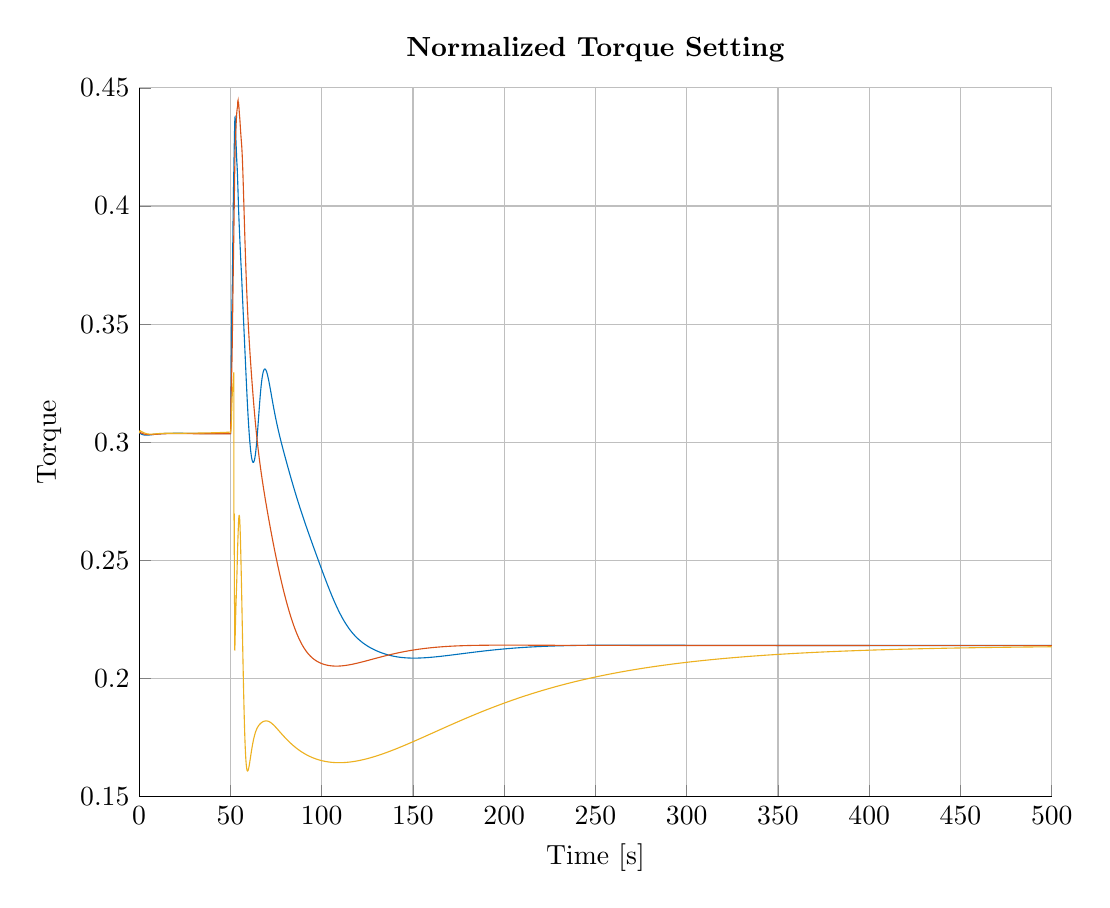
\begin{tikzpicture}

\begin{axis}[%
width=4.563in,
height=3.544in,
at={(0.792in,0.541in)},
scale only axis,
xmin=0,
xmax=500,
xlabel={Time [s]},
xmajorgrids,
ymin=0.15,
ymax=0.45,
ylabel={Torque},
ymajorgrids,
axis background/.style={fill=white},
title style={font=\bfseries},
title={Normalized Torque Setting},
axis x line*=bottom,
axis y line*=left
]
\addplot [color=mycolor1,solid,forget plot]
  table[row sep=crcr]{%
0	0.30400000722465\\
0.05	0.3039802061\\
0.1	0.3039491763\\
0.15	0.3039149109\\
0.2	0.303883203\\
0.25	0.303857271\\
0.3	0.303837982\\
0.35	0.303824461\\
0.4	0.303814832\\
0.45	0.303806867\\
0.5	0.303798455\\
0.55	0.303787909\\
0.6	0.303774112\\
0.65	0.303756551\\
0.7	0.303735266\\
0.75	0.30371074\\
0.8	0.303683762\\
0.85	0.303655274\\
0.9	0.303626196\\
0.95	0.303597362\\
1	0.303569457\\
1.05	0.303542947\\
1.1	0.303518078\\
1.15	0.303494898\\
1.2	0.303473302\\
1.25	0.303453082\\
1.3	0.303433977\\
1.35	0.303415721\\
1.4	0.303398076\\
1.45	0.303380855\\
1.5	0.303363929\\
1.55	0.30334723\\
1.6	0.303330745\\
1.65	0.303314502\\
1.7	0.303298554\\
1.75	0.303282968\\
1.8	0.303267812\\
1.85	0.303253143\\
1.9	0.303239006\\
1.95	0.303225427\\
2	0.303212415\\
2.05	0.303199963\\
2.1	0.303188053\\
2.15	0.303176659\\
2.2	0.303165752\\
2.25	0.303155301\\
2.3	0.303145286\\
2.35	0.303135695\\
2.4	0.303126511\\
2.45	0.30311772\\
2.5	0.303109324\\
2.55	0.303101327\\
2.6	0.303093735\\
2.65	0.303086554\\
2.7	0.303079791\\
2.75	0.303073449\\
2.8	0.303067528\\
2.85	0.303062028\\
2.9	0.303056944\\
2.95	0.30305227\\
3	0.303047996\\
3.05	0.303044111\\
3.1	0.303040605\\
3.15	0.303037465\\
3.2	0.303034677\\
3.25	0.303032229\\
3.3	0.303030108\\
3.35	0.3030283\\
3.4	0.303026793\\
3.45	0.303025575\\
3.5	0.303024632\\
3.55	0.303023953\\
3.6	0.303023525\\
3.65	0.303023335\\
3.7	0.303023371\\
3.75	0.303023621\\
3.8	0.303024071\\
3.85	0.303024709\\
3.9	0.303025521\\
3.95	0.303026495\\
4	0.303027617\\
4.05	0.303028874\\
4.1	0.303030252\\
4.15	0.303031738\\
4.2	0.303033318\\
4.25	0.303034979\\
4.3	0.303036706\\
4.35	0.303038487\\
4.4	0.303040309\\
4.45	0.303042161\\
4.5	0.303044034\\
4.55	0.303045918\\
4.6	0.303047807\\
4.65	0.303049697\\
4.7	0.303051585\\
4.75	0.303053469\\
4.8	0.30305535\\
4.85	0.30305723\\
4.9	0.303059113\\
4.95	0.303061004\\
5	0.30306291\\
5.05	0.303064837\\
5.1	0.303066794\\
5.15	0.303068789\\
5.2	0.303070832\\
5.25	0.303072932\\
5.3	0.303075098\\
5.35	0.303077339\\
5.4	0.303079664\\
5.45	0.303082083\\
5.5	0.303084603\\
5.55	0.303087232\\
5.6	0.303089978\\
5.65	0.303092848\\
5.7	0.303095848\\
5.75	0.303098983\\
5.8	0.303102257\\
5.85	0.303105676\\
5.9	0.30310924\\
5.95	0.303112954\\
6	0.303116817\\
6.05	0.30312083\\
6.1	0.303124992\\
6.15	0.303129302\\
6.2	0.303133756\\
6.25	0.303138353\\
6.3	0.303143086\\
6.35	0.30314795\\
6.4	0.303152941\\
6.45	0.30315805\\
6.5	0.303163269\\
6.55	0.303168591\\
6.6	0.303174006\\
6.65	0.303179505\\
6.7	0.303185077\\
6.75	0.303190711\\
6.8	0.303196398\\
6.85	0.303202124\\
6.9	0.303207879\\
6.95	0.303213651\\
7	0.303219429\\
7.05	0.303225202\\
7.1	0.303230957\\
7.15	0.303236685\\
7.2	0.303242375\\
7.25	0.303248018\\
7.3	0.303253604\\
7.35	0.303259126\\
7.4	0.303264575\\
7.45	0.303269945\\
7.5	0.30327523\\
7.55	0.303280426\\
7.6	0.303285529\\
7.65	0.303290536\\
7.7	0.303295445\\
7.75	0.303300257\\
7.8	0.303304971\\
7.85	0.303309588\\
7.9	0.303314111\\
7.95	0.303318543\\
8	0.303322888\\
8.05	0.303327151\\
8.1	0.303331337\\
8.15	0.303335453\\
8.2	0.303339504\\
8.25	0.303343499\\
8.3	0.303347445\\
8.35	0.30335135\\
8.4	0.303355223\\
8.45	0.30335907\\
8.5	0.303362901\\
8.55	0.303366725\\
8.6	0.303370548\\
8.65	0.30337438\\
8.7	0.303378228\\
8.75	0.303382099\\
8.8	0.303386\\
8.85	0.303389936\\
8.9	0.303393915\\
8.95	0.303397941\\
9	0.303402018\\
9.05	0.30340615\\
9.1	0.303410339\\
9.15	0.303414587\\
9.2	0.303418897\\
9.25	0.303423267\\
9.3	0.303427697\\
9.35	0.303432186\\
9.4	0.303436731\\
9.45	0.30344133\\
9.5	0.303445979\\
9.55	0.303450672\\
9.6	0.303455405\\
9.65	0.303460171\\
9.7	0.303464965\\
9.75	0.303469779\\
9.8	0.303474605\\
9.85	0.303479436\\
9.9	0.303484263\\
9.95	0.303489079\\
10	0.303493874\\
10.05	0.303498641\\
10.1	0.30350337\\
10.15	0.303508055\\
10.2	0.303512686\\
10.25	0.303517255\\
10.3	0.303521756\\
10.35	0.303526182\\
10.4	0.303530526\\
10.45	0.303534782\\
10.5	0.303538945\\
10.55	0.303543011\\
10.6	0.303546975\\
10.65	0.303550836\\
10.7	0.30355459\\
10.75	0.303558236\\
10.8	0.303561774\\
10.85	0.303565204\\
10.9	0.303568527\\
10.95	0.303571744\\
11	0.303574858\\
11.05	0.303577873\\
11.1	0.303580792\\
11.15	0.30358362\\
11.2	0.303586363\\
11.25	0.303589026\\
11.3	0.303591615\\
11.35	0.303594137\\
11.4	0.303596599\\
11.45	0.303599008\\
11.5	0.303601372\\
11.55	0.303603699\\
11.6	0.303605996\\
11.65	0.30360827\\
11.7	0.30361053\\
11.75	0.303612782\\
11.8	0.303615034\\
11.85	0.303617292\\
11.9	0.303619562\\
11.95	0.303621851\\
12	0.303624164\\
12.05	0.303626505\\
12.1	0.303628878\\
12.15	0.303631288\\
12.2	0.303633736\\
12.25	0.303636226\\
12.3	0.303638758\\
12.35	0.303641333\\
12.4	0.303643951\\
12.45	0.30364661\\
12.5	0.303649311\\
12.55	0.303652049\\
12.6	0.303654823\\
12.65	0.303657629\\
12.7	0.303660463\\
12.75	0.303663319\\
12.8	0.303666193\\
12.85	0.303669079\\
12.9	0.303671972\\
12.95	0.303674864\\
13	0.30367775\\
13.05	0.303680622\\
13.1	0.303683474\\
13.15	0.303686298\\
13.2	0.303689089\\
13.25	0.303691839\\
13.3	0.303694542\\
13.35	0.303697192\\
13.4	0.303699782\\
13.45	0.303702308\\
13.5	0.303704763\\
13.55	0.303707144\\
13.6	0.303709446\\
13.65	0.303711666\\
13.7	0.303713801\\
13.75	0.303715849\\
13.8	0.303717807\\
13.85	0.303719676\\
13.9	0.303721454\\
13.95	0.303723144\\
14	0.303724744\\
14.05	0.303726258\\
14.1	0.303727688\\
14.15	0.303729038\\
14.2	0.303730309\\
14.25	0.303731508\\
14.3	0.303732639\\
14.35	0.303733706\\
14.4	0.303734717\\
14.45	0.303735675\\
14.5	0.303736589\\
14.55	0.303737464\\
14.6	0.303738306\\
14.65	0.303739124\\
14.7	0.303739922\\
14.75	0.303740709\\
14.8	0.30374149\\
14.85	0.303742272\\
14.9	0.303743061\\
14.95	0.303743864\\
15	0.303744684\\
15.05	0.303745528\\
15.1	0.3037464\\
15.15	0.303747304\\
15.2	0.303748244\\
15.25	0.303749222\\
15.3	0.303750241\\
15.35	0.303751303\\
15.4	0.303752409\\
15.45	0.303753559\\
15.5	0.303754753\\
15.55	0.30375599\\
15.6	0.303757269\\
15.65	0.303758588\\
15.7	0.303759943\\
15.75	0.303761333\\
15.8	0.303762752\\
15.85	0.303764197\\
15.9	0.303765664\\
15.95	0.303767147\\
16	0.303768641\\
16.05	0.30377014\\
16.1	0.303771639\\
16.15	0.303773131\\
16.2	0.303774611\\
16.25	0.303776073\\
16.3	0.303777511\\
16.35	0.303778919\\
16.4	0.303780291\\
16.45	0.303781622\\
16.5	0.303782907\\
16.55	0.303784141\\
16.6	0.303785319\\
16.65	0.303786438\\
16.7	0.303787495\\
16.75	0.303788486\\
16.8	0.303789408\\
16.85	0.303790261\\
16.9	0.303791043\\
16.95	0.303791754\\
17	0.303792393\\
17.05	0.30379296\\
17.1	0.303793458\\
17.15	0.303793889\\
17.2	0.303794253\\
17.25	0.303794555\\
17.3	0.303794798\\
17.35	0.303794985\\
17.4	0.303795121\\
17.45	0.303795212\\
17.5	0.303795261\\
17.55	0.303795274\\
17.6	0.303795257\\
17.65	0.303795216\\
17.7	0.303795156\\
17.75	0.303795084\\
17.8	0.303795005\\
17.85	0.303794926\\
17.9	0.303794851\\
17.95	0.303794787\\
18	0.303794739\\
18.05	0.303794712\\
18.1	0.30379471\\
18.15	0.303794738\\
18.2	0.3037948\\
18.25	0.303794899\\
18.3	0.303795038\\
18.35	0.30379522\\
18.4	0.303795446\\
18.45	0.303795717\\
18.5	0.303796034\\
18.55	0.303796398\\
18.6	0.303796807\\
18.65	0.303797262\\
18.7	0.303797759\\
18.75	0.303798297\\
18.8	0.303798873\\
18.85	0.303799484\\
18.9	0.303800127\\
18.95	0.303800797\\
19	0.30380149\\
19.05	0.303802202\\
19.1	0.303802927\\
19.15	0.30380366\\
19.2	0.303804396\\
19.25	0.30380513\\
19.3	0.303805856\\
19.35	0.303806568\\
19.4	0.303807262\\
19.45	0.303807931\\
19.5	0.303808571\\
19.55	0.303809178\\
19.6	0.303809746\\
19.65	0.303810271\\
19.7	0.30381075\\
19.75	0.303811179\\
19.8	0.303811555\\
19.85	0.303811876\\
19.9	0.303812139\\
19.95	0.303812345\\
20	0.303812491\\
20.05	0.303812577\\
20.1	0.303812603\\
20.15	0.303812572\\
20.2	0.303812482\\
20.25	0.303812338\\
20.3	0.30381214\\
20.35	0.303811893\\
20.4	0.303811598\\
20.45	0.303811261\\
20.5	0.303810885\\
20.55	0.303810474\\
20.6	0.303810034\\
20.65	0.303809568\\
20.7	0.303809084\\
20.75	0.303808585\\
20.8	0.303808077\\
20.85	0.303807566\\
20.9	0.303807057\\
20.95	0.303806554\\
21	0.303806065\\
21.05	0.303805592\\
21.1	0.303805141\\
21.15	0.303804717\\
21.2	0.303804323\\
21.25	0.303803962\\
21.3	0.30380364\\
21.35	0.303803357\\
21.4	0.303803116\\
21.45	0.30380292\\
21.5	0.303802769\\
21.55	0.303802664\\
21.6	0.303802606\\
21.65	0.303802594\\
21.7	0.303802627\\
21.75	0.303802704\\
21.8	0.303802823\\
21.85	0.303802982\\
21.9	0.303803178\\
21.95	0.303803408\\
22	0.303803668\\
22.05	0.303803954\\
22.1	0.303804262\\
22.15	0.303804587\\
22.2	0.303804924\\
22.25	0.303805269\\
22.3	0.303805617\\
22.35	0.303805962\\
22.4	0.3038063\\
22.45	0.303806624\\
22.5	0.303806931\\
22.55	0.303807216\\
22.6	0.303807473\\
22.65	0.303807699\\
22.7	0.30380789\\
22.75	0.303808042\\
22.8	0.303808151\\
22.85	0.303808215\\
22.9	0.303808231\\
22.95	0.303808197\\
23	0.303808112\\
23.05	0.303807975\\
23.1	0.303807785\\
23.15	0.303807543\\
23.2	0.303807249\\
23.25	0.303806904\\
23.3	0.30380651\\
23.35	0.303806068\\
23.4	0.303805582\\
23.45	0.303805054\\
23.5	0.303804488\\
23.55	0.303803888\\
23.6	0.303803257\\
23.65	0.303802599\\
23.7	0.303801921\\
23.75	0.303801225\\
23.8	0.303800518\\
23.85	0.303799804\\
23.9	0.303799088\\
23.95	0.303798376\\
24	0.303797671\\
24.05	0.30379698\\
24.1	0.303796306\\
24.15	0.303795655\\
24.2	0.30379503\\
24.25	0.303794435\\
24.3	0.303793873\\
24.35	0.303793349\\
24.4	0.303792864\\
24.45	0.30379242\\
24.5	0.30379202\\
24.55	0.303791665\\
24.6	0.303791356\\
24.65	0.303791093\\
24.7	0.303790875\\
24.75	0.303790702\\
24.8	0.303790573\\
24.85	0.303790487\\
24.9	0.30379044\\
24.95	0.30379043\\
25	0.303790455\\
25.05	0.303790511\\
25.1	0.303790594\\
25.15	0.303790701\\
25.2	0.303790826\\
25.25	0.303790965\\
25.3	0.303791115\\
25.35	0.303791269\\
25.4	0.303791423\\
25.45	0.303791573\\
25.5	0.303791713\\
25.55	0.303791838\\
25.6	0.303791945\\
25.65	0.303792028\\
25.7	0.303792084\\
25.75	0.303792108\\
25.8	0.303792097\\
25.85	0.303792048\\
25.9	0.303791958\\
25.95	0.303791824\\
26	0.303791645\\
26.05	0.303791419\\
26.1	0.303791146\\
26.15	0.303790823\\
26.2	0.303790453\\
26.25	0.303790034\\
26.3	0.303789568\\
26.35	0.303789057\\
26.4	0.303788503\\
26.45	0.303787907\\
26.5	0.303787273\\
26.55	0.303786603\\
26.6	0.303785902\\
26.65	0.303785173\\
26.7	0.303784421\\
26.75	0.303783649\\
26.8	0.303782862\\
26.85	0.303782066\\
26.9	0.303781264\\
26.95	0.303780462\\
27	0.303779664\\
27.05	0.303778875\\
27.1	0.3037781\\
27.15	0.303777344\\
27.2	0.30377661\\
27.25	0.303775902\\
27.3	0.303775225\\
27.35	0.303774581\\
27.4	0.303773975\\
27.45	0.303773407\\
27.5	0.303772881\\
27.55	0.303772398\\
27.6	0.30377196\\
27.65	0.303771567\\
27.7	0.30377122\\
27.75	0.303770918\\
27.8	0.303770661\\
27.85	0.303770447\\
27.9	0.303770275\\
27.95	0.303770144\\
28	0.30377005\\
28.05	0.30376999\\
28.1	0.303769961\\
28.15	0.30376996\\
28.2	0.303769983\\
28.25	0.303770025\\
28.3	0.303770082\\
28.35	0.30377015\\
28.4	0.303770224\\
28.45	0.303770299\\
28.5	0.303770371\\
28.55	0.303770434\\
28.6	0.303770485\\
28.65	0.303770518\\
28.7	0.30377053\\
28.75	0.303770516\\
28.8	0.303770473\\
28.85	0.303770397\\
28.9	0.303770284\\
28.95	0.303770133\\
29	0.303769941\\
29.05	0.303769706\\
29.1	0.303769426\\
29.15	0.303769101\\
29.2	0.303768729\\
29.25	0.303768312\\
29.3	0.30376785\\
29.35	0.303767342\\
29.4	0.303766792\\
29.45	0.303766201\\
29.5	0.30376557\\
29.55	0.303764904\\
29.6	0.303764204\\
29.65	0.303763475\\
29.7	0.30376272\\
29.75	0.303761944\\
29.8	0.30376115\\
29.85	0.303760343\\
29.9	0.303759527\\
29.95	0.303758708\\
30	0.303757891\\
30.05	0.303757078\\
30.1	0.303756277\\
30.15	0.30375549\\
30.2	0.303754722\\
30.25	0.303753978\\
30.3	0.303753262\\
30.35	0.303752576\\
30.4	0.303751925\\
30.45	0.303751311\\
30.5	0.303750737\\
30.55	0.303750204\\
30.6	0.303749716\\
30.65	0.303749272\\
30.7	0.303748874\\
30.75	0.303748521\\
30.8	0.303748214\\
30.85	0.303747952\\
30.9	0.303747733\\
30.95	0.303747557\\
31	0.30374742\\
31.05	0.303747321\\
31.1	0.303747256\\
31.15	0.303747223\\
31.2	0.303747216\\
31.25	0.303747234\\
31.3	0.303747271\\
31.35	0.303747324\\
31.4	0.303747387\\
31.45	0.303747456\\
31.5	0.303747526\\
31.55	0.303747594\\
31.6	0.303747653\\
31.65	0.3037477\\
31.7	0.30374773\\
31.75	0.303747739\\
31.8	0.303747722\\
31.85	0.303747677\\
31.9	0.3037476\\
31.95	0.303747487\\
32	0.303747336\\
32.05	0.303747145\\
32.1	0.303746912\\
32.15	0.303746635\\
32.2	0.303746314\\
32.25	0.303745948\\
32.3	0.303745537\\
32.35	0.303745082\\
32.4	0.303744584\\
32.45	0.303744044\\
32.5	0.303743464\\
32.55	0.303742847\\
32.6	0.303742196\\
32.65	0.303741513\\
32.7	0.303740802\\
32.75	0.303740067\\
32.8	0.303739312\\
32.85	0.303738541\\
32.9	0.303737759\\
32.95	0.30373697\\
33	0.303736179\\
33.05	0.303735391\\
33.1	0.30373461\\
33.15	0.303733842\\
33.2	0.30373309\\
33.25	0.303732358\\
33.3	0.303731652\\
33.35	0.303730975\\
33.4	0.30373033\\
33.45	0.30372972\\
33.5	0.303729149\\
33.55	0.303728619\\
33.6	0.303728132\\
33.65	0.30372769\\
33.7	0.303727293\\
33.75	0.303726942\\
33.8	0.303726638\\
33.85	0.30372638\\
33.9	0.303726167\\
33.95	0.303725998\\
34	0.303725871\\
34.05	0.303725784\\
34.1	0.303725735\\
34.15	0.30372572\\
34.2	0.303725735\\
34.25	0.303725778\\
34.3	0.303725845\\
34.35	0.30372593\\
34.4	0.30372603\\
34.45	0.30372614\\
34.5	0.303726256\\
34.55	0.303726372\\
34.6	0.303726484\\
34.65	0.303726587\\
34.7	0.303726678\\
34.75	0.30372675\\
34.8	0.303726801\\
34.85	0.303726825\\
34.9	0.303726821\\
34.95	0.303726783\\
35	0.303726709\\
35.05	0.303726597\\
35.1	0.303726444\\
35.15	0.303726248\\
35.2	0.303726009\\
35.25	0.303725726\\
35.3	0.303725397\\
35.35	0.303725024\\
35.4	0.303724607\\
35.45	0.303724147\\
35.5	0.303723646\\
35.55	0.303723106\\
35.6	0.303722529\\
35.65	0.303721919\\
35.7	0.303721278\\
35.75	0.303720611\\
35.8	0.303719921\\
35.85	0.303719212\\
35.9	0.303718489\\
35.95	0.303717757\\
36	0.30371702\\
36.05	0.303716282\\
36.1	0.30371555\\
36.15	0.303714826\\
36.2	0.303714117\\
36.25	0.303713426\\
36.3	0.303712759\\
36.35	0.303712118\\
36.4	0.303711508\\
36.45	0.303710932\\
36.5	0.303710394\\
36.55	0.303709897\\
36.6	0.303709441\\
36.65	0.303709031\\
36.7	0.303708666\\
36.75	0.303708349\\
36.8	0.303708079\\
36.85	0.303707856\\
36.9	0.30370768\\
36.95	0.303707551\\
37	0.303707465\\
37.05	0.303707422\\
37.1	0.30370742\\
37.15	0.303707454\\
37.2	0.303707522\\
37.25	0.303707621\\
37.3	0.303707747\\
37.35	0.303707895\\
37.4	0.303708061\\
37.45	0.303708241\\
37.5	0.303708429\\
37.55	0.303708621\\
37.6	0.303708812\\
37.65	0.303708998\\
37.7	0.303709173\\
37.75	0.303709333\\
37.8	0.303709473\\
37.85	0.30370959\\
37.9	0.303709679\\
37.95	0.303709736\\
38	0.303709758\\
38.05	0.303709743\\
38.1	0.303709687\\
38.15	0.30370959\\
38.2	0.303709448\\
38.25	0.303709261\\
38.3	0.303709028\\
38.35	0.30370875\\
38.4	0.303708426\\
38.45	0.303708058\\
38.5	0.303707646\\
38.55	0.303707193\\
38.6	0.303706701\\
38.65	0.303706173\\
38.7	0.303705612\\
38.75	0.303705021\\
38.8	0.303704404\\
38.85	0.303703766\\
38.9	0.303703111\\
38.95	0.303702443\\
39	0.303701767\\
39.05	0.303701089\\
39.1	0.303700413\\
39.15	0.303699743\\
39.2	0.303699086\\
39.25	0.303698445\\
39.3	0.303697825\\
39.35	0.303697231\\
39.4	0.303696666\\
39.45	0.303696135\\
39.5	0.303695641\\
39.55	0.303695187\\
39.6	0.303694776\\
39.65	0.303694409\\
39.7	0.30369409\\
39.75	0.303693819\\
39.8	0.303693596\\
39.85	0.303693423\\
39.9	0.303693299\\
39.95	0.303693222\\
40	0.303693193\\
40.05	0.303693209\\
40.1	0.303693267\\
40.15	0.303693366\\
40.2	0.303693502\\
40.25	0.303693672\\
40.3	0.303693871\\
40.35	0.303694096\\
40.4	0.303694342\\
40.45	0.303694604\\
40.5	0.303694878\\
40.55	0.303695158\\
40.6	0.303695441\\
40.65	0.30369572\\
40.7	0.30369599\\
40.75	0.303696247\\
40.8	0.303696486\\
40.85	0.303696703\\
40.9	0.303696892\\
40.95	0.303697051\\
41	0.303697175\\
41.05	0.303697262\\
41.1	0.303697307\\
41.15	0.30369731\\
41.2	0.303697267\\
41.25	0.303697178\\
41.3	0.303697041\\
41.35	0.303696857\\
41.4	0.303696625\\
41.45	0.303696345\\
41.5	0.30369602\\
41.55	0.303695651\\
41.6	0.303695239\\
41.65	0.303694788\\
41.7	0.303694301\\
41.75	0.303693781\\
41.8	0.303693232\\
41.85	0.303692658\\
41.9	0.303692064\\
41.95	0.303691455\\
42	0.303690834\\
42.05	0.303690209\\
42.1	0.303689582\\
42.15	0.303688961\\
42.2	0.303688349\\
42.25	0.303687753\\
42.3	0.303687176\\
42.35	0.303686623\\
42.4	0.3036861\\
42.45	0.30368561\\
42.5	0.303685156\\
42.55	0.303684744\\
42.6	0.303684374\\
42.65	0.303684051\\
42.7	0.303683776\\
42.75	0.30368355\\
42.8	0.303683376\\
42.85	0.303683253\\
42.9	0.303683181\\
42.95	0.30368316\\
43	0.303683189\\
43.05	0.303683266\\
43.1	0.303683389\\
43.15	0.303683555\\
43.2	0.303683762\\
43.25	0.303684005\\
43.3	0.303684281\\
43.35	0.303684586\\
43.4	0.303684915\\
43.45	0.303685263\\
43.5	0.303685626\\
43.55	0.303685997\\
43.6	0.303686373\\
43.65	0.303686746\\
43.7	0.303687113\\
43.75	0.303687468\\
43.8	0.303687805\\
43.85	0.30368812\\
43.9	0.303688409\\
43.95	0.303688666\\
44	0.303688888\\
44.05	0.303689072\\
44.1	0.303689213\\
44.15	0.303689309\\
44.2	0.303689358\\
44.25	0.303689359\\
44.3	0.303689309\\
44.35	0.303689208\\
44.4	0.303689057\\
44.45	0.303688855\\
44.5	0.303688603\\
44.55	0.303688304\\
44.6	0.303687959\\
44.65	0.303687571\\
44.7	0.303687142\\
44.75	0.303686677\\
44.8	0.30368618\\
44.85	0.303685654\\
44.9	0.303685105\\
44.95	0.303684537\\
45	0.303683955\\
45.05	0.303683366\\
45.1	0.303682773\\
45.15	0.303682183\\
45.2	0.303681602\\
45.25	0.303681034\\
45.3	0.303680485\\
45.35	0.30367996\\
45.4	0.303679464\\
45.45	0.303679001\\
45.5	0.303678576\\
45.55	0.303678192\\
45.6	0.303677854\\
45.65	0.303677563\\
45.7	0.303677323\\
45.75	0.303677135\\
45.8	0.303677\\
45.85	0.30367692\\
45.9	0.303676894\\
45.95	0.303676923\\
46	0.303677005\\
46.05	0.303677138\\
46.1	0.303677322\\
46.15	0.303677552\\
46.2	0.303677826\\
46.25	0.303678141\\
46.3	0.303678492\\
46.35	0.303678874\\
46.4	0.303679284\\
46.45	0.303679716\\
46.5	0.303680165\\
46.55	0.303680624\\
46.6	0.30368109\\
46.65	0.303681555\\
46.7	0.303682014\\
46.75	0.303682462\\
46.8	0.303682893\\
46.85	0.303683301\\
46.9	0.303683682\\
46.95	0.30368403\\
47	0.303684342\\
47.05	0.303684613\\
47.1	0.30368484\\
47.15	0.303685019\\
47.2	0.303685147\\
47.25	0.303685224\\
47.3	0.303685246\\
47.35	0.303685214\\
47.4	0.303685127\\
47.45	0.303684984\\
47.5	0.303684789\\
47.55	0.30368454\\
47.6	0.303684242\\
47.65	0.303683895\\
47.7	0.303683505\\
47.75	0.303683073\\
47.8	0.303682605\\
47.85	0.303682105\\
47.9	0.303681577\\
47.95	0.303681028\\
48	0.303680462\\
48.05	0.303679886\\
48.1	0.303679304\\
48.15	0.303678724\\
48.2	0.30367815\\
48.25	0.303677589\\
48.3	0.303677047\\
48.35	0.303676529\\
48.4	0.303676041\\
48.45	0.303675587\\
48.5	0.303675172\\
48.55	0.303674801\\
48.6	0.303674478\\
48.65	0.303674205\\
48.7	0.303673985\\
48.75	0.303673822\\
48.8	0.303673715\\
48.85	0.303673667\\
48.9	0.303673678\\
48.95	0.303673748\\
49	0.303673875\\
49.05	0.303674058\\
49.1	0.303674296\\
49.15	0.303674585\\
49.2	0.303674922\\
49.25	0.303675303\\
49.3	0.303675725\\
49.35	0.303676182\\
49.4	0.30367667\\
49.45	0.303677182\\
49.5	0.303677713\\
49.55	0.303678258\\
49.6	0.30367881\\
49.65	0.303679363\\
49.7	0.30367991\\
49.75	0.303680446\\
49.8	0.303680965\\
49.85	0.30368146\\
49.9	0.303681926\\
49.95	0.303682357\\
50	0.30368275\\
50.05	0.3036831\\
50.1	0.304632036\\
50.15	0.3070638\\
50.2	0.31114159\\
50.25	0.3168462\\
50.3	0.3200992\\
50.35	0.3241073\\
50.4	0.3287118\\
50.45	0.3336527\\
50.5	0.3388353\\
50.55	0.3444599\\
50.6	0.3478649\\
50.65	0.3507498\\
50.7	0.353158\\
50.75	0.3552172\\
50.8	0.3570776\\
50.85	0.3588956\\
50.9	0.3608071\\
50.95	0.3629117\\
51	0.3652667\\
51.05	0.3679014\\
51.1	0.3707981\\
51.15	0.3739468\\
51.2	0.3773266\\
51.25	0.3808332\\
51.3	0.384364\\
51.35	0.3878275\\
51.4	0.3911544\\
51.45	0.3943029\\
51.5	0.3972577\\
51.55	0.4000266\\
51.6	0.4026345\\
51.65	0.405116\\
51.7	0.407509\\
51.75	0.409844\\
51.8	0.412148\\
51.85	0.414433\\
51.9	0.416707\\
51.95	0.418963\\
52	0.421189\\
52.05	0.423367\\
52.1	0.425488\\
52.15	0.427545\\
52.2	0.429524\\
52.25	0.43142\\
52.3	0.433206\\
52.35	0.434796\\
52.4	0.436097\\
52.45	0.43703\\
52.5	0.437547\\
52.55	0.43763\\
52.6	0.437283\\
52.65	0.436505\\
52.7	0.43544\\
52.75	0.434214\\
52.8	0.43293\\
52.85	0.43166\\
52.9	0.43045\\
52.95	0.429319\\
53	0.428266\\
53.05	0.427274\\
53.1	0.426322\\
53.15	0.425383\\
53.2	0.424434\\
53.25	0.423458\\
53.3	0.422442\\
53.35	0.421384\\
53.4	0.420288\\
53.45	0.419879\\
53.5	0.41867\\
53.55	0.418157\\
53.6	0.417564\\
53.65	0.416893\\
53.7	0.416143\\
53.75	0.41531\\
53.8	0.414396\\
53.85	0.413407\\
53.9	0.412349\\
53.95	0.411235\\
54	0.410077\\
54.05	0.408888\\
54.1	0.407679\\
54.15	0.406461\\
54.2	0.405242\\
54.25	0.404028\\
54.3	0.4028244\\
54.35	0.4016339\\
54.4	0.4004619\\
54.45	0.399313\\
54.5	0.3981912\\
54.55	0.3971001\\
54.6	0.3960431\\
54.65	0.3950232\\
54.7	0.3940432\\
54.75	0.3931054\\
54.8	0.3922117\\
54.85	0.3913631\\
54.9	0.3904122\\
54.95	0.3894874\\
55	0.3885861\\
55.05	0.3877038\\
55.1	0.3868351\\
55.15	0.3859748\\
55.2	0.3851186\\
55.25	0.3842637\\
55.3	0.383409\\
55.35	0.3825545\\
55.4	0.3817016\\
55.45	0.3808506\\
55.5	0.3800031\\
55.55	0.379165\\
55.6	0.3783382\\
55.65	0.3775262\\
55.7	0.3767322\\
55.75	0.3759574\\
55.8	0.3751994\\
55.85	0.3744532\\
55.9	0.3737111\\
55.95	0.3729645\\
56	0.3722052\\
56.05	0.3714264\\
56.1	0.3706239\\
56.15	0.3697962\\
56.2	0.3689446\\
56.25	0.3680725\\
56.3	0.3671849\\
56.35	0.3662874\\
56.4	0.3653857\\
56.45	0.3644846\\
56.5	0.3635879\\
56.55	0.362698\\
56.6	0.3618163\\
56.65	0.3609427\\
56.7	0.3600763\\
56.75	0.3592159\\
56.8	0.3583597\\
56.85	0.3575061\\
56.9	0.3566537\\
56.95	0.3558015\\
57	0.3549486\\
57.05	0.354095\\
57.1	0.3532405\\
57.15	0.3523855\\
57.2	0.3515302\\
57.25	0.350675\\
57.3	0.3498202\\
57.35	0.3489661\\
57.4	0.3481127\\
57.45	0.3472601\\
57.5	0.3464082\\
57.55	0.3455567\\
57.6	0.3447056\\
57.65	0.3438545\\
57.7	0.3430032\\
57.75	0.3421516\\
57.8	0.3412996\\
57.85	0.3404469\\
57.9	0.3395936\\
57.95	0.3387396\\
58	0.3378848\\
58.05	0.3370294\\
58.1	0.3361733\\
58.15	0.3353169\\
58.2	0.3344602\\
58.25	0.3336036\\
58.3	0.3327475\\
58.35	0.3318922\\
58.4	0.3310383\\
58.45	0.3301864\\
58.5	0.3293369\\
58.55	0.3284904\\
58.6	0.3276475\\
58.65	0.3268086\\
58.7	0.3259743\\
58.75	0.325145\\
58.8	0.3243211\\
58.85	0.3235029\\
58.9	0.3226909\\
58.95	0.3218852\\
59	0.3210862\\
59.05	0.3202942\\
59.1	0.3195094\\
59.15	0.3187322\\
59.2	0.3179629\\
59.25	0.3172016\\
59.3	0.3164488\\
59.35	0.3157046\\
59.4	0.3149694\\
59.45	0.3142434\\
59.5	0.31352675\\
59.55	0.3128198\\
59.6	0.31212271\\
59.65	0.31143569\\
59.7	0.31075891\\
59.75	0.31009255\\
59.8	0.30943674\\
59.85	0.30879163\\
59.9	0.30815736\\
59.95	0.30753404\\
60	0.30692179\\
60.05	0.30632071\\
60.1	0.3057309\\
60.15	0.30515246\\
60.2	0.304585463\\
60.25	0.3040299947\\
60.3	0.303486127\\
60.35	0.30295393\\
60.4	0.30243345\\
60.45	0.30192477\\
60.5	0.30142791\\
60.55	0.30094293\\
60.6	0.30046987\\
60.65	0.30000876\\
60.7	0.29955964\\
60.75	0.29912252\\
60.8	0.29869743\\
60.85	0.29828439\\
60.9	0.29788342\\
60.95	0.29749454\\
61	0.29711774\\
61.05	0.29675305\\
61.1	0.29640047\\
61.15	0.29606001\\
61.2	0.29573168\\
61.25	0.29541548\\
61.3	0.29511142\\
61.35	0.29481951\\
61.4	0.29453975\\
61.45	0.29427214\\
61.5	0.2940167\\
61.55	0.2937734\\
61.6	0.2935424\\
61.65	0.2933235\\
61.7	0.2931168\\
61.75	0.2929223\\
61.8	0.29274\\
61.85	0.29257\\
61.9	0.2924122\\
61.95	0.2922666\\
62	0.2921334\\
62.05	0.2920124\\
62.1	0.2919037\\
62.15	0.2918074\\
62.2	0.2917234\\
62.25	0.2916517\\
62.3	0.2915925\\
62.35	0.2915456\\
62.4	0.2915111\\
62.45	0.2914891\\
62.5	0.2914795\\
62.55	0.2914824\\
62.6	0.2914978\\
62.65	0.2915257\\
62.7	0.2915661\\
62.75	0.291619\\
62.8	0.2916844\\
62.85	0.2917624\\
62.9	0.291853\\
62.95	0.291956\\
63	0.2920716\\
63.05	0.2921997\\
63.1	0.2923404\\
63.15	0.2924935\\
63.2	0.2926591\\
63.25	0.2928372\\
63.3	0.2930276\\
63.35	0.2932304\\
63.4	0.2934455\\
63.45	0.2936728\\
63.5	0.2939123\\
63.55	0.2941639\\
63.6	0.29442749\\
63.65	0.29470298\\
63.7	0.29499027\\
63.75	0.29528922\\
63.8	0.29559972\\
63.85	0.29592161\\
63.9	0.29625474\\
63.95	0.29659895\\
64	0.29695404\\
64.05	0.29731983\\
64.1	0.29769611\\
64.15	0.29808265\\
64.2	0.29847924\\
64.25	0.29888561\\
64.3	0.2993015\\
64.35	0.29972665\\
64.4	0.30016076\\
64.45	0.30060354\\
64.5	0.30105467\\
64.55	0.30151382\\
64.6	0.30198066\\
64.65	0.30245482\\
64.7	0.30293596\\
64.75	0.303423696\\
64.8	0.3039176404\\
64.85	0.304417398\\
64.9	0.304922564\\
64.95	0.30543272\\
65	0.30594745\\
65.05	0.3064663\\
65.1	0.30698885\\
65.15	0.30751465\\
65.2	0.30804323\\
65.25	0.30857414\\
65.3	0.3091069\\
65.35	0.30964105\\
65.4	0.3101761\\
65.45	0.31071157\\
65.5	0.31124699\\
65.55	0.31178186\\
65.6	0.31231569\\
65.65	0.31284799\\
65.7	0.31337828\\
65.75	0.31390607\\
65.8	0.3144309\\
65.85	0.3149522\\
65.9	0.3154696\\
65.95	0.3159826\\
66	0.3164908\\
66.05	0.3169936\\
66.1	0.3174908\\
66.15	0.3179818\\
66.2	0.3184662\\
66.25	0.3189438\\
66.3	0.3194141\\
66.35	0.3198767\\
66.4	0.3203315\\
66.45	0.320778\\
66.5	0.321216\\
66.55	0.3216453\\
66.6	0.3220656\\
66.65	0.3224767\\
66.7	0.3228785\\
66.75	0.3232708\\
66.8	0.3236534\\
66.85	0.3240263\\
66.9	0.3243893\\
66.95	0.3247423\\
67	0.3250854\\
67.05	0.3254183\\
67.1	0.3257412\\
67.15	0.3260539\\
67.2	0.3263564\\
67.25	0.3266489\\
67.3	0.3269311\\
67.35	0.3272033\\
67.4	0.3274654\\
67.45	0.3277174\\
67.5	0.3279594\\
67.55	0.3281915\\
67.6	0.3284137\\
67.65	0.328626\\
67.7	0.3288286\\
67.75	0.3290216\\
67.8	0.3292049\\
67.85	0.3293787\\
67.9	0.329543\\
67.95	0.329698\\
68	0.3298438\\
68.05	0.3299804\\
68.1	0.330108\\
68.15	0.3302266\\
68.2	0.3303364\\
68.25	0.3304375\\
68.3	0.3305299\\
68.35	0.3306138\\
68.4	0.3306893\\
68.45	0.3307565\\
68.5	0.3308156\\
68.55	0.3308666\\
68.6	0.3309096\\
68.65	0.3309449\\
68.7	0.3309724\\
68.75	0.3309924\\
68.8	0.3310049\\
68.85	0.33101\\
68.9	0.331008\\
68.95	0.3309989\\
69	0.3309828\\
69.05	0.3309599\\
69.1	0.3309303\\
69.15	0.3308941\\
69.2	0.3308515\\
69.25	0.3308025\\
69.3	0.3307474\\
69.35	0.3306861\\
69.4	0.330619\\
69.45	0.330546\\
69.5	0.3304673\\
69.55	0.3303831\\
69.6	0.3302934\\
69.65	0.3301985\\
69.7	0.3300984\\
69.75	0.3299932\\
69.8	0.3298831\\
69.85	0.3297682\\
69.9	0.3296487\\
69.95	0.3295246\\
70	0.3293961\\
70.05	0.3292632\\
70.1	0.3291263\\
70.15	0.3289852\\
70.2	0.3288403\\
70.25	0.3286915\\
70.3	0.328539\\
70.35	0.328383\\
70.4	0.3282235\\
70.45	0.3280607\\
70.5	0.3278946\\
70.55	0.3277254\\
70.6	0.3275533\\
70.65	0.3273782\\
70.7	0.3272003\\
70.75	0.3270198\\
70.8	0.3268367\\
70.85	0.3266512\\
70.9	0.3264633\\
70.95	0.3262731\\
71	0.3260808\\
71.05	0.3258864\\
71.1	0.3256901\\
71.15	0.3254918\\
71.2	0.3252919\\
71.25	0.3250902\\
71.3	0.3248869\\
71.35	0.3246821\\
71.4	0.3244759\\
71.45	0.3242684\\
71.5	0.3240596\\
71.55	0.3238496\\
71.6	0.3236386\\
71.65	0.3234265\\
71.7	0.3232135\\
71.75	0.3229996\\
71.8	0.3227849\\
71.85	0.3225695\\
71.9	0.3223535\\
71.95	0.3221368\\
72	0.3219197\\
72.05	0.321702\\
72.1	0.321484\\
72.15	0.3212656\\
72.2	0.321047\\
72.25	0.3208281\\
72.3	0.320609\\
72.35	0.3203898\\
72.4	0.3201706\\
72.45	0.3199513\\
72.5	0.3197321\\
72.55	0.3195129\\
72.6	0.3192939\\
72.65	0.319075\\
72.7	0.3188563\\
72.75	0.3186379\\
72.8	0.3184197\\
72.85	0.3182019\\
72.9	0.3179844\\
72.95	0.3177673\\
73	0.3175506\\
73.05	0.3173344\\
73.1	0.3171186\\
73.15	0.3169034\\
73.2	0.3166887\\
73.25	0.3164745\\
73.3	0.316261\\
73.35	0.316048\\
73.4	0.3158357\\
73.45	0.3156241\\
73.5	0.3154131\\
73.55	0.3152028\\
73.6	0.3149932\\
73.65	0.3147843\\
73.7	0.3145762\\
73.75	0.3143688\\
73.8	0.3141622\\
73.85	0.31395641\\
73.9	0.31375137\\
73.95	0.31354714\\
74	0.31334371\\
74.05	0.3131411\\
74.1	0.31293932\\
74.15	0.31273837\\
74.2	0.31253825\\
74.25	0.31233898\\
74.3	0.31214056\\
74.35	0.31194299\\
74.4	0.31174627\\
74.45	0.3115504\\
74.5	0.3113554\\
74.55	0.31116125\\
74.6	0.31096796\\
74.65	0.31077553\\
74.7	0.31058395\\
74.75	0.31039323\\
74.8	0.31020337\\
74.85	0.31001435\\
74.9	0.30982618\\
74.95	0.30963886\\
75	0.30945237\\
75.05	0.30926672\\
75.1	0.30908191\\
75.15	0.30889791\\
75.2	0.30871474\\
75.25	0.30853238\\
75.3	0.30835083\\
75.35	0.30817008\\
75.4	0.30799012\\
75.45	0.30781095\\
75.5	0.30763255\\
75.55	0.30745493\\
75.6	0.30727807\\
75.65	0.30710197\\
75.7	0.30692661\\
75.75	0.30675199\\
75.8	0.3065781\\
75.85	0.30640493\\
75.9	0.30623247\\
75.95	0.30606072\\
76	0.30588965\\
76.05	0.30571927\\
76.1	0.30554956\\
76.15	0.30538052\\
76.2	0.30521213\\
76.25	0.30504438\\
76.3	0.304877268\\
76.35	0.30471078\\
76.4	0.304544907\\
76.45	0.304379638\\
76.5	0.304214964\\
76.55	0.3040508741\\
76.6	0.303887359\\
76.65	0.303724409\\
76.7	0.303562014\\
76.75	0.303400163\\
76.8	0.303238848\\
76.85	0.303078058\\
76.9	0.30291778\\
76.95	0.30275802\\
77	0.30259874\\
77.05	0.30243996\\
77.1	0.30228165\\
77.15	0.30212381\\
77.2	0.30196643\\
77.25	0.3018095\\
77.3	0.301653\\
77.35	0.30149694\\
77.4	0.3013413\\
77.45	0.30118608\\
77.5	0.30103126\\
77.55	0.30087683\\
77.6	0.3007228\\
77.65	0.30056914\\
77.7	0.30041586\\
77.75	0.30026294\\
77.8	0.30011037\\
77.85	0.29995815\\
77.9	0.29980627\\
77.95	0.29965473\\
78	0.2995035\\
78.05	0.2993526\\
78.1	0.29920201\\
78.15	0.29905172\\
78.2	0.29890172\\
78.25	0.29875202\\
78.3	0.2986026\\
78.35	0.29845346\\
78.4	0.29830459\\
78.45	0.29815598\\
78.5	0.29800763\\
78.55	0.29785954\\
78.6	0.29771169\\
78.65	0.29756409\\
78.7	0.29741672\\
78.75	0.29726958\\
78.8	0.29712267\\
78.85	0.29697598\\
78.9	0.2968295\\
78.95	0.29668324\\
79	0.29653718\\
79.05	0.29639133\\
79.1	0.29624567\\
79.15	0.29610021\\
79.2	0.29595494\\
79.25	0.29580986\\
79.3	0.29566495\\
79.35	0.29552023\\
79.4	0.29537568\\
79.45	0.29523131\\
79.5	0.2950871\\
79.55	0.29494306\\
79.6	0.29479918\\
79.65	0.29465546\\
79.7	0.2945119\\
79.75	0.2943685\\
79.8	0.29422524\\
79.85	0.29408213\\
79.9	0.2939392\\
79.95	0.2937964\\
80	0.2936537\\
80.05	0.2935112\\
80.1	0.2933688\\
80.15	0.2932265\\
80.2	0.2930844\\
80.25	0.2929424\\
80.3	0.2928006\\
80.35	0.2926588\\
80.4	0.2925172\\
80.45	0.2923758\\
80.5	0.2922344\\
80.55	0.2920932\\
80.6	0.2919521\\
80.65	0.2918112\\
80.7	0.2916703\\
80.75	0.2915296\\
80.8	0.291389\\
80.85	0.2912485\\
80.9	0.2911082\\
80.95	0.2909679\\
81	0.2908278\\
81.05	0.2906878\\
81.1	0.2905479\\
81.15	0.2904082\\
81.2	0.2902685\\
81.25	0.290129\\
81.3	0.2899896\\
81.35	0.2898503\\
81.4	0.2897111\\
81.45	0.2895721\\
81.5	0.2894331\\
81.55	0.2892943\\
81.6	0.2891556\\
81.65	0.289017\\
81.7	0.2888786\\
81.75	0.2887402\\
81.8	0.288602\\
81.85	0.2884639\\
81.9	0.2883259\\
81.95	0.288188\\
82	0.2880502\\
82.05	0.2879126\\
82.1	0.2877751\\
82.15	0.2876377\\
82.2	0.2875004\\
82.25	0.2873633\\
82.3	0.2872262\\
82.35	0.2870893\\
82.4	0.2869526\\
82.45	0.2868159\\
82.5	0.2866794\\
82.55	0.286543\\
82.6	0.2864067\\
82.65	0.2862705\\
82.7	0.2861345\\
82.75	0.2859986\\
82.8	0.2858629\\
82.85	0.2857272\\
82.9	0.2855917\\
82.95	0.2854563\\
83	0.2853211\\
83.05	0.285186\\
83.1	0.285051\\
83.15	0.2849161\\
83.2	0.2847814\\
83.25	0.2846469\\
83.3	0.2845124\\
83.35	0.2843781\\
83.4	0.2842439\\
83.45	0.2841099\\
83.5	0.283976\\
83.55	0.2838422\\
83.6	0.2837086\\
83.65	0.2835752\\
83.7	0.2834418\\
83.75	0.2833086\\
83.8	0.2831756\\
83.85	0.2830427\\
83.9	0.2829099\\
83.95	0.2827773\\
84	0.2826448\\
84.05	0.2825124\\
84.1	0.2823803\\
84.15	0.2822482\\
84.2	0.2821163\\
84.25	0.2819846\\
84.3	0.281853\\
84.35	0.2817215\\
84.4	0.2815902\\
84.45	0.281459\\
84.5	0.281328\\
84.55	0.2811972\\
84.6	0.2810665\\
84.65	0.2809359\\
84.7	0.2808055\\
84.75	0.2806752\\
84.8	0.2805451\\
84.85	0.2804152\\
84.9	0.2802854\\
84.95	0.2801558\\
85	0.2800263\\
85.05	0.2798969\\
85.1	0.2797677\\
85.15	0.2796387\\
85.2	0.2795098\\
85.25	0.2793811\\
85.3	0.2792525\\
85.35	0.2791241\\
85.4	0.2789959\\
85.45	0.2788678\\
85.5	0.2787398\\
85.55	0.2786121\\
85.6	0.2784844\\
85.65	0.2783569\\
85.7	0.2782296\\
85.75	0.2781025\\
85.8	0.2779755\\
85.85	0.2778486\\
85.9	0.2777219\\
85.95	0.2775954\\
86	0.277469\\
86.05	0.2773428\\
86.1	0.2772167\\
86.15	0.2770908\\
86.2	0.2769651\\
86.25	0.2768395\\
86.3	0.276714\\
86.35	0.2765887\\
86.4	0.2764636\\
86.45	0.2763386\\
86.5	0.2762138\\
86.55	0.2760892\\
86.6	0.2759647\\
86.65	0.2758403\\
86.7	0.2757161\\
86.75	0.2755921\\
86.8	0.2754682\\
86.85	0.2753445\\
86.9	0.2752209\\
86.95	0.2750975\\
87	0.2749742\\
87.05	0.2748511\\
87.1	0.2747282\\
87.15	0.2746053\\
87.2	0.2744827\\
87.25	0.2743602\\
87.3	0.2742378\\
87.35	0.2741157\\
87.4	0.2739936\\
87.45	0.2738717\\
87.5	0.27375\\
87.55	0.2736284\\
87.6	0.2735069\\
87.65	0.2733856\\
87.7	0.2732645\\
87.75	0.2731435\\
87.8	0.2730226\\
87.85	0.2729019\\
87.9	0.2727814\\
87.95	0.272661\\
88	0.2725407\\
88.05	0.2724206\\
88.1	0.2723006\\
88.15	0.2721808\\
88.2	0.2720611\\
88.25	0.2719416\\
88.3	0.2718222\\
88.35	0.2717029\\
88.4	0.2715838\\
88.45	0.2714648\\
88.5	0.271346\\
88.55	0.2712273\\
88.6	0.2711087\\
88.65	0.2709903\\
88.7	0.270872\\
88.75	0.2707539\\
88.8	0.2706359\\
88.85	0.270518\\
88.9	0.2704003\\
88.95	0.2702827\\
89	0.2701652\\
89.05	0.2700478\\
89.1	0.2699306\\
89.15	0.2698136\\
89.2	0.2696966\\
89.25	0.2695798\\
89.3	0.2694631\\
89.35	0.2693466\\
89.4	0.2692301\\
89.45	0.2691138\\
89.5	0.2689976\\
89.55	0.2688816\\
89.6	0.2687657\\
89.65	0.2686499\\
89.7	0.2685342\\
89.75	0.2684186\\
89.8	0.2683032\\
89.85	0.2681879\\
89.9	0.2680727\\
89.95	0.2679576\\
90	0.2678426\\
90.05	0.2677278\\
90.1	0.267613\\
90.15	0.2674984\\
90.2	0.2673839\\
90.25	0.2672696\\
90.3	0.2671553\\
90.35	0.2670411\\
90.4	0.2669271\\
90.45	0.2668131\\
90.5	0.2666993\\
90.55	0.2665856\\
90.6	0.266472\\
90.65	0.2663585\\
90.7	0.2662451\\
90.75	0.2661318\\
90.8	0.2660186\\
90.85	0.2659055\\
90.9	0.2657925\\
90.95	0.2656796\\
91	0.2655668\\
91.05	0.2654541\\
91.1	0.2653416\\
91.15	0.2652291\\
91.2	0.2651167\\
91.25	0.2650044\\
91.3	0.2648922\\
91.35	0.2647801\\
91.4	0.2646681\\
91.45	0.2645561\\
91.5	0.2644443\\
91.55	0.2643326\\
91.6	0.2642209\\
91.65	0.2641094\\
91.7	0.2639979\\
91.75	0.2638865\\
91.8	0.2637752\\
91.85	0.263664\\
91.9	0.2635529\\
91.95	0.2634418\\
92	0.2633308\\
92.05	0.26322\\
92.1	0.2631092\\
92.15	0.2629984\\
92.2	0.2628878\\
92.25	0.2627772\\
92.3	0.2626667\\
92.35	0.2625563\\
92.4	0.262446\\
92.45	0.2623357\\
92.5	0.2622256\\
92.55	0.2621154\\
92.6	0.2620054\\
92.65	0.2618954\\
92.7	0.2617855\\
92.75	0.2616757\\
92.8	0.2615659\\
92.85	0.2614562\\
92.9	0.2613466\\
92.95	0.261237\\
93	0.2611275\\
93.05	0.2610181\\
93.1	0.2609087\\
93.15	0.2607994\\
93.2	0.2606902\\
93.25	0.260581\\
93.3	0.2604719\\
93.35	0.2603628\\
93.4	0.2602538\\
93.45	0.2601449\\
93.5	0.260036\\
93.55	0.2599271\\
93.6	0.2598184\\
93.65	0.2597096\\
93.7	0.259601\\
93.75	0.2594924\\
93.8	0.2593838\\
93.85	0.2592753\\
93.9	0.2591668\\
93.95	0.2590584\\
94	0.2589501\\
94.05	0.2588417\\
94.1	0.2587335\\
94.15	0.2586253\\
94.2	0.2585171\\
94.25	0.258409\\
94.3	0.2583009\\
94.35	0.2581929\\
94.4	0.2580849\\
94.45	0.257977\\
94.5	0.2578691\\
94.55	0.2577612\\
94.6	0.2576534\\
94.65	0.2575456\\
94.7	0.2574379\\
94.75	0.2573302\\
94.8	0.2572225\\
94.85	0.2571149\\
94.9	0.2570074\\
94.95	0.2568998\\
95	0.2567923\\
95.05	0.2566849\\
95.1	0.2565774\\
95.15	0.2564701\\
95.2	0.2563627\\
95.25	0.2562554\\
95.3	0.2561481\\
95.35	0.2560409\\
95.4	0.2559337\\
95.45	0.2558265\\
95.5	0.2557193\\
95.55	0.2556122\\
95.6	0.2555051\\
95.65	0.2553981\\
95.7	0.2552911\\
95.75	0.2551841\\
95.8	0.2550771\\
95.85	0.2549702\\
95.9	0.2548633\\
95.95	0.2547564\\
96	0.2546496\\
96.05	0.2545428\\
96.1	0.254436\\
96.15	0.2543292\\
96.2	0.2542225\\
96.25	0.2541158\\
96.3	0.2540092\\
96.35	0.2539025\\
96.4	0.2537959\\
96.45	0.2536893\\
96.5	0.2535828\\
96.55	0.2534762\\
96.6	0.2533697\\
96.65	0.2532633\\
96.7	0.2531568\\
96.75	0.2530504\\
96.8	0.252944\\
96.85	0.2528376\\
96.9	0.2527313\\
96.95	0.2526249\\
97	0.2525186\\
97.05	0.2524124\\
97.1	0.2523061\\
97.15	0.2521999\\
97.2	0.2520937\\
97.25	0.2519876\\
97.3	0.2518814\\
97.35	0.2517753\\
97.4	0.2516692\\
97.45	0.2515632\\
97.5	0.2514571\\
97.55	0.2513511\\
97.6	0.2512451\\
97.65	0.2511392\\
97.7	0.2510333\\
97.75	0.2509274\\
97.8	0.2508215\\
97.85	0.2507156\\
97.9	0.2506098\\
97.95	0.250504\\
98	0.2503983\\
98.05	0.2502925\\
98.1	0.2501868\\
98.15	0.2500811\\
98.2	0.2499755\\
98.25	0.2498698\\
98.3	0.2497643\\
98.35	0.2496587\\
98.4	0.2495532\\
98.45	0.2494476\\
98.5	0.2493422\\
98.55	0.2492367\\
98.6	0.2491313\\
98.65	0.2490259\\
98.7	0.2489206\\
98.75	0.2488153\\
98.8	0.24871\\
98.85	0.2486047\\
98.9	0.2484995\\
98.95	0.2483943\\
99	0.2482892\\
99.05	0.2481841\\
99.1	0.248079\\
99.15	0.247974\\
99.2	0.247869\\
99.25	0.247764\\
99.3	0.2476591\\
99.35	0.2475542\\
99.4	0.2474493\\
99.45	0.2473445\\
99.5	0.2472397\\
99.55	0.247135\\
99.6	0.2470303\\
99.65	0.2469256\\
99.7	0.246821\\
99.75	0.2467165\\
99.8	0.2466119\\
99.85	0.2465075\\
99.9	0.246403\\
99.95	0.2462986\\
100	0.2461943\\
100.05	0.24609\\
100.1	0.2459858\\
100.15	0.2458816\\
100.2	0.2457774\\
100.25	0.2456733\\
100.3	0.2455693\\
100.35	0.2454653\\
100.4	0.2453613\\
100.45	0.2452574\\
100.5	0.2451536\\
100.55	0.2450498\\
100.6	0.2449461\\
100.65	0.2448424\\
100.7	0.2447388\\
100.75	0.2446352\\
100.8	0.2445317\\
100.85	0.2444283\\
100.9	0.2443249\\
100.95	0.2442216\\
101	0.2441183\\
101.05	0.2440151\\
101.1	0.243912\\
101.15	0.2438089\\
101.2	0.2437059\\
101.25	0.243603\\
101.3	0.2435001\\
101.35	0.2433973\\
101.4	0.2432946\\
101.45	0.243192\\
101.5	0.2430894\\
101.55	0.2429869\\
101.6	0.2428844\\
101.65	0.2427821\\
101.7	0.2426798\\
101.75	0.2425776\\
101.8	0.2424754\\
101.85	0.2423734\\
101.9	0.2422714\\
101.95	0.2421695\\
102	0.2420677\\
102.05	0.2419659\\
102.1	0.2418643\\
102.15	0.2417627\\
102.2	0.2416613\\
102.25	0.2415599\\
102.3	0.2414586\\
102.35	0.2413573\\
102.4	0.2412562\\
102.45	0.2411552\\
102.5	0.2410542\\
102.55	0.2409534\\
102.6	0.2408526\\
102.65	0.240752\\
102.7	0.2406514\\
102.75	0.2405509\\
102.8	0.2404505\\
102.85	0.2403503\\
102.9	0.2402501\\
102.95	0.24015\\
103	0.2400501\\
103.05	0.2399502\\
103.1	0.2398504\\
103.15	0.2397508\\
103.2	0.2396513\\
103.25	0.2395518\\
103.3	0.2394525\\
103.35	0.2393533\\
103.4	0.2392542\\
103.45	0.2391552\\
103.5	0.2390563\\
103.55	0.2389575\\
103.6	0.2388589\\
103.65	0.2387604\\
103.7	0.238662\\
103.75	0.2385637\\
103.8	0.2384655\\
103.85	0.2383675\\
103.9	0.2382695\\
103.95	0.2381717\\
104	0.2380741\\
104.05	0.2379765\\
104.1	0.2378791\\
104.15	0.2377818\\
104.2	0.2376846\\
104.25	0.2375876\\
104.3	0.2374907\\
104.35	0.2373939\\
104.4	0.2372973\\
104.45	0.2372008\\
104.5	0.2371044\\
104.55	0.2370082\\
104.6	0.2369121\\
104.65	0.2368162\\
104.7	0.2367204\\
104.75	0.2366247\\
104.8	0.2365292\\
104.85	0.2364338\\
104.9	0.2363386\\
104.95	0.2362435\\
105	0.2361486\\
105.05	0.2360538\\
105.1	0.2359592\\
105.15	0.2358647\\
105.2	0.2357704\\
105.25	0.2356762\\
105.3	0.2355822\\
105.35	0.2354883\\
105.4	0.2353946\\
105.45	0.235301\\
105.5	0.2352076\\
105.55	0.2351144\\
105.6	0.2350213\\
105.65	0.2349284\\
105.7	0.2348356\\
105.75	0.234743\\
105.8	0.2346506\\
105.85	0.2345584\\
105.9	0.2344663\\
105.95	0.2343743\\
106	0.2342826\\
106.05	0.234191\\
106.1	0.2340996\\
106.15	0.2340083\\
106.2	0.2339173\\
106.25	0.2338264\\
106.3	0.2337356\\
106.35	0.2336451\\
106.4	0.2335547\\
106.45	0.2334645\\
106.5	0.2333745\\
106.55	0.2332847\\
106.6	0.233195\\
106.65	0.2331056\\
106.7	0.2330163\\
106.75	0.2329272\\
106.8	0.2328382\\
106.85	0.2327495\\
106.9	0.2326609\\
106.95	0.2325726\\
107	0.2324844\\
107.05	0.2323964\\
107.1	0.2323086\\
107.15	0.232221\\
107.2	0.2321336\\
107.25	0.2320463\\
107.3	0.2319593\\
107.35	0.2318724\\
107.4	0.2317858\\
107.45	0.2316993\\
107.5	0.2316131\\
107.55	0.231527\\
107.6	0.2314412\\
107.65	0.2313555\\
107.7	0.23127\\
107.75	0.2311848\\
107.8	0.2310997\\
107.85	0.2310148\\
107.9	0.2309302\\
107.95	0.2308457\\
108	0.2307614\\
108.05	0.2306774\\
108.1	0.2305935\\
108.15	0.2305099\\
108.2	0.2304264\\
108.25	0.2303432\\
108.3	0.2302602\\
108.35	0.2301774\\
108.4	0.2300948\\
108.45	0.2300124\\
108.5	0.2299302\\
108.55	0.2298482\\
108.6	0.2297664\\
108.65	0.2296849\\
108.7	0.2296035\\
108.75	0.2295224\\
108.8	0.2294415\\
108.85	0.2293608\\
108.9	0.2292803\\
108.95	0.2292\\
109	0.22912\\
109.05	0.2290401\\
109.1	0.2289605\\
109.15	0.2288811\\
109.2	0.2288019\\
109.25	0.2287229\\
109.3	0.2286442\\
109.35	0.2285656\\
109.4	0.2284873\\
109.45	0.2284092\\
109.5	0.2283313\\
109.55	0.2282537\\
109.6	0.2281762\\
109.65	0.228099\\
109.7	0.228022\\
109.75	0.2279453\\
109.8	0.2278687\\
109.85	0.2277924\\
109.9	0.2277163\\
109.95	0.2276404\\
110	0.2275647\\
110.05	0.2274893\\
110.1	0.2274141\\
110.15	0.2273391\\
110.2	0.2272644\\
110.25	0.2271898\\
110.3	0.2271155\\
110.35	0.2270414\\
110.4	0.2269676\\
110.45	0.2268939\\
110.5	0.2268205\\
110.55	0.2267474\\
110.6	0.2266744\\
110.65	0.2266017\\
110.7	0.2265292\\
110.75	0.2264569\\
110.8	0.2263849\\
110.85	0.226313\\
110.9	0.2262415\\
110.95	0.2261701\\
111	0.226099\\
111.05	0.2260281\\
111.1	0.2259574\\
111.15	0.2258869\\
111.2	0.2258167\\
111.25	0.2257467\\
111.3	0.225677\\
111.35	0.2256074\\
111.4	0.2255381\\
111.45	0.225469\\
111.5	0.2254002\\
111.55	0.2253316\\
111.6	0.2252632\\
111.65	0.225195\\
111.7	0.2251271\\
111.75	0.2250593\\
111.8	0.2249919\\
111.85	0.2249246\\
111.9	0.2248576\\
111.95	0.2247908\\
112	0.2247242\\
112.05	0.2246579\\
112.1	0.2245918\\
112.15	0.2245259\\
112.2	0.2244602\\
112.25	0.2243948\\
112.3	0.2243296\\
112.35	0.2242646\\
112.4	0.2241999\\
112.45	0.2241354\\
112.5	0.2240711\\
112.55	0.224007\\
112.6	0.2239432\\
112.65	0.2238795\\
112.7	0.2238162\\
112.75	0.223753\\
112.8	0.2236901\\
112.85	0.2236273\\
112.9	0.2235649\\
112.95	0.2235026\\
113	0.2234406\\
113.05	0.2233787\\
113.1	0.2233172\\
113.15	0.2232558\\
113.2	0.2231947\\
113.25	0.2231337\\
113.3	0.223073\\
113.35	0.2230126\\
113.4	0.2229523\\
113.45	0.2228923\\
113.5	0.2228325\\
113.55	0.2227729\\
113.6	0.2227135\\
113.65	0.2226544\\
113.7	0.2225955\\
113.75	0.2225368\\
113.8	0.2224783\\
113.85	0.22242\\
113.9	0.222362\\
113.95	0.2223042\\
114	0.2222466\\
114.05	0.2221892\\
114.1	0.222132\\
114.15	0.222075\\
114.2	0.2220183\\
114.25	0.2219618\\
114.3	0.2219055\\
114.35	0.2218494\\
114.4	0.2217935\\
114.45	0.2217378\\
114.5	0.2216824\\
114.55	0.2216271\\
114.6	0.2215721\\
114.65	0.2215173\\
114.7	0.2214627\\
114.75	0.2214083\\
114.8	0.2213541\\
114.85	0.2213002\\
114.9	0.2212464\\
114.95	0.2211929\\
115	0.2211395\\
115.05	0.2210864\\
115.1	0.2210335\\
115.15	0.2209808\\
115.2	0.2209283\\
115.25	0.2208759\\
115.3	0.2208239\\
115.35	0.220772\\
115.4	0.2207203\\
115.45	0.2206688\\
115.5	0.2206175\\
115.55	0.2205664\\
115.6	0.2205156\\
115.65	0.2204649\\
115.7	0.2204144\\
115.75	0.2203641\\
115.8	0.2203141\\
115.85	0.2202642\\
115.9	0.2202145\\
115.95	0.2201651\\
116	0.2201158\\
116.05	0.2200667\\
116.1	0.2200178\\
116.15	0.2199691\\
116.2	0.2199206\\
116.25	0.2198723\\
116.3	0.2198242\\
116.35	0.2197763\\
116.4	0.2197286\\
116.45	0.2196811\\
116.5	0.2196337\\
116.55	0.2195866\\
116.6	0.2195396\\
116.65	0.2194929\\
116.7	0.2194463\\
116.75	0.2193999\\
116.8	0.2193537\\
116.85	0.2193077\\
116.9	0.2192619\\
116.95	0.2192162\\
117	0.2191708\\
117.05	0.2191255\\
117.1	0.2190804\\
117.15	0.2190355\\
117.2	0.2189908\\
117.25	0.2189462\\
117.3	0.2189019\\
117.35	0.2188577\\
117.4	0.2188137\\
117.45	0.2187699\\
117.5	0.2187262\\
117.55	0.2186828\\
117.6	0.2186395\\
117.65	0.2185964\\
117.7	0.2185534\\
117.75	0.2185107\\
117.8	0.2184681\\
117.85	0.2184257\\
117.9	0.2183834\\
117.95	0.2183413\\
118	0.2182994\\
118.05	0.2182577\\
118.1	0.2182162\\
118.15	0.2181748\\
118.2	0.2181335\\
118.25	0.2180925\\
118.3	0.2180516\\
118.35	0.2180109\\
118.4	0.2179703\\
118.45	0.2179299\\
118.5	0.2178897\\
118.55	0.2178497\\
118.6	0.2178098\\
118.65	0.21777\\
118.7	0.2177304\\
118.75	0.217691\\
118.8	0.2176518\\
118.85	0.2176127\\
118.9	0.2175738\\
118.95	0.217535\\
119	0.2174964\\
119.05	0.2174579\\
119.1	0.2174196\\
119.15	0.2173814\\
119.2	0.2173434\\
119.25	0.2173056\\
119.3	0.2172679\\
119.35	0.2172304\\
119.4	0.217193\\
119.45	0.2171558\\
119.5	0.2171187\\
119.55	0.2170817\\
119.6	0.217045\\
119.65	0.2170083\\
119.7	0.2169718\\
119.75	0.2169355\\
119.8	0.2168993\\
119.85	0.2168633\\
119.9	0.2168274\\
119.95	0.2167916\\
120	0.216756\\
120.05	0.2167205\\
120.1	0.2166852\\
120.15	0.21665\\
120.2	0.2166149\\
120.25	0.21658\\
120.3	0.2165453\\
120.35	0.2165106\\
120.4	0.2164762\\
120.45	0.2164418\\
120.5	0.2164076\\
120.55	0.2163735\\
120.6	0.2163396\\
120.65	0.2163058\\
120.7	0.2162721\\
120.75	0.2162386\\
120.8	0.2162051\\
120.85	0.2161719\\
120.9	0.2161387\\
120.95	0.2161057\\
121	0.2160728\\
121.05	0.2160401\\
121.1	0.2160075\\
121.15	0.215975\\
121.2	0.2159426\\
121.25	0.2159104\\
121.3	0.2158783\\
121.35	0.2158463\\
121.4	0.2158144\\
121.45	0.2157827\\
121.5	0.2157511\\
121.55	0.2157196\\
121.6	0.2156882\\
121.65	0.215657\\
121.7	0.2156259\\
121.75	0.2155949\\
121.8	0.215564\\
121.85	0.2155332\\
121.9	0.2155026\\
121.95	0.2154721\\
122	0.2154417\\
122.05	0.2154114\\
122.1	0.2153812\\
122.15	0.2153512\\
122.2	0.2153212\\
122.25	0.2152914\\
122.3	0.2152617\\
122.35	0.2152321\\
122.4	0.2152026\\
122.45	0.2151733\\
122.5	0.215144\\
122.55	0.2151149\\
122.6	0.2150858\\
122.65	0.2150569\\
122.7	0.2150281\\
122.75	0.2149994\\
122.8	0.2149708\\
122.85	0.2149423\\
122.9	0.2149139\\
122.95	0.2148857\\
123	0.2148575\\
123.05	0.2148295\\
123.1	0.2148015\\
123.15	0.2147737\\
123.2	0.2147459\\
123.25	0.2147183\\
123.3	0.2146907\\
123.35	0.2146633\\
123.4	0.214636\\
123.45	0.2146088\\
123.5	0.2145816\\
123.55	0.2145546\\
123.6	0.2145277\\
123.65	0.2145009\\
123.7	0.2144741\\
123.75	0.2144475\\
123.8	0.214421\\
123.85	0.2143946\\
123.9	0.2143682\\
123.95	0.214342\\
124	0.2143159\\
124.05	0.2142898\\
124.1	0.2142639\\
124.15	0.214238\\
124.2	0.2142123\\
124.25	0.2141866\\
124.3	0.214161\\
124.35	0.2141356\\
124.4	0.2141102\\
124.45	0.2140849\\
124.5	0.2140597\\
124.55	0.2140346\\
124.6	0.2140096\\
124.65	0.2139846\\
124.7	0.2139598\\
124.75	0.213935\\
124.8	0.2139104\\
124.85	0.2138858\\
124.9	0.2138613\\
124.95	0.2138369\\
125	0.2138126\\
125.05	0.2137884\\
125.1	0.2137643\\
125.15	0.2137402\\
125.2	0.2137163\\
125.25	0.2136924\\
125.3	0.2136686\\
125.35	0.2136449\\
125.4	0.2136213\\
125.45	0.2135977\\
125.5	0.2135743\\
125.55	0.2135509\\
125.6	0.2135276\\
125.65	0.2135044\\
125.7	0.2134813\\
125.75	0.2134583\\
125.8	0.2134353\\
125.85	0.2134124\\
125.9	0.2133896\\
125.95	0.2133669\\
126	0.2133442\\
126.05	0.2133217\\
126.1	0.2132992\\
126.15	0.2132768\\
126.2	0.2132545\\
126.25	0.2132322\\
126.3	0.21321\\
126.35	0.213188\\
126.4	0.2131659\\
126.45	0.213144\\
126.5	0.2131221\\
126.55	0.2131003\\
126.6	0.2130786\\
126.65	0.213057\\
126.7	0.2130354\\
126.75	0.2130139\\
126.8	0.2129925\\
126.85	0.2129712\\
126.9	0.2129499\\
126.95	0.2129287\\
127	0.2129076\\
127.05	0.2128865\\
127.1	0.2128656\\
127.15	0.2128447\\
127.2	0.2128238\\
127.25	0.2128031\\
127.3	0.2127824\\
127.35	0.2127618\\
127.4	0.2127412\\
127.45	0.2127207\\
127.5	0.2127003\\
127.55	0.21268\\
127.6	0.2126597\\
127.65	0.2126395\\
127.7	0.2126194\\
127.75	0.2125993\\
127.8	0.2125793\\
127.85	0.2125594\\
127.9	0.2125395\\
127.95	0.2125198\\
128	0.2125\\
128.05	0.2124804\\
128.1	0.2124608\\
128.15	0.2124413\\
128.2	0.2124218\\
128.25	0.2124024\\
128.3	0.2123831\\
128.35	0.2123638\\
128.4	0.2123446\\
128.45	0.2123255\\
128.5	0.2123065\\
128.55	0.2122875\\
128.6	0.2122685\\
128.65	0.2122497\\
128.7	0.2122308\\
128.75	0.2122121\\
128.8	0.2121934\\
128.85	0.2121748\\
128.9	0.2121563\\
128.95	0.2121378\\
129	0.2121193\\
129.05	0.212101\\
129.1	0.2120827\\
129.15	0.2120644\\
129.2	0.2120463\\
129.25	0.2120282\\
129.3	0.2120101\\
129.35	0.2119921\\
129.4	0.2119742\\
129.45	0.2119563\\
129.5	0.2119385\\
129.55	0.2119207\\
129.6	0.2119031\\
129.65	0.2118854\\
129.7	0.2118679\\
129.75	0.2118504\\
129.8	0.2118329\\
129.85	0.2118155\\
129.9	0.2117982\\
129.95	0.2117809\\
130	0.2117637\\
130.05	0.2117466\\
130.1	0.2117295\\
130.15	0.2117124\\
130.2	0.2116955\\
130.25	0.2116785\\
130.3	0.2116617\\
130.35	0.2116449\\
130.4	0.2116281\\
130.45	0.2116114\\
130.5	0.2115948\\
130.55	0.2115782\\
130.6	0.2115617\\
130.65	0.2115453\\
130.7	0.2115289\\
130.75	0.2115125\\
130.8	0.2114962\\
130.85	0.21148\\
130.9	0.2114638\\
130.95	0.2114477\\
131	0.2114316\\
131.05	0.2114156\\
131.1	0.2113997\\
131.15	0.2113838\\
131.2	0.2113679\\
131.25	0.2113522\\
131.3	0.2113364\\
131.35	0.2113207\\
131.4	0.2113051\\
131.45	0.2112896\\
131.5	0.211274\\
131.55	0.2112586\\
131.6	0.2112432\\
131.65	0.2112278\\
131.7	0.2112126\\
131.75	0.2111973\\
131.8	0.2111821\\
131.85	0.211167\\
131.9	0.2111519\\
131.95	0.2111369\\
132	0.2111219\\
132.05	0.211107\\
132.1	0.2110921\\
132.15	0.2110773\\
132.2	0.2110626\\
132.25	0.2110479\\
132.3	0.2110332\\
132.35	0.2110186\\
132.4	0.2110041\\
132.45	0.2109896\\
132.5	0.2109751\\
132.55	0.2109608\\
132.6	0.2109464\\
132.65	0.2109321\\
132.7	0.2109179\\
132.75	0.2109037\\
132.8	0.2108896\\
132.85	0.2108755\\
132.9	0.2108615\\
132.95	0.2108475\\
133	0.2108336\\
133.05	0.2108197\\
133.1	0.2108059\\
133.15	0.2107921\\
133.2	0.2107784\\
133.25	0.2107648\\
133.3	0.2107512\\
133.35	0.2107376\\
133.4	0.2107241\\
133.45	0.2107106\\
133.5	0.2106972\\
133.55	0.2106838\\
133.6	0.2106705\\
133.65	0.2106573\\
133.7	0.2106441\\
133.75	0.2106309\\
133.8	0.2106178\\
133.85	0.2106048\\
133.9	0.2105917\\
133.95	0.2105788\\
134	0.2105659\\
134.05	0.210553\\
134.1	0.2105402\\
134.15	0.2105275\\
134.2	0.2105148\\
134.25	0.2105021\\
134.3	0.2104895\\
134.35	0.2104769\\
134.4	0.2104644\\
134.45	0.210452\\
134.5	0.2104395\\
134.55	0.2104272\\
134.6	0.2104149\\
134.65	0.2104026\\
134.7	0.2103904\\
134.75	0.2103782\\
134.8	0.2103661\\
134.85	0.210354\\
134.9	0.210342\\
134.95	0.2103301\\
135	0.2103181\\
135.05	0.2103063\\
135.1	0.2102944\\
135.15	0.2102827\\
135.2	0.2102709\\
135.25	0.2102592\\
135.3	0.2102476\\
135.35	0.210236\\
135.4	0.2102245\\
135.45	0.210213\\
135.5	0.2102016\\
135.55	0.2101902\\
135.6	0.2101788\\
135.65	0.2101675\\
135.7	0.2101563\\
135.75	0.2101451\\
135.8	0.2101339\\
135.85	0.2101228\\
135.9	0.2101118\\
135.95	0.2101008\\
136	0.2100898\\
136.05	0.2100789\\
136.1	0.210068\\
136.15	0.2100572\\
136.2	0.2100464\\
136.25	0.2100357\\
136.3	0.210025\\
136.35	0.2100144\\
136.4	0.2100038\\
136.45	0.2099932\\
136.5	0.2099828\\
136.55	0.2099723\\
136.6	0.2099619\\
136.65	0.2099516\\
136.7	0.2099412\\
136.75	0.209931\\
136.8	0.2099208\\
136.85	0.2099106\\
136.9	0.2099005\\
136.95	0.2098904\\
137	0.2098804\\
137.05	0.2098704\\
137.1	0.2098605\\
137.15	0.2098506\\
137.2	0.2098407\\
137.25	0.2098309\\
137.3	0.2098212\\
137.35	0.2098115\\
137.4	0.2098018\\
137.45	0.2097922\\
137.5	0.2097826\\
137.55	0.2097731\\
137.6	0.2097636\\
137.65	0.2097542\\
137.7	0.2097448\\
137.75	0.2097355\\
137.8	0.2097262\\
137.85	0.2097169\\
137.9	0.2097077\\
137.95	0.2096986\\
138	0.2096894\\
138.05	0.2096804\\
138.1	0.2096714\\
138.15	0.2096624\\
138.2	0.2096534\\
138.25	0.2096445\\
138.3	0.2096357\\
138.35	0.2096269\\
138.4	0.2096181\\
138.45	0.2096094\\
138.5	0.2096008\\
138.55	0.2095921\\
138.6	0.2095836\\
138.65	0.209575\\
138.7	0.2095665\\
138.75	0.2095581\\
138.8	0.2095497\\
138.85	0.2095413\\
138.9	0.209533\\
138.95	0.2095248\\
139	0.2095165\\
139.05	0.2095084\\
139.1	0.2095002\\
139.15	0.2094921\\
139.2	0.2094841\\
139.25	0.2094761\\
139.3	0.2094681\\
139.35	0.2094602\\
139.4	0.2094523\\
139.45	0.2094445\\
139.5	0.2094367\\
139.55	0.209429\\
139.6	0.2094213\\
139.65	0.2094136\\
139.7	0.209406\\
139.75	0.2093984\\
139.8	0.2093909\\
139.85	0.2093834\\
139.9	0.209376\\
139.95	0.2093686\\
140	0.2093612\\
140.05	0.2093539\\
140.1	0.2093466\\
140.15	0.2093394\\
140.2	0.2093322\\
140.25	0.2093251\\
140.3	0.209318\\
140.35	0.2093109\\
140.4	0.2093039\\
140.45	0.2092969\\
140.5	0.20929\\
140.55	0.2092831\\
140.6	0.2092762\\
140.65	0.2092694\\
140.7	0.2092627\\
140.75	0.2092559\\
140.8	0.2092493\\
140.85	0.2092426\\
140.9	0.209236\\
140.95	0.2092295\\
141	0.2092229\\
141.05	0.2092165\\
141.1	0.20921\\
141.15	0.2092036\\
141.2	0.2091973\\
141.25	0.209191\\
141.3	0.2091847\\
141.35	0.2091785\\
141.4	0.2091723\\
141.45	0.2091662\\
141.5	0.2091601\\
141.55	0.209154\\
141.6	0.209148\\
141.65	0.209142\\
141.7	0.209136\\
141.75	0.2091301\\
141.8	0.2091243\\
141.85	0.2091185\\
141.9	0.2091127\\
141.95	0.2091069\\
142	0.2091012\\
142.05	0.2090956\\
142.1	0.20909\\
142.15	0.2090844\\
142.2	0.2090789\\
142.25	0.2090734\\
142.3	0.2090679\\
142.35	0.2090625\\
142.4	0.2090571\\
142.45	0.2090517\\
142.5	0.2090464\\
142.55	0.2090412\\
142.6	0.209036\\
142.65	0.2090308\\
142.7	0.2090256\\
142.75	0.2090205\\
142.8	0.2090155\\
142.85	0.2090104\\
142.9	0.2090054\\
142.95	0.2090005\\
143	0.2089956\\
143.05	0.2089907\\
143.1	0.2089859\\
143.15	0.2089811\\
143.2	0.2089763\\
143.25	0.2089716\\
143.3	0.2089669\\
143.35	0.2089623\\
143.4	0.2089576\\
143.45	0.2089531\\
143.5	0.2089485\\
143.55	0.2089441\\
143.6	0.2089396\\
143.65	0.2089352\\
143.7	0.2089308\\
143.75	0.2089265\\
143.8	0.2089222\\
143.85	0.2089179\\
143.9	0.2089137\\
143.95	0.2089095\\
144	0.2089053\\
144.05	0.2089012\\
144.1	0.2088971\\
144.15	0.2088931\\
144.2	0.2088891\\
144.25	0.2088851\\
144.3	0.2088811\\
144.35	0.2088772\\
144.4	0.2088734\\
144.45	0.2088696\\
144.5	0.2088658\\
144.55	0.208862\\
144.6	0.2088583\\
144.65	0.2088546\\
144.7	0.208851\\
144.75	0.2088474\\
144.8	0.2088438\\
144.85	0.2088402\\
144.9	0.2088367\\
144.95	0.2088333\\
145	0.2088298\\
145.05	0.2088264\\
145.1	0.2088231\\
145.15	0.2088198\\
145.2	0.2088165\\
145.25	0.2088132\\
145.3	0.20881\\
145.35	0.2088068\\
145.4	0.2088036\\
145.45	0.2088005\\
145.5	0.2087974\\
145.55	0.2087944\\
145.6	0.2087914\\
145.65	0.2087884\\
145.7	0.2087855\\
145.75	0.2087825\\
145.8	0.2087797\\
145.85	0.2087768\\
145.9	0.208774\\
145.95	0.2087712\\
146	0.2087685\\
146.05	0.2087658\\
146.1	0.2087631\\
146.15	0.2087605\\
146.2	0.2087579\\
146.25	0.2087553\\
146.3	0.2087527\\
146.35	0.2087502\\
146.4	0.2087478\\
146.45	0.2087453\\
146.5	0.2087429\\
146.55	0.2087405\\
146.6	0.2087382\\
146.65	0.2087359\\
146.7	0.2087336\\
146.75	0.2087314\\
146.8	0.2087291\\
146.85	0.208727\\
146.9	0.2087248\\
146.95	0.2087227\\
147	0.2087206\\
147.05	0.2087185\\
147.1	0.2087165\\
147.15	0.2087145\\
147.2	0.2087126\\
147.25	0.2087106\\
147.3	0.2087088\\
147.35	0.2087069\\
147.4	0.2087051\\
147.45	0.2087032\\
147.5	0.2087015\\
147.55	0.2086997\\
147.6	0.208698\\
147.65	0.2086963\\
147.7	0.2086947\\
147.75	0.2086931\\
147.8	0.2086915\\
147.85	0.2086899\\
147.9	0.2086884\\
147.95	0.2086869\\
148	0.2086854\\
148.05	0.208684\\
148.1	0.2086826\\
148.15	0.2086812\\
148.2	0.2086799\\
148.25	0.2086786\\
148.3	0.2086773\\
148.35	0.208676\\
148.4	0.2086748\\
148.45	0.2086736\\
148.5	0.2086724\\
148.55	0.2086713\\
148.6	0.2086702\\
148.65	0.2086691\\
148.7	0.208668\\
148.75	0.208667\\
148.8	0.208666\\
148.85	0.208665\\
148.9	0.2086641\\
148.95	0.2086632\\
149	0.2086623\\
149.05	0.2086615\\
149.1	0.2086606\\
149.15	0.2086598\\
149.2	0.2086591\\
149.25	0.2086583\\
149.3	0.2086576\\
149.35	0.2086569\\
149.4	0.2086563\\
149.45	0.2086556\\
149.5	0.208655\\
149.55	0.2086545\\
149.6	0.2086539\\
149.65	0.2086534\\
149.7	0.2086529\\
149.75	0.2086524\\
149.8	0.208652\\
149.85	0.2086516\\
149.9	0.2086512\\
149.95	0.2086508\\
150	0.2086505\\
150.05	0.2086502\\
150.1	0.2086499\\
150.15	0.2086496\\
150.2	0.2086494\\
150.25	0.2086492\\
150.3	0.208649\\
150.35	0.2086489\\
150.4	0.2086488\\
150.45	0.2086487\\
150.5	0.2086486\\
150.55	0.2086485\\
150.6	0.2086485\\
150.65	0.2086485\\
150.7	0.2086486\\
150.75	0.2086486\\
150.8	0.2086487\\
150.85	0.2086488\\
150.9	0.2086489\\
150.95	0.2086491\\
151	0.2086492\\
151.05	0.2086495\\
151.1	0.2086497\\
151.15	0.2086499\\
151.2	0.2086502\\
151.25	0.2086505\\
151.3	0.2086508\\
151.35	0.2086512\\
151.4	0.2086516\\
151.45	0.208652\\
151.5	0.2086524\\
151.55	0.2086528\\
151.6	0.2086533\\
151.65	0.2086538\\
151.7	0.2086543\\
151.75	0.2086548\\
151.8	0.2086554\\
151.85	0.208656\\
151.9	0.2086566\\
151.95	0.2086572\\
152	0.2086579\\
152.05	0.2086586\\
152.1	0.2086593\\
152.15	0.20866\\
152.2	0.2086607\\
152.25	0.2086615\\
152.3	0.2086623\\
152.35	0.2086631\\
152.4	0.208664\\
152.45	0.2086648\\
152.5	0.2086657\\
152.55	0.2086666\\
152.6	0.2086675\\
152.65	0.2086685\\
152.7	0.2086694\\
152.75	0.2086704\\
152.8	0.2086714\\
152.85	0.2086725\\
152.9	0.2086735\\
152.95	0.2086746\\
153	0.2086757\\
153.05	0.2086768\\
153.1	0.208678\\
153.15	0.2086791\\
153.2	0.2086803\\
153.25	0.2086815\\
153.3	0.2086828\\
153.35	0.208684\\
153.4	0.2086853\\
153.45	0.2086866\\
153.5	0.2086879\\
153.55	0.2086892\\
153.6	0.2086905\\
153.65	0.2086919\\
153.7	0.2086933\\
153.75	0.2086947\\
153.8	0.2086961\\
153.85	0.2086976\\
153.9	0.2086991\\
153.95	0.2087005\\
154	0.2087021\\
154.05	0.2087036\\
154.1	0.2087051\\
154.15	0.2087067\\
154.2	0.2087083\\
154.25	0.2087099\\
154.3	0.2087115\\
154.35	0.2087132\\
154.4	0.2087148\\
154.45	0.2087165\\
154.5	0.2087182\\
154.55	0.2087199\\
154.6	0.2087217\\
154.65	0.2087234\\
154.7	0.2087252\\
154.75	0.208727\\
154.8	0.2087288\\
154.85	0.2087307\\
154.9	0.2087325\\
154.95	0.2087344\\
155	0.2087363\\
155.05	0.2087382\\
155.1	0.2087401\\
155.15	0.208742\\
155.2	0.208744\\
155.25	0.208746\\
155.3	0.208748\\
155.35	0.20875\\
155.4	0.208752\\
155.45	0.2087541\\
155.5	0.2087561\\
155.55	0.2087582\\
155.6	0.2087603\\
155.65	0.2087624\\
155.7	0.2087646\\
155.75	0.2087667\\
155.8	0.2087689\\
155.85	0.2087711\\
155.9	0.2087733\\
155.95	0.2087755\\
156	0.2087777\\
156.05	0.20878\\
156.1	0.2087822\\
156.15	0.2087845\\
156.2	0.2087868\\
156.25	0.2087892\\
156.3	0.2087915\\
156.35	0.2087938\\
156.4	0.2087962\\
156.45	0.2087986\\
156.5	0.208801\\
156.55	0.2088034\\
156.6	0.2088058\\
156.65	0.2088083\\
156.7	0.2088107\\
156.75	0.2088132\\
156.8	0.2088157\\
156.85	0.2088182\\
156.9	0.2088207\\
156.95	0.2088233\\
157	0.2088258\\
157.05	0.2088284\\
157.1	0.208831\\
157.15	0.2088336\\
157.2	0.2088362\\
157.25	0.2088388\\
157.3	0.2088415\\
157.35	0.2088442\\
157.4	0.2088468\\
157.45	0.2088495\\
157.5	0.2088522\\
157.55	0.2088549\\
157.6	0.2088577\\
157.65	0.2088604\\
157.7	0.2088632\\
157.75	0.208866\\
157.8	0.2088688\\
157.85	0.2088716\\
157.9	0.2088744\\
157.95	0.2088772\\
158	0.2088801\\
158.05	0.2088829\\
158.1	0.2088858\\
158.15	0.2088887\\
158.2	0.2088916\\
158.25	0.2088945\\
158.3	0.2088974\\
158.35	0.2089004\\
158.4	0.2089033\\
158.45	0.2089063\\
158.5	0.2089093\\
158.55	0.2089123\\
158.6	0.2089153\\
158.65	0.2089183\\
158.7	0.2089214\\
158.75	0.2089244\\
158.8	0.2089275\\
158.85	0.2089305\\
158.9	0.2089336\\
158.95	0.2089367\\
159	0.2089399\\
159.05	0.208943\\
159.1	0.2089461\\
159.15	0.2089493\\
159.2	0.2089524\\
159.25	0.2089556\\
159.3	0.2089588\\
159.35	0.208962\\
159.4	0.2089652\\
159.45	0.2089684\\
159.5	0.2089717\\
159.55	0.2089749\\
159.6	0.2089782\\
159.65	0.2089815\\
159.7	0.2089848\\
159.75	0.2089881\\
159.8	0.2089914\\
159.85	0.2089947\\
159.9	0.208998\\
159.95	0.2090014\\
160	0.2090047\\
160.05	0.2090081\\
160.1	0.2090115\\
160.15	0.2090149\\
160.2	0.2090183\\
160.25	0.2090217\\
160.3	0.2090251\\
160.35	0.2090285\\
160.4	0.209032\\
160.45	0.2090354\\
160.5	0.2090389\\
160.55	0.2090424\\
160.6	0.2090459\\
160.65	0.2090494\\
160.7	0.2090529\\
160.75	0.2090564\\
160.8	0.2090599\\
160.85	0.2090635\\
160.9	0.209067\\
160.95	0.2090706\\
161	0.2090742\\
161.05	0.2090778\\
161.1	0.2090814\\
161.15	0.209085\\
161.2	0.2090886\\
161.25	0.2090922\\
161.3	0.2090959\\
161.35	0.2090995\\
161.4	0.2091032\\
161.45	0.2091068\\
161.5	0.2091105\\
161.55	0.2091142\\
161.6	0.2091179\\
161.65	0.2091216\\
161.7	0.2091253\\
161.75	0.2091291\\
161.8	0.2091328\\
161.85	0.2091365\\
161.9	0.2091403\\
161.95	0.2091441\\
162	0.2091478\\
162.05	0.2091516\\
162.1	0.2091554\\
162.15	0.2091592\\
162.2	0.209163\\
162.25	0.2091669\\
162.3	0.2091707\\
162.35	0.2091745\\
162.4	0.2091784\\
162.45	0.2091822\\
162.5	0.2091861\\
162.55	0.20919\\
162.6	0.2091939\\
162.65	0.2091977\\
162.7	0.2092017\\
162.75	0.2092056\\
162.8	0.2092095\\
162.85	0.2092134\\
162.9	0.2092173\\
162.95	0.2092213\\
163	0.2092252\\
163.05	0.2092292\\
163.1	0.2092332\\
163.15	0.2092372\\
163.2	0.2092411\\
163.25	0.2092451\\
163.3	0.2092491\\
163.35	0.2092532\\
163.4	0.2092572\\
163.45	0.2092612\\
163.5	0.2092652\\
163.55	0.2092693\\
163.6	0.2092733\\
163.65	0.2092774\\
163.7	0.2092815\\
163.75	0.2092855\\
163.8	0.2092896\\
163.85	0.2092937\\
163.9	0.2092978\\
163.95	0.2093019\\
164	0.209306\\
164.05	0.2093102\\
164.1	0.2093143\\
164.15	0.2093184\\
164.2	0.2093226\\
164.25	0.2093267\\
164.3	0.2093309\\
164.35	0.209335\\
164.4	0.2093392\\
164.45	0.2093434\\
164.5	0.2093476\\
164.55	0.2093518\\
164.6	0.209356\\
164.65	0.2093602\\
164.7	0.2093644\\
164.75	0.2093686\\
164.8	0.2093729\\
164.85	0.2093771\\
164.9	0.2093813\\
164.95	0.2093856\\
165	0.2093898\\
165.05	0.2093941\\
165.1	0.2093984\\
165.15	0.2094027\\
165.2	0.2094069\\
165.25	0.2094112\\
165.3	0.2094155\\
165.35	0.2094198\\
165.4	0.2094241\\
165.45	0.2094285\\
165.5	0.2094328\\
165.55	0.2094371\\
165.6	0.2094414\\
165.65	0.2094458\\
165.7	0.2094501\\
165.75	0.2094545\\
165.8	0.2094588\\
165.85	0.2094632\\
165.9	0.2094676\\
165.95	0.209472\\
166	0.2094763\\
166.05	0.2094807\\
166.1	0.2094851\\
166.15	0.2094895\\
166.2	0.2094939\\
166.25	0.2094983\\
166.3	0.2095028\\
166.35	0.2095072\\
166.4	0.2095116\\
166.45	0.2095161\\
166.5	0.2095205\\
166.55	0.2095249\\
166.6	0.2095294\\
166.65	0.2095338\\
166.7	0.2095383\\
166.75	0.2095428\\
166.8	0.2095473\\
166.85	0.2095517\\
166.9	0.2095562\\
166.95	0.2095607\\
167	0.2095652\\
167.05	0.2095697\\
167.1	0.2095742\\
167.15	0.2095787\\
167.2	0.2095832\\
167.25	0.2095878\\
167.3	0.2095923\\
167.35	0.2095968\\
167.4	0.2096013\\
167.45	0.2096059\\
167.5	0.2096104\\
167.55	0.209615\\
167.6	0.2096195\\
167.65	0.2096241\\
167.7	0.2096287\\
167.75	0.2096332\\
167.8	0.2096378\\
167.85	0.2096424\\
167.9	0.209647\\
167.95	0.2096516\\
168	0.2096561\\
168.05	0.2096607\\
168.1	0.2096653\\
168.15	0.2096699\\
168.2	0.2096746\\
168.25	0.2096792\\
168.3	0.2096838\\
168.35	0.2096884\\
168.4	0.209693\\
168.45	0.2096977\\
168.5	0.2097023\\
168.55	0.2097069\\
168.6	0.2097116\\
168.65	0.2097162\\
168.7	0.2097209\\
168.75	0.2097255\\
168.8	0.2097302\\
168.85	0.2097349\\
168.9	0.2097395\\
168.95	0.2097442\\
169	0.2097489\\
169.05	0.2097536\\
169.1	0.2097582\\
169.15	0.2097629\\
169.2	0.2097676\\
169.25	0.2097723\\
169.3	0.209777\\
169.35	0.2097817\\
169.4	0.2097864\\
169.45	0.2097911\\
169.5	0.2097958\\
169.55	0.2098006\\
169.6	0.2098053\\
169.65	0.20981\\
169.7	0.2098147\\
169.75	0.2098195\\
169.8	0.2098242\\
169.85	0.2098289\\
169.9	0.2098337\\
169.95	0.2098384\\
170	0.2098432\\
170.05	0.2098479\\
170.1	0.2098527\\
170.15	0.2098574\\
170.2	0.2098622\\
170.25	0.2098669\\
170.3	0.2098717\\
170.35	0.2098765\\
170.4	0.2098812\\
170.45	0.209886\\
170.5	0.2098908\\
170.55	0.2098956\\
170.6	0.2099003\\
170.65	0.2099051\\
170.7	0.2099099\\
170.75	0.2099147\\
170.8	0.2099195\\
170.85	0.2099243\\
170.9	0.2099291\\
170.95	0.2099339\\
171	0.2099387\\
171.05	0.2099435\\
171.1	0.2099483\\
171.15	0.2099531\\
171.2	0.209958\\
171.25	0.2099628\\
171.3	0.2099676\\
171.35	0.2099724\\
171.4	0.2099772\\
171.45	0.2099821\\
171.5	0.2099869\\
171.55	0.2099917\\
171.6	0.2099966\\
171.65	0.2100014\\
171.7	0.2100062\\
171.75	0.2100111\\
171.8	0.2100159\\
171.85	0.2100208\\
171.9	0.2100256\\
171.95	0.2100305\\
172	0.2100353\\
172.05	0.2100402\\
172.1	0.210045\\
172.15	0.2100499\\
172.2	0.2100547\\
172.25	0.2100596\\
172.3	0.2100645\\
172.35	0.2100693\\
172.4	0.2100742\\
172.45	0.2100791\\
172.5	0.2100839\\
172.55	0.2100888\\
172.6	0.2100937\\
172.65	0.2100986\\
172.7	0.2101035\\
172.75	0.2101083\\
172.8	0.2101132\\
172.85	0.2101181\\
172.9	0.210123\\
172.95	0.2101279\\
173	0.2101328\\
173.05	0.2101376\\
173.1	0.2101425\\
173.15	0.2101474\\
173.2	0.2101523\\
173.25	0.2101572\\
173.3	0.2101621\\
173.35	0.210167\\
173.4	0.2101719\\
173.45	0.2101768\\
173.5	0.2101817\\
173.55	0.2101866\\
173.6	0.2101915\\
173.65	0.2101964\\
173.7	0.2102013\\
173.75	0.2102063\\
173.8	0.2102112\\
173.85	0.2102161\\
173.9	0.210221\\
173.95	0.2102259\\
174	0.2102308\\
174.05	0.2102357\\
174.1	0.2102407\\
174.15	0.2102456\\
174.2	0.2102505\\
174.25	0.2102554\\
174.3	0.2102603\\
174.35	0.2102652\\
174.4	0.2102702\\
174.45	0.2102751\\
174.5	0.21028\\
174.55	0.2102849\\
174.6	0.2102899\\
174.65	0.2102948\\
174.7	0.2102997\\
174.75	0.2103047\\
174.8	0.2103096\\
174.85	0.2103145\\
174.9	0.2103194\\
174.95	0.2103244\\
175	0.2103293\\
175.05	0.2103342\\
175.1	0.2103392\\
175.15	0.2103441\\
175.2	0.210349\\
175.25	0.210354\\
175.3	0.2103589\\
175.35	0.2103638\\
175.4	0.2103688\\
175.45	0.2103737\\
175.5	0.2103786\\
175.55	0.2103836\\
175.6	0.2103885\\
175.65	0.2103935\\
175.7	0.2103984\\
175.75	0.2104033\\
175.8	0.2104083\\
175.85	0.2104132\\
175.9	0.2104181\\
175.95	0.2104231\\
176	0.210428\\
176.05	0.210433\\
176.1	0.2104379\\
176.15	0.2104428\\
176.2	0.2104478\\
176.25	0.2104527\\
176.3	0.2104577\\
176.35	0.2104626\\
176.4	0.2104675\\
176.45	0.2104725\\
176.5	0.2104774\\
176.55	0.2104823\\
176.6	0.2104873\\
176.65	0.2104922\\
176.7	0.2104972\\
176.75	0.2105021\\
176.8	0.210507\\
176.85	0.210512\\
176.9	0.2105169\\
176.95	0.2105219\\
177	0.2105268\\
177.05	0.2105317\\
177.1	0.2105367\\
177.15	0.2105416\\
177.2	0.2105465\\
177.25	0.2105515\\
177.3	0.2105564\\
177.35	0.2105613\\
177.4	0.2105663\\
177.45	0.2105712\\
177.5	0.2105761\\
177.55	0.2105811\\
177.6	0.210586\\
177.65	0.2105909\\
177.7	0.2105959\\
177.75	0.2106008\\
177.8	0.2106057\\
177.85	0.2106107\\
177.9	0.2106156\\
177.95	0.2106205\\
178	0.2106255\\
178.05	0.2106304\\
178.1	0.2106353\\
178.15	0.2106402\\
178.2	0.2106452\\
178.25	0.2106501\\
178.3	0.210655\\
178.35	0.2106599\\
178.4	0.2106648\\
178.45	0.2106698\\
178.5	0.2106747\\
178.55	0.2106796\\
178.6	0.2106845\\
178.65	0.2106894\\
178.7	0.2106944\\
178.75	0.2106993\\
178.8	0.2107042\\
178.85	0.2107091\\
178.9	0.210714\\
178.95	0.2107189\\
179	0.2107238\\
179.05	0.2107287\\
179.1	0.2107337\\
179.15	0.2107386\\
179.2	0.2107435\\
179.25	0.2107484\\
179.3	0.2107533\\
179.35	0.2107582\\
179.4	0.2107631\\
179.45	0.210768\\
179.5	0.2107729\\
179.55	0.2107778\\
179.6	0.2107827\\
179.65	0.2107876\\
179.7	0.2107925\\
179.75	0.2107974\\
179.8	0.2108023\\
179.85	0.2108071\\
179.9	0.210812\\
179.95	0.2108169\\
180	0.2108218\\
180.05	0.2108267\\
180.1	0.2108316\\
180.15	0.2108365\\
180.2	0.2108413\\
180.25	0.2108462\\
180.3	0.2108511\\
180.35	0.210856\\
180.4	0.2108608\\
180.45	0.2108657\\
180.5	0.2108706\\
180.55	0.2108755\\
180.6	0.2108803\\
180.65	0.2108852\\
180.7	0.2108901\\
180.75	0.2108949\\
180.8	0.2108998\\
180.85	0.2109046\\
180.9	0.2109095\\
180.95	0.2109144\\
181	0.2109192\\
181.05	0.2109241\\
181.1	0.2109289\\
181.15	0.2109338\\
181.2	0.2109386\\
181.25	0.2109435\\
181.3	0.2109483\\
181.35	0.2109531\\
181.4	0.210958\\
181.45	0.2109628\\
181.5	0.2109677\\
181.55	0.2109725\\
181.6	0.2109773\\
181.65	0.2109822\\
181.7	0.210987\\
181.75	0.2109918\\
181.8	0.2109966\\
181.85	0.2110015\\
181.9	0.2110063\\
181.95	0.2110111\\
182	0.2110159\\
182.05	0.2110207\\
182.1	0.2110256\\
182.15	0.2110304\\
182.2	0.2110352\\
182.25	0.21104\\
182.3	0.2110448\\
182.35	0.2110496\\
182.4	0.2110544\\
182.45	0.2110592\\
182.5	0.211064\\
182.55	0.2110688\\
182.6	0.2110736\\
182.65	0.2110784\\
182.7	0.2110831\\
182.75	0.2110879\\
182.8	0.2110927\\
182.85	0.2110975\\
182.9	0.2111023\\
182.95	0.211107\\
183	0.2111118\\
183.05	0.2111166\\
183.1	0.2111214\\
183.15	0.2111261\\
183.2	0.2111309\\
183.25	0.2111356\\
183.3	0.2111404\\
183.35	0.2111452\\
183.4	0.2111499\\
183.45	0.2111547\\
183.5	0.2111594\\
183.55	0.2111642\\
183.6	0.2111689\\
183.65	0.2111736\\
183.7	0.2111784\\
183.75	0.2111831\\
183.8	0.2111879\\
183.85	0.2111926\\
183.9	0.2111973\\
183.95	0.211202\\
184	0.2112068\\
184.05	0.2112115\\
184.1	0.2112162\\
184.15	0.2112209\\
184.2	0.2112256\\
184.25	0.2112304\\
184.3	0.2112351\\
184.35	0.2112398\\
184.4	0.2112445\\
184.45	0.2112492\\
184.5	0.2112539\\
184.55	0.2112586\\
184.6	0.2112633\\
184.65	0.2112679\\
184.7	0.2112726\\
184.75	0.2112773\\
184.8	0.211282\\
184.85	0.2112867\\
184.9	0.2112913\\
184.95	0.211296\\
185	0.2113007\\
185.05	0.2113054\\
185.1	0.21131\\
185.15	0.2113147\\
185.2	0.2113193\\
185.25	0.211324\\
185.3	0.2113286\\
185.35	0.2113333\\
185.4	0.2113379\\
185.45	0.2113426\\
185.5	0.2113472\\
185.55	0.2113519\\
185.6	0.2113565\\
185.65	0.2113611\\
185.7	0.2113658\\
185.75	0.2113704\\
185.8	0.211375\\
185.85	0.2113796\\
185.9	0.2113842\\
185.95	0.2113889\\
186	0.2113935\\
186.05	0.2113981\\
186.1	0.2114027\\
186.15	0.2114073\\
186.2	0.2114119\\
186.25	0.2114165\\
186.3	0.2114211\\
186.35	0.2114256\\
186.4	0.2114302\\
186.45	0.2114348\\
186.5	0.2114394\\
186.55	0.211444\\
186.6	0.2114485\\
186.65	0.2114531\\
186.7	0.2114577\\
186.75	0.2114622\\
186.8	0.2114668\\
186.85	0.2114714\\
186.9	0.2114759\\
186.95	0.2114805\\
187	0.211485\\
187.05	0.2114896\\
187.1	0.2114941\\
187.15	0.2114986\\
187.2	0.2115032\\
187.25	0.2115077\\
187.3	0.2115122\\
187.35	0.2115167\\
187.4	0.2115213\\
187.45	0.2115258\\
187.5	0.2115303\\
187.55	0.2115348\\
187.6	0.2115393\\
187.65	0.2115438\\
187.7	0.2115483\\
187.75	0.2115528\\
187.8	0.2115573\\
187.85	0.2115618\\
187.9	0.2115663\\
187.95	0.2115708\\
188	0.2115752\\
188.05	0.2115797\\
188.1	0.2115842\\
188.15	0.2115887\\
188.2	0.2115931\\
188.25	0.2115976\\
188.3	0.211602\\
188.35	0.2116065\\
188.4	0.2116109\\
188.45	0.2116154\\
188.5	0.2116198\\
188.55	0.2116243\\
188.6	0.2116287\\
188.65	0.2116331\\
188.7	0.2116376\\
188.75	0.211642\\
188.8	0.2116464\\
188.85	0.2116508\\
188.9	0.2116553\\
188.95	0.2116597\\
189	0.2116641\\
189.05	0.2116685\\
189.1	0.2116729\\
189.15	0.2116773\\
189.2	0.2116817\\
189.25	0.2116861\\
189.3	0.2116904\\
189.35	0.2116948\\
189.4	0.2116992\\
189.45	0.2117036\\
189.5	0.2117079\\
189.55	0.2117123\\
189.6	0.2117167\\
189.65	0.211721\\
189.7	0.2117254\\
189.75	0.2117297\\
189.8	0.2117341\\
189.85	0.2117384\\
189.9	0.2117428\\
189.95	0.2117471\\
190	0.2117514\\
190.05	0.2117558\\
190.1	0.2117601\\
190.15	0.2117644\\
190.2	0.2117687\\
190.25	0.2117731\\
190.3	0.2117774\\
190.35	0.2117817\\
190.4	0.211786\\
190.45	0.2117903\\
190.5	0.2117946\\
190.55	0.2117989\\
190.6	0.2118031\\
190.65	0.2118074\\
190.7	0.2118117\\
190.75	0.211816\\
190.8	0.2118203\\
190.85	0.2118245\\
190.9	0.2118288\\
190.95	0.211833\\
191	0.2118373\\
191.05	0.2118416\\
191.1	0.2118458\\
191.15	0.21185\\
191.2	0.2118543\\
191.25	0.2118585\\
191.3	0.2118627\\
191.35	0.211867\\
191.4	0.2118712\\
191.45	0.2118754\\
191.5	0.2118796\\
191.55	0.2118838\\
191.6	0.2118881\\
191.65	0.2118923\\
191.7	0.2118965\\
191.75	0.2119007\\
191.8	0.2119048\\
191.85	0.211909\\
191.9	0.2119132\\
191.95	0.2119174\\
192	0.2119216\\
192.05	0.2119257\\
192.1	0.2119299\\
192.15	0.2119341\\
192.2	0.2119382\\
192.25	0.2119424\\
192.3	0.2119465\\
192.35	0.2119507\\
192.4	0.2119548\\
192.45	0.211959\\
192.5	0.2119631\\
192.55	0.2119672\\
192.6	0.2119714\\
192.65	0.2119755\\
192.7	0.2119796\\
192.75	0.2119837\\
192.8	0.2119878\\
192.85	0.2119919\\
192.9	0.211996\\
192.95	0.2120001\\
193	0.2120042\\
193.05	0.2120083\\
193.1	0.2120124\\
193.15	0.2120165\\
193.2	0.2120205\\
193.25	0.2120246\\
193.3	0.2120287\\
193.35	0.2120327\\
193.4	0.2120368\\
193.45	0.2120409\\
193.5	0.2120449\\
193.55	0.212049\\
193.6	0.212053\\
193.65	0.212057\\
193.7	0.2120611\\
193.75	0.2120651\\
193.8	0.2120691\\
193.85	0.2120731\\
193.9	0.2120772\\
193.95	0.2120812\\
194	0.2120852\\
194.05	0.2120892\\
194.1	0.2120932\\
194.15	0.2120972\\
194.2	0.2121012\\
194.25	0.2121052\\
194.3	0.2121091\\
194.35	0.2121131\\
194.4	0.2121171\\
194.45	0.2121211\\
194.5	0.212125\\
194.55	0.212129\\
194.6	0.2121329\\
194.65	0.2121369\\
194.7	0.2121408\\
194.75	0.2121448\\
194.8	0.2121487\\
194.85	0.2121527\\
194.9	0.2121566\\
194.95	0.2121605\\
195	0.2121644\\
195.05	0.2121684\\
195.1	0.2121723\\
195.15	0.2121762\\
195.2	0.2121801\\
195.25	0.212184\\
195.3	0.2121879\\
195.35	0.2121918\\
195.4	0.2121957\\
195.45	0.2121995\\
195.5	0.2122034\\
195.55	0.2122073\\
195.6	0.2122112\\
195.65	0.212215\\
195.7	0.2122189\\
195.75	0.2122227\\
195.8	0.2122266\\
195.85	0.2122304\\
195.9	0.2122343\\
195.95	0.2122381\\
196	0.212242\\
196.05	0.2122458\\
196.1	0.2122496\\
196.15	0.2122534\\
196.2	0.2122573\\
196.25	0.2122611\\
196.3	0.2122649\\
196.35	0.2122687\\
196.4	0.2122725\\
196.45	0.2122763\\
196.5	0.2122801\\
196.55	0.2122838\\
196.6	0.2122876\\
196.65	0.2122914\\
196.7	0.2122952\\
196.75	0.2122989\\
196.8	0.2123027\\
196.85	0.2123065\\
196.9	0.2123102\\
196.95	0.212314\\
197	0.2123177\\
197.05	0.2123214\\
197.1	0.2123252\\
197.15	0.2123289\\
197.2	0.2123326\\
197.25	0.2123364\\
197.3	0.2123401\\
197.35	0.2123438\\
197.4	0.2123475\\
197.45	0.2123512\\
197.5	0.2123549\\
197.55	0.2123586\\
197.6	0.2123623\\
197.65	0.212366\\
197.7	0.2123697\\
197.75	0.2123733\\
197.8	0.212377\\
197.85	0.2123807\\
197.9	0.2123843\\
197.95	0.212388\\
198	0.2123917\\
198.05	0.2123953\\
198.1	0.212399\\
198.15	0.2124026\\
198.2	0.2124062\\
198.25	0.2124099\\
198.3	0.2124135\\
198.35	0.2124171\\
198.4	0.2124207\\
198.45	0.2124243\\
198.5	0.212428\\
198.55	0.2124316\\
198.6	0.2124352\\
198.65	0.2124388\\
198.7	0.2124423\\
198.75	0.2124459\\
198.8	0.2124495\\
198.85	0.2124531\\
198.9	0.2124567\\
198.95	0.2124602\\
199	0.2124638\\
199.05	0.2124674\\
199.1	0.2124709\\
199.15	0.2124745\\
199.2	0.212478\\
199.25	0.2124816\\
199.3	0.2124851\\
199.35	0.2124886\\
199.4	0.2124921\\
199.45	0.2124957\\
199.5	0.2124992\\
199.55	0.2125027\\
199.6	0.2125062\\
199.65	0.2125097\\
199.7	0.2125132\\
199.75	0.2125167\\
199.8	0.2125202\\
199.85	0.2125237\\
199.9	0.2125272\\
199.95	0.2125306\\
200	0.2125341\\
};
\addplot [color=mycolor1,solid,forget plot]
  table[row sep=crcr]{%
200	0.2125341\\
200.05	0.2125376\\
200.1	0.2125411\\
200.15	0.2125445\\
200.2	0.212548\\
200.25	0.2125514\\
200.3	0.2125549\\
200.35	0.2125583\\
200.4	0.2125617\\
200.45	0.2125652\\
200.5	0.2125686\\
200.55	0.212572\\
200.6	0.2125754\\
200.65	0.2125788\\
200.7	0.2125823\\
200.75	0.2125857\\
200.8	0.2125891\\
200.85	0.2125924\\
200.9	0.2125958\\
200.95	0.2125992\\
201	0.2126026\\
201.05	0.212606\\
201.1	0.2126094\\
201.15	0.2126127\\
201.2	0.2126161\\
201.25	0.2126194\\
201.3	0.2126228\\
201.35	0.2126261\\
201.4	0.2126295\\
201.45	0.2126328\\
201.5	0.2126362\\
201.55	0.2126395\\
201.6	0.2126428\\
201.65	0.2126461\\
201.7	0.2126495\\
201.75	0.2126528\\
201.8	0.2126561\\
201.85	0.2126594\\
201.9	0.2126627\\
201.95	0.212666\\
202	0.2126693\\
202.05	0.2126725\\
202.1	0.2126758\\
202.15	0.2126791\\
202.2	0.2126824\\
202.25	0.2126856\\
202.3	0.2126889\\
202.35	0.2126921\\
202.4	0.2126954\\
202.45	0.2126986\\
202.5	0.2127019\\
202.55	0.2127051\\
202.6	0.2127084\\
202.65	0.2127116\\
202.7	0.2127148\\
202.75	0.212718\\
202.8	0.2127212\\
202.85	0.2127245\\
202.9	0.2127277\\
202.95	0.2127309\\
203	0.2127341\\
203.05	0.2127373\\
203.1	0.2127404\\
203.15	0.2127436\\
203.2	0.2127468\\
203.25	0.21275\\
203.3	0.2127531\\
203.35	0.2127563\\
203.4	0.2127595\\
203.45	0.2127626\\
203.5	0.2127658\\
203.55	0.2127689\\
203.6	0.2127721\\
203.65	0.2127752\\
203.7	0.2127783\\
203.75	0.2127815\\
203.8	0.2127846\\
203.85	0.2127877\\
203.9	0.2127908\\
203.95	0.2127939\\
204	0.212797\\
204.05	0.2128001\\
204.1	0.2128032\\
204.15	0.2128063\\
204.2	0.2128094\\
204.25	0.2128125\\
204.3	0.2128156\\
204.35	0.2128186\\
204.4	0.2128217\\
204.45	0.2128248\\
204.5	0.2128278\\
204.55	0.2128309\\
204.6	0.2128339\\
204.65	0.212837\\
204.7	0.21284\\
204.75	0.212843\\
204.8	0.2128461\\
204.85	0.2128491\\
204.9	0.2128521\\
204.95	0.2128551\\
205	0.2128582\\
205.05	0.2128612\\
205.1	0.2128642\\
205.15	0.2128672\\
205.2	0.2128702\\
205.25	0.2128732\\
205.3	0.2128761\\
205.35	0.2128791\\
205.4	0.2128821\\
205.45	0.2128851\\
205.5	0.212888\\
205.55	0.212891\\
205.6	0.212894\\
205.65	0.2128969\\
205.7	0.2128999\\
205.75	0.2129028\\
205.8	0.2129057\\
205.85	0.2129087\\
205.9	0.2129116\\
205.95	0.2129145\\
206	0.2129175\\
206.05	0.2129204\\
206.1	0.2129233\\
206.15	0.2129262\\
206.2	0.2129291\\
206.25	0.212932\\
206.3	0.2129349\\
206.35	0.2129378\\
206.4	0.2129407\\
206.45	0.2129436\\
206.5	0.2129464\\
206.55	0.2129493\\
206.6	0.2129522\\
206.65	0.212955\\
206.7	0.2129579\\
206.75	0.2129607\\
206.8	0.2129636\\
206.85	0.2129664\\
206.9	0.2129693\\
206.95	0.2129721\\
207	0.2129749\\
207.05	0.2129778\\
207.1	0.2129806\\
207.15	0.2129834\\
207.2	0.2129862\\
207.25	0.212989\\
207.3	0.2129918\\
207.35	0.2129946\\
207.4	0.2129974\\
207.45	0.2130002\\
207.5	0.213003\\
207.55	0.2130058\\
207.6	0.2130086\\
207.65	0.2130113\\
207.7	0.2130141\\
207.75	0.2130169\\
207.8	0.2130196\\
207.85	0.2130224\\
207.9	0.2130251\\
207.95	0.2130279\\
208	0.2130306\\
208.05	0.2130334\\
208.1	0.2130361\\
208.15	0.2130388\\
208.2	0.2130416\\
208.25	0.2130443\\
208.3	0.213047\\
208.35	0.2130497\\
208.4	0.2130524\\
208.45	0.2130551\\
208.5	0.2130578\\
208.55	0.2130605\\
208.6	0.2130632\\
208.65	0.2130659\\
208.7	0.2130685\\
208.75	0.2130712\\
208.8	0.2130739\\
208.85	0.2130766\\
208.9	0.2130792\\
208.95	0.2130819\\
209	0.2130845\\
209.05	0.2130872\\
209.1	0.2130898\\
209.15	0.2130925\\
209.2	0.2130951\\
209.25	0.2130977\\
209.3	0.2131003\\
209.35	0.213103\\
209.4	0.2131056\\
209.45	0.2131082\\
209.5	0.2131108\\
209.55	0.2131134\\
209.6	0.213116\\
209.65	0.2131186\\
209.7	0.2131212\\
209.75	0.2131238\\
209.8	0.2131264\\
209.85	0.2131289\\
209.9	0.2131315\\
209.95	0.2131341\\
210	0.2131366\\
210.05	0.2131392\\
210.1	0.2131418\\
210.15	0.2131443\\
210.2	0.2131469\\
210.25	0.2131494\\
210.3	0.2131519\\
210.35	0.2131545\\
210.4	0.213157\\
210.45	0.2131595\\
210.5	0.213162\\
210.55	0.2131646\\
210.6	0.2131671\\
210.65	0.2131696\\
210.7	0.2131721\\
210.75	0.2131746\\
210.8	0.2131771\\
210.85	0.2131796\\
210.9	0.213182\\
210.95	0.2131845\\
211	0.213187\\
211.05	0.2131895\\
211.1	0.2131919\\
211.15	0.2131944\\
211.2	0.2131969\\
211.25	0.2131993\\
211.3	0.2132018\\
211.35	0.2132042\\
211.4	0.2132067\\
211.45	0.2132091\\
211.5	0.2132115\\
211.55	0.213214\\
211.6	0.2132164\\
211.65	0.2132188\\
211.7	0.2132212\\
211.75	0.2132236\\
211.8	0.2132261\\
211.85	0.2132285\\
211.9	0.2132309\\
211.95	0.2132333\\
212	0.2132356\\
212.05	0.213238\\
212.1	0.2132404\\
212.15	0.2132428\\
212.2	0.2132452\\
212.25	0.2132475\\
212.3	0.2132499\\
212.35	0.2132523\\
212.4	0.2132546\\
212.45	0.213257\\
212.5	0.2132593\\
212.55	0.2132617\\
212.6	0.213264\\
212.65	0.2132663\\
212.7	0.2132687\\
212.75	0.213271\\
212.8	0.2132733\\
212.85	0.2132756\\
212.9	0.2132779\\
212.95	0.2132803\\
213	0.2132826\\
213.05	0.2132849\\
213.1	0.2132872\\
213.15	0.2132895\\
213.2	0.2132917\\
213.25	0.213294\\
213.3	0.2132963\\
213.35	0.2132986\\
213.4	0.2133009\\
213.45	0.2133031\\
213.5	0.2133054\\
213.55	0.2133077\\
213.6	0.2133099\\
213.65	0.2133122\\
213.7	0.2133144\\
213.75	0.2133167\\
213.8	0.2133189\\
213.85	0.2133211\\
213.9	0.2133234\\
213.95	0.2133256\\
214	0.2133278\\
214.05	0.21333\\
214.1	0.2133322\\
214.15	0.2133344\\
214.2	0.2133367\\
214.25	0.2133389\\
214.3	0.2133411\\
214.35	0.2133432\\
214.4	0.2133454\\
214.45	0.2133476\\
214.5	0.2133498\\
214.55	0.213352\\
214.6	0.2133542\\
214.65	0.2133563\\
214.7	0.2133585\\
214.75	0.2133606\\
214.8	0.2133628\\
214.85	0.213365\\
214.9	0.2133671\\
214.95	0.2133692\\
215	0.2133714\\
215.05	0.2133735\\
215.1	0.2133757\\
215.15	0.2133778\\
215.2	0.2133799\\
215.25	0.213382\\
215.3	0.2133841\\
215.35	0.2133863\\
215.4	0.2133884\\
215.45	0.2133905\\
215.5	0.2133926\\
215.55	0.2133947\\
215.6	0.2133967\\
215.65	0.2133988\\
215.7	0.2134009\\
215.75	0.213403\\
215.8	0.2134051\\
215.85	0.2134071\\
215.9	0.2134092\\
215.95	0.2134113\\
216	0.2134133\\
216.05	0.2134154\\
216.1	0.2134174\\
216.15	0.2134195\\
216.2	0.2134215\\
216.25	0.2134236\\
216.3	0.2134256\\
216.35	0.2134276\\
216.4	0.2134297\\
216.45	0.2134317\\
216.5	0.2134337\\
216.55	0.2134357\\
216.6	0.2134377\\
216.65	0.2134397\\
216.7	0.2134417\\
216.75	0.2134437\\
216.8	0.2134457\\
216.85	0.2134477\\
216.9	0.2134497\\
216.95	0.2134517\\
217	0.2134537\\
217.05	0.2134557\\
217.1	0.2134576\\
217.15	0.2134596\\
217.2	0.2134616\\
217.25	0.2134635\\
217.3	0.2134655\\
217.35	0.2134674\\
217.4	0.2134694\\
217.45	0.2134713\\
217.5	0.2134733\\
217.55	0.2134752\\
217.6	0.2134771\\
217.65	0.2134791\\
217.7	0.213481\\
217.75	0.2134829\\
217.8	0.2134848\\
217.85	0.2134867\\
217.9	0.2134886\\
217.95	0.2134905\\
218	0.2134924\\
218.05	0.2134943\\
218.1	0.2134962\\
218.15	0.2134981\\
218.2	0.2135\\
218.25	0.2135019\\
218.3	0.2135038\\
218.35	0.2135056\\
218.4	0.2135075\\
218.45	0.2135094\\
218.5	0.2135112\\
218.55	0.2135131\\
218.6	0.213515\\
218.65	0.2135168\\
218.7	0.2135187\\
218.75	0.2135205\\
218.8	0.2135223\\
218.85	0.2135242\\
218.9	0.213526\\
218.95	0.2135278\\
219	0.2135297\\
219.05	0.2135315\\
219.1	0.2135333\\
219.15	0.2135351\\
219.2	0.2135369\\
219.25	0.2135387\\
219.3	0.2135405\\
219.35	0.2135423\\
219.4	0.2135441\\
219.45	0.2135459\\
219.5	0.2135477\\
219.55	0.2135495\\
219.6	0.2135513\\
219.65	0.213553\\
219.7	0.2135548\\
219.75	0.2135566\\
219.8	0.2135584\\
219.85	0.2135601\\
219.9	0.2135619\\
219.95	0.2135636\\
220	0.2135654\\
220.05	0.2135671\\
220.1	0.2135689\\
220.15	0.2135706\\
220.2	0.2135723\\
220.25	0.2135741\\
220.3	0.2135758\\
220.35	0.2135775\\
220.4	0.2135792\\
220.45	0.213581\\
220.5	0.2135827\\
220.55	0.2135844\\
220.6	0.2135861\\
220.65	0.2135878\\
220.7	0.2135895\\
220.75	0.2135912\\
220.8	0.2135929\\
220.85	0.2135946\\
220.9	0.2135962\\
220.95	0.2135979\\
221	0.2135996\\
221.05	0.2136013\\
221.1	0.2136029\\
221.15	0.2136046\\
221.2	0.2136063\\
221.25	0.2136079\\
221.3	0.2136096\\
221.35	0.2136112\\
221.4	0.2136129\\
221.45	0.2136145\\
221.5	0.2136162\\
221.55	0.2136178\\
221.6	0.2136194\\
221.65	0.2136211\\
221.7	0.2136227\\
221.75	0.2136243\\
221.8	0.2136259\\
221.85	0.2136276\\
221.9	0.2136292\\
221.95	0.2136308\\
222	0.2136324\\
222.05	0.213634\\
222.1	0.2136356\\
222.15	0.2136372\\
222.2	0.2136388\\
222.25	0.2136404\\
222.3	0.2136419\\
222.35	0.2136435\\
222.4	0.2136451\\
222.45	0.2136467\\
222.5	0.2136482\\
222.55	0.2136498\\
222.6	0.2136514\\
222.65	0.2136529\\
222.7	0.2136545\\
222.75	0.213656\\
222.8	0.2136576\\
222.85	0.2136591\\
222.9	0.2136607\\
222.95	0.2136622\\
223	0.2136638\\
223.05	0.2136653\\
223.1	0.2136668\\
223.15	0.2136683\\
223.2	0.2136699\\
223.25	0.2136714\\
223.3	0.2136729\\
223.35	0.2136744\\
223.4	0.2136759\\
223.45	0.2136774\\
223.5	0.2136789\\
223.55	0.2136804\\
223.6	0.2136819\\
223.65	0.2136834\\
223.7	0.2136849\\
223.75	0.2136864\\
223.8	0.2136878\\
223.85	0.2136893\\
223.9	0.2136908\\
223.95	0.2136923\\
224	0.2136937\\
224.05	0.2136952\\
224.1	0.2136967\\
224.15	0.2136981\\
224.2	0.2136996\\
224.25	0.213701\\
224.3	0.2137025\\
224.35	0.2137039\\
224.4	0.2137053\\
224.45	0.2137068\\
224.5	0.2137082\\
224.55	0.2137096\\
224.6	0.2137111\\
224.65	0.2137125\\
224.7	0.2137139\\
224.75	0.2137153\\
224.8	0.2137167\\
224.85	0.2137182\\
224.9	0.2137196\\
224.95	0.213721\\
225	0.2137224\\
225.05	0.2137238\\
225.1	0.2137252\\
225.15	0.2137265\\
225.2	0.2137279\\
225.25	0.2137293\\
225.3	0.2137307\\
225.35	0.2137321\\
225.4	0.2137334\\
225.45	0.2137348\\
225.5	0.2137362\\
225.55	0.2137375\\
225.6	0.2137389\\
225.65	0.2137403\\
225.7	0.2137416\\
225.75	0.213743\\
225.8	0.2137443\\
225.85	0.2137457\\
225.9	0.213747\\
225.95	0.2137483\\
226	0.2137497\\
226.05	0.213751\\
226.1	0.2137523\\
226.15	0.2137537\\
226.2	0.213755\\
226.25	0.2137563\\
226.3	0.2137576\\
226.35	0.2137589\\
226.4	0.2137602\\
226.45	0.2137616\\
226.5	0.2137629\\
226.55	0.2137642\\
226.6	0.2137655\\
226.65	0.2137667\\
226.7	0.213768\\
226.75	0.2137693\\
226.8	0.2137706\\
226.85	0.2137719\\
226.9	0.2137732\\
226.95	0.2137744\\
227	0.2137757\\
227.05	0.213777\\
227.1	0.2137783\\
227.15	0.2137795\\
227.2	0.2137808\\
227.25	0.213782\\
227.3	0.2137833\\
227.35	0.2137845\\
227.4	0.2137858\\
227.45	0.213787\\
227.5	0.2137883\\
227.55	0.2137895\\
227.6	0.2137907\\
227.65	0.213792\\
227.7	0.2137932\\
227.75	0.2137944\\
227.8	0.2137957\\
227.85	0.2137969\\
227.9	0.2137981\\
227.95	0.2137993\\
228	0.2138005\\
228.05	0.2138017\\
228.1	0.2138029\\
228.15	0.2138041\\
228.2	0.2138053\\
228.25	0.2138065\\
228.3	0.2138077\\
228.35	0.2138089\\
228.4	0.2138101\\
228.45	0.2138113\\
228.5	0.2138125\\
228.55	0.2138136\\
228.6	0.2138148\\
228.65	0.213816\\
228.7	0.2138171\\
228.75	0.2138183\\
228.8	0.2138195\\
228.85	0.2138206\\
228.9	0.2138218\\
228.95	0.2138229\\
229	0.2138241\\
229.05	0.2138252\\
229.1	0.2138264\\
229.15	0.2138275\\
229.2	0.2138287\\
229.25	0.2138298\\
229.3	0.2138309\\
229.35	0.2138321\\
229.4	0.2138332\\
229.45	0.2138343\\
229.5	0.2138354\\
229.55	0.2138366\\
229.6	0.2138377\\
229.65	0.2138388\\
229.7	0.2138399\\
229.75	0.213841\\
229.8	0.2138421\\
229.85	0.2138432\\
229.9	0.2138443\\
229.95	0.2138454\\
230	0.2138465\\
230.05	0.2138476\\
230.1	0.2138487\\
230.15	0.2138498\\
230.2	0.2138508\\
230.25	0.2138519\\
230.3	0.213853\\
230.35	0.2138541\\
230.4	0.2138551\\
230.45	0.2138562\\
230.5	0.2138573\\
230.55	0.2138583\\
230.6	0.2138594\\
230.65	0.2138604\\
230.7	0.2138615\\
230.75	0.2138625\\
230.8	0.2138636\\
230.85	0.2138646\\
230.9	0.2138657\\
230.95	0.2138667\\
231	0.2138678\\
231.05	0.2138688\\
231.1	0.2138698\\
231.15	0.2138708\\
231.2	0.2138719\\
231.25	0.2138729\\
231.3	0.2138739\\
231.35	0.2138749\\
231.4	0.2138759\\
231.45	0.213877\\
231.5	0.213878\\
231.55	0.213879\\
231.6	0.21388\\
231.65	0.213881\\
231.7	0.213882\\
231.75	0.213883\\
231.8	0.213884\\
231.85	0.213885\\
231.9	0.2138859\\
231.95	0.2138869\\
232	0.2138879\\
232.05	0.2138889\\
232.1	0.2138899\\
232.15	0.2138908\\
232.2	0.2138918\\
232.25	0.2138928\\
232.3	0.2138937\\
232.35	0.2138947\\
232.4	0.2138957\\
232.45	0.2138966\\
232.5	0.2138976\\
232.55	0.2138985\\
232.6	0.2138995\\
232.65	0.2139004\\
232.7	0.2139014\\
232.75	0.2139023\\
232.8	0.2139033\\
232.85	0.2139042\\
232.9	0.2139051\\
232.95	0.2139061\\
233	0.213907\\
233.05	0.2139079\\
233.1	0.2139088\\
233.15	0.2139098\\
233.2	0.2139107\\
233.25	0.2139116\\
233.3	0.2139125\\
233.35	0.2139134\\
233.4	0.2139143\\
233.45	0.2139152\\
233.5	0.2139161\\
233.55	0.213917\\
233.6	0.2139179\\
233.65	0.2139188\\
233.7	0.2139197\\
233.75	0.2139206\\
233.8	0.2139215\\
233.85	0.2139224\\
233.9	0.2139233\\
233.95	0.2139242\\
234	0.213925\\
234.05	0.2139259\\
234.1	0.2139268\\
234.15	0.2139276\\
234.2	0.2139285\\
234.25	0.2139294\\
234.3	0.2139302\\
234.35	0.2139311\\
234.4	0.213932\\
234.45	0.2139328\\
234.5	0.2139337\\
234.55	0.2139345\\
234.6	0.2139354\\
234.65	0.2139362\\
234.7	0.2139371\\
234.75	0.2139379\\
234.8	0.2139387\\
234.85	0.2139396\\
234.9	0.2139404\\
234.95	0.2139412\\
235	0.2139421\\
235.05	0.2139429\\
235.1	0.2139437\\
235.15	0.2139445\\
235.2	0.2139454\\
235.25	0.2139462\\
235.3	0.213947\\
235.35	0.2139478\\
235.4	0.2139486\\
235.45	0.2139494\\
235.5	0.2139502\\
235.55	0.213951\\
235.6	0.2139518\\
235.65	0.2139526\\
235.7	0.2139534\\
235.75	0.2139542\\
235.8	0.213955\\
235.85	0.2139558\\
235.9	0.2139566\\
235.95	0.2139573\\
236	0.2139581\\
236.05	0.2139589\\
236.1	0.2139597\\
236.15	0.2139605\\
236.2	0.2139612\\
236.25	0.213962\\
236.3	0.2139628\\
236.35	0.2139635\\
236.4	0.2139643\\
236.45	0.213965\\
236.5	0.2139658\\
236.55	0.2139666\\
236.6	0.2139673\\
236.65	0.2139681\\
236.7	0.2139688\\
236.75	0.2139696\\
236.8	0.2139703\\
236.85	0.213971\\
236.9	0.2139718\\
236.95	0.2139725\\
237	0.2139732\\
237.05	0.213974\\
237.1	0.2139747\\
237.15	0.2139754\\
237.2	0.2139762\\
237.25	0.2139769\\
237.3	0.2139776\\
237.35	0.2139783\\
237.4	0.213979\\
237.45	0.2139798\\
237.5	0.2139805\\
237.55	0.2139812\\
237.6	0.2139819\\
237.65	0.2139826\\
237.7	0.2139833\\
237.75	0.213984\\
237.8	0.2139847\\
237.85	0.2139854\\
237.9	0.2139861\\
237.95	0.2139868\\
238	0.2139875\\
238.05	0.2139881\\
238.1	0.2139888\\
238.15	0.2139895\\
238.2	0.2139902\\
238.25	0.2139909\\
238.3	0.2139916\\
238.35	0.2139922\\
238.4	0.2139929\\
238.45	0.2139936\\
238.5	0.2139942\\
238.55	0.2139949\\
238.6	0.2139956\\
238.65	0.2139962\\
238.7	0.2139969\\
238.75	0.2139975\\
238.8	0.2139982\\
238.85	0.2139989\\
238.9	0.2139995\\
238.95	0.2140002\\
239	0.2140008\\
239.05	0.2140014\\
239.1	0.2140021\\
239.15	0.2140027\\
239.2	0.2140034\\
239.25	0.214004\\
239.3	0.2140046\\
239.35	0.2140053\\
239.4	0.2140059\\
239.45	0.2140065\\
239.5	0.2140071\\
239.55	0.2140078\\
239.6	0.2140084\\
239.65	0.214009\\
239.7	0.2140096\\
239.75	0.2140102\\
239.8	0.2140109\\
239.85	0.2140115\\
239.9	0.2140121\\
239.95	0.2140127\\
240	0.2140133\\
240.05	0.2140139\\
240.1	0.2140145\\
240.15	0.2140151\\
240.2	0.2140157\\
240.25	0.2140163\\
240.3	0.2140169\\
240.35	0.2140175\\
240.4	0.2140181\\
240.45	0.2140186\\
240.5	0.2140192\\
240.55	0.2140198\\
240.6	0.2140204\\
240.65	0.214021\\
240.7	0.2140216\\
240.75	0.2140221\\
240.8	0.2140227\\
240.85	0.2140233\\
240.9	0.2140238\\
240.95	0.2140244\\
241	0.214025\\
241.05	0.2140255\\
241.1	0.2140261\\
241.15	0.2140267\\
241.2	0.2140272\\
241.25	0.2140278\\
241.3	0.2140283\\
241.35	0.2140289\\
241.4	0.2140294\\
241.45	0.21403\\
241.5	0.2140305\\
241.55	0.2140311\\
241.6	0.2140316\\
241.65	0.2140321\\
241.7	0.2140327\\
241.75	0.2140332\\
241.8	0.2140338\\
241.85	0.2140343\\
241.9	0.2140348\\
241.95	0.2140353\\
242	0.2140359\\
242.05	0.2140364\\
242.1	0.2140369\\
242.15	0.2140374\\
242.2	0.214038\\
242.25	0.2140385\\
242.3	0.214039\\
242.35	0.2140395\\
242.4	0.21404\\
242.45	0.2140405\\
242.5	0.214041\\
242.55	0.2140415\\
242.6	0.2140421\\
242.65	0.2140426\\
242.7	0.2140431\\
242.75	0.2140436\\
242.8	0.2140441\\
242.85	0.2140446\\
242.9	0.214045\\
242.95	0.2140455\\
243	0.214046\\
243.05	0.2140465\\
243.1	0.214047\\
243.15	0.2140475\\
243.2	0.214048\\
243.25	0.2140484\\
243.3	0.2140489\\
243.35	0.2140494\\
243.4	0.2140499\\
243.45	0.2140504\\
243.5	0.2140508\\
243.55	0.2140513\\
243.6	0.2140518\\
243.65	0.2140522\\
243.7	0.2140527\\
243.75	0.2140532\\
243.8	0.2140536\\
243.85	0.2140541\\
243.9	0.2140545\\
243.95	0.214055\\
244	0.2140555\\
244.05	0.2140559\\
244.1	0.2140564\\
244.15	0.2140568\\
244.2	0.2140573\\
244.25	0.2140577\\
244.3	0.2140581\\
244.35	0.2140586\\
244.4	0.214059\\
244.45	0.2140595\\
244.5	0.2140599\\
244.55	0.2140603\\
244.6	0.2140608\\
244.65	0.2140612\\
244.7	0.2140616\\
244.75	0.2140621\\
244.8	0.2140625\\
244.85	0.2140629\\
244.9	0.2140633\\
244.95	0.2140638\\
245	0.2140642\\
245.05	0.2140646\\
245.1	0.214065\\
245.15	0.2140654\\
245.2	0.2140659\\
245.25	0.2140663\\
245.3	0.2140667\\
245.35	0.2140671\\
245.4	0.2140675\\
245.45	0.2140679\\
245.5	0.2140683\\
245.55	0.2140687\\
245.6	0.2140691\\
245.65	0.2140695\\
245.7	0.2140699\\
245.75	0.2140703\\
245.8	0.2140707\\
245.85	0.2140711\\
245.9	0.2140715\\
245.95	0.2140719\\
246	0.2140723\\
246.05	0.2140726\\
246.1	0.214073\\
246.15	0.2140734\\
246.2	0.2140738\\
246.25	0.2140742\\
246.3	0.2140746\\
246.35	0.2140749\\
246.4	0.2140753\\
246.45	0.2140757\\
246.5	0.2140761\\
246.55	0.2140764\\
246.6	0.2140768\\
246.65	0.2140772\\
246.7	0.2140775\\
246.75	0.2140779\\
246.8	0.2140783\\
246.85	0.2140786\\
246.9	0.214079\\
246.95	0.2140793\\
247	0.2140797\\
247.05	0.21408\\
247.1	0.2140804\\
247.15	0.2140808\\
247.2	0.2140811\\
247.25	0.2140815\\
247.3	0.2140818\\
247.35	0.2140821\\
247.4	0.2140825\\
247.45	0.2140828\\
247.5	0.2140832\\
247.55	0.2140835\\
247.6	0.2140839\\
247.65	0.2140842\\
247.7	0.2140845\\
247.75	0.2140849\\
247.8	0.2140852\\
247.85	0.2140855\\
247.9	0.2140859\\
247.95	0.2140862\\
248	0.2140865\\
248.05	0.2140868\\
248.1	0.2140872\\
248.15	0.2140875\\
248.2	0.2140878\\
248.25	0.2140881\\
248.3	0.2140885\\
248.35	0.2140888\\
248.4	0.2140891\\
248.45	0.2140894\\
248.5	0.2140897\\
248.55	0.21409\\
248.6	0.2140903\\
248.65	0.2140906\\
248.7	0.2140909\\
248.75	0.2140913\\
248.8	0.2140916\\
248.85	0.2140919\\
248.9	0.2140922\\
248.95	0.2140925\\
249	0.2140928\\
249.05	0.2140931\\
249.1	0.2140934\\
249.15	0.2140936\\
249.2	0.2140939\\
249.25	0.2140942\\
249.3	0.2140945\\
249.35	0.2140948\\
249.4	0.2140951\\
249.45	0.2140954\\
249.5	0.2140957\\
249.55	0.214096\\
249.6	0.2140962\\
249.65	0.2140965\\
249.7	0.2140968\\
249.75	0.2140971\\
249.8	0.2140974\\
249.85	0.2140976\\
249.9	0.2140979\\
249.95	0.2140982\\
250	0.2140984\\
250.05	0.2140987\\
250.1	0.214099\\
250.15	0.2140993\\
250.2	0.2140995\\
250.25	0.2140998\\
250.3	0.2141\\
250.35	0.2141003\\
250.4	0.2141006\\
250.45	0.2141008\\
250.5	0.2141011\\
250.55	0.2141013\\
250.6	0.2141016\\
250.65	0.2141019\\
250.7	0.2141021\\
250.75	0.2141024\\
250.8	0.2141026\\
250.85	0.2141029\\
250.9	0.2141031\\
250.95	0.2141034\\
251	0.2141036\\
251.05	0.2141038\\
251.1	0.2141041\\
251.15	0.2141043\\
251.2	0.2141046\\
251.25	0.2141048\\
251.3	0.214105\\
251.35	0.2141053\\
251.4	0.2141055\\
251.45	0.2141057\\
251.5	0.214106\\
251.55	0.2141062\\
251.6	0.2141064\\
251.65	0.2141067\\
251.7	0.2141069\\
251.75	0.2141071\\
251.8	0.2141074\\
251.85	0.2141076\\
251.9	0.2141078\\
251.95	0.214108\\
252	0.2141082\\
252.05	0.2141085\\
252.1	0.2141087\\
252.15	0.2141089\\
252.2	0.2141091\\
252.25	0.2141093\\
252.3	0.2141095\\
252.35	0.2141098\\
252.4	0.21411\\
252.45	0.2141102\\
252.5	0.2141104\\
252.55	0.2141106\\
252.6	0.2141108\\
252.65	0.214111\\
252.7	0.2141112\\
252.75	0.2141114\\
252.8	0.2141116\\
252.85	0.2141118\\
252.9	0.214112\\
252.95	0.2141122\\
253	0.2141124\\
253.05	0.2141126\\
253.1	0.2141128\\
253.15	0.214113\\
253.2	0.2141132\\
253.25	0.2141134\\
253.3	0.2141136\\
253.35	0.2141138\\
253.4	0.2141139\\
253.45	0.2141141\\
253.5	0.2141143\\
253.55	0.2141145\\
253.6	0.2141147\\
253.65	0.2141149\\
253.7	0.214115\\
253.75	0.2141152\\
253.8	0.2141154\\
253.85	0.2141156\\
253.9	0.2141158\\
253.95	0.2141159\\
254	0.2141161\\
254.05	0.2141163\\
254.1	0.2141165\\
254.15	0.2141166\\
254.2	0.2141168\\
254.25	0.214117\\
254.3	0.2141171\\
254.35	0.2141173\\
254.4	0.2141175\\
254.45	0.2141176\\
254.5	0.2141178\\
254.55	0.214118\\
254.6	0.2141181\\
254.65	0.2141183\\
254.7	0.2141184\\
254.75	0.2141186\\
254.8	0.2141188\\
254.85	0.2141189\\
254.9	0.2141191\\
254.95	0.2141192\\
255	0.2141194\\
255.05	0.2141195\\
255.1	0.2141197\\
255.15	0.2141198\\
255.2	0.21412\\
255.25	0.2141201\\
255.3	0.2141203\\
255.35	0.2141204\\
255.4	0.2141206\\
255.45	0.2141207\\
255.5	0.2141209\\
255.55	0.214121\\
255.6	0.2141211\\
255.65	0.2141213\\
255.7	0.2141214\\
255.75	0.2141216\\
255.8	0.2141217\\
255.85	0.2141218\\
255.9	0.214122\\
255.95	0.2141221\\
256	0.2141222\\
256.05	0.2141224\\
256.1	0.2141225\\
256.15	0.2141226\\
256.2	0.2141227\\
256.25	0.2141229\\
256.3	0.214123\\
256.35	0.2141231\\
256.4	0.2141233\\
256.45	0.2141234\\
256.5	0.2141235\\
256.55	0.2141236\\
256.6	0.2141237\\
256.65	0.2141239\\
256.7	0.214124\\
256.75	0.2141241\\
256.8	0.2141242\\
256.85	0.2141243\\
256.9	0.2141245\\
256.95	0.2141246\\
257	0.2141247\\
257.05	0.2141248\\
257.1	0.2141249\\
257.15	0.214125\\
257.2	0.2141251\\
257.25	0.2141252\\
257.3	0.2141253\\
257.35	0.2141255\\
257.4	0.2141256\\
257.45	0.2141257\\
257.5	0.2141258\\
257.55	0.2141259\\
257.6	0.214126\\
257.65	0.2141261\\
257.7	0.2141262\\
257.75	0.2141263\\
257.8	0.2141264\\
257.85	0.2141265\\
257.9	0.2141266\\
257.95	0.2141267\\
258	0.2141268\\
258.05	0.2141269\\
258.1	0.214127\\
258.15	0.2141271\\
258.2	0.2141271\\
258.25	0.2141272\\
258.3	0.2141273\\
258.35	0.2141274\\
258.4	0.2141275\\
258.45	0.2141276\\
258.5	0.2141277\\
258.55	0.2141278\\
258.6	0.2141279\\
258.65	0.2141279\\
258.7	0.214128\\
258.75	0.2141281\\
258.8	0.2141282\\
258.85	0.2141283\\
258.9	0.2141283\\
258.95	0.2141284\\
259	0.2141285\\
259.05	0.2141286\\
259.1	0.2141287\\
259.15	0.2141287\\
259.2	0.2141288\\
259.25	0.2141289\\
259.3	0.214129\\
259.35	0.214129\\
259.4	0.2141291\\
259.45	0.2141292\\
259.5	0.2141292\\
259.55	0.2141293\\
259.6	0.2141294\\
259.65	0.2141294\\
259.7	0.2141295\\
259.75	0.2141296\\
259.8	0.2141296\\
259.85	0.2141297\\
259.9	0.2141298\\
259.95	0.2141298\\
260	0.2141299\\
260.05	0.21413\\
260.1	0.21413\\
260.15	0.2141301\\
260.2	0.2141301\\
260.25	0.2141302\\
260.3	0.2141303\\
260.35	0.2141303\\
260.4	0.2141304\\
260.45	0.2141304\\
260.5	0.2141305\\
260.55	0.2141305\\
260.6	0.2141306\\
260.65	0.2141306\\
260.7	0.2141307\\
260.75	0.2141307\\
260.8	0.2141308\\
260.85	0.2141308\\
260.9	0.2141309\\
260.95	0.2141309\\
261	0.214131\\
261.05	0.214131\\
261.1	0.2141311\\
261.15	0.2141311\\
261.2	0.2141312\\
261.25	0.2141312\\
261.3	0.2141313\\
261.35	0.2141313\\
261.4	0.2141313\\
261.45	0.2141314\\
261.5	0.2141314\\
261.55	0.2141315\\
261.6	0.2141315\\
261.65	0.2141315\\
261.7	0.2141316\\
261.75	0.2141316\\
261.8	0.2141316\\
261.85	0.2141317\\
261.9	0.2141317\\
261.95	0.2141317\\
262	0.2141318\\
262.05	0.2141318\\
262.1	0.2141318\\
262.15	0.2141319\\
262.2	0.2141319\\
262.25	0.2141319\\
262.3	0.214132\\
262.35	0.214132\\
262.4	0.214132\\
262.45	0.214132\\
262.5	0.2141321\\
262.55	0.2141321\\
262.6	0.2141321\\
262.65	0.2141321\\
262.7	0.2141322\\
262.75	0.2141322\\
262.8	0.2141322\\
262.85	0.2141322\\
262.9	0.2141322\\
262.95	0.2141323\\
263	0.2141323\\
263.05	0.2141323\\
263.1	0.2141323\\
263.15	0.2141323\\
263.2	0.2141324\\
263.25	0.2141324\\
263.3	0.2141324\\
263.35	0.2141324\\
263.4	0.2141324\\
263.45	0.2141324\\
263.5	0.2141324\\
263.55	0.2141324\\
263.6	0.2141325\\
263.65	0.2141325\\
263.7	0.2141325\\
263.75	0.2141325\\
263.8	0.2141325\\
263.85	0.2141325\\
263.9	0.2141325\\
263.95	0.2141325\\
264	0.2141325\\
264.05	0.2141325\\
264.1	0.2141325\\
264.15	0.2141325\\
264.2	0.2141325\\
264.25	0.2141326\\
264.3	0.2141326\\
264.35	0.2141326\\
264.4	0.2141326\\
264.45	0.2141326\\
264.5	0.2141326\\
264.55	0.2141326\\
264.6	0.2141326\\
264.65	0.2141326\\
264.7	0.2141326\\
264.75	0.2141326\\
264.8	0.2141325\\
264.85	0.2141325\\
264.9	0.2141325\\
264.95	0.2141325\\
265	0.2141325\\
265.05	0.2141325\\
265.1	0.2141325\\
265.15	0.2141325\\
265.2	0.2141325\\
265.25	0.2141325\\
265.3	0.2141325\\
265.35	0.2141325\\
265.4	0.2141325\\
265.45	0.2141325\\
265.5	0.2141324\\
265.55	0.2141324\\
265.6	0.2141324\\
265.65	0.2141324\\
265.7	0.2141324\\
265.75	0.2141324\\
265.8	0.2141324\\
265.85	0.2141323\\
265.9	0.2141323\\
265.95	0.2141323\\
266	0.2141323\\
266.05	0.2141323\\
266.1	0.2141323\\
266.15	0.2141322\\
266.2	0.2141322\\
266.25	0.2141322\\
266.3	0.2141322\\
266.35	0.2141322\\
266.4	0.2141321\\
266.45	0.2141321\\
266.5	0.2141321\\
266.55	0.2141321\\
266.6	0.2141321\\
266.65	0.214132\\
266.7	0.214132\\
266.75	0.214132\\
266.8	0.214132\\
266.85	0.2141319\\
266.9	0.2141319\\
266.95	0.2141319\\
267	0.2141319\\
267.05	0.2141318\\
267.1	0.2141318\\
267.15	0.2141318\\
267.2	0.2141317\\
267.25	0.2141317\\
267.3	0.2141317\\
267.35	0.2141317\\
267.4	0.2141316\\
267.45	0.2141316\\
267.5	0.2141316\\
267.55	0.2141315\\
267.6	0.2141315\\
267.65	0.2141315\\
267.7	0.2141314\\
267.75	0.2141314\\
267.8	0.2141314\\
267.85	0.2141313\\
267.9	0.2141313\\
267.95	0.2141313\\
268	0.2141312\\
268.05	0.2141312\\
268.1	0.2141311\\
268.15	0.2141311\\
268.2	0.2141311\\
268.25	0.214131\\
268.3	0.214131\\
268.35	0.2141309\\
268.4	0.2141309\\
268.45	0.2141309\\
268.5	0.2141308\\
268.55	0.2141308\\
268.6	0.2141307\\
268.65	0.2141307\\
268.7	0.2141307\\
268.75	0.2141306\\
268.8	0.2141306\\
268.85	0.2141305\\
268.9	0.2141305\\
268.95	0.2141304\\
269	0.2141304\\
269.05	0.2141303\\
269.1	0.2141303\\
269.15	0.2141302\\
269.2	0.2141302\\
269.25	0.2141302\\
269.3	0.2141301\\
269.35	0.2141301\\
269.4	0.21413\\
269.45	0.21413\\
269.5	0.2141299\\
269.55	0.2141299\\
269.6	0.2141298\\
269.65	0.2141298\\
269.7	0.2141297\\
269.75	0.2141296\\
269.8	0.2141296\\
269.85	0.2141295\\
269.9	0.2141295\\
269.95	0.2141294\\
270	0.2141294\\
270.05	0.2141293\\
270.1	0.2141293\\
270.15	0.2141292\\
270.2	0.2141292\\
270.25	0.2141291\\
270.3	0.214129\\
270.35	0.214129\\
270.4	0.2141289\\
270.45	0.2141289\\
270.5	0.2141288\\
270.55	0.2141288\\
270.6	0.2141287\\
270.65	0.2141286\\
270.7	0.2141286\\
270.75	0.2141285\\
270.8	0.2141285\\
270.85	0.2141284\\
270.9	0.2141283\\
270.95	0.2141283\\
271	0.2141282\\
271.05	0.2141282\\
271.1	0.2141281\\
271.15	0.214128\\
271.2	0.214128\\
271.25	0.2141279\\
271.3	0.2141278\\
271.35	0.2141278\\
271.4	0.2141277\\
271.45	0.2141276\\
271.5	0.2141276\\
271.55	0.2141275\\
271.6	0.2141275\\
271.65	0.2141274\\
271.7	0.2141273\\
271.75	0.2141273\\
271.8	0.2141272\\
271.85	0.2141271\\
271.9	0.214127\\
271.95	0.214127\\
272	0.2141269\\
272.05	0.2141268\\
272.1	0.2141268\\
272.15	0.2141267\\
272.2	0.2141266\\
272.25	0.2141266\\
272.3	0.2141265\\
272.35	0.2141264\\
272.4	0.2141263\\
272.45	0.2141263\\
272.5	0.2141262\\
272.55	0.2141261\\
272.6	0.2141261\\
272.65	0.214126\\
272.7	0.2141259\\
272.75	0.2141258\\
272.8	0.2141258\\
272.85	0.2141257\\
272.9	0.2141256\\
272.95	0.2141255\\
273	0.2141255\\
273.05	0.2141254\\
273.1	0.2141253\\
273.15	0.2141252\\
273.2	0.2141252\\
273.25	0.2141251\\
273.3	0.214125\\
273.35	0.2141249\\
273.4	0.2141249\\
273.45	0.2141248\\
273.5	0.2141247\\
273.55	0.2141246\\
273.6	0.2141245\\
273.65	0.2141245\\
273.7	0.2141244\\
273.75	0.2141243\\
273.8	0.2141242\\
273.85	0.2141241\\
273.9	0.2141241\\
273.95	0.214124\\
274	0.2141239\\
274.05	0.2141238\\
274.1	0.2141237\\
274.15	0.2141236\\
274.2	0.2141236\\
274.25	0.2141235\\
274.3	0.2141234\\
274.35	0.2141233\\
274.4	0.2141232\\
274.45	0.2141232\\
274.5	0.2141231\\
274.55	0.214123\\
274.6	0.2141229\\
274.65	0.2141228\\
274.7	0.2141227\\
274.75	0.2141226\\
274.8	0.2141226\\
274.85	0.2141225\\
274.9	0.2141224\\
274.95	0.2141223\\
275	0.2141222\\
275.05	0.2141221\\
275.1	0.214122\\
275.15	0.2141219\\
275.2	0.2141219\\
275.25	0.2141218\\
275.3	0.2141217\\
275.35	0.2141216\\
275.4	0.2141215\\
275.45	0.2141214\\
275.5	0.2141213\\
275.55	0.2141212\\
275.6	0.2141212\\
275.65	0.2141211\\
275.7	0.214121\\
275.75	0.2141209\\
275.8	0.2141208\\
275.85	0.2141207\\
275.9	0.2141206\\
275.95	0.2141205\\
276	0.2141204\\
276.05	0.2141203\\
276.1	0.2141202\\
276.15	0.2141201\\
276.2	0.2141201\\
276.25	0.21412\\
276.3	0.2141199\\
276.35	0.2141198\\
276.4	0.2141197\\
276.45	0.2141196\\
276.5	0.2141195\\
276.55	0.2141194\\
276.6	0.2141193\\
276.65	0.2141192\\
276.7	0.2141191\\
276.75	0.214119\\
276.8	0.2141189\\
276.85	0.2141188\\
276.9	0.2141187\\
276.95	0.2141186\\
277	0.2141185\\
277.05	0.2141184\\
277.1	0.2141184\\
277.15	0.2141183\\
277.2	0.2141182\\
277.25	0.2141181\\
277.3	0.214118\\
277.35	0.2141179\\
277.4	0.2141178\\
277.45	0.2141177\\
277.5	0.2141176\\
277.55	0.2141175\\
277.6	0.2141174\\
277.65	0.2141173\\
277.7	0.2141172\\
277.75	0.2141171\\
277.8	0.214117\\
277.85	0.2141169\\
277.9	0.2141168\\
277.95	0.2141167\\
278	0.2141166\\
278.05	0.2141165\\
278.1	0.2141164\\
278.15	0.2141163\\
278.2	0.2141162\\
278.25	0.2141161\\
278.3	0.214116\\
278.35	0.2141159\\
278.4	0.2141158\\
278.45	0.2141157\\
278.5	0.2141156\\
278.55	0.2141155\\
278.6	0.2141154\\
278.65	0.2141153\\
278.7	0.2141152\\
278.75	0.2141151\\
278.8	0.214115\\
278.85	0.2141149\\
278.9	0.2141147\\
278.95	0.2141146\\
279	0.2141145\\
279.05	0.2141144\\
279.1	0.2141143\\
279.15	0.2141142\\
279.2	0.2141141\\
279.25	0.214114\\
279.3	0.2141139\\
279.35	0.2141138\\
279.4	0.2141137\\
279.45	0.2141136\\
279.5	0.2141135\\
279.55	0.2141134\\
279.6	0.2141133\\
279.65	0.2141132\\
279.7	0.2141131\\
279.75	0.214113\\
279.8	0.2141129\\
279.85	0.2141128\\
279.9	0.2141127\\
279.95	0.2141125\\
280	0.2141124\\
280.05	0.2141123\\
280.1	0.2141122\\
280.15	0.2141121\\
280.2	0.214112\\
280.25	0.2141119\\
280.3	0.2141118\\
280.35	0.2141117\\
280.4	0.2141116\\
280.45	0.2141115\\
280.5	0.2141114\\
280.55	0.2141113\\
280.6	0.2141111\\
280.65	0.214111\\
280.7	0.2141109\\
280.75	0.2141108\\
280.8	0.2141107\\
280.85	0.2141106\\
280.9	0.2141105\\
280.95	0.2141104\\
281	0.2141103\\
281.05	0.2141102\\
281.1	0.2141101\\
281.15	0.2141099\\
281.2	0.2141098\\
281.25	0.2141097\\
281.3	0.2141096\\
281.35	0.2141095\\
281.4	0.2141094\\
281.45	0.2141093\\
281.5	0.2141092\\
281.55	0.2141091\\
281.6	0.214109\\
281.65	0.2141088\\
281.7	0.2141087\\
281.75	0.2141086\\
281.8	0.2141085\\
281.85	0.2141084\\
281.9	0.2141083\\
281.95	0.2141082\\
282	0.2141081\\
282.05	0.2141079\\
282.1	0.2141078\\
282.15	0.2141077\\
282.2	0.2141076\\
282.25	0.2141075\\
282.3	0.2141074\\
282.35	0.2141073\\
282.4	0.2141072\\
282.45	0.214107\\
282.5	0.2141069\\
282.55	0.2141068\\
282.6	0.2141067\\
282.65	0.2141066\\
282.7	0.2141065\\
282.75	0.2141064\\
282.8	0.2141063\\
282.85	0.2141061\\
282.9	0.214106\\
282.95	0.2141059\\
283	0.2141058\\
283.05	0.2141057\\
283.1	0.2141056\\
283.15	0.2141055\\
283.2	0.2141053\\
283.25	0.2141052\\
283.3	0.2141051\\
283.35	0.214105\\
283.4	0.2141049\\
283.45	0.2141048\\
283.5	0.2141047\\
283.55	0.2141045\\
283.6	0.2141044\\
283.65	0.2141043\\
283.7	0.2141042\\
283.75	0.2141041\\
283.8	0.214104\\
283.85	0.2141039\\
283.9	0.2141037\\
283.95	0.2141036\\
284	0.2141035\\
284.05	0.2141034\\
284.1	0.2141033\\
284.15	0.2141032\\
284.2	0.214103\\
284.25	0.2141029\\
284.3	0.2141028\\
284.35	0.2141027\\
284.4	0.2141026\\
284.45	0.2141025\\
284.5	0.2141023\\
284.55	0.2141022\\
284.6	0.2141021\\
284.65	0.214102\\
284.7	0.2141019\\
284.75	0.2141018\\
284.8	0.2141016\\
284.85	0.2141015\\
284.9	0.2141014\\
284.95	0.2141013\\
285	0.2141012\\
285.05	0.2141011\\
285.1	0.2141009\\
285.15	0.2141008\\
285.2	0.2141007\\
285.25	0.2141006\\
285.3	0.2141005\\
285.35	0.2141004\\
285.4	0.2141002\\
285.45	0.2141001\\
285.5	0.2141\\
285.55	0.2140999\\
285.6	0.2140998\\
285.65	0.2140997\\
285.7	0.2140995\\
285.75	0.2140994\\
285.8	0.2140993\\
285.85	0.2140992\\
285.9	0.2140991\\
285.95	0.214099\\
286	0.2140988\\
286.05	0.2140987\\
286.1	0.2140986\\
286.15	0.2140985\\
286.2	0.2140984\\
286.25	0.2140982\\
286.3	0.2140981\\
286.35	0.214098\\
286.4	0.2140979\\
286.45	0.2140978\\
286.5	0.2140977\\
286.55	0.2140975\\
286.6	0.2140974\\
286.65	0.2140973\\
286.7	0.2140972\\
286.75	0.2140971\\
286.8	0.2140969\\
286.85	0.2140968\\
286.9	0.2140967\\
286.95	0.2140966\\
287	0.2140965\\
287.05	0.2140963\\
287.1	0.2140962\\
287.15	0.2140961\\
287.2	0.214096\\
287.25	0.2140959\\
287.3	0.2140958\\
287.35	0.2140956\\
287.4	0.2140955\\
287.45	0.2140954\\
287.5	0.2140953\\
287.55	0.2140952\\
287.6	0.214095\\
287.65	0.2140949\\
287.7	0.2140948\\
287.75	0.2140947\\
287.8	0.2140946\\
287.85	0.2140944\\
287.9	0.2140943\\
287.95	0.2140942\\
288	0.2140941\\
288.05	0.214094\\
288.1	0.2140939\\
288.15	0.2140937\\
288.2	0.2140936\\
288.25	0.2140935\\
288.3	0.2140934\\
288.35	0.2140933\\
288.4	0.2140931\\
288.45	0.214093\\
288.5	0.2140929\\
288.55	0.2140928\\
288.6	0.2140927\\
288.65	0.2140925\\
288.7	0.2140924\\
288.75	0.2140923\\
288.8	0.2140922\\
288.85	0.2140921\\
288.9	0.2140919\\
288.95	0.2140918\\
289	0.2140917\\
289.05	0.2140916\\
289.1	0.2140915\\
289.15	0.2140913\\
289.2	0.2140912\\
289.25	0.2140911\\
289.3	0.214091\\
289.35	0.2140909\\
289.4	0.2140907\\
289.45	0.2140906\\
289.5	0.2140905\\
289.55	0.2140904\\
289.6	0.2140903\\
289.65	0.2140901\\
289.7	0.21409\\
289.75	0.2140899\\
289.8	0.2140898\\
289.85	0.2140897\\
289.9	0.2140896\\
289.95	0.2140894\\
290	0.2140893\\
290.05	0.2140892\\
290.1	0.2140891\\
290.15	0.214089\\
290.2	0.2140888\\
290.25	0.2140887\\
290.3	0.2140886\\
290.35	0.2140885\\
290.4	0.2140884\\
290.45	0.2140882\\
290.5	0.2140881\\
290.55	0.214088\\
290.6	0.2140879\\
290.65	0.2140878\\
290.7	0.2140876\\
290.75	0.2140875\\
290.8	0.2140874\\
290.85	0.2140873\\
290.9	0.2140872\\
290.95	0.214087\\
291	0.2140869\\
291.05	0.2140868\\
291.1	0.2140867\\
291.15	0.2140866\\
291.2	0.2140864\\
291.25	0.2140863\\
291.3	0.2140862\\
291.35	0.2140861\\
291.4	0.214086\\
291.45	0.2140859\\
291.5	0.2140857\\
291.55	0.2140856\\
291.6	0.2140855\\
291.65	0.2140854\\
291.7	0.2140853\\
291.75	0.2140851\\
291.8	0.214085\\
291.85	0.2140849\\
291.9	0.2140848\\
291.95	0.2140847\\
292	0.2140845\\
292.05	0.2140844\\
292.1	0.2140843\\
292.15	0.2140842\\
292.2	0.2140841\\
292.25	0.214084\\
292.3	0.2140838\\
292.35	0.2140837\\
292.4	0.2140836\\
292.45	0.2140835\\
292.5	0.2140834\\
292.55	0.2140832\\
292.6	0.2140831\\
292.65	0.214083\\
292.7	0.2140829\\
292.75	0.2140828\\
292.8	0.2140826\\
292.85	0.2140825\\
292.9	0.2140824\\
292.95	0.2140823\\
293	0.2140822\\
293.05	0.2140821\\
293.1	0.2140819\\
293.15	0.2140818\\
293.2	0.2140817\\
293.25	0.2140816\\
293.3	0.2140815\\
293.35	0.2140813\\
293.4	0.2140812\\
293.45	0.2140811\\
293.5	0.214081\\
293.55	0.2140809\\
293.6	0.2140808\\
293.65	0.2140806\\
293.7	0.2140805\\
293.75	0.2140804\\
293.8	0.2140803\\
293.85	0.2140802\\
293.9	0.2140801\\
293.95	0.2140799\\
294	0.2140798\\
294.05	0.2140797\\
294.1	0.2140796\\
294.15	0.2140795\\
294.2	0.2140793\\
294.25	0.2140792\\
294.3	0.2140791\\
294.35	0.214079\\
294.4	0.2140789\\
294.45	0.2140788\\
294.5	0.2140786\\
294.55	0.2140785\\
294.6	0.2140784\\
294.65	0.2140783\\
294.7	0.2140782\\
294.75	0.2140781\\
294.8	0.2140779\\
294.85	0.2140778\\
294.9	0.2140777\\
294.95	0.2140776\\
295	0.2140775\\
295.05	0.2140774\\
295.1	0.2140772\\
295.15	0.2140771\\
295.2	0.214077\\
295.25	0.2140769\\
295.3	0.2140768\\
295.35	0.2140767\\
295.4	0.2140765\\
295.45	0.2140764\\
295.5	0.2140763\\
295.55	0.2140762\\
295.6	0.2140761\\
295.65	0.214076\\
295.7	0.2140759\\
295.75	0.2140757\\
295.8	0.2140756\\
295.85	0.2140755\\
295.9	0.2140754\\
295.95	0.2140753\\
296	0.2140752\\
296.05	0.214075\\
296.1	0.2140749\\
296.15	0.2140748\\
296.2	0.2140747\\
296.25	0.2140746\\
296.3	0.2140745\\
296.35	0.2140744\\
296.4	0.2140742\\
296.45	0.2140741\\
296.5	0.214074\\
296.55	0.2140739\\
296.6	0.2140738\\
296.65	0.2140737\\
296.7	0.2140735\\
296.75	0.2140734\\
296.8	0.2140733\\
296.85	0.2140732\\
296.9	0.2140731\\
296.95	0.214073\\
297	0.2140729\\
297.05	0.2140727\\
297.1	0.2140726\\
297.15	0.2140725\\
297.2	0.2140724\\
297.25	0.2140723\\
297.3	0.2140722\\
297.35	0.2140721\\
297.4	0.2140719\\
297.45	0.2140718\\
297.5	0.2140717\\
297.55	0.2140716\\
297.6	0.2140715\\
297.65	0.2140714\\
297.7	0.2140713\\
297.75	0.2140712\\
297.8	0.214071\\
297.85	0.2140709\\
297.9	0.2140708\\
297.95	0.2140707\\
298	0.2140706\\
298.05	0.2140705\\
298.1	0.2140704\\
298.15	0.2140703\\
298.2	0.2140701\\
298.25	0.21407\\
298.3	0.2140699\\
298.35	0.2140698\\
298.4	0.2140697\\
298.45	0.2140696\\
298.5	0.2140695\\
298.55	0.2140694\\
298.6	0.2140692\\
298.65	0.2140691\\
298.7	0.214069\\
298.75	0.2140689\\
298.8	0.2140688\\
298.85	0.2140687\\
298.9	0.2140686\\
298.95	0.2140685\\
299	0.2140683\\
299.05	0.2140682\\
299.1	0.2140681\\
299.15	0.214068\\
299.2	0.2140679\\
299.25	0.2140678\\
299.3	0.2140677\\
299.35	0.2140676\\
299.4	0.2140675\\
299.45	0.2140673\\
299.5	0.2140672\\
299.55	0.2140671\\
299.6	0.214067\\
299.65	0.2140669\\
299.7	0.2140668\\
299.75	0.2140667\\
299.8	0.2140666\\
299.85	0.2140665\\
299.9	0.2140664\\
299.95	0.2140662\\
300	0.2140661\\
300.05	0.214066\\
300.1	0.2140659\\
300.15	0.2140658\\
300.2	0.2140657\\
300.25	0.2140656\\
300.3	0.2140655\\
300.35	0.2140654\\
300.4	0.2140653\\
300.45	0.2140652\\
300.5	0.214065\\
300.55	0.2140649\\
300.6	0.2140648\\
300.65	0.2140647\\
300.7	0.2140646\\
300.75	0.2140645\\
300.8	0.2140644\\
300.85	0.2140643\\
300.9	0.2140642\\
300.95	0.2140641\\
301	0.214064\\
301.05	0.2140638\\
301.1	0.2140637\\
301.15	0.2140636\\
301.2	0.2140635\\
301.25	0.2140634\\
301.3	0.2140633\\
301.35	0.2140632\\
301.4	0.2140631\\
301.45	0.214063\\
301.5	0.2140629\\
301.55	0.2140628\\
301.6	0.2140627\\
301.65	0.2140626\\
301.7	0.2140625\\
301.75	0.2140623\\
301.8	0.2140622\\
301.85	0.2140621\\
301.9	0.214062\\
301.95	0.2140619\\
302	0.2140618\\
302.05	0.2140617\\
302.1	0.2140616\\
302.15	0.2140615\\
302.2	0.2140614\\
302.25	0.2140613\\
302.3	0.2140612\\
302.35	0.2140611\\
302.4	0.214061\\
302.45	0.2140609\\
302.5	0.2140608\\
302.55	0.2140606\\
302.6	0.2140605\\
302.65	0.2140604\\
302.7	0.2140603\\
302.75	0.2140602\\
302.8	0.2140601\\
302.85	0.21406\\
302.9	0.2140599\\
302.95	0.2140598\\
303	0.2140597\\
303.05	0.2140596\\
303.1	0.2140595\\
303.15	0.2140594\\
303.2	0.2140593\\
303.25	0.2140592\\
303.3	0.2140591\\
303.35	0.214059\\
303.4	0.2140589\\
303.45	0.2140588\\
303.5	0.2140587\\
303.55	0.2140586\\
303.6	0.2140585\\
303.65	0.2140584\\
303.7	0.2140583\\
303.75	0.2140581\\
303.8	0.214058\\
303.85	0.2140579\\
303.9	0.2140578\\
303.95	0.2140577\\
304	0.2140576\\
304.05	0.2140575\\
304.1	0.2140574\\
304.15	0.2140573\\
304.2	0.2140572\\
304.25	0.2140571\\
304.3	0.214057\\
304.35	0.2140569\\
304.4	0.2140568\\
304.45	0.2140567\\
304.5	0.2140566\\
304.55	0.2140565\\
304.6	0.2140564\\
304.65	0.2140563\\
304.7	0.2140562\\
304.75	0.2140561\\
304.8	0.214056\\
304.85	0.2140559\\
304.9	0.2140558\\
304.95	0.2140557\\
305	0.2140556\\
305.05	0.2140555\\
305.1	0.2140554\\
305.15	0.2140553\\
305.2	0.2140552\\
305.25	0.2140551\\
305.3	0.214055\\
305.35	0.2140549\\
305.4	0.2140548\\
305.45	0.2140547\\
305.5	0.2140546\\
305.55	0.2140545\\
305.6	0.2140544\\
305.65	0.2140543\\
305.7	0.2140542\\
305.75	0.2140541\\
305.8	0.214054\\
305.85	0.2140539\\
305.9	0.2140538\\
305.95	0.2140537\\
306	0.2140536\\
306.05	0.2140535\\
306.1	0.2140534\\
306.15	0.2140533\\
306.2	0.2140532\\
306.25	0.2140531\\
306.3	0.214053\\
306.35	0.2140529\\
306.4	0.2140528\\
306.45	0.2140527\\
306.5	0.2140526\\
306.55	0.2140525\\
306.6	0.2140524\\
306.65	0.2140523\\
306.7	0.2140522\\
306.75	0.2140521\\
306.8	0.214052\\
306.85	0.214052\\
306.9	0.2140519\\
306.95	0.2140518\\
307	0.2140517\\
307.05	0.2140516\\
307.1	0.2140515\\
307.15	0.2140514\\
307.2	0.2140513\\
307.25	0.2140512\\
307.3	0.2140511\\
307.35	0.214051\\
307.4	0.2140509\\
307.45	0.2140508\\
307.5	0.2140507\\
307.55	0.2140506\\
307.6	0.2140505\\
307.65	0.2140504\\
307.7	0.2140503\\
307.75	0.2140502\\
307.8	0.2140501\\
307.85	0.21405\\
307.9	0.2140499\\
307.95	0.2140498\\
308	0.2140498\\
308.05	0.2140497\\
308.1	0.2140496\\
308.15	0.2140495\\
308.2	0.2140494\\
308.25	0.2140493\\
308.3	0.2140492\\
308.35	0.2140491\\
308.4	0.214049\\
308.45	0.2140489\\
308.5	0.2140488\\
308.55	0.2140487\\
308.6	0.2140486\\
308.65	0.2140485\\
308.7	0.2140484\\
308.75	0.2140484\\
308.8	0.2140483\\
308.85	0.2140482\\
308.9	0.2140481\\
308.95	0.214048\\
309	0.2140479\\
309.05	0.2140478\\
309.1	0.2140477\\
309.15	0.2140476\\
309.2	0.2140475\\
309.25	0.2140474\\
309.3	0.2140473\\
309.35	0.2140472\\
309.4	0.2140472\\
309.45	0.2140471\\
309.5	0.214047\\
309.55	0.2140469\\
309.6	0.2140468\\
309.65	0.2140467\\
309.7	0.2140466\\
309.75	0.2140465\\
309.8	0.2140464\\
309.85	0.2140463\\
309.9	0.2140463\\
309.95	0.2140462\\
310	0.2140461\\
310.05	0.214046\\
310.1	0.2140459\\
310.15	0.2140458\\
310.2	0.2140457\\
310.25	0.2140456\\
310.3	0.2140455\\
310.35	0.2140454\\
310.4	0.2140454\\
310.45	0.2140453\\
310.5	0.2140452\\
310.55	0.2140451\\
310.6	0.214045\\
310.65	0.2140449\\
310.7	0.2140448\\
310.75	0.2140447\\
310.8	0.2140446\\
310.85	0.2140446\\
310.9	0.2140445\\
310.95	0.2140444\\
311	0.2140443\\
311.05	0.2140442\\
311.1	0.2140441\\
311.15	0.214044\\
311.2	0.2140439\\
311.25	0.2140439\\
311.3	0.2140438\\
311.35	0.2140437\\
311.4	0.2140436\\
311.45	0.2140435\\
311.5	0.2140434\\
311.55	0.2140433\\
311.6	0.2140432\\
311.65	0.2140432\\
311.7	0.2140431\\
311.75	0.214043\\
311.8	0.2140429\\
311.85	0.2140428\\
311.9	0.2140427\\
311.95	0.2140426\\
312	0.2140426\\
312.05	0.2140425\\
312.1	0.2140424\\
312.15	0.2140423\\
312.2	0.2140422\\
312.25	0.2140421\\
312.3	0.2140421\\
312.35	0.214042\\
312.4	0.2140419\\
312.45	0.2140418\\
312.5	0.2140417\\
312.55	0.2140416\\
312.6	0.2140415\\
312.65	0.2140415\\
312.7	0.2140414\\
312.75	0.2140413\\
312.8	0.2140412\\
312.85	0.2140411\\
312.9	0.214041\\
312.95	0.214041\\
313	0.2140409\\
313.05	0.2140408\\
313.1	0.2140407\\
313.15	0.2140406\\
313.2	0.2140405\\
313.25	0.2140405\\
313.3	0.2140404\\
313.35	0.2140403\\
313.4	0.2140402\\
313.45	0.2140401\\
313.5	0.21404\\
313.55	0.21404\\
313.6	0.2140399\\
313.65	0.2140398\\
313.7	0.2140397\\
313.75	0.2140396\\
313.8	0.2140396\\
313.85	0.2140395\\
313.9	0.2140394\\
313.95	0.2140393\\
314	0.2140392\\
314.05	0.2140392\\
314.1	0.2140391\\
314.15	0.214039\\
314.2	0.2140389\\
314.25	0.2140388\\
314.3	0.2140387\\
314.35	0.2140387\\
314.4	0.2140386\\
314.45	0.2140385\\
314.5	0.2140384\\
314.55	0.2140383\\
314.6	0.2140383\\
314.65	0.2140382\\
314.7	0.2140381\\
314.75	0.214038\\
314.8	0.214038\\
314.85	0.2140379\\
314.9	0.2140378\\
314.95	0.2140377\\
315	0.2140376\\
315.05	0.2140376\\
315.1	0.2140375\\
315.15	0.2140374\\
315.2	0.2140373\\
315.25	0.2140372\\
315.3	0.2140372\\
315.35	0.2140371\\
315.4	0.214037\\
315.45	0.2140369\\
315.5	0.2140369\\
315.55	0.2140368\\
315.6	0.2140367\\
315.65	0.2140366\\
315.7	0.2140365\\
315.75	0.2140365\\
315.8	0.2140364\\
315.85	0.2140363\\
315.9	0.2140362\\
315.95	0.2140362\\
316	0.2140361\\
316.05	0.214036\\
316.1	0.2140359\\
316.15	0.2140359\\
316.2	0.2140358\\
316.25	0.2140357\\
316.3	0.2140356\\
316.35	0.2140356\\
316.4	0.2140355\\
316.45	0.2140354\\
316.5	0.2140353\\
316.55	0.2140352\\
316.6	0.2140352\\
316.65	0.2140351\\
316.7	0.214035\\
316.75	0.2140349\\
316.8	0.2140349\\
316.85	0.2140348\\
316.9	0.2140347\\
316.95	0.2140347\\
317	0.2140346\\
317.05	0.2140345\\
317.1	0.2140344\\
317.15	0.2140344\\
317.2	0.2140343\\
317.25	0.2140342\\
317.3	0.2140341\\
317.35	0.2140341\\
317.4	0.214034\\
317.45	0.2140339\\
317.5	0.2140338\\
317.55	0.2140338\\
317.6	0.2140337\\
317.65	0.2140336\\
317.7	0.2140335\\
317.75	0.2140335\\
317.8	0.2140334\\
317.85	0.2140333\\
317.9	0.2140333\\
317.95	0.2140332\\
318	0.2140331\\
318.05	0.214033\\
318.1	0.214033\\
318.15	0.2140329\\
318.2	0.2140328\\
318.25	0.2140328\\
318.3	0.2140327\\
318.35	0.2140326\\
318.4	0.2140325\\
318.45	0.2140325\\
318.5	0.2140324\\
318.55	0.2140323\\
318.6	0.2140323\\
318.65	0.2140322\\
318.7	0.2140321\\
318.75	0.214032\\
318.8	0.214032\\
318.85	0.2140319\\
318.9	0.2140318\\
318.95	0.2140318\\
319	0.2140317\\
319.05	0.2140316\\
319.1	0.2140316\\
319.15	0.2140315\\
319.2	0.2140314\\
319.25	0.2140314\\
319.3	0.2140313\\
319.35	0.2140312\\
319.4	0.2140311\\
319.45	0.2140311\\
319.5	0.214031\\
319.55	0.2140309\\
319.6	0.2140309\\
319.65	0.2140308\\
319.7	0.2140307\\
319.75	0.2140307\\
319.8	0.2140306\\
319.85	0.2140305\\
319.9	0.2140305\\
319.95	0.2140304\\
320	0.2140303\\
320.05	0.2140303\\
320.1	0.2140302\\
320.15	0.2140301\\
320.2	0.2140301\\
320.25	0.21403\\
320.3	0.2140299\\
320.35	0.2140299\\
320.4	0.2140298\\
320.45	0.2140297\\
320.5	0.2140297\\
320.55	0.2140296\\
320.6	0.2140295\\
320.65	0.2140295\\
320.7	0.2140294\\
320.75	0.2140293\\
320.8	0.2140293\\
320.85	0.2140292\\
320.9	0.2140291\\
320.95	0.2140291\\
321	0.214029\\
321.05	0.2140289\\
321.1	0.2140289\\
321.15	0.2140288\\
321.2	0.2140287\\
321.25	0.2140287\\
321.3	0.2140286\\
321.35	0.2140285\\
321.4	0.2140285\\
321.45	0.2140284\\
321.5	0.2140283\\
321.55	0.2140283\\
321.6	0.2140282\\
321.65	0.2140282\\
321.7	0.2140281\\
321.75	0.214028\\
321.8	0.214028\\
321.85	0.2140279\\
321.9	0.2140278\\
321.95	0.2140278\\
322	0.2140277\\
322.05	0.2140276\\
322.1	0.2140276\\
322.15	0.2140275\\
322.2	0.2140275\\
322.25	0.2140274\\
322.3	0.2140273\\
322.35	0.2140273\\
322.4	0.2140272\\
322.45	0.2140271\\
322.5	0.2140271\\
322.55	0.214027\\
322.6	0.214027\\
322.65	0.2140269\\
322.7	0.2140268\\
322.75	0.2140268\\
322.8	0.2140267\\
322.85	0.2140267\\
322.9	0.2140266\\
322.95	0.2140265\\
323	0.2140265\\
323.05	0.2140264\\
323.1	0.2140263\\
323.15	0.2140263\\
323.2	0.2140262\\
323.25	0.2140262\\
323.3	0.2140261\\
323.35	0.214026\\
323.4	0.214026\\
323.45	0.2140259\\
323.5	0.2140259\\
323.55	0.2140258\\
323.6	0.2140257\\
323.65	0.2140257\\
323.7	0.2140256\\
323.75	0.2140256\\
323.8	0.2140255\\
323.85	0.2140254\\
323.9	0.2140254\\
323.95	0.2140253\\
324	0.2140253\\
324.05	0.2140252\\
324.1	0.2140252\\
324.15	0.2140251\\
324.2	0.214025\\
324.25	0.214025\\
324.3	0.2140249\\
324.35	0.2140249\\
324.4	0.2140248\\
324.45	0.2140247\\
324.5	0.2140247\\
324.55	0.2140246\\
324.6	0.2140246\\
324.65	0.2140245\\
324.7	0.2140245\\
324.75	0.2140244\\
324.8	0.2140243\\
324.85	0.2140243\\
324.9	0.2140242\\
324.95	0.2140242\\
325	0.2140241\\
325.05	0.2140241\\
325.1	0.214024\\
325.15	0.2140239\\
325.2	0.2140239\\
325.25	0.2140238\\
325.3	0.2140238\\
325.35	0.2140237\\
325.4	0.2140237\\
325.45	0.2140236\\
325.5	0.2140236\\
325.55	0.2140235\\
325.6	0.2140234\\
325.65	0.2140234\\
325.7	0.2140233\\
325.75	0.2140233\\
325.8	0.2140232\\
325.85	0.2140232\\
325.9	0.2140231\\
325.95	0.2140231\\
326	0.214023\\
326.05	0.2140229\\
326.1	0.2140229\\
326.15	0.2140228\\
326.2	0.2140228\\
326.25	0.2140227\\
326.3	0.2140227\\
326.35	0.2140226\\
326.4	0.2140226\\
326.45	0.2140225\\
326.5	0.2140225\\
326.55	0.2140224\\
326.6	0.2140223\\
326.65	0.2140223\\
326.7	0.2140222\\
326.75	0.2140222\\
326.8	0.2140221\\
326.85	0.2140221\\
326.9	0.214022\\
326.95	0.214022\\
327	0.2140219\\
327.05	0.2140219\\
327.1	0.2140218\\
327.15	0.2140218\\
327.2	0.2140217\\
327.25	0.2140217\\
327.3	0.2140216\\
327.35	0.2140216\\
327.4	0.2140215\\
327.45	0.2140215\\
327.5	0.2140214\\
327.55	0.2140214\\
327.6	0.2140213\\
327.65	0.2140212\\
327.7	0.2140212\\
327.75	0.2140211\\
327.8	0.2140211\\
327.85	0.214021\\
327.9	0.214021\\
327.95	0.2140209\\
328	0.2140209\\
328.05	0.2140208\\
328.1	0.2140208\\
328.15	0.2140207\\
328.2	0.2140207\\
328.25	0.2140206\\
328.3	0.2140206\\
328.35	0.2140205\\
328.4	0.2140205\\
328.45	0.2140204\\
328.5	0.2140204\\
328.55	0.2140203\\
328.6	0.2140203\\
328.65	0.2140202\\
328.7	0.2140202\\
328.75	0.2140201\\
328.8	0.2140201\\
328.85	0.21402\\
328.9	0.21402\\
328.95	0.2140199\\
329	0.2140199\\
329.05	0.2140198\\
329.1	0.2140198\\
329.15	0.2140197\\
329.2	0.2140197\\
329.25	0.2140197\\
329.3	0.2140196\\
329.35	0.2140196\\
329.4	0.2140195\\
329.45	0.2140195\\
329.5	0.2140194\\
329.55	0.2140194\\
329.6	0.2140193\\
329.65	0.2140193\\
329.7	0.2140192\\
329.75	0.2140192\\
329.8	0.2140191\\
329.85	0.2140191\\
329.9	0.214019\\
329.95	0.214019\\
330	0.2140189\\
330.05	0.2140189\\
330.1	0.2140188\\
330.15	0.2140188\\
330.2	0.2140188\\
330.25	0.2140187\\
330.3	0.2140187\\
330.35	0.2140186\\
330.4	0.2140186\\
330.45	0.2140185\\
330.5	0.2140185\\
330.55	0.2140184\\
330.6	0.2140184\\
330.65	0.2140183\\
330.7	0.2140183\\
330.75	0.2140182\\
330.8	0.2140182\\
330.85	0.2140182\\
330.9	0.2140181\\
330.95	0.2140181\\
331	0.214018\\
331.05	0.214018\\
331.1	0.2140179\\
331.15	0.2140179\\
331.2	0.2140178\\
331.25	0.2140178\\
331.3	0.2140178\\
331.35	0.2140177\\
331.4	0.2140177\\
331.45	0.2140176\\
331.5	0.2140176\\
331.55	0.2140175\\
331.6	0.2140175\\
331.65	0.2140174\\
331.7	0.2140174\\
331.75	0.2140174\\
331.8	0.2140173\\
331.85	0.2140173\\
331.9	0.2140172\\
331.95	0.2140172\\
332	0.2140171\\
332.05	0.2140171\\
332.1	0.2140171\\
332.15	0.214017\\
332.2	0.214017\\
332.25	0.2140169\\
332.3	0.2140169\\
332.35	0.2140168\\
332.4	0.2140168\\
332.45	0.2140168\\
332.5	0.2140167\\
332.55	0.2140167\\
332.6	0.2140166\\
332.65	0.2140166\\
332.7	0.2140165\\
332.75	0.2140165\\
332.8	0.2140165\\
332.85	0.2140164\\
332.9	0.2140164\\
332.95	0.2140163\\
333	0.2140163\\
333.05	0.2140163\\
333.1	0.2140162\\
333.15	0.2140162\\
333.2	0.2140161\\
333.25	0.2140161\\
333.3	0.2140161\\
333.35	0.214016\\
333.4	0.214016\\
333.45	0.2140159\\
333.5	0.2140159\\
333.55	0.2140158\\
333.6	0.2140158\\
333.65	0.2140158\\
333.7	0.2140157\\
333.75	0.2140157\\
333.8	0.2140156\\
333.85	0.2140156\\
333.9	0.2140156\\
333.95	0.2140155\\
334	0.2140155\\
334.05	0.2140155\\
334.1	0.2140154\\
334.15	0.2140154\\
334.2	0.2140153\\
334.25	0.2140153\\
334.3	0.2140153\\
334.35	0.2140152\\
334.4	0.2140152\\
334.45	0.2140151\\
334.5	0.2140151\\
334.55	0.2140151\\
334.6	0.214015\\
334.65	0.214015\\
334.7	0.2140149\\
334.75	0.2140149\\
334.8	0.2140149\\
334.85	0.2140148\\
334.9	0.2140148\\
334.95	0.2140148\\
335	0.2140147\\
335.05	0.2140147\\
335.1	0.2140146\\
335.15	0.2140146\\
335.2	0.2140146\\
335.25	0.2140145\\
335.3	0.2140145\\
335.35	0.2140145\\
335.4	0.2140144\\
335.45	0.2140144\\
335.5	0.2140143\\
335.55	0.2140143\\
335.6	0.2140143\\
335.65	0.2140142\\
335.7	0.2140142\\
335.75	0.2140142\\
335.8	0.2140141\\
335.85	0.2140141\\
335.9	0.214014\\
335.95	0.214014\\
336	0.214014\\
336.05	0.2140139\\
336.1	0.2140139\\
336.15	0.2140139\\
336.2	0.2140138\\
336.25	0.2140138\\
336.3	0.2140138\\
336.35	0.2140137\\
336.4	0.2140137\\
336.45	0.2140137\\
336.5	0.2140136\\
336.55	0.2140136\\
336.6	0.2140135\\
336.65	0.2140135\\
336.7	0.2140135\\
336.75	0.2140134\\
336.8	0.2140134\\
336.85	0.2140134\\
336.9	0.2140133\\
336.95	0.2140133\\
337	0.2140133\\
337.05	0.2140132\\
337.1	0.2140132\\
337.15	0.2140132\\
337.2	0.2140131\\
337.25	0.2140131\\
337.3	0.2140131\\
337.35	0.214013\\
337.4	0.214013\\
337.45	0.214013\\
337.5	0.2140129\\
337.55	0.2140129\\
337.6	0.2140129\\
337.65	0.2140128\\
337.7	0.2140128\\
337.75	0.2140128\\
337.8	0.2140127\\
337.85	0.2140127\\
337.9	0.2140127\\
337.95	0.2140126\\
338	0.2140126\\
338.05	0.2140126\\
338.1	0.2140125\\
338.15	0.2140125\\
338.2	0.2140125\\
338.25	0.2140124\\
338.3	0.2140124\\
338.35	0.2140124\\
338.4	0.2140123\\
338.45	0.2140123\\
338.5	0.2140123\\
338.55	0.2140122\\
338.6	0.2140122\\
338.65	0.2140122\\
338.7	0.2140121\\
338.75	0.2140121\\
338.8	0.2140121\\
338.85	0.2140121\\
338.9	0.214012\\
338.95	0.214012\\
339	0.214012\\
339.05	0.2140119\\
339.1	0.2140119\\
339.15	0.2140119\\
339.2	0.2140118\\
339.25	0.2140118\\
339.3	0.2140118\\
339.35	0.2140117\\
339.4	0.2140117\\
339.45	0.2140117\\
339.5	0.2140116\\
339.55	0.2140116\\
339.6	0.2140116\\
339.65	0.2140116\\
339.7	0.2140115\\
339.75	0.2140115\\
339.8	0.2140115\\
339.85	0.2140114\\
339.9	0.2140114\\
339.95	0.2140114\\
340	0.2140113\\
340.05	0.2140113\\
340.1	0.2140113\\
340.15	0.2140113\\
340.2	0.2140112\\
340.25	0.2140112\\
340.3	0.2140112\\
340.35	0.2140111\\
340.4	0.2140111\\
340.45	0.2140111\\
340.5	0.2140111\\
340.55	0.214011\\
340.6	0.214011\\
340.65	0.214011\\
340.7	0.2140109\\
340.75	0.2140109\\
340.8	0.2140109\\
340.85	0.2140108\\
340.9	0.2140108\\
340.95	0.2140108\\
341	0.2140108\\
341.05	0.2140107\\
341.1	0.2140107\\
341.15	0.2140107\\
341.2	0.2140107\\
341.25	0.2140106\\
341.3	0.2140106\\
341.35	0.2140106\\
341.4	0.2140105\\
341.45	0.2140105\\
341.5	0.2140105\\
341.55	0.2140105\\
341.6	0.2140104\\
341.65	0.2140104\\
341.7	0.2140104\\
341.75	0.2140103\\
341.8	0.2140103\\
341.85	0.2140103\\
341.9	0.2140103\\
341.95	0.2140102\\
342	0.2140102\\
342.05	0.2140102\\
342.1	0.2140102\\
342.15	0.2140101\\
342.2	0.2140101\\
342.25	0.2140101\\
342.3	0.2140101\\
342.35	0.21401\\
342.4	0.21401\\
342.45	0.21401\\
342.5	0.2140099\\
342.55	0.2140099\\
342.6	0.2140099\\
342.65	0.2140099\\
342.7	0.2140098\\
342.75	0.2140098\\
342.8	0.2140098\\
342.85	0.2140098\\
342.9	0.2140097\\
342.95	0.2140097\\
343	0.2140097\\
343.05	0.2140097\\
343.1	0.2140096\\
343.15	0.2140096\\
343.2	0.2140096\\
343.25	0.2140096\\
343.3	0.2140095\\
343.35	0.2140095\\
343.4	0.2140095\\
343.45	0.2140095\\
343.5	0.2140094\\
343.55	0.2140094\\
343.6	0.2140094\\
343.65	0.2140094\\
343.7	0.2140093\\
343.75	0.2140093\\
343.8	0.2140093\\
343.85	0.2140093\\
343.9	0.2140092\\
343.95	0.2140092\\
344	0.2140092\\
344.05	0.2140092\\
344.1	0.2140091\\
344.15	0.2140091\\
344.2	0.2140091\\
344.25	0.2140091\\
344.3	0.214009\\
344.35	0.214009\\
344.4	0.214009\\
344.45	0.214009\\
344.5	0.214009\\
344.55	0.2140089\\
344.6	0.2140089\\
344.65	0.2140089\\
344.7	0.2140089\\
344.75	0.2140088\\
344.8	0.2140088\\
344.85	0.2140088\\
344.9	0.2140088\\
344.95	0.2140087\\
345	0.2140087\\
345.05	0.2140087\\
345.1	0.2140087\\
345.15	0.2140086\\
345.2	0.2140086\\
345.25	0.2140086\\
345.3	0.2140086\\
345.35	0.2140086\\
345.4	0.2140085\\
345.45	0.2140085\\
345.5	0.2140085\\
345.55	0.2140085\\
345.6	0.2140084\\
345.65	0.2140084\\
345.7	0.2140084\\
345.75	0.2140084\\
345.8	0.2140084\\
345.85	0.2140083\\
345.9	0.2140083\\
345.95	0.2140083\\
346	0.2140083\\
346.05	0.2140083\\
346.1	0.2140082\\
346.15	0.2140082\\
346.2	0.2140082\\
346.25	0.2140082\\
346.3	0.2140081\\
346.35	0.2140081\\
346.4	0.2140081\\
346.45	0.2140081\\
346.5	0.2140081\\
346.55	0.214008\\
346.6	0.214008\\
346.65	0.214008\\
346.7	0.214008\\
346.75	0.214008\\
346.8	0.2140079\\
346.85	0.2140079\\
346.9	0.2140079\\
346.95	0.2140079\\
347	0.2140079\\
347.05	0.2140078\\
347.1	0.2140078\\
347.15	0.2140078\\
347.2	0.2140078\\
347.25	0.2140078\\
347.3	0.2140077\\
347.35	0.2140077\\
347.4	0.2140077\\
347.45	0.2140077\\
347.5	0.2140077\\
347.55	0.2140076\\
347.6	0.2140076\\
347.65	0.2140076\\
347.7	0.2140076\\
347.75	0.2140076\\
347.8	0.2140075\\
347.85	0.2140075\\
347.9	0.2140075\\
347.95	0.2140075\\
348	0.2140075\\
348.05	0.2140074\\
348.1	0.2140074\\
348.15	0.2140074\\
348.2	0.2140074\\
348.25	0.2140074\\
348.3	0.2140073\\
348.35	0.2140073\\
348.4	0.2140073\\
348.45	0.2140073\\
348.5	0.2140073\\
348.55	0.2140072\\
348.6	0.2140072\\
348.65	0.2140072\\
348.7	0.2140072\\
348.75	0.2140072\\
348.8	0.2140072\\
348.85	0.2140071\\
348.9	0.2140071\\
348.95	0.2140071\\
349	0.2140071\\
349.05	0.2140071\\
349.1	0.214007\\
349.15	0.214007\\
349.2	0.214007\\
349.25	0.214007\\
349.3	0.214007\\
349.35	0.214007\\
349.4	0.2140069\\
349.45	0.2140069\\
349.5	0.2140069\\
349.55	0.2140069\\
349.6	0.2140069\\
349.65	0.2140069\\
349.7	0.2140068\\
349.75	0.2140068\\
349.8	0.2140068\\
349.85	0.2140068\\
349.9	0.2140068\\
349.95	0.2140067\\
350	0.2140067\\
350.05	0.2140067\\
350.1	0.2140067\\
350.15	0.2140067\\
350.2	0.2140067\\
350.25	0.2140066\\
350.3	0.2140066\\
350.35	0.2140066\\
350.4	0.2140066\\
350.45	0.2140066\\
350.5	0.2140066\\
350.55	0.2140065\\
350.6	0.2140065\\
350.65	0.2140065\\
350.7	0.2140065\\
350.75	0.2140065\\
350.8	0.2140065\\
350.85	0.2140065\\
350.9	0.2140064\\
350.95	0.2140064\\
351	0.2140064\\
351.05	0.2140064\\
351.1	0.2140064\\
351.15	0.2140064\\
351.2	0.2140063\\
351.25	0.2140063\\
351.3	0.2140063\\
351.35	0.2140063\\
351.4	0.2140063\\
351.45	0.2140063\\
351.5	0.2140062\\
351.55	0.2140062\\
351.6	0.2140062\\
351.65	0.2140062\\
351.7	0.2140062\\
351.75	0.2140062\\
351.8	0.2140062\\
351.85	0.2140061\\
351.9	0.2140061\\
351.95	0.2140061\\
352	0.2140061\\
352.05	0.2140061\\
352.1	0.2140061\\
352.15	0.214006\\
352.2	0.214006\\
352.25	0.214006\\
352.3	0.214006\\
352.35	0.214006\\
352.4	0.214006\\
352.45	0.214006\\
352.5	0.2140059\\
352.55	0.2140059\\
352.6	0.2140059\\
352.65	0.2140059\\
352.7	0.2140059\\
352.75	0.2140059\\
352.8	0.2140059\\
352.85	0.2140058\\
352.9	0.2140058\\
352.95	0.2140058\\
353	0.2140058\\
353.05	0.2140058\\
353.1	0.2140058\\
353.15	0.2140058\\
353.2	0.2140058\\
353.25	0.2140057\\
353.3	0.2140057\\
353.35	0.2140057\\
353.4	0.2140057\\
353.45	0.2140057\\
353.5	0.2140057\\
353.55	0.2140057\\
353.6	0.2140056\\
353.65	0.2140056\\
353.7	0.2140056\\
353.75	0.2140056\\
353.8	0.2140056\\
353.85	0.2140056\\
353.9	0.2140056\\
353.95	0.2140055\\
354	0.2140055\\
354.05	0.2140055\\
354.1	0.2140055\\
354.15	0.2140055\\
354.2	0.2140055\\
354.25	0.2140055\\
354.3	0.2140055\\
354.35	0.2140054\\
354.4	0.2140054\\
354.45	0.2140054\\
354.5	0.2140054\\
354.55	0.2140054\\
354.6	0.2140054\\
354.65	0.2140054\\
354.7	0.2140054\\
354.75	0.2140053\\
354.8	0.2140053\\
354.85	0.2140053\\
354.9	0.2140053\\
354.95	0.2140053\\
355	0.2140053\\
355.05	0.2140053\\
355.1	0.2140053\\
355.15	0.2140052\\
355.2	0.2140052\\
355.25	0.2140052\\
355.3	0.2140052\\
355.35	0.2140052\\
355.4	0.2140052\\
355.45	0.2140052\\
355.5	0.2140052\\
355.55	0.2140052\\
355.6	0.2140051\\
355.65	0.2140051\\
355.7	0.2140051\\
355.75	0.2140051\\
355.8	0.2140051\\
355.85	0.2140051\\
355.9	0.2140051\\
355.95	0.2140051\\
356	0.2140051\\
356.05	0.214005\\
356.1	0.214005\\
356.15	0.214005\\
356.2	0.214005\\
356.25	0.214005\\
356.3	0.214005\\
356.35	0.214005\\
356.4	0.214005\\
356.45	0.214005\\
356.5	0.2140049\\
356.55	0.2140049\\
356.6	0.2140049\\
356.65	0.2140049\\
356.7	0.2140049\\
356.75	0.2140049\\
356.8	0.2140049\\
356.85	0.2140049\\
356.9	0.2140049\\
356.95	0.2140048\\
357	0.2140048\\
357.05	0.2140048\\
357.1	0.2140048\\
357.15	0.2140048\\
357.2	0.2140048\\
357.25	0.2140048\\
357.3	0.2140048\\
357.35	0.2140048\\
357.4	0.2140048\\
357.45	0.2140047\\
357.5	0.2140047\\
357.55	0.2140047\\
357.6	0.2140047\\
357.65	0.2140047\\
357.7	0.2140047\\
357.75	0.2140047\\
357.8	0.2140047\\
357.85	0.2140047\\
357.9	0.2140047\\
357.95	0.2140046\\
358	0.2140046\\
358.05	0.2140046\\
358.1	0.2140046\\
358.15	0.2140046\\
358.2	0.2140046\\
358.25	0.2140046\\
358.3	0.2140046\\
358.35	0.2140046\\
358.4	0.2140046\\
358.45	0.2140046\\
358.5	0.2140045\\
358.55	0.2140045\\
358.6	0.2140045\\
358.65	0.2140045\\
358.7	0.2140045\\
358.75	0.2140045\\
358.8	0.2140045\\
358.85	0.2140045\\
358.9	0.2140045\\
358.95	0.2140045\\
359	0.2140045\\
359.05	0.2140044\\
359.1	0.2140044\\
359.15	0.2140044\\
359.2	0.2140044\\
359.25	0.2140044\\
359.3	0.2140044\\
359.35	0.2140044\\
359.4	0.2140044\\
359.45	0.2140044\\
359.5	0.2140044\\
359.55	0.2140044\\
359.6	0.2140043\\
359.65	0.2140043\\
359.7	0.2140043\\
359.75	0.2140043\\
359.8	0.2140043\\
359.85	0.2140043\\
359.9	0.2140043\\
359.95	0.2140043\\
360	0.2140043\\
360.05	0.2140043\\
360.1	0.2140043\\
360.15	0.2140043\\
360.2	0.2140043\\
360.25	0.2140042\\
360.3	0.2140042\\
360.35	0.2140042\\
360.4	0.2140042\\
360.45	0.2140042\\
360.5	0.2140042\\
360.55	0.2140042\\
360.6	0.2140042\\
360.65	0.2140042\\
360.7	0.2140042\\
360.75	0.2140042\\
360.8	0.2140042\\
360.85	0.2140042\\
360.9	0.2140041\\
360.95	0.2140041\\
361	0.2140041\\
361.05	0.2140041\\
361.1	0.2140041\\
361.15	0.2140041\\
361.2	0.2140041\\
361.25	0.2140041\\
361.3	0.2140041\\
361.35	0.2140041\\
361.4	0.2140041\\
361.45	0.2140041\\
361.5	0.2140041\\
361.55	0.214004\\
361.6	0.214004\\
361.65	0.214004\\
361.7	0.214004\\
361.75	0.214004\\
361.8	0.214004\\
361.85	0.214004\\
361.9	0.214004\\
361.95	0.214004\\
362	0.214004\\
362.05	0.214004\\
362.1	0.214004\\
362.15	0.214004\\
362.2	0.214004\\
362.25	0.214004\\
362.3	0.2140039\\
362.35	0.2140039\\
362.4	0.2140039\\
362.45	0.2140039\\
362.5	0.2140039\\
362.55	0.2140039\\
362.6	0.2140039\\
362.65	0.2140039\\
362.7	0.2140039\\
362.75	0.2140039\\
362.8	0.2140039\\
362.85	0.2140039\\
362.9	0.2140039\\
362.95	0.2140039\\
363	0.2140039\\
363.05	0.2140039\\
363.1	0.2140038\\
363.15	0.2140038\\
363.2	0.2140038\\
363.25	0.2140038\\
363.3	0.2140038\\
363.35	0.2140038\\
363.4	0.2140038\\
363.45	0.2140038\\
363.5	0.2140038\\
363.55	0.2140038\\
363.6	0.2140038\\
363.65	0.2140038\\
363.7	0.2140038\\
363.75	0.2140038\\
363.8	0.2140038\\
363.85	0.2140038\\
363.9	0.2140038\\
363.95	0.2140037\\
364	0.2140037\\
364.05	0.2140037\\
364.1	0.2140037\\
364.15	0.2140037\\
364.2	0.2140037\\
364.25	0.2140037\\
364.3	0.2140037\\
364.35	0.2140037\\
364.4	0.2140037\\
364.45	0.2140037\\
364.5	0.2140037\\
364.55	0.2140037\\
364.6	0.2140037\\
364.65	0.2140037\\
364.7	0.2140037\\
364.75	0.2140037\\
364.8	0.2140037\\
364.85	0.2140037\\
364.9	0.2140037\\
364.95	0.2140036\\
365	0.2140036\\
365.05	0.2140036\\
365.1	0.2140036\\
365.15	0.2140036\\
365.2	0.2140036\\
365.25	0.2140036\\
365.3	0.2140036\\
365.35	0.2140036\\
365.4	0.2140036\\
365.45	0.2140036\\
365.5	0.2140036\\
365.55	0.2140036\\
365.6	0.2140036\\
365.65	0.2140036\\
365.7	0.2140036\\
365.75	0.2140036\\
365.8	0.2140036\\
365.85	0.2140036\\
365.9	0.2140036\\
365.95	0.2140036\\
366	0.2140035\\
366.05	0.2140035\\
366.1	0.2140035\\
366.15	0.2140035\\
366.2	0.2140035\\
366.25	0.2140035\\
366.3	0.2140035\\
366.35	0.2140035\\
366.4	0.2140035\\
366.45	0.2140035\\
366.5	0.2140035\\
366.55	0.2140035\\
366.6	0.2140035\\
366.65	0.2140035\\
366.7	0.2140035\\
366.75	0.2140035\\
366.8	0.2140035\\
366.85	0.2140035\\
366.9	0.2140035\\
366.95	0.2140035\\
367	0.2140035\\
367.05	0.2140035\\
367.1	0.2140035\\
367.15	0.2140035\\
367.2	0.2140035\\
367.25	0.2140034\\
367.3	0.2140034\\
367.35	0.2140034\\
367.4	0.2140034\\
367.45	0.2140034\\
367.5	0.2140034\\
367.55	0.2140034\\
367.6	0.2140034\\
367.65	0.2140034\\
367.7	0.2140034\\
367.75	0.2140034\\
367.8	0.2140034\\
367.85	0.2140034\\
367.9	0.2140034\\
367.95	0.2140034\\
368	0.2140034\\
368.05	0.2140034\\
368.1	0.2140034\\
368.15	0.2140034\\
368.2	0.2140034\\
368.25	0.2140034\\
368.3	0.2140034\\
368.35	0.2140034\\
368.4	0.2140034\\
368.45	0.2140034\\
368.5	0.2140034\\
368.55	0.2140034\\
368.6	0.2140034\\
368.65	0.2140034\\
368.7	0.2140034\\
368.75	0.2140033\\
368.8	0.2140033\\
368.85	0.2140033\\
368.9	0.2140033\\
368.95	0.2140033\\
369	0.2140033\\
369.05	0.2140033\\
369.1	0.2140033\\
369.15	0.2140033\\
369.2	0.2140033\\
369.25	0.2140033\\
369.3	0.2140033\\
369.35	0.2140033\\
369.4	0.2140033\\
369.45	0.2140033\\
369.5	0.2140033\\
369.55	0.2140033\\
369.6	0.2140033\\
369.65	0.2140033\\
369.7	0.2140033\\
369.75	0.2140033\\
369.8	0.2140033\\
369.85	0.2140033\\
369.9	0.2140033\\
369.95	0.2140033\\
370	0.2140033\\
370.05	0.2140033\\
370.1	0.2140033\\
370.15	0.2140033\\
370.2	0.2140033\\
370.25	0.2140033\\
370.3	0.2140033\\
370.35	0.2140033\\
370.4	0.2140033\\
370.45	0.2140033\\
370.5	0.2140033\\
370.55	0.2140033\\
370.6	0.2140033\\
370.65	0.2140033\\
370.7	0.2140033\\
370.75	0.2140032\\
370.8	0.2140032\\
370.85	0.2140032\\
370.9	0.2140032\\
370.95	0.2140032\\
371	0.2140032\\
371.05	0.2140032\\
371.1	0.2140032\\
371.15	0.2140032\\
371.2	0.2140032\\
371.25	0.2140032\\
371.3	0.2140032\\
371.35	0.2140032\\
371.4	0.2140032\\
371.45	0.2140032\\
371.5	0.2140032\\
371.55	0.2140032\\
371.6	0.2140032\\
371.65	0.2140032\\
371.7	0.2140032\\
371.75	0.2140032\\
371.8	0.2140032\\
371.85	0.2140032\\
371.9	0.2140032\\
371.95	0.2140032\\
372	0.2140032\\
372.05	0.2140032\\
372.1	0.2140032\\
372.15	0.2140032\\
372.2	0.2140032\\
372.25	0.2140032\\
372.3	0.2140032\\
372.35	0.2140032\\
372.4	0.2140032\\
372.45	0.2140032\\
372.5	0.2140032\\
372.55	0.2140032\\
372.6	0.2140032\\
372.65	0.2140032\\
372.7	0.2140032\\
372.75	0.2140032\\
372.8	0.2140032\\
372.85	0.2140032\\
372.9	0.2140032\\
372.95	0.2140032\\
373	0.2140032\\
373.05	0.2140032\\
373.1	0.2140032\\
373.15	0.2140032\\
373.2	0.2140032\\
373.25	0.2140032\\
373.3	0.2140032\\
373.35	0.2140032\\
373.4	0.2140032\\
373.45	0.2140032\\
373.5	0.2140032\\
373.55	0.2140032\\
373.6	0.2140032\\
373.65	0.2140032\\
373.7	0.2140032\\
373.75	0.2140032\\
373.8	0.2140032\\
373.85	0.2140032\\
373.9	0.2140032\\
373.95	0.2140032\\
374	0.2140032\\
374.05	0.2140032\\
374.1	0.2140032\\
374.15	0.2140032\\
374.2	0.2140032\\
374.25	0.2140032\\
374.3	0.2140031\\
374.35	0.2140031\\
374.4	0.2140031\\
374.45	0.2140031\\
374.5	0.2140031\\
374.55	0.2140031\\
374.6	0.2140031\\
374.65	0.2140031\\
374.7	0.2140031\\
374.75	0.2140031\\
374.8	0.2140031\\
374.85	0.2140031\\
374.9	0.2140031\\
374.95	0.2140031\\
375	0.2140031\\
375.05	0.2140031\\
375.1	0.2140031\\
375.15	0.2140031\\
375.2	0.2140031\\
375.25	0.2140031\\
375.3	0.2140031\\
375.35	0.2140031\\
375.4	0.2140031\\
375.45	0.2140031\\
375.5	0.2140031\\
375.55	0.2140031\\
375.6	0.2140031\\
375.65	0.2140031\\
375.7	0.2140031\\
375.75	0.2140031\\
375.8	0.2140031\\
375.85	0.2140031\\
375.9	0.2140031\\
375.95	0.2140031\\
376	0.2140031\\
376.05	0.2140031\\
376.1	0.2140031\\
376.15	0.2140031\\
376.2	0.2140031\\
376.25	0.2140031\\
376.3	0.2140031\\
376.35	0.2140031\\
376.4	0.2140031\\
376.45	0.2140031\\
376.5	0.2140031\\
376.55	0.2140031\\
376.6	0.2140031\\
376.65	0.2140031\\
376.7	0.2140031\\
376.75	0.2140031\\
376.8	0.2140031\\
376.85	0.2140031\\
376.9	0.2140031\\
376.95	0.2140031\\
377	0.2140031\\
377.05	0.2140031\\
377.1	0.2140031\\
377.15	0.2140031\\
377.2	0.2140031\\
377.25	0.2140031\\
377.3	0.2140031\\
377.35	0.2140031\\
377.4	0.2140031\\
377.45	0.2140031\\
377.5	0.2140031\\
377.55	0.2140031\\
377.6	0.2140031\\
377.65	0.2140031\\
377.7	0.2140031\\
377.75	0.2140031\\
377.8	0.2140031\\
377.85	0.2140031\\
377.9	0.2140031\\
377.95	0.2140031\\
378	0.2140031\\
378.05	0.2140031\\
378.1	0.2140031\\
378.15	0.2140031\\
378.2	0.2140031\\
378.25	0.2140031\\
378.3	0.2140031\\
378.35	0.2140031\\
378.4	0.2140031\\
378.45	0.2140031\\
378.5	0.2140031\\
378.55	0.2140031\\
378.6	0.2140031\\
378.65	0.2140031\\
378.7	0.2140031\\
378.75	0.2140031\\
378.8	0.2140031\\
378.85	0.2140031\\
378.9	0.2140031\\
378.95	0.2140031\\
379	0.2140031\\
379.05	0.2140031\\
379.1	0.2140031\\
379.15	0.2140031\\
379.2	0.2140032\\
379.25	0.2140032\\
379.3	0.2140032\\
379.35	0.2140032\\
379.4	0.2140032\\
379.45	0.2140032\\
379.5	0.2140032\\
379.55	0.2140032\\
379.6	0.2140032\\
379.65	0.2140032\\
379.7	0.2140032\\
379.75	0.2140032\\
379.8	0.2140032\\
379.85	0.2140032\\
379.9	0.2140032\\
379.95	0.2140032\\
380	0.2140032\\
380.05	0.2140032\\
380.1	0.2140032\\
380.15	0.2140032\\
380.2	0.2140032\\
380.25	0.2140032\\
380.3	0.2140032\\
380.35	0.2140032\\
380.4	0.2140032\\
380.45	0.2140032\\
380.5	0.2140032\\
380.55	0.2140032\\
380.6	0.2140032\\
380.65	0.2140032\\
380.7	0.2140032\\
380.75	0.2140032\\
380.8	0.2140032\\
380.85	0.2140032\\
380.9	0.2140032\\
380.95	0.2140032\\
381	0.2140032\\
381.05	0.2140032\\
381.1	0.2140032\\
381.15	0.2140032\\
381.2	0.2140032\\
381.25	0.2140032\\
381.3	0.2140032\\
381.35	0.2140032\\
381.4	0.2140032\\
381.45	0.2140032\\
381.5	0.2140032\\
381.55	0.2140032\\
381.6	0.2140032\\
381.65	0.2140032\\
381.7	0.2140032\\
381.75	0.2140032\\
381.8	0.2140032\\
381.85	0.2140032\\
381.9	0.2140032\\
381.95	0.2140032\\
382	0.2140032\\
382.05	0.2140032\\
382.1	0.2140032\\
382.15	0.2140032\\
382.2	0.2140032\\
382.25	0.2140032\\
382.3	0.2140032\\
382.35	0.2140032\\
382.4	0.2140032\\
382.45	0.2140032\\
382.5	0.2140032\\
382.55	0.2140032\\
382.6	0.2140032\\
382.65	0.2140032\\
382.7	0.2140032\\
382.75	0.2140032\\
382.8	0.2140032\\
382.85	0.2140032\\
382.9	0.2140032\\
382.95	0.2140032\\
383	0.2140032\\
383.05	0.2140032\\
383.1	0.2140032\\
383.15	0.2140032\\
383.2	0.2140032\\
383.25	0.2140032\\
383.3	0.2140032\\
383.35	0.2140032\\
383.4	0.2140032\\
383.45	0.2140032\\
383.5	0.2140032\\
383.55	0.2140033\\
383.6	0.2140033\\
383.65	0.2140033\\
383.7	0.2140033\\
383.75	0.2140033\\
383.8	0.2140033\\
383.85	0.2140033\\
383.9	0.2140033\\
383.95	0.2140033\\
384	0.2140033\\
384.05	0.2140033\\
384.1	0.2140033\\
384.15	0.2140033\\
384.2	0.2140033\\
384.25	0.2140033\\
384.3	0.2140033\\
384.35	0.2140033\\
384.4	0.2140033\\
384.45	0.2140033\\
384.5	0.2140033\\
384.55	0.2140033\\
384.6	0.2140033\\
384.65	0.2140033\\
384.7	0.2140033\\
384.75	0.2140033\\
384.8	0.2140033\\
384.85	0.2140033\\
384.9	0.2140033\\
384.95	0.2140033\\
385	0.2140033\\
385.05	0.2140033\\
385.1	0.2140033\\
385.15	0.2140033\\
385.2	0.2140033\\
385.25	0.2140033\\
385.3	0.2140033\\
385.35	0.2140033\\
385.4	0.2140033\\
385.45	0.2140033\\
385.5	0.2140033\\
385.55	0.2140033\\
385.6	0.2140033\\
385.65	0.2140033\\
385.7	0.2140033\\
385.75	0.2140033\\
385.8	0.2140033\\
385.85	0.2140033\\
385.9	0.2140033\\
385.95	0.2140033\\
386	0.2140033\\
386.05	0.2140033\\
386.1	0.2140033\\
386.15	0.2140033\\
386.2	0.2140033\\
386.25	0.2140033\\
386.3	0.2140033\\
386.35	0.2140034\\
386.4	0.2140034\\
386.45	0.2140034\\
386.5	0.2140034\\
386.55	0.2140034\\
386.6	0.2140034\\
386.65	0.2140034\\
386.7	0.2140034\\
386.75	0.2140034\\
386.8	0.2140034\\
386.85	0.2140034\\
386.9	0.2140034\\
386.95	0.2140034\\
387	0.2140034\\
387.05	0.2140034\\
387.1	0.2140034\\
387.15	0.2140034\\
387.2	0.2140034\\
387.25	0.2140034\\
387.3	0.2140034\\
387.35	0.2140034\\
387.4	0.2140034\\
387.45	0.2140034\\
387.5	0.2140034\\
387.55	0.2140034\\
387.6	0.2140034\\
387.65	0.2140034\\
387.7	0.2140034\\
387.75	0.2140034\\
387.8	0.2140034\\
387.85	0.2140034\\
387.9	0.2140034\\
387.95	0.2140034\\
388	0.2140034\\
388.05	0.2140034\\
388.1	0.2140034\\
388.15	0.2140034\\
388.2	0.2140034\\
388.25	0.2140034\\
388.3	0.2140034\\
388.35	0.2140034\\
388.4	0.2140034\\
388.45	0.2140034\\
388.5	0.2140034\\
388.55	0.2140034\\
388.6	0.2140034\\
388.65	0.2140035\\
388.7	0.2140035\\
388.75	0.2140035\\
388.8	0.2140035\\
388.85	0.2140035\\
388.9	0.2140035\\
388.95	0.2140035\\
389	0.2140035\\
389.05	0.2140035\\
389.1	0.2140035\\
389.15	0.2140035\\
389.2	0.2140035\\
389.25	0.2140035\\
389.3	0.2140035\\
389.35	0.2140035\\
389.4	0.2140035\\
389.45	0.2140035\\
389.5	0.2140035\\
389.55	0.2140035\\
389.6	0.2140035\\
389.65	0.2140035\\
389.7	0.2140035\\
389.75	0.2140035\\
389.8	0.2140035\\
389.85	0.2140035\\
389.9	0.2140035\\
389.95	0.2140035\\
390	0.2140035\\
390.05	0.2140035\\
390.1	0.2140035\\
390.15	0.2140035\\
390.2	0.2140035\\
390.25	0.2140035\\
390.3	0.2140035\\
390.35	0.2140035\\
390.4	0.2140035\\
390.45	0.2140035\\
390.5	0.2140035\\
390.55	0.2140035\\
390.6	0.2140035\\
390.65	0.2140035\\
390.7	0.2140035\\
390.75	0.2140036\\
390.8	0.2140036\\
390.85	0.2140036\\
390.9	0.2140036\\
390.95	0.2140036\\
391	0.2140036\\
391.05	0.2140036\\
391.1	0.2140036\\
391.15	0.2140036\\
391.2	0.2140036\\
391.25	0.2140036\\
391.3	0.2140036\\
391.35	0.2140036\\
391.4	0.2140036\\
391.45	0.2140036\\
391.5	0.2140036\\
391.55	0.2140036\\
391.6	0.2140036\\
391.65	0.2140036\\
391.7	0.2140036\\
391.75	0.2140036\\
391.8	0.2140036\\
391.85	0.2140036\\
391.9	0.2140036\\
391.95	0.2140036\\
392	0.2140036\\
392.05	0.2140036\\
392.1	0.2140036\\
392.15	0.2140036\\
392.2	0.2140036\\
392.25	0.2140036\\
392.3	0.2140036\\
392.35	0.2140036\\
392.4	0.2140036\\
392.45	0.2140036\\
392.5	0.2140036\\
392.55	0.2140036\\
392.6	0.2140036\\
392.65	0.2140036\\
392.7	0.2140037\\
392.75	0.2140037\\
392.8	0.2140037\\
392.85	0.2140037\\
392.9	0.2140037\\
392.95	0.2140037\\
393	0.2140037\\
393.05	0.2140037\\
393.1	0.2140037\\
393.15	0.2140037\\
393.2	0.2140037\\
393.25	0.2140037\\
393.3	0.2140037\\
393.35	0.2140037\\
393.4	0.2140037\\
393.45	0.2140037\\
393.5	0.2140037\\
393.55	0.2140037\\
393.6	0.2140037\\
393.65	0.2140037\\
393.7	0.2140037\\
393.75	0.2140037\\
393.8	0.2140037\\
393.85	0.2140037\\
393.9	0.2140037\\
393.95	0.2140037\\
394	0.2140037\\
394.05	0.2140037\\
394.1	0.2140037\\
394.15	0.2140037\\
394.2	0.2140037\\
394.25	0.2140037\\
394.3	0.2140037\\
394.35	0.2140037\\
394.4	0.2140037\\
394.45	0.2140037\\
394.5	0.2140037\\
394.55	0.2140038\\
394.6	0.2140038\\
394.65	0.2140038\\
394.7	0.2140038\\
394.75	0.2140038\\
394.8	0.2140038\\
394.85	0.2140038\\
394.9	0.2140038\\
394.95	0.2140038\\
395	0.2140038\\
395.05	0.2140038\\
395.1	0.2140038\\
395.15	0.2140038\\
395.2	0.2140038\\
395.25	0.2140038\\
395.3	0.2140038\\
395.35	0.2140038\\
395.4	0.2140038\\
395.45	0.2140038\\
395.5	0.2140038\\
395.55	0.2140038\\
395.6	0.2140038\\
395.65	0.2140038\\
395.7	0.2140038\\
395.75	0.2140038\\
395.8	0.2140038\\
395.85	0.2140038\\
395.9	0.2140038\\
395.95	0.2140038\\
396	0.2140038\\
396.05	0.2140038\\
396.1	0.2140038\\
396.15	0.2140038\\
396.2	0.2140038\\
396.25	0.2140038\\
396.3	0.2140038\\
396.35	0.2140039\\
396.4	0.2140039\\
396.45	0.2140039\\
396.5	0.2140039\\
396.55	0.2140039\\
396.6	0.2140039\\
396.65	0.2140039\\
396.7	0.2140039\\
396.75	0.2140039\\
396.8	0.2140039\\
396.85	0.2140039\\
396.9	0.2140039\\
396.95	0.2140039\\
397	0.2140039\\
397.05	0.2140039\\
397.1	0.2140039\\
397.15	0.2140039\\
397.2	0.2140039\\
397.25	0.2140039\\
397.3	0.2140039\\
397.35	0.2140039\\
397.4	0.2140039\\
397.45	0.2140039\\
397.5	0.2140039\\
397.55	0.2140039\\
397.6	0.2140039\\
397.65	0.2140039\\
397.7	0.2140039\\
397.75	0.2140039\\
397.8	0.2140039\\
397.85	0.2140039\\
397.9	0.2140039\\
397.95	0.2140039\\
398	0.2140039\\
398.05	0.2140039\\
398.1	0.214004\\
398.15	0.214004\\
398.2	0.214004\\
398.25	0.214004\\
398.3	0.214004\\
398.35	0.214004\\
398.4	0.214004\\
398.45	0.214004\\
398.5	0.214004\\
398.55	0.214004\\
398.6	0.214004\\
398.65	0.214004\\
398.7	0.214004\\
398.75	0.214004\\
398.8	0.214004\\
398.85	0.214004\\
398.9	0.214004\\
398.95	0.214004\\
399	0.214004\\
399.05	0.214004\\
399.1	0.214004\\
399.15	0.214004\\
399.2	0.214004\\
399.25	0.214004\\
399.3	0.214004\\
399.35	0.214004\\
399.4	0.214004\\
399.45	0.214004\\
399.5	0.214004\\
399.55	0.214004\\
399.6	0.214004\\
399.65	0.214004\\
399.7	0.214004\\
399.75	0.214004\\
399.8	0.2140041\\
399.85	0.2140041\\
399.9	0.2140041\\
399.95	0.2140041\\
400	0.2140041\\
};
\addplot [color=mycolor1,solid,forget plot]
  table[row sep=crcr]{%
400	0.2140041\\
400.05	0.2140041\\
400.1	0.2140041\\
400.15	0.2140041\\
400.2	0.2140041\\
400.25	0.2140041\\
400.3	0.2140041\\
400.35	0.2140041\\
400.4	0.2140041\\
400.45	0.2140041\\
400.5	0.2140041\\
400.55	0.2140041\\
400.6	0.2140041\\
400.65	0.2140041\\
400.7	0.2140041\\
400.75	0.2140041\\
400.8	0.2140041\\
400.85	0.2140041\\
400.9	0.2140041\\
400.95	0.2140041\\
401	0.2140041\\
401.05	0.2140041\\
401.1	0.2140041\\
401.15	0.2140041\\
401.2	0.2140041\\
401.25	0.2140041\\
401.3	0.2140041\\
401.35	0.2140041\\
401.4	0.2140041\\
401.45	0.2140041\\
401.5	0.2140041\\
401.55	0.2140042\\
401.6	0.2140042\\
401.65	0.2140042\\
401.7	0.2140042\\
401.75	0.2140042\\
401.8	0.2140042\\
401.85	0.2140042\\
401.9	0.2140042\\
401.95	0.2140042\\
402	0.2140042\\
402.05	0.2140042\\
402.1	0.2140042\\
402.15	0.2140042\\
402.2	0.2140042\\
402.25	0.2140042\\
402.3	0.2140042\\
402.35	0.2140042\\
402.4	0.2140042\\
402.45	0.2140042\\
402.5	0.2140042\\
402.55	0.2140042\\
402.6	0.2140042\\
402.65	0.2140042\\
402.7	0.2140042\\
402.75	0.2140042\\
402.8	0.2140042\\
402.85	0.2140042\\
402.9	0.2140042\\
402.95	0.2140042\\
403	0.2140042\\
403.05	0.2140042\\
403.1	0.2140042\\
403.15	0.2140042\\
403.2	0.2140042\\
403.25	0.2140043\\
403.3	0.2140043\\
403.35	0.2140043\\
403.4	0.2140043\\
403.45	0.2140043\\
403.5	0.2140043\\
403.55	0.2140043\\
403.6	0.2140043\\
403.65	0.2140043\\
403.7	0.2140043\\
403.75	0.2140043\\
403.8	0.2140043\\
403.85	0.2140043\\
403.9	0.2140043\\
403.95	0.2140043\\
404	0.2140043\\
404.05	0.2140043\\
404.1	0.2140043\\
404.15	0.2140043\\
404.2	0.2140043\\
404.25	0.2140043\\
404.3	0.2140043\\
404.35	0.2140043\\
404.4	0.2140043\\
404.45	0.2140043\\
404.5	0.2140043\\
404.55	0.2140043\\
404.6	0.2140043\\
404.65	0.2140043\\
404.7	0.2140043\\
404.75	0.2140043\\
404.8	0.2140043\\
404.85	0.2140043\\
404.9	0.2140043\\
404.95	0.2140044\\
405	0.2140044\\
405.05	0.2140044\\
405.1	0.2140044\\
405.15	0.2140044\\
405.2	0.2140044\\
405.25	0.2140044\\
405.3	0.2140044\\
405.35	0.2140044\\
405.4	0.2140044\\
405.45	0.2140044\\
405.5	0.2140044\\
405.55	0.2140044\\
405.6	0.2140044\\
405.65	0.2140044\\
405.7	0.2140044\\
405.75	0.2140044\\
405.8	0.2140044\\
405.85	0.2140044\\
405.9	0.2140044\\
405.95	0.2140044\\
406	0.2140044\\
406.05	0.2140044\\
406.1	0.2140044\\
406.15	0.2140044\\
406.2	0.2140044\\
406.25	0.2140044\\
406.3	0.2140044\\
406.35	0.2140044\\
406.4	0.2140044\\
406.45	0.2140044\\
406.5	0.2140044\\
406.55	0.2140044\\
406.6	0.2140044\\
406.65	0.2140044\\
406.7	0.2140045\\
406.75	0.2140045\\
406.8	0.2140045\\
406.85	0.2140045\\
406.9	0.2140045\\
406.95	0.2140045\\
407	0.2140045\\
407.05	0.2140045\\
407.1	0.2140045\\
407.15	0.2140045\\
407.2	0.2140045\\
407.25	0.2140045\\
407.3	0.2140045\\
407.35	0.2140045\\
407.4	0.2140045\\
407.45	0.2140045\\
407.5	0.2140045\\
407.55	0.2140045\\
407.6	0.2140045\\
407.65	0.2140045\\
407.7	0.2140045\\
407.75	0.2140045\\
407.8	0.2140045\\
407.85	0.2140045\\
407.9	0.2140045\\
407.95	0.2140045\\
408	0.2140045\\
408.05	0.2140045\\
408.1	0.2140045\\
408.15	0.2140045\\
408.2	0.2140045\\
408.25	0.2140045\\
408.3	0.2140045\\
408.35	0.2140045\\
408.4	0.2140045\\
408.45	0.2140046\\
408.5	0.2140046\\
408.55	0.2140046\\
408.6	0.2140046\\
408.65	0.2140046\\
408.7	0.2140046\\
408.75	0.2140046\\
408.8	0.2140046\\
408.85	0.2140046\\
408.9	0.2140046\\
408.95	0.2140046\\
409	0.2140046\\
409.05	0.2140046\\
409.1	0.2140046\\
409.15	0.2140046\\
409.2	0.2140046\\
409.25	0.2140046\\
409.3	0.2140046\\
409.35	0.2140046\\
409.4	0.2140046\\
409.45	0.2140046\\
409.5	0.2140046\\
409.55	0.2140046\\
409.6	0.2140046\\
409.65	0.2140046\\
409.7	0.2140046\\
409.75	0.2140046\\
409.8	0.2140046\\
409.85	0.2140046\\
409.9	0.2140046\\
409.95	0.2140046\\
410	0.2140046\\
410.05	0.2140046\\
410.1	0.2140046\\
410.15	0.2140046\\
410.2	0.2140046\\
410.25	0.2140047\\
410.3	0.2140047\\
410.35	0.2140047\\
410.4	0.2140047\\
410.45	0.2140047\\
410.5	0.2140047\\
410.55	0.2140047\\
410.6	0.2140047\\
410.65	0.2140047\\
410.7	0.2140047\\
410.75	0.2140047\\
410.8	0.2140047\\
410.85	0.2140047\\
410.9	0.2140047\\
410.95	0.2140047\\
411	0.2140047\\
411.05	0.2140047\\
411.1	0.2140047\\
411.15	0.2140047\\
411.2	0.2140047\\
411.25	0.2140047\\
411.3	0.2140047\\
411.35	0.2140047\\
411.4	0.2140047\\
411.45	0.2140047\\
411.5	0.2140047\\
411.55	0.2140047\\
411.6	0.2140047\\
411.65	0.2140047\\
411.7	0.2140047\\
411.75	0.2140047\\
411.8	0.2140047\\
411.85	0.2140047\\
411.9	0.2140047\\
411.95	0.2140047\\
412	0.2140047\\
412.05	0.2140047\\
412.1	0.2140048\\
412.15	0.2140048\\
412.2	0.2140048\\
412.25	0.2140048\\
412.3	0.2140048\\
412.35	0.2140048\\
412.4	0.2140048\\
412.45	0.2140048\\
412.5	0.2140048\\
412.55	0.2140048\\
412.6	0.2140048\\
412.65	0.2140048\\
412.7	0.2140048\\
412.75	0.2140048\\
412.8	0.2140048\\
412.85	0.2140048\\
412.9	0.2140048\\
412.95	0.2140048\\
413	0.2140048\\
413.05	0.2140048\\
413.1	0.2140048\\
413.15	0.2140048\\
413.2	0.2140048\\
413.25	0.2140048\\
413.3	0.2140048\\
413.35	0.2140048\\
413.4	0.2140048\\
413.45	0.2140048\\
413.5	0.2140048\\
413.55	0.2140048\\
413.6	0.2140048\\
413.65	0.2140048\\
413.7	0.2140048\\
413.75	0.2140048\\
413.8	0.2140048\\
413.85	0.2140048\\
413.9	0.2140048\\
413.95	0.2140048\\
414	0.2140049\\
414.05	0.2140049\\
414.1	0.2140049\\
414.15	0.2140049\\
414.2	0.2140049\\
414.25	0.2140049\\
414.3	0.2140049\\
414.35	0.2140049\\
414.4	0.2140049\\
414.45	0.2140049\\
414.5	0.2140049\\
414.55	0.2140049\\
414.6	0.2140049\\
414.65	0.2140049\\
414.7	0.2140049\\
414.75	0.2140049\\
414.8	0.2140049\\
414.85	0.2140049\\
414.9	0.2140049\\
414.95	0.2140049\\
415	0.2140049\\
415.05	0.2140049\\
415.1	0.2140049\\
415.15	0.2140049\\
415.2	0.2140049\\
415.25	0.2140049\\
415.3	0.2140049\\
415.35	0.2140049\\
415.4	0.2140049\\
415.45	0.2140049\\
415.5	0.2140049\\
415.55	0.2140049\\
415.6	0.2140049\\
415.65	0.2140049\\
415.7	0.2140049\\
415.75	0.2140049\\
415.8	0.2140049\\
415.85	0.2140049\\
415.9	0.2140049\\
415.95	0.214005\\
416	0.214005\\
416.05	0.214005\\
416.1	0.214005\\
416.15	0.214005\\
416.2	0.214005\\
416.25	0.214005\\
416.3	0.214005\\
416.35	0.214005\\
416.4	0.214005\\
416.45	0.214005\\
416.5	0.214005\\
416.55	0.214005\\
416.6	0.214005\\
416.65	0.214005\\
416.7	0.214005\\
416.75	0.214005\\
416.8	0.214005\\
416.85	0.214005\\
416.9	0.214005\\
416.95	0.214005\\
417	0.214005\\
417.05	0.214005\\
417.1	0.214005\\
417.15	0.214005\\
417.2	0.214005\\
417.25	0.214005\\
417.3	0.214005\\
417.35	0.214005\\
417.4	0.214005\\
417.45	0.214005\\
417.5	0.214005\\
417.55	0.214005\\
417.6	0.214005\\
417.65	0.214005\\
417.7	0.214005\\
417.75	0.214005\\
417.8	0.214005\\
417.85	0.214005\\
417.9	0.214005\\
417.95	0.2140051\\
418	0.2140051\\
418.05	0.2140051\\
418.1	0.2140051\\
418.15	0.2140051\\
418.2	0.2140051\\
418.25	0.2140051\\
418.3	0.2140051\\
418.35	0.2140051\\
418.4	0.2140051\\
418.45	0.2140051\\
418.5	0.2140051\\
418.55	0.2140051\\
418.6	0.2140051\\
418.65	0.2140051\\
418.7	0.2140051\\
418.75	0.2140051\\
418.8	0.2140051\\
418.85	0.2140051\\
418.9	0.2140051\\
418.95	0.2140051\\
419	0.2140051\\
419.05	0.2140051\\
419.1	0.2140051\\
419.15	0.2140051\\
419.2	0.2140051\\
419.25	0.2140051\\
419.3	0.2140051\\
419.35	0.2140051\\
419.4	0.2140051\\
419.45	0.2140051\\
419.5	0.2140051\\
419.55	0.2140051\\
419.6	0.2140051\\
419.65	0.2140051\\
419.7	0.2140051\\
419.75	0.2140051\\
419.8	0.2140051\\
419.85	0.2140051\\
419.9	0.2140051\\
419.95	0.2140051\\
420	0.2140051\\
420.05	0.2140051\\
420.1	0.2140052\\
420.15	0.2140052\\
420.2	0.2140052\\
420.25	0.2140052\\
420.3	0.2140052\\
420.35	0.2140052\\
420.4	0.2140052\\
420.45	0.2140052\\
420.5	0.2140052\\
420.55	0.2140052\\
420.6	0.2140052\\
420.65	0.2140052\\
420.7	0.2140052\\
420.75	0.2140052\\
420.8	0.2140052\\
420.85	0.2140052\\
420.9	0.2140052\\
420.95	0.2140052\\
421	0.2140052\\
421.05	0.2140052\\
421.1	0.2140052\\
421.15	0.2140052\\
421.2	0.2140052\\
421.25	0.2140052\\
421.3	0.2140052\\
421.35	0.2140052\\
421.4	0.2140052\\
421.45	0.2140052\\
421.5	0.2140052\\
421.55	0.2140052\\
421.6	0.2140052\\
421.65	0.2140052\\
421.7	0.2140052\\
421.75	0.2140052\\
421.8	0.2140052\\
421.85	0.2140052\\
421.9	0.2140052\\
421.95	0.2140052\\
422	0.2140052\\
422.05	0.2140052\\
422.1	0.2140052\\
422.15	0.2140052\\
422.2	0.2140052\\
422.25	0.2140052\\
422.3	0.2140053\\
422.35	0.2140053\\
422.4	0.2140053\\
422.45	0.2140053\\
422.5	0.2140053\\
422.55	0.2140053\\
422.6	0.2140053\\
422.65	0.2140053\\
422.7	0.2140053\\
422.75	0.2140053\\
422.8	0.2140053\\
422.85	0.2140053\\
422.9	0.2140053\\
422.95	0.2140053\\
423	0.2140053\\
423.05	0.2140053\\
423.1	0.2140053\\
423.15	0.2140053\\
423.2	0.2140053\\
423.25	0.2140053\\
423.3	0.2140053\\
423.35	0.2140053\\
423.4	0.2140053\\
423.45	0.2140053\\
423.5	0.2140053\\
423.55	0.2140053\\
423.6	0.2140053\\
423.65	0.2140053\\
423.7	0.2140053\\
423.75	0.2140053\\
423.8	0.2140053\\
423.85	0.2140053\\
423.9	0.2140053\\
423.95	0.2140053\\
424	0.2140053\\
424.05	0.2140053\\
424.1	0.2140053\\
424.15	0.2140053\\
424.2	0.2140053\\
424.25	0.2140053\\
424.3	0.2140053\\
424.35	0.2140053\\
424.4	0.2140053\\
424.45	0.2140053\\
424.5	0.2140053\\
424.55	0.2140053\\
424.6	0.2140053\\
424.65	0.2140054\\
424.7	0.2140054\\
424.75	0.2140054\\
424.8	0.2140054\\
424.85	0.2140054\\
424.9	0.2140054\\
424.95	0.2140054\\
425	0.2140054\\
425.05	0.2140054\\
425.1	0.2140054\\
425.15	0.2140054\\
425.2	0.2140054\\
425.25	0.2140054\\
425.3	0.2140054\\
425.35	0.2140054\\
425.4	0.2140054\\
425.45	0.2140054\\
425.5	0.2140054\\
425.55	0.2140054\\
425.6	0.2140054\\
425.65	0.2140054\\
425.7	0.2140054\\
425.75	0.2140054\\
425.8	0.2140054\\
425.85	0.2140054\\
425.9	0.2140054\\
425.95	0.2140054\\
426	0.2140054\\
426.05	0.2140054\\
426.1	0.2140054\\
426.15	0.2140054\\
426.2	0.2140054\\
426.25	0.2140054\\
426.3	0.2140054\\
426.35	0.2140054\\
426.4	0.2140054\\
426.45	0.2140054\\
426.5	0.2140054\\
426.55	0.2140054\\
426.6	0.2140054\\
426.65	0.2140054\\
426.7	0.2140054\\
426.75	0.2140054\\
426.8	0.2140054\\
426.85	0.2140054\\
426.9	0.2140054\\
426.95	0.2140054\\
427	0.2140054\\
427.05	0.2140054\\
427.1	0.2140054\\
427.15	0.2140055\\
427.2	0.2140055\\
427.25	0.2140055\\
427.3	0.2140055\\
427.35	0.2140055\\
427.4	0.2140055\\
427.45	0.2140055\\
427.5	0.2140055\\
427.55	0.2140055\\
427.6	0.2140055\\
427.65	0.2140055\\
427.7	0.2140055\\
427.75	0.2140055\\
427.8	0.2140055\\
427.85	0.2140055\\
427.9	0.2140055\\
427.95	0.2140055\\
428	0.2140055\\
428.05	0.2140055\\
428.1	0.2140055\\
428.15	0.2140055\\
428.2	0.2140055\\
428.25	0.2140055\\
428.3	0.2140055\\
428.35	0.2140055\\
428.4	0.2140055\\
428.45	0.2140055\\
428.5	0.2140055\\
428.55	0.2140055\\
428.6	0.2140055\\
428.65	0.2140055\\
428.7	0.2140055\\
428.75	0.2140055\\
428.8	0.2140055\\
428.85	0.2140055\\
428.9	0.2140055\\
428.95	0.2140055\\
429	0.2140055\\
429.05	0.2140055\\
429.1	0.2140055\\
429.15	0.2140055\\
429.2	0.2140055\\
429.25	0.2140055\\
429.3	0.2140055\\
429.35	0.2140055\\
429.4	0.2140055\\
429.45	0.2140055\\
429.5	0.2140055\\
429.55	0.2140055\\
429.6	0.2140055\\
429.65	0.2140055\\
429.7	0.2140055\\
429.75	0.2140055\\
429.8	0.2140055\\
429.85	0.2140056\\
429.9	0.2140056\\
429.95	0.2140056\\
430	0.2140056\\
430.05	0.2140056\\
430.1	0.2140056\\
430.15	0.2140056\\
430.2	0.2140056\\
430.25	0.2140056\\
430.3	0.2140056\\
430.35	0.2140056\\
430.4	0.2140056\\
430.45	0.2140056\\
430.5	0.2140056\\
430.55	0.2140056\\
430.6	0.2140056\\
430.65	0.2140056\\
430.7	0.2140056\\
430.75	0.2140056\\
430.8	0.2140056\\
430.85	0.2140056\\
430.9	0.2140056\\
430.95	0.2140056\\
431	0.2140056\\
431.05	0.2140056\\
431.1	0.2140056\\
431.15	0.2140056\\
431.2	0.2140056\\
431.25	0.2140056\\
431.3	0.2140056\\
431.35	0.2140056\\
431.4	0.2140056\\
431.45	0.2140056\\
431.5	0.2140056\\
431.55	0.2140056\\
431.6	0.2140056\\
431.65	0.2140056\\
431.7	0.2140056\\
431.75	0.2140056\\
431.8	0.2140056\\
431.85	0.2140056\\
431.9	0.2140056\\
431.95	0.2140056\\
432	0.2140056\\
432.05	0.2140056\\
432.1	0.2140056\\
432.15	0.2140056\\
432.2	0.2140056\\
432.25	0.2140056\\
432.3	0.2140056\\
432.35	0.2140056\\
432.4	0.2140056\\
432.45	0.2140056\\
432.5	0.2140056\\
432.55	0.2140056\\
432.6	0.2140056\\
432.65	0.2140056\\
432.7	0.2140056\\
432.75	0.2140056\\
432.8	0.2140057\\
432.85	0.2140057\\
432.9	0.2140057\\
432.95	0.2140057\\
433	0.2140057\\
433.05	0.2140057\\
433.1	0.2140057\\
433.15	0.2140057\\
433.2	0.2140057\\
433.25	0.2140057\\
433.3	0.2140057\\
433.35	0.2140057\\
433.4	0.2140057\\
433.45	0.2140057\\
433.5	0.2140057\\
433.55	0.2140057\\
433.6	0.2140057\\
433.65	0.2140057\\
433.7	0.2140057\\
433.75	0.2140057\\
433.8	0.2140057\\
433.85	0.2140057\\
433.9	0.2140057\\
433.95	0.2140057\\
434	0.2140057\\
434.05	0.2140057\\
434.1	0.2140057\\
434.15	0.2140057\\
434.2	0.2140057\\
434.25	0.2140057\\
434.3	0.2140057\\
434.35	0.2140057\\
434.4	0.2140057\\
434.45	0.2140057\\
434.5	0.2140057\\
434.55	0.2140057\\
434.6	0.2140057\\
434.65	0.2140057\\
434.7	0.2140057\\
434.75	0.2140057\\
434.8	0.2140057\\
434.85	0.2140057\\
434.9	0.2140057\\
434.95	0.2140057\\
435	0.2140057\\
435.05	0.2140057\\
435.1	0.2140057\\
435.15	0.2140057\\
435.2	0.2140057\\
435.25	0.2140057\\
435.3	0.2140057\\
435.35	0.2140057\\
435.4	0.2140057\\
435.45	0.2140057\\
435.5	0.2140057\\
435.55	0.2140057\\
435.6	0.2140057\\
435.65	0.2140057\\
435.7	0.2140057\\
435.75	0.2140057\\
435.8	0.2140057\\
435.85	0.2140057\\
435.9	0.2140057\\
435.95	0.2140057\\
436	0.2140057\\
436.05	0.2140058\\
436.1	0.2140058\\
436.15	0.2140058\\
436.2	0.2140058\\
436.25	0.2140058\\
436.3	0.2140058\\
436.35	0.2140058\\
436.4	0.2140058\\
436.45	0.2140058\\
436.5	0.2140058\\
436.55	0.2140058\\
436.6	0.2140058\\
436.65	0.2140058\\
436.7	0.2140058\\
436.75	0.2140058\\
436.8	0.2140058\\
436.85	0.2140058\\
436.9	0.2140058\\
436.95	0.2140058\\
437	0.2140058\\
437.05	0.2140058\\
437.1	0.2140058\\
437.15	0.2140058\\
437.2	0.2140058\\
437.25	0.2140058\\
437.3	0.2140058\\
437.35	0.2140058\\
437.4	0.2140058\\
437.45	0.2140058\\
437.5	0.2140058\\
437.55	0.2140058\\
437.6	0.2140058\\
437.65	0.2140058\\
437.7	0.2140058\\
437.75	0.2140058\\
437.8	0.2140058\\
437.85	0.2140058\\
437.9	0.2140058\\
437.95	0.2140058\\
438	0.2140058\\
438.05	0.2140058\\
438.1	0.2140058\\
438.15	0.2140058\\
438.2	0.2140058\\
438.25	0.2140058\\
438.3	0.2140058\\
438.35	0.2140058\\
438.4	0.2140058\\
438.45	0.2140058\\
438.5	0.2140058\\
438.55	0.2140058\\
438.6	0.2140058\\
438.65	0.2140058\\
438.7	0.2140058\\
438.75	0.2140058\\
438.8	0.2140058\\
438.85	0.2140058\\
438.9	0.2140058\\
438.95	0.2140058\\
439	0.2140058\\
439.05	0.2140058\\
439.1	0.2140058\\
439.15	0.2140058\\
439.2	0.2140058\\
439.25	0.2140058\\
439.3	0.2140058\\
439.35	0.2140058\\
439.4	0.2140058\\
439.45	0.2140058\\
439.5	0.2140058\\
439.55	0.2140058\\
439.6	0.2140058\\
439.65	0.2140058\\
439.7	0.2140058\\
439.75	0.2140059\\
439.8	0.2140059\\
439.85	0.2140059\\
439.9	0.2140059\\
439.95	0.2140059\\
440	0.2140059\\
440.05	0.2140059\\
440.1	0.2140059\\
440.15	0.2140059\\
440.2	0.2140059\\
440.25	0.2140059\\
440.3	0.2140059\\
440.35	0.2140059\\
440.4	0.2140059\\
440.45	0.2140059\\
440.5	0.2140059\\
440.55	0.2140059\\
440.6	0.2140059\\
440.65	0.2140059\\
440.7	0.2140059\\
440.75	0.2140059\\
440.8	0.2140059\\
440.85	0.2140059\\
440.9	0.2140059\\
440.95	0.2140059\\
441	0.2140059\\
441.05	0.2140059\\
441.1	0.2140059\\
441.15	0.2140059\\
441.2	0.2140059\\
441.25	0.2140059\\
441.3	0.2140059\\
441.35	0.2140059\\
441.4	0.2140059\\
441.45	0.2140059\\
441.5	0.2140059\\
441.55	0.2140059\\
441.6	0.2140059\\
441.65	0.2140059\\
441.7	0.2140059\\
441.75	0.2140059\\
441.8	0.2140059\\
441.85	0.2140059\\
441.9	0.2140059\\
441.95	0.2140059\\
442	0.2140059\\
442.05	0.2140059\\
442.1	0.2140059\\
442.15	0.2140059\\
442.2	0.2140059\\
442.25	0.2140059\\
442.3	0.2140059\\
442.35	0.2140059\\
442.4	0.2140059\\
442.45	0.2140059\\
442.5	0.2140059\\
442.55	0.2140059\\
442.6	0.2140059\\
442.65	0.2140059\\
442.7	0.2140059\\
442.75	0.2140059\\
442.8	0.2140059\\
442.85	0.2140059\\
442.9	0.2140059\\
442.95	0.2140059\\
443	0.2140059\\
443.05	0.2140059\\
443.1	0.2140059\\
443.15	0.2140059\\
443.2	0.2140059\\
443.25	0.2140059\\
443.3	0.2140059\\
443.35	0.2140059\\
443.4	0.2140059\\
443.45	0.2140059\\
443.5	0.2140059\\
443.55	0.2140059\\
443.6	0.2140059\\
443.65	0.2140059\\
443.7	0.2140059\\
443.75	0.2140059\\
443.8	0.2140059\\
443.85	0.2140059\\
443.9	0.2140059\\
443.95	0.2140059\\
444	0.2140059\\
444.05	0.214006\\
444.1	0.214006\\
444.15	0.214006\\
444.2	0.214006\\
444.25	0.214006\\
444.3	0.214006\\
444.35	0.214006\\
444.4	0.214006\\
444.45	0.214006\\
444.5	0.214006\\
444.55	0.214006\\
444.6	0.214006\\
444.65	0.214006\\
444.7	0.214006\\
444.75	0.214006\\
444.8	0.214006\\
444.85	0.214006\\
444.9	0.214006\\
444.95	0.214006\\
445	0.214006\\
445.05	0.214006\\
445.1	0.214006\\
445.15	0.214006\\
445.2	0.214006\\
445.25	0.214006\\
445.3	0.214006\\
445.35	0.214006\\
445.4	0.214006\\
445.45	0.214006\\
445.5	0.214006\\
445.55	0.214006\\
445.6	0.214006\\
445.65	0.214006\\
445.7	0.214006\\
445.75	0.214006\\
445.8	0.214006\\
445.85	0.214006\\
445.9	0.214006\\
445.95	0.214006\\
446	0.214006\\
446.05	0.214006\\
446.1	0.214006\\
446.15	0.214006\\
446.2	0.214006\\
446.25	0.214006\\
446.3	0.214006\\
446.35	0.214006\\
446.4	0.214006\\
446.45	0.214006\\
446.5	0.214006\\
446.55	0.214006\\
446.6	0.214006\\
446.65	0.214006\\
446.7	0.214006\\
446.75	0.214006\\
446.8	0.214006\\
446.85	0.214006\\
446.9	0.214006\\
446.95	0.214006\\
447	0.214006\\
447.05	0.214006\\
447.1	0.214006\\
447.15	0.214006\\
447.2	0.214006\\
447.25	0.214006\\
447.3	0.214006\\
447.35	0.214006\\
447.4	0.214006\\
447.45	0.214006\\
447.5	0.214006\\
447.55	0.214006\\
447.6	0.214006\\
447.65	0.214006\\
447.7	0.214006\\
447.75	0.214006\\
447.8	0.214006\\
447.85	0.214006\\
447.9	0.214006\\
447.95	0.214006\\
448	0.214006\\
448.05	0.214006\\
448.1	0.214006\\
448.15	0.214006\\
448.2	0.214006\\
448.25	0.214006\\
448.3	0.214006\\
448.35	0.214006\\
448.4	0.214006\\
448.45	0.214006\\
448.5	0.214006\\
448.55	0.214006\\
448.6	0.214006\\
448.65	0.214006\\
448.7	0.214006\\
448.75	0.214006\\
448.8	0.214006\\
448.85	0.214006\\
448.9	0.214006\\
448.95	0.214006\\
449	0.214006\\
449.05	0.214006\\
449.1	0.214006\\
449.15	0.214006\\
449.2	0.214006\\
449.25	0.214006\\
449.3	0.214006\\
449.35	0.2140061\\
449.4	0.2140061\\
449.45	0.2140061\\
449.5	0.2140061\\
449.55	0.2140061\\
449.6	0.2140061\\
449.65	0.2140061\\
449.7	0.2140061\\
449.75	0.2140061\\
449.8	0.2140061\\
449.85	0.2140061\\
449.9	0.2140061\\
449.95	0.2140061\\
450	0.2140061\\
450.05	0.2140061\\
450.1	0.2140061\\
450.15	0.2140061\\
450.2	0.2140061\\
450.25	0.2140061\\
450.3	0.2140061\\
450.35	0.2140061\\
450.4	0.2140061\\
450.45	0.2140061\\
450.5	0.2140061\\
450.55	0.2140061\\
450.6	0.2140061\\
450.65	0.2140061\\
450.7	0.2140061\\
450.75	0.2140061\\
450.8	0.2140061\\
450.85	0.2140061\\
450.9	0.2140061\\
450.95	0.2140061\\
451	0.2140061\\
451.05	0.2140061\\
451.1	0.2140061\\
451.15	0.2140061\\
451.2	0.2140061\\
451.25	0.2140061\\
451.3	0.2140061\\
451.35	0.2140061\\
451.4	0.2140061\\
451.45	0.2140061\\
451.5	0.2140061\\
451.55	0.2140061\\
451.6	0.2140061\\
451.65	0.2140061\\
451.7	0.2140061\\
451.75	0.2140061\\
451.8	0.2140061\\
451.85	0.2140061\\
451.9	0.2140061\\
451.95	0.2140061\\
452	0.2140061\\
452.05	0.2140061\\
452.1	0.2140061\\
452.15	0.2140061\\
452.2	0.2140061\\
452.25	0.2140061\\
452.3	0.2140061\\
452.35	0.2140061\\
452.4	0.2140061\\
452.45	0.2140061\\
452.5	0.2140061\\
452.55	0.2140061\\
452.6	0.2140061\\
452.65	0.2140061\\
452.7	0.2140061\\
452.75	0.2140061\\
452.8	0.2140061\\
452.85	0.2140061\\
452.9	0.2140061\\
452.95	0.2140061\\
453	0.2140061\\
453.05	0.2140061\\
453.1	0.2140061\\
453.15	0.2140061\\
453.2	0.2140061\\
453.25	0.2140061\\
453.3	0.2140061\\
453.35	0.2140061\\
453.4	0.2140061\\
453.45	0.2140061\\
453.5	0.2140061\\
453.55	0.2140061\\
453.6	0.2140061\\
453.65	0.2140061\\
453.7	0.2140061\\
453.75	0.2140061\\
453.8	0.2140061\\
453.85	0.2140061\\
453.9	0.2140061\\
453.95	0.2140061\\
454	0.2140061\\
454.05	0.2140061\\
454.1	0.2140061\\
454.15	0.2140061\\
454.2	0.2140061\\
454.25	0.2140061\\
454.3	0.2140061\\
454.35	0.2140061\\
454.4	0.2140061\\
454.45	0.2140061\\
454.5	0.2140061\\
454.55	0.2140061\\
454.6	0.2140061\\
454.65	0.2140061\\
454.7	0.2140061\\
454.75	0.2140061\\
454.8	0.2140061\\
454.85	0.2140061\\
454.9	0.2140061\\
454.95	0.2140061\\
455	0.2140061\\
455.05	0.2140061\\
455.1	0.2140061\\
455.15	0.2140061\\
455.2	0.2140061\\
455.25	0.2140061\\
455.3	0.2140061\\
455.35	0.2140061\\
455.4	0.2140061\\
455.45	0.2140061\\
455.5	0.2140061\\
455.55	0.2140061\\
455.6	0.2140061\\
455.65	0.2140061\\
455.7	0.2140061\\
455.75	0.2140061\\
455.8	0.2140061\\
455.85	0.2140061\\
455.9	0.2140061\\
455.95	0.2140061\\
456	0.2140061\\
456.05	0.2140061\\
456.1	0.2140061\\
456.15	0.2140061\\
456.2	0.2140061\\
456.25	0.2140061\\
456.3	0.2140061\\
456.35	0.2140061\\
456.4	0.2140061\\
456.45	0.2140062\\
456.5	0.2140062\\
456.55	0.2140062\\
456.6	0.2140062\\
456.65	0.2140062\\
456.7	0.2140062\\
456.75	0.2140062\\
456.8	0.2140062\\
456.85	0.2140062\\
456.9	0.2140062\\
456.95	0.2140062\\
457	0.2140062\\
457.05	0.2140062\\
457.1	0.2140062\\
457.15	0.2140062\\
457.2	0.2140062\\
457.25	0.2140062\\
457.3	0.2140062\\
457.35	0.2140062\\
457.4	0.2140062\\
457.45	0.2140062\\
457.5	0.2140062\\
457.55	0.2140062\\
457.6	0.2140062\\
457.65	0.2140062\\
457.7	0.2140062\\
457.75	0.2140062\\
457.8	0.2140062\\
457.85	0.2140062\\
457.9	0.2140062\\
457.95	0.2140062\\
458	0.2140062\\
458.05	0.2140062\\
458.1	0.2140062\\
458.15	0.2140062\\
458.2	0.2140062\\
458.25	0.2140062\\
458.3	0.2140062\\
458.35	0.2140062\\
458.4	0.2140062\\
458.45	0.2140062\\
458.5	0.2140062\\
458.55	0.2140062\\
458.6	0.2140062\\
458.65	0.2140062\\
458.7	0.2140062\\
458.75	0.2140062\\
458.8	0.2140062\\
458.85	0.2140062\\
458.9	0.2140062\\
458.95	0.2140062\\
459	0.2140062\\
459.05	0.2140062\\
459.1	0.2140062\\
459.15	0.2140062\\
459.2	0.2140062\\
459.25	0.2140062\\
459.3	0.2140062\\
459.35	0.2140062\\
459.4	0.2140062\\
459.45	0.2140062\\
459.5	0.2140062\\
459.55	0.2140062\\
459.6	0.2140062\\
459.65	0.2140062\\
459.7	0.2140062\\
459.75	0.2140062\\
459.8	0.2140062\\
459.85	0.2140062\\
459.9	0.2140062\\
459.95	0.2140062\\
460	0.2140062\\
460.05	0.2140062\\
460.1	0.2140062\\
460.15	0.2140062\\
460.2	0.2140062\\
460.25	0.2140062\\
460.3	0.2140062\\
460.35	0.2140062\\
460.4	0.2140062\\
460.45	0.2140062\\
460.5	0.2140062\\
460.55	0.2140062\\
460.6	0.2140062\\
460.65	0.2140062\\
460.7	0.2140062\\
460.75	0.2140062\\
460.8	0.2140062\\
460.85	0.2140062\\
460.9	0.2140062\\
460.95	0.2140062\\
461	0.2140062\\
461.05	0.2140062\\
461.1	0.2140062\\
461.15	0.2140062\\
461.2	0.2140062\\
461.25	0.2140062\\
461.3	0.2140062\\
461.35	0.2140062\\
461.4	0.2140062\\
461.45	0.2140062\\
461.5	0.2140062\\
461.55	0.2140062\\
461.6	0.2140062\\
461.65	0.2140062\\
461.7	0.2140062\\
461.75	0.2140062\\
461.8	0.2140062\\
461.85	0.2140062\\
461.9	0.2140062\\
461.95	0.2140062\\
462	0.2140062\\
462.05	0.2140062\\
462.1	0.2140062\\
462.15	0.2140062\\
462.2	0.2140062\\
462.25	0.2140062\\
462.3	0.2140062\\
462.35	0.2140062\\
462.4	0.2140062\\
462.45	0.2140062\\
462.5	0.2140062\\
462.55	0.2140062\\
462.6	0.2140062\\
462.65	0.2140062\\
462.7	0.2140062\\
462.75	0.2140062\\
462.8	0.2140062\\
462.85	0.2140062\\
462.9	0.2140062\\
462.95	0.2140062\\
463	0.2140062\\
463.05	0.2140062\\
463.1	0.2140062\\
463.15	0.2140062\\
463.2	0.2140062\\
463.25	0.2140062\\
463.3	0.2140062\\
463.35	0.2140062\\
463.4	0.2140062\\
463.45	0.2140062\\
463.5	0.2140062\\
463.55	0.2140062\\
463.6	0.2140062\\
463.65	0.2140062\\
463.7	0.2140062\\
463.75	0.2140062\\
463.8	0.2140062\\
463.85	0.2140062\\
463.9	0.2140062\\
463.95	0.2140062\\
464	0.2140062\\
464.05	0.2140062\\
464.1	0.2140062\\
464.15	0.2140062\\
464.2	0.2140062\\
464.25	0.2140062\\
464.3	0.2140062\\
464.35	0.2140062\\
464.4	0.2140062\\
464.45	0.2140062\\
464.5	0.2140062\\
464.55	0.2140062\\
464.6	0.2140062\\
464.65	0.2140062\\
464.7	0.2140062\\
464.75	0.2140062\\
464.8	0.2140062\\
464.85	0.2140062\\
464.9	0.2140062\\
464.95	0.2140062\\
465	0.2140062\\
465.05	0.2140062\\
465.1	0.2140062\\
465.15	0.2140062\\
465.2	0.2140062\\
465.25	0.2140062\\
465.3	0.2140062\\
465.35	0.2140062\\
465.4	0.2140062\\
465.45	0.2140062\\
465.5	0.2140062\\
465.55	0.2140062\\
465.6	0.2140062\\
465.65	0.2140062\\
465.7	0.2140062\\
465.75	0.2140062\\
465.8	0.2140062\\
465.85	0.2140062\\
465.9	0.2140062\\
465.95	0.2140062\\
466	0.2140062\\
466.05	0.2140062\\
466.1	0.2140062\\
466.15	0.2140062\\
466.2	0.2140062\\
466.25	0.2140062\\
466.3	0.2140062\\
466.35	0.2140062\\
466.4	0.2140062\\
466.45	0.2140062\\
466.5	0.2140062\\
466.55	0.2140062\\
466.6	0.2140062\\
466.65	0.2140062\\
466.7	0.2140062\\
466.75	0.2140062\\
466.8	0.2140062\\
466.85	0.2140062\\
466.9	0.2140062\\
466.95	0.2140062\\
467	0.2140062\\
467.05	0.2140062\\
467.1	0.2140062\\
467.15	0.2140062\\
467.2	0.2140062\\
467.25	0.2140062\\
467.3	0.2140062\\
467.35	0.2140062\\
467.4	0.2140062\\
467.45	0.2140062\\
467.5	0.2140062\\
467.55	0.2140062\\
467.6	0.2140062\\
467.65	0.2140062\\
467.7	0.2140062\\
467.75	0.2140062\\
467.8	0.2140062\\
467.85	0.2140062\\
467.9	0.2140062\\
467.95	0.2140062\\
468	0.2140062\\
468.05	0.2140062\\
468.1	0.2140062\\
468.15	0.2140062\\
468.2	0.2140062\\
468.25	0.2140062\\
468.3	0.2140062\\
468.35	0.2140062\\
468.4	0.2140062\\
468.45	0.2140062\\
468.5	0.2140063\\
468.55	0.2140063\\
468.6	0.2140063\\
468.65	0.2140063\\
468.7	0.2140063\\
468.75	0.2140063\\
468.8	0.2140063\\
468.85	0.2140063\\
468.9	0.2140063\\
468.95	0.2140063\\
469	0.2140063\\
469.05	0.2140063\\
469.1	0.2140063\\
469.15	0.2140063\\
469.2	0.2140063\\
469.25	0.2140063\\
469.3	0.2140063\\
469.35	0.2140063\\
469.4	0.2140063\\
469.45	0.2140063\\
469.5	0.2140063\\
469.55	0.2140063\\
469.6	0.2140063\\
469.65	0.2140063\\
469.7	0.2140063\\
469.75	0.2140063\\
469.8	0.2140063\\
469.85	0.2140063\\
469.9	0.2140063\\
469.95	0.2140063\\
470	0.2140063\\
470.05	0.2140063\\
470.1	0.2140063\\
470.15	0.2140063\\
470.2	0.2140063\\
470.25	0.2140063\\
470.3	0.2140063\\
470.35	0.2140063\\
470.4	0.2140063\\
470.45	0.2140063\\
470.5	0.2140063\\
470.55	0.2140063\\
470.6	0.2140063\\
470.65	0.2140063\\
470.7	0.2140063\\
470.75	0.2140063\\
470.8	0.2140063\\
470.85	0.2140063\\
470.9	0.2140063\\
470.95	0.2140063\\
471	0.2140063\\
471.05	0.2140063\\
471.1	0.2140063\\
471.15	0.2140063\\
471.2	0.2140063\\
471.25	0.2140063\\
471.3	0.2140063\\
471.35	0.2140063\\
471.4	0.2140063\\
471.45	0.2140063\\
471.5	0.2140063\\
471.55	0.2140063\\
471.6	0.2140063\\
471.65	0.2140063\\
471.7	0.2140063\\
471.75	0.2140063\\
471.8	0.2140063\\
471.85	0.2140063\\
471.9	0.2140063\\
471.95	0.2140063\\
472	0.2140063\\
472.05	0.2140063\\
472.1	0.2140063\\
472.15	0.2140063\\
472.2	0.2140063\\
472.25	0.2140063\\
472.3	0.2140063\\
472.35	0.2140063\\
472.4	0.2140063\\
472.45	0.2140063\\
472.5	0.2140063\\
472.55	0.2140063\\
472.6	0.2140063\\
472.65	0.2140063\\
472.7	0.2140063\\
472.75	0.2140063\\
472.8	0.2140063\\
472.85	0.2140063\\
472.9	0.2140063\\
472.95	0.2140063\\
473	0.2140063\\
473.05	0.2140063\\
473.1	0.2140063\\
473.15	0.2140063\\
473.2	0.2140063\\
473.25	0.2140063\\
473.3	0.2140063\\
473.35	0.2140063\\
473.4	0.2140063\\
473.45	0.2140063\\
473.5	0.2140063\\
473.55	0.2140063\\
473.6	0.2140063\\
473.65	0.2140063\\
473.7	0.2140063\\
473.75	0.2140063\\
473.8	0.2140063\\
473.85	0.2140063\\
473.9	0.2140063\\
473.95	0.2140063\\
474	0.2140063\\
474.05	0.2140063\\
474.1	0.2140063\\
474.15	0.2140063\\
474.2	0.2140063\\
474.25	0.2140063\\
474.3	0.2140063\\
474.35	0.2140063\\
474.4	0.2140063\\
474.45	0.2140063\\
474.5	0.2140063\\
474.55	0.2140063\\
474.6	0.2140063\\
474.65	0.2140063\\
474.7	0.2140063\\
474.75	0.2140063\\
474.8	0.2140063\\
474.85	0.2140063\\
474.9	0.2140063\\
474.95	0.2140063\\
475	0.2140063\\
475.05	0.2140063\\
475.1	0.2140063\\
475.15	0.2140063\\
475.2	0.2140063\\
475.25	0.2140063\\
475.3	0.2140063\\
475.35	0.2140063\\
475.4	0.2140063\\
475.45	0.2140063\\
475.5	0.2140063\\
475.55	0.2140063\\
475.6	0.2140063\\
475.65	0.2140063\\
475.7	0.2140063\\
475.75	0.2140063\\
475.8	0.2140063\\
475.85	0.2140063\\
475.9	0.2140063\\
475.95	0.2140063\\
476	0.2140063\\
476.05	0.2140063\\
476.1	0.2140063\\
476.15	0.2140063\\
476.2	0.2140063\\
476.25	0.2140063\\
476.3	0.2140063\\
476.35	0.2140063\\
476.4	0.2140063\\
476.45	0.2140063\\
476.5	0.2140063\\
476.55	0.2140063\\
476.6	0.2140063\\
476.65	0.2140063\\
476.7	0.2140063\\
476.75	0.2140063\\
476.8	0.2140063\\
476.85	0.2140063\\
476.9	0.2140063\\
476.95	0.2140063\\
477	0.2140063\\
477.05	0.2140063\\
477.1	0.2140063\\
477.15	0.2140063\\
477.2	0.2140063\\
477.25	0.2140063\\
477.3	0.2140063\\
477.35	0.2140063\\
477.4	0.2140063\\
477.45	0.2140063\\
477.5	0.2140063\\
477.55	0.2140063\\
477.6	0.2140063\\
477.65	0.2140063\\
477.7	0.2140063\\
477.75	0.2140063\\
477.8	0.2140063\\
477.85	0.2140063\\
477.9	0.2140063\\
477.95	0.2140063\\
478	0.2140063\\
478.05	0.2140063\\
478.1	0.2140063\\
478.15	0.2140063\\
478.2	0.2140063\\
478.25	0.2140063\\
478.3	0.2140063\\
478.35	0.2140063\\
478.4	0.2140063\\
478.45	0.2140063\\
478.5	0.2140063\\
478.55	0.2140063\\
478.6	0.2140063\\
478.65	0.2140063\\
478.7	0.2140063\\
478.75	0.2140063\\
478.8	0.2140063\\
478.85	0.2140063\\
478.9	0.2140063\\
478.95	0.2140063\\
479	0.2140063\\
479.05	0.2140063\\
479.1	0.2140063\\
479.15	0.2140063\\
479.2	0.2140063\\
479.25	0.2140063\\
479.3	0.2140063\\
479.35	0.2140063\\
479.4	0.2140063\\
479.45	0.2140063\\
479.5	0.2140063\\
479.55	0.2140063\\
479.6	0.2140063\\
479.65	0.2140063\\
479.7	0.2140063\\
479.75	0.2140063\\
479.8	0.2140063\\
479.85	0.2140063\\
479.9	0.2140063\\
479.95	0.2140063\\
480	0.2140063\\
480.05	0.2140063\\
480.1	0.2140063\\
480.15	0.2140063\\
480.2	0.2140063\\
480.25	0.2140063\\
480.3	0.2140063\\
480.35	0.2140063\\
480.4	0.2140063\\
480.45	0.2140063\\
480.5	0.2140063\\
480.55	0.2140063\\
480.6	0.2140063\\
480.65	0.2140063\\
480.7	0.2140063\\
480.75	0.2140063\\
480.8	0.2140063\\
480.85	0.2140063\\
480.9	0.2140063\\
480.95	0.2140063\\
481	0.2140063\\
481.05	0.2140063\\
481.1	0.2140063\\
481.15	0.2140063\\
481.2	0.2140063\\
481.25	0.2140063\\
481.3	0.2140063\\
481.35	0.2140063\\
481.4	0.2140063\\
481.45	0.2140063\\
481.5	0.2140063\\
481.55	0.2140063\\
481.6	0.2140063\\
481.65	0.2140063\\
481.7	0.2140063\\
481.75	0.2140063\\
481.8	0.2140063\\
481.85	0.2140063\\
481.9	0.2140063\\
481.95	0.2140063\\
482	0.2140063\\
482.05	0.2140063\\
482.1	0.2140063\\
482.15	0.2140063\\
482.2	0.2140063\\
482.25	0.2140063\\
482.3	0.2140063\\
482.35	0.2140063\\
482.4	0.2140063\\
482.45	0.2140063\\
482.5	0.2140063\\
482.55	0.2140063\\
482.6	0.2140063\\
482.65	0.2140063\\
482.7	0.2140063\\
482.75	0.2140063\\
482.8	0.2140063\\
482.85	0.2140063\\
482.9	0.2140063\\
482.95	0.2140063\\
483	0.2140063\\
483.05	0.2140063\\
483.1	0.2140063\\
483.15	0.2140063\\
483.2	0.2140063\\
483.25	0.2140063\\
483.3	0.2140063\\
483.35	0.2140063\\
483.4	0.2140063\\
483.45	0.2140063\\
483.5	0.2140063\\
483.55	0.2140063\\
483.6	0.2140063\\
483.65	0.2140063\\
483.7	0.2140063\\
483.75	0.2140063\\
483.8	0.2140063\\
483.85	0.2140063\\
483.9	0.2140063\\
483.95	0.2140063\\
484	0.2140063\\
484.05	0.2140063\\
484.1	0.2140063\\
484.15	0.2140063\\
484.2	0.2140063\\
484.25	0.2140063\\
484.3	0.2140063\\
484.35	0.2140063\\
484.4	0.2140063\\
484.45	0.2140063\\
484.5	0.2140063\\
484.55	0.2140063\\
484.6	0.2140063\\
484.65	0.2140063\\
484.7	0.2140063\\
484.75	0.2140063\\
484.8	0.2140063\\
484.85	0.2140063\\
484.9	0.2140063\\
484.95	0.2140063\\
485	0.2140063\\
485.05	0.2140063\\
485.1	0.2140063\\
485.15	0.2140063\\
485.2	0.2140063\\
485.25	0.2140063\\
485.3	0.2140063\\
485.35	0.2140063\\
485.4	0.2140063\\
485.45	0.2140063\\
485.5	0.2140063\\
485.55	0.2140063\\
485.6	0.2140063\\
485.65	0.2140063\\
485.7	0.2140063\\
485.75	0.2140063\\
485.8	0.2140063\\
485.85	0.2140063\\
485.9	0.2140063\\
485.95	0.2140063\\
486	0.2140063\\
486.05	0.2140063\\
486.1	0.2140063\\
486.15	0.2140063\\
486.2	0.2140063\\
486.25	0.2140063\\
486.3	0.2140063\\
486.35	0.2140063\\
486.4	0.2140063\\
486.45	0.2140063\\
486.5	0.2140063\\
486.55	0.2140063\\
486.6	0.2140063\\
486.65	0.2140063\\
486.7	0.2140063\\
486.75	0.2140063\\
486.8	0.2140063\\
486.85	0.2140063\\
486.9	0.2140063\\
486.95	0.2140063\\
487	0.2140063\\
487.05	0.2140063\\
487.1	0.2140063\\
487.15	0.2140063\\
487.2	0.2140063\\
487.25	0.2140063\\
487.3	0.2140063\\
487.35	0.2140063\\
487.4	0.2140063\\
487.45	0.2140063\\
487.5	0.2140063\\
487.55	0.2140063\\
487.6	0.2140063\\
487.65	0.2140063\\
487.7	0.2140063\\
487.75	0.2140063\\
487.8	0.2140063\\
487.85	0.2140063\\
487.9	0.2140063\\
487.95	0.2140063\\
488	0.2140063\\
488.05	0.2140063\\
488.1	0.2140063\\
488.15	0.2140063\\
488.2	0.2140063\\
488.25	0.2140063\\
488.3	0.2140063\\
488.35	0.2140063\\
488.4	0.2140063\\
488.45	0.2140063\\
488.5	0.2140063\\
488.55	0.2140063\\
488.6	0.2140063\\
488.65	0.2140063\\
488.7	0.2140063\\
488.75	0.2140063\\
488.8	0.2140063\\
488.85	0.2140063\\
488.9	0.2140063\\
488.95	0.2140063\\
489	0.2140063\\
489.05	0.2140063\\
489.1	0.2140063\\
489.15	0.2140063\\
489.2	0.2140063\\
489.25	0.2140063\\
489.3	0.2140063\\
489.35	0.2140063\\
489.4	0.2140063\\
489.45	0.2140063\\
489.5	0.2140063\\
489.55	0.2140063\\
489.6	0.2140063\\
489.65	0.2140063\\
489.7	0.2140063\\
489.75	0.2140063\\
489.8	0.2140063\\
489.85	0.2140063\\
489.9	0.2140063\\
489.95	0.2140063\\
490	0.2140063\\
490.05	0.2140063\\
490.1	0.2140063\\
490.15	0.2140063\\
490.2	0.2140063\\
490.25	0.2140063\\
490.3	0.2140063\\
490.35	0.2140063\\
490.4	0.2140063\\
490.45	0.2140063\\
490.5	0.2140063\\
490.55	0.2140063\\
490.6	0.2140063\\
490.65	0.2140063\\
490.7	0.2140063\\
490.75	0.2140063\\
490.8	0.2140063\\
490.85	0.2140063\\
490.9	0.2140063\\
490.95	0.2140063\\
491	0.2140063\\
491.05	0.2140063\\
491.1	0.2140063\\
491.15	0.2140063\\
491.2	0.2140063\\
491.25	0.2140063\\
491.3	0.2140063\\
491.35	0.2140063\\
491.4	0.2140063\\
491.45	0.2140063\\
491.5	0.2140063\\
491.55	0.2140063\\
491.6	0.2140063\\
491.65	0.2140063\\
491.7	0.2140063\\
491.75	0.2140063\\
491.8	0.2140063\\
491.85	0.2140063\\
491.9	0.2140063\\
491.95	0.2140063\\
492	0.2140063\\
492.05	0.2140063\\
492.1	0.2140063\\
492.15	0.2140063\\
492.2	0.2140063\\
492.25	0.2140063\\
492.3	0.2140063\\
492.35	0.2140063\\
492.4	0.2140063\\
492.45	0.2140063\\
492.5	0.2140063\\
492.55	0.2140063\\
492.6	0.2140063\\
492.65	0.2140063\\
492.7	0.2140063\\
492.75	0.2140063\\
492.8	0.2140063\\
492.85	0.2140063\\
492.9	0.2140063\\
492.95	0.2140063\\
493	0.2140063\\
493.05	0.2140063\\
493.1	0.2140063\\
493.15	0.2140063\\
493.2	0.2140063\\
493.25	0.2140063\\
493.3	0.2140063\\
493.35	0.2140063\\
493.4	0.2140063\\
493.45	0.2140063\\
493.5	0.2140063\\
493.55	0.2140063\\
493.6	0.2140063\\
493.65	0.2140063\\
493.7	0.2140063\\
493.75	0.2140063\\
493.8	0.2140063\\
493.85	0.2140063\\
493.9	0.2140063\\
493.95	0.2140063\\
494	0.2140063\\
494.05	0.2140063\\
494.1	0.2140063\\
494.15	0.2140063\\
494.2	0.2140063\\
494.25	0.2140063\\
494.3	0.2140063\\
494.35	0.2140063\\
494.4	0.2140063\\
494.45	0.2140063\\
494.5	0.2140063\\
494.55	0.2140063\\
494.6	0.2140063\\
494.65	0.2140063\\
494.7	0.2140063\\
494.75	0.2140063\\
494.8	0.2140063\\
494.85	0.2140063\\
494.9	0.2140063\\
494.95	0.2140063\\
495	0.2140063\\
495.05	0.2140063\\
495.1	0.2140063\\
495.15	0.2140063\\
495.2	0.2140063\\
495.25	0.2140063\\
495.3	0.2140063\\
495.35	0.2140063\\
495.4	0.2140063\\
495.45	0.2140063\\
495.5	0.2140063\\
495.55	0.2140063\\
495.6	0.2140063\\
495.65	0.2140063\\
495.7	0.2140063\\
495.75	0.2140063\\
495.8	0.2140063\\
495.85	0.2140063\\
495.9	0.2140063\\
495.95	0.2140063\\
496	0.2140063\\
496.05	0.2140063\\
496.1	0.2140063\\
496.15	0.2140063\\
496.2	0.2140063\\
496.25	0.2140063\\
496.3	0.2140063\\
496.35	0.2140063\\
496.4	0.2140063\\
496.45	0.2140063\\
496.5	0.2140063\\
496.55	0.2140063\\
496.6	0.2140063\\
496.65	0.2140063\\
496.7	0.2140063\\
496.75	0.2140063\\
496.8	0.2140063\\
496.85	0.2140063\\
496.9	0.2140063\\
496.95	0.2140063\\
497	0.2140063\\
497.05	0.2140063\\
497.1	0.2140063\\
497.15	0.2140063\\
497.2	0.2140063\\
497.25	0.2140063\\
497.3	0.2140063\\
497.35	0.2140063\\
497.4	0.2140063\\
497.45	0.2140063\\
497.5	0.2140063\\
497.55	0.2140063\\
497.6	0.2140063\\
497.65	0.2140063\\
497.7	0.2140063\\
497.75	0.2140063\\
497.8	0.2140063\\
497.85	0.2140063\\
497.9	0.2140063\\
497.95	0.2140063\\
498	0.2140063\\
498.05	0.2140063\\
498.1	0.2140063\\
498.15	0.2140063\\
498.2	0.2140063\\
498.25	0.2140063\\
498.3	0.2140063\\
498.35	0.2140063\\
498.4	0.2140063\\
498.45	0.2140063\\
498.5	0.2140063\\
498.55	0.2140063\\
498.6	0.2140063\\
498.65	0.2140063\\
498.7	0.2140063\\
498.75	0.2140063\\
498.8	0.2140063\\
498.85	0.2140063\\
498.9	0.2140063\\
498.95	0.2140063\\
499	0.2140063\\
499.05	0.2140063\\
499.1	0.2140063\\
499.15	0.2140063\\
499.2	0.2140063\\
499.25	0.2140063\\
499.3	0.2140063\\
499.35	0.2140063\\
499.4	0.2140063\\
499.45	0.2140063\\
499.5	0.2140063\\
499.55	0.2140063\\
499.6	0.2140063\\
499.65	0.2140063\\
499.7	0.2140063\\
499.75	0.2140063\\
499.8	0.2140063\\
499.85	0.2140063\\
499.9	0.2140063\\
499.95	0.2140063\\
};
\addplot [color=mycolor2,solid,forget plot]
  table[row sep=crcr]{%
0	0.30400950945\\
0.05	0.3040151294\\
0.1	0.3040209821\\
0.15	0.3040301289\\
0.2	0.3040438782\\
0.25	0.3040619062\\
0.3	0.3040826212\\
0.35	0.304103699\\
0.4	0.304122637\\
0.45	0.304137216\\
0.5	0.30414581\\
0.55	0.304147532\\
0.6	0.304142248\\
0.65	0.304130471\\
0.7	0.304113188\\
0.75	0.3040917167\\
0.8	0.3040674948\\
0.85	0.3040419109\\
0.9	0.3040161756\\
0.95	0.30399123615\\
1	0.3039677365\\
1.05	0.3039460187\\
1.1	0.3039261575\\
1.15	0.3039080168\\
1.2	0.303891318\\
1.25	0.303875708\\
1.3	0.30386082\\
1.35	0.303846323\\
1.4	0.30383195\\
1.45	0.30381752\\
1.5	0.3038029\\
1.55	0.303788061\\
1.6	0.303773039\\
1.65	0.303757912\\
1.7	0.30374278\\
1.75	0.303727747\\
1.8	0.303712908\\
1.85	0.303698339\\
1.9	0.303684094\\
1.95	0.303670201\\
2	0.303656665\\
2.05	0.303643475\\
2.1	0.303630609\\
2.15	0.303618036\\
2.2	0.303605726\\
2.25	0.303593649\\
2.3	0.303581785\\
2.35	0.303570116\\
2.4	0.303558635\\
2.45	0.303547338\\
2.5	0.303536229\\
2.55	0.303525314\\
2.6	0.3035146\\
2.65	0.303504094\\
2.7	0.303493802\\
2.75	0.30348373\\
2.8	0.303473879\\
2.85	0.303464248\\
2.9	0.303454836\\
2.95	0.303445639\\
3	0.303436651\\
3.05	0.303427869\\
3.1	0.303419286\\
3.15	0.303410898\\
3.2	0.303402702\\
3.25	0.303394696\\
3.3	0.303386877\\
3.35	0.303379246\\
3.4	0.303371802\\
3.45	0.303364547\\
3.5	0.30335748\\
3.55	0.303350603\\
3.6	0.303343917\\
3.65	0.303337422\\
3.7	0.303331119\\
3.75	0.303325007\\
3.8	0.303319088\\
3.85	0.303313361\\
3.9	0.303307824\\
3.95	0.303302478\\
4	0.303297322\\
4.05	0.303292356\\
4.1	0.303287578\\
4.15	0.303282988\\
4.2	0.303278585\\
4.25	0.303274369\\
4.3	0.30327034\\
4.35	0.303266495\\
4.4	0.303262835\\
4.45	0.303259358\\
4.5	0.303256064\\
4.55	0.303252952\\
4.6	0.303250019\\
4.65	0.303247266\\
4.7	0.30324469\\
4.75	0.30324229\\
4.8	0.303240064\\
4.85	0.303238011\\
4.9	0.303236127\\
4.95	0.303234411\\
5	0.30323286\\
5.05	0.30323147\\
5.1	0.303230238\\
5.15	0.30322916\\
5.2	0.303228232\\
5.25	0.303227449\\
5.3	0.303226808\\
5.35	0.303226303\\
5.4	0.30322593\\
5.45	0.303225685\\
5.5	0.303225562\\
5.55	0.303225557\\
5.6	0.303225666\\
5.65	0.303225882\\
5.7	0.303226203\\
5.75	0.303226624\\
5.8	0.303227139\\
5.85	0.303227746\\
5.9	0.303228439\\
5.95	0.303229216\\
6	0.303230071\\
6.05	0.303231002\\
6.1	0.303232004\\
6.15	0.303233075\\
6.2	0.303234211\\
6.25	0.303235409\\
6.3	0.303236666\\
6.35	0.303237981\\
6.4	0.303239349\\
6.45	0.30324077\\
6.5	0.30324224\\
6.55	0.303243758\\
6.6	0.303245322\\
6.65	0.303246931\\
6.7	0.303248583\\
6.75	0.303250277\\
6.8	0.303252012\\
6.85	0.303253787\\
6.9	0.303255601\\
6.95	0.303257454\\
7	0.303259344\\
7.05	0.303261272\\
7.1	0.303263236\\
7.15	0.303265238\\
7.2	0.303267276\\
7.25	0.303269352\\
7.3	0.303271463\\
7.35	0.303273611\\
7.4	0.303275796\\
7.45	0.303278018\\
7.5	0.303280276\\
7.55	0.303282571\\
7.6	0.303284902\\
7.65	0.30328727\\
7.7	0.303289675\\
7.75	0.303292116\\
7.8	0.303294593\\
7.85	0.303297106\\
7.9	0.303299654\\
7.95	0.303302236\\
8	0.303304853\\
8.05	0.303307504\\
8.1	0.303310188\\
8.15	0.303312903\\
8.2	0.30331565\\
8.25	0.303318426\\
8.3	0.303321231\\
8.35	0.303324064\\
8.4	0.303326924\\
8.45	0.303329808\\
8.5	0.303332716\\
8.55	0.303335646\\
8.6	0.303338596\\
8.65	0.303341566\\
8.7	0.303344553\\
8.75	0.303347555\\
8.8	0.303350571\\
8.85	0.3033536\\
8.9	0.303356639\\
8.95	0.303359687\\
9	0.303362741\\
9.05	0.303365801\\
9.1	0.303368865\\
9.15	0.303371931\\
9.2	0.303374996\\
9.25	0.303378061\\
9.3	0.303381123\\
9.35	0.303384181\\
9.4	0.303387233\\
9.45	0.303390278\\
9.5	0.303393314\\
9.55	0.303396341\\
9.6	0.303399358\\
9.65	0.303402363\\
9.7	0.303405356\\
9.75	0.303408335\\
9.8	0.3034113\\
9.85	0.30341425\\
9.9	0.303417185\\
9.95	0.303420104\\
10	0.303423006\\
10.05	0.303425892\\
10.1	0.303428762\\
10.15	0.303431613\\
10.2	0.303434448\\
10.25	0.303437266\\
10.3	0.303440066\\
10.35	0.30344285\\
10.4	0.303445616\\
10.45	0.303448366\\
10.5	0.303451099\\
10.55	0.303453815\\
10.6	0.303456516\\
10.65	0.303459201\\
10.7	0.303461871\\
10.75	0.303464525\\
10.8	0.303467165\\
10.85	0.303469791\\
10.9	0.303472402\\
10.95	0.303475\\
11	0.303477585\\
11.05	0.303480156\\
11.1	0.303482715\\
11.15	0.303485261\\
11.2	0.303487795\\
11.25	0.303490317\\
11.3	0.303492826\\
11.35	0.303495324\\
11.4	0.30349781\\
11.45	0.303500284\\
11.5	0.303502746\\
11.55	0.303505196\\
11.6	0.303507634\\
11.65	0.303510061\\
11.7	0.303512474\\
11.75	0.303514876\\
11.8	0.303517264\\
11.85	0.303519639\\
11.9	0.303522001\\
11.95	0.303524349\\
12	0.303526683\\
12.05	0.303529003\\
12.1	0.303531307\\
12.15	0.303533596\\
12.2	0.303535869\\
12.25	0.303538126\\
12.3	0.303540366\\
12.35	0.303542589\\
12.4	0.303544793\\
12.45	0.30354698\\
12.5	0.303549148\\
12.55	0.303551297\\
12.6	0.303553426\\
12.65	0.303555535\\
12.7	0.303557623\\
12.75	0.303559691\\
12.8	0.303561738\\
12.85	0.303563764\\
12.9	0.303565768\\
12.95	0.303567749\\
13	0.303569709\\
13.05	0.303571646\\
13.1	0.303573561\\
13.15	0.303575454\\
13.2	0.303577323\\
13.25	0.30357917\\
13.3	0.303580995\\
13.35	0.303582796\\
13.4	0.303584575\\
13.45	0.303586332\\
13.5	0.303588066\\
13.55	0.303589779\\
13.6	0.303591469\\
13.65	0.303593138\\
13.7	0.303594785\\
13.75	0.303596411\\
13.8	0.303598016\\
13.85	0.3035996\\
13.9	0.303601164\\
13.95	0.303602709\\
14	0.303604233\\
14.05	0.303605739\\
14.1	0.303607225\\
14.15	0.303608693\\
14.2	0.303610143\\
14.25	0.303611575\\
14.3	0.30361299\\
14.35	0.303614387\\
14.4	0.303615768\\
14.45	0.303617132\\
14.5	0.30361848\\
14.55	0.303619812\\
14.6	0.303621128\\
14.65	0.303622429\\
14.7	0.303623715\\
14.75	0.303624986\\
14.8	0.303626242\\
14.85	0.303627483\\
14.9	0.303628711\\
14.95	0.303629923\\
15	0.303631122\\
15.05	0.303632306\\
15.1	0.303633476\\
15.15	0.303634633\\
15.2	0.303635775\\
15.25	0.303636903\\
15.3	0.303638017\\
15.35	0.303639117\\
15.4	0.303640204\\
15.45	0.303641276\\
15.5	0.303642333\\
15.55	0.303643377\\
15.6	0.303644406\\
15.65	0.303645421\\
15.7	0.303646421\\
15.75	0.303647406\\
15.8	0.303648377\\
15.85	0.303649333\\
15.9	0.303650274\\
15.95	0.3036512\\
16	0.303652111\\
16.05	0.303653007\\
16.1	0.303653888\\
16.15	0.303654754\\
16.2	0.303655604\\
16.25	0.303656439\\
16.3	0.303657259\\
16.35	0.303658063\\
16.4	0.303658852\\
16.45	0.303659626\\
16.5	0.303660384\\
16.55	0.303661127\\
16.6	0.303661855\\
16.65	0.303662568\\
16.7	0.303663266\\
16.75	0.30366395\\
16.8	0.303664618\\
16.85	0.303665272\\
16.9	0.303665912\\
16.95	0.303666537\\
17	0.303667149\\
17.05	0.303667746\\
17.1	0.30366833\\
17.15	0.3036689\\
17.2	0.303669457\\
17.25	0.303670001\\
17.3	0.303670532\\
17.35	0.303671051\\
17.4	0.303671557\\
17.45	0.303672051\\
17.5	0.303672533\\
17.55	0.303673004\\
17.6	0.303673463\\
17.65	0.303673911\\
17.7	0.303674348\\
17.75	0.303674774\\
17.8	0.303675189\\
17.85	0.303675595\\
17.9	0.30367599\\
17.95	0.303676375\\
18	0.30367675\\
18.05	0.303677115\\
18.1	0.303677471\\
18.15	0.303677818\\
18.2	0.303678155\\
18.25	0.303678484\\
18.3	0.303678803\\
18.35	0.303679113\\
18.4	0.303679415\\
18.45	0.303679708\\
18.5	0.303679992\\
18.55	0.303680267\\
18.6	0.303680534\\
18.65	0.303680793\\
18.7	0.303681043\\
18.75	0.303681285\\
18.8	0.303681518\\
18.85	0.303681743\\
18.9	0.303681959\\
18.95	0.303682167\\
19	0.303682367\\
19.05	0.303682558\\
19.1	0.30368274\\
19.15	0.303682915\\
19.2	0.303683081\\
19.25	0.303683238\\
19.3	0.303683387\\
19.35	0.303683528\\
19.4	0.30368366\\
19.45	0.303683784\\
19.5	0.303683899\\
19.55	0.303684006\\
19.6	0.303684105\\
19.65	0.303684195\\
19.7	0.303684277\\
19.75	0.30368435\\
19.8	0.303684415\\
19.85	0.303684472\\
19.9	0.303684521\\
19.95	0.303684562\\
20	0.303684595\\
20.05	0.303684619\\
20.1	0.303684636\\
20.15	0.303684645\\
20.2	0.303684646\\
20.25	0.30368464\\
20.3	0.303684626\\
20.35	0.303684605\\
20.4	0.303684577\\
20.45	0.303684541\\
20.5	0.303684498\\
20.55	0.303684448\\
20.6	0.303684392\\
20.65	0.303684329\\
20.7	0.303684259\\
20.75	0.303684183\\
20.8	0.303684101\\
20.85	0.303684012\\
20.9	0.303683918\\
20.95	0.303683817\\
21	0.303683711\\
21.05	0.303683599\\
21.1	0.303683482\\
21.15	0.30368336\\
21.2	0.303683232\\
21.25	0.303683099\\
21.3	0.303682961\\
21.35	0.303682818\\
21.4	0.30368267\\
21.45	0.303682517\\
21.5	0.30368236\\
21.55	0.303682198\\
21.6	0.303682032\\
21.65	0.303681861\\
21.7	0.303681686\\
21.75	0.303681507\\
21.8	0.303681324\\
21.85	0.303681136\\
21.9	0.303680944\\
21.95	0.303680749\\
22	0.303680549\\
22.05	0.303680345\\
22.1	0.303680138\\
22.15	0.303679926\\
22.2	0.303679711\\
22.25	0.303679491\\
22.3	0.303679268\\
22.35	0.303679041\\
22.4	0.30367881\\
22.45	0.303678576\\
22.5	0.303678338\\
22.55	0.303678095\\
22.6	0.30367785\\
22.65	0.3036776\\
22.7	0.303677347\\
22.75	0.30367709\\
22.8	0.30367683\\
22.85	0.303676565\\
22.9	0.303676298\\
22.95	0.303676026\\
23	0.303675751\\
23.05	0.303675473\\
23.1	0.303675191\\
23.15	0.303674906\\
23.2	0.303674617\\
23.25	0.303674325\\
23.3	0.303674029\\
23.35	0.30367373\\
23.4	0.303673428\\
23.45	0.303673123\\
23.5	0.303672815\\
23.55	0.303672504\\
23.6	0.303672189\\
23.65	0.303671872\\
23.7	0.303671552\\
23.75	0.303671229\\
23.8	0.303670904\\
23.85	0.303670575\\
23.9	0.303670245\\
23.95	0.303669911\\
24	0.303669576\\
24.05	0.303669238\\
24.1	0.303668898\\
24.15	0.303668555\\
24.2	0.303668211\\
24.25	0.303667865\\
24.3	0.303667516\\
24.35	0.303667166\\
24.4	0.303666814\\
24.45	0.303666461\\
24.5	0.303666105\\
24.55	0.303665749\\
24.6	0.30366539\\
24.65	0.303665031\\
24.7	0.30366467\\
24.75	0.303664308\\
24.8	0.303663944\\
24.85	0.30366358\\
24.9	0.303663214\\
24.95	0.303662848\\
25	0.30366248\\
25.05	0.303662111\\
25.1	0.303661742\\
25.15	0.303661372\\
25.2	0.303661001\\
25.25	0.303660629\\
25.3	0.303660256\\
25.35	0.303659883\\
25.4	0.303659509\\
25.45	0.303659135\\
25.5	0.30365876\\
25.55	0.303658384\\
25.6	0.303658008\\
25.65	0.303657631\\
25.7	0.303657254\\
25.75	0.303656876\\
25.8	0.303656498\\
25.85	0.30365612\\
25.9	0.303655741\\
25.95	0.303655361\\
26	0.303654982\\
26.05	0.303654602\\
26.1	0.303654221\\
26.15	0.303653841\\
26.2	0.30365346\\
26.25	0.303653079\\
26.3	0.303652697\\
26.35	0.303652316\\
26.4	0.303651934\\
26.45	0.303651552\\
26.5	0.30365117\\
26.55	0.303650788\\
26.6	0.303650406\\
26.65	0.303650024\\
26.7	0.303649642\\
26.75	0.30364926\\
26.8	0.303648878\\
26.85	0.303648496\\
26.9	0.303648114\\
26.95	0.303647733\\
27	0.303647352\\
27.05	0.303646971\\
27.1	0.30364659\\
27.15	0.30364621\\
27.2	0.30364583\\
27.25	0.303645451\\
27.3	0.303645072\\
27.35	0.303644694\\
27.4	0.303644316\\
27.45	0.30364394\\
27.5	0.303643563\\
27.55	0.303643188\\
27.6	0.303642813\\
27.65	0.303642439\\
27.7	0.303642066\\
27.75	0.303641694\\
27.8	0.303641324\\
27.85	0.303640954\\
27.9	0.303640585\\
27.95	0.303640217\\
28	0.30363985\\
28.05	0.303639485\\
28.1	0.303639121\\
28.15	0.303638758\\
28.2	0.303638396\\
28.25	0.303638036\\
28.3	0.303637677\\
28.35	0.303637319\\
28.4	0.303636963\\
28.45	0.303636609\\
28.5	0.303636256\\
28.55	0.303635904\\
28.6	0.303635554\\
28.65	0.303635205\\
28.7	0.303634858\\
28.75	0.303634513\\
28.8	0.303634169\\
28.85	0.303633827\\
28.9	0.303633486\\
28.95	0.303633148\\
29	0.30363281\\
29.05	0.303632475\\
29.1	0.303632141\\
29.15	0.303631809\\
29.2	0.303631479\\
29.25	0.30363115\\
29.3	0.303630823\\
29.35	0.303630498\\
29.4	0.303630175\\
29.45	0.303629853\\
29.5	0.303629534\\
29.55	0.303629216\\
29.6	0.3036289\\
29.65	0.303628585\\
29.7	0.303628273\\
29.75	0.303627962\\
29.8	0.303627654\\
29.85	0.303627347\\
29.9	0.303627042\\
29.95	0.303626739\\
30	0.303626438\\
30.05	0.303626139\\
30.1	0.303625842\\
30.15	0.303625547\\
30.2	0.303625254\\
30.25	0.303624963\\
30.3	0.303624674\\
30.35	0.303624387\\
30.4	0.303624102\\
30.45	0.303623819\\
30.5	0.303623538\\
30.55	0.303623259\\
30.6	0.303622983\\
30.65	0.303622709\\
30.7	0.303622436\\
30.75	0.303622166\\
30.8	0.303621899\\
30.85	0.303621633\\
30.9	0.30362137\\
30.95	0.303621109\\
31	0.303620851\\
31.05	0.303620594\\
31.1	0.30362034\\
31.15	0.303620089\\
31.2	0.30361984\\
31.25	0.303619593\\
31.3	0.303619348\\
31.35	0.303619106\\
31.4	0.303618867\\
31.45	0.30361863\\
31.5	0.303618395\\
31.55	0.303618163\\
31.6	0.303617933\\
31.65	0.303617706\\
31.7	0.303617481\\
31.75	0.303617258\\
31.8	0.303617039\\
31.85	0.303616821\\
31.9	0.303616607\\
31.95	0.303616394\\
32	0.303616185\\
32.05	0.303615977\\
32.1	0.303615773\\
32.15	0.303615571\\
32.2	0.303615371\\
32.25	0.303615174\\
32.3	0.303614979\\
32.35	0.303614787\\
32.4	0.303614598\\
32.45	0.303614411\\
32.5	0.303614226\\
32.55	0.303614044\\
32.6	0.303613865\\
32.65	0.303613688\\
32.7	0.303613514\\
32.75	0.303613342\\
32.8	0.303613172\\
32.85	0.303613005\\
32.9	0.303612841\\
32.95	0.303612679\\
33	0.30361252\\
33.05	0.303612363\\
33.1	0.303612208\\
33.15	0.303612056\\
33.2	0.303611907\\
33.25	0.30361176\\
33.3	0.303611615\\
33.35	0.303611473\\
33.4	0.303611333\\
33.45	0.303611196\\
33.5	0.303611061\\
33.55	0.303610929\\
33.6	0.303610799\\
33.65	0.303610671\\
33.7	0.303610546\\
33.75	0.303610424\\
33.8	0.303610303\\
33.85	0.303610186\\
33.9	0.30361007\\
33.95	0.303609958\\
34	0.303609847\\
34.05	0.303609739\\
34.1	0.303609633\\
34.15	0.30360953\\
34.2	0.30360943\\
34.25	0.303609331\\
34.3	0.303609235\\
34.35	0.303609142\\
34.4	0.303609051\\
34.45	0.303608962\\
34.5	0.303608875\\
34.55	0.303608792\\
34.6	0.30360871\\
34.65	0.303608631\\
34.7	0.303608554\\
34.75	0.30360848\\
34.8	0.303608407\\
34.85	0.303608338\\
34.9	0.30360827\\
34.95	0.303608205\\
35	0.303608143\\
35.05	0.303608082\\
35.1	0.303608024\\
35.15	0.303607968\\
35.2	0.303607915\\
35.25	0.303607864\\
35.3	0.303607815\\
35.35	0.303607768\\
35.4	0.303607724\\
35.45	0.303607682\\
35.5	0.303607642\\
35.55	0.303607604\\
35.6	0.303607568\\
35.65	0.303607535\\
35.7	0.303607504\\
35.75	0.303607475\\
35.8	0.303607448\\
35.85	0.303607423\\
35.9	0.303607401\\
35.95	0.30360738\\
36	0.303607362\\
36.05	0.303607345\\
36.1	0.303607331\\
36.15	0.303607319\\
36.2	0.303607308\\
36.25	0.3036073\\
36.3	0.303607294\\
36.35	0.303607289\\
36.4	0.303607287\\
36.45	0.303607286\\
36.5	0.303607288\\
36.55	0.303607291\\
36.6	0.303607297\\
36.65	0.303607304\\
36.7	0.303607313\\
36.75	0.303607324\\
36.8	0.303607336\\
36.85	0.303607351\\
36.9	0.303607367\\
36.95	0.303607385\\
37	0.303607405\\
37.05	0.303607427\\
37.1	0.30360745\\
37.15	0.303607476\\
37.2	0.303607503\\
37.25	0.303607531\\
37.3	0.303607561\\
37.35	0.303607593\\
37.4	0.303607627\\
37.45	0.303607662\\
37.5	0.303607699\\
37.55	0.303607738\\
37.6	0.303607778\\
37.65	0.30360782\\
37.7	0.303607863\\
37.75	0.303607908\\
37.8	0.303607954\\
37.85	0.303608002\\
37.9	0.303608052\\
37.95	0.303608103\\
38	0.303608155\\
38.05	0.303608209\\
38.1	0.303608265\\
38.15	0.303608322\\
38.2	0.30360838\\
38.25	0.30360844\\
38.3	0.303608501\\
38.35	0.303608564\\
38.4	0.303608627\\
38.45	0.303608693\\
38.5	0.303608759\\
38.55	0.303608827\\
38.6	0.303608896\\
38.65	0.303608967\\
38.7	0.303609039\\
38.75	0.303609112\\
38.8	0.303609186\\
38.85	0.303609261\\
38.9	0.303609338\\
38.95	0.303609416\\
39	0.303609494\\
39.05	0.303609575\\
39.1	0.303609656\\
39.15	0.303609738\\
39.2	0.303609821\\
39.25	0.303609906\\
39.3	0.303609991\\
39.35	0.303610078\\
39.4	0.303610166\\
39.45	0.303610254\\
39.5	0.303610344\\
39.55	0.303610434\\
39.6	0.303610525\\
39.65	0.303610618\\
39.7	0.303610711\\
39.75	0.303610805\\
39.8	0.3036109\\
39.85	0.303610996\\
39.9	0.303611093\\
39.95	0.30361119\\
40	0.303611288\\
40.05	0.303611387\\
40.1	0.303611487\\
40.15	0.303611588\\
40.2	0.303611689\\
40.25	0.303611791\\
40.3	0.303611894\\
40.35	0.303611997\\
40.4	0.303612101\\
40.45	0.303612206\\
40.5	0.303612311\\
40.55	0.303612417\\
40.6	0.303612524\\
40.65	0.303612631\\
40.7	0.303612739\\
40.75	0.303612847\\
40.8	0.303612956\\
40.85	0.303613065\\
40.9	0.303613175\\
40.95	0.303613285\\
41	0.303613396\\
41.05	0.303613507\\
41.1	0.303613619\\
41.15	0.303613731\\
41.2	0.303613844\\
41.25	0.303613957\\
41.3	0.30361407\\
41.35	0.303614184\\
41.4	0.303614298\\
41.45	0.303614413\\
41.5	0.303614528\\
41.55	0.303614643\\
41.6	0.303614758\\
41.65	0.303614874\\
41.7	0.30361499\\
41.75	0.303615106\\
41.8	0.303615223\\
41.85	0.303615339\\
41.9	0.303615456\\
41.95	0.303615574\\
42	0.303615691\\
42.05	0.303615808\\
42.1	0.303615926\\
42.15	0.303616044\\
42.2	0.303616162\\
42.25	0.30361628\\
42.3	0.303616398\\
42.35	0.303616516\\
42.4	0.303616635\\
42.45	0.303616753\\
42.5	0.303616871\\
42.55	0.30361699\\
42.6	0.303617108\\
42.65	0.303617227\\
42.7	0.303617345\\
42.75	0.303617463\\
42.8	0.303617582\\
42.85	0.3036177\\
42.9	0.303617818\\
42.95	0.303617936\\
43	0.303618055\\
43.05	0.303618172\\
43.1	0.30361829\\
43.15	0.303618408\\
43.2	0.303618526\\
43.25	0.303618643\\
43.3	0.30361876\\
43.35	0.303618877\\
43.4	0.303618994\\
43.45	0.303619111\\
43.5	0.303619227\\
43.55	0.303619343\\
43.6	0.303619459\\
43.65	0.303619575\\
43.7	0.30361969\\
43.75	0.303619805\\
43.8	0.30361992\\
43.85	0.303620035\\
43.9	0.303620149\\
43.95	0.303620263\\
44	0.303620377\\
44.05	0.30362049\\
44.1	0.303620603\\
44.15	0.303620716\\
44.2	0.303620828\\
44.25	0.30362094\\
44.3	0.303621051\\
44.35	0.303621162\\
44.4	0.303621273\\
44.45	0.303621383\\
44.5	0.303621493\\
44.55	0.303621603\\
44.6	0.303621712\\
44.65	0.30362182\\
44.7	0.303621928\\
44.75	0.303622036\\
44.8	0.303622143\\
44.85	0.30362225\\
44.9	0.303622356\\
44.95	0.303622462\\
45	0.303622567\\
45.05	0.303622672\\
45.1	0.303622776\\
45.15	0.303622879\\
45.2	0.303622983\\
45.25	0.303623085\\
45.3	0.303623187\\
45.35	0.303623289\\
45.4	0.30362339\\
45.45	0.30362349\\
45.5	0.30362359\\
45.55	0.303623689\\
45.6	0.303623788\\
45.65	0.303623886\\
45.7	0.303623983\\
45.75	0.30362408\\
45.8	0.303624176\\
45.85	0.303624271\\
45.9	0.303624366\\
45.95	0.303624461\\
46	0.303624554\\
46.05	0.303624647\\
46.1	0.30362474\\
46.15	0.303624831\\
46.2	0.303624922\\
46.25	0.303625013\\
46.3	0.303625102\\
46.35	0.303625191\\
46.4	0.303625279\\
46.45	0.303625367\\
46.5	0.303625454\\
46.55	0.30362554\\
46.6	0.303625626\\
46.65	0.30362571\\
46.7	0.303625794\\
46.75	0.303625878\\
46.8	0.30362596\\
46.85	0.303626042\\
46.9	0.303626123\\
46.95	0.303626204\\
47	0.303626283\\
47.05	0.303626362\\
47.1	0.30362644\\
47.15	0.303626518\\
47.2	0.303626595\\
47.25	0.30362667\\
47.3	0.303626746\\
47.35	0.30362682\\
47.4	0.303626894\\
47.45	0.303626967\\
47.5	0.303627039\\
47.55	0.30362711\\
47.6	0.303627181\\
47.65	0.30362725\\
47.7	0.303627319\\
47.75	0.303627388\\
47.8	0.303627455\\
47.85	0.303627522\\
47.9	0.303627588\\
47.95	0.303627653\\
48	0.303627717\\
48.05	0.303627781\\
48.1	0.303627844\\
48.15	0.303627906\\
48.2	0.303627967\\
48.25	0.303628027\\
48.3	0.303628087\\
48.35	0.303628146\\
48.4	0.303628204\\
48.45	0.303628261\\
48.5	0.303628317\\
48.55	0.303628373\\
48.6	0.303628428\\
48.65	0.303628482\\
48.7	0.303628535\\
48.75	0.303628588\\
48.8	0.30362864\\
48.85	0.30362869\\
48.9	0.303628741\\
48.95	0.30362879\\
49	0.303628838\\
49.05	0.303628886\\
49.1	0.303628933\\
49.15	0.303628979\\
49.2	0.303629025\\
49.25	0.303629069\\
49.3	0.303629113\\
49.35	0.303629156\\
49.4	0.303629198\\
49.45	0.30362924\\
49.5	0.303629281\\
49.55	0.30362932\\
49.6	0.30362936\\
49.65	0.303629398\\
49.7	0.303629435\\
49.75	0.303629472\\
49.8	0.303629508\\
49.85	0.303629543\\
49.9	0.303629578\\
49.95	0.303629611\\
50	0.303629644\\
50.05	0.303629677\\
50.1	0.304279215\\
50.15	0.30584928\\
50.2	0.30828811\\
50.25	0.31149011\\
50.3	0.3152264\\
50.35	0.3192149\\
50.4	0.3208147\\
50.45	0.3226763\\
50.5	0.3243706\\
50.55	0.3258934\\
50.6	0.3272219\\
50.65	0.3283811\\
50.7	0.3297215\\
50.75	0.3312131\\
50.8	0.3328453\\
50.85	0.334652\\
50.9	0.3366502\\
50.95	0.338862\\
51	0.3412875\\
51.05	0.343901\\
51.1	0.3466654\\
51.15	0.3495375\\
51.2	0.3524714\\
51.25	0.3554155\\
51.3	0.3583339\\
51.35	0.3612001\\
51.4	0.3639984\\
51.45	0.3667246\\
51.5	0.3693842\\
51.55	0.3719906\\
51.6	0.3745615\\
51.65	0.3771163\\
51.7	0.3796728\\
51.75	0.3822452\\
51.8	0.3848433\\
51.85	0.3874713\\
51.9	0.3901288\\
51.95	0.3928116\\
52	0.3955125\\
52.05	0.398223\\
52.1	0.4009346\\
52.15	0.4036397\\
52.2	0.406332\\
52.25	0.409007\\
52.3	0.411661\\
52.35	0.414291\\
52.4	0.416871\\
52.45	0.419326\\
52.5	0.421582\\
52.55	0.42358\\
52.6	0.425284\\
52.65	0.426675\\
52.7	0.427796\\
52.75	0.428724\\
52.8	0.429527\\
52.85	0.430269\\
52.9	0.430997\\
52.95	0.431741\\
53	0.432515\\
53.05	0.43332\\
53.1	0.434144\\
53.15	0.434971\\
53.2	0.435784\\
53.25	0.436563\\
53.3	0.437296\\
53.35	0.437971\\
53.4	0.438585\\
53.45	0.439138\\
53.5	0.439634\\
53.55	0.440077\\
53.6	0.440476\\
53.65	0.440835\\
53.7	0.441158\\
53.75	0.441448\\
53.8	0.441704\\
53.85	0.441925\\
53.9	0.442107\\
53.95	0.442904\\
54	0.443594\\
54.05	0.443472\\
54.1	0.443974\\
54.15	0.444341\\
54.2	0.444543\\
54.25	0.444006\\
54.3	0.444074\\
54.35	0.444033\\
54.4	0.443872\\
54.45	0.443619\\
54.5	0.443287\\
54.55	0.442889\\
54.6	0.442437\\
54.65	0.441944\\
54.7	0.441421\\
54.75	0.440877\\
54.8	0.440324\\
54.85	0.43977\\
54.9	0.439223\\
54.95	0.438693\\
55	0.438185\\
55.05	0.437705\\
55.1	0.43726\\
55.15	0.436854\\
55.2	0.43628\\
55.25	0.435683\\
55.3	0.435078\\
55.35	0.434468\\
55.4	0.433859\\
55.45	0.433252\\
55.5	0.43265\\
55.55	0.432053\\
55.6	0.431465\\
55.65	0.430888\\
55.7	0.430323\\
55.75	0.429775\\
55.8	0.429245\\
55.85	0.428737\\
55.9	0.428253\\
55.95	0.427787\\
56	0.427319\\
56.05	0.426838\\
56.1	0.426342\\
56.15	0.425813\\
56.2	0.42524\\
56.25	0.42462\\
56.3	0.423959\\
56.35	0.423253\\
56.4	0.422495\\
56.45	0.421684\\
56.5	0.42082\\
56.55	0.419903\\
56.6	0.418938\\
56.65	0.417928\\
56.7	0.416877\\
56.75	0.415791\\
56.8	0.414673\\
56.85	0.413526\\
56.9	0.412355\\
56.95	0.411162\\
57	0.409949\\
57.05	0.408718\\
57.1	0.407472\\
57.15	0.406212\\
57.2	0.40494\\
57.25	0.4036571\\
57.3	0.4023657\\
57.35	0.4010673\\
57.4	0.399764\\
57.45	0.3984577\\
57.5	0.3971502\\
57.55	0.3958436\\
57.6	0.3945395\\
57.65	0.3932398\\
57.7	0.3919459\\
57.75	0.3906593\\
57.8	0.3893812\\
57.85	0.3881127\\
57.9	0.3868548\\
57.95	0.3856084\\
58	0.3843743\\
58.05	0.3831533\\
58.1	0.3819462\\
58.15	0.3807535\\
58.2	0.3795759\\
58.25	0.3784139\\
58.3	0.3772678\\
58.35	0.3761379\\
58.4	0.3750241\\
58.45	0.3739264\\
58.5	0.3728447\\
58.55	0.3717789\\
58.6	0.3707287\\
58.65	0.3696939\\
58.7	0.3686745\\
58.75	0.3676701\\
58.8	0.3666807\\
58.85	0.3657061\\
58.9	0.3647463\\
58.95	0.363801\\
59	0.3628703\\
59.05	0.3619538\\
59.1	0.3610515\\
59.15	0.3601632\\
59.2	0.3592887\\
59.25	0.3584277\\
59.3	0.3575801\\
59.35	0.3567455\\
59.4	0.3559237\\
59.45	0.3551144\\
59.5	0.3543172\\
59.55	0.3535319\\
59.6	0.352758\\
59.65	0.3519952\\
59.7	0.3512433\\
59.75	0.3505018\\
59.8	0.3497704\\
59.85	0.3490487\\
59.9	0.3483366\\
59.95	0.3476335\\
60	0.3469393\\
60.05	0.3462536\\
60.1	0.3455762\\
60.15	0.3449068\\
60.2	0.3442451\\
60.25	0.3435908\\
60.3	0.3429437\\
60.35	0.3423034\\
60.4	0.3416699\\
60.45	0.3410427\\
60.5	0.3404216\\
60.55	0.3398064\\
60.6	0.3391968\\
60.65	0.3385926\\
60.7	0.3379936\\
60.75	0.3373994\\
60.8	0.3368099\\
60.85	0.336225\\
60.9	0.3356443\\
60.95	0.3350678\\
61	0.3344952\\
61.05	0.3339264\\
61.1	0.3333613\\
61.15	0.3327998\\
61.2	0.3322416\\
61.25	0.3316868\\
61.3	0.3311353\\
61.35	0.3305868\\
61.4	0.3300415\\
61.45	0.3294991\\
61.5	0.3289598\\
61.55	0.3284233\\
61.6	0.3278897\\
61.65	0.327359\\
61.7	0.326831\\
61.75	0.3263059\\
61.8	0.3257836\\
61.85	0.325264\\
61.9	0.3247473\\
61.95	0.3242332\\
62	0.323722\\
62.05	0.3232136\\
62.1	0.3227079\\
62.15	0.3222051\\
62.2	0.321705\\
62.25	0.3212078\\
62.3	0.3207134\\
62.35	0.3202219\\
62.4	0.3197333\\
62.45	0.3192475\\
62.5	0.3187646\\
62.55	0.3182846\\
62.6	0.3178076\\
62.65	0.3173335\\
62.7	0.3168624\\
62.75	0.3163942\\
62.8	0.3159289\\
62.85	0.3154667\\
62.9	0.3150075\\
62.95	0.3145512\\
63	0.314098\\
63.05	0.31364772\\
63.1	0.31320049\\
63.15	0.31275628\\
63.2	0.31231508\\
63.25	0.31187689\\
63.3	0.31144172\\
63.35	0.31100955\\
63.4	0.31058039\\
63.45	0.31015423\\
63.5	0.30973106\\
63.55	0.30931087\\
63.6	0.30889367\\
63.65	0.30847943\\
63.7	0.30806814\\
63.75	0.30765979\\
63.8	0.30725438\\
63.85	0.30685188\\
63.9	0.30645227\\
63.95	0.30605555\\
64	0.3056617\\
64.05	0.3052707\\
64.1	0.304882523\\
64.15	0.304497158\\
64.2	0.304114583\\
64.25	0.303734777\\
64.3	0.303357719\\
64.35	0.30298339\\
64.4	0.30261176\\
64.45	0.30224281\\
64.5	0.30187651\\
64.55	0.30151285\\
64.6	0.30115179\\
64.65	0.30079332\\
64.7	0.3004374\\
64.75	0.30008401\\
64.8	0.29973312\\
64.85	0.29938471\\
64.9	0.29903875\\
64.95	0.29869522\\
65	0.29835408\\
65.05	0.2980153\\
65.1	0.29767887\\
65.15	0.29734474\\
65.2	0.2970129\\
65.25	0.29668331\\
65.3	0.29635595\\
65.35	0.29603078\\
65.4	0.29570778\\
65.45	0.29538692\\
65.5	0.29506817\\
65.55	0.2947515\\
65.6	0.29443688\\
65.65	0.29412428\\
65.7	0.2938137\\
65.75	0.293505\\
65.8	0.2931983\\
65.85	0.2928935\\
65.9	0.2925906\\
65.95	0.2922895\\
66	0.2919902\\
66.05	0.2916928\\
66.1	0.291397\\
66.15	0.2911031\\
66.2	0.2908108\\
66.25	0.2905202\\
66.3	0.2902312\\
66.35	0.2899438\\
66.4	0.2896581\\
66.45	0.2893739\\
66.5	0.2890912\\
66.55	0.2888101\\
66.6	0.2885304\\
66.65	0.2882522\\
66.7	0.2879754\\
66.75	0.2877\\
66.8	0.287426\\
66.85	0.2871533\\
66.9	0.2868819\\
66.95	0.2866119\\
67	0.2863431\\
67.05	0.2860756\\
67.1	0.2858093\\
67.15	0.2855442\\
67.2	0.2852803\\
67.25	0.2850175\\
67.3	0.2847559\\
67.35	0.2844953\\
67.4	0.2842359\\
67.45	0.2839775\\
67.5	0.2837202\\
67.55	0.2834639\\
67.6	0.2832086\\
67.65	0.2829543\\
67.7	0.2827009\\
67.75	0.2824485\\
67.8	0.2821971\\
67.85	0.2819465\\
67.9	0.2816968\\
67.95	0.281448\\
68	0.2812\\
68.05	0.2809529\\
68.1	0.2807066\\
68.15	0.2804611\\
68.2	0.2802164\\
68.25	0.2799724\\
68.3	0.2797293\\
68.35	0.2794868\\
68.4	0.2792451\\
68.45	0.2790041\\
68.5	0.2787638\\
68.55	0.2785242\\
68.6	0.2782853\\
68.65	0.278047\\
68.7	0.2778094\\
68.75	0.2775724\\
68.8	0.2773361\\
68.85	0.2771003\\
68.9	0.2768652\\
68.95	0.2766307\\
69	0.2763967\\
69.05	0.2761634\\
69.1	0.2759306\\
69.15	0.2756983\\
69.2	0.2754666\\
69.25	0.2752354\\
69.3	0.2750048\\
69.35	0.2747747\\
69.4	0.2745451\\
69.45	0.274316\\
69.5	0.2740874\\
69.55	0.2738593\\
69.6	0.2736317\\
69.65	0.2734046\\
69.7	0.2731779\\
69.75	0.2729517\\
69.8	0.272726\\
69.85	0.2725007\\
69.9	0.2722759\\
69.95	0.2720515\\
70	0.2718276\\
70.05	0.2716041\\
70.1	0.271381\\
70.15	0.2711584\\
70.2	0.2709362\\
70.25	0.2707144\\
70.3	0.270493\\
70.35	0.270272\\
70.4	0.2700515\\
70.45	0.2698313\\
70.5	0.2696116\\
70.55	0.2693922\\
70.6	0.2691733\\
70.65	0.2689547\\
70.7	0.2687366\\
70.75	0.2685188\\
70.8	0.2683014\\
70.85	0.2680844\\
70.9	0.2678678\\
70.95	0.2676515\\
71	0.2674356\\
71.05	0.2672202\\
71.1	0.267005\\
71.15	0.2667903\\
71.2	0.2665759\\
71.25	0.2663619\\
71.3	0.2661483\\
71.35	0.2659351\\
71.4	0.2657222\\
71.45	0.2655096\\
71.5	0.2652975\\
71.55	0.2650857\\
71.6	0.2648743\\
71.65	0.2646632\\
71.7	0.2644525\\
71.75	0.2642421\\
71.8	0.2640321\\
71.85	0.2638225\\
71.9	0.2636132\\
71.95	0.2634043\\
72	0.2631958\\
72.05	0.2629876\\
72.1	0.2627797\\
72.15	0.2625723\\
72.2	0.2623651\\
72.25	0.2621584\\
72.3	0.261952\\
72.35	0.2617459\\
72.4	0.2615402\\
72.45	0.2613349\\
72.5	0.2611299\\
72.55	0.2609253\\
72.6	0.260721\\
72.65	0.2605171\\
72.7	0.2603135\\
72.75	0.2601103\\
72.8	0.2599075\\
72.85	0.259705\\
72.9	0.2595028\\
72.95	0.2593011\\
73	0.2590996\\
73.05	0.2588986\\
73.1	0.2586979\\
73.15	0.2584975\\
73.2	0.2582975\\
73.25	0.2580979\\
73.3	0.2578986\\
73.35	0.2576996\\
73.4	0.2575011\\
73.45	0.2573029\\
73.5	0.257105\\
73.55	0.2569075\\
73.6	0.2567104\\
73.65	0.2565136\\
73.7	0.2563171\\
73.75	0.2561211\\
73.8	0.2559254\\
73.85	0.25573\\
73.9	0.255535\\
73.95	0.2553404\\
74	0.2551461\\
74.05	0.2549522\\
74.1	0.2547587\\
74.15	0.2545655\\
74.2	0.2543727\\
74.25	0.2541802\\
74.3	0.2539881\\
74.35	0.2537963\\
74.4	0.253605\\
74.45	0.2534139\\
74.5	0.2532233\\
74.55	0.253033\\
74.6	0.252843\\
74.65	0.2526535\\
74.7	0.2524643\\
74.75	0.2522754\\
74.8	0.2520869\\
74.85	0.2518988\\
74.9	0.2517111\\
74.95	0.2515237\\
75	0.2513367\\
75.05	0.25115\\
75.1	0.2509637\\
75.15	0.2507778\\
75.2	0.2505922\\
75.25	0.2504071\\
75.3	0.2502222\\
75.35	0.2500378\\
75.4	0.2498537\\
75.45	0.24967\\
75.5	0.2494866\\
75.55	0.2493036\\
75.6	0.249121\\
75.65	0.2489388\\
75.7	0.2487569\\
75.75	0.2485754\\
75.8	0.2483942\\
75.85	0.2482135\\
75.9	0.2480331\\
75.95	0.247853\\
76	0.2476734\\
76.05	0.2474941\\
76.1	0.2473152\\
76.15	0.2471366\\
76.2	0.2469585\\
76.25	0.2467807\\
76.3	0.2466033\\
76.35	0.2464262\\
76.4	0.2462495\\
76.45	0.2460732\\
76.5	0.2458973\\
76.55	0.2457218\\
76.6	0.2455466\\
76.65	0.2453718\\
76.7	0.2451974\\
76.75	0.2450233\\
76.8	0.2448496\\
76.85	0.2446763\\
76.9	0.2445034\\
76.95	0.2443309\\
77	0.2441587\\
77.05	0.2439869\\
77.1	0.2438155\\
77.15	0.2436445\\
77.2	0.2434738\\
77.25	0.2433036\\
77.3	0.2431337\\
77.35	0.2429642\\
77.4	0.2427951\\
77.45	0.2426263\\
77.5	0.2424579\\
77.55	0.24229\\
77.6	0.2421224\\
77.65	0.2419551\\
77.7	0.2417883\\
77.75	0.2416218\\
77.8	0.2414558\\
77.85	0.2412901\\
77.9	0.2411248\\
77.95	0.2409599\\
78	0.2407954\\
78.05	0.2406312\\
78.1	0.2404674\\
78.15	0.2403041\\
78.2	0.2401411\\
78.25	0.2399785\\
78.3	0.2398163\\
78.35	0.2396545\\
78.4	0.239493\\
78.45	0.239332\\
78.5	0.2391713\\
78.55	0.2390111\\
78.6	0.2388512\\
78.65	0.2386917\\
78.7	0.2385326\\
78.75	0.2383739\\
78.8	0.2382156\\
78.85	0.2380577\\
78.9	0.2379001\\
78.95	0.237743\\
79	0.2375863\\
79.05	0.2374299\\
79.1	0.237274\\
79.15	0.2371184\\
79.2	0.2369632\\
79.25	0.2368085\\
79.3	0.2366541\\
79.35	0.2365001\\
79.4	0.2363465\\
79.45	0.2361934\\
79.5	0.2360406\\
79.55	0.2358882\\
79.6	0.2357362\\
79.65	0.2355846\\
79.7	0.2354334\\
79.75	0.2352826\\
79.8	0.2351323\\
79.85	0.2349823\\
79.9	0.2348327\\
79.95	0.2346835\\
80	0.2345347\\
80.05	0.2343863\\
80.1	0.2342384\\
80.15	0.2340908\\
80.2	0.2339436\\
80.25	0.2337969\\
80.3	0.2336505\\
80.35	0.2335045\\
80.4	0.233359\\
80.45	0.2332139\\
80.5	0.2330691\\
80.55	0.2329248\\
80.6	0.2327809\\
80.65	0.2326374\\
80.7	0.2324943\\
80.75	0.2323516\\
80.8	0.2322093\\
80.85	0.2320674\\
80.9	0.231926\\
80.95	0.2317849\\
81	0.2316443\\
81.05	0.231504\\
81.1	0.2313642\\
81.15	0.2312248\\
81.2	0.2310858\\
81.25	0.2309473\\
81.3	0.2308091\\
81.35	0.2306714\\
81.4	0.230534\\
81.45	0.2303971\\
81.5	0.2302606\\
81.55	0.2301246\\
81.6	0.2299889\\
81.65	0.2298537\\
81.7	0.2297188\\
81.75	0.2295844\\
81.8	0.2294505\\
81.85	0.2293169\\
81.9	0.2291838\\
81.95	0.229051\\
82	0.2289187\\
82.05	0.2287869\\
82.1	0.2286554\\
82.15	0.2285244\\
82.2	0.2283938\\
82.25	0.2282636\\
82.3	0.2281338\\
82.35	0.2280045\\
82.4	0.2278756\\
82.45	0.2277471\\
82.5	0.2276191\\
82.55	0.2274914\\
82.6	0.2273642\\
82.65	0.2272375\\
82.7	0.2271111\\
82.75	0.2269852\\
82.8	0.2268597\\
82.85	0.2267347\\
82.9	0.22661\\
82.95	0.2264858\\
83	0.2263621\\
83.05	0.2262387\\
83.1	0.2261158\\
83.15	0.2259934\\
83.2	0.2258713\\
83.25	0.2257497\\
83.3	0.2256286\\
83.35	0.2255078\\
83.4	0.2253875\\
83.45	0.2252677\\
83.5	0.2251482\\
83.55	0.2250292\\
83.6	0.2249107\\
83.65	0.2247926\\
83.7	0.2246749\\
83.75	0.2245576\\
83.8	0.2244408\\
83.85	0.2243244\\
83.9	0.2242085\\
83.95	0.224093\\
84	0.2239779\\
84.05	0.2238633\\
84.1	0.2237491\\
84.15	0.2236354\\
84.2	0.2235221\\
84.25	0.2234092\\
84.3	0.2232968\\
84.35	0.2231848\\
84.4	0.2230732\\
84.45	0.2229621\\
84.5	0.2228515\\
84.55	0.2227412\\
84.6	0.2226315\\
84.65	0.2225221\\
84.7	0.2224132\\
84.75	0.2223048\\
84.8	0.2221968\\
84.85	0.2220892\\
84.9	0.2219821\\
84.95	0.2218754\\
85	0.2217691\\
85.05	0.2216633\\
85.1	0.221558\\
85.15	0.2214531\\
85.2	0.2213486\\
85.25	0.2212445\\
85.3	0.221141\\
85.35	0.2210378\\
85.4	0.2209351\\
85.45	0.2208329\\
85.5	0.220731\\
85.55	0.2206297\\
85.6	0.2205287\\
85.65	0.2204283\\
85.7	0.2203282\\
85.75	0.2202286\\
85.8	0.2201294\\
85.85	0.2200307\\
85.9	0.2199325\\
85.95	0.2198346\\
86	0.2197372\\
86.05	0.2196403\\
86.1	0.2195438\\
86.15	0.2194477\\
86.2	0.2193521\\
86.25	0.2192569\\
86.3	0.2191622\\
86.35	0.2190679\\
86.4	0.218974\\
86.45	0.2188806\\
86.5	0.2187876\\
86.55	0.2186951\\
86.6	0.2186029\\
86.65	0.2185113\\
86.7	0.2184201\\
86.75	0.2183293\\
86.8	0.2182389\\
86.85	0.218149\\
86.9	0.2180595\\
86.95	0.2179705\\
87	0.2178819\\
87.05	0.2177937\\
87.1	0.217706\\
87.15	0.2176187\\
87.2	0.2175318\\
87.25	0.2174454\\
87.3	0.2173594\\
87.35	0.2172738\\
87.4	0.2171887\\
87.45	0.217104\\
87.5	0.2170197\\
87.55	0.2169358\\
87.6	0.2168524\\
87.65	0.2167694\\
87.7	0.2166869\\
87.75	0.2166048\\
87.8	0.2165231\\
87.85	0.2164418\\
87.9	0.2163609\\
87.95	0.2162805\\
88	0.2162005\\
88.05	0.2161209\\
88.1	0.2160417\\
88.15	0.215963\\
88.2	0.2158847\\
88.25	0.2158068\\
88.3	0.2157293\\
88.35	0.2156522\\
88.4	0.2155756\\
88.45	0.2154994\\
88.5	0.2154236\\
88.55	0.2153482\\
88.6	0.2152732\\
88.65	0.2151986\\
88.7	0.2151244\\
88.75	0.2150507\\
88.8	0.2149774\\
88.85	0.2149044\\
88.9	0.2148319\\
88.95	0.2147598\\
89	0.2146881\\
89.05	0.2146168\\
89.1	0.2145459\\
89.15	0.2144754\\
89.2	0.2144053\\
89.25	0.2143356\\
89.3	0.2142663\\
89.35	0.2141974\\
89.4	0.2141289\\
89.45	0.2140607\\
89.5	0.213993\\
89.55	0.2139257\\
89.6	0.2138588\\
89.65	0.2137922\\
89.7	0.2137261\\
89.75	0.2136603\\
89.8	0.213595\\
89.85	0.21353\\
89.9	0.2134654\\
89.95	0.2134012\\
90	0.2133373\\
90.05	0.2132739\\
90.1	0.2132108\\
90.15	0.2131481\\
90.2	0.2130858\\
90.25	0.2130239\\
90.3	0.2129623\\
90.35	0.2129011\\
90.4	0.2128403\\
90.45	0.2127799\\
90.5	0.2127198\\
90.55	0.2126601\\
90.6	0.2126007\\
90.65	0.2125418\\
90.7	0.2124831\\
90.75	0.2124249\\
90.8	0.212367\\
90.85	0.2123095\\
90.9	0.2122523\\
90.95	0.2121955\\
91	0.212139\\
91.05	0.2120829\\
91.1	0.2120272\\
91.15	0.2119718\\
91.2	0.2119167\\
91.25	0.211862\\
91.3	0.2118077\\
91.35	0.2117537\\
91.4	0.2117\\
91.45	0.2116467\\
91.5	0.2115937\\
91.55	0.2115411\\
91.6	0.2114888\\
91.65	0.2114368\\
91.7	0.2113852\\
91.75	0.2113339\\
91.8	0.2112829\\
91.85	0.2112323\\
91.9	0.211182\\
91.95	0.211132\\
92	0.2110823\\
92.05	0.211033\\
92.1	0.210984\\
92.15	0.2109353\\
92.2	0.210887\\
92.25	0.2108389\\
92.3	0.2107912\\
92.35	0.2107438\\
92.4	0.2106967\\
92.45	0.2106499\\
92.5	0.2106034\\
92.55	0.2105573\\
92.6	0.2105114\\
92.65	0.2104659\\
92.7	0.2104206\\
92.75	0.2103757\\
92.8	0.210331\\
92.85	0.2102867\\
92.9	0.2102427\\
92.95	0.2101989\\
93	0.2101555\\
93.05	0.2101123\\
93.1	0.2100695\\
93.15	0.2100269\\
93.2	0.2099846\\
93.25	0.2099426\\
93.3	0.2099009\\
93.35	0.2098595\\
93.4	0.2098184\\
93.45	0.2097775\\
93.5	0.2097369\\
93.55	0.2096966\\
93.6	0.2096566\\
93.65	0.2096169\\
93.7	0.2095774\\
93.75	0.2095382\\
93.8	0.2094993\\
93.85	0.2094606\\
93.9	0.2094222\\
93.95	0.2093841\\
94	0.2093463\\
94.05	0.2093087\\
94.1	0.2092713\\
94.15	0.2092343\\
94.2	0.2091975\\
94.25	0.2091609\\
94.3	0.2091246\\
94.35	0.2090886\\
94.4	0.2090528\\
94.45	0.2090173\\
94.5	0.208982\\
94.55	0.208947\\
94.6	0.2089122\\
94.65	0.2088776\\
94.7	0.2088434\\
94.75	0.2088093\\
94.8	0.2087755\\
94.85	0.2087419\\
94.9	0.2087086\\
94.95	0.2086755\\
95	0.2086427\\
95.05	0.20861\\
95.1	0.2085777\\
95.15	0.2085455\\
95.2	0.2085136\\
95.25	0.2084819\\
95.3	0.2084504\\
95.35	0.2084192\\
95.4	0.2083882\\
95.45	0.2083574\\
95.5	0.2083268\\
95.55	0.2082965\\
95.6	0.2082664\\
95.65	0.2082365\\
95.7	0.2082068\\
95.75	0.2081773\\
95.8	0.2081481\\
95.85	0.208119\\
95.9	0.2080902\\
95.95	0.2080616\\
96	0.2080332\\
96.05	0.208005\\
96.1	0.207977\\
96.15	0.2079492\\
96.2	0.2079216\\
96.25	0.2078943\\
96.3	0.2078671\\
96.35	0.2078401\\
96.4	0.2078133\\
96.45	0.2077868\\
96.5	0.2077604\\
96.55	0.2077342\\
96.6	0.2077082\\
96.65	0.2076824\\
96.7	0.2076569\\
96.75	0.2076314\\
96.8	0.2076062\\
96.85	0.2075812\\
96.9	0.2075564\\
96.95	0.2075317\\
97	0.2075073\\
97.05	0.207483\\
97.1	0.2074589\\
97.15	0.207435\\
97.2	0.2074112\\
97.25	0.2073877\\
97.3	0.2073643\\
97.35	0.2073411\\
97.4	0.2073181\\
97.45	0.2072953\\
97.5	0.2072726\\
97.55	0.2072501\\
97.6	0.2072278\\
97.65	0.2072056\\
97.7	0.2071837\\
97.75	0.2071619\\
97.8	0.2071402\\
97.85	0.2071188\\
97.9	0.2070975\\
97.95	0.2070763\\
98	0.2070554\\
98.05	0.2070345\\
98.1	0.2070139\\
98.15	0.2069934\\
98.2	0.2069731\\
98.25	0.2069529\\
98.3	0.2069329\\
98.35	0.2069131\\
98.4	0.2068934\\
98.45	0.2068739\\
98.5	0.2068545\\
98.55	0.2068353\\
98.6	0.2068162\\
98.65	0.2067973\\
98.7	0.2067786\\
98.75	0.20676\\
98.8	0.2067415\\
98.85	0.2067232\\
98.9	0.206705\\
98.95	0.206687\\
99	0.2066692\\
99.05	0.2066514\\
99.1	0.2066339\\
99.15	0.2066164\\
99.2	0.2065991\\
99.25	0.206582\\
99.3	0.206565\\
99.35	0.2065481\\
99.4	0.2065314\\
99.45	0.2065148\\
99.5	0.2064984\\
99.55	0.2064821\\
99.6	0.2064659\\
99.65	0.2064499\\
99.7	0.206434\\
99.75	0.2064183\\
99.8	0.2064026\\
99.85	0.2063872\\
99.9	0.2063718\\
99.95	0.2063566\\
100	0.2063415\\
100.05	0.2063265\\
100.1	0.2063117\\
100.15	0.206297\\
100.2	0.2062824\\
100.25	0.206268\\
100.3	0.2062537\\
100.35	0.2062395\\
100.4	0.2062254\\
100.45	0.2062115\\
100.5	0.2061977\\
100.55	0.206184\\
100.6	0.2061704\\
100.65	0.206157\\
100.7	0.2061437\\
100.75	0.2061305\\
100.8	0.2061174\\
100.85	0.2061044\\
100.9	0.2060916\\
100.95	0.2060789\\
101	0.2060663\\
101.05	0.2060538\\
101.1	0.2060414\\
101.15	0.2060292\\
101.2	0.2060171\\
101.25	0.2060051\\
101.3	0.2059932\\
101.35	0.2059814\\
101.4	0.2059697\\
101.45	0.2059582\\
101.5	0.2059467\\
101.55	0.2059354\\
101.6	0.2059242\\
101.65	0.2059131\\
101.7	0.2059021\\
101.75	0.2058912\\
101.8	0.2058804\\
101.85	0.2058697\\
101.9	0.2058592\\
101.95	0.2058487\\
102	0.2058384\\
102.05	0.2058282\\
102.1	0.205818\\
102.15	0.205808\\
102.2	0.2057981\\
102.25	0.2057883\\
102.3	0.2057786\\
102.35	0.205769\\
102.4	0.2057595\\
102.45	0.2057501\\
102.5	0.2057408\\
102.55	0.2057316\\
102.6	0.2057226\\
102.65	0.2057136\\
102.7	0.2057047\\
102.75	0.2056959\\
102.8	0.2056872\\
102.85	0.2056787\\
102.9	0.2056702\\
102.95	0.2056618\\
103	0.2056535\\
103.05	0.2056453\\
103.1	0.2056373\\
103.15	0.2056293\\
103.2	0.2056214\\
103.25	0.2056136\\
103.3	0.2056059\\
103.35	0.2055983\\
103.4	0.2055908\\
103.45	0.2055834\\
103.5	0.2055761\\
103.55	0.2055688\\
103.6	0.2055617\\
103.65	0.2055547\\
103.7	0.2055477\\
103.75	0.2055409\\
103.8	0.2055341\\
103.85	0.2055275\\
103.9	0.2055209\\
103.95	0.2055144\\
104	0.205508\\
104.05	0.2055017\\
104.1	0.2054955\\
104.15	0.2054894\\
104.2	0.2054834\\
104.25	0.2054774\\
104.3	0.2054716\\
104.35	0.2054658\\
104.4	0.2054601\\
104.45	0.2054545\\
104.5	0.205449\\
104.55	0.2054436\\
104.6	0.2054383\\
104.65	0.205433\\
104.7	0.2054279\\
104.75	0.2054228\\
104.8	0.2054178\\
104.85	0.2054129\\
104.9	0.2054081\\
104.95	0.2054034\\
105	0.2053987\\
105.05	0.2053942\\
105.1	0.2053897\\
105.15	0.2053853\\
105.2	0.205381\\
105.25	0.2053767\\
105.3	0.2053726\\
105.35	0.2053685\\
105.4	0.2053645\\
105.45	0.2053606\\
105.5	0.2053568\\
105.55	0.2053531\\
105.6	0.2053494\\
105.65	0.2053458\\
105.7	0.2053423\\
105.75	0.2053389\\
105.8	0.2053355\\
105.85	0.2053323\\
105.9	0.2053291\\
105.95	0.205326\\
106	0.2053229\\
106.05	0.20532\\
106.1	0.2053171\\
106.15	0.2053143\\
106.2	0.2053116\\
106.25	0.2053089\\
106.3	0.2053063\\
106.35	0.2053038\\
106.4	0.2053014\\
106.45	0.2052991\\
106.5	0.2052968\\
106.55	0.2052946\\
106.6	0.2052925\\
106.65	0.2052904\\
106.7	0.2052884\\
106.75	0.2052865\\
106.8	0.2052847\\
106.85	0.2052829\\
106.9	0.2052812\\
106.95	0.2052796\\
107	0.2052781\\
107.05	0.2052766\\
107.1	0.2052752\\
107.15	0.2052739\\
107.2	0.2052726\\
107.25	0.2052715\\
107.3	0.2052703\\
107.35	0.2052693\\
107.4	0.2052683\\
107.45	0.2052674\\
107.5	0.2052666\\
107.55	0.2052658\\
107.6	0.2052651\\
107.65	0.2052645\\
107.7	0.2052639\\
107.75	0.2052634\\
107.8	0.205263\\
107.85	0.2052627\\
107.9	0.2052624\\
107.95	0.2052621\\
108	0.205262\\
108.05	0.2052619\\
108.1	0.2052619\\
108.15	0.2052619\\
108.2	0.205262\\
108.25	0.2052622\\
108.3	0.2052624\\
108.35	0.2052627\\
108.4	0.2052631\\
108.45	0.2052635\\
108.5	0.205264\\
108.55	0.2052646\\
108.6	0.2052652\\
108.65	0.2052659\\
108.7	0.2052667\\
108.75	0.2052675\\
108.8	0.2052683\\
108.85	0.2052693\\
108.9	0.2052703\\
108.95	0.2052713\\
109	0.2052725\\
109.05	0.2052737\\
109.1	0.2052749\\
109.15	0.2052762\\
109.2	0.2052776\\
109.25	0.205279\\
109.3	0.2052805\\
109.35	0.205282\\
109.4	0.2052836\\
109.45	0.2052853\\
109.5	0.205287\\
109.55	0.2052888\\
109.6	0.2052907\\
109.65	0.2052926\\
109.7	0.2052945\\
109.75	0.2052966\\
109.8	0.2052986\\
109.85	0.2053008\\
109.9	0.205303\\
109.95	0.2053052\\
110	0.2053075\\
110.05	0.2053099\\
110.1	0.2053123\\
110.15	0.2053148\\
110.2	0.2053173\\
110.25	0.2053199\\
110.3	0.2053225\\
110.35	0.2053252\\
110.4	0.2053279\\
110.45	0.2053308\\
110.5	0.2053336\\
110.55	0.2053365\\
110.6	0.2053395\\
110.65	0.2053425\\
110.7	0.2053456\\
110.75	0.2053487\\
110.8	0.2053519\\
110.85	0.2053551\\
110.9	0.2053584\\
110.95	0.2053617\\
111	0.2053651\\
111.05	0.2053686\\
111.1	0.2053721\\
111.15	0.2053756\\
111.2	0.2053792\\
111.25	0.2053828\\
111.3	0.2053865\\
111.35	0.2053903\\
111.4	0.2053941\\
111.45	0.2053979\\
111.5	0.2054018\\
111.55	0.2054057\\
111.6	0.2054097\\
111.65	0.2054138\\
111.7	0.2054179\\
111.75	0.205422\\
111.8	0.2054262\\
111.85	0.2054304\\
111.9	0.2054347\\
111.95	0.205439\\
112	0.2054434\\
112.05	0.2054479\\
112.1	0.2054523\\
112.15	0.2054568\\
112.2	0.2054614\\
112.25	0.205466\\
112.3	0.2054707\\
112.35	0.2054754\\
112.4	0.2054801\\
112.45	0.2054849\\
112.5	0.2054898\\
112.55	0.2054946\\
112.6	0.2054996\\
112.65	0.2055045\\
112.7	0.2055096\\
112.75	0.2055146\\
112.8	0.2055197\\
112.85	0.2055249\\
112.9	0.2055301\\
112.95	0.2055353\\
113	0.2055406\\
113.05	0.2055459\\
113.1	0.2055513\\
113.15	0.2055567\\
113.2	0.2055621\\
113.25	0.2055676\\
113.3	0.2055731\\
113.35	0.2055787\\
113.4	0.2055843\\
113.45	0.20559\\
113.5	0.2055957\\
113.55	0.2056014\\
113.6	0.2056072\\
113.65	0.205613\\
113.7	0.2056188\\
113.75	0.2056247\\
113.8	0.2056307\\
113.85	0.2056366\\
113.9	0.2056426\\
113.95	0.2056487\\
114	0.2056548\\
114.05	0.2056609\\
114.1	0.2056671\\
114.15	0.2056733\\
114.2	0.2056795\\
114.25	0.2056858\\
114.3	0.2056921\\
114.35	0.2056985\\
114.4	0.2057048\\
114.45	0.2057113\\
114.5	0.2057177\\
114.55	0.2057242\\
114.6	0.2057308\\
114.65	0.2057373\\
114.7	0.2057439\\
114.75	0.2057506\\
114.8	0.2057573\\
114.85	0.205764\\
114.9	0.2057707\\
114.95	0.2057775\\
115	0.2057843\\
115.05	0.2057912\\
115.1	0.205798\\
115.15	0.205805\\
115.2	0.2058119\\
115.25	0.2058189\\
115.3	0.2058259\\
115.35	0.205833\\
115.4	0.20584\\
115.45	0.2058472\\
115.5	0.2058543\\
115.55	0.2058615\\
115.6	0.2058687\\
115.65	0.2058759\\
115.7	0.2058832\\
115.75	0.2058905\\
115.8	0.2058979\\
115.85	0.2059052\\
115.9	0.2059126\\
115.95	0.20592\\
116	0.2059275\\
116.05	0.205935\\
116.1	0.2059425\\
116.15	0.2059501\\
116.2	0.2059577\\
116.25	0.2059653\\
116.3	0.2059729\\
116.35	0.2059806\\
116.4	0.2059883\\
116.45	0.205996\\
116.5	0.2060037\\
116.55	0.2060115\\
116.6	0.2060193\\
116.65	0.2060272\\
116.7	0.206035\\
116.75	0.2060429\\
116.8	0.2060509\\
116.85	0.2060588\\
116.9	0.2060668\\
116.95	0.2060748\\
117	0.2060828\\
117.05	0.2060909\\
117.1	0.2060989\\
117.15	0.2061071\\
117.2	0.2061152\\
117.25	0.2061233\\
117.3	0.2061315\\
117.35	0.2061397\\
117.4	0.206148\\
117.45	0.2061562\\
117.5	0.2061645\\
117.55	0.2061728\\
117.6	0.2061812\\
117.65	0.2061895\\
117.7	0.2061979\\
117.75	0.2062063\\
117.8	0.2062148\\
117.85	0.2062232\\
117.9	0.2062317\\
117.95	0.2062402\\
118	0.2062487\\
118.05	0.2062573\\
118.1	0.2062658\\
118.15	0.2062744\\
118.2	0.206283\\
118.25	0.2062917\\
118.3	0.2063003\\
118.35	0.206309\\
118.4	0.2063177\\
118.45	0.2063264\\
118.5	0.2063352\\
118.55	0.206344\\
118.6	0.2063527\\
118.65	0.2063616\\
118.7	0.2063704\\
118.75	0.2063792\\
118.8	0.2063881\\
118.85	0.206397\\
118.9	0.2064059\\
118.95	0.2064148\\
119	0.2064238\\
119.05	0.2064328\\
119.1	0.2064418\\
119.15	0.2064508\\
119.2	0.2064598\\
119.25	0.2064688\\
119.3	0.2064779\\
119.35	0.206487\\
119.4	0.2064961\\
119.45	0.2065052\\
119.5	0.2065144\\
119.55	0.2065235\\
119.6	0.2065327\\
119.65	0.2065419\\
119.7	0.2065511\\
119.75	0.2065603\\
119.8	0.2065696\\
119.85	0.2065788\\
119.9	0.2065881\\
119.95	0.2065974\\
120	0.2066067\\
120.05	0.2066161\\
120.1	0.2066254\\
120.15	0.2066348\\
120.2	0.2066442\\
120.25	0.2066535\\
120.3	0.206663\\
120.35	0.2066724\\
120.4	0.2066818\\
120.45	0.2066913\\
120.5	0.2067008\\
120.55	0.2067102\\
120.6	0.2067197\\
120.65	0.2067293\\
120.7	0.2067388\\
120.75	0.2067483\\
120.8	0.2067579\\
120.85	0.2067675\\
120.9	0.2067771\\
120.95	0.2067867\\
121	0.2067963\\
121.05	0.2068059\\
121.1	0.2068156\\
121.15	0.2068252\\
121.2	0.2068349\\
121.25	0.2068446\\
121.3	0.2068543\\
121.35	0.206864\\
121.4	0.2068737\\
121.45	0.2068834\\
121.5	0.2068932\\
121.55	0.2069029\\
121.6	0.2069127\\
121.65	0.2069225\\
121.7	0.2069323\\
121.75	0.2069421\\
121.8	0.2069519\\
121.85	0.2069618\\
121.9	0.2069716\\
121.95	0.2069815\\
122	0.2069913\\
122.05	0.2070012\\
122.1	0.2070111\\
122.15	0.207021\\
122.2	0.2070309\\
122.25	0.2070408\\
122.3	0.2070507\\
122.35	0.2070607\\
122.4	0.2070706\\
122.45	0.2070806\\
122.5	0.2070905\\
122.55	0.2071005\\
122.6	0.2071105\\
122.65	0.2071205\\
122.7	0.2071305\\
122.75	0.2071405\\
122.8	0.2071505\\
122.85	0.2071606\\
122.9	0.2071706\\
122.95	0.2071807\\
123	0.2071907\\
123.05	0.2072008\\
123.1	0.2072109\\
123.15	0.207221\\
123.2	0.2072311\\
123.25	0.2072412\\
123.3	0.2072513\\
123.35	0.2072614\\
123.4	0.2072715\\
123.45	0.2072816\\
123.5	0.2072918\\
123.55	0.2073019\\
123.6	0.2073121\\
123.65	0.2073222\\
123.7	0.2073324\\
123.75	0.2073426\\
123.8	0.2073528\\
123.85	0.207363\\
123.9	0.2073732\\
123.95	0.2073834\\
124	0.2073936\\
124.05	0.2074038\\
124.1	0.207414\\
124.15	0.2074242\\
124.2	0.2074345\\
124.25	0.2074447\\
124.3	0.2074549\\
124.35	0.2074652\\
124.4	0.2074755\\
124.45	0.2074857\\
124.5	0.207496\\
124.55	0.2075063\\
124.6	0.2075165\\
124.65	0.2075268\\
124.7	0.2075371\\
124.75	0.2075474\\
124.8	0.2075577\\
124.85	0.207568\\
124.9	0.2075783\\
124.95	0.2075886\\
125	0.2075989\\
125.05	0.2076092\\
125.1	0.2076195\\
125.15	0.2076299\\
125.2	0.2076402\\
125.25	0.2076505\\
125.3	0.2076609\\
125.35	0.2076712\\
125.4	0.2076816\\
125.45	0.2076919\\
125.5	0.2077023\\
125.55	0.2077126\\
125.6	0.207723\\
125.65	0.2077333\\
125.7	0.2077437\\
125.75	0.207754\\
125.8	0.2077644\\
125.85	0.2077748\\
125.9	0.2077852\\
125.95	0.2077955\\
126	0.2078059\\
126.05	0.2078163\\
126.1	0.2078267\\
126.15	0.2078371\\
126.2	0.2078474\\
126.25	0.2078578\\
126.3	0.2078682\\
126.35	0.2078786\\
126.4	0.207889\\
126.45	0.2078994\\
126.5	0.2079098\\
126.55	0.2079202\\
126.6	0.2079306\\
126.65	0.207941\\
126.7	0.2079514\\
126.75	0.2079618\\
126.8	0.2079722\\
126.85	0.2079826\\
126.9	0.207993\\
126.95	0.2080034\\
127	0.2080138\\
127.05	0.2080242\\
127.1	0.2080346\\
127.15	0.208045\\
127.2	0.2080555\\
127.25	0.2080659\\
127.3	0.2080763\\
127.35	0.2080867\\
127.4	0.2080971\\
127.45	0.2081075\\
127.5	0.2081179\\
127.55	0.2081283\\
127.6	0.2081387\\
127.65	0.2081491\\
127.7	0.2081595\\
127.75	0.2081699\\
127.8	0.2081803\\
127.85	0.2081907\\
127.9	0.2082011\\
127.95	0.2082115\\
128	0.2082219\\
128.05	0.2082323\\
128.1	0.2082427\\
128.15	0.2082531\\
128.2	0.2082635\\
128.25	0.2082739\\
128.3	0.2082843\\
128.35	0.2082947\\
128.4	0.2083051\\
128.45	0.2083155\\
128.5	0.2083259\\
128.55	0.2083363\\
128.6	0.2083466\\
128.65	0.208357\\
128.7	0.2083674\\
128.75	0.2083778\\
128.8	0.2083881\\
128.85	0.2083985\\
128.9	0.2084089\\
128.95	0.2084193\\
129	0.2084296\\
129.05	0.20844\\
129.1	0.2084503\\
129.15	0.2084607\\
129.2	0.2084711\\
129.25	0.2084814\\
129.3	0.2084918\\
129.35	0.2085021\\
129.4	0.2085124\\
129.45	0.2085228\\
129.5	0.2085331\\
129.55	0.2085434\\
129.6	0.2085538\\
129.65	0.2085641\\
129.7	0.2085744\\
129.75	0.2085847\\
129.8	0.2085951\\
129.85	0.2086054\\
129.9	0.2086157\\
129.95	0.208626\\
130	0.2086363\\
130.05	0.2086466\\
130.1	0.2086569\\
130.15	0.2086672\\
130.2	0.2086775\\
130.25	0.2086877\\
130.3	0.208698\\
130.35	0.2087083\\
130.4	0.2087185\\
130.45	0.2087288\\
130.5	0.2087391\\
130.55	0.2087493\\
130.6	0.2087596\\
130.65	0.2087698\\
130.7	0.2087801\\
130.75	0.2087903\\
130.8	0.2088005\\
130.85	0.2088108\\
130.9	0.208821\\
130.95	0.2088312\\
131	0.2088414\\
131.05	0.2088516\\
131.1	0.2088618\\
131.15	0.208872\\
131.2	0.2088822\\
131.25	0.2088924\\
131.3	0.2089026\\
131.35	0.2089128\\
131.4	0.2089229\\
131.45	0.2089331\\
131.5	0.2089432\\
131.55	0.2089534\\
131.6	0.2089635\\
131.65	0.2089737\\
131.7	0.2089838\\
131.75	0.208994\\
131.8	0.2090041\\
131.85	0.2090142\\
131.9	0.2090243\\
131.95	0.2090344\\
132	0.2090445\\
132.05	0.2090546\\
132.1	0.2090647\\
132.15	0.2090748\\
132.2	0.2090849\\
132.25	0.2090949\\
132.3	0.209105\\
132.35	0.209115\\
132.4	0.2091251\\
132.45	0.2091351\\
132.5	0.2091452\\
132.55	0.2091552\\
132.6	0.2091652\\
132.65	0.2091752\\
132.7	0.2091853\\
132.75	0.2091953\\
132.8	0.2092053\\
132.85	0.2092152\\
132.9	0.2092252\\
132.95	0.2092352\\
133	0.2092452\\
133.05	0.2092551\\
133.1	0.2092651\\
133.15	0.209275\\
133.2	0.209285\\
133.25	0.2092949\\
133.3	0.2093048\\
133.35	0.2093148\\
133.4	0.2093247\\
133.45	0.2093346\\
133.5	0.2093445\\
133.55	0.2093543\\
133.6	0.2093642\\
133.65	0.2093741\\
133.7	0.209384\\
133.75	0.2093938\\
133.8	0.2094037\\
133.85	0.2094135\\
133.9	0.2094233\\
133.95	0.2094332\\
134	0.209443\\
134.05	0.2094528\\
134.1	0.2094626\\
134.15	0.2094724\\
134.2	0.2094822\\
134.25	0.209492\\
134.3	0.2095017\\
134.35	0.2095115\\
134.4	0.2095212\\
134.45	0.209531\\
134.5	0.2095407\\
134.55	0.2095505\\
134.6	0.2095602\\
134.65	0.2095699\\
134.7	0.2095796\\
134.75	0.2095893\\
134.8	0.209599\\
134.85	0.2096086\\
134.9	0.2096183\\
134.95	0.209628\\
135	0.2096376\\
135.05	0.2096473\\
135.1	0.2096569\\
135.15	0.2096665\\
135.2	0.2096761\\
135.25	0.2096858\\
135.3	0.2096953\\
135.35	0.2097049\\
135.4	0.2097145\\
135.45	0.2097241\\
135.5	0.2097337\\
135.55	0.2097432\\
135.6	0.2097527\\
135.65	0.2097623\\
135.7	0.2097718\\
135.75	0.2097813\\
135.8	0.2097908\\
135.85	0.2098003\\
135.9	0.2098098\\
135.95	0.2098193\\
136	0.2098288\\
136.05	0.2098382\\
136.1	0.2098477\\
136.15	0.2098571\\
136.2	0.2098666\\
136.25	0.209876\\
136.3	0.2098854\\
136.35	0.2098948\\
136.4	0.2099042\\
136.45	0.2099136\\
136.5	0.2099229\\
136.55	0.2099323\\
136.6	0.2099417\\
136.65	0.209951\\
136.7	0.2099603\\
136.75	0.2099697\\
136.8	0.209979\\
136.85	0.2099883\\
136.9	0.2099976\\
136.95	0.2100069\\
137	0.2100162\\
137.05	0.2100254\\
137.1	0.2100347\\
137.15	0.2100439\\
137.2	0.2100532\\
137.25	0.2100624\\
137.3	0.2100716\\
137.35	0.2100808\\
137.4	0.21009\\
137.45	0.2100992\\
137.5	0.2101084\\
137.55	0.2101175\\
137.6	0.2101267\\
137.65	0.2101358\\
137.7	0.210145\\
137.75	0.2101541\\
137.8	0.2101632\\
137.85	0.2101723\\
137.9	0.2101814\\
137.95	0.2101905\\
138	0.2101995\\
138.05	0.2102086\\
138.1	0.2102176\\
138.15	0.2102267\\
138.2	0.2102357\\
138.25	0.2102447\\
138.3	0.2102537\\
138.35	0.2102627\\
138.4	0.2102717\\
138.45	0.2102807\\
138.5	0.2102897\\
138.55	0.2102986\\
138.6	0.2103076\\
138.65	0.2103165\\
138.7	0.2103254\\
138.75	0.2103343\\
138.8	0.2103432\\
138.85	0.2103521\\
138.9	0.210361\\
138.95	0.2103698\\
139	0.2103787\\
139.05	0.2103876\\
139.1	0.2103964\\
139.15	0.2104052\\
139.2	0.210414\\
139.25	0.2104228\\
139.3	0.2104316\\
139.35	0.2104404\\
139.4	0.2104492\\
139.45	0.2104579\\
139.5	0.2104667\\
139.55	0.2104754\\
139.6	0.2104841\\
139.65	0.2104928\\
139.7	0.2105015\\
139.75	0.2105102\\
139.8	0.2105189\\
139.85	0.2105276\\
139.9	0.2105362\\
139.95	0.2105449\\
140	0.2105535\\
140.05	0.2105621\\
140.1	0.2105707\\
140.15	0.2105793\\
140.2	0.2105879\\
140.25	0.2105965\\
140.3	0.2106051\\
140.35	0.2106136\\
140.4	0.2106221\\
140.45	0.2106307\\
140.5	0.2106392\\
140.55	0.2106477\\
140.6	0.2106562\\
140.65	0.2106647\\
140.7	0.2106732\\
140.75	0.2106816\\
140.8	0.2106901\\
140.85	0.2106985\\
140.9	0.2107069\\
140.95	0.2107153\\
141	0.2107237\\
141.05	0.2107321\\
141.1	0.2107405\\
141.15	0.2107489\\
141.2	0.2107572\\
141.25	0.2107656\\
141.3	0.2107739\\
141.35	0.2107822\\
141.4	0.2107906\\
141.45	0.2107988\\
141.5	0.2108071\\
141.55	0.2108154\\
141.6	0.2108237\\
141.65	0.2108319\\
141.7	0.2108402\\
141.75	0.2108484\\
141.8	0.2108566\\
141.85	0.2108648\\
141.9	0.210873\\
141.95	0.2108812\\
142	0.2108893\\
142.05	0.2108975\\
142.1	0.2109056\\
142.15	0.2109138\\
142.2	0.2109219\\
142.25	0.21093\\
142.3	0.2109381\\
142.35	0.2109462\\
142.4	0.2109543\\
142.45	0.2109623\\
142.5	0.2109704\\
142.55	0.2109784\\
142.6	0.2109864\\
142.65	0.2109944\\
142.7	0.2110024\\
142.75	0.2110104\\
142.8	0.2110184\\
142.85	0.2110264\\
142.9	0.2110343\\
142.95	0.2110423\\
143	0.2110502\\
143.05	0.2110581\\
143.1	0.211066\\
143.15	0.2110739\\
143.2	0.2110818\\
143.25	0.2110896\\
143.3	0.2110975\\
143.35	0.2111053\\
143.4	0.2111132\\
143.45	0.211121\\
143.5	0.2111288\\
143.55	0.2111366\\
143.6	0.2111444\\
143.65	0.2111521\\
143.7	0.2111599\\
143.75	0.2111676\\
143.8	0.2111754\\
143.85	0.2111831\\
143.9	0.2111908\\
143.95	0.2111985\\
144	0.2112062\\
144.05	0.2112139\\
144.1	0.2112215\\
144.15	0.2112292\\
144.2	0.2112368\\
144.25	0.2112444\\
144.3	0.211252\\
144.35	0.2112596\\
144.4	0.2112672\\
144.45	0.2112748\\
144.5	0.2112824\\
144.55	0.2112899\\
144.6	0.2112974\\
144.65	0.211305\\
144.7	0.2113125\\
144.75	0.21132\\
144.8	0.2113275\\
144.85	0.2113349\\
144.9	0.2113424\\
144.95	0.2113499\\
145	0.2113573\\
145.05	0.2113647\\
145.1	0.2113721\\
145.15	0.2113795\\
145.2	0.2113869\\
145.25	0.2113943\\
145.3	0.2114017\\
145.35	0.211409\\
145.4	0.2114164\\
145.45	0.2114237\\
145.5	0.211431\\
145.55	0.2114383\\
145.6	0.2114456\\
145.65	0.2114529\\
145.7	0.2114601\\
145.75	0.2114674\\
145.8	0.2114746\\
145.85	0.2114819\\
145.9	0.2114891\\
145.95	0.2114963\\
146	0.2115035\\
146.05	0.2115107\\
146.1	0.2115178\\
146.15	0.211525\\
146.2	0.2115321\\
146.25	0.2115393\\
146.3	0.2115464\\
146.35	0.2115535\\
146.4	0.2115606\\
146.45	0.2115677\\
146.5	0.2115747\\
146.55	0.2115818\\
146.6	0.2115888\\
146.65	0.2115958\\
146.7	0.2116029\\
146.75	0.2116099\\
146.8	0.2116169\\
146.85	0.2116238\\
146.9	0.2116308\\
146.95	0.2116378\\
147	0.2116447\\
147.05	0.2116516\\
147.1	0.2116586\\
147.15	0.2116655\\
147.2	0.2116724\\
147.25	0.2116793\\
147.3	0.2116861\\
147.35	0.211693\\
147.4	0.2116998\\
147.45	0.2117067\\
147.5	0.2117135\\
147.55	0.2117203\\
147.6	0.2117271\\
147.65	0.2117339\\
147.7	0.2117406\\
147.75	0.2117474\\
147.8	0.2117541\\
147.85	0.2117609\\
147.9	0.2117676\\
147.95	0.2117743\\
148	0.211781\\
148.05	0.2117877\\
148.1	0.2117944\\
148.15	0.211801\\
148.2	0.2118077\\
148.25	0.2118143\\
148.3	0.2118209\\
148.35	0.2118275\\
148.4	0.2118341\\
148.45	0.2118407\\
148.5	0.2118473\\
148.55	0.2118538\\
148.6	0.2118604\\
148.65	0.2118669\\
148.7	0.2118735\\
148.75	0.21188\\
148.8	0.2118865\\
148.85	0.2118929\\
148.9	0.2118994\\
148.95	0.2119059\\
149	0.2119123\\
149.05	0.2119188\\
149.1	0.2119252\\
149.15	0.2119316\\
149.2	0.211938\\
149.25	0.2119444\\
149.3	0.2119508\\
149.35	0.2119571\\
149.4	0.2119635\\
149.45	0.2119698\\
149.5	0.2119762\\
149.55	0.2119825\\
149.6	0.2119888\\
149.65	0.2119951\\
149.7	0.2120013\\
149.75	0.2120076\\
149.8	0.2120139\\
149.85	0.2120201\\
149.9	0.2120263\\
149.95	0.2120326\\
150	0.2120388\\
150.05	0.2120449\\
150.1	0.2120511\\
150.15	0.2120573\\
150.2	0.2120635\\
150.25	0.2120696\\
150.3	0.2120757\\
150.35	0.2120818\\
150.4	0.212088\\
150.45	0.212094\\
150.5	0.2121001\\
150.55	0.2121062\\
150.6	0.2121123\\
150.65	0.2121183\\
150.7	0.2121243\\
150.75	0.2121304\\
150.8	0.2121364\\
150.85	0.2121424\\
150.9	0.2121484\\
150.95	0.2121543\\
151	0.2121603\\
151.05	0.2121662\\
151.1	0.2121722\\
151.15	0.2121781\\
151.2	0.212184\\
151.25	0.2121899\\
151.3	0.2121958\\
151.35	0.2122017\\
151.4	0.2122076\\
151.45	0.2122134\\
151.5	0.2122193\\
151.55	0.2122251\\
151.6	0.2122309\\
151.65	0.2122367\\
151.7	0.2122425\\
151.75	0.2122483\\
151.8	0.212254\\
151.85	0.2122598\\
151.9	0.2122656\\
151.95	0.2122713\\
152	0.212277\\
152.05	0.2122827\\
152.1	0.2122884\\
152.15	0.2122941\\
152.2	0.2122998\\
152.25	0.2123054\\
152.3	0.2123111\\
152.35	0.2123167\\
152.4	0.2123224\\
152.45	0.212328\\
152.5	0.2123336\\
152.55	0.2123392\\
152.6	0.2123447\\
152.65	0.2123503\\
152.7	0.2123559\\
152.75	0.2123614\\
152.8	0.2123669\\
152.85	0.2123725\\
152.9	0.212378\\
152.95	0.2123835\\
153	0.2123889\\
153.05	0.2123944\\
153.1	0.2123999\\
153.15	0.2124053\\
153.2	0.2124108\\
153.25	0.2124162\\
153.3	0.2124216\\
153.35	0.212427\\
153.4	0.2124324\\
153.45	0.2124378\\
153.5	0.2124431\\
153.55	0.2124485\\
153.6	0.2124538\\
153.65	0.2124592\\
153.7	0.2124645\\
153.75	0.2124698\\
153.8	0.2124751\\
153.85	0.2124804\\
153.9	0.2124857\\
153.95	0.2124909\\
154	0.2124962\\
154.05	0.2125014\\
154.1	0.2125066\\
154.15	0.2125119\\
154.2	0.2125171\\
154.25	0.2125223\\
154.3	0.2125274\\
154.35	0.2125326\\
154.4	0.2125378\\
154.45	0.2125429\\
154.5	0.2125481\\
154.55	0.2125532\\
154.6	0.2125583\\
154.65	0.2125634\\
154.7	0.2125685\\
154.75	0.2125736\\
154.8	0.2125786\\
154.85	0.2125837\\
154.9	0.2125887\\
154.95	0.2125938\\
155	0.2125988\\
155.05	0.2126038\\
155.1	0.2126088\\
155.15	0.2126138\\
155.2	0.2126188\\
155.25	0.2126237\\
155.3	0.2126287\\
155.35	0.2126336\\
155.4	0.2126386\\
155.45	0.2126435\\
155.5	0.2126484\\
155.55	0.2126533\\
155.6	0.2126582\\
155.65	0.212663\\
155.7	0.2126679\\
155.75	0.2126728\\
155.8	0.2126776\\
155.85	0.2126824\\
155.9	0.2126872\\
155.95	0.2126921\\
156	0.2126969\\
156.05	0.2127016\\
156.1	0.2127064\\
156.15	0.2127112\\
156.2	0.2127159\\
156.25	0.2127207\\
156.3	0.2127254\\
156.35	0.2127301\\
156.4	0.2127348\\
156.45	0.2127395\\
156.5	0.2127442\\
156.55	0.2127489\\
156.6	0.2127535\\
156.65	0.2127582\\
156.7	0.2127628\\
156.75	0.2127675\\
156.8	0.2127721\\
156.85	0.2127767\\
156.9	0.2127813\\
156.95	0.2127859\\
157	0.2127905\\
157.05	0.212795\\
157.1	0.2127996\\
157.15	0.2128041\\
157.2	0.2128087\\
157.25	0.2128132\\
157.3	0.2128177\\
157.35	0.2128222\\
157.4	0.2128267\\
157.45	0.2128312\\
157.5	0.2128356\\
157.55	0.2128401\\
157.6	0.2128445\\
157.65	0.212849\\
157.7	0.2128534\\
157.75	0.2128578\\
157.8	0.2128622\\
157.85	0.2128666\\
157.9	0.212871\\
157.95	0.2128754\\
158	0.2128797\\
158.05	0.2128841\\
158.1	0.2128884\\
158.15	0.2128927\\
158.2	0.2128971\\
158.25	0.2129014\\
158.3	0.2129057\\
158.35	0.2129099\\
158.4	0.2129142\\
158.45	0.2129185\\
158.5	0.2129227\\
158.55	0.212927\\
158.6	0.2129312\\
158.65	0.2129354\\
158.7	0.2129397\\
158.75	0.2129439\\
158.8	0.2129481\\
158.85	0.2129522\\
158.9	0.2129564\\
158.95	0.2129606\\
159	0.2129647\\
159.05	0.2129689\\
159.1	0.212973\\
159.15	0.2129771\\
159.2	0.2129812\\
159.25	0.2129853\\
159.3	0.2129894\\
159.35	0.2129935\\
159.4	0.2129976\\
159.45	0.2130016\\
159.5	0.2130057\\
159.55	0.2130097\\
159.6	0.2130137\\
159.65	0.2130177\\
159.7	0.2130217\\
159.75	0.2130257\\
159.8	0.2130297\\
159.85	0.2130337\\
159.9	0.2130377\\
159.95	0.2130416\\
160	0.2130456\\
160.05	0.2130495\\
160.1	0.2130534\\
160.15	0.2130573\\
160.2	0.2130613\\
160.25	0.2130651\\
160.3	0.213069\\
160.35	0.2130729\\
160.4	0.2130768\\
160.45	0.2130806\\
160.5	0.2130845\\
160.55	0.2130883\\
160.6	0.2130921\\
160.65	0.2130959\\
160.7	0.2130998\\
160.75	0.2131035\\
160.8	0.2131073\\
160.85	0.2131111\\
160.9	0.2131149\\
160.95	0.2131186\\
161	0.2131224\\
161.05	0.2131261\\
161.1	0.2131298\\
161.15	0.2131336\\
161.2	0.2131373\\
161.25	0.213141\\
161.3	0.2131446\\
161.35	0.2131483\\
161.4	0.213152\\
161.45	0.2131557\\
161.5	0.2131593\\
161.55	0.2131629\\
161.6	0.2131666\\
161.65	0.2131702\\
161.7	0.2131738\\
161.75	0.2131774\\
161.8	0.213181\\
161.85	0.2131846\\
161.9	0.2131881\\
161.95	0.2131917\\
162	0.2131953\\
162.05	0.2131988\\
162.1	0.2132023\\
162.15	0.2132059\\
162.2	0.2132094\\
162.25	0.2132129\\
162.3	0.2132164\\
162.35	0.2132199\\
162.4	0.2132233\\
162.45	0.2132268\\
162.5	0.2132303\\
162.55	0.2132337\\
162.6	0.2132371\\
162.65	0.2132406\\
162.7	0.213244\\
162.75	0.2132474\\
162.8	0.2132508\\
162.85	0.2132542\\
162.9	0.2132576\\
162.95	0.213261\\
163	0.2132643\\
163.05	0.2132677\\
163.1	0.213271\\
163.15	0.2132744\\
163.2	0.2132777\\
163.25	0.213281\\
163.3	0.2132843\\
163.35	0.2132876\\
163.4	0.2132909\\
163.45	0.2132942\\
163.5	0.2132975\\
163.55	0.2133007\\
163.6	0.213304\\
163.65	0.2133072\\
163.7	0.2133105\\
163.75	0.2133137\\
163.8	0.2133169\\
163.85	0.2133201\\
163.9	0.2133233\\
163.95	0.2133265\\
164	0.2133297\\
164.05	0.2133329\\
164.1	0.213336\\
164.15	0.2133392\\
164.2	0.2133423\\
164.25	0.2133455\\
164.3	0.2133486\\
164.35	0.2133517\\
164.4	0.2133548\\
164.45	0.2133579\\
164.5	0.213361\\
164.55	0.2133641\\
164.6	0.2133672\\
164.65	0.2133702\\
164.7	0.2133733\\
164.75	0.2133764\\
164.8	0.2133794\\
164.85	0.2133824\\
164.9	0.2133854\\
164.95	0.2133885\\
165	0.2133915\\
165.05	0.2133945\\
165.1	0.2133975\\
165.15	0.2134004\\
165.2	0.2134034\\
165.25	0.2134064\\
165.3	0.2134093\\
165.35	0.2134123\\
165.4	0.2134152\\
165.45	0.2134181\\
165.5	0.2134211\\
165.55	0.213424\\
165.6	0.2134269\\
165.65	0.2134298\\
165.7	0.2134326\\
165.75	0.2134355\\
165.8	0.2134384\\
165.85	0.2134413\\
165.9	0.2134441\\
165.95	0.213447\\
166	0.2134498\\
166.05	0.2134526\\
166.1	0.2134554\\
166.15	0.2134582\\
166.2	0.213461\\
166.25	0.2134638\\
166.3	0.2134666\\
166.35	0.2134694\\
166.4	0.2134722\\
166.45	0.2134749\\
166.5	0.2134777\\
166.55	0.2134804\\
166.6	0.2134832\\
166.65	0.2134859\\
166.7	0.2134886\\
166.75	0.2134913\\
166.8	0.213494\\
166.85	0.2134967\\
166.9	0.2134994\\
166.95	0.2135021\\
167	0.2135048\\
167.05	0.2135074\\
167.1	0.2135101\\
167.15	0.2135127\\
167.2	0.2135154\\
167.25	0.213518\\
167.3	0.2135206\\
167.35	0.2135232\\
167.4	0.2135258\\
167.45	0.2135284\\
167.5	0.213531\\
167.55	0.2135336\\
167.6	0.2135362\\
167.65	0.2135388\\
167.7	0.2135413\\
167.75	0.2135439\\
167.8	0.2135464\\
167.85	0.2135489\\
167.9	0.2135515\\
167.95	0.213554\\
168	0.2135565\\
168.05	0.213559\\
168.1	0.2135615\\
168.15	0.213564\\
168.2	0.2135665\\
168.25	0.213569\\
168.3	0.2135714\\
168.35	0.2135739\\
168.4	0.2135763\\
168.45	0.2135788\\
168.5	0.2135812\\
168.55	0.2135836\\
168.6	0.2135861\\
168.65	0.2135885\\
168.7	0.2135909\\
168.75	0.2135933\\
168.8	0.2135957\\
168.85	0.213598\\
168.9	0.2136004\\
168.95	0.2136028\\
169	0.2136052\\
169.05	0.2136075\\
169.1	0.2136098\\
169.15	0.2136122\\
169.2	0.2136145\\
169.25	0.2136168\\
169.3	0.2136192\\
169.35	0.2136215\\
169.4	0.2136238\\
169.45	0.2136261\\
169.5	0.2136283\\
169.55	0.2136306\\
169.6	0.2136329\\
169.65	0.2136352\\
169.7	0.2136374\\
169.75	0.2136397\\
169.8	0.2136419\\
169.85	0.2136441\\
169.9	0.2136464\\
169.95	0.2136486\\
170	0.2136508\\
170.05	0.213653\\
170.1	0.2136552\\
170.15	0.2136574\\
170.2	0.2136596\\
170.25	0.2136618\\
170.3	0.2136639\\
170.35	0.2136661\\
170.4	0.2136683\\
170.45	0.2136704\\
170.5	0.2136725\\
170.55	0.2136747\\
170.6	0.2136768\\
170.65	0.2136789\\
170.7	0.213681\\
170.75	0.2136832\\
170.8	0.2136853\\
170.85	0.2136873\\
170.9	0.2136894\\
170.95	0.2136915\\
171	0.2136936\\
171.05	0.2136957\\
171.1	0.2136977\\
171.15	0.2136998\\
171.2	0.2137018\\
171.25	0.2137038\\
171.3	0.2137059\\
171.35	0.2137079\\
171.4	0.2137099\\
171.45	0.2137119\\
171.5	0.2137139\\
171.55	0.2137159\\
171.6	0.2137179\\
171.65	0.2137199\\
171.7	0.2137219\\
171.75	0.2137239\\
171.8	0.2137258\\
171.85	0.2137278\\
171.9	0.2137297\\
171.95	0.2137317\\
172	0.2137336\\
172.05	0.2137355\\
172.1	0.2137375\\
172.15	0.2137394\\
172.2	0.2137413\\
172.25	0.2137432\\
172.3	0.2137451\\
172.35	0.213747\\
172.4	0.2137489\\
172.45	0.2137508\\
172.5	0.2137526\\
172.55	0.2137545\\
172.6	0.2137563\\
172.65	0.2137582\\
172.7	0.21376\\
172.75	0.2137619\\
172.8	0.2137637\\
172.85	0.2137655\\
172.9	0.2137674\\
172.95	0.2137692\\
173	0.213771\\
173.05	0.2137728\\
173.1	0.2137746\\
173.15	0.2137764\\
173.2	0.2137782\\
173.25	0.2137799\\
173.3	0.2137817\\
173.35	0.2137835\\
173.4	0.2137852\\
173.45	0.213787\\
173.5	0.2137887\\
173.55	0.2137905\\
173.6	0.2137922\\
173.65	0.2137939\\
173.7	0.2137956\\
173.75	0.2137974\\
173.8	0.2137991\\
173.85	0.2138008\\
173.9	0.2138025\\
173.95	0.2138042\\
174	0.2138058\\
174.05	0.2138075\\
174.1	0.2138092\\
174.15	0.2138109\\
174.2	0.2138125\\
174.25	0.2138142\\
174.3	0.2138158\\
174.35	0.2138175\\
174.4	0.2138191\\
174.45	0.2138207\\
174.5	0.2138224\\
174.55	0.213824\\
174.6	0.2138256\\
174.65	0.2138272\\
174.7	0.2138288\\
174.75	0.2138304\\
174.8	0.213832\\
174.85	0.2138336\\
174.9	0.2138351\\
174.95	0.2138367\\
175	0.2138383\\
175.05	0.2138398\\
175.1	0.2138414\\
175.15	0.2138429\\
175.2	0.2138445\\
175.25	0.213846\\
175.3	0.2138476\\
175.35	0.2138491\\
175.4	0.2138506\\
175.45	0.2138521\\
175.5	0.2138536\\
175.55	0.2138551\\
175.6	0.2138566\\
175.65	0.2138581\\
175.7	0.2138596\\
175.75	0.2138611\\
175.8	0.2138626\\
175.85	0.213864\\
175.9	0.2138655\\
175.95	0.213867\\
176	0.2138684\\
176.05	0.2138699\\
176.1	0.2138713\\
176.15	0.2138727\\
176.2	0.2138742\\
176.25	0.2138756\\
176.3	0.213877\\
176.35	0.2138784\\
176.4	0.2138798\\
176.45	0.2138812\\
176.5	0.2138826\\
176.55	0.213884\\
176.6	0.2138854\\
176.65	0.2138868\\
176.7	0.2138882\\
176.75	0.2138896\\
176.8	0.2138909\\
176.85	0.2138923\\
176.9	0.2138936\\
176.95	0.213895\\
177	0.2138963\\
177.05	0.2138977\\
177.1	0.213899\\
177.15	0.2139003\\
177.2	0.2139017\\
177.25	0.213903\\
177.3	0.2139043\\
177.35	0.2139056\\
177.4	0.2139069\\
177.45	0.2139082\\
177.5	0.2139095\\
177.55	0.2139108\\
177.6	0.2139121\\
177.65	0.2139134\\
177.7	0.2139146\\
177.75	0.2139159\\
177.8	0.2139172\\
177.85	0.2139184\\
177.9	0.2139197\\
177.95	0.2139209\\
178	0.2139222\\
178.05	0.2139234\\
178.1	0.2139246\\
178.15	0.2139259\\
178.2	0.2139271\\
178.25	0.2139283\\
178.3	0.2139295\\
178.35	0.2139307\\
178.4	0.2139319\\
178.45	0.2139331\\
178.5	0.2139343\\
178.55	0.2139355\\
178.6	0.2139367\\
178.65	0.2139379\\
178.7	0.213939\\
178.75	0.2139402\\
178.8	0.2139414\\
178.85	0.2139425\\
178.9	0.2139437\\
178.95	0.2139448\\
179	0.213946\\
179.05	0.2139471\\
179.1	0.2139483\\
179.15	0.2139494\\
179.2	0.2139505\\
179.25	0.2139516\\
179.3	0.2139528\\
179.35	0.2139539\\
179.4	0.213955\\
179.45	0.2139561\\
179.5	0.2139572\\
179.55	0.2139583\\
179.6	0.2139594\\
179.65	0.2139604\\
179.7	0.2139615\\
179.75	0.2139626\\
179.8	0.2139637\\
179.85	0.2139647\\
179.9	0.2139658\\
179.95	0.2139669\\
180	0.2139679\\
180.05	0.213969\\
180.1	0.21397\\
180.15	0.213971\\
180.2	0.2139721\\
180.25	0.2139731\\
180.3	0.2139741\\
180.35	0.2139752\\
180.4	0.2139762\\
180.45	0.2139772\\
180.5	0.2139782\\
180.55	0.2139792\\
180.6	0.2139802\\
180.65	0.2139812\\
180.7	0.2139822\\
180.75	0.2139832\\
180.8	0.2139842\\
180.85	0.2139851\\
180.9	0.2139861\\
180.95	0.2139871\\
181	0.213988\\
181.05	0.213989\\
181.1	0.21399\\
181.15	0.2139909\\
181.2	0.2139919\\
181.25	0.2139928\\
181.3	0.2139937\\
181.35	0.2139947\\
181.4	0.2139956\\
181.45	0.2139965\\
181.5	0.2139975\\
181.55	0.2139984\\
181.6	0.2139993\\
181.65	0.2140002\\
181.7	0.2140011\\
181.75	0.214002\\
181.8	0.2140029\\
181.85	0.2140038\\
181.9	0.2140047\\
181.95	0.2140056\\
182	0.2140065\\
182.05	0.2140073\\
182.1	0.2140082\\
182.15	0.2140091\\
182.2	0.21401\\
182.25	0.2140108\\
182.3	0.2140117\\
182.35	0.2140125\\
182.4	0.2140134\\
182.45	0.2140142\\
182.5	0.2140151\\
182.55	0.2140159\\
182.6	0.2140167\\
182.65	0.2140176\\
182.7	0.2140184\\
182.75	0.2140192\\
182.8	0.21402\\
182.85	0.2140208\\
182.9	0.2140217\\
182.95	0.2140225\\
183	0.2140233\\
183.05	0.2140241\\
183.1	0.2140249\\
183.15	0.2140257\\
183.2	0.2140264\\
183.25	0.2140272\\
183.3	0.214028\\
183.35	0.2140288\\
183.4	0.2140296\\
183.45	0.2140303\\
183.5	0.2140311\\
183.55	0.2140319\\
183.6	0.2140326\\
183.65	0.2140334\\
183.7	0.2140341\\
183.75	0.2140349\\
183.8	0.2140356\\
183.85	0.2140363\\
183.9	0.2140371\\
183.95	0.2140378\\
184	0.2140385\\
184.05	0.2140393\\
184.1	0.21404\\
184.15	0.2140407\\
184.2	0.2140414\\
184.25	0.2140421\\
184.3	0.2140428\\
184.35	0.2140435\\
184.4	0.2140442\\
184.45	0.2140449\\
184.5	0.2140456\\
184.55	0.2140463\\
184.6	0.214047\\
184.65	0.2140477\\
184.7	0.2140484\\
184.75	0.2140491\\
184.8	0.2140497\\
184.85	0.2140504\\
184.9	0.2140511\\
184.95	0.2140517\\
185	0.2140524\\
185.05	0.214053\\
185.1	0.2140537\\
185.15	0.2140543\\
185.2	0.214055\\
185.25	0.2140556\\
185.3	0.2140563\\
185.35	0.2140569\\
185.4	0.2140575\\
185.45	0.2140582\\
185.5	0.2140588\\
185.55	0.2140594\\
185.6	0.21406\\
185.65	0.2140606\\
185.7	0.2140612\\
185.75	0.2140619\\
185.8	0.2140625\\
185.85	0.2140631\\
185.9	0.2140637\\
185.95	0.2140643\\
186	0.2140649\\
186.05	0.2140654\\
186.1	0.214066\\
186.15	0.2140666\\
186.2	0.2140672\\
186.25	0.2140678\\
186.3	0.2140683\\
186.35	0.2140689\\
186.4	0.2140695\\
186.45	0.21407\\
186.5	0.2140706\\
186.55	0.2140712\\
186.6	0.2140717\\
186.65	0.2140723\\
186.7	0.2140728\\
186.75	0.2140734\\
186.8	0.2140739\\
186.85	0.2140744\\
186.9	0.214075\\
186.95	0.2140755\\
187	0.214076\\
187.05	0.2140766\\
187.1	0.2140771\\
187.15	0.2140776\\
187.2	0.2140781\\
187.25	0.2140787\\
187.3	0.2140792\\
187.35	0.2140797\\
187.4	0.2140802\\
187.45	0.2140807\\
187.5	0.2140812\\
187.55	0.2140817\\
187.6	0.2140822\\
187.65	0.2140827\\
187.7	0.2140832\\
187.75	0.2140836\\
187.8	0.2140841\\
187.85	0.2140846\\
187.9	0.2140851\\
187.95	0.2140856\\
188	0.214086\\
188.05	0.2140865\\
188.1	0.214087\\
188.15	0.2140874\\
188.2	0.2140879\\
188.25	0.2140883\\
188.3	0.2140888\\
188.35	0.2140893\\
188.4	0.2140897\\
188.45	0.2140902\\
188.5	0.2140906\\
188.55	0.214091\\
188.6	0.2140915\\
188.65	0.2140919\\
188.7	0.2140923\\
188.75	0.2140928\\
188.8	0.2140932\\
188.85	0.2140936\\
188.9	0.2140941\\
188.95	0.2140945\\
189	0.2140949\\
189.05	0.2140953\\
189.1	0.2140957\\
189.15	0.2140961\\
189.2	0.2140965\\
189.25	0.2140969\\
189.3	0.2140973\\
189.35	0.2140977\\
189.4	0.2140981\\
189.45	0.2140985\\
189.5	0.2140989\\
189.55	0.2140993\\
189.6	0.2140997\\
189.65	0.2141001\\
189.7	0.2141005\\
189.75	0.2141008\\
189.8	0.2141012\\
189.85	0.2141016\\
189.9	0.214102\\
189.95	0.2141023\\
190	0.2141027\\
190.05	0.214103\\
190.1	0.2141034\\
190.15	0.2141038\\
190.2	0.2141041\\
190.25	0.2141045\\
190.3	0.2141048\\
190.35	0.2141052\\
190.4	0.2141055\\
190.45	0.2141059\\
190.5	0.2141062\\
190.55	0.2141065\\
190.6	0.2141069\\
190.65	0.2141072\\
190.7	0.2141075\\
190.75	0.2141079\\
190.8	0.2141082\\
190.85	0.2141085\\
190.9	0.2141089\\
190.95	0.2141092\\
191	0.2141095\\
191.05	0.2141098\\
191.1	0.2141101\\
191.15	0.2141104\\
191.2	0.2141107\\
191.25	0.214111\\
191.3	0.2141113\\
191.35	0.2141117\\
191.4	0.2141119\\
191.45	0.2141122\\
191.5	0.2141125\\
191.55	0.2141128\\
191.6	0.2141131\\
191.65	0.2141134\\
191.7	0.2141137\\
191.75	0.214114\\
191.8	0.2141143\\
191.85	0.2141145\\
191.9	0.2141148\\
191.95	0.2141151\\
192	0.2141154\\
192.05	0.2141156\\
192.1	0.2141159\\
192.15	0.2141162\\
192.2	0.2141164\\
192.25	0.2141167\\
192.3	0.214117\\
192.35	0.2141172\\
192.4	0.2141175\\
192.45	0.2141177\\
192.5	0.214118\\
192.55	0.2141182\\
192.6	0.2141185\\
192.65	0.2141187\\
192.7	0.214119\\
192.75	0.2141192\\
192.8	0.2141194\\
192.85	0.2141197\\
192.9	0.2141199\\
192.95	0.2141202\\
193	0.2141204\\
193.05	0.2141206\\
193.1	0.2141208\\
193.15	0.2141211\\
193.2	0.2141213\\
193.25	0.2141215\\
193.3	0.2141217\\
193.35	0.2141219\\
193.4	0.2141222\\
193.45	0.2141224\\
193.5	0.2141226\\
193.55	0.2141228\\
193.6	0.214123\\
193.65	0.2141232\\
193.7	0.2141234\\
193.75	0.2141236\\
193.8	0.2141238\\
193.85	0.214124\\
193.9	0.2141242\\
193.95	0.2141244\\
194	0.2141246\\
194.05	0.2141248\\
194.1	0.214125\\
194.15	0.2141252\\
194.2	0.2141253\\
194.25	0.2141255\\
194.3	0.2141257\\
194.35	0.2141259\\
194.4	0.2141261\\
194.45	0.2141262\\
194.5	0.2141264\\
194.55	0.2141266\\
194.6	0.2141268\\
194.65	0.2141269\\
194.7	0.2141271\\
194.75	0.2141273\\
194.8	0.2141274\\
194.85	0.2141276\\
194.9	0.2141277\\
194.95	0.2141279\\
195	0.2141281\\
195.05	0.2141282\\
195.1	0.2141284\\
195.15	0.2141285\\
195.2	0.2141287\\
195.25	0.2141288\\
195.3	0.214129\\
195.35	0.2141291\\
195.4	0.2141292\\
195.45	0.2141294\\
195.5	0.2141295\\
195.55	0.2141297\\
195.6	0.2141298\\
195.65	0.2141299\\
195.7	0.2141301\\
195.75	0.2141302\\
195.8	0.2141303\\
195.85	0.2141305\\
195.9	0.2141306\\
195.95	0.2141307\\
196	0.2141308\\
196.05	0.214131\\
196.1	0.2141311\\
196.15	0.2141312\\
196.2	0.2141313\\
196.25	0.2141314\\
196.3	0.2141315\\
196.35	0.2141316\\
196.4	0.2141318\\
196.45	0.2141319\\
196.5	0.214132\\
196.55	0.2141321\\
196.6	0.2141322\\
196.65	0.2141323\\
196.7	0.2141324\\
196.75	0.2141325\\
196.8	0.2141326\\
196.85	0.2141327\\
196.9	0.2141328\\
196.95	0.2141329\\
197	0.214133\\
197.05	0.2141331\\
197.1	0.2141331\\
197.15	0.2141332\\
197.2	0.2141333\\
197.25	0.2141334\\
197.3	0.2141335\\
197.35	0.2141336\\
197.4	0.2141336\\
197.45	0.2141337\\
197.5	0.2141338\\
197.55	0.2141339\\
197.6	0.214134\\
197.65	0.214134\\
197.7	0.2141341\\
197.75	0.2141342\\
197.8	0.2141342\\
197.85	0.2141343\\
197.9	0.2141344\\
197.95	0.2141344\\
198	0.2141345\\
198.05	0.2141346\\
198.1	0.2141346\\
198.15	0.2141347\\
198.2	0.2141347\\
198.25	0.2141348\\
198.3	0.2141349\\
198.35	0.2141349\\
198.4	0.214135\\
198.45	0.214135\\
198.5	0.2141351\\
198.55	0.2141351\\
198.6	0.2141352\\
198.65	0.2141352\\
198.7	0.2141353\\
198.75	0.2141353\\
198.8	0.2141353\\
198.85	0.2141354\\
198.9	0.2141354\\
198.95	0.2141355\\
199	0.2141355\\
199.05	0.2141355\\
199.1	0.2141356\\
199.15	0.2141356\\
199.2	0.2141356\\
199.25	0.2141357\\
199.3	0.2141357\\
199.35	0.2141357\\
199.4	0.2141358\\
199.45	0.2141358\\
199.5	0.2141358\\
199.55	0.2141358\\
199.6	0.2141359\\
199.65	0.2141359\\
199.7	0.2141359\\
199.75	0.2141359\\
199.8	0.2141359\\
199.85	0.2141359\\
199.9	0.214136\\
199.95	0.214136\\
200	0.214136\\
};
\addplot [color=mycolor2,solid,forget plot]
  table[row sep=crcr]{%
200	0.214136\\
200.05	0.214136\\
200.1	0.214136\\
200.15	0.214136\\
200.2	0.214136\\
200.25	0.214136\\
200.3	0.2141361\\
200.35	0.2141361\\
200.4	0.2141361\\
200.45	0.2141361\\
200.5	0.2141361\\
200.55	0.2141361\\
200.6	0.2141361\\
200.65	0.2141361\\
200.7	0.2141361\\
200.75	0.2141361\\
200.8	0.2141361\\
200.85	0.2141361\\
200.9	0.214136\\
200.95	0.214136\\
201	0.214136\\
201.05	0.214136\\
201.1	0.214136\\
201.15	0.214136\\
201.2	0.214136\\
201.25	0.214136\\
201.3	0.214136\\
201.35	0.2141359\\
201.4	0.2141359\\
201.45	0.2141359\\
201.5	0.2141359\\
201.55	0.2141359\\
201.6	0.2141359\\
201.65	0.2141358\\
201.7	0.2141358\\
201.75	0.2141358\\
201.8	0.2141358\\
201.85	0.2141357\\
201.9	0.2141357\\
201.95	0.2141357\\
202	0.2141357\\
202.05	0.2141356\\
202.1	0.2141356\\
202.15	0.2141356\\
202.2	0.2141355\\
202.25	0.2141355\\
202.3	0.2141355\\
202.35	0.2141354\\
202.4	0.2141354\\
202.45	0.2141354\\
202.5	0.2141353\\
202.55	0.2141353\\
202.6	0.2141352\\
202.65	0.2141352\\
202.7	0.2141352\\
202.75	0.2141351\\
202.8	0.2141351\\
202.85	0.214135\\
202.9	0.214135\\
202.95	0.2141349\\
203	0.2141349\\
203.05	0.2141348\\
203.1	0.2141348\\
203.15	0.2141347\\
203.2	0.2141347\\
203.25	0.2141346\\
203.3	0.2141346\\
203.35	0.2141345\\
203.4	0.2141345\\
203.45	0.2141344\\
203.5	0.2141344\\
203.55	0.2141343\\
203.6	0.2141343\\
203.65	0.2141342\\
203.7	0.2141342\\
203.75	0.2141341\\
203.8	0.214134\\
203.85	0.214134\\
203.9	0.2141339\\
203.95	0.2141339\\
204	0.2141338\\
204.05	0.2141337\\
204.1	0.2141337\\
204.15	0.2141336\\
204.2	0.2141335\\
204.25	0.2141335\\
204.3	0.2141334\\
204.35	0.2141333\\
204.4	0.2141333\\
204.45	0.2141332\\
204.5	0.2141331\\
204.55	0.2141331\\
204.6	0.214133\\
204.65	0.2141329\\
204.7	0.2141328\\
204.75	0.2141328\\
204.8	0.2141327\\
204.85	0.2141326\\
204.9	0.2141325\\
204.95	0.2141325\\
205	0.2141324\\
205.05	0.2141323\\
205.1	0.2141322\\
205.15	0.2141321\\
205.2	0.2141321\\
205.25	0.214132\\
205.3	0.2141319\\
205.35	0.2141318\\
205.4	0.2141317\\
205.45	0.2141316\\
205.5	0.2141316\\
205.55	0.2141315\\
205.6	0.2141314\\
205.65	0.2141313\\
205.7	0.2141312\\
205.75	0.2141311\\
205.8	0.214131\\
205.85	0.214131\\
205.9	0.2141309\\
205.95	0.2141308\\
206	0.2141307\\
206.05	0.2141306\\
206.1	0.2141305\\
206.15	0.2141304\\
206.2	0.2141303\\
206.25	0.2141302\\
206.3	0.2141301\\
206.35	0.21413\\
206.4	0.2141299\\
206.45	0.2141298\\
206.5	0.2141297\\
206.55	0.2141296\\
206.6	0.2141296\\
206.65	0.2141295\\
206.7	0.2141294\\
206.75	0.2141293\\
206.8	0.2141292\\
206.85	0.2141291\\
206.9	0.214129\\
206.95	0.2141289\\
207	0.2141287\\
207.05	0.2141286\\
207.1	0.2141285\\
207.15	0.2141284\\
207.2	0.2141283\\
207.25	0.2141282\\
207.3	0.2141281\\
207.35	0.214128\\
207.4	0.2141279\\
207.45	0.2141278\\
207.5	0.2141277\\
207.55	0.2141276\\
207.6	0.2141275\\
207.65	0.2141274\\
207.7	0.2141273\\
207.75	0.2141271\\
207.8	0.214127\\
207.85	0.2141269\\
207.9	0.2141268\\
207.95	0.2141267\\
208	0.2141266\\
208.05	0.2141265\\
208.1	0.2141264\\
208.15	0.2141262\\
208.2	0.2141261\\
208.25	0.214126\\
208.3	0.2141259\\
208.35	0.2141258\\
208.4	0.2141257\\
208.45	0.2141256\\
208.5	0.2141254\\
208.55	0.2141253\\
208.6	0.2141252\\
208.65	0.2141251\\
208.7	0.214125\\
208.75	0.2141248\\
208.8	0.2141247\\
208.85	0.2141246\\
208.9	0.2141245\\
208.95	0.2141244\\
209	0.2141242\\
209.05	0.2141241\\
209.1	0.214124\\
209.15	0.2141239\\
209.2	0.2141237\\
209.25	0.2141236\\
209.3	0.2141235\\
209.35	0.2141234\\
209.4	0.2141232\\
209.45	0.2141231\\
209.5	0.214123\\
209.55	0.2141229\\
209.6	0.2141227\\
209.65	0.2141226\\
209.7	0.2141225\\
209.75	0.2141224\\
209.8	0.2141222\\
209.85	0.2141221\\
209.9	0.214122\\
209.95	0.2141218\\
210	0.2141217\\
210.05	0.2141216\\
210.1	0.2141214\\
210.15	0.2141213\\
210.2	0.2141212\\
210.25	0.2141211\\
210.3	0.2141209\\
210.35	0.2141208\\
210.4	0.2141207\\
210.45	0.2141205\\
210.5	0.2141204\\
210.55	0.2141203\\
210.6	0.2141201\\
210.65	0.21412\\
210.7	0.2141199\\
210.75	0.2141197\\
210.8	0.2141196\\
210.85	0.2141194\\
210.9	0.2141193\\
210.95	0.2141192\\
211	0.214119\\
211.05	0.2141189\\
211.1	0.2141188\\
211.15	0.2141186\\
211.2	0.2141185\\
211.25	0.2141184\\
211.3	0.2141182\\
211.35	0.2141181\\
211.4	0.2141179\\
211.45	0.2141178\\
211.5	0.2141177\\
211.55	0.2141175\\
211.6	0.2141174\\
211.65	0.2141172\\
211.7	0.2141171\\
211.75	0.214117\\
211.8	0.2141168\\
211.85	0.2141167\\
211.9	0.2141165\\
211.95	0.2141164\\
212	0.2141162\\
212.05	0.2141161\\
212.1	0.214116\\
212.15	0.2141158\\
212.2	0.2141157\\
212.25	0.2141155\\
212.3	0.2141154\\
212.35	0.2141152\\
212.4	0.2141151\\
212.45	0.2141149\\
212.5	0.2141148\\
212.55	0.2141147\\
212.6	0.2141145\\
212.65	0.2141144\\
212.7	0.2141142\\
212.75	0.2141141\\
212.8	0.2141139\\
212.85	0.2141138\\
212.9	0.2141136\\
212.95	0.2141135\\
213	0.2141133\\
213.05	0.2141132\\
213.1	0.214113\\
213.15	0.2141129\\
213.2	0.2141127\\
213.25	0.2141126\\
213.3	0.2141125\\
213.35	0.2141123\\
213.4	0.2141122\\
213.45	0.214112\\
213.5	0.2141119\\
213.55	0.2141117\\
213.6	0.2141116\\
213.65	0.2141114\\
213.7	0.2141113\\
213.75	0.2141111\\
213.8	0.214111\\
213.85	0.2141108\\
213.9	0.2141107\\
213.95	0.2141105\\
214	0.2141104\\
214.05	0.2141102\\
214.1	0.21411\\
214.15	0.2141099\\
214.2	0.2141097\\
214.25	0.2141096\\
214.3	0.2141094\\
214.35	0.2141093\\
214.4	0.2141091\\
214.45	0.214109\\
214.5	0.2141088\\
214.55	0.2141087\\
214.6	0.2141085\\
214.65	0.2141084\\
214.7	0.2141082\\
214.75	0.2141081\\
214.8	0.2141079\\
214.85	0.2141078\\
214.9	0.2141076\\
214.95	0.2141074\\
215	0.2141073\\
215.05	0.2141071\\
215.1	0.214107\\
215.15	0.2141068\\
215.2	0.2141067\\
215.25	0.2141065\\
215.3	0.2141064\\
215.35	0.2141062\\
215.4	0.2141061\\
215.45	0.2141059\\
215.5	0.2141057\\
215.55	0.2141056\\
215.6	0.2141054\\
215.65	0.2141053\\
215.7	0.2141051\\
215.75	0.214105\\
215.8	0.2141048\\
215.85	0.2141047\\
215.9	0.2141045\\
215.95	0.2141043\\
216	0.2141042\\
216.05	0.214104\\
216.1	0.2141039\\
216.15	0.2141037\\
216.2	0.2141036\\
216.25	0.2141034\\
216.3	0.2141032\\
216.35	0.2141031\\
216.4	0.2141029\\
216.45	0.2141028\\
216.5	0.2141026\\
216.55	0.2141025\\
216.6	0.2141023\\
216.65	0.2141021\\
216.7	0.214102\\
216.75	0.2141018\\
216.8	0.2141017\\
216.85	0.2141015\\
216.9	0.2141013\\
216.95	0.2141012\\
217	0.214101\\
217.05	0.2141009\\
217.1	0.2141007\\
217.15	0.2141006\\
217.2	0.2141004\\
217.25	0.2141002\\
217.3	0.2141001\\
217.35	0.2140999\\
217.4	0.2140998\\
217.45	0.2140996\\
217.5	0.2140994\\
217.55	0.2140993\\
217.6	0.2140991\\
217.65	0.214099\\
217.7	0.2140988\\
217.75	0.2140986\\
217.8	0.2140985\\
217.85	0.2140983\\
217.9	0.2140982\\
217.95	0.214098\\
218	0.2140979\\
218.05	0.2140977\\
218.1	0.2140975\\
218.15	0.2140974\\
218.2	0.2140972\\
218.25	0.2140971\\
218.3	0.2140969\\
218.35	0.2140967\\
218.4	0.2140966\\
218.45	0.2140964\\
218.5	0.2140963\\
218.55	0.2140961\\
218.6	0.2140959\\
218.65	0.2140958\\
218.7	0.2140956\\
218.75	0.2140955\\
218.8	0.2140953\\
218.85	0.2140951\\
218.9	0.214095\\
218.95	0.2140948\\
219	0.2140947\\
219.05	0.2140945\\
219.1	0.2140943\\
219.15	0.2140942\\
219.2	0.214094\\
219.25	0.2140939\\
219.3	0.2140937\\
219.35	0.2140935\\
219.4	0.2140934\\
219.45	0.2140932\\
219.5	0.2140931\\
219.55	0.2140929\\
219.6	0.2140927\\
219.65	0.2140926\\
219.7	0.2140924\\
219.75	0.2140923\\
219.8	0.2140921\\
219.85	0.2140919\\
219.9	0.2140918\\
219.95	0.2140916\\
220	0.2140915\\
220.05	0.2140913\\
220.1	0.2140912\\
220.15	0.214091\\
220.2	0.2140908\\
220.25	0.2140907\\
220.3	0.2140905\\
220.35	0.2140904\\
220.4	0.2140902\\
220.45	0.21409\\
220.5	0.2140899\\
220.55	0.2140897\\
220.6	0.2140896\\
220.65	0.2140894\\
220.7	0.2140892\\
220.75	0.2140891\\
220.8	0.2140889\\
220.85	0.2140888\\
220.9	0.2140886\\
220.95	0.2140884\\
221	0.2140883\\
221.05	0.2140881\\
221.1	0.214088\\
221.15	0.2140878\\
221.2	0.2140877\\
221.25	0.2140875\\
221.3	0.2140873\\
221.35	0.2140872\\
221.4	0.214087\\
221.45	0.2140869\\
221.5	0.2140867\\
221.55	0.2140865\\
221.6	0.2140864\\
221.65	0.2140862\\
221.7	0.2140861\\
221.75	0.2140859\\
221.8	0.2140858\\
221.85	0.2140856\\
221.9	0.2140854\\
221.95	0.2140853\\
222	0.2140851\\
222.05	0.214085\\
222.1	0.2140848\\
222.15	0.2140846\\
222.2	0.2140845\\
222.25	0.2140843\\
222.3	0.2140842\\
222.35	0.214084\\
222.4	0.2140839\\
222.45	0.2140837\\
222.5	0.2140835\\
222.55	0.2140834\\
222.6	0.2140832\\
222.65	0.2140831\\
222.7	0.2140829\\
222.75	0.2140828\\
222.8	0.2140826\\
222.85	0.2140824\\
222.9	0.2140823\\
222.95	0.2140821\\
223	0.214082\\
223.05	0.2140818\\
223.1	0.2140817\\
223.15	0.2140815\\
223.2	0.2140814\\
223.25	0.2140812\\
223.3	0.214081\\
223.35	0.2140809\\
223.4	0.2140807\\
223.45	0.2140806\\
223.5	0.2140804\\
223.55	0.2140803\\
223.6	0.2140801\\
223.65	0.21408\\
223.7	0.2140798\\
223.75	0.2140796\\
223.8	0.2140795\\
223.85	0.2140793\\
223.9	0.2140792\\
223.95	0.214079\\
224	0.2140789\\
224.05	0.2140787\\
224.1	0.2140786\\
224.15	0.2140784\\
224.2	0.2140783\\
224.25	0.2140781\\
224.3	0.2140779\\
224.35	0.2140778\\
224.4	0.2140776\\
224.45	0.2140775\\
224.5	0.2140773\\
224.55	0.2140772\\
224.6	0.214077\\
224.65	0.2140769\\
224.7	0.2140767\\
224.75	0.2140766\\
224.8	0.2140764\\
224.85	0.2140763\\
224.9	0.2140761\\
224.95	0.214076\\
225	0.2140758\\
225.05	0.2140757\\
225.1	0.2140755\\
225.15	0.2140754\\
225.2	0.2140752\\
225.25	0.214075\\
225.3	0.2140749\\
225.35	0.2140747\\
225.4	0.2140746\\
225.45	0.2140744\\
225.5	0.2140743\\
225.55	0.2140741\\
225.6	0.214074\\
225.65	0.2140738\\
225.7	0.2140737\\
225.75	0.2140735\\
225.8	0.2140734\\
225.85	0.2140732\\
225.9	0.2140731\\
225.95	0.2140729\\
226	0.2140728\\
226.05	0.2140726\\
226.1	0.2140725\\
226.15	0.2140723\\
226.2	0.2140722\\
226.25	0.214072\\
226.3	0.2140719\\
226.35	0.2140717\\
226.4	0.2140716\\
226.45	0.2140714\\
226.5	0.2140713\\
226.55	0.2140712\\
226.6	0.214071\\
226.65	0.2140709\\
226.7	0.2140707\\
226.75	0.2140706\\
226.8	0.2140704\\
226.85	0.2140703\\
226.9	0.2140701\\
226.95	0.21407\\
227	0.2140698\\
227.05	0.2140697\\
227.1	0.2140695\\
227.15	0.2140694\\
227.2	0.2140692\\
227.25	0.2140691\\
227.3	0.2140689\\
227.35	0.2140688\\
227.4	0.2140687\\
227.45	0.2140685\\
227.5	0.2140684\\
227.55	0.2140682\\
227.6	0.2140681\\
227.65	0.2140679\\
227.7	0.2140678\\
227.75	0.2140676\\
227.8	0.2140675\\
227.85	0.2140674\\
227.9	0.2140672\\
227.95	0.2140671\\
228	0.2140669\\
228.05	0.2140668\\
228.1	0.2140666\\
228.15	0.2140665\\
228.2	0.2140663\\
228.25	0.2140662\\
228.3	0.2140661\\
228.35	0.2140659\\
228.4	0.2140658\\
228.45	0.2140656\\
228.5	0.2140655\\
228.55	0.2140653\\
228.6	0.2140652\\
228.65	0.2140651\\
228.7	0.2140649\\
228.75	0.2140648\\
228.8	0.2140646\\
228.85	0.2140645\\
228.9	0.2140644\\
228.95	0.2140642\\
229	0.2140641\\
229.05	0.2140639\\
229.1	0.2140638\\
229.15	0.2140637\\
229.2	0.2140635\\
229.25	0.2140634\\
229.3	0.2140632\\
229.35	0.2140631\\
229.4	0.214063\\
229.45	0.2140628\\
229.5	0.2140627\\
229.55	0.2140625\\
229.6	0.2140624\\
229.65	0.2140623\\
229.7	0.2140621\\
229.75	0.214062\\
229.8	0.2140618\\
229.85	0.2140617\\
229.9	0.2140616\\
229.95	0.2140614\\
230	0.2140613\\
230.05	0.2140612\\
230.1	0.214061\\
230.15	0.2140609\\
230.2	0.2140607\\
230.25	0.2140606\\
230.3	0.2140605\\
230.35	0.2140603\\
230.4	0.2140602\\
230.45	0.2140601\\
230.5	0.2140599\\
230.55	0.2140598\\
230.6	0.2140597\\
230.65	0.2140595\\
230.7	0.2140594\\
230.75	0.2140593\\
230.8	0.2140591\\
230.85	0.214059\\
230.9	0.2140588\\
230.95	0.2140587\\
231	0.2140586\\
231.05	0.2140584\\
231.1	0.2140583\\
231.15	0.2140582\\
231.2	0.214058\\
231.25	0.2140579\\
231.3	0.2140578\\
231.35	0.2140576\\
231.4	0.2140575\\
231.45	0.2140574\\
231.5	0.2140573\\
231.55	0.2140571\\
231.6	0.214057\\
231.65	0.2140569\\
231.7	0.2140567\\
231.75	0.2140566\\
231.8	0.2140565\\
231.85	0.2140563\\
231.9	0.2140562\\
231.95	0.2140561\\
232	0.2140559\\
232.05	0.2140558\\
232.1	0.2140557\\
232.15	0.2140555\\
232.2	0.2140554\\
232.25	0.2140553\\
232.3	0.2140552\\
232.35	0.214055\\
232.4	0.2140549\\
232.45	0.2140548\\
232.5	0.2140546\\
232.55	0.2140545\\
232.6	0.2140544\\
232.65	0.2140543\\
232.7	0.2140541\\
232.75	0.214054\\
232.8	0.2140539\\
232.85	0.2140538\\
232.9	0.2140536\\
232.95	0.2140535\\
233	0.2140534\\
233.05	0.2140532\\
233.1	0.2140531\\
233.15	0.214053\\
233.2	0.2140529\\
233.25	0.2140527\\
233.3	0.2140526\\
233.35	0.2140525\\
233.4	0.2140524\\
233.45	0.2140522\\
233.5	0.2140521\\
233.55	0.214052\\
233.6	0.2140519\\
233.65	0.2140517\\
233.7	0.2140516\\
233.75	0.2140515\\
233.8	0.2140514\\
233.85	0.2140512\\
233.9	0.2140511\\
233.95	0.214051\\
234	0.2140509\\
234.05	0.2140508\\
234.1	0.2140506\\
234.15	0.2140505\\
234.2	0.2140504\\
234.25	0.2140503\\
234.3	0.2140501\\
234.35	0.21405\\
234.4	0.2140499\\
234.45	0.2140498\\
234.5	0.2140497\\
234.55	0.2140495\\
234.6	0.2140494\\
234.65	0.2140493\\
234.7	0.2140492\\
234.75	0.2140491\\
234.8	0.2140489\\
234.85	0.2140488\\
234.9	0.2140487\\
234.95	0.2140486\\
235	0.2140485\\
235.05	0.2140483\\
235.1	0.2140482\\
235.15	0.2140481\\
235.2	0.214048\\
235.25	0.2140479\\
235.3	0.2140478\\
235.35	0.2140476\\
235.4	0.2140475\\
235.45	0.2140474\\
235.5	0.2140473\\
235.55	0.2140472\\
235.6	0.2140471\\
235.65	0.2140469\\
235.7	0.2140468\\
235.75	0.2140467\\
235.8	0.2140466\\
235.85	0.2140465\\
235.9	0.2140464\\
235.95	0.2140462\\
236	0.2140461\\
236.05	0.214046\\
236.1	0.2140459\\
236.15	0.2140458\\
236.2	0.2140457\\
236.25	0.2140456\\
236.3	0.2140454\\
236.35	0.2140453\\
236.4	0.2140452\\
236.45	0.2140451\\
236.5	0.214045\\
236.55	0.2140449\\
236.6	0.2140448\\
236.65	0.2140446\\
236.7	0.2140445\\
236.75	0.2140444\\
236.8	0.2140443\\
236.85	0.2140442\\
236.9	0.2140441\\
236.95	0.214044\\
237	0.2140439\\
237.05	0.2140438\\
237.1	0.2140436\\
237.15	0.2140435\\
237.2	0.2140434\\
237.25	0.2140433\\
237.3	0.2140432\\
237.35	0.2140431\\
237.4	0.214043\\
237.45	0.2140429\\
237.5	0.2140428\\
237.55	0.2140427\\
237.6	0.2140425\\
237.65	0.2140424\\
237.7	0.2140423\\
237.75	0.2140422\\
237.8	0.2140421\\
237.85	0.214042\\
237.9	0.2140419\\
237.95	0.2140418\\
238	0.2140417\\
238.05	0.2140416\\
238.1	0.2140415\\
238.15	0.2140414\\
238.2	0.2140413\\
238.25	0.2140411\\
238.3	0.214041\\
238.35	0.2140409\\
238.4	0.2140408\\
238.45	0.2140407\\
238.5	0.2140406\\
238.55	0.2140405\\
238.6	0.2140404\\
238.65	0.2140403\\
238.7	0.2140402\\
238.75	0.2140401\\
238.8	0.21404\\
238.85	0.2140399\\
238.9	0.2140398\\
238.95	0.2140397\\
239	0.2140396\\
239.05	0.2140395\\
239.1	0.2140394\\
239.15	0.2140393\\
239.2	0.2140392\\
239.25	0.2140391\\
239.3	0.214039\\
239.35	0.2140389\\
239.4	0.2140388\\
239.45	0.2140387\\
239.5	0.2140386\\
239.55	0.2140385\\
239.6	0.2140384\\
239.65	0.2140383\\
239.7	0.2140382\\
239.75	0.2140381\\
239.8	0.214038\\
239.85	0.2140379\\
239.9	0.2140378\\
239.95	0.2140377\\
240	0.2140376\\
240.05	0.2140375\\
240.1	0.2140374\\
240.15	0.2140373\\
240.2	0.2140372\\
240.25	0.2140371\\
240.3	0.214037\\
240.35	0.2140369\\
240.4	0.2140368\\
240.45	0.2140367\\
240.5	0.2140366\\
240.55	0.2140365\\
240.6	0.2140364\\
240.65	0.2140363\\
240.7	0.2140362\\
240.75	0.2140361\\
240.8	0.214036\\
240.85	0.2140359\\
240.9	0.2140358\\
240.95	0.2140357\\
241	0.2140356\\
241.05	0.2140355\\
241.1	0.2140354\\
241.15	0.2140353\\
241.2	0.2140352\\
241.25	0.2140351\\
241.3	0.214035\\
241.35	0.2140349\\
241.4	0.2140348\\
241.45	0.2140348\\
241.5	0.2140347\\
241.55	0.2140346\\
241.6	0.2140345\\
241.65	0.2140344\\
241.7	0.2140343\\
241.75	0.2140342\\
241.8	0.2140341\\
241.85	0.214034\\
241.9	0.2140339\\
241.95	0.2140338\\
242	0.2140337\\
242.05	0.2140336\\
242.1	0.2140336\\
242.15	0.2140335\\
242.2	0.2140334\\
242.25	0.2140333\\
242.3	0.2140332\\
242.35	0.2140331\\
242.4	0.214033\\
242.45	0.2140329\\
242.5	0.2140328\\
242.55	0.2140327\\
242.6	0.2140327\\
242.65	0.2140326\\
242.7	0.2140325\\
242.75	0.2140324\\
242.8	0.2140323\\
242.85	0.2140322\\
242.9	0.2140321\\
242.95	0.214032\\
243	0.2140319\\
243.05	0.2140319\\
243.1	0.2140318\\
243.15	0.2140317\\
243.2	0.2140316\\
243.25	0.2140315\\
243.3	0.2140314\\
243.35	0.2140313\\
243.4	0.2140312\\
243.45	0.2140312\\
243.5	0.2140311\\
243.55	0.214031\\
243.6	0.2140309\\
243.65	0.2140308\\
243.7	0.2140307\\
243.75	0.2140306\\
243.8	0.2140306\\
243.85	0.2140305\\
243.9	0.2140304\\
243.95	0.2140303\\
244	0.2140302\\
244.05	0.2140301\\
244.1	0.2140301\\
244.15	0.21403\\
244.2	0.2140299\\
244.25	0.2140298\\
244.3	0.2140297\\
244.35	0.2140296\\
244.4	0.2140296\\
244.45	0.2140295\\
244.5	0.2140294\\
244.55	0.2140293\\
244.6	0.2140292\\
244.65	0.2140291\\
244.7	0.2140291\\
244.75	0.214029\\
244.8	0.2140289\\
244.85	0.2140288\\
244.9	0.2140287\\
244.95	0.2140287\\
245	0.2140286\\
245.05	0.2140285\\
245.1	0.2140284\\
245.15	0.2140283\\
245.2	0.2140283\\
245.25	0.2140282\\
245.3	0.2140281\\
245.35	0.214028\\
245.4	0.2140279\\
245.45	0.2140279\\
245.5	0.2140278\\
245.55	0.2140277\\
245.6	0.2140276\\
245.65	0.2140276\\
245.7	0.2140275\\
245.75	0.2140274\\
245.8	0.2140273\\
245.85	0.2140272\\
245.9	0.2140272\\
245.95	0.2140271\\
246	0.214027\\
246.05	0.2140269\\
246.1	0.2140269\\
246.15	0.2140268\\
246.2	0.2140267\\
246.25	0.2140266\\
246.3	0.2140266\\
246.35	0.2140265\\
246.4	0.2140264\\
246.45	0.2140263\\
246.5	0.2140263\\
246.55	0.2140262\\
246.6	0.2140261\\
246.65	0.214026\\
246.7	0.214026\\
246.75	0.2140259\\
246.8	0.2140258\\
246.85	0.2140257\\
246.9	0.2140257\\
246.95	0.2140256\\
247	0.2140255\\
247.05	0.2140254\\
247.1	0.2140254\\
247.15	0.2140253\\
247.2	0.2140252\\
247.25	0.2140251\\
247.3	0.2140251\\
247.35	0.214025\\
247.4	0.2140249\\
247.45	0.2140249\\
247.5	0.2140248\\
247.55	0.2140247\\
247.6	0.2140246\\
247.65	0.2140246\\
247.7	0.2140245\\
247.75	0.2140244\\
247.8	0.2140244\\
247.85	0.2140243\\
247.9	0.2140242\\
247.95	0.2140242\\
248	0.2140241\\
248.05	0.214024\\
248.1	0.2140239\\
248.15	0.2140239\\
248.2	0.2140238\\
248.25	0.2140237\\
248.3	0.2140237\\
248.35	0.2140236\\
248.4	0.2140235\\
248.45	0.2140235\\
248.5	0.2140234\\
248.55	0.2140233\\
248.6	0.2140233\\
248.65	0.2140232\\
248.7	0.2140231\\
248.75	0.2140231\\
248.8	0.214023\\
248.85	0.2140229\\
248.9	0.2140229\\
248.95	0.2140228\\
249	0.2140227\\
249.05	0.2140227\\
249.1	0.2140226\\
249.15	0.2140225\\
249.2	0.2140225\\
249.25	0.2140224\\
249.3	0.2140223\\
249.35	0.2140223\\
249.4	0.2140222\\
249.45	0.2140221\\
249.5	0.2140221\\
249.55	0.214022\\
249.6	0.2140219\\
249.65	0.2140219\\
249.7	0.2140218\\
249.75	0.2140217\\
249.8	0.2140217\\
249.85	0.2140216\\
249.9	0.2140216\\
249.95	0.2140215\\
250	0.2140214\\
250.05	0.2140214\\
250.1	0.2140213\\
250.15	0.2140212\\
250.2	0.2140212\\
250.25	0.2140211\\
250.3	0.2140211\\
250.35	0.214021\\
250.4	0.2140209\\
250.45	0.2140209\\
250.5	0.2140208\\
250.55	0.2140207\\
250.6	0.2140207\\
250.65	0.2140206\\
250.7	0.2140206\\
250.75	0.2140205\\
250.8	0.2140204\\
250.85	0.2140204\\
250.9	0.2140203\\
250.95	0.2140203\\
251	0.2140202\\
251.05	0.2140201\\
251.1	0.2140201\\
251.15	0.21402\\
251.2	0.21402\\
251.25	0.2140199\\
251.3	0.2140198\\
251.35	0.2140198\\
251.4	0.2140197\\
251.45	0.2140197\\
251.5	0.2140196\\
251.55	0.2140196\\
251.6	0.2140195\\
251.65	0.2140194\\
251.7	0.2140194\\
251.75	0.2140193\\
251.8	0.2140193\\
251.85	0.2140192\\
251.9	0.2140191\\
251.95	0.2140191\\
252	0.214019\\
252.05	0.214019\\
252.1	0.2140189\\
252.15	0.2140189\\
252.2	0.2140188\\
252.25	0.2140188\\
252.3	0.2140187\\
252.35	0.2140186\\
252.4	0.2140186\\
252.45	0.2140185\\
252.5	0.2140185\\
252.55	0.2140184\\
252.6	0.2140184\\
252.65	0.2140183\\
252.7	0.2140183\\
252.75	0.2140182\\
252.8	0.2140181\\
252.85	0.2140181\\
252.9	0.214018\\
252.95	0.214018\\
253	0.2140179\\
253.05	0.2140179\\
253.1	0.2140178\\
253.15	0.2140178\\
253.2	0.2140177\\
253.25	0.2140177\\
253.3	0.2140176\\
253.35	0.2140176\\
253.4	0.2140175\\
253.45	0.2140175\\
253.5	0.2140174\\
253.55	0.2140173\\
253.6	0.2140173\\
253.65	0.2140172\\
253.7	0.2140172\\
253.75	0.2140171\\
253.8	0.2140171\\
253.85	0.214017\\
253.9	0.214017\\
253.95	0.2140169\\
254	0.2140169\\
254.05	0.2140168\\
254.1	0.2140168\\
254.15	0.2140167\\
254.2	0.2140167\\
254.25	0.2140166\\
254.3	0.2140166\\
254.35	0.2140165\\
254.4	0.2140165\\
254.45	0.2140164\\
254.5	0.2140164\\
254.55	0.2140163\\
254.6	0.2140163\\
254.65	0.2140162\\
254.7	0.2140162\\
254.75	0.2140161\\
254.8	0.2140161\\
254.85	0.214016\\
254.9	0.214016\\
254.95	0.2140159\\
255	0.2140159\\
255.05	0.2140159\\
255.1	0.2140158\\
255.15	0.2140158\\
255.2	0.2140157\\
255.25	0.2140157\\
255.3	0.2140156\\
255.35	0.2140156\\
255.4	0.2140155\\
255.45	0.2140155\\
255.5	0.2140154\\
255.55	0.2140154\\
255.6	0.2140153\\
255.65	0.2140153\\
255.7	0.2140152\\
255.75	0.2140152\\
255.8	0.2140152\\
255.85	0.2140151\\
255.9	0.2140151\\
255.95	0.214015\\
256	0.214015\\
256.05	0.2140149\\
256.1	0.2140149\\
256.15	0.2140148\\
256.2	0.2140148\\
256.25	0.2140147\\
256.3	0.2140147\\
256.35	0.2140147\\
256.4	0.2140146\\
256.45	0.2140146\\
256.5	0.2140145\\
256.55	0.2140145\\
256.6	0.2140144\\
256.65	0.2140144\\
256.7	0.2140143\\
256.75	0.2140143\\
256.8	0.2140143\\
256.85	0.2140142\\
256.9	0.2140142\\
256.95	0.2140141\\
257	0.2140141\\
257.05	0.214014\\
257.1	0.214014\\
257.15	0.214014\\
257.2	0.2140139\\
257.25	0.2140139\\
257.3	0.2140138\\
257.35	0.2140138\\
257.4	0.2140138\\
257.45	0.2140137\\
257.5	0.2140137\\
257.55	0.2140136\\
257.6	0.2140136\\
257.65	0.2140135\\
257.7	0.2140135\\
257.75	0.2140135\\
257.8	0.2140134\\
257.85	0.2140134\\
257.9	0.2140133\\
257.95	0.2140133\\
258	0.2140133\\
258.05	0.2140132\\
258.1	0.2140132\\
258.15	0.2140131\\
258.2	0.2140131\\
258.25	0.2140131\\
258.3	0.214013\\
258.35	0.214013\\
258.4	0.214013\\
258.45	0.2140129\\
258.5	0.2140129\\
258.55	0.2140128\\
258.6	0.2140128\\
258.65	0.2140128\\
258.7	0.2140127\\
258.75	0.2140127\\
258.8	0.2140126\\
258.85	0.2140126\\
258.9	0.2140126\\
258.95	0.2140125\\
259	0.2140125\\
259.05	0.2140125\\
259.1	0.2140124\\
259.15	0.2140124\\
259.2	0.2140123\\
259.25	0.2140123\\
259.3	0.2140123\\
259.35	0.2140122\\
259.4	0.2140122\\
259.45	0.2140122\\
259.5	0.2140121\\
259.55	0.2140121\\
259.6	0.214012\\
259.65	0.214012\\
259.7	0.214012\\
259.75	0.2140119\\
259.8	0.2140119\\
259.85	0.2140119\\
259.9	0.2140118\\
259.95	0.2140118\\
260	0.2140118\\
260.05	0.2140117\\
260.1	0.2140117\\
260.15	0.2140117\\
260.2	0.2140116\\
260.25	0.2140116\\
260.3	0.2140116\\
260.35	0.2140115\\
260.4	0.2140115\\
260.45	0.2140115\\
260.5	0.2140114\\
260.55	0.2140114\\
260.6	0.2140114\\
260.65	0.2140113\\
260.7	0.2140113\\
260.75	0.2140112\\
260.8	0.2140112\\
260.85	0.2140112\\
260.9	0.2140111\\
260.95	0.2140111\\
261	0.2140111\\
261.05	0.2140111\\
261.1	0.214011\\
261.15	0.214011\\
261.2	0.214011\\
261.25	0.2140109\\
261.3	0.2140109\\
261.35	0.2140109\\
261.4	0.2140108\\
261.45	0.2140108\\
261.5	0.2140108\\
261.55	0.2140107\\
261.6	0.2140107\\
261.65	0.2140107\\
261.7	0.2140106\\
261.75	0.2140106\\
261.8	0.2140106\\
261.85	0.2140105\\
261.9	0.2140105\\
261.95	0.2140105\\
262	0.2140104\\
262.05	0.2140104\\
262.1	0.2140104\\
262.15	0.2140104\\
262.2	0.2140103\\
262.25	0.2140103\\
262.3	0.2140103\\
262.35	0.2140102\\
262.4	0.2140102\\
262.45	0.2140102\\
262.5	0.2140101\\
262.55	0.2140101\\
262.6	0.2140101\\
262.65	0.2140101\\
262.7	0.21401\\
262.75	0.21401\\
262.8	0.21401\\
262.85	0.2140099\\
262.9	0.2140099\\
262.95	0.2140099\\
263	0.2140099\\
263.05	0.2140098\\
263.1	0.2140098\\
263.15	0.2140098\\
263.2	0.2140097\\
263.25	0.2140097\\
263.3	0.2140097\\
263.35	0.2140097\\
263.4	0.2140096\\
263.45	0.2140096\\
263.5	0.2140096\\
263.55	0.2140095\\
263.6	0.2140095\\
263.65	0.2140095\\
263.7	0.2140095\\
263.75	0.2140094\\
263.8	0.2140094\\
263.85	0.2140094\\
263.9	0.2140094\\
263.95	0.2140093\\
264	0.2140093\\
264.05	0.2140093\\
264.1	0.2140092\\
264.15	0.2140092\\
264.2	0.2140092\\
264.25	0.2140092\\
264.3	0.2140091\\
264.35	0.2140091\\
264.4	0.2140091\\
264.45	0.2140091\\
264.5	0.214009\\
264.55	0.214009\\
264.6	0.214009\\
264.65	0.214009\\
264.7	0.2140089\\
264.75	0.2140089\\
264.8	0.2140089\\
264.85	0.2140089\\
264.9	0.2140088\\
264.95	0.2140088\\
265	0.2140088\\
265.05	0.2140088\\
265.1	0.2140087\\
265.15	0.2140087\\
265.2	0.2140087\\
265.25	0.2140087\\
265.3	0.2140086\\
265.35	0.2140086\\
265.4	0.2140086\\
265.45	0.2140086\\
265.5	0.2140085\\
265.55	0.2140085\\
265.6	0.2140085\\
265.65	0.2140085\\
265.7	0.2140084\\
265.75	0.2140084\\
265.8	0.2140084\\
265.85	0.2140084\\
265.9	0.2140084\\
265.95	0.2140083\\
266	0.2140083\\
266.05	0.2140083\\
266.1	0.2140083\\
266.15	0.2140082\\
266.2	0.2140082\\
266.25	0.2140082\\
266.3	0.2140082\\
266.35	0.2140081\\
266.4	0.2140081\\
266.45	0.2140081\\
266.5	0.2140081\\
266.55	0.2140081\\
266.6	0.214008\\
266.65	0.214008\\
266.7	0.214008\\
266.75	0.214008\\
266.8	0.2140079\\
266.85	0.2140079\\
266.9	0.2140079\\
266.95	0.2140079\\
267	0.2140079\\
267.05	0.2140078\\
267.1	0.2140078\\
267.15	0.2140078\\
267.2	0.2140078\\
267.25	0.2140078\\
267.3	0.2140077\\
267.35	0.2140077\\
267.4	0.2140077\\
267.45	0.2140077\\
267.5	0.2140077\\
267.55	0.2140076\\
267.6	0.2140076\\
267.65	0.2140076\\
267.7	0.2140076\\
267.75	0.2140076\\
267.8	0.2140075\\
267.85	0.2140075\\
267.9	0.2140075\\
267.95	0.2140075\\
268	0.2140075\\
268.05	0.2140074\\
268.1	0.2140074\\
268.15	0.2140074\\
268.2	0.2140074\\
268.25	0.2140074\\
268.3	0.2140073\\
268.35	0.2140073\\
268.4	0.2140073\\
268.45	0.2140073\\
268.5	0.2140073\\
268.55	0.2140072\\
268.6	0.2140072\\
268.65	0.2140072\\
268.7	0.2140072\\
268.75	0.2140072\\
268.8	0.2140072\\
268.85	0.2140071\\
268.9	0.2140071\\
268.95	0.2140071\\
269	0.2140071\\
269.05	0.2140071\\
269.1	0.214007\\
269.15	0.214007\\
269.2	0.214007\\
269.25	0.214007\\
269.3	0.214007\\
269.35	0.214007\\
269.4	0.2140069\\
269.45	0.2140069\\
269.5	0.2140069\\
269.55	0.2140069\\
269.6	0.2140069\\
269.65	0.2140068\\
269.7	0.2140068\\
269.75	0.2140068\\
269.8	0.2140068\\
269.85	0.2140068\\
269.9	0.2140068\\
269.95	0.2140067\\
270	0.2140067\\
270.05	0.2140067\\
270.1	0.2140067\\
270.15	0.2140067\\
270.2	0.2140067\\
270.25	0.2140066\\
270.3	0.2140066\\
270.35	0.2140066\\
270.4	0.2140066\\
270.45	0.2140066\\
270.5	0.2140066\\
270.55	0.2140066\\
270.6	0.2140065\\
270.65	0.2140065\\
270.7	0.2140065\\
270.75	0.2140065\\
270.8	0.2140065\\
270.85	0.2140065\\
270.9	0.2140064\\
270.95	0.2140064\\
271	0.2140064\\
271.05	0.2140064\\
271.1	0.2140064\\
271.15	0.2140064\\
271.2	0.2140064\\
271.25	0.2140063\\
271.3	0.2140063\\
271.35	0.2140063\\
271.4	0.2140063\\
271.45	0.2140063\\
271.5	0.2140063\\
271.55	0.2140063\\
271.6	0.2140062\\
271.65	0.2140062\\
271.7	0.2140062\\
271.75	0.2140062\\
271.8	0.2140062\\
271.85	0.2140062\\
271.9	0.2140062\\
271.95	0.2140061\\
272	0.2140061\\
272.05	0.2140061\\
272.1	0.2140061\\
272.15	0.2140061\\
272.2	0.2140061\\
272.25	0.2140061\\
272.3	0.214006\\
272.35	0.214006\\
272.4	0.214006\\
272.45	0.214006\\
272.5	0.214006\\
272.55	0.214006\\
272.6	0.214006\\
272.65	0.2140059\\
272.7	0.2140059\\
272.75	0.2140059\\
272.8	0.2140059\\
272.85	0.2140059\\
272.9	0.2140059\\
272.95	0.2140059\\
273	0.2140059\\
273.05	0.2140058\\
273.1	0.2140058\\
273.15	0.2140058\\
273.2	0.2140058\\
273.25	0.2140058\\
273.3	0.2140058\\
273.35	0.2140058\\
273.4	0.2140058\\
273.45	0.2140057\\
273.5	0.2140057\\
273.55	0.2140057\\
273.6	0.2140057\\
273.65	0.2140057\\
273.7	0.2140057\\
273.75	0.2140057\\
273.8	0.2140057\\
273.85	0.2140057\\
273.9	0.2140056\\
273.95	0.2140056\\
274	0.2140056\\
274.05	0.2140056\\
274.1	0.2140056\\
274.15	0.2140056\\
274.2	0.2140056\\
274.25	0.2140056\\
274.3	0.2140056\\
274.35	0.2140055\\
274.4	0.2140055\\
274.45	0.2140055\\
274.5	0.2140055\\
274.55	0.2140055\\
274.6	0.2140055\\
274.65	0.2140055\\
274.7	0.2140055\\
274.75	0.2140055\\
274.8	0.2140054\\
274.85	0.2140054\\
274.9	0.2140054\\
274.95	0.2140054\\
275	0.2140054\\
275.05	0.2140054\\
275.1	0.2140054\\
275.15	0.2140054\\
275.2	0.2140054\\
275.25	0.2140053\\
275.3	0.2140053\\
275.35	0.2140053\\
275.4	0.2140053\\
275.45	0.2140053\\
275.5	0.2140053\\
275.55	0.2140053\\
275.6	0.2140053\\
275.65	0.2140053\\
275.7	0.2140053\\
275.75	0.2140053\\
275.8	0.2140052\\
275.85	0.2140052\\
275.9	0.2140052\\
275.95	0.2140052\\
276	0.2140052\\
276.05	0.2140052\\
276.1	0.2140052\\
276.15	0.2140052\\
276.2	0.2140052\\
276.25	0.2140052\\
276.3	0.2140052\\
276.35	0.2140051\\
276.4	0.2140051\\
276.45	0.2140051\\
276.5	0.2140051\\
276.55	0.2140051\\
276.6	0.2140051\\
276.65	0.2140051\\
276.7	0.2140051\\
276.75	0.2140051\\
276.8	0.2140051\\
276.85	0.2140051\\
276.9	0.214005\\
276.95	0.214005\\
277	0.214005\\
277.05	0.214005\\
277.1	0.214005\\
277.15	0.214005\\
277.2	0.214005\\
277.25	0.214005\\
277.3	0.214005\\
277.35	0.214005\\
277.4	0.214005\\
277.45	0.214005\\
277.5	0.2140049\\
277.55	0.2140049\\
277.6	0.2140049\\
277.65	0.2140049\\
277.7	0.2140049\\
277.75	0.2140049\\
277.8	0.2140049\\
277.85	0.2140049\\
277.9	0.2140049\\
277.95	0.2140049\\
278	0.2140049\\
278.05	0.2140049\\
278.1	0.2140049\\
278.15	0.2140049\\
278.2	0.2140048\\
278.25	0.2140048\\
278.3	0.2140048\\
278.35	0.2140048\\
278.4	0.2140048\\
278.45	0.2140048\\
278.5	0.2140048\\
278.55	0.2140048\\
278.6	0.2140048\\
278.65	0.2140048\\
278.7	0.2140048\\
278.75	0.2140048\\
278.8	0.2140048\\
278.85	0.2140048\\
278.9	0.2140047\\
278.95	0.2140047\\
279	0.2140047\\
279.05	0.2140047\\
279.1	0.2140047\\
279.15	0.2140047\\
279.2	0.2140047\\
279.25	0.2140047\\
279.3	0.2140047\\
279.35	0.2140047\\
279.4	0.2140047\\
279.45	0.2140047\\
279.5	0.2140047\\
279.55	0.2140047\\
279.6	0.2140047\\
279.65	0.2140047\\
279.7	0.2140046\\
279.75	0.2140046\\
279.8	0.2140046\\
279.85	0.2140046\\
279.9	0.2140046\\
279.95	0.2140046\\
280	0.2140046\\
280.05	0.2140046\\
280.1	0.2140046\\
280.15	0.2140046\\
280.2	0.2140046\\
280.25	0.2140046\\
280.3	0.2140046\\
280.35	0.2140046\\
280.4	0.2140046\\
280.45	0.2140046\\
280.5	0.2140046\\
280.55	0.2140046\\
280.6	0.2140045\\
280.65	0.2140045\\
280.7	0.2140045\\
280.75	0.2140045\\
280.8	0.2140045\\
280.85	0.2140045\\
280.9	0.2140045\\
280.95	0.2140045\\
281	0.2140045\\
281.05	0.2140045\\
281.1	0.2140045\\
281.15	0.2140045\\
281.2	0.2140045\\
281.25	0.2140045\\
281.3	0.2140045\\
281.35	0.2140045\\
281.4	0.2140045\\
281.45	0.2140045\\
281.5	0.2140045\\
281.55	0.2140045\\
281.6	0.2140045\\
281.65	0.2140044\\
281.7	0.2140044\\
281.75	0.2140044\\
281.8	0.2140044\\
281.85	0.2140044\\
281.9	0.2140044\\
281.95	0.2140044\\
282	0.2140044\\
282.05	0.2140044\\
282.1	0.2140044\\
282.15	0.2140044\\
282.2	0.2140044\\
282.25	0.2140044\\
282.3	0.2140044\\
282.35	0.2140044\\
282.4	0.2140044\\
282.45	0.2140044\\
282.5	0.2140044\\
282.55	0.2140044\\
282.6	0.2140044\\
282.65	0.2140044\\
282.7	0.2140044\\
282.75	0.2140044\\
282.8	0.2140044\\
282.85	0.2140044\\
282.9	0.2140043\\
282.95	0.2140043\\
283	0.2140043\\
283.05	0.2140043\\
283.1	0.2140043\\
283.15	0.2140043\\
283.2	0.2140043\\
283.25	0.2140043\\
283.3	0.2140043\\
283.35	0.2140043\\
283.4	0.2140043\\
283.45	0.2140043\\
283.5	0.2140043\\
283.55	0.2140043\\
283.6	0.2140043\\
283.65	0.2140043\\
283.7	0.2140043\\
283.75	0.2140043\\
283.8	0.2140043\\
283.85	0.2140043\\
283.9	0.2140043\\
283.95	0.2140043\\
284	0.2140043\\
284.05	0.2140043\\
284.1	0.2140043\\
284.15	0.2140043\\
284.2	0.2140043\\
284.25	0.2140043\\
284.3	0.2140043\\
284.35	0.2140043\\
284.4	0.2140043\\
284.45	0.2140043\\
284.5	0.2140042\\
284.55	0.2140042\\
284.6	0.2140042\\
284.65	0.2140042\\
284.7	0.2140042\\
284.75	0.2140042\\
284.8	0.2140042\\
284.85	0.2140042\\
284.9	0.2140042\\
284.95	0.2140042\\
285	0.2140042\\
285.05	0.2140042\\
285.1	0.2140042\\
285.15	0.2140042\\
285.2	0.2140042\\
285.25	0.2140042\\
285.3	0.2140042\\
285.35	0.2140042\\
285.4	0.2140042\\
285.45	0.2140042\\
285.5	0.2140042\\
285.55	0.2140042\\
285.6	0.2140042\\
285.65	0.2140042\\
285.7	0.2140042\\
285.75	0.2140042\\
285.8	0.2140042\\
285.85	0.2140042\\
285.9	0.2140042\\
285.95	0.2140042\\
286	0.2140042\\
286.05	0.2140042\\
286.1	0.2140042\\
286.15	0.2140042\\
286.2	0.2140042\\
286.25	0.2140042\\
286.3	0.2140042\\
286.35	0.2140042\\
286.4	0.2140042\\
286.45	0.2140042\\
286.5	0.2140042\\
286.55	0.2140042\\
286.6	0.2140042\\
286.65	0.2140042\\
286.7	0.2140042\\
286.75	0.2140042\\
286.8	0.2140042\\
286.85	0.2140042\\
286.9	0.2140042\\
286.95	0.2140042\\
287	0.2140042\\
287.05	0.2140042\\
287.1	0.2140041\\
287.15	0.2140041\\
287.2	0.2140041\\
287.25	0.2140041\\
287.3	0.2140041\\
287.35	0.2140041\\
287.4	0.2140041\\
287.45	0.2140041\\
287.5	0.2140041\\
287.55	0.2140041\\
287.6	0.2140041\\
287.65	0.2140041\\
287.7	0.2140041\\
287.75	0.2140041\\
287.8	0.2140041\\
287.85	0.2140041\\
287.9	0.2140041\\
287.95	0.2140041\\
288	0.2140041\\
288.05	0.2140041\\
288.1	0.2140041\\
288.15	0.2140041\\
288.2	0.2140041\\
288.25	0.2140041\\
288.3	0.2140041\\
288.35	0.2140041\\
288.4	0.2140041\\
288.45	0.2140041\\
288.5	0.2140041\\
288.55	0.2140041\\
288.6	0.2140041\\
288.65	0.2140041\\
288.7	0.2140041\\
288.75	0.2140041\\
288.8	0.2140041\\
288.85	0.2140041\\
288.9	0.2140041\\
288.95	0.2140041\\
289	0.2140041\\
289.05	0.2140041\\
289.1	0.2140041\\
289.15	0.2140041\\
289.2	0.2140041\\
289.25	0.2140041\\
289.3	0.2140041\\
289.35	0.2140041\\
289.4	0.2140041\\
289.45	0.2140041\\
289.5	0.2140041\\
289.55	0.2140041\\
289.6	0.2140041\\
289.65	0.2140041\\
289.7	0.2140041\\
289.75	0.2140041\\
289.8	0.2140041\\
289.85	0.2140041\\
289.9	0.2140041\\
289.95	0.2140041\\
290	0.2140041\\
290.05	0.2140041\\
290.1	0.2140041\\
290.15	0.2140041\\
290.2	0.2140041\\
290.25	0.2140041\\
290.3	0.2140041\\
290.35	0.2140041\\
290.4	0.2140041\\
290.45	0.2140041\\
290.5	0.2140041\\
290.55	0.2140041\\
290.6	0.2140041\\
290.65	0.2140041\\
290.7	0.2140041\\
290.75	0.2140041\\
290.8	0.2140041\\
290.85	0.2140041\\
290.9	0.2140041\\
290.95	0.2140041\\
291	0.2140041\\
291.05	0.2140041\\
291.1	0.2140041\\
291.15	0.2140041\\
291.2	0.2140041\\
291.25	0.2140041\\
291.3	0.2140041\\
291.35	0.2140041\\
291.4	0.2140041\\
291.45	0.2140041\\
291.5	0.2140041\\
291.55	0.2140041\\
291.6	0.2140041\\
291.65	0.2140041\\
291.7	0.2140041\\
291.75	0.2140041\\
291.8	0.2140041\\
291.85	0.2140041\\
291.9	0.2140041\\
291.95	0.2140041\\
292	0.2140041\\
292.05	0.2140041\\
292.1	0.2140041\\
292.15	0.2140041\\
292.2	0.2140041\\
292.25	0.2140041\\
292.3	0.2140041\\
292.35	0.2140041\\
292.4	0.2140041\\
292.45	0.2140041\\
292.5	0.2140041\\
292.55	0.2140041\\
292.6	0.2140041\\
292.65	0.2140041\\
292.7	0.2140041\\
292.75	0.2140041\\
292.8	0.2140041\\
292.85	0.2140041\\
292.9	0.2140041\\
292.95	0.2140041\\
293	0.2140041\\
293.05	0.2140041\\
293.1	0.2140041\\
293.15	0.2140041\\
293.2	0.2140041\\
293.25	0.2140041\\
293.3	0.2140041\\
293.35	0.2140041\\
293.4	0.2140041\\
293.45	0.2140041\\
293.5	0.2140041\\
293.55	0.2140041\\
293.6	0.2140041\\
293.65	0.2140041\\
293.7	0.2140041\\
293.75	0.2140041\\
293.8	0.2140042\\
293.85	0.2140042\\
293.9	0.2140042\\
293.95	0.2140042\\
294	0.2140042\\
294.05	0.2140042\\
294.1	0.2140042\\
294.15	0.2140042\\
294.2	0.2140042\\
294.25	0.2140042\\
294.3	0.2140042\\
294.35	0.2140042\\
294.4	0.2140042\\
294.45	0.2140042\\
294.5	0.2140042\\
294.55	0.2140042\\
294.6	0.2140042\\
294.65	0.2140042\\
294.7	0.2140042\\
294.75	0.2140042\\
294.8	0.2140042\\
294.85	0.2140042\\
294.9	0.2140042\\
294.95	0.2140042\\
295	0.2140042\\
295.05	0.2140042\\
295.1	0.2140042\\
295.15	0.2140042\\
295.2	0.2140042\\
295.25	0.2140042\\
295.3	0.2140042\\
295.35	0.2140042\\
295.4	0.2140042\\
295.45	0.2140042\\
295.5	0.2140042\\
295.55	0.2140042\\
295.6	0.2140042\\
295.65	0.2140042\\
295.7	0.2140042\\
295.75	0.2140042\\
295.8	0.2140042\\
295.85	0.2140042\\
295.9	0.2140042\\
295.95	0.2140042\\
296	0.2140042\\
296.05	0.2140042\\
296.1	0.2140042\\
296.15	0.2140042\\
296.2	0.2140042\\
296.25	0.2140042\\
296.3	0.2140042\\
296.35	0.2140042\\
296.4	0.2140042\\
296.45	0.2140042\\
296.5	0.2140042\\
296.55	0.2140042\\
296.6	0.2140042\\
296.65	0.2140042\\
296.7	0.2140042\\
296.75	0.2140042\\
296.8	0.2140042\\
296.85	0.2140042\\
296.9	0.2140042\\
296.95	0.2140042\\
297	0.2140042\\
297.05	0.2140042\\
297.1	0.2140042\\
297.15	0.2140042\\
297.2	0.2140042\\
297.25	0.2140042\\
297.3	0.2140043\\
297.35	0.2140043\\
297.4	0.2140043\\
297.45	0.2140043\\
297.5	0.2140043\\
297.55	0.2140043\\
297.6	0.2140043\\
297.65	0.2140043\\
297.7	0.2140043\\
297.75	0.2140043\\
297.8	0.2140043\\
297.85	0.2140043\\
297.9	0.2140043\\
297.95	0.2140043\\
298	0.2140043\\
298.05	0.2140043\\
298.1	0.2140043\\
298.15	0.2140043\\
298.2	0.2140043\\
298.25	0.2140043\\
298.3	0.2140043\\
298.35	0.2140043\\
298.4	0.2140043\\
298.45	0.2140043\\
298.5	0.2140043\\
298.55	0.2140043\\
298.6	0.2140043\\
298.65	0.2140043\\
298.7	0.2140043\\
298.75	0.2140043\\
298.8	0.2140043\\
298.85	0.2140043\\
298.9	0.2140043\\
298.95	0.2140043\\
299	0.2140043\\
299.05	0.2140043\\
299.1	0.2140043\\
299.15	0.2140043\\
299.2	0.2140043\\
299.25	0.2140043\\
299.3	0.2140043\\
299.35	0.2140043\\
299.4	0.2140043\\
299.45	0.2140043\\
299.5	0.2140043\\
299.55	0.2140043\\
299.6	0.2140043\\
299.65	0.2140043\\
299.7	0.2140043\\
299.75	0.2140043\\
299.8	0.2140043\\
299.85	0.2140044\\
299.9	0.2140044\\
299.95	0.2140044\\
300	0.2140044\\
300.05	0.2140044\\
300.1	0.2140044\\
300.15	0.2140044\\
300.2	0.2140044\\
300.25	0.2140044\\
300.3	0.2140044\\
300.35	0.2140044\\
300.4	0.2140044\\
300.45	0.2140044\\
300.5	0.2140044\\
300.55	0.2140044\\
300.6	0.2140044\\
300.65	0.2140044\\
300.7	0.2140044\\
300.75	0.2140044\\
300.8	0.2140044\\
300.85	0.2140044\\
300.9	0.2140044\\
300.95	0.2140044\\
301	0.2140044\\
301.05	0.2140044\\
301.1	0.2140044\\
301.15	0.2140044\\
301.2	0.2140044\\
301.25	0.2140044\\
301.3	0.2140044\\
301.35	0.2140044\\
301.4	0.2140044\\
301.45	0.2140044\\
301.5	0.2140044\\
301.55	0.2140044\\
301.6	0.2140044\\
301.65	0.2140044\\
301.7	0.2140044\\
301.75	0.2140044\\
301.8	0.2140044\\
301.85	0.2140044\\
301.9	0.2140044\\
301.95	0.2140044\\
302	0.2140044\\
302.05	0.2140045\\
302.1	0.2140045\\
302.15	0.2140045\\
302.2	0.2140045\\
302.25	0.2140045\\
302.3	0.2140045\\
302.35	0.2140045\\
302.4	0.2140045\\
302.45	0.2140045\\
302.5	0.2140045\\
302.55	0.2140045\\
302.6	0.2140045\\
302.65	0.2140045\\
302.7	0.2140045\\
302.75	0.2140045\\
302.8	0.2140045\\
302.85	0.2140045\\
302.9	0.2140045\\
302.95	0.2140045\\
303	0.2140045\\
303.05	0.2140045\\
303.1	0.2140045\\
303.15	0.2140045\\
303.2	0.2140045\\
303.25	0.2140045\\
303.3	0.2140045\\
303.35	0.2140045\\
303.4	0.2140045\\
303.45	0.2140045\\
303.5	0.2140045\\
303.55	0.2140045\\
303.6	0.2140045\\
303.65	0.2140045\\
303.7	0.2140045\\
303.75	0.2140045\\
303.8	0.2140045\\
303.85	0.2140045\\
303.9	0.2140045\\
303.95	0.2140045\\
304	0.2140045\\
304.05	0.2140045\\
304.1	0.2140045\\
304.15	0.2140046\\
304.2	0.2140046\\
304.25	0.2140046\\
304.3	0.2140046\\
304.35	0.2140046\\
304.4	0.2140046\\
304.45	0.2140046\\
304.5	0.2140046\\
304.55	0.2140046\\
304.6	0.2140046\\
304.65	0.2140046\\
304.7	0.2140046\\
304.75	0.2140046\\
304.8	0.2140046\\
304.85	0.2140046\\
304.9	0.2140046\\
304.95	0.2140046\\
305	0.2140046\\
305.05	0.2140046\\
305.1	0.2140046\\
305.15	0.2140046\\
305.2	0.2140046\\
305.25	0.2140046\\
305.3	0.2140046\\
305.35	0.2140046\\
305.4	0.2140046\\
305.45	0.2140046\\
305.5	0.2140046\\
305.55	0.2140046\\
305.6	0.2140046\\
305.65	0.2140046\\
305.7	0.2140046\\
305.75	0.2140046\\
305.8	0.2140046\\
305.85	0.2140046\\
305.9	0.2140046\\
305.95	0.2140046\\
306	0.2140046\\
306.05	0.2140046\\
306.1	0.2140047\\
306.15	0.2140047\\
306.2	0.2140047\\
306.25	0.2140047\\
306.3	0.2140047\\
306.35	0.2140047\\
306.4	0.2140047\\
306.45	0.2140047\\
306.5	0.2140047\\
306.55	0.2140047\\
306.6	0.2140047\\
306.65	0.2140047\\
306.7	0.2140047\\
306.75	0.2140047\\
306.8	0.2140047\\
306.85	0.2140047\\
306.9	0.2140047\\
306.95	0.2140047\\
307	0.2140047\\
307.05	0.2140047\\
307.1	0.2140047\\
307.15	0.2140047\\
307.2	0.2140047\\
307.25	0.2140047\\
307.3	0.2140047\\
307.35	0.2140047\\
307.4	0.2140047\\
307.45	0.2140047\\
307.5	0.2140047\\
307.55	0.2140047\\
307.6	0.2140047\\
307.65	0.2140047\\
307.7	0.2140047\\
307.75	0.2140047\\
307.8	0.2140047\\
307.85	0.2140047\\
307.9	0.2140047\\
307.95	0.2140047\\
308	0.2140047\\
308.05	0.2140048\\
308.1	0.2140048\\
308.15	0.2140048\\
308.2	0.2140048\\
308.25	0.2140048\\
308.3	0.2140048\\
308.35	0.2140048\\
308.4	0.2140048\\
308.45	0.2140048\\
308.5	0.2140048\\
308.55	0.2140048\\
308.6	0.2140048\\
308.65	0.2140048\\
308.7	0.2140048\\
308.75	0.2140048\\
308.8	0.2140048\\
308.85	0.2140048\\
308.9	0.2140048\\
308.95	0.2140048\\
309	0.2140048\\
309.05	0.2140048\\
309.1	0.2140048\\
309.15	0.2140048\\
309.2	0.2140048\\
309.25	0.2140048\\
309.3	0.2140048\\
309.35	0.2140048\\
309.4	0.2140048\\
309.45	0.2140048\\
309.5	0.2140048\\
309.55	0.2140048\\
309.6	0.2140048\\
309.65	0.2140048\\
309.7	0.2140048\\
309.75	0.2140048\\
309.8	0.2140048\\
309.85	0.2140048\\
309.9	0.2140048\\
309.95	0.2140048\\
310	0.2140049\\
310.05	0.2140049\\
310.1	0.2140049\\
310.15	0.2140049\\
310.2	0.2140049\\
310.25	0.2140049\\
310.3	0.2140049\\
310.35	0.2140049\\
310.4	0.2140049\\
310.45	0.2140049\\
310.5	0.2140049\\
310.55	0.2140049\\
310.6	0.2140049\\
310.65	0.2140049\\
310.7	0.2140049\\
310.75	0.2140049\\
310.8	0.2140049\\
310.85	0.2140049\\
310.9	0.2140049\\
310.95	0.2140049\\
311	0.2140049\\
311.05	0.2140049\\
311.1	0.2140049\\
311.15	0.2140049\\
311.2	0.2140049\\
311.25	0.2140049\\
311.3	0.2140049\\
311.35	0.2140049\\
311.4	0.2140049\\
311.45	0.2140049\\
311.5	0.2140049\\
311.55	0.2140049\\
311.6	0.2140049\\
311.65	0.2140049\\
311.7	0.2140049\\
311.75	0.2140049\\
311.8	0.2140049\\
311.85	0.2140049\\
311.9	0.2140049\\
311.95	0.214005\\
312	0.214005\\
312.05	0.214005\\
312.1	0.214005\\
312.15	0.214005\\
312.2	0.214005\\
312.25	0.214005\\
312.3	0.214005\\
312.35	0.214005\\
312.4	0.214005\\
312.45	0.214005\\
312.5	0.214005\\
312.55	0.214005\\
312.6	0.214005\\
312.65	0.214005\\
312.7	0.214005\\
312.75	0.214005\\
312.8	0.214005\\
312.85	0.214005\\
312.9	0.214005\\
312.95	0.214005\\
313	0.214005\\
313.05	0.214005\\
313.1	0.214005\\
313.15	0.214005\\
313.2	0.214005\\
313.25	0.214005\\
313.3	0.214005\\
313.35	0.214005\\
313.4	0.214005\\
313.45	0.214005\\
313.5	0.214005\\
313.55	0.214005\\
313.6	0.214005\\
313.65	0.214005\\
313.7	0.214005\\
313.75	0.214005\\
313.8	0.214005\\
313.85	0.214005\\
313.9	0.2140051\\
313.95	0.2140051\\
314	0.2140051\\
314.05	0.2140051\\
314.1	0.2140051\\
314.15	0.2140051\\
314.2	0.2140051\\
314.25	0.2140051\\
314.3	0.2140051\\
314.35	0.2140051\\
314.4	0.2140051\\
314.45	0.2140051\\
314.5	0.2140051\\
314.55	0.2140051\\
314.6	0.2140051\\
314.65	0.2140051\\
314.7	0.2140051\\
314.75	0.2140051\\
314.8	0.2140051\\
314.85	0.2140051\\
314.9	0.2140051\\
314.95	0.2140051\\
315	0.2140051\\
315.05	0.2140051\\
315.1	0.2140051\\
315.15	0.2140051\\
315.2	0.2140051\\
315.25	0.2140051\\
315.3	0.2140051\\
315.35	0.2140051\\
315.4	0.2140051\\
315.45	0.2140051\\
315.5	0.2140051\\
315.55	0.2140051\\
315.6	0.2140051\\
315.65	0.2140051\\
315.7	0.2140051\\
315.75	0.2140051\\
315.8	0.2140051\\
315.85	0.2140051\\
315.9	0.2140051\\
315.95	0.2140052\\
316	0.2140052\\
316.05	0.2140052\\
316.1	0.2140052\\
316.15	0.2140052\\
316.2	0.2140052\\
316.25	0.2140052\\
316.3	0.2140052\\
316.35	0.2140052\\
316.4	0.2140052\\
316.45	0.2140052\\
316.5	0.2140052\\
316.55	0.2140052\\
316.6	0.2140052\\
316.65	0.2140052\\
316.7	0.2140052\\
316.75	0.2140052\\
316.8	0.2140052\\
316.85	0.2140052\\
316.9	0.2140052\\
316.95	0.2140052\\
317	0.2140052\\
317.05	0.2140052\\
317.1	0.2140052\\
317.15	0.2140052\\
317.2	0.2140052\\
317.25	0.2140052\\
317.3	0.2140052\\
317.35	0.2140052\\
317.4	0.2140052\\
317.45	0.2140052\\
317.5	0.2140052\\
317.55	0.2140052\\
317.6	0.2140052\\
317.65	0.2140052\\
317.7	0.2140052\\
317.75	0.2140052\\
317.8	0.2140052\\
317.85	0.2140052\\
317.9	0.2140052\\
317.95	0.2140052\\
318	0.2140052\\
318.05	0.2140053\\
318.1	0.2140053\\
318.15	0.2140053\\
318.2	0.2140053\\
318.25	0.2140053\\
318.3	0.2140053\\
318.35	0.2140053\\
318.4	0.2140053\\
318.45	0.2140053\\
318.5	0.2140053\\
318.55	0.2140053\\
318.6	0.2140053\\
318.65	0.2140053\\
318.7	0.2140053\\
318.75	0.2140053\\
318.8	0.2140053\\
318.85	0.2140053\\
318.9	0.2140053\\
318.95	0.2140053\\
319	0.2140053\\
319.05	0.2140053\\
319.1	0.2140053\\
319.15	0.2140053\\
319.2	0.2140053\\
319.25	0.2140053\\
319.3	0.2140053\\
319.35	0.2140053\\
319.4	0.2140053\\
319.45	0.2140053\\
319.5	0.2140053\\
319.55	0.2140053\\
319.6	0.2140053\\
319.65	0.2140053\\
319.7	0.2140053\\
319.75	0.2140053\\
319.8	0.2140053\\
319.85	0.2140053\\
319.9	0.2140053\\
319.95	0.2140053\\
320	0.2140053\\
320.05	0.2140053\\
320.1	0.2140053\\
320.15	0.2140053\\
320.2	0.2140053\\
320.25	0.2140054\\
320.3	0.2140054\\
320.35	0.2140054\\
320.4	0.2140054\\
320.45	0.2140054\\
320.5	0.2140054\\
320.55	0.2140054\\
320.6	0.2140054\\
320.65	0.2140054\\
320.7	0.2140054\\
320.75	0.2140054\\
320.8	0.2140054\\
320.85	0.2140054\\
320.9	0.2140054\\
320.95	0.2140054\\
321	0.2140054\\
321.05	0.2140054\\
321.1	0.2140054\\
321.15	0.2140054\\
321.2	0.2140054\\
321.25	0.2140054\\
321.3	0.2140054\\
321.35	0.2140054\\
321.4	0.2140054\\
321.45	0.2140054\\
321.5	0.2140054\\
321.55	0.2140054\\
321.6	0.2140054\\
321.65	0.2140054\\
321.7	0.2140054\\
321.75	0.2140054\\
321.8	0.2140054\\
321.85	0.2140054\\
321.9	0.2140054\\
321.95	0.2140054\\
322	0.2140054\\
322.05	0.2140054\\
322.1	0.2140054\\
322.15	0.2140054\\
322.2	0.2140054\\
322.25	0.2140054\\
322.3	0.2140054\\
322.35	0.2140054\\
322.4	0.2140054\\
322.45	0.2140054\\
322.5	0.2140054\\
322.55	0.2140054\\
322.6	0.2140055\\
322.65	0.2140055\\
322.7	0.2140055\\
322.75	0.2140055\\
322.8	0.2140055\\
322.85	0.2140055\\
322.9	0.2140055\\
322.95	0.2140055\\
323	0.2140055\\
323.05	0.2140055\\
323.1	0.2140055\\
323.15	0.2140055\\
323.2	0.2140055\\
323.25	0.2140055\\
323.3	0.2140055\\
323.35	0.2140055\\
323.4	0.2140055\\
323.45	0.2140055\\
323.5	0.2140055\\
323.55	0.2140055\\
323.6	0.2140055\\
323.65	0.2140055\\
323.7	0.2140055\\
323.75	0.2140055\\
323.8	0.2140055\\
323.85	0.2140055\\
323.9	0.2140055\\
323.95	0.2140055\\
324	0.2140055\\
324.05	0.2140055\\
324.1	0.2140055\\
324.15	0.2140055\\
324.2	0.2140055\\
324.25	0.2140055\\
324.3	0.2140055\\
324.35	0.2140055\\
324.4	0.2140055\\
324.45	0.2140055\\
324.5	0.2140055\\
324.55	0.2140055\\
324.6	0.2140055\\
324.65	0.2140055\\
324.7	0.2140055\\
324.75	0.2140055\\
324.8	0.2140055\\
324.85	0.2140055\\
324.9	0.2140055\\
324.95	0.2140055\\
325	0.2140055\\
325.05	0.2140055\\
325.1	0.2140055\\
325.15	0.2140056\\
325.2	0.2140056\\
325.25	0.2140056\\
325.3	0.2140056\\
325.35	0.2140056\\
325.4	0.2140056\\
325.45	0.2140056\\
325.5	0.2140056\\
325.55	0.2140056\\
325.6	0.2140056\\
325.65	0.2140056\\
325.7	0.2140056\\
325.75	0.2140056\\
325.8	0.2140056\\
325.85	0.2140056\\
325.9	0.2140056\\
325.95	0.2140056\\
326	0.2140056\\
326.05	0.2140056\\
326.1	0.2140056\\
326.15	0.2140056\\
326.2	0.2140056\\
326.25	0.2140056\\
326.3	0.2140056\\
326.35	0.2140056\\
326.4	0.2140056\\
326.45	0.2140056\\
326.5	0.2140056\\
326.55	0.2140056\\
326.6	0.2140056\\
326.65	0.2140056\\
326.7	0.2140056\\
326.75	0.2140056\\
326.8	0.2140056\\
326.85	0.2140056\\
326.9	0.2140056\\
326.95	0.2140056\\
327	0.2140056\\
327.05	0.2140056\\
327.1	0.2140056\\
327.15	0.2140056\\
327.2	0.2140056\\
327.25	0.2140056\\
327.3	0.2140056\\
327.35	0.2140056\\
327.4	0.2140056\\
327.45	0.2140056\\
327.5	0.2140056\\
327.55	0.2140056\\
327.6	0.2140056\\
327.65	0.2140056\\
327.7	0.2140056\\
327.75	0.2140056\\
327.8	0.2140056\\
327.85	0.2140056\\
327.9	0.2140057\\
327.95	0.2140057\\
328	0.2140057\\
328.05	0.2140057\\
328.1	0.2140057\\
328.15	0.2140057\\
328.2	0.2140057\\
328.25	0.2140057\\
328.3	0.2140057\\
328.35	0.2140057\\
328.4	0.2140057\\
328.45	0.2140057\\
328.5	0.2140057\\
328.55	0.2140057\\
328.6	0.2140057\\
328.65	0.2140057\\
328.7	0.2140057\\
328.75	0.2140057\\
328.8	0.2140057\\
328.85	0.2140057\\
328.9	0.2140057\\
328.95	0.2140057\\
329	0.2140057\\
329.05	0.2140057\\
329.1	0.2140057\\
329.15	0.2140057\\
329.2	0.2140057\\
329.25	0.2140057\\
329.3	0.2140057\\
329.35	0.2140057\\
329.4	0.2140057\\
329.45	0.2140057\\
329.5	0.2140057\\
329.55	0.2140057\\
329.6	0.2140057\\
329.65	0.2140057\\
329.7	0.2140057\\
329.75	0.2140057\\
329.8	0.2140057\\
329.85	0.2140057\\
329.9	0.2140057\\
329.95	0.2140057\\
330	0.2140057\\
330.05	0.2140057\\
330.1	0.2140057\\
330.15	0.2140057\\
330.2	0.2140057\\
330.25	0.2140057\\
330.3	0.2140057\\
330.35	0.2140057\\
330.4	0.2140057\\
330.45	0.2140057\\
330.5	0.2140057\\
330.55	0.2140057\\
330.6	0.2140057\\
330.65	0.2140057\\
330.7	0.2140057\\
330.75	0.2140057\\
330.8	0.2140057\\
330.85	0.2140057\\
330.9	0.2140057\\
330.95	0.2140058\\
331	0.2140058\\
331.05	0.2140058\\
331.1	0.2140058\\
331.15	0.2140058\\
331.2	0.2140058\\
331.25	0.2140058\\
331.3	0.2140058\\
331.35	0.2140058\\
331.4	0.2140058\\
331.45	0.2140058\\
331.5	0.2140058\\
331.55	0.2140058\\
331.6	0.2140058\\
331.65	0.2140058\\
331.7	0.2140058\\
331.75	0.2140058\\
331.8	0.2140058\\
331.85	0.2140058\\
331.9	0.2140058\\
331.95	0.2140058\\
332	0.2140058\\
332.05	0.2140058\\
332.1	0.2140058\\
332.15	0.2140058\\
332.2	0.2140058\\
332.25	0.2140058\\
332.3	0.2140058\\
332.35	0.2140058\\
332.4	0.2140058\\
332.45	0.2140058\\
332.5	0.2140058\\
332.55	0.2140058\\
332.6	0.2140058\\
332.65	0.2140058\\
332.7	0.2140058\\
332.75	0.2140058\\
332.8	0.2140058\\
332.85	0.2140058\\
332.9	0.2140058\\
332.95	0.2140058\\
333	0.2140058\\
333.05	0.2140058\\
333.1	0.2140058\\
333.15	0.2140058\\
333.2	0.2140058\\
333.25	0.2140058\\
333.3	0.2140058\\
333.35	0.2140058\\
333.4	0.2140058\\
333.45	0.2140058\\
333.5	0.2140058\\
333.55	0.2140058\\
333.6	0.2140058\\
333.65	0.2140058\\
333.7	0.2140058\\
333.75	0.2140058\\
333.8	0.2140058\\
333.85	0.2140058\\
333.9	0.2140058\\
333.95	0.2140058\\
334	0.2140058\\
334.05	0.2140058\\
334.1	0.2140058\\
334.15	0.2140058\\
334.2	0.2140058\\
334.25	0.2140058\\
334.3	0.2140058\\
334.35	0.2140058\\
334.4	0.2140058\\
334.45	0.2140059\\
334.5	0.2140059\\
334.55	0.2140059\\
334.6	0.2140059\\
334.65	0.2140059\\
334.7	0.2140059\\
334.75	0.2140059\\
334.8	0.2140059\\
334.85	0.2140059\\
334.9	0.2140059\\
334.95	0.2140059\\
335	0.2140059\\
335.05	0.2140059\\
335.1	0.2140059\\
335.15	0.2140059\\
335.2	0.2140059\\
335.25	0.2140059\\
335.3	0.2140059\\
335.35	0.2140059\\
335.4	0.2140059\\
335.45	0.2140059\\
335.5	0.2140059\\
335.55	0.2140059\\
335.6	0.2140059\\
335.65	0.2140059\\
335.7	0.2140059\\
335.75	0.2140059\\
335.8	0.2140059\\
335.85	0.2140059\\
335.9	0.2140059\\
335.95	0.2140059\\
336	0.2140059\\
336.05	0.2140059\\
336.1	0.2140059\\
336.15	0.2140059\\
336.2	0.2140059\\
336.25	0.2140059\\
336.3	0.2140059\\
336.35	0.2140059\\
336.4	0.2140059\\
336.45	0.2140059\\
336.5	0.2140059\\
336.55	0.2140059\\
336.6	0.2140059\\
336.65	0.2140059\\
336.7	0.2140059\\
336.75	0.2140059\\
336.8	0.2140059\\
336.85	0.2140059\\
336.9	0.2140059\\
336.95	0.2140059\\
337	0.2140059\\
337.05	0.2140059\\
337.1	0.2140059\\
337.15	0.2140059\\
337.2	0.2140059\\
337.25	0.2140059\\
337.3	0.2140059\\
337.35	0.2140059\\
337.4	0.2140059\\
337.45	0.2140059\\
337.5	0.2140059\\
337.55	0.2140059\\
337.6	0.2140059\\
337.65	0.2140059\\
337.7	0.2140059\\
337.75	0.2140059\\
337.8	0.2140059\\
337.85	0.2140059\\
337.9	0.2140059\\
337.95	0.2140059\\
338	0.2140059\\
338.05	0.2140059\\
338.1	0.2140059\\
338.15	0.2140059\\
338.2	0.2140059\\
338.25	0.2140059\\
338.3	0.2140059\\
338.35	0.2140059\\
338.4	0.2140059\\
338.45	0.2140059\\
338.5	0.2140059\\
338.55	0.2140059\\
338.6	0.214006\\
338.65	0.214006\\
338.7	0.214006\\
338.75	0.214006\\
338.8	0.214006\\
338.85	0.214006\\
338.9	0.214006\\
338.95	0.214006\\
339	0.214006\\
339.05	0.214006\\
339.1	0.214006\\
339.15	0.214006\\
339.2	0.214006\\
339.25	0.214006\\
339.3	0.214006\\
339.35	0.214006\\
339.4	0.214006\\
339.45	0.214006\\
339.5	0.214006\\
339.55	0.214006\\
339.6	0.214006\\
339.65	0.214006\\
339.7	0.214006\\
339.75	0.214006\\
339.8	0.214006\\
339.85	0.214006\\
339.9	0.214006\\
339.95	0.214006\\
340	0.214006\\
340.05	0.214006\\
340.1	0.214006\\
340.15	0.214006\\
340.2	0.214006\\
340.25	0.214006\\
340.3	0.214006\\
340.35	0.214006\\
340.4	0.214006\\
340.45	0.214006\\
340.5	0.214006\\
340.55	0.214006\\
340.6	0.214006\\
340.65	0.214006\\
340.7	0.214006\\
340.75	0.214006\\
340.8	0.214006\\
340.85	0.214006\\
340.9	0.214006\\
340.95	0.214006\\
341	0.214006\\
341.05	0.214006\\
341.1	0.214006\\
341.15	0.214006\\
341.2	0.214006\\
341.25	0.214006\\
341.3	0.214006\\
341.35	0.214006\\
341.4	0.214006\\
341.45	0.214006\\
341.5	0.214006\\
341.55	0.214006\\
341.6	0.214006\\
341.65	0.214006\\
341.7	0.214006\\
341.75	0.214006\\
341.8	0.214006\\
341.85	0.214006\\
341.9	0.214006\\
341.95	0.214006\\
342	0.214006\\
342.05	0.214006\\
342.1	0.214006\\
342.15	0.214006\\
342.2	0.214006\\
342.25	0.214006\\
342.3	0.214006\\
342.35	0.214006\\
342.4	0.214006\\
342.45	0.214006\\
342.5	0.214006\\
342.55	0.214006\\
342.6	0.214006\\
342.65	0.214006\\
342.7	0.214006\\
342.75	0.214006\\
342.8	0.214006\\
342.85	0.214006\\
342.9	0.214006\\
342.95	0.214006\\
343	0.214006\\
343.05	0.214006\\
343.1	0.214006\\
343.15	0.214006\\
343.2	0.214006\\
343.25	0.214006\\
343.3	0.214006\\
343.35	0.214006\\
343.4	0.214006\\
343.45	0.214006\\
343.5	0.214006\\
343.55	0.214006\\
343.6	0.214006\\
343.65	0.214006\\
343.7	0.214006\\
343.75	0.214006\\
343.8	0.214006\\
343.85	0.214006\\
343.9	0.2140061\\
343.95	0.2140061\\
344	0.2140061\\
344.05	0.2140061\\
344.1	0.2140061\\
344.15	0.2140061\\
344.2	0.2140061\\
344.25	0.2140061\\
344.3	0.2140061\\
344.35	0.2140061\\
344.4	0.2140061\\
344.45	0.2140061\\
344.5	0.2140061\\
344.55	0.2140061\\
344.6	0.2140061\\
344.65	0.2140061\\
344.7	0.2140061\\
344.75	0.2140061\\
344.8	0.2140061\\
344.85	0.2140061\\
344.9	0.2140061\\
344.95	0.2140061\\
345	0.2140061\\
345.05	0.2140061\\
345.1	0.2140061\\
345.15	0.2140061\\
345.2	0.2140061\\
345.25	0.2140061\\
345.3	0.2140061\\
345.35	0.2140061\\
345.4	0.2140061\\
345.45	0.2140061\\
345.5	0.2140061\\
345.55	0.2140061\\
345.6	0.2140061\\
345.65	0.2140061\\
345.7	0.2140061\\
345.75	0.2140061\\
345.8	0.2140061\\
345.85	0.2140061\\
345.9	0.2140061\\
345.95	0.2140061\\
346	0.2140061\\
346.05	0.2140061\\
346.1	0.2140061\\
346.15	0.2140061\\
346.2	0.2140061\\
346.25	0.2140061\\
346.3	0.2140061\\
346.35	0.2140061\\
346.4	0.2140061\\
346.45	0.2140061\\
346.5	0.2140061\\
346.55	0.2140061\\
346.6	0.2140061\\
346.65	0.2140061\\
346.7	0.2140061\\
346.75	0.2140061\\
346.8	0.2140061\\
346.85	0.2140061\\
346.9	0.2140061\\
346.95	0.2140061\\
347	0.2140061\\
347.05	0.2140061\\
347.1	0.2140061\\
347.15	0.2140061\\
347.2	0.2140061\\
347.25	0.2140061\\
347.3	0.2140061\\
347.35	0.2140061\\
347.4	0.2140061\\
347.45	0.2140061\\
347.5	0.2140061\\
347.55	0.2140061\\
347.6	0.2140061\\
347.65	0.2140061\\
347.7	0.2140061\\
347.75	0.2140061\\
347.8	0.2140061\\
347.85	0.2140061\\
347.9	0.2140061\\
347.95	0.2140061\\
348	0.2140061\\
348.05	0.2140061\\
348.1	0.2140061\\
348.15	0.2140061\\
348.2	0.2140061\\
348.25	0.2140061\\
348.3	0.2140061\\
348.35	0.2140061\\
348.4	0.2140061\\
348.45	0.2140061\\
348.5	0.2140061\\
348.55	0.2140061\\
348.6	0.2140061\\
348.65	0.2140061\\
348.7	0.2140061\\
348.75	0.2140061\\
348.8	0.2140061\\
348.85	0.2140061\\
348.9	0.2140061\\
348.95	0.2140061\\
349	0.2140061\\
349.05	0.2140061\\
349.1	0.2140061\\
349.15	0.2140061\\
349.2	0.2140061\\
349.25	0.2140061\\
349.3	0.2140061\\
349.35	0.2140061\\
349.4	0.2140061\\
349.45	0.2140061\\
349.5	0.2140061\\
349.55	0.2140061\\
349.6	0.2140061\\
349.65	0.2140061\\
349.7	0.2140061\\
349.75	0.2140061\\
349.8	0.2140061\\
349.85	0.2140061\\
349.9	0.2140061\\
349.95	0.2140061\\
350	0.2140061\\
350.05	0.2140061\\
350.1	0.2140061\\
350.15	0.2140061\\
350.2	0.2140061\\
350.25	0.2140061\\
350.3	0.2140061\\
350.35	0.2140061\\
350.4	0.2140061\\
350.45	0.2140061\\
350.5	0.2140061\\
350.55	0.2140061\\
350.6	0.2140061\\
350.65	0.2140061\\
350.7	0.2140061\\
350.75	0.2140061\\
350.8	0.2140061\\
350.85	0.2140061\\
350.9	0.2140061\\
350.95	0.2140061\\
351	0.2140061\\
351.05	0.2140061\\
351.1	0.2140061\\
351.15	0.2140061\\
351.2	0.2140061\\
351.25	0.2140061\\
351.3	0.2140061\\
351.35	0.2140061\\
351.4	0.2140061\\
351.45	0.2140061\\
351.5	0.2140061\\
351.55	0.2140061\\
351.6	0.2140062\\
351.65	0.2140062\\
351.7	0.2140062\\
351.75	0.2140062\\
351.8	0.2140062\\
351.85	0.2140062\\
351.9	0.2140062\\
351.95	0.2140062\\
352	0.2140062\\
352.05	0.2140062\\
352.1	0.2140062\\
352.15	0.2140062\\
352.2	0.2140062\\
352.25	0.2140062\\
352.3	0.2140062\\
352.35	0.2140062\\
352.4	0.2140062\\
352.45	0.2140062\\
352.5	0.2140062\\
352.55	0.2140062\\
352.6	0.2140062\\
352.65	0.2140062\\
352.7	0.2140062\\
352.75	0.2140062\\
352.8	0.2140062\\
352.85	0.2140062\\
352.9	0.2140062\\
352.95	0.2140062\\
353	0.2140062\\
353.05	0.2140062\\
353.1	0.2140062\\
353.15	0.2140062\\
353.2	0.2140062\\
353.25	0.2140062\\
353.3	0.2140062\\
353.35	0.2140062\\
353.4	0.2140062\\
353.45	0.2140062\\
353.5	0.2140062\\
353.55	0.2140062\\
353.6	0.2140062\\
353.65	0.2140062\\
353.7	0.2140062\\
353.75	0.2140062\\
353.8	0.2140062\\
353.85	0.2140062\\
353.9	0.2140062\\
353.95	0.2140062\\
354	0.2140062\\
354.05	0.2140062\\
354.1	0.2140062\\
354.15	0.2140062\\
354.2	0.2140062\\
354.25	0.2140062\\
354.3	0.2140062\\
354.35	0.2140062\\
354.4	0.2140062\\
354.45	0.2140062\\
354.5	0.2140062\\
354.55	0.2140062\\
354.6	0.2140062\\
354.65	0.2140062\\
354.7	0.2140062\\
354.75	0.2140062\\
354.8	0.2140062\\
354.85	0.2140062\\
354.9	0.2140062\\
354.95	0.2140062\\
355	0.2140062\\
355.05	0.2140062\\
355.1	0.2140062\\
355.15	0.2140062\\
355.2	0.2140062\\
355.25	0.2140062\\
355.3	0.2140062\\
355.35	0.2140062\\
355.4	0.2140062\\
355.45	0.2140062\\
355.5	0.2140062\\
355.55	0.2140062\\
355.6	0.2140062\\
355.65	0.2140062\\
355.7	0.2140062\\
355.75	0.2140062\\
355.8	0.2140062\\
355.85	0.2140062\\
355.9	0.2140062\\
355.95	0.2140062\\
356	0.2140062\\
356.05	0.2140062\\
356.1	0.2140062\\
356.15	0.2140062\\
356.2	0.2140062\\
356.25	0.2140062\\
356.3	0.2140062\\
356.35	0.2140062\\
356.4	0.2140062\\
356.45	0.2140062\\
356.5	0.2140062\\
356.55	0.2140062\\
356.6	0.2140062\\
356.65	0.2140062\\
356.7	0.2140062\\
356.75	0.2140062\\
356.8	0.2140062\\
356.85	0.2140062\\
356.9	0.2140062\\
356.95	0.2140062\\
357	0.2140062\\
357.05	0.2140062\\
357.1	0.2140062\\
357.15	0.2140062\\
357.2	0.2140062\\
357.25	0.2140062\\
357.3	0.2140062\\
357.35	0.2140062\\
357.4	0.2140062\\
357.45	0.2140062\\
357.5	0.2140062\\
357.55	0.2140062\\
357.6	0.2140062\\
357.65	0.2140062\\
357.7	0.2140062\\
357.75	0.2140062\\
357.8	0.2140062\\
357.85	0.2140062\\
357.9	0.2140062\\
357.95	0.2140062\\
358	0.2140062\\
358.05	0.2140062\\
358.1	0.2140062\\
358.15	0.2140062\\
358.2	0.2140062\\
358.25	0.2140062\\
358.3	0.2140062\\
358.35	0.2140062\\
358.4	0.2140062\\
358.45	0.2140062\\
358.5	0.2140062\\
358.55	0.2140062\\
358.6	0.2140062\\
358.65	0.2140062\\
358.7	0.2140062\\
358.75	0.2140062\\
358.8	0.2140062\\
358.85	0.2140062\\
358.9	0.2140062\\
358.95	0.2140062\\
359	0.2140062\\
359.05	0.2140062\\
359.1	0.2140062\\
359.15	0.2140062\\
359.2	0.2140062\\
359.25	0.2140062\\
359.3	0.2140062\\
359.35	0.2140062\\
359.4	0.2140062\\
359.45	0.2140062\\
359.5	0.2140062\\
359.55	0.2140062\\
359.6	0.2140062\\
359.65	0.2140062\\
359.7	0.2140062\\
359.75	0.2140062\\
359.8	0.2140062\\
359.85	0.2140062\\
359.9	0.2140062\\
359.95	0.2140062\\
360	0.2140062\\
360.05	0.2140062\\
360.1	0.2140062\\
360.15	0.2140062\\
360.2	0.2140062\\
360.25	0.2140062\\
360.3	0.2140062\\
360.35	0.2140062\\
360.4	0.2140062\\
360.45	0.2140062\\
360.5	0.2140062\\
360.55	0.2140062\\
360.6	0.2140062\\
360.65	0.2140062\\
360.7	0.2140062\\
360.75	0.2140062\\
360.8	0.2140062\\
360.85	0.2140062\\
360.9	0.2140062\\
360.95	0.2140062\\
361	0.2140062\\
361.05	0.2140062\\
361.1	0.2140062\\
361.15	0.2140062\\
361.2	0.2140062\\
361.25	0.2140062\\
361.3	0.2140062\\
361.35	0.2140062\\
361.4	0.2140062\\
361.45	0.2140062\\
361.5	0.2140062\\
361.55	0.2140062\\
361.6	0.2140062\\
361.65	0.2140062\\
361.7	0.2140062\\
361.75	0.2140062\\
361.8	0.2140062\\
361.85	0.2140062\\
361.9	0.2140062\\
361.95	0.2140062\\
362	0.2140062\\
362.05	0.2140062\\
362.1	0.2140062\\
362.15	0.2140062\\
362.2	0.2140062\\
362.25	0.2140062\\
362.3	0.2140062\\
362.35	0.2140062\\
362.4	0.2140062\\
362.45	0.2140062\\
362.5	0.2140062\\
362.55	0.2140062\\
362.6	0.2140062\\
362.65	0.2140062\\
362.7	0.2140062\\
362.75	0.2140062\\
362.8	0.2140062\\
362.85	0.2140062\\
362.9	0.2140062\\
362.95	0.2140062\\
363	0.2140062\\
363.05	0.2140062\\
363.1	0.2140062\\
363.15	0.2140062\\
363.2	0.2140062\\
363.25	0.2140062\\
363.3	0.2140062\\
363.35	0.2140062\\
363.4	0.2140062\\
363.45	0.2140062\\
363.5	0.2140062\\
363.55	0.2140062\\
363.6	0.2140062\\
363.65	0.2140062\\
363.7	0.2140062\\
363.75	0.2140062\\
363.8	0.2140062\\
363.85	0.2140062\\
363.9	0.2140062\\
363.95	0.2140062\\
364	0.2140062\\
364.05	0.2140062\\
364.1	0.2140062\\
364.15	0.2140062\\
364.2	0.2140062\\
364.25	0.2140062\\
364.3	0.2140062\\
364.35	0.2140062\\
364.4	0.2140062\\
364.45	0.2140062\\
364.5	0.2140062\\
364.55	0.2140062\\
364.6	0.2140062\\
364.65	0.2140062\\
364.7	0.2140062\\
364.75	0.2140062\\
364.8	0.2140062\\
364.85	0.2140062\\
364.9	0.2140062\\
364.95	0.2140062\\
365	0.2140062\\
365.05	0.2140062\\
365.1	0.2140062\\
365.15	0.2140062\\
365.2	0.2140062\\
365.25	0.2140062\\
365.3	0.2140062\\
365.35	0.2140062\\
365.4	0.2140062\\
365.45	0.2140062\\
365.5	0.2140062\\
365.55	0.2140062\\
365.6	0.2140062\\
365.65	0.2140062\\
365.7	0.2140062\\
365.75	0.2140062\\
365.8	0.2140062\\
365.85	0.2140062\\
365.9	0.2140062\\
365.95	0.2140062\\
366	0.2140062\\
366.05	0.2140062\\
366.1	0.2140062\\
366.15	0.2140062\\
366.2	0.2140062\\
366.25	0.2140062\\
366.3	0.2140062\\
366.35	0.2140062\\
366.4	0.2140062\\
366.45	0.2140062\\
366.5	0.2140062\\
366.55	0.2140062\\
366.6	0.2140062\\
366.65	0.2140062\\
366.7	0.2140062\\
366.75	0.2140062\\
366.8	0.2140062\\
366.85	0.2140062\\
366.9	0.2140062\\
366.95	0.2140062\\
367	0.2140062\\
367.05	0.2140062\\
367.1	0.2140062\\
367.15	0.2140062\\
367.2	0.2140062\\
367.25	0.2140062\\
367.3	0.2140062\\
367.35	0.2140062\\
367.4	0.2140062\\
367.45	0.2140062\\
367.5	0.2140062\\
367.55	0.2140062\\
367.6	0.2140062\\
367.65	0.2140062\\
367.7	0.2140062\\
367.75	0.2140062\\
367.8	0.2140062\\
367.85	0.2140062\\
367.9	0.2140062\\
367.95	0.2140062\\
368	0.2140062\\
368.05	0.2140062\\
368.1	0.2140062\\
368.15	0.2140062\\
368.2	0.2140062\\
368.25	0.2140062\\
368.3	0.2140062\\
368.35	0.2140062\\
368.4	0.2140062\\
368.45	0.2140062\\
368.5	0.2140062\\
368.55	0.2140062\\
368.6	0.2140062\\
368.65	0.2140062\\
368.7	0.2140062\\
368.75	0.2140062\\
368.8	0.2140062\\
368.85	0.2140062\\
368.9	0.2140062\\
368.95	0.2140062\\
369	0.2140062\\
369.05	0.2140062\\
369.1	0.2140062\\
369.15	0.2140062\\
369.2	0.2140062\\
369.25	0.2140062\\
369.3	0.2140062\\
369.35	0.2140062\\
369.4	0.2140062\\
369.45	0.2140062\\
369.5	0.2140062\\
369.55	0.2140062\\
369.6	0.2140062\\
369.65	0.2140062\\
369.7	0.2140062\\
369.75	0.2140062\\
369.8	0.2140062\\
369.85	0.2140062\\
369.9	0.2140062\\
369.95	0.2140062\\
370	0.2140062\\
370.05	0.2140062\\
370.1	0.2140062\\
370.15	0.2140062\\
370.2	0.2140062\\
370.25	0.2140062\\
370.3	0.2140062\\
370.35	0.2140062\\
370.4	0.2140062\\
370.45	0.2140062\\
370.5	0.2140062\\
370.55	0.2140062\\
370.6	0.2140062\\
370.65	0.2140062\\
370.7	0.2140062\\
370.75	0.2140062\\
370.8	0.2140062\\
370.85	0.2140062\\
370.9	0.2140062\\
370.95	0.2140062\\
371	0.2140062\\
371.05	0.2140062\\
371.1	0.2140062\\
371.15	0.2140062\\
371.2	0.2140062\\
371.25	0.2140062\\
371.3	0.2140062\\
371.35	0.2140062\\
371.4	0.2140062\\
371.45	0.2140062\\
371.5	0.2140062\\
371.55	0.2140062\\
371.6	0.2140062\\
371.65	0.2140062\\
371.7	0.2140062\\
371.75	0.2140062\\
371.8	0.2140062\\
371.85	0.2140062\\
371.9	0.2140062\\
371.95	0.2140062\\
372	0.2140062\\
372.05	0.2140062\\
372.1	0.2140062\\
372.15	0.2140062\\
372.2	0.2140063\\
372.25	0.2140063\\
372.3	0.2140063\\
372.35	0.2140063\\
372.4	0.2140063\\
372.45	0.2140063\\
372.5	0.2140063\\
372.55	0.2140063\\
372.6	0.2140063\\
372.65	0.2140063\\
372.7	0.2140063\\
372.75	0.2140063\\
372.8	0.2140063\\
372.85	0.2140063\\
372.9	0.2140063\\
372.95	0.2140063\\
373	0.2140063\\
373.05	0.2140063\\
373.1	0.2140063\\
373.15	0.2140063\\
373.2	0.2140063\\
373.25	0.2140063\\
373.3	0.2140063\\
373.35	0.2140063\\
373.4	0.2140063\\
373.45	0.2140063\\
373.5	0.2140063\\
373.55	0.2140063\\
373.6	0.2140063\\
373.65	0.2140063\\
373.7	0.2140063\\
373.75	0.2140063\\
373.8	0.2140063\\
373.85	0.2140063\\
373.9	0.2140063\\
373.95	0.2140063\\
374	0.2140063\\
374.05	0.2140063\\
374.1	0.2140063\\
374.15	0.2140063\\
374.2	0.2140063\\
374.25	0.2140063\\
374.3	0.2140063\\
374.35	0.2140063\\
374.4	0.2140063\\
374.45	0.2140063\\
374.5	0.2140063\\
374.55	0.2140063\\
374.6	0.2140063\\
374.65	0.2140063\\
374.7	0.2140063\\
374.75	0.2140063\\
374.8	0.2140063\\
374.85	0.2140063\\
374.9	0.2140063\\
374.95	0.2140063\\
375	0.2140063\\
375.05	0.2140063\\
375.1	0.2140063\\
375.15	0.2140063\\
375.2	0.2140063\\
375.25	0.2140063\\
375.3	0.2140063\\
375.35	0.2140063\\
375.4	0.2140063\\
375.45	0.2140063\\
375.5	0.2140063\\
375.55	0.2140063\\
375.6	0.2140063\\
375.65	0.2140063\\
375.7	0.2140063\\
375.75	0.2140063\\
375.8	0.2140063\\
375.85	0.2140063\\
375.9	0.2140063\\
375.95	0.2140063\\
376	0.2140063\\
376.05	0.2140063\\
376.1	0.2140063\\
376.15	0.2140063\\
376.2	0.2140063\\
376.25	0.2140063\\
376.3	0.2140063\\
376.35	0.2140063\\
376.4	0.2140063\\
376.45	0.2140063\\
376.5	0.2140063\\
376.55	0.2140063\\
376.6	0.2140063\\
376.65	0.2140063\\
376.7	0.2140063\\
376.75	0.2140063\\
376.8	0.2140063\\
376.85	0.2140063\\
376.9	0.2140063\\
376.95	0.2140063\\
377	0.2140063\\
377.05	0.2140063\\
377.1	0.2140063\\
377.15	0.2140063\\
377.2	0.2140063\\
377.25	0.2140063\\
377.3	0.2140063\\
377.35	0.2140063\\
377.4	0.2140063\\
377.45	0.2140063\\
377.5	0.2140063\\
377.55	0.2140063\\
377.6	0.2140063\\
377.65	0.2140063\\
377.7	0.2140063\\
377.75	0.2140063\\
377.8	0.2140063\\
377.85	0.2140063\\
377.9	0.2140063\\
377.95	0.2140063\\
378	0.2140063\\
378.05	0.2140063\\
378.1	0.2140063\\
378.15	0.2140063\\
378.2	0.2140063\\
378.25	0.2140063\\
378.3	0.2140063\\
378.35	0.2140063\\
378.4	0.2140063\\
378.45	0.2140063\\
378.5	0.2140063\\
378.55	0.2140063\\
378.6	0.2140063\\
378.65	0.2140063\\
378.7	0.2140063\\
378.75	0.2140063\\
378.8	0.2140063\\
378.85	0.2140063\\
378.9	0.2140063\\
378.95	0.2140063\\
379	0.2140063\\
379.05	0.2140063\\
379.1	0.2140063\\
379.15	0.2140063\\
379.2	0.2140063\\
379.25	0.2140063\\
379.3	0.2140063\\
379.35	0.2140063\\
379.4	0.2140063\\
379.45	0.2140063\\
379.5	0.2140063\\
379.55	0.2140063\\
379.6	0.2140063\\
379.65	0.2140063\\
379.7	0.2140063\\
379.75	0.2140063\\
379.8	0.2140063\\
379.85	0.2140063\\
379.9	0.2140063\\
379.95	0.2140063\\
380	0.2140063\\
380.05	0.2140063\\
380.1	0.2140063\\
380.15	0.2140063\\
380.2	0.2140063\\
380.25	0.2140063\\
380.3	0.2140063\\
380.35	0.2140063\\
380.4	0.2140063\\
380.45	0.2140063\\
380.5	0.2140063\\
380.55	0.2140063\\
380.6	0.2140063\\
380.65	0.2140063\\
380.7	0.2140063\\
380.75	0.2140063\\
380.8	0.2140063\\
380.85	0.2140063\\
380.9	0.2140063\\
380.95	0.2140063\\
381	0.2140063\\
381.05	0.2140063\\
381.1	0.2140063\\
381.15	0.2140063\\
381.2	0.2140063\\
381.25	0.2140063\\
381.3	0.2140063\\
381.35	0.2140063\\
381.4	0.2140063\\
381.45	0.2140063\\
381.5	0.2140063\\
381.55	0.2140063\\
381.6	0.2140063\\
381.65	0.2140063\\
381.7	0.2140063\\
381.75	0.2140063\\
381.8	0.2140063\\
381.85	0.2140063\\
381.9	0.2140063\\
381.95	0.2140063\\
382	0.2140063\\
382.05	0.2140063\\
382.1	0.2140063\\
382.15	0.2140063\\
382.2	0.2140063\\
382.25	0.2140063\\
382.3	0.2140063\\
382.35	0.2140063\\
382.4	0.2140063\\
382.45	0.2140063\\
382.5	0.2140063\\
382.55	0.2140063\\
382.6	0.2140063\\
382.65	0.2140063\\
382.7	0.2140063\\
382.75	0.2140063\\
382.8	0.2140063\\
382.85	0.2140063\\
382.9	0.2140063\\
382.95	0.2140063\\
383	0.2140063\\
383.05	0.2140063\\
383.1	0.2140063\\
383.15	0.2140063\\
383.2	0.2140063\\
383.25	0.2140063\\
383.3	0.2140063\\
383.35	0.2140063\\
383.4	0.2140063\\
383.45	0.2140063\\
383.5	0.2140063\\
383.55	0.2140063\\
383.6	0.2140063\\
383.65	0.2140063\\
383.7	0.2140063\\
383.75	0.2140063\\
383.8	0.2140063\\
383.85	0.2140063\\
383.9	0.2140063\\
383.95	0.2140063\\
384	0.2140063\\
384.05	0.2140063\\
384.1	0.2140063\\
384.15	0.2140063\\
384.2	0.2140063\\
384.25	0.2140063\\
384.3	0.2140063\\
384.35	0.2140063\\
384.4	0.2140063\\
384.45	0.2140063\\
384.5	0.2140063\\
384.55	0.2140063\\
384.6	0.2140063\\
384.65	0.2140063\\
384.7	0.2140063\\
384.75	0.2140063\\
384.8	0.2140063\\
384.85	0.2140063\\
384.9	0.2140063\\
384.95	0.2140063\\
385	0.2140063\\
385.05	0.2140063\\
385.1	0.2140063\\
385.15	0.2140063\\
385.2	0.2140063\\
385.25	0.2140063\\
385.3	0.2140063\\
385.35	0.2140063\\
385.4	0.2140063\\
385.45	0.2140063\\
385.5	0.2140063\\
385.55	0.2140063\\
385.6	0.2140063\\
385.65	0.2140063\\
385.7	0.2140063\\
385.75	0.2140063\\
385.8	0.2140063\\
385.85	0.2140063\\
385.9	0.2140063\\
385.95	0.2140063\\
386	0.2140063\\
386.05	0.2140063\\
386.1	0.2140063\\
386.15	0.2140063\\
386.2	0.2140063\\
386.25	0.2140063\\
386.3	0.2140063\\
386.35	0.2140063\\
386.4	0.2140063\\
386.45	0.2140063\\
386.5	0.2140063\\
386.55	0.2140063\\
386.6	0.2140063\\
386.65	0.2140063\\
386.7	0.2140063\\
386.75	0.2140063\\
386.8	0.2140063\\
386.85	0.2140063\\
386.9	0.2140063\\
386.95	0.2140063\\
387	0.2140063\\
387.05	0.2140063\\
387.1	0.2140063\\
387.15	0.2140063\\
387.2	0.2140063\\
387.25	0.2140063\\
387.3	0.2140063\\
387.35	0.2140063\\
387.4	0.2140063\\
387.45	0.2140063\\
387.5	0.2140063\\
387.55	0.2140063\\
387.6	0.2140063\\
387.65	0.2140063\\
387.7	0.2140063\\
387.75	0.2140063\\
387.8	0.2140063\\
387.85	0.2140063\\
387.9	0.2140063\\
387.95	0.2140063\\
388	0.2140063\\
388.05	0.2140063\\
388.1	0.2140063\\
388.15	0.2140063\\
388.2	0.2140063\\
388.25	0.2140063\\
388.3	0.2140063\\
388.35	0.2140063\\
388.4	0.2140063\\
388.45	0.2140063\\
388.5	0.2140063\\
388.55	0.2140063\\
388.6	0.2140063\\
388.65	0.2140063\\
388.7	0.2140063\\
388.75	0.2140063\\
388.8	0.2140063\\
388.85	0.2140063\\
388.9	0.2140063\\
388.95	0.2140063\\
389	0.2140063\\
389.05	0.2140063\\
389.1	0.2140063\\
389.15	0.2140063\\
389.2	0.2140063\\
389.25	0.2140063\\
389.3	0.2140063\\
389.35	0.2140063\\
389.4	0.2140063\\
389.45	0.2140063\\
389.5	0.2140063\\
389.55	0.2140063\\
389.6	0.2140063\\
389.65	0.2140063\\
389.7	0.2140063\\
389.75	0.2140063\\
389.8	0.2140063\\
389.85	0.2140063\\
389.9	0.2140063\\
389.95	0.2140063\\
390	0.2140063\\
390.05	0.2140063\\
390.1	0.2140063\\
390.15	0.2140063\\
390.2	0.2140062\\
390.25	0.2140062\\
390.3	0.2140062\\
390.35	0.2140062\\
390.4	0.2140062\\
390.45	0.2140062\\
390.5	0.2140062\\
390.55	0.2140062\\
390.6	0.2140062\\
390.65	0.2140062\\
390.7	0.2140062\\
390.75	0.2140062\\
390.8	0.2140062\\
390.85	0.2140062\\
390.9	0.2140062\\
390.95	0.2140062\\
391	0.2140062\\
391.05	0.2140062\\
391.1	0.2140062\\
391.15	0.2140062\\
391.2	0.2140062\\
391.25	0.2140062\\
391.3	0.2140062\\
391.35	0.2140062\\
391.4	0.2140062\\
391.45	0.2140062\\
391.5	0.2140062\\
391.55	0.2140062\\
391.6	0.2140062\\
391.65	0.2140062\\
391.7	0.2140062\\
391.75	0.2140062\\
391.8	0.2140062\\
391.85	0.2140062\\
391.9	0.2140062\\
391.95	0.2140062\\
392	0.2140062\\
392.05	0.2140062\\
392.1	0.2140062\\
392.15	0.2140062\\
392.2	0.2140062\\
392.25	0.2140062\\
392.3	0.2140062\\
392.35	0.2140062\\
392.4	0.2140062\\
392.45	0.2140062\\
392.5	0.2140062\\
392.55	0.2140062\\
392.6	0.2140062\\
392.65	0.2140062\\
392.7	0.2140062\\
392.75	0.2140062\\
392.8	0.2140062\\
392.85	0.2140062\\
392.9	0.2140062\\
392.95	0.2140062\\
393	0.2140062\\
393.05	0.2140062\\
393.1	0.2140062\\
393.15	0.2140062\\
393.2	0.2140062\\
393.25	0.2140062\\
393.3	0.2140062\\
393.35	0.2140062\\
393.4	0.2140062\\
393.45	0.2140062\\
393.5	0.2140062\\
393.55	0.2140062\\
393.6	0.2140062\\
393.65	0.2140062\\
393.7	0.2140062\\
393.75	0.2140062\\
393.8	0.2140062\\
393.85	0.2140062\\
393.9	0.2140062\\
393.95	0.2140062\\
394	0.2140062\\
394.05	0.2140062\\
394.1	0.2140062\\
394.15	0.2140062\\
394.2	0.2140062\\
394.25	0.2140062\\
394.3	0.2140062\\
394.35	0.2140062\\
394.4	0.2140062\\
394.45	0.2140062\\
394.5	0.2140062\\
394.55	0.2140062\\
394.6	0.2140062\\
394.65	0.2140062\\
394.7	0.2140062\\
394.75	0.2140062\\
394.8	0.2140062\\
394.85	0.2140062\\
394.9	0.2140062\\
394.95	0.2140062\\
395	0.2140062\\
395.05	0.2140062\\
395.1	0.2140062\\
395.15	0.2140062\\
395.2	0.2140062\\
395.25	0.2140062\\
395.3	0.2140062\\
395.35	0.2140062\\
395.4	0.2140062\\
395.45	0.2140062\\
395.5	0.2140062\\
395.55	0.2140062\\
395.6	0.2140062\\
395.65	0.2140062\\
395.7	0.2140062\\
395.75	0.2140062\\
395.8	0.2140062\\
395.85	0.2140062\\
395.9	0.2140062\\
395.95	0.2140062\\
396	0.2140062\\
396.05	0.2140062\\
396.1	0.2140062\\
396.15	0.2140062\\
396.2	0.2140062\\
396.25	0.2140062\\
396.3	0.2140062\\
396.35	0.2140062\\
396.4	0.2140062\\
396.45	0.2140062\\
396.5	0.2140062\\
396.55	0.2140062\\
396.6	0.2140062\\
396.65	0.2140062\\
396.7	0.2140062\\
396.75	0.2140062\\
396.8	0.2140062\\
396.85	0.2140062\\
396.9	0.2140062\\
396.95	0.2140062\\
397	0.2140062\\
397.05	0.2140062\\
397.1	0.2140062\\
397.15	0.2140062\\
397.2	0.2140062\\
397.25	0.2140062\\
397.3	0.2140062\\
397.35	0.2140062\\
397.4	0.2140062\\
397.45	0.2140062\\
397.5	0.2140062\\
397.55	0.2140062\\
397.6	0.2140062\\
397.65	0.2140062\\
397.7	0.2140062\\
397.75	0.2140062\\
397.8	0.2140062\\
397.85	0.2140062\\
397.9	0.2140062\\
397.95	0.2140062\\
398	0.2140062\\
398.05	0.2140062\\
398.1	0.2140062\\
398.15	0.2140062\\
398.2	0.2140062\\
398.25	0.2140062\\
398.3	0.2140062\\
398.35	0.2140062\\
398.4	0.2140062\\
398.45	0.2140062\\
398.5	0.2140062\\
398.55	0.2140062\\
398.6	0.2140062\\
398.65	0.2140062\\
398.7	0.2140062\\
398.75	0.2140062\\
398.8	0.2140062\\
398.85	0.2140062\\
398.9	0.2140062\\
398.95	0.2140062\\
399	0.2140062\\
399.05	0.2140062\\
399.1	0.2140062\\
399.15	0.2140062\\
399.2	0.2140062\\
399.25	0.2140062\\
399.3	0.2140062\\
399.35	0.2140062\\
399.4	0.2140062\\
399.45	0.2140062\\
399.5	0.2140062\\
399.55	0.2140062\\
399.6	0.2140062\\
399.65	0.2140062\\
399.7	0.2140062\\
399.75	0.2140062\\
399.8	0.2140062\\
399.85	0.2140062\\
399.9	0.2140062\\
399.95	0.2140062\\
400	0.2140062\\
};
\addplot [color=mycolor2,solid,forget plot]
  table[row sep=crcr]{%
400	0.2140062\\
400.05	0.2140062\\
400.1	0.2140062\\
400.15	0.2140062\\
400.2	0.2140062\\
400.25	0.2140062\\
400.3	0.2140062\\
400.35	0.2140062\\
400.4	0.2140062\\
400.45	0.2140062\\
400.5	0.2140062\\
400.55	0.2140062\\
400.6	0.2140062\\
400.65	0.2140062\\
400.7	0.2140062\\
400.75	0.2140062\\
400.8	0.2140062\\
400.85	0.2140062\\
400.9	0.2140062\\
400.95	0.2140062\\
401	0.2140062\\
401.05	0.2140062\\
401.1	0.2140062\\
401.15	0.2140062\\
401.2	0.2140062\\
401.25	0.2140062\\
401.3	0.2140062\\
401.35	0.2140062\\
401.4	0.2140062\\
401.45	0.2140062\\
401.5	0.2140062\\
401.55	0.2140062\\
401.6	0.2140062\\
401.65	0.2140062\\
401.7	0.2140062\\
401.75	0.2140062\\
401.8	0.2140062\\
401.85	0.2140062\\
401.9	0.2140062\\
401.95	0.2140062\\
402	0.2140062\\
402.05	0.2140062\\
402.1	0.2140062\\
402.15	0.2140062\\
402.2	0.2140062\\
402.25	0.2140062\\
402.3	0.2140062\\
402.35	0.2140062\\
402.4	0.2140062\\
402.45	0.2140062\\
402.5	0.2140062\\
402.55	0.2140062\\
402.6	0.2140062\\
402.65	0.2140062\\
402.7	0.2140062\\
402.75	0.2140062\\
402.8	0.2140062\\
402.85	0.2140062\\
402.9	0.2140062\\
402.95	0.2140062\\
403	0.2140062\\
403.05	0.2140062\\
403.1	0.2140062\\
403.15	0.2140062\\
403.2	0.2140062\\
403.25	0.2140062\\
403.3	0.2140062\\
403.35	0.2140062\\
403.4	0.2140062\\
403.45	0.2140062\\
403.5	0.2140062\\
403.55	0.2140062\\
403.6	0.2140062\\
403.65	0.2140062\\
403.7	0.2140062\\
403.75	0.2140062\\
403.8	0.2140062\\
403.85	0.2140062\\
403.9	0.2140062\\
403.95	0.2140062\\
404	0.2140062\\
404.05	0.2140062\\
404.1	0.2140062\\
404.15	0.2140062\\
404.2	0.2140062\\
404.25	0.2140062\\
404.3	0.2140062\\
404.35	0.2140062\\
404.4	0.2140062\\
404.45	0.2140062\\
404.5	0.2140062\\
404.55	0.2140062\\
404.6	0.2140062\\
404.65	0.2140062\\
404.7	0.2140062\\
404.75	0.2140062\\
404.8	0.2140062\\
404.85	0.2140062\\
404.9	0.2140062\\
404.95	0.2140062\\
405	0.2140062\\
405.05	0.2140062\\
405.1	0.2140062\\
405.15	0.2140062\\
405.2	0.2140062\\
405.25	0.2140062\\
405.3	0.2140062\\
405.35	0.2140062\\
405.4	0.2140062\\
405.45	0.2140062\\
405.5	0.2140062\\
405.55	0.2140062\\
405.6	0.2140062\\
405.65	0.2140062\\
405.7	0.2140062\\
405.75	0.2140062\\
405.8	0.2140062\\
405.85	0.2140062\\
405.9	0.2140062\\
405.95	0.2140062\\
406	0.2140062\\
406.05	0.2140062\\
406.1	0.2140062\\
406.15	0.2140062\\
406.2	0.2140062\\
406.25	0.2140062\\
406.3	0.2140062\\
406.35	0.2140062\\
406.4	0.2140062\\
406.45	0.2140062\\
406.5	0.2140062\\
406.55	0.2140062\\
406.6	0.2140062\\
406.65	0.2140062\\
406.7	0.2140062\\
406.75	0.2140062\\
406.8	0.2140062\\
406.85	0.2140062\\
406.9	0.2140062\\
406.95	0.2140062\\
407	0.2140062\\
407.05	0.2140062\\
407.1	0.2140062\\
407.15	0.2140062\\
407.2	0.2140062\\
407.25	0.2140062\\
407.3	0.2140062\\
407.35	0.2140062\\
407.4	0.2140062\\
407.45	0.2140062\\
407.5	0.2140062\\
407.55	0.2140062\\
407.6	0.2140062\\
407.65	0.2140062\\
407.7	0.2140062\\
407.75	0.2140062\\
407.8	0.2140062\\
407.85	0.2140062\\
407.9	0.2140062\\
407.95	0.2140062\\
408	0.2140062\\
408.05	0.2140062\\
408.1	0.2140062\\
408.15	0.2140062\\
408.2	0.2140062\\
408.25	0.2140062\\
408.3	0.2140062\\
408.35	0.2140062\\
408.4	0.2140062\\
408.45	0.2140062\\
408.5	0.2140062\\
408.55	0.2140062\\
408.6	0.2140062\\
408.65	0.2140062\\
408.7	0.2140062\\
408.75	0.2140062\\
408.8	0.2140062\\
408.85	0.2140062\\
408.9	0.2140062\\
408.95	0.2140062\\
409	0.2140062\\
409.05	0.2140062\\
409.1	0.2140062\\
409.15	0.2140062\\
409.2	0.2140062\\
409.25	0.2140062\\
409.3	0.2140062\\
409.35	0.2140062\\
409.4	0.2140062\\
409.45	0.2140062\\
409.5	0.2140062\\
409.55	0.2140062\\
409.6	0.2140062\\
409.65	0.2140062\\
409.7	0.2140062\\
409.75	0.2140062\\
409.8	0.2140062\\
409.85	0.2140062\\
409.9	0.2140062\\
409.95	0.2140062\\
410	0.2140062\\
410.05	0.2140062\\
410.1	0.2140062\\
410.15	0.2140062\\
410.2	0.2140062\\
410.25	0.2140062\\
410.3	0.2140062\\
410.35	0.2140062\\
410.4	0.2140062\\
410.45	0.2140062\\
410.5	0.2140062\\
410.55	0.2140062\\
410.6	0.2140062\\
410.65	0.2140062\\
410.7	0.2140062\\
410.75	0.2140062\\
410.8	0.2140062\\
410.85	0.2140062\\
410.9	0.2140062\\
410.95	0.2140062\\
411	0.2140062\\
411.05	0.2140062\\
411.1	0.2140062\\
411.15	0.2140062\\
411.2	0.2140062\\
411.25	0.2140062\\
411.3	0.2140062\\
411.35	0.2140062\\
411.4	0.2140062\\
411.45	0.2140062\\
411.5	0.2140062\\
411.55	0.2140062\\
411.6	0.2140062\\
411.65	0.2140062\\
411.7	0.2140062\\
411.75	0.2140062\\
411.8	0.2140062\\
411.85	0.2140062\\
411.9	0.2140062\\
411.95	0.2140062\\
412	0.2140062\\
412.05	0.2140062\\
412.1	0.2140062\\
412.15	0.2140062\\
412.2	0.2140062\\
412.25	0.2140062\\
412.3	0.2140062\\
412.35	0.2140062\\
412.4	0.2140062\\
412.45	0.2140062\\
412.5	0.2140062\\
412.55	0.2140062\\
412.6	0.2140062\\
412.65	0.2140062\\
412.7	0.2140062\\
412.75	0.2140062\\
412.8	0.2140062\\
412.85	0.2140062\\
412.9	0.2140062\\
412.95	0.2140062\\
413	0.2140062\\
413.05	0.2140062\\
413.1	0.2140062\\
413.15	0.2140062\\
413.2	0.2140062\\
413.25	0.2140062\\
413.3	0.2140062\\
413.35	0.2140062\\
413.4	0.2140062\\
413.45	0.2140062\\
413.5	0.2140062\\
413.55	0.2140062\\
413.6	0.2140062\\
413.65	0.2140062\\
413.7	0.2140062\\
413.75	0.2140062\\
413.8	0.2140062\\
413.85	0.2140062\\
413.9	0.2140062\\
413.95	0.2140062\\
414	0.2140062\\
414.05	0.2140062\\
414.1	0.2140062\\
414.15	0.2140062\\
414.2	0.2140062\\
414.25	0.2140062\\
414.3	0.2140062\\
414.35	0.2140062\\
414.4	0.2140062\\
414.45	0.2140062\\
414.5	0.2140062\\
414.55	0.2140062\\
414.6	0.2140062\\
414.65	0.2140062\\
414.7	0.2140062\\
414.75	0.2140062\\
414.8	0.2140062\\
414.85	0.2140062\\
414.9	0.2140062\\
414.95	0.2140062\\
415	0.2140062\\
415.05	0.2140062\\
415.1	0.2140062\\
415.15	0.2140062\\
415.2	0.2140062\\
415.25	0.2140062\\
415.3	0.2140062\\
415.35	0.2140062\\
415.4	0.2140062\\
415.45	0.2140062\\
415.5	0.2140062\\
415.55	0.2140062\\
415.6	0.2140062\\
415.65	0.2140062\\
415.7	0.2140062\\
415.75	0.2140062\\
415.8	0.2140062\\
415.85	0.2140062\\
415.9	0.2140062\\
415.95	0.2140062\\
416	0.2140062\\
416.05	0.2140062\\
416.1	0.2140062\\
416.15	0.2140062\\
416.2	0.2140062\\
416.25	0.2140062\\
416.3	0.2140062\\
416.35	0.2140062\\
416.4	0.2140062\\
416.45	0.2140062\\
416.5	0.2140062\\
416.55	0.2140062\\
416.6	0.2140062\\
416.65	0.2140062\\
416.7	0.2140062\\
416.75	0.2140062\\
416.8	0.2140062\\
416.85	0.2140062\\
416.9	0.2140062\\
416.95	0.2140062\\
417	0.2140062\\
417.05	0.2140062\\
417.1	0.2140062\\
417.15	0.2140062\\
417.2	0.2140062\\
417.25	0.2140062\\
417.3	0.2140062\\
417.35	0.2140062\\
417.4	0.2140062\\
417.45	0.2140062\\
417.5	0.2140062\\
417.55	0.2140062\\
417.6	0.2140062\\
417.65	0.2140062\\
417.7	0.2140062\\
417.75	0.2140062\\
417.8	0.2140062\\
417.85	0.2140062\\
417.9	0.2140062\\
417.95	0.2140062\\
418	0.2140062\\
418.05	0.2140062\\
418.1	0.2140062\\
418.15	0.2140062\\
418.2	0.2140062\\
418.25	0.2140062\\
418.3	0.2140062\\
418.35	0.2140062\\
418.4	0.2140062\\
418.45	0.2140062\\
418.5	0.2140062\\
418.55	0.2140062\\
418.6	0.2140062\\
418.65	0.2140062\\
418.7	0.2140062\\
418.75	0.2140062\\
418.8	0.2140062\\
418.85	0.2140062\\
418.9	0.2140062\\
418.95	0.2140062\\
419	0.2140062\\
419.05	0.2140062\\
419.1	0.2140062\\
419.15	0.2140062\\
419.2	0.2140062\\
419.25	0.2140062\\
419.3	0.2140062\\
419.35	0.2140062\\
419.4	0.2140062\\
419.45	0.2140062\\
419.5	0.2140062\\
419.55	0.2140062\\
419.6	0.2140062\\
419.65	0.2140062\\
419.7	0.2140062\\
419.75	0.2140062\\
419.8	0.2140062\\
419.85	0.2140062\\
419.9	0.2140062\\
419.95	0.2140062\\
420	0.2140062\\
420.05	0.2140062\\
420.1	0.2140062\\
420.15	0.2140062\\
420.2	0.2140062\\
420.25	0.2140062\\
420.3	0.2140062\\
420.35	0.2140062\\
420.4	0.2140062\\
420.45	0.2140062\\
420.5	0.2140062\\
420.55	0.2140062\\
420.6	0.2140062\\
420.65	0.2140062\\
420.7	0.2140062\\
420.75	0.2140062\\
420.8	0.2140062\\
420.85	0.2140062\\
420.9	0.2140062\\
420.95	0.2140062\\
421	0.2140062\\
421.05	0.2140062\\
421.1	0.2140062\\
421.15	0.2140062\\
421.2	0.2140062\\
421.25	0.2140062\\
421.3	0.2140062\\
421.35	0.2140062\\
421.4	0.2140062\\
421.45	0.2140062\\
421.5	0.2140062\\
421.55	0.2140062\\
421.6	0.2140062\\
421.65	0.2140062\\
421.7	0.2140062\\
421.75	0.2140062\\
421.8	0.2140062\\
421.85	0.2140062\\
421.9	0.2140062\\
421.95	0.2140062\\
422	0.2140062\\
422.05	0.2140062\\
422.1	0.2140062\\
422.15	0.2140062\\
422.2	0.2140062\\
422.25	0.2140062\\
422.3	0.2140062\\
422.35	0.2140062\\
422.4	0.2140062\\
422.45	0.2140062\\
422.5	0.2140062\\
422.55	0.2140062\\
422.6	0.2140062\\
422.65	0.2140062\\
422.7	0.2140062\\
422.75	0.2140062\\
422.8	0.2140062\\
422.85	0.2140062\\
422.9	0.2140062\\
422.95	0.2140062\\
423	0.2140062\\
423.05	0.2140062\\
423.1	0.2140062\\
423.15	0.2140062\\
423.2	0.2140062\\
423.25	0.2140062\\
423.3	0.2140062\\
423.35	0.2140062\\
423.4	0.2140062\\
423.45	0.2140062\\
423.5	0.2140062\\
423.55	0.2140062\\
423.6	0.2140062\\
423.65	0.2140062\\
423.7	0.2140062\\
423.75	0.2140062\\
423.8	0.2140062\\
423.85	0.2140062\\
423.9	0.2140062\\
423.95	0.2140062\\
424	0.2140062\\
424.05	0.2140062\\
424.1	0.2140062\\
424.15	0.2140062\\
424.2	0.2140062\\
424.25	0.2140062\\
424.3	0.2140062\\
424.35	0.2140062\\
424.4	0.2140062\\
424.45	0.2140062\\
424.5	0.2140062\\
424.55	0.2140062\\
424.6	0.2140062\\
424.65	0.2140062\\
424.7	0.2140062\\
424.75	0.2140062\\
424.8	0.2140062\\
424.85	0.2140062\\
424.9	0.2140062\\
424.95	0.2140062\\
425	0.2140062\\
425.05	0.2140062\\
425.1	0.2140062\\
425.15	0.2140062\\
425.2	0.2140062\\
425.25	0.2140062\\
425.3	0.2140062\\
425.35	0.2140062\\
425.4	0.2140062\\
425.45	0.2140062\\
425.5	0.2140062\\
425.55	0.2140062\\
425.6	0.2140062\\
425.65	0.2140062\\
425.7	0.2140062\\
425.75	0.2140062\\
425.8	0.2140062\\
425.85	0.2140062\\
425.9	0.2140062\\
425.95	0.2140062\\
426	0.2140062\\
426.05	0.2140062\\
426.1	0.2140062\\
426.15	0.2140062\\
426.2	0.2140062\\
426.25	0.2140062\\
426.3	0.2140062\\
426.35	0.2140062\\
426.4	0.2140062\\
426.45	0.2140062\\
426.5	0.2140062\\
426.55	0.2140062\\
426.6	0.2140062\\
426.65	0.2140062\\
426.7	0.2140062\\
426.75	0.2140062\\
426.8	0.2140062\\
426.85	0.2140062\\
426.9	0.2140062\\
426.95	0.2140062\\
427	0.2140062\\
427.05	0.2140062\\
427.1	0.2140062\\
427.15	0.2140062\\
427.2	0.2140062\\
427.25	0.2140062\\
427.3	0.2140062\\
427.35	0.2140062\\
427.4	0.2140062\\
427.45	0.2140062\\
427.5	0.2140062\\
427.55	0.2140062\\
427.6	0.2140062\\
427.65	0.2140062\\
427.7	0.2140062\\
427.75	0.2140062\\
427.8	0.2140062\\
427.85	0.2140062\\
427.9	0.2140062\\
427.95	0.2140062\\
428	0.2140062\\
428.05	0.2140062\\
428.1	0.2140062\\
428.15	0.2140062\\
428.2	0.2140062\\
428.25	0.2140062\\
428.3	0.2140062\\
428.35	0.2140062\\
428.4	0.2140062\\
428.45	0.2140062\\
428.5	0.2140062\\
428.55	0.2140062\\
428.6	0.2140062\\
428.65	0.2140062\\
428.7	0.2140062\\
428.75	0.2140062\\
428.8	0.2140062\\
428.85	0.2140062\\
428.9	0.2140062\\
428.95	0.2140062\\
429	0.2140062\\
429.05	0.2140062\\
429.1	0.2140062\\
429.15	0.2140062\\
429.2	0.2140062\\
429.25	0.2140062\\
429.3	0.2140062\\
429.35	0.2140062\\
429.4	0.2140062\\
429.45	0.2140062\\
429.5	0.2140062\\
429.55	0.2140062\\
429.6	0.2140062\\
429.65	0.2140062\\
429.7	0.2140062\\
429.75	0.2140062\\
429.8	0.2140062\\
429.85	0.2140062\\
429.9	0.2140062\\
429.95	0.2140062\\
430	0.2140062\\
430.05	0.2140062\\
430.1	0.2140062\\
430.15	0.2140062\\
430.2	0.2140062\\
430.25	0.2140062\\
430.3	0.2140062\\
430.35	0.2140062\\
430.4	0.2140062\\
430.45	0.2140062\\
430.5	0.2140062\\
430.55	0.2140062\\
430.6	0.2140062\\
430.65	0.2140062\\
430.7	0.2140062\\
430.75	0.2140062\\
430.8	0.2140062\\
430.85	0.2140062\\
430.9	0.2140062\\
430.95	0.2140062\\
431	0.2140062\\
431.05	0.2140062\\
431.1	0.2140062\\
431.15	0.2140062\\
431.2	0.2140062\\
431.25	0.2140062\\
431.3	0.2140062\\
431.35	0.2140062\\
431.4	0.2140062\\
431.45	0.2140062\\
431.5	0.2140062\\
431.55	0.2140062\\
431.6	0.2140062\\
431.65	0.2140062\\
431.7	0.2140062\\
431.75	0.2140062\\
431.8	0.2140062\\
431.85	0.2140062\\
431.9	0.2140062\\
431.95	0.2140062\\
432	0.2140062\\
432.05	0.2140062\\
432.1	0.2140062\\
432.15	0.2140062\\
432.2	0.2140062\\
432.25	0.2140062\\
432.3	0.2140062\\
432.35	0.2140062\\
432.4	0.2140062\\
432.45	0.2140062\\
432.5	0.2140062\\
432.55	0.2140062\\
432.6	0.2140062\\
432.65	0.2140062\\
432.7	0.2140062\\
432.75	0.2140062\\
432.8	0.2140062\\
432.85	0.2140062\\
432.9	0.2140062\\
432.95	0.2140062\\
433	0.2140062\\
433.05	0.2140062\\
433.1	0.2140062\\
433.15	0.2140062\\
433.2	0.2140062\\
433.25	0.2140062\\
433.3	0.2140062\\
433.35	0.2140062\\
433.4	0.2140062\\
433.45	0.2140062\\
433.5	0.2140062\\
433.55	0.2140062\\
433.6	0.2140062\\
433.65	0.2140062\\
433.7	0.2140062\\
433.75	0.2140062\\
433.8	0.2140062\\
433.85	0.2140062\\
433.9	0.2140062\\
433.95	0.2140062\\
434	0.2140062\\
434.05	0.2140062\\
434.1	0.2140062\\
434.15	0.2140062\\
434.2	0.2140062\\
434.25	0.2140062\\
434.3	0.2140062\\
434.35	0.2140062\\
434.4	0.2140062\\
434.45	0.2140062\\
434.5	0.2140062\\
434.55	0.2140062\\
434.6	0.2140062\\
434.65	0.2140062\\
434.7	0.2140062\\
434.75	0.2140062\\
434.8	0.2140062\\
434.85	0.2140062\\
434.9	0.2140062\\
434.95	0.2140062\\
435	0.2140062\\
435.05	0.2140062\\
435.1	0.2140062\\
435.15	0.2140062\\
435.2	0.2140062\\
435.25	0.2140062\\
435.3	0.2140062\\
435.35	0.2140062\\
435.4	0.2140062\\
435.45	0.2140062\\
435.5	0.2140062\\
435.55	0.2140062\\
435.6	0.2140062\\
435.65	0.2140062\\
435.7	0.2140062\\
435.75	0.2140062\\
435.8	0.2140062\\
435.85	0.2140062\\
435.9	0.2140062\\
435.95	0.2140062\\
436	0.2140062\\
436.05	0.2140062\\
436.1	0.2140062\\
436.15	0.2140062\\
436.2	0.2140062\\
436.25	0.2140062\\
436.3	0.2140062\\
436.35	0.2140062\\
436.4	0.2140062\\
436.45	0.2140062\\
436.5	0.2140062\\
436.55	0.2140062\\
436.6	0.2140062\\
436.65	0.2140062\\
436.7	0.2140062\\
436.75	0.2140062\\
436.8	0.2140062\\
436.85	0.2140062\\
436.9	0.2140062\\
436.95	0.2140062\\
437	0.2140062\\
437.05	0.2140062\\
437.1	0.2140062\\
437.15	0.2140062\\
437.2	0.2140062\\
437.25	0.2140062\\
437.3	0.2140062\\
437.35	0.2140062\\
437.4	0.2140062\\
437.45	0.2140062\\
437.5	0.2140062\\
437.55	0.2140062\\
437.6	0.2140062\\
437.65	0.2140062\\
437.7	0.2140062\\
437.75	0.2140062\\
437.8	0.2140062\\
437.85	0.2140062\\
437.9	0.2140062\\
437.95	0.2140062\\
438	0.2140062\\
438.05	0.2140062\\
438.1	0.2140062\\
438.15	0.2140062\\
438.2	0.2140062\\
438.25	0.2140062\\
438.3	0.2140062\\
438.35	0.2140062\\
438.4	0.2140062\\
438.45	0.2140062\\
438.5	0.2140062\\
438.55	0.2140062\\
438.6	0.2140062\\
438.65	0.2140062\\
438.7	0.2140062\\
438.75	0.2140062\\
438.8	0.2140062\\
438.85	0.2140062\\
438.9	0.2140062\\
438.95	0.2140062\\
439	0.2140062\\
439.05	0.2140062\\
439.1	0.2140062\\
439.15	0.2140062\\
439.2	0.2140062\\
439.25	0.2140062\\
439.3	0.2140062\\
439.35	0.2140062\\
439.4	0.2140062\\
439.45	0.2140062\\
439.5	0.2140062\\
439.55	0.2140062\\
439.6	0.2140062\\
439.65	0.2140062\\
439.7	0.2140062\\
439.75	0.2140062\\
439.8	0.2140062\\
439.85	0.2140062\\
439.9	0.2140062\\
439.95	0.2140062\\
440	0.2140062\\
440.05	0.2140062\\
440.1	0.2140062\\
440.15	0.2140062\\
440.2	0.2140062\\
440.25	0.2140062\\
440.3	0.2140062\\
440.35	0.2140062\\
440.4	0.2140062\\
440.45	0.2140062\\
440.5	0.2140062\\
440.55	0.2140062\\
440.6	0.2140062\\
440.65	0.2140062\\
440.7	0.2140062\\
440.75	0.2140062\\
440.8	0.2140062\\
440.85	0.2140062\\
440.9	0.2140062\\
440.95	0.2140062\\
441	0.2140062\\
441.05	0.2140062\\
441.1	0.2140062\\
441.15	0.2140062\\
441.2	0.2140062\\
441.25	0.2140062\\
441.3	0.2140062\\
441.35	0.2140062\\
441.4	0.2140062\\
441.45	0.2140062\\
441.5	0.2140062\\
441.55	0.2140062\\
441.6	0.2140062\\
441.65	0.2140062\\
441.7	0.2140062\\
441.75	0.2140062\\
441.8	0.2140062\\
441.85	0.2140062\\
441.9	0.2140062\\
441.95	0.2140062\\
442	0.2140062\\
442.05	0.2140062\\
442.1	0.2140062\\
442.15	0.2140062\\
442.2	0.2140062\\
442.25	0.2140062\\
442.3	0.2140062\\
442.35	0.2140062\\
442.4	0.2140062\\
442.45	0.2140062\\
442.5	0.2140062\\
442.55	0.2140062\\
442.6	0.2140062\\
442.65	0.2140062\\
442.7	0.2140062\\
442.75	0.2140062\\
442.8	0.2140062\\
442.85	0.2140062\\
442.9	0.2140062\\
442.95	0.2140062\\
443	0.2140062\\
443.05	0.2140062\\
443.1	0.2140062\\
443.15	0.2140062\\
443.2	0.2140062\\
443.25	0.2140062\\
443.3	0.2140062\\
443.35	0.2140062\\
443.4	0.2140062\\
443.45	0.2140062\\
443.5	0.2140062\\
443.55	0.2140062\\
443.6	0.2140062\\
443.65	0.2140062\\
443.7	0.2140062\\
443.75	0.2140062\\
443.8	0.2140062\\
443.85	0.2140062\\
443.9	0.2140062\\
443.95	0.2140062\\
444	0.2140062\\
444.05	0.2140062\\
444.1	0.2140062\\
444.15	0.2140062\\
444.2	0.2140062\\
444.25	0.2140062\\
444.3	0.2140062\\
444.35	0.2140062\\
444.4	0.2140062\\
444.45	0.2140062\\
444.5	0.2140062\\
444.55	0.2140062\\
444.6	0.2140062\\
444.65	0.2140062\\
444.7	0.2140062\\
444.75	0.2140062\\
444.8	0.2140062\\
444.85	0.2140062\\
444.9	0.2140062\\
444.95	0.2140062\\
445	0.2140062\\
445.05	0.2140062\\
445.1	0.2140062\\
445.15	0.2140062\\
445.2	0.2140062\\
445.25	0.2140062\\
445.3	0.2140062\\
445.35	0.2140062\\
445.4	0.2140062\\
445.45	0.2140062\\
445.5	0.2140062\\
445.55	0.2140062\\
445.6	0.2140062\\
445.65	0.2140062\\
445.7	0.2140062\\
445.75	0.2140062\\
445.8	0.2140062\\
445.85	0.2140062\\
445.9	0.2140062\\
445.95	0.2140062\\
446	0.2140062\\
446.05	0.2140062\\
446.1	0.2140062\\
446.15	0.2140062\\
446.2	0.2140062\\
446.25	0.2140062\\
446.3	0.2140062\\
446.35	0.2140062\\
446.4	0.2140062\\
446.45	0.2140062\\
446.5	0.2140062\\
446.55	0.2140062\\
446.6	0.2140062\\
446.65	0.2140062\\
446.7	0.2140062\\
446.75	0.2140062\\
446.8	0.2140062\\
446.85	0.2140062\\
446.9	0.2140062\\
446.95	0.2140062\\
447	0.2140062\\
447.05	0.2140062\\
447.1	0.2140062\\
447.15	0.2140062\\
447.2	0.2140062\\
447.25	0.2140062\\
447.3	0.2140062\\
447.35	0.2140062\\
447.4	0.2140062\\
447.45	0.2140062\\
447.5	0.2140062\\
447.55	0.2140062\\
447.6	0.2140062\\
447.65	0.2140062\\
447.7	0.2140062\\
447.75	0.2140062\\
447.8	0.2140062\\
447.85	0.2140062\\
447.9	0.2140062\\
447.95	0.2140062\\
448	0.2140062\\
448.05	0.2140062\\
448.1	0.2140062\\
448.15	0.2140062\\
448.2	0.2140062\\
448.25	0.2140062\\
448.3	0.2140062\\
448.35	0.2140062\\
448.4	0.2140062\\
448.45	0.2140062\\
448.5	0.2140062\\
448.55	0.2140062\\
448.6	0.2140062\\
448.65	0.2140062\\
448.7	0.2140062\\
448.75	0.2140062\\
448.8	0.2140062\\
448.85	0.2140062\\
448.9	0.2140062\\
448.95	0.2140062\\
449	0.2140062\\
449.05	0.2140062\\
449.1	0.2140062\\
449.15	0.2140062\\
449.2	0.2140062\\
449.25	0.2140062\\
449.3	0.2140062\\
449.35	0.2140062\\
449.4	0.2140062\\
449.45	0.2140062\\
449.5	0.2140062\\
449.55	0.2140062\\
449.6	0.2140062\\
449.65	0.2140062\\
449.7	0.2140062\\
449.75	0.2140062\\
449.8	0.2140062\\
449.85	0.2140062\\
449.9	0.2140062\\
449.95	0.2140062\\
450	0.2140062\\
450.05	0.2140062\\
450.1	0.2140062\\
450.15	0.2140062\\
450.2	0.2140062\\
450.25	0.2140062\\
450.3	0.2140062\\
450.35	0.2140062\\
450.4	0.2140062\\
450.45	0.2140062\\
450.5	0.2140062\\
450.55	0.2140062\\
450.6	0.2140062\\
450.65	0.2140062\\
450.7	0.2140062\\
450.75	0.2140062\\
450.8	0.2140062\\
450.85	0.2140062\\
450.9	0.2140062\\
450.95	0.2140062\\
451	0.2140062\\
451.05	0.2140062\\
451.1	0.2140062\\
451.15	0.2140062\\
451.2	0.2140062\\
451.25	0.2140062\\
451.3	0.2140062\\
451.35	0.2140062\\
451.4	0.2140062\\
451.45	0.2140062\\
451.5	0.2140062\\
451.55	0.2140062\\
451.6	0.2140062\\
451.65	0.2140062\\
451.7	0.2140062\\
451.75	0.2140062\\
451.8	0.2140062\\
451.85	0.2140062\\
451.9	0.2140062\\
451.95	0.2140062\\
452	0.2140062\\
452.05	0.2140062\\
452.1	0.2140062\\
452.15	0.2140062\\
452.2	0.2140062\\
452.25	0.2140062\\
452.3	0.2140062\\
452.35	0.2140062\\
452.4	0.2140062\\
452.45	0.2140062\\
452.5	0.2140062\\
452.55	0.2140062\\
452.6	0.2140062\\
452.65	0.2140062\\
452.7	0.2140062\\
452.75	0.2140062\\
452.8	0.2140062\\
452.85	0.2140062\\
452.9	0.2140062\\
452.95	0.2140062\\
453	0.2140062\\
453.05	0.2140062\\
453.1	0.2140062\\
453.15	0.2140062\\
453.2	0.2140062\\
453.25	0.2140062\\
453.3	0.2140062\\
453.35	0.2140062\\
453.4	0.2140062\\
453.45	0.2140062\\
453.5	0.2140062\\
453.55	0.2140062\\
453.6	0.2140062\\
453.65	0.2140062\\
453.7	0.2140062\\
453.75	0.2140062\\
453.8	0.2140062\\
453.85	0.2140062\\
453.9	0.2140062\\
453.95	0.2140062\\
454	0.2140062\\
454.05	0.2140062\\
454.1	0.2140062\\
454.15	0.2140062\\
454.2	0.2140062\\
454.25	0.2140062\\
454.3	0.2140062\\
454.35	0.2140062\\
454.4	0.2140062\\
454.45	0.2140062\\
454.5	0.2140062\\
454.55	0.2140062\\
454.6	0.2140062\\
454.65	0.2140062\\
454.7	0.2140062\\
454.75	0.2140062\\
454.8	0.2140062\\
454.85	0.2140062\\
454.9	0.2140062\\
454.95	0.2140062\\
455	0.2140062\\
455.05	0.2140062\\
455.1	0.2140062\\
455.15	0.2140062\\
455.2	0.2140062\\
455.25	0.2140062\\
455.3	0.2140062\\
455.35	0.2140062\\
455.4	0.2140062\\
455.45	0.2140062\\
455.5	0.2140062\\
455.55	0.2140062\\
455.6	0.2140062\\
455.65	0.2140062\\
455.7	0.2140062\\
455.75	0.2140062\\
455.8	0.2140062\\
455.85	0.2140062\\
455.9	0.2140062\\
455.95	0.2140062\\
456	0.2140062\\
456.05	0.2140062\\
456.1	0.2140062\\
456.15	0.2140062\\
456.2	0.2140062\\
456.25	0.2140062\\
456.3	0.2140062\\
456.35	0.2140062\\
456.4	0.2140062\\
456.45	0.2140062\\
456.5	0.2140062\\
456.55	0.2140062\\
456.6	0.2140062\\
456.65	0.2140062\\
456.7	0.2140062\\
456.75	0.2140062\\
456.8	0.2140062\\
456.85	0.2140062\\
456.9	0.2140062\\
456.95	0.2140062\\
457	0.2140062\\
457.05	0.2140062\\
457.1	0.2140062\\
457.15	0.2140062\\
457.2	0.2140062\\
457.25	0.2140062\\
457.3	0.2140062\\
457.35	0.2140062\\
457.4	0.2140062\\
457.45	0.2140062\\
457.5	0.2140062\\
457.55	0.2140062\\
457.6	0.2140062\\
457.65	0.2140062\\
457.7	0.2140062\\
457.75	0.2140062\\
457.8	0.2140062\\
457.85	0.2140062\\
457.9	0.2140062\\
457.95	0.2140062\\
458	0.2140062\\
458.05	0.2140062\\
458.1	0.2140062\\
458.15	0.2140062\\
458.2	0.2140062\\
458.25	0.2140062\\
458.3	0.2140062\\
458.35	0.2140062\\
458.4	0.2140062\\
458.45	0.2140062\\
458.5	0.2140062\\
458.55	0.2140062\\
458.6	0.2140062\\
458.65	0.2140062\\
458.7	0.2140062\\
458.75	0.2140062\\
458.8	0.2140062\\
458.85	0.2140062\\
458.9	0.2140062\\
458.95	0.2140062\\
459	0.2140062\\
459.05	0.2140062\\
459.1	0.2140062\\
459.15	0.2140062\\
459.2	0.2140062\\
459.25	0.2140062\\
459.3	0.2140062\\
459.35	0.2140062\\
459.4	0.2140062\\
459.45	0.2140062\\
459.5	0.2140062\\
459.55	0.2140062\\
459.6	0.2140062\\
459.65	0.2140062\\
459.7	0.2140062\\
459.75	0.2140062\\
459.8	0.2140062\\
459.85	0.2140062\\
459.9	0.2140062\\
459.95	0.2140062\\
460	0.2140062\\
460.05	0.2140062\\
460.1	0.2140062\\
460.15	0.2140062\\
460.2	0.2140062\\
460.25	0.2140062\\
460.3	0.2140062\\
460.35	0.2140062\\
460.4	0.2140062\\
460.45	0.2140062\\
460.5	0.2140062\\
460.55	0.2140062\\
460.6	0.2140062\\
460.65	0.2140062\\
460.7	0.2140062\\
460.75	0.2140062\\
460.8	0.2140062\\
460.85	0.2140062\\
460.9	0.2140062\\
460.95	0.2140062\\
461	0.2140062\\
461.05	0.2140062\\
461.1	0.2140062\\
461.15	0.2140062\\
461.2	0.2140062\\
461.25	0.2140062\\
461.3	0.2140062\\
461.35	0.2140062\\
461.4	0.2140062\\
461.45	0.2140062\\
461.5	0.2140062\\
461.55	0.2140062\\
461.6	0.2140062\\
461.65	0.2140062\\
461.7	0.2140062\\
461.75	0.2140062\\
461.8	0.2140062\\
461.85	0.2140062\\
461.9	0.2140062\\
461.95	0.2140062\\
462	0.2140062\\
462.05	0.2140062\\
462.1	0.2140062\\
462.15	0.2140062\\
462.2	0.2140062\\
462.25	0.2140062\\
462.3	0.2140062\\
462.35	0.2140062\\
462.4	0.2140062\\
462.45	0.2140062\\
462.5	0.2140062\\
462.55	0.2140062\\
462.6	0.2140062\\
462.65	0.2140062\\
462.7	0.2140062\\
462.75	0.2140062\\
462.8	0.2140062\\
462.85	0.2140062\\
462.9	0.2140062\\
462.95	0.2140062\\
463	0.2140062\\
463.05	0.2140062\\
463.1	0.2140062\\
463.15	0.2140062\\
463.2	0.2140062\\
463.25	0.2140062\\
463.3	0.2140062\\
463.35	0.2140062\\
463.4	0.2140062\\
463.45	0.2140062\\
463.5	0.2140062\\
463.55	0.2140062\\
463.6	0.2140062\\
463.65	0.2140062\\
463.7	0.2140062\\
463.75	0.2140062\\
463.8	0.2140062\\
463.85	0.2140062\\
463.9	0.2140062\\
463.95	0.2140062\\
464	0.2140062\\
464.05	0.2140062\\
464.1	0.2140062\\
464.15	0.2140062\\
464.2	0.2140062\\
464.25	0.2140062\\
464.3	0.2140062\\
464.35	0.2140062\\
464.4	0.2140062\\
464.45	0.2140062\\
464.5	0.2140062\\
464.55	0.2140062\\
464.6	0.2140062\\
464.65	0.2140062\\
464.7	0.2140062\\
464.75	0.2140062\\
464.8	0.2140062\\
464.85	0.2140062\\
464.9	0.2140062\\
464.95	0.2140062\\
465	0.2140062\\
465.05	0.2140062\\
465.1	0.2140062\\
465.15	0.2140062\\
465.2	0.2140062\\
465.25	0.2140062\\
465.3	0.2140062\\
465.35	0.2140062\\
465.4	0.2140062\\
465.45	0.2140062\\
465.5	0.2140062\\
465.55	0.2140062\\
465.6	0.2140062\\
465.65	0.2140062\\
465.7	0.2140062\\
465.75	0.2140062\\
465.8	0.2140062\\
465.85	0.2140062\\
465.9	0.2140062\\
465.95	0.2140062\\
466	0.2140062\\
466.05	0.2140062\\
466.1	0.2140062\\
466.15	0.2140062\\
466.2	0.2140062\\
466.25	0.2140062\\
466.3	0.2140062\\
466.35	0.2140062\\
466.4	0.2140062\\
466.45	0.2140062\\
466.5	0.2140062\\
466.55	0.2140062\\
466.6	0.2140062\\
466.65	0.2140062\\
466.7	0.2140062\\
466.75	0.2140062\\
466.8	0.2140062\\
466.85	0.2140062\\
466.9	0.2140062\\
466.95	0.2140062\\
467	0.2140062\\
467.05	0.2140062\\
467.1	0.2140062\\
467.15	0.2140062\\
467.2	0.2140062\\
467.25	0.2140062\\
467.3	0.2140062\\
467.35	0.2140062\\
467.4	0.2140062\\
467.45	0.2140062\\
467.5	0.2140062\\
467.55	0.2140062\\
467.6	0.2140062\\
467.65	0.2140062\\
467.7	0.2140062\\
467.75	0.2140062\\
467.8	0.2140062\\
467.85	0.2140062\\
467.9	0.2140062\\
467.95	0.2140062\\
468	0.2140062\\
468.05	0.2140062\\
468.1	0.2140062\\
468.15	0.2140062\\
468.2	0.2140062\\
468.25	0.2140062\\
468.3	0.2140062\\
468.35	0.2140062\\
468.4	0.2140062\\
468.45	0.2140062\\
468.5	0.2140062\\
468.55	0.2140062\\
468.6	0.2140062\\
468.65	0.2140062\\
468.7	0.2140062\\
468.75	0.2140062\\
468.8	0.2140062\\
468.85	0.2140062\\
468.9	0.2140062\\
468.95	0.2140062\\
469	0.2140062\\
469.05	0.2140062\\
469.1	0.2140062\\
469.15	0.2140062\\
469.2	0.2140062\\
469.25	0.2140062\\
469.3	0.2140062\\
469.35	0.2140062\\
469.4	0.2140062\\
469.45	0.2140062\\
469.5	0.2140062\\
469.55	0.2140062\\
469.6	0.2140062\\
469.65	0.2140062\\
469.7	0.2140062\\
469.75	0.2140062\\
469.8	0.2140062\\
469.85	0.2140062\\
469.9	0.2140062\\
469.95	0.2140062\\
470	0.2140062\\
470.05	0.2140062\\
470.1	0.2140062\\
470.15	0.2140062\\
470.2	0.2140062\\
470.25	0.2140062\\
470.3	0.2140062\\
470.35	0.2140062\\
470.4	0.2140062\\
470.45	0.2140062\\
470.5	0.2140062\\
470.55	0.2140062\\
470.6	0.2140062\\
470.65	0.2140062\\
470.7	0.2140062\\
470.75	0.2140062\\
470.8	0.2140062\\
470.85	0.2140062\\
470.9	0.2140062\\
470.95	0.2140062\\
471	0.2140062\\
471.05	0.2140062\\
471.1	0.2140062\\
471.15	0.2140062\\
471.2	0.2140062\\
471.25	0.2140062\\
471.3	0.2140062\\
471.35	0.2140062\\
471.4	0.2140062\\
471.45	0.2140062\\
471.5	0.2140062\\
471.55	0.2140062\\
471.6	0.2140062\\
471.65	0.2140062\\
471.7	0.2140062\\
471.75	0.2140062\\
471.8	0.2140062\\
471.85	0.2140062\\
471.9	0.2140062\\
471.95	0.2140062\\
472	0.2140062\\
472.05	0.2140062\\
472.1	0.2140062\\
472.15	0.2140062\\
472.2	0.2140062\\
472.25	0.2140062\\
472.3	0.2140062\\
472.35	0.2140062\\
472.4	0.2140062\\
472.45	0.2140062\\
472.5	0.2140062\\
472.55	0.2140062\\
472.6	0.2140062\\
472.65	0.2140062\\
472.7	0.2140062\\
472.75	0.2140062\\
472.8	0.2140062\\
472.85	0.2140062\\
472.9	0.2140062\\
472.95	0.2140062\\
473	0.2140062\\
473.05	0.2140062\\
473.1	0.2140062\\
473.15	0.2140062\\
473.2	0.2140062\\
473.25	0.2140062\\
473.3	0.2140062\\
473.35	0.2140062\\
473.4	0.2140062\\
473.45	0.2140062\\
473.5	0.2140062\\
473.55	0.2140062\\
473.6	0.2140062\\
473.65	0.2140062\\
473.7	0.2140062\\
473.75	0.2140062\\
473.8	0.2140062\\
473.85	0.2140062\\
473.9	0.2140062\\
473.95	0.2140062\\
474	0.2140062\\
474.05	0.2140062\\
474.1	0.2140062\\
474.15	0.2140062\\
474.2	0.2140062\\
474.25	0.2140062\\
474.3	0.2140062\\
474.35	0.2140062\\
474.4	0.2140062\\
474.45	0.2140062\\
474.5	0.2140062\\
474.55	0.2140062\\
474.6	0.2140062\\
474.65	0.2140062\\
474.7	0.2140062\\
474.75	0.2140062\\
474.8	0.2140062\\
474.85	0.2140062\\
474.9	0.2140062\\
474.95	0.2140062\\
475	0.2140062\\
475.05	0.2140062\\
475.1	0.2140062\\
475.15	0.2140062\\
475.2	0.2140062\\
475.25	0.2140062\\
475.3	0.2140062\\
475.35	0.2140062\\
475.4	0.2140062\\
475.45	0.2140062\\
475.5	0.2140062\\
475.55	0.2140062\\
475.6	0.2140062\\
475.65	0.2140062\\
475.7	0.2140062\\
475.75	0.2140062\\
475.8	0.2140062\\
475.85	0.2140062\\
475.9	0.2140062\\
475.95	0.2140062\\
476	0.2140062\\
476.05	0.2140062\\
476.1	0.2140062\\
476.15	0.2140062\\
476.2	0.2140062\\
476.25	0.2140062\\
476.3	0.2140062\\
476.35	0.2140062\\
476.4	0.2140062\\
476.45	0.2140062\\
476.5	0.2140062\\
476.55	0.2140062\\
476.6	0.2140062\\
476.65	0.2140062\\
476.7	0.2140062\\
476.75	0.2140062\\
476.8	0.2140062\\
476.85	0.2140062\\
476.9	0.2140062\\
476.95	0.2140062\\
477	0.2140062\\
477.05	0.2140062\\
477.1	0.2140062\\
477.15	0.2140062\\
477.2	0.2140062\\
477.25	0.2140062\\
477.3	0.2140062\\
477.35	0.2140062\\
477.4	0.2140062\\
477.45	0.2140062\\
477.5	0.2140062\\
477.55	0.2140062\\
477.6	0.2140062\\
477.65	0.2140062\\
477.7	0.2140062\\
477.75	0.2140062\\
477.8	0.2140062\\
477.85	0.2140062\\
477.9	0.2140062\\
477.95	0.2140062\\
478	0.2140062\\
478.05	0.2140062\\
478.1	0.2140062\\
478.15	0.2140062\\
478.2	0.2140062\\
478.25	0.2140062\\
478.3	0.2140062\\
478.35	0.2140062\\
478.4	0.2140062\\
478.45	0.2140062\\
478.5	0.2140062\\
478.55	0.2140062\\
478.6	0.2140062\\
478.65	0.2140062\\
478.7	0.2140062\\
478.75	0.2140062\\
478.8	0.2140062\\
478.85	0.2140062\\
478.9	0.2140062\\
478.95	0.2140062\\
479	0.2140062\\
479.05	0.2140062\\
479.1	0.2140062\\
479.15	0.2140062\\
479.2	0.2140062\\
479.25	0.2140062\\
479.3	0.2140062\\
479.35	0.2140062\\
479.4	0.2140062\\
479.45	0.2140062\\
479.5	0.2140062\\
479.55	0.2140062\\
479.6	0.2140062\\
479.65	0.2140062\\
479.7	0.2140062\\
479.75	0.2140062\\
479.8	0.2140062\\
479.85	0.2140062\\
479.9	0.2140062\\
479.95	0.2140062\\
480	0.2140062\\
480.05	0.2140062\\
480.1	0.2140062\\
480.15	0.2140062\\
480.2	0.2140062\\
480.25	0.2140062\\
480.3	0.2140062\\
480.35	0.2140062\\
480.4	0.2140062\\
480.45	0.2140062\\
480.5	0.2140062\\
480.55	0.2140062\\
480.6	0.2140062\\
480.65	0.2140062\\
480.7	0.2140062\\
480.75	0.2140062\\
480.8	0.2140062\\
480.85	0.2140062\\
480.9	0.2140062\\
480.95	0.2140062\\
481	0.2140062\\
481.05	0.2140062\\
481.1	0.2140062\\
481.15	0.2140062\\
481.2	0.2140062\\
481.25	0.2140062\\
481.3	0.2140062\\
481.35	0.2140062\\
481.4	0.2140062\\
481.45	0.2140062\\
481.5	0.2140062\\
481.55	0.2140062\\
481.6	0.2140062\\
481.65	0.2140062\\
481.7	0.2140062\\
481.75	0.2140062\\
481.8	0.2140062\\
481.85	0.2140062\\
481.9	0.2140062\\
481.95	0.2140062\\
482	0.2140062\\
482.05	0.2140062\\
482.1	0.2140062\\
482.15	0.2140062\\
482.2	0.2140062\\
482.25	0.2140062\\
482.3	0.2140062\\
482.35	0.2140062\\
482.4	0.2140062\\
482.45	0.2140062\\
482.5	0.2140062\\
482.55	0.2140062\\
482.6	0.2140062\\
482.65	0.2140062\\
482.7	0.2140062\\
482.75	0.2140062\\
482.8	0.2140062\\
482.85	0.2140062\\
482.9	0.2140062\\
482.95	0.2140062\\
483	0.2140062\\
483.05	0.2140062\\
483.1	0.2140062\\
483.15	0.2140062\\
483.2	0.2140062\\
483.25	0.2140062\\
483.3	0.2140062\\
483.35	0.2140062\\
483.4	0.2140062\\
483.45	0.2140062\\
483.5	0.2140062\\
483.55	0.2140062\\
483.6	0.2140062\\
483.65	0.2140062\\
483.7	0.2140062\\
483.75	0.2140062\\
483.8	0.2140062\\
483.85	0.2140062\\
483.9	0.2140062\\
483.95	0.2140062\\
484	0.2140062\\
484.05	0.2140062\\
484.1	0.2140062\\
484.15	0.2140062\\
484.2	0.2140062\\
484.25	0.2140062\\
484.3	0.2140062\\
484.35	0.2140062\\
484.4	0.2140062\\
484.45	0.2140062\\
484.5	0.2140062\\
484.55	0.2140062\\
484.6	0.2140062\\
484.65	0.2140062\\
484.7	0.2140062\\
484.75	0.2140062\\
484.8	0.2140062\\
484.85	0.2140062\\
484.9	0.2140062\\
484.95	0.2140062\\
485	0.2140062\\
485.05	0.2140062\\
485.1	0.2140062\\
485.15	0.2140062\\
485.2	0.2140062\\
485.25	0.2140062\\
485.3	0.2140062\\
485.35	0.2140062\\
485.4	0.2140062\\
485.45	0.2140062\\
485.5	0.2140062\\
485.55	0.2140062\\
485.6	0.2140062\\
485.65	0.2140062\\
485.7	0.2140062\\
485.75	0.2140062\\
485.8	0.2140062\\
485.85	0.2140062\\
485.9	0.2140062\\
485.95	0.2140062\\
486	0.2140062\\
486.05	0.2140062\\
486.1	0.2140062\\
486.15	0.2140062\\
486.2	0.2140062\\
486.25	0.2140062\\
486.3	0.2140062\\
486.35	0.2140062\\
486.4	0.2140062\\
486.45	0.2140062\\
486.5	0.2140062\\
486.55	0.2140062\\
486.6	0.2140062\\
486.65	0.2140062\\
486.7	0.2140062\\
486.75	0.2140062\\
486.8	0.2140062\\
486.85	0.2140062\\
486.9	0.2140062\\
486.95	0.2140062\\
487	0.2140062\\
487.05	0.2140062\\
487.1	0.2140062\\
487.15	0.2140062\\
487.2	0.2140062\\
487.25	0.2140062\\
487.3	0.2140062\\
487.35	0.2140062\\
487.4	0.2140062\\
487.45	0.2140062\\
487.5	0.2140062\\
487.55	0.2140062\\
487.6	0.2140062\\
487.65	0.2140062\\
487.7	0.2140062\\
487.75	0.2140062\\
487.8	0.2140062\\
487.85	0.2140062\\
487.9	0.2140062\\
487.95	0.2140062\\
488	0.2140062\\
488.05	0.2140062\\
488.1	0.2140062\\
488.15	0.2140062\\
488.2	0.2140062\\
488.25	0.2140062\\
488.3	0.2140062\\
488.35	0.2140062\\
488.4	0.2140062\\
488.45	0.2140062\\
488.5	0.2140062\\
488.55	0.2140062\\
488.6	0.2140062\\
488.65	0.2140062\\
488.7	0.2140062\\
488.75	0.2140062\\
488.8	0.2140062\\
488.85	0.2140062\\
488.9	0.2140062\\
488.95	0.2140062\\
489	0.2140062\\
489.05	0.2140062\\
489.1	0.2140062\\
489.15	0.2140062\\
489.2	0.2140062\\
489.25	0.2140062\\
489.3	0.2140062\\
489.35	0.2140062\\
489.4	0.2140062\\
489.45	0.2140062\\
489.5	0.2140062\\
489.55	0.2140062\\
489.6	0.2140062\\
489.65	0.2140062\\
489.7	0.2140062\\
489.75	0.2140062\\
489.8	0.2140062\\
489.85	0.2140062\\
489.9	0.2140062\\
489.95	0.2140062\\
490	0.2140062\\
490.05	0.2140062\\
490.1	0.2140062\\
490.15	0.2140062\\
490.2	0.2140062\\
490.25	0.2140062\\
490.3	0.2140062\\
490.35	0.2140062\\
490.4	0.2140062\\
490.45	0.2140062\\
490.5	0.2140062\\
490.55	0.2140062\\
490.6	0.2140062\\
490.65	0.2140062\\
490.7	0.2140062\\
490.75	0.2140062\\
490.8	0.2140062\\
490.85	0.2140062\\
490.9	0.2140062\\
490.95	0.2140062\\
491	0.2140062\\
491.05	0.2140062\\
491.1	0.2140062\\
491.15	0.2140062\\
491.2	0.2140062\\
491.25	0.2140062\\
491.3	0.2140062\\
491.35	0.2140062\\
491.4	0.2140062\\
491.45	0.2140062\\
491.5	0.2140062\\
491.55	0.2140062\\
491.6	0.2140062\\
491.65	0.2140062\\
491.7	0.2140062\\
491.75	0.2140062\\
491.8	0.2140062\\
491.85	0.2140062\\
491.9	0.2140062\\
491.95	0.2140062\\
492	0.2140062\\
492.05	0.2140062\\
492.1	0.2140062\\
492.15	0.2140062\\
492.2	0.2140062\\
492.25	0.2140062\\
492.3	0.2140062\\
492.35	0.2140062\\
492.4	0.2140062\\
492.45	0.2140062\\
492.5	0.2140062\\
492.55	0.2140062\\
492.6	0.2140062\\
492.65	0.2140062\\
492.7	0.2140062\\
492.75	0.2140062\\
492.8	0.2140062\\
492.85	0.2140062\\
492.9	0.2140062\\
492.95	0.2140062\\
493	0.2140062\\
493.05	0.2140062\\
493.1	0.2140062\\
493.15	0.2140062\\
493.2	0.2140062\\
493.25	0.2140062\\
493.3	0.2140062\\
493.35	0.2140062\\
493.4	0.2140062\\
493.45	0.2140062\\
493.5	0.2140062\\
493.55	0.2140062\\
493.6	0.2140062\\
493.65	0.2140062\\
493.7	0.2140062\\
493.75	0.2140062\\
493.8	0.2140062\\
493.85	0.2140062\\
493.9	0.2140062\\
493.95	0.2140062\\
494	0.2140062\\
494.05	0.2140062\\
494.1	0.2140062\\
494.15	0.2140062\\
494.2	0.2140062\\
494.25	0.2140062\\
494.3	0.2140062\\
494.35	0.2140062\\
494.4	0.2140062\\
494.45	0.2140062\\
494.5	0.2140062\\
494.55	0.2140062\\
494.6	0.2140062\\
494.65	0.2140062\\
494.7	0.2140062\\
494.75	0.2140062\\
494.8	0.2140062\\
494.85	0.2140062\\
494.9	0.2140062\\
494.95	0.2140062\\
495	0.2140062\\
495.05	0.2140062\\
495.1	0.2140062\\
495.15	0.2140062\\
495.2	0.2140062\\
495.25	0.2140062\\
495.3	0.2140062\\
495.35	0.2140062\\
495.4	0.2140062\\
495.45	0.2140062\\
495.5	0.2140062\\
495.55	0.2140062\\
495.6	0.2140062\\
495.65	0.2140062\\
495.7	0.2140062\\
495.75	0.2140062\\
495.8	0.2140062\\
495.85	0.2140062\\
495.9	0.2140062\\
495.95	0.2140062\\
496	0.2140062\\
496.05	0.2140062\\
496.1	0.2140062\\
496.15	0.2140062\\
496.2	0.2140062\\
496.25	0.2140062\\
496.3	0.2140062\\
496.35	0.2140062\\
496.4	0.2140062\\
496.45	0.2140062\\
496.5	0.2140062\\
496.55	0.2140062\\
496.6	0.2140062\\
496.65	0.2140062\\
496.7	0.2140062\\
496.75	0.2140062\\
496.8	0.2140062\\
496.85	0.2140062\\
496.9	0.2140062\\
496.95	0.2140062\\
497	0.2140062\\
497.05	0.2140062\\
497.1	0.2140062\\
497.15	0.2140062\\
497.2	0.2140062\\
497.25	0.2140062\\
497.3	0.2140062\\
497.35	0.2140062\\
497.4	0.2140062\\
497.45	0.2140062\\
497.5	0.2140062\\
497.55	0.2140062\\
497.6	0.2140062\\
497.65	0.2140062\\
497.7	0.2140062\\
497.75	0.2140062\\
497.8	0.2140062\\
497.85	0.2140062\\
497.9	0.2140062\\
497.95	0.2140062\\
498	0.2140062\\
498.05	0.2140062\\
498.1	0.2140062\\
498.15	0.2140062\\
498.2	0.2140062\\
498.25	0.2140062\\
498.3	0.2140062\\
498.35	0.2140062\\
498.4	0.2140062\\
498.45	0.2140062\\
498.5	0.2140062\\
498.55	0.2140062\\
498.6	0.2140062\\
498.65	0.2140062\\
498.7	0.2140062\\
498.75	0.2140062\\
498.8	0.2140062\\
498.85	0.2140062\\
498.9	0.2140062\\
498.95	0.2140062\\
499	0.2140062\\
499.05	0.2140062\\
499.1	0.2140062\\
499.15	0.2140062\\
499.2	0.2140062\\
499.25	0.2140062\\
499.3	0.2140062\\
499.35	0.2140062\\
499.4	0.2140062\\
499.45	0.2140062\\
499.5	0.2140062\\
499.55	0.2140062\\
499.6	0.2140062\\
499.65	0.2140062\\
499.7	0.2140062\\
499.75	0.2140062\\
499.8	0.2140062\\
499.85	0.2140062\\
499.9	0.2140062\\
499.95	0.2140062\\
};
\addplot [color=mycolor3,solid,forget plot]
  table[row sep=crcr]{%
0	0.3040404576\\
0.05	0.304102725\\
0.1	0.304186322\\
0.15	0.304287415\\
0.2	0.304399567\\
0.25	0.304514991\\
0.3	0.304625702\\
0.35	0.304724538\\
0.4	0.304805955\\
0.45	0.30486649\\
0.5	0.304904905\\
0.55	0.304922015\\
0.6	0.304920291\\
0.65	0.304903319\\
0.7	0.304875232\\
0.75	0.30484018\\
0.8	0.304801913\\
0.85	0.304763491\\
0.9	0.304727131\\
0.95	0.304694186\\
1	0.304665218\\
1.05	0.304640137\\
1.1	0.304618389\\
1.15	0.304599141\\
1.2	0.30458146\\
1.25	0.30456445\\
1.3	0.304547362\\
1.35	0.304529647\\
1.4	0.30451098\\
1.45	0.304491243\\
1.5	0.304470493\\
1.55	0.304448909\\
1.6	0.304426746\\
1.65	0.304404279\\
1.7	0.304381773\\
1.75	0.304359446\\
1.8	0.304337462\\
1.85	0.30431592\\
1.9	0.304294863\\
1.95	0.304274283\\
2	0.304254142\\
2.05	0.304234378\\
2.1	0.304214925\\
2.15	0.30419572\\
2.2	0.304176713\\
2.25	0.304157867\\
2.3	0.304139164\\
2.35	0.3041206\\
2.4	0.304102183\\
2.45	0.304083932\\
2.5	0.3040658676\\
2.55	0.3040480135\\
2.6	0.3040303853\\
2.65	0.3040129995\\
2.7	0.30399586949\\
2.75	0.3039790039\\
2.8	0.3039624068\\
2.85	0.3039460789\\
2.9	0.3039300181\\
2.95	0.3039142204\\
3	0.303898681\\
3.05	0.303883432\\
3.1	0.303868471\\
3.15	0.303853794\\
3.2	0.3038394\\
3.25	0.303825288\\
3.3	0.30381146\\
3.35	0.303797916\\
3.4	0.303784656\\
3.45	0.303771681\\
3.5	0.303758993\\
3.55	0.303746591\\
3.6	0.303734474\\
3.65	0.303722643\\
3.7	0.303711095\\
3.75	0.303699829\\
3.8	0.303688844\\
3.85	0.303678137\\
3.9	0.303667707\\
3.95	0.303657551\\
4	0.303647667\\
4.05	0.303638053\\
4.1	0.303628707\\
4.15	0.303619626\\
4.2	0.30361081\\
4.25	0.303602254\\
4.3	0.303593959\\
4.35	0.30358592\\
4.4	0.303578136\\
4.45	0.303570604\\
4.5	0.303563322\\
4.55	0.303556287\\
4.6	0.303549496\\
4.65	0.303542947\\
4.7	0.303536637\\
4.75	0.303530562\\
4.8	0.30352472\\
4.85	0.303519108\\
4.9	0.303513723\\
4.95	0.303508564\\
5	0.303503627\\
5.05	0.303498911\\
5.1	0.303494413\\
5.15	0.303490131\\
5.2	0.303486062\\
5.25	0.303482205\\
5.3	0.303478557\\
5.35	0.303475114\\
5.4	0.303471875\\
5.45	0.303468837\\
5.5	0.303465997\\
5.55	0.303463351\\
5.6	0.303460898\\
5.65	0.303458634\\
5.7	0.303456556\\
5.75	0.303454661\\
5.8	0.303452946\\
5.85	0.303451408\\
5.9	0.303450045\\
5.95	0.303448852\\
6	0.303447828\\
6.05	0.303446968\\
6.1	0.30344627\\
6.15	0.303445731\\
6.2	0.303445347\\
6.25	0.303445115\\
6.3	0.303445033\\
6.35	0.303445096\\
6.4	0.303445303\\
6.45	0.303445649\\
6.5	0.303446132\\
6.55	0.303446748\\
6.6	0.303447494\\
6.65	0.303448367\\
6.7	0.303449363\\
6.75	0.303450479\\
6.8	0.30345171\\
6.85	0.303453052\\
6.9	0.303454501\\
6.95	0.303456052\\
7	0.303457701\\
7.05	0.303459443\\
7.1	0.303461274\\
7.15	0.303463188\\
7.2	0.303465183\\
7.25	0.303467254\\
7.3	0.303469396\\
7.35	0.303471607\\
7.4	0.303473882\\
7.45	0.303476218\\
7.5	0.303478612\\
7.55	0.303481061\\
7.6	0.303483561\\
7.65	0.303486109\\
7.7	0.303488704\\
7.75	0.303491341\\
7.8	0.303494019\\
7.85	0.303496734\\
7.9	0.303499486\\
7.95	0.303502271\\
8	0.303505087\\
8.05	0.303507933\\
8.1	0.303510807\\
8.15	0.303513707\\
8.2	0.303516631\\
8.25	0.303519579\\
8.3	0.303522547\\
8.35	0.303525537\\
8.4	0.303528545\\
8.45	0.303531572\\
8.5	0.303534616\\
8.55	0.303537676\\
8.6	0.303540752\\
8.65	0.303543842\\
8.7	0.303546947\\
8.75	0.303550064\\
8.8	0.303553194\\
8.85	0.303556337\\
8.9	0.303559491\\
8.95	0.303562656\\
9	0.303565832\\
9.05	0.303569018\\
9.1	0.303572214\\
9.15	0.303575419\\
9.2	0.303578632\\
9.25	0.303581853\\
9.3	0.30358508\\
9.35	0.303588312\\
9.4	0.303591551\\
9.45	0.303594796\\
9.5	0.303598046\\
9.55	0.303601301\\
9.6	0.303604559\\
9.65	0.303607819\\
9.7	0.303611081\\
9.75	0.303614341\\
9.8	0.303617601\\
9.85	0.303620857\\
9.9	0.303624109\\
9.95	0.303627355\\
10	0.303630593\\
10.05	0.303633823\\
10.1	0.303637043\\
10.15	0.303640251\\
10.2	0.303643446\\
10.25	0.303646627\\
10.3	0.303649792\\
10.35	0.303652939\\
10.4	0.303656067\\
10.45	0.303659175\\
10.5	0.30366226\\
10.55	0.303665323\\
10.6	0.30366836\\
10.65	0.303671372\\
10.7	0.303674356\\
10.75	0.303677311\\
10.8	0.303680237\\
10.85	0.303683132\\
10.9	0.303685995\\
10.95	0.303688825\\
11	0.303691622\\
11.05	0.303694384\\
11.1	0.30369711\\
11.15	0.303699801\\
11.2	0.303702454\\
11.25	0.303705071\\
11.3	0.303707649\\
11.35	0.30371019\\
11.4	0.303712692\\
11.45	0.303715155\\
11.5	0.303717579\\
11.55	0.303719965\\
11.6	0.303722312\\
11.65	0.303724622\\
11.7	0.303726894\\
11.75	0.303729128\\
11.8	0.303731327\\
11.85	0.303733489\\
11.9	0.303735617\\
11.95	0.303737709\\
12	0.303739768\\
12.05	0.303741793\\
12.1	0.303743786\\
12.15	0.303745747\\
12.2	0.303747676\\
12.25	0.303749575\\
12.3	0.303751444\\
12.35	0.303753283\\
12.4	0.303755094\\
12.45	0.303756876\\
12.5	0.30375863\\
12.55	0.303760357\\
12.6	0.303762058\\
12.65	0.303763732\\
12.7	0.30376538\\
12.75	0.303767002\\
12.8	0.303768599\\
12.85	0.30377017\\
12.9	0.303771717\\
12.95	0.303773238\\
13	0.303774735\\
13.05	0.303776207\\
13.1	0.303777654\\
13.15	0.303779076\\
13.2	0.303780472\\
13.25	0.303781844\\
13.3	0.303783189\\
13.35	0.303784509\\
13.4	0.303785803\\
13.45	0.30378707\\
13.5	0.303788311\\
13.55	0.303789525\\
13.6	0.303790712\\
13.65	0.30379187\\
13.7	0.303793001\\
13.75	0.303794104\\
13.8	0.303795179\\
13.85	0.303796225\\
13.9	0.303797242\\
13.95	0.30379823\\
14	0.30379919\\
14.05	0.303800121\\
14.1	0.303801022\\
14.15	0.303801895\\
14.2	0.303802739\\
14.25	0.303803554\\
14.3	0.303804341\\
14.35	0.3038051\\
14.4	0.303805831\\
14.45	0.303806534\\
14.5	0.30380721\\
14.55	0.303807858\\
14.6	0.303808481\\
14.65	0.303809077\\
14.7	0.303809648\\
14.75	0.303810194\\
14.8	0.303810716\\
14.85	0.303811214\\
14.9	0.303811689\\
14.95	0.303812142\\
15	0.303812573\\
15.05	0.303812984\\
15.1	0.303813374\\
15.15	0.303813745\\
15.2	0.303814097\\
15.25	0.303814431\\
15.3	0.303814748\\
15.35	0.303815049\\
15.4	0.303815334\\
15.45	0.303815604\\
15.5	0.303815861\\
15.55	0.303816103\\
15.6	0.303816333\\
15.65	0.303816551\\
15.7	0.303816758\\
15.75	0.303816953\\
15.8	0.303817138\\
15.85	0.303817314\\
15.9	0.30381748\\
15.95	0.303817637\\
16	0.303817787\\
16.05	0.303817928\\
16.1	0.303818061\\
16.15	0.303818188\\
16.2	0.303818307\\
16.25	0.30381842\\
16.3	0.303818526\\
16.35	0.303818626\\
16.4	0.303818719\\
16.45	0.303818807\\
16.5	0.303818889\\
16.55	0.303818965\\
16.6	0.303819035\\
16.65	0.3038191\\
16.7	0.303819158\\
16.75	0.303819212\\
16.8	0.303819259\\
16.85	0.303819301\\
16.9	0.303819336\\
16.95	0.303819367\\
17	0.303819391\\
17.05	0.30381941\\
17.1	0.303819422\\
17.15	0.303819429\\
17.2	0.30381943\\
17.25	0.303819426\\
17.3	0.303819415\\
17.35	0.303819399\\
17.4	0.303819376\\
17.45	0.303819349\\
17.5	0.303819315\\
17.55	0.303819276\\
17.6	0.303819232\\
17.65	0.303819182\\
17.7	0.303819128\\
17.75	0.303819068\\
17.8	0.303819004\\
17.85	0.303818935\\
17.9	0.303818862\\
17.95	0.303818785\\
18	0.303818704\\
18.05	0.30381862\\
18.1	0.303818533\\
18.15	0.303818442\\
18.2	0.30381835\\
18.25	0.303818255\\
18.3	0.303818158\\
18.35	0.30381806\\
18.4	0.303817961\\
18.45	0.303817862\\
18.5	0.303817761\\
18.55	0.303817661\\
18.6	0.303817561\\
18.65	0.303817462\\
18.7	0.303817364\\
18.75	0.303817268\\
18.8	0.303817173\\
18.85	0.30381708\\
18.9	0.30381699\\
18.95	0.303816902\\
19	0.303816817\\
19.05	0.303816735\\
19.1	0.303816657\\
19.15	0.303816582\\
19.2	0.303816511\\
19.25	0.303816444\\
19.3	0.303816381\\
19.35	0.303816323\\
19.4	0.303816269\\
19.45	0.303816219\\
19.5	0.303816174\\
19.55	0.303816134\\
19.6	0.303816098\\
19.65	0.303816067\\
19.7	0.303816041\\
19.75	0.303816019\\
19.8	0.303816002\\
19.85	0.30381599\\
19.9	0.303815982\\
19.95	0.303815978\\
20	0.303815979\\
20.05	0.303815984\\
20.1	0.303815994\\
20.15	0.303816008\\
20.2	0.303816025\\
20.25	0.303816047\\
20.3	0.303816072\\
20.35	0.303816101\\
20.4	0.303816133\\
20.45	0.303816169\\
20.5	0.303816209\\
20.55	0.303816251\\
20.6	0.303816297\\
20.65	0.303816346\\
20.7	0.303816397\\
20.75	0.303816452\\
20.8	0.30381651\\
20.85	0.30381657\\
20.9	0.303816633\\
20.95	0.303816699\\
21	0.303816768\\
21.05	0.30381684\\
21.1	0.303816914\\
21.15	0.303816991\\
21.2	0.303817071\\
21.25	0.303817153\\
21.3	0.303817239\\
21.35	0.303817327\\
21.4	0.303817418\\
21.45	0.303817513\\
21.5	0.30381761\\
21.55	0.303817711\\
21.6	0.303817815\\
21.65	0.303817923\\
21.7	0.303818034\\
21.75	0.303818149\\
21.8	0.303818267\\
21.85	0.303818389\\
21.9	0.303818516\\
21.95	0.303818646\\
22	0.30381878\\
22.05	0.303818919\\
22.1	0.303819062\\
22.15	0.303819209\\
22.2	0.303819361\\
22.25	0.303819517\\
22.3	0.303819678\\
22.35	0.303819843\\
22.4	0.303820014\\
22.45	0.303820189\\
22.5	0.303820369\\
22.55	0.303820553\\
22.6	0.303820743\\
22.65	0.303820937\\
22.7	0.303821136\\
22.75	0.30382134\\
22.8	0.303821549\\
22.85	0.303821762\\
22.9	0.30382198\\
22.95	0.303822203\\
23	0.303822431\\
23.05	0.303822662\\
23.1	0.303822899\\
23.15	0.303823139\\
23.2	0.303823384\\
23.25	0.303823633\\
23.3	0.303823886\\
23.35	0.303824143\\
23.4	0.303824404\\
23.45	0.303824668\\
23.5	0.303824937\\
23.55	0.303825208\\
23.6	0.303825483\\
23.65	0.303825762\\
23.7	0.303826043\\
23.75	0.303826328\\
23.8	0.303826615\\
23.85	0.303826906\\
23.9	0.303827199\\
23.95	0.303827495\\
24	0.303827793\\
24.05	0.303828094\\
24.1	0.303828397\\
24.15	0.303828703\\
24.2	0.303829011\\
24.25	0.303829321\\
24.3	0.303829634\\
24.35	0.303829948\\
24.4	0.303830265\\
24.45	0.303830584\\
24.5	0.303830904\\
24.55	0.303831227\\
24.6	0.303831552\\
24.65	0.303831879\\
24.7	0.303832208\\
24.75	0.303832539\\
24.8	0.303832873\\
24.85	0.303833208\\
24.9	0.303833545\\
24.95	0.303833885\\
25	0.303834226\\
25.05	0.30383457\\
25.1	0.303834916\\
25.15	0.303835264\\
25.2	0.303835615\\
25.25	0.303835968\\
25.3	0.303836323\\
25.35	0.30383668\\
25.4	0.30383704\\
25.45	0.303837403\\
25.5	0.303837768\\
25.55	0.303838135\\
25.6	0.303838505\\
25.65	0.303838877\\
25.7	0.303839252\\
25.75	0.303839629\\
25.8	0.303840009\\
25.85	0.303840392\\
25.9	0.303840777\\
25.95	0.303841165\\
26	0.303841555\\
26.05	0.303841948\\
26.1	0.303842343\\
26.15	0.30384274\\
26.2	0.30384314\\
26.25	0.303843543\\
26.3	0.303843948\\
26.35	0.303844355\\
26.4	0.303844764\\
26.45	0.303845176\\
26.5	0.303845589\\
26.55	0.303846005\\
26.6	0.303846423\\
26.65	0.303846843\\
26.7	0.303847265\\
26.75	0.303847689\\
26.8	0.303848114\\
26.85	0.303848542\\
26.9	0.303848971\\
26.95	0.303849402\\
27	0.303849834\\
27.05	0.303850268\\
27.1	0.303850703\\
27.15	0.30385114\\
27.2	0.303851578\\
27.25	0.303852018\\
27.3	0.303852458\\
27.35	0.3038529\\
27.4	0.303853344\\
27.45	0.303853788\\
27.5	0.303854234\\
27.55	0.303854681\\
27.6	0.303855129\\
27.65	0.303855578\\
27.7	0.303856028\\
27.75	0.303856479\\
27.8	0.303856931\\
27.85	0.303857384\\
27.9	0.303857839\\
27.95	0.303858294\\
28	0.303858751\\
28.05	0.303859208\\
28.1	0.303859667\\
28.15	0.303860127\\
28.2	0.303860588\\
28.25	0.30386105\\
28.3	0.303861514\\
28.35	0.303861978\\
28.4	0.303862444\\
28.45	0.303862911\\
28.5	0.30386338\\
28.55	0.30386385\\
28.6	0.303864321\\
28.65	0.303864794\\
28.7	0.303865268\\
28.75	0.303865743\\
28.8	0.30386622\\
28.85	0.303866699\\
28.9	0.303867179\\
28.95	0.30386766\\
29	0.303868143\\
29.05	0.303868628\\
29.1	0.303869114\\
29.15	0.303869602\\
29.2	0.303870092\\
29.25	0.303870583\\
29.3	0.303871076\\
29.35	0.30387157\\
29.4	0.303872066\\
29.45	0.303872564\\
29.5	0.303873063\\
29.55	0.303873564\\
29.6	0.303874067\\
29.65	0.303874571\\
29.7	0.303875077\\
29.75	0.303875584\\
29.8	0.303876093\\
29.85	0.303876603\\
29.9	0.303877115\\
29.95	0.303877629\\
30	0.303878144\\
30.05	0.303878661\\
30.1	0.303879179\\
30.15	0.303879698\\
30.2	0.303880219\\
30.25	0.303880741\\
30.3	0.303881265\\
30.35	0.30388179\\
30.4	0.303882316\\
30.45	0.303882844\\
30.5	0.303883373\\
30.55	0.303883904\\
30.6	0.303884435\\
30.65	0.303884968\\
30.7	0.303885503\\
30.75	0.303886038\\
30.8	0.303886575\\
30.85	0.303887113\\
30.9	0.303887653\\
30.95	0.303888193\\
31	0.303888735\\
31.05	0.303889279\\
31.1	0.303889823\\
31.15	0.303890369\\
31.2	0.303890916\\
31.25	0.303891465\\
31.3	0.303892015\\
31.35	0.303892566\\
31.4	0.303893119\\
31.45	0.303893673\\
31.5	0.303894228\\
31.55	0.303894785\\
31.6	0.303895344\\
31.65	0.303895904\\
31.7	0.303896465\\
31.75	0.303897028\\
31.8	0.303897593\\
31.85	0.303898159\\
31.9	0.303898727\\
31.95	0.303899297\\
32	0.303899868\\
32.05	0.303900441\\
32.1	0.3039010157\\
32.15	0.3039015921\\
32.2	0.3039021704\\
32.25	0.3039027504\\
32.3	0.3039033323\\
32.35	0.303903916\\
32.4	0.3039045016\\
32.45	0.303905089\\
32.5	0.3039056784\\
32.55	0.3039062696\\
32.6	0.3039068628\\
32.65	0.3039074579\\
32.7	0.3039080549\\
32.75	0.3039086539\\
32.8	0.3039092548\\
32.85	0.3039098577\\
32.9	0.3039104626\\
32.95	0.3039110695\\
33	0.3039116783\\
33.05	0.3039122891\\
33.1	0.3039129018\\
33.15	0.3039135166\\
33.2	0.3039141333\\
33.25	0.303914752\\
33.3	0.3039153727\\
33.35	0.3039159953\\
33.4	0.3039166199\\
33.45	0.3039172465\\
33.5	0.303917875\\
33.55	0.3039185055\\
33.6	0.3039191379\\
33.65	0.3039197723\\
33.7	0.3039204087\\
33.75	0.303921047\\
33.8	0.3039216872\\
33.85	0.3039223294\\
33.9	0.3039229736\\
33.95	0.3039236197\\
34	0.3039242678\\
34.05	0.3039249178\\
34.1	0.3039255698\\
34.15	0.3039262238\\
34.2	0.3039268797\\
34.25	0.3039275377\\
34.3	0.3039281976\\
34.35	0.3039288596\\
34.4	0.3039295235\\
34.45	0.3039301895\\
34.5	0.3039308575\\
34.55	0.3039315276\\
34.6	0.3039321998\\
34.65	0.3039328741\\
34.7	0.3039335504\\
34.75	0.3039342289\\
34.8	0.3039349095\\
34.85	0.3039355923\\
34.9	0.3039362772\\
34.95	0.3039369644\\
35	0.3039376537\\
35.05	0.3039383453\\
35.1	0.3039390392\\
35.15	0.3039397353\\
35.2	0.3039404337\\
35.25	0.3039411344\\
35.3	0.3039418375\\
35.35	0.3039425429\\
35.4	0.3039432507\\
35.45	0.3039439609\\
35.5	0.3039446734\\
35.55	0.3039453884\\
35.6	0.3039461058\\
35.65	0.3039468257\\
35.7	0.3039475481\\
35.75	0.3039482729\\
35.8	0.3039490002\\
35.85	0.3039497301\\
35.9	0.3039504624\\
35.95	0.3039511973\\
36	0.3039519348\\
36.05	0.3039526748\\
36.1	0.3039534173\\
36.15	0.3039541624\\
36.2	0.3039549101\\
36.25	0.3039556604\\
36.3	0.3039564133\\
36.35	0.3039571688\\
36.4	0.3039579268\\
36.45	0.3039586875\\
36.5	0.3039594508\\
36.55	0.3039602167\\
36.6	0.3039609852\\
36.65	0.3039617563\\
36.7	0.3039625301\\
36.75	0.3039633065\\
36.8	0.3039640855\\
36.85	0.3039648672\\
36.9	0.3039656515\\
36.95	0.3039664384\\
37	0.303967228\\
37.05	0.3039680202\\
37.1	0.3039688151\\
37.15	0.3039696126\\
37.2	0.3039704128\\
37.25	0.3039712157\\
37.3	0.3039720213\\
37.35	0.3039728295\\
37.4	0.3039736404\\
37.45	0.303974454\\
37.5	0.3039752704\\
37.55	0.3039760894\\
37.6	0.3039769112\\
37.65	0.3039777357\\
37.7	0.3039785629\\
37.75	0.3039793929\\
37.8	0.3039802257\\
37.85	0.3039810612\\
37.9	0.3039818995\\
37.95	0.3039827407\\
38	0.3039835846\\
38.05	0.3039844314\\
38.1	0.3039852811\\
38.15	0.3039861336\\
38.2	0.303986989\\
38.25	0.3039878472\\
38.3	0.3039887084\\
38.35	0.3039895725\\
38.4	0.30399043957\\
38.45	0.30399130957\\
38.5	0.30399218254\\
38.55	0.30399305849\\
38.6	0.30399393744\\
38.65	0.30399481942\\
38.7	0.30399570442\\
38.75	0.30399659247\\
38.8	0.30399748357\\
38.85	0.30399837776\\
38.9	0.303999275029\\
38.95	0.304000175403\\
39	0.30400107889\\
39.05	0.30400198551\\
39.1	0.30400289527\\
39.15	0.30400380818\\
39.2	0.30400472426\\
39.25	0.30400564351\\
39.3	0.30400656595\\
39.35	0.30400749158\\
39.4	0.30400842043\\
39.45	0.30400935249\\
39.5	0.3040102878\\
39.55	0.3040112263\\
39.6	0.3040121681\\
39.65	0.3040131131\\
39.7	0.3040140614\\
39.75	0.3040150129\\
39.8	0.3040159677\\
39.85	0.3040169258\\
39.9	0.3040178872\\
39.95	0.3040188519\\
40	0.3040198199\\
40.05	0.3040207912\\
40.1	0.3040217659\\
40.15	0.3040227438\\
40.2	0.3040237251\\
40.25	0.3040247098\\
40.3	0.3040256978\\
40.35	0.3040266891\\
40.4	0.3040276838\\
40.45	0.3040286819\\
40.5	0.3040296834\\
40.55	0.3040306882\\
40.6	0.3040316965\\
40.65	0.3040327082\\
40.7	0.3040337233\\
40.75	0.3040347418\\
40.8	0.3040357638\\
40.85	0.3040367892\\
40.9	0.3040378181\\
40.95	0.3040388504\\
41	0.3040398863\\
41.05	0.3040409256\\
41.1	0.3040419685\\
41.15	0.3040430149\\
41.2	0.3040440648\\
41.25	0.3040451182\\
41.3	0.3040461753\\
41.35	0.3040472359\\
41.4	0.3040483001\\
41.45	0.3040493679\\
41.5	0.3040504394\\
41.55	0.3040515145\\
41.6	0.3040525932\\
41.65	0.3040536756\\
41.7	0.3040547617\\
41.75	0.3040558515\\
41.8	0.3040569449\\
41.85	0.3040580422\\
41.9	0.3040591431\\
41.95	0.3040602479\\
42	0.3040613564\\
42.05	0.3040624687\\
42.1	0.3040635848\\
42.15	0.3040647047\\
42.2	0.3040658284\\
42.25	0.304066956\\
42.3	0.3040680875\\
42.35	0.3040692228\\
42.4	0.304070362\\
42.45	0.3040715052\\
42.5	0.3040726522\\
42.55	0.3040738032\\
42.6	0.3040749581\\
42.65	0.304076117\\
42.7	0.3040772798\\
42.75	0.3040784466\\
42.8	0.3040796175\\
42.85	0.3040807923\\
42.9	0.3040819712\\
42.95	0.304083154\\
43	0.304084341\\
43.05	0.3040855319\\
43.1	0.304086727\\
43.15	0.3040879261\\
43.2	0.3040891293\\
43.25	0.3040903366\\
43.3	0.3040915481\\
43.35	0.3040927636\\
43.4	0.3040939833\\
43.45	0.3040952072\\
43.5	0.3040964352\\
43.55	0.3040976673\\
43.6	0.3040989037\\
43.65	0.304100144\\
43.7	0.304101389\\
43.75	0.304102638\\
43.8	0.304103891\\
43.85	0.304105149\\
43.9	0.30410641\\
43.95	0.304107676\\
44	0.304108947\\
44.05	0.304110221\\
44.1	0.3041115\\
44.15	0.304112783\\
44.2	0.304114071\\
44.25	0.304115363\\
44.3	0.304116659\\
44.35	0.30411796\\
44.4	0.304119265\\
44.45	0.304120575\\
44.5	0.304121889\\
44.55	0.304123207\\
44.6	0.30412453\\
44.65	0.304125857\\
44.7	0.304127189\\
44.75	0.304128526\\
44.8	0.304129867\\
44.85	0.304131212\\
44.9	0.304132562\\
44.95	0.304133917\\
45	0.304135276\\
45.05	0.30413664\\
45.1	0.304138008\\
45.15	0.304139381\\
45.2	0.304140759\\
45.25	0.304142142\\
45.3	0.304143529\\
45.35	0.304144921\\
45.4	0.304146318\\
45.45	0.304147719\\
45.5	0.304149125\\
45.55	0.304150537\\
45.6	0.304151952\\
45.65	0.304153373\\
45.7	0.304154799\\
45.75	0.304156229\\
45.8	0.304157664\\
45.85	0.304159104\\
45.9	0.30416055\\
45.95	0.304162\\
46	0.304163455\\
46.05	0.304164914\\
46.1	0.304166379\\
46.15	0.304167849\\
46.2	0.304169324\\
46.25	0.304170804\\
46.3	0.304172289\\
46.35	0.304173779\\
46.4	0.304175274\\
46.45	0.304176775\\
46.5	0.30417828\\
46.55	0.30417979\\
46.6	0.304181306\\
46.65	0.304182827\\
46.7	0.304184353\\
46.75	0.304185884\\
46.8	0.30418742\\
46.85	0.304188962\\
46.9	0.304190509\\
46.95	0.304192061\\
47	0.304193618\\
47.05	0.304195181\\
47.1	0.304196749\\
47.15	0.304198322\\
47.2	0.304199901\\
47.25	0.304201485\\
47.3	0.304203075\\
47.35	0.304204669\\
47.4	0.30420627\\
47.45	0.304207875\\
47.5	0.304209487\\
47.55	0.304211103\\
47.6	0.304212725\\
47.65	0.304214353\\
47.7	0.304215986\\
47.75	0.304217625\\
47.8	0.304219269\\
47.85	0.304220919\\
47.9	0.304222575\\
47.95	0.304224236\\
48	0.304225903\\
48.05	0.304227575\\
48.1	0.304229253\\
48.15	0.304230937\\
48.2	0.304232627\\
48.25	0.304234322\\
48.3	0.304236024\\
48.35	0.304237731\\
48.4	0.304239443\\
48.45	0.304241162\\
48.5	0.304242887\\
48.55	0.304244617\\
48.6	0.304246353\\
48.65	0.304248096\\
48.7	0.304249844\\
48.75	0.304251598\\
48.8	0.304253358\\
48.85	0.304255125\\
48.9	0.304256897\\
48.95	0.304258675\\
49	0.304260459\\
49.05	0.30426225\\
49.1	0.304264046\\
49.15	0.304265849\\
49.2	0.304267658\\
49.25	0.304269473\\
49.3	0.304271294\\
49.35	0.304273122\\
49.4	0.304274956\\
49.45	0.304276796\\
49.5	0.304278642\\
49.55	0.304280495\\
49.6	0.304282354\\
49.65	0.304284219\\
49.7	0.304286091\\
49.75	0.304287969\\
49.8	0.304289853\\
49.85	0.304291744\\
49.9	0.304293642\\
49.95	0.304295546\\
50	0.304297456\\
50.05	0.304299363\\
50.1	0.304253776\\
50.15	0.304286334\\
50.2	0.304407581\\
50.25	0.304666056\\
50.3	0.30510682\\
50.35	0.30564661\\
50.4	0.30633825\\
50.45	0.30719668\\
50.5	0.30822303\\
50.55	0.30940194\\
50.6	0.31068715\\
50.65	0.3120309\\
50.7	0.31338615\\
50.75	0.314711\\
50.8	0.3159805\\
50.85	0.3171587\\
50.9	0.3182251\\
50.95	0.3191688\\
51	0.3199816\\
51.05	0.3206804\\
51.1	0.3212917\\
51.15	0.3218423\\
51.2	0.3223588\\
51.25	0.3228645\\
51.3	0.3233775\\
51.35	0.3239092\\
51.4	0.3244642\\
51.45	0.3250416\\
51.5	0.3256356\\
51.55	0.3262378\\
51.6	0.3268382\\
51.65	0.3274276\\
51.7	0.327998\\
51.75	0.328544\\
51.8	0.329063\\
51.85	0.3295551\\
51.9	0.266954\\
51.95	0.2674981\\
52	0.2681535\\
52.05	0.2689314\\
52.1	0.2698264\\
52.15	0.2330792\\
52.2	0.2341012\\
52.25	0.2352872\\
52.3	0.2175126\\
52.35	0.2187897\\
52.4	0.2117902\\
52.45	0.2131763\\
52.5	0.2147997\\
52.55	0.2163382\\
52.6	0.2177988\\
52.65	0.2194863\\
52.7	0.2210844\\
52.75	0.2225923\\
52.8	0.2241815\\
52.85	0.2258242\\
52.9	0.2273665\\
52.95	0.2287993\\
53	0.2301329\\
53.05	0.2313841\\
53.1	0.2325742\\
53.15	0.2337255\\
53.2	0.2348598\\
53.25	0.2359959\\
53.3	0.2371496\\
53.35	0.2383325\\
53.4	0.2395526\\
53.45	0.2408145\\
53.5	0.242122\\
53.55	0.2434784\\
53.6	0.244888\\
53.65	0.2463581\\
53.7	0.2479014\\
53.75	0.2495394\\
53.8	0.2510155\\
53.85	0.2524693\\
53.9	0.2538831\\
53.95	0.2552109\\
54	0.256468\\
54.05	0.2576814\\
54.1	0.2588811\\
54.15	0.2600659\\
54.2	0.2612\\
54.25	0.2623044\\
54.3	0.2633774\\
54.35	0.2643874\\
54.4	0.2653322\\
54.45	0.2661881\\
54.5	0.2669641\\
54.55	0.2676181\\
54.6	0.2681405\\
54.65	0.2685608\\
54.7	0.2688574\\
54.75	0.269008\\
54.8	0.2690267\\
54.85	0.2689633\\
54.9	0.2688103\\
54.95	0.2685544\\
55	0.2681835\\
55.05	0.2676895\\
55.1	0.2670691\\
55.15	0.2663237\\
55.2	0.265459\\
55.25	0.2644834\\
55.3	0.2634074\\
55.35	0.2622419\\
55.4	0.2609975\\
55.45	0.2596835\\
55.5	0.2583079\\
55.55	0.2568767\\
55.6	0.2553943\\
55.65	0.2538637\\
55.7	0.2522869\\
55.75	0.2506652\\
55.8	0.2489998\\
55.85	0.2472918\\
55.9	0.245543\\
55.95	0.2437556\\
56	0.2419324\\
56.05	0.2400767\\
56.1	0.238192\\
56.15	0.2362823\\
56.2	0.2343511\\
56.25	0.2324023\\
56.3	0.2304393\\
56.35	0.2284652\\
56.4	0.226483\\
56.45	0.2244952\\
56.5	0.2225043\\
56.55	0.2205126\\
56.6	0.2185223\\
56.65	0.2165356\\
56.7	0.214555\\
56.75	0.2125827\\
56.8	0.2106214\\
56.85	0.2086737\\
56.9	0.2067424\\
56.95	0.2048302\\
57	0.20294\\
57.05	0.201075\\
57.1	0.199237\\
57.15	0.197429\\
57.2	0.195653\\
57.25	0.193912\\
57.3	0.192209\\
57.35	0.190544\\
57.4	0.18892\\
57.45	0.187339\\
57.5	0.185803\\
57.55	0.184312\\
57.6	0.182867\\
57.65	0.181471\\
57.7	0.180124\\
57.75	0.178826\\
57.8	0.177578\\
57.85	0.17638\\
57.9	0.175232\\
57.95	0.174135\\
58	0.173087\\
58.05	0.172089\\
58.1	0.17114\\
58.15	0.17024\\
58.2	0.169388\\
58.25	0.168584\\
58.3	0.167826\\
58.35	0.167114\\
58.4	0.166447\\
58.45	0.165825\\
58.5	0.165245\\
58.55	0.164708\\
58.6	0.164212\\
58.65	0.163756\\
58.7	0.163338\\
58.75	0.162957\\
58.8	0.162613\\
58.85	0.162304\\
58.9	0.162028\\
58.95	0.161784\\
59	0.161571\\
59.05	0.161388\\
59.1	0.161234\\
59.15	0.161107\\
59.2	0.161006\\
59.25	0.16093\\
59.3	0.160878\\
59.35	0.160848\\
59.4	0.16084\\
59.45	0.160853\\
59.5	0.160885\\
59.55	0.160935\\
59.6	0.161003\\
59.65	0.161086\\
59.7	0.161186\\
59.75	0.161299\\
59.8	0.161426\\
59.85	0.161566\\
59.9	0.161717\\
59.95	0.16188\\
60	0.162052\\
60.05	0.162234\\
60.1	0.162425\\
60.15	0.162623\\
60.2	0.162829\\
60.25	0.163042\\
60.3	0.163261\\
60.35	0.163485\\
60.4	0.163714\\
60.45	0.163948\\
60.5	0.164186\\
60.55	0.164427\\
60.6	0.164671\\
60.65	0.164918\\
60.7	0.165167\\
60.75	0.165418\\
60.8	0.165671\\
60.85	0.165925\\
60.9	0.166179\\
60.95	0.166434\\
61	0.16669\\
61.05	0.166945\\
61.1	0.1672\\
61.15	0.167454\\
61.2	0.167708\\
61.25	0.167961\\
61.3	0.168212\\
61.35	0.168462\\
61.4	0.168711\\
61.45	0.168958\\
61.5	0.169203\\
61.55	0.169447\\
61.6	0.169688\\
61.65	0.169927\\
61.7	0.170163\\
61.75	0.170397\\
61.8	0.170629\\
61.85	0.170858\\
61.9	0.171084\\
61.95	0.171308\\
62	0.171529\\
62.05	0.171746\\
62.1	0.171961\\
62.15	0.172173\\
62.2	0.172382\\
62.25	0.172587\\
62.3	0.17279\\
62.35	0.172989\\
62.4	0.173186\\
62.45	0.173379\\
62.5	0.173569\\
62.55	0.173756\\
62.6	0.173939\\
62.65	0.17412\\
62.7	0.174297\\
62.75	0.174471\\
62.8	0.174642\\
62.85	0.174809\\
62.9	0.174974\\
62.95	0.175136\\
63	0.175294\\
63.05	0.175449\\
63.1	0.175602\\
63.15	0.175751\\
63.2	0.175897\\
63.25	0.176041\\
63.3	0.176181\\
63.35	0.176319\\
63.4	0.176453\\
63.45	0.176585\\
63.5	0.176714\\
63.55	0.176841\\
63.6	0.176965\\
63.65	0.177086\\
63.7	0.177204\\
63.75	0.17732\\
63.8	0.177434\\
63.85	0.177545\\
63.9	0.177653\\
63.95	0.177759\\
64	0.177863\\
64.05	0.177965\\
64.1	0.178064\\
64.15	0.178161\\
64.2	0.178256\\
64.25	0.178349\\
64.3	0.17844\\
64.35	0.178529\\
64.4	0.178616\\
64.45	0.178701\\
64.5	0.178784\\
64.55	0.178865\\
64.6	0.178945\\
64.65	0.179022\\
64.7	0.179099\\
64.75	0.179173\\
64.8	0.179246\\
64.85	0.179317\\
64.9	0.179386\\
64.95	0.179454\\
65	0.179521\\
65.05	0.179586\\
65.1	0.17965\\
65.15	0.179712\\
65.2	0.179774\\
65.25	0.179833\\
65.3	0.179892\\
65.35	0.179949\\
65.4	0.180005\\
65.45	0.18006\\
65.5	0.180114\\
65.55	0.180167\\
65.6	0.180219\\
65.65	0.180269\\
65.7	0.180319\\
65.75	0.180367\\
65.8	0.180415\\
65.85	0.180462\\
65.9	0.180508\\
65.95	0.180552\\
66	0.180596\\
66.05	0.180639\\
66.1	0.180682\\
66.15	0.180723\\
66.2	0.180764\\
66.25	0.180803\\
66.3	0.180843\\
66.35	0.180881\\
66.4	0.180918\\
66.45	0.180955\\
66.5	0.180991\\
66.55	0.181027\\
66.6	0.181061\\
66.65	0.181095\\
66.7	0.181129\\
66.75	0.181161\\
66.8	0.181193\\
66.85	0.181225\\
66.9	0.181256\\
66.95	0.181286\\
67	0.181315\\
67.05	0.181344\\
67.1	0.181372\\
67.15	0.1814\\
67.2	0.181427\\
67.25	0.181454\\
67.3	0.18148\\
67.35	0.181505\\
67.4	0.18153\\
67.45	0.181554\\
67.5	0.181578\\
67.55	0.181601\\
67.6	0.181623\\
67.65	0.181645\\
67.7	0.181667\\
67.75	0.181687\\
67.8	0.181708\\
67.85	0.181727\\
67.9	0.181747\\
67.95	0.181765\\
68	0.181783\\
68.05	0.181801\\
68.1	0.181817\\
68.15	0.181834\\
68.2	0.18185\\
68.25	0.181865\\
68.3	0.18188\\
68.35	0.181894\\
68.4	0.181907\\
68.45	0.18192\\
68.5	0.181933\\
68.55	0.181944\\
68.6	0.181956\\
68.65	0.181966\\
68.7	0.181977\\
68.75	0.181986\\
68.8	0.181995\\
68.85	0.182004\\
68.9	0.182011\\
68.95	0.182019\\
69	0.182025\\
69.05	0.182031\\
69.1	0.182037\\
69.15	0.182042\\
69.2	0.182046\\
69.25	0.18205\\
69.3	0.182053\\
69.35	0.182056\\
69.4	0.182058\\
69.45	0.18206\\
69.5	0.182061\\
69.55	0.182061\\
69.6	0.182061\\
69.65	0.18206\\
69.7	0.182058\\
69.75	0.182056\\
69.8	0.182054\\
69.85	0.18205\\
69.9	0.182047\\
69.95	0.182042\\
70	0.182037\\
70.05	0.182032\\
70.1	0.182026\\
70.15	0.182019\\
70.2	0.182012\\
70.25	0.182004\\
70.3	0.181996\\
70.35	0.181987\\
70.4	0.181977\\
70.45	0.181967\\
70.5	0.181957\\
70.55	0.181945\\
70.6	0.181934\\
70.65	0.181921\\
70.7	0.181908\\
70.75	0.181895\\
70.8	0.181881\\
70.85	0.181867\\
70.9	0.181852\\
70.95	0.181836\\
71	0.18182\\
71.05	0.181803\\
71.1	0.181786\\
71.15	0.181768\\
71.2	0.18175\\
71.25	0.181731\\
71.3	0.181712\\
71.35	0.181692\\
71.4	0.181672\\
71.45	0.181651\\
71.5	0.18163\\
71.55	0.181608\\
71.6	0.181586\\
71.65	0.181563\\
71.7	0.18154\\
71.75	0.181517\\
71.8	0.181493\\
71.85	0.181468\\
71.9	0.181443\\
71.95	0.181418\\
72	0.181392\\
72.05	0.181365\\
72.1	0.181339\\
72.15	0.181311\\
72.2	0.181284\\
72.25	0.181256\\
72.3	0.181227\\
72.35	0.181199\\
72.4	0.181169\\
72.45	0.18114\\
72.5	0.18111\\
72.55	0.181079\\
72.6	0.181048\\
72.65	0.181017\\
72.7	0.180986\\
72.75	0.180954\\
72.8	0.180922\\
72.85	0.180889\\
72.9	0.180856\\
72.95	0.180823\\
73	0.18079\\
73.05	0.180756\\
73.1	0.180722\\
73.15	0.180687\\
73.2	0.180652\\
73.25	0.180617\\
73.3	0.180582\\
73.35	0.180546\\
73.4	0.18051\\
73.45	0.180474\\
73.5	0.180437\\
73.55	0.180401\\
73.6	0.180363\\
73.65	0.180326\\
73.7	0.180289\\
73.75	0.180251\\
73.8	0.180213\\
73.85	0.180175\\
73.9	0.180136\\
73.95	0.180097\\
74	0.180059\\
74.05	0.180019\\
74.1	0.17998\\
74.15	0.179941\\
74.2	0.179901\\
74.25	0.179861\\
74.3	0.179821\\
74.35	0.179781\\
74.4	0.17974\\
74.45	0.1797\\
74.5	0.179659\\
74.55	0.179618\\
74.6	0.179577\\
74.65	0.179536\\
74.7	0.179494\\
74.75	0.179453\\
74.8	0.179411\\
74.85	0.179369\\
74.9	0.179328\\
74.95	0.179286\\
75	0.179243\\
75.05	0.179201\\
75.1	0.179159\\
75.15	0.179116\\
75.2	0.179074\\
75.25	0.179031\\
75.3	0.178988\\
75.35	0.178945\\
75.4	0.178903\\
75.45	0.17886\\
75.5	0.178816\\
75.55	0.178773\\
75.6	0.17873\\
75.65	0.178687\\
75.7	0.178643\\
75.75	0.1786\\
75.8	0.178557\\
75.85	0.178513\\
75.9	0.178469\\
75.95	0.178426\\
76	0.178382\\
76.05	0.178338\\
76.1	0.178295\\
76.15	0.178251\\
76.2	0.178207\\
76.25	0.178163\\
76.3	0.178119\\
76.35	0.178075\\
76.4	0.178031\\
76.45	0.177988\\
76.5	0.177944\\
76.55	0.1779\\
76.6	0.177856\\
76.65	0.177812\\
76.7	0.177768\\
76.75	0.177724\\
76.8	0.17768\\
76.85	0.177636\\
76.9	0.177592\\
76.95	0.177548\\
77	0.177504\\
77.05	0.17746\\
77.1	0.177416\\
77.15	0.177372\\
77.2	0.177328\\
77.25	0.177284\\
77.3	0.17724\\
77.35	0.177196\\
77.4	0.177152\\
77.45	0.177109\\
77.5	0.177065\\
77.55	0.177021\\
77.6	0.176977\\
77.65	0.176934\\
77.7	0.17689\\
77.75	0.176846\\
77.8	0.176803\\
77.85	0.176759\\
77.9	0.176716\\
77.95	0.176672\\
78	0.176629\\
78.05	0.176585\\
78.1	0.176542\\
78.15	0.176499\\
78.2	0.176455\\
78.25	0.176412\\
78.3	0.176369\\
78.35	0.176326\\
78.4	0.176283\\
78.45	0.17624\\
78.5	0.176197\\
78.55	0.176154\\
78.6	0.176111\\
78.65	0.176068\\
78.7	0.176025\\
78.75	0.175983\\
78.8	0.17594\\
78.85	0.175898\\
78.9	0.175855\\
78.95	0.175813\\
79	0.17577\\
79.05	0.175728\\
79.1	0.175686\\
79.15	0.175644\\
79.2	0.175601\\
79.25	0.175559\\
79.3	0.175517\\
79.35	0.175475\\
79.4	0.175434\\
79.45	0.175392\\
79.5	0.17535\\
79.55	0.175308\\
79.6	0.175267\\
79.65	0.175225\\
79.7	0.175184\\
79.75	0.175142\\
79.8	0.175101\\
79.85	0.17506\\
79.9	0.175019\\
79.95	0.174978\\
80	0.174937\\
80.05	0.174896\\
80.1	0.174855\\
80.15	0.174814\\
80.2	0.174773\\
80.25	0.174733\\
80.3	0.174692\\
80.35	0.174652\\
80.4	0.174611\\
80.45	0.174571\\
80.5	0.174531\\
80.55	0.174491\\
80.6	0.174451\\
80.65	0.174411\\
80.7	0.174371\\
80.75	0.174331\\
80.8	0.174291\\
80.85	0.174252\\
80.9	0.174212\\
80.95	0.174173\\
81	0.174133\\
81.05	0.174094\\
81.1	0.174055\\
81.15	0.174015\\
81.2	0.173976\\
81.25	0.173937\\
81.3	0.173898\\
81.35	0.173859\\
81.4	0.173821\\
81.45	0.173782\\
81.5	0.173744\\
81.55	0.173705\\
81.6	0.173667\\
81.65	0.173628\\
81.7	0.17359\\
81.75	0.173552\\
81.8	0.173514\\
81.85	0.173476\\
81.9	0.173438\\
81.95	0.1734\\
82	0.173362\\
82.05	0.173325\\
82.1	0.173287\\
82.15	0.17325\\
82.2	0.173212\\
82.25	0.173175\\
82.3	0.173138\\
82.35	0.173101\\
82.4	0.173064\\
82.45	0.173027\\
82.5	0.17299\\
82.55	0.172953\\
82.6	0.172917\\
82.65	0.17288\\
82.7	0.172844\\
82.75	0.172807\\
82.8	0.172771\\
82.85	0.172735\\
82.9	0.172699\\
82.95	0.172663\\
83	0.172627\\
83.05	0.172591\\
83.1	0.172555\\
83.15	0.172519\\
83.2	0.172484\\
83.25	0.172448\\
83.3	0.172413\\
83.35	0.172377\\
83.4	0.172342\\
83.45	0.172307\\
83.5	0.172272\\
83.55	0.172237\\
83.6	0.172202\\
83.65	0.172168\\
83.7	0.172133\\
83.75	0.172098\\
83.8	0.172064\\
83.85	0.172029\\
83.9	0.171995\\
83.95	0.171961\\
84	0.171927\\
84.05	0.171893\\
84.1	0.171859\\
84.15	0.171825\\
84.2	0.171791\\
84.25	0.171757\\
84.3	0.171724\\
84.35	0.17169\\
84.4	0.171657\\
84.45	0.171624\\
84.5	0.17159\\
84.55	0.171557\\
84.6	0.171524\\
84.65	0.171491\\
84.7	0.171458\\
84.75	0.171426\\
84.8	0.171393\\
84.85	0.17136\\
84.9	0.171328\\
84.95	0.171295\\
85	0.171263\\
85.05	0.171231\\
85.1	0.171199\\
85.15	0.171167\\
85.2	0.171135\\
85.25	0.171103\\
85.3	0.171071\\
85.35	0.171039\\
85.4	0.171008\\
85.45	0.170976\\
85.5	0.170945\\
85.55	0.170914\\
85.6	0.170882\\
85.65	0.170851\\
85.7	0.17082\\
85.75	0.170789\\
85.8	0.170759\\
85.85	0.170728\\
85.9	0.170697\\
85.95	0.170667\\
86	0.170636\\
86.05	0.170606\\
86.1	0.170575\\
86.15	0.170545\\
86.2	0.170515\\
86.25	0.170485\\
86.3	0.170455\\
86.35	0.170425\\
86.4	0.170395\\
86.45	0.170366\\
86.5	0.170336\\
86.55	0.170307\\
86.6	0.170277\\
86.65	0.170248\\
86.7	0.170219\\
86.75	0.17019\\
86.8	0.17016\\
86.85	0.170132\\
86.9	0.170103\\
86.95	0.170074\\
87	0.170045\\
87.05	0.170017\\
87.1	0.169988\\
87.15	0.16996\\
87.2	0.169931\\
87.25	0.169903\\
87.3	0.169875\\
87.35	0.169847\\
87.4	0.169819\\
87.45	0.169791\\
87.5	0.169763\\
87.55	0.169735\\
87.6	0.169708\\
87.65	0.16968\\
87.7	0.169653\\
87.75	0.169625\\
87.8	0.169598\\
87.85	0.169571\\
87.9	0.169544\\
87.95	0.169517\\
88	0.16949\\
88.05	0.169463\\
88.1	0.169436\\
88.15	0.16941\\
88.2	0.169383\\
88.25	0.169357\\
88.3	0.16933\\
88.35	0.169304\\
88.4	0.169278\\
88.45	0.169252\\
88.5	0.169225\\
88.55	0.1692\\
88.6	0.169174\\
88.65	0.169148\\
88.7	0.169122\\
88.75	0.169096\\
88.8	0.169071\\
88.85	0.169045\\
88.9	0.16902\\
88.95	0.168995\\
89	0.16897\\
89.05	0.168944\\
89.1	0.168919\\
89.15	0.168894\\
89.2	0.16887\\
89.25	0.168845\\
89.3	0.16882\\
89.35	0.168796\\
89.4	0.168771\\
89.45	0.168747\\
89.5	0.168722\\
89.55	0.168698\\
89.6	0.168674\\
89.65	0.16865\\
89.7	0.168626\\
89.75	0.168602\\
89.8	0.168578\\
89.85	0.168554\\
89.9	0.16853\\
89.95	0.168507\\
90	0.168483\\
90.05	0.16846\\
90.1	0.168436\\
90.15	0.168413\\
90.2	0.16839\\
90.25	0.168367\\
90.3	0.168344\\
90.35	0.168321\\
90.4	0.168298\\
90.45	0.168275\\
90.5	0.168252\\
90.55	0.16823\\
90.6	0.168207\\
90.65	0.168185\\
90.7	0.168162\\
90.75	0.16814\\
90.8	0.168118\\
90.85	0.168096\\
90.9	0.168074\\
90.95	0.168052\\
91	0.16803\\
91.05	0.168008\\
91.1	0.167986\\
91.15	0.167964\\
91.2	0.167943\\
91.25	0.167921\\
91.3	0.1679\\
91.35	0.167878\\
91.4	0.167857\\
91.45	0.167836\\
91.5	0.167815\\
91.55	0.167794\\
91.6	0.167773\\
91.65	0.167752\\
91.7	0.167731\\
91.75	0.16771\\
91.8	0.16769\\
91.85	0.167669\\
91.9	0.167649\\
91.95	0.167628\\
92	0.167608\\
92.05	0.167588\\
92.1	0.167567\\
92.15	0.167547\\
92.2	0.167527\\
92.25	0.167507\\
92.3	0.167487\\
92.35	0.167468\\
92.4	0.167448\\
92.45	0.167428\\
92.5	0.167409\\
92.55	0.167389\\
92.6	0.16737\\
92.65	0.16735\\
92.7	0.167331\\
92.75	0.167312\\
92.8	0.167293\\
92.85	0.167274\\
92.9	0.167255\\
92.95	0.167236\\
93	0.167217\\
93.05	0.167198\\
93.1	0.167179\\
93.15	0.167161\\
93.2	0.167142\\
93.25	0.167124\\
93.3	0.167105\\
93.35	0.167087\\
93.4	0.167069\\
93.45	0.167051\\
93.5	0.167033\\
93.55	0.167015\\
93.6	0.166997\\
93.65	0.166979\\
93.7	0.166961\\
93.75	0.166943\\
93.8	0.166926\\
93.85	0.166908\\
93.9	0.16689\\
93.95	0.166873\\
94	0.166856\\
94.05	0.166838\\
94.1	0.166821\\
94.15	0.166804\\
94.2	0.166787\\
94.25	0.16677\\
94.3	0.166753\\
94.35	0.166736\\
94.4	0.166719\\
94.45	0.166702\\
94.5	0.166686\\
94.55	0.166669\\
94.6	0.166653\\
94.65	0.166636\\
94.7	0.16662\\
94.75	0.166604\\
94.8	0.166587\\
94.85	0.166571\\
94.9	0.166555\\
94.95	0.166539\\
95	0.166523\\
95.05	0.166507\\
95.1	0.166491\\
95.15	0.166476\\
95.2	0.16646\\
95.25	0.166444\\
95.3	0.166429\\
95.35	0.166413\\
95.4	0.166398\\
95.45	0.166382\\
95.5	0.166367\\
95.55	0.166352\\
95.6	0.166337\\
95.65	0.166322\\
95.7	0.166307\\
95.75	0.166292\\
95.8	0.166277\\
95.85	0.166262\\
95.9	0.166247\\
95.95	0.166233\\
96	0.166218\\
96.05	0.166203\\
96.1	0.166189\\
96.15	0.166175\\
96.2	0.16616\\
96.25	0.166146\\
96.3	0.166132\\
96.35	0.166118\\
96.4	0.166104\\
96.45	0.16609\\
96.5	0.166076\\
96.55	0.166062\\
96.6	0.166048\\
96.65	0.166034\\
96.7	0.16602\\
96.75	0.166007\\
96.8	0.165993\\
96.85	0.16598\\
96.9	0.165966\\
96.95	0.165953\\
97	0.16594\\
97.05	0.165927\\
97.1	0.165913\\
97.15	0.1659\\
97.2	0.165887\\
97.25	0.165874\\
97.3	0.165861\\
97.35	0.165848\\
97.4	0.165836\\
97.45	0.165823\\
97.5	0.16581\\
97.55	0.165798\\
97.6	0.165785\\
97.65	0.165773\\
97.7	0.16576\\
97.75	0.165748\\
97.8	0.165736\\
97.85	0.165724\\
97.9	0.165711\\
97.95	0.165699\\
98	0.165687\\
98.05	0.165675\\
98.1	0.165663\\
98.15	0.165652\\
98.2	0.16564\\
98.25	0.165628\\
98.3	0.165616\\
98.35	0.165605\\
98.4	0.165593\\
98.45	0.165582\\
98.5	0.16557\\
98.55	0.165559\\
98.6	0.165548\\
98.65	0.165537\\
98.7	0.165525\\
98.75	0.165514\\
98.8	0.165503\\
98.85	0.165492\\
98.9	0.165481\\
98.95	0.165471\\
99	0.16546\\
99.05	0.165449\\
99.1	0.165438\\
99.15	0.165428\\
99.2	0.165417\\
99.25	0.165407\\
99.3	0.165396\\
99.35	0.165386\\
99.4	0.165375\\
99.45	0.165365\\
99.5	0.165355\\
99.55	0.165345\\
99.6	0.165335\\
99.65	0.165325\\
99.7	0.165315\\
99.75	0.165305\\
99.8	0.165295\\
99.85	0.165285\\
99.9	0.165276\\
99.95	0.165266\\
100	0.165256\\
100.05	0.165247\\
100.1	0.165237\\
100.15	0.165228\\
100.2	0.165218\\
100.25	0.165209\\
100.3	0.1652\\
100.35	0.165191\\
100.4	0.165181\\
100.45	0.165172\\
100.5	0.165163\\
100.55	0.165154\\
100.6	0.165145\\
100.65	0.165137\\
100.7	0.165128\\
100.75	0.165119\\
100.8	0.16511\\
100.85	0.165102\\
100.9	0.165093\\
100.95	0.165085\\
101	0.165076\\
101.05	0.165068\\
101.1	0.165059\\
101.15	0.165051\\
101.2	0.165043\\
101.25	0.165035\\
101.3	0.165027\\
101.35	0.165018\\
101.4	0.16501\\
101.45	0.165002\\
101.5	0.164995\\
101.55	0.164987\\
101.6	0.164979\\
101.65	0.164971\\
101.7	0.164964\\
101.75	0.164956\\
101.8	0.164948\\
101.85	0.164941\\
101.9	0.164933\\
101.95	0.164926\\
102	0.164919\\
102.05	0.164911\\
102.1	0.164904\\
102.15	0.164897\\
102.2	0.16489\\
102.25	0.164883\\
102.3	0.164876\\
102.35	0.164869\\
102.4	0.164862\\
102.45	0.164855\\
102.5	0.164848\\
102.55	0.164841\\
102.6	0.164835\\
102.65	0.164828\\
102.7	0.164821\\
102.75	0.164815\\
102.8	0.164808\\
102.85	0.164802\\
102.9	0.164795\\
102.95	0.164789\\
103	0.164783\\
103.05	0.164777\\
103.1	0.16477\\
103.15	0.164764\\
103.2	0.164758\\
103.25	0.164752\\
103.3	0.164746\\
103.35	0.16474\\
103.4	0.164735\\
103.45	0.164729\\
103.5	0.164723\\
103.55	0.164717\\
103.6	0.164712\\
103.65	0.164706\\
103.7	0.164701\\
103.75	0.164695\\
103.8	0.16469\\
103.85	0.164684\\
103.9	0.164679\\
103.95	0.164674\\
104	0.164668\\
104.05	0.164663\\
104.1	0.164658\\
104.15	0.164653\\
104.2	0.164648\\
104.25	0.164643\\
104.3	0.164638\\
104.35	0.164633\\
104.4	0.164628\\
104.45	0.164624\\
104.5	0.164619\\
104.55	0.164614\\
104.6	0.164609\\
104.65	0.164605\\
104.7	0.1646\\
104.75	0.164596\\
104.8	0.164591\\
104.85	0.164587\\
104.9	0.164583\\
104.95	0.164579\\
105	0.164574\\
105.05	0.16457\\
105.1	0.164566\\
105.15	0.164562\\
105.2	0.164558\\
105.25	0.164554\\
105.3	0.16455\\
105.35	0.164546\\
105.4	0.164542\\
105.45	0.164538\\
105.5	0.164535\\
105.55	0.164531\\
105.6	0.164527\\
105.65	0.164524\\
105.7	0.16452\\
105.75	0.164517\\
105.8	0.164513\\
105.85	0.16451\\
105.9	0.164507\\
105.95	0.164503\\
106	0.1645\\
106.05	0.164497\\
106.1	0.164494\\
106.15	0.164491\\
106.2	0.164488\\
106.25	0.164485\\
106.3	0.164482\\
106.35	0.164479\\
106.4	0.164476\\
106.45	0.164473\\
106.5	0.16447\\
106.55	0.164467\\
106.6	0.164465\\
106.65	0.164462\\
106.7	0.16446\\
106.75	0.164457\\
106.8	0.164455\\
106.85	0.164452\\
106.9	0.16445\\
106.95	0.164447\\
107	0.164445\\
107.05	0.164443\\
107.1	0.164441\\
107.15	0.164438\\
107.2	0.164436\\
107.25	0.164434\\
107.3	0.164432\\
107.35	0.16443\\
107.4	0.164428\\
107.45	0.164426\\
107.5	0.164425\\
107.55	0.164423\\
107.6	0.164421\\
107.65	0.164419\\
107.7	0.164418\\
107.75	0.164416\\
107.8	0.164414\\
107.85	0.164413\\
107.9	0.164411\\
107.95	0.16441\\
108	0.164409\\
108.05	0.164407\\
108.1	0.164406\\
108.15	0.164405\\
108.2	0.164404\\
108.25	0.164402\\
108.3	0.164401\\
108.35	0.1644\\
108.4	0.164399\\
108.45	0.164398\\
108.5	0.164397\\
108.55	0.164396\\
108.6	0.164395\\
108.65	0.164395\\
108.7	0.164394\\
108.75	0.164393\\
108.8	0.164393\\
108.85	0.164392\\
108.9	0.164391\\
108.95	0.164391\\
109	0.16439\\
109.05	0.16439\\
109.1	0.164389\\
109.15	0.164389\\
109.2	0.164389\\
109.25	0.164388\\
109.3	0.164388\\
109.35	0.164388\\
109.4	0.164388\\
109.45	0.164388\\
109.5	0.164388\\
109.55	0.164388\\
109.6	0.164388\\
109.65	0.164388\\
109.7	0.164388\\
109.75	0.164388\\
109.8	0.164388\\
109.85	0.164388\\
109.9	0.164389\\
109.95	0.164389\\
110	0.164389\\
110.05	0.16439\\
110.1	0.16439\\
110.15	0.164391\\
110.2	0.164391\\
110.25	0.164392\\
110.3	0.164392\\
110.35	0.164393\\
110.4	0.164394\\
110.45	0.164394\\
110.5	0.164395\\
110.55	0.164396\\
110.6	0.164397\\
110.65	0.164398\\
110.7	0.164399\\
110.75	0.1644\\
110.8	0.164401\\
110.85	0.164402\\
110.9	0.164403\\
110.95	0.164404\\
111	0.164405\\
111.05	0.164406\\
111.1	0.164408\\
111.15	0.164409\\
111.2	0.16441\\
111.25	0.164412\\
111.3	0.164413\\
111.35	0.164415\\
111.4	0.164416\\
111.45	0.164418\\
111.5	0.164419\\
111.55	0.164421\\
111.6	0.164423\\
111.65	0.164424\\
111.7	0.164426\\
111.75	0.164428\\
111.8	0.16443\\
111.85	0.164431\\
111.9	0.164433\\
111.95	0.164435\\
112	0.164437\\
112.05	0.164439\\
112.1	0.164441\\
112.15	0.164444\\
112.2	0.164446\\
112.25	0.164448\\
112.3	0.16445\\
112.35	0.164452\\
112.4	0.164455\\
112.45	0.164457\\
112.5	0.164459\\
112.55	0.164462\\
112.6	0.164464\\
112.65	0.164467\\
112.7	0.164469\\
112.75	0.164472\\
112.8	0.164474\\
112.85	0.164477\\
112.9	0.16448\\
112.95	0.164482\\
113	0.164485\\
113.05	0.164488\\
113.1	0.164491\\
113.15	0.164494\\
113.2	0.164497\\
113.25	0.1645\\
113.3	0.164503\\
113.35	0.164506\\
113.4	0.164509\\
113.45	0.164512\\
113.5	0.164515\\
113.55	0.164518\\
113.6	0.164521\\
113.65	0.164525\\
113.7	0.164528\\
113.75	0.164531\\
113.8	0.164535\\
113.85	0.164538\\
113.9	0.164541\\
113.95	0.164545\\
114	0.164548\\
114.05	0.164552\\
114.1	0.164555\\
114.15	0.164559\\
114.2	0.164563\\
114.25	0.164566\\
114.3	0.16457\\
114.35	0.164574\\
114.4	0.164578\\
114.45	0.164582\\
114.5	0.164585\\
114.55	0.164589\\
114.6	0.164593\\
114.65	0.164597\\
114.7	0.164601\\
114.75	0.164605\\
114.8	0.164609\\
114.85	0.164614\\
114.9	0.164618\\
114.95	0.164622\\
115	0.164626\\
115.05	0.16463\\
115.1	0.164635\\
115.15	0.164639\\
115.2	0.164643\\
115.25	0.164648\\
115.3	0.164652\\
115.35	0.164657\\
115.4	0.164661\\
115.45	0.164666\\
115.5	0.16467\\
115.55	0.164675\\
115.6	0.16468\\
115.65	0.164684\\
115.7	0.164689\\
115.75	0.164694\\
115.8	0.164699\\
115.85	0.164704\\
115.9	0.164708\\
115.95	0.164713\\
116	0.164718\\
116.05	0.164723\\
116.1	0.164728\\
116.15	0.164733\\
116.2	0.164738\\
116.25	0.164743\\
116.3	0.164748\\
116.35	0.164754\\
116.4	0.164759\\
116.45	0.164764\\
116.5	0.164769\\
116.55	0.164775\\
116.6	0.16478\\
116.65	0.164785\\
116.7	0.164791\\
116.75	0.164796\\
116.8	0.164802\\
116.85	0.164807\\
116.9	0.164813\\
116.95	0.164818\\
117	0.164824\\
117.05	0.16483\\
117.1	0.164835\\
117.15	0.164841\\
117.2	0.164847\\
117.25	0.164852\\
117.3	0.164858\\
117.35	0.164864\\
117.4	0.16487\\
117.45	0.164876\\
117.5	0.164882\\
117.55	0.164888\\
117.6	0.164894\\
117.65	0.1649\\
117.7	0.164906\\
117.75	0.164912\\
117.8	0.164918\\
117.85	0.164924\\
117.9	0.16493\\
117.95	0.164936\\
118	0.164943\\
118.05	0.164949\\
118.1	0.164955\\
118.15	0.164962\\
118.2	0.164968\\
118.25	0.164974\\
118.3	0.164981\\
118.35	0.164987\\
118.4	0.164994\\
118.45	0.165\\
118.5	0.165007\\
118.55	0.165014\\
118.6	0.16502\\
118.65	0.165027\\
118.7	0.165034\\
118.75	0.16504\\
118.8	0.165047\\
118.85	0.165054\\
118.9	0.165061\\
118.95	0.165067\\
119	0.165074\\
119.05	0.165081\\
119.1	0.165088\\
119.15	0.165095\\
119.2	0.165102\\
119.25	0.165109\\
119.3	0.165116\\
119.35	0.165123\\
119.4	0.16513\\
119.45	0.165138\\
119.5	0.165145\\
119.55	0.165152\\
119.6	0.165159\\
119.65	0.165166\\
119.7	0.165174\\
119.75	0.165181\\
119.8	0.165188\\
119.85	0.165196\\
119.9	0.165203\\
119.95	0.165211\\
120	0.165218\\
120.05	0.165226\\
120.1	0.165233\\
120.15	0.165241\\
120.2	0.165248\\
120.25	0.165256\\
120.3	0.165264\\
120.35	0.165271\\
120.4	0.165279\\
120.45	0.165287\\
120.5	0.165294\\
120.55	0.165302\\
120.6	0.16531\\
120.65	0.165318\\
120.7	0.165326\\
120.75	0.165334\\
120.8	0.165342\\
120.85	0.16535\\
120.9	0.165358\\
120.95	0.165366\\
121	0.165374\\
121.05	0.165382\\
121.1	0.16539\\
121.15	0.165398\\
121.2	0.165406\\
121.25	0.165414\\
121.3	0.165423\\
121.35	0.165431\\
121.4	0.165439\\
121.45	0.165447\\
121.5	0.165456\\
121.55	0.165464\\
121.6	0.165472\\
121.65	0.165481\\
121.7	0.165489\\
121.75	0.165498\\
121.8	0.165506\\
121.85	0.165515\\
121.9	0.165523\\
121.95	0.165532\\
122	0.16554\\
122.05	0.165549\\
122.1	0.165558\\
122.15	0.165566\\
122.2	0.165575\\
122.25	0.165584\\
122.3	0.165593\\
122.35	0.165601\\
122.4	0.16561\\
122.45	0.165619\\
122.5	0.165628\\
122.55	0.165637\\
122.6	0.165646\\
122.65	0.165655\\
122.7	0.165664\\
122.75	0.165673\\
122.8	0.165682\\
122.85	0.165691\\
122.9	0.1657\\
122.95	0.165709\\
123	0.165718\\
123.05	0.165727\\
123.1	0.165737\\
123.15	0.165746\\
123.2	0.165755\\
123.25	0.165764\\
123.3	0.165774\\
123.35	0.165783\\
123.4	0.165792\\
123.45	0.165802\\
123.5	0.165811\\
123.55	0.16582\\
123.6	0.16583\\
123.65	0.165839\\
123.7	0.165849\\
123.75	0.165858\\
123.8	0.165868\\
123.85	0.165877\\
123.9	0.165887\\
123.95	0.165897\\
124	0.165906\\
124.05	0.165916\\
124.1	0.165926\\
124.15	0.165935\\
124.2	0.165945\\
124.25	0.165955\\
124.3	0.165965\\
124.35	0.165975\\
124.4	0.165984\\
124.45	0.165994\\
124.5	0.166004\\
124.55	0.166014\\
124.6	0.166024\\
124.65	0.166034\\
124.7	0.166044\\
124.75	0.166054\\
124.8	0.166064\\
124.85	0.166074\\
124.9	0.166084\\
124.95	0.166094\\
125	0.166105\\
125.05	0.166115\\
125.1	0.166125\\
125.15	0.166135\\
125.2	0.166145\\
125.25	0.166156\\
125.3	0.166166\\
125.35	0.166176\\
125.4	0.166186\\
125.45	0.166197\\
125.5	0.166207\\
125.55	0.166218\\
125.6	0.166228\\
125.65	0.166238\\
125.7	0.166249\\
125.75	0.166259\\
125.8	0.16627\\
125.85	0.16628\\
125.9	0.166291\\
125.95	0.166302\\
126	0.166312\\
126.05	0.166323\\
126.1	0.166334\\
126.15	0.166344\\
126.2	0.166355\\
126.25	0.166366\\
126.3	0.166376\\
126.35	0.166387\\
126.4	0.166398\\
126.45	0.166409\\
126.5	0.16642\\
126.55	0.16643\\
126.6	0.166441\\
126.65	0.166452\\
126.7	0.166463\\
126.75	0.166474\\
126.8	0.166485\\
126.85	0.166496\\
126.9	0.166507\\
126.95	0.166518\\
127	0.166529\\
127.05	0.16654\\
127.1	0.166551\\
127.15	0.166562\\
127.2	0.166574\\
127.25	0.166585\\
127.3	0.166596\\
127.35	0.166607\\
127.4	0.166618\\
127.45	0.16663\\
127.5	0.166641\\
127.55	0.166652\\
127.6	0.166664\\
127.65	0.166675\\
127.7	0.166686\\
127.75	0.166698\\
127.8	0.166709\\
127.85	0.16672\\
127.9	0.166732\\
127.95	0.166743\\
128	0.166755\\
128.05	0.166766\\
128.1	0.166778\\
128.15	0.166789\\
128.2	0.166801\\
128.25	0.166813\\
128.3	0.166824\\
128.35	0.166836\\
128.4	0.166848\\
128.45	0.166859\\
128.5	0.166871\\
128.55	0.166883\\
128.6	0.166894\\
128.65	0.166906\\
128.7	0.166918\\
128.75	0.16693\\
128.8	0.166942\\
128.85	0.166953\\
128.9	0.166965\\
128.95	0.166977\\
129	0.166989\\
129.05	0.167001\\
129.1	0.167013\\
129.15	0.167025\\
129.2	0.167037\\
129.25	0.167049\\
129.3	0.167061\\
129.35	0.167073\\
129.4	0.167085\\
129.45	0.167097\\
129.5	0.167109\\
129.55	0.167121\\
129.6	0.167133\\
129.65	0.167145\\
129.7	0.167158\\
129.75	0.16717\\
129.8	0.167182\\
129.85	0.167194\\
129.9	0.167207\\
129.95	0.167219\\
130	0.167231\\
130.05	0.167243\\
130.1	0.167256\\
130.15	0.167268\\
130.2	0.16728\\
130.25	0.167293\\
130.3	0.167305\\
130.35	0.167318\\
130.4	0.16733\\
130.45	0.167343\\
130.5	0.167355\\
130.55	0.167368\\
130.6	0.16738\\
130.65	0.167393\\
130.7	0.167405\\
130.75	0.167418\\
130.8	0.16743\\
130.85	0.167443\\
130.9	0.167456\\
130.95	0.167468\\
131	0.167481\\
131.05	0.167494\\
131.1	0.167506\\
131.15	0.167519\\
131.2	0.167532\\
131.25	0.167544\\
131.3	0.167557\\
131.35	0.16757\\
131.4	0.167583\\
131.45	0.167596\\
131.5	0.167609\\
131.55	0.167621\\
131.6	0.167634\\
131.65	0.167647\\
131.7	0.16766\\
131.75	0.167673\\
131.8	0.167686\\
131.85	0.167699\\
131.9	0.167712\\
131.95	0.167725\\
132	0.167738\\
132.05	0.167751\\
132.1	0.167764\\
132.15	0.167777\\
132.2	0.16779\\
132.25	0.167803\\
132.3	0.167816\\
132.35	0.16783\\
132.4	0.167843\\
132.45	0.167856\\
132.5	0.167869\\
132.55	0.167882\\
132.6	0.167896\\
132.65	0.167909\\
132.7	0.167922\\
132.75	0.167935\\
132.8	0.167949\\
132.85	0.167962\\
132.9	0.167975\\
132.95	0.167989\\
133	0.168002\\
133.05	0.168015\\
133.1	0.168029\\
133.15	0.168042\\
133.2	0.168056\\
133.25	0.168069\\
133.3	0.168082\\
133.35	0.168096\\
133.4	0.168109\\
133.45	0.168123\\
133.5	0.168136\\
133.55	0.16815\\
133.6	0.168164\\
133.65	0.168177\\
133.7	0.168191\\
133.75	0.168204\\
133.8	0.168218\\
133.85	0.168232\\
133.9	0.168245\\
133.95	0.168259\\
134	0.168273\\
134.05	0.168286\\
134.1	0.1683\\
134.15	0.168314\\
134.2	0.168327\\
134.25	0.168341\\
134.3	0.168355\\
134.35	0.168369\\
134.4	0.168383\\
134.45	0.168396\\
134.5	0.16841\\
134.55	0.168424\\
134.6	0.168438\\
134.65	0.168452\\
134.7	0.168466\\
134.75	0.16848\\
134.8	0.168494\\
134.85	0.168507\\
134.9	0.168521\\
134.95	0.168535\\
135	0.168549\\
135.05	0.168563\\
135.1	0.168577\\
135.15	0.168591\\
135.2	0.168605\\
135.25	0.16862\\
135.3	0.168634\\
135.35	0.168648\\
135.4	0.168662\\
135.45	0.168676\\
135.5	0.16869\\
135.55	0.168704\\
135.6	0.168718\\
135.65	0.168733\\
135.7	0.168747\\
135.75	0.168761\\
135.8	0.168775\\
135.85	0.168789\\
135.9	0.168804\\
135.95	0.168818\\
136	0.168832\\
136.05	0.168846\\
136.1	0.168861\\
136.15	0.168875\\
136.2	0.168889\\
136.25	0.168904\\
136.3	0.168918\\
136.35	0.168932\\
136.4	0.168947\\
136.45	0.168961\\
136.5	0.168976\\
136.55	0.16899\\
136.6	0.169005\\
136.65	0.169019\\
136.7	0.169033\\
136.75	0.169048\\
136.8	0.169062\\
136.85	0.169077\\
136.9	0.169091\\
136.95	0.169106\\
137	0.169121\\
137.05	0.169135\\
137.1	0.16915\\
137.15	0.169164\\
137.2	0.169179\\
137.25	0.169193\\
137.3	0.169208\\
137.35	0.169223\\
137.4	0.169237\\
137.45	0.169252\\
137.5	0.169267\\
137.55	0.169281\\
137.6	0.169296\\
137.65	0.169311\\
137.7	0.169326\\
137.75	0.16934\\
137.8	0.169355\\
137.85	0.16937\\
137.9	0.169385\\
137.95	0.169399\\
138	0.169414\\
138.05	0.169429\\
138.1	0.169444\\
138.15	0.169459\\
138.2	0.169474\\
138.25	0.169488\\
138.3	0.169503\\
138.35	0.169518\\
138.4	0.169533\\
138.45	0.169548\\
138.5	0.169563\\
138.55	0.169578\\
138.6	0.169593\\
138.65	0.169608\\
138.7	0.169623\\
138.75	0.169638\\
138.8	0.169653\\
138.85	0.169668\\
138.9	0.169683\\
138.95	0.169698\\
139	0.169713\\
139.05	0.169728\\
139.1	0.169743\\
139.15	0.169758\\
139.2	0.169773\\
139.25	0.169788\\
139.3	0.169803\\
139.35	0.169819\\
139.4	0.169834\\
139.45	0.169849\\
139.5	0.169864\\
139.55	0.169879\\
139.6	0.169894\\
139.65	0.16991\\
139.7	0.169925\\
139.75	0.16994\\
139.8	0.169955\\
139.85	0.169971\\
139.9	0.169986\\
139.95	0.170001\\
140	0.170016\\
140.05	0.170032\\
140.1	0.170047\\
140.15	0.170062\\
140.2	0.170078\\
140.25	0.170093\\
140.3	0.170108\\
140.35	0.170124\\
140.4	0.170139\\
140.45	0.170154\\
140.5	0.17017\\
140.55	0.170185\\
140.6	0.1702\\
140.65	0.170216\\
140.7	0.170231\\
140.75	0.170247\\
140.8	0.170262\\
140.85	0.170278\\
140.9	0.170293\\
140.95	0.170309\\
141	0.170324\\
141.05	0.17034\\
141.1	0.170355\\
141.15	0.170371\\
141.2	0.170386\\
141.25	0.170402\\
141.3	0.170417\\
141.35	0.170433\\
141.4	0.170448\\
141.45	0.170464\\
141.5	0.17048\\
141.55	0.170495\\
141.6	0.170511\\
141.65	0.170526\\
141.7	0.170542\\
141.75	0.170558\\
141.8	0.170573\\
141.85	0.170589\\
141.9	0.170605\\
141.95	0.17062\\
142	0.170636\\
142.05	0.170652\\
142.1	0.170667\\
142.15	0.170683\\
142.2	0.170699\\
142.25	0.170715\\
142.3	0.17073\\
142.35	0.170746\\
142.4	0.170762\\
142.45	0.170778\\
142.5	0.170793\\
142.55	0.170809\\
142.6	0.170825\\
142.65	0.170841\\
142.7	0.170857\\
142.75	0.170873\\
142.8	0.170888\\
142.85	0.170904\\
142.9	0.17092\\
142.95	0.170936\\
143	0.170952\\
143.05	0.170968\\
143.1	0.170984\\
143.15	0.171\\
143.2	0.171015\\
143.25	0.171031\\
143.3	0.171047\\
143.35	0.171063\\
143.4	0.171079\\
143.45	0.171095\\
143.5	0.171111\\
143.55	0.171127\\
143.6	0.171143\\
143.65	0.171159\\
143.7	0.171175\\
143.75	0.171191\\
143.8	0.171207\\
143.85	0.171223\\
143.9	0.171239\\
143.95	0.171255\\
144	0.171271\\
144.05	0.171287\\
144.1	0.171303\\
144.15	0.171319\\
144.2	0.171336\\
144.25	0.171352\\
144.3	0.171368\\
144.35	0.171384\\
144.4	0.1714\\
144.45	0.171416\\
144.5	0.171432\\
144.55	0.171448\\
144.6	0.171464\\
144.65	0.171481\\
144.7	0.171497\\
144.75	0.171513\\
144.8	0.171529\\
144.85	0.171545\\
144.9	0.171562\\
144.95	0.171578\\
145	0.171594\\
145.05	0.17161\\
145.1	0.171626\\
145.15	0.171643\\
145.2	0.171659\\
145.25	0.171675\\
145.3	0.171691\\
145.35	0.171708\\
145.4	0.171724\\
145.45	0.17174\\
145.5	0.171757\\
145.55	0.171773\\
145.6	0.171789\\
145.65	0.171805\\
145.7	0.171822\\
145.75	0.171838\\
145.8	0.171854\\
145.85	0.171871\\
145.9	0.171887\\
145.95	0.171903\\
146	0.17192\\
146.05	0.171936\\
146.1	0.171953\\
146.15	0.171969\\
146.2	0.171985\\
146.25	0.172002\\
146.3	0.172018\\
146.35	0.172035\\
146.4	0.172051\\
146.45	0.172067\\
146.5	0.172084\\
146.55	0.1721\\
146.6	0.172117\\
146.65	0.172133\\
146.7	0.17215\\
146.75	0.172166\\
146.8	0.172183\\
146.85	0.172199\\
146.9	0.172216\\
146.95	0.172232\\
147	0.172249\\
147.05	0.172265\\
147.1	0.172282\\
147.15	0.172298\\
147.2	0.172315\\
147.25	0.172331\\
147.3	0.172348\\
147.35	0.172364\\
147.4	0.172381\\
147.45	0.172397\\
147.5	0.172414\\
147.55	0.17243\\
147.6	0.172447\\
147.65	0.172464\\
147.7	0.17248\\
147.75	0.172497\\
147.8	0.172513\\
147.85	0.17253\\
147.9	0.172547\\
147.95	0.172563\\
148	0.17258\\
148.05	0.172596\\
148.1	0.172613\\
148.15	0.17263\\
148.2	0.172646\\
148.25	0.172663\\
148.3	0.17268\\
148.35	0.172696\\
148.4	0.172713\\
148.45	0.17273\\
148.5	0.172746\\
148.55	0.172763\\
148.6	0.17278\\
148.65	0.172796\\
148.7	0.172813\\
148.75	0.17283\\
148.8	0.172847\\
148.85	0.172863\\
148.9	0.17288\\
148.95	0.172897\\
149	0.172914\\
149.05	0.17293\\
149.1	0.172947\\
149.15	0.172964\\
149.2	0.172981\\
149.25	0.172997\\
149.3	0.173014\\
149.35	0.173031\\
149.4	0.173048\\
149.45	0.173064\\
149.5	0.173081\\
149.55	0.173098\\
149.6	0.173115\\
149.65	0.173132\\
149.7	0.173148\\
149.75	0.173165\\
149.8	0.173182\\
149.85	0.173199\\
149.9	0.173216\\
149.95	0.173233\\
150	0.173249\\
150.05	0.173266\\
150.1	0.173283\\
150.15	0.1733\\
150.2	0.173317\\
150.25	0.173334\\
150.3	0.173351\\
150.35	0.173367\\
150.4	0.173384\\
150.45	0.173401\\
150.5	0.173418\\
150.55	0.173435\\
150.6	0.173452\\
150.65	0.173469\\
150.7	0.173486\\
150.75	0.173503\\
150.8	0.17352\\
150.85	0.173536\\
150.9	0.173553\\
150.95	0.17357\\
151	0.173587\\
151.05	0.173604\\
151.1	0.173621\\
151.15	0.173638\\
151.2	0.173655\\
151.25	0.173672\\
151.3	0.173689\\
151.35	0.173706\\
151.4	0.173723\\
151.45	0.17374\\
151.5	0.173757\\
151.55	0.173774\\
151.6	0.173791\\
151.65	0.173808\\
151.7	0.173825\\
151.75	0.173842\\
151.8	0.173859\\
151.85	0.173876\\
151.9	0.173893\\
151.95	0.17391\\
152	0.173927\\
152.05	0.173944\\
152.1	0.173961\\
152.15	0.173978\\
152.2	0.173995\\
152.25	0.174012\\
152.3	0.174029\\
152.35	0.174046\\
152.4	0.174063\\
152.45	0.17408\\
152.5	0.174097\\
152.55	0.174114\\
152.6	0.174131\\
152.65	0.174148\\
152.7	0.174165\\
152.75	0.174183\\
152.8	0.1742\\
152.85	0.174217\\
152.9	0.174234\\
152.95	0.174251\\
153	0.174268\\
153.05	0.174285\\
153.1	0.174302\\
153.15	0.174319\\
153.2	0.174336\\
153.25	0.174353\\
153.3	0.174371\\
153.35	0.174388\\
153.4	0.174405\\
153.45	0.174422\\
153.5	0.174439\\
153.55	0.174456\\
153.6	0.174473\\
153.65	0.17449\\
153.7	0.174508\\
153.75	0.174525\\
153.8	0.174542\\
153.85	0.174559\\
153.9	0.174576\\
153.95	0.174593\\
154	0.17461\\
154.05	0.174628\\
154.1	0.174645\\
154.15	0.174662\\
154.2	0.174679\\
154.25	0.174696\\
154.3	0.174713\\
154.35	0.174731\\
154.4	0.174748\\
154.45	0.174765\\
154.5	0.174782\\
154.55	0.174799\\
154.6	0.174817\\
154.65	0.174834\\
154.7	0.174851\\
154.75	0.174868\\
154.8	0.174885\\
154.85	0.174903\\
154.9	0.17492\\
154.95	0.174937\\
155	0.174954\\
155.05	0.174971\\
155.1	0.174989\\
155.15	0.175006\\
155.2	0.175023\\
155.25	0.17504\\
155.3	0.175057\\
155.35	0.175075\\
155.4	0.175092\\
155.45	0.175109\\
155.5	0.175126\\
155.55	0.175144\\
155.6	0.175161\\
155.65	0.175178\\
155.7	0.175195\\
155.75	0.175213\\
155.8	0.17523\\
155.85	0.175247\\
155.9	0.175264\\
155.95	0.175282\\
156	0.175299\\
156.05	0.175316\\
156.1	0.175333\\
156.15	0.175351\\
156.2	0.175368\\
156.25	0.175385\\
156.3	0.175402\\
156.35	0.17542\\
156.4	0.175437\\
156.45	0.175454\\
156.5	0.175471\\
156.55	0.175489\\
156.6	0.175506\\
156.65	0.175523\\
156.7	0.17554\\
156.75	0.175558\\
156.8	0.175575\\
156.85	0.175592\\
156.9	0.17561\\
156.95	0.175627\\
157	0.175644\\
157.05	0.175661\\
157.1	0.175679\\
157.15	0.175696\\
157.2	0.175713\\
157.25	0.175731\\
157.3	0.175748\\
157.35	0.175765\\
157.4	0.175783\\
157.45	0.1758\\
157.5	0.175817\\
157.55	0.175834\\
157.6	0.175852\\
157.65	0.175869\\
157.7	0.175886\\
157.75	0.175904\\
157.8	0.175921\\
157.85	0.175938\\
157.9	0.175956\\
157.95	0.175973\\
158	0.17599\\
158.05	0.176008\\
158.1	0.176025\\
158.15	0.176042\\
158.2	0.17606\\
158.25	0.176077\\
158.3	0.176094\\
158.35	0.176112\\
158.4	0.176129\\
158.45	0.176146\\
158.5	0.176164\\
158.55	0.176181\\
158.6	0.176198\\
158.65	0.176216\\
158.7	0.176233\\
158.75	0.17625\\
158.8	0.176268\\
158.85	0.176285\\
158.9	0.176302\\
158.95	0.17632\\
159	0.176337\\
159.05	0.176354\\
159.1	0.176372\\
159.15	0.176389\\
159.2	0.176406\\
159.25	0.176424\\
159.3	0.176441\\
159.35	0.176458\\
159.4	0.176476\\
159.45	0.176493\\
159.5	0.17651\\
159.55	0.176528\\
159.6	0.176545\\
159.65	0.176562\\
159.7	0.17658\\
159.75	0.176597\\
159.8	0.176614\\
159.85	0.176632\\
159.9	0.176649\\
159.95	0.176666\\
160	0.176684\\
160.05	0.176701\\
160.1	0.176718\\
160.15	0.176736\\
160.2	0.176753\\
160.25	0.17677\\
160.3	0.176788\\
160.35	0.176805\\
160.4	0.176823\\
160.45	0.17684\\
160.5	0.176857\\
160.55	0.176875\\
160.6	0.176892\\
160.65	0.176909\\
160.7	0.176927\\
160.75	0.176944\\
160.8	0.176961\\
160.85	0.176979\\
160.9	0.176996\\
160.95	0.177013\\
161	0.177031\\
161.05	0.177048\\
161.1	0.177065\\
161.15	0.177083\\
161.2	0.1771\\
161.25	0.177118\\
161.3	0.177135\\
161.35	0.177152\\
161.4	0.17717\\
161.45	0.177187\\
161.5	0.177204\\
161.55	0.177222\\
161.6	0.177239\\
161.65	0.177256\\
161.7	0.177274\\
161.75	0.177291\\
161.8	0.177308\\
161.85	0.177326\\
161.9	0.177343\\
161.95	0.17736\\
162	0.177378\\
162.05	0.177395\\
162.1	0.177413\\
162.15	0.17743\\
162.2	0.177447\\
162.25	0.177465\\
162.3	0.177482\\
162.35	0.177499\\
162.4	0.177517\\
162.45	0.177534\\
162.5	0.177551\\
162.55	0.177569\\
162.6	0.177586\\
162.65	0.177603\\
162.7	0.177621\\
162.75	0.177638\\
162.8	0.177655\\
162.85	0.177673\\
162.9	0.17769\\
162.95	0.177707\\
163	0.177725\\
163.05	0.177742\\
163.1	0.177759\\
163.15	0.177777\\
163.2	0.177794\\
163.25	0.177811\\
163.3	0.177829\\
163.35	0.177846\\
163.4	0.177863\\
163.45	0.177881\\
163.5	0.177898\\
163.55	0.177916\\
163.6	0.177933\\
163.65	0.17795\\
163.7	0.177967\\
163.75	0.177985\\
163.8	0.178002\\
163.85	0.178019\\
163.9	0.178037\\
163.95	0.178054\\
164	0.178071\\
164.05	0.178089\\
164.1	0.178106\\
164.15	0.178123\\
164.2	0.178141\\
164.25	0.178158\\
164.3	0.178175\\
164.35	0.178193\\
164.4	0.17821\\
164.45	0.178227\\
164.5	0.178245\\
164.55	0.178262\\
164.6	0.178279\\
164.65	0.178297\\
164.7	0.178314\\
164.75	0.178331\\
164.8	0.178349\\
164.85	0.178366\\
164.9	0.178383\\
164.95	0.1784\\
165	0.178418\\
165.05	0.178435\\
165.1	0.178452\\
165.15	0.17847\\
165.2	0.178487\\
165.25	0.178504\\
165.3	0.178522\\
165.35	0.178539\\
165.4	0.178556\\
165.45	0.178573\\
165.5	0.178591\\
165.55	0.178608\\
165.6	0.178625\\
165.65	0.178643\\
165.7	0.17866\\
165.75	0.178677\\
165.8	0.178694\\
165.85	0.178712\\
165.9	0.178729\\
165.95	0.178746\\
166	0.178764\\
166.05	0.178781\\
166.1	0.178798\\
166.15	0.178815\\
166.2	0.178833\\
166.25	0.17885\\
166.3	0.178867\\
166.35	0.178884\\
166.4	0.178902\\
166.45	0.178919\\
166.5	0.178936\\
166.55	0.178953\\
166.6	0.178971\\
166.65	0.178988\\
166.7	0.179005\\
166.75	0.179022\\
166.8	0.17904\\
166.85	0.179057\\
166.9	0.179074\\
166.95	0.179091\\
167	0.179109\\
167.05	0.179126\\
167.1	0.179143\\
167.15	0.17916\\
167.2	0.179178\\
167.25	0.179195\\
167.3	0.179212\\
167.35	0.179229\\
167.4	0.179247\\
167.45	0.179264\\
167.5	0.179281\\
167.55	0.179298\\
167.6	0.179315\\
167.65	0.179333\\
167.7	0.17935\\
167.75	0.179367\\
167.8	0.179384\\
167.85	0.179401\\
167.9	0.179419\\
167.95	0.179436\\
168	0.179453\\
168.05	0.17947\\
168.1	0.179487\\
168.15	0.179505\\
168.2	0.179522\\
168.25	0.179539\\
168.3	0.179556\\
168.35	0.179573\\
168.4	0.179591\\
168.45	0.179608\\
168.5	0.179625\\
168.55	0.179642\\
168.6	0.179659\\
168.65	0.179676\\
168.7	0.179694\\
168.75	0.179711\\
168.8	0.179728\\
168.85	0.179745\\
168.9	0.179762\\
168.95	0.179779\\
169	0.179797\\
169.05	0.179814\\
169.1	0.179831\\
169.15	0.179848\\
169.2	0.179865\\
169.25	0.179882\\
169.3	0.179899\\
169.35	0.179917\\
169.4	0.179934\\
169.45	0.179951\\
169.5	0.179968\\
169.55	0.179985\\
169.6	0.180002\\
169.65	0.180019\\
169.7	0.180037\\
169.75	0.180054\\
169.8	0.180071\\
169.85	0.180088\\
169.9	0.180105\\
169.95	0.180122\\
170	0.180139\\
170.05	0.180156\\
170.1	0.180173\\
170.15	0.18019\\
170.2	0.180208\\
170.25	0.180225\\
170.3	0.180242\\
170.35	0.180259\\
170.4	0.180276\\
170.45	0.180293\\
170.5	0.18031\\
170.55	0.180327\\
170.6	0.180344\\
170.65	0.180361\\
170.7	0.180378\\
170.75	0.180395\\
170.8	0.180412\\
170.85	0.18043\\
170.9	0.180447\\
170.95	0.180464\\
171	0.180481\\
171.05	0.180498\\
171.1	0.180515\\
171.15	0.180532\\
171.2	0.180549\\
171.25	0.180566\\
171.3	0.180583\\
171.35	0.1806\\
171.4	0.180617\\
171.45	0.180634\\
171.5	0.180651\\
171.55	0.180668\\
171.6	0.180685\\
171.65	0.180702\\
171.7	0.180719\\
171.75	0.180736\\
171.8	0.180753\\
171.85	0.18077\\
171.9	0.180787\\
171.95	0.180804\\
172	0.180821\\
172.05	0.180838\\
172.1	0.180855\\
172.15	0.180872\\
172.2	0.180889\\
172.25	0.180906\\
172.3	0.180923\\
172.35	0.18094\\
172.4	0.180957\\
172.45	0.180974\\
172.5	0.180991\\
172.55	0.181008\\
172.6	0.181025\\
172.65	0.181042\\
172.7	0.181059\\
172.75	0.181075\\
172.8	0.181092\\
172.85	0.181109\\
172.9	0.181126\\
172.95	0.181143\\
173	0.18116\\
173.05	0.181177\\
173.1	0.181194\\
173.15	0.181211\\
173.2	0.181228\\
173.25	0.181245\\
173.3	0.181262\\
173.35	0.181278\\
173.4	0.181295\\
173.45	0.181312\\
173.5	0.181329\\
173.55	0.181346\\
173.6	0.181363\\
173.65	0.18138\\
173.7	0.181397\\
173.75	0.181414\\
173.8	0.18143\\
173.85	0.181447\\
173.9	0.181464\\
173.95	0.181481\\
174	0.181498\\
174.05	0.181515\\
174.1	0.181532\\
174.15	0.181548\\
174.2	0.181565\\
174.25	0.181582\\
174.3	0.181599\\
174.35	0.181616\\
174.4	0.181633\\
174.45	0.181649\\
174.5	0.181666\\
174.55	0.181683\\
174.6	0.1817\\
174.65	0.181717\\
174.7	0.181733\\
174.75	0.18175\\
174.8	0.181767\\
174.85	0.181784\\
174.9	0.181801\\
174.95	0.181817\\
175	0.181834\\
175.05	0.181851\\
175.1	0.181868\\
175.15	0.181884\\
175.2	0.181901\\
175.25	0.181918\\
175.3	0.181935\\
175.35	0.181951\\
175.4	0.181968\\
175.45	0.181985\\
175.5	0.182002\\
175.55	0.182018\\
175.6	0.182035\\
175.65	0.182052\\
175.7	0.182069\\
175.75	0.182085\\
175.8	0.182102\\
175.85	0.182119\\
175.9	0.182136\\
175.95	0.182152\\
176	0.182169\\
176.05	0.182186\\
176.1	0.182202\\
176.15	0.182219\\
176.2	0.182236\\
176.25	0.182252\\
176.3	0.182269\\
176.35	0.182286\\
176.4	0.182302\\
176.45	0.182319\\
176.5	0.182336\\
176.55	0.182352\\
176.6	0.182369\\
176.65	0.182386\\
176.7	0.182402\\
176.75	0.182419\\
176.8	0.182436\\
176.85	0.182452\\
176.9	0.182469\\
176.95	0.182486\\
177	0.182502\\
177.05	0.182519\\
177.1	0.182535\\
177.15	0.182552\\
177.2	0.182569\\
177.25	0.182585\\
177.3	0.182602\\
177.35	0.182618\\
177.4	0.182635\\
177.45	0.182652\\
177.5	0.182668\\
177.55	0.182685\\
177.6	0.182701\\
177.65	0.182718\\
177.7	0.182734\\
177.75	0.182751\\
177.8	0.182767\\
177.85	0.182784\\
177.9	0.182801\\
177.95	0.182817\\
178	0.182834\\
178.05	0.18285\\
178.1	0.182867\\
178.15	0.182883\\
178.2	0.1829\\
178.25	0.182916\\
178.3	0.182933\\
178.35	0.182949\\
178.4	0.182966\\
178.45	0.182982\\
178.5	0.182999\\
178.55	0.183015\\
178.6	0.183032\\
178.65	0.183048\\
178.7	0.183065\\
178.75	0.183081\\
178.8	0.183098\\
178.85	0.183114\\
178.9	0.183131\\
178.95	0.183147\\
179	0.183163\\
179.05	0.18318\\
179.1	0.183196\\
179.15	0.183213\\
179.2	0.183229\\
179.25	0.183246\\
179.3	0.183262\\
179.35	0.183279\\
179.4	0.183295\\
179.45	0.183311\\
179.5	0.183328\\
179.55	0.183344\\
179.6	0.183361\\
179.65	0.183377\\
179.7	0.183393\\
179.75	0.18341\\
179.8	0.183426\\
179.85	0.183442\\
179.9	0.183459\\
179.95	0.183475\\
180	0.183492\\
180.05	0.183508\\
180.1	0.183524\\
180.15	0.183541\\
180.2	0.183557\\
180.25	0.183573\\
180.3	0.18359\\
180.35	0.183606\\
180.4	0.183622\\
180.45	0.183639\\
180.5	0.183655\\
180.55	0.183671\\
180.6	0.183687\\
180.65	0.183704\\
180.7	0.18372\\
180.75	0.183736\\
180.8	0.183753\\
180.85	0.183769\\
180.9	0.183785\\
180.95	0.183801\\
181	0.183818\\
181.05	0.183834\\
181.1	0.18385\\
181.15	0.183866\\
181.2	0.183883\\
181.25	0.183899\\
181.3	0.183915\\
181.35	0.183931\\
181.4	0.183948\\
181.45	0.183964\\
181.5	0.18398\\
181.55	0.183996\\
181.6	0.184012\\
181.65	0.184029\\
181.7	0.184045\\
181.75	0.184061\\
181.8	0.184077\\
181.85	0.184093\\
181.9	0.18411\\
181.95	0.184126\\
182	0.184142\\
182.05	0.184158\\
182.1	0.184174\\
182.15	0.18419\\
182.2	0.184207\\
182.25	0.184223\\
182.3	0.184239\\
182.35	0.184255\\
182.4	0.184271\\
182.45	0.184287\\
182.5	0.184303\\
182.55	0.184319\\
182.6	0.184336\\
182.65	0.184352\\
182.7	0.184368\\
182.75	0.184384\\
182.8	0.1844\\
182.85	0.184416\\
182.9	0.184432\\
182.95	0.184448\\
183	0.184464\\
183.05	0.18448\\
183.1	0.184496\\
183.15	0.184512\\
183.2	0.184528\\
183.25	0.184544\\
183.3	0.184561\\
183.35	0.184577\\
183.4	0.184593\\
183.45	0.184609\\
183.5	0.184625\\
183.55	0.184641\\
183.6	0.184657\\
183.65	0.184673\\
183.7	0.184689\\
183.75	0.184705\\
183.8	0.184721\\
183.85	0.184737\\
183.9	0.184753\\
183.95	0.184769\\
184	0.184785\\
184.05	0.1848\\
184.1	0.184816\\
184.15	0.184832\\
184.2	0.184848\\
184.25	0.184864\\
184.3	0.18488\\
184.35	0.184896\\
184.4	0.184912\\
184.45	0.184928\\
184.5	0.184944\\
184.55	0.18496\\
184.6	0.184976\\
184.65	0.184992\\
184.7	0.185007\\
184.75	0.185023\\
184.8	0.185039\\
184.85	0.185055\\
184.9	0.185071\\
184.95	0.185087\\
185	0.185103\\
185.05	0.185119\\
185.1	0.185134\\
185.15	0.18515\\
185.2	0.185166\\
185.25	0.185182\\
185.3	0.185198\\
185.35	0.185214\\
185.4	0.185229\\
185.45	0.185245\\
185.5	0.185261\\
185.55	0.185277\\
185.6	0.185293\\
185.65	0.185308\\
185.7	0.185324\\
185.75	0.18534\\
185.8	0.185356\\
185.85	0.185372\\
185.9	0.185387\\
185.95	0.185403\\
186	0.185419\\
186.05	0.185435\\
186.1	0.18545\\
186.15	0.185466\\
186.2	0.185482\\
186.25	0.185497\\
186.3	0.185513\\
186.35	0.185529\\
186.4	0.185545\\
186.45	0.18556\\
186.5	0.185576\\
186.55	0.185592\\
186.6	0.185607\\
186.65	0.185623\\
186.7	0.185639\\
186.75	0.185654\\
186.8	0.18567\\
186.85	0.185686\\
186.9	0.185701\\
186.95	0.185717\\
187	0.185733\\
187.05	0.185748\\
187.1	0.185764\\
187.15	0.18578\\
187.2	0.185795\\
187.25	0.185811\\
187.3	0.185826\\
187.35	0.185842\\
187.4	0.185858\\
187.45	0.185873\\
187.5	0.185889\\
187.55	0.185904\\
187.6	0.18592\\
187.65	0.185936\\
187.7	0.185951\\
187.75	0.185967\\
187.8	0.185982\\
187.85	0.185998\\
187.9	0.186013\\
187.95	0.186029\\
188	0.186044\\
188.05	0.18606\\
188.1	0.186076\\
188.15	0.186091\\
188.2	0.186107\\
188.25	0.186122\\
188.3	0.186138\\
188.35	0.186153\\
188.4	0.186169\\
188.45	0.186184\\
188.5	0.1862\\
188.55	0.186215\\
188.6	0.18623\\
188.65	0.186246\\
188.7	0.186261\\
188.75	0.186277\\
188.8	0.186292\\
188.85	0.186308\\
188.9	0.186323\\
188.95	0.186339\\
189	0.186354\\
189.05	0.186369\\
189.1	0.186385\\
189.15	0.1864\\
189.2	0.186416\\
189.25	0.186431\\
189.3	0.186446\\
189.35	0.186462\\
189.4	0.186477\\
189.45	0.186493\\
189.5	0.186508\\
189.55	0.186523\\
189.6	0.186539\\
189.65	0.186554\\
189.7	0.186569\\
189.75	0.186585\\
189.8	0.1866\\
189.85	0.186615\\
189.9	0.186631\\
189.95	0.186646\\
190	0.186661\\
190.05	0.186677\\
190.1	0.186692\\
190.15	0.186707\\
190.2	0.186722\\
190.25	0.186738\\
190.3	0.186753\\
190.35	0.186768\\
190.4	0.186783\\
190.45	0.186799\\
190.5	0.186814\\
190.55	0.186829\\
190.6	0.186844\\
190.65	0.18686\\
190.7	0.186875\\
190.75	0.18689\\
190.8	0.186905\\
190.85	0.186921\\
190.9	0.186936\\
190.95	0.186951\\
191	0.186966\\
191.05	0.186981\\
191.1	0.186997\\
191.15	0.187012\\
191.2	0.187027\\
191.25	0.187042\\
191.3	0.187057\\
191.35	0.187072\\
191.4	0.187087\\
191.45	0.187103\\
191.5	0.187118\\
191.55	0.187133\\
191.6	0.187148\\
191.65	0.187163\\
191.7	0.187178\\
191.75	0.187193\\
191.8	0.187208\\
191.85	0.187224\\
191.9	0.187239\\
191.95	0.187254\\
192	0.187269\\
192.05	0.187284\\
192.1	0.187299\\
192.15	0.187314\\
192.2	0.187329\\
192.25	0.187344\\
192.3	0.187359\\
192.35	0.187374\\
192.4	0.187389\\
192.45	0.187404\\
192.5	0.187419\\
192.55	0.187434\\
192.6	0.187449\\
192.65	0.187464\\
192.7	0.187479\\
192.75	0.187494\\
192.8	0.187509\\
192.85	0.187524\\
192.9	0.187539\\
192.95	0.187554\\
193	0.187569\\
193.05	0.187584\\
193.1	0.187599\\
193.15	0.187614\\
193.2	0.187629\\
193.25	0.187644\\
193.3	0.187659\\
193.35	0.187674\\
193.4	0.187688\\
193.45	0.187703\\
193.5	0.187718\\
193.55	0.187733\\
193.6	0.187748\\
193.65	0.187763\\
193.7	0.187778\\
193.75	0.187793\\
193.8	0.187808\\
193.85	0.187822\\
193.9	0.187837\\
193.95	0.187852\\
194	0.187867\\
194.05	0.187882\\
194.1	0.187897\\
194.15	0.187911\\
194.2	0.187926\\
194.25	0.187941\\
194.3	0.187956\\
194.35	0.187971\\
194.4	0.187985\\
194.45	0.188\\
194.5	0.188015\\
194.55	0.18803\\
194.6	0.188044\\
194.65	0.188059\\
194.7	0.188074\\
194.75	0.188089\\
194.8	0.188103\\
194.85	0.188118\\
194.9	0.188133\\
194.95	0.188148\\
195	0.188162\\
195.05	0.188177\\
195.1	0.188192\\
195.15	0.188206\\
195.2	0.188221\\
195.25	0.188236\\
195.3	0.188251\\
195.35	0.188265\\
195.4	0.18828\\
195.45	0.188295\\
195.5	0.188309\\
195.55	0.188324\\
195.6	0.188338\\
195.65	0.188353\\
195.7	0.188368\\
195.75	0.188382\\
195.8	0.188397\\
195.85	0.188412\\
195.9	0.188426\\
195.95	0.188441\\
196	0.188455\\
196.05	0.18847\\
196.1	0.188485\\
196.15	0.188499\\
196.2	0.188514\\
196.25	0.188528\\
196.3	0.188543\\
196.35	0.188557\\
196.4	0.188572\\
196.45	0.188586\\
196.5	0.188601\\
196.55	0.188616\\
196.6	0.18863\\
196.65	0.188645\\
196.7	0.188659\\
196.75	0.188674\\
196.8	0.188688\\
196.85	0.188703\\
196.9	0.188717\\
196.95	0.188732\\
197	0.188746\\
197.05	0.18876\\
197.1	0.188775\\
197.15	0.188789\\
197.2	0.188804\\
197.25	0.188818\\
197.3	0.188833\\
197.35	0.188847\\
197.4	0.188862\\
197.45	0.188876\\
197.5	0.18889\\
197.55	0.188905\\
197.6	0.188919\\
197.65	0.188934\\
197.7	0.188948\\
197.75	0.188962\\
197.8	0.188977\\
197.85	0.188991\\
197.9	0.189005\\
197.95	0.18902\\
198	0.189034\\
198.05	0.189049\\
198.1	0.189063\\
198.15	0.189077\\
198.2	0.189092\\
198.25	0.189106\\
198.3	0.18912\\
198.35	0.189134\\
198.4	0.189149\\
198.45	0.189163\\
198.5	0.189177\\
198.55	0.189192\\
198.6	0.189206\\
198.65	0.18922\\
198.7	0.189234\\
198.75	0.189249\\
198.8	0.189263\\
198.85	0.189277\\
198.9	0.189291\\
198.95	0.189306\\
199	0.18932\\
199.05	0.189334\\
199.1	0.189348\\
199.15	0.189362\\
199.2	0.189377\\
199.25	0.189391\\
199.3	0.189405\\
199.35	0.189419\\
199.4	0.189433\\
199.45	0.189448\\
199.5	0.189462\\
199.55	0.189476\\
199.6	0.18949\\
199.65	0.189504\\
199.7	0.189518\\
199.75	0.189532\\
199.8	0.189547\\
199.85	0.189561\\
199.9	0.189575\\
199.95	0.189589\\
200	0.189603\\
};
\addplot [color=mycolor3,solid,forget plot]
  table[row sep=crcr]{%
200	0.189603\\
200.05	0.189617\\
200.1	0.189631\\
200.15	0.189645\\
200.2	0.189659\\
200.25	0.189673\\
200.3	0.189687\\
200.35	0.189702\\
200.4	0.189716\\
200.45	0.18973\\
200.5	0.189744\\
200.55	0.189758\\
200.6	0.189772\\
200.65	0.189786\\
200.7	0.1898\\
200.75	0.189814\\
200.8	0.189828\\
200.85	0.189842\\
200.9	0.189856\\
200.95	0.18987\\
201	0.189884\\
201.05	0.189898\\
201.1	0.189912\\
201.15	0.189926\\
201.2	0.18994\\
201.25	0.189953\\
201.3	0.189967\\
201.35	0.189981\\
201.4	0.189995\\
201.45	0.190009\\
201.5	0.190023\\
201.55	0.190037\\
201.6	0.190051\\
201.65	0.190065\\
201.7	0.190079\\
201.75	0.190093\\
201.8	0.190106\\
201.85	0.19012\\
201.9	0.190134\\
201.95	0.190148\\
202	0.190162\\
202.05	0.190176\\
202.1	0.19019\\
202.15	0.190203\\
202.2	0.190217\\
202.25	0.190231\\
202.3	0.190245\\
202.35	0.190259\\
202.4	0.190272\\
202.45	0.190286\\
202.5	0.1903\\
202.55	0.190314\\
202.6	0.190328\\
202.65	0.190341\\
202.7	0.190355\\
202.75	0.190369\\
202.8	0.190383\\
202.85	0.190396\\
202.9	0.19041\\
202.95	0.190424\\
203	0.190438\\
203.05	0.190451\\
203.1	0.190465\\
203.15	0.190479\\
203.2	0.190492\\
203.25	0.190506\\
203.3	0.19052\\
203.35	0.190533\\
203.4	0.190547\\
203.45	0.190561\\
203.5	0.190574\\
203.55	0.190588\\
203.6	0.190602\\
203.65	0.190615\\
203.7	0.190629\\
203.75	0.190643\\
203.8	0.190656\\
203.85	0.19067\\
203.9	0.190683\\
203.95	0.190697\\
204	0.190711\\
204.05	0.190724\\
204.1	0.190738\\
204.15	0.190751\\
204.2	0.190765\\
204.25	0.190779\\
204.3	0.190792\\
204.35	0.190806\\
204.4	0.190819\\
204.45	0.190833\\
204.5	0.190846\\
204.55	0.19086\\
204.6	0.190873\\
204.65	0.190887\\
204.7	0.1909\\
204.75	0.190914\\
204.8	0.190927\\
204.85	0.190941\\
204.9	0.190954\\
204.95	0.190968\\
205	0.190981\\
205.05	0.190995\\
205.1	0.191008\\
205.15	0.191022\\
205.2	0.191035\\
205.25	0.191049\\
205.3	0.191062\\
205.35	0.191075\\
205.4	0.191089\\
205.45	0.191102\\
205.5	0.191116\\
205.55	0.191129\\
205.6	0.191142\\
205.65	0.191156\\
205.7	0.191169\\
205.75	0.191183\\
205.8	0.191196\\
205.85	0.191209\\
205.9	0.191223\\
205.95	0.191236\\
206	0.191249\\
206.05	0.191263\\
206.1	0.191276\\
206.15	0.191289\\
206.2	0.191303\\
206.25	0.191316\\
206.3	0.191329\\
206.35	0.191343\\
206.4	0.191356\\
206.45	0.191369\\
206.5	0.191382\\
206.55	0.191396\\
206.6	0.191409\\
206.65	0.191422\\
206.7	0.191436\\
206.75	0.191449\\
206.8	0.191462\\
206.85	0.191475\\
206.9	0.191488\\
206.95	0.191502\\
207	0.191515\\
207.05	0.191528\\
207.1	0.191541\\
207.15	0.191555\\
207.2	0.191568\\
207.25	0.191581\\
207.3	0.191594\\
207.35	0.191607\\
207.4	0.19162\\
207.45	0.191634\\
207.5	0.191647\\
207.55	0.19166\\
207.6	0.191673\\
207.65	0.191686\\
207.7	0.191699\\
207.75	0.191712\\
207.8	0.191726\\
207.85	0.191739\\
207.9	0.191752\\
207.95	0.191765\\
208	0.191778\\
208.05	0.191791\\
208.1	0.191804\\
208.15	0.191817\\
208.2	0.19183\\
208.25	0.191843\\
208.3	0.191856\\
208.35	0.191869\\
208.4	0.191882\\
208.45	0.191895\\
208.5	0.191908\\
208.55	0.191922\\
208.6	0.191935\\
208.65	0.191948\\
208.7	0.191961\\
208.75	0.191974\\
208.8	0.191987\\
208.85	0.192\\
208.9	0.192012\\
208.95	0.192025\\
209	0.192038\\
209.05	0.192051\\
209.1	0.192064\\
209.15	0.192077\\
209.2	0.19209\\
209.25	0.192103\\
209.3	0.192116\\
209.35	0.192129\\
209.4	0.192142\\
209.45	0.192155\\
209.5	0.192168\\
209.55	0.192181\\
209.6	0.192194\\
209.65	0.192206\\
209.7	0.192219\\
209.75	0.192232\\
209.8	0.192245\\
209.85	0.192258\\
209.9	0.192271\\
209.95	0.192284\\
210	0.192296\\
210.05	0.192309\\
210.1	0.192322\\
210.15	0.192335\\
210.2	0.192348\\
210.25	0.19236\\
210.3	0.192373\\
210.35	0.192386\\
210.4	0.192399\\
210.45	0.192412\\
210.5	0.192424\\
210.55	0.192437\\
210.6	0.19245\\
210.65	0.192463\\
210.7	0.192475\\
210.75	0.192488\\
210.8	0.192501\\
210.85	0.192514\\
210.9	0.192526\\
210.95	0.192539\\
211	0.192552\\
211.05	0.192565\\
211.1	0.192577\\
211.15	0.19259\\
211.2	0.192603\\
211.25	0.192615\\
211.3	0.192628\\
211.35	0.192641\\
211.4	0.192653\\
211.45	0.192666\\
211.5	0.192679\\
211.55	0.192691\\
211.6	0.192704\\
211.65	0.192716\\
211.7	0.192729\\
211.75	0.192742\\
211.8	0.192754\\
211.85	0.192767\\
211.9	0.19278\\
211.95	0.192792\\
212	0.192805\\
212.05	0.192817\\
212.1	0.19283\\
212.15	0.192842\\
212.2	0.192855\\
212.25	0.192868\\
212.3	0.19288\\
212.35	0.192893\\
212.4	0.192905\\
212.45	0.192918\\
212.5	0.19293\\
212.55	0.192943\\
212.6	0.192955\\
212.65	0.192968\\
212.7	0.19298\\
212.75	0.192993\\
212.8	0.193005\\
212.85	0.193018\\
212.9	0.19303\\
212.95	0.193043\\
213	0.193055\\
213.05	0.193068\\
213.1	0.19308\\
213.15	0.193092\\
213.2	0.193105\\
213.25	0.193117\\
213.3	0.19313\\
213.35	0.193142\\
213.4	0.193155\\
213.45	0.193167\\
213.5	0.193179\\
213.55	0.193192\\
213.6	0.193204\\
213.65	0.193216\\
213.7	0.193229\\
213.75	0.193241\\
213.8	0.193254\\
213.85	0.193266\\
213.9	0.193278\\
213.95	0.193291\\
214	0.193303\\
214.05	0.193315\\
214.1	0.193328\\
214.15	0.19334\\
214.2	0.193352\\
214.25	0.193365\\
214.3	0.193377\\
214.35	0.193389\\
214.4	0.193401\\
214.45	0.193414\\
214.5	0.193426\\
214.55	0.193438\\
214.6	0.19345\\
214.65	0.193463\\
214.7	0.193475\\
214.75	0.193487\\
214.8	0.193499\\
214.85	0.193512\\
214.9	0.193524\\
214.95	0.193536\\
215	0.193548\\
215.05	0.193561\\
215.1	0.193573\\
215.15	0.193585\\
215.2	0.193597\\
215.25	0.193609\\
215.3	0.193621\\
215.35	0.193634\\
215.4	0.193646\\
215.45	0.193658\\
215.5	0.19367\\
215.55	0.193682\\
215.6	0.193694\\
215.65	0.193706\\
215.7	0.193719\\
215.75	0.193731\\
215.8	0.193743\\
215.85	0.193755\\
215.9	0.193767\\
215.95	0.193779\\
216	0.193791\\
216.05	0.193803\\
216.1	0.193815\\
216.15	0.193827\\
216.2	0.193839\\
216.25	0.193852\\
216.3	0.193864\\
216.35	0.193876\\
216.4	0.193888\\
216.45	0.1939\\
216.5	0.193912\\
216.55	0.193924\\
216.6	0.193936\\
216.65	0.193948\\
216.7	0.19396\\
216.75	0.193972\\
216.8	0.193984\\
216.85	0.193996\\
216.9	0.194008\\
216.95	0.19402\\
217	0.194032\\
217.05	0.194044\\
217.1	0.194055\\
217.15	0.194067\\
217.2	0.194079\\
217.25	0.194091\\
217.3	0.194103\\
217.35	0.194115\\
217.4	0.194127\\
217.45	0.194139\\
217.5	0.194151\\
217.55	0.194163\\
217.6	0.194175\\
217.65	0.194186\\
217.7	0.194198\\
217.75	0.19421\\
217.8	0.194222\\
217.85	0.194234\\
217.9	0.194246\\
217.95	0.194258\\
218	0.194269\\
218.05	0.194281\\
218.1	0.194293\\
218.15	0.194305\\
218.2	0.194317\\
218.25	0.194329\\
218.3	0.19434\\
218.35	0.194352\\
218.4	0.194364\\
218.45	0.194376\\
218.5	0.194387\\
218.55	0.194399\\
218.6	0.194411\\
218.65	0.194423\\
218.7	0.194435\\
218.75	0.194446\\
218.8	0.194458\\
218.85	0.19447\\
218.9	0.194481\\
218.95	0.194493\\
219	0.194505\\
219.05	0.194517\\
219.1	0.194528\\
219.15	0.19454\\
219.2	0.194552\\
219.25	0.194563\\
219.3	0.194575\\
219.35	0.194587\\
219.4	0.194598\\
219.45	0.19461\\
219.5	0.194622\\
219.55	0.194633\\
219.6	0.194645\\
219.65	0.194657\\
219.7	0.194668\\
219.75	0.19468\\
219.8	0.194691\\
219.85	0.194703\\
219.9	0.194715\\
219.95	0.194726\\
220	0.194738\\
220.05	0.194749\\
220.1	0.194761\\
220.15	0.194773\\
220.2	0.194784\\
220.25	0.194796\\
220.3	0.194807\\
220.35	0.194819\\
220.4	0.19483\\
220.45	0.194842\\
220.5	0.194853\\
220.55	0.194865\\
220.6	0.194876\\
220.65	0.194888\\
220.7	0.194899\\
220.75	0.194911\\
220.8	0.194922\\
220.85	0.194934\\
220.9	0.194945\\
220.95	0.194957\\
221	0.194968\\
221.05	0.19498\\
221.1	0.194991\\
221.15	0.195003\\
221.2	0.195014\\
221.25	0.195026\\
221.3	0.195037\\
221.35	0.195048\\
221.4	0.19506\\
221.45	0.195071\\
221.5	0.195083\\
221.55	0.195094\\
221.6	0.195105\\
221.65	0.195117\\
221.7	0.195128\\
221.75	0.19514\\
221.8	0.195151\\
221.85	0.195162\\
221.9	0.195174\\
221.95	0.195185\\
222	0.195196\\
222.05	0.195208\\
222.1	0.195219\\
222.15	0.19523\\
222.2	0.195242\\
222.25	0.195253\\
222.3	0.195264\\
222.35	0.195276\\
222.4	0.195287\\
222.45	0.195298\\
222.5	0.19531\\
222.55	0.195321\\
222.6	0.195332\\
222.65	0.195343\\
222.7	0.195355\\
222.75	0.195366\\
222.8	0.195377\\
222.85	0.195388\\
222.9	0.1954\\
222.95	0.195411\\
223	0.195422\\
223.05	0.195433\\
223.1	0.195445\\
223.15	0.195456\\
223.2	0.195467\\
223.25	0.195478\\
223.3	0.195489\\
223.35	0.1955\\
223.4	0.195512\\
223.45	0.195523\\
223.5	0.195534\\
223.55	0.195545\\
223.6	0.195556\\
223.65	0.195567\\
223.7	0.195579\\
223.75	0.19559\\
223.8	0.195601\\
223.85	0.195612\\
223.9	0.195623\\
223.95	0.195634\\
224	0.195645\\
224.05	0.195656\\
224.1	0.195668\\
224.15	0.195679\\
224.2	0.19569\\
224.25	0.195701\\
224.3	0.195712\\
224.35	0.195723\\
224.4	0.195734\\
224.45	0.195745\\
224.5	0.195756\\
224.55	0.195767\\
224.6	0.195778\\
224.65	0.195789\\
224.7	0.1958\\
224.75	0.195811\\
224.8	0.195822\\
224.85	0.195833\\
224.9	0.195844\\
224.95	0.195855\\
225	0.195866\\
225.05	0.195877\\
225.1	0.195888\\
225.15	0.195899\\
225.2	0.19591\\
225.25	0.195921\\
225.3	0.195932\\
225.35	0.195943\\
225.4	0.195954\\
225.45	0.195965\\
225.5	0.195976\\
225.55	0.195987\\
225.6	0.195998\\
225.65	0.196008\\
225.7	0.196019\\
225.75	0.19603\\
225.8	0.196041\\
225.85	0.196052\\
225.9	0.196063\\
225.95	0.196074\\
226	0.196085\\
226.05	0.196095\\
226.1	0.196106\\
226.15	0.196117\\
226.2	0.196128\\
226.25	0.196139\\
226.3	0.19615\\
226.35	0.196161\\
226.4	0.196171\\
226.45	0.196182\\
226.5	0.196193\\
226.55	0.196204\\
226.6	0.196215\\
226.65	0.196225\\
226.7	0.196236\\
226.75	0.196247\\
226.8	0.196258\\
226.85	0.196268\\
226.9	0.196279\\
226.95	0.19629\\
227	0.196301\\
227.05	0.196311\\
227.1	0.196322\\
227.15	0.196333\\
227.2	0.196344\\
227.25	0.196354\\
227.3	0.196365\\
227.35	0.196376\\
227.4	0.196386\\
227.45	0.196397\\
227.5	0.196408\\
227.55	0.196419\\
227.6	0.196429\\
227.65	0.19644\\
227.7	0.196451\\
227.75	0.196461\\
227.8	0.196472\\
227.85	0.196483\\
227.9	0.196493\\
227.95	0.196504\\
228	0.196514\\
228.05	0.196525\\
228.1	0.196536\\
228.15	0.196546\\
228.2	0.196557\\
228.25	0.196568\\
228.3	0.196578\\
228.35	0.196589\\
228.4	0.196599\\
228.45	0.19661\\
228.5	0.19662\\
228.55	0.196631\\
228.6	0.196642\\
228.65	0.196652\\
228.7	0.196663\\
228.75	0.196673\\
228.8	0.196684\\
228.85	0.196694\\
228.9	0.196705\\
228.95	0.196715\\
229	0.196726\\
229.05	0.196736\\
229.1	0.196747\\
229.15	0.196757\\
229.2	0.196768\\
229.25	0.196778\\
229.3	0.196789\\
229.35	0.196799\\
229.4	0.19681\\
229.45	0.19682\\
229.5	0.196831\\
229.55	0.196841\\
229.6	0.196852\\
229.65	0.196862\\
229.7	0.196872\\
229.75	0.196883\\
229.8	0.196893\\
229.85	0.196904\\
229.9	0.196914\\
229.95	0.196925\\
230	0.196935\\
230.05	0.196945\\
230.1	0.196956\\
230.15	0.196966\\
230.2	0.196976\\
230.25	0.196987\\
230.3	0.196997\\
230.35	0.197008\\
230.4	0.197018\\
230.45	0.197028\\
230.5	0.197039\\
230.55	0.197049\\
230.6	0.197059\\
230.65	0.19707\\
230.7	0.19708\\
230.75	0.19709\\
230.8	0.197101\\
230.85	0.197111\\
230.9	0.197121\\
230.95	0.197131\\
231	0.197142\\
231.05	0.197152\\
231.1	0.197162\\
231.15	0.197173\\
231.2	0.197183\\
231.25	0.197193\\
231.3	0.197203\\
231.35	0.197214\\
231.4	0.197224\\
231.45	0.197234\\
231.5	0.197244\\
231.55	0.197254\\
231.6	0.197265\\
231.65	0.197275\\
231.7	0.197285\\
231.75	0.197295\\
231.8	0.197305\\
231.85	0.197316\\
231.9	0.197326\\
231.95	0.197336\\
232	0.197346\\
232.05	0.197356\\
232.1	0.197366\\
232.15	0.197377\\
232.2	0.197387\\
232.25	0.197397\\
232.3	0.197407\\
232.35	0.197417\\
232.4	0.197427\\
232.45	0.197437\\
232.5	0.197448\\
232.55	0.197458\\
232.6	0.197468\\
232.65	0.197478\\
232.7	0.197488\\
232.75	0.197498\\
232.8	0.197508\\
232.85	0.197518\\
232.9	0.197528\\
232.95	0.197538\\
233	0.197548\\
233.05	0.197558\\
233.1	0.197568\\
233.15	0.197578\\
233.2	0.197589\\
233.25	0.197599\\
233.3	0.197609\\
233.35	0.197619\\
233.4	0.197629\\
233.45	0.197639\\
233.5	0.197649\\
233.55	0.197659\\
233.6	0.197669\\
233.65	0.197679\\
233.7	0.197689\\
233.75	0.197699\\
233.8	0.197709\\
233.85	0.197718\\
233.9	0.197728\\
233.95	0.197738\\
234	0.197748\\
234.05	0.197758\\
234.1	0.197768\\
234.15	0.197778\\
234.2	0.197788\\
234.25	0.197798\\
234.3	0.197808\\
234.35	0.197818\\
234.4	0.197828\\
234.45	0.197838\\
234.5	0.197847\\
234.55	0.197857\\
234.6	0.197867\\
234.65	0.197877\\
234.7	0.197887\\
234.75	0.197897\\
234.8	0.197907\\
234.85	0.197917\\
234.9	0.197926\\
234.95	0.197936\\
235	0.197946\\
235.05	0.197956\\
235.1	0.197966\\
235.15	0.197975\\
235.2	0.197985\\
235.25	0.197995\\
235.3	0.198005\\
235.35	0.198015\\
235.4	0.198024\\
235.45	0.198034\\
235.5	0.198044\\
235.55	0.198054\\
235.6	0.198064\\
235.65	0.198073\\
235.7	0.198083\\
235.75	0.198093\\
235.8	0.198103\\
235.85	0.198112\\
235.9	0.198122\\
235.95	0.198132\\
236	0.198142\\
236.05	0.198151\\
236.1	0.198161\\
236.15	0.198171\\
236.2	0.19818\\
236.25	0.19819\\
236.3	0.1982\\
236.35	0.198209\\
236.4	0.198219\\
236.45	0.198229\\
236.5	0.198238\\
236.55	0.198248\\
236.6	0.198258\\
236.65	0.198267\\
236.7	0.198277\\
236.75	0.198287\\
236.8	0.198296\\
236.85	0.198306\\
236.9	0.198316\\
236.95	0.198325\\
237	0.198335\\
237.05	0.198344\\
237.1	0.198354\\
237.15	0.198364\\
237.2	0.198373\\
237.25	0.198383\\
237.3	0.198392\\
237.35	0.198402\\
237.4	0.198411\\
237.45	0.198421\\
237.5	0.198431\\
237.55	0.19844\\
237.6	0.19845\\
237.65	0.198459\\
237.7	0.198469\\
237.75	0.198478\\
237.8	0.198488\\
237.85	0.198497\\
237.9	0.198507\\
237.95	0.198516\\
238	0.198526\\
238.05	0.198535\\
238.1	0.198545\\
238.15	0.198554\\
238.2	0.198564\\
238.25	0.198573\\
238.3	0.198583\\
238.35	0.198592\\
238.4	0.198602\\
238.45	0.198611\\
238.5	0.198621\\
238.55	0.19863\\
238.6	0.198639\\
238.65	0.198649\\
238.7	0.198658\\
238.75	0.198668\\
238.8	0.198677\\
238.85	0.198687\\
238.9	0.198696\\
238.95	0.198705\\
239	0.198715\\
239.05	0.198724\\
239.1	0.198734\\
239.15	0.198743\\
239.2	0.198752\\
239.25	0.198762\\
239.3	0.198771\\
239.35	0.19878\\
239.4	0.19879\\
239.45	0.198799\\
239.5	0.198808\\
239.55	0.198818\\
239.6	0.198827\\
239.65	0.198836\\
239.7	0.198846\\
239.75	0.198855\\
239.8	0.198864\\
239.85	0.198874\\
239.9	0.198883\\
239.95	0.198892\\
240	0.198902\\
240.05	0.198911\\
240.1	0.19892\\
240.15	0.198929\\
240.2	0.198939\\
240.25	0.198948\\
240.3	0.198957\\
240.35	0.198966\\
240.4	0.198976\\
240.45	0.198985\\
240.5	0.198994\\
240.55	0.199003\\
240.6	0.199013\\
240.65	0.199022\\
240.7	0.199031\\
240.75	0.19904\\
240.8	0.199049\\
240.85	0.199059\\
240.9	0.199068\\
240.95	0.199077\\
241	0.199086\\
241.05	0.199095\\
241.1	0.199105\\
241.15	0.199114\\
241.2	0.199123\\
241.25	0.199132\\
241.3	0.199141\\
241.35	0.19915\\
241.4	0.199159\\
241.45	0.199169\\
241.5	0.199178\\
241.55	0.199187\\
241.6	0.199196\\
241.65	0.199205\\
241.7	0.199214\\
241.75	0.199223\\
241.8	0.199232\\
241.85	0.199242\\
241.9	0.199251\\
241.95	0.19926\\
242	0.199269\\
242.05	0.199278\\
242.1	0.199287\\
242.15	0.199296\\
242.2	0.199305\\
242.25	0.199314\\
242.3	0.199323\\
242.35	0.199332\\
242.4	0.199341\\
242.45	0.19935\\
242.5	0.199359\\
242.55	0.199368\\
242.6	0.199377\\
242.65	0.199386\\
242.7	0.199395\\
242.75	0.199404\\
242.8	0.199413\\
242.85	0.199422\\
242.9	0.199431\\
242.95	0.19944\\
243	0.199449\\
243.05	0.199458\\
243.1	0.199467\\
243.15	0.199476\\
243.2	0.199485\\
243.25	0.199494\\
243.3	0.199503\\
243.35	0.199512\\
243.4	0.199521\\
243.45	0.19953\\
243.5	0.199539\\
243.55	0.199548\\
243.6	0.199556\\
243.65	0.199565\\
243.7	0.199574\\
243.75	0.199583\\
243.8	0.199592\\
243.85	0.199601\\
243.9	0.19961\\
243.95	0.199619\\
244	0.199628\\
244.05	0.199636\\
244.1	0.199645\\
244.15	0.199654\\
244.2	0.199663\\
244.25	0.199672\\
244.3	0.199681\\
244.35	0.19969\\
244.4	0.199698\\
244.45	0.199707\\
244.5	0.199716\\
244.55	0.199725\\
244.6	0.199734\\
244.65	0.199742\\
244.7	0.199751\\
244.75	0.19976\\
244.8	0.199769\\
244.85	0.199778\\
244.9	0.199786\\
244.95	0.199795\\
245	0.199804\\
245.05	0.199813\\
245.1	0.199821\\
245.15	0.19983\\
245.2	0.199839\\
245.25	0.199848\\
245.3	0.199856\\
245.35	0.199865\\
245.4	0.199874\\
245.45	0.199883\\
245.5	0.199891\\
245.55	0.1999\\
245.6	0.199909\\
245.65	0.199917\\
245.7	0.199926\\
245.75	0.199935\\
245.8	0.199943\\
245.85	0.199952\\
245.9	0.199961\\
245.95	0.199969\\
246	0.199978\\
246.05	0.199987\\
246.1	0.199995\\
246.15	0.200004\\
246.2	0.200013\\
246.25	0.200021\\
246.3	0.20003\\
246.35	0.200039\\
246.4	0.200047\\
246.45	0.200056\\
246.5	0.200065\\
246.55	0.200073\\
246.6	0.200082\\
246.65	0.20009\\
246.7	0.200099\\
246.75	0.200108\\
246.8	0.200116\\
246.85	0.200125\\
246.9	0.200133\\
246.95	0.200142\\
247	0.20015\\
247.05	0.200159\\
247.1	0.200168\\
247.15	0.200176\\
247.2	0.200185\\
247.25	0.200193\\
247.3	0.200202\\
247.35	0.20021\\
247.4	0.200219\\
247.45	0.200227\\
247.5	0.200236\\
247.55	0.200244\\
247.6	0.200253\\
247.65	0.200261\\
247.7	0.20027\\
247.75	0.200278\\
247.8	0.200287\\
247.85	0.200295\\
247.9	0.200304\\
247.95	0.200312\\
248	0.200321\\
248.05	0.200329\\
248.1	0.200338\\
248.15	0.200346\\
248.2	0.200354\\
248.25	0.200363\\
248.3	0.200371\\
248.35	0.20038\\
248.4	0.200388\\
248.45	0.200397\\
248.5	0.200405\\
248.55	0.200413\\
248.6	0.200422\\
248.65	0.20043\\
248.7	0.200439\\
248.75	0.200447\\
248.8	0.200455\\
248.85	0.200464\\
248.9	0.200472\\
248.95	0.200481\\
249	0.200489\\
249.05	0.200497\\
249.1	0.200506\\
249.15	0.200514\\
249.2	0.200522\\
249.25	0.200531\\
249.3	0.200539\\
249.35	0.200547\\
249.4	0.200556\\
249.45	0.200564\\
249.5	0.200572\\
249.55	0.200581\\
249.6	0.200589\\
249.65	0.200597\\
249.7	0.200606\\
249.75	0.200614\\
249.8	0.200622\\
249.85	0.20063\\
249.9	0.200639\\
249.95	0.200647\\
250	0.200655\\
250.05	0.200663\\
250.1	0.200672\\
250.15	0.20068\\
250.2	0.200688\\
250.25	0.200696\\
250.3	0.200705\\
250.35	0.200713\\
250.4	0.200721\\
250.45	0.200729\\
250.5	0.200738\\
250.55	0.200746\\
250.6	0.200754\\
250.65	0.200762\\
250.7	0.20077\\
250.75	0.200779\\
250.8	0.200787\\
250.85	0.200795\\
250.9	0.200803\\
250.95	0.200811\\
251	0.20082\\
251.05	0.200828\\
251.1	0.200836\\
251.15	0.200844\\
251.2	0.200852\\
251.25	0.20086\\
251.3	0.200869\\
251.35	0.200877\\
251.4	0.200885\\
251.45	0.200893\\
251.5	0.200901\\
251.55	0.200909\\
251.6	0.200917\\
251.65	0.200925\\
251.7	0.200933\\
251.75	0.200942\\
251.8	0.20095\\
251.85	0.200958\\
251.9	0.200966\\
251.95	0.200974\\
252	0.200982\\
252.05	0.20099\\
252.1	0.200998\\
252.15	0.201006\\
252.2	0.201014\\
252.25	0.201022\\
252.3	0.20103\\
252.35	0.201038\\
252.4	0.201046\\
252.45	0.201054\\
252.5	0.201063\\
252.55	0.201071\\
252.6	0.201079\\
252.65	0.201087\\
252.7	0.201095\\
252.75	0.201103\\
252.8	0.201111\\
252.85	0.201119\\
252.9	0.201127\\
252.95	0.201135\\
253	0.201143\\
253.05	0.201151\\
253.1	0.201158\\
253.15	0.201166\\
253.2	0.201174\\
253.25	0.201182\\
253.3	0.20119\\
253.35	0.201198\\
253.4	0.201206\\
253.45	0.201214\\
253.5	0.201222\\
253.55	0.20123\\
253.6	0.201238\\
253.65	0.201246\\
253.7	0.201254\\
253.75	0.201262\\
253.8	0.20127\\
253.85	0.201278\\
253.9	0.201285\\
253.95	0.201293\\
254	0.201301\\
254.05	0.201309\\
254.1	0.201317\\
254.15	0.201325\\
254.2	0.201333\\
254.25	0.201341\\
254.3	0.201348\\
254.35	0.201356\\
254.4	0.201364\\
254.45	0.201372\\
254.5	0.20138\\
254.55	0.201388\\
254.6	0.201395\\
254.65	0.201403\\
254.7	0.201411\\
254.75	0.201419\\
254.8	0.201427\\
254.85	0.201435\\
254.9	0.201442\\
254.95	0.20145\\
255	0.201458\\
255.05	0.201466\\
255.1	0.201474\\
255.15	0.201481\\
255.2	0.201489\\
255.25	0.201497\\
255.3	0.201505\\
255.35	0.201512\\
255.4	0.20152\\
255.45	0.201528\\
255.5	0.201536\\
255.55	0.201543\\
255.6	0.201551\\
255.65	0.201559\\
255.7	0.201567\\
255.75	0.201574\\
255.8	0.201582\\
255.85	0.20159\\
255.9	0.201597\\
255.95	0.201605\\
256	0.201613\\
256.05	0.201621\\
256.1	0.201628\\
256.15	0.201636\\
256.2	0.201644\\
256.25	0.201651\\
256.3	0.201659\\
256.35	0.201667\\
256.4	0.201674\\
256.45	0.201682\\
256.5	0.20169\\
256.55	0.201697\\
256.6	0.201705\\
256.65	0.201713\\
256.7	0.20172\\
256.75	0.201728\\
256.8	0.201736\\
256.85	0.201743\\
256.9	0.201751\\
256.95	0.201758\\
257	0.201766\\
257.05	0.201774\\
257.1	0.201781\\
257.15	0.201789\\
257.2	0.201796\\
257.25	0.201804\\
257.3	0.201812\\
257.35	0.201819\\
257.4	0.201827\\
257.45	0.201834\\
257.5	0.201842\\
257.55	0.201849\\
257.6	0.201857\\
257.65	0.201865\\
257.7	0.201872\\
257.75	0.20188\\
257.8	0.201887\\
257.85	0.201895\\
257.9	0.201902\\
257.95	0.20191\\
258	0.201917\\
258.05	0.201925\\
258.1	0.201932\\
258.15	0.20194\\
258.2	0.201947\\
258.25	0.201955\\
258.3	0.201962\\
258.35	0.20197\\
258.4	0.201977\\
258.45	0.201985\\
258.5	0.201992\\
258.55	0.202\\
258.6	0.202007\\
258.65	0.202015\\
258.7	0.202022\\
258.75	0.20203\\
258.8	0.202037\\
258.85	0.202044\\
258.9	0.202052\\
258.95	0.202059\\
259	0.202067\\
259.05	0.202074\\
259.1	0.202082\\
259.15	0.202089\\
259.2	0.202096\\
259.25	0.202104\\
259.3	0.202111\\
259.35	0.202119\\
259.4	0.202126\\
259.45	0.202133\\
259.5	0.202141\\
259.55	0.202148\\
259.6	0.202156\\
259.65	0.202163\\
259.7	0.20217\\
259.75	0.202178\\
259.8	0.202185\\
259.85	0.202192\\
259.9	0.2022\\
259.95	0.202207\\
260	0.202214\\
260.05	0.202222\\
260.1	0.202229\\
260.15	0.202236\\
260.2	0.202244\\
260.25	0.202251\\
260.3	0.202258\\
260.35	0.202266\\
260.4	0.202273\\
260.45	0.20228\\
260.5	0.202288\\
260.55	0.202295\\
260.6	0.202302\\
260.65	0.20231\\
260.7	0.202317\\
260.75	0.202324\\
260.8	0.202331\\
260.85	0.202339\\
260.9	0.202346\\
260.95	0.202353\\
261	0.20236\\
261.05	0.202368\\
261.1	0.202375\\
261.15	0.202382\\
261.2	0.202389\\
261.25	0.202397\\
261.3	0.202404\\
261.35	0.202411\\
261.4	0.202418\\
261.45	0.202426\\
261.5	0.202433\\
261.55	0.20244\\
261.6	0.202447\\
261.65	0.202454\\
261.7	0.202462\\
261.75	0.202469\\
261.8	0.202476\\
261.85	0.202483\\
261.9	0.20249\\
261.95	0.202497\\
262	0.202505\\
262.05	0.202512\\
262.1	0.202519\\
262.15	0.202526\\
262.2	0.202533\\
262.25	0.20254\\
262.3	0.202548\\
262.35	0.202555\\
262.4	0.202562\\
262.45	0.202569\\
262.5	0.202576\\
262.55	0.202583\\
262.6	0.20259\\
262.65	0.202597\\
262.7	0.202605\\
262.75	0.202612\\
262.8	0.202619\\
262.85	0.202626\\
262.9	0.202633\\
262.95	0.20264\\
263	0.202647\\
263.05	0.202654\\
263.1	0.202661\\
263.15	0.202668\\
263.2	0.202675\\
263.25	0.202683\\
263.3	0.20269\\
263.35	0.202697\\
263.4	0.202704\\
263.45	0.202711\\
263.5	0.202718\\
263.55	0.202725\\
263.6	0.202732\\
263.65	0.202739\\
263.7	0.202746\\
263.75	0.202753\\
263.8	0.20276\\
263.85	0.202767\\
263.9	0.202774\\
263.95	0.202781\\
264	0.202788\\
264.05	0.202795\\
264.1	0.202802\\
264.15	0.202809\\
264.2	0.202816\\
264.25	0.202823\\
264.3	0.20283\\
264.35	0.202837\\
264.4	0.202844\\
264.45	0.202851\\
264.5	0.202858\\
264.55	0.202865\\
264.6	0.202872\\
264.65	0.202879\\
264.7	0.202886\\
264.75	0.202892\\
264.8	0.202899\\
264.85	0.202906\\
264.9	0.202913\\
264.95	0.20292\\
265	0.202927\\
265.05	0.202934\\
265.1	0.202941\\
265.15	0.202948\\
265.2	0.202955\\
265.25	0.202962\\
265.3	0.202968\\
265.35	0.202975\\
265.4	0.202982\\
265.45	0.202989\\
265.5	0.202996\\
265.55	0.203003\\
265.6	0.20301\\
265.65	0.203017\\
265.7	0.203023\\
265.75	0.20303\\
265.8	0.203037\\
265.85	0.203044\\
265.9	0.203051\\
265.95	0.203058\\
266	0.203065\\
266.05	0.203071\\
266.1	0.203078\\
266.15	0.203085\\
266.2	0.203092\\
266.25	0.203099\\
266.3	0.203105\\
266.35	0.203112\\
266.4	0.203119\\
266.45	0.203126\\
266.5	0.203133\\
266.55	0.203139\\
266.6	0.203146\\
266.65	0.203153\\
266.7	0.20316\\
266.75	0.203167\\
266.8	0.203173\\
266.85	0.20318\\
266.9	0.203187\\
266.95	0.203194\\
267	0.2032\\
267.05	0.203207\\
267.1	0.203214\\
267.15	0.203221\\
267.2	0.203227\\
267.25	0.203234\\
267.3	0.203241\\
267.35	0.203247\\
267.4	0.203254\\
267.45	0.203261\\
267.5	0.203268\\
267.55	0.203274\\
267.6	0.203281\\
267.65	0.203288\\
267.7	0.203294\\
267.75	0.203301\\
267.8	0.203308\\
267.85	0.203314\\
267.9	0.203321\\
267.95	0.203328\\
268	0.203335\\
268.05	0.203341\\
268.1	0.203348\\
268.15	0.203355\\
268.2	0.203361\\
268.25	0.203368\\
268.3	0.203374\\
268.35	0.203381\\
268.4	0.203388\\
268.45	0.203394\\
268.5	0.203401\\
268.55	0.203408\\
268.6	0.203414\\
268.65	0.203421\\
268.7	0.203427\\
268.75	0.203434\\
268.8	0.203441\\
268.85	0.203447\\
268.9	0.203454\\
268.95	0.20346\\
269	0.203467\\
269.05	0.203474\\
269.1	0.20348\\
269.15	0.203487\\
269.2	0.203493\\
269.25	0.2035\\
269.3	0.203507\\
269.35	0.203513\\
269.4	0.20352\\
269.45	0.203526\\
269.5	0.203533\\
269.55	0.203539\\
269.6	0.203546\\
269.65	0.203552\\
269.7	0.203559\\
269.75	0.203565\\
269.8	0.203572\\
269.85	0.203579\\
269.9	0.203585\\
269.95	0.203592\\
270	0.203598\\
270.05	0.203605\\
270.1	0.203611\\
270.15	0.203618\\
270.2	0.203624\\
270.25	0.203631\\
270.3	0.203637\\
270.35	0.203644\\
270.4	0.20365\\
270.45	0.203656\\
270.5	0.203663\\
270.55	0.203669\\
270.6	0.203676\\
270.65	0.203682\\
270.7	0.203689\\
270.75	0.203695\\
270.8	0.203702\\
270.85	0.203708\\
270.9	0.203715\\
270.95	0.203721\\
271	0.203727\\
271.05	0.203734\\
271.1	0.20374\\
271.15	0.203747\\
271.2	0.203753\\
271.25	0.20376\\
271.3	0.203766\\
271.35	0.203772\\
271.4	0.203779\\
271.45	0.203785\\
271.5	0.203792\\
271.55	0.203798\\
271.6	0.203804\\
271.65	0.203811\\
271.7	0.203817\\
271.75	0.203823\\
271.8	0.20383\\
271.85	0.203836\\
271.9	0.203843\\
271.95	0.203849\\
272	0.203855\\
272.05	0.203862\\
272.1	0.203868\\
272.15	0.203874\\
272.2	0.203881\\
272.25	0.203887\\
272.3	0.203893\\
272.35	0.2039\\
272.4	0.203906\\
272.45	0.203912\\
272.5	0.203919\\
272.55	0.203925\\
272.6	0.203931\\
272.65	0.203938\\
272.7	0.203944\\
272.75	0.20395\\
272.8	0.203956\\
272.85	0.203963\\
272.9	0.203969\\
272.95	0.203975\\
273	0.203982\\
273.05	0.203988\\
273.1	0.203994\\
273.15	0.2040004\\
273.2	0.2040066\\
273.25	0.2040129\\
273.3	0.2040191\\
273.35	0.2040254\\
273.4	0.2040316\\
273.45	0.2040379\\
273.5	0.2040441\\
273.55	0.2040504\\
273.6	0.2040566\\
273.65	0.2040628\\
273.7	0.2040691\\
273.75	0.2040753\\
273.8	0.2040815\\
273.85	0.2040877\\
273.9	0.2040939\\
273.95	0.2041001\\
274	0.2041063\\
274.05	0.2041125\\
274.1	0.2041187\\
274.15	0.2041249\\
274.2	0.2041311\\
274.25	0.2041373\\
274.3	0.2041435\\
274.35	0.2041496\\
274.4	0.2041558\\
274.45	0.204162\\
274.5	0.2041681\\
274.55	0.2041743\\
274.6	0.2041805\\
274.65	0.2041866\\
274.7	0.2041928\\
274.75	0.2041989\\
274.8	0.204205\\
274.85	0.2042112\\
274.9	0.2042173\\
274.95	0.2042234\\
275	0.2042296\\
275.05	0.2042357\\
275.1	0.2042418\\
275.15	0.2042479\\
275.2	0.204254\\
275.25	0.2042602\\
275.3	0.2042663\\
275.35	0.2042724\\
275.4	0.2042785\\
275.45	0.2042846\\
275.5	0.2042906\\
275.55	0.2042967\\
275.6	0.2043028\\
275.65	0.2043089\\
275.7	0.204315\\
275.75	0.204321\\
275.8	0.2043271\\
275.85	0.2043332\\
275.9	0.2043392\\
275.95	0.2043453\\
276	0.2043513\\
276.05	0.2043574\\
276.1	0.2043634\\
276.15	0.2043695\\
276.2	0.2043755\\
276.25	0.2043816\\
276.3	0.2043876\\
276.35	0.2043936\\
276.4	0.2043996\\
276.45	0.2044057\\
276.5	0.2044117\\
276.55	0.2044177\\
276.6	0.2044237\\
276.65	0.2044297\\
276.7	0.2044357\\
276.75	0.2044417\\
276.8	0.2044477\\
276.85	0.2044537\\
276.9	0.2044597\\
276.95	0.2044657\\
277	0.2044716\\
277.05	0.2044776\\
277.1	0.2044836\\
277.15	0.2044895\\
277.2	0.2044955\\
277.25	0.2045015\\
277.3	0.2045074\\
277.35	0.2045134\\
277.4	0.2045193\\
277.45	0.2045253\\
277.5	0.2045312\\
277.55	0.2045372\\
277.6	0.2045431\\
277.65	0.204549\\
277.7	0.204555\\
277.75	0.2045609\\
277.8	0.2045668\\
277.85	0.2045727\\
277.9	0.2045786\\
277.95	0.2045846\\
278	0.2045905\\
278.05	0.2045964\\
278.1	0.2046023\\
278.15	0.2046082\\
278.2	0.2046141\\
278.25	0.2046199\\
278.3	0.2046258\\
278.35	0.2046317\\
278.4	0.2046376\\
278.45	0.2046435\\
278.5	0.2046493\\
278.55	0.2046552\\
278.6	0.2046611\\
278.65	0.2046669\\
278.7	0.2046728\\
278.75	0.2046786\\
278.8	0.2046845\\
278.85	0.2046903\\
278.9	0.2046962\\
278.95	0.204702\\
279	0.2047078\\
279.05	0.2047137\\
279.1	0.2047195\\
279.15	0.2047253\\
279.2	0.2047312\\
279.25	0.204737\\
279.3	0.2047428\\
279.35	0.2047486\\
279.4	0.2047544\\
279.45	0.2047602\\
279.5	0.204766\\
279.55	0.2047718\\
279.6	0.2047776\\
279.65	0.2047834\\
279.7	0.2047892\\
279.75	0.204795\\
279.8	0.2048007\\
279.85	0.2048065\\
279.9	0.2048123\\
279.95	0.204818\\
280	0.2048238\\
280.05	0.2048296\\
280.1	0.2048353\\
280.15	0.2048411\\
280.2	0.2048468\\
280.25	0.2048526\\
280.3	0.2048583\\
280.35	0.2048641\\
280.4	0.2048698\\
280.45	0.2048755\\
280.5	0.2048813\\
280.55	0.204887\\
280.6	0.2048927\\
280.65	0.2048984\\
280.7	0.2049041\\
280.75	0.2049099\\
280.8	0.2049156\\
280.85	0.2049213\\
280.9	0.204927\\
280.95	0.2049327\\
281	0.2049384\\
281.05	0.2049441\\
281.1	0.2049497\\
281.15	0.2049554\\
281.2	0.2049611\\
281.25	0.2049668\\
281.3	0.2049725\\
281.35	0.2049781\\
281.4	0.2049838\\
281.45	0.2049895\\
281.5	0.2049951\\
281.55	0.2050008\\
281.6	0.2050064\\
281.65	0.2050121\\
281.7	0.2050177\\
281.75	0.2050234\\
281.8	0.205029\\
281.85	0.2050346\\
281.9	0.2050403\\
281.95	0.2050459\\
282	0.2050515\\
282.05	0.2050571\\
282.1	0.2050628\\
282.15	0.2050684\\
282.2	0.205074\\
282.25	0.2050796\\
282.3	0.2050852\\
282.35	0.2050908\\
282.4	0.2050964\\
282.45	0.205102\\
282.5	0.2051076\\
282.55	0.2051132\\
282.6	0.2051188\\
282.65	0.2051243\\
282.7	0.2051299\\
282.75	0.2051355\\
282.8	0.2051411\\
282.85	0.2051466\\
282.9	0.2051522\\
282.95	0.2051577\\
283	0.2051633\\
283.05	0.2051689\\
283.1	0.2051744\\
283.15	0.20518\\
283.2	0.2051855\\
283.25	0.205191\\
283.3	0.2051966\\
283.35	0.2052021\\
283.4	0.2052076\\
283.45	0.2052132\\
283.5	0.2052187\\
283.55	0.2052242\\
283.6	0.2052297\\
283.65	0.2052352\\
283.7	0.2052407\\
283.75	0.2052462\\
283.8	0.2052517\\
283.85	0.2052572\\
283.9	0.2052627\\
283.95	0.2052682\\
284	0.2052737\\
284.05	0.2052792\\
284.1	0.2052847\\
284.15	0.2052902\\
284.2	0.2052956\\
284.25	0.2053011\\
284.3	0.2053066\\
284.35	0.2053121\\
284.4	0.2053175\\
284.45	0.205323\\
284.5	0.2053284\\
284.55	0.2053339\\
284.6	0.2053393\\
284.65	0.2053448\\
284.7	0.2053502\\
284.75	0.2053557\\
284.8	0.2053611\\
284.85	0.2053665\\
284.9	0.205372\\
284.95	0.2053774\\
285	0.2053828\\
285.05	0.2053882\\
285.1	0.2053936\\
285.15	0.205399\\
285.2	0.2054045\\
285.25	0.2054099\\
285.3	0.2054153\\
285.35	0.2054207\\
285.4	0.2054261\\
285.45	0.2054314\\
285.5	0.2054368\\
285.55	0.2054422\\
285.6	0.2054476\\
285.65	0.205453\\
285.7	0.2054584\\
285.75	0.2054637\\
285.8	0.2054691\\
285.85	0.2054745\\
285.9	0.2054798\\
285.95	0.2054852\\
286	0.2054905\\
286.05	0.2054959\\
286.1	0.2055012\\
286.15	0.2055066\\
286.2	0.2055119\\
286.25	0.2055173\\
286.3	0.2055226\\
286.35	0.2055279\\
286.4	0.2055333\\
286.45	0.2055386\\
286.5	0.2055439\\
286.55	0.2055492\\
286.6	0.2055546\\
286.65	0.2055599\\
286.7	0.2055652\\
286.75	0.2055705\\
286.8	0.2055758\\
286.85	0.2055811\\
286.9	0.2055864\\
286.95	0.2055917\\
287	0.205597\\
287.05	0.2056023\\
287.1	0.2056075\\
287.15	0.2056128\\
287.2	0.2056181\\
287.25	0.2056234\\
287.3	0.2056286\\
287.35	0.2056339\\
287.4	0.2056392\\
287.45	0.2056444\\
287.5	0.2056497\\
287.55	0.2056549\\
287.6	0.2056602\\
287.65	0.2056654\\
287.7	0.2056707\\
287.75	0.2056759\\
287.8	0.2056812\\
287.85	0.2056864\\
287.9	0.2056916\\
287.95	0.2056969\\
288	0.2057021\\
288.05	0.2057073\\
288.1	0.2057125\\
288.15	0.2057177\\
288.2	0.205723\\
288.25	0.2057282\\
288.3	0.2057334\\
288.35	0.2057386\\
288.4	0.2057438\\
288.45	0.205749\\
288.5	0.2057542\\
288.55	0.2057594\\
288.6	0.2057645\\
288.65	0.2057697\\
288.7	0.2057749\\
288.75	0.2057801\\
288.8	0.2057853\\
288.85	0.2057904\\
288.9	0.2057956\\
288.95	0.2058008\\
289	0.2058059\\
289.05	0.2058111\\
289.1	0.2058162\\
289.15	0.2058214\\
289.2	0.2058265\\
289.25	0.2058317\\
289.3	0.2058368\\
289.35	0.205842\\
289.4	0.2058471\\
289.45	0.2058522\\
289.5	0.2058574\\
289.55	0.2058625\\
289.6	0.2058676\\
289.65	0.2058727\\
289.7	0.2058779\\
289.75	0.205883\\
289.8	0.2058881\\
289.85	0.2058932\\
289.9	0.2058983\\
289.95	0.2059034\\
290	0.2059085\\
290.05	0.2059136\\
290.1	0.2059187\\
290.15	0.2059238\\
290.2	0.2059289\\
290.25	0.2059339\\
290.3	0.205939\\
290.35	0.2059441\\
290.4	0.2059492\\
290.45	0.2059542\\
290.5	0.2059593\\
290.55	0.2059644\\
290.6	0.2059694\\
290.65	0.2059745\\
290.7	0.2059796\\
290.75	0.2059846\\
290.8	0.2059897\\
290.85	0.2059947\\
290.9	0.2059997\\
290.95	0.2060048\\
291	0.2060098\\
291.05	0.2060148\\
291.1	0.2060199\\
291.15	0.2060249\\
291.2	0.2060299\\
291.25	0.2060349\\
291.3	0.20604\\
291.35	0.206045\\
291.4	0.20605\\
291.45	0.206055\\
291.5	0.20606\\
291.55	0.206065\\
291.6	0.20607\\
291.65	0.206075\\
291.7	0.20608\\
291.75	0.206085\\
291.8	0.20609\\
291.85	0.206095\\
291.9	0.2060999\\
291.95	0.2061049\\
292	0.2061099\\
292.05	0.2061149\\
292.1	0.2061198\\
292.15	0.2061248\\
292.2	0.2061298\\
292.25	0.2061347\\
292.3	0.2061397\\
292.35	0.2061446\\
292.4	0.2061496\\
292.45	0.2061545\\
292.5	0.2061595\\
292.55	0.2061644\\
292.6	0.2061693\\
292.65	0.2061743\\
292.7	0.2061792\\
292.75	0.2061841\\
292.8	0.2061891\\
292.85	0.206194\\
292.9	0.2061989\\
292.95	0.2062038\\
293	0.2062087\\
293.05	0.2062136\\
293.1	0.2062185\\
293.15	0.2062235\\
293.2	0.2062284\\
293.25	0.2062333\\
293.3	0.2062381\\
293.35	0.206243\\
293.4	0.2062479\\
293.45	0.2062528\\
293.5	0.2062577\\
293.55	0.2062626\\
293.6	0.2062675\\
293.65	0.2062723\\
293.7	0.2062772\\
293.75	0.2062821\\
293.8	0.2062869\\
293.85	0.2062918\\
293.9	0.2062967\\
293.95	0.2063015\\
294	0.2063064\\
294.05	0.2063112\\
294.1	0.2063161\\
294.15	0.2063209\\
294.2	0.2063257\\
294.25	0.2063306\\
294.3	0.2063354\\
294.35	0.2063403\\
294.4	0.2063451\\
294.45	0.2063499\\
294.5	0.2063547\\
294.55	0.2063596\\
294.6	0.2063644\\
294.65	0.2063692\\
294.7	0.206374\\
294.75	0.2063788\\
294.8	0.2063836\\
294.85	0.2063884\\
294.9	0.2063932\\
294.95	0.206398\\
295	0.2064028\\
295.05	0.2064076\\
295.1	0.2064124\\
295.15	0.2064172\\
295.2	0.2064219\\
295.25	0.2064267\\
295.3	0.2064315\\
295.35	0.2064363\\
295.4	0.206441\\
295.45	0.2064458\\
295.5	0.2064506\\
295.55	0.2064553\\
295.6	0.2064601\\
295.65	0.2064648\\
295.7	0.2064696\\
295.75	0.2064743\\
295.8	0.2064791\\
295.85	0.2064838\\
295.9	0.2064886\\
295.95	0.2064933\\
296	0.206498\\
296.05	0.2065028\\
296.1	0.2065075\\
296.15	0.2065122\\
296.2	0.206517\\
296.25	0.2065217\\
296.3	0.2065264\\
296.35	0.2065311\\
296.4	0.2065358\\
296.45	0.2065405\\
296.5	0.2065452\\
296.55	0.2065499\\
296.6	0.2065546\\
296.65	0.2065593\\
296.7	0.206564\\
296.75	0.2065687\\
296.8	0.2065734\\
296.85	0.2065781\\
296.9	0.2065828\\
296.95	0.2065875\\
297	0.2065921\\
297.05	0.2065968\\
297.1	0.2066015\\
297.15	0.2066061\\
297.2	0.2066108\\
297.25	0.2066155\\
297.3	0.2066201\\
297.35	0.2066248\\
297.4	0.2066294\\
297.45	0.2066341\\
297.5	0.2066387\\
297.55	0.2066434\\
297.6	0.206648\\
297.65	0.2066527\\
297.7	0.2066573\\
297.75	0.2066619\\
297.8	0.2066666\\
297.85	0.2066712\\
297.9	0.2066758\\
297.95	0.2066804\\
298	0.206685\\
298.05	0.2066897\\
298.1	0.2066943\\
298.15	0.2066989\\
298.2	0.2067035\\
298.25	0.2067081\\
298.3	0.2067127\\
298.35	0.2067173\\
298.4	0.2067219\\
298.45	0.2067265\\
298.5	0.2067311\\
298.55	0.2067357\\
298.6	0.2067403\\
298.65	0.2067448\\
298.7	0.2067494\\
298.75	0.206754\\
298.8	0.2067586\\
298.85	0.2067631\\
298.9	0.2067677\\
298.95	0.2067723\\
299	0.2067768\\
299.05	0.2067814\\
299.1	0.2067859\\
299.15	0.2067905\\
299.2	0.206795\\
299.25	0.2067996\\
299.3	0.2068041\\
299.35	0.2068087\\
299.4	0.2068132\\
299.45	0.2068178\\
299.5	0.2068223\\
299.55	0.2068268\\
299.6	0.2068314\\
299.65	0.2068359\\
299.7	0.2068404\\
299.75	0.2068449\\
299.8	0.2068494\\
299.85	0.206854\\
299.9	0.2068585\\
299.95	0.206863\\
300	0.2068675\\
300.05	0.206872\\
300.1	0.2068765\\
300.15	0.206881\\
300.2	0.2068855\\
300.25	0.20689\\
300.3	0.2068945\\
300.35	0.2068989\\
300.4	0.2069034\\
300.45	0.2069079\\
300.5	0.2069124\\
300.55	0.2069169\\
300.6	0.2069213\\
300.65	0.2069258\\
300.7	0.2069303\\
300.75	0.2069347\\
300.8	0.2069392\\
300.85	0.2069437\\
300.9	0.2069481\\
300.95	0.2069526\\
301	0.206957\\
301.05	0.2069615\\
301.1	0.2069659\\
301.15	0.2069703\\
301.2	0.2069748\\
301.25	0.2069792\\
301.3	0.2069837\\
301.35	0.2069881\\
301.4	0.2069925\\
301.45	0.2069969\\
301.5	0.2070014\\
301.55	0.2070058\\
301.6	0.2070102\\
301.65	0.2070146\\
301.7	0.207019\\
301.75	0.2070234\\
301.8	0.2070278\\
301.85	0.2070322\\
301.9	0.2070366\\
301.95	0.207041\\
302	0.2070454\\
302.05	0.2070498\\
302.1	0.2070542\\
302.15	0.2070586\\
302.2	0.207063\\
302.25	0.2070674\\
302.3	0.2070718\\
302.35	0.2070761\\
302.4	0.2070805\\
302.45	0.2070849\\
302.5	0.2070892\\
302.55	0.2070936\\
302.6	0.207098\\
302.65	0.2071023\\
302.7	0.2071067\\
302.75	0.207111\\
302.8	0.2071154\\
302.85	0.2071197\\
302.9	0.2071241\\
302.95	0.2071284\\
303	0.2071328\\
303.05	0.2071371\\
303.1	0.2071415\\
303.15	0.2071458\\
303.2	0.2071501\\
303.25	0.2071544\\
303.3	0.2071588\\
303.35	0.2071631\\
303.4	0.2071674\\
303.45	0.2071717\\
303.5	0.207176\\
303.55	0.2071804\\
303.6	0.2071847\\
303.65	0.207189\\
303.7	0.2071933\\
303.75	0.2071976\\
303.8	0.2072019\\
303.85	0.2072062\\
303.9	0.2072105\\
303.95	0.2072148\\
304	0.207219\\
304.05	0.2072233\\
304.1	0.2072276\\
304.15	0.2072319\\
304.2	0.2072362\\
304.25	0.2072404\\
304.3	0.2072447\\
304.35	0.207249\\
304.4	0.2072532\\
304.45	0.2072575\\
304.5	0.2072618\\
304.55	0.207266\\
304.6	0.2072703\\
304.65	0.2072745\\
304.7	0.2072788\\
304.75	0.207283\\
304.8	0.2072873\\
304.85	0.2072915\\
304.9	0.2072958\\
304.95	0.2073\\
305	0.2073042\\
305.05	0.2073085\\
305.1	0.2073127\\
305.15	0.2073169\\
305.2	0.2073212\\
305.25	0.2073254\\
305.3	0.2073296\\
305.35	0.2073338\\
305.4	0.207338\\
305.45	0.2073422\\
305.5	0.2073464\\
305.55	0.2073506\\
305.6	0.2073549\\
305.65	0.2073591\\
305.7	0.2073632\\
305.75	0.2073674\\
305.8	0.2073716\\
305.85	0.2073758\\
305.9	0.20738\\
305.95	0.2073842\\
306	0.2073884\\
306.05	0.2073926\\
306.1	0.2073967\\
306.15	0.2074009\\
306.2	0.2074051\\
306.25	0.2074093\\
306.3	0.2074134\\
306.35	0.2074176\\
306.4	0.2074217\\
306.45	0.2074259\\
306.5	0.2074301\\
306.55	0.2074342\\
306.6	0.2074384\\
306.65	0.2074425\\
306.7	0.2074467\\
306.75	0.2074508\\
306.8	0.207455\\
306.85	0.2074591\\
306.9	0.2074632\\
306.95	0.2074674\\
307	0.2074715\\
307.05	0.2074756\\
307.1	0.2074797\\
307.15	0.2074839\\
307.2	0.207488\\
307.25	0.2074921\\
307.3	0.2074962\\
307.35	0.2075003\\
307.4	0.2075044\\
307.45	0.2075086\\
307.5	0.2075127\\
307.55	0.2075168\\
307.6	0.2075209\\
307.65	0.207525\\
307.7	0.2075291\\
307.75	0.2075331\\
307.8	0.2075372\\
307.85	0.2075413\\
307.9	0.2075454\\
307.95	0.2075495\\
308	0.2075536\\
308.05	0.2075576\\
308.1	0.2075617\\
308.15	0.2075658\\
308.2	0.2075699\\
308.25	0.2075739\\
308.3	0.207578\\
308.35	0.2075821\\
308.4	0.2075861\\
308.45	0.2075902\\
308.5	0.2075942\\
308.55	0.2075983\\
308.6	0.2076023\\
308.65	0.2076064\\
308.7	0.2076104\\
308.75	0.2076145\\
308.8	0.2076185\\
308.85	0.2076225\\
308.9	0.2076266\\
308.95	0.2076306\\
309	0.2076346\\
309.05	0.2076387\\
309.1	0.2076427\\
309.15	0.2076467\\
309.2	0.2076507\\
309.25	0.2076547\\
309.3	0.2076588\\
309.35	0.2076628\\
309.4	0.2076668\\
309.45	0.2076708\\
309.5	0.2076748\\
309.55	0.2076788\\
309.6	0.2076828\\
309.65	0.2076868\\
309.7	0.2076908\\
309.75	0.2076948\\
309.8	0.2076988\\
309.85	0.2077027\\
309.9	0.2077067\\
309.95	0.2077107\\
310	0.2077147\\
310.05	0.2077187\\
310.1	0.2077226\\
310.15	0.2077266\\
310.2	0.2077306\\
310.25	0.2077346\\
310.3	0.2077385\\
310.35	0.2077425\\
310.4	0.2077464\\
310.45	0.2077504\\
310.5	0.2077544\\
310.55	0.2077583\\
310.6	0.2077623\\
310.65	0.2077662\\
310.7	0.2077701\\
310.75	0.2077741\\
310.8	0.207778\\
310.85	0.207782\\
310.9	0.2077859\\
310.95	0.2077898\\
311	0.2077938\\
311.05	0.2077977\\
311.1	0.2078016\\
311.15	0.2078055\\
311.2	0.2078095\\
311.25	0.2078134\\
311.3	0.2078173\\
311.35	0.2078212\\
311.4	0.2078251\\
311.45	0.207829\\
311.5	0.2078329\\
311.55	0.2078368\\
311.6	0.2078407\\
311.65	0.2078446\\
311.7	0.2078485\\
311.75	0.2078524\\
311.8	0.2078563\\
311.85	0.2078602\\
311.9	0.2078641\\
311.95	0.207868\\
312	0.2078719\\
312.05	0.2078757\\
312.1	0.2078796\\
312.15	0.2078835\\
312.2	0.2078874\\
312.25	0.2078912\\
312.3	0.2078951\\
312.35	0.207899\\
312.4	0.2079028\\
312.45	0.2079067\\
312.5	0.2079105\\
312.55	0.2079144\\
312.6	0.2079182\\
312.65	0.2079221\\
312.7	0.2079259\\
312.75	0.2079298\\
312.8	0.2079336\\
312.85	0.2079375\\
312.9	0.2079413\\
312.95	0.2079451\\
313	0.207949\\
313.05	0.2079528\\
313.1	0.2079566\\
313.15	0.2079605\\
313.2	0.2079643\\
313.25	0.2079681\\
313.3	0.2079719\\
313.35	0.2079757\\
313.4	0.2079796\\
313.45	0.2079834\\
313.5	0.2079872\\
313.55	0.207991\\
313.6	0.2079948\\
313.65	0.2079986\\
313.7	0.2080024\\
313.75	0.2080062\\
313.8	0.20801\\
313.85	0.2080138\\
313.9	0.2080176\\
313.95	0.2080214\\
314	0.2080252\\
314.05	0.2080289\\
314.1	0.2080327\\
314.15	0.2080365\\
314.2	0.2080403\\
314.25	0.208044\\
314.3	0.2080478\\
314.35	0.2080516\\
314.4	0.2080554\\
314.45	0.2080591\\
314.5	0.2080629\\
314.55	0.2080666\\
314.6	0.2080704\\
314.65	0.2080742\\
314.7	0.2080779\\
314.75	0.2080817\\
314.8	0.2080854\\
314.85	0.2080892\\
314.9	0.2080929\\
314.95	0.2080966\\
315	0.2081004\\
315.05	0.2081041\\
315.1	0.2081078\\
315.15	0.2081116\\
315.2	0.2081153\\
315.25	0.208119\\
315.3	0.2081228\\
315.35	0.2081265\\
315.4	0.2081302\\
315.45	0.2081339\\
315.5	0.2081376\\
315.55	0.2081414\\
315.6	0.2081451\\
315.65	0.2081488\\
315.7	0.2081525\\
315.75	0.2081562\\
315.8	0.2081599\\
315.85	0.2081636\\
315.9	0.2081673\\
315.95	0.208171\\
316	0.2081747\\
316.05	0.2081784\\
316.1	0.208182\\
316.15	0.2081857\\
316.2	0.2081894\\
316.25	0.2081931\\
316.3	0.2081968\\
316.35	0.2082005\\
316.4	0.2082041\\
316.45	0.2082078\\
316.5	0.2082115\\
316.55	0.2082151\\
316.6	0.2082188\\
316.65	0.2082225\\
316.7	0.2082261\\
316.75	0.2082298\\
316.8	0.2082334\\
316.85	0.2082371\\
316.9	0.2082407\\
316.95	0.2082444\\
317	0.208248\\
317.05	0.2082517\\
317.1	0.2082553\\
317.15	0.208259\\
317.2	0.2082626\\
317.25	0.2082662\\
317.3	0.2082699\\
317.35	0.2082735\\
317.4	0.2082771\\
317.45	0.2082808\\
317.5	0.2082844\\
317.55	0.208288\\
317.6	0.2082916\\
317.65	0.2082952\\
317.7	0.2082989\\
317.75	0.2083025\\
317.8	0.2083061\\
317.85	0.2083097\\
317.9	0.2083133\\
317.95	0.2083169\\
318	0.2083205\\
318.05	0.2083241\\
318.1	0.2083277\\
318.15	0.2083313\\
318.2	0.2083349\\
318.25	0.2083385\\
318.3	0.2083421\\
318.35	0.2083456\\
318.4	0.2083492\\
318.45	0.2083528\\
318.5	0.2083564\\
318.55	0.20836\\
318.6	0.2083635\\
318.65	0.2083671\\
318.7	0.2083707\\
318.75	0.2083743\\
318.8	0.2083778\\
318.85	0.2083814\\
318.9	0.2083849\\
318.95	0.2083885\\
319	0.2083921\\
319.05	0.2083956\\
319.1	0.2083992\\
319.15	0.2084027\\
319.2	0.2084063\\
319.25	0.2084098\\
319.3	0.2084134\\
319.35	0.2084169\\
319.4	0.2084204\\
319.45	0.208424\\
319.5	0.2084275\\
319.55	0.208431\\
319.6	0.2084346\\
319.65	0.2084381\\
319.7	0.2084416\\
319.75	0.2084451\\
319.8	0.2084487\\
319.85	0.2084522\\
319.9	0.2084557\\
319.95	0.2084592\\
320	0.2084627\\
320.05	0.2084662\\
320.1	0.2084698\\
320.15	0.2084733\\
320.2	0.2084768\\
320.25	0.2084803\\
320.3	0.2084838\\
320.35	0.2084873\\
320.4	0.2084908\\
320.45	0.2084942\\
320.5	0.2084977\\
320.55	0.2085012\\
320.6	0.2085047\\
320.65	0.2085082\\
320.7	0.2085117\\
320.75	0.2085152\\
320.8	0.2085186\\
320.85	0.2085221\\
320.9	0.2085256\\
320.95	0.2085291\\
321	0.2085325\\
321.05	0.208536\\
321.1	0.2085395\\
321.15	0.2085429\\
321.2	0.2085464\\
321.25	0.2085498\\
321.3	0.2085533\\
321.35	0.2085568\\
321.4	0.2085602\\
321.45	0.2085637\\
321.5	0.2085671\\
321.55	0.2085705\\
321.6	0.208574\\
321.65	0.2085774\\
321.7	0.2085809\\
321.75	0.2085843\\
321.8	0.2085877\\
321.85	0.2085912\\
321.9	0.2085946\\
321.95	0.208598\\
322	0.2086015\\
322.05	0.2086049\\
322.1	0.2086083\\
322.15	0.2086117\\
322.2	0.2086151\\
322.25	0.2086186\\
322.3	0.208622\\
322.35	0.2086254\\
322.4	0.2086288\\
322.45	0.2086322\\
322.5	0.2086356\\
322.55	0.208639\\
322.6	0.2086424\\
322.65	0.2086458\\
322.7	0.2086492\\
322.75	0.2086526\\
322.8	0.208656\\
322.85	0.2086594\\
322.9	0.2086628\\
322.95	0.2086661\\
323	0.2086695\\
323.05	0.2086729\\
323.1	0.2086763\\
323.15	0.2086797\\
323.2	0.208683\\
323.25	0.2086864\\
323.3	0.2086898\\
323.35	0.2086931\\
323.4	0.2086965\\
323.45	0.2086999\\
323.5	0.2087032\\
323.55	0.2087066\\
323.6	0.20871\\
323.65	0.2087133\\
323.7	0.2087167\\
323.75	0.20872\\
323.8	0.2087234\\
323.85	0.2087267\\
323.9	0.2087301\\
323.95	0.2087334\\
324	0.2087367\\
324.05	0.2087401\\
324.1	0.2087434\\
324.15	0.2087468\\
324.2	0.2087501\\
324.25	0.2087534\\
324.3	0.2087568\\
324.35	0.2087601\\
324.4	0.2087634\\
324.45	0.2087667\\
324.5	0.20877\\
324.55	0.2087734\\
324.6	0.2087767\\
324.65	0.20878\\
324.7	0.2087833\\
324.75	0.2087866\\
324.8	0.2087899\\
324.85	0.2087932\\
324.9	0.2087965\\
324.95	0.2087998\\
325	0.2088031\\
325.05	0.2088064\\
325.1	0.2088097\\
325.15	0.208813\\
325.2	0.2088163\\
325.25	0.2088196\\
325.3	0.2088229\\
325.35	0.2088262\\
325.4	0.2088295\\
325.45	0.2088327\\
325.5	0.208836\\
325.55	0.2088393\\
325.6	0.2088426\\
325.65	0.2088458\\
325.7	0.2088491\\
325.75	0.2088524\\
325.8	0.2088557\\
325.85	0.2088589\\
325.9	0.2088622\\
325.95	0.2088654\\
326	0.2088687\\
326.05	0.208872\\
326.1	0.2088752\\
326.15	0.2088785\\
326.2	0.2088817\\
326.25	0.208885\\
326.3	0.2088882\\
326.35	0.2088915\\
326.4	0.2088947\\
326.45	0.2088979\\
326.5	0.2089012\\
326.55	0.2089044\\
326.6	0.2089076\\
326.65	0.2089109\\
326.7	0.2089141\\
326.75	0.2089173\\
326.8	0.2089206\\
326.85	0.2089238\\
326.9	0.208927\\
326.95	0.2089302\\
327	0.2089334\\
327.05	0.2089367\\
327.1	0.2089399\\
327.15	0.2089431\\
327.2	0.2089463\\
327.25	0.2089495\\
327.3	0.2089527\\
327.35	0.2089559\\
327.4	0.2089591\\
327.45	0.2089623\\
327.5	0.2089655\\
327.55	0.2089687\\
327.6	0.2089719\\
327.65	0.2089751\\
327.7	0.2089783\\
327.75	0.2089815\\
327.8	0.2089847\\
327.85	0.2089878\\
327.9	0.208991\\
327.95	0.2089942\\
328	0.2089974\\
328.05	0.2090006\\
328.1	0.2090037\\
328.15	0.2090069\\
328.2	0.2090101\\
328.25	0.2090132\\
328.3	0.2090164\\
328.35	0.2090196\\
328.4	0.2090227\\
328.45	0.2090259\\
328.5	0.2090291\\
328.55	0.2090322\\
328.6	0.2090354\\
328.65	0.2090385\\
328.7	0.2090417\\
328.75	0.2090448\\
328.8	0.209048\\
328.85	0.2090511\\
328.9	0.2090542\\
328.95	0.2090574\\
329	0.2090605\\
329.05	0.2090637\\
329.1	0.2090668\\
329.15	0.2090699\\
329.2	0.2090731\\
329.25	0.2090762\\
329.3	0.2090793\\
329.35	0.2090824\\
329.4	0.2090856\\
329.45	0.2090887\\
329.5	0.2090918\\
329.55	0.2090949\\
329.6	0.209098\\
329.65	0.2091011\\
329.7	0.2091043\\
329.75	0.2091074\\
329.8	0.2091105\\
329.85	0.2091136\\
329.9	0.2091167\\
329.95	0.2091198\\
330	0.2091229\\
330.05	0.209126\\
330.1	0.2091291\\
330.15	0.2091322\\
330.2	0.2091353\\
330.25	0.2091383\\
330.3	0.2091414\\
330.35	0.2091445\\
330.4	0.2091476\\
330.45	0.2091507\\
330.5	0.2091538\\
330.55	0.2091568\\
330.6	0.2091599\\
330.65	0.209163\\
330.7	0.2091661\\
330.75	0.2091691\\
330.8	0.2091722\\
330.85	0.2091753\\
330.9	0.2091783\\
330.95	0.2091814\\
331	0.2091845\\
331.05	0.2091875\\
331.1	0.2091906\\
331.15	0.2091936\\
331.2	0.2091967\\
331.25	0.2091997\\
331.3	0.2092028\\
331.35	0.2092058\\
331.4	0.2092089\\
331.45	0.2092119\\
331.5	0.209215\\
331.55	0.209218\\
331.6	0.209221\\
331.65	0.2092241\\
331.7	0.2092271\\
331.75	0.2092301\\
331.8	0.2092332\\
331.85	0.2092362\\
331.9	0.2092392\\
331.95	0.2092422\\
332	0.2092453\\
332.05	0.2092483\\
332.1	0.2092513\\
332.15	0.2092543\\
332.2	0.2092573\\
332.25	0.2092604\\
332.3	0.2092634\\
332.35	0.2092664\\
332.4	0.2092694\\
332.45	0.2092724\\
332.5	0.2092754\\
332.55	0.2092784\\
332.6	0.2092814\\
332.65	0.2092844\\
332.7	0.2092874\\
332.75	0.2092904\\
332.8	0.2092934\\
332.85	0.2092964\\
332.9	0.2092994\\
332.95	0.2093023\\
333	0.2093053\\
333.05	0.2093083\\
333.1	0.2093113\\
333.15	0.2093143\\
333.2	0.2093172\\
333.25	0.2093202\\
333.3	0.2093232\\
333.35	0.2093262\\
333.4	0.2093291\\
333.45	0.2093321\\
333.5	0.2093351\\
333.55	0.209338\\
333.6	0.209341\\
333.65	0.209344\\
333.7	0.2093469\\
333.75	0.2093499\\
333.8	0.2093528\\
333.85	0.2093558\\
333.9	0.2093587\\
333.95	0.2093617\\
334	0.2093646\\
334.05	0.2093676\\
334.1	0.2093705\\
334.15	0.2093735\\
334.2	0.2093764\\
334.25	0.2093793\\
334.3	0.2093823\\
334.35	0.2093852\\
334.4	0.2093881\\
334.45	0.2093911\\
334.5	0.209394\\
334.55	0.2093969\\
334.6	0.2093999\\
334.65	0.2094028\\
334.7	0.2094057\\
334.75	0.2094086\\
334.8	0.2094115\\
334.85	0.2094145\\
334.9	0.2094174\\
334.95	0.2094203\\
335	0.2094232\\
335.05	0.2094261\\
335.1	0.209429\\
335.15	0.2094319\\
335.2	0.2094348\\
335.25	0.2094377\\
335.3	0.2094406\\
335.35	0.2094435\\
335.4	0.2094464\\
335.45	0.2094493\\
335.5	0.2094522\\
335.55	0.2094551\\
335.6	0.209458\\
335.65	0.2094609\\
335.7	0.2094637\\
335.75	0.2094666\\
335.8	0.2094695\\
335.85	0.2094724\\
335.9	0.2094753\\
335.95	0.2094781\\
336	0.209481\\
336.05	0.2094839\\
336.1	0.2094868\\
336.15	0.2094896\\
336.2	0.2094925\\
336.25	0.2094954\\
336.3	0.2094982\\
336.35	0.2095011\\
336.4	0.209504\\
336.45	0.2095068\\
336.5	0.2095097\\
336.55	0.2095125\\
336.6	0.2095154\\
336.65	0.2095182\\
336.7	0.2095211\\
336.75	0.2095239\\
336.8	0.2095268\\
336.85	0.2095296\\
336.9	0.2095325\\
336.95	0.2095353\\
337	0.2095381\\
337.05	0.209541\\
337.1	0.2095438\\
337.15	0.2095466\\
337.2	0.2095495\\
337.25	0.2095523\\
337.3	0.2095551\\
337.35	0.209558\\
337.4	0.2095608\\
337.45	0.2095636\\
337.5	0.2095664\\
337.55	0.2095692\\
337.6	0.2095721\\
337.65	0.2095749\\
337.7	0.2095777\\
337.75	0.2095805\\
337.8	0.2095833\\
337.85	0.2095861\\
337.9	0.2095889\\
337.95	0.2095917\\
338	0.2095945\\
338.05	0.2095973\\
338.1	0.2096001\\
338.15	0.2096029\\
338.2	0.2096057\\
338.25	0.2096085\\
338.3	0.2096113\\
338.35	0.2096141\\
338.4	0.2096169\\
338.45	0.2096197\\
338.5	0.2096225\\
338.55	0.2096252\\
338.6	0.209628\\
338.65	0.2096308\\
338.7	0.2096336\\
338.75	0.2096364\\
338.8	0.2096391\\
338.85	0.2096419\\
338.9	0.2096447\\
338.95	0.2096475\\
339	0.2096502\\
339.05	0.209653\\
339.1	0.2096558\\
339.15	0.2096585\\
339.2	0.2096613\\
339.25	0.209664\\
339.3	0.2096668\\
339.35	0.2096695\\
339.4	0.2096723\\
339.45	0.2096751\\
339.5	0.2096778\\
339.55	0.2096806\\
339.6	0.2096833\\
339.65	0.209686\\
339.7	0.2096888\\
339.75	0.2096915\\
339.8	0.2096943\\
339.85	0.209697\\
339.9	0.2096998\\
339.95	0.2097025\\
340	0.2097052\\
340.05	0.209708\\
340.1	0.2097107\\
340.15	0.2097134\\
340.2	0.2097161\\
340.25	0.2097189\\
340.3	0.2097216\\
340.35	0.2097243\\
340.4	0.209727\\
340.45	0.2097297\\
340.5	0.2097325\\
340.55	0.2097352\\
340.6	0.2097379\\
340.65	0.2097406\\
340.7	0.2097433\\
340.75	0.209746\\
340.8	0.2097487\\
340.85	0.2097514\\
340.9	0.2097541\\
340.95	0.2097568\\
341	0.2097595\\
341.05	0.2097622\\
341.1	0.2097649\\
341.15	0.2097676\\
341.2	0.2097703\\
341.25	0.209773\\
341.3	0.2097757\\
341.35	0.2097784\\
341.4	0.2097811\\
341.45	0.2097837\\
341.5	0.2097864\\
341.55	0.2097891\\
341.6	0.2097918\\
341.65	0.2097945\\
341.7	0.2097971\\
341.75	0.2097998\\
341.8	0.2098025\\
341.85	0.2098052\\
341.9	0.2098078\\
341.95	0.2098105\\
342	0.2098132\\
342.05	0.2098158\\
342.1	0.2098185\\
342.15	0.2098211\\
342.2	0.2098238\\
342.25	0.2098265\\
342.3	0.2098291\\
342.35	0.2098318\\
342.4	0.2098344\\
342.45	0.2098371\\
342.5	0.2098397\\
342.55	0.2098424\\
342.6	0.209845\\
342.65	0.2098477\\
342.7	0.2098503\\
342.75	0.2098529\\
342.8	0.2098556\\
342.85	0.2098582\\
342.9	0.2098609\\
342.95	0.2098635\\
343	0.2098661\\
343.05	0.2098687\\
343.1	0.2098714\\
343.15	0.209874\\
343.2	0.2098766\\
343.25	0.2098793\\
343.3	0.2098819\\
343.35	0.2098845\\
343.4	0.2098871\\
343.45	0.2098897\\
343.5	0.2098923\\
343.55	0.209895\\
343.6	0.2098976\\
343.65	0.2099002\\
343.7	0.2099028\\
343.75	0.2099054\\
343.8	0.209908\\
343.85	0.2099106\\
343.9	0.2099132\\
343.95	0.2099158\\
344	0.2099184\\
344.05	0.209921\\
344.1	0.2099236\\
344.15	0.2099262\\
344.2	0.2099288\\
344.25	0.2099314\\
344.3	0.209934\\
344.35	0.2099366\\
344.4	0.2099392\\
344.45	0.2099417\\
344.5	0.2099443\\
344.55	0.2099469\\
344.6	0.2099495\\
344.65	0.2099521\\
344.7	0.2099546\\
344.75	0.2099572\\
344.8	0.2099598\\
344.85	0.2099624\\
344.9	0.2099649\\
344.95	0.2099675\\
345	0.2099701\\
345.05	0.2099726\\
345.1	0.2099752\\
345.15	0.2099777\\
345.2	0.2099803\\
345.25	0.2099829\\
345.3	0.2099854\\
345.35	0.209988\\
345.4	0.2099905\\
345.45	0.2099931\\
345.5	0.2099956\\
345.55	0.2099982\\
345.6	0.2100007\\
345.65	0.2100033\\
345.7	0.2100058\\
345.75	0.2100084\\
345.8	0.2100109\\
345.85	0.2100134\\
345.9	0.210016\\
345.95	0.2100185\\
346	0.2100211\\
346.05	0.2100236\\
346.1	0.2100261\\
346.15	0.2100286\\
346.2	0.2100312\\
346.25	0.2100337\\
346.3	0.2100362\\
346.35	0.2100388\\
346.4	0.2100413\\
346.45	0.2100438\\
346.5	0.2100463\\
346.55	0.2100488\\
346.6	0.2100513\\
346.65	0.2100539\\
346.7	0.2100564\\
346.75	0.2100589\\
346.8	0.2100614\\
346.85	0.2100639\\
346.9	0.2100664\\
346.95	0.2100689\\
347	0.2100714\\
347.05	0.2100739\\
347.1	0.2100764\\
347.15	0.2100789\\
347.2	0.2100814\\
347.25	0.2100839\\
347.3	0.2100864\\
347.35	0.2100889\\
347.4	0.2100914\\
347.45	0.2100939\\
347.5	0.2100964\\
347.55	0.2100988\\
347.6	0.2101013\\
347.65	0.2101038\\
347.7	0.2101063\\
347.75	0.2101088\\
347.8	0.2101112\\
347.85	0.2101137\\
347.9	0.2101162\\
347.95	0.2101187\\
348	0.2101211\\
348.05	0.2101236\\
348.1	0.2101261\\
348.15	0.2101285\\
348.2	0.210131\\
348.25	0.2101335\\
348.3	0.2101359\\
348.35	0.2101384\\
348.4	0.2101409\\
348.45	0.2101433\\
348.5	0.2101458\\
348.55	0.2101482\\
348.6	0.2101507\\
348.65	0.2101531\\
348.7	0.2101556\\
348.75	0.210158\\
348.8	0.2101605\\
348.85	0.2101629\\
348.9	0.2101654\\
348.95	0.2101678\\
349	0.2101702\\
349.05	0.2101727\\
349.1	0.2101751\\
349.15	0.2101776\\
349.2	0.21018\\
349.25	0.2101824\\
349.3	0.2101849\\
349.35	0.2101873\\
349.4	0.2101897\\
349.45	0.2101921\\
349.5	0.2101946\\
349.55	0.210197\\
349.6	0.2101994\\
349.65	0.2102018\\
349.7	0.2102043\\
349.75	0.2102067\\
349.8	0.2102091\\
349.85	0.2102115\\
349.9	0.2102139\\
349.95	0.2102163\\
350	0.2102187\\
350.05	0.2102211\\
350.1	0.2102236\\
350.15	0.210226\\
350.2	0.2102284\\
350.25	0.2102308\\
350.3	0.2102332\\
350.35	0.2102356\\
350.4	0.210238\\
350.45	0.2102404\\
350.5	0.2102428\\
350.55	0.2102451\\
350.6	0.2102475\\
350.65	0.2102499\\
350.7	0.2102523\\
350.75	0.2102547\\
350.8	0.2102571\\
350.85	0.2102595\\
350.9	0.2102619\\
350.95	0.2102642\\
351	0.2102666\\
351.05	0.210269\\
351.1	0.2102714\\
351.15	0.2102737\\
351.2	0.2102761\\
351.25	0.2102785\\
351.3	0.2102809\\
351.35	0.2102832\\
351.4	0.2102856\\
351.45	0.210288\\
351.5	0.2102903\\
351.55	0.2102927\\
351.6	0.2102951\\
351.65	0.2102974\\
351.7	0.2102998\\
351.75	0.2103021\\
351.8	0.2103045\\
351.85	0.2103068\\
351.9	0.2103092\\
351.95	0.2103115\\
352	0.2103139\\
352.05	0.2103162\\
352.1	0.2103186\\
352.15	0.2103209\\
352.2	0.2103233\\
352.25	0.2103256\\
352.3	0.210328\\
352.35	0.2103303\\
352.4	0.2103326\\
352.45	0.210335\\
352.5	0.2103373\\
352.55	0.2103397\\
352.6	0.210342\\
352.65	0.2103443\\
352.7	0.2103466\\
352.75	0.210349\\
352.8	0.2103513\\
352.85	0.2103536\\
352.9	0.2103559\\
352.95	0.2103583\\
353	0.2103606\\
353.05	0.2103629\\
353.1	0.2103652\\
353.15	0.2103675\\
353.2	0.2103699\\
353.25	0.2103722\\
353.3	0.2103745\\
353.35	0.2103768\\
353.4	0.2103791\\
353.45	0.2103814\\
353.5	0.2103837\\
353.55	0.210386\\
353.6	0.2103883\\
353.65	0.2103906\\
353.7	0.2103929\\
353.75	0.2103952\\
353.8	0.2103975\\
353.85	0.2103998\\
353.9	0.2104021\\
353.95	0.2104044\\
354	0.2104067\\
354.05	0.210409\\
354.1	0.2104113\\
354.15	0.2104136\\
354.2	0.2104158\\
354.25	0.2104181\\
354.3	0.2104204\\
354.35	0.2104227\\
354.4	0.210425\\
354.45	0.2104272\\
354.5	0.2104295\\
354.55	0.2104318\\
354.6	0.2104341\\
354.65	0.2104363\\
354.7	0.2104386\\
354.75	0.2104409\\
354.8	0.2104432\\
354.85	0.2104454\\
354.9	0.2104477\\
354.95	0.21045\\
355	0.2104522\\
355.05	0.2104545\\
355.1	0.2104567\\
355.15	0.210459\\
355.2	0.2104613\\
355.25	0.2104635\\
355.3	0.2104658\\
355.35	0.210468\\
355.4	0.2104703\\
355.45	0.2104725\\
355.5	0.2104748\\
355.55	0.210477\\
355.6	0.2104793\\
355.65	0.2104815\\
355.7	0.2104837\\
355.75	0.210486\\
355.8	0.2104882\\
355.85	0.2104905\\
355.9	0.2104927\\
355.95	0.2104949\\
356	0.2104972\\
356.05	0.2104994\\
356.1	0.2105016\\
356.15	0.2105039\\
356.2	0.2105061\\
356.25	0.2105083\\
356.3	0.2105105\\
356.35	0.2105128\\
356.4	0.210515\\
356.45	0.2105172\\
356.5	0.2105194\\
356.55	0.2105217\\
356.6	0.2105239\\
356.65	0.2105261\\
356.7	0.2105283\\
356.75	0.2105305\\
356.8	0.2105327\\
356.85	0.2105349\\
356.9	0.2105371\\
356.95	0.2105394\\
357	0.2105416\\
357.05	0.2105438\\
357.1	0.210546\\
357.15	0.2105482\\
357.2	0.2105504\\
357.25	0.2105526\\
357.3	0.2105548\\
357.35	0.210557\\
357.4	0.2105592\\
357.45	0.2105614\\
357.5	0.2105635\\
357.55	0.2105657\\
357.6	0.2105679\\
357.65	0.2105701\\
357.7	0.2105723\\
357.75	0.2105745\\
357.8	0.2105767\\
357.85	0.2105789\\
357.9	0.210581\\
357.95	0.2105832\\
358	0.2105854\\
358.05	0.2105876\\
358.1	0.2105898\\
358.15	0.2105919\\
358.2	0.2105941\\
358.25	0.2105963\\
358.3	0.2105984\\
358.35	0.2106006\\
358.4	0.2106028\\
358.45	0.2106049\\
358.5	0.2106071\\
358.55	0.2106093\\
358.6	0.2106114\\
358.65	0.2106136\\
358.7	0.2106158\\
358.75	0.2106179\\
358.8	0.2106201\\
358.85	0.2106222\\
358.9	0.2106244\\
358.95	0.2106265\\
359	0.2106287\\
359.05	0.2106308\\
359.1	0.210633\\
359.15	0.2106351\\
359.2	0.2106373\\
359.25	0.2106394\\
359.3	0.2106416\\
359.35	0.2106437\\
359.4	0.2106458\\
359.45	0.210648\\
359.5	0.2106501\\
359.55	0.2106523\\
359.6	0.2106544\\
359.65	0.2106565\\
359.7	0.2106587\\
359.75	0.2106608\\
359.8	0.2106629\\
359.85	0.210665\\
359.9	0.2106672\\
359.95	0.2106693\\
360	0.2106714\\
360.05	0.2106735\\
360.1	0.2106757\\
360.15	0.2106778\\
360.2	0.2106799\\
360.25	0.210682\\
360.3	0.2106841\\
360.35	0.2106863\\
360.4	0.2106884\\
360.45	0.2106905\\
360.5	0.2106926\\
360.55	0.2106947\\
360.6	0.2106968\\
360.65	0.2106989\\
360.7	0.210701\\
360.75	0.2107031\\
360.8	0.2107052\\
360.85	0.2107073\\
360.9	0.2107094\\
360.95	0.2107115\\
361	0.2107136\\
361.05	0.2107157\\
361.1	0.2107178\\
361.15	0.2107199\\
361.2	0.210722\\
361.25	0.2107241\\
361.3	0.2107262\\
361.35	0.2107283\\
361.4	0.2107304\\
361.45	0.2107324\\
361.5	0.2107345\\
361.55	0.2107366\\
361.6	0.2107387\\
361.65	0.2107408\\
361.7	0.2107429\\
361.75	0.2107449\\
361.8	0.210747\\
361.85	0.2107491\\
361.9	0.2107512\\
361.95	0.2107532\\
362	0.2107553\\
362.05	0.2107574\\
362.1	0.2107594\\
362.15	0.2107615\\
362.2	0.2107636\\
362.25	0.2107656\\
362.3	0.2107677\\
362.35	0.2107698\\
362.4	0.2107718\\
362.45	0.2107739\\
362.5	0.2107759\\
362.55	0.210778\\
362.6	0.2107801\\
362.65	0.2107821\\
362.7	0.2107842\\
362.75	0.2107862\\
362.8	0.2107883\\
362.85	0.2107903\\
362.9	0.2107924\\
362.95	0.2107944\\
363	0.2107964\\
363.05	0.2107985\\
363.1	0.2108005\\
363.15	0.2108026\\
363.2	0.2108046\\
363.25	0.2108067\\
363.3	0.2108087\\
363.35	0.2108107\\
363.4	0.2108128\\
363.45	0.2108148\\
363.5	0.2108168\\
363.55	0.2108189\\
363.6	0.2108209\\
363.65	0.2108229\\
363.7	0.2108249\\
363.75	0.210827\\
363.8	0.210829\\
363.85	0.210831\\
363.9	0.210833\\
363.95	0.2108351\\
364	0.2108371\\
364.05	0.2108391\\
364.1	0.2108411\\
364.15	0.2108431\\
364.2	0.2108451\\
364.25	0.2108472\\
364.3	0.2108492\\
364.35	0.2108512\\
364.4	0.2108532\\
364.45	0.2108552\\
364.5	0.2108572\\
364.55	0.2108592\\
364.6	0.2108612\\
364.65	0.2108632\\
364.7	0.2108652\\
364.75	0.2108672\\
364.8	0.2108692\\
364.85	0.2108712\\
364.9	0.2108732\\
364.95	0.2108752\\
365	0.2108772\\
365.05	0.2108792\\
365.1	0.2108812\\
365.15	0.2108832\\
365.2	0.2108852\\
365.25	0.2108872\\
365.3	0.2108891\\
365.35	0.2108911\\
365.4	0.2108931\\
365.45	0.2108951\\
365.5	0.2108971\\
365.55	0.2108991\\
365.6	0.210901\\
365.65	0.210903\\
365.7	0.210905\\
365.75	0.210907\\
365.8	0.2109089\\
365.85	0.2109109\\
365.9	0.2109129\\
365.95	0.2109149\\
366	0.2109168\\
366.05	0.2109188\\
366.1	0.2109208\\
366.15	0.2109227\\
366.2	0.2109247\\
366.25	0.2109266\\
366.3	0.2109286\\
366.35	0.2109306\\
366.4	0.2109325\\
366.45	0.2109345\\
366.5	0.2109364\\
366.55	0.2109384\\
366.6	0.2109404\\
366.65	0.2109423\\
366.7	0.2109443\\
366.75	0.2109462\\
366.8	0.2109482\\
366.85	0.2109501\\
366.9	0.2109521\\
366.95	0.210954\\
367	0.2109559\\
367.05	0.2109579\\
367.1	0.2109598\\
367.15	0.2109618\\
367.2	0.2109637\\
367.25	0.2109656\\
367.3	0.2109676\\
367.35	0.2109695\\
367.4	0.2109715\\
367.45	0.2109734\\
367.5	0.2109753\\
367.55	0.2109772\\
367.6	0.2109792\\
367.65	0.2109811\\
367.7	0.210983\\
367.75	0.210985\\
367.8	0.2109869\\
367.85	0.2109888\\
367.9	0.2109907\\
367.95	0.2109926\\
368	0.2109946\\
368.05	0.2109965\\
368.1	0.2109984\\
368.15	0.2110003\\
368.2	0.2110022\\
368.25	0.2110042\\
368.3	0.2110061\\
368.35	0.211008\\
368.4	0.2110099\\
368.45	0.2110118\\
368.5	0.2110137\\
368.55	0.2110156\\
368.6	0.2110175\\
368.65	0.2110194\\
368.7	0.2110213\\
368.75	0.2110232\\
368.8	0.2110251\\
368.85	0.211027\\
368.9	0.2110289\\
368.95	0.2110308\\
369	0.2110327\\
369.05	0.2110346\\
369.1	0.2110365\\
369.15	0.2110384\\
369.2	0.2110403\\
369.25	0.2110422\\
369.3	0.2110441\\
369.35	0.2110459\\
369.4	0.2110478\\
369.45	0.2110497\\
369.5	0.2110516\\
369.55	0.2110535\\
369.6	0.2110554\\
369.65	0.2110572\\
369.7	0.2110591\\
369.75	0.211061\\
369.8	0.2110629\\
369.85	0.2110648\\
369.9	0.2110666\\
369.95	0.2110685\\
370	0.2110704\\
370.05	0.2110722\\
370.1	0.2110741\\
370.15	0.211076\\
370.2	0.2110779\\
370.25	0.2110797\\
370.3	0.2110816\\
370.35	0.2110834\\
370.4	0.2110853\\
370.45	0.2110872\\
370.5	0.211089\\
370.55	0.2110909\\
370.6	0.2110927\\
370.65	0.2110946\\
370.7	0.2110965\\
370.75	0.2110983\\
370.8	0.2111002\\
370.85	0.211102\\
370.9	0.2111039\\
370.95	0.2111057\\
371	0.2111076\\
371.05	0.2111094\\
371.1	0.2111113\\
371.15	0.2111131\\
371.2	0.2111149\\
371.25	0.2111168\\
371.3	0.2111186\\
371.35	0.2111205\\
371.4	0.2111223\\
371.45	0.2111241\\
371.5	0.211126\\
371.55	0.2111278\\
371.6	0.2111297\\
371.65	0.2111315\\
371.7	0.2111333\\
371.75	0.2111351\\
371.8	0.211137\\
371.85	0.2111388\\
371.9	0.2111406\\
371.95	0.2111425\\
372	0.2111443\\
372.05	0.2111461\\
372.1	0.2111479\\
372.15	0.2111498\\
372.2	0.2111516\\
372.25	0.2111534\\
372.3	0.2111552\\
372.35	0.211157\\
372.4	0.2111588\\
372.45	0.2111607\\
372.5	0.2111625\\
372.55	0.2111643\\
372.6	0.2111661\\
372.65	0.2111679\\
372.7	0.2111697\\
372.75	0.2111715\\
372.8	0.2111733\\
372.85	0.2111751\\
372.9	0.2111769\\
372.95	0.2111787\\
373	0.2111805\\
373.05	0.2111823\\
373.1	0.2111841\\
373.15	0.2111859\\
373.2	0.2111877\\
373.25	0.2111895\\
373.3	0.2111913\\
373.35	0.2111931\\
373.4	0.2111949\\
373.45	0.2111967\\
373.5	0.2111985\\
373.55	0.2112003\\
373.6	0.2112021\\
373.65	0.2112039\\
373.7	0.2112057\\
373.75	0.2112074\\
373.8	0.2112092\\
373.85	0.211211\\
373.9	0.2112128\\
373.95	0.2112146\\
374	0.2112163\\
374.05	0.2112181\\
374.1	0.2112199\\
374.15	0.2112217\\
374.2	0.2112235\\
374.25	0.2112252\\
374.3	0.211227\\
374.35	0.2112288\\
374.4	0.2112305\\
374.45	0.2112323\\
374.5	0.2112341\\
374.55	0.2112358\\
374.6	0.2112376\\
374.65	0.2112394\\
374.7	0.2112411\\
374.75	0.2112429\\
374.8	0.2112447\\
374.85	0.2112464\\
374.9	0.2112482\\
374.95	0.2112499\\
375	0.2112517\\
375.05	0.2112535\\
375.1	0.2112552\\
375.15	0.211257\\
375.2	0.2112587\\
375.25	0.2112605\\
375.3	0.2112622\\
375.35	0.211264\\
375.4	0.2112657\\
375.45	0.2112675\\
375.5	0.2112692\\
375.55	0.211271\\
375.6	0.2112727\\
375.65	0.2112744\\
375.7	0.2112762\\
375.75	0.2112779\\
375.8	0.2112797\\
375.85	0.2112814\\
375.9	0.2112831\\
375.95	0.2112849\\
376	0.2112866\\
376.05	0.2112883\\
376.1	0.2112901\\
376.15	0.2112918\\
376.2	0.2112935\\
376.25	0.2112953\\
376.3	0.211297\\
376.35	0.2112987\\
376.4	0.2113004\\
376.45	0.2113022\\
376.5	0.2113039\\
376.55	0.2113056\\
376.6	0.2113073\\
376.65	0.2113091\\
376.7	0.2113108\\
376.75	0.2113125\\
376.8	0.2113142\\
376.85	0.2113159\\
376.9	0.2113176\\
376.95	0.2113194\\
377	0.2113211\\
377.05	0.2113228\\
377.1	0.2113245\\
377.15	0.2113262\\
377.2	0.2113279\\
377.25	0.2113296\\
377.3	0.2113313\\
377.35	0.211333\\
377.4	0.2113347\\
377.45	0.2113364\\
377.5	0.2113381\\
377.55	0.2113398\\
377.6	0.2113415\\
377.65	0.2113432\\
377.7	0.2113449\\
377.75	0.2113466\\
377.8	0.2113483\\
377.85	0.21135\\
377.9	0.2113517\\
377.95	0.2113534\\
378	0.2113551\\
378.05	0.2113568\\
378.1	0.2113585\\
378.15	0.2113602\\
378.2	0.2113619\\
378.25	0.2113635\\
378.3	0.2113652\\
378.35	0.2113669\\
378.4	0.2113686\\
378.45	0.2113703\\
378.5	0.211372\\
378.55	0.2113736\\
378.6	0.2113753\\
378.65	0.211377\\
378.7	0.2113787\\
378.75	0.2113803\\
378.8	0.211382\\
378.85	0.2113837\\
378.9	0.2113854\\
378.95	0.211387\\
379	0.2113887\\
379.05	0.2113904\\
379.1	0.211392\\
379.15	0.2113937\\
379.2	0.2113954\\
379.25	0.211397\\
379.3	0.2113987\\
379.35	0.2114004\\
379.4	0.211402\\
379.45	0.2114037\\
379.5	0.2114054\\
379.55	0.211407\\
379.6	0.2114087\\
379.65	0.2114103\\
379.7	0.211412\\
379.75	0.2114136\\
379.8	0.2114153\\
379.85	0.2114169\\
379.9	0.2114186\\
379.95	0.2114202\\
380	0.2114219\\
380.05	0.2114235\\
380.1	0.2114252\\
380.15	0.2114268\\
380.2	0.2114285\\
380.25	0.2114301\\
380.3	0.2114318\\
380.35	0.2114334\\
380.4	0.211435\\
380.45	0.2114367\\
380.5	0.2114383\\
380.55	0.21144\\
380.6	0.2114416\\
380.65	0.2114432\\
380.7	0.2114449\\
380.75	0.2114465\\
380.8	0.2114481\\
380.85	0.2114498\\
380.9	0.2114514\\
380.95	0.211453\\
381	0.2114547\\
381.05	0.2114563\\
381.1	0.2114579\\
381.15	0.2114595\\
381.2	0.2114612\\
381.25	0.2114628\\
381.3	0.2114644\\
381.35	0.211466\\
381.4	0.2114676\\
381.45	0.2114693\\
381.5	0.2114709\\
381.55	0.2114725\\
381.6	0.2114741\\
381.65	0.2114757\\
381.7	0.2114773\\
381.75	0.211479\\
381.8	0.2114806\\
381.85	0.2114822\\
381.9	0.2114838\\
381.95	0.2114854\\
382	0.211487\\
382.05	0.2114886\\
382.1	0.2114902\\
382.15	0.2114918\\
382.2	0.2114934\\
382.25	0.211495\\
382.3	0.2114966\\
382.35	0.2114982\\
382.4	0.2114998\\
382.45	0.2115014\\
382.5	0.211503\\
382.55	0.2115046\\
382.6	0.2115062\\
382.65	0.2115078\\
382.7	0.2115094\\
382.75	0.211511\\
382.8	0.2115126\\
382.85	0.2115142\\
382.9	0.2115158\\
382.95	0.2115174\\
383	0.2115189\\
383.05	0.2115205\\
383.1	0.2115221\\
383.15	0.2115237\\
383.2	0.2115253\\
383.25	0.2115269\\
383.3	0.2115284\\
383.35	0.21153\\
383.4	0.2115316\\
383.45	0.2115332\\
383.5	0.2115348\\
383.55	0.2115363\\
383.6	0.2115379\\
383.65	0.2115395\\
383.7	0.2115411\\
383.75	0.2115426\\
383.8	0.2115442\\
383.85	0.2115458\\
383.9	0.2115473\\
383.95	0.2115489\\
384	0.2115505\\
384.05	0.2115521\\
384.1	0.2115536\\
384.15	0.2115552\\
384.2	0.2115567\\
384.25	0.2115583\\
384.3	0.2115599\\
384.35	0.2115614\\
384.4	0.211563\\
384.45	0.2115645\\
384.5	0.2115661\\
384.55	0.2115677\\
384.6	0.2115692\\
384.65	0.2115708\\
384.7	0.2115723\\
384.75	0.2115739\\
384.8	0.2115754\\
384.85	0.211577\\
384.9	0.2115785\\
384.95	0.2115801\\
385	0.2115816\\
385.05	0.2115832\\
385.1	0.2115847\\
385.15	0.2115863\\
385.2	0.2115878\\
385.25	0.2115893\\
385.3	0.2115909\\
385.35	0.2115924\\
385.4	0.211594\\
385.45	0.2115955\\
385.5	0.211597\\
385.55	0.2115986\\
385.6	0.2116001\\
385.65	0.2116017\\
385.7	0.2116032\\
385.75	0.2116047\\
385.8	0.2116063\\
385.85	0.2116078\\
385.9	0.2116093\\
385.95	0.2116108\\
386	0.2116124\\
386.05	0.2116139\\
386.1	0.2116154\\
386.15	0.211617\\
386.2	0.2116185\\
386.25	0.21162\\
386.3	0.2116215\\
386.35	0.211623\\
386.4	0.2116246\\
386.45	0.2116261\\
386.5	0.2116276\\
386.55	0.2116291\\
386.6	0.2116306\\
386.65	0.2116322\\
386.7	0.2116337\\
386.75	0.2116352\\
386.8	0.2116367\\
386.85	0.2116382\\
386.9	0.2116397\\
386.95	0.2116412\\
387	0.2116427\\
387.05	0.2116442\\
387.1	0.2116458\\
387.15	0.2116473\\
387.2	0.2116488\\
387.25	0.2116503\\
387.3	0.2116518\\
387.35	0.2116533\\
387.4	0.2116548\\
387.45	0.2116563\\
387.5	0.2116578\\
387.55	0.2116593\\
387.6	0.2116608\\
387.65	0.2116623\\
387.7	0.2116638\\
387.75	0.2116653\\
387.8	0.2116667\\
387.85	0.2116682\\
387.9	0.2116697\\
387.95	0.2116712\\
388	0.2116727\\
388.05	0.2116742\\
388.1	0.2116757\\
388.15	0.2116772\\
388.2	0.2116787\\
388.25	0.2116802\\
388.3	0.2116816\\
388.35	0.2116831\\
388.4	0.2116846\\
388.45	0.2116861\\
388.5	0.2116876\\
388.55	0.211689\\
388.6	0.2116905\\
388.65	0.211692\\
388.7	0.2116935\\
388.75	0.211695\\
388.8	0.2116964\\
388.85	0.2116979\\
388.9	0.2116994\\
388.95	0.2117008\\
389	0.2117023\\
389.05	0.2117038\\
389.1	0.2117053\\
389.15	0.2117067\\
389.2	0.2117082\\
389.25	0.2117097\\
389.3	0.2117111\\
389.35	0.2117126\\
389.4	0.2117141\\
389.45	0.2117155\\
389.5	0.211717\\
389.55	0.2117184\\
389.6	0.2117199\\
389.65	0.2117214\\
389.7	0.2117228\\
389.75	0.2117243\\
389.8	0.2117257\\
389.85	0.2117272\\
389.9	0.2117286\\
389.95	0.2117301\\
390	0.2117315\\
390.05	0.211733\\
390.1	0.2117344\\
390.15	0.2117359\\
390.2	0.2117373\\
390.25	0.2117388\\
390.3	0.2117402\\
390.35	0.2117417\\
390.4	0.2117431\\
390.45	0.2117446\\
390.5	0.211746\\
390.55	0.2117475\\
390.6	0.2117489\\
390.65	0.2117503\\
390.7	0.2117518\\
390.75	0.2117532\\
390.8	0.2117547\\
390.85	0.2117561\\
390.9	0.2117575\\
390.95	0.211759\\
391	0.2117604\\
391.05	0.2117618\\
391.1	0.2117633\\
391.15	0.2117647\\
391.2	0.2117661\\
391.25	0.2117676\\
391.3	0.211769\\
391.35	0.2117704\\
391.4	0.2117718\\
391.45	0.2117733\\
391.5	0.2117747\\
391.55	0.2117761\\
391.6	0.2117775\\
391.65	0.211779\\
391.7	0.2117804\\
391.75	0.2117818\\
391.8	0.2117832\\
391.85	0.2117846\\
391.9	0.2117861\\
391.95	0.2117875\\
392	0.2117889\\
392.05	0.2117903\\
392.1	0.2117917\\
392.15	0.2117931\\
392.2	0.2117945\\
392.25	0.211796\\
392.3	0.2117974\\
392.35	0.2117988\\
392.4	0.2118002\\
392.45	0.2118016\\
392.5	0.211803\\
392.55	0.2118044\\
392.6	0.2118058\\
392.65	0.2118072\\
392.7	0.2118086\\
392.75	0.21181\\
392.8	0.2118114\\
392.85	0.2118128\\
392.9	0.2118142\\
392.95	0.2118156\\
393	0.211817\\
393.05	0.2118184\\
393.1	0.2118198\\
393.15	0.2118212\\
393.2	0.2118226\\
393.25	0.211824\\
393.3	0.2118254\\
393.35	0.2118268\\
393.4	0.2118282\\
393.45	0.2118296\\
393.5	0.211831\\
393.55	0.2118323\\
393.6	0.2118337\\
393.65	0.2118351\\
393.7	0.2118365\\
393.75	0.2118379\\
393.8	0.2118393\\
393.85	0.2118407\\
393.9	0.211842\\
393.95	0.2118434\\
394	0.2118448\\
394.05	0.2118462\\
394.1	0.2118476\\
394.15	0.2118489\\
394.2	0.2118503\\
394.25	0.2118517\\
394.3	0.2118531\\
394.35	0.2118544\\
394.4	0.2118558\\
394.45	0.2118572\\
394.5	0.2118586\\
394.55	0.2118599\\
394.6	0.2118613\\
394.65	0.2118627\\
394.7	0.211864\\
394.75	0.2118654\\
394.8	0.2118668\\
394.85	0.2118681\\
394.9	0.2118695\\
394.95	0.2118709\\
395	0.2118722\\
395.05	0.2118736\\
395.1	0.211875\\
395.15	0.2118763\\
395.2	0.2118777\\
395.25	0.211879\\
395.3	0.2118804\\
395.35	0.2118818\\
395.4	0.2118831\\
395.45	0.2118845\\
395.5	0.2118858\\
395.55	0.2118872\\
395.6	0.2118885\\
395.65	0.2118899\\
395.7	0.2118912\\
395.75	0.2118926\\
395.8	0.2118939\\
395.85	0.2118953\\
395.9	0.2118966\\
395.95	0.211898\\
396	0.2118993\\
396.05	0.2119007\\
396.1	0.211902\\
396.15	0.2119033\\
396.2	0.2119047\\
396.25	0.211906\\
396.3	0.2119074\\
396.35	0.2119087\\
396.4	0.2119101\\
396.45	0.2119114\\
396.5	0.2119127\\
396.55	0.2119141\\
396.6	0.2119154\\
396.65	0.2119167\\
396.7	0.2119181\\
396.75	0.2119194\\
396.8	0.2119207\\
396.85	0.2119221\\
396.9	0.2119234\\
396.95	0.2119247\\
397	0.2119261\\
397.05	0.2119274\\
397.1	0.2119287\\
397.15	0.21193\\
397.2	0.2119314\\
397.25	0.2119327\\
397.3	0.211934\\
397.35	0.2119353\\
397.4	0.2119367\\
397.45	0.211938\\
397.5	0.2119393\\
397.55	0.2119406\\
397.6	0.2119419\\
397.65	0.2119433\\
397.7	0.2119446\\
397.75	0.2119459\\
397.8	0.2119472\\
397.85	0.2119485\\
397.9	0.2119498\\
397.95	0.2119511\\
398	0.2119525\\
398.05	0.2119538\\
398.1	0.2119551\\
398.15	0.2119564\\
398.2	0.2119577\\
398.25	0.211959\\
398.3	0.2119603\\
398.35	0.2119616\\
398.4	0.2119629\\
398.45	0.2119642\\
398.5	0.2119655\\
398.55	0.2119668\\
398.6	0.2119681\\
398.65	0.2119694\\
398.7	0.2119707\\
398.75	0.211972\\
398.8	0.2119733\\
398.85	0.2119746\\
398.9	0.2119759\\
398.95	0.2119772\\
399	0.2119785\\
399.05	0.2119798\\
399.1	0.2119811\\
399.15	0.2119824\\
399.2	0.2119837\\
399.25	0.211985\\
399.3	0.2119863\\
399.35	0.2119876\\
399.4	0.2119889\\
399.45	0.2119902\\
399.5	0.2119914\\
399.55	0.2119927\\
399.6	0.211994\\
399.65	0.2119953\\
399.7	0.2119966\\
399.75	0.2119979\\
399.8	0.2119991\\
399.85	0.2120004\\
399.9	0.2120017\\
399.95	0.212003\\
400	0.2120043\\
};
\addplot [color=mycolor3,solid,forget plot]
  table[row sep=crcr]{%
400	0.2120043\\
400.05	0.2120055\\
400.1	0.2120068\\
400.15	0.2120081\\
400.2	0.2120094\\
400.25	0.2120106\\
400.3	0.2120119\\
400.35	0.2120132\\
400.4	0.2120145\\
400.45	0.2120157\\
400.5	0.212017\\
400.55	0.2120183\\
400.6	0.2120196\\
400.65	0.2120208\\
400.7	0.2120221\\
400.75	0.2120234\\
400.8	0.2120246\\
400.85	0.2120259\\
400.9	0.2120272\\
400.95	0.2120284\\
401	0.2120297\\
401.05	0.2120309\\
401.1	0.2120322\\
401.15	0.2120335\\
401.2	0.2120347\\
401.25	0.212036\\
401.3	0.2120372\\
401.35	0.2120385\\
401.4	0.2120398\\
401.45	0.212041\\
401.5	0.2120423\\
401.55	0.2120435\\
401.6	0.2120448\\
401.65	0.212046\\
401.7	0.2120473\\
401.75	0.2120485\\
401.8	0.2120498\\
401.85	0.212051\\
401.9	0.2120523\\
401.95	0.2120535\\
402	0.2120548\\
402.05	0.212056\\
402.1	0.2120573\\
402.15	0.2120585\\
402.2	0.2120598\\
402.25	0.212061\\
402.3	0.2120622\\
402.35	0.2120635\\
402.4	0.2120647\\
402.45	0.212066\\
402.5	0.2120672\\
402.55	0.2120684\\
402.6	0.2120697\\
402.65	0.2120709\\
402.7	0.2120721\\
402.75	0.2120734\\
402.8	0.2120746\\
402.85	0.2120759\\
402.9	0.2120771\\
402.95	0.2120783\\
403	0.2120795\\
403.05	0.2120808\\
403.1	0.212082\\
403.15	0.2120832\\
403.2	0.2120845\\
403.25	0.2120857\\
403.3	0.2120869\\
403.35	0.2120881\\
403.4	0.2120894\\
403.45	0.2120906\\
403.5	0.2120918\\
403.55	0.212093\\
403.6	0.2120943\\
403.65	0.2120955\\
403.7	0.2120967\\
403.75	0.2120979\\
403.8	0.2120991\\
403.85	0.2121004\\
403.9	0.2121016\\
403.95	0.2121028\\
404	0.212104\\
404.05	0.2121052\\
404.1	0.2121064\\
404.15	0.2121077\\
404.2	0.2121089\\
404.25	0.2121101\\
404.3	0.2121113\\
404.35	0.2121125\\
404.4	0.2121137\\
404.45	0.2121149\\
404.5	0.2121161\\
404.55	0.2121173\\
404.6	0.2121185\\
404.65	0.2121197\\
404.7	0.212121\\
404.75	0.2121222\\
404.8	0.2121234\\
404.85	0.2121246\\
404.9	0.2121258\\
404.95	0.212127\\
405	0.2121282\\
405.05	0.2121294\\
405.1	0.2121306\\
405.15	0.2121318\\
405.2	0.212133\\
405.25	0.2121342\\
405.3	0.2121354\\
405.35	0.2121365\\
405.4	0.2121377\\
405.45	0.2121389\\
405.5	0.2121401\\
405.55	0.2121413\\
405.6	0.2121425\\
405.65	0.2121437\\
405.7	0.2121449\\
405.75	0.2121461\\
405.8	0.2121473\\
405.85	0.2121485\\
405.9	0.2121496\\
405.95	0.2121508\\
406	0.212152\\
406.05	0.2121532\\
406.1	0.2121544\\
406.15	0.2121556\\
406.2	0.2121567\\
406.25	0.2121579\\
406.3	0.2121591\\
406.35	0.2121603\\
406.4	0.2121615\\
406.45	0.2121626\\
406.5	0.2121638\\
406.55	0.212165\\
406.6	0.2121662\\
406.65	0.2121674\\
406.7	0.2121685\\
406.75	0.2121697\\
406.8	0.2121709\\
406.85	0.212172\\
406.9	0.2121732\\
406.95	0.2121744\\
407	0.2121756\\
407.05	0.2121767\\
407.1	0.2121779\\
407.15	0.2121791\\
407.2	0.2121802\\
407.25	0.2121814\\
407.3	0.2121826\\
407.35	0.2121837\\
407.4	0.2121849\\
407.45	0.2121861\\
407.5	0.2121872\\
407.55	0.2121884\\
407.6	0.2121895\\
407.65	0.2121907\\
407.7	0.2121919\\
407.75	0.212193\\
407.8	0.2121942\\
407.85	0.2121953\\
407.9	0.2121965\\
407.95	0.2121977\\
408	0.2121988\\
408.05	0.2122\\
408.1	0.2122011\\
408.15	0.2122023\\
408.2	0.2122034\\
408.25	0.2122046\\
408.3	0.2122057\\
408.35	0.2122069\\
408.4	0.212208\\
408.45	0.2122092\\
408.5	0.2122103\\
408.55	0.2122115\\
408.6	0.2122126\\
408.65	0.2122138\\
408.7	0.2122149\\
408.75	0.2122161\\
408.8	0.2122172\\
408.85	0.2122183\\
408.9	0.2122195\\
408.95	0.2122206\\
409	0.2122218\\
409.05	0.2122229\\
409.1	0.212224\\
409.15	0.2122252\\
409.2	0.2122263\\
409.25	0.2122275\\
409.3	0.2122286\\
409.35	0.2122297\\
409.4	0.2122309\\
409.45	0.212232\\
409.5	0.2122331\\
409.55	0.2122343\\
409.6	0.2122354\\
409.65	0.2122365\\
409.7	0.2122377\\
409.75	0.2122388\\
409.8	0.2122399\\
409.85	0.212241\\
409.9	0.2122422\\
409.95	0.2122433\\
410	0.2122444\\
410.05	0.2122456\\
410.1	0.2122467\\
410.15	0.2122478\\
410.2	0.2122489\\
410.25	0.21225\\
410.3	0.2122512\\
410.35	0.2122523\\
410.4	0.2122534\\
410.45	0.2122545\\
410.5	0.2122557\\
410.55	0.2122568\\
410.6	0.2122579\\
410.65	0.212259\\
410.7	0.2122601\\
410.75	0.2122612\\
410.8	0.2122624\\
410.85	0.2122635\\
410.9	0.2122646\\
410.95	0.2122657\\
411	0.2122668\\
411.05	0.2122679\\
411.1	0.212269\\
411.15	0.2122701\\
411.2	0.2122712\\
411.25	0.2122724\\
411.3	0.2122735\\
411.35	0.2122746\\
411.4	0.2122757\\
411.45	0.2122768\\
411.5	0.2122779\\
411.55	0.212279\\
411.6	0.2122801\\
411.65	0.2122812\\
411.7	0.2122823\\
411.75	0.2122834\\
411.8	0.2122845\\
411.85	0.2122856\\
411.9	0.2122867\\
411.95	0.2122878\\
412	0.2122889\\
412.05	0.21229\\
412.1	0.2122911\\
412.15	0.2122922\\
412.2	0.2122933\\
412.25	0.2122944\\
412.3	0.2122955\\
412.35	0.2122966\\
412.4	0.2122977\\
412.45	0.2122988\\
412.5	0.2122998\\
412.55	0.2123009\\
412.6	0.212302\\
412.65	0.2123031\\
412.7	0.2123042\\
412.75	0.2123053\\
412.8	0.2123064\\
412.85	0.2123075\\
412.9	0.2123085\\
412.95	0.2123096\\
413	0.2123107\\
413.05	0.2123118\\
413.1	0.2123129\\
413.15	0.212314\\
413.2	0.212315\\
413.25	0.2123161\\
413.3	0.2123172\\
413.35	0.2123183\\
413.4	0.2123194\\
413.45	0.2123204\\
413.5	0.2123215\\
413.55	0.2123226\\
413.6	0.2123237\\
413.65	0.2123247\\
413.7	0.2123258\\
413.75	0.2123269\\
413.8	0.212328\\
413.85	0.212329\\
413.9	0.2123301\\
413.95	0.2123312\\
414	0.2123323\\
414.05	0.2123333\\
414.1	0.2123344\\
414.15	0.2123355\\
414.2	0.2123365\\
414.25	0.2123376\\
414.3	0.2123387\\
414.35	0.2123397\\
414.4	0.2123408\\
414.45	0.2123419\\
414.5	0.2123429\\
414.55	0.212344\\
414.6	0.212345\\
414.65	0.2123461\\
414.7	0.2123472\\
414.75	0.2123482\\
414.8	0.2123493\\
414.85	0.2123503\\
414.9	0.2123514\\
414.95	0.2123525\\
415	0.2123535\\
415.05	0.2123546\\
415.1	0.2123556\\
415.15	0.2123567\\
415.2	0.2123577\\
415.25	0.2123588\\
415.3	0.2123598\\
415.35	0.2123609\\
415.4	0.212362\\
415.45	0.212363\\
415.5	0.2123641\\
415.55	0.2123651\\
415.6	0.2123662\\
415.65	0.2123672\\
415.7	0.2123682\\
415.75	0.2123693\\
415.8	0.2123703\\
415.85	0.2123714\\
415.9	0.2123724\\
415.95	0.2123735\\
416	0.2123745\\
416.05	0.2123756\\
416.1	0.2123766\\
416.15	0.2123776\\
416.2	0.2123787\\
416.25	0.2123797\\
416.3	0.2123808\\
416.35	0.2123818\\
416.4	0.2123828\\
416.45	0.2123839\\
416.5	0.2123849\\
416.55	0.212386\\
416.6	0.212387\\
416.65	0.212388\\
416.7	0.2123891\\
416.75	0.2123901\\
416.8	0.2123911\\
416.85	0.2123922\\
416.9	0.2123932\\
416.95	0.2123942\\
417	0.2123952\\
417.05	0.2123963\\
417.1	0.2123973\\
417.15	0.2123983\\
417.2	0.2123994\\
417.25	0.2124004\\
417.3	0.2124014\\
417.35	0.2124024\\
417.4	0.2124035\\
417.45	0.2124045\\
417.5	0.2124055\\
417.55	0.2124065\\
417.6	0.2124076\\
417.65	0.2124086\\
417.7	0.2124096\\
417.75	0.2124106\\
417.8	0.2124116\\
417.85	0.2124127\\
417.9	0.2124137\\
417.95	0.2124147\\
418	0.2124157\\
418.05	0.2124167\\
418.1	0.2124178\\
418.15	0.2124188\\
418.2	0.2124198\\
418.25	0.2124208\\
418.3	0.2124218\\
418.35	0.2124228\\
418.4	0.2124238\\
418.45	0.2124248\\
418.5	0.2124259\\
418.55	0.2124269\\
418.6	0.2124279\\
418.65	0.2124289\\
418.7	0.2124299\\
418.75	0.2124309\\
418.8	0.2124319\\
418.85	0.2124329\\
418.9	0.2124339\\
418.95	0.2124349\\
419	0.2124359\\
419.05	0.2124369\\
419.1	0.2124379\\
419.15	0.2124389\\
419.2	0.2124399\\
419.25	0.2124409\\
419.3	0.2124419\\
419.35	0.2124429\\
419.4	0.2124439\\
419.45	0.2124449\\
419.5	0.2124459\\
419.55	0.2124469\\
419.6	0.2124479\\
419.65	0.2124489\\
419.7	0.2124499\\
419.75	0.2124509\\
419.8	0.2124519\\
419.85	0.2124529\\
419.9	0.2124539\\
419.95	0.2124549\\
420	0.2124559\\
420.05	0.2124569\\
420.1	0.2124579\\
420.15	0.2124589\\
420.2	0.2124598\\
420.25	0.2124608\\
420.3	0.2124618\\
420.35	0.2124628\\
420.4	0.2124638\\
420.45	0.2124648\\
420.5	0.2124658\\
420.55	0.2124667\\
420.6	0.2124677\\
420.65	0.2124687\\
420.7	0.2124697\\
420.75	0.2124707\\
420.8	0.2124717\\
420.85	0.2124726\\
420.9	0.2124736\\
420.95	0.2124746\\
421	0.2124756\\
421.05	0.2124766\\
421.1	0.2124775\\
421.15	0.2124785\\
421.2	0.2124795\\
421.25	0.2124805\\
421.3	0.2124814\\
421.35	0.2124824\\
421.4	0.2124834\\
421.45	0.2124844\\
421.5	0.2124853\\
421.55	0.2124863\\
421.6	0.2124873\\
421.65	0.2124883\\
421.7	0.2124892\\
421.75	0.2124902\\
421.8	0.2124912\\
421.85	0.2124921\\
421.9	0.2124931\\
421.95	0.2124941\\
422	0.212495\\
422.05	0.212496\\
422.1	0.212497\\
422.15	0.2124979\\
422.2	0.2124989\\
422.25	0.2124999\\
422.3	0.2125008\\
422.35	0.2125018\\
422.4	0.2125027\\
422.45	0.2125037\\
422.5	0.2125047\\
422.55	0.2125056\\
422.6	0.2125066\\
422.65	0.2125075\\
422.7	0.2125085\\
422.75	0.2125095\\
422.8	0.2125104\\
422.85	0.2125114\\
422.9	0.2125123\\
422.95	0.2125133\\
423	0.2125142\\
423.05	0.2125152\\
423.1	0.2125161\\
423.15	0.2125171\\
423.2	0.2125181\\
423.25	0.212519\\
423.3	0.21252\\
423.35	0.2125209\\
423.4	0.2125219\\
423.45	0.2125228\\
423.5	0.2125238\\
423.55	0.2125247\\
423.6	0.2125256\\
423.65	0.2125266\\
423.7	0.2125275\\
423.75	0.2125285\\
423.8	0.2125294\\
423.85	0.2125304\\
423.9	0.2125313\\
423.95	0.2125323\\
424	0.2125332\\
424.05	0.2125341\\
424.1	0.2125351\\
424.15	0.212536\\
424.2	0.212537\\
424.25	0.2125379\\
424.3	0.2125388\\
424.35	0.2125398\\
424.4	0.2125407\\
424.45	0.2125417\\
424.5	0.2125426\\
424.55	0.2125435\\
424.6	0.2125445\\
424.65	0.2125454\\
424.7	0.2125463\\
424.75	0.2125473\\
424.8	0.2125482\\
424.85	0.2125491\\
424.9	0.2125501\\
424.95	0.212551\\
425	0.2125519\\
425.05	0.2125529\\
425.1	0.2125538\\
425.15	0.2125547\\
425.2	0.2125556\\
425.25	0.2125566\\
425.3	0.2125575\\
425.35	0.2125584\\
425.4	0.2125593\\
425.45	0.2125603\\
425.5	0.2125612\\
425.55	0.2125621\\
425.6	0.212563\\
425.65	0.212564\\
425.7	0.2125649\\
425.75	0.2125658\\
425.8	0.2125667\\
425.85	0.2125677\\
425.9	0.2125686\\
425.95	0.2125695\\
426	0.2125704\\
426.05	0.2125713\\
426.1	0.2125722\\
426.15	0.2125732\\
426.2	0.2125741\\
426.25	0.212575\\
426.3	0.2125759\\
426.35	0.2125768\\
426.4	0.2125777\\
426.45	0.2125787\\
426.5	0.2125796\\
426.55	0.2125805\\
426.6	0.2125814\\
426.65	0.2125823\\
426.7	0.2125832\\
426.75	0.2125841\\
426.8	0.212585\\
426.85	0.2125859\\
426.9	0.2125868\\
426.95	0.2125878\\
427	0.2125887\\
427.05	0.2125896\\
427.1	0.2125905\\
427.15	0.2125914\\
427.2	0.2125923\\
427.25	0.2125932\\
427.3	0.2125941\\
427.35	0.212595\\
427.4	0.2125959\\
427.45	0.2125968\\
427.5	0.2125977\\
427.55	0.2125986\\
427.6	0.2125995\\
427.65	0.2126004\\
427.7	0.2126013\\
427.75	0.2126022\\
427.8	0.2126031\\
427.85	0.212604\\
427.9	0.2126049\\
427.95	0.2126058\\
428	0.2126067\\
428.05	0.2126076\\
428.1	0.2126085\\
428.15	0.2126094\\
428.2	0.2126103\\
428.25	0.2126112\\
428.3	0.212612\\
428.35	0.2126129\\
428.4	0.2126138\\
428.45	0.2126147\\
428.5	0.2126156\\
428.55	0.2126165\\
428.6	0.2126174\\
428.65	0.2126183\\
428.7	0.2126192\\
428.75	0.21262\\
428.8	0.2126209\\
428.85	0.2126218\\
428.9	0.2126227\\
428.95	0.2126236\\
429	0.2126245\\
429.05	0.2126254\\
429.1	0.2126262\\
429.15	0.2126271\\
429.2	0.212628\\
429.25	0.2126289\\
429.3	0.2126298\\
429.35	0.2126306\\
429.4	0.2126315\\
429.45	0.2126324\\
429.5	0.2126333\\
429.55	0.2126342\\
429.6	0.212635\\
429.65	0.2126359\\
429.7	0.2126368\\
429.75	0.2126377\\
429.8	0.2126385\\
429.85	0.2126394\\
429.9	0.2126403\\
429.95	0.2126412\\
430	0.212642\\
430.05	0.2126429\\
430.1	0.2126438\\
430.15	0.2126447\\
430.2	0.2126455\\
430.25	0.2126464\\
430.3	0.2126473\\
430.35	0.2126481\\
430.4	0.212649\\
430.45	0.2126499\\
430.5	0.2126507\\
430.55	0.2126516\\
430.6	0.2126525\\
430.65	0.2126533\\
430.7	0.2126542\\
430.75	0.2126551\\
430.8	0.2126559\\
430.85	0.2126568\\
430.9	0.2126577\\
430.95	0.2126585\\
431	0.2126594\\
431.05	0.2126602\\
431.1	0.2126611\\
431.15	0.212662\\
431.2	0.2126628\\
431.25	0.2126637\\
431.3	0.2126645\\
431.35	0.2126654\\
431.4	0.2126663\\
431.45	0.2126671\\
431.5	0.212668\\
431.55	0.2126688\\
431.6	0.2126697\\
431.65	0.2126705\\
431.7	0.2126714\\
431.75	0.2126722\\
431.8	0.2126731\\
431.85	0.212674\\
431.9	0.2126748\\
431.95	0.2126757\\
432	0.2126765\\
432.05	0.2126774\\
432.1	0.2126782\\
432.15	0.2126791\\
432.2	0.2126799\\
432.25	0.2126808\\
432.3	0.2126816\\
432.35	0.2126824\\
432.4	0.2126833\\
432.45	0.2126841\\
432.5	0.212685\\
432.55	0.2126858\\
432.6	0.2126867\\
432.65	0.2126875\\
432.7	0.2126884\\
432.75	0.2126892\\
432.8	0.21269\\
432.85	0.2126909\\
432.9	0.2126917\\
432.95	0.2126926\\
433	0.2126934\\
433.05	0.2126943\\
433.1	0.2126951\\
433.15	0.2126959\\
433.2	0.2126968\\
433.25	0.2126976\\
433.3	0.2126984\\
433.35	0.2126993\\
433.4	0.2127001\\
433.45	0.212701\\
433.5	0.2127018\\
433.55	0.2127026\\
433.6	0.2127035\\
433.65	0.2127043\\
433.7	0.2127051\\
433.75	0.212706\\
433.8	0.2127068\\
433.85	0.2127076\\
433.9	0.2127084\\
433.95	0.2127093\\
434	0.2127101\\
434.05	0.2127109\\
434.1	0.2127118\\
434.15	0.2127126\\
434.2	0.2127134\\
434.25	0.2127142\\
434.3	0.2127151\\
434.35	0.2127159\\
434.4	0.2127167\\
434.45	0.2127175\\
434.5	0.2127184\\
434.55	0.2127192\\
434.6	0.21272\\
434.65	0.2127208\\
434.7	0.2127217\\
434.75	0.2127225\\
434.8	0.2127233\\
434.85	0.2127241\\
434.9	0.2127249\\
434.95	0.2127258\\
435	0.2127266\\
435.05	0.2127274\\
435.1	0.2127282\\
435.15	0.212729\\
435.2	0.2127299\\
435.25	0.2127307\\
435.3	0.2127315\\
435.35	0.2127323\\
435.4	0.2127331\\
435.45	0.2127339\\
435.5	0.2127347\\
435.55	0.2127356\\
435.6	0.2127364\\
435.65	0.2127372\\
435.7	0.212738\\
435.75	0.2127388\\
435.8	0.2127396\\
435.85	0.2127404\\
435.9	0.2127412\\
435.95	0.212742\\
436	0.2127429\\
436.05	0.2127437\\
436.1	0.2127445\\
436.15	0.2127453\\
436.2	0.2127461\\
436.25	0.2127469\\
436.3	0.2127477\\
436.35	0.2127485\\
436.4	0.2127493\\
436.45	0.2127501\\
436.5	0.2127509\\
436.55	0.2127517\\
436.6	0.2127525\\
436.65	0.2127533\\
436.7	0.2127541\\
436.75	0.2127549\\
436.8	0.2127557\\
436.85	0.2127565\\
436.9	0.2127573\\
436.95	0.2127581\\
437	0.2127589\\
437.05	0.2127597\\
437.1	0.2127605\\
437.15	0.2127613\\
437.2	0.2127621\\
437.25	0.2127629\\
437.3	0.2127637\\
437.35	0.2127645\\
437.4	0.2127653\\
437.45	0.2127661\\
437.5	0.2127669\\
437.55	0.2127677\\
437.6	0.2127685\\
437.65	0.2127693\\
437.7	0.21277\\
437.75	0.2127708\\
437.8	0.2127716\\
437.85	0.2127724\\
437.9	0.2127732\\
437.95	0.212774\\
438	0.2127748\\
438.05	0.2127756\\
438.1	0.2127764\\
438.15	0.2127771\\
438.2	0.2127779\\
438.25	0.2127787\\
438.3	0.2127795\\
438.35	0.2127803\\
438.4	0.2127811\\
438.45	0.2127819\\
438.5	0.2127826\\
438.55	0.2127834\\
438.6	0.2127842\\
438.65	0.212785\\
438.7	0.2127858\\
438.75	0.2127865\\
438.8	0.2127873\\
438.85	0.2127881\\
438.9	0.2127889\\
438.95	0.2127897\\
439	0.2127904\\
439.05	0.2127912\\
439.1	0.212792\\
439.15	0.2127928\\
439.2	0.2127936\\
439.25	0.2127943\\
439.3	0.2127951\\
439.35	0.2127959\\
439.4	0.2127967\\
439.45	0.2127974\\
439.5	0.2127982\\
439.55	0.212799\\
439.6	0.2127997\\
439.65	0.2128005\\
439.7	0.2128013\\
439.75	0.2128021\\
439.8	0.2128028\\
439.85	0.2128036\\
439.9	0.2128044\\
439.95	0.2128051\\
440	0.2128059\\
440.05	0.2128067\\
440.1	0.2128074\\
440.15	0.2128082\\
440.2	0.212809\\
440.25	0.2128097\\
440.3	0.2128105\\
440.35	0.2128113\\
440.4	0.212812\\
440.45	0.2128128\\
440.5	0.2128136\\
440.55	0.2128143\\
440.6	0.2128151\\
440.65	0.2128159\\
440.7	0.2128166\\
440.75	0.2128174\\
440.8	0.2128181\\
440.85	0.2128189\\
440.9	0.2128197\\
440.95	0.2128204\\
441	0.2128212\\
441.05	0.2128219\\
441.1	0.2128227\\
441.15	0.2128234\\
441.2	0.2128242\\
441.25	0.212825\\
441.3	0.2128257\\
441.35	0.2128265\\
441.4	0.2128272\\
441.45	0.212828\\
441.5	0.2128287\\
441.55	0.2128295\\
441.6	0.2128302\\
441.65	0.212831\\
441.7	0.2128317\\
441.75	0.2128325\\
441.8	0.2128332\\
441.85	0.212834\\
441.9	0.2128347\\
441.95	0.2128355\\
442	0.2128362\\
442.05	0.212837\\
442.1	0.2128377\\
442.15	0.2128385\\
442.2	0.2128392\\
442.25	0.21284\\
442.3	0.2128407\\
442.35	0.2128415\\
442.4	0.2128422\\
442.45	0.212843\\
442.5	0.2128437\\
442.55	0.2128445\\
442.6	0.2128452\\
442.65	0.2128459\\
442.7	0.2128467\\
442.75	0.2128474\\
442.8	0.2128482\\
442.85	0.2128489\\
442.9	0.2128496\\
442.95	0.2128504\\
443	0.2128511\\
443.05	0.2128519\\
443.1	0.2128526\\
443.15	0.2128533\\
443.2	0.2128541\\
443.25	0.2128548\\
443.3	0.2128556\\
443.35	0.2128563\\
443.4	0.212857\\
443.45	0.2128578\\
443.5	0.2128585\\
443.55	0.2128592\\
443.6	0.21286\\
443.65	0.2128607\\
443.7	0.2128614\\
443.75	0.2128622\\
443.8	0.2128629\\
443.85	0.2128636\\
443.9	0.2128644\\
443.95	0.2128651\\
444	0.2128658\\
444.05	0.2128665\\
444.1	0.2128673\\
444.15	0.212868\\
444.2	0.2128687\\
444.25	0.2128695\\
444.3	0.2128702\\
444.35	0.2128709\\
444.4	0.2128716\\
444.45	0.2128724\\
444.5	0.2128731\\
444.55	0.2128738\\
444.6	0.2128745\\
444.65	0.2128753\\
444.7	0.212876\\
444.75	0.2128767\\
444.8	0.2128774\\
444.85	0.2128782\\
444.9	0.2128789\\
444.95	0.2128796\\
445	0.2128803\\
445.05	0.212881\\
445.1	0.2128818\\
445.15	0.2128825\\
445.2	0.2128832\\
445.25	0.2128839\\
445.3	0.2128846\\
445.35	0.2128854\\
445.4	0.2128861\\
445.45	0.2128868\\
445.5	0.2128875\\
445.55	0.2128882\\
445.6	0.2128889\\
445.65	0.2128897\\
445.7	0.2128904\\
445.75	0.2128911\\
445.8	0.2128918\\
445.85	0.2128925\\
445.9	0.2128932\\
445.95	0.2128939\\
446	0.2128946\\
446.05	0.2128954\\
446.1	0.2128961\\
446.15	0.2128968\\
446.2	0.2128975\\
446.25	0.2128982\\
446.3	0.2128989\\
446.35	0.2128996\\
446.4	0.2129003\\
446.45	0.212901\\
446.5	0.2129017\\
446.55	0.2129024\\
446.6	0.2129032\\
446.65	0.2129039\\
446.7	0.2129046\\
446.75	0.2129053\\
446.8	0.212906\\
446.85	0.2129067\\
446.9	0.2129074\\
446.95	0.2129081\\
447	0.2129088\\
447.05	0.2129095\\
447.1	0.2129102\\
447.15	0.2129109\\
447.2	0.2129116\\
447.25	0.2129123\\
447.3	0.212913\\
447.35	0.2129137\\
447.4	0.2129144\\
447.45	0.2129151\\
447.5	0.2129158\\
447.55	0.2129165\\
447.6	0.2129172\\
447.65	0.2129179\\
447.7	0.2129186\\
447.75	0.2129193\\
447.8	0.21292\\
447.85	0.2129207\\
447.9	0.2129214\\
447.95	0.2129221\\
448	0.2129227\\
448.05	0.2129234\\
448.1	0.2129241\\
448.15	0.2129248\\
448.2	0.2129255\\
448.25	0.2129262\\
448.3	0.2129269\\
448.35	0.2129276\\
448.4	0.2129283\\
448.45	0.212929\\
448.5	0.2129297\\
448.55	0.2129304\\
448.6	0.212931\\
448.65	0.2129317\\
448.7	0.2129324\\
448.75	0.2129331\\
448.8	0.2129338\\
448.85	0.2129345\\
448.9	0.2129352\\
448.95	0.2129358\\
449	0.2129365\\
449.05	0.2129372\\
449.1	0.2129379\\
449.15	0.2129386\\
449.2	0.2129393\\
449.25	0.2129399\\
449.3	0.2129406\\
449.35	0.2129413\\
449.4	0.212942\\
449.45	0.2129427\\
449.5	0.2129434\\
449.55	0.212944\\
449.6	0.2129447\\
449.65	0.2129454\\
449.7	0.2129461\\
449.75	0.2129468\\
449.8	0.2129474\\
449.85	0.2129481\\
449.9	0.2129488\\
449.95	0.2129495\\
450	0.2129501\\
450.05	0.2129508\\
450.1	0.2129515\\
450.15	0.2129522\\
450.2	0.2129528\\
450.25	0.2129535\\
450.3	0.2129542\\
450.35	0.2129549\\
450.4	0.2129555\\
450.45	0.2129562\\
450.5	0.2129569\\
450.55	0.2129576\\
450.6	0.2129582\\
450.65	0.2129589\\
450.7	0.2129596\\
450.75	0.2129602\\
450.8	0.2129609\\
450.85	0.2129616\\
450.9	0.2129622\\
450.95	0.2129629\\
451	0.2129636\\
451.05	0.2129642\\
451.1	0.2129649\\
451.15	0.2129656\\
451.2	0.2129662\\
451.25	0.2129669\\
451.3	0.2129676\\
451.35	0.2129682\\
451.4	0.2129689\\
451.45	0.2129696\\
451.5	0.2129702\\
451.55	0.2129709\\
451.6	0.2129716\\
451.65	0.2129722\\
451.7	0.2129729\\
451.75	0.2129735\\
451.8	0.2129742\\
451.85	0.2129749\\
451.9	0.2129755\\
451.95	0.2129762\\
452	0.2129768\\
452.05	0.2129775\\
452.1	0.2129782\\
452.15	0.2129788\\
452.2	0.2129795\\
452.25	0.2129801\\
452.3	0.2129808\\
452.35	0.2129814\\
452.4	0.2129821\\
452.45	0.2129828\\
452.5	0.2129834\\
452.55	0.2129841\\
452.6	0.2129847\\
452.65	0.2129854\\
452.7	0.212986\\
452.75	0.2129867\\
452.8	0.2129873\\
452.85	0.212988\\
452.9	0.2129886\\
452.95	0.2129893\\
453	0.2129899\\
453.05	0.2129906\\
453.1	0.2129912\\
453.15	0.2129919\\
453.2	0.2129925\\
453.25	0.2129932\\
453.3	0.2129938\\
453.35	0.2129945\\
453.4	0.2129951\\
453.45	0.2129958\\
453.5	0.2129964\\
453.55	0.2129971\\
453.6	0.2129977\\
453.65	0.2129984\\
453.7	0.212999\\
453.75	0.2129997\\
453.8	0.2130003\\
453.85	0.2130009\\
453.9	0.2130016\\
453.95	0.2130022\\
454	0.2130029\\
454.05	0.2130035\\
454.1	0.2130042\\
454.15	0.2130048\\
454.2	0.2130054\\
454.25	0.2130061\\
454.3	0.2130067\\
454.35	0.2130074\\
454.4	0.213008\\
454.45	0.2130086\\
454.5	0.2130093\\
454.55	0.2130099\\
454.6	0.2130105\\
454.65	0.2130112\\
454.7	0.2130118\\
454.75	0.2130125\\
454.8	0.2130131\\
454.85	0.2130137\\
454.9	0.2130144\\
454.95	0.213015\\
455	0.2130156\\
455.05	0.2130163\\
455.1	0.2130169\\
455.15	0.2130175\\
455.2	0.2130182\\
455.25	0.2130188\\
455.3	0.2130194\\
455.35	0.2130201\\
455.4	0.2130207\\
455.45	0.2130213\\
455.5	0.213022\\
455.55	0.2130226\\
455.6	0.2130232\\
455.65	0.2130238\\
455.7	0.2130245\\
455.75	0.2130251\\
455.8	0.2130257\\
455.85	0.2130264\\
455.9	0.213027\\
455.95	0.2130276\\
456	0.2130282\\
456.05	0.2130289\\
456.1	0.2130295\\
456.15	0.2130301\\
456.2	0.2130307\\
456.25	0.2130314\\
456.3	0.213032\\
456.35	0.2130326\\
456.4	0.2130332\\
456.45	0.2130339\\
456.5	0.2130345\\
456.55	0.2130351\\
456.6	0.2130357\\
456.65	0.2130363\\
456.7	0.213037\\
456.75	0.2130376\\
456.8	0.2130382\\
456.85	0.2130388\\
456.9	0.2130394\\
456.95	0.2130401\\
457	0.2130407\\
457.05	0.2130413\\
457.1	0.2130419\\
457.15	0.2130425\\
457.2	0.2130432\\
457.25	0.2130438\\
457.3	0.2130444\\
457.35	0.213045\\
457.4	0.2130456\\
457.45	0.2130462\\
457.5	0.2130468\\
457.55	0.2130475\\
457.6	0.2130481\\
457.65	0.2130487\\
457.7	0.2130493\\
457.75	0.2130499\\
457.8	0.2130505\\
457.85	0.2130511\\
457.9	0.2130518\\
457.95	0.2130524\\
458	0.213053\\
458.05	0.2130536\\
458.1	0.2130542\\
458.15	0.2130548\\
458.2	0.2130554\\
458.25	0.213056\\
458.3	0.2130566\\
458.35	0.2130572\\
458.4	0.2130578\\
458.45	0.2130584\\
458.5	0.2130591\\
458.55	0.2130597\\
458.6	0.2130603\\
458.65	0.2130609\\
458.7	0.2130615\\
458.75	0.2130621\\
458.8	0.2130627\\
458.85	0.2130633\\
458.9	0.2130639\\
458.95	0.2130645\\
459	0.2130651\\
459.05	0.2130657\\
459.1	0.2130663\\
459.15	0.2130669\\
459.2	0.2130675\\
459.25	0.2130681\\
459.3	0.2130687\\
459.35	0.2130693\\
459.4	0.2130699\\
459.45	0.2130705\\
459.5	0.2130711\\
459.55	0.2130717\\
459.6	0.2130723\\
459.65	0.2130729\\
459.7	0.2130735\\
459.75	0.2130741\\
459.8	0.2130747\\
459.85	0.2130753\\
459.9	0.2130759\\
459.95	0.2130765\\
460	0.2130771\\
460.05	0.2130777\\
460.1	0.2130783\\
460.15	0.2130789\\
460.2	0.2130795\\
460.25	0.21308\\
460.3	0.2130806\\
460.35	0.2130812\\
460.4	0.2130818\\
460.45	0.2130824\\
460.5	0.213083\\
460.55	0.2130836\\
460.6	0.2130842\\
460.65	0.2130848\\
460.7	0.2130854\\
460.75	0.213086\\
460.8	0.2130866\\
460.85	0.2130871\\
460.9	0.2130877\\
460.95	0.2130883\\
461	0.2130889\\
461.05	0.2130895\\
461.1	0.2130901\\
461.15	0.2130907\\
461.2	0.2130913\\
461.25	0.2130918\\
461.3	0.2130924\\
461.35	0.213093\\
461.4	0.2130936\\
461.45	0.2130942\\
461.5	0.2130948\\
461.55	0.2130953\\
461.6	0.2130959\\
461.65	0.2130965\\
461.7	0.2130971\\
461.75	0.2130977\\
461.8	0.2130983\\
461.85	0.2130988\\
461.9	0.2130994\\
461.95	0.2131\\
462	0.2131006\\
462.05	0.2131012\\
462.1	0.2131017\\
462.15	0.2131023\\
462.2	0.2131029\\
462.25	0.2131035\\
462.3	0.2131041\\
462.35	0.2131046\\
462.4	0.2131052\\
462.45	0.2131058\\
462.5	0.2131064\\
462.55	0.2131069\\
462.6	0.2131075\\
462.65	0.2131081\\
462.7	0.2131087\\
462.75	0.2131092\\
462.8	0.2131098\\
462.85	0.2131104\\
462.9	0.213111\\
462.95	0.2131115\\
463	0.2131121\\
463.05	0.2131127\\
463.1	0.2131132\\
463.15	0.2131138\\
463.2	0.2131144\\
463.25	0.213115\\
463.3	0.2131155\\
463.35	0.2131161\\
463.4	0.2131167\\
463.45	0.2131172\\
463.5	0.2131178\\
463.55	0.2131184\\
463.6	0.2131189\\
463.65	0.2131195\\
463.7	0.2131201\\
463.75	0.2131207\\
463.8	0.2131212\\
463.85	0.2131218\\
463.9	0.2131224\\
463.95	0.2131229\\
464	0.2131235\\
464.05	0.213124\\
464.1	0.2131246\\
464.15	0.2131252\\
464.2	0.2131257\\
464.25	0.2131263\\
464.3	0.2131269\\
464.35	0.2131274\\
464.4	0.213128\\
464.45	0.2131286\\
464.5	0.2131291\\
464.55	0.2131297\\
464.6	0.2131302\\
464.65	0.2131308\\
464.7	0.2131314\\
464.75	0.2131319\\
464.8	0.2131325\\
464.85	0.213133\\
464.9	0.2131336\\
464.95	0.2131342\\
465	0.2131347\\
465.05	0.2131353\\
465.1	0.2131358\\
465.15	0.2131364\\
465.2	0.2131369\\
465.25	0.2131375\\
465.3	0.2131381\\
465.35	0.2131386\\
465.4	0.2131392\\
465.45	0.2131397\\
465.5	0.2131403\\
465.55	0.2131408\\
465.6	0.2131414\\
465.65	0.2131419\\
465.7	0.2131425\\
465.75	0.2131431\\
465.8	0.2131436\\
465.85	0.2131442\\
465.9	0.2131447\\
465.95	0.2131453\\
466	0.2131458\\
466.05	0.2131464\\
466.1	0.2131469\\
466.15	0.2131475\\
466.2	0.213148\\
466.25	0.2131486\\
466.3	0.2131491\\
466.35	0.2131497\\
466.4	0.2131502\\
466.45	0.2131508\\
466.5	0.2131513\\
466.55	0.2131519\\
466.6	0.2131524\\
466.65	0.2131529\\
466.7	0.2131535\\
466.75	0.213154\\
466.8	0.2131546\\
466.85	0.2131551\\
466.9	0.2131557\\
466.95	0.2131562\\
467	0.2131568\\
467.05	0.2131573\\
467.1	0.2131579\\
467.15	0.2131584\\
467.2	0.2131589\\
467.25	0.2131595\\
467.3	0.21316\\
467.35	0.2131606\\
467.4	0.2131611\\
467.45	0.2131616\\
467.5	0.2131622\\
467.55	0.2131627\\
467.6	0.2131633\\
467.65	0.2131638\\
467.7	0.2131643\\
467.75	0.2131649\\
467.8	0.2131654\\
467.85	0.213166\\
467.9	0.2131665\\
467.95	0.213167\\
468	0.2131676\\
468.05	0.2131681\\
468.1	0.2131686\\
468.15	0.2131692\\
468.2	0.2131697\\
468.25	0.2131703\\
468.3	0.2131708\\
468.35	0.2131713\\
468.4	0.2131719\\
468.45	0.2131724\\
468.5	0.2131729\\
468.55	0.2131735\\
468.6	0.213174\\
468.65	0.2131745\\
468.7	0.2131751\\
468.75	0.2131756\\
468.8	0.2131761\\
468.85	0.2131767\\
468.9	0.2131772\\
468.95	0.2131777\\
469	0.2131783\\
469.05	0.2131788\\
469.1	0.2131793\\
469.15	0.2131798\\
469.2	0.2131804\\
469.25	0.2131809\\
469.3	0.2131814\\
469.35	0.213182\\
469.4	0.2131825\\
469.45	0.213183\\
469.5	0.2131835\\
469.55	0.2131841\\
469.6	0.2131846\\
469.65	0.2131851\\
469.7	0.2131856\\
469.75	0.2131862\\
469.8	0.2131867\\
469.85	0.2131872\\
469.9	0.2131877\\
469.95	0.2131883\\
470	0.2131888\\
470.05	0.2131893\\
470.1	0.2131898\\
470.15	0.2131904\\
470.2	0.2131909\\
470.25	0.2131914\\
470.3	0.2131919\\
470.35	0.2131924\\
470.4	0.213193\\
470.45	0.2131935\\
470.5	0.213194\\
470.55	0.2131945\\
470.6	0.213195\\
470.65	0.2131956\\
470.7	0.2131961\\
470.75	0.2131966\\
470.8	0.2131971\\
470.85	0.2131976\\
470.9	0.2131982\\
470.95	0.2131987\\
471	0.2131992\\
471.05	0.2131997\\
471.1	0.2132002\\
471.15	0.2132007\\
471.2	0.2132013\\
471.25	0.2132018\\
471.3	0.2132023\\
471.35	0.2132028\\
471.4	0.2132033\\
471.45	0.2132038\\
471.5	0.2132043\\
471.55	0.2132049\\
471.6	0.2132054\\
471.65	0.2132059\\
471.7	0.2132064\\
471.75	0.2132069\\
471.8	0.2132074\\
471.85	0.2132079\\
471.9	0.2132084\\
471.95	0.213209\\
472	0.2132095\\
472.05	0.21321\\
472.1	0.2132105\\
472.15	0.213211\\
472.2	0.2132115\\
472.25	0.213212\\
472.3	0.2132125\\
472.35	0.213213\\
472.4	0.2132135\\
472.45	0.213214\\
472.5	0.2132146\\
472.55	0.2132151\\
472.6	0.2132156\\
472.65	0.2132161\\
472.7	0.2132166\\
472.75	0.2132171\\
472.8	0.2132176\\
472.85	0.2132181\\
472.9	0.2132186\\
472.95	0.2132191\\
473	0.2132196\\
473.05	0.2132201\\
473.1	0.2132206\\
473.15	0.2132211\\
473.2	0.2132216\\
473.25	0.2132221\\
473.3	0.2132226\\
473.35	0.2132231\\
473.4	0.2132236\\
473.45	0.2132241\\
473.5	0.2132246\\
473.55	0.2132251\\
473.6	0.2132256\\
473.65	0.2132261\\
473.7	0.2132266\\
473.75	0.2132271\\
473.8	0.2132276\\
473.85	0.2132281\\
473.9	0.2132286\\
473.95	0.2132291\\
474	0.2132296\\
474.05	0.2132301\\
474.1	0.2132306\\
474.15	0.2132311\\
474.2	0.2132316\\
474.25	0.2132321\\
474.3	0.2132326\\
474.35	0.2132331\\
474.4	0.2132336\\
474.45	0.2132341\\
474.5	0.2132346\\
474.55	0.2132351\\
474.6	0.2132356\\
474.65	0.2132361\\
474.7	0.2132366\\
474.75	0.2132371\\
474.8	0.2132375\\
474.85	0.213238\\
474.9	0.2132385\\
474.95	0.213239\\
475	0.2132395\\
475.05	0.21324\\
475.1	0.2132405\\
475.15	0.213241\\
475.2	0.2132415\\
475.25	0.213242\\
475.3	0.2132425\\
475.35	0.2132429\\
475.4	0.2132434\\
475.45	0.2132439\\
475.5	0.2132444\\
475.55	0.2132449\\
475.6	0.2132454\\
475.65	0.2132459\\
475.7	0.2132464\\
475.75	0.2132468\\
475.8	0.2132473\\
475.85	0.2132478\\
475.9	0.2132483\\
475.95	0.2132488\\
476	0.2132493\\
476.05	0.2132498\\
476.1	0.2132502\\
476.15	0.2132507\\
476.2	0.2132512\\
476.25	0.2132517\\
476.3	0.2132522\\
476.35	0.2132527\\
476.4	0.2132531\\
476.45	0.2132536\\
476.5	0.2132541\\
476.55	0.2132546\\
476.6	0.2132551\\
476.65	0.2132556\\
476.7	0.213256\\
476.75	0.2132565\\
476.8	0.213257\\
476.85	0.2132575\\
476.9	0.213258\\
476.95	0.2132584\\
477	0.2132589\\
477.05	0.2132594\\
477.1	0.2132599\\
477.15	0.2132603\\
477.2	0.2132608\\
477.25	0.2132613\\
477.3	0.2132618\\
477.35	0.2132623\\
477.4	0.2132627\\
477.45	0.2132632\\
477.5	0.2132637\\
477.55	0.2132642\\
477.6	0.2132646\\
477.65	0.2132651\\
477.7	0.2132656\\
477.75	0.2132661\\
477.8	0.2132665\\
477.85	0.213267\\
477.9	0.2132675\\
477.95	0.213268\\
478	0.2132684\\
478.05	0.2132689\\
478.1	0.2132694\\
478.15	0.2132698\\
478.2	0.2132703\\
478.25	0.2132708\\
478.3	0.2132713\\
478.35	0.2132717\\
478.4	0.2132722\\
478.45	0.2132727\\
478.5	0.2132731\\
478.55	0.2132736\\
478.6	0.2132741\\
478.65	0.2132745\\
478.7	0.213275\\
478.75	0.2132755\\
478.8	0.2132759\\
478.85	0.2132764\\
478.9	0.2132769\\
478.95	0.2132774\\
479	0.2132778\\
479.05	0.2132783\\
479.1	0.2132788\\
479.15	0.2132792\\
479.2	0.2132797\\
479.25	0.2132801\\
479.3	0.2132806\\
479.35	0.2132811\\
479.4	0.2132815\\
479.45	0.213282\\
479.5	0.2132825\\
479.55	0.2132829\\
479.6	0.2132834\\
479.65	0.2132839\\
479.7	0.2132843\\
479.75	0.2132848\\
479.8	0.2132852\\
479.85	0.2132857\\
479.9	0.2132862\\
479.95	0.2132866\\
480	0.2132871\\
480.05	0.2132876\\
480.1	0.213288\\
480.15	0.2132885\\
480.2	0.2132889\\
480.25	0.2132894\\
480.3	0.2132899\\
480.35	0.2132903\\
480.4	0.2132908\\
480.45	0.2132912\\
480.5	0.2132917\\
480.55	0.2132921\\
480.6	0.2132926\\
480.65	0.2132931\\
480.7	0.2132935\\
480.75	0.213294\\
480.8	0.2132944\\
480.85	0.2132949\\
480.9	0.2132953\\
480.95	0.2132958\\
481	0.2132962\\
481.05	0.2132967\\
481.1	0.2132972\\
481.15	0.2132976\\
481.2	0.2132981\\
481.25	0.2132985\\
481.3	0.213299\\
481.35	0.2132994\\
481.4	0.2132999\\
481.45	0.2133003\\
481.5	0.2133008\\
481.55	0.2133012\\
481.6	0.2133017\\
481.65	0.2133021\\
481.7	0.2133026\\
481.75	0.213303\\
481.8	0.2133035\\
481.85	0.2133039\\
481.9	0.2133044\\
481.95	0.2133048\\
482	0.2133053\\
482.05	0.2133057\\
482.1	0.2133062\\
482.15	0.2133066\\
482.2	0.2133071\\
482.25	0.2133075\\
482.3	0.213308\\
482.35	0.2133084\\
482.4	0.2133089\\
482.45	0.2133093\\
482.5	0.2133098\\
482.55	0.2133102\\
482.6	0.2133107\\
482.65	0.2133111\\
482.7	0.2133115\\
482.75	0.213312\\
482.8	0.2133124\\
482.85	0.2133129\\
482.9	0.2133133\\
482.95	0.2133138\\
483	0.2133142\\
483.05	0.2133147\\
483.1	0.2133151\\
483.15	0.2133155\\
483.2	0.213316\\
483.25	0.2133164\\
483.3	0.2133169\\
483.35	0.2133173\\
483.4	0.2133178\\
483.45	0.2133182\\
483.5	0.2133186\\
483.55	0.2133191\\
483.6	0.2133195\\
483.65	0.21332\\
483.7	0.2133204\\
483.75	0.2133208\\
483.8	0.2133213\\
483.85	0.2133217\\
483.9	0.2133221\\
483.95	0.2133226\\
484	0.213323\\
484.05	0.2133235\\
484.1	0.2133239\\
484.15	0.2133243\\
484.2	0.2133248\\
484.25	0.2133252\\
484.3	0.2133256\\
484.35	0.2133261\\
484.4	0.2133265\\
484.45	0.213327\\
484.5	0.2133274\\
484.55	0.2133278\\
484.6	0.2133283\\
484.65	0.2133287\\
484.7	0.2133291\\
484.75	0.2133296\\
484.8	0.21333\\
484.85	0.2133304\\
484.9	0.2133309\\
484.95	0.2133313\\
485	0.2133317\\
485.05	0.2133322\\
485.1	0.2133326\\
485.15	0.213333\\
485.2	0.2133335\\
485.25	0.2133339\\
485.3	0.2133343\\
485.35	0.2133347\\
485.4	0.2133352\\
485.45	0.2133356\\
485.5	0.213336\\
485.55	0.2133365\\
485.6	0.2133369\\
485.65	0.2133373\\
485.7	0.2133377\\
485.75	0.2133382\\
485.8	0.2133386\\
485.85	0.213339\\
485.9	0.2133395\\
485.95	0.2133399\\
486	0.2133403\\
486.05	0.2133407\\
486.1	0.2133412\\
486.15	0.2133416\\
486.2	0.213342\\
486.25	0.2133424\\
486.3	0.2133429\\
486.35	0.2133433\\
486.4	0.2133437\\
486.45	0.2133441\\
486.5	0.2133446\\
486.55	0.213345\\
486.6	0.2133454\\
486.65	0.2133458\\
486.7	0.2133463\\
486.75	0.2133467\\
486.8	0.2133471\\
486.85	0.2133475\\
486.9	0.2133479\\
486.95	0.2133484\\
487	0.2133488\\
487.05	0.2133492\\
487.1	0.2133496\\
487.15	0.2133501\\
487.2	0.2133505\\
487.25	0.2133509\\
487.3	0.2133513\\
487.35	0.2133517\\
487.4	0.2133522\\
487.45	0.2133526\\
487.5	0.213353\\
487.55	0.2133534\\
487.6	0.2133538\\
487.65	0.2133542\\
487.7	0.2133547\\
487.75	0.2133551\\
487.8	0.2133555\\
487.85	0.2133559\\
487.9	0.2133563\\
487.95	0.2133567\\
488	0.2133572\\
488.05	0.2133576\\
488.1	0.213358\\
488.15	0.2133584\\
488.2	0.2133588\\
488.25	0.2133592\\
488.3	0.2133597\\
488.35	0.2133601\\
488.4	0.2133605\\
488.45	0.2133609\\
488.5	0.2133613\\
488.55	0.2133617\\
488.6	0.2133621\\
488.65	0.2133625\\
488.7	0.213363\\
488.75	0.2133634\\
488.8	0.2133638\\
488.85	0.2133642\\
488.9	0.2133646\\
488.95	0.213365\\
489	0.2133654\\
489.05	0.2133658\\
489.1	0.2133663\\
489.15	0.2133667\\
489.2	0.2133671\\
489.25	0.2133675\\
489.3	0.2133679\\
489.35	0.2133683\\
489.4	0.2133687\\
489.45	0.2133691\\
489.5	0.2133695\\
489.55	0.2133699\\
489.6	0.2133703\\
489.65	0.2133707\\
489.7	0.2133712\\
489.75	0.2133716\\
489.8	0.213372\\
489.85	0.2133724\\
489.9	0.2133728\\
489.95	0.2133732\\
490	0.2133736\\
490.05	0.213374\\
490.1	0.2133744\\
490.15	0.2133748\\
490.2	0.2133752\\
490.25	0.2133756\\
490.3	0.213376\\
490.35	0.2133764\\
490.4	0.2133768\\
490.45	0.2133772\\
490.5	0.2133776\\
490.55	0.213378\\
490.6	0.2133784\\
490.65	0.2133788\\
490.7	0.2133792\\
490.75	0.2133796\\
490.8	0.21338\\
490.85	0.2133804\\
490.9	0.2133808\\
490.95	0.2133812\\
491	0.2133816\\
491.05	0.213382\\
491.1	0.2133824\\
491.15	0.2133828\\
491.2	0.2133832\\
491.25	0.2133836\\
491.3	0.213384\\
491.35	0.2133844\\
491.4	0.2133848\\
491.45	0.2133852\\
491.5	0.2133856\\
491.55	0.213386\\
491.6	0.2133864\\
491.65	0.2133868\\
491.7	0.2133872\\
491.75	0.2133876\\
491.8	0.213388\\
491.85	0.2133884\\
491.9	0.2133888\\
491.95	0.2133892\\
492	0.2133896\\
492.05	0.21339\\
492.1	0.2133904\\
492.15	0.2133908\\
492.2	0.2133912\\
492.25	0.2133916\\
492.3	0.213392\\
492.35	0.2133924\\
492.4	0.2133928\\
492.45	0.2133931\\
492.5	0.2133935\\
492.55	0.2133939\\
492.6	0.2133943\\
492.65	0.2133947\\
492.7	0.2133951\\
492.75	0.2133955\\
492.8	0.2133959\\
492.85	0.2133963\\
492.9	0.2133967\\
492.95	0.2133971\\
493	0.2133975\\
493.05	0.2133978\\
493.1	0.2133982\\
493.15	0.2133986\\
493.2	0.213399\\
493.25	0.2133994\\
493.3	0.2133998\\
493.35	0.2134002\\
493.4	0.2134006\\
493.45	0.213401\\
493.5	0.2134013\\
493.55	0.2134017\\
493.6	0.2134021\\
493.65	0.2134025\\
493.7	0.2134029\\
493.75	0.2134033\\
493.8	0.2134037\\
493.85	0.213404\\
493.9	0.2134044\\
493.95	0.2134048\\
494	0.2134052\\
494.05	0.2134056\\
494.1	0.213406\\
494.15	0.2134064\\
494.2	0.2134067\\
494.25	0.2134071\\
494.3	0.2134075\\
494.35	0.2134079\\
494.4	0.2134083\\
494.45	0.2134087\\
494.5	0.213409\\
494.55	0.2134094\\
494.6	0.2134098\\
494.65	0.2134102\\
494.7	0.2134106\\
494.75	0.213411\\
494.8	0.2134113\\
494.85	0.2134117\\
494.9	0.2134121\\
494.95	0.2134125\\
495	0.2134129\\
495.05	0.2134132\\
495.1	0.2134136\\
495.15	0.213414\\
495.2	0.2134144\\
495.25	0.2134148\\
495.3	0.2134151\\
495.35	0.2134155\\
495.4	0.2134159\\
495.45	0.2134163\\
495.5	0.2134167\\
495.55	0.213417\\
495.6	0.2134174\\
495.65	0.2134178\\
495.7	0.2134182\\
495.75	0.2134185\\
495.8	0.2134189\\
495.85	0.2134193\\
495.9	0.2134197\\
495.95	0.21342\\
496	0.2134204\\
496.05	0.2134208\\
496.1	0.2134212\\
496.15	0.2134215\\
496.2	0.2134219\\
496.25	0.2134223\\
496.3	0.2134227\\
496.35	0.213423\\
496.4	0.2134234\\
496.45	0.2134238\\
496.5	0.2134242\\
496.55	0.2134245\\
496.6	0.2134249\\
496.65	0.2134253\\
496.7	0.2134257\\
496.75	0.213426\\
496.8	0.2134264\\
496.85	0.2134268\\
496.9	0.2134271\\
496.95	0.2134275\\
497	0.2134279\\
497.05	0.2134282\\
497.1	0.2134286\\
497.15	0.213429\\
497.2	0.2134294\\
497.25	0.2134297\\
497.3	0.2134301\\
497.35	0.2134305\\
497.4	0.2134308\\
497.45	0.2134312\\
497.5	0.2134316\\
497.55	0.2134319\\
497.6	0.2134323\\
497.65	0.2134327\\
497.7	0.213433\\
497.75	0.2134334\\
497.8	0.2134338\\
497.85	0.2134341\\
497.9	0.2134345\\
497.95	0.2134349\\
498	0.2134352\\
498.05	0.2134356\\
498.1	0.213436\\
498.15	0.2134363\\
498.2	0.2134367\\
498.25	0.2134371\\
498.3	0.2134374\\
498.35	0.2134378\\
498.4	0.2134382\\
498.45	0.2134385\\
498.5	0.2134389\\
498.55	0.2134393\\
498.6	0.2134396\\
498.65	0.21344\\
498.7	0.2134403\\
498.75	0.2134407\\
498.8	0.2134411\\
498.85	0.2134414\\
498.9	0.2134418\\
498.95	0.2134422\\
499	0.2134425\\
499.05	0.2134429\\
499.1	0.2134432\\
499.15	0.2134436\\
499.2	0.213444\\
499.25	0.2134443\\
499.3	0.2134447\\
499.35	0.213445\\
499.4	0.2134454\\
499.45	0.2134458\\
499.5	0.2134461\\
499.55	0.2134465\\
499.6	0.2134468\\
499.65	0.2134472\\
499.7	0.2134476\\
499.75	0.2134479\\
499.8	0.2134483\\
499.85	0.2134486\\
499.9	0.213449\\
499.95	0.2134493\\
};
\end{axis}
\end{tikzpicture}%
    \normalsize
  \end{subfigure}
  \hfill
  \begin{subfigure}{0.48\linewidth}
    \footnotesize
    % This file was created by matlab2tikz.
%
\definecolor{mycolor1}{rgb}{0.00000,0.44700,0.74100}%
\definecolor{mycolor2}{rgb}{0.85000,0.32500,0.09800}%
\definecolor{mycolor3}{rgb}{0.92900,0.69400,0.12500}%
%
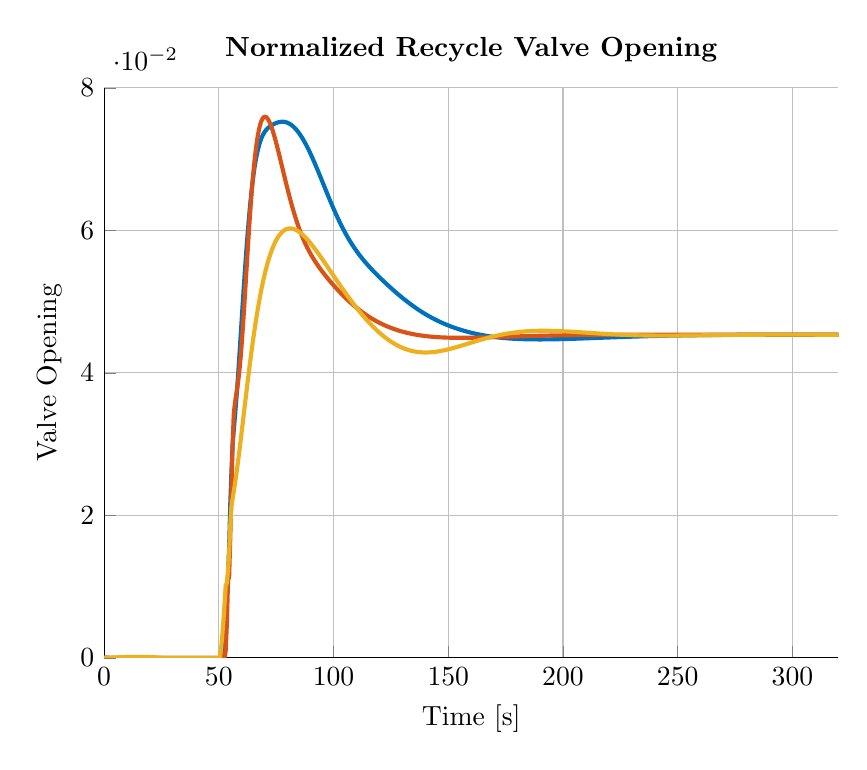
\begin{tikzpicture}

\begin{axis}[%
width=0.769\linewidth,
height=0.597\linewidth,
at={(0\linewidth,0\linewidth)},
scale only axis,
xmin=0,
xmax=320,
xlabel={Time [s]},
xmajorgrids,
ymin=0,
ymax=0.08,
ylabel={Valve Opening},
ymajorgrids,
axis background/.style={fill=white},
title style={font=\bfseries},
title={Normalized Recycle Valve Opening},
axis x line*=bottom,
axis y line*=left
]
\addplot [color=mycolor1,solid,line width=1.5pt,forget plot]
  table[row sep=crcr]{%
0	1.30651e-06\\
0.5	1.05998e-05\\
1	1.46601e-05\\
1.5	1.42539e-05\\
2	9.51022e-06\\
2.5	7.24745e-07\\
3	0\\
3.5	0\\
4	0\\
4.5	0\\
5	0\\
5.5	0\\
6	0\\
6.5	0\\
7	0\\
7.5	0\\
8	0\\
8.5	0\\
9	0\\
9.5	0\\
10	0\\
10.5	0\\
11	0\\
11.5	0\\
12	0\\
12.5	0\\
13	0\\
13.5	0\\
14	0\\
14.5	0\\
15	0\\
15.5	0\\
16	0\\
16.5	0\\
17	0\\
17.5	0\\
18	0\\
18.5	0\\
19	0\\
19.5	0\\
20	0\\
20.5	0\\
21	0\\
21.5	0\\
22	0\\
22.5	0\\
23	0\\
23.5	0\\
24	0\\
24.5	0\\
25	0\\
25.5	0\\
26	0\\
26.5	0\\
27	0\\
27.5	0\\
28	0\\
28.5	0\\
29	0\\
29.5	0\\
30	0\\
30.5	0\\
31	0\\
31.5	0\\
32	0\\
32.5	0\\
33	0\\
33.5	0\\
34	0\\
34.5	0\\
35	0\\
35.5	0\\
36	0\\
36.5	0\\
37	0\\
37.5	0\\
38	0\\
38.5	0\\
39	0\\
39.5	0\\
40	0\\
40.5	0\\
41	0\\
41.5	0\\
42	0\\
42.5	0\\
43	0\\
43.5	0\\
44	0\\
44.5	0\\
45	0\\
45.5	0\\
46	0\\
46.5	0\\
47	0\\
47.5	0\\
48	0\\
48.5	0\\
49	0\\
49.5	0\\
50	0\\
50.5	0\\
51	0.000407362\\
51.5	0\\
52	0.000176293\\
52.5	0.000992407\\
53	0.00554674\\
53.5	0.0100218\\
54	0.0114346\\
54.5	0.0156487\\
55	0.0216522\\
55.5	0.0262732\\
56	0.0298673\\
56.5	0.0319204\\
57	0.0337897\\
57.5	0.0357447\\
58	0.0378773\\
58.5	0.0401793\\
59	0.0426192\\
59.5	0.0451331\\
60	0.0476651\\
60.5	0.0501673\\
61	0.0526033\\
61.5	0.0549464\\
62	0.057178\\
62.5	0.0592848\\
63	0.0612554\\
63.5	0.0630781\\
64	0.0647406\\
64.5	0.0662327\\
65	0.0675499\\
65.5	0.068697\\
66	0.0696861\\
66.5	0.0705345\\
67	0.0712644\\
67.5	0.0718933\\
68	0.0724304\\
68.5	0.0728827\\
69	0.0732594\\
69.5	0.0735716\\
70	0.0738307\\
70.5	0.0740469\\
71	0.0742292\\
71.5	0.0743849\\
72	0.0745198\\
72.5	0.0746385\\
73	0.074744\\
73.5	0.0748385\\
74	0.0749233\\
74.5	0.074999\\
75	0.0750655\\
75.5	0.0751227\\
76	0.0751699\\
76.5	0.0752063\\
77	0.0752311\\
77.5	0.0752436\\
78	0.0752428\\
78.5	0.0752282\\
79	0.0751991\\
79.5	0.0751549\\
80	0.0750954\\
80.5	0.0750201\\
81	0.0749289\\
81.5	0.0748216\\
82	0.0746984\\
82.5	0.074559\\
83	0.0744038\\
83.5	0.0742327\\
84	0.0740461\\
84.5	0.0738442\\
85	0.0736273\\
85.5	0.0733957\\
86	0.0731498\\
86.5	0.07289\\
87	0.0726168\\
87.5	0.0723307\\
88	0.0720322\\
88.5	0.0717219\\
89	0.0714005\\
89.5	0.0710685\\
90	0.0707266\\
90.5	0.0703756\\
91	0.0700163\\
91.5	0.0696494\\
92	0.0692757\\
92.5	0.068896\\
93	0.0685112\\
93.5	0.0681221\\
94	0.0677296\\
94.5	0.0673345\\
95	0.0669377\\
95.5	0.06654\\
96	0.0661422\\
96.5	0.0657452\\
97	0.0653496\\
97.5	0.0649563\\
98	0.064566\\
98.5	0.0641793\\
99	0.0637968\\
99.5	0.0634192\\
100	0.063047\\
100.5	0.0626806\\
101	0.0623205\\
101.5	0.0619671\\
102	0.0616207\\
102.5	0.0612815\\
103	0.0609499\\
103.5	0.0606259\\
104	0.0603097\\
104.5	0.0600014\\
105	0.0597009\\
105.5	0.0594083\\
106	0.0591235\\
106.5	0.0588464\\
107	0.0585769\\
107.5	0.0583148\\
108	0.0580598\\
108.5	0.0578119\\
109	0.0575708\\
109.5	0.0573361\\
110	0.0571077\\
110.5	0.0568852\\
111	0.0566683\\
111.5	0.0564569\\
112	0.0562505\\
112.5	0.0560489\\
113	0.0558518\\
113.5	0.0556589\\
114	0.0554699\\
114.5	0.0552846\\
115	0.0551027\\
115.5	0.054924\\
116	0.0547483\\
116.5	0.0545752\\
117	0.0544047\\
117.5	0.0542365\\
118	0.0540704\\
118.5	0.0539064\\
119	0.0537443\\
119.5	0.0535839\\
120	0.0534252\\
120.5	0.053268\\
121	0.0531123\\
121.5	0.0529579\\
122	0.052805\\
122.5	0.0526533\\
123	0.0525029\\
123.5	0.0523537\\
124	0.0522058\\
124.5	0.0520592\\
125	0.0519137\\
125.5	0.0517696\\
126	0.0516266\\
126.5	0.051485\\
127	0.0513447\\
127.5	0.0512057\\
128	0.0510681\\
128.5	0.0509318\\
129	0.050797\\
129.5	0.0506637\\
130	0.0505318\\
130.5	0.0504015\\
131	0.0502728\\
131.5	0.0501456\\
132	0.0500201\\
132.5	0.0498962\\
133	0.049774\\
133.5	0.0496535\\
134	0.0495348\\
134.5	0.0494178\\
135	0.0493025\\
135.5	0.049189\\
136	0.0490773\\
136.5	0.0489674\\
137	0.0488593\\
137.5	0.048753\\
138	0.0486485\\
138.5	0.0485459\\
139	0.048445\\
139.5	0.0483459\\
140	0.0482486\\
140.5	0.0481531\\
141	0.0480594\\
141.5	0.0479674\\
142	0.0478772\\
142.5	0.0477887\\
143	0.0477019\\
143.5	0.0476168\\
144	0.0475334\\
144.5	0.0474517\\
145	0.0473716\\
145.5	0.0472931\\
146	0.0472162\\
146.5	0.047141\\
147	0.0470672\\
147.5	0.046995\\
148	0.0469244\\
148.5	0.0468552\\
149	0.0467875\\
149.5	0.0467213\\
150	0.0466565\\
150.5	0.0465931\\
151	0.0465312\\
151.5	0.0464706\\
152	0.0464113\\
152.5	0.0463534\\
153	0.0462969\\
153.5	0.0462416\\
154	0.0461876\\
154.5	0.0461349\\
155	0.0460834\\
155.5	0.0460332\\
156	0.0459842\\
156.5	0.0459363\\
157	0.0458897\\
157.5	0.0458442\\
158	0.0457999\\
158.5	0.0457567\\
159	0.0457147\\
159.5	0.0456737\\
160	0.0456338\\
160.5	0.045595\\
161	0.0455573\\
161.5	0.0455206\\
162	0.0454849\\
162.5	0.0454503\\
163	0.0454166\\
163.5	0.0453839\\
164	0.0453522\\
164.5	0.0453215\\
165	0.0452917\\
165.5	0.0452628\\
166	0.0452348\\
166.5	0.0452077\\
167	0.0451815\\
167.5	0.0451562\\
168	0.0451317\\
168.5	0.0451081\\
169	0.0450853\\
169.5	0.0450633\\
170	0.0450421\\
170.5	0.0450216\\
171	0.045002\\
171.5	0.0449831\\
172	0.0449649\\
172.5	0.0449475\\
173	0.0449308\\
173.5	0.0449147\\
174	0.0448994\\
174.5	0.0448847\\
175	0.0448707\\
175.5	0.0448573\\
176	0.0448446\\
176.5	0.0448325\\
177	0.0448209\\
177.5	0.04481\\
178	0.0447996\\
178.5	0.0447898\\
179	0.0447806\\
179.5	0.0447719\\
180	0.0447637\\
180.5	0.044756\\
181	0.0447488\\
181.5	0.0447422\\
182	0.044736\\
182.5	0.0447302\\
183	0.0447249\\
183.5	0.0447201\\
184	0.0447156\\
184.5	0.0447116\\
185	0.044708\\
185.5	0.0447048\\
186	0.044702\\
186.5	0.0446996\\
187	0.0446975\\
187.5	0.0446958\\
188	0.0446944\\
188.5	0.0446934\\
189	0.0446926\\
189.5	0.0446922\\
190	0.0446921\\
190.5	0.0446923\\
191	0.0446928\\
191.5	0.0446935\\
192	0.0446945\\
192.5	0.0446958\\
193	0.0446973\\
193.5	0.0446991\\
194	0.0447011\\
194.5	0.0447033\\
195	0.0447058\\
195.5	0.0447084\\
196	0.0447113\\
196.5	0.0447143\\
197	0.0447176\\
197.5	0.044721\\
198	0.0447246\\
198.5	0.0447283\\
199	0.0447322\\
199.5	0.0447363\\
200	0.0447405\\
200.5	0.0447448\\
201	0.0447493\\
201.5	0.0447539\\
202	0.0447586\\
202.5	0.0447635\\
203	0.0447684\\
203.5	0.0447735\\
204	0.0447786\\
204.5	0.0447838\\
205	0.0447892\\
205.5	0.0447946\\
206	0.0448\\
206.5	0.0448056\\
207	0.0448112\\
207.5	0.0448169\\
208	0.0448226\\
208.5	0.0448284\\
209	0.0448342\\
209.5	0.0448401\\
210	0.044846\\
210.5	0.044852\\
211	0.044858\\
211.5	0.044864\\
212	0.04487\\
212.5	0.0448761\\
213	0.0448821\\
213.5	0.0448882\\
214	0.0448943\\
214.5	0.0449004\\
215	0.0449066\\
215.5	0.0449127\\
216	0.0449188\\
216.5	0.0449249\\
217	0.044931\\
217.5	0.0449371\\
218	0.0449432\\
218.5	0.0449493\\
219	0.0449553\\
219.5	0.0449613\\
220	0.0449674\\
220.5	0.0449733\\
221	0.0449793\\
221.5	0.0449853\\
222	0.0449912\\
222.5	0.044997\\
223	0.0450029\\
223.5	0.0450087\\
224	0.0450145\\
224.5	0.0450202\\
225	0.0450259\\
225.5	0.0450316\\
226	0.0450372\\
226.5	0.0450428\\
227	0.0450483\\
227.5	0.0450538\\
228	0.0450593\\
228.5	0.0450646\\
229	0.04507\\
229.5	0.0450753\\
230	0.0450805\\
230.5	0.0450857\\
231	0.0450909\\
231.5	0.045096\\
232	0.045101\\
232.5	0.045106\\
233	0.045111\\
233.5	0.0451158\\
234	0.0451207\\
234.5	0.0451254\\
235	0.0451302\\
235.5	0.0451348\\
236	0.0451394\\
236.5	0.045144\\
237	0.0451485\\
237.5	0.0451529\\
238	0.0451573\\
238.5	0.0451616\\
239	0.0451658\\
239.5	0.04517\\
240	0.0451742\\
240.5	0.0451783\\
241	0.0451823\\
241.5	0.0451863\\
242	0.0451902\\
242.5	0.045194\\
243	0.0451978\\
243.5	0.0452016\\
244	0.0452053\\
244.5	0.0452089\\
245	0.0452124\\
245.5	0.045216\\
246	0.0452194\\
246.5	0.0452228\\
247	0.0452262\\
247.5	0.0452294\\
248	0.0452327\\
248.5	0.0452358\\
249	0.045239\\
249.5	0.045242\\
250	0.045245\\
250.5	0.045248\\
251	0.0452509\\
251.5	0.0452537\\
252	0.0452565\\
252.5	0.0452593\\
253	0.045262\\
253.5	0.0452646\\
254	0.0452672\\
254.5	0.0452698\\
255	0.0452723\\
255.5	0.0452747\\
256	0.0452771\\
256.5	0.0452794\\
257	0.0452817\\
257.5	0.045284\\
258	0.0452862\\
258.5	0.0452883\\
259	0.0452904\\
259.5	0.0452925\\
260	0.0452945\\
260.5	0.0452965\\
261	0.0452984\\
261.5	0.0453003\\
262	0.0453022\\
262.5	0.045304\\
263	0.0453057\\
263.5	0.0453074\\
264	0.0453091\\
264.5	0.0453108\\
265	0.0453124\\
265.5	0.0453139\\
266	0.0453154\\
266.5	0.0453169\\
267	0.0453184\\
267.5	0.0453198\\
268	0.0453212\\
268.5	0.0453225\\
269	0.0453238\\
269.5	0.0453251\\
270	0.0453263\\
270.5	0.0453275\\
271	0.0453287\\
271.5	0.0453298\\
272	0.0453309\\
272.5	0.045332\\
273	0.045333\\
273.5	0.045334\\
274	0.045335\\
274.5	0.045336\\
275	0.0453369\\
275.5	0.0453378\\
276	0.0453386\\
276.5	0.0453395\\
277	0.0453403\\
277.5	0.0453411\\
278	0.0453418\\
278.5	0.0453426\\
279	0.0453433\\
279.5	0.045344\\
280	0.0453446\\
280.5	0.0453453\\
281	0.0453459\\
281.5	0.0453465\\
282	0.0453471\\
282.5	0.0453476\\
283	0.0453481\\
283.5	0.0453486\\
284	0.0453491\\
284.5	0.0453496\\
285	0.0453501\\
285.5	0.0453505\\
286	0.0453509\\
286.5	0.0453513\\
287	0.0453517\\
287.5	0.045352\\
288	0.0453524\\
288.5	0.0453527\\
289	0.045353\\
289.5	0.0453533\\
290	0.0453536\\
290.5	0.0453538\\
291	0.0453541\\
291.5	0.0453543\\
292	0.0453545\\
292.5	0.0453547\\
293	0.0453549\\
293.5	0.0453551\\
294	0.0453553\\
294.5	0.0453554\\
295	0.0453556\\
295.5	0.0453557\\
296	0.0453558\\
296.5	0.045356\\
297	0.0453561\\
297.5	0.0453561\\
298	0.0453562\\
298.5	0.0453563\\
299	0.0453564\\
299.5	0.0453564\\
300	0.0453565\\
300.5	0.0453565\\
301	0.0453565\\
301.5	0.0453565\\
302	0.0453565\\
302.5	0.0453565\\
303	0.0453565\\
303.5	0.0453565\\
304	0.0453565\\
304.5	0.0453565\\
305	0.0453564\\
305.5	0.0453564\\
306	0.0453564\\
306.5	0.0453563\\
307	0.0453563\\
307.5	0.0453562\\
308	0.0453561\\
308.5	0.0453561\\
309	0.045356\\
309.5	0.0453559\\
310	0.0453558\\
310.5	0.0453557\\
311	0.0453556\\
311.5	0.0453555\\
312	0.0453554\\
312.5	0.0453553\\
313	0.0453552\\
313.5	0.0453551\\
314	0.045355\\
314.5	0.0453549\\
315	0.0453548\\
315.5	0.0453546\\
316	0.0453545\\
316.5	0.0453544\\
317	0.0453543\\
317.5	0.0453541\\
318	0.045354\\
318.5	0.0453539\\
319	0.0453537\\
319.5	0.0453536\\
320	0.0453535\\
320.5	0.0453533\\
321	0.0453532\\
321.5	0.045353\\
322	0.0453529\\
322.5	0.0453527\\
323	0.0453526\\
323.5	0.0453525\\
324	0.0453523\\
324.5	0.0453522\\
325	0.045352\\
325.5	0.0453519\\
326	0.0453517\\
326.5	0.0453516\\
327	0.0453514\\
327.5	0.0453513\\
328	0.0453511\\
328.5	0.045351\\
329	0.0453508\\
329.5	0.0453507\\
330	0.0453505\\
330.5	0.0453504\\
331	0.0453502\\
331.5	0.0453501\\
332	0.0453499\\
332.5	0.0453498\\
333	0.0453496\\
333.5	0.0453495\\
334	0.0453494\\
334.5	0.0453492\\
335	0.0453491\\
335.5	0.0453489\\
336	0.0453488\\
336.5	0.0453486\\
337	0.0453485\\
337.5	0.0453484\\
338	0.0453482\\
338.5	0.0453481\\
339	0.045348\\
339.5	0.0453478\\
340	0.0453477\\
340.5	0.0453476\\
341	0.0453474\\
341.5	0.0453473\\
342	0.0453472\\
342.5	0.045347\\
343	0.0453469\\
343.5	0.0453468\\
344	0.0453467\\
344.5	0.0453466\\
345	0.0453464\\
345.5	0.0453463\\
346	0.0453462\\
346.5	0.0453461\\
347	0.045346\\
347.5	0.0453459\\
348	0.0453457\\
348.5	0.0453456\\
349	0.0453455\\
349.5	0.0453454\\
350	0.0453453\\
350.5	0.0453452\\
351	0.0453451\\
351.5	0.045345\\
352	0.0453449\\
352.5	0.0453448\\
353	0.0453447\\
353.5	0.0453446\\
354	0.0453445\\
354.5	0.0453444\\
355	0.0453443\\
355.5	0.0453442\\
356	0.0453441\\
356.5	0.045344\\
357	0.045344\\
357.5	0.0453439\\
358	0.0453438\\
358.5	0.0453437\\
359	0.0453436\\
359.5	0.0453435\\
360	0.0453435\\
360.5	0.0453434\\
361	0.0453433\\
361.5	0.0453432\\
362	0.0453432\\
362.5	0.0453431\\
363	0.045343\\
363.5	0.0453429\\
364	0.0453429\\
364.5	0.0453428\\
365	0.0453427\\
365.5	0.0453427\\
366	0.0453426\\
366.5	0.0453425\\
367	0.0453425\\
367.5	0.0453424\\
368	0.0453424\\
368.5	0.0453423\\
369	0.0453423\\
369.5	0.0453422\\
370	0.0453421\\
370.5	0.0453421\\
371	0.045342\\
371.5	0.045342\\
372	0.0453419\\
372.5	0.0453419\\
373	0.0453418\\
373.5	0.0453418\\
374	0.0453417\\
374.5	0.0453417\\
375	0.0453417\\
375.5	0.0453416\\
376	0.0453416\\
376.5	0.0453415\\
377	0.0453415\\
377.5	0.0453415\\
378	0.0453414\\
378.5	0.0453414\\
379	0.0453413\\
379.5	0.0453413\\
380	0.0453413\\
380.5	0.0453412\\
381	0.0453412\\
381.5	0.0453412\\
382	0.0453412\\
382.5	0.0453411\\
383	0.0453411\\
383.5	0.0453411\\
384	0.045341\\
384.5	0.045341\\
385	0.045341\\
385.5	0.045341\\
386	0.0453409\\
386.5	0.0453409\\
387	0.0453409\\
387.5	0.0453409\\
388	0.0453408\\
388.5	0.0453408\\
389	0.0453408\\
389.5	0.0453408\\
390	0.0453408\\
390.5	0.0453408\\
391	0.0453407\\
391.5	0.0453407\\
392	0.0453407\\
392.5	0.0453407\\
393	0.0453407\\
393.5	0.0453407\\
394	0.0453406\\
394.5	0.0453406\\
395	0.0453406\\
395.5	0.0453406\\
396	0.0453406\\
396.5	0.0453406\\
397	0.0453406\\
397.5	0.0453406\\
398	0.0453405\\
398.5	0.0453405\\
399	0.0453405\\
399.5	0.0453405\\
400	0.0453405\\
400.5	0.0453405\\
401	0.0453405\\
401.5	0.0453405\\
402	0.0453405\\
402.5	0.0453405\\
403	0.0453405\\
403.5	0.0453405\\
404	0.0453405\\
404.5	0.0453404\\
405	0.0453404\\
405.5	0.0453404\\
406	0.0453404\\
406.5	0.0453404\\
407	0.0453404\\
407.5	0.0453404\\
408	0.0453404\\
408.5	0.0453404\\
409	0.0453404\\
409.5	0.0453404\\
410	0.0453404\\
410.5	0.0453404\\
411	0.0453404\\
411.5	0.0453404\\
412	0.0453404\\
412.5	0.0453404\\
413	0.0453404\\
413.5	0.0453404\\
414	0.0453404\\
414.5	0.0453404\\
415	0.0453404\\
415.5	0.0453404\\
416	0.0453404\\
416.5	0.0453404\\
417	0.0453404\\
417.5	0.0453404\\
418	0.0453404\\
418.5	0.0453404\\
419	0.0453404\\
419.5	0.0453404\\
420	0.0453404\\
420.5	0.0453404\\
421	0.0453404\\
421.5	0.0453404\\
422	0.0453404\\
422.5	0.0453404\\
423	0.0453404\\
423.5	0.0453404\\
424	0.0453404\\
424.5	0.0453404\\
425	0.0453404\\
425.5	0.0453404\\
426	0.0453404\\
426.5	0.0453404\\
427	0.0453404\\
427.5	0.0453404\\
428	0.0453405\\
428.5	0.0453405\\
429	0.0453405\\
429.5	0.0453405\\
430	0.0453405\\
430.5	0.0453405\\
431	0.0453405\\
431.5	0.0453405\\
432	0.0453405\\
432.5	0.0453405\\
433	0.0453405\\
433.5	0.0453405\\
434	0.0453405\\
434.5	0.0453405\\
435	0.0453405\\
435.5	0.0453405\\
436	0.0453405\\
436.5	0.0453405\\
437	0.0453405\\
437.5	0.0453405\\
438	0.0453405\\
438.5	0.0453405\\
439	0.0453405\\
439.5	0.0453405\\
440	0.0453405\\
440.5	0.0453405\\
441	0.0453405\\
441.5	0.0453405\\
442	0.0453405\\
442.5	0.0453406\\
443	0.0453406\\
443.5	0.0453406\\
444	0.0453406\\
444.5	0.0453406\\
445	0.0453406\\
445.5	0.0453406\\
446	0.0453406\\
446.5	0.0453406\\
447	0.0453406\\
447.5	0.0453406\\
448	0.0453406\\
448.5	0.0453406\\
449	0.0453406\\
449.5	0.0453406\\
450	0.0453406\\
450.5	0.0453406\\
451	0.0453406\\
451.5	0.0453406\\
452	0.0453406\\
452.5	0.0453406\\
453	0.0453406\\
453.5	0.0453406\\
454	0.0453406\\
454.5	0.0453406\\
455	0.0453406\\
455.5	0.0453406\\
456	0.0453406\\
456.5	0.0453406\\
457	0.0453406\\
457.5	0.0453407\\
458	0.0453407\\
458.5	0.0453407\\
459	0.0453407\\
459.5	0.0453407\\
460	0.0453407\\
460.5	0.0453407\\
461	0.0453407\\
461.5	0.0453407\\
462	0.0453407\\
462.5	0.0453407\\
463	0.0453407\\
463.5	0.0453407\\
464	0.0453407\\
464.5	0.0453407\\
465	0.0453407\\
465.5	0.0453407\\
466	0.0453407\\
466.5	0.0453407\\
467	0.0453407\\
467.5	0.0453407\\
468	0.0453407\\
468.5	0.0453407\\
469	0.0453407\\
469.5	0.0453407\\
470	0.0453407\\
470.5	0.0453407\\
471	0.0453407\\
471.5	0.0453407\\
472	0.0453407\\
472.5	0.0453407\\
473	0.0453407\\
473.5	0.0453407\\
474	0.0453407\\
474.5	0.0453407\\
475	0.0453407\\
475.5	0.0453407\\
476	0.0453407\\
476.5	0.0453407\\
477	0.0453407\\
477.5	0.0453407\\
478	0.0453407\\
478.5	0.0453407\\
479	0.0453407\\
479.5	0.0453407\\
480	0.0453407\\
480.5	0.0453407\\
481	0.0453408\\
481.5	0.0453408\\
482	0.0453408\\
482.5	0.0453408\\
483	0.0453408\\
483.5	0.0453408\\
484	0.0453408\\
484.5	0.0453408\\
485	0.0453408\\
485.5	0.0453408\\
486	0.0453408\\
486.5	0.0453408\\
487	0.0453408\\
487.5	0.0453408\\
488	0.0453408\\
488.5	0.0453408\\
489	0.0453408\\
489.5	0.0453408\\
490	0.0453408\\
490.5	0.0453408\\
491	0.0453408\\
491.5	0.0453408\\
492	0.0453408\\
492.5	0.0453408\\
493	0.0453408\\
493.5	0.0453408\\
494	0.0453408\\
494.5	0.0453408\\
495	0.0453408\\
495.5	0.0453408\\
496	0.0453408\\
496.5	0.0453408\\
497	0.0453408\\
497.5	0.0453408\\
498	0.0453408\\
498.5	0.0453408\\
499	0.0453408\\
499.5	0.0453408\\
};
\addplot [color=mycolor2,solid,line width=1.5pt,forget plot]
  table[row sep=crcr]{%
0	1.15805e-06\\
0.5	8.79271e-06\\
1	4.91879e-06\\
1.5	0\\
2	0\\
2.5	0\\
3	0\\
3.5	0\\
4	0\\
4.5	0\\
5	0\\
5.5	0\\
6	0\\
6.5	0\\
7	0\\
7.5	0\\
8	0\\
8.5	0\\
9	0\\
9.5	0\\
10	0\\
10.5	0\\
11	0\\
11.5	0\\
12	0\\
12.5	0\\
13	0\\
13.5	0\\
14	0\\
14.5	0\\
15	0\\
15.5	0\\
16	0\\
16.5	0\\
17	0\\
17.5	0\\
18	0\\
18.5	0\\
19	0\\
19.5	0\\
20	0\\
20.5	0\\
21	0\\
21.5	0\\
22	0\\
22.5	0\\
23	0\\
23.5	0\\
24	0\\
24.5	0\\
25	0\\
25.5	0\\
26	0\\
26.5	0\\
27	0\\
27.5	0\\
28	0\\
28.5	0\\
29	0\\
29.5	0\\
30	0\\
30.5	0\\
31	0\\
31.5	0\\
32	0\\
32.5	0\\
33	0\\
33.5	0\\
34	0\\
34.5	0\\
35	0\\
35.5	0\\
36	0\\
36.5	0\\
37	0\\
37.5	0\\
38	0\\
38.5	0\\
39	0\\
39.5	0\\
40	0\\
40.5	0\\
41	0\\
41.5	0\\
42	0\\
42.5	0\\
43	0\\
43.5	0\\
44	0\\
44.5	0\\
45	0\\
45.5	0\\
46	0\\
46.5	0\\
47	0\\
47.5	0\\
48	0\\
48.5	0\\
49	0\\
49.5	0\\
50	0\\
50.5	0\\
51	0.000716488\\
51.5	0\\
52	0\\
52.5	0\\
53	0.00103895\\
53.5	0.00470309\\
54	0.0107935\\
54.5	0.0114171\\
55	0.017038\\
55.5	0.0235933\\
56	0.0298378\\
56.5	0.0341844\\
57	0.0357491\\
57.5	0.036757\\
58	0.0377925\\
58.5	0.0389789\\
59	0.0404036\\
59.5	0.0421501\\
60	0.0441855\\
60.5	0.0464636\\
61	0.048928\\
61.5	0.0515184\\
62	0.0541633\\
62.5	0.0567917\\
63	0.0593413\\
63.5	0.0617627\\
64	0.0640195\\
64.5	0.0660866\\
65	0.0679495\\
65.5	0.0696011\\
66	0.0710408\\
66.5	0.0722728\\
67	0.0733047\\
67.5	0.0741466\\
68	0.0748103\\
68.5	0.0753087\\
69	0.075655\\
69.5	0.0758625\\
70	0.0759442\\
70.5	0.0759128\\
71	0.0757802\\
71.5	0.0755577\\
72	0.0752559\\
72.5	0.0748844\\
73	0.0744525\\
73.5	0.0739683\\
74	0.0734397\\
74.5	0.0728738\\
75	0.072277\\
75.5	0.0716555\\
76	0.0710149\\
76.5	0.0703602\\
77	0.0696962\\
77.5	0.0690272\\
78	0.0683572\\
78.5	0.0676898\\
79	0.0670283\\
79.5	0.0663754\\
80	0.0657338\\
80.5	0.0651056\\
81	0.0644929\\
81.5	0.0638971\\
82	0.0633195\\
82.5	0.0627612\\
83	0.0622228\\
83.5	0.0617048\\
84	0.0612074\\
84.5	0.0607305\\
85	0.0602741\\
85.5	0.0598376\\
86	0.0594206\\
86.5	0.0590224\\
87	0.0586423\\
87.5	0.0582793\\
88	0.0579325\\
88.5	0.0576011\\
89	0.057284\\
89.5	0.0569802\\
90	0.0566887\\
90.5	0.0564085\\
91	0.0561387\\
91.5	0.0558784\\
92	0.0556268\\
92.5	0.055383\\
93	0.0551462\\
93.5	0.0549159\\
94	0.0546913\\
94.5	0.0544719\\
95	0.0542572\\
95.5	0.0540467\\
96	0.0538402\\
96.5	0.0536371\\
97	0.0534373\\
97.5	0.0532406\\
98	0.0530467\\
98.5	0.0528554\\
99	0.0526668\\
99.5	0.0524806\\
100	0.0522968\\
100.5	0.0521154\\
101	0.0519364\\
101.5	0.0517598\\
102	0.0515855\\
102.5	0.0514136\\
103	0.0512441\\
103.5	0.0510771\\
104	0.0509125\\
104.5	0.0507505\\
105	0.050591\\
105.5	0.0504341\\
106	0.0502798\\
106.5	0.0501281\\
107	0.0499791\\
107.5	0.0498328\\
108	0.0496891\\
108.5	0.0495482\\
109	0.04941\\
109.5	0.0492745\\
110	0.0491418\\
110.5	0.0490117\\
111	0.0488843\\
111.5	0.0487597\\
112	0.0486377\\
112.5	0.0485183\\
113	0.0484016\\
113.5	0.0482875\\
114	0.048176\\
114.5	0.048067\\
115	0.0479606\\
115.5	0.0478566\\
116	0.0477552\\
116.5	0.0476561\\
117	0.0475595\\
117.5	0.0474653\\
118	0.0473734\\
118.5	0.0472838\\
119	0.0471965\\
119.5	0.0471114\\
120	0.0470286\\
120.5	0.0469479\\
121	0.0468694\\
121.5	0.046793\\
122	0.0467186\\
122.5	0.0466464\\
123	0.0465761\\
123.5	0.0465079\\
124	0.0464416\\
124.5	0.0463772\\
125	0.0463147\\
125.5	0.046254\\
126	0.0461952\\
126.5	0.0461382\\
127	0.046083\\
127.5	0.0460295\\
128	0.0459777\\
128.5	0.0459276\\
129	0.0458791\\
129.5	0.0458322\\
130	0.0457869\\
130.5	0.0457432\\
131	0.0457009\\
131.5	0.0456602\\
132	0.0456209\\
132.5	0.0455831\\
133	0.0455466\\
133.5	0.0455116\\
134	0.0454778\\
134.5	0.0454454\\
135	0.0454143\\
135.5	0.0453844\\
136	0.0453557\\
136.5	0.0453283\\
137	0.045302\\
137.5	0.0452768\\
138	0.0452528\\
138.5	0.0452298\\
139	0.0452079\\
139.5	0.045187\\
140	0.0451671\\
140.5	0.0451483\\
141	0.0451303\\
141.5	0.0451133\\
142	0.0450972\\
142.5	0.045082\\
143	0.0450676\\
143.5	0.045054\\
144	0.0450413\\
144.5	0.0450293\\
145	0.0450181\\
145.5	0.0450076\\
146	0.0449978\\
146.5	0.0449887\\
147	0.0449803\\
147.5	0.0449725\\
148	0.0449654\\
148.5	0.0449588\\
149	0.0449528\\
149.5	0.0449474\\
150	0.0449426\\
150.5	0.0449382\\
151	0.0449344\\
151.5	0.0449311\\
152	0.0449282\\
152.5	0.0449258\\
153	0.0449238\\
153.5	0.0449222\\
154	0.044921\\
154.5	0.0449202\\
155	0.0449198\\
155.5	0.0449198\\
156	0.04492\\
156.5	0.0449206\\
157	0.0449215\\
157.5	0.0449227\\
158	0.0449242\\
158.5	0.0449259\\
159	0.0449279\\
159.5	0.0449302\\
160	0.0449326\\
160.5	0.0449353\\
161	0.0449382\\
161.5	0.0449413\\
162	0.0449446\\
162.5	0.0449481\\
163	0.0449517\\
163.5	0.0449554\\
164	0.0449593\\
164.5	0.0449634\\
165	0.0449675\\
165.5	0.0449718\\
166	0.0449762\\
166.5	0.0449807\\
167	0.0449853\\
167.5	0.04499\\
168	0.0449947\\
168.5	0.0449995\\
169	0.0450044\\
169.5	0.0450093\\
170	0.0450143\\
170.5	0.0450193\\
171	0.0450244\\
171.5	0.0450294\\
172	0.0450345\\
172.5	0.0450397\\
173	0.0450448\\
173.5	0.04505\\
174	0.0450552\\
174.5	0.0450603\\
175	0.0450655\\
175.5	0.0450706\\
176	0.0450758\\
176.5	0.0450809\\
177	0.045086\\
177.5	0.0450911\\
178	0.0450962\\
178.5	0.0451012\\
179	0.0451062\\
179.5	0.0451112\\
180	0.0451161\\
180.5	0.045121\\
181	0.0451259\\
181.5	0.0451307\\
182	0.0451355\\
182.5	0.0451402\\
183	0.0451449\\
183.5	0.0451495\\
184	0.0451541\\
184.5	0.0451586\\
185	0.0451631\\
185.5	0.0451675\\
186	0.0451718\\
186.5	0.0451761\\
187	0.0451804\\
187.5	0.0451846\\
188	0.0451887\\
188.5	0.0451927\\
189	0.0451967\\
189.5	0.0452007\\
190	0.0452045\\
190.5	0.0452084\\
191	0.0452121\\
191.5	0.0452158\\
192	0.0452194\\
192.5	0.045223\\
193	0.0452265\\
193.5	0.0452299\\
194	0.0452333\\
194.5	0.0452366\\
195	0.0452398\\
195.5	0.045243\\
196	0.0452461\\
196.5	0.0452491\\
197	0.0452521\\
197.5	0.0452551\\
198	0.0452579\\
198.5	0.0452607\\
199	0.0452635\\
199.5	0.0452661\\
200	0.0452688\\
200.5	0.0452713\\
201	0.0452738\\
201.5	0.0452763\\
202	0.0452787\\
202.5	0.045281\\
203	0.0452833\\
203.5	0.0452855\\
204	0.0452877\\
204.5	0.0452898\\
205	0.0452919\\
205.5	0.0452939\\
206	0.0452958\\
206.5	0.0452977\\
207	0.0452996\\
207.5	0.0453014\\
208	0.0453031\\
208.5	0.0453048\\
209	0.0453065\\
209.5	0.0453081\\
210	0.0453097\\
210.5	0.0453112\\
211	0.0453127\\
211.5	0.0453141\\
212	0.0453155\\
212.5	0.0453168\\
213	0.0453182\\
213.5	0.0453194\\
214	0.0453207\\
214.5	0.0453218\\
215	0.045323\\
215.5	0.0453241\\
216	0.0453252\\
216.5	0.0453262\\
217	0.0453272\\
217.5	0.0453282\\
218	0.0453291\\
218.5	0.0453301\\
219	0.0453309\\
219.5	0.0453318\\
220	0.0453326\\
220.5	0.0453334\\
221	0.0453341\\
221.5	0.0453348\\
222	0.0453355\\
222.5	0.0453362\\
223	0.0453369\\
223.5	0.0453375\\
224	0.0453381\\
224.5	0.0453386\\
225	0.0453392\\
225.5	0.0453397\\
226	0.0453402\\
226.5	0.0453407\\
227	0.0453411\\
227.5	0.0453416\\
228	0.045342\\
228.5	0.0453424\\
229	0.0453428\\
229.5	0.0453431\\
230	0.0453435\\
230.5	0.0453438\\
231	0.0453441\\
231.5	0.0453444\\
232	0.0453446\\
232.5	0.0453449\\
233	0.0453451\\
233.5	0.0453454\\
234	0.0453456\\
234.5	0.0453458\\
235	0.045346\\
235.5	0.0453462\\
236	0.0453463\\
236.5	0.0453465\\
237	0.0453466\\
237.5	0.0453467\\
238	0.0453469\\
238.5	0.045347\\
239	0.0453471\\
239.5	0.0453471\\
240	0.0453472\\
240.5	0.0453473\\
241	0.0453474\\
241.5	0.0453474\\
242	0.0453475\\
242.5	0.0453475\\
243	0.0453475\\
243.5	0.0453476\\
244	0.0453476\\
244.5	0.0453476\\
245	0.0453476\\
245.5	0.0453476\\
246	0.0453476\\
246.5	0.0453476\\
247	0.0453476\\
247.5	0.0453475\\
248	0.0453475\\
248.5	0.0453475\\
249	0.0453474\\
249.5	0.0453474\\
250	0.0453474\\
250.5	0.0453473\\
251	0.0453473\\
251.5	0.0453472\\
252	0.0453472\\
252.5	0.0453471\\
253	0.045347\\
253.5	0.045347\\
254	0.0453469\\
254.5	0.0453469\\
255	0.0453468\\
255.5	0.0453467\\
256	0.0453466\\
256.5	0.0453466\\
257	0.0453465\\
257.5	0.0453464\\
258	0.0453463\\
258.5	0.0453463\\
259	0.0453462\\
259.5	0.0453461\\
260	0.045346\\
260.5	0.0453459\\
261	0.0453459\\
261.5	0.0453458\\
262	0.0453457\\
262.5	0.0453456\\
263	0.0453455\\
263.5	0.0453454\\
264	0.0453454\\
264.5	0.0453453\\
265	0.0453452\\
265.5	0.0453451\\
266	0.045345\\
266.5	0.0453449\\
267	0.0453449\\
267.5	0.0453448\\
268	0.0453447\\
268.5	0.0453446\\
269	0.0453445\\
269.5	0.0453445\\
270	0.0453444\\
270.5	0.0453443\\
271	0.0453442\\
271.5	0.0453441\\
272	0.0453441\\
272.5	0.045344\\
273	0.0453439\\
273.5	0.0453438\\
274	0.0453438\\
274.5	0.0453437\\
275	0.0453436\\
275.5	0.0453435\\
276	0.0453435\\
276.5	0.0453434\\
277	0.0453433\\
277.5	0.0453433\\
278	0.0453432\\
278.5	0.0453431\\
279	0.0453431\\
279.5	0.045343\\
280	0.045343\\
280.5	0.0453429\\
281	0.0453428\\
281.5	0.0453428\\
282	0.0453427\\
282.5	0.0453427\\
283	0.0453426\\
283.5	0.0453425\\
284	0.0453425\\
284.5	0.0453424\\
285	0.0453424\\
285.5	0.0453423\\
286	0.0453423\\
286.5	0.0453422\\
287	0.0453422\\
287.5	0.0453421\\
288	0.0453421\\
288.5	0.0453421\\
289	0.045342\\
289.5	0.045342\\
290	0.0453419\\
290.5	0.0453419\\
291	0.0453418\\
291.5	0.0453418\\
292	0.0453418\\
292.5	0.0453417\\
293	0.0453417\\
293.5	0.0453417\\
294	0.0453416\\
294.5	0.0453416\\
295	0.0453416\\
295.5	0.0453415\\
296	0.0453415\\
296.5	0.0453415\\
297	0.0453414\\
297.5	0.0453414\\
298	0.0453414\\
298.5	0.0453414\\
299	0.0453413\\
299.5	0.0453413\\
300	0.0453413\\
300.5	0.0453413\\
301	0.0453412\\
301.5	0.0453412\\
302	0.0453412\\
302.5	0.0453412\\
303	0.0453411\\
303.5	0.0453411\\
304	0.0453411\\
304.5	0.0453411\\
305	0.0453411\\
305.5	0.045341\\
306	0.045341\\
306.5	0.045341\\
307	0.045341\\
307.5	0.045341\\
308	0.045341\\
308.5	0.045341\\
309	0.0453409\\
309.5	0.0453409\\
310	0.0453409\\
310.5	0.0453409\\
311	0.0453409\\
311.5	0.0453409\\
312	0.0453409\\
312.5	0.0453409\\
313	0.0453408\\
313.5	0.0453408\\
314	0.0453408\\
314.5	0.0453408\\
315	0.0453408\\
315.5	0.0453408\\
316	0.0453408\\
316.5	0.0453408\\
317	0.0453408\\
317.5	0.0453408\\
318	0.0453408\\
318.5	0.0453408\\
319	0.0453408\\
319.5	0.0453407\\
320	0.0453407\\
320.5	0.0453407\\
321	0.0453407\\
321.5	0.0453407\\
322	0.0453407\\
322.5	0.0453407\\
323	0.0453407\\
323.5	0.0453407\\
324	0.0453407\\
324.5	0.0453407\\
325	0.0453407\\
325.5	0.0453407\\
326	0.0453407\\
326.5	0.0453407\\
327	0.0453407\\
327.5	0.0453407\\
328	0.0453407\\
328.5	0.0453407\\
329	0.0453407\\
329.5	0.0453407\\
330	0.0453407\\
330.5	0.0453407\\
331	0.0453407\\
331.5	0.0453407\\
332	0.0453407\\
332.5	0.0453407\\
333	0.0453407\\
333.5	0.0453407\\
334	0.0453407\\
334.5	0.0453407\\
335	0.0453407\\
335.5	0.0453407\\
336	0.0453407\\
336.5	0.0453407\\
337	0.0453407\\
337.5	0.0453407\\
338	0.0453407\\
338.5	0.0453407\\
339	0.0453407\\
339.5	0.0453407\\
340	0.0453407\\
340.5	0.0453407\\
341	0.0453407\\
341.5	0.0453407\\
342	0.0453407\\
342.5	0.0453407\\
343	0.0453407\\
343.5	0.0453407\\
344	0.0453407\\
344.5	0.0453407\\
345	0.0453407\\
345.5	0.0453407\\
346	0.0453407\\
346.5	0.0453407\\
347	0.0453407\\
347.5	0.0453407\\
348	0.0453407\\
348.5	0.0453407\\
349	0.0453407\\
349.5	0.0453407\\
350	0.0453407\\
350.5	0.0453407\\
351	0.0453407\\
351.5	0.0453407\\
352	0.0453407\\
352.5	0.0453407\\
353	0.0453407\\
353.5	0.0453407\\
354	0.0453407\\
354.5	0.0453407\\
355	0.0453407\\
355.5	0.0453407\\
356	0.0453407\\
356.5	0.0453407\\
357	0.0453407\\
357.5	0.0453407\\
358	0.0453407\\
358.5	0.0453407\\
359	0.0453407\\
359.5	0.0453407\\
360	0.0453407\\
360.5	0.0453407\\
361	0.0453407\\
361.5	0.0453407\\
362	0.0453407\\
362.5	0.0453407\\
363	0.0453407\\
363.5	0.0453407\\
364	0.0453407\\
364.5	0.0453407\\
365	0.0453407\\
365.5	0.0453407\\
366	0.0453407\\
366.5	0.0453407\\
367	0.0453407\\
367.5	0.0453407\\
368	0.0453407\\
368.5	0.0453407\\
369	0.0453408\\
369.5	0.0453408\\
370	0.0453408\\
370.5	0.0453408\\
371	0.0453408\\
371.5	0.0453408\\
372	0.0453408\\
372.5	0.0453408\\
373	0.0453408\\
373.5	0.0453408\\
374	0.0453408\\
374.5	0.0453408\\
375	0.0453408\\
375.5	0.0453408\\
376	0.0453408\\
376.5	0.0453408\\
377	0.0453408\\
377.5	0.0453408\\
378	0.0453408\\
378.5	0.0453408\\
379	0.0453408\\
379.5	0.0453408\\
380	0.0453408\\
380.5	0.0453408\\
381	0.0453408\\
381.5	0.0453408\\
382	0.0453408\\
382.5	0.0453408\\
383	0.0453408\\
383.5	0.0453408\\
384	0.0453408\\
384.5	0.0453408\\
385	0.0453408\\
385.5	0.0453408\\
386	0.0453408\\
386.5	0.0453408\\
387	0.0453408\\
387.5	0.0453408\\
388	0.0453408\\
388.5	0.0453408\\
389	0.0453408\\
389.5	0.0453408\\
390	0.0453408\\
390.5	0.0453408\\
391	0.0453408\\
391.5	0.0453408\\
392	0.0453408\\
392.5	0.0453408\\
393	0.0453408\\
393.5	0.0453408\\
394	0.0453408\\
394.5	0.0453408\\
395	0.0453408\\
395.5	0.0453408\\
396	0.0453408\\
396.5	0.0453408\\
397	0.0453408\\
397.5	0.0453408\\
398	0.0453408\\
398.5	0.0453408\\
399	0.0453408\\
399.5	0.0453408\\
400	0.0453408\\
400.5	0.0453408\\
401	0.0453408\\
401.5	0.0453408\\
402	0.0453408\\
402.5	0.0453408\\
403	0.0453408\\
403.5	0.0453408\\
404	0.0453408\\
404.5	0.0453408\\
405	0.0453408\\
405.5	0.0453408\\
406	0.0453408\\
406.5	0.0453408\\
407	0.0453408\\
407.5	0.0453408\\
408	0.0453408\\
408.5	0.0453408\\
409	0.0453408\\
409.5	0.0453408\\
410	0.0453408\\
410.5	0.0453408\\
411	0.0453408\\
411.5	0.0453408\\
412	0.0453408\\
412.5	0.0453408\\
413	0.0453408\\
413.5	0.0453408\\
414	0.0453408\\
414.5	0.0453408\\
415	0.0453408\\
415.5	0.0453408\\
416	0.0453408\\
416.5	0.0453408\\
417	0.0453408\\
417.5	0.0453408\\
418	0.0453408\\
418.5	0.0453408\\
419	0.0453408\\
419.5	0.0453408\\
420	0.0453408\\
420.5	0.0453408\\
421	0.0453408\\
421.5	0.0453408\\
422	0.0453408\\
422.5	0.0453408\\
423	0.0453408\\
423.5	0.0453408\\
424	0.0453408\\
424.5	0.0453408\\
425	0.0453408\\
425.5	0.0453408\\
426	0.0453408\\
426.5	0.0453408\\
427	0.0453408\\
427.5	0.0453408\\
428	0.0453408\\
428.5	0.0453408\\
429	0.0453408\\
429.5	0.0453408\\
430	0.0453408\\
430.5	0.0453408\\
431	0.0453408\\
431.5	0.0453408\\
432	0.0453408\\
432.5	0.0453408\\
433	0.0453408\\
433.5	0.0453408\\
434	0.0453408\\
434.5	0.0453408\\
435	0.0453408\\
435.5	0.0453408\\
436	0.0453408\\
436.5	0.0453408\\
437	0.0453408\\
437.5	0.0453408\\
438	0.0453408\\
438.5	0.0453408\\
439	0.0453408\\
439.5	0.0453408\\
440	0.0453408\\
440.5	0.0453408\\
441	0.0453408\\
441.5	0.0453408\\
442	0.0453408\\
442.5	0.0453408\\
443	0.0453408\\
443.5	0.0453408\\
444	0.0453408\\
444.5	0.0453408\\
445	0.0453408\\
445.5	0.0453408\\
446	0.0453408\\
446.5	0.0453408\\
447	0.0453408\\
447.5	0.0453408\\
448	0.0453408\\
448.5	0.0453408\\
449	0.0453408\\
449.5	0.0453408\\
450	0.0453408\\
450.5	0.0453408\\
451	0.0453408\\
451.5	0.0453408\\
452	0.0453408\\
452.5	0.0453408\\
453	0.0453408\\
453.5	0.0453408\\
454	0.0453408\\
454.5	0.0453408\\
455	0.0453408\\
455.5	0.0453408\\
456	0.0453408\\
456.5	0.0453408\\
457	0.0453408\\
457.5	0.0453408\\
458	0.0453408\\
458.5	0.0453408\\
459	0.0453408\\
459.5	0.0453408\\
460	0.0453408\\
460.5	0.0453408\\
461	0.0453408\\
461.5	0.0453408\\
462	0.0453408\\
462.5	0.0453408\\
463	0.0453408\\
463.5	0.0453408\\
464	0.0453408\\
464.5	0.0453408\\
465	0.0453408\\
465.5	0.0453408\\
466	0.0453408\\
466.5	0.0453408\\
467	0.0453408\\
467.5	0.0453408\\
468	0.0453408\\
468.5	0.0453408\\
469	0.0453408\\
469.5	0.0453408\\
470	0.0453408\\
470.5	0.0453408\\
471	0.0453408\\
471.5	0.0453408\\
472	0.0453408\\
472.5	0.0453408\\
473	0.0453408\\
473.5	0.0453408\\
474	0.0453408\\
474.5	0.0453408\\
475	0.0453408\\
475.5	0.0453408\\
476	0.0453408\\
476.5	0.0453408\\
477	0.0453408\\
477.5	0.0453408\\
478	0.0453408\\
478.5	0.0453408\\
479	0.0453408\\
479.5	0.0453408\\
480	0.0453408\\
480.5	0.0453408\\
481	0.0453408\\
481.5	0.0453408\\
482	0.0453408\\
482.5	0.0453408\\
483	0.0453408\\
483.5	0.0453408\\
484	0.0453408\\
484.5	0.0453408\\
485	0.0453408\\
485.5	0.0453408\\
486	0.0453408\\
486.5	0.0453408\\
487	0.0453408\\
487.5	0.0453408\\
488	0.0453408\\
488.5	0.0453408\\
489	0.0453408\\
489.5	0.0453408\\
490	0.0453408\\
490.5	0.0453408\\
491	0.0453408\\
491.5	0.0453408\\
492	0.0453408\\
492.5	0.0453408\\
493	0.0453408\\
493.5	0.0453408\\
494	0.0453408\\
494.5	0.0453408\\
495	0.0453408\\
495.5	0.0453408\\
496	0.0453408\\
496.5	0.0453408\\
497	0.0453408\\
497.5	0.0453408\\
498	0.0453408\\
498.5	0.0453408\\
499	0.0453408\\
499.5	0.0453408\\
};
\addplot [color=mycolor3,solid,line width=1.5pt,forget plot]
  table[row sep=crcr]{%
0	5.08729e-07\\
0.5	5.82153e-06\\
1	1.13938e-05\\
1.5	1.70923e-05\\
2	2.28445e-05\\
2.5	2.86191e-05\\
3	3.44833e-05\\
3.5	4.04622e-05\\
4	4.65382e-05\\
4.5	5.26769e-05\\
5	5.88381e-05\\
5.5	6.49816e-05\\
6	7.10695e-05\\
6.5	7.70658e-05\\
7	8.29354e-05\\
7.5	8.86442e-05\\
8	9.4159e-05\\
8.5	9.94471e-05\\
9	0.000104477\\
9.5	0.000109219\\
10	0.000113642\\
10.5	0.00011772\\
11	0.000121426\\
11.5	0.000124735\\
12	0.000127622\\
12.5	0.000130066\\
13	0.000132047\\
13.5	0.000133545\\
14	0.000134542\\
14.5	0.000135022\\
15	0.000134972\\
15.5	0.000134377\\
16	0.000133228\\
16.5	0.000131513\\
17	0.000129226\\
17.5	0.000126357\\
18	0.000122904\\
18.5	0.00011886\\
19	0.000114225\\
19.5	0.000108995\\
20	0.000103172\\
20.5	9.67559e-05\\
21	8.97496e-05\\
21.5	8.21563e-05\\
22	7.39804e-05\\
22.5	6.52275e-05\\
23	5.5904e-05\\
23.5	4.60164e-05\\
24	3.54006e-05\\
24.5	2.39204e-05\\
25	1.15746e-05\\
25.5	0\\
26	0\\
26.5	0\\
27	0\\
27.5	0\\
28	0\\
28.5	0\\
29	0\\
29.5	0\\
30	0\\
30.5	0\\
31	0\\
31.5	0\\
32	0\\
32.5	0\\
33	0\\
33.5	0\\
34	0\\
34.5	0\\
35	0\\
35.5	0\\
36	0\\
36.5	0\\
37	0\\
37.5	0\\
38	0\\
38.5	0\\
39	0\\
39.5	0\\
40	0\\
40.5	0\\
41	0\\
41.5	0\\
42	0\\
42.5	0\\
43	0\\
43.5	0\\
44	0\\
44.5	0\\
45	0\\
45.5	0\\
46	0\\
46.5	0\\
47	0\\
47.5	0\\
48	0\\
48.5	0\\
49	0\\
49.5	0\\
50	0\\
50.5	0.000102975\\
51	0.00134881\\
51.5	0.00311184\\
52	0.00519297\\
52.5	0.00760264\\
53	0.0101891\\
53.5	0.0104909\\
54	0.0122473\\
54.5	0.0149157\\
55	0.0186359\\
55.5	0.021251\\
56	0.0223054\\
56.5	0.0233228\\
57	0.0243662\\
57.5	0.0254684\\
58	0.0266349\\
58.5	0.027864\\
59	0.0291443\\
59.5	0.0304639\\
60	0.0318108\\
60.5	0.0331739\\
61	0.0345429\\
61.5	0.0359084\\
62	0.0372623\\
62.5	0.0385971\\
63	0.0399066\\
63.5	0.0411852\\
64	0.0424285\\
64.5	0.0436328\\
65	0.044795\\
65.5	0.0459129\\
66	0.0469848\\
66.5	0.0480097\\
67	0.0489869\\
67.5	0.0499162\\
68	0.0507978\\
68.5	0.0516319\\
69	0.0524193\\
69.5	0.0531608\\
70	0.0538573\\
70.5	0.05451\\
71	0.0551199\\
71.5	0.0556884\\
72	0.0562166\\
72.5	0.0567059\\
73	0.0571575\\
73.5	0.0575728\\
74	0.057953\\
74.5	0.0582994\\
75	0.0586132\\
75.5	0.0588957\\
76	0.0591482\\
76.5	0.0593718\\
77	0.0595676\\
77.5	0.0597369\\
78	0.0598807\\
78.5	0.0600002\\
79	0.0600964\\
79.5	0.0601704\\
80	0.0602232\\
80.5	0.0602558\\
81	0.0602692\\
81.5	0.0602643\\
82	0.0602421\\
82.5	0.0602034\\
83	0.0601491\\
83.5	0.06008\\
84	0.0599971\\
84.5	0.059901\\
85	0.0597926\\
85.5	0.0596726\\
86	0.0595417\\
86.5	0.0594006\\
87	0.05925\\
87.5	0.0590904\\
88	0.0589227\\
88.5	0.0587472\\
89	0.0585647\\
89.5	0.0583756\\
90	0.0581805\\
90.5	0.0579798\\
91	0.0577741\\
91.5	0.0575638\\
92	0.0573493\\
92.5	0.057131\\
93	0.0569094\\
93.5	0.0566848\\
94	0.0564575\\
94.5	0.0562279\\
95	0.0559964\\
95.5	0.0557631\\
96	0.0555284\\
96.5	0.0552925\\
97	0.0550558\\
97.5	0.0548183\\
98	0.0545805\\
98.5	0.0543424\\
99	0.0541042\\
99.5	0.0538662\\
100	0.0536286\\
100.5	0.0533914\\
101	0.0531549\\
101.5	0.0529192\\
102	0.0526844\\
102.5	0.0524507\\
103	0.0522182\\
103.5	0.0519869\\
104	0.0517572\\
104.5	0.0515289\\
105	0.0513023\\
105.5	0.0510774\\
106	0.0508543\\
106.5	0.0506331\\
107	0.050414\\
107.5	0.0501969\\
108	0.0499819\\
108.5	0.0497692\\
109	0.0495588\\
109.5	0.0493508\\
110	0.0491452\\
110.5	0.0489421\\
111	0.0487416\\
111.5	0.0485437\\
112	0.0483485\\
112.5	0.0481561\\
113	0.0479666\\
113.5	0.0477798\\
114	0.0475961\\
114.5	0.0474153\\
115	0.0472375\\
115.5	0.0470629\\
116	0.0468914\\
116.5	0.0467231\\
117	0.046558\\
117.5	0.0463963\\
118	0.0462378\\
118.5	0.0460828\\
119	0.0459312\\
119.5	0.045783\\
120	0.0456383\\
120.5	0.0454972\\
121	0.0453597\\
121.5	0.0452257\\
122	0.0450954\\
122.5	0.0449688\\
123	0.0448458\\
123.5	0.0447266\\
124	0.0446111\\
124.5	0.0444993\\
125	0.0443913\\
125.5	0.0442871\\
126	0.0441867\\
126.5	0.0440901\\
127	0.0439973\\
127.5	0.0439083\\
128	0.0438231\\
128.5	0.0437417\\
129	0.043664\\
129.5	0.0435902\\
130	0.0435201\\
130.5	0.0434538\\
131	0.0433912\\
131.5	0.0433323\\
132	0.0432771\\
132.5	0.0432255\\
133	0.0431776\\
133.5	0.0431332\\
134	0.0430924\\
134.5	0.0430551\\
135	0.0430212\\
135.5	0.0429907\\
136	0.0429636\\
136.5	0.0429399\\
137	0.0429193\\
137.5	0.042902\\
138	0.0428878\\
138.5	0.0428767\\
139	0.0428686\\
139.5	0.0428635\\
140	0.0428612\\
140.5	0.0428617\\
141	0.042865\\
141.5	0.042871\\
142	0.0428795\\
142.5	0.0428906\\
143	0.042904\\
143.5	0.0429199\\
144	0.042938\\
144.5	0.0429584\\
145	0.0429808\\
145.5	0.0430053\\
146	0.0430318\\
146.5	0.0430601\\
147	0.0430903\\
147.5	0.0431221\\
148	0.0431556\\
148.5	0.0431906\\
149	0.0432271\\
149.5	0.0432649\\
150	0.0433041\\
150.5	0.0433445\\
151	0.043386\\
151.5	0.0434286\\
152	0.0434721\\
152.5	0.0435166\\
153	0.0435619\\
153.5	0.0436079\\
154	0.0436547\\
154.5	0.043702\\
155	0.0437498\\
155.5	0.0437982\\
156	0.0438469\\
156.5	0.0438959\\
157	0.0439452\\
157.5	0.0439946\\
158	0.0440442\\
158.5	0.0440939\\
159	0.0441436\\
159.5	0.0441932\\
160	0.0442427\\
160.5	0.044292\\
161	0.0443411\\
161.5	0.04439\\
162	0.0444385\\
162.5	0.0444867\\
163	0.0445345\\
163.5	0.0445818\\
164	0.0446286\\
164.5	0.0446749\\
165	0.0447206\\
165.5	0.0447657\\
166	0.0448101\\
166.5	0.0448539\\
167	0.044897\\
167.5	0.0449393\\
168	0.0449809\\
168.5	0.0450216\\
169	0.0450616\\
169.5	0.0451007\\
170	0.045139\\
170.5	0.0451764\\
171	0.0452129\\
171.5	0.0452485\\
172	0.0452831\\
172.5	0.0453169\\
173	0.0453497\\
173.5	0.0453815\\
174	0.0454124\\
174.5	0.0454423\\
175	0.0454713\\
175.5	0.0454992\\
176	0.0455262\\
176.5	0.0455522\\
177	0.0455772\\
177.5	0.0456013\\
178	0.0456243\\
178.5	0.0456464\\
179	0.0456675\\
179.5	0.0456877\\
180	0.0457069\\
180.5	0.0457251\\
181	0.0457424\\
181.5	0.0457587\\
182	0.0457742\\
182.5	0.0457887\\
183	0.0458023\\
183.5	0.045815\\
184	0.0458268\\
184.5	0.0458378\\
185	0.0458479\\
185.5	0.0458572\\
186	0.0458656\\
186.5	0.0458733\\
187	0.0458801\\
187.5	0.0458862\\
188	0.0458915\\
188.5	0.045896\\
189	0.0458998\\
189.5	0.045903\\
190	0.0459054\\
190.5	0.0459071\\
191	0.0459082\\
191.5	0.0459087\\
192	0.0459085\\
192.5	0.0459078\\
193	0.0459064\\
193.5	0.0459045\\
194	0.045902\\
194.5	0.045899\\
195	0.0458955\\
195.5	0.0458916\\
196	0.0458871\\
196.5	0.0458822\\
197	0.0458769\\
197.5	0.0458711\\
198	0.0458649\\
198.5	0.0458584\\
199	0.0458515\\
199.5	0.0458443\\
200	0.0458367\\
200.5	0.0458288\\
201	0.0458207\\
201.5	0.0458123\\
202	0.0458036\\
202.5	0.0457946\\
203	0.0457855\\
203.5	0.0457761\\
204	0.0457666\\
204.5	0.0457569\\
205	0.045747\\
205.5	0.045737\\
206	0.0457268\\
206.5	0.0457166\\
207	0.0457062\\
207.5	0.0456958\\
208	0.0456852\\
208.5	0.0456747\\
209	0.045664\\
209.5	0.0456534\\
210	0.0456427\\
210.5	0.045632\\
211	0.0456213\\
211.5	0.0456106\\
212	0.0456\\
212.5	0.0455894\\
213	0.0455788\\
213.5	0.0455683\\
214	0.0455578\\
214.5	0.0455474\\
215	0.0455371\\
215.5	0.0455269\\
216	0.0455168\\
216.5	0.0455068\\
217	0.045497\\
217.5	0.0454872\\
218	0.0454776\\
218.5	0.0454681\\
219	0.0454587\\
219.5	0.0454495\\
220	0.0454404\\
220.5	0.0454316\\
221	0.0454228\\
221.5	0.0454143\\
222	0.0454059\\
222.5	0.0453976\\
223	0.0453896\\
223.5	0.0453817\\
224	0.0453741\\
224.5	0.0453666\\
225	0.0453593\\
225.5	0.0453522\\
226	0.0453453\\
226.5	0.0453386\\
227	0.0453321\\
227.5	0.0453258\\
228	0.0453197\\
228.5	0.0453138\\
229	0.0453081\\
229.5	0.0453026\\
230	0.0452973\\
230.5	0.0452922\\
231	0.0452873\\
231.5	0.0452826\\
232	0.0452781\\
232.5	0.0452738\\
233	0.0452697\\
233.5	0.0452658\\
234	0.0452621\\
234.5	0.0452586\\
235	0.0452553\\
235.5	0.0452522\\
236	0.0452492\\
236.5	0.0452465\\
237	0.0452439\\
237.5	0.0452415\\
238	0.0452393\\
238.5	0.0452373\\
239	0.0452354\\
239.5	0.0452337\\
240	0.0452322\\
240.5	0.0452308\\
241	0.0452296\\
241.5	0.0452285\\
242	0.0452276\\
242.5	0.0452269\\
243	0.0452263\\
243.5	0.0452258\\
244	0.0452255\\
244.5	0.0452253\\
245	0.0452253\\
245.5	0.0452253\\
246	0.0452255\\
246.5	0.0452258\\
247	0.0452263\\
247.5	0.0452268\\
248	0.0452274\\
248.5	0.0452282\\
249	0.0452291\\
249.5	0.04523\\
250	0.0452311\\
250.5	0.0452322\\
251	0.0452334\\
251.5	0.0452347\\
252	0.0452361\\
252.5	0.0452375\\
253	0.0452391\\
253.5	0.0452407\\
254	0.0452423\\
254.5	0.045244\\
255	0.0452458\\
255.5	0.0452476\\
256	0.0452495\\
256.5	0.0452514\\
257	0.0452533\\
257.5	0.0452553\\
258	0.0452574\\
258.5	0.0452594\\
259	0.0452615\\
259.5	0.0452636\\
260	0.0452658\\
260.5	0.0452679\\
261	0.0452701\\
261.5	0.0452723\\
262	0.0452745\\
262.5	0.0452767\\
263	0.0452789\\
263.5	0.0452811\\
264	0.0452833\\
264.5	0.0452855\\
265	0.0452877\\
265.5	0.0452899\\
266	0.0452921\\
266.5	0.0452943\\
267	0.0452965\\
267.5	0.0452986\\
268	0.0453008\\
268.5	0.0453029\\
269	0.045305\\
269.5	0.0453071\\
270	0.0453091\\
270.5	0.0453112\\
271	0.0453132\\
271.5	0.0453151\\
272	0.0453171\\
272.5	0.045319\\
273	0.0453209\\
273.5	0.0453227\\
274	0.0453245\\
274.5	0.0453263\\
275	0.045328\\
275.5	0.0453298\\
276	0.0453314\\
276.5	0.0453331\\
277	0.0453346\\
277.5	0.0453362\\
278	0.0453377\\
278.5	0.0453392\\
279	0.0453406\\
279.5	0.045342\\
280	0.0453433\\
280.5	0.0453446\\
281	0.0453459\\
281.5	0.0453471\\
282	0.0453483\\
282.5	0.0453494\\
283	0.0453505\\
283.5	0.0453516\\
284	0.0453526\\
284.5	0.0453536\\
285	0.0453545\\
285.5	0.0453554\\
286	0.0453562\\
286.5	0.045357\\
287	0.0453578\\
287.5	0.0453585\\
288	0.0453592\\
288.5	0.0453598\\
289	0.0453604\\
289.5	0.045361\\
290	0.0453615\\
290.5	0.045362\\
291	0.0453624\\
291.5	0.0453628\\
292	0.0453632\\
292.5	0.0453635\\
293	0.0453639\\
293.5	0.0453641\\
294	0.0453644\\
294.5	0.0453646\\
295	0.0453647\\
295.5	0.0453649\\
296	0.045365\\
296.5	0.0453651\\
297	0.0453651\\
297.5	0.0453652\\
298	0.0453652\\
298.5	0.0453651\\
299	0.0453651\\
299.5	0.045365\\
300	0.0453649\\
300.5	0.0453648\\
301	0.0453646\\
301.5	0.0453645\\
302	0.0453643\\
302.5	0.0453641\\
303	0.0453638\\
303.5	0.0453636\\
304	0.0453633\\
304.5	0.0453631\\
305	0.0453628\\
305.5	0.0453624\\
306	0.0453621\\
306.5	0.0453618\\
307	0.0453614\\
307.5	0.0453611\\
308	0.0453607\\
308.5	0.0453603\\
309	0.0453599\\
309.5	0.0453595\\
310	0.0453591\\
310.5	0.0453587\\
311	0.0453582\\
311.5	0.0453578\\
312	0.0453574\\
312.5	0.0453569\\
313	0.0453565\\
313.5	0.045356\\
314	0.0453556\\
314.5	0.0453551\\
315	0.0453546\\
315.5	0.0453542\\
316	0.0453537\\
316.5	0.0453532\\
317	0.0453528\\
317.5	0.0453523\\
318	0.0453518\\
318.5	0.0453514\\
319	0.0453509\\
319.5	0.0453505\\
320	0.04535\\
320.5	0.0453496\\
321	0.0453491\\
321.5	0.0453487\\
322	0.0453482\\
322.5	0.0453478\\
323	0.0453474\\
323.5	0.0453469\\
324	0.0453465\\
324.5	0.0453461\\
325	0.0453457\\
325.5	0.0453453\\
326	0.0453449\\
326.5	0.0453445\\
327	0.0453441\\
327.5	0.0453438\\
328	0.0453434\\
328.5	0.0453431\\
329	0.0453427\\
329.5	0.0453424\\
330	0.045342\\
330.5	0.0453417\\
331	0.0453414\\
331.5	0.0453411\\
332	0.0453408\\
332.5	0.0453405\\
333	0.0453402\\
333.5	0.0453399\\
334	0.0453397\\
334.5	0.0453394\\
335	0.0453392\\
335.5	0.0453389\\
336	0.0453387\\
336.5	0.0453385\\
337	0.0453383\\
337.5	0.0453381\\
338	0.0453379\\
338.5	0.0453377\\
339	0.0453375\\
339.5	0.0453374\\
340	0.0453372\\
340.5	0.0453371\\
341	0.0453369\\
341.5	0.0453368\\
342	0.0453367\\
342.5	0.0453366\\
343	0.0453364\\
343.5	0.0453363\\
344	0.0453363\\
344.5	0.0453362\\
345	0.0453361\\
345.5	0.045336\\
346	0.045336\\
346.5	0.0453359\\
347	0.0453359\\
347.5	0.0453358\\
348	0.0453358\\
348.5	0.0453357\\
349	0.0453357\\
349.5	0.0453357\\
350	0.0453357\\
350.5	0.0453357\\
351	0.0453357\\
351.5	0.0453357\\
352	0.0453357\\
352.5	0.0453357\\
353	0.0453357\\
353.5	0.0453358\\
354	0.0453358\\
354.5	0.0453358\\
355	0.0453359\\
355.5	0.0453359\\
356	0.045336\\
356.5	0.045336\\
357	0.0453361\\
357.5	0.0453361\\
358	0.0453362\\
358.5	0.0453363\\
359	0.0453363\\
359.5	0.0453364\\
360	0.0453365\\
360.5	0.0453366\\
361	0.0453366\\
361.5	0.0453367\\
362	0.0453368\\
362.5	0.0453369\\
363	0.045337\\
363.5	0.0453371\\
364	0.0453372\\
364.5	0.0453372\\
365	0.0453373\\
365.5	0.0453374\\
366	0.0453375\\
366.5	0.0453376\\
367	0.0453377\\
367.5	0.0453378\\
368	0.0453379\\
368.5	0.045338\\
369	0.0453381\\
369.5	0.0453382\\
370	0.0453383\\
370.5	0.0453384\\
371	0.0453385\\
371.5	0.0453386\\
372	0.0453387\\
372.5	0.0453388\\
373	0.0453389\\
373.5	0.045339\\
374	0.0453391\\
374.5	0.0453392\\
375	0.0453393\\
375.5	0.0453393\\
376	0.0453394\\
376.5	0.0453395\\
377	0.0453396\\
377.5	0.0453397\\
378	0.0453398\\
378.5	0.0453399\\
379	0.0453399\\
379.5	0.04534\\
380	0.0453401\\
380.5	0.0453402\\
381	0.0453403\\
381.5	0.0453403\\
382	0.0453404\\
382.5	0.0453405\\
383	0.0453405\\
383.5	0.0453406\\
384	0.0453407\\
384.5	0.0453407\\
385	0.0453408\\
385.5	0.0453409\\
386	0.0453409\\
386.5	0.045341\\
387	0.045341\\
387.5	0.0453411\\
388	0.0453411\\
388.5	0.0453412\\
389	0.0453412\\
389.5	0.0453413\\
390	0.0453413\\
390.5	0.0453414\\
391	0.0453414\\
391.5	0.0453414\\
392	0.0453415\\
392.5	0.0453415\\
393	0.0453415\\
393.5	0.0453416\\
394	0.0453416\\
394.5	0.0453416\\
395	0.0453417\\
395.5	0.0453417\\
396	0.0453417\\
396.5	0.0453417\\
397	0.0453417\\
397.5	0.0453418\\
398	0.0453418\\
398.5	0.0453418\\
399	0.0453418\\
399.5	0.0453418\\
400	0.0453418\\
400.5	0.0453418\\
401	0.0453418\\
401.5	0.0453418\\
402	0.0453418\\
402.5	0.0453419\\
403	0.0453419\\
403.5	0.0453419\\
404	0.0453419\\
404.5	0.0453419\\
405	0.0453419\\
405.5	0.0453418\\
406	0.0453418\\
406.5	0.0453418\\
407	0.0453418\\
407.5	0.0453418\\
408	0.0453418\\
408.5	0.0453418\\
409	0.0453418\\
409.5	0.0453418\\
410	0.0453418\\
410.5	0.0453418\\
411	0.0453417\\
411.5	0.0453417\\
412	0.0453417\\
412.5	0.0453417\\
413	0.0453417\\
413.5	0.0453417\\
414	0.0453417\\
414.5	0.0453416\\
415	0.0453416\\
415.5	0.0453416\\
416	0.0453416\\
416.5	0.0453416\\
417	0.0453415\\
417.5	0.0453415\\
418	0.0453415\\
418.5	0.0453415\\
419	0.0453415\\
419.5	0.0453414\\
420	0.0453414\\
420.5	0.0453414\\
421	0.0453414\\
421.5	0.0453414\\
422	0.0453413\\
422.5	0.0453413\\
423	0.0453413\\
423.5	0.0453413\\
424	0.0453413\\
424.5	0.0453412\\
425	0.0453412\\
425.5	0.0453412\\
426	0.0453412\\
426.5	0.0453412\\
427	0.0453411\\
427.5	0.0453411\\
428	0.0453411\\
428.5	0.0453411\\
429	0.0453411\\
429.5	0.045341\\
430	0.045341\\
430.5	0.045341\\
431	0.045341\\
431.5	0.045341\\
432	0.045341\\
432.5	0.0453409\\
433	0.0453409\\
433.5	0.0453409\\
434	0.0453409\\
434.5	0.0453409\\
435	0.0453409\\
435.5	0.0453408\\
436	0.0453408\\
436.5	0.0453408\\
437	0.0453408\\
437.5	0.0453408\\
438	0.0453408\\
438.5	0.0453408\\
439	0.0453408\\
439.5	0.0453407\\
440	0.0453407\\
440.5	0.0453407\\
441	0.0453407\\
441.5	0.0453407\\
442	0.0453407\\
442.5	0.0453407\\
443	0.0453407\\
443.5	0.0453407\\
444	0.0453407\\
444.5	0.0453406\\
445	0.0453406\\
445.5	0.0453406\\
446	0.0453406\\
446.5	0.0453406\\
447	0.0453406\\
447.5	0.0453406\\
448	0.0453406\\
448.5	0.0453406\\
449	0.0453406\\
449.5	0.0453406\\
450	0.0453406\\
450.5	0.0453406\\
451	0.0453406\\
451.5	0.0453406\\
452	0.0453406\\
452.5	0.0453406\\
453	0.0453406\\
453.5	0.0453406\\
454	0.0453406\\
454.5	0.0453406\\
455	0.0453406\\
455.5	0.0453406\\
456	0.0453406\\
456.5	0.0453406\\
457	0.0453406\\
457.5	0.0453406\\
458	0.0453406\\
458.5	0.0453406\\
459	0.0453406\\
459.5	0.0453406\\
460	0.0453406\\
460.5	0.0453406\\
461	0.0453406\\
461.5	0.0453406\\
462	0.0453406\\
462.5	0.0453406\\
463	0.0453406\\
463.5	0.0453406\\
464	0.0453406\\
464.5	0.0453406\\
465	0.0453406\\
465.5	0.0453406\\
466	0.0453406\\
466.5	0.0453406\\
467	0.0453406\\
467.5	0.0453406\\
468	0.0453406\\
468.5	0.0453406\\
469	0.0453406\\
469.5	0.0453406\\
470	0.0453406\\
470.5	0.0453406\\
471	0.0453406\\
471.5	0.0453406\\
472	0.0453406\\
472.5	0.0453407\\
473	0.0453407\\
473.5	0.0453407\\
474	0.0453407\\
474.5	0.0453407\\
475	0.0453407\\
475.5	0.0453407\\
476	0.0453407\\
476.5	0.0453407\\
477	0.0453407\\
477.5	0.0453407\\
478	0.0453407\\
478.5	0.0453407\\
479	0.0453407\\
479.5	0.0453407\\
480	0.0453407\\
480.5	0.0453407\\
481	0.0453407\\
481.5	0.0453407\\
482	0.0453407\\
482.5	0.0453407\\
483	0.0453407\\
483.5	0.0453407\\
484	0.0453407\\
484.5	0.0453407\\
485	0.0453408\\
485.5	0.0453408\\
486	0.0453408\\
486.5	0.0453408\\
487	0.0453408\\
487.5	0.0453408\\
488	0.0453408\\
488.5	0.0453408\\
489	0.0453408\\
489.5	0.0453408\\
490	0.0453408\\
490.5	0.0453408\\
491	0.0453408\\
491.5	0.0453408\\
492	0.0453408\\
492.5	0.0453408\\
493	0.0453408\\
493.5	0.0453408\\
494	0.0453408\\
494.5	0.0453408\\
495	0.0453408\\
495.5	0.0453408\\
496	0.0453408\\
496.5	0.0453408\\
497	0.0453408\\
497.5	0.0453408\\
498	0.0453408\\
498.5	0.0453408\\
499	0.0453408\\
499.5	0.0453408\\
};
\end{axis}
\end{tikzpicture}%
    \normalsize
  \end{subfigure}

  \caption{Comparison of time responses of centralized and distributed controllers for serial system. Disturbance applied is a closing of the downstream compressor's discharge valve from 39\% to 29\% at time \u{42}{s}.}
  \label{fig:res:serial-timeresp}
\end{figure}
\fi


